% This LaTeX document needs to be compiled with XeLaTeX.
\documentclass[10pt]{article}
\usepackage[utf8]{inputenc}
\usepackage{ucharclasses}
\usepackage{amsmath}
\usepackage{amsfonts}
\usepackage{amssymb}
\usepackage[version=4]{mhchem}
\usepackage{stmaryrd}
\usepackage{graphicx}
\usepackage[export]{adjustbox}
\graphicspath{ {./images/} }
\usepackage{multirow}
\usepackage{hyperref}
\hypersetup{colorlinks=true, linkcolor=blue, filecolor=magenta, urlcolor=cyan,}
\urlstyle{same}
\usepackage{bbold}
\usepackage{extpfeil}
\usepackage[fallback]{xeCJK}
\usepackage{polyglossia}
\usepackage{fontspec}
\setCJKmainfont{Noto Serif CJK JP}
\setCJKfallbackfamilyfont{\CJKrmdefault}{
  {Noto Serif CJK TC},
  {Noto Serif CJK KR}
}

\setmainlanguage{english}
\setotherlanguages{hebrew}
\newfontfamily\hebrewfont{Noto Serif Hebrew}
\newfontfamily\lgcfont{CMU Serif}
\setDefaultTransitions{\lgcfont}{}
\setTransitionsFor{Hebrew}{\hebrewfont}{\lgcfont}

\title{高级卫生专业技术资格考试指导用书 }


\author{一、神经递质的分类\\
所有交感、副交感神经的节前和副交感神经节}
\date{}


%New command to display footnote whose markers will always be hidden
\let\svthefootnote\thefootnote
\newcommand\blfootnotetext[1]{%
  \let\thefootnote\relax\footnote{#1}%
  \addtocounter{footnote}{-1}%
  \let\thefootnote\svthefootnote%
}

%Overriding the \footnotetext command to hide the marker if its value is `0`
\let\svfootnotetext\footnotetext
\renewcommand\footnotetext[2][?]{%
  \if\relax#1\relax%
    \ifnum\value{footnote}=0\blfootnotetext{#2}\else\svfootnotetext{#2}\fi%
  \else%
    \if?#1\ifnum\value{footnote}=0\blfootnotetext{#2}\else\svfootnotetext{#2}\fi%
    \else\svfootnotetext[#1]{#2}\fi%
  \fi
}

\begin{document}
\maketitle
\section*{府此亦业高敾新捂}
主 编 吴新民

高级卫生专业技术资格考试指导用书编辑委员会

\[
\text { 中华医学会组织编著 }
\]

\begin{center}
\begin{tabular}{|c|c|c|}
\hline
 & $t \Delta \Delta \Delta$ 学 & 伯等力利学 \\
\hline
 & - 骨科学 & - 呼吸内学 \\
\hline
 & - 麻醉学 & - 消化内学 \\
\hline
卫生生 & - 精神病学 & 0 神经内学 \\
\hline
 & 0 护理学 & - 妇产科学 \\
\hline
术资格考 1 & - 肿痘学 & - 普通外科学 \\
\hline
指导用书 & - 儿科学 & - 传染病学 \\
\hline
1 & - 急诊医学 & - 眼肤肤与性病学 \\
\hline
 & 0 放射学 & - 耳睤唯 (头颈外科) 学 \\
\hline
\end{tabular}
\end{center}

\footnotetext{策划编辑: 杨小玲

封面设计: 风得信书籍装帧 - 阿东
}\begin{center}
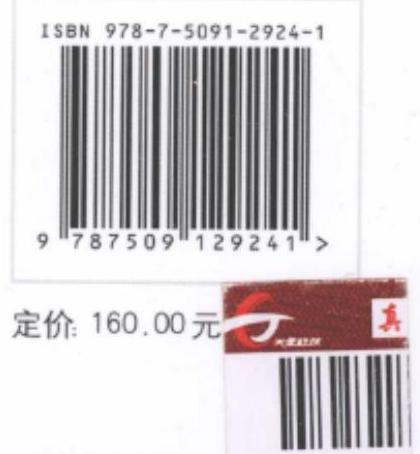
\includegraphics[max width=\textwidth]{2024_07_10_373f31b88d2bf633007bg-002}
\end{center}

\section*{级卫生专业技术资格考试指导用书}
\section*{麻醉学高级教程 \\
 MAZUIXUE GAOJI JIAOCHENG}
高级卫生专业技术资格考试指导用书编轵委员会中华医学会 组织编著

主 编 吴新民

\section*{图书在版编目(CIP) 数据}
麻醉学高级教程 / 吴新民主编.一北京: 人民军医出版社,2009.11

高级卫生专业技术资格考试指导用书

ISBN 978-7-5091-2924-1

I. 麻… II. 吴… III. 麻醉学一资格考核一教材 IV. R614

中国版本图书馆 CIP 数据核字 (2009)第 149455 号

\begin{center}
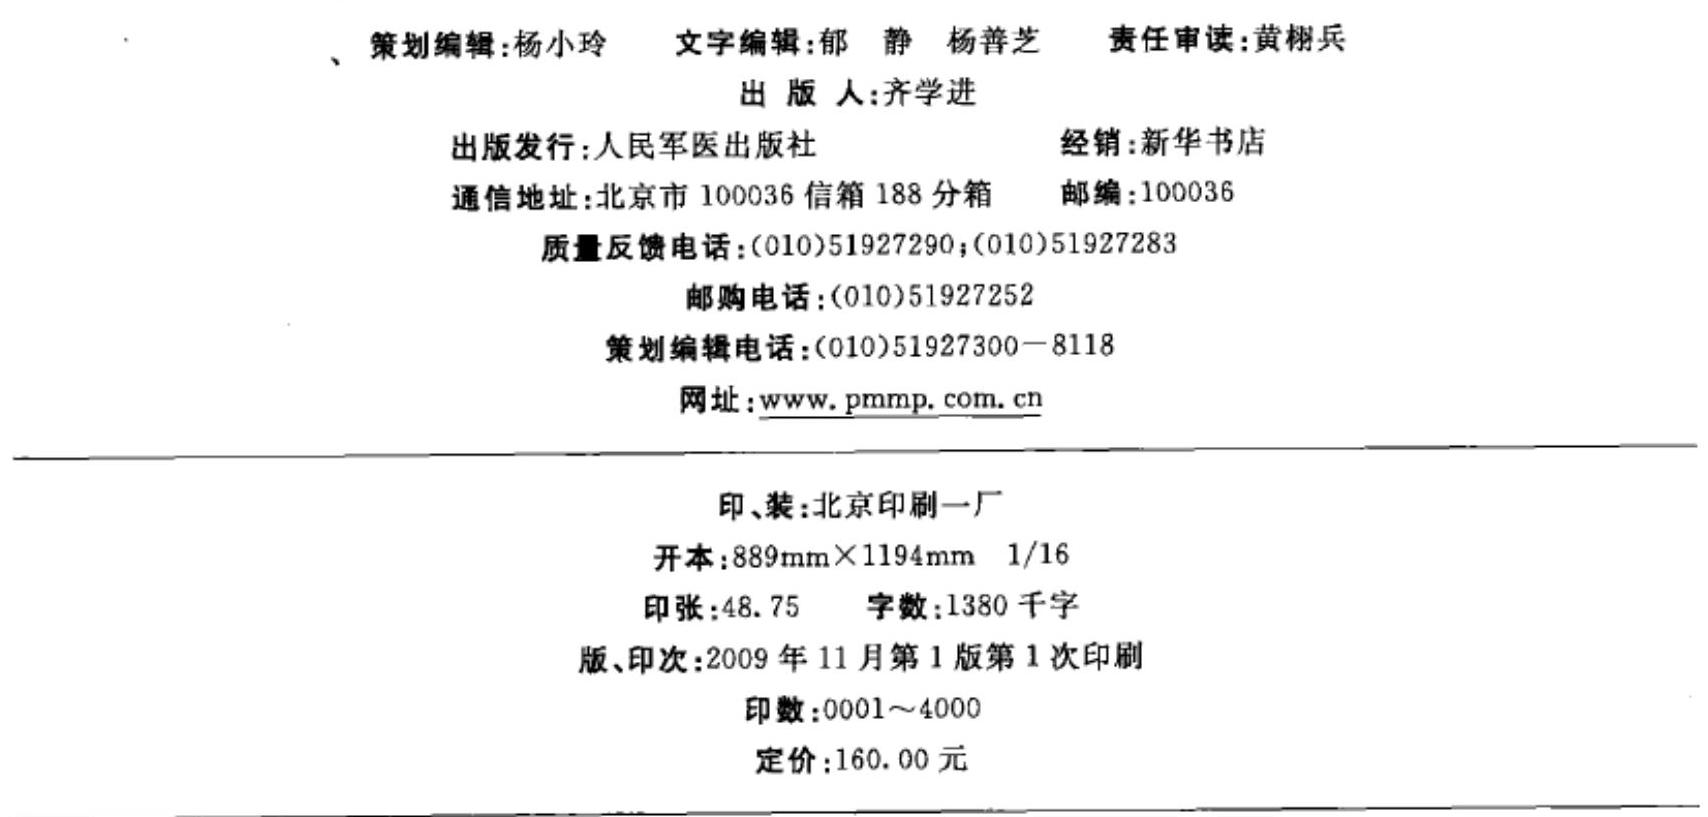
\includegraphics[max width=\textwidth]{2024_07_10_373f31b88d2bf633007bg-004}
\end{center}

\section*{版权所有 侵权必究}
购买本社图书, 凡有缺、倒、脱页者, 本社负责调换

\section*{内容简介}
本书由《中国卫生人才》杂志社、中华医学会共同组织国内权威专家编写, 按照国家对高级卫生专业技术资格人员的专业素质要求, 集中、准确地介绍了麻醉学基本理论和临床理论技术, 重点阐述了麻醉学专业的国内外发展现状和发展趋势等前沿信息。具体内容包括麻醉相关解剖生理基础、麻醉药理学、疾病与麻醉、麻醉技术与监测、危重病医学、疼痛医学六篇,共 76 章, 书后附卫生部麻醉学专业副高级、正高级资格考试大纲。本书权威、实用、先进。专业知识紧扣卫生部高级资格考试大纲, 根据大纲对专业知识 “了解” “熟悉”“掌握”的不同层次要求安排繁简, 是晋升副高级和正高级职称的卫生专业人员考前复习必备书, 也是高年资医务人员难得的案头工具书。

\section*{高级卫生专业技术资格考试指导用书麻醉学高级教程}
\section*{编 委会}
主 编吴新民

常务编委 王俊科 岳云 许幸叶铁虎徐建国

编 委(以姓氏笔画为序)

于布为 上海交通大学附属瑞金医院

马 虹中国医科大学附属第一医院

王 庚 北京积水潭医院

王 强 第四军医大学西京医院

王天龙 首都医科大学宣武医院

王国林 天津医科大学总医院

王学仁 华中科技大学附属同济医院

王玲玲中国医科大学附属第一医院

王佁科 中国医科大学附属第一医院

王祥瑞上海交通大学医学院附属仁济医院

左明章 卫生部北京医院

田 鸣 首都医科大学北京友谊医院

田玉科 华中科技大学附属同济医院

田伟千 江苏省中医院

吕沛林 四川大学华西医院

朱 波 北京协和医院

朱 谦 卫生部中日友好医院

刘进四川大学华西医院

刘保江 山西医科大学第一医院

米卫东 中国人民解放军总医院

许 幸 北京大学第一医院

许学兵 广东省广州市第一人民医院

李双玲 北京大学第一医院

李立环 中国医学科学院阜外心血管病医院

李成辉 卫生部中日友好医院

李修良 首都医科大学北京友谊医院

李恩有 哈尔滨医科大学附属第一医院

\begin{center}
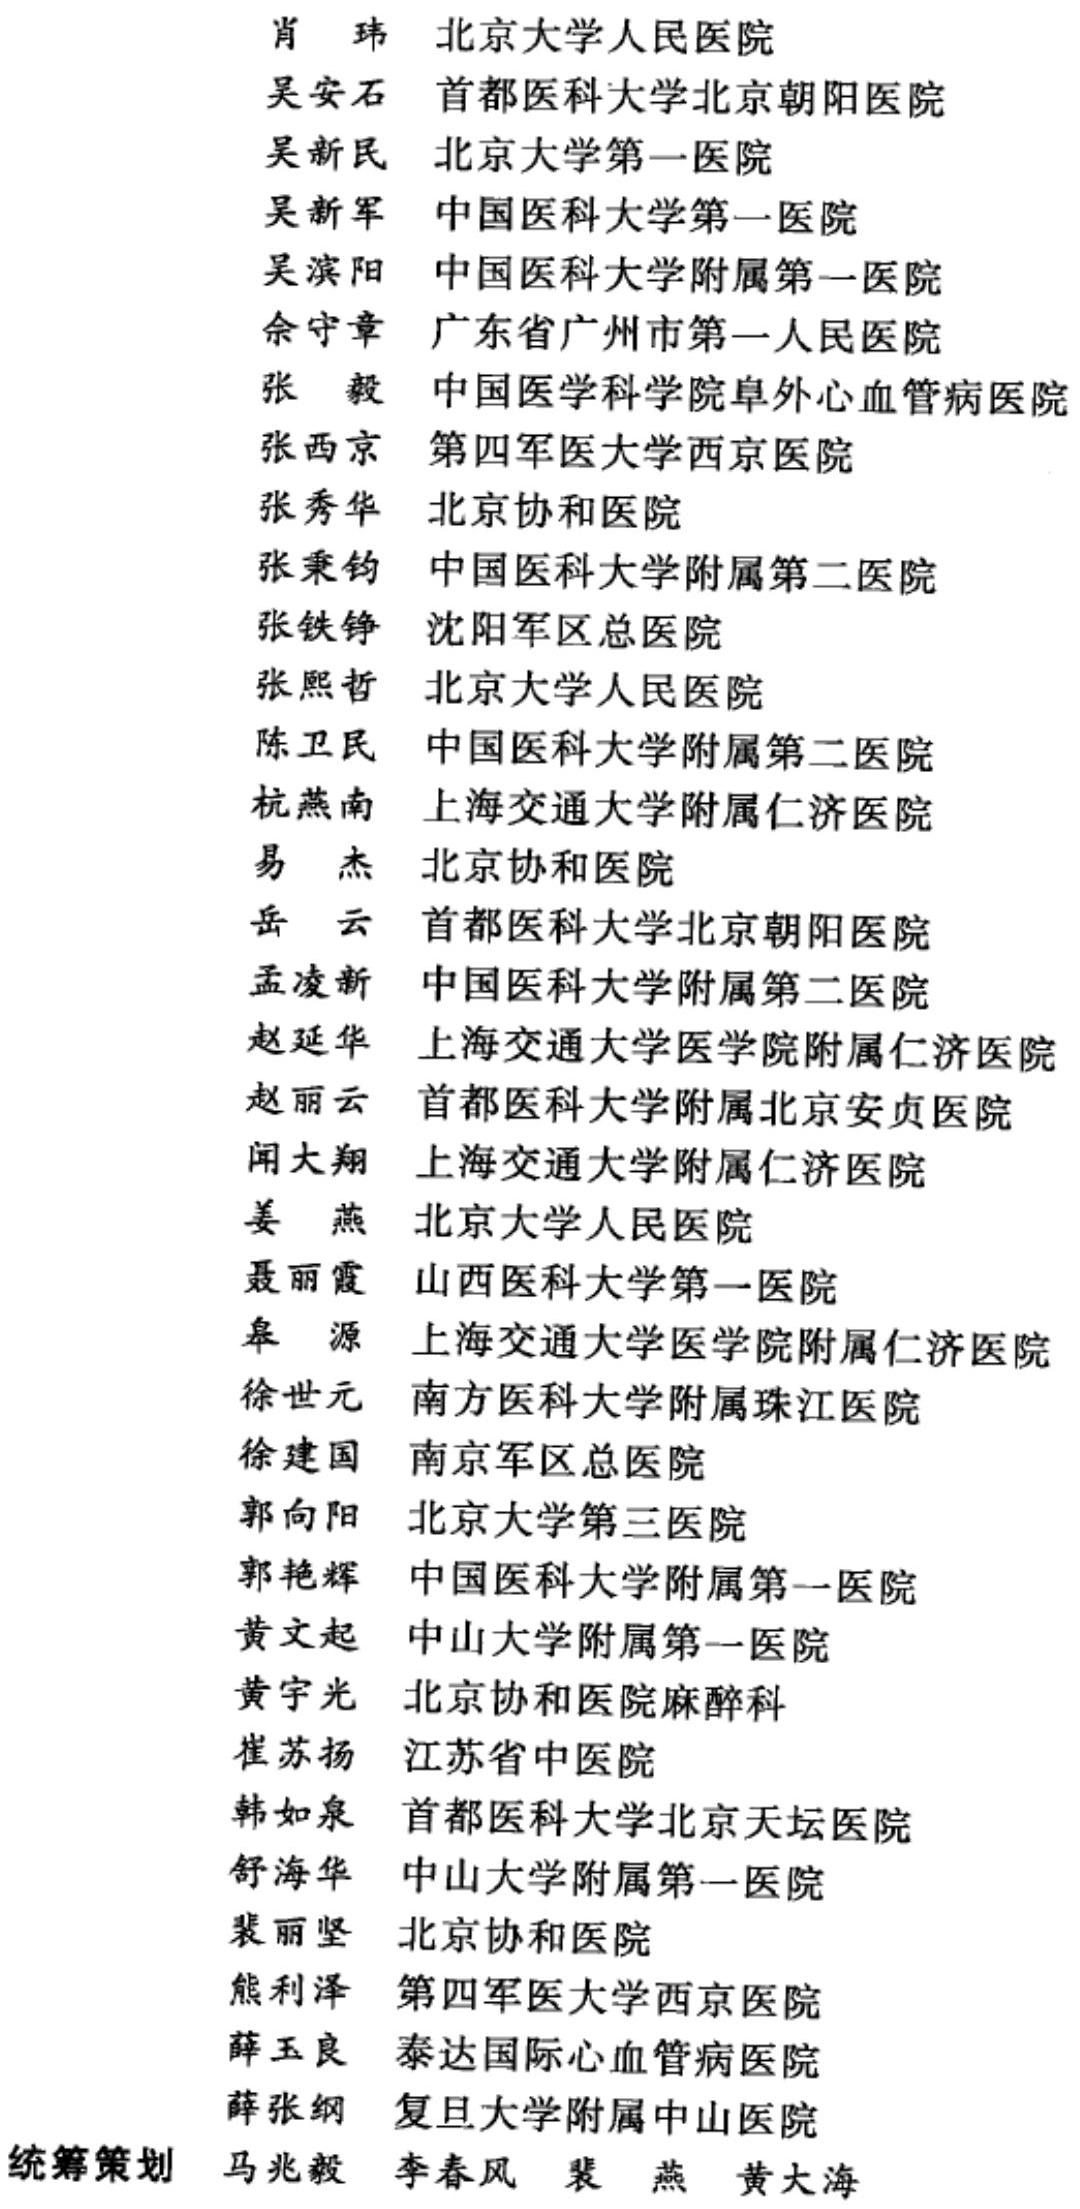
\includegraphics[max width=\textwidth]{2024_07_10_373f31b88d2bf633007bg-007}
\end{center}

\section*{序}
《卫生部关于加强“十一五”期间卫生人才队伍建设的意见》提出, 要加强高层次卫生人才队伍建设, 进一步完善卫生人才评价体系, 加快推进卫生人才工作体制机制创新, 为卫生人才队伍发展提供良好的政策环境。中华医学会作为国内医学界有一定影响的学术团体, 有责任也有义务为提高卫生技术人才队伍的整体素质,进一步完善高级卫生专业技术资格的评价手段,逐步推行考评结合的评价方法, 做出应有的努力。

为推进科学、客观、公正的社会化卫生人才评价体系尽快实施, 《中国卫生人才》杂志社、中华医学会共同组织,编辑、出版了这夽《高级卫生专业技术资格考试指导用书》(以下简称《指导用书》)。

我国每年有 20 万以上需要晋升副高级和正高级职称的卫生专业人员, 这些高级技术人员是我国医学发展的中坚力量,身肩承上启下的重任。考试政策的出台有助于促进不同地区同专业、同职称的医务人员职称与实践能力的均衡化。因此本套书的内容不仅包括高年资医务人员应该掌握的知识,更力求与时俱进, 能反映目前本学科发展的国际规范指南和前沿动态, 巩固和提高主治医师以上职称医务人员临床诊治、临床会诊、综合分析敀难病例以及开展医疗先进技术的能力, 也将作为职称考试的参考依据之一。柏信此书的出版不仅能帮助广大考生做好考前复习工作, 还将凭借其不断更新的权威知识成为高年资医务人员的案头工具书。

本套《指导用书》所有参编人员均为国内各学科的学术带头人、知名专家。在编写过程中曾多次召开组稿会和定稿会, 各位参编的专家、教授群策群力, 在繁忙的临床和教学工作之余高效率、高质量地完成了本套书的编写工作,在此,我表示衷心的感谢和敬佩!

\begin{center}
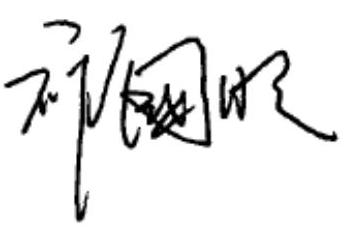
\includegraphics[max width=\textwidth]{2024_07_10_373f31b88d2bf633007bg-008}
\end{center}

\section*{出版说明}
为了进一步深化卫生专业职称改革, 2000 年人事部、卫生部下发了《关于加强卫生专业技术职务评聘工作的通知》(人发 [2000]114 号)。通知要求,卫生专业的副高级技术资格通过考试与评审相结合的方式获得; 正高级技术资格通过答辩, 由评审委员会评议, 通过后即获得高级资格。根据通知精神和考试工作需要,副高级技术资格考试在全国各个省、自治区、直辖市职称改革领导小组的领导下设立了多个考区。目前, 很多地区正高级技术资格的评审工作也逐渐采用考评结合的方法。通过考试取得的资格代表了相应级别技术职务要求的水平与能力,作为单位曺任相应技术职称的必要依据。

高级技术资格考试制度的逐渐完善, 使与其相配套的考前辅导及考试用书市场明显滞后的矛盾日渐突出。鉴于职称改革制度和考生的双重需求,《中国卫生人才》杂志社和中华医学会共同组织医学各学科权威专家, 编辁、出版了《高级卫生专业技术资格考试指导用书》(以下简称《指导用书》)。《指导用书》在介绍基本理论知识和常用治妆方法的基础上更注重常见病防治新法、疑难病例分析、国内外发展现状和发展趋势等前沿信息的汇集,与国家对高级卫生专业技术资格人员的专业素质要求相一致。《指导用书》的编者主要由从事临床工作多年, 在本学科领域内具有较高知名度的副主任医师职称以上的专家及教授担任,以确保其内容的权威性、实用性和先进性。本书以纸质载体配合 CD-ROM 光盘的形式出版, 其中纸质载体以专业知识为主, 多媒体光盘容纳练习题库、模拟试题等内容, 实现人机互动的功能。本书根据高级卫生专业技术资格考试大纲对专业知识 “了解”“熟悉”和 “掌握”的不同层次要求安排简繁, 重点突出, 便于考生复习、记忆。

考试不是目的, 而是为了加强临床医务人员对学科知识的系统了解和掌握, 是提高医疗质量的一种手段。因此, 本套出版物的受益者不仅仅是中、高级技术资格应考人员, 其权威、专业、前沿的学科信息将会对我国医学科学的发展、医学科技人才的培养以及医疗卫生工作的进步起到推动和促进作用。《指导用书》各学科分册将于 2009 年陆续出版。

\section*{目 录}
\section*{第一篇 麻醉相关解剖生理基础}
第 1 章 产妇麻醉的解剖与生理 ..... (1)\\
第一节 妊娠的解剖和生理变化 ..... (1)\\
一、循环系统变化 ..... (1)\\
二、呼吸系统变化 ..... (2)\\
三、血液系统变化 ..... (2)\\
四、消化系统变化 ..... (3)\\
五、肾的变化 ..... (3)\\
六、内分泌系统变化 ..... (3)\\
七、代谢率增高 ..... (4)\\
八、肝功能变化 ..... (4)\\
九、神经系统变化 ..... (5)\\
第二节麻醉药对胎儿娩出后的影响 ..... (5)\\
一、药物经胎盘转运的主要影响因素 ..... (5)\\
二、麻醉药对胎儿的作用 ..... (5)\\
第 2 章 小儿麻醉的解剖和生理 ..... (9)\\
一、解剖生理特点 ..... (9)\\
二、麻醉药理特点 ..... (13)\\
第 3 章 老年人麻醉的生理 ..... (15)\\
一、神经系统 ..... (15)\\
二、心血管系统 ..... (17)\\
三、呼吸系统 ..... (17)\\
四、消化系统 ..... (18)\\
五、肾和水、电解质,酸碱平衡 ..... (18)\\
六、内分泌系统及代谢 ..... (19)\\
七、血液系统 ..... (20)\\
八、老年人的药理学特点 ..... (20)\\
九、其他 ..... (21)\\
第 4 章麻醉与内分泌功能 ..... (22)\\
第一节 内分泌系统的生理功能 ..... (22)\\
一、主要内分泌腺组织 ..... (22)\\
二、内分泌功能的生理调控 ..... (24)\\
三、内分泌系统疾病 ..... (25)\\
第二节 麻醉和手术对内分泌系统功能的影响 ..... (28)\\
一、麻醉药物 ..... (28)\\
二、麻醉方法 ..... (28)\\
三、手术对内分泌的影响 ..... (28)\\
第 5 章 自主神经系统的解剖和生理 ..... (29)\\
第一节 自主神经的解剖 ..... (29)\\
一、交感神经 ..... (29)\\
二、副交感神经 ..... (30)\\
第二节 自主神经系统的递质 ..... (30)\\
一、神经递质的分类 ..... (30)\\
二、乙酰胆碱的合成、储存、释放和失活 ..... (31)\\
三、去甲肾上腺素的合成、储存、释放、失活和代谢 ..... (31)\\
四、其他递质 ..... (32)\\
第三节 自主神经系统的功能 ..... (33)\\
一、交感神经的功能 ..... (33)\\
二、副交感神经的功能 ..... (34)\\
三、脊鬴横断时的自主神经系统改变 ..... (34)\\
第四节 麻醉药对自主神经系统功能的影响 ..... (34)\\
一、吸入麻醉药 ..... (34)\\
二、静脉麻醉药 ..... (35)\\
三、麻醉性镇痛药 ..... (35)\\
四、肌肉松驰药 ..... (35)\\
五、椎管内阻滞 ..... (35)\\
第 6 章 麻醉与循环系统 ..... (36)\\
第一节 心脏 ..... (36)\\
一、起搏传导系统 ..... (36)\\
二、心肌收缩原理 ..... (36)\\
三、心排血量 ..... (37)\\
四、心室功能 ..... (40)\\
第二节 冠脉循环系统 ..... (41)\\
一、解剖 ..... (41)\\
二、生理 ..... (41)\\
三、冠脉循环的调节 ..... (42)\\
四、心肌的氧平衡 ..... (43)\\
第三节 微循环 ..... (44)\\
一、结构 ..... (44)\\
二、毛细血管的通透性和吸收作用 ..... (44)\\
三、微循环的调节 ..... (45)\\
第四节 心血管的调节 ..... (46)\\
一、中枢神经调节 ..... (46)\\
二、自主神经调节 ..... (46)\\
三、心血管反射 ..... (47)\\
四、体液调节 ..... (47)\\
第五节 麻醉对心血管功能的影响 ..... (48)\\
一、手术应激反应 ..... (48)\\
二、麻醉药物 ..... (48)\\
第 7 章 麻醉与呼吸系统 ..... (51)\\
第一节 呼吸系统的解剖 ..... (51)\\
一、气道 ..... (51)\\
二、肺与肺泡 ..... (52)\\
三、胸靳 ..... (52)\\
第二节 肺的通气 ..... (52)\\
一、呼吸动力 ..... (52)\\
二、胸和肺顺应性 ..... (53)\\
三、肺泡表面张力和肺泡表面活性物质 ..... (53)\\
四、气道阻力 ..... (54)\\
五、呼吸功 ..... (55)\\
第三节 肺循环生理 ..... (55)\\
一、肺循环和体循环的差异 ..... (55)\\
二、调节肺血流和阻力的因素 ..... (55)\\
第四节 肺容量及肺功能检查 ..... (56)\\
一、肺容量 ..... (56)\\
二、肺通气功能参数及其意义 ..... (56)\\
三、肺泡通气量和无效腔量 ..... (57)\\
第五节 气体交换 ..... (58)\\
一、肺血流的分布 ..... (58)\\
二、肺泡的气体分布和闭合气量 ..... (58)\\
三、肺的换气及低氧血症原因 ..... (59)\\
第六节 氧和二氧化碳的运输 ..... (60)\\
一、氧的运输 ..... (61)\\
二、氧合血红蛋白解离曲线 ..... (61)\\
三、二氧化碳的运输 ..... (62)\\
第七节 呼吸的调节 ..... (62)\\
一、呼吸的中枢调节 ..... (62)\\
二、通气的反射性调节 ..... (63)\\
三、呼吸的化学因素调节 ..... (63)\\
四、围术期肺功能检查 ..... (64)\\
第八节 肺的非呼吸功能 ..... (64)\\
一、酸碱平衡 ..... (64)\\
二、代谢功能 ..... (64)\\
三、过滤作用 ..... (65)\\
四、防御功能 ..... (65)\\
第九节呼吸系统的重要病理生理特点 ..... (65)\\
一、气胸 ..... (65)\\
二、低氧性肺血管收缩 ..... (65)\\
第 8 章 疼痛的解剖与生理基础 ..... (67)\\
第一节 疼痛的神经学解剖 ..... (67)\\
一、伤害性感受器、传入纤维、背根节神经元 ..... (67)\\
二、痛觉中枢传导通路 ..... (68)\\
三、疼痛整合中枢 ..... (69)\\
第二节 疼痛的分类和常用概念 ..... (70)\\
一、神经末梢性疼痛 ..... (70)\\
二、中枢性疼痛 ..... (70)\\
三、心因性疼痛 ..... (70)\\
四、慢性疼痛和急性疼痛 ..... (71)\\
五、痛觉过敏和疼痛倒错 ..... (71)\\
六、外周(痛)敏感化 ..... (71)\\
七、中枢神经系统的敏化 ..... (71)\\
八、自发痛 ..... (71)\\
九、病理性疼痛 ..... (71)\\
第二节 疼痛生理 ..... (71)\\
一、疼痛的外周机制 ..... (71)\\
二、疼痛的中枢机制 ..... (72)\\
第二篇 麻醉药理学\\
第 1 章 总论 ..... (76)\\
一、静脉用药的药理学 ..... (76)\\
二、吸入用药的药理学 ..... (78)\\
三、影响药物作用的因素 ..... (79)\\
第 2 章 镇静催眠药 ..... (80)\\
一、概述 ..... (80)\\
二、巴比妥类 ..... (80)\\
三、非巴比妥类 ..... (81)\\
第3 章麻醉性镇痛药与药物依赖性 ..... (86)\\
一、概述 ..... (86)\\
二、阿片受体激动药 ..... (86)\\
三、阿片受体激动/拮抗药 ..... (89)\\
四、阿片受体拈抗药一一纳洛酮 ..... (89)\\
五、药物依赖性 ..... (90)\\
六、阿片类药物的依赖及防治 ..... (91)\\
第 4 章非阿片类镇痛药 ..... (92)\\
一、非阿片类中枢性镇痒药 ..... (92)\\
二、非㜽体类抗炎药 ..... (92)\\
三、辅助性镇痛药 ..... (97)\\
第 5 章 吸入麻醉药 ..... (102)\\
一、概述 ..... (102)\\
二、氟烷 ..... (103)\\
三、恩氟烷 ..... (104)\\
四、异策烷 ..... (105)\\
五、七菲烷 ..... (106)\\
六、地跳烷 ..... (106)\\
七、氧化亚氮 ..... (107)\\
八、氙 ..... (108)\\
第 6 章局部麻醉药 ..... (109)\\
一、结构与效能 ..... (109)\\
二、作用机制 ..... (109)\\
三、药动学 ..... (109)\\
四、局部麻醉药物的毒性 ..... (110)\\
五、常见局部麻醉药物及临床应用 ..... (110)\\
第 7 章 肌肉松驰药 ..... (111)\\
一、概述 ..... (111)\\
二、分类 ..... (111)\\
三、药理作用及不良反应 ..... (111)\\
四、去极化肌松药 ..... (112)\\
五、非去极化肌松药 ..... (112)\\
六、新的肌松拮抗药 ..... (113)\\
第 8 章 作用于胆碱受体的药物 ..... (115)\\
一、概述 ..... (115)\\
二、拟胆碱药 ..... (116)\\
三、M 胆碱受体阻滞药 ..... (116)\\
第 9 章作用于肾上腺素受体的药物 ..... (121)\\
一、概述 ..... (121)\\
二、拟肾上腺素药 ..... (123)\\
三、肾上腺素受体阻滞药 ..... (127)\\
四、 $\beta$ 受体阻滞药 ..... (128)\\
第 10 章 强心药 ..... (130)\\
一、洋地黄糖苷类 ..... (130)\\
二、磷酸二酯酶 III 抑制药 ..... (131)\\
三、其他 ..... (132)\\
第 11 章血管扩张药 ..... (134)\\
一、中枢和交感神经抑制药 ..... (134)\\
二、 $\alpha$-肾上腺素受体阻滞药 ..... (135)\\
三、神经节阻滞药 ..... (136)\\
四、硝基类扩血管药 ..... (136)\\
五、血管紧张素转化酶抑制药 ..... (137)\\
六、血管紧张素 II $\left(\mathrm{AT}_{1}\right)$ 受体拮抗药 ..... (138)\\
七、钙通道阻滞药 ..... (138)\\
八、内皮素受体拮抗药 ..... (139)\\
第 12 章 抗心律失常药物 ..... (140)\\
一、抗心律失常药物作用机制 ..... ( 140 )\\
二、杭心律失常药物分类 ..... (140)\\
三、钠通道阻滞药 ..... (141)\\
四、II 类药物一 $\beta$ 肾上腺素受体阻滞药 ..... (143)\\
五、III类药物一一延长 ADP 药物 ..... (144)\\
六、IV 类药物一一转通道阻滞药 ..... (146)\\
七、其他 ..... (147)\\
第 13 章 血浆代用品 ..... (148)\\
一、差乙基淀粉 ..... (148)\\
二、明胶类 ..... (148)\\
三、右旋糖酎 ..... (148)\\
四、全策碳化合物 ..... (148)\\
第三篇 疾病与麻醉\\
第 1 章 神经系统疾病的麻醉 ..... (150)\\
第一节 麻醉与顽脑生理 ..... (150)\\
一、脑血流 ..... (150)\\
二、脑代谢 ..... (154)\\
三、脑脊液循环 ..... (157)\\
四、顾内高压、脑痃 ..... (160)\\
五、意识障碍 ..... (164)\\
六、春㵦病变 ..... (167)\\
第二节 神经外科的监测 ..... (173)\\
一、多普勒超声扫描 ..... (173)\\
二、血气及呼气末 $\mathrm{CO}_{2}$ 测定 ..... (174)\\
三、顾内压的测定 ..... (174)\\
第三节麻醉前评估及准备 ..... (182)\\
一、病情评估 ..... (182)\\
二、麻醉前准备及麻醉前用药 ..... (183)\\
三、麻醉选择原则 ..... (183)\\
四、不同类型神经外科手术对麻醉的要求 ..... (184)\\
第四节 脑血管疾病的麻醉 ..... (186)\\
一、动脉粥样硬化性脑出血 ..... (186)\\
二、硕内动脉㾪 ..... (187)\\
三、顾内血管畸形 ..... (189)\\
四、缺血性脑血管病手术麻醉 ..... (190)\\
五、大脑半球手术的特点 ..... (194)\\
六、麻醉处理 ..... (194)\\
第五节重症肌无力患者的麻醉 ..... (196)\\
一、重症肌无力病的病理生理及分型 ..... (196)\\
二、重症肌无力病情评估 ..... (196)\\
三、麻醉处理要点 ..... (197)\\
四、术后处理 ..... (198)\\
第 2 章呼吸系统疾病的麻醉 ..... (199)\\
第一节 呼吸系统疾病与麻醉评估 ..... (199)\\
一、慢性阻塞性肺疾病和肺心病 ..... (199)\\
二、呼吸系统感染 ..... (200)\\
三、支气管哮喘 ..... (201)\\
四、急性肺栓塞 ..... (201)\\
五、胸腔积液 ..... (202)\\
六、气胸 ..... (203)\\
七、睡眠呼吸紊乱 ..... (203)\\
八、麻醉前对呼吸系统的评估和准备 ..... (205)\\
第二节 急性呼吸道炎症的麻醉 ..... (207)\\
一、临床表现 ..... (207)\\
二、理化检查 ..... (207)\\
三、治疗 ..... (207)\\
四、麻醉要点 ..... (207)\\
第三节 慢性呼吸道炎症的麻醉 ..... (207)\\
一、临床表现 ..... (207)\\
二、理化检查 ..... (207)\\
三, 治疗 ..... (208)\\
四、麻醉方法与麻醉药物的选择 ..... (208)\\
第四节哮喘患者的麻醉 ..... (208)\\
一、嘛醉前准备的注意事项 ..... (208)\\
二、麻醉药和麻醉方法的选择 ..... (209)\\
三、处理 ..... (209)\\
第五节 胸外科手术的麻醉 ..... (209)\\
一、开胸和侧卧位对呼吸循环的影响 ..... (209)\\
二、单肺通气对呼吸的影响 ..... (210)\\
三、麻醉前肺功能评估及准备 ..... (210)\\
第六节食管及纵隔手术的麻醉 ..... (213)\\
一、麻醉前评估及准备 ..... (213)\\
二、食管手术的麻醉处理 ..... (213)\\
三、纵隔肿块的麻醉处理 ..... (214)\\
第七节 肺叶切除术的麻醉 ..... (214)\\
一、麻醉前病情评估及准备 ..... (214)\\
二、麻醉处理要点 ..... (215)\\
第八节 气管重建术的麻醉 ..... (215)\\
一、气道梗阻的病因 ..... (216)\\
二、麻醉前评估及准备 ..... (216)\\
三、麻醉处理要点 ..... (216)\\
四、术后处理要点 ..... (217)\\
第九节气道肿瘤激光手术的麻醉 ..... (218)\\
一、医用激光在气道手术中的应用 ..... (218)\\
二、激光的 “危险”及预防 ..... (218)\\
三、麻醉处理要点 ..... (219)\\
第 3 章 心血管系统疾病的麻醉 ..... (220)\\
第一节 术前对心脏功能的估计 ..... (220)\\
一、心脏功能的检查 ..... (220)\\
二、心脏功能分级 ..... (221)\\
第二节术前药物治疗及其对麻醉的影响 ..... (222)\\
一、治疗心血管疾病药物 ..... (222)\\
二、抗感染药物 ..... (225)\\
三、其他药物 ..... (225)\\
第三节 心血管疾病的病理生理 ..... (226)\\
一、先天性心血管疾病 ..... (226)\\
二、缩窄性心包炎 ..... (228)\\
三、后天性心血管疾病 ..... (228)\\
四、再次心脏手术 ..... (231)\\
第四节麻醉前准备 ..... (232)\\
一、麻醉前用药 ..... (232)\\
二、心血管用药的准备 ..... (233)\\
三、监测 ..... (237)\\
第五节麻醉原则和常用麻醉方法 ..... (241)\\
一、先天性心脏病 ..... (241)\\
二、后天性心血管疾病 ..... (245)\\
第六节 体外循环下心内手术的管理 ..... (249)\\
一、体外循环时的麻醉管理 ..... (249)\\
二、心肌保护 ..... (251)\\
三、停止体外循环前后的处理 ..... (254)\\
第七节 围术期异常情况处理 ..... (257)\\
一、急性心力衰竭 ..... (257)\\
二、急性冠脉综合征 ..... (259)\\
三、肺动脉高压 ..... (259)\\
四、心肌缺血 ..... (264)\\
五、心律失常 ..... (264)\\
第 4 章 腹部外科手术的麻醉 ..... (268)\\
第一节 腹部疾病的病理生理 ..... (268)\\
第二节 麻醉前准备 ..... (268)\\
第三节一般腹部外科手术的麻醉处理 ..... (269)\\
一、麻醉选择 ..... (269)\\
二、麻醉要点 ..... (270)\\
第四节腹腔镜检查和外科手术的麻醉 ..... (271)\\
一、手术过程对机体的生理影响 ..... (271)\\
二、麻醉管理 ..... (272)\\
第五节 原位肝移植手术的麻醉处理 ..... (272)\\
一、肝硬化和门脉高压 ..... (272)\\
二、麻醉前评估 ..... (273)\\
三、麻醉处理 ..... (273)\\
第 5 章 泌尿外科手术的麻醉 ..... (275)\\
第一节膀胱镜检查和输尿管逆行造影的麻醉 ..... (275)\\
第二节 前列腺手术的麻醉 ..... (276)\\
一、经腹前列腺手术的麻醉 ..... (276)\\
二、经尿道前列腺切除术的麻醉 ..... (276)\\
三、经尿道前列腺切除术的并发症及处理 ..... (277)\\
第三节 肾移植手术的麻醉 ..... (278)\\
一、终末期肾病的病理生理 ..... (279)\\
二、活体肾供体的麻醉 ..... (279)\\
三、肾移植受体的麻醉 ..... (280)\\
第四节体外冲击波碎石术的麻醉 ..... (282)\\
一、概述 ..... (282)\\
二、碎石的原理 ..... (283)\\
三、碎石术水浴时的生理变化 ..... (283)\\
四、麻醉选择和术中处理 ..... (283)\\
第 6 章 糖尿病和肥胖病人的麻醉 ..... (285)\\
第一节糖尿病病人的麻醉 ..... (285)\\
一、糖尿病的病理生理 ..... (285)\\
二、麻醉前处理 ..... (285)\\
三、麻醉处理 ..... (286)\\
第二节 肥胖病人的麻醉 ..... (287)\\
一、肥胖的定义及标准 ..... (287)\\
二、肥胖对生理的影响 ..... (288)\\
三、肥胖对健康的影响 ..... (289)\\
四、麻醉前病情评估及准备要点 ..... (289)\\
五、肥胖患者的麻醉问题 ..... (289)\\
六、术后处理要点 ..... (290)\\
七、术后并发症 ..... (290)\\
第 7 章 内分泌疾病手术的麻醉 ..... (291)\\
第一.节 垂体㿔手术麻醉 ..... (291)\\
一、垂体解剖与生理特点 ..... (291)\\
二、垂体罍分类 ..... (291)\\
三、麻醉准备要点 ..... (291)\\
四、特殊病例麻醉管理要点 ..... (292)\\
第二节 甲状腺功能立进症手术的麻醉 ..... (292)\\
一、甲状腺的生理 ..... (292)\\
二、麻醉前准备 ..... (293)\\
三、麻醉方法和管理要点 ..... (293)\\
第三节 原发性甲状旁腺功能立进症手术的麻醉 ..... (294)\\
一、甲状旁腺的解剖和生理 ..... (294)\\
二、甲状旁腺功能元进症的病理生理特点 ..... (294)\\
三、麻醉前准备 ..... (294)\\
四、麻醉方法和管理要点 ..... (294)\\
第四节胰岛素细胞瘤手术的麻醉 ..... (294)\\
一、胰岛素的生理功能 ..... (294)\\
二、胰岛素㿔病理生理特点 ..... (295)\\
三、麻醉前准备 ..... (295)\\
四、麻醉方法和管理要点 ..... (295)\\
第五节肾上腺疾病手术的麻醉 ..... (295)\\
一、肾上腺的解剖与生理 ..... (295)\\
二、皮质醇增多症手术的麻醉 ..... (296)\\
三、原发性醛固酮增多症手术的麻醉 ..... (296)\\
四、嗜铬细胞瘤手术的麻醉 ..... (297)\\
第六节 多发性内分泌腺瘤病手术麻醉 ..... (298)\\
一、多发性内分泌腺瘫病的分类 ..... (298)\\
二、多发性内分泌腺痖病手术麻醉管理要点 ..... (298)\\
三、MEN 的特殊表现 ..... (299)\\
第 8 章 脊柱、四肢手术的麻醉 ..... (300)\\
第一节 麻醉和手术的要求 ..... (300)\\
一、体位要求 ..... (300)\\
二、麻醉选择 ..... (300)\\
三、警愓脂肪栓塞及肺栓塞 ..... (301)\\
四、控制出血 ..... (301)\\
第二节 术前病情估计 ..... (301)\\
第三节 脊柱手术的麻醉 ..... (302)\\
一、颈椎手术的麻醉 ..... (302)\\
二、脊柱侧弯畸形手术的麻醉 ..... (302)\\
三、椎体切除术的麻醉 ..... (303)\\
第四节 四肢及关节手术的麻醉 ..... (303)\\
第五节 显微外科手术的麻醉 ..... (304)\\
第 9 章 创伤、休克患者的麻醉 ..... (305)\\
第一节 严重创伤患者的麻醉 ..... (305)\\
一、严重创伤的紧急处理 ..... (305)\\
二、病情估计和麻醉前处理 ..... (305)\\
三、麻醉前准备 ..... (306)\\
四、麻醉的选择 ..... (306)\\
五、监测 ..... (306)\\
第二节严重烧伤病人手术的麻醉 ..... (306)\\
一、烧伤的病理生理 ..... (306)\\
二、烧伤严重程度估计 ..... (306)\\
三、烧伤输液的方案及感染控制措施 ..... (307)\\
四、麻醉选择及管理 ..... (307)\\
五、监测 ..... (307)\\
第三节 休克患者的麻醉 ..... (308)\\
一、休克的分类及临床表现 ..... (308)\\
二、病理生理 ..... (308)\\
三、休克患者的评估及监测 ..... (308)\\
四、休克的治疗 ..... (309)\\
五、休克患者的麻醉 ..... (309)\\
第 10 章 产科麻醉 ..... (310)\\
第一节 围产期䂞产妇的解剖生理 ..... (310)\\
一、神经及内分泌系统 ..... (310)\\
二、循环系统 ..... (310)\\
三、血液系统 ..... (311)\\
四、呼吸系统 ..... (311)\\
五、消化系统 ..... (312)\\
六、泌尿系统 ..... (312)\\
七、脊柱 ..... (312)\\
第二节 围产期厼产妇的药理 ..... (313)\\
一、药物经胎盘转运的方式 ..... (313)\\
二、影响药物转运的因一素 ..... (313)\\
三、㶪产妇常用的药物及其对母儿的影响 ..... (313)\\
第三节 围产期孕产妇的麻醉 ..... (314)\\
一、剖宫产术的麻醉 ..... (314)\\
二、分娩镇痛 ..... (316)\\
三、高危妊娠患者的麻醉 ..... (319)\\
第四节 新生儿复苏 ..... (320)\\
一、新生儿心肺功能不全的原因 ..... (320)\\
二、新生儿 Apgar 评分法 ..... (321)\\
三、正常及呼吸客迫新生儿的酸碱平衡失调 ..... (322)\\
四、复苏准备 ..... (322)\\
五、复苏术 ..... (322)\\
六、复苏后处理及预后 ..... (324)\\
第 11 章 小儿麻醉 ..... (325)\\
第一节 麻醉有关的小儿生理解剖特点 ..... (325)\\
一、呼吸系统 ..... (325)\\
二、循环系统 ..... (327)\\
三、肾发育及功能 ..... (328)\\
四、神经系统 ..... (329)\\
五、体温调节 ..... (329)\\
六、药理学的影响 ..... (330)\\
第二节麻醉前检查、评估及准备 ..... (330)\\
一、麻醉前检查评估 ..... (330)\\
二、麻醉前准备 ..... (331)\\
第三节 小儿的呼吸道管理 ..... (332)\\
一、上呼吸道有关解剖特点 ..... (332)\\
二、小儿气管插管术的特点 ..... (333)\\
三、小儿喉军的应用 ..... (334)\\
第四节全身麻醉 ..... (335)\\
一、吸入麻醉 ..... (335)\\
二、静脉麻醉及静脉复合麻醉 ..... (337)\\
三、肌肉松驰药在小儿的应用 ..... (340)\\
四、全身麻醉深度的判断 ..... (341)\\
五、全麻苏醒期的处理 ..... (342)\\
第五节 区域麻醉 ..... (343)\\
一、小儿局麻药药理特点 ..... (343)\\
二、麻醉方法 ..... (343)\\
三、局麻药的不良反应 ..... (344)\\
第六节 小儿麻醉术中监测 ..... (345)\\
第七节 麻醉中常见的并发症和突发不良事件及处理 ..... (345)\\
一、呼吸系统 ..... (345)\\
二、循环系统 ..... (347)\\
三、体温异常 ..... (347)\\
四、呕吐、反流和误吸 ..... (347)\\
第八节 小儿术中输液、输血 ..... (348)\\
一、小儿水电解质代谢 ..... (348)\\
二、术中输液 ..... (348)\\
三、术中输血 ..... (349)\\
第九节 小儿麻醉各论 ..... (350)\\
一、五官科及颌面部手术的麻醉要点 ..... (350)\\
二、脑神经外科手术 ..... (351)\\
三、小儿开胸手术 ..... (351)\\
四、先天性心血管病手术的麻醉 ..... (352)\\
五、小儿普外科手术 ..... (353)\\
六、小儿骨科手术 ..... (354)\\
七、手术室外麻醉 ..... (354)\\
第十节 新生儿麻醉 ..... (355)\\
一、麻醉前评估及准备 ..... (355)\\
二、麻醉选择 ..... (355)\\
三、全身麻醉方法及管理 ..... (355)\\
四、先天性膈疝 ..... (356)\\
五、先天性食管闭锁和气管食管瘘 ..... (356)\\
六、脐膨出和腹裂 ..... (357)\\
七、其他消化道疾病 ..... (357)\\
第 12 章老年患者麻醉 ..... (358)\\
第一节老年对生理及药理的影响 ..... (358)\\
一、严重影响生理的年龄 ..... (358)\\
二、高龄对机体生理的影响 ..... (358)\\
三、高龄对药理及其相互作用的影响 ..... (359)\\
第二节 高龄对麻醉的影响 ..... (361)\\
一、高龄对硬膜外麻醉的影响 ..... (361)\\
二、高龄选择全麻还是部位麻醉安全 ..... (362)\\
第三节 高龄并发症及病情对麻醉及手术 “危险性”的评估 ..... (362)\\
第四节 术后并发症对高龄患者的威胁 ..... (368)\\
影响老年患者预后的特殊情况 ..... (368)\\
第 13 章 非住院手术麻醉 ..... ( 370 )\\
一、手术种类及患者的选择 ..... (370)\\
二、麻醉前准备 ..... (371)\\
三、围术期处理 ..... (372)\\
四、麻醉后恢复期及处理 ..... (374)\\
第四篇 麻醉技术与监测\\
第 1 章 麻醉前病情评估和麻醉前用药 ..... (376)\\
一、麻醉前病情评估 ..... (376)\\
二、各系统功能评估 ..... (379)\\
三、知情同意 ..... (384)\\
四、麻醉前准备事项 ..... (384)\\
第 2 章 气道管理 ..... (388)\\
一、上呼吸道梗阻的处理 ..... (388)\\
二、快速顺序诱导 ..... (388)\\
三、气管内插管 ..... (389)\\
四、意外困难插管的处理 ..... (392)\\
五、清醒插管 ..... (392)\\
六、吸入麻醉药诱导 ..... (393)\\
七、困难插管患者的拔管 ..... (394)\\
八、光导芯 ..... (394)\\
九、喉罩 ..... (395)\\
十、食管气管联合导管 ..... (396)\\
十一、纤维支气管镜辅助气管插管 ..... (397)\\
第3章 吸入全身麻醉 ..... (399)\\
一、吸入麻醉药 ..... (399)\\
二、麻醉环路 ..... (400)\\
三、低流量吸入麻醉 ..... (401)\\
四、吸入麻醉的实施 ..... (401)\\
五、吸入麻醉对机体的影响 ..... (403)\\
第 4 章 静脉全身麻醉 ..... (406)\\
第 5 章 肌肉松弛药的临床应用 ..... (413)\\
一、肌松药的分类 ..... (413)\\
二、肌松药的药理作用特点 ..... (413)\\
三、常用肌松药 ..... (416)\\
四、肌松药的临床应用 ..... (419)\\
五、肌松药作用的监测 ..... (420)\\
六、残余肌松药作用和肌松药的拮抗药 ..... (425)\\
第 6 章 神经阻带麻醉 ..... (428)\\
第一节 颈丛神经阻滞 ..... (428)\\
一、解剖 ..... (428)\\
二、颈丛阻滞的实施 ..... (428)\\
三、并发症 ..... (429)\\
第二节 臂丛神经阻滞 ..... (429)\\
一、解剖 ..... (429)\\
二、臂丛神经阻滞的实施 ..... (429)\\
第三节 上肢周围神经阻滞 ..... (431)\\
一、尺神经阻滞 ..... (431)\\
二、正中神经阻滞 ..... (432)\\
三、桡神经阻滞 ..... (432)\\
第四节下肢神经阻滞 ..... (432)\\
一、腰神经丛阻滞 ..... (432)\\
二、坐骨神经阻滞 ..... (433)\\
三、股神经阻滞 ..... (433)\\
四、股外侧皮神经阻滞 ..... (433)\\
第五节躯干及交感神经阻滞 ..... (433)\\
一、助间神经阻滞 ..... (433)\\
二、椎旁神经阻滞 ..... (434)\\
三、星状神经节阻滞 ..... (434)\\
四、腰交感神经阻滞 ..... (434)\\
第六节 神经刺激器和超声定位用于神经阻滞麻醉 ..... (435)\\
一、神经刺激器定位 ..... (435)\\
二、超声影像定位 ..... (435)\\
第 7 章 椎管内麻醉 ..... (437)\\
一、椎管内麻醉的作用机制 ..... (437)\\
二、生理学效应 ..... (437)\\
三、椎管内麻醉的临床应用 ..... (438)\\
四、蛛网膜下腔麻醉(券髓麻醉) ..... (438)\\
五、硬脊膜外腔麻醉 ..... (439)\\
六、骶管阻滞 ..... (440)\\
七、蛛网膜下腔与硬春膜外腔联合阻滞 ..... (440)\\
八、椎管内阻滞在接受抗凝药物和抗血小板药物情况下的应用 ..... (441)\\
九、椎管内麻醉的并发症 ..... (441)\\
第 8 章控制性降压 ..... (446)\\
一、控制性降压的生理基础 ..... (446)\\
二、控制性降压对生理功能的影响 ..... (447)\\
三、施行控制性降压的基本原则 ..... (449)\\
四、控制性降压的方法 ..... (450)\\
五、适应证、禁忌证和并发症 ..... (452)\\
第 9 章 麻醉并发症 ..... (453)\\
一、低血压 ..... (453)\\
二、高血压 ..... (453)\\
三、心律失常 ..... (454)\\
四、心肌缺血和心梗 ..... (455)\\
五、低羍血症 ..... (455)\\
六、高碳酸血症 ..... (456)\\
七、误吸 ..... (456)\\
八、喉疼弯 ..... (457)\\
九、支气管疼挛 ..... (458)\\
十、急性肺水肿 ..... (458)\\
十一、急性肺栓塞 ..... (458)\\
十二、恶性高热 ..... (459)\\
十三、苏醒延迟 ..... (461)\\
十四、术后恶心呕吐 ..... (461)\\
十五、术后榙安 ..... (462)\\
十六、麻醉后寒战 ..... (462)\\
第 10 章 心电图监测 ..... (464)\\
第一节 心电监测的基础知识 ..... (464)\\
一心电产生的基本原理 ..... (464)\\
二、心电监测的基本方法 ..... (464)\\
三、心电图基本波形 ..... (465)\\
四、心电轴 ..... (465)\\
五、心电监测诊断的基本步骤 ..... (465)\\
第二节围术期心肌缺血监测 ..... (466)\\
一、心肌缺血 ..... (466)\\
二、心肌梗死 ..... (466)\\
第三节 围术期心律失常监测 ..... (467)\\
一心律失常产生的电生理基础 ..... (467)\\
二、律失常常用术语 ..... (468)\\
三、围术期常见的心律失常 ..... (468)\\
四心律失常的心电图诊断步裖 ..... (473)\\
第四节具有预测严重猝死的几种心电图改变 ..... (473)\\
一、Brugada 综合征 ..... (473)\\
二、特发性长 $\mathrm{Q}-\mathrm{T}$ 综合征 ..... (473)\\
三、特发性 J 波(早期复极综合征) ..... (474)\\
四、T 波电交替 ..... (474)\\
五、Epsilon 波 ..... (474)\\
六、短 Q-T 综合征 ..... (474)\\
第五节 有关心电监测其他技术的评价 ..... (474)\\
一、心率变异的分析 ..... (474)\\
二、心率震荡 ..... (475)\\
三、心磁图 ..... (475)\\
四、高频心电图 ..... (475)\\
五、信号平均心电图与心室晚电位 ..... (475)\\
六、心外膜电位的动态标测 ..... (475)\\
七、心电峰值标测图 ..... (475)\\
第 11 章 血流动力学监测 ..... (476)\\
第一节 动脉压监测 ..... (476)\\
一、无创性测量法 ..... (476)\\
二、有创性测量法 ..... (476)\\
第二节 中心静脉压监测 ..... (480)\\
一、适应证 ..... (481)\\
二、禁忌证 ..... (481)\\
三、静脉穿刺插管术 ..... (481)\\
四、临床意义 ..... (481)\\
五、波形分析 ..... (482)\\
第三节 肺动脉压监测 ..... (489)\\
一、适应证 ..... (489)\\
二、禁忌证 ..... (490)\\
三、肺动脉导管置入方法 ..... (490)\\
四、临床意义 ..... (490)\\
五、肺动脉导管压力波形分析 ..... (491)\\
第四节心排血量监测 ..... (496)\\
一、无创性心排血量监测 ..... (496)\\
二、有创性心排血量监测 ..... (500)\\
三、心排血量监测的临床意义 ..... (502)\\
四、心排血量监测的新进展 ..... (503)\\
第 12 章 呼吸功能监测 ..... (506)\\
第一节 呼吸功能的简单评定 ..... (506)\\
一、呼吸功能的物理检查 ..... (506)\\
二、其他临床检查 ..... (506)\\
三、呼吸功能的简易测定 ..... (507)\\
第二节通气功能监测 ..... (507)\\
一、肺容量 ..... (507)\\
二、动态肺容量 ..... (507)\\
三、弥散功能 ..... (508)\\
四、气道反应性 ..... (509)\\
第三节通气效应监测 ..... (510)\\
一、氧气测定 ..... (510)\\
二、二路化碳测定 ..... (512)\\
三、脉持血氧饱和度监测 ..... (513)\\
第四节呼气末二氧化碳监测 ..... (514)\\
第五节 呼吸力学监测 ..... (520)\\
一、呼吸压力(Pp) ..... ( 520 )\\
二、顺应性 ..... (521)\\
三、气道阻力 ..... (521)\\
四、呼吸功 ..... (522)\\
五、呼吸力学连续气道监测 ..... (522)\\
第 13 章 脑功能监测 ..... ( 526 )\\
一、脑电监测 ..... (526)\\
二、脑血流监测一经顾多普勒超声 ..... (530)\\
三、脑氧饱和度监测 ..... (532)\\
第 14 章 神经肌肉传递功能的监测 ..... (534)\\
一、神经肌肉传递功能监测与基本原理 ..... (534)\\
二、肌松监测仪 ..... ( 534 )\\
三、NMT 监测方法 ..... ( 536 )\\
四、影响 NMT监测的因素 ..... (542)\\
第 15 章 酸碱平衡和血气监测 ..... ( 544 )\\
第一节 酸碱平衡 ..... (544)\\
一、基本概念 ..... (544)\\
二、酸碱平衡监测 ..... (545)\\
第二节 血气分析 ..... (550)\\
一、基本原理 ..... (550)\\
二、血气分析的常用参数正常值及意义 ..... ( 550 )\\
三、血气分析进展 ..... (551)\\
第 16 章 体温监测 ..... (552)\\
一、体温的生理调节 ..... (552)\\
二、围术期体温下降的原因 ..... ( 553 )\\
三、围术期轻度低体温对机体的影响 ..... (555)\\
四、围术期体温监测 ..... (556)\\
五、术中低体温的预防和处理 ..... (558)\\
第 17 章 凝血功能监测 ..... (559)\\
一、凝血机制 ..... (559)\\
二、围术期凝血功能异常的常见原因 ..... (560)\\
三、传统的实验室检查项目 ..... (562)\\
四、床边凝血功能监测 ..... (562)\\
第 18 章 内分泌功能监测 ..... (567)\\
一、激素及其代谢产物的测定 ..... (567)\\
二、胰岛 B 细胞功能检查与血糖监测 ..... (567)\\
三、下丘脑-垂体-甲状腺轴功能监测 ..... ( 568 )\\
四、下丘脑一垂体-肾上腺皮质轴的功能检查 ..... (569)\\
五、肾上腺素䯕质功能试验 ..... (571)

\section*{第五篇 危重病医学}
第 1 章 绪论 ..... (575)\\
第 2 章 围手术期酸碱平衡失调 ..... (576)\\
一、机体的酸碱平衡 ..... (576)\\
二、酸碱平衡失常 ..... (577)\\
第 3 章 氧疗 ..... (581)\\
一、低氧血症的原因和对机体的影响 ..... (581)\\
二、适应证 ..... (582)\\
三、低氧诊断 ..... (583)\\
四、氧疗方法 ..... (583)\\
五、停止氧疗的指征 ..... (584)\\
六、注意事项 ..... (584)\\
七、防治氧疗的并发症 ..... (585)\\
八、高压氧疗 ..... ( 585 )\\
第 4 章 机械通气 ..... (587)\\
一、机械通气的生理影响 ..... (587)\\
二、呼吸机的结构和原理 ..... (588)\\
三、各类通气模式 ..... (592)\\
四、机械通气的临床使用 ..... (604)\\
五、机械通气并发症的防治 ..... (609)\\
第 5 章 心脏除颤/复律和起搏 ..... (613)\\
一、除娅/复律 ..... (613)\\
二、心脏起搏 ..... ( 617 )\\
第 6 章 脓毒症 ..... (620)\\
一、相关定义 ..... (620)\\
二、脓毒症的珍断标准 ..... (620)\\
三、脓毒症的发病机制及病理生理改变 ..... ( 623 )\\
四、脓毒症的治疗 ..... (625)\\
第 7 章 重症病人的特殊管理 ..... (632)\\
第一节 ICU 危重患者的抗感染 ..... (632)\\
一、、ICU 危重患者易发感染的因素 ..... (632)\\
二、ICU 常见的感染及诊断 ..... (632)\\
三、ICU 危重患者的抗感染治疗 ..... (634)\\
四、临床常用抗生素简介 ..... (634)\\
第二节 ICU 危重患者的营养代谢支持 ..... (638)\\
一、目的和原则 ..... (638)\\
二、营养状态评价和监测 ..... (639)\\
三、完全肠外营养支持 ..... ( 640 )\\
四、肠内营养 ..... (641)\\
五、危重患者的代谢调理和免疫营养 ..... ( 642 )\\
六、特殊患者的营养代谢支持 ..... (642)\\
第三节 ICU 危重患者的镇痛镇静 ..... (643)\\
一、目的和原则 ..... (643)\\
二、镇痛镇静疗效的评估与重要器官功能监测 ..... ( 643 )\\
三、镇痛镇静治疗的方法和药物选择 ..... ( 644 )\\
第 8 章 急性呼吸衰竭 ..... (649)\\
一、分类 ..... (649)\\
二、病因和病理生理 ..... (649)\\
三、临床表现 ..... (650)\\
四、诊断 ..... ( 650 )\\
五、治疗 ..... (650)\\
六、急性呼吸窘迫综合征 ..... (652)\\
第 9 章 围术期急性心肌缺血与心肌梗死 ..... (657)\\
一、引起心肌缺血的原因 ..... (657)\\
二、心肌缺血和心肌梗死的监测 ..... (657)\\
三、心肌缺血的预防和处理 ..... (659)\\
四、围术期急性心肌梗死的防治 ..... (659)\\
第 10 章 急性心力衰竭 ..... (662)\\
一、病因 ..... (662)\\
二、临床表现 ..... (663)\\
三、监测和实验室检查 ..... (664)\\
四、心力衰㷎的预防和治疗 ..... (665)\\
第 11 章 休克 ..... (669)\\
一、休克的分类 ..... (669)\\
二、休克的发病机制 ..... (670)\\
三、失血性休克 ..... (670)\\
四、脓毒性休克 ..... (673)\\
五、心源性休克 ..... ( 676 )\\
六、过敏性休克 ..... (681)\\
七、神经源性休克 ..... (684)\\
八、注意事项 ..... (685)\\
第 12 章 急性肾衰竭 ..... ( 686 )\\
一、急性肾衰竭 ..... (686)\\
二、肾移植术后的常见问题及治疗原则 ..... (687)\\
第 13 章 多器官功能障碍综合征 ..... (688)\\
一、概念 ..... (688)\\
二、病因和发病机制 ..... (688)\\
三、诊断 ..... (690)\\
四、临床监测 ..... (691)\\
五、MODS 患者的治疗 ..... (692)\\
六、MODS 患者的预后 ..... (695)\\
第 14 章 心肺脑复苏 ..... (697)\\
第一节 CPCR 概述 ..... (697)\\
传统 CPCR 步骤与最新 CPCR 复苏指南比较 ..... (697)\\
第二节 CPCR 的步骤和处理 ..... (698)\\
一、基本生命支持 ..... (698)\\
二、进一步生命支持 ..... (701)\\
三、后续生命支持 ..... (705)\\
四、终止复苏和停止生命支持 ..... (706)\\
第三节 儿童心肺复苏 ..... (706)\\
一、儿童基本生命支持 ..... (706)\\
二、儿童高级生命支持 ..... (707)\\
三、复苏后治疗 ..... (708)\\
四、新生儿复苏 ..... (709)\\
第六篇 疼痛医学\\
第 1 章 疼痛医学概况 ..... (715)\\
第 2 章 疼痛的评估和诊断 ..... (717)\\
一、疼痛评估 ..... (717)\\
二、疼痛诊断 ..... (718)\\
第 3 章 疼痛的药物治疗 ..... (720)\\
一、给药途径和给药方法 ..... (720)\\
二、阿片类药物 ..... (720)\\
三、非甾体类消苂药 ..... (722)\\
四、曲马朵 ..... (723)\\
五、辅助镇痛药 ..... (723)\\
六、局部麻醉药 ..... (723)\\
第 4 章 疼痛的神经阻带治疗 ..... (725)\\
一、神经阻滞的定义、目的和作用机制 ..... (725)\\
二、神经阻滞方法 ..... (725)\\
三、神经阻滞疗法的注意事项 ..... (726)\\
管 5 章 椎管内阿片类药物镇痛治疗 ..... (728)\\
一、椎管内阿片类药物镇痛的作用机制 ..... (728)\\
二、椎管内镇痛的药物选择 ..... (728)\\
三、药物输注系统的选择 ..... (728)\\
四、存在问题 ..... (729)\\
第 6 章 分娩镇痛 ..... (730)\\
一、概述 ..... ( 730 )\\
二、分娩疼痛的原因及对母婴的影响 ..... (730)\\
三、分娩镇痛的常用方法 ..... (731)\\
四、椎管内镇痛的不良反应 ..... (731)\\
第 7 章 疼痛的微创治疗 ..... (733)\\
一、概述 ..... (733)\\
二、微创治疗的方法 ..... (733)\\
三、微创治疗的适应证 ..... (733)\\
第 8 章手术后镇痛 ..... (735)\\
一、手术后疼痛的生理或病理生理影响 ..... (735)\\
二、全身镇痛药物 ..... (735)\\
三、给药途径和给药方法 ..... (735)\\
第 9 章 癌痛治疗 ..... (738)\\
一、癌痛的原因和评估 ..... (738)\\
二、癌痛的治疗 ..... (738)\\
第 10 章 神经病理性疼痛 ..... (740)\\
一、定义和诊断 ..... ( 740 )\\
二、神经病理性疼痛机制 ..... (740)\\
三、神经病理性疼痛的治疗 ..... (741)\\
附录 A 高级卫生专业技术资格考试大纲(麻醉学专业一一副高级) ..... (742)\\
附录 B 高级卫生专业技术资格考试大纲(麻醉学专业一一正高级) ..... (744)

\section*{第 1 章}
\section*{产妇麻醉的解剖与生理}
产科麻醉,首先要熟悉孕妇妊娠生理改变、麻醉药物对兮妇和胎儿的作用, 以保证麻醉期间母子的安全, 特别要注意产妇呼吸道的保护, 防止发生呕吐误吸引起窒息和吸人性肺炎。妊娠会引起明显的生理变化,主要是日益增大的子宫和内分泌功能两方面变化。

\section*{第一节 妊娠的解剖和生理变化}
\section*{一、循环系统变化}
\section*{(一)血容量增多}
妊㜊后循环血量逐日增多, 弤娠 33 周时达高峰, 平均增加 $50 \%$ 。此后逐渐下降, 但仍高于正常人,产后 2~6周烣复正常。血浆增加占 $50 \%$ ~ $60 \%$, 血细胞仅 $10 \% \sim 20 \%$, 血液稀释, 血黏度降低, 红细胞沉降率加快, 为生理性贫血, 伴有水、钠潴留,表现为周围性水肿。可能与酫固酮、雌激素和李酮等内分泌增多有关。

\section*{(二)心排血量、心率增加}
妊㜊 4~8周心率开始加快,16~24 周时达高峰,以后逐渐下降, 单胎妊娠心率平均增加 $16 \%$ 。心脏容量至芓末期增加约 $10 \%$ 。心率增快、每搏输出量增加 $30 \%$, 心排血量增加 $20 \% \sim 40 \%$, 心脏做功增加, 心肌呈轻度肥厚。妊㜊后期因膈肌上抬,心脏被向上向左推移,心尖冲动左移。

高动力性循环使心音加强, 可出现收缩期第一心音高调或分裂、肺动脉瓣区和心尖区出现 2~ 3 级收缩期吹风样杂音, 占产妇的 $90 \%$ 。有时因肺动脉生理性扩张可在肺动脉瓣区听到吹风样舒张期杂音, 似肺动脉瓣关闭不全, 但产后即消失。妊㜊后期心电图检查有电轴左偏,可在 III 导联出现 $\mathrm{Q}$ 波和 $\mathrm{T}$ 波倒置, $\mathrm{Q}$ 波在深吸气后可减小, $\mathrm{T}$波在深吸そ后倒置减轻或转为直立。上述心电图改变均可于产后消失。妊娠期可能出现房性或室性早搏、心律失常等。

\section*{(三)血流动力学改变}
周围血管阻力降低而血压无明显改变。周围阻力降低使对血流急剧改变的防卫能力降低, 隶妇容易发生昏厥或肺水肿。总周围血管阻力在非孕妇为 $0.17 \mathrm{kPa} / \mathrm{s}$, 妊娠 7 个月降至 $0.098 \mathrm{kPa} / \mathrm{s}$, 妊㜊末期为 $0.12 \sim 0.13 \mathrm{kPa} / \mathrm{s}$ 。周围阻力降低使舒张压比收缩压更下降, 结果脉压增加。

有 $5 \% \sim 10 \%$ 好妇由于子宫增大压迫下腔静脉,使回心血量减少,而发生仰卧位低血压综合征。当从仰卧位改成侧卧位时,心排血量可增加 $22 \%$,症状即解除。约有 $1 / 4$ 君妇在妊娠 25~30周时右室舒张末压略增高,肺循环血流量增多,而肺动脉压不升高, 说明肺血管阻力降低。

静脉压随奼娠月数而增高,下肢静脉压可比正常高 $10 \sim 15 \mathrm{cmH}_{2} \mathrm{O}$ 。子宫阵缩时经子宫流出血量为 $250 \sim 300 \mathrm{ml}$, 由此可使右房压升高。下腔静脉受压促使脊椎静脉丛血流增加,硬膜外间隙和蛛网\\
膜下腔因静脉丛扩张而容积缩小, 因此注人较少量局麻药, 即可得到较广泛的麻醉阻滞范围。同时硬膜外穿刺出血或血肿形成的发生率亦相应地增加。

妊娠期由于动脉、静脉张力增高, 若并存脑血管㿔者有可能发生意外破裂。

临产时有许多因素可增加心脏及循环负荷。第一产程中的子宫收缩, 使子宫排出的血夜进人循环, 回心血量增加, 心排血量可暂时增加 $20 \%$ 左右,与产前心排血量相比约增加 $40 \%$, 同时右心房压增高, 平均动脉压增高约 $10 \%$, 左心室做功增大。宫缩疼痛也引起每搏量增加, 但麻醉后可消除。第二产程中, 除子宫收缩外, 腹壁肌与骨盆肌亦收缩, 使周围血管阻力更增大。产妇屏气动作使肺内压显著增高, 右室压力亦增高。如果并存左至右分流型先天性心血管病的产妇, 可能转为右至左分流而出现发绀。第三产程中, 因胎儿娩出使腹内压力骤减, 血液回流到内胜血管床。产后子宫收缩, 血液从子宫突迅速进人血液循环, 心排血量可增加 $45 \%$, 心功能不全者此时极易发生急性心力衰竭。产痛也促使血压或静脉压增高, 硬膜外间隙压和脑脊液压升高。

\section*{二、呼吸系统变化}
妊娠期由于呼吸道毛细血管扩张, 賁、咽续、支气管黏膜充血, 可使鼻通气不畅。妊娠末期舌体变大, 口腔相对变小, 插管显露声门发生困难, 插管损伤橰膜时极易出血。随子宫的体积逐渐增大, 膈肌上升, 最大可升高 $4 \mathrm{~cm}$; 下胸部肋骨逐渐外展, 肋骨下角逐渐增大, 胸廊容量增大, 胸围可增加 5~ $7 \mathrm{~cm}$ 。呼吸频率加快, 平均增加 $9 \%$ 。妊娠早期潮气量增加直至奼娠后期增加 $19 \% \sim 28 \%$, 可达 $800 \mathrm{ml}$; 奼娠后期静息通气量可上升至 $11 \mathrm{~L} / \mathrm{min}$, 比非孕时增加 $42 \%$, 孕妇呈过度通气。妊娠 24 周后,由于膈肌上升补呼气量及余气量开始下降, 至妊娠末期分别下降 $100 \mathrm{ml}$ 及 $200 \mathrm{ml}$, 故功能余气量不变或下降 $20 \%$,但争期的过度通气可使下降的补呼气量得到代偿。因此, 肺活量不论坐、卧或站立均可无大变化或轻度增加 $6 \%$ 。

纴娠末期的血气分析检查为肺泡氧张力升高 $6 \sim 10 \mathrm{mmHg}, \mathrm{PaO}_{2}$ 为 $92 \sim 106 \mathrm{mmHg}, \mathrm{PaCO}_{2}$ 为 $30 \sim 32 \mathrm{mmHg}$, 动脉血氧饱和度介于 $80 \% \sim 96 \%$,说明呼吸气体交换能力无损害(表 1-1-1)。表 1-1-1 妊嫄时动脙血气正常值

\begin{center}
\begin{tabular}{lcc}
\hline
\multicolumn{1}{c}{参数} & 妊娠 & 非妊娠 \\
\hline
$\mathrm{PaCO}_{2}(\mathrm{mmHg})$ & $30 \sim 32$ & 40 \\
$\mathrm{PaO}_{2}(\mathrm{mmHg})$ & $92 \sim 106$ & 100 \\
平卧时 $\mathrm{PaO}_{2}(\mathrm{mmHg})$ & $101 \sim 94$ & 100 \\
$\mathrm{HCO}_{3}^{-}(\mathrm{mEq} / \mathrm{L})$ & $16 \sim 21$ & 24 \\
$\mathrm{pH}$ & $7.405 \sim 7.44$ & 7.40 \\
\hline
\end{tabular}
\end{center}

分娩疼痛可致过度通气量达 $20 \mathrm{~L} / \mathrm{min}$, 使 $\mathrm{PaCO}_{2}$ 下降 $10 \sim 15 \mathrm{mmHg}, \mathrm{pH} 7.5$ 以上, 呈呼吸性碱中毒。呼吸性碱中毒对奼娠子宫的循环和胎儿均不利, 提示适当采用无痛分娩法, 对产妇及胎儿均有益。

妊娠末期腀式呼吸受限, 因此全麻时应避免抑制胸式呼吸, 椎管内麻醉时要防止阻滞平面过高。此外, 麻醉时应加强呼吸管理。当施行气管插管时,应做好插管困难的准备, 注意避免口鼻䆆膜损伤。

孕妇对所有吸入麻醉药的报取、排出要炔于非孕妇。

\section*{三、血夜系统变化}
血液稀释现象使血细胞比容从 $40 \%$ 下降为 $33 \%$, 血红蛋白从 $125 \mathrm{~g} / \mathrm{L}$ 下降至 $109 \mathrm{~g} / \mathrm{L}$ 。驭妇血浆及尿红细胞生成素增高, 可刺激骨䯝制造红细胞。

白细胞在妊娠 8 周起轻度上升 $9.5 \times 10^{9} / L$, 以后稳定在 $(10 \sim 12) \times 10^{9} / \mathrm{L}$, 主要是多形核白细胞,可持续至产后 2 周以后。这种生理现象常干扰作为感染诊断指标的白细胞计数。

血浆纤维蛋白原于妊㜊后期升高至 $5 \sim 6 \mathrm{~g} / \mathrm{L}$使血沉加快。作为风湿病活动期诊断和预后依据的血沉, 在妊娠期无参考价值。在驭期活性显著增加的凝血因子有: III、壮、 $\mathrm{XX} 、 \mathrm{X}$ 因子, 第 II 因子轻度增加, 杊因子(纤维蛋白稳定因子)在妊娠期浓度下降。血小板于妊娠末期增加, 产后可上升至 $500 \times$ $10^{9} / \mathrm{L}, 2$ 周后恢复正常。凝血酶原时间及部分凝血活酜时间随奼娠有轻度缩短。胎盘及蜕膜含大量组织疑血活酶 (IV 因子), 与血液凝血活酶不同,无须许多因子的激活,在胎盘剥离的表面可很快发生血液凝固。正常妊娠期纤维蛋白溶酶原显著增加, 但溶纤维活力下降, 不论是全血凝块的谽解时间或优球蛋白溶解时间均较非孕期明显延长。

分娩后 $3 \sim 4 \mathrm{~d}$ 纤维蛋白原及第VII因子浓度上升, 因而产㥳期血栓检塞形成的可能性增加。

\section*{四、消化系统变化}
胃肠道受增大子宫的推挤, 使盲肠、阑尾移向腹腔的外上方; 至妊㜊晚期,胃向左上方推移,并向右旋转 $45^{\circ}$, 形成程度不等的水平位。由于胃肠道解剖位置的改变, 使急腹症的体征发生变异,易导致临床误诊。

胎盘分泌大量孕酮引起全身平滑肌普遍松驰,使胃肠道张力降低, 蝡动减弱, 胃排空时间及肠运输时间延长, 又因胃贲门括约肌松驰、胃的位置改变以及腹压增加,易导致胃内容物反流至食管。静息胃液分泌几乎无改变,足月奼娠时胃液分泌量略低于正常。胃液分泌减少至哺乳期可恢复正常。麻醉中要重视预防反流、呕吐及误吸的发生。肝血流量无变化。于妊娠后期: 血清消蛋白平均下降为 $30 \mathrm{~g} / \mathrm{L}$, 球蛋白轻度增加, $\mathrm{A} / \mathrm{G}$ 比值下降; 肝细胞分泌溴磺肽 (bromsulphalein, BSP) 至胆汁的功能下降, 但吸收及储存 BSP 的能力加强; 少数玫妇韁香草酚浊度试验、脑磷脂胆固醇䂧状试验呈阳性反应。从妊娠早期起碱性磷酸酶活性升高, 到足月几乎增长 3 倍。正常妊娠期胆碱酯酶活性下降, 较非孕妇下降 $25 \%$ 。血清氨肽酶显著升高, 足月时为非玫妇的 3 倍。多期胆囊功能下降, 常呈低张性扩张, 胆汁颓稠,故一般认为妊㜊有促进胆石形成的倾向。

\section*{五、肾的变化}
肾因间质液和血液增加而略有增大, 将孟和输尿管略有扩张。在陉期前 3 个月, 由于肾血流量和肾小球滤过率增加, 使血肌䣷和血尿素氮 (blood $u-$ rea nitrogen, BUN)下降, 如果略高于正常值, 就应怀疑肾疾病。肾糖阈值降低, 容易出现糖尿。情小管对尿酸排出减弱, 使血尿酸增高。

\section*{六、内分泌系统变化}
妊娠期内分泌功能最明显的变化是䏩盘合成与分泌激素, 是引起妊娠生理变化的最根本原因, 此外, 母体内分泌腺的功能也变化以适应奼娠需要。卵子受精后, 卵巢黄体就会产生孕激素、雌激素、骨盆松驰素, 在受多 $6 \sim 8$ 周后, 胎盘内分泌功能接替了黄体功能产生这些激素, 此外还大量分泌线毛膜促性腺激素。孕激素是介导内分泌改变的主要激素,引起明显的全身变化, 主要包括: 平滑肌松驰、全身血管扩张、支气管扩张、输尿管扩张和胃肠道运动迟缓引起便秘。同时还影响体温调节, 使基础体温升高, 还导致妊娠早期的恶心、呕吐。马激素作为神经递质可增加内啡肽的分泌, 提高龶妇的痛邪。弴激素还能降低吸人麻醉药物的最小肺泡浓度 (minimal alveolar concentration, MAC), 可以降低神经纤维的传导, 使龶妇对全麻药和局麻药用量需求减少。㗒激素水平在分娩后 $3 \sim 4$ 周恢复正常。

娃娠还引起其他内分泌腺功能的变化。

脑垂体: 腺垂体增大, 腺小叶内的催乳激素细胞增生肥大, 神经垂体(垂体后叶)不论在组织结构或催产素-加压素功能无特殊变化。垂体生长激素浓度显著下降, 促性腺激素也下降。

甲状腺: 芓妇的基础代谢率可增高 $10.4 \%$ 土 $5.9 \%$, 血清甲状腺激素浓度逐渐上升。甲状腺结合球蛋白 (TBCT 浓度) 平均为 $53 \mathrm{mg} / \mathrm{dl}$ (非龶妇为 $16 \sim 24 \mathrm{mg} / \mathrm{dl}$ ) ; 蛋白结合碘 (protein-bound testosterone, $\mathrm{PBI}$ ) 为 $7 \sim 12 \mu \mathrm{g} / \mathrm{dl}$ (非买妇为 $4 \sim 8 \mu \mathrm{g} / \mathrm{dl}$ );血清甲状腺素 $\left(\mathrm{T}_{4}\right)$ 为 $16.2 \pm 1.67 \mu \mathrm{g} / \mathrm{dl}$ (非龶妇为

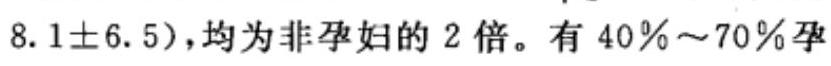
\includegraphics[max width=\textwidth, center]{2024_07_10_373f31b88d2bf633007bg-034}\\
妇甲状腺增大。手期垂体甲状腺刺激激素 (thyroid-stimulating hormone, $\mathrm{TSH}$ ) 浓度为 $7 \mu \mathrm{U} / \mathrm{ml}$,较非铱的 0.25 明显升高。

甲状旁腺: 降钙素分泌增加, 钙离子浓度下降,多见低鿭血症。

胰腺: 血液胰岛素浓度随奼娠进展而增高, 因胎盘催乳素、游离皮质醇的致糖尿和抗胰岛素作用, 对葡萄糖清除能力降低, 产生妊娠糖尿病或使糖尿病龶妇的症状加重。但应慎重使用胰岛素, 因易发生低血糖。

肾上腺皮质: 肾上腺皮质形态无明显改变,由于雌激素增加, 血清皮质醇浓度亦增加, 肾上腺皮质激素处于功能元进状态。孖期中肾上腺皮质对外源性促肾上腺皮质激素 (adrenocorticotropic hormone, ACTH) 反应则较迟钝。

肾素-血管紧张素-醛固酮系统 (renin-angiotensin-aldosterone system, RAAS 系统) : 对正常妊娠期间血压-血容量稳定性的调节起重要作用。据研究,李期蓶激素可使血浆中肾素活性增强 $3 \sim 10$倍; 血管紧张素原已增加数倍, 故可产生更多的血管紧张素II。肾素-血管紧张素系统是醛固酮分泌增多的刺激源。亨妇酫固酮分泌量早在妊娠 15 周开始增多, 以后逐渐增加, 足月时已为非䋇妇的 10 倍。高肾素活性及高醛固酮可抵消大量怶酮所致的排钠利尿及肾小球滤过率增高, 起防止发生负钠平衡及血容量减少的代偿作用。此外, 肾素具有影\\
响动脉紧张度和影响有效血容量起调节血压的作用。综上所述, 可知妊娠期通过肾素-血管紧张素䔯固酮 (renin-angiotensin-aldosterone, RAA) 系统功能的增强, 起稳定血流动力的功效。

\section*{七、代谢率增高}
妊娠期基础代谢率增高,到末期增加 $15 \%$ ~ $20 \%$, 氧耗量增加 $20 \% \sim 40 \%$, 主要为子宫血管营养区域所用。

在皮质激素及胎盘催乳素的抑制胰岛素功能作用下, 葡萄糖利用率降低, 肌肉糖原储存量惐少,血糖增加及餐后血糖增加。由于将小球滤出的糖量超过肾小管的回收量,有 $20 \% \sim 30 \%$ 孕妇出现间断性糖尿。有 $20 \%$ 朶妇的口服莆䔓糖耐量试验异常, 恢复正常的时间比非玫期约延长 $1 \mathrm{~h}$ 。

非龶妇饥饿后血糖浓度平均为 $3.6 \mathrm{mmol} / \mathrm{L}$,而龶妇为 $3.3 \mathrm{mmol} / \mathrm{L}$, 禁食 $48 \mathrm{~h}$ 后, 芓妇的血糖浓度下降更剧, 可低于 $2.2 \mathrm{mmol} / \mathrm{L}$, 最后可出现酮尿, 说明妊娠期糖的代谢与未奼娠期不同, 麻醉管理上对此应加以注意。

亨期 30 周时机体有 $4 \mathrm{~kg}$ 脂肪储存; 㝋妇肠道吸收脂肪的能力增强, 因而血脂增高是正常妊娠的另一特点。所有脂类包括胆固醇、胆固醇酯、磷脂、三酰甘油及游离脂肪酸均增加。妊娠期能量消耗较大而糖储备相对不足, 如因劳动或产程过长而消耗过多能量时即需脂肪提供能量, 此时易因氧化不全而产生酮体,出现酸中毒。

孕期蛋白质代谢保持正氮平衡。血浆总蛋白量在妊娠期降低 $13 \%$ 。白/球蛋白比值从未㝋期的 1. 5〜2.5 降至 1 1.8。血熪中清蛋白减少导致血液胶体渗透压下降, 邞妇易发生水肿。

妊娠期母体分泌大量甾体激索对水和电解质的滞留起重要作用。近年研究证实, 骏妇水㵔留的个体差异极大, 其变量系数高达 $34 \%$, 较伋妇体重增加的变量系数 $30 \%$ 还大。驭期总体液量平均增加 $8.5 \mathrm{~L}$, 占体重增加量的 $70 \%$ 。妊娠期水的交换面积扩大,在母体与胎儿之间发生大量水及电解质代谢, 其特点是总体液量增加伴随等渗的盐潴留。妊娠期水潴留主要发生在组织间隄。集期钠为正平衡, 妊㜊后半期每周平均潴留钠 $1.6 \sim 8.8 \mathrm{~g}$, 全享期钠渚留总量为 $20 \sim 25 \mathrm{~g}$ 。否早期䥽含量从 $2370 \mathrm{mmol}$ 下降至 $1982 \mathrm{mmol}$,至马末期又恢复至 $2531 \mathrm{mmol}$ 。陉期钠与钾含量之比向钠侧递增, 是因孕期以细胞外液增加为主。君期钾平均值为 $4.1 \mathrm{mmol} / \mathrm{L}$, 为非孕正常值的低限, 可能与糖和蛋白质组成的需要有关。血清锇正常值为 $1.07 \mathrm{mmol} / \mathrm{L}$, 于马妇分娩前降至 $0.73 \mathrm{mmol} / \mathrm{L}$, 由此使子宫肌应激性增强。维生素 $\mathrm{B}_{6}$ 和维生素 $\mathrm{E}$ 有助于镁水平的提高。镁使肌肉松驰, 锇减少则肌肉应激性增强。分娩开始静脉注射硫酸镁,可使宫缩松驰, 频率与强度相应减弱。叒功能减退者排美减少, 故临床应用镁之前, 应了解病人的肾功能。锬对维持中枢神经及自主神经系统正常功能起重要作用。整个奼㜊期中需储备销 $3.5 \sim 4.5 \mathrm{~g}$, 每天平均需镩 $1.5 \mathrm{~g}$, 而一般饮食不能满足此要求。如果多妇体内锬储备不足或饮食缺锬, 则胎儿所需的锬将取自母体骨骼组织, 此时血清䥻浓度影响尚不大。因此, 马妇血清钙在正常范围, 不能排除缺钙。贺期血浆中除氯以外, 磷酸盐、碳酸氢盐及 $\mathrm{NH}_{4}^{+}$均有轻度下降。妊娠末期代偿增强, 尿中 $\mathrm{NH}_{4}^{+}$排出量增高, 每 $24 \mathrm{~h}$ 为 $57 \pm 25 \mathrm{mmol}$, 而正常时仅 $37 \pm$ $8 \mathrm{mmol}$ 。㝀期酸碱平衡系统负荷加重, 垑妇的过度通气使肺泡 $\mathrm{CO}_{2}$ 张力下降,血中碱储备减少,处于代偿性呼吸性碱中毒状态,血浆 $\mathrm{NCO}_{3}^{+}$处于正常值的低限, $\mathrm{pH}$ 轻度上升。这种情况使母儿血液的 $\mathrm{CO}_{2}$ 分压差增加, 有利于母儿的气体交换。此外,分娩过程中因体力消耗,代谢增高, 血中乳酸、丙酮酸等产物增加, 如果产妇未进饮食, 上述变化将加重, 常引起代谢性酸中毒。

\section*{八、肝功能变化}
肝功能有很大的生理变化, 甚至可与肝病状态混淆(表 1-1-2)。足月妊娠时血浆胆碱酯酶的活性下降 $20 \% \sim 30 \%$,但因分布容积增大,氯琥珀胆碱的作用持续时间没有明显变化。

表 1-1-2 奷娠引起的肝功能变化

\begin{center}
\begin{tabular}{|c|c|c|}
\hline
 & 肝脏疾病 & 妊娠 \\
\hline
临床症状 & 蜘蛛恶、肝掌 & 蜘蛛在、所掌 \\
\hline
蛋白合成 & 正常或 $\downarrow \downarrow$ & 下降 $20 \% \sim 30 \%$ \\
\hline
嘓性磷酸酶 & 正常或因梗阻 \^{} \^{} \^{} & 因䏩盘产生而上升 2~3 倍 \\
\hline
GGT、LDH、AST、ALT & 正常或 $\uparrow \uparrow \uparrow$ & 正常的高限或 \^{} \\
\hline
\end{tabular}
\end{center}

\section*{九、神经系统变化}
巫妇做椎管内阻滞麻醉时所需的局麻药量要减少 $1 / 3$ 。其具体原因还有争论, 可能有机械因素: (1)硬膜外静脉充血使硬膜外腔狭小; (2)腹腔压力增加促使局麻药通过硬膜; (3) 腰椎前凸使局麻药易于向头扩散。但多数专家倾向于黄体酮所致。马妇脑脊液中黄体酮水平增高, 可能改变神经元结构,使其对局麻药敏感, 同时也使所有吸人麻醉药的 MAC 降低。

\section*{第二节 麻醉药对胎儿娩出后的影响}
\section*{一、药物经胎盘转运的主要影响因素}
分娩中使用的麻醉药物可经母体通过胎盘进人胎儿体内, 影响胎儿出生后生理功能, 主要顾虑是对娩出胎儿呼吸的抑制。药物自母体通过胎盘进人胎儿的主要方式是单纯弥散。单纯弥散是指药物分子从高浓度区域移向低浓度区域, 直至平衡。影响单纯弥散速度的因索有:

\begin{enumerate}
  \item 药物的浓度差单纯弥散速度与胎盘膜两侧的物质浓度差呈正比。

  \item 胎盘生理状态 药物通过胎盘的速度和量与胎盘的血流量、交换面积呈正比与䏩盘膜的厚度呈反比。

  \item 药物性质 药物的分子量、脂溶性、电离程度、蛋白结合率都会明显影响通过胎盘药物的速度和量。药物分子量小于 600 (即莆萄糖分子量 3 倍以内) 的物质, 容易通过胎盘, 分子量大于 1000 的物质较难通过。脂溶性高, 电离度小的物质均易透过胎盘, 几乎所有麻醉药及镇痛药即可以通过血一脑屏障的药物都属此类, 如易溶于脂肪的硫喷妥钠、丙泊酚、氯胺酮能很快透过胎盘, 数分钟后母胎浓度即相等; 吸人麻醉药, 由于分子量小, 脂溶性高, 也能够迅速进人胎体。脂溶性差、电离度强的物质如 THAM、氯琥珀胆碱、所有非去极化肌松药物则难透过胎盘。因此肌松药一般不会影响娩出的胎儿, 但在大量和长时间使用肌松药时, 如驲妇需要长期机械通气治疗, 肌松药也会少量进人胎儿, 影响其娩出后的呼吸功能、吸㓍和吞咽功能。蛋白结合率高的药物如丁哌卡因 (布比卡因)较少通过胎盘, 而蛋白结合率低的药物如利多卡因则能相对较多地通过胎盘。另外, 母体和胎儿的病理生理变化也会影响到药物性质在体内的变化, 如在酸碱失衡下, 药物的脂溶性、电离程度和蛋白结合率都能发生变化。

\end{enumerate}

\section*{二、麻醉药对胎儿的作用}
麻醉药和麻醉性镇痛药都有程度不同的中枢抑制作用, 且均有一定数量通过胎盘进人胎儿血循环。因此, 在用药时必须慎重考虑用药方式、剂量、用药时间, 以及胎儿和母体的全身情况。如果胎儿在药物抑制高峰时刻娩出,则有可能发生新生儿空息,特别对早产儿更应慎重。

\section*{(一)麻醉性镇痛药}
所有阿片类药物如吗啡、哌替啶、芬太尼等, 都极易透过胎盘, 且对胎儿产生一定的抑制。

\begin{enumerate}
  \item 哌替啶极易通过胎盘。母体静脉注射 $50 \mathrm{mg}$ 后, $2 \mathrm{~min}$ 内胎儿血即可检出, $6 \mathrm{~min}$ 后母血与胎血内的哌替啶浓度可达平衡; 肌内注射, 脐静脉的哌替啶出现较延迟, 浓度也较低。于分娩前 $1 \mathrm{~h}$肌内注射 50 100mg, 娩出的新生儿与未用药者无明显差异。但如果在娩出前 $3 \sim 4 \mathrm{~h}$ 肌内注射, 新生儿呼吸抑制程度最大, 呼吸性酸中毒的程度最大。哌替啶抑制新生儿的呼吸中枢和吸吮反射是通过其分解产物去甲哌替啶、哌替啶酸及去甲哌替啶醇所产生, 此类产物在䏩儿肝内形成。哌替啶在娩出前 $1 \mathrm{~h}$ 内或 $4 \mathrm{~h}$ 以上使用时对新生儿呼吸抑制很小。由于临床对胎儿娩出的时间不易准确估计,所以用药以越接近娩出越好。哌替啶有促进宫缩作用, 但子宫肌张力不降, 宫缩频率及强度增加, 故可使第一产程缩短, 可能与其镇痛以及加强皮质对自主神经调整功能等作用有关。新生儿一旦出现呼吸抑制, 可用烯丙吗啡 $0.1 \sim 0.25 \mathrm{mg}$ 或纳洛酮经脐静脉注人拮抗。

  \item 吗啡该药透过早产儿血脑屏障的浓度大于哌替啶, 故禁用于早产。又因对母体易引起恶心、呕吐、头晕等副作用, 故目前在产科已基本弃用,而被哌替啶所替代。

  \item 喷他佐辛 作用时间为 $2 \sim 4 \mathrm{~h}$, 肌内注射 $30 \mathrm{mg} 1 \mathrm{~h}$ 内, 或静脉注射 $15 \sim 20 \mathrm{mg} 15 \mathrm{~min}$ 内, 可发挥最强镇痛作用。较大量静脉注射可使血压轻度\\
上升,心率增快。该药 $0.2 \mathrm{mg} / \mathrm{kg}$, 产生的呼吸抑制与哌替啶 $0.7 \mathrm{mg} / \mathrm{kg}$ 相等。该药可加强宫缩, 缩短第二产程。胎儿对该药的摄取能力较对哌替啶者强。

  \item 芬太尼 该药可在分娩第二期经硬膜外间隙注人 $0.1 \mathrm{mg}$ 而获得良好镇痛, 并使宫缩加强。有作用出现快、维持时间短的特点。

\end{enumerate}

\section*{(ニ)非巴比妥类镇痛药}
\begin{enumerate}
  \item 地西泮 容易通过胎盘, 静脉注射 $10 \mathrm{mg}$ 在 $30 \sim 60 \mathrm{~s}$, 或肌内注射 $10 \sim 20 \mathrm{mg}$ 在 $3 \sim 5 \mathrm{~min}$ 即可进人胎儿。母体肌内注射 $10 \mathrm{mg} 26 \sim 40 \mathrm{~min}$ 后, 脐静脉血平均浓度为 $70 \mathrm{ng} / \mathrm{ml}$, 而母体血浆浓度仅 $38 \mathrm{ng} / \mathrm{ml}, 40 \mathrm{~min}$ 后母胎血内的浓度方达平衡, 其后胎血浓度又复增加, 与胎儿血浆蛋白对地西泮有较强亲和力有关。地西泮在新生儿的半衰期为 30 土 2. $2 \mathrm{~h}$, 但 4 8d 后仍可检出其代谢产物 (去甲地西泮)。地西泮可引起新生儿血内游离胆红素浓度增高, 易诱发核黄疸。有人报道用于产锠和臂位分娩, 地西泮比吸人麻醉引起的并发症少, 故适用于产科。其他安定药 (如氟哌利多、氯氮草) 可与芬太尼、哌替啶合用, 以消除产妇紧张、疼痛而无呼吸、循环系统副作用。呠达㘹仑通透䏩盘较地西泮少,胎儿脐血与母体静脉血药浓度平均值在用药后 $20 \mathrm{~min} 、 190 \mathrm{~min} 、 200 \mathrm{~min}$ 分别为 $0.76 、 0.62 、 0.3$, 该药对胎儿影响尚不清楚。

  \item 味达唑仑 高度亲脂性, 可迅速透过胎盘,但透过量少于地西泮, 对胎儿的影响尚不清楚。抗焦虑、催眠及抗惊厥的效力为地西泮的 $1.5 \sim 2$ 倍。本身无镇痛作用, 但可降低吸人全麻药的 MAC, 与麻醉性镇痛药有协同作用; 有一定的呼吸抑制, 对血流动力也有影响。在产科麻醉方面只宜用作不适用硫喷妥钠病人的全麻诱导用药。

  \item 氧丙嗪 主要用于先兆子症和子痛病人,以达到解痉、镇静、镇吐及降压作用。肌内注射 $12.5 \sim 25 \mathrm{mg}$ 后 $1.5 \sim 2 \mathrm{~min}$ 可通过胎盘, 对子宫无明显影响, 过量引起中枢抑制, 少数敏感者可出现一过性黄㾝, 患有严重肝损害者慎用。有人认为氯丙嗪的抗应激作用可提高新生儿苏生率。临床多与哌替啶、异丙䅈合用。

  \item 异丙嗪 母体静脉注射 $1.5 \mathrm{~min}$ 后即可在脐静脉血中检出, 对子宫肌张力无影响。个别产妇用药后出现躁动。近年来神经安定药如氮哌利多已被逐渐采用,异丙嗪及氯丙嗪已帘用。

\end{enumerate}

\section*{(三)巴比妥类药}
可迅速透过胎盘。药物在胎盘移行中受 $\mathrm{pKa}$的影响比脂溶性因素更大, 如戊巴比妥的 $\mathrm{pKa}$ 为 8. 02 , 异戊巴比妥的 $\mathrm{pKa}$ 为 7.78 , 两者脂溶性相同, 但前者的胎盘移行速度比后者为快。硫喷妥钠静脉注射用于剖宫产时很少出现初生儿睡眠, 这是因为硫喷妥钠静脉注射后, 移行到脑内的硫喷妥钠浓度低,故不引起初生儿睡眠。

戊巴比妥钠 $0.1 \mathrm{~g}$ 肌内注射或口服, $5 \sim 20 \mathrm{~min}$透过胎盘, 但治疗量无明显呼吸抑制作用, 对子官也无明显影响。

\section*{(四)静脉和吸入麻醉药}
\begin{enumerate}
  \item 来胺酮具有催产、消除阵痛、增强子宫肌张力和收缩力的作用, 对新生儿无抑制, 偶可引起新生儿肌张力增强和激动不安(有的报道占 $2 \%$ )。氯胺酮静脉注射 $1.5 \mathrm{mg} / \mathrm{kg}$, 可作为全麻诱导,或在胎头娩出时静脉注射 $0.25 \mathrm{mg} / \mathrm{kg}$, 或在会阴侧切时静脉注射 $0.6 \sim 0.7 \mathrm{mg} / \mathrm{kg}$ 。氯胺酮禁用于有精神病史、妊嫄中毒症或先兆子宫破裂的孕妇。

  \item 丙泊酚 (propofol) 为水溶性乳剂, 催眠效能较硫喷妥钠强 1.8 倍。起效快, 维持时间短, 苏醒迅速。该药可透过胎盘,用量超过 $2.5 \mathrm{mg} / \mathrm{kg}$ 可抑制新生儿呼吸。该药说明书强调: 妊娠期丙泊酚除用作中止妊娠外, 不宜用于产科麻醉。也有人报道: 丙泊酚用于剖宫产有许多优点, 病人迅速苏醒,未引起新生儿长时间抑制。但丙泊酚无论用于全麻诱导或维持, 很多产妇发生低血压, 故应慎重。哺乳期母亲用药对新生儿的安全性尚无研究。

  \item $\gamma$-埥丁酸钠 $(\gamma$ - $\mathrm{OH}) \quad 1961$ 年以来用于难产和䏩儿窒息, 具有增加宫缩频率和速度, 强化催产药作用和促进宫缩的作用。可透过胎盘预防胎儿缺氧性脑并发症。一次静脉注射 $60 \mathrm{mg} / \mathrm{kg}$, 使脑血流量减少,改善脑代谢的抑制, 氧耗量降低, 蒲㽚糖消耗量减少,乳酸盐和丙酮酸盐产量下降。剖宫产时, 当胎儿出现代谢性酸中毒而需快速诱导时, 可先注人 $\gamma \sim \mathrm{OH} 40 \sim 60 \mathrm{mg} / \mathrm{kg}$, 然后注人 $2.5 \%$ 硫喷妥钠 $3 \mathrm{mg} / \mathrm{kg}$ 与氯琥珀胆碱 $1 \mathrm{mg} / \mathrm{kg}$, 进行诱导插管,并以氧化亚氮及肌松药维持,可改善非机械性原因引起的胎儿心率变化。本药禁用于严重妊娠高血压综合征、先兆子病或低钾血症产妇。

  \item 硫喷妥钠 1936 年始用于产科, 迄今仍用于分娩第二期, 不影响子宫收缩, 可迅速通过胎盘, 但胎儿的渡取量与母体所用剂量不呈正比关系。本药用于妊娠期的半衰期比非妊㜊期者长 $2 \sim 3$ 倍。\\
健康新生儿的 Apgar 评分与所用剂量及脐静脉血中的药物浓度无直接相关。大剂量硫喷妥钠可能抑制新生儿呼吸, 故应限制剂量不超过 $7 \mathrm{mg} / \mathrm{kg}$ 。由于巴比妥类药对脑似有保护作用, 故仍可考虑用作因胎儿窒息的急症剖官产的麻醉诱导。

  \item 安泰酮和丙泮尼地 可在胎儿娩出时作短时间使用。本药可透过胎盘,对呼吸循环产生不同程度的影响, 但不影响宫缩, 对奼娠高血压综合征、凘痫、心脏病或低血容量患者,以及过敏体质者禁用。

  \item 筷化亚氮 可迅速透过胎盘,母胎间的血浓度差为 $55 \% \sim 91 \%$, 且随吸人时间延长而成比例增加。氧化亚氮对母体的呼吸、循环、子宫收缩力有增强作用, 使宫缩力与频率增加。用于产科多取半紧闭法做间歌吸人,可在分娩第一期末宫缩前 20~ $30 \mathrm{~s}$ 吸人。氧化亚氮用 $3 \mathrm{~L} / \mathrm{min}$, 氧气用 $3 \mathrm{~L} / \mathrm{min}$, 氧化亚氮浓度最高不超过 $70 \%$ 。

  \item 恩氧烷与异第烷 其镇痛作用比氘烷稍强, 低浓度吸人对子宫收缩的抑制较轻, 麻醉诱导则较㸡烷慢。异氟烷与前述强效麻醉药一样,引起与剂量相关的子官收缩抑制, 浅麻醉时对子宫抑制不明显,对胎儿也无明显影响; 深麻醉对子官有较强的抑制,容易引起分娩子宫出血, 同时对胎儿不利。

  \item 七䈴烷 较氮烷更易通透胎盘, 对子宫收缩的抑制强于気烷。肌松效应在相同 MAC 条件下强于异氣烷和氟烷,对子宫肌的抑制强于异氟烷。

\end{enumerate}

\section*{(五)局麻药}
局麻药注人硬膜外间隙,母体静脉血局麻药浓度可在 $20 \sim 30 \mathrm{~min}$ 时达最高值, 脐静脉血中浓度在 $30 \mathrm{~min}$ 时达最高值。不同的局麻药进入胎盘的移行速度也不同,影响因素有:

\section*{1. 局麻药的蛋白结合度与母体血浆蛋白的结}
合度 布比卡因为 $88 \% \sim 95 \%$,利多卡因为 $45 \%$ ~ $55 \%$,与胎儿血熪蛋白的结合度,布比卡因为 $51 \%$ ~ $66 \%$,利多卡因为 $14 \% \sim 24 \%$ 。局麻药与血浆蛋白结合度高者, 通过胎盘量少, 进人胎儿血的量也小。\begin{enumerate}
  \setcounter{enumi}{1}
  \item 局麻药的分子量 分子量在 $350 \sim 450$ 以下的物质容易通过胎盘, 常用局麻药的分子量都在 400 以下,故均较易通过胎盘。

  \item 局麻药的脂质溶解度 局麻药中, 脂质溶解度较高者,均较易于进人胎盘, 后者决定于局麻药的 $\mathrm{pH}$ 和油或水溶解系数,如利多卡因 $\mathrm{pH}$ 为 7.20 ,溶解度为 30.2 , 较易通过胎盘。

  \item 局麻药在胎盘中的分解代谢 酰胺类局麻药如利多卡因、甲哌卡因、布比卡因,大部分在肝经酶的作用而失活,不被胎盘分解; 其代谢过程也远较酯类局麻药缓慢。因此大量用酰胺类局麻药的不良反应较酯类者多, 但由于前者作用可靠, 渗透性强, 作用时间较长,不良反应尚不多,故仍被普遍用于产科。

\end{enumerate}

酯类局麻药如普鲁卡因、氯普鲁卡因、丁卡因等, 大多经血浆或肝内假性胆碱酯酶水解, 也在胎盘内水解, 因此移行至胎体的量少,故较安全。

局部浸润普鲁卡因时,3〜5min 即可通过胎盘,但对胎儿呼吸及子宫收缩均无影响。利多卡因注人硬膜外间隙 $3 \mathrm{~min}$ 后, 胎儿血内的浓度约为母血浓度的 $1 / 2$,加用肾上腺素可降低母胎血内浓度,但不能延缓透过胎盘的速率。

丙胺卡因: 有仅用丙胺卡因 $290 \mathrm{mg}$ 而引起新生儿血红蛋白血症的报道,故应控制其使用剂量。因其肌肉松弛作用较差,虽可用于产科麻醉,但并不理想。

布比卡因: 化学结构和药理作用与丙胺卡因类似,作用维持时间长,胎儿娩出时脐血内浓度相当于母血的 $30 \% \sim 40 \%$ 。

甲哌卡因: 较利多卡因更易透过胎盘, 胎儿娩出时脐血内浓度约为母血浓度的 $65 \%$ 。随母体用药次数增加, 可产生蓄积, 毒性作用的持续也较长,故不是产科理想的局麻药。

罗哌卡因: 该药作用强度大于布比卡因, 对运动神经阻滞弱于布比卡因,蛋白结合率 $95 \%$,毒性作用特别是心脏毒性作用小, $0.125 \%$ 以下的浓度可产生感觉阻滞而不产生运动神经阻滞, 是产科镇痛较理想的局麻药。

总之,产科常用局麻药除在胎儿窘迫、宫内窒息或酸中毒情况外, 只要子宫、䏩盘和脐带血流正常, $\mathrm{pH}$ 维持在生理范围, 氧合良好, 在麻醉和镇痛时,并未见到临床应用剂量的局麻药对新生儿有何危害。

(许 幸)

\section*{H $\rightarrow 3$.}
[1]本树人,产科麻醉// 庄心良主祧.现代麻醉学. 3 版,北京: 人民卫生出版社, 2003; 1301-1308\\
[2] Handbook of obstetric anesthesia BIOS Scientific Publishers Limited, 2002

[3] Analgesia, Anaesthesia and Pregnan- cy: A Practical Guide second edition Cambridge University Press, 2007

\section*{筹2章}
\section*{小儿麻醉的解剖和生理}
小儿在生理上与成人有很大差别, 年龄越小这种差别越明显,尤其是在早产儿和新生儿。对新生儿的基本情况评估与其龶龄、产龄和出生体重有很大关系。如果妈龄 $<37$ 周出生为早产儿, 尕龄 $>$ 42 周出生为晚产儿,介于之间的为足月产儿。根据吪龄评估新生儿的体重,可有三种情况: 正常体重儿、低体重儿和巨大儿。体重不正常往往与母亲或小儿本身疚病有关。据统计以年龄为危险因素,出生在 $30 \mathrm{~d}$ 内的新生儿围术期死亡率最高。

小儿年龄范围自出生至 12 岁。年龄在 1 个月以内者称新生儿, 1 个月至 1 岁称㜟儿, $2 \sim 3$ 岁称幼儿,4〜12 岁为儿童。年龄越小,在解剖、生理、药理方面与成人的差别越大。新生儿、幼儿时期各项生理功能都发生迅速而急剧的变化,与成人的差别大,至学龄儿童与成人的差别即减小。从事小儿麻醉必须熟悉与麻醉有关的小儿解剖、生理、药理特点,并应用相应的麻醉方法和适合小儿的监测设备,使小儿在麻醉期间能处于生理内环境恒定的状态, 从而使小儿安全度过麻醉和手术,并在术后顺利恢复。

\section*{一、解剖生理特点}
\section*{(一)呼吸系统}
新生儿鼻孔很小,依赖鼻呼吸。头大、颈短、口腔小、舌相对较大, 会厌长、窄, 以直颢镜片易于暴露声门。㜟儿头部及舌相对较大,鼻孔大小约与环状软骨处相等, 气管导管如能通过鼻孔,一般均能进人气管。婴儿鼻腔较狭窄, 易被分泌物或稆膜水肿所阻塞。由于败儿主要经鼻腔呼吸, 因此鼻腔阻塞可产生呼吸困难。鼻咽部淋巴组织丰富,腺样体增大, 但不影响经鼻腔气管插管。婴儿喉头位置较高, 位于第 $3 \sim 4$ 颈椎平面 (成人第 $5 \sim 6$ 颈椎平面),且较向头侧及向前,其长轴向下向前,而会厌软骨较大, 与声门成 $45^{\circ}$ 角, 因此会厌常下垂, 妨碍声门显露。6 岁以下小儿气道最狭窄处不是声门,而是声门下的环状软骨处。气管导管通过环状软骨后行控制呼吸或肺扩张时, 可无明显漏气, 故䇾幼儿一般不需用带套䕹的气管导管。但 6 岁以后儿童, 喉头最狭窄部位在声门, 而声门并不呈圆形,为防止控制呼吸或张肺时漏气, 应该用带套䪄的导

管。

婴儿气管短, 长 $4.0 \sim 4.3 \mathrm{~cm}$, 直径小, 新生儿气管直径为 $3.5 \sim 4.0 \mathrm{~mm}$ (成人 $10 \sim 14 \mathrm{~mm}$ ), 环状软骨处的馧膜如水肿 $1 \mathrm{~mm}$, 气管直径即减少 $50 \%$ 。根据 Poiseuille 定律, 呼吸阻力与呼吸道半径的 4 次方成反比, 故直径减少 $50 \%$,阻力增加 16 倍。婴儿气管支气管分叉高,在第 2 胸椎平面 (成人在第 5 胸椎平面)。气管支气管分叉处所成角度在小婴儿两侧基本相同,如气管导管插人较深,导管进人左侧支气管的机会与右侧相等。婴儿支气管的平滑肌较儿童少, 小败儿哮喘时, 用支气管扩张药治疗常无效。

婴儿肋骨呈水平位, 胸壁顺应性高, 而肋骨对肺的支持少, 难以维持胸内负压, 因此, 每次呼吸均有功能性呼吸道闭合。新生儿及㜟儿肋间肌及硐肌中 I 型肌纤维少, I 型肌纤维可提供重复做功的能力, 当 I 型肌纤维缺少时, 任何因素所致的呼吸做功增加, 均可引起呼吸肌早期疲劳, 导致呼吸暂停、二氧化碳蓄积和呼吸衰竭。㜟儿胸式呼吸不发达, 胸廉的扩张主要靠腰肌。如腹腔内容物增加,可影响膈肌活动, 也即影响呼吸。

新生儿出生时支气管树虽完整,但肺泡数目少,出生后肺泡树继续增长直至 8 岁, 此后肺体积的增加主要是肺泡的扩大。新生儿每一终末肺单位含 340 个肺泡, 总数约 $24 \times 10^{6}$ 个; 成人每一终末肺单位含 3200 个肺泡, 总数约 $300 \times 10^{6}$ 个。新生\\
儿肺泡面积约为成人的 $1 / 3$, 但代谢率约为成人的 2 倍, 故新生儿呼吸储备有限。

新生儿肺血管壁的平滑肌发达, 对刺激敏感,易发生收缩, 产生肺动脉高压, 在 1 岁后反应才接近成人。在新生儿期因缺氧和液体过荷等因素可使肺动脉导管重新开放。

新生儿潮气量 $\left(\mathrm{V}_{\mathrm{T}}\right)$ 小, 仅 $20 \mathrm{ml}$, 为 $6 \sim 7 \mathrm{ml} /$ $\mathrm{kg}$, 无效腔量 $\left(\mathrm{V}_{\mathrm{D}}\right)$ 按体重计, 新生儿与成人相同,均为 $2.2 \mathrm{ml} / \mathrm{kg}$, 无效腔量与潮气量之比 $\left(\mathrm{V}_{\mathrm{D}} / \mathrm{V}_{\mathrm{T}}\right)$亦相同 $(0.3)$, 但新生儿呼吸道容量小, 故麻醉时器械无效腔要小。人工呼吸时潮气量也要小,以免肺泡过度扩张。新生儿肺泡通气量 $\left(\mathrm{V}_{\mathrm{A}}\right)$ 按比例约为成人的 2 倍, 新生儿主要通过增加呼吸频率 (而不是容量) 来满足高代谢的需要, 故婴儿呼吸频率较快。

新生儿时期即存在功能性余气, 足以保持对吸人气的缓冲, 婴儿功能余气量 (FRC) 及余气量 (RV) 与肺总容量 (TLC) 之比较成人为高, 提示呼气后肺部存在较大量的余气。

新生儿总呼吸顺应性的绝对值很小, 仅 $5 \mathrm{ml} /$ $\mathrm{cmH}_{2} \mathrm{O}$ (成人 $170 \mathrm{ml} / \mathrm{cmH}_{2} \mathrm{O}$ ), 但比顺应性 (specific compliance)即总呼吸顺应性与肺总容量或功能性余气之比在新生儿和成人相同。同样,虽然新生儿呼吸道小, 对气流的阻力大, 达 $2.8 \mathrm{kPa} /(\mathrm{L} \cdot \mathrm{s})$ [成人为 $0.2 \mathrm{kPa} /(\mathrm{L} \cdot \mathrm{s})$ ], 但如联系肺容量测定气流阻力, 新生儿与成人相仿。故人工呼吸时新生儿所用的压力与成人差别不大。与成人不同, 㜟幼儿外周 (远端) 呼吸道阻力占总阻力的百分比较多, 且阻力分布不均匀。呼吸道阻力增加时, 呼吸做功也增加,小气道易患疾病, 导致呼吸困难。

新生儿血气分析显示有轻度呼吸性碱中毒及代谢性酸中毒, 血浆 $\mathrm{HCO}_{3}^{-}$低。出生时卵圆孔及动脉导管未闭, 心排血量有 $20 \% \sim 30 \%$ 分流, $\mathrm{PaO}_{2}$ 较低, 仅 $60 \sim 80 \mathrm{mmHg}$ 。

总之, 婴儿呼吸系统的特征是呼吸节律不规则, 各种形式的呼吸均可出现。胸廊不稳定, 肋骨呈水平位, 膈肌位置高, 腹部较膨隆, 呼吸肌力量薄弱, 纵隔在胸腔所占位置大, 容易引起呼吸抑制。而头大、颈短、舌大、鼻腔、敨及上呼吸道较狭窄, 唾液及呼吸道分泌物较多, 均有引起呼吸道阻塞的倾向。婴儿有效肺泡面积 (按千克体重计) 是成人的 $1 / 3$, 耗氧量 (按千克体重计)是成人的 2 倍, 说明换气效率不佳, 故小儿麻醉时应特别重视呼吸的管理。新生儿与成人呼吸的比较见表 1-2-1, 供参考。

表 1-2-1 新生儿与成人爭吸的比较

\begin{center}
\begin{tabular}{|c|c|c|}
\hline
 & 新生儿 & 成人 \\
\hline
肺泡通气量 $[\mathrm{ml} /(\mathrm{kg} \cdot \mathrm{min})]$ & $100 \sim 150$ & 50 \\
\hline
潮气量 $(\mathrm{ml} / \mathrm{kg})$ & 6 & 7 \\
\hline
无效腔气量 (ml/kg) & 2.2 & 2. 2 \\
\hline
无效腔气量/潮气量 & 0.3 & 0.3 \\
\hline
呼吸频率(次/min) & 40 & 20 \\
\hline
\multicolumn{3}{|l|}{肺容量} \\
\hline
功能余气量(ml/kg) & 30 & 34 \\
\hline
余气量 (ml/kg) & 20 & 14 \\
\hline
功能余气量/肺总容量 & 0.48 & 0.40 \\
\hline
余气量/肺总容量 & 0.33 & 0.20 \\
\hline
\multicolumn{3}{|l|}{呼吸机制} \\
\hline
总呼吸顺应性 & 1 & 20 \\
\hline
比呼吸顺应性 & 1 & 1 \\
\hline
总气流阻力 & 12 & 1 \\
\hline
比气流阻力 & 1 & 1 \\
\hline
\multicolumn{3}{|l|}{酸硪状态} \\
\hline
$\mathrm{PaCO}_{2}(\mathrm{kPa})$ & $3.7 \sim 3.8$ & $5.1 \sim 5.3$ \\
\hline
血浆 $\mathrm{HCO}_{3}^{-}(\mathrm{mmol} / \mathrm{L})$ & $17 \sim 22$ & $24 \sim 28$ \\
\hline
$\mathrm{pH}$ & 7.36 & 7.40 \\
\hline
$\mathrm{PaO}_{2}(\mathrm{kPa})$ & $8 \sim 10.7$ & $10.7 \sim 13.3$ \\
\hline
$\mathrm{AaDO}_{2}(\mathrm{kPa})$ & $3.3(14 \sim 10.7)$ & $1.33(14 \sim 12.7)$ \\
\hline
\end{tabular}
\end{center}

小儿做气管插管时躁膜易损伤和发生水肿。因此小儿易发生上呼吸道梗阻。麻醉中常须将肩部垫高以伸展颈部,以方便气管插管或保持呼吸道通畅。在保留自主呼吸插管时, 咽喉反射强, 表现为无呼吸、心动过缓、喉头痉挛。插管时要准备 3 支连号导管 (表 1-2-2), 能插过声门的导管不一定能插过声门下。因机械损伤或感染小儿易发生急性下会厌炎, 导致急性呼吸道梗阻, 危及生命, 要积极处理。

\section*{(ニ)循环系统}
新生儿由于卵圆孔和动脉导管闭合, 心室做功明显增加, 尤以左心室更为明显, 处于超负荷状态。与成人相比, 新生儿的心肌结构特别是与收缩性有关的心肌群发育差, 心室顺应性较低, 心肌收缩性也差, 每搏量较小, 心功能曲线左移, 这些特点使新生儿和婴儿有心力衰竭倾向。心脏对容量负荷敏感, 对后负荷增高的耐受性差, 心排血量呈心率依赖性。

心交感神经支配在出生后 6 周才发育健全, 因此心迷走神经支配占优势, 在刺激下常表现为心动过缓。心排血量相对成人较高, 2 岁以下的小儿主要靠心率较快维持心脏排血量和血压, 术中一旦心率明显减慢要积极处理。心肌对正性肌力药物相对不敏感,但耐受缺血和缺氧的能力较强。

正常新生儿收缩血压是 $60 \sim 80 \mathrm{mmHg}$ 。脉搏 120 140/min, 随着年龄增长, 血压逐渐升高, 脉搏亦渐下降。小儿心血管数据见表 1-2-3。小儿麻醉时应测量血压, 但袖套应选用合适, 袖套宽, 血压读数低; 袖套窄, 读数高。正确的袖套宽度应是上臂长度的 $2 / 3$ 。现有不同宽度的血压表袖套供不同年龄小儿使用。除应用普通血压计可测得小儿血压外, 电子血压计可定时自动测压, 值得推广。

婴儿脉搏较快, 6 个月以下㛝儿, 麻醉期间如脉搏慢于 $100 / \mathrm{min}$, 应注意有无缺氧、迷走神经反

表 1-2-2 小儿气管导筒号码(内径)及插入长度估计

\begin{center}
\begin{tabular}{|c|c|c|c|}
\hline
 & \multirow{2}{*}{}\begin{tabular}{c}
导管号码 \\
内径*(mm) \\
\end{tabular} & \multicolumn{2}{|c|}{插人长度 $(\mathrm{cm})$} \\
\hline
 &  & 经口 & 经萛 \\
\hline
新生儿 & 3.5 & 10 & 12 \\
\hline
$1 \sim 11$ 个月 & 4.0 & 12 & 14 \\
\hline
1 岁 & 4.0 & 12 & 14 \\
\hline
2 岁 & 4. 5 & 13 & 15 \\
\hline
3 岁 & 5.0 & 14 & 16 \\
\hline
4 岁 & 5.0 & 15 & 17 \\
\hline
5 岁 & 5.5 & 16 & 18 \\
\hline
6 岁 & 5.5 & 16 & 18 \\
\hline
7 岁 & 6.0 & 17 & 19 \\
\hline
8 岁 & 6.0 & 17 & 19 \\
\hline
9 岁 & 6.5 & 18 & 20 \\
\hline
10 岁 & 6.5 & 18 & 20 \\
\hline
11~12 岁 & 7.0 & 20 & 22 \\
\hline
\end{tabular}
\end{center}

*导管内径 $(\mathrm{mm})=$ 年龄 $/ 4+4.0$

表 1-2-3 小儿心血管数据

\begin{center}
\begin{tabular}{|c|c|c|c|c|c|c|}
\hline
 & \begin{tabular}{l}
收缩压 \\
(mmHg) \\
\end{tabular} & \begin{tabular}{l}
脉搏 \\
$(/ \mathrm{min})$ \\
\end{tabular} & \begin{tabular}{c}
心脏指数 \\
$\left[\mathrm{L} /\left(\min \cdot \mathrm{m}^{2}\right)\right]$ \\
\end{tabular} & \begin{tabular}{c}
血红蛋白 \\
(g/L) \\
\end{tabular} & \begin{tabular}{c}
氧耗量 \\
$[\mathrm{ml} /(\mathrm{kg} \cdot \mathrm{min})]$ \\
\end{tabular} & \begin{tabular}{l}
血容量 \\
$(\mathrm{ml} / \mathrm{kg})$ \\
\end{tabular} \\
\hline
新生儿 & 65 & 130 & 2.5 & 170 & 6 & 85 \\
\hline
6 个月 & 90 & 120 & 2.0 & 110 & 5 & 80 \\
\hline
1 岁 & 95 & 120 & 2.0 & 120 & 5 & 80 \\
\hline
5 岁 & 95 & 90 & 3.7 & 125 & 6 & 75 \\
\hline
12 岁 & 120 & 80 & 4.3 & 130 & 3 & 70 \\
\hline
\end{tabular}
\end{center}

射或深麻醉, 应减浅麻醉, 纠正缺氧, 用阿托品治疗, 必要时暂停手术。小儿血容量按千克体重计,比成人大, 但因体重低, 血容量绝对值很小, 手术时稍有出血, 血容量会明显降低。

新生儿血红蛋白 $170 \mathrm{~g} / \mathrm{L}$, 大部分是胎儿血红蛋白(fetal $\mathrm{Hb}$ ), 胎儿血红蛋白使氧解离曲线左移, $P_{50}$ 为 $18 \mathrm{mmHg}$, 成人 $P_{50}$ 为 $26 \mathrm{mmHg}$ 。 6 个月时胎儿血红蛋白由成人血红蛋白替代,血红蛋白也降至 $110 \mathrm{~g} / \mathrm{L}$, 故 6 个月以内的婴儿, 血红蛋白携氧能力显著下降。

\section*{(三)神经系统}
脑重量在 6 个月内增加 1 倍,到 1 岁时增加 2 倍, 皮质神经细胞此时已经完全发育。神经选䩶在 3 岁时发育完全。春骼末端出生时在 $\mathrm{L}_{3}, 1$ 岁时升至 $\mathrm{L}_{1}$, 小儿做腰穿要特别注意不要伤及脊髓。副交感神经系统在出生时发育已经完全,交感神经系统在出生后 4〜6m 发育完全, 因此副交感兴奋性高, 受到刺激时表现为心动过缓、喉痉挛。成人在低氧或二氧化碳蓄积时呼吸中枢兴奋, 而小儿则相反, 使呼吸中枢抑制。

新生儿已有传导痛觉的神经末梢, 外周神经与脊㵦背角有交通支。胎儿及新生儿大脑皮质已有功能, 妊娠 28 周可记录到胎儿有脑电活动变化。发育中的胎儿脊髄后角细胞含有 $\mathrm{P}$ 物质、降钙素基因相关肽、生长抑制素等与痛觉传递有关的递质,同时也存在 $\beta$ 内啡肽, 婴儿存在精细的感觉通路和皮质内联系。新生儿对疼痛性刺激有生理及生化反应。现已确认: 新生儿能感知疼痛, 对伤害性刺激有应激反应, 故新生儿应和成人一样, 手术时要采取完善的麻醉镇痛措施。

\section*{(四)肝㡆功能和胃肠系统}
新生儿虽然肝的重量相对较大,但肝功能不完全,虽然能合成大多数酶, 但肝 $\mathrm{P}_{450}$ 酶的数量和活性均低,酶没有被充分诱导过,对药物的代谢能力较低, 母亲使用酶的诱导药物并不能诱导新生儿肝内酶的活性。在出生后 3 周, 酶的活性迅速恢复正常。肝合成白蛋白能力较低, 药物结合量少, 药效相对较强。肝糖原储备能力低, 尤其是早产儿和新生儿,易发生低血糖。新生儿对药物的结合能力差, 导致新生儿黄疸, 对药物的降解反应减少,以致药物清除半衰期延长。

早产儿肝糖原储备少,且处理大量蛋白负荷的能力差,故早产儿有低血糖和酸中毒倾向, 当喂养食物中蛋白含量太高时体重并不增加。新生儿比婴儿血浆中蛋白和其他与药物结合的蛋白含量低,清蛋白浓度低时蛋白结合力低, 血浆中游离药物的浓度高。

新生儿肾小球滤过率低, 主要原因是将灌注压低,肾小球和肾小管功能不成熟。在头 3 个月内肾小球滤过率可增加 $2 \sim 3$ 倍, 在 20 周后肾小球滤过和肾小管功能基本成熟, 早产儿就要更晚些, 保钠能力尤其差, 2 岁时完全成熟。因此新生儿对液体负荷和电解质的调节能力差, 依赖于肾排泄药物的作用时间延长。水溶性药物主要依赖肾排泄, 如肌松约、氮基苷类抗生素、地高辛等, 要谨慎使用。新生儿吸收钠的能力低, 易丧失钠离子, 输液中如不含钠盐, 可产生低钠血症。肾对莆蒛糖、无机磷、氨基酸及碳酸氢盐的吸收也少, 且不能保留钾离子。此外, 新生儿对液体过量或脱水的耐受性低, 输液及补充电解质应精细调节。

刚出生时新生儿胃液 $\mathrm{pH}$ 呈碱性,出生后第 2 天胃液 $\mathrm{pH}$ 接近正常。吞咽与呼吸的协调能力在出生后 4 5 个月才发育完全, 故新生儿出现胃食管反流的发病率高。当有胃肠道畸形时, 常在出生后 24 36h 出现症状, 上消化道畸形时有呕吐和反流,下消化道畸形有腹胀和便秘。

\section*{(五) 氧代谢和体液平衡}
小儿的基础代谢率较成人高, 表现在氧耗量和二氧化碳产出量比成人高, 因此肺泡通气量比成人高 1 倍, 呼吸频率快。

故小儿麻醉期间应常规吸氧。新生儿及䇾儿对禁食及液体限制耐受性差, 机体糖及脂肪储备少, 较长时间禁食易引起低血糖及代谢性酸中毒倾向, 故婴儿手术前禁食时间应适当缩短, 术中应适当输注蔽蒛糖。

小儿基础代谢高, 细胞外液比例大, 效应器官的反应迟钝, 常需应用较大剂量的药物, 易于出现用药过量及毒性反应。麻醉时应考虑麻醉药的吸收和排泄, 从而控制用药剂量。

小儿细胞外液在体重中所占比例较成人大, 成人细胞外液占体重的 $20 \%$,小儿占 $30 \%$, 新生儿占 $35 \% \sim 40 \%$ 。小儿水转换率 (turnover rate) 比成人大, 婴儿转换率达 $100 \mathrm{ml} /(\mathrm{kg} \cdot \mathrm{d})$, 故㜟儿容易脱水。婴儿脱水 $5 \mathrm{~d}$, 细胞外液间隙即空虚, 成人脱水 $10 \mathrm{~d}$ 才达同样水平。细胞外液与细胞内液比率出生后逐渐下降, 2 岁时与成人相近。

(六)体表面积大、易发生低体温

新生儿体温调节机制发育不全, 皮下脂肪少,\\
而体表面积相对较大,新生儿体重是成人的 $1 / 20$,但体表面积是成人的 $1 / 9$,易损失热量,故体温易下降。新生儿无寒战反应, 成长到 1 岁时才具有寒战能力, 只能通过褐色脂肪以化学方式产生热量。褐色脂肪由交感神经支配, 交感神经兴奋, 释放去甲肾上腺素, 刺激脂肪代谢, 使三酰甘油水解而产热。术中易发生低体温, 要注意保暧, 头部辐射散热可达 $40 \%$, 应特别注意头部保暖, 术中经常需要使用热辐射暖乞或电热毯。对手术室环境温度要求: 新生儿: $26 \sim 27^{\circ} \mathrm{C}$, 婴儿: $25 \sim 26^{\circ} \mathrm{C}$ 。体温下降时全身麻醉易加深, 引起呼吸循环抑制, 同时麻醉苏醒延迟,术后肺部并发症增加,并易并发硬肿症,故新生儿麻醉时应采取保温措施 (保温毯、棉垫包绕四肢)。

6 个月以上小儿麻醉期间体温有升高倾向,其诱因有术前发热、脱水、环境温度升高, 应用胆碱能抑制药、术中手术单覆盖过多以及呼吸道阻塞等。麻醉期间体温升高, 新陈代谢及氧耗量相应增高,术中易缺氧,体温过高术中可发生惊厥。

术前如有发热, 应先行输液, 应用抗生素、冰袋降温等措施, 待体温下降后再手术。如系急诊手术,可先施行麻醉,然后积极降温,使体温适当下降后再进行手术,可减少手术麻醉的危险性。

\section*{二、麻醉药理特点}
小儿尤其是新生儿对药物的反应与许多因素有关,包括身体组成 (脂肪、肌肉、水含量)、蛋白结合、体温、心排血量的分布、血-脑脊液屏障、肝肾功能等。2 岁以下小儿的药物半衰期较成人延长, 2 10 岁药物半衰期较成人明显缩短, 10 岁以后逐渐接近成人水平。

新生儿体液总量、细胞外液量和血容量与体重之比大于成人, 应用水溶性药物时由于分布容积较大,故新生儿按体重给药需较大剂量以达到需要的血液药物浓度 (如抗生素、氯琥珀胆碱)。体内脂肪及肌肉含量随年龄增长而增加, 新生儿及婴儿脂肪及肌肉相对较少,应用依赖再分布至脂肪而终止其作用的药物 (如硫喷妥钠) 时, 临床作用时效较长。同样, 应用再分布至肌肉的药物 (如芬太尼), 其作用时间也延长。新生儿出生时血-脑脊液屏障未发育完全,故许多药物在脑内的浓度比成人高。肝是药物代谢的主要器官, 药物的代谢速率取决于肝的大小和肝微粒体酶系统的代谢能力。肔的大小 (体积)与体重的比例从出生到成年逐渐缩小。药物代谢大部分经两个主要途径: 第 $\mathrm{I}$ 相或降解反应 (氧化、还原及水解)。第 II 相或合成反应(结合), 大部分第 $\mathrm{I}$ 相反应在肝微粒体酶进行。新生儿体内与药物代谢有关的酶系统发育不全, 氧化药物的能力最差, 而水解药物的能力与成人相仿。新生儿血液及血浆酶的活力和血浆蛋白低, 血浆酶活力随着年龄的增长而增加,并与血浆蛋白的增加一致, 1 岁时达成人值。各类药物与血浆蛋白结合量在新生儿、婴儿与成人是不同的(表 1-2-4)。虽然新生儿肝体积占体重的 $4 \%$, 但酶系统未发育, 故药物的血浆半衰期较长,至婴儿及儿童,肝体积仍占体重的 $4 \%$,但酶系统已成勲,故药物的血浆半衰期较短。成人肝体积占体重的 $2 \%$,肝代谢药物功能好,药物半衰期也短(表 1-2-5)。

大多数药物及其代谢产物最终都经肾排泄。新生儿肾小球滤过率低, 影响药物的排泄。随着年龄增长,肾小球滤过率增高。

新生儿和早产儿对吗啡抑制呼吸作用敏感,应减少使用剂量, 6 个月后,对吗啡的反应接近成人。哌替啶对小儿呼吸的抑制较吗啡弱, 也像吗啡一样是长效药物, 不能长期反复使用, 因其代谢产物甲基哌替啶可致惊厥。芬太尼是小儿麻醉常用药, 优点是起效快,作用时间较短,但因不同的手术变异很大。如做腹部手术因肝血流的增减而作用时间缩短或延长。如果希望术后自主呼吸的, 剂量应控制在 $2 \sim 10 \mu \mathrm{g} / \mathrm{kg}$, 大剂量用于心血管手术, 优点是

表 1-2-4 新生儿、败儿与成人对不同药物的血浆蛋白结合率 $(\%)$

\begin{center}
\begin{tabular}{lcc}
\hline
药物 & 新生儿、婴儿 & 成人 \\
\hline
氨芐西林 & 10 & 22 \\
阿托品 & 31 & 39 \\
地西泮 & 84 & 96 \\
利多卡因 & 31 & 67 \\
吗㫵 & 31 & 42 \\
普蕠洛尔 & 57 & 85 \\
筒毒 & 31 & 43 \\
硫喷妥钠 & 87 & 93 \\
\hline
\end{tabular}
\end{center}

表 1-2-5 药物在新生儿、小儿和成人的血謻半衰期 (h)

\begin{center}
\begin{tabular}{lccc}
\hline
\multicolumn{1}{c}{药物} & 新生儿 & 小儿 & 成人 \\
\hline
吗啡 & 2.7 & $2.1 \sim 2.4$ & $0.9 \sim 4.3$ \\
丁㖘卡因 & 8.7 &  & 3.2 \\
利多卡因 & 3.2 &  & 1.8 \\
依替卡因 & 6.4 & 3.7 & 2.6 \\
氨茶练 & 30.2 & 1.5 & 5.8 \\
筒箭毒 & 2.9 & 18 & 1.5 \\
地高辛 & 69 & $15 \sim 46$ & $15 \sim 70$ \\
大大露素 & $51 \sim 110$ & 6.1 & $87 \sim 173$ \\
䂭啋穻钠 & 19.9 & 120 &  \\
\hline
\end{tabular}
\end{center}

心功能稳定, 但使心率减慢, 这对依靠心率维持心排血量的小儿不利, 可以用抗迷走神经药物阿托品克服。阿芬太尼作用时间短于芬太尼, 但因人而有较大变异。舒芬太尼作用时间长, 要小心使用, 常伴有明显的心动过缓。小儿瑞芬太尼的代谢如成人。

小儿对去极化肌松药欠敏感。氯琥珀胆碱婴儿诱导所用的剂量比成人大, 为 $2 \mathrm{mg} / \mathrm{kg}$ 静脉注射、 $4 \sim 5 \mathrm{mg} / \mathrm{kg}$ 肌内注射。但由于肝肾功能代谢能力较弱,药效的持续时间比成人长。因副作用多,如心动过缓、骤停、横纹肌溶解、高血钾, 故在小儿不应作为常规用药。但因起效快, 作用时间短的优点, 至今还不能浒汰。除阿曲库䯃和粬哇库轱外,小儿对其他非去极化肌松药更敏感,药物作用时间也更长, 3 周龄以后渐与成人相似, 但是由于体液容量较大,所以使用剂量与成人相似。选用何种肌松药取决于手术持续时间和所期望的肌松药的其他作用, 如果手术时间长, 且希望小儿加快心率, 可选用泮库滇铵;中短时间的手术可选用维库溴铵或 (顺式)阿曲库铵。

小儿对所有的氟化类吸人麻醉药都比成人更耐受, 即 MAC 高于成人, 在相同 MAC下需吸人比成人更多的麻醉药。

(许 幸)

\section*{参考文献}
[1]金楷元.小儿麻醉//庄心良主编.现代麻醉学.3版.北京:人民卫生出版社,2003:1413-1439

\section*{篤 3 章}
\section*{老年人麻醉的生理}
营养、卫生条件、教育水平及社会服务的改善使人增寿,随着老年人口的增加, 我国已接近于老龄社会(占人口的 $10 \%$ 以上)。这必然导致老年人因病就医而需手术治疗者增多。熟悉老年生理变化是做好老年病人麻醉的基础。

65 岁开始称为老年。长久以来人们就认识到纪年年䠲 (chronologic age) 与生理年龄常不一致,个体差异极大, 但由于生理年龄缺乏判定标准, 一般均采用纪年年龄作为老龄程度的判断。麻醉医师在对老年病人进行评估时, 除参照其实际年龄外, 应根据其病史、化验和特殊检查、体格检查等对其全身情况、脏器功能做出准确评估。还应注意对老年人造成威胁的是其并存疾病而非年龄本身, 但高龄老人(80 岁以上)的麻醉死亡率明显增高。

除外老年易惠的疾病, 老年生理变化的特征是组织、器官结构和功能的退行性改变。器官功能满足机体基础代谢和最大代谢之差是器官功能的储备能力, 这个储备能力在 40 岁最大, 以后虽年龄增加逐渐减小, 在 65 岁后呈加速衰减。这意味老年人的应激反应耐受能力明显下降。

\section*{一、神 经系统}
\section*{(一)中枢神经系统}
老年人神经系统呈退行性改变。在从青年至老年, 由于神经元的进行性减少, 脑的重量减轻, 体积缩小, 有一定程度的脑萎缩。80 岁时比 30 岁时脑的重量减轻 $15 \% \sim 18 \%$, 脑组织在预腔内占位的比例也从 $92 \%$ 降至 $87 \%$ (或 $82 \%$ ),脑组织的减少在 59 岁以后明显加快。另一方面, 脑脊液则代偿性增加。此外,老年人的脑沟也因脑体积缩小而增宽, 约比年轻人大 $35 \%$ 。这些加大的脑沟也为脑脊液所充填,故老年人有低压性脑脊液蓄积。

具有高度特殊功能的神经元亚群, 特别是与合成神经递质有关的神经元, 随着年龄的增长而遭受最大程度的耗损。例如在大脑皮质、小脑皮质、丘脑、兰斑核、基底节等部位到 90 岁时有 $30 \% \sim 50 \%$的神经元消失。脑灰质在全脑实质中所占比例也下降, 例如 80 岁时与 20 岁时相比, 该比例下降 $10 \%$ 。

随年龄增加, 脑细胞对葡萄糖的利用能力下降, 脑细胞胞质蛋白合成能力下降, 脑内不同部位蛋白质含量减少 $5 \% \sim 25 \%$ 。在神经组织中,与合成神经递质有关的酶如酪氨酸羟化酶、多巴脱羖酶、胆碱乙酰化酶等, 在浓度上和功能上均降低; 另一方面抑制递质合成的酶也同样减少。在脑的一些特殊区域, 由于功能性神经元的减少, 多巴胺、去甲浔上腺素、酪氨酸、 5 -羟色胺等普遍减少。下丘脑和尾核中多巴胺含量降低, 在脑的某些区域内儿茶酚胺能、胆碱能和 $\gamma$-氨基丁酸 (GABA) 能神经元的活力降低。神经递质受体特别是多巴胺受体对神经递质分子的亲和力降低。同时神经递质的分解酶如单胺氧化酶、儿茶酚-O-甲基转移酶的活性增高, 使神经递质进一步减少。但老年人的中枢神经系统的可塑性 (plasticity) 仍然存在, 只是此种重建和代偿能力较儿童和青年人缓慢且不完全。

老年人脑血流量减少,脑血管阻力增加。 80 岁老人比 20 岁青年的脑血流量约减少 $20 \%$ 。但这种减少与年龄所致的神经元密度改变成比例下降, 亦即对单位脑组织的血流供应无明显改变。一般而言,从 20 岁以后灰质区域脑血流量即随年龄增长而缓慢下降,至 70 岁以后下降速度较快。老年人的脑血管自主调节功能一般仍能保持正常, 年龄变老并非不可避免地伴有脑动脉僵硬和脑灌注不足。老年人具有卒中和动脉粥样硬化的危险因素, 脑血管的舒缩反应性降低, 特别是对低氧的反应性降低, 即低氧不能明显使脑血流量增加。\\
脑的退行性改变表现在电生理方面, 主要是电位振幅减小、冲动传递速度减慢。例如在 40 岁以后视觉诱发电位振幅减少,潜伏期约增加 $20 \%$ 。

脊觛也经历着退行性改变的过程, 神经元减少、神经胶质增生。

老年人常可表现短程记忆能力降低, 视、听、味、嗅等反应减弱,计算能力和快速理解能力逐渐下降, 反应时间延长, 迅速回忆信息的能力降低等。但老年人在 80 岁以后其长程记忆、信息储存、理解能力等仍可保持良好。至于 “定型智力”如语言技巧、审美观、品格等并不因年龄增老而削弱。说明在一般情况下,如无其他因素(如疾病)的影响, 年龄增长所引起的神经系统退行性改变尚不致明显妨碍神经系统的正常功能。

65 岁以上老年性痴呆的发病率为 $2.5 \%, 75$ 岁以上则为 $14 \%$ 。

老年人的硬膜外间隙随老龄而变窄, 容积减少; 椎间孔闭缩, 局麻药向椎旁间隙扩散减少。因而老年人对局麻药的需要量普遍减少, 其实际需要量与病人的体格、年龄、手术部位、阻滞范围密切相关。老年人脊椎铃化和纤维性退变, 常使硬膜外穿剌、置管操作困难, 遇棘上韧带钙化直人法难以成功时, 改用旁人法往往顺利达到目的。老年人施行硬膜外麻醉应用哌替啶、芬太尼、氮哌利多、地西泮等辅助药物时, 剂量宣小, 为青壮年的 $1 / 3 \sim 1 / 2$ 。遇麻醉效果不佳时, 切忌盲目增加辅助用药, 慎用氯胺酮, 以免导致心血管意外事件。常规给予病人鼻导管吸氧( 必要时予以面罩加压吸氧) 有助于维持较高的动脉血氧分压,防止缺氧的发生。

老年人对脊麻敏感性增高, 麻醉作用起效快,阻滞平面扩散广, 麻醉作用时间延长。因此用药剂量应酌减 $1 / 2 \sim 1 / 3$ 。

\section*{(二)周围神经系统和神经肌肉接头功能}
老年人各种感觉的國值均增高,包括视觉、听觉、触觉、关节位置觉、嗄觉、外周痛觉、温度觉等,此种情况可因特殊感觉器官的退行性改变而加速。这是一种渐进的传人神经阻滞, 周围神经系统与脊髀的退行性改变也与之有关, 周围感觉及运动神经的神经纤维数量减少,神经轴突减少, 神经胶质增生, 传导速度减慢。传人传导通路的传导速度约每年减慢 $0.16 \mathrm{~m} / \mathrm{s}$, 周围运动神经的传导速度约每年降低 $0.15 \mathrm{~m} / \mathrm{s}$ 。由于皮质脊髓传导功能的减退, 故各种躯体自主活动从指令意识产生到开始出现动作的时间延长。尽管老年人能较好地维持等长肌力强度, 但其动态肌力强度以及控制和维持肢体稳定的能力降低, 到 80 岁时降低 $20 \% \sim 50 \%$ 。

老年人的骨骼肌无明显的普遍性的改变, 其酶系统也保持相对完整。由于老年人运动神经元不断丧失从胞体沿轴突向远端运送胞质的能力, 降低了对骨䯑肌的营养性支持, 神经肌接头发生明显改变。其表现为接头后膜增厚并扩展至超出通常的终板范围, 还可伴有接头外非典型胆碱能受体的生成增加。对于此种运动终板的增殖和非典型胆碱能受体在接头外的扩展,一般认为是弥散性神经源性肌萎缩的表现。在终板和周围区域胆碱能受体数量的增加, 可能代偿由于年龄增长所致的运动终板数量和密度的下降, 因而老年人对非去极化型肌松药的敏感性很可能无明显下降。至于在某些老年人中见到的对氯琥珀胆碱的敏感性增加, 则是由于血浆胆碱酷酶浓度降低而非由于神经肌接头的改变。

以上变化使老年人对局麻药的耐量降低, 使用时应减少剂量, 采用最低有效浓度, 避免局麻药中毒。

\section*{(三)自主神经功能}
自主神经系统同样也经历着神经元丧失、神经纤维数量减少, 传导减慢, 受体和神经递质在数量和功能方面发生改变。在交感-肾上腺系统中, 将上腺体积缩小,到 80 岁时肾上腺体积约减少 $15 \%$ 。血浆中儿茶酚胺特别是去甲肾上腺素的水平, 无论在静息或运动引起的应激时均高于青年人 $2 \sim 4$倍。但老年人的高儿茶酸胺水平在临床上并无明显相应表现, 因为老龄使自主神经系统的终末靶器官、组织、细胞的应答性降低。 $\beta$-肾上腺素受体激动药的正性肌力作用显著减弱。对异丙肾上腺素的变时性反应降低, 对 $\beta$-览上腺素受体介导的血管扩张作用降低。老年人对 $\beta$-受体对激动药和拮抗药的亲和力均降低, 提示 $\beta$-肾上腺素受体的改变是质的改变而非量的变化。

老年人自主神经反射的反应速度减慢, 反应强度减弱。其压力反射反应、冷刺激的血管收缩反应和体位改变后的心率反应均启动较慢, 反应幅度较小, 不能有效地稳定血.压。故老年人不易维持血流动力学的稳定, 其适应外界因素改变的能力和反应速度下降。老年人自主神经系统的自我调控能力差, 如使用能降低血浆儿茶酚胺水平或能破坏终末靱器官功能的麻醉药, 或采用迅速阻滞交感神经的麻醉技术如蛛网膜下腔阻滞或硬脊膜外腔阻滞, 都\\
很可能导致低血压。如病人在手术前因代偿严重的器官疾患 (如充血性心衰)其内源性自主神经活性已经很高, 则此种脆弱的平衡更易被打破。

\section*{二、心血管系统}
\section*{(一)血管硬化}
随着年龄的增长,主动脉和周围动脉管壁增厚, 硬化程度增加, 血管阻力增加, 收缩压、脉压增加。在 40〜80 岁男性收缩压约增加 $25 \mathrm{mmHg}$, 女性约增加 $35 \mathrm{mmHg}$ 。舒张压则在 59 岁以后轻微下降。大动脉僵硬度的增加会增加心搏出量射血的阻扰使得主动脉舒张压增高。动脉弹性的丧失则使脉压变小。老年人血压的上升也可能还与血浆中去甲肾上腺素水平随年龄的增长而升高有关。在 40〜80 岁间主动脉根部直径约增加 $6 \%$, 亦可出现非心脏病特征的主动脉扭曲和主动脉球钙化。冠状动脉的硬化过程开始较早, 在达到某一临界阶段以前不表现出临床症状。冠状动脉梗死的发病率随年龄增长而增加。有的研究表明,在 55〜64 岁的研究对象中, 有一半在三支冠状动脉主支中至少有一支存在部分梗阻,梗阻程度 $\geqslant 50 \%$ 。静脉血管壁则弹性减弲, 使血液湤积。

\section*{(二)心脏功能减退}
心脏亦随年龄的增长的退行性改变是心室壁肥厚、心肌纤维化的程度加重以及瓣膜的纤维钙化。

左室心肌因后负荷进行性增加渐行肥厚, 30~ 90 岁平均每年增加 $1 \sim 1.5 \mathrm{~g}$; 左室顺应性下降, 左房容积亦继而增加; 左房室瓣在舒张早期的开放速率降低。循环的稳定更依赖于血容量, 即心腔顺应性降低仅能适应窄范围的舒张末期压力和容积, 也更依赖于心房和心室收缩的协调性。

心肌细胞老化的典型表现是褐脂质在心肌纤维聚积造成褐色萎缩, 细胞核内出现染色质凝集块,色泽加深或缩小碎裂溶解, 细胞核内包婳体增多、核膜凶陷、高尔基复合体破碎、溶酶体膜破坏、线粒体减少, 使肌原纤维老化, 收缩功能降低, 特别是对强心药物的反应性降低。

心脏传导系统中弹性纤维及胶原纤维增加, 心外膜脂肪存积, 可包围窯房结甚至参与病态突房结的发生、发展过程。读房结起搏细胞在近 59 岁时开始减少, 希氏束亦随老龄而细胞减少, 而胶原纤维和脂肪组织增加, 出现淀粉样浸润。老龄使左房室瓣、主动脉瓣环、中央纤维体、近端室间隔不同程度的纤维化,房室结、希氏束、左右束支的近端均可能受到影响,这是老年人慢性房室传导阻滞的常见原因。

老年人心排血量可较青年人减少 $30 \% \sim 50 \%$ 。 55 岁以后每增加 1 岁,心排血量约减少 $1 \%$,心指数约减少 $0.8 \%$ 。但有人对健康的老年人进行检测时发现,在 $30 \sim 80$ 岁,静息时其心排血量、心指数与年轻人无明显差异, 舒张早期充盈较慢, 但左室舒张末期容积不减少;射血阻力增加, 但轻度左室肥厚可予代偿, 射血分数无改变。

老龄使最大心排血量出现“封顶”现象, 表现为最大心率反应降低和心胜舒缩所需时间延长。从中年开始, 最大心排血量每年约降低 1\%。心脏做功能力随年龄的增长而降低, 老年人在应激(如运动负荷)时,心率、每搏量、心排血量不能呈相应程度地增加, 动、静脉氧分压差降低。在 59 岁以上者中运动后约 $45 \%$ 其射血分数 $<0.6$, 而年轻者在运动后约有 $2 \%$ 其射血分数 $<0.6$ 。说明老年人心功能受限难以承受强度较大的应激。有人在对无冠心病的健康老年人的研究中发现, 直立踏车运动时无与年龄有关的心排血量降低,但在各负荷水平均有心率反应的降低, 心率慢由增加每搏量 (左室舒张末容积增加) 来代偿, 亦即通过 Frank-starling 机制使心排血量得以维持。此外,发现在运动中儿茶酚胺的分泌显著增加, 但由于老年人靶器官对儿茶酚胺的反应性降低, 在左室充盈容量增加的情况仍可出现射血分数下降。

由于老龄使心室肥厚, 心室腔的弹性降低, 舒张期充盈较慢,故更多地依赖于心房收缩。如果丧失窦性节律和心房收缩, 如房额将严重影响老年人的心排血量。舒张功能障碍是老年人血流动力学功能不全的常见原因。

心律失常的发病率随年龄增长而增加, 以室上性和室性期前收缩为多见。用 $24 \mathrm{~h}$ 连续心电图监测发现其频率通常 $<1 / \mathrm{h}$, 约 $26 \%$ 的受试者室上性期前收缩 $>100 / 24 \mathrm{~h}$,约 $17 \%$ 的受试者其室性期前收缩 $>100 / 24 \mathrm{~h}$, 出现短阵室速者达 $15 \%$ 。在健康老年人中其他心律失常较少见。进行踏车运动试验时, 65 岁以上者出现短阵室速的占 $3.75 \%$, 而 65 岁以下者短阵室速的发病率只占 $0.15 \%$, 二者相差 25 倍。

\section*{三、呼吸系统}
呼吸系统的功能随年龄增长而减退, 特别是呼\\
吸储备和气体交换功能下降。在 59 岁以后呼吸功能减退较明显,但女性的减退程度较轻。

\section*{(一)通气调节的改变}
老年人在睡眠中易出现呼吸暂停和血氧饱和度降低, 多见于男性, 女性在停经后出现睡眠性呼吸暂停的概率与男性相似。对其发生机制尚不完全明了。有睡眠呼吸暂停综合征者较易在恢复时发生呼吸暂停和呼吸道梗阻, 需警愓和采取预防性措施。老年人对高二氧化碳和低氧的通气反应均降低, 表现为潮气量增加不足, 而通气频率仍维持原水平, 致每分通气量无明显增加, 极可能是呼吸中枢本身功能改变所致。易造成低氧血症,引起心律失常、心绞痛发作甚或心力衰竭。

\section*{(ニ)气道及肺弹性}
老年人的声门对刺激的反应性降低, 容易引起误吸性肺炎。大、小气道的顺应性均随老龄增加,变得较为松软,在用力呼气时气道容易受压, 致最大呼气流速下降并使余气量增加。在 30 岁以后,呼吸性细支气管和肺泡管进行性扩大, 其变化类似于肺气肿, 肺泡隔破坏, 总的肺泡表面积下降, 解剖无效腔和肺泡无效腔均进行性增加。多认为这不单是年龄的影响,而是与反复的机珹性刺激、感染、环境污染等有关。由于随年龄增长肺弹性纤维减少, 老年人肺的弹性回缩力进行性下降, 肺的静态顺应性增加, 但也因此使扩张肺泡和小气道的负压减少,影响吸人气的恰当分布, 肺低垂部小气道的闭合倾向增大,这种倾向又因气道松软而加强。余气量渐进增加而肺活量逐渐降低。闭合气量呈进行性增大, 当气道闭合发生在功能余气量以上时 (可能在 45 岁以上发生), 则在潮乞量呼吸时肺底部即可发生气道闭合。从以上不难看出, 老年人有进行性的通气/血流比值失调, 损害氧合甚至降低二氧化碳的排出效率。

\section*{(三)胸䩙}
由于肋骨及其关节的纤维化、钙化, 老年人胸廓的弹性下降, 使呼吸 “风箱”的有效性下降, 在一定程度上限制了肺的机械活动, 肺的动态顺应性和总顺应性降低或变化不大。老年人的呼吸做功增加。为达到同样通气水平, 59 岁比 20 岁者约需增加做功 $30 \%$ 。而老年人呼吸肌萎缩, 呼吸肌的收缩强度和收缩速率均渐进性下降, 最大通气时胸内正负压的变化幅度均减少; 在呼气末膈肌变平, 膈肌收缩时所能产生的张力较小, 呼吸的机械效能降低。老年人可能不能进行有效的咳嫩,俩肌易出现疲劳而致呼吸衰竭。任何增加呼吸肌负担或降低其能量供应的因素均可使老年人受到呼吸衰竭的威胁。老年人多发阿片药物所致的胸壁偓硬。

\section*{(四)肺功能}
从 40 岁开始, 余气量增加而肺活量减少。肺活量的减少主要是由于余气量的增加, 两者的增减幅度平均约每年 $20 \mathrm{ml}$ 。至 80 岁时肺活量降低 $20 \% \sim 25 \%$ (有报道达 $40 \%$ 者)。老年人最大呼气流速约降低 $30 \%$,第 $1 \mathrm{~s}$ 用力呼气量 $\left(\mathrm{FEV}_{1.0}\right)$ 平均约每年减少 $30 \mathrm{ml}$ 。到 70〜80 岁时 $\mathrm{FEV}_{1.0}$ 约降低 $30 \%$ 。在 20 岁以后,在 $\mathrm{P}_{\mathrm{A}} \mathrm{O}_{2}$ 不变的条件下 $\mathrm{PaO}_{2}$开始下降, 约每 10 年下降 $4 \mathrm{mmHg}$, 故老年人 A$\mathrm{aDO}_{2}$ 增加, 但一般不至超过 $30 \mathrm{mmHg}$ 。

总之,胸壁德硬、呼吸肌力变弱、肺弹性回缩力下降和闭合气量增加是造成老年人呼吸功能降低的主要原因。因此老年人在应激时易发生低氧血症、高碳血症和酸中毒。在围术期应注意监测、维护和支持呼吸功能, 防止呼吸并发症和呼吸衰竭的发生。

\section*{四、消化系统}
胃肠道的退行性改变主要表现在: 周肠道血流量降低, 胃䵑膜有萎缩, 唾液及胃液分泌减少, 胃酸低, 肠蠕动减弱, 周排空延迟。但一般对消化、吸收没有明显影响。老年人可有食欲减退,术后肠胀气可能较多。结肠平滑肌收缩力降低可能是老年人常发生便秘的原因之一。

老年人肝细胞数量减少, 肝重减轻, 肝血流也相应降低。到 80 岁时肝体积缩小常达 $40 \%$ 。至 59 岁以上肝血流量比青年时减少 $40 \% \sim 45 \%$ 。肝功能减弱, 在健康的 70 岁老人, 磺溴肽钠潴留试验的结果在正常值下限。肝合成蛋白质的能力降低,血浆蛋白减少,清蛋白与球蛋白的比值降低。常有血浆胆碱酯酶活性的降低, 但微粒体和非微粒体酶的活性与青年人相同, 即肝细胞酶的功能没有质的改变。但对阿片类、巴比妥类、苯二氮草类、丙泊酚、依托咪酯、大多数非去极化肌松药以及其他需经肝进行生物转化的药物, 其血浆清除率降低。肝组织的减少以及随之肝血流降低可能是重要因素。值得注意的是, 老年女性比老年男性常能维持肝细胞对几种苯二氮草类药的正常清除速率。

\section*{五、肾和水、电解质,酸碱平衡}
老龄对肾的主要影响是肾组织萎缩、重量减\\
轻, 将单位数量平行下降, 到 80 岁时较青年人肾总体积约惐少 $30 \%$ 。老龄也通过对肾血管的影响损害肾功能。肾血流量在 40 岁以前一般尚可保持良好, 其后进行性下降, 约每 10 年降低 $10 \%$ 或稍多,主要为肾皮质血流量下降。至 80 岁时肾血流量可降低 $50 \%$, 该时约一半肾功能单位已丧失或无功能。肾小球硬化进一步损害肾的滤过功能。肾血浆流量的下降较肾组织的改变为剧, 肾小球滤过率 (glomerular filtration rate, GFR) 约每 10 年下降 $0.133 \mathrm{ml} /$ $\left(\mathrm{s} \cdot 1.73 \mathrm{~m}^{2}\right)$ 即 $8 \mathrm{ml} /\left(\mathrm{min} \cdot 1.73 \mathrm{~m}^{2}\right)$, 老年人 $\mathrm{GFR}$ 一般降低 $30 \% \sim 40 \%$,近 80 岁时可降低 $50 \%$ 。肌酐清除率约从 30 岁以后开始下降, 65 岁以后降低的速度加快, 平均约每 10 年减少 $0.277 \mathrm{ml} /\left(\mathrm{s} \cdot 1.73 \mathrm{~m}^{2}\right)$ 即 $16.6 \mathrm{ml} /\left(\mathrm{min} \cdot 1.73 \mathrm{~m}^{2}\right)$ 。从成年至老年约降低 $40 \%$ 。由于老年人骨辂肌萎缩, 体内肌䣲生成减少, 尿中肌酐排出减少, 故血清肌酐浓度仍维持在正常范围内。

尽管老年人的肾功能在满足基础需要的情况下可以避免严重的氮质血症或尿毒症, 但经受极度的水、电解质失衡的肾功能储备是很有限的。老年人对菁萄糖的最大吸收速率降低。其肾保钠的能力较差, 肾素-血管紧张素-醛固䧓系统反应迟钝、肾单位减少、每肾单位溶质负荷加重可能均是造成其保钠能力下降的原因, 故老年人易于出现低钠血症。但老年人 GFR 降低, 对急性的钠负荷过重也不能适应, 可造成高钠血症。老年人肾素-醛固酮反应迟钝(功能性低醛固酞症),GFR 又明显下降,存在发生高钾血症的潜在危险; 但另一方面, 由于非脂肪组织的减少降低了全身可交换钾的储备, 又易于出现医源性低钾血症。

老年人肾浓缩功能降低, 保留水的能力下降。其原因除 GFR 降低外, 可能还有肾骽质血流量相对增加, 致降低髆质中渗透浓度梯度和逆流倍增机制的效能; 也可能还存在某种缺陷, 使将小管内溶质不易进人䯕质间质。老年人对抗利尿激素 $(\mathrm{ADH})$ 的反应差, 血中 $\mathrm{ADH}$ 的浓度高于青年人, $\mathrm{ADH}$ 水平约每年增高 $0.03 \mathrm{ng} / \mathrm{L}$ 。老年人肾远曲小管和集合管上皮细胞管周膜上的 $\mathrm{V}_{2}$ 特异受体对 $\mathrm{ADH}$ 的反应减弱。由于老年人保留水的能力下降, 遇有对水摄人的限制或因口渴感缺乏而掫人不足可出现高钠血症; 另一方面, 应激反应所致 $\mathrm{ADH}$过度分泌或某些药物影响水的排出, 也使老年人有发生水中毒的危险。此外, 老年人常有潜在性酸中毒。老年人肾血流量降低和心排血量的重新分布增加了肾对缺血的易感性。而老年外科病人约 $30 \%$ 原有肾功能不良, 肾疾忠不仅增加围术期急性肾功能不全或衰竭的危险, 也影响许多麻醉药和辅助药的作用时限。老年人的肾功能改变对药代动力学的主要影响是需经对清除的麻醉药及其代谢产物的消除半衰期延长。从老年人的肾功能改变不难体会: 对维持老年人的水、电解质和酸碱平衡要进行适当的监测, 精确地计算和调节; 对经肾排泄的药物要注意调整剂量; 尽可能避免增加肾过多的负担, 避免使用有肾毒性的药物。

\section*{六、内分泌系统及代谢}
神经系统与内分泌系统相互作用的主要部位在下丘脑。老龄使下丘脑体温调控区神经元减少,下丘脑中多巴胺和去甲肾上腺素含量减少。随年龄增长,下丘脑对葡萄糖和肾上腺糖皮质激素变得较不敏感, 对甲状腺激素却较为敏感。受体数量减少可能是其对一些激素和代谢产物反应降低的原因。

老龄使神经垂体的重量增加, 对渗透性刺激的反应性升高, 释放 ADH 较高。老年人血管对 $\mathrm{ADH}$ 的敏感性增高。腺垂体靶腺轴, 除促性腺功能方面外, 老龄过程引起的改变有: (1) 腺体萎缩和纤维化; (2) 血浆激素水平可维持正常; (3) 激素的分泌速率及其代谢降解速率均降低; (4) 组织对激素的敏感性发生改变; (5)下丘脑和垂体对负反馈调节的敏感性降低。

老龄对血浆内生长激索的基础水平基本上没有影响。老年人血清 $\mathrm{T}_{3} 、 \mathrm{~T}_{4}$ 以及促甲状腺激素水平未见随年龄变化, 但促甲腺释放激素 (TRH) 不能迅速增加 TSH 的释放与合成。所以认为老年人的甲状腺功能降低不仅是甲状腺由于老龄引起的变化, 还与垂体、外周组织的老年性改变和甲状腺以外疾病有关。

老年人在中等程度的应激状态下仍能正常地增加 ACTH 和皮质醇的分泌, 可以耐受中等程度的应激。到 80 岁时肾上腺重量约减少 $15 \%$ 。

所有老年人桠耐量均降低, 可能与胰岛素抵抗或胰岛素功能不全, 也可能与老龄所致肌肉等无脂肪组织减少致可储存䛶类的场所减少有关。在围术期对老年人不应静脉输用大量含糖液体。

由于肌肉组织的减少,静息时有明显的氧耗降低, 体力活动时老年男性其最大氧耗量降低 $30 \%$ ~ $50 \%$ 。静息代谢活动的下降, 体热的产生也与之平\\
行下降,老年人体温调节能力降低,在周围环境温度下降时, 血管收缩反应掝弱, 寒战反应也较微弱,体热容易丧失过多,出现体温下降或意外的低温。手术期间应注意保温。另一方面, 在温热的环境下其外周血管扩张反应也减弱。

老年人体液总量减少, 特别是细胞内液明显减少。59 岁以上的男性其体液总量约占体重的 $52 \%$,在女性约占体重的 $42 \%$, 均减少约体重的 $8 \%$ 。过去长期认为血浆容量随年龄增长而下降,与细胞内液情况相似, 现知在健康和活跃的老年男女仍能较好地维持血浆容量。

\section*{七、血夜系统}
老龄对循环的红细胞总量、白细胞计数、血小板的数量或功能和凝血机制几乎无影响。骨俌总量和脾体积渐行缩惐,使老年人对贫血时的红细胞生成反应减弱、红细胞脆性增加。老龄使免疼反应的选择性和有效性受到抑制, 使老年人易受感染。胸腺的退化和 $\mathrm{T}$ 细胞的功能改变导致免疼功能降低。

\section*{八、老年人的药理学特点}
机体老化对药代动力学和药效动力学产生影响。药代动力学方面的改变主要是药物在体内的分布和消除速率, 这两者主要决定于机体的构成成分和肝、肾功能。药物消除半衰期 ( $t_{1 / 2 \beta}$ ) 决定于药物的表观分布容积 $\left(\mathrm{V}_{\mathrm{d}}\right)$ 和血浆清除率 $(\mathrm{Cl})$ 。药物的稳态 $\mathrm{V}_{\mathrm{d}}$ 增大和 (或) $\mathrm{Cl}$ 降低都会使药物的消除时间延长。老年人的机体成分的变化是: 脂肪组织增加、肌肉量减少、体液总量减少,这必将改变药物在体内的表观分布容积。脂肪量增加使脂溶性高的药物其 $\mathrm{V}_{\mathrm{d}}$ 增大; 肌肉量减少,则水溶性药物的 $\mathrm{V}_{\mathrm{d}}$ 减少; 体液总量减少, $\mathrm{V}_{\mathrm{d}}$ 相应减少。而麻醉药和辅助用药大多是脂溶性的, 因此 $\mathrm{V}_{\mathrm{d}}$ 增大成为老年人药物消除延长的主要原因之一。

药物主要通过肔代谢和肾排泄。肝是代谢麻醉用药的主要场所, 肝血流和肝组织的减少将降低依赖肝血流进行肝代谢的药物的清除率, 例如吗啡、哌替啶、芬太尼、舒芬太尼、美索比妥、氯胺酮、依托咪酯、丙泊酚,可能还有咪达唑仑等代谢时间延长。

老年人常有清蛋白的减少,这导致游离型的药物浓度增高, 使药效增强或出现不良反应。除哌替啶外, 血浆清蛋白的降低和与蛋白结合的减少对麻醉药和辅助药的生物利用率影响很小。年龄增大对口服药物的吸收也没什么影响。

老年人对各种麻醉药物的耐受性和需要量均降低。如吸人麻醉药物的 MAC 或静脉药物的 $\mathrm{ED}_{50}$ 进行性降低, 降幅可高达 $30 \%$ 。事实上, 麻醉药需要量改变的速率是与大脑皮质神经元的丢失速率和皮质神经元密度降低速率相平行的, 也与脑代谢率绝对值下降、脑血流绝对值下降和与年龄有关的神经递质活性降低、有关受体的减少相平行。

根据以上特点,对老年人用药应该酌减剂量,慎重从事, 加强监测。必要时应采用“滴定” (titration)的方法。

表 1-3-1 老龄对常用麻醉药和辅助药的影响

\begin{center}
\begin{tabular}{|c|c|c|}
\hline
药 物 & 生 理 & 药 理 \\
\hline
诱导药 & 分布容积降低 & 降低需要量 \\
\hline
琉喷妥钠 & CNS 改变 & 药物作用延长 \\
\hline
依托咪酯 & 心排血量的分布改变 &  \\
\hline

\includegraphics[max width=\textwidth]{2024_07_10_373f31b88d2bf633007bg-051(1)}
 &  &  \\
\hline
\begin{tabular}{l}
阿片类 \\
吗啡 \\
\end{tabular} & \begin{tabular}{l}
分布容积降低 \\
仠血流洛任 \\
\end{tabular} & 高初始血浆浓度 \\
\hline
芬太尼 & 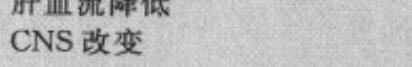
\includegraphics[max width=\textwidth]{2024_07_10_373f31b88d2bf633007bg-051}
 & \begin{tabular}{l}
约物使用延长 \\
所需剂量域少 \\
\end{tabular} \\
\hline
阿芬太尼 &  &  \\
\hline
苯二氮荤类 & 肝组织与肝血流惐少 & 药物效应延长 \\
\hline
\begin{tabular}{l}
䋳氮葉 \\
地西涞 \\
\end{tabular} & CNS 改变 & 所需剂量减少 \\
\hline
阿普唑仑 &  &  \\
\hline
神经肌肉阻滞药 & 弥散性神经源性肌菱缩 & 剂量不变或需增加 \\
\hline
(非去极化) & 旰、肾功能降低 & 药物效应延长 \\
\hline
(㑱琥珀胆䂝) & 男性血浆胆哺酯酶水平降低 & 在男性所需剂量惐少 \\
\hline
吸人麻醉药 & CNS 改变 & 所需剂量减少 \\
\hline
\end{tabular}
\end{center}

\section*{九、其他}
老年人机体构成成分的变化将对麻醉药和辅助药等的药代动力学发生影响。与青年人相比, 到 59 岁时男性体重约增加 $25 \%$, 女性则约增加 $18 \%$ 。 59 岁以后, 体重急速减轻, 降至接近年轻时或更低水平。从中年到老年机体构成成分逐渐变化,老龄使脂肪对体内水分的相对比例稳定增加。由于机体脂肪的增加, 就等于体内增加了一个麻醉药和其他脂溶性药物的贮存库。老年妇女的全身脂肪常特别惹人注目地增长,另一方面骨质疏松使骨质丢失、细胞内水分显著减少,故其全身体重变化轻微。男性老人则普遍多处组织丢失、脂肪组织及骨质均中度减少、细胞内和间质内水分减少(与骨骼肌萎缩有关)。

此外,解剖上的一些老年性改变, 如牙齿的脱落、脊柱一些韧带的钶化等都对麻醉的实施有影响。

(许 幸)

\section*{委考文輻}
1]捙秀娟. 老年人麻醉//庄心良主缩。

现代麻碎学. 3 版. 北京: 人民卫生出版社,2003, 1441-1458

[2] Paul G, Barash, MD Clinical Anesthe- sia 4th edition (January 2001) by Lippincott Williams \& Wilkins Publishers

\section*{麻醉与内分泌功能}
内分泌腺体功能六进或功能减低时出现机体内分泌紊乱, 会引起多系统器官功能及代谢异常。患有或合并有内分泌系统疾病的病人常需要手术治疗,同时麻醉和手术对内分泌系统也有不同程度的影响。因此,麻醉医生应熟悉内分泌系统的主要生理功能及病理生理变化。

\section*{第一节 内分泌系统的生理功能}
\section*{一、主要内分泌腺组织}
内分泌腺体主要包括垂体、甲状腺及甲状旁腺、媵腺、肾上腺等, 它们合成及分泌相应的激素,进人血液循环发挥其全身效应。

\section*{(一)垂体}
位于蝶鞍内, 呈卵圆形, 分为前叶 (又称腺垂体)和后叶 (又称神经垂体)。

\begin{enumerate}
  \item 垂体前叶 垂体前叶分泌的邀素有促进其他内分泌腺体激素的释放作用, 又称为促激素, 包括: (1) 促甲状腺激素 (TSH); (2)促肾上腺皮质激素 (ACTH); (3) 促性腺激素, 包括有: 卵泡刺激激素 (FSH) 和黄体生成激素(LH)。这些促激素通过作用于周围靶腺体而发挥效应。此外, 垂体前叶还分泌: (1)生长激素 (GH), 可影响糖、脂肪及蛋白质等代谢, 促进机体的生长发育; (2)催乳素 (PRL), 可促进乳腺分泌组织的发育、生长并分泌乳汁; (3) 黑色素细胞刺激素 (MSH), 促进黑色素的合成, 使皮肤稒膜色素加深。这些激素直接作用于外周器官组织。
\end{enumerate}

垂体前叶分泌的激素除受到其靶腺体分泌功能的负反馈调节外,下丘脑分泌各种释放激素或释放抑制激素调节垂体前叶的内分泌功能, 如促甲状腺激索释放激素 (TRH) 、促肾上腺皮质激素释放激素 (CRH) 、促性腺激素释放激素 (GnRH), 包括卵泡刺激素释放激素 (FRH) 和黄体生成素释放激素(LRH)、生长激素释放激素 (SRH) 和生长激素释放抑制激素 (SRIH)、催乳素释放激素 (PRH) 和催乳素释放抑制激素 (PRIH)、黑色素细胞刺激素释放激素 (MRH) 和黑色素细胞刺激素释放抑制激素(MRIH)等。

\begin{enumerate}
  \setcounter{enumi}{1}
  \item 神经垂体神经垂体分泌抗利尿激素 (ADH) 和催产素(OXT),两者均合成于下丘脑。 $\mathrm{ADH}$ 合成于下丘脑的室上核, OXT 合成于室旁核,沿下丘脑-垂体束的神经纤维输送到神经垂体储存。抗利尿激素在调节机体水平衡方面发挥着重要的作用, 主要作用是促进悁小管对水的重吸收, 从而保留了水分, 浓缩尿液成为高渗。它又能使动脉和毛细血管收缩, 升高血压, 故又称为血管加压素。催产素的生理作用为促进子宫收缩, 并促进乳腺分泌。
\end{enumerate}

\section*{(二)甲状腺及甲状旁腺}
\begin{enumerate}
  \item 甲状腺 甲状腺由左右两叶和中间的峡部组成。甲状腺是人体最大的内分泌腺体, 甲状腺滤泡上皮细胞从血液中摄取碘、使酪氨酸磌化、最终合成甲状腺激索, 主要为甲状腺素 $\left(\mathrm{T}_{4}\right)$ 和少量的三䃆甲腺原氨酸 $\left(\mathrm{T}_{3}\right)$, 并储存于甲状腺内。外周组织将 $T_{4}$ 转化为 $T_{3}, T_{3}$ 的半衰期较短, 但生物效能是 $T_{4}$ 的 8 10 倍。大部分 $T_{4}$ 与甲状腺结合球蛋白 (thyroid binding globulin, TBG) 结合, 小部分与甲状腺结合前清蛋白 (TBPA) 结合, 只有很小一部分与清蛋白结合。 $\mathrm{T}_{3}$ 与 TBPA 结合很少, 与 TBG 结合也较松散。只有游离(非结合) 的 $\mathrm{T}_{3} 、 \mathrm{~T}_{4}$ 才具有生理活性。甲状腺的生理功能包括: (1) 产热, 加速\\
体内细胞氧化反应, 而释放能量。(2)调节生长、发育及组织分化, 甲状腺激素对于维持正常的生长发育十分重要, 甲状腺激素和生长激素对生长发育有协同作用。(3)对蛋白质、糖、脂肪代谢的影响, 促进机体蛋白质合成, 维持机体正常的需要, 但分泌过多时可加速蛋白质分解; 加速肠道对糖的吸收, 同时促进肝糖原分解和糖异生, 增加组织对糖的利用, 促进肝、肌肉和脂肪组织摄取葡萄糖; 促进脂肪的氧化和分解。(4)对神经系统的影响, 甲状腺功能正常对中枢神经系统的发育和功能调节十分重要,在胎儿及幼年时期缺乏甲状腺激素可影响大脑和体格发育,出现智力低下和身材矮小, 称为 “呆小症”; 而成年人甲状腺激素缺乏时, 可表现为反应迟钝、智力减退。(5)对心血管系统的影响, 甲状腺素过多时, 刺激心肌, 心脏收缩增强, 心率加快, 心排血量增加。甲状腺素减少时, 心肌张力减低, 心率减慢, 心排血量减少。甲状腺素和悄上腺素、去甲肾上腺素又相互增强作用。(6)其他: 甲状腺素对维持机体内环境的生理平衡及病理过程都有影响。

  \item 甲状旁腺 正常甲状旁腺分上下 2 对, 上甲状旁腺一般位于甲状腺上极背侧附近,下甲状旁腺位于甲状腺下极前或侧后面。甲状旁腺分泌甲状旁腺激素 (PTH), 其生理功能为调节机体钙磷代谢和维持血钙磷浓度稳定, 它直接作用于骨和肾, 间接作用于小肠, 功能有: (1)作用于破骨细胞, 促进骨质的溶解; (2)促使肾小管对钙的重吸收增加, 抑制肾小管对磷的再吸收, 促进尿中磷酸盐的排出; (3)促使肠铃吸收增加, 其结果是血钽增高、血磷降低、尿磷增高。

\end{enumerate}

\section*{(三)胰腺}
腅腺的脥岛细胞分为 $\mathrm{B}$ 细胞和 $\mathrm{A}$ 细胞。前者分泌胰岛素,后者分泌胰高血糖素。

\begin{enumerate}
  \item 胰岛素 是人体血糖调节最主要的激素, 其主要生理作用有: (1)糖代谢, 胰岛素增加细胞对莆䓨糖的通透性, 促进莆萄糖从细胞外向细胞内转移, 加速糖的利用; 促进蒱蒛糖的氧化和酵解, 促进莆吿糖转变为脂肪; 促进肝糖原的合成和储存, 抑制糖原的分解及异生。(2)脂代谢, 胰岛素能促进肝和脂肪细胞的脂肪酸的合成, 抑制脂肪的分解, 降低血中游离脂肪酸含量, 减少酮体的产生。(3)蛋白质代谢, 促进蛋白质的合成, 抑制其分解。

  \item 媵高血糖素具有升高血糖的作用, 它促进肝糖原分解和异生, 抑制肝糖原的合成, 升高血糖浓度; 激活脂肪细胞中的脂肪酶, 加快脂肪分解, 使血中游离脂肪酸升高; 促进氨基酸进人肝细胞, 加速脱胺基作用, 增进糖异生, 促进蛋白质分解; 促进降钙素分泌, 降低血钙浓度。

\end{enumerate}

\section*{(四)肾上腺}
肾上腺包括肾上腺皮质和䯡质两个在形态发生、生理功能完全不同的部分, 外层皮质占 $90 \%$,中央餺质占 $10 \%$ 。

\begin{enumerate}
  \item 肾上腺皮质按解剖结构从外层到内层分别为球状带、束状带和网状带, 依次分泌盐皮质激素、糖皮质激素及性激素。肾上腺皮质激素具有广泛的生理功能, 为机体维持正常的生命所必需。
\end{enumerate}

(1)盐皮质激素以醛固酮为代表,在维持体内钠和钾离子平衡方面起主要作用, 醛固酮能明显增加肾远曲小管对钠离子的重吸收和钾离子、氢离子的分泌作用, 从而导致细胞外液中钠离子浓度及细胞外液容量增高, 维持正常的血钾浓度。如果摄人的钠量减少, 或近曲肾小管重吸收钠增多, 到达远曲小管的钠量减少时, 醛固酮的排钾作用明显减弱。值得注意的是,醛固酮的渚钠作用有 “逸脱”现象。近年来对心钠素的研究发现,心钠素作为排钠激素,在醛固酮等盐皮质激素产生的钠“逸脱”中起了重要的作用, 当体内钠量过多, 体液容量增多, 促使心钠素分泌而使尿钠排泄增多。但醛固酮的排钾作用并不出现 “逸脱” 现象。另外与糖皮质激素一样,盐皮质激素可增强血管对儿茶酸胺的敏感性。盐皮质激索的分泌与肾血流量和血钢浓度有关。当肾血流不足或血钠浓度下降, 以及前列腺素或 $\beta$ 肾上腺素能兴奋时, 引起肾小球旁细胞分泌肾素, 肾素促使血液中血管紧张素原转变为血管紧张素 $\mathrm{I}$, 然后在肺和其他组织中血浆转换酶的作用下转变为血管紧张素 II, 血管紧张素 II 直接作用于肾上腺皮质, 促进酫固酮分泌, 同时还有强烈的收缩血管, 升高血压的作用。血钠浓度改变通过细胞外液的容量变化来调整醛固酮分泌。高血钾可刺激醛固酮分泌,而低血钾抑制其分泌。垂体前叶的促肾上腺皮质激素 (ACTH) 也参与醛固酮的调节, 但 $\mathrm{ACTH}$ 对醛固酮分泌的长期持续作用则不明显。醛固垔除了促进肾的渚钠排钾作用外, 对其他有分泌和吸收功能的组织如胃肠道、唾液腺、汗腺等也有减少钠排泄和增多钾排泄, 即潴钠排钾的作用。由于渚钠时细胞外液增多致有效血容量增加, 心排血量增多, 同时小动脉壁的钠、水含量增加, 使小动脉管腔半径缩小,外周血管的阻力增加而导致高血压。此外醛固酮和钠可相应影响去甲肾上腺素的\\
代谢, 使交感神经系统的活性增强, 也使血压升高。

(2)糖皮质激素: 主要是皮质醇 (氢化可的松)和少量皮质酮,其作用极其广泛,主要调节糖、蛋白质、脂肪和水盐代谢, 从而维持内环境的平衡。糖皮质激素是机体对抗胰岛素低血樜症的“升糖”调节激素之一, 它通过刺激肝荛蒛糖异生、增加肝糖原合成、抑制外周组织蒲蒛糖利用而升高血糖; 通过直接作用或通过增强儿茶酚胺和生长激素等的脂解作用促进脂肪分解, 增加游离脂肪酸人血, 另一方面是血糖升高, 兴奋胰岛素分泌, 促进脂肪合成,使身体总的脂肪量增多;促进蛋白质分解,抑制其合成,导致负凮平衡。长期过量的糖皮质激素可引起严重肌肉消耗萎缩, 骨质疏松, 影响儿童生长发育; 皮质醇在生理情况下具有弱的盐皮质激素活性, 即保钠排钾; 主要的心血管作用是增加血管对血管紧张素 II 和儿茶配胺的敏感性, 从而维持血压。糖皮质激素还可以增加心脏排血量。糖皮质激素可使胃壁细胞增多、增高, 胃酸和胃蛋白梅分泌增多。糖皮质激素影响多种神经系统功能,包括情绪、行为和神经活动等。长期大量应用糖皮质激素一方面抑制蛋白质合成,促进蛋白质分解,影响骨基质的形成, 另一方面促进骨吸收, 增加钙磷排泄, 使骨咯的矿化不足, 从而引起骨质疏松。糖皮质激素具有稳定溶酶体膜的作用, 有抑制过敏反应、炎症及毒性反应的作用。糖皮质激素对机体应激反应具有保护作用,其机制为允许作用,即在基础水平下对内环境稳定预防机制的允许作用, 使机体在受到应激时能做出适当反应; 另一方面为抑制作用, 限制已经激活的内环境防御机制不要过分做出反应, 防止损害机体。具有稳定溶酶体膜的作用,有抑制过敏反应、炎症及毒性反应。

(3)性邀素:主要是脱氢表雄酮和具有弱雄性激素作用的雄烯二掤, 以及少量的睪狪和雄二酎。其主要生理功能是在正常情况下与青春期的发动有关, 作用于肌肉、毛发等第二性征, 也有促进蛋白质合成作用。一般情况下悄上腺皮质分泌性激素的量很小。

\begin{enumerate}
  \setcounter{enumi}{1}
  \item 肾上腺越质肾上腺嶰质起源于外胚层, 主要由嗜铬细胞构成, 间有少量交感神经细胞。嗜铬细胞分泌和储存儿茶酚胺 (CA), 即肾上腺素 (E)、去甲肾上腺素 (NE) 和多巴胺(DA)。嗜铬细胞按其不同的形态、功能及组织化学特征分为产生 $\mathrm{E}$ 或 $\mathrm{NE}$ 的两种细胞, 人怪上腺㵦质嗜铬细胞产生的 $\mathrm{CA}$ 中约 $85 \%$ 是 $\mathrm{E}$ 。这些细胞还存在于胸腹椎旁神经节、心、脑、脾、前列腺、卵巢、膀胱等处。肾上腺䯝质受交感神经胆碱能节前纤维直接支配, 分泌和贮存肾上腺素和去甲肾上腺素, 通过肾上腺素能受体而产生作用,调节心血管、中枢神经系统及自主神经, 对糖、脂肪代谢均有重要的生理意义。它能兴奋心脏, 心肌收缩力增强, 心率加快、传导加速,心排血量增大; 能使小动脉和小静脉收缩, 增加外周血管阻力; 支气管平滑肌松驰, 解除支气管痉挛;促进糖原分解, 升高血糖, 促进脂肪分解, 并可剌激下丘脑和垂体引起促肾上腺皮质激素和促甲状腺素的分泌。
\end{enumerate}

\section*{二、内分泌功能的生理调控}
内分泌系统功能受多种因素的影响及调控, 保持其功能状态相对稳定。如果这一稳定状态因某种原因而破坏,导致内分泌功能元进或低下,将影响机体正常的生理功能。

\section*{(一)神经系统对内分泌系统的影响}
\begin{enumerate}
  \item 中枢神经系统对内分泌功能的影响 高级神经及自主神经活动均可影响内分泌系统的功能,而内分泌功能正常与否也能影响神经系统的功能。高级神经活动如紫张、焦虑、饥饿、寒冷、手术创伤、疼痛等可影响下丘脑内分泌功能,也能引起交感神经兴奋,使肾上腺皮质激素及儿茶酚胺分泌增加;而甲状腺功能低下可出现智力低下、反应迟钝等,胰岛素痹病人可出现精神症状。

  \item 神经递质对内分泌功能的影响中枢神经递质如多巴胺、去甲肾上腺素、乙酰胆碱、5-垟色胺等均参与调节下丘脑及垂体前叶激索的释放或抑制。

\end{enumerate}

\section*{(二)下丘脑-垂体-内分泌腺的反馈性调节}
\begin{enumerate}
  \item 下丘脑-垂体一甲状腺之间的反饾性调节 垂体前叶分泌的 TSH 能促进甲状腺增生肥大, 剌激甲状腺素的合成与分泌。TSH 的分泌受两种因素的调节:下丘脑分泌的 TRH 可刺激 TSH 的分泌;同时甲状腺激素也可直接抑制 TSH 的分泌, 又可对抗 TRH 的作用。甲状腺激素负反馈机制控制体内的 TSH 分泌的平衡。

  \item 下丘脑-垂体一肾上腺之间的反馈性调节下丘脑分泌的 CRH 刺激垂体分泌 ACTH, ACTH 又刺激肾上腺皮质分泌皮质醇; 当血中肾上腺皮质激素浓度过高时,能抑制下丘脑分泌 CRH 及垂体分泌 ACTH。

  \item 下丘脑-垂体一性腺之间的反馈性调节 在月\\
经周期的排卵前, 垂体分泌 FSH、LH 增加, 作用于卵巢导致蜼激素分泌增多; 当接近排卵时,下丘脑、垂体分泌功能兴奋, FSH 和 $\mathrm{LH}$ 分泌增加, 促进排卵。

\end{enumerate}

\section*{(三)内分泌腺体及激素之间的相互影响}
\begin{enumerate}
  \item 腺体内及腺体之间的互相影响甲状腺内调节同样是重要的, 有机碘在腺体内含量的改变可影响甲状腺索的合成与分泌, 其可能是通过改变对 TSH 反应而产生作用。胰岛内分泌的胰岛素和胰高血糖素可相互影响, 相互制约。嗜铬细胞㾗分泌大量儿茶酚胺可抑制涛岛 B 细胞的分泌功能, 病人表现为血糖升高或糖尿病。

  \item 相关激素之间的相互影响 TSH 对 TRH 反应还受其他因素的影响, 如生长抑素及多巴胺对 TRH 的分泌有抑制作用, 女性激素增强 TRH 的反应, 而糖皮质激素对此则是抑制作用。生长激素有抗胰岛素作用, 肢端肥大病人可有血糖升高表现;ACTH 可直接影响醛固酮的合成与分泌。

\end{enumerate}

\section*{(四)体液因素对内分泌功能的影响}
\begin{enumerate}
  \item 钙磷代谢与甲状紊腺素及降钙素之间的相互作用 血清钙离子浓度增高时, PTH 的分泌受到抑制, 降钙素分泌增多; 而血清钙离子浓度降低时, 兴奋甲状咅腺分泌 PTH, 同时抑制降锁素的分泌。PTH 和降钙素通过调节血钙而相互影响。

  \item 血糖与费岛素及脜高血糖来之间的相互作用当血糖升高时, 刺激胰岛 $\mathrm{B}$ 细胞分泌胰岛素,同时抑制㙽岛 $\mathrm{A}$ 细胞分泌胰高血糖索; 血糖降低时, 刺激媵岛 $\mathrm{A}$ 细胞及情上腺斃质, 胰高血糖素和肾上腺素分泌增加,胰岛素的分泌受到抑制。

  \item 水及电解质与抗利尿激素及酩固䣩之间的相互作用当有效血容量减少,血压下降时, 抗利尿激素分泌增加, 同时肾素-血管紧张素系统兴奋,刺激醛固酮分泌。高血钾也刺激醛固酮的分泌, 而低血钾抑制醛固酮的分泌。

\end{enumerate}

\section*{三、内分泌系统疾病}
\section*{(一)垂体}
垂体可因各种疾病而影响其分泌功能。当垂体分泌功能元进时, 可出现相应的临床表现及症状, 如垂体腺瘤引起泌乳素㿔和生长素㿈, 以及皮质醇增多症。垂体功能减退,除其分泌的激素减少外, 同时促激素分泌不足, 可影响内分泌腺功能。神经垂体功能减退可出现抗利尿激素分泌过少, 发生尿崩定。

\begin{enumerate}
  \item 垂体功能立进 主要原因为垂体腺瘤, 根据垂体细胞分泌激素的不同分为: 泌乳素 (PRH) 面、生长激素 $(\mathrm{GH})$ 㿑、促肾上腺皮质激素 (ACTH) 面、混合面及无功能腺瘤。
\end{enumerate}

(1)泌乳素 (PRH) 瘤: 泌乳素分泌增加, 导致男性性功能减退、萃酮合成减少和精子发生减少, 女性病人抑制卵巢合成黄体酮, 表现为闭经、泌乳。肿瘤增大可出现肿瘤压迫和垂体功能减退症状, 如头痛、视野缺损、眼外肌麻痹、急性视力下降、复视等, 以及甲状腺、肾上腺皮质功能继发性降低。泌乳素是应激激素, 精神紧张、体力活动、低血糖、麻醉和手术等刺激均可引起 PRL 分泌增加, 手术后 PRL 水平可升高 5 倍以上。泌乳素㿔对全身影响较少。

(2)生长激素 (GH) 瘤:生长激素 (hGH) 过度分泌发生于骨销关闭前或后, 可表现出临床上的巨人症和肢端肥大症。其特征有: 骨骼增大突出、手足增宽、鼻大而宽厚, 唇厚舌肥, 腭垂及软腈增厚, 以及声门下气管狭窄; 糖耐量降低或糖尿病; 垂体前叶功能减退, 首先影响性腺, 甲状腺及肾上腺皮质功能影响较少; 高血压、心脏肥大及左心室功能不全、冠心病和心律失常等。呼吸系统可因口咽软组织增生导致口咽部狭窄, 表现有阻塞性睡眠呼吸暂停。

(3)促肾上腺皮质激素 (ACTH) 㿔: 由于垂体分泌过多的 $\mathrm{ACTH}$, 促进肾上腺皮质增生并分泌过量的皮质醇, 引起以糖、脂肪及蛋白质代谢异常的皮质醇增多症又称库欣综合征 (Cushing syndrome)。其表现主要有向心性肥胖、满月脸、水牛背, 躯干肥胖而四肢细弱; 皮肤菲薄、紫纹、序班、肌肉萎缩无力、骨质疏松和病理性骨折及伤口愈合困难; 糖耐量降低或糖尿病; 高血压、低血钾及性腺功能紊乱等。

(4)无功能腺㿑: 垂体腺痹无分泌功能,其表现主要取决于肿痹的大小及其压迫正常组织情况。表现为头痛、视力下降、视野缺损、复视及斜视、垂体前叶分泌功能减退。

\section*{2. 垂体功能减退}
(1)垂体前叶功能减退: 由于肿癖、炎症、供血障碍,以及垂体手术、放疗后,垂体前叶分泌功能减退, 出现甲状腺、肾上腺皮质功能减退、性腺功能减退等症状,表现为食欲缺乏、恶心呕吐、低血糖、低血钠、低温、淡漠、休克、严重心律失常, 甚至昏迷等症状。如因肿痹所致, 可有顾内高压、头痛、枧力障\\
碍等症状。病人对麻醉药物十分敏感,术前药如巴比妥类、吗啡类等易引起神经系统抑制,应慎用或不用; 麻醉维持用药应严格控制剂量。治疗原则为支持疗法、纠正水电解质紊乱、纠正低血糖、补充肾上腺皮质激素等。

(2)神经垂体功能减退: 主要为尿崩症,由于肿痹、炎症、结核、顼脑外伤和垂体手术后,出现抗利尿激素分泌諴少。临床表现为烦渴、多饮、大量低渗、低比重尿, 严重者出现脱水, 甚至嗜睡、意识障碍、虚脱和死亡。可用抗利尿激素治疗, 或 DDAVP 治疗; 氯磺丙脉及氢氯噻嗪也有效。

\begin{enumerate}
  \setcounter{enumi}{2}
  \item 垂体疾病与麻醉 垂体肿痹的麻醉处理应根据病情、手术方式等具体情况而定。泌乳索痹对全身影响较小,如无肿瘤压迫所引起的垂体分泌功能障碍, 其手术麻醉的处理应无特殊。否则, 应针对病情给予补充激素治疗和对症治疗。肢端肥大病人麻醉中可能会遇到上呼吸道梗阻、气管插管困难、心律失常等问题,应给予重视,并准备好各型号的导管、口咽或鼻咽通气道、清醒插管器械等。库欣综合征病人麻醉诱导时易发生呼吸困难, 麻醉期间循环波动较明显,此外,还应注意其高血压、高血糖、水电解质紊乱等病理改变。无功能腺瘤病人出现垂体功能减退时, 应及时补充激素。
\end{enumerate}

垂体功能减退病人对麻醉药非常敏感,机体代偿功能差。因此, 术前应认真检查, 充分准备, 可根据病情进行激素替代疗法, 纠正水电解质紊乱、代谢紊乱。应选择适当的麻醉方法, 麻醉药用量应适当减少, 术中加强监测, 防止缺氧和二氧化碳蓄积。此类病人易发生心功能不全或肺水肿, 术中应注意控制输液速度和输液量。

\section*{(二)甲状腺}
\begin{enumerate}
  \item 甲状腺功能元进 甲状腺素主要调节组织的代谢。当甲状腺索分泌过多时, 机体产热增加,耗氧量增高、加速蛋白质分解、促进脂肪的氧化和分解,可增强神经的兴奋性, 刺激心肌, 心脏收缩力增强、心率加快、心排血量增加,病人表现为怕热、多汗、易激动、消瘦、无力和震䫟, 基础代谢率增高,呈负氮平衡, 以及脉压增大、心律失常, 严重者出现心衰。此类病人麻醉处理的关键是术前甲状腺功能六进治疗及术前准备, 以及防治并发症。麻醉诱导及麻醉恢复期, 甲状腺功能元进病人因气管受压移位、声带麻痹等可能出现呼吸道梗阻、气管插管困难、气管場陷等。术中应避免增加交感神经兴奋的因素,注意维持适宜的麻醉深度。
  \item 甲状腺功能低下甲状腺分泌不足导致了甲状腺功能低下。甲状腺素具有调节生长、发育及组织分化作用; 甲状腺功能正常对中枢神经系统的发育和功能调节十分重要,在胎儿及幼年时期缺乏甲状腺激素可影响大脑发育, 出现智力低下, 又称为呆小病; 而成年人甲状腺激素缺乏时, 可表现为反应迟钝、智力减退。甲状腺功能低下时,心肌张力减低,心率减慢,心搏出量惐少,病人体内有水钠的潴留,病人可表现为畏寒、无力、疲倦、便秘、舌大、面部水肿、心排血量减少、心动过缓、心电图上显示 QRS 幅度降低,以及心包积液、胸腔或腹腔积液、贫血、胃排空延迟以及麻痹性肠梗阻等。甲状腺激素和肾上腺素、去甲肾上腺素有相互增强作用。因此,病人可能存在肾上腺萎缩、皮质激素生成减少、稀释性低钠血症以及水排泄减少。此类病人应尽量择期手术,对急诊手术的病人应重视。因为此类病人对麻醉药物非常敏感,对麻醉及手术的耐受性较差,麻醉恢复期可能延长, 甚至出现循环不稳定。应惐少术前药用量, 及时补充血容量、纠正贫血及低血糖、补充皮质激素、保㖟等支持疗法,避免不必要的用药,加强术中监测, 以及麻醉恢复期的管理。
\end{enumerate}

\section*{(三)甲状旁腺}
\begin{enumerate}
  \item 甲状旁腺功能元进(甲旁元) 由于甲状旁腺腺面、增生等引起甲状旁腺素合成和分泌过多,出现钲、磷和骨代谢絮乱的一种全身性疾病, 表现为高血钲、高尿䥻、低血磷和高尿磷。甲状旁腺素分泌过多,使骨钽溶解释放人血、将小管和肠道吸收钙的能力加强, 血钙升高; 同时使近端肾小管对磷的吸收降低,尿磷排出增多,血磷降低。因此,病人出现骨质疏松及骨质软化,以及纤维性囊性骨炎; 肾结石、肾钙化, 甚至肾功能损害; 周肠道表现为高酸性消化道溃疡、急性胰腺炎等。甲旁立的治疗以手术为主,术前应给予低铂、高磷饮食并多饮水, 应纠正高钙血症, 纠正血谷量及其他电解质的异常。麻醉前应注意检查及治疗肾功能损害、心律失常和心衰等。如病人需用洋地黄治疗,应从小剂量开始。麻醉用药应注意病人的心、肾功能状态,避免进一步的肾功能损害。术中输注生理盐水可起到稀释高血钙的作用,也可使用肾上腺皮质激素、静脉注射降䥻素、依地酸二钠或透析治疗降低血钙。在搬动病人过程中宜轻柡,防止出现骨折。术中术后应监测血清游离钙的浓度。

  \item 甲状旁腺功能低下(甲旁低)因甲状旁腺\\
素产生减少而引起的代谢异常, 多是由于手术中误切除甲状旁腺或损伤, 其表现为手足㹡搨、寝痫发作、低钽血症和高磷血症。甲旁低的症状通常发生于术后数周或数月,但是偶尔在手术后即刻也可发生急性低钙血症。应注意纠正锬和其他电解质的昇常、呼吸或代谢性碱中毒, 同时应注意病人因低钙血症引起的凝血机制的变化。病人有心率加快或心律不齐, 严重者可出现心力衰竭, 甚至因心肌痉挛突然死亡。当快速输注血制品、低温和肾功能障碍可加重低铃血症。

\end{enumerate}

(四)胰岛细胞

\begin{enumerate}
  \item 裾沓病由于各种原因造成胰岛素相对或绝对不足, 使体内糖、脂肪及蛋白质代谢紊乱, 出现血糖增高和 (或)糖尿等为特征的慢性全身性疾病。当胰岛素减少时, 肝糖原合成减少,糖原分解和异生增加, 肌肉及脂肪组织中莆萿糖利用减少, 血糖增高,当血糖超过肾糖阈值时,出现尿糖; 脂肪合成减少,分解加强,严重者可出现嘪症酸中毒; 同时抑制蛋白质合成, 加快蛋白质分解, 出现负氮平衡、水及电解质紊乱, 甚至脱水及酸中毒等。手术前应详细了解病史,充分准备, 特别是有并发症的病人,应控制糖尿病症状,改善病人全身状况,提高病人对麻醉和手术的耐受性。机体应激时, 外周组织对胰岛素利用障碍, 同时胰高血糖素分泌增加, 出现血糖增高。因此,应尽可能选用对糖代谢影响小的麻醉方法及用药, 手术中及手术后应反复测定血糖水平,防止发生酮症酸中毒及非酮症高渗昏迷。对于合并肾功能障碍、心脏疾患的病人, 应加强监测, 如直接动脉置管测压、反复测定血糖、尿糖、尿酮体。

  \item 胰岛素㾇 胰岛素分泌过多,出现低血糖症, 临床上表现为心动过速、出汗、心悸和䂭抖。此外, 可有神经系统症状, 包括头痛头晕、反应迟钝、㿉病发作甚至昏迷。一些病人还有精神异常。术前正确诊断及防止低血糖发作十分重要。此类病人的麻醉处理应力求平稳, 尽量避免外源性葡萄精引起的血糖波动,术中反复间断测定血糖的水平,必要时输注莆萄糖液或胰岛素控制血糖, 注意签别低血糖昏迷。

\end{enumerate}

\section*{(五)肾上腺}
\begin{enumerate}
  \item 糖皮质擞素分泌过多 垂体病变及情上腺皮质肿面或增生等原因使肾上腺皮质激素分泌增多,可引起一系列的代谢紊乱和相应的临床症状,称为皮质醇增多症。其临床表现为肝糖原增加, 血糖增高; 蛋白质分解代谢增加, 出现肌肉无力、皮肤较薄、骨质疏松; 脂肪代谢加强, 血胆固醇增高, 脂肪重新分布,呈现四肢细弱、满月脸、水牛背等向心性肥胖; 循环容量增多, 高血压, 心肌收缩力降低,心肌发生退行性变; 胃壁细胞增多增高, 胃酸和胃蛋白酶分泌增多。长期大量应用糖皮质激素可使溃疡形成,以及抑制蛋白质合成, 促进蛋白质分解,影响骨基质的形成,另一方面促进骨吸收, 增加钙磷排泄, 使骨骼的矿化不足, 从而引起骨质疏松。皮质醇增多症的病人对手术麻醉的耐受性差, 术前准备十分重要, 应控制血压、纠正电解质及代谢紊乱,适当补充皮质激素。

  \item 盐皮质激来分泌过多由于肾上腺皮质腺痹或增生导致盐皮质激素分泌过多,产生醛固酮增多症。酫固酮分泌过多促使钠的重吸收加强和钾、氢的排出增加, 从而引起钠和水的渚留, 使细胞外液及血容量增加, 出现高血压, 但不依赖肾素含量;醛固酮促使肾小管排钾增加, 尿中大量丢失钾, 使细胞外液的钾浓度降低,一般血钾浓度在 $3 \mathrm{mmol} /$ L 以下; 神经肌肉应邀性下降, 发生肌无力, 甚至周期性四肢麻痹或抽搐, 并伴有碱中毒和细胞内酸中毒。长期失钾可引起肾小管上皮细胞功能严重紊乱, 肾功能减退。术前准备十分重要, 应纠正电解质异常, 使血钟尽可能恢复至正常, 控制高血压。此类病人麻醉用药剂量偏小, 特别是老年病人。术中应密切监测, 特别是对有心律失常或心肌病变的病人, 注意心电图变化。此外, 还应加强呼吸管理,防止过度通气。

  \item 皮质性做素分泌过多由于先天性肾上腺皮质增生, 如 21-羟化酎缺陷症 (21-HD) 或 $11 \beta$-羟化酶缺陷症 (11-HD), 以及将上腺皮质肿瘤分泌大量的肾上腺皮质雄性激素, 出现肾上腺性异常征。一般是以雄激素分泌过多引起的临床表现为主,女性男性化或男性假性性早熟。21-羟化酶缺陷症病人皮质醇分泌低于正常, 有不同程度的失盐倾向,病人可出现皮肤色素沉着、女性男性化及男性假性性早熟。而 11 $\beta$-羟化酶缺隆症因 11-脱氧皮质酮和 11-脱氧皮质醇的生成明显增加, 11-脱氧皮质醇具有弱的盐皮质激索作用, 病人不仅无失盐的表现,还有储钠的效果, 病人血容量增加, 血压升高。此类病人应在术前、术中及术后补充怪上腺皮质激素, 预防手术及麻醉期间出现肾上腺皮质功能低下。

  \item 肾上腺皮质功能低下由于特发性自身免疫性萎缩、肾上腺结核、手术切除后、放疗、肿癖转\\
移、感染或垂体肿瘤所导致 ACTH 缺乏、产后大出血引起的席汉 (Sheehan) 综合征、外源性补充激素等原因,病人出现肾上腺皮质功能低下,临床表现为乏力、皮肤黏膜色素沉着、体重下降、厌食、恶心呕吐、腹痛腹渠或便秘、血压偏低、高钾血症等。肾上腺皮质功能惐退症的病人容易发生感染, 并且病情往往严重, 甚至死亡, 提示内源性糖皮质激素可控制炎症过程, 也控制自身免疼反应。此类病人对手术及麻醉耐受性差, 心肌极易受抑制。遇有应激时, 机体不能做出适当的反应, 病人可出现急性肾上腺皮质功能衰竭, 甚至导致死亡。麻醉前应纠正水电解质紊乱、补充皮质激素; 麻醉药剂量应适当减少,麻醉期间应加强监测; 术中、术后应酌情补充激素。

  \item 肾上腺道质功能元进主要是由于嗜铬细胞㿑分泌大量儿茶酚胺,引起血中儿茶酚胺浓度增高, 使心排血量增加、心率加快、外周血管收缩, 血压升高; 中枢神经系统及交感神经兴奋, 耗氧量增加, 基础代谢率增加; 脂肪分解加快, 出现消瘦; 加快糖原分解, 血糖增加, 可出现尿糖。肾上腺䯕质增生也可出现与嗜铬细胞瘤相似的临床症状。

\end{enumerate}

\section*{第二节 麻醉和手术对内分泌系统功能的影响}
\section*{一、麻醉药物}
大多数麻醉药能够抑制机体对手术刺激等应激的内分泌反应。

\begin{enumerate}
  \item 麻醉性镇痛药吗啡可抑制下丘脑促将上腺皮质激素释放激素, 从而影响垂体 ACTH 及肾上腺皮质激素的分泌,促进抗利尿激素分泌。吗啡也能刺激肾上腺髓质释放儿茶酚胺。哌替啶可抑制垂体分泌 ATCH。
\end{enumerate}

2.静脉麻醉药 巴比妥类药可抑制下丘脑-垂体一肾上腺轴的肾上腺皮质激素的释放, 抑制甲状腺摄碘和释放硔的作用, 刺激抗利尿激素。吩噻嗪类药可增加 ACTH 的分泌。氯胺酮和 $\gamma$-羟丁酸钠促使 $\mathrm{ACTH}$ 分泌和情上腺皮质激素分泌。大量、长时间地输注依托㽤酯可以抑制肾上腺皮质激索的分泌。

\begin{enumerate}
  \setcounter{enumi}{2}
  \item 吸入麻醉药 乙醚明显刺激内分泌系统的活性, 抗利尿激素、生长激素、ACTH、甲状腺素 $\left(\mathrm{T}_{4}\right)$ 及儿茶酚胺均升高。氟烷增加抗利尿激素、生长激索、ACTH、甲状腺素、酫固酮、肾上腺皮质激素的分泌。甲氧菛烷可促进抗利尿邀素、生长激素分泌。安氟醚、异氟醚对内分泌影响较小,生长激素及泌乳素变化不大。

  \item 肌松药 目前所知,肌松药对内分泌系统活

\end{enumerate}

\section*{二、麻醉方法}
\begin{enumerate}
  \item 椎管内阻滞麻醉椎管内阻滞麻醉对内分泌的影响轻微。由于阻滞了交感神经, 能抑制机体对手术等刺激的反应,肾上腺皮质激素、甲状腺素、儿茶酚胺等分泌均减少。

  \item 全麻 全麻对内分泌的影响较椎管内阻滞麻醉显著, 现代全麻药对内分泌的影响明显小于手术刺激的影响。

\end{enumerate}

\section*{三、手术对内分泌的影响}
\begin{enumerate}
  \item 病人精神紧张、手术等应激反应、正压通气等均可促进抗利尿激素的释放。低血糖、麻醉和手术等刺激均可引起泌乳素分泌增加。手术及创伤交感神经兴奋和肾上腺皮质激素分泌增加, 甲状腺素、胰高血糖素分泌增高,胰岛素分泌减少。

  \item 低温可抑制内分泌反应,肾上腺皮质激素、甲状腺素、胰岛素、儿茶酚胺分泌减少。

  \item 缺氧及二氧化碳蓄积可促进垂体 $\mathrm{ACTH}$ 的分泌,刺激儿茶酚胺的释放。

  \item 循环容量不足时,抗利尿激素、肾上腺皮质激素、生长激素、胰岛素分泌增加, 儿茶酚胺释放增多。

\end{enumerate}

(许 幸)性无明显影响。

\section*{考文煋}
[1]张秀华,罗爱伦. 麻醉与内分泌//生心良主编.现代麻醉学. 3 版. 北京: 人民卫生出版社,2003: 148-165

\section*{筑5車}
\section*{自主神经系统的解剖和生理}
神经系统在结构上是由中枢神经系统和周围神经系统构成, 中枢神经系统由脑和脊髓构成, 周围神经系统由发自脑的脑神经和发自脊髓的脊神经构成。自主神经系统是神经系统在功能上的分类。自主神经系统的控制中枢仍在脑内, 是中枢神经系统的一部分, 其外周部分进一步区分为交感神经和副交感神经。

自主神经系统控制着机体内的不随意 (意识)运动,与控制机体随意运动的骨骼肌相对应, “自主”地控制着平滑肌、心肌组织的收缩和腺体上皮的分泌。在正常或应激条件刺激下,自主神经系统维持着器官功能和内环境的稳定, 在心血管系统、内脏(胃肠道)和体温稳态中起重要作用。麻醉科医师实施临床麻醉的目的之一在于手术创伤对机体可能产生极大应激时, 阻断伤害性刺激的传导,适当地抑制自主神经的过度应激反应,保证机体内环境的稳定。另一方面, 外科病人所患的疾病可能显著地影响自主神经系统的功能, 从而改变自主神经系统对手术和麻醉的正常反应。因此, 麻醉科医师对于自主神经系统的功能以及麻醉药物对自主神经系统功能的影响应有全面、深人的了解。

\section*{第一节 自主神经的解剖}
自主神经系统在解剖和功能上分成两部分:交感神经和副交感神经。自主神经的高级控制中枢在延髓和下丘脑, 电刺激这两个区域,可以诱发全部自主神经系统的反应。自主神经系统自中枢神经系统发出时是有䯕鞙纤维, 在神经节进行突触换元, 然后分布于支配的靶器官, 此时已是无䚣鞘纤维。自主神经系统的第一级神经元的胞体在脑内的灰质或在脊䚣, 其轴突与位于自主神经节中的第二级神经元形成突触联系, 这样第一级神经元称为神经节前 (突触前) 神经元, 第二级神经元的胞体位于中枢神经系统外的神经节内, 故称为神经节后 (突触后)神经元。神经节后神经元的轴突与靶器官的细胞形成突触联系,产生生理效应。

交感神经的神经节靠近脊髓, 并在脊柱两侧形成交感链, 其神经纤维发自 $\mathrm{T}_{1} \sim \mathrm{L}_{2}$ 脊䚛侧角内的神经元。通过白色交通支(神经节前纤维), 使侧角神经元的冲动通过脊神经传递到交感神经节。神经节发出纤维在同水平经灰色交通支(神经节后纤维)返回脊神经前支或直接向上或向下发出节前神经纤维。来自神经节的节前纤维可与远端的副神经节 (collateral ganglion)内的神经元相联络, 如腹腔神经丛、颈神经节或肾上腺髓质。

副交感神经系统由 II、V、IX、X 脑神经和骶轾的 $\mathrm{S}_{2 \sim 4}$ 构成, 交换神经元的神经节与脊髓相距较远, 靠近支配的靶器官, 因此节后神经纤维要比交感系统短得多。

在功能上,交感神经主应激反应,副交感神经主要起拮抗交感神经的作用。

\section*{一、交感神 经}
交感神经元位于延髓前外侧、延解前中部、尾缝核、脑桥和海马内室旁核,其中位于延䯕前外侧的交感神经元在维持基础血压以及调节血压的时相性中起重要作用。交感神经元的传出通路下行至 $\mathrm{T}_{1}$ 到 $\mathrm{L}_{2}$ 或 $\mathrm{L}_{3}$ 脊髄侧角的灰质更换神经元, 位于脊顝前侧角的神经元发出的神经纤维以三种方式形成神经节: 椎旁成对的交感神经链、各种不成对的远端神经丛和位于靱器官附近的神经节。交\\
感神经节前纤维在脊髓前角离开脊䯕,随脊神经干进人椎旁交感神经节, 22 对交感神经节成对排列于脊柱两侧, 各神经节间彼此交通形成交感神经链。交感神经纤维在同水平的交感链交换神经元或向上、向下在高水平或低水平的神经节或神经丛交换神经元。另外,交感神经的节前纤维可以进人多个交感神经节,一个脊㰐节段发出的交感神经节前纤维可以和 20 多个交感神经节形成突触连接,一个效应器官的细胞可以由上下不同节段脊髓发出的交感神经支配。机体被触发引起的交感反应并不能限定在某一个特定节段, 而是交感神经系统兴奋泛化, 引起剧烈的多器官交感反应。躯体交感神经与每一条脊神经 (灰色支) 相伴支配相应肌节 (dermatome)的皮肤。支配头、颈和胸腔内脏器的交感神经纤维是从特殊的神经节发出的, 支配腹腔、盆腔脏器的交感神经纤维自脏器附近的神经丛发出。

\section*{(一)交感神经节}
\begin{enumerate}
  \item 颈神经节有 3 个。(1) 颈上神经节: 起自 $\mathrm{C}_{1 \sim 4}$, 发出纤维支配颈内外动脉、耳、涎腺。还参与构成领下神经节、脊神经支和心神经丛。(2)颈中神经节:起自 $\mathrm{C}_{5}$ 和 $\mathrm{C}_{6}$, 发出纤维支配甲状腺下动脉, 构成脊神经支和心神经丛。(3)颈下神经节: 起自 $\mathrm{C}_{7}$ 和 $\mathrm{C}_{8}$, 发出纤维支配椎动脉、参与构成脊神经支和心神经丛。有 $80 \%$ 的人, $\mathrm{T}_{1}$ 与之融合构成星状神经节。

  \item 星状神经节 起自 $\mathrm{C}_{7}$ 和 $\mathrm{T}_{1}$, 与下交感链有密切的解剖联系。它位于 $\mathrm{C}_{7}$ 横突和第 1 肋骨之间,椎动脉的后方, 是疼痛治疗时最常阻滞的神经节。

  \item 胸神经节由 12 节侧角脊神经构成, 接收来自主动脉、脊神经支、三支内脏神经(内脏大、小和内脏下神经) 以及心脏、肺和食管神经丛的纤维。

  \item 腰神经节通常起自腰段的 4 个阶段的脊觝侧角, 发出神经纤维支配主动脉, 参与构成腹腔下神经丛和腰段脊神经。

  \item 呧神经节 通常起自骶解的两个节段,参与构成盆腔神经丛和能部脊神经。

\end{enumerate}

\section*{(ニ)交感神经丛}
\begin{enumerate}
  \item 心神经丛\\
(1)心深神经丛: 位于气管分叉处前方,由颈部和上胸部四个神经节以及迷走神经分支构成。
\end{enumerate}

(2)心浅神经丛: 位于肺动脉前方, 主动脉下方。接收来自右侧颈上神经节的纸维和左侧迷走神经的下心支。

\begin{enumerate}
  \setcounter{enumi}{1}
  \item 腹腔神经丛是最大的交感神经丛,是位于腹腔动脉 $\left(\mathrm{L}_{1}\right)$ 前方的密集神经网络, 在胰腺和胃上缘。接收来自内脏大小神经、内脏下神经, 以及右迷走神经内脏支的纤维。有些神经换元后直接支配肾上腺髓质(其中的细胞相当于神经节后神经元),其余的沿着主动脉下行构成主动脉神经丛。

  \item 腹腔下神经丛 (hypogastric plexus) 位于觝骨岬与管总动脉之间。接收来自腰交感干和主动脉神经丛的纤维, 纤维还进一步扩散至盆腔神经丛。

\end{enumerate}

\section*{二、副交感神经}
副交感神经由脑神经和能骿神经两部分构成。

\section*{(一)脑神经部分}
十二对脑神经中有四对 (第 III、VII、 IX、X ) 脑神经内含有副交感神经。它们在功能上使瞳孔缩小、涎腺和泪腺分泌、胃肠运动加强、心脏抑制、支气管收缩。(1)第 III神经 (动眼神经): 在睷状神经节换元, 支配虹膜平滑肌和狿状肌。(2)第 VII神经 (面神经) : 在翼腭和领下神经节换元, 分布到鼓室和构成㑔上大神经, 支配颌下腺和舌下腺。(3) 第 IX 神经 (舌咽神经): 在耳神经节换元, 支配稒液腺、唾液腺和泪腺。(4)第 $X$ 神经 (迷走神经): 起自延髓的迷走运动背侧核, 是最重要的副交感神经冲动的来源,承担 $3 / 4$ 副交感神经的任务, 支配心脏、气管、支气等、肝、脾、肾和除了远端结肠外的所有胃肠道。

\section*{(二)觝髓神经部分}
起自 $\mathrm{S}_{2 \sim 4}$ 脊神经前根, 构成盆腔内脏神经, 并与交感神经丛相伴, 在支配器官形成小的终末神经节。在功能上,纤维支配结肠、直肠和膀胱的运动、抑制括约肌和使生殖器血管扩张。

\section*{第二节 自主神经系统的递质 }
后神经纤维,以及极少数交感神经的节后神经纤维 (支配汗腺、肾上腺髓质和骨骼肌血管舒张的交感神经)释放的递质是乙酰胆碱,交感神经的节后神\\
经纤维释放的递质为去甲肾上腺素。在中枢神经系统和肾的神经释放递质为多巴胺, 某些肠道神经释放的递质是嘌呤, 结肠中的肠道神经和中枢神经系统中的某些神经释放的递质是神经肽。将释放乙酰胆碱的神经称为胆碱能神经, 释放去甲肾上腺素的神经称为情上腺素能神经。

\section*{二、乙酰胆碱的合成、储存、释放和失活}
\section*{(一)合成}
在神经细胞内, 醋酸和胆碱在乙酰辅酶 $\mathrm{A}$ (胆碱-O-乙酰转移酶)作用下, 合成乙酰胆碱。神经细胞内并不能够合成胆碱, 合成乙醌胆碱所需胆碱主要来自食物中的磷脂、肝合成的卵磷脂以及乙酰胆碱水解。大多数胆碱都来自肝, 作为磷脂进行转运, 并被高亲和力的 $\mathrm{Na}^{+}$泵主动转运, 通过神经膜进人神经细胞。与胆碱有高亲和力的 $\mathrm{Na}^{+}$泉系统决定神经系统中乙酰胆碱的水平, 血中胆碱的水平也影响乙酰胆碱的释放量。

\section*{(二)储存和释放}
乙酰胆碱合成后, 首先溶解在轴浆中, 作为神经递质, 在释放前必须储存在直径为 $300 \mathrm{~nm}$ 的譱泡中,以浓缩的形式释放, 从而产生神经兴奋传导。每个蛮泡含有约 10000 个乙酰胆碱分子,中枢胆碱能神经中乙酰胆碱业泡要比运动神经中少。乙酰胆碱㐮泡在神经体中合成,神经轴的微管将其转运到神经末梢。包绕襄泡的膜具有复杂的结构, 在乙酰胆碱储存和释放中起重要的作用。

正常无神经冲动时, 襄泡能够自发释放乙酰胆碱, 产生突触后膜 $0.5 \mathrm{mV}$ 微电位。当神经冲动到达神经末梢时, 引起锬离子跨膜内流, 其进人神经末梢后,诱导突触襄泡在神经末梢的活动带特定的释放部位与神经细胞突触前膜融合, 并将乙酰胆碱释放到突触裂隙。每个囊泡释放的乙酰胆碱在 $0.3 \mathrm{~ms}$ 内使突触后膜上 2000 个通道开放,每个离子通道开放引起突触后膜 $0.22 \mu \mathrm{V}$ 的去极化, 每毫秒 12000 个钠离子进人突触后膜, 从而改变了突触后细胞膜的静息膜电位。每个神经冲动诱导 100 300 个突触衰泡释放,引起 500000 个离子通道开放, 产生 $50 \sim 100 \mathrm{mV}$ 的突触后膜去极化电位。

(三)失活

乙酰胆碱在碱性溶液中自发水解为醋酸盐和胆碱, 这两个水解产物都没有明确的药理作用。在体内,经酶的催化作用乙酰胆碱被水解成为乙酸和胆碱的速度大大增加。在人体内有两种水解乙酰胆碱的酶, 即乙酰胆碱酯酶和丁酰胆碱酯酶。乙酰胆碱酯酶又称为组织酯酶或真性胆碱酯酶, 存在于所有胆碱能神经的突触裂隙, 结合在细胞膜上, 它的功能是水解胆碱能神经末梢释放的乙酰胆碱。乙酰胆碱酯酶在乙酰胆碱释放后数毫秒内将其水解, 终止胆碱能神经的作用。乙酰胆碱酯酶同时存在于没有神经支配的组织中, 例如红细胞内, 它在这些组织中的作用并不清楚。丁酰胆碱酯酶又称为血浆胆碱酯酶或假性胆碱酯酶, 它是可溶性酶, 由肝合成, 存在于血浆、肝、肾、小肠等组织内。

在两者中, 乙酰胆碱酯酶最重要, 不仅是因为其存在于所有胆碱能神经的突触裂隍中, 水解神经末梢释放的乙酰胆碱, 而且在它的效能最强, 1 个乙酰胆碱酯酶分子每秒能够水解 2500 个乙酰胆碱分子, 每个催化反应持续 $40 \mu \mathrm{s}$ 。丁酰胆碱酯酶的生理功能并不清楚, 但在分解某些胆碱能药物与酯性局麻药及某些肌肉松驰药中起重要的作用, 而乙酰胆碱酯酶并不能破坏这些药物。

乙酰胆碱是一个季铵化合物, 季铵基通过有 2 个碳原子的链与酯基相连接, 乙酰胆碱酯酶在两个部位分解乙酰胆碱, 即荷负电的阴离子和酯解部位, 酶的荷负电的阴离子部分与乙酰胆碱荷正电的季铵基结合, 以及酶的酯解部位与乙酰胆碱的煫基借氢键共价结合, 并使乙酰胆碱的酯链断裂, 生成乙酰化胆破酯酶和胆碱。乙酰化胆碱酯酶再与水作用失去乙酰基而还原为胆碱酯酶并产生乙酸。胆碱酯酶抑制药则是通过与胆黬酯酶的阴离子部分或酯解部位或两者结合, 从而阻止胆碱酯酶与乙酰胆碱结合, 使胆碱酯酶无法水解乙酰胆碱。抑制乙酰胆碱酯酶就能够防止乙酰胆碱被破坏, 从而增强胆碱能神经的作用。

\section*{三、去甲肾上腺素的合成、储存、释放、失活和代谢}
\section*{(一)合成和储存}
去甲肾上腺素由酪氨酸合成, 酪氨酸由苯丙璌酸转化而成。交感神经兴奋时, 酪氨酸的合成显著增加。循环内的酪氨酸被输送到节后交感神经, 在神经胞体和轴突内经酪氨酸羟化酶作用转化成多巴,在多巴脱稴酶催化下形成多巴胺, 多巴胺被转运到神经末梢的葓泡内, 经多巴胺- $\beta$-羟化酶作用生成去甲肾上腺素。存在于胞质内的酪氨酸羟化酶是去甲肾上腺索生物合成中的限速酶, 它的活性取\\
决于蝶啶协同因子和分子氧,分子氧的数量显著掝少时,酪氨酸羟化酶活性受到抑制, 去甲肾上腺素合成減少。去甲肾上腺素水平升高时可抑制酪氨酸差化酶,而其水平下降时, 能够激活酪氨酸羟化酶。

在肾上腺䯣质和脑的极少部位, 去甲肾上腺素经苯乙胺-N-甲基转移酶作用生成肾上腺素, 在肾上腺膸质内 $85 \%$ 的去甲肾上腺素都转化成肾上腺素。肾上腺皮质合成的糖皮质醇通过肾上腺随质时, 能够激活苯乙醇胺- $\mathrm{N}$-甲基转移酶, 因此, 应激时触发皮质醇释放,能增加肾上腺素的生成,增强应激反应。

所生成的去甲肾上腺素进人交感神经的挛泡中,襄泡内还含有锬离子、ATP、多巴胺- $\beta$-差化酶和多种肽, 去甲肾上腺素在囊泡内与 ATP- $\mathrm{Mg}^{2+}$ 结合成复合物, 再与一种可溶性蛋白质结合成比较稳定的储存型去甲肾上腺素。囊泡有大小之分, 大囔泡直径为 $75 \sim 90 \mathrm{~nm}$, 主要位于神经轴胞质内, 具有合成去甲将上腺素的能力, 小囊泡直径为 $45 \sim 55 \mathrm{~nm}$,附着于神经末梢, 储存从胞质液中摄取的去甲肾上腺素。曩泡膜上有两类不同的蛋白,一类与去甲肾上腺素转运进人囊泡有关, 另一类与囊泡的定向运动及蘘泡与神经末梢附着、融合有关。生理状态下,交感神经兴奋引起小襄泡释放去甲肾上腺素,应激状态下则大囊泡参与释放。每次交感神经末梢去极化释放约 $1 \%$ 储存的去甲肾上腺素,新合成或再摄取的去甲肾上腺素都很容易进人小囊泡, 且首先被释放,约 $10 \%$ 储存的去甲肾上腺素始终存在于苼泡内。

\section*{(二)释放}
去甲肾上腺素释放到突触裂隙存在两种不同的机制,一种是从錘泡漏出, 进人胞质,再离开交感神经末梢到达突触裂隙, 称为去甲肾上腺素的间接释放, 麻黄碱和湨苳胺等能够从囊泡中置换出去甲肾上腺素, 或直接作用于囊泡内颗粒引起去甲肾上腺索的间接释放。另一个释放过程是通过胞吐机制完成, 当神经冲动到达交感神经末梢, 引起突触前膜去极化, 使突触前膜活动带的电压-门控性钙通道开放, 钽离子进人突触前膜, 诱导含有去甲肾上腺素的蟥泡接近突触前膜, 触发囊泡与突触前膜融合, 并形成裂孔, 蛮泡内所含有的去甲怪上腺素以胞裂外排方式释放到突触裂隙。一些特异、可溶性和膜结合的蛋白 ( $\mathrm{N}-$ 乙基马来酰亚胺敏感因子、 $\mathrm{N}$-乙基马来酰亚胺敏感因子附着蛋白和三磷酸鸟苷结合蛋白) 参与去甲肾上腺素的胞吐过程, 血管紧张䒺 II、前列环素和组胺都能够增强去甲肾上腺素的这种胞吐释放机制,而乙酰胆碱和前列腺素 $\mathrm{E}$则起抑制作用。

(三)失活

释放的去甲将上腺素通过交感神经末梢主动摄取, 迅速地离开突触裂隙, 这是释放后去甲肾上腺素终止其生理效应的主要机制,称为胺泵的特异性转运,可逆浓度梯度将释放量的 $75 \% \sim 95 \%$ 去甲肾上腺素摄人交感神经末梢内,继之并摄人囊泡,钠离子在去甲恃上腺素转运进人交感神经细胞中起关铤作用。少量未能进人囊泡的去甲怪上腺素被线粒体外侧面所含的单胺氧化酶 (MAO) 代谢。进人循环的去甲肾上腺素可被非神经组织摄取。可卡因和三环类抗抑郁药能够阻滞去甲肾上腺素为交感神经末梢再摄取或重新进人突触囊泡, 使更多的去甲肾上腺素存在于突触裂隙受体部位, 增强交感神经系统的效应。不同组织交感神经末梢摄取、合成去甲怪上腺素的速度差异很大, 外周血管存在解剖屏障,释放的去甲肾上腺素几乎不被交感神经末梢再摄取,在支配外周血管的交感神经中,去甲肾上腺素的合成速度最快,而心脏去甲肾上腺素的再摄取速度最快。

去甲肾上腺素通过肺时, $25 \%$ 被肺摄取。主要是肺毛细血管和肺静脉的内皮细胞摄取去甲肾上腺素, 肺血管内皮细胞主动摄取去甲肾上腺素以及其他的血管活性物质无疑对于左心具有重要的保护作用。肺动脉高压时, 肺血管床增厚, 内皮细胞功能改变,对去甲将上腺素摄取减少。

(四)代谢

进人血液循环的去甲肾上腺素被组织摄取后经细胞内儿茶酚胺氧位甲基转移酶(COMT)和单胺氧化酶代谢。肾上腺髓质释放的肾上腺素同样被单胺氧化酶和 COMT 代谢, 代谢终产物为香草扁桃酸(VMA), 多巴胺的代谢产物主要是高香草酸。去甲将上腺素和肾上腺索迅速被代谢和再摄取,因而其生物半衰期极短,小于 $1 \mathrm{~min}$,这样保证了它们生物学效应的精确性, 同时决定了给予去甲肾上腺素或将上腺素时, 必须是持续静脉输注, 另外, 测量去甲肾上腺素和肾上腺素的代谢产物要比测量其本身更能准确地反映体内儿茶酚胺的水平。

\section*{四、其他递质}
近年来研究证实, 自主神经对器官功能的调控, 特别是对血管的作用并不是仅仅通过释放乙䤀\\
胆碱或去甲肾上腺索完成, 三磷腺苷(ATP)、血筞活性肠肽 (VIP)、P物质(PS)、5-羟色胺 (5-HT)、神经肽 Y(NPY) 和降钙素基因相关肽 (CGRP) 都参与自主神经对血管张力的调节。上述神经递质分别与乙酰胆碱或去甲肾上腺素在同一个神经中合成、储存和释放, 释放后分别作用于相应的受体, 以递质联合作用的形式影响靶器官的功能。对血管张力调控递质的最多联合是交感神经释放去甲肾上腺素、ATP 和 NPY。去甲肾上腺素作用于 $\alpha_{1}$ 怪上腺素能受体,引起血筞收缩; ATP 作用于 $\mathrm{P}_{2}$ - 嘌呤受体, 通过电压依赖性铻通道, 引起血管收缩; NPY 可以增强去甲肾上腺素的作用,同时可直接作用于脾、骨骼肌、脑和冠脉血管,引起相应血管的收缩。副交感神经释放乙酰胆渽和 VIP, 乙酰胆碱和 VIP 分别储存于同一副交感神经的不同囊泡中,低频刺激时乙酰胆碱释放,高频刺激时 VIP 释放。这样多种神经递质的联合作用对于机体重要生理功能的精确调控是十分重要的。

\section*{第三节 自主神经系统的功能}
面对复杂多变的外部生存条件, 自主神经系统以其独特的作用方式力图为机体提供一个稳定的内环境。

机体中大多数器官都是既有交感神经系统又有副交感神经系统的双重支配, 其结果可以产生怙抗 (antagonistic effect)、互补 (complementary effect)和协同 (cooperative effect) 三种效应。

兴奋其中的一个系统对效应器官产生兴奋作用, 兴奋另一个系统却产生抑制效应, 称为怙抗效应, 如在心脏的窦房结和瞳孔的调节。对于涎腺的分泌两个系统起互补作用, 如兴奋副交感使唾液分泌,清而稀; 兴奋交感后使唾液分泌黏稠。对于泌尿生殖系统则起协同作用, 如副交感兴奋使阴茎勃起, 交感兴奋导致射精。虽然膀胱收缩是肌源性的, 但副交感兴奋有促进收缩的作用, 交感兴奋则产生排尿反射, 同时也进一步加强了膀脱收缩 (表 1-5-1)。而少数器官如某些血管、脾和坚毛肌仅有交感神经支配,通过其功能的上升或降低来调节。

表 1-5-1 交感和副交神经的调节功能

\begin{center}
\begin{tabular}{|c|c|c|}
\hline
效应器 & 交感神经 & 副交感神经 \\
\hline
畔状肌 & 舒张 & 收缩 \\
\hline
虹膄 & 散瞳孔 & 缩瞳孔 \\
\hline
窦房结 & 兴奋 & 抑制 \\
\hline
小动脉 & 收缩 & - \\
\hline
静脉 & 收缩 & - \\
\hline
支气管 & 舒张 & 收缩 \\
\hline
胃肠道 & 抑制运动 & 促进运动 \\
\hline
阴茎 & 射精 & 勃起 \\
\hline
傽胱 & 张力增加 & 收缩 \\
\hline
唾液腺 & 分泌液橰稠 & 分淧增加、清而稀 \\
\hline
脄腺 & 抑制外分海 & 促进外分䟓 \\
\hline
\end{tabular}
\end{center}

自主神经系统的功能主要是调节心血管、呼吸和泌尿生殖系统及胃肠道的功能状态与代谢水平,特别是在维持心血管系统功能稳定和器官血流量方面,自主神经系统起着极其重要的作用。自主神经的节后纤维、局部自动调节机制和循环激素一起, 通过调节心率和心肌收缩力以及血管口径, 直接影响心血管系统功能和器官血流量。

\section*{一、交感神经的功能}
交感神经具有自发放电活动(交感张力), 维持着静息时的心排血量和器官局部血流量。压力反射是维持心血管稳态的重要生理机制。压力反射的传人神经来自主动脉弓和颈动脉宍的压力感受器, 颈动脉窦压力感受器传人神经进人舌咽神经,主动脉弓压力感受器的传人神经进人迷走神经, 最后两者均终止于孤束核。孤束核一方面与疑核心胜运动神经元和迷走运动神经背核相连,另一方面与延髓中交感前运动神经元相连。

压力感受器是牵张受体, 当血压迅速改变时被激活,血压降低将引起交感神经兴奋,副交感神经功能抑制, 心率增快、心肌收缩力增强、外周血管收缩, 使下降的血压回升; 血压升高将加强副交感神经对心脏的抑制作用,同时交感神经对心脏和血管的作用减弱, 使升高的血压下降。

应激反应时交感神经兴奋,使心率增快,心脏的传导加速,心肌收缩力增强, 外周静脉收缩, 回心血量增加,心排血量增加,血压升高; 使皮肤、肠管、肝和肾的血管平滑肌收缩, 血流集中于心脏和脑等重要生命器官; 使呼吸中枢兴奋, 支气管平滑肌收缩, 支气管扩张, 通气量增加; 使眼䝪状肌、胃肠道和泌尿生殖系统括约肌收缩, 胃肠道和泌尿生殖系统的平清肌松弛、功能降低, 胃肠道的分泌活动减\\
少; 使肾素、抗利尿激素释放, 肾上腺髓质分泌去甲肾上腺素和怪上腺增加; 使肝和肌肉中的糖原水解, 脂肪分解, 提供更多的莆萄糖和脂肪酸, 抑制胰岛细胞分泌胰岛素, 胦高血糖素分泌增加, 血糖升高, 为细胞提供更多的能量, 以利于机体兴奋和动员相应的器官应付应激状态。

\section*{二、副交感神经的功能}
副交感神经的作用主要是为机体保存能量储备和维持器官的生理功能, 以及应激后机体的复原。

副交感神经兴奋能抑制交感神经释放去甲肾上腺素, 同时副交感神经节后纤维释放乙酰胆碱,使窐房结细胞膜超极化, 延缓阈电位恢复, 影响另一个动作电位的产生, 从而使心率减慢, 减弱心房肌的收缩力; 使房室结的传导速率减慢, 增加房室结的有效不应期,可产生房室传导阻滞; 使普尔基涅 (Purkinje)系统的自律性降低, 增加心室肌纤顫的阈值; 使血管内皮释放一氧化氮,引起血管扩张;使颈动脉窧和主动脉体的化学感受器兴奋; 引起支气管、胃肠道和泌尿生殖系统平滑肌收缩, 而胃肠道和泌尿生殖系统括约肌松驰, 副交感神经过度兴奋时,可引起恶心、呕吐,肠疼挛和大小便失禁。使泪腺、气管、支气管腺体、唾液腺和消化腺分泌增加。

\section*{三、脊髓横断时的自主神经系统改变}
脊髓完全横断时不仅影响感觉和运动功能,而且能够显著地改变自主神经系统的功能状态。根据脊觡损伤或横断的位置、程度和时间,可以引起自主神经系统不同程度的功能紊乱。

高位截㿈时,由于交感神经系统受到严重损害, 但是迷走神经并未受累, 表现出心动过绶, 低血容量时亦不能够使心率增快。气管内吸㾳或缺氧时, 引起迷走神经反应, 出现更为严重的心动过缓。同时,将素-血管紧张素一醛固酮系统功能代偿性增加以维持血压, 这类病人对血管紧张素转换酶抑制药较为敏感。脊髓损伤以下部位受到刺邀时, 能够出现自主神经系统反射絮乱现象, 例如膀胱或肠道充盈扩张时, 可以引起血压显著升高, 外周血流明显减少,心率惐慢,脊䯑遀损伤以上的身体部位出现潮红、出汗。高位截痽的病人,血中儿茶酚胺仅轻度增加, 主要是肾上腺素能受体超敏化的结果, 这类病人对外源性儿茶酚胺极为敏感。另外,由于皮肤血管扩张以及体温调节机制受到损害,截痽病人术中容易出现低体温, 麻醉过程中应该注意对体温的监测和维持。低位截痽时, 心率的改变与之相反, 出现代偿性心动过速。

脊髓横断后即刻出现与上述表现完全不同的急性期反应,呈现自主神经系统兴奋性降低的脊䚣休克状态, 表现为外周血管扩张, 血压降低, 血浆中儿茶酚胺水平仅为正常值的 $35 \%$ 左右, 这种状态并可持续数天或数周。

\section*{第四节 麻醉药对自主神经系统功能的影响}
麻醉药对自主神经系统的作用主要是通过抑制交感神经系统和压力反射, 从而影响心血管系统。

\section*{一、吸入麻醉药}
氟烷以浓度依从方式抑制交感神经和压力反射, 高浓度时引起外周血管扩张, 血压下降, 心率减慢。异氟烷浓度为 $1.5 \% \sim 2.5 \%$ 能直接抑制交感神经, 但对减压反射几乎没有影响, 因此, 异氟烷直接抑制交感神经引起的低血压可通过减压反射兴奋交感神经系统, 从而抵消其对交感神经的直接作用, 表现为血压可无显著改变, 但心率可能增快。随着异氟烷浓度进一步增加, 对交感神经的抑制亦增强, 出现外周血管显著扩张, 血压下降, 心率增快。恩氟焐对交感神经和压力反射都有抑制作用,表现出外周血管扩张, 血压下降, 心率并没有明显增快。七氧烷低浓度时对交感神经没有显著影响,高浓度时产生明显的抑制效应, 七氟烷的浓度高于 $3 \%$ 以上出现交感神经中枢抑制效应,浓度高于 $4 \%$以上产生显著的心交感与琙压反射抑制。地氟烷在麻醉诱导和迅速增加吸人浓度时, 能够显著地增加交感神经系统的活性, 这是由于地氟烷直接作用于中枢神经系统及对呼吸道刺激兴奋的结果。在地氟烷诱发的交感兴奋中迷走神经同样起重要的作用,动物实验显示, 切除兔双侧迷走神经后, 地成烷就不再能够诱发交感兴奋。吸人 $50 \% \sim 70 \%$ 氧化亚氮能够引起交感神经系统兴奋, 使肾交感神经的活动增加 $40 \% \sim 50 \%$ 。这样,氧化亚氮和其他对心血管有一定抑制作用的吸人麻醉药同时使用,就比较容易维持心血管系统功能稳定。\\
吸人麻醉药对交感神经影响所引起的临床表现是不一样的, 这主要涉及对压力感受器和减压反射的作用, 吸人麻醉药抑制交感神经, 引起外周血管扩张, 或对心肌有直接的抑制作用, 血压下降, 如果对压力反射没有明显的影响, 低血压将通过压力反射激活交感神经系统, 维持血压不致过低,但是如果吸人麻醉药同时还抑制压力反射,血压将显著降低。

\section*{二、静脉麻醉药}
丙泊酚 (2.5mg/kg) 诱导时, 减少交感神经传出冲动达 $34 \%$, 在其稳态输注 $[0.1 \mathrm{mg} /(\mathrm{kg} \cdot \mathrm{min})]$过程中,交感神经传出冲动减少 $37 \%$ 。丙泊酚能够兴奋中枢迷走并抑制压力反射,因此和其他静脉麻醉药相比, 丙泊酚更容易引起心动过缓, 尽筲动脉血压降低,但仍然出现心动过缓。有证据显示,丙泊酚能够直接抑制窦房结的功能和心胜传导系统,引起心动过缓。硫喷妥钠 $(4 \mathrm{mg} / \mathrm{kg}$ ) 诱导能显著减少交感神经活动达 $50 \%$, 氯胺酮引起交感神经兴奋,使心率增快、血压升高。麻醉剂量的依托涑酯对自主神经系统无明显影响,对心脏传导系统亦无抑制作用。

\section*{三、麻醉性镇痛药}
麻醉性镇痛约, 特别是在大剂量应用时, 抑制交感神经, 激活迷走神经的心脏运动纤维,引起心动过缓和一定程度的血压降低, 有证据提示, 麻醉性镇痛药兴奋中枢 $\mu$ 受体能够增强上述心率和血压的改变。麻醉性镇痛药中芬太尼不引起组胺释放, 对心肌收缩力和外周血管阻力无明显影响。

\section*{四、肌肉松驰药}
去极化肌松药氯琥珀胆碱,特别是其代谢产物琥珀单碱能够兴奋心脏毒曹碱样受体,引起心动过缓或心律不齐。非去极化肌松药泮库滇轱能够阻断心腿毒曹碱样受体,抑制交感神经对去甲肾上腺素的再摄取,产生心动过速和血压升高。其他临床常用的非去极化肌松药对自主神经系统并无显著影响。

\section*{五、椎管内阻滞}
局麻药注人蛛网膜下腔或硬膜外腔阻滞感觉神经的同时,产生交感神经阻滞, 交感神经阻滞的范围比感觉神经阻滞范围宽 2〜6个节段。交感神经被阻滞后外周血管扩张,机体将依靠减压反射维持血压。如果心交感神经同时被阻滞, 心率减慢,血压不易维持。

正常静息情况下,交感神经对肠道活动的抑制并不被激活。腹部手术时对肠道的触摸, 将激活交感神经对肠道活动的抑制, 导致术后肠麻廙。椎管内阻滞达到中胸部至腰部水平时, 能够阻断交感神经对肠道的抑制, 括约肌松驰, 小肠收缩, 肠䗁动存在,加上完全的肌肉松驰作用,为腹部手术提供了非常满意的条件。术后使用硬膜外病人自控镇痛 (PCEA), 亦有利于胃肠功能的恢复。

总之,麻醉药对自主神经的影响广泛且多样,所有的吸人麻醉药在高浓度时都抑制交感神经的活动和压力反射, 在高浓度吸人时, 麻醉病人的循环系统较为脆弱。另一方面, 氧化亚氮、地氟烷、氯胺酮和泮库溑铵增加交感神经的活动, 这对于病人可能是好事,也可能会产生相当的危险, 主要取决于病人同时合并的疾病。某些麻醉药如丙泊酚和硫喷罗钠以及广泛的椎管内阻滞, 能够抑制交感神经活性和压力反射,产生心动过缓和血压下降,可能引起严重的心血管抑制。

\section*{(许 幸)}
\section*{参考文献}
11)吴新民.自主神经系统药理 // 主心良主编.现代麻醉学. 3 版.北京: 人民卫生出版社, 2003;590-603

[2] van De Graaf; Human Anatomy. Sixth edition. The McGraw-Hill Companies,

2001

\section*{管}
\section*{麻醉与循环系统}
\section*{第一节 心 脏}
左右两心房的壁较薄, 产生的压力也较低,处于 $0 \sim 10 \mathrm{mmHg}$ 。房间隔是心脏最薄的部位。心脏的自律活动由窦房结和房室结产生,二者都位于右心房。右侧房室瓣膜为三尖瓣, 有前、中、后 3 个䌟叶开向心室,构成心房至心室的单向通路,面积为 $8 \sim 11 \mathrm{~cm}^{2}$ 。左侧房室瓣膜为二尖瓣, 有前、后两个瓣膜, 面积为 $6 \sim 8 \mathrm{~cm}^{2}$ 。

心室壁较厚,产生的压力较高。正常的右室压是 $15 \sim 30 / 0 \sim 10 \mathrm{mmHg}$, 左室压是 $10 \sim 14 / 3 \sim$ $12 \mathrm{mmHg}$ 。

正常肺动脉瓣的面积为 $4 \mathrm{~cm}^{2}$ 。主动脉瓣稍厚于肺动脉瓣,由后、左、右三瓣组成,正常面积为 3 $4 \mathrm{~cm}^{2}$ 。正常肺动脉压是 $15 \sim 30 / 0 \sim 12 \mathrm{mmHg}$, 而正常主动脉压是 $100 \sim 140 / 60 \sim 90 \mathrm{mmHg}$ 。

\section*{一、起搏传导系统}
心脏收缩的协调有赖于心脏起搏传导系统的正常。传导系统由突房结、房室结、希氏束、左右束支和浦肯野纤维构成。激动的传导也是按照上述结构的顺序。正常心脏的激动起源于窦房结, 是一盘状结构,大约 $15 \mathrm{~mm} \times 5 \mathrm{~mm} \times 2 \mathrm{~mm}$, 位于右心耳的上缘与上腔静脉连接处。向下传导通过三条通路:前通路起源于突房结的头端,分为两支,一支到左心房(Backmann束),另一支沿房间隔的右侧到房室结; 中结间通路 (Wenckebach 束)起源于突房结的心内膜面, 沿房间隔下行到房室结; 后通路 (Thorec 束) 从乶房结的尾端发出,到达房室结后侧。正常时, 房室结的自主节律为 $40 \sim 60 / \mathrm{min}$, 由于该节律较荠房结慢,故由窯房结控制心率。经房室结的传导速度转慢, 约为 $200 \mathrm{~mm} / \mathrm{s}$ 。在房室结的下缘形成单独的纤维束一一希氏束(或房室束),然后穿过环状纤维到达肌性室间隔的上缘, 成为希氏束的起点。希氏束从室间隔开始形成左、右束支。左束支可分为前后两支: 前支经室间隔前面向下到前乳头肌,然后形成浦肯野纤维;后支粗短, 向后到后内侧的乳头肌基底,再由分支进人浦肯野网。电活动离开房室结后即进人希氏束, 然后沿左、右两束支下传。心室首先除极的部分是室间隔中部的左侧,两心室的游离壁同时去极化。由于浦肯野纤维的细胞直径较大, 通过浦肯野网的传导速度也快于其他的心肌传导系统, 约为 $4000 \mathrm{~mm} / \mathrm{s}$ 。以此特性保证心室肌同步收缩。传导系统的某些细胞还具有发放和传导电活动的能力, 称为起搏细胞。电活动从窦房结经历 $0.04 \mathrm{~s}$ 到达房室结, 由于房室结内心肌纤维的传导速率减慢, 又经 $0.11 \mathrm{~s}$ 电活动才传至希氏束。而从希氏束传至浦肯野网的速率较快 (正常时小于 $0.03 \mathrm{~s}$ ), 故电活动从窦房结起始直至整个心脏去极化, 正常不超过 $0.2 \mathrm{~s}$ 。

窦房结产生的激动先传布到两个心房, 然后经过房室结传到两个心室, 成人察房结激动的频率在 60 100/min, 此称为正常窦性心律, 凡偏离这种正常心律的心脏活动都是心律失常。

\section*{二、心肌收缩原理}
心肌收缩的基本过程源于 $\mathrm{Ca}^{2+}$ 激活肌凝蛋白分子头部与肌动蛋白相交部位之间的横桥。当心肌细胞膜除极时, 电活动经过横管系统进人细胞内, 引起主要贮存于肌浆网的 $\mathrm{Ca}^{2+}$ 释放, $\mathrm{Ca}^{2+}$ 浓度升高达 $10^{-5} \mathrm{~mol} / \mathrm{L}$ 后 $\mathrm{Ca}^{2+}$ 与原宁蛋白 $\mathrm{C}$ 结合,解除原宁蛋白 I 的抑制作用。接着原肌凝蛋白使肌\\
凝蛋白头部的横桥移向肌动蛋白, 并与之结合, 致使肌动蛋白向 $\mathrm{A}$ 带中央滑行, 造成肌节长度缩短,整个心肌产生收缩。当心肌细胞膜复极时, $\mathrm{Ca}^{2+}$ 离开原宁蛋白 $\mathrm{C}$ 进人肌浆网, 细胞内 $\mathrm{Ca}^{2+}$ 浓度低于 $10^{-7} \mathrm{~mol} / \mathrm{L}$, 致使原肌凝蛋白又覆盖肌动蛋白的结合处, 肌动蛋白离开 A 带中央, 故肌节长度延伸, 整个心肌处于舒张状态。

肌动蛋白和肌凝蛋白的结合所需的能量, 由 $\mathrm{Ca}^{2+}$ 激活肌凝蛋白头部的三磷腺苷, 使 ATP 水解为二磷腺苷 (ADP) 和高能磷酸键而产生。因此心肌收缩性取决于肌浆网 $\mathrm{Ca}^{2+}$ 的运转、线粒体产生 ATP 和肌凝蛋白 ATP 酶活性的程度。心肌缺血、肥厚和心肌有病变时, 心肌收缩力减弱, 因为 : (1) 肌浆网对 $\mathrm{Ca}^{2+}$ 掫取和释出减少; (2)肌凝蛋白 ATP 酶活性降低; (3)心肌细胞内线粒体减少,能量的提供减少。

心肌收缩过程中,肌动蛋白和肌凝蛋白相互重叠的程度极为重要。根据 Starling 心脏定律, 静息时肌原纤维的长度与心肌收缩力有关。因此, 静息时肌动蛋白和肌凝蛋白重叠越多, 也即原纤维长度越知, 则肌原纤维产生的力越小; 反之, 肌动蛋白和肌凝蛋白分离过度,两者之间相互交叉不合适,也影响心肌的收缩性。因此,静息时粗细微丝应有合适的长度,两者之间应达到最有效的相互交叉,使心肌收缩性处于最佳状态, 心肌纤维静息时的最适长度为 $2.0 \sim 2.3 \mu \mathrm{m}$ 。

\section*{三、心排血量}
心排血量 $(\mathrm{CO})$ 指心室每分钟输出到周围循环的血量。心室每搏输出的血量称为每搏量 (SV),是心室舒张末期容量与收缩末期容量之差。心率是每分钟的心跳次数,主要受自主神经系统影响。心肌收缩性是指排除其他影响因素前提下, 心肌固有的变力性, 受细胞内钙离子浓度和心肌顺应性的影响, 故心排血量 $(C O)=$ 每搏量 $(S V) \times 心$ 率 (HR)。正常成人 $70 \mathrm{~kg}$, 当心率为 $80 / \mathrm{min}$ 时, 每搏量为 $60 \sim 80 \mathrm{ml}$, 心排血量平均为 $5 \sim 6 \mathrm{~L} / \mathrm{min}$ 。由于心排血量与体表面积有关,比较不同身材大小病人的心排血量常采用心脏指数 $(\mathrm{CI})=\mathrm{CO}$ /体表面积 (BSA)。 $70 \mathrm{~kg}$ 成人 $\mathrm{CI}$ 为 $2.5 \sim 3.5 \mathrm{~L} /(\mathrm{min} \cdot$ $\mathrm{m}^{2}$ )。

影响心排血量的因素很多,包括静脉回心血量、外周血管阻力、周围组织需氧量、血容量、体位、呼吸方式、心率和心肌收缩性等, 但决定心排血量的主要因素为心率和每搏量。

\begin{enumerate}
  \item 心事的调节 心率受窦房结的自律性、神经和体液的调节。心率快慢主要取决于突房结的自律性。正常青年人为 $70 \sim 100 / \mathrm{min}$, 随年龄增长而减慢(公式:正常心率 $=118 / \mathrm{min}-0.57 \times$ 年龄)。
\end{enumerate}

交感和副交感神经通过影响实房结和房室结,调节不同生理反应中心率的变化,机体不同环境中产生的变化也不一样。交感神经影响心率是通过颈交感神经节 (上、中、下星状神经节)和心胸加速神经(胸1 4), 影响窦房结、房室结和心室肌等传导系统。副交感神经是通过迷走神经分布到窦房结和房室结的神经纤维影响心率。兴奋交感神经, 释放去甲肾上腺素, 激活 $\beta$ 受体, 使窐房结起搏细胞 4 相去极化坡度增加, 从而增快心率。兴奋副交感神经, 释放乙酰胆碱, 激活毒草样胆碱能受体, 使起搏细胞超极化,并减慢 4 相除极速率, 4 相去极化坡度减少, 从而减慢心率。

心率的改变常是两种自主神经共同支配平衡的结果。在应激状态下交感神经兴奋, 则伴有副交感神经的抑制。正常成人在静息状态下以副交感神经支配为主。在某些特定情况下(如心脏移植或药物阻断)去除两类神经的支配后,心脏固有的节律才表现出来, 此时心率约 $105 / \mathrm{min}$ 。

现已发现心房中参与调节心率或心脏容量的副交感神经反射受体有三种。A 受体在右心房中分布于上下腔静脉交界处, 左心房中位于肺静脉交界处,受有䯕鞘的迷走神经传人纤维支配。其对心率变化的反应大于心房容量的变化, 在正常心动周期的 a 波时相内持续发放冲动。B 受体分布位置与 A 受体相似, 并且也受到有政鞘的迷走神经传人纤维支配, 但其对心房伸展性和心室容量改变的反应性大于对心率改变的反应, 在收缩晚期的 $\mathrm{v}$ 波时相内发放冲动。此两类受体在心房收缩时被抑制,但在心动过速时 (房内压升高速率加快) 被激活。C 类受体受 C 型副交感纤维支配,当心房内压改变大于 $2 \sim 3 \mathrm{mmHg}$ 时产生反应。但在一般情况下其反应性较低, 激活速率也慢于 B 受体。

心室中也有受体接受有餺鞘迷走神经传人纤维的支配, 分布于整个心室和冠状动脉, 对心动过缓和低血压或者心血管交感神经反射刺激产生的压力改变都有反应。对心室压力升高速率的改变尤其敏感,在心室射血伊始产生冲动,参与副交感神经刺激产生的心肌镇静作用。另外还有两类受体接受无觧鞘迷走神经传人纤维的支配: 对辣椒素\\
或藂芦定起反应的化学受体,以及对主动脉和心室收缩起反应的物理受体。

大多数交感神经传人纤维是无髓鞘的, 但在心房中发现了有䚠鞘和无髉鞘两种纤维, 并且对机械性和化学性刺激 (如钾离子和缓激肽) 都有反应。心室中有觝鞘神经纤维也对两种刺激都有反应, 在心室压力增加或血管活性肽(缓激肽和藜芦定)刺激情况下冲动增加。

心脏病病人体内心肌贮存的儿茶酚胺减少,压力感受器反射机制异常,均可影响心率的调节。

\begin{enumerate}
  \setcounter{enumi}{1}
  \item 每搏量的调节 每搏量受心肌纤维缩短程度的影响, 是测定心功能的指标之一。决定每搏量的因素有四个方面, 即前负荷、后负荷、收缩性和心室壁异常活动。
\end{enumerate}

(1)前负荷 : 是舒张末期心肌纤维长度, 与心室内容量有关,受静脉系统容量、心室顺应性, 胸内压力、心包膜空压力、静脉张力等因素影响。在完整无病变心脏中, 前负荷常以左心室舒张期末压力 (LVEDP)表示。临床上应用飘浮导管进行血流动力学测定, 并用温度稀释法测心排血量等, 运用这些数据即描绘出所谓 Starling 心功能曲线, 反映 LVEDP 和 CO 的关系。曲线向上、向左移动,提示在较低的充盈压力下, 能完成更多的功, 表示心肌收缩性增加; 反之,曲线向下、向右移动,表示心室充盈压力较高, 做功减退, 心功能受抑制。

因此当心率恒定时,在一定范围内,前负荷与 $\mathrm{CO}$ 的变化呈正比。临床上测定 LVEDV 十分困难,即使借助于心室腔造影术、核扫描和经食管超声心动图等方法, 也仅取得双维的近似值, 还不能代表真正的 LVEDV。若心室内压力与容量关系恒定, 则可通过测定左心室舒张末压(LVEDP)了解前负荷的变化。但正常情况下心室的顺应性呈非线性, 并受许多因素影响, 诸如心室壁增厚强直使顺应性降低。在缺血性心脏病或主动脉瓣狭窄的病人, 左心室的顺应性左移, 左心室内容量稍有增加, 即引起左心室充盈压力明显增加 (顾应性降低)。主动脉瓣关闭不全, 或心内直视手术病人使用心胜停搏夜后, 停止人工心肺机即刻, 左心室充盈量剧增, 而左心室压力升高很小(顺应性增加)。由此可见, 当心肌顺应性异常时, 左心室压力不能准确反映左心室舒张末容量。二尖瓣正常患者, 在进行心脏手术时, 可通过左房压 (LRP) 来反映左心前负荷, 同时也能较好地反映 LVEDP。目前临床上使用歌浮导管测肺小动脉梸压 (又称肺毛细血管樱压,PAWP), 也能间接提示左房压力的变化。中心静脉压 (CVP) 反映右心前负荷, 当左、右心室功能良好时, CVP 变化能反映心功能, 若左、右心室功能有明显差异时, 用 CVP 读数来反映左心室充盈压可造成严重错误, 在这种情况下, 左、右心室的前负荷和左、右心室功能曲线常不相等, 甚至变化也并非平行。

(2)后负荷: 是指左心室射血时,心肌壁所面临的应力。主动脉正常情况下, 后负荷就是左心室射血时的阻抗,即等容收缩期和射血期间心室肌纤维收缩产生的张力。它受心室容量、室壁厚度、外周血管阻力等因素影响。临床常测定平均动脉压 (MAP) 反映后负荷, 但确切地说测定体循环阻力 (SVR)更能反映后负荷。因为 MAP 取决于每搏量和左心室射血时的阻抗, MAP 升高, 提示左心室射血时阻抗增高, 因此计算体循环血管阻力以反映后负荷比测量 MAP 更为确切。通过无创性或有创方法测定 CO、MAP 等, 即可计算 SVR, 其公式为:

\[
\mathrm{SVR}=80 \times(\mathrm{MAP}-\mathrm{CVP}) / \mathrm{CO}
\]

正常值为 $90 \sim 150 \mathrm{kPa} /(\mathrm{s} \cdot \mathrm{L})$ 。而右心室的后负荷取决于肺血管阻力 (PVR), 计算 PVR 的公式为:

\[
\mathrm{PVR}=80 \times(\mathrm{PAP}-\mathrm{LAP}) / \mathrm{CO}
\]

式中 $\mathrm{PAP}$ 为平均肺动脉压, $\mathrm{LAP}$ 为左房压, 通常 LAP 与 PAWP 相当, PVR 正常值为 $5 \sim 15$ $\mathrm{kPa} /(\mathrm{s} \cdot \mathrm{L})$ 。上述两个公式都表明心排血量与后负荷呈反比, 由于右心室壁比左心室薄, 故右心室对后负荷变化更敏感。但无论左心室或右心室, 在功能不全时, 后负荷急剧升高, 均导致 CO 明显下降, 常见于麻醉期间心肌受抑制时。临床上, 若出现 SVR 或 PVR 升高, 均可采用扩血管药降低后负荷治疗, 以提高 $\mathrm{CO}$, 改善组织灌流和心功能。

(3) 收缩性: 是心肌固有的变力特性, 不受其他心输出因素的影响, 而与细胞内钻离子浓度和心肌顺应性有关。心肌顺应性又决定了心室充盈能力。若前、后负荷都恒定不变, 则每搏量能反映心肌收缩性的状态。反映心肌收缩性的指标包括: 单位时间内心室压力的变化速率 $(\mathrm{dP} / \mathrm{dt})$; 射血时心肌纤维的平均缩短速率; 心脏压力一容量环; 力一速率曲线等。射血分数为每搏量除以左室舒张末期容量, 正常成人为 $60 \% \sim 70 \%$, 如果低于 $40 \%$ 则心肌收缩性严重不良。

由于窦房结由胚胎期的右侧结构发展形成, 如\\
主要受右侧迷走神经和星状神经节的支配,而左侧心脏主要受左迷走神经和左星状神经节支配。左迷走神经末端接近房室结, 对传导产生不同程度的抑制; 而左交感神经在心外膜上纵横分布,构成广泛的网络系统, 并沿冠脉穿透心肌。因此心脏加速纤维通过左星状神经节释放的交感怪上腺活性主要对心肌收缩性产生作用, 而加速纤维通过右星状神经节的交感肾上腺活性主要对心率起作用。心房组织中去甲肾上腺素的浓度大约是心室的 3 倍,也反映出交感神经对心脏不同部分支配的差异。在心胧移植中, 去神经心脏的组织中几乎没有去甲肾上腺素。

剌激 $\beta$ 受体, 增加环磷腺苷 (cAMP), 从而增加心率和心肌收缩性。具体过程为: 交感节后神经末端释放神经递质一一去甲肾上腺素,结合受体后使兴奋性鸟苷酸结合调理素偶合蛋白 (Gs)构象改变。 $\mathrm{G}$ 蛋白是一类同源结构的蛋白质家族, 有 $\alpha, \beta$ 、和 $\gamma$三个亚单位,不同蛋白 $\alpha$ 亚单位的分子量和功能都不同。Gs 蛋白通过 $\beta$ 受体与腺苷酸环化酶偶合,当 $\beta$ 受体被激活后, $\alpha$ 亚单位(分子量 43000 ) 从 Gs 蛋白的 $\beta \gamma$ 复合物上分离, 同时释放三磷鸟苷,随后 $\alpha$ 亚单位又刺激腺苷酸环化酶增加细胞内 cAMP 水平。cAMP 作用于特定的蛋白激酶, 使细胞内功能蛋白磷酸化, 尤其那些与肌浆网有关的蛋白, 最终使细胞内钙离子浓度升高。

激活 $\beta_{1}$ 和 $\beta_{2}$ 受体都有增加心率和心肌收缩性的作用, 但 $\beta_{1}$ 受体对心率增加的影响更显著, 而 $\beta_{2}$受体对平滑肌松驰的效果更显著, 此特性在控制哮喘或早产儿的反应性气道疾病中很有用。

如前所述,尽管副交感神经对心室的支配作用不如交感神经, 但刺激副交感神经对心肌收缩性也有影响。其中副交感神经递质一乙酰胆碱所起的具体作用尚不清楚, 但最终能降低 cAMP 水平。乙酰胆碱与心肌细胞毒费碱样受体结合后产生双重效果,一方面激活鸟苷酸环化酶增加 cGMP 水平, 从而促进 cAMP 的降解 (也许是通过激活磷酸二酯酶途径); 另一方面通过抑制性 $\mathrm{G}$ 蛋白 (Gi) 抑制腺苷酸环化酶,减少 cAMP 合成。Gi 蛋白也是 $\mathrm{G}$ 蛋白家族之一, 与 $\mathrm{Gs}$ 蛋白类似, 通过毒草碱样受体与腺苷酸环化酶偶合, 当 $\alpha$ 亚单位 (分子量 $41000) \beta \gamma$ 复合物分离后对腺苷酸环化酶产生抑制作用。另外,副交感节后神经末梢与交感节后神经末梢很接近, 前者释放乙酰胆碱能抑制后者释放去甲肾上腺素, 从而减少 $\beta$ 受体的刺激, 最终降低\\
cAMP 水平。

增强心肌收缩性的因索是:(1)兴奋交感神经能直接增强心肌收缩性, 又使心率加速; (2) 抑制副交感神经, 使心率增快; (3)使用增强心肌收缩性的药物, 如强心苷等, 各种药物的作用机制不同。地高辛通过抑制 $\mathrm{Na}^{+}-\mathrm{K}^{+} 、 \mathrm{ATP}$ 酶间接地减少细胞内 $\mathrm{Ca}^{2+}$; 而氨力农通过抑制二磷酯酶增加心肌细胞内的环磷腺苷 (cAMP); 胰高血糖索通过激活特殊的非肾上腺素能受体, 增加细胞内 cAMP, 使心肌收缩性增强。正常时交感神经系统的活性对心肌收缩性影响最为重要, 交感神经纤维支配心房、心肌传导系统, 除增加心率外, 由于释放去甲肾上腺素,兴奋 $\beta_{1}$ 受体, 使心肌收缩性增加。拟交感药物如肾上腺素, 通过激活 $\beta_{1}$ 受体, 可增强心肌收缩性。抑制心肌收缩性的因素有: (1)兴奋副交感神经, 心肌收缩性减弱, 心率减慢; (2)通过阻滞肾上腺素能受体抑制交感神经, 或阻断儿茶酚胺作用; (3)使用 $\beta$肾上腺素能受体阻滞药; (4) 心肌缺血或梗死; (5) 心肌本身病变, 如心肌病等; (6)低氧血症和酸中毒。大部分麻醉药和抗心律失常药均可抑制心肌收缩性 (负性肌力作用)。

心肌电活动和收缩有赖于 $\mathrm{Ca}^{2+}$, 心衰或心肌缺血时肌浆网对 $\mathrm{Ca}^{2+}$ 摄取和释放减少, 抑制心肌收缩。根据 Starling 机制, 心肌纤维长度增加, 产生的心肌张力也增加。产生最大张力的肌节长度是 $2.0 \sim 2.3 \mu \mathrm{m}$, 此时粗、细纤维之间收缩蛋白充分结合。小于此长度, 肌原纤维被过多重叠, 妨碍了横桥的形成; 反之, 大于此长度, 横桥形成不够充分, 导致心肌收缩不良。当肌节长度超过 $3.6 \mu \mathrm{m}$时粗、细肌丝间已无横桥形成,心肌纤维张力为零。

近 10 年, 发现有些充血性心力衰竭病人的症状主要由于心脽舒张期功能紊乱所致, 病人表现为不同程度的充血性心力衰竭, 但左心室收缩功能正常或甚至增强。因此, 评估这些病人心功能时应注意等容舒张期和心室充盈期, 而后者又分为早期 (快速充盈) 和后期 (缓慢充盈)。

(4)左心室壁运动异常: 左心室壁局部有异常活动, 可呈现收缩性低下, 收缩消失以及收缩失常。心肌壁出现活动失常能使前后负荷、每搏量和收缩性均降低, 其严重程度与活动失常的范围和数量有关, 常见于冠心病和二尖瓣狭窄病人。

(5) 瓣膜功能异常: 4 个瓣膜任何一个出现狭窄或关闭不全, 或两者兼有, 就可导致瓣膜功能异常。房室瓣狭窄 (如二尖瓣狭窄), 由于前负荷减少, 致\\
使 SV 下降。而半月瓣(主动脉或肺动脉瓣)狭窄,因后负荷增加,能使 SV 下降。反之, 瓣膜关闭不全时,由于心室每次收缩均产生反流, 即使前负荷、心肌收缩性以及室壁活动均无明显改变, 但有效 SV 仍下降。

心排血量增加的原因是: 心率加快 (在保证有足够心室灌注量的前提下, 一般心率最快不超过 $160 / \mathrm{min}$ ); 左心室容量增加 (即前负荷增加); 回心血量增多; 外周血管扩张所致后负荷减少; 动静脉瘘; 内、外源性儿茶酚胺增加。心排血量淢少的原因是: 兴奋副交感神经、心率变慢; 前负荷降低; 后负荷增加; 心肌收缩性减迟等。

\section*{四、心室功能}
临床上常通过描绘心功能曲线和心肌收缩性各项指标评估心室功能。

\section*{(一)心功能曲线}
它是由心排血量或通过心排血量计算的参数,以及心室充盈压所构成的曲线。测左心室功能曲线时, 横轴为 PCWP 数值, 纵轴为左心搏出功等参数; 描绘右心室功能曲线时, 横轴为 CVP, 纵轴为右室搏出功等。心眀收缩性增强, 则曲线向上、向左移位; 心功能受抑制, 曲线向下、向右移位。因此心功能曲线能用以: 指导麻醉和手术时、手术后治疗心血管功能异常; 有助于了解心力衰竭病人使用血管扩张药和正性肌力药的效果; 在心内直视手术体外循环转流结束后为治疗提供方案; 指导应用主动脉内晋反搏袹。

有研究者证实,舒张期改变会对心功能产生很大影响, 一些病理状态可直接影响舒张功能,如 : 心肌缺血或心肌肥大, 也间接影响收缩功能。舒张是一复杂过程, 分为四期: (1) 等容舒张期; (2)快速心室灌注期; (3)心休息期或慢速灌注期; (4)心房收缩期。每一期都有独立的机制, 但又互相影响。

测量舒张期功能有许多方法, 大多属有创监测。其中包括左心室压的最大下降速率, $-\mathrm{dP} / \mathrm{dt}$的最大值。但此值受心室内压的最大值, 负荷量等影响, 并且仅能做瞬时监测, 从而忽略了舒张期其他许多监测值。另一指标是压力下降速率 $\tau$, 其反比 $\mathrm{T}$ 是左室压从最大 $-\mathrm{dP} / \mathrm{dt}$ 以指数衰减向其渐近线接近的时间常数。 $\mathrm{T}$ 增加表示舒张期延长。挥发性麻醉药或心肌缺血时 $\mathrm{T}$ 值延长。与 $\mathrm{T}$ 值有关的机制包括肌浆网对 $\mathrm{Ca}^{2+}$ 的吸收, $\mathrm{Ca}^{2+}$ 与 $\mathrm{TnC}$的解离, 肌动蛋白一肌凝蛋白横桥结构的松解以及克服心肌稆弹性。

舒张包括被动和主动机制。心室腔顺应性和心肌硬度是反映被动舒张的两个指标。心室腔顺应性为从最低室内压至心房收缩开始期间, 心室压力随心室内容积改变的比率 $(\mathrm{dP} / \mathrm{dV})$ 。心室腔顺应性的倒数是心肌顺应性 $(\mathrm{dV} / \mathrm{dP})$ 。舒张期内, 左室压可以表示为心室容量 (或其他能反映心室空间改变的指标)的线性衰减模式,具体方程式如下:

\[
\mathrm{P}=b e_{e}^{k L}
\]

$\mathrm{P}$ 是心室内压, $\mathrm{b}$ 为一常数, $\mathrm{L}$ 是容量, $\mathrm{k}_{\mathrm{c}}$ 是心嵱顺应性常数。

为保证顺应性常数的精确, 应尽量在较广的范围内获取舒张期心室压力和容积数值。其他一些与心室腔顺应性相关的指标包括: 心肌被动弹性特征、心肌舒张长度、秥弹力、冠脉扩张性、心室形状及室壁厚度。 $\mathrm{k}_{\mathrm{c}}$ 根据所选用参数的不同, 可以是心腔容积、面积或长度的倒数。

心肌硬度主要指心肌和结缔组织的硬度, 是心肌压力与张力的比率。压力指单位横截面上所受的力, 张力指物质在压力作用下产生的变形。以压力和张力作图为一曲线, 其切线的斜率是弹性硬度 $\mathrm{k}_{\mathrm{m}}$ 。心肌硬度反映了心肌细胞的内在特性。心肌肥大不仅使心肌质量增加, 细胞外结腤组织, 甚至细胞内胞浆结构成分也增加, 导致心肌硬度 $\left(\mathrm{k}_{\mathrm{m}}\right)$ 增加。慢性心肌缺血或心肌梗死也使心肌硬度增加, $\mathrm{k}_{\mathrm{m}}$ 升高。心肌硬度与张力/压力作用在局部面积上产生的变形有关, 心室不同部位 (正常组织与缺血或梗死区域) 的张力、弹性和硬度系数 ( $\mathrm{k}_{\mathrm{p}}$ ) 等都不相同。

\section*{(二)心肌收缩性测定}
目前对心肌收缩性的定义和测量技术尚有争论, 评估在体心脏的收缩功能很复杂, 有许多影响因素, 诸如前负荷、后负荷、心率和自主神经活性等, 且都很难控制。在此方面曾进行诸多努力, 也取得不同的成果。

测定心肌收缩性的方法分有创和无创性两种。创伤性技术主要有:

\begin{enumerate}
  \item 力-速度曲线 此项测定尚未能完全肯定代表心肌收缩性。

  \item Walton-Brodie 弹黄压力弓 将弹簧缣于心脏表面, 直接测量心肌收缩性。

  \item 心室内压力升高速事 ( $\mathrm{dP} / \mathrm{dt})$ 即心室压力 (P) 与时间 $(\mathrm{t})$ 的积分 $(\mathrm{dP} / \mathrm{dt})$ 。单位是 $\mathrm{kPa} / \mathrm{s}(\mathrm{mm}-$ $\mathrm{Hg} / \mathrm{s})$, 正常值为 $107 \sim 227 \mathrm{kPa} / \mathrm{s}(800 \sim$\\
$1700 \mathrm{mmHg} / \mathrm{s}$ ), 心肌收缩性增强, 则 $\mathrm{dP} / \mathrm{dt}$ 升高。常用 $\mathrm{dP} / \mathrm{dt}$ 的最大值评估左心室的收缩功能。尽管此项指标很容易获得, 但仍须注意确保高精度微量流体压力计进人左心室是正确计算 $\mathrm{dP} / \mathrm{dt}$ 的首要条件。目前至少有 3 条途径供微量流体压力计进人左心室: (1)逆行通过主动脉和主动脉瓣; (2)通过肺静脉进人左心房,经二尖瓣到达左心室; (3) 通过左心室尖。每一途径都有其优缺点。由于临床上很难实施左心室插管测压,通常可做桡动脉穿刺置管, 从动脉波形中计算 $\mathrm{dP} / \mathrm{dt}$, 其结果与左心室 $\mathrm{dP} / \mathrm{dt}$ 有良好相关。以 $\mathrm{dP} / \mathrm{dt}$ 评估收缩性的缺点是受心率、前负荷、后负荷的影响, 若三者均增加, $\mathrm{dP} /$ $\mathrm{dt}$ 也升高。

  \item 心室造影术左心室插管做心室造影能提供反映心功能的参数。射血分数 (EF) 是当今临床上公认为估价心室功能的良好指标。EF 指心室舒张末期容量(EDV)和心室收缩末期容量(ESV)之差 (即 SV) 与 EDV 的比值, 公式为:

\end{enumerate}

\[
\mathrm{EF}=(\mathrm{EDV}-\mathrm{ESV}) / \mathrm{EDV}=\mathrm{SV} / \mathrm{EDV}
\]

正常值大于 0.55 。

近年术中应用经食管超声心动图 (TEE),可连续测定 $\mathrm{EF}$ 。正常时,左、右心室的 $\mathrm{EF}$ 相似,故临床上使用新型噀浮导管 (热敏电阻为 $50 \mathrm{~ms}$ ), 将该导管插人肺小动脉, 可采用温度稀释法, 描记右心室 $\mathrm{CO}$ 曲线,测定右心室的 $\mathrm{EF}$,并推算左心室 $\mathrm{EF}$ 。

\begin{enumerate}
  \setcounter{enumi}{4}
  \item 导管尖端血流测定 有报道认为测主动脉血流量最大加速度是测定收缩性比较可靠的指标,因为受前、后负荷干扰小,常用此法与无创性方法做比较。
\end{enumerate}

无创性方法有: 用心阻抗血流图测定左室收缩时间间期 (STI)等。

\section*{第二节 冠脉循环系统}
冠脉循环是满足心肌代谢的惟一供血系统,任何狭窄和阻塞都会严重影响心脏功能。

\section*{一、解 剖}
冠脉循环系统由 3 个主要部分构成: 冠状动脉、心肌微循环和静脉回流。

心肌的氧合血液供应来自左、右冠状动脉及其分支。左、右冠状动脉起源于主动脉根部瓣膜附近的主动脉窦(又名乏氏窦)。左冠状动脉主干行走于主动脉与左心房之间,长度为 $10 \sim 15 \mathrm{~mm}$ 处分出前降支和左旋支。前降支在前面室间沟中下行至心尖,它供应左心室前壁和右心室。左旋支在前面房室沟中下行,并有分支至左心房、左室壁和后壁。右冠状动脉在后面房室沟中下行, 有分支至窦房结、房室结和左心室后上部。在后面室间沟中是右冠状动脉的后降支,它供应左、右心室的后壁。但冠状动脉的走向可有各种变异。有报道 $55 \%$ 人的窦房结血液供应来自右冠状动脉,而 $45 \%$ 的人来自左冠状动脉左旋支。冠状动脉之间有许多吻合支。这些吻合支对代偿其附近动脉的狭窄造成的缺血可起重要作用。

冠状动脉经过外膜时,分出许多小分支,呈直角穿透心尖,最后形成丰富的小动脉和毛细血管网,营养心肌。

㒮脉血流经毛细血管床后进人小静脉。小静脉再汇集至较大的静脉,在心脏表面平行于冠状动脉走行。左心室小部分静脉和右心室大部分静脉都汇集至心前静脉,最终回流人右心房,其血容量占全部心脏静脉血的 $15 \% \sim 20 \%$ 。左心室大部分静脉汇集至心大静脉和其他静脉,再由冠状窦流人右心房,其容量为 $65 \% \sim 75 \%$ 。而冠状窦开口于下腔静脉和三尖瓣交界处。此外,还有 $3 \% \sim 5 \%$ 心脏静脉血,经心室壁内心最小静脉直接流人左右心室。

\section*{二、生 理}
静息时心肌从冠脉循环中摄取其中 $70 \%$ $80 \%$ 的氧气,因此冠脉循环为满足心肌代谢的氧储备十分有限,心肌代谢增加主要依赖于迅速增加冠脉血流量进行代偿。这一迅速程度是以秒计的,说明了调节信号转导的效率非常之高。从静息状态到剧烈运动,冠脉血流量可增加至 $0.5 \sim 4.0 \mathrm{ml} /$ ( $\mathrm{min} \cdot \mathrm{g}$ )。70kg 成人的冠脉循环血流量为 $225 \mathrm{ml} /$ $\mathrm{min}$, 为心排血量的 $4 \% \sim 5 \%$; 运动时正常人的冠脉血流量随着心排血量的增加呈比例地增多。

在一个舒缩运动周期,左、右两心室的冠脉血流量不同。左心室壁厚, 室内压高, 小动脉呈垂直方向穿过室壁, 收缩期时由于左心室压力高, 小动脉受心室壁收缩的压迫, 此时左心室冠脉血流为零;在舒张早期,左心室内压力下降, $70 \% \sim 90 \%$ 的\\
冠脉血流进人心肌, 灌注速率最大。由于右心室压力和张力低, 而冠脉血流灌注压高, 故无论收缩期或舒张期, 冠脉血流都可进人右心室, 而最大灌注速率发生在收缩期峰值期。因此, 舒张期对左心室的冠脉循环中十分重要。心率减慢, 舒张期延长,使冠脉循环血流量增加。

冠状动脉行走于心外膜表面, 氧合血流经心肌外层再进人内层, 故心肌外层的动脉血氧分压要比内层动脉血高。当冠状动脉发生闭塞时,心内膜下心肌容易引起缺血, 形成心肌梗死。收缩期时, 左心室外膜下心肌的血流量和内膜下心肌不同。由于心肌收缩, 心内膜下心肌血流明显减少,心肌血液供应不足。为了代偿上述情况,在舒张期冠状动脉扩张,心内膜下心肌可获得更多的血流。

\section*{三、冠脉循环的调节}
静息时冠脉循环血流量占心排血量的 $5 \%$ 左右, 最大活动时能增加至 $10 \%$ 。为了适应机体的需要,冠脉循环受许多因素的调节。

\section*{(一)局部代谢物质}
局部代谢物质的调节作用主要是通过舒张冠状小动脉实现的, 冠状小动脉是冠脉循环最主要的阻力血管, 其舒张将明显增加冠状动脉循环血量,可以说是冠脉循环最重要的调节因索。当动脉血氧分压下降时, 如缺氧和贫血等, 冠状血管扩张, 血流增加; 反之, 冠状动脉血氧分压升高时, 冠状血管收缩, 血管阻力增加, 冠脉血流减少。冠脉血流对组织缺氧十分敏感,缺氧时体内产生腺嘌呤核苷酸, 它是一种强力血管扩张物质,使冠脉扩张。 $\mathrm{pH}$下降, $\mathrm{CO}_{2}$ 蓄积以及乳酸血症等,均可使冠状血管扩张,增加冠脉血流。

冠脉狭窄引起损伤区组织释放舒血管物质,使局部血管代偿性扩张,以增加损伤区的血流灌注。但如果狭窄超过血管横截面的 $90 \%$,其扩张的代偿机制将不足以弥补血流量的下降。如果同一冠脉有两条分支,一条为正常血管,另一条是严重狭窄血管, 则内源性释放的舒血管介质将首先作用于正常血管,因为狭窄血管已经达到其扩张的极限。此现象称“冠脉钦血”,即正常组织的冠脉血流相对增加, 而狭窄区域的血流反而下降。

局部代谢产物包括: 腺苷、ATP、前列腺素、一氧化氮以及体液中的氧和钾离子等。

大约 60 年前, 腺苜是最早提出的冠脉调节介质,此后的 50 多年间,许多实验证明其与心肌氧耗和冠脉血流有重要关联,并认为它反映了心肌氧耗和氮供的不平衡: 心肌细胞中 ATP 浓度增加, 促进 $5^{\prime}$-核酸酶的活性; AMP 经 $5^{\prime}$-核酸酶去磷酸化产生腺苷; 细胞中腺苷浓度增加后穿透至细胞外, 使冠脉血流增加以满足代谢的需要。但腺苷引起冠脉扩张的具体机制尚不明确, 可能与其激活 $\alpha_{2}$ 腺苷受体, 增加 cAMP 浓度有关。也有研究者认为与 $\alpha_{1}$腺苷受体和鸟苷酸环化酶有关。前列腺素 $\mathrm{E}_{1}$ 也是通过腺苷实现其舒血管活性。

1987 年,证实了内皮衍生血管松驰因子是一氧化氮 (NO), 其激活鸟苷酸环化酶促进细胞内 cGMP 合成, 后者进一步诱发了一系列磷酸化和去磷酸化的级联式反应, 尤其是肌凝蛋白轻链的去磷酸化, 导致平滑肌舒张。动脉血管床对一氧化氮的舒张作用尤为敏感。

内皮素是首先被发现的血管收缩因子, 顾名思义,也由内皮细胞生成, 是有 21 个氨基酸的多肽链, 包含 2 个链间二硫键。在平滑肌和心肌内皮细胞表面都发现其受体。当与其受体结合后也触发了一氧化氮和前列腺索的合成, 因此内皮素可能通过直接和间接两种途径调节血管张力。内皮因子激活肌糖磷脂酶 $\mathrm{C}$, 破坏平滑肌的三磷酸肌䌅, 使细胞内钽离子释放, 导致血管收缩; 三磷酸肌醇的另一代谢中间产物一乙酰甘油一一激活了蛋白激酶 C, 使细胞内众多蛋白磷酸化, 最终也导致血管收缩。

氧, 尤其是混合静脉血氧分压 $\mathrm{P}_{\mathrm{v}} \mathrm{O}_{2}$ 在冠脉的自主调节中起很重要的作用。冠状动脉阻力的改变与组织 $\mathrm{PO}_{2}$ 直接相关。其机制可能是: 组织氧分压降低直接导致血管平滑肌细胞上 ATP- $\mathrm{K}^{+}$通道开放。随着细胞内 $\mathrm{K}^{+}$外流, 细胞膜超极化, 阻碍了 $\mathrm{Ca}^{2+}$ 通道的开放, 胞内 $\mathrm{Ca}^{2+}$ 浓度降低, 导致平滑肌松驰, 血管阻力下降。

\section*{(ニ)主动脉舒张压}
在心室舒张期进人冠状动脉的血液最多, 因此舒张压是驱动血液进人冠脉循环的重要因素。当主动脉瓣关闭后, 主动脉舒张压有效地使冠状动脉充盈。若主动脉舒张压发生变化, 则冠脉血流也受影响。冠状动脉灌注压在 $60 \sim 150 \mathrm{mmHg}$ 时冠脉循环具有自动调节的功能。舒张期时心肌对血管的压迫解除, 主动脉舒张压升高, 能使冠状动脉大部分血流进人心室壁,冠脉血流量增多。但收缩期时心肌内血管壁受压,冠脉血流无法进人左心室。右心室的冠状动脉压力稳定, 无论在收缩期或舒张\\
期, 右心室始终能获得冠脉循环的血液供应。但对肺动脉高压或心室肥厚病人, 右心室压力升高, 影响右心室的血液供应。

心肚收缩时, 由于心内膜下压力突然升高, 而心外膜压力很小, 就形成明显的心脏压力阶差, 致使左室心肌压迫心内膜下血管远超过心外膜血管,从而使心内膜下血供明显减少。心脏收缩时, 左室压力与心内膜下压力几乎相等, 左心室内膜下区域无血供。但正常时心肌压力阶差不会引起心内膜下缺血, 其原因可能由于心内膜下血管张力比心外膜低。若出现低血压时, 心内膜下与心外膜的血流比值小于 1 , 表明流人心内膜下的血流比心外膜明显惐少。因此当出现低血压、冠脉阻塞、缺血、心肌肥大和严重的主动脉狭窄等病理状况时,心内膜较之心外膜更易受缺血影响。

\section*{(三)左心室舒张期末压(LVEDP)}
心脏舒张期时 LVEDP 升高, 而心内膜下心肌的冠脉血流则减少; 同时, 当主动脉舒张压下降时,冠脉血流也减少。由于冠状窦处的压力为零, 冠状动脉灌注压 (CPP) 是主动脉舒张压减去左心室舒张期末压, 即 $\mathrm{CPP}=\mathrm{DBP}-\mathrm{LVEDP}$ 。任何情况下,凡引起 DBP 下降, 或 LVEDP 升高的因素, 都能导致 CPP 下降。冠心病时, 冠状动脉狭窄, 使冠状动脉舒张压比主动脉舒张压低, 而 LVEDP 升高, 从而导致心内膜缺血, 并产生一系列恶性循环, 而心肌缺血本身又能导致心律失常, 心室功能低下和 LVEDP 升高。

\section*{(四)心率变化}
心脏 $70 \%$ 以上的冠脉血流在舒张期流人心肌。心动过速时, 舒张期缩短, 直接使冠脉血流减少; 反之, 心动过缓时, 舒张期延长, 冠脉血流增多。

心率变化与心室舒张期时间百分率有关, 当心率从 $50 / \mathrm{min}$ 增快至 $70 / \mathrm{min}$ 时, 舒张期从 $75 \%$ 减至 $50 \%$; 当心率自 $70 / \mathrm{min}$ 增快至 $90 / \mathrm{min}$ 时,舒张期仅从 $50 \%$ 下降至 $45 \%$ 。因此, 心率稍有变化即可引起舒张期时间百分率明显下降, 尤见于心动过缓时。而舒张期时间百分率降低, 就可导致冠脉循环血流减少。

\section*{(五)神经的调节}
冠脉血流在 $60 \sim 150 \mathrm{mmHg}$ 的范围内有一定的自主调节能力。影响冠脉自主调节的因素包括神经、代谢、体液以及心肌反射(交感或副交感)。

交感神经直接支配冠状小动脉, 神经纤维进人血管壁的 $\alpha$ 和 $\beta$ 受体。心脏表面的冠状动脉以 $\alpha$受体为主,而心肌和心内膜下的冠状动脉以 $\beta$ 受体为主。一般认为兴奋交感神经先引起代谢增加, 随后导致血管扩张, 由于心肌内小动脉的 $\beta$ 受体兴奋, 冠脉血流阻力减小; 但偶然也兴奋心外膜冠状动脉的 $\alpha$ 受体, 致使血管收缩,阻力增加,心肌产生缺血(所谓变异型心绞痛)。

胆碱能(迷走)纤维也支配冠状小动脉,兴奋冠状动脉的副交感神经, 可直接引起轻度血管扩张。

交感神经系统兴奋时,体内儿茶酚胺释放增多,肾上腺素兴奋心脏的 $\alpha, \beta$ 受体, $\alpha$ 受体兴奋使冠状动脉轻度收缩, 对冠脉血流量的影响很小, 而 $\beta$受体兴奋使冠状血管扩张,冠脉血流增加达 $200 \%$,但心肌氧耗也增加。去甲肾上腺素是冠状动脉的主要缩血管物质, 使其阻力加大, 冠脉血流减少, 冠状静脉内血氧饱和度下降。自主神经系统对冠脉血流的问接作用比其对冠状血管的直接作用重要。

\section*{四、心肌的氧平衡}
在人体,冠脉循环的血流量与心肌氧耗有非常密切的关系。冠脉血流通过心脏时, 心肌可以从动脉血摄取约 $65 \%$ 的氧 $[6 \sim 10 \mathrm{ml} \mathrm{O} /(\mathrm{min} \cdot 100 \mathrm{~g})]$ (其他组织仅 $25 \%$ 的氧)。这表明心肌摄氧已接近血红蛋白解离曲线的最大值。而冠状荠的血氧饱和度正常值为 $30 \%$ 。心脏活动增加时, 心肌氧耗增多, 但往往难以从血液中摄取更多的氧, 而主要通过增加冠脉血流量。因此心肼的储备功能是通过冠脉血流的增加,以提供心肌更多的氧。有许多因素使心肌耗氧增加 : (1) 心率加快; (2)心室壁张力增强, 前、后负荷增加; (3)心肌收缩性增加。心肌供氧减少的原因有: (1)冠脉血流减少,起因有心动过速、动脉舒张压过低、前负荷增加、二氧化碳分压过低和冠状血管痉挛; (2)氧供应减少,主要由于贫血、缺氧和 2,3-二磷酸甘油酯 $(2,3$-DPG) 减少。心排血量若因血管阻力减小而增加, 则不增加心肌的氧耗。若心率增快,心排血量增多,或动脉压明显升高,均可使心肌氧耗量急剧增加。若能维护血压和心率稳定, 即使每搏量有所增加, 心肌氧耗也无变化。因此临床上应用扩血管药降低血管阻力, 增加心排血量, 以惐少心肌氧耗, 维持心肌氧的平衡。心肚正常时, 使用正性肌力药能使心肌收缩性增强, 心肌氧耗增加。但心衰或心肌缺血时,应用正性肌力药却使心肌氧耗减少, 有明显的治疗效果。

\section*{第三节 微 循 环}
\section*{一、结 构}
微循环是由毛细血管及其有关结构组成, 它包括小动脉末梢的微动脉、中间微动脉、毛细血管、微循环和小静脉。小动脉与小静脉之间有下列 3 条血流通路。

\section*{(一)直捷通路 (又名通血毛细血管)}
这是微动脉的分支中间微动脉的延伸, 管壁平滑肌纤维由稀少而逐渐消失, 即为毛细血管。它比真毛细血管稍粗, 与真毛细血管汇合成微静脉。直捷通路经常有血液流通, 血流速度较快, 故微循环的交换功能有限。此类血管在骨骼肌微循环中较为多见。

\section*{(二)真毛细血筞}
从中间微动脉呈直角地分出许多毛细血管, 彼此互相连通成网状, 穿插于各细胞组织之中, 是真的微循环交换血管, 故称真毛细血管网。在血管的分支处有平滑肌细胞围绕在血管根部, 称为毛细血管前括约肌。它是神经肌肉组织连接到毛细血管充盈的终末部分。毛细血管前括约肌收缩时, 毛细血管中无血流流通, 或仅有少量血浆以及呈条状的少量红细胞流过; 毛细血管前括约肌松驰时, 毛细血管人口开放, 血管内血流通畅, 从压力较高的动脉端纡回曲折流向压力较低的微静脉。血液酸䂝度、氧分压、二氧化碳分压和体温等变化均可影响括约肌的舒缩活动。

真毛细血管口径约 $10 \mu \mathrm{m}$, 平均长度约 $750 \mu \mathrm{m}$,估计人体毛细血管总长超过几公里, 总面积达 $6500 \mathrm{~m}^{2}$ 左右。虽然毛细血管口径最细, 但由于数量多, 使毛细血管内血液流速远比小动脉慢, 平均为 $0.7 \mathrm{~mm} / \mathrm{s}$ 。毛细血管壁仅是一层扁平内皮细胞,细胞的边缘由黍合物质相互粘连, 管壁外有一层基膜。毛细血管具有良好的通透性, 成为血液与血管外组织间液交换物质和液体的场所, 故又称交换血管。在静息时, 只有小部分血流通过真毛细血管。

\section*{(三)动静脉吻合支}
这是小动脉与小静脉之间的短路血管,使小动静脉直接相通, 吻合支血管壁有平滑肌, 收缩时吻合支关闭; 驰缓时吻合支启开,小部分动脉血由此直接流人小静脉而不通过真毛细血管。人体手掌、甲床、足底、耳郭等皮肤组织均有丰富的吻合支。这些吻合支在体温调节中发挥作用, 但无交换功能。

\section*{二、毛细血管的通透性和吸收作用}
微循环的主要功能是进行物质、液体和气体的交换。静息时正常人 $24 \mathrm{~h}$ 内流经全部毛细血管的血液约有 $8400 \mathrm{~L}$ 或血浆 $4200 \mathrm{~L}$, 血熪又通过毛细血管壁,以弥散方式与组织间液进行交换, 24h 毛细血管弥散性循环将近 $1386000 \mathrm{~L}$, 约为血浆流经毛细血管量的 300 倍。每分钟约有 $0.25 \%$ 血容量透过毛细血管床流人组织间隙(不包括肾小球滤过率), $24 \mathrm{~h}$ 内将近 $20 \mathrm{~L}$ 。但上述液体的 $80 \% \sim 90 \%$即约 18L 的组织间液再经毛细血管床静脉端吸收人血管内; 另有 $2 \mathrm{~L}$ 组织间液, 未被再吸收而进人淋巴循环。

毛细血管壁层由内皮细胞噃合而成。细胞膜的最外层是䵑多糖分子, 其下是蛋白质分子, 中层是脂质分子, 氧和二氧化碳可自由透过毛细血管壁, 故血液与组织中氧和二氧化碳以及许多脂溶性物质极易透过毛细血管壁进行交换。在电镜下, 毛细血管内皮细胞膜上有许多凹陷点, 内皮细胞相连接的部位有裂孔, 细胞膜内侧有一些小泡。凡比裂孔小的物质分子, 就能通过壁层, 故非脂溶性物质也能透过毛细血管, 在血液与组织间液之间自由出人互相交换。身体各部位毛细血管壁的裂孔大小有显著差别, 故通过毛细血管壁的物质也不同。肝、脾的毛细血管内皮细胞之间裂孔较大,蛋白质和红细胞都能通过; 肾小球的毛细血管裂孔只能透过蛋白质; 皮肤、肌肉的毛细血管裂孔更小,蛋白质分子也不能透过。

毛细血管的通透性可随各种化学和物理因素而改变, 诸如 $\mathrm{pH}$ 下降、缺氧、体温升高、组胺和缓激肽释放增多等, 均能使毛细血管通透性增加。若毛细血管的通透性无变化, 而毛细血管内外压力变化, 也将影响毛细血管的通透性和组织间液的回收。凡引起毛细血管压力升高的因素都可促进组织间液和淋巴液的生成; 反之, 毛细血管压力降低,则组织间液和淋巴液生成惐少。正常情况下血浆的晶体和胶体渗透压的变化幅度较小, 胶体渗透压是维持血管内循环血量的重要因素。人体胶体渗透压 (主要来自白蛋白)约为 $25 \mathrm{mmHg}$, 而毛细血管\\
动脉端压力平均为 $30 \mathrm{mmHg}$, 静脉端为 $12 \mathrm{mmHg}$ 。组织间隙中组织间液压为 $10 \mathrm{mmHg}$, 组织间液胶体渗透压为 $15 \mathrm{mmHg}$ 。组织间液从压力较高的毛细血管中滤出, 而一些压力较低的毛细血管又将部分组织间液重新吸收到血浆中。因此, 临床上可有许多原因引起水肿:(1)各种原因的血浆渗透压下降; (2)毛细血管压力升高, 如不同体位、局部静脉检塞等; (3)细胞外液容量增加; (4) 毛细血管通透性增加,诸如缺氧、炎症和局部毒性作用等。治疗上应针对各种发病机制才可获得显著成效。

\section*{三、微循环的调节}
\section*{主要从三方面进行调节。}
\section*{(一)神经调节}
外周血管末梢均受交感和副交感神经支配。毛细血管前括约肌、动静脉吻合支和中间微动脉管壁周围平滑肌都有交感和副交感神经纤维分布。血管壁末梢有 $\alpha$ 和 $\beta$ 肾上腺素能受体。兴奋交感神经末梢, 释放肾上腺素能递质一一去甲肾上腺索,作用于 $\alpha$ 受体,引起血管收缩。各脏器血管的肾上腺素能神经元分布不一, 肠系膜和肾血管含量丰富,在脑血管壁含量却很少,小动脉壁含量丰富,而静脉壁内只有少量, 故毛细血管前括约肌和后括约肌对交感神经兴奋的效应也不同。刺激交感神经后 $\alpha$ 受体兴奋, 引起毛细血管前括约肌收缩, 致使括约肌前的血管阻力比括约肌后的血管阻力大 2 倍, 但毛细血管的面积迅速恢复至交感神经兴奋前的对照值,这提示毛细血管前括约肌的调节是以局部调节为主。

\section*{(二)体液调节}
是通过紧上腺释放儿茶酚胺, 再经血液循环作用于外周血管。骨嗣肌小动脉对不同浓度的肾上腺素具有双相效应: 低浓度肾上腺素作用于血管壁 $\beta$ 受体,使血管扩张; 高浓度作用于 $\alpha$ 受体,使血管收缩。去甲肾上腺素对血管的作用主要是收缩作用。临床上无论经静脉或局部应用肾上腺素,由于其浓度都超过血浆水平,一般都引起毛细血管括约肌收缩。在病理情况下 (如出血性休克)血浆中儿茶酸胺明显上升, 对血管调节起着重要作用。此外, 有些血管活性物质如肾素、血管紧张素、前列腺素和缓邀肽, 都参与体液调节, 可直接或间接地通过交感神经进行调节。

\section*{(三)局部调节}
可分为代谢性和肌原性两种。

\begin{enumerate}
  \item 代谢性调节 是通过某些代谢底物或产物 (如 $\mathrm{O}^{-}$、二氧化碳和 $\mathrm{H}^{+}$等) 的浓度变化进行微循环的调节。血中 $\mathrm{K}^{+} 、 \mathrm{H}^{+}$、腺苷、磷酸盐、镁盐和二氧化碳等的浓度增加, 以及氧分压降低, 都能引起血管扩张。氧分压对微循环的调节是通过增加血管阻力和毛细血管的密度(每单位容积中毛细血管的开放数), 小动脉收缩则血管阻力增加, 毛细血管前括约肌的舒缩决定毛细血管的密度。微循环各部分的氧分压也不相同, 人体大动脉的氧分压正常为 $85 \sim 100 \mathrm{mmHg}$, 但小动脉的氧分压为 $30 \sim$ $40 \mathrm{mmHg}$, 这说明毛细血管动脉端氧分压已下降,血液进人毛细血管前 $\mathrm{O}^{-}$从小动脉释放。组织中氧分压为 $20 \mathrm{mmHg}$, 因此氧分压本身对小动脉张力的调节作用不大,除非组织发生炎症或缺氧, 也有可能通过某些至今尚未明确的中间产物进行微循环调节。毛细血管前括约肌的舒缩活动与代谢和氧分压有关, 括约肌驰缓时来自小动脉的氧分压较高, 使平滑肌收缩; 毛细血管前括约肌收缩时, 组织细胞只能从细胞间皕中摄取氧。当心肌细胞的氧分压下降时,心肌内氧化磷酸化作用遭受抑制, 致使血管平滑肌松驰, 从而提高了心肌细胞的氧分压。此外,毛细血管的密度和交换面积的调节也与氧的供应有密切关系。

  \item 肌原性调节 其机制是通过增强血管壁的膨胀力,使血管壁的平滑肌张力增加。许多报道证实肌原性调节与神经调节无关。肌原性调节主要发生于毛细血管前括约肌和小动脉, 因此它调节在毛细血管前的血管。对这种调节的重要性至今尚不清楚。

\end{enumerate}

有关麻醉药对微循环影响的认识,目前主要来自动物实验的结果。硫喷妥钠浅麻醉对微循环无干扰, 但大剂量时小动脉和毛细血管扩张。深麻醉时小动脉张力消失, 氟烷浓度达 $1.42 \%$ 时使小动脉和静脉扩张。麻醉药对微循环的作用主要影响交感神经和药物改变血管平滑肌的敏感性。

\section*{第四节 心血管的调节}
机体为了维护体内循环系统的稳定, 可通过多种途径进行心血管调节, 分为中枢神经调节、自主神经调节、神经反射和体液调节。

\section*{一、中枢神经调节}
延䜔是调节心血管活动的重要神经中枢, 延髓前端网状结构的背外侧部分有加压中枢, 实际上是缩血管中枢和心交感中枢,兴奋该区能引起全身交感神经兴奋,血压急剧上升。脑桥下部前外侧区也具有调节血管作用。在延髓后端网状结构的腹内侧部分能引起动脉压急剧下降。它抑制延髓或脊䍅交感神经神经元的兴奋。由上述中枢的肾上腺素能细胞内分出许多纤维进人奉髓, 这些将上腺素能细胞又受体内肾上腺释放的儿茶酚胺的影响, 促进了心脏的自律性收缩性。

刺激下丘脑和中脑一些部位也引起加压反应,故下丘脑和脑干各个水平也存在着心血管中枢。脑干内调节心血管的神经元, 由于经常受到血液和脑脊液中某些物质(如二氧化碳)的影响, 或因受各种感受器以及来自高级神经中枢的作用,致使神经中枢对心血管系统的调节经常处于兴奋状态, 形成了一定的交感中枢和迷走中枢张力。

\section*{二、自主神经调节}
\section*{(一)心脏的神经支配}
支配心脏的传出神经有交感神经和副交感神经系统的迷走神经。前者兴奋心脏活动, 后者抑制心脏活动。

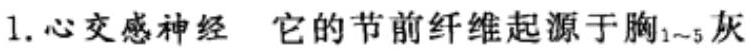
\includegraphics[max width=\textwidth, center]{2024_07_10_373f31b88d2bf633007bg-077}\\
质侧角神经元, 随后主要在星状神经节与节后神经元形成突触联系, 递质为乙酰胆碱, 故心交感节前纤维为胆碱能纤维。乙酰胆碱与节后神经元细胞膜的胆碱能神经受体结合。心交感节后神经元的神经纤维支配窦房结、房室结、房室束和心房、心室肌, 递质为去甲肾上腺素, 故心交感节后纤维为将上腺素能纤维。去甲肾上腺素与心肌细胞膜上的肾上腺素能 $\beta$ 受体结合, 可兴奋心肌细胞, 它能提高窐房结和潜在起搏点的自律性, 使心率增快; 也可产生异位节律, 增加心房、房室间和心室内兴奋的传导速度; 缩短有效不应期, 并提高心肌兴奋性和收缩性。肾上腺素与心肌 $\beta$ 受体相结合, 能兴奋心肌, 促进心肌代谢, 增强心肌收缩性, 使心率加速。用 $\beta$ 受体阻滞药(如普䒬洛尔), 使心脏自律性降低, 传导减慢, 心肌收缩性惐弱, 心肌耗氧减少。

\begin{enumerate}
  \setcounter{enumi}{1}
  \item 心迷走神经 其节前神经起源于延髓, 进人心琏后,神经末梢与心内神经节细胞形成突触联系,递质为乙酰胆碱。心迷走神经的节后纤维支配窦房结、房室结、房室束和心房肌, 递质也是乙酰胆碱,故心迷走神经节前、后纤维均属于胆碱能纤维。节后纤维释放的乙酰胆碱与心肌细胞膜上胆碱能毒莗碱样受体 ( $\mathrm{M}$ 受体)结合, 导致心肌细胞的抑制, 不应期缩短,兴奋传导速度减慢, 兴奋性、收缩性和自律性降低。注射阿托品可阻滞胆碱能 M 受体,引起心动过速。
\end{enumerate}

心脏有接受压力或牵张刺激的传人神经纤维,主要在心迷走神经内。而接受伤害性刺邀引起的痛觉的传人神经纤维主要在心交感神经干中。

\section*{(二)血管的神经支配}
除毛细血管外,所有血管的平滑肌受交感神经的支配,绝大部分交感神经能引起血管收缩, 故称交感缩血管神经。副交感神经和小部分交感神经能引起血管舒张,称为副交感舒血管神经和交感舒血管神经。

\begin{enumerate}
  \item 交感缩血管神经 其节前神经元在胸腰脊髓各节段的灰质外侧角,在各个交感神经节中与节后神经元形成突触联系,递质为乙酰胆碱。交感缩血管纤维末梢释放去甲肾上腺素。血管壁平滑肌上有 $\alpha$ 和 $\beta$ 肾上腺素能两种受体。去甲肾上腺素与 $\alpha$ 受体结合,导致血管收缩; 将上腺素与 $\beta$ 受体结合,引起血管舒张。肾上腺素也能与 $\alpha$ 受体结合,导致血管收缩,但作用不如去甲肾上腺素强。身体各个部位血管壁的肾上腺素能受体分布不一,且各血管交感缩血管纤维分布密度也不一, 故兴奋交感神经后血管效应也不同。总之,兴奋交感神经后, 体循环的血管阻力增加, 动脉压上升, 血管容积减小,也影响静脉张力,促使静脉血回流至心脏。

  \item 副交感舒血管神经 少数器官如生殖器的小血管除受交感缩血管神经支配外,还接受副交感神经支配, 能引起血管扩张。而所谓血管迷走性军昨, 是指情绪受剧烈刺激后,激发了迷走和交感扩血管纤维所致。

\end{enumerate}

此外,还有交感舒血管神经,在骨骼肌和小肠\\
的血管床用小剂量情上腺素可引起血管舒张。造成血管扩张的递质可能是 $\mathrm{H}^{+}$增多, 或组胺的释放。

\section*{三、心血管反射}
机体通过心血管反射和代谢性自动调节机制,以维持心血管系统的稳定,在心房、心室、心包膜和冠脉系统布满心血管反射的感受器, 通过有䯝鞘或无䜔晅传人神经纤维, 与脑干或脊髓背根神经节相连,接受并向上传导交感或副交感神经刺激,经中枢神经系统整合后分别做出反应。以下是常见的几种反射:

\section*{(一)颈动脉穼和主动脉弓压力感受器反射}
颈动脉窦和主动脉弓管壁上有特殊的压力感受器, 在动脉外膜下有极其丰富的传人神经末梢。动脉压上升时, 管壁扩张, 外膜下神经末梢受机械的牵张产生神经冲动。颈动脉窐的传人神经纤维随舌咽神经, 而主动脉弓的传人神经纤维随迷走神经分别进人脑干心血管中枢。中枢含有两个功能区: 外侧啄状的升血压 (缩血管) 中枢和中央尾状的降血压(舒血管)中枢。任何原因导致的动脉压升高会抑制交感中枢, 使心率减慢, 心肌收缩性和血管张力降低, 同时兴奋迷走中枢, 也使心率减慢, 并进一步降低心肌收缩性, 最终使动脉舒张, 血压下降。一般在血压升高到 $170 \mathrm{mmHg}$ 时, 压力感受器开始受到刺激, 对慢性高血压患者, 此触发点会上调。反之, 当动脉压降低时, 交感神经兴奋, 引起动脉收缩压上升, 又抑制迷走神经, 使心率加速, 动脉压也升高。压力感受器反射对血压急剧变化有反应, 特别对急性失血患者显得尤为重要, 但当血压降至 $50 \sim 60 \mathrm{mmHg}$ 时, 压力感受器已基本性失功能。

\section*{(二)颈动脉体和主动脉体化学感受器反射}
颈动脉体位于颈总动脉分叉处, 而主动脉体分散在主动脉弓、锁骨下动脉和颈总动脉分支处血管壁外。小体直径为 $1 \sim 2 \mathrm{~mm}$, 含有丰富的血管和传人神经末梢。当血液流速减慢, 血中 $\mathrm{PO}_{2}$ 下降 (低于 $50 \mathrm{mmHg},, \mathrm{PCO}_{2}$ 升高, 或 $\mathrm{H}^{+}$浓度增高时, 可使小体的传人神经兴奋。而主动脉体的传人神经纤维随迷走神经, 颈动脉体的传人神经随舌咽神经,最终兴奋延䚟的呼吸中枢, 增加通气; 增加迷走中枢兴奋性, 降低心率和心肌收缩性。如果持续缺氧, 将直接刺激中枢神经, 政善通气, 而不依赖副交感活性。

\section*{(三)静脉心脏反射(Bainbridge)}
感受器位于右心房壁和腔静脉血管壁内膜下,当静脉回心血量增加, 右心房和中心静脉压升高时, 静脉扩张有效地兴奋大静脉血管壁内膜下的传人心迷走神经受体, 反射地引起心率增快。当静脉回心血量减少时, 通过心迷走神经作用使心率减慢。

\section*{(四) Bezold-Jarisch 反射}
左心室壁存在有一定的压力感受器, 在左心室内容量降低时兴奋, 通过 Bezold-Jarisch 反射, 使心率减慢, 为心室赢得更多的充盈时间, 维持满意的心搏出量。

Bezold-Jarisch 反射和静脉心脏反射在椎管内阻滞时尤为明显, 椎管内阻滞后, 特别是病人循环血容量不足时, 静脉回心血量减少, 前负荷显著降低, 腔静脉、右心房和左心室压力感受器兴奋, 通过 Bainbridge 和 Bezold-Jarisch 反射, 可出现严重的心动过缓, 甚至心脏停搏。

\section*{(五)眼心反射}
压迫眼球或牵引眼周围结构将刺激眼外肌(尤其是中直肌)上的受体, 沿长、短健神经至睷神经节, 再沿三叉神经的分支一一动眼神经至半月神经节,使副交感张力增加, 心率减慢。在 $30 \% \sim 90 \%$的动眼神经手术中, 会出现眼心反射, 预防方法包括术前使用抗毒㩽碱样药物, 如阿托品等。

\section*{(六)中枢神经缺血反射 (Cushing)}
预内压增加引起中枢神经缺血, 最初的反应是中枢神经交感兴奋性增加, 心率加快, 心肌收缩性增加, 血压升高。随后压力感受器兴奋导致外周血管张力增加, 体内释放大量肾上腺素和去甲肾上腺素,结果使心排血量增加达 $100 \%$ 以上。

\section*{(七)肺血管、冠状动脉和肠系膜血管反射}
肺动脉压力升高可反射地使心率加速。左心室壁的左冠状动脉左旋支末端附近有化学感受器, 兴奋经无唃鞘的迷走传人 C 纤维传导, 增加副交感张力, 产生心动过缓、低血压和冠脉扩张。心肌缺血后再灌注、溶检治疗后会出现此类反射。手术时牵拉肠系膜引起迷走神经兴奋, 使心率减慢, 血压下降。

\section*{四、体夜调节}
可分为局部和全身性两种。

(一)局部体夜调节

组织细胞代谢率增加, 或血流灌注不足时, 都能引起小血管扩张; 反之, 血流量过多则引起小血\\
管收缩。缺氧、 $\mathrm{CO}_{2}$ 和 $\mathrm{H}^{+}$增多, $\mathrm{K}^{+}$浓度升高以及腺苷、腺苷酸、三啴酸循环中许多代谢中间产物等,都能引起血管扩张。

缺氧可能是引起局部血管扩张的主要原因, 并提出氧分压下降后产生某些血管扩张物质。体内各脏器血管对缺氧的反应不一, 严重缺氧后血管扩张的程度按顺序是: 心脏 $>$ 肠道 (门静脉) $>$ 将 $>$ 皮肤 $>$ 骨骼肌。缺氧或组织氧分压下降时, 小动脉和毛细血管扩张、改善细胞组织氧的供应。 $\mathrm{CO}_{2}$ 和 $\mathrm{H}^{+}$增加可引起局部血管扩张, $\mathrm{CO}_{2}$ 是强力扩血管物质。在脑组织中, $\mathrm{CO}_{2}$ 通过血脑屏障, 可能是调节脑血管的主要因素。过度通气后 $\mathrm{PCO}_{2}$ 下降, 能引起脑血管痉挛,脑血流减少。 $\mathrm{K}^{+}$浓度升高, 对大部分组织有明显的扩血管效应, 并能拮抗肾上腺素收缩血管的作用。

激肽是一类具有扩血管作用的直链低分子多肽, 最常见的是由 9 个氨基酸分子所组成的缓湤肤和由 10 个氨基酸分子构成的血管舒张素。激肽形成后主要作用于局部,血浆中有激肽酶能迅速破坏激肽, 使其失去活性。缓激肽作用于毛细血管内皮细胞,引起内皮细胞收缩, 使细胞之间的裂孔扩大,血管内血浆渗出增加。身体许多组织特别是皮肤、肺和肠脈膜组织的肥大细胞含有大量组胺。组织受到机械的、温度和化学性刺激以及创伤等, 促使各组织释放组胺增多, 致使局部毛细血管尤其是小静脉的通透性增加。组胺还使毛细血管内皮细胞收缩, 细胞之间裂孔扩大,致使血浆渗出增多,血压明显下降。如前所述, 腺苷是一种具有扩血管作用的递质,参与血管的自动调节, 与冠状血管和骨咯肌血管调节有关。当冠状血管痉挛或检塞时, 冠状静脉末端立即释放腺苷, 使冠状动脉扩张, 改善心肌血液供应。同样, 若肢体发生缺血, 肢体静脉末端也释放腺苷,促使肢体血管扩张,增加局部循环。因此腺苦是一种特殊的代谢性递质。

\section*{(二)全身性调节}
主要是通过内分泌系统释放激素, 经血液循环作用于全身心血管系统, 进行全身性调节。酫固酮是肾上腺皮质较素,对细胞外液和血容量的调节起着很大作用, 能促进怪小血管对钠和水的重吸收。醛固酮分泌过多,有㵔钠和水的作用, 细胞外液增多,使血容量增加,血压升高,心排血量增多。肾上腺素是肾上腺䯝质嗜铬细胞的主要激素, 由血液输送至全身,作用于心血管系统,使心排血量增加, 心率加速, 又使皮肤、内脏血管收缩,肌肉(包括心肌)血管舒张。肾上腺觟质活动受交感神经控制。

肾小球近球细胞由于交感神经兴奋或肾灌注不足, 释放出的一种多肽酶, 称为肾素。它激活 $\alpha_{2}$球蛋白血管紧张索原, 使之水解为血管紧张素 $\mathrm{I}$,随后在肺循环中经转换酶脱去 2 个氨基酸,形成血管紧张素 II。后者是体内强烈缩血管物质,引起动脉壁平滑肌强烈收缩, 以致产生高血压。血管紧张素 II 又刺激肾上腺皮质释放醛固酮, 增加细胞外液量和血浆量, 使静脉回心血量增多,心排血量增加,血压上升。血管紧张素 II 还能直接作用于肾, 引起濐钠和水的作用。

\section*{第五节 麻醉对心血管功能的影响}
麻醉对心血管调节的影响是多方面的、复杂的, 它取决于麻醉药的应用、通气方式、外科手术类别、失血量以及其他许多因素。

\section*{一、手术应激反应}
应激反应是机体受到诸如手术、气管插管等伤害性刺激而发生的,以交感神经兴奋和丘脑下部一垂体前叶一肾上腺皮质、觝质功能增强为主要特点的一种非特异性防御反应。表现为血压、心率升高, 血中儿茶酚胺浓度升高。近年来的研究发现,吸人麻醉药的心血管效应与自主神经系统调节之间有一定关系,七氮醚和异氧醚等吸人性全麻药均可作用于自主神经系统, 剂量依赖性降低自主神经紫张度,从而影响心排血量及周围血管阻力。

除术中应激反应, 麻醉药和 $\mathrm{PCO}_{2}$ 的变化通过中枢神经和自主神经系统, 干扰压力感受反射的功能,也会对心血管功能产生明显影响。

\section*{二、麻醉药物}
\section*{(一)吸入麻醉药}
\begin{enumerate}
  \item 血压和外周血管阻力 除氧化亚氮外,所有目前使用的吸人麻醉药都使平均动脉压下降,且呈剂量依赖性,造成的原因有: 外周血管扩张、心肌收缩性下降、心排血量下降、交感张力下降或为复合因素作用的结果。其中地氘烷、异氭烷和七甇烷降低外周血管阻力的作用要大于氟烷 (表 1-6-1)。而\\
表 1-6-1 吸入麻醉药的心血管作用
\end{enumerate}

\begin{center}
\begin{tabular}{lcccccc}
\hline
 & 心率 & 血压 & 外周血管阻力 & 心排血量 & 使心肌对肾上腺素的敏感性 & 冠脉扩张 \\
\hline
地氛烷 & + & - & - & $0 /-$ & $0 /+$ & + \\
気烷 & 0 & - & $0 /-$ & - & +++ & + \\
异氛烷 & + & - & - & - & $0 /+$ & ++ \\
七氪烷 & 0 & - & - & $0 /-$ & $0 /+$ & 0 \\
氧化亚氮 & + & 0 & 0 & 0 & 0 & 0 \\
\hline
\end{tabular}
\end{center}

注: 0 : 无变化; : 增加, 十个数体现增加程度; 一 : 降低, 一个数体现降低程度

单独使用氧化亚氮对外周血管阻力没有影响。

\begin{enumerate}
  \setcounter{enumi}{1}
  \item 心脏传导和心率挥发性吸人麻醉药可以抑制动脉压力感受器的敏感性, 使机体的心血管调节功能减弱, 因此在血压下降时要用升压药物才能提高血压, 而机体没有代偿能力。
\end{enumerate}

挥发性吸人麻醉药抑制䆧房结的自律性, 兴奋房室结和浦肯野纤维的自律性, 易引起心律失常。特别是氟烷可使心肌对肾上腺素的敏感性升高, 更易导致室性早搏,而其他吸人麻醉药则影响很小。

\begin{enumerate}
  \setcounter{enumi}{2}
  \item 冠脉血流 多数挥发性吸人麻醉药都可以扩张冠脉血管, 增加冠脉血流量,且呈剂量依赖性,但以异氟烷的作用最明显,因此冠脉“胁血”现象以异氮烷最明显。由于缺血的冠脉,其扩张已经达到极限, 在健康的冠脉扩张后, 缺血区的灌流会进一步惐少,这就是“轵血”。但从临床使用结果看,异氮烷的“窃血”作用仍有很大争议。地氘烷和七氟烷无“窃血”作用。

  \item 心肌收缩性和心排血量 挥发性麻醉药抑制心肌的收缩性, 主要是由于约物减少了心肌细胞内肌浆网的游离铃离子浓度或其释放, 以及降低收缩蛋白对钙离子的敏感性。其中以氟烷的作用最强。异氛烷和七氟烷对心肌收缩性的影响较小,因此更适于先天性心脏病和心脏功能不全病人的麻醉。

\end{enumerate}

氧化亚氮有兴奋交感神经的作用,对于健康人不会产生心肌收缩抑制,但对于心功能不全者则心肌抑制作用明显,尤其是在复合使用阿片药物而使交感兴奋作用消失时更是如此。

迅速增加地氛烷的吸人浓度会引起明显的高血压和心率加快。这种作用是自限性的, 因为随后地氟醚浓度快速增加(即呼气末浓度一次性从 0. $55 \mathrm{MAC}$ 快速上升至 $1.1 \mathrm{MAC}$ ), 减弱了心血管刺激的频率和程度。初步资料提示,这种交感神经兴奋可能由中枢引发, 而不像过去推测的那样通过气道或肺受体引发。这种短暂的心血管反应可被拮抗或减少交感神经活动度的药物, 如阿片类药 (芬太尼)、 $\beta$ 肾上腺素能阻滞药 (艾司洛尔) 或 $\alpha_{2}$ 肾上腺素能受体激动药 (可乐定) 所减弱。异氟烷的这种刺激较轻, 七氟烷则无刺激, 特别适合做吸人诱导,故广泛应用于儿童的麻醉诱导。

\begin{enumerate}
  \setcounter{enumi}{4}
  \item 肺血流 挥发性吸人麻醉药可以舒张支气管, 适用于哮喘病人, 对肺血管也有扩张作用, 降低肺血管阻力和肺动脉压, 同时还抑制了低氧造成的肺血管收缩作用。但氧化亚氮除外,它可以明显增加肺动脉压, 不适用于肺动脉压增高的病人。

  \item 心肌保护和预适应 (preconditioning) 大量的研究结果表明, 氟化类的挥发性吸人麻醉药对心肌的缺血再灌注损伤有保护作用,其保护机制类似于心肌缺血预适应,与线粒体 $\mathrm{K}_{\mathrm{ATP}}$ 通道激活有关。

\end{enumerate}

\section*{(ニ)静脉麻醉药}
\begin{enumerate}
  \item 巴比妥类 静脉注射后引起平均动脉压降低, 由于对颈动脉压力感受器仅有轻度抑制, 所以反射性地引起心率加快。降压作用呈剂量、注射速度依赖性反应, 产生机制与血管扩张、心肌收缩被抑制有关。

  \item 苯二氮草类 临床麻醉中常用地西泮和㽤达唑仑, 在常用镇静剂量下, 这两种药物对血压、心率、血管阻力、心排血量的影响很小。由于对颈动脉压力感受器没有抑制作用, 若血压下降就反射性地引起心率加快, 但即使这样对心排血量也没有明显影响。地西泮较梀达唑仑对血压的影响更小,与氧化亚氮复合常用于心脏功能不全病人。

  \item 阿片类 兴奋迷走神经使心率减慢, 常用剂量下对心血管功能影响很小。大剂量使用对心脏收缩力产生抑制作用,以阿芬太尼较明显。另外,吗啡还有较强的组胺释放作用, 这也是使血压下降的机制之一。

  \item 革胺酮 氯胺酮兴奋交感神经, 使血中儿茶酚胺浓度升高, 使血压上升、心率加快、心排血量增加、肺动脉压升高, 特别适用于在休克和低血容量\\
病人的麻醉中使用。但对于有交感神经过度兴奋而递质耗竭的病人, 氯胺酮使心血管功能抑制, 产生低血压。

  \item 丙泊酚 抑制交感神经作用大于副交感,造成心率减慢,抑制心肌细胞肌浆网内钽离子的再摄取,使心肌收缩抑制, 甚至无收缩、使血管扩张, 血压下降。因此在使用丙泊酚时要严格控制剂量和注药速度,禁用于休克、低血容量、心功能不全的病人。

  \item 依托味酯 对交感神经没有作用,不引起组胺释放, 不能抑制手术和气管插管引起的心血管应激反应, 用于麻醉诱导可以很好地维持心率、心肌收缩力、心排血量的正常。但对肾上腺皮质功能有抑制作用,一般一次诱导剂量可以使皮质功能抑制 $5 \sim 8 \mathrm{~h}$ 。

  \item 肌松药物 大多数非去极化肌松药对心血管功能无明显影响, 但有少数药物会通过诱发机体组胺释放和作用于胆碱受体而影响心功能 (表 1-62)。例如潘库溪铵具有抗 $M$ 受体效应, 使迷走抑制同时兴奋交感神经而使心率加快。大剂量使用阿曲库铵和咪哇库㫨可诱发组胺释放, 引起低血压和心动过速, 病人同时伴有面、颈部皮肤潮红。而顺式阿曲库铵则不引起组胺释放。维库溴铵和罗库溴铵则几乎没有任何心血管影响。去极化肌松药氯琥珀胆碱可激动胆碱 $M$ 受体,引起迷走神经兴奋, 造成心动过缓和室上性心律失常。

\end{enumerate}

表 1-6-2 常用肌松药对心血䈉功能的影响

\begin{center}
\begin{tabular}{|c|c|c|}
\hline
 & 组胺释放 & 迷走阻滞 \\
\hline
阿曲库铵 & + & 0 \\
\hline
顺式阿曲库铱 & 0 & 0 \\
\hline
梀埕库轵 & + & 0 \\
\hline
潘库滇较 & 0 & ++ \\
\hline
罗库溴轱 & 0 & $0 /+$ \\
\hline
维库滇侒 & 0 & 0 \\
\hline
筒箭赤 & $++t$ & 0 \\
\hline
氬琥珀胆碱 & 0 & - \\
\hline
\end{tabular}
\end{center}

注: 0 : 无变化; + : 增加, 十个数体现增加程度; 一 : 降低,一个数体现降低程度

(许 幸)

\section*{参考文献}
[1] 于布为,孙大金. 麻醉与循环 // 生心良主编. 现代麻醉学. 3 版. 北京: 人民卫生出版社,2003:72-109\\
[2] Handbook of Cardiac Anatomy, Physi-

ology, and Device edited by Paul\\
A. laizzo, PhD, Humana Press Inc. ,

Totowa, New Jersey, 2005

\section*{籍辡}
\section*{麻醉与呼吸系统}
要理解麻醉和手术中出现的呼吸功能紊乱及血气变化机制, 必须了解正常的呼吸生理。呼吸系统的主要功能是吸人新鲜氧气和呼出二氧化碳。同时, 它还有调节体内酸靕平衡, 分泌激索和排泄的作用。熟悉和掌握肺的生理是安全麻醉和危重病医学呼吸治疗的基础。

\section*{第一节 呼吸系统的解剖}
呼吸系统由鼻、咽、喉、气管、支气管(叶、段、亚段) 、细支气管、终末支气管、呼吸性支气管及肺泡等组成。呼吸系统的基本结构, 除包括气道、肺与肺泡组织外, 还应包括胸廊、各种呼吸肌及肺和胸廓的血供、淋巴、神经支配等。

\section*{一、气道}
以环状软骨下缘为界, 通常将气道分为上、下气道。上气道由鼻、咽、喉组成, 是气体进人肺内的门户。主要功能除传导气流外, 尚有加温、湿化、净化空气和吞咽、嗔觉及发音等功能。下气道主要由气管、支气管、支气管树及肺泡等组成, 根据功能不同, 又分为传导气管 (气管、支气管树) 和呼吸区。

\begin{enumerate}
  \item 气管 是个管状结构, 上端起于环状软骨,通过颈部向下延伸人胸内,在胸骨上、中 $1 / 3$ 处分叉为左、右支气管。气管分叉部即所谓隆突。成人气管平均长度为 $10 \sim 13 \mathrm{~cm}$, 直径为 $2.0 \sim 2.5 \mathrm{~cm}$ 。气管由 16 20 个 U 形软骨环组成, 开口部向背面,由富于弹性的纤维结缔组织连接。气管虽有 U 形软骨支拲, 但仍容易受外来压力影响, 通常受压 $50 \sim 70 \mathrm{cmH}_{2} \mathrm{O}$ 即可引起气管萎陷, 如颈部肿痽、血肿压迫常引起气管狭窄。在人体气管内外压差达 $10 \mathrm{cmH}_{2} \mathrm{O}$ 时, 可使气管容量有 $42 \% \sim 56 \%$ 的变化。

  \item 支气管 气管于第 $\mathrm{T}_{5,6}$ 之间, 相当于胸骨角水平分叉为左右支气管。在成人, 右支气管较左支气管短、粗而陡直, 平均长 $2.5 \sim 3 \mathrm{~cm}$, 与气管纵轴夹角为 $20^{\circ} \sim 30^{\circ}$ 。左支气管细, 长 $4 \sim 5 \mathrm{~cm}$, 与气管纵轴夹角为 $40^{\circ} \sim 50^{\circ}$ 。因此插管过深、插人双腔气管导管或吸人异物时易人右主支气管。 3 岁内的儿童左右支气管与气管纵轴夹角基本相等, 约为 $55^{\circ}$ 。

  \item 支气管树 左右支气管经肺门进人肺内后反复分支,分别为叶、段、亚段、细支气管、终末支气管、呼吸性支气管、肺泡管、肺泡等共约 23 级。终末支气管以上不参与气体交换, 为传导气道; 呼吸性支气管以下为呼吸区, 是气体交换的主要场所。从 12〜 19 级气道内径虽从 $1.0 \mathrm{~mm}$ 减小到 $0.5 \mathrm{~mm}$, 但其整个横断面积明显增加, 已是大支气管横断面积的 30 倍, 气流阻力也相应减小, 仅占气道全部阻力的 $10 \%$ 左右。因此应用较高压力克服气道阻力来进行通气, 而不至于造成肺泡的损伤 (表 1-7-1)。

  \item 支气管腺体 气管与支气管相似,均由稆膜、秥膜下层和外膜组成。䵑膜上皮,为假复层柱状纤毛上皮,其间散在着杯状细胞, 能分泌黍液。支气管分支越细,杯状细胞越少,至细支气管时䵑膜仅为一层纤毛上皮和极少的杯状细胞。黏液腺位于气管和支气管的㯝膜下层,以中等大小的支气筞中数目最多。腺体的大小及数目变化很大, 最大者可达 $1 \mathrm{~mm}$ 。慢性支气管炎时, 腺泡增多, 腺体增大。腺体分泌的絠液主要含有酸性和中性多糖, 此外还有白蛋白和球蛋白。黏液腺的分泌除源于直接刺激外, 还可由迷走神经反射诱发。乙酰胆碱可促使秥液腺分泌,但对杯状细胞无影响。阿托品能减少䵑液腺体的分泌。\\
表 1-7-1 各级气管的内径和横断面积

\end{enumerate}

\begin{center}
\begin{tabular}{clcc}
\hline
气道分级 & \multicolumn{1}{c}{名称} & 气道直径 $(\mathrm{cm})$ & 横断面积 $\left(\mathrm{cm}^{2}\right)$ \\
\hline
0 & 气管 & 1.80 & 2.54 \\
1 & 支支气管 & 1.22 & 2.33 \\
2 & 叶支气管 & 0.83 & 2.13 \\
3 & 段支气管 & 0.56 & 2.00 \\
4 & 1 级亚段支气管 & 0.45 & 2.48 \\
8 & 5 级亚段支气管 & 0.18 & 6.95 \\
16 & 终末支气管 & 0.06 & 180 \\
17 & 1级呼吸性支气管 & 0.05 & 300 \\
20 & 肺泡管 & 0.045 & 1600 \\
23 & 肺泡蛽 & 0.041 & 11800 \\
\hline
\end{tabular}
\end{center}

正常情况下, 气道分泌物有助于维持气道正常功能,减少气道水分丢失,维持纤毛上皮的正常运动,形成稆液毯,并通过特异性或非特异性免疫因子对吸人的病原体起抗感染作用。病理情况下, 黏液腺分泌过多,以致纤毛不能摆动, 䵗液不能排出; 过量馧液还可能阻塞细支气管, 使气道引流不畅而发生感染。

\begin{enumerate}
  \setcounter{enumi}{4}
  \item 支气管的纤毛上、下气道除极少部位, 均分布有纤毛。纤毛从秥膜的纤毛细胞上长出, 纤毛顶端有厚约 $5 \mu \mathrm{m}$ 的䅨液毯。纤毛在较稀的液体中摆动, 速度可变。黏液毯向上方移动的速度为 $2.5 \sim$ 3. $5 \mathrm{~mm} / \mathrm{min}$, 能有效地将颗粒和病原体等排出气道。
\end{enumerate}

影响纤毛上皮运动和稒液毯活动的因素很多,干燥可破坏黏液毯; 吸烟和药物可影响纤毛运动;流感病毒能引起纤毛细胞变性; 慢性支气管炎和支气管扩张时, 可引起纤毛数目减少。吸人麻醉约如氟烧能通过抑制纤毛运动频率, 改变黏液的质和量降低黏液纤毛清除率。吸人氟烷 $6 \mathrm{~h}$ 后, 黏液纤毛清除率降低,并至少延续到停药后 $3 \mathrm{~h}$ 。

\section*{二、肺 与肺泡}
\begin{enumerate}
  \item 肺肺是有弹性的海绵状器官,形状似圆雉形,位于纵隔两侧。上端称肺尖,下断称肺底,内侧称纵隔面, 外侧称肋面。右肺三叶, 左肺二叶, 外被胸膜、叶间裂相隔, 每叶肺又依支气管和血管的分支,再分为肺段。肺段在解剖构造和功能上,均可认为是一独立单位。

  \item 肺泡 肺泡是气体交换的场所, 为多面型薄壁䪄泡, 总的表面积可达 $70 \mathrm{~m}^{2}$ 。肺泡的平均直径约为 $0.25 \mathrm{~mm}$, 实际大小因呼吸深度而异。肺泡的数目随年龄的增加而增长,在出生时约为 0.24 亿,到8 9 岁时即可达到成人水平 (3 亿个)。

\end{enumerate}

\section*{三、胸廓}
胸痀是由 12 块胸椎骨, 12 对肋骨, 1 块胸骨和肋间肌构成的骨性结构, 肺、气管、支气管、纵隔等重要器官均位于胸廍之内。胸廊具有足够的坚硬度以保护其内在的重要器官, 同时也具有一定的灵活性, 可以在呼吸动作时起类似风箱的作用。在吸气时,胸䗪与肺可在前后径、横径、长径三个方向增大体积, 有助于吸气动作的产生。

\section*{第二节 肺 的 通 气}
肺通气是肺与外界环境之间的气体交换过程。实现肺通气的器官包括气道、肺泡和胸㾊等。气道是沟通肺泡与外界的通道; 肺泡是气体与血液进行交换的主要场所; 而胸廊的节律性呼吸运动则是实现肺通气的动力。

\section*{一、呼吸动力}
呼吸肌收缩、舒张所造成的胸廊扩大和缩小,称为呼吸运动。呼吸运动时, 由于胸㩔体积的改变,引起胸腔内和肺内压力的变化,形成大气与肺泡气之间的压力差, 不仅克服胸廊和肺的弹性阻力以及气道与组织的非弹性阻力, 还引起气体在肺与体外间的流动。

\begin{enumerate}
  \item 呼吸肌引起呼吸运动的肌肉为呼吸肌。使胸癡扩大产生吸气动作的肌肉为吸气肌, 主要有漏肌和肋间外肌; 使胸廍缩小产生呼气动作的肌肉\\
为呼气肌, 主要有腹壁肌肉和肋间内肌。

  \item 吸气运动 是主动过程。吸气时, 腀肌收缩, 隆起的圆顶变平下移, 从而增大了胸脘的上下径; 助间外肌收缩, 使助骨和胸骨上提, 助骨下缘向外翻转, 从而增大了胸腔的前后径和左右径, 胸腔体积增大, 产生胸腔负压。膈肌收缩引起的呼吸运动称为腹式呼吸; 相应地, 助间外肌收缩引起的呼吸运动称为胸式呼吸。在平静呼吸时, $75 \%$ 的肺通气量是依靠膈肌的收缩来完成; 但肋间外肌运动产生胸廊扩张能力较䐔肌大, 所以在用力呼吸时, 其呼吸型多改为胸式呼吸为主。

  \item 呼气运动 平静呼吸时, 呼气是被动的, 崙肌和肋间外肌舒张, 肺依靠本身的弹性回缩力量而复位。用力呼吸时, 呼气肌才参与收缩, 使胸廍进一步缩小, 呼气也有了主动的成分。最主要的呼气肌是腹壁肌组织。

  \item 肺内压和胸膜腔内压肺内压是指肺泡内的压力。当呼吸动作产生时, 随胸腔体积变化, 可产生一系列压力改变。吸气之初, 胸腔容量增加,肺内压下降, 低于大气压, 空气在此压力驱动下进人肺泡, 随着肺内气体逐渐增加, 肺内压也逐步升高, 至吸气末, 肺内压已和大气压相等, 气流也停止。反之, 在呼气之初, 胸腔容量减小, 肺内压升高并超过大气压, 肺内气体排出肺外, 使肺内气体逐渐减少, 肺内压下降又重新开始吸气, 至吸气末, 肺内压又和大气压相等。

\end{enumerate}

呼吸过程中肺内压变化的程度, 视呼吸的缓急、深浅和气道是否通畅而定。平静呼吸时, 吸气时肺内压较大气压低 $1 \sim 2 \mathrm{mmHg}$; 呼气时较大气压高 $1 \sim 2 \mathrm{mmHg}$ 。用力呼吸时, 肺内压变化程度增大; 当气道不通畅时, 肺内压的升降将更大。

胸膜腔内压即胸膜腔内的压力, 是由肺的弹性回缩力所致。胸膜腔内压是使肺泡扩张的肺内压和使肺泡缩小的弹性回缩力两种力之和, 即: 胸膜腔内压=肺内压一肺弹性回缩力。正常情况下, 肺总是表现出回缩的倾向, 胸膜腔内压因而经常为负。

自主呼吸时, 吸气是由胸腔负压引起, 为负压呼吸。人工呼吸时是气体被压人肺内, 吸气时肺内压比大气压高, 胸内压也因此从负值变为正值, 呼气末肺内压逐浙回降至零, 视为间歌正压呼吸。机械通气时, 肺内压和胸腔内压力的增高, 是间歌正压呼吸对机体正常生理功能产生影响的基本原因。

\section*{二、胸和肺顺应性}
肺、胸壁组织类似弹性体, 在生理弹性限度内,气道内压越大, 肺容量增加也越大。外力和容量之间的关系代表肺与胸躬组织的弹性, 即单位压力变化 $(\Delta \mathrm{P})$ 引起肺内气体容量的改变 $(\Delta \mathrm{V})$ 称为肺-胸顺应性 $\left(\mathrm{C}_{\tau}\right)$, 即:

肺-胸顺应性 $\left(\mathrm{C}_{\mathrm{T}}\right)=\frac{\text { 肺容量改变 }(\Delta \mathrm{V})}{\text { 经胸廊压改变 }(\Delta \mathrm{P})} \mathrm{L} / \mathrm{cmH}_{2} \mathrm{O}$

由于肺顺应性 $\left(\mathrm{C}_{\mathrm{L}}\right)$ 和胸壁顺应性 $\left(\mathrm{C}_{\mathrm{Th}}\right)$ 很难单独测定, 所以临床上通常用肺-胸顺应性表示:

\[
\frac{1}{\mathrm{C}_{\mathrm{T}}}=\frac{1}{\mathrm{C}_{\mathrm{L}}}+\frac{1}{\mathrm{C}_{\mathrm{Th}}}
\]

\begin{enumerate}
  \item 肺一胸顺应性分类顺应性又可分为静态顺应性和动态顺应性两种。静态顺应性是指在呼吸周期中, 气流暂时阻断测得的顺应性。动态顺应性指在呼吸周期中, 气流未阻断时测得的顾应性。前者不受时间限制, 主要影响因素是肺组织的弹性;后者受时间的限制, 主要影响因素是气道阻力。

  \item 顺应性的意义 在于管理呼吸时, 以适当的气流压力来维持满意的通气量。肺-胸顺应性的变化通常与通气量成正比, 与气道压力成反比, 所以肺-胸顺应性降低时, 可能是因压力增加而通气量不变, 或通气量惐少而压力不变。麻醉中应根据呼吸环路中压力及容量改变, 来粗略估计肺-胸顺应性变化。

  \item 影响肺-胸顺应性的因素 (1)残气量或功能残气量增加时, 肺-胸顺应性降低, 如肺气肿或哮喘病人。(2)吸气的流速缓慢, 则动态肺-胸顺应性增加。(3)肺弹性及扩张程度的变化, 如肺组织实变或胸壁畸形肺扩张受限, 使肺-胸顺应性降低。(4)持续低潮气量呼吸时, 肺顺应性逐渐下降, 间断深呼吸可使顺应性拻复。(5)体位对肺-胸顺应性的改变类似肺通气量改变, 俯卧位使顺应性降低 $35 \%$; 反之,截石位可使顺应性增加 $8 \%$ 。(6)全麻较清醒时,肺顺应性值低。(7)外科手术过程对肺-胸顺应性较为复杂, 开腹手术及开胸手术可使顺应性较术前分别降低 $18 \%$ 和 $10 \%$ 。

\end{enumerate}

\section*{三、肺泡表面张力和肺泡表面活性物质}
肺弹性阻力来自肺组织本身的弹性回缩力和肺泡内侧的液体层同肺泡内气体之间的液一气界面的表面张力所产生的回缩力。在低肺容量时,决定肺弹力最主要的因素是肺泡表面张力。肺泡表面\\
张力主要受肺泡表面活性物质影响。肺泡表面活性物质是由肺泡 II 型上皮细胞合成并释放的复杂的脂蛋白混合物, 其主要成分是二棕润酰卵磷脂,存在于覆盖肺泡内面极薄的液体膜中, 具有降低表面张力的作用。

正常人肺内肺泡大小不等, 如以肺泡内压力为 $P$, 肺泡表面张力为 $T$, 肺泡半径为 $\mathrm{r}$, 按 Laplace 定律, $\mathrm{P}=2 \mathrm{~T} / \mathrm{r}$, 即肺泡内压力与半径成反比, 与表面张力成正比。若表面张力相同, 肺泡大小不等时,则小肺泡内压要比大肺泡内压高。由于肺泡间有交通, 所以气体从小肺泡流人大肺泡, 小肺泡塌陷,大肺泡渗胀, 肺泡将失去稳定性。但实际上由于肺表面活性物质的作用, 当表面积缩小时, 表面张力也按比例下降, 肺泡越小, 表面活性物质作用越强,这就平衡了大小肺泡腔内的压力, 从而保持了肺泡相互间稳定,防止了肺泡萎陷。肺泡表面活性物质与肺容量增减呈平行变化, 也使肺泡在吸气过程中不至于过度膨胀, 呼气时不会过于萎陷。此外, 表面活性物质使肺泡液气界面的表面张力下降, 减弱了表面张力对肺毛细血管中液体的吸引作用,防止了液体渗人肺泡, 使肺泡得以保持干燥。

表面活性物质的代谢非常活跃。正常成人 18 24h 即进行一次更新。表面活性物质的代谢主要为肺泡巨憗细胞吞潄而排出。正常状态下, 合成与分解处于平衡状态。肺表面活性物质的生成或异常与下面因素有关。(1) 先天性缺少: 如胚胎 30 周以前肺缺血, II 型肺泡上皮细胞因供血不足, 生成表面活性物质的功能降低。所以出生后的早产儿, 因表面活性物质缺乏, 导致肺萎陷和肺泡内表面透明膜形成,造成呼吸宭迫综合征。(2)任何原因导致肺血流量减少,均可使 II 型肺泡上皮细胞生成表面活性物质的功能受损, 而致肺塌陷不张。吸人高浓度氧所致氧中毒, 可使 II 型肺泡上皮细胞的线粒体发生肿胀和多型性变, 损害表面活性物质的生成。还有一些有害物质如消毒剂注人肺内及 X 线照射也可损害 II 型肺泡上皮细胞正常功能。(3)吸人麻醉药如氛烷能可逆性抑制肺泡 II 型上皮细胞合成肺泡表面活性物质, 且这种影响随着氘烷浓度的增大和暴露时间的延长而增强。(4)长期吸烟和慢性阻塞性肺疾病的病人, 肺泡表面活性物质的合成与活性降低。此外, 机体内还存在着表面活性物质的对抗剂如胆固醇、油酸、磷脂酶及血液等。血秽蛋白中的许多成分亦可抑制表面活性物质的活性, 如纤维蛋白、白蛋白等。继发于任何原因的肺泡渗出液均含有丰富的血浆蛋白成分, 因降低表面活性物质活性而诱发肺萎陷和肺不张。(5) 急性胰腺炎病人的血内磷脂酶增加, 能加速肺表面活性物质灭活和破坏, 导致肺不张和严重肺功能不全。(6)近年还发现正压通气能增加肺部病变处的肺泡表面活性物质的活性。

\section*{四、气道阻カ}
肺通气的阻力有两种: 弹性阻力(肺和胸廊的弹性阻力), 是平静呼吸时的主要阻力, 约占总阻力的 $70 \%$; 非弹性阻力, 包括气道阻力、惯性阻力和组织的稻滞阻力, 约占总阻力的 $30 \%$, 其中又以气道阻力为主。

\begin{enumerate}
  \item 气道阻力 指气体流经气道时, 由气体分子之间及气流与气道管壁之间的摩擦力所形成, 它占呼吸时非弹性阻力的 $90 \%$ 。可用单位流速 (V) 所需要的驱动压 $(\Delta \mathrm{P})$ 来表示: $\mathrm{R}=\Delta \mathrm{P}(\mathrm{kPa}) / \mathrm{V}(\mathrm{L} / \mathrm{s})$ 。
\end{enumerate}

气道阻力受气流流速、气流形式和管径大小的影响。气流形式分层流和湍流两种,两种形式可单独存在, 也可同时存在形成混合型气流。层流气道阻力小, 湍流气道阻力大。层流见于气体以较慢的速度流经规则的管道时, 当气流太快和管道不规则容易发生湍流, 如气管内有黏液、渗出物或肿癁时。

正常成人全部气道的平均阻力为 $1 \sim 3 \mathrm{cmH}_{2} \mathrm{O} /$ ( $\mathrm{L} \cdot \mathrm{s})$, 女性的气道阻力比男性高 $20 \%$, 可能与女性气道较狭窄有关。

\begin{enumerate}
  \setcounter{enumi}{1}
  \item 气道阻力的分布 虽然支气管分支级数越多管腔越细, 但是其数量大增, 所以其总横断面积也随之显著增大。根据气流速度与横断总面积成反比, 横断总面积愈大, 气流速度愈慢, 而阻力就恋小。因此气道的阻力主要来自大气道, 即大部分来自上呼吸道, 包括畳、口腔、咽喉和气管。用鼻呼吸时, 鼻控阻力占全部气道阻力的 $50 \%$, 用口平静呼吸时, 咽喉和气管阻力占全部阻力的 $20 \% \sim 30 \%$ 。如剧烈活动而每分通气量增加时, 阻力可增加 $50 \%$ 。

  \item 气道阻力的临床意义气道梗阻如异物、舌后垚、鼻(口)咽部肿物、喉水肿、气管受压狭窄或扭曲及支气管痉挛等均使气道阻力增高。由于气道阻力增高导致病人通气量减少, 病人将用力呼吸以克服气道阻力。由此可产生: (1) 胸腔内压变化, 吸气时胸腔负压增大, 可出现锁骨上窝凹陷, 同时静脉回心血量增加; 呼气时胸腔内压明显增高, 静脉回心血量琙少,可出现颈静脉怒张。(2)肺泡充盈时\\
间延长。(3)呼吸肌做功及耗氧量增加。如呼吸阻力增加, 机体用力克服气道阻力所消耗的总氧量可高达 $300 \mathrm{ml} / \mathrm{min}$ 以上, 如不及时解除, 常因呼吸肌疲劳而导致呼吸衰竭。

\end{enumerate}

另外, 还应注意麻醉器械引起的气道阻力增加。吸人麻醉装置故障, 也使气道阻力增加。还有导管过细、过长或扭曲, 气道阻力增加更为显著。因为气流在直导管流动时, 其阻力与导管长度及气流速度成正比, 而与导管半径的 4 次方成反比。正常时气道阻力约为 $3 \mathrm{cmH}_{2} \mathrm{O} /(\mathrm{L} \cdot \mathrm{s})$, 全麻后可达 $3 \sim 6 \mathrm{cmH}_{2} \mathrm{O} /(\mathrm{L} \cdot \mathrm{s})$, 如加上机械阻力, 总阻力可达 $10 \mathrm{cmH}_{2} \mathrm{O} /(\mathrm{L} \cdot \mathrm{s})$ 以上。

\section*{五、呼吸功}
在呼吸过程中, 呼吸肌为克服弹性阻力和非弹

\section*{第三节 肺循环生理}
肺具有双重供血系统。肺循环主要从右心向左心输送血液, 并提供充分的空气与血的接触面,以便进行气体交换,还有一定程度的贮血作用。支气管循环主要供应呼吸性小支气管以上的气道组织的营养物质。肺循环和支气管血管的末梢之间有吻合支沟通。因此,有一部分支气管静脉血液可经过这些吻合支进人肺静脉和左心房,使主动脉血液中掺人 $1 \% \sim 2 \%$ 的静脉血。

\section*{一、肺循环和体循环的差异}
肺循环系统是低压系统, 正常时右心与左心输出量基本相等,但肺动脉平均压只有主动脉的 $1 / 6$ $1 / 5$, 约 $14 \mathrm{mmHg}$ ( $1.87 \mathrm{kPa}$ ), 肺静脉压力仅 $6 \mathrm{mmHg}(0.8 \mathrm{kPa})$ 。肺血管壁也较薄, 肺动脉壁只有主动脉壁 $1 / 3$ 厚, 更具有伸缩性。肺的微动脉也无肌组织,肺毛细血管平均压或静水压仅为体循环毛细血管的 $1 / 4$,约 $8 \mathrm{mmHg}(1.07 \mathrm{kPa})$,而血浆胶体渗透压为 $25 \mathrm{mmHg}(3.3 \mathrm{kPa})$, 所以是防止肺水肿的重要因素。肺循环缺少瓣膜,易受各种压力的影响而变化。

成人肺循环容纳总的血容量正常时为 400 ~ $600 \mathrm{ml}$,占总血容量的 $8 \% \sim 10 \%$,肺毛细血管切面的总面积为 $40 \mathrm{~m}^{2}$ 。静息时, 仅 $1 / 10 \sim 1 / 15$ 的肺毛细血管开放, 肺脏的血流大都处于动静脉中, 在肺毛细血管直接参与氧合作用的血流仅 $60 \mathrm{ml}$ 。运动时, 肺血流量增加, 毛细血管开放增加, 甚至全部开性阻力而实现肺通气所做的功为呼吸功。根据克服阻力的不同, 可分为弹性功、气流阻力功和惯性功。呼吸功增加, 见于胸壁顺应性下降、肺顺应性下降、气道阻力增加。呼吸功可用下式表达:

呼吸功 $=$ 胸腔压力差 $\times$ 肺容量的改变

呼吸功可通过压力-容量曲线测定。

正常情况下,平静呼吸时, 呼吸功约为 $0.5 \mathrm{~kg} /$ $(\mathrm{m} \cdot \mathrm{min})$, 呼吸耗能仅占全身总耗能的 $3 \%$ 。平静呼吸时, 正常人体总的耗氧量为 $200 \sim 300 \mathrm{ml} / \mathrm{min}$,而呼吸器官耗氧量为 $0.3 \sim 1.8 \mathrm{ml} / \mathrm{min}$, 占总耗氧量的 $5 \%$ 以下。每分钟通气量逐渐增加时, 呼吸器官耗氧量所占百分数可达 $30 \%$ 。涍碝患者平静呼吸时, 呼吸器官氧耗量为正常的 $4 \sim 10$ 倍。通气量增加时, 呼吸器官氧耗量即急剧增加, 这是哮喘患者运动耐受性减少的主要原因。放, 从而使肺动脉压不至于增高。

\section*{二、调节肺血流和阻力的因素}
肺血管虽然分布有完善的神经, 也可接受下丘脑刺激而收缩, 对血氧和二氧化碳分压的变化也起反应, 但由于肺微动脉无肌组织, 所以肺血管内径的变化多被动地受透壁压的影响。由此, 肺血管阻力的变化被动地受血管内径的改变远较舒缩明显。又因肺动脉极易伸张, 一般心排血量增加时, 并不增加肺动脉压, 除非心排血量比休息时增加 4 倍以上, 肺动脉不能再扩张时, 才能升高肺动脉压。

影响肺血流及压力的因素大致有下列几项:(1)血压可直接影响整个血液系统压力。(2)血容量的变化与单位时间内流经肺的血容量成正比。(3)呼吸影响肺血容量, 如吸气时增加回心血量及右室排血量,肺血容量可达总血容量的 $10 \%$; 而呼气时可降为总血容量的 $6 \% \sim 7 \%$ 。(4)缺氧: 吸人低氧浓度 ( $10 \% \sim 16 \%)$ 空气时可使肺动脉压升高, 而不改变右室排血量, 可能是由于肺泡缺氧引起血管收缩。 (5)二氧化碳升高: 二氧化碳对人体肺血管阻力影响不明显, 但近来研究认为在体外循环后, 动脉血二氧化碳分压即使在生理范围内升高, 也显著地增加肺血管阻力。(6)慢性肺疾病因缺氧肺血管收缩, 日久造成肺动脉高压, 并刺激生血器官产生红细胞增多及高血容量。⑦体位也影响肺血容量, 人由直立位到仰卧位时,肺血容量可增加 $27 \%$ 。

\section*{第四节 肺容量及肺功能检查}
\section*{一、肺 容 量}
肺容量(lung volume)是指不同程度用力呼吸产生的容量变化。肺容量包括以下几种通气容量。

\begin{enumerate}
  \item 湖气量 (tidal volume, $\mathrm{V}_{\mathrm{T}}$ ) 指平静呼吸时,每次所吸人或呼出的气量, 吸人和呼出气量之间稍有差异,一般以呼出气量为准。男性为 350 ~ $550 \mathrm{ml}$, 女性为 $260 \sim 540 \mathrm{ml}$, 最大潮气量即是肺活量。小儿潮气量可按 $6 \sim 8 \mathrm{ml} / \mathrm{kg}$ 计算。也是机械通气时, 应维持的每次通气量。

  \item 深吸气量 (inspiratory capacity, IC)和补吸气量 (inspiratory reserve volume, IRV) IC 是指平静呼气末再用力吸气, 吸至不能吸为止,所能吸人的最大气体容量。IRV 指平静吸气末再用力吸人的最大气量。男性为 $2100 \mathrm{ml}$, 女性为 $1500 \mathrm{ml}$, 它反映肺的储备能力。 IRV 是 $\mathrm{IC}$ 中的一部分, IC $=\mathrm{IRV}+\mathrm{TV}$ 。IC 和 IRV 都是肺活量的主要组成部分, 反映肺和胸廓在静态状态下的最大膨胀度。

  \item 补呼气量 (expiratory reserve volume,ERV)指平静呼气末再用力呼气至不能呼出为止所能呼出的气体容量。男性为 $1100 \sim 1900 \mathrm{ml}$, 女性为 $800 \sim 1300 \mathrm{ml}$ 。

  \item 残气量 (residual volume, RV) 和功能残气量 (functional residual capacity, FRC) RV 指一次用力呼气后, 肺内所残存的气量。男性为 $400 \sim$ $1900 \mathrm{ml}$, 女性为 $500 \sim 1200 \mathrm{ml}$ 。老年人及肺气肿病人的肺泡弹性减弱, 残气量明显增加, 从而使肺活量显著减少。FRC 指平静呼气后存留在肺内的气量, 即 $\mathrm{FRC}=\mathrm{ERV}+\mathrm{RV}$ 。

\end{enumerate}

FRC 是反映气体交换功能的重要标志之一, 对 FRC 的影响因素如表 1-7-2 所示。在呼吸过程中 $\mathrm{RV}$ 和 FRC 的重要生理作用是对吸人到肺泡内的气体有缓冲作用,可使肺泡 $\mathrm{O}_{2}$ 和 $\mathrm{CO}_{2}$ 分压保持相对稳定, 对肺泡内气体的弥散过程有一定的稳定作用。 RV 和 FRC 能反映肺泡膨胀程度, 是目前判断阻塞性肺疾患的最可靠指标。RV 的高低通常不以绝对值表示, 而以占肺总量的百分比 (RV/TLC\%)表示。正常人 RV/TLC $<35 \%$, 当 RV/TLC $>$ $35 \%$ 时, 提示有不同程度的肺气肿。在急性呼吸若迫综合征 (ARDS), 肺内存在广泛性、小灶性肺不张时, FRC 减少明显。有学者应用 FRC作为判断表 1-7-2 影响功能残气䆬(FRC)的因素

\begin{center}
\begin{tabular}{|c|c|}
\hline
降低 FRC 的因素 & 增加 FRC 的因素 \\
\hline
卧位 & 胸内压增加:PEEP,CPAP \\
\hline
麻醉 & 肺气肿 \\
\hline
腹部和胸部手术后 & 㫴簬 \\
\hline
肺纤维化 & 高龄 \\
\hline
\multicolumn{2}{|l|}{肺水肿} \\
\hline
\multicolumn{2}{|l|}{肥胖} \\
\hline
\multicolumn{2}{|l|}{腹胀: 妊娠, 肿㾑, 腹水} \\
\hline
\multicolumn{2}{|l|}{胸廊㱩形} \\
\hline
肌肉松驰 &  \\
\hline
\end{tabular}
\end{center}

ARDS 病变严重程度及疗效、预后的主要指标。

\begin{enumerate}
  \setcounter{enumi}{4}
  \item 肺活量 (vital capacity, VC) 于最大吸气后, 做最大努力呼气所能呼出的气量, 及深吸气量加补呼气量。男性为 $3400 \sim 4800 \mathrm{ml}$, 女性为 $2500 ~ 3200 \mathrm{ml}$ 。临床上常用以衡量病人的呼吸代偿功能。但是肺活量绝对与肺疾患对呼吸功能损害程度不完全一致, 由此单纯以肺活量值衡量肺功能意义不大。

  \item 版总量 (total lung capacity, TLC) 于深吸气后肺内所含的气量, 即肺活量加残气量。男性为 $4600 \sim 6400 \mathrm{ml}$, 女性为 $3000 \sim 4200 \mathrm{ml}$ 。在肺总量不变的情况下,FRC 的增加必然引起深吸气量的减少, 从而限制了在必要时增加通气功能的能力。

\end{enumerate}

\section*{二、肺通气功能参数及其意义}
\begin{enumerate}
  \item 每分通气量 (minute ventilation, $\mathrm{V}$ ) $\quad \mathrm{V}=$潮气量 $\left(V_{T}\right) \times$ 呼吸频率 $(f)$ 。成人静息每分通气量为 $6 \sim 8 \mathrm{~L}$,随人体活动量的增加, 每分通气量也随之增加。在病理情况下, 如患甲状腺功能立进时,由于人体的基础代谢率增加, 分钟静息通气量也可明显增高。因此,可将每分静息通与量作为基础代谢率的指标。此外,还有很多因素能使分钟静息通气量增加, 如严重缺氧和紧张、恐惧等精神、神经因素。

  \item 最大自主通气量(maximum voluntary ventilation, MVV) MVV 指人体在 $1 \mathrm{~min}$ 内所能呼吸的最大气体容量。根据病人情况, 酌情限定病人在 $10 \mathrm{~s} 、 12 \mathrm{~s}$ 或 $15 \mathrm{~s}$ 内, 进行最快和最大的深呼吸, 所测得的通气量分别乘以 6,5 或 4 ,即为每分最大自\\
主通气量。正常值:男性为 $70 \sim 120 \mathrm{~L}$, 女性为 $50 \sim$ $80 \mathrm{~L}$ 。一般以其实测值占预计值的百分比作为判断指标。正常值 $>75 \%$,其正常界限为 $60 \%$,低于 $59 \%$ 应视为异常。MVV 受呼吸时弹性及非弹性阻力的影响, 因此肺组织病变(肺纤维化、肺水肿), 气管、支气管阻塞或狭窄 (支气管侾喘),胸廨畸形或呼吸肌障碍 (脊柱后弯或侧弯、重症肌无力)等临床改变, 均能使 MVV 减少。MVV 主要反映人体通气的储备功能, 是通气功能测定中很有价值的一项指标。一般以 MVV 40L 或 MVV 占预计值的 $50 \% \sim 60 \%$ 作为手术安全指标, 低于 $50 \%$ 应列为低肺功能, 低于 $30 \%$ 者,一般应列为手术禁忌证。

  \item 用力肺活量 (forced vital capacity, FVC)也称时间肺活量 (time vital capacity) 是指受试者尽量吸足气, 然后尽快呼气且尽量呼完的气体容量。正常人 FVC 与缓慢或非用力动作所测得的肺活量相等; 但在气道有阻塞者, 用力呼气可致气道提早变窄或闭合, FVC 可较肺活量低。二者之差可反映受压气道远端陷闭的气体量。当 $\mathrm{FVC}<15 \mathrm{ml} / \mathrm{kg}$时, 术后肺部并发症的发生率常明显增加。

  \item 用力呼气量 (forced expiratory volume, $\mathrm{FEV}_{\mathrm{T}}$ ) 在 $\mathrm{FVC}$ 的测定过程中, 分别测定最初 $3 \mathrm{~s}$内的呼气量, 即为用力呼气量 $\left(\mathrm{FEV}_{\mathrm{T}}\right)$ 的值, 并分别求其各秒气体容量所占最大用力肺活量的百分比。其中 $\mathrm{T}$ 表示呼气时间。由于 $\mathrm{FEV}_{\mathrm{T}}$ 测定的是在不同时间呼出的气体容量, 所以它实质上测定的是流量。通过估计在特定时间的呼气流量可确认气道阻塞的严重程度。在阻塞性和限制性肺疾病, $\mathrm{FEV}_{\mathrm{T}}$ 都会减少。

\end{enumerate}

正常情况下, 健康成人能在 $0.5 \mathrm{~s}$ 内呼出 $50 \% \sim 60 \% \mathrm{FVC}, 1 \mathrm{~s}$ 内呼出 $75 \% \sim 85 \% \mathrm{FVC}, 2 \mathrm{~s}$ 内呼出 $94 \% \mathrm{FVC}, 3 \mathrm{~s}$ 内呼出 $97 \% \mathrm{FVC}$, 其中以第 $1 \mathrm{~s}$用力呼气量 $\left(\mathrm{FEV}_{1.0}\right.$ ) 或第 $1 \mathrm{~s}$ 最大呼气率 (也称 $1 \mathrm{~s}$率 $\mathrm{FEV}_{1.0}$ ) 最有实用意义。在大多数阻塞性肺疾忠病人中, $\mathrm{FEV}_{\mathrm{T}} / \mathrm{FVC}$ 明显降低, 而在限制性肺疾患病人中, 保持正常。

最大通气量和用力肺活量关系密切, 其影响因素也相同。由用力肺活量利用公式可以推算出最大自主通气量, 即最大自主通气量 $(\mathrm{L})=\mathrm{FEV}_{1.0} \times$ 35。本公式适用于测定最大自主通气量有困难的病人。

\begin{enumerate}
  \setcounter{enumi}{4}
  \item 用力呼气流量 (forced expiratory flow, $\mathrm{FEF}) \quad \mathrm{FEF}_{25 \% \sim 75 \%}$ 是在测量 $\mathrm{FVC}$ 过程中, 呼气在 $25 \% \sim 75 \% \mathrm{FVC}$ 水平的平均流量, 也称最大呼气中段流率 (maximum midexpiratory flow rate, MMFR)。体重 $70 \mathrm{~kg}$ 的健康成人正常值为 $4.7 \mathrm{~L} /$ $\mathrm{s}$ 。这段肺活量水平的呼气流率是与用力无关的,主要反映肺泡弹性回缩力和气道阻力的情况。阻塞性肺疾患病人通常 MMFR 降低, 而在限制性肺疾患病人中, 保持正常。在早期阻塞性肺疾患病人 MMFR 最先出现降低, 较其他指标敏感。MMFR 较 $\mathrm{FEV}_{\mathrm{T}} / \mathrm{FVC}$ 对受试者用力程度的依赖性更小,且可重复性高。

  \item 通气储量百分比 将 MVV 减去每分静息通气量即为通气储量, 以通气储量与 MVV 相比即为通气储量百分比, 其公式为通气储量百分比 $=$ (MVV-V)/MVV, 是衡量通气功能好坏的又一重要指标。百分率低, 提示在应激情况下, 所能发动的呼吸储备能力小, 即呼吸代偿能力越差。一般正常值为 $93 \%$ 。凡引起 MVV 减少的疾患, 通气储量百分比也降低, 百分比越低, 通气功能越差。当此值降至 $70 \% \sim 60 \%$ 时, 病人接近气促的阈值。肺切除术前如果在 $70 \%$ 以下, 术后应警惕发生呼吸功能不全。

  \item 流量-容量曲线 用力吸气至最大限度, 然后用力呼出至不能再呼出为止, 其做法与用力肺活量测定基本相同, 以 $\mathrm{x}-\mathrm{y}$ 记录仪描记流量和容量的变化, 即可得出流量-容量曲线。从此曲线可得知用力肺活量、最大吸气流量和最大呼气流量, 特别是流量与肺容量关系方面有重要的诊断意义。

\end{enumerate}

阻塞性肺疾患通常伴有流量的降低, 而限制性肺疾患常为肺容量的降低。而呼气曲线的变化在很大程度上与病人用力无关, 流量主要决定于肺弹性回缩力 (从 $75 \%$ 肺活量至残气量)。健康成人在大部分肺活量范围流量的降低与容量成正相关, 因而呼气相曲线呈线性。在阻塞性肺疾患病人中, 流量在低肺容量时明显降低, 曲线呼出相呈勺状。当有固定上气道或气管梗阻时, 伴有典型的呼气和吸气流量受限,吸、呼相曲线均变平坦,曲线呈卵圆型。限制性肺疾患病人通常峰值呼气流量相对正常, 并随肺容量减少线性降低, 但肺容量本身降低。

\section*{三、肺泡通气量和无效腔量}
依据人体所处的不同状态和实际参与肺泡气体交换通气量多察, 可将肺的通气量分成每分通气量、肺泡通气量和无效腔量。

一般情况下,大约每次呼吸有 $2 / 3$ 的通气量到达有血液灌注的肺泡参与气体交换, 这部分称为肺\\
泡通气量或有效通气量。其余 $1 / 3$ 通气量未参与气体交换,称为无效腔量或生理无效控量。生理无量, 也称解剖无效腔量; 肺泡通气良好而相应的血液灌注不良时, 气体交换不能充分进行的那部分气量,也称肺泡无效控量。

解剖无效腔量大约为 $2 \mathrm{ml} / \mathrm{kg}$, 健康人仰卧位时, 由于肺泡无效脘量极小, 可以不计, 此时生理无效腔量约等于解剖无效腔量。病理情况下, 解剖无效腔量一般变化不大, 生理无效腔量主要反映肺泡无效腔量。影响肺泡无效腔量的因索有:(1)肺泡血液灌注压不足。在各种类型循环衰竭引起低心排血量出现肺循环压下降时, 无血液循环灌注的肺泡明显增加, 这种效应在低血容量时更明显。在行控制性低血压时, 也可使肺泡无效腔量明显增加, 若病人的生理肺泡无效腔量超过潮气量的 $75 \%$ 时,就会发生严重的肺泡通气不足。(2)体位的影响。肺血流的分布受重力影响, 在侧卧位时, 约有 $2 / 3$ 的肺血流分布在下侧肺, 而自主呼吸的通气大部分也通向低侧肺, 因而肺泡无效腔量变化很小。然而在人工通气下, 则对上侧肺的通气较多, 而且血流分布较少,形成肺泡无效腔量增加。近来研究发现,当发生成人呼吸謇迫综合征时, 将病人由仰卧位变为俯卧位, 会使胸膜腔负压梯度减小, 肺内气体的分布变得更为均匀,从而使背侧肺组织的通气得到改善, 同时肺内血流又优先分布到背侧肺组织。因此背侧的肺组织通气/血流比率改善, 气体交换增效腔量又可分为两部分: 充填传导气道部分的气

加, 氧合程度也提高。(3)无血液灌注的肺泡通气。在肺㭲塞、肺毛细血管收缩, 或肺泡隔和其中血管广泛性破坏所致肺阻塞性疾患以及胸外科手术时,外力引起肺循环阻塞等, 使部分肺泡没有血液灌注, 肺泡内气体不能进行气体交换而增加肺泡无效腔量。(4)全麻时无论自主呼吸或人工通气,均能使肺泡无效腔量增加, 平均增加约 $70 \mathrm{ml}$ 。这主要是由于潮气量增大, 吸气时间缩短和肺血流减少所致。在气管内插管全麻下病人的 $\mathrm{V}_{\mathrm{D}} / \mathrm{V}_{\mathrm{T}}$ 为 $30 \%$ $35 \%$, 然而由于存在机械无效腔及其他增加解剖无效腔的因素,所以全麻中应适当增加潮气量,以提供足够的肺泡通气量。

无效殅量/潮气量 $\left(\mathrm{V}_{\mathrm{D}} / \mathrm{V}_{\mathrm{T}}\right)$ 的比值可作为反映通气效率的指标。在健康成人比值通常小于 0.30 ,即 $70 \%$ 的通气量是有效的。在严重阻塞性肺疾病时, $\mathrm{V}_{\mathrm{D}} / \mathrm{V}_{\mathrm{T}}$ 可增加到 $60 \% \sim 70 \%$ 。此时通气效率明显降低。如果 $V_{\mathrm{D}} / \mathrm{V}_{\mathrm{T}}$ 增加, 将使分钟通气量相应降低而引起 $\mathrm{PaCO}_{2}$ 迅速的升高。若在 $\mathrm{V}_{\mathrm{D}} / \mathrm{V}_{\mathrm{T}}$ 增高时要保持 $\mathrm{PaCO}_{2}$ 不变, 则必须增加分钟通气量。

如应用面罩等装置进行呼吸, 面罩内腔属无效腔, 也称为机械无效腔。例如病人潮气量为 $400 \mathrm{ml}$,其解剖无效控为 $150 \mathrm{ml}$, 当用内腔容量为 $250 \mathrm{ml}$ 的面罩呼吸时, 则肺泡通气量为 $400-250-150=0$ 。可见此人虽有呼吸动作, 其实并没有进行有效的气体交换,发生缺氧、窒息则是必然的后果。所以在临床上观察病人的通气量, 更应注意到有效肺泡通气量。

\section*{第五节 气体交换}
\section*{一、肺血流的分布}
肺循环是一个低压系统, 血流量在肺内的分布受重力、体位、肺泡压等多种因素的影响。在不同的体位下,肺泡压 $\left(\mathrm{P}_{\mathrm{A}}\right)$ 、肺动脉压 $(\mathrm{Pa})$ 和肺静脉压 $\left(\mathrm{P}_{\mathrm{v}}\right)$ 等在不同肺区有着不同的相关性, 并出现血流量的差异。West 等建立了一个将肺分为三个区的模型。I 区在肺的最上部分, 此区 $P_{A}>P a>P_{v}$ 。肺泡压传递至肺毛细血管,血管被压場陷,肺血流量少。在理论上此区为无血流灌注区,即使接受人工通气也缺乏血流灌注, 仍为肺泡无效腔量。正常情况下, 所涉及的范围较小, 但当肺动脉压降低如低血容量性休克时, 使 I 区范围扩大。

III区出现于肺的重力依赖性区域, 此时 $\mathrm{Pa}>$ $\mathrm{P}_{\mathrm{v}}>\mathrm{P}_{\mathrm{A}}$, 肺血流量受肺动静脉压力差所影响。由于重力作用, $\mathrm{P}_{\mathrm{v}}$ 增加, 肺毛细血管呈持续开放状态。因此,此区血灌注呈相对过剩, 即存在血灌注而无通气, 即为生理性分流区。

II 区出现在 I 区下限至 III 区的上限, 此时 $\mathrm{Pa}$ $>P_{A}>P_{v}$ 。肺血流量决定于肺动脉压与肺内压的差。肺静脉压对肺血流影响不大。此区包括大部分肺泡, 是通气和血流匹配区。

\section*{二、肺泡的气体分布和闭合气量}
\begin{enumerate}
  \item 肺泡的气体分布 正常人肺泡的气体分布受重力的影响, 下肺部较上肺部的通气分布多, 与胸腔压力梯度有关。正常胸腔压力为负压, 由于肺和绹廊内不同部位的液体静力学和结构性的改变,\\
胸腔内各部分的压力并不一致,肺尖部负压最大。健康成人直立时, 肺尖部周围的胸内压为 $-10 \mathrm{cmH}_{2} \mathrm{O}$, 向下按 $0.25 \mathrm{cmH}_{2} \mathrm{O} / \mathrm{cm}$ 递减, 肺基底部约为 $-2 \mathrm{cmH}_{2} \mathrm{O}$ 。胸内压垂直梯度对呼吸时气体分布和排空均有影响。健康人直立时, 在残气位, 随胸腔内压从上到下的逐浙递减, 肺泡的膨胀度也随之降低。如从残气位开始吸气, 气体首先分布到肺尖,然后再逐渐向下分布; 但由于肺尖周围负压较高, 在残气位时肺尖部有部分肺泡已处于膨胀状态,故进人肺尖部的气量较少。继续吸气时,胸内压继续降低, 肺下部气道开放, 大量气体进人肺基底部。呼气时, 气体的排出顺序与吸气时相反, 肺基底部胸内压力原较肺尖高, 呼气时压力增加, 使该部位肺容量最先缩小气体排出, 使基底部肺单位关闭。待肺下部肺单位关闭后, 才是肺尖部呼出气。故肺尖部的肺泡气具有先进后出的特点。

  \item 闭合气量 (closing volume, CV) 闭合气量可作为早期发现小气道阻塞病变一个教感的检测项目。正常人吸气时各部分肺泡均扩张, 呼气时肺容量减小, 当肺容量为肺总量的 $30 \%$ 左右时, 小气道有闭合的倾向。这是由于肺底部胸腔负压较小,在深呼吸后可变为正压,使小气道发生关闭。CV 是指肺底部小支气管开始关闭后所呼出的气量。闭合气量加上残气量称为闭合容积 (closing capacity, CC)。

\end{enumerate}

闭合气量不用绝对值表示, 是以闭合气量与肺活量之比即 $\mathrm{CV} / \mathrm{VC}(\%)$ 表示。健康人坐位的 CV/ $\mathrm{VC}(\%)$,年龄差别不大,一般 30 岁 CV/VC(\%) 为 $13 \%, 40$ 岁为 $16 \%, 50$ 岁为 $20 \%$ 。闭合气量明显增高时, 提示有小气道功能障碍。

早期气道闭合的结果, 轻度者使下部肺组织只是在吸气时间断地扩张, 气道闭合使气体滞留在肺泡内, 造成气体在肺内分布不均匀, 通气/血流比率失调, 影响肺泡与血液内的气体交换, 使动脉血氧分压下降。老年人 $\mathrm{PaO}_{2}$ 偏低即与此有关。特别当闭合容量超过功能残气量与潮气量之和时, 在整个呼吸周期部分气道均将处于闭合状态,使肺泡完全失去功能, 后果将非常严重。长期滞留在肺泡内的气体可被吸收,引起肺不张, 此时若血流继续, 将产生静动脉血混合的结果。

\section*{三、肺的换气及低氧血症原因}
肺为了完成气体交换任务, 需要完成两方面的工作。首先要将气体自外界吸人肺内, 并将经过交换的气体自肺泡呼出, 此过程称通气; 同时肺泡内气体还要与流经肺的血流进行气体交换, 吐故纳新, 此过程称为换气。通气功能是换气功能的基础, 两者互相联系, 互不可分。肺内气体交换是呼吸功能的根本所在。

肺内的气体交换, 是气体通过浓度差的弥散作用, 穿过呼吸膜人血或进人肺泡的过程。肺换气的正常有赖于肺泡各部分通气与血流比率的均衡, 也有赖于肺呼吸膜弥散功能的良好。

因此, 任何能引起肺通气、 $V / Q$ 比值、呼吸膜弥散障碍的因素, 均可以妨碍肺的气体交换功能,最终造成低氧血症和机体缺氮。

\begin{enumerate}
  \item 通气与血流比值 (V/Q) 即每分通气量与每分血流量的比值, 可表达肺内所有区域的通气与血流的相关性。正常条件下 $V / Q$ 在肺内的分布也不是均匀的。正常人在直立位由于受重力影响, 大部分肺血流分布于肺下部区域; 同时在自主呼吸时, 大部分潮气量也到达肺下部受重力影响的区域。这样在肺上部, 无论通气还是血流均较少; 而在肺下部, 通气和血流均接受较多, 但肺下部血流按比例仍偏多。因此 $\mathrm{V} / \mathrm{Q}$ 比值在肺上部偏高, 在肺下部偏低。这表明在肺上部相对地灌注不足, 下部相对地通气不足。理想的 $\mathrm{V} / \mathrm{Q}$ 的比值为 1 , 大约出现在第 3 肋骨水平。高于此水平, $V / Q$ 的比值大于 1 , 而低于此水平, $\mathrm{V} / \mathrm{Q}$ 的比值小于 1 。正常人在静息状态时, 总的 $V / Q$ 比值为 0.8 , 这是肺的不同区域, 高低不等的 $V / Q$ 比值的综合结果。
\end{enumerate}

低氧血症的最常见原因是 $V / Q$ 失调, 设想当 $\mathrm{V} / \mathrm{Q}$ 增大 $(>0.8)$ 时, 表明有些肺泡并无血流灌注, 即无效腚通气增加; 当 $V / Q$ 减小 $(<0.8)$ 时, 表明肺血流没有流经通气的肺泡, 静脉血未被氧合而直接进人左心循环, 即肺内分流增加。因此在这两种情况严重时都造成低氧血症。

临床上, $\mathrm{V} / \mathrm{Q}$ 失调往往以缺氧为主, 只有当严重通气不足时, 才出现 $\mathrm{CO}_{2}$ 渚留。原因有 3 个: (1)动脉血 $\mathrm{PaO}_{2}(100 \mathrm{mmHg})$ 与混合静脉血 $\mathrm{PO}_{2}$ $(40 \mathrm{mmHg})$ 的压力差为 $60 \mathrm{mmHg}$, 而动脉血 $\mathrm{PaCO}_{2}$ $(40 \mathrm{mmHg})$ 与混合静脉血 $\mathrm{PCO}_{2}(46 \mathrm{mmHg})$ 的压力差仅为 $6 \mathrm{mmHg}$ 。当 $\mathrm{V} / \mathrm{Q}$ 异常时, 混合静脉血加人动脉血之后, 对 $\mathrm{PO}_{2}$ 的影响大于对 $\mathrm{PCO}_{2}$ 的影响。 (2) $\mathrm{V} / \mathrm{Q}$ 失调时, 将引起通气增强, 这只是限于正常的肺泡和原来 $\mathrm{V} / \mathrm{Q}$ 大于正常的肺泡, $\mathrm{CO}_{2}$ 的弥散率是 $\mathrm{O}_{2}$ 的 20 倍, 而且 $\mathrm{CO}_{2}$ 解离曲线呈线性, 因此能排出更多的 $\mathrm{CO}_{2}$ 。(3)氧解离曲线达平坦段后, 即使增加通气量, 也不能使血红蛋白结合更多的氧;\\
肺通气增加, 可使 $\mathrm{PO}_{2}$ 肺泡升高至 $130 \mathrm{mmHg}$, 而氧饱和度的增加极微。因此, 通过正常肺泡的过度通气, 难以纠正由于肺泡 $\mathrm{V} / \mathrm{Q}$ 失调引起的缺氧。

\begin{enumerate}
  \setcounter{enumi}{1}
  \item 肺内分流 肺内分流是指由于不同的原因使肺内血流未经氧合便直接与已氧合的、动脉化的血相混合,使血氧下降,其性质类似先天性心胜病病人的“右向左分流”, 但发生在肺内, 故为肺内分流, 也称为静脉血掺杂。正常支气管静脉和心最小静脉的血不经气体交换, 直接进人右心, 形成肺内分流,但其量占心排血量的 $2 \%$ 以下。当 $\mathrm{V} / \mathrm{Q}$ 减小,若通ヶ少于血流量, 即可引起不同程度的静脉血掺杂,或肺内分流样改变;若通气完全停止,而血流继续,则形成病理性肺内分流, 这是换气障碍中最严重的一种。气道梗阻、肺炎、肺不张、肺水肿等凡使毛细血管内血流不能与肺泡气进行交换, 即血流未能获得氧合、动脉化,均可形成肺内分流。严重肺内病变时,肺内分流可占心排血量的 $30 \%$ 〜 $50 \%$, 病人出现严重低氧血症与发绀, 即使大幅度提高吸氧浓度也难以纠正缺氧, 此为分流性缺氧的一个临床特征。但如果分流是 “左向右分流”,如先天性房、室间隔缺损,则不会造成低氧血症,而是形成肺动脉高压。

  \item 肺内弥散 肺泡和血液间的气体交换决定于气体的分压差、肺血流速度、肺泡-肺毛细血管壁的厚度 (呼吸膜) 及肺泡总面积和气体弥散能力。肺泡膜总面积可达 $50 \sim 100 \mathrm{~m}^{2}$, 厚度小于 $0.5 \mu \mathrm{m}$ 有利于气体弥散。气体可从高分压向低分压处弥散。 $\mathrm{CO}_{2}$ 弥散能力很高, 约为氧的 20 倍。在静息状态下, 氧弥散量为 $15 \sim 20 \mathrm{ml} / \mathrm{mmHg}$, 肺毛细血管血流通过肺泡的时间为 $0.75 \mathrm{~s}$, 而氧弥散的时间需 $0.3 \mathrm{~s}$, 如弥散时间超过 $0.8 \mathrm{~s}$ 即可造成 $\mathrm{PaO}_{2}$ 降低,同时因缺氧引起通气增加使 $\mathrm{PaCO}_{2}$ 得以保持正常或偏低。此外,肺泡弥散量的变化,可随肺的生长发育而增加, 儿童的弥散量小于青年人。老年人有肺泡退行性变及肺气肿, 也使氧的弥散量减少。男性肺泡面积较女性大, 故弥散量大于女性。深吸气可扩张毛细血管, 增加肺血容量, 使弥散量增加。仰卧位时弥散量大于直立位, 运动时弥散量大于静息时。通气不足首先表现缺氧, 严重气道阻塞才兼有二氧化碳蓄积。若发生肺间质纤维化、肺水肿、肺淤血或弥散面积缩小(肺气肿、肺不张、肺组织病变)时均存在不同程度的弥散障碍, 这也是导致低氧血症的原因之一。在吸人挥发性麻醉药时, 由于麻醉气体占有一定的分压, 使吸人气中氧的分压相对减少, 因此同时给以吸氧, 是增加氧分压有效的措施。但麻醉过程中出现呼吸抑制引起潮气量不足, 只要肺泡内氧分压不低于 $60 \mathrm{mmHg}$ 时, 则氧的弥散可不受影响。但肺泡二氧化碳分压很快升高,与血中二氮化碳分压水平相差无几, 使其弥散发生障碍, 很容易造成二氧化碳蓄积。所以麻醉中, 二氧化碳蓄积远较缺氧多见。

\end{enumerate}

弥散呼吸 (diffusion respiration) 是指无呼吸运动,只有掫氧而不能排出二氧化碳的呼吸状态。弥散呼吸状态下给健康成人吸氧, $\mathrm{PaCO}_{2}$ 即以 $3 \sim$ $5 \mathrm{mmHg} / \mathrm{min}$ 的速度升高,在 $20 \sim 30 \mathrm{~min}$ 就可超过 $100 \mathrm{mmHg}$, 并诱致心律失常。

\begin{enumerate}
  \setcounter{enumi}{3}
  \item 低通气低通气也会造成肺换气障碍最终导致低氧血症的发生。在肺低通气时, 二氧化碳呼出障碍, 肺泡内二氧化碳分压升高, 导致肺泡氧分压成比例地减少,当达到一定严重程度时导致低氧血症。例如如果肺泡二氧化碳分压达到 $80 \mathrm{mmHg}$,则肺泡氧分压将降低至 $60 \mathrm{mmHg}$ 。麻醉中因低通气原因导致缺氧的病例十分常见。
\end{enumerate}

综上所述, 临床上导致缺氧和低氧血症发生的原因有四个, 即: $\mathrm{V} / \mathrm{Q}$ 比值失调、肺内右向左分流增加、氧弥散障碍和肺低通气。

\section*{第六节 氧和二氧化碳的运输}
心脏和肺的基本功能是为组织供氧,并将二氧化碳从组织中排出, 以满足组织代谢的需要,并维持动脉血氧分压和二氧化碳分压在一个狭窄的范围内。这个过程主要包括: 空气中的氧 $\left(\mathrm{PaO}_{2}\right.$ 为 $100 \mathrm{mmHg}$ ) 通过肺的外呼吸功能, 进人肺泡与流经肺泡毛细血管的混合静脉血 $\left(\mathrm{PaO}_{2}\right.$ 为 $\left.40 \mathrm{mmHg}\right)$ 进行气体交换, 经氧合使静脉血成为富氧的动脉血,通过血液循环将所携的 $\mathrm{O}_{2}$ 输送至体内各个器官与组织的过程,是氧的运输;由组织细胞代谢生成的二氧化碳, 进人血液, 随血液循环运送至肺泡的过程, 是二氧化碳的运输。

在静息状态下,流经人体组织的血液每 $100 \mathrm{ml}$将释出 $5 \mathrm{ml} \mathrm{O}_{2}$ 供组织利用, 同时从组织吸收 $4 \mathrm{ml}$ $\mathrm{CO}_{2}$ 运到肺内。血内的 $\mathrm{O}_{2}$ 和 $\mathrm{CO}_{2}$ 以物理溶解和化学结合两种方式进行输送。以物理溶解方式运送的气量虽小,但它是化学结合所必需的中间过程。

\section*{一、氧的运输}
对于维持机体生命而言, 氧运输 (oxygen delivery)意味着要将血内的氧运送至细胞内的线粒体以供氧化磷酸化、制造能量的需要。血液运氧至组织的量取决于心排血量、动脉血红蛋白浓度和血氧饱和度三个主要因素。

\begin{enumerate}
  \item 氧的运输方式 血内氧运输的方式有两种:氧物理溶解于血液的方式和与血红蛋白结合的方式。
\end{enumerate}

(1)物理溶解方式下的氧运输: 氧以物理溶解在血液中的含量, 受氧分压和溶解系数的影响。在呼吸空气时, 物理溶解于血液的氧含量是每 $100 \mathrm{ml}$血 $0.003 \mathrm{ml} / \mathrm{mmHg}$, 如果在一个大气压下, 每 $100 \mathrm{ml}$ 血中仅能溶解氧 $0.26 \mathrm{ml}$, 如果吸人 $100 \%$氧,可提高到 $1.7 \mathrm{ml}$, 如果在 3 个大气压的高压氧下,可达到 $5.6 \mathrm{ml}$ 。临床上经常以提高吸氧浓度或使用高压氧吸人以提高物理溶解于血中的氧含量。但由于溶解量有限, 此不是氧主要的运输方式。

(2) 与血红蛋白 ( $\mathrm{Hb})$ 结合: 这是氧运输的主要方式。血内溶解的氧可以扩散方式自由通过红细胞膜, 进人红细胞后立即与 $\mathrm{Hb}$ 结合, 这种结合为可逆性。每一 $\mathrm{Hb}$ 分子可结合 4 个 $\mathrm{O}_{2}$, 结合位点在 $\mathrm{Fe}^{2+}$ 离子上, 无电子的变化, 故不属氧化还原反应。氧结合解离、氧饱和度改变主要受血液中氧分压控制和调节。血红蛋白除了与氧结合外, 还可以与 $\mathrm{CO}$ 结合形碳氧血红蛋白而失去撨氧能力, 其亲和力是氧的 300 倍, 因此易形成 $\mathrm{CO}$ 中毒; 还可以与 NO 结合形成正铁血红蛋白,其亲和力是氧的 10000 倍。

\begin{enumerate}
  \setcounter{enumi}{1}
  \item 氧含量 (oxygen content) 指 $100 \mathrm{ml}$ 血液内所有的氧含量, 包括物理溶解方式溶解在血液内的氧和与 $\mathrm{Hb}$ 结合的氧。在一个大气压下, 正常人血秽中以物理溶解方式携带的氧只有 $1.7 \mathrm{ml} / \mathrm{dl}$, 约占动脉血氧含量的 $1.2 \%$ 。溶解 $\mathrm{O}_{2}$ 在 $\mathrm{O}_{2}$ 的运输中虽不起主要作用,但细胞组织均从血液内溶解氧中直接摄取, 提高溶解氧量对休克病人有重要意义。
\end{enumerate}

$\mathrm{Hb}$ 是氧运输的主要携带者。标准状态下,每克 $\mathrm{Hb}$ 可结合 $1.39 \mathrm{ml}$ 氧, 如果除去血中不能携带氧的碳氧血红蛋白、正铁血红蛋白, 每克 $\mathrm{Hb}$ 可结合 $1.34 \mathrm{ml}$ 氧。按人均 $\mathrm{Hb} 150 \mathrm{~g} / \mathrm{L} 、 \mathrm{SaO}_{2} 96 \%$ 计算,动脉血内 $\mathrm{Hb}$ 携带的 $\mathrm{O}_{2}$ 约 $1.34 \times 150 \times 96 \%=$ $193 \mathrm{ml} / \mathrm{L}$ 。动脉血氧含量 $\left(\mathrm{CaO}_{2}\right)=1.34 \times 150 \times$ $96 \%+1.7=195 \mathrm{ml}$ 。血液中由 $\mathrm{Hb}$ 携带的氧受多种因索影响, 其中主要是 $\mathrm{Hb}$ 含量与 $\mathrm{SaO}_{2}$ 。临床上对于严重贫血病人在提高吸氧浓度的同时,要积极补充血红蛋白, 才能有效提高动脉血氧含量。

\begin{enumerate}
  \setcounter{enumi}{2}
  \item 心排血量 决定了单位时间内向组织输送氧的量, 是氧运输效率的决定因素。因此在临床上要特别重视对心功能衰竭病人的治疗, 使心功能维持正常或高于正常是维持或提高氧运输的重要方法。
\end{enumerate}

\section*{二、氧合血红蛋白解离曲线}
氧合血红蛋白 $\left(\mathrm{HbO}_{2}\right)$ 解离曲线反映了氧分压与 $\mathrm{Hb}$ 氧饱和度的关系。 $\mathrm{Hb}$ 与 $\mathrm{O}_{2}$ 结合的饱和度主要决定于 $\mathrm{PO}_{2}$ 并呈正相关, 显示成 $\mathrm{S}$ 型曲线。

\begin{enumerate}
  \item $\mathrm{HbO}_{2}$ 解离曲线的生理特征 $\mathrm{HbO}_{2}$ 解离曲线呈 $\mathrm{S}$ 型, 上部较平坦, 说明 $\mathrm{PaO}_{2}$ 较高, 使 $\mathrm{Hb}$ 充分摄氧并与之结合。相当于 $\mathrm{PaO}_{2} 60 \sim 100 \mathrm{mmHg}$,尽管 $\mathrm{PO}_{2}$ 有很大变动, 但对血氧饱和度 $\left(\mathrm{SO}_{2}\right)$ 的影响很小。因此, 对轻度呼吸功能不全或高原居住者, 虽然血中 $\mathrm{PO}_{2}$ 轻度下降, 但 $\mathrm{SaO}_{2}$ 改变不明显,这就能保证机体能够得到较多的氧供。同理,此时即使增加吸氧浓度, 对 $\mathrm{SaO}_{2}$ 改善也不明显。
\end{enumerate}

当 $\mathrm{PaO}_{2} 60 \mathrm{mmHg}$ 以下时,曲线的坡度陡直即 $\mathrm{PaO}_{2}$ 轻度下降, 就能促使大量氧与 $\mathrm{Hb}$ 解离, $\mathrm{SaO}_{2}$下降显著。当 $\mathrm{PaO}_{2} 10 \sim 40 \mathrm{mmHg}$ 时, 坡度更陡。这种特点有利于组织摄氧, 特别是当组织代谢活跃、氧需求增加时。当 $\mathrm{PaO}_{2}$ 轻度上升, 会产生大量氧合, 这有利于血液在肺的氧交换。此时吸人少量氧, $\mathrm{SaO}_{2}$ 明显升高。

给氧治疗的指征定为 $\mathrm{PaO}_{2}<60 \mathrm{mmHg}$, 就是根据此原理。当 $\mathrm{PaO}_{2}>60 \mathrm{mmHg}$ 时, 即使给予氧疗, 使 $\mathrm{PaO}_{2}$ 升高, $\mathrm{SaO}_{2}$ 改善并不明显; 相反, 当 $\mathrm{PaO}_{2}<60 \mathrm{mmHg}$ 时, 即使氧疗后 $\mathrm{PaO}_{2}$ 仅轻度升高, 却可使 $\mathrm{SaO}_{2}$ 明显改善。\\
2. $\mathrm{P}_{50}$ 及其意义 $\mathrm{P}_{50}$ 是指血液 $\mathrm{pH}$ 为 7.40 、 $\mathrm{PaCO}_{2}$ 为 $40 \mathrm{mmHg}$ 、温度为 $37^{\circ} \mathrm{C}$ 条件下, $\mathrm{SaO}_{2}$ 为 $50 \%$ 时的 $\mathrm{PaO}_{2}$, 正常人约为 $26.6 \mathrm{mmHg}$ 。其主要意义在于大致反映解离曲线的位置, 即反映 $\mathrm{Hb}$ 与氧的亲和力。 $\mathrm{P}_{50}$ 值增大表明曲线右移, $\mathrm{Hb}$ 与氧亲和力降低; 如其值减少则曲线左移, 则表明 $\mathrm{Hb}$ 与氧的亲和力增加。

\begin{enumerate}
  \setcounter{enumi}{2}
  \item 影响篻向曲线的因素 氧离曲线受血液的 $\mathrm{PCO}_{2} 、 \mathrm{H}^{+}$浓度 $(\mathrm{pH})$ 及温度等因素影响 (表 1-7-3)。由于 $\mathrm{PCO}_{2} 、 \mathrm{pH}$ 的变化而引起的氧离曲线的移动,称 Bohr 效应, 即 $\mathrm{pH}$ 每降低 $0.10, \mathrm{P}_{50}$ 可增大 $15 \%$\\
表 1-7-3 影响氧离曲线的因素
\end{enumerate}

\begin{center}
\begin{tabular}{|c|c|}
\hline
曲线左移 & 曲线右移 \\
\hline
$\mathrm{pH} \uparrow$ & $\mathrm{pH} \downarrow$ \\
\hline
$\mathrm{PCO}_{2} \downarrow$ & $\mathrm{PCO}_{2} \uparrow$ \\
\hline
温度 $\downarrow$ & 温度 † \\
\hline
2,3-DPG 在下述情况政少 & 2,3-DPG 在下述情况增加 \\
\hline
$\mathrm{pH} \downarrow$ & $\mathrm{pH} \uparrow$ \\
\hline
库存血 & 低氧血症 \\
\hline
ADP $\uparrow$ & 贫血 \\
\hline
ATP $\downarrow$ & ATP $\uparrow$ \\
\hline
磷酸盐 † & 瞵酸盐 † \\
\hline
丙雨酸激酸 † & 丙成酸激酶 $\downarrow$ \\
\hline
\end{tabular}
\end{center}

左右。在组织内如细胞代谢产生大晎 $\mathrm{CO}_{2}$, 可使血浆和红细胞内 $\mathrm{PCO}_{2}$ 升高, $\mathrm{pH}$ 降低, 从而使曲线右移而有利于释放。此外, 在红细胞内有 2,3 -二磷酸甘油酸酯 (2,3-DPG), 与 $\mathrm{Hb}$ 结合后可使 $\mathrm{Hb}$ 对 $\mathrm{O}_{2}$的亲和力低下,且可降低红细胞内 $\mathrm{pH}$, 二者均使曲线右移有利于 $\mathrm{O}_{2}$ 释放。但库血内 2,3 -DPG 含量将随储存的日期而降低。

\section*{三、二氧化碳的运输}
$\mathrm{CO}_{2}$ 是机体氧化代谢最终的产物, 它从组织进人血液,经循环和肺内气体交换进人肺泡, 随呼吸而排出体外。所谓 $\mathrm{CO}_{2}$ 的运输, 即是 $\mathrm{CO}_{2}$ 由组织运至肺泡的过程。 $\mathrm{CO}_{2}$ 的运输也有多种方式, 同时也受多种因素所影响。

\begin{enumerate}
  \item $\mathrm{CO}_{2}$ 的运输方式 静息状态正常人由肺呼加, 其产生量也急剧增加, 甚至达 $2000 \mathrm{ml} / \mathrm{min}$ 。血液循环是 $\mathrm{CO}_{2}$ 运输的主要媒介。在血液中, $\mathrm{CO}_{2}$ 的运输方式主要有两种。
\end{enumerate}

(1)物理溶解: 以物理溶解状态存在于血液中出 $\mathrm{CO}_{2}$ 约 $200 \mathrm{ml} / \mathrm{min}$; 随运动量和代谢水平的增

的 $\mathrm{CO}_{2}$, 只占血内 $\mathrm{CO}_{2}$ 总量的 $5 \%$ 。正常人 $\mathrm{PaCO}_{2}$为 $40 \mathrm{mmHg}$, 系指溶解在血内 $\mathrm{CO}_{2}$ 的分压, 此时溶于动脉血中的 $\mathrm{CO}_{2}$ 为 $27 \mathrm{ml} / \mathrm{L}$ 。物理溶解在血浆中的 $\mathrm{CO}_{2}$ 虽少, 却是 $\mathrm{CO}_{2}$ 弥散的驱动力, 直接影响着血液的酸碱平衡或 $\mathrm{pH}$ 。肺是调节血液中 $\mathrm{CO}_{2}$ 含量的主要因素, 血液中 $\mathrm{CO}_{2}$ 水平也可直接影响机体的呼吸功能,两者互为因果,具有重要的生理意义。

(2) 化学结合: 即 $\mathrm{CO}_{2}$ 与血液中某种化学物质结合后进行运输, 且是体内运输 $\mathrm{CO}_{2}$ 的主要方式,有两种(1)碳酸氢盐 ( $\mathrm{HCO}_{3}^{-}$) 的形式: 溶解于血浆中的 $\mathrm{CO}_{2}$ 大部分扩散人红细胞, 在碳酸䣲酶作用下,迅速与 $\mathrm{H}_{2} \mathrm{O}$ 结合, 形成 $\mathrm{H}_{2} \mathrm{CO}_{3}$, 继后解离为 $\mathrm{H}^{+}$和 $\mathrm{HCO}_{3}^{-}$, 后者约占动脉血总量的 $87 \%$ 。(2)与 $\mathrm{Hb}$ 结合,形成氨基甲酰血红蛋白 (carbaminohemoglo$\mathrm{bin}$ )。虽然仅占血液中 $\mathrm{CO}_{2}$ 总量的 $7 \%$, 但由于其具有可变和易于交换的特性,在 $\mathrm{CO}_{2}$ 运输中起重要作用。\\
2. $\mathrm{CO}_{2}$ 解离曲线 是表示血液中的 $\mathrm{CO}_{2}$ 含量与 $\mathrm{PaCO}_{2}$ 关系的曲线。在生理范围内的 $\mathrm{PaCO}_{2}(30 \sim$ $50 \mathrm{mmHg}$ )条件下, 血液含量 $\mathrm{CO}_{2}$ 与 $\mathrm{PaCO}_{2}$ 成线性正相关。

$\mathrm{CO}_{2}$ 解离曲线的位置直接受血红蛋白氧合程度的影响。在任何 $\mathrm{CO}_{2}$ 分压下,脱氧血红蛋白和 $\mathrm{CO}_{2}$ 的亲和力均高于氧合血红蛋白。即当血红蛋白被饱和时, $\mathrm{CO}_{2}$ 解离曲线便右移; 当氧合血红蛋白脱氧时, $\mathrm{CO}_{2}$ 解离曲线便左移; 此即所谓 Haldane 效应。 $\mathrm{CO}_{2}$ 解离曲线此种特征对 $\mathrm{CO}_{2}$ 的运输, 具有重要的生理意义。因为在组织水平, $\mathrm{SaO}_{2}$ 降低, 脱氧血红蛋白增多,有益于脱氧血红蛋白与 $\mathrm{CO}_{2}$ 结合, 并将 $\mathrm{CO}_{2}$ 运至肺循环内, $\mathrm{HbO}_{2}$ 增多, $\mathrm{CO}_{2}$ 容易解离, 继后通过呼吸将 $\mathrm{CO}_{2}$ 排出体外。

\section*{第七节 呼吸的调节}
人体通过中枢神经系统、神经反射和体液化学变化三种途径进行呼吸调节。在不同的状态下,呼吸调节的目的在于较好地完成呼吸动作, 为机体提供氮和排出二氧化碳, 调控血液 $\mathrm{pH}$,以保持内稳态的平衡。

\section*{一、呼吸的中枢调节}
呼吸中枢是指在中枢神经系统中产生和调节呼吸运动的神经细胞群, 分布在大脑皮质、脑桥、延愲然和脊膸等部位。脑的各级部位在呼吸节律产生和调节中所起作用不同。正常呼吸运动是在各级呼吸中枢调控与反馈机制下。

\begin{enumerate}
  \item 延链中枢 延髓呼吸中枢分别管理吸气和呼气动作, 故又可分称为吸气中枢和呼气中枢, 是调控呼吸节律最基本的中枢。吸气中枢主要在延髓网状结构的背侧, 称为背侧呼吸组 (dorsal respir-\\
atory group,DRG)。DRG 是基本自主呼吸节律的起源部位, 在功能上相当于呼吸系统的起搏器。在所有外周和中间神经元被切断或阻滞后, DRG 的节律性活动仍在进行, 产生不规则的喘息样呼吸。
\end{enumerate}

腹侧呼吸组 (VRG) 是呼气相调控中枢, 位于延䚙网状结构的腹侧。吸气相和呼气相神经元存在着交互抑制或负反馈。当 DRG 产生吸气性神经冲动时, 发生吸气动作。然后 DRG 冲动被一个交互抑制的 VRG 冲动所阻止。这种 VRG 冲动传导抑制了吸气相时肌肉的进一步收缩, 发生被动呼气运动。至于延髓呼吸神经元如何产生呼吸的节律性,至今尚不完全清楚。

\begin{enumerate}
  \setcounter{enumi}{1}
  \item 脑桥中枢脑桥中枢发布起源于延體的信息。长吸中枢位于脑桥的中部或下部。当其兴奋时, 该中枢产生神经冲动至吸气性 DRG 神经元, 产生吸气动作。电剌激此中枢, 可产生吸气性痉挛。在脑桥中部和下部的特殊区域存在有跨时相神经元, 这些神经元有助于吸气至呼气的转换。呼吸调整中枢位于脑桥上部臂旁内侧核和相邻的 Kolliker-Fuse 核。如将此部分损毁,可出现呼吸频率下降伴潮气量增加, 如果再切断双侧迷走神经, 将出现长吸呼吸。这说明, 该呼吸调整中枢的基本功能是限制吸气深度。当被最大限度激活后, 呼吸调整中枢能继发性增加通气频率, 但呼吸调整中枢无起搏功能, 也无内在节律性。

  \item 高位呼吸中枢许多高位脑结构很明显地影响呼吸调控过程。在中脑, 刺激网状兴奋系统能够增加呼吸频率和幅度。大脑皮质也能影响呼吸节律, 其精确的神经通路尚不清楚。在少数情况下, 呼吸调节过程对于其他调控中枢有帮助。例如, 呼吸系统在调控机体体温方面起很重要作用。因为, 它能为热量交换提供很大的表面积。

\end{enumerate}

\section*{二、通气的反射性调节}
直接影响通气的反射常是为了防止气道梗阻的防御性反射。

\begin{enumerate}
  \item 吞咽或咽下动作有舌咽和谜走神经的参与
\end{enumerate}

刺激咽后部的前后咽弓能够产生吞咽动作。在吞咽时, 吸气暂时停止, 常继发一次深大呼吸, 短期内增加通气量。协调呼吸和吞咽的通气中枢至今还不清楚。

\begin{enumerate}
  \setcounter{enumi}{1}
  \item 呕吐明显地改变了正常的通气活动。在一个非常短的时间内, 吞咽、流涎、胃肠反射、节律性阵发性通气运动和大幅度的漏肌和腹肌运动必须保持协调。因为有吸人胃内容物的危险, 在呕吐期间吸气受到抑制。传人呼吸中枢的冲动来源于脑神经和脊䯝神经。

  \item 咳椟来源于气管上皮下层的刺激, 尤其是气管后壁和隆突。咳濑动作也需要气道和呼吸肌活动的协调来完成, 有效的咳唃需要深吸气, 然后短暂的声门紧闭以增加胸腔内压力, 强迫呼气, 允许气流排出。

  \item 牵张反射 继发于脑干呼吸控制中枢的起搏和调节作用, 与肺内本体感受器有关。这些本体感受器位于气道的平滑肌内对气压变化敏感。气道牵张反射能够在分离的气道扩张时出现, 说明气道压力而不是容量扩张是基本的刺激因素。当肺充满气体胸壁扩张时, 这些感受器向脑干发出信号, 抑制进一步的吸气。临床上,肺的气道牵张感受器受到刺激的情况见于肺水肿和肺不张。一些药物如乙酰胆碱、毛果芸香碱和组胺剂量大到足以降低肺顺应性时, 也能加强牵张反射。牵张反射的重要作用在于减少潮气量, 并代偿性增加呼吸频率, 因此在上述情况下, 多出现浅快呼吸。

\end{enumerate}

在 1868 年, Hering 和 Breuer 发现,肺扩张或缩小而引起呼吸反射性变化, 此种反应称赫-布氏反射, 在切断双侧迷走神经后赫-布氏反射消失。此反射是因肺泡壁分布牵张感受器, 当吸气肺膨胀时, 感受器被刺激产生冲动, 沿迷走神经上传至呼吸中枢(延盙) 和长吸中枢, 抑制吸气中枢兴奋, 反射地引起呼气, 称牵张反射。相反, 肺缩小时能反射性引起吸气, 称缩小反射。因此,赫-布氏反射包括两种反射。全身麻醉时,可利用此反射诱发或抑制呼吸。当牵张及缩小感受器受到较长时间的刺激时, 呼吸中枢由兴奋逐渐转为抑制。如全麻时给予过度张肺使呼吸受到抑制, 以便进行控制呼吸。

\section*{三、呼吸的化学因素调节}
肺的正常通气和换气能维持动脉血中 $\mathrm{PO}_{2}$ 、 $\mathrm{PCO}_{2}$ 和 $\mathrm{pH}$ 的相对稳定, 而动脉血中 $\mathrm{PO}_{2} 、 \mathrm{PCO}_{2}$ 和 $\mathrm{pH}$ 的改变又可影响肺的通气功能, 即呼吸的化学性调节。外周化学感受器的主要剌激因素是缺氧,中枢化学感受器主要是感受 $\mathrm{PCO}_{2} 、 \mathrm{pH}$ 变化和酸碱平衡失调。

\begin{enumerate}
  \item 外周化学感受器 外周化学感受器有颈动脉体和主动脉体组成。颈动脉体位于颈总动脉的分叉处, 有重要的呼吸调节功能。主动脉体聚集在主动脉弓及其分叉处, 有重要的循环调节效应。有\\
颈动脉体发出的神经冲动通过舌咽神经传人到达呼吸中枢。主动脉体发生的神经冲动通过迷走神经到达延髓中枢。当 $\mathrm{PaO}_{2}$ 下降时将引起颈动脉体和主动脉体的冲动, 但对 $\mathrm{SaO}_{2}$ 或 $\mathrm{CaO}_{2}$ 的下降不敏感。当 $\mathrm{PaO}_{2}$ 下降至 $100 \mathrm{mmHg}$ 以下时, 这些感受器的神经冲动开始增加。只当 $\mathrm{PaO}_{2}$ 下降至 60~ $65 \mathrm{mmHg}$ 时, 才能引起每分通气量增加。这种依赖于低氧来刺激通气的 $\mathrm{PaO}_{2}$ 值在 $65 \mathrm{mmHg}$ 以下。一旦 $\mathrm{PaO}_{2}$ 值超过 $60 \sim 65 \mathrm{mmHg}$, 则通气活动将趋减少。
\end{enumerate}

颈动脉体对 $\mathrm{pH}$ 和 $\mathrm{PaCO}_{2}$ 的变化也很敏感, 但是这种反应是次要的。这些感受器兴奋通气的效应是使通气频率和潮气量增加, 同时发生血流动力学的变化包括心动过缓、高血压、细支气管紧张性增加和肾上腺分泌增加。

\begin{enumerate}
  \setcounter{enumi}{1}
  \item 中枢化学感受器 位于第四脑室侧壁和延骴表面腹外侧面, 靠近或接触脑脊液, 对 $\mathrm{H}^{+}$浓度特别敏感。 $\mathrm{CO}_{2}$ 对中枢化学感受器的刺激作用, 也是通过与 $\mathrm{H}_{2} \mathrm{O}$ 反应形成碳酸, 然后分解为 $\mathrm{H}^{+}$和 $\mathrm{HCO}_{3}^{-}$发挥效应, $\mathrm{CO}_{2}$ 对这些化学感受器几乎无直接的刺激作用。
\end{enumerate}

$\mathrm{CO}_{2}$ 增加比代谢产生动脉血 $\mathrm{H}^{+}$浓度增加对通气刺激更为强烈。 $\mathrm{CO}_{2}$ 比 $\mathrm{H}^{+}$更容易通过血脑屏障和血一脑脊液屏障, 脑脊液、脑组织和颈静脉血中的 $\mathrm{PCO}_{2}$ 会迅速增高到 $\mathrm{PaCO}_{2}$ 水平。一旦 $\mathrm{CO}_{2}$ 进人脑脊液中, 即产生 $\mathrm{H}^{+}$, 使脑脊液 $\mathrm{H}^{+}$浓度升高, 因为 $\mathrm{H}^{+}$不易通过血脑屏障,导致脑脊液中 $\mathrm{H}^{+}$浓度明显高于血中浓度。

$\mathrm{PaCO}_{2}$ 的升高通ヶ的效应在 $1 \sim 2 \mathrm{~min}$ 即可达到高峰。对相同浓度的 $\mathrm{CO}_{2}$ 刺激引起的通气增加效应要经数小时之后才趋于下降,这可能是蛛网膜颗粒从血液主动转运 $\mathrm{HCO}_{3}^{-}$至脑脊液的结果。

\section*{四、围术期肺功能检查}
目前,尚未明确规定哪些患者必须接受围术期肺功能检查, 一般有下列情况者通常需引起特殊注意:(1)有慢性肺疾患的病人。(2)有持续性咳、喘病史的吸烟病人。(3)胸疰或脊柱畸形的病人。(4)过度肥胖的病人。(5)需要单肺通气麻醉或将行肺叶切除术的病人。(6)有严重神经肌疾患的病人。

可通过病史和体格检查来确认这些病人。肺功能检查的目的是确定病人术后发生肺部并发症的可能性, 及是否要求择期手术的病人改善肺功能后再行手术。

一般围术期肺功能检查包括病史、体格检查、胸部 X 线片、动脉血气分析和肺量计。咳痰史、喘息或呼吸困难、活动耐量和其他活动受限的现象是非常重要的信息。动脉血气分析采样时, 病人应吸空气, 可以提供有关气体交换和酸碱平衡等方面的信息。肺量计检查包括 $\mathrm{FVC} 、 \mathrm{FEV}_{1.0}$ 和 $\mathrm{FEV}_{1.0}$ / FVC, 以及 MMFR, 这将有助于将肺疾患分类 (阻寒性、限制性或混合性), 并确定疾病的严重程度。

\section*{第八节 肺的非呼吸功能}
呼吸是肺的主要功能, 但非惟一功能。肺所完成的呼吸以外的功能称为肺的非呼吸功能。这些功能有酸碱平衡功能、代谢功能、滤过功能和防御功能等。

\section*{一、酸碱平衡}
维持正常的动脉血 $\mathrm{pH}$ 对细胞功能和代谢具有重要的意义。呼吸系统通过控制 $\mathrm{CO}_{2}$ 的排出, 快速调节动脉血 $\mathrm{pH}$ 值。

动脉血 $\mathrm{pH}$ 下降后, 通过中枢化学感受器刺激呼吸中枢, 从而增加肺泡通气量, 降低 $\mathrm{PaCO}_{2}$ 。这在糖尿病醇症酸中毒的病人表现尤为明显, 病人通气量明显增加, 呈现深大呼吸, 即是对代谢性酸中毒代偿的结果。当病人存在代谢性碱中毒时, 则出现相反的表现而引起 $\mathrm{PaCO}_{2}$ 代偿性升高。慢性呼吸性酸䂝失衡时, 将出现代偿性代谢因素改变。如处于高原乏氧状态时, $\mathrm{PaO}_{2}$ 降低刺激通气量增加导致 $\mathrm{PaCO}_{2}$ 慢性下降, 肾代偿性排出碳酸氢盐增加以保持动脉血 $\mathrm{pH}$ 正常。而当呼吸衰竭引起 $\mathrm{PaCO}_{2}$ 慢性升高时, 肾保持碳酸氢盐以维持酸碱平衡。

\section*{二、代 谢功 能}
在肺内有许多与肝相同的酶系统,用来合成、激活和分解一些具有生物活性的物质。肺可制造某些物质供局部利用,其中有重要生理作用的是肺表面活性物质,其他还有肺检塞或变态反应时,肥大细胞释放的 5 -羟色胺和组胺。肺还可合成一些化学物质如缓激肽、前列腺素及肔素等人血, 引起局部或远部器官的反应。\\
肺有激活某些物质的作用,已肯定的是血筞紧张素。血液流经肺循环时, 肺血管内皮细胞将活性低的血管紧张素 I 转化为活性高的血管紧张素 II。肺还可灭活血中的一些物质,包括去甲肾上腺素、 5-羟色胺、缓激肽、前列腺素和白介素等。

肺具有蛋白水解系统, 能水解纤维凝块; 在肺上皮内含有纤维蛋白溶酶激活剂能活化纤维蛋白溶酶原; 且肺内富含肝素和促凝血酶原激酶, 因此肺可能在凝血功能的调节中起重要作用。

肺内的细胞色素 $\mathrm{P}_{450}$ 酶系统有一定活性, 但与肝相比对药物代谢影响很小。

\section*{三、过滤作用}
较大的异物包括血检人血后经静脉系统进人肺内将被肺阻挡。理论上肺的滤过孔径为 $70 \mu \mathrm{m}$,实际上则大得多。目前推测异物可能是经动静脉短路越过肺。

\section*{四、防御功 能}
肺能抵御吸人的空气中的颗粒和经空气传播的细菌及病毒, 保护末梢支气管和肺泡。在上呼吸道, 鼻毛可以阻挡较大的颗粒的进人, 而鼻甲沟的形状则使许多颗粒直接撞击在䵑膜上或因重力而沉积在黏膜上。这样直径大于 $10 \mu \mathrm{m}$ 的颗粒几乎完全从鼻腔空气中清除掉。直径在 $2 \sim 10 \mu \mathrm{m}$ 的颗粒可通过鼻聜而进人气管、支气管和细支气管, 但这里管壁黏膜有分泌馛液的杯状细胞和纤毛上皮细胞。所分泌的䅎液覆盖在纤毛上。许多纤毛有力地、协调地和有节奏地摆动, 将桖液层和附着于其上的颗粒向咽喉方向移动, 到达咽部后, 或被吞咽或被咳出。直径小于 $2 \mu \mathrm{m}$ 的小颗粒进人呼吸性细支气管、肺泡管和肺泡后被巨噬细胞吞噬。

整个气道和肺泡遍布巨潄细胞, 它们吞整吸人的颗粒和微生物, 释放蛋白酶杀死细菌。肺含有 $\alpha_{1}$-抗媵蛋白酶, 具有灭活蛋白酶保护自身免受伤害的作用。巨噬细胞释放出具有高度活性的氧化剂,包括氧自由基。肺能产生超氧化物歧化酶保护肺免受损害。肺椥膜能分泌 IgA, 有助于杀灭微生物。

\section*{第九节 呼吸系统的重要病理生理特点}
\section*{一、气胸}
无论何种原因造成胸膜腔内进人气体后, 就是所谓“气胸” (pneumothorax) 状态。尤其是张力性气胸是创伤和麻醉中经常遇见的危及病人生命的紧急病理生理状态, 需要正确诊断, 及时处理才能挽救生命。气体进人胸膜腔的途径有:(1)脏层胸膜, 常见于颈内静脉、锁骨上静脉穿刺或神经阻滞引起的并发症; (2)壁层胸膜, 如胸壁穿通伤、食管及气管破损、肾切除损伤、胸廊处脊柱手术损伤等; (3)纵隔胸膜或复合途径,腹胶镜手术损伤或机械通气气压伤使纵隔处肺泡破裂等。

\begin{enumerate}
  \item 临床症状和体征 清醒病人的症状有: 胸痛, 可放射到肩部, 使呼吸受限, 呼吸困难, 心律失常。严重者会产生低血压、休克。体检发现患侧胸壁呼吸运动减弱或反常运动、患侧呼吸音减弱或消失、吒诊呈过清音、语额减弱或消失。气管向健侧移位。如病人在进行机械通气, 气道压则突然升高。如有 CPV 监测, 则 CVP 也会突然增高。

  \item 诊断凭以上病史、症状和体征基本可以确诊, 如果有疑问可做胸部 X 线检查即可确诊。

  \item 紧急处理 立即停止吸人氧化亚氮 (如是在麻醉中), 吸人 $100 \%$ 氧气。立即以穿刺针在锁骨中线第 2 肋间进行穿刺紧急减压, 再行规范的胸腔闭式引流, 引流管进人水封瓶的液面深度很重要, 过深不利于气胸减压, 过浅则使滞留的气体重返胸膜腔, 以 $3 \sim 5 \mathrm{~cm}$ 深度为宜。

\end{enumerate}

\section*{二、低氧性肺血管收缩}
低氧性肺血管收缩 (hypoxic pulmonary vasoconstriction, HPV) 是影响肺通气/灌流比率的重要因素之一, 是单肺通气麻醉中必然過到的病理生理现象。肺血管对缺氧的反应与体循环中的血管反应正好相反, 缺氧使肺血管收缩, 此现象就称为 HPV; 而缺氧却使体循环血管扩张。

$\mathrm{HPV}$ 是机体为保持较好肺通气/灌流比率的重要代偿反应, 当有的肺泡处于低氧状态时, 此处的肺血管就产生收缩, 这样使低氧区的肺血流减少而流向氧合好的肺泡区域, 因此减少了肺内分流,减轻了分流造成的低氧血症。HPV 对健康人意义很小, 但对疾患者有重要意义, 例如它可以解释左心功能衰竭造成的血流转移至肺上叶的现象, 这是\\
由于肺下叶血液淤滞、缺氧, 造成此区域肺血管收缩的结果。在单肺通气时更是如此, 夹闭侧肺 (无通气肺)因无氮而产生血管收缩,血液较多地流向通气肺。HPV 作用于肺小动脉, 使其收缩, 且肺小动脉的反应速度很快, 当肺泡氧分压降低数秒后,相关肺叶的血流就会减少一半,这一反应呈双相性: 即肺血管在缺氧 $40 \mathrm{~min}$ 达到持续收缩的高峰前,肺血管阻力可以短时返回到正常。在胎儿 HPV 还作用于较大肺血管, 当肺泡低氧时将减少心输出量的 $15 \%$ 。

HPV 的触发机制既不依赖于神经(移植肺也发生 HPV)也不依赖于体液缩血管因子,而是与肺混合静脉血氧分压和肺泡氧合有关。现在认为 HPV 的机制与血管内皮细胞的反应有关,内皮细胞可以产生舒血管的一氧化氮,也可以产生缩血管的内皮素,两者的平衡状态影响肺血管的舒缩程度。另外内皮细胞上还独有对氧敏感的钾离子通道,低氧会使膜电位改变而打开钙离子通道,使血管平滑肌收缩。

酸中毒和高碳酸血症可以加重 HPV 反应, 而碱中毒可以减弱、消除 HPV 或使肺血管舒张。

麻醉对 HPV 有很大影响, 所有的吸人麻醉药物都抑制 HPV 反应, 抑制与剂量呈依赖性, 但氧化亚氮除外,氧化亚氮的抑制作用轻微。HPV 抑制的剂量-反应曲线是典型的 $\mathrm{S}$ 形, $\mathrm{ED}_{50}$ 大约为 $2 \mathrm{MAC} 、 \mathrm{ED}_{90}$ 为 $3 \mathrm{MAC}$, 在 $1.3 \mathrm{MAC}$ 时 $\mathrm{HPV}$ 大约被抑制 $30 \%$ 。静脉麻醉药对 HPV 几乎无影响。高吸人氧浓度也抑制 HPV, 即使对于非通气肺也是如此。任何使心排血量下降的因素,都会因减少混合静脉氧分压而加强 HPV 反应。另外抑制 HPV 反应的药物有: 钙通道阻滞药、硝普钠、硝酸甘油、支气管舒张药物、多巴酚丁胺; 加强 HPV 的药物有: 环氧化酶抑制药、普䒬洛尔和呼吸兴奋药物都可喜。

(许 幸)

\section*{参考文献}
[1]王俊科,盛卓人,崔涌. 麻碎与呼吸 \href{//xn--1yl003dxmmrr3anrd.xn--mnqw81a62skj1at1n}{//㢆心良主编.现代麻醉学}. 3 版.北京: 人民卫生出版社,2003:42-70\\
[2] The Anaesthesia Science Viva Book by Simon Bricker, Cambridge Univer- sity Press, Greenwich Medical Media Limited, 2004

\section*{筋遧}
\section*{疼痛的解剖与生理基础}
疼痛感受有重要的生物学意义, 它可以保护生物体自身, 如产生保护性神经反射、肢体制动、主动地避免伤害性刺激并且还是许多疾病发生的主要信号。疼痛是许多疾病的共有症状, 因此签别诊断对于疼痛治疗就尤为重要, 病因诊断往往涉及多个临床科室的合作, 并要求疼痛治疗医师有丰富的基础医学和临床多科的知识和诊疗经验。慢性疼痛和剧烈的疼痛可严重影响病人的身心健康和生活质量, 无论从治疗疾病还是道义的角度出发都需要引起医生的高度重视, 采取积极的治疗和镇痛措施。

1979 年国际疼痛研究协会 (The International Association for the Study of Pain, IASP) 建议将疼痛定义为: 与实际或潜在组织损伤相关或可以用这些损伤描述的不偷快的感觉和情绪经历 (an unpleasant sensory and emotional experience associated with actual or potential tissue damage, or de- scribed in terms of such damage)。此定义避免了将疼痛与组织损伤必然联系在一起, 因为临床上有些疼痛的产生并不伴有组织损伤, 如三叉神经痛 (trigeminal neuralgia),但其疼痛可以用 “灼痛”或 “电击样痛”这样的伤害性词语描述。此定义还强调了疼痛感受的主观性质。

根据此定义, 疼痛可分为两大类型: 伤害性疼痛 (nociceptive pain) 和神经病理性疼痛 (neuropathic pain)。伤害性疼痛由组织损伤、炎症等引起, 其特点是组织损害与疼痛有明确的关联。而神经病理性疼痛常见于周围和中枢神经系统损伤后,常表现为自发性疼痛或疼痛倒错, 临床上的三叉神经痛、截肢后幻肢痛、交感神经营养不良反射综合征都属于此类; 但有些没有伤害性因素存在, 只不过疼痛的性质可以用损伤描述,如“刺痛”“刀割痛”等。它表明正常的疼痛信号感受和中枢处理机制发生了异常。

\section*{第一节 疼痛的神经学解剖}
神经系统的重要功能之一是感受机体所受的伤害, 即伤害感受 (nociception), 其重要标志之一就是疼痛。组织 (皮肤、肌肉、内脏) 损伤后将疼痛信号传递到大脑皮质, 传导最快的通路经过三级神经元, 即从初级传人神经到脊觰、从脊䯕到对侧丘脑、再从丘脑传递到大脑皮质。

完整的疼痛感受的神经系统大致分成: 伤害性感受器、上行传递束、中枢神经系统的高级中枢, 以及下行系统。

伤害性感受器探知伤害刺邀, 将刺激信号经上行传递束由脊髓后角传递至中枢神经系统中更高级中枢。在这里疼痛得到识别、区分、记忆, 引起对疼痛的情绪反应和运动反应。中枢通过下行系统在不同水平对疼痛进行调制。

\section*{一、伤害性感受器、传入纤维、背根节神经元}
\section*{(一)伤害感受器}
在生物进化中,感受各种感觉的感受器逐渐分化出来,感受触觉的有 Meissner 小体, 感受温觉的有 Ruffini 小体, 感受冷觉的有 Krause 球状小体,而感受痛觉的是 “伤害感受器” (nociceptor), 其本质组织学认为是疼痛初级传人神经 $\mathrm{A}_{8}$ 和 $\mathrm{C}$ 纤维的末梢, 它广泛分布在皮肤、肌肉、关节和内脏器官。但对于角膜是例外, 角膜只存在神经末梢, 但是却能感受到温、触和痛觉。

有部分伤害性感受器在正常情况下没有功能,\\
称为 “寂静伤害性感受器” (silent nociceptor), 在损伤亚重和疾病状态时, 如炎症, 才被激活, 叒静伤害性感受器主要存在于关节和内脏。

\section*{(ニ)初级传入纤维}
伤害性感受器所探知的信号通过初级传人纤维, 即 $\mathrm{A}_{8}$ 和 $\mathrm{C}$ 纤维传导到脊髓后根神经节 (头部以下), 头面部的痛觉信号经脑神经 (V、VII、IX、X)传递到相应的感觉神经节。这两种纤维可感受不同的伤害刺激,例如有的可以感受机械性伤害刺激、有的可以感受化学性伤害刺激、有的可以感受温度伤害刺激,或是可以同时感受多种不同的伤害性刺激。但除了伤害性刺激,部分纤维还传递非伤害刺激, 如温度觉、触觉、痒觉。

两种传导纤维的传导速度不同,决定了痛觉主观感受不同。 $\mathrm{A}_{8}$ 纤维有跶睄, 传导信号较快, 在 2 〜 $30 \mathrm{~m} / \mathrm{s}$; 而 $\mathrm{C}$ 纤维没有牌鞘, 传导速度较慢, 速度不到 $2 \mathrm{~m} / \mathrm{s}$ 。 $\mathrm{A}_{8}$ 纤维传导快, 是谓“第一疼痛”, 疼痛定位明确,呈锐痛, 继之而来的是“第二痛”, 由 C 纤维传导, 疼痛呈灼热而范围广泛。

(三)背根节(DRG)神经元

DRG 细胞是感觉传人脊髓前的第一级神经元, 胞体发出单个轴突在节内延伸一段长度后分为两支:一支为周围神经轴突, 伸向外周伤害性感受器, 接受痛觉信息, 另一支为中枢轴突, 是 $\mathrm{A}_{8}$ 和 $\mathrm{C}$纤维, 集中成束, 进人脊髓部分称 Lissauer 束, 与脊锥后角细胞形成突触联系。

\section*{二、痛觉中枢传导通路}
痛觉传递系统包括 3 个主要成分: 外周感觉神经、脊髓到脑干和丘脑的神经元网络, 以及丘脑和大脑皮质的相互联系。

\section*{(一)春䯣后(背)角和生物化学物质}
脊顝后角灰质是由大量神经元构成, 这些神经元是二级神经元。根据灰质解剖结构 (自后向前分成 10 层), 脊䯕后角神经元位于 $\mathrm{I} \sim \mathrm{VI}$ 层。主要的伤害性刺激输人到 I 层、II 层和 V 层。脊塈后角内众多神经元之间构成复杂的联系回路, 可对疼痛的感受进行初步处理和整合。神经元可按其功能分成两类: 称为 class 2 neuron 和 class 3 neuron。 class 2 neuron 对良性和伤害性刺激都有反应, 可以感受刺激强度, 定位不精确, 但 class 3 neuron 只对伤害性刺激产生反应, 定位精确。

脊䯝后角可以释放出许多神经递质和生化介质, 主要来源于: 初级传人神经纤维、中间神经元和下行纸维系统。脊迶后角的生物化学物质十分复杂, 对于急性疼痛的性质和慢性疼痛导致的痛觉易化十分重要。按照功能, 这些神经介质可以分成兴奋性和抑制性两大类。

兴奋性神经递质有: 兴奋性氨基酸 (谷氨酸和天冬氨酸)、神经肽(SP 物质、降钲素基因相关肽)、生长因子(脑源性神经营养因子 BDNF)。

抑制性神经递质: 内源性阿片(脑啡朋和 $\beta$-内啡肽)、 $\gamma$-氨基丁酸、甘氨酸。

票䯓后角中神经元都有以上神经递质的受体,特别是谷氨酸受体之一的 $\mathrm{N}$-甲基-D-天冬氨酸 (NMDA)受体的分布特别广泛, 研究发现此受体与疼痛易化的发生以及维持有关。

\section*{(二)上行通路}
伤害性刺激经神经通路传递的方向都是自外周向中枢神经系统, 基本上是自下而上 (头部),所以称为上行通路, 其起始点在脊髓后角。首先 nociceptor 的向心性神经纤维中止于同侧的脊髓后角 (主司躯体的感觉,主司头面的感觉为三叉神经, 中止于延膸的三叉神经尾状核) 的灰质并在此更换神经元后,发出的神经纤维交叉至脊髓对侧的前外侧, 众多的上行神经纤维在此形成神经束 (tract)向脑内投射, 根据中止并再次更换神经元的解剖部位, 分别称为脊髆网状束 (spinoreticular tract)、脊髓下丘脑束 (spinohypothalamic tract)、脊鰖顶盖束 (spinotectal tract)、脊䜔中脑束 (spinomesencephalic)等。再次更换神经元后最终投射于大脑皮质的主司躯体感觉皮质 (primary somatosensory cortex) 和次躯体感觉皮质 (secondary somatosensory cortex)。

\begin{enumerate}
  \item 券选丘脑束(券丘束,STT) 脊选后角痛敏投射神经元的轴突,在脊髓同一节段交叉至对侧,终止在丘脑。它又分为传递疼痛的痛感觉成分的 “新脊丘束”, 传人冲动由脊髓到丘脑特异核团 [腹后外侧核 (VPL)、腹后内侧核(VPM)、丘脑腹后核群(PO)],和传递痛觉情感成分的“旧脊丘束”(脊髓到丘脑髓板内核群)。脊丘束由后角非伤害性感受、特异伤害性感受和非特异伤害性感受三类投射神经元的轴突组成,主要经对侧腹外侧束投射到丘脑腹后外侧核(VPL)、丘脑腹后复合体 (PO)、内髄板核群(如 CL、pf)和中线下核(submedius)。三类神经元的胞体分别位于脊髓后角的 I 层、IV〜VI 层、 $\mathrm{II} \sim \mathrm{X}$ 层,但动物种系间的分布差异很大。

  \item 券连下丘脑束(SHT) SHT 的神经元主\\
要起源于后角 $\mathrm{I}$ 层、后角的外侧网状区 ( $\mathrm{N}$ 、 $\mathrm{V}$ 和 $\mathrm{X}$层),胞体分布从颈段到荐段整个脊髓。SHT 神经元轴突上行至同侧下丘脑视上交叉(SOD), 穿过中线,分布在下丘脑的许多部位,包括外侧下丘脑、下丘脑后区和背区、背内侧核、旁室核、室周核、视上交叉核以及内外侧视前区等。 $90 \%$ 的 SHT 神经元对伤害性刺激反应, 脊䚝荐尾段的 SHT 神经元传递内胜的伤害性信息。下丘脑是自主神经系统、神经内分泌和情绪反应中枢。也是边缘系统的一个重要组成部分, 因此, 疼痛在此引起自主神经、神经内分泌以及情绪反应的变化。

  \item 脊列状束(眷网束,SRT) 脊网束主要由脊䯝后角的 $V 、 V I I 、 \mathbb{I} 、 X$ 层和少量 $\mathrm{I}$ 层的神经元轴突组成, 交叉投射到延脑和脑桥网状结构 (延脑中央核、延脑巨细胞核、网状大细胞核、外侧网状核、脑桥核的头端和尾部、旁巨细胞核和蓝斑下核等)。在 $\mathbb{I I}$ 和 $\mathrm{X}$ 层的 SRT 细胞含有脑啡肽。脊网束神经元接受广泛的外周传人会聚,包括皮肤、肌肉、关节、骨膜和内脏传人。

  \item 春碚中脑束(券中脑束,SMT) 脊髓伤害性神经元传人在脊墭交叉至对侧, 至中脑网状结构许多核团转换神经元, 传至丘脑特异和非特异核群。 SMT 投射到中脑的楔状核、旁鳋核、导水管周围灰质、丘间核、Darkschewitz 核、上丘深层、顶盖前核的前部和后部、红核、Edineger - Westphal 核和 Cajal 间隙核等。

  \item 背柱突触后纤维束(PSDC) 脊䯝伤害性神经元轴突经背柱传至延脑薄束和笑束核转换神经元,交叉到对侧后,上传到丘脑特异核团。PSDC 的胞体主要集中在脊㬼后角的 III 和 VI 层, 也见于 I、VI 和 VI 层。第 III、VI层神经元的轴突延伸到第 II 层, 因此 C 传人末梢可能与其形成单突触联系。大部分 PSDC 神经元 $(77 \%)$ 对轻触、压、伤害性机械和热刺激产生反应, 属于非特异性伤害感受单位。仅有 $6.7 \%$ 属于特异性伤害感受神经元。

  \item 脊䍸旁臂杏仁束(SPAT) 是 20 世纪 90 年代才被逐渐了解的一个新传导東。脊䲊伤害性传人主要由对侧 DLF 终止在旁臂核,换神经元后再投射到杏仁核。神经元主要起源于后角 I 层,少量在 II 层, 其轴突经对侧背外侧束 (DLF) 一外侧束 (LF)投射到中脑旁臂核, 突触后二级神经元轴突再上行终止在杏仁核。SPAT 神经元接受来自皮肤、内脏、肌肉和关节的伤害性传人, 参与介导疼痛的情感反应。以上是躯体疼痛的中枢传导主要通路, 头颈部疼痛的外周传导与躯体相似, 第一级传导通过脑神经 ( $V 、 V I I 、 \mathbb{X} 、 X$ 层), 其神经胞体在相应的神经节,相当于脊旤背根神经节 (如三叉神经节), 在此更换神经元后神经纤维进人脑干(第二级传导)。

\end{enumerate}

\section*{三、疼痛整合中枢}
从 nociceptor 感受的疼痛信号, 以神经冲动的形式通过神经纤维向中枢神经系统传递, 经中枢的各级水平的信号整合 (integration)后, 使机体最终感受到疼痛的部位、性质和程度。

脊觞后角由初级感觉传人末梢、脊䯕中间神经元、脊篷投射神经元和脊䯕上结构的下行纤维组成, 构成复杂的神经网络, 是感觉信息传人的门户和整合的初级中枢。

\section*{(一)脊瞇后角}
与感觉传入有关的主要在 $I \sim \mathbb{I}$ 层和 $X$ 层。

背根的有䯕鞘和无㽔鞘纤维进人脊髓时完全分开, 有骷鞘大直径传人纤维进入脊鲜后角走向中间, 在背柱分为上升支和下降支, 由此再分支进人


\includegraphics[max width=\textwidth, center]{2024_07_10_373f31b88d2bf633007bg-100}\\
背外侧进人后角,也分上下支, 跨越 1 2 个脊䚜节段, 这些纤维的大多数构成位于脊䯕灰质背外侧边缘的李骚氏束(Lissauer's tract)。A $\delta$ 和 C 伤害性感受器细胞的传人轴突纤维由背根经李骚氏束进人后角, $\mathrm{A} \delta$ 传人纤维终止在脊髓后角的 $\mathrm{I} 、 \mathrm{~V} 、 \mathrm{X}$层, C 传人纤维终止在后角 II 层的背部( II。), 而有些仅对非伤害性刺激反应的低阈值机械感受器的 $\mathrm{C}$ 纤维终止在 II 层的腹部 ( II $\left.\mathrm{i}_{\mathrm{i}}\right)$ 。传递非伤害性信息的 $\mathrm{A} \beta$ 传人纤维终止在 III $\sim \mathrm{V}$ 层。内脏传人纤维主要投射到脊䚙 $\mathrm{I} 、 \mathrm{II}$ 。、 $V$ 和 $X$ 层, 肌肉传人主要在 $\mathrm{I}$ 和 $\mathrm{V}$ 层的外侧部。

有证据表明伤害性信息也可通过前根 C 纤维传人, 终止在后角的浅层。

VI和 IX层: 位于脊靕前角, 是运动神经元集中的区域。

\section*{(ニ)丘脑与大脑皮质}
感觉传人冲动通过几个传导束到达痛觉的高级中枢一-丘脑, 进行加工和整合。

\begin{enumerate}
  \item 内侧丘脑核团主要包括髓板内核、丘脑中央下核 (nucleus submedius, $\mathrm{Sm}$ )和腹内则核 (VM)和背内侧核(MD)。主要参与介导伤害性感受和痛感觉的情绪-激动成分。内侧丘脑核团神经元的轴突广泛投射到大脑皮质,包括与情感有关的额皮\\
质,它也接受与边缘系统、下丘脑有密切联系的网状结构的传人。因此, 这个与痛情绪反应有关的通路统也被命名为旁中央系统。
\end{enumerate}

2.外侧丘脑核团包括腹后核群 (PO)、丘脑网状核 (Rt) 和未定带(Zona incerta I, ZI)。主要参与痛觉的鉴别方面。

\begin{enumerate}
  \setcounter{enumi}{2}
  \item 大脑皮质 疼痛激活对侧前扣带回 (ACC)、脑岛、大脑体感区(SI、SII)、前额皮质、丘脑和小脑,提示这些脑区参与急性痛的中枢信息加工。
\end{enumerate}

\section*{第二节 疼痛的分类和常用概念}
疼痛的分类如前所述可分成伤害性疼痛和神经病理性疼痛, 但在临床工作中还有许多有关疼痛的名词和概念, 有些至今仍无明确的定义, 这里介绍的是临床常见的一些名词和概念。

\section*{一、神经末梢性疼痛}
\section*{(一)浅表性疼痛}
浅表性疼痛(superficial pain)是指作用于皮肤, 黏膜, 关节的机械的、化学的、物理的伤害性刺激所引起的疼痛。感受清晰、范围局限, 以切割和刺痛为代表。

\section*{(二)深在性疼痛}
深在性疼痛 (deep pain) 是指作用在内脏、胸腹膜的伤害性刺激引起的疼痛。以腹部疼痛为代表,感受范围不十分清晰, 长时间疼痛后还会感到疼痛的范围有扩大。内脏平滑肌的强烈收缩和舒张以及缺血和缺氧刺激可引起疼痛, 通常引起浅表性疼痛的刺激不引起深在性疼痛, 但壁层胸腹膜、肠系膜及内部的血管, 对引起浅表性疼痛的针刺和切割刺激敏感。

\section*{(三)牵涉性疼痛}
牵涉性疼痛 (referred pain)是指远离伤害性刺激的体表部位,因神经投射关系而产生的疼痛, 因内脏疼痛发生。牵涉性疼痛部位还可有压痛、肌肉痉挛、血管扩张或收缩、异常出汗。牵涉痛的发生机制目前多用 Rush 的 convergence-projection(会聚一投射)理论解释:在解剖学上,内脏的某些传人神经与感受体表疼痛的传人神经会聚终止于中枢感觉传导通路 (spino-thalamic tract, 脊髓一丘脑束)某一点的同一神经元,而来自内脏的疼痛信号传人大脑皮质后,被皮层认定(投射)为皮下疼痛的信号。在临床上件涉痛可致误诊,须注意鉴别(表 1-8-1)。

\section*{二、中枢性疼痛}
中枢神经系统包括脊膸、脑干、视丘和皮质等,是疼痛的感受中心,中枢的病变,如脊髓空洞症、脑出血、脑肿痹等可以引起疼痛。中枢性疼痛(central pain)可以投射到身体的其他部位而引起误诊。例如视丘的病变引起下肢疼痛, 往往误诊为坐骨神经痛。

\section*{三、心因性疼痛}
经全身详细检查未发现原因的顽固性疼痛往往为心因性疼痛 (psychogenic pain),表现形式以头痛居多, 也见于腹部疼痛。常见于癔症、精神病、有神经外伤史的病人。

表 1-8-1 内脏牽涉痛与相应投射体表部位

\begin{center}
\begin{tabular}{|c|c|c|}
\hline
发生器官 & 会聚脊䯝节段 & 投射体表部位 \\
\hline
心脏 & $T_{1 \sim 4}$ (左) & 左胸壁、肩、腕 \\
\hline
喉、气管 & 喉上神经、迷走神经 & 外耳道皮肤 \\
\hline
䐔肌 & $\mathrm{C}_{1 \sim 3}$ & 颈部皮肤 \\
\hline
闺尼 & $\mathrm{T}_{7 \sim 11}$ & 剑突下、右肩胛骨下 \\
\hline
胆囊 & $T_{9 \sim 11}$ (右) & 右季肋部、右肩胛骨下 \\
\hline
胰腺 & $\mathrm{T}_{6 \sim 12}$ & 屋部上半部 \\
\hline
将孟 & $\mathrm{T}_{10 \sim 12}$ & $\mathrm{~T}_{12}$ 附近 \\
\hline
输尿管 & $\mathrm{T}_{11} \sim \mathrm{L}_{3}$ & 腹股沟、罳丸、大腿内侧 \\
\hline
罳丸 & $\mathrm{T}_{10 \sim 11}$ & 腏股沟、脐、大腿内侧 \\
\hline
子宫体 & $\mathrm{T}_{11} \sim \mathrm{L}_{1}$ & 背部下半部 \\
\hline
\end{tabular}
\end{center}

\section*{四、慢性疼痛和急性疼痛}
这两个概念经常使用,它们之间的区别不仅在病程长短,更重要的是在发病原因和疼痛产生的机制有根本的不同。急性疼痛常是对伤害性刺激的即刻反应, 与躯体或内脏伤害相关连,除非有并发症,一般都随原发伤害的痊愈而消失。一般认为,慢性疼痛是指伴随慢性疾病过程出现或持续时间超过 3 个月以上的疼痛。慢性疼痛可以没有组织损伤的病因。

\section*{五、痛觉过敏和疼痛倒错}
痛觉过敏(hyperalgesia) 是因痛國降低,对较轻的伤害刺激也产生疼痛, 见于组织损伤而致伤害性感受器被激活。在临床上可见有些人对疼痛特别“敏感”。在损伤区域周围,即正常组织也产生疼痛或压痛也属于这种情况。

疼痛倒错 (allodynia) 是指对良性刺激, 例如在灼伤区附近进行触摸也会引发剧痛, 常见于有神经系统损伤的病人。认为可能与初级感受纤维和㫪䯕神经元的可塑性改变有关。

痛觉过敏和疼痛倒错在疼痛生理中有重要意义, 说明疼痛的感觉是动态变化过程, 疼痛感受的敏感性可以随疼痛刺激持续时间而增加。之所以产生这些现象, 据研究认为与低阈值机械感受器 (low-threshold mechano-receptor) 感受模态的变化和感受机械刺激的伤害感受器敏化有关, 同时还与传人疼痛信号的正常通路障碍而使中枢对信号的处理发生改变有关。前者导致了触摸痛, 后者导致了对伤害刺激的高敏感。

\section*{第三节 疼痛生理}
\section*{一、疼痛的外周机制}
正常生理状态下, 伤害性感受器的激活是痛觉产生的基础, 但是在病理状态下, 痛觉产生机制更为复杂。由神经损伤激活中枢系统引起的中枢性痛和去传人症过敏, 不依赖伤害性感受器的活动,而是脊髓后角神经元可塑性变化的结果。最新的研究证明,在生理条件下不传导伤害性信息的 $\mathrm{A}_{\beta}$感觉神经元, 在病理状态下也参与痛觉的传递。

\section*{(一)伤害性感受器和化学信使}
损伤引起组织释放和生成多种化学和细胞因

\section*{六、外周(痛)敏感化}
长时间伤害刺激可使伤害性感受器敏感化, 即对疼痛感受阈值降低或对疼痛反应增强。敏化多见于直接的神经损伤和炎症,涉及伤害性初级传人神经元的遗传信息的转译和翻译后变化的复杂过程。整个伤害性传导通路的敏感化可以源自中枢神经系统的敏化 (central sensitization), 也可以源自外周系统的敏化 (peripheral sensitization); 一旦敏化达成, 就很难将两者进行区分。

\section*{七、中枢神经系统的敏化}
长时间或反复对第二级或更高级神经元进行刺激, 可使中枢对疼痛信号的处理发生改变, 即产生中枢痛敏感化, 这是神经组织可塑性的体现, 其不利之处在于会发展成慢性疼痛。中枢敏化与 NMDA 受体激活有关, 长期敏化的改变还与基因表达有关,如 cfos 基因。

\section*{八、自发痛}
指在没有任何剌激下自行产生疼痛。

\section*{九、病理性疼痛}
包括自发痛、痛觉过敏和疼痛倒错, 与中枢或外周痛敏感化有关, 继发于外周或中枢神经系统损伤后所致的疼痛。时常与神经病理性疼痛概念混用。例如在临床常见的复合区域疼痛综合征I型 (complex regional pain syndrome type I, CRPS-I), 以前又称反射性交感神经营养障碍 (RSD), 损伤区域(但不限于此区域)的轻微损伤就会导致疼痛敏化。

子, 激活和调制伤害性传感受器, 使其动作电位发生改变, 进行疼痛信号传递。这些物质包括(1)组织损伤产物: 缓激肽 (BK)、前列腺素、 5 -差色胺 (5$\mathrm{HT}$ )、组胺、乙酰胆碱、三磷腺苷、 $\mathrm{H}^{+}$和 $\mathrm{K}^{+}$等; (2)感觉神经末梢释放物质: 谷氨酸、P 物质 (SP) 、钙降素基因相关肽 (CGRP)、甘丙肽 (galanin)、胆蘘收缩素 (CCK)、生长抑素 (SOM)、一氧化氮 (NO) 等; (3)交感神经释放: 神经肽 Y(NPY)、去甲肾上原素、花生四烯酸代谢物等;(4)免疫细胞产物: 白细胞介素、阿片肽、激肽类等; (5)神经营养因子; (6)血管因子:一氧化氮、激肽类、胺类等。\\
这些物质还可引起血管通透性增加, 血浆渗出,炎性细胞聚集等, 使伤害处产生炎症反应, 进一步加重疼痛。

这些物质的作用可以使伤害感受器的兴奋阈值下降, 使机体对良性刺激敏感,这可能是自发痛、痛觉过敏、疼痛倒错产生的机制之一。

此外,外周还存在抑制疼痛感受物质的受体,如阿片的 $\mu$ 受体以及 $\gamma$-GABA 受体,临床上可以用相应的药物进行镇痛。

\section*{(二)外周交感纤维活动与疼痛}
在生理条件下交感神经系统与感觉神经系统极少发生解剖上的直接联系, 但当外周神经损伤或炎症时, 通过交感一感觉偶联,交感神经参与疼痛的调制。在神经损伤的多种疼痛模型上,化学损毁或切除交感神经明显减轻疼痛, 提示神经损伤引起的交感传出和感觉传人之间有密切的功能关系。坐骨神经损伤导致交感纤维向有关的背根节长芽,这种新长芽的去甲肾上腺能和 $\mathrm{P}$ 物质能交感传出的活动,可能参与神经病理痛的维持。此外,在炎症状态下, 交感神经兴奋释放的去甲肾上腺素作用于交感神经末梢上的 $\alpha_{2}$ 受体,引起磷脂酶 $\mathrm{C}$ 的释放, 诱发前列腺素衍生物 PGI2 的释放。炎症引起血渗出和缓激肽增多,作用于交感神经末梢上的绶激肽的 $\beta_{2}$ 受体, 引起磷脂酶 A2 的释放, 从而增强 PGI2 和 PGF2 的释放加剧炎症痛觉过敏。

\section*{(三)神经病理性疼痛}
外周神经损伤往往是引起病理痛的基础,临床表现为与受损神经相关分布区域的进行性、放射性、自发性疼痛或是触摸导致疼痛 (疼痛倒错)。疼痛倒错实质上属于痛觉过敏, 是由于痛觉阈值降低到触摸也会引起疼痛。

\begin{enumerate}
  \item 痛觉过敏与自发痛其机制还不十分清楚。 $\mathrm{A}_{8}$ 多觉伤害性感受器和 $\mathrm{C}$ 多觉伤害性感受器参与了皮肤烧灼或炎症引起的痛觉过敏, 炎症使对伤害性热反应的阈值降低,同时也降低了机械刺激疼痛的阈值。
\end{enumerate}

另外, 神经损伤后, 轴突长芽形成神经面, 形成神经自发放电, 并对机械、热和化学刺激产生反应。在损伤后 $1 \sim 2$ 周有髓鞘纤维的自发放电达到高潮, 无髓鞘纤维在损伤后 1 个月左右。自发放电在痛觉过敏形成中起重要作用。\\
2. $\mathrm{A}_{8}$ 神经元的可塑性变化与疼痛倒错的形成疼痛倒错是指对健康组织不能致痛的刺激 (如触摸) 在炎症部位引起的疼痛, 其产生机制还不完全清楚, 比较明确的是 $\mathrm{A}_{\beta}$ 初级感觉神经元起了关锞作用。炎症刺激引起外周 $\mathrm{A}_{\mathrm{B}}$ 神经元化学解剖学的改变, 原本不传导伤害性信息又不含 $\mathrm{SP}$ 的 $\mathrm{A}_{\beta}$ 神经元转变为合成 $\mathrm{SP}$,其轴突向脊䈅痛敏神经元生长新芽, 与后角敏神经元形成新的突触, 非伤害性传人可触发和加强痛敏神经元的活动, 反应阈值大大降低。而且,背根节 $\mathrm{A}_{\mathrm{B}}$ 神经元电特性也发生了明显变化, 如炎症侧自发放电神经元的比例数和自发放电频率明显增高, 被动和主动膜特性变化, 外周感受野明显扩大, 反应低阈值降低等。因此, $\mathrm{A}_{\beta}$ 神经元的可塑性变化在疼痛倒错的产生中发挥重要作用。人体试验证明炎症对 C 纤维发放影响不大,但电刺譤平时不传递伤害性信息的大纤维, 却产生疼痛。

\section*{二、疼痛的中枢机制}
\section*{(一)脊髓后角}
脊笼后角由初级传人末梢、后角神经元和下行纤维末梢组成, 后角浅层的轴突末梢和神经元集中了数十种神经递质或调质, 如乙酰胆㖅 ( $\mathrm{ACh})$ 、腺苷(ADNS)、铃蛤肰 (BMBS)、胆囊收缩素 (CCK)、钙降素基因相关肽 (CGRP)、脑啡肽 (ENK)、孤啡肽 (orphanin), 神 经紧张素 (NT)、神 经肽 Y (NPY)、甘丙肽 (GALN)、 $\gamma$-氨基丁酸 (GABA)、谷氨酸(Glt)、甘氨酸 (Gly), 促肾上腺皮质激素释放因子(CRF), 氧化抗磷酸酶(FRAP), 硫胺素单磷酸酶(TMP), 甲状腺释放因子(TRF) 等。

在脊觛后角浅层中有十几种受体存在,包括速激肽 $\mathrm{NK} 1 、 \mathrm{NK} 2$ 和 $\mathrm{NK} 3$ 受体、兴奋性氮基酸的 NMDA、AMPA、KA 和代谢性受体、阿片 $\mu 、 \delta 、 \kappa$ 受体和孤啡肽受体 (ORLI)、GABAa、GABAb 受体、 $\alpha_{2}$ 受体、SOM 受体、组织胺受体以及 $5-\mathrm{HT} 、 \mathrm{ACh}$ 、 CCK、Glycine 和腺苷受体等。

脊髓后角存在两个密切相关的传递痛觉信息的递质系统: 一是短时程反应的兴奋性氨基酸系统, 由 NMDA 受体介导, 二是由 NMDA 受体和 NK-1 受体共同介导的长时程反应。通过这两个系统的相互作用, 触发和传递不同性质、不同时程的疼痛。在生理性疼痛时, 非伤害性刺激兴奋的 A 类初级传人纤维主要释放谷氨酸,作用于脊觝后角深部神经元膜上的 AMPA 受体, 产生瞬时去极化, 而绝大多数 NMDA 受体通道被 $\mathrm{Mg}^{2+}$ 离子阻滞, 处于失活状态, 因此 A 纤维传人冲动不能诱导后角神经元敏感反应。当短暂的伤害性初级激活 C 伤害性\\
感受器时, 触发谷氨酸和 P 物质同时释放,NK-1 受体的激活使钙大量内流, 引起后角神经元突触后膜产生缓慢去极化, 从而解除 $\mathrm{Mg}^{2+}$ 离子对 NMDA 受体的阻滞作用, 由于许多 NMDA 受体不断地激活,产生膜去极化的募集, 最终诱发敏感反应的产生,使脊䚣后角痛敏神经元处于高度敏感状态。在病理痛时, 外周炎症介质不断激活 C 伤害性感受器,引起谷氨酸和 $\mathrm{P}$ 物质的持续释放。 $\mathrm{P}$ 物质结合 NK-1 受体激活胞内第二信使的 PKC 系统, 使 NMDA 受体磷酸化, 受体活动增强。在这样的条件下, 由于两种受体引起的神经元非线性整合, NMDA 受体在静息膜电位水平就可被激活, A 纤维传人冲动也可引起后角神经元的敏感反应。

\section*{(ニ)痛觉传入在脊髓后角的加エ}
痛觉有很大的变异性, 变异性在脊䯗水平就开始产生。脊链后角神经元对同一刺激的反应不同,如非伤害性刺激通常不引起疼痛, 也不引起后角痛敏神经元的活动, 但在某些状态下, 非痛刺激可增强后角痛敏神经元发放, 诱导疼痛的产生。

\begin{enumerate}
  \item 正常敏感状态低强度刺激激活 $\mathrm{A} \beta$ 初级传人, 产生触、压、震动、冷和热等非痛感觉, 而高强度刺激激活 $\mathrm{A} \delta$ 和 $\mathrm{C}$ 初级传人, 但不引起组织损伤,产生瞬时疼痛, 这是正常的突触传递, C 传人释放的谷氨酸和 $\mathrm{P}$ 物质, 激活脊偌后角神经元的 AMPA 和 NK-1 受体, 导致突触后活动。

  \item 阻抑状态高强度刺激激活 $\mathrm{A} \delta$ 和 $\mathrm{C}$ 初级传人,并不产生疼痛, 在临床表现为感觉迟钝。痛觉敏感性降低。这是由于 $\gamma$-氨基丁酸、甘氨酸、去甲怪上腺素、阿片肽和腺苷等及其受体介导的脊觯节段性抑制和脑干下行抑制系统的激活,减少谷氨酸和 $\mathrm{P}$ 物质的释放和脊膸后角神经元的去极化, 降低了痛敏神经元的活动。针刺、跨皮神经电刺激 (TENS)、止痛安慰剂和心理暗示等均可有效激活抑制系统。

  \item 敏感状态 在外周组织损伤、炎症和神经损伤时,瞬时增加痛觉敏感性。低强度刺激激活 $A \beta$初级传人, 产生疼痛倒错, 而高强度刺激激活 $\mathrm{A} \delta$ 和 C 初级传人, 产生痛觉过敏。这种发生在初级传人和脊髓后角神经元间的突触传递的易化,包含兴奋性增强和抑制减弱两个机制。兴奋性增强机制由于突触前传人末梢谷氨酸和 $\mathrm{P}$ 物质等信息分子释放增加和突触后 NMDA 受体激活, 去极化增大, 神经元活动增强。抑制减弱是由 GABA 和阿片肽受体等受体介导的突触前和突触后抑制的惐弱机制。

  \item 结构重组状态神经损伤一段时间后, 终止在脊㴳后角 II 层的 C 传人末梢萎缩、变性, “腾出”了原有的突触部位, 在脑源性神经生长因子(BD$\mathrm{NF})$ 作用下, $\mathrm{A} \beta$ 初级传人末梢长芽伸向 $\mathrm{C}$ 纤维末梢的突触空位,形成新的突触。这种不适当的突触连接, 使痛敏神经元接受更多的传人冲动, 导致持续性的痛觉过敏。

\end{enumerate}

\section*{(三)痛觉信息在高级中枢的整合}
在中枢神经系统内有一个由许多脑区组成的下行调制 (modulation) 系统。它主要由中脑导水管周围灰质(PAG)、中缝大核及邻近的网状结构和蓝斑核的神经元组成, 它们的轴突主要经脊觝背外侧束(DLF)下行, 终止于脊髓后角, 对痛觉信息传递产生抑制性调制,在脑干水平也抑制三叉神经春核痛敏神经元的活动。

\begin{enumerate}
  \item 脑干对病觉信息传递的调制通过下行抑制系统和易化系统进行
\end{enumerate}

(1)下行抑制系统:一般是以 PAG 为核心,连接延髓头端腹内侧网状结构通过下行通路对脊随后角的痛觉初级传人活动进行抑制性调节。

(2)脑干痛觉下行易化系统: 有关下行易化系统的生理意义目前尚不十分清楚,脑干下行调制系统对脊䯕伤害性输人的兴奋性影响可能在于通过激活负反馈环路以增强其下行抑制作用。另外,下行易化系统存在的意义在于该系统的激活能通过降低痛阀来提高机体对伤害性刺激的辨别、定位并做出恰当的反应, 从而有助于生存和保护。

\begin{enumerate}
  \setcounter{enumi}{1}
  \item 丘脑对痛觉信息的整合作用除嗅觉外,任何感觉都必须通过丘脑。因此, 痛觉的信号也要到达丘脑, 经丘脑整合并上行到达大脑皮质的不同区域以产生痛觉。
\end{enumerate}

丘脑的腹后核群 (VB)主司痛觉部位的分辨功能。在重复热刺激和外周急性炎症之后, VB 神经元的发放出现超敏现象。腹后外侧核壳区神经元也对强的内脏刺激反应, 这些神经元接受大量的躯体和内脏会聚输人。

丘脑的后核群 (PO) 可能包括上膝体、内膝体大细胞核、后腹核内侧部 (POm) 和外侧部 (POI),以及后腹核间核 (Poi)。感受野大小不同,多数是对侧的。POm 内既有对躯体刺激, 也有对内脏刺激反应的伤害感受性神经元。

丘脑的箴板内核群包括丘脑中央外侧核 $(\mathrm{CL})$中央中核 (CM) 和束旁核 (Pf) 或称 CM-Pf 复合体以及其他一些结构。䚣板内神经元对伤害性皮肤\\
刺激或躯体神经电剌激所激活, 感受野遍及全身。 CM-Pf 区可能不参与伤害性感受和痛觉的感觉分辨, 主要整合痛觉的情绪成分。

近年来大量研究表明, 除了䯕板内核外, 伤害感受神经元也存在于整个内侧丘脑,包括背内侧核 (MD)、前内侧核 (AM)、腹内侧核 (VM)、腹外侧核 $(\mathrm{VL})$ 、中央下核 $(\mathrm{Sm})$ 、室旁核 $(\mathrm{PV})$ 、旁中央核 $(\mathrm{PC})$ 和连接核 (Re) 等, 这些神经元支持内侧丘脑介导痛觉的情绪成分。

丘脑中央下核 $(\mathrm{Sm}$ ) 被认为是一个重要的丘脑痛觉中枢。神经元的感受野很大, 一般是双侧的,甚至遍及全身, 这些神经元也对热刺激发生同样的反应, 但对不同强度的刺激缺乏明显的分级特性。绝大多数对机械刺激皮肤反应的 $\mathrm{Sm}$ 神经元, 也对皮下、肌肉和内脏的化学刺激发生强的反应。 Sm 核可能在伤害性信息的传递或感受中起重要作用,它可能与痛觉的情绪成分有关, 而与其感觉鉴别成分关系不大。

\section*{3. 丘脑在病觉调制中的作用}
(1)刺激外侧丘脑的镇痛作用: 刺激病人 VPL 或 VPM 丘脑可缓解面神经麻痹痛、带状疮疹痛和丘脑痛综合征。

(2) CM-尾核-Pf 痛觉调制通路: $\mathrm{CM}$ 和 Pf 核与尾核之间有密切的纤维联系, 大脑皮质有大量下行纤维投射到尾核, 因此大脑皮质的活动对于痛觉的抑制作用有可能是通过尾核下达到丘脑而实现的。刺激尾核可抑制 Pf 神经元对伤害性刺激的反应,和可缓解癌症病人的疼痛。

(3)Sm-VLO-PAG 痛觉调制通路: Sm 核主要上行投射到腹外侧眶皮质(VLO), VLO 神经元双侧投射到下行抑制系统的关键部位 PAG, 从而可能构成 Sm-VLO-PAG 的痛觉调制的通路。伤害性刺激激活 $\mathrm{Sm}$ 核, 经 VLO 转而邀活 PAG, 通过脑干下行抑制系统, 在脊䯕水平调制伤害感受性输人, 从而产生镇痛作用。电刺激 $\mathrm{Sm}$ 核明显抑制脊髓后角神经元的伤害性反应。Sm 核接受伤害感受性输人, 经 VLO 到达皮质体感区, 以产生疼痛感觉。另一方面又经 Sm-VLO-PAG 下行到达 PAG,通过脑干下行抑制系统, 在脊髓和三叉水平抑制伤害感受性输人,具有保护作用。

\begin{enumerate}
  \setcounter{enumi}{3}
  \item 大脑皮质对痛觉的调制作用 皮质通过各级神经结构对痛觉进行调制, 称为下行性调制作用。大脑两半球和皮质各个脑区间, 存在大通量的复杂的纤维联系。采用微电流剌撽猫 S II 区引起 S\\
I 区的 C-C EP 时程明显延长,表现为易化,而用强电流刺激, 明显延长 C-C EP 潜伏期, 表现为抑制。
\end{enumerate}

大脑皮质感觉运动区、额叶等皮质的下行纤维,可以投射到 PAG、中檤核群、中脑被盖、顶盖、尾核、丘脑髓板内核群等。刺激兔 S I 区可抑制丘脑 Pf、丘脑 CM 核、腹后外侧核以及海马的痛兴奋。刺激 S II 区对丘脑 pf、CM 和中央外侧核神经元伤害性反应有影响, 并以抑制为主。刺激兔额叶皮质可影响视前区神经元自发活动和伤害性感受反应。提示这些皮质部位有镇痛作用。

大脑皮质 S I 、S II 区发出的纤维, 经雉体系和锥体外系均可直接或间接抵达券䯕 III $\sim \mathbb{N}$ 层后角,可能是影响痛觉信息在脊髓水平传递过程的形态基础,可能与下行性感觉控制有关。

大脑皮质的下行控制作用对脊䯕初级传人纤维、脊㵦网状束、脊颈束、脊丘束、背柱核神经元活动等均有影响,包括抑制、兴奋和双向反应形式。

\section*{(四)中枢神经系统参与痛觉过程的神经递质}
\begin{enumerate}
  \item 5 -轱色胺 ( $5-\mathrm{HT}$ ) $5-\mathrm{HT}$ 神经元在中枢神经系统内集中分布在脑干中缝核群, 其传出纤维分上行和下行两部分, 其下行部分是脑干痛觉下行调制系统的重要组成部分。
\end{enumerate}

下行 5-HT 系统的激活可产生明显的镇痛作用; 耗竭脊䯟 5-HT 或采用非选择性 5-HT 受体阻滞药可明显减弱或取消这种镇痛效应。但有研究发现, 5-HT 对脊䯑伤害性信息的调制具有双重性。脊髓 5-HT 受体的激活不仅可以产生痛觉抑制作用, 还可以引起痛觉易化, 提示 $5-\mathrm{HT}$ 对脊䯝伤害性信息的调制是经由不同的 $5-\mathrm{HT}$ 受体亚型介导的。

在脊髄后角主要分布有三型 5-HT 受体亚型,即 $5-\mathrm{HT}_{1} 、 5-\mathrm{HT}_{2}$ 和 $5-\mathrm{HT}_{3}$ 受体。 $5-\mathrm{HT}_{3}$ 型受体的激活主要产生抗伤害作用, 提示 $5-\mathrm{HT}_{3}$ 型受体在痛觉下行抑制中具有重要意义。 $5-\mathrm{HT}_{2}$ 型受体在脊㵦的分布较少, 研究显示其可能也主要涉及 $5-\mathrm{HT}$的抗伤害效应; 关于 $5-\mathrm{HT}_{1}$ 型受体研究结果矛盾较多。有些研究报道, $5-H T_{1}$ 型受体的激活主要产生痛觉易化效应; 另一些研究认为, 激活 $5-\mathrm{HT}_{1}$ 型受体可产生抗伤害效应; 还有些研究发现, 激活 5$\mathrm{HT}_{1 \mathrm{~A}}$ 和 $5-\mathrm{HT}_{1 \mathrm{~B}}$ 型受体可产生截然相反的效应。这些矛盾的存在提示 $5-\mathrm{HT}$ 下行系统在脊髄水平对痛觉信息的调制可能还存在较为复杂的机制。

\begin{enumerate}
  \setcounter{enumi}{1}
  \item 去甲肾上腺来 ( $\mathrm{NE}$ ) 损毁脊髓后角的 $\mathrm{NE}$神经末梢, 可明显降低脊䲊内 $\mathrm{NE}$ 的浓度, 并产生\\
痛觉过敏。鞘内注射 $\mathrm{NE}$ 能产生明显的镇痛作用,该作用可被酚罗拉明所阻断; 鞘内注射酚妥拉明和育亨宾还可阻断脑刺激镇痛和侧脑室注射吗啡引起的镇痛作用, 提示 $\mathrm{NE}$ 的镇痛作用主要由 $\alpha_{2}$ 受体介导的。鉴于损毁蓝徴后, 可乐定 ( $\alpha_{2}$ 受体激动药)的镇痛作用明显增强而不是减弱, 提示 $\alpha_{2}$ 受体在脊䯚主要是通过突触后机制作用的。
\end{enumerate}

此外,由于 $5-\mathrm{HT}$ 的镇痛作用也可以被鞘内注射酚妥拉明和育亨宾部分阻断; 鞘内给予 6-OHDA 也可以部分取消 $5-\mathrm{HT}$ 的镇痛作用, 提示 $5-\mathrm{HT}$ 介导的镇痛作用有赖于 $\mathrm{NE}$ 系统的完整。

\begin{enumerate}
  \setcounter{enumi}{2}
  \item 多巴胺 (DA) 侧脑室、黑质、背外侧纹状体、伏隔核、中缝大核、岛叶皮质都有多巴胺神经元和 DA1、DA2 受体, 激动或拮抗这些受体, 减少或增加其中的多巴胺都可影响疼痛的感受, 不同的部位和不同的受体亚型结果不同, 或使疼痛感受减轻或使疼痛加重。

  \item $\gamma$-氪基丁酸 (GABA) GABA 在脑内的含量约比单胺类递质高出 1000 倍以上。脑内有 $20 \%$ $40 \%$ 的突触以 GABA 为递质。在 PAG 内大约有 $40 \%$ 的神经末梢是 GABA 阳性。向 PAG 或 DR 内微量注射 $\mathrm{GABA}_{A}$ 受体激动药可导致痛觉过敏和阻断应用吗啡产生的镇痛作用; 而注射 $\mathrm{GABA}_{\mathrm{A}}$ 受体阻滞药则产生镇痛作用。提示 GABA 是痛觉调制系统的重要神经递质。

  \item 乙硞胆碱 (Ach) 拟胆碱药具有镇痛作用,镇痛作用的部位在中枢而不是外周。向 NRM 内微量注射烟䂝能明显抑制大鼠甩尾反射和热板反射,该作用可被美卡拉明 ( $\mathrm{N}$ 受体阻滞药)和哌吡草酮 ( $M$ 受体阻滞药) 所阻断, 但不被纳洛酮阻断, 提示其作用可能与内阿片肽无关。

  \item 阿片肽 与痛觉调制关系最为密切的有内啡肽 (END)、脑啡肽 (ENK)、强啡肽 (DYN)、内吗啡肽 (EM) 和孤啡肽 (OFQ)。

\end{enumerate}

脑啡肽和强啡肽神经元分布在下丘脑、杏仁核、PAG、RVM 和脊㵦后角; $\beta$-内啡肽神经元胞体主要存在于弓状核和孤束核, 其纤维终止于 PAG、 LC 和脊嘴; 内啡肽神经元胞体也存在于 PAG、 NRM 和脊篷; 孤啡肽神经元在脑内的分布与脑啡肽和强啡肤神经元分布相平行, 但极少共存, 其纤维主要见于脊䚙后角和侧角。

阿片受体主要有 $\mu 、 \delta 、 \kappa$ 和 $O R L_{1}$ 四型受体。在脑干下行调制系统中, PAG、DR、NRM、LC 和脊慥内都分布有上述四种类型的受体。阿片类药物微量注射到 PAG、RVM 和脊觩后角均可通过激活 $\mu$ 、 $\delta$ 和 $\kappa$ 受体产生极强的镇痛作用, 其中内啡肽和内吗啡肽主要激活 $\mu$ 受体, 而脑啡肽和强啡肽则主要激活 $\delta$ 和 $\kappa$ 受体。

孤啡肽 (OFQ) 与 $\mu, \delta$ 和 $\kappa$ 受体的亲和力极低,在生理浓度下很难与它们结合, 它主要通过激活 $\mathrm{ORL}_{1}$ 受体实现其对痛觉调制的作用。外源性给予 $\mathrm{OFQ}$ 对痛觉调制的作用依给药部位的不同表现为痛觉易化和镇痛双重作用。

\begin{enumerate}
  \setcounter{enumi}{6}
  \item 胆收缩来 (CCK) 在脊䯑发后角 I 、II 层存在大量的 $\mathrm{CCK}$ 受体, 多数分布在初级传人纤维的突触前, 与 $\mu$ 受体的分布非常相似。RVM 内微量注射 $\mathrm{CCK}_{\mathrm{B}}$ 受体激动药可阻断给予吗啡所引起的镇痛作用, 而 $\mathrm{CCK}_{\mathrm{B}}$ 拮抗药则可增强其镇痛作用, 提示内源性 CCK 可能是吗啡镇痛的生理性拮扰药。
\end{enumerate}

(许 幸)

\section*{参考文献}
[1]赵志奇, 蒋捅解剖与生理基础// 主心良主维. 现代麻碚学. 3 版。北京: 人民卫生出版社, 2003; 2505-2524

[2] The Massachusetts General Hospital\\
Handbook of Pain Management 2nd edition ( January 15, 2002): by Jane, MD, Lippincott William \& Wilkins Publishers\\
[3] Pain Medicine and Management: just the lacts: by Mark S. Wallace and Peter S. Staats, The McGraw-Hill Companies, Inc, 2005

\section*{第 1 算}
\section*{总 论}
掌握和了解药物代谢动力学和药物效应动力学,是麻醉医师预测患者临床反应、选择最佳剂量的基础,是临床麻醉工作的重要组成部分。

\section*{一、静脉用药的药理学}
\section*{(一)药动学}
药动学又称药物代谢动力学 (pharmacokinetics),是指用药剂量与其在血浆或作用位点药物浓度间的相互关系,包括药物在体内吸收、分布、代谢和排出过程规律的关系。静脉给药的药动学过程取决于药物分布容积与清除的过程。

\begin{enumerate}
  \item 药物吸收 药物吸收是指药物从给药部位进人血液循环过程。
\end{enumerate}

影响药物吸收的因素: 药物的理化性质、给药途径、给药部位的血流量、病理状态以及肝内药物代谢等因素。生物利用度是指药物吸收的程度或药物进人体循环的量。

\begin{enumerate}
  \setcounter{enumi}{1}
  \item 药物的分布 是指药物被吸收人血循环后,随血液分布到机体组织器官的过程。
\end{enumerate}

(1) 表观分布容积: 药物分布到血浆和组织, 可以看作是一个从注射器内的高浓度溶液至血浆内的低浓度溶液的稀释过程。这是一个计算值,并非药物在体内分布的真实生理容积,只是表示药物在体内分布的宽窄程度。其大小取决于药物的理化性质、在各组织中的分配系数、与血浆蛋白或组织蛋白结合率等。

(2)再分布: 是指脂溶性高的药物 (代表药物为硫喷罗钠)静脉注射后,由于脑血流量丰富,药物迅速进人脑组织发挥作用, 但由于机体脂肪量较大,进人脑组织的药物随血流分布到含脂质丰富的组织中, 脑组织的药物浓度迅速下降。这种药物从脑组织转移并储存在含脂质丰富的组织中的过程叫再分布。血-脑屏障只允许分子量小的脂溶性高的药物通过。

\begin{enumerate}
  \setcounter{enumi}{2}
  \item 药物的消除 药物的消除包括药物的代谢和排泄。药物的代谢一般分为两个时相: 第一个时相包括药物的氧化、还原或分解; 第二时相将第一时相代谢产物或药物原形与体内一些物质相结合,使其灭活,极性和水溶性增加,利于排泄。多数药物经过第一时相的代谢后失活, 而有些药物经过代谢后其代谢物具有药理活性, 或原无药理活性, 经过代谢后表现药理活性,或经代谢后形成有毒物质。
\end{enumerate}

(1)清除率: 是指机体单位时间内能将多少容积血浆中的药物完全清除,单位为 $\mathrm{ml} / \mathrm{min}$ 。肝摄取率高的药物, 其肝清除率主要取决于肝血流量,而受肝药酶活性的影响不明显, 可称为血流限速型; 肝摄取率低的药物, 其肝清除率主要受肝药酶活性的影响, 受肝血流的影响不大明显, 可称为酶限速型。

(2)消除半衰期: 是指机体消除体内药物一半所需时间。

(3)血浆半衰期: 是指血浆药物浓度下降一半所需时间。对于一室模型药物, 消除半衰期等于血浆半衰期。对于多室模型的药物,消除半衰期和血浆半衰期并不相等。

(4)输注即时半衰期: 是指静脉输注药物中, 在任何时间停止输注到血浆药物浓度下降一半所需\\
的时间。

(5) Keo 效应室药物消除速率常数: $T_{1 / 2}$ keo 是指假定维持恒定的血浆药物浓度时, 效应室的药物浓度达到 $50 \%$ 血浆药物浓度的时间。

(6)血药浓度-时间关系: 根据血药所需浓度-时间曲线和药物的治疗窗口,依次分为潜伏期、持续期和残留期。反复用药、药物在体内蓄积引起中毒称为蓄积中毒。

(7)体液 $\mathrm{pH}$ 对药物分布的影响: 弱酸性药物在酸性条件下非解离多,有利于药物的运转; 在碱性条件下解离性药物多, 不利于运转。弱碱性药物则与之相反。弱酸性药物在细胞外液中浓度高, 弱碱性药物在细胞内液中浓度高。肺、胃是弱酸性药物储存场所, 增加通气能促使药物向血液中转移。碱化血液、尿液可加速弱酸性药物的排泄。

\begin{enumerate}
  \setcounter{enumi}{3}
  \item 房室模型 根据药物跨过生物膜的转运速率不同,把机体作为一个系统, 并划分为一个或若干个房室, 其中有一个房室位于中心, 能与其他各室进行可逆的药物转运。位于中心位置的房室称之为中央室,其余各房室统称为外周室。中央室大致包括血浆及那些血流量多的器官,周边室包括机体其余部分, 界限并不明确。

  \item 药物消除动力学 药物跨膜转运或消除的速率过程, 分为一级或零级动力学。

\end{enumerate}

(1)一级动力学: 药物跨膜运转 (或消除)的速率与药物总量成正比,其函数方程式为 $\mathrm{Xt}=\mathrm{Xoe}^{-\mathrm{kt}}$,药量的变化与初始药量呈正比,且呈指数衰减; 其半衰期是一恒定值。

(2)零级动力学: 药物跨膜运转 (或消除)是以一个常数速率进行,其函数方程式为 $\mathrm{Xt}=\mathrm{X} 0+\mathrm{kt}$;单位时间转运 (或消除)恒量药物,半衰期与初始剂量呈正比。药物过量时,药物的转运或消除由一级动力学转为零级动力学。

\begin{enumerate}
  \setcounter{enumi}{5}
  \item 药物与血浆蛋白结合药物与血浆蛋白结合是影响药物在体内分布的重要因素。蛋白结合率是指治疗剂量下血浆蛋白与药物结合的百分率。药物与血浆蛋白的结合大多为非共价键,结合是可逆的, 呈动态平衡。只有游离型的药物才能跨过细胞膜发挥作用,药物与血浆蛋白结合后暂时失去活性,是药物的一种暂时储存形式。药物与血浆蛋白结合达到饱和后, 继续增加药物剂量, 游离型药物浓度迅速升高, 作用增强, 毒性也随之增加。患者血浆蛋白减少,正常剂量也可因游离型药物浓度增高而出现药物过量效应。蛋白结合率低的药物,其游离部分药物浓度随蛋白质浓度的改变,变化微小; 而蛋白结合率高的药物, 游离部分药物浓度与蛋白质的变化相反。两种药物与相同的血㴝蛋白位点结合,出现竞争性抑制。

  \item 计算机辅助给药 随着科学技术的不断发展,计算机技术在医学领域内的运用逐渐增多。根据药物代谢动力学可以确定一些静脉麻醉药的麻醉作用浓度,通过计算机辅助给药达到其临床特定的浓度。如目前临床麻醉中常用的靶控输注技术 (TCI), 就是一种将药物代谢动力学模型编人计算机程序,并与计算机控制的电子微量泵连接,可以根据药物的药物代谢动力学参数精确给药。应用 $\mathrm{TCI}$ 技术时,使用者只需设定目标浓度和患者相关资料(年龄、体重、身高), 输液泵将计算出所需要的输注速度已达设定的目标浓度。根据药物代谢动力学模型的患者自控镇痛/镇静 (PCA/PCS) 给药装置也是利用计算机控制的注射泵完成静脉给药的成功例子。

\end{enumerate}

\section*{(二)药效学}
药效学又称药物效应动力学 (pharmacodynamics),是用来表明血药浓度和药理学作用之间的关系, 研究药物对机体产生的生物效应, 包括对机体有利的疗效作用和对机体不利的不良反应的科学。

\begin{enumerate}
  \item 药物作用 药物效应是指药物作用于机体组织, 引起机体功能或形态改变, 包括药物的治疗作用、不良反应等。治疗作用是指用药后达到的防治疾病的效果。不良反应是指用药不符合用药目的,给患者带来痛苦的反应,包括副作用、毒性反应、后遗效应、变态反应及特异质反应等。副作用是指在治疗剂量下出现的与治疗无关的作用。一般来讲,副作用是药理作用的广泛所至, 是可以预知的。毒性反应是指药理作用的集中或延伸, 又分为急性中毒反应和慢性中毒反应。由于剂量过大引起即时发生的毒性反应称之为急性中毒反应; 长期用药,药物在体内蓄积逐渐发展起来的毒性反应称之为慢性中毒反应。后遗效应是指停药后血药浓度下降到区域浓度以下仍表现出残留的药理效应。变态反应是指个体对药物反应不同于正常人的反应,由机体免疫机制参与、不可预知的反应。类过敏样反应不需要预先接触抗原, 也无抗体参与,可能与药物引发组胺释放有关。特异质反应与遗传缺陷有关, 表现为特定的生化功能缺损,导致対药物异常反应的表现。

  \item 药物的效价 药物的效价随剂量的增减而增减。效价强度是指产生一定效应所需的剂量。最大效应是指药物所引起的最大效应的能力, 与剂量无关。半数致死量 $\left(\mathrm{LD}_{50}\right)$ 是指能使 $50 \%$ 个体致死的药物剂量。半数有效量 $\left(\mathrm{ED}_{50}\right)$ 是指所用给予药物的个体中, 能引起 $50 \%$ 个体产生特定效应的药物剂量。治疗指数 $\left(\mathrm{LD}_{50} / \mathrm{ED}_{50}\right)$ 是指半数致死量和半数有效量的比值, 治疗指数越大, 约物安全系数越大。药物的治疗剂量分成最小有效量、常用量、极量。

  \item 解离常数 解离常数 $\left(\mathrm{K}_{\mathrm{D}}\right)$ 是药物解离平衡常数, 数值等于药物产生 $50 \%$ 最大效应的克分子浓度。 $\mathrm{K}_{\mathrm{D}}$ 的倒数为亲和力。

  \item 药物的相互作用 激动药和拮抗药能够改变量效关系。研究药物的相互作用, 是通过检测两种药物的浓度与特定反应之间的关系, 来评估两种药物之间的协同性和独立性。激动药是指药物对受体有亲和力, 也有内在活性; 拮抗药是指药物对受体有亲和力, 但缺乏内在活性; 部分激动药是指对受体有亲和力, 但内在活性不强。竞争性拮抗药是指拮抗药与激动药作用于同一受体的结合点, 激动药的最大效应不变但亲和力降低。非竞争性拮抗约是指拮抗药与激动药作用不同的受体或同一受体, 但拮抗药与受体的结合成难逆性, 激动药的最大效应降低但亲和力不变。

  \item 患者因素的影响 患者的个人因素也影响药物的药效动力学, 患者年龄、病情导致药物的药动学和药效学改变。随着年龄的变老, 总的体液量减少, 药物的分布容积减少, 可能导致老年人对药物的敏感性增加。随着年龄增加, 体内脂肪含量增加, 更易使脂类药物在脂肪丰富的组织蓄积, 使麻醉药物作用时间延长。年龄增加, 肝容积、肝血流量、肝的代谢能力均降低, 可能导致老年患者对麻醉药的敏感性增加。年龄增加, 心排血量相应降低, 机体对麻醉药的消除率降低。

\end{enumerate}

\section*{二、吸入用药的药理学}
\section*{(一)吸入麻醉药的摄取与分布}
\begin{enumerate}
  \item 浓度效应吸人麻醉药浓度越高, 肺泡内麻醉药浓度上升越快。

  \item 第二气体效应 是指与 $\mathrm{N}_{2} \mathrm{O}$ 同时吸人的其他麻醉药(第二气体) 的肺泡浓度和血中浓度上升速度较单独使用吸人这种麻醉药时浓度升高的速度要快, 把这一现象称之为第二气体效应。

  \item 药物的溶解度 吸人麻醉药的溶解度常用血 $/$ 个分配系数 $(\lambda)$ 表示, 分配系数是指麻醉药在液/气两相中达到动态平衡时的浓度比值。根据吸人麻醉药的血/乞分配系数的大小, 可将吸人麻醉药分为三类: 高溶解度的, 如乙醚、甲氧氟烷; 中等溶解度的, 如氟烷、安氟醚、异氟醚; 低溶解度的, 如地氟醚、七氟醚等。一般来讲, 溶解度高的吸人麻醉药, 经肺循环迅速从肺泡内移走, 易溶于血液中,肺泡内分压上升缓慢, 动脉血分压和脑组织分压上升也较慢, 诱导期长, 清醒也慢。相反, 溶解度低的吸人麻醉药肺泡内分压、动脉血分压及脑内分压上升快,诱导期短、清醒也快。

  \item 每分通气量 增加每分通气量, 肺泡内麻醉药的浓度迅速增加, 动脉血中麻醉药分压也随之升高, 脑内麻醉药分压也升高。增加通与量对溶解度低的吸人麻醉约影响明显, 可使肺泡麻醉药分压上升明显,诱导期缩短。

  \item 心排血量 当通气量不变的情况下, 肺循环血流快或心排血量大, 加快了肺泡内麻醉药物转运, 血液摄取增加, 肺泡内分压上升缓慢。相反, 在休克、心力衰竭等心排血量减少的情况下, 肺血流量减少,血液摄取减少,肺泡内分压上升快。

  \item 组织授取 组织对麻醉药的摄取是通过血循环完成的, 影响组织对麻醉药摄取因素: 麻醉药的溶解度、组织灌注、动脉血一组织分压差等。

\end{enumerate}

\section*{(二)吸入麻醉药的消除}
药物的消除是药物的代谢和排泄过程。吸人麻醉药的用量远远大于被代谢的量, 主要通过呼吸道呼出排泄。生物转化对吸人麻醉药的药理作用几乎没有影响, 但对药物的毒性有很大影响。

\begin{enumerate}
  \item 代谢和生物转化肝是药物代谢的主要器官。药物代谢的主要反应是氧化、水解和结合。

  \item 排泄吸人麻醉药除一小部分被机体代谢外, 大部分以原形从肺排出。少量经手术创面、皮肤、尿等排出体外。氧化亚氮经皮肤排出体外比较多。

  \item 吸入麻醉药的毒性 自氯仿应用以来,人们就发现挥发性囱代麻醉药与肝毒性有关, 如氮烷相关的肝损害。各种卤代吸人麻醉药引起肝损害发生率的顺序是: 氟烷 $>$ 安氮烷 $>$ 昇楖烷 $>$ 地弗烷,主要与它们的氧化代谢的程度有关。其次, 吸人麻醉药能产生无机军化物, 具有肾毒性作用。一些吸人麻醉药与二氧化碳吸收剂反应后形成的毒性产物, 损害肾功能, 这种肾毒性具有时间和剂量依赖\\
性。例如, 七氟醚与二氧化碳吸收剂的反应过程中会产生一些降解产物, 主要是鞒甲基-2-2-二無-1(三氟甲基)乙烯基醚(化合物 A),具有肾毒性。但目前尚不清楚化合物 $\mathrm{A}$ 的安全浓度。吸人麻醉药还可能引起造血系统、神经系统、生育和发育等方面的毒性作用。

\end{enumerate}

\section*{(三)吸入麻醉药的药效学}
\begin{enumerate}
  \item 肺泡最低有效浓度(MAC) 是用来评价麻醉药的作用强度。它是指在一个大气压下使 $50 \%$受试对象对伤害性刺激无体动反应时的肺泡内麻醉药的浓度。MAC 值越小, 表示该麻醉药的麻醉作用越强。不同的麻醉药应用相同的 MAC 可以产生相似的中枢神经系统抑制程度,但对血压、心排血量等的影响不同。
\end{enumerate}

\[
\text { 2. 影响 MAC 因素 包括温度、压力、年龄等 }
\]

因素。MAC 值随着温度的降低而降低,随着年龄的增加而降低。相反受试者所处环境中的压力增加时, MAC 值升高。药物相互作用也可影啊吸人麻醉药的 MAC 值, 如麻醉性镇痛药等可降低吸人麻醉药的 MAC, 而增加中枢儿茶酚胺的药物可提高吸人麻醉药的 MAC, 如麻黄碱、单胺氧化酶抑制药等。

\section*{三、影响药物作用的因素}
影响药物作用的因素包括年龄、性别、疾病状况等。对药物的反应还受其他用药的影响。药物作用有个体差异, 有少数患者对药物特别敏感 (高敏性)或敏感性低(耐受性)。

(张秀华)

\section*{参考文㭪}
[1] Ronald D. Miller 主编. 米勒麻醉学, 第 6 版(上卷). 曾因明、邓小明主㗆. 北京: 北京大学医学出版社, 2006; 69-\\
106, 133-156, 235-276,493-590

[2]全国卫生专业技术资格考试专家委员会. 2008全国卫生专业技术资格考㗆指导(麻醉学)》. 北京: 人民卫生

出版社, 2008; 145-148

\begin{center}

\includegraphics[max width=\textwidth]{2024_07_10_373f31b88d2bf633007bg-111}
\end{center}

\section*{镇静催眠药}
\section*{一、概 述}
镇静催眠药是一类主要作用于中枢神经系统,依剂量大小依次产生消除焦虑和紧张、镇静催眠及全身麻醉作用的一类药物。此类药物在临床麻醉中的主要用途为: (1) 麻醉前用药; (2) 局部麻醉或部位麻醉的辅助用药; (3)静脉复合麻醉的组成部分。此外还可用于 ICU 患者的镇静或疼痛患者的辅助治疗。为了便于叙述, 按其化学性质分为巴比妥类和非巴比妥类两大类, 后者又包括苯二氮草类、咪唑类、吩嘫嗪类、丁酰苯类等。

\section*{二、巴比妥类}
\section*{(一)构效关系}
巴比妥类药物的核心结构是由丙二酸与脉缩合而成的巴比妥酸, 其本身无麻醉作用, 在 $\mathrm{C}_{5}$ 位的 2 个氢原子被不同侧链取代后而形成一组具有中枢抑制作用的药物, 即巴比妥类药物。取代基长而有分支 (如异戊巴比妥) 或双链取代 (如司可巴比妥), 则作用增强, 且维持时间缩短; 以苯环取代(苯巴比妥) 则具有强大的抗惊厥作用; 如果 $\mathrm{C}_{2}$ 位的 $\mathrm{O}$基被 $\mathrm{S}$ 取代 (如硫啀罗钠), 则脂溶性增高, 起效迅速, 维持时间短; $\mathrm{N}_{1}$ 位的 $\mathrm{H}$ 基被甲基 $\left(\mathrm{CH}_{3}\right)$ 取代后起效更快,但可产生与剂量有关的兴奋现象。

\section*{(二)药理作用、不良反应及临床应用}
\section*{1. 药理作用}
(1)对中枢神经系统的作用: 主要是抑制大脑皮质和脑干网状结构上行激活系统。此外, 还可对抗兴奋性薮基酸的作用。随着剂量增大,依次表现为镇静、催眠、抗惊厥、麻醉、直至延袯麻痹。

(2)呼吸系统: 巴比妥类均有抑制呼吸的作用,表现为降低呼吸中枢对 $\mathrm{CO}_{2}$ 的敏感性。

(3)心血管系统:一般催眠剂量对心血管系统无明显影响, 血压轻度下降, 心率稍减慢。较大剂量具有对血管运动中枢抑制和小动脉扩张作用,血压显著下降。

(4)消化系统: 苯巴比妥能增强肝药酶活性, 即所谓酶诱导作用,可使激素、洋地黄类药、口服抗凝药的代谢速度增快, 缩短这些药物的作用时间。

\begin{enumerate}
  \setcounter{enumi}{1}
  \item 临床应用 临床上硫喷妥钠等超短效类可作静脉麻醉药。苯巴比妥常用作抗惊厥药。

  \item 不良反应 短期内反复应用可产生耐受性,需增加剂量才能产生相同的效应。一方面由于被肝药酶诱导而加速药物的降解; 另一方面是神经组织对药物发生适应所致。长期连续服用还可产生依赖性, 突然停药可引起兴奋、焦虑甚至惊厥等戒断综合征。少数人对此类药可产生过敏反应。肝硬化患者可使巴比妥类消除半衰期延长。

\end{enumerate}

\section*{(三)硫喷妥钠}
\section*{1. 药理作用}
(1)中枢神经系统: 容易通过血-脑屏障, 作用于中枢神经系统各方面, 主要是降低大脑皮质的兴奋性, 抑制网状结构的上行性激活系统。小剂量即引起镇静、嗜睡; 稍大剂量 ( $3 \sim 5 \mathrm{mg} / \mathrm{kg}$ ) 使意识消失。静脉注射后 $15 \sim 30 \mathrm{~s}$ 神志消失,约 $1 \mathrm{~min}$ 可达其最大效应, $15 \sim 20 \mathrm{~min}$ 出现初醒; 以后继续睡眠约 $3 \mathrm{~h}$, 直至血药浓度降至峰值的 $10 \%$ 左右才觉䣱。醒后常有“宿醉”感。

硫喷妥钠使脑血管收缩,脑血流量减少, 从而使颁内压下降。降低脑代谢率和脑耗氧量, 加之䇉内压下降后脑灌注压相对增加, 故对脑有一定的保护作用, 但作用短暂, 有时仅持续 $3 \sim 7 \mathrm{~min}$, 对顾内压正常者无影响。

(2)心血管系统作用:对循环系统有明显的抑制作用, 主要是静脉系统扩张与末梢循环淤血, 同时抑制心脏收缩力。对血容量正常者静脉注射硫\\
喷妥钠血压一过性下降; 当剂量过大或注射速度过快, 或是当用于低血容量患者或已接受 $\beta$ 受体阻滞药的患者, 血压可严重下降。硫喷妥钠不增强心肌的应激性, 一般不引起心律失常。硫喷罗钠虽然可使冠脉血流量增加, 但由于心率增快以及因心肌收缩力减弱而致左室壁张力增大,心肌耗氧量却增加。循环系统的变化系因药物对心胜,尤其对左心室的直接抑制和对延髓血管运动中枢的影响。

(3)呼吸系统作用: 对呼吸中枢有明显的抑制,其程度和持续时间与剂量、注药速度、术前药物有密切关系。呼吸频率减慢,潮气量减小,甚至发生呼吸暂停。尤其与阿片类药或其他中枢抑制药配伍应用时更易发生。硫喷妥钠使喉部和支气管平滑肌应激性增高。

(4)对肝肾功能的影响: 临床剂量对肝功能无明显影响, 大量应用术后肝功能可轻度抑制, 数日内自行恢复,但很难与缺氧引起的肝功能轻度抑制区别。肝功能差的患者, 麻醉后嗜睡时间可能延长。对肾功能有一过性轻微抑制, 但恢复较快。

(5)对消化系统的影响: 硫喷妥钠使贲门括约肌松驰, 容易引起胃反流, 甚至误吸。浅麻醉时, 对平海肌影响不明显;剂量稍大时胃肠道平滑肌张力降低, 胃液分泌稍抑制, 胃排空延迟不明显。

(6)其他作用: 硫喷妥钠可降低眼压。对糖代谢的影响不明显,麻醉后血糖轻度升高, 无临床意义;莆蒛糖耐量试验受损,但血清胰岛素水平变化可使血清铎一过性轻度下降。对妊㜊子宫张力影响不大,仅在深麻醉时才抑制宫缩。静脉注射诱导量达 $1.0 \mathrm{mg} / \mathrm{kg}, 10 \mathrm{~min}$ 内胎儿娩出, 对胎儿无影响, 但 $4.0 \mathrm{mg} / \mathrm{kg}$ 对胎儿有抑制。分娩时脐带血血药浓度仅为母体浓度的 $50 \%$ 。

\begin{enumerate}
  \setcounter{enumi}{1}
  \item 临床应用 主要用于麻醉诱导, 有时也用于麻醉复合用药、惊獂治疗与脑保护。临床上常用的硫喷罗钠为 $2.0 \% \sim 2.5 \%$ 溶液。药液呈强碱性,
\end{enumerate}

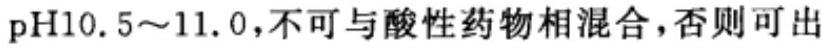
\includegraphics[max width=\textwidth, center]{2024_07_10_373f31b88d2bf633007bg-112}\\
现沉淀。由于配成的药液不稳定,故最好配制后立即应用。

硫喷妥钠用于全麻诱导,复合使用肌松药后作快速气管插管。健康成人的诱导为 $2.5 \sim 4.5 \mathrm{mg} /$ $\mathrm{kg}$, 儿童 $5 \sim 6 \mathrm{mg} / \mathrm{kg}$, 老年人应减至 $2.0 \sim 2.5 \mathrm{mg} /$ $\mathrm{kg}$ 。小儿可用于基础麻醉, 但目前已被氯胺酮、㽤达唑仑等药物所代替。此外, 还可用于惊厥、抽㹡等的对症治疗; 频脑手术时降低升高的顾内压,降低脑代谢,从而提供脑保护作用。

\section*{3. 不良反应}
(1)硫喷妥钠可产生血压骤降、呼吸抑制、喉痉挛等并发症。个别患者可出现过敏反应或类过敏反应。

(2)硫喷罗钠误注人血管外则产生疼痛、肿胀、红斑、硬结、溃疡, 甚至皮肤坏死。误注人动脉内,由于其强碱性质, 可引起动脉强烈收缩, 肢体和指端剧痛, 皮肤苍白,动脉搏动消失。一旦发生, 应立即从动脉注人利多卡因、罢栗碱等血管扩张药,以及做臂丛阻滞,以解除动脉痉挛。肝素抗凝可治疗和预防血检形成。如处理不及时,可造成肢体坏死。此药呈强碱性, 对静脉管臂有刺激性, 往往在手术后 $3 \sim 4 \mathrm{~d}$ 发生静脉炎。

(3)对于卟啉症患者, 硫喷妥钠也如其他巴比妥类一样, 由于酶诱导作用, 可增加体内卟啉的生成, 从而诱发急性发作。

\section*{三、非巴比妥类}
\section*{(一)苯二䔬草类及其拮抗药}
\begin{enumerate}
  \item 作用机制 $\gamma$-氨基丁酸 (GABA) 是中枢神经系统的抑制性递质。苯二氮草受体(BDZ 受体)位于神经突触的膜上, 与 GABA 受体相邻,耦合于共同的氯离子通道。 $\mathrm{BDZ}$ 受体水平存在着 GABA 调控蛋白,它能阻止 GABA 与其受体结合, 当苯二氮草类与 $\mathrm{BDZ}$ 受体结合时就阻止调控蛋白发生作用, 从而增强 GABA 与其受体的结合, 由此产生苯二氮草类的一系列药理作用。
\end{enumerate}

\section*{2. 药理作用、临床应用及不良反应}
(1)药理作用: (1) 中枢神经系统作用。具有抗焦虑、镇静、遗忘、肌松和抗惊厥作用。较大剂量或静注可产生催眠作用,甚至意识丧失。这类药物虽无镇痛作用, 但能增强麻醉性镇痛药或全身麻醉药的作用。(2)心血管系统作用。血压下降程度不仅取决于剂量和应用途径, 原高血压或处于焦虑状态者下降幅度大。主要是中枢性抑制使血管扩张,也可能对小动脉平滑肌的直接作用,心脏后负荷都下降, 对心肌收缩力无影响, 心率轻度增加, 心肌耗氧量下降。(3)轻度抑制呼吸中枢。静注过快可发生一过性呼吸暂停。(4)对肝肾功能无明显影响。

(2)临床应用: 此类药物常用于镇静催眠,消除焦虑,治疗乙醇或巴比妥类成癁者的戒断综合征,还用于抗惊嚴。临床麻醉的用途: (1) 麻醉前用药; (2)部位麻醉辅助用药, 使患者处于镇静, 遗忘状态,预防局麻药毒性反应; (3)用于全麻诱导,尤其是心\\
血管功能较差的患者; (4)作为复合全麻的组成部分, 增强全麻药作用和减少用量, 并防止某些麻醉药(如氯胺酮) 产生不良反应。

(3)不良反应: 这类药物多数消除半衰期较长,其代谢物又有药理活性, 故长期服用后易产生蓄积作用。较少产生依赖性。

\begin{enumerate}
  \setcounter{enumi}{2}
  \item 味达唑仑 是惟一的水溶性苯二氮草类药。在体内生理性 $\mathrm{pH}$ 条件下, 其亲脂性碱基释出, 能迅速透过血-脑屏障。可与盐酸呜啡等酸性药物相混, 但不能与硫喷要钠等碱性药物相混。肌内注射后容易吸收, 静脉注射对局部刺激作用轻微。
\end{enumerate}

(1)药理作用: 对 BDZ 受体的亲和力为地西泮的 2 倍, 故其强度为地西泮的 1.5 2 倍。可使脑血流量和顶内压轻度下降, 对脑代谢无明显影响。静注诱导时呼吸暂停发生率低于等效剂量的硫喷妥钠, 对心血管系统影响轻微, 心率轻度增快, 外周血管阻力和平均动脉压轻度下降, 对心肌收缩力无影响。无组胺释放作用,不抑制肾上腺皮质功能。

(2)临床应用: (1) 麻醉前用药。口服、肌内注射或静脉注射都有效, 肌内注射剂量 $5 \sim 10 \mathrm{mg}$, 口服剂量须加倍。小儿可用直肠注人, 剂量为 $0.3 \mathrm{mg} /$ $\mathrm{kg}$ 。 (2)全麻诱导和维持。主要适用于不宜用硫喷妥钠的危重患者, 剂量 $0.1 \sim 0.4 \mathrm{mg} / \mathrm{kg}$, 依年龄、病情和是否用术前药而定。用于静脉复合或静吸全麻的维持,可采取分次或持续静脉滴注的方法。 (3)作为部位麻醉的辅助用药, 特别适用于消化道内镜检查及其他沴断性操作。(4) ICU 患者镇静。

(3)不良反应: 㽤达唑仑有一定的呼吸抑制作用, 其程度与剂量相关。对正常人的心血管系统影响轻微, 心率轻度增快, 体血筞阻力和平均动脉压轻度下降, 左室充盈压和每搏量轻度下降, 但对心肌收缩力无影响。

\begin{enumerate}
  \setcounter{enumi}{3}
  \item 地西泮又称安定, 不溶于水, 刺激性较强, 肌内或静脉注射可引起疼痛, 且局部静脉炎发生率较高。
\end{enumerate}

(1)药理作用: 小剂量产生良好的抗焦虑作用,不影响意识, 较大剂量静注产生嗜睡和意识消失。具有明显的遗忘、肌松和抗惊嚴作用,可增强全麻药的作用。对呼吸无明显影响, 但与其他中枢抑制药合用时, 可产生呼吸暂停。血压轻度下降, 有扩张冠状动脉和增加血流的作用。

(2)临床应用: 地西泮可与麻醉性镇痛药、氮胺酮等合用,施行复合麻醉,但自咪达唑仑问世后,地西泮有被取代的趋势。

(3)不良反应: 剂量偏大时, 偶可引起躁动、䛇妄、兴奋等反应, 可能与中枢神经的多巴胺能系统作用增强或胆碱能系统受抑制有关。用毒扁豆碱可消除此不良反应。

\begin{enumerate}
  \setcounter{enumi}{4}
  \item 硝西泮 又名硝基安定, 其作用与安定相似只是催眠作用更为突出。口服 5〜10mg 可产生长达 6〜 8h 的睡眠。临床麻醉中很少应用。

  \item 氧马西尼 是合成的特异性苯二氮草类 (BDZ) 拮抗药,商品名为安易醒,为其 $0.01 \%$ 溶液 $(1 \mathrm{mg} / 10 \mathrm{ml}$ )。此制剂可溶于生理盐水或 $5 \%$ 蒲萄糖溶液, 在室温下可保持稳定性。目前认为此药并不影响 GABA 的传递, 本身无药理作用。但对 $\mathrm{BDZ}$ 受体有高度亲和力,通过竞争机制抑制 BDZ 与其受体结合, 从而消除 $\mathrm{BDZ}$ 类的作用。

\end{enumerate}

(1)药理作用: 在未用 $\mathrm{BDZ}$ 情况下, 此药本身既不产生 BDZ 的效应, 也不产生其相反的效应。在已用 $\mathrm{BDZ}$ 情况下,则拮抗其所有的效应,包括抗焦虑、镇静、催眠、遗忘、肌松、抗惊厥等。静脉注射后立即生效,约 $1 \mathrm{~min}$ 产生最大效应, 持续 $90 \sim$ $120 \mathrm{~min}$ 。

(2)临床应用: (1) 对 BDZ 类中毒的诊治, 对于可疑为 $\mathrm{BDZ}$ 药物中毒的昏迷患者, 可用此药鉴别。对肯定为 $\mathrm{BDZ}$ 中毒患者, 可用此药解救。采取小量分次注射的方法,每次 $0.1 \mathrm{mg}$ (或 $0.003 \mathrm{mg} /$ $\mathrm{kg}$ ), 每分钟一次, 直至苏醒或总量达 $2 \mathrm{mg}$, 为维持疗效也可采取静脉滴注的方法 ( $0.1 \sim 0.4 \mathrm{mg} / \mathrm{h}$ )。 (2)麻醉后拮抗 $\mathrm{BDZ}$ 的残余作用。(3)拮抗 ICU 内长期应用 $\mathrm{BDZ}$ 的患者,以达到恢复意识或停用机械通气的要求。

(3)注意事项: 由于氟马西尼的消除时间明显短于 $B D Z$ 类, 常于 1 小时后出现 $B D Z$ 类的药理作用,患者可再人睡。而以小量分次静脉持续输注给药, 恢复平稳安全。

\section*{(二)咪唑类——依托咪酯}
\begin{enumerate}
  \item 药理作用 作用类似中枢性抑制物 GA$\mathrm{BA}$, 镇痛效应不明显。催眠量可产生皮质下位抑制, 出现新皮质样睡眠, 脑干网状结构的激活和反应处于抑制状态。其主要优点是起效快、时效短;苏醒迅速、完全、平稳; 呼吸抑制轻微、短暂; 对心肌收缩力影响较小, 仅外周血管稍有扩张; 不释放组胺; 无变态反应;对肝、肾无毒;体内无明显积蓄。与硫喷妥钠一样, 能减少脑血流量及降低顾内压。

  \item 临床应用 经静脉给药用于麻醉诱导,起效\\
快,作用强, 清醒迅速而完全, 优于硫喷妥钠。成人剂量每次静脉注射 $0.3 \mathrm{mg} / \mathrm{kg}$, 范围为 $0.2 \sim$ $0.6 \mathrm{mg} / \mathrm{kg}$, 缓慢注人 $(30 \sim 60 \mathrm{~s})$ 。复合全麻维持时, 成人一般为 $0.2 \sim 0.3 \mathrm{mg} /(\mathrm{kg} \cdot \mathrm{h})$ 。10 岁以下儿童用量酌情调整。单次剂量可维持麻醉 6 $10 \mathrm{~min}$, 还可与其他药物配合用于复合麻醉的维持。术前给予阿片类镇痛约可减少肢体非自主活动的发生。

  \item 不良反应 可出现轻重不等的不能自制的肌肉僵直或阵挛, 左右对称或仅限于一侧, 与芬太尼合用时, 有 $32 \%$ 的患者 $(22.7 \% \sim 63 \%)$ 发生, 辅以苯二氮草类药物可缓解症状, 肌松药可预防发作。注射部位疼痛可随选择前臂大静脉注射而减少。恶心、呕吐、心律失常、呼吸频率变化及一些高敏反应包括过敏反应均偶见。由于用药后体内皮质激素释放量减少, 促皮质激素的效应消失, 遇有免疫抑制和脓毒血症者, 以及进行器官移植术时使用应格外慎重或禁用。对于肾上腺皮质功能低下者, 使用前应酌情补充皮质激索。

\end{enumerate}

\section*{(三)吩敾嗪类}
药理作用、临床应用及不良反应: 此类药物也称为神经松驰药。临床麻醉上除了用安定作用外,还利用其抗呕吐, 抗组胺和增强镇痛的作用。在中枢神经系统内主要作用是阻滞多巴胺受体, 降低多巴胺能神经的功能, 从而产生一系列作用。阻滞边缘系统的多巴胺受体, 就产生安定作用和抗精神作用; 阻滞结节漏斗部多巴胺受体, 就产生对内分泌的影响; 阻滞黑质纹状体多巴胺受体, 就使该部位的兴奋性递质乙酰胆碱在功能上处于相对优势, 从而产生雉体外系症状。在中枢神经系统外, 阻滞 $\alpha$肾上腺素受体, M-胆碱受体和 $\mathrm{H}_{1}$-组胺受体, 就分别产生降压作用,抗胆碱和抗组胺作用。

吩噻嗪类药过去曾广泛用作麻醉前用药, 以及复合全麻的辅助用药。由于这类药的不良反应较多,除了异丙喺外,其他药物在临床麻醉已很少应用。

不良反应包括嗜睡、视物模糊、直立性低血压等。长期应用可引起雉体外系症状, 表现为肢体震额、肌张力增高、运动减少、静坐不能等。一般停药后消失, 症状严重时可用抗胆碱药治疗。

筫丙嗪及异丙嗪 氯丙嗪注射液的 $\mathrm{pH}$ 为 $4 \sim$ 4.5 , 具有刺激性, 肌内注射可引起疼痛。静注须用其稀释的溶液, 以免产生血检性静脉炎。

(1)药理作用: (1)中枢神经系统。主要作用于边缘系统、网状结构和下丘脑。可产生安静、活动减少、淡漠无欲、嗜睡等。可增强催眠药、镇痛药及其他中枢抑制药的效应。对下丘脑的抑制作用产生自主神经阻滞, 有较显著的抗肾上腺素作用和轻度抗胆碱作用。抑制体温调节中枢, 消除寒冷反应, 有利于降温。对第四脑室底的化学感受区有抑制作用, 故有显著的镇吐作用。(2)心血管系统。其抗肾上腺素作用导致外周血管阻力降低, 血管扩张,致血压下降,但外周血流量却增加。(3)呼吸系统。对呼吸中枢无抑制作用, 潮气量和呼吸频率一般无明显变化。呼吸道分泌物可因其抗胆碱作用而减少。(4)其他。可增强肌松药的效应。对唾液和胃液分泌有一定的抑制作用。抑制平消肌张力,有抗痉挛作用。可抑制抗利尿激索的分泌,产生利尿作用。其抗组胺作用很弱。

(2)临床应用: 氯丙嗪是第一个用于治疗精神分裂症的吩﨔类药, 由于效力更强和副作用更少的新药问世,此药已较少应用。氯丙嗪 $12.5 \sim 25 \mathrm{mg}$术前 $1 \mathrm{~h}$ 肌内注射作为麻醉前用药, 可产生镇静、加强镇痛药和麻醉的效应, 减少手术后恶心、呕吐。近年来随着地西泮、咪达唑仑及氣哌利多等药物的广泛应用,此药应用逐渐减少。

对于手术中发生的顽固性呃逆,静脉注射氯丙嗪 10~20mg 可迅速制止。手术后呕吐和其他原因的呕吐, 此药具有显著疗效。

(3)不良反应: 由于药液的刺激性,肌内注射可引起疼痛, 静脉注射可产生血检性静脉炎, 故静脉注射须用其稀释的溶液。由于其血管扩张作用,可引起体位性低血压, 对血容量不足的患者不宜用此药。少数患者用此药后可发生黄疸,临床表现类似梗阻性黄疸。长期应用大剂量氯丙嗪, 可引起雉体外系症状,一般停药后可消失, 症状严重时可用抗胆碱药治疗。

异丙嗪除无抗精神病作用外,其他对中枢神经系统的作用与氯丙嗪相似。也有镇吐作用。对心血管系统无明显影响。对呼吸系统有松驰支气管平滑肌和抑制分泌的作用。与其他吩噻嗪类所不同的特点, 是有突出的抗组胺作用,因此被归类为 $\mathrm{H}_{1}$ 受体阻滞药。

临床上主要用于治疗过敏性疾病。临床麻醉中作为麻醉前用药, 有较好的镇静和抗呕吐作用。也是冬眠合剂的主要组合成分之一。

(四)莱环己哌啶类一一䔬胺酮

氯胺酮是非巴比妥类静脉全麻药, 属于苯环己\\
哌啶类药物, 广泛应用于临床。其镇痛作用主要是由于对丘脑内侧核选择性的抑制, 虽然脊髓网状结构束的上行传导受阻, 但脊䯝丘脑束的传导并未完全停止, 所以表现为情感淡漠, 对躯体的刺激不能定位。而且躯体痛觉有所减轻, 但内脏痛改善有限。静脉注射氯胺酮患者进人麻醉后, 丘脑与新皮层之间通路阻断, 但丘脑和边缘系统的活动并未减低, 表现为眼似乎睁开、眼球震颤, 角膜反射、对光反射依然存在, 遇到强刺激时肌张力增高, 呈偪直状, 似乎还会做有意识的动作, 但已无痛觉, 这就是通常称为的麻碎分离状态。

(1)临床应用: 适用于无须肌松驰的短小手术,尤其是烧伤后的清创、植皮与换药等。也可经静脉给药用于全麻的诖导期或肌内注射作为小儿的基础麻醉, 还可与其他药物合用维持麻醉。通常经静脉给药作为麻醉诱导, 成人 $1 \sim 2 \mathrm{mg} / \mathrm{kg}$, 缓慢注人 ( $>60 \mathrm{~s}$ )。小儿基础麻醉时肌内注射剂量是 $4 ~$ $6 \mathrm{mg} / \mathrm{kg}$ 。使用中应注意个体差异对药效的影响。氯胺酮麻醉前应使用阿托品或其他合适的抗毒曹碱类药物及苯二氮草类药物。慎用于急慢性乙醇中毒、心功能代偿欠佳、眼球破裂、眼压过高、脑脊液压过高、精神异常及甲状腺功能元进危象发作者。禁用于严重高血压、心力衰竭及近期心肌梗死患者。

(2)不良反应: 静脉注射后 $85 \%$ 以上的患者有血压升高及心率增加, 但也可出现不寻常的低血压, 心动过缓, 心律不齐。给药速度过快或用药量较大时可抑制呼吸功能, 表现为呼吸减慢、窒息、喉痉挛等。用药后肌肉张力增高, 肌肉异常收缩偶见, 极少有庭捎样发作。也可出现复视、眼球震频、恶心、呕吐、流泪、多涎、眼压及脑脊液压增高。注射部位疼痛及皮肤痒疹时有发生。反复多次给药,会出现快速耐药性, 需要量逐渐加大。恢复期可有䠅梦、意识模糊、幻觉或不理智的行为等, 青壮年多见, 而且表现强烈, 如需要可给予苯二氮草类药物缓解症状。其中行为心理的恢复需要一定时间, $24 \mathrm{~h}$ 内避免需要思维和精密操作的工作。

(五)丙泊酚

丙泊酚 (异丙酚), 静脉注射用制剂为乳白色胶浊液, 静脉注射前可用 $5 \%$ 的葡䓨糖溶液稀释, 但不要低于 $2 \mathrm{mg} / \mathrm{ml}$ 。如采用聚氯乙烯的静脉输液管输注会降低此药的浓度。它可与 $5 \%$ 的葡萤糖、 $0.9 \%$的盐水或 $5 \%$ 的葡萄糖盐水混合使用。患者清醒时为减轻注射部位的疼痛, 可在溶液中加人少量利多卡因。

\begin{enumerate}
  \item 药理作用 丙泊酚是一种起效迅速 (为 $30 \sim$ $50 \mathrm{~s}$ )、短效的全身静脉麻醉药。像许多全身麻醉药一样, 对其作用机制了解甚少, 镇痛效应不明显。主要优点是起效快、时效短、苏醒迅速、完全、平稳。临床剂最对呼吸抑制作用轻微, 但应注意有时发生短暂的呼吸暂停; 对循环功能有一定影响, 血压下降程度与用药量、循环容量及患者本身的心功能有关, 机制可能与周围血管阻力下降、心排血量减少、心肌抑制、压力感受器受到抑制有关。周围血管扩张诱发的反射性心动过速较少发生, 可能由于迷走神经张力增加的缘故。丙泊酚可使顾内压、眼压下降。对咽喉部反射的抑制有利于减轻咽喉部手术操作时的过激反应。与硫喷妥钠相比, 其催眠作用强 1.8 倍。它不能抑制插管期的血流动力学反应。在体内无明显蓄积作用。

  \item 临床应用 用于 3 岁以上的儿童与成人的全身麻醉。静脉给药用于全麻诱导时, 因为起效迅速, 诱导期平稳, 少有躁动而优于某些静脉麻醉药。同时可用于全身麻醉的维持中, 特别是门诊的短小手术,因其完全、清醒的恢复特性更显示出优势。也可作为镇静药用于 ICU 的人工通气患者中(不超过 $3 \mathrm{~d})$ 。由于蓄积作用较轻, 清醒迅速而完全, 明显优于目前常用静脉麻醉药。

\end{enumerate}

静脉诱导剂量成人为 $2 \sim 2.5 \mathrm{mg} / \mathrm{kg}$, 低于 8 岁的健康儿童所需剂量略大。麻醉维持可采用分次追加法和连续静脉输注法, 根据临床需要追加剂量每次 25 $50 \mathrm{mg}$; 在输注使用时, 根据使用不同的其他全身麻醉药及不同病情输注速度为 $4 \sim 12 \mathrm{mg}$ / $(\mathrm{kg} \cdot \mathrm{h})$, 儿童用 $9 \sim 15 \mathrm{mg} /(\mathrm{kg} \cdot \mathrm{h})$ 。在 ICU 中作为镇静药使用时, 输注速度为 $1 \sim 4 \mathrm{mg} /(\mathrm{kg} \cdot \mathrm{h})$, 但不用于儿童患者中。高秢及 ASA 分级较差的患者使用时应酌情减量。脂肪代谢紊乱的患者及估计有脂肪超载的情况下, 使用丙泊酚时建议监测血脂水平,随时调整用量。同时合用其他含脂肪药物时, 要酌减其量。

丙泊酚稀释后 $6 \mathrm{~h}$ 内药效稳定。因其不含抗微生物的防腐剂, 脂类溶媒有利于细嵲生长, 所以, 使用中应严格无菌操作, 已开启的遺留药品不应保存。

丙泊酚用于临床为时不久, 但发展较快, 目前它不仅作为 TIVA 的基础用药广泛用于不同手术麻醉中, 还在其药代动力学及药效学研究基础上建立了靶控给药(TCI-Target Controlled Infusion) 概\\
念,并借助计算机完成了第一个按 TCL 给药的输注系统-DiprifusorTCL 系统。

\begin{enumerate}
  \setcounter{enumi}{2}
  \item 不良反应 可能发生低血压和短暂的呼吸抑制。有个别报道用药后发生惊厥或角弓反张,在㿉病患者中应慎用。延长使用时有尿颜色改变的报道。给药后的过敏反应: 如支气管疼挛、红斑、低血压等。也有个别用药后发热的报道。注射静脉血栓形成或静脉炎罕见。妊娠期和哺乳期妇女使用丙泊酚后对新生儿的安全性尚未定论, 应慎用。大剂量、长时间 $(>48 \mathrm{~h})$ 用于儿童可能引起丙泊酚输注综合征(代谢性酸中毒、心衰、横纹肌溶解、血脂障碍、急性肾衰竭) , 应注意。
\end{enumerate}

(六)丁酰苯类一騦㖘啶醇

氮哌啶醇属于丁酰苯类,也属于抗精神病药,通过阻滞边缘系统、下丘脑后黑质-纹状体系统等部位的多巴胺受体而产生作用,有很强的安定和镇吐作用。

\begin{enumerate}
  \item 药理作用 使脑血管收缩,脑血流减少而降低顾内压, 但脑耗氧量并不相应下降。对心肌收缩力无影响,但有轻度 $\alpha$-肾上腺受体阻滞作用, 口服或肌内注射后对血压无明显影响, 静脉注射则可使血压轻度下降,对血容量不足的患者降压作用尤为显著。但对啫铬细胞痹患者反可引起显著的高血压, 可能与诱发肾上腺簉质释放儿茶酚胺或抑制嗜铬细胞摄取儿茶酚胺有关。有明显的抗心律失常作用, 似与延长心肌的不应期有关。对呼吸和肝、肾功能无明显影响。降温作用不明显, 但可使全身耗氧量减少 $20 \% \sim 30 \%$ 。不产生遗忘也无抗惊厥作用。

  \item 临床应用 手术中与阿片类合用,可作为部位麻醉或局部麻醉的辅助用药,同时有预防术后恶心、呕吐作用。多用作抗精神病用药。

  \item 不良反应可产生雉体外系反应,静注苯海拉明有助于消除这种反应。禁用于 $Q-T$ 间期延长病患者,临床有应用后引起阵发性尖端扭转性室性心动过速和心胜停搏的报道。

\end{enumerate}

\section*{(赵丽云)}
\section*{䈣3章}
\section*{麻醉性镇痛药与药物依赖性}
\section*{一、概 述}
阿片类镇痛药, 也称麻醉性镇痛药, 是指作用于中枢神经系统能解除或减轻疼痛并改变对疼痛的情绪反应的药物。

这类药物在临床麻醉中应用很广, 是术前用药、麻醉辅助用药、复合全麻的重要组成部分, 还用于术后镇痛。由于阿片类镇痛药都可产生依赖性,必须按国家颁发的《麻醉药品管理条例》严加管理。

1803 年由 Serturner 从䍂䅇生物碱提取出吗啡晶体物质后, 吗啡及类吗啡生物碱一直是此类药物的典型代表。吗啡于 1833 年用于临床, 但吗啡不是一个理想的镇痛药, 大剂量应用有严重的副作用。近年来,芬太尼族相继投人临床使用, 显示出各自临床应用的优势。

\section*{(一)阿片受体}
一般将阿片类受体按其激动后产生的效应分为 $\mu, \kappa, \delta$ 和 $\sigma$ 受体四型, 见表 2-3-1。

\section*{(二)阿片类镇痛药的分类}
按其与阿片受体的关系, 将这类及其拮抗药分为三大类: 阿片受体激动药、阿片受体激动拮抗药、阿片受体拮抗药, 见表 2-3-2。

\section*{二、阿片受体激动药}
阿片受体激动药是主要作用于 $\mu$ 受体的激动药, 其代表药物是吗啡。此外有哌替啶和芬太尼及其往生物。

(一)吗啡

\begin{enumerate}
  \item 药理作用 吗啡肌内注射后吸收良好, 作用持续约 $4 \mathrm{~h}$ 。分布谷积大 $(3.2 \sim 3.7 \mathrm{~L} / \mathrm{kg})$, 只有极小部分 (静脉注射后不到 $0.1 \%$ )透过血-脑屏障而到达中枢神经系统。小儿的血-脑屏障更易被透过,故小儿对吗啡的耐量小。吗啡可透过胎盘而到达胎儿。吗啡主要在肝经受生物转化, 少量以原形从尿排出。吗啡的消除半衰期为 $2 \sim 3 \mathrm{~h}$, 老年人的清除率约减少 $50 \%$,故用量须适当减少。
\end{enumerate}

(1) 中枢神经系统: 吗啡的主要作用是镇痛, 既可抑制疼痛的感受, 也可抑制对疼痛的反应。对身体和内脏的疼痛都有效; 对持续性钝痛的效果优于间断性锐痛; 疼痛出现前应用的效果较疼痛出现后应用更佳。

(1)镇静作用。消除由疼痛所引起的焦虑、紧张等情绪反应, 环境安静时, 患者易于人睡, 此外产生欣快感。

(2)缩瞳作用。瞳孔呈针尖样是吗啡急性中毒的特征性体征。抑制咳唃,可引起恶心、呕吐,尤其在用药后不卧床时更易发生。还可引起脊髄反射和肌张力增强。

在维持通气的情况下, 吗啡本身使脑血流量减少, 顽内压降低; 但在呼吸抑制而 $\mathrm{PaCO}_{2}$ 升高的情况下,脑血流量增加, 颅内压增高。

表 2-3-1 阿片受体的分类

\begin{center}
\begin{tabular}{|c|c|c|c|}
\hline
型别 & 效 应 & 内渻性阿片样肽 & 激动药 \\
\hline
$\mu$ & 奉鿷以上镇痛、呼吸抑制、心率减慢、欣快感、依赖性 & $\beta$ 内啡肽 & 吗啡、㖘替啶 \\
\hline
$\kappa$ & 㐘䲊镇痛、镇静、缩瞳、轻度呼吸抑制 & 强啡肽 & 喷他佐辛、丁丙诺朋 \\
\hline
$\delta$ & 调控受体活性 & 亮啡肽 & ? \\
\hline
$\sigma$ & 烦躁不安、瞳孔散大、幻觉、呼吸和心率增快、血压升高 & ? & 喷他佐辛 \\
\hline
\end{tabular}
\end{center}

表 2-3-2 阿片类药物分类(按与阿片受体关系)

\begin{center}
\begin{tabular}{ll}
\hline
\multicolumn{1}{c}{分类} & \multicolumn{1}{c}{药物代表} \\
\hline
阿片受体激动药 & 吗啡、㖘替啶、芬太尼族 \\
阿片受体激动-怙抗约 &  \\
以激动为主 & 喷他佐辛、丁丙诺啡、纳布啡 \\
以拮抗为主 & 㛓丙吗啡 \\
阿片受体拮抗药 & 纳洛酉、纳曲丽、纳美芬 \\
\hline
\end{tabular}
\end{center}

(2)呼吸系统: 吗啡有显著的呼吸抑制作用, 表现为呼吸频率减慢, 潮气量一般减少。大剂量可导致呼吸停止, 这是吗啡急性中毒的主要致死原因。

吗啡由于释放组胺和对平滑肌的直接作用而引起支气管挛缩, 对支气管哮喘患者可激发哮喘发作。

(3)心血管系统: 治疗剂量的吗啡对血容量正常者的心血管系统一般无明显影响。有时可使心率减慢, 由于对血管平滑肌的直接作用和释放组胺的间接作用, 可引起周围血管扩张而致血压下降,这在低血容量患者或用药后改为直立位时尤为显著。

(4) 消化系统: 增加胃肠道平滑肌和括约肌的张力, 减弱消化道的推进性䗌动, 从而引起便秘; 吗啡可增加胆道平滑肌张力, 使奥狄括约肌收缩, 导致胆道内压力增加。

(5)泌尿系统: 吗啡可增加输尿管平滑肌张力,并使膀胱括约肌处于收缩状态, 从而引起尿渚留。

(6)其他: 吗啡可引起组胺释放而致皮肤血管扩张。引起肝糖原分解增加, 导致血糖升高; 体温可下降。

\begin{enumerate}
  \setcounter{enumi}{1}
  \item 临床应用
\end{enumerate}

(1) 麻醉前用药: 使患者镇静, 减少麻醉药量,并使麻醉诱导平稳, 成人剂量为 $5 \sim 10 \mathrm{mg}$, 主张皮下或肌内注射, 生物利用度可达 $100 \%$ 。休克患者由于循环障碍应经静脉给药, 但需酌情惐量。虽然有人认为, 除急性疼痛患者外, 不必要作为常规术前用药, 但在心脏手术患者的麻醉前用药中仍为首选,可联合应用东莨营碱和异丙滕。

(2)术后镇痛: 随着对阿片受体研究的进展及对疼痛治疗的深人理解, 临床上将吗啡以多种途径如经椎管、静脉、皮下以不同方式如分次给药、连续给药及术后患者的自控性镇痛 (PCA) 或㿔痛的治疗中。患者自控镇痛 (PCA) 吗啡的 “最小有效浓度" (MEC) 为 $20 \sim 40 \mathrm{ng} / \mathrm{ml}$ 。\\
(3)四啡在临床上还常作为治疗急性左心衰所致急性肺水肿的综合措施之一,大剂量吗啡 $(1 \mathrm{mg} /$ $\mathrm{kg}$ ) 静脉输注曾用于复合全麻以施行瓣膜替换术等心胜手术。近年来已被芬太尼及其衍生物取代。

(4)以下情况中不宜使用吗啡:(1) 分娩止痛及哺乳期妇女。吗啡能通过胎盘进人胎儿体内以及对抗缩宫素 (oxytocin)对子宫的兴奋作用而延长产程, 还可经乳汁分泌; (2)支气管哮喘; (3)上呼吸道梗阻及肺心病; (4)顾内高压如㑔内占位病变或顾脑外伤等; (5) 严重肝功能障碍; (6)新生儿和 1 岁以内幼儿。

\section*{3. 不良反应}
(1) 吗啡有显著的呼吸抑制作用, 呼吸频率减慢,大剂量可导致呼吸停止。

(2)镇静作用: 消除由疼痛所引起的焦虑、紧张等情绪反应, 患者易于人睡。

(3)抑制咳唃, 引起恶心、呕吐, 还可引起脊璡反射和肌张力可增强。

(4)引起尿潴留、便秘、血糖升高、皮肤瘙痒、体温下降。

(5) 吗啡可增加胆道平滑肌张力, 使奥狄括约肌收缩, 导致胆道内压力增加。

(6) 吗啡由于释放组胺和对平滑肌的直接作用而引起支气管挛缩, 对支气管哮喘患者可激发哮喘发作。

(7)有欣快感,易于产生耐受性和依赖性。

\section*{(二)哌替啶}
\section*{1. 落理作用}
(1)镇痛作用: 哌替啶的作用与吗啡相似。哌替啶的镇痛强度约为吗啡的 $1 / 10$ 。其作用持续时间为吗啡的 $1 / 2 \sim 3 / 4$ 。镇静作用较吗啡稍弱, 也可产生轻度欣快感, 反复使用也容易产生依赖性。

(2)呼吸系统: 对呼吸有明显的抑制作用, 其程度与剂量相关。

(3) 循环系统: 哌替啶降低心肌的应激性, 对心肌有直接的抑制作用, 尤其在代偿机制受到削弱的情况下更为明显。对血压一般无影响, 但有时可因外周血管扩张和组胺释放而致血压下降, 甚至引起虚脱。心率可增加。

(4)其他作用: 如引起呕吐、抑制胃肠蠕动、增加胆道内压力等, 与吗啡相似, 但较弱。

\begin{enumerate}
  \setcounter{enumi}{1}
  \item 临床应用 哌替啶临床用途和禁忌证与吗啡基本相同。在临床麻醉中哌替啶常作辅助用药。\\
但由于其代谢物去甲哌替啶易于在体内蓄积, 有逐渐被芬太尼取代的趋势。

  \item 不良反应 特大剂量哌替啶常先引起中枢神经系统兴奋现象, 表现出为臂妄、瞳孔散大、抽擅等。接受单胺氧化酶抑制药的患者应用哌替啶, 可产生严重的高血压、抽搐、呼吸抑制、大汗和长时间昏迷,甚至死亡。

\end{enumerate}

\section*{(三)芬太尼及其衍生物}
芬太尼及其衍生物一一舒芬太尼、阿芬太尼和瑞芬太尼都是合成的苯基哌啶类药物。

\section*{1. 药理作用}
(1)芬太尼的镇痛强度为吗啡的 $75 \sim 125$ 倍,作用时间约为 $30 \mathrm{~min}$ 。舒芬太尼的镇痛强度更大,为芬太尼的 5〜10 倍, 作用持续时间约为其 2 倍。阿芬太尼的镇痛强度较芬太尼小,约为其 $1 / 4$, 作用持续时间约为其 $1 / 3$ 。瑞芬太尼的效价与芬太尼相似, 为阿芬太尼的 15~30 倍。

(2)芬太尼及其彷生物对呼吸都有抑制作用,主要表现为频率琙慢。芬太尼静脉注射后 5~ $10 \mathrm{~min}$ 呼吸频率减慢至最大程度, 抑制程度与等效剂量的哌替啶相似, 持续约 $10 \mathrm{~min}$ 后逐渐恢复。剂量较大时潮气量也减少, 甚至呼吸停止。舒芬太尼和阿芬太尼的呼吸抑制作用与等效剂量的芬太尼相似,只是前者持续时间更长。瑞芬太尼对呼吸的抑制程度与阿芬太尼相似, 但停药后恢复更快。

(3)对心血管系统的影响很轻, 不抑制心肌收缩力,一般不影响血压。芬太尼和舒芬太尼可引起心动过缓,此种作用可被阿托品对抗。小剂量芬太尼或舒芬太尼都可有效地减弱气管插管的高血压反应。也可引起恶心、呕吐, 但都没有释放组胺的作用。

\begin{enumerate}
  \setcounter{enumi}{1}
  \item 临床应用 芬太尼、舒芬太尼和阿芬太尼主要用于临床麻醉,作为复合全麻的组成部分。瑞芬太尼的消除半衰期仅为 $9.5 \mathrm{~min}$, 更适于静脉滴注, 但不能用于椎管内注射。其缺点是手术结束停止输注后没有镇痛效应, 可在手术后改用镇痛剂量输注。
\end{enumerate}

\section*{3. 不良反应}
(1)快速静脉注射芬太尼或舒芬太尼可引起胸壁肌肉僵硬而影响通气,可用肌松药或阿片受体拮抗药处理。

(2)由于某种原因其药代动力学特点,芬太尼或舒芬太尼反复注射或大剂量注射后,可在用药后 3〜4h 出现延迟性呼吸抑制, 应引起警惕。

(3)呛咳:芬太尼可诱发呛咳,其机制可能与引起支气管平滑肌收缩, 兴奋相邻部位的肺部牵张感受器 (RARs)有关。枸橡酸芬太尼中的枸榢酸可能触发外周组织中的初级神经元末梢释放速激肽,引起神经源性炎症反应, 造成支气管收缩, 引发呛咳。对于须内压增加、开放性眼外伤、主动脉瘤、气胸和反应性气道疾病的患者,呛咳会导致血流动力学的剧烈波动,产生产重的心脑血管并发症,甚至危及生命。

呛咳发生率与芬太尼剂量有关, 通过中心静脉给药比外周静脉途径给药更容易诱发呛咳, 给药速度与芬太尼诱发呛咳明显相关,与年龄呈负相关,机体本身病变如哮喘、慢性阻塞性肺部疾病 (COPD)、气道高反应性等对芬太尼麻醉时诱发呛咳也产生一定的影响, 应引起高度重视。

(4)芬太尼及其衍生物都可产生依赖性, 但较吗啡和哌替啶轻。

(5)恶心、呕吐及便秘: 此反应是芬太尼作用于化学感受器催吐中枢及自主神经所致, 治疗剂量芬太尼的副作用较吗啡少。

\section*{(四)体内过程}
芬太尼的脂溶性很高, 故易于透过血-脑脊液屏障而进人脑, 单次注射的作用时间短暂,与其再分布有关。如反复多次注射, 则可产生蓄积作用,其作用持续时间延长。注射后 $20 \sim 90 \mathrm{~min}$ 血药浓度可出现第二个较低的峰值。除肌肉和脂肪组织外, 周壁和肺组织也是储存芬太尼的重要部位。静脉注射后 $20 \mathrm{~min}$, 胃壁内含量约为脑内的 2 倍。储存于肺组织的芬太尼, 当肺通气灌注比例关系改善后,也被释放到循环中。尽管芬太尼单次注射的作用时间较吗啡和哌替啶短暂, 其消除半衰期却较长。

舒芬太尼的亲脂性约为芬太尼的 2 倍, 更易透过血-脑屏障。

瑞芬太尼可被组织和血浆中特异性酯酶迅速水解, 主要代谢物经肾排出。清除率不依赖于肝北功能。不论静脉输注时间多长,其血药浓度减半的时间, 始终在 $4 \mathrm{~min}$ 以内; 而芬太尼、阿芬太尼和芬太尼则随输注时间延长而延长, 输注后分别延长至 26. 5,58. 5 和 $33.9 \mathrm{~min}$ (表 2-3-3)。\\
表 2-3-3 麻醉性镇痛药的药代动力学参数

\begin{center}
\begin{tabular}{lllll}
\hline
\multicolumn{1}{c}{药名} & 血浆蛋白结合率 $(\%)$ & 分布容积 $(\mathrm{L} / \mathrm{kg})$ & 清除率 $[\mathrm{ml} /(\mathrm{kg} \cdot \mathrm{min})]$ & 消除半衰期 $(\mathrm{h})$ \\
\hline
四啡 & 30 & $3.2 \sim 3.7$ & $14.7 \sim 18$ & $2 \sim 3$ \\
芬太尼 & 84 & 4.1 & $11.6 \sim 13.3$ & 4.2 \\
舒苍太尼 & 92.5 & 1.7 & 12.7 & 2.5 \\
瑞芬太尼 & 70 & 0.39 & 41.2 & $9.5 \mathrm{~min}$ \\
\hline
\end{tabular}
\end{center}

\section*{三、阿片受体激动/拮抗药}
这一类药对阿片受体兼有激动和拮抗作用的药物。主要激动 $\kappa$ 受体, 对 $\sigma$ 受体也有一定的激动作用,而对 $\mu$ 受体则有不同程度的拮抗作用。这类药物有以下特点: 镇痛强度较小; 呼吸抑制作用较轻; 很少产生依赖性;可引起烦躁不安、心血管兴奋等不良反应。

\section*{(一)喷他佐辛( 镇痛新)}
\begin{enumerate}
  \item 药理作用 镇痛强度为吗啡的 $1 / 4 \sim 1 / 3$, 肌内注射后 $20 \mathrm{~min}$ 起效, 持续约 $3 \mathrm{~h}$ 。此药不产生欣快感, 剂量较大时反可激动 $\sigma$ 受体而产生焦虑、不安等症状。由于它兼有弱的拮抗效应, 很少产生依赖性。
\end{enumerate}

呼吸抑制作用与等效吗啡相似,主要也是使呼吸频率减慢。

心血管系统, 可使血压升高, 心率增快,血管阻力增高和心肌收缩力减弱,故禁用于急性心肌梗死时镇痛。

对胃肠道的影响与吗啡相似,但较少引起恶心、呕吐, 升高胆道内压力的作用较吗啡弱。没有缩瞳作用。

口服后容易吸收, 但通过肝的首过消除大,生物利用度仅为 $20 \%$ 。容易透过血-脑屏障,也可透过胎盘。此药主要用于肝内经生物转化, 消除半衰期 $2 \sim 3 \mathrm{~h}$ 。

\begin{enumerate}
  \setcounter{enumi}{1}
  \item 临床应用 喷他佐辛主要用于镇痛, 对大剂量喷他佐辛引起的呼吸抑制和其他中毒症状,不能用烯丙吗啡对抗, 但可用纳洛酮对抗。
\end{enumerate}

\section*{(二)烯丙吗啡}
\begin{enumerate}
  \item 药理作用 镇痛强度与吗啡相似, 但不产生欣快感, 反可引起烦躁不安等不知感,故临床上不将它作为镇痛药应用, 此药也有呼吸抑制作用,相当于等效吗啡的 $74 \%$,但持续时间较吗啡短。
\end{enumerate}

可拮扰阿片受体激动药的作用,包括镇痛、欣快感、呼吸抑制、缩瞳等作用, 但对镇痛作用拮抗不完全。对于麻醉性镇痛成瘏者, 狶丙吗啡激发戒断症状, 可用于麻碎性镇痛药成痹的诊断。对于喷他佐辛和其他阿片受体激动-拮抗药引起的呼吸抑制, 烯丙吗啡不仅无拮抗作用, 反可使之加重。对于巴比罗类和全身麻醉药所致的呼吸抑制, 烯丙吗啡也无拮抗作用, 而且由于其本身的呼吸抑制作用,还可使之加重。

皮下注射后吸收迅速, 易于透过血-脑屏障, 皮下注射后药效持续时间为 $1 \sim 4 \mathrm{~h}$ 。在肝内经生物转化,小部分以原形从尿中排出。

\begin{enumerate}
  \setcounter{enumi}{1}
  \item 临床应用 主要用于阿片受体激动药急性中毒的解救。临床麻醉上用于复合全麻结束时拮抗阿片受体激动药的残余作用以恢复自主呼吸。由于兼有激动阿片受体的效应, 近年来已逐渐被纳洛酮取代。
\end{enumerate}

\section*{(三)丁丙诺啡}
\begin{enumerate}
  \item 丁丙诺啡为长效和强效镇痛药。除激动 $\kappa$受体外, 对 $\mu$ 受体也有部分激动效应。其镇痛强度约为吗啡的 30 倍。其作用持续时间长, 至少维持 $7 \sim 8 \mathrm{~h}$ 。由于对 $\mu$ 受体有很强的亲和力, 可置换结合于 $\mu$ 受体的麻醉性镇痛药, 从而产生拮抗作用。不引起烦躁、不安等不适感。

  \item 呼吸抑制作用与吗啡相似, 但出现较慢, 纳洛屇对其呼吸抑制只有部分拮抗作用。对心血管的影响与吗啡相似, 使心率减慢, 血压轻度下降, 对心排血量和外周血管阻力无明显影响。

  \item 体内只有 $1 / 3$ 在肝内经受生物转化, 代谢物随尿和胆汁排出,消除半衰期约 $3 \mathrm{~h}$ 。

  \item 主要用于手术后镇痛。

\end{enumerate}

\section*{四、阿片受体拮抗药一一纳洛国}
\section*{(一)药理作用}
\begin{enumerate}
  \item 纳洛酮不仅可拮抗吗啡等纯粹的阿片受体激动药, 而且可拮抗喷他佐辛等阿片受体激动-拮抗药, 但对丁丙诺啡的拮抗作用较弱。静脉注射后作用持续时间为 $2.5 \sim 3 \mathrm{~h}$ 。

  \item 亲脂性很强, 起效迅速, 拮抗作用强。主要在肝内经受生物转化, 消除半衰期 $30 \sim 78 \mathrm{~min}$ 。由\\
于在脑内的浓度下降迅速, 药效维持时间短。

  \item 应用纳洛酮拮抗大剂量麻醉性镇痛药后, 由于痛觉突然恢复,可产生交感神经系统兴奋现象,表现为血压升高、心率增加、心律失常, 甚至肺水肿和心室颤动。

\end{enumerate}

\section*{(ニ)临床应用}
纳洛酮是目前临床上应用最广的阿片受体拮抗药。

\begin{enumerate}
  \item 拮抗麻醉性镇痛药急性中毒的呼吸抑制。

  \item 在应用麻醉性镇痛实施复合全麻的手术结束后, 用以拮抗麻醉性镇痛药的残余作用。

  \item 娩出的新生儿因受其母体中麻醉性镇痛药影响而呼吸抑制, 可用此约拮扰。

  \item 对偍为麻醉性镇痛药成膍者, 用此药可激发戒断症状, 有诊断价值。

  \item 最近有人用纳洛酮解救乙醇急性中毒, 取得突出的效果。静脉注射 $0.4 \sim 0.6 \mathrm{mg}$ 后数分钟即可使意识恢复。

\end{enumerate}

由于该药作用持续时间短,用于解救麻醉性镇痛药急性中毒时, 单次剂量拮抗虽能使自主呼吸恢复,一旦作用消失,可再度陷人昏睡和呼吸抑制。

\section*{五、药物依赖性}
\section*{(一)概述}
阿片类药物具有镇痛作用,临床上常将其用于术后和肿瘤患者的止痛。但阿片类药物长期使用会产生耐受和成癋,这不仅限制了阿片药物的临床应用,而且还造成吸毒这一世界性的社会问题。阿片成癔是一种慢性复发性脑病, 具有很强的顽固性,可产生精神依赖性和生理依赖性, 一旦停药将产生戒断综合征。其机制复杂, 治疗困难,复发率高, 已经成为学术界的普遍共识。

阿片类药物成癔及依赖与机体内源性阿片物质存在密切相关。内源性阿片物质是阿片受体的配基,广泛存在于脑、脊䯝、周围神经节、自主神经系统、将上腺觹质、胃肠道及血浆。在机体连续接受外源性阿片物质达到一定程度时,阿片受体发生 “超载”, 机体通过负反馈使内源性阿片类物质释放减少或停止,结果是需使用更多的阿片药物才能维持原有的镇痛作用, 这就是临床上的耐药现象, 表现为用药量增加, 药物作用时间缩短。

\section*{(二)药物依赖性}
药物依赖性是指反复用药引起的机体对该药心理和(或)生理的依赖状态,表现出渴望继续用药的行为和其他反应, 以追求精神满足和避免不适。产生耐受性和依赖性大多是由于“滥用”阿片类药物的结果。事实上,临床围术期中正常使用麻醉性镇痛药, 包括术后患者自控镇痛 (patients control analgesia, PCA)技术的开展,均是在短期、少量使用的范畴。即使用于痛性疼痛治疗时, 只要在医生指导下规范用药,很少发生精神依赖及成㾏。

\section*{(三)药物依赖性分类}
药物依赖性分为躯体依赖性和精神依赖性两种。躯体依赖性也称生理依赖性; 精神依赖性也称心理依赖性。

\begin{enumerate}
  \item 精神依赖性俗称 “心痣”, 指药物可使人产生一种愉快、满意的感觉, 并在精神上驱使人们有一种继续用药的欲望, 以获得满足感。停药后, 不出现躯体戒断症状。精神的欣快给人留下的记忆和渴求非常强烈, 精神依赖性非常顽固, 是戒毒者复吸的主要原因,也是当前治疗的难点。

  \item 躯体依赖性是由于多次用药造成的机体药物的适应和依赖状态, 一旦停药, 机体即出现严重的生理功能紊乱 (即戒断综合征), 甚至可危及生命。患者非常痛苦, 难以忍受, 可能有自残、自杀行为,因惧怕戒断症状而继续用药。

\end{enumerate}

\section*{(四)防治原则}
\begin{enumerate}
  \item 预防
\end{enumerate}

(1)减少依赖性药物供应: 减少依赖性药物供应, 打击非法生产和贩运, 加强医院麻醉药品、精神药品的管理等。

(2)降低对依赖性药品的需求: 降低对依赖性药品的需求必须进行长期的、科学的预防性的教育。

\begin{enumerate}
  \setcounter{enumi}{1}
  \item 治疗
\end{enumerate}

(1)了解病史、正确诊断: 了解尴用药物的种类和程度, 有无伴发病等。

(2)制订治疗方案: 针对患者的全面情况,制订治疗方案, 使所依赖的药物逐渐减量至完全停服,或以其他药物替代。同时注意对症处理和综合治疗,减少患者痛苦, 保证患者安全。

(3)心因治疗:也称之为康复治疗或后续照管。除脱药治疗外应注意改善患者的心理和行为异常,为回归社会做准备。

(4) 回归社会: 是治疗的最终目标, 目的是彻底脱离所依赖的药物, 恢复正常人的生活。其关键在于克服脱药后的心理㵧求, 防止复吸。需要依靠心理医生、家庭和社会的帮助, 要关心患者的感情、学习、生活和工作, 避免无所事事和不良择友。

\section*{六、阿片类药物的依赖及防治}
常见的是海洛因, 其次是哌替啶。

\section*{(一)药理作用}
海洛因又名二醋吗啡, 俗称 “白粉”, 易溶于水,可经胃肠道和鼻樃膜迅速被吸收。其脂溶性比吗啡高, 易于通过血-脑脊液屏障, 起效快、欣快感强烈, 但维持时间短。精神依赖性及躯体依赖性均极强。

其机制可能是与内源性阿片肽和 cAMP 有关。其欣快感和奖赏效应可能与脑中多巴胺、肾上腺素能受体有关。

\section*{(二)戒断综合征}
戒断症状是突然停止麻醉性镇痛药出现一系列的生理功能絮乱, 如烦躁、肌颤、呕吐、流涎、失眠、出汗、腹痛、散瞳等。这是因为短期体内的内源性阿片物质释放功能未能恢复的缘故。还有学者认为与长期应用阿片类药物后出现的阿片受体上调及抗阿片类物质释放到脑脊液有关, 往往表现为原药物作用相反的效应。

\section*{(三)治疗}
治疗应包括脱毒、康复及回归社会。

\begin{enumerate}
  \item 脱毒治疗 可缓解或消除吸毒者在不吸毒期间严重的戒断综合征。脱毒治疗分为药物戒毒和非药物戎毒两类。
\end{enumerate}

(1)阿片类:以作用时间长、成痖性较低的阿片 $\mu$ 受体激动药替代毒品, 逐渐减量, 直至停药。常用的有美沙酮、丁丙诺非等。\\
(2)非阿片类:仅起辅助治疗作用,如可乐定、东莓若碱、麻醉药 (氯胺雨), 此外尚可用 NMDA 拮抗药、安定、氟哌啶醇和伊波加因等。中西药联合治疗效果好, 中药 (如福康片等) 可能对防止复吸有较好作用。

(3)国内学者曾提出“梯度戒毒方案”, 即前 2 $3 \mathrm{~d}$ 给阿片受体激动药; 再 $2 \sim 3 \mathrm{~d}$ 给激动-拮扰药; 接着 1 周用非阿片类过渡; 最后给阿片受体拮抗药 (纳曲酮)。这在理论上是成立的, 尚待在实践中进一步证实、完善。

\begin{enumerate}
  \setcounter{enumi}{1}
  \item 康复 即使不予治疗, 成癝者的戒断症状也会在 2 周内自然消退, 但极为痛苦。此时, 患者仍有稽延性症状 (焦虑、抑郁、失眠、全身疼痛等),再加上精神依赖性仍然存在(脱毒主要解除躯体依赖性), 很容易再次吸毒。此时, 一是要对症治疗,消除稽延性症状; 二是服用纳曲酮,使成痹者吸毒时不再产生快感, 从而使毒品失去吸引力。若能坚持服用,可有效地防止复吸, 但目前能坚持长期服用者很少; 三是要进行康复治疗, 矫正其异常的心理和行为。

  \item 回归社会 不论是短期的脱毒, 还是 $1 \sim 3$年的康复, 最终戒毒者都要回归社会, 这是戒毒能否成功最关键的阶段。这涉及对吸戒者感情上的关心, 生活上的安排, 职业上的出路, 交友上的选择等。努力实现“无种毒、无制毒、无贩毒、无吸毒”的目标,最终建立“无毒社区”。

\end{enumerate}

(赵丽云)

\section*{箱程}
\section*{非阿片类镇痛药}
\section*{一、非阿片类中枢性镇痛药}
曲马朵和氟吡汀属于人工合成的非阿片类中枢性镇痛药。前者的镇痛作用机制与阿片类药不完全相同, 后者则完全不同。

\section*{(一)曲马朵}
\begin{enumerate}
  \item 药理作用 曲马朵为消旋混合体,其 $(+)$对映体对 $\mu$ 受体有较强的亲和力,并对 5-垟色胺再摄取有更强的抑制作用; 而 $(一)$ 对映体对去甲肾上腺素的再摄取有更强的抑制作用。因此该药具有双重作用机制,除作用于 $\mu$ 受体外,还抑制神经元突触对去甲肾上腺素和 5-羟色胺的再摄取,并增加神经元外 5-羟色胺浓度, 从而调控单胺下行性抑制通路,影响痛觉传递而产生镇痛作用。其镇痛强度约为吗啡的 $1 / 10$,镇痛作用可被纳洛酮部分拮抗。此药不产生欣快感, 镇静作用较哌替啶稍弱, 镇咳作用约为可待因的 $50 \%$ 。治疗剂量不抑制呼吸,大剂量则可引起呼吸频率减慢, 但程度较吗啡轻。对心血筞系统基本无影响, 静脉注射后 5~10min 产生一过性心率增快和血压轻度增高。不引起缩瞳,也不引起括约肌疼挛,无组胺释放作用。产生依赖性的危险很小,约为 $1 / 10$ 万。

  \item 体内过程口服后可迅速而几乎完全吸收,20~30min 起效,2h 血药浓度达峰值,维持时间为 $3 \sim 6 h$ 。肌内注射后 $1 \sim 2 h$ 产生峰效应, 镇痛持续时间为 $5 \sim 6 \mathrm{~h}$ 。此药在肝内降解,约 $90 \%$ 代谢物经肾排出, 其余随暴便排出。消除半衰期为 5~6h。肝肾功能障碍时, 消除半衰期延长约 1 倍。

  \item 临床应用主要用于急、慢性疼痛。用于手术后中度至重度疼痛, 可达到与吗啡相似的镇痛效果; 由于不产生呼吸抑制作用,尤其适用于老年人、心肺功能差的病人以及日间手术患者。口服后效果几乎与胃肠道外给药相等, 很少引起不良反应, 恶心、呕吐、便秘等发生率均很低。

\end{enumerate}

\section*{(二)啇吡汀}
\begin{enumerate}
  \item 药理作用氟吡汀与 $\mu, \kappa$ 和 $\delta$ 三种阿片受体都不结合,其镇痛效应也不被纳洛酮拮抗。初步认为其作用机制是作用于去甲将上腺素下行疼痛调控途径而产生镇痛作用, 但尚待进一步证实。此药无呼吸抑制作用, 也不产生便秘、尿濐留等不良反应。长期应用后不产生耐受性和依赖性。

  \item 体内过程 口服后易吸收,在体内经生物转化后 $20 \% \sim 36 \%$ 从肾排出,大部分从粪便排出。消除半衰期 2~3h。

  \item 临床应用主要用于术后疼痛和癌痛,效果优于㘇他佐辛。口服 $100 \mathrm{mg}, 3 / \mathrm{d}$, 可获得稳态血药浓度。

\end{enumerate}

\section*{二、非甾体类抗炎药}
非甾体类抗炎药 (nonsteroidal antiinflammatory drugs, NSAIDs) 是一类具有解热镇痛, 且多数兼具消炎、抗风湿、抗血小板聚集作用的药物, 主要用于炎症、发热和疼痛的对症治疗。非甾体类抗炎药有多种分类方法, 根据作用的受体分为 COX-1 和 COX-2 抑制药 (表 2-4-1); 根据理化性质分为酸类和非酸类; 根据化学结构分为乙酸类、丙酸类、烯酸类、昔康类、昔布类等; 根据作用时间和强度可分为高强度长时间、低强度短时间等。

\section*{(一)水杨酸类一一阿司匹林}
\begin{enumerate}
  \item 药理作用 阿司匹林为水杨酸类解热镇痛药中最常用的药物, 其作用和用途主要有解热、镇痛、抗炎、抗风湿和抗血小板聚集。
\end{enumerate}

(1)解热作用: 阿司匹林具有较好的解热作用,可使发热患者的体温降到正常, 但对正常体温却无影响, 常用于感冒的解热。\\
表 2-4-1 NSAIDs 的分类

\begin{center}
\begin{tabular}{|c|c|}
\hline
分类 & 药物 \\
\hline
\multicolumn{2}{|l|}{非选择性 COX 抑制药} \\
\hline
水杨酸衍生物 & 阿司匹林、水杨酸钠、柳氮磺胺吡啶 \\
\hline
对氨基彷生物 & 对乙酰氨基酚 \\
\hline
吲橾和吲哚乙酸 & 吅哚美辛、舒林稄 \\
\hline
异芳香乙酸类 & 酮咯酸、双氯芬酸、托美丁 \\
\hline
芳香丙酸类 & 布洛芬、嶚普生、謙比洛芬、哃洛芬、非诺洛芬 \\
\hline
邻氨基苯甲酸类 & 甲芬那酸、甲氮芬那酸 \\
\hline
\multicolumn{2}{|l|}{选择性 COX-2 抑制药} \\
\hline
青康类(烯醇酸类) & 爫诺昔康、美洛昔康、吡罗青康 \\
\hline
㸿酮类 & 萗丁美酮 \\
\hline
昔布类 & 塞来昔布、瓦德昔布、帕瑞昔布、依妥昔布、鲁米昔布 \\
\hline
吼橾乙酸类 & 依托度酸 \\
\hline
磺酰苯氨类 & 尼美舒利 \\
\hline
\end{tabular}
\end{center}

(2)镇痛作用: 只具中度镇痛效应,无成㾙性和依赖性,临床广泛用于头痛、牙痛、神经痛、关节痛、肌肉痛、月经痛等中度钝痛,对外伤性剧痛及内脏平滑肌绞痛无效。其镇痛的作用部位主要在外周,但也有中枢镇痛机制参与其中。

(3)抗炎抗风湿效应: 具有较强的抗炎作用。通过抑制 PGs 合成,消除了 PGs 对缓激肽、组胺、 5-羟色胺等致炎介质的致敏作用。其抗风湿作用除解热、镇痛等因素外,主要在于抗桊,临床上作为急性风湿性、类风湿关节炎的主要用药。

(4)抗血小板聚集作用: 对血小板聚集有特异性抑制作用,临床上广泛用于防止术后血栓形成,预防动脉粥样硬化、短暂性脑缺血发作及心肌梗死等。

(5)其他用途: 抑制肠道 PGs 合成,可用于治疗腹泻; 干扰 PGs 类物质的形成而缓解偏头痛发作;缓解癌症的疼痛; 对糖尿病所致的动脉血栓栓塞性疾病、坏㾴、冠状动脉粥样硬化有疗效,临床上已用于冠心病的二级预防; 还可用于治疗大骨节病、早期老年性白内障等。

\begin{enumerate}
  \setcounter{enumi}{1}
  \item 体内过程 口服后可迅速自田及小肠上部吸收,约 $2 \mathrm{~h}$ 达血药高峰。血浆半衰期为 $20 \mathrm{~min}$,其水解产物水杨酸盐在一般剂量时血浆半衰期为 3 $5 \mathrm{~h}$, 大剂量时可延长 $15 \sim 30 \mathrm{~h}$ 。阿司匹林 1 次口服 $0.6 \mathrm{~g}, \mathrm{C}_{\max }$ 可达 $40 \mu \mathrm{g} / \mathrm{ml}$, 足以达到解热和镇痛作用; 其血浆有效抗类浓度为 $150 \sim 300 \mu \mathrm{g} / \mathrm{ml}$, 中毒浓度 $>200 \mu \mathrm{g} / \mathrm{ml}$, 因此要防止蓄积中毒。

  \item 临床应用阿司匹林对缓解轻、中度疼痛如牙痛、神经痛、肌肉痛及痛经效果较好。用于感冒等发热疾病的退热; 可用于风湿热, 发挥解热、减轻疼痛的作用;能抑制血小板聚集,防止血㭲形成,可用于预防短暂性脑缺血发作、心肌梗死及瓣膜术后的血检形成。

\end{enumerate}

\section*{(二)对氮基衍生物一一对乙酰苳基酚}
\begin{enumerate}
  \item 药理作用 对乙酰氨基酚是有效的解热镇痛药, 但抗炎作用弱,通常不用于治疗炎性疾病。因对乙酰氨基酚在高过氧化物环境下无抑制 COX 的作用,故几乎没有抑制周围 COX 的作用。而在脑内过氧化物浓度低, 对乙酰氨基酚可透过血脑屏障, 抑制脑内 COX, 发挥其解热镇痛作用。对乙酰氨基酚不抑制中性粒细胞的激活。对心血管及呼吸系统没有影响,无阿司匹林的因肠道副作用,对血小板、出血时间、酸䂸平衡和尿酸排泄均无影响。

  \item 体内过程 口服后吸收迅速,几乎完全由胃肠道吸收, $\mathrm{T}_{\max }$ 为 $20 \sim 90 \mathrm{~min}$ 。经肝内首过代谢后,生物利用度为 $70 \% \sim 90 \%$,有剂量依赖性。对乙酰氨基酚的吸收受胃排空率和胃液 $\mathrm{pH}$ 的影响。其血浆蛋白结合率与血药浓度有关。小剂量时(血药浓度 $<60 \mu \mathrm{g} / \mathrm{ml}$ ), 血浆蛋白结合率低, 大剂量和中灻剂量时,血浆蛋白结合率可达 $20 \% \sim 50 \%$ 。治疗剂量的血浆半衰期大约为 $2 \mathrm{~h}$ 。对乙酰氨基酚可分布至许多组织,消除十分迅速。 $90 \% \sim 95 \%$ 药物在肝内代谢,主要与葡萄糖醛酸 $(60 \%$ )、硫酸 $(35 \%)$或半胱氨酸 $(3 \%)$ 结合。正常人 $85 \% \sim 95 \%$ 的药物和代谢产物经尿排出。慢性肾损害时,对乙酰氨基酚血药浓度及半衰期与健康者相仿, 但血亖硫酸及葡萄糖醛酸结合物是健康者的 4 倍。

  \item 临床应用 作为镇痛或解热药, 对乙酰氨基酚是阿司匹林良好的替代品, 适用于阿司匹林禁忌的患者(如消化性溃疡等) 和阿司匹林引起出血时间延长的患者。对乙酰氨基酚对多种疼痛均有效,适用于轻到中度疼痛, 如头痛、关节痛、肌痛、神经痛、牙痛、痛经、痹痛、术后或创伤后疼痛。由于对乙酰氨基酚具有耐受性好、副作用低和危险性小等优点, 现已被多个疼痛治疗指南列为慢性疼痛、痛痛、骨关节疼痛、类风湿关节痛的一线药物。对乙酰氨基酚与吗啡、曲马朵、可待因组成的复方制剂的应用也越来越广泛。

\end{enumerate}

在治疗剂量范围内, 对乙酰氮基酚一般均可很好耐受。成人 1 次服用对乙酰氨基酚 $10 \sim 15 \mathrm{~g}$ (150~250mg $/ \mathrm{kg}$ )会引起肝毒性, 服用 $20 \sim 25 \mathrm{~g}$ 或更高剂量可能致死。

\section*{(三)吲哚和吲哚乙酸类一吲哚美辛}
\begin{enumerate}
  \item 药理作用 具有明显的抗炎、解热、镇痛作用, 是最强的前列腺素合成酶抑制药之一, 镇痛作用也最强。其抗炎作用较氢化可的松高 2 倍。作用机制与阿司匹林相似,除抑制 PGs 合成外, 还能抑制多形核白细胞的活动,减少其在炎症部位的浸润和溶酶体酶释放对组织的损伤; 抑制钙的移动,阻止炎症刺激物引起细胞的炎症反应。体温调节中枢的前列腺素合成受抑制后, 使体温中枢兴奋性下降,引起外周血管扩张、出汗, 增加散热起退热作用。

  \item 体内过程 口服吸收完全而迅速,1〜4h 后血药达峰值,饭后服药可延迟达峰时间。有效血药浓度为 $0.3 \sim 3 \mu \mathrm{g} / \mathrm{ml}$, 中毒浓度为 $75 \mu \mathrm{g} / \mathrm{ml}$, 血浆半衰期为 $2 \mathrm{~h}$ 。约 $50 \%$ 经肝去甲基代谢,部分与莆萄裾醛酸结合或经脱酰化。 $50 \%$ 于 $48 \mathrm{~h}$ 内从尿中排出,部分从胆汁和粪中排泄,并有明显的肝肠循环,也可经乳汁排出。

  \item 临床应用对炎性疼痛有良好的镇痛作用, $50 \mathrm{mg}$ 吲哚美辛相当于 $600 \mathrm{mg}$ 阿司匹林的镇痛效能。有显著的抗炎及解热作用, 对强直性脊柱炎、骨关节炎、急性痛风性关节炎有较好的疗效,可用于治疗顽固性和恶性肿痹发热。近年来还用于治疗慢性肾炎、肾小球肾炎和肾病综合征、早产儿动脉导管未闭及预防习惯性流产,但不良反应发生率高达 $35 \% \sim 50 \%$ 。常见的有食欲缺乏、上腹不适、恶心、呕吐、腹泻等症,也能诱发或加重田潢疡,甚至造成穿孔。中枢神经系统症状也多见,也可引起肝功能损害、粒细胞减少、再生障碍性贫血、过敏反应等。禁用于䂞妇、儿童、精神失常、凘病或帕金森病、溃疡病患者。

\end{enumerate}

\section*{(四)芳香乙酸类一酮咯酸、双覩芬酸}
\begin{enumerate}
  \item 酮略酸
\end{enumerate}

(1)药理作用: 具有解热、抗炎和高度镇痛作用,是少数被批准作为胃肠道外给药的 NSAIDs。醍咯酸注射液克服了口服给药起效慢的缺点,主要用于急性痛或手术后疼痛, 其镇痛作用较吲橾美辛强 2〜2.5倍,较阿司匹林强 $25 ~ 50$ 倍,与 $100 \mathrm{mg}$哌替啶或 $10 \mathrm{mg}$ 吗啡的止痛作用相当,且维持时间较长。与阿片类镇痛药相比, 酮咯酸无耐受性, 无停药反应,无呼吸抑制作用,其引起的困倦、恶心、呕吐等也远低于吗啡。酮咯酸局部用药时,有抗炎作用。

(2)体内过程: 无论口服、肌内注射或皮下注射,都能迅速吸收, $\mathrm{T}_{\max }$ 为 $30 \sim 60 \mathrm{~min}$ 。口服生物利用度大约 $80 \%$,几乎全部与血熪蛋白结合,消除半衰期 4~6h, 尿中排泄量占药物消除的 $90 \%$ 。老年人和肾衰竭的患者尿排泄速度降低,血浆清除率下降,半衰期延长。

(3)临床应用: 肌内或静脉注射用于手术后疼痛,可代替阿片类镇痛药; 口服可用于治疗慢性疼痛, 且优于阿司匹林; 局部用药可用于治疗眼部的炎症和季节性过敏性结膜炎; 也可以口腔注射,减轻口外科疼痛。不能用于产科镇痛。

\section*{2. 双兼芬酸}
(1)药理作用: 具有镇痛、解热及抗炎作用,其作用强于吲棎美辛、䒬普生等药物。双氯芬酸还可通过影响脂肪酸的释放和摄取, 而降低白细胞内游离花生四烯酸的浓度。

(2)体内过程: 口服后迅速完全吸收,食物可减慢其吸收速度,但对吸收量无影响。有较强的首过效应,生物利用度约为 $50 \%$ 。血浆蛋白结合率为 $99 \%$,血浆半衰期为 $1 \sim 2 \mathrm{~h}$ 。口服后可蓄积在关节滑液中, 因此其治疗作用明显长于血浆半衰期。由肝细胞色素 P450CYP2C 代谢,主要代谢产物由尿和胆汁排出。消除迅速,给药 $3 \sim 4 \mathrm{~h}$, 消除约达给药量的 $90 \%$ 。肾衰竭患者,可有双氯芬酸及其代谢产物蓄积。

(3)临床应用: 可用于类风湿关节炎、骨关节炎及强直性脊柱炎的长期对症治疗。也可用于治疗急性肌肉及关节损伤、滑膜炎、肌腱及腱鞘炎、腰背部疼痛、扭伤、劳损及其他软组织损伤、急性痛风、痛经、牙痛和术后疼痛等。

\section*{(五)丙酸衍生物一一布洛芬、䒬普生、氫比洛芬酯}
\begin{enumerate}
  \item 布洛芬
\end{enumerate}

(1)药理作用: 布洛芬可抑制花生四烯酸代谢中的环氧酶,减少 PGs 合成,故有较强的抗炎、抗风湿及解热镇痛作用。其效果与阿可匹林和保泰松相似而优于对乙酰氨基酚,但对胃肠道刺激较阿司匹林轻,易耐受,不良反应小。对轻、中度术后疼痛、痛经等镇痛疗效优于阿司匹林。对血小板盉附和聚集也有抑制作用,并延长出血时间。

(2)体内过程: 布洛芬口服吸收迅速,服药后 1~2h血药浓度可达峰值。血浆半衰期约 $2 \mathrm{~h}$ 。主要经肝代谢, $90 \%$ 以上代谢物经尿排出。

(3)临床应用: 主要用于缓解类风湿关节炎、骨关节炎、强直性脊柱炎的症状。也可用于软组织损伤、腰背痛、痛经及口腔、眼部等手术后的镇痛; 对炎性疼痛的效果比创伤性疼痛效果好。可用于高热和感冒等症的退热。也适用对阿司匹林疗效差或不能耐受的患者。对急性痛风有一定的疗效。

\section*{2. 藄普生}
(1)药理作用: 覍普生是一种高效低毒的消炎、解热镇痛药。其镇痛、解热作用优于阿司匹林, 作用时间也较长, 为 $7 \sim 8 \mathrm{~h}$ 。消炎作用强于阿司匹林、保泰松和吲棎美辛。对血小板的黏附和聚集反应也有一定的抑制作用。作用机制为抑制 COX 活性, 阻断 PGs 合成和炎性介质的释放。

(2)体内过程: 口服吸收迅速而完全,2〜4h 血药浓度达峰值。血浆半衰期为 $13 \sim 14 \mathrm{~h}$ 。在治疗浓度下, 与血浆蛋白结合率为 $99 \%$ 。代谢产物主要由肾排泄。

(3)临床应用: 主要用于风湿性、类风湿关节炎、骨关节炎、强直性脊柱炎、急性痛风等。对轻、中度疼痛有确切疗效, 如痛经、偏头痛、牙痛、手术后疼痛等。

\section*{3. 氧比洛芬与笰比洛芬酯}
(1)药理作用: 㡘比洛芬的药理学性质、治疗适应证以及不良反应与其他丙酸衍生物相似。氟比洛芬具有一定的亲脂性, 胅比洛芬酯注射液是利用特殊工艺制成脂微球载体制剂, 由脂微球包裏的氛比洛芬组成。脂微球是一种以脂肪油为软基质并被磷脂膜包封的微粒体分散系, 平均直径为 $200 \mathrm{~nm}$, 外膜为卵磷脂, 内层为软基质油, 其中包裹脂溶性药物。脂微球对其包裹的药物具有靶向性,使包裹药物在炎性组织、手术切口及肿痹部位靶向聚集,从而增强药效; 脂微球包裹药物的释放受到控制,使药效持续时间更长; 脂微球制剂的高脂溶性,易于跨越细胞膜, 从而促进包裹药物的吸收, 进一步缩短起效时间。

(2)体内过程: 氟比洛芬口服吸收好, $\mathrm{T}_{\max }$ 为 $1 \sim 2 \mathrm{~h}$, 血浆半衰期大约 $6 \mathrm{~h}$ 。氟比洛芬酯静脉注射后, 被血中酯酶迅速水解, 成为活性代谢物氛比洛芬。静脉注射 $50 \mathrm{mg}$ 氟比洛芬酯, $5 \sim 10 \mathrm{~min}$ 全部水解为氛比洛芬, $6 \sim 7 \mathrm{~min}$ 达血浆峰值浓度 $(8.9 \mathrm{mg} /$ $\mathrm{ml}$ )。给药量在 $10 \sim 80 \mathrm{mg}$ 时, 血药浓度呈线性。药物消除半衰期为 $5.8 \mathrm{~h}$ 。主要以羟化物和结合物的形式经将排泄。药物在体内几无蓄积。

(3)临床应用: 氟比洛芬的止痛作用强于阿司匹林。与口服递比洛药相比, 氛比洛芬酯起效更快, 镇痛作用相似或更强,而对胃㮩膜的损伤较口服制药低,安全系数高。该药静脉注射后 $15 \mathrm{~min}$ 起效, 1 $\sim 5 \mathrm{~h}$ 作用最强,止痛持续时间为 $3 \sim 6 \mathrm{~h}$, 有时可达 $9 \mathrm{~h}$ 以上。手术后与阿片类药物联合使用,可节省阿片类用药,采用超前镇痛方法优于术后给药。

(六)昔康类(烯醇酸类)一一䵡诺昔康、美洛昔

\section*{康、吡罗昔康}
\begin{enumerate}
  \item 氮诺昔康 (lornoxicam)
\end{enumerate}

(1) 药理学性质: 氯诺昔康是 COX-1 和 COX-2 的平衡抑制药,与其他 NSAIDs 一样能减轻炎症的症状和体征,不改变疾病的进程。大剂量对 IL-6 和一氧化氮合成酶有抑制作用, 也可能激活阿片肽系统, 发挥中枢镇痛作用。

(2)药代动力学: 口服后吸收完全,生物利用度 $>90 \%, \mathrm{~T}_{\max }$ 为 $2 \mathrm{~h}$ 。主要通过肝细胞色素酶系统代谢, 代谢产物无活性, 经尿和粪排出。血浆消除半衰期大约 $4 \mathrm{~h}$ 。 65 岁以上老年人血浆清除率降低,消除半衰期延长。在肔、肾功能轻至中度损害的患者,药代动力学没有明显变化。由于药物半㐮期短,重复给药无明显蓄积。

(3)临床应用: 主要用于各种风湿类疾病,如类风湿关节炎、强直性脊柱炎、痛风、骨关节炎、风湿性关节炎、结缔组织病或反应性关节炎,常作为对乙酰氨基酚无效或效果不佳时的替代或补充药物。静脉注射可用于术后止痛。

\begin{enumerate}
  \setcounter{enumi}{1}
  \item 美洛昔康 (meloxicam)
\end{enumerate}

(1)药理作用: 选择性 COX-2 抑制药, 对 COX2 的抑制作用是 COX-1 的 10 倍, 对血小板血栓素的产生也有某种抑制作用。美洛昔康对 COX-1 的\\
抑制程度与用量关系密切, 而且个体之间有很大差异。与非选择性 COX 抑制药相比, 美洛昔康对胃肠道和肾的副作用较小。美洛昔康对炎症性疼痛、运动性疼痛、坐骨神经痛等多种疼痛均有明显的抑制作用。此外,美洛昔康还有抗癌、抑制神经病变、预防心脑血管疾病、预防糖尿病神经病变和避肎等药理作用。对全身各系统无明显不良反应。

(2)体内过程: 在体内吸收和消除均较为缓慢,口服吸收完全, 生物利用率高。半衰期长, 可每日服用 1 次,服药 3〜5d 后, 血粶浓度达到稳定状态,药物在消液中的浓度可达血浆浓度的 $50 \%$ 。美洛昔康代谢彻底, 其主要代谢途径是经肝内氧化去甲基,代谢产物从尿或粪便中排出。

(3)临床应用:用于治疗类风湿关节炎、骨性关节炎、神经痛、手术后疼痛、外伤性疼痛和运动性疼痛。对急性疼痛,可选用注射制剂; 乳胶制剂可用于局部。美洛昔康还具有抗肿㿑作用, 并有保护神经、改善帕金森病的症状, 对慢性炎症脱髓䩗病的治疗可能有一定意义。

\section*{3. 吡罗昔康}
(1)药理作用: 长效非甾体类抗炎药, 特点为半衰期长、用药剂量小,作用迅速而持久,长期服用耐受性好,副作用小, 疗效显著。其抗炎作用与抑制 PGs 合成有关,还可通过抑制白细胞聚集及钙离子移动起抗炎作用。

(2)体内过程: 口服吸收迅速而完全,2 4h 血药浓度达峰值。血熪半衰期为 $35 \sim 45 \mathrm{~h}$ 。一次服药后, 可多次出现血药峰值, 提示本药有肝肠循环,作用持久,且不会在血中蓄积。主要经同代谢, 以羟化物及匍萄糖䔯酸结合物形式自尿中排出, 部分从粪便排出。

(3)临床应用: 主要用于风湿性或类风湿关节炎, 也适用于骨关节炎、强直性脊柱炎、急性痛风等。对腰肌劳损、肩周炎、术后及创伤性疼痛等也有一定疗效。治疗原发性痛经的疗效与蔡普生相仿。

\section*{(七)烷酮类一一亚丁美酮}
\begin{enumerate}
  \item 药理作用 萗丁美酮是一种非酸性前体药物, 口服后吸收良好, 几乎全部在肝内代谢, 其产物 6-甲氧基-2-䒬乙酸是䒬丁美酷产生抗炎、解热和镇痛作用的活性成分, 是强效 COX 抑制药,尤其对 COX-2 有较强的抑制作用, 较对 COX-1 的抑制作用强 $3 \sim 5$ 倍。由于不刺激消化道, 无肝肠循环, 几乎不影响血小板功能,故对消化系统的副作用小,安全性高。

  \item 体内过程 吸收迅速, $\mathrm{T}_{\max }$ 为 $3 \sim 4 \mathrm{~h}$ 。 $99 \%$与清蛋白结合, 然后分布到靶器官。6-甲氧基-2-䒬乙酸酯在肝内通过氧化去甲基作用灭活,之后主要经肾排泄。消除半衰期约 $24 \mathrm{~h}$ 。

  \item 临床应用 用于治疗骨性关节炎、类风湿关节炎、强直性脊柱炎、软组织损伤、手术后疼痛、痛经和牙痛等。

\end{enumerate}

\section*{(八)昔布类一一塞来昔布、帕瑞昔布钠}
昔布类是一系列选择性 COX-2 抑制药, 对 COX-2 的抑制效果明显高于 COX-1, 抗炎和镇痛等疗效等同甚至优于非选择性 NSAIDs, 而胃肠道等不良反应明显降低。然而, 2004 年第一代昔布类药罗非昔布因具有诱发严重心脏病的风险被从全球市场撤出,使之成为关注焦点。目前,美国 FDA 要求此类药物的生产厂商在其标签和说明书上增加黑框警告,警示使用此类药物可能出现相关心血管不良反应的风险。

\begin{enumerate}
  \item 塞来昔布
\end{enumerate}

(1)药理作用: 通过抑制 COX-2 阻止炎性 PGs 的产生,达到抗炎、镇痛及退热作用。

(2)体内过程: 空腹口服吸收良好, $\mathrm{T}_{\max }$ 为 2 〜 $4 \mathrm{~h}$ 。消除半衰期为 $8 \sim 12 \mathrm{~h}$, 血浆清除率约为 $500 \mathrm{ml} / \mathrm{min}$ 。血浆蛋白结合率约为 $97 \%$ 。在组织中广泛分布, 可透过血脑屏障。主要在肝内经细胞色素 $\mathrm{P}_{450}$ 代谢为差基、羖基酸和莆萄糖醛酸衍化物, 从粪便和尿中排出。肝功能不全的患者,血浆药物浓度增加。

(3)临床应用: 用于急性或慢性骨关节炎和类风湿关节炎治疗。作为内镜检查、小手术的镇痛治疗及围术期多模式镇痛。塞来昔布含有磺胺基团,已知对磺胺过敏者禁用。对阿司匹林或其他非甾体抗炎药过敏者,也应避免使用。

\section*{2. 帕瑞昔布钠}
(1)药理作用:帕瑞昔布钠 (商品名: 特耐) 是第一种注射用 COX-2 抑制剂, 2008 年获准在中国上市。帕瑞昔布是伐地昔布的水溶性前体药物, 后者在临床剂量范围为选择性 COX-2 抑制剂, 通过抑制 COX-2 阻止炎性 PGs 的产生, 达到抗炎、镇痛及退热作用。

(2)体内过程: 帕瑞昔布在静注或肌注后经肝酶水解, 迅速并几乎完全地转化为有药理学活性的物质一一伐地昔布。伐地昔布的消除在肝内通过细胞色素 P450 代谢以及磺胺葡详糖醛酸化, 低于\\
$5 \%$ 通过尿液以原型排泄。

(3)临床应用: 适用于手术后疼痛的短期非胃肠道途径给药,临床上可用于中度或重度术后急性疼痛的多模式镇痛治疗, 与阿片类药物合用可惐少后者需要量, 术前给予发挥其抗炎作用。推荐剂量为 $40 \mathrm{mg}$, 静脉或肌内注射, 随后视需要间隔 $6 \sim 12$小时给予 $20 \mathrm{mg}$ 或 $40 \mathrm{mg}$, 每天总剂量不超过 $80 \mathrm{mg}$, 疗程不超过 3 天。对体重低于 $50 \mathrm{~kg}$ 的老年患者以及中度肝功能损伤患者, 应减量, 目前尚不推荐在儿童及青少年中使用。对阿司匹林或其他非甾体抗炎药过敏者、妊娠或哺乳期妇女、严重肝功能损伤、活动性消化道溃疡、胃肠道出血或胃肠道手术、已确定的缺血性心脏疾病或外周动脉血管和(或)脑血管疾病患者应避免使用。

\section*{(九)磺酰苯氮类一一尼美舒利}
\begin{enumerate}
  \item 药理作用 新型选择性 COX-2 抑制药,除可减少 PGs 合成外,还具有抗氧化作用, 从而发挥解热、镇痛和抗炎作用。生物利用度高,抗炎作用强, 且毒性低, 治疗指数高。对疼痛、炎症、发热的改善程度优于吡罗昔康、对乙酰氨基酚等, 耐受性好于阿司匹林等。由于对 COX-1 抑制不明显, 不影响胃内保护性 PGs 的合成, 城少了 NSAIDs 常见的消化道溃疡和出血等不良反应; 抑制激活的白细胞产生氧自由基, 减轻了炎症时氧自由基导致的组织损害; 抑制组胺释放,不促使白三烯的合成,因而无阿司匹林等引起过敏反应导致的支气管疼挛,可安全用于哮喘患者。

  \item 体内过程 口服吸收迅速而完全。1 次口服 $100 \mathrm{mg}, 1 \sim 2 \mathrm{~h}$ 可达最大血药浓度, 半衰期为 2 $3 h$; 直肠给药 4h 达血浆峰值, 半衰期 5h, 有效治疗浓度持续 6 8h。在肝内被代谢为羟基衍生物, 该代谢产物仍具有药理学活性, $80 \%$ 通过尿液排出, $20 \%$ 通过粪便排出。

  \item 临床应用用于镇痛消炎,也可用于风湿性关节炎的治疗。对术后疼痛, 口服尼美舒利 $10 \mathrm{mg}$ 的止痛效应相当于肌注吗啡 $5 \mathrm{mg}$ 或 $10 \mathrm{mg}$ 的疗效;对短期急性疼痛的效果,可替代吗啡。与阿片类合用,可减少 $25 \% \sim 50 \%$ 阿片类的用量,从而减少后者的不良反应, 加快胃肠功能恢复。对其他 NSAIDs 过敏者、仯衰竭及本妇和儿童禁用。

\end{enumerate}

\section*{三、辅助性镇痛药}
\section*{(一)抗抑郁、抗惊厥、抗癫痫药}
\begin{enumerate}
  \item 三环类抗抑郁药镇痛机制为作用于一类特殊的 5-羟色胺受体,阻断 5-羟色胺的再摄取。常用药物包括阿米替林和多塞平, 常作为慢性疼痛治疗的辅助用药, 副作用主要包括抗胆碱作用 (䵑膜干燥、便秘和尿潴留等) 以及对中枢神经系统的作用(疲倦、失眠、易激惹、焦虑等)。

  \item 卡马西平 为抗惊嚴药物, 并非典型的镇痛药, 其结构与三环类抗抑郁药如阿米替林和丙米嗪类似, 主要用于三叉神经痛的治疗。其镇痛机制为减弱神经冲动在三叉神经内的突触传导, 镇痛作用不强。卡马西平胃肠用药吸收较慢, 2 8 $\mathrm{h}$ 后达血药峰浓度。血浆半衰期较长, 为 $8 \sim 72 \mathrm{~h}$ 。卡马西平在月开内代谢, 可诱导肝微粒体酶, 加速其他同时使用药物的代谢。

  \item 加巴喷丁(1-璌甲基环己烷乙酸)是一种新的抗㿎疾药物, 最初作为 $\gamma$-氨基丁酸 (GABA)类似物用于治疗痉挛, 目前在慢性疼痛综合征尤其是神经病理疼痛方面得到广泛应用。加巴喷丁只有口服制剂, 在小肠通过弥散和易化转运被吸收, 由于载体转运具有饱和性, 其生物利用度与剂量成反方向变化。加巴喷丁在体内不代谢, 以原形随尿液排出而消除, 消除半衰期为 $4.8 \sim 8.7 \mathrm{~h}$, 肾功能损害者清除能力降低。对肝微粒体酶没有诱导或抑制作用。

\end{enumerate}

加巴喷丁的抗异常性疼痛效应机制包括: 增加 GABA 介导通路的抑制性输人; 指抗 NMDA 受体; 拮抗 CNS 钙通道和抑制周围神经的传导。其中, 拮抗 NMDA 受体和阻滞钙通道已得到有力的证据支持。加巴喷丁在治疗多种神经病理痛以及一些特定的慢性疼痛方面具有明显的疗效。可用于带状疮疹后神经痛、糖尿病神经痛、癌性神经痛、三叉神经痛、多发性硬化症引起的神经痛、复杂性区域疼痛综合征以及其他神经痛的治疗或辅助治疗,也可与阿片类复合用于术后疼痛的治疗。

加巴喷丁耐受性好, 与其他药物几乎无相互作用,严重不良反应少,尤其适用于老年患者或肝功能异常患者。

\section*{(二) $\alpha_{2}$ 肾上腺素能受体激动药}
中枢神经系统 $\alpha_{2}$ 受体广泛分布于动物和人体的大脑,包括皮质区、蓝斑核的去甲肾上腺素能细胞体等的突触前与突触后, 位于突触前的 $\alpha_{2}$ 受体主要抑制中枢 $\mathrm{NE}$ 合成及通过负反馈作用自动调节 $\mathrm{NE}$ 的释放,降低中枢神经 $\mathrm{NE}$ 水平。

\begin{enumerate}
  \item 可乐定 $\alpha_{2}$ 肾上腺素能受体激动药的代表性药物, 又名可乐宁。该药是 $\alpha_{2}$ 肾上腺素受体部分\\
选择性激动药, 对 $\alpha_{2}: \alpha_{1}$ 的选择性比例为 200:1。
\end{enumerate}

(1) 药理作用

(1)降压和对心血管系统作用。降压作用中等偏强。静脉注射可乐定后血压常呈双相变化,一般先出现短暂的血压升高,随后产生较持久的血压下降; 但口服、肌内注射或皮下注射可乐定后则仅出现持久的降压效应。外周阻力下降的同时, 常伴有心率减慢和心排血量降低, 导致“平衡性”降压, 从而可保持重要器官血流不变, 血浆 NE 浓度降低。

(2)镇痛、镇静、抗焦虑作用。可乐定具有较强的镇静、抗焦虑和镇痛作用。椎管内应用可乐定可产生良好的镇痛作用, 对机体正常运动无明显影响, 并能加强全身或椎管内应用阿片类药物的抗伤害刺激作用,从而产生长时间的强效镇痛效应。纳洛酮对可乐定的镇痛作用无影响, 其镇痛作用仅能用相应的 $\alpha_{2}$ 受体拮抗药拮抗。

(3)对呼吸系统的影响。可乐定剂量增至 $300 \mu \mathrm{g}$ 时可轻微降低静息每分通气量以及增加呼气末二氧化碳, 对呼吸的影响作用比阿片类药轻,且与阿片类镇痛药的呼吸抑制作用无协同作用。可乐定对支气管平滑肌无确切影响, 但吸人雾化的可乐定可惐轻侾喘患者的支气管收缩。

(4)对肾功能的影响。肾动脉或静脉应用可乐定均增加尿量和游离水清除率; 大剂量应用时能明显减少钠和氯化物的排出。在各类高血压患者,可乐定均使尿中儿茶酚胺、醛固酮和血浆肾素活性降低。

(5)对胃肠道系统功能的影响。可减少唾液分泌; 激活突触前 $\alpha_{2}$ 受体,通过抑制迷走神经,降低胃壁细胞产生胃酸,但通常并不改变胃液的 $\mathrm{pH}$ 。可乐定可降低胃及小肠蜧动,用于治疗腹泻综合征。

(6)对内分泌功能的影响。 $\alpha_{2}$ 怪上腺素能受体激动药对神经内分泌系统作用表现为对交感紧上腺素释放产生抑制作用, 并抑制 ACTH 释放。应用可乐定的患者, 可缓和由于手术刺激引起的皮质类固醇激素升高, 抑制胰岛素分泌, 但临床上并未见到由此引起的血糖升高。

(7)对血小板的影响。高浓度时可通过选择性刺激血小板肾上腺素受体使血小板聚集, 而低浓度时则可降低肾上腺素浓度, 其净效应是降低血小板聚集。此外, $\alpha_{2}$ 将上腺素受体激动药可释放一氧化氮(NO),后者可抑制血小板聚集。故临床上应用可乐定不仅不促进血小板聚集, 反而可阻滞肾上腺素引起的血小板聚集。\\
(8)抗阿片戒断综合征作用。可乐定能通过激活蓝斑核神经元突触前膜的 $\alpha_{2}$ 受体, 反馈性抑制 $\mathrm{NE}$ 释放, 从而抑制高度活动的蓝斑核肾上腺素能神经元, 使阿片戒断综合征得以安全有效治疗, 而且无欣快感。

(9)其他。应用可乐定时, 机体体温呈下降趋势。可乐定的镇静和降温作用均与可乐定兴奋中枢及外周 $\alpha_{2}$ 受体有关。

(2)体内过程: 可乐定脂溶性高, 可采用口服、静脉、皮下、肌内、硬膜外、鞘内给药, 口服或肌内注射后吸收迅速而完全。 $30 \sim 60 \mathrm{~min}$ 起效, 血药浓度 $2 \mathrm{~h}$ 左右达到高峰。该药分布广泛, 极易透过血-脑屏障进人中枢神经系统发挥作用, 作用持续 6〜 $8 \mathrm{~h}$ 。部分在肝内代谢, 存在肝肠循环, $40 \% \sim 60 \%$的药物以原形从尿湤中排出; 有蓄积现象, 蓄积大约为给药量的 $62 \%$ 。肾衰竭患者清除率降低, 半衰期延长。

(3) 临床应用

(1) 稳定围术期血流动力学。在轻、中度高血压患者, 可乐定不仅能增强围术期血流动力学稳定性, 而且具有类似 $\beta$ 肾上腺素能阻断作用。术前使用可乐定可有效地控制气管插管时的心血管不良反应, 麻醉也易于管理。研究表明可乐定还是一个良好的抗心绞痛药物, 并能有效地改善心肌氧供需平衡。可乐定不影响支气管平滑肌张力, 也不影响异丙肾上腺素的效应, 因此在某些情况下可替代普萗洛尔。

(2)增强全麻药的作用。伍用可乐定时, 吸人麻醉药或麻醉性镇痛药需要量可减少 $40 \% \sim 50 \%$, 并可降低诱导时硫喷妥钠、氯胺酊、丙泊酚、依托咪酯需要量以及丙泊酚维持需要量。

(3)椎管内镇痛。蛛网膜下腔注人可乐定, 其镇痛作用呈量效相关性, 镇痛效价是吗啡的 $10 \sim 60$倍, 爱解疼痛比吗啡强 10〜20 倍, 可用于急慢性疼痛和神经病理性疼痛的治疗。与局麻药不同, 可乐定不影响运动或本体感觉功能; 而且无呼吸抑制、恶心、呕吐、癃幛和尿濐留等并发症, 对阿片药耐受的患者同样有效, 因此也明显优于椎管内应用阿片类药物。研究表明, 硬膜外使用可乐定用于分娩镇痛, 既具有止痛效果又不会导致运动缺失, 还可减少局麻药用量。

(4)增效硬膜外阻滞。硬膜外阻滞患者, 局麻药中加用可乐定能明显缩短起效时间, 延长阻滞时间, 提高运动阻滞程度, 而且无明显心血管或呼吸\\
抑制, 不增加副作用。剂量一般为 $1 \sim 2 \mu \mathrm{g} / \mathrm{kg}$ 。

(5)增强脊䯕麻醉的作用。在施行关节手术患者,可乐定对丁卡因脊髉麻醉的感觉阻滞时间呈剂量相关性延长, 提高感觉阻滞质量, 但对脊醌麻醉扩散程度无明显影响; 而且可乐定用量达 $150 \mu \mathrm{g}$ 不加重脊觡麻醉中的血流动力学波动。

(6)辅助控制性降压。与控制性降压药伍用能明显提高控制性降压的效应, 降低耐药性的发生,抑制降压期间的交感肾上腺觡质反应和抗利尿激素的分泌。而且对交感神经突触后受体无阻滞作用, 从而保存了交感神经对意外低血压、低血容量或出血反应的储备能力, 而且也保存了血管活性药物治疗的有效性。

(7)特殊外科手术。青光眼患者术前应用可乐定,可缓解全麻插管引起的眼压升高。可乐定通过直接收缩健状肌传人动脉而减少房水生成, 并降低房水排出系统的血管张力, 从而降低眼内压, 加快眼科手术患者的康复。

(8)产科的应用。马妇口服可乐定抗高血压未见对胎儿不良反应的报道。可乐定可通过增加内源性阿片类物质浓度, 增强其作用。与脊鰖麻醉或硬膜外阻滞不同, 可乐定不减弱交感神经系统反应, 子宫压迫动静脉时血压能较好维持。

(9)儿科的应用。可乐定可用于预防七氟烷麻醉苏醒期患儿的躁动及嗒安; 在小儿骶管麻醉中,可降低局麻约中毒危险; 并可降低眼科患儿术后呕吐发生率。

①其他。可乐定能明显延长布比卡因和利多卡因的股神经阻滞时间, 与肾上腺素合用时, 对局麻药神经阻滞时间的影响具有协同作用。术后寒战患者静脉注射可乐定 $150 \mu \mathrm{g}$, 可使 $95 \%$ 的患者缓解, 且无血流动力学改变。

(4) 停约综合征: 长期用药者突然停药, 可出现 “可乐定停药综合征”, 表现为反跳性高血压, 多于停药 12 $48 \mathrm{~h}$ 出现, 可持续数天, 其中 $5 \% \sim 20 \%$ 的患者伴有神经紧张、胸痛、失眠、脸红、头痛、恶心、唾液增多、呕吐、出汗、烦躁不安或心律失常, 甚至高血压危象。因此, 停药必须在 $1 \sim 2$ 周内逐渐减量, 同时加以其他降压治疗。

\begin{enumerate}
  \setcounter{enumi}{1}
  \item 右美托味定 右美托咪定为选择性 $\alpha_{2}$ 肾上腺素能受体激动药。缓慢静脉输注中低剂量右美托咪定 $\left(10 \sim 300 \mu \mathrm{g} / \mathrm{kg}\right.$ ) 对 $\alpha_{2}$ 肾上腺素受体具有选择性兴奋作用, 而缓慢静脉输注高剂量右美托咪定 $(1000 \mu \mathrm{g} / \mathrm{kg})$ 或快速静脉输注则同时对 $\alpha_{1}$ 或 $\alpha_{2}$ 肾上腺素受体起作用。
\end{enumerate}

(1)药理作用

(1)对中枢神经系统的作用。降低脑 $\mathrm{NE}$ 水平,抑制交感神经末梢释放 $\mathrm{NE}$ (激活突触前 $\alpha_{2}$ 受体),表现为血浆中儿茶酝胺浓度呈剂量依赖性降低。健康成人单次肌内注射 $0.5 \sim 1.5 \mu \mathrm{g} / \mathrm{kg}$ 或静脉注射 $0.25 \sim 2.0 \mu \mathrm{g} / \mathrm{kg}$ 均可产生剂量依赖性镇静作用,静脉注射后 $10 \mathrm{~min}$ 作用最强, 持续约 $4 \mathrm{~h}$ 。右美托枨定也具有镇痛作用, 其镇痛效应可被选择性 $\alpha_{2}$受体阻滞药阿替美坐阻断, 而不能被纳洛胴阻断。

(2)对心血管系统的作用。应用右美托咪定后, $\mathrm{BP}$ 下降, HR 减慢, 其作用机制主要与激动中枢突触后 $\alpha_{2}$ 受体,抑制交感神经发放冲动,使交感神经张力降低及增强迷走神经活性有关; 也与其激动交感神经末梢的突触前 $\alpha_{2}$ 受体, 抑制 $\mathrm{NE}$ 的释放以及降低血浆儿茶酚胺浓度有关。健康成人静脉注射 $1.0 \sim 2.0 \mu \mathrm{g} / \mathrm{kg}$ 后, BP 呈双相变化, 先短暂升高,随后持续降低。高浓度右美托咪定可激活血管平滑肌突触后 $\alpha_{1}$ 受体, 诱发血管收缩, 导致血压升高,周围血管阻力增加。应用 $\alpha_{2}$ 肾上腺素能受体激动药可引起冠状动脉收缩。

(3)对呼吸系统的作用。几乎无呼吸抑制作用,静息通气量轻度减少, 表现为潮气量轻度降低, 呼吸频率儿无变化。对 $\mathrm{pH} 、 \mathrm{PaO}_{2}$ 无明显影响, $\mathrm{PaCO}_{2}$无明显改变。静脉注射后即刻偶有呼吸暂停, 对 $\mathrm{CO}_{2}$ 引起的肺通气反应有轻度抑制作用, 可能与其镇静作用有关, 且存在封顶效应。

(4)对脑血流和脑代谢的影响。动物实验表明,右美托咪定对一过性全脑缺血和局灶性脑缺血具有保护作用。氛烷或异氮烷麻醉时静脉输注右美托咪定可引起脑血流量 (CBF) 降低, 而脑氧代谢率 $\left(\mathrm{CMRO}_{2}\right)$ 不变, 未发现局部脑缺血。

(5)对内分泌系统的作用。对正常人血浆肾素活性、精氨酸加压素、皮质醇、心钠素均无影响, 但可促进生长激素的释放。

(6)对代谢的作用。静脉注射 $1.0 \sim 2.0 \mu \mathrm{g} / \mathrm{kg}$时, 健康成人体温轻度降低, 但无临床意义, 也不会引起术后体温调节障碍; 氧耗呈双向改变, 先短暂增加随后持续降低; $\mathrm{CO}_{2}$ 生成减少; 血糖轻度增加,但持续时间很短。

(2)体内过程: 具有明显的首过代谢作用,口服生物利用度很低。经皮下或肌内给药后块速吸收,达峰时间为 $1 \mathrm{~h}$ 。静脉注射后分布半衰期约为 $6 \mathrm{~min}$, 镇痛效应的起效时间为 $30 \mathrm{~min}$, 持续时间达

\begin{enumerate}
  \setcounter{enumi}{1}
  \item $5 \mathrm{~h}$;注药后平均动脉压可升高 $20 \%$ 伴心率减慢 $27 \%$,最大心血管效应时间为 $60 \sim 90 \mathrm{~min}$ 。该约主要经肝直接苚䓨苷酸化和细胞色素 $\mathrm{P}_{450}$ 代谢进行生物转化。消除半衰期约为 $2 \mathrm{~h}$, 肾功能受损的患者消除半衰期延长。静脉注射后主要以甲基化和葡䓨糖䊖酸结合物形式清除, $95 \%$ 代谢产物随尿液排出,大约 $4 \%$ 随粪便排出。
\end{enumerate}

(3)临床应用

(1)镇静作用。右美托咪定的临床适应证是用于重症监护治疗期间气管插管使用呼吸机患者的镇静, 也可以用于手术和有创检查无气管插管的镇静。

(2)惐少全麻药用量。据报道,右美托咪定可降低 MAC 达 $90 \%$ 以上, ASA I 〜 II 级患者应用右美托咪定可降低芬太尼需要量近 $60 \%$ 。

(3)减轻气管插管时的应激反应。作为麻醉前用药可减轻气管插管引起的血流动力学反应。

(4)止痛。右美托咪定可提供良好的术后镇痛效果, 减少阿片药需要量, 但心动过缓的发生率较高限制了其临床应用。

(5)用于眼科手术。局部麻醉下白内障摘除术患者术前 $60 \mathrm{~min}$ 肌内注射右美托咪定 $1.0 \mu \mathrm{g} / \mathrm{kg}$ 可产生中度镇静, 眼内压降低 $32 \%$,且无显著的血流动力学改变; 全身麻醉下白内障手术麻醉前 $10 \mathrm{~min}$静脉注射 $0.6 \mu \mathrm{g} / \mathrm{kg}$,眼内压可降低 $34 \%$,血浆 $\mathrm{NE}$降低 $62 \%$;且可防止气管插管引起的眼内压增加,维持血流动力学稳定, 惐少麻醉药需要量。

(6)对麻醉恢复过程的影响。由于右美托咪定减少围术期麻醉药用量, 因而可明显改善麻醉后恢复过程, 减少术后恶心和疲劳,减少镇静药用量,且不延长苏醒时间。同时,还可有效防止术后寒战的发生。

(7)在儿童中的应用。作为全身麻醉辅助用药。对于采用“睡眠-唤醒-麻醉”方法实施顼骨切开术以切除皮质功能区附近病变组织的儿童,右美托咪定可提供充分的镇静、抗焦虑和镇痛作用, 初始剂量为 $0.5 \mu \mathrm{g} /(\mathrm{kg} \cdot \mathrm{h})$, 静脉输注 $30 \sim 60 \mathrm{~min}$, 继以 $0.1 \sim 0.3 \mu \mathrm{g} /(\mathrm{kg} \cdot \mathrm{h})$ 的速度静脉输注, 患儿往往可以合作, 保留自主呼吸, 便于神经生理学监测和功能区定位,可作为皮质区脑地形图分析时的主要麻醉用药,待改用丙泊酚麻醉时即可停药。有文献报道, 对于心导管检查或介人治疗的患儿, 应用右美托咪定可提供良好的镇静、镇痛作用, 患儿未出现气道梗阻或呼吸抑制,必要时可单次应用丙泊酚控制体动。

儿科 ICU 患者的镇静。可用于 ICU 患儿机械通气期间的镇静并且辅助在 ICU 拔除气管导管。右美托咪定可提供良好的镇静、镇痛效果,对呼吸无抑制,部分患儿可在用药期间拔除气管导管。据报道,右美托咪定可用于治疗心胸外科手术后 ICU 患儿的阿片药戒断症状。

儿科无创检查的镇静。对于接受磁共振成像的患儿,与静脉输注丙泊酚比较,右美托味定亦可提供良好的镇静效果,起效时间、苏醒时间和离室时间略慢于前者,但对呼吸、循环的抑制作用轻微。

控制性降压。儿童接受脊柱侧弯矫正术等失血量较大的手术时可采用控制性降压的方法将平均动脉压 (MAP) 维持在 $55 \sim 65 \mathrm{mmHg}$ 。右美托咪定的药代动力学特点使其在降压同时适当减慢心率,术中可提供满意的降压效果。

治疗周期性呕吐综合征。研究表明,在 5~14 岁的儿童,右美托咪定可成功治疗苯海拉明、氯丙嗪、劳拉西泮、雷尼替丁和恩丹西酮等治疗无效的周期性呕吐综合征患儿。首次剂量为 0.25 $0.5 \mu \mathrm{g} / \mathrm{kg}, 5 \sim 15 \mathrm{~min}$ 内给予, 继以 $0.25 \mu \mathrm{g} /(\mathrm{kg} \cdot$ h) 持续静脉输注 $12 \sim 18 \mathrm{~h}$ 。

预防七氟烷麻醉苏醒期躁动。七氟烷麻醉苏醒期患儿躁动的发生率可高达 $80 \%$,尽管苏醒期躁动对远期预后没有影响,但可降低患儿及家属的满意度。研究表明,对于 $1 \sim 10$ 岁的患儿,在七氟烷吸人诱导后 $10 \mathrm{~min}$ 内预防性静脉给予右美托咪定 $0.3 \mu \mathrm{g} / \mathrm{kg}$, 可将苏醒期躁动发生率由 $37 \%$ 降至 $10 \%$, 且不会增加不良反应发生率。\\
3. $\alpha$-甲基去甲肾上腺素 (methylnorepinephrine, $\alpha$-MNE) $\quad \alpha-\mathrm{MNE}$ 的临床应用经验较少。该药为选择性 $\alpha_{2}$ 受体激动药, 没有对肾上腺素 $\beta, \alpha_{1}$ 受体兴奋后的不利作用,可能对复苏有利,在镇痛方面的应用少有报道。动物实验提示 $\alpha-\mathrm{MNE}$ 能促进自主循环恢复,改善复苏后心肌功能,延长存活时间,但目前缺乏临床证据的支持。

\section*{(三)NMDA 受体阻滞药一一烡胺眮}
氯胺酮的药理作用机制繁多复杂,是一种具有深度镇痛, 且对呼吸和循环系统影响较轻的静脉全麻药,尤其体表镇痛效果好。其镇痛作用与 NMDA 受体上氯胺酮的原发作用位点被阻滞有关。近年来研究表明,氯胺酮可能对阿片受体、胆碱能受体、肾上腺素能受体均有作用,而且对多巴胺和 5差色胺 (5-HT) 的摄取也有抑制效果。其药代动力\\
学及药效学特性见在本书第 35 页“静脉麻醉药”。

小剂量氯胺酮可用于急、慢性疼痛的治疗。无防腐剂的氯胺酮可经硬膜外和神经鞘内给药用于术中和术后疼痛的治疗, 也可与吗啡复合用于癌痛的治疗。对于慢性疼痛性疾病, 现在试用氯胺酮胶襄口服, 取得了一定疗效, 但剂量个体差异较大, 副作用有恶心、幻觉等。

(四)钠离子通道阻滞药一一氢溴酸高乌甲素

高岀甲素是从毛逫科植物高乌头的根中提取的 1 种二跕类生物碱 (高乌甲素又名刺乌头䂸)。临床上常用其氢滇酸盐, 为非成癖性解热镇痛药,具有较强的镇痛作用, 同时还具有局部麻醉、降温、解热和抗炎消肿作用。动物实验无致畸作用, 也不会发生蓄积中毒。镇痛效果与哌替啶相当, 止痛起效时间为 $20 \sim 30 \mathrm{~min}$, 止痛时间为 $2 \sim 22 \mathrm{~h}$ 。其镇痛作用主要是通过阻断电压依赖性钠离子通道, 抑制神经元突触前膜对去甲肾上腺素的再摄取,抑制传人纤维 P物质的释放, 从而发挥镇痛效应。主要适用于各种慢性疼痛如胃肠溃疡、胃炎、肝炎、胆囊炎、风湿病、坐骨神经痛、牙痛、手术后疼痛等和顽固性疼痛, 特别是膈症疼痛。

\section*{(五)中枢性肌肉松驰药一一环苯扎林}
中枢性肌肉松驰药通过中枢作用缓解肌肉痉挛, 广泛用于急性下背部疼痛的治疗, 对颈痛伴肌痉挛者也有疗效。常见不良反应为嗜睡、疲乏无力。研究表明, 与安則药比较, 中枢性肌肉松驰药可明显惐轻背痛, 并且在治疗早期疗效最明显, 因此宜用短疗程治疗; 半数以上患者出现嗜睡、口干和疲劳等。

(朱 波)

\section*{䉏章}
\section*{吸入麻醉药}
\section*{一、概 述}
吸人麻醉药分为挥发性吸人麻醉药和气体吸人麻醉药 2 大类。挥发性吸人麻醉药又分为烃基醚、卤代烃基醚和卤烃 3 类。烃基醚包括双乙醚(即乙醚)、双乙稀梄、乙基乙烯醚等; 卤代烃基醚包括甲氧氮烷(二氟二氯乙基甲梄)、恩氘烷、异氧烷、七氟烷及地氟烷等; 卤烃类包括氟烷、三氯乙烯、氯仿等。气体吸人麻醉药包括氧化亚氮、乙烯、环丙烷、丮气。吸人麻醉药的理化性质决定其麻醉强度、给药方法、摄取速率、分布与排出。常用吸人麻醉药的理化性质见表 2-5-1。血/气、脑/血、肌肉/血和油/血分配系数是决定吸人麻醉药掫取、分布和排出的重要因素。麻醉诱导与苏醒的速度多与含水组织的溶解度有关,如与血/气分配系数成正比;而油/气分配系数多与麻醉药的强度成正比。氧化亚氮两者分配系数均最低, 所以诱导迅速而作用很弱。

\section*{(一)理想的吸入麻醉药应具备下列条件}
\begin{enumerate}
  \item 麻醉作用可逆,无蓄积作用。

  \item 安全范围广。

  \item 麻醉作用强, 可使用低浓度。

  \item 诱导及清酰迅速、舒适、平稳。

  \item 化学性质稳定,与其他药物接触时不产生毒性物质。

  \item 体内代谢率低, 代谢产物无毒性。

  \item 无燃烧爆炸性。

  \item 制造简单,易提纯,价廉。

  \item 产生良好的肌肉松驰。

  \item 能抑制不良的自主神经反射。

  \item 具有松驰支气管作用。

  \item 无臭味,对气道无刺激。

  \item 对呼吸、循环抑制轻。

  \item 不增加心肌对儿茶酚胺的敏感性。

  \item 对肝、怪无毒性。

  \item 无依赖性及成瘾性。

  \item 无致痛及致畸作用。实际上目前没有一个药物能完全符合这些条件。

\end{enumerate}

(ニ)各种吸入麻醉药之间药效(或副作用)的比较

通常采用肺泡最低有效浓度 (minimum alveolar concentration, MAC) 的概念,在一个大气压下 $50 \%$ 患者在切皮刺激时不动,此时肺泡内麻醉药的浓度即为 1 个 MAC。MAC 非常类似药理学中反映量-效曲线的 $\mathrm{ED}_{50}$ 的值, 能以相加的形式来计算,即 2 种麻醉药的 MAC 均为 0.5 , 可以认为它们的总 MAC 为 $1.0 \mathrm{MAC}$ (表 2-5-1)。

\section*{(三)从 MAC 衍生的概念}
\begin{enumerate}
  \item 苏醒肺泡气浓度 $\left(\mathrm{MAC}_{\text {amkkese }}\right)$, 为亚 $\mathrm{MAC}$ 范围,是 $50 \%$ 患者对简单的指令能睁眼时的肺泡气麻
\end{enumerate}


\includegraphics[max width=\textwidth, center]{2024_07_10_373f31b88d2bf633007bg-133}\\
睁眼时的肺泡气麻醉药浓度, 可视为患者苏醒时脑内麻醉药分压。 $\mathrm{MAC}_{\text {anmke }}=0.4 \mathrm{MAC}$, 不同麻醉药的 $\mathrm{MAC}_{\text {ammke }}$ 与 $\mathrm{MAC}$ 的比值均为 0.4 。\\
2. $\mathrm{MAC} \mathrm{EI}_{50}$ 是半数气管插管肺泡气浓度, 指吸人麻醉药使 $50 \%$ 患者于㘈镜暴露声门时, 容易显示会厌、声带松驰不动以及插管时或插管后不发生肢体活动所需要的肺泡气麻醉药浓度, 而 MAC $\mathrm{EI}_{95}$ 是使 $95 \%$ 患者达到上述气管插管指标时吸人麻醉药肺泡气浓度。在小儿气管插管较切皮的 MAC 高 $30 \%$ 。

\begin{enumerate}
  \setcounter{enumi}{2}
  \item MAC BAR 是阻滞肾上腺素能反应的肺泡气麻醉药浓度, 是超 MAC 范围。MAC BAR $\mathrm{R}_{50}$ 是指 $50 \%$ 患者在皮肤切口时不发生交感神经、肾上腺素等内分泌应激反应 (通过测定静脉血内儿茶酚胺浓度)所需要的肺泡气麻醉药浓度,而 MAC BAR 95 是使 $95 \%$ 患者不出现此应激反应的浓度。\\
表 2-5-1 常用吸入麻醉药的理化性质
\end{enumerate}

\begin{center}
\begin{tabular}{|c|c|c|c|c|c|c|c|c|}
\hline
 & 乙醚 & 氟烷 & 甲氧笄烷 & 恩第㷈 & 昇哿烷 & 七萧炾 & 地氟烷 & 氧化亚氮 \\
\hline
分子量 & 74.1 & 197. 4 & 165.0 & 184.5 & 184.5 & 200 & 168 & 44.0 \\
\hline
沸点(1 个气压) $)^{\circ} \mathrm{C}$ & 34.6 & 50.2 & 104.7 & 56.5 & 48.5 & 58.5 & 23.5 & -88.0 \\
\hline
蒸沉压 $20^{\circ} \mathrm{C}(\mathrm{kPa})$ & 59.1 & 32.1 & 3. 0 & 23. 3 & 31.8 & 20.9 & 89. 3 & 5200 \\
\hline
蒸汽压 $20^{\circ} \mathrm{C}(\mathrm{mmHg})$ & 442 & 241 & 22. 5 & 175 & 240 & 156.9 & 670 & 39000 \\
\hline
潜热 $20^{\circ} \mathrm{C}(\mathrm{kJ} / \mathrm{mol})$ & 27.6 & 28. 9 & 33. 9 & 32. 3 & - & 7.90 & - & 18. 2 \\
\hline
液体比重 $(\mathrm{g} / \mathrm{ml})$ & 0.72 & 1.86 & 1. 43 & 1.52 & 1.50 & 1.25 & 1.45 & - \\
\hline
Antoine 常数 $\mathrm{A}(\mathrm{kPa})$ & 6.151 & 5.892 & 6.206 & 6.112 & 4.822 & - & - & 6.702 \\
\hline
B & 1109.58 & 1043.70 & 1336.58 & 1107.84 & 536.46 & - & - & 912.90 \\
\hline
C & 233.2 & 218.3 & 213.5 & 213.1 & 141.0 & - & - & 285.3 \\
\hline
\begin{tabular}{l}
每 $\mathrm{ml}$ 液体产生的蒸浧 \\
(ml) $20^{\circ} \mathrm{C}$ \\
\end{tabular} & 233 & 227 & 208 & 198 & 196 &  &  &  \\
\hline
$\mathrm{MAC}$ & 1. 92 & 0.77 & 0.16 & 1. 68 & 1.15 & 1.71 & 7.25 & 105.0 \\
\hline
\end{tabular}
\end{center}

\begin{enumerate}
  \setcounter{enumi}{3}
  \item $95 \%$ 麻醉剂量 $\left(\mathrm{AD}_{95}\right)$ 与 $99 \%$ 有效剂量 $\left(\mathrm{ED}_{99}\right): \mathrm{MAC}$ 相当于半数麻醉剂量, $\mathrm{AD}_{95}$ 为 $95 \%$患者对手术刺激无反应时的麻醉药剂量,在临床上更为常用。临床麻醉中, $\mathrm{AD}_{95}$ 与 $\mathrm{ED}_{99}$ 的含义基本相同。不同麻醉约的 $\mathrm{AD}_{95}$ 与 $\mathrm{ED}_{99}$ 基本上等于 1.3 $\mathrm{MAC}$ 。

  \item $0.65 \mathrm{MAC}$ 是较常用的亚 MAC(Sub MAC)剂量,大多是一种挥发性麻醉药与 $\mathrm{N}_{2} \mathrm{O}$ 或其他静脉麻醉药、麻醉性镇痛药合用时,常使用的挥发性麻醉药浓度。

  \item 超 MAC (super MAC): 超 MAC 一般为 2 $\mathrm{MAC}$,目的在于确定吸人麻醉药的毒、副作用以及确定麻醉药安全界限,为动物实验时提出的参考指标。

\end{enumerate}

\section*{(四)降低 MAC 的因素}
\begin{enumerate}
  \item $\mathrm{PaCO}_{2}>90 \mathrm{mmHg}$ 或 $\mathrm{PaCO}_{2}<10 \mathrm{mmHg}$ 。

  \item 低氧血症, $\mathrm{PaO}_{2}<40 \mathrm{mmHg}$ 。

  \item 代谢性酸中毒。

  \item 贫血(血细胞比容在 $10 \%$ 以下, 血中含氧量 $<4.3 \mathrm{ml} / \mathrm{dl}$ )。

  \item 平均动脉压在 $50 \mathrm{mmHg}$ 以下。

  \item 老年人。

  \item 使中枢神经儿茶酚胺堿少的药物 (如利舍平、甲基多巴等)。

  \item 巴比妥类及苯二氮草药物。

  \item 麻醉药物, 如氯胺酮或并用其他吸人麻醉药及局麻药。

  \item 妊㜊。

  \item 低体温。

  \item 长期应用苯丙胺。

  \item 胆碱酯酶抑制药。

  \item $\alpha_{2}$-激动药。

\end{enumerate}

(五)升高 MAC 的因素

\begin{enumerate}
  \item 体温升高时 MAC 升高, 但 $42^{\circ} \mathrm{C}$ 以上时 MAC 则减少。

  \item 使中枢神经儿茶酚胺增加的药物, 如右旋苯丙胺等。

  \item 脑脊液中 $\mathrm{Na}^{+}$增加时 (静脉输注甘露醇、高渗盐水等)。

  \item 长期饮酒者可增加异氟烷或氮烷 MAC $30 \% \sim 50 \%$ 。

  \item 甲状腺功能元进。

\end{enumerate}

\section*{(六)不影响 MAC 的因素}
\begin{enumerate}
  \item 性别。

  \item 麻醉时间,麻醉开始及经过数小时皆不改变。

  \item 昼夜变化

  \item 甲状腺功能惐低。

  \item $\mathrm{PaCO}_{2}$ 在 $10 \sim 90 \mathrm{mmHg}$

  \item $\mathrm{PaO}_{2}$ 在 $40 \sim 500 \mathrm{mmHg}$ 。

  \item 酸碱代谢状态。

  \item 等容性贫血。

  \item 高血压。

\end{enumerate}

\section*{二、氟烷}
\section*{(一)理化性质}
无色透明的挥发性液体,略带水果香味,无刺激性。无燃烧性、爆炸性。化学性质不稳定, 遇光可缓慢分解。

\section*{(二)体内过程}
吸入后 $20 \%$ 在体内经肝微粒体酶分解,生成成化物、氯化物和三氣乙酸。氛化物可引起肝酶诱导。此外, 三氟乙酸易与蛋白质、多肤、氨基酸及脂质结合, 可能因致敏反应引起肝损害, 所以短期内不能反复使用。

\section*{(三)药理作用}
\begin{enumerate}
  \item 中枢神经系统 氮烷为强效吸人麻醉药,对中枢神经系统可产生较强的抑制作用。但镇痛作用弱。与其他吸人麻醉药有相同的扩张脑血管作用,使䇉内压升高。

  \item 循环系统 对循环系统有较强的抑制作用, 主要表现为抑制心肌和扩张外周血管。同时对交感神经和副交感神经产生中枢性抑制, 削减了去甲肾上腺素对周围循环的作用,降低交感神经维持内环境稳定的有效作用, 使氣烷对心血管的直接抑制得不到有效的代偿, 因此血压下降较其他吸人麻醉药表现得更为明显。気烷可增加心肌对儿茶酚胺的敏感性, $\mathrm{CO}_{2}$ 蓄积的患者或存在内源性儿茶酚胺增加的其他因素时,静脉注射肾上腺素可能出现室性心律失常。氛烷麻醉中低血压伴心动过缓时慎用阿托品, 因阿托品可使迷走神经张力完全消失, 从而增加室性心律失常的发生率。

  \item 呼吸系统对呼吸道无刺激性,不引起咳嫩及喉㾤挛, 小儿可用做麻醉诱导, 且有抑制腺体分泌及扩张支气管的作用, 术后肺部并发症较少。金烷对呼吸中枢的抑制较对循环的抑制为强。

  \item 消化系统术后很少发生恶心、呕吐, 肠蠕动恢复快, 但对肝影响较大。

  \item 肾肾小球滤过率及肾血流量只在血压下降时才减少, 血压恢复后即恢复, 不似甲氧氟烷可引起肾损害。

  \item 肝 氟烷麻醉后肝损害表现为麻醉后 $7 \mathrm{~d}$ 内发热, 同时伴有胃肠道症状,嗜酸性粒细胞增多,血清谷草转氨酶、血清碱性磷酸酶增高, 凝血酶原时间延长, 并出现黄疸, 病死率高。肝组织检查有肝小叶中心坏死,周围空泡变性,脂肪变性, 与病毒性肝炎在组织学上不易区别。 1 个月内接受 2 次以上氟烷麻醉者, 对肝功能影响较大, 黄症发生率较高,病死率远高于病毒性肝炎, 可能与氟烷的致敏作用有关。也有人认为多次氮烷麻醉后肝炎的发生率高是抑制了免疫反应所致, 因此再次施行氛烷麻醉,应间隔 3 个月以上。

  \item 子宫 麻醉稍深可使子宫松驰, 收缩无力,用于产科胎儿内倒转术虫较理想,但易增加产后出血。

  \item 内分泌系统 ADH、ACTH、将上腺皮质醅、甲状腺素血中浓度稍增加, 较乙醚引起的改变辇微。血中儿茶酚胺在浅麻醉时升高, 而加深麻醉后则不增加。生长激素及胰岛素儿乎不增加。对血糖影响轻。

\end{enumerate}

\section*{(四)不良反应}
有较强的呼吸、循环抑制作用; 增加心肌对儿茶酚胺的敏感性, 导致室性心律失常。氟烷相关性肝损害, 可导致爆发性肔坏死, 但不多见。

(五)临床应用

可用于开放、半紧闭和紧闭吸人麻醉诱导和维持, 更适用于小儿麻醉诱导。再次施行氟烷麻醉,应间融 3 个月以上。由于新型麻醉药的涌现, 氧烷麻醉目前国内已罕用。

\section*{三、恩氟烷}
\section*{(一)理化性质}
性质稳定,遇空气、紫外线和碱石灰不分解, 不燃烧爆炸, 无明显刺激气味。

\section*{(二)体内过程}
吸人后 $80 \%$ 以上经肺以原形排出,仅 $2 \% \sim$ $5 \%$ 在肝内分解, 降解产物氮化物经尿排出。恩氮烷主要在肝微粒体内代谢, 吸人浓度和吸人时间长短决定了血清氛化物的多少。

(三)药理作用

\begin{enumerate}
  \item 中枢神经系统 全麻强度中等。诱导、苏醒较快。随血中恩氟烷浓度升高, 中枢神经系统抑制逐渐加深, 脑电图呈高电压慢波。吸人 $3 \% \sim 3.5 \%$恩凲烷, 可产生爆发性中枢神经抑制, 有单发或重复发生的惊厥性䟱波。临床上可伴有面及四肢肌肉强直性阵挛性抽搐。惊的性辣波是恩氟烷深麻醉的脑电波特征, $\mathrm{PaCO}_{2}$ 低于正常时棘波更多。惐浅麻醉与提高 $\mathrm{PaCO}_{2}$ 值, 可使这种运动神经受刺激的症状消失。恩臣烷麻醉时脑血管扩张, 脑血流量增加, 预内压升高, 脑氧耗量下降。若出现㿉㿇样活动, 则代谢率升高, 但也只增高到接近麻醉前水平。

  \item 循环系统 对循环系统抑制作用较氧烷轻。恩氟烷降低心排血量, 主要是由于每搏量降低所致, 并与 $\mathrm{PaCO}_{2}$ 有关, $\mathrm{PaCO}_{2}$ 升高时, 心脏指数明显增加。对心率的影响与麻醉前的心率相关, 麻醉前心率略快者 $(90 / \mathrm{min})$, 麻醉后可减慢; 心率略慢者\\
$(65 / \mathrm{min})$ 则可增快。恩胅烷可降低动脉压, 是直接抑制心肌与扩张血管的结果, 临床上血压下降程度可作为恩氟烷麻醉深浅的参考标志。恩氟烷不明显增加心肌对儿茶酚胺的敏感性, 应用常规剂量的儿茶酚胺不增加心律失常的发生率。

  \item 呼吸系统临床浓度对呼吸道无刺激, 不增加气道分泌。有较强的呼吸抑制作用, 主要为潮气量下降, 呼吸频率略增快, 但不足以代偿潮气量的降低。通气量下降程度及 $\mathrm{PaCO}_{2}$ 升高均与麻醉深度成正比。恩氟烷可降低肺顺应性, 停药后迅速恢复至原有水平。

  \item 肝 对肝功能影响轻。

  \item 肾可产生轻度将功能抑制, 麻醉结束后很快恢复。肾小球滤过率和肾血流量略惐少, 麻醉停止后 $2 \mathrm{~h}$ 内均恢复正常。重复使用不增加尿中无机瓷排出量。对术前已有情疾病或手术过程中有可能累及肾功能者,使用应谨慎。

  \item 子宫有松弛子宫平滑肌的作用, 无论处于产程任何阶段,均可出现剂量相关的宫缩减弱,甚至出现宫缩无力或产后出血。

  \item 对神经肌肉的作用 单独使用或与肌松药合用所产生的肌松作用可满足各种手术的需要, 神经肌肉阻滞作用与剂量有关。恩度烷可能干扰离子通过膜通道,抑制乙酰胆碱引起的运动终板去极化而产生肌松作用, 使用新斯的明不能完全逆转。恩氟烷还可强化氯化筒箭毒碱、潘库渗铵等非去极化肌松约的肌松作用,其程度随肺泡气浓度增加而增强,作用时间随之延长。

  \item 眼内压 可降低眼压, 故适用于眼科手术。

  \item 内分泌 除使血中醛固酮浓度升高外, 对皮质激素、胰岛素、ACTH、ADH 及血糖均无影响。

\end{enumerate}

(四)不良反应

对心肌有抑制作用;脑电图有棘波,可伴有惊厥或阵挛性抽搐; 高浓度和低碳酸血症时更易出现; 术中发生持续缺氧和低血压者可能发生肝损害;原有肾疾患者可能加重肾功能损害。

\section*{(五)临床应用}
适应于各部位、各年龄的手术,也适应于重症肌无力手术, 嗜铬细胞痹手术等。可使用半紧闭法、低流量紧闭法或与氧化亚氮、静脉麻醉药、硬膜外阻滞等复合麻醉。单独应用时, 从麻醉诱导直到麻醉结束都应该逐步加深和减浅麻醉,否则患者可能出现痉挛抽㹡或术后恢复期间不平稳。

\section*{四、异 骕 烷}
\section*{(一)理化性质}
有辛辣刺激气味。化学性质非常稳定, 与碱石灰接触也不分解, 储存 5 年未见分解产物。

(二)体内过程

体内代谢率仅为 $0.17 \%$,肝内代谢,产物经尿排出。

\section*{(三)药理作用}
\begin{enumerate}
  \item 中枢神经系统 对中枢神经系统的抑制与用量相关。在 1MAC 以内,脑电波频率及波幅均增高;超过 1MAC 时,波幅增高,频率减少; 深麻醉时两者均煘少; 1.5MAC 出现爆发性抑制, 2MAC 出现等电位波。深麻醉时、 $\mathrm{PaCO}_{2}$ 低或听刺激等不产生恩阙烷样的抽搐, 脑耗氧量减少,脑血管扩张, $0.6 \sim 1.1 \mathrm{MAC}$ 时不会明显增加脑血流量,颖内压升高也少。对开顽患者异用烷在低 $\mathrm{PaCO}_{2}$ 条件下可防止顾内压升高。苏醒较恩氟烷快, 麻醉深度更易于调节。

  \item 循环系统 对心功能的抑制作用小于恩氟烷。随吸人浓度增加, 心排血量明显减少,可降低心肌氧耗量及冠状动脉阻力,但并不改变冠脉血流量。异氟烷使心率稍增快, 但心律稳定, 对术前有室性心律失常的患者,应用异氟烷麻醉维持期间并不增加发生心律失常的频率。

  \item 呼吸系统 异氘烷抑制呼吸与剂量相关,可明显降低通气量, 使 $\mathrm{PaCO}_{2}$ 增高, 且抑制对 $\mathrm{PaCO}_{2}$升高的通气反应,麻醉浓度增高时呼吸停止。异氮烷麻醉可增加肺阻力, 并使顺应性和功能残气量稍减。

  \item 肝 异氮烷的物理性质稳定,体内生物降解少, 对肝功能无损害。

  \item 肾异氟烷降低肾血流量, 使肾小球滤过率和尿量减少,麻醉后不残留肾功能的抑制或损害。由于代谢少和迅速经肺排出, 肾功能没有或只有轻微影响。长时间麻醉后血清尿素氮、肌䣲或尿酸不增加。

  \item 子宫与胎儿对子宫肌肉收缩的抑制与剂量相关,深麻醉时明显抑制子宫收缩力、收缩率和最大张力, 分娩时若用异橆烷麻醉较深时易引起子宫出血。浅麻醉时胎儿能耐受; 深麻醉时,由于子宫血液灌流降低, 对胎儿可产生不良影响。在终止妊㜊的手术中, 同样可增加吸刮时的子宫出血, 故不宜使用。

  \item 神经肌肉 异氛烷可产生足够的肌松弛作用,并可增加去极化和非去极化肌松药的作用,随麻醉加深, 肌松药用量减少, 适用于重症肌无力患者。

\end{enumerate}

(四)不良反应

对呼吸道刺激性, 不宜用于吸人麻醉诱导; 增加心率;深麻醉时可使产科手术出血增多。

\section*{(五)临床应用}
可用于开放、半紧闭和紧闭吸人麻醉维持。由于阻力血管扩张, 经常会出现血压下降, 可用于控制性降压; 肌松良好, 可用于重症肌无力的患者; 在临床麻醉深度对顶内压影响不大, 可用于顺内压增高患者,由于不引起抽搐,亦可用于癭疾患者。

\section*{五、七 氟烷}
\section*{(一)理化性质}
无色透明、带香味的无刺激性液体。临床使用浓度不燃烧、不爆炸。化学性质不稳定, 遇钠石灰可分解,主要生成复合物 $\mathrm{A}$, 高温和钠石灰干燥时尤为明显。

\section*{(二)体内过程}
吸人后约 $5 \%$ 被生物转化, 形成六氟异丙醇和无机氟离子。代谢产物无肝毒性,无机氟离子浓度低于将损害阈值。

\section*{(三)药理作用}
\begin{enumerate}
  \item 中枢神经系统 用面罩吸人 $4 \%$ 七氟烷 2 $\min$ 患者意识消失, 脑电出现有节律的慢波, 随麻醉加深慢波逐渐减少,出现类似使用巴比妥盐的棘状波群。用 $1 \%$ 七氟烷行慢诱导, $10 \mathrm{~min}$ 意识尚不消失, 脑电也无变化。七氟烷抑制中脑网状结构的多种神经元活动, 且与剂量相关。麻醉过深时可引起全身痉挛,但较恩氟烷弱。增加脑血流、顾内压、降低脑耗氧量的作用与异氟烷相似,较氮烷弱。

  \item 循环系统 七氟烷麻醉时左心室收缩功能降低, 且与剂量相关。收缩压和平均动脉压均下降, 可能与心功能抑制、心排血量惐少及阻力血管扩张有关。对心率的影响不明显, 也不增加心肌对儿茶酚胺的敏感性, 很少引起心律失常。可扩张冠状血管、降低冠脉阻力,程度与异氟烷相近。

  \item 呼吸系统对气道刺激非常小, 经常通过面罩吸人进行小儿的麻醉诱导。气道分泌物不增加,可松驰支气管平滑肌,能抑制乙䤍胆䂸、组胺引起的支气管收缩, 可用于哮喘患者。对呼吸呈剂量依赖性抑制, 但停药后恢复快, 也抑制机体对缺氧和 $\mathrm{PaCO}_{2}$ 增高的通气反应。

  \item 汗七氟烷麻醉后肝血流量下降,并与麻醉深度相关,麻醉结束后迅速恢复正常。门静脉血流也减少,麻醉后恢复较慢。目前尚无严重肝损害的报道。

  \item 肾七氟烷的组织浴解性较低, 化学性质较稳定,在体内的代谢相对较低。目前尚未见有七氟烷造成浔损伤的报道。偶有少尿、多尿、蛋白尿和血尿,发生率 $<1 \%$ 。

  \item 肌松作用 对潘库溴铵的肌松作用有强化作用,对维库溴轱的作用更强。各种吸人麻醉药加强维库溴铵作用的顺序是七氟烷>恩氟烷>异氟烷>氟烷。

\end{enumerate}

\section*{(四)不良反应}
七矨烷与钠石灰反应可使其温度升高,产生多种裂解产物,其中复合物 $\mathrm{A}$ 有一定的肾毒性,尤其是在二氧化碳吸收剂的温度升高至 $45^{\circ} \mathrm{C}$ 时,但产生肾毒性浓度需 $>200$ ppm, 临床上一般不会达到如此高的浓度。在施行七洗烷循环紧闭麻醉时应注意降低吸收器的温度和注意调整新鲜气体流量,使用钲石灰或钡石灰可能有益。美国 FDA 关于七氟烷麻醉的指南建议: 麻醉 $1 \mathrm{~h}$ 内的新鲜气体流量至少为 $1 \mathrm{~L} / \mathrm{min}$, 超过 $1 \mathrm{~h}$ 至少为 $2 \mathrm{~L} / \mathrm{min}$ 。

\section*{(五)临床应用}
七氟烷诱导迅速、苏醒快,很少有兴奋现象,麻醉深度易掌握,因此凡需要全身麻醉的短小手术和长时间手术均可应用。因对气道刺激性小,更适用于小儿吸人麻醉诱导。 1 个月内施用吸人全麻有肝损害者,本人或家属对卤化麻醉药有过敏或有恶性高热因素者以及将功能差者慎用。

\section*{六、地 氟 綄}
\section*{(一)理化性质}
化学性质非常稳定, 对碱石灰的稳定性高于异氟烷,但有刺激性气味。地氛烷沸点仅为 $23.5^{\circ} \mathrm{C}$, $22 \sim 23^{\circ} \mathrm{C}$ 时饱和蒸汽压高达 $700 \mathrm{mmHg}$, 故不能使用一般蒸发器, 而应使用电加温蒸发器。麻醉强度小,成人 MAC高达 $7.25 \%$ 。血/ 九分配系数仅 0.42 , 是现有吸人全麻药中最低者,故诱导、苏醒非常迅速。

\section*{(二)体内过程}
地氟烷抗生物降解能力强,在体内代谢率仅 $0.1 \%$, 是目前在体内代谢最少的吸人麻醉药。代谢方式与异氟烷相似, 但代谢后形成的无机錪离子\\
和非挥发性有机卤代化合物明显少于异氟烷。

\section*{(三)药理作用}
\begin{enumerate}
  \item 中枢神经系统 对中枢神经系统的抑制作用与剂量相关, 相同 MAC 时脑电图表现与异氛烷相似, 脑皮质电活动呈剂量相关性抑制, 但不引起㿉痻样改变, 也不引起异常的脑电活动。大剂量时可引起脑血管扩张、脑血流量增加、顾内压增高、脑耗氧量降低, 并惐弱脑血管的自身调节功能。对神经元的抑制程度与剂量呈正相关。

  \item 循环系统 地氟烷可降低心肌收缩力、心排血量、外周血管阻力和平均动脉压, 升高静脉压,并呈剂量依赖性。很少引起心律失常。浅麻醉下心率无明显变化,但在深麻醉时出现剂量相关的心率增加。对心血管功能影响小是地氮烷的突出优点之一。

  \item 呼吸系统 地氟烷抑制呼吸, 减少分钟通气量、增加 $\mathrm{PaCO}_{2}$ 并降低机体对 $\mathrm{PaCO}_{2}$ 增高的通气反应, 其抑制作用与剂量有关, 但程度不如氟烷、异氟烷强, 因此可通过观察潮气量和呼吸频率的变化来估计麻醉的深度。

  \item 其他 对肝肾功能影响不大。能产生满意的肌松作用,且较其他氟化㹸类吸人麻醉药强。

\end{enumerate}

\section*{(四)不良反应}
有一定的刺激性,可引起咳整、屏气和喉痉挛。诱导期间常见兴奋现象。

\section*{(五)临床应用}
地氣烷在血液和组织中溶解度低, 麻醉诱导及苏醒快, 但由于地氟烷对气道的刺激性, 临床上很少单独加氧气用于麻醉诱导。一般是先用静脉麻醉诱导后, 单纯吸人地氟烷或加用氧化亚氮、静脉麻醉药、阿片类镇痛药或相应部位的硬膜外阻滞进行麻醉维持。因其对循环功能干扰小, 更适用于心血管手术麻醉。

\section*{七、氧化亚氮}
\section*{(一)理化性质}
氧化亚氮 ( $\mathrm{N}_{2} \mathrm{O}$, 又称笑气), 气体吸人麻醉药,无色、带有甜味、无剌激性, 在常温常压下为气态,常温 50 个大气压下为液态。无燃烧性, 但与可燃性全麻药混合时有助燃性。在血液中仅以物理溶解状态存在。诱导、苏醒均很迅速, 停药后可在 1 $4 \mathrm{~min}$ 内完全清醒。

\section*{(二)体内过程}
性质稳定, 体内几乎不分解, 经肺原形排出。 $\mathrm{N}_{2} \mathrm{O}$ 在体内的代谢不是通过酶作用的结果,而是经肠道内细菌与维生素 $\mathrm{B}_{12}$ 反应生成氮气 $\left(\mathrm{N}_{2}\right)$ 。

\section*{(三)药理作用}
\begin{enumerate}
  \item 中枢神经系统 麻醉作用极弱, 吸人 $30 \%$ ~ $50 \% \mathrm{~N}_{2} \mathrm{O}$ 有镇痛作用, $80 \%$ 以上时才有麻醉作用,但也难以达到手术要求, MAC 值为 105 。 $\mathrm{N}_{2} \mathrm{O}$ 有扩张脑血管、增加脑血流、升高顼内压作用,但脑血流量对 $\mathrm{CO}_{2}$ 的变化仍有反应。与氟化全麻药降低脑代谢不同, $\mathrm{N}_{2} \mathrm{O}$ 可增强脑代谢, 这可能与交感-肾上腺系统兴奋有关。镇痛作用强, 并可被纳洛酮部分拮抗, 提示 $\mathrm{N}_{2} \mathrm{O}$ 的镇痛作用与内源性阿片样肽阿片受体系统有关。

  \item 循环系统 对心肌无直接抑制作用, 对心率、心排血量、血压、静脉压、周围血管阻力等均无影响, 也不增加心肌对儿茶酚胺的敏感性。另外, $\mathrm{N}_{2} \mathrm{O}$ 可使肾血流量减少, 认为 $\mathrm{N}_{2} \mathrm{O}$ 有 $\alpha$-肾上腺素能作用。可增加肺血管阻力, 尤其对已经存在肺动脉高压的患者更明显。

  \item 呼吸系统 对呼吸道无刺邀性, 亦不引起呼吸抑制, 但术前用镇痛药的患者, 吸人 $\mathrm{N}_{2} \mathrm{O}$ 可加重硫喷妥钠诱导时的呼吸抑制作用。

  \item 其他对肝、肾、子宫和胃肠道无明显影响。肌松作用差。

\end{enumerate}

\section*{(四)不良反应}
\begin{enumerate}
  \item 骨㘹抑制 为治疗破伤风、小儿麻痹等连续吸人 $\mathrm{N}_{2} \mathrm{O} 3 \sim 4 \mathrm{~d}$ 以上的患者, 可出现白细胞减少,以多形核白细胞和血小板减少最先出现。骨䯦涂片出现渐进性细胞再生不良, 与恶性贫血时的骨解改变相似。维生素 $\mathrm{B}_{12}$ 可部分对抗 $\mathrm{N}_{2} \mathrm{O}$ 的骨䯕抑制作用。因此, 吸人 $50 \%$ 氧化亚氮以限于 $48 \mathrm{~h}$ 内为安全。

  \item 体内密闭气体空㖣容积增大 由于 $\mathrm{N}_{2} \mathrm{O}$ 弥散率大于氮, $\mathrm{N}_{2} \mathrm{O}$ 麻醉可使体内含气脭隙容积增大,麻醉 $3 \mathrm{~h}$ 后最为明显,故肠梗阻、气胸、气脑造影、中耳手术等存在体内闭合空腔时, $\mathrm{N}_{2} \mathrm{O}$ 麻醉应列为禁忌。长时间麻醉时合管导管或喉罩套責的压力也明显增高, 尤其在小儿, 应检测套㯻压力。

  \item 弥散性缺羍 因需要吸人高浓度, 有发生缺氧的危险,长时间麻醉使用浓度应控制在 $70 \%$ 以下。由于 $\mathrm{N}_{2} \mathrm{O}$ 易溶于血, 麻醉结束时血中溶解的 $\mathrm{N}_{2} \mathrm{O}$ 迅速弥散至肺泡内, 冲淡肺泡内的氧浓度, 导致弥散性缺氧。因此为防止发生低氧血症, 在 $\mathrm{N}_{2} \mathrm{O}$麻醉后应继续吸纯氧 $5 \sim 10 \mathrm{~min}$ 。

\end{enumerate}

\section*{(五)临床应用}
与其他吸人麻醉药、静脉麻醉药或硬膜外阻滞联合应用于低流量麻醉或全紧闭吸人麻醉,可行各类手术。临床使用浓度不超过 $70 \%$ 。开胸或顼内手术时, 应将吸人浓度降至 $50 \%$ 以下, 防止组织缺氧。因镇痛效果强、循环抑制轻, 可用于危重和休克患者,也可用于分娩镇痛。

\section*{八、氙}
\section*{(一)理化性质}
氧(xenon)虽然在 1951 年由 Culen 提出,但将其作为吸人麻醉药进行深人研究只有十几年。気气是稀有气体, 在空气中浓度非常低, 在使用分馏法从液态空气中提取纯氧的过程中产生的。氙是无色、无味、无燃烧性、无爆炸性、毒性低、无可知致畸性, 并且无环境污染的气体麻醉药, 化学符号为 $\mathrm{Xe}$, 原子序数为 54 , 相对分子质量为 131.2 , 密度是空气的 4 倍, 熔点为 $-111.9^{\circ} \mathrm{C}$, 沸点为 $-108.1^{\circ} \mathrm{C}$ 。氙的水/气分配系数为 $0.085\left(37^{\circ} \mathrm{C}\right) \sim 0.095$ $\left(25^{\circ} \mathrm{C}\right)$; 血/气分配系数为 0.115 ,在所有吸人麻醉药中最低,所以诱导迅速、苏醒快;油/气分配系数为 $1.8 \sim 1.9\left(37^{\circ} \mathrm{C}\right), \mathrm{MAC}$ 值为 $63 \%$ 。掫取速度快, 几乎不在体内进行生物代谢, 麻醉效能>氧化亚氮,与氧化亚氮具有同样效能的镇痛作用,通常用于循环紧闭麻醉。传统吸人麻醉药和氧化亚氮都会破坏臭氧层,产生温室效应。与之相比,氙气不会对环境产生有害影响, 特别是臭氧层。因此,从生态学角度来讲,也是一种较为理想的麻醉药物。

(ニ)药理作用

氙通过抑制 NMDA 受体和乙酰胆碱受体发挥作用。

吸人 $33 \%$ 氙气可使 CBF 减少, 脑耗氧量降低;吸人高浓度氙气 $(80 \%$ )则可使 CBF 增加。

氙不影响心肌的电压门控性离子通道, 也不增加心肌对儿茶酚胺的敏感性, 对肠系膜血管阻力也无明显变化,不抑制心肌收缩力,对心脏指数、血压或全身血管阻力几乎没有明显影响。因此, 特别适用于心血管手术和需要维持血流动力学稳定的患者。

临床浓度㔨气麻醉不会明显增加气道阻力, 高浓度时可能使气道阻力增高。

动物实验表明, 应用少气麻醉时, 肠道和肝的血流量不受影响。与其他麻醉方法比较, 氙气麻醉时脑、肔、肾和肠道的局部血流量最高。应用不同浓度氙气时, 组织氧分压不变或略升高。因此, 氬气有望成为器官移植手术的麻醉选择之一。

吵气与羡化亚氮类似具有向含气空腔扩散的趋势, 但是作为情性气体, 在化学性质方面与氧化亚氮又存在差别。与氮气和氧化亚氮向含气空腔扩散比较, 氮气对压力无影响, 氯气会使压力略升高,而氧化亚氮则会使压力明显升高。

氙气的溶解度低,所以在麻醉结束时如不吸人纯氧也可能导致弥散性缺氧, 但可能性小于氧化亚氮。

氬气的镇痛作用与等效剂量的氧化亚氮相似,对维库涋轱肌松效应恢复的影响较七氟烷轻, 神经肌肉阻滞效应低于七氟烷。

由于氙目前不能人工合成, 价格昂贵,临床上尚未推广应用。

\section*{第 6 章}
\section*{局部麻醉药}
局部麻醉药是局部或区域阻滞神经而产生暂时性的感觉、运动和自主神经功能消失的药物。

从结构上分类可以将局麻药分为酯类, 如普鲁卡因、丁卡因和氯普鲁卡因等, 以及酰胺类, 如利多卡因、布比卡因和罗哌卡因等。

\section*{一、结构与效能}
局麻药的结构不仅决定其理化特性, 更与其麻醉效能密切相关。

\begin{enumerate}
  \item 在化学结构上, 局麻药由亲脂基团和亲水基团组成, 即由三部分组成: 芳香胺、中间链和胺基团。增加局麻药的脂溶性, 即增加分子穿透神经膜的能力就能够增加其麻醉效能。

  \item $\mathrm{pKa}$ 是解离和非解离状态药物相等时的 $\mathrm{pH}$ 。局部麻醉药的起效决定于 $\mathrm{pKa}$ 和脂溶性, 药物的 $\mathrm{pKa}$ 愈大, 非离子部分愈小, 麻醉起效越慢、弥散性能越差。通常, 脂溶性低的药物起效较快。

  \item 目前临床常用的局部麻醉药大多为盐酸盐,注人组织后易被组织缓冲碱所中和, 这样增强了局部麻醉药起效时间和作用强度,作用时间也延长。局部麻醉药物在酸性环境则效价极低, 如炎症部位注射局部麻醉药物往往无效。

  \item 局部麻醉药物的碳酸溶液或在局部麻醉药物中加人碳酸钠, 由于游离碱基增加使得起效快,阻滞效果好且时间延长。

  \item 局部麻醉药物的作用时间与脂泬性有关, 脂溶性高, 作用时间较长。主要与其蛋白结合率高,清除率低有关。

  \item 酯类局部麻醉药物所含的对氨基化合物可形成半抗原以致引起变态反应; 酰胺类则不能形成半抗原,故引起变态反应者极为罕见。

\end{enumerate}

\section*{二、作用机制}
神经元细胞具有膜结合的电压门控钠通道和钾通道。局部麻醉约物与电压门控钠通道上 $\alpha$ 亚单位结合,作用在神经细胞膜的内表面, 与 $\mathrm{Na}^{+}$通道的一种或多种特异性结合位点结合产生 $\mathrm{Na}^{+}$通道阻断作用, 阻止了通道激活, 使 $\mathrm{Na}^{+}$在其作用期间内不能进人细胞, 使传导阻滞,产生局部麻醉作用。局部麻醉药物的作用又具有频率和电压依赖性。在静息状态及静息膜电位增加的情况下, 局部麻醉药物的作用较弱, 增加电剌激频率则使其局部麻醉作用明显加强。除阻断 $\mathrm{Na}^{+}$通道外, 局部麻醉药物还能与细胞膜蛋白结合阻断 $\mathrm{K}^{+}$通道。

不同的神经纤维对局部麻醉药物的敏感程度不同, 主要取决于轴突直径、有无䯕鞘以及神经的类别有关。

\section*{三、药 动 学}
\begin{enumerate}
  \item 局部麻醉药物注人组织后可被细胞外液所稀释及被毛细血管所摄取,最终进人血流。

  \item 注药部位、剂量、是否加用血管收缩药及药物本身的特性是决定局部麻醉药物吸收速率的主要因素。

  \item 各部位注药后的血药浓度按以下顺序依次递惐:肋间 $>$ 能管 $>$ 硬膜外 $>$ 臂丛 $>$ 蛛网膜下腔 $>$皮下浸润。

  \item 注人的局部麻醉药物在体内的分布一般为三室模式。如快速消散相、慢相分布和生物转化与排泄。

  \item 局部麻醉药物的分布速度取决于器官血流量、体液 $\mathrm{pH}$ 、药物的血浆蛋白及组织的结合率等。

  \item 局部麻醉药物的代谢途径和速率与其化学结构有关。酯类局部麻醉药物主要通过血熪假性\\
胆碱酯酶水解; 酰胺类局部麻醉药物主要通过肝微粒体混合功能氧化酶和酰胺酶进行代谢。

\end{enumerate}

\section*{四、局部麻醉药物的毒性}
局部麻醉药物的毒性主要表现在心脏毒性和神经毒性,包括中枢神经毒性。

\begin{enumerate}
  \item 心脏毒性 主要是由于局部麻醉药物大量吸收人血以后所产生的症候群。表现为血流动力学不稳定,心律失常其至循环衰竭和心脏停搏。可能的机制包括对心脏的直接抑制作用与抑制心肌细胞的钠、钾、钙离子通道, 破坏细胞内外环境稳定有关。利多卡因和罗哌卡因心脏毒性浓度和中枢神经毒性浓度差值较大, 因此心脏毒性发生在中枢毒性之后, 即先有中枢症状再出现心脏毒性反应。而布比卡因则出现心脏毒性症状较早, 而且一旦出现心跳停搏很难复苏。

  \item 神经毒性包括局部麻蟀药物吸收人血后对中枢神经的作用,它们可以选择性抑制大脑的抑制性通路, 使易化神经元的释放未過到阻抗, 因此兴奋中枢神经系统,但严重者则表现为抑制。另一方面, 对脊髓神经系统产生毒性。可能是在硬膜外腔或蛛网膜下腔直接作用于神经元, 产生直接破坏作用, 破坏其氧化磷酸化过程, 影响了线粒体的跨膜动作电位, 从而促进神经元发生程序性死亡。也有可能是局部麻醉药物的浸洤和应用附加药引起神经元血流减少。其他相关因素还可能与局部麻醉药物的剂量、浓度和比重以及局部麻醉药物与脊㵦神经系统接触的时间有关。

\end{enumerate}

\section*{五、常见局部麻醉药物及临床应用}
\begin{enumerate}
  \item 利多卡因 利多卡因是目前临床应用最为广泛的局部麻醉药物。具有起效快, 弥散好, 中等作用时间,心胜毒性较小的特点。 $1 \% \sim 2 \%$ 的溶液用于神经阻滞和硬膜外麻醉, $4 \%$ 溶液用于口咽气管表面麻醉。成人单次用量限于 $400 \mathrm{mg}$, 但其神经毒性相对较大,一般不建议用蛛网膜下腔阻滞。

  \item 普鲁卡因为短效酯类局部麻醉药物。因在体内经血浆胆䃱酯酶水解, 所以能与琥珀酸胆碱竞争水解酶而延长时效。容易产生过敏反应。 $0.5 \% \sim 1 \%$ 用于局部浸润麻醉,曾经用 $1 \% \sim 2 \%$ 的溶液静脉复合麻醉,但现已淘汰。

  \item 丁卡因 为长效酯类局部麻醉药物。也常有过敏病例的报道。目前常用 $1 \%$ 溶液行表面麻醉,而气管表面麻醉常用 $2 \%$ 浓度。 $1 \%$ 溶液与利多卡因合剂用于硬膜外麻醉, $1 \%$ 丁卡因与 $10 \%$ 葡萄糖及麻黄碱配成 $1: 1: 1$ 溶液用于蛛网膜下腔麻醉,作用时效可长达 $3 \sim 5 \mathrm{~h}$ 。

  \item 布比卡因为长效酰胺类局麻药。曾因其心脏毒性大,极难复苏,而一度在临床上使用减少。目前常用的浓度为 $0.5 \%$ 溶液用于硬膜外麻醉, $0.2 \% \sim 0.3 \%$ 溶液用于蛛网膜下腔麻醉。其作用时间可长达 $4 \sim 6 h$ 。

  \item 左旋布比卡因 为近年来逐渐在临床上流行使用的布比卡因左旋体。由于是左旋体其心脏毒性要远低于消旋体。其药动学与布比卡因相似,在临床应用的适应证和药物浓度剂量均雷同,但在等效剂量下其毒性却远小于布比卡因。

  \item 罗哌卡因 与左旋布比卡因一样, 罗哌卡因也是纯左旋昇构体。具有较少的心血管毒性,而且即使注射人血管引起毒性反应也较易治疗逆转。罗哌卡因的低脂溶性使其对运动神经和感觉神经具有差异阻滞的效果。在起效时间、效能和作用时间上与布比卡因相似。罗哌卡因本身有一定的血管收缩作用, 用于蛛网膜下腔麻醉一直有学者担心是否会造成脊䯕缺血, 但大量的研究已经表明 $0.5 \%$ 罗哌卡因用于蛛网膜下腔麻醉是安全的,目前已经在欧洲和中国获得注册许可。临床上浸润麻醉的浓度为 $0.5 \% \sim 1 \%$ 。用于硬膜外麻醉的浓度为 $0.5 \% \sim 1 \%$ 。用于硬膜外镇痛的浓度为 $0.1 \% \sim 0.25 \%$ 。由于罗哌卡因所具有的较低的心血管毒性和感觉、运动分离阻滞使该药较布比卡因表现出更多优越性。特别是用于分娩镇痛和术后镇痛。

\end{enumerate}

(易 杰)

\section*{籍慞 $\square$}
\section*{肌肉松弛药}
\section*{一、概 述}
肌肉松驰药(简称肌松药, muscle relaxants) 是指能够阻断神经肌肉传导功能而使骨諐肌松弛的药物。自从 1942 年筒箭毒碱应用于临床麻醉后,肌松药成为全麻用药的重要组成部分。肌松药的应用大大方便了手术操作,也有助于避免深麻醉带来的危害。但应该认识到, 肌松药只能使骨骼肌麻痹, 而不产生麻醉作用, 不能使患者的神志和感觉消失,也不产生遗忘作用。

正常的神经肌肉传导为神经兴奋产生的动作电位沿运动神经到达运动神经末梢, 使得 $\mathrm{Ca}^{2+}$ 经离子通道进人运动神经, 使运动神经末梢释放乙酰胆碱。乙酰胆碱与突触后膜上相应受体结合, 使离子通道开放, $\mathrm{Na}^{+}$进人突触后膜, 引起突触后膜去极化,导致 $\mathrm{Ca}^{2+}$ 通道开放, 肌细胞内 $\mathrm{Ca}^{2+}$ 浓度增加, 肌细胞收缩。肌松药主要作用部位在神经肌肉接头后膜, 与乙酰胆碱竞争受体上 $\alpha$ 蛋白亚基的乙酰胆碱结合部位, 阻滞了乙酰胆碱与受体结合。

理想的肌松药应具有以下的特点: 非去极化、起效迅速、作用可靠、个体变异小、作用可逆转、恢复迅速、无心血管作用、不通过胎盘、无蓄积、无组胺释放、代谢产物无活性。现在使用的芰异喹啉类肌松药多原型经肾排出, 但能引起组胺释放, 其肌松作用有时难以拮抗。氨基甾类肌松药肌松作用可靠,无组胺释放,多无心血管作用,但其代谢和排出明显依赖于肝将功能。目前临床上使用的肌松药多为非去极化肌松药, 但起效时间较慢, 作用时间较长。因此, 研究者们始终在积极地研制新的理想的肌松药。

\section*{二、分 类}
根据肌松药作用机制的不同, 肌松药主要分为\\
2 类: 去极化肌松药 (depolarizing muscle relaxants)和非去极化肌松药 (nondepolarizing muscle relaxants)。根据化学结构,非去极化肌松药可分为甾类和苄异喹啉类。还有根据肌松作用时效不同, 分为短时效、中时效和长时效 3 类。

\section*{三、药理作用及不良反应}
肌松药可选择性作用于骨骼肌, 不同部位的骨骼肌对肌松药的敏感性不同。肌松药对完成精细动作的小肌群如眼肌、喉部肌肉的作用较腹部肌群的阻滞作用强, 膈肌对肌松药相对不敏感。肌松药不仅能与 $N_{2}$ 胆碱受体结合, 同时还作用于 $N_{1} 、 M$胆碱受体,这是肌松药引起心血管和自主神经系统不良反应的重要原因。同时,还能引起不同程度的组胺释放作用。甾体类肌松药易引起抗迷走神经作用,而芐异唵啉类肌松药易引起组胺释放。

肌松药是含有季铵基类化合物,易溶于水,相对不溶于脂肪,不易透过血脑屏障、胎盘和胃肠道上皮。在血液内, 肌松药能与血浆蛋白结合。中时效的非去极化肌松药的清除主要经肝代谢, 肾排泄。肾衰竭时经胆汁排泄量增加。长时效肌松药在体内很少或几乎不代谢,而以原形经尿液或部分经胆汁排出。

阿曲库铵在正常体温和 $\mathrm{pH}$ 值条件下可经霍夫曼(Hofmann)式消除 (是指季轱化合物转化为叔铵化合物的化学降解过程), 酸中毒和低温可降低阿曲库铵的霍夫曼消除。去极化肌松药氯琥珀胆碱主要由血浆假性胆碱酯酶水解。

非去极化肌松药所引起的不良反应包括: 组胺释放、自主神经节阻滞、解除迷走神经和交感神经兴奋等产生的相应作用。组胺释放可引起皮肤潮红、血管扩张、外周阻力降低和血压下降, 哮喘患者可诱发哮喘发作。组胺释放与注药剂量和注药速\\
度有关,药物剂量大、注药速度快会增加组胺释放。潘库滇轱可引起心率增快和血压升高, 主要原因包括解迷走神经作用、对自主神经节作用、兴奋交感神经、增加去甲肾上腺素释放和抑制儿茶酚胺在交感神经末梢摄取等。

\section*{四、去极化肌松药}
以氯琥珀胆碱 (succinylcholine) 为代表, 其分子结构与乙酰胆碱相似, 与乙酰胆碱受体结合后可产生与其相同的作用, 引起神经元突触后膜去极化和肌纤维成束收缩。但氯琥珀胆碱与受体的亲和力较强, 而且在神经-肌肉结合部不易被胆碱酯酶分解, 因而作用时间较长, 使突触后膜不能复极化而处于持续的去极化状态, 对正常神经冲动所释放的乙酰胆碱不再发生反应, 结果产生肌肉松驰作用。当氯琥珀胆碱在结合部的浓度逐渐降低, 突触后膜复极化, 神经肌肉传导功能才恢复正常。反复用药后, 肌细胞膜虽可逐渐复极化, 但受体对乙酰胆碱的敏感性降低, 肌松时间延长, 称为脱敏感阻滞。

\begin{enumerate}
  \item 去极化肌松药的特点 使突触后膜呈持续去极化状态; 首次注药后肌松出现前, 有肌纤维成串收缩, 是肌纤维不协调收缩的结果; 胆碱酯酶抑制药不仅不能怙抗其肌松作用, 反而有增强效应。
\end{enumerate}

氯琥珀胆䂝具有起效快, 肌松完全且短暂的特点。静脉注射后 $15 \sim 20 \mathrm{~s}$ 即出现肌纤维震颤, 在 $1 \mathrm{~min}$ 内肌松作用达高峰。如在给药前静脉注射小剂量非去极化肌松药, 可掝轻或消除肌㲅。静脉注射 $1 \mathrm{mg} / \mathrm{kg}$ 后, 因呼吸肌松驰而使呼吸停止 $4 \sim$ $5 \mathrm{~min}$, 肌张力完全恢复需 $10 \sim 12 \mathrm{~min}$ 。对血流动力学的影响不明显, 但可引起血清钾一过性升高, 严重者可导致心律失常。不引起组胺释放, 因而不发生支气管痉挛。可被血浆胆硨酯酶迅速水解, 代谢产物随尿液排出,以原形排出不超过 $2 \%$ 。

\begin{enumerate}
  \setcounter{enumi}{1}
  \item 临床应用 主要用于全麻时的气管内插管,用量为 $1 \sim 2 \mathrm{mg} / \mathrm{kg}$ 。也可以静脉连续输注方法来维持肌松, 但有可能引起脱敏感阻滞, 使肌松恢复时间延长。儿童对氯琥珀胆碱相对不敏感, 用药剂量适当增大。

  \item 副作用 可能引起心动过缓及心律失常; 骨䳤肌去极化作用使 $\mathrm{K}^{+}$由肌纤维膜内向膜外㴜出,可引起血清钟升高; 肌肉强直收缩时可引起眼压、颁内压及胃内压升高; 有的患者术后主诉肌痛。

\end{enumerate}

\section*{五、非去极化肌松药}
以筒箭毒碱为代表,这类肌松药能与突触后膜的乙酰胆碱受体相结合, 但不引起突触后膜的去极化。当突触后膜 $75 \% \sim 80 \%$ 以上的乙酰胆碱受体被非去极化肌松药占据后, 正常神经冲动虽可引起乙酰胆碱的释放, 但没有足够的受体相结合, 肌纤维不能去极化, 从而阻断神经肌肉的传导功能。非去极化肌松药和乙酰胆碱与受体竞争性结合, 具有明显的剂量依赖性。当应用胆碱酯酶抑制药( 如新斯的明) 后, 使乙酰胆碱分解减慢, 大量的乙酰胆碱可反复与肌松药竞争受体。一旦乙酰胆碱与受体结合的数量达到國值时, 即可引起肌肉收缩。因此, 非去极化肌松药的作用可被胆碱酯酶抑制药所怙抗。

非去极化肌松药的特点: 阻橰部位在神经一肌肉接合部, 占据突触后膜上的乙酰胆碱受体; 神经兴奋时突触前膜释放乙酰胆碱的量并未减少, 但不能发挥作用; 出现肌松前没有肌纤维成束收缩; 能被胆碱酯酶抑制药所拮抗。

\begin{center}
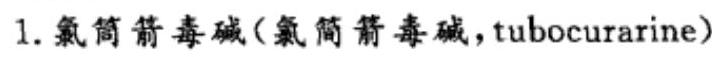
\includegraphics[max width=\textwidth]{2024_07_10_373f31b88d2bf633007bg-143}
\end{center}

是最早应用于临床的非去极化肌松药, 起效较慢,作用时效较长。肌松效果与剂量有关, 0.1 ~ $0.2 \mathrm{mg} / \mathrm{kg}$ 可使四肢肌松驰, $0.4 \sim 0.5 \mathrm{mg} / \mathrm{kg}$ 可使腹肌松驰, $0.5 \sim 0.6 \mathrm{mg} / \mathrm{kg}$ 可满足气管内插管。在体内很少代谢, 静脉注射后 $30 \% \sim 50 \%$ 与蛋白结合, $10 \%$ 以原形由肾排出, $45 \%$ 以原形由胆汁排出。主要用于维持术中肌肉松驰, 但有释放组胺作用,引起低血压和心动过速, 并可引起支气管痉挛。对哮喘和重症肌无力患者应避免使用。现在临床很少应用。

\begin{enumerate}
  \setcounter{enumi}{1}
  \item 泮库涣铰 (pancuronium, 潘可罗宁) 为长时效的非去极化肌松药, 肌松作用强, 作用时间也较长。 $\mathrm{ED}_{95}$ 为 $0.07 \mathrm{mg} / \mathrm{kg}$ 。起效时间为 $3 \sim 6 \mathrm{~min}$,临床作用时间为 $100 \sim 120 \mathrm{~min}$ 。胆碱酯抑制药可拮抗其肌松作用。在临床应用的剂量范围内, 无神经节阻滞作用, 也不释放组胺, 但有轻度抗迷走神经作用, 使心率增快、血压升高。在肝内经羟化代谢, 代谢产物中以 3 -羟基化合物的肌松作用最强, 反复用药后应特别注意其术后残余作用。 $40 \%$以原形经肾排出,其余以原形或代谢产物由胆道排泄。
\end{enumerate}

对于高血压、心肌缺血及心动过速者, 肝肾功能障碍者都应慎用。重症肌无力患者禁忌使用。

\begin{enumerate}
  \setcounter{enumi}{2}
  \item 哌库渗较 (pipicuroum, 阿端) 为长时效非去极化肌松药,其作用强于泮库溴铵,时间也更长。临床应用剂量无心血管不良反应,无组胺释放。其消除主要经肾以原形由尿排出,少量在肝内代谢。肾衰竭时消除半衰期明显延长。 $\mathrm{ED}_{95}$ 为 0.05 ~ $0.06 \mathrm{mg} / \mathrm{kg}$, 气管插管剂量为 $0.1 \mathrm{mg} / \mathrm{kg}, 3 \sim 5 \mathrm{~min}$阻滞完全, 临床维持时间为 $70 \sim 110 \mathrm{~min}$ 。哌库溴铵尤其适用于心肌缺血性疾病和术后需要保留气管导管的危重患者。

  \item 维库涣轱 (vecuronium, 万可松) 为中时效的非去极化肌松药, 肌松作用强,为泮库涋轱的 1〜 1.5 倍, 但作用时间较短。 $\mathrm{ED}_{95}$ 为 $0.05 \mathrm{mg} / \mathrm{kg}$, 起效时间为 $2 \sim 3 \mathrm{~min}$, 临床作用时间为 $25 \sim 30 \mathrm{~min}$ 。其肌松作用容易被胆碱酯酶抑制药拮抗。在临床用量范围内, 不释放组胺, 也无抗迷走神经作用, 因而适用于缺血性心脏病患者。主要在肝内代谢, 代谢产物 3 羟基维库洗胺也有肌松作用。 $30 \%$ 以原形经肾排出, 其余以代谢产物或原形经胆道排泄。

\end{enumerate}

可用于全麻气管内插管和术中维持肌肉松驰。静脉注射 $0.07 \sim 0.15 \mathrm{mg} / \mathrm{kg}, 2 \sim 3 \mathrm{~min}$ 后可以行气管内插管。术中可间断静脉注射 $0.02 \sim 0.03 \mathrm{mg} /$ $\mathrm{kg}$, 或以 $1 \sim 2 \mu \mathrm{g} /(\mathrm{kg} \cdot \mathrm{min})$ 的速度静脉输注, 维持全身麻醉期间的肌松他。手术结束后可用胆碱酯酶抑制药拮抗其肌松残余作用,但约有 $50 \%$ 患者不需用拮抗药可自行恢复神经肌肉传递功能。严重肝肾功能障碍者作用时效可延长, 并可发生蓄积作用。

\begin{enumerate}
  \setcounter{enumi}{4}
  \item 阿曲库轱 (atracurium, 卡肌宁)是合成的双季铵酯型芐异喹啉化合物, 为中时效的非去极化肌松药。肌松作用为维库溴轱的 $1 / 5 \sim 1 / 4, \mathrm{ED}_{95}$为 $0.2 \mathrm{mg} / \mathrm{kg}$, 作用时间较短。起效时间为 $3 \sim$ $5 \mathrm{~min}$, 临床作用时间为 $15 \sim 35 \mathrm{~min}$ 。无神经节阻断作用, 但可引起组胺释放并与用量有关, 表现为皮疹、心动过速及低血压, 严重者可发生支气管痉挛。其优点是消除不依赖肝肾功能, 主要通过霍夫曼 (Hofmann)降解和血浆胆碱酯酶水解, 代谢产物由肾和胆道排泄, 无明显蓄积作用。
\end{enumerate}

可用于全身麻醉气管内插管和术中维持肌肉松驰。静脉注射 $0.5 \sim 0.6 \mathrm{mg} / \mathrm{kg}, 2 \sim 3 \mathrm{~min}$ 后可以行气管内插管。术中可间断静脉注射 $0.1 \sim 0.2$ $\mathrm{mg} / \mathrm{kg}$, 或以 $5 \sim 10 \mu \mathrm{g} /(\mathrm{kg} \cdot \mathrm{min})$ 的速度静脉输注, 维持全麻期间的肌肉松驰。因其体内消除不受肝、肾功能的影响, 适用于肝或肾功能障碍患者。过敏体质及哮喘患者忌用。\\
6. 罗库涣较 (rocuronium, 爱可松)罗库滇轱属氨基甾类肌松药, 分子结构与维库涋轱相似,作用强度是维库滇铵的 $1 / 6$, 属中时效,是目前起效最快的非去极化肌松药。 $\mathrm{ED}_{95}$ 为 $0.3 \mathrm{mg} / \mathrm{kg}$, 插管剂量为 $0.6 \sim 1.0 \mathrm{mg} / \mathrm{kg}$, 起效时间 $50 \sim 90 \mathrm{~s}$, 临床作用时间 $45 \sim 60 \mathrm{~min}$, 维持剂量 $0.1 \sim 0.15 \mathrm{mg} / \mathrm{kg}$, 稳态分布容积 $235 \sim 320 \mathrm{ml} / \mathrm{kg}$, 清除率 $2.4 \sim 3.0 \mathrm{ml} /(\mathrm{kg} \cdot \mathrm{min})$,消除半衰期 100~170min。 $25 \%$ 罗库溴轱与清蛋白结合。罗库溴铵主要经胆道排出, 仅 $9 \%$ 以原形经将排出。临床剂量的罗库溴铵不引起组胺释放,对心率和血压无明显影响。

\begin{enumerate}
  \setcounter{enumi}{6}
  \item 顺阿曲库鋅 (cisatracurium) 属苄异喹啉化合物, 是阿曲库轱的 1-R 构型和 $1^{\prime}-\mathrm{R}$ 构型的顺式异构体,其活性比阿曲库轱强 $50 \%$,为中时效的非去极化肌松药。顺阿曲库轱的 $\mathrm{ED}_{95}$ 为 $0.04 \mathrm{mg} /$ $\mathrm{kg}$, 起效时间约为 $5 \mathrm{~min}$, 临床作用时间为 $15 \sim$ $35 \mathrm{~min}$ 。在临床剂量范围内, 顺阿曲库轱不会像阿曲库轱那样引起组胺的释放, 也无迷走神经、交感神经兴奋。其消除是通过霍夫曼 (Hofmann) 降解反应而失活, 没有明显的蓄积作用。
\end{enumerate}

可用于全麻气管内插管和术中维持肌肉松驰。静脉注射 $0.15 \sim 0.2 \mathrm{mg} / \mathrm{kg}, 2 \sim 4 \mathrm{~min}$ 后可以行气管内插管。术中可间断静脉注射 $0.02 \mathrm{mg} / \mathrm{kg}$, 或以 $1 \sim 2 \mu \mathrm{g} /(\mathrm{kg} \cdot \mathrm{min})$ 的速度静脉输注, 维持全麻期间的肌松弛。因其体内消除不受肝肾功能的影响, 适用于肝或肾功能障碍患者。

\begin{enumerate}
  \setcounter{enumi}{7}
  \item 美库渗釹 (micurounium, 美维松) 为短时效的非去极化肌松药, 能迅速被血浆胆碱酯酶分解, 消除半衰期为 $2 \mathrm{~min}$ 。在体内不直接依赖肝和肾功能。 $\mathrm{ED}_{95}$ 为 $0.08 \mathrm{mg} / \mathrm{kg}$, 七管插管剂量为 $0.2 \mathrm{mg} / \mathrm{kg}$, 起效时间为 $90 \mathrm{~s}$, 临床作用时间 $15 \sim$ $20 \mathrm{~min}$ 。持续静脉滴注 $5 \sim 10 \mu \mathrm{g} /(\mathrm{kg} \cdot \mathrm{min})$, 无蓄积作用。特别适用于短时间手术。
\end{enumerate}

\section*{六、新的肌松拮抗药}
在非去极化肌松药的使用过程中, 临床上常常需要胆碱酯酶抑制药拮抗残余肌松作用。胆䂝酯酶抑制药有许多缺点, 可能引起不良反应, 因此应给予充分的重视。

\begin{enumerate}
  \item 肌松拮抗时机 研究证实 $\mathrm{TOF}<0.6$ 将伴随有肌肉无力, $>0.7$ 时, 就能够睁眼、抬头并具有适当的呼吸能力, 从而长期以来确定了无残留肌松作用的标准必须是 $\mathrm{TOF} \geqslant 0.7$ 。但是近年来的临床观察证实 $\mathrm{TOF}$ 为 0.7 时仍有残留肌松作用。同\\
时还观察到肌松药对颈动脉体的缺氧性通气反应可能具有一定的抑制作用, 只有 $\mathrm{TOF} \geqslant 0.9$ 时, 对缺氧的通气反应才能够完全恢复正常, 且咽喉部功能完全恢复。

  \item 早期拮抗的危险性 给予非去极化肌松药后 $5 \mathrm{~min}$ 或 $\mathrm{T} 1$ 达 $10 \%$ 或 TOF 出现 1 个反应时使用胆碱酯酶抑制药, 不仅不能够拮抗肌松药的作用, 而且能够使潘库溴铵、阿曲库轱以及维库滇轱的作用时间延长。因此, 应该在 TOF 出现 3 个以上反应、TOF 为 0.7 或 $\mathrm{T} 1>25 \%$ 时给予拮抗药,才能够有效拮抗残留肌松作用。

  \item 新型拮抗药 在神经肌肉传导深度阻滞时,使用胆碱酯酶抑制药并不能够有效拮扰肌松作用,反而会延长某些肌松药的肌松作用。胆碱酯酶抑制药的另一个缺点是对胆碱酯酶的抑制作用过长,多在 $60 \mathrm{~min}$ 以上。另外,给予胆碱酯酶抑制药后,乙酰胆碱浓度增加对毒啅碱样受体的兴奋作用可能产生严重的不良反应,这就是为什么临床麻醉中给予胆碱酯酶抑制药拮抗残留肌松作用时,必须同时使用毒草碱样受体阻滞药。新型拮抗药 sugam- madex 已经问世,将对非去极化肌松药的临床实践产生巨大的冲击。它是环糊精 (cyclodextrin)的衍生物, 为晶状结构复合物, 这种新型肌松药的拮抗药不作用于胆碱酯酶, 对毒草碱样受体和烟碱样受体无作用,能够直接和氨基甾类肌松药以 $1: 1$ 比例形成化学鳌合,使得肌松药分子离开乙酰胆碱受体, 从而迅速逆转深度神经肌肉传导阻滞作用, 不引起血流动力学的显著改变。它具有高水溶性使得其制剂静脉注射时能够很好被耐受。它能够有效地逆转氨基甾类肌松药的神经肌肉传导阻滞作用, 但对苄异嗉濑类肌松药和去极化肌松药无效,其中拮抗罗库涋轱比拮抗泮库涋铵、维罗库滇铵效果好。其拮抗阻滞作用效果: 罗库滇铵>维库溴䯃 >泮库溴铵。不良反应的研究表明,未发现 sugammadex引起的血压、心率等心血管系统明显变化, 也没有发现类似应用胆碱酯酶抑制药所引起的心血管系统、呼吸系统和消化系统的不良反应, 无再箭毒化的发生。

\end{enumerate}

(张秀华)

\section*{参考文献}
[1] Ronald D. Miller 主獪. 米勒麻醉学. 普因明,邓小明主泽. 第 6 版(上卷).北京: 北京大学医学出版社, 2006, 69 $106,133-156,235-276,493-590$

[2]全国卫生专业技术资格考试专家委员会. 2008 全国卫生专业技术盗格考试指导丛书 : 麻醉学. 北京: 人民卫

生出版社,2008,145-148

\section*{箕鏱 $\square$}
\section*{作用于胆碱受体的药物}
\section*{一、概 述}
\section*{(一)传出神经系统}
传出神经包括自主神经系统和运动神经系统。前者又分为交感神经和副交感神经。根据释放递质的不同,传出神经可分为胆碱能神经和去甲肾上腺素能神经。胆碱能神经包括以下 4 种。

\begin{enumerate}
  \item 全部副交感神经的节前和节后纤维。

  \item 全部交感神经的节前纤维和极少数交感神经节后纤维,如支配汗腺分泌和骨骼肌血管舒张的神经。

  \item 运动神经。

  \item 支配怪上腺髓质的内脏大神经分支 (相当于节前纤维)。

\end{enumerate}

\section*{(二)胆碱能神经的递质及其受体}
\begin{enumerate}
  \item 递质的合成、储存和释放胆碱能神经的递质是乙酰胆碱 (acetylcholine, ACh)。它由胆碱和乙酰辅酶 $\mathrm{A}$ 在胆碱乙酰化酶催化下, 在胆碱能神经末梢内合成, 然后转运到責泡中储存, 部分以游离形式存在于胞质中。当神经冲动到达神经末梢时,每一蘘泡中的乙酰胆碱以量子释放形式,倾囊而出, 释放到突触间隙, 游离乙酰胆碱也可能直接释出。这些乙酰胆碱与突触后膜上的胆碱受体结合,产生效应。乙酰胆碱释放后,在数毫秒之内即被突触前、后膜上的乙酰胆碱酯酶 (ChE) 水解成胆碱和醋酸并进人循环。部分胆碱可被神经末梢再摄取,重新合成乙酰胆碱。

  \item 胆碱受体 能选择性地与乙酰胆碱结合的受体称为胆碱受体。对以毒䓥碱为代表的拟胆碱药敏感者,称为毒䒼碱型受体 ( $M$ 胆碱受体)。近年来的研究表明,毒草碱受体至少有 5 种主要的亚型,所有的毒草碱样受体均通过 $G$ 蛋白发挥作用。位于神经节细胞膜和骨骼肌细胞膜的胆碱受体对胆碱敏感, 这些部位的受体称为烟碱型胆碱受体 ( $\mathrm{N}$ 胆碱受体),并将位于神经节突触后膜的受体称为 $\mathrm{N}_{1}$ 受体,位于骨骼肌终板膜的称为 $\mathrm{N}_{2}$ 受体。

\end{enumerate}

胆碱能受体的分类、分布及作用见表 2-9-1。

表 2-9-1 胆碱能受体的分类、分布及作用

\begin{center}
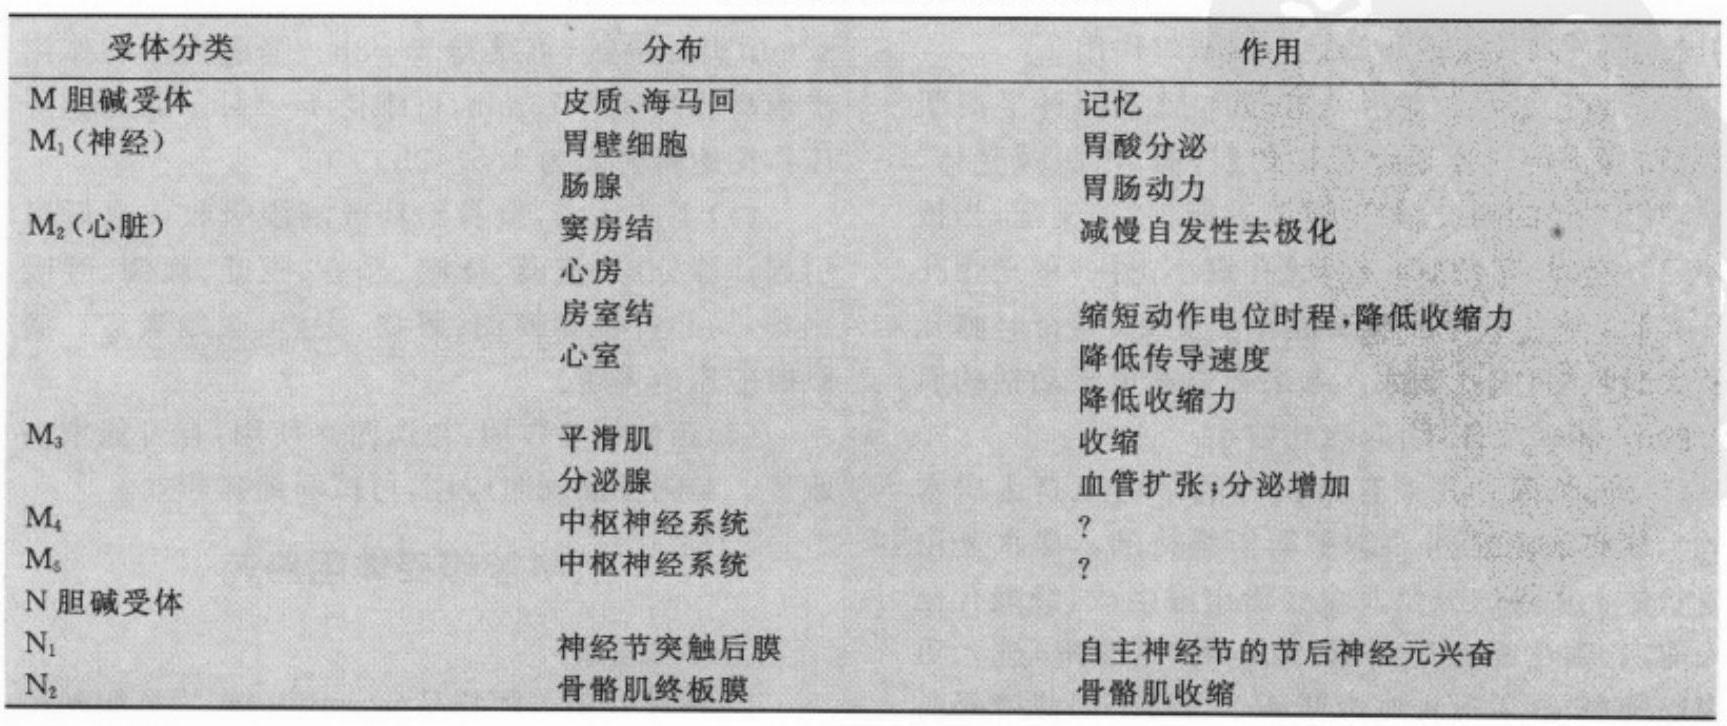
\includegraphics[max width=\textwidth]{2024_07_10_373f31b88d2bf633007bg-146}
\end{center}

\section*{(三)作用于胆碱受体的药物分类}
拟胆碱药是与胆碱能神经递质乙䤐胆碱作用相似的药物。按作用原理可分为两类:一类是直接作用于胆碱受体的拟胆碱药;另一类是抗胆碱酯酶药,不直接作用于胆碱受体,而是通过抑制胆碱酯酶,使胆碱能神经末梢所释放的乙酰胆碱水解减少而发挥拟胆碱作用。能与胆碱受体结合但不产生或较少产生拟胆碱作用, 却能妨碍乙酰胆碱或拟胆碱药与受体结合的药物称为抗胆碱药。抗胆碱药还应包括能抑制乙酰胆碱合成的密胆碱等。

\begin{enumerate}
  \item 拟胆碱药分类 根据对胆碱受体亚型选择性的不同, 拟胆碱药可分为两种。
\end{enumerate}

(1)完全拟胆碱药,除递质乙酰胆碱外,还有氨甲酰胆碱, 它们既能激动 $\mathrm{M}$ 受体, 也能激动 $\mathrm{N}$ 受体。

(2) $\mathrm{M}$ 型拟胆碱药,也称节后拟胆碱药,作用部位主要在节后胆碱能神经所支配的效应器上的 $\mathrm{M}$胆碱受体,如毛果芸香碱。

\begin{enumerate}
  \setcounter{enumi}{1}
  \item 抗胆碱药分类 抗胆碱药可分为 $\mathrm{M}$ 胆碱受体阻滞药、 $\mathrm{N}_{1}$ 和 $\mathrm{N}_{2}$ 胆碱受体阻滞药。 $\mathrm{M}$ 胆碱受体阻滞药包括阿托品类生物碱及其合成代用品。 $\mathrm{N}_{1}$胆碱受体阻滞药又称神经节阻滞药。 $\mathrm{N}_{2}$ 胆碱受体阻滞药又称骨骼肌松驰药。
\end{enumerate}

\section*{二、拟 胆碱药}
\section*{(一)毛果芸香碱 (pilocarpine, 匹鲁卡品)}
\begin{enumerate}
  \item 药理作用是从毛果芸香扁植物叶中提取的生物碱。能直接作用于副交感神经(包括支配汗腺交感神经)节后纤维支配的效应器官的 $M$ 胆碱受体,其对眼和腺体的作用最为明显。
\end{enumerate}

(1)眼:滴眼后易通过角膜, 作用迅速、温和,可引起缩瞳、降低眼内压和调节痉挛等作用。

(1)瞳孔缩小。瞳孔大小受虹膜上两种平滑肌功能的影响,一种是瞳孔括约肌, 有 $\mathrm{M}$ 胆碱受体,受动眼神经的副交感纤维(胆䂸能神经)支配,当该神经兴奋时, 括约肌收缩, 瞳孔缩小; 另一种是瞳孔开大肌, 受去甲肾上腺素能神经支配, 兴奋时瞳孔开大肌收缩, 瞳孔散大。毛果芸香械可激动括约肌上的 $\mathrm{M}$ 胆碱受体,引起瞳孔缩小。

(2)降低眼内压。正常恒定的眼内压是由房水的生成和回流之间动态平衡所维持的。房水是由睷状体上皮细胞分泌及血管渗出液生成, 经瞳孔流人前房,到达前房角间隙, 经小梁网 (滤宋)进人巩膜静脉窦,最后进人血液循环。当房水回流障碍时眼内压升高。毛果芸香战的缩瞳作用使虹膜向中心拉紧, 虹膜根部变薄, 前房角间腙扩大, 滤帘张开,房水易通过巩膜静脉窯进人血液循环。从而降低眼内压。

(3)调节痉挛。使晶状体聚焦适合视近物的过程称为调节。眼睛的屈光度取决于晶状体的曲度变化。晶状体富有弹性, 通常受㫸状小带 (悬韧带)向外缘牵拉, 使晶状体维持于比较扁平的状态。睷状小带又受睫状肌控制, 毛果芸香碱激动睷状肌上 $\mathrm{M}$ 胆碱受体,使腱状肌向眼的中心方向收缩, 致使悬韧带松驰, 晶状体因自身具有的弹性而变凸, 屈光度增加, 使视力调节于视近物清楚, 因物体成像于视网膜前, 故视远物模糊, 这种作用称为调节痉挛。

(2)腺体: 毛果芸香碱能激动腺体的 $\mathrm{M}$ 受体而增加其分泌,以汗腺和唾液腺最为明显。

\begin{enumerate}
  \setcounter{enumi}{1}
  \item 临床应用主要用作缩瞳药, 其吸收作用可用于抗胆碱药阿托品中毒的解救。
\end{enumerate}

(1)青光眼: 青光眼的主要特征是眼内压增高,并引起头痛, 视力减退, 严重者可致失明。根据病理改变的不同,青光眼分为 “闭角型” 与 “开角型”两种。“闭角型”青光眼 (急性或慢性充血性青光眼)患者前房角间隙狭窄,使房水回流障碍,眼内压增高。毛果芸香碱滴眼后使前房角间隙扩大,房水易进入血液循环, 眼内压迅速降低,从而缓解青光眼的各种症状。毛果芸香碱对 “开角型”青光眼疗效较差。

(2)虹膜炎:与扩瞳药交替使用, 可防止虹膜睷状体炎时与晶状体的粘连。

(3)体内过程: 毛果芸香碱具有水溶与脂溶双相溶解度,滴眼易透过角膜,1\%溶液滴眼后 10~ $30 \mathrm{~min}$ 开始缩瞳, 可维持 $4 \sim 8 \mathrm{~h}$ 。降眼内压的作用出现高峰时间约 $75 \mathrm{~min}$, 可维持 $4 \sim 14 \mathrm{~h}$ 。眼药膜降压作用达峰时间为 $1.5 \sim 2 \mathrm{~h}$ 。

(4)不良反应: 全身给药或滴眼吸收人血后可引起汗腺分泌、流涎、哮喘、恶心、呕吐、腹泻、呼吸困难, 局部有视物模糊、眼痛、头痛、眼刺激症。滴眼时应压迫内畔。

(5)药物相互作用: 与地西泮使用, 有可能增高眼压。与阿托品同时应用,可惐弱缩瞳药效。

\section*{三、M 胆碱受体阻滞药}
\section*{(一) 阿托品}
\begin{enumerate}
  \item 药理作用 阿托品 (atropine)作为抗胆碱药\\
的作用机制是其与体内乙酰胆碱竞争 $\mathrm{M}$ 胆碱受体,当阿托品与 $\mathrm{M}$ 胆碱受体结合后乙酰胆碱便失去胆碱能神经递质作用。阿托品对 $\mathrm{M}$ 胆碱受体的阻断作用有较高的选择性, 但大剂量也有阻断 $\mathrm{N}_{1}$胆琙受体的作用。阿托品作用广泛, 对各器官敏感性不同而作用亦有一定的差异。随剂量的增加,可影响下列器官的功能: 腺体分泌减少, 瞳孔扩大和调节麻滔, 胃肠道和膀㬸平滑肌松驰, 心率加快, 中毒剂量可出现中枢兴奋作用。
\end{enumerate}

(1)对心血管系统作用

(1)心率。阿托品对心率的影响取决于给药剂量和心脏迷走神经的功能状态。治疗剂量 $(0.5 \mathrm{mg})$ 的阿托品常可使部分患者心率轻度而短暂地减慢,该作用是由于阿托品在阻断 $M$ 胆碱受体之前兴奋迷走中枢而致。较大剂量 (1〜 $2 \mathrm{mg}$ ),由于其对心脏上 $M$ 胆碱受体的直接阻滞作用, 解除了迷走神经对窦房结的抑制效应, 从而使心率加快。青壮年迷走神经张力高, 阿托品增加心率作用显著, 如肌内注射阿托品 $2 \mathrm{mg}$ ,心率可增加 35~40/ $\min$, 对于幼儿、老年人则影响较小。

(2)房室传导。阿托品抗迷走神经过度兴奋所引起的房室传导阻滞, 促进房室传导, 心电图 P-R 间期缩短。但对心肌梗死患者慎用,因加重心肌缺血可能会激发室䫅。

(3)血管和血压。治疗剂量的阿托品对血管和血压无显著影响。大剂量 $2 \sim 5 \mathrm{mg}$ 具有解除小血管㾏挛, 特别对皮肤血管扩张作用显著,可出现面部潮红温热。在病理情况下,这种扩张小血管作用可改善微循环,恢复重要脏器的血流供应。其扩血管作用的机制不清。虽然降低周围血管阻力, 但由于心排血量增加, 收缩压可轻度升高。由于它直接扩张阻力血管及容量血管, 还可降低中心静脉压、右心房压、肺动脉楤压和肺血容量。

(2)抑制腺体分泌: 小剂量阿托品 (0.3~ $0.5 \mathrm{mg}$ ) 可通过阻断 $\mathrm{M}$ 胆碱受体而明显抑制唾液腺和汗腺的分泌, 引起口干, 皮肤干燥, 支气管腺体也较敏感, 用后呼吸道分泌大为减少。较大剂量可用抑制汗腺分泌而升高体温,称“阿托品热”。同时,可使固液分泌减少。但对胃酸分泌无明显影响, 因胃酸分泌除受迷走神经影响外,还受体液因素胃泌素的调节。

(3)对眼的作用: 瞳孔括约肌和䀽状肌是由胆䂸能神经支配的。当副交感神经兴奋时使之收缩。阿托品阻断 $\mathrm{M}$ 胆碱受体, 上述平淮肌松驰, 从而引起扩瞳, 眼内压升高和调节麻痹。

(1)扩瞳。阿托品对眼的作用与毛果芸香碱相反, 阻断瞳孔括约肌上 $\mathrm{M}$ 胆碱受体。松驰䁨孔括约肌, 使肾上腺素能神经支配的瞳孔扩大肌功能占优势,故引起瞳孔开大。

(2)升高眼内压。由于瞳孔扩大, 使虹膜退向四周边缘, 致前房角间隙变窄, 阻碍房水回流进人巩膜静脉血, 造成眼内压升高。

(3)调节麻痹。阿托品阻断睷状肌上 $\mathrm{M}$ 胆碱受体致腱状肌松驰而退向外缘, 使悬玮带拉紧。晶状体固定在扁平状态, 屈光度降低, 不能将近距离的物体清晰地成像于视网膜上, 只适合于视远物, 而将视近物模糊这一作用称为调节麻痹。

(4)对平滑肌作用。阿托品能松驰多种内胜平滑肌, 其松驰作用取决于平滑肌的功能状态, 且不同器官的平滑肌对其敏感性也不同。对过度活动和痉挛的平滑肌松驰作用最明显。它可绶解胃肠绞痛; 对膀胱通尿肌也有解痉作用; 但对胆道、输尿管和支气管的解㾤作用较弱。阿托品虽能扩张支气管, 但由于它抑制呼吸道腺体分泌而影响排疢,故不能用于平喘。阿托品对子宫影响较小,不影响分娩子宫的收缩和产程, 不抑制胎儿呼吸。

(5)对中枢神经系统作用。一般剂量对中枢神经系统多无显著作用, 仅轻度兴奋迷走中枢。较大治疗量 (1 $2 \mathrm{mg}$ ) 的阿托品对延䯖和大脑均有兴奋作用, 大剂量 $(2 \sim 5 \mathrm{mg})$ 时兴奋作用增强。出现烦躁不安、多语、暇妄; 中毒剂量 (10mg 以上)常产生幻觉、定向障碍、共济失调或惊厥; 严重中毒时则由兴奋转人抑制, 出现昏迷及呼吸麻痹。

\section*{2. 临床应用}
(1)抑制腺体分泌:阿托品常用作麻醉前用药,可抑制腺体分泌,在一定程度上防止喉痉挛和支气管痉挛, 抑制心血管的迷走神经反射,惐低胃肠道张力, 以致蠕动和痉挛。亦可治疗严重的流涎和盗汗症。剂量成人为 $0.4 \sim 0.8 \mathrm{mg}$, 儿童按 $0.01 \sim$ $0.015 \mathrm{mg} / \mathrm{kg}$, 皮下或肌内注射。

(2)抗心律失常: 阿托品常用于治疗迷走神经过度兴奋所致的窦性心动过缓、窧房阻滞和房室传导阻滞等缓慢性心律失常。常用剂量为 0.4 ~ $1.0 \mathrm{mg}$ 。对于器质性的房室传导阻滞无效。对继发于窦房结功能低下而出现的室性异位节律有较好的疗效。大剂量阿托品, 还可用于抢数中毒性严重室性心律失常。但在心肌梗死时要慎用阿托品,以免心率增加后加重心肌缺血缺氧。

(3)解除平滑肌痉挛: 可用于各种内脏绞痛, 其中对胃肠绞痛疗效较好; 对膀胱刺激症状如尿频、尿急及遗尿症也有治疗作用。对胆绞痛和肾绞痛效果较差,需要与镇痛药合用。阿托品虽能扩张支气管, 但由于它抑制呼吸道腺体分泌而影响排痰,故不能用于平喘。前列腺肥大及幽门梗阻的患者禁用。

(4)与新斯的明并用于拮抗非去极化肌松药,剂量为 $0.02 \sim 0.03 \mathrm{mg} / \mathrm{kg}$; 与依酚氯铵并用时剂量惐半,可以防止心动过缓和分泌物过多。

(5)解救有机磷酸酯类中毒。

(6) 眼科。

①治疗虹膜睷状体炎。因阿托品能松驰虹膜括约肌和崨状肌, 使肌肉活动减少, 有利于炎症的消退和止痛; 同时还可预防虹膜与晶体的粘连和发生瞳孔闭锁。

(2)验光配镜。用阿托品滴眼, 使睫状肌的调节功能充分麻病, 晶状体固定, 可准确地测量晶状体的㒴光度。

(3)检查眼底。利用阿托品扩瞳作用, 可观察眼底, 辅助诊断疾病。但因扩瞳和调节麻痹持续时间久,视力恢复缓慢,已为作用短效的后马托品取代。可诱发青光眼发作或使病情加剧, 故青光眼者禁用。

(4)抗休克。主要用于多种感染中毒性休克, 如暴发型流行性脑脊髓膜炎、中毒性痢疾、中毒性肺炎所致的中毒性休克。

\begin{enumerate}
  \setcounter{enumi}{2}
  \item 体内代谢阿托品口服后迅速从肠道吸收, $1 \mathrm{~h}$ 后即达峰值浓度, $3 \sim 4 \mathrm{~h}$ 作用消失。肌内注射后,15~20min 血药浓度达峰值。吸收后很快分布全身,约 $50 \%$ 与血浆蛋白结合,可透过血-脑屏障, 也能通过胎盘进人胎儿循环。 $t_{1 / 2}$ 约为 $2.5 \mathrm{~h}$, 作用持续时间为 $4 \sim 6 \mathrm{~h}$ 。肌内注射后 $12 \mathrm{~h}$ 内大部分随尿排出, 其中原形阿托品约占少量, 大部分为水解产物和莆萄糖酫酸代谢产物。滴眼后, 通过房水循环排出缓慢,故可持续数天至 1 周。

  \item 不良反应阿托品作用广泛,对外周 $M$ 胆碱受体阻滞的结果可造成口干、便秘、排尿困难、视物模糊、皮肤干燥、潮红发热和心悸等不良反应。停药后可自行消失。剂量过大可出现中枢兴奋现象, 如语言不清、糗妄、幻觉、抽搐、惊厥等, 严重中毒时则由兴奋转为抑制,产生昏迷和呼吸麻痹等。误服中毒量的颠茄果、曼陀罗、洋金花或莨宕根茎也可产生上述中毒症状。临床上把这种中枢毒性反应叫做中枢抗胆碱能综合征。静脉注射毒扁豆碱 1 $2 \mathrm{mg}$ 可迅速纠正。

\end{enumerate}

阿托品的最小致死量,成人为 $80 \sim 130 \mathrm{mg}$, 儿童约为 $10 \mathrm{mg}$ 。

\begin{enumerate}
  \setcounter{enumi}{4}
  \item 药物相互作用
\end{enumerate}

(1)与尿碱化药包括含有镁、钙的制酸药、碳酸酎酶抑制药、碳酸氢钠、枸橡酸盐等伍用时,使阿托品排泄延迟。

(2)与金刚烷胺、吩噻嗪类药、其他抗胆碱药、扑米眮、普鲁卡因胺、三环类抗抑郁药伍用时,可加剧阿托品的毒副作用。

(3)与单胺氧化酶抑制药、呋喃唑酮、丙卡巴肼等伍用时,可加强抗毒草碱作用的副作用。

(4)与甲氧氯普胺使用时, 拮抗后者的促进胃肠运动作用。

(5)阿托品可增加地高辛的吸收程度,与镇静药和抗胆碱药有相加作用。

(6)与可卡因、美沙酮和颠茄酊伍用可发生严重便秘、麻痹性肠梗阻和尿潴留。

\section*{(二)东鿓惹碱}
\begin{enumerate}
  \item 药理作用
\end{enumerate}

(1)中枢作用: 东莨宕碱 (scopolamine) 又名亥俄辛(hyoscine),其药理作用与阿托品相似。不同之处是化学结构中有氧桥, 氧桥能抑制中枢, 因此东茛茩碱对中枢神经系统具有抑制和兴奋的双相作用,与阿托品不同的是以抑制为主。东莨若碱的中枢抗胆碱作用比外周强 50 倍, 小剂量 $0.3 \mathrm{mg}$ 即有明显的中枢镇静作用, 剂量增大则出现兴奋, 随后感到困倦、疲劳而进人睡眠状态。更大剂量 $(0.1 \mathrm{mg} / \mathrm{kg})$ 时,皮质抑制作用明显。其中枢抑制机制可能作用于大脑皮质和皮质下结构。如与氯丙嗪或地西泮、氮哌利多合用很快进人麻醉状态。东莄礕碱的遗忘作用强, 并能增强吗啡类的镇痛作用。对吗啡的呼吸抑制作用具有微弱的拮抗作用。不增高基础代谢, 并有抗晕动病和抗震缡麻痹作用。

(2)外周作用: 东莨菪碱的外周作用和阿托品相似,仅在程度上有所不同,其扩瞳、调节麻痹和抑制腺体分泌作用比阿托品强, 对心血管的作用比阿托品弱。

\begin{enumerate}
  \setcounter{enumi}{1}
  \item 临床应用
\end{enumerate}

(1)麻醉前用药:最常用于麻醉前用药,尤其对严重高血压、心脏病、甲状腺功能六进、嗜铬细胞痛等患者更适宜。成人剂量为 $0.3 \sim 0.6 \mathrm{mg}$, 小儿为\\
$0.01 \mathrm{mg} / \mathrm{kg}$ 肌内注射。

(2) 防治军动病和治疗震额麻痹。

(3)静脉复合麻醉: 东芝营碱复合麻醉, 剂量为 $0.04 \sim 0.06 \mathrm{mg} / \mathrm{kg}$ 静脉注射; 但必须同时静脉注射氯丙潫等神经阻滞药, 抑制大剂量东莄若碱的狂躁不安。

(4)大剂量可治疗感染性休克、肺水肿等, 成人剂量每次 $0.3 \sim 0.6 \mathrm{mg}$, 儿童为 $0.01 \sim 0.02 \mathrm{mg} / \mathrm{kg}$静脉注射, 每 $10 \mathrm{~min} 1$ 次, 直至四肢转暖、尿量增加、血压回升、脉压宽至 $30 \mathrm{mmHg}$ 以上, 同时按情况给予抗感染、扩容、纠正酸中毒、强心、肾上腺皮质激素等综合措施。

\begin{enumerate}
  \setcounter{enumi}{2}
  \item 体内过程 东莨若碱口服后自胃肠道迅速吸收。大部分东芝若碱在肝和血浆内代谢。

  \item 不良反应有时会引起烦躁、幻觉等兴奋症状, 主要见于老年人。

  \item 禁忌证 对高热或严重肝肾功能障碍患者慎用, 青光眼患者禁用。

\end{enumerate}

\section*{(三)山鿓若碱}
山莑宕碱 (anisodamine, 654) 是我国科研人员首先从茄科植物唐古特山莨营中提出的一种生物碱。目前常用其人工合成品 654-2 是天然山茷若碱的消旋异构体。

\section*{1. 药理作用}
(1)解痉作用: 山芝若碱是与阿托品相似的抗胆碱药, 在外周对抗乙酰胆碱、解除平滑肌痉挛作用的选择性较阿托品高, 其解痉作用的强度与阿托品类似或稍弱;

(2)可拮抗儿茶酚胺、5-羟色胺等活性物质对微小动脉的痉挛作用, 因而能改善微循环。

(3)抑制唾液腺分泌和扩瞳作用仅为阿托品的 $1 / 20 \sim 1 / 10$ 。

(4) 近年来用山茛蓉碱以缓解眼底小动脉痉挛, 改善微循环。用于治疗急性微循环障碍, 其疗效比阿托品佳。此外, 因不易透过血脑屏障, 故中枢作用极少。除抗胆碱作用外,山芝茇碱的消除半衰期约 $40 \mathrm{~min}$, 排泄也比阿托品快。

\begin{enumerate}
  \setcounter{enumi}{1}
  \item 临床应用山莨营碱可治疗感染性休克,如暴发型流脑、中毒性梸疾、中毒性肺炎、出血性肠炎和出血性媵腺炎及肾炎急性期, 也用于内脏平滑肌绞痛。副作用较少。剂量每次 $0.5 \sim 2 \mathrm{mg}$ 静脉注射。
\end{enumerate}

\section*{(四)格隆滇铵}
\begin{enumerate}
  \item 药理作用 bromide 或 glycopyrrolate) 又名胃长安, 为一合成的 $\mathrm{M}$ 胆㖅受体阻滞药。本品为季胺化合物, 难以透过血-脑屏障, 故无明显中枢作用。格隆滇铵的外周抗胆碱作用强而持久,抗毒踔碱作用为阿托品的 5〜6倍, 作用维持时间较阿托品长 $3 \sim 4$ 倍。其作用特点是抑制胃酸分泌的作用较为确实, 而胃肠道解痉作用不甚肯定。

  \item 临床应用 格隆涭轱可用作麻碎前用药, 剂量为 $4 \sim 8 \mu \mathrm{g} / \mathrm{kg}$ 肌内注射。用新斯的明拮抗非去极化肌松药过量时, 为防止心动过缓, 可加用格隆滇轱, 通常新斯的明每 $1 \mathrm{mg}$ 合用格隆涋轮 $0.2 \mathrm{mg}$ 。

\end{enumerate}

\section*{(五)长托宁}
长托宁 (盐酸戊乙奎醚注射液, penehyclidine hydrochloride), 其化学名称为 3-(2-环成基-2 羟基2 苯基-乙氧基)容宁环烷盐酸盐, 是军事医学科学院毒物药物研究所设计合成的新型抗胆碱能药物,其主要作用特点是对 $\mathrm{M}$ 受体作用的选择性。

\begin{enumerate}
  \item 药理作用 长托宁为新型选择性抗胆碱能药物, 选择性作用于 $M_{1} 、 M_{3}$ 和 $N_{1} 、 N_{2}$ 亚型受体,对于 $M_{2}$ 亚型无明显作用, 抑制节后胆碱能神经支配的平滑肌与腺体生理功能, 对抗乙酰胆碱和其他拟胆碱药物的毒曹碱样和烟碱样作用, 能通过血脑屏障, 故同时具有较强、较全面的中枢和外周抗胆碱作用。治疗剂量的长托宁能够较好地怙抗有机磷毒物中毒引起的中枢中毒症状和外周的毒覃碱样中毒症状, 但是由于对 $\mathrm{M}_{2}$ 受体无明显作用, 因而无心率增加的不良反应。此外, 长托宁作为麻醉前用药,作用于中枢 $\mathrm{M}_{1}$ 受体,可以产生抑制觉醒、抑制学习和记忆、调控其他神经递质的释放等而具有中枢镇静作用。

  \item 临床应用

\end{enumerate}

(1) 最常用于麻醉前用药: 由于长托宁对心脏和神经元突触前膜的 $\mathrm{M}_{2}$ 受体无明显作用, 对恵者心肌耗氧量、心䏥负荷无明显影响, 对心率存在双向中枢性反馈调节机制的保护作用, 尤其适合作为高血压、心脏病、窦性心动过速、甲状腺功能元进和老年患者的麻醉前给药。

(2)用于有机磷农药中毒急救: 有机磷农药中毒为其抑制了神经系统的胆碱酯酶活性, 是乙酰胆碱大量蕃积而产生的一系列中毒症状和体征。长托宁作为新型选择性抗胆碱能药物, 临床研究表明其疗效明显优于传统用药阿托品。主要体现在起效时间和达峰时间更短、消除半衰期延长, 对中枢和外周 $\mathrm{M}$ 受体 (除 $\mathrm{M}_{2}$ 受体) 和 $\mathrm{N}$ 受体作用更强,\\
无阿托品引起的心率增快和心肌耗氧量增加等不良反应。对于改善毒曹碱样症状和烟䂸样症状具有更好的疗效。

(3)改善微循环障碍:休克患者往往存在着微循环障碍、有效循环血量和组织灌注不足。长托宁直接作用于血管平滑肌,可以解除小血管㸚挛,降低循环外周阻力和心脏负荷,起到改善微循环和心脏功能, 增加有效循环血量和组织灌注作用, 从而用于休克和危重患者的治疗, 能够取得较好疗效,当然这种治疗的前提是血容量的充足和抗生素的有效使用。

\begin{enumerate}
  \setcounter{enumi}{2}
  \item 体内代谢 健康成人在肌内注射长托宁 $1 \mathrm{mg}$ 之后, 长托宁在体内吸收速度很快, 给药 $2 \mathrm{~min}$可在血中检测出长托宁, $10 \mathrm{~min}$ 血药浓度达到较高水平,20~30min 达到峰值血药浓度,其消除半衰期约为 $10.34 \mathrm{~h}$,达峰时间快于阿托品,而半衰期是阿托品的 2.5 倍。动物实验表明广泛分布于全身组织,以领下腺最多。 $24 \mathrm{~h}$ 总排除率为给药量的 $94.17 \%$,主要以无药理学活性的代谢产物排出,尿液为其主要排出途径,其次是胆汁。

  \item 不良反应由于能通过血脑屏障,具有中枢镇静作用,因此在老年患者应酌情减量。

\end{enumerate}

(马 虹)

\section*{作用于肾上腺素受体的药物}
\section*{一、概 述}
作用在肾上腺素受体的药物, 如与受体结合后产生拟似递质去甲肾上腺素样作用的药物称为肾上腺素受体激动药 (agonist) 或拟肾上腺素药。如能与受体结合产生阻滞肾上膎素受体或其递质的作用称为肾上腺素受体阻滞 (拮抗) 药 (antagonist)。

自主神经系统又称植物神经系统, 可分为交感神经系统和副交感神经系统。其节前纤维释放的递质均为乙酰胆碱, 但交感神经的节后纤维,除了支配汗腺分泌的乙酰胆碱外, 其余均为兴奋时释放去甲肾上腺素,故称为去甲肾上腺素能神经。

\begin{enumerate}
  \item 递质的合成、储存和释放去甲将上腺素为内源性儿茶酚胺之一, 其生物合成都在肾上腺素能神经元内和轴突内进行, 首先把血液中的酪氨酸输送到交感神经末梢轴浆中, 在胞质中经酪氨酸羖化酶(TH)催化成为二羟基苯乙酯胺(多巴, dopa)。当游离的多巴胺或去甲肾上腺素过多时, 则对多巴脱兼酶(DD) 有反馈性抑制作用。多巴经 DD 催化形成多巴胺, 从胞质进人神经末梢的囊泡, 在多巴胺- - -羟化酶 (DBH) 的催化形成去甲肾上腺素。后者与 ATP 及㫮铬蛋白结合储存于囊泡中, 在胞质中经苯乙胺-N-甲基转移酶 (PNMT) 催化合成肾上腺素, 再返回囊泡中。
\end{enumerate}

当神经冲动到达肾上腺素能神经末梢时, 产生去极化, 改变细胞膜通透性, 使钙离子进人轴突内,促进结合的去甲肾上腺素释放。另外, 其他的拟交感胺直接作用于囊泡内颗粒, 也促使去甲肾上腺素从结合部释放出来。

去甲肾上腺素对受体作用的消失, $75 \% \sim 95 \%$从受体和突触间被神经末梢前膜主动再摄取至交感神经末梢内, 称为掫取 1 , 是通过主动转运系统\\
(或称胺需)完成的。少量的去甲肾上腺索在细胞质内被单胺氧化酶(MAO) 代谢。扩散到突触间隙外,进人循环的去甲肾上腺素可被非神经组织所摄取,称为摄取 2 。摄取 2 与摄取 1 不同, 其容量高,亲和力低, 不具有立体结构特异性, 摄取后即被细胞内的儿茶酚胺氧位甲基转移酶 (COMT) 所代谢。

\begin{enumerate}
  \setcounter{enumi}{1}
  \item 肾上腺素受体 受体 (receptor)是处于细胞膜中的一种特殊蛋白质, 能选择性结合一定的配基 (ligand) (如递质、药物),从而产生特定的效应。在交感神经节后纤维所支配的效应器细胞膜上,能与去甲肾上腺素或肾上腺素结合的受体称为肾上腺素受体。1948 年,Ahlquist 首先将肾上腺素受体分为 $\alpha$ 和 $\beta$ 受体。 $\alpha$ 受体又可分为 $\alpha_{1} 、 \alpha_{2}$ 两种亚型 $\left(\alpha_{1}\right.$受体是指能被 $\alpha_{1}$ 受体激动药甲氧明激动, 且能被 $\alpha_{1}$受体拮抗药哌唑嗪阻滞的 $\alpha$ 受体; $\alpha_{2}$ 受体是指能被 $\alpha_{2}$ 受体激动药可乐定激动,且能被 $\alpha_{1}$ 受体拮扰药育亨宾阻滞的 $\alpha$ 受体)。1967 年, Lands 也根据特异选择性激动药或拮抗药将 $\beta$ 受体分为 $\beta_{1}$ 受体 (是指能被 $\beta_{1}$ 受体激动药多巴酚丁胺激动,且能被 $\beta_{1}$ 受体拮抗药美托洛尔或艾司落尔阻滞的 $\beta$ 受体) 和 $\beta_{2}$ 受体(是指能被 $\beta_{2}$ 受体激动药特布他林激动, 且能被 $\beta_{2}$ 受体拮抗药布他沙明阻滞的 $\beta$ 受体)。

  \item 肾上腺素受体的作用机制 配基儿茶酚胺可作为第一信使与肾上腺素受体结合, 在 $\mathrm{G}$ 蛋白的介导下产生第二信使或激活离子通道而引起生理、生化效应。 $\beta$ 肾上腺素受体与儿茶酚胺结合,在兴奋性鸟嘌呤核苷酸结合蛋白(Gs)介导下, 激活位于细胞膜内面的腺苷酸环化酶 (AC), 促进三磷腺亘 (ATP) 转化成环磷腺苷 (cAMP)。cAMP 是细胞内儿茶酚胺 $\beta$-活性的递质, 即所谓第二信使。 cAMP 激活蛋白激酶而产生生理、生化反应, 促进血糖升高等。Gs 还可直接促使骨骼肌和心肌细胞膜上受体操纵性离子通道开放, 改变膜电位, 如使\\
$\mathrm{Ca}^{2+}$ 进人细胞, 促进细胞内储存 $\mathrm{Ca}^{2+}$ 释放, 并与钙调素结合,产生各种生理效应。儿茶酚胺的正性变力、变时及血管活性作用即因 cAMP 浓度增大所致。同样,抑制磷酸二酯酶对 cAMP 的降解, 也可增大 cAMP 浓度产生同样效应。由于儿茶酚胺的功能,必须有离子化钜参与。1984 年, Rasmussen 称钽离子为第三信使。

\end{enumerate}

$\alpha_{2}$ 肾上腺素受体与其配基结合, 在抑制性鸟嘌呤核苷酸结合蛋白 $(\mathrm{Gi})$ 介导下, 抑制 $\mathrm{AC}$ 的活性,减少 cAMP 的产生, 从而降低蛋白激酶活性。另外 $\mathrm{Gi}$ 还可激活 $\mathrm{K}^{+}$传导,抑制钙通道,激活 $\alpha_{2}$ 受体, 通过负反馈也抑制末梢去甲肾上腺素的释放。

$\alpha_{1}$ 将上腺素受体激动时, 则可能通过另一种 $\mathrm{G}$蛋白而激活磷脂酶 $\mathrm{C}$, 后者可催化膜中的二磷酸磷脂酰肌醇裂解, 产生三磷酸肌醇(IP3)和二酰甘油 (DAG) 等。 IP3 使细胞内 $\mathrm{Ca}^{2+}$ 释放, 增强心肌收缩力等。二酰甘油则激活蛋白激酶 C 而产生效应。

$\beta$ 受体兴奋时, 激活 G-蛋白, 增强腺苷酸环化酶的活性, 使 cAMP 生成增加, 激活蛋白激酶, 从而使靶蛋白磷酸化, 引发效应细胞各种反应。 $\beta_{1}$ 受体分布于心脏组织, 兴奋时使心率增块, 心肌收缩力增强。 $\beta_{2}$ 受体兴奋, 使血管和支气管平滑肌松驰,引起肾分泌怪素, 导致脂肪分解和糖原水解, 血糖升高。随着血糖升高, 钾离子离开肝细胞, 引起血清钾离子一过性升高; 红细胞和肌肉细胞的 $\beta_{2}$ 受体兴奋, 可激活腺苷酸环化酶和 $\mathrm{Na}^{+}-\mathrm{K}^{+}$-ATP 酶, 促进钾离子进人红细胞和肌肉细胞, 可能出现低血钾和引发心律失常。阻断 $\beta_{2}$ 受体能够抑制血清钾离子的这种改变, 故有利于防治心肌梗死后心律失常。 $\beta_{2}$ 受体同样存在于心肌细胞中,正常心室肌细胞的 $\beta$ 受体中, $15 \%$ 为 $\beta_{2}$ 受体, 正常心房肌细胞 $30 \% \sim 40 \%$ 为 $\beta_{2}$ 受体。当慢性心力衰竭时, 由于长期受儿茶酚胺的影响, $\beta_{1}$ 受体数量减少, 但是 $\beta_{2}$ 受体几乎不受影响。因此, $\beta$ 受体在维持心胜功能, 特别是在病变心脏和充血性心力衰竭时, 可增加心肌细胞内 cAMP 水平, 在维持正常心率和心肌收缩力方面具有重要作用。此外, 交感神经末梢也存在 $\beta_{2}$受体,兴奋后可促进去甲肾上腺素的释放。 $\beta_{3}$ 受体存在于脂肪细胞、骨骼肌和肝细胞中, 它与分解代谢和热量生成关系密切。

\begin{enumerate}
  \setcounter{enumi}{3}
  \item 肾上腺素受体密度的调节肾上腺素受体对存在于突触裂隙或血浆中一定量去甲肾上腺素的动力学反应并不是固定不变的, 器官或组织内肾上腺素受体密度和对去甲肾上腺素的反应性, 可因内环境改变或药物应用而发生迅速的改变。在去除交感神经或给予 $\beta$ 受体阻滞药后 $30 \mathrm{~min}$ 内, $\beta$ 受体的数量增加, 即肾上腺素受体上调 (“up” regulation), 这也就是突然停用 $\beta$ 受体阻滞药可导致反跳性心动过速和心肌缺血或心肌梗死发生率增加的机制。
\end{enumerate}

如果持续给予肾上腺素受体激动药, $\beta$ 受体密度显著减少,出现肾上腺素受体下调 (“down” regulation)。 $\beta$ 受体下调出现较慢, 在慢性应激或慢性心力衰竭时, 给予 $\beta$ 受体激动药数小时后, 受体实际上被破坏,必须合成新的受体,才能使交感神经的反应重新恢复到基础状态。

其他的病理生理状态对 $\beta$ 受体密度的影响包括甲状腺功能妄进使 $\beta$ 受体密度增加, 甲状腺功能低下和皮质类固醇减少可使 $\beta$ 受体密度减低。

近年来发现拟将上腺素胺对不同受体的激动还受剂量所影响, 其中尤其以肾上腺素和多巴胺最为突出,如肾上腺素不同剂量对各受体可产生不同效应。成人静脉滴注将上腺素 $1 \sim 2 \mu \mathrm{g} / \mathrm{min}$, 主要兴奋 $\beta_{1}$ 和 $\beta_{2}$ 受体,增强心肌收缩力及扩张周围血管, 甚至在心脏手术后出现低心排血量时应用此小剂量, 正性变力效应远较多巴酝丁胺和强心苷显著,使此老药有了新的发展。增加剂量至 $2 \sim$ $10 \mu \mathrm{g} / \mathrm{min}$, 可兴奋 $\alpha_{1}$ 和 $\beta$ 受体, 但以 $\alpha_{1}$ 受体更显著。 $10 \sim 20 \mu \mathrm{g} / \mathrm{min}$ 主要激动 $\alpha_{1}$ 受体, 强烈收缩周围血管掩盖 $\beta_{2}$ 效应。心脏复苏时须激动 $\alpha_{1}$ 受体, 单次剂量可突破 $20 \sim 200 \mu \mathrm{g} / \mathrm{kg}$ 。

同样,多巴胺对不同受体的剂量依赖效应更为复杂, 如静脉滴注每分钟 $2 \sim 5 \mu \mathrm{g} / \mathrm{kg}$ 可激动 DA 受体, 增加肾及肠系膜血流, 同时激动静脉 $\alpha_{1}$ 受体效应,增加回心血量及前负荷。静脉滴注 $5 \sim 10 \mu \mathrm{g} /$ $\mathrm{kg}$ 则激动 $\alpha_{1}$ 和 $\beta_{1}$ 受体, 并以 $\alpha_{1}$ 受体效应为主, 掩盖了 DA 受体效应。所以临床上为了保持 DA 受体兴奋以促进利尿, 限制剂量在每分钟 $10 \mu \mathrm{g} / \mathrm{kg}$ 以下, 如 $\alpha_{1}$ 受体效应不足, 应并用其他激动药如去甲肾上腺素、去氧肾上腺素, 不应任意增加多巴胺剂量。\\
5. $\alpha_{1}$ 受体对容量血管的效应 多年来对拟肾上腺素类几乎完全强调其对心肌及阻力血管 (小动脉)的作用。事实上容量血管占有 $80 \%$ 的血容量,对维持心血管功能至关重要。如肾上腺素类兴奋 $\alpha$受体, 小动脉在静脉收缩前 $10 \mathrm{~min}$ 先行收缩, 使血压升高, 但每搏量增加常在静脉收缩后。近年来发现,各种拟肾上腺素药对阻力血管及容量血管的收\\
缩作用不尽相同, 产生不同的升压效应。如甲氧明和去氧肾上腺素同为小动脉等效 $\alpha$ 受体激动, 均收缩小动脉, 但前者对容量血管的 $\alpha$ 受体不起效应,升压反应极差。而后者有强烈的静脉收缩效应, 增加回心血量, 升压效果显著。又如去甲肾上腺素对动、静脉收缩均很强烈, 升压反应最强。去氮肾上腺素对静脉的收缩较间羟胺强, 但对动脉收缩不如后者。虽然动、静脉血管收缩均为 $\alpha_{1}$ 受体效应, 但对心排血量却起相反效应。如急速增加小动脉张力,增加后负荷, 对心力衰竭患者更降低心排血量。急速收缩静脉, 增加前负荷, 在心肌收缩限度内可增加心排血量, 但对心力衰竭患者不一定显效,而对血流分配不当引起的感染性休克或椎管内阻滞后的低血压较为有效 (表 2-10-1)。

\section*{二、拟肾上腺素药}
拟肾上腺素药主要通过激活神经元突触前、后膜或靶细胞上将上腺素受体, 或促进去甲肾上腺素能神经末梢释放递质而发挥拟肾上腺素的药理作用,故也称肾上腺素受体激动药。

\section*{$(-) \alpha, \beta$ 受体激动药}
\section*{1. 肾上腺素}
(1)药理作用: 肾上腺素 (adrenaline, epinephrine) 是剂量依赖型激动 $\alpha_{1} 、 \beta_{1}$ 及 $\beta_{2}$ 受体。

(1)心脏。兴奋心肌 $\beta$ 受体,使心肌收缩力增强, 传导加速, 心率加快, 心排血量增多,血压上升,小剂量又能扩张冠状血管,改善心肌供血。给药后显效迅速。近年来发现小剂量肾上腺素的正性变力效应很强, 甚至在冠状动脉搭桥手术的患者静脉滴注肾上腺素 $10 \sim 30 \mathrm{ng} /(\mathrm{kg} \cdot \mathrm{min})$ 时每搏量增加较等剂量多巴酚丁胺 $(2.5 \mu \mathrm{g} / \mathrm{kg}$ 或 $5 \mu \mathrm{g} / \mathrm{kg})$ 还多,且不增加心率, 使此老药新用重新发挥作用。但剂量增大仍可引发心动过速, 提高心肌代谢率, 增加心肌耗氧量, 特别在氦烷麻醅时易激发心律失常,甚至出现室性过早搏动或纤顫。

(2)血管。由于皮肤、黍膜血管壁的 $\alpha$ 受体密度大于 $\beta_{2}$ 受体, 所以皮肤黎膜血管显著收缩, 特别是肾血管也收缩。对冠状血管除了兴奋 $\beta$ 受体外,心脏激动后产生的代谢产物如腺苷等增多, 也有直接扩张冠状血管的作用。由于肾上腺素对激动 $\beta_{2}$ 受体较为敏感, 使血管扩张, 所以如果术前应用 $\alpha$ 受体阻滞药, 再应用肾上腺素可使血压进一步下降,称为“肾上腺素翻转作用”。

(3) 血压。静脉输注 $10 \mu \mathrm{g} / \mathrm{min}$, 由于心脏收缩力增加, 心排血量增加, 故收缩压升高。骨啓肌血管扩张抵消或超过皮肤、㯝膜血管的收缩,因而外周血管阻力降低, 舒张压降低, 所以平均动脉压略有升高或不变,脉压增加。增加剂量时,由于皮肤、䵗膜、肾等血管强烈收缩导致外周阻力迅速增加,舒张压上升, 平均动脉压增高。

(4)呼吸。肾上腺素兴奋支气管平滑肌的 $\beta_{2}$ 受体,扩张支气管,并能抑制肥大细胞释放多种过敏递质, 显著抑制支气管㫴喘。

(5)代谢。加速脂肪分解, 促进糖原分解,升高血糖,增加产热,降低血钾。

(6)中枢神经系统。具有较弱的兴奋作用。剂量过大可引起烦躁、头痛、焦虑和激动。

(2)体内代谢: 口服不能产生有效血药浓度, 肌内注射作用维持 10〜30min, 皮下注射作用可维持 1h。

表 2-10-1 比较 $\alpha_{1}$ 受体兴奋对周围阻力血管及容䈕血管的反应

\begin{center}
\begin{tabular}{|c|c|c|c|}
\hline
\multicolumn{4}{|c|}{血管收缩} \\
\hline
\multicolumn{2}{|c|}{$\alpha_{1}$ 动脉 $\left(\alpha_{1} a\right)$} & \multicolumn{2}{|c|}{$\alpha_{1}$ 静脉 $\left(\alpha_{1} v\right)$} \\
\hline
去甲肾上腺索 & HTH & 去甲肾上腺索 & Hnt \\
\hline
间差胺 & HTt & 去氧肾上腺宗 & Hnt \\
\hline
去氧胃上腺素 & H\# & 间垟胺 & f\#\# \\
\hline
甲氧明 & $\mathrm{HH}$ & 多巴胺 & $H_{\triangle}^{\triangle}$ \\
\hline
肾上闎素 & $0 \sim H^{*}$ & 怪上腺素 & $0 \sim H H^{\Delta}$ \\
\hline
各巴胺 & $0 \sim H H^{*}$ & 麻黄碱 & H \\
\hline
麻黄渽 & $H$ & 甲氧明 & $0 \sim+?$ \\
\hline
多巴酚丁胺 & 0 & 多巴酚丁胺 & $?$ \\
\hline
异丙肾上腺素 & 0 & 昇丙肾上腺索 & 0 \\
\hline
\end{tabular}
\end{center}

*. 大剂量显著; $\Delta$. 小剂量显著

(3)临床应用: 肾上腺素主要用于急性心力衰竭或低心排血量综合征取得很好效应。此外, 低血压、支气管痉挛、过敏性休克及心搏骤停仍为临床常用。禁忌在氛烷麻醉下应用。糖尿病、甲状腺功能元进及高血压患者慎用。肾上腺素不宜口服, 肌内注射较皮下注射吸收迅速。心脏复苏时需激动 a 受体为主, 宜用大剂量, 成人 $0.5 \sim 1 \mathrm{mg}$ 静脉注射或 $1 \mathrm{mg}$ 稀释成 $10 \mathrm{ml}$ 气管内注人, 最大量可达 $10 \mathrm{mg}$ 。小儿 $0.01 \mathrm{mg} / \mathrm{kg}$, 新生儿 $0.01 \sim 0.03 \mathrm{mg} / \mathrm{kg}$静脉注射或气管内注人。过敏性休克及支气管痉挛, 成人可皮下注射 $0.1 \sim 0.5 \mathrm{mg}$, 静脉注射 $0.1 \sim$ $0.25 \mathrm{mg}$ 或 $0.25 \sim 1.5 \mu \mathrm{g} / \mathrm{min}$; 小儿支气管㾤挛静脉注射 $0.01 \mathrm{mg} / \mathrm{kg}$, 过敏可皮下注射 $0.01 \mathrm{mg} / \mathrm{kg}$,每 $15 \min 1$ 次。近年来用于治疗低心排血量综合征宜用小剂量, 单次静脉注射 $50 \mathrm{mg} / \mathrm{kg}$, 显效后静脉滴注 10〜30ng/(kg - min) 维持, 可取得较好效应。大剂量肾上腺素可引发高血压、头痛、心动过速、心律失常、心肌缺血、心悸等。特别与氛烷并用时可能产生恶性室性心律失常。应用时应密切监测血压及心律,切忌过量。

(4)不良反应及注意事项: 主要为心悸、烦躁、头痛及血压升高。剂量过大或输注速度过快时可导致血压㵵然升高, 引起脑出血或心律失常。老年人慎用,禁用于高血压、器质性心脏病、甲状腺功能元进及心绞痛患者。

\section*{2. 多巴胺}
(1) 药理作用: 多巴胺 (dopamine) 是体内合成去甲肾上腺素的前体, 存在于去甲肾上腺素能神经、神经节和中枢神经系统, 是重要的神经递质, 同时也是肾上腺素及去甲肾上腺素的中间化合物。

(1)心血管系统的作用。多巴胺具有剂量依赖性激动 $\alpha$ 受体及 $\beta_{1}$ 受体, 对 $\beta_{2}$ 受体作用微弱。还有特殊的多巴胺受体分布在肾、肠系膜血管床及心、脑。此外还间接地促进去甲肾上腺素能神经末梢释放去甲肾上腺素, 即酪胺样效应。静脉输注 5~ $10 \mu \mathrm{g} /(\mathrm{kg} \cdot \mathrm{min})$ 的多巴胺, 可使每搏量增加, 心排血量增加, 收缩压升高, 心率增加或没有变化。同时可增加冠状动脉、门静脉及肾血流量, 舒张压变化不明显, 平均动脉压增加, 脉压增大。静脉输注 $10 \mu \mathrm{g} /(\mathrm{kg} \cdot \mathrm{min})$ 或更大剂量; $\alpha_{1}$ 受体作用占优势,使去甲肾上腺素释放增加, 收缩压、中心静脉压及肺动脉压升高, 心率加快,心排血量降低, 有时可引发心律失常。

(2)将脏。小剂量 $[1 \sim 4 \mu \mathrm{g} /(\mathrm{kg} \cdot \mathrm{min})]$ 多巴胺可激动近曲小管段血管的 $\mathrm{D}_{1}$ 受体, 扩张肾血管, 显著增加肾血流量及肾小球滤过率, 促进排钠利尿,减少肾小管再吸收。中剂量 $[4 \sim 10 \mu \mathrm{g} /(\mathrm{kg} \cdot \mathrm{min})]$则主要激动 $\alpha$ 受体,掩盖了 DA 受体效应。所以,小剂量对肾功能保护作用曾被称为 “情剂量”。但近年对照研究表明, 将剂量虽有显著利尿效应, 但并不能改善肾的肌䣶清除率, 能否起到肾保护作用尚有争议。

(3)体内过程。与其他儿茶酚胺类一样, 不易通过血脑屏障,对中枢作用轻微。多巴胺在体内迅速被 COMT 和 MAO 代谢, 所以也应静脉注射为宜。

(2)临床应用: 多巴胺适用于伴有水钠潴留的充血性心力衰竭及低血压患者, 根据其小剂量利尿效应也可用于将功能不良患者。临床多采用中小剂量静脉滴注, 即 $<10 \mu \mathrm{g} /(\mathrm{kg} \cdot \mathrm{min})$ 。如果升压效果不显著应辅用去甲肾上腺素或去氧肾上腺素, 尽量保持多巴胺激动 DA 受体效应。为了保护肾功能促进利尿而不需正性变力作用时可应用小剂量滴注, 即 $1 \sim 4 \mu \mathrm{g} /(\mathrm{kg} \cdot \mathrm{min})$ 。因多巴胺可增加肺动脉压,所以右侧心力衰竭时慎用。

(3)不良反应: 可有恶心、呕吐。剂量过大或用药速度过快可导致心律失常。如果漏出血管外可导致局部坏死。不宜与氟哌利多、氯丙嗪等多巴胺受体阻滞药合用,以免拮抗内脏血管扩张作用。

非诺多泮是一种选择性 DA 受体激动药和血管舒张药 (是多巴胺作用的 $6 \sim 9$ 倍), 可以增强尿钠排出, 增加利尿作用和肾血流量。由于其较低的生物利用度和临床试验中表现的不确定结果, 非诺多泮现在已经不再用于治疗慢性高血压和 CHF。但静脉注射剂量从 $0.1 \sim 0.8 \mu \mathrm{g} /(\mathrm{kg} \cdot \mathrm{min})$ 的非诺多泮已经被证明对严重高血压有效。它可以作为硝普钠的替代品, 并具有相对较少的副作用 (没有硫氮化物毒性、反跳作用或冠脉钛血), 还能改善肾脏血供。在 $15 \mathrm{~min}$ 内非诺多泮达到峰效应。

\section*{3. 麻黄碱}
(1)药理作用: 麻黄碱(ephedrine) 又名麻黄素,为非儿茶酚胺类, 是从麻黄中提取的生物碱。麻黄䂝类似肾上腺素, 可激动 $\alpha$ 及 $\beta$ 受体, 增强心肌收缩力, 提升血压, 作用较肾上腺素弱, 但作用持久可达 $1 \mathrm{~h}$ 。还能促进去甲肾上腺素能神经末梢释放去甲肾上腺素。另外, 对支气管平滑肌也有松驰作用。口服易吸收, 不受 COMT 及 MAO 代谢影响,给药后大部分经尿排泄。

(2)临床应用: 临床上应用于治疗低血压, 特别\\
在椎管内麻醉后引起的低血压及术中牵拉内脏引起的反射性低血压。剂量为 $5 \sim 30 \mathrm{mg}$ 静脉注射,如应用 1〜2 次无效, 应改用其他激动药。因该药易产生急性耐药现象, 剂量过大时还可兴奋大脑皮质及皮质下中枢而引起不安。也可用于防治支气管哆喘的发作。滴鼻可消除鼻䵑膜肿胀。

(3)不良反应: 可出现精神兴奋、失眠、不安。

\section*{(二) $\alpha_{1}$ 受体激动药}
\begin{enumerate}
  \item 去甲肾上腺素
\end{enumerate}

(1) 药理作用: 去甲肾上腺素 (noradrenaline, norepinephrine) 是去甲肾上腺素能神经末梢释放的递质, 怪上腺㵦质分泌少量。主要激动 $\alpha_{1}$ 受体,对心胜 $\beta_{1}$ 受体也有兴奋作用, 对 $\beta_{2}$ 受体几无作用。

(1)心脏。使心胜收缩力增强, 心率轻度增快。又因小动脉、小静脉高度收缩, 外周阻力增加, 回心血量增多, 使血压显著升高, 也使冠状动脉灌注压升高。激动心肚还使其代谢产物腺苷增加, 舒张冠状血管。

(2)血管。强烈的收缩外周血管, 降低了组织灌注, 包括肾血管收缩, 显著降低肾血流, 特别在 20 世纪 70 年代发现动脉注人去甲肾上腺索诱发急性怪衰竭的动物模型以来, 大大限制了临床应用。近年来进一步研究去甲肾上腺素对肾功能的影响, 认为肾血流改变对肾功能的影响不如肾小球滤过率影响大。由于肾受交感神经支配, $\alpha_{1}$ 受体分布在肾小叶间动脉、输人和输出小动脉、系膜细胞和将小管段, 是去甲肾上腺素调节肾血流及肾小球内压的基础。当去甲肾上腺素引起肾血流显著下降时, 由于输出小动脉收缩较输人小动脉强, 使肾小球内压升高而代偿了肾血流量下降对肾功能的影响, 肾小球滤过率改变不明显。对健康志愿者输人去甲肾上腺素使肾血流量降低 $50 \%$, 也不引起肾小球滤过率改变。甚至对感染性休克患者应用多巴胺不能利尿, 改用去甲肾上腺素虽肾血流低下但仍可迅速改善无尿状态。因此, 近年来去甲肾上腺素开始再被临床重用。

(3)体内过程。去甲肾上腺素起效迅速, 停药后 $1 \sim 2 \min$ 失效, 大部分被 MAO 及 COMT 代谢。

(2)临床应用: 主要用于治疗低血压, 特别对于感染性休克高排低阻者, 在充分扩容后用去甲桶上腺素可显著见效。此外, 咟铬细胞痹切除后低血压常需要去甲肾上腺素静脉注射维持一段时间。近年来常与扩血管药物并用于治疗低心排血量或难治性休克患者。长时间静脉滴注时, 即使未渗漏至皮下也易导致局部组织缺血、坏死。可在去甲肾上腺素溶液中加酚妥拉明 (2:1) 预防, 还可改善组织灌注。由于静脉滴注时血压波动剧烈, 所以应持续监测血压变化。

(3)不良反应:静脉输注时间过长、浓度过高或漏出血管外可导致局部组织缺血坏死。可在漏出部位应用酚罗拉明或局部麻醉药浸润注射以减轻损害。使用不当可造成肾损害。高血压、动脉硬化及器质性心脏病禁用。

\begin{enumerate}
  \setcounter{enumi}{1}
  \item 间经胺 (metaraminol, 又名阿拉明 aramine)
\end{enumerate}

为人工合成的非儿茶酸胺类药, 具有直接和间接作用于肾上腺素受体, 不易被 COMT 和 MAO 降解的特性。其作用类似于去甲肾上腺素, 效应稍弱, 但持续时间稍长。主要激动 $\alpha_{1}$ 受体, 对 $\beta$ 受体作用稍弱。长时间滴注可耗尽体内储存的去甲肾上腺素而失效,应改用去甲肾上腺素。

\begin{enumerate}
  \setcounter{enumi}{2}
  \item 甲氧明 (methoxamine, vasoxyl) 甲氧明是人工合成的非儿茶酚胺药。只选择性激动 $\alpha_{1}$ 受体,对 $\beta$ 受体和 $\alpha_{2}$ 受体无作用。因只激动小动脉 $\alpha_{1}$ 受体, 很少兴奋小静脉 $\alpha_{1}$ 受体, 所以回心血量不多, 血压升高不明显。但甲氧明反射性促进迷走神经兴奋, 可治疗室上性心动过速, 成人剂量为 $10 \sim 20 \mathrm{mg}$静脉注射。

  \item 去氧肾上腺素 (phenylephrine, neosynephrine)又名苯肾上腺素、苯福林、新福林, 也是人工合成的非儿茶酭胺类药物。性质稳定, 作用时间为 5 10min, 直接激动 $\alpha_{1}$ 受体, 收缩小动脉及小静脉,稍微促去甲肾上腺素释放, 对 $\beta$ 受体作用很弱。升高血压可反射性减慢心率, 对心肌应激性很小。主要用于治疗低血压, 常用于低血容量性休克及血管阻力降低性低血压。单次静脉注射 $40 \sim 100 \mu \mathrm{g}$, 静脉滴注 $0.15 \mu \mathrm{g} /(\mathrm{kg} \cdot \mathrm{min})$, 按血压调整。也可用于室上性心动过速。心肌缺血患者及前负荷增高患者切忌单独应用, 应与硝酸甘油并用。

\end{enumerate}

\section*{(三) $\alpha_{2}$ 受体激动药一一可乐定}
可乐定 (clonidine) 为选择性 $\alpha_{2}$ 受体激动药, 可通过激活中枢 $a_{2}$ 受体 (负反馈机制) 抑制去甲肾上腺素能神经末梢释放去甲肾上腺素, 达到抗高血压、降低血管阻力及心率的作用。通过报制脊閮 $\mathrm{P}$物质释放, 并激活脊䚛中神经元突触 $\alpha_{2}$ 受体而产生镇痛作用。还可能激动蓝斑核中 $\alpha_{2}$ 受体的抑制效应产生较强的镇静作用, 增强麻醉效应。因不阻滞肾上腺素受体, 可保持机体正常反射功能。显效时间 $30 \sim 60 \mathrm{~min}$, 峰值时间 $2 \sim 4 \mathrm{~h}$, 持续 $8 \mathrm{~h}$ 。 $50 \%$ 在\\
肝内代谢, $20 \%$ 由胆汁排出, $80 \%$ 由肾排出。主要用于治疗高血压,成人 $0.1 \sim 1.2 \mathrm{mg} / \mathrm{d}$, 分次口服。近年来已应用于临床麻醉。麻醉前用药口服 0.2 〜 $0.3 \mathrm{mg}(5 \mu \mathrm{g} / \mathrm{kg})$ 可显著镇静,减少麻醉药及阿片类药物剂量 $40 \% \sim 50 \%$, 还有预防与管内插管的心血管反应的作用。椎管内镇痛应用可乐定有显著的镇痛效应, 并延长镇痛时间。硬膜外注人 70 〜 $150 \mu \mathrm{g}$ 可镇痛 $3 \sim 4 \mathrm{~h}$, 且无恶心、乏力及呼吸抑制现象。在布比卡因椎管麻醉时加可乐定 $150 \mu \mathrm{g}$, 可显著延长作用时效。同样,在神经阻滞的局麻液中加可乐定 $150 \mu \mathrm{g}$ 也可强化及延长镇痛时间。长期用药患者突然停药可出现反跳性高血压或心律失常。可能有嗜睡、塥梦、不安、焦虑或压抑感。静脉注射可能一过性兴奋外周 $\alpha$ 受体,导致急性血压升高。

(四) $\beta$ 受体激动药

\section*{1. 异丙肾上腺素}
(1)药理作用:异丙肾上腺素 (isoproterenol, isoprenaline, isuprel) 是人工合成的儿茶酚胺类激动药, 是非选择性 $\beta$ 受体激动药。

(1)心血管。可显著增加心率,加速房室传导及心肌收缩, 降低血管阻力。因为该药无选择性扩张皮肤及肌肉血管,使体内血液分布到非生命器官,降低了生命器官血流灌注。更严重的是该药可导致心动过速使平均动脉压及舒张压降低, 心肌供血减少而需氧量增加, 还可导致冠状动脉窃血现象,因而不宜常规用于抗休克及心力衰竭治疗。

(2)支气管。异丙将上腺素可激动 $\beta_{2}$ 受体缓解许多平滑肌痉挛, 特别对支气管和周肠道平滑肌作用更明显。另外还具有抑制组胺等过敏性物质释放的作用。该药起效迅速,作用持续约 $1 \mathrm{~h}$, 经肝、肺代谢, $40 \% \sim 50 \%$ 以原型由怪排出。

(2)临床应用: 目前主要用于 III 度房室传导阻滞患者在起搏器安置前又对阿托品无效时。偶尔也用于急性心动过缓、睹喘及肺源性心脏病合并特发性或继发性肺动脉高压患者。心脏移植术后均须用异丙肾上腺素维持心率及心肌收缩一段时间。另外, $\beta$ 受体阻滞药中毒患者首选此药。应用该药容易导致心肌供氧和需氧失衡, 造成心律失常、心肌缺血、高血压或中枢神经兴奋。反复应用易产生耐药现象。

(3)不良反应: 常见心悸、头晕。禁用于冠心病、心肌类或甲状腺功能六进等虫者。

\section*{2. 多巴酚丁胺}
(1)药理作用: 多巴酚丁胺(dobutamine)与多巴胺结构相似, 属人工合成的儿茶酚胺类药,可选择性激动 $\beta_{1}$ 受体, 对 $\beta_{2}$ 受体及 $\alpha$ 受体作用较弱, 对多巴胺受体无激动作用,也无酪胺样作用。

(1)心血管。对心脏产生正性变力效应, 并轻度扩张血管,所以升压效应不如多巴胺显著, 但心排血量增加较多。多巴酚丁胺小剂量时将血流量不如多巴胺,但随剂量增大可增加心排血量,并继发性增加肾血流量。又因其抑制缺氧性肺血管收缩,所以可有效治疗右侧心力衰竭。

(2)体内过程。该药口服无效,静脉注射后 1 〜 $2 \mathrm{~min}$ 显效,持续约 $5 \mathrm{~min}$ 。经肔内代谢, 经肾排泄。消除半衰期为 $2 \mathrm{~min}$, 很少产生耐药现象。

(2)临床应用: 主要适用于急性心力衰竭及低血压患者,对心胜手术后低心排血量患者效果较好。常用剂量成人为静脉滴注 $2 \mu \mathrm{g} /(\mathrm{kg} \cdot \mathrm{min})$ 开始, 逐渐增量直至显效。剂量不超过 $10 \mu \mathrm{g} /(\mathrm{kg}$ ・ $\mathrm{min}$ ) 很少引起心动过速。小儿可静脉滴注 5~ $20 \mu \mathrm{g} /(\mathrm{kg} \cdot \mathrm{min})$ 。

(3)不良反应: 偶见恶心、呕吐、心悸。患有特发性肥厚型主动脉瓣下狭窄患者禁用。应用该药偶尔可出现心动过速性心律失常,尤其使心房纤㖣患者增加心室率。

\begin{enumerate}
  \setcounter{enumi}{2}
  \item 多培沙明 (dopexamine) 多培沙明也是人工合成的儿茶酚胺类药。具有极强的激动 $\beta_{2}$ 受体及较强的激动 DA 受体效应,对 $\beta_{1}$ 受体激动微弱,对 $\alpha$ 受体无效应。另外,还明显抑制神经释放到末梢的去甲肾上腺索再摄取,从而产生间接的拟交感胺效应, 显示正性变力及扩张阻力血管效应, 对容量血管无影响。由于健康人左心室 $\beta_{1}$ 受体较 $\beta_{2}$ 受体为多(约 $4: 1$ ), 但在严重心力衰竭时,此比例下降至几乎相等,所以该药用于心力衰竭患者激动 $\beta_{2}$ 受体较非心力衰竭患者产生更强的正性变力作用。如果健康志愿者静脉滴注多培沙明 $1 \sim 8 \mu \mathrm{g} /(\mathrm{kg} \cdot$ $\mathrm{min}$ )时心率随剂量增大而增快, 心排血量也增加,但平均动脉压很少变化。对慢性心力衰竭患者给药后心率增加, 平均动脉压轻度升高, 肺动脉压、肺动脉楔压及右心房压均降低,体血管阻力显著下降及心脏指数显著升高。对急性心力衰竭患者大致相似,但肺动脉压、肺动脉贺压及右心房压无改变,所以适用于心力衰竭或低心排血量患者。该药也激动 DA 受体,更使肾血管阻力显著降低, 对肾缺血损害有保护作用。对休克患者特别合并有感染性休克患者还能保护肠道血供,堿少乳酸生成。
\end{enumerate}

\section*{(五) $\beta_{2}$ 受体激动药一沙丁胺醇和特布他林}
沙丁胺醇 (salbutamol) 又名羟甲叔丁肾上腺素, 商品名为舒喘灵和唃必罗。特布他林 (terbutaline) 又名间羟叔丁肾上腺素, 商品名间羟舒喘灵和间羟嗉必罗。均为人工合成的选择性较强的 $\beta_{2}$ 受体激动药, 对 $\beta_{1}$ 受体作用轻微, 对 $\alpha$ 受体无激动作用, 可显著扩张支气管平滑肌而不伴心率增快。口服 $30 \mathrm{~min}$ 显效, 可持续 $4 \sim 8 \mathrm{~h}$, 也可气雾喷人。该药经肝内代谢, 肾排出。适用于治疗哮喘,预防用药时可口服 $2.5 \sim 5 \mathrm{mg}$, 需要时每 $6 \mathrm{~h} 1$ 次,发作时也可用喷雾吸人或皮下注射 $0.25 \mathrm{mg}$, 小儿剂量为 $3.5 \sim 5 \mu \mathrm{g} / \mathrm{kg}$ 皮下注射。静脉滴注 $10 \mu \mathrm{g} /$ min。近年认为治疗急性高钾血症有效, 剂量为 $10 \sim 100 \mu \mathrm{g} / \mathrm{kg}$ 静脉注射。可能出现心率增快、心律失常、肺水肿、低钾血症或中枢神经系统兴奋症状。

\section*{三、肾上腺素受体阻滞药}
肾上腺素受体阻滞药对肾上腺素受体有较强的亲和力, 但缺乏内在活性, 一旦与其受体结合, 即阻滞神经递质或将上腺素受体激动药与相应受体结合从而产生阻滞(拮抗)效应。根据药物对 $\alpha$ 和 $\beta$受体的不同选择性, 可分为 $\alpha$ 受体阻滞药、 $\beta$ 受体阻滞药和 $\alpha, \beta$ 受体阻滞药。

\section*{$\alpha$ 受体阻滞药}
$\alpha$ 受体阻滞药包括非选择性 $\alpha$ 受体阻滞药 (即对 $\alpha_{1}$ 和 $\alpha_{2}$ 受体均有阻滞作用, 如短效的酚罗拉明和长效的酚苄明) 、选择性 $\alpha_{1}$ 受体阻滞药 (如哌唑嗪)和选择性 $\alpha_{2}$ 受体阻滞药(育亨宾)。

\begin{enumerate}
  \item 酚芐明
\end{enumerate}

(1)药理作用: 酚芐明 (phenoxybenzamine) 为卤化烷基胺化合物, 是 $\alpha$ 受体的不可逆性非竞争性阻滞药。它可以与受体形成共价键, 而且受体的功能恢复需要重新合成新的受体。这种药物不仅仅结合失活的 $\alpha_{1} 、 \alpha_{2}$ 受体, 同时也与同去甲紧上腺素的神经元性和非神经元性摄取有关的蛋白相结合。

酚芐明可降低外周血管阻力, 反射性刺激交感神经 $\beta_{1}$ 受体,导致心排血量增加。酚芐明阻断心脏交感神经抑制性突触前 $\alpha_{2}$ 受体, 并通过抑制掫取从而减慢心肌内去甲肾上腺素的清除。这些效应同样可增加心排血量。应用酚苄明可导致直立性低血压, 这是因为当患者直立时, 压力受体机制无法被激活, 而且血管内 $\beta_{2}$ 受体的无对抗性激活也降低了血管阻力。\\
(2)临床应用:酚芐明仍是嗜铬细胞面术前首选用药。其独特的非竞争性 $\alpha$ 受体阻断特性可以避免手术时肿瘤操作造成的儿茶酚胺突发性冲击。推荐剂量为 $1 \sim 2 \mathrm{mg} /(\mathrm{kg} \cdot \mathrm{d})$ 。酚芐明也可用于缓解神经源性豜胱或前列腺增生造成的尿潴留, 治疗神经源性膀胱的剂量为: 儿童 $0.3 \sim 0.5 \mathrm{mg} /(\mathrm{kg} \cdot \mathrm{d})$;成人 $10 \sim 20 \mathrm{mg} /(\mathrm{kg} \cdot \mathrm{d})$ 。口服酝芐明可用于降低血压。

\begin{enumerate}
  \setcounter{enumi}{1}
  \item 酚妥拉明和妥拉唑啉
\end{enumerate}

(1)药理作用: 酚妥拉明是咪唑啉 (imidazoline)的衍生物, $\alpha$ 受体阻滞药。对 $\alpha_{1} 、 \alpha_{2}$ 受体阻滞作用的选择性较低, 对 $\alpha_{1}$ 受体的阻滞作用比对 $\alpha_{2}$ 受体的作用强 $3 \sim 5$ 倍。

(1)血管。酚妥拉明不仅可以阻滞血管平滑肌 $\alpha_{1}$ 受体,还具有较强的直接舒张血管作用。酚妥拉明对阻力血管的作用大于容量血管,引起周围血管阻力下降, 血压降低, 肺动脉压下降。

(2)对心脏具有兴奋作用, 使心肌收缩力增强,心率增快,心排血量增加。

(2)体内过程: 静注后起效迅速, 2 min 内药效即达高峰。该药经情快速排泄,故作用时效仅维持 $5 \min$ 左右, 因此需要持续静脉输注用药。

(3)临床应用: 酚妥拉明主要用于控制围术期高血压, 特别适用于嗜铬细胞面手术探查及分离肿㾇时控制血压异常升高, 故为该手术中必备药物,可以将酚罗拉明 $10 \sim 20 \mathrm{mg}$ 稀释到 $100 \mathrm{ml}$ 持续静滴, 必要时静脉推注 $1 \sim 2 \mathrm{mg}$, 常需与小剂量 $\beta$ 受体阻滞药伍用,预防心动过速。局部浸润可避免肾上腺素受体激动药外漏所引起的局部组织缺血或坏死。

(4)不良反应:剂量过大或血容量严重不足时可发生严重低血压。可出现副交感神经立进,如肠蠕动增加、腹泻、腹痛等以及组胺样 (皮肤潮红和胃酸分泌增加)作用。周及十二指肠溃疡及冠心病患者慎用。

妥拉唑啉 (tolazoline) 用于治疗新生儿持续性肺动脉高压。其主要的不良反应是低血压及反射性心动过速、心律失常、肺及胃肠道出血。由于吸人 NO 应用于临床,妥拉唑欶已不再用于治疗肺动脉高压。妥拉唑啉血熪半衰期为 $3 \sim 13 \mathrm{~h}$, 以原型经肾排出。

\begin{enumerate}
  \setcounter{enumi}{2}
  \item 哌唑嗪 (prazosin) 是强力的选择性 $\alpha_{1}$ 受体阻滞药, 经常作为药理试验中的首选用药。它能够拮抗去甲肾上腺素和肾上腺素引起的血管收缩,\\
使外周血管阻力下降, 回心静脉血减少。尽管不常出现心率增快, 但常出现直立性低血压。与其他抗高血压药物不同,哌唑㗪可以降低低密度脂蛋白并提高高密度脂蛋白。它常被用于治疗高血压, 还用于治疗充血性心力衰竭 (CHF), 但与血管紧张素转化酶抑制药 (ACEIs) 类药物不同,它并不能延长患者寿命。哌唑嗪在肝内代谢。

  \item 盐酸鸟拉地尔 (urapidil) 商品名压宁定 (ebrantil)或优匹敌,是苯哌嗪取代的朓㗀啶衍生物, 主要活性成分为盐酸哌胺甲腚啶。乌拉地尔能够阻滞血管平滑肌 $\alpha_{1}$ 受体, 同时对交感神经末梢 $\alpha_{2}$受体也有中度阻滞作用, 还可通过血脑屏障,激活中枢 5-羟色胺-1A 受体,抑制延髓心血管中枢的交感反馈调节,引起外周血管扩张、阻力降低, 血压下降。血压降低的同时,心率并不增快,每搏量和心排血量不变或略有增加。对肺血管的舒张作用大于体循环血管, 可以降低肺动脉高压。

\end{enumerate}

静脉注射后, 分布半衰期为 $35 \mathrm{~min}$, 消除半衰期为 $2.7 \mathrm{~h}$, 血浆蛋白结合率为 $80 \%$, 经肝内代谢, $10 \% \sim 15 \%$ 以原型随尿排出。

静脉用药主要用于控制围术期高血压。盐酸乌拉地尔降压效能较为缓和, 每次注射 $25 \mathrm{mg}$, 必要时可重复给药。麻醉诱导前静脉注射 $0.6 \mathrm{mg} / \mathrm{kg}$,气管导管拨除前给予 $0.4 \mathrm{mg} / \mathrm{kg}$, 可明显减轻气管内插管和拔管时的心血管反应。盐酸乌拉地尔还可用于治疗充血性心力衰竭, 静脉注射 $0.5 \mathrm{mg} / \mathrm{kg}$后,以 $4 \mu \mathrm{g} /(\mathrm{kg} \cdot \mathrm{min})$ 速度持续静滴。

\begin{enumerate}
  \setcounter{enumi}{4}
  \item 育亨宾 (yohimbine) 为吼噪烷胺生物碱,可特异性阻滞外周突触前膜的 $\alpha_{2}$ 受体, 并可通过血脑屏障进而阻滞中枢神经系统中的 $\alpha_{2}$ 受体。促进去甲肾上腺素释放, 特别使海绵体神经末梢释放较多的去甲肾上腺素,减少阴茎静脉回流,有利于充血勃起。少量可刺激脊髄勃起中枢使性功能立进。消除半衰期仅 $35 \mathrm{~min}$ 。临床用于治疗功能性阳萎。口服 5〜 10mg,3/d。不良反应有恶心、呕吐、皮肤潮红。偶有心悸、失眠、眩晕等。
\end{enumerate}

\section*{四、 $\beta$ 受体阻滞药}
\section*{(一)摡述}
$\beta$ 受体阻滞药大约 10 种,包括非选择性 $\beta$ 受体阻滞药(即对 $\beta_{1}$ 和 $\beta_{2}$ 受体均有阻滞作用, 如普萗洛尔)、选择性 $\beta_{1}$ 受体陮滞药 (如艾司洛尔)。

\section*{1. 药理作用}
(1)心血管作用: 阻滞 $\beta_{1}$ 受体可减慢心率,减弱心肌收缩力, 使心排血量降低, 血压稍降低。当机体交感神经张力增加或运动时, 上述作用明显。同时可降低心肌氧耗,抑制突房结自律性,减慢传导。

(2)支气管平滑肌: 阻滞支气管平滑肌 $\beta_{2}$ 受体,可使平滑肌收缩, 因而诱发支气管哮喘。

(3)代谢: 抑制脂肪和糖原分解, 对糖尿病患者可加强胰岛素的降糖效果。可抑制血小板聚集, 提高血钾浓度。

(4) 内在拟交感活性: 某些 $\beta$ 受体阻滞药 (如吲哚洛尔) 有微弱的 $\beta$ 受体激动作用。这类药物对心肌抑制、传导阻滞、增加气道阻力的作用弱于那些无内在交感活性的药物。

(5)膜稳定作用: 又称为奎尼丁样作用。临床用药的血药浓度无法产生膜稳定作用。

\section*{2. 临床应用}
(1)抗高血压: 用药后可减慢心率,减弱心肌收缩力, 使心排血量降低, 血压下降, 但较少引起体位性低血压。

(2)抗心律失常: $\beta$ 受体阻滞药可明显抑制因交感神经兴奋造成的心动过速, 抑制异位起搏点的自律性, 抑制房室结传导。主要用于治疗室上性心动过速,降低心房扑动或心房额动的心室率。

(3)抗心绞痛: $\beta$ 受体阻滞药具有良好的抗心绞痛作用,与硝酸酯类药物合用发挥协同作用。但应避免血压剧烈降低造成的反射性心率增快而增加心肌氧耗。急性心肌梗死的患者早期应用 $\beta$ 受体阻滞药可惐少梗死范围,改善严重缺血的心内膜下区域的血液灌注,同时预防心律失常和心肌再次梗死的发生, 从而降低心肌梗死病死率。但在应用过程中应避免发生房室传导阻滞。

\begin{enumerate}
  \setcounter{enumi}{2}
  \item 不良反应可引起恶心、呕吐或轻度腹泻。长期应用可能会出现疲劳、抑郁。偶见发热、皮疹、血小板减少、尿酸增加等。有诱发或加重支气管痉挛的危险。禁用于窦性心动过缓、房室传导阻滞或支气管哮喘。突然停用 $\beta$ 受体阻滞药能够出现“反跳”现象, 表现为室性心律失常、严重心绞痛、心肌梗死或猝死。停药时应逐渐减量。吸人麻醉或静脉麻醉时应用 $\beta$ 受体阻滞药可加重心肌抑制, 应引起重视。
\end{enumerate}

\section*{(二)常用的 $\beta$ 受体阻滞药}
\begin{enumerate}
  \item 普菜洛尔 (propranolol) 又名心得安,可能阻滞体内各组织中的 $\beta_{1}$ 和 $\beta_{2}$ 受体, 但也有不通过受体的其他作用。通常用于心绞痛、高血压、甲状腺功能立进、心律失常、肥大型梗死性心肌病等。麻\\
醉过程中常用小剂量普蓀洛尔静脉注射控制室上性心动过速和血压过高。普蔡洛尔的作用复杂, 其降压原理是抑制心脏 $\beta_{1}$ 受体, 使心肌收缩力减弱和心率减慢, 心排血量减少,因而也降低心肌耗氧量。还可阻断将旁小体的 $\beta$ 受体, 抑制肾素分泌和血管紧张素的合成。此外还阻断中枢的 $\beta$ 受体, 使兴奋性神经活性降低,以及阻滞突触前膜的 $\beta$ 受体,反馈性地减少去甲肾上腺素释放, 并显著降低心肌需氧量及具有膜稳定作用。
\end{enumerate}

对肾素偏高的高血压效果良好, 对伴有冠心病、脑血管病的高血压患者尤为适宜,并很少发生体位性低血压。

普䒺洛尔过量可导致心脏过度抑制和支气管平滑肌痉挛, 加重心力衰竭和支气管侾喘。普䒺洛尔的有效剂量个体差异很大, 应用时应由最小有效剂量开始。对控制心动过速和收缩压增高一般最初静脉注射剂量为 $0.005 \sim 0.02 \mathrm{mg} / \mathrm{kg}$, 以后逐渐增量,总量不得超过 $5 \mathrm{mg}$ 。该药可通过血脑屏障和胎盘, 不良反应包括心动过缓、房室脱节、低血糖等,突然停药可能促发反跳性心绞痛。

\begin{enumerate}
  \setcounter{enumi}{1}
  \item 美托洛尔 (metoprolol) 为选择性 $\beta$ 受体阻滞药, 对 $\beta_{2}$ 受体作用很弱, 无内在拟交感活性和膜稳定作用, 使静息和运动时的心率减慢, 心肌收缩力减弱, 心排血量下降, 心肌耗氧量降低, 血压略有下降。
\end{enumerate}

美托洛尔的脂溶性较高, 血熪蛋白结合率 $12 \%$, 能通过血脑屏障, 主要在肝中代谢失活。静脉注射该药的分布半衰期为 $12 \mathrm{~min}$, 血浆清除率为 $92.4 \mathrm{~L} / \mathrm{h}$, 静脉给药后约 $95 \%$ 的药物以原型或无活性的代谢产物随尿排出。麻醉中主要用于治疗心动过速;每次静脉注射 $1 \sim 2 \mathrm{mg}$, 必要时可重复注射, 总剂量不宜超过 $10 \mathrm{mg}$ 。给予美托洛尔使心率减慢的同时,血压多无明显改变。近年来将美托洛尔与正性肌力性药物、利尿药和血管扩张药联合应用,治疗充血性心力衰竭,尤其是扩张性心肌病引起的心力衰竭。

\begin{enumerate}
  \setcounter{enumi}{2}
  \item 艾司洛尔 (esmolol) 是 20 世纪 80 年代合成的超短效、选择性 $\beta_{1}$ 受体阻滞药。起效迅速, 作用持续时间短,无内在拟交感活性及膜稳定作用,无 $\alpha$ 受体阻滞作用, 心肌抑制作用轻微,能够降低窦房结自律性与房室结传导性,对心房、希氏束、浦肯野纤维系统及心肌收缩功能无直接作用。
\end{enumerate}

血浆蛋白结合率为 $55 \%$ 。由红细胞内真性胆碱酯酶水解, 体内代谢迅速而完全,仅不足 $2 \%$ 以原型随尿排出, 消除半衰期约 $9 \mathrm{~min}$ 。若给予负荷量 $0.5 \mathrm{mg} / \mathrm{kg}$ 后, 以 $50 \sim 300 \mu \mathrm{g} /(\mathrm{kg} \cdot \mathrm{min})$ 速度静脉输注, 在 $5 \mathrm{~min}$ 内即达稳态血药浓度, 停药后 10 $20 \mathrm{~min} \beta_{1}$ 受体阻滞效应基本消失, 停药后 $30 \mathrm{~min}$ 在血浆中测不出该药。

艾司洛尔主要用于控制围术期的室上性心动过速, 每次静注 $0.25 \sim 0.5 \mathrm{mg} / \mathrm{kg}$, 必要时持续静脉输注 $50 \sim 300 \mu \mathrm{g} /(\mathrm{kg} \cdot \mathrm{min})$ 。静脉麻醉诱导药注射完后,给予艾司洛尔 $0.25 \mathrm{mg} / \mathrm{kg}$, 可以明显减轻气管内插管的心血笪反应。艾司洛尔剂量过大,特别是患者血容量不足时, 可出现低血压。不良反应包括心动过缓、房室传导延长、低血压、充血性心力衰竭, 大剂量也可能出现 $\beta_{2}$ 受体活性。\\
4. $\alpha, \beta$ 受体阻滞药 拉贝洛尔 (labetalol) 又名柳胺芐心安,是水杨酰胺衍生物。为非选择性 $\alpha, \beta$受体阻滞药。它能够竞争性阻滞 $\alpha_{1}$ 受体和 $\beta$ 受体, $\alpha_{1}: \beta$ 的阻滞效能比为 $1: 6$, 无 $\alpha_{2}$ 受体的阻滞作用, 对 $\alpha_{1}$ 受体的阻滞作用为酚罗拉明的 $1 / 10$, 对 $\beta_{1}$ 受体和 $\beta_{2}$ 受体选择性不高, 心脏 $\beta_{1}$ 受体阻滞效能仅为普蔡洛尔的 $1 / 4$, 对气管 $\beta_{2}$ 受体阻滞效能为普萗洛尔的 $1 / 12$,无内在拟交感活性,无膜稳定作用,能够减慢心率, 减弱心肌收缩力, 减少心排血量, 降低周围血管阻力与血压。

静脉注射后 $1 \mathrm{~min}$ 起效, $10 \mathrm{~min}$ 达峰值,半衰期 $4 \sim 5 \mathrm{~h}$ 。主要在肝内代谢失活。

拉贝洛尔主要用于治疗交感神经兴奋, 特别是圱铬细胞㿑和甲状腺功能元进手术时的心动过速和高血压, 给予拉贝洛尔时必须分次小量静脉注人,并严密监测心率和血压的变化,每次静脉注射不应超过 $2.5 \mathrm{mg}$, 必要时 $5 \mathrm{~min}$ 后重复给药。当患者血容量不足或静脉注射剂量过大时, 心率减慢的同时,血压可能会显著下降,应及时补充循环血容量, 可以静脉给予小剂量的去氧肾上腺素 (25~ $100 \mu \mathrm{g})$, 防止血压进一步下降, 维持心率在适宜水平。不良反应可引起心动过缓、房室传导阻滞、位置性低血压、哮碝患者可能诱发支气管痉挛。该药可透过䏩盘。

(马 虹)

\section*{第 10 算}
\section*{强 心 药}
强心药又称正性肌力药, 指选择性增强心肌收缩力, 用于治疗心力衰竭的一组药物。正性肌力药又分为洋地黄糖苷 (digitalis) 和非洋地黄两大类。洋地黄糖苷主要用于治疗慢性心力衰竭, 目的是改善症状, 提高生存质量和运动耐量。非洋地黄类药物主要包括儿茶酚胺类(见有关章节)、磷酸二酯酶抑制药、钽增敏药及其他药物, 在心力衰竭失代偿时用于维持循环功能、保证组织灌注以稳定病情。

\section*{一、洋地黄糖苷类}
\section*{(一)地高辛(digoxin)}
\section*{1. 药理作用}
(1)增加心肌收缩力: 抑制心肌细胞膜 $\mathrm{Na}^{+}-$ $\mathrm{K}^{+}$-ATP 酶, 抑制 $\mathrm{Na}^{+}$和 $\mathrm{K}^{+}$的主动跨膜转运, 使胞质内 $\mathrm{Na}^{+}$含量升高, 促进 $\mathrm{Na}^{+}-\mathrm{Ca}^{2+}$ 交换, 使细胞内 $\mathrm{Ca}^{2+}$ 升高, $\mathrm{Ca}^{2+}$ 从肌浆网向胞质的释放也增加,使细胞去极化周期中有更多的 $\mathrm{Ca}^{2+}$ 参与激活收缩, 从而加强心肌收缩力。

(2)减慢心率: 通过直接对心肌细胞和间接通过迷走神经的作用, 减低突房. 结自律性, 提高浦肯野纤维自律性, 减慢房室结传导速度, 缩短心房有效不应期, 缩短浦肯野纤维有效不应期。大剂量时增加交感神经活性。

(3)利尿作用: 除通过改善心功能使肾血流量和肾小球滤过率增加, 产生间接利尿作用外, 还可直接刺激心房分泌心钠素 (ANP), 以及心排血量增加后使原来增加的醛固酮分泌减少, 产生协同利尿效果。

(4)心电图影响: 地高辛用药后心电图表现为 $\mathrm{T}$ 波低平或倒置, ST 段压低(呈鱼钧状)或抬高, $\mathrm{PR}$ 间期延长, QT 间期缩短。地高辛的致心律失常作用与钙依赖的后除极有关。

\begin{enumerate}
  \setcounter{enumi}{1}
  \item 临床应用 地高辛是临床上最常用的强心苷,用于慢性心力衰竭时改善临床症状, 也用于在快速房敦时减慢心室率和室上性心动过速。尤其适用于心力衰竭伴快速心室率的房颤患者。对窦性心律但有心力衰竭症状, 已经应用血管紧张素转化酶抑制药和 $\beta$ 受体阻滞药的患者也有一定辅助治疗作用。
\end{enumerate}

地高辛口服吸收率 $75 \%$,其余在肠道被细菌转化为无活性代谢产物。吸收的地高辛大部分原型经肾排泄, $30 \%$ 经非肾途径清除。口服地高辛 $0.5 \sim 2 \mathrm{~h}$起效,2〜3h 血药浓度达峰, 获最大效应时间 6〜 $8 \mathrm{~h}$ 。静脉注射 $5 \sim 30 \mathrm{~min}$ 起效, $1 \sim 4 \mathrm{~h}$ 达到作用高峰, 作用持续 $6 \mathrm{~h}$ 。血浆半衰期为 $32 \sim 48 \mathrm{~h}$ 。可以使心胜产生最大收缩效应的地高辛血药浓度约为 $1.4 \mathrm{ng} / \mathrm{ml}, 0.5 \sim 1.0 \mathrm{ng} / \mathrm{ml}$ 即可产生治疗需要的神经体液效应, 再增加用药剂量, 只会增加药物相关副作用。对于慢性心力衰竭, 一般采用口服给药。目前提倡小剂量缓给法, $0.125 \sim 0.25 \mathrm{mg} / \mathrm{d}$, 持续 $7 \mathrm{~d}$ 左右达到稳定血药浓度 $(0.8 \sim 1.5 \mathrm{ng} / \mathrm{ml})$, 高龄和紧衰竭患者应从更小剂量开始。维持剂量应根据需要随时调节, 使房頞患者休息时心室率维持在 60 70/min 即可。不能口服者可经静脉注射途径给药, 首次缓慢注射 $0.25 \sim 0.5 \mathrm{mg}, 4 \sim 6 \mathrm{~h}$ 后根据需要可再注射 $0.25 \sim 0.5 \mathrm{mg}$, 但一日总量不超过 $1 \mathrm{mg}$ 。

\begin{enumerate}
  \setcounter{enumi}{2}
  \item 副作用和注意事项地高辛的不良反应主要包括:
\end{enumerate}

(1)心律失常。如室性早搏、室性心动过速、房室阻滞等。

(2)胃肠道反应。食欲减退、恶心、呕吐、腹泻。

(3)神经系统不良反应。表现头痛、眩晕、嗜睡、意识错乱。

(4)其他。如血小板减少、视物异常等。

地高辛的毒性反应与血药浓度有关, 由于治疗\\
量和中毒咸值接近(治疗量为中毒量的 $60 \%$ ),安全范围小,约 $20 \%$ 的患者在治疗量内可出现中毒症状。尤其存在低血钾、低血镁或甲状腺功能低下时更容易发生。

地高辛避免用于 II 度以上房室传导阻滞患者、肥厚性梗阻型心肌病忠者, 以及伴有 QRS 波增宽的预激综合征和病态突房结综合征患者。与钻制剂合用, 可引起恶性心律失常。与多种抗心律失常药联合应用时, 地高辛血药浓度升高, 增加药物中毒的危险。

药物毒性反应的预防与治疗, 包括根据患者的个体反应决定用药剂量, 避免为追求“洋地黄化”而加大用药剂量。治疗期间随时监测心电图和血清电解质, 尤其避免高铂低钾血症的发生。一旦发现药物毒性表现应立即停用地高辛和诱发毒性反应的药物, 及时纠正电解质紊乱和低氧血症等诱发因素,对症处理药物导致的心律失常。

\section*{(ニ)去乙酰毛花菖(deslanoside)}
\begin{enumerate}
  \item 药理作用又名去乙酰毛花苷丙 (cedilanid)。即西地兰。作用机制和药理作用类似地高辛, 但对窦房结、心房自律性和房室传导的作用较强。由于起效快(快于地高辛, 但比毒毛花苷 $\mathrm{K}$ 稍慢), 蓄积小, 安全范围大, 是术中预防和治疗快速性房颤和阵发性室上性心动过速的常用药物。静脉给药后 $10 \sim 30 \mathrm{~min}$ 起效, 1 3h 达到作用高峰,持续 2〜5h, 血浆蛋白结合率 $25 \%$,在体内转化为地高辛, 消除半衰期 $36 \mathrm{~h}$, 经肾排泄, 作用完全消失需 $3 \sim 6 \mathrm{~d}$ 。

  \item 临床应用 去乙酰毛花苷主要用于急性心力衰竭或慢性心力衰竭急性加重, 也可用于控制快速心室率的心房额动、心房扑动和室上性心动过速。首次静脉注射 $0.4 \mathrm{mg}, 2 \sim 4 \mathrm{~h}$ 后可再注射 $0.2 \sim$ $0.4 \mathrm{mg}$, 病情稳定后改用口服地高辛。手术前已接受强心苷治疗者, 术中应减少用量, 单次静脉注射 $0.2 \sim 0.4 \mathrm{mg}$, 药物显效后如仍难以控制心率, 考虑联合应用 $\beta$ 受体阻滞药。由于本药终止室上性心动过速时起效慢, 现已少用。

  \item 不良反应和注意事项同地高辛。

\end{enumerate}

(三)毒毛花苷 $K$ (strophanthin $K$ )

\begin{enumerate}
  \item 药理作用 作用机制和药理作用类似地高辛, 属速效强心苷,起效快, 排泄也快。用于预防和治疗快速性心房纤频和阵发性室上性心动过速。静脉给药后 $10 \sim 15 \mathrm{~min}$ 起效,作用高峰 $1 \sim 2 \mathrm{~h}$, 持续 $2 \sim 3 \mathrm{~h}$, 蛋白结合率 $2 \% \sim 5 \%$, 消除半衰期为 21h, 在体内不代谢, 以原型经肾排泄。

  \item 临床应用 适应证同地高辛。毒毛花苷 K 起效快, 但作用时间短, 由于减慢心率和抑制房室传导的作用较去乙酰毛花苷弱, 故适用于心力衰晹而心率较慢的危急病例。首次静脉注射 0.125 $0.25 \mathrm{mg}$, 稀释后缓慢静脉注射, 必要时 $2 \sim 4 \mathrm{~h}$ 后可再注射 $0.125 \sim 0.25 \mathrm{mg}$, 一日总量应不超过 $0.5 \mathrm{mg}$ 。

  \item 不良反应和注意事项同地高辛。

\end{enumerate}

\section*{二、磷酸二酯酶 III 抑制药}
\section*{(一)氨力农(amrinone)}
\begin{enumerate}
  \item 药理作用 为非儿茶酚胺类强心药, 兼有正性肌力作用和血管扩张作用。正性肌力作用是通过抑制磷酸二酯酶, 使心肌细胞内环磷腺苷浓度增高, 增加细胞内钙含量, 增加心肌收缩力和心胜排血量。血管扩张可能是直接作用于小动脉或因心功能改善后交感张力下降结果, 使心脏前、后负荷降低, 尤其是左心室充盈压的降低, 使心室功能得到改善。因此更适用于对高循环阻力的心力衰竭治疗。但对平均动脉压和心率影响较小。氨力农有增强房室结功能和传导系统功能, 对存在室内传导阻滞者更为合适。

  \item 临床应用 用于对血管扩张药、利尿药和洋地黄治疗无效或效果欠佳的各种急慢性顾固心功能不全的短期治疗, 适用于合并房室传导阻滞和心肌缺血的心力衰竭的治疗。围术期用于低心排血量综合征, 对左、右侧心力衰竭均有效, 尤其适用于高左室舒张终末压、高肺动脉压和右侧心力衰竭时的治疗, 可作为一线药物与肾上腺素类合用。也适用于某些较严重的慢性心力衰竭如原发性扩张性心肌病合并心力衰竭。

\end{enumerate}

氨力农口服给药有很好的生物利用度, 但长期口服不良反应多,现多采用短期静脉给药。静脉注射后的药动学符合开放二室模型。分布半衰期为 $1.4 \mathrm{~min}$, 分布容积 $1.3 \pm 0.36 \mathrm{~L} / \mathrm{kg}$, 血浆蛋白结合率 $10 \% \sim 20 \%$ 。单次静脉注射后 $2 \mathrm{~min}$ 内起效, $10 \mathrm{~min}$ 产生最大效应, 作用持续 $1 \sim 1.5 \mathrm{~h}$, 半衰期为 2 $4 \mathrm{~h}$, 心力衰竭时可延长到 $6 \mathrm{~h}$, 本药大部分经朋中代谢, 代谢产物及约 $30 \%$ 药物以原形经肾排泄。

单次注射用药剂量一般为 $1.0 \sim 1.5 \mathrm{mg} / \mathrm{kg}$, 5~10min 内绶慢静脉注射。在麻醉手术中更多采用注射负荷剂量后继以持续静脉输注给药方法。负荷剂量为 $0.5 \sim 1.0 \mathrm{mg} / \mathrm{kg}$, 维持量 $5 \sim 10 \mu \mathrm{g} /(\mathrm{kg} \cdot$\\
$\mathrm{min}$ ), 妆程不宜超过 2 周。

\begin{enumerate}
  \setcounter{enumi}{2}
  \item 不良反应和注意事项氨力农不宜用于严重低血压、低血容量、室上性心动过速和严重肾衰竭患者。
\end{enumerate}

主要不良反应是血小板减少症, 发生率约 $10 \%$, 与用药剂量有关。消化系统反应包括恶心、呕吐、腹痛, 偶发肝损害和过敏反应。用药期间应监测血小板和肝肾功能的变化。

本药与莆萄糖液混合药物效价降低, 一般用 $0.9 \%$ 盐水稀释。

\section*{(ニ)米力农(milrinone)}
\begin{enumerate}
  \item 药理作用 作用机制与氨力农相同, 但其正性肌力作用为氨力农的 10 倍以上, 对动脉血压和心率无明显影响。小剂量时主要表现正性肌力作用, 随剂量增加, 血管扩张作用逐渐加强, PVR 降低程度大于 SVR。米力农口服在 $0.5 \mathrm{~h}$ 内起效, 1〜 $3 \mathrm{~h}$ 达最大效应, 作用持续 $4 \sim 6 \mathrm{~h}$ 。静脉注射后 $5 \sim$ $15 \mathrm{~min}$ 起效, 蛋白结合率 $70 \%$ 。主要在肝内代谢,代谢产物 $80 \%$ 随尿液排出。用药后约 $60 \%$ 药物在 $2 \mathrm{~h}$ 内经尿排出, $8 \mathrm{~h}$ 排出 $90 \%$, 药物半衰期 $2 \sim 3 \mathrm{~h}$ 。严重心力衰竭或肾功能受损患者的半衰期延长。

  \item 临床应用 用于各种原因引起的急性心力衰竭及慢性难治性心力衰竭的短期治疗。米力农常常用于严重右侧或左侧心力衰竭患者的短期治疗, 也常与多巴胺或多巴酚丁胺等儿茶酚胺药物联合用于体外循环心脏手术中的循环支持。对于因较长时间应用儿茶酚胺支持循环而发生耐受或依赖性的患者, 也可以米力农作替换治疗或撤除用药的过渡。

\end{enumerate}

米力农给药多以静脉负荷剂量开始, 继以持续静脉输注。典型方法为: 负荷剂量 $37.5 \sim 50 \mu \mathrm{g} /$ $\mathrm{kg}, 10 \mathrm{~min}$ 内给予, 心脏术中用药最好在体外循环停机前给予, 维持量 $0.375 \sim 0.75 \mu \mathrm{g} /(\mathrm{kg} \cdot \mathrm{min})$,持续静脉输注。一日最大剂量不超过 $1.13 \mathrm{mg} / \mathrm{kg}$ 。口服每次 $2.5 \sim 7.5 \mathrm{mg}, 4 / \mathrm{d}$ 。但因不良反应多, 可导致远期死亡率升高, 目前已经不再应用。

\begin{enumerate}
  \setcounter{enumi}{2}
  \item 不良反应和注意事项不良反应低于氨力农, 很少发生胃肠道反应。用药期间室性心律失常发生率超过 $10 \%$, 室上性心律失常也有发生。由于轻度缩短房室结传导时间, 可能加快房嚆患者心室率。其他可能发生的不良反应包括低血压、头痛、血小板减少症及肝肾功能异常。尤其肾衰竭患者应减小剂量。狭窄性瓣膜病和肥厚性心肌病患者慎用。
\end{enumerate}

\section*{(三)依诺昔酮(enoximone)}
\begin{enumerate}
  \item 药理作用选择性磷酸二酯酶抑制药, 其正性肌力作用比外周血管扩张作用明显, 加快心率作用相对较弱, 正性肌力与正性频率作用的剂量比值 $<0.1$ 。还可以扩张肺血管, 喊轻右心室负荷,改善右心室功能。

  \item 临床应用 适用于伴充盈压升高的心力衰竭, 尤其适用于心胜手术术中体外循环撒机困难,术后低心排血综合征的治疗。也用于等待心脏移植的晚期心力衰竭患者的循环维持。 $90 \mu \mathrm{g} /(\mathrm{kg}$ $\mathrm{min}$ ) 静脉输注 $10 \sim 30 \mathrm{~min}$ 后改为 $5 \sim 20 \mu \mathrm{g} /(\mathrm{kg}$ $\mathrm{min}$ ) 连续静脉输注, 最大用量 $24 \mathrm{mg} /(\mathrm{kg} \cdot \mathrm{d}$ )。

  \item 不良反应和注意事项不良反应包括心律失常、低血压、恶心。狭窄性瓣膜病和肥厚性梗阻型心肌病患者慎用。

\end{enumerate}

\section*{三、其他}
\section*{左西孟旦(levosimendan, Levo)}
\begin{enumerate}
  \item 药理作用 为钙增敏剂, 增加肌钙蛋白 (troponin C, Tnc) 对 $\mathrm{Ca}^{2+}$ 的敏感性, 使心肌细胞在细胞内 $\mathrm{Ca}^{2+}$ 浓度不变情况下增加心肌收缩力。心肌收缩力增加同时心肌耗氧量增加较少。综合药效与米力农相似, 即增强心肌的收缩性和左、右心室的收缩指数、扩张血管降低外周阻力和心室的前、后负荷。
\end{enumerate}

左西孟旦在低浓度时, 主要发挥 $\mathrm{Ca}^{2+}$ 增敏作用, 与心肌细肌丝上 $\mathrm{Tnc}$ 的氨基酸结合, 使 $\mathrm{TnC}-$ $\mathrm{Ca}^{2+}$ 结合物构型的稳定性增强, 同时使其解离惐速, 从而加强心肌的收缩力。左西孟旦与 Tnc 的结合呈 $\mathrm{Ca}^{2+}$ 浓度依赖性, 在心缩期的作用最强, 心舒期的作用较弱, 因此可防止或减轻 $\mathrm{Ca}^{2+}$ 增敏导致的舒张功能损害。在左西孟旦浓度较高 $(\geqslant$ $0.3 \mu \mathrm{mol} / \mathrm{L})$ 时也抑制磷酸二酯瞵, 直接增加肌浆网㳟泡摄取 $\mathrm{Ca}^{2+}$ 的能力, 增加心脏输出, 扩张血管。在改善心脏禁功能时并不增加心率, 既增加心肌收缩力同时又不增加心肌氧耗。

\begin{enumerate}
  \setcounter{enumi}{1}
  \item 临床应用 左西孟旦不影响心肌舒张, 也不增加恶性心律失常的危险, 且在心肌缺血和再灌注损伤时具有心脏保护作用。临床可用于急性失代偿性心力衰竭、急性冠状动脉综合征血管再通后和败血症后、心肚手术围术期心肌顿抑以及在心肺复苏后改善心肌功能。治疗心肌顿抑, 尤其是败血症所致的心肌顿抑, 由于心肌对 $\beta$ 肾上腺素呈现低反应性,左西孟旦与小剂量多巴胺 $[5 \mu \mathrm{g} /(\mathrm{kg} \cdot \mathrm{min})]$\\
联合应用,明显增加治疗效果。
\end{enumerate}

左西孟旦的具体用法如下: 先静脉注射 $6 \sim$ $24 \mu \mathrm{g} / \mathrm{kg}$ 的负荷量 ( $>10 \mathrm{~min}$ ), 然后以 $0.05 \sim$ $0.1 \mu \mathrm{g} /(\mathrm{kg} \cdot \mathrm{min})$ 的速度持续静脉输注, 最大输液速度 $0.2 \mu \mathrm{g} /(\mathrm{kg} \cdot \mathrm{min})$ 。

\begin{enumerate}
  \setcounter{enumi}{2}
  \item 不良反应和注意事项头痛和低血压是较常见的不良反应, 其发生率分别为 $2 \% \sim 9 \%$ 和 $5 \%$, 常发生在大剂量应用时。大剂量用药还可以增加诱发室性心律失常的发生率, 对正处于心肌缺血的忠者尤其应慎用。
\end{enumerate}

(䔒玉良)

\section*{箱 11 墇}
\section*{血管扩张药}
血管扩张药作用为舒张血管平滑肌, 使血管扩张。扩张小动脉可使体循环阻力降低, 引起血压下降; 而扩张静脉(容量血管)则使静脉压降低。主要用于治疗高血压、心力衰竭和心绞痛。其中主要作用于阻力血管的药物可用于降低血压和心力衰晹的治疗, 由于其能反射性增快心率而不适用于心绞痛的治疗。静脉血管扩张药能有效缓解心绞痛, 有的可用于心力衰竭的治疗, 但不作为治疗高血压首选药物。多数药物具有混合作用, 而一些药物则对扩张动脉或静脉具有高选择性, 从而临床应用中更具针对性。一些药物还具有其他的作用, 如钙通道阻滞药, 不仅能扩张血管, 还能抑制心肚机械和电活动。因此, 其不仅能降低血压, 还具有抗心律失常的作用。

\section*{一、中枢和交感神经抑制药}
包括可乐定、甲基多巴、胍法辛、胍那苄、莫索尼定和雷美尼定。以往认为可乐定的降压作用主要通过作用于孤束核 $\alpha_{2}$ 情上腺受体, 后来发现其降压作用还与味唑啉受体有关。这两个核团的 2 种受体之间有协同作用, 可乐定是通过这两种受体起作用, 而莫索尼定主要作用咪唑啉受体, 甲基多巴则作用于孤束核 $\alpha_{2}$ 受体 (图 2-12-1)。

(一) 可乐定(clonidine)

\begin{enumerate}
  \item 药理作用 降压作用中等偏强,可抑制胃肠分泌及运动, 对中枢神经系统有明显抑制作用。其扩张血管作用为通过兴奋延通背侧孤束核突触后膜的 $\alpha_{2}$ 受体, 抑制交感神经的传出冲动, 使外周血管扩张。也作用于延觡嘴端腹外侧区(RVLM)的咪唑啉受体 ( $\mathrm{I}_{1}$ 受体), 使交感张力下降, 外周血管扩张。其嗜睡等副作用主要是由作用于 $\alpha$ 受体所致。过大剂量的可乐定也可兴奋周围血管平滑肌上的 $\alpha$ 受体, 引起血管收缩, 使降压作用减弱。

  \item 临床应用适用于中度高血压治疗,降压作用中等偏强, 不影响肾血流量和肾小球滤过率,可用于高血压长期治疗。与利尿药有协同作用。口服也可预防偏头痛或作为吗啡类镇痛药成馐者的戒毒药。

  \item 不良反应常见为口干和便秘, 其他包括啫睡、抑郁、眩晕、血管性水肿、腮腺肿痛、恶心、心动徐缓、食欲缺乏。

\end{enumerate}

\section*{(ニ)甲基多巴(methyldopa)}
\begin{enumerate}
  \item 药理作用 为中枢性降压药, 其活性代谢物 $\alpha$-甲基去甲肾上腺素可激动血管运动中枢突触后膜 $\alpha_{2}$ 受体, 使交感神经传出冲动减少, 外周阻力下降, 降压作用与可乐定相似, 降压时伴有心率减慢,心排血量减少,对肾血流量和肾小球滤过率无明显影响。

  \item 临床应用用于高血压, 尤其是肾性高血压或肾功能不全的高血压患者。

\end{enumerate}

\section*{3. 不良反应}
(1)较常见的为水钠渚留所致的下肢水肿, 口干、そ力、鼻塞、头痛、腹胀、便秘、喍睡和直立性低血压。

(2)较少见的有药物热、嗜酸性粒细胞增多、用功能变化、精神改变、性功能减退、恶心、呕吐、腹河、乳房增大、军厥。

\section*{(三)莫索尼定(moxonidine)}
\begin{enumerate}
  \item 药理作用 作用与可乐定相似, 但对咪唑啉 $\mathrm{I}_{1}$ 受体的选择性较可乐定高。降压效能略低于可乐定,与其对 $\alpha_{2}$ 受体作用较弱有关。

  \item 不良反应由于选择性较高, 莫索尼定的不良反应较少。无明显镇静作用, 也无明显停药后反跳现象。长期应用也有良好的降压效果, 并能逆转高血压所致的心肌肥厚。

\end{enumerate}

\begin{center}
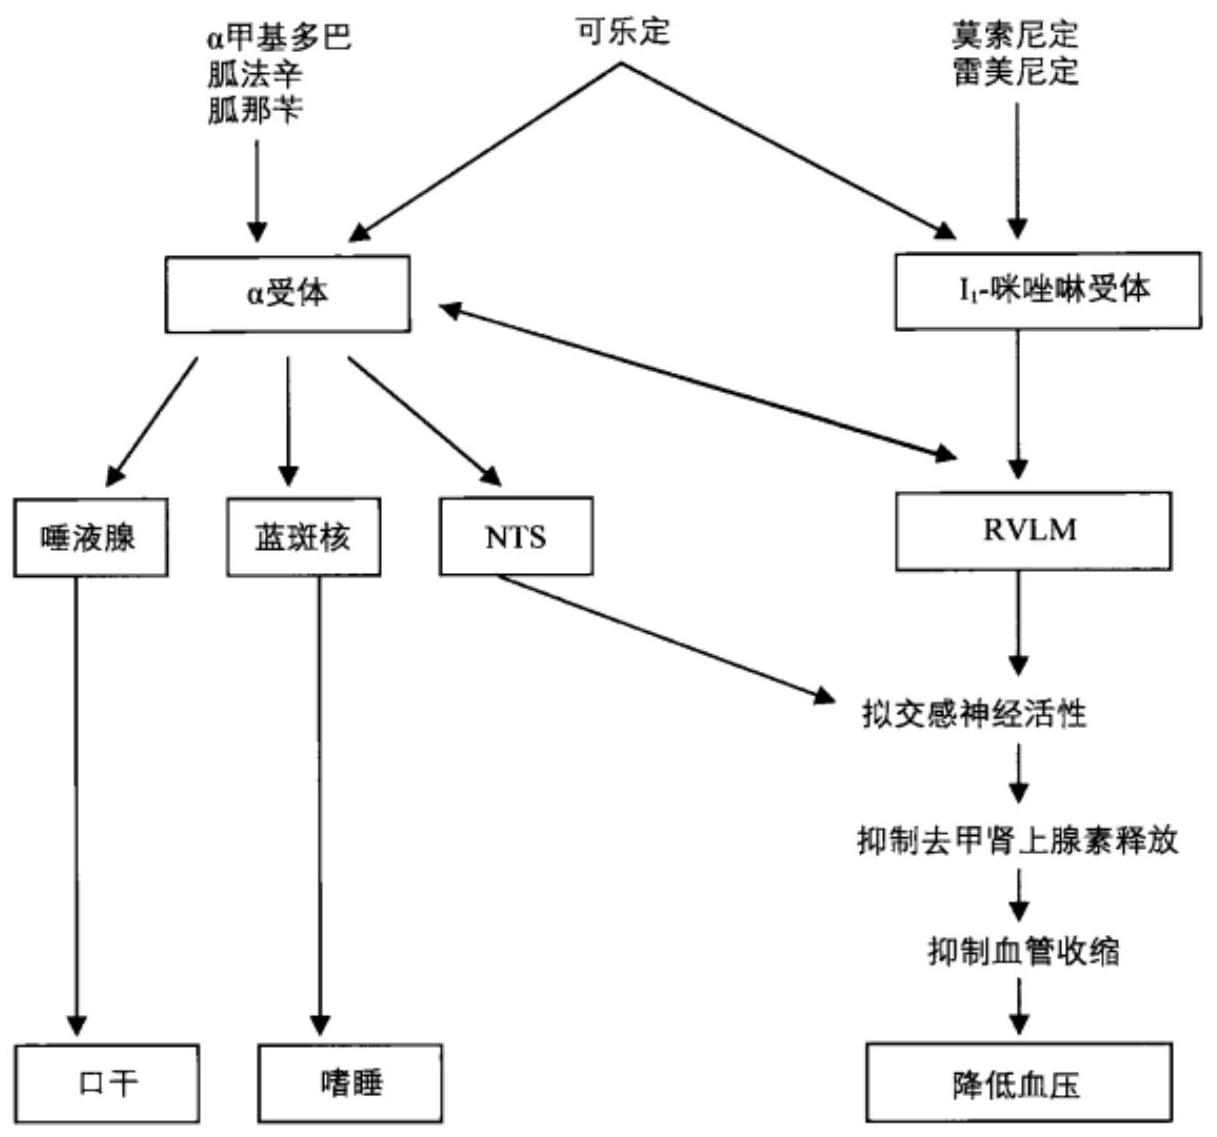
\includegraphics[max width=\textwidth]{2024_07_10_373f31b88d2bf633007bg-166}
\end{center}

图 2-12-1 中枢血管扩张药的作用机制

\section*{二、 $\alpha$-肾上腺素受体阻滞药}
\section*{(一)药理作用}
这类药物能有效阻滞交感神经在血管平滑肌的 $\alpha$-肾上腺素受体,多数药物为竞争性拮抗去甲肾上腺素对平滑肌的作用,所以,也称为解交感药物。一些则为非 $\alpha$-肾上腺素受体竞争性, 如酚苄明,其作用明显延长。

血管平滑肌有两种 $\alpha$ 受体, 即 $\alpha_{1}$ 和 $\alpha_{2}$ 受体, $\alpha_{1}$受体位于血管平滑肌, 而 $\alpha_{2}$ 受体则位于交感神经末梢及血管平滑肌。平滑肌(突触后) $\alpha_{1}$ 和 $\alpha_{2}$ 受体与 $\mathrm{G}$-蛋白偶联,通过 $\mathrm{IP}_{3}$ 信号转导通路使血管收缩。突触前膜的 $\alpha_{2}$ 受体位于交感神经末梢, 对释放去甲肾上腺素起负反馈调节作用。

$\alpha_{1}$ 肾上腺素受体阻滞药可阻断去甲肾上腺素与平滑肌受体的结合,引起血管舒张。非选择性 $\alpha_{1}$和 $\alpha_{2}$ 受体指抗药则阻断突触后膜的 $\alpha_{1}$ 受体和 $\alpha_{2}$ 受体,导致血管扩张; 但阻断突触前膜的 $\alpha_{2}$ 受体,则增加去甲肾上腺素的释放,使血管舒张作用得以一定程度缓解。此外,阻断心脏突触前膜的 $\alpha_{2}$ 受体,使去甲肾上腺素释放增加, 并作用心脏 $\beta_{1}$ 受体, 使心率加快、心肌收缩力增加。

$\alpha$ 受体阻滞药可扩张动脉和静脉,两者均由交感神经支配; 但对动脉阻力血管的阻滞作用更为明显。由于基础状态下,多数血管均有一定的交感张力,从而该类药物能发挥扩血管作用。在应激及病理状态下(如嗜铬细胞瘤患者循环中儿茶酚胺含量增加)作用更加突出。

\section*{(二)临床应用}
该类药尤其是 $\alpha_{1}$ 受体阻滞药主要用于原发性高血压的治疗(虽不像其他药物应用那么广泛)。非选择性 $\alpha$ 受体阻滞药则主要用于高血压急诊(如嗜铬细胞瘰)治疗,此时,常合并应用 $\beta$ 受体阻滞药,以对抗反射性心率加快。

\section*{(三)分类}
新型用于治疗高血压的 $\alpha$ 受体阻滞药多为选\\
择性 $\alpha_{1}$ 受体阻滞药, 包括哌唑嗪、特拉唑嗪、多沙唑銯、曲马㟇嗪; 而非选择性 $\alpha$ 受体阻滞药包括酚妥拉明、酚芐明等。

\section*{(四)副作用及禁忌证}
最常见的副作用与 $\alpha$ 受体阻断有关,包括眩晕、体位性低血压、鼻秥膜充血、头痛、反射性心动过速。此外,可引起液体潴留, 如同时应用利尿药则可克服这一问题。这类药不主张用于心力衰竭和心绞痛的治疗。

\section*{三、神经节阻滞药}
\section*{(一)药理作用}
交感神经节包括椎旁神经节和脊髓神经节, 节前纤维来自脊権交感突触, 释放神经递质乙酰胆碱 (ACh), 与烟碱受体结合。激活烟碱受体后使突触后神经元去极化, 产生动作电位, 传导至靶器官。副交感神经节则位于器官内, 节前纤维来自脑干,进人靹器官(如心脏), 其副交感神经节发出节后纤维。神经递质也为 $\mathrm{ACh}$, 与烟碱受体结合后激活位于靶器官内的节后纸维。

解交感药物可从 3 个层面上拮抗交感活性:一是外周解交感药物,如 $\alpha$ 受体拮抗药和 $\beta$ 受体拮抗药, 阻滞去甲肾上腺素对效应器官的作用 (血管、心脏); 二是交感神经节阻滞药, 可阻滞交感神经冲动的传递; 三是阻滞交感神经的中枢活性,称为中枢解交感药。

神经节阻滞药抑制神经节内神经递质的活性,可降低交感神经的心脏活性, 使心率减慢、心肌收缩力下降,并使血管张力降低。该类药还降低副交感活性。

\section*{(ニ)临床应用}
不适用于慢性高血压治疗,主要原因是其副作用明显,而其他的抗高血压药种类多、安全系数高。从而其主要用于高血压急诊的处理。临床偶尔应用的药物仅有樟磺咪芬,适应证为高血压危象和控制性低血压。

\section*{(三)副作用}
潜在的神经肌肉阻滞作用及延长神经肌肉阻滞药的作用,可由于节交感左右而致严重低血压,解副交感作用而引起便秘, 尿渚留, 口干。还刺激组胺释放。

\section*{四、硝基类扩血管药}
\section*{(一)硝普钠 (sodium nitroprusside)}
\begin{enumerate}
  \item 药理作用 可直接松驰小动脉和静脉平消肌, 属硝基扩血管药,在血管平滑肌内代谢产生一氧化氮 (NO), NO 具有强大的舒张血管平滑肌的作用。NO 与内皮源性松弛因子(EDRF) 在许多性能上相似, 是一种内源性血管舒张物质。NO 可激活身苷酸环化酶,促进 cGMP 的形成,产生血管扩张作用。其属于非选择性血管扩张药, 很少影响局部血流分布。一般不降低冠状动脉血流、将血流和肾小球滤过率。
\end{enumerate}

\section*{2. 临床应用}
(1)控制性降压和高血压患者的降压:静脉输注或用微泉输注 $0.01 \%$ 的药液,以 $10 \mu \mathrm{g} / \mathrm{min}$ 开始, 严密观察血压变化, 根据血压调整给药速率, 推荐剂量为 $0.5 \sim 8 \mu \mathrm{g} /(\mathrm{kg} \cdot \mathrm{min})$ 。一般总量不宜超过 $1.5 \mathrm{mg} / \mathrm{kg}$, 或 $2.5 \mathrm{~h}$ 内不宜超过 $1 \mathrm{mg} / \mathrm{kg}$, 以防氮化物中毒。

(2)心力衰竭或低心排血量的治疗 : 为㺂轻前后负荷, 可从 $0.5 \mu \mathrm{g} /(\mathrm{kg} \cdot \mathrm{min})$ 开始, 根据患者血压情况,逐渐增加剂量,直至获得满意的效果。要强调的是,无高血压病史的心力衰竭患者, 对硝普钠非常敏感, 应从小剂量开始,以免造成严重低血压。

\begin{enumerate}
  \setcounter{enumi}{2}
  \item 不良反应静脉应用时可能出现恶心、呕吐、精神不安、肌肉痉挛、头痛、皮疹、出汗、发热等。大剂量连续应用 (特别是在肝肾功能损害的患者),可引起血浆氯化物或硫経化物浓度升高而中毒, 可导致甲状腺功能减退。用药时要严密监测血浆氧化物浓度。
\end{enumerate}

\section*{(ニ)硝酸甘油 (nitroglycerin)}
\section*{1. 药理作用}
(1)硝酸酯类药能在平滑肌及血管内皮细胞中与“硝酸酯”受体结合,在其巯基的作用下,产生 NO, 而松驰平滑肌,能拮抗去甲肾上腺素、血管紧张素等的缩血管作用。可扩张全身小动脉和小静脉,但以扩张容量血管更为明显。用量增大可使动脉压下降至反射性心动过速。

(2)抗心绞痛作用: 能增加心肌缺血区的血流量, 扩张较大的心外膜冠状动脉血管, 并使冠状动脉血流重新分布。硝酸甘油舒张静脉血管后,使回心血量减少,降低前负荷, 使心室舒张末期容量和压力下降; 较大剂量的硝酸甘油可扩张阻力血管,降低后负荷, 惐少心脏做功使心眀耗氧下降。

\begin{enumerate}
  \setcounter{enumi}{1}
  \item 临床应用
\end{enumerate}

(1)控制性降压: 通常采用 $0.01 \%$ 或 $0.1 \%$ 药液静脉滴注或微栐输注,开始速率为 $1 \mu \mathrm{g} /(\mathrm{kg} \cdot$ $\mathrm{min})$, 观察反应后调节速率,一般 $3 \sim 6 \mu \mathrm{g} /(\mathrm{kg} \cdot$ $\mathrm{min})$ 可使血压降至所需水平。硝酸甘油降压时可引起顾压增高, 特别是原先有顺内压增高患者, 除非预先采取控制顾内压的措施, 否则, 应在脑膜切开后开始给药。

(2)心绞痛的治疗: 可用于各类心绞痛患者, 也可预防发作。对于急性心肌梗死患者既可降低心肌耗氧, 又可减少梗死面积。

(3)治疗心力衰竭、心肌缺血: 广泛用于冠状动脉旁路术中预防、治疗心肌缺血, 也可用于体外循环心内直视术后低心排血综合征的治疗。

\begin{enumerate}
  \setcounter{enumi}{2}
  \item 不良反应继发于血管扩张作用, 如面部潮红、灼热感, 搏动性头痛, 眼胀痛。因此, 脑出血、顾页内高压、青光眼患者慎用。
\end{enumerate}

\section*{(三)三磷腺苷和腺苷}
\begin{enumerate}
  \item 药理作用 腺苷是三磷腺苷的代谢产物, 为内源性血管扩张物质。腺苷与其受体结合后, 抑制平滑肌对 $\mathrm{Ca}^{2+}$ 的摄取, 干扰心肌细胞收缩过程中对 $\mathrm{Ca}^{2+}$ 的利用, 从而引起血管平滑肌的松弛和心肌抑制作用。
\end{enumerate}

(1)对心血管系统作用: 对心脏负性频率作用明显, 可引起剂量依赖性心率减慢。对血管平滑肌, 可选择性扩张阻力血管, 降低心脏后负荷, 减少心脏射血阻力。腺苷导致的低血压并不增加肾素活性和血浆儿茶酚胺量。三磷腺苷在降解过程中产生许多磷酸, 后者易与 $\mathrm{Mg}^{2+} 、 \mathrm{Ca}^{2+}$ 謷合, 可致心律失常, 因此有用腺苷代替三磷腺苷作用降压药物的趋势。

(2)其他作用: 腺苷对中枢神经系统具有镇静、催眠和抗㿉病作用, 腺苷受体与苯二剑草受体在某些点相似, 一些腺苷受体拮抗药可阻滞地西泮与苯二氮草类受体结合。腺苷还可抑制交感神经刺激引起脂肪分解, 增加肥大细胞中组胺的释放。

2.临床应用腺苷有极强的降压作用和快速消除的特点, 无快速耐药性, 亦无反跳性高血压和心率增快的作用, 临床剂量无明显苺性。单次静脉注射 $0.36 \sim 2.9 \mathrm{mg} / \mathrm{kg}$ 的三磷腺苷可使收缩压和舒张压分别下降 $27.3 \mathrm{mmHg}$ 和 $25 \mathrm{mmHg}$ 。对伴有心脏传导系统疾病或冠心病患者慎用。

\begin{enumerate}
  \setcounter{enumi}{2}
  \item 不良及应静脉快速输注三磷腺苷过快或过量时, 可引起血压过低、眩军和心律失常, 表现为心动过缓、房室传导阻滞。
\end{enumerate}

\section*{五、血管紧张素转化酶抑制药}
肾素-血管紧张素系统 (RAS) 是由肾素、血管紧张素及其受体构成的重要体液系统, 血管㑠张素原在肾素的作用下转化成肽的血管紧张素 I (Ang I), 后者在血管紧张素转化酶 (ACE) 的作用下切去两个氨基酸转化为血管紧张素 II (Ang II)。 Ang II作用于血管紧张素受体 (AT) 亚型 1 , 即 $\mathrm{AT}_{1}$, 产生收缩血管、促进肾上腺皮质释放醛固酮、增加血容量、升高血压等作用。Ang II 也作用于血管紧张素受体亚型 2 , 即 $\mathrm{AT}_{2}$, 激活缓激肽 $\mathrm{B}_{2}$ 受体与一氧化氮( $\mathrm{NO})$ 合酶, 产生 $\mathrm{NO}$, 舒张血管,降低血压, 促进细胞凋亡, 能部分拮扰 $\mathrm{AT}_{1}$ 作用。此外,人的心脏与血管组织的糜酶旁路也可将 Ang I 转化成 Ang II (图 2-12-2)。

包括卡托普利、依那普利、赖诺普利、贝那普利、福辛普利。

\section*{(一)卡托普利 (captopril)}
\begin{enumerate}
  \item 药理作用 $\mathrm{ACE}$ 的活性部位有两个结合位点, 其中一个为含 $\mathrm{Zn}^{2+}$ 的是 $\mathrm{ACE}$ 抑制药有效基团必须结合的部位。卡托普利含有一 $\mathrm{SH}$ 基团, 有效与 $\mathrm{Zn}^{2+}$ 结合而直接抑制 $\mathrm{ACE}_{\text {。 }}$ 降压效果与患者的肾素血管紧张素系统(RAS) 活动状态有关, 肾素水平高或低盐饮食或服用利尿药者,降压持续时间为 $8 \sim 12 \mathrm{~h}$ 。其含有一 $\mathrm{SH}$ 基团, 有自由基清除作用, 对与自由基有关的心血管损伤和心肌缺血再灌注损伤有防治作用。

  \item 临床应用治疗高血压; 有效、安全地用于充血性心力衰竭的治疗, 能降低充血性心力衰竭患者的病死率; 对缺血性心肌有保护作用, 能减轻缺血再灌注损伤和由此引起的心律失常。心肌梗死患者在心梗后早期应用能改善心功能和降低死亡率。是 FDA 批准惟一用于糖尿病性情病治疗的 $\mathrm{ACE}$ 抑制药。

  \item 不良反应其毒性小,耐受性好。除咳噷外, 因含一SH 基团, 可导致青䨪胺样反应, 出现皮疹、嗜酸性粒细胞增高、味觉异常等。可出现中性粒细胞减少, 多与用药时间长、剂量较大或肾功能障碍有关。禁用于双侧肾动脉狭窄患者。

\end{enumerate}

\section*{(二)依那普利 (enalapril)}
\begin{enumerate}
  \item 药理作用 口服后在肝脂酶的作用下,生成二羧酸活性代谢物依那普利酸, 对 ACE 的抑制作用较卡托普利强 10 倍。降压时外周血管阻力降
\end{enumerate}

\begin{center}
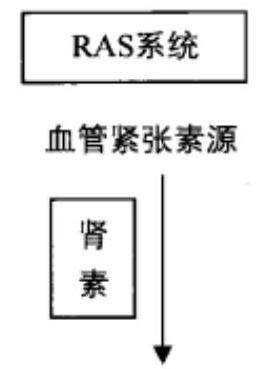
\includegraphics[max width=\textwidth]{2024_07_10_373f31b88d2bf633007bg-169(3)}
\end{center}

血管紧张素 I激肽系统

缓激肽

\begin{center}
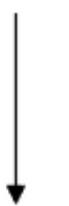
\includegraphics[max width=\textwidth]{2024_07_10_373f31b88d2bf633007bg-169}
\end{center}

缓激肽

\begin{center}
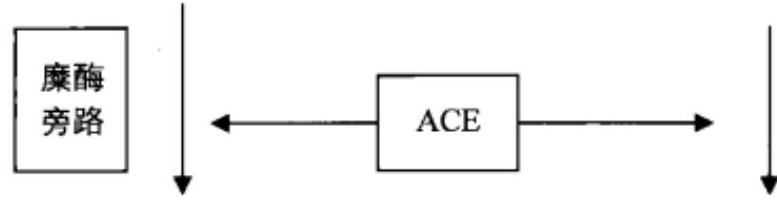
\includegraphics[max width=\textwidth]{2024_07_10_373f31b88d2bf633007bg-169(2)}
\end{center}

血管紧张素 II

$\mathrm{AT}_{1}$ 受体

(1)收缩血管+释放醛固酮: 升高血压

\begin{center}
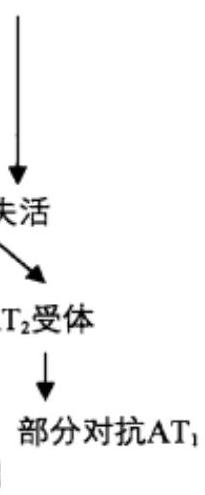
\includegraphics[max width=\textwidth]{2024_07_10_373f31b88d2bf633007bg-169(1)}
\end{center}

图 2-12-2 血管紧张素转化酶抑制系统

低, 肾血流量增加, 对肾小球滤过率无明显影响。长期应用, 能逆转左心室肥厚和改善大动脉的顺应性。

\begin{enumerate}
  \setcounter{enumi}{1}
  \item 不良反应与药物治疗相关不良反应包括干咳、低血压、血管神经性水肿、高血钾、急性怪衰竭。禁忌证同卡托普利。
\end{enumerate}

\section*{六、血管紧张素 II $\left(A T_{1}\right)$ 受体拮抗药}
包括氯沙坦、濒沙坦、厄贝沙坦、坎替沙坦。

(一) 氞沙坦(losartan)

\begin{enumerate}
  \item 药理作用 对 $\mathrm{AT}_{1}$ 受体有选择性拮拋作用,其对 $\mathrm{AT}_{1}$ 受体的选择作用比 $\mathrm{AT}_{2}$ 受体高 20 000~ 30000 倍。EXP3174 为氯沙坦的活性代谢物, 拮抗 $\mathrm{AT}_{1}$ 受体作用比氯沙坦强 10〜40 倍。对肾血流动力学影响与 $\mathrm{ACE}$ 抑制药相似, 能拮拋血管紧张素 II 对肾人球小动脉与出球小动脉的收缩作用。对高血压、糖尿病合并肾衰竭患者有保护作用。长期应用能抑制左心室心肌肥厚和血管壁增厚。

  \item 临床应用 用于高血压的治疗。

  \item 不良反应不良反应较少, 少数患者用药后出现眩军。禁用于孕妇、哺乳妇女及肾动脉狭窄者。低血压严重肾衰竭、肝病患者慎用。应避免与补钾或留钾利尿药合用。

\end{enumerate}

\section*{(二)皟沙坦(valsartan)}
\begin{enumerate}
  \item 药理作用 其对 $\mathrm{AT}_{1}$ 受体的亲和力比对 $\mathrm{AT}_{2}$ 受体强 24000 倍, 口服降压作用持续 $24 \mathrm{~h}$ 。长期用药可逆转左心室肥厚及血管壁增厚。

  \item 不良反应 发生率低, 主要为头痛、头晕、巨力。低钠、血容量不足、将动脉狭窄、严重肾动脉狭窄、肾衰竭、胆汁性肝硬化或胆道梗阻患者服用后可引起低血压。用药期间应慎用留钾利尿药和补钟药。妊娠和哺乳妇女禁用。

\end{enumerate}

\section*{七、钙通道阻滞药}
钜离子作为生物细胞的重要信使, 参与细胞多种重要功能的调节, 包括心脏起搏、心肌细胞和骨骼肌及血管平滑肌细胞的兴奋-收缩偶联、神经递质释放、腺体分泌和基因表达等。

钙通道阻滞药, 又称钙拮抗药, 是一类选择性阻滞钙通道, 抑制细胞外 $\mathrm{Ca}^{2+}$ 内流, 降低细胞内 $\mathrm{Ca}^{2+}$ 浓度的药物。常用的为二氢吡啶类药物尼卡地平和尼莫地平。

\begin{enumerate}
  \item 适应证
\end{enumerate}

(1)高血压:由于舒张血管平滑肌, 从而降低全身血管阻力, 使血压下降。其主要作用于阻力血管, 对容量血管影响较小。

(2)心绞痛: 通过血管扩张和心肌抑制作用而实现: 全身血管阻力降低, 使心脏后负荷降低, 心肌氧耗减少。心脏选择性钙离子拮抗药维拉帕米、地尔硫草可降低心率和心肌收缩性, 使心肌氧耗堿少,从而具有很好的抗心绞痛作用。其还能扩张冠状动脉, 增加心肌氧供。

(3) 心律失常: 为V类抗心律失常药,可减少心脏起搏点的节律, 更加重要的是延长传导和复极,尤其在房室结。从而抑制折返机制所致的快速室上性心动过速。

\begin{enumerate}
  \setcounter{enumi}{1}
  \item 分类 分为 3 类,不同点不仅在于基本化学结果, 而且在选择性对心脏或血管的 L-型锬通道作用不同。氢吡啶类为血管平滑肌选择性, 主要用于降低全身血管阻力而治疗高血压。不用于治疗心绞痛,原因是其降低血压后可造成反射性心动过速, 增加心肌耗氧。
\end{enumerate}

氢吡啶类包括: 氨氯地平、非洛地平、伊拉地平、尼卡地平、硝苯地平、尼莫地平、尼群地平。

非氢吡啶类: 临床应用的有两种 $\mathrm{s}$ 维拉帕米(苯烷基胺类),为相对心肌选择性,而对全身血管作用较小。因此, 对治疗心绞痛 (降低心肌耗氧和逆转冠脉痉挛) 和心律失常非常有效。地尔硫草 (苯并船氮草类), 其对血管平滑肌的舒张作用介于上述两类之间,具有心脏抑制和血管扩张作用。可降低血压而不产生明显的反射性心脏刺激作用。

\begin{enumerate}
  \setcounter{enumi}{2}
  \item 副作用 氢吡啶类可引起潮红、头痛、过度低血压、水肿和反射性心动过速。心脏选择性非氢吡啶类钙拮抗药可导致心动过缓, 损害传导 (如房室结阻滞), 抑制心肌收缩性。因此, 先前存在心动过缓、传导阻滞、心力衰竭患者应避免应用。并不主张与 $\beta$ 受体阻滞药合用,以免加重抑制心脏传导和收缩性。
\end{enumerate}

\section*{八、内皮素受体拮抗药}
\begin{enumerate}
  \item 药理学作用 内皮素-1(ET-1)是一 21 氨基酸组成的肽,由血管内皮产生,与血管平滑肌受体结合后产生强烈的血管收缩作用。ET-1 受体有两个亚型, 即 $\mathrm{ET}_{\mathrm{A}}$ 和 $\mathrm{ET}_{\mathrm{B}}$ 受体。这些受体与 $\mathrm{G}$-蛋白配对, 受体激活后促使 $\mathrm{IP}_{3}$ 形成, 使肌浆网释放钙离子,使平滑肌收缩及血管收缩。位于内皮细胞的 $\mathrm{ET}_{\mathrm{B}}$ 受体受刺激后产生 $\mathrm{NO}$, 而使平滑肌舒张。这种受体的分布特性有助于解释给予 ET-1 后产生短暂的血管扩张(先激活内皮细胞 $\mathrm{ET}_{\mathrm{B}}$ ) 低血压,接着为长时间的血管收缩和高血压(平滑肌细胞的 $\mathrm{ET}_{\mathrm{A}}$和 $\mathrm{ET}_{\mathrm{B}}$ 受体作用)。
\end{enumerate}

位于心脏的 ET-1 受体也与 $\mathrm{G}$-蛋白和 $\mathrm{IP}_{3}$ 信号通路相关,ET-1 可使心胜锬离子释放,心肌收缩力增强, 还使心率加快。

\begin{enumerate}
  \setcounter{enumi}{1}
  \item 临床应用 由于 ET-1 具有强烈的缩血管作用,与高血压、心力衰竭、冠状动脉痉挛的病理有关。许多研究也证实,ET-1 与肺动脉高压发生相关。其也可由受损心肌释放,从而与钙超载和心肌肥大有关。
\end{enumerate}

ET-1 受体抑制药可使血管扩张和心肌抑制,研究显示可以改善实验性心力衰竭模型的血流动力学。

目前可以用于临床的药物为波生坦,为非选择性 ET-1 阻滞药。适应证为肺动脉高压的治疗。

\begin{enumerate}
  \setcounter{enumi}{2}
  \item 副作用 与血管扩张作用有关,包括头痛、表皮潮红和水肿。由于可能导致生育异常,而禁用于驭妇。也有肝损害的报道。
\end{enumerate}

(王国林)

\section*{第 12 管}
\section*{抗心律失常药物}
心脏发生病变或神经调节异常时, 心脏搏动的频率和节律会发生紊乱,临床表现为心律失常。围术期心律失常发生率很高, 但真正需要立即治疗的致命性心律失常发生率不到 $1 \%$, 且几乎均发生于原有心脏疾病患者。麻醉医师的任务是治疗影响患者围术期循环动力学平稳和有可能影响患者手术预后的严重心律失常。围术期应用抗心律失常药物时还必须权衡考虑药物本身存在的致心律失常作用、负性肌力作用和器官毒性作用, 且在用药前应先纠正酸碱和电解质异常、低氧血症、心肌缺血和麻醉药物作用等非心脏性因素的影响。

\section*{一、抗心律失常药物作用机制}
心律失常主要起因于冲动形成异常和冲动传导异常或二者兼而有之。心脏自律性降低和传导障碍导致缓慢型心律失常, 而心脏自律性增强、触发激动和折返形成均可导致快速型心律失常。心肌细胞动作电位的产生依赖于细胞内外的离子梯度变化, 因此离子通道功能的异常在心律失常形成发展中具有直接作用, 心律失常的实质是离子通道失衡的表现。抗心律失常药通过直接影响心脏的多种离子通道或通过影响细胞离子百 $\left(\mathrm{Na}^{+}-\mathrm{K}^{+}\right.$泉和 $\mathrm{Ca}^{2+}$ 彔) 和激活细胞受体 (如 $\alpha, \beta$ 受体) 调节跨膜离子流, 改变细胞膜内外离子浓度发挥抗心律失常作用。抗心律失常药的净效应通常是对多种离子通道和受体作用的总合。

\begin{enumerate}
  \item 改变心胜自律性通过堿慢自律细胞舒张期自动复极速度或者抑制交感神经兴奋性,可以降低心肌细胞自律性, 如 $\beta$ 受体阻滞药; 抑制 4 相 $\mathrm{Na}^{+}$内流或阻滞 $\mathrm{Ca}^{2+}$ 内流的药物可分别减慢快或慢反应细胞心舒期自动复极速率, 降低自律性, 如钢通道阻滞药和钙通道阻滞药; 促进 $\mathrm{K}^{+}$外流后由于增加最大舒张电位与阈电位的距离, 也可以起到降低自律性作用, 如腺亘。

  \item 减少异常除极 触发激动的早期后除极具有长周期依赖性, 通过药物加快心率, 缩短动作电位时限和复极时限, 或通过阻滞 $\mathrm{Ca}^{2+}$ 通道或 $\mathrm{Na}^{+}$通道可以抑制早期后除极。延迟后除极与细胞钙超载有关, 应用销通道阻滞药治疗有效。

  \item 消除折返 心脏冲动传导通路的一部分发生单向传导阻滞, 冲动沿该通路的另一部分缓慢下传, 然后经由原单向传导阻滞通路逆行回传至原处, 成为新的冲动源再次下传, 周而复始则形成折返激动, 折返形成是导致快速性心律失常的重要原因。抗心律失常药物主要通过抑制传导和延长有效不应期消除折返。

\end{enumerate}

\section*{二、抗心律失常药物分类}
改良 Vaughan Williams 分类是根据药物阻断特殊离子流的能力, 并假定各种药物都有一种主要的作用机制提出的抗心律失常药物的分类方法。

\begin{enumerate}
  \item I 类药物一一钠通道阻滞药 I 类药物指主要抑制 $\mathrm{Na}^{+}$通道的药物, 具有膜稳定作用, 通过调节或关闭钠通道,降低 0 相除极上升速度及幅度, 从而减慢心内传导。根据药物与通道结合与解离速率及通道阻滞强度不同, 又可分为 3 个亚组。
\end{enumerate}

(1) $\mathrm{I}_{\mathrm{A}}$ 类一中度钠通道阻滞药:包括奎尼丁、普鲁卡因胺和丙吡胺, 对钠通道的阻断作用较强, 与钠通道的结合或解离较快 $(<5 \mathrm{~s})$ 。主要延长心室不应期和 Q-T 间期, 延长 APD、降低 $V_{\max }$ 、减慢传导速率和减小最大舒张电位。用药后心电图表现 QRS 增宽、QT 间期延长。

(2) $\mathrm{I}_{\mathrm{B}}$ 类一一轻度钠通道阻滞药: 包括利多卡因、美西律、妥卡尼和苯妥英钠。对钠通道的阻断作用最弱, 与钠通道结合或解离最快 $(<0.5 \mathrm{~s})$ 。缩短动作电位时程 (APD) 和有效不应期 (ERP), 对正\\
常组织传导影响小,用药期间心电图 PR、QRS 和 $\mathrm{Q}-\mathrm{T}$ 间期无明显变化。

(3)Ic 类一一高度钠通道阻滞药: 包括普罗帕酮、氟卡尼、莫雷西嗪, 是最强的钠通道阻滞药, 与通道的结合和解离也最慢 (10〜20s), 可使心电图 $P R$ 和 QRS 间期延长而 $Q-T$ 间期不变。

\begin{enumerate}
  \setcounter{enumi}{1}
  \item II 类药物一 $\beta$ 肾上腺素受体阻滞药 具有抗肾上腺素能作用和膜稳定作用。通过减慢 4 相自动除极速率而降低自律性; 通过惐小 $\mathrm{Na}^{+}$电流,降低动作电位 0 相上升速率而减慢传导。 $\beta$ 受体阻滞药延长房室结的 ERP, 延长心电图 PR 间期和缩短 Q-T 间期。

  \item 的类药物一一延长动作电位时程药物包括胺碘雨、溴芐胺、索他洛尔、异布利特和多非利特, 为经典钾通道阻滞药, 延迟复极时间、延长 ERP 和 ADP, 增大 ERP/ADP。除了延长 $\mathrm{Q}-\mathrm{T}$ 间期外,对 ECG 没有其他影响。 $\mathrm{K}^{+}$通道阻滞药在一定程度上减慢心率, 很少引起心率增快。胺碘酮和溴芐胺具有非选择性多通道阻滞作用。

  \item IV 类药物一一钙通道阻滞药阻断慢锬通道开放, 抑制慢反应纤维的 0 相后期除极及 2 相复极速率, 从而减慢传导速度及延长 ERP。抑制 $\mathrm{Ca}^{2+}$ 进人宾房结内的起搏细胞、抑制其发放频率,可以减慢窦性节律。同时作用于房室结, 延长房室结不应期, 减慢房室传导, 心电图表现为 PR 间期延长。

\end{enumerate}

\section*{三、钠通道阻滞药}
\section*{1. 奎尼丁 (quinidine $\mathrm{I}_{\mathrm{A}}$ 类)}
(1)药理作用: 阻滞钠通道, 适度抑制 $\mathrm{Na}^{+}$内流, 奎尼丁还通过阻抑迷走神经而发挥间接作用。低浓度时可减慢 4 相心舒期除极, 高浓度可升高阈电位。奎尼丁抑制心脏收缩性, 其间接的 $\alpha$-肾上腺受体阻滞作用可以降低动脉压力。当心率慢时, 奎尼丁与钾通道结合多于钠通道从而延长 APD; 当心率快时, 奎尼丁主要阻滞钠通道。

(2)临床应用: 广谱抗心律失常药, 适用于治疗多种房性、室性及房室结性心律失常。心房颤动及心房扑动电复律前合用强心苷和奎尼丁可以减慢心室频率,复律后用奎尼丁有助于维持突性节律。

奎尼丁口服吸收良好,生物利用度 $70 \%$ $80 \%$,血浆蛋白结合率约 $80 \%$ 。单次口服后 $15 \mathrm{~min}$出现于血液中, $1 \sim 2 \mathrm{~h}$ 血药浓度达到峰值, 血浆治疗浓度 $2 \sim 6 \mu \mathrm{g} / \mathrm{ml}$, 清除半衰期 $6 \sim 7 \mathrm{~h}$ 。口服剂量 $200 \mathrm{mg} /$ 次, $3 \sim 4 / \mathrm{d}$ 。 经肌内注射的首选剂量为 $200 \mathrm{mg}$, 每隔 $6 \sim 8 \mathrm{~h}$ 给药 1 次。维持剂量为 $300 \sim$ $600 \mathrm{mg} / \mathrm{d}$,缩短给药间隔时间比增加药物剂量更能保持稳定的血药浓度。

(3)不良反应和注意事项: 奎尼丁可诱发不同程度的心房和心空传导阻滞及蜜房结功能抑制, 病窐综合征忠者慎用。 $1 \% \sim 3 \%$ 使用奎尼丁的患者会发生尖端扭转型室性心律失常。监测 QRS 时间和 Q-T 间期可以有效地指导治疗, 其中任意一项增加 $50 \%$ 就应该减少剂量。由于奎尼丁有 $\alpha$ 肾上腺受体阻滞作用和直接的血管扩张作用可能导致低血压。胃肠道反应如恶心、呕吐、腹泻发生率较高, 严重腹泻导致低血钾可加重奎尼丁的心脏不良反应。血药浓度过高可出现严重的中枢神经系统症状(头痛、复视、畏光、意识模糊或者精神症状)。偶发自身免疼性疾病、皮疹和血小板减少症。

\begin{enumerate}
  \setcounter{enumi}{1}
  \item 普鲁卡因胺 (procainamide $I_{\mathrm{A}}$ 类)
\end{enumerate}

(1)药理作用: 电生理作用包括降低 $V_{\max }$ 和延长 0 相持续时间, 降低 4 相除极速率, 延长 ERP 和 APD。临床上, 普鲁卡因胺可以延长传导时间, 增加心房和希氏束部分的 ERP, 使心电图 PR 间期和 QRS 波加宽; 然而,对 Q-T 间期的延长作用小于奎尼丁。普鲁卡因胺的主要代谢产物是 $\mathrm{N}$-乙酰普鲁卡因胺, 通过钾通道阻滞延长 APD。

(2)临床应用: 用于治疗室上性和室性心律失常, 静脉给药治疗室速的效果优于利多卡因。普鲁卡因胺抑制旁路的传导,可以治疗房室交界性心动过速和伴有 WPW 的房畝。

口服易吸收,生物利用度约 $80 \%$,血浆蛋白结合率 $20 \%$, 口服后 $1 \mathrm{~h}$ 血药浓度达到峰值, 消除半衰期为 $3 \sim 5 \mathrm{~h}$ 。口服 $250 \sim 500 \mathrm{mg}, 3 \sim 4 / \mathrm{d}$ 。静脉给药 $4 \mathrm{~min}$ 血药浓度达峰, 注射剂量为 $100 \mathrm{mg}$ 或者 $1.5 \mathrm{mg} / \mathrm{kg}$,每 $5 \mathrm{~min}$ 重复 1 次,直至起到治疗作用或者总量达到 $1 \mathrm{~g}$ 或者 $15 \mathrm{mg} / \mathrm{kg}$ 为止。持续静脉输注速率为 $2 \sim 6 \mathrm{mg} / \mathrm{min}$, 维持血浆药物浓度在 $4 \sim$ $8 \mathrm{mg} / \mathrm{L}$ 。

(3)不良反应和注意事项: 毒性副作用与剂量相关,血药浓度超过 $12 \mathrm{mg} / \mathrm{L}$ 会产生严重的心脏毒性, 包括心脏停搏、传导阻滞和室性心律失常。普鲁卡因胺也可能导致胃肠道功能紊乱, 中枢神经系统症状(头痛和睡眠障碍)、皮疹和粒细胞减少等过敏反应。部分长期用药患者会出现抗核抗体增加,其中一半会有发热、肌痛、皮疹、胸膜炎或者心包炎等与红斑狼疮相似的症状, 停止用药后症状会慢慢\\
缓解。静脉注射普鲁卡因胺可导致血压降低, 应缓慢注射。代谢产物 $\mathrm{N}$-乙酰普鲁卡因胺, 仍有抗心律失常活性, 其半衰期为 $7 \sim 8 \mathrm{~h}$, 经情代谢。对于老年、左心室功能不全、心肌梗死和肾衰竭患者使用此药物要适当调整药量。

\begin{enumerate}
  \setcounter{enumi}{2}
  \item 利多卡因 (lidocaine $\mathrm{I}_{\mathrm{B}}$ 类)
\end{enumerate}

(1) 药理作用: 阻滞激活和失活钠通道, 抑制 $\mathrm{Na}^{+}$内流, 促进 $\mathrm{K}^{+}$外流。利多卡因可降低浦肯野纤维的 4 相舒张期去极化斜度并提高致室颤阈值,增加浦肯野纤维钾的跨膜电位, 但不影响静息电位和阈电位。当膜内负电位较小(部分除极) 时, 利多卡因可以通过增加 $\mathrm{K}^{+}$外流来抑制快钠通道, 这种作用与细胞外钾浓度直接相关。利多卡因明显缩短浦肯野纤维的 APD, 政善异位起搏点的传导, 从而降低发生折返的可能性。

(2)临床应用: 主要用于治疗室性心律失常, 特别适用于伴有心肌缺血的患者。对室上速包括心房纤噴和心房扑动的患者无效。常用于预防和治疗心脏手术、心胜介人治疗或强心苷导致的室性心律失常。心肌梗死后预防性使用利多卡因会有更高的死亡率现在已经不予推荐。

利多卡因的首过消除效应很明显, 所以不适合口服。静脉给药血浆蛋白结合率 $60 \% \sim 80 \%$, $60 \% \sim 70 \%$ 在肝内代谢, 消除半衰期为 $1 \sim 2 \mathrm{~h}$ 。 $90 \%$ 以代谢物形式、 $10 \%$ 以原形经尿排出。治疗血亖浓度 $1.5 \sim 3 \mathrm{mg} / \mathrm{L}$; 超过 $9 \mathrm{mg} / \mathrm{L}$ 时常出现毒性反应。经静脉给药首次注射 $1 \sim 1.5 \mathrm{mg} / \mathrm{kg}$ 后应立即以 $20 \sim 50 \mu \mathrm{g} /(\mathrm{kg} \cdot \mathrm{min})$ 的速率持续静脉输注, 以防止因为快速再分布引起的有效血浆浓度降低。

(3)不良反应和注意事项: 中枢神经系统毒性作用表现为㖫睡和定位异常, 逐渐发展成兴奋、肌肉抽搐、听觉异常甚至惊嚴。没有低血压的患者应用利多卡因基本上都能耐受。中毒剂量会延缓希氏-浦肯野纤维传导和产生心肌抑制作用。无起搏器保护的高度房室阻滞和病窐综合征禁用。有肔功能损害或血流障碍 (例如充血性心力衰竭) 患者应适当减少用量。

\section*{4. 美西律 (慢心律, mexiltine $\mathrm{I}_{\mathrm{B}}$ 类)}
(1)药理作用: 美西律阻滞失活的 $\mathrm{Na}^{+}$通道快于激活的 $\mathrm{Na}^{+}$通道。电生理作用与利多卡因相似,缩短 APD 和 ERP, 但是对传导影响很小, 对 Q-T 间期几乎没有作用。血流动力学的影响较小,主要表现左室 $\mathrm{dP} / \mathrm{dt}$ 降低和左室舒张末压升高。对于心脏病患者, 服用美西律可以㖪缓房室结和希氏-浦肯野纤维的传导。

(2)临床应用: 口服主要用来治疗慢性室性心律失常, 如室性早搏、室性心动过速。静脉注射用于急性室性心律失常, 如持续性室性心动过速。也可以治疗长 Q-T 间歇的室性心律失常。对法洛四联症术后室性心律失常效果良好。用于抑制急性心肌梗死时的室性早搏和室性心动过速效果优于利多卡因,但不能降低心肌梗死后病死率。

口服生物利用度 $85 \%$,血浆蛋白结合率 $50 \%$ 〜 $70 \%$, 有效血药浓度为 $0.5 \sim 2 \mathrm{mg} / \mathrm{L}$, 清除半衰期 10〜12h。美西律通过肝微粒体酶代谢,约 $10 \%$ 以原形从尿液排泄, 主要代谢产物是 $\mathrm{N}$-甲基美西律,保留 $20 \%$ 抗心律失常作用。

美西律紧急复律时, 静脉注射首量 $100 \mathrm{mg}$, $10 \mathrm{~min}$ 内注完, 无效 $10 \mathrm{~min}$ 后可重复一次,维持量 1. $5 \sim 2 \mathrm{mg} / \mathrm{min}, 3 \sim 4 \mathrm{~h}$ 后速度减半维持 $24 \sim 48 \mathrm{~h}$;常用口服剂量为每次 $200 \mathrm{mg}, 3 / \mathrm{d}$, 总量不要超过 $1200 \mathrm{mg} / \mathrm{d}$ 。

(3)不良反应和注意事项: 心血管副作用与利多卡因相似, 对血流动力学影响轻微。其他副作用包括中枢神经和胃肠道反应, 眩晕、感觉异常、震頝, 恶心、呕吐和出汗。不良反应与剂量相关, 当血清浓度达到治疗浓度的高限时需要仔细滴定药物浓度; 轻微不良反应发生率 $30 \%$, 血药浓度超过 $2 \mathrm{mg} / \mathrm{L}$ 时严重反应发生率 $19 \%$ 。肝疾病患者应调节药物使用剂量。

\begin{enumerate}
  \setcounter{enumi}{4}
  \item 苯妥英钠 (phenytoin sodium $\mathrm{I}_{\mathrm{B}}$ )
\end{enumerate}

(1)药理作用: 降低浦肯野纤维自律性, 抑制洋地黄中毒时延迟后电位引起的触发活动, 大剂量抑制窐房结自律性。缩短房室结、希氏-浦肯野系统的有效不应期, 缩短心室肌动作电位时程。通过增加 ERP/APD 比值和降低自律性发挥其抗心律失常作用。

(2)临床应用: 用于治疗由于强心苷毒性作用引起的房性和室性心律失常, 对继发于长 Q-T 间期综合征所致的心律失常的患者也有效。对心脏术后发生的心律失常, 例如交界性心动过速效果也很好。

口服生物利用度 $57 \% \sim 85 \%$, 血浆蛋白结合率 $93 \%, 8 \sim 12 \mathrm{~h}$ 血浆浓度达峰值, 有效血浆浓度 10〜 $18 \mathrm{mg} / \mathrm{L}$, 半衰期 18~36h。通过肝微粒体酶系代谢, 代谢物在肝内与莆䓒糖酫酸结合并从尿中排出。静脉负荷剂量每 $5 \mathrm{~min}$ 给予 $50 \sim 100 \mathrm{mg}(0.5 \sim$ $1.5 \mathrm{mg} / \mathrm{kg}$ ) 直至达到治疗效果或出现不良反应, 总\\
量最高不超过 $1 \mathrm{~g}(15 \mathrm{mg} / \mathrm{kg})$ 。口服首日 $1000 \mathrm{mg}$,第 $2 、 3$ 天 $500 \mathrm{mg} / \mathrm{d}, 2 \sim 3$ 次分服。维持量 300~ $400 \mathrm{mg} / \mathrm{d}$ 。

(3)不良反应和注意事项: 静脉给药可能抑制心肚收缩, 使左室舒张末压轻度升高。成人输注速度超过 $50 \mathrm{mg} / \mathrm{min}$ 时会出现心血管虚脱、心室纤颤甚至死亡。其他副作用包括视觉障碍、恶心、发音困难和小脑共济失调。长期使用会导致牙数增生、巨细胞性贫血和皮肤功能紊乱。

\section*{6. 普罗帕翻 (propafenone $\mathrm{I}_{\mathrm{c}}$ )}
(1)药理作用: 普罗帕酮阻滞激活和失活的 $\mathrm{Na}^{+}$通道。降低浦肯野纤维和心室肌的自律性, 明显惐慢传导速度, 延长 ERP 和 APD。用药后心电图 PR 和 QRS 间期延长。普罗帕酮兼有 $\beta$ 受体阻滞作用和轻度阻滞 $\mathrm{L}$ 型 $\mathrm{Ca}^{2+}$ 通道 (比维拉帕米弱 100 倍),临床表现轻度负性肌力作用。

(2)临床应用: 用于治疗阵发性室性、室上性心律失常和心房纤顔、心房扑动, 包括预激综合征引发的室上性心动过速和手术后近期发作的心房纤颤。对于恢复帘性心律的心房纤赗患者长期维持窦性心律安全有效且副作用较少。也用于治疗严重危及生命的室性心律失常。该药可以增加带有永久起搏器患者的起搏阈值。

口服吸收迅速完全,生物利用度为 $40 \%$ 〜 $50 \%$, 个体差异很大。 $97 \%$ 的普罗帕酮与血浆蛋白结合。有效血药浓度 $0.2 \sim 1.5 \mathrm{mg} / \mathrm{L}$, 消除半衰期 $6 \sim 8 \mathrm{~h}$ 。药物口服后 $30 \mathrm{~min}$ 起效, $2 \sim 3 \mathrm{~h}$ 达到作用高峰, 治疗作用可持续 $8 \mathrm{~h}$ 以上。代谢产物与普罗帕酮有相同的抗心律失常效能, 但血浆浓度不到普罗帕酮的 $20 \%$ 。口服 $150 \mathrm{mg}, 3 / \mathrm{d}, 3 \sim 4 \mathrm{~d}$ 后增加剂量到 $300 \mathrm{mg}, 2 / \mathrm{d}$, 每日总量不超过 $900 \mathrm{mg}$ 。静脉注射每次 $70 \mathrm{mg}$,用莆萄糖溶液稀释到 $20 \mathrm{ml}$ 后 $3 \sim$ $5 \mathrm{~min}$ 注完, 如无效 $20 \mathrm{~min}$ 后可重复一次, 静脉滴注速度为 $0.5 \sim 1 \mathrm{mg} / \mathrm{min}$, 每日总量不超过 $350 \mathrm{mg}$ 。

(3)不良反应和注意事项: $2 \% \sim 5 \%$ 的患者在接受治疗时可发生心律失常, 用药可能加重充血性心力衰竭病情, 也可致传导功能障碍。病窦综合征、心力衰竭及低血压患者慎用或不用。部分患者治疗期间可出现眩军、视觉模糊、味觉障碍并伴随胃肠道不适,一般不须停药。肝病患者普罗帕酮的生物利用度会升高 $70 \%$,应减少用量。

\section*{7. 莫雷西嗪 (moricizine $I_{c}$ )}
(1)药理作用: 强效钠通道阻滞药, 对 $\mathrm{Na}^{+}$通道有多重作用, 并有较温和的钾通道阻滞作用, 主要在失活状态下抑制快钠通道,降低动作电位 0 相 $\mathrm{V}_{\max }$ 和振幅。同时缩短浦肯野纤维 $2 、 3$ 相复极从而缩短动作电位时间。莫雷西嗪减慢房室结、心室肌的传导, 延长心电图 PR 间期和 QRS 间期, 对心房组织基本没有作用。

(2)临床应用:用于治疗室性心律失常,包括室性早搏和室性心动过速。对房性和结性早搏、阵发性室上速、心房纤顫和心房扑动也有一定治疗效果。

口服吸收良好, 生物利用度 $35 \% \sim 40 \%$ 。血浆蛋白结合率 $95 \%$ 。口服后 $2 \mathrm{~h}$ 内达到血浆峰值浓度,半衰期 $1.5 \sim 3.5 \mathrm{~h}$ 。主要经肝代谢, 随粪便和尿液排出, 饭后服用影响吸收速度。肝肾功能不佳时半衰期延长。口服剂量为 $100 \sim 200 \mathrm{mg}, 3 / \mathrm{d}$, 逐渐增加剂量到显效, 极量为每日 $900 \mathrm{mg}$ 。静脉注射 $50 \sim 80 \mathrm{mg}$, 用葡萄糖液稀释后缓慢注射治疗阵发性心动过速。

(3)不良反应和注意事项: 轻微升高血压和加快心率, 可引起恶心、头痛、震䫅和感觉异常。 $3 \% \sim 15 \%$ 患者使用莫雷西嗪可发生潜在危险的室性心律失常。极少数心室功能减弱患者会加重充血性心力衰竭。

\section*{四、II 类药物一 $\beta$ 肾上腺素受体阻滞药}
$\beta$ 肾上腺素受体阻滞药用于治疗肾上腺素升高状态下 (如甲状腺功能元进、嗜铬细胞瘤和围术期应激)引起的心律失常, 对于围术期患者或患有危重疾病患者的心律失常很有效,因为这些患者的心律失常通常是肾上腺素介导的。 $\beta$ 肾上腺素受体阻滞药可有效控制房颤和房扑时的快心率,尤其推荐用于控制心脏手术后的此类心律失常。

\begin{enumerate}
  \item 普茮洛尔 (心得安, propranolol)
\end{enumerate}

(1)药理作用: 最早用于临床的 $\beta$ 受体阻滞药,对 $\beta_{1}$ 受体和 $\beta_{2}$ 受体没有选择性, 无内源性拟交感活性。电生理作用主要降低心室肌自律性, 延长 APD 和房室结有效不应期, 减慢窦房结 4 相自动除极速率; 作用强弱取决于交感神经的状态。降低静息时心率, 但对运动后和情绪激动时心率升高的抑制作用更明显。 $\beta$ 受体阻滞作用可以转复由儿茶酚胺引起的室頞阈降低。除 $\beta$ 受体阻滞作用之外,普䒬洛尔降低钾外流,当浓度较高时也抑制钠内流, 具有类似于 $\mathrm{I}$ 类药物的膜稳定作用。

(2)临床应用: 普蔡洛尔对于儿茶酚胺或洋地黄引起的心律失常有效。用于治疗多发性期前收\\
缩和室性心律失常, 适于控制长 Q-T 间期的尖端扭转型室性心动过速, 特别适用于治疗快速室上性心律失常。

口服给药的吸收率几乎为 $100 \%$, 但生物利用度仅 $25 \% \sim 30 \%$ 。口服后 $1 \sim 1.5 \mathrm{~h}$ 血药浓度达峰值, 血浆蛋白结合率 $90 \%$, 主要在肝中代谢, 消除半衰期 3 $\sim 4 \mathrm{~h}$ 。尽管血浆浓度在 $0.1 \sim 0.3 \mathrm{mg} / \mathrm{L}$ 时就可以起到 $\beta$ 受体阻滞作用, 但是控制室性心律失常浓度需要达到 $1 \mathrm{mg} / \mathrm{L}$ 。口服从每次 10〜 20mg 开始, 3〜 $4 / \mathrm{d}$, 根据需要增加药量至最佳剂量, 每日总量不超过 $1000 \mathrm{mg}$ 。静脉给药控制心律失常剂量为 $0.5 \sim 1.0 \mathrm{mg}$, 无效逐渐增加剂量, 最大至 $0.1 \sim$ $0.15 \mathrm{mg} / \mathrm{kg}$ 。持续静脉输注可以维持稳定的有效血药浓度。

(3)不良反应和注意事项: 心脏毒性包括充血性心力衰竭和房室传导抑制。原有房室结或心室内传导异常的患者用药后可能发生完全性房室传导阻滞和心搏骤停。突然停药可能会由于长期 $\beta$受体阻滞导致的敏感性改变而引起心率血压波动。由于同时阻滞 $\beta_{2}$ 受体, 使气道阻力升高可能会加重侾喘患者的危险。因为低血糖触发的拟交感活性被普䒺洛尔阻滞, 可能增加糖尿病患者发生低血糖的危险。与 $\beta$ 受体阻滞无关的副作用包括失眠、幻觉、抑郁、眩晕和轻微的过敏反应, 例如皮疹、发热和紫瘷。

\section*{2. 美托洛尔 (metoprolol)}
(1)药理作用: 选择性 $\beta_{1}$ 受体阻滞药, 无内源性拟交感活性, 无膜稳定作用。抑制心肌收缩力,对窐房结、房空结的自律性和传导性有明显抑制作用。美托洛尔对 $\beta_{1}$ 受体的亲和力是 $\beta_{2}$ 受体的 30 倍。其 $\beta_{2}$ 受体阻滞效应仅为普蘩洛尔的 $1 \%$ 〜 $2 \%$ 。

(2)临床应用:美托洛尔适用于由情上腺素诱导的室上性和室性心律失常, 最大的优点是在慢性阻塞性肺疾病没有支气管收缩作用。尤其对缺血性心脏病围术期室性心律失常有较好疗效。

口服吸收迅速且完全,生物利用度 $40 \%$ $75 \%$ 。口服后 $1 \sim 2 \mathrm{~h}$ 血浆浓度达峰值, 血浆半衰期 $3 \sim 4 \mathrm{~h}$ 。美托洛尔主要在肝内代谢, $5 \% \sim 10 \%$ 从尿中以原形排出。口服给药从小剂量开始, 25 ~ $50 \mathrm{mg} / \mathrm{d}$, 分两次给药; 静脉给药剂量为 $1.0 \mathrm{mg}$, 病情需要 $5 \mathrm{~min}$ 后追加用量, 最大治疗剂量 0.1 〜 $0.2 \mathrm{mg} / \mathrm{kg}$ 。

(3)不良反应和注意事项: 心血管系统不良反应包括心率减慢、传导阻滞、血压降低、心力衰竭加重。非心血管作用与普萗洛尔相似,包括昡晕、头痛、失眠等中枢神经症状和固肠不适等消化道症状。美托洛尔的 $\beta_{2}$ 受体阻滞效应增加哮喘患者的气道阻力并降低用力呼气量, 但程度明显轻于普蒕洛尔。与普萗洛尔相比, 美托洛尔不抑制异丙垱上腺索引起的支气管扩张。美托洛尔影响 $\beta$ 受体介导的胰岛素释放,且低血糖的症状会和普䒺洛尔一样被掩盖。

\begin{enumerate}
  \setcounter{enumi}{2}
  \item 艾司洛尔 (esmolol)
\end{enumerate}

(1)药理作用: 超短效选择性 $\beta_{1}$ 心脏受体阻滞药, 减慢心率、降低窦房结自律性、延长葖房结恢复时间, 延长窦性心律和房性心律时的 AH 间期, 延长前向的文式传导周期。

(2)临床应用:用于治疗室上性心动过速,治疗效果与普蔡洛尔相同, 但其 $\beta$ 受体阻滞作用消失更快。艾司洛尔还可用于治疗围术期窦性心动过速和急性发作的心房扑动或心房纤璌, 有效控制心室率。

艾司洛尔可被红细胞内的酯酶迅速水解, 消除半衰期为 $9 \mathrm{~min}$ 。静脉输注 $5 \sim 30 \mathrm{~min}$ 可以达到稳定的血浆浓度。停止用药 $20 \sim 30 \mathrm{~min}$ 后 $\beta$ 受体阻滞作用基本消失。大约 $2 \%$ 的药物以原形经尿排出, 停药 $24 \mathrm{~h}$ 内 $88 \%$ 代谢后经尿排出。静脉注射起始剂量为 $25 \mu \mathrm{g} /(\mathrm{kg} \cdot \mathrm{min})$,无效可逐渐增加到 $250 \mu \mathrm{g} /(\mathrm{kg} \cdot \mathrm{min})$, 剂量再增加可能会由于降低心排血量而造成低血压。

(3)不良反应和注意事项: 药物过量时可出现低血压、心动过缓、心脏停搏, 应立即停药观察, 对症处理。临床用量会轻微增加哮喘患者的呼吸道阻力。支气管侾喘和严重慢性阻塞性肺病及高度房室传导阻演患者禁用。艾司洛尔不受血浆胆碱酯酶的影响,且不被胆碱酯酶抑制药所抑制。

\section*{五、III 类药物一一延长 ADP 药物}
\section*{1. 胺硔酮(乙胺碘肤唒,amiodarone)}
(1)药理作用: 胺碘酮兼可阻断除极组织的钠通道和钙通道、阻滞 $\alpha$ 和 $\beta$ 紧上腺素受体, 延长 $\mathrm{ADP}$ 和 ERP。胺碘酮对静息电位和心肌自律性的影响很小,但延长有效不应期和绝对不应期。对钠通道的作用存在频率依赖性, 即心率快时作用强。静脉注射胺䃆洞主要通过抗肾上瀪素能作用和 $\mathrm{Ca}^{2+}$ 通道阻滞作用减慢心率, 延长房室结 ERP。短期静脉内用药不延长 $Q-T$ 间期,长期口服患者\\
$\mathrm{ECG}$ 会有 $\mathrm{PR}$ 延长、QRS 增宽和 $\mathrm{Q}-\mathrm{T}$ 延长。胺碘酮的延长复极作用可被硔塞罗宁 $\left(\mathrm{T}_{3}\right)$ 扭转,提示在胺碘酮的基础作用中包括阻滞 $\mathrm{T}_{3}$ 的心脏作用, 这种机制与胺碘酮抗心律失常作用起效慢有关。

(2)临床应用: 治疗范围很宽,包括室上性、室性和预激性心律失常。特别是对别的抗心律失常药物不敏感的心律失常包括室上性心动过速和心室纸䤈也有疗效。胺碘酮升高室颤阈值, 是心肺复苏的一线抗心律失常药。还可有效预防心脏手术后心房纤额和治疗心脏手术导致的心律失常及降低安置 ICD 患者自发电击的次数。

口服吸收缓慢且不规则,生物利用度 $30 \%$ 〜 $50 \%$, 血浆蛋白结合率 $96 \%$ 。血浆药物峰值浓度出现在口服后 $5 \sim 7 \mathrm{~h}$,一般口服后 $2 \sim 3 \mathrm{~d}$ 开始起效, $5 \sim 7 \mathrm{~d}$ 药效达峰, 有效血药浓度 $0.5 \sim 2.5 \mu \mathrm{g} / \mathrm{ml}$ 。主要经肝排人胆汁代谢, 部分参与肝肠循环。主要代谢产物是 $\mathrm{N}$-去乙胺碘酮仍有抗心律失常作用。胺䃆酮有两相性清除, 清除半衰期分别为 $2.5 \sim 10$ $\mathrm{d}$ 和 $26 \sim 107 \mathrm{~d}$ 。应用负荷药量可以达到相对快速的血浆和组织浓度, 停药后在数周和数月内还会有抗心律失常作用。

胺碘酮用量口服 $800 \mathrm{mg} / \mathrm{d}$ 持续 $7 \mathrm{~d}$, 随后 $600 \mathrm{mg} / \mathrm{d}$ 持续 $3 \mathrm{~d}$ 。情况紧急但较稳定的患者, 静脉单次缓慢注射 $150 \mathrm{mg}$,然后以 $1.0 \mathrm{mg} / \mathrm{min}$ 速度输注 $6 \mathrm{~h}$ 随后可改为 $0.5 \mathrm{mg} / \mathrm{min}$ 。心肺复苏除頞不成功时可静脉注射 $300 \mathrm{mg}$, 必要时重复用药, 但 $24 \mathrm{~h}$ 最大用量 $1.2 \mathrm{~g}$ 。

(3)不良反应和注意事项: 约 $50 \%$ 患者出现皮肤光敏感,与药物剂量或血药浓度无明显关系。长期应用胺碘酮会引起视功能异常包括角膜沉积症和视神经炎。肺部毒性作用包括呼吸困难、咳嫩和体重减轻, 组织学表现为肺纤维化, 总发生率最高为 $6 \%$,相关病死率为 $20 \% \sim 25 \%$ 。药物对肺部的作用可以因为停药或减低剂量而缓解。心血管副作用包括周围血管舒张、心动过速、传导异常、负性肌力和低血压, 发生率与给药速率有关。长期使用胺䃆酮的患者可发生甲状腺功能异常。

\section*{2. 渗苦抆 (bretylium)}
(1)药理作用: 浣苄胺对钾通道的直接作用是延长 ADP 和 ERP, 兼可阻断交感神经节和节后纤维,有肾上腺素能作用和抗肾上腺素能双重作用。静脉给药后初期, 肾上腺素神经末梢释放去甲肾上腺素, 使血压、全身血管阻力和心脏自律性升高。 20〜30min 后, 肾上腺素能阻滞作用开始占优势。后者的作用取决于肾上腺索神经对渲芐胺的摄取;然而, 对肾上腺素的阻滞作用并不影响其抗心律失常作用。滇芐胺直接的电生理作用是延长心室 ERP。

(2)临床应用: 溪芐胺用于其他治疗无效的威胁生命的室性心律失常。紧急情况下可有效预防心室纤额, 在治疗急性心搏骤停心室纤顫时应用溴芐胺之后给予利多卡因可以减少心室纤颤的复发。

溴苄胺口服吸收差,生物利用度 $20 \% \sim 25 \%$ 。静脉注射 $10 \sim 15 \mathrm{~min}$ 起效, $30 \mathrm{~min}$ 后作用达峰, 消除半衰期为 $5 \sim 13 \mathrm{~h}$ 。 $80 \%$ 以原形通过肾消除, 肾功能不全的患者应调整药物剂量。治疗心室纤业应用深芐胺 $5 \sim 30 \mathrm{mg} / \mathrm{kg}$ 静脉注射, 如果心室纤颗持续存在可重复用药到总量为 $30 \mathrm{mg} / \mathrm{kg}$, 以 $2 \mathrm{mg} /$ $\min$ 速度输注可维持稳定的血药浓度。

(3)不良反应: 恶心和呕吐,长期用药可能会出现直立性低血压。滇芐胺的使用会导致儿茶酚胺的释放, 引起短暂的血压增高, 心动过速, 以及室性心律失常的恶化,随后很快出现由于溴芐胺的抗交感引起的低血压, 但该药没有相关的负性变肌力作用。

\begin{enumerate}
  \setcounter{enumi}{2}
  \item 索他洛尔 (sotalol)
\end{enumerate}

(1)药理作用: 阻滞 $\mathrm{I}_{\mathrm{kr}}$ 和非选择性地阻滞 $\beta_{1}$ 受体和 $\beta_{2}$ 受体。通过钟通道阻滞延长心房、房室结和心室组织的 ERP, 心电图表现为 PR 和 QT 间期延长, QRS 轻度增宽。低剂量时其 $\beta$ 受体阻滞作用 (作用强度是普蔡洛尔的 $1 / 3$ ) 导致心率降低和房室不应期的延长。

(2)临床应用: 适用于治疗或预防室上性心动过速,也可用于房扑、房颤的转复和转复后维持窦律以及在房颤时控制室率,包括对心脏手术后房额的治疗。索他洛尔也适用于治疗持续性室性心律失常如室速、室颤,在治疗复发性室性心律失常时索他洛尔比 I 类药物效果要好, 而且治疗急性心肌梗死并发严重心律失常时不增加患者死亡率。

索他洛尔口服给药生物利用率可达 $90 \%$ ~ $100 \%$, 血浆浓度峰值在给药后 $2.5 \mathrm{~h}$ 后出现, 有效血浓度 $2.5 \mathrm{mg} / \mathrm{L}$ 。主要通过览以原形排出,平均消除半衰期 $12 \mathrm{~h}$ 。常用口服起始剂量为 $80 \sim 160 \mathrm{mg}$ / $12 \mathrm{~h}$ 。紧急复律时静脉注射 $0.5 \sim 2 \mathrm{mg} / \mathrm{kg}$, 注射时间不小于 $10 \mathrm{~min}$ 。

(3)不良反应和注意事项: $\beta$ 受体阻断作用会导致心脏负性变力作用、心动过缓及房室传导延长。索他洛尔可增加尖端扭转型心律失常的危险并延\\
长 Q-T 间期。大约有 $17 \%$ 的患者会因为疲茄、心动过缓、支气管痉挛、呼吸困难、心律失常或头晕而中断使用该药。索他洛尔禁用于哮喘, 心脏传导异常如长 $\mathrm{QT}$ 间期的患者, 左室功能不良和肾衰竭的患者也应慎用。

\begin{enumerate}
  \setcounter{enumi}{3}
  \item 异布利特 (ibutilide)
\end{enumerate}

(1)药理作用: 阻滞延迟整流䦀电流, 延长 $\mathrm{APD}$ 及 QT 间期, 低浓度通过激活慢的钠内流来延长心房和心室水平的不应期。对房室结的传导和不应期无明显作用,对心率、PR 间期和 QRS 间期无显著影响, 也没有明显的负性肌力作用。

(2)临床应用: 用于转复新发心房纤额或心房扑动为穹律。心脏手术后的患者用异布利特治疗心房纤颤, 转复成功率 $40 \% \sim 57 \%$ 。长期房性心律失常的患者在初次治疗心房纤颤转复后, 使用 $0.5 \mathrm{mg}$ 和 $1.0 \mathrm{mg}$ 异布利特分别有 $53 \%$ 和 $72 \%$ 的患者维持突律至少 $24 \mathrm{~h}$ 。

异布利特的药代动力学有明显的个体差异。经由静脉给药, $40 \%$ 与蛋白结合, 经肝代谢生成无活性代谢产物后, 大部分经肾排泄, 清除半衰期为 $2 \sim 12 \mathrm{~h}$ 。常用剂量是 $1 \mathrm{mg}$ 静脉注射, 给药时间在 $10 \mathrm{~min}$ 以上。无效可以再次给予 $0.5 \sim 1 \mathrm{mg}$ 。

(3)不良反应:心血管副作用大约占 $25 \%$,尖端扭转型室性心动过速的发生率为 $2 \%$ 。大多数致心律失常作用都是在输注后 $1 \mathrm{~h}$ 之内出现, 心动过缓、低体温和充血性心力衰竭史都可成为尖端扭转室速的促发因素。异布利特基本上对血流动力学没影响。

\section*{5. 多菲莱德 (dofetilide)}
(1)药理作用: 选择性地阻滞 $\mathrm{I}_{\mathrm{kc}}$, 阻滞复极时的延迟整流钾电流而不减慢传导。明显延长 Q-T 间期, 心房组织比心室更容易受多菲莱德的电生理作用影响。

(2)临床应用: 适用于心房纤嵦的急性转复和复律后维持。对阵发性的心房纤颤没有疗效。对于非手术心房纤䫓患者转为窦律多菲莱德明显好于安慰药。

生物利用度高于 $90 \%$, 注射后 $2 \sim 3 \mathrm{~h}$ 内达到作用峰值。血浆蛋白结合率 $60 \% \sim 70 \%$ 。药物分布容积为 $3 \mathrm{~L} / \mathrm{kg}$, 消除半衰期约为 $10 \mathrm{~h}, 80 \%$ 以原形随尿排出。口服剂量为 $0.125 \sim 0.5 \mathrm{mg}, 2 / \mathrm{d}$ 。

\begin{enumerate}
  \setcounter{enumi}{5}
  \item 不良反应和注意事项用药同时应监测心电图 Q-T 间期, 参考 Q-T 间期和肌酲清除率调整药量, 有 $\mathrm{Q}-\mathrm{T}$ 间期延长和尖端扭转室速病史的患者不应接受长期治疗。尖端扭转型室性心动过速的发生率与药物剂量相关, 受用药前心功能影响。潜在危险的室性心律失常更易发生在初次使用药物的 1 3d 内。与维拉帕米同时使用增加诱发心律失常的风险。
\end{enumerate}

\section*{六、IV 类药物一一钙通道阻滞药}
临床上使用的钙通道阻滞药尽管电生理作用相似, 但硝苯地平和尼卡地平对于血管平滑肌作用更强, 而维拉帕米和地尔硫草是主要的抗心律失常药, 但均有负性肌力作用。

\section*{1. 维拉帕米(异搏定, verapamil)}
(1)药理作用: 维拉帕米主要作用于 0 相和 4 相除极依赖锬的组织即突房结和房室结, 延长突房结的放电速度和恢复时间,延长房室传导时间和房室结 ERP。对心电图 QRS 波和 Q-T 间期没有明显影响, 但是 $\mathrm{AH}$ 传导时间延长。

(2)临床应用: 用于治疗快速性室上性心律失常。也通过减慢房室结传导和减弱心室反应来治疗心房纤攺和心房扑动。对于心室反应性的作用类似于强心苷,但起效较快且对于心动过速的患者效果更好。

口服吸收良好, 但肝首过消除明显 (生物利用度 $10 \% \sim 30 \%), 90 \%$ 与血浆蛋白结合, 口服后 1〜 $2 \mathrm{~h}$ 血浆药物达到峰值, 半衰期为 $4 \sim 6 \mathrm{~h}$, 大约 $70 \%$从肾排泄。代谢产物去甲维拉帕米有明显的临床电生理学效应。静脉注射后 $1 \sim 2 \min$ 起效, $2 \sim$ $5 \min$ 达到最大作用, 抗心律失常作用维持 $2 \mathrm{~h}$, 但血流动力学影响持续 10~20min。维拉帕米治疗心律失常时静脉注射剂量为 $0.07 \sim 0.15 \mathrm{mg} / \mathrm{kg}$, 稀释后 $2 \mathrm{~min}$ 以上注完, 如果效果不理想可以相同剂量于 $30 \mathrm{~min}$ 后重复, 最大剂量以 $10 \mathrm{mg}$ 为宜。口服每日总量 160 720mg, 肝肾功能不良者堿量慎用。

(3)不良反应和注意事项: 主要心血管不良反应是低血压、心动过缓和房室传导阻滞, 原有充血性心力衰竭患者可能表现病情加重。维拉帕米增强神经肌肉阻滞作用,尤其对残余肌松药的协同效应明显。联合应用维拉帕米和吸人麻醉药可能出现明显的心脏抑制。临床不推荐联合应用维拉帕 *与 $\beta$ 受体阻滞药合用,因两药共同的负性肌力和负性频率作用可能导致房室传导阻滞, 甚至导致心脏停搏。维拉帕米对旁路的不应期和传导几乎没有作用, 用于治疗合并 QRS 波宽大室上性心动过速 (折返环顺行通过旁路传导, 逆行越过房室结传\\
导)效果不好且可能诱发心室纤颤。

\begin{enumerate}
  \setcounter{enumi}{1}
  \item 地尔硫革 (diltiazem)
\end{enumerate}

(1)药理作用: 药理作用与维拉帕米相似, 但外周血管扩张作用较弱, 用药后以心率减慢为主。

(2)临床应用: 主要用于治疗快速性室上性心律失常。静脉内预防应用地尔硫草可以减少肺切除和心胜术后室上性心律失常的发生率。对心肌缺血引起的室性心律失常也有治宁效果, 还可以对抗急性可卡因中毒引起的室颤。口服生物利用度约为 $40 \%$, 血浆蛋白结合率 $70 \% \sim 80 \%$ 。口服后 2 3h 血药浓度达峰值, 血浆清除半衰期 3〜4.5h,有效血药浓度 $50 \sim 200 \mathrm{ng} / \mathrm{ml}$ 。口服每次 $30 \sim$ $90 \mathrm{mg}, 3 / \mathrm{d}$; 静脉注射 $0.1 \sim 0.3 \mathrm{mg} / \mathrm{kg}$, 随后以 $10 \sim$ $20 \mathrm{mg} / \mathrm{h}$ 的速率持续输注, 可迅速有效控制新发的心房扑动和心房纤額的心室反应。

(3)注意事项: 主要不良反应同维拉帕米。当使用地尔硫草时要减少环孢露素 A 的药量。同时使用地尔硫草和卡马西平会升高后者的血㤸浓度。抑制肝微粒体酶的药物可以增加地尔硫草的血浆浓度, 其活性代谢产物清除期很长(约 20h)。有肝损害的患者要调整剂量。

\section*{七、其 他}
腺苷 (adenosine)

(1)药理作用:腺苷是核苷酸的内生物,在体内普遍存在,主要生理作用是调节血管舒缩活性。腺莫的心脏作用主要由 $\mathrm{A}_{1}$ 受体介导,降低窦房结活性、房室结传导性和心室自律性, 产生负性变时, 变传导和变力作用。

(2)临床应用: 腺苷用于终止折返性室上性心动过速(包括预激性), 用于监别室上性或室性心动过速。腺苷也可用于终止源于右心室流出道、无器质性病变的肾上腺索敏感型、原发性室性心律失常。

腺苷的半衰期仅数秒,静脉注射后 30 s 内达到最大作用。以 $100 \sim 200 \mu \mathrm{g} /(\mathrm{kg} \cdot \mathrm{min})$ 的剂量静脉快速给药, 心律转复同时可伴有一过性血压下降。一般成人静脉首次给予 $3 \sim 6 \mathrm{mg}$, 若效果不佳可于 $1 \mathrm{~min}$ 后再次给予 $6 \sim 12 \mathrm{mg}$ 。与维拉帕米相比, 腺苷的抗心律失常作用与其相似, 但血流动力学的副作用较少,起效时间快,消除速度快所以不良反应维持的时间也短。

(3)不良反应和注意事项:一过性面部潮红、呼吸困难和胸部压迫感。心血管反应包括心动过速终止后一过性心动过缓, 甚至心脏停搏。心脏移植患者可能对腺苷表现高敏反应。氨茶碱可完全阻断外源性腺苷的作用,接受氨茶碱治疗患者不宜同时应用腺苷。

(薛玉良)

\section*{第 18 章}
\section*{血浆代用品}
\section*{一、羟乙基淀粉}
羟乙基淀粉 (hydroxyethyl starch)是以玉米或马羚薯淀粉中的支链淀粉为原料, 经轻度酸化水解和糊化,并在碱性条件下以环氧乙烷进行羟基化而制成。

其生物效应取决于它的平均分子量、羟乙基的取代级和 $\mathrm{C}_{2}$ 与 $\mathrm{C}_{6}$ 比值。前者关系扩容效果,后两项关系到在血液循环中的存留时间。取代级很低的羟乙基淀粉易被血浆中的淀粉酶水解。

\section*{二、明胶类}
明胶类 (gelatins)是以精制动物皮胶或骨胶为原料,经化学合成的血浆容量扩充剂。根据合成工艺不同,分为三种类型的明胶多肽。

\begin{enumerate}
  \item 氧聚明胶 以交链剂使明胶分子彼此连结, 再用氧化法使分子适当降解, 如氧化聚明胶肽注射液。

  \item 变性液体明胶 用琥珀酸酎作反应剂,与明胶分子的碱性基团结合而增加酸性羒基。如德国产的佳乐施是降解的琥珀酰化明胶聚合物。

  \item 尿联明胶多肽 由牛骨明胶蛋白制成的一种多肽。牛骨明胶蛋白经过热降解后生成明胶水解蛋白,然后再通过尿素桥联。

\end{enumerate}

明胶制剂也主要用于治疗低血容量性休克及各种需要容量补充的情况。由于明胶类不在单核吞噬细胞系统内蓄积, 因此, 对凝血系统影响较小。

不良反应包括: 过敏反应, 琥珀酰明胶的发生率约为 $0.066 \%$,而尿联明胶约为 $0.146 \%$ 。目前认为,这种过敏反应不是免疼过程, 而是其作用于组胺系统引起组胺大量释放所致。故预先给予 $\mathrm{H}_{1}$受体拮抗药可减少过敏反应的发生。

\section*{三、右旋䌅酐}
又名葡聚糖, 以蔗糖为原料,由肠膜状明串珠菌产生的右旋糖酎酶合成,再经人工处理而生成的葡䍄糖聚合物。临床应用的有两种,即中分子右旋糖酐, 平均分子量为 70000 ; 低分子右旋糖酎, 平均分子量约为 40000 。

低分子右旋糖酎较中分子右旋糖酎更多由肾小球滤过,有效半衰期为 $6 \mathrm{~h}$; 中分子右旋糖酐的有效半衰期为 $12 \mathrm{~h}$ 。除随尿液排出外,其余部分经肝内代谢,降解为 $\mathrm{CO}_{2}$ 和 $\mathrm{H}_{2} \mathrm{O}$ 。而大分子的右旋糖酎的一部分则被单核细胞摄取。

临床上用于扩容的为中分子右旋糖䣷,为 $6 \%$制剂, 含 $0.9 \% \mathrm{NaCl}, 1 \mathrm{~g}$ 右旋糖酎约能增加血容量 $18 \mathrm{ml}$, 输人后可维持血容量约 $12 \mathrm{~h}$ 。最大应用剂量不应超过 $1.5 \mathrm{~g} / \mathrm{kg}$ 为宜,以免影响凝血功能。

临床所用低分子右旋糖酎浓度为 $10 \%$,溶于 $5 \%$ 㸷萄糖溶液中。由于其分子量小, 渗透压较中分子右旋糖酩高, 输注后血容量增加明显,但持续时间短。其可抑制血小板和红细胞的聚集、降低血液桖稠度、抑制凝血酶的作用,可改善微循环和预防术后深静脉血栓形成。 $24 \mathrm{~h}$ 用量为 $10 \sim 15 \mathrm{ml} /$ $\mathrm{kg}, 1 / \mathrm{d}$, 连续 $3 \sim 5 \mathrm{~d}$ 。其还有渗透性利尿作用。

主要不良反应为类过敏样反应, 如皮疹、葆麻疹、血管神经性水肿。停止给药即可消失。严重过敏反应与静脉输注前忠者体内已经存在右旋糖䣷反应抗体有关。可能是通过口咽部或消化道沾染了自然界的右旋糖酐而被免疼后形成的。另一严重不良反应为肾衰竭, 尤其是肾灌注已经掝少时容易发生,为小分子右旋糖酎迅速滤过后阻塞将小管所致。此外,大量输注(超过 $1500 \mathrm{ml}$ ) 后,由于血液稀释,加上其本身可以使血浆中凝血因子 $\mathbb{I I}$ 的活性降低,加之抑制凝血酶,可致凝血功能障碍。

\section*{四、全氟碳化合物}
全氟碳化合物 (PFC) 是全部氢原子由氛原子\\
取代的有机化合物, 其直径在 $0.2 \mu \mathrm{m}$ 以下的颗粒,用一定配方制成乳剂。其载氧能力完全来自物理性溶解, 与氧分压成直线相关。在急性失血的情况下,输注可使血氧含量和心排血量增加,并使血压回升, 心率减慢,抗休克作用优于羟乙基淀粉。

$\mathrm{PFC}$ 在体内不被代谢, 大部分在失去表面活性后由肺排出, 几乎不由肾排出, 从粪便中排出微量。

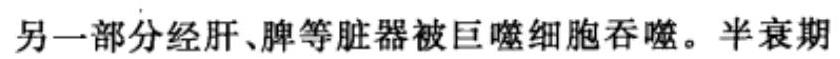
\includegraphics[max width=\textwidth, center]{2024_07_10_373f31b88d2bf633007bg-180}\\
为 $30 \sim 60 \mathrm{~h}$ 。

PFC 可诱发粒细胞聚集的自限性反应, 有些患者可产生一过性低血压。静脉输注前给予糖皮质激素可减轻该反应的发生。

\begin{center}

\includegraphics[max width=\textwidth]{2024_07_10_373f31b88d2bf633007bg-181}
\end{center}

\section*{神经系统疾病的麻醉}
\section*{第一节 麻醉与顾脑生理}
\section*{一、脑血流}
脑组织血流非常丰富, 正常情况下, 脑组织重量约 $1400 \mathrm{~g}$, 占体重的 $2 \%$,但脑血流 (cerebral blood flow, CBF) 却达心输出量的 $12 \% \sim 15 \%$ [相当于 $50 \mathrm{ml} /(100 \mathrm{ml} \cdot \mathrm{kg})$, 因此高灌注及高代谢是脑循环的显著特征。

脑组织的血供来源于颈内动脉系统和椎-基底动脉系统, 它们又分别发自颈总动脉和锁骨下动脉。二者在枕骨大孔上方吻合形成基底动脉环 (Willis 环), 然后再分出大脑前、中、后动脉, 其分支与解外血管吻合。这种解剖上的特点可以确保即使营养血管的一支甚至两支功能障碍时, 仍能维持大脑的基本血供。

脑的血液供应不仅在量上丰富, 其流速也很快, 血液由动脉进人顾腔, 到达静脉突仅需要 4~ $8 \mathrm{~s}$, 平均为 $6 \mathrm{~s}$, 椎-基动脉系统的血流速度比颈内动脉系统要慢。

\section*{$(一)$ 脑血流的自身调节}
脑血流自身调节是机体的一种适应功能, 是脑循环的内在功能。广义地说是指脑组织按其功能和代谢需要来调节脑血液供应的内在能力; 狭义地说仅指脑灌注压在一定范围内变化时仍能保持恒定的脑血液供应。正常人的这种波动范围为平均动脉压 $50 \sim 150 \mathrm{mmHg}$ 。人的部腔是一个容积固定的腔隙, 顾腔内充盈着脑组织、脑脊液和血液三大部分, 它们各占一定比例并维持其相对的稳定。正常人脑脊液约占预控总体积的 $10 \%$; 全脑血流量占 $2 \% \sim 11 \%$;其余部分均由脑组织所充盈。这三大组成成分的比例失衡必将引起颅内压力或脑血流量的变化, 而成分的失衡最易通过脑血流量的改变散感地反映出来。

\begin{enumerate}
  \item 脑灌注压与自动调节 脑灌注压系指输人颊内的平均动脉压与出浈的平均静脉压力差。正常情况下, 颈内静脉压接近于右心房压, 故脑血流量主要取决于颈内动脉的压力。当颈内动脉压升高时, 脑血流量相应增多; 颈内动脉压降低时, 脑血流量减少。

  \item 脑血管阻力与自动调节 脑血管阻力系指 $1 \mathrm{~min}$ 内在 $100 \mathrm{~g}$ 脑组织内流过 $1 \mathrm{ml}$ 血液所需要的压力, 它包括各局部脑血管阻力串连之和以及各脑血管阻力并联之和两大部分, 常以 $\mathrm{mmHg} /(100 \mathrm{~g}$ ・ $\mathrm{min}$ )表示。正常脑血管阻力为 $1.3 \sim 1.6 \mathrm{mmHg}$ / $(100 \mathrm{~g} \cdot \mathrm{min})$ 。若脑血流和颖内压不变, 则脑血管阻力直接与平均动脉压成正比。

\end{enumerate}

若血管口径和灌注压不变, 脑血流量与血液稆滞性成反比, 即血䫝度越高, 脑血流量降低越明显;反之,脑血流量增高越明显。

\begin{enumerate}
  \setcounter{enumi}{2}
  \item 顾内压力与自动调节 颙内压力与脑血管阻力一样, 它与脑血流成反比例关系。同时它亦与脑血流在灌注压变化过程中的调节一样, 顽内压力在一定范围内波动, 虽然同样也能引起动脉灌注压\\
力的升高, 但仍不引起脑血流的改变, 这一自动调节过程称库欣(Cushing) 反射。
\end{enumerate}

脑灌注压在顾内压与脑血流关系中起着重要作用。当顽内压逐渐升高, 而脑灌注压仍维持在 $100 \mathrm{mmHg}$ 以上时,脑血流量无明显变化; 当脑淮注压下降至 $61 \sim 100 \mathrm{mmHg}$ 时,脑血流下降仍不明显, 直至脑灌注压下降至 $51 \sim 60 \mathrm{mmHg}$ 时, 脑血流量才显著减少。

\section*{(二)脑血流的化学调书}
脑血流的化学调节系指内、外环境中各种化学因素对脑血管的作用。这些因素主要包括有: 氧、二氧化碳、血液和脑脊液酸碱状态以及血液和脑脊液离子等。

\section*{1. 氘对脑血流的调节作用}
(1)低血氧对脑血流的调节作用: 在脑血流调节中,低 $\mathrm{PaO}_{2}$ 是一个有效的扩张血管因素。在低氧条件下, 机体脑功能和脑能量代谢的维持通过减少能量消耗、降低脑代谢率及增加脑血流量这几个机制来代偿动脉血氧含量的减少。增加脑血流是保持脑组织氧量稳定的一个重要条件。低血氧下脑血流的增加,可使脑的总氧量增加 $17 \%$ 。低血氧的原因不同对脑血流调节的机制亦有所区别。

(1) 增加脑血流的 $\mathrm{PaO}_{2}$ 限阈。在稳定的 $\mathrm{PaCO}_{2}$条件下, $\mathrm{PaO}_{2}$ 在 $60 \sim 140 \mathrm{mmHg}$ 范围内变动时, 脑血流量基本不变。而当 $\mathrm{PaO}_{2}$ 低于 $50 \mathrm{mmHg}$ 水平时, 脑血流量就开始明显增加, 脑血管对低血氧的反应也像其他生理反应一样, 存在一个限阈, 正常人的低血氧限喊大约 $\mathrm{PaO}_{2}$ 为 $35 \mathrm{mmHg}$, 也有报道在 $30 \mathrm{mmHg}$ 以下的。也有以静脉氧分压 $\left(\mathrm{PvO}_{2}\right)$ 为标准, 认为引起人脑血流增加的 $\mathrm{PvO}_{2}$ 反应限阈在 $30 \mathrm{mmHg}$ 以下 $(25 \sim 28 \mathrm{mmHg})$, 而临界限阀为 $19 \mathrm{mmHg}$, 致命限阈 $17 \mathrm{mmHg}$ 以下, 接近 $12 \mathrm{mmHg}$, 合并酸中毒存在时, 引起脑血流量增加的 $\mathrm{PvO}_{2}$ 值要大于非酸中毒时。在 $\mathrm{PaO}_{2}$ 为 $25 \mathrm{mmHg}$ 时,人全脑血流量为对照值的 $300 \%$ 。

(2)慢性低血氧对脑血流的影响。慢性低血氧是指机体长时间经受低血氧的作用,它对机体的影响要大于急性低血氧。低血氧往往引起过度通气,导致 $\mathrm{PaCO}_{2}$ 下降。因此在低血氧下,脑血流受低 $\mathrm{PaO}_{2}$ 和低 $\mathrm{PaCO}_{2}$ 的双重影响。在急、慢性高山适应不全症的患者中, 低血氧和高碳酸血症两个因素共同作用于脑血管。因为在这类患者中,其低氮或二氧化碳通气反应性低下, 导致通气不足, 引起 $\mathrm{PaCO}_{2}$ 的增加, 所以在慢性低氧环境中,无论通气过度还是通气不足, 都存在着低血氧和血中二氧化碳过高(或过低)两个因素的作用。

在慢性低氧条件下,脑血流量在低氧最初 $24 \mathrm{~h}$的反应最大,以后逐渐降低, 在 $3 \sim 5 d$ 时脑血流不再增加, 脑血管对低血氧的反应消失, 出现脑血流适应。脑血管对慢性低血氧的适应现象可能与脑中毛细血管的微循环增加有关, 可能是毛细血管直径和脑毛细血管区以及组织区比例的增加。

(3)窒急性低血氧和贫血性低血氮对脑血流的作用。在窒息性低血氧时, $\mathrm{PaO}_{2}$ 很快下降, 接着引起脑皮质的 $\mathrm{PO}_{2}$ 和颈静脉 $\mathrm{PO}_{2}$ 的减少, 同时动脉和组织 $\mathrm{PaCO}_{2}$ 增加,引起脑血流量的升高。这种脑血流的增加是由于血中低 $\mathrm{PO}_{2}$ 及高 $\mathrm{PCO}_{2}$ 的结合效应,这两个因素在同一方向上作用,脑血流量可增加 2 倍以上。继发于延髓缺血性缺氧所引起的血压增加也可导致脑血流量的升高。随着窒息时间延长,心力衰竭发生, 血压下降, 脑血流量减少。

负血性低血氧是血红蛋白含量减少所引起的脑供氧量减少。其性质与低氧性低血氧一样, 但它具有正常动脉氧分压, 有利于氧从血液到组织的弥散。当血红蛋白含量减少至 $6 \sim 3 \mathrm{~g}$ 时,脑血流量可增加至正常值的 $250 \% \sim 500 \%$, 而脑氧代谢率和 $\mathrm{P} \mathrm{vO}_{2}$ 保持不变; 血红蛋白含量降至 $3 \mathrm{~g}$ 时, 组织乳酸含量轻度增加, 提示组织缺氧。贫血性低血氧时, 脑血流量增加主要是由于氧容量减少的结果,而与血液黏滞度的关系不大。

(4)低血氧与血中 $\mathrm{CO}_{2}$ 对脑血流的作用。在低血氧时,脑循环的控制必须考虑与低血氧相随变化的血中 $\mathrm{CO}_{2}$ 分压对脑血流的作用,脑血管对血中 $\mathrm{PO}_{2}$ 变化的反应受高或低的 $\mathrm{PaCO}_{2}$ 影响。在低血氧下, $\mathrm{CO}_{2}$ 不仅有助于脑血管的扩张,而且它还可对抗严重低血氧对脑功能的有害作用。

(5)低血氧对脑血流自动调节的影响。在中度低血氧下, 即使有脑血流量的增加和皮质 $\mathrm{pH}$ 的降低, 自身调节仍保存, 一直到 $\mathrm{PaO}_{2}$ 低于 $25 \mathrm{mmHg}$ 4~6min 后,其自动调节才丧失。自身调节一旦丧失,导致被动的压力一血流关系。低氧所引起的脑血流自身调节机制损害是血管壁平滑肌细胞中酸系统在氧缺乏时受到破坏的结果。自身调节受到严重损害后中止低血氧, 这种影响还可延续几小时。研究表明,自身调节易被动脉血低氧所扰乱,然而它不易被脑低氧所破坏,如过度通气引起脑血管收缩, 血流下降, 由此而导致的脑低氧不但不损害脑血管自身调节能力, 反而因血中低 $\mathrm{CO}_{2}$ 分压的\\
缘故而提高脑血管的自身调节能力。

(2)高压氧对脑血流的调节作用:高压氧下脑循环变化基本上有 3 种情况: (1)机体处于常压及高氧或较高气压及高氧压时, 其脑血流量基本不发生变化; (2)在多数情况下,麻醉动物处于吸氧压为 3 个大气压下以及清醒人或动物吸氧压在 5 个大气压下,均可引起脑血流量的减少和脑血管阻力升高; (3)麻醉动物处在 3 个大气压以上氧浓度下, 可引起脑血流量的增加和脑血管阻力下降。\\
2. $\mathrm{CO}_{2}$ 对脑血流的调节作用 血液中 $\mathrm{CO}_{2}$ 是调节脑血流的最重要因素,脑血管对 $\mathrm{CO}_{2}$ 的反应特别敏感。脑血流量随 $\mathrm{PaCO}_{2}$ 的增加而呈阶梯式增加, 如 $\mathrm{PaCO}_{2}$ 增加至 $70 \mathrm{mmHg}$ 左右, 脑小动脉呈最大扩张, 脑血管的自身调节消失。脑血管对血中 $\mathrm{CO}_{2}$ 变化的反应是迅速的, 但在 $\mathrm{PaCO}_{2}$ 变化和脑血流变化之间还是有一个短暂的潜伏期,一般为 20 〜 $30 \mathrm{~s}$, 原因可能是 $\mathrm{PaCO}_{2}$ 通过改变脑血管周围间皕的成分来影响脑血流。血管外组织 $\mathrm{PCO}_{2}$ 变化引起脑血流变化的时间要比血管内的长。血管内 $\mathrm{PCO}_{2}$变化在控制脑血流中占主导地位。

(1)高碳酸血症对脑血流的作用:在人和动物的研究中已观察到脑血管对 $\mathrm{PaCO}_{2}$ 变化的反应曲线。 $\mathrm{PaCO}_{2}$ 在 $15 \sim 50 \mathrm{mmHg}$ 范围内, 脑血流和 $\mathrm{PaCO}_{2}$ 之间呈 $\mathrm{S}$ 形曲线,其最大血流变化范围在 $40 \sim 60 \mathrm{mmHg}$, 血流与 $\mathrm{PaCO}_{2}$ 在此范围接近于线性关系; $\mathrm{PaCO}_{2}$ 在 $70 \sim 80 \mathrm{mmHg}$ 以上, 血流增加很少,可能由于血管已接近最大扩张, 以至脑血流的自身调节在此水平丧失。

(2)低碳酸血症对脑血流的作用: 低碳酸血症的缩血管作用是脑血管所特有的, 这是由于脑血管失去正常 $\mathrm{CO}_{2}$ 浓度所产生的张力效应的缘故。降低 $\mathrm{PaCO}_{2}$ 脑血流量减少, $\mathrm{PaCO}_{2}$ 低于 $20 \mathrm{mmHg}$, 脑血管不再进一步收缩。原因可能是由于在这种低血流水平时存在脑组织低 $\mathrm{PO}_{2}$ 的倾向, 而此种低氧可导致脑血管扩张。故在 $\mathrm{PaCO}_{2}$ 低于 $20 \mathrm{mmHg}$时, 组织低 $\mathrm{PO}_{2}$ 可能会对抗脑血流的进一步减少。低 $\mathrm{PaCO}_{2}$ 缩血管效应也存在反应阈值, 当 $\mathrm{PaCO}_{2}$ 比对照值下降 $2 \mathrm{mmHg}$ 时, 脑血管开始收缩。

严重过度通气可导致脑缺氧, 这是由于在低的 $\mathrm{PaCO}_{2}$ 下, 脑血流量减少, 同时又由于血液 $\mathrm{pH}$ 增加, 使氧解离曲线左移, 血红蛋白与氧的结合更容易, 血浆 $\mathrm{PO}_{2}$ 减少。由于过度通气可减少脑血流量和脑血容量, 故在临床上常将过度通气作为降低顾内高压的一种措施。\\
3. 血液和脑券液 $\mathrm{pH}$ 对脑血流的调节作用在静息条件下, 脑脊液中 $\left[\mathrm{HCO}_{3}^{-}\right]$浓度比血浆中要小, 而脑脊液中的 $\left[\mathrm{H}^{+}\right]$浓度大于血浆。血液和脑脊液间的 $\left[\mathrm{HCO}_{3}^{-}\right]$梯度通过 $\left[\mathrm{HCO}_{3}^{-}\right]$的主动转运来维持, 这种主动转运的部位, 即为血脑屏障的脑毛细血管内皮细胞。在脑组织的 $\mathrm{pH}$ 调节中,血脑屏障是十分重要的, $\left[\mathrm{HCO}_{3}^{-}\right]$仅能缓慢地通过血脑屏障,而 $\mathrm{CO}_{2}$ 可自由弥散,所以脑中 $\mathrm{pH}$ 取决于脑组织中 $\left[\mathrm{HCO}_{3}^{-}\right]$浓度和 $\mathrm{PaCO}_{2}$ 。

(1) 血浆 $\mathrm{pH}$ 对脑血流的作用:一般认为在 $\mathrm{PaCO}_{2}$ 稳定的条件下,脑血流随血液 $\mathrm{pH}$ 的变化而变化。

(2)细胞外液 $\mathrm{pH}$ 对脑血流的作用: 细胞外液是指脑小动脉平滑肌细胞外的间隙液, 其化学成分类同于脑脊液。

\begin{enumerate}
  \setcounter{enumi}{3}
  \item 高子及其他物质对脑血管的作用
\end{enumerate}

(1)钾离子的作用: 钾离子与脑的功能状态密切相关, 当神经活动时, 可引起脑细胞间隙的钾离子浓度升高, 于是导致活动区域血管扩张,血流增加。

(2)锬离子的作用: 脑脊液中镖离子从正常值 $3 \mathrm{mmol} / \mathrm{L}$ 增加至 $6 \mathrm{mmol} / \mathrm{L} 、 9 \mathrm{mmol} / \mathrm{L} 、 18 \mathrm{mmol} / \mathrm{L}$,可观察到血管收缩, 血管直径分别降低 $12 \% 、 21 \%$和 $30 \%$ 。另外,血管收缩程度也随钴离子作用时间的延长而增加。

脑血管周围液体环境中的各种离子相互作用于脑血管, 因此脑血管的䇰缩作用不是单一因素所决定的。一般认为锬离子起重要作用, 在脑血管的生理调节中,氢、钾离子, 尤其是氢离子仅具有一定的作用。

(3)氯离子的作用:减少血管周围氯离子对脑血管有强烈的收缩效应。在正常 $\mathrm{pH}$ 时, 将含低浓度 ( $72 \mathrm{mmol} / \mathrm{L}$ ) 氯离子 (正常值为 $144 \mathrm{mmol} / \mathrm{L}$ ) 的脑脊液灌注至血管周围间陧,可引起血管收缩 $12 \%$; 当 $\mathrm{pH}$ 为 8.0 时,正常氯离子引起血管收缩 $18 \%$ 。

(4)腺苷的作用: 腺苷在脑血管阻力的代谢性调节中具有一定的作用。腺苷存在于正常脑和脑脊液中, 它可影响血管平滑肌对钻离子的摄取, 因此它对脑血管有扩张作用。在电刺激、过度通气、低氧和低血压时,腺苦从脑中释放量增加,而吸人 $\mathrm{CO}_{2}$ 可减少腺苷的释放。

\section*{(三)脑血流的神经调节}
\section*{1. 脑血管上的神经分布}
(1)脑实质外动脉上的神经分布: 所谓脑实质外动脉主要指 Willis 环血管及其分支和蛛网膜下隍的软脑膜动脉。超微结构的研究发现, 脑血管上的神经与其他血管床上一样, 其纤维位于脑血管壁的外膜或外膜与中膜的交界处, 不穿过血管壁的平滑肌细胞。轴突末梢缺乏神经膜细胞(施万细胞),外形膨大,含有许多小泡。根据所含小泡的类型可以分为两种轴突末梢。有的小泡含有颗粒, 颗粒代表储存去甲肾上腺素的部位, 含有颗粒小泡的轴突是肾上腺素能纤维; 含有无颗粒小泡的轴突是胆碱能纤维。

一般认为脑实质外动脉上的肾上腺素能神经起源于颈上神经节, 荧光技术表明, 阻断或切除颈上神经节后, 脑实质外动脉周围的特殊儿茶酚胺荧光消失。肾上腺素能神经在顾内血管上的分布以 Willis 环的主要动脉及其分支上最为密集; 颈内动脉的顶内部分次之; 大脑中动脉和基底动脉上最少。肾上腺素能神经沿着软脑膜血管一直分布到直径为 $15 \sim 20 \mu \mathrm{m}$ 的血管上。脑实质外动脉上的肾上腺素能神经除了大脑前动脉、小脑后动脉、基底动脉属于双侧分布外, 其余都是单侧分布的。在软脑膜上, 邻近的动脉之间存在肾上腺素能神经相互结合形成的神经丛。

脑血管上的胆碱能神经来自面神经的分支岩浅神经, 最后形成颈内动脉丛。脑实质外动脉上胆碱能神经分布的范围和肾上腺素能神经相似。软脑膜循环前面部分血管上的胆碱能神经要比后面部分血管上的丰富。

(2)脑实质内血管上的神经: 分布于脑实质内动脉上的肾上腺素能神经可能来自延歓。在脑实质内动脉上, 紧上腺素能神经纤维分布的数量与供应其所在部位软脑膜血管上的神经纤维数量有关。例如, 由神经纤维分布较多的大脑中动脉供血的尾核, 其半数的小动脉上有情上腺素能神经分布, 而在神经分布稀少的大脑后动脉供血的外侧膝状体中, 其小动脉则很少有肾上腺素能神经分布。

\begin{enumerate}
  \setcounter{enumi}{1}
  \item 周围和中枢神经对脑血流的调节作用
\end{enumerate}

(1)周围神经对脑血流的调节作用: 起源于颈上神经节的肾上腺索能神经对脑血管主要起收缩作用; 行走于面神经、迷走神经内的胆碱能神经的功能是舒张血管。

(1) 交感神经对脑血流的调节作用。交感神经收缩血管可能主要作用在直径 $10 \sim 15 \mu \mathrm{m}$ 的毛细血管前动脉上。有人认为, 脑实质外血管上有丰富的肾上腺素能神经支配, 主要受交感神经影响; 脑实质内血管上的神经支配较少, 主要受代谢的控制; 脑较膜血管上不仅有肾上腺素能神经支配, 并且也与大脑接触, 受神经和代谢的双重影响。

交感神经对脑各个部位血流的影响程度不同,电刺激颈交感神经, 脑前区组织的血流平均下降 $22 \%$,后区组织的血流平均下降 $12 \%$,说明 Willis 环前分支所供应的组织血流比后分支或基底动脉分支所供应的组织血流更易受交感神经调节的影响。另外, 交感神经对脑血管的影响与血管上神经分布的密度有关。

交感神经对脑血流影响的程度也与动脉血 $\mathrm{CO}_{2}$ 分压有关。正常 $\mathrm{PaCO}_{2}$ 下电刺激交感神经, 引起脑实质外血管收缩, 其远端血管的压力和血流量下降, 通过自身调节机制, 使脑实质内血管扩张, 阻力降低, 血流恢复至对照水平。但在高碳酸血症时, 脑实质内血管处在扩张状态, 因此电刺激交感神经会引起脑实质外血管收缩, 脑实质内血管不能再有效地进一步扩张, 从而脑血流量降低。

(2)副交感神经在脑血流调节中的作用。刺激迷走神经中枢端时, 两侧软脑膜血管扩张, 直径增加 $9 \% \sim 22 \%$; 切断交感神经后,这种扩血管效应仍然存在, 并且不依赖于 $\mathrm{PaCO}_{2}$ 水平。因此, 有人提出迷走神经具有真正的脑血管扩张作用, 不只是抑制交感缩血管活动。面神经也携带有脑血管扩张纤维, 并经过滕状神经节刺激面神经, 同侧软脑膜血管扩张, 其直径可增加 $16 \%$ 。电刺激一侧岩浅大神经, 脑血流随着电刺激频率的增加而升高, 最大值可达 $11 \%$ 。

(2)中枢神经对脑血流的调节: 脑干的一些部位参与了脑血流的反射性调节。电刺激猴大脑皮质, 对脑血流和代谢无影响, 但刺激中脑网状结构,其脑血管扩张效应与吸人 $8 \% \mathrm{CO}_{2}$ 气体相同。电刺激引起的脑血流增加效应非常迅速, 平均潜伏期仅 $4 \sim 5 \mathrm{~s}$, 而且该效应不受 $\mathrm{PaCO}_{2}$ 水平和顽交感神经切除的影响。

脑干中蓝斑的胞体发出纤维分布于脑实质内血管, 具有调节脑血流的功能。损伤猫的蓝斑能引起下丘室旁核、丘脑前腹核、大脑皮质顶区的去甲肾上腺素明显减少; 并明显损害脑血管对高、低碳酸血症的反应;但对改变血压时脑血流的自身调节反应没有明显影响。电刺激蓝斑可引起脑实质内小动脉上的神经末梢释放去甲肾上腺素, 使脑血管张力增加, 血流量减少。电刺激鼠一侧蓝斑、同侧\\
扣带皮质、外侧隔区、尾核壳核腹侧端,脑血流量分别减少 $65 \% 、 40 \%$ 和 $70 \%$,而对侧这三个部位的血流无明显变化。

丘脑在脑血流调节中可能具有一定作用,刺激下丘脑后部, 可引起血压升高和双侧软脑膜血管收缩, 脑血管收缩出现在血压变化前几秒,并与血液内气体张力的水平无关。剌激下丘脑腹部可引起双侧软脑膜血管扩张和血压下降。

\section*{3. 脑血管上的受体}
(1)肾上腺素能受体: 脑血管壁上存在调节血管运动反应的 $\alpha$ 型 ( $\alpha$ 受体) 和 $\beta$ 型肾上腺素能受体 ( $\beta$ 受体)。 $\alpha$ 受体兴奋, 脑血管收缩; $\beta$ 受体兴奋, 脑血管扩张。脑血管壁上 $\beta$ 受体的去甲肾上腺素阈值可能低于 $\alpha$ 受体。小剂量的去甲肾上腺素能激活脑血管壁上的 $\beta$ 受体,使血管扩张; 大剂量去甲肾上腺素激活了 $\alpha$ 受体,引起血管收缩。有报道认为, $\alpha$ 受体对脑血管的调节作用要比 $\left[\mathrm{H}^{+}\right]$浓度改变更强有力。

(2)胆碱能受体: 脑血管上的胆䂸能受体属毒曹碱型。在生理条件下, 胆碱能受体兴奋使脑血管扩张, 而在大剂量拟胆碱药作用下则引起脑血管收缩, 这两种效应均能被阿托品所阻断。正常条件下,阿托品对脑血流的自动调节和脑氧耗无影响,但限制了高碳酸血症的增加脑血流效应和低碳酸血症的降低脑血流效应, 说明胆碱能受体参与了高、低碳酸血症时的脑血流调节。

(3)多巴胺受体: 脑血管上存在扩张性多巴胺受体。多巴胺对脑循环的调节作用是通过直接作用于脑血管上的受体实现的。静脉注射多巴胺受体阻滞药能明显减弱低氧血症对脑血管的扩张效应; 但脑血管对 $\mathrm{CO}_{2}$ 的扩张反应仍存在。多巴胺受体还参与了脑血流的自身调节。

(4) 5-垟色胺受体: 5 -差色胺通过血管壁上的相应受体调节脑血流。5-羟色胺的主要作用是使脑血管收缩,脑血流惐少。血管内灌注 $5-\mathrm{HT}[1 \mu \mathrm{g} /$ $(\mathrm{kg} \cdot \mathrm{min})]$, 在正常 $\mathrm{PaCO}_{2}$ 时, 脑血流降低 $35 \%$;低氧血症时减少最明显,可达 $62 \%$ 。

(5)组胺受体: 组胺通过 $\mathrm{H}_{1}$ 和 $\mathrm{H}_{2}$ 受体作用于脑血管。 $\mathrm{H}_{1}$ 受体兴奋脑动脉收缩; $\mathrm{H}_{2}$ 受体兴奋可引起脑血管扩张。组胺对 $\mathrm{H}_{1}$ 和 $\mathrm{H}_{2}$ 受体的兴奋作用与剂量有关。在猴, 小剂量组胺 $(50 \mu \mathrm{g} / \mathrm{kg})$ 可使大脑前动脉显著扩张; 中等剂量 $(150 \mu \mathrm{g} / \mathrm{kg})$ 时血管直径无明显变化; 但大剂量 $(300 \mu \mathrm{g} / \mathrm{kg})$ 时大脑前动脉收缩。组胺对脑血管的效应迅速而短暂。\\
(6)肽能受体: 脑血管壁上可能存在肽能受体,可被血管活性肠肽激活而产生脑血管扩张作用。血管活性肠肽本身对静息血管几无影响, 但对已处于收缩状态的软脑膜血管具有扩张作用, 其扩张程度类似乙酰胆碱和异丙肾上腺素。

\section*{二、脑 代谢}
\section*{(一)脑组织代谢的特点}
\begin{enumerate}
  \item 脑的能量代谢和糖代谢脑的功能复杂, 活动频繁, 所以能量消耗特别多。用放射性惰性气体 ${ }^{133} \mathrm{Xe}$ 示踪测量估计, 人体在清醒时的脑血流量为 $0.52 \pm 0.12 \mathrm{ml} /(\mathrm{g} \cdot \mathrm{min})$; 再根据脑动脉与静脉血流间的氧分压差, 推算出脑的耗氧率为 $1.47 \pm$ $0.18 \mu \mathrm{mol} /(\mathrm{g} \cdot \mathrm{min})$, 明显高于其他组织。脑的能量代谢中, $60 \%$ 的能量消耗用于维持神经生理功能; $40 \%$ 用于维持神经结构的完整性。
\end{enumerate}

正常情况下脑的呼吸商为 1 , 说明脑的能量需要是由葡萄糖提供的。脑中糖原的储备量很少 (约 $0.1 \%$ ), 而脑动、静脉脑血流中葡萄糖浓度的差别又很大, 此足以说明脑组织依赖血液莆蒛糖作为主要能源。葡萄糖以易化扩散方式从血摄取人脑, 此过程具有饱和竞争特性。静息状态下, 脑从血液中摄取的莆萄糖量约占其总运输量的 $10 \%$; 脑血流降低时, 摄取比率将增大。脑葡萄糖消耗量约占总体消耗量的 $1 / 4[31 \mu \mathrm{mol} /(100 \mathrm{~g} \cdot \mathrm{min})]$ 。在正常条件下, 脑所需的莆蒛糖主要来自肝储存糖原的分解, 部分来源于肌肉, 小部分来自其他器官。据知,肝单位组织重量中储存的糖原量是脑的 100 倍, 肌肉组织是脑的 10 倍。用 ${ }^{14} \mathrm{C}$ 莆䔩糖的放射性掺人试验表明, 尽管放射性也见于脑的氨基酸、脂类、蛋白质和核酸,但脑中 $90 \%$ 以上的葡䔤糖是通过糖酵解和三啴酸循环分解的。

脑中葡萄糖在正常情况下主要进行有氧代谢,而通过无氧酵解的量为 $5 \% \sim 15 \%$ 。酵解酶体系不仅位于胞体, 并且也存在于远离胞体的轴突末端,参与突触前末端能量代谢的需要。在有氧条件下, $1 \mathrm{~g}$ 分子葡萄糖经过脑的有氧氧化途径, 可生成 36 38ATP, 若从糖原的葡萄糖单位开始, 则生成 $37 \sim 39 \mathrm{ATP}$ 。在无氧条件下, $1 \mathrm{~g}$ 分子蒲踓糖经无氧酥解仅生成 2 3ATP。

在正常动脉血液, 莆蒛糖浓度为 $80 \mathrm{mg} / \mathrm{dl}$, 脑消耗氧的速率约 $3.4 \mathrm{ml} /(100 \mathrm{~g} \cdot \mathrm{min})$, 使用胰岛素将血糖降至 $8 \mathrm{mg} / \mathrm{dl}$ 时, 氧的消耗降到 $1.9 \mathrm{ml} /$ $(100 \mathrm{~g} \cdot \mathrm{min})$ 。这样的氧消耗水平已无法依靠氧化\\
磷酸化提供足量 ATP 进行正常的脑功能活动, 于是出现昏迷, 久之会造成脑的不可逆性损伤。媵岛素不能越过血脑屏障, 因此胰岛素只能通过对血糖浓度的影响来改变脑中糖代谢, 但末梢神经的蒲萄糖代谢可直接受血浆胰岛素的影响。

\begin{enumerate}
  \setcounter{enumi}{1}
  \item 脑中氮基酸和蛋白质代谢脑中氨基酸来源有 2 个: 血液提供以及糖代谢生成。脑血流中的氨基酸能迅速与脑中的交换, 但浓集于脑中的氨基酸含量却相当有限。脑内存在维持氨基酸稳态平衡的机制, 因此提高血浆氨基酸浓度却并不能因而提高脑内氨基酸的水平。多数氨基酸是通过载体系统进人脑细胞内的, 脑中蒲蒛糖可转变成一部分氨基酸,其中主要是非必需氨基酸。
\end{enumerate}

脑中大约 $75 \%$ 的自由氨基酸是天冬氨酸、谷氨酸、谷氨酰胺、 $\mathrm{N}$-乙酰天冬氨酸及 $\gamma$-氨基丁酸。其中谷氨酸的含量最多, 浓度为 $10 \mathrm{mmol}$ 。进人脑中的氨基酸可迅速掺人蛋白质。蛋白质的合成主要在神经细胞体进行, 但轴突中也有合成。脑中氨的产生是通过腺苷酸脱氨酶作用的, 即氨基酸的氨基经过转氨基而形成谷氨酸和天冬氨酸,再生成腺苷,而后脱去氨基, 如此形成的氨大多数用于合成谷氨酰胺, 经血带走。

\begin{enumerate}
  \setcounter{enumi}{2}
  \item 脑中核酸代谢脑中 RNA 含量特别高。脑中 RNA 的代谢速度随神经的功能活动而变化。在短期的强烈刺激之后, 脑中的 RNA 含量升高, 但长期刺激后却趋于降低。脑的功能活动会随特定的细胞和区域而异, 故脑中 RNA 含量的变化并非均匀一致。
\end{enumerate}

脑组织能将尿苷转变为尿苷酸 (UMP), 然后转变为三磷酸尿苷 (UTP) 和三磷酸胞苷 (CTP) 而合成核酸以及参加脂类及橎多糖的代谢, 能储存核酸及传递遗传信息, 并将这些信息翻译成蛋白质。神经系统的功能活动主要由这些过程参加。

\begin{enumerate}
  \setcounter{enumi}{3}
  \item 脑中脂类代谢大脑发育之初, 脂类的含量并不多,随着大脑的发育逐渐出现神经䯝鞘。神经觛鞘形成后, 神经组织中脂类增加。脑中脂类的大多数包括胆固醇、脑苷脂、磷脂酰乙醇胺和神经磷脂而仅在脑中缓慢代谢, 但是磷脂酰胆碱则代谢迅速;磷脂酰肌醇的代谢速率更快。脑中甘油磷脂的合成途径与其他组织相同。脂肪酸、甘油和肌䡴来自糖代谢; 脑接受血浆中的乙醇胺并将其掺人磷脂。
\end{enumerate}

\section*{(二)脑代谢率 (cerebral metabolic rate,CMR)、体温对脑血流和脑代谢的影响}
CMR 可用脑代谢耗氧量 (cerebral metabolic rate for $\mathrm{O}_{2}, \mathrm{CMRO}_{2}$ ) 来表示,脑组织血供相当丰富。代谢极为活跃, 无论是在睡眠或觉醒状态下, $\mathrm{CMRO}_{2}$ 占全身总耗氧量的 $20 \%$, 相当于 $50 \mathrm{ml} / \mathrm{min}$,脑能量代㴬高度依赖脑血流供给葡蒛糖, 正常生理状态下,没有其他代谢底物。脑代谢同时也包括氨基酸代谢,包括谷氨酸、GABA 以及神经递质的代谢。CMR 常用 $\mathrm{CMRO}_{2}$ 来表示, 根据 fick's 定律

\[
\begin{aligned}
& \mathrm{CMRO}_{2}=\mathrm{CBF} \times \mathrm{C}_{\mathrm{a}-}-\mathrm{N}_{2} \\
& \left(\mathrm{C}_{\mathrm{n}}-\mathrm{N}_{2} \text { : 动静脉氧含量差 }\right)
\end{aligned}
\]

尽管 $\mathrm{CMRO}_{2}$ 是一个量化指标, 但它的变化并不能反映局部氧和能量供应失衡的程度。脑耗氧占全身氧供的比例大于脑血流占心输出量的比例,所以脑组织从血流中摄取氧的比例较身体其他部分为高, 而氧的储备功能相对低下。生理状态下,大脑所需能量几乎全由葡豞糖供给, 后者主要由肝糖原分解而来,能量储备也有限。由于大脑这种高代谢低储备的特点, CMR 的变化必将迅速引起 $\mathrm{CBF}$ 的明显改变, 以适应脑功能状态的需要。在发热、菛痵等病理状态下, 脑电活动增加, CMR 加强,而乳酸、二氧化碳、氢离子及其他代谢产物增加作用于脑血䇪,会引起脑血管扩张, $\mathrm{CBF}$ 相应增加。相反,静息状态如睡眠或低温, CMR 堿少, CMF 相应减少。此外, 由于大脑内各部分神经元密度及代谢活动的不同, 大脑内部各区域的血流量也不一致。总的而言,灰质的血流量是白质的 5 倍。脑代谢也包括氨基酸代谢, 包括谷氨酸, GABA以及神经递质的代谢。

其他可影响 CBF 的因素还有年龄、血液馝滞度、血管壁摩擦力、脑血管阻力等。

无论是在正常生理状态下或是脑缺血时, 低温均能降低 CBF 和 CMR, 通常体温每下降 $1^{\circ} \mathrm{C}$, CMR 降低 6\% 7\%。与麻醉药一样, 低温也可抑制全部脑电活动, 其所需温度约为 $20^{\circ} \mathrm{C}$ 。但低温对于 CMR 和 CBF 的抑制与麻碎药的作用又有所区别, 当脑电活动被全部抑制以后,随着温度的进一步降低, CMR 仍会继续下降, 这是因为低温不但抑制 CMR 的脑电活动部分, 而且能抑制维持细胞稳态结构部分的脑电活动。曾经认为低温对这两部分是成比例抑制的, 但现已证明, 轻度低温时优先抑制维持正常内稳态脑电活动。当温度降至 $18^{\circ} \mathrm{C}$时, $\mathrm{CMRO}_{2}$ 降为正常值的 $10 \%$, 这就是大脑在低温下耐受缺血时间明显延长的机制。温度升高时对 CBF 和 CMR 的作用与此相反, 在 $37 \sim 42^{\circ} \mathrm{C}$, 随着温度升高, $\mathrm{CBF}$ 和 $\mathrm{CMR}$ 均升高, 当温度超过 $42^{\circ} \mathrm{C}$,

\section*{蛋白质和酶变性,耗氧量急剧下降。}
(三)麻醉状态下对脑血流、脑代谢和颇内压的影响

\section*{1. 静脉麻醉药}
(1) 巴比妥类: 应用巴比妥类药物时, 如果 $\mathrm{PaCO}_{2}$ 维持正常, $\mathrm{CBF} 、 \mathrm{CMRO}_{2}$ 、脑蒲萄糖代谢率和脑电图呈剂量相关性抑制。当脑电图出现高幅慢波时, 对 CBF 和脑代谢率抑制达平台水平, 大约降低 $50 \%$,同时伴有脑血管阻力增加。

硫偾妥钠麻醉中, CBF 的自身调节机制和 $\mathrm{CBF}$ 对 $\mathrm{PaCO}_{2}$ 升高的反应正常。静脉注射镇静剂量的巴比妥类药物, 意识消失前, $\mathrm{CBF}$ 和脑代谢无改变, 意识消失但部分肌肉对疼痛仍有反应时, $\mathrm{CMRO}_{2}$ 降低 $36 \%$, 达到外科麻醉深度时, $\mathrm{CMRO}_{2}$降低 $36 \% \sim 50 \%$ 。如同时采用过度通气,CBF 降低更为明显。巴比妥对中枢神经系统作用顺序是:巴比妥类药物麻醉一脑代谢降低一脑 $\mathrm{CO}_{2}$ 产生堿少一脑 $\mathrm{PCO}_{2}$ 趋于降低一脑血管收缩- $\mathrm{CBF}$ 和脑血流量减少一顽内压降低。巴比妥类对脑代谢抑制作用最强, 主要抑制神经元的电生理活动(而非维持细胞整合所需要的能量)。动物实验表明, 严重低血压和(或)低氧血症时, 应用巴比妥类药物麻醉对缺血和缺氧的脑组织有保护作用, 能减轻神经后遗炡或延长动物存活时间。这可能是由于其降低了 $\mathrm{CMRO}_{2}$ 和脑血流, 从而使 ICP 降低。

(2)依托味酯: 与巴比妥类药物类似,依托咪酯进行性地降低脑代谢率, 直到出现等电位脑电图。与脑代谢率不同, $\mathrm{CBF}$ 在依托味酯注射初期即急速下降。CBF 最大速度降低出现在脑代谢率出现最大降低之前, 这可能是依托味酯直接引起脑血管收缩所致。 $\mathrm{CBF} 、 \mathrm{CMRO}_{2} 、 \mathrm{ICP}$ 呈剂量相关性降低。在依托㗚酯麻醉中, $\mathrm{CBF}$ 对 $\mathrm{CO}_{2}$ 的反应性良好, 脑能量代谢正常。另外, 依托味酯与钙通道阻滞药一样, 对脑缺血有保护作用。大剂量应用依托咪酯对循环功能尤其是脑灌注压影响轻微, 而且能减少脑血流、脑氧耗和顾内病变患者的 ICP, 是神经外科较好的全麻诱导药物。

(3)丙泊酚: 与巴比妥类药物一样呈剂量相关性抑制脑血流和脑氧耗, 但保留 $\mathrm{CO}_{2}$ 反应性。丙泊酚通过抑制脑代谢而降低脑血流大量的研究表明,丙泊酚降低或不改变浈内压, 可降低平均动脉压和脑灌注压。此外,丙泊酚还可抑制兴奋性氨基酸的释放, 减少钻离子内流和清除氧自由基, 从而减少兴奋性氨基酸的神经毒性, 保护细胞膜, 对脑缺血再灌注损伤有防治作用。丙泊酚靶控输注是神经外科较理想的麻醉维持用药。

(4) 神经安定药物: 神经安定药降低 ICP, 减少脑血流, 对脑氧耗影响轻微。

(5)氯胺酮: 氯胺酮是静脉麻醉药物中惟一可以增加 CMR 和 CBF 的药物, 具有独特脑功能激活作用。氯胺酮麻醉中, CBF 的自动调节机制完整,但脑血管对 $\mathrm{PaCO}_{2}$ 的反应性增加约 $60 \%$ 。氯胺酮具有直接扩张脑血管的作用, 能迅速增加 CBF 和 $\mathrm{CMRO}_{2}$, 氯胺酮促进脑代谢的机制尚不清楚。氯胺酮显著增加顾内压, 这种增加能被过度通气、硫喷罗钠或苯二氮草类药物阻断或减弱。但是一些研究证明, 氯胺酮引起的顾内压升高并不能被巴比妥类、地西泮或咪达唑仑所阻断。因此, 氯胺哃不能被推荐用于神经外科患者的麻醉, 特别是顽内压升高或颁内顺应性降低的患者。

由于氯胺酮的镇痛作用强, 而对呼吸无明显的抑制作用,适用于需要保留自主呼吸的脑干手术患者术中的麻醉维持。

(6)轻丁酸钠: 静脉滴注时, 随着剂量的增加,可出现代谢性酸中毒, 脑血管收缩, CBF 和脑代谢逐渐降低,故可造成暂时性, 相对性脑缺血。Stolkarts 在 30 例顾内肿面患者用羟丁酸钠作诱导, 楨内压降低 $34.5 \%$, 同时脑灌注压增加。因此, 羟丁酸钠适合于神经外科手术患者, 特别是颅内压升高或顾应性降低而休克的外伤贯者。

\begin{enumerate}
  \setcounter{enumi}{1}
  \item 吸入麻醉药 所有吸人麻碎药或多或少扩张脑血管, 增加脑血流量和脑血容量, 因此升高顽内压。吸人麻醉药还抑制脑血管自身调节, 干扰对 $\mathrm{CO}_{2}$ 的反应。与氟类吸人麻醉药降低脑代谢不同, $\mathrm{N}_{2} \mathrm{O}$ 可增强脑代谢, 增加脑血流量。在一定吸人浓度范围内, $\mathrm{CBF} / \mathrm{CMRO}_{2}$ 的变化与浓度大致呈直线相关。氟烷对脑血管的扩张效应最强, 恩凲烷次之, 氧化亚氮、七氟烷和异氛烷的作用较弱。在 1. 5 MAC 麻醉浓度下, 氟烷和恩氟烷分别增加 CBF $66 \%$ 和 $35 \%$, 而异氟烧和七氟烷对 CBF 几乎无影响。氟烷和恩氟烷明显损害 CBF 的自身调节机制, 而异㪉烷对其影响轻微。

  \item 麻醉性镇痛药 麻醉性镇痛药对 $\mathrm{CBF}$ 和项内压的影响报道不一,这种差异主要与背景麻醉用药和种系有关。当背景麻醉药收缩脑血管或无麻醉药物作用时, 麻醉性镇痛药对脑 CBF 没有影响甚至可增加 $\mathrm{CBF}_{\text {。 }}$ 。

\end{enumerate}

单独应用吗啡对顾内压及 CBF 无明显影响。\\
芬太尼对 CBF 及 CMR 的作用明显受复合用药的影响。在与氧化亚氮、氟烷和地西泮复合应用时,芬太尼能明显降低 $\mathrm{CBF}$ 和 $\mathrm{CMRO}_{2}$, 但单独应用时, 对 $\mathrm{CBF}$ 和 $\mathrm{CMRO}_{2}$ 无明显影响或 $\mathrm{CBF}$ 呈轻度增加。舒芬太尼和阿芬太尼可引起 ICP 不同程度的增加和 CPP 不同程度的降低, 后者主要与平均动脉压降低有关。舒芬太尼对 $\mathrm{CBF}$ 和 $\mathrm{CMRO}_{2}$ 呈剂量相关性抑制, 随着剂量的增大, 脑电图显示㿎疾发生率也增加, 但㿎疾波出现对 $\mathrm{CBF}$ 和 $\mathrm{CMRO}_{2}$无明显影响。雷米芬太尼对 ICP 影响不显著, 但对平均动脉压呈剂量依赖性降低。

\begin{enumerate}
  \setcounter{enumi}{3}
  \item 肌松药 肌松药不能通过血脑屏障, 从而对脑血管无直接作用。但肌松药对 CBF 有间接作用,肌松药可降低 CVR 和静脉回流阻力, 从而使 ICP 下降。但肌松过程中患者血压升高, 可进一步增加领内高压患者的 ICP。
\end{enumerate}

大量动物实验及临床试验均已证明, 氯琥珀胆碱由于肌纤维成束收缩引起的颅内压增加, 小剂量非去极化肌松药预处理并不能阻断肌肉传人活动或 CBF 的反应。顽内压增加也不能被硫喷妥钠预处理所阻断。泮库滇铵可阻滞窣房结, 交感神经节和交感神经末梢中的 $M$ 受体, 使交感活动增强, 也能抑制交感神经末梢对已释放的去甲肾上腺素的正常摄取。因此, 可诱发血压升高。在 CBF 自动调节功能损害和顾内病变的患者中, 可明显增加 $\mathrm{CBF}$ 和 ICP, 阿曲库轱对 CBF 和 ICP 无明显影响。但其代谢产物 $\mathrm{N}$-四氢嚮粟碱容易穿过血脑屏障而引起抽搐。维库溴铵、泮库溴铵对预内压及脑灌注压无明显影响。

在神经外科患者中如果需要应用氯琥珀胆碱,建议先用小剂量的非去极化肌松药, 采用控制呼吸, 避免 $\mathrm{PaCO}_{2}$ 升高, 大多数临床情况中非去极化肌松药对 $\mathrm{CBF}$ 和顽内压影响很小。

(四)麻醉方法和管理对脑血流、脑代谢和须内

\section*{压的影响}
通气时呼气时间不足、呼气阻力增加、气管内插管时的刺激、术中呛咳或用力以及颈部弯曲、扭转、头低位和胸、腹腔内压增高时, 都能使脑静脉回流受阻, 项内压升高, 从而明显改变脑灌注压和脑血流量。

在急性等容血液稀释患者, 当 HCT 降至 $30 \%$以下时, 由于血液秥度下降, 心排血量增加和脑血管阻力降低, 脑血流量明显增加。有研究发现, 等容血液稀释期间皮质血流量增加源于脑血管扩张;而脑皮质下区域血流量增加与血液馧度惐低和心排血量增加有直接关系。血液稀释可使脑局部缺血区脑血流量增加。因此, 有局灶性脑缺血的患者, 维持 $\mathrm{HCT}$ 在 $30 \% \sim 34 \%$ 范围内较为合适, 而且仍具有较好的携氧能力。

用硝普钠、樟磺味芬、硝酸甘油、氟烷、尼莫地平降压中, 脑血流自动调节曲线较出血性低血压时的自身调节曲线左移; 当用上述药物降低 MAP $\leqslant$ $50 \mathrm{mmHg}$ 时, 脑血管对 $\mathrm{PaCO}_{2}$ 的反应性消失; 但若用异氛烷降低 MAP 至同样水平, 脑血管对 $\mathrm{PaCO}_{2}$的反应仍部分存在。

控制性降压对脑氧耗和脑能量代谢的影响与降压方法和降压程度有关。用硝普钠和樟磺咪芬降低 MAP 至对照值的 $50 \%$, 硝普钠组的 $\mathrm{CMRO}_{2}$ 明显增加, 而樟磺味芬组的 $\mathrm{CMRO}_{2}$ 无明显改变; 当 MAP 降低至 $40 \sim 50 \mathrm{mmHg}$ 时, 患者脑动-静脉氧含量差分别升高 $(3.5 \pm 0.8) \mathrm{ml} / \mathrm{dl}$ 和 $(1.7 \pm 0.4) \mathrm{ml} / \mathrm{dl}$ 血, 说明脑称氧能力增加; 但当将 MAP 降至 $30 \mathrm{mmHg}$ 时, 两组的 $\mathrm{CMRO}_{2}$ 均有中度降低。用三磷腺苷或腺苷降压时, 脑血管阻力和脑血流量明显降低, $\mathrm{CMRO}_{2}$ 无明显改变,但乙状静脉窦氮分压明显降低。应用氟烷和异氣烷降压时, $\mathrm{CMRO}_{2}$ 明显下降。

\section*{三、脑脊液循环}
脑室、脑脊液与脑脊液循环:

\section*{(一)脑室系统}
包括两侧侧脑室、第三脑室、第四脑室, 在脑室系统及脑蛛网膜下腔都充满脑脊液, 它不但有缓冲颊内压力作用, 而且对脑组织有一定的营养作用。

\section*{(二)脑㤗液与脑奏液盾环}
脑脊液在脑内形成,并在脑内各间院循环,脑脊液与脑内细胞外液可自由交换。正常情况下, 脑内细胞内液、细胞外液、脑脊液、血液和淋巴液是可以相互转移的。

\begin{enumerate}
  \item 脑券液的生成 正常状态下, 脑脊液主要由脑室内的脉络丛产生, 大部分来自侧脑室的脉络丛。与脑内其他毛细血管内皮细胞不同, 脉络丛毛细血管内皮细胞间没有紧密的连接, 而是有空㫤的。血液进人脉络丛毛细血管经内皮细胞时被滤过,并在脉络丛基质内产生富含蛋白的液体一一脑脊液, 其成分与其他组织的组织间液相似。此外,蛛网膜下间隙 (可能是软脑膜) 及室管膜与血管周围的间陌(Virchow-Robin 间隙) 也有产生脑脊液的功能,称脉络丛外脑脊液生成。脉络丛外脑脊液\\
生成 $60 \%$ 由于脑内葡萄糖氧化产生, $40 \%$ 由脑毛细血管的超滤作用产生。
\end{enumerate}

脑脊液生成速率 $0.35 \sim 0.40 \mathrm{ml} / \mathrm{min}$, 即每天生成 $500 \sim 600 \mathrm{ml}$, 每分钟有 $0.25 \%$ 的脑脊液容量被新形成的脑脊液所替代,脑脊液容量的更新时间 $5 \sim 7 \mathrm{~h}$, 其更新速率为每天 $3 \sim 4$ 次, $40 \% \sim 70 \%$ 的脑脊液经脉络丛进人脑脊液各间隍,而 $30 \% \sim 60 \%$的脑脊液自脉络丛外进人脑脊液间隙。

脑脊液的产生与脑灌注压成正相关, 且影响大, 与䇉内压升高呈负相关, 其影响较小。脑灌注压的改变可影响脑、侧脑室和第四脑室脉络丛血流, 当脑灌注压保持在 $70 \mathrm{mmHg}$ 以上, 顾内压升高至 $20 \mathrm{mmHg}$, 对脑脊液产生没有影响。当血压下降伴顾内压升高引起脑灌注压降至 $70 \mathrm{mmHg}$ 时, 脑血流量及脉络丛血流量降低。因楨内压升高而并非单纯血压下降引起脑灌注压降至 $50 \mathrm{mmHg}$ 时,可使脉络丛血流量进一步下降。脉络丛血流降低伴顾内压升高时, 由于脉络膜血管受压, 阻力增加以及脉络丛血管床静水压改变, 从而降低了脉络丛毛细血管的超滤作用。因此, 脑脊液生成减少。顾内压降低时, 脑灌注压和脉络丛血流量增加, 脑秦液生成即增多。

\begin{enumerate}
  \setcounter{enumi}{1}
  \item 脑券液的循环 侧脑室脉络丛产生的脑脊液经室间孔流至第三脑室,连同第三脑室脉络丛产生的脑脊液共同通过中脑水管 (导水管) 进人第四脑室, 与第四脑室产生的脑脊液一起经正中孔和外侧孔离开脑室系统进人蛛网膜下脘, 经脑干周围的脑池到达大脑半球表面, 最后被上矢状突旁的蛛网膜线毛吸收进人静脉血。另一部分脑脊液向下进人椎管蛛网膜下间隙, 由脊神经根处的蛛网膜线毛吸收人血, 完成整个循环。
\end{enumerate}

许多因素可引起脑脊液流动, 如脑脊液的静水压、室管膜细胞的纤毛运动产生的电流、呼吸运动、脑动脉和脉络丛的血管搏动、脑脊液 $\left(15 \mathrm{cmH}_{2} \mathrm{O}\right)$ 和上矢状窦 $\left(9 \mathrm{cmH}_{2} \mathrm{O}\right)$ 的压力梯度以及蛛网膜线毛的 “票吸”作用都可能参与脑脊液的流动。

脑脊液可以上下流动, 向上流动至小脑半球周围的蛛网膜下腔, 向下进人脊觛蛛网膜下腔。小脑延髆池的脑脊液向头部移动, 进人延䯝前、脑桥和脚间池。脑脊液循环由脑室向下流动速度快, 由延髓腚向上流动速度很慢。放射性同位素测定标记的脑脊液在数分钟内即自脑室流动至脚间池,10~ $20 \mathrm{~min}$ 流动至下颈及上胸部, $30 \sim 40 \mathrm{~min}$ 至胸腰部, 60 90min 至腰骶部硬膜囊, $2 \sim 2.5 \mathrm{~h}$ 至脚间池。 $20 \% \sim 33 \%$ 的标记脑脊液在 12h 内到达脑室, 12~ $24 \mathrm{~h}$ 在上矢状突处收集到标记脑脊液。体位改变或行走并不影响脑脊液流动, 但体育运动促进脑脊液的混合而干扰脑脊液浓度梯度,咳嫩使脊䲊腔脑脊液向脑池流动。

\begin{enumerate}
  \setcounter{enumi}{2}
  \item 脑券液的吸收 脑奏液通过蛛网膜线毛和蛛网膜颗粒自蛛网膜下腔进人静脉血, 预内蛛网膜线毛位于邻近上矢状窦的硬膜内和静脉腔隄, 脊䯦腔蛛网膜线毛位于脊神经后根靠近硬膜静脉窦的硬膜内: 正常情况下, $85 \% \sim 90 \%$ 的脑脊液在顾腔内吸收, $10 \% \sim 15 \%$ 的脑脊液在脊骷腔内吸收。
\end{enumerate}

蛛网膜线毛由许多蛛网膜细胞组成,蛛网膜线毛自蛛网膜下腔突出进人并穿过邻近的静脉窦。除线毛处外,蛛网膜由多层蛛网膜细胞组成,蛛网膜细胞间排列紧密, 形成屏障, 可防止脑脊液自蛛网膜下腔进人硬膜,但线毛处蛛网膜细胞的内层间有巨大空腙, 不能构成屏障。因此, 蛛网膜下腔的脑脊液容易进人线毛及静脉窦。

脑脊液吸收的速度取决于: 经蛛网膜线毛的静水压梯度 (脑脊液压-静脉窦血压); 蛛网膜线毛对脑脊液流出的阻力。因内皮细胞具有高度通透性,故经蛛网膜线毛的渗透压差对脑脊液的流动并不起主要作用。

当蛛网膜线毛压力梯度(脑脊液压-静脉䆥血压)增加时, 脑脊液吸收速度增加, 脑脊液压达 $22 \mathrm{mmHg}$ 时, 吸收阻力接近正常; 脑脊液压进一步增加时, 吸收阻力下降。正常情况下, 脑脊液的吸收速度与其产生速度相平衡。

\begin{enumerate}
  \setcounter{enumi}{3}
  \item 脑㫪液的组成脑脊液是澄清液体,与血浆比较, 其钠、氯和镁离子浓度较高而葡萄糖、蛋白、氨基酸、尿酸、钾、碳酸氢根、钙和磷离子较低。脑春液在脑室和蛛网膜下腔间流动, 自不同部位抽取的脑脊液,其成分可有差别, 例如腰部脑脊液蛋白浓度较脑池内脑脊液高, 原因可能与脑代谢产物排至脑脊液有关。
\end{enumerate}

成人脑脊液容量 $100 \sim 160 \mathrm{ml}$, 婴儿 $40 \sim 60 \mathrm{ml}$,儿童 $60 \sim 120 \mathrm{ml}$; 脑脊液压力正常值成人为 $4.5 \sim$ 13. $5 \mathrm{mmHg}\left(6.1 \sim 18.4 \mathrm{cmH}_{2} \mathrm{O}\right)$, 小儿为 $3.0 \sim$ 7. $5 \mathrm{mmHg}\left(4.1 \sim 10.2 \mathrm{cmH}_{2} \mathrm{O}\right)$ 。

\begin{enumerate}
  \setcounter{enumi}{4}
  \item 脑洂的功能 脑脊液的功能众多, 包括对脑的保护、支持和化学调节作用,脑脊液比重 (1.007)比脑 (1.040)低, 使脑的有效重量自 $1400 \mathrm{~g}$ 降至 $47 \mathrm{~g}$ 。脑脊液与脑内细胞外液相通, 可对脑提供稳定的基质供应 (主要是葡萄糖) 的, 即使血浆基质浓度有持\\
续改变时也可稳定供应。脑脊液维持神经递质所需的精细化学环境, 并可移除代谢产物、不需要的药物及由中枢神经系统损伤引起的有害物质。
\end{enumerate}

\section*{(三)影响脑春液生成和吸收的因素}
药物、神经、代谢等很多因素可影响脑脊液的生成和吸收, 分别叙述如下。

\section*{1. 药物}
(1)麻醉药: 脑脊液生成增加时可增加脑脊液容量, 易使预内压升高。脑脊液吸收阻力增加时,也可使䇉内压增高。相反, 脑脊液生成或吸收阻力减少时,㻉内压可降低。低浓度恩氟烷增加脑脊液吸收阻力, 高浓度时增加脑脊液生成, 故有增高顾内压倾向。氟烷增加脑脊液吸收阻力的程度比降低脑脊液生成的程度大, 故有增高顾内压倾向。 $\mathrm{CO}_{2}$ 和脑脊液压正常时, 地氛焢对脑脊液生成和吸收无改变, 但在低碳酸血症和脑脊液压增高时, 地兼烷增加脑脊液生成, 因此可能增高顾内压。异氟烷对脑脊液生成无影响, 低浓度时脑脊液吸收阻力无改变或增加, 高浓度时吸收阻力降低。七氟烷降低脑脊液生成, 增加脑脊液吸收阻力。氮烷或恩氮烷辅用氧化亚氮对脑脊液生成和吸收无改变。

咪达坐仑小剂量对脑脊液生成无改变,大剂量时减少脑脊液生成, 对脑脊液吸收阻力无改变或有增加, 故对顾内压的影响不确定。小剂量硫喷妥钠使脑脊淮生成降低, 脑脊液吸收阻力不变或降低,故可降低顾内压。丙泊酚对脑脊液生成和吸收无改变,依托咪酯对脑脊液生成和吸收无改变或降低。氯胺酮对脑脊液生成无改变, 但增加脑脊液吸收阻力, 可使顽内压增高。阿片类药(阿芬太尼、芬太尼、舒芬太尼)对脑脊液生成无影响, 但降低脑脊液吸收阻力, 故可降低颅内压。麻醉药对脑脊液生成和吸收的作用见表 3-1-1。

表 3-1-1 各类麻醉药对脑奏液生成和吸收的作用

\begin{center}
\begin{tabular}{|c|c|c|c|}
\hline
药物 & 脑脊液生成 & 脑菁液吸收阻力 & 预期对顼内压的作用 \\
\hline
\multicolumn{4}{|l|}{吸人麻醉药} \\
\hline
\multicolumn{4}{|l|}{1. 恩舩烷} \\
\hline
低浓度 & 不变 & 增加 & 增高 \\
\hline
高浓度 & 增加 & 不变 & 增高 \\
\hline
2. 莓烧 & 减少 & 增加 & 增高 \\
\hline
\multicolumn{4}{|l|}{3. 异嵊烷} \\
\hline
低浓度 & 不变 & 不变或增加 & 不变或增高 \\
\hline
高浓度 & 不变 & 惐少 & 降低 \\
\hline
4. 七䈯烷 & 减少 & 增加 & 不定 \\
\hline
5. 地氟㛡 & 改变或增加 & 不变 & 不变或增高 \\
\hline
6. 氧化亚氮 & 不变 & 不变 & 不变 \\
\hline
\multicolumn{4}{|l|}{静脉麻碎药} \\
\hline
\multicolumn{4}{|l|}{7. 㽤达唑仑} \\
\hline
小剂量 & 不变 & 增加或不变 & 增高或不变 \\
\hline
大剂量 & 惐少 & 不变或堌加 & 降低或不定 \\
\hline
\multicolumn{4}{|l|}{8. 硫喷罗钠} \\
\hline
小剂量 & 不变 & 增加或不变 & 增高或不变 \\
\hline
大剂量 & 琙少 & 不变或㖪少 & 降低 \\
\hline
9. 氯胺酷 & 不变 & 增加 & 增高 \\
\hline
10. 丙泊酚 & 不变 & 不变 & 不变 \\
\hline
\multicolumn{4}{|l|}{11. 依托咪酯} \\
\hline
小剂量 & 不变 & 不变 & 不变 \\
\hline
大剂量 & 减少 & 不变或琙少 & 琙低 \\
\hline
\multicolumn{4}{|l|}{镇痛药} \\
\hline
\multicolumn{4}{|l|}{12. 苍太尼} \\
\hline
\begin{tabular}{l}
小剂量 \\
大剂量 \\
\end{tabular} & 不变 & \begin{tabular}{l}
减少 \\
增地或不亦 \\
\end{tabular} & \begin{tabular}{l}
降低 \\
增高或不变 \\
\end{tabular} \\
\hline
\multicolumn{4}{|l|}{13. 阿芬太尼} \\
\hline
小剂量 & 不变 & 惐少 & 降低 \\
\hline
大剂量 & 不变 & 不变 & 不变 \\
\hline
\multicolumn{4}{|l|}{14. 舒芬太尼} \\
\hline
小剂量 & 不变 & 减少 & 降低 \\
\hline
大剂量 & 不变 & 增加或不变 & 增高或不变 \\
\hline
15. 利多卡因 & 跲少 & 不变 & 不变 \\
\hline
\end{tabular}
\end{center}

(2)利尿药: 大部分利尿药如甘露醇、呋塞米、乙酰唑胺均可减少脑脊液生成。乙酰唑胺可减少脑脊液 $50 \%$ 的生成。

(3) 激素: 甲发尼龙可中度降低脑脊液吸收阻力,可的松及地塞米松可降低脑脊液的生成, 地塞米松可降低 $50 \%$ 的脑脊液生成。

(4)其他药物: 茶碱增加脑侥液生成, 抗利尿激素既增加脑脊液生成, 又降低脑脊液吸收阻力。 $3 \%$ 氯化钠液降低脑脊液的生成并可能增加脑脊液吸收阻力。心钠素和地高辛降低脑脊液生成。氯琥珀胆碱及维库溴铵对脑脊液生成和吸收无影响。

\begin{enumerate}
  \setcounter{enumi}{1}
  \item 神经调节 脉络丛有肾上腺素能和胆碱能神经分布,这些神经活动可改变脑脊液的生成。颈交感神经兴奋时脑脊液生成降低 $32 \%$, 切除双侧上颈交感神经节使脑脊液生成增加 $33 \%$; 脑室内灌注去甲肾上腺素引起剂量相关的脑脊液生成降低, 并可被脑室内灌注芐胺唑啉或普䒬洛尔所逆转, 而静脉输注普蔡洛尔可使脑脊液生成进一步减少。在存在胆碱酯酶抑制药新斯的明的情况下,脑室内灌注乙酰胆碱降低脑脊液生成 $25 \% \sim 55 \%$ 。

  \item 代谢调节 低温降低脑脊液主动分泌活动和转运过程以及降低脑血流, 可减少脑脊液生成。体温降低 $1^{\circ} \mathrm{C}$, 脑脊液生成减少 $11 \%$; 高碳酸血症可使脑脊液生成增加。急性低碳酸血症时降低脑脊液生成, 但数小时后, 脑脊液生成恢复正常。长期高或低碳酸血症并不明显改变脑脊液生成, 代谢性酸中毒对脑脊液生成无改变, 但代谢性䂸中毒使之降低。

\end{enumerate}

脑室脑脊液渗透克分子浓度降低或血清渗透克分子浓度增高均降低脑脊液生成。同样, 脑室脑脊液渗透浓度增高或血清渗透浓度降低可增加脑脊液生成。血清渗透浓度改变所致的脑脊液生成的改变比脑室脑脊液渗透浓度改变大 4 倍, 因血清渗透浓度改变发生在脉络丛外区域, 而脑室脑脊液渗透浓度改变发生于脉络丛。

\section*{四、预内高压、脑疝}
\section*{(一)版内高压}
\begin{enumerate}
  \item 頋内压与顾内压增高䇉腔周壁是坚硬的顾骨, 颅骨没有伸缩性, 浈腔内包括脑组织、血液和脑脊液 3 种内容物。正常情况下, 成人频内容量约为 $1400 \mathrm{ml}$, 其中脑组织容量占 $80 \% \sim 85 \%$, 脑脊液占 $7 \% \sim 10 \%$,顽内血容量占 $5 \% \sim 8 \%$ 。预控内的总容量形成一定的压力, 称为顽内压。成人顾内压的正常值是 $5.8 \sim 13.2 \mathrm{mmHg}$, 儿童顽内压较低,正常值 $3 \sim 7.5 \mathrm{mmHg}$ 。顾内压在 $13.2 \sim 15 \mathrm{mmHg}$时有项内压增高可疑, 预内压超过 $15 \mathrm{mmHg}$ 时称顾页内压增高。由于顾控伸缩性差, 颙内容量少量增加即可引起顽内压明显增高。病理情况下, 当脑组织容量增加时, 为了保持顾内压正常, 脑脊液容量或脑血容量必须代偿性减少, 当脑脊液容量或脑血容量不能进一步代偿性减少时, 即导致颖内压增高。同样,脑脊液容量或脑血容量增加而另二者不能代偿性减少时,㖣内压也增高。
\end{enumerate}

(1)脑组织容量: 脑组织容量包括脑组织和脑细胞内液和细胞外液含量。病理情况下细胞内液和(或)细胞外液常有改变。血管源性脑水肿因血脑屏障被破坏而使血浆蛋白、电解质和水渗人脑组织, 水肿液体主要在白质细胞外间隙扩散, 并可通过胼胝体扩散到对侧大脑半球。缺血性脑水肿因细胞能量衰竭, 故细胞内液体容量增加。渗透压性脑水肿和脑积水性脑水肿的特点是细胞外液容量增加。脑组织容量增加对顽内总容量的影响取决于脑细胞内液和细胞外液容量的改变。

(2)脑脊液容量: 脑脊液主要由脉络丛生成,每分钟产生 $0.3 \sim 0.5 \mathrm{ml}$, 每日为 $400 \sim 500 \mathrm{ml}$, 顾控内蛛网膜下腔内脑脊液总量为 $100 \sim 160 \mathrm{ml}$, 保持正常的生成、循环与吸收。脑脊液的分泌、循环、吸收发生障碍时, 可以影响预内压的变动。

脑脊液在颅内容积代偿中的作用的机制是, 当顾内压增高时, 脑脊液回吸收量增加, 可达到 $2 \mathrm{ml} /$ $\mathrm{min}$, 而顾内压增高对脑脊液生成的速度影响小, 这样脑脊液吸收量增加, 可以起一定的缓解顼内压增高的作用。另一方面是, 颇内压轻度改变时脑脊液生成速率仍相对维持正常; 顾内压明显增高并伴血压下降至脑血容量自身调节的下限时, 如发生急性低碳酸血症、脑室炎和低温下, 脑脊液生成速率降低。

(3)脑血容量: 脑动脉和静脉血容量的总和即脑血容量。脑血流量 (CBF) 与脑动脉灌注压 (CPP)成正比, 与脑血管阻力 (CVR) 成反比。血管阻力来自紧张度和颊内压增高对血管的外加压力。脑血流量 (平均体动脉压一平均顾内压)/脑血管阻力。

脑动脉血容量取决于脑动脉的口径而静脉血容量主要取决于脑静脉窦的血容量。许多因素如内皮舒张因子、血秥度、血管活性物质和代谢产物均可调节脑动脉的口径。由动脉压改变导致的脑\\
动脉舒缩改变称脑血管自动调节。正常情况下, 在一定血压范围 $(50 \sim 150 \mathrm{mmHg})$ 内脑血管的自动调节作用可维持脑血流稳定, 血压升高时脑动脉收缩, 使脑血流阻力升高, 减少脑血流量。血压降低时, 脑动脉舒张, 血流阻力降低而增加脑血流量。但动脉压超过 $150 \mathrm{mmHg}$ 时, 脑血管调节作用快失,脑血流随血压上升而增加, 毛细血管的通透性也增加, 产生脑水肿和顾内压升高。动脉压降至 $50 \mathrm{mmHg}$ 以下, 脑血流量降低并出现脑缺氧症状。

当顾内压增高时, 可使脑血流量下降, 为了保持脑血流量不致大幅度减少, 此时阻力血管扩张,脑血管阻力下降使脑血流增加, 但脑血流增加导致䇉内压进一步增高。

(4)顾内占位性病变: 顽内占位性病变引起聍腔内容物增加, 使预内压明显增高。顾页内占位性病变使脑脊液流动通路受压或阻塞时也可以增高频内压。

顾内压增高时, 顾内各分腔间出现压力梯度,脑组织从压力较高的分腔向压力较低的分腔移位,进而形成脑疝。幕上的占位性病变可将颓叶的海马旁回、钩回通过小脑幕切迹挤向幕下, 压迫动眼神经和中脑, 引起同侧瞳孔散大、光反应消失, 对侧偏痽和昏迷, 称为小脑幕切迹疝或敕叶疝。幕下的占位性病变可将小脑扁桃体疝人枕骨大孔, 压迫延䙵而导致突然昏迷和呼吸停止,称枕骨大孔疝或小脑扁桃体疝。

\begin{enumerate}
  \setcounter{enumi}{1}
  \item 顾内容量压力关系曲线 顽内压增高是顶内容物容量不断增长的结果, 在顾内容物容量增长的开始阶段,因顾腔内的调节作用,虍而内压并不明显升高,随着内容物容量的继续增多,颙内空间调节作用逐渐耗尽, 浈内压才快速增高, 也即顾内压此时已发展到一个临界点, 此后少量容量增加, 也可引起预内压显著上升。Langfitt 在猕猴的硬脑膜外放置一密封胶䪄, 每隔 $1 \mathrm{~h}$ 向哄内注水 $1 \mathrm{ml}$, 在注人 $5 \mathrm{ml}$ 前顾内压基本保持平稳, 其后每增加 $1 \mathrm{ml}$,即引起须内压显著升高, 注人第 $8 \mathrm{ml}$ 时顾内压自 $75 \mathrm{mmHg}$ 骤增至 $150 \mathrm{mmHg}$, 增高达 $75 \mathrm{mmHg}$, 此曲线称顺内容量压力关系曲线。容量压力关系曲线在临床上有重要意义,当患者颖内容量增高达临界点时, 任何原因引起的很少量的顾内容量增加,可使顽内压骤然上升, 有些顾内高压患者原来神志清酢, 但在大便、咳嫩、躁动不安和呼吸不畅的情况下, 可使病情突然变化而进人昏迷状态。反之, 楨内高压患者少量的顾内容量减少(脱水、过度通气等治疗), 可使顾内压迅速下降至临界点以下。

  \item 顾内压增高的临床表现头痛、恶心、呕吐是顾内压增高的主要症状。头痛的特点, 多位于前额及颓部, 为持续性头痛并有阵发性加剧, 常常在早上头痛加重, 间歇期可以正常。头痛是由于顾内压增高使脑膜血管和神经受刺激与牵扯所致。头痛的部位与特性和频内原发病变的部位与性质有关。中线部位脑面, 早期发生梗阻性积水。因此,头痛出现也早, 而且伴有强迫头位。恶心与呕吐常伴随头痛而发生, 呕吐多为喷射性, 呕吐是因为迷走神经中枢及神经受激惹引起。

\end{enumerate}

预内压力增高时, 传导至硬脑膜与神经管相邻之处, 使视神经受压, 眼底静脉回流受阻, 从而引起视盘水肿。这是预内压增高的客观征象, 严重时发生眼底出血。如顽内压增高持续时间较长, 引起视神经继发性萎缩, 视盘淡白, 边缘不清, 视力减退,甚至可导致失明, 通常都影响两侧。幼儿甚少见发生视盘水肿。

顽内压增高可引起头晕、复视 (展神经麻廙),一过性黑睆、猝倒、意识模糊、精神不安或淡薄, 可发生瘄佰。重度顽内压增高时, 可出现昏迷。婴幼儿与儿童常见头皮静脉怒张或有前文膨隆, 骨绊分离。急性颅内压增高时, 很少出现顽骨改变, 慢性顾内压增高, 可见板障静脉压迹增多, 蝶鞍扩大, 前床突与鞍背骨质脱锁等征象。

中度与重度急性颖内压增高时, 常引起呼吸、脉搏、血压方面的改变, 即出现库欣综合征, 即呼吸、脉搏减慢,而血压升高。长时间的䇉内压增高还可引起心脏改变。

\begin{enumerate}
  \setcounter{enumi}{3}
  \item 顾内压增高的治疗浈内压严重增高时脑灌注压减少,影响脑血流, 导致脑缺血缺氮, 严重颎内压增高可形成脑㠩, 影响呼吸循环。颎内压增高的治疗方法包括降低脑组织容量、脑脊液容量和脑血容量以达到降低顾内压的目的。
\end{enumerate}

(1)病因治疗: 处理预内压增高的主要目的是使颅内容量的增加不要超过代偿所允许的临界点,使其不发生脑疝和顾内高压危象, 以争取时间进行病因治疗。对外伤性颅内血肿应及时进行手术,以免血肿扩大形成脑疝。占位性病变切除后, 因脑容量减少,颖内压即可降低,由占位性病变引起的压迫及毛细血管渗漏也可减轻。

(2)保持呼吸道通畅: 费内压增高患者常有昏迷, 呼吸道难以保持通畅而导致高碳酸血掟, 高碳酸血症引起脑血管扩张, 脑血容量增加, 以致顾内\\
压急剧增高, 从而使脑灌注压下降,引起脑组织缺血缺氧。颅内高压忠者应及时清除口腔及呼吸道分泌物, 必要时行气管切开, 行机械通气, 维持 $\mathrm{PaO}_{2}$ 在 $100 \mathrm{mmHg}$ 以上, $\mathrm{PaCO}_{2}$ 在 $40 \mathrm{mmHg}$ 以下。

(3)渗透性脱水药和利尿药: 在脑组织中, 水占 $75 \% \sim 85 \%$,为减少脑组织容量, 必须惐少脑组织含水量。甘露醇静脉输注后在脑血管和脑组织间产生渗透压梯度, 使脑组织间隙水向血管内移动,使脑体积缩小,预内压降低。但这一作用只在血脑屏障完整时有效。当血脑屏障受损时, 甘露醇不仅存在于血管内, 而且可以进人脑组织, 使脑组织与血液间无渗透压差存在, 因此水不再自脑组织转移至血管内。呋塞米等利尿药通过利尿失水使血液渗透压增高, 血液与脑组织间存在渗透压差, 使水自脑组织间隍向脑血管间陌转移。长期应用脱水药或利尿药时应缓慢停药, 当血参透压因快速停药而突然恢复正常时, 此时脑渗透压因水流出而较高, 水可自血液进人脑组织, 使颊内压回升, 出现所谓“反跳”现象。脱水药及利尿药均可发生血容量降低及低血压, 而低血压时脑灌注压下降, 增加脑缺血性损害的危险性。故治疗时要严密监测血压。

脱水药和利尿药只宜作为治疗脑水肿、颜内压增高的临时性措施, 或用以预防和治疗脑疝, 不适宜用于长期治疗。

甘露醇用药剂量为 $0.25 \sim 1 \mathrm{~g} / \mathrm{kg}$, 成人剂量为 $20 \%$ 甘露醇 $125 \sim 250 \mathrm{ml}$ 静脉输注, $40 \sim 60 \mathrm{~min}$ 输完,2 3/d。0.25g/kg 的剂量提高血熪渗透浓度 $10 \mathrm{mOsm} / \mathrm{L}$, 同时能从脑组织带走水 $100 \sim 150 \mathrm{ml}$ 。 $1 \mathrm{~g} / \mathrm{kg}$ 的剂量提高渗透浓度 $40 \mathrm{mOsm} / \mathrm{L}$ 。用药前部内压越高,降压效果越明显,一般用药后 10~ $20 \mathrm{~min}$ 顾内压开始下降, $30 \mathrm{~min}$ 降至最低水平, $1 \mathrm{~h}$后顾内压逐渐回升, $4 \sim 8 \mathrm{~h}$ 㤃复到用药前水平。 $1 \mathrm{~g}$甘露醇约排尿 $10 \mathrm{ml}$, 用药后应适当输液。甘露醏与呋塞米合用可增强降低顾内压效果, 延长作用时间, 除利尿作用外, 呋塞米还可使脑脊液生成降低 $40 \% \sim 70 \%$ 。呋塞米用量为 $0.5 \sim 1 \mathrm{mg} / \mathrm{kg}$, 静脉注射, $2 \sim 3 / \mathrm{d}$ 。

(4)肾上腺皮质激素: 肾上腺皮质激素减轻脑水肿降低顾内压, 临床上皮质激素对脑痹伴发的脑水肿疗效较好, 而且疗效与肿㾇的病理类型及病灶周围水肿的严重程度有关。肾上腺皮质激素的降顾压作用开始较慢, 约在 $48 \mathrm{~h}$ 后开始显效, 故应及早用药。肾上腺皮质激素的副作用包括降低全身免疫功能, 增加感染机会; 抑制内源性皮质激素的产生以及引起高血糖。现已公认高血糖对顾脑外伤及脑缺血的神经恢复存在一定危害性。

(5)低温: 低温可降低脑血流, 使脑容积减少,进而降低频内压。临床上用头部冰帽、四肢大血管处放冰袋, 可使体温下降至 $35 \sim 32^{\circ} \mathrm{C}$, 即可达到目的。对顽内压增高伴有体温升高、烦躁不安的患者, 更应及早降温。为防止寒战发生, 低温应与神经安定类药合用。当体温低于 $32^{\circ} \mathrm{C}$ 时, 并发症增多, 应予避免。

(6)过度通气: 过度通气使 $\mathrm{PaCO}_{2}$ 下降, 脑血管收缩, 从而减少脑血流量和脑血容量, 使顽内压下降。过度通气还能使中心静脉压降低, 使脑静脉血易于回流到心脏。由于脑静脉血容量占脑血容量的 $2 / 3$, 因而可使脑血容量减少。过度通气引起低碳酸血症可缓解顾内酸中毒。过度通气时应将 $\mathrm{PaCO}_{2}$ 控制在 $30 \mathrm{mmHg}$ 左右,长期过度通气可引起心排血量降低, 应予注意。

(7)脑室引流: 脑组织水通过脑脊液、淋巴液、脑血管途径清除, 通过脑室引流放出脑脊液可迅速降低顺内压, 比任何药物的作用更为明显。脑室引流的机制有两方面:

(1)根据容量压力关系曲线, 持续少量的脑脊液引流,可明显降低顾内压。

(2)实验及临床证明血管源性脑水肿液的排出主要靠水肿脑组织和脑脊液间的压力差, 使水肿液流向脑室系统, 故脑室引流有利于脑水肿液的清除。

应用腰椎穿刺引流脑脊液以降低顾内压, 有引起脑疝危险, 目前很少采用。

对脑室引流应保持密闭并无菌, 应控制脑脊液引流速度, 并要防止脑脊液反流。治疗期间应预防感染和保持引流管通畅, 并应监测楨内压。

(8)头高位: 头高位减少脑血容量,并使颊内脑脊液向脊髓蛛网膜下腔转移, 从而降低顾内压。

(9)巴比妥类药: 巴比妥类药使脑血管收缩, 脑血容量惐少,使顽内压降低。巴比妥类药可降低脑代谢, 加强细胞内钠-钟泉功能, 减轻脑水肿。巴比罗类药还可清除氧自由基。

(10)维持循环稳定: 血压波动对顾内压增高患者的影响比频内压正常者要大, 应保持循环稳定以保证稳定的顾内血液灌注。低血压要及时纠正, 但血压也不能过高, 当血脑屏障损害时, 血压过高可使脑水肿加重。

(11)对症治疗: 对患者的主要症状进行治疗,\\
疼痛可给予镇痛药,但应忌用吗啡和哌替啶等类药物,以防止对呼吸中枢的抑制作用,而导致患者死亡。有抽搐发作的病例, 应给予抗痰疾药物治疗。烦躁患者给予镇静药。

\section*{(二)脑疝}
顾腔由大脑镰、小脑幕分为幕上左、右及幕下三个腔室。幕上与幕下通过小脑幕切迹相交通, 幕下与椎管通过林骨大孔相交通,两侧大脑半球由大脑镰下裂隙可以交通。须脑损伤如脑挫裂伤、脑水肿、须内血肿、各类顽内占位性病变和其他局限性或弥散性的脑病变引起脑水肿时,病变所在的脑部首先出现预内压增高。在密封的顽腔内, 压力通常由高处向压力低处传递, 但大脑镰、小脑幕阻止了压力自由传导,而只能集中向上述交通孔道缓冲。脑部病变、脑水肿、血肿、脓肿等使脑部体积增大,或受到挤压,使一部分脑组织由交通孔道移行, 突出而形成脑疝。上述的小脑幕切迹与枕骨大孔中,有中脑与延髓, 脑疝将其受压发生严重的继发性脑干损害。并使该部位其他血管神经受损。因此脑疝出现, 是顾脑损伤与顾内疾病引起顾内压增高以及顾内压增高加剧的必然结局, 是一种严重的危象。早期预防和治疗颖内压增高, 㖪轻脑疝, 使脑干损害成为可逆性的, 治疗上才能取得良好的预后。

小脑幕切迹疝 (transtentorial herniation) 小脑幕切迹是小脑幕前缘的游离缘形成的切迹, 它与鞍背围成一前宽后窄的裂孔,小脑幕裂孔中有中脑通过, 中脑周围脑池称为环池,为脑脊液回流必经之路。

幕上占位性病变引起顼内压增高时, 最常使颞叶钧回突人脚间池内, 即形成小脑幕切迹疝(频叶钩回㡳)。有时, 顶枕部占位性病变可使海马旁回后部、舌回前部、胼胝体压部和扣带回后部等结构疝人环池和四叠体池内, 称为后疝。疾病晚期, 前疝和后疝联合出现, 即称为全疝; 如两侧性顷叶钩回疝同时存在,可形成环疝。

(1)临床表现

(1)早期颅内压增高。患者在原有病变基础上,出现头痛加剧、呕吐频繁、躁动不安等頑内压增高加重的表现; 患者由意识清醒逐渐发生嗜睡或意识蒙眬; 最初动眼神经受刺激, 兴奋性增高, 这一过程可能为时较短, 只有在早期, 注意观察可有短暂时间的瞳孔缩小。以后患侧瞳孔即逐浙开始散大, 对光反射迟钝; 锥体束征:一般表现为轻度的对侧上下肢肌力稍弱和肌张力增高等;生命体征改变为轻微的脉搏、呼吸减慢。

(2)中期出现攼叶钩回疝的典型症状。意识障碍: 进行性加重, 由嗜睡转人半昏迷状态, 眼球内斜,对呼唤已无反应,但强刺激尚有反应; 脑疝同侧的瞳孔明显散大,对光反射消失, 此时对侧瞳孔大小仍可正常,但对光反射多已减弱, 眼球尚能左右摆动; 生命体征出现明显 Cushing 反应变化,表现为呼吸深而慢,脉搏慢而有力,血压升高,体温稍上升;由于同侧大脑脚受压, 出现对侧上下肢㿈痊包括中枢性面痽、肌张力高、腱反射元进和病理反射阳性。有时由于脑干被推挤向对侧移位,致使对侧大脑脚与对侧小脑幕游离缘相挤, 造成脑疝同侧的偏痽。

(3)晚期又称中枢衣竭期。意识呈深昏迷状态,对一切刺激均无反应; 两侧瞳孔均明显散大, 对光反射消失,眼球固定不动,并多呈去皮质强直状态;生命中枢开始亦竭, 出现潮式或叹息样呼吸, 脉搏频而微弱, 血压和体温下降, 最后呼吸停止。此时进行心脏按压使之复跳, 辅助呼吸和给予升压药物,则心跳与血压仍可维持一段时间。

(2)治疗原则: 关键在于预防小脑幕切迹疝形成。一旦有脑疝表现,应求早期诊断。根据其出现的典型症状,诊断并不困难。由于脑疝晚期脑干受损严重,虽经积极抢救,预后不良。

\section*{(三)小脑幕切迹上疝}
小脑幕切迹上疝为顾后窝占位性病变使小脑蚓部上端和小脑前叶的一部分, 经小脑幕切迹向上疝出,所以又称小脑蚓部疝。

\section*{(四)枕骨大孔疝}
枕骨大孔疝又称小脑扁桃体疝,大多发生于䅪后窝占位性病变, 直接引起幕下颅釉压力严重增高,使小脑扁桃体受挤压,向下疝出。另外多见小脑幕切迹疝的中、晚期, 此时幕上压力增高传到小脑幕下,因而最后并发枕骨大孔疝。枕骨大孔疝有急性疝出和慢性疝出两种。

急性与慢性枕骨大孔北的临床表现有急缓之分,急性发病时,以延䯣急性损害症状为主,脑神经与颈神经损害症状次之。而慢性脑疝过程为渐进性。急性枕骨大孔疝有严重顾内压增高症状,头痛剧烈, 有呈阵发性加重, 恶心、呕吐频繁。生命体征改变,出现较早而且明显。呼吸、脉搏减慢,血压升

高。强迫头位, 四肢肌张力减低, 肌力减退。

意识障碍与瞳孔变化发生较晚,一旦出现, 继\\
之即可能出现生命中枢衰竭表现。很快出现潮式呼吸以及呼吸停止, 脉搏快而微弱, 血压下降。枕骨大孔疝与小脑幕切迹疝的不同点为: 生命体征中呼吸和循环障碍出现较早, 而瞳孔变化和意识障碍在晚期才出现; 而小脑幕切迹疝则与此不同, 瞳孔改变和意识障碍出现较早, 延觝生命中枢功能受累表现出现在后。

\section*{(五)大脑镀疝}
大脑镰疝又叫扣带回疝, 是指半球内侧面的扣带回及邻近的额回经大脑镰下缘向对侧移位。常由于一侧幕上占位或一侧半球水肿, 使脑组织向对侧移位所致。此外, 由健侧脑室穿刺放液, 也可以促进大脑镰北的发生。

大脑镰是硬脑膜的一部分, 呈一种镰刀状中隔, 由鸡冠伸至枕内粗隆, 分隔大脑两半球, 起固定大脑半球的作用, 防止大脑半球左右移动。

大脑镰的前 $2 / 3$ 段容易发生此疝, 以额顶叶下部的肿瘤最常见, 此处肿瘤先使胼胝体下压, 增加了胼胝体与大脑镰下缘之间的间隙, 使额叶内侧面组织得以从此间隙至胼胝体池内, 郸出大脑镰下缘在疝出的额叶内侧面上留有深刻的压迹。由于大脑前动脉及其分支胼缘和胼周动脉受压而被部分阻塞, 引起大脑半球内侧后部的脑组织软化、坏死、出现对侧下肢轻㿈, 排便功能障碍等症状。大脑内静脉受压而产生静脉回流障碍, 出现脑水肿及须内压增高症状。当大脑镰疝时一般无意识障碍, 并常与小脑幕切迹病并发, 故仅根据临床表现较难作出诊断。以往通过脑室造影、脑血管造影帮助诊断,脑室造影正位像显示脑室受压, 向对侧移位。现在 CT、MRI 的应用, 不仅能明确脑业的部位, 还能对疝内容物、中线移位和脑室受压程度、原发灶的部位、大小作出准确的判定。

\section*{五、意识障碍}
神经外科患者, 无论是顽脑创伤或占位性病变, 经常发生意识障碍甚至昏迷, 所以神经外科麻醉医师对于患者意识状态的认识非常重要, 尤其对于患者术前的危险性评估举足轻重。

\section*{(一)意识障碍和昏迷的临床分类}
昏迷系指高级神经活动极度抑制的状态, 主要表现为意识障碍, 对声音、光线、疼痛以及其他刺激无反应, 随意运动消失或出现病态的反射活动, 而生命体征如血压、呼吸、脉搏尚存在。

意识是指人体对环境刺激产生相应的内容及行为的反应状态。从实用的观点看, 意识可以被解释为一种对周围环境的知觉状态。人类正常的意识活动应包括“觉醒状态”及“意识内容与行为”。清晰的“觉醒状态”有赖于上升网状激活系统的完整性, 而 “意识内容与行为”则有赖于大脑皮质的高级功能活动。当大脑皮质及上升网状激活系统功能受到损害时, 其功能紊乱使人体整个觉醒状态减弱, 意识内容减少, 即可出现意识障碍。

急性意识障碍的觉醒程度的分级, 主要是根据患者对外界环境刺邀的反应以觉醒程度来划分的。

\begin{enumerate}
  \item 意识模糊 (clouding of consciousness) 意识模糊是意识的浑浊, 是指意识水平轻度下降的一种状态, 基本的反应、简单的精神活动仍保持, 但患者对客观环境的认识能力及反应能力轻度受损, 注意力涣散,记忆力减弱。对周围环境的理解及判断失常, 具体表现为对时间、地点、人物的定向力完全或部分障碍, 且常不知年、月、日, 分不清白天与夜晚, 不知自己所在地点,不认识自己的亲人。

  \item 嗜睡 (somnolence) 是一种病理状态,表现为持续、延长的睡眠状态, 患者可被唤醒, 轻呼姓名可将其唤醒, 醒后可保持短时间觉醒状态, 有一定语言及运动反应, 如能叙述病史及症状, 或按要求活动无痽㾑的肢体, 或张口、闭目、伸舌、转动眼球等, 可以进行神经系统检查, 但常不能满意进行。一旦刺激停止, 患者又迅速人睡。啫睡是意识障碍的早期表现,在临床应引起重视。

  \item 昏睡(stupor) 患者呈深度睡眠状态,难以唤酢, 须大声呼其姓名或施以疼痛刺激方能唤醒。其醒觉反应是不完全的, 意识仍模糊, 反应迟钝, 且反应时间维持很短, 很块又进人昏睡状态, 昏睡时各种随意运动消失, 对外界事物不起反应, 但角膜反射、瞳孔对光反应及深反射一般无显著变化。

  \item 旨迷状态 (coma state) 患者意识完全丧失,不能被一般刺激、有时甚至是疼痛刺激所唤醒。随意运动消失, 许多反射活动减退或消失, 临床上以某些无条件反射, 瞳孔对光反射、角膜反射、咳濑、春咽、括约肌反射、腱反射等的保存或消失作为判断昏迷深度的标准。

\end{enumerate}

(1)浅度昏迷: 此时整个大脑皮质、皮质下功能处于抑制状态, 但脑干及脊鲜的功能存在, 忠者意识丧失, 但各种反射如角膜、瞳孔、吞咽、咳韩等反射均存在: 给以强烈的疼痛刺激, 可以出现瞳孔扩大和痛苦的表情, 防御反射存在, 此时肌张力减低或六进,血压、脉搏、呼吸等生命体征无改变。

(2)中度昏迷:介于深浅昏迷之间, 此时脑干及部分脊㦷功能受抑制, 患者无动作, 对外界刺激无反应。瞳孔可扩大或缩小, 对光反应迟钝, 角膜反射减弱,在强烈疼痛刺激时可出现防御反射。吞咽不能, 腱反射减低, 有病理反射, 躳音呼吸, 有潮式呼吸,心血管功能异常,发绀。

(3)深度昏迷: 整个神经系统功能处于抑制状态。患者对强刺激无反应, 防御反射消失, 瞳孔扩大、对光反应消失,角膜反射、吞咽、咳嫩反射均消失, 四肢肌张力减低, 二便失禁, 大多数患者深浅反射及病理反射均消失。有明显的心脏功能障碍, 心律失常, 潮式呼吸。

\begin{enumerate}
  \setcounter{enumi}{4}
  \item 意识内容碚碍临床表现分为两种
\end{enumerate}

(1)精神错乱 (confusion): 忠者接触周围环境出现轻度障碍, 患者对自己的处境及周围情况不能分析, 不认识亲人,对周围事情无反应,认识自己能力减弱, 思维、记忆、理解与判断力均有减退, 语言错乱, 不连贯。联想散漫,患者康复后对此过程不能回忆。

(2)谵妄状态 (delirium state): 其特征为患者有大量幻觉出现, 主要为视幻觉, 其次为听幻觉, 患者全部行为由幻觉决定。精神运动性兴奋是突出问题,烦躁不安,言语增多,易激动,对刺激反应强烈。精神症状包括语无伦次、错觉、妄想, 有时大喊大叫。

\section*{(ニ)类昏迷状态}
临床工作中,有几种特殊类型的意识状态,需认真观察、识别。

\begin{enumerate}
  \item 无动性线默症 (akinetic mutism) 这个名词描述的是一种安静、固定不动的状态, 患者呼之不应,无任何意识活动,二便失禁, 但对刺激反应存在,如角膜反射、光反射存在, 睡眠觉醒周期存在。这些患者保持线默但非失语, 肢体不动但不是痽疾,少数也可有部分锥体束受累的体征。此症最常见于大脑半球白质广泛病变, 特别是额叶底面近中线部位的广泛损伤,包括眶回、扣带回及边缘系统:脑电图 (electroencephalogram, EEG) 表现为广泛性 $\delta$ 波或 $\theta$ 波, 却不见低电位快波。线默症也可发生在基底节、丘脑受损的患者,或中脑网状结构的不完全损害, 在这些患者中经常出现高度嗜睡和眼球活动障碍, 如垂直注视麻痹、动眼神经麻廎, 而脑电图无明显异常。此外心肚停搏复苏后、严重低血糖、一氧化碳中毒等双侧半球白质的广泛性脱雄鞘病变亦可表现无动性线默状态。
  \item 植物状态 (vegetative state, 去大脑皮质状态) 此种状态时, 患者体位与姿势如前, 臂屈曲,内收, 腕、手屈曲, 双下肢伸直状, 眼睑开闭自如, 眼球可无目的的游动, 貌似清醒, 俗称 “睁眼昏迷”或 “睁眼无意识”, 无自发语言,偶可无意识地尖叫。脑干功能如瞳孔对光反应、咀嚼、吞咽、咳敔反射存在, 角膜反射活跃, 双侧 Babinski 征阳性, 呼吸及循环功能存在。可出现掌领反射、吸吮反射、强握反射。睡眠与觉醒周期存在, 但此种 “觉醒”并无意识的内容。植物状态是大脑新皮质死亡的标志, 植物状态是由大脑皮质的广泛性病变所致的意识丧失,而同时皮质下功能保存, 特别是皮质下网状上行激活系统未受损害所致临床状态。脑电图表现为弥漫性中至高幅渡波。
\end{enumerate}

常见病因为广泛性脑血管疾病、脑炎、脑外伤、一氧化碳中毒及双侧大脑皮质的变性病。

\begin{enumerate}
  \setcounter{enumi}{2}
  \item 紧张症 (catatonia) 此综合征是 Kahlbaum 在 100 年前首先描述的, 其病征的特点为凝视、困惑的表情及线默, 并且对周围环境无反应。运动特征为语调高, 怪异的姿势和僵住症 (一种持续不动的姿势), 及重复语言、模仿语言、模仿行动。这些运动征象和重复行为的表现使紧张症有别于无动性线默症。
\end{enumerate}

精神分裂症和抑郁症是最常见的病因, 额叶、基底节、间脑局部损伤, 中毒性、代谢性脑病的精神症状,药物依赖及撤药的影响也可产生紧张症。脑电图检查正常。

\begin{enumerate}
  \setcounter{enumi}{3}
  \item 闭锁综合征 (locked-in syndrome, LS) 是一种特殊的意识状态: 患者意识清楚, 仅能瞬目和活动眼球, 尤其为垂直向, 不能做其他随意运动, 故只能用瞬目及眼球活动示意。一般认为 LS 病变主要位于脑桥中下部位的基底部, 也有累及大脑脚外侧者,延髓、小脑、大脑半球常不受累, 因脑干网状结构不受累, 故患者神志清楚。因皮质脑桥束、皮质核束(皮质延膸束)及皮质脊蓪束纤维受损致运动性脑神经麻痹和四肢瘫瘼。部分雉体束纤维和内侧纵束至第 III、IV 脑神经的纤维以及 III、IV 脑神经核保留,虽然患者不昏迷,但却无法与外界交流,只能用眨眼或眼部某种运动表示“是”或“否”。
\end{enumerate}

LS 是一种由特定神经结构受损而产生的临床综合征, 临床轻重程度随病灶范围大小、程度轻重及性质不同而异。

本症最常见病因为基底动脉血栓形成、脑干出血, 其次为脑外伤、脑干肿痹、脑干炎、中央脑桥䚠\\
鞘破坏症 (central pontine myelinolysis)。文献中常用的名称: 基督山综合征 (mount cristo syndrome)、“假性昏迷”、“腹侧脑桥状态” (ventral pontine state)、“桥断综合征”, 本综合征治疗主要是针对引起本综合征的原发病, 因患者不动、不语,护理工作亦非常重要。

\section*{(三)意识功能素乱的临床表现和检查}
昏迷患者的神经检查内容和一般患者神经检査基本一致, 但由于意识障碍的特殊性, 检查时应着重以下几个方面。

\begin{enumerate}
  \item 确定意识乾碍及其程度 确定有无意识障碍并观察意识障碍的程度, 首先通过询问其姓名、年龄、家庭住址及有关病史等简单问题, 并判断其对时间、地点、周围人物的判断能力, 借以了解其意识清晰程度。意识清晰程度一般是根据给以刺激 (声、光、语言、疼痛) 所引起的醒觉反应的容易程度、醒觉程度及维持时间来判断的。如言语刺激 (呼叫其姓名)不能引起醒觉反应则给予疼痛刺激,如压眶上、捏四肢肌肉、针刺皮肤等, 观察其反应程度。对于患者出现的反应, 必须区别是简单的反射性反应(去皮质强直、屈曲性脊䚜反射) 还是随意性反应,不应把所有反应均视为醒觉反应。
\end{enumerate}

昏迷的程度常与病情严重程度相关, 因此了解患者的昏迷程度有助于病情的观察。为了统一观察患者的昏迷程度及进展过程, 临床上常采用各种评判意识障碍深度的量表, 其中国际上目前较通用的是 Glasgow 昏迷评分表, 简称 GCS(Glasgow coma scale)。1974 年英国 Glasgow 首创了昏迷程度评定表, 主要包括睁眼动作、言语反应、运动反应三大方面。经各国应用后, 有一定的临床价值, 不足之处是其不易区分轻度意识障碍及缺乏对脑干反射和功能的评估。以后经修订增为七项指标, 共 35 级, 即称为 Glasgow-Pittsburgh 昏迷观察表 (1978)。七大项总分为 35 分, 最好为 35 分, 最坏为 7 分 (表 3-1-2)。

\section*{2. 一般检查}
(1)皮肤、稆膜: 首先观察皮肤稆膜的颜色, 皮肤潮红可由感染性疾病及乙醇中毒所致。苍白可见于休克。黄染提示肝胜疾病。发绀为缺氧性心肺疾病或血液病所致。敗红色见于一氧化碳中毒。口唇处的单纯疮疹可见于单纯疮疹性脑炎。皮肤疼点见于双球菌感染脑膜炎、血小板减少性紫癜。皮肤冷汗见于休克及低血糖。皮肤于燥见于糖尿病昏迷、中枢性高热、抗胆碱能药物中毒、脱水、尿毒症。观察头面、躯干、四肢皮肤有无创口、骨折,耳、鼻有无出血、溢液可提示是否有外伤及浈底骨折。如昏迷患者唇、舌氉膜有咬破伤则提示有凘㾔发作。

表 3-1-2 Glasgow-Pittsburgh 昏迷评分

\begin{center}
\begin{tabular}{|c|c|c|c|}
\hline
I. 睁眼动作 &  & 3.两侧反应不同 & 3 分 \\
\hline
1. 自动睁眼 & 4 分 & 4. 大小不等 & 2 分 \\
\hline
2. 言语呼唤后睁眼反应 & 3 分 & 5. 无反应 & 1 分 \\
\hline
3. 疼痛刺激后睁眼反应 & 2 分 & V. 脑干反射 &  \\
\hline
4. 对疼痛刺激无睁眼反应 & 1 分 & 1. 全部存在 & 5 分 \\
\hline
II. 言语反应 &  & 2. 睷毛反射消失 & 4 分 \\
\hline
1. 有定向力 & 5 分 & 3. 角膜反射消失 & 3 分 \\
\hline
2. 对话混乱 & 4 分 & 4. 眼脑及眼前庭反射消失 & 2 分 \\
\hline
3. 不适当的用语 & 3 分 & 5. 上述反射均消失 & 1 分 \\
\hline
4. 不能理解语言 & 2 分 & V. 抽搐 &  \\
\hline
5. 无语言反应 & 1 分 & 1. 无抽搐 & 5 分 \\
\hline
III. 运动反应 &  & 2. 局限性抽描 & 4 分 \\
\hline
1. 能按吩咐做肢体活动 & 6 分 & 3. 阵发性大发作 & 3 分 \\
\hline
2. 肢体对疼痛有局限反应 & 5 分 & 4. 连续大发作 & 2 分 \\
\hline
3. 肢体有屈曲逃避反应 & 4 分 & 5. 松驰状态 & 1 分 \\
\hline
4. 肢体异常屈曲 & 3 分 & II. 自发性呼吸 &  \\
\hline
5. 肢体直伸 & 2 分 & 1. 正常 & 5 分 \\
\hline
6. 肢体无反应 & 1 分 & 2. 周期性 & 4 分 \\
\hline
IV. 瞳孔对光反应 &  & 3. 中枢过度换气 & 3 分 \\
\hline
1. 正常 & 5 分 & 4. 不规则/低呼吸 & 2 分 \\
\hline
2. 迟钝 & 4 分 & 5. 无 & 1 分 \\
\hline
\end{tabular}
\end{center}

(2)头顾: 注意有无畸形,如有急性脑外伤则局部头皮会有裂伤、肿胀、头皮下血肿、压痛。如有觖底骨折,眶周可有淤血斑,耳道、鼻孔中可有血液或脑脊液溢出。

(3)体温: 发热本身不是昏迷的原因,有意识障碍的患者伴高热提示有脑炎、脑膜炎、肺炎等感染性疾病, 其他原因有甲状腺功能元进、中暑和副交感神经拮抗药过量,也可见于日射病或急性脑干病 (原发性或继发性), 中度发热可见于脑出血或蛛网膜下腔出血的患者。体温过低可见于休克、中毒、低血糖、甲状腺功能减退、垂体功能减退、肾上腺皮质功能减退, 暴露于寒冷环境中或脑部疾病引起的体温调节障碍。

(4) 血压: 脑出血、大面积脑梗死、蛛网膜下腔出血、高血压脑病和其他顾内压增高的疾病常可出现血压增高, 若颅内压高(脑外伤、脑肿痹、脑卒中)而血压下降、心率增快可能是脑干损伤的表现。脑动脉硬化者血压下降所致脑供血不足也可导致意识障碍。血压下降也可见于心肌梗死、低血容量、败血症、急性或慢性肾上腺皮质功能减退和巴比妥及其他药物中毒。

(5)心率: 感染时心率可增快, 中毒状态及休克时脉搏可缓慢、微弱或不规则。急性颖压高时脉搏缓而强, 常有心律失常, 重度顾压高时, 以各种室性心律失常为主。二尖㲔狭窄或亚急性、细菌性心内膜炎伴以心房颜动者常易致脑梗死。蛛网膜下腔出血和卒中的心胜功能的改变与心血管系统异常可发生在半球损害, 特别是包括岛叶的损害中, 发病机制可能与交感神经活性增高有关。

(6) 呼吸: 呼出气的气味有一定的诊断意义。糖尿病酸中毒可有酮味 (烂苹果味); 尿毒症者可有尿味; 肝昏迷者可有肝臭; 乙醇中毒者可有酒味。当然醉酒可能合并顾脑外伤、脑卒中等疾病, 应进行认真的神经系统检查, 免得漏掉其他疾病。

(1)潮式呼吸。即切-斯 (Cheyne-Stokes) 式呼吸, 是指呼吸幅度和频率间断增大, 达到最高峰后呼吸幅度和频率间断减小, 伴有周期末的呼吸暂停。这个周期可持续 20〜90s, 可伴有长达 $30 \mathrm{~s}$ 的呼吸暂停。患者的反应可伴呼吸周期而改变, 过度换气期的反应较无呼吸期稍灵敏, 这种异常通气的调控原因是多方面的, 包括循环和神经元因素。脑部的广泛病损使中脑内呼吸中枢失去大脑控制时可出现此种呼吸, 潮式呼吸常见于代谢性脑病早期或是脑疝的早期信号。\\
(2)中枢性神经源性过度换气 (central neurogenic hyperventilation)。此种呼吸异常临床表现为深快而均匀的过度换气, 每分钟可达 40〜70 次,即使给予氧气吸人也不能使呼吸减慢, 因此可引起呼吸性碱中毒, 各种原因引起的昏迷患者均可发生此种呼吸,其出现是提示病变已损害中脑尾端至脑桥上部的网状结构。脑桥下部损害后可出现喘息式呼吸、交替呼吸 (1 次强呼吸和 1 次弱呼吸交替)、间歇 (biot)呼吸 (每 $3 \sim 4$ 次呼吸后出现暂停)。

(3)共济失调性呼吸。是指呼吸频率和幅度均不时改变且间以不规则的呼吸中断的呼吸模式, 其可快速进展为呼吸衰竭。常见于延解病损、小脑出血或梗死。脑桥下部及延䯕病变时可出现呼吸频率、幅度及节律的严重案乱, 尤其延䯝病变时尤甚,呼吸出现不规律的暂停, 共济失调性呼吸, 最后发展至呼吸衰竭。天幕上的占位性病变发展为小脑幕切迹疝及枕骨大孔疝时可出现一系列呼吸形式的改变, 如潮式呼吸、中枢神经源悛过度换气、喘息性呼吸、共济失调性呼吸, 提示脑干功能自首端向尾端逐渐发生障碍, 常为预后不良的征兆。

(7) 脑膜刺激征: 脑膜刺激征可发生在脑膜炎、蛛网膜下腔出血, 通常需几小时至 $1 \mathrm{~d}$ 后才发生颈项强直。婴儿期的脑膜刺激征主要表现为前㐫隆起或张力增高。小脑扁桃体疝、天幕裂孔疝或枕骨大孔疝时亦可出现颈项强直, 但 Kernig 征多为阴性。

(8)眼底检查: 对每 1 个昏迷患者均应做眼底检查, 常可提供昏迷病因诊断的直接证据。视盘水肿可提示顾内压增高, 视盘充血、边缘模糊及静脉充盈是水肿的早期征象。顾脑损伤或顼内出血后 12 24h 即可出现视盘水肿。一侧视盘类缩而另一侧视盘水肿可提示萎缩侧额叶底面肿瘤。如视网膜出血、玻璃体或玻璃体下出血, 通常见于蛛网膜下腔出血。视网膜出血及渗出可见于糖尿病、尿毒症、高血压动脉硬化及血液病。

\section*{六、脊瞂病变}
\section*{(一)奏邂的生理功能}
脊觬作为神经中枢的一个组成部分, 通过上、下行传导束, 将脑、躯干与四肢联络在一起, 组成一个整体。完成各种感觉的传递和运动功能。一旦幚髓的某一部分因外伤、肿痹及炎症或血管破裂发生病变时, 则脊觡上传下达的功能将受到影响, 身体相应部位则出现感觉和运动的障碍。\\
神经系统活动的基本方式是反射活动, 反射活动的基础是由两个以上(含 2 个)神经元组成的反射弧。佘髓反射的反射弧由 5 部分组成。

\begin{enumerate}
  \item 感受器 (位于皮肤、黏膜、运动器、内脏感觉神经末梢器)。

  \item 感觉神经元(指背神经节细胞)。

  \item 反射中枢 (指脊䯕节段内的中间神经元)。

  \item 运动神经元 (指脊裢前角运动细胞、中间外侧核、骶樾副交感核)。

  \item 效应器 (指运动神经支配的器官如肌肉等)。正常的反射运动依赖于反射弧结构的完整性, 若遭破坏则无法实现正常的反射活动。

\end{enumerate}

脊骺内存有运动反射中枢, 包括肱二头肌反射、肱三头肌反射、滕腱反射、跟腱反射; 还有内脏反射中枢, 即血管张力反射、发汗反射、排尿排便反射。临床工作中可通过检查脊鿷的反射活动情况了解脊䯦的功能状态, 对疾病的定位诊断有重要意义。

\section*{(ニ)春髓损伤的基础与临床}
近些年来脊髓损伤的发生率呈上升趋势, 常见原因有交通事故、运动和高空陧落等。脊觡损伤的发生概率以青年男性占多数。高位完全截痽的死亡率为 $50 \%$ 左右。

\begin{enumerate}
  \item 病理变化 肯䍸损伤后的病理变化可分为原发性脊髓损伤和继发性脊䯕损伤两类。
\end{enumerate}

(1)原发性脊髓损伤: 依据损伤机制的不同可分为 (1)脊鲜震荡, 伤后数小时内出现的可逆性脊箲功能障碍, 但无病理改变。(2)脊整挫裂伤, 肉眼可见到脊鲏呈点片状出血、水肿及裂隙坏死, 以中央灰质改变为显著。镜下可见到微小血管断裂、红细胞外逸、神经元肿大、尼氏体消失、神经轴索及觯鞘可出现显著异常改变。不完全性损伤表现为点状出血, 少数神经元退变崩解及少数轴索退变, 但不发生中央坏死。完全性损伤出现由中央大片出血扩展至白质出血, 由中央灰质坏死发展至全脊髓坏死。(3)脊盙压迫伤, 在动物实验中也观察到脊髓受压时间过长, 可导致灰质出现空洞与空腔, 空洞周围有纤维组织形成和吞䇥细胞浸润。

(2)继发性脊髓损伤: 若患者伤后症状逐渐加重, 完全性脊领损伤者于伤后 $1 \sim 2 \mathrm{~d}$ 内损伤平面上升 1 2 个节段, 即提示继发性脊遫损伤的可能。大量的研究资料表明脊䯓继发性损伤, 可能与血管通透性改变、离子通道开放、内源性有害物质的释放、水肿及能量代谢紊乱、细胞膜上自由基介导的脂质过氧化反应有密切关系。

\begin{enumerate}
  \setcounter{enumi}{1}
  \item 临床表现 脊餺损伤后即刻出现损伤平面以下的各种功能障碍,临床表现分为以下几种情况。
\end{enumerate}

(1)脊髓震荡: 脊觝受震荡后出现不完全性可逆性脊解功能障碍, 持续数分钟至数小时后恢复正常,不遗留任何后遗症。

(2)震荡休克: 损伤后受损水平以下脊髓失去高级中枢的调控, 表现为肢体深浅感觉消失, 运动障碍, 出现肢体驰缓性㿈㾑、尿潴留、大便失禁, 正常生理反射消失、病理反射引不出, 但 $24 \mathrm{~h}$ 后开始恢复,可引出反射, 肢体出现感觉等。一般情况下完全度过脊䯕休克期需 $2 \sim 4$ 周。

(3)不完全性损伤: 在伤后或休克期之后出现感觉和运动功能障碍, 肛门括约肌的部分功能丧失, 病理征为阳性。

(4) 完全性损伤: 脊䯕休克期之后, 在损伤平面呈现下运动神经元损伤的表现。而损伤平面以下则出现上运动神经元损伤的表现, 检查发现患者肌张力增高,腱反射元进, 病理反射阳性且感觉及自主运动均消失。

(5)脊柱骨折: 脊䙏损伤的同时常伴有脊柱、椎体骨折。

\begin{enumerate}
  \setcounter{enumi}{2}
  \item 诊断 通过对受伤机制的了解和对患者的检查, 可初步判断脊赙损伤的水平, 经 X线、CT、 MRI 等辅助检查可确定损伤的类型与受损程度, 应尽快做出明确的诊断。

  \item 治疗 脊䚜损伤的治疗原则依据伤情的不同而采用以下几种不同方法。

\end{enumerate}

(1)非手术疗法

(1)骨牵引。仅适于颈椎骨折或上胸段骨折脱位的早期治疗。

(2)颈胸架。适于颈段不完全性损伤,可方便患者早期下床活动。

(3)手法复位。适于胸椎骨折和脱位。

(4)姿势复位。适于胸腰段脱位。

(2) 药物治疗

(1)悄上腺皮质激素。应用大剂量糖皮质激素可改善创伤后脊随血流与微血管灌注, 抑制脂质过氧化反应, 重新建立神经功能。目前主张在脊鲅损伤 $8 \mathrm{~h}$ 内静脉应用甲泼尼松龙 $30 \mathrm{mg} / \mathrm{kg}$, 然后以 $5.4 \mathrm{mg} /(\mathrm{kg} \cdot \mathrm{h})$ 的剂量持续 $24 \mathrm{~h}$ 维持用药。新合成的非糖皮质激素 21-氨基类固醇 U7400F 有极强的抗脂质过氧化作用, 可有效改善创伤后脊鰖缺\\
血。

(2)钻通道阻滞药(尼莫地平)。应用微机系统线性描记脊髓血流量, 发现重度脊整损伤后几乎在伤后即刻出现广泛而持久的脊觛缺血, 缺血程度与脊湲受损的严重程度呈线性关系。另外发现受损伤部位的脊髓组织细胞内 $\mathrm{Ca}^{2+}$ 含量增加, 而细胞外 $\mathrm{Ca}^{2+}$ 在伤后 $2 \sim 5 \mathrm{~min}$ 呈现明显持续的降低。因此,许多学者主张应用尼莫地平治疗脊髓损伤 $(0.05 \mathrm{mg} / \mathrm{kg})$,但要注意到尼莫地平在提高脊髓血流量时,可引起平均动脉压的下降。因此,必须配合输血输液或加用血管收缩药, 维持 MAP 在 97. $5 \sim 120 \mathrm{mmHg}$ 。有人主张将尼莫地平与怪上腺索合用可使脊纄血流量增加 $60 \%$,但并不明显增加创伤部位的出血量。也有采用右旋糖酎来增加血流量提高动脉压同时起到稀释血液的作用,与尼莫地平联合应用治疗脊髓损伤, 可显著提高脊髓的血流量, 促进神经功能恢复。

(3)阿片受体拮抗药。实验证实,通过应用大剂量阿片受体拮抗药可提高血压、增加脊髓血流量、维持离子平衡、改善细胞能量代谢状态, 琙少组织出血坏死来实现其神经保护的作用。常用药物有纳洛酮和纳美芬。

(4)促甲状腺素释放激素。具有抑制内源性阿片肽、肽类白细胞素、血小板激活因子及兴奋性氨基酸的作用, 大剂量应用可明显提高㨻髓的血流量,加快损伤神经的恢复,在伤后 $24 \mathrm{~h}$ 甚至 1 周内用药仍有效。

(5)高渗盐水。静脉注射高渗盐水,可明显增加脊䥦血流量, 加快受损脊髓功能恢复。

(6)脱水药。在应用类固醇类激素的同时,加用脱水药如甘露醇等可以琙轻脊髄水肿使其效果更好。

(3)高压氧疗法: 此疗法可提高血氧分压, 改善脊䯕缺血状况。

(4)局部低温疗法: 可降低损伤部位的代谢与氧耗。

(5)手术治疗: 依损伤部位和伤情可选择以下几种手术方法。(1)切开复位和固定; (2)椎板切除术; (3)脊䯕前方减压术 (颈前路减压术、胸段前方减压术、腰段后方减压术)等以期通过固定骨性结构,解除对脊債的压迫。也有主张采用大网膜移植于㫪髓上, 利用大网膜血管的再生能力和吸收功能来逆转脊䯕损伤后的缺血、水肿。在动物实验中也发现移植后 $72 \mathrm{~h}$ 内大网膜与脊䯋建立了良好的血供关系,为脊髓功能的恢复创造了条件。

(6)积极处理并发症: 如压疮、肺部感染、泌尿系感染、深静脉血栓等。

\section*{(三)脊髓肿痹的基础与临床}
脊䁍肿䭅习惯上也称椎管内肿瘤,包含生长于脊髓及与脊髓相关的各种组织, 如神经根、硬脊膜、血管及脊髓脂肪组织的原发或继发肿㿔。

\begin{enumerate}
  \item 鈖肿面的分类 常以下面两种方法进行分类。
\end{enumerate}

(1)依据病理组织学分类: 脊髓肿痹可分为神经纤维癗、脊膜瘤、星形细胞面、室管膜癗、血管性肿瘐、胚胎残余肿瘤、脂肪瘰、肉痖、转移㿑等。

(2)依据肿瘤所在脊髓解剖部位的不同: 可分为䯕内、髓外、硬膜下肿㿔和硬脊膜外肿痖 4 类。

(1)髓内肿痹。以神经胶质瘤居多,组织学上分为室管膜瘤、星形细胞瘤、神经胶质母细胞㼺。

(2)䚛外肿瘤。大部分为良性肿面, 手术切除效果好, 主要有神经纤维瘤、脊膜瘤, 而先天肿痛少见。

(3)硬脊膜外肿痽。可生长于脊膜、脊神经根、硬脊膜外脂肪血管等处。恶性肿瘤中以肉瘤和转移癌为多见,尚有脂肪瘤、神经鞘瘤、券膜㿔、胶质痹。

脊篷肿痹胸段的发病率约占 $51.8 \%$,颈段占 $21.8 \%$,腰段占 $26.3 \%$ 。

\begin{enumerate}
  \setcounter{enumi}{1}
  \item 病理改变 脊䯕肿瘜生长之初神经根受压、受牵拉,脊髓可发生移位,随着肿瘤的增大,可使脊髓受压、变形直至变性坏死。脊䯕各部位对受压的耐受性也不一样,灰质比白质耐压性强些。白质中传导触觉和本体感觉的神经粗纤维、传导痛觉的细纤维受压后比粗纤维耐受性好, 且压迫解除后恢复也快。

  \item 券避肿㾞对春链血液循环和脑券液循环的影响 脊篷肿瘤压迫相邻的根动脉及软脊膜上的小动脉,可造成小动脉的狭窄或闭塞。从而使相应区域的脊髓缺血、缺氧、营养障碍,随之脊䯕发生变性、软化和坏死,这种变化的范围多超出了肿痛的压迫节段。随着肿痹的生长,使静脉也受压导致血液回流受阻,进一步加重了脊髓的损害。对缺氧的射受力,白质好于灰质, 细纤维好于粗纤维。由于奉髓肿㾇的不断增大,导致脊髆蛛网膜下腔逐渐被阻塞, 术中可见脑脊液波动消失, 阻塞平面以下的脑脊液压力降低,肿面周围血脑屏障遭到破坏,蛋白质和胆红素逸人脑脊液之中。

  \item 脊髄肿㾇的硬度和生长速度及压迫时间对脊䎮的影响 质地坚硬的肿瘤, 即使体积很小,一旦嵌人脊髓内, 则脊柱任意活动均可使肿痹者与髓之间造成摩擦引发胶质增生, 即便手术解除了肿瘤对脊笼的压迫,神经功能也难完全恢复。

\end{enumerate}

对生长缓慢且质地柔软的肿瘤, 脊髓对肿瘤造成的压迫有一定适应性, 脊髓有充分的时间来重新调节血液循环,一旦解除压迫后, 神经功能恢复满意。生长快的肿瘤脊埇往往来不及代偿, 容易引起春䯚急性完全性损害,手术后神经功能恢复也差。总之, 如果脊髓受压时间短, 且肿痹质地不过分坚硬, 则截㿈持续时间越短, 解除对脊䯝压迫后, 春髓功能的恢复越理想。

\begin{enumerate}
  \setcounter{enumi}{4}
  \item 临床表现 脊膸肿瘰的临床症状可分为 3 个阶段。
\end{enumerate}

(1)早期: 患者出现神经根性疼痛或感觉的异常, 表现在肿痹压迫神经支配区域或邻近区域, 开始为间歌性, 常在用力受累时加重, 以后随肿面的扩展压迫加重, 使感觉堿退甚至消失, 但疼痛仍然存在, 特别是根性疼痛, 在髓外肿瘤中以颈段或马尾部的肿痹最为显著。

(2)車髓受压期: 随肿痹的增大,使脊髓受压严重, 而出现传导束受压表现, 受压平面以下的肢体出现运动和感觉功能障碍。

(3)脊髓麻痹期 (晚期): 因肿瘤的生长压迫导致脊嬎功能异常, 表现为压迫平面以下的运动、感觉和括约肌功能丧失, 解除压迫后功能亦不能恢复。临床症状主要以根性疼痛及感觉功能和运动功能障碍为主。

临床表现特点: (1)硬脊膜外肿瘰根性疼痛出现早, 且同时累及双侧脊髓传导束。运动障碍出现较早, 而感觉障碍出现相对较晚。(2) 硬脊膜内篷外肿痹根性疼痛多从一侧开始, 脊髓受压症状亦是呈现单侧受压的综合征象。(3)䯝外肿瘫出现脊髓麻痹时的特征是从肢体的远端开始逐渐由下向上发展。 (4)脊笼内肿癗根性疼痛症状较少见, 主要表现为分离性感觉障碍, 痛温觉丧失保留部分触觉。(5)颈䯕下段至胸髓的髓内肿痹常有霍纳综合征出现, 传导束的感觉与运动障碍多呈两侧对称性出现。二便障碍出现早。(6)脊髓麻痹时的传导障碍均由上向下发展。(7)脊髓背侧面的肿面以根性疼痛和根性感觉异常为主。运动障碍出现晚且发展缓慢,可出现单侧脊髓受压综合征。

\begin{enumerate}
  \setcounter{enumi}{5}
  \item 诊断典型的临床症状及物理检查配合影像学及生化等辅助检查均可明确诊断。

  \item 治疗 春䯕肿瘤惟一有效的治疗措施即手术切除肿瘤, 解除对脊觩及神经的压迫。良性肿庿如能全部切除, 则神经功能可获得满意的恢复。对浸润性生长的䜔内恶性肿面, 由于难以彻底切除,则可以切开脊䟭背侧束缓解脊髓受压症状, 术后辅以放射疗法等治疗措施。

  \item 预后 预后与发病的时间、脊翘受压的程度有关, 肿瘤的性质、部位, 对手术的预后也影响较大。

\end{enumerate}

(四)奉髓血管疾病的基础与临床

\begin{enumerate}
  \item 券髄血管疾病的分类 随着显微神经外科技术及影像学的发展,对脊髓血管疾病又有了新的认识, 如果从治疗学角度来划分, 可以将春髓血管疾病分为椎管内动、静脉渏形,海绵状血管痛,复合性动、静脉畸形 3 类。
\end{enumerate}

\section*{2. 病理生理改变}
(1)因先天的血管缺如或后天的闭塞使静脉回流受阻,造成椎管内静脉压力增高。

(2)畸形的血管或血管廙压迫脊䯣。

(3)䯋出出血或血肿压迫脊髓, 使脊髓血液灌注减少造成脊髓缺血。

(4)由于脊䲊静脉无瓣,腔静脉异常血液分流,部分血液可通过侧支进人椎管内外静脉 ( $600 \mathrm{ml} /$ $\mathrm{min}$ ), 通过肾-椎静脉吻合支进人静脉丛, 引起脊躃静脉压增高 (血液倒流)从而加重脊㵦缺血。

\begin{enumerate}
  \setcounter{enumi}{2}
  \item 临床表现脊䒃血管畸形是先天性脊髓血管胚胎发育异常引起, 占脊髓肿㾃的 $3 \% \sim 11 \%$ 。该病可位于髓内、䯕外或硬脊膜外腔。平均发病年龄 20 岁左右, 大部分患者以急性疼痛起病, 反复发作刺痛或灼痛, 姿势或体位改变均可诱发。疼痛部位与畸形所在的节段相吻合,大多数患者有脊䯕功能障碍, 伴括约肌功能障碍, 有些患者可出现脊柱侧弯或后凸畸形。也可以发生蛛网膜下隙出血或奏输出血,一旦发生出血, 第一个月内再出血率约 $10 \%$, 一年内再出血率 $40 \%$, 直接死于出血者约为 $17.6 \%$ 。本病可发生在脊髆任何节段, 以颈段和圆堆最为常见。经 X 线掇片、脊髓血管造影、CT 扫描、MRI 等检查可明显诊断。

  \item 手术治疗方式春簉血管畸形以手术治疗为主,可采用供应血管结扎术、人工血栓法、畸形血管切除术 3 种方式。外科治疗可使约 $70 \%$ 的患者改善症状, 部分患者可恢复正常生活、工作。但手术疗效与术前脊髆损害程度密切相关。

\end{enumerate}

\section*{(五)麻醉中用药对脊髓的影响}
\begin{enumerate}
  \item 麻醉药与奏髄 在诸多的论著中当提及吸人麻醉药对中枢的作用时, 多涉及对大脑功能的影响。例如随血中恩氟烷浓度升高, 中枢神经抑制也逐渐加深, 脑电图 (EEG) 呈高慢波; 昇氟烷对中枢的抑制与剂量相关, 在 1MAC 以内 EEG 频率及波幅均增高, 超过 1MAC 时波幅增加但频率减慢, 深麻醉时两者均减少; 近年来应用 EEG 能量谱分析和双频谱分析仪综合和利用脑电波所提供的信息,反映麻醉药的作用,监测麻醉的深度。
\end{enumerate}

脊髓是神经中枢的一个主要组成部分, 从 20 世纪 80 年代末起, 麻醉与脊䯝功能的关系越来越受到学术界的关注。

20 世纪 90 年代初, Rampil 等在动物实验中发现用异㡘烷麻醉的鼠, 去大脑组与未去大脑组最低肺泡有效吸人浓度 (MAC) 无明显差别, 说明异氟烷麻醉产生的对伤害性刺激无反应与皮质和前脑无紧密联系。Antognini 等在对山羊的实验中进一步揭示麻醉药作用于脑干、脊馘。接着 Rampil 又做了进一步的动物实验, 将 7 只大鼠在低温下, 于 $\mathrm{C}_{7}$ 水平处横断脊髓, 低温脊䯕横断前后分别测量异氟烷之 MAC, 其前后所测 MAC 在统计学上无显著性差异 $(P=0.133)$, 从而更进一步说明脊骹是吸人麻醉药的主要作用部位。

Borges 在实验中证实, 若脑干和脊髓被麻醉,脑处于不被麻醉的状态时, 异氮烷抑制伤害防御运动的药量可减少。我国学者姚立农用异氟烷麻醉 9 只山羊后, 建立头部体外循环模型以达到选择性麻醉脊䚣之目的。实验中发现异氟烷选择性麻醉脊髓产生镇痛效果, 麻醉药需要量减少, 同时使脑处于清醒状态。结论为异氮烷对脊䯕的作用主要是抑制伤害运动反应, 并不引起无意识状态。与 Antognini 的结论有相似之处。

有文献证实在脑内发现的神经递质及受体在脊髓中均可出现, 主要有 $\gamma$-氨基丁酸(GABA)、甘氨酸、谷氨酸和天冬氨酸、乙酰胆碱。GABA 在脊髓的伤害性信息传递中起重要作用。脊髓内含有高密度 GABAa 受体和 GABAb 受体。GABAa 受体兴奋时产生快的抑制性突触后电位。

$\mathrm{GABAb}$ 受体兴奋产生缓慢而持久的突触后抑制。有人在鞘内注射 GABAa 受体激动药 L-baclofen 可产生抗伤害感受作用。Mason认为吸人麻醉药抑制伤害防御运动的能力与脊䯕内 GABA 递质对 GABAa 受体的增强作用有关。甘氨酸在春髓内含量较高, 尤其是脊角, 它是


\includegraphics[max width=\textwidth, center]{2024_07_10_373f31b88d2bf633007bg-202}\\
经元,可使粕笼中间神经元和运动神经元超极化。目前认为甘氨酸通过对谷氨酸兴奋的抑制起增强作用,异丙酚可增强甘氨酸对脊塳神经元的抑制作用,但吸人麻醉的作用方式尚不明了。

McFarlane 在实验中给予甘氨酸受体拮抗药 ACEA-1021 后氟烷 MAC 呈剂量依赖性减小, 平均最大减少 $85 \%$ 。谷氨酸在春髓背根内的含量明显高于腹根, 有人推测谷氨酸是初级传人神经元末梢释放的递质。天冬氨酸在脊䯕腹侧含量较高, 是兴奋性中间神经元的递质。谷氨酸与天冬氨酸均为兴奋性递质。谷氨酸受体可位于突触前和突触后,通过谷氨酸合成酶的激活作用, 调整突触前和突触后神经元的兴奋性。有人推测, 对谷氨酸受体的抑制可能是与吸人麻醉药对甘氨酸受体作用的增强达到抑制目的, 并且在脊饏抑制中并不起主要作用。

乙酰胆碱在脊髆的腹根含量很高, 它是脊髓前角运动神经元与中间神经元兴奋性突触的递质。 Rampil 通过对鼠突触体的研究证实: 氟烷、恩氟烷、异氟烷可以明显抑制神经末梢对乙酰胆碱的摄取, 从而限制了乙酰胆碱的更新与合成速度,减弱脊髓中间神经元对前角运动神经元的兴奋, 达到阻滞运动反应目的。

\begin{enumerate}
  \setcounter{enumi}{1}
  \item 肌松药与脊髄 肌松药氯琥珀胆碱以其作用出现快, 价格低廉, 被广泛用于全麻快速诱导气管内插管,但在脊髓病变手术患者的麻醉中使用仍存在争议。有人在临床及实验中均观察到,一般患者注人氯琥珀胆碱后 $1 \sim 3 \mathrm{~min}$ 内血钾可轻微上升,这与氯琥珀胆碱引起的去极化作用有关; 静脉注射氯琥珀胆碱后引起去极化作用, 使 $\mathrm{K}^{+}$由肌纤维膜内向膜外转移导致血钾升高, 氝琥珀胆碱升高血钾一般为 $0.5 \mathrm{mmol} / \mathrm{L}$ 左右。因此, 对已有高铗血症、神经损伤、截痽、脊髓肿痹、术前血钾已达 5. $5 \mathrm{mmol} / \mathrm{L}$ 的患者, 不宜选用氯琥珀胆碱。另外, Doolan 观察在脊觛损伤 $72 \mathrm{~h}$ 后有高血钾出现, Stoelting 报告在脊湲损伤 4 天到 6 个月时应用氯琥珀胆碱, 均可引起体内钾释放增高, 导致高钾血症。
\end{enumerate}

去极化肌松药氯琥珀胆碱可引起高钾血症, 目前多主张用非去极化肌松药。为克服非去极化肌松药起效慢不能满足快速诱导气管插管的需要, 目前多采用两种方法, 其一是增加非去极化肌松药的\\
用量, 如维库滇䯃 $\mathrm{ED}_{95}$ 为 $0.05 \mathrm{mg} / \mathrm{kg}$, 起效时间是 $4 \sim 6 \mathrm{~min}$, 增加药量达 $3 \sim 5$ 倍 $\mathrm{ED}_{95}$ 剂量时, 起效时间可缩短到 2.8〜1.1min。完全可以满足快速诱导气管插管的需要。其二是预给量法, 在给气管插管剂量的肌松药之前, 先静脉注射小剂量肌松药,一般为气管插管剂量的 $1 / 5 \sim 1 / 10$, 数分钟后静注余下的大部分肌松药, 先静注小剂量的肌松药可阻滞大部分的受体, 余下的受体于再次注人肌松药时就容易被迅速阻滞。预给量可缩短起效时间 30〜 $60 \mathrm{~s}$, 例如维库渲铵预给量 $0.01 \mathrm{mg} / \mathrm{kg}, 3 \sim 4 \mathrm{~min}$ 后给乞管插管量 $0.07 \sim 0.15 \mathrm{mg} / \mathrm{kg}$, 可缩短起效时间,完成气管插管。

\begin{enumerate}
  \setcounter{enumi}{2}
  \item 血管收缩药 蛛网膜下腔给予肾上腺素不会出现使 SCBF 减少至对照值以下的情况。Doh1 等人认为, 蛛网膜下腔分别给予 $100 \mu \mathrm{g} 、 300 \mu \mathrm{g}$ 及 $500 \mu \mathrm{g}$ 将上腺素均不会明显改变 SCBF。Kozody 等人和 Porter 等人也认为蛛网膜下腔给予将上腺素对 SCBF 没有明显影响。Kozody 等人注意到,加人 $200 \mu \mathrm{g}$ 肾上腺素可预防蛛网膜下腔给予 Tetracaine 或 Lidocaine 后引起的局部肯阷充血。关于蛛网膜下腔给予去氧肾上腺素对 SCBF 的影响目前尚有争论。Kozody 等人认为, 给予 $5 \mathrm{mg}$ 去氧肾上腺素对 SCBF 没有明显影响。将 $0.1 \%$ 、 $0.2 \% 、 0.3 \%$ 及 $0.5 \%$ 的去氧肾上腺素 $1.0 \mathrm{ml}$ 注人蛛网膜下腔后, 去氧肾上腺素浓度在 $0.2 \%$ 以上的均使 SCBF 明显减少。他们还注意到, 把去氧肾上腺索加人到 Lidocaine 中时, SCBF 明显惐少, 这种现象在单独使用 Lidocaine 时并不出现。

  \item 阿片制剂 虽然经脊觼船给予局麻药可产生有效的镇痛作用已为人们所熟知, 但阿片制剂也可通过该途径提供有效的镇痛作用的论证仍引起临床工作者们在蛛网膜下腔和硬膜外腔给予麻碎药的极大兴趣。动物和人类的研究皆提示, 脊䯓后角胶状质中的突触前和突触后受体是阿片类物质的主要结合部位。阿片制剂可在感受伤害性剌激的传导路上产生高度选择性抑制作用, 从而阻断了痛觉的传导而且无交感张力或运动功能的改变。此外, 局麻药通过轴突膜的阻滞起作用 (主要在脊䯕神经根), 可能伴有交感神经阻滞和运动功能丧失。阿片脱毒剂的权威性研究已证明在脊解后角存在多结合位点, 其与在几内亚猪回肠、小鼠输精管、老鼠输精管以及 kappa and sigma 受体 (spinal $\mathrm{dog}$ )上发现的受体数目相一致。P 物质可能是通过脊椎给予阿片制剂途径在神经调节中起作用。P

\end{enumerate}


\includegraphics[max width=\textwidth, center]{2024_07_10_373f31b88d2bf633007bg-203}\\
觉纤维末梢, 许多此类感觉纤维有益于阻断伤害性刺激的传导。由此可见, 在脊髓中, 引起 $\mathrm{P}$ 物质释放的突触前抑制信息是通过阿片受体 ( $\mu 、 \kappa$ 和 $\delta$ ) 转达的。这些受体的激活和 P 物质释放产生的抑制作用可能是阿片制剂产生脊檛镇痛的主要机制。值得注意的是, 影响脊䚠内麻醉药作用的主要因素是药物的脂溶性, 这一点非常重要。脂溶性越高的麻醉药 (如舒芬太尼、芬太尼) 向阿片受体扩散的速度越快, 并且起效速度也比低脂溶性麻碎药更快,如吗啡。但低脂溶性麻醉药在脑脊液中停留的时间较长。由于作用时间较短和向上传播到 CNS 的脊椎上区域(如中脑呼吸中枢) 的潜能较小, 高脂溶性麻醉药很少引起延迟性呼吸抑制。\\
5. $\alpha_{2}$-受体擞动药 鞘内注射 $\alpha_{2}$-肾上腺素能受体拮抗药可乐定后, antinoceptive 效应已在动物实验中得到证实。这种效应不能被纳洛酮逆转, 故表明这一作用机制与阿片受体无关。可乐定的鞘内和硬膜外腔止痛机制是脊䯝胶状质中的突触后 $\alpha_{2}$ 啃上腺素能受体被激活。虽然鞘内给予可乐定对某些疼痛综合征 (如传人神经痛、阿片止痛无效的疼痛状态) 有独到的疗效, 但可乐定的关节腔内给药是否有益现仍在界定。将可乐定与阿片类制剂联合加人硬膜外挖用于手术后镇痛可提高阿片类制剂的镇痛效果。Gordh 等人用中心体技术在动物模型中研究了硬膜外腔给予可乐定对 CBF 和 SCBF 的影响。研究中发现, 硬膜外腔给予最低剂量的可乐定 $(3 \mu \mathrm{g} / \mathrm{kg})$ 并不影响脊䯕或任何其他器官的局部血流。不过, 较高的剂量的确可使 SCBF 改变, 如 $10 \mu \mathrm{g} / \mathrm{kg}$ 的剂量即可使腰和胸段的 SCBF 明显减少。硬膜外腔给予可乐定对 CBF 没有明显影响。虽然 Fisenash 和 Grice 不能在清醒羊模型中证实硬膜外腔给予可乐定可使 SCBF 减少,但 Crosby 等人注意到, 当在清醒鼠蛛网膜下腔注人可乐定时, SCBF 和莆落糖代谢皆明显减少。可乐定使 SCBF 减少的意义目前尚不清楚, 但其可能有助于解释为什么可乐定能延长脊觝麻醉时间而不引起代谢失衡从而导致局部缺血的原因。Gordh 等人研究了鞘内长期注射可乐定致神经中毒的可能性。研究中发现,应用高于报道的产生临床镇痛作用剂量的大剂量可乐定后, 在光电显微镜下未见可探测到的神经中毒性病理性改变。

\begin{enumerate}
  \setcounter{enumi}{5}
  \item 麻醉药与券硅血流量 正常情况下, 脊鲭存在血流的自身调节 MAP 在 $50 \sim 75 \mathrm{mmHg}$ 范围时,\\
脊髓血流平稳, 有学者在急性脊髓损伤模型鼠上研究血压与脊䲊急性损伤关系时发现, 重度脊毨损伤后随全身的血压降低, 受创部位脊䯗血流量也进一步减少, 当全身性低血压进一步降低时, 受创部位的脊解血流出现中断, 此后即使将 MPA 升高至 $165 \mathrm{mmHg}$ 以上。也不能明显增加受创部位脊䯕的局部血流量。这可能与急性脊磗损伤后产生的大量血检素 $\mathrm{A}_{2}$, 血浆内大量儿茶酚胺积聚造成脊䥦微血管收缩㾤挛, 微循环血流量减少等因素有关。脊骵微血管造影及组织荧光素染色证实,脊䯗损伤后首先引发微血管的改变, 惐少脊能血流量, 激发脊䯕自行坏死。
\end{enumerate}

创伤、缺血, 各种原因导致的脊随受压均会影响脊骴的灌注。有关麻醉药对脊随血流的影响知者甚少, 有学者发现经蛛网膜下腔给予利多卡因和丁卡因可使脊骿血流量增加 $123 \% \sim 162 \%$, 而布比卡因则使其降低 $30 \%$, 静脉注射吗啡能降低脊䯗血流达 $25 \%$ (鞘内注射无此作用)。

\section*{第二节 神经外科的监测}
\section*{一、多普勒超声扫描}
脑血流的测定方法有很多种, 如 $\mathrm{N}_{2} \mathrm{O}$ 法、动静脉氧差法、阻抗血流图、同位素清除法、经顾多普勒超声技术和激光多普勒血流检测仪等, 本节主要介绍经顿多普勒超声技术。

\section*{(一)测定原理}
\begin{enumerate}
  \item 基本原理 常规的多普勒超声不能对预内血管进行血流动力学的监测。经预多普勒超声 (transcranial Doppler ultrasound, TCD) 是将脉冲多普勒技术与低频发射频率相结合, 从而使超声波能够穿透顾骨较薄的部位进人顾内, 直接获得脑的血管多普勒信号, 进行脑底动脉血流速度的测定,能无创伤、连续、动态的监测脑血流动力学改变。

  \item TCD 频谱特征 TCD 测量的血流信息经快速傅里叶频谱分析, 以音频和频谱两种方式表达。频谱包括多普勒信号的振幅、频率和时间, 产生一个连续的和心动周期相一致的不同血流速度的频谱, 横轴为时间性, 纵轴为频移数值 (血流速度)。频谱灰度反映信号强弱。典型 TCD 频谱包括: 收缩峰的血流速度 $\left(\mathrm{V}_{\text {sys }}\right)$ 、舒张末期血流速度 $\left(\mathrm{V}_{\text {dia }}\right)$ 和平均血流速度 ( $\left.\mathrm{V}_{\text {men }}\right)$ 。

\end{enumerate}

(二)脑脊液改变对病理生理的影响 (表 3-1-3)

\section*{(三)围术期脑血流监测的应用}
\begin{enumerate}
  \item 脑神经外科 脑血流监测和研究有利于诊断脑血管病,如脑血管狭窄闭塞、畸形或血管痉挛,并为顽内疾病患者的术前估计和预后判断提供了有效依据。
\end{enumerate}

(1)蛛网膜下腔出血: 研究表明, 急性蛛网膜下腔出血患者, 脑血流弥漫性降低, 其降低程度与病情严重程度成比例。脑血流测定可作为患者预后评估的重要指标。脑动脉瘤所致的蛛网膜下腔出血的患者,脑血流降低更明显。而脑动静脉畸形者, 常见病灶部位脑血流增加, 放射性同位素聚集。

(2)顾内血肿: 属急性顾内占位性病变, 局部脑血流测定可见病灶周围充血、血流增加,但在缺血区的局部脑血流量常降低。

(3)顾脑外伤: 顾脑损伤的严重程度取决于脑损伤的范围、继发性脑水肿、楨内压增高、脑内乳酸蓄积和脑缺血的程度。脑外伤后的意识障碍越重,脑血流降低越明显 (尤其是灰质血流), 预后越差。反之亦然。在治疗中, 如果脑血流持续维持在低下水平, 多是预后不良。治疗中脑血流逐渐好转且逐步正常, 神经功能多最终可恢复。因此, 灰质血流的变化常可作为脑外伤患者预后评估的重要依据。

表 3-1-3 謪脊液改变对病理生理的影响

\begin{center}
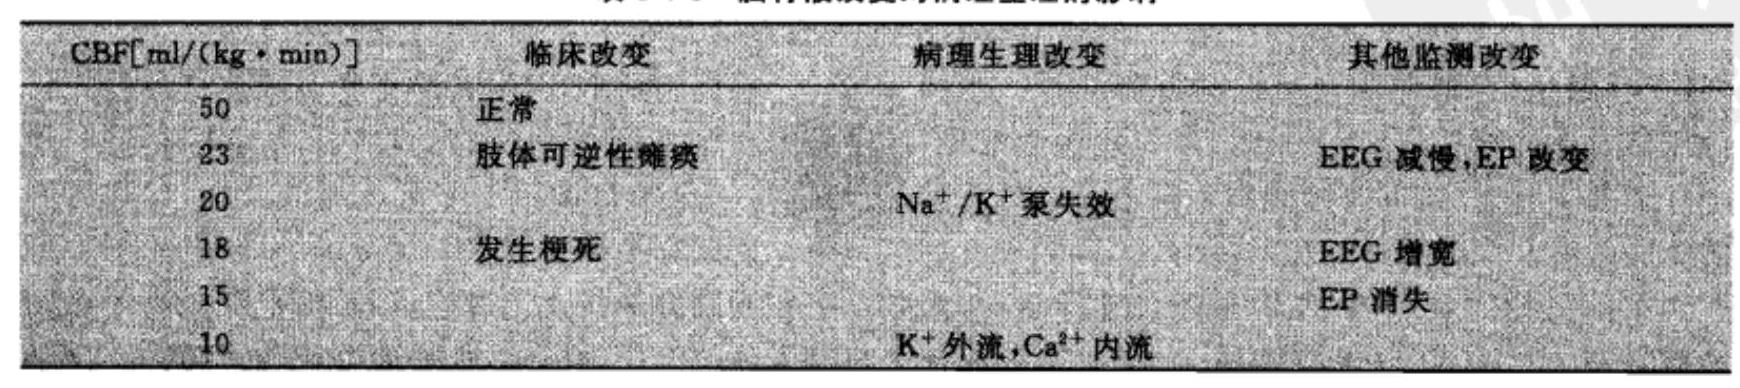
\includegraphics[max width=\textwidth]{2024_07_10_373f31b88d2bf633007bg-204}
\end{center}

(4)脑肿癁及预脑手术: 静息时改变: 脑肿瘤患者顾内压增高后, 脑血流和脑氧代谢率均降低, 病灶侧及对侧脑半球血流均降低, 局部脑血流起初的对数曲线分析较敏感, 示脑组织血流灌注不均匀。

脑血流自身调节的影响: 脑肿瘤患者的脑血流自身调节几乎均表现异常, 其自身调节障碍可见于病灶局部、一侧半球或整个大脑半球。调节异常可能与脑水肿、乳酸堆积和顾内压增高等因素有关。少数患者在切除肿瘤后, 脑血流异常即可恢复, 但多数患者在术后 $2 \sim 3$ 周改善。

\begin{enumerate}
  \setcounter{enumi}{1}
  \item 围术期脑梗死 脑梗死患者脑血流改变分两类: (1) 大面积脑梗死: 病侧脑血流和脑氧耗及莆萄糖代谢率均有明显下降, 且健侧半球亦可降低,此类患者预后差。(2)局灶性脑梗死: 神经系统体征轻, 造影未见肯定的阻塞部位, 脑氧耗及苚萄糖代谢率常表现正常。半球血流量正常或轻度降低, 但可见病灶局部脑血流降低和病灶周围脑血流增加。
\end{enumerate}

局部脑血流测定不仅可用于脑梗死的定位诊断, 还有利于判断预后。脑梗死患者脑血流改变与神经症状的变化完全一致。神经症状完全恢复的患者, 脑血流量较有神经症状后遗症者的脑血流量为大, 而后者又比死亡病例的脑血流量要更高些。

\begin{enumerate}
  \setcounter{enumi}{2}
  \item 控制性降压控制性降压能明显改变脑血管对 $\mathrm{CO}_{2}$ 的反应性和脑血管的自身调节能力。将平均动脉压 (MAP) 降低大约 $40 \%$, 脑血管的自身调节作用消失, MAP 在 $85 \sim 45 \mathrm{mmHg}$ 变化时, 脑血流和 MAP 之间具有线性关系。降压时监测脑血流有助于确定适宜的降压速度和降压时间。诱导降压时, 如果 MAP 降低过快, 可致脑血流迅速降低。在降压过程中,一旦出现脑血流低于临界水平, 应立即复压维持脑血流高于临界水平,以防脑缺血发生。

  \item 麻醉监测通常而言, 吸人全身麻醉药都增加脑血流量和降低脑代谢率。麻醉药通过直接或间接对脑血管的影响改变 $\mathrm{CBF}$, 直接影响是作用于血管平滑肌产生血管的扩张或收缩, 间接影响是引起肺泡通气或脑代谢上的变化。

  \item 脑死亡 TCD对颅内压增高所致的顾内循环停止(脑死亡)的监测与诊断具有特异性。当顾内压超过动脉舒张压时, TCD 频谱表现为心缩期/心舒期的交替血流, 即收缩期的正向血流和舒张期的反向血流。䇉内压进一步增高时 TCD 频谱变为非常小而尖锐的收缩峰, 㑔内压超过动脉压时, 血流信号消失。TCD 出现心缩期/心舒期交替血流提示顾内循环停止。与临床标准和 EEG 相比, TCD 诊断脑死亡的敏感性为 $91.3 \%$, 特异性为 $100 \%$ 。

\end{enumerate}

\section*{二、血气及呼气末 $\mathrm{CO}_{2}$ 测定}
\section*{(一)动脉血二氧化碳分压监测}
血液的气体张力和酸碱度等各项参数都须通过血气分析仪测定。动脉血二氧化碳分压 $\left(\mathrm{PaCO}_{2}\right)$ 是指动脉血中物理溶解的 $\mathrm{CO}_{2}$ 所产生的压力。正常范围 $35 \sim 45 \mathrm{mmHg}$, 平均值 $40 \mathrm{mmHg}$ 。机体 $\mathrm{CO}_{2}$ 产量、肺通气或肺换气发生改变都有可能引起 $\mathrm{PaCO}_{2}$ 的变化, $\mathrm{PaCO}_{2}$ 升高超过 $45 \mathrm{mmHg}$, 说明有 $\mathrm{CO}_{2}$ 渚留,其原因有: (1) $\mathrm{CO}_{2}$ 生成增加, 如在发热等高代谢状况下。(2)肺每分通气量降低, 如麻醉药和肌松药对呼吸的抑制; 机械通气时, 通气量不足。(3)肺部气体交换障碍, 如无效腔通气量增加。 $\mathrm{PaCO}_{2}$ 降低小于 $35 \mathrm{mmHg}$, 说明通气过度而使 $\mathrm{CO}_{2}$排出过多或 $\mathrm{CO}_{2}$ 生成减少, $\mathrm{CO}_{2}$ 生成减少最常见的原因是低温, 低温情况下机体代谢率降低, $\mathrm{CO}_{2}$ 生成减少。另外,代谢性酸中毒或碱中毒引起的生理性失代偿, 也可能导致肺通气量增加或减少, 分别引起低碳酸血症或高碳酸血症。

\section*{(二)呼气末 $\mathrm{CO}_{2}$ 监测}
呼气末 $\mathrm{CO}_{2}$ 分压或浓度 $\left(\mathrm{P}_{\mathrm{ET}} \mathrm{CO}_{2}\right.$ 或 $\left.\mathrm{F}_{\mathrm{ET}} \mathrm{CO}_{2}\right)$ 是重要的生命指标之一, 不仅可监测通气, 还可反映循环和肺血流情况。有研究发现联用 $\mathrm{CO}_{2}$ 监测仪和脉搏氧饱和度仪能够使可预防性麻醉事故的发病率降低 $93 \%$ 。持续监测 $\mathrm{CO}_{2}$ 能使 $10 \%$ 的术中问题得到早期诊断和处理。

\section*{三、顾内压的测定}
\section*{(一)颅内压的形成及监测目的}
预内压的物理学定义 “压力”(pressure)是指单位面积所受的力 (force), 绝对压力 (以真空为参照) 不用于医学中。生理学压力通常被定义为大气压的分压。因此, 压力传感器应与大气校零, 用置人颜内的传感器长期监测预内压, 当大气压发生变化, 应随时校准; 否则, 将造成监测误差。

根据帕斯卡定律, 某静止状态淮体的压力在任何方向都相同, 并且任何点的压力也都相同。但是, 这一定律只适用于不可压缩的液体, 比如脑脊液。因此测量脑脊液某一点和某一方向的压力即可作为脑脊液压力。另外, 测量脑脊液压力时必须考虑流体静压的影响, 水平仰卧位的室间孔和侧卧\\
位的腰椎流体静压水平基本相同。如果用植人传感器而不能放在这一水平, 应该纠正传感器膜的流体静压误差。

在可压缩的液体 (如血液) 和不均质的活体组织 (如脑组织), 压力应称为应力 (stress), 即组织的单位横切面积所受的力。组织的任一点受 3 个方向的应力矢量的作用。包括切力、展力和扭力。应力作用可使组织可逆变形或永久变形,可逆变形由组织的弹性决定, 永久变形由组织的秥滞性决定。脑组织同时具有弹性和黍滞性。

顾腔容积固定,约为 $1900 \mathrm{ml}$ 。头顾内容物可被分成 3 个独立的部分: 脑组织部分 (包括细胞外液)占顾腔的 $80 \%$,脑脊液占 $10 \%$,余下的 $10 \%$ 为血液。正常顾内压通常为 $7 \sim 20 \mathrm{cmH}_{2} \mathrm{O}$ 。上述任何一种内容物的体积改变都能导致顼内压的变化。由于频内高压可能继发临床情况恶化。因此, 监测顾内压的目的是为了提供早期的和迅速的干预,以便使顾内各腔隙的移位减到最小以及维持脑的正常灌注压。由于颖内压升高通常不引起症状, 因此基于临床表现来估计颅内压是不可靠的、非特异性的, 且不能定量。在某些情况下如顾后窝等发生病理变化时,测得的颅内压可能处于正常范围。

\section*{(ニ)适应证}
术中监测顾内压的必要性基于 3 个因素。一是术前忠者神经系统状况; 二是矤内组织病理学性质; 三是外科手术预计的持续时间。脑外伤或是蛛网膜下腔出血的患者,若其 Glasgow 昏迷评分为 5 分或更少,那么他们的颅内压会升高而且需要监测: 对于已知预内病理改变的患者, 监测顽内压对维持术前稳定以及进行术中控制十分有利。轴向 $\mathrm{X}$ 射线断层摄像研究表明: 当脑室或基底池受压时, 中线移位的范围以及蛛网膜下腔出血的存在将是竝内压升高的强有力的指示, 它们还可以作为决定是否需要监测的指征。

\section*{(三)顽内压的测定方法及分析}
\begin{enumerate}
  \item 顾内压监测的基本原理 将患者的顾内压电动势, 用示波器显示出来或用记录器描绘成压力曲线, 必须借助于一压敏换能器。这是一个电桥装置, 由四根阻值相等的压敏电阻器所组成。当桥路未承受压力时, 各桥臂平衡, 在有电压输人的情况下其输出端没有电位差。但当桥臂受到压力时, 由于各桥臂受到的牵拉或压迫程度不同而失去平衡,在有电压输人时其输出端便有了电位差。这一电位差的大小与引起桥臂失去平衡的压力大小成正比, 因此它所引起记录笔漂移的程度便可作为压力大小的指标。
\end{enumerate}

(1)将顾内压输人压力换能器要通过传感装置, 根据传感物质的不同分为: (1)利用体外传感器测量液体 (脑脊液) 压力 (导管法)。(2)使用植人的微型传感器, 测量硬膜外、硬膜下、脑组织及脑室的应力(植人法)。

(2)不同方法选用不同的传感物质。另外,换能器输出的信号很微弱, 显示及记录前需要放大器放大。根据目前比较统一的意见认为, 一个理想的䇉内压监测系统应当具备下列条件: (1) 价格便宜有利于推广普及; (2)非损伤性; (3)精确可靠; (4)经久耐用; (5)便于定标及校准; (6)有记录可作为永久性资料而保存起来; (7) 受温度和大气压影响小。现在的监测装置很多, 尚无一种能全部满足上述要求。

\begin{enumerate}
  \setcounter{enumi}{1}
  \item 液体(脑㫪液) 压力的测定 这种方法是借引流出的脑脊液或生理盐水充填导管, 将体外传感器与导管相连, 通过导管内的液体与传感器接触而测压。
\end{enumerate}

(1) 腰部脑脊液压: 腰部脑脊液压的测量是最容易操作的方法, 用 G20 腰穿针 (儿童用 G25)在水平侧卧位 $\mathrm{L}_{3} \sim \mathrm{S}_{1}$ 间进行腰穿。腰穿针接一向上的玻璃管可暂时测压,但不能显示颊内压的特征。腰部蛛网膜下隙放管可持续测量几天, 可用硬膜外管置人,也可放人小型传感器(StathamP50 或 Gaeltec $3 \mathrm{EA} / \mathrm{L}$ )。腰穿测压最适用于没有脑疒危险的情况, 如脑膜炎、交通性脑积水和良性顽内压增高。对椎管内阻塞的诊断及脊腔脑脊液动力学的研究有一定价值。

测量腰部脑脊液压的缺点是有诱发脑疝的危险, 在第三与第四腔隙间梗阻 (枕骨大孔疝)时, 尽管预内压很高, 而腰部脑脊液压可能很低。在这种情况下, 腰穿进一步降低脊腔脑脊液压, 增加颎一脊腔的压力梯度, 不但不能诊断脑疝而且加重脑疝。因此, 严格地说䇉内肿块(肿瘤, 出血)、脑水肿及非交通性脑积水都禁忌腰穿测压。另外, 腰穿所致的脑脊液渗漏可使压力测量失真数天,压力波形可以完全消失。

(2)脑室脑脊液压: 脑室测压是在侧脑室插人柔韧导管, 利用引流的脑脊液作为传感物质, 输人监测装置进行记录。常在额部发际正对朣孔的位置行顾骨钻孔, 穿刺脑室, 将导管从非优势半球侧脑室的前角(无脉络丛)放人室间孔, 压力传感器与脑室导管间以三通相连,随时可以校零。\\
脑室测压的优点: (1)可采集脑脊液进行脑脊液细胞学、化学及细菌学分析。(2) 可根据压力-容积曲线进行顽内顺应性和脑脊液动力学测定。(3) 出现貊内高压危象时可用引流脑脊液来缓冲, 还能行脑室造影及注人药物。(4)方法简单、监测可靠、能为大多数患者选用, 因此被认为是顾内压监测的 “金标准”(gold standard), 其他任何一种方法都要与脑室法作对比研究, 才能确定其有效性。

脑室测压的缺点: (1)如脑室很小或有明显移位时, 穿刺置管常很困难, 即使置人脑室, 也难保持导管畅通, 脑组织碎块易堵塞管道而使监测中断。(2)如果引流脑春液减压造成脑室塌陷而堵塞管孔, 也记录不到预内压力。(3)可因置管本身损伤脑组织引起局部水肿和出血及导管引流出脑脊液而影响顾内压力。如果导管周围发生漏液, 误差更大。(4)脑室穿刺为有创操作, 穿刺通道以后可以扩大而致脑组织缺失, 在儿童甚至形成假性孔洞脑 (pseudoporen-cephalia)。这种损害可由使用测量腰部脑脊洨压的细管所减少, 但应考虑到细管的阻尼 (减幅)作用造成的波形失真。(5)顾内感染, 随时间而增加, 因此监测不宜超过 $5 \mathrm{~d}$ 。其中脑室炎占 $10 \%$, 2. $5 \%$ 可致死。

为减少脑室测压的缺点, Fleischer (1975) 改用一带有储液䓯的脑室插管。其储液僙部分可埋于须骨钻孔内, 完全謎合头皮, 记录压力时只需用一 23 号针经皮穿剌此囊, 连接到监测装置即可记录。

(3)硬脑膜下或蛛网膜下液压

(1)空心螺检装置。1973 年 Vries 首先使用, 方法是在头皮上作 $1 \mathrm{~cm}$ 长的切口并在颅骨上钻一直径 $0.6 \mathrm{~cm}$ 的孔, 切开硬膜将空心螺检 (Richmond 和 McDowall-Pickerod 螺栓)置于蛛网膜表面或其下,螺栓内注人液体外接导管测压。安装时螺检应垂直于脑表面, 深度以紧贴蛛网膜或软脑膜为宜。如螺栓倾斜、过深或过浅及硬脑膜未全剥开均影响准确测压。

(2)吸杯管装置 (cup catheter)。为一带侧孔的导管, 感受面积较大,故能较敏感地反映压力波形。此法用于开须手术总者较为合适, 手术结束时将导管放在脑表面, 然后穿过头皮下通道引出颅外, 以减少感染机会和避免脑脊液㴜。此装置系扁平状且较光滑, 不易损伤脑组织, 但对非手术患者若经钻孔插人则不如用螺栓方便。当预内压增高时, 导管孔和螺栓很容易被堵塞, 必须频繁地向导管内注液或持续输液, 才能继续监测。特别是杯管装置,当脑组织疝人侧孔时, 将很块测不到压力。如果螺栓芯用灯芯材料制作, 由于灯芯上精细的小孔, 可使螺检保持通畅。

(3)蛮液装置。1965 年 Hobbenstein 报道, 用一橡胶制的小囊容积约 $0.2 \mathrm{ml}$, 经预骨钻孔埋于硬脑膜下。在囊腔内灌人相应量的盐水, 接于监测装置即可记录。Numoto 等曾先后设计 3 种用硅橡胶薄膜制成的小襄, 蒂内附有一对金属极板组成电路中的开关。当小蛽受到硬膜下压力使极板相碰, 电路接通, 指示灯发亮。此时用一平衡压力向葓内注人液体使极板刚好能分开, 指示灯熄灭, 这一平衡压即代表当时的硬脑膜下压。此后他又设计了一个压力指示蟾, 容积 $0.8 \mathrm{ml}$, 埋于硬脑膜下。囊内灌以有色液体, 并部分充满与之相接的管腔。有色液体在管聜内的水平定为 “ 0 ”点, 当壁童受压, 管内液柱外移,可在升放端用平衡压使之回复至 “ 0 ”点。此时压力计上的读数即为当时的硬脑膜下压。

这种监测方法的共同缺点是: 测压装置的装卸均需做手术; 设计精巧, 装卸过程中容易破坏; 由于硬膜都切开, 䛕内感染机会仍较多; 受体温影响产生误差。

(4)脑组织压: 是指脑组织间的液体压力, 它和腰部及脑室脑脊液压都不同, 不同部位存在较明显的压差。一般认为脑组织压与脑血流有密切关系,与脑水肿及药物在脑内扩散的速度也密切相关。在脑有病变时它的变化格外明显。因此对颖内动力学的了解和观察脑水肿的发展方向有一定意义。方法是将灯芯管与细胞间的脑脊液相连, 外接测压装置, 管口的灯芯可防止管口被堵, 能持续测压, 但只能记录平均压力, 不能传递压力的波动。脑组织压力测定很少用于临床, 但其可对顾内压的分布提供重要信息。

(5) 用液体充填的导管测压的一般特点: 用导管法测压, 不但需要测量导管内的液体容积, 而且应该考虑测量链上所有部件的特征 (包括穿刺针、螺检、导管、传感器、放大器和记录仪)。液体充填的导管是测量链上最弱的连接。它可引起相当大的运动误差。导管壁越薄、越长、越坚硬, 误差越显著。这可能使须内压的脉搏和呼吸成分完全失真。因此, 最好使用导管较短的小型传感器 (Statham $P$ 50 和 Gaeltec-3 EA/L), 可附着于顽骨上。这也可减少患者因改变体位而造成的流体静力误差, 因为如果使用大传感器, 其常被固定在床上。

顾内压信号传递的频率范围是从 0 直到\\
$20 \mathrm{~Hz}$, 过分的共振和超过临界的阻尼(减幅, D>1)将使频率传递发生误差。导管-传感器系统理想的掝幅率为 0.7 到 0.8 , 被过滤掉的高频波其频率应为最大传递频率 $(20 \mathrm{~Hz})$ 的 2 倍。脑室硅胶管和穿刺套管导致高频过度共振(减幅不足性失真), 使波形搏动分析失真。“杯管”和更细小的导管造成波形减幅过度性失真, 因此使用细小导管不能进行任何压力波形分析。所以,在叙述颅内压的传递频率包括其定量分析时必须说明所使用的测量链的特征。

\begin{enumerate}
  \setcounter{enumi}{2}
  \item 用置入的压力传感器测定硕内压直接把压力传感器放人顾内, 可避免脑脊液与外界相通和液体传递压力的缺点。但面临一些技术问题: 压力传感器必须很小, 减小传感器置人的外科创伤; 零点和校准的稳定性好; 导线必须有一定的机械承重能力和不漏电; 传感器本身必须无菌。测量特点如下。
\end{enumerate}

(1)电一机械传感器: 常用的有应变计型 (strain gauge), 压电 (piezoelectric) 传感器和电容系统。

(1)应变计型传感器。大多数用作体外传感器,部分用作置人传感器。Gaeltec 传感器是此类型的最新产品, 能补偿一秒的温度漂移。此传感器形如导管,前端为扁平状系压力感受器 $(5 \mathrm{~mm} \times 8 \mathrm{~mm} \times 2 \mathrm{~mm})$, 外面包有硅保护膜, 内有压力感受膜, 通过其移位而反映压力变化, 并经导线将信号输出。有两条管道分别通向感受膜上下两面并共同开口于近侧端, 经此注人少量 $(0.2 \sim 0.3 \mathrm{ml})$ 空气即可使感受膜两面的压力相等从而调零, 校正后空气自行排出随即恢复测压状态。应变计型传感器的硅包膜易碎, 但其零点和校准均很稳定。只有火柴头大小的 Gaeltec:ICT/ $\mathrm{b}$ 型传感器可随时检查和调零, 其 $24 \mathrm{~h}$ 零点漂移 $<$ $2 \mathrm{mmHg}$, 其敏感性定在 $5 \mu \mathrm{V} /(\mathrm{v} \cdot \mathrm{mmHg})$, 频率反应在 $0 \sim 4 \mathrm{kHz}$ 。但如果置人的应变计几天都没有受到压力的作用, 零点漂移会经常发生。Gaeltec 的最大优点是可在体内校零, 而且体积小使用方便,准确性和稳定性良好, 可与多参数监测仪相连。硅包膜传感器的变型压电电阻 (piezoresistive)传感器不但有柱形而且有末端管型, 使用也很可靠。

(2)压电传感器。测量稳定,用作置人体积太大, 主要用于实验研究。

(3)电容传感器。相比之下特点突出, 类似一个振荡器, 调零和校准稳定, 温度漂移可以忽略。振荡器对测量的压力高度敏感, 几乎不会出现误差。其测量信号远强于噪声, 可直接用于遥测。这种传感器能经受高温高压消毒, 而应变计型只能用气体或液体消毒药处理。

(2)气动平衡传感器: 仅用作硬膜外传感器, 由气动系统和读数系统组成。气动系统包括循环襟、空气舱、传感器、压力换能器和排气间。循环犟把空气泉人高压舱, 通过一限速管使空气流量以 $40 \mathrm{ml} / \mathrm{min}$ 进人顾内传感器, 然后从传感器流出进人低压舱, 由循环票再循环。压力换能器读取维持佰定空气流量而作用于传感器上的压力即颅内压。 3 个排气阘用于换能器与大气校零。Ladd 传感器由纤维光束和镜面控制, 反应较慢,其频率反应小于 $0.1 \mathrm{~Hz}$, 尽管能传递主要的波形如 A 波和 B 波,但不足以快速传递如咳濑、呼吸改变所致的颅内压波形变化。最新的纤维光束传感器, 由气压管、光导纤维和反射镜面组成,将带有气囊的反射镜放在硬脑膜表面, 顺内压变化时, 反射镜面偏离中心, 反射光度出现差别, 将信号经纤维光束传人监测仪,通过伺服装置的感压管反映出来,测定出顾内压。

气动平衡换能器位于体外, 零点和校准稳定,容易检查,没有漏电问题。此法操作简便, 测压准确,但有以下缺点反应压力波形欠教感; (2)传感器易损坏; (3)需用专用仪器, 不能用于插件式多参数监测仪。

(3)置人传感器压力传递特点: Ladd 和 Mea$\mathrm{dox}$ 气动平衡传感器的传递质量受制于其低敏感性和波形过度减幅失真。Meadox传感器传递 A 波和 B 波仍不失真, 而 Ladd 系统使 B 波变形,限制其用于囟门测压和脑脊液循环障碍的监测。它们都不能用于颅内压脉搏和呼出气成分的定量分析。

与气动平衡系统相反, 所有电一机械传感器在颎内压波幅范围内测量理想。应变计型 (gaeltec, statham)、压电电阻传感器 (honeywell-philips)和电容传感器过漶掉的高频频率足够高, 小量的减幅不影响结果分析。液体传递的压力测量的是液体内部的压力, 由液体传递特征决定; 而置人传感器测量的是垂直作用于其上的组织内或组织上的应力, 由传感器隔膜所处的局部解剖和生理特征决定。传感器的导线对运动完全不敏感,不会因病人运动而产生误差, 是其最大的优点。

(4) 硬膜外压力测定: 硬膜外腔不是一个密封的腔隙, 不可能使充填的液体量保持恒定。用液体传导来测压。比如用 plastimed 传感器 (内带导管的中空的塑料螺㭲)测压, $1 \mathrm{~d}$ 须注人几次液体。\\
液体充填的硬膜外球囊 (numoto 蘘)也有相似的缺点: 波动的流体静压误差, 压缩性误差, 液体的热渗胀造成所得数值不精确。

因此硬膜外置人微型传感器大受欢迎, 但是这要求考虑硬膜的弹性特征。有人用人的硬膜测量,使硬膜变形甚至最小程度的变形, 都产生很大的回复力, 而且不随时间明显减小, 伴有持续的应力。使一片直径 $8 \mathrm{~mm}$ 的硬膜伸展 $0.3 \mathrm{~mm}$,一片直径 $4 \mathrm{~mm}$ 的硬膜伸展仅 $0.1 \mathrm{~mm}$, 造成 $50 \mathrm{mmHg}$ 以上的恒定张力, 这就使輘内压监测出现误差 (过高)。相反, 如果传感器的隔膜在一个直径 $6 \mathrm{~mm}$ 的钻孔内距离硬膜仅 $0.1 \mathrm{~mm}$, 硬膜在预内压达 $40 \mathrm{mmHg}$ 时才完全覆盖传感器隔膜, 这使压力测量值过低。另外, 须骨内面不平, 使传感器隔膜与硬膜成角度放置, 也造成误差。因为微型传感器测量的是垂直矢量, 隔膜与硬膜形成的任何角度 $\alpha$ 都将造成 (100 $\sin \alpha) \%$ 的误差。因此, 硬膜外测压必须满足以下条件:(1)避免硬膜的内在应力。(2)传感器隔膜完全与硬膜接触而不受干扰。为防止人为的硬膜应力, 钻孔和传感器周围的硬膜应与顾骨分离 ( $>1 / 2 \mathrm{~cm}$ )。另外传感器末端的边缘设计比隔膜凸出一些( 大约 $0.1 \mathrm{~mm})$, 可吸收水平方向的应力。这样, 硬膜起着 “浮动膜”的作用, 没有内在应力, 测量误差只由可能的高频减幅引起。隔膜 (gaeltec ICT/b, honeywell MTC) 在预骨下 $0.4 \sim 2.2 \mathrm{~mm}$, 能保证与硬膜完全接触。隔膜不应太小,大面积测量的积分值可避免颊骨内不平和明显的硬膜血管造成的误差。但是, 在传感器置人预骨下时, 压迫蛛网膜下腔和脑表面, 因弹性回复力所致的误差也使测量值偏高。由于脑的稆滞弹性特征, 这种误差可在 30~ $120 \mathrm{~min}$ 内消失。因此尽管硬膜外测压显示立刻的显著剂内高压, 但只有在 $30 \sim 120 \mathrm{~min}$ 的 “调整时间”后数值才可信。因而不宜在置人传感器后立即比较硬膜外和脑室内压。在足够的调整时间和流体静力纠正后, 与顽脊舩的其他位置测量的压力不相同应该是的确存在压力 (应力)梯度,这是因为一个腔隙容积的增加没有在整隙间完全被代偿的缘故。

(1)硬膜外传感器测压的优点: 外科创伤小; 没有或几乎没有感染危险; 没有运动误差; 不妨碍或几乎不妨碍护理。

(2)硬膜外传感器测压的缺点: 不能测量负压;不能引流脑脊液减压或化验; 不能作压力-容积实验; 长期测量可刺激硬膜增厚使灵敏度下降, 如传感器楔人预内过多可产生椥人压, 使记录到的顾内压偏高。

(5)硬膜下测压: 微管末端型传感器适合放在硬膜内, 大约 $10 \%$ 的患者可用微型传感器做硬膜下测压, 特别在老年忠者, 因从颅骨分离硬膜可造成硬膜破裂。硬膜下测压, 传感器隔膜附在蛛网膜上, 没有硬膜的张力和减幅作用, 测量结果比硬膜外更可靠。不易出现脑脊液漏或感染, 用液压测量所致的感染显然是由液柱随脉搏和呼吸振动引起,细菌克服液体的振动和重力 $24 \mathrm{~h}$ 可移动 $1.5 \mathrm{~m}$ 。 Gray 等用应变计型传感器 (micro sensor) 与液体充填的导管测量硬膜下压, 结果二者显著相关, 后者比前者平均低 $2.7 \mathrm{mmHg}$, 传感器的零点漂移为每天 $0.475 \mathrm{mmHg}$ 。

(6)脑室内测压: Kasai 等用一种末端带传感器的脑室引流管, 能持续测压而不影响脑脊液引流。它是一法制 8.5 号的双腔管,有 16 个侧孔用作引流脑脊液, 管的末端有一小的应变计型传感器直接测压。传感器是由 $2 \mathrm{~mm} \times 1 \mathrm{~mm}$ 的硅胶片组成, 必须在插人之前进行校准, 导管经侧脑室前角插人放在室间孔位置, 病人头部运动不需要再校准。顾内压的波形和大小与液压测量相同, 没有发现漂移。 Gambardella 等比较纤维光导系统 (Camino) 和导管法(液体充填)测量脑室压, 结果二者同样精确可靠, 只是前者比后者平均低 $3 \mathrm{mmHg}$, 特别在危重患者。

(7) 脑组织压: Bochicchio 等对 120 例患者研究, 通过蛛网膜下螺检, 用纤维光导传感器 (Cami$\mathrm{no}$ ) 插人额皮质 $2 \mathrm{~mm}$, 进行测压。平均测压 $5 \mathrm{~d}$, 没有发现致命的并发症, 只出现 $2.5 \%$ 的伤口感染和 $0.8 \%$ 的脑膜炎, $4.4 \%$ 的患者因为纤维光导部分破坏要求换管。Shapiro 等用纤维光导系统测量 244 例患者脑实质压,因为顾内压向上漂移有 $38 \%$ 的患者需要至少一次换管,有 $16 \%$ 的患者因纤维光导破坏而换管, 1 例插人位置感染, 2 例骨瓣感染, 没有发生细菌性脑膜炎或脑脓肿。Gray 用应变计型传感器测量脑组织压, 比硬膜下导管法平均高 $2.8 \mathrm{mmHg}$, 每天零点漂移平均 $0.312 \mathrm{mmHg}$, 波形质量较好, 惐幅较小。

\section*{4. 无创伤性压力监测}
(1) 囟门测量法: 用这种方法以无创、连续监测的方式, 至少可半定量记录㐫门开放的婴儿的预内压。

(1)理论基础。硬萁覆盖囟门, 帽状筋膜和皮肤\\
构成弯曲的、柔韧的一层膜。在其内 $(=\mathrm{ICP})$ 和其外 $\left(=\mathrm{P}_{\mathrm{ext}}\right)$ 之间, 存在一压力差 $\Delta \mathrm{P}=\mathrm{ICP}-\mathrm{P}_{\mathrm{ext}}=\mathrm{T}$ $\left(1 / r_{1}+1 / r_{2}\right)$ 。 $T=$ 膜的张力, $r_{1}$ 和 $r_{2}$ 为膜的曲面半径, 当扁平传感器放在囟门上时, 使膜的曲面消失, $r_{1}$ 和 $r_{2}$ 趋于无穷大, $T$ 趋于 $0, P_{\text {ext }} \approx I C P$ 。因此, 通过测量反作用于传感器上的压力, 就可测出顾内压。

(2)顾内压的测量。囟门测压需要长时间测量,用传感器单次测量并不比用手触诊更有价值。气动系统的 Ladd 和 Meadox 为扁平设计, 适合持续囟门测压, 但并不敏感。扁平的应变计型传感器,隔膜面积更大 (gaeltec), 有更好的频率分辨效果,与完全平坦比较, 囟门上的膜发生极轻微的移位 $\left(<10^{-3} \mathrm{~mm}\right)$ 是可以忽略的, 对顾内压测量影响很小。

(3)结果的可靠性。有人测量后证明,只要传感器与囟门平面附着,㐫门压与脑室内压基本相同 ( $\pm 4 \mathrm{mmHg}$ ), 其可靠性决定于儿童的运动与否。但是儿童顾内压的正常值低, 而且因其顾骨柔软,慢性脑积水时项内压只有少量增加, 㐫门测量难于反映其变化。

(2)核素测量 : 在压力的影响下,核素从一侧脑室扩散到另一侧, 其打散的量与压力大小成正比。因此只需要测量核素的仪器就能将顾内压测出。但此法的安全性和可靠性尚待证实。

(3)视觉诱发电位: 有人用光视觉诱发电位来测量顾内压, 认为其 $\mathrm{N}_{2}$ 潜伏期与顾内压有良好的相关关系, $\mathrm{N}_{2}$ 潜伏期大于 $80 \mathrm{~ms}$ 与顼内压大于 $15 \mathrm{mmHg}$ 变化一致。

(4)视盘水肿; Tuite 等对 122 例预缝早闭的儿童进行顾内压和视盘水肿的相关性研究,结果有视盘水肿的患儿颅内压高于无视盘水肿者(平均分别为 17.5 和 $12.7 \mathrm{mmHg}$ ), 年龄更大 (分别为 5.9 岁和 1.9 岁); 认为视盘水肿是顾内压增高的特异指征 $(98 \%)$,但其敏感性呈年龄依赖的,超过 8 岁的儿童 $100 \%$ 敏感,因此提出超过 8 岁的患儿不必作颖内压监测, 只需详细的眼科检查。

(5)经顾超声多普勒(TCD): Mayer 用 TCD 检查了 30 例顾内幕上出血患者, 发现当顾内出血量大于 $25 \mathrm{ml}$ 时,同侧搏动性指数升高, 平均血流速度都降低。与小量出血比较,大量出血 $(\geqslant 25 \mathrm{ml})$ 的同侧搏动性指数显著高 (分别为 1.72 和 1.13 ), 同侧与对侧搏动性指数的比率也显著高 (1.29 和 1.06)。经多元回归分析,同侧和对侧的搏动性指数基本与脑室内出血量有关,而同侧与对侧搏动性指数的比率与整个半球损害有关 (出血十水肿)。这不但能反映半球损害的体积,而且能反映腔隙间的压力梯度。

(6)鼓膜移位技术; 有的顾内高压患者只有耳鸣和昡晕症状,而无头痛及视觉表现,常误认为是梅尼埃病就诊于耳鼻喉科, Marchbanks 用鼓膜移位技术监测外淋巴(内耳骨迷路与膜迷路间的液体)压力,笁选、诊断和治疗颎内高压患者。

(7)其他:有人介绍异常的心率变异 (heart-rate variability)与颅内压增加有关,正的压力反应指数 (脑血管对动脉血压变化的反应)与顼内压升高有关。

这些无创监测的共同缺点是不能明确测定压力的实际值, 只能作定性观察。

\begin{center}

\includegraphics[max width=\textwidth]{2024_07_10_373f31b88d2bf633007bg-210}
\end{center}

\begin{enumerate}
  \item A 波即高原波 其典型表现为在顼内压增高的情况下 (常为 $15 \sim 25 \mathrm{mmHg}$ ), 颅内压迅速上升,可高达 $50 \sim 100 \mathrm{mmHg}$, 高峰常呈平顶(高原状), 但有时不规则或呈峰状,持续 2~30min。而后突然下降(比上升更快)至原来的水平或者更低,间隔数分钟到数小时发生 1 次。有人则将病人快速升降并维持 $5 \mathrm{~min}$ 的顾内压定为 $\mathrm{A}$ 波,这种简明的规定可能更便于临床分析,因为非典型的 $\mathrm{A}$ 波其压力可能低于 $50 \mathrm{mmHg}$ 。A 波常见于颖内肿瘤患者,可伴神经症状的恶化, 如头痛、恶心、呕吐、面部潮红, 神志障碍和肢体阵挛性或强直性的抽搐发作。A 波的发展可分为 4 个时相:
\end{enumerate}

(1)前驱相: 是由于全身动脉压逐渐缓慢地下降使脑灌注压接近 $70 \sim 80 \mathrm{mmHg}$, 导致自动调节的脑血管扩张与顼内压增高。

(2)高原相: 当脑灌注压降至 $40 \sim 50 \mathrm{mmHg}$时,颅内压迅速上升,这一时相持续至脑灌注压保持稳定而高于脑缺血水平。

(3)缺血反应相:由于全身动脉压降至脑缺血水平,从而触发了全身动脉压的上升与脑灌注压的恢复。

(4)终末或复原相: 此时由于自动调节性脑血管收缩,须内压迅速下降至基线,脑灌注压与全身动脉压均恢复到稳定状态。

所以 A 波的发生可理解为在增高了的顾内压与降低了的预内容积代偿以及脑血管床的自动调节功能尚存在的情况下,脑灌注压的升降引起脑血管的舒缩而导致须内压发生振荡的结果。如持续\\
发生的高原波得不到解除, 则由于脑灌注压严重下降, 脑组织严重缺血缺氧, 脑血流量的自动调节功能丧失, 脑血管处于扩张状态, 顽内压呈现持续高压状态。患者最终将死亡。

从压力波的振荡容易发生于缺氧与 $\mathrm{PaCO}_{2}$ 增高及对过度通气反应良好来看, 均表明脑血容量的变化是振荡发生的原因。由于间歌性血管扩张可发生于睡眠的不同时相,所以高原波多见于快动眼睡眠期,夜间多见。

\begin{enumerate}
  \setcounter{enumi}{1}
  \item B 波 为振荡波中较多见的一种, 呈较恒定的节律性振荡, 没有其他波夹杂其间, 䇉内压可高达 $20 \sim 30 \mathrm{mmHg}$, 振幅 $>5 \mathrm{mmHg}$, 每分钟 $0.5 \sim 2$次。顾页压上升呈较缓的坡度, 而下降则较陡峭,顶端多呈明显尖峰, 多见于夜间及睡眠时。此种波又称为窯形 B 波 (sinus-shaped B-waves), 见于正常顾内压特别是睡眠时, 亦可持续存在于活动性脑积水的患者, 在顾内容积增加时发生并能发展为高原波。窦形 B 波与顾内血容量波动有关而与血压、呼吸频率或 $\mathrm{PaCO}_{2}$ 的变化无关。另一种称为 “斜坡”(ramp)B 波,为压力缓慢斜坡样上升伴振幅增加, 再突然降低伴振幅减小的一种波形, 全都发生于有自主呼吸而神志模糊的患者, $\mathrm{PaCO}_{2}$ 升高斜坡压增加, 深呼吸 $\mathrm{PaCO}_{2}$ 降低时斜坡压减小, 也常见于快动眼睡眠。

  \item C 波 为一种每分钟 $4 \sim 8$ 次的节律性振荡, 振幅小于 B 波, 在持续高顽压状态下发生,部分出现在高原波中。这种波与不稳定的全身动脉血压引起顾内压波动有关, 如 traubehering-mayer 波。这种波表明终末脑血管麻痹, 阻力降低, 动脉压的变化较容易传递到脑血管床,预后差。也可见于正常人且无重要意义。

  \item 慢强直 (“D”) 波 慢强直 (slow-tonic) 波是以单相压力波动为特征, 持续几分钟到 $30 \mathrm{~min}$ 以上。与高原波不同, 压力绥慢强直上升和下降, 伴轻微的脉搏和呼吸振动。常见于脑脊液循环障碍的患者, 特别是活动性脑积水和频缝早闭的患儿。很少见于脑肿胀的患者。

\end{enumerate}

由于此波上升及下降缓慢, 而且振幅保持不变, 因此假定其原因是因为脑脊液的波动而非血管调节的变化,但也有见于快动眼睡眠的报道。

\begin{enumerate}
  \setcounter{enumi}{4}
  \item 非典型短激发 (“E”) 波非典型短激发波 (nontypical short provoked wave)是由静脉压增加所诱发, 如转头、咳濑和吸痰, 常是䇉内代偿空间受限的第一指征。正常情况下波峰只短暂出现, 顽内压迅速上升后即逐渐降低。此波常出现在高原波之前。

  \item 复合波 当不同类型的波,特别是不同的 B 波快速接连出现,可组成复合波。通常 B 波重叠在慢强直波上,但是真正的 $\mathrm{A}$ 波,只在压力上升的起始阶段包含 B 波,而不在平顶或下降阶段。

\end{enumerate}

\section*{(五)顽内压监测在临床的应用}
\begin{enumerate}
  \item 急性頋脑损伤 急性顾脑外伤最适合进行顽内压监测, 因为伤后 $3 \sim 5 d$ 病情变化较大,且根据临床征象推断有无颊内压增高并不可靠,不利于治疗的开展。凡 GCS $\leqslant 8$ 分,均应考虑进行顾内压的监测,如 $\mathrm{CT}$ 扫描完全正常可暂缓实施。CT 扫描主要提供颅内病理解剖情况,浈内压监测可持续观察䇉内病理生理的变化,二者相结合对诊断很有利, 尤其是对手术治疗的决定。
\end{enumerate}

脑外伤病人颖内压持续 $>40 \mathrm{mmHg}$, 脑血流受影响, 死亡率可高达 $100 \%$, 颇内压 $<40 \mathrm{mmHg}$ 与预后无平行关系。顽内压持续 $>50 \sim 60 \mathrm{mmHg}$, 则必然死亡。

\begin{enumerate}
  \setcounter{enumi}{1}
  \item 预内肿瘻 在䂠内肿面患者,术前应用导管法进行脑室颅内压监测, 通过引流与激素治疗维持顽内压在 $15 \sim 20 \mathrm{mmHg}$, 尤其是术前出现过 A 波或 B 波者, 可改善患者的顽内顺应性, 有利于患者对麻醉和手术的耐受。在麻醉过程中,颕内压监测可及时发现呼吸道梗阻、体位不正等所致的颅内压增高。术后监测有利于术后血肿的早期发现和指导部压增高的治疗。

  \item 蛛网膜下腔出血采用导管法,在脑室顾内压监测的同时进行脑脊液引流将颅内压控制在 $15 \sim 20 \mathrm{mmHg}$ 是对蛛网膜下腔出血的重要治疗措施。高血压脑出血破人脑室, 脑室脑脊液引流有时可同时达到减少脑内血肿的目的。

  \item 其他 其他原因导致顾内压增高而昏迷的患者, 如呼吸心搏骤停、呼吸道梗阻等原因引起严重脑缺氧、脑水肿与䇉内压升高, 均可考虑用预内压监测协助控制预内高压。气脑及脑室造影过程中,歆内压监测可提示脑室的充气是否足够,减少过分充气的危险性。

\end{enumerate}

浈内压监测可能导致的并发症有感染、浈内出血、医源性顾内高压及脑实质损伤。感染是最常见的并发症, 任何一种并发症都对患者有极大危害,监测时应仔细观察, 及时处理。

\section*{(六)监测的并发症及注意事项}
\begin{enumerate}
  \item 感染 感染是 ICP 监测和 CSF 引流处理最\\
常见的并发症, 感染的范围各异, 轻者为伤口感染。重者可发生脑膜炎、脑室炎和脑脓肿等。感染的类型也可因采用的监测系统不同而发生明显改变。
\end{enumerate}

(1) Richmord 螺检 ICP 监测系统: 感染发生率为 $0 \sim 11.6 \%$ 。感染的类型包括脑膜炎、骨䯕炎、局部伤口感染等。避免 CSF 从伤口渗漏、预防监测系统脱连接和减少不必要的操作 (如管道冲洗) 可明显降低发生脑膜炎的危险。应用 Richmord 螺栓系统的患者, 不仅局部感染发生率高于脑室穿刺,而且尤其好发骨䤻炎, 反复仔细的伤口护理以及尽早撤除监测系统有助于减少骨䯕炎的风险。应用抗生素预防性治疗对感染的发生率似无明显影响,甚至可增加革兰阴性菌感染的危险性。

(2) 脑室造口术 (ventriculostomy): 虽然伤口感染的发病率较低, 但脑室炎的发病率较高, 为 $0 \sim$ $26.8 \%$ 。对伤口及导管穿出部位的护理措施不得力、系统的冲洗和其他操作(如脑室造影)、存在 $\mathrm{CSF}$ 口鼻漏或鼻漏以及脑室内出血等因素均可增加感染的发生率; 相反, 将脑室测压管埋置皮下并从其他部位穿出则可降低感染的发生率。

脑室插管保留时间对感染发生率的影响仍不清楚, 最近研究发现, 脑室穿刺的感染性并发症最常发生在开始的 $6 \mathrm{~d}$ 内, 此后感染发生的危险性降低。说明感染主要与监测装置的置人有关。因此认为,除非出现明显的感染危险因素 (如 CSF 漏) 、仪器功能障碍以及 CSF 培养和细胞学检查提示有感染等情况, 否则不宜随便更换脑室导管和监测系统。

预防性应用抗生素的作用也有争议,由于感染的发生率较低和反复应用抗生素具有产生耐药性的可能,一般认为, 最好在有感染早期征象时根据细菌的药敏应用抗生素。

(3) Camino 纤维光导 ICP 监测系统: 由于其应用时间较短,所以与其相关的感染并发症仍无广泛研究。但初步的研究结果显示, 其合并感染的可能性较小。

\begin{enumerate}
  \setcounter{enumi}{1}
  \item 顾内出血 虽然顾内出血性并发症的发生率较低 $(0.2 \% \sim 1.4 \%)$, 但此为 ICP 监测中的严重致命性并发症。其发生率与监测方法直接相关,而与硬脑膜外的装置无关。与脑实质内监测装置相比, 脑室内监测装置更易发生出血并发症。另外,曒内出血也与凝血机制障碍或监测系统安置中的多次穿刺有关。
\end{enumerate}

出血可由监测装置的直接创伤或 $\operatorname{CSF}$ 过度引流引起。在第一种情况下, 出血可发生在脑室内或脑实质内, 脑室内出血是脑室穿刺的并发症, 主要表现为脑室引流管中有血性 CSF 流出, 但须采取措施与脑病理性出血 (如脑创伤或高血压脑室内出血)进行鉴别。在无凝血机制障碍的患者, 此种出血多为自限性, 所以其处理主要为严密观察 ICP,并根据需要进行脑室引流。

由 CSF 引流过度所致的出血主要为硬脑膜下出血, 此可发生在脑室或脊髓蛛网膜下腔引流的情况下,虽然硬脑膜下出血常为㝡静型,但如血肿明显, 也可出现临床情况恶化或颅内高压。

通过采取合理的预防性措施, 能有效防止顾内出血性并发症。在安置 ICP 监测系统前, 如患者存在凝血功能异常应进行纠正, 此在脑创伤患者相当重要, 因为脑中的组织凝血活酶浓度极高。在安装技术方面, 应避免反复穿刺, 并应防止 $\mathrm{CSF}$ 引流过快或将 ICP 降至不合理的低水平。在进行 CSF引流的清醒患者, 防止其随意变动 CSF 引流系统的状态极为重要, 如在无夹闭引流管的情况下升高床头或患者坐起等。

\begin{enumerate}
  \setcounter{enumi}{2}
  \item 医源性㶦内高压由于顾内容量增加所致的意外性 ICP 增高是应用脑室穿刺和 Richmond 空心蝶检时并发症, 通常发生在技术失误的情况下, 如管道冲洗系统开放过度或意外性将其输液通路, 在顾内压顺应性降低的情况下, 即使顾内压容量增加 $1 \mathrm{ml}$, ICP 增高 $5 \mathrm{~cm}$ 以上, 都会造成不良影响。从而在 ICP 监测中, 应仔细标记监测系统的每一根管道, 并严格按照操作规程处理。输液系统不能与 ICP 监测系统相连接, 以防止其意外性开放而将液体输人预内。
\end{enumerate}

在顾内顺应性测试中也可发生医源性 ICP 升高, 所以在已知或怀疑有颖内顺应性降低的患者,宜采用抽液法进行测试。虽然此方法有因脑室壁塌陷而致导管阻塞或将脉络丛吸人导管口的危险,但能有效防止 ICP 升高。

\begin{enumerate}
  \setcounter{enumi}{3}
  \item 脑实质损伤主要由穿刺方向失误或监测装置放人过深引起,最常发生在脑室穿刺患者。脑室穿刺方向不当常可损伤尾核、内表或丘脑前部的神经核群, 而监测装置放人过深, 常损伤下丘脑。
\end{enumerate}

脑损伤或肿痛组织水肿所致的脑组织结构移位等能增加上述误操作的可能性。从而限制脑穿刺的次数和导管置人的深度极为重要, 并应及时寻找穿刺不成功的原因或更换其他 IČP 监测方法。一般认为, 如果脑室穿刺 3 次未成功, 则应采用

Richmond 空心螺检或 Camino 光纤导管监测 ICP。

无论何种原因,穿刺针置人硬脑膜下的距离不应超过 $6 \mathrm{~cm}$, 如果穿刺针进人硬脑膜下 $6 \mathrm{~cm}$ 但仍无 $\mathrm{CSF}$ 流出,一般说明穿刺方向不当。如果 3 次脑室栄刺均未成功, 患者又必须进行脑室引流, 可在另一侧进行脑室穿刺, 但同样需限制穿刺次数。

\section*{第三节 麻醉前评估及准备}
\section*{一、病情评估}
神经外科手术和一般外科手术的术前评估与麻醉前准备有许多共同点, 但有其独具的特殊性。共同点在于神经外科手术患者和其他外科手术恵者一样, 全身情况、重要器官功能、精神状态、可能发生的并发症等同样影响术前评估与麻醉前准备。

神经外科手术的特点和对麻醉的基本要求如下。

\section*{(一)手术部位特殊、器官功能重要}
顽脑发生病灶或损害是由于病灶直接侵犯、压迫、破坏脑组织、脑神经及脑血管等, 患者往往发生偏䧹、失语、昏迷以及其他各种脑神经压迫综合征。在这些部位进行的是中枢神经的手术, 尤其幕下的手术, 多数接近生命中枢。因此, 要求麻醉医师要基本理解神经外科疾病或损害的症状、诊断、主要的病理变化和麻醉要点, 以期能够相互配合, 保证患者生命安全和手术成功。

\section*{(ニ)继发病变导致的结果严重}
继发于神经外科疾病所导致的结果是攼内压 (ICP)改变 (主要是升高) 和脑水肿, 因为顾腔是一个狭小的半封闭而无伸缩性的腔, 其中主要包含脑实质及脑组织成分 (占 $84 \%$ ),脑内血液 (占 $3 \%$ 〜 $6 \%$ ), 脑脊液(占 $11 \% \sim 15 \%$ ), 这三个内容保持相对的动态恒定, 它可以受到体位、血压、咳嫩、气管内插管对咽喉部的刺激等诸多因素影响发生瞬时改变; 此外, 预内血流和血容量受到顿内外多种因素的影响, 代谢 (细胞外电解质、各种离子、酶与腺苷等)与血流之间关系非常密切,正常情况下在生理范围内它具有自身调节的功能; 浈外因素包括在麻醉状态下, $\mathrm{PaCO}_{2} 、 \mathrm{PaO}_{2}$ 、脑灌注压 (包括血压)以及体温的变化, 在超出生理范围自身调节的时候也会发生 ICP 的改变; 麻醉医师应当认识 ICP 在评估神经外科手术的麻醉危险性、麻醉前准备、麻醉选择和术中麻醉处理等方面的重要性, 这也是对麻醉的基本要求之一。

(三)认识血脑屏障与发生脑水肿的关系

认识血脑屏障与脑水肿的发生之间的关系也是对神经外科麻醉医师的基本要求之一,在檋脑疾病和频脑外伤发生之后, 由于血脑屏障遭到破坏会引起中枢神经系统水肿, 其后果是极其严重的。尽管脑水肿不是直接由于血脑屏障通透性增高所致,但血脑屏障的功能障碍与脑水肿的发展却有着密切的关系。例如脑损伤、全脑缺氧、或因为脑瘤的局部压迫, 导致脑血管自动调节机制紊乱,其必然导致脑容积进一步增大,其直接后果就是发生脑细胞肿胀和脑水肿的继续发展, ICP 必然严重增加。

\section*{(四)ICP 升高的危害性}
从事神经外科麻醉的临床麻醉医师应该深刻理解 ICP 升高的原因和它的危害性, 才能对神经外科手术患者进行正确的术前评估和做好充分的麻醉前准备。

术前应用脱水药可以减轻 ICP, 手术中过度通气维持适当的动脉血二氧化碳分压 $\left(\mathrm{P}_{\mathrm{ET}} \mathrm{CO}_{2}\right)$ 以维持 $\mathrm{CO}_{2}$ 、对脑的供需平衡,一般过度通气维持 $\mathrm{P}_{\mathrm{ET}}$ $\mathrm{CO}_{2} 4.0 \sim 4.5 \mathrm{kPa}$ 被认为是最适当的过度通气界限, 严重过度通气, $\mathrm{P}_{\mathrm{ET}} \mathrm{CO}_{2}$ 达到 $3.5 \mathrm{kPa}$ 时, 可出现脑氧供需失衡。

\section*{(五)意识障碍与氐迷}
各种顾内肿瘤、顾脑损伤和脑血管意外等, 都可能引发意识障碍甚至昏迷,因此神经外科麻醉医师接触患者时,尤其在决定手术时, 术前对此类患者进行详细术前评估和麻醉前准备,必须对意识障碍和昏迷有基本的了解, 这也是基本要求之一。术前评估手术麻醉的危险性和患者的意识状态至关重要,一般来说, 病情的危重程度以及手术麻醉的危险性与意识状态呈正相关。临床把意识状态分为意识障碍和昏迷。意识障碍表现为嗜睡 (有的表现为躁动)、、意识模糊或理解能力减退; 昏迷指的是患者意识完全消失,一般刺激无法唤醒, 大多数反射减退或消失, 这是病情危重的信号。临床上把昏迷分为五种程度。

\begin{enumerate}
  \item 浅昏迷(对外界刺激有一定的反应或痛苦表情, 某些反射基本存在)。

  \item 中度昏迷 (对各种刺激基本无反应, 对强刺激可能有一定防御行为, 各种反射减弱)。

  \item 深昏迷 (处于软痽状态, 对外界刺邀无任何反应, 各种反射消失, 呼吸减弱而不规则, 血压下降,大小便失禁等表现)。

  \item 不可逆昏迷, 即脑死亡。

  \item 其他类型的昏迷(例如去大脑皮质综合征、闭锁综合征等)。

\end{enumerate}

总之, 意识状态对于综合评估和判断病情是一个重要的依据。

\section*{二、麻醉前准备及麻醉前用药}
广义的术前准备和麻醉前用药, 包括有关手术麻醉的一切准备和用药,用药种类应当包括针对患者合并各种疾病的处理;狭义的术前准备和麻醉前用药主要是指麻醉前直接与麻醉有关的一般麻醉器具准备和麻醉前用药。麻醉前用药的目的是使患者术前充分镇静、减少对手术的紧张情绪和恐惧,惐少麻醉过程中对副交感神经过度兴奋。能使全麻诱导和维持过程平稳, 减少全麻用药量, 搌高痛阀,防止术后恶心呕吐。对于硕脑外科的手术麻醉来说, 还有降低 ICP 的重要作用。麻醉前用药常用药物主要有:

\begin{enumerate}
  \item 苯二氮革类药物 具有镇静、催眠、抗焦虑、拠惊厥及中枢性肌松驰作用, 对局麻药毒性反应有一定的预防和治疗效果。对呼吸、循环影响甚微。缺点为无镇痛作用, 使用时常与镇痛药复合使用。常用药有咪达坐仑 $0.05 \sim 0.1 \mathrm{mg} / \mathrm{kg}$ 肌内注射; 地西泮 $0.15 \mathrm{mg} / \mathrm{kg}$ 麻醉前 $1 \mathrm{~h}$ 口服。

  \item 阿片类镇痛药 具有较强的镇痛、镇静效能,提高痛阈,与全身麻醉药有协同作用,增强局麻药效果,减少全身麻醉药用量。还可用于术后镇痛。缺点为可引起呼吸抑制和血压下降, 低血容量患者作用更加明显, 有时会出现恶心呕吐。常用药有吗啡 $0.1 \mathrm{mg} / \mathrm{kg}$ 麻醉诱导前 $1 \mathrm{~h}$ 肌内注射; 哌替啶 $0.6 \sim 1.2 \mathrm{mg} / \mathrm{kg}$ 麻醉诱导前 $1 \mathrm{~h}$ 肌内注射。

  \item 神经安定镇痛药 有较强的镇静、安定、解焦虑和止吐、抗过敏作用, 常与类阿片镇痛药如芬太尼复合能发挥较好作用。常用药有氮哌利多 $2.5 \sim 5.0 \mathrm{mg}$ 与芬太尼 $0.05 \sim 0.1 \mathrm{mg}$ 按 $50: 1$ 组合成依诺伐 (innovar), 麻醉诱导前 $1 \mathrm{~h}$ 肌内注射; 异丙潫 25 $\sim 50 \mathrm{mg}$ 麻醉诱导前 $1 \mathrm{~h}$ 肌内注射。在颅脑手术中也可以与局部麻醉药复合。

  \item 催眠药主要为巴比妥类药物, 具有镇静、催眠和抗惊厥作用并能预防局麻药反应。常用药有苯巴比妥、戊巴比妥等。

  \item 抗胆碱能药物 能阻断节后胆䂝能神经支配的效应器上的胆碱能受体, 松驰多种平滑肌, 抑制多种腺体分泌, 能域少呼吸道棹膜和唾液的分泌, 便于保持呼吸道通畅, 抑制迷走神经反射。常用药物有阿托品或东茛营碱 $0.3 \sim 0.5 \mathrm{mg}$ 皮下或肌内注射。

  \item 其他 应用有利于稳定麻醉过程中循环、呼吸系统功能的药物, 例如艾司洛尔(ESM), 临床观察在麻醉诱导中静注 ESM 有较好的平抑心血管不良作用, 但对气管内插管引起的脑血管刺激无平抑作用(插管时可引起脑血管血流动力学的有害性变化)。其他还有可乐定(clonidine) 等。

\end{enumerate}

神经外科手术多数属于重大手术, 术前准备工作必须充分, 对 ASA I II 级患者仅需一般常规准备, 包括术前了解病史, 检查患者, 完善必要的补充检查。

对 ASA III $\sim \mathbb{N}$ 级患者则需要特殊准备。全身情况如合并急性呼吸道感染则需抗感染治疗, 控制感染。对慢性呼吸道疾病也应采取抗炎、解痉、控制疢量治疗。有水、电解质紊乱及酸碱失调的患者术前应予以纠正。合并糖尿病者应将血糖控制到正常范围之内。有慢性贫血、血容量不足或血红蛋白含量低于 $9.0 \mathrm{~g} / \mathrm{dl}$ 以下者均应予以纠正。

\section*{三、麻醉选择原则}
应根据患者的具体情况和病情, 以及麻醉仪器设备情况选择合适的麻醉方法。顶脑手术大多考虑选择全身麻醉, 但是选择哪一种麻醉药? 如何诱导和维持? 都要慎重考虑, 因为不同的选择效果截然不同。

\section*{(一)全身麻醉}
包括吸人麻醉和静脉麻醉, 吸人麻醉主要有氧化亚氮、恩氩烷、异氛烷、七莓烷、地臣烷, 使用时要求配有专用的麻醉挥发器。吸人麻醉的优点主要为不燃不爆, 对呼吸道无刺激, 患者易于接受, 对光和钠石灰稳定。特点为起效快, 恢复迅速, 在体内不降解代谢, 经肺以原形排出。对肝肾基本无毒性作用。

静脉全麻常用药物有硫喷妥钠、甲乙炔巴比妥钠、氯胺酮(一般顾脑外科不常用, 必须使用时应与安定类药物合用)、羟丁酸钠、依托味酯、苯二氮草类、咪达唑仑、丙泊酚、丁酰苯类、氟哌利多等。手术部位在幕上的顾脑手术, 复合应用小剂量静脉麻醉药有很多优点: 循环稳定, 对呼吸也无明显影响。\\
静脉麻醉主要优点为设备简单、操作方便、无呼吸道刺激、较少发生术后呼吸道并发症、无燃烧爆炸危险、无空气污染。缺点为大部分有一过性的呼吸、循环抑制, 多数静脉麻醉药镇痛作用差(如羟丁酸钠、依托咪酯、丙泊酚、地西泮类药等), 这些药主要经体内分解代谢, 患者苏醒时体内仍有残留, 术后有较长时间疲乏和嗜睡。近年来 TCI 技术的应用为静脉麻醉提供了更科学的麻醉方法。

我国目前在顺脑外科手术中更多地使用静吸复合麻醉, 不但效果好,而且易于掌握, 可逆性强,是首选的麻醉方法。

\section*{(ニ)其他}
总之,颅脑外科尽管都是采用全身麻醉,但在根据病情、手术种类、药物动力学等方面, 麻醉诱导和维持以及呼吸管理等会千差万别。

\begin{enumerate}
  \item 神经安定镇痛麻醉 主要是应用氟哌利多与芬太尼为主的一种静脉复合麻醉方法, 具有镇痛、镇静但神志不完全消失,反射活动受到抑制的特点。如与地西泮、咪达唑仑和吸人麻醉药物复合能达到神经安定的麻醉作用。一般用于顾脑外伤的情况下比较多, 例如患者轻度昏迷, 但躁动不安时采用, 可适当应用镇静药, 如果患者昏迷程度比较深,可以不用麻醉但需要气管内插管。

  \item 针刺复合麻醉 具有安全有效、生理干扰少、术后诙复快、麻醉需要应用少量辅助药、麻醉效果提高。缺点为麻醉效果不稳定,亦受多种因素影响。只宜用于患者能够合作并同意接受,全身情况较差,时间相对较短的频脑手术。

  \item 低温麻醉和控制性降压麻醉自 1940 年应用于临床麻醉已 60 多年并成功用于频内动脉痹手术,具有其独特的优点。主要用于顼内动脉痛、颈内动脉海绵突瘘、颈内动脉狭窄、脑血管痛和血管丰富的肿溜手术。麻醉中要有完善的体温监测、脑监测、循环监测、血气监测及尿量监测。控制性降压麻醉也多用于出血量较大的手术, 以减少出血。

\end{enumerate}

\section*{四、不同类型神经外科手术对麻醉的要求}
神经外科手术主要指颖脑和脊髓, 当然周围神经的疾病与损伤的治疗及修复也属于神经外科的手术范帱, 毕竟它不像顾脑和脊䯕手术那样病情险峻、危急并且麻醉要求特殊,一般采用神经阻滞术或部位麻醉为多。认识不同部位、不同类型神经外科手术对麻醉的要求有助于术前评估和做好麻醉前准备。顾脑手术的部位总的来说, 分为幕上与幕下,幕下的手术因为接近神经生命中枢所以比幕上手术危险性大, 对麻醉的要求也更高。神经外科手术具体地划分, 分为大脑半球手术、䇉后窝手术、脑底手术和脊髓手术以及急症顾脑损伤和脊鲜损伤等。这些手术对麻醉有不同的要求, 但对术前评估和麻醉前准备的重要性是一样的。

(一)大浐半球手术麻醉

从解剖上来划分, 它包括额叶、频叶、顶叶和枕叶, 这些部位如果发生占位性病变 (如肿瘤、血肿和脓肿等), 其危险性和对麻醉的要求要比颎后窝手术对麻醉的要求相对来说小一些, 但也要根据病变大小、病期长短, 特别是顽内压增高的程度准备麻醉。如果占位病变部位重要、病情重、病期长, 患者长期卧床, 活动量小, 甚至有偏瘫、失语等, 可能存在营养不良、体弱以及反复使用脱水药的患者, 容易伴有水电解质失调等并发症。麻醉医师在了解了这些情况之后, 就可以依据具体病情做出术前评估和麻醉前准备, 帮助选择适当的麻醉药, 术中控制满意的血压和 ICP, 避免心律失常、脑缺氧等的发生,保证麻醉安全。

\section*{(二)顺后窝包括脑干和颅底部位的手术麻醉}
顾后窝接近生命中枢,许多部位在过去被视为手术的“禁区”, 可见其手术的危险性和麻醉的难度,一方面病变部位有可能压迫呼吸和循环中枢,另一方面手术操作过程中有可能影响到呼吸和循环的改变(据文献报道各占 $16 \%$ )。手术对这些部位的影响显而易见,同样对麻醉要求更高,麻醉前在访视过程中要求详细了解患者的全身情况 (包括重要器官的功能)、占位病变的部位等。因为占位病变的位置、血供的来源、侵犯的程度以及与重要神经和比邻血管的关系等, 对外科医师很重要, 麻醉医师术前应当对其了解, 这样可以清楚手术难度、出血多少、危险系数、术中可能发生的意外与并发症等, 做到心中有数, 选择适当的麻醉并做好麻醉管理。手术方式对于危险性的评估也有很大的重要性,例如脑垂体手术,手术的人路不同,危险性可能完全不一样, 经顾进路时由于病灶深达脑底,所以创面大、出血也多, 当然危险性就有差异。要想术前了解上述问题,麻醉医师不仅要对患者进行详细访视、翻阅病历了解手术的每一个细节并进行全面体检等, 还要求麻醉医师应该学会査看 CT (computed tomography)、磁共振成像 (magnetic resonance imagine, MRI)以及磁共振血管造影

(MRA) 及数字惐影血管造影 (DSA) 等影像学方面的表现, 只有全面细致地掌握情况才能做出正确的术前评估和完善的麻醉前准备。

\section*{(三)泰䯕手术麻醉}
脊㵦是神经中枢的一个组成部分, 一旦发生占位性病变, 特别是脊㖯外伤 (spinal cord injury, $\mathrm{SCI})$ 和炎症等, 脊䯕的传导功能、脊髓相应部位的感觉和运动功能将发生障碍。脊觛部位的病变特别是脊髓损伤, 首先影响呼吸, 尤其是高位截痽, 容易发生呼吸肌麻痹、呼吸困难, 急性脊䚜损伤如果损伤部位在 $\mathrm{C}_{2} \sim 3$ 水平, 会发生呼吸麻痹有随时死亡的危险, 属于高危患者, 如果损伤位在 $\mathrm{C}_{4 \sim 5}$ 节段, 会出现膈肌麻渔, 肋间肌受累, 通气功能明显减弱, 属于中危患者: 总之, 损伤部位越低危险性越小, 当然还要看有无其他损伤(包括脑外伤、脑出血、血气胸和肺水肿等); 在急性脊䚟损伤早期一般发生代偿性高血压, 往往到了医院以后医师常常见到的多是低血压、心动过缓和心律失常, 麻醉前评估要根据其损伤的节段、严重程度、时间长短、循环呼吸状态、有无电解质索乱, 特别是有无高血钾, 对于长期卧床的患者必须注意有无肺部感染以及肔、肾等重要器官的并发症。

\section*{(四)功能神经外科的手术麻醉}
功能神经外科指的是脑立体定向手术、介人外科治疗和㥍面外科手术等, 脑立体定向手术和介人治疗多在局部麻醉复合镇静镇痛麻醉和 CT、MRI 下完成, 麻醉前麻醉医师应该考虑的主要是患者的年龄与合作程度。尤其是小儿手术如果年龄太小,患儿不太合作, 在 CT、MRI 室无法放置监护仪和麻醉机(有的科学技术先进的国家已有由特殊村料制成的、不产生电干扰的监护仪和麻醉机)。因此,麻醉前就要考虑好麻醉前准备和麻醉方案, 以策安全。

功能麻醉中的䩿宿是神经外科比较常见的手术,WHO 庫摍术语委员会提出 “顽疾是由不同原因引起的脑的慢性疾病, 其特征是由于大脑神经元过度放电所引起的具有各种临床和实验室表现的反复发作” 的疾病, 其患病率在 $3 \% \sim 5 \%$ 。缺氧、低钙、奼㜊毒血症所致抽揞不能诊断为廭痛, 但是这些病因可以诱发瘐痛; 临床有外伤病史的患者最容易被考虑为是发生瘏㾍的诱因。术前评估和麻醉前准备与其他手术没有太大区别, 主要注意由于长期药物治疗 (巴比妥类药、苯妥英钠、扑米酮、地西泮以及磺酰胺类药物) 带来的副作用, 有无肝功能不全和是否存在骨髓抑制。凘疾病人也要注意心脏情况, 特别应该询问家属往常病人瘽痊发作时有无心律失常及其他危险征象, 因为㿎痛病人在大发作过程中, 发生猝死者比正常人群高 5 倍; 此外, 廎恦患者手术前一般不应停药 (也有主张要逐渐停药)。对于瘺痵患者进行手术病灶手术治疗的患者, 术前麻醉医师必须知道施行的是哪一种手术方式, 癀㑇手术治疗一般分为三大种类。

\begin{enumerate}
  \item 癭病原病灶切除 (包括脑回、大脑半球和多脑叶切除)。

  \item 立体定向破坏杏仁核和胼胝体切开等。

  \item 刺激抑制结构, 加强对兴奋性冲动的抑制,即在暴跙手术区后用皮质电极探测寝疾病灶后手术切除。这 3 种手术的损伤大小显然不同, 因此,危险性也不一样, 麻醉医师必须在手术前了解上述情况,方可做出评估并做好术前准备。

\end{enumerate}

(五)脑动脉面和颈动脉内膜剥脱术的麻醉

脑动脉疰多位于血管分叉处, 其最大的危险性是顾内出血, 多因蛛网膜下挖出血而被发现, 总的死亡率达 $40 \%$ 。脑动脉面都是由于顾内高压引起血管面破裂, 降低颅内压是一种根本的措施, 蛛网膜下腔出血分两种, 一种是缺血一水肿型, 出血后不久 (一般约 $10 \mathrm{~min}$ ) 顾内压正常, 但又可升高, 甚至复发; 另一种由于顾内高压的冲击, 可能瞬间出血较多, 以致血块形成发生脑疝而昏迷, ICP 和脑缺血威胁着患者的生命。术前危险性的估计应根据患者症状的轻重, 如果只有复视、眼脸下垂、视力障碍、轻度头痛和以及轻度脑神经麻痹等临床表现, 说明脑痹出血还处于初期阶段; 一旦出现脑膜刺激症状, 严重头痛、颈部僵硬, 迅速进人脑疝状态并发生昏迷, 则可以评估为病情危重。此外评估病情还要重视有无贫血、心肌梗死以及心、肝、肾等重要器官功能的损害存在。麻醉医师应该据此做出恰当的评估和细致的准备, 此类患者术中多数需要进行控制性降压麻醉, 但要补足血容量, 并进行各项监测, 同时要进行恰当机械通气维持 $\mathrm{PaCO}_{2}$ 在 $30 \sim 35 \mathrm{mmHg}$ 。

颈动脉内膜剥脱术 (carotid endaterectomy) 是一种脑血管缺血病, 这种病手术的病死率与致残率和疾病的严重程度成正相关。手术指征是短暂性脑缺血发作 (TIA) 、无症状性颈动脉杂音和既往卒中出现新症状的患者。有手术适应证者, 应在 $2 \sim 6$周后行手术治疗。急性严重卒中、卒中恢复期、近期有心肌梗死病史或心力衰竭的患者, 禁忌手术麻\\
醉, 危险性很大。此病多发生于 50〜90 岁的患者,围术期的致残率随年龄的增高而增加, 50 岁左右患者致残率为 $5.3 \%$ 左右, 高龄患者致残率可高达 $21 \%$ 以上。如果合并有高血压、冠心病、糖尿病等更属于高危患者。麻醉医师可以根据上述情况进行评估与麻醉前准备。

\section*{(六)顺脑外伤的手术麻醉}
由于受到外力的撞击, 导致顾骨骨折、脑挫裂伤、硬脑膜下或顽脑内血肿。脑损伤后往往继发脑血管痉挛、缺氧、低血压、二氧化碳蓄积、ICP 增高,严重者可能发生脑㡴。麻醉医师对于这种病例除了要详细了解病史, 尤其要注意是否伴有与顾内高压有关的症状,还应注意意识状态 (采用 Glasgow 评分)、肌力反应、心率快慢、血压高低、心律失常、瞕孔变化(大小、对称性和对光反应) 等,即可初步评估患者脑损伤的严重性(详细诊断有待放射学检查)。早期急救患者时特别是对于昏迷患者要进行个管内插管,务必保持气道通畅,必要时辅助呼吸,维持呼吸、血压正常。麻醉医师在检査和评估脑外伤患者时,还要注意是否合并其他部位的复合伤,例如: 颈椎损伤、血气胸和肝、脾、肾等重要器官与内脏的损伤。如果有上述复合损伤,术前评估的结论和麻醉前准备就可能完全不一样。

\section*{第四节 脑血管疾病的麻醉}
脑血管病是一类病死率高、后遗症多、严重危害人民健康的常见病, 是造成人类死亡的三大疾病之一,在美国为人口死亡的第三位,日本居第二位,中国为人口死亡的第一位。发病年龄多为中年之后, 通常分为出血性和缺血性两大类, 前者主要是高血压性脑出血、颎内动脉㿔和脑动脉畸形,后者则主要指脑血㭲形成和脑栓塞。

脑血管病外科治疗的原则是: 凡因出血形成血肿引起脑受压者, 应紧急清除血肿进行止血; 如因动脉痹及动脉畸形破裂出血, 则应予以切除畸形血管或夹闭动脉㿑, 以免再次出血危及生命。缺血性疾患可根据具体情况行颈动脉内膜切除术、颓外㘧内动脉吻合术。

\section*{一、动脉粥样硬化性脑出血}
\section*{(一)临床特点}
\begin{enumerate}
  \item 发病概况 高血压动脉硬化是脑出血最常见的病因,男性发病率稍高,多见于 50〜60 岁的患者。但年轻的高血压患者也可发病。出血好发于壳核、丘脑、脑桥和小脑等部位,其中以壳核最多,占 $40 \%$ 左右。若出血多,可积聚成较大血肿或破人脑室或侵人脑干,后果产重,病死率很高。

  \item 临床表现 剧烈活动或情绪激动常为发病的诱因,起病急剧,突然剧烈头痛、呕吐、偶有癀疾发作。常有不同程度的意识障碍,如破人脑室的大量出血或侵人脑干的出血, 很快即进人深昏迷,四肢瘫㾑,眼球固定,针尖样瞳孔,高热,病情迅速恶化,几小时内死亡。临床诊断除上述症状外,脑 CT 可很快定位。

\end{enumerate}

\section*{(ニ)手术与麻醉}
\begin{enumerate}
  \item 手术适应证手术的目的在于清除血肿、降低顾内压和止血。因此, 适应证的选择很严格。凡出血不多、病情不重者则不需手术。起病急剧,深昏迷者,手术无价值。只有起病时意识障碍不重, 经内科治疗后有加重的趋势, 年纪较轻, 无严重心、肺、肾病变者应力争尽快手术。

  \item 麻醉管理 如意识障碍不严重,患者尚能合作者,可考虑局麻加神经安定镇痛麻醉, 这对正在出血的病情有所帮助, 不至于由于全麻诱导及术中呛咳屏气而加重出血。但是多数患者人院后不能合作, 于 CT 造影过程中即需给予一定的镇静药,故全身麻醉仍为常用的麻醉方法。麻醉过程中必须注意以下几个问题:

\end{enumerate}

(1)急诊人院手术, 麻醉前准备不充分, 过去病史往往不能全面了解。应着重了解主要脏器的功能及服药史, 如时间及病情允许, 应立即查心、肺功能。对 45 岁以上的患者要急查心电图。

(2)多数病员有高血压病史,并长期服用 $\alpha 、 \beta$受体阻滞药。麻醉诱导应慎重用药, 为了减少药物对心血管功能的抑制, 减少喉镜刺激引起的颅内压 (ICP)升高和心血管反应。宜选用快速静脉诱导。术前如血压过高可先适当降压后再行气管插管。麻醉药应以芬太尼、冬眠合剂、硫喷妥钠及肌松药为主,对术前已昏迷且饱食的患者, 以保留自主呼吸状态下行气管内插管,静脉复合麻醉为首选。

(3)术中尽量避免血压波动过剧, 特别对有高血压的病例, 更应竭力避免, 以免加重心脏负担。对既往曾有过中枢性损害的患者,在䅪压较高的情\\
况下, 应防止血压下降过剧, 使顽内灌注压降低, 影响脑的自身调节功能。

(4)对病情较重的患者,术中应做有创血压、体温及呼吸监测。控制血压下降不应低于麻醉前水平的 $30 \%$ 。过去多用氯丙嗪等药物配合体位调整,一般均可达到所要求的水平。另外, 氯丙嗪对控制中枢性高热, 减少机体的应邀反应, 降低脑水肿也有一定的作用。原则上不采用神经节阻滞药及血管平滑肌扩张药, 尤其是对高血压动脉硬化的患者。对高热的患者除应用冬眠合剂外,还需要同时配合应用物理性降温。如麻醉前已有高热, 宜采用快速气管内插管, 肌松药宜选用非去极化类, 以免因肌䫓而加重高热。降温应在维持较深全身麻醉下进行, 以免出现寒战反应。平均体温每下降 $1^{\circ} \mathrm{C}$, ICP一般可下降 $20 \mathrm{mmHg}$ 。目前, 亚低温要求体温下降至 $34^{\circ} \mathrm{C}$ (鼻温)以下, 特别是头部降温, 同时术后应配合冬眠药物效果较满意。

\section*{二、顾内动脉箅}
\section*{(一)病理特点和临床特征}
\begin{enumerate}
  \item 病理待点 顾内动脉痹 (intracranial aneurysm) 是由于脑血管异常改变产生的脑血管痹样突起,其主要症状多由出血引起,部分因面体压迫及动脉㾤挛造成。动脉减破裂出血常使患者致残或死亡, 幸存者仍可再次出血。

  \item 发病概况主要见于中年人 (30〜60岁),青年人较少, 最小年龄仅为 5 岁, 最大 70 岁。临床上瘤体大小归纳为 4 类: (1) 直径 $<0.5 \mathrm{~cm}$ 为小动脉㿑; (2) 直径 $\geqslant 0.5 \mathrm{~cm}$ 及 $<1.5 \mathrm{~cm}$ 为一般动脉面; (3) $\geqslant 1.5 \mathrm{~cm}$ 或 $<2.5 \mathrm{~cm}$ 为大型动脉㿑; (4) $\geqslant 2.5 \mathrm{~cm}$ 为巨型动脉瘤。 $15.5 \%$ 的顾内动脉痽为为 $<0.5 \mathrm{~cm}$ 的小动脉痹,而巨型动脉痛仅占 $7.8 \%$ 。

  \item 好发部位好发于脑底动脉及其邻近动脉的主干上, 常在动脉分叉处呈螹状突起。过去的统计数字表明 $85 \% \sim 90 \%$ 的动脉㿑发生在脑底动脉环的前半部。发生在椎-基底动脉系者占 $3 \%$ 〜 $15 \%$ 。顾内动脉痛多为单发, 仅 $10 \% \sim 19 \%$ 为多发,分布顺序一般为颈内动脉与后交通动脉交接处:前交通动脉、大脑中动脉主干分叉处: 其他动脉 $=4$ : $3: 2: 1$ 。

\end{enumerate}

\section*{(ニ)病情分级}
Botterell 等(1958)将患者的临床状态分为五级, 以此来评价手术的危险性和病人的预后, Hunt 及 Hess 将顾内动脉㿔病人按照手术的危险性分成五级。

I 级: 无症状, 或轻微头痛及轻度颈强直。

III 级: 中度及重度头痛, 颈强直, 除有神经麻痹外, 无其他神经功能缺失。

III 级: 嗜睡, 意识模糊, 或轻微的灶性神经功能缺失。

IV 级: 神志不清, 中度至重度偏痽, 可能有早期的去皮质强直及自主神经系统功能障碍。

V 级: 深昏迷, 去皮质强直, 濒死状态。

若有严重的全身疾患如高血压、糖尿病、严重动脉硬化、慢性肺部疾患及动脉造影上有严重血管痉挛者, 要降一级。

临床表现归纳起来可分为局灶症状和破裂出血两大类。小的动脉面在破裂前常无症状。

\section*{(三)手术与麻醉}
\begin{enumerate}
  \item 手术时机的选择 关于顾内动脉瘰破裂后最佳手术时机选择的客观指标一直有争议, 其焦点是在蛛网膜下腔出血 (subarachnoid hemorrhage, $\mathrm{SAH}$ )后“早期(出血后 $48 \mathrm{~h}$ 至 $8 \mathrm{~d}$ 内)”和 “延期 (从出血后 $8 \mathrm{~d}$ 至 3 周后)”的手术问题。延期手术的理由是在再次出血之前处理动脉㿇 (再出血高峰时间为 $\mathrm{SAH}$ 后 7 10d); 早期手术的理由是在脑血管痉挛发生之前(SAH 后第 4 天前)。不论基于哪种理由,以下几种方法可以作参考。
\end{enumerate}

(1)脑脊液压力监测, Nornes 认为颅内压降至 $400 \mathrm{mmH}_{2} \mathrm{O}$ 时为手术最佳时期, 继续下降易发生再破裂出血。

(2) 循环时间由 SAH 后减慢到饭复正常。

(3)脑血管造影已无明显脑血管痉挛。

(4)脑血流量 (CBF) 测定, SAH 后 CBF 降低, Ishil 认为当 $\mathrm{CBF}>30 \mathrm{ml} /(100 \mathrm{~g} \cdot \mathrm{min})$, 脑血管对 $\mathrm{CO}_{2}$ 及 MAP 反应(自动调节功能) 已恢复正常, 为最佳手术时机。

(5) CT 检查脑水肿和蛛网膜下腔大量积血, 预示将发生严重的血管痉挛, 应推迟手术。

(6)Drake 认为, 如能使动脉瘰破裂的惠者安全生存 1 周以上, 则动脉㿔的手术问题已接近于解决; Sundt 认为如能将手术安全地推迟 $12 \mathrm{~d}$, 则脑血管痉挛将得以缓解。

\begin{enumerate}
  \setcounter{enumi}{1}
  \item 手术方式 虽然很多, 但是至今仍以下列几种为常用方法:
\end{enumerate}

(1)动脉面颈夹闭或结扎术 (clipping and ligation of the neck of aneurysm): 为首选手术方式,临床应用最多。

(2)载瘤动脉夹闭及动脉瘤孤立术 (clipping of feeding artery of aneurysm and isolation of aneurysm) : 由于载㿑动脉很可能是颈内动脉或其分支,也可能是椎-基底动脉,因此手术危险性大,有可能造成瘫㢍,偶尔可致命。所以,必须慎重行事,最好先行顾内-外动脉吻合后再夹闭。

(3)动脉痹包裏术 (trapping of aneurysm) : 适于痹颈过于宽大, 梭形动脉㿑或痹颈内有钙化斑不宜上夹或结扎者,目的是采用不同的材料加固动脉疾壁。目前有人推荐用乌拉坦聚合物效果较好。

(4)经血管内检塞动脉瘤 (endovascular embolization of aneurysm): 用于开顽手术失败或全身情况及局部条件不适宜开颅手术者。

\begin{enumerate}
  \setcounter{enumi}{2}
  \item 麻醉管理 须内动脉瘤患者手术治疗时,麻醉管理的主要问题是麻醉诱导及手术过程中动脉瘤有破裂的可能,其次为脑血管痉挛和颅内压增高。
\end{enumerate}

维持适当低值的 MAP 或收缩压, 收缩压与动脉流速呈正比,流速快时可以形成湍流损害瘤壁,如与动脉痖发生共振则损害更大,故适当低值的降压可以防止动脉痛破裂。但要考虑脑血管自身调节的范围, MAP 低限应维持在 $50 \mathrm{mmHg}$ 以上,否则将使 CBF 降低,如 CBF 长期低于正常值的 $5 \%$,则脑电图会出现脑功能障碍的迹象。对于已存在脑血管痉挛和顾高压的患者, MAP 的低限应再提高, 以扩大“安全”范围。

脑血管痉挛: 顽内动脉瘤破裂发生 SAH 后, $30 \% \sim 50 \%$ 患者出现脑血管痉挛, 术后发生率可更高,脑血管造影可证实有预内血筞狭窄。

\section*{4. 麻醉管理的注意事项}
(1)术前准备必须充分:一般原则与脑出血患者相同, 根据神经外科病情(hunt and hess)分级标准,预内动脉㿑 $55 \%$ 患者属 I 〜 II 级, III 级占 $30 \%, \mathrm{IV}$ 级占 $10 \%, \mathrm{~V}$ 级占 $5 \%$ 。对于手术前情绪紧张者应加用镇静剂, 剂量相对较大。如术前已处于中等程度意识障碍、偏㿈, 并有早期去皮质强直和神经障碍者, 必须积极进行内科治疗, 以降低顾压和解除脑血管痉挛, 并卧床休息, 防止呛咳、便秘,控制血压在接近正常范围。

(2)术前 ECG 异常的患者应力求弄清病因: $\mathrm{SAH}$ 㤟者中 $60 \%$ 可能出现 ECG 异常。以出血后 $48 \mathrm{~h}$ 内为多见。原因为 $\mathrm{SAH}$ 刺激自主神经中枢,引起交感神经兴奋。常见的 ECG 异常为 $\mathrm{T}$ 波倒置或低平, ST 降低或抬高, $\mathrm{u}$ 波及 $\mathrm{Q}-\mathrm{T}$ 间期延长, $66 \%$ 的忠者出现窦性心动过缓, $22 \%$ 出现偶发或频发室性期前收缩或室性阵发性心动过速, 大多在出血后 $10 \mathrm{~d}$ 内恢复, 也有少数可持续至术前。因此,必须进行详细的术前检查, 以了解心律失常的病因。

(3)麻醉诱导必须力求平稳 : 如血压过高,应先将其控制在合理的水平后再开始诱导,禁止清醒插管及呛咳、屏气、呼吸道梗阻,并尽可能减少气管插管所引起的心血管反应。

麻醉和术中血压易出现较大波动的时期是诱导和插管; 摆体位; 切皮和开预; 检查并游离动脉痹; 缝皮和苏醒期。因此,为维持血压的平稳,可采取下列措施 : (1)镇静药; (2) $\beta$ 受体阻滞药; (3)追加小剂量硫喷妥钠; (4)插管前给予利多卡因 $1.5 \mathrm{mg} / \mathrm{kg}$; (5)切口加用局麻药浸润阻滞; (6) 吸人麻醉药; (7) 异丙酚; (8)镇痛药或神经安定药。

(4)在分离、钳夹动脉痹前,必须维持动脉痹及母动脉透壁压力的稳定,浸润头皮的局麻药中禁忌加人将上腺素,否则该药吸收后在 $30 \mathrm{~min}$ 内可能会引起高血压。

(5)麻醉维持应相对较深: 特别在开顾过程 中应维持相当于三期 II 级左右的麻醉深度,同时采用过度通气, 血气分析动态监测 $\mathrm{PaO}_{2}$ 及 $\mathrm{PaCO}_{2}$, 使其 $\mathrm{PaCO}_{2}$ 维持在 $30 \mathrm{mmHg}$ 左右。

(6)为了便于剥离动脉痹, 在接近母动脉前即开始实施控制性低血压: 过去常用的降压药物为三磷腺苷 (ATP) 及硝普钠或樟磺咪芬。ATP 用量可以控制在 $300 \sim 500 \mu \mathrm{g} /(\mathrm{kg} \cdot \mathrm{min})$ 的速率较为安全可靠。硝普钠药量因个体差异较大,常不易控制。王恩真等曾对 150 例顾内动脉㿑夹闭术患者分别采用硝普钠、异胅烷、恩㲏烷、硝酸甘油、维拉帕米 (异搏定)、ATP、尼莫地平 7 种药物,对比观察降压效果、血流动力学变化和术后恢复情况, 初步认为硝普钠具有直接扩张动脉平滑肌,降低心脏后负荷作用,大剂量时具有扩张静脉,使回心血量减少,左右室充盈压降低,且心率明显增快, 心肌耗氧量增加作用,而停降压药后血压回升,周围血管阻力会反跳性明显增高, 对动脉痹和心功能不全的患者不利; 而异氛烷全麻控制性降压可以使血压逐渐回升,无反跳性高血压和周围血管阻力升高, SI、CI、 $\mathrm{HI}$ 波动较小,为我们目前常用的降压方法。经动脉、颈内静脉血氧含量测定, 异氟烷降压过程中 $\mathrm{CMRO}_{2}$ 反而减少,更有利于顾页内动脉痹手术过程中的降压。䇉内动脉超声检查亦证实异氛烷降压\\
确系周围阻力降低所致, 对 SAH 后的脑血管痉挛有缓解作用。锬通道阻滞药及 $\mathrm{PGE}_{1}$ 目前也用于顾动脉痹术中降压。

(7)低温麻醉: 对高热及需要较长时间阻断脑主要供应血管或应用体外循环时, 可采用低温麻醉, 但需注意, 低温可使麻醉时间及术后苏醒延迟,复温过程易出现寒战, 增加肌体耗氧量等。

(8)液体的管理: 过去认为,如无特殊脱水及低血容量, 应以 $3 \sim 4 \mathrm{ml} /(\mathrm{kg} \cdot \mathrm{h})$ 的速率静滴乳酸林格液补充禁食及排尿的缺失量。如需甘露醇利尿脱水时,再补人相当于 $1 / 2$ 尿量的乳酸林格液, 防止过度扩容。由于顾内手术不存在胸腹腔手术的所谓第三间隙体液的丢失, 因此输液量不宜过多。但是近年来有人认为脑动脉痹手术的患者, 为防止脑血管痉挛, 倾向于大量输血和晶体溶液, 这有助于脑灌注及逆转神经功能的损伤。也有作者认为,颖内动脉瘤患者术前血容量低于正常 $17 \%$, 其原因是(1)仰卧多尿; (2)卧床休息使红细胞生成抑制; (3)氮的负平衡。因此主张在顾内动脉痹夹闭后, 立即输人 200 $\sim 400 \mathrm{ml}$ 血液, 如手术失血量 $>500 \mathrm{ml}$ 时,应再补充 $200 \mathrm{ml}$ (使 $\mathrm{CVP}>5 \mathrm{cmH}_{2} \mathrm{O}, \mathrm{HCT} 30 \%$ ~ $35 \%$ 即可)。

(9)防止脑缺血, 加强监测: 避免引起脑缺血的方法有: (1)直接皮质反应 (DCR) 观察, 正常两半球间差 (IHD3) 为 $0.2 \pm 0.2 \mathrm{~ms},>0.6 \mathrm{~ms}$ 为异常。(2)体感诱发电位(SSEP) 监测, 主要观察中枢传导时间 (CCT), CCT 为 $\mathrm{N}_{14} \sim \mathrm{N}_{20}$ 的峰间潜伏期, 当 CBF $<30 \mathrm{ml} /(100 \mathrm{~g} \cdot \mathrm{min})$ 时, CCT 延长。

\section*{三、顾内血管崎形}
\section*{(一)病理特点和临床特征}
\begin{enumerate}
  \item 病理特点 须内血管畸形 (intracranial vascular malformations) 是指脑血管发育障碍引起的脑局部血管数量和结构异常, 并对正常的脑血流产生影响。Russell 等将频内血管畸形分为 4 类:
\end{enumerate}

(1)动静脉 畸形 (arteriovenous malformations)。

(2)海绵状血管㿍 (cavernous angiomas)。

(3)毛细血管扩张(telangiectases)。

(4)静脉畸形 (venous malformations)。

\begin{enumerate}
  \setcounter{enumi}{1}
  \item 发病部位幕上远比幕下为多, 约为 $9: 1$ 。按脑的解剖部位分, 顶、额叶最多; 歌叶及枕叶次之; 丘脑、脑干及脑室系统均可发生。其供应动脉以大脑中动脉分布区为最多,约 $50 \%$, 其次为大脑前动脉分布区。

  \item 发病年龄与性别 好发年龄在 $20 ~ 30$ 岁之间, 绝大部分在 40 岁以前发病, 男: 女比例约为 2 : 1 。

  \item 术前情况 AVM 可与袋形脑动脉瘤同时存在, 主要危险是出血, 系病变中的小血管破裂所致,其他症状有抽㹡、廎疾、脑实质出血伴脑萎缩、头痛、智力减退、面痽、共济失调等, 婴儿的巨大脑血管畸形可引起心脏扩大及心力衰竭。手术治疗不仅能杜绝往后的再出血. 并能阻止脑盗血, 从而改善脑组织血供。重要功能中枢的 AVM 不宜手术者,可用血管内栓寒术,超选择导管及 IBC 塑胶注人治疗。

\end{enumerate}

\section*{(二)手术与麻醉}
\begin{enumerate}
  \item 手术方法手术种类甚多,如结扎表浅供应动脉 : 局部去骨瓣减压 + 深部放射十颈动脉结扎术,结扎主要供应动脉; 人工栓塞法及血管畸形切除法。目前最为理想的方法即血管畸形切除术。近年来, 由于手术显微镜在神经外科领域的应用,使手术能尽可能少地损伤正常脑组织和脑血管。大大提高了手术的治愈率。

  \item 麻醉麻醉方法及术中注意事项如下。

\end{enumerate}

(1)麻醉方法及一般原则均同于倾内动脉庿手术。但是, 其需要比较广泛的手术剥离操作和较长时间的中度控制性降压。因此, 严密监测血流动力学、血气、酸碱平衡等至关重要。术中如遇突然大出血,应慎重地应用硝普钠或静滴 $\operatorname{ATP}(0.1 \%)$,在心电图监测下使患者尽可能短时间内处于较低血压状态,以利术者进行止血。同时应及时补充血容量。目前较多使用吸人异氟烷降压。对年老、体弱、心功能差的病人可以用硝酸甘油降压, 速率为 $0.02 \sim 0.04 \mathrm{mg} /(\mathrm{kg} \cdot \mathrm{h})$ 。尼莫地平对脑血管有选择性扩张作用, 对心肌抑制轻, 用药后心排血量反而增加, 停药后无反跳现象, 对预防手术后心脑血管痉挛尤其有效,在脑血管手术中已被列为首选。

(2)因动静脉瘘血流短路而形成的静脉动脉化和动脉静脉化改变, 心脏为了将血液输送到周围器它,必须通过阻力增加的小血管,同时在血管痹和溇的部位潴留了很多动脉血, 不能很好地加以利用。因此会引起心脏肥大、脉率增加、循环时间缩短、血液量增多, 并使血管畸形处的脑组织缺氧。有 $14 \% \sim 30 \%$ 的患者会出现智力障碍。所以, 术中必须注意充分给氧, 维持脑组织较好的灌注压, 降低颅内压, 以减少顼内盗血现象。

\section*{四、缺血性脑血管病手术麻醉}
脑缺血性疾病 (cerebral ischemic diseases) 是造成人口死亡的主要原因, 特别是对 50 岁以上的人危害更大。有人统计在脑卒中患者中缺血性脑卒中占 $75 \% \sim 90 \%$,出血性脑卒中占 $10 \% \sim 15 \%$ 。引起脑血管狭窄和闭塞的原因有脑动脉硬化、先天畸形、外伤、炎症、肿痹、动脉㿔和手术损伤等。

\section*{(一)烟露病}
烟雾病 (moyamoya disease) 是颈内动脉末端狭窄、闭塞及脑底出现异常血管扩张网所致的脑出血性或缺血性疾病。此病首先由日本学者提出, 因脑底的异常血管网在脑血管造影像上似“烟雾状”或“䠔胧状”(日文 moyamoya 义)而得名。

\begin{enumerate}
  \item 病理 基本病理变化为双侧对称性颈内动脉末端、大脑前动脉和大脑中动脉的主干狭窄、闭塞, 病变呈进行性发展。由于长期缺血的刺激, 使 Willis 动脉环及其周围主干动脉与周围大脑皮质、基底核、丘脑和硬脑膜有广泛的侧支代偿血管形成,从而构成了脑底广泛的异常血管网。同时 Willis动脉环的前部血管也有狭窄或闭塞。病变的血管腔内结缔组织增生、内膜增厚、内弹力板重叠和破坏、平啭肌细胞有变性、坏死; 脑内其他部位血管 (如眼动脉、大脑后动脉、基底动脉及脑底血管网的血管)、颈外动脉系统(如频浅动脉和脑膜中动脉)等处也有上述病理变化,但程度较轻。
\end{enumerate}

上述两种病理改变一一病变血管进行性狭窄、闭塞和代偿性侧支循环血管的形成, 分别是烟雾病引起脑缺血和脑出血的病因。颈内动脉末端、大脑前动脉、大脑中动脉和 Willis 动脉环前部主干血管的进行性狭窄和闭塞,使相应供血区脑组织发生缺血性改变。代偿性形成的侧支循环新血管不能耐受长期病变而导致的异常血流动力学压力, 可形成微小动脉痛、假性动脉痛和真性动脉痹, 这些动脉痹的破裂可引起脑出血。微小动脉㿔和假性动脉痛多位于脑实质内,常引起基底核和丘脑、室管膜下和脑室内及皮质下出血; 真性动脉䍜常引起蛛网膜下隙出血。

\begin{enumerate}
  \setcounter{enumi}{1}
  \item 临床表现儿童患者主要为脑缺血症状,如短暂性脑缺血发作 (TIA)、缺血性脑卒中和脑血管性痴呆等, 成人患者多表现为脑出血症状, 常为脑内出血、脑室内出血和蛛网膜下腔出血三种类型。可有头痛、昏迷、偏痽及感觉障碍。

  \item 诊断本病的诊断主要依靠影像学检查,特别是脑血管造影所见。

\end{enumerate}

(1)脑血管造影: 主要表现为双侧颈内动脉末端(虹吸段)、大脑前动脉和大脑中动脉起始段狭窄、闭塞,脑底部位有异常扩张的血管网。有时可见假性或真性动脉瘤以及广泛的顾内、外动脉血管吻合。

(2)CT 扫描:对表现为脑缺血症状的患者,CT 显示脑内多处点片状低密度灶。有不同程度脑萎缩影像, 如脑室扩大、脑沟、脑回增宽。表现为脑出血症状的病人, 早期 CT 显示脑内、脑室内或蛛网膜下腔高密度灶。

(3)MRI 检查: 主要有三个特征性改变: Willis 动脉环模糊不清; 基底核有多个低信号区; 灰质和白质的对比不清晰。出血病灶在 MRI 上的表现较复杂。

\begin{enumerate}
  \setcounter{enumi}{3}
  \item 治疗手术方法主要有颋浅动脉-大脑中动脉吻合术 (STA-MCA anastomosis)、脑-顷肌血管连通术 (encephalo-myo-synangiosis) 和脑-硬膜-动脉血管连通术 (encephalo-duro-arterio-synangiosis)。对有脑出血的患者, 如出血灶较小可采取内科治疗; 如出血灶较大有脑压迫者, 或有脑室内出血者, 应采取手术血肿清除或脑室内引流术。如有动脉瘤应予夹闭。术中应特别注意尽量不要损伤脑底已形成的侧支循环血管, 以免加重这些部位脑组织的缺血性损害。

  \item 麻醉处理该类手术出血量一般不多,输血较少。因为其常常涉及血管吻合和顽内外同时手术, 故麻醉处理中可能有以下问题需要注意: 显微外科手术操作精细复杂, 患者需要长时间制动, 要求麻醉浅而平稳, 镇痛完善, 确保术野绝对安静; 周围循环要保持高水平, 不仅术中需要, 而且有利于术后维持血管通畅; 苏醒期要平稳, 无寒战和躁动,以免损害手术效果。此类手术的麻醉特点为:

\end{enumerate}

(1)麻醉前镇静药和镇痛药均应减少或不用。吗啡和哌替啶能抑制呼吸, 应慎重使用, 以免㖪少通气量, 加重脑组织缺氧。

(2)选用麻醉者最熟悉的麻醉方法, 尽可能减少对呼吸道的刺激, 要求手术后快速清醒, 无恶心呕吐, 反应小。

(3)维持适当的麻醉深度, 确保患者安静, 提供良好的术野。

(4)选用不增加顾内压的麻醉药物, 如硫喷妥钠、芬太尼、丙泊酚、 $\gamma$-垟丁酸钠、依托咪酯、地西伴、异氟烷、恩氟烷等, 既能维持麻醉平稳, 又具有\\
脑组织保护作用。术中可采用机械通气, 并应加强监测和严密观察, 防止缺氧和二氧化碳蓄积。

(5)加强呼吸管理, 术中可采用机械通气, 并应加强监测和严密观察, 防止缺氧和二氧化碳蓄积。一般可维持正常 $\mathrm{PaCO}_{2}$ 或使其轻度增加, 以扩张组织的微血管,有利于血管吻合以及吻合后的血流通畅。

(6) 维持循环稳定, 保证脑灌注压, 此对伴有脑供血不足及循环功能障碍的病人尤为重要, 特别要注意防止麻醉过深引起血压剧烈波动。麻醉时要保持患者头部处于略高位, 以保证适当的脑静脉回流, 并防止顽内压增高。

(7)长时间手术, 应注意术中有效循环血量的维持, 以保证移植处组织有足够的血流灌注。术中输注平衡盐液和低分子右旋糖酣, 可惐少血液㱫度,防止吻合后血管栓塞。滥用血管收缩药可引起血管痉挛, 影响移植组织的血液供应, 故应尽量避免。

(8)术中需用抗凝药,以局部加用肔素常用。尽量避免全身应用。

(9)术中应用利尿药、脱水药以惐轻脑水肿。避免脑“搏动性膨出”, 其方法有头高位, 并通过控制心率和血压来减少脑随心跳搏动; 惐少通气压和潮气量, 必要时可采用高频喷射通气来惐少脑随呼吸的搏动。

(10)全麻后拔管不宜过晩,过浅麻醉下拔管患者会因无法耐受气管导管而引起剧烈呛咳, 因此会加重吻合血管的痉挛。术后可在患者通气量、咳嫩和吞咽反射恢复正常后即进行拔管。不必等待完全清醒。

(11)术后给予适量镇痛、镇静和镇吐药物, 使患者尽可能平稳度过苏醒期。

(12)术后要保证血供畅通和注意移植组织的保暖, 根据需要可给予扩张血管药, 如櫂䅇晴和山莨若碱。

\section*{(二)颈动脉内膜剥脱术的麻醉}
实施颈动脉内膜剥脱术 (Carotid endarterecto$\mathrm{my})$ 的患者对麻醉医师来说是一项特殊挑战, 这些病人不仅有脑缺血的危险, 而且常合并有多系统疾病, 麻醉中有许多棘手问题, 其正确处理对病人预后甚为重要。

\begin{enumerate}
  \item 颈动脉内膜剥脱术患者危险性的术前估计
\end{enumerate}

(1) 脑血管疾病: 颈动脉疾病患者实施颈动脉内膜剥脱术时, 围术期病残率(morbidity)和病死率与脑血管疾病的严重程度具有明显关系, 术前状况为无症状颈动脉狭窄、短暂性脑缺血发作 (TIA) 、轻微脑卒中、严重脑卒中和渐进性脑卒中的患者,围术期致残率和卒中发生率分别为 $5.3 \% 、 6.4 \%$ 、 $7.7 \% 、 9.8 \%$ 和 $21.1 \%$ 。有明显神经损害的急性颈动脉阻塞患者, 进行急诊颈动脉内膜剥脱术时的病残率和致残率相当高。一般认为,由颈动脉疾病引起的急性脑卒中患者, 如果有手术指征, 颈动脉内膜剥脱术应在 $2 \sim 6$ 周后实施。合并高血压的急性脑卒中患者, 手术更应延迟进行。

(2) 年龄: 病人年龄愈高, 实施颈动脉内膜剥脱术时围术期的致残率愈高, $50 \sim 60$ 岁、 $60 \sim 70$ 岁、 70〜80岁、80〜90岁和 $>90$ 岁的患者,颈动脉内膜剥脱术的致残率分别为 $0.81 \% 、 1.3 \% 、 1.93 \%$ 、 2. $97 \%$ 和 $4.17 \%$ 。

(3) 冠心病: 冠心病对颈动脉内膜剥脱术患者的预后影响很大。心肌梗死 $3 \sim 6$ 个月内, 患者实施颈动脉内膜剥脱术的病死率极高。如无特殊情况, 手术应延期, 并对患者进行合理治疗。Ennix 等将 1546 例颈动脉内膜剥脱术患者分为三组: I 组患者无冠心病病史或症状; II 组患者有症状性冠心病, 如心绞痛、心力衰竭或严重室性心律失常; 两组患者虽有症状性冠心病, 但在颈动脉内膜剥脱术前或与颈动脉内膜剥脱术同期实施冠状动脉搭桥术 (CABG)。颈动脉内膜剥脱术后, II 组患者的心肌梗死、TIA 和脑卒中发生率及手术致残率明显高于 I 组和 III 组患者。

(4)高血压: 术前有高血压(血压>180/ $110 \mathrm{mmHg}$ ) 或颈动脉内膜剥脱术后有神经损害的患者, 术后更易出现高血压, 颈动脉内膜剥脱术术后高血压发生率约为 $20 \%$, 其中 $10 \% \sim 20 \%$ 的术后高血压患者有神经损害。而术后血压正常患者仅 $3 \% \sim 6 \%$ 有神经损害。高血压忠者围术期出血性脑梗死的危险性增加。

(5) 同期实施 CABG 和颈动脉内膜剥脱术: 同期实施 CABG 和颈动脉内膜剥脱术是试图预防实施 CABG 时出现脑血管意外或实施颈动脉内膜剥脱术时发生心肌梗死。但临床结果表明,同期手术患者的病残率和致残率类似于两个手术分期实施时, 同期手术时病死率为 $4.6 \% \sim 5.7 \%$, 围术期脑卒中发生率为 $3.8 \%$ 。目前认为,同期手术仅适用于高危脑血管病患者和高危心脏病患者。

(6)糖尿病: 据报道, $50 \%$ 以上的颈动脉内膜剥脱术患者合并有糖尿病,糖尿病患者围术期卒中发\\
生率为 $2.6 \%$, 非糖尿病患者为 0 。长期随访发现,糖尿病忠者的病死率明显高于非糖尿病患者。

\begin{enumerate}
  \setcounter{enumi}{1}
  \item 手术指征 实施颈动脉内膜剥脱术的目的是减轻临床症状, 预防脑卒中, 增进生活能力和延长寿命, 最主要的作用是预防脑卒中。手术指征包括: TIA、无症状性颈动脉杂音和既往脑卒中出现新症状的患者。手术禁忌证: 包括急性严重脑卒中、迅速进展的脑卒中或很快恢复的脑卒中以及近期有心肌梗死或心力衰竭的患者。

  \item 麻醉前准备 除常规麻醉前准备外, 对实施颈动脉内膜剥脱术患者需进行一些特殊考虑, 最重要的是仔细评估心血管状态, 多次测定患者在不同体位时两上臂的血压以及患者于清醒静息状态时的血压, 以确定患者通常情况下的血压范围。此对确定术中和术后可耐受的血压范围非常重要。术中和术后应尽力维持循环指标在可耐受范围。若术前两上㢹血压存在差别, 术中和术后应使用有较高血压值的上臂测定血压, 能更好反映脑灌注压。

\end{enumerate}

术前必须检查心电图,选用最可能发生心肌缺血的导联。长期应用抗高血压药物的患者, 术前不应停用。如果病情不允许术前缓慢地控制高血压,术中就不能快速降低和控制高血压, 否则, 可诱发脑缺血发作, 但可在术后进行合理治疗。术前怀疑或证实有肺疾病的患者, 应做血气分析, 确定患者正常静息状态下的 $\mathrm{PaCO}_{2}$, 以建立麻醉中应维持的 $\mathrm{PaCO}_{2}$ 范围。

一般不主张应用大剂量术前药, 尤其是阿片类药物。如果需要可应用小剂量镇静催眠药, 如勿硝西泮 10〜30mg 或地西泮 5~10mg。格隆溪铵可在麻醉前即刻使用。麻醉前 $12 \mathrm{~h}$ 分次口服普蔡洛尔 1 2mg/kg 能使麻醉诱导和气管插管时心血管系统更稳定。

\section*{4. 麻醉处理}
(1)麻醉选择: 局部或区域阻滞的有利条件是患者能在清醒状态下接受手术, 术中能反复评估神经功能, 如意识水平、说话和对侧手握力, 而且术后恢复快。但是局部麻醉需要患者合作、完善的阻滞以及习惯于在局部麻醉下手术的外科医师。局部麻醉的不利条件包括: 患者可因不舒适或神经损害而不合作; 置人或移去分流时均需快速操作; 颈动脉阻断时, 由于压力感受器活动, 常见高血压; 局部麻醉时无法应用可能具有脑保护作用的药物如硫喷要钠等。一般认为, 全身麻醉更适于实施施颈动脉内膜剥脱术, 其能更好控制影响脑血流(CBF) 和脑氧耗 $\left(\mathrm{CMRO}_{2}\right)$ 的因素。全身麻醉药的选择应有以下 3 个特殊目的: 术中和术后能维持满意的脑灌注压;颈动脉阻断中能降低脑缺血区的代谢率; 术后患者能即刻对神经功能的全面评估做出反应。全身麻醉药需要联合应用才能达到这些特殊目的, 目前尚无一种药物能全部满足上述目的。

(2)麻醉诱导: 用硫喷妥钠诱导麻醉能快速降低 $\mathrm{CMRO}_{2}$ 至正常的 $40 \% \sim 50 \%$, 同时也降低 $\mathrm{CBF}$和 ICP, 对脑缺血具有保护作用。麻醉诱导时首先静注硫喷妥钠 $1 \sim 2 \mathrm{mg} / \mathrm{kg}$, 然后以 $25 \sim 50 \mathrm{mg} /(\mathrm{min}$ $70 \mathrm{~kg}$ )的速率静滴, 同时用面罩吸人异気烷或氮烷。当收缩压降低 $20 \% \sim 30 \%$ 时,应用氯琥珀胆碱或阿曲库铵或维库滇轱进行气管内插管。如果患者有神经性肌肉功能不全, 应避免使用氯琥珀胆碱。

(3)麻醉维持: 在对阻塞性脑血管疾病患者实施颈动脉内膜剥脱术时, 麻醉维持药的选择仍有争论。从维持 CBF 出发, 尚无确切资料说明维持麻醉时选用脑血管打张性药物, 还是脑血管收缩性药物。主观上讲, 似应选择具有脑血管扩张作用的麻醉药。但研究发现此类药物可能具有类似高 $\mathrm{CO}_{2}$的作用, 仅扩张正常脑区的血管, 而对脑缺血区已达最大扩张的脑血管无影响。因此, 使 CBF 从缺血区向正常脑区转移, 即从缺血区“铭血”。相反具有脑血管收缩作用的麻醉药可能具有类似低 $\mathrm{CO}_{2}$的作用,增加缺血区血流。

从脑代谢观点出发,是选用以异馀烷还是以硫喷妥钠为主的麻醉仍有争论。虽然两药均呈剂量相关性抑制脑代谢的作用, 但是硫喷妥钠抑制脑代谢时伴 CBF 降低, 而异氟䙺则无。硫喷罗钠的脑血管收缩作用不仅能成比例地减少颈动脉内膜剥脱术中栓子进入脑循环的概率, 而且还能使 $\mathrm{CBF}$向缺血区再分布, 从而达到预防或减轻脑缺血的目的。但硫喏妥钠保护脑缺血所需剂量高于通常麻醉, 往往有明显的血流动力学抑制, 而且术后清醒较晚, 影响对神经功能的早期评估。在异臣烷麻醉下施颈动脉内膜剥脱术的患者, 脑电图 (EEG) 出现缺血性改变时的临界 CBF 和术中 EEG 缺血改变发生率均明显低于氟煌和恩氟烷麻醉患者。

目前多数人认为颈动脉内膜剥脱术患者应采用平衡麻醉法, 维持较浅麻醉, 以保证血流动力学稳定和监测的灵敏度,如可以联用低浓度异氟烷、麻醉性镇痛药和中效非去极化肌松药。颈动脙阻\\
断过程中, 若监测证实脑灌注不满意或置人分流存在困难, 或置人分流也不能纠正时, 可用足量硫喷妥钠维持整个颈动脉阻断中 EEG 处于抑制状态。在硫喷妥钠治疗中, 必要时可用正性肌力药及血管收缩药进行心血管功能支持。

\section*{5. 术中处理}
(1) 通气控制: 使用呼吸机控制通气。调节潮气量和呼吸频率, 维持 $\mathrm{PaCO}_{2}$ 正常或稍低。因为高 $\mathrm{PaCO}_{2}$ 不仅有致脑内窃血的可能,而且还能增强交感神经活性, 增加心肌氧需量和诱发心律失常。虽然低 $\mathrm{PaCO}_{2}$ 具有改善脑缺血区 $\mathrm{CBF}$ 的可能,但是在实施颈动脉内膜剥脱术时, $\mathrm{CBF}$ 对 $\mathrm{PaCO}_{2}$ 改变的反应不易预测。如果颈动脉修复后发生明显反应性充血, CBF 超过 $80 \sim 100 \mathrm{ml} /(\mathrm{min} \cdot 100 \mathrm{~g})$, 可使用低 $\mathrm{PaCO}_{2}$ 和中度低血压降低 $\mathrm{CBF}_{\text {。 }}$ 。

(2) 血压控制: 控制和维持血压对实施颈动脉内膜剥脱术极为重要。因缺血区脑血管的自身调节作用已丧失,其血流仅与脑灌注压有关。虽然术中用药维持血压比通常血压最高值高 $15 \% \sim 25 \%$,看似是增加缺血区 CBF 的合理方法, 但是如果侧支循环差,诱发高血压却不能改善脑灌注, 而且有加重心肌负荷和引起脑出血及脑水肿的危险。因此不能作为颈动脉内膜剥脱术术中脑保护的常规措施,而预防和正确治疗低血压则是必要的。

在暴露颈动脉后, 应常规使用局麻药在颈动脉突附近行浸润阻滞, 可有效预防手术刺激所致的突发性低血压和心动过缓。发生低血压时, 如果给予减浅麻醉、停止刺激、补充液体等无效时, 可用 $\alpha$-激动药支持血压, 因为此类药的致心律失常作用最辇。对麻醉满意患者, 如果手术中出现高血压, 用微量泉票注硝普钠降压优于樟磺咪芬或硝酸甘油。

(3)液体治疗: 充足的液体量是必要的, 但通常不应输血,除非出血量过大。术中输液主要以晶体液为主,一定程度的血液稀释对脑缺血具有有益作用。必须限制含蒱萄糖液体的输人, 高血糖对脑缺血可能有不良作用。为维持满意的循环血容量和尿量, 可根据需要输人一定量的 $6 \%$ 羟乙基淀粉或血液代用品。

(4)抗凝处理: 准备阻断颈动脉前, 静注肝素 $10 \mathrm{mg}$, 在完成颈动脉内膜剥脱术后和伤口绊合前, $10 \mathrm{~min}$ 内缓慢滴人鱼精蛋白 $50 \mathrm{mg}$, 以部分逆转肝素的作用,不需完全怙抗,因为术后部分抗凝可堿少手术部位形成血㭲的机会。

(5)分流: 颈动脉内膜剥脱术中是否使用分流保护措施意见不一, 但更多医师倾向于有选择性或常规使用分流,以下情况可以考虑分流。(1)术前对侧颈动脉已闭塞、颈内动脉颊内段严重狭窄、术前已有神经损害症状、有明显椎-基底动脉缺血表现; (2)术中颈内动脉远端回血差, 或手术估计较困难,需较长时间阻断颈内动脉血流; (3) 在麻醉状态下颈内动脉残端压 (ICASP) 低于 $50 \mathrm{mmHg}$; (4)颈动脉阻断后, 脑监测示脑缺血或 $\mathrm{CBF}$ 监测发现 $\mathrm{rCBF}<$ $18 \mathrm{~mL} /(\mathrm{min} \cdot 100 \mathrm{~g})$ 。

\begin{enumerate}
  \setcounter{enumi}{5}
  \item 监测
\end{enumerate}

(1)一般监测: 常规应用的监测包括心电图、食管听诊器、体温、 $\mathrm{SpO}_{2} 、 \mathrm{P}_{\mathrm{ET}} \mathrm{CO}_{2}$ 及监测有创血压, 以及时发现和治疗突发性剧烈血压波动和进行血气分析。如果采取半坐位进行手术, 传感器应放置在头部水平, 而不是心脏水平, 因手术中主要关心的是脑灌注压。中心静脉置管可提供监测液体治疗的满意程度及快速安全应用血管活性药物。如果需要穿剌对侧颈内静脉, 应尽可能避免误穿颈动脉。

(2)脑监测: 虽然对实施颈动脉内膜剥脱术患者监测脑灌注压甚为重要, 但是至今仍无法在全部患者中绝对准确发现脑缺血和预测术后神经并发症。再者,许多术中或术后神经并发症不是由于颈动脉阻断后的缺血, 而是由于术中或术后血检的形成。目前仍没有可以灵敏发现小检子的监测系统。脑氧饱和度仪具有无创、连续监测脑组织氧饱和度的功能, 并能测定脑血流量, 而且操作方便, 适于床旁监测。在颈动脉内膜剥脱术中, 需要钳夹一侧颈动脉或做暂时分流, 监测脑氧饱和度的改变, 可以了解脑基底动脉环侧支循环的供氧水平。据报道,一侧颈动脉铷夹后, 脑氧饱和度因缺血明显下降,可出现一平台, 下降速度减缓, 提示侧支循环可以代偿患侧脑的氧供需求, 但不完全, 脑组织仍有缺血缺氧的危险。当暂时分流建立后, 脑氧饱和度迅速恢复到锹夹前水平。

\begin{enumerate}
  \setcounter{enumi}{6}
  \item 术后并发症及其处理 术后最常见的问题是血流动力学不稳定, 呼吸功能不全和脑卒中。术后低血压机制不清, 与许多因素有关,如低血容量、残余麻醉药对循环的抑制、心律失常和心肌梗死等, 应及时寻找原因并进行纠正。高血压的常见原因是手术损伤了正常颈动脉压力感受机制。术后高血压可导致手术部位出血、心力衰竭、颕内出血和脑水肿等并发症。可将硝普钠、肼肽嗪与普㩐洛尔合用, 也可用拉贝洛尔。\\
呼吸功能不全的 3 个常见原因是喉返神经损伤导致声带麻痹、局部血肿和颈动脉体的功能损伤。此外, 空气经伤口进人纵隔和胸膜腔导致的张力性气胸, 也可引起呼吸功能不全。如果呼吸功能不全由伤口血肿压迫气道所致, 应尽快找出原因予以处理。颈动脉内膜剥脱术所致的颈动脉体功能损害在 10 个月内不能恢复。实施双侧颈动脉内膜剥脱术后, 患者将完全丧失对缺氧的通气和循环反应, 术后患者静息 $\mathrm{PaCO}_{2}$ 比术前值约高 $6 \mathrm{mmHg}$, 应尽可能消除导致缺氧的因素, 因患者无代偿机制。必要时可吸人高浓度的氧。应避免使用具有通乞抑制作用的药物或在严密监测下使用。
\end{enumerate}

\section*{五、大脑半球手术的特点}
手术麻醉时应考虑的问题有: 䇉内压升高、病变部位顺应性下降; 长期卧床营养状况的下降; 若长期应用脱水药会有电解质失衡等。对这些患者施行手术及麻醉前, 除要全面考虑麻醉药物本身的药理及生理效应外, 还应熟知手术的刺激及各种药物对颖内压、脑灌注压、脑血流、脑代谢率、血脑屏障、脑苏醒的影响以及药物对脑缺氧、脑水肿的相关影响。术中应满意控制血压、进行神经生理监测, 这对确保患者的安全起着重要作用。

大脑半球占位病变, 特别是右侧占位时, 患者可能有患病数年而不出现临床症状的情况, 肿痹以神经胶质瘤、脑膜痒多见, 余为转移㾇、结核痹等。随着占位病变的增长, 可逐渐出现顾内压升高症状, 伴视力、嗅觉障碍以及偏䧹、失语等。由于卧床活动量少, 体弱、厌食加上反复使用脱水药常伴有电解质紊乱。特别是脑深部肿瘤患者, 术前多有颅内压升高, 需要在术前使用脱水药, 以利手术的进行。如系额叶接近眨面的手术, 牵拉额叶暴露术野时, 若伤及额叶视丘索, 可影响自主神经系统功能,血压、脉搏、呼吸可能有改变。如额叶部位的手术,频内压增加时会发生海马沟回疝, 中脑功能受影响可出现高热和呼吸絮乱。当涉及顾中窝底部, 牵拉脑膜中动脉与棘孔神经的脑膜, 可出现血压上升、呼吸增快, 甚至出现心律失常。这些对麻醉的实施有一定的影响, 麻醉者必须对上述临床表现进行正确判断, 并作出相应措施, 以策安全。

\section*{六、麻醉处理}
\section*{(一)麻醉要求}
麻醉应以镇痛镇静为主, 并应监测生命体征,注意患者体位的合理与舒适, 同时要随时依据病情及手术需要进行输血补液。

\begin{enumerate}
  \item 呼吸管理 顾脑手术过程中, 保持呼吸道通畅极为重要, 呼吸道阻塞和通气不足所致 $\mathrm{CO}_{2}$ 蓄积和缺氧是产生脑水肿和频内压升高的常见原因。呼吸道阻塞亦可引起呼吸用力和胸腹内压增加。因此, 麻醉时必须保证呼吸道通畅及通气充足, 切忌发生呛咳、屏气、呕吐等干扰呼吸和增加胸腹内压的因素。全身麻醉时一般须行气管插管。对昏迷患者, 采用气管插管有利于清除呼吸道分泌物、还可以充分供氧和防止呕吐物误人气管; 一旦出现呼吸抑制便于进行辅助呼吸。

  \item 体位安置 不同部位的颉脑病变需要不同的手术体位, 无论采用何种体位, 都要注意避免影响呼吸和循环功能, 头部均应稍抬高, 防止颈部受压或扭曲, 以利于静脉血回流, 减轻脑水肿和手术出血。俯卧位时应避免因胸腹受压影响通气量, 导致脑部充血及水肿。坐位手术时, 双下肢应缠弹性朋带, 以免血液淤滞于下肢, 回心血量减少, 造成体位性低血压。

  \item 输血输液 顾脑手术患者术前大多使用脱水利尿药, 再加、上术中失血、失液, 极易导致有效循环血容量不足, 较大手术时应常规开放两条静脉,并连续监测 MAP、CVP 及尿量, 以指导维持循环稳定。对体质较好的患者, 可采用欠量输血补液,尿量保持在 $30 \mathrm{ml} / \mathrm{h}$ 即可。预脑手术时应以乳酸林格液配胶体液为宜, 忌用莆蔼糖液, 以免蒲蒛糖透过血脑屏障增高预内压, 特别当脑缺血后, 高血糖会使患者顶后更差, 即使血糖轻度增加也是有害的。故围术期不用含糖溶液, 以期使血糖维持在正常水平。

  \item 控制性低温与降压严格票挃低温麻醉和控制性降压的适应证, 对某些浈脑手术确有其特殊优点, 如低温下脑血流量减少, 脑耗氧量下降, 脑体积缩小,为手术创造有利条件。但如实施不当可发生寒战反应, 反而使耗氧量和颇内压增高。降温过低又可造成严重循环障碍, 故仅适用于需暂时阻断血流的手术。目前提出, $>32^{\circ} \mathrm{C}$ 亚低温有脑功能保护作用,但其确切的临床效果仍需进一步观察。对于颓内高压忠者, 单纯为了降低 ICP 和减少手术出血而不适宜选用控制性降压麻碎, 故仅适应于血管丰富的肿痹 (脑膜痛) 和脑动静脉畸形的切除术及顾内动脉瘰的直接手术。

\end{enumerate}

\section*{(二)麻醉方法及实施}
\section*{1. 局部麻醉}
(1)麻醉前给药: 术前 $30 \mathrm{~min}$ 肌内注射苯巴比妥钠 $0.1 \sim 0.2 \mathrm{~g}$, 阿托品 $0.3 \sim 0.5 \mathrm{mg}$ 。

(2)麻醉操作: 常用局麻药是 $0.5 \%$ 普鲁卡因。为了减少头皮出血、延长麻醉作用时间、防止药物吸收过快产生中毒反应, 每 150~250ml 药液内可加用 $0.1 \%$ 肾上腺素 $0.5 \mathrm{ml}$ 。先在皮瓣四角做皮丘,再用长针头由皮丘刺入,对做切口的皮内、皮下神经末梢进行逐层浸润。为了减少出血和便于分离, 再沿帽状腱膜下浸润, 至整个皮瓣呈隆起状。

(3)注意事项: (1)麻醉前认真核对药名、浓度,注药前应回抽, 以防错用药及误人血管引起中毒。 (2)肾上腺素有兴奋心肌作用, 对心脏病忠者、高血压患者应减量或不用。(3)小儿宜先作基础麻醉再行局麻。(4)昏迷患者做局麻前宜确保呼吸通畅后再进行, 为防止分泌物和呕吐物误吸及便于呼吸管理, 最好行气管内插管。

\begin{enumerate}
  \setcounter{enumi}{1}
  \item 局部麻醉加神经安定镇痛术钬哌利多 (droperidol)和芬太尼按 $50: 1$ 配成合剂, 为神经安定镇痛合剂 (NLA), 主要对皮质下中枢、边缘系统、雉体系统及下丘脑有抑制作用, 具有很强的镇静作用, 对外界刺激只表现出淡漠, 但意识存在, 处于觉醒状态。能降低脑血流量及脑耗氧量。配伍局部麻醉药适用于大脑半球顺内血肿的钻孔引流术、成人凹陷骨折复位术或头皮清创术等短小手术。

  \item 全身床醉大脑半球各部位的肿面切除术,不论采取何种切口人路, 均应选择气管内插管,全身麻醉。

\end{enumerate}

(1)麻醉前用药:一般于麻醉前 $30 \mathrm{~min}$ 肌内注射苯巴比妥钠 $0.1 \sim 0.2 \mathrm{~g}$, 阿托品 $0.3 \sim 0.5 \mathrm{mg}$ 。

(2)麻醉实施:早期的方法是在冬眠药或依诺伐及地西泮静脉诱导下, 以硫喷妥钠、氯琥珀胆碱快速诱导丁卡因喷挛咽喉部, 完成气管内插管,维持麻醉可用:(1) $1 \%$ 普鲁卡因持续静脉滴注;(2) $\boldsymbol{\gamma}$-羟丁酸钠、丙泊酚等间断静脉应用,而后以肌松药维持机械控制呼吸。

目前可采用对心血管抑制较轻的依诺伐和依托咪酯或咪达唑仑加肌松药诱导插管,然后吸人低浓度异龽烷或七氛烷, 并经微量泉持续输注丙泊酚维持麻醉。

(3)注意事项:(1)气管导管性能要好, 固定要牢, 防止导管扭曲及术中滑脱。(2)麻醉深度维持适当,三期 $\mathrm{I}$ 级,无呛咳屏气等不良反应。(3)加强呼吸道管理,无论是辅助呼吸或控制呼吸,均应注意避免增加呼吸阻力, 以免影响 $\mathrm{CO}_{2}$ 排出和增加胸内压, 从而导致顼内压升高。(4)有顾压增高者,在切开硬脑膜前应采取滴注脱水药、脑室穿刺引流脑脊液等降顾压措施。(5)术毕如自主呼吸、吕咽、咳嫩反射恢复正常,其他生命体征平稳, 可考虑拔除导管, 否则应带气管导管回 ICU 病房。若估计昏迷时间较长者应考虑气管切开术。

\section*{(三)术中麻醉的主要问题}
\begin{enumerate}
  \item 预内高压大脑深部肿瘤, 如预前窝底第三脑室后部肿癗,解剖位置深, 周围结构为重要传导系统及生命中枢, 手术又不易于完整切除, 处理不妥死亡率增高,颅内高压症状在早期出现, 晚期可出现嗜睡和昏迷,故麻醉诱导后应立即静脉注射 $20 \%$ 甘露醇 $1 \mathrm{~g} / \mathrm{kg}$, 以利于手术进行。术中一旦出现血压下降, 呼吸不均匀或暂停时, 应提醒术者及早停止操作,否则会出现严重的下丘脑功能絮乱,导致高热、昏迷或死亡。术中应监测体温, 以及早发现体温改变,必要时予以降温, 应用激素、冬眠灵等药物,对中枢的保护比较理想。

  \item 出血多的手术 脑膜㿔多沿大静脉宍发展,血运丰富极易术中出血。一般可在分离肿瘤前行控制性降压, 麻醉力求平稳, 无缺氧及 $\mathrm{CO}_{2}$ 储留。降压程度以手术区血管张力已有降低和出血速度减慢为准。若降压不当或持续将动脉压降至 $60 \mathrm{mmHg}$ 以下,脑血流量低于 $20 \mathrm{ml} /(\mathrm{min} \cdot 100 \mathrm{~g}$ )时,脑灌注量下降,以致不能满足脑代谢需要, 尤其当伴有 $\mathrm{CO}_{2}$ 潴留和酸中毒时,脑毛细血管通透性明显增加,可出现脑血管扩张、顾内压增高及脑水肿。术中如出现低血压、心动过速、对降压药或吸人麻醉药异常敏感,或停用降压药后血压不能问升,往往提示血容量不足,应及时纠正。

  \item 急性脑膨出术中脑组织的连续挤压或患者体位不当、气道不畅、缺氧及 $\mathrm{CO}_{2}$ 粕留,输液过多,麻醉药物 (含肌松药) 的不良反应或瘤内出血等均可造成脑水肿、脑肿胀、ICP 突然增加而出现急性脑膨出, 使手术困难, 麻醉也不易加深, 此时应针对具体变化查明原因,果断处理,血气分析及 $\mathrm{CO}_{2}$监测仪对查明原因有重要意义。控制急性脑㴹出的措施包括: (1) 调整体位, 以利静脉回流。(2) 监测 $\mathrm{PaCO}_{2} 、 \mathrm{PaO}_{2}$, 纠正缺 $\mathrm{O}_{2}$ 或 $\mathrm{CO}_{2}$ 潴留。(3)改变麻醉药物,可将 $\mathrm{N}_{2} \mathrm{O}$ 、恩氟烷、异骕烷改为阿片类静脉麻醉。(4)使用硫喷妥钠。(5)使用非去极化肌松药。

\end{enumerate}

(6)适量应用利尿药。(7)使用类固醇药物。(8)采取有效措施恢复脑顺应性,维持好血脑屏障功能。(9)必要时行 CSF 引流。

\section*{第五节 重症肌无力患者的麻醉}
\section*{一、重症肌无力病的病理生理及分型}
重症肌无力 (MG) 是神经肌肉接头处乙酰胆碱 ( $\mathrm{ACh})$ 传导障碍引起的一种慢性、自身免疗性疾病。主要表现为某些横纹肌异常容易疲劳。多侵犯眼肌、咀嗳肌、咽肌、呼吸肌和骨骼肌等。运动时无力加重,经休息或用抗胆碱酯酶类约物后减轻或恢复。具有缓解、复发、恶化的临床特征。本病可发生于任何年龄, 但多见于儿童和青少年。发病率为 2 $10 / 10$ 万,迄今尚无理想的根治方法。

根据肌无力的分布部位及种类分型以下:

\begin{enumerate}
  \item 眼型 较多见, 儿童为多,主要表现为一侧或两侧眼脸下垂, 眼外肌麻痹。此型常可缓解, 预后较好。

  \item 延道型以延髓所支配的肌群受损为主,表现为吞咽困难、咀嚼无力, 发音不清等。此型病情较重。

  \item 全身型 全身肌肉包括肢体及躯干肌肉均可波及。此型较为严重, 常因呼吸肌麻痹以致死亡。

\end{enumerate}

\section*{4. 几种特殊类型}
(1)新生儿一时性重症肌无力: 患重症肌无力的母亲所生的新生儿中,有 $10 \% \sim 20 \%$ 出现一时性重症肌无力, 新生儿肌无力症状的轻重与其母亲病程长短、严重程度以及在妊娠期的治疗情况无关系。一般出生时或出生后几小时内即出现肌无力症状, 主要表现哭声低弱, 全身肌无力、四肢主动运动少,Moro 氏反射从深反射减弱或消失。而眼外肌麻痹及眼睑下垂少见,约占 $15 \%$ 。

诊断本病可应用依酚氯铵 $0.5 \sim 1 \mathrm{mg}$ 或新斯的明 $0.1 \sim 0.2 \mathrm{mg}$ 皮下或肌内注射, 肌无力症状立即好转, 可确定诊断。

(2)新生儿持续性重症肌无力或称先天性重症肌无力: 本病患儿的母亲并无重症肌无力, 但有家族性发病倾向, 患儿的兄弟姊妹可同样患病,在出生后稍晚即发病。主要表现眼外肌不完全性永久性麻痹, 面肌无力及上眼睑下垂也可明显。有的在出生后 1 周内哭声低弱、吸吮困难等, 全身性肌元力轻微。此型患儿有时由于症状较轻而延误了诊断。本病病程较长。抗胆碱酯酶药物疗效差, 特别是对眼肌麻痹,未见有完全缓解者。

(3)重症肌无力危象: 重症肌无力危象是延髓所支配的肌肉和呼吸肌无力突然加重,出现呼吸麻痹, 不能维持正常换氧功能, 如不及时抢救,即可危及患者生命。危像是重症肌无力死亡的常见原因,根据 Blaugrund 等报道 625 例重症肌无力患者中发生一次或多次危象者有 99 例(占 $15.8 \%$ )。但也有极少数患者起病急骤,在数天至数周内即发生为危象状态。发生危象因素:(1)未经抗胆碱酯酶药物治疗或用药不足,或对药物产生耐药性; (2)感染(特别是肺部感染)、外伤、手术、疲劳、月经来潮、精神紧张或突然停药; (3)抗胆碱酯酶药物过量,致使乙酰胆碱蓄积过多,发生持久性去极化发作,终板不能再接受刺激(称去极化型阻滞)。

\section*{二、重症肌无力病情评估}
\section*{(一)临床表现}
起病隐袭,主要症状是某些横纹肌在活动后异常疲劳。在疾病初期,经休息后肌力可有不同程度的恢复,因此患者通常在晨间起时情况较好,至下午及傍晚则趋明显。部分患者在日光照射后肌无力也可加重。受累肌肉的分布在各个患者并不相同,即在同一患者也常随病程而有变异。眼外肌无力见于 $90 \%$ 以上,占首位,以下依次为延髓支配肌、颈肌、肩胛带及躯干骨骼肌,严重时呼吸肌受累。

\section*{(二)辅助检查}
血清免疫球蛋白测定可有 $2 / 3$ 病人 IgG 增高;少数可有抗核抗体阳性; 多数病人血清中抗 AChR 抗体阳性; $\mathrm{C}_{3}$ 补体增高; 抗 nAChR 抗体增高,其效价基本与病情严重程度一致; 重症肌无力并发胸腺瘤的患者血消中骨骼肌柠檬酸提取物抗体 (CAEab)增高, 横纹肌抗体(ASA)阳性。肌电图检查的特征性改变为运动神经诱发的肌肉动作电位幅度很快降低。单纤维肌电图可见兴奋传递延缓或阻断。

\section*{(三)诊断}
根据受累肌群的极易疲劳性; 病情波动, 朝轻夕重,神经系统检查无异常发现者,诊断并不困难。\\
有可疑患者可做以下试验和检查:

\begin{enumerate}
  \item 疲劳试验 让患者作受累肌肉的重复或持续收缩 (如重复闭眼、睁眼、咀嚼、举臂、挃拳或双眼瞪视医生手指,两隹平举等) 数十次或效十秒后即可出现暂时性所检肌肉的痽痹。

  \item 药物词验 肌内注射新斯的明 $0.5 \sim 1 \mathrm{mg}$后观察 30〜60min 内受累肌肉的肌力变化, 有明显进步者当可明确诊断。为减轻新斯的明的毒草碱样的作用. 可同时肌内注射阿托品 $0.5 \mathrm{mg}$ 。

  \item 电刺激试验 用感应电流反复刺激受累肌群。如见肌肉收缩反应逐渐减弱以至消失, 即为肌无力反应(JOLLY 反应)。

  \item 肌电图检查 若仍不能确定者可作肌电图重复刺激和单纤维肌电图以明确之。

\end{enumerate}

\section*{三、麻醉处理要点}
\section*{(一)麻醉前准备}
充分的术前准备是降低 MG 患者术后并发症和死亡率的重要环节。

\begin{enumerate}
  \item 了解肌无力的程度及其对药物治疗的反应合理调整抗胆碱酯酶药物的剂量, 其原则为以最小有效量的抗胆碱酯酶药维持足够的通气量和咳濑、吞咽能力。如果停药 1〜3d 而症状不明显加重则更好。如果停药后病情加重, 应迅速给予抗胆碱酯酶药, 观察对药物的反应性, 这对判断术中和术后用药有很大的价值。

  \item 完善术前检查 胸部 CT 或 MRI、纵隔气体造影能明确有无胸腺肿整及其范围和性质;ECG 及 MCG 能了解心脏功能及肌力情况; 免疫学如免疼球蛋白 $\mathrm{IgA} 、 \mathrm{IgG} 、 \operatorname{IgM}$ 检查能确定抗体蛋白的类型; 血清 AChR-Ab 效价测定及血清磷酸激酶 (CPK) 测定能明确病源及肌肉代谢情况; 测定肺通气及 X 线胸片等有助于了解肺功能。肺功能明显低下、咳嫩、吞咽能力不良者宜延缓手术。

  \item 支持治疗 MG 患者术前应有足够的休息及适当的营养,以增强体质,加强抗病菌能力; 对吞咽困难或发呛者宜鼻饲, 防止发生吸人性肺炎。

  \item 麻醉前用药以小剂量、能镇静而又不抑制呼吸为原则。病情较轻者可适用苯巴比妥或安定类药物; 病情重者镇静药宜减量或不用。吗啡和抗胆碱酯酶药物间有协同作用,不宜使用。为抑制呼吸道分泌及预防抗胆碱酯酶药副作用应常规用阿托品或东茛若碱,但剂量宜小,以免过量造成呼吸道分泌物䆆稠或掩盖胆碱能危象的表现。

\end{enumerate}

\section*{(ニ)麻醉选择与管理}
对于麻醉医师来说,重要的问题是肌松药的使用和怙抗。因为对于多数重症肌无力患者在治疗过程中需要调整抗胆碱酯酶药物的剂量以最大限度恢复肌力, 而手术期间因改变了治疗进程, 就需要重新制定药物剂量。为此,一些研究者指出, 术前 $6 \mathrm{~h}$ 暂停使用所有抗胆碱酯酶药物, 并在术后非常小心地恢复药物治疗,因为此时患者对此类药物的敏感性可能已经改变。此外还有个问题也值得关注, 对行肠吻合术的患者应用抗胆碱酯酶药物可能增加吻合口㥪的发生率。可采用小剂量氯琥珀胆碱行气管内插管; 小剂量非去极化肌松药可用于达到术中局麻药和挥发性麻醉药不能达到的肌松。通常术后至少要求 $24 \sim 48 \mathrm{~h}$ 的控制呼吸。特别是对于重症肌无力病史长于 6 年, 有慢性阻塞性肺疾病, 每日溴吡斯的明用量 $750 \mathrm{mg}$ 并伴有显著的肌无力, 以及肺活量小于 $40 \mathrm{ml} / \mathrm{kg}$ 的患者, 术后控制通气尤其重要。

此类患者对去极化和非去极化肌松药物的反应不可预测, 主要决定于病程的长短。对于去极化肌松药物初呈抵抗性, 随后又是双相阻滞, 通常见于使用较大剂量 ( $1 \mathrm{mg} / \mathrm{kg})$ 的氯琥珀酰胆碱。对此药的反应性还与使用抗胆碱酯酶药物治疗有关, 它使肌松的作用时间延长。而患者对非去极化肌松药物十分敏感,有报道仅 $2 \mathrm{mg}$ 筒箭毒就可达到临床肌松。由于此类患者对肌松药的反应性变异很大,在用肌松药时须持续进行肌松监测, 也有的患者在术前漏诊,术后会发生肌松作用延迟恢复,对于发生肌松延迟恢复者, 要警惕此病。小剂量的阿曲库铵和维库渗轱可控性较好, 同时无须较深的吸人麻醉, 有人报道仅吸人氟烷和异氟㜔就可产生四联䫅搐衰减。

麻醉选择以尽可能不影响神经肌传导及呼吸功能为原则。对于非开胸手术,可采用局麻或椎管内麻醉。胸腺手术一般取胸骨正中切口, 有损伤胸膜的可能,为确保安全以选用气管插管全麻为妥。尽量采用保留呼吸气管内插管,可在小剂量镇痛、镇静药配合表面麻醉下完成; 对过度紧张、手术时间较长的患者可采用静脉硫喷妥钠或丙泊酚 + 肌松药快速诱导插管,但肌松药在 NMJ 功能监测下使用较好。

MG 患者的血浆及肝脏胆碱酯酶量仍属正常,故普鲁卡因静脉麻醉并无禁忌,但可能因分解变慢有发生蓄积中毒的倾向,应避免高浓度、大剂量。\\
氧化亚氮、硫㖉罗钠、丙泊酚、氯胺酮对神经肌传导的影响很轻, 可酌情复合应用。MG 患者通常对非去极化肌松药敏感, 有报道是正常人的 20 倍, 只需要通用剂量的 $1 / 5 \sim 1 / 4$ 即满足肌松要求, 并以短效药物为安全。 MG 对去极化肌松药表现为耐药或早期 II 相阻滞。若选用氯琥珀胆碱, 应注意脱敏感阻滞而引起的延迟性呼吸抑制。所以, 对 MG 患者最好不用肌松药。吸人麻醉药的神经肌接头阻滞强度依次为异氧烷 $>$ 七氧烷 $>$ 恩気焢 $>$ 地氮烷 $>$ 氟烷 $>$ 氧化亚氮, 高浓度吸人可加重肌无力的程度, 若与静脉麻醉复合应用, 浓度可明显降低。麻醉性镇痛药都有呼吸抑制作用, 应甚用。一些抗生素 (如链霉素、新露素、庆大露素、肠柧菌索等) 可阻碍乙酰胆碱释放, 有神经肌接头阻滞作用, 可加重肌无力, 应注意。有些抗心律失常药物 (如奎尼丁、普鲁卡因胺等) 可抑制肌纤维的兴奋传导,㖪少节后神经末梢释放乙酰胆碱, 如果再用肌松药, 肌无力症状可趋恶化。降压药胍乙啶、六羟季胺和单胺氧化酶抑制药均可增强非去极化肌松药的作用, 故慎用。利尿药呋塞米促使血钾降低, 可加重肌无力。此外, 低钠、低钙和高镁也可干扰乙酰胆碱的释放。

胸腺切除术中, 呼吸管理至关重要, 必须常规施行辅助呼吸或控制呼吸以保证足够的通气量, 但要避免过度通气; 术中有可能损伤胸膜, 应予警惕。胸腺摘除术后并发症包括呼吸功能异常、出血和气胸。术毕后在 NMJ 功能监测下给予新斯的明和阿托品拮抗肌松作用。拨除气管导管必须具备下列指征: 自主呼吸频率及潮气量的恢复正常, 神志完全清醒,咳嗉、吞咽反射活跃。鉴于术后需继续使用抗胆碱酯酶药物治疗, 有可能呼吸道分泌物增多, 对于 MG 病史长、术前既有呼吸功能不全、服用抗胆碱酯酶药物剂量较大的患者, 术后宜保留气管导管, 以便于随时清理气管内分泌物、充分供氧和呼吸机辅助通气, 但应严格无菌操作, 以防肺部继发感染。当出现导管耐受有困难时, 可使用镇静药, 但剂量应视通气量及是否需要施行机械通气而定。

硬膜外阻潢会加重重症肌无力的症状, 是因为局部麻醉药抑制乙酰胆碱的突触前释放, 或是由于局麻药物对病变肌肉具有毒性, 因此须减小局麻药的剂量。

重症产妇的新生儿会发生产后数天的呼吸抑制, 须呼吸机支持, 直到母亲在其机体内的抗体消失为止。

使用 D-青霸胺治疗类风湿关节炎的患者, 常发生重症肌无力, 因此药可刺激产生数种自身抗体,包括抗乙酰胆碱受体抗体, 对此类患者用肌松药须谨慎。

\section*{四、术后处理}
术后处理的重点在排痰及呼吸支持, 应持续监测呼吸功能, 间断行血气分析。呼吸功能昇常时应首先查明原因, 针对不同变化妥善处理, 防止肌无力或胆碱能危象。术后机械通气支持对于病程 $>6$年者, 或伴有肺疾患、肺活量 $<2.9 \mathrm{~L}$ 或日服滛吡斯的明 $>750 \mathrm{mg}$ 者是必要的。

(李恩有)

\section*{第2章}
\section*{呼吸系统疾病的麻醉}
\section*{第一节 呼吸系统疾病与麻醉评估}
\section*{一、慢性阻塞性肺疾病和肺心病}
\section*{(一)慢性支气管炎}
慢性支气管炎是指气管、支气管䅗膜及其周围组织的慢性非特异性炎症。临床以咳濑、咳痰或伴有喘息及反复发作的慢性过程为特征。

\begin{enumerate}
  \item 病因慢支的病因较复杂,迄今尚未明了。与大气污染、吸烟、感染、过敏因素、自主神经功能失调、营养、遗传相关。

  \item 临床表现 起病绶慢, 病程较长, 反复急性发作而加重。主要症状有慢性咳嫩、咳痰、喘息。

  \item 体征 急性发作期可有散在的干、湿椤音,多在背部和肺底部,咳噶后可减少或消失。喘息型可听到哮鸣音及呼气延长, 而且不易完全消失。

\end{enumerate}

\section*{4. 慢性支气管炎分型和分期}
(1)分型: 分为单纯型和喘息型。单纯型的主要表现为咳楋、咳扊; 喘息型除有咳濑、咳痰外尚有喘息, 伴有哮鸣音, 哮鸣在阵咳时加剧, 睡眠时明显。

(2)分期:11急性发作期,指在一周内出现脓性或乘液性脓疢,痰量明显增加,或伴有发热表现,或咳嫩、咳痰、喘息等症状任何一项明显加剧。②慢性迁延期,指有不同程度的咳濑、咳痰、喘息症状迁延一个月以上者。(3)临床缓解期, 经治疗或临床缓解, 症状基本消失或偶有轻微咳嫩, 少量痰液, 保持 2 个月以上者。

\begin{enumerate}
  \setcounter{enumi}{4}
  \item 诊断咳唃、咳痰或伴喘息, 每年发病持续 3 个月,连续 2 年或以上, 并排除其他心、肺疾患时,可作出诊断。

  \item 治疗 急性发作期治疗需控制感染; 佉痰、镇咳; 解痉、平喘; 气雾疗法。绶解期治疗需加强锓炼, 增强体质, 提高免疫力。

\end{enumerate}

\section*{(ニ)阻㝙性肺气肿}
阻塞性肺气肿是由于吸烟、感染、大气污染等有害因素的剌徼,引起终末细支气管远端的气道弹性减退、过度泼胀、充气和肺容量增大, 并伴有气道壁的破坏。

\begin{enumerate}
  \item 病因 引起慢支的各种因素如感染、吸烟、大气污染、职业性粉尘和有害气体的长期吸人、过敏等, 均可引起阻塞性肺气肿, 其中主要病因是吸烟。

  \item 临床表现慢支并发肺气肿时,在原有咳噶、咳痰等症状的基础上出现逐渐加重的呼吸困难。体征是随着病情发展, 可出现桶状胸, 呼吸运动减弱,触觉语顫减弱或消失。

  \item 并发症

\end{enumerate}

(1) 自发性气胸: 突然加剧的呼吸困难, 并伴有明显的胸痛、发绀, 听诊为鼓音, 应考虑气胸的存在。

(2)肺部急性感梊: 急性感染常并发支气管肺炎, 此时常伴有畏寒、发热、呼吸困难、咳唃、咳癈加重, 血象中白细胞总数及中性粒细胞增多。

(3)慢性肺源性心脏病。

\begin{enumerate}
  \setcounter{enumi}{3}
  \item 诊断 根据慢支的病史及肺气肿的临床特征和胸部 X 线表现及肺功能的检查一般可以明确诊断。

  \item 治疗 目的在于改善呼吸功能, 提高患者工作、生活能力。如应用支气管舒张药; 急性发作期根据病原菌或经验应用有效的抗菌药物; 呼吸肌功能锻炼; 家庭氧疗; 康复治疗; 手术治疗。

\end{enumerate}

\section*{(三)肺心病}
肺心病指由肺部胸廓或肺动脉的慢性病变引起的肺循环阻力增高, 致肺动脉高压和右心室肥大,伴或不伴有右侧心力衰竭的一类心脏病。

\begin{enumerate}
  \item 临床症状
\end{enumerate}

(1)呼吸衰竭, 缺氧, 早期主要表现为发绀、心悸和胸闷等, 病变进一步发展时发生低氧血症和高碳酸血症, 可出现各种精神神经障碍症状, 称为肺性脑病。表现为头痛、头胀、烦躁不安、语言障碍,并有幻觉、精神错乱、抽搐或震颤等。动脉血氧分压低于 $25 \mathrm{mmHg}$ 时,动脉血二氧化碳分压超过 $70 \mathrm{mmHg}$ 时, 中枢神经系统症状更明显, 出现神志淡漠、嗜睡,进而昏迷以至死亡。

(2)心力衰竭多发生在急性呼吸道感染后, 因此常合并有呼吸衰竭, 忠者出现气喘、心悸、少尿、发绀加重, 上腹胀痛、食欲缺乏、恶心甚至呕吐等右侧心力衰晹定状。体检可见颈静脉怒张、心率增快、心前区可闻及奔马律或有相对性三尖瓣关闭不全引起的收缩期杂音, 杂音可随病情好转而消失。可出现各种心律失常, 特别是房性心律失常, 肝大伴压痛, 朋颈反液压征阳性, 水肿和腹水, 病情严重者可发生休克。

\begin{enumerate}
  \setcounter{enumi}{1}
  \item 诊断本病由慢性广泛性肺-胸疾病发展而来,呼吸和循环系统的症状常混杂出现, 不判定心脏病是否已出现, 故早期诊断比较困难。一般认为凡有慢性广泛性肺、胸疾病患者,一旦发现有肺动脉高压、右心室增大而同时引起右心室增大的其他心脏病可能时,即可诊断为本病。右心导管检查经静脉送人漂浮导管至肺动脉, 直接测定肺动脉和右心室压力, 可作为肺心病的早期诊断。

  \item 治疗

\end{enumerate}

(1)缓解期治疗是防止肺心病发展的关键。可采用: (1)冷水擦身和膈式呼吸及缩唇呼气以改善肺通气等耐寒及康复锻炼; (2)镇咳、㭕痰、平喘和抗感染等对症治疗; (3)提高机体免痃力。

(2)急性期治疗

(1)控制呼吸道感染,呼吸道感染是发生呼吸衰竭和心力衰竭的常见诱因,故需积极应用药物予以控制。目前主张联合用药。可选用青露素 160 万~ 600 万 $\mathrm{U} / \mathrm{d}$, 肌内注射或庆大霉素 12 万 $\sim 24$ 万 $\mathrm{U} /$ $\mathrm{d}$, 分次肌内注射或静脉滴注。一般需观察 2〜3d,如疗效不明显可考虑改用其他种类抗菌药物, 长期应用抗生素要防止真菌感染。一旦真菌已成为肺部感染的主要病原菌, 应调整抗生素剂量或停用抗生素, 给予抗真菌治疗。

(2)改善呼吸功能,抢救呼吸衰竭采取综合措施, 包括缓解支气管痉挛、清除痰液、畅通呼吸道,持续低浓度 $(24 \% \sim 35 \%)$ 给氧,应用呼吸兴奋药等。必要时施行气管切开、气管插管和机械呼吸器治疗等。

(3)控制心力衰竭, 轻度心力衰竭给予吸氧, 改善呼吸功能、控制呼吸道感染后, 症状即可㖪轻或消失。较重者加用利尿药亦能较快予以控制。

\section*{二、呼吸系统感染}
\section*{(一)上呼吸道感染}
急性上呼吸道感染系指自鼻腔至喉部之间的急性炎症的总称,是最常见的感染性疾病。 $90 \%$ 左右由病毒引起,细菌感染常继发于病毒感染之后。本病任何季节、任何年龄均可发病。通过含有病毒的飞沫、雾滴或经污染的用具进行传播。常于机体抵抗力降低时,如受寒、芳累、淋雨等情况下,原已存在或由外界侵人的病毒和(或)细菌, 迅速生长繁殖, 导致感染。本病预后良好, 有自限性,一般 5~ $7 \mathrm{~d}$ 㾏愈。常继发支气管炎、肺炎、副鼻窦炎,少数人可并发急性心肌炎、肾炎、风湿热等。

\begin{enumerate}
  \item 临床表现急性起病,早期有咽部不适、干燥或咽痛,继之出现打喷喠、流涕、鼻塞、咳濑。可伴有头痛、发热、声嘶、乏力、肢体酸痛、食欲惐退。鼻、咽、喉明显充血、水肿,领下淋巴结肿大、压痛。
\end{enumerate}

\section*{2. 诊断检查}
(1)血象: 白细胞计数及分类。

(2)胸部 X 线检查: 以排除肺部疾病。

\begin{enumerate}
  \setcounter{enumi}{2}
  \item 鉴别诊断注意与急性传染病如麻疹、脊髓灰质炎、脑炎、脑膜炎、肺炎、肾病综合征、出血热及钩端蛽旋体病等前驱症状鉴别。

  \item 诊断有赖于病毒分离、细菌培养及血清学检査。

  \item 治疗

\end{enumerate}

(1)对症治疗,适当选用下述药物及疗法,如口服阿司匹林片、复方阿司匹林片、感冒通、速效感冒冲剂。鼻塞可用 $1 \%$ 呋喃西林麻黄碱滴鼻。咽痛可用复方硼砂溶液瀮口、华素片、银黄含片或溶菌酶片或气勡吸人。止咳常用复方甘草合剂 $10 \mathrm{ml}, 3 /$ $\mathrm{d}$,沐舒坦 $60 \mathrm{mg}, 3 / \mathrm{d}$,干咳可用可待因糖浆 $5 \mathrm{ml}$ 或苯丙哌林 $20 \mathrm{mg}, 2 \sim 3 / \mathrm{d}$ 。

(2)有细菌感染, 可用抗菌药物治疗。

(3)降温及镇静,高热可给予物理降温,如头部\\
冷敷、 $35 \%$ 乙醇擦浴或温水擦浴,或口服阿司匹林

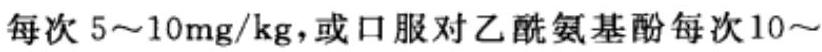
\includegraphics[max width=\textwidth, center]{2024_07_10_373f31b88d2bf633007bg-232}\\
$15 \mathrm{mg} / \mathrm{kg}$ 。高热烦躁者给予退热药的同时应给予苯巴比妥以防止惊嚴的发生。

\section*{(二)下呼吸道感染}
\begin{enumerate}
  \item 急性气管炎 通常由细菌和病毒引起, 婴儿和学龄前儿童的急性气管炎要考虑百日咳杆菌感染, 最好的检验样品是深部鼻咽拭。

  \item 慢性气管炎查找病原体往往较困难, 流感嗜血杆菌、肺炎链球菌、卡他莫拉菌属常能从这些患者的支气管中分离到。病毒往往也是一个致病原。

  \item 上呼吸道感染浸人肺部、直接吸人病原体或由血流人肺,均可引起肺炎。成人肺炎的常见病因有肺炎支原体、呼吸道病灻、肺炎衣原体、流感嗜血杆菌、需氧革兰阴性杆菌、金黄色莆萄球菌及军团菌。肺炎链球菌是成人肺炎最常见的病原。

\end{enumerate}

病毒也能引发肺部细菌感染。由细菌引起的儿童肺炎往往是流感嗜血杆菌、肺炎链球菌或金黄色葡萄球菌。新生儿可由沙眼衣原体或卡氏肺囊虫所致。在 $<30$ 岁的年轻人中, 肺炎支体是最重要的下呼吸道病原体,最近发现肺炎衣原体也是重要的致病原,在病毒性肺炎后经常继发 $\beta$-溶血性链球菌、肺炎链球菌、金黄色葡蒛球菌、卡他莫拉菌、流感嗜血杆菌、肺炎衣原体感染。

\section*{三、支气管哮喘}
哮喘是由嗜酸性粒细胞、肥大细胞和 $\mathrm{T}$ 淋巴细胞等多种炎症细胞参与的气道慢性炎症。这种炎症使易感者对各种激发因子具有气道高反应性,并引起气道狭窄。

(一)病因

多认为是与多基因遗传有关的疾病, 同时受遗传因素和环境因素的双重影响。

\section*{(二)发病机制}
不完全清楚。多认为哮喘与变态反应、气道炎症、气道反应性增高及神经等因素相互作用有关。

(三)临床表现

症状为发作性伴有哮鸣音的呼气性呼吸困难或发作性胸闪和咳濑,严重者被迫采取坐位或呈端坐呼吸,干咳或咳大量白色泡沫痰, 甚至出现发绀等。体检胸部呈过度充气状态, 有广泛的哮鸣音,呼气音延长。

\section*{(四)实验室检查}
\begin{enumerate}
  \item 呼吸功能检查在哮喘发作时有关呼气流速的全部指标均显著下降。

  \item 动脉血气分析侾喘严重发作时可有缺氧, $\mathrm{PaO}_{2}$ 降低,由于过度通气使 $\mathrm{PaCO}_{2}$ 下降, $\mathrm{pH}$ 上升,表现呼吸性䂸中毒。

  \item X 线检查 早期在㫴喘发作时可见两肺透亮度增加,呈过度充气状态,在缓解期多无明显异常。

\end{enumerate}

\section*{(五)诊断}
\begin{enumerate}
  \item 反复发作的喘息、呼吸困难、胸闪或咳嫩,多与接触变应原、冷空气、物理性刺激、化学性刺激、病毒性上呼吸道感染、运动等有关。

  \item 发作时在双肺可闻及散在弥漫性、以呼气相为主的哮鸣音,呼气相延长。上述症状可经治疗或自行缓解。

  \item 症状不典型者至少应有下列三项中的一项阳性。

\end{enumerate}

(1)支气管激发试验或运动试验阳性。

(2)支气管舒张试验阳性。

(3)呼乞流量峰值日内变异率或昼夜波动率 $\geqslant$ $20 \%$ 。

除外其他疾病所引起的喘息、胸闷和咳濑。

(六)治疗

目前尚无特效的治疗方法,但哮喘症状能得到控制,减少复发乃至不发作。

\begin{enumerate}
  \item 脱离变应原是治疗哮喘最有效的方法。

  \item 治疗哮喘药物: 支气管舒张药有 $\beta_{2}$ 肾上腺素受体激动药、茶碱类、抗胆碱药。抗炎药有糖皮质激素和色甘酸钠。

  \item 急性发作期治疗,目的是尽快缓解气道阻塞,纠正低氧血症,恢复肺功能,预防进一步恶化或再次发作,防止并发症。

\end{enumerate}

(1)轻度: 吸人短效 $\beta_{2}$ 受体激动药,如沙丁胺醇。

(2)中度: 规则吸人 $\beta_{2}$ 受体激动药或口服长效 $\beta_{2}$ 受体激动药。加用氨茶械 $0.25 \mathrm{~g}$ 加人 $10 \%$ 蒱萄糖 $40 \mathrm{ml}$ 中, 缓慢静脉注射。

(3)重度: 持续雾化吸人 $\beta_{2}$ 受体激动药, 或静脉滴注沙丁胺醇或氨茶碱。雾化吸人抗胆䂸药,静脉滴注糖皮质激素。

\section*{四、急性肺栓塞}
急性肺㭲塞 (APE) 是由于内源性或外源性㭲\\
子堵塞肺动脉主干或分支引起肺循环障碍的临床和病理生理综合征, 其发病率仅次于冠心病及高血压, 病死率居第三位, 仅次于肿痛及心肌梗死, 但长期以来由于对该病的防治缺乏足够的重视,尤其基层医院经常漏诊、误诊。

\section*{(一)急性肺检塞诱发因素特征}
绝大多数 APE 患者都有发病诱因, 如下肢或盆腔静脉血栓形成, 长期卧床或不活动, 慢性心肺疾病、手术、创伤、恶性肿瘤、妊娠及口服避孕药等,在询问病史时要特别注意。

\section*{(ニ)病因}
注意有无长期卧床、房温、长期心裏、细菌性心内膜炎、胸腔大手术、肾周围充气造影、人工气腹、胫骨和股骨及骨盆等骨折、㾇肿、真性红细胞增多症、血小板增多症、口服避孕药和糖尿病及白塞病等病史及发病诱因。

\section*{(三)症状体征}
有无呼吸困难、剧烈胸痛、咯血、发热症状。体检注意有无胸部干、湿啰音, 胸膜摩擦音、胸腔积液及休克、发绀等表现。

(四)诊断检查

\begin{enumerate}
  \item 检验 血象、血乳酸脱氢酶、血气分析、二聚体和凝血功能检查。

  \item 心电图 有无心律失常, 如心房纤颤、右束支传导阻滞等; 心电图可见电轴右偏, 明显顺时针方向转位; T 波倒置,肺性 P 波。

  \item X 线胸片 可有多发性浸润、胸腔积液、横扁升高。

  \item 超声心动图 肺动脉高压、右心室扩张、右心室收缩无力。

  \item 肺通气灌注扫描 用放射性核素 ${ }^{133} \mathrm{Xe}$ 吸人扫描与肺灌注扫描同时进行, 前者正常而后者显示缺损者, 多为肺检塞。

  \item 肺血管造影以选洋性肺动脉造影效果最好, 如加放大技术能分辨直径 $0.5 \mathrm{~mm}$ 小动脉的阻塞, 发现阻塞可确诊。有条件者可行数字减影血管造影, 图像更清晰。肺动脉压 $>80 \mathrm{mmHg}$ 者禁忌。

\end{enumerate}

(五)治疗方案

\begin{enumerate}
  \item 急救处理 快速给氧; 静脉注射吗啡制剂止痛, 静脉注射阿托品 $0.5 \sim 1 \mathrm{mg}$, 以减低迷走神经张力, 防止肺血管及冠状动脉反射性痉挛; 抗心力衰竭、抗休克及水、电解质平衡治疗。
\end{enumerate}

\section*{2. 抗凝治疗}
(1)肔素:首剂 $50 \sim 75 \mathrm{mg}$ 加生理盐水 $20 \sim$ $40 \mathrm{ml}$,静脉注射,维持血凝时间 (试管法) 为正常对照者的 2〜3 倍 (20〜35min), 后每 $4 \sim 6 \mathrm{~h} 50 \mathrm{mg}$; 也可 $200 \mathrm{mg}$ 加 $5 \%$ 莆萄糖液静滴, 维持 $24 \mathrm{~h}$ 。以上剂量用 8 10d 后减量到停药, 或改口服抗凝药。

(2)口服抗凝药: 华法林钠开始 10〜15mg,3〜 $5 \mathrm{~d}$, 待凝血酶原时间适度延长 (活动度 $15 \% \sim 25 \%$ )时, 调整用量并维持 12 周, 维持量 $2 \sim 15 \mathrm{mg} / \mathrm{d}$ 。

(3) 溶血栓疗法: 链激酶 25 万 50 万 U 溶于 $5 \% \sim 10 \%$ 葡㢣糖液或生理盐水 $100 \mathrm{ml}$ 中, $30 \mathrm{~min}$静脉滴注完, 以后每小时 10 万 $\mathrm{U}$, 维持 $24 \mathrm{~h}$, 与肝素并用疗效更好。也可用尿激酶 20 万 U 静脉滴注,以后每小时 20 万 $\mathrm{U}$, 维持 $8 \sim 12 \mathrm{~h}$ 。有出血性疾病、严重高血压、糖尿病视网膜病变、消化道遗疡、近期做过大手术以及过敏性素质者, 禁用溶血栓疗法。

\begin{enumerate}
  \setcounter{enumi}{2}
  \item 手术治疗 对抗凝治疗无效、大的或反复肺动脉检塞、使肺循环阻断> $>0 \%$ 并导致肺动脉高压者适宜手术治疗。检塞部位确定者可行肺栓子切除术,也可行下腔静脉阻断术,以减少来自盆腔和下肢的血栓检子循环人肺。

  \item 病因治疗 感染性㭲子行抗菌治疗; 气栓、脂肪检时应取头低脚高位, 以惐少检子人肺。

\end{enumerate}

\section*{五、胸 腔 积 夜}
\section*{(一)胸腔积液与吸收的机制}
病因 胸膜毛细血管内静水压增高; 胸膜毛细血管通透性增加; 胸膜毛细血管内胶体渗透压降低; 壁层胸膜淋巴引流障碍; 损伤所致胸腔内出血。

\section*{(ニ)临床表现}
结核性胸膜炎多见于青年人, 常有发热, 中年以上患者应警惕有肺癌所致胸膜转移。炎性积液多为渗出性, 常伴有胸痛及发热。心力衰竭所致胸腔积液为漏出液。肝脓肿所致右侧胸腔积液可为反应性胸膜炎, 也可为脓胸。积液量少于 $0.3 \mathrm{~L}$ 时症状多不明显; 若超过 $0.5 \mathrm{~L}$, 患者渐感胸闪。局部吒诊浊音, 呼吸音减低。积液量增多后, 两层胸膜漏开, 不再随呼吸摩擦, 胸痛亦渐绶解, 但呼吸困难亦渐加剧, 大量积液时纵隔脏器受压, 心悸及呼吸困难更加明显。

\section*{(三)治疗}
\begin{enumerate}
  \item 结核性胸膜炎 胸腔穿刺不仅有助于诊断,且可解除肺及心、血管受压, 改善呼吸, 防止纤维蛋白沉着与胸膜增厚, 使肺功能免受损伤。每次抽液量不应超过 $1000 \mathrm{ml}$, 过快过多抽液可使胸腔压力啝降, 发生肺水肿。糖皮质激素可减轻机体的变态\\
反应及炎症反应,改善毒性症状,加速吸收,减少胸膜粘连或胸膜增厚等后遗症。

  \item 脓胸 由各种病原微生物引起的胸膜腔感染性炎症, 同时伴有外观浑浊, 具有脓样特性的胸腔渗出液。急性脓胸常表现为高热、消耗状态、胸胀痛等。治疗原则是控制感染、引流胸控积液及促使肺复张, 恢复肺功能。慢性脓胸有胸膜增厚、胸谢塌陷、慢性消耗、杵状指(趾), 应考虑外科胸膜剥脱术。

  \item 恶性胸坨积液 多为恶性肿㿔所致, 其胸液生长迅速且持续存在, 常因大量积液的压迫引起严重呼吸困难,甚至导致死亡,但反复抽液可使蛋白丢失太多,效果不理想。

\end{enumerate}

\section*{六、气胸}
胸膜腔是不含空气的密闭的潜在性腔隙。气体进人胸膜腔, 造成积气状态, 称为气胸。可自发地发生,也可由疾病、外伤、手术、诊断或治疗性操作不当等引起。较常见的是肺部疾病使肺组织及脏层胸膜破裂,或靠近肺表面的肺大疮、细小气肿疮自发破裂, 肺及支气管内空气进人胸膜腔, 称为自发性气胸。

\section*{(一)临床类型}
\begin{enumerate}
  \item 闭合性气胸胸膜破裂口较小, 随肺萎陷而关闭, 空气不再继续进人胸膜腔。

  \item 张力性气洶 破裂口呈单向活辫作用, 吸气时胸廊扩大, 胸膜腔内压变小, 呼气时胸膜腔内压升高, 压迫活瓣使之关闭。每次呼吸运动均有空气进人胸膜腔而不能排出, 致使胸膜腔内空气越积越多, 胸膜腔内压持续升高, 使肺受压, 纵隔向健侧移位, 影响心肚血液回流。此种气胸胸膜腚内压测定常超过 $10 \mathrm{cmH}_{2} \mathrm{O}$, 甚至达 $20 \mathrm{cmH}_{2} \mathrm{O}$, 抽气后胸膜腔内压可下降, 但又迅速复升。气胸对呼吸循环影响最大,必须紧急抢救处理。

  \item 开放性气胸 破裂口较大或因两层胸膜间有粘连或牵拉, 使破口持续开启, 吸气与呼气时, 空气自由进出胸膜腔。胸膜腔内压在 0 上下波动, 抽气后观察数分钟,压力维持不变。

\end{enumerate}

\section*{(二)临床表现}
气胸对呼吸和循环功能的影响与气胸发生前肺基础疾病及肺功能状态、气胸发生的速度、胸膜腔内积气量及其压力 3 个因素有关。起病前患者可能有持重物、屏气、剧烈体力活动等诱因。突感一侧胸痛、气促, 憋气,可有咳嫩,但痰少。张力性气胸时胸膜腔内压骤然升高, 肺被压缩, 纵隔移位,迅速出现呼吸循环障碍, 患者表情紧张、胸闪、挣扎坐起、烦躁不安、发㙋、冷汗、脉速、虚脱、心律失常,甚至发生意识不清、呼吸衰竭。体检显示气管向健侧移位, 胸部有积气体征, 患侧胸部隆起, 呼吸运动与触觉语颤减弱, 吒诊呈过度清音或鼓音, 听诊呼吸音减弱或消失。X 线胸片检查是诊断气胸的重要方法, 可显示肺受压程度, 肺内病变情况以及有无胸膜粘连、胸控积液及纵隔移位等。

\section*{(三)治疗}
自发性气胸的治疗目的是促进患侧肺复张、消除病因及减少复发。治疗具体措施有非手术治疗、胸腔减压、开胸手术或经胸腔镜手术等。

\begin{enumerate}
  \item 非手术治疗 气胸量 $<20 \%$, 且为闭合性,症状较轻, $\mathrm{PaO}_{2}>70 \mathrm{mmHg}$, 经非手术治疗多可治愈, 气体可在 7 10d 吸收。
\end{enumerate}

\section*{2. 排气疗法}
(1)闭合性气胸 : 气量较多,肺压缩 $>20 \%$ 的闭合性气胸, 呼吸困难较轻、心肺功能尚好者, 为加速肺复张,迅速缓解症状,可选用胸腔穿刺排气; 张力性气胸, 为迅速降压以避免发生严重并发症, 也需立即胸腔穿刺排气。

(2)高压性气胸 : 病情严重可危及生命,必须尽快排气。张力性、开放性或心肺功能较差、自觉症状重的闭合性气胸, 无论其肺压缩多少,均应尽早行胸腚闭式引流。反复发生的气胸, 应首选胸腔闭式引流。

(3)开放性气胸: 积气量小且无明显呼吸困难者, 经卧床休息及限制体力活动, 或安置水封瓶引流后, 有时胸膜破口可自行封闭而转变成闭合性气胸。

\section*{七、睡眠呼吸素乱}
如果睡眠时口咽、鼻咽部无气流通过的时间长达 $10 \mathrm{~s}$ 以上, 即可称为睡眠呼吸暂停。频繁发生睡眠呼吸暂停可引起 $\mathrm{CO}_{2}$ 渚留和低氧血症, 进而引起体、肺循环压力升高和心律失常等并发症。

\section*{(一)临床表现}
\begin{enumerate}
  \item 清晨头痛, 白天嗜睡疲劳, 伴反复严重打䙹,睡眠不安稳。

  \item 肥胖, 睡眠时伴有明显低氧血症、高血压和心律失常。

  \item 与脊柱后侧凸、肌肉萎缩有关的膈肌或胸靳损害。

  \item 慢性阻塞性肺病伴有睡眠呼吸暂停。

  \item 通气/血流比例和弥散严重受损的肺疾病,如肺纤维化, 囊性纤维化, 纤维化性肺结核。

  \item 影响呼吸中枢的疾病。

  \item 肥胖性低通气综合征。

  \item 慢性高山病、睡眠中反复出现低氧血症。

  \item 长期接受强效利尿药, 代谢性碱中毒抑制通气功能。

\end{enumerate}

\section*{(二)睡眠呼吸妾乱类型}
\begin{enumerate}
  \item 阻寒性睡眠呼吸暂停综合征 (obstructive sleep apnea syndrome, OSAS) OSAS 是成人睡眠呼吸紊乱中占优势的疾病。诊断根据是存在胸腹呼吸运动时, 上呼吸道无气流通过的时间超过 $10 \mathrm{~s}$ 。每小时累计超过 5 次, 每晚 $6 \mathrm{~h}$ 睡眠中超过 30 次。
\end{enumerate}

呼吸暂停时, 尽管上气道无气流通过, 但仍存在胸䐗呼吸运动, 而且胸实负压波动很大, 可高达 $80 \mathrm{cmH}_{2} \mathrm{O}$ 。由于上气道陷闭, 没有或很少有外环境气体进人肺泡进行气体交换, 可产生严重低氧血症和 $\mathrm{CO}_{2}$ 濐留, 进行性心动过缓, 以及呼吸暂停结束时的短暂心动过速。偶尔出现窦房阻滞, 房室分离, 结性或室性逸搏, 低氧血症所致酸中毒和心肌缺血产生房性和室性异心律失常。严重的 OSAS 患者伴有白天嗜睡, 清醒时仍存在高碳酸血症, 甚至肺动脉高压和右侧心力衰竭。

\begin{enumerate}
  \setcounter{enumi}{1}
  \item 中枢性睡眠呼吸暂停综合征 (central sleep apnea syndrome, CSAS) CSAS 定义是上气道无气流通过的时间大于 $10 \mathrm{~s}$, 而且没有胸腹呼吸运动。 CSAS 较少见,可与 OSAS 并存。可发生于任何睡眠时相, 但明显的异常仅见于 NREM 睡眠时。 CSAS 可单独存在或与脑干外伤、肿瘤、梗死及感染等中枢神经系统疾病并存。清醒时可保持适当的通气功能, 但睡眠时则表现出呼吸中枢调节异常, 出现中枢性(或阻塞性) 呼吸暂停。

  \item 慢性阻塞性肺病患者的睡眠呼吸䒺乱 慢性阻塞性肺病恵者睡眠时可伴有明显的呼吸和气体交换恶化, 主要是严重的动脉血氧饱和度降低及合并短暂特异性呼吸异常, 如呼吸暂停和呼吸不足。在 NREM 睡眠时最明显,其机制尚不清楚,可能与该睡眠时相伴有的呼吸活动异常有关。

  \item 呼吸暂停样现象易与睡眠呼吸暂停综合征混淆的呼吸暂停样现象有以下两种:

\end{enumerate}

(1) 㿎病: 没有紧张阵挛的轻度瘷痫也可存在呼吸暂停。如发生在睡眠时或睡眠样的发作后状态可与睡眠呼吸暂停混淆, 可借助脑电图鉴别。

(2)陈-施呼吸: 可见于心排血量减少或循环时间延长的患者, 以及影响呼吸中枢的各种神经系统疾病和一些老年人。很难与中枢性呼吸暂停区别,而且两者可并存。此外,陈-施呼吸可持续到清醒状态, 而中枢性呼吸暂停在清醮时不出现, 并且常在 NREM 睡眠时加重。

\section*{(三)辅助检查}
睡眠呼吸监护。睡眠呼吸监护要监测患者睡眠时中枢神经、呼吸和心血管系统功能及睡眠呼吸紊乱的结果, 为诊断提供依据。标准的多导睡眠记录仪应彻夜记录如下变量: 脑电图、肌电图、心电图、通气、胸腹呼吸运动及呼吸紊乱的结果。直接监测通气需用咬口或面罩收集呼出气, 但患者不易耐受, 且影响自然睡眠状态。间接监测通气包括定性和半定量两种方法。定性方法可应用热敏电阻或快速 $\mathrm{CO}_{2}$ 分析仪监测通过口鼻的呼吸气体; 半定量方法可采用磁强计或呼吸感应性体容积描记仪。胸腹呼吸运动可用膈肌电图、经膈压测定和呼吸感应性体容积描记仪监测。呼吸紊乱结果的监测主要有直接或间接测定动脉血氧分压 $\mathrm{CO}_{2}$ 分压和氧饱和度。

\section*{(四)治疗措施}
\section*{1. 一般措施}
(1)减肥: 肥椫者上气道周围脂肪沉积、管挖缩小, 顺应性增加, 吸气时易于陊闭。而且同时伴有功能残气和潮气量惐少, 可引起通气/血流比值失调和低氧血症。减肥后常可取得明显疗效, 但部分患者难以长期坚持。

(2) 氧疗: 对于低氧血症患者可考虑低浓度氧疗, 使 $\mathrm{PaO}_{2}$ 保持在 $60 \sim 75 \mathrm{mmHg}$, 除改善呼吸暂停时间和氧饱和度外, 还可预防睡眠呼吸暂停引起的心动过缓、肺动脉高压和肺心病。

(3)戒酒和避免应用镇静药: 乙醇和镇静药可降低上气道周围肌肉甚至额舌肌活动诱发睡眠呼吸暂停。因此, 避免睡前饮酒和服用镇静药有助于睡眠呼吸暂停的治疗。

\section*{2. 特殊措施}
(1)OSAS 治疗: (1) 经鼻持续性气道正压呼吸 (CPAP), 可保持上气道扩张, 较好地预防睡眠时呼吸暂停。(2)解除上气道机械性狭窄, 存在扁桃体和增殖腺肥大时, 手术切除可取得较好效果。㗀垂腭咽成形术对鼻咽部阻塞引起的睡眠呼吸暂停疗效较好。(3)气管切开可使呼吸气流免受上气道陷闭\\
的影响, 但不易为患者接受, 而且一旦切开就很难拔管。

(2)CSAS 治疗: 可给予茶碱、乙酰唑胺和黄体酮等呼吸中枢兴奋药物, 疗效各家报道不一, 严重的 CSAS 药物治疗无效时,可采用气管切开,夜间机械通气辅助呼吸。

\section*{八、麻醉前对呼吸系统的评估和准备}
由于呼吸系统在麻醉中的特殊意义,不论准备采用何种麻醉方式,均应向患者及家属详细了解既往病史和现病史至关重要, 特别是呼吸系统相关的症状。然后结合查体和实验室报告进行准确评估,才能针对个体进行恰当的麻醉准备。

\section*{(一)呼吸道疾病史}
患者近期两周内有呼吸道感染病史,麻醉前无任何症状和体征,围麻醉期呼吸道并发症发生率比无呼吸道感染病史者高数倍, 因为他们仍处于呼吸道病理生理阶段,其呼吸道稆膜的应激性高。麻醉药物可引起腺体比正常生理阶段分泌更多的分泌物, 引发气道平滑肌收缩的自主神经的兴奋阈值也降低,浅麻醉下的任何刺激(疼痛、分泌物、低氧等)都可以激发气道痉挛。呼吸道感染病史遗漏时, 麻醉医师如果手术前查体认真仔细仍然可能发现阳性体征(咽部充血、呼吸音粗糙)。正值呼吸道疾病时查体有相应症状、体征,通过询问患者症状的发生和发展经过、用药情况,结合胸部 X 线片、血常规可以初步确诊。

术前需要特别注意的是气道高反应性 (airway reaction higher, ARH), ARH 是指患者对各种刺激产生支气管过度收缩反应, 具有可逆性支气管痉挛的呼吸疾病过程。哮喘是一种典型 ARH 的综合征,以支气管对物理、化学、药物和(或)免疫刺激呈高反应性为特征。主要临床症状是发作性呼吸困难或胸闪, 胸部听诊可发现弥漫性哮鸣音, 呼气期较重。当气道发生异常收缩或支气管痉挛时,因呼吸气流受阻引起肺容量、最大呼气流速 (PEFR)和胸壁顺应性变化, 同时引起通气分布和灌流改变,严重者可发生低氧血症、高碳酸血症及心血管功能改变。偶发支气管痉挛并得到及时控制的患者,不致引起心肺功能损害; 频发哮喘的患者可发生不可逆性的肺气肿, 严重者导致右侧心力衰竭。

正常人群中 ARH 患者占 $10 \%$ 。儿童哮喘发生率为 $1.7 \% \sim 4.7 \%$,成人为 $2.0 \% \sim 6.2 \%$ 。麻醉期间支气管痉挛发生率为 $0.16 \%$ 。气管插管、呼吸道感染、经口内镜手术和气道阻塞等因素可增加支气管痉挛的发生率, 而麻醉期间支气管痉挛常诱发于机械刺激。

根据㫴喘史和需用药物控制支气筞痉挛的情况, 可以将病人分成 3 类。第一类, 患者有哮喘史,但数年来未急性发作,亦未使用药物治疗。物理检查和通气试验无明显异常, 围术期一般不会发生支气筞痉挛。第二类,患者经常发生支气管痉挛, 需常规预防性地使用支气管扩张药物,但在麻醉前检查时无明显喘息。该类患者需更详细地评估肺功能, 测定 $\mathrm{FEV}_{1}$ 、MEFR 和 $\mathrm{FEF} 25 \% \sim 75 \%$,并与以往测定数值比较。如果测定数值不低于预测值的 $80 \%$ 或不比以往测定数值差,可以在继续抗支气管痉挛治疗时安排择期手术。如肺功能试验显示患者有明显气道阻塞(测定数值低于预测值的 $80 \%$ 或比以往测定数值差),该患者应属第三类, 择期手术前需进行抗哮喘的系统治疗。第三类患者有支气管痉挛,全身情况恶化或未使用适合剂量的药物治疗,该类患者的择期手术应延期进行,先采用系统药物治疗,直到支气管疼挛消失或全身情况恢复到较佳状态。如呼气流速或 $\mathrm{FEV}_{1}$ 下降, 可给患者吸人支气管扩张气雾剂后重复肺功能试验, 评估气道阻塞的可逆程度。如果 $\mathrm{FEV}_{1}$ 的增幅 $>15 \%$,可以认为属于明显可逆性气道收缩, 提示进一步降低气道收缩性的治疗对患者是有益的。

哮喘患者围术期并发症发生率比非哮喘者高。未控制的哮喘或哮喘急性发作期的患者不应安排择期手术。麻醉前处理需考虑疾病的病因,术中注意病理生理变化,并加强围术期的监测。麻醉科医生的姲熟技术、全身麻醉后早期恢复和手术后良好的镇痛及护理能明显防止哮喘发作和降低肺部并发症的发生率。除了麻醉和手术能产生肺功能改变外,术后控制呼吸和乞道黏膜纤维功能异常也可引起哮喘。

但是 ARH 患者麻醉期间发生的喘息并非都归因于哮喘发作,应该与肺水肿、支气管插管、肺栓塞、张力性气胸、胃内容误吸、气管导管机械性阻塞 (如导管扭曲、分泌物或血块堵塞),以及过敏反应等进行鉴别, 后者临床上也表现为呼吸困难, 但在处理方法上可能相差甚远, 如气管导管机械性阻塞时必须解除导管梗阻, 张力性气胸者需立即进行胸腔闭式引流。另外,由于静水压增高引起的肺水肿和支气管痉挛的处理亦完全不同,前者对利尿药反应良好, 而后者出现气道压力增高和低血压时往往\\
需要补充液体。

\section*{(二)术前检查与评估}
\begin{enumerate}
  \item 麻醉耐受力估计 麻醉前要重点掌握有关病史和体检, 以判断感染程度和肺功能减退程度,并据此进行细致的术前准备工作。下面列举常见的病史和体检项目。
\end{enumerate}

(1)呼吸困难: 活动后呼吸困难是衡量肺功能不全的主要临床指标。0 级,无呼吸困难症状;一级, 能较长距离缓慢平道走动, 但濑于步行; 二级,步行距离有限制, 走 $100 \sim 200 \mathrm{~m}$ 后需要停步休息;三级,短距离走动即出现呼吸困难; 四级, 静息时也出现呼吸困难。

(2)慢性咳嫩多㽷: 慢性咳濑多痰术后极易并发弥散性肺泡通气不足或肺泡不张, 术前应做痰细菌培养,并应用相应的抗生素控制感染。

(3)感冒: 可显著削弱呼吸功能, 呼吸道阻力增高可持续达 5 周, 同时对细菌感染的抵抗力显著减弱,或使原有呼吸系疾病加重。

(4)哮喘: 提示小气道明显阻塞, 肺通气功能减退,但一般均可用支气管扩张药和肾上腺皮质激素治疗而获得缓解。哮喘患者围术期的呼吸系并发症可比呼吸系正常的患者高 4 倍。

(5)咯血: 急性大量咯血可能导致急性呼吸道阻塞和低血容量, 甚至出现休克, 有时需施行紧急手术, 麻醉处理的关键在于控制呼吸道, 必须施行双腔支气管插管。

(6)吸烟: 凡每日吸烟 20 支以上,并有 10 年以上吸烟史者, 即可认为已经存在慢性支气管炎, 平时容易继发细菌感染而经常咳嫩咳疢, 麻醉后则容易并发呼吸系严重并发症。

(7)高龄: 老年人易并发慢性肺疾病, 并由此继发肺动脉高压和肺心病, 这是高龄老人麻醉危险的重要原因之一。

(8)过度肥胖: 体重超过标准体重 $30 \%$ 以上者,易并存慢性肺功能减退, 术后呼吸并发症可增高两倍。

(9)胸部物理检查: 应注意患者的体形和外貌,极度肥胖、胸梯畸形或脊柱侧弯者肺容积可明显减少,肺顺应性下降, 容易发生肺不张和低氧血症。观察皮肤和䀡膜的色泽,有无苍白或发绀。成人平静呼吸时频率超过 $25 / \mathrm{min}$ 是呼吸衰竭的早期表现。呼气费力常提示有气道梗阻。注意辅助呼吸肌是否参与呼吸运动。听诊时注意呼吸音的强弱、是否粗糙以及有无啰音,有高音调的喘鸣音提示小气道痉挛。

\begin{enumerate}
  \setcounter{enumi}{1}
  \item 肺功能的估计 通气试验是评估气道疾病、气道收缩反应可逆程度及对药物治疗效果的常用方法。
\end{enumerate}

(1)简易的肺功能试验:(1)屏气试验。正常人可以持续屏气 30 s 以上,能持续屏气 $20 \sim 30$ s 者麻醉危险性较小。 $<10 \mathrm{~s}$ 者, 提示患者心肺代偿功能很差,麻醉手术风险很高。(2)测量胸围。深吸气与深呼气胸围差大于 $4 \mathrm{~cm}$ 者,一般没有严重肺疾患或呼吸功能不全。(3)吹火柴试验。深吸气后快速吹气, 能将 $15 \mathrm{~cm}$ 远的火柴吹熄者,提示肺储备功能良好。

(2)肺功能测验: $\mathrm{FEV}_{1}$ 主要反映大气道阻塞程度,不能说明外周气道的精细变化。FEF $25 \%$ ~ $75 \%$ 能较好地反映小气道状态。支气管痉挛时 PEFR 明显降低。MVV 是一种呼气试验, 急性支气管痉挛发作时不适用。流速-容量环是小气道疾病的敏感指标,能够同时评估用力相关部分的呼气和非用力相关部分的呼气。

临床上可以用术前测定的肺功能预测术后肺部并发症的危险性。当 FVC<预计值的 $50 \%$ 、 $\mathrm{FEV}_{1}<2 \mathrm{~L} 、 \mathrm{FEV}_{1} \%<$ 预计值 $70 \%$ 或 $\mathrm{MVV}<$ 预计值 $50 \%$ 时,有发生术后肺部并发症的中度危险; 当 $\mathrm{FVC}<15 \mathrm{ml} / \mathrm{kg} 、 \mathrm{FEV}_{1}<1 \mathrm{~L} 、 \mathrm{FEV}_{1} \%<$ 预计值 $35 \%$ 或 $\mathrm{FEF} 25 \% \sim 75 \%<14 \mathrm{~L} / \mathrm{s}$ 时,有发生术后肺部并发症的高度危险。

\begin{enumerate}
  \setcounter{enumi}{2}
  \item 动脉血气分析(ABG) 动脉血气分析是评价肺功能的常用指标。在肺功能测验高度异常的哮喘患者 $\left(\mathrm{FEV}_{1}<\right.$ 预测值的 $25 \%$ 或 $\mathrm{PEFR}<$ 预测值的 $30 \%$ ), 可见到高碳酸血症和(或)低氧血症。当 $\mathrm{PaCO}_{2}>45 \mathrm{mmHg}$ 时,术后出现呼吸系统并发症的危险明显增加。

  \item 胸部影像学检查 胸部影像学检查用于发现或排除可引起呼吸功能障碍的胸廓、气管和肺组织的异常情况,如胸廓畸形、脊柱严重侧弯、气管或支气管梗阻(包括气管外源因对气道压迫或牵拽以及气管内新生物引起的气道狭窄)、膈肌上移或运动障碍、气胸或胸腔积液、肺间质纤维化、肺大疱、肺气肿、毁损肺等。

\end{enumerate}

\section*{(三)麻醉前用药}
苯二氮草类药物有良好的镇静和抗焦虑作用,但对呼吸中枢有抑制作用, COPD 患者对其尤其敏感, 因此在用于呼吸功能障碍患者时应注意控制和调整剂量。镇痛药的使用目前仍有争议。吗啡能\\
抑制由迷走神经介导的支气管疼挛, 但又能升高血浆中的组胺浓度, 引起气道阻力增加。虽作为麻醉前用药不大可能对气道产生直接或反射性作用的支气管痉挛, 但镇痛药可使麻醉期呼吸抑制延长,故不主张麻醉前使用。抗胆碱能药物可解除迷走神经反射, 减少气道分泌物, 但会增加分泌物的秥稠度, 不利于扊液排出。 $\mathrm{H}_{1}$ 受体拮抗药具有镇静和气道干燥作用, 而 $\mathrm{H}_{2}$ 受体拮抗药则可诱发支气管痉挛, 应避免使用。

因此, 重视术前呼吸系统的评估将减少围术期呼吸系统并发症的发生,提高麻醉质量和保障病人安全。

\section*{第二节 急性呼吸道炎症的麻醉}
本病是一种常见的呼吸系统疾病, 是病毒和细菌的感染、物理化学刺激或过敏反应等对支气管稆膜所造成的急性炎症。本病的病原体主要为病毒和细菌。

\section*{一、临床表现}
起病时较急, 很像感冒, 病人感到疲倦、头痛、发热、全身酸痛, 有刺激性干咳, 伴胸骨后不适感或钝痛, $1 \sim 2 \mathrm{~d}$ 后即咳痰,初为白色黏稠样,以后为橰液脓性, 偶有談中带血。这症状通常在 1 周后逐渐消失。

胸部听诊呼吸音增粗,散在干湿椤音,用力咳嫩或咳痰后, 啰音性质与部位易改变或消失。

\section*{二、理化检查}
血常规检查, 继发感染时,白细胞数可升高; X 线胸部检查大多数正常或肺纹理增粗; 䊏涂片及培养:可发现致病菌。

\section*{三、治 疗}
咳嫩甚而有哮鸣音者, 用氨茶碱 $0.1 \mathrm{~g}, 3 / \mathrm{d}$; 发热、咳嫩、吐脓掞者,可选用如下抗生素: 青霑素 80 万 $U$ 肌内注射, $2 / d$, 或 8 小时 1 次, $3 \sim 5 \mathrm{~d}$ 为 1 疗程; 或用青霍索 240 万 U 加人 $10 \%$ 莆蒛糖水 $500 \mathrm{ml}$静脉点滴, $2 / \mathrm{d}$,或 8 小时 1 次。青露素用药前必须做皮试,阴性后方能使用; 庆大露素 8 万 U 肌内注射, $2 / \mathrm{d}$ 或 8 小时 1 次, $3 \sim 5 \mathrm{~d}$ 为 1 疗程。或用 $10 \%$蒲萄糖 $500 \mathrm{ml}$ 加庆大露素 12 万 $\sim 16$ 万 $\mathrm{U}$ 静脉点滴, $1 / \mathrm{d}$, 只晚上肌内注射 8 万 $\mathrm{U}, 3 \mathrm{~d}$ 为 1 疗程。

\section*{四、麻醉要点}
择期手术时对有近期呼吸道感染病史或现病史的患者来说, 力图降低麻醉引发的呼吸道并发症的发生率的最佳方案是“等待”, 等呼吸道疾病临床痊急 1 个月后,再接受麻醉。而急诊手术需要通过我们手术前充分评估和准备, 将风险降到最低。

急诊手术时患者的外科疾病或外伤不允许我们选择麻醉时机,但强调任何急诊手术麻醉前都不能免去询问病史和查体, 且需要更认真, 准确判断与麻醉相关的病理变化, 设计相应的麻醉方案, 准备完善的应对措施和气管插管器材。

麻醉期间支气管痉挛发生率为 $0.16 \%$ 。气管插管、呼吸道感染、经口内镜手术和气道阻塞等因素可增加支气管疼挛的发生率,而麻醉期间支气管痉挛常诱发于机械刺激。

\section*{第三节 慢性呼吸道炎症的麻醉}
慢性咳噋多痰术后极易并发弥散性肺泡通气不足或肺泡不张, 术前应做痰细菌培养, 并应用相应的抗生素控制感染。

\section*{一、临床表现}
本病多发生于中、老年,男多于女。进展缓慢。早期患者只在冬季有咳嫩、咳痰,痰多为橰性,夏天绶解。如刺激因素长期存在, 症状可逐渐加重, 咳嫩长年持续不断, 痰量多, 以泡沫样秥痰为主。伴有继发细菌感染时, 即出现脓性痰。有些过敏体质的病人在慢性支气管炎发作时, 伴有喘息和硣鸣音,称为喘息型慢性支气管炎。严重者逐渐出现气急, 且有逐年加重的趋势, 晚期可并发阻塞性肺气肿,最后可导致肺源性心脏病。

\section*{二、理 化 检 查}
\section*{(一)血常规检查}
急性发作期或并发肺部感染时,白细胞数和中性粒细胞增多,喘息型嗜酸性粒细胞可增多。

\section*{(ニ)痰液检查}
涂片或培养有致病菌。

\section*{(三)X 线检查}
早期无异常, 病变较重或伴急性感染时, 可有肺纹理增粗、紊乱或网状条索状斑点阴影, 以下肺为明显。

\section*{(四)肺气道功能检查}
显示支气管阻力增加。

\section*{三.治 疗}
急性发作期, 应以控制感染为主。可采用青䨣素 80 万 U肌内注射,每 8 小时 1 次,或将 320 万 $U$青露素加人 $10 \%$ 莆匋糖液 $40 \mathrm{ml}$ 中静脉注射, $2 / \mathrm{d}$ 。氮苄西林 $3 \mathrm{~g}$ 加 $10 \%$ 莆萄糖液 $40 \mathrm{ml}$ 静脉注射,每 8 小时 1 次, $3 \sim 5 \mathrm{~d}$ 为 1 疗程。平喘效果不佳时可选用少量皮质激素。

对痰多不易咳出者可采用雾化吸人疗法。庆大霸素 8 万 $\mathrm{U}$, 地塞米松 $5 \mathrm{mg}$, 加人生理盐水 $10 \mathrm{ml}$, 雺化吸人, $2 / \mathrm{d}$ 。

\section*{四、麻醉方法与麻醉药物的选择}
麻醉要点在于术前对患者进行完善的肺功能评估及充分的麻醉前准备。

\section*{(一)麻醉方法的选择}
\begin{enumerate}
  \item 局麻与神经阻滞 可保留自主呼吸, 对呼吸影响小,但应用范围有限。

  \item 椎管内麻醉

\end{enumerate}

(1)一般不选择腰麻, 因其对循环干扰大。

(2)胸部或上腹部硬膜外阻滞可因呼吸肌同时被阻滞而引起通气储备功能明显降低, 故不适用于严重呼吸功能障碍患者。

(3)上胸段硬膜外阻滞可使 VC 减少 $50 \%$,且同时阻断 T1 5 交感神经, 副交感神经相对占优势, 可诱发支气管痉挛, 不适用于㫴喘病人。

(4)椎管内麻醉应用辅助药时, 应避免其呼吸抑制作用。

\begin{enumerate}
  \setcounter{enumi}{2}
  \item 气管内麻醉 适用于病情重、呼吸功能差或已有低氧血症的病人, 也适合用于长时间的复杂手术。优点是气管插管可减少呼吸道无效腔、充分供氧、利于呼吸道管理、可及时清除呼吸道分泌物。缺点有长期吸人干燥气体, 呼吸道分泌物稒稠而不易吸引; 气管导管刺激可能诱发支气管痉挛; 可能出现小气道闭塞合肺泡萎陷; FRC下降, 肺泡无效腔增加, 影响肺内气体的分布与交换, 因而 $\mathrm{A}-\mathrm{aDO}_{2}$增加。
\end{enumerate}

\section*{(二)麻醉药物的选择}
\begin{enumerate}
  \item 吸人麻醉药: 氟烷对呼吸道无刺激, 可直接松驰支气管平滑肌, 适用于慢性支气管炎及哮喘患者。低浓度异氟醚和七㪼醚对呼吸道无剌激, 并可抑制迷走神经兴奋引起的支气管痉挛。

  \item 静脉麻醉药: 硫喷妥钠禁用于哮喘患者。氯胺酮增加儿茶酚胺,通过兴奋 $\beta_{2}$ 受体使支气管扩张, 特别适用于哮喘患者; 但可抑制呼吸, 故不适用于呼吸功能不全者; 可增加肺血管阻力, 使肺动脉压升高, 故禁用于慢性支气管炎继发肺动脉高压者。氮琥珀胆碱及阿曲库铵有一定组胺释放作用,而顺式阿曲库铵、泮库涋铵和维库溴轱无此作用。异丙酚可用于静脉麻醉。

\end{enumerate}

\section*{第四节 哮喘患者的麻醉}
\section*{一、麻醉前准备的注意事不}
病情估计及准备: 临床麻醉中经常遇到支气管哮喘的患者, 在麻醉诱导、插管或术中出现支气管疼挛。

\begin{enumerate}
  \item 在有条件的情况下, 术前一定要行肺功能测定和血气分析。哮喘患者术前不同程度伴有低氧血症。 $\mathrm{PaCO}_{2}$ 在早期正常或偏低, 这与低氧血症刺激外周化学感受器或肺牵张感受器有关。但随着气道阻塞加重, $\mathrm{PaCO}_{2}$ 升高, $\mathrm{PaO}_{2}$ 降低, $\mathrm{pH}$ 下降,此时应警惕呼吸衰竭发生。

  \item 对于重症和中度肺功能不全的患者,为了预防麻醉和术中发生支气管痉挛,术前可用支气管扩张药。 $\beta_{2}$ 受体兴奋药如沙丁胺醇、间羟异丙肾上腺素; 茶碱类药如氨茶碱、喘定; 皮质激素类药如甲强龙、地塞米松、泼尼松、氢化可的松; 抗感染等。

  \item 术前用药: 为解除患者精神紧张,可用镇静、镇痛药及神经安定药, 但对术前肺功能不全、缺氧的患者慎用、剂量酌减。多数人主张术前用哌替啶肌内注射,对支气管平滑肌有解痉作用, 少数病例除外。地西泮、貮哌利多,对呼吸道有扩张作用; 芬太尼,既兴奋胆碱能受体, 又兴奋 $\alpha$ 受体, 可使支气管收缩,但可先用阿托品、氟哌利多,抑制芬太尼的副作用,可慎用,不是绝对禁忌; 吗啡、喷他佐辛,兴\\
奋胆碱能受体和迷走神经, 组胺释放, 导致支气管疼挛,应禁用。

\end{enumerate}

\section*{二、麻醉药和麻醉方法的选择}
凡是兴奋 $\beta_{2}$ 受体使支气管扩张的药物均能用。如镇痛药: 哌替啶、芬太尼适用, 吗啡禁用。镇静安定药如地西泮、咪达唑仑、氟哌利多、氯丙嗪、异丙嗪(抗组胺作用); 全麻药氯胺酮可对抗组胺引起的支气管痉挛。它是一种非经直肠给药的苯环乙哌啶彷生物, 对肾上腺素能系统有兴奋作用, 通过 $\beta_{2}$ 受体使支气管扩张; 依托咪酯、异丙酚无组胺释放作用; 硫喷妥钠有组胺释放作用,禁用。

吸入麻醉药安氟梄、异氛醚、七氟醚有解除支气管痉挛的作用; 肌松药非去极化维库溴轱,无组胺释放作用; 阿曲库铵, 有过敏反应, 引起哮喘; 箭毒有组胺释放作用。去极化氯琥珀胆碱组胺释放少;局麻药利多卡因比较安全, 过敏反应少。

麻醉方法选择可根据患者情况及手术需要来决定。麻醉前给予 $10 \%$ 钙剂和地塞米松。连续硬膜外利多卡因。全麻术前。哌替啶、东茛若碱。诱导:咪达唑仑、芬太尼、氟哌利多、依托咪酯、维库溴轱、安氟醚,最好不要清醒插管。

\section*{三、处理}
\begin{enumerate}
  \item 找出原因 消除刺激因素。
\end{enumerate}

(1)麻醉过浅、气管插管、吸痰、手术操作牵拉反应均可引起反射性支气管痉挛, 应加深麻醉。

(2)乞管插管位置不当,过深直接刺激隆突,可调整导管位置。

(3)麻醉药物引起: 硫喷妥钠、阿曲库铵、乙醚,停止用药。

\begin{enumerate}
  \setcounter{enumi}{1}
  \item 如都排除仍无缓解 在保证充分供氧的前提下,可采用药物处理。
\end{enumerate}

(1)怪上腺皮质类固醇类药物, 甲强龙 $80 \mathrm{mg}$静推或氢化可的松 $100 \mathrm{mg}$ 静滴。

(2) 氨茶碱 $0.25 \mathrm{~g}$ 静推。

(3)氯胺酮 $100 \mathrm{mg}$ 静推。拔管时由于吸疢强刺激造成支气管痉挛, 也应注意。在不能及时拨管的情况下,加压给氧,用支气管扩张药氨茶碱、氯胺酮、钙剂、地塞米松。

\section*{第五节 胸外科手术的麻醉}
\section*{一、开胸和侧卧位对呼吸循环的影响}
\section*{(一)开胸的病理生理}
开胸后由于胸内压力的改变引起通气失常, 纵隔摆动, 从而导致神经反射及对循环的影响。如一侧开胸后, 任其自然呼吸, 由于空气进人开胸侧胸腔, 胸腔内负压消失, 肺的弹性回缩使肺部分萎陷,肺萎陷又使肺通气面积急剧减少,可达正常的 $50 \%$左右。同时流经不通气的萎陷肺血流不能进行气体交换,导致静脉血掺杂, 增加肺内分流。由于开胸侧肺内压始终与大气压相等, 所以当吸气时, 对侧肺膨胀使肺内压低于大气压, 开胸侧肺进一步缩小使肺内部分气体随外界空气同时吸人对侧肺内。当呼气时对侧肺缩小使肺内压高于大气压, 呼出肺内气体, 但部分又进人开胸侧肺内, 使开胸侧肺与正常呼吸时进行相反的回缩和朧胀动作,称为 “反常呼吸”。结果有一部分气体往返于两肺之间称为 “摆动气”。增加摆动气即增加无效气量, 造成严重缺氧及二氧化碳蓄积。摆动气量与胸壁开口大小成正比。反常呼吸程度与摆动气量及气道阻力成正比。所以控制呼吸时维持气道通畅极为重要。如胸腚开口比气管直径大 $6 \sim 8$ 倍时,两侧胸腔的压差即可使纵隔来回摆动, 如吸气时健侧负压大,纵隔移向健侧; 呼气时又推向开胸侧,纵隔来回摆动称为 “纵隔摆动”, 剧烈的纵隔摆动使上、下腔静脉来回扭曲受阻更使静脉回流减少, 心每搏量减少。同时摆动对纵隔部位神经的刺激也易引起反射性血流动力学改变,其至心搏骤停。开胸麻醉过程必须避免出现这类现象。熟练地进行手法扶助呼吸或并用肌松药有利于进行间断正压控制呼吸,均能克服开胸所造成的生理改变。

\section*{(二)麻醉时侧卧位对呼吸生理的影响}
清醒仰卧时腹腔内容可把膈肌推向胸腔内约 $4 \mathrm{~cm}$, 从而降低肺功能残气量 (FRC) 约 $0.8 \mathrm{~L}$ 。全麻诱导后更进一步下降约 $0.4 \mathrm{~L}$, 但两肺气量分布一致。仰卧时血流分布到左肺和右肺 (较大) 的流量分别占 $45 \%$ 和 $55 \%$ 。在清醒侧卧位时,靠床侧胴肌推向胸腔内幅度要比非靠床侧膈肌高。所以靠床侧肺的 FRC 比非靠床侧肺减少显著。结果在自主呼吸时, 由靠床侧䐟肌收缩更强, 所以靠床侧通气较非靠床侧为大。由于重力的影响肺血流流向靠床侧, 如右肺靠床则左肺和右肺血流量分别占\\
$35 \%$ 和 $65 \%$; 如左肺靠床, 则左肺和右肺血流量分别占 $55 \%$ 和 $45 \%$ 。所以靠床侧肺血流量平均为 ( 65 $+55) / 2=60 \%$, 而非靠床侧平均为 $(35+45) / 2=$ $40 \%$ 。因此肺通气/血流 (V/Q)之比, 侧卧位与仰卧位一样无变化。当全麻后两肺 FRC 进一步下降, 侧卧位即使在自主呼吸时, 也不再因靠床侧䐔肌升高而增强收缩及通气。另外,纵隔也压迫靠床侧肺而减少通气, 相对非靠床侧通气增大, 血流仍因重力影响而减少如应用肌松药使呼吸肌麻痹, 自主呼吸消失,则靠床侧肺通气较非靠床侧肺通气更为减少。此时如非靠床侧开胸, 则正压通气容易膨胀开胸侧肺, 使开胸侧 $\mathrm{V} / \mathrm{Q}$ 比值增大, 而靠床侧肺的 $V / Q$ 比值减少。常需术者协助将开胸侧肺充分压迫, 以缩小 $V / Q$ 比值变化。

\section*{二、单肺通气对呼吸的影响}
麻醉时应用单肺通气的安全性及成功率已显著增进, 主要支气管导管(双腔导管) 有了很大的改进, 又有纤维支气管镜协助及对单肺通气的生理改变有充分的认识。因此临床支气管内麻醉已不仅用于湿肺、支气管胸膜瘘或大咯血患者, 还经常用于食管、肺叶等手术便于手术操作, 减轻开胸侧肺损伤及防止两肺间的交叉感染。

\section*{$(一)$ 支气管导管的选择}
近年有聚氯乙烯双腔管, 壁薄内空相对增大,便于送人吸疢管。但是导管较软又常需探条支持,因无隆突钧靠, 导管位置有时不易准确放置, 可能插人过深,左右开口均进人一侧 (多为右侧)主支气管或插管过浅, 仍留在气管内, 必须根据纤维支气管镜检查确定导管位置。

\section*{(二)单肺通气和低氧性肺血管收缩}
单肺通气, 特别在侧卧位时更使通气/ 灌注比例 (V/Q) 失调, 使非通气侧肺内产生分流 (Qs/ $\mathrm{Qt})$, 导致静脉血掺杂及低氧血症。所幸临床上低氧血症常不严重, 因为重力影响使靠床侧 (即通气侧)肺血流增加及非靠床侧 (即非通气侧)萎陷肺产生低氧性肺血管收缩 (hypoxic pulmonary vasoconstriction, HPV), 增加肺血管阻力, 减少该肺血流,并驱血至通气侧肺, 缓解了 V/Q 比例失调, 减少肺内分流, 从而也减轻低氧血症。临床研究证明单肺通气时, 来自非通气侧肺的分流量仅占心排血量的 $20 \% \sim 25 \%$, 如无 HPV 作用, 分流量可达 $35 \% \sim$ $45 \%$ 。说明 HPV 也是机体对低氧肺产生的保护性自动调节机制, 为机体内环境稳定起到重要作用。值得注意的是靠床侧通气有时不能完全靠重力及 HPV 的血流分布来代偿, 出现较严重低氧血症, 如靠床侧肺受压较重 (垫枕、固定肩、怙)、漏肌上升、长时侧卧引起渗出增加等原因降低肺容量。靠床侧肺部分还因分泌物排出困难或吸收性萎陷均可产生 $\mathrm{V} / \mathrm{Q}$ 失调, 促进低氧血症, 均应引起麻醉时重视。又吸人麻醉药及扩血管药常抑制 HPV,而静脉麻醉药则无影响, 也应引起注意。

\section*{(三)单肺通气时低氧血症的防治}
单肺通〔进行吸人麻醉时有 $5 \% \sim 25 \%$ 发生严重低氧血症 $\mathrm{PaO}_{2}<70 \mathrm{mmHg}$, 麻醉者应首先检查支气管导管位置是否正确, 有否堵塞肺叶支气管开口等, 然后根据单肺通气的病理生理改变尽量缩小 $V / Q$ 比例失调。具体措施如下:

\begin{enumerate}
  \item 吸人高浓度氧: 当手术期间单肺通气吸人 $100 \%$ 氧可显著提高动脉血氧分压, 不会出现氧中毒或吸收性肺場陷。同时靠床侧肺吸人高浓度氧可以扩张肺血管, 接受更多的来自非通气侧肺血流,增加血氧合。

  \item 单肺通气潮气量应为 $10 \mathrm{ml} / \mathrm{kg}$ : 如 $<10 \mathrm{ml} /$ $\mathrm{kg}$ 易促使靠床侧肺場陷, 如 $>10 \mathrm{ml} / \mathrm{kg}$ 可能增加靠床侧肺血管阻力及气道压, 从而增加非通气侧肺血流。

  \item 呼吸频率应使 $\mathrm{PaCO}_{2}$ 保持 $40 \mathrm{mmHg}$ : 通常较双肺通气时频率增加 $20 \%$, 应避免低 $\mathrm{CO}_{2}$ 血症, 因过度通气增加靠床侧肺血管阻力。低 $\mathrm{CO}_{2}$ 血症还抑制非通气肺的 HPV。以上处理多能避免低氧血症, 也无需在开始时应用呼气终末正压通气 (PEEP), 徒增靠床侧肺血管阻力。如单侧通气时低氧血症仍未纠正, 则可采取下列两种措施 $(4,5)$ 。

  \item 先向非通气侧 (即非营床侧) 肺给以 5 〜 $10 \mathrm{cmH}_{2} \mathrm{O}$ 持续正压气道压(CPAP): 当場陷肺给以正压时用较大潮气量才能使肺膨胀。如氧合仍不满意, 则再采用 $5 \sim 10 \mathrm{cmH}_{2} \mathrm{O} \mathrm{PEEP}$ 向通气侧肺通气。

  \item 通气侧肺给 PEEP 通气甚至正压可增至10~ $15 \mathrm{cmH}_{2} \mathrm{O}$ : 同时非靠床侧肺保持 $5 \sim 10 \mathrm{cmH}_{2} \mathrm{O}$ CPAP 以减少肺分流量。当然两肺分别应用 PEEP/CPAP 通气临床上很少用, 应用时应注意非靠床侧肺可以间断正压给氧。当全肺切除术如能及早结扎非通气侧肺动脉, 则可消除 $\mathrm{V} / \mathrm{Q}$ 的失调,直接消除来自非通气侧分流。

\end{enumerate}

\section*{三、麻醉前肺功能评估及准备}
胸外科患者多患有慢性肺疾患, 主要可分为限\\
制性肺疾病及阻塞性肺疾病。前者在急性发作有肺水肿、误吸性肺炎及成人呼吸謇迫综合征 (ARDS); 慢性疾病常见为肺纤维化导致肺动脉高压及肺心病, 外科常次发于脊柱后凸、漏斗胸、莴肌异常或过度肥胖等。慢性阻塞性肺疾病(COPD)增加气道的气流阻力, 增大胸腔及呼气时伴有哮鸣音。如急、慢性支气管炎、哮喘、肺气肿、肺淤血及肺梗死等。还有心脏疾病也常影响肺功能, 如严重二尖瓣誄窄可导致肺动脉高压、肺纤维化, 均可增加麻醉的危险。而胸、心手术本身也可损害肺功能, 促使开胸侧或非开绹侧肺茕陷及水肿。特别在开胸侧对肺的创伤及切除尚有功能的肺组织必然影响肺功能。再加上开胸手术切口疼痛, 严重妨碍术后深呼吸及咳嫩, 导致肺朧胀及排痰困难, 更增加术后肺部并发症, 导致肺萎陷及发展成肺炎。所以麻醉前评估肺功能不仅为了估计麻醉的风险, 预计患者对麻醉中呼吸功能的耐力, 特别是单肺通气的耐力或肺切除后的耐力, 更要为防止术后肺部并发症进行必要的准备。

\section*{(一)临床体征评估}
详细了解病史及体格检查可大致判断呼吸功能。如吸烟多久, 有无呼吸困难、端坐呼吸、有无口唇发绀或杵状指, 有无运动(上楼等) 后气短及大量咳痰等体征, 有助于判断肺功能及是否需要治疗措施。 $\mathrm{X}$ 线检查、断层 CT 检查更可显示肺及胸内病变, 还可判断气管狭窄程度及部位, 有助于麻醉准备。如肺部听诊有哮鸣音, 应先给予以支气管解痉治疗。

\section*{(二)肺功能测定及动脉血气评估}
肺切除术患者多常规在术前进行肺量测定, 实际动脉血气测定更有重要意义。

\begin{enumerate}
  \item 肺量测定 最常用的肺功能测定为测量肺活量 (VC)。如果 $\mathrm{VC}<80 \%$ 正常值, 应考虑有限制性肺疾病, 如肺萎陷、肺炎或肺纤维化。如怀疑有阻塞性肺疾病时应测定用力呼气量 (FVC), 又称时间肺活量, 即最大吸气后用力在第 1 秒、 2 秒、 3 秒测呼出气量, 其中尤以第 1 秒用力呼气量 $\left(\mathrm{FEV}_{1}\right)$更有意义。正常人 FVC 与 VC 相等, 当患者患有阻塞性肺疾病, 如哮喘或支气管炎, 用力呼气时, 胸腔呈正压, 气道易受动力性压迫而萎陷, 且易为分泌物堵塞, 所以 $\mathrm{FVC}<\mathrm{VC}, \mathrm{FEV}_{1}$ 显著下降。而限制性肺疾病不常并有气道梗阻, 也可导致 FVC 降低; 虽 $\mathrm{FEV}$ 可能下降, 但 $\mathrm{FEV}_{1} / \mathrm{FVC}$ 仍为正常 (即 $>70 \%$ )。

  \item 最大自主通气量 肺的动力功能可测量最大自主通气量 (MVV), 即忠者尽快在 $12 \mathrm{~s}$ 内呼吸的容量乘以 5 表示每分钟最大的通气量, 可显著显示气道阻力的变化。如此高通气量患者很难进行 $1 \mathrm{~min}$ 以上, 甚至重症患者不能进行 MVV 测量, 可用 $\mathrm{FEV}_{1} / \mathrm{FVC} \times 35=\mathrm{MVV}$ 作参考, 也有良好的相关性。除了气道梗阻影响 MVV 外, 肺和胸壁的弹性、呼吸肌的力量及合作程度均受影响。健康男人 MVV 平均值为 $150 \sim 175 \mathrm{~L} / \mathrm{min}$, 最低限为 $80 \mathrm{~L} /$ $\min$ 或 $>80 \%$ 。

  \item 动脉血气分析 术前静止状态下的动脉血气分析对开胸手术患者很有参考价值。可显示气体交换障碍的严重程度, 也可提示麻醉时应用单肺通气是否会出现缺氧危险。对术后缺氧处理提供有力的指标。但有些患者在静止状态下动脉血气张力正常或接近正常, 当有轻度运动时即出现血氧饱和度下降。

\end{enumerate}

在慢性肺疾病患者由于动脉低氧张力常伴有高 $\mathrm{CO}_{2}$ 张力而能耐受。而外科患者高 $\mathrm{CO}_{2}$ 血症即预示呼吸衰竭应给予高度关注。当 $\mathrm{FEV}_{1}$ 恶化到 $800 \sim 1000 \mathrm{ml}$ 时即有 $\mathrm{CO}_{2}$ 蓄积, 常难以耐受即使很小肺组织的切除。动脉血氧饱和度也与肺的张缩与肺血流变化密切相关, 肺血管阻力升高即出现动脉血氧饱和度下降。简单地评价气体交换及氧合的方法可按道尔顿分压定律计算肺泡气氧分压: 即各气体成分分压之和等于大气压。所以吸人空气中氧分压 $\left(\mathrm{P}_{1} \mathrm{O}_{2}\right)$ 等于海平面氧分压 $\left(\mathrm{P}_{\mathrm{B}}\right)$ 减水蒸气压 ( $47 \mathrm{mmHg})$ 乘以吸人空气氧浓度 $\left(\mathrm{F}_{1} \mathrm{O}_{2}\right)$ :

$\mathrm{P}_{\mathrm{I}} \mathrm{O}_{2}=\left(\mathrm{P}_{\mathrm{B}}-47 \mathrm{mmHg}\right) \times \mathrm{F}_{1} \mathrm{O}_{2}=(760-47) \times$ $0.21=150 \mathrm{mmHg}$

而肺泡气氧分压 $\left(\mathrm{P}_{\mathrm{A}} \mathrm{O}_{2}\right)$ 即呼气末的氧分压为 $\mathrm{P}_{1} \mathrm{O}_{2}$ 。减去动脉 $\mathrm{CO}_{2}$ 分压除以 $0.8, \mathrm{P}_{\mathrm{A}} \mathrm{O}_{2}=\left(\mathrm{P}_{1} \mathrm{O}_{2}-\right.$ $\left.\mathrm{PaCO}_{2}\right) / 0.8=(150-40) / 0.8=100 \mathrm{mmHg}$

计算的 $\mathrm{P}_{\mathrm{A}} \mathrm{O}_{2}$ 与测出的动脉血氧分压 $\left(\mathrm{PaO}_{2}\right)$ 之差称为肺泡-动脉氧分压梯度 $\left(\mathrm{A}-\mathrm{aDO}_{2}\right)$, 当心排血量及 $\mathrm{F}_{1} \mathrm{O}_{2}$ 改变时即可增加梯度, 否则梯度增加也反映肺内分流及静脉血掺杂。如低氧血症患者 $\mathrm{A}$ $\mathrm{aDO}_{2}$ 。梯度不大常为药物过量引起低通气量所致, 而 $\mathrm{A}-\mathrm{aDO}_{2}$ 梯度增大常为低通气量并有通气/灌注比例失常引起静脉血抮杂。

\section*{(三)耐受全肺切除的标准}
术前预计患者能否耐受全肺切除不但胸外科医生非常重视, 麻醉医生也必须正确判断。否则,全肺切除术后有可能因气体交换不足、肺动脉高压\\
及致命性呼吸困难难以脱离呼吸机支持。因此拟做全肺切除术的患者, 术前肺功能测试至少应符合下列标准。 $\mathrm{FEV}_{1}>2 \mathrm{~L}, \mathrm{FEV}_{1} / \mathrm{FVC}>50 \% ; \mathrm{MVV}$ $>80 \mathrm{~L} / \mathrm{min}$ 或 $50 \%$ 预计值; 残气量/总肺量 $<50 \%$预计值及预计术后 $\mathrm{FEV}_{1}>0.8 \mathrm{~L}$ 。如上述标准不能符合, 还应做分侧肺功能试验。如 $\mathrm{FEV}_{1}$ 过低, 还应做创伤性检查, 如肺动脉球囊阻塞测压等; 平均肺动脉压 $<35 \mathrm{mmHg}$; 运动后 $\mathrm{PaO}_{2}>45 \mathrm{mmHg}$, 说明切除后余肺能适应心排血量。

由于 $\mathrm{FEV}_{1}$ 及分侧肺功能试验的正确性令人失望。近年建议测定运动时最大氧摄取量 $\left(\mathrm{VO}_{2 \text { max }}\right)$是较正确判断患者肺切除后是否发生并发症。如患者的 $\mathrm{VO}_{2 \text { max }}>20 \mathrm{ml} /(\mathrm{kg} \cdot \mathrm{min})$ 则术后多不发生问题, 如运动时 $\mathrm{VO}_{2 \max }<15 \mathrm{ml} /(\mathrm{kg} \cdot \mathrm{min})$ 术后多出现严重并发症。有些人 $\mathrm{FEV}_{1}$ 值不适于手术, 但运动时 $\mathrm{VO}_{2 \max }$ 较高, 仍可耐受手术, 说明运动试验更能反映气体交换、通气、组织氧合及心排血量状况。

\section*{(四)术前改进肺功能的措施}
术前评估病人肺功能的基本目的, 不但为了做好麻醉设计, 更要降低围术期的肺并发症及病死率。不少肺功能不全患者进行妥善准备及治疗可以在麻醉前恢复肺功能。而不经准备的患者的术后肺并发症率较曾经准备的患者高 2 倍以上。说明胸外科患者特别有肺慢性疾病的患者术前必须进行充分准备。通常在术前 $48 \sim 72 \mathrm{~h}$ 即应开始治疗准备, 同样治疗要持续到术后, 处理方案如下:

\begin{enumerate}
  \item 停止吸烟 停止吸烟可以减少气道分泌物及敏感性, 改进秥膜纤毛运动, 但需要 2〜4 周见效,6 8 周效应最佳。术前 $24 \sim 48 \mathrm{~h}$ 停止吸烟反增加气道分泌物及敏感性, 但可以减少碳氧血红蛋白含量, 有利组织的氧利用。吸烟者术后肺部并发症约为非吸烟者 6 倍。

  \item 治疗支气管疼衰 气道刺激常是胸外科反复出现气流受阻的原因。所以在围术期建立通畅的气道极为重要。 $\beta_{2}$-拟交感性气雾剂是主要治疗反复发作的支气管㾤挛。如患者用 $\beta_{2}$-拟交感性气雾剂有心动过速, 可采用四价抗胆碱能药异丙托溴铵(Ipratropium) 较为有利。如加用茶碱, 应考虑与 $\beta$-肾上腺能药及麻醉药并用时, 特别在单次静脉注射时的交互作用及毒性反应。

  \item 排痍、止疲处理术前准备中排痰是很重要的措施。因为痰液可增加感染及气道的刺邀。术前用抗生素对预防院内感染及治疗支气管炎很有帮助。如有急性呼吸道感染, 则择期手术还应推迟 $7 \sim 10 \mathrm{~d}$ 。

\end{enumerate}

松动焱液最佳方法为适当的湿化,包括全身输液及用热蒸汽雰化吸人。应用痰液稀释药及口服㭕㷋药的效应是可疑的, 且可增加气道的应激性及其他副作用,如胃肠道刺激等。由于咳嫩无力, 常需机械方法协助排疼至气道口端, 便于咳出, 如吒背及位置排痰等。

\begin{enumerate}
  \setcounter{enumi}{3}
  \item 增强患者信心,傲炼呼吸功能开胸患者术前说服患者主动毁炼呼吸功能, 增强咳濑、咳㾔动作极为重要, 往往麻醉前访问中, 教会如何钸炼呼吸功能,解释止痛、咳痰方法,增强患者信心,甚至比单纯用药及术后间断正压通气还有效。先进的单位甚至为胸、心外科患者术前集中讲课,并发给一次性吹气瓶 (稍有阻力的吹气装置) 每天练习数次可显著增强呼吸肌力及耐力。
\end{enumerate}

\section*{(五)胸科手术的麻醉要点}
由于胸外科手术复杂、麻醉及术中风险大,多需应用精密的电子监测仪及电凝、电刀、除颤器、电锯等, 均应避免采用易燃易爆麻醉药。近年多采用卤类吸人麻醉药。且具有较高的油/ 气分配系数,麻醉作用强, 最低肺泡气有效浓度(MAC) 低,可以并用高浓度氧。同时血/乞分配系数较低, 麻醉诱导及苏醒较快,容易控制, 尤其适于开胸手术。心脏功能极差的患者或心血管手术应用大剂量芬太尼或芬太尼类静脉麻醉不抑制心肌,最为有利, 也可以并用吸人麻醉或静注镇静药以消除术中知晓及记忆。20 世纪 50 年代一度认为胸、心手术的麻醉应过度通气、浅麻醉及用血管活性药维持血压。现已明确过度通气导致低 $\mathrm{CO}_{2}$ 血症使氧解离曲线左移及冠状血管痉挛。浅麻醉时术中有可能有潜在强烈应激反应, 不如应用足够深度有利。而应用血管活性药维持血压常不能增加心排血量及组织灌注, 甚至还应用扩血管药降低后负荷以增加心排血量。所以临床麻醉多采用多种麻醉药进行复合麻醉, 达到取长补短之效应。使患者舒适人眠、无痛、无知觉、无记忆, 又要完全防止手术操作的强烈应激反应、维持心血管稳定、氧合充分及满足手术操作。麻醉者更要熟悉各种侵人性和非侵人性的生理监测参数的意义以及掌旺正性变力药、血管活性药及抗心律失常药的运用。

\section*{第六节 食管及纵隔手术的麻醉}
\section*{一、麻醉前评估及准备}
\begin{enumerate}
  \item 食管㽽 麻醉前应了解有否进行化疗和放疗。化疗药物多采用抗生素类, 如应用博来露素、阿䨣素(Doxorubicin)。阿霸索除了脊䇝抑制外还随剂量并发急性或慢性心肌病,约 $10 \%$ 急性发作,心电图出现非典型 ST-T 段改变及 QRS 低电压,偶尔有室性期前收缩、室上性心动过速及传导障碍。博来露素常用于䲕癌治疗,但 $5 \% \sim 10 \%$ 患者可对肺发生毒性, 开始出现咳噶、呼吸困难及肺基底部啰音。逐步由中度发展至严重状态, 可出现端坐呼吸、休息状态低氧血症、间质性肺炎及 X 线片显示肺纤维化。术后有发生呼吸困难综合征 (ARDS) 危险, 70 岁以上患者并用放疗及博来露素 $400 \mathrm{U}$ 更易发生肺毒性。均应准备高浓度氧吸人装置。放射治疗对鳞状上皮澛较腺癌更有效。但容易并发肺炎、心包炎、出血、脊銿炎及气管食管瘘。所以麻醉前必须考虑这些治疗可能发生的并发症。另外, 食管癌患者, 进食不当, 多并有营养不良、低蛋白血症, 甚至水电解质平衡失调, 均应在术前尽量纠正。

  \item 食管裂孔疝 麻醉前应复习胸部 $\mathrm{X}$ 线片, 有否显示误吸性肺炎或降低肺容积。如有吸人性肺炎应先行抗生素、抗支气䈎痉挛药及理疗治疗。为了防止反流、误吸, 也可给以 $\mathrm{H}$ 2-阻滞药抑制胃酸分泌及升高 $\mathrm{pH}$, 如雷尼替丁 $50 \mathrm{mg}$, 静脉注射, 6 小时或 8 小时 1 次,较西咪替丁效强,且副作用小。由于透过血-脑脊液屏障少, 对中枢神经影响也少。多在手术前晚及手术日早晨应用。也可选用液体抗酸药枸椽酸钠口服与 $\mathrm{H}_{2}$-阻滞药交替应用。注意避免用固体抗酸药, 以免误吸造成更大危害。甲氧氯普胺(胃复安) $10 \sim 20 \mathrm{mg}$, 静脉注射, $3 \sim 5 \mathrm{~min}$可增加食管下段括约肌张力有利于防止反流。麻醉前用药如需要给抗胆碱药有可能降低食管下段括约肌张力。

  \item 胸内食管破裂及穿孔胸内食管穿孔或破裂因疼痛可出现低血压、冷汗、呼吸急促、发绀、气肿、气胸及液气胸。 $\mathrm{X}$ 线胸片可显示皮下气肿、纵隔气肿、纵隔增宽、胸膜渗出及气腹。食管造影可确定穿孔部位。这类患者麻醉前即应给抗生素及补充液体, 也需给氧及用正性变力药支持循环功能。如液气胸气液过多,麻醉前应先做闭合引流以改进循环及呼吸功能。手术前应先用食管镜确定穿孔或破裂部位。如穿孔在食管上半段,准备右侧开胸。如在下半段,则准备左侧开胸。如患者极度衰弱不能耐受开胸者,可在颈部分离并做颈部食管造口术,剩余食管经腹切口分离及做胃造口术以便喂食。所以麻醉前必须根据病情及拟行术式进行麻醉准备。

\end{enumerate}

\section*{二、食管手术的麻醉处理}
\section*{(一)麻醉诱导}
由于食管患者容易发生反流误吸, 所以清醒气管插管或快速诱导插管时均应压迫环状软骨。如有食管呼吸道瘘, 则在气管插管前尽量维持自主呼吸, 避免用正压通气, 以免气体经楼管造成腹胀导致呼吸功能不全、低血压及心搏棸停。

\section*{(ニ)气管内导管选择}
经左胸腹切口进行下段食管切除术无需用双腔管萎陷左肺, 应用单腔气管导管及拉钩压迫左肺即可暴露满意的手术野。如经胸切口进行食管切除术应用双腔管有利于同侧肺萎陷, 便于手术。应用单整气管导管时需请术者助手用盐水纱布及拉钧压迫同侧肺叶显露术野。

\section*{(三)麻醉中注意}
低血压可能发生, 因为术中常因低血容量、失血、上脘静脉受压或手术操作牵拉心脏等刺激引起血流动力变化, 应及时通知术者。由于食管切除常把胃提至胸㴏, 所以应禁用高浓度 $\mathrm{N}_{2} \mathrm{O}$, 以免腹胀损害呼吸功能及干扰手术操作。

如应用单肺通气, 较肺叶切除更容易发生低氧血症。因为肺叶切除患者病肺血流已受限, 单肺通气时通气/灌注之比的影响也较食管手术患者相对正常的肺要少, 且结扎病肺肺动脉及肺叶切除更减少分流。所以麻醉中必须密切观察脉搏血氧饱和度, 避免低氧血症。

如食管癌手术进行淋巴结广泛廊清术, 则应严格控制输液, 尽量参照中心静脉压及尿量输夜, 避免应用莆萄糖输夜, 适当补充胶体泬液。因为胸腔淋巴廊清后,丧失肺淋巴回流,更易发生肺水肿。

如合并有食管呼吸道搂, 瘘管多与气管或左主支气管相通, 所以用双腔管时可先做右侧单肺通\\
气。如发现胃膨胀或潮气量下降说明有右侧主支气管瘘, 应改用左侧单肺通气。如用单控管进行双肺通气, 应经鼻插人胃管引流, 同时潮气量可不断丢失。瘘管缝合后尽快恢复自主呼吸, 因正压通气常能损害弹合口。如无胃管引流, 食筸謎合口也易裂开。术后需人工通气支持时也可采用高频喷射通气, 气道内压较小。

开胸进行食管穿孔或破裂修补术后并发症很多,容易并发纵隔炎导致严重厌氧或 G(一) 菌败血症,所以麻醉前即应开始用广谱抗生素。术终应保留气管导管,有利于吸痰及呼吸管理,也可防止喉返神经损伤后发生误吸。

\section*{三、纵隔肿块的麻醉处理}
纵隔肿块对麻醉的影响主要累及或压迫重要器官及血䈉,常在麻醉诱导时出现紧急情况, 需要在麻醉前充分评估及准备。

\section*{(一)肿块压迫气管及支气管的麻醉}
麻䣲琇导中由于肌肉松驰, 气管或支气管失去外力支持容易出现气道梗阻窒息,一般气管插管常不能完全解除气道梗阻,甚至导管开口紧贴肿块、压迫管壁或未通过狭窄处。所以麻醉前应查看 $\mathrm{X}$线片测定狭窄处管径(X 线片常放大 $20 \%$ ) 准备导管, 同时要估计狭窄处至切牙的长度,必须应用足够长度及硬度, 必要时采用带螺旋钢条的气管导管通过气管压迫部位才能解除梗阻。为了防止梗阻,不宜采用肌松药, 清酷插管或表面麻醉加羟丁酸钠静脉注射,保持自主呼吸下进行气管插管较为安全。常常需要试插不同管径的导管才能成功。气道梗阻时有时可变动体位而缓解, 个别情况还需用金属直达喉镜才能解除,均应有所准备。术后仍可能因气管壁软化产生气管萎陷, 出现气道梗阻需要重新插管, 所以术终拔管前先拔至声门下观察压迫部位气管(或支气管)有否萎陷, 再决定拔管较为安全。由于解除梗阻, 强烈吸气可能引起负压性肺水肿, 应及时给予正压高氧通气等措施。

\section*{(ニ)肿块異及心血管的麻醉}
上胺静脉 (SVC)梗阻多见于支气管癌、恶性淋巴瘤及肺动脉置测压管后导致 SVC 检塞, 病情险恶。因外周静脉压剧升, 上半身静脉怒张包括胸壁静脉扩张、发绀及头、颈、臂水肿。由于气道内静脉怒张出现呼吸困难、咳嫩及端坐呼吸。䇉内静脉压增加影响神志改变。所以麻醉后减少静脉回流可能出现低血压,气管插管容易产生气管内出血。纵隔肿瘤如压迫肺动脉还可导致心排血量及肺灌注量降低,威胁生命。有时肿痹包裏肺动脉在麻醉诱导后出现严重发绀。所以对严重气管梗阻不能缓解或发绀不能减轻时应立即采用股动静脉带氧合器的体外循环。麻醉前应有所准备。严重 SVC 梗阻术前可先进行纵隔放射治疗以㖪轻症状,麻醉时应取半坐位以减轻气道气肿, 建议麻醉前先做桡动脉置管测压, 中心静脉压应从股静脉置管, 因经 SVC易发生穿孔出血危险及测压有误。静脉输夜应在下肢用粗针管置人。避免从上肢静脉输液给药。气管插管应高度小心,避免插管损伤气管内怒张的静脉导致出血。为了避免咳嫩,可应用雾化局麻药吸人代替环甲膜穿刺。麻醉过程应竭力避免咳咧、挣扎、仰卧甚至屈氏位等加剧 SVC 梗阻的症状,必要时应给利尿药及地塞米松可能有帮助。如 SVC 不能解除可能产生呼吸衰竭。术中还应准备库血以备严重出血时应用。

\section*{第七节 肺叶切除术的麻醉}
\section*{一、麻醉前病情评估及准备}
肺手术的患者常见的为肺肿瘤, 特别是肺癌患者日渐增多, 由于病肺功能常很少受损, 术中进行单肺通气或全肺切除易增加静脉血掺杂或缺氧血症。肺结核患者应查㷬结核菌。慢性肺脓肿患者疢量极多,如每日在 $100 \mathrm{ml}$ 以上,应采用抗生素及位置排痰,麻醉前尽量控制痰量在最少量为宜,近年来因抗生素的进展,慢性肺脓肿已很少见。但支气管扩张症、肺嚢肿及肺结核大咯血均在麻碎前或术中涌出大量脓痰、血液或分泌物,常称为 “湿肺”,也是麻醉中棘手的问题。特别像支气管扩张症及肺囊肿, 往往术前并不能完全咳出脓痰及囊液,而术中挤压病肺时也可涌出大量脓痰或䗙液, 容易淹没对侧健肺。所以麻醉前应查阅 $\mathrm{X}$ 线胸片, 有否囊肿液面或扩张支气管积液。总之, 湿肺患者及肺结核患者必须准备双腔管,年龄过小也应准备单侧支气管导管。

\section*{二、麻醉处理要点}
\section*{(一)确保气道通畅}
当体位变动、开胸操作常使支气管导管变位,造成部分气道梗阻, 应及时调整。湿肺患者更应采用双腔导管进行单肺通气, 及时吸净脓痰, 并应按无菌原则准备足够量的吸痰管,避免交叉感染。切支气管时可能流人血液应及时吸出,否则凝成凝块易堵塞肺叶支气管。麻醉中应不断倾听螺纹管呼吸音, 如有啰音, 立即用吸疼管吸净痰液, 务使气道通畅。

\section*{(二)避免缺氧及高 $\mathrm{CO}_{2}$ 血症}
由于肺门周围分布较多的交感神经分支, 早年强调刺激肺门容易发生反射性胸膜肺休克, 曾用普鲁卡因进行肺门及交感神经节“封闭”。现已明确反射性低血压甚至心搏骤停必须在缺氧、高 $\mathrm{CO}_{2}$ 血症基础上才易发生。近年来麻醉者熟练掌握呼吸管理已很少出现所谓 “胸膜肺休克”。关键在于防止缺氧及高 $\mathrm{CO}_{2}$ 血症。虽然单肺通气时也可以防止缺氧血症如前所述, 但主要手术操作, 如肺叶切除后,仍应尽早恢复双肺通气,缩短单肺通气时间。单腔管双肺通气时, 更应请手术助手协助用大盐水纱布及拉钧压缩开胸侧非切除肺叶, 减少无效腚量及肺血流,即惐少静脉血掺杂。麻醉过程还应保证套囊不漏气,保证足够通气量。早年曾强调“过度通气”可增强麻醉效应及避免术终 $\mathrm{CO}_{2}$ 排出综合征。实际上过度通气导致低 $\mathrm{CO}_{2}$ 血症, 抑制网状结构而增强麻醉效应必导致脑血管收缩,使脑血流减少及脑缺氧。同时也使冠状动脉痉挛可能导致心肌缺血,现已弃用。麻醉中不发生高 $\mathrm{CO}_{2}$ 血症, 术终也不会产生 $\mathrm{CO}_{2}$ 排出综合征者。所以麻醉中应维持正常氧及 $\mathrm{CO}_{2}$ 分压为宜。

缝合胸腔前应用 $20 \sim 40 \mathrm{cmH}_{2} \mathrm{O}$ 气道压 (捏呼吸鸾)测试支气管绊合是否漏气, 继而加压膨胀萎陷肺叶, 遇有局部小叶不易吹张时, 应请术者协助按摩未吹张的肺小叶,以破坏肺表面张力,即可重新吹张。萎陷肺突然膨胀, 血流再通, 也可能出现一过性血压下降。闭胸后, 应逐渐加大压力将肺吹张, 并通过水封瓶引流排出胸腔内空气, 恢复胸腔负压 $6 \sim 8 \mathrm{cmH}_{2} \mathrm{O}$, 如术中有 $\mathrm{CO}_{2}$ 蓄积, 闭胸后加压排气, 就可能出现 $\mathrm{CO}_{2}$ 排出综合征, 即血压降、呼吸消失, 所以排气时应缓慢进行, 血压下降可用麻黄碱提升。

\section*{(三)加强输血、输液管理}
简单肺叶切除或全肺切除术通常无需输血。当然仍需备血及交叉配血。粘连较重的肺疾病如肺脓肿或做胸膜肺切除术失血量很大, 应有中心静脉压及血细胞比容监测, 掌握输血输液量。输血输液均应加温,以免增加开胸时体温丧失过多。肺切除减少肺血管储备容易增加肺水肿危险, 特别在一侧全肺切除时输液应特别小心。因为一侧肺动脉结扎后, 全肺血液流经健侧肺动脉, 必然导致肺动脉高压, 如输液过量过快, 可导致右房扩张及快速心动过速, 易并发术后肺水肿。应密切观察中心静脉压及避免应用非晶体液如 $5 \%$ 葡萄糖液,以减少渗出。

\section*{(四)必要的监测}
开胸手术除了常规监测血压、脉搏外, 至少应有脉搏血氧仪监测血氧饱和度, 可及时纠正低氧血症。出血较多的手术应置中心静脉测压管。有左心衰竭者如置肺动脉测压管者, 在结扎一侧肺动脉前应把测压管退至肺动脉。又因肺切除手术约 $22 \%$ 有心律失常, 特别在 50 岁以上患者更为多见,所以应有心电图监测。常见心房纤摛, 如切心包时常见快速性心动过速,偶尔出现肺水肿。

\section*{(五)术后止痛准备}
由于开胸手术切口大, 呼吸运动疼痛剧烈, 常影响咳噶咳痰, 易并发肺部并发症, 为了术后止痛做准备可在术终置连续硬膜外导管间断注射局麻药或阿片类止痛药。也可在全麻前置硬膜外导管,与全麻复合应用硬膜外阻滞以减少全麻药用量。也可在闭胸前请术者用布比卡因阻滞助间神经, 或在插胸腔引流管时并行置人一硬膜外导管于胸腔内, 以便注人布比卡因, 暂时钳闭胸腔引流管 $20 \mathrm{~min}$, 起到胸膜止痛效应。均有助于术后止痛。

\section*{第八节 气管重建术的麻醉}
气管重建的手术还是近 30 多年开展起来的,主要归功于外科医生与麻醉医生紧密协作, 克服气管重建手术时维持足够的通气难关, 更多地保留健康肺组织及肺功能。

\section*{一、气道梗阻的病因}
气道梗阻的病变原因很多, 有先天性气管闭锁、先天性气管狭窄、原发性气管恶性肿如镂状上皮癌、腺样衰癌, 次发性恶性肿面如乳癌、食管痹转移等。近年来又有因长时期放置气管导管或气管造口导管,受套囊长期压迫气管壁造成缺血、中毒、感染、遗疡及最终疫痕狭窄、气管软化或肉芽肿, 还有外伤引起颈段或胸内气管创伤, 均可导致严重气道梗阻及气管病变,需要进行气管重建术。

\section*{二、麻醉前评估及准备}
\section*{(一)病史及体检}
首先要了解呼吸困难的程度, 特别要了解有否随体位变动出现气道梗阻现象, 以便在全麻诱导时避免可能导致气道梗阻的体位。还应询问有否咯血史, 分泌物排出有否困难及有否哮喘史。胸部听诊常有弥散性吸气及呼气时啰音, 常与㖫喘混淆,颈段气道梗阻可显示高、尖吸气及呼气声。

参照 $\mathrm{X}$ 线胸部正、侧及斜位片及 $\mathrm{CT}$ 等影像判断病变性质、气道梗阻部位、狭窄程度麻醉前争取用纤维支气管镜确定狭窄部位及性质, 有利于准备合适的气管导管。

\section*{(二)肺功能检查}
除了急性气道梗阻之外, 术前应做肺功能检验, 特别是 $1 \mathrm{~s}$ 用力呼乞量 $\left(\mathrm{FEV}_{1}\right)$, 如呼气流量峰值与 $\mathrm{FEV}_{1}$ 之比等于或大于 $10: 1$, 即显示有气道梗阻。胸外或颈部病变导致气道梗阻在吸气时描图可产生“平台”, 而呼气影响很小, 胸内病变对呼气描图可有不同的改变,而对吸气不影响。一般因套䪄所致的气管环状狭窄, 则描图从开始即呈固定不变。气管内肿痹及气管软化常产生间断性梗阻的变化。通常气道横断面内径达 $5 \sim 6 \mathrm{~mm}$ 时临床上才出现体征及症状。如呼气流率的峰值降至正常的 $80 \%$ 时, 气道直径约降至 $10 \mathrm{~mm}$ 。

\section*{(三)麻醉前准备}
有严重气道障碍者, 术前应给予预防性处置,包括吸人高浓度氧治疗、湿化气道及局部雺化吸人肾上腺素或甾醇类有助于防止气管壁水肿,惐少梗阻加剧。如梗阻不绶解仍需准备紧急气管插管。

\begin{enumerate}
  \item 麻醉前用药 应严格控制, 如气道梗阻不明显, 可常规给予镇静、安定药及抗胆碱药抑制分泌。如有气道梗阻症状应避免中枢性呼吸抑制药, 只给予小量地西泮、催眠药即可。如严重气道梗阻, 呼吸时合并有侾喘及牵动副呼吸肌, 应避免给予阿托品及其他干燥药。因为抑制分泌易浓缩痰液形成痰检附着到气管狭窄处加重气道梗阻。如有顾虑,可取消所有麻醉前用药, 人手术室后在麻醉者紧密观察下应用,或在气管插管或气管造口后再给药。

  \item 麻醉监测除了血压外, 应监测心电图、脉搏血氧饱和度及经食管测听呼吸音、心音, 后者也有助于术者在术野鉴别食管。如插人中心静脉导管有助于静脉给药及指导输液。呼期末 $\mathrm{CO}_{2}$ 测定也有很大意义。

  \item 气道用具的准备 气管重建手术的麻醉最主要的是维持术中的通气。往往需要准备多条无菌气管导管及 2 台麻醉机。麻醉机应能供应高流量 $(20 \mathrm{~L} / \mathrm{min}$ ) 氧便于诱导时用于硬气管镜。并需有长臂喷喉器或用注射器及细长针套上细塑料管, 便于向气管内喷人局麻药。气管导管应准备 20 ~ $30 \mathrm{~F}$ 各型号备用, 适合气道的理想型号为 $28 \mathrm{~F}$, 相当于外直径 $9 \mathrm{~mm}$ 粗, 有利于气管内吸痰及允许外科医生进行气管操作及缝合。还应准备无菌装甲(附螺纹管钢条) 气管导管便于在切断气管断端应用。另外也应准备延长导管, 以便插人支气管后续接延长管。所有导管均应附充气套輁, 有利于正压通气。如准备高频喷射通气, 应另备喷射用细导管或特别的气管袖状切除喷射导管。

\end{enumerate}

\section*{三、麻醉处理要点}
气管重建手术的麻醉关键是诱导中解决气道梗阻, 维持中要保证气管病变切除及重建过程中的适当氧合及排出 $\mathrm{CO}_{2}$ 。

\section*{(一)麻醉诱导}
诱导方法决定于气道梗阻程度, 梗阻不明显也可常规用静脉快速诱导。如气道高度梗阻应选用强效吸人麻醉药如安氛醚、氣烷或异氬醚平顺地吸人诱导,并先用面罩高浓度氧吸人及排氮, 尽量保持自主呼吸, 多可维持足够的气体交换,所以避免应用肌松药。也可静脉注人羟丁酸钠诱导, 插管前先用局麻药喷喉及气管内, 使气管插管时从容不迫,选插合适导管,必要时还可用小儿纤维支气管镜协助,使气管导管插过狭窄口或肿面。同时应高度警惕一旦肿面碎片脱落或出血时, 需立即吸引或用气管镜及钳子钴出, 也可减浅麻醉自行咳出。如颈部气管病变发生严重空息时, 也可先行气管造口, 再行诱导较为安全。麻醉维持中应采用手法控制呼吸较为轻采。

\section*{(ニ)上段气管重建术}
上段气管重建术多取仰卧位, 领口切口或加 “T”形切口纵檗胸骨。如狭窄在声门下, 一般气管插管无法使套哄过声门封闭气道, 常需采用 20 〜 $28 \mathrm{~F}$ 带套唭的细导管通过狭窄处才能密闭气道。中段气管狭窄, 有时管径在 $5 \mathrm{~mm}$ 以下, 可在气管镜协助下扩张㹫窄处, 但有出血及穿孔危险, 应立即将套踑充气, 以防血液流人肺内。也可用直径 $4 \mathrm{~mm}$ 细硅胶管通过气管导管插过狭窄处, 可收到良好的效果。如气管导管套哄可以通过声门, 虽导管不能通过狭窄处,也常改善通气,可能与导管对气管的支搼和正压通气增加通气量有关。

如气管导管越过病变部位, 则病变部位切除后, 应将气管导管退至吻合口近端, 套囊充气后, 加压试验弹合口有否浑气。

如气管导管不能通过狭窄部位或需做袖状切除时,可请术者在狭窄远端气管绊 2 条支持线,再切断病变远端气管, 迅速将无菌气管导管插人远端气管并充气, 连接麻醉机维持通气。切除病变气管后, 先对端绊合气管后壁后, 即拔除手术野气管导管, 同时将原来经口的气管导管深插, 通过气管切口远端并使套輁充气,继续用麻醉机维持通气及吸人麻醉。待气管前壁缝合后, 还应将气管导管退至缝合口近端, 并将套粪充气再加压通气试验缝合口有否漏气, 同时使头前屈。

\section*{(三)下段气管重建术}
下段气管病变, 如能容纳气管导管, 可应用双套䪄支气管导管通过病变气管, 插人左主支气管进行单肺通气。待病变部位切除绊合后, 再将支气管导管退至气管绊合口近端并将套囊充气, 加压通气试验缝合口有否漏气。

如预计支气管导管不能通过狭窄处, 也如上段气管重建术,插人双套蘘支气管导管于气管狭窄处上方, 待切断气管病变远端, 将另一无菌气管导管插人左主气管并将套唄充气, 连接麻醉机进行单肺通气。同样在切除病变部位后, 对端缝合气管后壁, 然后拔除经术野插人的气管导管, 再将原支气管内导管深插人左主支气管连接麻醉机,并分别将支气管及气管套囊充气, 并维持通气及吸人麻醉。待管前壁琏合后, 再将支气管导管退至气管缝合口近端, 加压试验缝合口有否漏气。

\section*{(四) 气管隆突切除术}
隆突切除术后需要气管与左、右主支气管分别进行端端吻合及端侧吻合, 如同气管重建术先插人支气管导管至气管内, 待切断左主气管并将无菌气管导管插人左主支气管远端, 连接麻醉机, 开始左肺通气后, 再行剥离及切除隆突病变并使右主支气与气管缝合, 再将原经口支乞管导管插人右支气管口,再在气管壁造口与左主气管进行端侧缝合。最后将导管退至弹合口近端, 加压试验有否漏气。

\section*{(五)高频通气的应用}
气管重建手术时也有应用高频喷射通气 (HFJV)代替上述乞管插管间歇正压通气。可以用较细喷射导管, 便于气管病变切除及绊合。缺点为有时不易使导等通过,呼气时可以溢出空气,导管易被血块堵塞或移位,易误吸血液,很难喷射高压。 1975 年开始成功应用高频正压通气(HF-PPV) 于气管重建术。可用较小的潮气量 ( $50 \sim 250 \mathrm{ml}$ ), 较快频率 (50 $150 / \mathrm{min}$ ) 经较细导管喷射。所以不妨碍手术野, 术中不阻断通气。持续气流少受血液及尘埃污染肺。肺及纵隔摆动小以及产生持续气道正压不使肺萎陷。

对气道冓重梗阻不易维持通气的患者进行气管重建术特别是隆突重建术曾应用人工心肺机做体外循环维持气体交换。但肝素化产生肺内出血危险,现已弃用。

\section*{四、术后处理要点}
气管重建术的患者,由于气管部分切除而缩短,术终必须使患者保持头屈位, 以减轻气管缝合处张力。如肺实质没有病变,尽早在手术室内平卧位下拔去气管导管,因为拔管后可能出现空息意外需再次插管,在手术室中处理较为安全。早期拔管还可减轻套蛮对气管壁的压迫缺血。

术后应用多个枕头保持头屈位,胸部 X 片确诊无气胸。由于隆突或气管部分切除, 分泌物排出功能障碍。需要很仔细地经鼻吸引分泌物及盲插管内吸痰, 有时痰量过多还使用纤维支气管镜吸痰,可能的并发症如气管缝合口穿孔、水肿及气道梗阻。

一旦通气不足, 需要再次气管插管时, 应用小儿纤维支气管镜协助插管, 并应注意尽量用较小气道压及较短时间。争取不超过 2 3d。

喉水肿很少发生,偶尔发生于高位气管弹合或有喉疾病史。可用地塞米松及肾上腺素稀释后每 $4 \mathrm{~h}$ 喷雾预防。如已有喉水肿及声嘶时应每 $2 \mathrm{~h}$ 喷雾, 持续 $24 \mathrm{~h}$ 。

\section*{第九节 气道肿瘤激光手术的麻醉}
\section*{一、医用激光在气道手术中的应用}
\section*{(一)激光的种类及性质}
激光作用到组织的效应决定于波长 ( $\mathrm{nm}$ 或 $\left.10^{-9} \mathrm{~m}\right)$ 及其功率密度 $\left(\mathrm{W} / \mathrm{cm}^{2}\right)$ 。不同的气体介质发射不同的波长光。较长的波长被组织吸收较强,所以转化成热能可穿透较浅层组织。而较短的波长, 光线散射, 穿透组织较深。如 $\mathrm{CO}_{2}$ 激光发射长波长(10 600nm),可被所有组织吸收,可精确地切割病变组织, 还可用来蒸发、凝固、焊接及烧㶧组织。较少发生穿透及水肿。钽-钎-铝石榴石激光 $(\mathrm{Nd}-\mathrm{YAG})$ 波长较短 (1064nm), 接近红外线波长,可被深色组织吸收, 穿透组织使肿面深部热坏死萎缩。

激光的功率密度 (power density) 即指单位面积的能量, 多以 $\mathrm{W} / \mathrm{cm}^{2}$ 表示。医疗的激光吸收后导致发热而不是离子化。激光低流量 (能量释放率) 导致的发热使蛋白凝固、细胞内水蒸发及细胞蛧解。如 Nd-YAG 激光的低流量主要使蛋白凝固及大面积炭化。而 $\mathrm{CO}_{2}$ 激光的流量高, 只在组织的边缘产生即时的细胞蒸发及炭化。

激光的吸光长度 (extinction length, EL) 即组织在此距离或深度内 $90 \%$ 激光可以被吸收。如 $\mathrm{CO}_{2}$ 激光 EL 在绝大多数组织内或水内为 $0.03 \mathrm{~mm}$ 。而 $\mathrm{Nd}-\mathrm{YAG}$ 激光的 EL 在水内为 $60 \mathrm{~mm}$, 在软组织为 $1 \sim 3 \mathrm{~mm}$, 因此用 $\mathrm{Nd}-\mathrm{YAG}$ 激光只能看到受累组织的表面变化, 而位于下面形成的水肿、并发出血或管腔梗阻可能要推迟 $2 \mathrm{~d}$ 以上才发现。

\section*{(二)激光的选择及应用方法}
$\mathrm{Nd}-\mathrm{YAG}$ 激光的凝固及蒸发性能可用来破坏病变组织。 Nd-YAG 激光与 $\mathrm{CO}_{2}$ 激光不同,可以经石英纤维光导。临床上可把激光导线通过硬支气管镜或纤维支气管镜的吸引通道进人气道。纤维支气管镜可在局麻下进人气道,也可在全麻气管插管后经气管导管进人气道。后者应警愓导管着火危险, 如纤维支气管镜前端未超过气管导管远端开口, 激光束瞄准偏差即可能使气管导管着火。由于 $\mathrm{Nd}-\mathrm{YAG}$ 激光束看不见,可以用同轴可见光束瞄准照射部位。璌-氛激光为可见光, 只输出低功率 $(1 \sim 2 \mathrm{~mW})$ 可与 $\mathrm{Nd}-\mathrm{YAG}$ 及 $\mathrm{CO}_{2}$ 激光并用。 $\mathrm{CO}_{2}$ 激光多用于切割病变组织, 可直视下用于㘈的口侧。用于小儿气道很少发生穿孔及形成水肿。如病变在声门下, 需要先行麻醉及插人硬支气管镜。

\section*{(三) 气道内应用激光的适应证}
激光切除气道肿痛及其他病变是很有用的工具, 如喉乳头状痹、声门下狭窄及血管异常等。最常应用于鳞状细胞㾇治疗, 对转移癌也有效。激光对癌组织病变的破坏较正常组织容易。应用激光切割的标准大致为病变侵袭至支气管壁而不超过软骨, 切除的长轴少于 $4 \mathrm{~cm}$ 。

喉或气管内反复发生的乳头状瘤用激光治疗最有效。气管造口后形成的肉芽肿或“蹼”也可用激光治疗。其他可用激光切除的有脂肪痛、血管软骨㾗、神经鞘㾗、鳞状上皮变性、组织细胞纤维痹及硬化性血管面等。

激光也可用于恶性肿痹的姑息治疗, 减轻症状。如恶性肿面完全或部分阻塞气道, 激光可轴性穿通或扩大气道口径, 即改善通气及血气参数。而用化疗或放射治疗往往需数天或数周才使肿瘤缩小, 减轻气道阻塞, 且有中毒及剂量限制。当然激光也有穿孔及出血危险。部分梗阻的肿瘤可以沿切线切除,成功率较高 ( $85 \%$ ), 完全梗阻的肿㿈,成功率仅为 $30 \% \sim 50 \%$ 。

\section*{二、激光的“危险”及预防}
\section*{(一)眼损伤}
$\mathrm{CO}_{2}$ 激光有较小组织穿透性, 可使角膜混浊。 $\mathrm{Nd}-\mathrm{YAG}$ 激光可通过角膜导致视网膜损伤。所以应用激光时要妥善保护眼睛。用 $\mathrm{CO}_{2}$ 激光时可戴有色玻璃或塑料眼罩,隐形眼镜不足以保护眼睛。特殊波长如 $\mathrm{Nd}-\mathrm{YAG}$ 激光需戴特殊的眼罩。即使戴眼罩对眼镜直射激光也不能得到保护。㤟者的眼睛也要用湿垫覆盖保护。

\section*{(二)着火及烧伤}
激光直射或点着易燃物如气管导管均可造成烧伤。在手术室应设置非燃烧的保护屏并降低激光的反射烧伤。红橡胶气管导管及聚氯乙烯透明气管导管均可被 $\mathrm{CO}_{2}$ 及 $\mathrm{Nd}-\mathrm{YAG}$ 激光点燃。所以激光手术时应用气管内导管常需包以铝薄带, 如用铜蒲带或银薄带导热更快, 又更柔软。也可用湿棉\\
布带包裹, 但太膺肿, 如干燥后仍易着火。并发症为包带脱落误吸可阻塞气道。又金属薄带也可反射激光引起烧伤。由于气管导管的套萃不能包铝薄带, 所以用生理盐水澱胀套啐, 一旦烧着有助于灭火。气管导管禁用油性润滑剂。气管导管多数认为用红橡胶导管包铝薄带仍较透明聚氯乙烯导管包铝薄带安全。通气氧浓度应不大于 $50 \%$, 用氮或氦气稀释, 勿用 $\mathrm{N}_{2} \mathrm{O}$ 稀释, 后者有助燃性能。一旦着火应停止通气, 必要时泼水及拔去着火导管。

\section*{(三)烟及烟灰(燃烧产物)损害}
激光切割后释放的烟和烟灰可能有害, 可诱变及发生感染性疾病。烟和烟灰可损伤术者视野及着火源。烟还导致支气管痉挛、肺泡水肿及肺萎陷, 所以尽量把烟吸尽。

(四) 激光作用在气道组织的并发症

可能并发气管壁穿孔、出血、气胸、纵隔气肿,常合并低氧血症。也可能因水肿导致气道梗阻。后者可用地塞米松或甲泼尼松龙预防。气道激光手术的死亡多因低氧血症与穿孔所致。

\section*{三、麻醉处理要点}
激光治疗时要求手术野绝对稳定,以免激光光束偏离方向损伤组织。易出血的病例, 用纤维支气管镜不能同时用吸引器吸引及激光凝固止血, 应采用硬支气管镜为妥。直支气管镜或气管导管插管多用全身麻醉并用喉表面麻醉, 也可清醒插管, 全麻诱导也应保持自主呼吸, 勿用快速诱导及肌松药, 因肌张力消失可使部分气道梗阻转变为完全梗阻。麻醉方法常采用静吸复合麻醉, 如轻丁酸钠、咪达唑仑或异丙酚静脉注射复合吸人 $\mathrm{N}_{2} \mathrm{O}$ 及安氟醚、异钭醚或氣烷。常用直支气管镜可直视下激光切割、吸引及回收碎片、烟灰, 也减少着火, 但金属支气管镜也可能折射激光而间接损伤组织。同时切割下炭化组织在 $80 \%$ 氧助燃下也可能着火。为了保证病人手术野安定, 应用肌松药及控制呼吸减少激光损伤。直支气管镜侧臂可连接麻醉机环路,可用高频喷射 $\left(\mathrm{F}_{1} \mathrm{O}_{2} 0.3 \sim 0.4\right)$ 维持通乞。同时用脉搏血氧饱和度仪监测, 当有低氧血症 $\left(\mathrm{SpO}_{2}<\right.$ $91 \%)$ 时,应暂停激光治疗,用手法控制呼吸囊行间断正压通气及吸人麻醉。如纤维支气管镜自吸引通道插人激光导线, 则纤维支气管镜需先置于气管导管内, 在静、吸麻醉下需交替通气、吸人麻醉及激光切割。此法多有 $\mathrm{CO}_{2}$ 蓄积, 一旦出血不易控制时, 易发生梗阻窒息。

(部艳辉 王俊科)

\section*{籍的整}
\section*{心血管系统疾病的麻醉}
\section*{第一节 术前对心脏功能的估计}
心胜及大血管手术,尤其是体外循环或深低温手术, 通常是在心脏功能已受损的情况下进行的,麻醉危险性较大, 术前评估心脏功能十分重要。

\section*{一、心脏功能的检查}
\section*{(一)床旁心脏功能检查}
病史的采集应包括呼吸困难、心绞痛、晕厥、疲倦、腹胀、外周水肿等, 并了解病程、患者的活动能力和生活质量。同时观察有无气促、贫血、发绀和黄症等。检查肺呼吸音是否正常、心脏有无杂音、心率、心律是否正常、肝脾有无增大和外周水肿情况。均有助于心脏功能的评估。

\section*{(二) $X$ 线心脏检查}
通常 $\mathrm{X}$ 线心脏像或床边胸片, 对判断心脏功能及心力衰竭程度颇有帮助, 并可指导临床治疗, 如急性左侧心力衰竭和肺水肿患者。

\begin{enumerate}
  \item 心脏增大 心胸比值 $>0.5$ 表明心脏有增大。突然左心室增大, 常常提示心肌收缩功能不全性心力衰竭。心影增大的程度及其变化的特点有助于原发性心脏疾病的诊断。

  \item 肺静脉压增高通常提示左侧心力衰竭。依据增高的程度可有以下几种表现。

\end{enumerate}

(1)肺淤血 : 是早期左侧心力衰竭可靠的证据。

(2)间质性肺水肿。

(3) 肺泡性肺水肿。

Rigler 等依据 $\mathrm{X}$ 线片的影像将肺水肿划分为 3 度: (1)轻度肺水肿。肺门及肺血管淤血并出现间质性肺水肿所致的肺纹理增粗、模糊或有 Kerley B 线。(2)中度肺水肿。出现肺泡性肺水肿所致的小片状致密影, 估计致密影总面积不超过各肺野总面积的 $1 / 2$ 。(3)重度肺水肿。出现肺泡性肺水肿所致的大片线毛状致密阴影, 其总面积超过肺野的 $1 / 2$ 。

心胜功能检測可分为无创性和有创性两类。无创性检查方法主要包括心机械图、阻抗图、心音图、超声心动图和核素心脏功能检查等。从心脏外科麻醉的耐受性角度, 评估心肚功能, 这些检查方法中,以超声心动图和核素检查具有临床实用价值。有创性心脏导管检查通常是对少数心脏功能已有严重损害, 而无创性检查又难以准确估计心脏功能受损程度时采用。

\section*{(三)心脏收缩功能检查}
射血分数是目前临床上评价心脏收缩功能最常用的指标。是心室每搏量与心室舒张末期容积的比值。成人正常的左室射血分数 (LVEF) 为 $60 \% \pm 7.0 \%$, 右室射血分数 (RVEF) 为 $48 \% \pm$ $6.0 \%$ 。通常认为, 静态 $\mathrm{LVEF}<50 \% ; \mathrm{RVEF}<$ $40 \%$ 即为心室功能降低。健康人运动高峰时 $\mathrm{EF}$ 的升高应增加 $5.0 \%$; 如等于或降低 $5.0 \%$ 即为运动试验异常, 表示心脏功能降低。左室射血分数是估价左室收缩功能最有用的指标之一, 它可反映左室排血的效率。LVEF 降低表明心肌收缩力降低。

影响心室射血分数的因素主要是心肌收缩力,受前负荷、后负荷、心肌抑制药、酸中毒和心肌缺血等因素的影响。所以评估心脏功能时, 须结合患者的临床情况。

心室负荷对心室效能具有明显的影响。在一定负荷强度内, 增加前负荷可使同一后负荷状态的心肌收缩性能增强, 每搏量增多; 而后负荷增加则增加心肌收缩时的张力, 收缩速度减缓, 每搏量及 $\mathrm{EF}$ 降低。前后负荷同时增加时, 心肌收缩张力增\\
加, 收缩速度并不减慢。若前负荷不变, 减轻后负荷可使心肌收缩力增加, 每搏量增加; 而后负荷不变,若减轻前负荷, 则可使每搏量减少。前后负荷同时减轻时,其每搏量的变化的净效应取决于各自的减轻程度。仅在前后负荷恒定状态时, 每搏量的增减才可反映心肌收缩性能的变化。衰竭的心脏对负荷状态的反应与健康人有所不同。同等程度的前负荷减轻对正常心脏的每搏量的影响比对衰竭心胜为小; 而同等程度的后负荷的减轻则使衰竭心脏比正常心脏有更显著的每搏量增加。当周围血管阻力突然增加时, 正常心脏的射血分数呈中等度降低; 但是通过心舒期末左室容积增大,收缩力增强或长期负荷引起的心室肥厚等代偿机制, 每搏量实际上可能减少不多。然而在心肌已受损的情况下, EF 降低的程度比周围血管阻力升高更显著;此时代偿机制不足以防止由周围血管阻力增加引起的每搏量的减少, 心室功能曲线逐向右下方偏移, 表示心室功能进一步减退, 患者出现心力衰竭症状,后者是心肌受损和后负荷增加共同造成的结果, 这时通过减轻后负荷, 可使心力衰竭得到明显的改善。

\section*{(四)心脏舒张功能检查}
心室舒张不是单纯的被动动作, 心室肌纤维松驰也需要能量, 同时依赖静脉的回流和瓣膜前后的压力梯度的阶差,使心室再充盈。心肌缺血可以改变心肌纤维松驰的需能过程, 这种心室舒张功能改变的时间可先于收缩功能的改变,因此可以提前发现左心功能的减退。

(五)心脏结构缺损及辫膜受损与心脏功能

心脏功能与心脏结构及瓣膜受损程度密切相关。心脏病变的解剖学类型可通过容积或压力负荷的变化影响心室的效能。在总搏血量或有效搏血量都相等的情况下,主动脉瓣反流造成的左室功,能损害要比二尖瓣反流所造成者显著得多。这是因为二尖瓣反流时,搏血量向主动脉及低压的左房转移, 故左室排空的总阻抗瞬间迅速地降低, 心室的负荷, 心缩期室壁的应力快速地减少; 反之,主动脉瓣的反流量流人左室,心缩期又要射向高压的主动脉, 此时左室的心舒末容积和压力及心缩期室壁应力, 心缩期左室做功和射血时间均比二尖㲔反流时大,所以对左室功能受损的程度就明显地大。应用心胜超声及声学造影和多普勒技术、核医学检查和 X 线心血管造影等可评估心脏结构、瓣膜及先天性心胜畸形的种类和缺损的程度,才可能全面了解对心胜功能的影响, 并可预测手术矫正畸形或瓣膜修补或瓣膜置换后, 能否改善心脏功能。

\section*{二、心脏功能分级}
心脏是循环系统的动力枢纽, 左心与右心分别连接体循环与肺循环。心力衰竭时因受损部位与程度的不同,可以先后或同时出现肺循环淤血、体循环旗血和心排血量不足综合征。依据临床表现进行心脏功能分级及心力衰竭分度。

\section*{(一)心脏病患者功能状态和客观评价的分级法}
心脏病常影响患者的劳动力,故临床上可按患者能胜任的体力活动程度而将其心脏功能分为若干等级。美国心脏学会(NYHA) 根据主观症状将心脏的功能分为四级 (表 3-3-1)。

表 3-3-1 美国纽约心脏学心功能分级

\begin{center}
\begin{tabular}{|c|c|c|}
\hline
分级 & 功能状态 & 客观评价 \\
\hline
第 I 级 & \begin{tabular}{c}
恵者有心脏病,但体力活动不受限制。一般的体力活动不引起过度的疲劳、心 \\
㑧、呼吸困难或心绞痛(心功能代偿期) \\
\end{tabular} & \[
\begin{aligned} A 级 无心血管病的客观证 \\ 据 \end{aligned}
\] \\
\hline
第 II 级 & \begin{tabular}{c}
患者有心脏病,体力活动稍受限制。休息时感觉舒适, 但一般的体力活动会引 \\
起疲劳、心悸、呼吸困难或心绞痛(I 度或轻度心衰) \\
\end{tabular} & \begin{tabular}{l}
B 级 有轻度心 \\
客观证据 \\
\end{tabular} \\
\hline
第III级 & \begin{tabular}{c}
患者有心脏病,体力活动大受限制,休息时尚感舒适,但比一般为轻的体力活动 \\
就会引起疲劳、心㳵、呼吸困难或心绞㾍(II 度或中度心衰) \\
\end{tabular} & \begin{tabular}{l}
$\mathrm{C}$ 级 有中度心血管病变的 \\
客观证据 \\
\end{tabular} \\
\hline
第 IV 级 & \begin{tabular}{c}
患者有心腿病,体力活动能力完全丧失。休息时仍可存在心力衰竭症状或心绞 \\
痛。进行任何体力活动都会使症状加重(两度或重度心衰) \\
\end{tabular} & \begin{tabular}{l}
D 级 有重度心血管病变的 \\
客观证据 \\
\end{tabular} \\
\hline
\end{tabular}
\end{center}

\section*{(二)急性心肌梗死的百功能分型及分级}
Forrester 等根据临床有无肺淤血及末梢血流灌注不足的表现, 将急性心肌梗死患者分为四个临床亚型。此种分型反映了急性心肌梗死主要的血流动力学变化,可作为选择合理治疗的依据。

I 型; 既无肺淤血,亦无末梢血流灌注不足, 即心脏功能代偿状态。无票衰竭的临床症状及体征。 $\mathrm{CI} \geqslant 2.2 \mathrm{~L} /\left(\mathrm{min} \cdot \mathrm{m}^{2}\right), \mathrm{PCWP} \leqslant 18 \mathrm{mmHg}$ 。

II 型: 有肺湤血, 临床表现有气促、肺部啰音、X 线胸片显示肺淤血征象; 但是没有末梢组织血流灌注不足的表现。为常见的临床类型, 早期可无明显的临床表现。CI $\geqslant 2.2 \mathrm{~L} /\left(\mathrm{min} \cdot \mathrm{m}^{2}\right)$; PCWP $>$ $18 \mathrm{mmHg}$ 。

III 型: 有末梢血流灌注不足的表现, 如神经迟钝、皮肤湿冷、尿少、血压降低等; 但是无肺淤血症状。 $\mathrm{CI}<2.2 \mathrm{~L} /\left(\mathrm{min} \cdot \mathrm{m}^{2}\right) ; \mathrm{PCWP} \leqslant 18 \mathrm{mmHg}$ 。 IV 型: 此型兼有肺淤血和末梢组织血流灌注不足,多见于大面积的急性心肌梗死。 $\mathrm{CI}<2.2 \mathrm{~L} /$ $\left(\min \cdot \mathrm{m}^{2}\right.$ ), PCWP $>18 \mathrm{mmHg}$ 。

Killip 根据临床表现, 将急性心肌梗死泵功能衰竭的程度分为四级。

I 级: 无心力衰竭的症状及体征; 但是 PCWP 可轻度升高。此组患者住院病死率为 $0 \sim 5 \%$ 。

II 级: 轻至中度心力衰竭、肺部啰音出现范围小于两肺野的 $50 \%$, 可出现第三心音、奔马律或其他心律失常, 有肺湤血的 X 线表现。㤟者的病死率为 $10 \% \sim 20 \%$ 。

III级: 重度心力衰竭, 肺部啰音范围大于肺野的 $50 \%$, 可出现急性肺水肿。患者的病死率为 $35 \% \sim 40 \%$ 。

IV 级: 心源性休克, 血压 $<90 \mathrm{mmHg}$ 、少尿 $(<$ $20 \mathrm{ml} / \mathrm{h}$ ), 皮肤湿冷、发绀、呼吸急促、脉率 $>100$ / min。患者的病死率为 $85 \% \sim 95 \%$ 。

\section*{第二节 术前药物治疗及其对麻醉的影响}
\section*{一、治疗心血管疾病药物}
\section*{(一)抗高血压药}
抗高血压药包括利㲾药、肾上腺素能阻滞药、血管扩张药和血管紧张素转换酶抑制药等多种药物, 其中许多药物都可与麻醉用药发生相互作用。为避免术中出现严重的循环抑制, 既往曾强调术前必须停用抗高血压药。但在实际工作中发现, 术前突然停用抗高血压药, 容易出现高血压反跳现象,更不利于维持围术期循环功能的稳定, 对患者安全的威胁也更大。因此, 目前多主张应持续服用抗高血压约至手术当日, 以控制患者血压处于适当的水平。但术中必须注意抗高血压药对麻醉产生的可能影响, 选择适当的麻醉方法和麻醉药物, 以避免加重对循环功能的抑制。

\begin{enumerate}
  \item 利尿药 利尿药可于扰机体正常的水、电解质代谢, 造成不同程度的水、电解质代谢失调, 破坏机体正常的内稳态。如果患者术前长期服用利尿药, 且未及时纠正机体的缺水时, 患者的体液容量可明显堿少, 从而对各种麻醉药的心肌抑制和血管扩张效应异常敏感, 术中极易发生低血压。长期服用利尿药可引起机体的电解质紊乱, 其中尤以血浆钾离子浓度异常最为重要, 也最为常见。尽管不一定造成低钾血症, 但排钾利尿药将引起全身总体钾含量的下降, 从而增强非去极化肌肉松驰药的效能, 引起肌肉麻痹的时间延长。机体缺钾还可诱发心律失常, 增强强心苷类药物的毒性反应。因此,这类病人术前宜适量补钾, 而且只要患者体内不存在血铗增高, 最好还应同时补锇。长期服用螺内酯 (spironolactone)、氨苯蝶啶 (triamterene) 等保钾利尿药可造成高钾血症, 使患者出现进行性肌无力、心脏传导障碍和室性心律失常等症状, 尤其在使用琥珀胆碱后, 血钾水平还可进一步升高, 甚至可诱发致死性心律失常。因此, 术前需要将病人的血钾水平控制在 $5.5 \mathrm{mmol} / \mathrm{L}$ 之内。
\end{enumerate}

$2 . \beta$ 受体阻滞药 $\beta$ 受体阻滞药是一类治疗心血管疾病的常见药物。若患者术前已长期使用该药, 则需持续用药至手术当日, 以防止突然停药后出现“反跳”现象而造成更为严重的危害。对于围术期需要使用该药的患者, 术中一定要警惕不良药物相互作用的发生, 以避免造成严重的心肌抑制。

$\beta$ 受体阻滞药与全麻药在抑制心室肌功能和心肌电生理活性方面具有协同或相加效应, 且与全麻药的剂量相关。在低血容量的情况下, 更易于发生循环危象。全麻后机体血流动力学的改变可影响到 $\beta$ 受体阻滞药的药动学过程, 使其清除率下降,血药浓度增高。 $\beta$ 受体阻滞药与全身麻醉药相互作用产生的心肌抑制效应还与机体内源性儿茶酚胺\\
的释放有关。应用氯胺酮等药物进行麻醉时, 机体通过刺邀儿茶酚胺的释放维持循环功能, 所以一旦体内 $\beta$ 受体的功能被阻断, 内源性儿茶酚胺的释放不但不能起到代偿性作用, 反而可因外周的 $\alpha$ 受体优势, 加重这些全身麻醉药对心肌的抑制作用。术中一旦出现严重的低血压和心动过缓, 应首选阿托品进行治疗, 可反复静脉注射小剂量阿托品, 一般每 $5 \mathrm{~min}$ 注射 $0.5 \mathrm{mg}$, 最大剂量不超过 $2.0 \mathrm{mg}$ 。如仍旧不能纠正, 则可考虑使用小剂量的肾上腺素 $[0.02 \sim 0.04 \mu \mathrm{g} /(\mathrm{kg} \cdot \mathrm{min})]$ 、多巴酚丁胺 (dobutamine)、羟基苯心安 (prenaltarol) 等 $\beta$ 受体激动药来逆转循环功能的抑制。但切忌应用 $\alpha$ 受体激动药, 以免引起外周血管阻力㵵增, 更加重心脏的负荷。

有膜稳定效能的 $\beta$ 受体阻滞药(如普㩐洛尔)可降低神经-肌肉接头后膜对乙酰胆碱的敏感性,强化肌肉松驰药对神经-肌肉传递的阻断作用, 延长其肌松效应。但由于阿曲库轱可使 $\beta$ 受体阻滞药的心肌抑制作用增强,所以术中应避免伍用这两类药物。此外, 抗胆碱酯酶药的 $M$ 样作用能与 $\beta$受体阻滞药的心肌作用相加, 有时可引起严重的心动过缓和低血压。

由于 $\beta$ 受体阻滞药可降低心排血量, 抑制肝微粒体酶的活性, 从而降低机体对局部麻醉药的清除率, 增加其血浆浓度。例如, 口服普䒺洛尔可使利多卡因的血浆稳态浓度提高 $30 \%$, 使布比卡因的清除率降低 $35 \%$ 。为此, 术中宜减少局部麻醉药的用量, 以避免发生毒性反应, 同时也能减轻其对 $\beta$ 受体阻滞药心肌抑制效应的增强作用。伍用 $\beta$ 受体阻滞药时, 局部麻醉药液中不宜加人肾上腺索。因一旦肾上腺素的 $\beta$ 效应被阻断, $\alpha$ 受体作用便趋于优势, 可引起周围血管收缩, 血压升高, 并反射性地增加迷走神经张力, 引发心率减慢和房室传导阻滞,有致命的危险。

\begin{enumerate}
  \setcounter{enumi}{2}
  \item 钙通道阻滞药 钙通道阻滞药与挥发性麻醉药均能干扰细胞膜上锁离子的流动, 伍用后在抑制心眀功能和扩张血管方面可呈相加效应。其中,维拉帕米 (verapamil)、地尔硫草 (diltiazem) 等与氛烷、恩氟烷作用相似, 都产生较明显的心肌抑制效应, 而硝苯地平 (nifedipine)、尼卡地平 (nicardipine)等则更近似于异氟烷,可产生明显的血管扩张效应。锬通道阻滞药与恩氟烷合用对心肌的抑制较氟烷或异氛烷强, 氟烷与维拉帕米、地尔硫草合用时对心肌的抑制作用比同硝苯地平或尼卡地平合用时强,而异氟烷与硝苯地平合用时则可因明显的血管扩张效应而产生严重的低血压。
\end{enumerate}

吸人高浓度全身麻醉药可抑制机体的压力反射, 削弱机体对锬通道阻滞药降压效应的代偿, 将影响患者术中血流动力学的稳定。尽管伍用时可引起机体动脉血压的下降, 但全身麻醉下使用钘通道阻滞药对冠状动脉血流的影响将取决于冠状动脉灌注压下降和冠状动脉扩张两者之间的平衡。如异氛烷麻醉时使用尼卡地平, 虽然动脉血压下降,但心肌血流量却升高。此外, 异氟烷或氟烷与维拉帕米合用可使肺血管的缺氧性收缩反应降低 $40 \% \sim 90 \%$, 所以慢性阻塞性肺疾病患者做胸科手术时应慎用这两类药物。

吸人全身麻醉药可明显加重钘通道阻滞药对心脏传导系统的抑制,甚至可引起严重的心动过缓 $(<30 / \mathrm{min})$, 房室传导阻滞和突性停搏等致命性心律失常。钙通道阻滞药可抑制中枢神经系统内肾上腺素的释放, 影响脑内阿片受体的功能, 从而增强麻醉约和阿片类镇痛药的中枢抑制作用。钙通道阻滞药与大剂量阿片类药物伍用不会产生严重的不良反应。尽管锬通道阻滞药不影响机体的肌抽玆反应,但它可通过抑制钙离子内流引发的乙配胆碱释放,增强肌松药的作用。这种效应与抗生素的肌松效应非常相似。

\begin{enumerate}
  \setcounter{enumi}{3}
  \item 血管紧张素转换酶抑制药长期服用血管紧张素转换酶抑制药 (angiotensin converting enzyme inhibitor, ACEI), 有可能引起机体肾素-血管紧张索-醛固酮系统功能的抑制, 使患者对麻醉药循环抑制效应的敏感性明显增加, 可造成患者术中血压的突然下降, 尤其是在体液大量丟失或机体的神经-内分泌应激性反应因受各种疾病或药物影响而遭到抑制时,更易发生产重的低血压反应。长期服用 ACEI 还可耗竭血管中的血管紧张素-II,增强血管内皮细胞的扩血管功能, 造成机体对肾上腺素能药物的反应性下降。因此, 术中宜适量减少麻醉药的用量, 减慢麻醉药的注 (滴) 药速度, 以便为机体发挥代偿作用留有充裕的反应时间,同时还应注意及时补足液体。

  \item 其他 利舍平 (reserpine) 可消耗体内儿茶酚胺的储存, 使服用该药的患者对麻醉药的心血管抑制作用非常敏感, 术中很容易发生血压下降和心率减慢, 故需特别警惕。采用椎管内阻滞麻醉时,低血压反应则更为普遍, 且程度也较为严重。一旦服用利舍平的患者在手术中出现低血压, 在选用药\\
物治疗时应格外慎重。若使用直接作用的拟交感神经药(如将上腺素、去甲肾上腺素等),可发生增敏效应和引起血压骤升,而使用间接作用的拟交感神经药 (如麻黄碱) 升压效应却往往并不明显。利舍平可增强吸人全麻药的麻醉效能, 使其 MAC 减少 $20 \% \sim 30 \%$;但由于它能降低机体的惊聞阈,术中不宜吸人高浓度的恩氟烷。胍乙啶 (guanethidine)的降压机制与利舍平相仿, 只是不能通过血脑屏障,故无中枢性作用。该药可增加患者对交感神经阻滞效应的敏感性, 引起容量血管扩张, 而且还能造成机体反射性血压调节机制的障碍, 所以麻醉时低血压反应可能很明显。与利舍平一样, 胍乙啶也能改变拟交感神经约的作用效能,在伍用氮胺面、可卡因、潘库涭轱等有拟交感神经活性的药物时, 也会出现血压过度升高。

\end{enumerate}

\section*{(ニ) $\alpha_{2}$ 受体激动药}
目前, $\alpha_{2}$ 受体激动药已很少用于治疗高血压,但作为一种麻醉辅助药, 它在临床麻醉和疼痛治疗中的应用却越来越广泛, 甚至还有人单独使用高选择性的 $\alpha_{2}$ 受体激动药一右美托咪啶 (dexmedetomidine)在 ICU 中代替丙泊酚或咪达唑仑用于危重患者长时间的镇静。 $\alpha_{2}$ 受体激动药除有镇静、镇痛作用外,还有降血压、抗焦虑、抗惊厥和抗休克等多种效能。

$\alpha_{2}$ 受体激动药可产生与苯二黃草类药物相似的良好的抗焦虑和镇静作用; 而且该药可作用于脑干蓝斑肾上腺素能神经元突触前膜的 $\alpha_{2}$ 受体, 降低中枢交感神经张力,以协同作用方式增强全麻药的效应, 减少麻醉诱导和维持时麻醉药用量, 所以可作为麻醉前用药。但由于其改变麻醉药效能的作用有 “封顶”效应,所以术前不宜使用大剂量的 $\alpha_{2}$ 受体激动药。术前使用 $\alpha_{2}$ 受体激动药还有助于减轻喉镜暴蕗和气管插管时的不良反应, 有效地降低此时体内儿茶酚胺、皮质醇和 $\beta$-内啡呔等应激性激素的分泌, 以维持血流动力学的稳定, 加速术后的苏醒。

无论给药途径如何, $\alpha_{2}$ 受体激动药均能通过 $\alpha_{2}$受体的介导干扰体内 $\mathrm{P}$ 物质的释放, 影响 5-羟色胺能神经元和胆碱能神经元的功能, 从而实现对体内抗伤害反应机制的调节, 产生强效的镇痛效应, 并增强阿片类药物的镇痛功能。可乐定还能增加椎管内使用阿片类药物的镇痛功效。 $\alpha_{2}$ 受体激动药只与 $\delta$ 受体激动药产生协同性的抗伤害作用,而与 $\mu$ 受体或 $\kappa$ 受体激动药只产生相加效应。

\section*{(三)抗心律失常药}
由于各种抗心律失常药都可影响机体血流动力学的稳定, 而许多麻醉药对心肌的电生理功能也有影响, 所以它们在伍用时将产生非常复杂的相互作用,不但可造成机体循环状态的剧烈变化,甚至能加重已有的心律失常或诱发新的心律失常。

麻醉期间发生室性心律失常时, 常首选利多卡因治疗。但由于多数麻醉药可减少肝血流,降低利多卡因的清除,提高其血浆浓度,所以麻醉中使用利多卡因应酌情减量, 以预防利多卡因的毒性反应,尤其在静脉持续点滴利多卡因时,更应如此。

\section*{(四)强心苷类药物}
麻醉药可能会改变强心苷类药物的毒性。动物实验发现, 氟烷、恩氟烷、甲氧氟烷、氯胺酮、芬太尼和氟哌利多可惐少使用强心苷后心律失常的发生,而环丙烷的作用则恰恰相反; 苯巴比妥对其无影响, 但可通过酶诱导作用加速强心苷的代谢速率,降低其血药浓度。通常情况下, 清醒状态下能达到满意疗效的强心苷剂量,在麻醉后往往显得用量不足; 麻醉状态下剂量适宜的强心苷在清醒后则呈现过量的表现。此外,使用地高辛(digoxin)或洋地黄毒苷 (digitoxin) 的患者, 尤其已达洋地黄化时,再使用氯琥珀胆碱可因一过性高血钾反应发生心律失常, 严重者甚至可出现心室停搏。

强心苷类药物可与其他许多药物发生相互作用。例如, 拟交感神经药(特别是 $\beta$ 受体激动药) 在提高心肌自律性的同时,可增强强心苷类药物的毒性; 氟烷、新斯的明等药物则可因迷走神经样作用而加重强心苷类药物的减慢心率效应, 诱发心动过缓;强心苷类药物与利舍平、胍乙啶等儿茶酚胺耗竭药伍用可引起心动过缓、房室传导阻滞, 甚至出现突性停搏。奎尼丁、胺硔酮 (amiodarone)和地西泮等高蛋白结合率药物可因蛋白置换作用提高血浆中游离型地高辛的浓度, 因而易于出现洋地黄中毒现象。

长期使用排钾利尿药或机体肺通气功能异常都可使患者体内出现低钾血症、低铁血症和酸碱平衡失调, 从而增加强心苷类药物的毒性, 保钟利尿药则可降低地高辛的清除率, 升高其血药浓度。使用强心苷的患者必须禁用儿茶酚胺类药物、甲状腺激素、浣芐铵或钶盐, 即使是大量输血后补充小剂量钙盐也应谨慎,以免诱发严重心律失常。对于年老、体重过轻或肝肾功能欠佳的患者, 必须减少强\\
心苷类药物的用量, 与其他约物伍用时则更应小心。患预激综合征的患者和使用维拉帕米的患者均应禁用强心苷类药物。

(五)拟交感神经药

卤族挥发性麻醉药可增强心肌对拟交感神经药的敏感性,增加术中心律失常的发生率。为了预防这种不良反应, 术中需要使用肾上腺素时, 不宜选用氟烷进行麻醉,而以选用异氮烷和七氟烷最为恰当,恩昲烷则次之; 即使吸人异氟烷,术中肾上腺索的用量也应限制在 $\leqslant 3 \mu \mathrm{g} /(\mathrm{kg} \cdot 30 \mathrm{~min})$ 的水平。挥发性麻醉药增强心肌对肾上腺素敏感性的特性可受许多药物的影响。如硫喷妥钠、锬盐和抗胆碱能药可增加吸人全麻时使用肾上腺素诱发心律失常的可能性, 而镁盐、普䒬洛尔、钙通道阻滞药和可增强迷走神经张力的药物则能减少其发生, 尤其是在应用硫喷妥钠进行麻醉诱导后, 挥发性麻醉药更易促使肾上腺素诱发心律失常。

有些静脉麻醉药, 如硫喷妥钠、丙泊酚等, 也有与卤族挥发性麻醉药相似的特性, 可使心肌对肾上腺素的致心律失常效应增敏。丙泊酚对坚上腺素致心律失常作用的增敏效应与氟烷相当。为此,术中选用硫喷妥钢或丙泊酚麻醉时, 应严格控制肾上腺素的用药剂量,或替换使用依托咪酯、咪达唑仑等其他静脉麻醉药物, 以减少心律失常的发生。

\section*{二、抗感染药物}
许多抗生素都具有增强肌松药作用的效应,但所依赖的机制和效能的强弱却各不相同。氨基糖苷类抗生素在神经-肌肉前膜可发挥类似镁离子的作用, 阻碍运动神经末梢的钙离子内流, 从而影响乙酰胆碱的释放。此外, 它还有接头后膜的膜稳定作用。所以伍用氨基榶苷类抗生素可增强非去极化肌松药的肌松效能,延长其作用时间。在抗生素对神经-肌肉接头功能的影响中, 尤以多稆露素 (polymyxin)的作用最强。它具有影响接头前膜和后膜的双重效应, 伍用后引起的肌松效应不能被钙离子或胆硪酯酶抑制药所拮抗。林可需素和克林䨣素可增强非去极化肌松药的作用, 但不能增强去极化肌松药的效能,而且其部分效应可被钙离子或胆碱酯酶抑制药所拮抗。青䨣素类和头孢菌素类 (cephalosporins)抗生素在临床常用剂量范围内不会明显地增强肌松药的作用。

\section*{三、其他药物}
\section*{(一)支气管扩张药}
氨茶碱通过抑制磷酸二酯酶以松驰支气管平滑肌, 常用于治疗哮喘和肺部阻塞性疾病。由于其治疗窗窄,毒性较大,临床上已逐步被选择性 $\beta_{2}$ 受体敀动药所取代。据报道, 在吸人全身麻醉中伍用氨茶碱, $5 \% \sim 10 \%$ 的患者出现心律失常, 其血药浓度都超过了治疗范围, 尤其在已用麻黄碱或去甲肾上腺素后再用氨茶碱时, 更易诱发心律失常。研究证实,挥发性全身麻醉药可抑制茶碱在肝的代谢,明显延长其清除半衰期 (氟烷为 3.3 倍, 恩氟烷为 1.6 倍), 并增加心肌对该药的敏感性, 导致心律失常。所以吸人全身麻醉时应慎用茶碱, 尤其不宜再伍用其他拟交感神经药物。

\section*{(二) $\mathrm{H}_{2}$ 受体阻滞药}
$\mathrm{H}_{2}$ 受体阻滞药一西咪替丁是一种强效胿药酶抑制药。它可通过其咪唑环上的氮原子直接与细胞色素 $\mathrm{P}_{450}$ 酶血红素上的铁原子结合, 实现对该生物酶功能的抑制,使阿片类药、苯二氮草类药、利多卡因和华法林等多种药物的生物转化 (I 相反应)过程受到抑制。所以西咪替丁与这些药物伍用时, 可使其血药浓度增加, 疗效增强。

\section*{(三)激素类药物}
巴比妥类药物不但可通过抑制促肾上腺皮质激素的功能而降低自体皮质激素的分泌, 还能通过酶促作用降低皮质激素类药物的效应。皮质激素与噻㨳类利尿药伍用,可加剧机体钠的丢失, 增强肌松药的作用, 提高强心苷的毒性, 还能诱发肝昏迷。此外,肾上腺皮质激素可降低机体的癫疾咸值, 术中最好不与恩萧烷和氯胺酮伍用。

\section*{(四)抗凝药物}
肝索是心血管外科手术中常用的抗凝药。在酸性环境下肝素容易失活, 所以不宜与其他药物或溶液随意混合使用。与莆䩤糖溶液混合时间过长的肝素也不能再使用。右旋糖酎有抑制红细胞和血小板聚集的作用,可防止血栓的形成,与肝素合用时可增强肝素的抗凝活性, 增加患者的出血倾向, 应适当减少肝素的用量。临床上常用鱼精蛋白 (protamine) 来中和肝素的作用,一般 $10 \mathrm{~min}$ 内以 $50 \mathrm{mg}$ 为限,注射速度应控制在 $20 \mathrm{mg} / \mathrm{min}$ 以内。注射速度过快则容易引起血压降低、潮红、心动过速,甚至出现呼吸困难等。口服抗凝药的治疗指数低,一些药物可通过不同方式改变其吸收、蛋白结\\
合和代谢等过程, 以改变其抗凝活性。阿司匹林和氯丙噄等药物可置换与血浆蛋白结合的香豆素类抗凝药, 使其游离形式药物的浓度增高, 抗凝作用增强; 巴比妥类药物、苯罗英钠等肝药酶诱导药可加速华法林的代谢和灭活, 伍用时必须加大用药剂量才能达到预期的抗凝作用; 而酶抑制药一西㽤替丁则可减慢华法林的代谢, 增加其血药浓度, 合用时应该适当减量。

\section*{第三节 心血管疾病的病理生理}
\section*{一、先天性心血管疾病}
先天性心脏病 (下简称先心病) 是新生儿和儿童期常见病, 其发病率仅次于风湿性心胜病及冠心病, 居第三位。先心病的分类方法很多。Shaffer 根据解剖病变和临床症状分类: 单纯交通型 (在心房、心室、动脉或静脉间直接交通); 心脏瓣膜畸形型; 血管异常型; 心脘位置异常型; 心律失常型等 10 个类型。根据血流动力学特点和缺氧原因分类: 心室压力超负荷; 心房、心室容量超负荷; 肺血流梗阻性低血氧; 共同心腔性低血氧; 体、肺循环隔离性低血氧等。根据有无发绀分类: 发绀型和非发绀型先心病。发绀型者心内血流存在右向左分流, 或以右向左分流占优势; 非发绀型者仅为左向右分流或无分流, 这种分类方法较为简单而常用。在非发绀型先心病中, 以室间隔缺损、动脙导管未闭和房间隔缺损最为常见; 在发绀型先心病中则以法洛四联症最多见。

\section*{(一)非发绀型先心病}
\begin{enumerate}
  \item 动脉导管未闭 是胎儿时期主动脉与肺动脉之间的生理性血流通道在出生后一段时间内仍未闭锁所形成的一种先天性心脏病。
\end{enumerate}

(1)如果动脉导管未闭 (不闭锁),主动脉的血流向肺动脉分流, 分流血量多少取决于动脉导管粗细、主肺动脉间压差以及肺血管阻力大小。由于心脏心缩期或心舒期的压力始终大于肺动脉, 因此血液始终是左向右分流, 左室做功增加, 容量增大和心肌肥厚。

(2)血液大量分流人肺循环, 使肺动脉压增高,逐渐肺血管增厚, 阻力增大, 后负荷增加, 使右心室扩张, 肥厚; 随病程发展, 肺动脉压不断上升, 当接近或超过主动脉压时即出现双向分流, 或右向左分流, 临床可出现发绀, 其特征是左上肢发绀比右上肢明显,下半身发绀比上半身明显。

\begin{enumerate}
  \setcounter{enumi}{1}
  \item 房间隔缺损 是最常见的先天性心脏病之一, 可分原发孔及继发孔两型。原发孔因未与心内膜垫融合, 常伴有二尖瓣、三尖瓣异常; 继发孔为单纯的房间隔缺损, 缺损部位有中央型、上腔型、下腔型等。
\end{enumerate}

(1)早期因左心房压高于右心房, 血液自左向右分流, 分流量大小取决于缺损面积大小、两房间压力差及两心室充盈阻力。因右心房、右心室以及肺血流量增加, 使容量增多、心腔扩大及肺动脉扩大,而左心室、主动脉血量减少。

(2)肺血量增多首先引起肺小血管痉挛, 血管内膜逐渐增生, 中层肥厚, 管挖缩窄, 肺阻力严重升商, 右心房压随之上升, 当右心房压超过左心房时可出现右向左分流,临床表现发绀。

\begin{enumerate}
  \setcounter{enumi}{2}
  \item 室间隔缺损室间隔缺损畸形有肌型、隔瓣后型及小缺损之分。室间隔缺损时的血流自左向右的分流量大小取决于:
\end{enumerate}

(1) 缺损面积大小与分流量成正比; 缺损直径接近或超过主动脉瓣口直径时, 血流通过缺损时无阻力, 则在整个心动周期各时相都分流。

(2)左、右心室压力差大小与分流量成正比, 压差越大, 分流量越多。肺循环血流量能反映分流量大小。右心室接受较多血量以后, 容量增加, 压力上升, 输人肺动脉的血量随之增多, 肺静脉回到左心的血量也增加, 此时可见心整扩大, 心肌肥厚, 房室压上升, 肺动脉压上升, 肺小动脉收缩; 继后肺小血管壁肌层肥擪, 阻力增加, 血管内皮退行性变, 重者可致部分小动脉闭塞, 肺血管床减少, 肺动脉压升高。

(3)室间隔缺损的病程发展取决于缺损大小和肺血管阻力状态; 病程发展过程中容易并发心内膜炎和肺炎; 或并发心功能不全, 甚至心力衰竭; 或因肺动脉压进行性上升而出现双向分流, 甚至右向左分流, 即艾森曼格综合征, 出现发绀, 低氧血症及代偿性红细胞增多。

\begin{enumerate}
  \setcounter{enumi}{3}
  \item 肺动脉狭窄 狭窄可发生于从瓣膜到肺动脉分支的各个部位, 常见者为肺动脉瓣狭窄或漏斗部狭窄。
\end{enumerate}

(1) 肺动脉瓣狭窄占 $50 \% \sim 80 \%$, 表现为瓣膜融合、瓣口狭小、瓣膜增厚。

(2)漏斗部狭窄为纤维肌性局限性狭窄, 或为四周肌层广泛肥厚呈管状狭窄。

(3)狭㸲导致右心室排血受阻, 室内压增高, 心肌肥厚, 心肌细胞肥大融合, 肌小梁变粗并纤维化,心腔缩小, 心排血量减少, 全身供血不足, 右心劳损, 最后出现右侧心力衰竭。

\begin{enumerate}
  \setcounter{enumi}{4}
  \item 主动脉缩窄可发生在主动脉的任何部位,多数在主动脉峡部和左锁骨下动脉分支处, 占主动脉缩窄的 $98 \%$,男性多于女性。
\end{enumerate}

(1)因下半身缺血致侧支循环丰富,包括锁骨下动脉所属的上肋间动脉、肩胛动脉、乳内动脉支,以及降主动脉所属的肋间动脉、腹壁下动脉、椎前动脉等。因肋间动脉显著扩张可导致肋骨下缘受侵蚀。

(2)主动脉缩窄以上的血量增多,血压上升; 缩窄以下的血量减少,血压减低。可引发左心劳损肥厚,负荷加重, 终致心力衰竭。

(3)脑血管长期承受高压, 可发展为动脉硬化,严重者可发生脑出血。

(4)下半身缺血缺氧,可引发肾性高血压及肾功能障碍等。

\begin{enumerate}
  \setcounter{enumi}{5}
  \item 主动脉口狭窄有主动脉瓣膜狭窄、主动脉瓣下狭窄和主动脉瓣上狭窄三型。
\end{enumerate}

(1)主动脉瓣膜狭窄较多见,瓣口狭小,有单瓣叶、双瓣叶、三瓣叶或四瓣叶畸形, 瓣叶相互融合、增厚和钲化。

(2)主动脉瓣下狭窄的瓣叶基本正常,而瓣环下方呈纤维膜性或肌性狭窄。

(3)主动脉瓣上狭窄的位置在主动脉瓣叶和冠状动脉开口的上方, 较少见。

(4)三类狭窄都引起主动脉排血阻力增加、左心室负荷增大、左心室肥厚劳损、心舒末压升高、充盈减少, 同时冠状动脉供血不足而出现心肌缺血症状。随着左心室的变化可致左心房、右心室压增高, 心肌肥厚劳损, 终致左、右侧心室衰竭。

\begin{enumerate}
  \setcounter{enumi}{6}
  \item 主动脉弓中断常合并动脉导管未闭和室间隔缺损, 由于升主动脉和降主动脉不直接相连,下半身供血依靠未闭的动脉导管和经室间隔缺损的左向右分流, 临床表现出上肢血氧饱和度正常,下肢较低的差异性发纸。由于左、右心室前负荷的增加和左心室后负荷较高, 大多数婴儿出生后不久死于充血性心力衰竭。出生后, 由于血液左向右分流存在及左心前负荷较大, 肺血明显地多, 很快形成重度肺动脉高压,左向右分流可逐渐转变为双向分流,左、右心室均肥大,下肢发绀更明显,最终因右侧心力衰竭而死亡。

  \item 主动脉突睢破裂由于肧胎时期,主动脉䆦痹部组织发育不全,出生后该处在高压血流的冲击下, 逐渐向外呈懐状泼出, 形成主动脉窦瘤。突面破裂后的病理生理改变与破口的大小,破人的部位密切相关。破口较大, 可引起急性充血性心力衰竭而死亡, 破口较小, 多为慢性充血性心力衰竭。破人右心室或右心房,出现左向右分流,体循环血流量减少,肺循环血流量增加。如破人右心室, 由于心肌较厚,能起到暂时代偿作用,故右心肥大和哀竭的改变较慢,如破人右心房,右心房迅速明显扩大,上、下腔静脉血回流受阻明显, 可引起急性右侧心力衰竭甚至死亡。突痹破人左心室,可使左心室容量负荷增加,左心室扩大及左侧心力衰竭。如破人左心房, 可引起左心容量负荷增加, 左心房压力升高, 肺静脉血回流受阻, 肺淤血, 肺水肿,左心迅速明显扩大及左侧心力衰竭。当破人心包腔时,可立刻造成心创填塞,甚至突然死亡。

  \item 冠状动脉瘘冠状动脉瘘增加心胜的容量负荷,可使局部心肌供血不足。其影响程度取决于分流量的大小即搂口的大小和异常交通的部位。大多数瘘口不大,分流量不超过体循环的 $1 / 3$, 对血液循环也影响不大。假如喽口较大时, 可引起充血性心力衰竭, 瘘口在心房, 分流量一般较大, 在心室分流量较小。瘘口在右心,类似其他左向右分流的先天性心脏病的病理改变。首先右心容量负荷增加及肺循环血液量增加, 进一步引起轻-中度的肺动脉高压。㥪口在左心, 则单纯增加左心负荷, 仅引起左心室肥大。由于每搏排血量的增加和心室收缩力的增大,升主动脉可扩张。

\end{enumerate}

\section*{(二)发绀型先心病}
\begin{enumerate}
  \item 法洛四联症 居发绀型先心病的首位, 占 $50 \% \sim 90 \%$ 。
\end{enumerate}

(1)心脏畸形主要包括: 肺动脉流出道狭窄、室间隔膜部巨大缺损、主动脉右移并骑跨于室间隔上方、右室肥厚扩大。其中以肺动脉狭窄及室间隔缺损引起的病理生理影响最大。

(2)肺动脉狭窄可发生在漏斗部、右室体部、瓣膜部、瓣环、肺动脉干及分支。狭窄息严重, 进人肺的血量愈少,动脉血氧饱和度下降愈显著。

(3)因肺动脉狭窄使右室肌肥厚,阻力增大,收缩压上升,心脏收缩时血液自右室分流人主动脉,心脏舒张时室间隔缺损处有双向分流; 右室流出道愈\\
狭窄, 右向左分流量愈大, 肺血愈少,发绀愈严重。

(4)全身长期持续缺氧可致各种缺氧征象, 表现指和趾端呈缺氧性杵状增生; 红细胞代偿性增多, 血液蜠稠度增大; 代谢性酸中毒; 肺动脉与支气管动脉、食管、纵隔等动脉的侧支循环建立十分丰富, 多者可达主动脉血流量的 $30 \%$; 如果肺动脉闭锁, 则可达 $50 \%$ 以上。

\begin{enumerate}
  \setcounter{enumi}{1}
  \item 大动脉转位 为肧胎发育过程中出现的主动脉与肺动脉异位, 居发绀型先心病的第二位, 可分矫正型和完全型两种。
\end{enumerate}

(1)矫正型大动脉转位时, 主、肺动脉位置颠倒, 同时两个心室的位置也错位, 肺动脉连接于解剖左心室, 但仍接受静脉回血; 主动脉连接于解剖右心室, 却接受肺静脉氧合血。因此, 虽有解剖变异, 但血流动力学和氧合得到娇正, 仍维持正常。

(2) 完全型大动脉转位是两个大动脉完全转位, 主动脉与解剖右心室连接, 将静脉回心血排至全身; 肺动脉与解剖左心室连接, 将氧合血排人肺动脉, 再经肺静脉回到左心。

(3) 如果在肺循环与体循环之间没有交通口,则败儿不能存活; 只有存在交通口 (如卵圆孔、房间隔缺损、室间瀜缺损、动脉导管未闭等) 的情况下,患儿才得以生存, 但自然寿命取决于交通口的大小与位置, 其中 $45 \%$ 死于出生后 1 个月内。

\begin{enumerate}
  \setcounter{enumi}{2}
  \item 完全型肺静脉异位 肺静脉血不回到左心房, 而流人右心房或体静脉, 一般都存在房间隔的交通。解剖类型较多, 1957 年 Darling 将其分为四型。
\end{enumerate}

(1)心上型:临床较多见,约占 $50 \%$,肺静脉汇合成肺静脉干, 在心脏的上方进人体静脉系统, 再回人右心房;

(2)心内型: 约占 $30 \%$, 肺静脉汇合后, 血流进人冠状静脉突后再进人右心房; 也有直接进人右心房者, 但较少见。

(3) 心下型: 约占 $12 \%$, 肺静脉汇合后, 向下穿过膈肌连接于下腔静脉, 门静脉和肝静脉。

(4)混合型: 较少见, 约占 $8 \%$ 。其病理变化取决于房间隔缺损的大小和异位连接有无梗阻。

(5)因动脉血氧饱和度低, 大量血流从左向右分流使右心和肺循环负荷增加, 容易导致右侧心力衰竭和肺动脉高压, 使病情急剧恶化。

\section*{二、缩窄性心包炎}
心包由脏层与壁层纤维浆膜构成, 两层浆膜之间的腔隙称心包腔, 内含 $15 \sim 25 \mathrm{ml}$ 熪液。心包可因细菌感染、毒性代谢产物、心肌坏死波及心外膜等原因而发生炎症,偶尔因外伤而引起炎症。

\begin{enumerate}
  \item 心包感染的主要菌源为结核菌和化脓菌, 有的在度过急性感染期后逐渐演变为慢性缩窄性心包炎, 其特点是渗出物机化、纤维性变; 钙盐沉积于冠状沟、室间沟、右心室和膈面; 两层心包秥合成一层坚实篮甲状的纤维膜, 逐渐增厚形成瘷痕和钙化。

  \item 由于心脏长时间受坚硬纤维壳束缚和压迫,跳动受限, 心肌可出现不同程度萎缩、纤维变性、脂肪浸润和钙化, 收缩力减弱, 舒张期心室充盈不全、心室压上升而容量减少, 导致心排血量下降, 脉压缩小, 心脏本身和全身供血障碍, 心率代偿加快。

  \item 左心室受压可影响肺循环, 出现肺淤血而通气换气功能下降。

  \item 心脏腔静脉回血受阻, 尤以腔静脉人口和房室环癜痕狭窄者, 回心血量严重受阻, 可致上腔静脉压增高, 头、面、上肢、上半身血液淤滞和水肿; 如果下腔静脉回流严重受阻时, 腹腔脏器湤血肿大,下肢肿胀, 胸、腹腔渗液。

\end{enumerate}

\section*{三、后天性心血管疾病}
\section*{(一)瓣膜病}
心脏瓣膜病是多见病, 发病原因较多, 包括风湿性、非风湿性、先天性、老年性退变以及冠状动脉硬化等, 其中以风湿病瓣膜病最为常见。

\begin{enumerate}
  \item 二尖䋨㹟窄 正常二尖瓣瓣口面积 4~ $6 \mathrm{~cm}^{2}$, 瓣孔长径 $3 \sim 3.5 \mathrm{~cm}$, 静息时约有 $5 \mathrm{~L}$ 血液在心舒期通过瓣口。
\end{enumerate}

(1) 风湿性瓣膜病变包括前后瓣叶交界粘连、融合; 畖膜增厚、粗糙、硬化、钙化、结症痕; 腱索缩短、秥着; 左心房扩大血液潴留。风湿性炎症也可使左心房扩大, 左心房壁纤维化及心房肌束排列紊乱, 导致传导异常, 并发心房纤㖣和血栓形成。房䫌使心排血量减少 $20 \%$; 血栓一般始于心耳尖,沿心房外侧壁受延。

(2) 瓣口缩小可致左心房压上升,左心房扩张;由于左心房与肺静脉之间无辫膜, 因此肺静脉压也上升而迫使支气管静脉间交通支扩大, 血液从肺静脉转人支气管静脉而引起怒张, 可能发生大咯血。同时肺毛细血管扩张㵀血及压力上升, 导致阻塞性肺淤血、肺顺应性下降、通气/血流比惐少, 血氧合不全, 血氧饱和度下降。肺毛细血管压超过血胶体\\
渗透压 (20〜28mmHg),可致肺间质液淤积而出现肺水肿。

(3)肺静脉高压先引起被动性肺动脉压上升,以后肺小动脉痉挛, 属代偿性机制; 但随时间延长,肺小动脉由功能性痉挛演变为器质性改变, 包括内膜增生、中层增厚、血管硬化和狭窄、肺血管阻力增加、肺血流量减少, 肺循环阻力增高可高达接近体循环压力, 右心负荷增加, 肺动脉干扩大, 右心室肥厚扩大,右心房压上升,甚者可致三尖瓣相对关闭不全而导致右侧心力衰竭及周围静脉淤血; 另外由于心肌炎或心肌纤维化也可导致右心功能不全。

(4)二尖瓣狭窄病人的左室功能大部分保持正常, 但 $1 / 3$ 患者的射血分数低于正常; 由于右室功能不全,或室间隔收缩力减低, 也影响左心功能, 长期的前负荷减少可使左心室心肌萎缩和收缩力减低。

(5)二尖瓣狭窄的病理生理特点为: 左室充盈不足,心排血量受限;左心房压力及容量超负荷; 肺动脉高压; 右心室压力超负荷致功能障碍或衰竭;多伴心房纤䭭,部分有血检形成。

\begin{enumerate}
  \setcounter{enumi}{1}
  \item 二尖㽚关闭不全 二尖瓣结构包括瓣叶、瓣环、腱索、乳头肌、左心房和左心室。
\end{enumerate}

(1)二尖瓣任何结构发生病变时, 即可引起二尖瓣关闭不全。主要系风湿热引起的瓣膜后逗症包括瓣叶缩小、偠硬、瘢痕形成; 瓣环增厚、偪硬; 腱索缩短,融合或断裂; 乳头肌结节变和淀粉样变、缩短、融合、功能失调。此外, 当二尖瓣后叶䅣着于二尖瓣环而与左心房相连,导致左心房扩大可牵引后叶移位而发生关闭不全。左心室扩张使乳头肌向外下移位, 导致二尖瓣环受牵拉和扩张, 也可发生反流。

(2)二尖瓣关闭不全时,左心室心缩期血液除向主动脉射出外,部分血液反流回左心房,多者可达 $100 \mathrm{ml}$, 因此左心房容量和压力增高; 最初左心襟功能增强, 肌节数量增加, 容量和重量增大。左心房扩大时, $75 \%$ 发生心房纤畝。一旦左心室功能下降, 每搏量减少, 反流增剧、肺淤血, 可引起肺动脉高压、右心室过负荷及心力衰竭。

(3)临床症状主要来自肺静脉高压和低心排血量。在慢性二尖瓣关闭不全时,只要维持左心功能, 左心房与肺静脉压可有所缓解, 临床症状较轻。急性二尖瓣关闭不全时,由于发病急而左心房、左心室尚未代偿性扩大, 此时容易出现左心房功能不全,左心室心舒期末压增高和左心房压顺应性降低, 临床上可早期出现肺水肿。急性二尖瓣关闭不全多因腱索或乳头肌断裂或功能不全引起。腱索断裂可在原有瓣膜病基础上发生; 也可因二尖瓣脱垂、外伤及感染性心内膜炎引起; 也可因冠心病供血不足、心肌梗死引起。

(4)二尖瓣关闭不全的病理生理特点为:左心室容量超负荷; 左心房扩大; 右心衰竭、肺水肿; 左心室低后负荷; 多伴有心房纤颤。

\begin{enumerate}
  \setcounter{enumi}{2}
  \item 主动脉鞔狭寉 正常主动脉瓣口面积 3〜 $4 \mathrm{~cm}^{2}$, 孔径 $2.5 \mathrm{~cm}$ 。主动脉瓣狭窄可因风湿、先天畸形或老年退变而引起。
\end{enumerate}

(1)风湿炎症使瓣叶与结合处融合, 瓣沿回缩但硬, 瓣叶两面出现钙化结节, 使瓣口呈圆形或三角形, 在狭窄的同时多数伴有关闭不全。

(2)随着瓣口狭窄加重, 左心室与主动脉压差也增大。由于左心室射血阻力增加, 左心室后负荷加大, 舒张期充盈量上升, 心肌纤维伸展、肥大、增粗呈向心性肥厚, 致心肌耗氧增加。因左心室壁内小血管受到高室压及肥厚心肌纤维的挤压, 血流量减少; 左心室收缩压增高而舒张压降低, 可影响冠状动脉供血, 严重者可因心肌缺血而发生心绞痛。

(3)当左心室功能失代偿时,心搏量和心排血量下降, 左心室与主动脉间压差减小, 左心房压、肺毛细血管压、肺动脉压、右心室压及右心房压均相应升高,临床上可出现低心排综合征。

(4) 如果伴发心房纤颉, 心房收缩力消失, 则左心室充盈压下降。

(5)主动脉狭窄的病理生理特点为排血受阻,左室压超负荷, 心排血量受限; 左心室明显肥厚或轻度扩张; 左心室顺应性下降; 心室壁肥厚伴有心内膜下缺血; 心肌做功增大, 心肌需氧增高。

\begin{enumerate}
  \setcounter{enumi}{3}
  \item 主动脉关闭不全 主动脉瓣或主动脉根部病变均可引起主动脉瓣关闭不全。
\end{enumerate}

(1)慢性主动脉辡关闭不全的 $60 \% \sim 80 \%$ 系风湿病引起, 㦚叶因炎症和肉芽形成而增厚、硬化、挛缩、变形; 主动脉瓣叶关闭线上有细小疣状整生物,瓣膜基底部粘连。其他病因有先天性主动脉瓣脱垂、主动脉根壁病变扩张、梅毒、马方综合征、非特异性主动脉炎以及升主动脉粥样硬化等。

(2)主动脉瓣关闭不全时,左心室接纳从主动脉反流的血液每分钟可达 $2 \sim 5 \mathrm{~L}$ 之多, 致使心舒期容量增加, 左心室腔逐渐增大, 肌纤维被动牵长, 室壁增厚, 左心室收缩力增强, 左心室心缩期搏出量较正常高, 此时左心舒期末压可暂时不上升。但一\\
旦左心失代偿, 即出现心舒期末压上升,左心室收缩力、顺应性及射血分数均下降;左心房压、肺小动脉樱压、右心室压、右心房压均随之上升,最后发生左心衰竭, 肺水肿,继后出现右侧心力衰竭。因主动脉舒张压下降可直接影响冠脉供血,可出现心绞痛症状。

(3)急性主动脉瓣关闭不全可因感染性心内膜炎、主动脉根部夹层动脉痛或外伤引起,由于心胜无慢性关闭不全过程的代偿性左心室心肌扩张和肥㫗期, 因此首先出现左心室容量超负荷, 最初通过增快心率、外周阻力和每搏量取得代偿, 但心肌氧耗剧增; 随后由于左心室充盈压剧增,左心室舒张压与主动脉压差缩小,收缩压及舒张压均下降,同样冠脉血流量也下降而致心内膜下缺血加重,最后出现心力衰竭。

(4)主动脉关闭不全的病理生理特点为左心室容量超负荷; 左心室肥厚、扩张; 舒张压下降,降低冠状动脉血流量;左心室做功增加。

\begin{enumerate}
  \setcounter{enumi}{4}
  \item 三尖鲜狭窄三尖瓣狭窄多系风湿热后遗症,且多数与二尖瓣或主动脉瓣病变并存, 由瓣叶边沿融合,腱索融合或缩短而造成。其他尚有先天性三尖瓣闭锁或下移 Ebstein 畸形。
\end{enumerate}

(1)因瓣口狭窄致右心房淤血、右心房扩大和房压增高。由于体静脉系的容量大、阻力低和缓冲大,因此右心房压在一段时间内无明显上升,直至病情加重后,静脉压明显上升, 颈静脉怒张, 肝大,可出现肝硬化、腹水和水肿等大循环淤血症状。

(2)由于右心室心舒期充盈量减少,肺循环血是、左心房左心室充盈量均下降,可致心排血量下降而体循环血量不足。

(3)由于右心室搏出量减少, 即使并存严重二尖瓣狭窄,也不致发生肺水肿。

\section*{6. 三尖鿷关闭不全 三尖瓣关闭不全多数属}
于功能性,继发于左心病变和肺动脉高压引起的右心室肥大和三尖瓣环扩大, 由于乳头肌、腱索与瓣叶之间的距离拉大而造成关闭不全;因风湿热引起者较少见。(1)其瓣膜增厚缩短, 交界处粘连, 常合并狭窄;因心缩期血液反流至右心房,使右心房压增高和扩大。

(2)右室在心舒期尚需接纳右心房反流的血液, 因此舒张期容量负荷过重而扩大。

(3)当右心室失代偿时可发生体循环淤血和右侧心力衰竭。\\
7. 肺动脉㦚病变肺动脉瓣狭窄绝大多数属先天性或继发于其他疾病, 常与其他瓣膜病变并存,且多属功能性改变, 而肺动脉瓣本身的器质性病变很少; 因风湿热引起者很少见。在风湿性二尖瓣病, 肺源性心脏病, 先心病 VSD、PDA, 马方综合征,特发性主肺动脉扩张,肺动脉高压或结缔组织病时, 由于肺动脉瓣环扩大和肺动脉主干扩张,可引起功能性或相对性肺动脉瓣关闭不全。因瓣环扩大,右心容量负荷增加, 最初出现代偿性扩张, 当失代偿时可发生全身静脉淤血和右侧心力衰竭。

\begin{enumerate}
  \setcounter{enumi}{7}
  \item 联合膜病 侵犯两个或更多瓣膜的疾病,称为联合瓣膜病或多瓣膜病。常见的原因是风湿热或感染性心内膜炎。联合瓣膜病发生心功能不全的症状多属综合性,且往往有前一个瓣膜病的症状部分掩盖或惐轻后一个瓣膜病临床症状的特点。例如二尖瓣狭窄合并主动脉瓣关闭不全比较常见,约占 $10 \%$ 。二尖瓣狭窄时的左心室充盈不足和心排血量减少,当合并严重主动脉瓣关闭不全时,可因心搏出量低而反流减少。又如二尖瓣狭窄时可因主动脉瓣反流而使左心室肥厚有所减轻, 说明二尖瓣狭窄掩盖了主动脉瓣关闭不全的症状,但容易因此而低估主动脉瓣病变的程度。又如二尖瓣狭窄合并主动脉瓣狭窄时,由于左心室充盈压下降,左心室与主动脉间压差缩小,延缓了左心室肥厚的发展速度,减少了心绞痛发生率,说明二尖瓣狭窄掩盖了主动脉瓣狭窄的临床症状,如果手术仅解除二尖瓣狭窄而不矫正主动脉瓣狭窄, 则血流动力学障碍可加重,术后可因左心负担骤增而出现急性肺水肿和心力衰竭。
\end{enumerate}

\section*{(二)冠心病}
心脏代谢的特点为: 心肌耗氧量居全身之首;冠脉血流量大; 毛细血管多;心肌富含肌红蛋白,从中摄取大量氧; 心肌富含线粒体,对能量物质进行有氧氧化而产生 ATP, 当心肌耗氧量增加时, 氧摄取率并不增加, 而是靠增加冠脉血流量来补充氧,如果后者未能相应增加, 即可出现心肌缺氧;一旦心肌缺血,供应心脏的血流不能满足心肌代谢需要时即可引起代谢紊乱而引起心肌损伤。

缺血性心脏病指心肌相对或绝对缺血而引起的心脏病,其中约 $90 \%$ 因冠状动脉粥样硬化引起;约 $10 \%$ 为其他原因如冠状动脉痉挛、冠状动静脉瘘、冠状动脉瘤、冠状动脉炎等引起。因冠状动脉粥样硬化及冠状动脉疗挛引起的缺血性心脏病, 简称“冠心病”。\\
冠状动脉硬化, 主要病变为脂质在冠状动脉内膜局部沉着、纤维化、钙化, 加上平滑肌细胞增殖,延及冠状动脉中层, 使血管壁增厚, 形成粥样斑块,引起局限性或弥漫性狭窄, 可导致心肌供血不足和心绞痛的发生。冠状动脉弹样硬化斑块, 可为偏心性或向心性,会引起管腔部分狭窄或全部阻塞。如斑块表面溃疡形成,内膜损坏,血小板聚集,并释放强有力的血管收缩物质血栓素 A2(ThromboxanA2), 使血管收缩, 血栓形成。在其他血管活性物质的作用和神经体液因素的影响下,可发生硬化斑块下方撕裂,突然出血,形成血肿使狭窄加重。以上原因均可引起患者不稳定型心绞痛, 甚至急性心肌梗死。由此可见, 冠状动脉硬化斑块是使冠状动脉产生狭筃和供血不足的主要原因和基础病变。由于狭窄所发生的位置、数量和程度不同,相应的侧支循环是否建立,后果亦有较大的差异。慢性心肌缺血主要表现为冠状动脉供血不足, 可以引起各种类型的心绞痛或乳头肌功能不全导致二尖瓣关闭不全,也可以表现为左心或全心功能不全。如狭窄位置重要, 病变范围广,程度重,侧支循环建立少则症状重,预后差, 反之亦然。严重的三支血管或左主干病变可致猝死,原因多与突然发生心室纤澧和急性血检形成或冠状动脉㾤挛及各种原因所致的心肌缺血、缺氧加重有关。

\section*{(三)大血管病}
大血管一般指躯干部位的主流血管。大血管病从发生原因可分为先天性和后天获得性两种。后天获得性大血管病主要为主动脉减, 由于动脉粥样硬化、高血压、主动脉壁退行病变、外伤、梅毒或细菌感染等原因造成,可发生在主动脉各段,按部位分类有升主动脉㿔、主动脉马部㿔、胸降主动脉㢑、腹主动脉瘤、严重者累及主动脉全长。按病理分类如下。

(1)真性动脉瘤,瘤壁由三层动脉壁构成。

(2)假性动脉瘤,血液通过血管破口进人周围组织形成血肿, 机化后其内面覆盖内皮, 假性动脉痛实际是由内皮覆盖的血肿。

(3)夹层动脉瘤,从血等血流剪切应力最强处及血压变化最明显处,血流从内膜破裂口钻人病理性疏松的中膜,顺血流方向将中膜纵行檗开,形成一个假血管腔,也可再次破人真血管腔内,形成血流旁道。

主动脉㿔可发生在主动脉不同部位,有不同病理变化,在病情发展中,不同病理生理过程对身体产生不同影响。一旦急性大量出血则后果一样都危及生命。

\begin{enumerate}
  \item 升主动脉癗 升主动脉根部扩张并可波及无名动脉, 可伴有主动脉瓣关闭不全及冠状动脉开口上移, 主动脉瓣反流使左心室排血量增加, 心舒期容量增加, 左心室腔增大, 室壁增厚, 心肌肥大,由于主动脉舒张压下降或冠状动脉开口移位影响心肌供血。一旦左心失代偿舒张末压上升,左心室收缩及射血分数下降, 左心房及右心压随之上升,相继发生左侧心力衰竭、肺水肿及右侧心力衰竭。㾇体也可压迫胸壁、肋骨、气管等组织。

  \item 主动脉弓部㾇 主动脉弓起自无名动脉根部到左锁骨下动脉。弓部痗因膨大压迫周围组织如气管、食管、喉返神经、上腔静脉, 如果涉及头臂动脉则影响头部、上肢供血或静脉血的回流产生脑功能障碍及上身、面部缺血或循环湤滞。

  \item 降主动脉及胸腹主动脉面降主动脉自左锁骨下动脉至腒肌主动脉裂孔。绹腹主动脉是穿过膈肌裂孔一直向下的部分。瘤体可压迫食管、肋骨和前、后胸壁。如果影响脊椎动脉及左锁骨下动脉供血则会影响近心端脊䯕血供, 如果胸降主动脉的肋间动脉受压则影响脊䯕远端的血供, 发生神经分布区感觉或运动障碍。胸腹主动脉供应腹腔胜器和下肢血流, 痹体压迫或血检形成减少供血时,发生各器官功能絮乱, 肾缺血时诱发高血压等并发症,使病情复杂和加重。

  \item 夹层动脉㾇主动脉中层弹力纤维平滑肌断裂、纤维化和玻璃样变性或輾性坏死, 出现薄弱部分, 内膜与中膜附着力降低, 内膜的破口使血液进人中层并使之剥离形成假腔和夹层动脉瘤, 近心处可阻塞冠状动脉供血, 影响主动脉瓣功能, 向远侧发展可使头臂动脉、肋间动脉、腹腔动脉、肠系膜动脉、肾动脉供血障碍或中断, 引起相应器官功能紊乱。如果假腔压力高, 向外膜穿破则发生内出血。

\end{enumerate}

\section*{四、再次心脏手术}
曾经接受过心血管手术治疗, 由于各种原因需要再次对心脏、大血管及其周围结构的异常情况进行手术处理,称之为心血管手术后再次手术 (reoperative cardiovascular surgery, redocardiovascular surgery RCS)。

随着心血管外科、心血管麻醉、体外循环 (CPB) 技术及相关学科水平的不断发展, 冠状动脉\\
旁路血管移植术 (CABG)、心脏瓣膜置换手术、先天性心脏病心内直视矫治手术以及大血管手术后再次接受手术的患者越来越多。据统计,包括 $\mathrm{CABG}$ 、心脏瓣膜手术或两者同时进行手术的病例在美国每年有 40 多万例, 其中, 近 $10 \%$ 为再次手术病例。多数接受再次手术的患者术前全身情况较差、心肺功能低下、手术难度大、CPB 时间长、围术期并发症和病死率高。

伴随 CABG 技术的发展和人口老龄化,在欧美国家再次 CABG 已经是再次手术的主要组成部分,占同期 CABG 总数的 $15 \% \sim 18 \%$, 病因主要包括移植的冠状动脉血管桥病变、冠状动脉血管桥远端吻合口发生狭窄以及冠状动脉新发狭窄病变等。再次心胜瓣膜手术的发生率为 $0.78 \%$, 常见原因包括二尖瓣狭窄分离术后再狭窄、换瓣术后㦚周漏、二尖瓣关闭不全成形术后严重反流、机械瓣功能障碍、生物瓣毁损、人造瓣膜心内膜炎以及人造瓣膜血检形成等。先天性心脏病手术后再次手术的主要原因包括修补的室间隔漏和房间隔漏形成残余分流、法洛四联症(TOF)根治术后的右心室流出道狭窄、复杂先天性心脏病首次减状手术后的进一步治疗等。

再次手术患者,由于首次手术的打击以及再次手术前心血管功能严重异常对机体的影响, 多数全身情况较差。具体表现为术前常存在低蛋白血症、组织水肿、严重贫血、水电解质紊乱及酸碱平衡失调等。部分患者由于术前长期消耗而导致体质极度虚弱和营养不良,以上原因可导致机体在脏器、组织和细胞水平不同程度的功能异常和代谢障碍。

绝大多数再次 CABG 的患者, 术前存在明显的心肌缺血甚至近期曾发生过心肌梗死,对心功能储备可造成明显影响。再次瓣膜手术的患者,术前多存在严重心功能低下、心脏房室增大以及肺淤血,甚至发生严重的肺动脉高压,长期的强心利尿治疗虽然可以缓解症状,同时也使多数患者术前对治疗药物形成很强的依赖性。多数先天性心脏病或大血管疾病再次手术的患者,存在由于心脏或血管结构异常所导致的循环及呼吸功能异常。

由于长期的心功能异常而导致体循环静脉回流障碍, 使肝、肾发生淤血, 心排血量减少使肝、肾动脉灌注不足, 从而导致肝、肾功能出现明显异常改变, 严重者甚至出现肔、肾衰竭。具体表现为低蛋白血症、凝血因子产生减少和肌酎、尿素氮水平升高等。

由于术前低蛋白血症、肝功能异常以及长期服用抗凝药物治疗,均可对患者凝血机制造成明显影响。具体表现为术前血小板数量下降、凝血指标异常和出血倾向等。凝血机制异常使术中止血困难,从而使手术时间延长、输血和输液量增加, 同时也对再次手术术中准确地使用鱼精蛋白中和肝素造成影响。凝血机制异常也是导致再次手术患者围术期并发症发生率较高的主要原因之一。

\section*{第四节 麻醉前准备}
\section*{一、麻醉前用药}
\section*{(一)先心病手术麻醉前用药}
\begin{enumerate}
  \item 非发绀型心血管病术前应用抗胆碱类药主要为减少气道分泌物、预防喉痉挛和麻醉诱导时出现心动过缓。镇静、镇痛药物可使患儿安静并提高痛阈, 避免激动引起的全身氧耗增加, 预防缺氧发作。
\end{enumerate}

术前用药的选择和给药遂径因患儿年龄、病情、用药后的监测及麻醉医师个人喜好而不同。术前药可经肌内注射、口服、经直肠或鼻脘等途径给药。术前用药应使患儿到达手术室后安静且无呼

吸抑制, 良好的镇静可减少麻醉药用量, 使麻醉诱导平稳。

一般先心病患儿可给吗啡 $0.1 \sim 0.2 \mathrm{mg} / \mathrm{kg}$ (或戊巴比妥 $1.0 \mathrm{mg} / \mathrm{kg}$ ) 和东芝若碱 $0.01 \mathrm{mg} / \mathrm{kg}$ 肌内注射。新生儿和小㜟儿(不足 $6 \sim 9$ 个月)一般不用镇静药, 只用抗胆碱类药如阿托品 $(0.01 \mathrm{mg} / \mathrm{kg}$ ) 或东芝宕碱 $(0.005 \mathrm{mg} / \mathrm{kg})$ 。口服氯胺瀜或咪达唑仑, 亦可口服咪达唑仑和氯胺鲖混合液, 镇静和镇痛效果良好。亦可采用直肠用药。术前用药最好于诱导前 15 20min 在手术室给予 (表 3-3-2)。患儿一旦给予术前药应严密观察并备好氧气和急救复苏设施。\\
表 3-3-2 小儿术前用药

\begin{center}
\begin{tabular}{cclc}
\hline
年龄 & 药物 & \multicolumn{1}{c}{剂量} & 用法 \\
\hline
$0 \sim 6$ 个月 & 阿托品 & $0.02 \mathrm{mg} / \mathrm{kg}$ (最小 $0.15 \mathrm{mg}$ ) & 肌注 \\
$6 \sim 12$ 个月 & 阿托品 & $0.02 \mathrm{mg} / \mathrm{kg}$ (最小 $0.15 \mathrm{mg}$ ) &  \\
$>12$ 个月 & 东莨宕䂝 & $0.01 \mathrm{mg} / \mathrm{kg}$ (最大 $0.4 \mathrm{mg}$ ) &  \\
 & 吗啡 & $0.2 \mathrm{mg} / \mathrm{kg}$ &  \\
$>2$ 岁 & 阿托品 & $0.02 \mathrm{mg} / \mathrm{kg}$ (最大 $0.4 \mathrm{mg})$ &  \\
 & 哌替啶 & $1.5 \mathrm{mg} / \mathrm{kg}$ (最大 $100 \mathrm{mg})$ & 口服 \\
 & 地西泮 & $0.2 \mathrm{mg} / \mathrm{kg}$ (最大 $5 \mathrm{mg})$ &  \\
\hline
\end{tabular}
\end{center}

\begin{enumerate}
  \setcounter{enumi}{1}
  \item 发绀型心血管病 麻醉前给药的目的是使患者人手术室时保持安静, 又不产生呼吸抑制; 使麻醉诱导平稳,并减少诱导剂量,从而减少低血压危险; 有助于避免患儿诱导期哭闹和挣扎,否则将增加右向左分流而加重缺氧。剂量应根据年龄和生理情况决定。新生儿和小婴儿一般不需要镇静药, 以免影响呼吸, 但应给予抗胆碱药, 如阿托品 $(0.01 \mathrm{mg} / \mathrm{kg})$ 或东芳若碱 $(0.006 \mathrm{mg} / \mathrm{kg})$, 麻醉前 $30 \mathrm{~min}$ 肌内注射。因为小儿心脏每搏量不能增加,心排血量增加靠心率增快,术前抗胆碱药将有助于避免心率减慢。麻醉性镇痛药 [如吗啡 $(0.2 \mathrm{mg}$ / $\mathrm{kg}$ ) ]和抗胆碱药 (如东莨宕碱)联合使用效果好。青少年可口服地西泮 $(0.2 \mathrm{mg} / \mathrm{kg})$ 或戊巴比妥钠 $(4 \mathrm{mg} / \mathrm{kg})$ 以替代吗啡。危重患者, 麻醉前用药应减量,并在麻醉医师严密监护下进行。
\end{enumerate}

\section*{(二)缩窄性心包炎}
患者多数全身虚弱, 麻醉前用药以不引起呼吸、循环抑制为准。术前晚及手术当日晨可给予镇静催眠药以充分休息。麻醉前 $30 \mathrm{~min}$ 一般可用吗啡 $0.1 \mathrm{mg} / \mathrm{kg}$ 和东茛宕碱 $0.2 \sim 0.3 \mathrm{mg}$ 肌内注射。

\section*{(三)解膜病}
除抢救手术或特殊情况外,应常规应用麻醉前用药,包括术前晚镇静安眠药。手术日晨最好使病人处于嗜睡状态,以消除手术恐惧。麻醉前用药不足的病人其交感神经处于兴奋状态,可导致心动过速等心律失常, 同时后负荷增加和左心负担加重,严重者可因之诱发急性肺水肿和心绞痛, 从而失去手术机会。一般麻醉前可用吗啡 $0.2 \mathrm{mg} / \mathrm{kg}$, 东莨若碱 $0.3 \mathrm{mg}$ 。

\section*{(四)冠心病}
对冠心病患者必须尽量做到减轻其恐惧不安心理,给予安慰和鼓励,以防血压升高、心率加快甚至诱发心绞痛。术前晚睡前应给催眠药。术日晨可用地西泮 5~10mg 口服,或咪达唑仑 5~10mg 肌内注射,吗啡 $0.05 \sim 0.2 \mathrm{mg} / \mathrm{kg}$ 和东莨宕碱 $0.2 \sim 0.3 \mathrm{mg}$ 肌内注射。对心脏储备能力低下的患者吗啡用量应适当减少。东茛若碱需慎用于 70 岁以上老人,因可能引起精神异常。术前尚需根据病情给予抗高血压药、抗心绞痛药如阿替洛尔、异山梨酯、合心爽、硝酸甘油等。

\section*{二、心血管用药的准备}
\section*{(一)正性肌力药与血管加压药}
\begin{enumerate}
  \item 正性肌力药与血管加压药 正性肌力药和血管加压药均拟似或改变自主神经系统的作用, 常称拟交感类药。拟交感药分为肾上腺素类和非肾上腺素类,肾上腺素类又分为儿茶酚胺类和非儿茶酚胺类。肾上腺素类通过肾上腺素能受体发挥它们的作用,非肾上腺素类则越过受体产生同样作用。血管加压药包括儿茶酚胺类和非儿茶酚胺类,而正性肌力药包含儿茶酚胺类和非叒上腺素类。详见表 3-3-3 和表 3-3-4。
\end{enumerate}

\section*{2. 儿茶酚胺类}
(1)多巴胺: 能使所有 3 种肾上腺素能受体产生剂量相关的兴奋作用。当以 $0.5 \sim 2 \mu \mathrm{g} /(\mathrm{kg} \cdot$ $\mathrm{min})$ 静脉输人时, 它主要激活多巴胺受体 $\left(\mathrm{DA}_{1}\right.$ 和 $\mathrm{DA}_{2}$ ), 使肾血管和肠系膜血管扩张。它能增加肾血流和肾小球滤过率,同时直接阻止近端肾小管钠的重吸收。但近年来有人认为小剂量多巴胺增加肾血流主要归因于它的正性肌力作用,而非肾血管的直接扩张作用。多巴胺使尿量增加是由于直接的肾小管利钠利尿作用。当剂量增至 2〜 $5 \mu \mathrm{g} /(\mathrm{kg} \cdot \mathrm{min})$, 多巴胺则通过 $\beta$ 兴奋而增加心肌收缩力,如滴速超过 $5 \mu \mathrm{g} /(\mathrm{kg} \cdot \mathrm{min})$ 则兴奋 $\alpha$ 受体, > $7 \sim 10 \mu \mathrm{g} /(\mathrm{kg} \cdot$ $\mathrm{min}$ )则血管发生强烈收缩,并失去了 DA 和 $\beta$ 的有益作用。

\section*{表 3-3-3 肾上腺㻭能受体}
\begin{center}
\begin{tabular}{|c|c|c|}
\hline
受 体 & 部 位 & 作 用 \\
\hline
$\alpha_{1}$ & 突触后一血管平滑肌 & 血管收缩,阻力增加 \\
\hline
$\alpha_{2}$ & \begin{tabular}{l}
突触前 \\
突触后一血管平滑肌 \\
\end{tabular} & \begin{tabular}{l}
兴奋一抑制去甲将上腺素释放(负反馈) \\
血管收缩 \\
\end{tabular} \\
\hline
$\beta_{1}$ & 突触后一心脏 & 兴奋一正性肌力, 正性变时性, 增加自主性, 加快传导速度 \\
\hline
$\beta_{2}$ & \begin{tabular}{c}
突触后一血管平滑肌 \\
支气管平滑肌 \\
子宫平滑肌 \\
\end{tabular} & \begin{tabular}{c}
兴奋一血管扩张 \\
支气管扩张 \\
子宫驰缓 \\
\end{tabular} \\
\hline
$\mathrm{DA}_{1}$ & \begin{tabular}{l}
突触后-将和肠系膜血管平滑 \\
肌,冠状动脉 \\
\end{tabular} & 血管扩张 \\
\hline
$\mathrm{DA}_{2}$ & 突触前 & 兴奋一抑制去甲肾上腺素和乙酰胆硪释放 \\
\hline
\end{tabular}
\end{center}

注: $\beta_{1}$ 负责脂肪分解, $\beta_{2}$ 负责糖原分解和热量产生; $\beta_{1}$ 和 $\beta_{2}$ 兴奋都能增加肾素分泌

表 3-3-4 拟交感类药物的作用

\begin{center}
\begin{tabular}{|c|c|c|c|c|c|c|c|c|}
\hline
\multirow{2}{*}{药物} & \multicolumn{6}{|c|}{受体} & \multirow{2}{*}{}\begin{tabular}{c}
剂量依赖性 \\
$\alpha, \beta$ 或 DA \\
\end{tabular} & \multirow{2}{*}{评价} \\
\hline
 & $\alpha_{1}$ & $\alpha_{2}$ & $\beta_{1}$ & $\beta_{2}$ & $\mathrm{DA}_{1}$ & $\mathrm{DA}_{2}$ &  &  \\
\hline
甲氧明 & 冊 & $\mathrm{H}$ & 0 & 0 & 0 &  & 0 & 仅收缩血管 \\
\hline
苯福林 & 刪 &  & $\pm$ & 0 & 0 &  & $H$ & 主要是收缩血管 \\
\hline
去甲肾上腺素 & 冊裴 &  & H & 0 & 0 &  & $\mathrm{HH}$ & 有 $\beta_{2}$ 效应但临床上未见到 \\
\hline
间羟胺 & 冊 &  & $H$ & 0 & 0 &  & H & 释放去甲肾上腺索 \\
\hline
肾上腺素 & 冊步 &  & $\mathrm{H}$ & $H$ & 0 &  & $H H$ &  \\
\hline
麻黄䂸 & $H$ & . & $H$ & $H$ & 0 &  & $H$ & 直接和间接作用 \\
\hline
美芬丁胺 & $0 \sim H$ &  & H & + & 0 &  & $H$ & 大閙兴奋 \\
\hline
多巴胺 & $+\sim H H$ &  & H\# & $H$ & $\mathrm{H}$ &  & 冊䎧 &  \\
\hline
多巴酚丁胺 & $0 \sim+$ &  & H\# & $H$ & 0 &  & + & 正性肌力>正性频率作用 \\
\hline
异丙肾上腺素 & 0 &  & 冊 & 冊 & 0 &  & 0 &  \\
\hline
\end{tabular}
\end{center}

多巴胺的正性肌力和正性频率作用虽不如异丙肾上腺素和肾上腺素强,但亦增加心肌氧耗,不过心动过速和心律失常并不多见。由于滴注多巴胺时肺动脉压可能升高,因而不适合右侧心力衰竭患者使用。

麻醉前可将多巴胺 $20 \mathrm{mg}$ 稀释于 $20 \mathrm{ml}$ 注射器内备用,静脉注射每次 $1 \sim 2 \mathrm{mg}$ 用以提升心率和血压,但冠心病患者和心率快的患者慎用。多巴胺应常规用微量泵输注,如需大剂量使用多巴胺时,应同时伍用硝普钠或硝酸甘油。多巴胺也可与多巴酚丁胺合用。

(2)多巴酚丁胺: 多巴酚丁胺系合成的儿茶酚胺,主要兴奋 $\beta_{1}$, 其次是 $\beta_{2}$, 它对 $\beta_{1}$ 的兴奋作用具有选择性和剂量依赖性, 但 $\beta_{2}$ 的作用比异丙怪上腺素弱。持续静滴多巴酚丁胺 $[(2 \sim 10 \mu \mathrm{g} /(\mathrm{kg}$ ・ min)]的突出作用是使心排血量增加。它可以使周围阻力和肺血管阻力降低, 而心率和血压变化很小。它不能选择性地增加肾血流, 也不刺激去甲肾上腺素释放。多巴酚丁胺的主要优点是正性肌力作用强于正性频率作用, 这种作用明显优于异丙肾上腺素, 但由于它直接作用于窐房结, 并加速心脏冲动通过房室结的传导, 因而对敏感患者能发生快速型心律失常, 使房颤或其他快速型心律失常患者对心率的加快特别敏感。\\
多巴酚丁胺使心排血量增加的机制是通过正性肌力作用及其微弱的血管扩张作用 ( $\beta_{2}$ 活性), 因此动脉压不发生改变。多巴酚丁胺对缺血性心脏病引起的急、慢性充血性心衰最有价值, 在治疗心肌梗死后的心衰方面与多巴胺和硝普钠合用一样有效。多巴酚丁胺与异丙肾上腺索均能降低肺动脉压, 抑制低氧性肺血管收缩, 对处理右侧心力衰竭有用。

多巴酚丁胺作用比多巴胺快, 正性频率作用也强于多巴胺。它能使钙剂的正性肌力作用进一步增加, 因此多巴酚丁胺与钙合用优于多巴胺加钶。

(3)肾上腺索: 肾上腺索是典型的内生性儿茶酚胺, 对心血管的作用来自直接刺激 $\alpha$ 和 $\beta$ 两种受体, 这种作用具有剂量依赖性。它对某些血管床 (皮肤和将脏) 的刺激以 $\alpha$ 效应占优势, 而对骨骼肌则 $\beta$ 效应占优势, 使血流分布至骨骼肌, 虽然心排血量增加但生命器官的灌注可能减少。如剂量超过 $10 \mu \mathrm{g} /(\mathrm{kg} \cdot \mathrm{min})$ 则 $\alpha$ 作用占优势。虽然心律失常是一种突出的危险, 但心脏手术后的心衰还是常用的。

肾上腺素是心搏骤停的首选药, 目前认为大剂量肾上腺素可收缩外周血管, 显著提高冠脉灌注压和心肌血流, 使室㪦由细转粗, 易于电击除额和复苏。此外它还增加脑动脉血流, 可改善神经系统预后, 减少病死率。成人 1 次可静脉注射 $1 \sim 5 \mathrm{mg}$, $5 \mathrm{~min}$ 重复注射 1 次,总量可达 $0.2 \mathrm{mg} / \mathrm{kg}$ 以上。

肾上腺素一般不用于升压, 因为它的升压作用短暂, 升压后期会出现继发的血管扩张和血压下降。原因是 $\alpha$ 效应消失快, 而 $\beta$ 效应消失较迟之故。肾上腺素需用微量犟输注, 可与多巴胺合用。

(4) 异丙肾上腺素: 异丙肾上腺素也是合成的儿茶酚胺, 它对 $\beta_{1}$ 和 $\beta_{2}$ 受体的兴奋比较均衡, 但对 $\alpha$ 受体无影响。它增加心率和心肌收缩力, 又使外周血管阻力下降并常致心律失常。它虽能使心排血量增加, 但由于皮肤和肌肉血管扩张, 将血液再分布到不必要的区域,故不能用于休克患者。由于该药使舒张压和冠脉血流减少, 又使心肌氧耗增加, 扩大梗死范围, 也不能用于急性心肌梗死后病人。

由于此药作用剧烈, 心内注射每次仅 $3 \sim 5 \mu \mathrm{g}$,因此需将异丙肾上腺素 $1 \mathrm{mg}$ 稀释至 $20 \mathrm{ml}$, 每毫升含 $50 \mu \mathrm{g}$, 再取出 $1 \mathrm{ml}$ 稀释至 $10 \mathrm{ml}$, 每毫升即为 $5 \mu \mathrm{g}$ 。此药也可以与多巴胺配入同一微量百中输注, 治疗长时间心动过缓。\\
(5)去甲肾上腺索:去甲肾上腺素也是 $\alpha, \beta$ 受体兴奋药, 但即使滴注小量其 $\alpha$ 作用始终占优势。正常人静滴去甲肾上腺素会导致高血压和反射性心动过缓, 而且常致心排血量减少, 还可能发生肾血管收缩, 加重少尿及使血浆容量减少等。静脉血管收缩还可以干扰中心静脉压的观察和容量补充。

(6)多培沙明 (Dopexamine) 多培沙明是一种新开发合成的儿茶酚胺类药物, 化学结构与多巴胺和多巴酚丁胺相似。它是一种强的 $\beta_{2}$ 受体激动药并兼有多巴胺受体 $\left(\mathrm{DA}_{1}, \mathrm{DA}_{2}\right)$ 兴奋作用。有报道表明它对 $\beta_{2}$ 受体的亲和力比 $\beta_{1}$ 受体大 9.8 倍。

多培沙明的正性肌力作用来自抑制神经元对儿茶酚胺的捼取。静脉持续输注可引起体循环尤其是将血管的扩张, 它降低后负荷, 增加心排血量并改善肾灌注。对严重慢性心力衰竭患者短期血流动力学的研究表明, 多培少明显著扩张体循环动脉降低后负荷, 扩张肾血管, 并通过直接和间接(抑制儿茶酚胺摄取) 的正性肌力作用轻度兴奋心胜 $(5 \% \sim 10 \%)$ 。心脏指数上升主要来自心率增快,因此每搏指数的变化很少。初步研究证明用多培少明处理 CPB 后的患者有效。以 $1 \sim 5 \mu \mathrm{g} / \mathrm{kg} \cdot$ $\mathrm{min}$ )持续输注多培沙明效果最明显, 但如剂量 $\geqslant$ $4 \mu \mathrm{g} /(\mathrm{kg} \cdot \mathrm{min})$ 时则心率和氧耗增加, 这使缺血性心脏患者的应用受到限制, 所以并不优于多巴胺和多巴酚丁胺。

\section*{3. 非儿茶酚胺类}
(1)麻黄碱:麻黄碱是麻醉中常用的非儿茶酚胺类药物之一, 它广泛用于治疗脊椎或硬膜外麻醉的低血压。麻黄碱是混合型 $\alpha, \beta$ 兴奋药, 它的心血管作用与肾上腺素几乎一致, 但作用强度减弱而时间延长 10 倍。它增加心率和心排血量为甲氧明的 2 倍。麻黄碱通过直接和间接作用提升血压, 但间接作用占主导地位。

麻黄碱对血管只引起暂时适度的收缩, 作用比较缓和, 对抗血压下降比较接近生理, 但当反复注射后会出现快速耐受性, 因为当去甲肾上腺素从交感神经末梢耗竭和受体被介质饱和后, 麻黄碱的升压效果便显著降低。故它只能作为治疗低血压的一线药物。

在临床剂量范围内它产生的静脉收缩>小动脉收缩, 使血流产生中央性再分布, 从而改善静脉回流(前负荷), 增加心排血量和子宫血流。麻黄䂸也是产科的首选加压药, 但在产科区域阻滞前预防性使用, 可能对血容量产生错误的估计。使用前将\\
麻黄硪 $30 \mathrm{mg}$ 稀释至 $6 \mathrm{ml}, 1 \mathrm{ml}$ 含 $5 \mathrm{mg}$, 成人用量每次 $5 \sim 10 \mathrm{mg}$ 。

(2)间羟胺: 间羟胺主要是 $\alpha$ 兴奋药, 它经由直接和间接作用产生类似去甲肾上腺素的作用, 但其 $\beta$ 作用明显被 $\alpha$ 兴奋作用所掩盖。间羟胺可作为低血压急救的二线药物, 成人 1 次静脉注射量为 $1 \sim$ $2 \mathrm{mg}$ 。但间羟胺主要是间接作用, 当间羟胺被节后交感神经末梢摄人后, 便作为一种假性神经介质取代去甲将上腺素, 故持续滴注间羟胺反使高血压病人血压下降。

(3)去氧肾上腺素: 从临床看去氧肾上腺索是纯 $\alpha$ 兴奋药。它主要通过收缩外周静脉血管升高血压。静脉血管收缩可暂时增加静脉回流, 提高心排血量,但由于压力感受器兴奋引起反射性心动过缓,反会使心排血量的增加受到限制。当脊椎麻醉并发急性交感神经切除或麻药相对或绝对过量时,可紧急静注去氧肾上腺素 $50 \sim 150 \mu \mathrm{g}$ 临时纠正血管过度扩张性低血压, 和难以用麻黄䂝、间羟胺维持的低血压患者。去氧肾上腺素已作为体外循环期间和脑及周围血管手术时的紧急血管加压药, 并取代甲氧明用于治疗低血压型的室上性心动过速。

去氧肾上腺索有利于减少右向左分流, 可用于治疗四联症病人伴发的 “发绀发作”。最近有人认为它也能兴奋心脏,增加心肌收缩力和冠状动脉血流, 因而推论它也能兴奋 $\beta$ 受体(土)。去氧肾上腺素很少用于持续静脉点滴, 一般取 $1 \mathrm{mg}$ 稀释至 $10 \mathrm{ml}, 1 \mathrm{ml}$ 含 $100 \mu \mathrm{g}$, 每次静脉注射 $50 \sim 200 \mu \mathrm{g}$ 。

(4) 甲氧明: 甲氧明系纯 $\alpha$ 兴奋药, 它主要收缩动脉血等升高血压, 而对静脉循环的影响很小。由于外周血管收缩和反射性心动过缓, 尽管血压上升, 心排血量和组织血流反而减少。故甲氧明仅用于治疗低血压型室上性心动过速, 成人 1 次静脉注射 $5 \sim 10 \mathrm{mg}$ 。

\section*{4. 非肾上腺素类}
(1)钙剂 (盐), 停体外循环前后使用钙剂的目的是: (1)拮抗心停跳液中的高钾; (2)纠正低钴血症,增强心肌收缩力; (3)加人鱼精蛋白中, 以拮抗其对心血管功能的抑制作用。䥾剂应在心脏复跳后 5~ $10 \mathrm{~min}$ 后给予, 因为钽剂不是一线的复苏药物, 开放升主动脉后立即给钲可能导致大量钙内流, 而加重心肌的再灌注损伤,甚至诱发“石头心”。

心脏围术期应用的钲剂有氯化钙和莆萄糖酸钙。其中 $10 \%$ 氯化锬的含铻量为 $680 \mathrm{mmol} / \mathrm{L}$, $10 \%$ 葡萄糖酸钽为 $225 \mathrm{mmol} / \mathrm{L}$, 两者相差 $2.5 \sim 3$倍。葡䔘糖酸钙似乎比氯化钙安全, 心律失常较少见, 对酸碱平衡的影响也较氯化钙小, 但其分解需经过肝, 比氯化钘慢, 故常用氯化钽。

(2)洋地黄苷: 洋地黄类药物能增强心肌收缩力, 增加心排血量, 使扩大的心脏缩小并改善症状,因此治疗充血性心力衰竭效果显著。洋地黄在抗心律失常方面的主要作用是在心房颤动时控制心室率, 转复以及预防室上性心动过速。由于洋地黄作用慢,安全范围小,容易中毒且易产生耐药性,目前在心血管麻醉中的地位已为儿茶酚胺类药中的正性肌力药所取代, 下列两种情况可考虑应用洋地黄类药物:(1在麻醉诱导前后患者出现心动过速或快速心房额动时, 尤其是心力衰竭患者, 洋地黄可作为首选药静注; (2)患者术后发生心动过速时, 可将洋地黄与 $\beta$-阻滞药合用, 即先用洋地黄提高心肌收缩力,再用 $\beta$-阻滞药减慢心率, 降低心肌的应激反应, 以提高后者的安全性。麻醉医生常用的洋地黄制剂为毛花苷 $C$ (西地兰), 成人 1 次静脉注射 $0.2 \sim 0.4 \mathrm{mg}$, 小儿为 $0.1 \sim 0.2 \mathrm{mg}$ 。

(3)氨力农 (amrinone)和米力农 (milrinone):氨力农系非肾上腺素、非配糖体的双吡啶衎生物。它是第一代选择性磷酸二酯酶抑制药,因为它同时产生正性肌力和适度的血管扩张作用, 又称为正性肌力血管扩张药。氨力农还能降低左心室终末舒张压。静脉注射氨力农 $0.5 \sim 1.5 \mathrm{mg} / \mathrm{kg}$, 可在 $5 \mathrm{~min}$ 内增加心排血量, 再持续输注 $2 \sim 10 \mu \mathrm{g} /(\mathrm{kg} \cdot$ $\mathrm{min}$ )可产生持久反应。氨力农的每日剂量不应超过 $10 \mathrm{mg} / \mathrm{kg}$, 其中包括负荷量。但氨力农作用慢而弱,不能作为正性肌力药的一线物,一般在儿茶酚胺类作用不显著, $\beta$ 受体调节低落或洋地黄过量时应用。氮力农的副作用有偶发性低血压(由于外周血管扩张),长期治疗可导致血小板减少症。

米力农是双吡啶类的第二代药, 其血流动力学效应与氮力农相似, 但其正性肌力作用为氨力农的 12~15 倍。米力农可使心肌收缩力增强,每搏指数增加和血管扩张, 但不伴有心率增快及心肌氧耗量的明显增加。如与小剂量肾上腺素合用, 不仅作用相加, 还显著增加右心室射血分数。有资料提示,米力农可改善心肌的舒张, 增加冠脉灌注, 对治疗心脏术后的低心排也有效。米力农的负荷剂量为 $50 \mu \mathrm{g} / \mathrm{kg}$, 维持静注量为 $0.375 \sim 0.75 \mu \mathrm{g} /(\mathrm{kg} \cdot$ $\min$ )。

\section*{(ニ)血管扩张药}
理想的血管扩张药应具备以下特点: 给药方\\
便, 效果确实可靠; 起效迅速恢复快, 容易排出不蓄积; 作用可以预见; 能与麻醉药合用; 无毒性作用,其代谢产物也无不良反应; 不引起反射性心动过速; 不易出现快速耐药性; 停药后不引起高血压反跳。

\begin{enumerate}
  \item 硝普钠硝普钠是强效、速效、直接松驰血管平滑肌的药物, 效果确实, 容易控制。硝普钠对血管平滑肌的作用非常特异, 它同时扩张阻力血管和容量血管, 降低心脏的前后负荷, 但以扩张小动脉, 优先降低后负荷为主。如果静脉充盈良好, 便能增加心排血量。硝普钠还能降低肺动脉压和肺血管阻力, 缓和肺循环的应激反应。但由于它同时降低收缩压和舒张压, 可引起冠脉血流减少。
\end{enumerate}

硝普钠易溶于水, 但水溶液很不稳定, 光照、高温或置放时间过长即分解产生有毒性的氮化物。因此麻醉前硝普钠溶液必须新鲜配制, 使用时一定要严格避光,一次配制液的滴注时间不宜超过 6〜 $12 \mathrm{~h}$ 。硝普钠应用 $5 \%$ 莆萄糖液稀释, 溶液中禁止加其他药物。

硝普钠的主要缺点是易产生快速耐药性和高血压反跳。如发生快速耐药性而加大药量, 就有导致硝普钠过量和肃化物中毒, 情功能不良或无尿患者应慎用。硝普钠还易引起反射性心动过速和肺内分流增加, 对缺血性心脏患者尤其不利, 患有成人型呼吸謇迫综合征 (ARDS)的患者应慎用。

\begin{enumerate}
  \setcounter{enumi}{1}
  \item 硝酸甘油硝酸盐类药物是由碳、氧和二氧化氮组成的化合物, 多数是硝酸酯, 个别是亚硝酸异戊酯, 其中以硝酸甘油最为常用, 另有戊四硝酯和硝酸异山梨酯。
\end{enumerate}

硝酸甘油除静脉注射外, 舌下含化易经口腔憣膜吸收,其生物利用度为 $80 \%$,而口服时仅 $8 \%$ 。硝酸甘油也可经皮肤吸收而达到治疗效果。硝酸甘油贴膜虽然血浆中的硝酸甘油低, 作用低于舌下含化, 但持续时间可超过 $24 \mathrm{~h}$, 也有明显的安惣作用,故可作为冠心病搭桥手术患者的术前用药。

硝酸甘油的基本作用也是松驰血管平滑肌,能拮抗去甲肾上腺素、血管紧张等的收缩血管作用。硝酸甘油扩张全身动脉和静脉, 但扩张小静脉的作用强于扩张小动脉, 故优先降低前负荷。其主要优点是舒张压的下降较收缩压少, 能增加冠脉血流,降低心室容量和室壁张力。硝酸甘油能显著舒张较大的心外膜血管及侧枝血管, 但对阻力血管的舒张作用微弱。冠心病患者当冠状动脉因粥样硬化或痉挛而发生狭窄时, 缺血区的阻力血管因缺氧而处于舒张状态。这样, 在硝酸甘油作用下, 非缺血区的阻力比缺血区大, 就迫使血流从输送血管经开放的侧支血管流向缺血区, 从而改善了缺血区的血流。

硝酸甘油增加心率的作用可能比硝普钠明显,但它对血浆将素的影响, 增加肺内分流和顾内压的作用均与硝普钠相似。目前认为, 硝酸甘油有利于治疗体外循环前的高血压、肺动脉高压、心肌缺血和左室衰竭等, 但对体外循环中和术后高血压的疗效可能较差。

\begin{enumerate}
  \setcounter{enumi}{2}
  \item 䣦妥拉明 酚妥拉明又名芐胺唑林, 系 $\alpha$ 肾上腺素能阻滞药。因为它主要影响动脉系统使外周血管阻力下降, 改善低排高阻, 使心排血量明显增加,故可用于降低充血性心力衰竭患者的后负荷, 治疗缺血性心脏患者引起的左室衰竭。由于硝酸甘油和硝普钠的效力强和易于滴注, 目前已取代了酚罗拉明, 但仍可作为二者降压效果不足或耐药的补充和替代药物。

  \item 乌拉地尔 (压宁定) 乌拉地尔具有外周和中枢双重作用机制。外周作用系通过阻断突触后膜 $\alpha_{1}$ 受体,使血管扩张, 同时又同等作用于 $\alpha_{2}$ 受体, 阻断血管的收缩, 使外周阻力下降。其中枢作用是通过兴奋中枢 5-羟色胺 $1 \mathrm{~A}$ 受体,降低中枢交感张力。本约对高血压效果显著, 而对正常血压者没有效果。其临床特点: (1) 在降压的同时不引起反射性心率增快,无反跳现象; (2)在扩张肺血管的同时, 不抑制肺血管的缺氧性收缩反应, 故不增加肺内分流; (3)降压作用缓和, 不易引起急剧的低血压,可用于治疗原发性高血压, 急性高血压和围术期高血压等。单次静注 $1 \mathrm{mg} / \mathrm{kg}$ 可使 MAP下降 $33.9 \%$, 可用于体外循环中高血压的处理。

  \item 尼卡地平 (nicardipine) 尼卡地平是双氢昆啶类锬通道阻滞药, 它具有强的扩血管效应, 但不伴有其他钙通道阻滞药的心肌抑制作用, 而且可能还有正性肌力作用。它具有强的扩冠作用, 故能增加冠心病病人的冠脉血流。在冠脉搭桥术中和术后可用以控制血压和后负荷, 它不仅与硝普钠同样有效, 还可减少心肌缺血。尼卡地平在解除心肌缺血和治疗充血性心衰方面比硝苯地平更可靠。

\end{enumerate}

\section*{三、监测}
\section*{(一)无创监测}
\begin{enumerate}
  \item 血压 无创血压监测是估计心血管功能最基本和最方便的方法。尽管成人手术时可在局麻\\
下进行动脉穿刺直接测压, 但在穿刺前或小儿麻醉诱导前无创血压监测仍然是最简捷的测量动脉压的方法, 同时在术中也是与直接动脉测压相互对照判定血压数值偏移的参考。
\end{enumerate}

无创血压监测的优点为简单方便、可自动测量、比较准确可靠、无感染危险。缺点是袖带充气时间过长或频率太快, 可能导致组织缺血或神经损伤; 心律失常或动脉硬化, 可使测量不准确; 在体外循环中平流灌注时不能测压等。

\begin{enumerate}
  \setcounter{enumi}{1}
  \item 心电图 心电图是心血管麻醉中最基本的监测。其主要功能是检测、放大、显示和记录传到体表的心脏电活动信号, 要求带有声音和报警信号,并要求具有抗干扰的能力。虽然现在的 ECG 监测设备的性能和抗干扰能力都比较强, 导联线也装有抗干扰的过滤设备, 但由于手术室内能干扰心电图的因素很多,仍需引起重视。
\end{enumerate}

心电图可用于监测术中心律失常和心肌缺血。围术期心肌缺血在冠心病患者最为常见。任何导致心肌缺氧的因素都会引起心肌缺血, 并可能发生 ECG 的变化。由于围术期患者常处于麻醉或镇静状态, 很少主诉心绞痛或其他提示心肌缺血的症状, ECG 仍然是围术期最常用和最方便的监测手段。 12 导联中对心肌缺血最敏感的导联为 $\mathrm{V} 4$ 和 V5。联用II、V5 和 V4R(右胸前导联) 可使敏感性进一步提高。目前常用的心电监测可追踪 ST 段的变化趋势, 通过多变量分析, 可以做出定性和定量诊断。ST 段抬高或下移超过 $0.1 \mathrm{mV}$ 即提示心肌缺血。但许多因素影响 ST 段, 应与心肌缺血鉴别。

心肌梗死的监测主要依据新 $\mathrm{Q}$ 波和损伤性 $\mathrm{ST}$段的变化。新 $\mathrm{Q}$ 波宽度 $\geqslant 0.03 \mathrm{~s}$, 或原 $\mathrm{Q}$ 波增宽和新 QS 下移, 均提示心肌梗死。这种诊断标准易使无 $\mathrm{Q}$ 波心肌梗死漏诊, 在一定程度上降低了其敏感性。 $\mathrm{Q}$ 波标准无高度特异性, 部分原因是 $\mathrm{Q}$ 波可能不是来自新心肌梗死, 而是由于旧心肌梗死的显露。QRS 的变化超过一定的时间就可能消退。无 $\mathrm{Q}$ 波的心肌梗死通常伴发新 ST 段抬高或下移, 在几小时内达稳定状态, 并可能无限期存留。由于围术期 ST 段的变化可由药物、体位、低温、除额、体外循环后短暂的心脏传导紊乱、水电解质和酸碱平衡絮乱、低血糖、胰腺炎和心包炎等引起, 故与 $\mathrm{Q}$ 波相比,ST 段抬高对心肌梗死的诊断特异性较低。

\begin{enumerate}
  \setcounter{enumi}{2}
  \item 体温 为减少心、脑和肾等重要器官的缺氧性损害, 大部分心血管手术在低温体外循环下进行, 部分大血管和复杂先天性心胜病手术需要深低温停循环。由于体外循环中的降温和复温速度快且全身各部位的温度变化不一致; 由于小儿的温度调节机制不健全, 容易受环境温度的影响而出现异常的高温或低温。因此, 在心血管麻醉中常规、严密和连续地监测体温非常重要。
\end{enumerate}

全身各部位的温度均有差异,即使不同的体表位置温度差别也很大。身体内部的温度称中心温度 (core temperature), 皮肤的温度称周围温度。监测中心温度时探头应在麻醉诱导后, 全身肝素化前放置, 且操作要轻釈, 以免朋素化后探头放置部位出血。为了准确地监测患者体温的变化, 保证在体外循环降温和复温过程中掌握温度平衡, 正确选择监测的部位非常重要。心血管麻醉中通常监测体温的部位有以下儿种。

(1)畐咽温度: 将温度探头放在软腭后侧的鼻咽部以监测体内温度,一般放入鼻孔内长度为同侧鼻翼至耳垂距离,间接反映脑的温度。其操作简单,对降温的变化反应迅速。但鼻咽部位置不易确定, 容易受呼吸气流如气管插管周围漏气的影响,准确性较食管温度稍差。

(2)食管温度: 温度探头放在食管的下段 $1 / 3$处, 接近血温和脑温。成人放在甲状软骨下 15 ~ $20 \mathrm{~cm}$ 处, 或放于食管听诊心音最强处, 不能用于清醒患者。

(3)直肠温度: 是测定中心温度的常用部位, 温度探头应放置在距肚门 $5 \mathrm{~cm}$ 以上。直肠温度在体温变化较快时反应较慢,且容易受粪便的影响。

(4)鼓膜温度: 用鼓膜探头监测鼓膜和外耳道的温度,能较快地反映丘脑下部的温度,与食管温度有良好的相关性, 是测定中心温度的常用部位之一。但有鼓膜探头引起外耳道出血和损伤鼓膜的报道。用红外线鼓膜温度计间断监测耳鼓膜温度似乎较为理想。

(5)膀胱温度: 将温度探头置于留置导尿管中,测量的中心温度较直肠温度更为准确, 但成本较高, 当尿量少于 $270 \mathrm{ml} / \mathrm{h}$ 时反应速度较慢。

(6) 血液温度: 肺动脉导管尖端带有测温装置,可持续监测血温的变化。体外循环机带有的监测装置可通过静脉引流管道测量血温, 但可能受环境温度的影响。

(7) 腋窝温度: 是手术室外最为常用的传统测温部位。温度计放于腋窝, 测量的是体表温度。一般较口腔温度低 $0.3 \sim 0.5^{\circ} \mathrm{C}$, 在某些非低温体外循环心血管手术中需要时可以临时使用。

(8)周围皮肤温度: 将皮温探头放置于足趾或足背皮肤, 是反映外周循环状态的指标, 通过观察与中心温度的差异, 可以间接反映复温的均匀程度和外周组织的灌注情况。

监测体温的目的是: (1)手术中维持体温在所需要的温度, 以保证机体, 特别是重要器官的供氧/耗氧平衡。如一般手术可在 $28 \sim 32^{\circ} \mathrm{C}$ 下完成。右向左分流的先天性心胜病为减少术野回血, 使用流量可能为 $5 \sim 20 \mathrm{ml} / \mathrm{kg}$, 此时多将体温降至 $20 \sim 25^{\circ} \mathrm{C}$ 。若手术需要在停循环下实施, 则应根据停循环时间的长短来确定鼻咽温度。(2)控制复温速度。(3)协助诊断: 如主动脉马中断者, 体外循环中可表现为鼻咽温下降但肛温不降。

\begin{enumerate}
  \setcounter{enumi}{3}
  \item 脉搏血氧饱和度 脉搏血氧饱和度 $\left(\mathrm{SpO}_{2}\right)$监测是根据血红蛋白的光吸收特性连续监测动脉血中血红蛋白氮饱和度的一种方法, 为心血管麻醉的常规监测。
\end{enumerate}

脉搏血氧饱和度仪主要用于监测低氧血症。正常 $\mathrm{SpO}_{2}$ 为 $90 \% \sim 100 \%$,一般认为 $\mathrm{SpO}_{2}<90 \%$为轻度缺氧, $\mathrm{SpO}_{2}<85 \%$ 为严重缺氧, $\mathrm{SpO}_{2}$ 降到 $60 \%$ 达 90 s 时, 有可能引起心搏骤停。发绀型先心病病人耐受缺氧的能力较强, 早期缺氧在临床体征上很难识别。因脉搏血氧饱和度仪可以连续和实时监测 $\mathrm{SpO}_{2}$, 能在其他症状和体征出现之前对组织缺氧作出报警。

心血管麻醉中监测 $\mathrm{SpO}_{2}$ 可用于术前评价呼吸功能和判断右向左分流程度; 估计桡动脉、尺动脉和足背动脉情况, 如辅助做 Allen's 实验; 对发绀型先心病可帮助判断缺氮发作和手术矫正的效果; 监测全麻无通气期的安全期限, 提高麻醉诱导和气管插等的安全性; 预防和及时发现麻醉失误和机械故障; 运送患者途中对通气的监测, 可较早提供低氧血症信息; 麻醉苏醒期对呼吸功能恢复的监测, 可指导气管拔管; 控制性低血压中结合平均动脉压和心电图 ST 段的变化, 可以指导观察外周组织和心脏的灌注情况, 判断控制性低血压的下限。

$\mathrm{SpO}_{2}$ 监测具有迅速、连续和方便的特点, 但存在某些局限性。多数临床研究表明 $\mathrm{SpO}_{2}$ 和直接测定的动脉血氧饱和度 $\left(\mathrm{SaO}_{2}\right)$ 有很好的相关性 $(\mathrm{r}=$ 0.95 0.99)。在发绀型先天性心脏病患者其读值有时估计过高或过低。影响 $\mathrm{SpO}_{2}$ 准确性的因素有:贫血 $(\mathrm{Hb}<7 \mathrm{~g})$ 、低温、低血压 $(\mathrm{MAP}<$ $50 \mathrm{mmHg}$ )、应用血管收缩药、光线干扰、正铁血红蛋白和碳氧血红蛋白异常、黄㾝 (胆红素 $>20 \mathrm{mg} / \mathrm{dl}$ )及血管内染色、涂指甲油、体外循环平流灌注、周围血管疾病、脙搏细弱和探头位置的改变等。所以在临床使用中应结合其他监测指标综合判断病情。

\begin{enumerate}
  \setcounter{enumi}{4}
  \item 呼气末二氧化碳分压 呼气末二氧化碳分压 $\left(\mathrm{P}_{\mathrm{ET}} \mathrm{CO}_{2}\right)$ 间接地反映动脉血二氧化碳分压 $\left(\mathrm{PaCO}_{2}\right)$ 的变化。二氧化碳图形 (Capnography)能协助判断通气功能、排除呼吸机故障和早期诊断气管插管误人食管、肺检塞等。
\end{enumerate}

$\mathrm{P}_{\mathrm{ET}} \mathrm{CO}_{2}$ 是用呼吸终末部分的气体测定出的二氧化碳分压, 反映的是全部肺泡二氧化碳分压的平均值。其临床意义在于。

(1) 估计 $\mathrm{PaCO}_{2}$ 分压, 监测和调节通气量: 通常 $\mathrm{P}_{\mathrm{ET}} \mathrm{CO}_{2}$ 小于 $\mathrm{PaCO}_{2}$ 。在心肺功能正常的患者, 两者相关性良好 $(\mathrm{r}=0.80 \sim 0.95)$ 。对心肺功能较差、肺动脉高压和存在右向左分流的心胜病患者,对 $\mathrm{PaCO}_{2}$ 可能估计过低。 $\mathrm{P}_{\mathrm{ET}} \mathrm{CO}_{2}$ 异常升高可见于发热、甲状腺功能元进或高血压危象、应激儿茶酚胺释放增多等。 $\mathrm{P}_{\mathrm{ET}} \mathrm{CO}_{2}$ 异常降低可见于低温、通气量减少和各种原因引起的肺血流显著减少等。

(2)监测麻醉机或呼吸机故障, 判断气管导管的位置和呼吸道通畅情况: 呼吸机出现故障通气不足时,或钠石灰失效时 $\mathrm{P}_{\mathrm{ET}} \mathrm{CO}_{2}$ 可升高。麻醉机或呼吸机停止工作或连接脱落, $\mathrm{P}_{\mathrm{ET}} \mathrm{CO}_{2}$ 立即下降为零。同时 $\mathrm{CO}_{2}$ 波形消失。气管导管误人食管, 则无 $\mathrm{CO}_{2}$ 波形, $\mathrm{P}_{\mathrm{ET}} \mathrm{CO}_{2}$ 为零, 对气管插管困难者, 是帮助判断气管导管位置最有效而简便的方法。呼吸道部分阻塞, $\mathrm{P}_{\mathrm{ET}} \mathrm{CO}_{2}$ 升高, 同时伴有气道压力增高。如果在吸气期出现异常或大量的 $\mathrm{CO}_{2}$, 是重复吸人 $\mathrm{CO}_{2}$ 的特异和敏感的指标。

(3)辅助判断低血压、低血容量、休克和呼吸心搏骤停: 任何原因导致的肺血流惐少都可使 $P_{E T}$ $\mathrm{CO}_{2}$ 降低。当呼吸心搏骤停时 $\mathrm{P}_{\mathrm{ET}} \mathrm{CO}_{2}$ 突降为零。

(4) 诊断恶性高热和辅助判断肺动脉栓塞: 麻醉中通气功能正常时, $\mathrm{P}_{\mathrm{ET}} \mathrm{CO}_{2}$ 不明原因突然显著升高达正常的 $3 \sim 4$ 倍, 应怀疑早期恶性高热, 此时 $\mathrm{P}_{\mathrm{ET}} \mathrm{CO}_{2}$ 的变化比体温更敏感。在空气、脂肪和血栓造成肺动脉检塞时, $\mathrm{P}_{\mathrm{ET}} \mathrm{CO}_{2}$ 可突然降低,是辅助诊断肺动脉检塞的敏感指标。

\begin{enumerate}
  \setcounter{enumi}{5}
  \item 脑血氧夗和度脑血氧饱和度仪 (cerebral oximeter) 又称经顾近红外分光仪 (transcranial near infrared spectroscopy, NIRS), 用于监测脑皮质氧饱和度 $\left(\mathrm{rScO}_{2}\right)$ 。与脉搏氧饱和度不同, 它测量的是大脑局部血红蛋白的混合氧饱和度, 主要代表监测区域静脉血氧饱和度, 反映的是监测区域脑\\
氧供/需平衡。
\end{enumerate}

脑血氧饱和度仪用于监测和快速诊断脑缺血和缺氧,其方法简单灵敏, 不受低温、无搏动血流和停循环的明显影响,对心血管外科术中脑保护提供参考依据。麻醉期间监测 $\mathrm{rScO}_{2}$ 可能比脑电图 (EEG)更好地反映脑的氧平衡, 在区分病理性和非病理变化时更有意义。

\begin{enumerate}
  \setcounter{enumi}{6}
  \item 经食管超声心动图 (transesophageal echocardiography, TEE) 与经胸壁超声心动图 (transthoracic echocardiography, TTE)相比, TEE 具有下列优点。
\end{enumerate}

(1)离胸壁较深远的结构 (如心房和大血管)可得到更清晰的图像。

(2)可不影响心血管手术而行连续监测。

(3)因角度不同能更容易看到一些重要结构,如心耳、肺静脉、全部房间隔、胸主动脉、左冠状动脉等。

(4)和心脏之间无肺组织,可用更高频率的探头。在心血管手术中, $\mathrm{TEE}$ 主要用于监测和诊断。 TEE 被引人临床麻醉后除了使麻醉医师能有效准确地监测心脏功能、心室容量和心肌缺血等外, 更重要的是将对疾病和手术效果的部分诊断工作交付于麻醉医师, 从而使麻醉学有了新的内涵。

TEE 在临床上主要用于以下方面。

(1)心肌缺血: 近年来的研究表明 TEE 诊断心肌缺血比 ECG 更为敏感和准确。在 TEE 监测下,室壁运动可分为: 正常 (normal)、运动减弱 (hypokinetic)、不运动 (akinetic) 和反常运动 (dyskinetic)。在心肌缺血时,上述三种异常一般表现为节段性室壁运动异常 (segmental wall motion abnormalities,SWMA)。

(2)感染性心内膜炎: 图像清楚, 更易发现小的嶅生物, 对防止手术操作中出现重要器官检塞极为重要。

(3)检查血流㭲子: TTE 因受肥胖和慢性阻塞性肺部疾病 (COPD) 等限制, 对心房和心耳内的栓子远不如使用 TEE 看得清楚。气检的监测, 特别是在左向右分流的患者十分重要。TEE 还可用于指导术中去气泡治疗。

(4) 瓣膜功能: 诊断房室瓣反流时图像清楚且不受人造瓣膜的影响。除对瓣膜关闭不全可行定性和半定量诊断外, TEE 还用于诊断瓣膜上的彆生物, 换瓣术后的瓣周㴜和瓣环脓肿。

(5)主动脉病变: 通过 TEE 可以看到主动脉根部,部分升主动脉和全部胸降主动脉,能准确诊断主动脉内膜剥脱、破裂和主动脉中断。

(6)先天性心脏病: 由于 TEE 能更清楚地显示心房的结构,所以在诊断房间隔缺损,三房心和房缺修补术后的残余分流有较高的价值。

(7)心脏肿物: TEE 能诊断心脏各腔的肿物,其中对心房肿物的诊断准确度更高。

(8)除上述已被证实的用途外, TEE 还可在心血管手术中用于诊断胸腔积液,肺不张, 确定 IABP 气嘶的位置, 心室辅助装置插管的位置和引流量的大小, 股静脉插管行 CPB 时插管头的位置, 以及肥厚性梗阻性心肌病术中帮助外科医师确定应该被切除心肌的部位和厚度。

\begin{enumerate}
  \setcounter{enumi}{7}
  \item 经气管多普勒 经气管多普勒 (transtracheal Dopple ultrasound, TTD)监测心排血量为麻醉手术期间无创连续监测心排血量提供了一种新的途径。该仪器可以连续显示心排血量的变化,如果同时输人平均动脉压和中心静脉压等数值, 可以计算外周血管阻力等其他血流动力学指标。但是,由于影响其准确性的因素很多,TTD 的临床的应用价值尚有待进一步验证。
\end{enumerate}

\section*{(二)有创监测}
\begin{enumerate}
  \item 中心静脉压 中心静脉压(CVP)是衡量右心排出回心血的能力及判断有效循环血容量的指标。其适应证包括。
\end{enumerate}

(1)体外循环下各种心血管手术。

(2)估计术中将出现血流动力学变化较大的非体外循环手术。

(3)严重创伤、休克以及急性循环衰竭等危重病人的抢救。

(4)需长期高营养治疗或经静脉抗生素治疗。

(5)研究某些麻醉药或其他治疗用药对循环系统的作用。

(6)经静脉放置心脏起搏器(临时的或永久的)。

目前多采用经皮穿刺的方法放置导管至中心静脉部位。常用的穿刺部位有锁骨下静脉、颈内静脉,在某些特殊情况下也可用弹要静脉或股静脉。其并发症主要有气胸、血胸、胸腔积液、空气检塞、折管、心肌穿孔、感染等。

\begin{enumerate}
  \setcounter{enumi}{1}
  \item 动脉压 凡心脏直视手术一律采用直接测压的方法。即通过周围动脉穿刺置管的方法, 将周围动脉内的压力通过压力传感器与监测仪连接可直接看到波形和压力参数,或通过管道与弹簧血压\\
表连接反应血压的数据。周围动脉穿剌置管的途径应根据手术部位, 患者体位以及局部动脉通畅情况等综合考虑, 总的原则是: 局部侧支循环丰富, 即使发生局部动脉阻塞亦不会引起远端组织缺血性损伤。桡动脉为首选, 此外腋、肱、尺、股和足背动脉均可采用。其并发症主要有血㭲、栓塞、出血、感染等。

  \item 心排血量 (CO) $\mathrm{CO}$ 是反映血流动力学最直接、最客观的指标。测定 $\mathrm{CO}$ 的方法很多, 最常应用的是 Swan-Ganz 导管方法。

\end{enumerate}

放置 Swan-Ganz 导管前事先应检查套囊是否完好, 各个腔是否通畅, 并将肺动脉测压管与测压换能器连好, 调整零点。用肝素盐水将肺动脉导管及右房管腔内空气排尽。右颈内静脉穿刺成功之后, 将引导钢丝放人颈内静脉, 用尖刀片将皮肤穿刺针孔扩大, 用蚊式钳将皮下组织扩松, 沿钢丝将 8 号套有导管鞘的扩张器送人皮下并轻轻捻转扩张器向前推进, 待导管䩶已进人静脉, 撤出扩张器和钢丝, Swan-Ganz 导管由导管鞘腔内送人静脉, 当导管送人 15 $20 \mathrm{~cm}$ 时, 将气蛮充气, 并将导管弯度指向左侧缓慢向前推进,当出现右室压力波时继续前进直到出现舒张压明显抬高, 说明进人肺动脉,再推进 $3 \sim 5 \mathrm{~cm}$ 出现肺毛压的波形, 这时停止前进并将气暴放气, 出现肺动脉压波形, 说明位置合适并记录深度加以固定。将换能器位置放在与心脏同一水平测量。测量 $\mathrm{CO}$ 时先将患者身高及体重输人仪器。将所用导管的型号和注人冷盐水的容量输人仪器, 将监测仪的另一个温度电极插人冰盆内,准备好后, 开始测量 $\mathrm{CO}$ 。此方法测定 $\mathrm{CO}$ 的原理就是将温度这一物理因素作为指示剂, 通过右房管将一定量的冷盐水 (也可用室温下的盐水 $15 \sim 25^{\circ} \mathrm{C}$ ) 快速注人右心房, 随血液的流动冷盐水逐渐被稀释并与血液混合使其二者温度达到一致, 当流人肺动脉时便通过导管的热敏电阻探头将此时的血液热量稀释过程的时间传人监测仪,经过微机计算出热稀释曲线下的面积,算出 $\mathrm{CO}$ 并在屏幕显示。目前广泛应用的连续 $\mathrm{CO}$ 测定 (CCO), 其原理与热稀释法相同, 但不需注射冷盐水, 而是在 Swan-Ganz 导管的右房段的导管外表涂一层能发热的物质, 仪器控制定时自动发热, 使右心房血液发热而被血流逐渐稀释, 经导管端的热敏电阻探头传至仪器显示出 $\mathrm{CO}$ 。

\begin{enumerate}
  \setcounter{enumi}{3}
  \item 混合静脉血氧夗和度 $\left(\mathrm{SmvO}_{2}\right)$ 当氧供 $\left(\mathrm{DO}_{2}\right)$ 降低时可以导致 $\mathrm{SmvO}_{2}$ 下降, 以下情况也可使 $\mathrm{SmvO}_{2}$ 下降, 如高热、躁动、寒战等。因此当 $\mathrm{Sm}-$ $\mathrm{vO}_{2}$ 下降时可能是氧供减少, 也可能为氧需增加或二者并存。当然也有些情况可使 $\mathrm{SmvO}_{2}$ 升高, 如低温、组织细胞中毒对氧的摄取下降或外周动静脉短路以及大量正性肌力药物的应用使 $\mathrm{CO}$ 过分增加,或肺动脉导管嵌人肺小动脉等。
\end{enumerate}

$\mathrm{SmvO}_{2}$ 通常依赖于 $\mathrm{CO}$ 、氧耗 $\left(\mathrm{VO}_{2}\right) 、 \mathrm{Hb}$ 和 $\mathrm{SaO}_{2}$, 心血管手术时, 上述指标变化很快, 而 $\mathrm{Sm}-$ $\mathrm{vO}_{2}$ 的连续监测对上述因素改变敏感, 在 $\mathrm{SpO}_{2}$ 无变化时, $\mathrm{SmvO}_{2}$ 下降说明 $\mathrm{CO}$ 降低, $\mathrm{SmvO}_{2}$ 能较敏感的反映 $\mathrm{CO}$ 的改变。 $\mathrm{CPB}$ 后 MAP、 $\mathrm{SpO}_{2}$ 和 $\mathrm{CO}$ 均较稳定, 但 $\mathrm{SmvO}_{2}$ 下降, 应考虑到血液稀释带氧不足所致, 应提高 $\mathrm{Hb}$ 。对呼吸机有依赖性的病人, 当我们增加 $\mathrm{PEEP}$ 时 $\mathrm{SaO}_{2}$ 可能增加, 但最后由于静脉回流受阻反使 $\mathrm{CO}$ 下降。此时, 即使 $\mathrm{SaO}_{2}$ 仍然上升, 但组织的氧供可能已开始下降而可能引起 Sm$\mathrm{vO}_{2}$ 下降。

\begin{enumerate}
  \setcounter{enumi}{4}
  \item 连续动脉血气分析 (continous intra-arterial blood gas, CIABG)用化学电极制成的 CIABG 的传感器, 外径仅有 $0.55 \mathrm{~mm}$, 可放进 $20 \mathrm{G}$ 动脉测压套管针内, 在不影响动脉测压的同时可连续监测动脉血的 $\mathrm{pH} 、 \mathrm{PO}_{2}$ 和 $\mathrm{PCO}_{2}$, 这与常规血气分析机相比, 既能及时连续地监测上述参数, 又可避免在取标本时所造成的各种技术上的误差,还可减少或避免血液对环境的污染和操作时血液的污染。但 CIABG 目前尚存在一些不足之处, 探头上可能形成血检而影响测得的结果,测得数据可随时间而漂移。
\end{enumerate}

\section*{第五节 麻醉原则和常用麻醉方法}
\section*{一、先天性心脏病}
\section*{(一)麻蟀药物的选择}
麻醉药物大多可改变先天性心脏病(简称先心病) 患儿血流-压力-阻力关系。先心病患儿麻醉中,维持足够的前负荷是小儿先心病麻醉中血流动力学稳定的前提, 根据心内分流、肺血流或主动脉血流特点调节体、肺血管阻力关系可促进肺血氧合保证全身氧供, 同时应避免心肌过度抑制和心率较大的波动。确定了血流动力学目标后, 选择合适药物\\
制定出合理的麻醉方案。

选择麻醉用药除考虑理想血流动力学变化外,还需综合考虑其他因素如疾病严重程度、心血管功能状态、年龄、有无静脉通路、人室时精神状态和有无气道梗阻等。挥发性麻醉药引起心肌抑制, 降低心排血量, 使心室排空能力受限。心肌抑制使心室不能产生有效心内压, 心腔间压差发生改变, 从而改变分流的方向和性质。另一方面这种心肌抑制有时可产生有益的血流动力学作用, 如在法洛四联症肌性流出道肥厚梗阻患儿使用氟烷麻醉, 由于乘烷抑制心肌收缩力、减慢心率,因此可缓解右室流出道梗阻、改善肺血流、缓解缺氧程度。心动过速和低血容量时心腔充盈度惐小, 心肌过度收缩可加重肌性流出道梗阻。

\begin{enumerate}
  \item 吸入麻醉药 严重心脏病小儿不应使用强力挥发性麻醉药, 轻、中度心胜病患儿可耐受缓慢及低浓度吸人挥发性麻醉药。除经呼吸道吸人外,也可吹人心肺机而维持全身麻醉, 可选用 $\mathrm{N}_{2} \mathrm{O}$ 、氟烷、恩氟烷、异氟烷、七蔵烷或地氟烷等。全身麻醉诱导较迅速, 可避免病儿因穿刺等操作而引起哭闹和缺氧; 麻醉苏醒较快, 利于早期拔除气管导管; 但对循环功能抑制较明显, 血清氟离子浓度较高, 对肾、肝功能可能不利。 $\mathrm{N}_{2} \mathrm{O}$ 可用于麻醉诱导和维持, 但从转流开始即应停止吸人,以防发生张力性气胸或气栓等并发症。

  \item 静脉麻醉药 氯胺酮可经口服、肌内注射及静脉注射等途径用药,兴奋交感使心率增快,心肌收缩力增强, 故对心功能差的病儿较谷易维持心率和血压。由于此独特的血流动力学效应, 而且可维持自主呼吸, 常用于发绀型患儿麻醉诱导和心导管检查。氯胺酮对呼吸系统抑制较轻, 并可松驰支气管平滑肌。使用氯胺酮时只要保持气道通畅维持足够通气量,对肺血管阻力无明显影响。气道梗阻在婴幼儿较易出现, 氯胺酮静脉给药过快可引起小婴儿窒息。术前给予阿托品或东蒦营碱可避免氯胺滆分泌物增多而引起的喉痉挛。氯胺酮的相对禁忌证有冠状动脉异常和严重主动脉瓣狭窄致冠脉血流不足者、左心发育不良伴主动脉㲔关闭和降主动脉发育不良等。由于冠状动脉相对缺血易出现心室纤畝, 氯胺酮引起的心动过速和儿茶唒胺释放使心室纤额危险增加。术后呕吐是氯胺酮最常见的副作用,其发生率为 $1 / 3$ 。

\end{enumerate}

其他静脉麻醉药有依托味酯、咪达唑仑、釷丁酸钠、异丙酚等, 仅有安静人睡、遗忘、应激反应迟钝等作用。因无镇痛效应, 很少单独应用, 但可与吸人麻醉药和镇痛药合用。

\begin{enumerate}
  \setcounter{enumi}{2}
  \item 麻醉性镇痛药 镇痛作用强, 消除疼痛和焦虑,可使病儿安静甚至人睡。成人应用吗啡 $10 \mathrm{mg}$可使痛阈提高 $50 \%$,但神志并不消失; 剂量稍大则明显抑制呼吸、循环、消化等系统, 但较小剂量使用仍属安全。充血性心衰和(或)发绀的先心病患儿,吗啡和氧化亚氮合用不抑制心肌收缩力可产生较满意的镇痛作用,对交感神经系统也无抑制作用。单独使用吗啡使静脉血管容量增加, 周围血管阻力降低。小量吗啡 $(0.1 \mathrm{mg} / \mathrm{kg}$ ) 可使患儿从手术室平稳地转移到监护室, 从而避免手术结束时麻醉突然减浅, 且对术后通气无明显影响。此外, 哌替啶、芬太尼、苏芬太尼、阿芬太尼、瑞芬太尼等麻醉性镇痛药也常用于先天性心脏病手术麻醉。芬太尼的镇痛效价是吗啡的 $100 \sim 180$ 倍, 哌替啶的 $550 \sim$ 1000 倍; 镇痛剂量为 $2 \sim 10 \mu \mathrm{g} / \mathrm{kg}$, 麻醉剂量为 $30 \sim$ $100 \mu \mathrm{g} / \mathrm{kg}$, 对心肌和循环的影响轻微, 巳广用于心血管手术麻醉及术后镇痛。大剂量芬太尼麻醉可用于所有严重先心病患儿心脏手术。芬太尼麻醉在新生儿和繁幼儿可提供稳定的血流动力学状态,并可抑制神经体液应激反应。早产儿行动脉导管结扎时, 大剂量芬太尼麻醉效果较好。在高危足月新生儿和严重充血性心衰月龄较大婴儿,大剂量芬太尼(可高达 $75 \mu \mathrm{g} / \mathrm{kg}$ ) 和泮库溴轱合用麻醉中血流动力学改变很小, 对手术刺激仅有轻度反应。泮库溑铵的迷走阻断作用与芬太尼的迷走兴奋作用抵消, 因此二者合用效果满意。芬太尼的呼吸抑制作用明显, 与味达唑仑 $0.05 \mathrm{mg} / \mathrm{kg}$ 合用尤其明显,即使仅 $2 \mu \mathrm{g} / \mathrm{kg}$ 也会出现呼吸抑制。因此,使用大剂量麻醉性镇痛药时,术后必须有机械通气支持。大剂量芬太尼可引起胸壁及腹壁肌肉僵硬而阻碍通气甚至窒息,故在用药之前应先使用肌松药。苏芬太尼的作用与芬太尼基本类似, 强度是芬太尼的 10 多倍。阿芬太尼作用持续时间短, 多用于术后镇痛,也可在心导管检査中用于辅助镇痛。

  \item 肌肉松驰药 为心脏手术麻醉必需的药物,有短效、中效、长效三类。

\end{enumerate}

(1)短效药有琥珀胆碱和米库氯铵,起效时间 $45 \mathrm{~s}$ 至 $2 \mathrm{~min}$, 维持作用 $5 \sim 20 \mathrm{~min}$ 。

(2) 中效药有阿曲库轱 (卡肌宁),维库溴㜞 (万可松), 罗库滇轱等, 起效时间 $2 \sim 5 \mathrm{~min}$, 维持时间 $25 \sim 45 \mathrm{~min}$ 。

(3) 长效药有泮库渲轱(本可松), 哌库溴轱(阿端),\\
杜什库铵等,起效时间约 $2 \mathrm{~min}$,维持时间约 $60 \mathrm{~min}$ 。

(4) 使用肌松䓎有可能出现与组胺释放有关的过敏反应; 对心血管可产生不同的影响, 如泮库溴铵使心率增快, 哌库泊铵与芬太尼合用易致心动过缓。去极化肌松药 (琥珀胆碱) 常用于辅助气管内插管。由于婴儿细胞外液体间隙与成人相比较大,婴儿插管时需要 $2 \mathrm{mg} / \mathrm{kg}$ 。用药后心动过缓是该约最大的副作用, 反复用药时较多见。非去极化肌松药用于气管插管及术中维持肌松驰。肌松药的选择通常以血流动力学效应、起效时间、作用持续时间、副作用及患儿疾病和治疗用药等为依据。

\section*{(二)麻醉诱导}
麻醉诱导方案应根据患儿年龄、希望合作程度、预计手术时间、是否用过术前药、病种、心血管功能状态和对各种麻醉药预期的反应制定。先心病小儿麻醉诱导过程中给氧不足, 可导致高碳酸血症、酸中毒和低氧血症, 从而使肺血管阻力升高, 肺血流惐少, 最终出现心肌功能紊乱和低血压。因此小儿先心病麻醉诱导主要危险来自呼吸道。心功能正常的患儿麻醉诱导时低血压并不常见, 但是患儿存在低血容量、气道梗阻或失去窦性节律时低血压较常见。心功能处于边缘状态的患儿如左室发育不良综合征、严重主动脉梗阻新生儿或心胜移植者, 静脉麻醉药应缓慢注射, 因这类患儿往往不能耐受静脉容量扩张导致的血容量相对不足。

麻醉诱导主要有吸人、静脉、肌肉和直肠给药等方式。

\begin{enumerate}
  \item 肌内注射诱导 适用于婴幼儿或不合作病儿, 或病情重、发绀显著或心功能不全而尚未开放静脉通路的病儿。常用氯胺酮 $4 \sim 6 \mathrm{mg} / \mathrm{kg}$ 肌内注射,可使患儿安静人睡,同时升高血压,增加心排血量,利于维持循环稳定; 还有提高周围血管阻力以维持肺血流量和氧饱和的作用,可安全使用于右向左分流的患儿。

  \item 静脉诱导 适用于能合作的儿童,对左向右或右向左分流患儿均适用。根据病情可选用下列诱导药物之一: 氯胺酮 $1 \sim 2 \mathrm{mg} / \mathrm{kg}$; 羟丁酸钠 $50 \sim 80 \mathrm{mg} / \mathrm{kg}$; 依托咪酯 $0.2 \sim 0.4 \mathrm{mg} / \mathrm{kg}$; 咪达唑仑 $0.05 \sim 0.2 \mathrm{mg} / \mathrm{kg}$ 。再结合地西泮 $0.1 \sim 0.2 \mathrm{mg} /$ $\mathrm{kg}$ 和芬太尼 $5 \sim 20 \mu \mathrm{g} / \mathrm{kg}$ 静脉注射。待患儿人睡后继以肌松药即可施行气管内插管。

  \item 吸入麻醉面軍诱导 适用于心功能较好、左向右分流的患儿,但不适用于右向左分流的发绀病儿,因肺血少可致麻药从肺泡弥散人血的速度减慢,且容易引起动脉血压降低。一般情况下麻醉药溶解度、肺泡通气量和心排血量是影响吸人麻醉诱导的三个主要因素,功能残气量和脑血流量也对麻醉诱导有一定影响。先心病患儿由于存在心内分流,对麻醉药的摄取也有一定影响。

\end{enumerate}

\section*{(三)气管内插管}
小儿呼吸道的解剖与成人有所不同, 施行气管内插管有其特点, 应予区别对待。气管导管的选择和插管深度可根据患儿年龄估计 (表 3-3-5)。新生儿到 1 岁时主气管 (从声门至隆凸)长度变异很大 $(5 \sim 9 \mathrm{~cm})$, 因此插管深度应视患儿具体情况而定。一般大多数 3 月至 1 岁筊儿,门齿位于气管导管 $10 \mathrm{~cm}$ 标记处时导管口正好在隆凸上方。早产儿和足月新生儿插管稍短些, 2 岁小儿插至 $12 \mathrm{~cm}$ 处较合适。 $>2$ 岁的患儿可用下式估算 $(\mathrm{cm})$ : 年龄 (岁) $/ 2+12$ 或体重 (kg) $/ 5+12$ 。

表 3-3-5 小儿气䇾插管的内径和深度

\begin{center}
\begin{tabular}{cccc}
\hline
年 龄 & 内径 $(\mathrm{mm})$ &  & 长度 $(\mathrm{cm})$ \\
\cline { 3 - 4 }
 &  & 经口 &  \\
\hline
早产儿 & $2.5 \sim 3.0$ & $9 \sim 10$ & 经县 \\
足月新生儿 & 3.0 & $10 \sim 11$ & $12 \sim 13.5$ \\
$1 \sim 3$ 月 & $3.0 \sim 3.5$ & $11 \sim 12$ & $13 \sim 14$ \\
$3 \sim 12$ 月 & $3.5 \sim 4.0$ & $12 \sim 13$ & $14 \sim 15$ \\
$1 \sim 2$ 岁 & $4.0 \sim 4.5$ & 14 & $15 \sim 16$ \\
4 岁 & 5.0 & 15 & 16 \\
6 岁 & 5.5 & 17 & 17 \\
8 岁 & 6.0 & 19 & 19 \\
10 岁 & 6.5 & 20 & 21 \\
\hline
\end{tabular}
\end{center}

体重低于 $15 \mathrm{~kg}$ 的患儿一般多采用经鼻腔气管内插管,该法具有留置时间长、易于固定、可清洁口腚卫生、术后较易耐受等特点。主要缺点是插管时可引起鼻腔出血, 但是只要掌握正确的插管方法、避免导管误人中或上鼻道和操作轻柡可大大降低其发生率。

气管插管完成后应注意观察两侧哅廊呼吸动度及是否对称、听诊两侧呼吸音、并监测呼末二氧化碳哝度和脉搏氧饱和度。如果脉搏氧饱和度出现持续性的下降改变, 必须立即检查核实气管导管深度, 而不是增加吸人。

\section*{(四)麻醉维持}
先心病患儿麻醉维持决定于忠儿术前状态、诱导反应、手术时间及术中操作等因素。忠儿个体情况和术后对呼吸方式的需求也是决定麻醉维持的重要因素。一般麻醉维持方法主要是麻醉性镇痛药加挥发性麻醉药或其他静脉麻醉药。

先心病患儿麻醉维持中一个比较特殊的问题是术中心内分流的改变。当临床情况恶化时应区分是由于血流动力学剧变还是由于原有心肌功能紊乱加重所致, 通常应考虑术中操作的影响和麻醉过深等因素。游离心胜周围大血管时很容易出现低血压和心律失常, 麻醉医师应密切注意血压、心电和手术操作的任何变化, 一般停止心胜操作后可自行恢复。在循环血容量充足情况下, 也可考虑使用药物支持、纠正酸中毒和调整呼吸等措施。

\begin{enumerate}
  \item 吸入麻醉维持 适用于非发绀型先心病,或病情较轻术后希望早期拔除气管导管的病儿, 同时宜辅用静脉麻醉药物。常用七冢烷、恩氟烷或异氟烷, 在手术强刺激 (如切皮、㗑开胸骨、体外转流开始前) 及时加深麻醉, 或补注静脉麻醉药。

  \item 静脉麻醉维持 常以芬太尼为主, 多用于病情重、发绀、术后需要机械通气支持的病儿。芬太尼总量可达 $50 \mu \mathrm{g} / \mathrm{kg}$ 左右, 用微量夏持续输注或分次静脉注射, 宜辅用其他静脉麻醉药和 (或)吸人麻醉药。

\end{enumerate}

\section*{(五)输血输液}
\begin{enumerate}
  \item 输液 小儿年龄愈小, 细胞外液比例较成人愈大。小儿将功能发育不完善, 容易发生脱水或水分过多。经体外转流后总体液量常过多, 但循环血量往往仍然不足。循环血量理想时, 尿量应维持在 $0.5 \sim 1 \mathrm{ml} /(\mathrm{kg} \cdot \mathrm{h})$, 但沓量并不能全面反映体内含水量和肾功能。
\end{enumerate}

(1)一般在麻醉后先按 $10 \mathrm{ml} /(\mathrm{kg} \cdot \mathrm{h})$ 输液, 体重 $10 \mathrm{~kg}$ 以下小儿需用微量泉输注。待动静脉直接测压建立后, 再根据测定参数调整输液量。心包切开后观察心脏的充盈程度可用作参考。

(2)液体种类在新生儿可输 $10 \%$ 葡䓨糖液和 $0.25 \%$ 生理盐液; 1 岁以下输 $5 \%$ 莆萄糖和 $0.25 \%$生理盐液(因婴儿容易发生低血糖); 1 岁以上仅输乳酸钠林格液 (因在转流后都有血糖升高)。

(3) 发绀病儿需根据血 $\mathrm{pH}$ 输用 $5 \%$ 碳酸氢钠 $(\mathrm{ml})=1 / 3$ 体重 $(\mathrm{kg}) \times(-\mathrm{BE})$ 。非发纣病儿因脱水、代谢性酸中毒时也需输用适量碳酸氢钠。

(4) 除输注晶体液外, 在转流后需输人胶体液 (如库血、血熪、血清蛋白、血定安等), 以维持胶体渗透压、循环血量和总血容量。

(5)转流后常出现低血钾, 应从中心静脉通路输注钾溶液, 严格控制输速, 并不宜将钾加人输血袋中输注, 因不能严格控制补钟速度。

(6) 小儿并存甲状旁腺功能不全或维生索 D 储备缺少者, 转流后常出现低血钙, 此与血液稀释、过度通气碱血症、输注枸㭬酸库血、心肺机内高氧合,以及加用碳酸氢钠等因素有关。血清钙低于 $1.75 \mathrm{mmol} / \mathrm{L}(7 \mathrm{mg} \%)$ 或离子化铪低于 $1 \mathrm{mmol} / \mathrm{L}$ $(4 \mathrm{mg} \%)$ 时应予补充葡萄糖酸钙。

\begin{enumerate}
  \setcounter{enumi}{1}
  \item 输血 正常新生儿的血容量为 $80 \sim 93 \mathrm{ml} /$ $\mathrm{kg}$ 。
\end{enumerate}

(1)对病情不重, 体质较好病儿,术中失血在血容量 $10 \%$ 以下者可不予输血, 术中仅以输夜体补充血容量即可, 但在体外循环后仍然常需输血。最好用新鲜血, 或成分输血, 根据实际需要, 选择性输注红细胞、血小板、血浆等。尽量少输库血, 因库血中的红细胞以每天 $1 \%$ 速度在破坏; 粒细胞于 $24 \mathrm{~h}$ 后其功能开始惐退, 到 $72 \mathrm{~h}$ 时功能下降 $50 \%$; 血小板在采血后 $3 \sim 6 \mathrm{~h}$ 即减少 $50 \%, 24 \sim 48 \mathrm{~h}$ 降为零。因此, 如果输人大量陈旧库血, 有时反会引起术后出血增多, 甚至发生酸中毒和肾功能不全等并发症。如果库血温度太低, 输血前应加温, 以防止体温下降。

(2)对术前血红蛋白浓度高的患儿,可在麻醉后或 CPB 前施行急性血液稀释自体输血, 不仅可保持输血质量, 更重要的是降低血液稒琱度, 改善微循环。我们曾对 77 例发绀患儿在麻醉后施行血液稀释采血, 年龄最小者出生后 62 天, 最大 14 岁,其中法洛四联症 68 例, 占 $88.3 \%$; 77 例分别采自体血 $60 \sim 1400 \mathrm{ml}$, 均于 $\mathrm{CPB}$ 后输回, 效果显著。

(3) CPB 结束后,心肺机常剩余大量血液,如果 $\mathrm{CPB}$ 时间不长、未见血红蛋白尿, 且病情较平稳者,可将部分机器余血输回体内; 机器余血的血红蛋白浓度低者,可采用超滤法提高机血质量以后再输回体内。

\section*{(六)先心病合并肺动脉高压的麻醉处理}
肺动脉高压常见于肺血流增多的先天性心脏缺损, 其发生率和严重程度与缺损的性质有关。肺血流增多的早期左心室容量负荷增加, 而体循环血流相对较少, 左心室代偿性扩张肥厚, 严重者可出现左侧心力衰竭。肺血流长期增多,肺动脉代偿性收缩压力增高, 继而发生组织学改变成为不可逆器质性肺高压。肺高压加重了右室后负荷, 右室出现肥厚、扩张甚至衰竭。因此,肺血流增多的左向右分流性先心病, 应做到早发现、早诊断和早治疗。

麻醉及手术中许多因素可引起肺血管阻力增高, 如手术刺激、交感紧张、肺泡缺氧、高碳酸血症、酸中毒、功能残气量、低温、血管活性药及一些炎性介质等。因此,在保证供氧和维持足够麻醉深度的前提下, 麻醉的重点是减少肺动脉压力波动, 维持心血管功能稳定。缺氧无论是肺泡氧张力降低还是混合静脉氧张力降低,均可导致缺氧性肺血管收缩。当肺容量降低时由于肺血管扭曲或低血氧,血管阻力也增高; 当肺容量增加时, 肺泡小血管受压,肺血管阻力增高。动脉血 $\mathrm{CO}_{2}$ 张力略低于正常时, 肺血管阻力可降低。

正常情况无肺高压时,心排血量主要受左心前负荷及全身血管阻力的影响。严重肺高压时,由于右心后负荷过重使右心功能受限,从而限制了左心排血量, 此时相应的前负荷为右室充盈量。严重肺高压患儿应以中心静脉压调节血容量而不是肺毛压,中度肺高压者心排血量受左、右心室功能影响最好同时监测中心静脉压和肺毛压。

\section*{(七)一氧化轵的应用}
对部分合并肺动脉高压的先心病病儿,术前施行吸人低浓度 (40 ppm) 一氧化氮 (NO) 试验, 对笕选病儿能否接受手术具有判断价值。吸人 NO 后,如果肺血管出现可逆性变化, 提示具有手术指征,从而增添了肺动脉高压患儿的手术救治机会。NO 也适于围术期肺动脉高压的治疗,具有减轻肺血管阻力, 改善心功能不全,创造脱离 $\mathrm{CPB}$ 机条件等功效。在吸人 NO 时需持续监测吸人氧浓度、一氧化氮浓度、二氧化氮浓度,并定时监测血气和血高铁血红蛋白浓度。

\section*{二、后天性心血管疾病}
\section*{(一)缩窄性心包炎}
缩窄性心包炎患者多数全身虚弱, 麻醉前用药以不引起呼吸、循环抑制为准。无论采用何种麻醉,均应使循环功能受到最小的抑制,尽量避免引起心动过缓。通常采用气管内插管全麻,控制呼吸创造安静的手术野以利手术顺利进行。

\begin{enumerate}
  \item 麻醉药物的选择咪达唑仑用量大时具有心血管抑制作用,宜谨慎应用。依托咪酯 $0.3 \mathrm{mg} /$ $\mathrm{kg}$,可使患者安静人睡。氯胺酮有交感神经兴奋作用,可使心率增快,血压增高。虽然可增加心肌耗氧量, 但心率增快是缩窄性心包炎患者惟一的代偿因素,有利于心排血量的增加, 可酌情使用。肌松药中,泮库溴轱 (pancuronium bromide)有轻度的心率增快作用,但如与芬太尼合用,可被芬太尼的负性频率作用抵消,故二者合用是适宜的。哌库湨铵有轻度的负性频率作用,尽量不用。也可选用对心率、血压无明显影响的短效肌松药,如阿曲库轮等。

  \item 麻醉诱导 对缩窄性心包炎患者是极其重要的环节,由于血压偏低和代偿性心动过速,循环代偿功能已十分脆弱, 处理不当可能猝死。因此,必须在严密监测血压、心电图下施行缓慢诱导方法,备妥多巴胺、去氧肾上腺素等药, 根据当时情况随时修正麻醉用药处理方案。诱导前应尽早面罩吸氧; 诱导必须掌握影响循环最小、剂量最小、注药速度最慢的原则,避免血压下降和心动过缓。危重患者,不能平卧者,可考虑在清醒状态表面麻醉下行气管插管。

  \item 麻醉维持 缩窄性心包炎患者麻醉维持亦较困难,单用吸人麻醉药很难达到所需的麻醉深度。以采用对循环影响轻的芬太尼为主的静吸复合或静脉复合麻醉。对心功能较好的患者可在手术强剌邀环节 (如切皮、嬖开胸骨或搢开肋骨) 时,加吸低浓度异弹烷、七風烷或地氮烷吸人; 肌松药用泮库溴轱、哌库滇䯃或阿曲库轱等维持。

  \item 麻醉管理 首先需严格管理液体人量;在心包完全剥离前执行等量输血原则; 待剥离开始至完成期间应及时改为限量输血原则,否则可因心包剥脱、心肌受压解除、腔静脉回心血量嘫增而引起心脏扩大, 甚至诱发急性心脏扩大、肺水肿、心力衰竭。因此,除严格控制液体人量外,有时还需及时\\
施行洋地黄制剂及利尿药治疗。心包剥离过程中手术刺激可诱发心律失常, 应立即暂停手术, 静脉注射利多卡因治疗。如果血压偏低, 采用微量泵持续输注小量正性肌力药。机械通气的潮气量避免过大,以防进一步阻碍回心血量而引起血压下降。

\end{enumerate}

手术结束后应保留气管插管在 ICU 继续机械通气, 维持正常血气水平, 控制输液输血量, 继续强心、利尿, 保护心肚功能, 防止低钾、低钠, 应用止血药以减少术后出血量。

\section*{(二)㦚膜病}
\section*{1. 麻碎原则}
(1)二尖瓣狭窄:(1)防止心动过速, 否则心舒期缩短, 左心室充盈更减少,心排血量将进一步下降; (2)防止心动过缓,因心排血量需依靠一定的心率来代偿每搏量的不足, 若心动过缓, 血压将严重下降; (3)避免右侧压力增高和左侧低心排血量, 否则心脏应变能力更小, 因此对用药剂量或液体输量的掌握必须格外谨慎; (4)除非血压显著下降,一般不用正性肌力药, 否则反而有害; 有时为保证主动脉舒张压以维持冠脉血流, 可适量应用血管加压药; (5)房纤嗐伴室率过快时, 应选用洋地黄控制心率; (6)保持足够的血容量, 但又要严拴输人量及速度,以防肺水肿; (7) 患者对体位的改变十分敏感, 应缓慢进行; (8)术后常需继续一段时间呼吸机辅助通气。

(2)二尖瓣关闭不全: (1) 防止高血压,否则反流增加, 可用扩血管药降低外周阻力; (2) 防止心动过缓, 否则心舒期延长, 反流增多; (3) 需保证足够血容量;(4)可能需要用正性肌力药支持左心室功能。

(3)主动脉瓣㹫窄:11血压下降时, 可用血管收缩药维持安全的血压水平; (2)除非血压严重下降,避免应用正性肌力药; (3) 避免心动过缓, 需维持适当的心率以保证冠状动脉血流灌注; (4) 避免心动过速, 否则增加心肌氧需而形成氧债; (5)保持足够血容量, 但忌过量; (6)对心房退化或丧失窦性心律者应安置起搏器。

(4)主动脉瓣关闭不全: (1)防止高血压, 避免增加反流; (2) 防止心动过缓, 否则可增加反流和心室容量及压力, 同时降低舒张压而减少冠脉供血; (3)降低周围阻力, 以降低反流量; (4)保证足够的血容量。

(5)多㲔膜病或再次瓣膜置换: 麻醉用药要根据每例具体病理生理变化选择, 临床症状往往以一个瓣膜病变为主, 但另一个䌟膜病变不容忽视, 尤其合并心房纤顮时, 因心房起着辅助泉作用, 每搏量的 $25 \%$ 由心房收缩完成, 因此影响较大。(1)麻醉诱导应缓慢, 用芬太尼较安全, 需减量慎用吸人麻醉药; (2)因粘连重, 手术困难, 出血较多, 需维持有效血容量; (3)脏复苏后多数需正性肌力药及血管扩张药支持循环; (4)注意维持血清钾在正常浓度,预防心律失常; (5)术后约 $1 / 3$ 患者需安置起搏器。

\begin{enumerate}
  \setcounter{enumi}{1}
  \item 麻醉药物选择 对瓣膜患者选择麻醉药物应作全面衡量,考虑以下几方面问题。
\end{enumerate}

(1)对心肌收缩力是抑制还是促进。

(2)对心率是加快还是㖪慢; 某些病例因心率适度加快而可增加心排血量; 心率䧕慢对心力衰竭、心动过速或以瓣膜㹫窄为主的病例可能起到有利作用, 但对以关闭不全为主的瓣膜病则可增加反流量而降低舒张压, 增加心室容量和压力, 使冠状动脉供血减少。

(3)对心律是否扰乱窐性心律或兴奋异位节律点, 心律失常可使心肌收缩力及心室舒张末期容量改变, 脑血流及冠状血流出现变化。

(4)对前负荷的影响, 如大剂量吗啡因组胺释放使血管扩张, 前负荷减轻, 对以关闭不全为主的瓣膜病则可能引起低血压; 对以狭窄为主的瓣膜病也应维持一定的前负荷, 否则也可因左室充盈不足而减少心排血量。

(5)用血管收缩药增加后负荷, 对以关闭不全为主的瓣膜病可引起反流增加和冠脉血流减少, 从而可加重病情, 此时用血管扩张药降低后负荷则有利于血压的维持。

(6)对心肌氧耗的影响, 如氯胺酮可兴奋循环,促进心脏收缩及血压升高, 但增加心肌氧耗, 选用前应衡量其利弊。

\begin{enumerate}
  \setcounter{enumi}{2}
  \item 麻醉诱导 瓣膜患者都有明显的血流动力学改变和心功能受损, 麻醉诱导必须谨慎操作, 要严密监测桡动脉直接测压、心电图和脉搏血饱和度。瓣膜病诱导是麻醉的重要开端, 诱导用药是否合理, 诱导期血压、心率、心律是否平稳, 关系到术中和术后心功能和患者的恢复。诱导过程, 每用一种药都要密切注视用药后机体反应, 一旦有异常立即停止, 改换用药或及时处理。用药后不要急于气管插管, 等待药物发挥作用, 避免插管引起强烈反应, 要求气管插管时无明显循环系统反应。选择诱导药以不过度抑制循环、不影响原有病情为前\\
提。
\end{enumerate}

(1)对轻及中等病情者可用地西泮、咪达唑仑、依托咪酯、芬太尼诱导; 肌松药可根据患者心率选择, 心率不快者可用泮库溴铵, 心率偏快者用阿曲库轱、哌库渲轱等。

(2)对病情重、心功能 III $\sim$ IV 级患者, 可用羟丁酸钠、芬太尼诱导,不用地西泮, 因可引起血压下降。

(3)对心动过缓或突房结功能差者,静脉注射芬太尼或羟丁酸钠可能加重心率减慢; 对主动脉瓣关闭不全患者可引起血压严重下降,也影响冠状动脉供血而发生心律失常, 因此可改用小剂量氯胺酮诱导, 对维持血压和心率较容易。

\begin{enumerate}
  \setcounter{enumi}{3}
  \item 麻醉维持 可采用以吸人麻醉为主, 或以静脉药物为主的静吸复合麻醉。
\end{enumerate}

(1)对心功能差的患者以芬太尼为主,用微量犟持续输注,或间断单次静脉注射用药。

(2)对心功能较好者,以吸人麻醉药为主,如合并窦房结功能低下者可加用氯胺酮。

(3)在体外转流前、中、后应及时加深麻醉,静脉麻醉药可直接注人 CPB 机或经中心静脉测压管注人; 吸人麻醉药可将氧气通过麻醉机挥发罐吹人人工肺。

\section*{(三)冠心病}
\begin{enumerate}
  \item 麻醉原则 决定心肌供氧的主要因素是:
\end{enumerate}

(1)冠状动脉的血流量。

(2)动脉血中的氧含量。

冠状动脉血流量决定于冠状动脉总阻力及冠状动脉灌注压, 即主动脉舒张压与 LVEDP 间的差。影响冠状动脉阻力的因素有冠状动脉的病变,冠状动脉周围的压迫, 血液黏稠度以及来自代谢、神经体液和药物的影响。使心肌供氧减少的原因有:(1)冠状血流减少,起因于心动过速、动脉舒张压过低、前负荷增加、二氧化碳分压过低和冠状血管痉挛; (2)氧供应减少,主要由于贫血、缺氧和 2,3 -二磷酸甘油酯 $(2,3-D P G)$ 减少; (3)心排血量若因血管阻力堿小而增加, 则不增加心肌的氧耗。若心率增快而心排血量增多,或动脉压明显升高,均可使心肌氧耗急剧增加。若能维护血压和心率平稳, 即使每搏量有所增加, 心肌氧耗亦无变化。使心肌耗氧增加的因素有: 心率增快; 心室壁张力增强,前、后负荷增加; 心肌收缩性增加。

冠心病患者的麻醉原则是维持心肌供氧与需氧之间的平衡,在充分供氧的前提下尽可能避免增加心肌耗氧量。为此要注意以下几点: 防止低血容量和其他原因所致的低血压,一旦发生,应针对原因及时予以纠正;防止高血压和心动过速,必要时给予对症处理; 纠正水与电解质紊乱,尤其是脱水和低钭血症; 充分给氧,预防肺并发症; 避免高热和寒战造成耗氧量增加; 消除疼痛、焦虑、恐惧等因素。

\begin{enumerate}
  \setcounter{enumi}{1}
  \item 麻醉药物的选择 对冠心病搭桥手术, 选择麻醉需要详尽了解各种麻醉药物对心血管系统的作用,尽量扬长避短来维持心肌供氧及耗氧间的平衡。
\end{enumerate}

(1)静脉麻醉药: 地西泮可使冠状动脉扩张,降低 LVEDP, 所以常用作冠心病的诱导用药。地西泮在大剂量 (1 $2 \mathrm{mg} / \mathrm{kg}$ ) 时可降低心率、心肌收缩力、心肌氧耗量及周围血管阻力, 血压有所下降。咪达坐仑对心肌收缩力有抑制作用。对容量血管扩张作用比地西泮强, 降低 SVR 的作用不如地西泮。氯胺酮有很强的镇静及镇痛作用。直接抑制心肌收缩力,但兴奋交感神经系统的作用更强, 结果心率、动脉平均压及心脏指数均升高, 心脏做功增加, 氧耗量也增加。异丙酚基本无镇痛作用, 具有抑制心肌收缩力及扩张周围血管的作用。依托咪酯对血流动力学的影响很小, 作为全麻诱导药物是安全的。

(2)麻醉性镇痛药: 吗啡有较好的镇痛作用, 但无睡眠作用, 单独使用时病人很少能人睡。吗啡能引起组胺释放而使血压下降, 但与注射吗啡的剂量、速度及患者的敏感性有关。吗啡通过对脑干的作用使迷走神经张力增高而引起心动过缓。芬太尼镇痛作用较吗啡强, 但持续时间较短。大剂量芬太尼麻醉 $(50 \sim 100 \mu \mathrm{g} / \mathrm{kg}$ ) 对心血管系统的抑制作用较小。与吗啡相比芬太尼无组胺释放作用, 对静脉容量血管的扩张作用也较轻。芬太尼减慢心率作用明显, 并可使肌肉强直而影响通〔功能。舒芬太尼的镇痛作用较艺太尼强 5~10倍, 血流动力学较芬太尼稳定。

(3)吸人麻醉药: 异氟烷具有较强的冠状动脉扩张作用, 冠状小动脉扩张是引起窃血而使阻塞远端侧支循环供血不足的原因, 但其与血压下降又有密切关系, 如血压维持良好则无缺血征象出现。在作为静脉镇痛麻醉辅助药时一般吸人浓度较低, 约为 $0.5 \mathrm{MAC}$, 对血流动力学影响不大。此外其心肌抑制作用较安氟醚为小,能保持较好的心排血量。

(4)肌松药: 绝大多数肌松药均可应用于

CABG 手术,选用肌松药时应考虑与其他药物相互配应的效果。

\begin{enumerate}
  \setcounter{enumi}{2}
  \item 麻醉琇导麻醉诱导药可选用咪达㘹仑、地西泮、依托㽤酯、芬太尼等。单纯吸人麻醉约或静脉麻醉药往往不能减轻围术期应激反应, 加用芬太尼可弥补此缺陷, 用量为 $10 \sim 20 \mu \mathrm{g} / \mathrm{kg}$ 不等。应用较大剂量芬太尼的同时或先后, 应注射肌松药, 以防胸腹肌僵直副作用。肌松药常用哌库深釹、维库浣轱等。
\end{enumerate}

\section*{4. 麻醉维持}
(1)CPB 冠脉搭桥手术: 麻醉维持可用较大剂量芬太尼 $20 \sim 40 \mu \mathrm{g} / \mathrm{kg}$, 辅以异丙酚微量泉持续输注或间断静脉注射,或再吸人低浓度异氟烷或恩氟烷。随着体外转流时间延长, 往往血压逐渐升高, 可经心肺机或中心静脉管注射地西泮、异丙酚、氯胺酮、乌拉地尔、尼卡地平,或其他短效降压药处理。

(2)非 CPB 下冠脉搭桥手术: 以静吸复合或静脉复合麻醉为主, 由于无 CPB 刺激, 芬太尼用量可减少, 总量 $5 \sim 30 \mu \mathrm{g} / \mathrm{kg}$, 辅以吸人低浓度麻醉药或静脉短效麻醉镇痛药。

\section*{5. 麻醉管理}
(1)CPB 冠脉搭桥手术: 患者平卧变温毯手术床, 面罩吸氧, 安置心电图、脉搏氧饱和度、桡动脉测压、中心静脉压等监测。必要时做肺动脉插管监测。在 $\mathrm{CPB}$ 手术中的血流动力学可维持平稳, 但 $\mathrm{CPB}$ 中及后的机体氧代谢有明显改变, 表现氧耗上升、氧摄取率和乳酸浓度明显升高, 脑氧饱和度明显降低, 这与非生理性灌注 CPB 带来的应激反应和炎症反应有关。在停 CPB 后常出现心率加快、心排量增加、氧供氧耗与氧摄取率都明显上升, 乳酸浓度继续升高, 提示机体尚处于氧债偿还阶段。因此, 冠心病搭桥 CPB 手术前后必须保证足够的通气和供氧, 维持满意的血压, 停 $\mathrm{CPB}$ 后及时恢复血红蛋白浓度和血细胞比容, 保证足够的血容量,维持中心静脉压平稳, 需要时应用硝酸甘油, 以维护心脏功能。

(2)非 CPB 下冠脉搭桥手术:非 CPB 搭桥手术的麻醉处理与 CPB 搭桥手术基本相同。为手术游离乳内动脉方便,有时需用双腔支气管插管施行术中单肺通气。以往为提供心跳瑷慢的手术操作条件, 常用腺苷、钶离子拮抗药或 $\beta$-阻滞药, 以控制心率在 $35 \sim 60 / \mathrm{min}$, 现今已采用心脏固定器, 而不再需要严格控制心率,提高了麻醉安全性。手术在吻合血管操作期间往往都出现血压下降,以吻合回旋支时最为明显。搭右冠状动脉桥时常出现心率增快, 同时肺毛细血管熪压上升, 中心静脉压增高,左、右心室每搏做功指数减少, 提示左及右心室功能减弱, 需应用 $\alpha$ 肾上腺素受体激动药 (如去氧肾上腺素或去甲肾上腺素等) 调整血压, 但乳酸含量仅轻微增高, 脑氧饱和度无明显变化。提示非 CPB 手术中的氧代谢絮乱和缺氧程度比 $\mathrm{CPB}$ 手术者轻, 术毕可早期拔管。有人采用硬膜外麻醉-全麻联合麻醉,认为可阻断心胸段交感神经, 利于减轻应激反应, 减少全麻药用量, 且又可施行术后镇痛,但应注意有发生硬膜外血肿的可能。近年在非 $\mathrm{CPB}$ 下还开展 $\mathrm{CO}_{2}$ 激光、钑激光和准分子激光穿透心肌打孔再血管化术,使心腔内血液经孔道灌注心肌以改善缺氧。主要适用于因冠状动脉病变严重无法接受冠状动脉搭桥手术者、PTCA 者、全身状况很差者, 或作为冠脉搭桥手术的一种辅助治疗。

\begin{enumerate}
  \setcounter{enumi}{5}
  \item 危重冠心病患者的辅助循环 冠心病患者心脏功能严重受损时, 需依靠辅助循环措施, 以减少心脏做功, 提高全身和心肌供血, 改善心脏功能,使用率为 $1 \% \sim 4 \%$ 。辅助循环的成功主要取决于其应用时机, 以尽早应用者效果好。适应证为: 术前心功能不全, 严重心肌肥厚或扩张; 术中心肌缺血时间 $>120 \mathrm{~min}$; 术终心脏指数 $<2.0 \mathrm{~L} /\left(\mathrm{m}^{2} \cdot\right.$ $\mathrm{min})$; 术终左房压 $>20 \mathrm{mmHg}$; 术终右房压 $>$ $25 \mathrm{mmHg}$; 恶性室性心律失常; 术终不能脱离 CPB。
\end{enumerate}

常用的辅助循环方法有以下几种:

(1)主动脉内球囊反搏 (IABP) 为搭桥手术前最常用的辅助循环措施, 适用于术前并存严重心功能不全、心力衰竭、心源性休克的冠心病患者。

(2)人工泉辅助有滚压泉、离心泵两种。滚压泉结构简单, 易于操作, 比较经济, 缺点是血球破坏较严重, 不适宜长时间使用。离心泉结构较复杂,但血球破坏少, 在后负荷增大时可自动降低排血量, 比较生理, 适用于较长时间使用, 但也只能维持数天。

(3)心室辅助泉有气驱动㕿和电动泉两型。气驱动型泉流量大, 适于左、右心室或双心室辅助, 但百的体积大, 限制患者活动。近年逐渐采用可埋藏型电动型心室辅助柸, 如 Heartmate (TCI) 和 $\mathrm{Ne}^{-}$ vacor, 连接在心尖以辅助左心功能。

(4) 常温非 CPB 搭桥手术中, 有时出现心率太慢和血压太低而经药物治疗无效者, 可继发循环衰竭, 此时可采用“微型轴流泉”, 采用离心泵驱动血液以辅助循环, 常用 Hemopump 和 Jarvik 踏。在\\
轴流泉支持下施行常温冠脉搭桥手术, 可比 CPB 下手术的出血少, 心肌损伤轻。轴流泉的优点是:用忠者自体肺进行血液氧合; 不需要阻断主动脉;不存在缺血再灌注损伤; 降低心脏负荷, 惐少心肌耗氧, 增加心肌血流, 增强心肌保护; 减少肝素用量, 减少手术出血。但轴流泉本身在目前尚需继续探索和改进。

\section*{(四)大血管病}
大血管病变由于病原、病因各异,病变部位不同,手术的种类和方法亦各具特点, 因此麻醉也非统一模式, 主要有两种选择, 一种是椎管内麻醉; 另一种是全身麻醉。

\begin{enumerate}
  \item 椎管内麻醉 多采用连续硬膜外阻滞方法。适用于腹部及腹部以下大血管手术。主动脉手术部位在肾动脉以上,阻断腹主动脉时间应限制在 $30 \sim 45 \mathrm{~min}$ 以内较安全, 如果超过此时限应考虑采用其他麻醉方法。硬膜外阻滞可降低外周血管阻力, 减轻阻断主动脉对后负荷的影响, 因阻断肾交感神经, 减弱反射性血管收缩, 增加下肢和移植血管血流量, 术后还可进行镇痛治疗, 预防由于疼痛导致的高血压。虽然可绶解阻断后的高血压但仍应做好降压准备,降压药从上肢输人,血压维持在接近阻断前水平。开放主动脉前首先停用降压药,加快输血输液, 准备好多巴胺或去氧肾上腺素, 开放后即使用抗酸药、甘解醇或呋塞米维护肾功能。如果手术范围较大,出血较多,此麻醉方法存在明显不足。

  \item 常温全麻 适用于主动脉间搭桥或其他较简单的胸、腹部大血管手术。优点是全麻下,患者没有精神紧张, 较舒适, 易于接受, 麻醉操作较简单, 循环功能易维持稳定。麻醉诱导采用静脉注射, 可用咪达唑仑, 依托味酯, 硫喷妥钠, 异丙酚, 芬太尼, 差丁酸钠等。单腔气管插管机械通气。麻醉维持根据手术大小、时间长短、患者状况,选用单纯吸人, 如恩氮烷或异氧烷或静吸复合方法。如合并冠心病则不宜使用硫喷妥钠、异丙酚、异氟烷等药物。麻醉中应根据失血及时补充血容量。如果手术面积大, 手术时间长, 大量输人冷血或液体时可引起体温下降, 对年老或体弱者易发生心律失常和血压波动, 应注意保持患者体温。如果发生大出血, 由于常温条件下缺血可能对生命器官造成损害, 是本法的不足。

  \item 低温全麻本法指用体表降温方法轻度降低体温。体表降温方法有变温毯,在颈部、腋下、腹股沟部或腘部大血管处放置冰袋, 体温降至 32~ $34^{\circ} \mathrm{C}$ 。注意勿降至 $32^{\circ} \mathrm{C}$ 以下, 以免引起心律失常。此法主要用于胸部主动脉㿔、主动脉缩窄等手术。降温目的为减少全身耗氧量, 如果手术中发生脊馛或肾血流减少可能缺血缺氧时, 低温可增强这些脏器对缺氧的耐力, 减少术后并发症。麻醉用药种类与常温全麻相同,不同之处有以下几点:

\end{enumerate}

(1)由于要进行体表降温, 麻醉和肌松药用量比常温全麻时要大,这样才能抑制由于低温刺激引起的御寒反应。

(2)在胸主动脉锢时,为便于手术操作,经常需要双整支气管插管, 手术时对侧肺呼吸, 手术侧肺萎陷, 有利于手术野清晰, 也有利于保护肺脏。

(3)注意调节和控制体温,在达到需要的温度前停止降温,避免由于体温续降发生体温过低。手术主要步骤完成即开始复温。送回 ICU 时畠咽温应在 $34^{\circ} \mathrm{C}$ 以上。

\begin{enumerate}
  \setcounter{enumi}{3}
  \item 低温麻醉和体外循环大部分大血管手术需在低温麻醉和体外循环条件下才能完成。体外循环为低温麻醉建立了良好基础, 也可在低温麻醉基础上用体外循环血液降温方法达到更低的体温,以便于在停循环无血流状态下完成复杂大血管手术。低温麻醉和体外循环相结合, 可充分发挥两种方法优点,增加了手术的安全性。麻醉用药种类与其他麻醉相同, 但由于有低温麻醉强大的刺激,所用麻醉药和肌松药物剂量应增加。降温、复温、低温麻醉开始和结束等时期,都应加深麻醉,用吸人或静脉麻醉药及催眠药使患者无觉醒反应, 减轻应激反应。应用激素如地塞米松或甲泼尼龙增强机体抵抗力。定时监测 ACT 补充肝素以保证安全。
\end{enumerate}

\section*{第六节 体外循环下心内手术的管理}
\section*{一、体外循环时的麻醉管理}
体外循环 (CPB) 是手术治疗心血管疾病必不可少的手段,但也可能带来不同程度的机体危害。 (1)CPB后容易发生体液过多, 血渗透压下降, 脏器含水量增加, 血红蛋白下降, 血酸碱度改变等后果,\\
也可引起 CPB 炎症反应及血细胞和血浆成分发生改变。这一系列变化都足以导致重要脏器功能的影响。(2)CPB 的低灌注状态、脑缺血和 (或)缺氧、栓塞、全身炎性反应、缺血再灌注损伤等因素可导致脑损伤。CPB 时间愈短,脑危害息小。(3) CPB 后容易出现肺损伤, 其引起的原因较多,例如转流期间肺被长时间隔离于循环系统之外而不能正常代谢 ; 血液与 CPB 管道表面接触产生炎症反应; 缺血再灌注损伤及微检形成等。其中炎性反应涉及补体、凝血、激肽、纤溶等多个系统, 使肺血管通透性改变、通气/血流比失调、肺顺应性下降、呼吸频率增加, 以及肺不张、肺水肿和浸润, 即所谓 CPB 后灌注肺。为减轻或避免肺损伤, 应从预防着手,提高心肺机的材料结构质量, 注意维持体液及胶参压平衡, 尽量缩短 CPB 时间, 掌握合理的 CPB 灌注, 手术矫正畸形尽量满意等。(4)CPB 后肾损伤目前已有明显减少,但如果患者术前并存肾功能不全,或在接受长时间 CPB 灌注、灌注流量不足及术后并发低心排等情况时, 肾严重损害就很难避免。术前积极治疗心源性以外的肾病, CPB 采用优质人工肺, 适量血液稀释保持尿量 $1 \sim 2 \mathrm{ml} /(\mathrm{kg} \cdot \mathrm{h})$ 以上, 适量补充碱性药物以防止酸中毒、碱化尿液和减少溶血; 及时利尿, 不用将毒性药物等有助于预防肾损伤。(5)心脏损伤的影响因素较多,包括麻醉药物抑制心肌; 心肌经受 CPB 炎症反应、非生理性 $\mathrm{CPB}$ 灌注、血液成分改变,以及心脏血流阻断和开放引起的再灌注损伤等。故必须重视心肌保护措施。

\begin{enumerate}
  \item 麻醉维持 尽管体外循环低温下对麻醉的需求降低, 但在降温和复温期间镇痛和肌松还是必须的。体外循环开始后麻醉性镇痛药、静脉麻醉药、肌松药均可加人回流室。如以挥发性麻醉药为主, 可直接吹人氧合器或体外循环管道内, 但与安定类合用在重症者对血动力学有明显抑制, 应慎重。低温时挥发性麻醉药溶解度明显增大,因此深低温时氛烷和异骕烷亦应慎用。体外循环后,使芬太尼血药浓度明显下降, 麻醉减浅, 平均动脉压明显上升。体外循环使芬太尼浓度下降的原因,主要是由于血液稀释, 不容忽视的原因是体外循环各部件与之吸附和消耗。与成人比较, 小儿下降幅度更大, 可能与小儿体外循环稀释较大有关。为防止应激反应过强, 可加用芬太尼、苏芬太尼或瑞芬太尼等麻醉性镇痛药, 但即使大剂量应用也不能完全抑制应激反应, 还应辅加其他药物。为避免术中知晓,可持续禁注静脉麻醉药, 如异丙酚等。在所有心房或心室间有交通的先心病, 为了防止上、下腔静脉插管时膈肌突然抽动导致气泡进人体循环, 应追加肌松药。

  \item 呼吸调节与管理 并行循环开始后可将呼吸频率㖪半,如呼吸对手术操作影响较大也可完全停止。在放置或拨除左心引流管时, 应注意控制呼吸防止左心进气。一般在上、下整静脉完全阻断,肺动脉无血供后停止呼吸。体外循环中持续给予氧气 $0.5 \sim 1 \mathrm{~L} / \mathrm{min}$, 维持 $5 \sim 10 \mathrm{cmH}_{2} \mathrm{O}$ 气道压静态膨肺。静态膨肺对肺泡内皮细胞和肺泡表面活性物质可能有保护作用, 另外有助于减少心内回血。

\end{enumerate}

体外循环中需间断涨肺协助手术医师的情况有: 室间隔修补后检查残余分流特别是多发室缺者、二尖瓣修补成形检查瓣膜关闭是否完全及开放升主动脉前协助排出左心气体。一般在心脏复跳后,上、下院静脉完全开放, 肺动脉血流恢复后开始机械呼吸。注意检查气道压力, 及时发现和清除气道内分泌物。体外循环可能对肺气体交换功能有损害, 体外循环后应及时进行血气分析, 以便校正呼吸机参数设置。在潮气量不变的前提下,一般呼吸频率可增加 $2 \sim 4 /$ min。

\begin{enumerate}
  \setcounter{enumi}{2}
  \item 体温控制接受体外循环的先天性心胜病患儿, 大多在转流前至转流中要实施降温。在体温降低的同时往往会伴有动脉血氧分压和氧饱和度的增高, 此系低温增加静脉血氧分压从而降低氧耗之故; 当静脉血氧分压增高时, 右向左分流逆转, 从而减少对动脉血氧分压的影响。低温时氧离曲线或 $\mathrm{P}_{50}$ 左移, 周围阻力增加, 可进一步减少右向左分流。然而, 在低温状态如缺乏足够的麻醉深度或肌松扡不充分, 反可能增加氧耗, 氧饱和度和氧分压可因寒战和非寒战机制而致的代谢率增高而有所降低。

  \item 其他 体外循环期间, 应加强实验室检查和监测,并及时与灌注医师沟通。在心胜手术的不同阶段麻醉处理的主要问题见表 3-3-6。

\end{enumerate}

\section*{表 3-3-6 心血筞手术不同阶段麻醉处理的要点}
\begin{center}
\begin{tabular}{|c|c|c|}
\hline
分期 &  & 麻醉处理要点 \\
\hline
\multirow[t]{5}{*}{体外循环前期} & 实验室检查 & 激活全血凝固时间(ACT)、血球压积、血气分析 \\
\hline
 & 麻醉处理 & 调节麻醉深度、关闭氧化亚氮、迫加肌松约 \\
\hline
 & 监测 & 血压、中心静脉压、肺毛压等 \\
\hline
 & 患者 & 各种管道的固定、患者面部表现(如充血、苍白或发绀) \\
\hline
 & 支持 & 通常不需要 \\
\hline
\multirow[t]{5}{*}{体外循环期问} & 实验室检查 & ACT、血球压积、血气分析、血钾 \\
\hline
 & 麻醉处理 & 主要是对肺控制 \\
\hline
 & 监测 & \begin{tabular}{l}
血压(检查插管、流量、传感器)、中心静脉压、肺毛压、心电图(如阻断循环为等电位线)、尿 \\
量、温度等 \\
\end{tabular} \\
\hline
 & 舶者 & 进行手术、缺氧、体动或出现呼吸 \\
\hline
 & 支持 & 控制血压(去氧肾上腺素、血管扩张药、麻醉药) \\
\hline
\multirow[t]{5}{*}{脱离体外循环前} & 实验室检查 & 血球压积、血气分析、血锲 \\
\hline
 & 麻醉处理 & 开始通气、关闭挥发罐、打开报警 \\
\hline
 & 监测 & 传感器调笭校正、心电图、温度 \\
\hline
 & 患者 & 注意观察心胜(收缩性、节律、大小),止血 \\
\hline
 & 支持 & 根据需要可用正性肌力药和(或)血管扩张药等 \\
\hline
\end{tabular}
\end{center}

\section*{二、心肌保护}
$\mathrm{CPB}$ 手术可能引起心脏票功能、血流动力学、心电图、心肌能量代谢、血浆生化以及心肌超微结构等多方面的明显变化, 其程度取决于术中心肌保护, 也关乎术后恢复是否顺利、有无并发症及其严重程度等预后。因此, 必须十分重视围术期的心肌保护措施, 并密切监测; 心帛功能及血流动力学指标, 包括心输排血量、射血分数、心舒期压力和容积及顺应性、动脉血压、中心静脉压、左房压、肺动脉压等; 用食管超声心动图监测心室壁运动异常、心室壁厚度、左心整体功能等; 心电图监测心率、节律、各波段形状与压力; 再灌注损伤的心律失常包括快速性及缓慢性, 前者有室性心动过速、心室纤䀠、房性心动过速、心房纤颤等; 后者有房室传导阻滞、突性心动过缓、心耻停搏等。还有动态心电图连续记录 $24 \sim 72 \mathrm{~h}$, 对诊断心脏功能具有特殊价值; 心肌能量代谢及血浆生化改变, 可反映心肌缺血缺氧期和缺血再灌损伤期的变化, 包括能量代谢、血清酶及心肌结构蛋白异常; 心肌超微结构改变, 与心肌阻断血流时间长短无相关性; 超微结构损伤包括基膜缺失、质膜破坏、肌原纤维结构 (收缩带、肌丝断裂、线粒体肿胀、滕断裂、溶解、空泡形成、基质内致密物增多等)的破坏。

手术操作、体外循环和缺血/再灌注是导致心肌损伤的 3 个主要因素。在心肌损伤的病例中,一般一种因素为损伤的主要因素, 而其他因素能加剧心肌损伤的程度。外科医师在心肌保护中扮演十分重要的角色。满意的畸形矫正能促进术后心功能的恢复, 而轻釈的手术操作能减轻机械因素对心肌的损伤。迅速的手术操作能缩短心肌缺血时间,减轻缺血和 (或)再灌注对心肌的损伤。

体外循环启动了炎性反应, 炎性细胞的活化和炎性介质的释放可导致冠状动脉内皮细胞损伤和心肌细胞水肿变性, 从而加剧了心肌的缺血和 (或)再灌注损伤。近年来,非体外循环下冠状动脉旁路血管移植术的进步, 避免了体外循环对心肌的损伤,但并不能完全消除对心肌的损伤, 其原因可能是手术因素同样能够启动炎性反应, 同时也可引起心肌损伤。

缺血和(或)再灌注损伤的研究很多。为了便于精细操作, 获得无血手术野, 在大多数情况下, 医师必须将升主动脉阻断, 阻断冠状动脉血液循环,这就使心肌处于缺血缺氧状态。心内操作完成后将升主动脉开放, 恢复冠状动脉血流。这种缺血和再灌注过程所导致的心肌损伤是导致早期手术死亡的主要原因之一。因此,多年来许多学者致力于心肌保护的研究,以期在获得无血手术野的同时,又能使心肌得到妥善保护, 术后恢复良好的心功能。

\section*{(一)心肌损伤}
心肌缺血导致的损伤是一个渐进过程, 大致可分为两个阶段: 第一阶段为轻度缺血期,在缺血早期出现, 特点是能量供/需的快速失衡。由于缺氧,使有氧代谢停止, 无氧代谢启动。ATP 含量下降,而 ATP 敏感性钾通道 ( $\mathrm{K}_{\text {ATP }}$ ) 开放。 $\mathrm{K}_{\mathrm{ATP}}$ 通道开放\\
引起动作电位的抑制 (II 相缩短), 钙离子内流减少, 心肌收缩被抑制, 氧需求量降低, 因此, 能勉强维持有限的能量匹配。早期缺血期为 $10 \mathrm{~min}$ 左右,在此期间心肚恢复再灌注后,心肌代谢、收缩功能、细胞内外离子的平衡能快速恢复正常,一般不会导致心肌损伤。缺血早期引起的变化具有心肌保护作用。如使用缺血预处理, 能够启动同样的变化,进一步增强对缺血的耐受。如缺血时间延长, 即进人第二期一严重缺血期。此期的特点是: ATP 进一步降解, 大量产生腺苷并由心肌细胞内转运至细胞外, $\mathrm{H}^{+}$堆积, 细胞内酸中毒, 无氧糖酵解被抑制, $\mathrm{Na}^{+} / \mathrm{K}^{+}$ATP 活性抑制, 心肌细胞内 $\mathrm{K}^{+}$丟失, $\mathrm{Na}^{+}$大量进人细胞内造成超载。如在此期间进行再灌注,心肌需要更长时间恢复, 可能导致心肌“顿抑"(stunning)。如缺血时间延长 $>30 \mathrm{~min}$, 在多种因素的参与下, 再灌注后可能导致细胞结构和可逆性代谢改变, 如心肌细胞坏死、凋亡, 细胞内酶(CK$\mathrm{MB} 、 \mathrm{CnI}$ ) 漏出。在此缺血时期, 氧自由基大量产生,也会损伤心肌或其他细胞膜。

严重的缺血后再灌注将激活局部炎性反应。炎性反应激活后循环中血细胞成分与血管内皮细胞相互作用,最后导致内皮损伤,心肌坏死,并启动细胞凋亡程序。如更为严重的话,由于内皮的严重损伤, 将会抑制再灌注过程。这即是在实验中观察到的无再流现象 (no-reflow phenomenon)。但在正常心脏操作情况下,这种现象一般不会出现。

\section*{(ニ)冠状动脉内皮细胞损伤}
内皮细胞的完整对保护心肌的功能十分重要。内皮细胞的损伤能引起毛细血管通透性增高, 器官水肿, 血管活性物质释放, 血管麻痹, 微循环灌注下降, 出现早期心功能障碍。心脏手术中, 尽管使用各种保护措施, 内皮细胞的缺血/再灌注损伤,仍然能发生在每个实施体外循环的病人中。

低氧可通过多种途径损伤血管内皮细胞: 蛋白质合成和 ATP 水平减少, 细胞内能量耗竭; 无氧代谢增加, 导致细胞内和细胞间酸中毒; 内皮细胞 IL$1 \mathrm{a}$ 释放增加, 它可以促进中性粒细胞糗附分子如 $\mathrm{E}$-选择素 (E-seleetin)和细胞间黍附分子-1 (intercellular adhesion molec-I ular-1, ICAM-1) 的表达, 同时 IL-8 的释放也增加; 即使在氧分压很低的情况下, 氧自由基仍能够合成, 导致机体抗氧化能力下降, 内皮细胞被激活或损伤; 在短时间内,缺血不会引起内皮细胞死亡, 然而, 缺氧能够启动内皮细胞凋亡程序,并导致内皮功能下降。

内皮屏障功能的损伤可能导致血管周围和组织水肿, 其结果会改变心脏停搏液的分布, 再灌注后冠状动脉血流量降低, 促使心脏功能障碍。另外,缺氧的内皮细胞由抗凝特性转变为促凝特性,它启动微血管的血栓形成,并在再灌注期使血栓形成加剧。

再灌注后,随着心肌血流的恢复,内皮细胞的损伤加剧,这种损伤常是不可逆性损伤。氧自由基的暴发常发生在再灌注后 $15 \mathrm{~s}$, 大量自由基的形成不仅导致血管内皮细胞的广泛破坏,而且血管活性物质 [如血小板活化因子 (PAF)]的合成增加。 PAF 可以来源于血管内皮细胞和血细胞,如血小板和白细胞,引起炎性反应增大。再灌注后 2〜 3h 内,中性粒细胞在内皮细胞上的募集和黏附达高峰。活化的中性粒细胞释放大量氧自由基和蛋白分解酶,破坏各种细胞和细胞间基质。这些过程导致内皮的屏障功能被摧毁,内皮细胞和心肌细胞水肿,功能严重损伤。

如洪流般的氧自由基的形成还会引起血浆中转录因子-核因子 $\kappa \mathrm{B}(\mathrm{NF}-\kappa \mathrm{B})$ 的激活。 $\mathrm{NF}-\kappa \mathrm{B}$ 由血浆进人细胞核内,并与特异性片段结合,促进了各种炎性细胞因子、促凝物质和血管活性物质的表达,加剧了缺血和 (或)再灌注损伤。但有文献认为, 在轻微缺氧预处理时, 能诱导出 NF- $\kappa \mathrm{B}$ 依赖性抗炎和抗绸亡蛋白的表达,具有细胞保护作用。

再淮注过程中,血管收缩和舒张之间的平衡被打破, 其平衡明显倾向于血管收缩, 进一步加剧了再灌注损伤。缺血和 (或)再灌注损伤后血管收缩和舒张之间的失调。

\section*{(三)心肌保护措施}
尽管近年来心肌保护措施日趋成熟, 仍有一些高危患者在术后发生低心排血量综合征。因此,有必要进一步提高保护效果,防止手术后心功能障碍, 促进患者饭复。

心肌保护的原则是根据缺血和 (或)再灌注导致心肌损伤的变化制定的 (表 3-3-7)。为延长缺血后第 1 阶段的变化时间,需要降低氧耗,增加氧供,并在缺血前启动心肌内源性保护机制。为减轻心肌再灌注损伤,保护血管内皮细胞完整,需要在缺血期和再灌注期抑制氧自由基形成,抑制细胞内 $\mathrm{Ca}^{2+}$ 超载,并使用抗炎措施抑制白细胞-内皮细胞的桖附。

\section*{表 3-3-7 心肌保护原则与措施}
\begin{center}
\begin{tabular}{|c|c|}
\hline
原则 & 措施 \\
\hline
惐轻氧供/军耗失调 & 增加氧供、不停搏手术、血液灌注、温血停搏、改善灌注方法 \\
\hline
 & 加人代谢底物、极化波等 \\
\hline
 & 降低氧耗: 低温停搏、P 受体阻滞药的应用 \\
\hline
启动内源性保护机制 & 进行预处理 \\
\hline
抑制氧自由基形成 & 自由基清除剂、激活 NO/L-精氨酸通路 \\
\hline
抑制细胞内 $\mathrm{Ca}^{2+}$ 超载 & 应用铻通道阻滞药、超极化停搏、 $\mathrm{Na}^{+}-\mathrm{H}^{+} 、 \mathrm{Na}^{+}-\mathrm{Ca}^{2+}$ 交换抑制药等 \\
\hline
抑制炎性反应 & 用白细胞沷器、炎性细胞和炎性细胞因子的单克隆抗体 \\
\hline
惐轻再灌注损伤 & 缺血后处理 \\
\hline
保护冠脉内皮细胞 & 抗炎、抗血小板称附、用腺苷敀活 $\mathrm{NO} / \mathrm{L}$-精氨酸通路等 \\
\hline
\end{tabular}
\end{center}

\begin{enumerate}
  \item 含血心胿停搏液 尽管冷晶体停搏液在择期手术中临床恢复较好, 但血液灌注技术在高危的情况下能取得更好的保护效果。如在左侧心室衰竭、急性心肌缺血、心胜移植、心肌肥厚。临床和实验研究均显示, 与晶体停搏液比较, 含血心耻停搏液在阻断期间能促进心肌的有氧代谢, 减少无氧代谢引起的乳酸生成。进一步研究显示, 含血心脏停搏液能提高氧的运载能力, 增加心肌氧耗量, 有利于保护心肌的高能磷酸盐。血液比例的增高意味着心肌氧供增加, 因此, 含血心脏停搏液中血液与晶体液的比例由 2:1变为 $4: 1$ 或 $8: 1$ 。

  \item 温血外科标准的间断冷停搏液技术导致心肌低温、缺血, 使手术后心肌的代谢和功能恢复延迟。近年来多项研究显示, 低温能影响酶的活性, 抑制细胞的生化反应系统, 损伤线粒体能量的合成。冷血停搏液改为温血诱导停搏, 开放前再次使用富含代谢底物的温血停搏液灌注, 实验证明,这种方法十分有效。另外, 保存 ATP 水平能够更好地保护细胞膜的完整性。几项研究显示, 在停搏液中加人三啴酸循环的底物谷氨酸或天冬氨酸能提高 ATP 水平。

\end{enumerate}

20 世纪 90 年代初, 持续冠状动脉灌注再次引起了人们的注意。据 Lichtenstein 等研究证明, 在阻断期间, 将心脏温度维持在 $37^{\circ} \mathrm{C}$ 并持续灌注能提高心肌的代谢功能。1994 年, Naylor 对近 2000 例冠状动脉旁路血管移植术患者的前䀩性双目研究显示。尽管低温组和常温组比较病死率和心肌梗死发生率无显著性差异, 但常温组患者较少发生低心排血量综合征。因此, 对常温心脏使用持续逆灌或间断顺行灌注均能获得较好的心肌保护效果。

关于停搏液的合适温度的争论由来已久。Hayashida 对比了冷 $\left(9^{\circ} \mathrm{C}\right)$ 、温 $\left(29^{\circ} \mathrm{C}\right)$ 、常温 ( $\left.37^{\circ} \mathrm{C}\right)$ 含血停搏液对心肌代谢的影响发现, 常温含血停搏液组, 心肌的氧耗量和乳酸生成量最多, 冷血组最少。但温血停搏液组早期左心室功能恢复最好, 提示这种停搏液能更有效地减少代谢的需要, 促进心功能的迅速恢复。另外, 与冷血停搏液相比, 温血停搏液能减少室性心律失常发生率和血液的丢失。

\begin{enumerate}
  \setcounter{enumi}{2}
  \item 逆行灌注技术常温停搏液的使用要求能够提供持续灌注技术。经冠状静脉窦逆行灌注能够提高梗死部位效果,尤其是心内膜下停搏液的分布。逆行灌注的理论简单,但合理、正确的使用并不容易, 它需要正确地放置淮注管, 灌注时需要维持可以接受的灌注压,一般 $<40 \mathrm{mmHg}$, 以防止血管周围出血、水肿。然而,由于心最小静脉血管能够直接将血液分流至动脉和心室内, 逆行灌注的有效性受到限制。为最大限度地减少心肌乳酸生成,常温停搏液的逆灌速度需要 $100 \mathrm{ml} / \mathrm{min}$ 以上,以补偿生理性分流。尽管如此, 逆行灌注仍然成功用于冠状动脉旁路血管移植术和换瓣手术患者。
\end{enumerate}

为提高冠状动脉血管的灌注,可采用顺行灌注联合逆行灌注的方法。与单纯顾行灌注比较, 这种灌注方法能明显减低高危患者冠状动脉旁路血管移植术后并发症的发病率,但对早期和晚期的病死率无影响。

\begin{enumerate}
  \setcounter{enumi}{3}
  \item 心肌缺血预处理和缺血后处理其本质是预先给予心肌一个亚致死刺激,该刺激类似触发机制,启动多种途径对心肌产生保护作用。这是目前所知的最强的内源性保护机制。尽管研究发现缺血预处理是很有效的心肌保护策略,但需要暂时阻断心脏血液供应,这在临床中常很难进行,因此,直接将缺血预处理用于临床还受到一定限制。
\end{enumerate}

使用药理学方法能避免这个问题,因为药物能模拟预处理效果, 启动保护机制中的信号通路, 但\\
不需要暂时阻断冠状动脉循环。几种膜受体参与了预处理保护现象, 这些受体包括 $\alpha_{1}$ 和 $\beta$ 肾上腺素能受体、阿片受体和腺苷 $\mathrm{A}_{1} 、 \mathrm{~A}_{3}$ 受体。

线粒体膜上 ATP 敏感性 $\mathrm{K}$ 通道 ( $\mathrm{K}_{\mathrm{ATP}}$ ) 开放参与了预处理诱导的心肌保护作用。但使用线粒体 $\mathrm{K}_{\text {ATP }}$ 开放药的心肌保护效果仍不一致。一些研究表明,线粒体 $\mathrm{K}_{\mathrm{ATP}}$ 开放药能显著减少线粒体 $\mathrm{Ca}^{2+}$ 水平。

使用阿片类药激活阿片受体 ( $\delta$ 受体)也能够提高心肌保护效果, 其保护强度与缺血预处理和腺苗预处理效果相当, 如与缺血预处理联合使用能进一步提高保护效果。但如先给予阿片受体阻滞药纳洛酮, 则这种保护能被抑制, 提示阿片受体激活可能是缺血预处理对心肌保护的一种机制。

近年来有研究报道显示, 吸人麻醉药如异氟烷、地氘烷和七臣烷也具有较好的心肌保护效果,保护机制可能是, 吸人麻醉药能诱导出与缺血预处理一样的内源性保护机制, 如 KATP 开放。

缺血后处理是近年提出的一种心肌保护方法,处理方法是在再灌注开始后的短时间内, 对心肌进行反复短暂的缺血干预, 以减轻再灌注损伤。临床前实验证实, 后处理具有确切的心肌保护效果, 保护强度与预处理相当。其保护机制可能通过抑制再灌注时的自由基堆积,抑制中性粒细胞的黍附、聚集,抑制心肌细胞的凋亡而发挥作用。后处理可控性好、效果确切、操作方便。

\begin{enumerate}
  \setcounter{enumi}{4}
  \item 沏制炎性反应血管内皮细胞和中性粒细胞的相互作用在心肌缺血和 (或)再灌注损伤中占有重要地位, 因此抑制两者的活化和相互䣛附已成为心肌保护的重要手段之一。L-选择素、P-选择素和 CD11b/CD18 是中性粒细胞膜表面表达的主要䵑附分子, 细胞间秥附分子-1 (ICAM-1) 在血管内皮细胞膜表面表达, 这些稆附分子均参与了血管内皮细胞和中性粒细胞的相互作用。使用 CD18 单克隆抗体, 阻断 CD11b/CD18 的药理活性, 或使用 L-选择素、P-选择素、ICAM-1 单克隆抗体均能够减少中性粒细胞在心肌组织的聚集, 堿轻心肌再灌注损伤, 提高保护效果。
\end{enumerate}

白细胞滤器能机械性去除白细胞, 减轻心肌再灌注损伤, 显示出较好的心肌保护作用。白细胞滤器可安装于体外循环环路中, 持续使用, 也可用于体外循环开始或主动脉开放时, 或仅用于过滤含血停搏液, 以促进心脏功能的恢复。

\section*{6. 做活 NO/L-精氧酸通路 一氧化氮(NO) 由}
一氧化氮合酶 (NOS) 以精氨酸为底物合成。它是一种具有多种生理活性的内源性小分子气体物质,化学性质活泼。NO 可抑制中性粒细胞、血小板的激活,抑制多种炎症介质的产生。

动物实验发现, $\mathrm{NO}$ 能减轻心肌缺血再灌注损伤, 缺血前使用能抑制心肌细胞的凋亡。如在含血心脏停搏液中加人 L-精氨酸能增加 $\mathrm{NO}$ 的生成, 促进心室功能的恢复和心肌组织 $\mathrm{pH}$ 值的恢复速度,提高心肌保护效果。

临床研究中也证实了 NO 的心肌保护效果。 Wallace 等在一个小型研究中发现, 冠状动脉旁路血管移植术患者中使用 L-精氨酸能降低冠状动脉阻力, 提高冠状动脉血流量。最近的一项前贍性研究对比了标准含血停搏液和富含 $\mathrm{L}$-精氨酸的含血停搏液的心肌保护效果, 结果显示富含 L-精氨酸的含血停搏液能显著减少心肌肌钙蛋白 $\mathrm{T}$ 的释放。笔者在这一方面也作了部分研究, 提示如 L-精氨酸与温血停搏液联合使用,心肌保护作用更好。

\begin{enumerate}
  \setcounter{enumi}{6}
  \item 中药制剂 国内对中药制剂对心机保护作用的研究很多, 如丹参注射液、人参㿝苷等的研究,均取得了满意的成果。
\end{enumerate}

\section*{三、停止体外循环前后的处理}
\section*{(一)撤离体外看环的管理}
撤离体外循环机是从全流量 $\mathrm{CPB}$ 支持 (体外循环票提供的 $100 \%$ 机械活动) 过渡到由患者自身心脏血液供应的过程。脱离心肺机前应完成以下各项工作。

\begin{enumerate}
  \item 复温已完成 (中心温度 $\geqslant 35^{\circ} \mathrm{C}$ ) 当心内修补操作完成时即进行血液复温, 温度应逐级升温,避免复温太快。当气体溶解度下降, 最终形成小的气泡。豉膜、鼻咽以及食管温度探头测量的是高度灌注组织温度, 复温时这些温度很快接近灌注温度。如果停机前患者四肢和内脏没有达到温暖程度, 停机后中心温度将很快降低。复温期间血管扩张药可开放收缩的血管床,使复温更快,更均匀。复温期间患者可能恢复意识, 可酌情给予镇静药,如地西泮等。

  \item 恢复媱性心律及适当心刺开放主动脉后,心脏、大血管充分排气。瓣膜置换术须开放左心室, 会在心腔、解叶下及大血管藏匿空气, 停机前充分排气非常重要。方法除常规的主动脉和左房吸引外, 也可将针尖插人左心室顶端或左房排气。这时麻醉医生应配合膨肺, 驱走肺静脉内气体, 并有\\
助于充盈心脏。多数患者心胜可自动复跳, 如果心脏持续颤动, 当灌注温㖟以及排气后应行电除崸。除㲅时可给予利多卡因 1〜2mg/kg, 并应用低能量的直流电休克。如果第 1 次除颤没有成功, 必须重复除缡, 应提高灌注压或给予 $\beta$ 受体阻滞药。如果发生亚重房室传导阻滞或心脏完全静止,可采用临时起搏。

  \item 调整患者代谢状态至最佳 检查血气、电解质及 HCT。

  \item 恢复机械通气用 $100 \%$ 氧通气, 听诊呼吸音和关闭所有麻醉挥发罐, 必要时应进行吸痰及涨肺。监测气道压力、氧流量、潮气量、 $\mathrm{P}_{\mathrm{ET}} \mathrm{CO}_{2}$ 、设置通气警报。 $\mathrm{PaCO}_{2}$ 轻微增加可能显著增高肺血管阻力 (PVR), CPB 后 $\mathrm{PaCO}_{2}$ 要尽可能控制在 $40 \mathrm{mmHg}$ 以下。

  \item 确定所有仪器均处于正常工作状态 压力监测设备应统一调零,显示最好的压力波形, 通过压力波形获取重要信息。如 PA 与 CVP 波形之间的垂直段可反映右心室做功情况; 心缩期间中心主动脉压波形的上升支可反映左室收缩功能; 检查 CVP、PCWP 或 LA 波形有助于诊断瓣膜反流(二尖瓣反流可以在 LA 和 PCWP 曲线上产生 V 波);动脉收缩压可反映心脏本身收缩产生的压力; 当静脉回流管道被部分闭塞时, 存在高动脉充盈压引起动脉收缩压与平均压之差缩小, 反映停机困难; CVP 反映右心充盈情况等。直视或心动超声检查可提供有关心肌收缩力、传导、前负荷及瓣膜功能的信息。ECG 可反映传导阻滞、心律失常或心肌缺血等问题,是最重要的监测手段之一。

  \item 血管活性药物的应用 检查前后负荷, 心肌收缩力。在腔静脉开放, 血液复温时开始给予血管活性药物以降低后负荷或增加心肌收缩力,一般在停机前 5〜10min(腔静脉开放后) 给予。

\end{enumerate}

(1)改善心排血量: 几乎所有心脏手术后心功能均可能受损。术后最初数小时的病理变化可能伴有心肌的水肿和其他变化, 其结果为心室顺应性降低和心肌收缩力减弱, 此时的治疗必须针对保证最佳充盈压、最佳心率和心律以及降低后负荷。最佳充盈压的保证是通过输血补液来实现的,可采用左心房压 (LAP) 指导容量补充, 大多数患者 LAP 的目标为 $12 \mathrm{mmHg}$ 。反映容量状况的其他指标有肺动脉舒张压、CVP、动脉血压和尿量等。保持最佳心率和心律最有效的是采用正性肌力药物, 必要时可采用连续起搏。后负荷的降低是通过使用扩血管药物。在心室功能不全的患者,扩血管药物可增加心排血量, 但心脏做功和动脉血压仅有轻度变化。当使用扩血管药物时,必须保证输液充足以维持前负荷。

(2)正性肌力药物 : 如果存在持续的低心排血量, 必须输注正性肌力药物。为改善心肌收缩力,可经微踏输注多巴胺。在婴幼儿,多巴胺已显示能有效地增加心排血量, 所需剂量较成人大,但扩血管作用较成人差, 因此有必要同时输注扩血管药物。多巴胺与硝普钠联合应用能有效地降低肺高压患者的肺血管阻力,大多数患者在接受这些药物后不久便可停止转流。如果仍持续存在低心排血量, 可能需输注肾上腺素 $0.02 \sim 0.1 \mu \mathrm{g} /(\mathrm{kg} \cdot$ $\mathrm{min}$ )。有时还应给予钰剂以维持血铪的正常水平 (1 1. $2 \mathrm{mmol} / \mathrm{dl}$ )。

\begin{enumerate}
  \setcounter{enumi}{6}
  \item 已备好停机后需要输注的血制品浓缩红细胞、新鲜冷冻血浆、血小板或冷沉淀物等。
\end{enumerate}

\section*{(ニ)停机后的管理}
\begin{enumerate}
  \item 前负荷 如果心琏前负荷不够, 可通过主动脉插管回输机血增加前负荷, 输血前, 仔细检查主动脉管路中的气泡。仔细观测血压、充盈压和心脏形状,防止输血过快可能引起的心脏过度扩张。随着前负荷的增加, 如果血压和心排血量不改变, 应停止输血。如果输血后血压升高, 说明输血反应较好,可将心脏容量调节到最佳状态。维持阶段应根据持续的外周血管复温导致的血管扩张、左心室舒张顺应性增加及持续的出血等情况考虑输血。

  \item 评估心功能 拨主动脉管前或给予鱼精蛋白前, 应评估心功。通过经食管超声心动图观察心肌收缩功能或监测心排血量。在评估心功能同时还应评估组织灌注情况, 常用指标是混合静脉血氧饱和度、动脉血乳酸含量或血气指标及尿量, 如果少尿, 应根据原因进行治疗。

  \item 心率与心律 心动过缓显著减少心排血量,最佳心率通常是 $70 / \mathrm{min}$ 。起搏器是理想的增加心率的方法。心动过速影响左室充盈, 并增加心肌氧耗,应尽快治疗。

  \item 液体及电解质 体外循环后液体的补充与体外循环中的处理和停机时患儿各种生理指标密切相关,如血红蛋白稀释程度、晶胶体比例、酸碱电解质平衡、尿量、术中超滤液、停机后体外循环余血的回输情况、各项循环指标和血管活性药物的应用等。停机后除补充电解质(如钾)使用晶体液外,一般以输血和胶体为主。拔除主动脉插管前, 年龄较\\
大忠儿体外循环中液体总入量达到 $30 \sim 40 \mathrm{ml} / \mathrm{kg}$,年龄较小的患儿达到 $40 \sim 50 \mathrm{ml} / \mathrm{kg}$ 。如体外循环时间较短、无血色素尿, 拔除主动脉插管后仍可经静脉回输肝素血, 但应注意无菌操作, 每输人 $100 \mathrm{ml}$ 肝素血追加鱼精蛋白 $3 \sim 5 \mathrm{mg}$ 。

\end{enumerate}

体外循环后低血钽常见于体外循环中血液稀释、急性碱血症和大量使用含栒椽酸的库血。碱血症主要是由于过度通气或快速补充碳酸氢钠, 导致钽与蛋白结合。严重低血钙可引起心肌功能抑制和血管扩张。体外循环后如出现严重高血钾或低血压伴血清离子䥻浓度低应补充钙,一般可按 5~ $10 \mathrm{mg} / \mathrm{kg}$ 量补充。

\begin{enumerate}
  \setcounter{enumi}{4}
  \item 疑血功能 患者脱离 $\mathrm{CPB}$ 后, 当血流动力学稳定时, 用鱼精蛋白拮抗肝素作用。最初剂量可按肝素总量 $1: 1 \sim 1: 2$ 的比例给予, 也可按体重给予 $4 \mathrm{mg} / \mathrm{kg}$ 。鱼精蛋白应在 $10 \sim 15 \mathrm{~min}$ 缓慢输注, 怙抗肝素后, 应采血测定血气、电解质并复查 ACT,如有指征, 可再追加鱼精蛋白 $0.5 \sim 1 \mathrm{mg} / \mathrm{kg}$ 。主动脉插管通常在鱼精蛋白剂量给予 $50 \%$ 时拨除, 但在婴幼儿, 有时输注鱼精蛋白会引起较严重的低血压, 须紧急自主动脉插管由体外机器石补充容量,故应在鱼精蛋白输注后, 患儿的血流动力学较为稳定时, 再拨除主动脉插管。鱼精蛋白中和肝素可引起鱼精蛋白反应, 表现为肺动脉收缩、肺循环阻力升高、右心负荷增高、气道压升高, 严重者可导致低血压, 心脏停搏。鱼精蛋白反应与剂量无关, 在某些情况下, 与给药速度有关。因此对心功能较差,特别是有肺动脉高压患者应谨慎地、缓慢地通过周围静脉给予鱼精蛋白, 同时监测中心静脉压、肺动脉压、气道压力以及心脏外观, 发现异常, 立即停止输注鱼精蛋白, 并给予正性肌力药物, 直到右心功能恢复正常。个别患者也可发生鱼精蛋白过敏反应, 可给予钙剂或 $\alpha$ 受体兴奋药纠正。
\end{enumerate}

\section*{6. 循环及血管张力调按}
(1)血管扩张和低血压: 有些患者虽然心排血量高, 但全身血管阻力低, 血压始终处于低水平。其原因可能包括:(1) 药物因素。如钙通道阻滞药、血管扩张约或麻醉药物等; (2)酸血症或电解质异常; (3)低血容量, 有时存在过敏因素; (4)心肌收缩力降低: 小剂量正性肌力药可增强心肌收缩力, 使血压升高, 心脏形状缩小; (5) 与 CPB 相关的特发状态;高温。低血压的处理应分析原因、对因处理,严重低血压患者,在血容量正常时可应用适量 $\alpha$ 受体兴奋药, 如去氧肾上腺素或去甲肾上腺素。\\
(2)血管收缩和高血压: 多见于麻醉变浅,正性肌力药物或缩血管药物过大, 也可见于缺氧和高碳酸血症早期。处理时首先应排除呼吸或通气异常,分析判断麻醉深浅, 并进行相应处理, 必要时可给予适量血管扩张药, 调整全身血管阻力。

(3)左心室衰竭: 原因多为, (1)心肌缺血, 主动脉阻断期间心肌保护较差、冠状动脉痉挛 (硝酸甘油, 钙通道阻滞药)、全身性低血压 (去氧将上腺素或去甲肾上腺素) 等; (2)瓣膜置换后出现异常, 如㦚周漏、卡瓣, 或瓣膜成形不满意, 二尖瓣反流等; (3)个别忠者术前并存心肌病, 体外循环后加重, 心肌收缩力减弱; (4)通气及气体交换异常, 见于停机后未行机械通气或设置不够, 呼吸回路断开, 导致低氮血症, 也见于严重的支气管疼挛, 肺水肿; (5)心脏膨胀。

处理时首先应明确原因, 对因处理, 同时应用正性肌力约物, 如果血压和心排血量较低, 心肌收缩乏力, 应给予正性肌力药物。药物的选择应根据具体情况而定。大多数情况首选多巴胺或多巴酚丁胺, 有人建议首先使用恃上腺素、氮力农或米力农。在开始给药前, 通常暂时给麻黄碱 $3 \sim 5 \mathrm{mg}$ 或小剂量紧上腺素。如果心率正常和 SVR 低或正常, 给多巴胺较为适合。如果 HR 快或 SVR 增加,多巴酚丁胺、氨力农或米力农更为适当; 调节前负荷, 通常情况下, 心室是充盈的, 过多增加容量对心脏功能恢复不利; 血管扩张药, 血压满意时, 可以补充血管扩张药以提高每搏量。通常根据具体情况选用硝普钠、硝酸甘油等; 如果病情继续恶化, 及时的重新转机是保护心脏和重要器官的重要手段; 机械支持, 如果心功能继续恶化, 应考虑使用 IABP,左心辅助设备。

(4) 右侧心力衰竭: 表现为右心室过度充盈, CVP 升高, 左心室前负荷减少, 每搏量减少和血压下降。常见的原因有, (1)肺高压, 如慢性二尖瓣疾病; (2) 急性二尖㲔反流、瓣膜功能不全、乳头肌撕裂、RV 流出道阻塞; (3)右心室缺血或梗死、阻断期间右心室保护不良;(4)右冠状动脉损伤。

右心室衰竭使用药物调节通常困难,降低后负荷是治疗的关键。维持体循环血压很重要, 以便保证舒张期冠状动脉灌注到右室。具体措施包括: (1)增加正性肌力药物支持。异丙肾上腺素、氨力农或米力农通常有效, 可增加右心室收缩力, 同时减低肺血管阻力。氨力农、多巴酚丁胺以及多巴胺也是有效的正性肌力药。将 $\alpha$ 肾上腺素能活性药从左\\
心房注人,可以避免肺血管收缩, 同时增加足够的灌注压力, 对重新激活心胜是有意义的。(2)治疗心肌缺血。增加冠脉灌注压, 给予硝酸甘油或钙通道阻滞药。(3)增加前负荷, 保证右心血流。(4)降低肺血管阻力。轻度过度通气,以增加呼吸频率为主,而不是增加潮气量。避免低氯血症, 避免酸血症。维持正常中心温度。扩张肺血管等。(5)药物调整无效时考虑安装右心辅助设备。

(5) 重新转机: 如果心血管功能紊乱不能在 3 $5 \mathrm{~min}$ 内诊断和治疗, 循环功能不能维持, 必须在心、脑和肾脏遭受永久性缺血损伤前, 重新开始 $\mathrm{CPB}$, 保持机体重要器官的灌注, 避免引起器官衰竭。重新建立体循环, 应考虑到重新 CPB 的危险,如肝素化不充分、溶血等。如果患者已给予鱼精蛋白,在体外循环前必须充分肝素化,时间允许应做 $\mathrm{ACT}$ 监测。重新转机后必须解除影响心功能的机械因素。如果是停机失败, 需要使用更强的正性药物支持, 可考虑增加下列二线药物: (1) 肾上腺素。小至中等剂量可以增加心肌收缩力,引起 SVR 的轻微降低, 大剂量增加 SVR。(2) 去甲肾上腺素。显著增加 SVR 和心肌收缩力, 璌力农和米力农,增加心肌收缩力, 降低 PVR 和 SVR, 同时加强监测,如监测左心房压, 它比 PA 压监测左心室舒张末压要更准确, 主动脉或股动脉压可能比桡动脉压更准确, 有条件用经食管超声或心超声, 观察心脏收缩功能和充盈, 瓣膜情况以及有无心肌缺血等。

(6)心室辅助: 如果第 2 次转机无法停机,用血管活性药物、正性肌力药物及容量调整将前负荷和后负荷按要求调节到最佳状态。同时应考虑使用: (1)体外膜肺氧合支持(ECMO),同时进行心脏及肺功能辅助; (2)主动脉内球鬥反搏 (IABP), 增加舒张压,提高冠状动脉灌注,堿少后负荷, 改善心肌灌注和心功能; (3)心室辅助, 根据患者心脏功能安装左心辅助、右心辅助或全心辅助。

\section*{第七节 围术期异常情况处理}
\section*{一、急性心力衰堨}
在原有心脏病或慢性心力衰竭的基础上, 如有加重心伐负担的诱因, 使心排血量锐减, 可导致急性心力衰竭。对急性心力衰竭要求尽快作出判断迅速排除可能引起的病因及进行有效处理,否则可因延误治疗时机而使病情急转直下, 导致亚重后果。

\section*{(一)治疗原则}
心力衰竭治疗的基本原则是: 减轻心脏负荷,包括前负荷和后负荷; 增强心肌收缩力,使心排血量增加; 维持心肌供氧和耗氧的平衡, 供氧主要取决于血液的氧合状态和冠状动脉血流, 耗氧则主要与动脉压、心率、前负荷及心肌收缩力有关。

\section*{(二)急性左侧心力衰竭的治疗}
\begin{enumerate}
  \item 增强心肌收缩力 临床上主要应用具有正性肌力作用的药物, 这类药物可以增强心肌的收缩力, 增加心排血量, 并降低肺毛细血管压,因此可以应用于肺充血及(或)外周低灌注的心力衰竭患者。临床主要药物及其用法如下。
\end{enumerate}

(1)多巴胺:作用与用药剂量有关,小剂量 $1 \sim$ $5 \mu \mathrm{g} /(\mathrm{kg} \cdot \mathrm{min})$ 具有兴奋多巴胺受体作用, 使内胜和肾血流量增多, 有轻度 $\beta_{1}$ 受体激动作用, 可使 SV 轻度升高;中剂量 $5 \sim 15 \mu \mathrm{g} /(\mathrm{kg} \cdot \mathrm{min})$ 以 $\beta_{1}$ 受体激动作用为主, 使 $S V 、 C O 、 H R$ 增快, 因作用于 $\beta_{2}$ 受体较轻, 使周围血管和肺血管略有扩张, SVR 和 PCWP 无明显变化, 大剂量 $>15 \mu \mathrm{g} /(\mathrm{kg} \cdot \mathrm{min})$, 作用于 $\alpha_{1}$ 受体,引起周围血管收缩, 给心排血量和肾血流量带来潜在的不良后果。心衰时, 选择小至中等剂量多巴胺, 临床上证明短期内可获得良好效果。

(2)多巴酚丁胺: 主要作用于 $\beta_{1}$ 受体,远超过 $\alpha_{1}$受体和 $\beta_{2}$ 受体。心力衰竭时,多巴酚丁胺可使体循环血管阻力下降,同时心排血量增加,PCWP 降低, $\mathrm{SV}$ 升高, $\mathrm{HR}$ 增快, 但对血压作用结果不一。

(3)肾上腺索: 小剂量主要作用于 $\beta_{1}$ 受体,而大剂量主要作用于 $\alpha_{1}$ 受体,肾上腺素可使 MAP、心排血量上升, $\mathrm{HR}$ 增快与剂量有关, 心律失常发生率较低。肾上腺素与其他儿茶酚胺类药物相同,其半衰期仅 1 2min, 静注后大部分再分布至其他组织, 在肝、肺内受儿茶酚-O-甲基转换酶所降解, 起始剂量为 $8 \sim 12 \mu \mathrm{g} / \mathrm{min}$, 维持剂量为 $2 \sim 4 \mu \mathrm{g} / \mathrm{min}$,根据反应调整。因此其给药方式是通过静脉滴注 (经大静脉,以预防药液外溢所致皮肤坏死),经 5~ $10 \mathrm{~min}$ 血浆药物浓度即稳定。由于肾上腺素 (还有去甲肾上腺素、异丙肾上腺素) 的 $\beta$-碳原子旁链羟基具有 100 倍以上的多巴胺作用强度,其剂量可随监测结果随时加以调整。肾上腺素应用于心力衰\\
竭的患者, 通常是多巴胺、多巴酚丁胺无效时, 可单独使用,或与多巴胺和血管扩张药漉合使用。

(4) 磷酸二酯酶抑制药: 磷酸二酯酶抑制药通过对磷酸二酯酶III 的抑制, 使心肌细胞内 cAMP 水平和 $\mathrm{Ca}^{2+}$ 升高, 以增加心肌收缩性。氨力农、米力农产生的血流动力学效应与多巴酚丁胺和血管扩张药硝酸甘油的联合应用相同, 与洋地黄和交感胺类药物有协同作用。氨力农、米力农是常用的磷酸二酯酸排制药。

(5)洋地黄: 地高辛口服或静注、毛花苷 C 静脉注射是常用的正性肌力药物, 能增强心肌收缩性,改善心脏工作与心室舒张末压的关系。但可直接或通过兴奋交感神经,使周围血管阻力增加。地高辛的负荷剂量分成 $3 \sim 4$ 次静注, $1 / 4 \sim 6 \mathrm{~h}$, 维持是为 $0.125 \sim 0.5 \mathrm{mg} / 24 \mathrm{~h}$ 。为预防中毒反应, 有条件时, 宜于静注 $1 \mathrm{~h}$ 后测血药浓度, 若地高辛血药浓度 $>2 \mu \mathrm{g} / \mathrm{kg}$ 则有中毒的可能。使用地高辛时, 应密切观察临床表现,以早期诊断洋地黄中毒。

应用正性肌力药物要注意: 这些药物在增加心肌收缩力的同时使心肌耗氧量也相应地增加, 因此在急性心肌缺血并发急性心力衰竭的患者要慎重;特别要明确的是体外循环后一过性心力衰竭最有效的治疗方法是短期内联合应用正性肌力药物和交感胺类药物或者应用主动脉内体外反搏术以降低心脏工作负荷。

\section*{2. 减轻心脏负荷}
(1)利尿: 使用利尿药的目的有(1)惐轻心脏前负荷, 降低心室充盈压, 可导致体循环和肺循环充血症状的缓解。(2)纠正由代偿机制造成的钠和水渚留。利尿药的药理作用在前面有关章节已有详细叙述, 目前用于急性左侧心力衰竭及急性肺水肿的治疗, 首选药物是杽利尿药呋寒米, 剂量可选 $0.25 \sim 0.5 \mathrm{mg} / \mathrm{kg}$ 静脉注射, 按需要重复。心力衰竭的患者应用利沓药后如无明显效果, 则应考虑以下问题: (1)肾血流量是否减少。若存在肾血流量减少, 应提高心排血量, 维持适当的动脉压以及配合应用血管扩张药等方法处理。(2)血氮是否过低。血氯过低常存在低氯性碱中毒, 使利尿药减效, 适当补充氯离子即可奏效。(3)继发性醛固酮增加, 多见于大量利尿后, 因血容量骤减使肾素一血管紧张素一醛固酮系统活性增多,引起继发性酫固酮增多,遇此情况可换用醛固酮的竞争性拮抗药物 (如螺内酯等)。(4)其他因素如有肝硬化, 或应激反应元进或肾上腺功能不全。临床上使用利尿药的主要指征是存在肺充血, 或肺充血伴有周围低灌注的心力衰竭病例, 或有体循环充血的病例, 对仅有周围低灌注而无肺充血的心力衰竭病例效果并不理想。

(2)血管扩张药: 心力衰竭的患者应用血管扩张约对改善血流动力学具有重要价值, 可使心排血量增加, 肺毛细血管压下降, 但心率改变甚少。其机制一方面是由于减少周围小动脉的阻力, 从而减轻心胜后负荷, 使心搏出量和心排血量增加, 另一方面还可扩张小静脉, 使小静脉容纳的血量增加,以减少回心血量, 从而减少心胜的前负荷, 而血液重新分布也必然有利于肺毛细血管压的降低。

临床上常用的血管扩张药主要有: (1) 硝酸甘油 (nitroglycerine)。主要通过扩张静脉使前负荷降低, 剂量为静滴 $0.3 \sim 0.5 \mu \mathrm{g} /(\mathrm{kg} \cdot \mathrm{min})$ 开始。(2)硝普钠 (nitroprusside)。具有动静脉扩张作用, 以动脉为主, 剂量为静滴 $0.3 \sim 0.6 \mu \mathrm{g} /(\mathrm{kg} \cdot \mathrm{min})$, 随使用时间延长剂量相应增加, 可达 $2.5 \mu \mathrm{g} /(\mathrm{kg}$ $\mathrm{min}$ )。(3)肼屈嗪 (hydralazine)。主要作用于小动脉, 剂量为 $0.5 \sim 1.5 \mathrm{mg} / \mathrm{kg}$, 静脉缓注 ( $5 \mathrm{~min}$ 以上)。(4)血管紧张素转换酶抑制药 (angiotensine converting enzyme inhibitors, ACEI)。减少前、后负荷, 使心排血量增加, 即使血压下降也不激活交感神经系统, 因此, 有利于心肌氧供氧耗平衡。其制剂卡托普利静注量为 $0.625 \mathrm{mg}, 2 \sim 3 / \mathrm{d}$ 。

血管扩张药的剂量不同, 其血流动力学效应亦不同。以心房压(AP)、左心室充盛压(LVFP)和心排血量 (CO) 为指标, 小剂量 AP 变化不明显, LVFP 下降, CO 增加; 中剂量 AP 下降, LVFP 明显下降, CO 明显增加; 大剂量 AP 下降, LVFP 明显下降, CO 下降。因此, 根据血流动力学监测的结果调整血管扩张药的用量是非常重要的。

使用血管扩张药要注意下列问题: 凡前负荷不足者 (PCWP $<12 \mathrm{mmHg}$ ), 使用血管扩张药将使病情恶化; 当使用利尿药或正性肌力药已使左心室充盈压(LVFP)下降, 血管扩张药使血压下降并反射性心动过速; 心肌收缩机制正常而舒张期顺应性降低以致发生肺充血者, 血管扩张药无益, 反而可降低血压要慎重;应用血管扩张药必须进行血流动力学监测, 以监测结果指导治疗。

\section*{3. 其他治疗措施}
(1)吗啡 : 是治疗急性左侧心力度竭肺水肿的常用约物, 其作用机制尚未完全戍明,但已知主要与吗啡的以下作用有关,即(1)周围血管扩张; (2)轻微正性肌力作用; (3) 中枢镇静、镇痛作用。急性左\\
心衰肺水肿患者应用吗啡静注, 可降低肺毛细血管压增加心排血量,但也应注意,当吗啡用量过大,或吗啡与血管扩张药同时使用时有时可导致心排血量的减少和动脉压下降。虽然吗啡可使呼吸抑制,但是, 急性左心衰肺水肿时使用常规剂量的吗啡不会造成通气障碍, 而对患者的面罩通气有利。

(2)氧疗: 是治疗急性左心衰的重要措施之一,特别是肺动脉高压者尤其重要。提高 $\mathrm{PaO}_{2}$ 和 $\mathrm{SaO}_{2}$, 可增加氧的传输能力, 有利于缺血组织氧供。因此, 可改善或代偿急性肺水肿或由于心排血量减少所造成周围低灌流时的组织缺氧状态。急性左心衰短期可给高浓度氧, 但长期维持不宜 $>60 \%$ 。

\section*{(三)急性右侧心力衰竭的治疗}
右侧心力衰竭是由多种病因如急性右心室心肌梗死、心包填塞、肺㭲塞引起的心功能不全综合征。因此, 其治疗的关键首先是快速认识并纠正病因和稳定临床血流动力学状况。右侧心力衰竭治疗的基本原则是: 维持正常的心脏负荷, 特别是前负荷; 增强心肌收缩力, 使心排血量增加; 维持心肌供氧和耗氧的平衡。

急性右侧心力衰竭的处理应注意以下事项。

\begin{enumerate}
  \item 急性右侧心力衰竭的患者只要没有明显的体液负荷过量的表现,一般应维持合理的补液速度。

  \item 急性右心衰竭的患者, 颈静脉压并不能很好地表示左室充盈压,颈静脉压升高并不排除体液量的缺乏。

  \item 急性右心室心梗诊断时, 没有右心室壁的特征性 ECG 改变并不能排除右心室心肌梗死。

  \item ECG 和肺动脉漂浮导管对右心室心肌梗死诊断很有帮助, 表现为右心房压及右心室压 $>$ 肺动脉楔压。

  \item 利尿药和血管扩张药对右心室心肌梗死患者无益而有害。

  \item 急性右心变竭在负荷量充足的情况下,多巴胺 $4 \sim 5 \mu \mathrm{g} /(\mathrm{kg} \cdot \mathrm{min})$ 通常可维持血压平稳, 如需要可增加至 $15 \mu \mathrm{g} /(\mathrm{kg} \cdot \mathrm{min})$, 或与肾上腺素复合使用, 如患者休克不明显, 多巴胺 $2 \sim 3 \mu \mathrm{g} /(\mathrm{kg}$ $\mathrm{min})$ 或多巴酚丁胺 $2 \sim 5 \mu \mathrm{g} /(\mathrm{kg} \cdot \mathrm{min})$ 通常效果较好。

\end{enumerate}

\section*{二、急性冠脉综合征}
确保血流动力学稳定, 维持心肌氧的供需平衡, 避免加重心肌缺血, 是防治急性冠脉综合征的基本原则。

\section*{(一)保证氧供}
\begin{enumerate}
  \item 维持血压和心脏收缩功能, 必要时辅用小剂量儿茶酚胺类药。同时保证足够的血容量, 使 CVP 维持满意水平。应用小剂量硝酸甘油, 防止冠脉痉挛和扩张周围血管。

  \item 维持血红蛋白浓度, 手术顺利者维持 $8 \mathrm{~g} / \mathrm{dl}$和 HCT $24 \%$ 水平, 可不影响氧揞取率、混合静脉血氧张力及冠状窦氧张力。但在心功能不全, 无力提高心排血量或局部血流; 年龄>65 岁;术后出现并发症而增加机体耗氧; 术后需机械通气辅助呼吸等严重情况时, 血红蛋白浓度应维持 $10 \mathrm{~g} / \mathrm{dl}$ 和 HCT $30 \%$ 或更高。

  \item 维持血气及酸碱度正常, 充分供氧, 监测 $\mathrm{pH}$, 调整呼吸机参数使血气达到正常水平。

  \item 积极治疗酸中毒、糖尿病及呼吸功能不全。

\end{enumerate}

\section*{(ニ)减少氧耗}
\begin{enumerate}
  \item 保持麻醉苏醒期平稳, 避免术后期过早减浅麻醉, 应用镇静镇痛药以平稳度过苏醒期。

  \item 预防高血压和心动过速, 针对性使用 $\alpha$-阻滞药 (压宁定), $\beta$-阻滞药 (美托洛尔), 钙离子拮抗药等短效药。如果仍出现血压升高, 试用小剂量硝普钠, 但应注意术后病人对硝普钠较敏感, 需慎重掌握剂量。心率以控制在 $<70 \mathrm{bpm}$, 其心肌缺血率约为 $28 \%$,而心率高于 $110 \mathrm{bpm}$ 者则可增至 $62 \%$ 。

\end{enumerate}

\section*{(三)早期发现心肌梗死}
冠脉搭桥患者围术期心肌缺血率为 $36.9 \%$ ~ $55 \%$,其中 $6.3 \% \sim 6.9 \%$ 发生心肌梗死。临床上对小范围局灶性心肌梗死不易被发现; 大范围者则引起低心排综合征或重度心律失常, 其中并发心源性休克者为 $15 \% \sim 20 \%$, 病死率高达 $80 \% \sim 90 \%$;并发心力衰竭者为 $20 \% \sim 40 \%$ 。早期发现心肌梗死具有重要性,其诊断依据有: 主诉心绞痛; 无原因的心率增块和血压下降; 心电图出现 ST 段及 T 波改变, 或心肌梗死图像; 心肌肌钙蛋白 (cTn)、CKMB、肌红蛋白 (Myo)、核素扫描 ${ }^{99 \mathrm{~m}}$ 铛-焦磷酸盐心肌“热区”心肌显像可支持早期心肌梗死的诊断, 有重要价值。

\section*{三、肺动脉高压}
肺循环是一个低压力、低阻力、高容量循环, 其血管张力在肺泡氧张力、钾通道及多种组织局部或循环内的血管活性因子调节下, 维持肺动脉压力于正常范围 $[(6 \sim 12 / 18 \sim 30) \mathrm{mmHg}]$ 。一旦调节失\\
控, 即可发生肺动脉高压 (pulmonary hypertension, $\mathrm{PH})$ 。 $\mathrm{PH}$ 系指各种原因引起的肺动脉压力增高。其诊断标准为,静息状态下肺动脉收缩压> $30 \mathrm{mmHg}$ 和 (或)肺动脉平均压 $>20 \mathrm{mmHg}$, 或运动后肺动脉平均压 $>30 \mathrm{mmHg}^{2}$ 。此为严重临床病症,如不治疗可危及生命。

\section*{(一)肺动脉高压的分类、特点及治疗概况}
传统上将 PH 分为 “原发性” 和 “继发性”两类。目前,国际上通常将其分为 5 个类型。

\begin{enumerate}
  \item 肺动脉高血压。

  \item 左心疾患引发的肺高压。

  \item 与肺疾患或低氧相关的肺高压。

  \item 慢性血栓、栓塞疾病引发的肺高压。

  \item 肉样瘤病、组织细胞增多病、淋巴管痹病及肺血管受压等原因引发的肺高压。PH 虽原因不同, 发病机制不清, 但具有相似特点, 即肺血管收缩和血管壁重塑(内膜纤维化、中层平滑肌增生肥大、细胞外基质蛋白沉积异常增多), 导致了肺血管阻力的增加。患者表现为进行性肺动脉压力增高, 右心功能下降, 终致右心衰竭而死亡。目前 $\mathrm{PH}$ 主要应用药物治疗, 包括洋地黄、利尿药、抗凝药、 $\mathrm{Ca}^{2+}$通道阻滞药、NO、前列环素等血管扩张药、磷酸二酯酶-5-抑制药、弹性蛋白酶抑制药和 ET-1 受体拮抗药。外科治疗包括房间隔造口术、动脉血检切除术、肺或心肺移植术等。虽然某些药物 (尤其持续输注前列环素) 的应用, 在一定程度上可惐缓疾病的进展、改善血流动力学并增加生存率。但因个体差异性及长期用药的副作用较多, 故至今对 PH 的治疗尚无良策。并且,由于发病机制尚未完全查明, 致使药物治疗尚不能达到对 PH 的长期预防和彻底治愈。

\end{enumerate}

\section*{(二)影响肺血管阻力的因素}
肺动脉内皮细胞及其与平滑肌细胞间的相互作用, 在决定肺血管张力和反应性方面起着重要作用。体液因子或血流动力学变化刺激血管内皮细胞, 使其代谢改变, 从而产生活性物质, 作用于血管平滑肌细胞, 调节血管壁张力。肺血管结构异常重建在肺动脉高压发病机制中也起重要作用。

\begin{enumerate}
  \item 肺血管结构肺血管阻力是肺血管床数量、长度和直径的函数(还有血液脈椆度)。血管长度是否出现病理改变尚不清楚, 但先天性心脏病和其他疾病 (如先天性薾疝)引起的肺动脉高压, 常导致肺动脉血管总数惐少。肺内小血管直径取决于血管平滑肌张力和病理改变引起的血管狭窄。合并肺血流增多, 特别是肺动脉压力升高的先天性心脏缺损患儿, 肺内小血管平滑肌细胞肥厚、增生, 并向末端血管延伸,导致非肌性血管肌性化。有人认为肺动脉内皮细胞功能障碍可能与肺血管结构的异常重建有关。5-羟色胺和血管紧张素胺可促进肺血管平滑肌细胞增生。内皮素使血管平滑肌细胞 DNA 合成增加, 促进血管平滑肌细胞分裂、增殖作用,在肺动脉高压患儿肺血管平滑肌细胞增生、肥厚、结构重建中起重要作用。

  \item 师血管平滑规张力 肺、体循环间无异常交通的患儿, 肺小血管平滑肌张力在确定 PVR 方面起重要作用, 对梗阻性肺血管病变患儿的 PVR 也有一定影响。正常肺循环血管张力很小, 但很多因素可引起正常和病变的肺血管收缩。此外, 内源性扩血管物质(如一氧化氮)的缺乏也可导致肺血管张力升高。

\end{enumerate}

(1)肺泡低血氧: 与缺氧引起体循环血管扩张不同, 肺泡低血氧引起肺动脉血管收缩。缺氧区域的肺血管收缩可使血液离开肺泡氧浓度低的区域,改善肺内通气/血流比, 这可能是缺氧性肺血管收缩的原因。但正常情况下右心室对后负荷增高的耐受性很差, 尽管在子宫内胎儿肺血管处于一种缺氧性血管收缩状态, 但肺泡低血氧引起肺动脉收缩的机制目前尚不清楚。肺动脉血氧分压对 PVR 也有影响, 但肺泡氧分压的影响更大。缺氧性肺血管收缩的机制, 可能与肺血管平滑肌钾离子通道的抑制有关。提高肺泡内氧分压 $\left(\mathrm{F}_{\mathrm{i}} \mathrm{O}_{2}\right.$ 高于 0.21$)$ 是否降低 PVR 尚不清楚, 成人方面的许多研究表明其不能降低 PVR。但是, 有动物实验表明小羔羊吸人高浓度氧后 PVR 降低。肺实质疾病患儿增加吸人氧浓度, 对缓解通气不足区域肺泡低血氧有重要意义。

(2) $\mathrm{pH}$ : 同肺泡低血氧类似, $\mathrm{pH}$ 在肺循环血管床的效应与在体循环血管床的效应完全不同。酸血症常引起肺血管收缩, 它与肺泡低血氧在升高 PVR 方面有协同作用。相反,碱血症常引起肺血管扩张。许多研究表明血液酸碱度对肺血管的作用, 实质上起作用的因子是血液 $\mathrm{pH}$, 而不是 $\mathrm{PCO}_{2}$,因为补充碱性液体引起的 PVR 降低作用与呼吸性碱血症的作用相同。但是, 有些研究表明 $\mathrm{CO}_{2}$ 分子是一种肺血管扩张因子, 其作用并不依赖 $\mathrm{pH}$ 。 $\mathrm{pH}$ 对肺血管平滑肌张力作用的确切机制目前还不清楚。

(3)血管活性物质: 正常情况下血液和肺、体循\\
环系统中产生的许多内源性物质对肺血管张力有不同程度的影响。临床上常用的血管活性药物对肺血管张力的影响也各不相同。因此, 临床上常用的血管活性药物, 不仅要了解其在体循环方面的血管活性作用, 还应了解其在肺血管作用方面的特点。

治疗肺动脉高压时应注意, 肺血管平滑肌除了对低氧和 $\mathrm{pH}$ 反应与体循环血管不一样外, 对血管活性药物的反应与体循环血管平滑肌一样, 也就是说, 用于治疗肺动脉高压的大部分血管活性药物,无选择性肺血管扩张作用。有些药物在某些患儿使用时, 其降低 PVR 的程度可能大于 SVR 的降低。但是, 目前除吸人一氧化氮外, 没有一种药物具有确切的选择性肺血管扩张作用。

(4)内皮细胞: 内皮细胞可产生许多强力的血管活性物质,其中包括依前列醇、内皮素和内皮依赖性扩血管物质(EDRF)。EDRF 目前已证实就是一氧化氮(NO), 其在正常内环境和肺循环中起重要作用,并有一定程度的临床治疗作用。

(5)神经系统肺血管受交感和副交感神经元双重支配, 它们均分布有肾上腺素能受体和 $\mathrm{M}$ 受体,自主神经系统对 PVR 的影响尚不十分清楚。静息状态下自主神经系统可能对 PVR 无明显作用, 但是有可能介导了气管内吸引或其他刺激引起的肺血管收缩反应。

(6)体外循环: 尽管很早就知道体外循环有时可引起 PVR 升高, 但其确切机制尚不清楚。PVR 的升高, 可能与体外循环引起的炎性反应有关, 内皮功能的损伤也可能起一定作用。另外, 体外循环后鱼精蛋白拮抗肝素, 有时会引起肺动脉压力和肺血管阻力急剧升高。

(7) 机械通气: 肺膨胀到其正常功能残气量 (FRC) 时 PVR 最低, 超过或低于该值时均可引起肺血流阻力的增高。因此通气过度或不足均可升高 PVR。PEEP引起的 PVR 升高, 部分原因可能是肺泡壁阻力血管受压, 也可能是通过刺激引起反应性肺血管收缩所致。另一方面, 在肺实质疾病的患儿 PEEP 可有效地维持 FRC 缓解肺泡低氧, 这种情况下 PEEP 对 PVR 无作用, 有时甚至降低 PVR.

\section*{(三)降低肺血管阻力的措施}
尽管有许多方法可控制肺血管阻力, 但临床上缺乏一种可控性强、良好肺血管选择性、给药方便、毒性反应小且停药后不反弹的治疗方法。对合并肺动脉高压的忠儿, 应详细了解其病史、病理解剖和病理生理, 以及预期达到的目的。例如, 一个较大室间隔缺损修补术后合并肺动脉压力中度升高的患儿(接近体循环压力 $50 \%$ ), 术后早期通常不需要紧急治疗, 因为一过性或短期内肺动脉压力增高无明显的不良生理效应。

心脏病术后合并肺动脉高压的患儿,尽管大部分需要正性肌力药物或其他支持疗法,下面主要讨论控制肺血管阻力的一些方法。

\begin{enumerate}
  \item 镇痛和镇静 临床表现肺动脉高压倾向的患儿,术后应加强镇痛和镇静, 降低肺血管反应性。镇痛通常选择芬太尼, 其强度较吗啡大且全身血管效应少。由于芬太尼可引起胸壁偪直(特别是在大剂量和首次用药时), 可同时使用肌松药(如泮库漞轱、维库浣轱、阿曲库铵)。患儿对芬太尼往往很快耐受, 有时需要每日增加用药剂量。芬太尼可惐轻气管内吸引所致的肺 (体)血管反应, 另外对已知反应性较高的患儿, 可在气筞内吸引前追加芬太尼。镇静常用的是咪达唑仑、劳拉西泮 (氯垟安定, lorazepam) 和地西泮。

  \item 机械通气 尽管人体内氧引起肺血管扩张的机制还不清楚,许多临床经验和资料表明增加吸人氧浓度可降低 PVR, 而且肺实质疾病患儿吸氧也是其必要的治疗措施。但是, 吸人氧浓度超过 $60 \%$ 时可引起肺损伤,应避免长时间吸人高浓度氧,除非吸人高浓度氧可产生明确的临床效应。由于 FRC 正常时 PVR 最小, 因此肺适度膨胀非常重要。

\end{enumerate}

气管内吸引、呼吸囊纯氧膨肺时应注意气管内吸引的刺激, 有可能通过神经反射引起 PVR 急剧升高; 在主动脉一肺动脉间存在异常交通患儿,以 $100 \%$ 氧膨肺可引起 PVR 急剧降低导致体循环灌注不足。合并肺动脉高压的患儿术后气管内分泌物较多,不同的患儿应设计不同的气管内吸引间隔时间, 并设法减少吸引的危险 (如在主动脉肺动脉间存在交通的患儿以室内空气缓慢膨肺) 有助于降低风险。

根据患儿肺部情况确定合适的 PEEP: 对轻微或无肺疾病的患儿 $2 \sim 4 \mathrm{cmH}_{2} \mathrm{O}$ PEEP 比较合适,明显肺水肿的患儿可能需要较高的 PEEP。对 Fontan术后的患儿 PEEP 不是适应证, 也不会引起不良反应, 这时候的重点是降低 PVR。肺功能正常的患儿 PEEP 过高也可导致 PVR 升高, 低水平 PEEP $2 \sim 3 \mathrm{cmH}_{2} \mathrm{O}$ 有助于维持正常 $\mathrm{FRC}$ 和正\\
常的肺泡氧浓度, 而且对 Fontan 患儿心排血量影响不大。合并肺部疾病患儿使用 PEEP 不增加 PVR, 有时甚至降低 PVR。\\
3. $\mathrm{pH}$ 血液 $\mathrm{pH}$ 对 PVR 有很强的影响, 碱化血液 $(\mathrm{pH}$ 一般接近 7.50〜7.60) 常用于 PVR 升高患儿的治疗。以单纯降低血管张力而言, 无论是通过过度通气(机械呼吸) 还是输注碱性液体 (碳酸氢钠或 THAM) 碱化血液均可降低肺血管阻力。但过度通气有许多不良反应, 如: 平均气道压升高、增加了全肺阻力、减少了静脉回心血量 (以及心室充盈), 并可引起气压伤, 低碳酸血症还可降低脑血流。因此, 碱化血液不能完全依靠过度通气, 在血清钠允许时应输部分碱性液体。

\begin{enumerate}
  \setcounter{enumi}{3}
  \item 静脉用药 临床上许多扩血管药物曾用于肺动脉高压的治疗, 如 $\alpha$ 受体阻滞药、钙通道阻滞药、硝基扩血管药物、血管紧张素转换酶抑制药和磷酸二酯酶抑制药等, 但所有这些药物用于控制肺血管阻力有两个缺点: 缺乏选择性肺血管扩张作用, 同时引起体循环血管扩张出现全身低血压。
\end{enumerate}

(1)扩血管药物: 以急性、可逆性肺血管收缩为主要特征的疾病, 大剂量钟通道阻滞药效果非常好, 但是这类患儿所占比例很少, 特点是肺动脉压力和肺血管阻力对扩血管药物反应良好。绝大部分患儿不能从这种治疗获益, 因为使用大剂量钙通道阻滞药会导致右侧心力衰晹和死亡。吸人 NO 试验可䈌选出适宜大剂量锬通道阻滞药治疗的患儿, 因为吸人 NO 是一种选择性肺血管扩张药, 急性试验不会导致体循环不良反应和其他风险。但是, 对 NO 反应良好的所有患儿, 是否均适宜大剂量钙通道阻滞药治疗, 对锬通道阻滞药治疗有效的患儿, 是否均能经吸人 NO 试验篮选出来, 目前还是一个问题。对以肺血管收缩为主的疾病, 吸人 $\mathrm{NO}$ 后肺动脉压力至少降低 $10 \mathrm{mmHg}$, 肺血管阻力至少降低 $20 \%$ 。根据经验吸人 NO 治疗达到以上标准后, 肺血管阻力仍高于 10 Wood 单位的患儿,使用大剂量钙通道阻滞药长期治疗的预后较差。

非特异性的磷酸二酯酶抑制药迪普莱达莫可引起肺血管舒张, 但体循环不良反应限制了其用于治疗严重肺动脉高压病。磷酸二酯酶抑制药与吸人 NO 联合应用可降低肺动脉压力反弹并加强 NO 效应。

(2)前列腺素: 是一种强力肺血管扩张药物。另外, 由于前列腺索的抗炎特性, 可能促使中性白细胞相关的炎性介质的形成, 由前炎性介质转变成更具有抗炎特性的介质。抗炎作用在治疗肺高压时也可能很重要,因为前炎性介质升高和巨噬细胞激活表明炎性过程在发病机制中起重要作用。静脉持续使用依前列醇可改善 PPH 患儿存活率、活动量和血流动力学。1995 年美国纽约心脏病协会肯定了该法治疗 PPH 的效果。近年来,静脉依前列醇广泛用于系统性红㪇狼疮、新生儿 PPH、先天性心脏病以及其他合并肺动脉高压的疾病。吸人前列腺素类药物开始用于选择性的扩张通气良好区域的肺血管。与静脉用药相比, 成人呼吸若迫综合征(ARDS), 机械通气的患儿吸人依前列醇, 通过肺内血流重分布改善通气/血流比增加氧合。

(3)吸人前列腺素: 雾化吸人前列腺素或其衍生物可显著降低肺动脉压力和肺血管阻力,同时增加心排血量避免全身不良反应和通气/血流比失调。吸人前列腺素主要表现出肺血管扩张作用, 可能是因为肺动脉高压的主要阻力血管腺泡内小动脉与终末细支气管平行排列, 且周围是通气良好的肺泡。药物最终沉积在终末细支气管,在肺泡表面直接影响肺血管平滑肌细胞。吸人前列腺素效应持续时间是 $10 \sim 15 \mathrm{~min}$, 明显长于其血浆半衰期,这可能是由于 cAMP 在靶细胞聚集的结果。

(4)吸人前列腺素结合静脉磷酸二酯酶抑制药: 磷酸二酯酶抑制药可抑制细胞内 cAMP 降解。有研究显示静脉小剂量磷酸二酯酶抑制药结合吸人依前列醇 (前列腺环素), 可强化并延长前列腺素雾化吸人的作用,不影响全身血压和肺通气/血流比。

\begin{enumerate}
  \setcounter{enumi}{4}
  \item 吸入 NO 一氧化氮是一种气态内皮依赖性血管舒张因子。吸人低浓度 NO 可松驰处于收缩状态的肺血管平滑肌。透过肺泡上皮和血管壁到达毛细血管的 NO, 与血红蛋白结合后迅速失活,从而表现出选择性肺血管扩张作用。许多研究证实吸人低浓度 NO 可用于小儿先天性心脏病围手术期、新生儿持续性肺动脉高压和成人肺动脉高压或成人呼吸塞迫综合征。在合并重度肺动脉高压先天性心脏病患儿, 吸人 NO 已是一种重要的诊断和治疗手段。
\end{enumerate}

与静脉扩血管药物相比, 吸人低浓度 NO 有很多优点, 特别是无全身低血压和改善肺内通气/血流比的作用。吸人低浓度 $\mathrm{NO}$ 术前可用于肺动脉高压性质的鉴别 (动力性还是器质性) 有助于合并肺动脉高压患儿手术适应证的选择, 术中和术后可用于肺动脉高压危象的预防和治疗。

Miller 报道 10 例心脏术后婴幼儿,与吸人 $10 \times$ $10^{-6}(10 \mathrm{ppm})$ 和 $20 \times 10^{-6}(20 \mathrm{ppm}) \mathrm{NO}$ 相比吸人 $2 \times 10^{-6}(2 \mathrm{ppm}) \mathrm{NO}$ 即有明显的效应。Day 报道与吸人 $12 \times 10^{-6}(12 \mathrm{ppm}) \mathrm{NO}$ 相比, 先天性心脏病患儿吸人 $60 \times 10^{-6}(60 \mathrm{ppm}) \mathrm{NO}$ 效应无明显增加。但是,在同样患儿 Roberts 等证实吸人 $\mathrm{NO}$ 在 $80 \times$ $10^{-6}(80 \mathrm{ppm})$ 浓度内有明显的剂量-效应关系。即可最大限度松驰肺血管平滑肌, 又不产生毒性反应、全身低血压并且不增加静脉血掺杂的, 临床治疗最佳 NO 吸人浓度目前尚不清整。

在治疗体外循环后合并肺动脉高压急性呼吸䢂竭方面, 吸人 NO 有其特殊优点。合并肺动脉高压的严重肺实质疾病患儿, 吸人较高浓度 $\mathrm{NO}(80 \times$ $10^{-6}$ ), 通过调节通气/血流比, 可产生最大的肺血管扩张效应。NO引起的肺血管扩张,使肺血流由通气不足区域向通气正常区域重分布, 从而改善肺内分流提高 $\mathrm{PaO}_{2}$ 。在 12 例成人呼吸䆜迫综合征的患儿, 吸人较高浓度 $\mathrm{NO}(10 \sim 100) \times 10^{-6}$ 时肺血管扩张效应最大, 吸人低浓度 $\mathrm{NO}(1 \sim 10) \times 10^{-6}$时改善肺内通气/血流比的效应最佳。这组患儿吸人较高浓度 NO 时, 虽然肺血管达到最大限度松驰, 但对通气/血流比的影响不大, 从而失去了改善氧合的作用。这可能是由于 NO 进人通气不良的区域,从而丧失了选择性进人和扩张通气良好区域肺血管的特性。在 NO 改善氧合与降低 PVR 间量效关系的比较方面, 尚缺乏有关小儿患儿的资料。这一关系对同时合并肺动脉高压、急重症肺实质疾病的先天性心胜病患儿极为重要。与肺实质疾病引起的肺内分流严重程度相比, 吸人 NO 浓度的调节更倾向于肺动脉高压严重程度。目前, 患有先天性心胜病的新生儿吸人 NO 起始浓度倾向于降到 (5 $\sim 40) \times 10^{-6}$ 。

吸人外源性 NO 有潜在的细胞损伤作用, 同时应注意二氧化氮和高铁血红蛋白的产生。在设计合理的 NO 输送装置和严格监测下, 吸人低于 $40 \times$ $10^{-6} \mathrm{NO}$ 尚未见有急性苺性反应的报道。与任何扩血管药物一样, 停吸 NO 后肺动脉压会反弹。

原发性肺动脉高压早期, 吸人 NO 具有促进肺血管生长发育和有助于改善病变肺血管等潜在作用。然而, 在先天性心脏病患儿尚缺乏随机、安昖药对照组的确能证实改善预后的吸人 NO 的研究。在评价这一新治疗方法的风险和优点时应注意这一点。另外, 停吸 NO 后肺动脉压力反弹、长期吸人的毒性问题和较高的无反应性也限制了临床应用。

\begin{enumerate}
  \setcounter{enumi}{5}
  \item 理想的血细胞比容 升高血细胞比容可增加携氧能力和氧输送。对右向左分流的患儿, 高血细胞比容通过升高混合静脉血氧饱和度可提高动脉血氧饱和度。但是, 血细胞比容升高, 血馝度升高, 肺血流阻力也升高。合并肺动脉高压患儿, 合理的血细胞比容是多少目前尚不清楚。Lister 等根据经验和理论计算得出, 血细胞比容由 $33 \%$ 升高到 $55 \%$ 时, PVR 升高 $36 \%$ 。血细胞比容与 PVR 间的关系是否适用于所有临床情况尚不清楚。 PVR 对忠儿的影响依具体情况而不同。因此, 很难比较血细胞比容对 PVR 和携氧能力的影响程度。例如, Fontan术后患儿血细胞比容引起的 PVR 微小变化就可能对心排血量产生明显影响,而 PVR 明显升高也可能不会对单纯 VSD 修补术后的患儿心排血量产生影响, 但其氧输送能力可能受血细胞比容变化的影响较大。

  \item 保证足够的冠脉灌注 研究表明冠脉灌注压对右心室压的急剧升高非常敏感, 因此当右心室压力升高时维持主动脉舒张压非常重要。右心室压力明显升高的患儿, 短暂的低血压即可很快引起右心室功能和心排血量的降低, 应注意避免体循环低血压的发生。

  \item 体外膜肺氧合支持 (ECMO) ECMO 是一种体外循环中使用的气体交换装置, 可使心、肺衰竭的患儿在脱离自体肺的状态下进行气体交换, 实现体外气体交换, 从而维持正常的血液气体平衡,使患儿自体病变的肺脏得到休息, 起到暂时的生命支持作用。在解决根本问题前, ECMO 常用于支持 PVR 升高的新生儿, 且效果良好。ECMO 用于心脏术后忠儿的效果不如用于肺部疾病的新生儿效果好。对心脏术后其他治疗措施效果不佳的威胁生命的肺动脉高压,可考虑使用该法治疗。但是,该法明显不适用于 PVR 持续升高倾向的高危患儿。

  \item 心、肺移植 先天性心脏病肺高压中, 原发性肺高压和艾森曼格综合征因肺小动脉内膜肥厚、增生, 肺小血管闭塞, 肺血管截面积减少等病理特点, 至今难以用药物治疗。随着心、肺移植技术的开展和深人,给此类患儿带来了一线生机。先天性心脏病继发肺动脉高压, 手术、药物治疗无效者, 若心功能尚可, 则先修补心内缺损, 再行肺移植; 若心功能不全, 则需行心脏和肺移植。对于原发性肺动脉高压患儿, 若心功能尚可, 则只需行肺移植。目\\
前, 感染、排异反应是心、肺移植术后的主要死亡原因。此外, 对于需行心、肺移植的先天性心脏病患儿,供体的来源仍是一个主要问题。

\end{enumerate}

\section*{四、心肌缺血}
\section*{(一)围术期心肌缺血的处理原则}
围术期心肌缺血发生频率甚高, 尤以冠心病患者明显, 术前和术后发生率高于术中。因此。麻醉医师除了做好麻醉处理之外, 还必须着重对围术期心肌缺血进行严密监测、预防和处理。

术前患者清醒时发生心肌缺血往往并无症状,且常与血压及心率变化无关, 可能与神经紧张、内分泌立进有关。心率增快是引起心肌缺血的重要原因,有文献报道,心率 $<70 / \mathrm{min}$ 时发生心肌缺血的概率约为 $28 \%$, 而心率 $>110 / \mathrm{min}$ 时则增至 $62 \%$, 心率块增加氧耗量最明显, 破坏了氧供氧耗平衡。冠状血管灌注不足也是造成心肌缺血的重要原因, 血压下降或左心室充盈压升高可引起此结果。

急性心肌缺血一旦发生应及时处理, 处理方法应根据具体情况而选择, 其中包括调节麻醉深度,调整血容量, 改善冠状血管灌注及降低氧耗量等。其中重点则是降低氧耗量及改善冠状血供, 常用的药物有血管扩张药、钙通道阻滞药及 $\beta$-受体阻滞药等。

\section*{(二)围术期心肌缺血的药物治疗}
\begin{enumerate}
  \item 硝酸甘油仍是目前血管扩张药中治疗心肌缺血的首选药物之一。术前它常用来治疗不稳定型心绞痛、二尖瓣反流引起的缺血, 限制心肌梗死的扩大以及纠正节段性室壁运动异常。体外循环运转前常用来治疗 ST 段下降, 麻醉难以控制的高血压, 心室功能不全及冠状血管痉挛。体外循环中常用来控制高血压, 但有时效果较差, 因其极易被塑料所吸附而失效。术后则常与 $\alpha$-兴奋约合用以改善冠状血管灌注或与心肌正性肌力药物合用以改善左心室功能。硝普钠也可明显地降低血压并降低氧耗量, 但从心电图上显示它不能改善心肌缺血而硝酸甘油可以, 其主要区别就在于硝酸甘油降低了左心室充盈压从而改善了冠状血管灌注。

  \item 钙通道阻滞药中硫氮草酮 (diltiazem) 及维拉帕米均无明显增加冠状血流或降低冠状血管阻力的作用, 然而却有抑制心肌收缩及传导系统的作用。硝苯地平因性能不稳定而不能制成针剂, 通过舌下或鼻腔橰膜给药效果不确实。尼卡地平 (nicardipine) 是一个新的短效二氢吡啶类钙通道阻滞药, 它有特异的扩冠状血管及抗冠状动脉痉挛作用, 它也有降低体动脉压及体血管阻力的作用, 对心肌的抑制作用轻微。它的 $t_{1 / 2 \mathrm{x}}$ 为 $14 \mathrm{~min}, t_{1 / 28}$ 为 $4.75 \mathrm{~h}$, 常用剂量为 $5 \sim 10 \mathrm{mg}$, 静脉注射, $6 \mathrm{~min}$ 始达到最大起始效果, 作用时间可维持 $45 \mathrm{~min}$, 也可以 $3 \sim 12 \mu \mathrm{g} /(\mathrm{kg} \cdot \mathrm{min})$ 。持续点滴给药。

  \item $\beta$ 受体阻滞药。普蔡洛尔 (propranolol) 是临床应用最广泛的一个 $\beta$ 受体阻滞药, 它对 $\beta_{1}$ 及 $\beta_{2}$均有阻滞作用, 使心率、心肌收缩力及血压均下降,从而降低氧耗量, 缓解心肌缺血。它主要用于治疗房顫、房扑或阵发性室上性心动过速, 每次静脉注射 $0.1 \sim 0.5 \mathrm{mg}$, 它的半衰期为 $3 \sim 6 \mathrm{~h}$ 。

\end{enumerate}

拉贝洛尔 (labetalol)对 $\beta$ 和 $\alpha$ 受体都有阻滞作用, 对 $\beta$ 受体是非选择性的, 且比对 $\alpha$ 受体的作用要强 $4 \sim 8$ 倍。但其降压作用比普蔡洛尔明显地多, 故常用来同时降低心率和血压, 常用剂量为 $0.5 \sim 1 \mathrm{mg} / \mathrm{kg}$ 静脉注射, 它的半衰期为 $3.5 \sim$ 4. $5 \mathrm{~h}$ 。

艾司洛尔是超短效选择性 $\beta_{1}$ 受体阻滞药, 它的半衰期仅 $9 \mathrm{~min}$ 。因此特别适用于围术期。对缓解心肌缺血很有效并且能改善心肌舒张功能。它在左心室功能严重受损, 肺毛压高达 $15 \sim 25 \mathrm{mmHg}$的患者中应用也很安全。它可以降低心率、血压、 CI 及 RPP, 但对 PCWP 无明显改变。给药方法常先以静脉 $0.5 \sim 1.0 \mathrm{mg} / \mathrm{kg}$ 单次给药, 然后以 $6 \sim$ $12 \mathrm{mg} / \mathrm{min}$ 持续点滴。

\section*{五、心律失常}
\section*{(一)处理原则}
心脏外科围术期心律失常的治疗原则应该强调对因治疗与对症治疗相结合。对因治疗是指去除心律失常的发生原因和诱因, 心律失常只是围术期主要病理生理学改变的一个继发结果, 例如内环境紊乱(低钾血症, 代谢性酸血症等) 是细胞代谢紊乱的一个现象, 它可能是由机体组织灌注、氧合不良引起, 同时内环境紊乱又造成重要脏器功能下降, 血流动力学和氧动力学的紊乱, 以及心律失常 (它只是病情发展过程中, 主要诸多病理生理学改变之一)。当机体组织灌注、氧合改善, 内环境絮乱被纠正以后,心律失常也就自然被纠正。对症治疗是指直接心律失常的治疗, 例如抗心律失常药、起搏器、心脏电转复、电除颤、外科手术和射频消融等的应用, 需要对症治疗的主要根据是心律失常的性\\
质、持续时间和危险程度, 及其影响血流动力学的程度和原发病的性质与心功能状态等。对症治疗的处理对策是在对因治疗的同时, 终止心律失常的发作, 并且减少并发症, 预防复发, 维持正常窦性心律和适宜的心室率。

按照上述治疗原则, 围术期心律失常的处理应注意以下问题。

\begin{enumerate}
  \item 连续、动态心电图监测, 正确诊断各种心律失常, 尽可能找出心律失常的发生原因或诱因。

  \item 纠正心律失常的诱发因素, 特别要注意麻蟀深度、二氮化碳蓄积、手术刺激、电解质紊乱、低体温以及术后疼痛、机械性刺激、缺氧、电解质酸碱失常、血流动力学不稳定等因素。

  \item 心室纤颤、多源性室性早搏、室性早搏出现在 T 波上升支或波峰 (R-on-T)、室性心动过速、III 度房室传导阻滞及室率缓慢的 II 度房室传导阻滞等严重心律失常必须立即处理。其中心室纤㲅属最严重的心律失常。

  \item 心律失常的性质虽非严重, 但伴明显血流动力学改变者, 也必须立即处理。若血流动力学尚稳定, 则可加强监测, 查明原因或诱因后再处理。

  \item 在积极终止心律失常发作和力求根治的同时, 努力预防心律失常的复发。

  \item 在积极进行心律失常药物治疗的同时要注意因此而引起的治疗的副作用。

\end{enumerate}

\section*{(二)围术期心律失常的药物治疗}
围术期心律失常药物治疗的目的是控制心律失常恶化, 并最终消除心律失常, 并维持血流动力学的稳定。例如对室性心动过速, 首先要控制其不发展成心室纤䫓, 并纠正室性心动过速, 消除室性早搏; 房室传导阻滞则要增加室率, 控制其向 II 度房室传导阻滞发展, 甚至阿-斯综合征发作, 或尽力消除阻滞。为了便于治疗, 可将围术期的心律失常分成二类, 即快速性和缓慢性心律失常。

\section*{1. 快速性心律失常}
(1)窦性心动过速: 治疗重点在于寻找消除病因, 并适当应用镇静药。当有心力衰竭时, 可选用洋地黄类约物。对血流动力学稳定、心肌无损害者则可应用适量 $\beta$ 肾上腺素能受体阻断药, 如普荥洛尔等。

(2)阵发性室上性心动过速 (PSVT): 临床上 PSVT 的发作多数为折返性, 其中以房室结内折返性心动过速 (AVRT) 为多见, 约占阵发性室上性心动过速的 $60 \%$ 。其次为房室折返、突房折返、房内折返性心动过速。药物治疗的目的在于中止折返环。药物对房室结折返环影响已如前述。概括而言: 洋地黄和普䒺洛尔主要是延长慢途径的不应期, 但也可作用于快途径; 普鲁卡因胺和奎尼丁的作用是延长快途径的不应期; 异搏定则对快、慢途径的传导均有抑制, 因而对控制此类心动过速的发作很有用。每次可用维拉帕米 $5 \sim 10 \mathrm{mg}$ 稀释后缓慢静注, 小儿用 $1 \sim 2 \mathrm{mg}$ 。但是当患者伴有心力衰竭时, 宜以洋地黄类药物为首选。当这些药物疗效不佳而患者禁忌电击复律时, 可选用普蔡洛尔, 常用量为每次 $1 \sim 2.5 \mathrm{mg}$,稀释后瑷慢静脉注射,一般每次以 $1 \mathrm{mg}$ 始用, 以策安全。此外, 普罗帕酮、胺碘酮对室上性心动过速亦甚有效。

预激综合征伴发的 AVRT, 治疗原则是控制心动过速,防止早搏的发生以减少再发。控制的方法是使两条通道的不应期近于相等或其中有一条显著延长,不接受折返来的激动。但至今尚缺乏理想的药物, 通常用于控制的 PSVT 方法也适用, 但一般不用洋地黄, 洋地黄可扩大二条通路“不应期之差别”, 可使预激综合征所致的 AVRT 恶化。普蒵洛尔和维拉帕米延长房室传导时间, 可能对其有效,但对旁道作用不定, 所以, 前向 AVRT 使用维拉帕米效果好, 对逆向传导的 AVRT 不利。奎尼丁能延长旁道的不应期使之与房室的相接近, 故可以使用。胺碘酮和阿晋林定能延长房室及旁道的不应期, 可用于治疗 AVRT。Wellens 提出的方案可酌情采用: (1)迷走刺激; (2)静注下列一种药物: 维拉帕米 $10 \mathrm{mg}$ 、滕喜龙 $5 \mathrm{mg}$ 、美托洛尔 $20 \mathrm{mg}$ 、阿义马林 $50 \mathrm{mg}$ 或普鲁卡因胺 $10 \mu \mathrm{g} / \mathrm{kg}$; (3)起搏; (4)电复律。但用药剂量须慎重, 如 AVRT 的原因系洋地黄中毒, 则应立即停用此类药物, 补钾, 并选用苯妥英钠治疗,该药每次可用 $0.25 \mathrm{~g}$ 稀释后绶慢静脉注射。低钾血症亦可导致 AVRT, 确认后应立即予以纠正。AVRT 的预防可应用胺碘酮、奎尼丁类、普䒬洛尔等。

(3) 房扑和房额: 治疗目的是控制心室率或转复心律。洋地黄类药物可达到控制室率、改善循环、纠正或预防心力衰竭的疗效。同时应注意是否有缺氧、二氧化碳蓄积、贫血、低钾血症或低镁血症等情况, 应予纠正。在排除上述各种病理因素的基础上, 可加用普䒺洛尔或胺碘酮。电复律在麻醉期间一般并非急需, 如确有必要, 急沴电复律亦可进行。但对于洋地黄化的患者, 应在停药 $24 \mathrm{~h}$ 的情况下才能应用电复律。

(4) 室性心动过速: 对室性心动过速应紧急治疗。一旦发生, 应积极进行治疗, 仔细判断病因, 并做好电击除䫓的准备。

利多卡因是首选药物,一般首次用量为 $1 \sim$ $2 \mathrm{mg} / \mathrm{kg}$ 稀释后静脉注射, 隔 $5 \mathrm{~min}$ 可重复 1 次, 但是在 $20 \mathrm{~min}$ 内总量不宜超过 $5 \mathrm{mg} / \mathrm{kg}$ 。当室性心动过速消失后, 应该以 $1 \sim 4 \mathrm{mg} /(\mathrm{kg} \cdot \mathrm{min})$ 的速度静脉滴注, 以巩固疗效。对有心力衰竭、肝功能严重障碍或休克等患者, 用量宜酌减。

当利多卡因治疗无效时, 可应用普鲁卡因胺,静脉注射 $25 \sim 50 \mathrm{mg} / \mathrm{min}$, 直至转复为突律或总量达 $1.0 \mathrm{~g}$, 或普鲁卡因胺 $1.0 \mathrm{~g}$ 加人 $5 \%$ 莆萄糖 $100 \mathrm{ml}$静脉滴注。随着普鲁卡因胺的输人, 室性心动过速的频率逐渐下降, 一旦频率降到 $140 / \mathrm{min}$, 则出现频繁的室性融合波与心室夺获, 这往往是恢复窦律的先兆。静滴或静注过程中, 当出现下列情况之一时, 应立即停药: (1) 给药总量已达 $10 \sim 20 \mathrm{mg} / \mathrm{kg}$; (2)出现副作用如血压下降或心缩无力等。因此, 在给药过程中必须严密注意血压的变化,当发生严重低血压时, 可用血管收缩药物处理。室性心动过速中止后, 以 $1 \sim 4 \mathrm{mg} / \mathrm{min}$ 静滴维持 $24 \sim 48 \mathrm{~h}, 24 \mathrm{~h}$ 总量不超过 $3 \mathrm{~g}$ 。以后可口服普鲁卡因胺 $0.5 \mathrm{~g}, 3 / \mathrm{d}$ 。

苯妥英钠在近年来应用较多,该药对洋地黄中毒所致室速特别有效, 急用时可以 $100 \mathrm{mg} / 5 \sim$ $10 \mathrm{~min}$ 的速度静脉注射,一般用量以 $150 \sim 250 \mathrm{mg}$为宜。

若室速的病因或诱因是与交感神经一肾上腺兴奋密切有关,亦即可能是儿茶酚胺释放所致则可选用普萗洛尔,每次以静脉注射不超过 $2 \sim 3 \mathrm{mg}$ 为宜。应当指出, 在所有抗心律失常药中, 普萗洛尔对心肌收缩力的抑制最为明显, 当有心力衰竭、低血压、支气管哮喘时禁用。

其他药物如美西律、普罗帕酮、胺碘酮、阿普林定对室性心动过速的治疗也均有一定效果。

在室性心动过速的治疗中, 药物的应用一般以单一用药为原则。当一种药物无效时可更换另一种药, 不宜采用多种药物联合应用。还应指出, 在室性心动过速合并有房室传导阻滞的患者中,除非已置人心脏起搏装置, 否则, 所有抑制自律性的药物均属禁忌。

上述药物治疗无效或明显血流动力学障碍病情紧急时, 应该给予直流电击复律。血流动力学稳定的患者, $50 \mathrm{~J}$ 就足以复律成功, 若复律失败, 将电能量增加到 100 150J, 仍不成功则用 $300 \mathrm{~J}$ 。复律前患者清醒时, 用地西泮使患者镇静是有益的。

当药物和直流电复律均未成功时, 可给澳芐䯃治疗。首次剂量 $250 \mathrm{mg}$ 静脉注射, 若未见效时, 在 $2 \mathrm{~h}$ 内可重复 1 次。复律成功后每 $6 \mathrm{~h}$ 肌内注射 1 次, $24 \mathrm{~h}$ 总量不超过 $2 \mathrm{~g}$ 。由于该药降压作用较明显, 而且在用药初期有促使儿茶酚胺释放的作用,因此仅其他措施无效时选用。

值得强调的纠正诱发因素,如缺氧、低血压、酸中毒、心力衰竭等。有时诱发因索纠正, 室性心动过速即可自行转复为窦律。室性心动过速转复后预防治疗也很重要, 可选用 I 、亚类抗心律失常药物。

多形性室性心动过速 (又称扭转型室性心动过速), 是一种帘见的恶性室性心动过速, 被认为是室性心动过速发展成室㵓的前奏状态, 其治疗方法除上述以外,可采用: (1) 提高基本心率使复极离散度㖪少,予以异丙肾上腺素静滴 $(0.2 \mathrm{mg}$ 溶于 $5 \%$ ~ $10 \%$ 莆萄糖 $100 \mathrm{ml}$, 使室率达 $100 / \mathrm{min}$ 以上)。若为完全性房室传导阻滞患者除给异丙肾上腺素外,需安装起搏器。此外, 可经食管行心房起搏, 频率

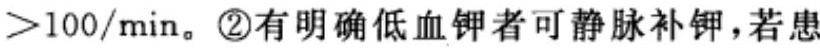
\includegraphics[max width=\textwidth, center]{2024_07_10_373f31b88d2bf633007bg-297}\\
者有阿-斯综合征的发展,由于酸中毒的存在常影响血钾水平的测定。(3)静注硫酸鿏。铗虽缩短 Q $\mathrm{T}$ 间期但可使复极趋向一致。剂量为 $2.5 \mathrm{~g}$ 稀释 $40 \mathrm{ml}$ 后缓慢静脉注射(约 $10 \mathrm{~min}$ )。对高血压、心室激惹不宜用异丙将上腺素者尤为适用。(4)先天性 Q-T 间期延长综合征伴反复尖端扭转室性心动过速发作者,为预防其发作可施左侧交感神经法切除及 $\beta$ 受体阻滞治疗。(5)禁用 I A、I C 及 III 类抗心律失常药物, 可试用 I B 类抗心律失常药及 II 类 $\beta$ 肾上腺素能受体阻滞药。

镁与室性心动过速亦有密切关系,当遇有下列情况时应考虑镁盐治疗: 低镁血症; 合并缺镁的低钾血症; 洋地黄中毒; 对常规治疗无效的顽固性室速。处理可采用 $20 \%$ 硫酸镁 $10 \sim 15 \mathrm{ml}$ 静脉缓注,维持则以 $20 \%$ 硫酸美 $20 \mathrm{ml}$ 加人到 $5 \%$ 莆菞糖液 $300 \mathrm{ml}$ 中静脉滴注较为安全。

\begin{enumerate}
  \setcounter{enumi}{1}
  \item 缓慢性心律失常急性缓慢性心律失常的发生机制可由于冲动起源昇常, 如自发性或心动过速中止后窦性停搏所致; 或因冲动传导异常。包括窉房、房室或希氏-浦肯野系统的传导阻满。当心率突然减慢至 $30 / \mathrm{min}$ 左右, 就可能导致严重的结果。当室率 $<50 / \mathrm{min}$, 或虽室率 $>50 / \mathrm{min}$ 但已有血流动力学干扰时, 应立即进行处理。\\
药物治疗主要用阿托品 $0.5 \sim 1 \mathrm{mg}$ 静脉注射,或异丙肾上腺素 $1 \mathrm{mg}$ 加人莆萄糖溶液 $250 \mathrm{ml}$ 内静脉滴注。紧急时可用异丙悄上腺素 $0.5 \sim 1 \mu \mathrm{g}$ 静脉注射。异丙肾上腺素适用于心率缓慢并伴有心缩无力的患者。完全性房室传导阻滞, 若阻滞部位在希氏或希氏束以下部位 (呈室性逸搏), 则只有异丙肾上腺素能提高心率, 而阿托品无效, 因为这些部位对抑制迷走神经张力不起反应。对病赎患者, 则无论阿托品或异丙将上腺素都不能有效地提高其窦性心律。因此, 对 III 度房室传导阻滞及病窦患者, 最好的治疗办法是心胜起搏。
\end{enumerate}

(张铁铮)

\section*{箱程 $\square$}
\section*{腹部外科手术的麻醉}
腹部疾病在临床上最为常见, 手术及麻醉的数量也最大。与其他手术的麻醉原则一样, 最重要的是保证患者安全、无痛及舒适, 此外还要保证手术的最佳操作条件, 包括良好的腹肌松驰, 避免腹腔神经反射等。麻醉前应根据患者病理生理改变及不同的伴随疾病, 积极调整治疗,改善全身状况, 提高对手术和麻醉的耐受性。

\section*{第一节 腹部疾病的病理生理}
\section*{(一)消化道穿孔}
胃肠道穿孔时胃肠内容物进人腹腔, 化学性刺激和细菌性感染引起腹膜炎。胆囊、胆道穿孔或损伤,胆汁进人腹岤造成化学性或感染性腹膜炎, 大量体液(主要来自血浆)渗人腹腔, 严重者可达全身血容量的 $30 \%$,需大量输血补液。

\section*{(ニ)消化道出血}
食管静脉曲张破裂、胃肠肿瘏或溃疡及出血性胃炎, 经内科治疗 $48 \mathrm{~h}$ 仍难以控制出血者, 常需急诊手术。麻醉前多伴有不同程度的失血性休克、严重贫血、低蛋白血症、肝功能不全及代谢性酸中毒等。胆道出血常由感染、肿痛或损伤引起, 病情复杂,既有大量失血, 又并发黄疸或感染,常常止血困难。

\section*{(三)消化道梗阻}
幽门梗阻时反复呕吐不能进食,造成脱水和营养障碍, 而且丢失大量胃酸, 引起碱中毒。肠梗阻时由于呕吐及大量体液向肠腔渗出, 造成细胞内外严重的水和电解质丧失, 血容量减少, 血液浓缩。此外由于肠壁通透性增加, 肠腔内细菌容易进人门脉及腹腔, 引起泛发性腹膜炎, 败血症性休克和代谢性酸中毒。胆总管或肝管梗阻, 胆汁逆流人血,引起一系列中毒症状,表现为皮肤瘙痒、抑郁疲倦、血压下降、心动过缓, 甚至昏迷。胆汁淤积使肝弥漫性增大, 肝功损害, 导致凝血功能障碍和低蛋白血症等。胆道梗阻若感染并发化脓性梗阻性胆管炎,易导致严重的感染性休克。

(四)急性胰腺炎

急性坏死性胰腺炎引起呕吐、肠麻㿎、胰腺出血和腹腔内大量渗出,造成严重的血容量不足。脂肪组织分解产生的脂肪酸与血中的锬离子㿝化作用引起低钙血症, 需要补充一定钙剂。此外脂肪组织分解还释放一种称为心肌抑制因子 (MDF) 的低分子肽类物质,抑制心肌收缩力, 加重休克。腃腺炎继发腹膜炎, 致使大量蛋白液渗人腹腔, 不仅影响腀肌活动,而且血浆渗透压降低,容易诱发肺间质水肿, 呼吸功能减退, 甚至发生急性呼吸謇迫综合征(ARDS)。肾功能障碍也是常见的并发症。

\section*{第二节 麻醉前准备}
\begin{enumerate}
  \item 对于急腹症患者,麻醉医师必须抓紧时间进行术前评估, 重点掌握全身状况、意识、体温、循环、呼吸、肝肾功能; 追问既往病史, 麻醉手术史、药物过敏史、禁食及禁饮时间。根据检查,选定麻醉方法和药物, 做好意外防治措施。

  \item 对并存血容量不足、脱水、血液浓缩、电解质及酸碱失衡或伴严重合并疾病以及继发病理生理改变者, 根据血常规、尿常规、血清电解质、血气分\\
析、出凝血时间、心电图及 X 线片等检查结果,进行重点处理或纠正。

  \item 对休克患者必须施行综合治疗, 待休克改善后再行麻醉。但有时由于病情发展迅速, 应考虑在治疗休克的同时紧急进行麻醉和手术,不能片面强调抗休克而延误病情。治疗休克应重点纠正血容量不足,改善微循环和维持血压。纠正电解质与酸碱失衡, 血压维持在 $80 \mathrm{mmHg}$ 以上, 血细胞比容在 $30 \%$ 以上。

  \item 门脉高压征患者必须检查肝功能和出凝血时间、凝血酶原时间等与凝血功能有关的检查。肝功能严重障碍、重度低蛋白血症者, 手术死亡率极高。术前应先改善全身状况,控制腹水,血浆白蛋白提高至 $25 \sim 39 \mathrm{~g} / \mathrm{L}$ 、血清胆红素降低在 $10 〜$ $15 \mathrm{mg} / \mathrm{L}$ 以下,凝血酶原活动度高于 $40 \% \sim 50 \%$ 再行手术为宜。

  \item 饱胃、肠梗阻、消化道穿孔、出血或弥漫性腹膜炎忠者, 麻醉前必须进行有效的胃肠惐压。

  \item 剧烈疼痛、恐惧和躁动不安必然促使儿茶酚胺释放, 加重微循环障碍, 促进休克发展, 故麻醉前应给小剂量的术前药, 但不能影响呼吸、循环和意识。

\end{enumerate}

\section*{第三节 一般腹部外科手术的麻醉处理}
腹部手术具有病种多样化, 病情轻重不一及并存疾病不同等特点,对麻醉方法与麻醉药物的选择, 需根据患者全身状况, 重要脏器损害程度, 手术部位和时间长短, 麻醉设备条件以及麻醉医师技术的熟练程度作综合考虑。

\section*{一、麻醉选择}
\section*{(一)局部浸润麻醉}
该方法简便易行, 对机体生理影响小,适用于腹壁、疝气、阑尾炎及输卵管结扎术等简单手术,也可用于严重休克、高度黄疸患者进行胆襄造瘘等急诊手术。但阻滞不易完善,肌松不满意,术野显露差,受到明显限制。

\section*{(二)连续硬膜外阻带麻醉、蛛网膜下腔阻滞麻醉和泰硬联合阻滞麻醉}
适用于中下腹、盆腔手术的麻醉, 其阻滞范围能包括手术所涉及的全部肌肉、内脏等神经支配。但对上腹部手术,难以完全阻断自主神经的脊㵦上行通路。而且可能产生一些严重并发症,对患者的循环、呼吸等方面也会产生一定的影响。因此必须做好充分的准备,备好急救设备,预防和及时发现循环、呼吸絮乱和药物毒性反应的发生。尤其是应用哌替啶、地西泮或咪达唑仑等辅助药后嗜睡的患者, 更应密切观察呼吸循环等生命体征。连续硬膜外阻滞麻醉适用于手术侵袭范围不大的胃、肠、胆道等择期手术,也可用于无休克和无低血容量的急腹症手术患者。保留硬膜外导管还可用于术后镇痛。但内脏牵拉反应较重, 为其不足。蛛网膜下隙阻滞麻醉适用于 $2 \sim 3 \mathrm{~h}$ 以内的下腹部、盆腔等手术。高平面阻滞对病人生理扰乱较大,且持续时间有限, 所以上腹部手术麻醉多选择连续硬膜外阻滞麻醉, 而不采用蛛网膜下隍阻滞麻醉。脊硬联合阻滞麻醉适用于下腹部、盆腔等手术。此种麻醉方法结合了蛛网膜下智阻滞和连续硬膜外阻滞的优点,起效快,麻醉效果确实、肌松驰良好,而且不受手术时间的限制,目前已广泛应用。

\section*{(三)全身麻醉}
全身麻醉在技术和设备条件充分满足的情况下,麻醇效果的满意率和可控性都优于硬膜外麻醉。全麻有利于术中呼吸、循环管理, 适合于比较复杂、侵袭范围广或长时间的手术, 以及伴有严重脱水, 低血容量或休克的急腹症患者手术,并能通过控制麻醉深度,维持病人循环和呼吸功能稳定。它是目前普外手术,尤其是中上腹部手术最常采用的麻醉方式。腹部手术患者并存冠心病、呼吸功能不全曾认为禁用全麻, 适合连续硬膜外阻滞麻醉。事实上高位硬膜外麻醉常限制呼吸肌运动, 不利于通气,而且内脏牵拉反射不能完全受到抑制,尤其一旦出现低血压, 冠状动脉灌注不足,易诱发心绞痛。相比之下, 全身麻醉可充分供氧, 保证通气, 改善冠脉血氧及维持呼吸功能。麻醉诱导及维持可选择对循环功能影响小的药物, 如依托咪酯、味达唑仑、芬太尼、肌松药及较低浓度的吸人麻醉药, 既保证患者安全又能满足手术要求。

\section*{(四)全身麻醉联合连续硬膜外阻滞}
目前有人主张全身麻醉联合连续硬膜外阻滞,其优点是综合两种麻醉方法的长处, 应激反应轻,血流动力学平稳, 减少全麻用药, 术后清醒快, 而且苏㤠期间有良好镇痛。术后还可实施患者硬膜外自控镇痛 (PCEA)。胸段高位硬膜外阻滞还能改善\\
冠脉血供,可使冠状动脉阻力下降 $20 \% \sim 25 \%$,血流量增加 $18 \%$ 。一项 Meta 分析表明胸段硬膜外阻滞能降低 $30 \%$ 的病死率和 $33 \%$ 的心肌梗死。因此, 全身麻醉联合胸段高位硬膜外阻滞对于冠心病患者实施腹部手术也许是最佳选择。但是要注意掌握硬膜外用药浓度和用量,避免低血压。

\section*{(五)术后疼痛治疗}
疼痛刺激可能引起血压增高、心动过速和心律失常, 严重时诱发心肌缺血和心肌梗死。对于腹部手术的患者, 疼痛限制咳嫩和深呼吸, 通气功能下降, 引起肺不张。疼痛引起的交感神经系统兴奋还抑制胃肠道功能,表现为术后胃肠绞痛、腹胀、恶心、呕吐等。良好的术后镇痛可改善患者精神状态, 降低心血管系统并发症, 㖪少肺内感染和呼吸衰竭发生率, 缓解疼痛引起的胃肠功能抑制, 促进病情恢复。传统的镇痛方式是单次静脉或肌内注射哌替啶或布桂䊅等镇痛药, 作用时间较短, 需要反复多次给药。目前国内外推崇的镇痛方式是患者自控镇痛 (PCA)。PCA包括静脉自控镇痛 (PCIA)和硬膜外自控镇痛 (PCEA) 两种方式。少数患者接受 PCIA 可能出现恶心、呕吐和腹胀, 部分老年患者还出现一过性烦躁和认知功能障碍。但是考虑到疼痛带来的危害, 还是利大于䌘。 PCEA 无疑是最佳选择, 硬膜外隍给予局麻药可阻断交感神经节前纤维, 支配胃肠道的迷走神经相对兴奋, 在提供有效镇痛的同时, 明显缩短肠道排气时间, 改善胃肠道功能, 而且不会引起上述精神症状。

\section*{二、麻醉要点}
\section*{(一)胃肠手术的麻醉要点}
术前尽可能纠正贫血、低蛋白血症、低血容量、电解质及酸諴平衡絮乱, 胃肠减压。饱胃患者急诊手术, 术前用药剂量应酌减, 以保留自主呼吸和保护性反射, 防止呕吐所致反流误吸, 全麻可考虑清醒插管。术中适量补液纠正低血容量和电解质酸䂸平衡亲乱。

\section*{(ニ)胆道手术的麻醉要点}
梗阻性黄病可使维生素 $\mathrm{K}$ 参与合成的凝血因子减少, 导致出凝血异常。麻醉前应给予维生素 K 治疗, 使凝血原时间恢复正常。黄㾝、胆道压力增高引起迷走神经张力增加, 术中易发生胆心反射和迷走一迷走反射, 心动过缓, 术前或术中给予阿托品可有预防和治疗作用。术前阿托品常规成人肌内注射 $0.5 \mathrm{mg}$, 伴有心动过缓患者可给予 $1.0 \mathrm{mg}$ 。胆绞痛者避免应用吗啡, 以免 Oddi 括约肌痉挛。全身情况差、反应迟钝的严重阻塞性黄疸患者, 镇静药和麻醉性镇痛药应慎用。

梗阻性黄㾝常伴肝功能损害, 应禁用对肝肾有损害的药物, 如氟烷、甲氧氟烷、大剂量吗啡等。恩氟烷、异氟烷、七氟烷或地氟烷亦有一过性肝损害的报道。

\section*{(三)胰腺手术的麻醉要点}
有肝功能障碍的患者禁用吗啡, 氯丙嗪等药物也应慎用。对病情复杂、手术时间长的胰腺手术患者多选用全身麻醉或全身麻醉联合连续硬膜外阻滞。对于危重患者可选择对循环抑制轻微的麻醉药进行麻醉诱导(如依托咪酯等)。

脥岛细胞面手术要防治肿面切除前血糖过低及肿面切除后血糖暂时性过高对机体的危害, 同时与术者密切配合, 不可盲目干预血糖, 影响术者对肿瘤切除与否的判断。

\section*{(四)肝手术的麻醉要点}
术前准备应先改善全身状况,控制腹水,提高血浆白蛋白至 $25 \sim 30 \mathrm{mg} / \mathrm{L}$ 、降低血清胆红索在 10〜 15mg/L 以下,凝血酶原活动度高于 $40 \%$ ~ $50 \%$ 等条件, 再行手术为宜。多数镇静、镇痛药皆需经肝代谢降解, 应减量使用。全身情况较差或有肝性脑病征兆的患者, 仅给予抗胆碱药 (阿托品或东茛若酳)。

左半肝或左肝外叶切除术可采用连续硬膜外阻滞, 但右半肝、右肝后叶或更广泛肔切除时, 为了使肝门能充分暴露和控制出血, 有时还需行胸腹联合切口,临床上多选择全身麻醉或全身麻醉联合连续硬膜外阻滞, 后者可减少全麻药对肝的不利影响。极少数患者应用氛烷麻醉后可出现肝损害, 表现为氮烷性肝炎,现多弃用。恩氟烷、异氟烷、七氧烷和地氛烷对肝胜毒性作用极小, 其中异氛烷最安全。总之, 禁用对肝有害的药物, 最大限度地减少麻醉性镇痛药和吸人麻醉药对肝功能的影响。

\section*{(五)门脉高压手术的麻醉要点}
门脉高压患者术前必须进行系统治疗,包括休息, 高糖、高蛋白及高维生素饮食, 输少量新鲜血或人体白蛋白液, 以改善贫血和低蛋白血症, 使血红蛋白达到 $80 \mathrm{~g} / \mathrm{L}$ 以上,血浆总蛋白和白蛋白分别达到 $60 \mathrm{~g} / \mathrm{L}$ 和 $30 \mathrm{~g} / \mathrm{L}$ 以上,同时输新鲜血还可纠正出血倾向。有出血倾向者可给予维生素 $\mathrm{K}$ 等止血药,以纠正出凝血时间和凝血酶原时间。如系肝细胞\\
合成第 $\mathrm{V}$ 因子功能低下所致, 麻醉前应输新鲜血或血浆。肝硬化腹水的总者常伴有水和电解质案乱,术前也需纠正。镇静镇痛药均在用内代谢, 门脉高压征时分解代谢延迟,可导致药效增强、作用时间延长,故应减量或避免应用。

肝损害时血熪蛋白量减少, 应用巴比妥类药时, 因分解代谢减缓, 使血内游离成分增加, 药效增强, 但睡眠量巴比妥类对肝尚无影响。氟哌利多、芬太尼虽在肝内代谢,但麻醉常用量尚不致发生肝损害, 可用于门脉高压征手术的麻醉, 但对严重用损害者应酌情减量。静脉麻醉药丙泊酚、氯胺酮、咪达唑仑则均可选用。麻醉性镇痛药瑞芬太尼不经肝内代谢, 舒芬太尼对血流动力学影响轻微, 均适于门脉高压征手术的麻醉。肝硬化患者的胆械酯酶活性减弱, 使用琥珀胆碱时,其作用可增强,易发生呼吸恢复延迟; 应用泮库滇㜞时可无影响。正常人筒箭毒碱可经肾和胆汁排泄,门脉高压征患者经胆汁排出减少,故慎用大量箭毒类药。酯类局麻药由血浆胆碱酯酶分解,酰胺类局麻药都在肝内代谢。由于血浆内胆碱酯酶均来自肝, 肝硬化患者应用局麻药可因其分解延缓,易于蓄积, 应避免大量使用。

\section*{(六)麻醉处理要点}
\begin{enumerate}
  \item 维持有效循环血量: 通过 ECG、血压、脉搏、 $\mathrm{SpO}_{2}$ 、中心静脉压、尿量等的监测,维持出人量平衡, 避免血容量不足或过多,预防低血压和右心功能不全, 维护肾功能。输液时不可大量使用乳酸钠林格液或生理盐水, 否则钠负荷增加可导致间质性肺水肿; 伴将功能损害者尤需避免。此外, 麻醉中可通过血气分析和电解质检查, 及时纠正水、电解质和酸碱失衡; 如有可能, 宜测定血浆及尿渗透浓度,有指导意义。

  \item 保持血浆蛋白量: 低蛋白血症患者麻醉时应将白蛋白提高到 $25 \mathrm{~g} / \mathrm{L}$ 以上,不足时应补充白蛋白,以维持血浆胶体渗透压和预防间质水肿。

  \item 维护血液氧输送能力: 须保持血容量、每搏量、血细胞比容、血红蛋白及氧离解曲线的正常。心功能正常者, 为保持有效循环血量, 宜使血细胞比容维持在 $30 \%$ 左右, 以降低血液黏滞度,保证最佳组织灌流。为确保氧的输送能力, 对贫血者可输浓缩红细胞。

  \item 补充凝血因子:麻醉前有出血倾向者,应输用新鲜血或血小板。缺乏由维生素 $\mathrm{K}$ 合成的凝血因子者, 可输给新鲜血浆。麻醉中一旦发生异常出血, 应即时查各项凝血功能, 针对性处理。

  \item 处理大量出血:门脉高压分流术中,出血量在 $2000 \mathrm{ml}$ 以上者,并非少见,可采用血液回收与成分输血,适量给予血浆代用品。输血、输液时应注意补充细胞外液、纠正代谢性酸中毒、充分供氧及适量补鿭。

  \item 保证镇痛完善,避免应激反应。

\end{enumerate}

\section*{第四节 腹腔镜检查和外科手术的麻醉}
腹腔镜手术对机体内环境影响小、减轻创伤、降低手术并发症的发生率和死亡率, 临床应用日益广泛。但是腹腔镜手术须在气腹状态下实施, 并将患者置于特殊体位,导致机体病理生理改变。某些腹腔镜手术还可能造成不易发现的内脏损伤, 以及失血量难以估计, 使得麻醉处理更加复杂, 麻醉风险增加。

\section*{一、手术过程对机体的生理影响}
\section*{(一)气腹对血流动力学的影响}
腹腔镜手术中引起血流动力学变化的因素包括气腹、患者体位、麻醉、高 $\mathrm{CO}_{2}$ 血症、迷走神经张力增加和心律失常。腹腔镜手术首先需建立气腹,气腹可使心排血量降低 $10 \% \sim 30 \%$ 。气腹压力低于 $10 \mathrm{mmHg}$ 时, 可压迫腹腔脏器使静脉回流量先短暂增加, 随着腹内压进一步升高下腔静脉受压,则静脉回流受阻, 血液潴留于下肢, 每搏量和心胜指数明显降低。这种现象在头低位时不太明显, 但头高位则出现明显的低血压。当气腹压力达 $15 \mathrm{mmHg}$ 时周围血管阻力增高, 左心室后负荷增加致使心肌耗氧量增高, 有发生心肌缺血、心肌梗死或充血性心力衰竭的潜在危险。另外,腹内压升高还可引起迷走神经反射使心率减慢。因此气腹压力不应超过 $20 \mathrm{mmHg}$ 。还应注意的是向腹腔充气时可引起心律失常, 如房室分离、结性心律、心动过缓和心脏停搏, 多发于开始充气使腹膜快速张开时, 这可能与刺激腹膜牵张感受器, 兴奋迷走反射有关。

\section*{(二)气腹对呼吸功能的影响 \\
 $\mathrm{CO}_{2}$ 气腹可使动脉血 $\mathrm{CO}_{2}$ 分压进行性升高, 建}
立气腹后 15~30min 达到高峰并维持下去。 $\mathrm{CO}_{2}$吸收率 $30 \mathrm{~min}$ 内可达 $70 \mathrm{ml} / \mathrm{min}$, 而 $30 \sim 75 \mathrm{~min}$ 达 $90 \mathrm{ml} / \mathrm{min}$ 。该吸收率受气腹压力的影响, 当腹膜毛细血管受压血流量减少时 $\mathrm{CO}_{2}$ 吸收量减少,但当气腹压下降腹膜毛细血管重新开放时 $\mathrm{CO}_{2}$ 吸收再度增加。由于腹空充气膈肌抬高, 肺受压造成肺顺应性降低, 气道压升高, 通气功能下降, 使体内 $\mathrm{CO}_{2}$ 排出域少。出现高 $\mathrm{CO}_{2}$ 血症、酸中毒, 甚至低氧血症。经腹膜吸收的 $\mathrm{CO}_{2}$ 一部分经肺排出, 而未能排出的 $\mathrm{CO}_{2}$ 渚留在体内骨聏各肌和骨等处, 术后逐渐排出,因此术后仍有持续高 $\mathrm{CO}_{2}$ 血症的危险。高 $\mathrm{CO}_{2}$ 刺激中枢神经系统, 增加交感活性, 引起心肌收缩力增加、心动过速和血压增高。另一方面, $\mathrm{CO}_{2}$ 的直接作用又可扩张末梢小动脉, 抑制心肌收缩力、诱发心律失常甚至心搏骚停。

\section*{(三)气腹对肾脏功能的影响}
$\mathrm{CO}_{2}$ 气腹可使尿量、将血流惐少和肾小球滤过率降至基础值的 $50 \%$ 以下, 明显低于开腹手术患者, 可能引起肾脏功能损害。气腹终止后尿量即迅速增加。

\section*{二、麻醉管理}
\section*{(一)麻醉选择}
\begin{enumerate}
  \item 全身麻醉 全身麻醉后进行气管插管和控制呼吸是最安全的麻醉选择。气管内插管人工通气可以充分供氧, 在不增加潮气量的前提下增加呼吸频率造成过度通气可增加 $\mathrm{CO}_{2}$ 排出, 乞管内插管还可以防止反流造成的误吸。麻醉诱导时避免胃胀气, 以减少穿刺针损伤胃的机会。应用肌松药可使气腹所致的腹腔内压相应降低, 既改善了手术野的显露,也可能减少气腹的不良反应。吸人麻醉药中异氟烷较为可取, 因其抑制心肌和诱发心律失常作用均较轻。氟烷在高 $\mathrm{CO}_{2}$ 血症时易诱发心律失常。 $\mathrm{N}_{2} \mathrm{O}$ 明显增加术后呕吐的发生率, 其应用尚有争议。适当加深麻醉有助于避免腹内压过高。手术期间迷走神经张力可能增加, 应当随时备好阿托品。与气管插管相比, 喉罩可以实施控制呼吸和准确的 $\mathrm{PET}_{\mathrm{ET}}^{2}$ 监测, 可以考虑作为气管插管的替代措施。但是腹脘镜手术中, 气腹和肺顺应性降低常使气道压超过 $20 \mathrm{cmH}_{2} \mathrm{O}$, 在这样的压力下喉罩对气道的密封性并不可靠。而且若发生反流, 可能引起误吸。

  \item 连续硬膜外阻滞麻醉 麻醉时应注意:

\end{enumerate}

(1)要消除上腹部刺激所致的不适常需阻滞平面高达 $T_{2} \sim T_{4}$, 这样易抑制心肌和减少静脉血回流, 加重气腹对血流动力学的不良作用、迷走神经介导的心率减慢。

(2) 辅助药物剂量若偏大时,可抑制气道防护反射, 加重高 $\mathrm{CO}_{2}$ 血症。

(3)硬膜外阻滞不能消除 $\mathrm{CO}_{2}$ 刺激膈肌所致的肩胛部疼痛,也可发生寒战。短时间的诊断性检查 (如原发性不陉的腹腔镜检查)也可采用局麻,但辅助镇痛药和镇静药剂量宜小, 以保留灵敏的气道反射,以免误吸和呼吸抑制。

\section*{(二)术中监测}
常用监测包括无创血压、心电图、脉搏血氧饱和度、气道压力、呼气末 $\mathrm{CO}_{2}$ 分压、TOF 和体温等。必要时放置导尿管, 减少手术损伤膀胱的机会, 改善术野显露, 监测尿量。心肺功能障碍者监测直接动脉压, 可以动态观察血压变化和方便血气分析。术中必须监测 $\mathrm{P}_{\mathrm{ET}} \mathrm{CO}_{2}$, 及时调整呼吸, 维持正常血乞状态。监测气道压, 及早发现腹内压过高。腹腔镜手术虽比开腹创伤小, 术后恢复快, 但术中对机体生理的影响却比开腹更为严重, 因此需要予以重视和妥善处理,以保证其安全性。

\section*{第五节 原位肝移植手术的麻醉处理}
\section*{一、肝硬化和门脉高压}
门静脉系统是腹腔脏器与肝毛细血管网之间的静脉系统。当门静脉压力 $>25 \mathrm{cmH}_{2} \mathrm{O}$ 时, 可表现一系列临床症状,统称门脉高压征。门脉高压的主要发病机制是由于肝硬化改变引起的肝血管阻力增高, 其次机体血管扩张和血容量增多也有一定关系。门脉高压征多伴有严重的肝功能障碍。主要病理生理改变为: (1) 肝硬化及肝损害; (2)高动力型血流动力学改变: 容量负荷及心脏负荷增加, 动静脉血氧分压差降低, 肺内动静脉短路和门、体静脉间分流; (3)出凝血功能改变: 有出血倾向和凝血障碍, 原因为纤维蛋白原缺乏、血小板减少、凝血酎原时间延长、第 V 因子缺乏、血浆纤溶蛋白活性增\\
强; (4)低蛋白血症、腹水、电解质案乱、钠和水潴留、低钾血症; (5) 脾功能立进; (6) 氮质血症、少尿、稀释性低钠、代谢性酸中毒和肝肾综合征。

\section*{二、麻醉前评估}
原位肝移植是肝功能衰竭惟一治疗途径, 某些肝及胆管肿瘤也为原位肝移植的适应证。处在终末期肝病的患者不仅存在严重肝功能障碍, 而且普遍存在心、肺、脑、肾等多器官损害,麻醉医师应该对患者全身各器官功能进行全面的评估。

肝疾病的患者可同时患有心腿疾病。大多数忠者需要进行超声心动图检查来确定是否有心胜疾病。具有心肌缺血可能的患者通常需要心导管检查, 通过冠状动脉造影来确定病变性质。严重冠心病患者一般不作为肝移植的候选人。严重主动脉瓣硬化是一个比较梀手的问题, 因为对于终末期肝病患者进行心脏手术是十分危险的。目前推崇的解决方法是在肝移植前, 利用介人瓣膜成形术扩大瓣膜口面积。在肝移植物稳定后, 可以考虑进行主动脉解置换。

末期朋病的肺病理改变主要包括肺动脉高压和肝肺综合征。肺动脉高压最好的诊断方法是超声心动图。如果结果显示有中至重度肺动脉高压,估计肺动脉 (PA) 收缩压在 $50 \mathrm{mmHg}$ 以上, 需要右心导管检查来确定疾病的严重程度。大量的病例报道及小规模的回顾性综述都证实肺动脉高压增加肝移植围术期风险。人们普遍认为平均肺动脉压力在 $50 \mathrm{mmHg}$ 以上是肝移植手术的绝对禁忌证。

肝肺综合征是低氧血症 (吸人室内空气时 $\mathrm{PaO}_{2}$ $<70 \mathrm{mmHg}$ 或 $\mathrm{P}_{\mathrm{A}} \mathrm{O}_{2}-\mathrm{PaO}_{2}$ 梯度差 $>20 \mathrm{mmHg}$ ) 合并肺内血管扩张。患者由卧位转为直立时血氧饱和度明显下降称为直立性低氧血症。直立性低氧血症是诊断肝肺综合征的重要依据。肝肺综合征曾一度被认为是肝移植的禁忌证。但如果在肺胜解剖结构改变前就进行肝移植手术, 肝肺综合征就有可能治愈。如果肝肺综合征很严重, 吸氧完全不能纠正时, 移植的风险就会明显增加。幸运的是, 大多数肝肺综合征患者都有不同程度的生理性 V/Q 失调, 增加了肔移植的安全性。

中枢神经系统改变往往表现为肝性脑病。肝性脑病的程度在患者之间变化很大。急性肝衰竭由于脑水肿可引起矧内高压。准确评价颅内高压的情况和神经系统功能十分重要, 因为顾内高压是肝移植的禁忌证。

肝病末期的患者多合并肾功不全。病因包括原发肾疾病, 急性忬小管坏死, 肝肾综合征。肝肾综合征发生于严重肝疾病, 分为两型: I 型进展迅速, 病死率高, 但是肔移植后肔功改善的同时, 肾功能也随之恢复; II 型较 I 型进展慢, 多发生于对利尿药抵抗的患者。

末期肝病患者还可能伴发内分泌絮乱,如莆萄糖耐量降低、继发性醛固酮增多症等。这类病人麻醉和手术的危险性极大,在麻醉药物及麻醉技术选择时要慎重考虑。

\section*{三、麻醉处理}
肝移植手术机体病理生理改变极为复杂, 维持术中循环稳定至关重要。维持有效循环血量的同时纠正酸碱离子案乱和凝血功能障碍, 注意重要胜器保护和保温等。

\section*{(一)麻醉方法}
肝移植均选择全身麻醉。麻醉药的选择以对肝毒性低, 不影响肝血流且有利于维持患者循环功能、组织氧合及内环境稳定为原则。应用对肝肾功能影响小的静脉麻醉药诱导, 如: 咪达唑仑、依托咪酯、丙泊酚、硫喷妥钠等, 同样各种阿片类药物如芬太尼、舒芬太尼、阿芬太尼、瑞芬太尼均可用于肝移植。瑞芬太尼不经肝内代谢, 舒芬太尼对血流动力学影响轻微。肌松药阿曲库轱或顺式阿曲库轱、维库溑轱或琥珀胆碱均可应用, 但代谢产物在无肝期仍有排泄延迟。所有的吸人麻醉药都可用于肝移植。异氮烷和地氛烷最常用,尤其是异氟烷经体内分解代谢仅为 $0.17 \%$,对肔移植麻醉更为有利。避免应用肝毒性的氛烷或肾毒性的甲氧氟烷。氧化亚氮因能引起周肠道胀气影响手术操作, 且门脉系统开放状态或静脉旁路循环过程中有发生气检的危险, 应避免应用。

\section*{(ニ)新肝前期处理}
新肝前期是指诱导开始到移植肝血循环恢复再灌注,包括无肝前期和无肝期。

\begin{enumerate}
  \item 麻醉评导及准备阶段 关键在于平稳的麻醉诱导及各种必要监测。监测包括心电图、上肢动脉压、Swan-Ganz 导管、中心静脉压、脉搏血氧饱和度, $\mathrm{P}_{\mathrm{ET}} \mathrm{CO}_{2}$ 、直肠和鼻咽温及尿量连续监测、持续有创动脉穿刺 (桡动脉)以备术中间断进行血气分析、电解质及酸碱、血糖测定及整套凝血功能测定等。为保证术中输血,至少开放两条大的静脉通道,多\\
在颈内、外静脉或肘部静脉置人 $16 \sim 18$ 号导管。在麻醉诱导后开始应用抗生素, 以便术中保持一定的血药浓度。

  \item 无肝前期 失血量可能很大, 麻醉医师的重要任务是维持有效血容量和纠正大量输血引起的生理紊乱, 此期持续 $4 \sim 6 \mathrm{~h}$ 。由于大量失血, 分解代谢的酸性产物聚积, 缺血的朋内释放大量 $\mathrm{K}^{+}$及 $\mathrm{H}^{+}$, 血 $\mathrm{K}^{+} 、 \mathrm{H}^{+}$持续升高, 血流动力学波动很大。大量输人库血又加重了上述生理紊乱,而且发生严重的低䥻血症。快速输血补液的同时要及时纠正酸碱平衡离子紊乱。每输血 $1000 \mathrm{ml}$ 静脉滴人 $5 \%$ 碳酸氢钠 $30 \mathrm{ml}$ 及 $1 \%$ 氯化钲 $10 \mathrm{ml}$ 。应用自体血回输可大大减少输库血带来的并发症。由于大量快速输血补液, 体温开始下降, 因此手术室温度应保持在 $20 \sim 22^{\circ} \mathrm{C}$, 手术台设置保温毯, 输血补液均需加温。保持体温在 $34^{\circ} \mathrm{C}$ 以上, 避免体温过低所致的心律失常。还应注意处理凝血功能紊乱。多数患者术前已有凝血功能紊乱, 大量出血及输血进一步加重。应及早处理, 输当天新鲜血、血浆、血小板和凝血因子。

  \item 无肝期 此期一般持续 $1 \sim 2 \mathrm{~h}$ 。血 $\mathrm{K}^{+}$变化不明显,酸中毒进一步加重。在阻断门静脉和下腔静脉时心排血量急剧下降 $>50 \%$ 。目前多采用静静脉转流, 将下腔静脉及门静脉血转至腋静脉, 避免了回心血量骤减所致的血压剧降以及血液淤滞带来的不良效应和肾损害。但这样却增加了气检、血栓㭲塞的可能性, 而且散热增多造成体温进一步下降。随着手术技术改进, 无肝期的缩短, 旁路技术的优点越来越有限。此期要注意保护肾功能, 在应用利尿药之前,要先合理补充血容量。为维持尿量,可给多巴胺 $2 \mu \mathrm{g} /(\mathrm{kg} \cdot \mathrm{min})$, 甘露醇 $1.0 \mathrm{~g} / \mathrm{kg}$和呋塞米。

\end{enumerate}

\section*{(三)新肝后期处理}
新肝移植肝后血循环再灌注期是整个肝移植过程中最危险的时期。此期可发生低体温、低血压、高血钾、酸血症及凝血功能异常。外科医师与麻醉医师之间的交流对于再灌注前的准备是十分重要的。下腔静脉再灌注过程中, 血流动力学变化不大。开放肝动脉时, 通常也没有血流动力的明显改变。但门静脉再灌注可引起再篧注综合征, 表现为一过性的严重低血压、心动过缓、外周血管阻力和心肌收缩力下降以及肺血管阻力增加。再灌前给予碳酸氢钠防治酸血症, 但不可过度。在松开门脉钳夹同时给予 $500 \mathrm{mg}$ 氯化漹来拮抗钾离子对心脏的作用。在再灌注前后及时行血气分析, 给予胰岛素和莆萄糖降低血钾,并保证尿量。如果心电图 $\mathrm{T}$ 波高尖,要重复进行上述的治疗。再灌注时应备好利多卡因、阿托品以及去甲悄上腺素, 以免发生心律失常或严重的低血压。为了纠正凝血功能异常,可用鱼精蛋白中和供体肝残留的肝素。再価注后可发生一过性高血糖,一般无需处理,但持续高于 $12 \mathrm{mmol} / \mathrm{L}$ 时可给胰岛素。

(四)术后处理

术后将患者送人监护室继续机械通气和液体管理。术后多需机械通气 $24 \mathrm{~h}$, 由于肝功能恢复,术中输血等因素所致酸性产物可经代谢发生代谢性碱中毒,可使 $\mathrm{PaCO}_{2}$ 维持相对高水平。

(马 虹)

\section*{籍覀}
\section*{泌尿外科手术的麻醉}
泌尿外科手术的麻醉占手术麻醉量的 $10 \%$ 〜 $20 \%$ 。接受该类手术的患者年龄跨度大, 但多数是高龄患者, 患者并发症多, 且常常伴有肾功能损害。泌尿外科手术常常需要特殊的体位 (如截石位), 或侧卧位手术床呈屈曲状并抬高腰部使肾脏抬高, 这些体位都会对患者的生理功能特别是循环呼吸功能产生明显影响。手术常常使用一些灌洗液, 也会给患者带来一些特有的生理功能紊乱, 产生某些严重的并发症(如肺水肿), 经前列腺电切(TURP) 综合征等。故而, 我们在手术麻醉的过程中, 要注意术前患者脏器功能的评估, 把握泌尿外科手术的特点, 选择合适的麻醉方法, 积极做好术中的循环呼吸管理和肝将功能维护, 让患者安全舒适地度过围术期。

\section*{第一节 膀胱镜检查和输尿管逆行造影的麻醉}
膀脱镜检查和输尿管逆行造影可诊断和治疗患者的肾、输尿管、膀胱、前列腺和尿道等上下泌尿道的各种疾患,包括血尿、反复的泌尿系的感染、尿路结石、尿路梗阻和泌尿系的肿面等。

手术多采用截石位, 截石位安置不当可造成医源性损伤, 出现皮肤肌肉或神经受压牵拉受损。截石位对生理功能也会产生明显影响, 表现为功能残气量的减少, 患者易出现肺不张和低氧血症, 头低脚高 $>30^{\circ}$ 的屈氏位 (Trendelenburg position) 可加重这种影响; 下肢抬高促进静脉回流, 可诱发充血性心力衰竭, 下肢抬高后血压往往升高, 但心排血量无明显变化, 抬高的下肢放平因静脉回流减少容易导致血压降低, 区域阻滞麻醉和全身麻醉引起的血管扩张可加重血压下降, 故在下肢放平时应立即测量血压。

手术常使用灌洗液以扩张尿路, 冲洗掉手术产生的血液、组织和结石等, 常用的灌洗液包括: 电解质液, 如生理盐水和乳酸林格液, 价格便宜且患者易耐受, 但是导电, 可适用于不使用电刀的单纯诊断性检查; 蒸馏水, 不导电且价格便宜, 但大量吸收可致低钠血症、水中雔和溶血, 仅适用于短小且出血少的手术如经尿道膀胱肿面切除术; 非离子化溶质近似等张液, 如 $1.5 \%$ 甘氨酸溶液, 或 $2.7 \%$ 山梨醇和 $0.54 \%$ 甘露醇混合液等, 具有相对便宜、可视度好和不导电等特点, 由于这些溶液都是低渗液,仍有大量吸收产生低钠血症的风险, 不过比蒸馏水低。

由于有以上体位和手术中处置的特点, 麻醉医生应注意术中管理, 小心对症处理。

麻醉方式应根据患者的年龄、性别和手术种类来选择。小儿常使用全身麻醉; 女性由于尿道短,在一些短时间诊断性操作时可使用利多卡因凝胶表面麻醉, 或表麻复合镇静, 在活检、烧灼及输尿管置管等较长时间手术操作时多使用区域阻滞麻醉或全身麻醉。男性患者即使仅通过膀胱镜行诊断性操作, 虽然有一些医院对年轻男性患者使用表面麻醉, 原则上仍以区域阻滞麻醉或全身麻醉为宜。

\begin{enumerate}
  \item 全身麻醉 由于手术时间短 $(15 \sim 25 \mathrm{~min})$,多数膀胱镜手术安排在门诊, 适合于门诊手术的任何麻醉方式都可使用。使用全身麻醉时, 对药物宜选揕起效及苏醒快, 作用时间短的药物, 静脉麻醉药可选丙泊酚、芬太尼、瑞芬太尼等, 短效肌松药如罗库渲轱、维库溪轱、顺阿曲库轱等, 吸人麻醉药可选用七氧烷、地気烷等; 可使用喉罩; 对肥胖、高龄和肺功能储备不良者在采用截石位和屈氏位时应严密监测氧饱和度和血压。

  \item 区域阻滞麻醉硬膜外麻醉或蛛网膜下隙阻滞麻醉均可,但是,蛛网膜下瑄麻醉起效快,阻滞完善,多数麻醉医生选择蛛网膜下隙麻醉。区域阻滞麻醉感觉阻滞平面达到 $\mathrm{T}_{10}$ 可满足大部分膀胱镜手术的麻醉。对手术时间超过 $30 \mathrm{~min}$, 以及高龄高危患者,蛛网膜下腔麻醉都适宜。 $0.5 \%$ 重比重或等比重布比卡因 $3 \mathrm{ml}$ (或 $0.75 \%$ 布比卡因 $2 \mathrm{ml}$ )通常阻滞平面可达 $\mathrm{T}_{10}$, 可满足多数手术。除非阻滞平面不够,否则不需将患者倾斜为头低脚高位。单次布比卡因或罗哌卡因 $(0.25 \% \sim 0.5 \%)$ 骶管内阻滞麻醉,对循环影响小,术后恢复快,对手术时间短,手术操作小的患者,特别是老年患者常常采用。

\end{enumerate}

\section*{第二节 前列腺手术的麻醉}
\section*{一、经腹前列腺手术的麻醉}
切除肥大增生的前列腺组织的手术方式很多,包括经尿道前列腺切除 (TURP)、耻骨上前列腺切除、经会阴前列腺切除、耻骨后前列腺切除以及腹腔镜前列腺切除。一般前列腺重量在 $40 \sim 50 \mathrm{~g}$ 以下的多选择经尿道切除,当前列腺体积超过 $80 \mathrm{~g}$ 时才选用开放性手术。对于前列腺痣,可选用腹腔镜前列腺切除加盆腔淋巴结清扫、根治性耻骨后前列腺切除和双侧罯丸切除术。经腹前列腺手术一般针对体积大于 $80 \mathrm{~g}$ 的前列腺增生和前列腺癌手术,包括腹腔镜手术和经耻骨后直视下和经下腹部切开直视下开放手术。

行前列腺手术的患者一般高龄者多,多数患者合并有心脏血管和呼吸系统疾患以及肾功能不全,故而在手术前应仔细评估患者的并发症,把握患者手术的风险,做好术前准备并制定好手术麻醉方案。

\begin{enumerate}
  \item 腹腔镜手术 一般使用气管内插管全身麻醉。该手术一般用来行根治性前列腺切除,与其他腹腔镜手术的区别在于。
\end{enumerate}

(1)手术中为了充分暴露,采用更低的头低脚高屈氏位(>30度)。

(2)腹膜后腔镜人路,二氧化碳的吸收更明显。

(3)由于手术时间长,术中采用屈氏位,内脏牵拉操作多,要随时调节患者的呼吸参数。

(4)为防止肠胀气, 尽量不使用氧化亚氮。

\begin{enumerate}
  \setcounter{enumi}{1}
  \item 经耻骨后和经下腹切开直视手术可使用全身麻醉,也可使用区域阻滞麻醉,或二者同时采用,区域阻滞的感觉阻滞平面达到 $\mathrm{T}_{6}$ 就可满足手术的需要,区域阻滞的硬膜外置管可行术后硬膜外镇痛。全身麻醉和区域阻滞麻醉相比,手术失血量和围术期死亡率相似。因为盆腔淋巴结清扫对盆腔静脉的破坏易导致静脉血栓的形成,使用硬膜外麻醉和术后镇痛可能会减少术后深静脉血栓,但是这种效应往往被术后常规应用华法林、低分子肝素等抗凝治疗所掩盖,并且抗凝治疗还增加了硬膜外血肿的危险。术中应注意:
\end{enumerate}

(1)失血量可能较大,应做好大量失血的准备。如(1)留置粗的静脉套管针; (2)做好保温措施, 如使用血液加温仪,加温毯等; (3)对前列腺癌的经下腹切开直视手术一般常规应行中心静脉穿刺和动脉穿刺置管,特别对合并心血管疾患的患者更应如此,中心静脉置管可快速输血输液并行中心静脉压测定,动脉置管可以有创直接测定动脉压并随时抽血样测血气; (4)术前做好至少 4 个单位的交叉配血,确保库血随时取用。

可行控制性降压麻醉配合手术,以减少手术出血。如果预期出血量大,也可使用自体血回收技术。

影响出血的因素包括: 患者体位、盆腔解剖和前列腺大小等。

(2)术者常静脉注射 $1 \%$ 亚甲蓝作诊断性染色,可能会导致血压下降和短暂的脉搏血氧饱和度下降 $\left(\mathrm{SpO}_{2}\right.$ 低于 $65 \%$,时间持续 $\left.10 \sim 70 \mathrm{~s}\right)$,有些外科医生要求静脉注射靛胭脂染色,因其为 $\alpha$ 肾上腺能激动剂, 可能会引起血压的升高。

\section*{二、经尿道前列腺切除术的麻醉}
经尿道前列腺切除术 (transurethral resection of the prostate, TURP), 是一种在膀胱镜明视下使用环状电极切除前列腺组织的术式。一般用来切除增生在 40〜 50g 的前列腺组织。

麻醉一般采用硬膜外麻醉或蛛网膜下腔阻滞麻醉,只要平面达到 $\mathrm{T}_{10}$ 即可提供满意的手术条件。骶管阻滞麻醉因为血流动力学稳定, 常应用于高危的前列腺手术患者。与全麻相比,区域阻滞麻醉的交感神经阻滞能减少术后深静脉血栓的发生风险,最近的研究表明区域阻滞麻醉能降低术后高凝状\\
态, 维持正常的凝血和血小板功能。区域阻滞麻醉还有不易掩盖 TURP 综合征和膀胱穿孔的症状和体征, 以及降低术后即刻对镇痛的要求的优点。但是对前列腺痛患者伴背痛的, 因有椎骨转移的可能, 禁忌行椎管内麻醉。因行 TURP 手术者常常年龄较大, 手术时可能意识不清或耳堑, 没有办法配合, 这时也不能选用椎管内麻醉。气管内麻醉是上述椎管内麻醉不宜时的良好选择, 特别是对很胖和有反流病史的病人。目前尚无研究表明这两种麻醉方法在手术失血、术后认知功能和死亡率上存在差别。

TURP 手术的患者, 由于有时可能需要快速输血输液, 因此需要留置较粗 (16G) 的静脉套管针, 并且可能需要加温输血输液。

TURP 手术可能会产生一些并发症 (下述), 术中应密切监护患者, 对症处理, 保证患者安全度过围术期。

\section*{三、经尿道前列腺切除术的并发症及处理}
前列腺由 4 个紧密相连的完整区域组成, 分前区、外周区、中央区和前列腺前区。所有 4 个区都被包在一个包膜里。前列腺组织血供丰富, 动脉和静脉穿过前列腺包膜, 在腺体内分支, 静脉突邻近包膜, 并且比较大。早在 40 岁, 前列腺前叶的组织就可能开始结节增生, 增生结节可引起尿道梗阻,需要行 TURP 手术切除增生组织。TURP 手术时尽可能切除前列腺组织, 但需保留前列腺包膜, 如果包膜损伤, 大量的灌洗液就可能吸收人血液循环、前列腺周围间隙或腹膜后间陌。

因前列腺组织的组织学特点和大量使用灌洗液, 采用 TURP 手术可能发生一系列并发症, 包括出血、TURP 综合征、膀腅穿孔、低体温、败血症和播散性血管内凝血 (DIC) 等。有报道与 TURP 手术有关的 $30 \mathrm{~d}$ 死亡率为 $0.2 \% \sim 0.8 \%$ 。

\begin{enumerate}
  \item 出血和凝血异常 因增生的前列腺组织血供丰富, TURP 时出血常见,出血量变化较大, 为 200 2000ml, 因和冲洗液混合, 很难估计。虽然已建立依赖切除时间 (2 $5 \mathrm{ml} / \mathrm{min})$ 和切除组织大小 $(20 \sim 50 \mathrm{ml} / \mathrm{g})$ 的估计失血量方法, 但是并不可靠, 且是粗略估计。密切监测患者的生命体征和检测血红蛋白含量变化有助于评估失血情况。
\end{enumerate}

TURP 出血常较易控制, 但是如果损伤静脉窦则出血较多,难以控制, 如果出血不止,应尽快结束手术, 通过尿道放置 Foley 尿管人膀胱压迫止血,\\
Foley 尿管的球蓑产生的侧壁压力可以㖪少出血。因前列腺组织富含肾上腺素受体, 因此使用肾上腺素受体激动药如肾上腺索等可以减少出血。使用区域阻滞麻醉适当降低血压也有助于减少出血。

TURP术后异常出血发生率很低, $<1 \%$ 。原因不明,一种观点认为是血纤溶酶引起的全身纤溶有关, 也有认为是纤溶是继发于富含促凝血酶原激酶的前列腺组织切除时局部吸收引起的 DIC。 TURP 手术中灌洗液也可造成凝血因子的稀释, 少数前列腺癌患者可能因释放纤溶酶样的肿面因子引起纤溶元进。手术中出血不易控制应考虑凝血异常, 但凝血异常的确诊需依赖实验室检查的结果。如果怀疑纤溶元进, 可以静脉使用氨基已酸,第一小时 $4 \sim 5 \mathrm{~g}$, 以后每小时 $1 \mathrm{~g} / \mathrm{h}$ 静脉滴注。DIC 的治疗可使用肝素、凝血因子和血小板等。

\begin{enumerate}
  \setcounter{enumi}{1}
  \item TURP 综合征 TURP 手术大量使用灌洗液(种类如前述,一般常用 $1.5 \%$ 的甘氨酸溶液冲洗)。TURP 手术中前列腺组织的静脉突开放可使大量的灌洗液吸收人血。大量液体 $(>2 \mathrm{~L})$ 吸收后导致的一系列症状体征被命名为 TURP 综合征。
\end{enumerate}

正常情况下, 灌洗液以约 $20 \mathrm{ml} / \mathrm{min}$ 的速度被吸收, 患者的平均吸收总量是 $1 \sim 1.5 \mathrm{~L}$, 但也有高达 4 5L 的记录, 临床上精确估计吸收量几乎是不可能的, 其吸收量取决于下列因素。

(1)灌注压: 灌洗液袋应在达到适当流量条件下尽可能保持低位, 通常高度为 $60 \sim 70 \mathrm{~cm}$, 不要超过 $100 \mathrm{~cm}$ 。

(2)静脉压。如果患者存在低血容量或低血压, 则会吸收更多的灌洗液。

(3)手术持续时间/前列腺大小。手术时间 $>$ $1 \mathrm{~h}$ 或前列腺重量超过 $50 \mathrm{~g}$ 时, TURP 综合征更易出现。

(4)失血量。失血量大预示有大量的静脉突开放。

TURP 综合征的表现见表 3-5-1。

表 3-5-1 TURP 综合征的表现

\begin{center}
\begin{tabular}{|c|c|}
\hline
低钠血症 & 溶血 \\
\hline
血浆渗透压降低 & 电解质新乱 \\
\hline
液体过荷 & 高甘氨酸血症(甘氨覀) \\
\hline
充血性心衰 & 血氨升高(甘氨酸) \\
\hline
肺水肿 & 血棈升高(山梨醇) \\
\hline
低血压 & 循环容量扩张 (甘露醇) \\
\hline
\end{tabular}
\end{center}

导致脑水肿的水中毒和稀释性低钠血症可引起神经系统的临床表现,如术中或术后的头痛、烦躁、精神错乱、感觉器官异常、惊嚴和意识模糊等。容量超负荷和低钠血症可引起心血管功能的异常,病人表现为发绀、呼吸困难、心律失常、低血压, 肺水肿、充血性心力衰竭、甚至呼吸心搏骤停等。灌洗液溶质的吸收同样可以带来毒性表现,如甘氨酸溶液冲洗可导致高甘氨酸血症,表现为循环抑制和中枢神经系统毒性,山梨醇或右旋糖酎的吸收可导致血糖升高, 甘露醇吸收可带来扩容效果, 导致容量过荷。高血压和心动过缓见于急性高血容量时。对全麻病人, 心动过速和高血压可能是唯一的线索。TURP 综合征的治疗依赖早期诊断。

治疗措施基于症状的严重程度。治疗原则是将过多的水排出,防止低氧血症和组织灌注不良。多数患者通过限制液体人量和使用㩯利尿药 (如呋塞米)即可。

稀释性低钠血症 (血钠 $<120 \mathrm{mmol} / \mathrm{L}$ ) 出现惊曆和昏迷者需要使用高张盐水 $(3 \% \mathrm{NaCl})$, 目标是将血.钠纠正到 $125 \sim 130 \mathrm{mmol} / \mathrm{L}$ 。每升高 $1 \mathrm{mmol} / \mathrm{L} \mathrm{Na}^{+}$需要 $3 \% \mathrm{NaCl}$ 的量为: 身体含水总量 $\times 2$ 。如一个正常 $70 \mathrm{~kg}$ 重的男性含水总量约为体重的 $60 \%$,故为 $70 \times 0.6 \times 2=84 \mathrm{ml}$ 。

纠正血钠的速率, 第 1 个 $24 \mathrm{~h}$ 内不应超过 $12 \mathrm{mmol} / \mathrm{L}$ 。高张盐水的滴速应小于 $100 \mathrm{ml} / \mathrm{h}$ 。应经常查血钠值以指导治疗。

控制惊厥可使用小剂量的咪达㟇仑 2〜4mg、地西泮 3〜5mg 或硫喷妥钠 $50 \sim 100 \mathrm{mg}$ 。如果㤩者意识不清,在患者意识恢复前可考虑气管插管以防误吸。\\
3. 膀胱穿孔TURP 手术膀胱穿孔的发生率约为 $1 \%$ 。一般由膀胱镜操作失误直接穿破膀胱或灌洗液引起膀胱过度膨胀所致。腹膜外穿孔多见,灌洗液回流不畅应怀疑膀胱穿孔,清醒的患者表现为恶心、大汗和下腹部疼痛。腹膜外较大的穿孔和腹膜内穿孔则表现为突然出现不明原因的血压改变,清醒的忠者诉腹部疼痛。不管采用何种麻醉方式,TURP 手术中突然出现不明原因的血压下降,尤其伴心动过缓时, 应考虑膀胱穿孔的可能。

\begin{enumerate}
  \setcounter{enumi}{3}
  \item 低体温手术中使用与室温相同的大量灌洗液时可导致忠者热量散失引起低体温。低体温引起的术后寒战可引起凝血块脱落,加重术后出血。为防止低体温的发生,如果需大量灌洗液冲洗时,应该将灌洗液预热至体温水平。

  \item 败血症前列腺组织易滋生细菌并迁延形成慢性感染。手术操作以及静脉窦的开放可使潜伏在腺体组织的细菌直接人血。经尿道前列腺手术术后的菌血症并不少见,其中 $6 \% \sim 7 \%$ 可发生败血症或感染性休克。通常菌血症没有症状,败血症时,患者表现为寒战、发热、心动过速, 严重病例可导致心动过缓、低血压甚至循环衰竭,其死亡率为 $25 \% \sim 75 \%$ 。术前预防性使用抗生素可降低菌血症或败血症的发生。

  \item 心肌梗死和肺水肿 也是 TURP 手术的并发症之一。因为行 TURP 手术的患者年龄较大,常合并心血管疾病, 如果手术中吸收灌洗液过多,可引起心脏前负荷的增加, 引起左心衰肺水肿, 甚至诱发心肌梗死。因而术前对患者心肺情况详细周密的术前检查和评估是非常必要的。

\end{enumerate}

\section*{第三节 肾移植手术的麻醉}
终末期肾疾病(end-stage renal disease, ESRD) 是指如果没有血液透析将有致命危险的多器官功能衰竭的临床综合征。长期透析虽可有效延长终末期肾病患者的生命, 但有大量与之相关的发病率和病死率。肾移植是治疗该病最重要的方法之一,过去 10 年来, 由于在免疫抑制治疗、供体器官获取、患者术前准备及外科技术等方面取得了一系列的进步, 肾移植患者的存活率和生活质量有了很大的提高。研究表明, 终末期肾病进行肾移植无论是存活率还是成本收益比均优于长期透析。因此, 肾移植已成为终末期肾病的首选治疗, 其发展只是受限于合适供体器官的供应不足。由于长期依赖透析的患者的左心室功能容易恶化,心瓣膜病变也进展迅速,因此这类病人应尽早进行肾移植。

自 1954 年 12 月记载情移植手术的麻醉方法以来,该手术的麻醉方法已有了很大的改变。从最早的脊麻到现今常用的全身麻醉和硬膜外麻醉,麻醉方式和管理方法的日渐成熟使肾移植的安全性得到了很大的提高。肾移植手术的麻醉之所以具有挑战性是因为终末期肾脏疾病经常引起其他器官功能障碍, 并使我们难以预测患者对麻醉药物和\\
麻醉方法的反应。另外, 由于这些患者常伴有多种并发症,容易发生心脏意外事件和其他围术期并发症。

\section*{一、终末期肾病的病理生理}
肾主要功能为调节机体液体容量、电解质和酸碱平衡以及血红蛋白浓度。它可以滤过和排泄血液中的有毒物质和药物。慢性肾衰竭引起肾小球滤过率和尿量减少, 影响整个机体多个器官系统的功能。

终末期肾病患者由于有功能的肾单位太少, 无法浓缩稀释尿液, 不能保存或排泄过多的水,从而使细胞外液量增加, 导致内环境紊乱。其临床表现之一是低钠血症, 它是由于细胞外液量增加导致的尿钠过多引起的。而且, 慢性肾衰竭患者限制盐的掫人和体内水负荷增加都可以导致低钠血症。由于 $\mathrm{K}^{+}$的清除率惐慢,可发生致命性的高钟血症。在这类患者中, 其他离子如钙、镁、磷的代谢絮乱也十分常见。终末期肾病忠者由于不能排泄可滴定酸导致的代谢性酸中毒可分为两种类型: 高血氯一正常阴离子间隙型酸中毒和高血氯-高阴离子间陁型酸中毒。这两种酸中毒都是内源性酸负荷增加所导致。

心血管疾病是引起终末期怪病患者死亡的首要原因。尿毒症患者的心血管并发症主要是由血容量增加、高将素-血管紧张素水平、自主神经兴奋性增加、酸中毒以及电解质紊乱等原因造成。这类患者中高血压十分常见。高血压、高血容量、酸中毒、贫血、透析引起的大量动静脉搂等可导致心胜向心性肥大、心功能不全和充血性心力衰竭。尿毒症和血液透析可引起心包炎。

慢性肾衰竭所导致的呼吸系统并发症主要表现为肺水肿和通气的改变。血容量过多、充血性心力衰竭、血浆胶体渗透压降低和肺毛细血管渗透性增加都是导致急性肺水肿的原因。慢性代谢性酸中毒可引起过度通气,而肺水增多和肺的顺应性下降也可以刺邀通气。

尿毒症可引起胃排空延迟, 这在腹透和血透患者中无明显差异。所以,所有拟行肾移植的患者都应当作饱胃对待。胃排空延迟可通过给予甲氧氯普胺或透析加以改善。慢性肾衰竭常见的消化系统症状还包括厌食、恶心、呕吐和呢逆。

尿毒症也可引起中枢神经系统功能紊乱, 表现为喍睡、记忆力和注意力减退、震熼、肌疼挛及疾痻等。自主神经功能紊乱主要表现为交感神经兴奋性增强或减弱、压力感受器的反应性减弱或透析所导致的低血压。

终末期肾病患者继发性贫血的主要原因包括促红素生成减少、红细胞破坏增加、胃肠道进行性失血等。肾衰竭患者常有出血倾向, 主要原因是尿毒症引起的血小板功能不良。血小板功能不良主要为血小板质的缺陷, 表现在尿毒症患者血液中琥珀酸胍基复合物蓄积。透析可加重血小板功能障碍, 从而加重出血。

\section*{二、活体肾供体的麻醉}
活体供体的紧移植在最近数年迅速增加。供体大多数是健康成人, 因为任何系统性疾病都增加全身麻醉和手术的风险,增加伦理上的冲突。因为活体供体围术期严重并发症发生率较低, 且死亡极少, 而且长期随访研究表明并不增加供体肾衰竭或高血压的危险, 所以已得到广泛认可。评估供体器官质量的指标包括各种与移植成功率相关的因素,如供体年龄、是否长期患高血压和糖尿病、冷缺血保存时间等。

腹腔镜手术在减少术后疼痛、缩短住院时间、加快术后康复等方面均有优势。为增加肾脏捐献者的满意度,这一手术方式将越来越多地被采用。供体和受体的手术时机需协调以使肾缺血时间最短。捐献时双肾都可以选用,但通常更愿意选择左肾, 因为左肾手术更容易显露且血管较长。患者取侧卧位, 手术床屈曲状使将脏抬高。手术第一步是游离结肠, 然后是肾脏上极, 接下来辩别并分离输尿管、肾静脉和肾动脉, 然后分离肾上腺静脉。在完全游离肾䏢并钳夹血管后,可以在腹腔镜直视下经脐周或脐下小切口取出将脏。不同手术者手术方式可能不同,因此与手术医生的交流非常重要。

一般采用全身麻醉, 使用 G16 留置针开放一至两条大的周围静脉, 即可满足手术需要。以无创监测为主, 一般不需要有创监测。为保证充分的尿量, 即使大多数病例出血很少, 输液量也较大 $[10 \sim$ $20 \mathrm{ml} /(\mathrm{kg} \cdot \mathrm{h})]$ 。对这种患者输人何种液体更好尚无定论。为维持足够的尿量, 手术医师可能要求在术中使用呋塞米或甘露醇。在肾血管锟夹前, 静脉给予肝素3000〜5000U。取出肾脏后可给予鱼精蛋白中和。大多数患者术后疼痛为轻到中度, 术后立即静脉给予阿片类药物复合非甾体类扰炎药即\\
可达到有效镇痛, 不推荐硬膜外镇痛。

\section*{三、肾移植受体的麻醉}
\begin{enumerate}
  \item 术前评估与准备 终末期肾病可起源于许多原因,所有原发性疾病最终都导致尿毒症综合征。超过 $50 \%$ 的终末期肾病患者伴有各种并发症,这些并发症可能会极大地影响我们所选择的麻醉实施。
\end{enumerate}

虽然接受尸体肾的患者通常以急症方式手术,但由于目前良好的肾脏保存技术, 最好给予受体足够的时间进行必要的术前准备。术前电解质和血容量最好维持在正常范围,若有必要,可通过透析来达到目的。透析后, 重要的是必须明确患者的净容量状态、血细胞比容、电解质和碳酸氢根水平以及是否有肝素残留效应。肾移植患者可有不同程度酸中毒, 术前 $\mathrm{pH}$ 应控制在 $>7.25$, 否则应进行血液透析。有些患者能产生足够的尿量来防止液体超负荷, 但是其并不能防止电解质的紊乱, 特别是 $\mathrm{K}^{+}$和 $\mathrm{HCO}_{3}^{-}$。有时候患者接受能活动的腹膜透析代替血透, 但术前都应改为血透来清除体内的液体以便于围术期的液体管理。不过,改为血透清除液体时偶尔会造成机体低血容量,因而在麻醉誘导时有引起明显低血压的危险。术前应急查血钾, 特别是在患者错过了一次常规透析后。血钾浓度 $>6 \mathrm{mmol} / \mathrm{L}$ 时, 应推迟手术以纠正血钾水平。

术前对心脏功能的评估非常重要。对于依赖透析的患者, 心血管疾病的发病率是正常人群的 10~30 倍。心功能受将脏疾病病程及其并发症的影响。对于刚诊断为肾衰竭的非糖尿病年轻患者,术前仅检查心电图就够了; 而对于长期糖尿病忠者, 则建议行超声心动图负荷试验, 如患者存在心肌缺血症状, 则应行冠状动脉造影检查。

糖尿病患者围术期应严格控制血糖,因血畨的控制与患者的死亡率相关。与非糖尿病性浔衰竭患者相比,糖尿病患者自主神经病变的发生率较高, 临床表现为心率增快和血压增高。2 型糖尿病患者常常合并有内脏性肥胖、高脂血症、高血压及筌岛素抵抗。这些并发症增加了患心血管病的风险。

血压控制的目标为术前的或基础血压以下的 $20 \%$ 范围。抗高血压药可采用 ACEI 类药物和钙阻滞药。其中 ACEI 类药物已被证实可改善心血管病变高危患者的预后。高血压可造成左心室肥厚, 从而导致冠状动脉局部灌注减弱和心肌收缩不良。研究表明, 高血压的严重性与移植将的存活率相关。

贫血也是终末期肾病的常见并发症,它与心血管并发症的发病率和病死率有关。利用促红细胞生成素纠正贫血可以改善氧的输送,降低心排血量、心率和心腿做功, 从而减少心肌肥厚的程度。但是研究发现促红细胞生成素在 $30 \%$ 的透析患者中可加重高血压, 应谨慎使用。大多数即使透析的尿毒症患者,血红蛋白只在 $60 \sim 80 \mathrm{~g} / \mathrm{L}$ 范围。然而慢性贫血患者可代偿性促进组织释放氧, 因此在此基础上术前不必输血。

凝血功能指标在手术前应常规检测, 如凝血酶原时间、国际标准化比值、部分凝血活酶时间、血浆纤维蛋白原浓度以及血小板计数。一个有效的术前篮查和预测出血的方法为仔细询问病史, 包括家族史, 牙科、妇科和外科病史, 以及输血史和用药史。

\section*{2. 麻醉管理}
(1)麻醉方式的选择: 硬膜外麻醉和全身麻醉都可应用于肾移植术, 有研究发现这两种麻醉方式对血流动力学和肾功能的影响相似。

硬膜外麻醉是常用的肾移植麻醉方法。它对机体生理功能干扰较小, 但不能确保麻醉效果, 且不能用于有凝血功能障碍的患者。应重视最后 1 次常规血液透析与麻醉开始的间隔时间。血液透析采用肝素、未分级肝素(UH) 或低分子肝素(LM$\mathrm{WH}$ ), 并且与麻醉开始的间隔时间短于 $2 \sim 4 \mathrm{~h}$ 的患者建议不采用椎管内麻醉。硬膜外间隙穿刺点常采用 $\mathrm{L}_{1 \sim 2}$ 或 $\mathrm{T}_{12} \sim \mathrm{L}_{1}$ 。常采用酰胺类局麻药, 如 $1 \%$ 罗哌卡因或 $0.75 \%$ 左旋布比卡因。肾移植术的硬膜外麻醉失败率较高。

全身麻醉被麻醉学界广泛采用。由于气管插管全身麻醉易维持血流动力学稳定、提供良好的肌松以及能预测的麻醉深度。全身麻醉有控制通气的优点, 这在靠近膈肌进行外科操作时更显重要。

(2)术中监测: 对所有患者都应该提供标准 ASA 监测项目。建议监测中心静脉压(CVP)。对于忠有严重并发症的患者, 例如有症状的冠心病和充血性心力衰竭患者, 术中应该采用肺动脉导管或经食管超声心动图监测心肌缺血或血流动力学参数。移植肾不一定马上有肾功能, 因此在给患者摆放体位时, 要注意保护血透用动静脉瘘管, 术中要\\
观测瘘管是否震䫓及通畅。

(3)麻醉诱导: 糖尿病患者胃排空时间可能延长, 因此需快速诱导。为了避免误吸的发生, 术前可以给予抗酸药以提高胃内 $\mathrm{pH}$ 值。麻醉时采取快速诱导并按压环状软骨也可防止误吸和反流的发生。

许多患者术前存在高血压, 麻醉诱导和气管插管时血压和心率的波动可能会非常剧烈。这些患者中冠心病和心肌缺血发病率较高, 因此诱导时应严格控制心率和血压的波动,减少心肌缺血的发生。

(4)术中管理: 针对人体的液体变化特点, 麻醉手术期间的液体治疗可针对性分成五方面:(1)手术出血; (2) 麻醉导致血管扩张; (3)手术期间每天生理需要量; (4)术前体液缺损; (5)体液在第三间隙分布。

大多数患者因最近透析而容量缺乏, 因此应考虑强效血管扩张性麻醉药、抗高血压药和低血容量的协同作用。CVP 保持在 $10 \sim 15 \mathrm{mmHg}$ 时, 心排血量和肾血流维持在最佳状态, 因此应补充足够的血容量。如果全血容量达到或超过 $70 \mathrm{ml} / \mathrm{kg}$ 以及血浆容量超过 $45 \mathrm{ml} / \mathrm{kg}$, 术中移植悄恢复血流时的功能相对较好。液体容量可以通过输人晶体或抆体而改善, 建议采用胶体。目前肾移植麻醉手术中所用的胶体溶㳖,多主张使用 $5 \%$ 清蛋白溶液。当供肾恢复血流时使用白蛋白到 $1 \mathrm{~g} / \mathrm{kg}$ 。虽然常规应采集受体血用于分型和䇤选,术中失血量很小,一般不用输血,但当血红蛋白水平低于 60 或 $70 \mathrm{~g} /$ $\mathrm{L}$ 范围需要考虑输人洗涤红细胞。

术中骼血管阻断钳开放后, 移植肾恢复灌注时,受体患者的血压控制为收缩血压 130 ~ $150 \mathrm{mmHg}$ 范围。肾平均动脉压在 $80 \sim 180 \mathrm{mmHg}$之间变化时肾脏通过自身调节能维持恒定的肾血流和肾小球滤过率。但是血压降低时肾小管和集合管对水的重吸收增加而使尿量减少。当平均动脉压 $>50 \mathrm{mmHg}$ 时, 尿量与血压之间呈线性关系。因此为了保证尿量, 可通过调控麻醉深度、快速输液或输注血管活性药物来达到目标的血压。强效的 $\alpha$ 肾上腺素能受体激动药, 如去氧肾上腺素, 应该作为最后的选择。因为动物模型研究表明, 移植器官的血管对拟交感神经药物更加敏感, 并可能因此引起移植肾血流量的减少。

另外, 为了增加尿量, 还可以使用甘露醇和潾利尿药, 偶尔也使用多巴胺。甘露醇可自由透过肾小球, 但不能被肾单位重吸收, 因此可产生渗透性利尿, 同时还可以保护肾小管上皮细胞。通常在取肾前给供体灌注, 以及开放移植肾动脉前给受体输注, 这样可以减少缺血再灌注损伤, 同时在移植将内产生渗透性利尿。可采用相对低剂量的甘露业,通常为 $0.25 \sim 0.5 \mathrm{mg} / \mathrm{kg}$, 而大剂量可引起电解质紊乱。潾利尿药可以产生大量的等渗尿液。“肾脏剂量”或低剂量的多巴胺 $[2 \sim 3 \mu \mathrm{g} /(\mathrm{kg} \cdot \mathrm{min})]$ 通常用于激动肾血管床的 $\mathrm{DA}_{1}$ 型多巴胺能受体, 引起血管扩张和尿量增加。一些研究发现, 肾移植手术期间小剂量多巴胺可以增加尿量和促进肌酐清除, 但是也有其他研究认为多巴胺并无上述作用。术中使用小剂量多巴胺之所以受到争议, 是因为新移植的去神经支配肾胜可能并不像正常肾胜一样对其有反应。多普勒超声检查发现多巴胺剂量在 1〜 $5 \mu \mathrm{g} /(\mathrm{kg} \cdot \mathrm{min})$ 时, 移植情血流量并没有明显的改变。活体供肾可立即出现尿量的比例为 $90 \%$, 而尸体肾仅在 $40 \% \sim 70 \%$ 之间。在琏合伤口的后期, 如果发现尿量减少, 强烈提示移植忬血管或输尿管受到挤压或侵犯。

特利加压素为血管加压素 V1 受体激动药, 它几乎没有扰利尿活性, 在不引起将血管收缩的情况下导致选择性的内脏血管收缩, 能逆转血液的异常分布, 改善肾功能。有研究表明, 特利加压素能够改善肝肾综合征患者的肾功能, 但在肾移植中的应用尚有待进一步的研究。

前列腺素 E1 可防止缺血引起的急性肾衰竭。早期有文献报道, 前列腺素 E1 对移植肾功能的恢复具有促进作用, 还可以降低术后肾功能恢复延迟及急性排斥反应的发生率。但 Ray 综合分析了 10 项关于前列腺素 E1 在肾移植中应用的研究, 发现其并无促进肾功能恢复或堿少排斥反应的作用。

(5)全身麻醉药物的选择及应用: 与使用丙泊酚和阿片类药的静脉麻醉效果相比, 联合使用吸人麻醉药和阿片类药的平衡麻醉并未发现有明显的差异。肾衰竭不影响丙泊酚的药代动力学。终末期肾病患者对维库泊轱和罗库渲轱的敏感性增加并且作用时间延长。维库涭铉约 $50 \%$ 通过肾清除,在终末期肾病患者的作用时间延长 $50 \%$ 。维库滇铵的主要代谢产物 3-去乙酰维库浣铵具有 $80 \%$ 维库滇轱的肌松作用, 有可能导致 ICU 内肾衰竭患者的肌无力时间延长。肾衰竭患者应用罗库滇轱与览功能正常人相比血熪清除率不变, 分布容积增\\
加 $28 \%$,清除半衰期延长 $37 \%$ 。因为肾衰竭时对肌松药的反应可能不同,并且肾移植后肾功能恢复如何尚不明确,所以建议使用神经肌肉监测仪。

阿曲库轱和苯磺顺式阿曲库轱 (cisatracurium) 依靠 Hoffman 降解和血浆胆碱酯酶消除, 因而它们的作用时间不受肝肾功能的影响。阿曲库铵的主要代谢产物 $\mathrm{N}$-甲基瞏粟碱消除半衰期在肾衰竭患者中延长。然而近来证据表明, 在手术室内应用阿曲库轱时, $\mathrm{N}$-甲基罍粟碱并未达到显著浓度。顺式阿曲库铵的效应强度是阿曲库铵 $3 \sim 4$ 倍, 但作用时间相似。只要最近透析后血钾正常, 就没有使用琥珀酰胆碱的禁忌证。除非患有血浆胆碱酯酶异常, 无论腹膜透析、血透或不透析, 在接受诱导插管剂量时,没有出现肌松时间延长的现象。无论是否合并终末期肾病, 患者在接受插管剂量的琥珀酰胆碱后,血清钾水平都增高约 $0.6 \mathrm{mmol} / \mathrm{L}$ 。这种程度的增高一般患者可以耐受。

吗啡有 $40 \%$ 在肾脏代谢, 因此肾衰竭患者最好不选择吗啡。哌替啶的主要代谢产物去甲哌替啶经肾排泄, 在肾衰竭患者体内容易蓄积造成中枢神经系统毒性。肾衰竭并不改变芬太尼同源物的临床药理学,因此,芬太尼、舒芬太尼、阿芬太尼和瑞芬太尼对这类患者也许是安全的。即使在终末期肾病患者体内, 瑞芬太尼作用时间也是很短暂的。虽然瑞芬太尼的主要代谢产物 GR90291 主要在肾清除, 但是它的活性仅有瑞芬太尼的 $1 / 4000$, 因此可以安全地在这类患者中使用。

吸人麻醉药很少选用恩氛烷,因为它的生物转化产物无机氟有肾毒性。氧化亚氮通常不用, 以免肠胀气。吸人性麻醉药可选择地氟烷、异氛烷和七氟烷。地氛烷在体内代谢 $<0.02 \%$, 七氟烷在体内代谢 $<5 \%$ 。七氣烷的代谢产物可能存在肾毒性,但有研究证明七氟烷对移植肾是安全的。另外有研究显示, 新鲜气流量超过 $4 \mathrm{~L} / \mathrm{min}$ 时, 肾功能轻度损害的患者七氛烷麻醉下并未改变肾功能指标。

\begin{enumerate}
  \setcounter{enumi}{2}
  \item 术后管理 大多数肾移植患者全麻术后都可以拔除气管导管送人术后忦复室观察, 需要送人 ICU 的比例很低。送进 ICU 的患者通常是因为败血症或液体超负荷。
\end{enumerate}

肾移植麻醉采用椎管内麻醉者术后应重视脊神经损伤、硬膜外知血肿和麻醉后头痛等并发症。终末期肾脏疾病患者均有不同程度出血倾向,应及时发现严重的硬膜外隙血肿。

与尸体肾移植相关的急性肾小管坏死可导致时间长短不同的少尿或无尿期, 因此术后输液量应适当控制。术后应严密监测尿量。任何时候尿量明显减少都要高度怀疑移植将可能存在机械性梗阻。如果血管吻合处发生扭折, 或移植肾输尿管或输尿管与膀胱吻合处发生梗阻, 则应尽快实施探查性手术,并做好重新吻合的准备。

肾移植术后通常会有轻到中度的疼痛, 可加重高血压, 对于合并有心肌缺血的糖尿病患者尤其危险, 应通过硬膜外或静脉给予阿片类药物镇痛, 同时给予抗高血压药控制血压,以免发生心肌缺血。非甾体类抗炎药及 COX-2 抑制药对肾功能有害,不应用于此类患者。

\section*{第四节 体外冲击波碎石术的麻醉}
\section*{一、概 述}
随着技术的进步,在过去的 20 年, 肾结石外科治疗已经从最初的切开取石逐渐由微创甚至无创的碎石术所取代。膀胱及输尿管下段结石常通过输尿管篭治疗,而输尿管上 $2 / 3$ 段结石与肾结石则以体外冲击波碎石术 (exracorporeal shock wave lithotripsy, ESWL) 与经皮肾镜切开取石为主。

1980 年在德国 ESWL 首次开始使用。最早普遍用于临床的碎石机代表为 Dornier HM3, 需在一个水槽中用钢盆和金属框架椅将患者固定于坐位,目前在某些医疗机构还在使用, 由于要将患者身体的需要部分浸没于水中, 对麻醉和监测提出了挑战。大部分的医院目前配备的是第 $2 、 3$ 代的碎石机(Dornier HM4, Dornier MFL5000, Simens lithostar, Wolf Piezolith 等), 它们主要从取消水槽和无痛方面进行了改善。

体外冲击波碎石使用的冲击波发生器有液电式发生器, 电磁式发生器和压电式发生器。老式的为有浴槽的液电式发生器, Dornier MFL5000 也使用液电式发生器, 但无浴槽设计, 其他新型的 $2 、 3$ 代机都使用电磁式发生器或压电式发生器。然而, 碎石机都因为有相似的技术原理, 而由三个\\
主要组成部分构成: (1)能量源, 即冲击波发生器; (2)将冲击波聚焦的系统,如椭圆体或反射镜; (3)将结石显像和定位在焦点上的系统, 如荧光镜或超声波。

\section*{二、碎石的原理}
体外冲击波碎石使用高能往复冲击波冲击结石表面, 使结石内部产生张力和切应力, 并使结石外表产生物理学上称之为空穴现象的力, 导致结石碎裂。冲击波发生器产生的冲击波通过水或耦合剂传导至人体。由于人体组织的声学密度和水的声学密度相同, 因此冲击波穿过组织不会造成组织损伤,但是冲击波传递至组织与结石交界处时发生声阻抗的改变, 即对结石施加切应力而导致结石碎裂。结石应碎至能顺利通过输尿管和尿道排出体外,为方便大的碎石通过,碎石手术前多放置输尿管支架。

冲击波冲击空气一组织交界部位如肺与肠时可造成组织损伤, 因此碎石操作如果不能避免冲击焦点位于肺与肠的情况应视为体外冲击波碎石的禁忌。ESWL 的禁忌还怉括: 结石部位以下的尿路梗阻、未控制的感染、出血素质与妊娠。结石与主动脉痹和矫形假体接近者, 应视为使用 ESWL 的相对禁忌。由于冲击波进人皮肤时发生声阻抗的变化, 冲击波经过的皮肤出现疼斑、青肿和起疮的现象并不少见。体外冲击波碎石后偶尔可出现将周血肿, 导致术后血细胞比容的迅速降低。尽管冲击波与患者的心电图同步且在心脏的不应期发射,但在冲击波碎石术中仍然有 $10 \% \sim 14 \%$ 的患者发生冲击波引起的心律失常, 故有心律失常病史或佩戴起搏器或心内除颤仪的患者是使用 ESWL 的禁忌。

\section*{三、碎石术水浴时的生理变化}
对于老式的 ESWL, 将患者半坐浸人 $36 \sim 37^{\circ} \mathrm{C}$的热水浴槽中, 可引起血管扩张从而导致短暂的低血压。随后由于下肢与腹部受静水压的影响静脉回流增加可引起血压升高。通常体循环阻力增大,心输血量惐少。静脉回流增加以及体循环阻力增加在心功能差的患者易诱发充血性心衰。静脉回流增加使胸内血容量增加导致功能残气量降低 ( $30 \% \sim 60 \%)$,易导致低氧血症。对循环和呼吸系统的影响见表 3-5-2。表 3-5-2 碎石术水浴时的生理改变

\begin{center}
\begin{tabular}{lll}
\hline
心血管 & 中心血容量 & 增加 \\
 & 中心静脉压 & 增加 \\
 & 肺动脉压 & 增加 \\
呼吸 & 肺血流 & 增加 \\
 & 肺活量 & 降低 \\
 & 功能残气量 & 降低 \\
 & 潮气量 & 降低 \\
 & 呼吸频率 & 增加 \\
\hline
\end{tabular}
\end{center}

\section*{四、麻醉选择和术中处理}
体外冲击波碎石时冲击波通过皮肤进人机体时,耗散在皮肤的一些能量可导致疼痛的发生, 因此这种疼痛的程度与冲击波强度一致, 老式的碎石机使用的冲击波能量大,患者往往不能耐受这种疼痛, 因此需要区域麻醉或全身麻醉, 新型碎石机使用高频低能量的冲击波, 患者仅需要轻度镇静和镇痛就行。

\begin{enumerate}
  \item 区域阻滞麻醉 使用水浴槽的 ESWL术采用连续硬膜外麻醉为多。由于肾的神经支配来自 $\mathrm{T}_{10} \sim \mathrm{L}_{2}$, 因此硬外麻感觉阻滞的平面需达到 $\mathrm{T}_{6}$ 。由于进人硬膜外腔的空气可能导致冲击波的能量损伤神经, 因此硬膜外穿刺使用阻力消失法时应尽量避免硬膜外腚注人空气(可采用生理盐水)。同样的道理,为避免皮肤损伤,固定硬外管的胶带应不含空气。硬膜外麻醉的优点是患者是清醒的, 可以帮助浸人和离开框架椅, 减少了对组织损伤的可能性。主要缺点是起效慢, 有时候效果还不确定,采用蛛网膜下隙麻醉可以克服这个缺点,但是患者低血压发生的频率又会增加。有报道全麻、硬膜外麻和蛛网膜下隙麻醉的患者术中低血压发生频率为 $13 \% 、 18 \%$ 和 $27 \%$ 。在麻醉前采用乳酸林格液 $1000 \sim 1500 \mathrm{ml}$,或胶体液 $500 \mathrm{ml}$ 预先扩容可以琙少椎管内麻醉、热水浴和半坐位引起的体位性低血压。另外,由于患者手术中采用半坐位,采用蛛网膜下隙麻醉时麻醉平面不易调控, 且手术后头痛的发生率增加, 因此硬膜外麻醉或许更好。区域阻滞麻醉的另一优点是术中改变患者体位和实施监测容易。其最主要的䌘端是不能控制膈肌运动, 手术中呼吸引起的膈肌运动易造成结石移位使冲击波聚焦困难, 导致手术时间延长。因此可要求患者行浅快呼吸以配合手术。对于心律失常频发的患者,由于冲击波要与心电图同步,麻醉平面过高引起心\\
脏交感神经阻滞所致的心动过缓同样使手术时间延长。因此术前使用抗胆碱能的药物如阿托品是明智的,它可以使心率增快并加快冲击波发放的频率。

  \item 全身麻醉 从控制膈肌运动的角度出发,进人浴槽碎石的患者采用气管内全麻可能有利。但是全麻患者要浸入浴槽且固定为半坐位并非易事。全麻患者一般要使用肌松药以利于控制䐬肌运动和避免患者移位。

  \item 基础麻醉加术中监护采用第 $2 、 3$ 代碎石机行 ESWL术的患者常常不需要麻醉, 特别是新近改良的超声波技术,患者很少感觉不适。麻醉常常使用丙泊酚泵注辅以阿片类药物的静脉镇静方案。

  \item 术中监护 进人浴槽前要将心电图电极片妥善固定,防止脱落,最好使用防水电极片,因为冲击波碎石极易引发心律失常, 心电图的监测是必不可少的。对于易于发生低氧血症的患者,进人浴槽后由于功能残气量的减少更易发生低氧血症,故而需通过面罩或鼻导管给氧,且常规监测脉搏血氧饱和度 $\left(\mathrm{SpO}_{2}\right)$ 。为避免低温及发热, 应监测浴槽水温和患者体温。

  \item 液体管理 碎石术中为维持足够的尿量将碎石与凝血块冲走,在预先负荷 1000 1500乳酸林格液的基础上仍需1000~2000乳酸林格液。同时静脉注射小剂量的呋塞米 (10〜20mg)有利于尿量的产生。

\end{enumerate}

\section*{籍}
\section*{糖尿病和肥胖病人的麻醉}
\section*{第一节 糖尿病病人的麻醉}
糖尿病是由于各种原因造成胰岛素相对或绝对不足, 使体内糖、脂肪及蛋白质代谢紊乱, 出现血糖增高和(或)糖尿等特征的慢性全身性疾病。随着病程的延长, 可出现广泛的微血管及大血管病变,导致双目失明、肾衰竭、肢端坏瘨、心肌梗死及脑血管病变等,严重威胁患者生命, 对麻醉手术产生重要影响。

\section*{一、糖尿病的病理生理}
胰岛素是调节和维持血糖正常的主要激素,产生并储存于媵岛 B 细胞。胰岛素的生理作用为使糖和钾离子转运至细胞膜内, 加速组织细胞对莆萄糖的吸收利用,并促进肝糖原合成,抑制糖原分解和糖原异生; 抑制脂类分解;促进蛋白质合成,抑制蛋白质分解。当胰岛素减少时,可发生一系列病理生理改变。

\section*{(一)瞊代谢异常}
肝糖原合成减少,糖原分解和异生增加,肌肉及脂肪组织中葡萄糖利用㖪少,血糖增高,当血糖超过将糖阈值 $(10 \mathrm{mmol} / \mathrm{L}$ 或 $180 \mathrm{mg} / \mathrm{dl}$ ) 时,出现尿糖。手术应激致儿茶酚胺、皮质醇、胰高血糖素等明显升高, 对抗和抑制胓岛素的释放及作用, 使外周组织对胰岛索利用障碍,导致围术期血糖控制更加困难。

\section*{(ニ)脂肪代谢异常}
脂肪合成减少,分解加强,严重者可出现酮症酸中毒, 表现为代谢性酸中毒、高血糖、低钾、骨骼肌无力等。

\section*{(三)蛋白质代谢絜乱}
在糖、脂肪代谢异常的同时,抑制蛋白质合成,加快蛋白质分解, 出现负氮平衡、水及电解质紊乱,甚至脱水及酸中毒等。

(四)其他

长期高血喥可造成组织细胞损害,如动脉硬化和微血管病变, 引起冠心病、心肌病、脑血管病变、下肢缺血、肾功能不全等。

\section*{二、麻醉前处理}
糖尿病患者手术麻醉的主要危险是由于糖尿病所引起的相关脏器功能改变, 如心血管疾病、将功能不全等。因此, 应重视这些脏器功能的术前评估和治疗,以保证患者处于最佳的术前状态。

\section*{(一)术前评估}
\begin{enumerate}
  \item 心血管 糖尿病患者易患高血压、缺血性心脏病、脑血管病、心肌梗死和心肌病。自主神经病变可导致心动过速或心动过缓和体位性低血压。糖尿病患者患缺血性心脏病的概率比正常人高出 3 倍, 且可以隐盐发生。

  \item 呼吸系统 糖尿病患者易发生肺部感染,尤其是肥胖和吸烟的患者。

  \item 气管 软组织 (特别是关节周围的韧带) 发生增厚会出现“关节活动受限综合征”。如果颈部受到影响,可能会影响气管插管的操作。

  \item 自主神经病变 存在于 $50 \%$ 的糖尿病患者中, 增加了术中血压波动、心肌缺血、心律失常、胃食管反流和低体温的风险。

  \item 肾 $40 \%$ 的糖尿病患者出现微量蛋白尿。微量蛋白尿与高血压、缺血性心脏病、视网膜病变有关,可随血管紧张素转化䤑抑制药的治疗而有所缓解。

  \item 胃场道 $50 \%$ 的患者有胃排空延迟, 容易反\\
流。

  \item 眼 普遍有白内障, 特别是高齗的糖尿病患者。

  \item 感染 糖尿病患者易于感染, 导致肢端坏瘨或伤口不愈合。

  \item 其他 在使用皮质类田醇、噻嗪类利尿药、避率药物时可能会引起或恶化糖尿病。甲状腺疾病、肥胖、妊娠、应激也可影响对糖尿病的控制。

\end{enumerate}

\section*{(ニ)术前准备要点}
\begin{enumerate}
  \item 手术前应详细了解病史, 充分准备, 特别是有并发症的忠者, 应控制糖尿病症状, 改善患者全身状况,提高患者对麻醉和手术的耐受性。机体应激时, 周围组织对胓岛素利用障碍, 同时胰高血糖素分泌增加, 出现血糖增高。因此, 应尽可能选用对糖代谢影响小的麻醉方法及用药。

  \item 糖尿病的用药。二甲双胍应在大手术前 $2 \mathrm{~d}$停药, 因为它有造成乳酸酸中毒的危险; 氯磺丙腺时效较长, 应在手术前 $3 \mathrm{~d}$ 停药; 短效药物 (如格列本腰) 术前也应替换。若患者之前用长效胰岛素 (如混悬锌结晶胰岛素), 应在术前几天停药, 改用中效或短效胰岛素; 中效和短效胰岛素和其他口服降糖药可以服用至手术当天。

  \item 对外科手术的应激反应可以改变患者对胰岛素的需求。需要根据患者类型(㤩者是 IDDM 还是 NIDDM)、血糖控制情况、手术范围、手术时间和术后的禁食水的时间等调整胰岛素用量。一旦患者术后开始恢复, 其胰岛素的需求量会下降。

  \item 术前常规监测血糖, IDDM 每 4h 一次, NIDDM 每 $8 \mathrm{~h}$ 一次。测量尿酮体和尿糖。尽量安排在第 1 台手术。

\end{enumerate}

\section*{(三)围术期控制糖尿病的一般原则}
\begin{enumerate}
  \item 避免低血糖,防止引起不可逆性脑损伤。

  \item 避免可导致渗透性利尿和严重脱水的严重的高血糖 (>14mmol $/ \mathrm{L}$ )。

  \item 避免血糖大幅度摆动, 维持血糖在 6 〜 $10 \mathrm{mmol} / \mathrm{L}$ 的范围内。

  \item 避免发生细胞内蒲臯糖的缺乏,防止酮症酸中毒。

  \item 防止低血钾、低血镁、低磷血症。

  \item 若糖化血红蛋白 $>9 \%$ (正常 $3.8 \% \sim$ $6.4 \%$ ),提示血糖控制不佳。

\end{enumerate}

\section*{三、麻醉处理}
糖尿病患者手术麻醉的主要危险是由于糖尿病所引起的相关胜器功能改变, 如心血管疾病、肾功能不全等。因此, 应重视这些脏器功能的术前评估和治疗,以保证患者处于最佳的术前状态。

\section*{(一)糖尿病患者的麻醉要点}
麻醉及手术刺激可以引起交感神经兴奋, 使血糖升高。而患者紧张、疼痛、术中出血等均可加重应激反应。因此, 应尽可能选用对糖代谢影响小的麻醉方法及用药。

\begin{enumerate}
  \item 术前药 应给予适当的镇静药, 以减轻患者的紧张和焦虑。但剂量不宜过大, 尤其是老年患者。

  \item 麻醉方式的选择 局部麻醉、神经阻滞及椎筞内阻滞对机体影响小, 对于四肢手术、下腹部及盆腔手术尤为合适, 但应严格无菌操作。同时应注意麻醉平面不宜过广, 防止术中血压波动; 全身麻醉便于对呼吸及循环系统的管理, 可选用七氟醚、异氟醚、安瓠醚等对血糖影响小的药物。某些糖尿病患者喉镜显露声门困难, 可能是由于关节槚硬,蓑-枕关节活动度减小所致。此类患者对气管插管的心血管反应过强, 麻醇诱导期应维持适宜的麻醉深度。

  \item 麻醉中处理 手术及麻醉等各种应激性刺激使得临床上难以将血糖控制在一个很窄的范围,通常认为围术期可接受的血糖低限是不引起低血糖发作, 高限是不引起渗透性利尿和高渗性昏迷。

\end{enumerate}

(1)术前禁食期间有必要酌情静脉输人蔽萄糖。接受短小手术(如肺活检) 的 1 型糖尿病患者,术前可不停用降糖药。手术中及手术后应反复测定血糖水平。

(2)对于较大手术的患者, 可采用血糖监测仪术中每隔 $2 \sim 4 \mathrm{~h}$ 测定血糖的水平, 酌情输注含糖液或补充胰岛素, 肾功能障碍的忠者应适当减量。

(3)心脏疾患严重者或自主神经功能异常的患者,在应用对心血管有抑制作用的麻碎药、血管扩张药及失血时易出现血压下降且程度较重, 另一方面这种患者对儿茶酚胺的敏感性增加, 当刺激较强时或应用某些血管活性药物时, 易出现较剧烈的心血管反应。因此,术中应加强监测以及反复测定血糖、尿糖、尿酮体, 麻醉操作及麻醉用药应慎重。

(4)合并有自主神经病变的患者常常胃排空延迟,应注意防止麻醉诱导期间发生胃反流、误吸。术中应加强呼吸管理, 避免缺氧和二氧化碳蓄积。

\section*{(ニ)急诊手术的麻醉处理}
一些急诊手术的患者往往患有糖尿病, 应在病\\
情允许的情况下进行必要的术前准备,包括了解病情、必要的实验室检查, 以及必要的治疗。

\begin{enumerate}
  \item 对于术前已确诊糖尿病患者, 且病情稳定,术中应监测血糖、尿糖, 根据测定结果给予胰岛素治疗, 腪岛素应从小剂量开始 (按 $1: 4$, 即 $4 \sim 6 \mathrm{~g}$ 莆萄糖加人 $1 \mathrm{U}$ 胰岛素)。

  \item 对于糖尿病症状控制不满意而又需急诊手术的患者, 应在术前准备的同时开始糖尿病治疗,尽量避免出现严重的高血糖和酮症酸中毒, 使水电解质紊乱得到纠正。

  \item 酮症酸中毒的患者原则上应延缓手术,尽可能在术前纠正酮症酸中毒和高渗性昏迷,或边控制病情、边施行麻醉和手术, 容量不足和低血钾得到部分治疗可降低酮症酸中毒引起的心律失常和低血压。

\end{enumerate}

\section*{(三)糖尿病的急性并发症的处理}
\begin{enumerate}
  \item 低血瞊当血糖低于正常低限时可引起相应的症状与体征。低血糖一般是指血糖 $<$ 2. $8 \mathrm{mmol} / \mathrm{L}(50 \mathrm{mg} / \mathrm{dl}$ )。严重低血糖 (指血糖 $<$ $1.4 \sim 1.7 \mathrm{mmol} / \mathrm{L}$ 或 $25 \sim 30 \mathrm{mg} / \mathrm{dl}$ ) 时患者可出现低血糖昏迷。
\end{enumerate}

(1)原因:术前口服降糖药或胰岛素用量过大、应用中长效媵岛素不适当是围术期低血糖的主要原因。

(2)临床表现:一般表现为交感神经兴奋,大汗、频抖、视物模糊、饥俄、软弱无力、心悸、腹痛。此外,尚可表现为中枢神经系统抑制的症状,包括意识腁胧、头痛头晕、反应迟钝、嗜睡、心动过速、瞕孔散大、頴疾发作甚至昏迷。患者可能有精神异常的表现。延脑受抑制时,患者可呈现深昏迷,各种反射消失、呼吸浅弱、血压下降、瞳孔缩小等。

(3)治疗: 给予莆萄糖,轻者可口服莆跑糖水,严重者可快速输注葡萄糖, 先静注 $50 \%$ 莆萄糖 40 ~ $100 \mathrm{ml}$, 必要时可重复。然后继续输注 $5 \% \sim 10 \%$莆萄糖 $300 \sim 400 \mathrm{ml} / \mathrm{h}$, 直至血糖维持稳定。\\
2. 酷症酸中毒 糖尿病酮症酸中毒是指糖尿病患者在各种诱因的作用下, 胰岛素不足明显加重,升糖激素不适当升高,造成糖、蛋白、脂肪以及至水、电解质、酸碱平衡失调而导致的高血糖、高血眮、酮尿、脱水、电解质紊乱、代谢性酸中毒等症候群。

(1)病理生理: 酮症酸中毒可使心肌收缩力下降, 外周阻力降低, 引起血糖和渗透升高, 细胞内脱水和渗透性利尿, 甚至出现低血容量。其电解质索乱包括高血糖 (血糖通常在 $300 \sim 500 \mathrm{mg} / \mathrm{dl}$ )、高钾血症和低钠血症。此时机体总钾量降低, 但是由于促使钾离子向细胞内转移的胰岛素不足,临床上表现为血钾水平升高。

(2)治疗:(1)应给予正规胰岛素控制血糖,首次剂量为静脉注射 10U,随后静脉连续输注; (2)补充液体: 给予生理盐水 $1 \sim 2 \mathrm{~L}$ 扩容, 适当补钟、磷和鿏离子; (3)纠正酸中毒:一般不需要,当 $\mathrm{pH}<7.1$ 或出现循环功能不稳定时, 应给予碳酸氢钠等纠酸药物; (4) 应解除各种诱因。

\begin{enumerate}
  \setcounter{enumi}{2}
  \item 高渗性非酮症高血糖昏迷高渗性非酮症高血糖昏迷又称为高渗性非酮症糖尿病昏迷、高血糖脱水综合征等。其临床特征为严重的高血糖、脱水、血浆渗透压升高而无明显的酮症酸中毒,患者常有意识障碍或昏迷。
\end{enumerate}

(1)病理生理:常见于感染或脱水的患者,也可见于 2 型糖尿病和非糖尿病患者。其特征包括: 血糖 $>600 \mathrm{mg} / \mathrm{dl}(33.3 \mathrm{mmol} / \mathrm{L})$, 渗透性利尿引起的低血容量、电解质紊乱、血液浓缩以及中枢神经系统功能异常(如謶疾发作或昏迷), 而无酮症酸中毒的特征。

(2)治疗:包括输注生理盐水和胰岛素。这类虫者对腪岛素可能较为敏感,宜采用小剂量。当血糖 $<300 \mathrm{mg} / \mathrm{dl}$ 时, 应注意观察病情并酌情停用胰岛素, 以免发生脑水肿。此外应注意纠正电解质的异常。

\section*{第二节 肥胖病人的麻醉}
\section*{一、肥胖的定义及标准}
\section*{(一)体重指数与标准体重}
既往对正常的体重标准多沿用 Broca 指数,即按身高 $(\mathrm{cm})-100=$ 男性标准体重 $(\mathrm{kg})$; 身高 (cm)- $105=$ 女性标准体重 $(\mathrm{kg})$, 但该指数缺乏身高与体重的联系。近年来公认用体重指数 (body mass in$\mathrm{dex}, \mathrm{BMI}$ ) 表示体重标准更切合实际, 现已普遍用于衡量肥胖的标准。

体重指数为体重 $(\mathrm{kg}$ ) 除以身高 $(\mathrm{m})$ 的平方, 即

BMI $\left(\mathrm{kg} / \mathrm{m}^{2}\right)=$ 体重 $(\mathrm{kg}) /\left[\right.$ 身高 $\left.(\mathrm{m})^{2}\right]$ 。标准体重男性的 BMI 为 $22 \mathrm{~kg} / \mathrm{m}^{2}$, 女性为 $20 \mathrm{~kg} / \mathrm{m}^{2}$, 其正常值范围为 $18.5 \sim 24.9$ 。

BMI 是与体内脂肪总量密切相关的指标, 考虑了体重和身高两个因素, 可反映全身性超重和肥胖。在测厝身体因超重而面临心脏病、高血压等风险时, 比单纯的以体重来认定, 更具准确性。不过需要注意并不是每个人都适用 BMI, 如未满 18 岁;运动员; 正在做重量训练; 怀兮或哺乳中; 身体虚弱或久坐不动的老人。

\section*{(ニ)肥胖定义}
肥胖是指皮下脂肪过度蓄积, 判断患者是否肥胖时, 应注意排除高度水肿或肌肉发达所致的假性肥胖。过去一般认为体重超过标准体重 $10 \%$ 即为肥胖,体重超过标准体重 $20 \%$ 则为明显肥胖。

按体重指数划分肥胖的标准:一般认为 BMI $\leqslant$ $25 \mathrm{~kg} / \mathrm{m}^{2}$ 属正常; BMI $26 \sim 29 \mathrm{~kg} / \mathrm{m}^{2}$ 为超重 (over weight), 相当于体重超过标准体重 $20 \%$ 以上; BMI $30 \mathrm{~kg} / \mathrm{m}^{2}$ 而体重尚未超过标准体重 $100 \%$ 或 $45 \mathrm{~kg}$者为肥胖 (Obesity); BMI $>40 \mathrm{~kg} / \mathrm{m}^{2}$, 体重超过标准体重 $100 \%$ 以上者, 为病态肥胖 (morbid obesity)。美国 NIH 以体重指数将成人肥胖分为三度。 I 度: BMI $30 \sim 34.9 \mathrm{~kg} / \mathrm{m}^{2}$; II 度: BMI $35 \sim$ $39.9 \mathrm{~kg} / \mathrm{m}^{2}$; 开度即重度肥胖, $\mathrm{BMI}>40 \mathrm{~kg} / \mathrm{m}^{2}$ 。病态肥胖指 BMI $>40 \mathrm{~kg} / \mathrm{m}^{2}$ 或 BMI $>35 \mathrm{~kg} / \mathrm{m}^{2}$ 伴有明显并发症的患者。

\section*{(三)匹克威克综合征}
大部分病态肥胖患者的动脉 $\mathrm{CO}_{2}$ 分压 $\left(\mathrm{PaCO}_{2}\right)$ 仍在正常范围, 属单纯肥胖; 但有 $5 \% \sim$ $10 \%$ 患者可出现静息下低通气量及高 $\mathrm{CO}_{2}$ 血症, 即所谓肥胖性低通气量综合征 (obesity-hypoventilation syndrome, OHS) 或匹克威克综合征 (pickwickian syndrome)。

此综合征的典型表现包括重度肥胖、喍睡、低肺泡通气量、周期性呼吸、低氧血症、继发性红细胞增多症、肺动脉高压、左右心室增大(尤以右心室增大为主) 、右心功能不全、凹陷性水肿、肺部啰音和肺水肿等。患者通常夜间睡眠开始即出现舌后阹致上呼吸道梗阻, 随即因缺氧及 $\mathrm{CO}_{2}$ 蓄积迫使患者苏醒而恢复呼吸, 人睡后又再发生舌后㱔, 如此周期性发作呼吸暂停, 使患者不得安眠, 以致白天啫睡为其特殊表现, 因此又称为阻塞性睡眠呼吸暂停综合征 (obstructive sleep apnea syndrome, OSAS)。\\
OHS 患者手术和麻醉的风险非常高, 有时单纯仰卧位对患者来说就可能是致命的, 因此对术前有坐位睡觉习惯的患者, 应引起高度重视。这类患者即使轻度减肥也会大大改善其生理状况, 因此对于择期手术的肥胖患者应强调术前减肥。

\section*{二、肥胖对生理的影响}
\section*{(一)呼吸系统}
肥胖患者的呼吸储备功能在术前即处于相对低下的状态: 严重肥胖患者由于皮下脂肪积聚, 同时内脏器官周围也围绕着大量脂肪组织, 常使患者腹部膨隆、胸椎后伸、腰椎前凸, 由此可导致肋骨运动受限、胸廓相对固定、䐔肌抬高, 限制了患者的呼吸运动。同时由于腹壁饱满、重量增加, 也限制了腹式呼吸动作。另外, 胸部大量脂肪堆积, 使洵廊顺应性降低。随着胸一肺 (包括膈肌) 顺应性下降和肺泡通气量降低, 患者的呼吸做功明显增加, 呼吸效率降低(肺的扩张将消耗更多的呼吸功以抬起增加的胸壁重量)。

\section*{(ニ)心血管系统}
肥胖患者绝对血容量升高, 但体液量减少, 所以血容量占体重的百分比是下降的, 血容量可以低至 $45 \mathrm{ml} / \mathrm{kg}$ 。过大的体重使机体代谢需求增加, 心排血量 (CO)增加。体重 (脂肪组织)每增加 $1 \mathrm{~kg}$, $\mathrm{CO}$ 约增加 $0.1 \mathrm{~L} / \mathrm{min}$ 。 $\mathrm{CO}$ 的增加主要靠增加每搏量(SV)来实现, 而心率正常或稍低。肥胖者的每搏指数 (SI) 和每搏功指数 (SWI) 指数与非肥胖患者相比并没有太大的变化, 这意味着患者的 SV 和 $\mathrm{SW}$ 占体重的百分比是增加的, 心脏储备功能也是降低的。SV 和 SW 的长时间增加可导致左心室扩张和肥厚。血压与体重多呈正相关, 肥胖者发生低氧血症时可反射性致交感神经兴奋性升高, 使外周血管阻力升高, 重者甚至可发生左侧心力衰竭。慢性低氧血症、高碳酸血症和(或)肺血容量增加, 可致慢性肺动脉高压甚至右侧心力衰竭。肥胖者需氧量的增加, 降低了心血管储备能力, 并限制了对运动的耐力。心律失常的发生率增加, 其诱发因素为: 心肌肥厚、低氧血症、心脏传导系统的脂肪沉积、利尿药所致的低钑血症、冠心病发病率增加、儿茶酚胺增加以及合并阻塞性睡眠呼吸暂停综合征 (OSAS)等。

\section*{(三)咽部的病理生理变化}
肥胖忠者常合并阻塞性睡眠呼吸暂停 (OSA)或阻塞性睡眠呼吸浅慢(OSH)。肥胖导致 OSA 或

OSH 的原因主要有两方面: 首先, 肥胖者的脂肪组织在咽部堆积可使咽腔狭窄。脂肪组织在咽部堆积最明显、也是最重要的部位 (咽侧壁), 使咽部在呼吸时的开放度下降。同时, 这些松驰的组织在吸气相负压作用下更易产生软腭与会厌之间柔软的口咽壁塌陷, 加重气道梗阻的风险。另外, 由于肥胖患者颈部和下颌部脂肪组织较厚, 使患者口咽部和喉咽部的膣外压增加, 易出现上气道受压的表现。因而, 肥胖患者咽部气道受压是其吸气时咽部易場陷的另一重要原因。

\section*{三、肥胖对健康的影响}
肥胖除了造成生活中的不便之外, 对健康也有直接的影响, 许多疾病的发生都与肥胖有密切关系,包括心血管疾病、2 型糖尿病 (即所谓“成年型糖尿病”)等。而临床上发现, 即使只减轻原体重的 $5 \% \sim 10 \%$, 也能减少肥胖所引起的相关疾病。肥胖者比起一般人容易罹患相关疾病的程度与种类如表 3-6-1 所示。

\section*{四、麻醉前病情评估及准备要点}
\begin{enumerate}
  \item 常规进行插管困难的评估, 如张口度、头后仰度、枕蓑活动度、颊领关节活动度、舌体大小等。

  \item 了解患者有无夜间打耊、呼吸暂停、睡眠中觉醒以及日间嗜睡等病史,以明确忠者是否伴有 OSA 及其严重程度。

  \item 肺功能检查、动脉血气检查以及屏气试验等, 以判断患者的肺功能及其储备能力。术前动脉血气基础值的测定有助于判断患者的 $\mathrm{CO}_{2}$ 清除能力, 有利于指导术中和术后的通气治疗。

  \item 有$\cdot$无高血压、肺动脉高压、心肌缺血等的病史或症状。常规心电图检查有助于发现心室肥厚、心肌缺血等,但漏诊率高达 $60 \%$ 以上。必要时可建议患者行动态心电图、心脏彩超等检查。

  \item 常规询问患者人院前 6 个月内及住院期间的用药史,尤其是是否服用减肥药物以及采用过的减肥治疗措施等。部分新型减肥药具有一定的拟交感作用和(或)内源性儿茶酚胺耗竭作用, 使患者在麻醉诱导和维持中循环功能的变化难以预料, 出现严重低血压或高血压的可能性增加, 对麻黄碱等常用血管活性药物的反应性明显降低。

  \item 术前用药: 肥胖患者的术前用药包括抗焦虑药、镇痛药、抗胆碱能药物以及预防吸人性肺炎和深静脉血检形成(DVT)的药物。

\end{enumerate}

\section*{五、肥眫患者的麻醉问题}
\begin{enumerate}
  \item 对于肥胖患者, 麻醉诱导前建立并固定稳妥输血输液或静脉给药途径极为重要。开放静脉宜选择上肢静脉,以避免术中因腹内压升高对静脉回流的影响。当外周静脉置管困难时,可考虑中心静脉置管,以利于术中和术后的液体管理。

  \item 对病态肥胖患者以及上㑾周径过大使无创测压不确切或无法选择合适的袖套时, 可考虑使用有创动脉压监测。如袖套过小,则测定的血压值偏高。

  \item 为便于术中呼吸管理,肥胖患者全身麻醉后最好均行气管插等, 考虑全身麻醉诱导中有可能发生呼吸道梗阻时,可在表面麻醉下清醒气管插管。由于肥胖患者一般颈部均粗短, 使得头后仰受限,声门不易显露充分, 常使插管时间大为延长, 插管失败的机会较多。因此, 插管前充分给氧对肥胖患者来说十分重要。

  \item 麻醉维持期间应设法保持充足的气体交换,避免缺氧和二氧化碳蓄积等不利因素, 保证呼吸和

\end{enumerate}

表 3-6-1 肥胖者患相关疾病程度与种类

\begin{center}
\begin{tabular}{|c|c|c|}
\hline
高度危险 & 中度危险 & 危脸 \\
\hline
\begin{tabular}{l}
肥胖者危险情况较一般人高出 3 倍(或 \\
以上) \\
\end{tabular} & \begin{tabular}{l}
肥胖者危险情况较一般人高出 $2 \sim 3$ \\
倍 \\
\end{tabular} & \begin{tabular}{l}
肥胖者危险情况较一般人高出 $1 \sim 2$ 倍 \\
痛症 (如乳瘜, 子宫内膜癌, 肠癌) \\
\end{tabular} \\
\hline
2 型㭙尿病 & 冠心病 & 生殖激素异常 \\
\hline
胆䝴疾病 & 高血压 & 多嚾性卵巢症候群 \\
\hline
高脂血昰 & 骨(滕)关节炎 & 肥胖导致下背痛 \\
\hline
媵岛素阻抗 & 高尿酸或痛风 & 麻醉时增加危险 \\
\hline
呼吸困难 &  & 怀孕时造成胎儿畸形 \\
\hline
睡眠呼吸暂停 &  &  \\
\hline
\end{tabular}
\end{center}

循环功能的相对稳定。间断或持续正压呼吸可增加功能余气量, 应用得当则不会使心排血量堿低。由于肥胖患者胸廊顺应性差, 气道压力通常会比较高, 因而不能单纯以此作为判断麻蟀深度或肌肉松驰程度的指标。

\begin{enumerate}
  \setcounter{enumi}{4}
  \item 如选择椎管内麻醉, 也应加强对呼吸和循环功能的观察。腰麻平面有时很难控制, 平面过高可导致患者心搏骤停。肥胖患者硬膜外麻醉所需药物剂量可较非肥胖患者少 $30 \% \sim 40 \%$, 推测可能是因为肥胖患者胸腹部脂肪过多,仰卧后腹内压增加导致硬膜外腔小静脉丛充盈, 而硬膜外腔脂肪组织本来较正常人多, 使硬膜外腔容积进一步减小所致。

  \item 长时间全身麻醉可造成大量脂溶性麻醉药储积于脂肪组织内, 往往使肥胖患者的苏醒时间大为延迟,术后并发症也相应增加。应尽量避免不必要的长时间头低位和过多的上腹部探查等对患者呼吸和循环功能影响较大的操作。

\end{enumerate}

\section*{六、术后处理要点}
\begin{enumerate}
  \item 麻醉药物术后对呼吸的影响。所有具有中枢性抑制作用的药物均可抑制咽部扩张肌群的运动, 使咽部肥胖患者发生咽壁場陷的可能性增加。阿片类药物在引起气道梗阻的同时, 还可抑制机体对低氧和高碳酸血症的通气反射。

  \item 肥胖患者, 尤其是伴有 $\operatorname{OSA}$ 的患者, 在术后约 1 周的时间内均存在出现长时间呼吸暂停的风险。术后剧烈的疼痛常使患者对镇痛药的需求增加, 使药物引起致命性呼吸暂停和气道梗阻的可能性增加。

  \item 肥胖患者拔管后发生气道阻塞的危险性显著增高。拔管应该处于完全清醒的状态并排除残余肌松作用的可能。局部麻醉对拔管可能有益。采用反屈氏位或半卧位拔管可减轻由腹腔内容物对䐬肌的压迫, 利于患者的通气。

\end{enumerate}

拨管时应常规做好放置口咽或鼻咽通气道的准备, 并准备好行双人面罩辅助通气。如果不能确定患者在拔管后是否能良好地通气且对重新插管没有把握时, 应通过气道交换导管或纤维支气管镜拔除气管导管, 并做好紧急气道处理的一切准备。

\section*{七、术后并发症}
肥胖患者全麻、腹部尤其上腹部及胸部手术麻醉后易发生呼吸系统的并发症, 其中以肺不张较为多见, 且与肥胖程度有直接关系。其他如术后切口感染、切口疝、深部静脉血栓形成的发生率也很高。长时间的麻醉与手术,麻醉用药过多,术终肌松药的残余作用,术后切口疼痛抑制呼吸, 呼吸管理不当等因素均为增加肺部并发症的原因。此外,肥胖患者术后血氧分压普遍降低,以术后第 2 天最为明显,可持续到术后第 4 天,术后仰卧位比半卧位更容易引起动脉血氧分压的下降。

下述各项措施可能有助于预防或减少肥胖患者术后呼吸系统并发症的发生:

\begin{enumerate}
  \item 术中保持呼吸道通畅。

  \item 尽量缩短手术的时间。

  \item 麻醉中充分给氧, 避免麻醉药过量。

  \item 术毕拮抗肌松药的残余作用。

  \item 术后适量应用麻醉性镇痛药, 注意对呼吸的管理等。

\end{enumerate}

建议肥胖患者腹部手术后头 $2 \mathrm{~d}$ 如情况许可则应采取半卧位, 可以减少肺部并发症的发生,减轻动脉血氮分压下降的幅度。术前减肥治疗对预防术后并发症也有一定帮助。

\section*{笌 7 章}
\section*{内分泌疾病手术的麻醉}
\section*{第一节 垂体瘤手术麻醉}
\section*{一、垂体解剖与生理特点}
垂体位于蝶鞍内,呈卵圆形,分为前叶 (又称腺垂体)和后叶 (又称神经垂体)。

\begin{enumerate}
  \item 垂体前叶分泌两类激素
\end{enumerate}

(1)促激耆 : 通过作用于周围腺体而促进其他内分泌腺体激素的释放作用, 包括: (1) 促甲状腺激素(TSH); (2)促肾上腺皮质激素 (ACTH); (3) 促性腺激素,有卵泡刺激激素 (FSH) 和黄体生成激素 (LH)。

(2)直接作用于周围器官组织的激素: (1)生长激素(GH); (2)催乳素(PRL); (3)黑色素细胞刺激索 (MSH)。

垂体前叶激素除受到内分泌腺体分泌功能的负反馈调节外,下丘脑分泌各种释放激索或释放抑制激素调节垂体前叶的内分泌功能, 如促甲状腺激素释放激素 (TRH) 、促肾上腺皮质激素释放激素 $(\mathrm{CRH})$ 、促性腺激素释放激素 $(\mathrm{GnRH})$ 等。

\begin{enumerate}
  \setcounter{enumi}{1}
  \item 垂体后叶储存下丘脑合成的抗利尿擞素 (ADH)和催产素(OXT) 抗利尿激素参与调节机体水平衡, 主要作用是促进情小管对水的重吸收,浓缩尿液。它又能使动脉和毛细血管收缩, 升高血压,故又称为血管加压素。催产素的生理作用为促进子宫收缩, 并促进乳腺分泌。
\end{enumerate}

垂体可因各种疾病而影响其分泌功能。当垂体分泌功能元进时, 可出现相应的临床表现及症状, 如垂体腺痹引起泌乳素㿑和生长素痹, 以及皮质醇增多症。垂体功能减退,除其分泌的激素减少外, 同时促激素分泌不足, 可影响内分泌腺功能。神经垂体功能减退可出现抗利尿激素分泌过少, 发生尿崩症。

\section*{二、垂体癗分类}
根据分泌激素的不同分为: 泌乳素 (PRH) 瘤、生长激素 $(\mathrm{GH})$ )瘤、促肾上腺皮质激素 $(\mathrm{ACTH})$ 瘤、混合痹及无功能腺痛等。

\begin{enumerate}
  \item 泌乳素(PRH) 癗 泌乳素分泌增加, 导致男性性功能减退、莘两合成减少和精子发生减少; 女性患者抑制卵巢合成黄体酮, 表现为闭经、泌乳。肿面增大可出现肿痹压迫和垂体功能减低症状。泌乳素面对全身影响较少。

  \item 生长擞素 (GH) 㾇 生长激素 $(\mathrm{hGH})$ 过度分泌可表现为巨人症或肢端肥大症。

  \item 促肾上腺皮质潡素 (ACTH) 㾇 垂体分泌过多的 ACTH, 促进将上腺皮质增生并分泌过量的皮质醇,引起以糖、脂肪及蛋白质代谢异常的皮质醇增多症,又称库欣综合征。

  \item 无功能腺㾇 垂体腺㿇无分泌功能,其表现主要取决于肿瘤的大小及其压迫正常组织情况。表现为头痛、视力下降、视野缺损、复视及斜视、垂体前叶分泌功能减低。

\end{enumerate}

\section*{三、麻醉准备要点}
垂体肿瘤的麻醉处理应根据病情、手术方式等具体情况而定。

\begin{enumerate}
  \item 泌乳素㾇 对全身影响较小,手术麻醉处理一般无特殊。但如肿瘤压迫引起垂体分泌功能障碍, 应针对病情给予补充激素治疗和对症治疗。

  \item 抆端肥大症 患者麻醉中可能会遇到上呼\\
吸道梗阻、气管插管困难、心律失常等问题,应给予重视。

  \item 库欣综合征 患者麻醉诱导时易发生呼吸困难,麻醉期间循环波动较明显。此外,还应注意其高血压、高血糖、水电解质案乱等病理改变。

  \item 无功能腺㾇 患者出现垂体功能减低时,应及时补充激素。

\end{enumerate}

\section*{四、特殊病例麻醉管理要点}
\section*{(一)肢端肥大症}
\begin{enumerate}
  \item 心血管系统 常伴有高血压、缺血性心脏病、心律失常、心脏扩大、心肌病等。对有症状和心脏杂音的患者应进行心电图和超声心动图检查。

  \item 气道管理 患者存在插管困难甚至通气困难可能。术前应进行详细的呼吸道评估和考虑直接或间接喉镜检查。预期插管困难的患者可以选择清醒状态下的纤维光镜技术。有睡眠呼吸暂停史或亚重心血管病的患者术后考虑进人 ICU。术前慎用阿片类镇痛药、镇静催眠药物。

  \item 内分泌系统

\end{enumerate}

(1)普遍合并糖尿病,术前应常规进行血糖监测,必要时使用胰岛素。

(2)垂体切除术后, 因 TSH 和 ACTH 的降低,可出现甲状腺功能减退和肾上腺皮质功能减退, 应补充相应激素。

\begin{enumerate}
  \setcounter{enumi}{3}
  \item 其他注意事项
\end{enumerate}

(1)药物: 患者服用的生长抑素类药物 (奥曲肽)可能引起胃肠道副作用如呕吐和腹浫; 溴隐亭可能引起严重的体位性低血压。

(2)神经压迫综合征多见,应注意保护易损部位(肘部的尺神经、腕部正中神经、膝下的腓总神经)。

\section*{(二)垂体功能减退}
垂体痹手术、放疗后,或者肿瘤压迫、供血障碍及炎症等因素均可导致垂体激素分泌障碍,不同的激素缺乏产生不同的症状和体征。

\begin{enumerate}
  \item 重体前叶功能减退 垂体前叶分泌功能减退可出现甲状腺、肾上腺皮质功能减退、性腺功能减退等症状, 表现为食欲缺乏、恶心呕吐、低血糖、低血钠、低温、淡漠、休克、严重心律失常,甚至昏迷等症状。如因肿痹所致,可有顾内高压、头痛、视力障碍等症状。患者对麻醉药物十分敏感,术前药如巴比妥类、吗啡类等易引起神经系统抑制,应慎用或不用;麻醉维持用药应严格控制剂量。治疗原则为支持疗法,纠正水及电解质索乱、纠正低血糖、补充肾上腺皮质激素等。

  \item 垂体后叶功能减退主要为尿崩症,由于肿瘤、炎症、结核、顾脑外伤和垂体手术后,出现抗利尿邀素分泌惐少。临床表现为烦渴、多饮、大量低渗、低比重尿,严重者出现脱水,甚至嗜睡、意识障碍、虚脱和死亡。可用抗利尿激素治疗, 或 DDAVP(去氨加压素)治疗; 氯磺丙脉及氢氯噻嗪也有效。

\end{enumerate}

\section*{第二节 甲状腺功能六进症手术的麻醉}
\section*{一、甲状腺的生理}
甲状腺是人体最大的内分泌腺体, 甲状腺滤泡上皮细胞从血液中摄取碘、酪氨酸碘化、最终合成甲状腺激素, 主要为甲状腺素 $\left(\mathrm{T}_{4}\right)$ 和少量的三碘甲腺原氨酸 $\left(\mathrm{T}_{3}\right)$, 并储存于甲状腺内。

甲状腺激索的主要生理功能:(1)促进细胞内氧化,提高基础代谢率,使组织产热增加。甲状腺激素能促进肝糖原酵解和组织对糖的利用; 促进蛋白质的分解, 如骨鲦肌蛋白质分解, 出现消瘦和乏力;并增加脂肪组织对儿茶酚胺和胰高血糖素的脂解作用,加快胆固醇的转化和排泄。(2)维持正常生长发育, 特别对脑和骨情发育尤为重要。甲状腺功能低下的儿童, 表现为智力下降和身材矮小为特征的呆小病。(3)对心血管系统影响, 甲状腺激素能增强心肌对儿茶酚胺的敏感性。(4)对神经系统的影响,甲状腺功能元进时可出现易激动,注意力不集中等中枢神经系统兴奋症状。(5)对消化系统影响, 甲状腺功能立进时食欲立进,大便次数增加,此与胃肠蠕动增强及胃肠排空加快有关。

甲状腺功能元进症是由各种原因导致正常甲状腺素分泌的反馈机制失控,导致循环中甲状腺素异常增多而出现以全身代谢立进为主要特征的疾病总称。根据引起甲状腺功能立进的原因可分为原发性、继发性、高功能腺面三类。原发性甲状腺功能立进症最常见,其发病机制目前认为与自身免疫有关。患者年龄多在 $20 ~ 40$ 岁,甲状腺弥漫性肿大, 两侧对称,且常伴有眼球突出。

\section*{二、麻醉前准备}
甲状腺功能元进症患者一般应经过一段时间抗甲状腺功能立进药物治疗, 待病情稳定后才考虑手术, 否则,围术期易发生甲状腺危象。

\begin{enumerate}
  \item 药物准备 是术前降低基础代谢率的重要措施。有两种方法。
\end{enumerate}

(1)先用硫䐂类药物,待甲立症状被基本控制后, 改用碘剂(Logul 氏液) 1 2 周, 再行手术。

(2)开始即服用硔剂, $2 \sim 3$ 周后甲状腺功能立进症状得到基本控制, 便可进行手术。

由于抗甲状腺药物能引起甲状腺肿大和动脉性充血, 手术时易出血, 增加了手术的困难和危险,因此服用后必须加用碘剂 2 周, 使甲状腺缩小变硬,有利于手术操作。硾剂的作用在于抑制蛋白水解酶, 减少甲状腺球蛋白的分解, 从而抑制甲状腺素的释放,并减少甲状腺的血流量。但停用磺剂后甲状腺功能元进症状可重新出现, 甚至比原来更严重。因此, 凡不准备实施手术者, 不要服用䃆剂。

$\beta$ 受体阻滞药可用于对上述 2 种药物准备无效或不能耐受者, 如普蔡洛尔, 能阻断 $\beta$ 受体对儿茶酝胺的敏感性, 从而改善甲状腺功能元进症的症状, 待心率降至正常水平, 即可施行手术。

\begin{enumerate}
  \setcounter{enumi}{1}
  \item 麻醉前评估 麻醉前访视患者时, 可根据其症状, 体征及实验室检查评估病情严重程度及术前准备是否充分。术前准备充分的指标: 基础代谢率 $<+20 \%$; 脉率 $<90 / \mathrm{min}$, 脉压减小; 患者情绪稳定,睡眠良好,体重增加等。

  \item 麻醉前用药 根据甲状腺功能元进症状控制的情况和拟采用的麻醉方法综合考虑,一般来说, 镇静药用量应加大。胆碱能受体阻带药一般选用东莨宕㖅。但对于有呼吸道压迫或梗阻症状的患者, 麻醉前镇静或镇痛药应减少用量或避免使用。

\end{enumerate}

\section*{三、麻醉方法和管理要点}
\section*{(一)麻醉方法的选择}
\begin{enumerate}
  \item 局部浸润麻醉 对于症状轻, 病程短或经抗甲状腺药物治疗后, 病情稳定, 无气管压迫症状,且合作较好的患者可采用局部浸润麻醉。局麻药内一般不加览上腺素, 以免引起心率增快。术中常须加用镇痛或镇静药,故现在已极少采用。

  \item 颈丛神经阻滞或连续颈部硬膜外阻滞颈丛神经阻滞的麻醉效果较局部浸润麻醉优良, 但手术牵拉甲状腺时患者仍感不适。颈部硬膜外阻滞能提供完善的镇痛效果,但术中可能因硬膜外阻滞平面过广、静脉辅助药作用等出现呼吸抑制, 故麻醉期间需严密观察患者呼吸功能变化, 避免呼吸道梗阻及窒息发生,同时准备气管插管用具。

  \item 气管插管全身麻醉 是目前采用最广的方法, 适合于甲状腺较大或胸骨后甲状腺肿, 伴有气管受压、移位、术前甲状腺功能㝋进症状尚未完全控制或精神高度紧张不合作的患者。

\end{enumerate}

\section*{(ニ)麻醉管理}
\begin{enumerate}
  \item 备好团难插管设备, 预防困难气道的发生包括准备不同内径的气管导管、不同型号的喉镜,甚至纤维支气管镜。对于有呼吸道压迫症状者, 宜选择表面麻醉下清醒气管内插管。

  \item 麻醉药物选择 凡具有拟交感活性或不能与肾上腺素配伍的全麻药, 如氟烷、氯胺酮均不宜用于甲状腺功能元进患者。其他的吸人麻醉药、静脉麻醉药、镇痛药及肌松药等均可选用。

  \item 术后管理 手术结束后待患者完全清醒, 咽喉保护性反射恢复后方可考虑拨除气管导管。一旦出现呼吸道梗阻, 则应立即再施行气管插管术,以保证呼吸道通畅。

\end{enumerate}

\section*{(三)并发症防治}
\begin{enumerate}
  \item 甲元危象 多由于术前准备不充分而发生,患者表现为不安, 精神激动, 体温升高 $\left(\geqslant 40^{\circ} \mathrm{C}\right)$, 心率增快( $\geqslant 140 / \mathrm{min})$, 常伴有呕吐和腹泻, 电解质紊乱, 晚期可出现昏迷、虚脱, 可死于心力衰竭、肺水肿。
\end{enumerate}

充分的术前药物准备是预防的关键, 利于术中保持麻醉过程的平稳。一旦发生甲元危象, 应立即使用抗甲状腺药物及 $\beta$ 受体阻滞药, 并积极对症支持治疗。

\begin{enumerate}
  \setcounter{enumi}{1}
  \item 呼吸困难和空息多发生于手术后 $48 \mathrm{~h}$内, 是最危急的并发症。临床表现为进行性呼吸困难, 发绀甚至堂息。常见原因是(1)手术切口内出血、水肿或帴料包扎过紧; (2)喉头水肿; (3)乞管软化塌陷; (4)喉痉挛、呼吸道分泌物等; (5)双侧喉返神经损伤,声带麻痹。
\end{enumerate}

对疑有气管壁软化的患者,术后拨管一定要慎重, 随时准备重新插管; 双侧喉返神经损伤所致呼吸道梗阻, 应行紧急气管造口术。在手术间和病房均应备有紧急气管插管和气管造口的急救器械,一旦发生呼吸道梗阻甚至窒息, 可以及时采取措施以确保呼吸道通畅。

\begin{enumerate}
  \setcounter{enumi}{2}
  \item 喉返神经或喉上神经损伤一侧嗼返神经\\
损伤引起声带麻痹致术后声嘶; 如两侧喉返神经主干被损伤, 可出现呼吸困难甚至窒息, 需立即行气管造口术。暂时性㘈返神经损伤,经理疗及维生素等治疗,一般 $3 \sim 6$ 个月可逐渐恢复。喉上神经内支损伤使喉部䵔膜感觉丧失而易发生呛咳,而外支损伤则使环甲肌㿈㾑而使声调降低,一般经理疗或神经营养药物治疗后可自行恢复。

  \item 手足抽擅 因手术误伤甲状旁腺或使其血液供给受累所致,血钙浓度下降导致神经肌肉的应激性增高而在术中或术后发生手足抽搐, 严重者可发生喉和膈肌痉挛,引起窒息甚至死亡。应立即静脉注射 $10 \%$ 葡萄糖酸钙 $10 \sim 20 \mathrm{ml}$, 严重者需行异位甲状旁腺移植。

  \item 颈动脉突反射 颈动脉窦壁内含有压力感受器, 手术刺激该部位时,可引起血压降低, 心率变慢, 甚至心搏骤停。可在颈动脉窦周围行局部浸润阻滞进行预防, 术中一旦出现, 应暂停手术并立即静脉注射阿托品品, 必要时采取心肺复苏措施。

\end{enumerate}

\section*{第三节 原发性甲状旁腺功能元进症手术的麻醉}
\section*{一、甲状旁腺的解剖和生理}
正常甲状旁腺分上下 2 对,上甲状旁腺一般位于甲状腺上极背侧附近,下甲状旁腺位于甲状腺下极前或侧后面。甲状旁腺的血液供应一般来自甲状腺下动脉。甲状旁腺分泌甲状旁腺激素(PTH),其生理功能为调节机体钘磷代谢和维持血锠磷浓度稳定, 它直接作用于骨和肾, 间接作用于小肠, 包括作用于破骨细胞,促进骨质的溶解; 促使肾小管对䦅的重吸收增加,抑制肾小管对磷的再吸收,促进尿中磷酸盐的排出; 促使肠铔吸收增加, 其结果是血钽增高、血磷降低、尿磷增高。

\section*{二、甲状旁腺功能六进症的病理生理特点}
甲状旁腺功能元进症是由于甲状旁腺腺瘤、增生等引起甲状旁腺素合成和分泌过多,出现钲、磷和骨代谢紊乱的一种全身性疾病,表现为高血钙、高尿钲、低血磷和高尿磷。甲状旁腺素分泌过多,使骨钲溶解释放人血、肾小管和肠道吸收锬的能力加强, 血钙升高;同时使近端肾小管对磷的吸收降低,尿磷排出增多,血磷降低。因此, 病人出现骨质疏松及骨质软化, 以及纤维性粟性骨炎; 肾结石、肾钙化, 甚至肾功能损害; 胃肠道表现为高酸性消化道溃病、急性胰腺炎等。

\section*{三、麻醉前准备}
\begin{enumerate}
  \item 病情评估。着重了解是否存在重要脏器的功能损害和内环境失衡, 如因尿路结石可致肾功能不全, 甚至肾衰竭; 消化系统疾病致水电解质、酸碱平衡紊乱; 高血钙致心律失常甚至心力衰竭等。应针对具体病情充分做好麻醉前准备。

  \item 术前应给予低漹、高磷饮食并多饮水,以纠正高钙血症,纠正血容量及其他电解质的异常。

\end{enumerate}

\section*{四、麻醉方法和管理要点}
\section*{(一)麻醉方式的选择}
\begin{enumerate}
  \item 局部浸洞、颈丛神经阻滞 适用于定位较明确且无呼吸道压迫症状者。

  \item 气管插管全身麻醉 适用于定位不明确,需探查或可能存在异位甲状旁腺, 有呼吸道压迫症状或患者全身情况较差,或有严重心、肾功能不全或水电解质、酸碱平衡紊乱者。

\end{enumerate}

\section*{(二)麻醉管理}
\begin{enumerate}
  \item 药物选择 避免使用加重肾功能损害的药物。全身情况较重者往往对麻醉药物敏感, 应适当减少剂量。

  \item 麻醉监测及并发症防治 除常规监测外,应连续观察心电图变化, 及时治疗可能出现的严重心律失常; 监测动脉血气或血电解质变化, 预防手足抽搐、甚至喉痉挛等并发症的发生。必要时可静脉注射蒲萄糖酸钙。

\end{enumerate}

\section*{第四节 胰岛素细胞痹手术的麻醉}
\section*{一、胰岛素的生理功能}
胰岛素是人体血糖调节最主要的激素, 其主要生理作用有糖代谢: 胰岀素增加细胞对菁萄糖的通透性, 促进葡萄糖从细胞外向细胞内转移, 加速糖的利用; 促进莆萄糖的氧化和酵解, 促进蒲萄糖转\\
变为脂肪; 促进肝糖原的合成和储存, 抑制糖原的分解及异生; 脂代谢: 媵岛索能促进肝和脂肪细胞的脂肪酸的合成, 抑制脂肪的分解, 降低血中游离脂肪酸含量, 减少硐体的产生; 蛋白质代谢: 促进蛋白质的合成,抑制其分解。

\section*{二、胰岛素㿔病理生理特点}
胰岛素瘤是因胰腺 $\mathrm{B}$ 细胞㿑或增生造成的胰岛索分泌过多, 引起以低血糖症为主的一系列临床症状。临床上表现为心动过速、出汗、心悸和额抖。此外, 可有神经系统症状, 包括头痛头晕、反应迟钝、癫痵发作甚至昏迷。一些患者还有精神异常。

胰岛素痹以良性腺瘤最为常见, 其次为增生,癌和胰岛母细胞瘤少见。胰岛素华也可能是多发性内分泌腺瘤病 I 型的一部分。媵岛素㿑的胰岛素分泌不受低血糖抑制。

\section*{三、麻醉前准备}
对于术前诊断明确的忠者, 术前准备主要目的是预防低血糖的发生,可采取下列措施:

\section*{(一) 内科治疗}
包括少量多餐和夜间加䬥, 以堿少低血糖症的发生。也可选择二氮嗪 (diazoxide) 、苯妥英钠、生长抑素、糖皮质激素等治疗。

\section*{(二)急性低血糖的处理}
快速补充葡萄㮫以控制或缓解低血糖症状。轻者可口服适量的蒲萄糖水, 重者需静脉输注 $50 \%$䔕蚫糖液 $40 \sim 100 \mathrm{ml}$, 必要时可重复, 直至症状得到缓解。

\section*{(三)术前禁食期间}
应避免严重低血糖发作,必要时补充莆薮糖。但应在手术 $2 \sim 3 \mathrm{~h}$ 前补充, 且用量不宜过大, 以免影响术中血糖检测结果。

\section*{四、麻醉方法和管理要点}
\section*{(一)麻醉方式的选择}
\begin{enumerate}
  \item 全身麻醉 肿瘤定位困难者或异位肿瘤,以及精神繁张、肥胖、肿瘤多发或定位不明确的患者, 以选用全麻为宜。

  \item 硬䒨外阻滞麻醉 肿面定位明确且合作的病人硬膜外阻滞麻醉可满足手术的要求。其优点是对血糖影响小, 保持患者清醒可评价其神志改变。但硬膜外阻滞必须充分, 同时应控制麻醉平面,以免造成呼吸抑制、血压下降。

\end{enumerate}

\section*{(二)麻醉管理要点}
\begin{enumerate}
  \item 全麻应尽量选用对血糖影响小的药物, 并且在全麻期间应注意鉴别低血糖昏迷。

  \item 连续监测血糖变化, 以及时发现处理肿癖时的低血糖症和肿瘤切除后的高血糖, 以及判断肿痹是否完全切除。一般认为肿面切除后血糖升高至术前 2 倍或切除后 $1 \mathrm{~h}$ 内上升至 $5.6 \mathrm{mmol} / \mathrm{L}$ $(100 \mathrm{mg} / \mathrm{dl})$, 即可认为完全切除。肿㿎切除后 $1 \mathrm{~h}$内血糖无明显升高者, 应怀疑有残留肿痹组织存在, 应进一步探查切除残留的肿瘤组织。

  \item 术中应避免外源性菊䔘糖引起的血糖波动,以免不能准确反应肿痹切除与否。

  \item 术中应防止低血糖的发生, 维持血糖在 3. $3 \mathrm{mmol} / \mathrm{L}(60 \mathrm{mg} / \mathrm{d})$ 以上; 肿㿔切除后如出现高血糖,可使用小量肼岛素控制。

  \item 保持足够的通气量, 维持正常的 $\mathrm{PaO}_{2}$ 和 $\mathrm{PaCO}_{2}$, 避免过度通乞出现继发性脑血流下降, 㖪少低血糖造成的脑缺氧性损害。

\end{enumerate}

\section*{第五节 肾上腺疾病手术的麻醉}
\section*{一、肾上腺的解剖与生理}
肾上腺分为皮质和䯚质,外层皮质占 $90 \%$, 中央䯣质占 $10 \%$ 。

\section*{肾上腺皮质}
按解剖层次从外到内依次为球状带、束状带和网状带, 分别分泌盐皮质激素、糖皮质激素及性激素。肾上腺皮质激素生理功能广泛, 为机体维持正常的生命所必需。

\begin{enumerate}
  \item 盐皮质激来以醛固酮为代表, 主要生理功能是维持体内 $\mathrm{Na}^{+}$和 $\mathrm{K}^{+}$平衡。醛固酮促进肾远曲小管重吸收 $\mathrm{Na}^{+}$和分泌 $\mathrm{K}^{+} 、 \mathrm{H}^{+}$, 增加细胞外液 $\mathrm{Na}^{+}$浓度及细胞外液容量, 维持正常的血钾浓度。盐皮质激素可增强血管对儿茶酚胺的敏感性,其分泌与肾血流量和血钠浓度有关, 受肾素-血管紧张素-醛固酮系统的调节。肾血流不足或血钠浓度下降, 促进醛固酮分泌。高血钾亦可刺激醛固酷分泌, 而低血钾抑制其分泌。

  \item 糖皮质擞素主要是皮质醇 (氢化可的松)和少量皮质酮。作用极其广泛, 主要调节糖、蛋白\\
质、脂肪和水盐代谢, 维持机体内环境的平衡。能升高血糖, 促进脂肪和蛋白质分解。长期过量的糖皮质激素可导致严重的肌肉消耗萎缩, 骨质疏松,向心性肥胖, 影响儿童生长发育。

  \item 性激素主要是脱氢表雄酮和雄稀二䣩,以及少量的辠酮和䧳二醇。主要生理功能与青春期第二性征发育有关, 也有促蛋白质合成作用。

  \item 肾上腺随质起源于外胚层, 主要由咾铬细胞构成, 间有少量交感神经细胞。嗜铬细胞分泌和储存儿茶酚胺, 包括肾上腺素、去甲肾上腺素和多巴胺。人肾上腺敏质喍铬细胞约 $85 \%$ 是产肾上腺素细胞。嗜铬细胞还存在于胸、腹椎旁神经节、心、脑、脾、前列腺、卵巢、膀胱等处。肾上腺髓质受交感神经胆碱能节前纤维直接支配, 分泌和储存肾上腺素和去甲肾上腺素, 通过肾上腺素能受体而产生作用, 调节心血管、中枢神经系统及自主神经, 对糖、脂肪代谢均有重要的生理意义。它能兴奋心脏, 心肌收缩力增强, 心率加快、传导加速, 心排血量增大; 能使小动脉和小静脉收缩, 增加外周血管阻力; 支气管平滑肌松驰, 解除支气管痉挛; 促进糖原分解, 升高血糖, 促进脂肪分解, 并可刺激下丘脑和垂体引起促肾上腺皮质激素和促甲状腺索的分泌。

\end{enumerate}

\section*{二、皮质醇增多症手术的麻醉}
垂体病变及肾上腺皮质肿痒或增生等原因使肾上腺皮质激素分泌增多, 可引起一系列的代谢紊乱和相应的临床症状,称为皮质醇增多症。多见于青壮年, 女性多见, 约是男性的两倍。体征表现为向心性肥胖、满月脸、水牛背、多血质、痤疮及皮肤紫纹等。症状主要包括高血压、高血糖、高钠、低钾、骨质疏松、肌萎缩无力等。少数患者也可有精神症状、代谢元进等。

\section*{(一)麻醉前准备}
皮质醇增多症患者多有代谢及电解质絮乱, 手术耐受性差, 切除肾上腺后由功能元进骤然转为低下或不足,机体生理状况变化大, 麻醉管理较困难,需从以下几个方面进行术前准备。

\begin{enumerate}
  \item 纠正机体的代谢絮乱, 治疗并发症。适当补钾, 纠正低血钾; 控制血糖, 血糖增高或已有糖尿病者需饮食控制或口服药物, 必要时用胰岛素治疗。围术期严密监测血糖浓度, 注意肾上腺切除后低血糖; 控制血压; 病情严重伴有严重肌无力、骨质疏松者, 营养支持及给予丙酸莌酮或苯丙酸诺龙以促进体内蛋白质合成; 控制感染。

  \item 预防皮质功能低下或危象。围术期适当补充肾上腺皮质激素, 术中常给予氢化可的松。

  \item 麻醉前用约需减量, 病情严重者可不用术前药。

\end{enumerate}

\section*{(ニ)麻醉管理}
根据不同医院设备条件和麻醉医师经验, 采用全身麻醉或硬膜外麻醉均可, 但此类病人应激能力差, 因此麻醉药物用量较普通患者相对要少, 以尽可能减少麻醉药物对循环、呼吸功能的影响。

\begin{enumerate}
  \item 全身麻醉适用于小儿或不合作的成年患者,其优点在于便于呼吸管理, 术中循环动力学较稳定, 患者比较舒适。但应注意有些药物会对肾上腺皮质功能有一定影响。吸人药中氘烷与甲氧氟烷对肾上腺皮质功能有抑制作用, 以氟烷最强, 甲氧気烷次之, 安氭烷、异氟烷对其基本没有影响。静脉麻醉药依托咪酯长期使用会对肾上腺皮质功能产生抑制作用。但麻醉期短时间使用这些药物不会引起肾上腺皮质功能的明显变化, 因此无绝对禁忌。

  \item 硬膜外麻醉的优点是方法简单, 对肾上腺皮质功能影响小, 患者饭复较快。但对合并有精神症状、硬膜外穿刺部位皮肤感染、明显心血管疾患及呼吸功能不全的病人不宜采用硬膜外麻醉。

  \item 预防肾上腺皮质功能不全,术中如碰到原因不明的低血压、休克、心动过缓、发绀、高热等, 且一般的抗休克治疗如输液、使用升压药等效果不佳时, 应考虑发生肾上腺皮质功能不全的可能, 可静脉输注氢化可的松 $100 \sim 300 \mathrm{mg}$, 并应在术后每 $8 \mathrm{~h}$经肌内注射醋酸可的松 $50 \sim 100 \mathrm{mg}$, 逐渐减少, 根据病情可持续 1 2 周或更长时间。

  \item 其他注意事项。保持呼吸道通畅及足够的通气量, 备好困难插管设备, 适当氧疗; 适当补充血容量; 注意皮肤和肢体的保护, 预防感染; 严密观察,注意有无气胸等的发生并及时处理。

\end{enumerate}

\section*{三、原发性醛固酮增多症手术的麻醉}
\section*{(一)病因及病生理特点}
由于将上腺皮质腺瘤或增生导致盐皮质激素分泌过多,引起䤊固酮增多症。醛固鲖分泌过多促使钠的重吸收加强和钾、氢的排出增加, 从而引起钠和水的潴留, 使细胞外液及血容量增加, 出现高血压; 将小管排钾增加, 尿中大量失钾, 细胞外液钾浓度降低; 神经肌肉应激性下降, 发生肌无力, 甚至\\
周期性四肢麻廙或抽搐, 并伴有碱中毒和细胞内酸中毒。长期失钾可致肾小管上皮细胞功能严重紊乱, 肾功能不全。

\section*{(二)术前准备}
\begin{enumerate}
  \item 纠正电解质紊乱 补钾使血钾恢复正常,以及用抗醛固酮制剂䗉内酯治疗。

  \item 适当控制高血压螵内酯是醛固酮受体怙抗药,使血钾恢复正常的同时也有降压作用。严重高血压合并高钠血症的患者应予低盐饮食。

\end{enumerate}

\section*{(三)麻醉管理}
\begin{enumerate}
  \item 麻醉方法可以选择全麻或连续硬膜外麻醉。

  \item 术前准备不够充分的患者要特别注意循环系统的变化, 尤其术前已有心律失常或心电图异常表现的患者应特别注意血压与心律的改变。

  \item 适当补充血容量及合理使用血管活性药物, 避免血压剧烈波动。

\end{enumerate}

\section*{四、嗜铬细胞瘰手术的麻醉}
\section*{(一)病因及病生理特点}
㖺铬细胞面由嗜铬细胞形成, 主要见于肾上腺觩质; 肾上腺外发生的称为副神经节痹, 如交感神经节, 还可能出现在肠系膜下静脉、膀胱、胸腔甚至心脏等部位。

内源性儿茶酚胺分泌过多是啫铬细胞瘤的基本病理生理变化, 由此产生一系列临床症状, 主要以心血管系统为主。, 多以阵发性高血压为特点, 也可呈现持续性高血压伴阵发性加剧。长期恶性高血压可继发心肌劳损、冠状血管供血不足、肾功能障碍、视网膜炎、糖尿病等。

术中因精神紧张、创伤剌激、肿痹部位挤压等均可诱发儿茶酚胺的释放, 出现严重高血压危象,甚或心力衰竭、脑出血等; 而一旦肿㿇血流完全阻断, 由于儿茶酚胺急剧下降, 又会出现严重低血压。循环功能的这种急剧变化是麻醉与手术危险性的根本原因, 如处理不当, 常导致严重后果。提高患者手术治疗效果的关键是术前准备、术中管理、术后监护治疗等各环节均应重视。

\section*{(ニ)术前准备}
\begin{enumerate}
  \item $\alpha$ 受体阻滞药 短效的有酚妥拉明, 用于嗜铬细胞面的诊断及控制突发高血压或危象; 长效的有酚芐明, 主要用于术前准备以解除末梢血管床的张力、控制高血压。其他使用的药物还有压宁定等,可根据病情与个人的临床经验选用。 $2 . \beta$ 受体阻滞药 主要用于控制心动过速、心律失常等。往往从小剂量用起, 如普蔡洛尔 1 $2 \mathrm{mg}$ 即可有效,短效制剂艾司洛尔可用于突发心动过速的应急治疗。 $\alpha, \beta$ 受体阻滞药通常是相互配合使用, 使用剂量及期限以循环功能稳定为标准。

  \item 容量准备 嗜铬细胞癁患者多以分泌去甲肾上腺素为主, 长期血压升高导致外周血管收缩,血管床缩小,循环血容量一般比正常减少 $20 \%$ ~ $50 \%$,临床表现为血液浓缩、血细胞比容及血红蛋白增加。为降低术中肿痹切除后的低血压, 术前对患者的体液容量准备也非常重要, 体重逐步增加是准备有效的一个指征。

  \item 术前用药 目的是为了缓解患者的紧张、焦虑情绪, 可用苯二氮草类如地西泮、咪达唑仑等。抗胆碱药阿托品因有使交感神经兴奋导致心动过速的副作用, 以东叒若碱为宜。

\end{enumerate}

\section*{(三)麻醉管理}
\begin{enumerate}
  \item 麻醉方式 根据病情和肿瘤部位可选择全麻、连续硬膜外麻醉, 或全身麻醉复合硬膜外麻醉。总的原则是保持循环稳定、避免缺氧和 $\mathrm{CO}_{2}$ 蓄积。还需注意与肿㿔切除过程中相关生理变化导致的并发症, 如高血压危象、严重低血压、心律失常及低血糖等。

  \item 麻醉监测除常规监测外, 应进行有创的直接动、静脉压力监测, 必要时放置 Swan-Ganz 导管监测肺动脉椥压及心排血量。

  \item 高血压危象 高血压危象是指收缩压高于 $250 \mathrm{mmHg}$, 持续 $1 \mathrm{~min}$ 以上的高血压状况。麻醉诱导期, 因患者精神紧张恐椇或其他不良刺激, 如静脉穿刺、硬膜外穿刺、气管内插管、体位变动等均可诱发高血压发作, 严重者可致高血压危象; 术中术者操作, 如分离、牵拉、挤压肿面或肿㿔相关组织时, 常引起儿茶酚胺分泌增加诱发高血压危象; 当患者合并严重缺氧或 $\mathrm{CO}_{2}$ 潴留时亦可诱发高血压危象。

\end{enumerate}

术中一旦血压升高超过原水平的 $1 / 3$ 或达到 $200 \mathrm{mmHg}$, 除分析与排除诱发原因外, 应立即采取降压措施, 根据情况采用酚妥拉明静脉注射或硝普钠微量奀输注。其他药物如硝酸甘油、压宁定、拉贝洛尔、前列腺素 $\mathrm{E}$ 等也可应用。

发生高血压时合并有心率增快, 应先使用降压药降低血压, 然后根据情况考虑使用 $\beta$ 受体阻滞药降低心率, 短效的艾司洛尔因其起效快、作用时间短、相对安全性高而常用。血压波动时如引发心律\\
失常, 应马上采取有效措施控制。

\begin{enumerate}
  \setcounter{enumi}{3}
  \item 低血压肿痹切除后低血压的主要原因是儿茶酚胺的分泌随肿痹血管被阻断及切除而迅速降低, 引起周围血管扩张, 再加上血容量不足, 导致低血压甚至休克。另外, 麻醉药及硬膜外阻滞的影响、心脏代偿功能不全、肾上腺素能阻滞药的作用等均可诱发及加重低血压。
\end{enumerate}

预防及处理包括: (1) 良好的术前准备, 如使用 $\alpha, \beta$ 阻滞药可改善患者血管床的条件, 增加儿茶酚胺分泌降低后的耐受性; (2)术中预防性扩容也可以降低血管扩张后低血压的发生率与程度; (3)根据肿㿔分泌儿茶酚胺的成分比例给予相关的血管活性药物, 尤其是合并有儿茶酚胺性心肌病者会表现出顽固性低血压, 可考虑使用去甲肾上腺素静脉持续输注, 根据血压水平调整并延续到术后的一段时期, 直至心功能完全恢复正常。

\begin{enumerate}
  \setcounter{enumi}{4}
  \item 低血糖 大量儿茶酚胺分泌可引起糖原分解, 抑制媵岛 B 细胞分泌胰岛素而致血糖升高, 因此嗜铬细胞痹患者通常合并有高血糖表现。肿瘤切除后儿茶酚胺分泌量急剧减少,糖原和脂肪的分解随之下降, 同时胰岛素分泌升高, 可导致严重的低血糖,多发生在术后数小时内。清醒病人可表现为大汗、心惰、低血压等, 全麻恢复期患者多表现为循环抑制, 且对一般处理反应迟钝, 一经输人含糖溶液, 症状立即改善。
\end{enumerate}

疑有低血糖发生时, 应立即行快速血糖测定。即使有明确糖尿病病史的患者在术前或术中使用胰岛素也应慎重, 以免使㖺铬细胞痹切除后的低血糖情况复杂化。

\section*{(四)麻醉后处理}
啫铬细胞瘤患者在术后仍可能发生高血压、心律失常、心功能不全、代谢异常等严重临床表现,因此术后应将忠者转运至 ICU 监测、治疗, 维持循环动力学稳定,直至患者完全恢复正常。对双侧肾上腺手术或原因不明的持续低血压, 应补充足量的肾上腺皮质激素。

\section*{第六节 多发性内分泌腺痹病手术麻醉}
多发性内分泌腺痹病 (multiple endocrine neoplasia, MEN) 是由两个或多个内分泌腺体发生肿瘤或增生而产生的临床综合征, 是一种常染色体显性遗传性疾病, 常呈家族性发病。

\section*{一、多发性内分泌腺㢖病的分类}
根据受累的腺体不同可分为三型:

\begin{enumerate}
  \item MEN-I 型主要常见于甲状旁腺、媵岛细胞和腺垂体的肿面, 此外肾上腺皮质瘤、类癌和脂肪瘤在 MEN-I 型的病例中也见报道。

  \item MEN II a 型或 MEN-II 型主要是甲状腺髓样癌、嗜铬细胞㿔和甲状旁腺肿面。

  \item MEN II b 型或 MEN-III 型主要是甲状腺惰样癌、嗜铬细胞㿑合并马方体型、榣膜神经㿔、肠道自主神经功能障碍所致的巨大结肠。

\end{enumerate}

\section*{二、多发性内分泌腺癗病手术麻醉管理要点}
\section*{$(一)$ MEN I 型}
\begin{enumerate}
  \item 病理特点
\end{enumerate}

(1)甲状旁腺增生、腺痹或腺膈, 通常 4 个甲状旁腺均受累。

(2)胰岛细胞腺面或腺䃒。

(3)垂体腺面。\\
(4)肾上腺皮质腺㿑或增生。

(5)甲状腺病变可有腺痹、增生、胶样体甲状腺肿、甲状腺癌等。

(6) 在 MEN I 型中类癌较多见, 可见于支气管、胃肠道、媵腺或胸腺, 大多数患者无症状, 往往到肿痹已转移到肝时才被发现。

\begin{enumerate}
  \setcounter{enumi}{1}
  \item 手术麻醉准备要点
\end{enumerate}

(1)病变主要为内分泌腺体的肿瘤或增生, 手术治疗是首选方案。尤其肿痹分泌激素过多出现内分泌危象时, 应尽早采取手术治疗。

(2)此病具有多个内分泌腺体或多发性病变的特点,治疗的顺序应取决于每一种病变的严重程度、病情的轻重绶急及其可能的疗效。

(3)合并有甲状旁腺功能元进的 MEN- I 型患者, 应先治疗甲状旁腺功能元进。

(4) 围术期注意监测血中有关激素水平。

(二)MEN II 型

\begin{enumerate}
  \item 病理特点
\end{enumerate}

(1) 甲状腺酭样痛, 局部淋巴结转移较常见, 可远处转移到肝、肺、纵隔等。

(2)肾上腺嗜铬细胞瘰多为良性, 大多为双侧病变。

(3)甲状旁腺增生或多发性甲状旁腺面。

\section*{2. 手术麻醉准备要点}
(1)首先考虑肾上腺嗜铬细胞痹切除术, 否则在进行其他外科手术时可诱发致死性的严重高血压;

(2)术前准备同一般的啫铬细胞瘤,手术时应仔细探查双侧肾上腺以免漏诊;

(3) 如切除双侧肾上腺, 术中及术后应补充肾上腺皮质激素;

(4)将上腺嗜铬细胞㿔切除后, 应手术切除甲状腺及甲状旁腺以治疗甲状腺觛样瘱和甲旁元。

\section*{(三)MEN 吕型}
\begin{enumerate}
  \item 病理特点
\end{enumerate}

(1)甲状腺骷样癌或 C 细胞增生;

(2)嗜铬细胞㾪和(或)怪上腺髓质增生;

(3)多发性䵑膜神经痹;

(4)类马方体型。

\begin{enumerate}
  \setcounter{enumi}{1}
  \item 手术麻醉准备要点甲状腺能样㾇和啫铬细胞㾍的治疗原则同 MEN II。类马方体型不需要治疗, 面神经面也可不处理, 对神经㿑引起的肠稔室及巨结肠可手术切除。
\end{enumerate}

\section*{三、MEN 的特殊表现}
\section*{(一)类癌综合征 ( carcinoid syndrome, CS)}
在 MEN-I 型忠者中, 类癌的发生率较高。 $75 \%$ 发生于胃肠道, 最常见于阑尾, 其他部位包括胸腺、肺、乳腺、头颈部、性腺、泌尿生殖系统等。

\begin{enumerate}
  \item 病理生理特点 类癌组织分泌的活性介质包括 5-垟色胺 (5-TH)、缓激肽、组胺、前列腺素和肠道血管活性激素等。儿茶酚胺、组胺及肿瘤的机械压迫等均可刺激上述介质的释放。
\end{enumerate}

临床表现取决于肿痹的部位和是否有肝转移所引起的肝功能损害。肿痹释放的介质一般经肝首过代谢, 肝转移致肝功能障碍或肿面位于门脉系统以外时, 即可能出现临床类癌综合征的表现。\\
2. 手术麻醉准备要点无症状类疾㿔患者的麻醉一般不会出现特殊困难, 但类㾇综合征的患者围术期管理较为困难, 应予以重视。

(1) 对定支持治疗: 抗腹泻、支气管舒张、纠正脱水和电解质絮乱, 需要时治疗心力衰竭。

(2) 预防递质释放: 术前 2 周开始给予生长激素抑制因子一奥曲肽。

(3)避免可能引发类癌危象的因素: 儿茶酚胺、焦虑、可以引起组胺释放的药物 (如吗啡等)。

(4) 如果怀疑心脏受累, 行超声心动图检查。

(5)类癌危象 (carcinoid crisis) 表现为顽固性的低血压和支气管痉挛, 抢救措施包括: 静脉注射奥曲肽 $50 \sim 100 \mu \mathrm{g}$; 加快输液和使用血管活性药物如去氧肾上腺素等。

\section*{(二)血管活性肠肽面 (VIPoma)}
\begin{enumerate}
  \item 病理生理特点 血管活性肠肽瘤非常罕见,常是小细胞支气管源性癌, 见于 MEN I 型患者。由于肿瘤分泌大量血管活性肠肽 (vasoactive intestinal polypeptid, VIP), 导致患者严重水泻、低血钟、胃酸缺乏或低胃酸等临床表现, 称为 VernerMorrison 综合征。因肿面组织分泌 PTH 样物质,患者可有高血锬表现。患者可有不同程度的脱水、低血压甚至休克、糖耐量异常等, 也可能出现皮肤阵发性潮红、高铣血症、胆结石等。
\end{enumerate}

\section*{2. 手术麻醉准备要点}
(1)使用奧曲肽和糖皮质激素治疗低血容量,纠正酸碱和水电解质平衡, 维持心血管功能的稳定。糖皮质激素对控制腹泻, 纠正水电解质絮乱有辅助作用, 并可适当纠正代谢性酸中毒。

(2)大手术中行有创动脉压监测, 术中经常监测血气分析以了解体内水电解质平衡和酸中毒情况。

\section*{籍辡}
\section*{脊柱、四肢手术的麻醉}
\section*{第一节 麻醉和手术的要求}
\section*{一、体位要求}
脊柱、四肢手术常要求多种体位。体位不合适可以导致术后的多种问题。当手术区在心脏平面以上时, 可能出现空气检塞, 这种手术包括颈椎手术、坐位肩部手术、侧卧位全蔇置换术和俯卧位腰椎手术等。虽然空气检塞十分罕见,但在上述手术中发生不易纠正的循环抑制时,应考虑到空气栓塞的可能。

麻醉中可能发生关节牵拉伤或错位;骨突起处受压,可引起组织缺血和坏死,尤其是应用控制性降压的长时间手术更易发生; 俯卧位对眼眶周围软组织的直接压迫, 可导致视网膜动脉的闭塞; 对其他周围神经的直接压迫, 可导致术后功能性麻睤。侧卧位时,可在上胸部下面放置腋垫来缓解对腋动、静脉的压迫。长时间侧卧位手术的患者,患者的固定架必须仔细安置,以免影响股静脉回流。肢体动脉阻寒可通过氧饱和度监护仪或触摸末梢动脉来监测, 静脉阻塞可致静脉检塞综合征, 表现为下肢水肿、功能性麻痹、术后血中肌酸磷酸激酶增高和肌红蛋白尿。

类风湿关节炎患者的手术体位是非常重要的,不能过度屈曲颈部。对该类患者应选择区域阻滞,因为患者自己可以保持颈部的稳定。俯卧位时更应注意呼吸循环管理,防止并发症如防止神经过度伸展或受压引起的神经损伤以及眼部的保护等。

全身麻醉下变动体位时,要注意气管导管有无滑脱、变位或扭曲。更要注意血流动力学变化、导致心搏骤停意外。

\section*{二、麻醉选择}
选择麻醉方法应根据手术部位、体位、时间长短、患者的状态、麻醉医师的技术水平、设备条件及外科医师或患者的特殊要求等, 选择最熟练、最可靠的麻醉方法。

脊柱手术常选用局部浸润麻醉或全身麻醉。腰段手术也可用硬膜外麻醉。多数脊柱手术, 如颈椎、胸椎手术都是在全麻下进行, 颈椎骨折或脱位患者在意识清醒状态下, 由于颈部肌肉痉挛强直的支持, 病情比较稳定,一旦全麻诱导使意识消失或使用肌松药失去颈部肌肉支持或移动体位或使头后仰皆可因颈椎变位压迫脊䯗而损伤延髓引起呼吸肌麻痹, 甚至突然死亡。因此, 宜采用局部棹膜表面麻醉、严禁头后仰情况下清醒气管插管。

插管途径可经鼻或经口盲探插管, 或经环甲韧带逆行插人引导管引导插管。气管插管困难时, 纤维喉镜和可视喉镜可以发挥独特的作用。颈椎关节强直者气管插管方法也可参照上述方法, 但可用镇静药使意识消失, 以堿少患者的紧张和痛苦, 同时应注意舌后坠可使气道梗阻。有些手术因呼吸管理困难, 如俯卧位手术、气道异常等也应在气管内全身麻醉下进行, 全身麻醉下利于麻醉维持, 易于呼吸管理。为减少术中出血,可行控制性降压或血液稀释, 在全麻下进行较安全方便。

四肢手术常选用臂丛神经阻㜴和连续硬膜外麻醉或硬膜外和蛛网膜下联合阻滞麻醉, 阻滞下肢神经往往需要高浓度麻醉药, 仅少数肩关节等手术或小儿不能配合者或有上述麻醉方法明确禁忌者选用全身麻醉。脊銊损伤或压迫致截痽或神经干\\
损伤引起肌肉麻痹者,全身麻醉诱导应禁用琥珀胆碱,以免引起高钾血症而造成心律失常, 甚至心搏㵵停而死亡。经测定麻痹侧静脉血中钾离子浓度明显高于正常侧。另外,失用性肌肉萎缩的患者用琥珀胆砧时血清钟上升虽不如前者明显,但还是选用非去极化肌松药为佳。

\section*{三、警惕脂肪栓塞及肺栓塞}
骨科手术麻醉期间,应特别注意脂肪栓塞、肺检塞等可能发生的严重并发症。长管状骨骨折和严重创伤的患者中脂肪检寒的发生率高达 $1 \%$ ~ $5 \%$,骨盆粉碎性骨折者的发生率可高达 $5 \%$ ~ $10 \%$,但小儿少见。脂肪栓塞可发生在骨折 $12 \mathrm{~h}$ 以后及术中,也可在术后数天发生。主要临床表现为呼吸和中枢神经功能障碍, 如呼吸困难、急促。多数患者会出现原因不明的低氧血症; 意识不清、神志障碍甚至昏迷。在尿中查出脂肪滴还不能诊断脂肪栓塞,而当胸片显示肺浸润者基本可诊断为脂肪检塞。主要病理改变是毛细血管内皮细胞破坏使毛细血管渗透性增加; 肺血管渗出造成肺水肿和低氧血症, 脑缺氧和脑水肿可导致神经功能障碍。治疗主要防治低氧血症、保持循环功能稳定,呼吸机辅助呼吸、高压氧疗法、维持体液及离子平衡对其起着重要作用。大剂量激素在严重创伤后短期应用可减轻脂肪栓塞的临床症状,但大多数患者只要适当的输液, 充分的通气以避免低氧血症, 其预后通常都很好。严重创伤或长管状骨骨折后的忠者出现原因不明的低氧血症、心动过速、发热应考虑到脂肪检塞的可能。

肺栓塞主要发生在全关节置换术后, 发生率高达 $3.5 \%$ 。血栓主要来自下肢深静脉, 多发于术后,偶有麻醉期间发生。下肢骨折后因活动受限而导致静脉血淤滞, 深静脉炎及创伤后的应激反应引起血液高凝状态,易形成静脉血检。临床表现为剧烈胸痛、咳欹、发热。有的表现为血压和心率的突然改变,甚至突然死亡。动脉血气检查常有低氧血症,进而出现低二氧化碳血症,心电图表现为右心扩大、心房纤䇉心率。治疗主要是气管内插等扶助呼吸、氧疗法,应用正性心肌变力药改善心功能。

\section*{四、控制出血}
骨手术创面渗血较多, 且又不易止血,失血量可达数千毫升以上, 时间愈长出血愈多,如椎体切除术失血量可在 $5000 \sim 6000 \mathrm{ml}$, 脊索面手术失血量最多可达 $10000 \mathrm{ml}$ 左右, 因此术前对此应有充分的准备,准备充足的血源。

四肢手术时常使用止血带以求得术野无血, 目前常用气蛮止血带, 上肢止血带应放在中上 $1 / 3$处,充气时间不应超过 $1 \mathrm{~h}$; 下肢止血带应放在尽量靠近腹股沟部位, 充气时间不应超过 $1.5 \mathrm{~h}$, 若持续超过时间可引起神经麻椊,因此上肢每 1h,下肢每 1. $5 \mathrm{~h}$ 应松开止血带 $10 \sim 15 \mathrm{~min}$, 需要时可再充气,以免引起神经并发症。另外,驱血时血压上升,而松开止血带时由于驱血肢体血管床突然扩大及无氧代谢产物经静脉回流到心脏, 抑制心肌收缩可出现血压下降, 称“止血带休克”。此时应立即抬高肢体或再行驱血, 同时扩充血容量, 必要时给予缩血管药, 待血压平稳后再缓慢松开止血带。

脊柱手术为减少出血可行控制性低血压, 对于那些出血量极大, 而非恶性肿面的手术, 可利用红细胞回收器进行自体血回收, 经处理后将洗涤红细胞输回。

手术过程中,至少开放 2 条以上的静脉通路,术中连续监测动脉血压、中心静脉压和尿量以指导输血输液。

术前自体血储备可以避免丢失 $20 \% \sim 73 \%$ 的自体血成分,一般可储备 2 4 单位, 但必须选择好患者,收集过程中注意监测以保安全。

\section*{第二节 术前病情估计}
术前要全面了解患者的手术及全身情况,重要脏器的功能检查是否完善, 是否发生过麻醉并发症, 估计施行区域阻滞和气管插管的困难程度等。另外, 还要了解手术方式、体位及术中是否进行特殊操作(如“唤醒试验”), 这些信息对制定麻醉方案极为重要。对类风湿关节炎患者要检查脊柱活动受限程度, 有无颈椎强直、张口障碍。颈椎结核患者有无咽后壁脓肿和颈部活动受限。颈椎的强直和活动受限有可能发生气管插管困难, 术前应选定插管方案。估计气管内插管有困难时, 应采用表麻清醒经鼻目探插管, 必要时实施纤维光导支气管镜引导插\\
管。

类风湿关节炎、脊柱侧凸畸形、肌营养不良性疾患,都可影响呼吸功能。强直性脊柱炎因脊椎间和脊肋关节固定, 胸廊活动受限, 肺活量降低。其降低程度取决于疾病严重程度,一般降低 $40 \%$,严重者可降低 $60 \%$ 以上。严重胸廊活动受限,可使胸式呼吸消失,此类忠者应避免肌间沟或锁骨上法臂丛阻滞, 否则一旦䐔神经阻滞, 自主呼吸将无法维持。肌营养不良、肌强直、先天性肌无力病人,均可因呼吸肌无力而致肺活量降低。脊䯝前角灰质炎后遗症多见于下肢,偶尔上肢亦可累及,并有肺活量下降,容易引发肺部感染。对骨科患者做胸部 X 线摄片有重要意义,可了解肺部情况,并可做术后对照。严重肌营养不良性疾病常并存心脏传导障碍, 表现为心电图异常和心肌肥大,可从 $\mathrm{X}$ 线胸片证实。

骨科患者术前还须了解紧上腺皮质功能。脊柱结核可能合并将上腺结核,表现肾上腺皮质功能不足。类风湿、侾喘或股骨头无菌坏死患者,可能长期服用激素,术前必须了解肾上腺皮质功能,并恢复激素用药,以防术中出现皮质功能不足。

\section*{第三节 脊柱手术的麻醉}
\section*{一、颈椎手术的麻醉}
颈椎间盘突出症常见于中年人,以神经根型常见,其次为脊髓型。手术分前路、后路两种。麻醉选择主要以全身麻醉为主;低位颈前路手术可在局麻或颈神经浅丛麻醉,高位颈前路手术选用气管内全身麻醉为妥。插管时避免颈部向后过伸,以防引起脊戫损伤; 如果颈椎活动严重受限,保留自主呼吸经鼻插管是比较好的选择, 但要避免剧烈呛咳,应在完善的局部麻醉和环甲膜穿刺或慢诱导下进行。

手术过程为方便晎躁术野,常反复牵拉气管、食管,容易引起气管㮰膜、喉头水肿, 待拔管后出现即时的或迟发的呼吸困难,此时因椎间植骨制动而插管困难,严重者可危及生命。因此,可暂缓拔管,待度过喉水肿的高峰期后再拔管以确保安全。

\section*{二、脊柱侧弯畸形手术的麻醉}
脊柱畸形的矫形术是为预防畸形的发展和纠正部分畸形,自 1962 年哈氏棒(Harrington)问世后, 获得了良好效果, 成为治疗的基本方法。

脊柱畸形患者因脊柱变形使胸廊、肺发育受限、胸肺顺应性降低,大部分患者表现为限制性通气功能障碍, 也可有混合性通气功能障碍。除此之外,部分患者往往还存在心血管功能障碍,如左心室肥厚、肺动脉高压、二尖瓣脱垂等。因此手术前访视患者,要充分了解患者情况,尤其是心血筞功能、肺功能状态以及预期手术过程;制定充分完善的麻醉方案。麻醉及术中应注意以下问题:

\section*{1. 麻醉选择和术中拳糙功能的监测根据手}
术需要, 患者经常采用俯卧位或侧卧位甚至在手术过程中两种体位先后都应用,手术时间长、切口长、范围广; 因此气管内全麻常用; 对于胸椎段前路手术,行双腔气管插管则为必须。麻醉用药需要考虑到术中清醒试验的顺利进行, 一般认为氧化亚氮一氧-麻醉性镇痛药-中短效肌松药复合麻醉比较适用。

手术治疗中最严重的并发症为截瘫, 原因可能是手术直接损伤或过度牵张脊髓。为了尽早发现手术对脊髓的损害, 应对脊髓功能进行监测, 主要有两种方法即躯体感觉皮质诱发电位 (somatosensory cortical evoked potential, SCEP) 和唤醒试验。前者要求特殊的设备技术且影响因素较多,如低体温、低血压、麻醉药等。后者简便易行长用于临床,但它只是对脊髓前索的运动功能提供参考, 而不能测试脊髓后索的感觉功能, 并且不适用于有严重心理问题或精神迟缓的患者,常用具体做法为: 术前对患者解释清楚,争取患者合作。插管前进行充分的气管表面麻醉。不给予强效吸人麻醉药。有条件的情况下可使用神经刺激器监测,维持在较浅的阻滞程度。当需唤醒患者时, 停吸氧化亚氮, $3 \sim$ $5 \mathrm{~min}$ 后患者常能听从指令, 活动手和脚, 如此可推断脊髓没有受到严重的缺血损害。试验完成后必须立即用静脉麻醉药加深麻醉。术后患者很少有回忆和不适。如使用强效吸人麻醉药维持麻醉, 唤醒患者可能要延迟到停药后 $30 \mathrm{~min}$ 。手术中一般不进行肌松药和芬太尼类药的拮抗, 因为这会导致患者在手术台上突然惊醒和危险的躁动, 但有时为了确定脊賄是否受损,还是值得一用。“唤醒试验”需暂停麻醉和手术,可增加气管插管脱落的机会,\\
且对小儿、精神患者和不合作的患者不能应用。最理想的监测技术是对运动皮质的电磁刺激法。

\begin{enumerate}
  \setcounter{enumi}{1}
  \item 控制性低血压的应用及体温监测脊柱畸形矫正手术切口长, 创伤大而出血多, 为减少出血可行控制性低血压, 在保证补充足容量的情况下可将平均动脉压控制在 $60 \mathrm{mmHg}$ 左右, 有创动脉压和中心静脉压监测是必要的。值得注意的是, 有人从 SCEP 观察到脊䚠功能对动脉压变化非常敏感,在脊柱畸形矫正同时存在低血压能加重局部缺血,影响神经功能。因此降压应在脊柱侧弯矫正前停止, 使血压维持至术前水平或稍高, 以防脊䚜缺血。行控制性低血压过程中要密切观察直接动脉压和中心静脉压变化。
\end{enumerate}

由于手术时间长、切口长、范围广, 手术过程应监测病人体温变化; 随着手术时间延长, 另外失血量大需要补充大量的液体或血液成分, 患者体温往往呈下降趋势; 体温过低不仅影响凝血功能增加出血, 还会影响心血管功能。因此有条件的情况下可以应用变温毯或输血输液加温装置来保持患者体温在合适水平。

\begin{enumerate}
  \setcounter{enumi}{2}
  \item 呼吸功能的维持 脊柱畸形可使胸廊、肺发育受限、胸肺顺应性降低, 加之俯卧位、垫枕等因素使通气功能进一步恶化, 所以术中应保证通气充足, 避免发生缺氧及二氧化碳蓄积, 更为重要的是在手术结束后还要注意保持足够的通气量, 防止因残余麻醉药物的影响使通气功能降低。对合并有神经肌肉疾病、先天性心胜病及严重肺功能不全的患者, 术后可能需要 $24 \mathrm{~h}$ 或更长时间的机械通气支持,应在 ICU 病房进行监测和镇痛。
\end{enumerate}

\section*{三、椎体切除术的麻醉}
因肿㾇、骨折或退行性变使椎管容积变小,造成脊䯕或马尾神经受压,出现不同程度的神经功能障碍等症状, 严重者可出现截痽, 手术治疗需要切除椎体因经常行胸腰段椎体切除,故手术常取侧卧头高位, 对呼吸、循环影响大; 尤其是经胸行椎体切除,手术创伤很大、失血很多;椎体骨松质出血量大, 尤其是椎管前静脉丛及切除椎体后壁时静脉窦破口的出血更难控制, 为减少出血可行控制性低血压。为减少库血用量, 在没有禁忌情况下可采用自体血回收,经处理后将洗洛红细胞输回。另外要注意切除椎体时发生的神经反射, 如窧椎神经等, 有时会引起严重的低血压甚至心搏骤停, 应提高警愓。

\section*{第四节 四肢及关节手术的麻醉}
大多数上肢手术根据是否上止血带和手术部位可在不同径路的臂丛神经阻滞、外周神经阻滞麻醉下完成。绝大多数下肢手术可在蛛网膜下腔阻滞、硬膜外阻滞或蛛网膜下腔一硬膜外联合阻滞下完成,也可采用神经阻滞或神经阻滞与全身麻醉联合应用的方法。小儿及比较复杂的手术可采用气管内全身麻醉。

全鿷关节置换术的主要对象为老年人,术前常合并高血压、冠心病、肺心病、慢支等老年性疾病,机体代谢功能欠佳,对于手术及麻醉的耐受性均明显降低, 全麻则因老年人肺功能不全, 术前合并肺气肿、慢支等, 术后长期卧床易发生呼吸系统及血检等并发症, 故硬膜外麻醉列为首选。手术中应严格控制麻醉平面,及早扩容。

麻醉处理因手术复杂程度和患者全身情况不同而异。复杂手术例如説骨移植、长段股骨植人、拆除人工假体以及有可能进人盆腔或损伤䠃血管的手术,麻醉和术中管理要求高, 风险大。

大多数全鿷徝换手术由于患者活动受限,心肺功能难以估计。老年患者常常伴有全身性疾病,术中输液量和速度不易掌握, 加上通气和血流比例失调及检子导致的肺血管内膜损伤等因素, 易产生低氧血症和肺水肿。因此, 对老年或全身条件差的患者, 尤其是复杂的手术,应使用有创血流动力学监测。

大多数全篦置换术取侧卧位, 对潜在肺功能障碍患者易产生体位性通气/血流失调引起低氧血症。肩部受压可能影响腋动脉和壁丛神经, 股部加压影响股部神经血管, 尤其在控制性降压患者容易发生。应在上胸部下边放置腋垫和谨慎安置股部的固定架, 以避免或减轻对血管和神经的压迫。

全膝置换术的患者通常患有类风湿关节炎和骨关节的退行性变, 这些病人除了骨关节病变以外, 一般还并存其他重要脏器的损害和功能不全,这给麻醉带来了一定风险。

目前对一次性施行双侧全䐂关节置换术存有争议。膝关节炎通常为双侧, 1 次性手术可免去 2 次住院的麻烦, 受到患者的喜欢, 但围术期的管理\\
更为复杂,术后并发症的发生率也会增加。

术中应用骨水泥对血流动力学影响其大,应用后可立即出现显著的低血压,甚至导致心搏骤停。所以应注意以下几点: (1) 将骨水泥充分混匀, 待骨水泥反应到成团阶段才填充,以减少单体或其他附加成分的吸收; ②㣁腔应扩大到假体能用手加压插人,避免猛力捶击;填充骨檛腔时,应使接触面干燥无血,并将多余的䆆合剂彻底清除; (3)置人骨水泥前要补足血容量, 必要时可在中心静脉压和心功能监测下超量补充; (4)置人骨水泥前吸人高浓度氧,以提高吸人气的氧分压; (5)维持麻醉平稳, 要保持循环、呼吸系统相对稳定。许多高危患者需要在监护室内监测 $24 \mathrm{~h}$ 或更长时间, 直到伤口引流量减少。在双侧䐂关节同时施行手术的患者术后最初几小时低血压更为常见,保持术后血流动力学稳定将是术后处理的重点。

置人骨水泥和假体后即刻至术后 $5 \mathrm{~d}$ 内都可能发生持续的低氧血症。应首先查明是否存在一些特殊原因如肺不张、肺通气不足或液体过量。然而在没有特殊原因的情况下低氧血症也会持续许多天,这可能与骨糗合剂栓子或脂肪栓塞有关。低氧血症处理应包括以下几点: 鼻导管吸氧; 指末氧监测; 术后用阿片类药物镇痛要谨慎, 避免通气不足和气道梗阻; 补充适当的液体; 利尿。持续低氧和液体过多会逐渐增加肺动脉压力, 导致肺水肿和右心衰。术后低氧血症在打䀘的患者中更为常见。

\section*{第五节 显微外科手术的麻醉}
显微外科在四肢手术中长用于断肢、断指(趾)再植术及自体肢体移植术, 四肢显微手术的特点为手术时间长 (有时可长达 10 余 $\mathrm{h}$ ), 要求手术野清晰和稳定,且要保持良好的末梢血供。为此应选择无痛、肌松驰及长时间麻醉对机体影响小的麻醉方法。

一般选择连续臂丛或连续硬膜外麻醉。这两种方法还可扩张患肢血管, 改善循环, 有利于再植肢体成活。用 $0.5 \%$ 的布比卡因进行臂丛阻滞, 可维持 $8 \sim 12 \mathrm{~h}$ 。双侧上肢手术可选用全麻或颈胸段硬膜外阻滞, 但后者要求较高的穿刺技术和管理经验。下肢可根据手术时间选用硬膜外阻滞或腰麻。复杂的手术 (如背阔肌移植术)需用全身麻醉。

创伤的患者比较复杂, 高位断肢者流血很多,常处于低血压或休克状态。如合并脑或脏器损伤,病情更为复杂, 处理不当有导致患者死亡的危险,值得高度警惕。应选择全身麻醉。

麻醉管理要注意输血、输液、纠正低血容量休克,否则周围血管处于收缩状态,不利于断肢成活。麻醉应注意以下几点: (1) 麻醉作用完善,麻醉时间能根据手术需要而延长; (2)维持术中循环稳定, 防止低血压, 忌用血管收缩药, 保持有良好的血管扩张, 有利于精确缝合以提高成功率; (3) 术后能有持续的镇痛效果。

血液稀释既可降低血液稆滞度, 又能改变红细胞膜的电荷, 防止红细胞凝集。常用平衡盐溶液、低分子羟乙基淀粉、右旋糖酎、琥珀明胶或尿联明胶静脉输人,术中应注意失血补充和体液平衡。血液稀释后红细胞比容一般不低于 $30 \%$ 。因手术时间长, 应防止局部压迫引起的组织损伤、神经麻痹、关节强直和疼痛。

一般术野局部用肝素水冲洗对全身无大影响。而需要全身肝素化者,应先排除病人原有的潜在出血疾病, 如溃疡病、月经过多、顾脑及内脏损伤等,应尽量选择全身麻醉。

(王俊科吴新军)

\section*{䇛}
\section*{创伤、休克患者的麻醉}
\section*{第一节 严重创伤患者的麻醉}
麻醉医师对严重复合外伤病人应及时、正确、有效地判断病情、采取应急抢救措施, 待病情稳定之后再进一步全面检查。

\section*{一、严重创伤的紧急处理}
\begin{enumerate}
  \item 气道梗阻 处理时首先应头低位偏向一侧并托起下颌, 清除分泌物及口腔内脱落的组织、异物、牙齿、碎骨片等,争取经口插人喉罩、食管联合导管或经口、鼻行气管内插管。必要时还可行气管造口术以解除气道梗阻, 情况紧急时也可行环甲膜穿剌。

  \item 误吸 创伤后呕吐物或血夜吸人肺造成误吸, 可引起严重的吸人性肺炎。若吸人胃酸, 则可产生严重的酸误吸综合征 (Mendelson syndrome)。治疗上最重要的是气管插管以 $50 \%$ 氧 $+50 \%$ 空气辅助或控制呼吸加压通气, 若 $\mathrm{PaO}_{2}$ 不能维持在 $70 \sim 80 \mathrm{mmHg}$ 则可增加氧的浓度,以间歌正压通气 (IPPV)或呼气终末正压通气(PEEP)效果更佳。

  \item 心包填塞 又称心脏压塞, 是指由于心包空内急性积血或积液超过 150 200ml, 使心包内压力急剧升高引起的心胜压塞综合征。紧急处理首先应保持气道通畅及充分供氧, 气管插管全麻后及时手术,切开心包、修补缺损; 如心动过缓, 可再静脉注射阿托品 1 2mg。另外适当扩充血容量及提高静脉压,低血压时应用多巴胺可使循环功能得到改善。

  \item 张力性气胸 应立即使胸内气体迅速排出,如在胸骨旁第 2 肋间穿剌放气或行胸腔闭式引流等。

  \item 急性出血的控制控制明显外出血最有效的急救办法是加压于出血点,并且抬高损伤部位。四肢血管裂伤也可上止血带。隐敝的出血比较难于诊断。腹腔内出血引起低血容量性休克的患者不要应用缩血管药物, 以免加速失血, 应快速补充血容量, 同时做好开腹止血的准备。

\end{enumerate}

\section*{二、病情估计和麻醉前处理}
\begin{enumerate}
  \item 创伤指数 创伤严重程度的评估极为重要,主要按伤员遭受到创伤的部位、伤型、心血管和中枢神经系统及呼吸系统等状况来估计伤情, 进行综合评分, 分数越高者创伤越重, 总分在 $1 \sim 7$ 分为轻伤, $8 \sim 18$ 分为中度伤, 18 分以上为重伤, 可依据伤情来进行治疗。

  \item 出血程度的估计及处理 可根据面色苍白、心率增快、低血压、血细胞比容或血红蛋白下降、患者烦躁、呼吸增快、发绀、低中心静脉压及尿量来进行估计。对该类病人处理, 首先应采取有效止血措施, 同时应纠正低血容量, 开放两条以上的静脉, 或锁骨下及颈静脉穿剌置管监测中心静脉压, 还应留置导尿管,观察每小时尿量。

  \item 脂肪检寒的估计与处理 脂肪检塞多因复合外伤尤其是闭合性长骨骨折所引起。治疗方面除避免移动和行机械通气外, 可静脉滴人肝素 $0.5 \sim 1.0 \mathrm{mg} / \mathrm{kg}$, 因为肝素在体内可以清除血浆内脂肪。另外用低分子右旋糖䣲, 能增进毛细血管血流量, 减少肺血流的停滞, 也可应用大剂量肾上腺皮质激素, $3 \mathrm{~g} / \mathrm{d}$,还可应用尿激酶及高压氧治疗。

  \item 复合损伤的估计与处理 复合伤患者多伴有严重休克, 除了注意各脏器损伤及出血性休克外, 特别要注意颈椎骨折或移位。另外, 骨盆骨折\\
患者易损伤尿道应立即插人导尿管, 以防搬运患者时尿道断裂, 同时可观察尿量。而大面积骨骼肌损伤患者易发生急性创伤性肾功能不全, 也应引起重视。对外伤肾功能不全患者, 除用多巴胺维持血压在 $60 \mathrm{mmHg}$ 以上外, 还应保持尿量在 $60 \mathrm{ml} / \mathrm{h}$ 左右。必要时可应用呋塞米及血液透析或血液蕜过对肾功能不全的防治有一定效果。

\end{enumerate}

\section*{三、麻醉前准备}
\begin{enumerate}
  \item 呕吐的预防 一般术前应放置胃管且应抽吸胃内容, 另外可应用抗酸药, 必要时应用带食管阻塞器的导管插管可减少误吸的危险。

  \item 镇痛药的应用镇痛药物一般不应常规使用, 但剧烈疼痛的成年患者在无休克及诊断明确情况下, 可给予适量镇痛药。

\end{enumerate}

\section*{四、麻醉的选择}
无休克时多选用神经阻滞麻醉, 而多发性创伤患者则选用气管内全身麻醉较为适宜。可用 $1 \%$ 丁卡因 3〜5ml 或 $2 \% \sim 4 \%$ 利多卡因 $5 \sim 6 \mathrm{ml}$ 声门喷雾后清酿插管。若全麻诱导插管时, 采用环状软骨压迫法对预防误吸常常有效。麻醉维持可采用静脉复合麻醉, 也可采用静-吸复合麻醉, 控制或辅助呼吸。

\section*{五、监测}
严重创伤患者的监测非常重要, 临床常用监测除血压、脉搏、末梢循环、直接动脉压、中心静脉压、尿量之外,还应注意以下几方面:

\begin{enumerate}
  \item 心电图: 以了解心率、心脏传导功能、心律失常、心肌缺血及电解质紊乱等。

  \item 体温监测: 创伤病人大量输库存冷血, 广泛暴露创面等均可引起体温下降, 但也要防止高热的发生。

  \item 呼吸功能的监测: 通过皮肤及渗血的颜色了解氧合情况, 通过肺部听诊、脉搏血氧饱和度及呼气末 $\mathrm{CO}_{2}$ 的测定、血气分析以评估通气、氧合、酸碱平衡的情况。

  \item 术中出血量的评估对进一步正确处理病人均有很大参考意义。

  \item 置人肺动脉导管, 监测 PCWP、排血量等血流动力学参数及氧供、氧耗等指标。

\end{enumerate}

\section*{第二节 严重烧伤病人手术的麻醉}
严重烧伤除了局部组织的破坏外, 还产生全身一系列的病理和生理方面的改变。主要表现为对皮肤、血管系统和血液成分的反应, 以及全身血流动力学变化与代谢反应。

\section*{一、烧伤的病理生理}
\begin{enumerate}
  \item 皮肤最重要的功能是防止身体失热失水, 同时也是防止细菌性感染人侵的保护性屏障。一般而言, 体液丧失量与烧伤的面积和深度成正比。在一、二度烧伤多以血浆丢失为主。

  \item 红细胞减少与烧伤深度和面积成正比, 而在伤后的短期 (72h) 因血浓缩, 故应先输一定液体再输全血。

  \item 烧伤后代谢增高, 故营养治疗应密切注意,防止负氮平衡。

  \item 有严重气道梗阻患者, 常有气道烧伤, 还可造成气道出血及肺的损伤易发生 ARDS。

\end{enumerate}

\section*{5. 烧伤的病理分期}
(1)休克期: 该期体液的丢失大部分为血浆, 易发生低血容量性休克。抢救休克以液体或代血浆为主如琥珀明胶或尿联明胶。计算方法, 常采用:烧伤面积 $\times$ 体重 $(\mathrm{kg}) \times 1.5 \mathrm{ml}$ 再加正常需水量 $2000 \mathrm{ml}$ 或以 $4 \mathrm{ml} /(\mathrm{kg} \cdot \mathrm{h})$, 为第 1 个 $24 \mathrm{~h}$ 总量, 其半量在 $8 \mathrm{~h}$ 内输完, 另一半在后 $16 \mathrm{~h}$ 静脉输注, 应保持尿量在 $0.5 \sim 1.0 \mathrm{ml} /(\mathrm{kg} \cdot \mathrm{h})$ 。另外要重视充分镇痛。

(2)感染期: 此期应使用大量广谱抗生素, 且一定要结合创面分泌物培养菌株之后, 有的放矢应用, 此期还应进行清创, 早期切揤植皮, 更应加强感染的控制。

(3)瘷痕形成期: 要防止肢体或其关节功能障碍, 除功能段炼外, 要及时进行整形手术。

\section*{二、烧伤严重程度估计}
\begin{enumerate}
  \item 面积的估计 国内成人面积估计可采用比较简易、广泛准确的新九分法, 对小面积烧伤则可应用手掌法, 即忠者手指并拢后的掌面积约为其体表面积的 $1 \%$ 。

  \item 深度的估计 目前国内应用最广泛的为 “三度四分法”。\\
目前划分烧伤病人的程度如下:

\end{enumerate}

(1)轻度: 烧伤总面积在 $10 \%$ 以下的二度烧伤。

(2)中度:烧伤总面积在 $11 \% \sim 30 \%$ 或三度烧伤。面积在 $10 \%$ 以下。

(3)重度: 烧伤总面积在 $31 \% \sim 50 \%$ 或三度烧伤面积在 $10 \% \sim 20 \%$, 或面积不到 $30 \%$,但合并有创伤、化学中毒及吸人性气道损伤。

(4)特重度: 烧伤面积 $50 \%$ 以上或三度烧伤在 $20 \%$ 以上。

\section*{三、烧伤输液的方案及感染控制措施}
严重烧伤患者有可能难于找到良好的输液途径, 尤其在小儿。因此, 在治疗开始之前就应该制订好如何应用静脉输液的计划,一般最好从远端开始, 如果血栓形成, 可将导管向近端迁移。如有条件应安置中心静脉测压管及留置导尿管, 以便估计出人水量。

\begin{enumerate}
  \item 常用输液法
\end{enumerate}

第 1 天:

胶体液 $=0.75 \mathrm{ml} \times$ 体重 $(\mathrm{kg}) \times$ 烧伤面积 $(\%)$

晶体液 $=0.75 \mathrm{ml} \times$ 体重 $(\mathrm{kg}) \times$ 烧伤面积 $(\%)$

再加 $5 \%$ 蔽萄糖溶液 $2000 \mathrm{ml}$ 为全量, 每 $8 \mathrm{~h}$ 作为一阶段。

第 2 天输全量的 $1 / 2$, 在此期间, 边输人边观察患者反应, 要维持适当的尿量, 具体调整输液速度的指标有以下几点:

(1)尿量: 在不用任何利尿药的情况下,婴儿为 $10 \mathrm{ml} / \mathrm{h}$, 儿童为 $20 \mathrm{ml} / \mathrm{h}$, 成人为 $30 \mathrm{ml} / \mathrm{h}$, 有心肺功能衰竭者为 $20 \mathrm{ml} / \mathrm{h}$,而有血红蛋白尿者应为 $50 \mathrm{ml} /$ $\mathrm{h}$ 。

(2)心率: 成人 $120 / \mathrm{min}$, 儿童 $140 / \mathrm{min}$ 以上者。

(3)䊑神状态不安、烦躁者。

(4)末梢循环: 四肢温度、颜色及毛细血管充盈情况不良者。

(5)血压:收缩压 $90 \mathrm{mmHg}$ 以下,脉压 $<$ $20 \mathrm{mmHg}$ 。

(6)中心静脉压 $<5 \mathrm{cmH}_{2} \mathrm{O}$ 。

(7)血细胞比容 $55 \%$ 以上,红细胞每立方毫米 500 万以上者, 有以上 $1 \sim 2$ 项者, 尤其在前 4 项中,均应加快输液。

\begin{enumerate}
  \setcounter{enumi}{1}
  \item 感染的控制空气中和体内细菌大量侵人烧伤创面以及烧伤后所致的免痩球蛋白降低, 低营养和局部坏死组织均极易造成感染导致脓毒血, 多在伤后 $1 \sim 2$ 周出现。菌种多为铜绿假单胞菌, 金黄色葡萄球菌及大肠埃希菌。此类患者均需大量应用抗生素, 故麻醉时应注意其协同作用,防止引起呼吸抑制延长。

  \item 术式影响早期切痂出血多, 侵袭大, 易发生低血容量休克, 晚期手术应注意感染性休克及高热。因为创面渗血较多,术中应及时输血。

\end{enumerate}

\section*{四、麻醉选择及管理}
麻醉医生除应充分了解严重烧伤患者本身及复合性损伤病理生理变化的基础知识外, 还应了解其手术侵袭大, 渗血多, 反复手术等特点来选择最佳麻醉方法及麻醉用药。常用方法有以下几方面。

\begin{enumerate}
  \item 小手术及点状植皮的患者, 可采用局部麻醉,但应用时要注意剂量, 严防局麻药中毒。

  \item 采用氯胺酮麻醉时能保持各种生理反射存在, 可不需气管插管。小儿也可肌注氯胺酮, 效果良好。麻醉过程中心血管系统功能较稳定。但可使血压升高及脉搏增快,能增加心肌耗氧量。

  \item 七氘烷吸人麻醉易于控制, 也可用氧化亚氮一氧一七氟烷或异氮烷。

  \item 在烧伤后 $18 \sim 60 \mathrm{~d}$ 应用琥珀胆碱时要慎重,因此期间患者血浆假性胆碱酯酶浓度下降, 对该药较敏感, 或者诱导时钾离子从细胞内转移至细胞外使血清中钾离子浓度增高及直接对心肌的抑制作用, 可能发生心搏骤停意外。应用非去极化肌松药较为安全。

  \item 亿管插管可用带钢丝气管导管, 套囊充气压力不可过高, 面部有二度以上烧伤时, 不能用面罩给氧,可采用秥膜表面麻醉后经鼻或口腔明视插管, 也可在面部垫以纱布, 加压吸氧后插管。对张口困难及瘾痕挛缩放一胸粘连患者, 可采用经口或鼻盲探插管,也可采用纤维支气管镜引导插筞。

\end{enumerate}

\section*{五、监 测}
肢体烧伤虫者测定血压及脉搏均较困难, 麻醉时, 可凭借心电图观察心率、心律, 听心音、测中心静脉压、观察创面渗血和尿量来判断循环情况, 有条件时可利用食管或と道超声监测心排血量、心脏指数及周围血管阻力等血流动力学参数。

\section*{第三节 休克患者的麻醉}
\section*{一、休克的分类及临床表现}
休克 (shock) 为一种临床综合征, 是人体有效循环血量减少、组织灌注不足所引起的代谢障碍、细胞受损的病理过程, 是临床上常见的一种危重综合征。将休克按病因分类如下。

\begin{enumerate}
  \item 低血容量性休克 由于血容量减少引起的休克称为低血容量性休克 (hypovolemic shock)。低血容量性休克在临床上出现“三低一高”的现象:中心静脉压、心排血量和动脉血压下降和周围血管阻力增高。

  \item 心源性休克 由于心泉功能衰竭, 心排血量急剧减少,使有效循环血量和微循环灌流量下降所引起的休克, 称为心源性休克 (cardiogenic shock)。心源性休克常见于心肌梗死、心肌病、严重的心律失常、瓣膜性心脏病及其他严重心脏病的晚期。

  \item 分布性休克 分布性休克 (distributive shock)包括感染性、神经源性、过敏性、内分泌性等, 其中以感染性休克为最常见。感染性休克的典型表现为血管阻力降低和心脏充盈减少而心排血量增加 (高排低阻型)。尽管心排血量增加和氧输送增加, 但仍出现细胞水平的组织供氧不足。根据发病原因和病程进展程度不同,感染性休克还可因心功能受抑而表现为低排低阻型及低排高阻型。

  \item 阻寒性休克 阻塞性休克 (obstructive shock)的基本原因是对正常循环血流的机械梗阻造成全身灌注减少, 如腔静脉压迫、张力性气胸、肺检塞和主动脉夹层动脉华分离。最常引起阻塞性休克的临床情况是心包压塞,临床可表现为颈静脉扩张、心音低钝、奇脉、低血压。

\end{enumerate}

\section*{二、病理 生理}
低灌注和组织氧合不足是所有休克的共有特征。

\begin{enumerate}
  \item 组织缺休克的最主要病理生理学改变是组织的低灌注, 低灌注使氧供 (oxygen delivery, $\mathrm{DO}_{2}$ )减少。

  \item 无氧代谢和酸中毒休克时 $\mathrm{DO}_{2}$ 满足不了细胞对氧的需求, 出现无氧糖酵解, 使乳酸生成增加、丙酮酸浓度下降。

  \item 循环血液再分布 休克时出现组织低灌注和缺氧, 机体为保证重要脏器如心脏和脑的血液灌注, 减少了皮肤、皮下组织和胃肠道等组织的血流供应, 此现象称血液的再分布。

  \item 肠道在休克中的作用 休克时血液再分布,内脏器官血流量明显减少, 导致肠道黍膜缺血, 上皮细胞屏障完整性受损。肠道䆆膜通透性增加, 肠腔内毒素和细菌移位至血管内引起全身炎症反应综合征(SIRS)和多器官功能不全综合征(MODS)。

  \item 参与休克过程的体液介质 内毒素、内源性阿片肽、自由基(oxidants)和细胞因子等。

\end{enumerate}

\section*{三、休克患者的评估及监测}
早期的诊断和治疗, 可有效阻止休克病情进一步恶化至多器官功能衰竭的程度。因此, 需迅速详尽收集病史及体格检查, 尽早确定病因及休克类型, 快速制定合理救治方案。

\begin{enumerate}
  \item 根据临床表现进行评估 面色苍白, 四肢湿冷或发绀, 脉搏细速而弱或摸不清, 尿量减少或无尿, 神志改变如烦躁不安、表情淡漠、反应迟钝、神态模糊或昏迷。脉压减小, 血压下降, 收缩压< $80 \mathrm{mmHg}$, 舒张压 $<50 \mathrm{mmHg}$, 脉压 $\leqslant 20 \mathrm{mmHg}$, 心率增快, 心音低钝。但在休克早期, 血压可正常或略升高,而脉压常减小。
\end{enumerate}

\section*{2. 休克患者的监测}
(1)临床主诉与体征观察: 休克时烦躁、神志淡漠、冷汗、体温下降、脉快等, 对判断病情变化有重要价值。

(2) 血流动力学监测 : 包括动脉血压、中心静脉压 (CVP)、心排血量 (CO)、右房压 (RAP)、肺动脉压(PAP)、肺毛细血管棪压(PCWP)、心脏指数 $(\mathrm{CI})$ 、周围血管阻力、肺血管阻力等。

(3)组织灌注和氧合监测: (1)动脉血乳酸的监测: 正常值为 $1.0 \mathrm{mmol} / \mathrm{L}$ 。(2)胃肠道䵑膜组织䒨流与氧合作用: 胃肠 $\mathrm{pH}$ (intramucosal $\mathrm{pH}, \mathrm{pHi}$ ) 即 $\mathrm{pHi}$ 可作为衡量内脏低灌注的指标。(3)氧供监测:良好的组织氧合有赖于 $\mathrm{DO}_{2}$ 和 $\mathrm{VO}_{2}$ 间的动态平衡, $\mathrm{DO}_{2}$ 正常值 $250 \mathrm{ml} / \mathrm{min}$ 。(4)周围微循环监测: 甲周微循环、脉搏血氧饱和度 $\left(\mathrm{SpO}_{2}\right)$ 监测及尿量。尿量是反映肾灌注的可靠指标, 也可以间接反映全身循环情况。

\section*{四、休克的治疗}
休克的治疗应在祛除病因的前提下采取综合措施, 以支持生命器官的微循环灌注和防治细胞损害为目的,以反复测定临床重要指标为依据。

\begin{enumerate}
  \item 紧急复苏及病因治疗休克患者的治疗最重要的为快速复苏及纠正休克的原因。如气道梗阻必须开放气道。张力性气胸必须立即用粗针穿剌患侧第 2 肋间, 争取连接水封瓶行闭合引流排气。如大失血休克必须先紧急止血, 如上止血带、压迫止血部位、给抗凝药等止血或减少出血措施等。开始病因治疗的同时还应进行增加组织灌注及供氧量的治疗措施。

  \item 提高组织供氧量 组织供氧量 $\left(\mathrm{DO}_{2}\right)$ 反映了循环系统的运输能力, 决定于动脉血氧饱和度 $\left(\mathrm{SaO}_{2}\right)$ 、携氧的血红蛋白 $(\mathrm{Hb})$ 及血流即心排血量 (CO)。 $\mathrm{DO}_{2}$ 正常值为 $700 \sim 1400 \mathrm{ml} / \mathrm{min}$ 。要提高组织供氧量, 不仅要充分供氧, 更要增加心排血量及血红蛋白。近年研究认为休克治疗如能使供氧量达超常水平 $\left[>600 \mathrm{ml} /\left(\mathrm{min} \cdot \mathrm{m}^{2}\right)\right]$ 可取得较好的效应。所以休克时给高浓度氮非常必要, 有时给 $100 \%$ 氧, $\mathrm{SpO}_{2}$ 也难以达到 $91 \%$, 必须借助呼吸机给以间歌指令正压通气等辅助呼吸措施。

  \item 补充血容量 休克忠者均存在有效血容量不足, 所以除了心源性休克外, 补充血容量仍为抗休克的最基本措施之一, 可直接增加组织灌注量及供氧量。尤其低血容量休克患者补充血容量还是病因治疗之一。

  \item 药物疗法 为了增加休克患者组织灌注量及供氧量, 往往在恢复血容量时还需要用正性变力药及缩血管药增强心肌收缩力、增加周围血管阻力和心排血量, 还应用抗酸药及利尿药纠正代谢性酸中毒及预防急性怪衰竭, 以及肾上腺皮质激素用于严重感染性休克等。

  \item 免痩疗法 免疼疗法包括单克隆抗肿㿔坏死因子(TNF)抗体及白细胞介素-1(interleukin-1)受体拮抗药已开始试用于休克病人。

\end{enumerate}

\section*{五、休克患者的麻醉}
\begin{enumerate}
  \item 休克对麻醉的影响 急诊休克患者的麻醉是非常危险的, 常难以忍受麻醉药直接抑制心肌及干扰交感神经代偿的作用, 使休克状态恶化。而休克本身的病理生理改变又显著地影响麻醉药的反应。
\end{enumerate}

(1) 吸人麻醉药: 休克患者对吸人麻醉药需要浓度减低, 摄取率却较正常人为快。因为休克患者趋于过度通气, 增加每分钟通气量, 迅速使肺泡内浓度取得平衡。又因心排血量惐少, 肺血流从肺泡中运走麻醉气体减慢, 从而更快地增加肺泡气浓度。肌肉灌注血流减少, 使血液中麻醉药浓度更快地升高。此外, 心排血量进人脑血管内血流的比例增高, 相对地向脑组织供给更多的麻醉药。

(2)静脉麻醉药: 同样地, 休克患者用静脉麻醉药在同一剂量下也较正常人更易抑制心肌功能, 因为药物注人较少的循环血容量内产生较高的浓度,又因灌注至肌肉、肝及肾的血流琙少,使血流再分配速度减慢及代谢率降低, 使麻醉药存留血中的浓度较高,时间较长。同时当心排血量减少时脑血流仍能维持原状,使脑内麻醉药剂量相对较高。

(3)椎管内麻醉: 脊椎麻醉或硬膜外麻醉阻滞交感神经可以使血容量不足的患者产生严重低血压, 往往 $3 \sim 5 \mathrm{ml}$ 局麻药就使硬膜外阻滞平面很广,甚至降低通气量影响呼吸。

(4)局部浸润麻醉: 局部浸润麻醉本身很少加剧休克的发展,适于简单的止血操作,较小创伤处理等。

\begin{enumerate}
  \setcounter{enumi}{1}
  \item 休克患者麻醉的原则
\end{enumerate}

(1)任何麻醉药均应采用较低浓度及较小的剂量, 休克情况下一般均能取得较快、较深及较长时间的效果。即使局部麻醉也应采用较低浓度,减量浸润,以免局麻药中毒。

(2)保持气道通畅和充分给氧。急诊创伤患者应清醒气管插管后诱导或快速诱导时按压环状软骨防止反流误吸。

(3)尽量选用对心肌抑制较少的麻醉药及采用复合麻醉。一般休克患者争取术前补充血容量、纠正水及电解质絮乱。

(4)原则上应禁用椎管内麻醉, 偶尔如下肢创伤性复合骨折的休克患者, 经术前补足血容量提升血压后, 慎重选用低位连续硬膜外麻醉, 剂量宜小,同时应给面罩吸氧。如经验不足仍不如采用全身浅麻醉安全。

\[
\text { (王俊科 吴港阳) }
\]

\section*{第 10 䍶}
\section*{产 科 麻 醉}
产科麻醉多在围产期内进行, 产科麻醉包括对产妇的麻醉与镇痛。所谓围产期系指胎儿体重已达 $1000 \mathrm{~g}$, 身高已达 $35 \mathrm{~cm}$, 倘结束分娩, 胎儿离开母体后新生儿已初具生活能力, 即妊娠 28 周起至分娩结束后 1 周止。这期间的麻醉与镇痛是在母体各器官功能也已发生巨大改变的基础上进行, 且每一措施不仅对母体而且对胎儿、新生儿均构成一定的影响, 故麻醉者除应熟悉麻醉专业知识与技术外, 尚应对围产医学、急救医学的知识有较深人的了解, 旨在满足手术要求的同时, 为保证和提高母儿生命质量提供保障。本章对产科手术的麻醉与镇痛及新生儿的复苏进行戍述。

\section*{第一节 围产期孕产妇的解剖生理}
\section*{一、神经及内分泌系统}
随着妊娠月份的增加, 亨产妇体内籽激素水平也在增加, 至妊娠 37 周时尕雨水平可增至 480~ $640 \mu \mathrm{mol} / \mathrm{L}$, 驭激素可增加麻醉药物的敏感性。另外尕酮兴奋呼吸中枢使其对 $\mathrm{CO}_{2}$ 钽感性增加。妊娠妇女应用少于非朶妇女的局麻药物, 就可以达到同样理想的麻醉平面; 吸人麻醉药最低肺泡气有效浓度(MAC)在朶妇也有较明显降低, 通常情况下,异門烷可下降 $40 \%$; 気烷可下降 $25 \%$; 甲氧氘烷可下降 $32 \%$ 。其原因与汓眮不仅有一定的镇静作用,而且动物实验证明否眮可改变妊娠动物体内内啡肽和脑啡肽水平与改变了痛阈有关。

㶨产妇分娩前血浆胆碱酯酶比非否时减少 $20 \% \sim 28 \%$ 。产后 $3 \mathrm{~d}$ 达 $30 \%, 2 \sim 6$ 周始恢复正常, 但不影响氯琥珀胆碱作用时间, 因为只有在胆䂸酯酶活性下降 $>50 \%$ 时, 才会对作用时间产生影响。驭产妇的高血糖激索, 会促使其发生高血糖和使酮体增加, 故孕产妇可见有尿糖或糖尿病加重的改变。母体高血糖促进胎儿的胰岛素分泌增加, 此类产妇的胎儿一经娩出发生低血糖的概率增加。因此, 即使没有糖尿病的产妇分娩期间忌输人过多的葡萄糖液。笔者单位研究结果发现, 禁食 $<16 \mathrm{~h}$产妇无低血糖发生, 故剖宫产的患者以输乳酸林格液为佳。

\section*{二、循环系统}
母体的心血管系统在妈期发生了一系列的改变, 见表 3-10-1。这些生理改变妊㜊早期开始发生, 一直持续到驭中晚期。比如心排血量的增加从宁第 5 周开始增加, 到芓 32 周接近高峰, 超过非君产妇的 $40 \%$, 以后仅轻微的增加直到分娩结束后 $24 \sim 72 \mathrm{~h}$ 时, 才开始降低, 分娩结束后 1〜2 周方可复原。在此心排血量增加的因素中每搏量的增加起主要作用, 心率仅在第 4 周增加 $20 \%$ 。马妇的周围血管阻力虽有一定程度的下降, 但正常的芓妇血压的变化不大。在妊娠后半期, 上半身的静脉压略有下降, 但下半身的却有所上升, 较非孕时可高出 $10 \sim 20 \mathrm{cmH}_{2} \mathrm{O}$, 此与妊娠子宫压迫盆壁静脉有关。平卧时约有 $90 \%$ 的孕产妇下腔静脉受到程度不等的压迫, 也可能完全受阻,导致回心血量减少,心排血量下降, 有 $50 \%$ 的产妇, 在产程内呈现有明显的仰卧低血压综合征: 表现有程度不同的低血压、心动过速、晕厥。因此, 妊娠妇女多习惯侧卧。这种改变可因麻醉后腹肌及子宫附属韧带的松驰导致妊娠子宫失去支撃而愈加明显。同时平卧时,下段主动脉也可承受程度不等的压迫, 导致子宫、胎盘血液灌注量减少, 严重者甚至可能突然发生胎儿窒\\
息甚或死亡。

当进人分娩第 1 产程,每次宫缩时心排血量即可增加 $30 \%$ 左右,这是由于宫缩可使 $250 \sim 500 \mathrm{ml}$血液从子宫流向体循环内, 此时血压升高 10~ $20 \mathrm{mmHg}$,心率也可增快, 心排血量的增加可达 12 14L/min。倘产妇患有心脏病则因此而可能发生心肌缺血或心力衰竭等严重事件危及产妇的生命, 合并心胈病的产妇属高危状态,其麻醉更应仔细筞理(见本章第三节); 第 2 产程,因产妇用力屏气可使脉率增快,但屏气间歌期即可恢复; 第 3 产程, 胎儿娩出后, 子宫收缩可使 $500 \sim 600 \mathrm{ml}$ 血液逐渐回流至体循环,使心排血量增加 $20 \%$ 左右。

为了满足和保证胎儿生长发育的需要,可能由于芓激素和前列腺素的作用使子宫的血流量在多晚期增加至非买期的 $20 \sim 40$ 倍 (500〜 700ml)。子宫血流属低阻高血流速度,缺乏自身调节作用。因此, 子宫动脉血流量是由母体的动脉血压和心排血量控制的,任何改变子宫血流的因素都对胎儿血供有负面影响 (表 3-10-1)。

妊娠期间母体的心血管系统的改变, 对一些健康的产妇也产生很大的影响, 许多产妇主诉心悸、气短、头迷、水肿、乏力等。心脏因膈肌高位而使其向左移位, 吒诊或 $\mathrm{X}$ 线检查时, 可误以为心脏扩张。心电图可显示: 电轴右偏, S-T 段下移, 甚至在 III 导联出现 $Q$ 波, III、 $V_{2}$ 和 $V_{3}$ 导联等 $T$ 波倒转等异常的改变; 超声心动图显示:二、三尖瓣及肺动脉瓣有不同程度的反流,左心房、左心室舒张末内径增大等,产后有 $40 \%$ 的产妇还表现有心包积液。虽然这些改变可出现在正常产妇,但如果产妇合并有胸前区痛、晕厥、严重的心律失常、收缩期杂音超过 3 级或闻及收缩期杂音,提示和并有严重疾病需进一步检查。

表 3-10-1 奼娠期间心血管系统的改变

\begin{center}
\begin{tabular}{lcc}
\hline
\multicolumn{1}{c}{参数} & 变化 & 百分比/\% \\
\hline
心率 & 增加 & $20 \sim 30$ \\
每搏量 & 增加 & $20 \sim 50$ \\
心排血量 & 增加 & $30 \sim 50$ \\
心肌摍力 & 不定 & $\pm 10$ \\
中心静脉压 & 无变化 & - \\
肺动脉棈压 & 无变化 & - \\
体循环阻力 & 降低 & 20 \\
肺血管阻力 & 降低 & 30 \\
\hline
\end{tabular}
\end{center}

\section*{三、血夜系统}
足月浐产妇血熪容量较非驭时增加 $40 \%$ ~ $50 \%$, 红细胞仅增加 $20 \% \sim 30 \%$, 故全血容仅增加 $25 \% \sim 40 \%$, 血红蛋白降至 110〜120g/L, 这种改变的差异导致了 “生理性稀释性贫血”, 但由于心排血量增加, 氮离曲线右移, 孕产妇并不缺氧。孕产妇的肾素-血管紧张素酴固酮增加致钠水濐留, 血清白蛋白减少 $7 \%$,血浆胶体渗透压降低(约 $20 \%$ )再加上下半身静脉与淋巴回流受阻, 常导致水肿发生。因此在出现有效循环容量不足时, 切勿因有水肿的存在而不及时补充含钠液, 从而延误低血容量或休克的纠正与治疗。

弤娠期间多种凝血因子的数量和活性增加, 使血液呈高凝状态, 其中纤维蛋白原和 VII 因子的增加最明显, 其他疑血因子增加幅度不大。产妇的这种高凝状态是防止分娩时急性大出血的保护机制, 但同时高凝也可导致血检的形成, DIC 的发生, 而成为导致产妇死亡的主要死亡原因之一。而多数产妇的血小板数量一直保持稳定状态, 只在奼娠后期, 血小板轻度降低但其活性增加, 似乎也不引起不良的后遗症。因此建议如果血小板数量在 $50000 \times 10^{9}$ 以上的产妇, 产科无须特殊处理。但对于预实施椎管内麻醉的产妇, 多数麻醉学者认为血小板计数应该在 $75000 \times 10^{9}$ 以上,稳定在 $50000 \times$ $10^{9} \sim 75000 \times 10^{9}$ 之间且无实验室异常或出血迹象可慎用。弤娠期间的白细胞略增加, 当分娩时可达 $15 \times 10^{9} / \mathrm{L}$ 左右; 嗜酸性粒细胞减少, 其减少的幅度与 17-䝭类固醇的增加呈负相关。因此, 如产后发生休克并有嗜酸性粒细胞增加时, 则应按恃上腺皮质功能不全处理。

\section*{四、呼吸系统}
随着妊娠子宫的增大并移出盆腔, 腹压逐渐增大终使䐔肌㡡升 $4 \mathrm{~cm}$ 左右, 肋骨因此可呈水平位,肋骨角可由 $68^{\circ}$ 开大至 $103^{\circ}$, 胸围可增加 $5 \sim 7 \mathrm{~cm}$ 。肺顺应性虽无改变,但胸廊顺应性减少 $45 \%$, 从而使肺-胸顺应性下降。

奼娠期朶妇最显著的肺动力学的改变是功能残气量(FRC) 的减少,孕足月减少约 $20 \%$ 。虽然肺活量和肺吸气量基本与非驭时相似, 闭合气量 (CC)没有改变, 这意味着氧储量减少, 再加氧耗增加, 使芓产妇对乏氧的耐力明显减低。这一变化,倘与超体重的浐产妇和(或)脊柱畸形、吸烟、肺炎\\
病变等并存时,则可出现气道闭合而容易发生低氧血症。功能残气量的下降还意味着在分娩时, 吸人麻醉药在肺内较少被稀释, 能加速血/气分配系数较高的麻醉药, 如㡘烷、七氟烷等的诱导过程, 其 MAC 较正常减少 $24 \% \sim 40 \%$ 。

为保证胎儿生长发育的需要, 娃娠妇女耗氧量可增加 $20 \%$, 分时通气量增加约 $45 \%$, 主要源自于潮气量的增加(约 $50 \%$ ),母体代谢水平明显增加,二氧化碳产生增加, 激素的改变特别是芓酮, 增加了中枢对二氧化碳的敏感性, 也是通气量增加的原因之一。过度的通气可使 $\mathrm{PaCO}_{2}$ 在妊㜊第 12 周开始降低到 $30 \mathrm{mmHg}$ 左右, 但血 $\mathrm{pH}$ 值无明显改变。分娩进行时因疼痛可增加原来就存在的过度通气,有时可致母体发生明显的低 $\mathrm{CO}_{2}$ 血症 $\left(\mathrm{PaCO}_{2} \leqslant\right.$ $20 \mathrm{mmHg}$ ) 和碱血症。此明显的呼碱,可在镇痛间歌期产生通气不足, 再加氧离曲线左移,FRC 降低,可造成低氧血症, 危及胎儿。分娩结束后, 随着产妇血中孕激素水平的逐渐下降, $\mathrm{PaCO}_{2}$ 也随之上升。产后 2 周左右通气量恢复至非驭状态。给予产妇分娩镇痛 (见本章第三节), 可明显减轻母体的过度通气和氧耗。

妊娠期间口咽和呼吸道的改变: 气道毛细血管充血、水肿, 可使气管插管有一定的困难。任何的操作( 如窥喉、保护呼吸道的措施及插管) 都可导致水肿、出血、上呼吸道损伤, 此时应尽量避免应用鼻腔操作, 选择相对小的气管导管 (F 6.5〜7.0 号),以减少反复窥喉插管导致损伤的概率。

\section*{五、消化系统}
哼产妇胃肠功能的改变一直是观点不一。如胃排空是否延迟等, 但无疑由于否产妇解剖和生理的改变, 芓激素松驰平滑肌, 增加了麻醉相关误吸的危险是肯定的。阿片类药物和分娩的疼痛刺激均可降低周排空。在全麻诱导和 (或)应用肌松药时, 因环咽肌松驰, 防御性反射受抑制, 易于发生反流和误吸。即使胃肠活动在奼娠期间没有受到影响, 如患者需要全麻, 气管内麻醉可增加误吸发生的危险, 头低位时, 胃内压力可增加 $8 \sim 10 \mathrm{mmHg}$,特别是胃容量超过 $30 \mathrm{ml}$ 时, 这种危险性更大。

\section*{六、泌尿系统}
泌尿系统主要改变源于汓酮和增大子宫的机械压迫所致。尿素氮、肌刵、尿酸的清除率增加(表 3-10-2)。妊娠期肾血流量和肾小球滤过率在妊娠中期以前, 比非芓时增加 $50 \%$, 妊娠末期降至非兮水平。这使血尿素氮和血清肌酐降低至非夷时 $1 / 3$ $1 / 2$ 水平, 同时可见生理蛋白尿、氨基酸尿和糖尿。因此奼娠期间如出现轻度的尿素氮和血清肌酎的提高, 预示产妇已经有明显的肾损伤, 在选择麻醉药物时, 应减少对肾有损伤或很少经肾代谢的药物, 特别是需要全身麻醉的患者。分娩结束后, 肾小球滤过率逐渐下降, 在 $1 \sim 3$ 周后血肌酎和尿素氮烣复至非驭水平。奼娠期因醛固酮是非买时的 8 倍, 故使细胞外液增加 $50 \%$, 但不见低血钾, 肾小管对溶质的吸收和水分的相应增加, 使驭产妇的水电解质得以维持平衡。

表 3-10-2 肾功能评估

\begin{center}
\begin{tabular}{lll}
\hline
\multicolumn{1}{c}{参数} & \multicolumn{1}{c}{妊娠期} & \multicolumn{1}{c}{非妊娠期} \\
\hline
肌酐清除率 & $140 \sim 160 \mathrm{ml} / \mathrm{min}$ & $90 \sim 110 \mathrm{ml} / \mathrm{min}$ \\
尿素氮 & $2.5 \sim 4.5 \mathrm{mmol} / \mathrm{L}$ & $6 \sim 7 \mathrm{mmol} / \mathrm{L}$ \\
肌酎 & $25 \sim 75 \mu \mathrm{mol} / \mathrm{L}$ & $100 \mu \mathrm{mol} / \mathrm{L}$ \\
尿酸 & $0.2 \mathrm{mmol} / \mathrm{L}$ & $0.35 \mathrm{mmol} / \mathrm{L}$ \\
$\mathrm{pH}$ & 7.44 & 7.40 \\
碳酸氢盐 & $18 \sim 22 \mathrm{mmol} / \mathrm{L}$ & $23 \sim 26 \mathrm{mmol} / \mathrm{L}$ \\
\hline
\end{tabular}
\end{center}

\section*{七、脊 柱}
腰椎代偿性前屈, 在子宫收缩时, 脑脊液可向头侧逆流。硬脊膜外腔和蛛网膜下腔均变窄, 在腹压增加及阵缩的子宫影响下, 脊麻时极易向胸段扩散, 故同时加上驭妇对麻醉药物的敏感性, 脊麻时用药量宜减少 $40 \% \sim 50 \%$ 。奼㜊子宫对下腔静脉的压迫, 可使部分静脉血通过椎管内静脉丛和奇静脉经由上整静脉返回心脏, 从而增加了侧支循环量, 使椎静脉系统的血流量增加, 椎管内静脉丛呈怒张状态。在硬膜外阻滞时穿刺针及导管较易误人血管, 而增加了硬膜外腔出血和(或)局麻药毒性反应发生的机会。由于硬脊膜外腔变窄, 容积变小, 单位容量的局麻药扩散节段较多, 故局麻药可减至平时用量的 $1 / 3 \sim 1 / 2$ 。

\section*{第二节 围产期孕产妇的药理}
应用在母体的药物, 一定量可通过胎盘, 经过胎盘进人胎儿循环。这些药物可对胎儿产生直接的影响,也可通过对宫内环境的影响对胎儿产生间接影响。

\section*{一、药物经胎盘转运的方式}
药物经胎盘转运的方式主要有 3 种: 简单扩散方式、主动转运和胞饮方式。

\section*{二、影响药物转运的因素}
药物转运的程度受很多因素的影响。

\section*{1. 子宫一胎盘血液灌注量}
(1)药物通过胎盘的量与血流量呈正相关。生理范围内母体动脉压越高, 胎盘血液灌注量越多。倘平均动脉血压低于 $100 \mathrm{mmHg}$ 时, 则胎盘血流量将出现惐少。

(2)子宫肌张力增加时, 灌注量减少。

(3)腔静脉压升高时,可直接导致子宫静脉压升高, 随之线毛间隙灌注量减少。

(4)母体缺氧和 $\mathrm{PaCO}_{2}$ 异常增加或降低,母体儿茶酚胺水平增加, 或应用了某些血管活性药物,血管阻力增加时, 胎盘血液灌注量可减少。

\section*{2. 药物的因素}
(1)脂溶性:凡脂溶性分子,且在正常 $\mathrm{pH}$ 范围内呈非解离状态的药, 就能迅速地通过胎盘弥散至䏩儿血内。反之脂溶性低的药物, 在正常 $\mathrm{pH}$ 值范围内呈解离状态的药 (如非去极化肌松药物), 透过胎盘就较少。

(2)分子量:若分子量 $<500$ 道尔顿以下的药,不受血-胎盘屏障的限制可迅速透过胎盘至胎儿。分子量 $>500 \sim 1000$ 道尔顿者, 则透过胎盘困难,在分娩过程中产妇应用的药物大都 $<500$ 道尔顿。

(3)解离程度: 与透过胎盘的速度呈负相关。解离愈低透过胎盘速度愈快(多);解离愈高透过胎盘速度愈慢(少)。

(4)与蛋白结合能力:麻醉药作用时间,透过胎盘作用于胎儿的能力与其和蛋白质结合能力相关。与蛋白质结合息多,透过䏩盘的量愈少,作用时间愈长。

(5)母体胎儿血药浓度差: 与母体单位时间内应用药物的总剂量有关。用量愈大,母体血药浓度愈高,透过胎盘的量也愈多。

\section*{三、朶产妇常用的药物及其对母儿的影响}
分娩镇痛和手术包括剖宫产和妊娠行非剖宫产手术的麻醉用约均对胎儿和新生儿产生影响。下面就常用的分娩镇痛用药和剖宫产麻醉用药对胎儿的影响进行戍述。

\section*{1. 阿片类药物}
(1)哌替啶:是常用的分娩镇痛药物。马产妇肌内注射 $1 \sim 2 \mathrm{mg} / \mathrm{kg}$, 静脉注射 $0.5 \sim 1 \mathrm{mg} / \mathrm{kg}$ 有促进宫缩增加宫缩频率及强度的作用, 可缩短第 1 产程, 镇痛持续时间 $3 \sim 4 \mathrm{~h}$, 母体肌肉给药后 $1 \sim$ $5 \mathrm{~h}$, 胎儿体内药物浓度达最高峰, 因此在此期间胎儿娩出可产生与阿片相关的新生儿抑制影响。母体静脉注射 $90 \mathrm{~s}$ 后, 胎儿脐血中即可检出, $6 \mathrm{~min}$ 后母儿血药浓度即可平衡, 用药后新生儿 Apgar 评分中的呼吸评分可降低。对新生儿神经行为的影响与产妇用药至胎儿娩出时间间隔和用药量呈正相关。㖘替啶与血浆蛋白结合率为 $60 \%$,用药后在肝内转化为哌替啶酸和去甲哌替啶以及去甲哌替啶酸,其中去甲哌替啶酸的毒性为哌替啶的 2 倍, 新生儿体内半衰期为 $11 \sim 17 \mathrm{~h}$, 去甲哌替啶半衰期为 25 85h, 故去甲哌替啶水平增加是构成新生儿生后数天内神经行为异常的药理基础。

(2)吗啡: 因其对母儿呼吸抑制较大,主要用于椎管内给药分娩镇痛而不(少)用于产科镇痛分娩。

(3)芬太尼: 芬太尼半衰期短, 代谢产物无活性,可为产妇提供良好的分娩镇痛,同时产妇镇痛剂量对新生儿的抑制较小,特别是局部麻醉技术禁忌的产妇。常用剂量是静脉 $25 \sim 50 \mu \mathrm{g}$, 峰效应在 $3 \sim 5 \mathrm{~min}$, 镇痛持续时间 $30 \sim 60 \mathrm{~min}$ 。应用剂量 $1 \mu \mathrm{g} / \mathrm{kg}$, 虽未见新生儿的 Apgar 评分降低, 但芬太尼量可迅速通过胎盘, 有胎儿短暂心率变异型惐低的报道。

(4)瑞芬太尼: 起效迅速,代谢快,半衰期 3~ $5 \mathrm{~min}$, 不受给药方式 (单次或持续给药)的影响, 因为在母体内迅速的代谢方式, 胎儿体内的量少, 但也有对胎儿心率影响的报道, 关于瑞芬太尼在产科镇痛的应用还需继续研究。

(5)纳布啡和布托啡诺: 阿片受体激动-拮抗药:优点对 $\mu$ 受体的机动作用有一个封顶效应,当\\
增加剂量不会进一步增加呼吸抑制,但因迅速的胎盘转运而引起胎心模式的变化,限制了这类药物在产科的应用。

一旦出现因阿片应用引起的呼吸抑制, 纳洛酮可拮抗。但对于其母亲阿片成瘾的婴儿, 应属禁总。

\begin{enumerate}
  \setcounter{enumi}{1}
  \item 镇静催眠药物 安定类和巴比妥类药物在分娩初期主要用于产妇镇静扰焦虑:
\end{enumerate}

(1)地西泮:产科多用其治疗先兆子病,子痛或用作全身麻醉诱导药, 常用量 $0.2 \mathrm{mg} / \mathrm{kg}$, 总量不宜超过 $30 \mathrm{mg}$, 静脉注射后 $4 \mathrm{~min}$ 内母儿体内血药浓度即可平衡, 其消除半衰期较长, 出生后 $8 \mathrm{~d}$ 仍能在新生儿体内检出该药的代谢产物。对新生儿 Apgar 评分中肌张力评分的影响以及对神经行为的影响与用药量呈正相关,可表现为新生儿嗜睡、吸吮力减弱,对周围反应能力低下及低体温、低血压等。

(2)㽤达唑仑:其药效为地西泮的 $1.5 \sim 2$ 倍,肌内注射后 $30 \mathrm{~min}$ 血药浓度达峰值, 虽可透过胎盘, 但透过量小于地西泮; 母体内消除半衰期为 2 $3 \mathrm{~h}$ 仅为地西泮的 $1 / 10$, 故对新生儿影响也小于地西泮。

\begin{enumerate}
  \setcounter{enumi}{2}
  \item 其他药物 氯胺酮对早期奼娠子宫有增强其张力的作用。对于妊娠 3 个月以内的子宫催产作用最明显。对于足月妊娠子宫则无影响。率产妇有精神、神经病史和高血压病史者因血压上升,脉率增快应慎用。静脉注射后 $60 \sim 90 \mathrm{~s}$ 即可通过胎盘, 对胎儿影响与用药量有关。母体使用 $1 \mathrm{mg}$ / $\mathrm{kg}$ 时很少发生胎儿若迫, 大于 $2 \mathrm{mg} / \mathrm{kg}$ 时胎儿抑制的发生率增高, 同时可抑制子宫收缩力。为缓解分娩疼痛,可每次使用 $10 \sim 15 \mathrm{mg}$, 历 $30 \mathrm{~s}$ 即产生止痛效果并维持 $4 \mathrm{~min}$, 重复使用时 ( $30 \mathrm{~min}$ 内) 总量勿超过 $100 \mathrm{mg}$ 。应用氯胺酮娩出的新生儿其 Apgar 评分可增加, 但新生儿易激动、不安,并可持续至生后 $1 \mathrm{~h}$ 。汓产妇倘没有使用术前药, 则可出现幻觉或薡安。对产妇咽喉反射具有抑制作用, 应注意胃内容的反流及误吸。

  \item 吸入麻醉药物 也可用于分娩镇痛,所有的吸人麻醉药物均可透过胎盘作用于胎儿, 但临床亚麻醉浓度, 即镇痛浓度的吸人麻醉药物 $0.25 \% \sim$ $0.8 \%$ 的氟烷、 $0.5 \%$ 的安氮烷和异氟烷、 $3 \%$ 地氛烷、 $3 \%$ 的七氟烷和 $50 \%$ 的氧化亚氮, 即使吸人时间长, 也不会对胎儿产生明显的抑制。吸人麻醉药是剖宫产手术常用, 因吸人时间短, 如按剖宫产的实施要点进行, 健康的产妇使用麻醉浓度时也少见对新生儿 Apgar 评分的影响。但一定要做好复苏的准备。

  \item 局部麻醉药 局麻药均可透过胎盘作用于胎儿, 并影响新生儿的肌张力, 使其略有下降。此种改变可持续至生后 $12 \mathrm{~h}$ 。究其原因可能与神经肌肉接合处的冲动传递受到损害、脊觟反射活动受到抑制有关。

\end{enumerate}

目前产科多使用酰胺类局麻药中的利多卡因、布比卡因和罗哌卡因, 前两者在母体血中与蛋白结合率分别是 $63 \%$ 和 $92 \%$,胎盘透过率分别是 $40 \%$和 $21 \%$,布比卡因作为时效长的局麻药被广泛应用于产科分娩镇痛, 罗哌卡因以其毒性低, 低浓度有感觉运动分离等特性应用越来越广泛。当硬膜外使用镇痛浓度的布比卡因 (小于 $0.25 \%$ ) 单次静脉注射, 在脐静脉血中几乎测不到布比卡因, 因此对胎儿无明显的影响。

\begin{enumerate}
  \setcounter{enumi}{5}
  \item 麻醉用药对胎儿的影响 常用的麻醉用药。
\end{enumerate}

(1)全身麻醉药物: 如静脉麻醉药物硫喷妥钠、丙泊酚、依托咪酯、氯胺酮, 常用的吸人麻醉药氛烷、安氛烷、异氟烷、地氟烷、七氟烷和氧化亚氮, 肌松药物。

(2)局部麻醉药物: 随着浓度的增加,都有不同程度地进人胎儿体内。但如果按着剖宫产全身麻醉管理实施要点(见本章第三节), 特别是选择代谢快的药物, 很少新生儿因单纯麻醉药物因素需要插管进行长时间的呼吸支持, 关键是密切和产科医生配合, 缩短全麻开始到胎儿娩出的时间; 区域麻醉因多采用脊麻, 局麻药物的用量少, 进人胎儿体内的也很少, 但在硬膜外麻醉时, 用量也较少, 选择低毒性的药物,以免过高浓度人血,产生对新生儿的影响。

\section*{第三节 围产期孕产妇的麻醉}
\section*{一、剖宫产术的麻醉}
剖宫产是目前比较普遍的分娩方式,剖宫产手术的麻醉选择根据产妇的紧急程度、母体的状态、产妇的意愿以及手术的相关情况来决定麻醉。无论何种麻醉方式, 剖宫产麻醉前应全面了解有关麻\\
醉史、妊娠史、用药史及对胎儿所产生的影响。还要了解孕产妇现存的主要问题及急需处理的问题,并采取相应措施予以处置。查体时要特别注意心、肺、肝、肾、神经、水盐代谢以及脊柱等情况, 输补液体情况、尿量等, 倘有出血应查明原因及对治疗的反应。麻醉时应取右侧垫高 $15^{\circ} \sim 30^{\circ}$ 体位或采用手将妊娠子宫推移, 给予面罩吸氧, 经上肢采用 16 $\sim 18$ 号套管针开放静脉。麻醉与手术期应随时准备对母儿进行复苏。

\begin{enumerate}
  \item 区域阻滞麻醉是剖宫产手术应用最广泛的麻醉方法, 优点可减少全身麻醉插管困难及用内容物反流误吸的风险; 避免全麻药物对胎儿和新生儿的影响; 产妇清醒可享受胎儿娩出的记忆。另外有研究者认为区域阻滞麻醉可减少剖宫产手术的出血量。硬脊膜外麻醉、脊麻、连续脊麻和腰硬联合阻滞麻醉均可用于剖宫产手术的麻醉。
\end{enumerate}

(1)单次脊麻: 单次脊麻以其简单易行、起效快、阻滞完全、效果确切等优点被广泛应用于剖宫产手术的麻醉。因用药量少, 很少产生不良反应,通过胎盘转运到胎儿的药物极少。缺点是作用时间有限, 低血压的发生率较高, 母体低血压会增加胎儿謇迫和新生儿窒息的发生率。以往因奏麻引起的较高发生率的头痛问题, 因逐步改进的穿剌设施, 穿刺针变细, 尖端设计以及穿刺方向的改进, 均使这一并发症越来越少。重比重和等比重的布比卡因是剖宫产手术最常用的药物, 作用持续时间 2〜3h。布比卡因的浓度 $0.5 \% \sim 0.75 \%$, 用量 9〜 $15 \mathrm{mg}$, 穿刺间隙 $\mathrm{L}_{2 \sim 3}$ 或 $\mathrm{L}_{3 \sim 4}$, 体位可选择坐位和侧卧位, 肥胖的产妇更适合坐位穿刺。重比重、坐位更容易调节药物的扩散。体重、身高和体重指数与阻滞平面的高低没有明显的相关性。如局麻药中加人小量吗啡、芬太尼、舒芬太尼和麻黄碱可改善单次脊麻的质量。

(2)腰硬联合阻滞麻醉: 笔者单位自 1997 年始开始采用该方法用于剖宫产手术的麻醉, 可弥补单次脊觪麻醉作用时间有限的问题, 因可通过硬膜外导管随时追加用药, 允许选择更少的脊麻药量, 减少平面过高和低血压的发生率。药物选择等比重的 $0.5 \%$ 布比卡因, $6 \sim 9 \mathrm{mg}(1.2 \sim 1.8 \mathrm{ml})$, 如需硬膜外追加用药, 首先用 $2 \%$ 的利多卡因 $3 \mathrm{ml}$ 试验剂量后, 然后再根据平面给药。

(3)连续硬膜外麻醉: 对一些高危的产妇, 或镇痛分娩失败后行剖宫产, 连续硬膜外麻醉是可供选择的麻醉方法之一。所选择的药物应起效快、毒性低, 因产妇对局麻药物的敏感性增加, 而硬膜外用药量比脊麻相对大, 局部麻醉药不良反应发生概率较大且可危及母儿, 给药选择分次小量给药法。可选择的药物有利多卡因、氯普鲁卡因、罗哌卡因等。阻滞平面最好保持在 $\mathrm{T}_{6} \sim \mathrm{S}_{4}$, 偏低则术中镇痛不全和(或)牵拉反应的发生率高, 穿刺点可选 $\mathrm{L}_{2,3}$ 间隙。另外因硬膜外导管可以移位, 所以在用药前一定回吸导管, 排除在血管和蛛网膜下腔的可能, 避免局麻药物的不良反应和全脊筂麻醉问题的发生。同样局麻药物中加人 $50 \sim 100 \mu \mathrm{g}$ 的芬太尼或 $10 \sim$ $20 \mu \mathrm{g}$ 舒芬太尼可改善硬膜外麻醉的质量。

(4) 连续脊麻: 已经成功应用于一些高危产妇,如合并心肺疾患、病理性肥胖和神经肌肉疾患的产妇, 可以小量逐步分次给药法。

(5)局部麻醉: 因其固有的阻滞不全缺点, 使用概率越来越少。

\begin{enumerate}
  \setcounter{enumi}{1}
  \item 全身麻醉 剖宫产手术施用全麻比例很小,但在一些特殊情形下,全身麻醉仍是必须采用的麻醉方法。全麻的适应证有如下几点。
\end{enumerate}

(1) 急产: 需要子宫肌松驰, 诸如内倒转、肩位牵出、子宫复位、高位产锟、先兆子宫破裂、前置胎盘失血和(或)休克。

(2)精神病。

(3)严重贫血或凝血机制障碍,母亲有出血倾向或明显高凝。

(4)椎管内麻醉禁忌, 诸如脊柱畸形、穿刺部位有感染灶等。

(5)合并严重心脏疾病 (见本节第三部分)。

(6)率产妇要求。全麻相对禁忌证: 有产妇饱食或妊高征患者全身高度水肿、小颌症、张口困难等。

(7)全麻的优点是诱导迅速、易于控制气道及血流动力学相对稳定。但美国的研究表明, 与麻醉相关的产妇死亡率在区域麻醉组明显下降, 但全麻没有变化。

(8) 全麻实施要点: (1) 产妇于诱导前 $60 \mathrm{~min}$ 口服制酸药或静注阿托品 $0.5 \mathrm{mg}$; 实施常规的监测;确保吸引器和插管失败补救设施准备就绪; 同时无论何种麻醉方法备好新生儿的复苏设备。(2)待术者完成开刀前一切准备,可以即刻切皮时,开始麻醉。笔者采用的方法是硫喷罗钠 $\leqslant 4 \mathrm{mg} / \mathrm{kg}$, 氯琥珀胆碱 $1 \sim 2 \mathrm{mg} / \mathrm{kg}$ 完成气管插管, 行控制呼吸的同时手术开始, 如有低血压可静注氯胺酮 $\leqslant 1 \mathrm{mg} /$ $\mathrm{kg}$ 与非去极化肌松药代替。也有的应用丙泊酚、\\
依托咪酯等作为诱导药物的报道。(3)麻醉维持可用 $50 \%$ 的氧气和 $50 \%$ 的氧化亚氮复合挥发性吸人麻醉药物至术终,调整呼吸参数保证 $\mathrm{PaCO}_{2}$ 在 35 $\sim 45 \mathrm{mmHg}$ 之间。(4)胎儿娩出后, 新生儿处理抢救 (见本章本节), 产妇给予地塞米松 $10 \mathrm{mg}$ 和缩宫素,手术结束后待患者完全清醒时拔管。笔者单位腹膜内剖宫产, 从切皮到胎儿娩出 $5 \sim 7 \mathrm{~min}$, 少见单纯因麻醉药物引起的需要气管插管呼吸支持的新生儿。但在行全麻剖宫产的过程中需要产科医生、儿科医生、麻醉科医生协作, 特别是因为病情危重而选择全麻的产妇要共同做好母败的抢救工作。

\begin{enumerate}
  \setcounter{enumi}{2}
  \item 龶妇非产科手术的麻醉 临床上骉妇行非产科手术是不可避免的, 常见的有阑尾炎、胆衰炎、外伤。近年来又开展了腹挖镜、胎儿手术、体外循环的心脏手术。原则: 可能的话尽量推迟手术、消除紧张、产科医生术前评估,协助应用保胎药物。围术期保持子宫左倾位, 监测维持氧合, $\mathrm{CO}_{2}$ 分压、血压、血糖、监测子宫收缩和胎心, 手术以选择区域阻滞镇痛为佳。驭 3 个月内不用 $\mathrm{N}_{2} \mathrm{O}$ 和非甾体抗炎镇痛药物。

  \item 剖宫产麻醉中值得考虑的问题, 区域阻滞和全麻的并发症及处理

\end{enumerate}

(1)低血压: 发生在许多椎管内麻醉的产妇,而且比较严重,多数降低都超过基础值的 $20 \%$ 。主要与用药量 (平面高低)、体位、预防措施采取对否有关。预防措施: 输液、血管活性药物和产妇体位。首要的处理措施是 $5 \sim 10 \mathrm{mg}$ 的麻黄碱, 用量过大也可影响子宫䏩盘血流。但也有推荐使用去氧肾上腺素收到良好的临床效果。但有严重者需将子宫推向左侧, 解除对下腔静脉的压迫方能见效, 同时应迅速娩出胎儿,减少低血压的时间。

(2)神经系统的并发症: 有分娩自身导致神经系统的并发症的风险是区域阻滞的 5 倍, 大部分分娩后的神经系统的损伤可因操作、分娩中非解剖体位或分娩中胎头压迫胝神经根所致。

(3)硬膜外血肿: 对一些高危产妇, 应用了肝素和低分子肝素者, 是形成血肿的危险因素之一, 建议应用者推迟行椎管内麻醉 12〜24h。另外产妇硬膜外腔血管怒张, 穿刺特别是硬膜外置管时, 易刺破血管。背痛: 多发生在分娩后, 与区域阻滞可能无直接关系, 实行和未实行麻醉的产妇发生背痛的概率类似。

(4)全麻插管相关的问题: 插管困难、副损伤、反流误吸、麻醉药物对胎儿的影响等。\\
(5)胎儿娩出后的问题:羊水检塞、DIC、轻度的羊水入血清醒患者表现呼吸困难, 面罩吸氧得以缓解。严重者可出现乏氧、抽搐,需紧急复苏治疗,因此胎儿娩出后即刻常规给予地塞米松 10〜20mg。椎管内麻醉低血压可能与羊水进人血管有一定的关系, 因此要积极处理。常规静脉或子宫缩宫索 10 20U, 预防子宫收缩迟缓引起的大出血, 但缩宫素静脉应用时注意速度和量, 以防因缩宫素导致的过敏、循环的波动等并发症。

\section*{二、分娩镇痛}
\begin{enumerate}
  \item 疼痛对产妇的影响 McGill 对产妇的问卷调查显示, 分娩痛是妇女经历的最严重的疼痛之一, 产妇分娩疼痛对机体各系统都产生不同程度的影响。
\end{enumerate}

(1)呼吸系统变化: 分娩痛对呼吸的刺激,可导致潮气量、分时通气量和肺泡通气量的增加。这种生理改变造成 $\mathrm{PaCO}_{2}$ 进一步下降, 由 $32 \mathrm{mmHg}$ 降至 $16 \sim 20 \mathrm{mmHg}$, 甚至 $10 \sim 15 \mathrm{mmHg}$, 造成 $\mathrm{pH}$ 反应性升高到 7.5 7.6。呼吸性碱中毒发生在每次宫缩峰期, 使脑及子宫血流下降, 母体氧离曲线左移。宫缩间期, 疼痛不再刺激呼吸, 所以低 $\mathrm{CO}_{2}$ 造成短暂的低通气, 母体 $\mathrm{PaCO}_{2}$ 下降 $10 \% \sim 50 \%$, 平均下降 $25 \% \sim 30 \%$ 。呼吸性碱中毒能抑制呼吸,而母体接受阿片类药物将加重呼吸抑制。当母体 $\mathrm{PaO}_{2}$ 低于 $70 \mathrm{mmHg}$, 可对胎儿造成严重影响。

(2)神经内分泌系统变化: 分娩痛等刺激可使母体 $\mathrm{CO}_{2}$ 分压下降和儿茶酚胺水平增加, 对胎盘血管系统有显著影响, 使子宫血流量减少 $35 \%$ ~ $70 \%$ 。分娩中严重疼痛和焦虑可使将上腺素增加 $300 \% \sim 600 \%$,去甲肾上腺素增加 $200 \% \sim 400 \%$,皮质醇增加 $200 \% \sim 300 \%$, 皮质类固醇激素和促肾上腺皮质激素水平显著增加, 都于分娩中或分娩后即刻达到高峰。肾上腺素和皮质醇激素水平增加与疼痛焦虑相关。

(3)心血管系统变化: 分娩过程中心排血量增加远远超过产前水平。母体仰卧位与侧卧位时心排血量增加明显。第 1 产程期间心排血量超过产前水平达 $30 \%$,第 2 产程达 $45 \%$, 分娩后即刻可达 $65 \% \sim 80 \%$ 。宫缩疼痛期间,心排血量可进一步增加 $15 \% \sim 20 \%$ 。第 3 产程因静脉回流增加,使心排血量增加 $20 \%$ 左右。官缩期间有 $250 \sim 300 \mathrm{ml}$ 血从子宫排出和盆腔及下肢静脉回流增加导致心排血量增加 $50 \%$ 。其余部分是由疼痛、焦虑、恐惧及\\
分娩活动激发交感神经活性引起。未经镇痛的宫缩能造成收缩压、舒张压增加 $20 \sim 30 \mathrm{mmHg}$ 。心排血量与收缩压增加使左心室做功显著增加, 健康母体可耐受,但合并心脏疾病、先兆子病、原发性高血压或肺高压的母体病情将恶化。

(4)代谢系统变化: 脞期基础代谢率和氧消耗显著增加, 分娩过程中因疼痛导致儿茶酚胺释放引起游离脂肪酸、乳酸水平增加, 并引起交感神经兴奋增强脂解。由疼痛、焦虑和分娩中强体力活动增加代谢及氧耗。肾通过排出碳酸氢根离子来代偿呼吸性碱中毒可导致代谢性酸中毒, 并可危及胎儿。

(5)胃肠道和泌尿系统功能变化: 疼痛、焦虑和精神压力造成胃肠道和泌尿系统运动反射性抑制,使胃和濓朕运动迟缓。

(6)心理影响: 心理因素会影响分娩痛的发生和程度, 影响母体的精神和情绪。害怕、恐惧、焦虑、担心是否母子平安, 是否需要手术等因素, 强化了疼痛概念和疼痛行为。进人产程后, 常会出现恶心或呕吐, 不能正常进食和休息, 过重的精神负担,使之表现为全身肌肉呈收缩状态, 不利于产道生理性扩张, 妨碍正常产力的发挥, 这样可能出现子宫收缩乏力, 宫口不扩张, 产程延长, 导致有些母体及家属强烈要求无指征性剖宫产, 尤其忍受不了分娩疼痛这一“正常现象”, 认为手术可以摆脱眼前的一切; 因此镇痛分娩是明智之举。

正常的分娩过程分 3 个阶段,第 1 产程: 开始规律宫缩到宫口开全, 它分为两个阶段,一为潜伏期: 此期一般宫口开 $3 \mathrm{~cm}$, 二为活跃期: 此期子宫收缩 $3 \mathrm{~min}$, 间隔 $1 \mathrm{~min}$, 子宫内压达到 $50 \sim 70 \mathrm{mmHg}$,宫口开的速度应 $1 \mathrm{~cm} / \mathrm{h}$; 第 2 产程: 从宫口开全到胎儿娩出; 第 3 产程: 从胎儿娩出到胎盘娩出。麻醉医师在决定对正常的阴式分娩的产妇需镇痛时,对分娩的疼痛机制应有所了解。已知受神经支配的生殖器官大体分为五部分: 子宫、子宫下段、宫颈、阴道和会阴。子宫和子宫下段受来自 $\mathrm{T}_{10} \sim \mathrm{T}_{12}$和 $\mathrm{L}_{1}$ 背根神经节传人神经支配。在分娩的第 2 、第 3 产程中, 支配阴道和会阴的神经径路相同, 涉及阴部神经和源于 $\mathrm{S}_{2} \sim \mathrm{S}_{4}$ 的细小神经, 而由盆腔压力产生的特殊大䢚疼痛涉及的脊䜔节段为 $\mathrm{L}_{2} \sim \mathrm{S}_{3}$ 。在区域阻滞镇痛时可指导用药。

\begin{enumerate}
  \setcounter{enumi}{1}
  \item 分娩镇痛的常用方法 理想的分娩镇痛必须具备以下特征: 对母繁影响小、易于实施、起效快、镇痛效果可靠且又可以满足整个产程的需求;应该避免运动神经受阻滞, 旨在不影响宫缩和母体运动; 母体宣保持清醒状态, 必要时可满足剖宫产或器械助产的需要。主要分为以下四类: 非药物控制焦虑和疼痛; 简单的药物镇痛; 吸人镇痛或麻醉;区域阻滞镇痛。
\end{enumerate}

(1)非药物控制焦虑和疼痛: 在临床实践中发现, 分娩疼痛除了机体生理产生疼痛的因素外, 还与母体的精神、心理状态密切相关, 如恐惧、焦虑、疲条、缺乏自信及周围环境的不良刺激等因素,都能降低母体的痛阀。此镇痛法包括(1)产前教育。纠正“分娩必痛”的错误观念; 锻炼助产动作,腹式呼吸。照顾与支持,包括家庭式分娩、陪待产等; 有研究证实精神安慰分娩镇痛法可降低 $10 \%$ 的分娩痛,并可减少镇痛药物的使用量。(2)针灸镇痛 (acupuncture analgesia)。近 20〜30年来西方国家也开始尝试将它用于镇痛分娩, 但研究表明其镇痛有效率较低。(3) 经皮电神经刺激仪 (transcutaneou selectrical nerve stimulation, TENS), 1977 年瑞典的医生将其应用于分娩镇痛, 通过提高痛阈,暗示分散疼痛注意力的作用原理缓解分娩痛。除了对䏩心监护有干扰的缺点外, 无副作用。其镇痛效率仅为 $25 \%$ 。

非药物性的分娩镇痛法的优点是,对产程和胎儿无负面影响, 但镇痛效果差或不确切。因此只适合于轻度分娩疼痛的母体; 和 (或) 可推迟其他镇痛措施的使用时间; 或作为药物性镇痛的辅助方法。

(2)全身性药物镇痛: 简单的药物镇痛是产科镇痛的主要方法。但须知母体用药一定会通过胎盘对胎儿造成不同程度的伤害,产科医生、产科麻醉医生在为母体实施镇痛时, 一定要在关注母体的同时更加关注胎儿。

阿片类药物是用于减轻分娩痛的主要药物, 如哌替啶、曲马朵、芬太尼、吗啡、纳布啡等。早期这类阿片类药物采用肌迬途径给药, 现在小剂量的静脉给药可降低抑制分娩痛的用量, 从而减轻对䏩儿的影响。第 1 产程过后,要考虑第 2 产程中可靠的全面镇痛的方法。第 2 产程的特点是中重度疼痛,有使用阿片类药物镇痛的指征, 可掝轻临产母体 $70 \% \sim 80 \%$ 的中度痛、 $35 \% \sim 60 \%$ 的重度痛。因为其特殊的理化特性,均可自由通过胎盘对胎儿产生影响, 多表现在对胎儿心率的影响。小剂量阿片类药物在母体没有明显的呼吸抑制, 对胎儿和新生儿可产生呼吸抑制, 致使其生后 Apgar 的评分和 (或)神经行为评分明显降低,故使用后应有围生儿复苏\\
的准备与措施。镇静药用于绶解母体早期紧张情绪其应用宣选择合适时机。通常使用的镇静药物包括催眠作用的巴比妥类, 以司可巴比妥和苯巴比妥为代表; 第二类是吩剩嗪类,以氯丙嗪和异丙嗉为代表。苯二氮草类的地西泮也经常使用。抗胆碱能药物东蒗营䠞在产科镇痛时, 可收到镇静或遗忘之功效。使用小剂量能够使母体进人一种浅睡眠状态, 在这样一种状态下, 母体清醒后甚至能够忘记曾经分娩过。这样的一种用药方式, 在美国也包括我国已经较少应用; 但在发展中国家却仍然在使用;提示关注繁儿的观点还没有得到普遍认同。

(3) 吸人麻醉药物用于分娩镇痛: 通常采用氧气中混人 $40 \% \sim 50 \%$ 的氧化亚氮或亚麻醉量的吸人麻醉药物。这种疼痛缓解技术绝不可以与意识消失和保护性的咽唯反射消失的吸人麻醉混淆。可在宫缩时由麻醉医师间断给予也可持续应用。安全及最佳镇痛原则要求吸人药物应由麻醉专业人员给予。其优点是起效迅速、作用终止也快; 对胎儿抑制作用轻微、不影响宫缩及产程; 血压稳定。 50: 50的氧化亚氮: 氧气应用于分娩镇痛很多年, 安全经济, 对肝、肾、循环和呼吸系统没有明显影响。其最大的镇痛效果产生在吸人后的 $1 \mathrm{~min}$ 左右, 在每次宫缩痛前 $10 \sim 15 \mathrm{~s}$ 吸人间断应用。其缺点是镇痛效果不确实, 特别是在宫缩频繁、疼痛剧烈时,对环境有一定污染; 其他的吸人麻醉药物在低浓度时,比如 $0.25 \%$ 异氟烷、 $0.2 \%$ 地氟烷等均可产生类氧化亚氮的镇痛效果, 但可产生头晕、不愉快的气味、费用贵等, 最大的危险是过量可导致意识消失,咽䒨保护性反射消失, 反流误吸等严重并发症需气管插管抢救。但吸人麻醉分娩镇痛可和局部麻醉方法联合应用, 也是不能行神经阻滞方法的产妇可选择的方法之一。

(4)区域阻滞镇痛: 从 20 世纪 70 年代以来,硬膜外镇痛已广泛用于产科。可供选用的方法有: 硬膜外、连续硬膜外、脊麻、硬膜外联合阻滞、双管硬膜外、骶管阻滞和双侧宫颈旁阻滞等。这些方法镇痛效果确切, 且无中枢抑制, 很少出现母㜟并发症或对产程有不良影响。低血压和局麻药物的不良反应是区域阻滞的主要并发症。

(1)官颈旁和外阴阻滞: 官颈旁联合外阴阻滞,可为一、二产程提供良好的镇痛。实施时务须连续监测母㜟生命指标, 旨在应对不测。

(2)连续硬膜外镇痛: 硬膜外产科镇痛已变得更加普遍,采用低浓度局麻药与小剂量阿片类药物伍用,甚至在整个分娩过程中采用持续皂注的方法,既可以避免分次局麻药注射产生的短暂子宫活性降低及下肢和会阴肌功能减弱或痽㾑, 又可避免对母婴产生过度的抑制。方法宜在宫口开大 $2 \sim 3 \mathrm{~cm}$时实施, 实施镇痛后, 要密切观察母体的血压、心率、呼吸, 注意胎心的变化, 宫缩的时间、强弱度、宫口扩张和先露下降的情况, 及时发现异常, 及时处理,避免镇痛和产科的并发症的发生。建议采用 $0.1 \% \sim 0.2 \%$ 的罗哌卡因或 $0.125 \% \sim 0.25 \%$ 布比卡因 $10 \sim 15 \mathrm{ml}$ 首次剂量, 后浓度减半以 $8 \mathrm{ml} / \mathrm{h}$ 左右的速度持续输人。加人小量芬太尼或舒芬太尼可改善镇痛效果。

(3)自控硬膜外镇痛 (PCEA): 此法完全依据母体自身特点和需求而设置用药量。母体可自行控制给药频率和用药量, 用药更趋个体化, 解决了不同母体对镇痛药物的需求。PCEA 用于分娩镇痛具有安全有效, 便于保持母体生理稳定, 减轻医护人员工作量和增加母婴安全性等优点, 但给药速率需母体的理解和控制。PCEA 在母体的用药量及下肢运动神经阻滞程度均明显降低, 母体满意率更高。负荷剂量的模式: 常用 $0.125 \%$ 布比卡因或罗哌卡因, 单次剂量 $4 \mathrm{ml}$, 锁定时间 $10 \sim 20 \mathrm{~min}$ 最大用量 $20 \mathrm{ml} / \mathrm{h}$; 持续注射 十 负荷剂量的模式: $0.0625 \%$ 布比卡因持续输人 $4 \sim 8 \mathrm{ml}$, 单次剂量 2 $4 \mathrm{ml}$, 锁定时间 $10 \sim 20 \mathrm{~min}$, 通常合用阿片类药物效果更佳。

(5)微导管连续脊麻镇痛 (CSA) : 用 $28 \mathrm{G}$ 导管置人蛛网膜下腔, 经导管分次注人脂溶性阿片类药舒芬太尼和(或)布比卡因, 初步结果显示此法用于分娩镇痛是安全有效的。

(6)脊䯗一硬膜外镇痛 (CSEA): 主要优点为镇痛起效快, 用药量更少, 运动阻滞较轻, 镇痛效果更确实。结合硬膜外可持续给药的特点, 分娩时先以快速起效的脊麻镇痛, 后经硬膜外导管维持镇痛,用低浓度、小剂量的局麻药使 CSEA 可选择性阻滞感觉神经, 而减少运动神经阻滞。常用方法: 在第 1 产程先行鞘内注人阿片类药物如芬太尼 $25 \mu \mathrm{g}$ 和布比卡因 $2.5 \mathrm{mg}$,随后硬膜外腔间断应用小剂量布比卡因 $(0.0625 \% \sim 0.125 \%)$ 和芬太尼 $2 \mu \mathrm{g} / \mathrm{ml}$, 有人称之为 “可行走的硬膜外镇痛”。由于无运动阻滞,对下肢肌肉有控制力, 同时蛛网膜下腔给予阿片类药物, 第 1 产程镇痛效果良好。联合使用脊䚣一硬膜外技术时, 蛛网膜下腔注人阿片类药物可即刻产生有效的镇痛, 在整个分娩中及经母体宫口扩张\\
$7 \mathrm{~cm}$ 左右时迅速镇痛效果。第 2 产程可通过硬膜外导管用药。

\section*{三、高危妊娠患者的麻醉}
妊娠期因某种病理因素或致病因素可能危害龶产妇、胎儿、新生儿或难产者视为高危妊㜊, 具有高危妊娠因素的产产妇称之为高危孕妇或高危产妇, 其所生的新生儿称之为高危儿。

\begin{enumerate}
  \item 先兆子㓓和子痛 全身性疾病, 全身动脉痉挛是其基本病理改变。临床表现: 头痛、视力障碍、抽揞、脑水肿和脑出血、肝肾损伤、凝血功能障碍、高凝、低血小板; 心血管系统表现高血压, 周围血管阻力高, $\mathrm{CI}$ 低, 心率增快; 渗透压低, 水肿; 胎盘血流少。子痛可分为轻度和重度 (表 3-10-3),这类患者麻醉应注意: 仔细评估各系统受到的影响,包括: 气道水肿、液体状态、血压控制情况; 肝肾功能和全血检查等。
\end{enumerate}

(1)该类患者多在手术前可能已大量使用硫酸镁、安定类药, 吩磨㗪类药麻醉性镇痛药、 $\beta$-阻滞约等。

(2)麻醉时孕产妇的各重要器官功能多已处于代偿或失代偿状态并因此而危及胎儿、新生儿。

(3) 多行急诊剖宫产结束妊娠特点。麻醉选择: 在无禁忌证时,区域阻滞麻醉 (硬膜外、脊麻、腰硬联合阻滞) 可列首选, 即使是严重先兆子痛的患者, 要加强管理确保循环功能相对稳定。全麻适用于子痗患者处于抽搐状态时、不合作的产妇, 先兆子症的患者通气及插管的失败率高, 所以在麻醉选择时要权衡气管插管失败和低血压的风险。患者

表 3-10-3 区分轻重症子瘺的因素

\begin{center}
\begin{tabular}{lll}
\hline
\multicolumn{1}{c}{参数} & \multicolumn{1}{c}{轻度} & \multicolumn{1}{c}{重度} \\
\hline
收缩压 & $<160 \mathrm{mmHg}$ & $>160 \mathrm{mmHg}$ \\
舒张压 & $<110 \mathrm{mmHg}$ & $>110 \mathrm{mmHg}$ \\
尿蛋白 & $<5 \mathrm{~g} / 24 \mathrm{~h}(+$ 或H) & $>5 \mathrm{~g} / 24 \mathrm{~h}(\mathrm{H}$ 或州 $)$ \\
尿量 & $>500 \mathrm{ml} / 24 \mathrm{~h}$ & $<500 \mathrm{ml} / 24 \mathrm{~h}$ \\
头痛 & 无 & 有 \\
视物模糊 & 无 & 有 \\
上腹痛 & 无 & 有 \\
肺水肿 & 无 & 有 \\
发纸 & 有 &  \\
HELL & 无 & 有 \\
血小板计数 & $>10$ 万 $/ \mathrm{mm}^{3}$ & 10 万 $/ \mathrm{mm}^{3}$ \\
\hline
\end{tabular}
\end{center}

可使用肼屈嗉、硝酸甘油、硝普钠等行控制性降压。倘已使用硫酸镁的患者肌松药的量可酌减。除应注意一般管理原则外, 防治低血压和乏氧最为重要。娩出的新生儿, 均系高危儿, 需要复苏送至 PICU 监测治疗概率大。

\begin{enumerate}
  \setcounter{enumi}{1}
  \item 前置胎盘或胎盘早剥产科急症,一般首选全麻。尤其是疑血酸原时间和凝血活酶时间均 $\geqslant$ 正常对照 2 倍, 血小板 $10000 \times 10^{9}$, 出血时间 $>10 \mathrm{~min}$,纤维蛋白原 $<2 \mathrm{~g} / \mathrm{L}$ 和出现纤维蛋白的降解物时, 尤应选用全身麻醉。倘无上述指征, 又无低血压、低血容量, 时间又允许时可选用区域阻滞麻醉。

  \item 妊奴合并糖尿病 亨产妇糖尿病酮性酸中毒, 胎盘功能不全对胎儿的影响是本病麻醉中需注意的主要问题。硬膜外麻醉不仅可以消除疼痛, 琙少内源性儿茶酚胺的分泌, 有利于维持胎盘的血流灌注量而且还可以改善母体与胎儿的酸碱状态。胎儿娩出前母体血糖值应控制在正常水平, 倘母体血糖 $>7.21 \mathrm{mmol} / \mathrm{L}$, 则新生儿发生反应性低血糖率可增加至 $40 \%$ 以上。

  \item 娃㜊合并心脏病 要了解心脏病的病史, 诊断及治疗效果, 产科医生选择最佳的分娩方式。麻醉之前分析患者的心胜病的类型和程度, 制定出个体化的麻醉方案和监测手段, 不同心耻病类型的麻醉管理特点。注意心胜用约及其与麻醉用药间的相互作用。如使用大量 $\beta$-阻滞药, 在采用硬膜外麻醉时可发生严重低血压。静注催产索可引起的血压下降和肌注麦角新碱致血压升高对心脏和胎儿、新生儿均可产生明显的影响。关于麻醉选择, 硬膜外或全麻均可, 关键在于维持循环功能稳定。硬膜外可降低前后负荷减轻心脏负担, 但容易发生低血压。全麻可充分供氧, 有利于改善心肌氧供, 但诱导期容易引起血压波动。无论采取哪种方法, 术前应制定好方案, 术中严密监测血流动力学、血气、心电图及其他必要指标, 针对出现的问题给予妥善处理。

\end{enumerate}

(1)非发绀性先天性心脏病: 中、小的房室缺损, 如果心功能好, 无明显的心律失常和心力衰竭或肺动脉高压, 剖宫产手术麻醉无需特殊处理, 区域阻滞麻醉是良好的选择。但术中一定注意剧烈的血压下降时可能会出现右向左分流导致低氧。对已经有右向左分流的患者, 原则上禁止奼娠, 病死率高达 $50 \%$, 任何增加肺血管阻力, 降低体循环阻力的因素都会导致严重后果。因为产妇特殊的\\
生理变化, 对患者已合并心功能不全, 心律失常等症状, 这类患者往往需要全身麻醉, 减少血压下降的概率。除常规监测外, 有创的动静脉监测是必要的。

(2)二尖瓣狭窄的患者: 二尖瓣狭窄的患者要预防心率快, 胎儿娩出后, 回心血量增加引起肺水肿。镇痛分娩是良好的选择。剖宫产应选择硬膜外麻醉, 少用 CSEA 减少低血压的机会 (反射心率增快) 缓慢诱导, 心功能 3 级或 4 级建议全麻。

(3)其他:如肥厚或梗阻性心肌病产妇同样根据病情、由有经验的麻醉医师评估、决定麻醉管理方式。

合并心脏病的产妇,一旦需要全身麻醉 (排除硬膜外禁忌而行全麻的产妇),生产过程中在考虑麻醉药物对胎儿的影响同时,选择对循环影响小的药物,更应关注产妇的生命指标的稳定和安全。

\section*{第四节 新生儿复苏}
空息可出现在胎儿期和新生儿期, 导致低氧、酸中毒。新生儿常因发生空息而需复苏治疗。新生儿空息是以其出生时呼吸、循环功能不全为主要表现的综合征。其中多数首先表现是呼吸功能不全或呼吸停止、心搏停止, 多继发于缺氧。笔者统计在 13027 次分娩中, 发现新生儿窒息 1005 例, 发生率 $7.7 \%$, 其中正常与异常分娩的发生率各为 $4.3 \%$ 和 $11.9 \%$ 。胎儿官内窒息是由汓妇缺氧、胎盘-脐血流量减少等因素造成, 也是新生儿窒息的主要原因。

\section*{一、新生儿心肺功能不全的原因}
产科医生和 (参与分娩镇痛或剖宫产) 麻醉医生对每一个即将出生的新生儿产前、产时即刻进行评估。与新生儿呼吸功能不全的相关因素很多。

\begin{enumerate}
  \item 母体因素高龄产妇、糖尿病产妇、奼娠高血压综合征和慢性高血压、患传染、免疼障碍、遗传、过敏等疾病, 母体用药史: 糖皮质激素、呋塞米、硫酸镁、应用麻醉性镇痛药、镇静药以及心理用药等。胎盘解剖与生理性功能障碍, 如胎盘早剥, 前置䏩盘, 母体过度通气出现呼吸性碱中毒导致氧解离曲线左移, 影响向胎儿释放氧、阵痛间歇期通气不足,使胎儿发生宫内容迫等、分娩过程中母体低血压。

  \item 胎儿因素多胎, 羊水过多、过少及污染, 脐带过长或过短、打结、脱垂、绕颈, 异常胎位, 宫内发育不良及畸形, 各种原因的胎心异常, 早产儿, 足月小样儿,各种药物产生的胎儿抑制。

  \item 分娩因素 产程过长; 各种异常分娩胎头吸引、产铊分娩; 剖宫产; 分娩结束前 $1 \sim 4 \mathrm{~h}$ 间母体应用了麻醉性镇痛药, 新生儿最易出现抑制。胎儿在宫内如果受刺激使呼吸加深, 羊水既可被胎儿误吸

\end{enumerate}

压可使肺内接近 $2 / 3$ 的积存物被挤压出气管, 余者人气道内, 经阴道分娩时, 产道对新生儿胸部的挤在分娩后可被淋巴和毛细血管吸收。剖宫产的新生儿, 没有这个挤压过程。因此,肺内较多积存物的残留就延迟了新生儿肺的膨胀, 使正常通气的建立就较为困难。依笔者研究: 剖宫产术中从切开子宫到胎儿娩出时间间隔倘大于 $150 \mathrm{~s}$, 胎儿误吸羊水的机会增加。

\begin{enumerate}
  \setcounter{enumi}{3}
  \item 新生儿因素 出生时的窒息、体重过轻、皮肤指甲或脐带粪染等。

  \item 呼吸衰㷎的其他病因 当新生儿复苏效果不佳时, 应考虑其他病因, 这些病因有如下几种。

\end{enumerate}

(1)气胸: 胸部 X 线检查是诊断气胸的重要手段。气胸一侧的胸壁高于健侧 (以为胸壁顺应性良好), 这侧胸壁在通气时儿乎无起伏。最强的心脏搏动声音转移到无气胸的一侧胸壁。气胸侧胸壁心音可能减弱。若怀疑存在气胸, 可将一个小型高强度冷光源置于新生儿胸壁皮肤上照射皮肤。如果存在气胸, 则该侧胸壁会透出红光。诊断明确后,在锁骨中线第 2 肋间插人 1 根相对较钝的 22 号针, 针尾须用一关闭的活塞堵住。针尖进人胸膜时会有落空感, 将针用止血钳定于皮肤水平, 以防止针进人胸腔太深而伤及肺部, 用注射器尽量抽出胸膜腔的气体, 再插人胸腔引流管, 与胸腔引流瓶相连。

(2)先天性异常: 小下领 (如 Pierre Robin 综合征)和巨舌可导致吸气性梗阻。插人口咽通气道能暂时解决问题。如果口咽气道插不进, 可将 1 根 $10 \mathrm{~F}$ 的鼻胃管自口腔插人胃中。以上的方法可避免舌与咽壁紧贴, 并可防止咽部产生较大负压而将舌“吸”至咽部。采用这些方法后新生儿吸气时可产生较大的声音, 但能够吸进充足的气体。用巾钳夹住舌并拖至口外的方法不佳且可导致损伤,但当出现危及生命的情况,这一方法仍可使用。ゆ钳的\\
尖端应置于舌的两侧,而非舌的尖端至底部的方向。小下颌的新生儿应置于俯卧位, 使舌垂向前方。常无须行气管切开术, 但有时需行气管内插管。插人 1 号喉罩可有效地保证气道通畅, 但连接喉罩的导管会产生较大的无效腔, 导致 $\mathrm{PaCO}_{2}$ 显著升高。喉的先天性异常, 如喉蹼畸形、喉闭锁、声带麻痹或融合均很罕见, 但一旦出现则可引起喘鸣和呼吸謇迫。有时需从这些病变部位插人一根较细的气管导管。声门下狭窄、声门下蹼或声门下血管㾂也很少见, 但一旦存在可引起严重的气道梗阻。

(3)食管闭锁和气管食管瘘: 食管闭锁和气管食管喽发生率在新生儿中为 $1 /(2400 \sim 4500)$ 。这些患儿如果出现了周内容物或食管陷凹处中分泌物的误吸、胃肠道因含气体而䍊胀从而限制了䐔肌的运动情况, 则可出现呼吸䈐迫。控制呼吸可能使肠道更加胖胀, 应尽量避免使用。如果必须行控制呼吸, 应将气管导管的尖端置于气管食管喽口以下部位, 此时胃部的呼吸会减弱。双肺通气相同后固定导管。新生儿应置于垂头仰卧位以减少误吸。

(4) 膈疝 : 新生儿膈疝发生率为 $1 / 2000$ 。较大的膈疝可使肠道充满胸腔 (通常为左侧胸嫁), 并引起双肺发育不良。屚疝侧的肺容易为正常的 $10 \% \sim 20 \%$, 受影响的肺部呼吸音可能减弱。由于肺发育不全以及肺动脉高压、动脉导管开放等原因, 患儿出现酸中毒及低氧血症。膈疝患儿应当气管内插管, 并以高频 ( $60 \sim 150 / \mathrm{min})$ 低潮气量通气,不应试图扩张发育不全的肺部而引起 “健侧”肺发生气胸。ECMO 已成功用于治疗膈疝所致的肺动脉高压。膈疝新生儿的死亡率接近 $50 \%$ 。一些患儿最后死于严重的肺动脉高压。

\section*{二、新生儿 Apgar 评分法}
Apgar 评分法常作为判断新生儿周身情况和有无必要复苏、复苏效果的指标。正确评估 1min 时的 Apgar 评分数,对新生儿的复苏有指导意义。评分法见表 3-10-4。

\begin{enumerate}
  \item 皮肤颜色 所有新生儿的皮色,在娩出瞬间均为紫色。一旦通气开始, 就立即转为粉红色。大多数新生儿生后 $90 \mathrm{~s}$, 全身中心部分都应转为粉红色。末梢可能依然青紫 (手、足、唇)。倘若 $90 \mathrm{~s}$时周身青紫依然较重, 应考虑有低心排血量、变性血红蛋白症、红细胞增多症、青紫型先天性心脏病等。出生时苍白的新生儿, 通常是因为低血容量、严重酸中毒、胎粪误吸、贫血、主动脉缩窄等引起的周身血管收缩。有些新生儿即或是在呼吸室内空气, 皮肤也呈鲜红色可能是乙醇中毒。

  \item 心率 出生时的心率通常是在 $120 1 60$ / $\mathrm{min}$ 。倘若 $\leqslant 100 / \mathrm{min}$, 是有缺氧或低心排血量的表现, 心率过快 $>220 / \mathrm{min}$ 与先天心恠疾病有关, 这些疾病在出生前的检查可以诊断。

  \item 呼吸 正常呼吸开始于出生后的 $30 \mathrm{~s}$ 。持续至 $90 \mathrm{~s}$ 时呼吸频率应转规律并介于 $30 \sim 60 / \mathrm{min}$ 之间。无呼吸或呼吸 $\leqslant 20 / \mathrm{min}$, 常常是伴有窒息、缺氧、酸中毒、母体用药、感染和新生儿中枢神经系统损害。呼吸 $\geqslant 60 / \mathrm{min}$, 往往是低血容量、缺氧、酸中毒、气胸、纵隔气肿、顶内出血、RDS、误吸等所致。

  \item 肌肉张力 大多数新生儿甚或是早产儿,在分娩后即有活动, 可见肢体摆动。窒息、母体用药、中枢性损害、先天性肌迟缓症、重症肌无力等, 可引起肌张力低下。屈曲弯缩、手指痽㾑、松驰等, 是在宫内就导致的中枢神经系统损害的症状。

  \item 对刺擞的反应 正常新生儿当轻拍足底, 应有自主活动, 吸痰时应彼眉和哭闹,无反应可能乏氧、酸中毒或母体应用麻醉镇静镇痛药物或先天肌肉疾患等。

\end{enumerate}

表 3-10-4 新生儿 Apgar 评分表

\begin{center}
\begin{tabular}{|c|c|c|c|c|}
\hline
\multirow{2}{*}{项} & \multirow{2}{*}{体征} & \multicolumn{3}{|c|}{评分标准} \\
\hline
 &  & 0 分 & 1 分 & 2 分 \\
\hline
1 & 皮肤颜色 & 青紫或苍白 & 身体粉红、四肢青紫 & 全身粉红. \\
\hline
2 & 心率(/min) & 无 & $<100$ & $>100$ \\
\hline
3 & 呼吸情况 & 无 & 慢、不规律 & 有力、哭闹 \\
\hline
4 & 肌肉张力 & 松驰 & 四肢略屈曲 & 四肢多动呈屈曲 \\
\hline
5 & 对吸引刺激的反应 & 无反应 & 有反应、彼眉、微动 & 咳嚎 哭陑 \\
\hline
\end{tabular}
\end{center}

\section*{三、正常及呼吸蹇迫新生儿的酸碱平衡失调}
无呼吸塞迫的胎儿,临近分娩时可有轻度呼吸性和代谢性酸中毒。 $\mathrm{pH} 7.25 \sim 7.30, \mathrm{PaCO}_{2}$ $45 \mathrm{mmHg}$ 。分娩后所有新生儿都有暂时性 $\mathrm{pH}$ 值下降或碱缺失增加, 这些改变可在生后 $4 \mathrm{~min}$ 达到极限。正常新生儿的这种改变无须处理。Apgar 评分 7 分以上者, 在生后 $1 \mathrm{~h} \mathrm{pH}$ 值即可自行纠正, 使 $\mathrm{pH}$ 升至 $7.35, \mathrm{PaCO}_{2}$ 降至 $35 \sim 40 \mathrm{mmHg}$ 。Apgar 评分 $<6$ 分者比 $>7$ 分的新生儿的酸中毒倾向要重, 且呼吸性与代谢性酸中毒并存。宫内謇迫的胎儿在分娩过程中 $\mathrm{pH}$ 为 $7.15 \sim 7.25$, 碱缺失达到 $10 \mathrm{mmol} /$ L。因为酸中毒可以造成早产儿、足月小样儿发生呼吸寋迫, 同时因肺表面活性物质及肺血管痉挛血流量减少,故应在分娩前应给予适当的治疗。

\section*{四、复苏准备}
\begin{enumerate}
  \item 人员 如果已知或高度怀疑宫内窒息, 至少要有 2 人负责 1 个新生儿的抢救 (多胎按比例增加人员), 至少 1 人熟练掌握复苏技术,在新生儿出生前制定复苏方案。除应掌握有关新生儿复苏基本理论、基础知识与关联理论外,尚应熟练地掌握心肺复苏术、静脉穿刺、脐动静脉穿刺或置管术、呼吸机的使用, 掌握各种急救复苏药理等。

  \item 药物及器械包括氧气源、喉镜 (直喉镜) 、气管插管 (气管导管的型号: 内径 $2.5 \mathrm{~mm}$ 适用于体重 $<1.5 \mathrm{~kg}$ 、内径 $3.0 \mathrm{~mm}$ 适用于体重 $1.5 \sim 2.5 \mathrm{~kg}$ 、内径 $3.5 \mathrm{~mm}$ 适用于体重 $>2.5 \mathrm{~kg}$ )、应用于新生儿复苏的通气装置(各种环路、面罩、T 管装置、简易呼吸器等), 最好可以满足快的呼吸频率 (150/ $\mathrm{min}$ ), 可行呼吸末正压 (PEEP) 通气, 能连续监测气道压。还需准备复苏用药、吸引装置 (吸引压力 $<$ $100 \mathrm{mmHg}$ ) 等。

  \item 复苏环境温度 新生儿的复苏台应具备可行轻度头低位, 以利肺内液体的排出和减少可能的胃内容误吸。新生儿体温中枢尚不成熟,易随外环境温度变化。新生儿对寒冷反应是通过去甲肾上腺素释放促进棕色脂肪代谢供给热量; 即非寒战性产热。因此代谢率提高, 氧耗也增加, 倘供氧不足可进一步加重酸中毒。复苏场所内的区域温度应保持在 $37 \sim 38^{\circ} \mathrm{C}$ 、相对湿度应保持在 $60 \% \sim 80 \%$ 。低于此温、湿度, 新生儿的核心体温每 $5 \mathrm{~min}$ 下降值将按 $\mathrm{T}\left({ }^{\circ} \mathrm{C}\right)=3.089-0.081 \mathrm{Q}$ 的速度下降 ( $\mathrm{Q}$ 代表室温)。倘再给以未加温的冷氧, 失热更多。依本教研室的经验可采用室温保持在 $27 \sim 28^{\circ} \mathrm{C}$, 因为 $23^{\circ} \mathrm{C}$ 是新生儿体温自调范围的最低点; 提升和保持复苏台区域温度在 $37 \sim 38^{\circ} \mathrm{C}$,最好将新生儿放置在自动控温的远红外线保暖床上;新生儿接受复苏的同时,应迅速擦干体表并应保持处置台面的干燥;将复苏台放在产房不 (或少) 通风处。保温措施得当与否,是影响预后的重要因素。

\end{enumerate}

\section*{五、复 苏术}
\begin{enumerate}
  \item 不同 Apgar 评分的新生儿处理 $8 \sim 10$ 分属情况良好,一般处理即可 (吸尽口鼻咽部的分泌物、擦干皮肤减少热量丢失、保温、 $5 \mathrm{~min}$ 再次评定)如情况稳定,㖟被毯包裹后交新生儿父母手中,早产儿应放人自动保温的抢救车内。
\end{enumerate}

5〜7 分属轻度抑制。一般在出生前就有轻度謇迫, 此时新生儿几乎无氧储量可供利用, 积极有效的刺激和 $80 \% \sim 100 \%$ 氧面罩间歇正压呼吸,多数新生儿很快达 10 分。

3 4 分属中度抑制。经给予刺激仍未建立有效的呼吸或心率减至 $100 / \mathrm{min}$ 以下, 应行面罩或气管插管间歌正压呼吸。如仍无改善, 心率继续减慢至 $60 \sim 80 / \mathrm{min}$, 则立即开始心腿按压。

0 2 分属重度抑制。立即开始心肺复苏。

\begin{enumerate}
  \setcounter{enumi}{1}
  \item 与呼吸有关的复苏
\end{enumerate}

(1)清理呼吸道: 所有的新生儿在生后 20~30s 未建立呼吸前, 应积极有效地吸尽口鼻咽部的分泌物。特别是对羊水被胎粪所污染的产妇, 其中有 $60 \%$ 新生儿总气管内发现有胎粪, 如不及时清理干净,被胎粪所污染分泌物则可随呼吸的出现移向小气道和肺泡, 发展成胎粪误吸综合征。可用喉镜窥喉, 明视下把吸引导管放人气道内吸引(时间短压力小)。大约有 $15 \%$ 的新生儿, 在生后 $6 \sim 12 \mathrm{~h}$ 乃至最初几天发生呼吸困难,其病死率为 $20 \% \sim 35 \%$ 。以往认为新生儿在生后即或没有明显的窒息, 只要有羊水浑浊或混有胎粪, 就应采用气管内吸引, 但目前很多研究不建议常规气管插管吸引,除非新生儿的活力低下。

(2)人工通气:新生儿的呼吸问题可用简易呼吸器的面罩, 以 $30 \sim 60 / \mathrm{min}$ 的频率, 间歌正压通气,多数很快恢复皮肤红润,心率 $>100 / \mathrm{min}$ 、肌张力好,自主呼吸规律。

(3)气管插管: 如以上方法无效。(1) $1 \mathrm{~min}$ 时 Apgar 评分 $\leqslant 2$ 分或 $5 \mathrm{~min}$ 时 $\leqslant 5$ 分或 Apgar 评分数随时间增加反而逐浙下降; (2) 自主呼吸停止 $\geqslant$\\
$1 \mathrm{~min}$ 或 $1 \mathrm{~min}$ 心率 $<100$ 次; (3)羊水浑浊或混有胎粪, 新生儿活力低下、气道阻塞, 面罩供气不能; (4)新生儿需较长时间的机械通气时是插管的指征。

(4)机械通气: 气管插管使用机械通气前,一定要先进行气管内的吸引。开始通气时, 采用低压高频率通气法: 吸气压力 $15 \sim 20 \mathrm{cmH}_{2} \mathrm{O}$, 呼吸频率 $150 \sim 200 / \mathrm{min}$, 如仍有通气不足, 吸气压力常需要增 $25 \sim 30 \mathrm{cmH}_{2} \mathrm{O}$ 方可吹张萎陷的肺泡 (新生儿肺顺应性低者会可能需要更高), 但气胸和肺损伤的概率增大。一旦发生应放置胸控闭式引流。近年来,气道内行持续正压通气(CPAP) 的应用减少了早产儿气管插管机械通乞的比率, 但没有降低脑出血和慢性肺疾病的产生。通气合适的标志为:(1)胸研自然起伏, 双肺呼吸音对称,均匀清楚; (2)心率明显的改善 $>100 / \mathrm{min}$; (3)末梢转红; (4)血气值明显好转。

(5)给氧和表面活性物质的应用: 因此胎儿循环特殊的生理特点, 新生儿复苏中使用纯氧的科学依据不足,动物实验和临床试验均显示新生儿复苏用纯氧并非最佳选择, 可能增加自由基的形成, 加重炎症反应等。因此, 新生儿复苏时主张如 $\mathrm{PaO}_{2}$超过 $70 \sim 80 \mathrm{mmHg}, \mathrm{SpO}_{2}>94 \%$ 时, 应逐步降低吸人氧浓度,直到新生儿的 $\mathrm{SpO}_{2}$ 在 $87 \% \sim 94 \%$ 之间 (正常新生儿的 $\mathrm{PaO}_{2}$ ), $\mathrm{PaO}_{2}$ 在 $55 \sim 80 \mathrm{mmHg}$ 之间。但目前, 在实际临床工作中, 纯氧仍是多数情况下的选择的状况应该改变, 特别是当复苏进行 $90 \mathrm{~s}$ 后, 心率仍 $<100 / \mathrm{min}$, 可逐步提高吸人氧浓度。

新生儿气管内给予表面活性物质, 可改善早产儿的转归,减少肺透明病变、间质肺水肿、支气管肺发育不良和复苏的病死率。通常将含有表面活性物质的液体按 $5 \mathrm{mg} / \mathrm{kg}$ 在出生时注人气管,注人后可有短暂的降低, 随后很快升高, 肺顺应性提高。另大量的研究也证明, 用表面活性物质作气管灌洗对胎粪误吸综合征也收到了很好的疗效。

\section*{3. 心血管的复苏}
(1)胸外心脏按压: 凡无心跳或给氧后 $30 \mathrm{~s} 心$

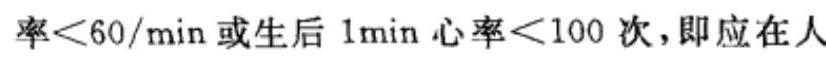
\includegraphics[max width=\textwidth, center]{2024_07_10_373f31b88d2bf633007bg-354}\\
工呼吸的同时, 行体外心脏按压, 其效果远比年长儿和成人为佳。具体方法: (1) 双手包绕胸部, 双拇指在胸骨中下 $1 / 3$ 处, 余指放于背部; (2) 单手经左胸包绕, 挴指放在胸骨中下 $1 / 3$ 处, 余指放于背部,将胸骨向脊柱方向挤压, 深度 $2 \mathrm{~cm}$ 左右, 频率 90~ $120 / \mathrm{min}$ 。推孝的按压与通气比为 $3: 1$, 心脏按压时不能中断通气反之亦然。按压时应监测血气、 $\mathrm{pH}$ 、血压和瞳孔的变化。如果按压有效瞳孔应缩小居中,如瞳孔变大,说明脑血流及氧供不足。如按压后收缩压 $>80 \mathrm{mmHg}$ 、按压 $90 \sim 120 / \mathrm{min}$, 可维持舒张压 $20 \sim 25 \mathrm{mmHg}$, 从而维持新生儿的冠状血管灘注。

(2)血管内置管: 新生儿复苏中,未成熟的新生儿或空息的新生儿容易出现血容量不足。如同期和外界刺激病情无改善, 可行脐动静脉插管检测血气、血压、 $\mathrm{pH}$ 值和补充血容量及用药。

(3)复苏用药: 如纯氧充分通气, 心脏按压 $30 \mathrm{~s}$后, 心率仍低于 $60 / \mathrm{min}$ 则需药物治疗。

(1) 给药途径。常用的有静脉 (IV)、肌肉 (IM)、气管内 (ET) 和脐静脉 (脐动脉插管常用于检测血气或监测血压等), 应根据经验和所用复苏药物选择给药途径。

(2)复苏用药。所用药物以最小容量注人。复苏常用约物是肾上腺素, 建议静脉用药, 但静脉困难或建立之前可气管内给药, 注意肾上腺素一定在通气充分后用药; 纳洛酮特别适用于仃妇分娩期间应用阿片类药物导致的呼吸抑制; 新生儿碳酸氢钠的应用应谨慎, 只有在通气充足, 容量充足, 倘已做血气 $\mathrm{pH}<7.0$ 碱缺失 $\geqslant 15 \mathrm{mmol} / \mathrm{L}$, 应给予娇正。补给碳酸氢钠量 $(\mathrm{mmol})=$ 体重 $(\mathrm{kg}) \times$ 碱缺失 $\times$ 0.3 , 首次给 $1 / 2$ 量。 $2 \%$ 碳酸氢钠 $2 \mathrm{ml}=1 \mathrm{mmol}$ 。 $5 \%$ 碳酸氢钠的渗透浓度是血浆的 4 倍。应用碳酸氢钠后, 体内血渗透浓度升高。用药后 $1 \mathrm{mmol}$ 碳酸氢钠可产生 $25 \mathrm{ml} \mathrm{CO}_{2} \mathrm{PaCO}_{2}$ 可显著升高, 快速静注后有诱发室额或顾内出血的可能; 扩容很少使用,但空息的早产儿 $<1500 \mathrm{~g}$,约有 $60 \%$ 出生时低血容量, 成熟新生儿出现血容量低下多与过早夹闭脐带有关, 低血糖、低钜和高镁血症也可引起低血压。但高血糖可增加复苏时脑损伤的程度和降低复苏的成活率,因此只用确认有低血糖时方可应用;钻剂不宜“常规”使用,因为钙能激活蛋白酶和磷脂酶, 破坏细胞膜释放出有破坏性的游离脂肪酸 (血栓素等)进人细胞内,随即发生细胞不可逆的凋亡, 任何外源性钝剂均可促进细胞的这些变化。因此除非证明有低锬血症或高钾血症的存在, 否则不宜使用; 呼吸兴奋药不宜使用, 复苏主要是纠正空息缺氧、纠正酸中毒、治疗低血容量, 呼吸兴奋药是以增加氧耗作为前提才能发挥作用, 故此时应用兴奋药, 对于原本就缺氧的脑组织更加不利, 可使脑损害加重, 倘宫内窘迫时, 给产妇使用呼吸兴奋药,则可能激发胎儿呼吸活跃, 增加胎儿在宫内的呼吸,增加胎儿误吸概率(表 3-10-5)。\\
表 3-10-5 新生儿复苏用药

\begin{center}
\begin{tabular}{|c|c|c|c|c|}
\hline
药物 & 浓度 & 剂量/途径 & 速度 & 作用 \\
\hline
肾上䐆素 & $1: 10000$ & \begin{tabular}{l}
$0.01 \sim 0.03 \mathrm{mg} / \mathrm{kg}$ \\
首选 IV \\
ET 最大剂量 $0.1 \mathrm{mg} / \mathrm{kg}$ \\
\end{tabular} & 快速 & 起搏减慢和停跳的心胜 \\
\hline
 & $0.4 \mathrm{mg} / \mathrm{ml}$ & $0.1 \mathrm{mg} / \mathrm{kg}$ & 快速 & 怙抗呼吸抑制 \\
\hline
纳洛酮 & 生理盐水 & IV 脐静脉 & $5 ~ 10 \mathrm{~min}$ 输人 & 纠正失血性休克 \\
\hline
扩容药 & \begin{tabular}{l}
血浆代用品 \\
$4.2 \%(0.5 \mathrm{mmol} / \mathrm{ml})$ \\
\end{tabular} & $10 \mathrm{ml} / \mathrm{kg}$ &  &  \\
\hline
碳胹氢钠 &  & \begin{tabular}{l}
$4 \mathrm{ml} / \mathrm{kg}$ \\
$2 \mathrm{mmol} / \mathrm{kg}$ 脐腈脉 \\
$2 \sim 20 \mu \mathrm{g} /(\mathrm{kg} \cdot \mathrm{min}) \mathrm{IV}$ \\
\end{tabular} & $>2 \min$ & 纠正亚重酸中毒 \\
\hline
多巴胺 &  &  &  & 升血压增加心排血量改善灌注 \\
\hline
\end{tabular}
\end{center}

\begin{enumerate}
  \setcounter{enumi}{3}
  \item 终止复苏的时机 时机确定较为困难,可参照导致窒息的原因能否解除; 复苏开始的时机及效果; 脑损害的可能性和损害程度; 家长的感情以及各自的经验等综合判定。倍确诊已有较严重的脑损害又征得家长同意,复苏应即停止。多 $<26$周的早产儿复苏的后果差, 提前和家属沟通, 决定是否对此类新生儿进行复苏。
\end{enumerate}

\section*{六、复苏后处理及预后}
所有复苏后的新生儿均为高危儿, 有条件均应收人 ICU 监测治疗。重点观察并防治新生儿呼吸功能不全、痉挛发作、低血糖综合征、低体温、水肿和循环功能不全等。需要给予氧疗法、液体疗法或高能营养。新生儿复苏后的第 7 天方可喂养, 以使其消化道得以恢复, 控制感染可用抗生素疗法。特别应观察并积极维护脑功能。注意保温。

笔者统计分析了 60 例重度窒息复苏后的新生儿,其中 10 例死于生后 $24 \mathrm{~h}$ 内, 1 例死于生后 $50 \mathrm{~h}$,对生存的 49 例进行了信访, 24 例有回报结果: 其中两例发生智力障碍 (占 24 例的 $8.33 \%$ ), 可见重度窒息后新生儿预后多较差。新生儿复苏的预后与 Apgar 评分 $5 \mathrm{~min}$ 时的评分数有关, $5 \mathrm{~min}$ 时 $\leqslant 5$ 分时,易致脑损害。0〜1 分者 $44 \%$ 于生后次日死亡, $49 \%$ 在新生儿期死亡。追踪 $7 \sim 10$ 分与 $0 \sim 3$ 分的预后:1 岁时出现脑异常症状的, 后者比前者多 3 倍。故病死率及智力低下的发生率与 Apgar 评分呈负相关, 即分数愈低, 病死率和智力低下发生率愈高。

(孟凌新)

\section*{算11}
\section*{小 儿 麻 醉}
\section*{第一节 麻醉有关的小儿生理解剖特点}
\section*{一、呼吸系统}
胎儿一旦娩出, 其呼吸器官必须在 $1 \sim 2 \min$ 接替胎盘功能, 以保证组织的正常氧供, 为此需排出肺内液体。经阴道分娩时产道压力达到 $70 \mathrm{cmH}_{2} \mathrm{O}$, 胎儿肺内液体 $2 / 3$ 已被挤出,其余液体将在 $24 \mathrm{~h}$ 之内经肺内淋巴系统吸收。剖宫产时缺少这一挤压过程, 肺内液体吸收时间拖长, 因而常有短时间的呼吸功能不足。出生时由于缺氧、 $\mathrm{CO}_{2}$ 蓄积以及寒冷、钳夹脐带等刺激, 第一次吸气肺泡张开, 需要较大的压力 $\left(40 \sim 80 \mathrm{cmH}_{2} \mathrm{O}\right)$ 。呼吸数次后产生的功能残气量 (FRC, 正常 $35 \sim 60 \mathrm{ml}$ ) 可以堿少随后呼吸道开放所需压力。肺表面活性物质在维持功能残气量方面有重要作用, 肺表面活性物质不足, 如早产儿, 则容易发生呼吸塞迫综合征 (RDS)。虽然妊娠 16 周, 终末支气管已发育完成, 但大部分肺泡是生后形成的, 最初几年肺泡数迅速增加, 在 $4 \sim 6$岁达成人水平, 而肺功能的发育完成则需 $15 \sim 18$岁。婴儿肺弹性回缩压低, 由于胸壁骨架部分未发育成熟顺应性高, 随年龄增长逐步下降, 15~18岁肺功能完全成熟时降至最低, 弹性回缩力增加, 使二者达到最佳平衡。由于小儿呼吸道通畅的维持部分地取决于肺的弹性回缩, 故婴幼儿小气道疾患较多。小儿肺功能正常值见表 3-11-1。

表 3-11-1 不同年䶖呼吸功能正常值

\begin{center}
\begin{tabular}{|c|c|c|c|c|c|c|c|c|c|}
\hline
 &  &  & 年 & 龄 &  &  &  &  &  \\
\hline
 & 1 周 & 1 岁 & 3 岁 & 5 岁 & 8 岁 & 12 岁 & 15 岁 & 男 21 岁 & 女 21 步 \\
\hline
身高 $(\mathrm{cm})$ & 48 & 75 & 96 & 109 & 130 & 150 & 170 & 174 & 162 \\
\hline
体重(kg) & 3.3 & 10 & 15 & 18 & 26 & 39 & 57 & 73 & 57 \\
\hline
$\mathrm{FRC}(\mathrm{ml})$ & 75 & (263) & $(532)$ & $(660)$ & 1174 & 1855 & 2800 & 3030 & 2350 \\
\hline
$\mathrm{FRC} /$ 体重 $(\mathrm{ml} / \mathrm{kg})$ & (25) & (26) & $(37)$ & $(36)$ & $(46)$ & $(48)$ & $(49)$ & (42) & $(41)$ \\
\hline
肺活量(ml) & 100 & $(475)$ & $(910)$ & 1100 & 1855 & 2830 & 4300 & 4620 & 3380 \\
\hline
分钟通气量 ( $\mathrm{ml} / \mathrm{min})$ & 550 & $(1775)$ & $(2460)$ & $(2600)$ & $(3240)$ & $(4150)$ & 5030 & 6000 & 5030 \\
\hline
湖气量(ml) & 17 & $(78)$ & (112) & $(130)$ & $(180)$ & $(260)$ & 360 & 500 & 420 \\
\hline
肺泡通气量 (ml/min) & 385 & $(1245)$ & $(1760)$ & $(1800)$ & (2 195) & $(2790)$ & 3070 & 4140 & 3530 \\
\hline
死般量(ml) & 7.5 & 21 & 37 & 49 & 75 & 105 & 141 & 150 & 126 \\
\hline
㑔应珄 $\left(\mathrm{ml} / \mathrm{cmH}_{2} \mathrm{O}\right)$ & 5 & $(16)$ & (32) & 44 & 71 & 91 & 130 & 163 & 130 \\
\hline
最大流速 $(\mathrm{L} / \mathrm{min})$ & 10 &  &  & 136 & 231 & 325 & 437 & 457 & 365 \\
\hline
呼吸阻力 $\left[\mathrm{cmH}_{2} \mathrm{O} /(\mathrm{L} \cdot \mathrm{s})\right]$ & 29 & (13) & $(10)$ & 8 & 6 & 5 & 3 & 2 & 2 \\
\hline
\end{tabular}
\end{center}

()为估算值\\
小儿肺泡通气量与 FRC 之比为 $5: 1$, 而成人为 $3: 2$, 亦即肺内氧储备少, 但耗氧量高, 新生儿耗氧量 $[6 \sim 8 \mathrm{ml} /(\mathrm{kg} \cdot \mathrm{min})]$ 较成人 $[3 \mathrm{ml} /(\mathrm{kg} \cdot \mathrm{min})]$高 $2 \sim 3$ 倍, 特别在 $1 \sim 2$ 岁时最高, 故对缺氧的耐受能力远不如成人, 一旦供氧减少, 将迅速出现低氧血症。由于 FRC 少吸人麻醉诱导及苏醒均较快。败幼儿呼吸调节功能与成人相似, 对 $\mathrm{CO}_{2}$ 反应正常, 但新生儿 $\mathrm{PaCO}_{2}$ 常保持在较低水平 $(35 \mathrm{mmHg})$, 此点可能与对代谢性酸血症的代偿有关。新生儿生后 $1 \sim 2$ 周, 对缺氧的反应是双相的,继短暂的呼吸增强之后, 迅速转为抑制, 且抑制 $\mathrm{CO}_{2}$ 使呼吸增强的反应, 常出现呼吸节律絮乱, 进而呼吸停止。新生儿血红蛋白 ( $\mathrm{Hb})$ 为 $180 \sim 200 \mathrm{~g} /$ $\mathrm{L}$, 出生时胎儿 $\mathrm{Hb}(\mathrm{HbF})$ 占 $75 \% \sim 84 \%, 3 \sim 6$ 个月逐步减少至正常水平, 因 $\mathrm{HbF}$ 与氧亲和力强, 2,3DPG 含量少, 故氧离解曲线左移, 半饱和氧分压 $\left(\mathrm{P}_{50}\right)$ 约 $19 \mathrm{mmHg}$ (表 3-11-2), 向组织释氧量较少。

$\mathrm{P}_{50}$ 于生后迅速增加, 4〜6个月时达成人水平 (27. $0 \mathrm{mmHg}$ ) 6〜8个月, 2,3 -DPG 则保持在较高水平, 以代供因红细胞生成素少所致的 $\mathrm{Hb}$ 偏低 (小儿生理性贫血),保证 8 个月 18 岁期间血夜向组织的释氧量不变。根据表 3-11-2 所示 $\mathrm{P}_{50}$ 为 $27 \mathrm{mmHg}$ 的成人 $\mathrm{Hb} 100 \mathrm{~g} / \mathrm{L}$ 相当于 $\mathrm{P}_{50}$ 为 $30 \mathrm{mmHg}$ 的婴儿 $\mathrm{Hb} 82 \mathrm{~g} / \mathrm{L}$ 和 $\mathrm{P}_{50}$ 为 $24.4 \mathrm{mmHg}$新生儿 $136 \mathrm{~g} / \mathrm{L}$ 的释氧量, 而拟手术的新生儿为满足氧运输需要 $\mathrm{Hb}$ 最少需 $100 \sim 120 \mathrm{~g} / \mathrm{L}$ (表 3-113)。

术中动脉血氧分压 $\left(\mathrm{PaO}_{2}\right)$ 必须维持在正常范围。应用脉搏血氧饱和度仪监测 $\mathrm{SpO}_{2}$, 可以随时发现动脉血氧的变化。但由于 $\mathrm{Hb}$ 的氧亲和力、 $\mathrm{P}_{50}$随年龄而变化, 如新生儿亲和力高, 生后 $3 \sim 6$ 个月迅速下降, 所以 $\mathrm{SpO}_{2}$ 与 $\mathrm{PaO}_{2}$ 关系也因年龄而异。小儿麻碎中保证不发生低氧血症和组织缺氧是完全必要的, 但最近发现新生儿一般不宜吸人高浓度氧, 氧供可以满足代谢需要即可, 超量吸人即使是低浓度的氧, 在新生儿期也会引起氧中毒。过量的氧通过氧化应激 (oxydant stress) 可以引发一些严重的病理改变, 如早产儿视网膜病, 支气管肺发育不良, 影响脑的发育和儿童癌症等。故术中、术后以及新生儿复苏时首先是改善通气, 如 $\mathrm{SpO}_{2}$ 达不到需要水平, 可在吸人空气中补充适当比例的氧, 维持 $\mathrm{SpO}_{2}$ 在 $85 \% \sim 88 \%$ 到 $94 \% \sim 95 \%$ 即可。只有严重缺氧、发绀不能改善时才吸人纯氧。不同 $\mathrm{P}_{50}$ 条件下不同 $\mathrm{SO}_{2}$ 的 $\mathrm{PO}_{2}$ 计算值如表 3-11-4 所示。

表 3-11-2 不同年齢的 $\mathrm{P}_{50} 、 \mathrm{Hb}$ 与释氧皇

\begin{center}
\begin{tabular}{lcccc}
\hline
\multicolumn{1}{c}{年龄} & $\mathrm{P}_{50}(\mathrm{mmHg})$ & $\mathrm{PvO}_{2}=40 \mathrm{mmHg}$ 时 $\mathrm{SO}_{2}(\%)$ & $\mathrm{Hb}(\mathrm{g} / \mathrm{L})$ & 释氧量 $(\mathrm{ml} / \mathrm{dl}) *$ \\
\hline
$1 \mathrm{~d}$ & 19.4 & 87 & 172 & 1.84 \\
3周 & 22.7 & 80 & 130 & 2.61 \\
$6 \sim 9$ 周 & 24.4 & 77 & 110 & 2.65 \\
$3 \sim 4$ 个月 & 26.5 & 73 & 105 & 3.1 \\
6 个月 & 27.8 & 69 & 113 & 3.94 \\
$8 \sim 11$ 个月 & 30 & 65 & 118 & 4.74 \\
$3 \sim 8$ 岁 & 29 & 67 & 126 & 4.37 \\
$9 \sim 12$ 岁 & 27.9 & 69 & 134 & -150 \\
成 & 27 & 71 &  & 4.92 \\
\hline
\end{tabular}
\end{center}

※动脉血氧饱和度为 $95 \%$

表 3-11-3 等犆组织匉释需要的 $\mathrm{Hb}$

\begin{center}
\begin{tabular}{l|c|c|c|c|c|c|c|c}
\hline
 & $\mathrm{P}_{50}(\mathrm{mmHg})$ & \multicolumn{5}{|c}{等量氧释的 $\mathrm{Hb}(\mathrm{g} / \mathrm{L})$} &  &  \\
\hline
成人 & 27 & 70 & 80 & 90 & 100 & 110 & 120 & 130 \\
\hline
婴儿>3 个月 & 30 & 57 & 65 & 73 & 82 & 90 & 98 & 106 \\
\hline
新生儿,<2个月 & 24 & 103 & 117 & 132 & 147 & 161 & 176 & 191 \\
\hline
\end{tabular}
\end{center}

表 3-11-4 不同 $\mathrm{P}_{50}$ 条件下计算的 $\mathrm{SO}_{2}$ 与 $\mathrm{PO}_{2}$

\begin{center}
\begin{tabular}{|c|c|c|c|c|c|}
\hline
 & \multicolumn{5}{|c|}{年 龄} \\
\hline
 & $1 \mathrm{~d}$ & 2 周 & $6 \sim 9$ 周 & 6 个月~6 岁 & 成人 \\
\hline
\multirow{2}{*}{$\mathrm{P}_{50}(\mathrm{mmHg}) \mathrm{SO}_{2}(\%)$} & 19 & 22 & 24 & 29 & 27 \\
\hline
 & \multicolumn{5}{|c|}{$\mathrm{pH} 7.4$ 条件下 $\mathrm{PO}_{2}(\mathrm{mmHg})$ 计算值} \\
\hline
99 & 108 & 130 & 143 & 171 & 156 \\
\hline
98 & 77 & 92 & 101 & 122 & 111 \\
\hline
97 & 64 & 77 & 84 & 101 & 92 \\
\hline
96 & 56 & 68 & 74 & 89 & 82 \\
\hline
95 & 52 & 62 & 68 & 82 & 74 \\
\hline
94 & 48 & 58 & 63 & 76 & 69 \\
\hline
93 & 45 & 55 & 60 & 72 & 66 \\
\hline
92 & 43 & 52 & 57 & 68 & 62 \\
\hline
91 & 41 & 50 & 55 & 66 & 60 \\
\hline
90 & 40 & 48 & 53 & 63 & 58 \\
\hline
88 & 37 & 45 & 49 & 59 & 54 \\
\hline
86 & 35 & 42 & 47 & 56 & 51 \\
\hline
84 & 34 & 40 & 44 & 53 & 49 \\
\hline
82 & 32 & 39 & 42 & 51 & 47 \\
\hline
80 & 31 & 37 & 41 & 49 & 45 \\
\hline
78 & 30 & 36 & 39 & 47 & 43 \\
\hline
76 & 29 & 34 & 38 & 45 & 41 \\
\hline
74 & 28 & 33 & 36 & 44 & 40 \\
\hline
72 & 27 & 32 & 35 & 42 & 39 \\
\hline
70 & 26 & 31 & 34 & 41 & 37 \\
\hline
\end{tabular}
\end{center}

\section*{二、循环系统}
新生儿出生后由于卵圆孔和动脉导管闭合, 循环走行由平行转为序列, 心室做功明显增加,尤以左心室最为明显, 约增加到 2.5 倍, 6 周后开始逐渐达到正常水平。所以生后短时间内左心处于超负荷状态, 即使正常新生儿也面临着心力衰竭的威胁, 因此先心病患儿在此期间麻醉手术死亡率高。新生儿和早产儿心肌收缩力均较成人为低,主要由于心肌原纤维排列顺序杂乱,数目少 $50 \%$,可收缩体积明显小,导致心室顺应性低下, 使心脏心舒期容积和心每搏量均少, 心排血量 (CO) 的增加主要靠心跳次数的增加。小儿麻醉中心率波动范围大,虽然对心率增快耐受较好, 但仍有一定限度, 过快将使心肌氧耗增加, 甚而导致心衰竭。反之, 心动过缓将会直接导致 CO 降低, 在婴幼儿心率<100~120/ $\mathrm{min}$ 即属过缓, 表明心肌受抑制。小儿心脏每搏量少,动脉口径相对较大, 管壁柔软, 故年龄愈小, 动脉压愈低 (表 3-11-5)。按年龄计算血压公式: 年聆 $\times 2+80=$ 收缩压, 此值的 $1 / 3 \sim 2 / 3$ 为舒张压 (表 3-11-6)。\\
表 3-11-5 小儿的血流动力参数

\begin{center}
\begin{tabular}{lcccc}
\hline
年龄 & 心率 $(/ \mathrm{min})$ & 心每搏量 $(\mathrm{ml})$ &  & 血压 $(\mathrm{mmHg})$ \\
\cline { 3 - 4 }
 &  &  & 收缩压 & 柃张压 \\
\hline
个月生儿 & $133 \pm 18$ & $5 \pm 5$ & $67 \pm 3$ & $42 \pm 4$ \\
12 个月 & $120 \pm 20$ & $7 \pm 2$ & $89 \pm 29$ & $60 \pm 10$ \\
2 岁 & $120 \pm 20$ & $12 \pm 3$ & $96 \pm 30$ & $66 \pm 25$ \\
3 岁 & $105 \pm 25$ & $17 \pm 6$ & $99 \pm 25$ & $64 \pm 25$ \\
5 岁 & $101 \pm 15$ & $21 \pm 6$ & $100 \pm 25$ & $67 \pm 23$ \\
12 岁 & $90 \pm 10$ & $28 \pm 8$ & $94 \pm 14$ & $55 \pm 9$ \\
23 岁 & $70 \pm 17$ & $54 \pm 4$ & $109 \pm 16$ & $58 \pm 9$ \\
 & $77 \pm 5$ & $86 \pm 6$ & $122 \pm 30$ & $75 \pm 20$ \\
\hline
\end{tabular}
\end{center}

表 3-11-6 小儿允许最大心率(/min)

\begin{center}
\begin{tabular}{cccc}
\hline
年龄 & 清酷 & 睡眠 & 运动 $/$ 发热 \\
\hline
新生儿 & $100 \sim 180$ & $80 \sim 160$ & $>220$ \\
1 周 $\sim 3$ 个月 & $100 \sim 220$ & $80 \sim 200$ & $>220$ \\
3 个月 $\sim 2$ 岁 & $80 \sim 150$ & $70 \sim 120$ & $>200$ \\
$2 \sim 10$ 岁 & $70 \sim 110$ & $60 \sim 90$ & $>200$ \\
$>10$ 岁 & $55 \sim 90$ & $50 \sim 90$ & $>200$ \\
\hline
\end{tabular}
\end{center}

由延骳血管运动中枢和心脏抑制兴奋神经单位形成的调节血压和心率的反射弧, 虽在新生儿出生后已初具功能,但其代偿常不充分, 如咽喉反射引起的呼吸停止、心率喊慢,持续时间稍久,即可因中枢乏氧不能启动呼吸, 甚而导致心跳停止,突然死亡。所有各种吸人麻醉药及静脉麻醉药对心血管均有抑制作用, 且所需浓度较中枢抑制浓度为小, 容易出现血压下降。出生时的血容量个体差异较大,例如延迟夹脐带可使之增加 $25 \%$, 与此相反,在宫内胎儿缺氧, 常导致血管收缩, 故窒息的新生儿多有血容量不足。由于出生时交感神经尚未发育成熟, 使其血容量对动脉压的影响非常突出, 故在临床上新生儿血压是反映其血容量的良好指标。出生后的低氧血症可使肺动脉阻力增加, 有使动脉导管和卵圆孔重新开放,饭复胎儿型循环的危险。

\section*{三、肾发育及功能}
足月儿出生后肾小球滤过率 (GFR) 迅速增加,而早产儿 GFR 低且增速绶慢, 可能与血管阻力高,滤过面积小和超滤压低等有关。由于 GFR、肾血流 (RBF) 低, 对水的排出能力受限, 出生时由于肾小管发育不成熟而皮质肾单位栱长, 排钠较多, 而肾小管钠再吸收能力差, 尿钠排泄率高, 胎龄越小越明显。出生后钠排泄率迅速下降, 成熟儿生后约 $3 \mathrm{~d}$ 降至 1\%以下, 如胎龄不足 37 周的早产儿, 同期继续维持在 $3 \% \sim 9 \%$ 高值。远位肾小管再吸收率低, 可能与对醛固酮反应差以及心钠素 (ANP) 高等有关。为此, 应适量补钠, 但若输钠过多, 又可招致高钠血症和水肿。新生儿尿排钾少, 此点与近位小管 Na-K-ATP 酶活性低, 远位情小管对醛固酮反应差有关。因此患病新生儿与未成熟儿出生后, 由于酸中苺、低血压、肾灌注少等原因, 易致钾潴留。新生儿尿浓缩功能差, 尿渗浓最高仅 $700 \mathrm{mOsm} /$ $\left(\mathrm{kg} \cdot \mathrm{H}_{2} \mathrm{O}\right)$, 未成熟儿更低。而成人可高达 $1200 \mathrm{mOsm} /\left(\mathrm{kg} \cdot \mathrm{H}_{2} \mathrm{O}\right)$ 。在排水多的同时也影响尿素氮(BUN) 排泄, 其机制与肾䚟质解剖学上发育不成熟, 渗透压差低, 集合管对醛固酮 (ADH) 反应差, 前列腺素对尿浓缩的抑制有关。新生儿肾调节酸碱平衡能力较差, 由于近位小管对 $\mathrm{HCO}_{3}^{-}$再吸收差, 细胞外液多, 导致 $\mathrm{HCO}_{3}^{-}$浓度相对较低, 有机酸排泄少,而伴随发育及蛋白异化所产生的有机酸较多以及骨代谢产生 $\mathrm{H}^{+}$等原因容易发生酸中毒。不同年龄肾功能发育情况见表 3-11-7。\\
表 3-11-7 不同年龄小儿肾功能

\begin{center}
\begin{tabular}{|c|c|c|c|c|c|c|}
\hline
项目 & 早产儿 & 足月儿 & $1 \sim 2$ 周 & 6 个月~1岁 & $1 \sim 3$ 岁 & 成人 \\
\hline
\multirow{2}{*}{$\mathrm{GFR}\left[\mathrm{ml} /\left(\min \cdot 1.73 \mathrm{~m}^{2}\right)\right]$} & $14 \pm 3$ & $40 \pm 14.8$ & $65.8 \pm 24.8$ & $77 \pm 14$ & $9 \pm 22$ & 男 $=125 \pm 15$ \\
\hline
 &  &  &  &  &  & 女 $=110 \pm 15$ \\
\hline
肾血流 $\left[\mathrm{ml} /\left(\mathrm{min} \cdot 1.73 \mathrm{~m}^{2}\right)\right]$ & $40 \pm 6$ & $88 \pm 4$ & $220 \pm 40$ & $352 \pm 73$ & $540 \pm 118$ & $620 \pm 92$ \\
\hline
$\mathrm{TmPAH}\left[\mathrm{ml} /\left(\mathrm{min} \cdot 1.73 \mathrm{~m}^{2}\right)\right]$ & $10 \pm 2$ & $16 \pm 5$ & $38 \pm 8$ & $51 \pm 20$ & $66 \pm 19$ & $79 \pm 12$ \\
\hline
最大浓缩 $\left[\mathrm{mOsm} /\left(\mathrm{kg} \cdot \mathrm{H}_{2} \mathrm{O}\right)\right]$ & 480 & 700 & 900 & 1200 & 1400 & 1400 \\
\hline
血清肌酎 $(\mathrm{mg} / \mathrm{dl})$ & 1.3 & 1.1 & 0.4 & 0.2 & 0.4 & $0.8 \sim 1.5$ \\
\hline
利钠分数 $(\%)$ & $2 \% \sim 6 \%$ & $<1$ & $<1$ & $<1$ & $<1$ & $<1$ \\
\hline
最大糖再吸收 $\left[\mathrm{ml} /\left(\mathrm{min} \cdot 1.73 \mathrm{~m}^{2}\right)\right]$ & - & - & $71 \pm 20$ & 一 & 一 & $339 \pm 51$ \\
\hline
\end{tabular}
\end{center}

GFR: 肾小球滤过率, TmPAH; 对氨马沓酸最大清除率

\section*{四,神 经系统}
出生时脑被数片顾骨包围,前㐫通常在出生后 20 个月闭合, 闭合前阶段前囟张力对判断脱水及顽内压有重要参考价值。新生儿脑与成人比相对较大,新生儿脑重约占体重 $1 / 10$,而成人占 $1 / 50$ 。生后增长迅速, 6 个月时脑重量增长 1 倍, 1 岁时增长 2 倍。小儿脑氧代谢率 $\left(\mathrm{CMRO}_{2}\right)$ 高, 儿童平均需氧 $5.2 \mathrm{ml} /(\mathrm{min} \cdot 100 \mathrm{~g})$, 明显高于成人 $3.5 \mathrm{ml} /$ ( min $100 \mathrm{~g}$ ), 任何原因所致的氯供不足,均易造成脑缺氧。成人脑血流量为 $50 \sim 60 \mathrm{ml} /(\mathrm{min}$ $100 \mathrm{~g})$, 早产儿及新生儿约为 $40 \mathrm{ml} /(\mathrm{min} \cdot 100 \mathrm{~g})$,而年长儿可达 $100 \mathrm{ml} /(\mathrm{min} \cdot 100 \mathrm{~g}$ )。小儿脑血流的自动调节范围也低于成人, 麻醉中脑血流量易受血压剧烈波动的影响, 早产儿和足月新生儿在急性弿迫时, 其脑部自动调节机制会进一步受到损害,脑血流量可随动脉压变化而变化, 导致脑室内或周围出血。小儿出生时神经细胞只有正常的 $1 / 4,1$岁时皮质及脑干接近发育完全。而铤鞘的形成及树突的完善过程要持续到 3 岁, 所以㜟儿常具有各种原始反射。与中枢神经不同, 自主神经发育相对较好, 出生时支配心血管的副交感神经功能发育已经完成, 而交感神经则需到生后 4〜6个月。维持血压和心率的压力反射及延觧血管运动中枢 (加压和减压) 出生时已具有功能, 但未成熟, 麻醉状态下易受抑制。由于传导路的发育尚未完善及缺乏神经肌肉协调动作的训练, 神经系统功能不够稳定,调节功能也较差, 如呼吸、肌肉运动及体温调节等。新生儿出生时, 血脑屏障未发育成熟, 再加脑血流丰富,许多药物婴儿脑内浓度较成人高, 如硫喷妥钠即容易通过血脑屏障产生中枢抑制。脊髓末端出生时相当于椎管内第 3 腰椎水平, 1 岁以后才位于第 1 腰椎水平。

\section*{五、体温调节}
体温的产生是机体产生热和向环境散热之间平衡的结果, 在低于体温的环境中, 婴儿通过消耗氮和能量来保持正常体温。新生儿体温调节范围较成人明显为窄,且容易受周围环境影响, 成人温度调节下限为环境温度 $0^{\circ} \mathrm{C}$, 而新生儿为 $22^{\circ} \mathrm{C}$ 。其原因是体格小,产热不足,体表面积相对大,体表面积与体重之比是成人的 $3 \sim 5$ 倍, 单位体积的散热量约为成人的 4 倍, 再加传导快, 散热容易, 早产儿更明显。较大儿童能借寒战反应产生热量,而新生儿的产热全靠褐色脂肪的氧化,足月新生儿褐色脂肪占体重的 $5 \%$,而早产儿只占 $1 \%$,所以正常新生儿应置于与皮肤温差 $2 \sim 4^{\circ} \mathrm{C}$ 的环境,在该温度下,代谢速度最慢, 温度调节仅靠蒸发即中性环境温度。安静状态下腹部皮肤温度 $36^{\circ} \mathrm{C}$, 环境温度 $32 \sim$ $34^{\circ} \mathrm{C}$, 婴儿氧耗最少。体温越低, 所需环境温度越高。通常在寒冷环境下,由于环境和皮肤温度差大,必然导致氧耗增加, 倘环境温度持续过低, 极易造成低体温。体温下降到 $35^{\circ} \mathrm{C}$ 以下除对中枢及心血管的直接抑制外,还可因外周血管收缩, 影响组织氧供, 导致细胞缺氧, 发生代谢性酸中毒, 硬肿症, 呼吸抑制, 甚而由于增加肺动脉阻力导致烣复胎儿循环,加重低氧血症的危害。全身麻醉可使体温中枢调节阈值增加, 尤其低温阀值下降及末梢血管扩张,散热增加, 体温下降。低体温对静脉及吸人麻醉药的药动学及药效学均有影响, 可使吸人麻醉药 MAC 降低, 组织可溶性增加, 非去极化肌松药用量减少,作用时间延长,所以小繁儿手术中保温极为重要。6个月以上小儿代谢旺盛,倘手术室环境温度偏高, 再加覆盖敷料, 体温容易升高引发\\
高热。

\section*{六、药理学的影响}
小儿出生后早期因身体组成、蛋白结合、体温、心排血量的分配、心脏功能的发育程度、血-脑屏障的成熟情况、肝肾的大小和功能, 以及有无先天畸形等诸多因素均影响其药代学和药动学。新生儿总含水量高, 且随年龄增加而惐少, 而肌肉、脂肪则随年龄增加而增加, 因而新生儿水溶性药物分布容积大, 通常需要给予更大的首剂方能达到预期的血药浓度 (如氯琥珀胆碱), 而需要依赖脂肪再分布消除的药物药效将延长 (如硫喷妥钠), 在肌肉中再分布的药物药效也将延长(如芬太尼)。由于肝功能未发育完善, 一些通过肝代谢为无活性产物的麻醉用药代谢较慢, 作用时间较长。药物代谢大部分经两个途径: 第 $\mathrm{I}$ 相或降解反应(氧化, 还原及水解),第 II 相或合成反应 (结合)。 I 相反应大部分在肝微粒体酶进行, 新生儿体内与药物代谢有关的酶系统发育不全, 氧化药物的能力最差, 而水解药物的能力与成人相仿。新生儿药物蛋白结合率低 (白蛋白较少, $\alpha_{1}$ 酸性糖蛋白生成不足) 而影响药物的血药浓度, 以及由于血气分配系数、肺泡通气以及心脏排血分布的差异, 影响吸人麻醉药的摄取和分布。由于各脏器系统的迅速发育, 使麻醉及有关药物的摄取、分布、蛋白结合、代谢、排出在不断变化,从而导致小儿不同年龄段对麻醉药物等效剂量、起效时间、吸收、排出时间均有所不同, 败幼儿阶段以前最为明显。总体而言, 早产儿、新生儿大多数药物清除半衰期延长, $2 \sim 10$ 岁儿童缩短, 进入成年再度延长。此外婴儿如患有脓毒血症、充血性心衰、腹内压增加、营养不良和机械通气均会影响其药代学及药效学, 使个体差异更为明显。

\section*{第二节 麻醉前检查、评估及准备}
\section*{一、麻醉前检查评估}
\begin{enumerate}
  \item 术前访视 麻醉前详细了解病情, 对麻醉手术中可能出现的风险进行评估预测, 并做好防治准备, 是保护患儿平顺度过围术期的重要保证。小儿麻醉中所谓“意外”的多发, 常常与术前评估的疏漏有关。
\end{enumerate}

(1) 病史: 手术疾病除有关病史外, 还应从家长或患儿处询问并存病史、过敏史及住院后治疗经过, 曾否用过与麻醉有关的药物。对曾经施行过麻醉手术者, 应了解该次麻醉及手术中、后有无异常经过及曾经采取的治疗措施。

(2)体格检查: “小儿”不能抽象理解, 应有“定量”概念。人院后体重、身高测定应列为常规。应注意年龄与发育状况和是否与正常值相符。肥胖儿童应计算其体重指数 (BMI), 目前超重儿较多,注意判断其程度是否已达病理性肥胖 (BMI>30~ 35)。检查手术病变以外, 重点放在呼吸、心血管及合作程度上。上呼吸道有无畸形、病变, 听诊心、肺, 量血压、脉搏有无异常及代偿情况。较复杂的并存病应请相关科会诊共同评估。

(3) 实验室影像及其他辅助检查结果: 应熟悉小儿不同年龄各种实验室检查的正常值和影像学检查的意义, 以判断有无异常。手术前应常规检查 $\mathrm{Hb}$ 及 HCT, 小儿各年龄组间 $\mathrm{Hb} 、 \mathrm{HCT}$ 正常值差异较大, 必须参照正常值, 确定患儿术中 $\mathrm{Hb} 、 \mathrm{HCT}$的目标值, 作为输血的依据。由于资料来源文献不同, 表间 $\mathrm{Hb}$ 值稍有不同, 表明即使正常小儿, 个体间也有较大差异。

(4)手术: 应了解手术部位、体位、手术方式、主要操作步骤及其对麻醉管理的要求。

\begin{enumerate}
  \setcounter{enumi}{1}
  \item 并存病一般较成人为少, 以下儿种并存病较为常见。
\end{enumerate}

(1)上呼吸道感染: 上感使小儿呼吸道敏感, 麻醉时容易发生喉痉挛、支气管痉挛及低诨血症, 术后有可能病情加重, 尤其在长时间大手术和气管内麻醉之后。手术时机尚无统一的标准, 通常对急性上呼吸道感染, 有发热、咳濑、脓性鼻晜的患儿, 应考虑推迟手术。体温不超 $38^{\circ} \mathrm{C}$ 的微热, 无其他症状且手术较小者可以进行麻醉。术后呼吸系统并发症发生或加重的可能性增加, 应得到家属的理解。尽可能选择用静脉麻醉或呼吸道刺激性小的吸人麻醉药, 并准备好应对并发症的防治措施, 如肌松药、气管插管、吸氧等。

(2)哮喘: 有㫴喘并应用支气管扩张药治疗病史者, 术前应用支气管扩张药给予充分控制, 插管前充分表面麻醉,术中选用有支气管扩张作用的麻醉药如氯胺酮和(或)七氟烷吸入辅以机械通气,多数可以平稳度过手术期。术后必须加强监测, 发作时给予支气管扩张药的䇨化吸人, 必要时给予呼吸\\
支持。

(3)先天性心脏病: 对并存先心病患儿,首先要确定手术疾病与先天性心㖢病哪一个是威胁生命或影响生活质量的主要问题。原则上对主要问题要优先解决。确定现手术疾病需要先进行治疗之后, 要明确先天性心脏病的诊断, 评估心脏功能及代偿情况。术前准备及术中管理原则同先心病手术,注意保护心功能,并做好应对心脏突发事件的准备, 术后应加强监测及治疗。

(4)贫血: 贫血的诊断必须对应各年龄的正常值。出生后, 3〜6个月 $\mathrm{Hb}$ 可降至 $90 \sim 100 \mathrm{~g} / \mathrm{L}$, 此为生理性贫血。 $\mathrm{SvO}_{2}$ 也是贫血的敏感指标, $<$ $30 \mathrm{mmHg}$ 表明红细匏生成素增高, 红细胞生成不足。诊断为贫血患儿,择期手术,术前应尽量予以纠正, 以增加对术中出血的耐力。对肾衰竭所致慢性贫血的年长恵儿由于 2,3 -DPG 的增加, 释氧增加,对贫血耐受较好,但术中 $\mathrm{Hb}$ 也不宜低于 $60 \mathrm{~g} /$ $\mathrm{L}$ 。切记, $\mathrm{Hb}$ 低于 $50 \mathrm{~g} / \mathrm{L}$ 时, 即使缺氧也不会出现发绀。

(5)胃佗满: 小儿食管短, 括约肌发育不成熟,屏障作用差,咽喉反射不健全,麻醉状态下,容易发生反流和误吸。择期手术饱食者, 应进食 $6 \mathrm{~h}$ 后手术。急诊手术由于各种原因胃饱满者,首先考虑在非全身麻醉下手术,必须立即在全麻下手术者, 处理的基本原则是尽量排空消化道内容物和保护好呼吸道。急腹症周内容储留, 饱食或少量进食(奶)后, 应下粗胃管,尽可能吸净胃内容后再进行麻醉。对胃内容储留量大,腹内压高, 用胃管难以吸除者,可用粗胃管或气管插管经鼻插人食管抽吸后保留导管以随时引流和 (或)吸引胃内容,再进行麻醉。诱导行快速插管时, 取头高位,面罩通气压力适当减小, 并由助手压迫环状软骨, 避免过多气体进人胃内使胃内压增加和防止胃内容反流。依笔者经验在充分表面麻醉下行清醒气管内插管后进行麻醉, 较为稳妥,尤其在重症婴幼儿。应用椎管内麻醉或区域阻滞麻醉时, 如辅用较大剂量的镇静药,仍有发生反流误吸的可能,不可放松观察和管理。

\begin{enumerate}
  \setcounter{enumi}{2}
  \item 麻醉及手术风险小儿年龄越小,发育成熟度越低, 小儿特点越突出, 风险也越大。麻醉是 “双刀剑”,但以正面保护作用为主,体现在解除恐惧不安、疼痛, 抑制创伤应激反应, 抑制伤害性感受和麻醉药本身的保护作用等方面。负面作用与成人相比, 则相对较大, 安全界窄, 与发育未成熟有关。呼吸系统问题最为多发, 麻醉深浅把挃困难,代偿机制不健全,病情变化快,突发不良事件多,麻醉管理是否到位与术中经过及预后有重要关系, “有小手术无小麻醉”这一论点,在小儿麻醉体现得最为突出。手术创伤是围术期不能回避的风险源头, 小儿各种应激反应均已存在, 只是代偿能力和自身修复能力远不如成人。长时间大手术围术期风险明显增加, 如失血失液相对较多, 而代偿能力却绝对较小, 监测比较困难, 容量补充在量、速度、成分方面难以准确掌握。手术造成的器官功能紊乱如开腹手术时间长、创伤大会导致体液丢失量大,第三间隙扩张,低体温及其一系列后果等,均增加围术期风险。至于继发于创伤、缺血、感染等的全身炎症反应综合征(SIRS)及器官功能损害,在小儿围术期同样发生,对患儿的不利影响的严重程度可能超过成人。
\end{enumerate}

\section*{二、麻醉前准备}
\begin{enumerate}
  \item 麻醉前禁食 小儿麻醉前既要保持胃排空,又要尽可能缩短禁食禁水时间,所以必须取得患儿双亲的理解与合作,在规定时限内按时禁食与禁水。因小儿代谢旺盛, 体液丧失较快, 禁食禁水时间稍长,容易造成脱水和代谢性酸中毒, 如新生儿禁食 $12 \mathrm{~h}$ 就相当于成人禁食 $24 \mathrm{~h}$ 。婴幼儿禁水时间允许缩短到 2 3h(表 3-11-8)。禁食禁水前尽量按时喂牛奶或糖水,以免脱水。万一手术延迟, 应补充饮水或静脉输液。事实上,由于麻醉开始时间,尤其是第 2 台手术,常难以准确预定,在实际执行方面常遇到困难, 有待与手术科室共同商讨改进。

  \item 麻醉前用药 基本目的与成人类似。由于小儿心理发育不成熟, $0 \sim 6$ 个月尚不知恐惧, 麻醉前不需镇静。6 个月~6 岁因怕与父母分开, 及对手术室环境的生疏、恐惧, 而导致哭闹挣扎, 麻醉前必须给予镇静或催眠。学龄以后虽能理解和沟通,但大部仍心存恐惧和不安, 应耐心解释麻醉过程,

\end{enumerate}

表 3-11-8 睤幼儿麻醉前禁貝禁水时间

\begin{center}
\begin{tabular}{ccc}
\hline
年龄 & \multicolumn{1}{c}{醉前禁食禁水时间 (h)} &  \\
\cline { 2 - 3 }
 & 牛奶及食物 & 糖水或清液 \\
\hline
新生儿 & 4 & 2 \\
$1 \sim 6$ 个月 & 4 & 2 \\
6 个月 3 岁 & 6 & 3 \\
3 岁以上 & 8 & 3 \\
\hline
\end{tabular}
\end{center}

手术室环境和可能存在的不适或疼痛(如注射), 亲切交流,以获得患儿的信任, 必要时仍需给予镇静、催眠。使家长安心常是消除儿童恐惧和焦虑的另一重要途径, 应予重视。家长陪伴进行麻醉诱导,可减少患儿的焦虑和不安,有利于小儿的心理保护,但也给麻醉工作带来不便,国内尚未见推广应用的经验报道。对术前剧痛的小儿,应给予适当剂量的镇痛药,包括吗啡类药物如哌替啶肌内注射。关于镇静药物的选择, 苯二氮草类药物非常适合于麻醉前给药。地西泮毒性小、口服吸收完全而迅速, 至今广为应用。但由于起效较慢, 及肌注给药的吸收不稳定, 正在逐渐被咪达唑仑 (DMC) 所替代。DMC 可口服、肌注或静注用于诱导, 是比较理想的手术前用药, 但不能用于新生儿。巴比妥类药除经直肠给药 (硫喷妥钠、戊巴比妥、美索比妥) 外已很少使用。吩噻潫类药物如氯丙潫十异丙嗪肌注具有镇静、强化麻醉、减轻气道不良反应的作用,并能对抗氯胺酮及羟丁酸钠等药的不良反应。但作用时间偏长, 往往苏醒延迟, 且咽喉反射的恢复较意识恢复为晚,术后容易发生反流、误吸。用神经安定药氟哌利多代替氯丙嗪,其镇静作用、扰呕吐作用作为麻醉前给药非常有利, 且只需很小剂量, 这一性能在眼科手术尤其需要。可乐定也可用于小儿术前药。

抗胆碱能药物中以阿托品最为常用。其目的主要是为了减轻迷走神经反射及保持呼吸道干燥。需避免术中心跳增快的患儿,可用东莨若践或长托宁。关于给药途径, 习惯上多采取肌内注射的方法, 其优点是剂量准确,效果稳定 (地西泮除外), 但患儿常因扎针而引起恐惧、哭闹。现在提倡采用口服、直肠灌注、鼻腔点滴等非注射途径, 而肌内注射是最后的选择。如氯胺酮口服, 美索比妥或硫喷妥钠 $20 \sim 25 \mathrm{mg} / \mathrm{kg}$ 直肠灌注, 咪达唑仑 $0.5 \sim$ $1.0 \mathrm{mg} / \mathrm{kg}$ 口服,多数可进人睡眠状态而直接开始诱导。非注射给药的缺点是无标准配方,药液需自行配制, 给药还需小儿配合, 给药过程中还会有药物的损失致很难确定准确的剂量和起效时间。最近我科研制 3 种药物混合液配方,每毫升含氯胺酮 $25 \mathrm{mg}$, 咪达唑仑 $2.5 \mathrm{mg}$, 阿托品 $0.15 \mathrm{mg}$ 加调味剂制成口服混合液, 小儿比较容易接受, 用量 $0.2 \mathrm{ml} /$ $\mathrm{kg}$, 临床试用效果比较满意, 可供进一步研制参考。常用药物及剂量见表 3-11-9。

\begin{enumerate}
  \setcounter{enumi}{2}
  \item 麻醉选择 小儿由于不能合作,以全麻应用最为普遍, 骶管阻滞、神经干阻滞的应用也日趋增加,但多辅以全身或镇静麻醉。由于麻醉药种类众多,即使同一方法,也有多种作用相近又有不同特点的药物可供选择。尤其是复合麻醉的推广应用,麻醉药物的选择空间更大,目前尚无统一的最佳配伍模式, 通常根据病情, 个人经验和条件决定。
\end{enumerate}

表 3-11-9 小儿麻醉前用药和剂畺

\begin{center}
\begin{tabular}{|c|c|c|c|c|c|}
\hline
药名 & 用法 & 剂量 (mg/kg) & 药名 & 用法 & 剂量 (mg/kg) \\
\hline
阿托品 & 肌注 & 0.02(最小 $0.1 \mathrm{mg}$ ) & 氮丙嗪 & 肌注 & $0.5 \sim 1.0$ \\
\hline
东莨若碱 & 肌注 & $0.006 \sim 0.01$ & 吗啡 & 肌注 & $0.1 \sim 0.2$ \\
\hline
长托宁 & 肌注 & $0.01 \sim 0.02$ & 哌替啶 & 肌注 & $1.0 \sim 2.0$ \\
\hline
\multirow[t]{2}{*}{地西泮} & 口服 & $0.1 \sim 0.3$ & 芬太尼 & 肌注 & $0.001 \sim 0.002$ \\
\hline
 & 肌注 & $0.1 \sim 0.3$ & 氯胺酮 & 口服 & $6.0 \sim 10.0$ \\
\hline
\multirow[t]{2}{*}{咪达坐仑} & 口服 & 0.5(新生儿不用) &  & 肌注 & $3.0 \sim 6.0$ \\
\hline
 & 眀注 & 0.2 (新生儿不用) & 可乐定 & 口服 & 0.004 \\
\hline
异丙嗪 & 肌注 & $0.5 \sim 1.0$ & 帮哌利多 & 肌注 & 0.075 \\
\hline
\end{tabular}
\end{center}

\section*{第三节 小儿的呼吸道管理}
\section*{一、上呼吸道有关解剖特点}
㜟儿头大、颈短、舌体肥大、咽腔狭窄、声门裂高, 会厌短呈 $\mathrm{V}$ 形, 位于声门中间, 气管插管暴露声门比较困难。新生儿气管软骨非常柔软,早产儿尤为突出, 头过度前屈即可导致软骨場陷空息。颈部肌肉较轮弲, 不能支持头部重量, 婴儿仰卧位时,下领明显内收, 正常呼吸时舌肌及其他上呼吸道肌肉\\
与胒肌同步收缩, 上呼吸道内径扩大, 麻醉状态下额舌肌受抑制, 易引起舌后坠, 肩下垫以薄枕使肩部抬高多可改善。提下领时, 婴儿无牙齿支持, 舌体又大, 咽部易为舌所阻, 遇此情况, 将下领放松,略张开嘴或放牙垫或插人通气道, 可使气道通畅。婴幼儿主要靠鼻呼吸, 麻醉时不应压迫鼻部, 麻醉前如有鼻塞现象, 应清理鼻腔, 或用 $3 \%$ 麻黄碱点鼻。婴幼儿喉头组织脆弱、疏松, 血管及淋巴管较丰富, 喉头呈漏斗状, 最狭部位在声门裂下方, 环状软骨水平, 由于内径较小, 如水肿 $1 \mathrm{~mm}$, 在婴幼儿就可造成较严重的呼吸道梗阻。所以, 插管时必须注意导管内外径的选择。婴幼儿肩窄、胸小、腹部膨隆致使膈肌上升, 肋骨排列几近水平, 且未与胸骨固定。所以呼吸时胸躬运动幅度很小, 主要靠腹式呼吸, 致肺活量较小, 当需要增加通气时, 只能靠增加呼吸频率来代偿, 因此呼吸做功增加, 而䐔肌和肋间肌的 I 型肌纤维比例 2 岁以后才达成人水平, 容易引起呼吸肌疲劳, 甚者可导致呼吸衰竭。长时间麻醉时均应给予辅助或控制呼吸, 以减少呼吸肌做功和克服因麻醉装置增加的负担。术者术中操作尽量不压胸腹以㖪少呼吸肌负担。

\section*{二、小儿气管插管术的特点}
小儿咽腔及总气管内径狭窄, 容易发生梗阻,且因全身麻醉的广泛应用,适用气管内插管的病例较多。年龄越小, 病情越重加强呼吸管理的必要性越大,插管的适应证也就越多。

\begin{enumerate}
  \item 器材准备 小儿因年龄、体格大小不同, 所用器材的规格与类型也较成人繁杂, 必须选择适当, 包括面罩、呼吸哄、口咽导气管、喉镜片、气管内导管、接头以及吸疹管等, 均应准备与患儿身高、年龄相适应的规格、型号。因小儿发育及个体差异较大,至少应准备相邻号导管 3 支供选用。新生儿、小婴儿还应准备同号导管 2 支以备发生管腔堵塞时更换用。气管内导管的选择可参照表 3-11-10。

  \item 插管方法 途径与成人同, 但视野小且舌根容易向两侧滑动。经口明视插管时选用规格合适的喉镜片, 右手稍推患儿前额, 头稍后仰 (此点与成人不同),使口张开,推开下唇, 左手持喉镜沿右口角近垂直方向置人镜片, 轻采地将舌体推向左侧,使喉镜片移至正中, 2 岁以下小儿用直镜片比较容易压住舌根, 将会厌挑起, 看清声门, 轻轻插人。新生儿、早产儿或危重赗儿也可在充分表面麻醉下清醒插管, 由助手双手固定头部在合适位置, 用直镜片,操作者以小指下按并固定喉节窥喉。如遇有先天性气管狭窄, 表现为导管通过声门后不能前进,此时切不可贸然用暴力前插, 可改用喉罩或推迟手术。通过影像学或气管镜检查确定狭窄部位及性质, 再根据手术需要决定呼吸道管理策略。如狭窄部位靠近总气管远端, 可将导管插到管口紧对狭窄部上端进行麻醉。术前已诊断有气管狭窄者, 处理原则相同。对于小儿困难呼吸道的处理,由于小儿不耐缺氧,必须在具备保证插管过程中不发生严重缺氧条件下进行。插管困难主要见于颌面部先天畸形, 小领症 (Pierre-Robin 综合征和 TreacherCollins 综合征), 缺少适用的设备是难点之一。对术前已诊断者应准备好导管插不进时的第二和第三套备用方案, 底线是遇有导管插不进而又出现明显缺氧的危急场面, 保证随时能恢复自主呼吸和纠正缺氧。无插管成功的把握和保证条件下不得用肌松药。如适用喉罩, 可能比较容易。倘必须气管插筞, 可根据个人经验试插, 用喉罩引导, 逆行插管等方法解决。目前已有可用于内径 $2.5 \sim 3.0 \mathrm{~mm}$的气管导管的细光棒或纤维支气管镜做引导,可惜尚未能普遍应用。对诱导中临时发现插管困难, 应立即停止操作, 面罩供氧, 请示上级医师, 共谋对策。可视喉镜的问世,对大儿童的插管成功率可获得改善,希望不久会研制出适用于婴幼儿的镜片。对于因急性会厌炎,咽后壁脓肿等呼吸困难患儿,则应尽量保持患儿安静, 吸人无刺激性的麻醉气体, 在患儿呼吸道梗阻不加重条件下加深麻醉后行气管内插管。危急情况下导管不能插人, 喉罩、通气道均未能使呼吸改善, 且患儿缺氧进行性加重时, 为挽救生命, 可直接用环甲膜穿刺造口器置管或用气管造口器行气管造口置管。用粗穿刺针经环甲膜穿刺, 吹人氧气, 虽不能完全解决问题,但操作容易,可缓解缺氧,争取救助时间。气管切开应慎用,因小儿拔管后容易发生气管狄窄。

  \item 导管选择及定位关键问题有深、浅、粗、细 4 个方面。插人深度: 小儿总气管短, 新生儿声门至隆突的距离仅 $4 \mathrm{~cm}$, 通常以导管前端将超过胸骨上缘 (总气管中段) 为宜。导管前端粗黑线标记线平声门为最适插管深度, 插管后再常规听诊对比两侧呼吸音确认与插管前相同即可, 导管所标距尖端距离的刻度,也是重要的参照依据。\\
表 3-11-10 小儿气管导管规格及选择

\end{enumerate}

\begin{center}
\begin{tabular}{|c|c|c|c|c|c|}
\hline
\multicolumn{2}{|l|}{}\begin{tabular}{c}
年龄 \\
内径 $(\mathrm{mm})$ \\
\end{tabular} & \multirow{2}{*}{$\frac{\text { 外径 }(\mathrm{mm})}{3.4}$} & \multirow{2}{*}{$\frac{\text { 周径 }(\mathrm{mm})}{10.7}$} & \multirow{2}{*}{$\frac{\text { 相当于F号 }}{12}$} & \multirow[t]{2}{*}{}\begin{tabular}{l}
切牙至气管 \\
中段距离 $(\mathrm{cm})$ \\
\end{tabular} \\
\hline
 & 2.5 &  &  &  &  \\
\hline
新生儿\{ & 3 & 4.1 & 12. 9 & 14 & 11 \\
\hline
 & 3.5 & 4.8 & 15.1 & 16 &  \\
\hline
\multirow[t]{2}{*}{$6 \sim 12$ 个月 \{} & 4 & 5.4 & 17.0 & 18 & 12 \\
\hline
 & 4.5 & 6.1 & 19.2 & 20 &  \\
\hline
\multirow[t]{2}{*}{1~3 岁} &  & 6.8 & 21.4 & 22 & $12 \sim 14$ \\
\hline
 & 5.5 & 7.3 & 22.9 & 24 &  \\
\hline
\multirow[t]{3}{*}{$4 ~ 6$ 岁} & 6 & 8 & 25.1 & 26 & $14 \sim 15$ \\
\hline
 & 6.5 & 8.7 & 27.3 & 28 &  \\
\hline
 & 7 & 9.3 & 29.2 & 30 & $16 \sim 20$ \\
\hline
\multirow{2}{*}{$7 \sim 15$ 岁 \{} & 7.5 & 10.2 & 32.0 & 32 &  \\
\hline
 & 8.0 & 10.7 & 33. 6 & 34 &  \\
\hline
\end{tabular}
\end{center}

注:不同厂家产品外径可有微小差别,一般不超过 $0.1 \sim 0.3 \mathrm{~mm}$; 带套囊的导管外径略有增加

(1)插人过深:导管前端如触及隆突,有类似喘鸣样杂音,呼气道不畅; 进人一侧支气管,与成人同样易进人右支气管,造成严重通气不足,均应立即缓缓退出至听到清晰呼吸音处或再稍退(不超过 $2 \mathrm{~cm}$ ) 即可。

(2)插人过浅:易致导管脱出和由于导管在口外部分的移动,使管口斜面与气管壁密接,出现呼吸道梗阻,有可疑时,观察管壁的刻度可立即判明。参考公式:插管深度 $(\mathrm{cm})=12+$ 年龄 $/ 2$ 。管径: 导管内外径管壁均有标明。(1)内径偏细 : 增加呼吸阻力和呼吸肌做功, 根据伯肃叶定律, 半径减至原有的 $1 / 2$, 阻力增加 16 倍, 自主呼吸时用指腹堵管口、控制呼吸时加压 $\left(<30 \mathrm{cmH}_{2} \mathrm{O}\right)$ 呼吸囊, 导管周围即出现明显的漏气,导管内径选择参考公式: 导管内径 $(\mathrm{mm})=(16+$ 年龄 $) / 4$, 应用带套壊的小儿气管导管时切不可因无须担心漏气而忽视导管内径; (2)导管过粗: 是术后并发喉水肿的主要原因,插管时可感到通过声门裂较紧, 试提插导管有紧涩感, 试堵管口或呼吸㐮加压 $30 \sim 40 \mathrm{cmH}_{2} \mathrm{O}$, 导管周围无漏气, 即属过粗。不论偏细偏粗,一旦判明,必须立即更换合适的导管。小儿导管内径细, 所以吸疹管应稍细于导管半径, 如偏粗, 吸引时间稍长, 容易造成缺氧, 吸力过强, 还可能造成肺萎陷。导管的插人深、浅,管径粗、细确认合适后,用两条胶布交叉牢固固定,以避免滑脱。

\section*{三、小儿㑨正的应用}
喉罩是小儿麻醉中新开发的一种保持呼吸道的工具,小儿上呼吸道狭窄似更适合应用喉罩以保持其通畅,临床应用日益增加。

\begin{enumerate}
  \item 适应证 替代口咽通气道; 替代气管导管如日间手术、镇静,及其他短小手术麻醉; 困难乞道的维持或引导气管插管; 总气管狭窄,正常气管导管不能通过。

  \item 禁忌证 胃饱满反流误吸危险大; 咽喉部存在感染或其他病变,如肿痛、脓肿、血肿等; 必须持续正压通气的手术, 胸肺顺应性小, 通气压力需 $>$ $25 \mathrm{cmH}_{2} \mathrm{O}$ 和开胸手术;呼吸道出血; 扁桃体异常肥大;有潜在的呼吸道梗阻,如气管受压、气管软化;术中须频繁变换头部位置。

  \item 喉罩置入法 小儿基本上都在全身麻醉下实施, 插人方法很多。

\end{enumerate}

(1)标准(正中)置人法: 全麻至眼睑反射消失,嚼肌松驰,咽反射抑制(也可辅用表面麻醉),头轻度后仰,插前完全抽痘气䝴,罩口朝向下颌,沿口整中线向下插人,贴咽后壁下插直至不能推进,与嗛注气。

(2)逆转法: 先将喉罩口朝向硬㓻置人至咽喉部后,旋转 $180^{\circ}$ (喉罩口对向喉头),再继续往下插直至不能推进。

(3)部分充气侧人法: 插前气隺按半量充气,按正中法插人至气囊全部进人口内, 向外旋转 $45^{\circ}$ 罩口向舌,将舌推向一侧,用拇、示指持喉罩管深插至受阻,然后向回旋转 $45^{\circ}$ 转回到中线,套售充气, 固定在右口角。接麻醉机验证喉罩位置, 通气顺畅,无漏气,置人成功, 据 Kundra 报道: 用于 4 个月~6 岁小儿, 从位置正确、咽部损伤率和耗用时间三方面比较均优于正中法。

(4)喉镜直视下 (用或不用探条引导; 充气或不充气) 置人法: 如非困难呼吸道, 均易顺利成功。喉罩置人最佳位置是喉罩进人咽腔,罩的下端进人食管上口,罩的上端紧贴会厌腹面的底部,罩内的通气口正对声门。罩套萃充气后, 即在喉头部形成封闭圈, 保证通气效果, $<10$ 岁的患儿置人喉罩的平均深度 $=10 \mathrm{~cm}+0.3 \times$ 年龄 (岁)。置人喉罩后正压通气, 观察胸廊起伏, 听诊两侧呼吸音,听诊颈前区是否有漏气音, 纤维光导㘈镜检查可看到会厌和声门。关于气囊充气量, 根据最近一份对不同厂家小儿喉罩气囊充气量的研究指出,不同品牌、型号喉罩标明的最大气蓌容量, 按全量充气时囊内压均过高, 达 $120 \mathrm{cmH}_{2} \mathrm{O}$ 以上。过高的气㐮内压可造成咽喉部疼痛、吞咽困难等并发症。故临床应试注用最小充气量达到密封呼吸道和消化道即可, 实际只霓最大量的 $1 / 3 \sim 2 / 3$ 已完全可以达到要求, 以㖪少并发症的发生。倘能监测气䪄内压 $\left(<40 \mathrm{cmH}_{2} \mathrm{O}\right)$ 最为合适。喉罩因制造厂家不同,规格略有差异,下表(表 3-11-11) 小儿喉罩规格可供参考。

\begin{enumerate}
  \setcounter{enumi}{3}
  \item 小儿口咽 通气道的应用概率远较成人为多, 小儿咽腔狭窄, 侧壁无骨性支拯, 麻醉后咽肌松驰, 容易塌陷造成梗阻, 常需通气道维持。最近又在喉罩基础上研制出新型的喉围通气道 (perilaryngeal airway)和咽导管 (pharyngeal tube)用以维持呼吸道通畅。前者由远端带多个裂隍样开口的柔软尖端通气, 近侧靠套囊固定导管位置, 置人方法与㑨罩类似。后者是会厌上通气装置, 带 2 个气㐮, 前端为卵圆形开口, 远侧气䧶封闭气道远端, 以防误吸, 近侧气蕒封闭通气部上方口咽部, 插人方法与喉罩相同。
\end{enumerate}

表 3-11-11 喉罩型号和规格

\begin{center}
\begin{tabular}{|c|c|c|c|c|c|}
\hline
型号 & 体重(kg) & 内径 $(\mathrm{cm})$ & 长度 $(\mathrm{cm})$ & 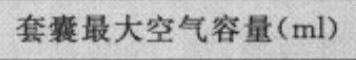
\includegraphics[max width=\textwidth]{2024_07_10_373f31b88d2bf633007bg-366}
 & 最大ETT \\
\hline
1 & $<5$ & 5.25 & 11.5 & 4 & 3.5 \\
\hline
1.5 & $5 \sim 10$ & 6.1 & 13.5 & 7 & 4.0 \\
\hline
2 & $10 \sim 20$ & 7.0 & 15.5 & 10 & 4.5 \\
\hline
2.5 & $20 \sim 30$ & 8.4 & 17.5 & 14 & 5.0 \\
\hline
3 & $30 \sim 50$ & 10 & 22 & 20 & 6.0 (套顜) \\
\hline
4 & $50 \sim 70$ & 10 & 22 & 30 & 6. 5 (套靚) \\
\hline
5 & 成人 & 11.5 & 23.5 & 40 & 7.0 (隹囊) \\
\hline
\end{tabular}
\end{center}

※唋罩导管可通过的最大气管导管号数

\section*{第四节 全身麻醉}
\section*{一、吸入麻醉}
\begin{enumerate}
  \item 吸入麻醉药理小儿与成人的不同点
\end{enumerate}

(1) 血气分配系数: 新生儿血气分配系数低于成人,因而诱导及苏醒皆快。常用吸人麻醉药新生儿的分配系数见表 3-11-12。

(2)肺泡最低有效浓度 (MAC): MAC 因年龄而改变,不同年龄小儿 MAC 见表 3-11-13。

表 3-11-12 新生儿吸入麻醉药血/气分配系数与成人比较

\begin{center}
\begin{tabular}{|c|c|c|c|c|c|}
\hline
年龄 & 廉烷 & 恩筫烷 & 昇角烷 & 七畄皖 & 地氛烷 \\
\hline
新生儿 & 2.14 & 1.78 & 1.19 & 0.59 & 0.51 \\
\hline
成人 & 2.3 & 1.9 & 1.4 & 0.72 & 0.62 \\
\hline
\end{tabular}
\end{center}

表 3-11-13 不同年龄小儿吸入麻醉药的 MAC

\begin{center}
\begin{tabular}{|c|c|c|c|c|c|}
\hline
年龄 & 炁烷 & 恩笑烷 & 异氟烷 & 七筑烷 & 地炁烷 \\
\hline
新生儿 & 0.87 & - & 1.6 & 3.3 & 9.16 \\
\hline
$1 \sim 6$ 个月 & 1.2 & 2.4 & 1.87 & 3.2 & 9.42 \\
\hline
$6 \sim 12$ 个月 & 0.97 & - & 1.8 & 2.5 & 9.92 \\
\hline
$3 \sim 5$ 岁 & 0.91 & 2.0 & 1.6 & 2.5 & 8.62 \\
\hline
成人 & 0.75 & 1.68 & 1.15 & 2.05 & 6.0 \\
\hline
\end{tabular}
\end{center}

一般新生儿、早产儿的 MAC 随月龄增加而增大, $1 \sim 6$ 个月最高,新生儿恩氟烷 MAC 较 $1 \sim 6$ 个月巽儿小 $25 \%$, 异身烷、帮烷小 $15 \%$ 。此后随年囹增长 MAC 逐渐下降, 每 10 岁约下降 $6 \%$ 。

小儿心血管容易受麻醉药抑制,应用等量麻醉药浓度,新生儿低血压发生率为 1 6 个月婴儿的 2 倍多,而应用等效浓度氟烷 (1 MAC)其心率㖪慢及血压下降程度相同, 地举烷情况相似。各类麻醉药随吸人浓度(麻醉深度)的增加,均对小儿心血管及呼吸有相应程度的抑制作用,但大于成人,对新生儿、早产儿的影响可能更为严重。小儿吸人全麻诱导及苏醒均快,其原因与下列因素有关: 肺泡通气量与功能残气量的比值较大; 小儿心排血量大部分分布到血管丰富的组织,包括脑、肾、内脏及内分泌腺等;小儿血/气分配系数较成人低。基于上述原因,新生儿达到与成人相等的脑内麻醉药水平,所需时间仅为成人的 $1 / 4$ 。

\begin{enumerate}
  \setcounter{enumi}{1}
  \item 吸入全身麻醉的方法
\end{enumerate}

(1) 诱导

(1)面罩吸人诱导。由于七赤烷的无刺激香味,明显增加了吸人诱导的应用。吸人 $8 \%$ 七氰烷忠儿可在 $1 \mathrm{~min}$ 左右迅速人睡, 小于 6 个月的繁儿 MAC 小, 且循环容易遭受抑制, 没特殊需要不必追求此高速度,加人 $50 \% \sim 70 \% \mathrm{~N}_{2} \mathrm{O}$ 适.当减低七氛烷浓度, 至嚼肌松驰窥喉表麻后插管, 肌松药的应用根据需要。对已进人基础麻醉状态的小儿亦可直接吸人刺激性较小的麻醉药诱导。婴幼儿诱导后应妥善固定和保护四肢。

(2)静脉诱导: 等效剂量的各种短效静脉麻醉药和肌松药皆可用于诱导,加用芬太尼类 (如芬太尼 $2 \mu \mathrm{g} / \mathrm{kg}$ ) 可减轻插管应激反应。药物种类繁多,尚无固定的最佳组合方案, 应根据具体情况酌定。一般人室后先开放静脉,绶慢静注诱导药(如丙泊酚,硫喷妥钠或氯胺酮等), 人睡后注人氯琥珀胆㖅,或其他插管剂量的非去极化肌松药, 选择合适的面罩给氧去氮后插管。如无合适的麻醉机,婴儿可用供氧管直接连接婴儿面罩, 将氧流量调到 $4 \mathrm{~L} / \mathrm{min}$ 左右,间断紧扣在小儿口鼻上以进行通气、供氧和去氮。面罩正压吸氧时要注意保持呼吸道通畅, 尤其无才小儿。繁幼儿也可用羟丁酸钠稀释至 $12.5 \%$浓度后缓慢静注, 全量 $(100 \sim 125 \mathrm{mg} / \mathrm{kg}) 5 \mathrm{~min}$ 左右注完, 过 $3 \sim 5 \min$ 进人深睡后,咽喉反射抑制,再以 $2 \%$ 利多卡因表面麻醉后, 不用肌松约, 直接插管。

(3)肌注诱导。对不能合作的患儿,难以用通常方法诱导时, 可在搫肌注射氯胺酮 $5 \sim 8 \mathrm{mg} / \mathrm{kg}$, 人睡后接用其他麻醉约诱导插管及维持。

(2)维持: 小儿常用的麻醉装置有 T 形管法和紧闭法。Mapleson 环路系统及其改良型, 均属半开放法, 麻醉气体浪费较大, 环境污染较严重, 操作管理也无特殊优点,国内少有应用。Bain环路虽曾一度试用,并未得到推广,各种环路系统产品市场也少有供应。近来新型小儿与成人通用的麻醉机,潮气量最小可调至 $20 \sim 30 \mathrm{ml}$ 。配有多种呼吸参数及呼吸功能监测装置, 可自动补偿通气系统因各种因素造成的无效腔, 使实际通气量与设置潮气量基本一致, 适用于成人及各年龄小儿的紧闭法麻醉,正在推广。随科技的进步,新机型会不断出现,但一切改进都是根据临床的需要。设计更加精确, 使设定值与实际值更加接近, 功能更全面, 不仅附有监测部分, 且监测指标可以随意扩展使用更安全方便,但不能代替管理的决策。

(1)T 形管法。构造简单,在气源输出导管远端接一内径合适的 $\mathrm{T}$ 形管, 纵臂一端接气管导管一端开放横臂接气源, 需辅助或控制呼吸时, 横臂与气源间加一小气輁( 通常用乳胶手套可代替), 属开放法, 适用于婴幼儿手术。新生儿及小婴儿不必加气囊, 自主呼吸时, 吸人空气和氧的混合气体, 做辅助或控制呼吸时,可以用拇指腹轻按呼出端口, 根据听诊呼吸音(略强于正常呼吸音)及目测胸廊运动幅度, 决定按管口时间及氧流量 (通常 $3 \sim 4 L /$ $\mathrm{min}$ ), 控制呼吸时呼吸次数 $20 \sim 30 / \mathrm{min}$ 。 2 3 岁以上需辅助或控制呼吸时, 可在横臂加呼吸踑但需\\
双手同步操作, 吸气时左拇指按呼出端口, 右手握挤气襄, 呼气时双手同时松开, 供氧流量以加压时能维持气荼充盈为度, 婴幼儿需 $3 \sim 5 \mathrm{~L} / \mathrm{min}$ 。控制呼吸次数稍少于正常呼吸次数, 参照年龄正常呼吸次数(表 3-11-14)。

缺点是需两手同时操作, 且麻醉药浪费较多,空气污染较重。在暂无新型麻醉机的基层医院, 对 6 岁以前小儿, 尤其婴幼儿, 即使较大手术, 因可做辅助及控制呼吸, 在 $\mathrm{SpO}_{2}$ 监测下麻醉, 仍不失为一种可供选择的方法。

(2)循环紧闭法。新型小儿和成人通用的紧闭法麻醉机, 控制呼吸操作方便, 性能稳定, 节省麻醉气体, 减少环境污染, 调控性好, 备有定容、定压 2 种通气模式, 可以根据需要选择和随时转换应用。配有多种呼吸参数及气体监测系统, 可以实时监测呼吸情况。定容法: 设置潮气量 $7 \sim 10 \mathrm{ml}$, 呼吸次数可略少于正常, 婴儿、新生儿在 $20 \sim 30 / \mathrm{min}$, 开机后在保持气道压 $\leqslant 20 \mathrm{cmH}_{2} \mathrm{O}$ 前提下, 通过调整使 $\mathrm{P}_{\mathrm{ET}} \mathrm{CO}_{2}$ 保持在 $35 \sim 40 \mathrm{mmHg}, \mathrm{P}_{\mathrm{ET}} \mathrm{CO}_{2}<35 \mathrm{mmHg}$ 表明通气过度, 应减少呼吸次数, $\mathrm{P}_{\mathrm{ET}} \mathrm{CO}_{2}>45 \mathrm{mmHg}$, 表明通气不足, 应增加呼吸次数, 如气道压明显低于 $20 \mathrm{mmHg}$, 且呼吸次数已在正常范围则应增加潮气量; 定压法: 设置气道压 $\leqslant 20 \mathrm{cmH}_{2} \mathrm{O}$, 呼吸次数参照正常值, 开机后根据 $\mathrm{P}_{\mathrm{ET}} \mathrm{CO}_{2}$, 通气过度减少呼吸次数, 通气不足增加呼吸次数, 直至 $\mathrm{P}_{\mathrm{ET}} \mathrm{CO}_{2}$ 稳定在士 $40 \mathrm{mmHg}$ 。由于小儿氧耗大, 分钟通气量远大于成人, 据笔者观察成人 $\pm 100 \mathrm{ml} / \mathrm{kg}$, 而婴幼儿可达到 $150 \sim 200 \mathrm{ml} / \mathrm{kg}$ 。笔者单位用至体重 $3.0 \mathrm{~kg}$ 的新生儿, 应用此 2 种方式均顺利完成麻醉, 初步体会定压法似比较容易调控。尽管国外在阻力、死控等问题上还存在异议, 我科应用 10 余年, 均顺利完成麻醉, 现已常规使用。但毕竟价格昂贵, 暂未购置时,在能监测 $\mathrm{P}_{\mathrm{ET}} \mathrm{CO}_{2}$ 和气道压条件下, 将成人麻醉机更换成小儿风箱和细罗纹管, 以减少胘胀死腔影响, 细心管理仍可替代使用。根据我科以往经验,在 $10 \mathrm{~kg}$ 以上小儿, 均曾安全使用。吸气阻力靠机械或手法控制或辅助呼吸克服, 呼出阻力 (PEEP)在 $3.0 \mathrm{cmH}_{2} \mathrm{O}$ 以下, 对小儿无明显不利影响。一般只能用定容法, 呼吸参数设定、调整的原则及方法同上, 只是机器显示各值不够精确, 误差较大, $\mathrm{P}_{\mathrm{ET}} \mathrm{CO}_{2}$ 与气道峰压的监测与调整是最关键的环节。尤其手法操作更需要细心和经验, 努力保持压力均衡和节律规整。由于患儿个体间差异, 术中必须根据 $\mathrm{P}_{\mathrm{ET}} \mathrm{CO}_{2}$ 值调整呼吸参数, Gadgwell报道的死腔补偿公式, 如不是固定使用一台麻醉机, 因各台机间死腔差异明显,实际应用困难。

(3) 麻醉用药: 可用一种或数种吸人药复合吸人或吸人与静脉麻醉药复合。

\section*{二、静脉麻醉及静脉复合麻醉}
由于小儿药动学的进展和新短效药物如丙泊酚和瑞芬太尼进人临床, 使小儿全麻包括婴儿和儿童静脉麻醉已跨人一个全新阶段。新生儿和㜟儿的分布容积大, 清除率低, 在生后早期各种药物受体的密度, 血一脑屏障的通透性都未发育成勲, 不同年龄间药效学有很大的差异, 但都可以安全有效地应用于婴儿和儿童。由于这些新药的开发, 可以根据患儿需要在大范围内进行药物的选择和复合应用,明显地提高了麻醉效果和安全水平。

\begin{enumerate}
  \item 硫喷妥钠 新生儿脑组织血流供应相对较高, 脑摄取量远超过成人, 一项研究报道, 新生儿诱导 $\mathrm{ED}_{50}$ 为 $(3.4 \pm 0.2) \mathrm{mg} / \mathrm{kg},<6$ 个月为 $(6.3 \pm$ $0.7) \mathrm{mg} / \mathrm{kg}$, 新生儿诱导量少的另一原因是因为血浆中与蛋白结合率低, 游离部分较多, 为成人的 $1.5 \sim 2.0$ 倍, 故对硫喷妥钠特别敏感。 1 个月后逐渐增加, 但小儿清除较慢, 不宜持续静脉滴人。主要用于全麻诱导, 基础麻醉 (肌注或直肠蓶注) 和局麻药中毒和破伤风患儿的抗痉挛治疗以及单次剂量作用时间内能完成的小手术和处置。新生儿和婴幼儿用 $1 \% \sim 1.25 \%$, 较大儿童用 $2 \% \sim 2.5 \%$ 溶液静脉缓慢注射 $4 \sim 6 \mathrm{mg} / \mathrm{kg}$ (新生儿 $3 \sim 5 \mathrm{mg} / \mathrm{kg}$ ),可使患儿在短时间内意识消失, 进行预定的操作。注射过快可引起明显的呼吸抑制和血压下降。

  \item 氧胺酮由于其强效的镇痛和麻醉作用, 成为小儿最常用的静脉麻醉药之一, 也常用于手术室外的麻醉。可静脉注射、肌内注射和口服, 后 2 种方法多用于手术前给药, 术后幻觉、䜾梦等副作用较少见。由于药代学的差别, 等效剂量因年

\end{enumerate}

表 3-11-14 不同年龄小儿呼吸次数

\begin{center}
\begin{tabular}{ccccccccc}
\hline
年龄 & $0 \sim 24 \mathrm{~h}$ & $1 \sim 7 \mathrm{~d}$ & $8 \sim 30 \mathrm{~d}$ & $3 \sim 12$ 个月 & $1 \sim 3$ 岁 & $3 \sim 5$ 岁 & $8 \sim 12$ 岁 & $12 \sim 16$ 岁 \\
\hline
㭔吸 $(/ \mathrm{min})$ & $40 \sim 50$ & $30 \sim 50$ & $30 \sim 50$ & $25 \sim 35$ & $25 \sim 35$ & $25 \sim 30$ & $20 \sim 25$ & $16 \sim 25$ \\
\hline
\end{tabular}
\end{center}

龄而异,按毫克/千克计算控制体动剂量不同,小于 6 个月㜟儿为 6 岁儿童的 4 倍 (表 3-11-15)。适用于小儿诱导、各种短小的体表手术及诊断性检查,可与其他麻醉药复合应用于创伤剌激较强手术的麻醉维持, 麻醉前需用扰胆碱能药物抑制呼吸道分泌。年长儿伍用苯二氮蓄类药物以减少麻醉后的堿梦、幻觉等精神症状。精神分裂症、血压高、顾内高压的患儿禁用。静注首次剂量 $1 \sim 2 \mathrm{mg} / \mathrm{kg}, 30 \sim$ $90 \mathrm{~s}$ 显效,维持 $5 \sim 10 \mathrm{~min}$ 后可追加 $1 \sim 1.5 \mathrm{mg} / \mathrm{kg}$ 。哭闹的患儿可肌注 $5 \sim 8 \mathrm{mg} / \mathrm{kg}, 3 \sim 5 \mathrm{~min}$ 人睡,维持 $10 \sim 20 \mathrm{~min}$, 镇痛效果可维持 $20 \sim 40 \mathrm{~min}$ 。追加时经静脉通路剂量 $1 \sim 1.5 \mathrm{mg} / \mathrm{kg}$ 。用药后血压上升,心率增快。有时出现与手术刺激无关的无意识的体动, 肌张力增强。剂量偏大或注药速度快时可出现呼吸抑制, 要做好吸氧和辅助通气的准备。单独应用氯胺秱, 苏醒时常有精神异常兴奋现象,如哭闹、躁动、呕吐等可给予适量镇静约。随氯胺酮药理学研究的深人,最近发现对成人有抗痛觉敏化和抗前炎因子作用,在小儿是否存在还有待证实,其对人脑组织发育的促凋亡性质也尚需确定,大剂量应用于小儿的安全性有待进一步研究,所以不建议长时间持续滴注使用。

表 3-11-15 不同年龄的顶胺酮药代动力学趡数

\begin{center}
\begin{tabular}{cccc}
\hline
年龄 & $\mathrm{T}_{1 / 2 \beta}(\mathrm{min})$ & $\mathrm{VD}_{\mathrm{Ss}}(\mathrm{L} / \mathrm{kg})$ & $\mathrm{CL}[\mathrm{ml} /(\mathrm{min} \cdot \mathrm{kg})]$ \\
\hline
$<3$ 个月 & 184.7 & 3.46 & 12.9 \\
$4 \sim 12$ 个月 & 65.1 & 3.03 & 35.0 \\
4 岁 & 31.6 & 1.18 & 25.1 \\
成人 & 107.3 & 0.75 & 20.0 \\
\hline
\end{tabular}
\end{center}

\begin{enumerate}
  \setcounter{enumi}{2}
  \item $\gamma$-舡丁酸钠 $(\gamma-\mathrm{OH}) \quad \gamma-\mathrm{OH}$ 是 GABA 的中间代谢物,主要作用于大脑皮质的灰质,海马回和边缘系统。抑制经中枢和末梢突触的冲动传导,而无镇痛作用。是一种催眠性全麻药。通过血-脑屏障较慢起效较慢,静脉注射 $20 \sim 30 \mathrm{~min}$ 后达作用高峰,作用持续 $60 \sim 90 \mathrm{~min}$ 。对脑血流量无影响, 不增加预内压。静注后常有心率减慢,收缩压轻度升高,脉压变大,心排血量无变化或略有增加。呼吸频率略减慢,潮气量增大,每分钟通气量略有增加。对肝肾功能无影响。适用于婴幼儿和稍大儿童全麻的诱导和维持,尤其在危重患儿以及心胜手术患儿优点比较突出。㾚痻、惊厥患儿禁忌; 心动过缓、低钾血症、房室传导阻滞者应慎用。诱导剂量 100 $\sim 125 \mathrm{mg} / \mathrm{kg}$,缓慢静注后 $5 \sim 10 \mathrm{~min}$ 意识消失,下领松他, 咽喉反射抑制, 咽喉、气管稆膜表面麻醉后, 进行气管内插管, 年长儿常需复合其他麻醉药和(或)肌松药。麻醉后血压稍增高, 心率琙慢。首次用药后 $1 \mathrm{~h}$ 左右根据需要可补充首次剂量的 $1 / 2$维持麻醉。本药无镇痛作用, 常与氯胺酮复合应用。由于能抑制呼吸道反射,且维持时间较长, 又常用于气管异物的取出。副作用是诱导和苏醒期可出现雉体外系症状,表现为四肢肌肉不自主地颤动, 随麻醉加深或其他复合药的作用可自行消退;还可促使钾离子进人细胞内, 血钾稍有降低, 但在正常范围,一般不需处理。

  \item 依托味酯 依托味酯主要加强 GABA 对中枢神经的抑制作用。作用方式与对呼吸的影响与巴比妥类相似,降低呼吸频率和潮气量。依托咪酯主要被肔和血浆中的酯酶水解,分布半衰期 (2.6士 1.3) $\mathrm{min}$, 消除半衰期略小于成人。静脉注射后约 $30 \mathrm{~s}$, 患者即可意识消失, $1 \mathrm{~min}$ 时脑内浓度最高。在临床剂量范围内 $(0.1 \sim 0.4 \mathrm{mg} / \mathrm{kg}) 7 \sim 14 \mathrm{~min}$ 自然苏醒。依托咪酯无镇痛作用,可降低脑血流及代谢率,并与剂量相关。该药对心血管系统的影响很小,适合于心脏病及危重患儿的全麻诱导。其副作用为抑制肾上腺皮质醇的合成,不论是长时间持续静脉滴注还是单次注射均可产生。小儿诱导剂量 $(0.3 \mathrm{mg} / \mathrm{kg})$ 即可明显抑制手术应激引起的皮质醇增加。单次给药抑制作用短暂,但在儿童静脉滴注输人后, 可持续数小时之久, 故不建议持续滴注。

  \item 丙泊酸 根据国内外药动学和药效学方面的研究, 尽管结果并不完全一致,但与成人比较,小儿丙泊酚的分布容积较大 (小儿 $0.52 \mathrm{~L} / \mathrm{kg}$, 成人 $0.27 \mathrm{~L} / \mathrm{kg}$ ), 中央室较大和清除率较高, 这一认识结论是一致的,没有理论依据提示应该限制丙泊酚用于 3 岁以下小儿。由于丙泊酚诱导起效快, 苏醒迅速,且功能恢复完善,术后恶心呕吐发生率低等特点和越来越受瞩目的对机体的保护作用,包括抗氧化作用, 保护脑血流自身调节功能, 麻醉中婴儿体温随环境温度下降时氧耗并不增加以及能降低顾内压、眼内压和 $\mathrm{CMRO}_{2}$, 对脑可能产生的保护效应,胸壁顺应性增加等,使其在小儿全麻诱导、镇静麻醉、手术室外麻醉、复合麻醉的辅助麻醉药和 PICU 镇静中的应用日益增加。按体重计算小儿丙泊酚的诱导剂量较大, 但存在个体差异,一般 10〜 15 岁的儿童, $1.5 \mathrm{mg} / \mathrm{kg}, 3 \sim 9$ 岁的儿童 $2.5 \mathrm{mg} /$ $\mathrm{kg}$, 而 3 岁以下者则需 $3 \sim 3.5 \mathrm{mg} / \mathrm{kg}$ 。由于小儿静注后蓄积现象不明显, 可反复静脉注射或静脉持续\\
点滴用药,维持期的输注速率也较成人高,小儿年龄愈小,按体重计算所需丙泊酚的剂量愈大。适用于小儿麻醉诱导, 镇静麻醉, 复合麻醉中的辅助用药。诱导剂量 $2 \sim 3 \mathrm{mg} / \mathrm{kg}(<2$ 岁小儿诱导用量可超过 $3 \mathrm{mg}$ ), 缓静脉注射 ( $>30 \sim 60 \mathrm{~s}$ ) 2 3min 加用肌松药可顺利进行气管插管。注药快时血压下降,心率减慢, 停药后多能自行恢复, 必要时加快输液或静脉注射麻黄碱。持续静滴用于镇静麻醉、手术室外麻醉和复合麻醉, 有 2 种给药方式。

\end{enumerate}

(1)静脉点滴或用输液泉持续静注: 大儿童诱导后, 先以 $10 \mathrm{mg} /(\mathrm{kg} \cdot \mathrm{h})$ 的速度输人丙泊酚, $10 \mathrm{~min}$ 后减为 $8 \mathrm{mg} /(\mathrm{kg} \cdot \mathrm{h})$, 然后根据各项临床指标调整输注速度, 逐步减至 $6 \mathrm{mg} /(\mathrm{kg} \cdot \mathrm{h})$ 左右。婴儿剂量可适当增加, 参照 15〜13〜11〜10〜9mg/(kg $\cdot \mathrm{h})$原则递减至预期浓度。一般认为丙泊酚的意识恢复时的血药浓度为 $1 \mu \mathrm{g} / \mathrm{ml}$, 术中应维持大于该浓度, 调整输注速度时应以血药浓度 $2.5 \sim 3 \mu \mathrm{g} / \mathrm{ml}$ 为目标。如果与其他麻醉药合用或出现循环抑制时,应减少丙泊酚剂量, 手术后 ICU 镇静用量应 $\leqslant$ $3 \mathrm{mg} /(\mathrm{kg} \cdot \mathrm{h})$ 。

(2) 靶控输注: 目前已有丙泊酚专用的靶控输注奀, 输人患儿的年龄、性别和体重即可输人相应靶浓度的丙泊酚。丙泊酚的副作用除与注射速度有关的呼吸循环抑制外与小儿关系密切的是注射痛, 静脉越细越明显, 可以用利多卡因 $0.1 \mathrm{mg} / \mathrm{kg}$给药前静注或与丙泊酚混合后静注都可以缓解。另外, 应引起注意的是静滴速度 $>4 \sim 5 \mathrm{mg} /(\mathrm{kg}$ h) 持续 $48 \mathrm{~h}$ 以上, 有可能发生罙见的、致死性丙泊酚输注综合征。据现有报道,小儿多于成人,高脂血症是主要病理生理改变, 心力衰竭是最终死因,乳酸酸中毒是早期临床征象。急性感染和呼吸道感染者禁用。\\
6. 味达唑仑 在小儿除静注外肌内注射、口服及直肠给药都有研究报道。后三种途径给药后血浆浓度达峰值时间分别为 $15 \mathrm{~min} 、 30 \mathrm{~min}$ 和 $53 \mathrm{~min}$,其清除和生物利用率分别为 $10.4 、 50.8$ 和 $33.4 \mathrm{ml} /(\mathrm{kg} \cdot \mathrm{min})$ 和 $87 \% 、 18 \%$ 和 $27 \%$ 。用于儿童静脉诱导剂量高达 $0.6 \mathrm{mg} / \mathrm{kg}$ 其作用尚不及硫喷妥钠, 故常复合其他麻醉药进行诱导。多用于辅助麻醉、手术前用约和手术后镇静。

\begin{enumerate}
  \setcounter{enumi}{6}
  \item 芬太尼类 主要作为镇痛和抗应激药用于复合麻醉, 芬太尼和瑞芬太尼最为常用。
\end{enumerate}

(1)芬太尼的药代学特点如分布容积和清除速度,各家报道还不一致。作为全麻药或辅助药可安全用于婴儿和儿童。复合其他麻醉药用于小儿诱导插管, 由于不明显抑制循环而用于小儿心胜直视手术, $20 \sim 50 \mu \mathrm{g} / \mathrm{kg}$ (最大 $100 \mu \mathrm{g} / \mathrm{kg}$ ) 即可为新生儿和婴儿心脏手术提供全身麻醉。但容易发生心跳过缓(对成人有利), 使繁儿心搏量减少, 可应用使心跳增快的迷走神经解药和肌松药进行拮抗, 呼吸抑制作用较强。

(2)瑞芬太尼为超短效阿片类药, 消除半衰期仅为芬太尼的 $1 / 6$, 在婴儿有最大的分布容积和最快的清除率, 但消除半衰期各年龄组相同 (3.4~ $5.7 \mathrm{~min}$ ), 研究提示新生儿和小儿瑞芬太尼的药动学特征与成人相仿, 对早产儿、足月儿都是一种良好的复合麻醉成分, 手术后恶心呕吐少见。经静脉途径给药, 负荷量 $1 \mu \mathrm{g} / \mathrm{kg}$, 继以 $0.25 \sim 1 \mu \mathrm{g} /(\mathrm{kg} \cdot$ $\mathrm{min}$ ) 的速率静脉输注, 在静脉注射或静脉输注的速度大于 $0.5 \mu \mathrm{g} /(\mathrm{kg} \cdot \mathrm{min})$ 时可能发生低血压和心动过缓, 当同时应用吸人麻醉药时, 推荐静脉输注瑞芬太尼的开始速度为 $0.25 \mu \mathrm{g} /(\mathrm{kg} \cdot \mathrm{min})$, 停药后痛觉迅速恢复, 应在停药前开始术后镇痛。阿片类药物临床应用剂量如表 3-11-16 所示。

表 3-11-16 小儿阿片类静注剂畳

\begin{center}
\begin{tabular}{llll}
\hline
\multicolumn{1}{c}{药名} & \multicolumn{1}{c}{负荷剂量} & \multicolumn{1}{c}{维持剂量} & \multicolumn{1}{c}{术后镇痛} \\
\hline
吗啡 & $2 \sim 3 \mathrm{mg} / \mathrm{kg}$ & $0.05 \sim 0.1 \mathrm{mg} /(\mathrm{kg} \cdot \mathrm{h})$ & $0.05 \sim 0.1 \mathrm{mg} / \mathrm{kg}$ \\
芬太尼 & $50 \sim 100 \mu \mathrm{g} / \mathrm{kg}$ & $1 \sim 3 \mu \mathrm{g} /(\mathrm{kg} \cdot \mathrm{h})$ & $1 \sim 2 \mu \mathrm{g} / \mathrm{kg}$ \\
舒芬太尼 & $10 \sim 15 \mu \mathrm{g} / \mathrm{kg}$ & $0.1 \sim 0.3 \mu \mathrm{g} /(\mathrm{kg} \cdot \mathrm{h})$ & - \\
阿芬太尼 & $150 \sim 200 \mu \mathrm{g} / \mathrm{kg}$ & $1 \sim 3 \mu \mathrm{g} /(\mathrm{kg} \cdot \mathrm{min})$ & - \\
瑞芬太尼 & $0.2 \sim 1.0 \mu \mathrm{g} /(\mathrm{kg} \cdot \mathrm{min})$ & $0.1 \sim 0.4 \mu \mathrm{g} /(\mathrm{kg} \cdot \mathrm{min})$ & - \\
氢吗啡閥 & $5 \sim 10 \mu \mathrm{g} / \mathrm{kg}$ & $3 \sim 5 \mu \mathrm{g} /(\mathrm{kg} \cdot \mathrm{h})$ & $3 \sim 5 \mu \mathrm{g} / \mathrm{kg}$ \\
\hline
\end{tabular}
\end{center}

\begin{enumerate}
  \setcounter{enumi}{7}
  \item 全隹静脉复合麻醉 针对催眠、镇痛、肌肉松驰及减轻应激反应四方面的基本要求, 根据各麻醉药的主要药理作用选用几种静脉麻醉药和辅助药复合应用,进行全身麻醉。基本是催眠与镇痛药的伍用, 根据需要加用肌松药, 充分发挥各药的优势作用,用最小有效剂量,合理利用药物相互之间的正面作用,剔除配伍禁忌, 以达到能充分满足临床需要的全身麻醉。用肌松药者呼吸管理同吸人麻醉。据近年对应激反应的研究发现芬太尼类除强效镇痛外还兼有较强的抗应激作用, 尤其是短效的瑞芬太尼和短效且对机体有保护作用的丙泊酚在复合麻醉中的应用,备受青睐。药物的具体组合配伍, 多种多样, 应根据病情需要, 个人经验和条件选定。列举几种常用复合方式。
\end{enumerate}

(1) 氯胺酮与羟丁酸钠复合麻醉: 是一种传统的常用复合方式。广泛用于小儿较小手术。麻醉前应给抗胆碱药和苯二氮草类药。麻醉诱导一般采用单次静注氯胺酮 $2 \mathrm{mg} / \mathrm{kg}$, 可根据患儿情况酌情增减, 缓慢推注 $1 \sim 2 \mathrm{~min}$ 后患儿人睡。应密切观察呼吸, 注意保持呼吸道通畅。然后静脉注射差了酸钠 $50 \sim 100 \mathrm{mg} / \mathrm{kg}$ 作为背景催眠, 还能加强并延长氯胺酮的作用。手术切皮时再追加氯胺酮 $1 \mathrm{mg} /$ $\mathrm{kg}$ 。以后每隔 $30 \sim 60 \mathrm{~min}$ 或麻醉转浅时再静注 $1 \mathrm{mg} / \mathrm{kg}$, 直至术毕。氯胺酮容易蓄积, 不适于长时间手术。

(2)神经安定镇痛: 主要用于小儿局麻、神经阻滞和椎管内阻滞时的催眠镇静。氟哌利多与芬太尼按 $50: 1$ 混合,称为依诺伐, 1U 内含鯑哌利多 $5 \mathrm{mg}$ 和芬太尼 $0.1 \mathrm{mg}$ 。用量一般按 $0.05 \mathrm{U} / \mathrm{kg}$ 分 2 $\sim 3$ 次静注。依诺伐催眠作用较弱, 要达到全身麻醉, 常需加用其他麻醉药。

(3)丙泊酚静脉复合麻醉: 丙泊酚可以与多种镇痛性药物伍用, 进行全凭静脉麻醉。此时丙泊酚主要作用催眠和增强镇痛。(1) 与芬太尼类复合药。先给芬太尼 $2 \mu \mathrm{g} / \mathrm{kg}$, 再静脉注射诱导量的丙泊酚。意识消失后可配合肌松药行气管内插管。维持时每 $30 \mathrm{~min}$ 追加一次芬太尼 $0.5 \mu \mathrm{g} / \mathrm{kg}$ 。丙泊酚的最适剂量因年龄而有所不同,大儿童为 $6 \sim 10 \mathrm{mg} /(\mathrm{kg} \cdot \mathrm{h})$,繁幼儿、新生儿 $9 \sim 15 \mathrm{mg} /(\mathrm{kg} \cdot \mathrm{h})$, 伍用芬太尼加氧化亚氮时丙泊酸可分别降至 $4 \sim 6 \mathrm{mg} /(\mathrm{kg} \cdot \mathrm{h})$ 和 $9 \mathrm{mg} /(\mathrm{kg} \cdot \mathrm{h})$ 以下, 此外丙泊酚与更短效的苏芬太尼、阿芬太尼、瑞芬太尼等伍用行复合麻醉可控性更好。(2)丙泊酚和氯胺酮静脉麻醉。氯胺酮的诱导量 $1 \sim 2 \mathrm{mg} / \mathrm{kg}$, 维持 $0.5 \sim 1 \mathrm{mg} /(\mathrm{kg} \cdot \mathrm{h})$, 根据麻醉时的体征调整各自的输注速度, 如血压下降时宜减慢丙泊酚, 增加氯胺酮的输注剂量。(3)丙泊酚同时伍用芬太尼加氯胺酮行全凭静脉麻醉。虽然由于靶控等先进技术进人临床, 使全凭静脉麻醉跨上一个新的台阶, 但由于小儿个体间差异, 群体间差异包括健康儿和患儿间, 不同疾病忠儿间, 同病种病情轻重忠儿间的差异以及手术刺激强度的变化等麻醉深度仍需随时进行调整, 静脉麻醉药的速度调整则远不及吸人药。所以静吸复合成为现代最普遍应用的全身麻醉方法, 也是小儿常用的麻醉方法。切记任何麻醉方法都不能以肌松药代替麻醉药加深麻醉。

\section*{三、肌肉松驰药在小儿的应用}
在婴幼儿时期神经肌肉接头发育未成熟,物理的、生化的都在发育, 肌肉收缩性在变化, 肌肉量在身体的比例在增加, 因而, 神经肌肉接头对肌松药的敏感性也随之在不断变化。还有, 由于小儿体液分布特点细胞外液比例相对较大, 也随年龄增长变化,而肌松药是水溶性的致使其表观分布容积、再分布、清除和代谢速度都在变化, 影响作用部位的药物浓度, 从而影响肌松药的药效 $\left(\mathrm{ED}_{50}, \mathrm{ED}_{95}\right)$ 和阻滞时间。生后早期由于体内分布容积较大, 临床上需要更大的负荷量才能达到预期的血药浓度。但由于神经系统的发育, 肌松药受体和乙酰胆碱的释放逐渐增加, 对肌松药的敏感性也在逐渐增加。反映在 $\mathrm{ED}_{95}$ 的变化上。应用于成人的肌松药基本都可用于小儿, 基于上述特点不同年龄剂量有所不同(表 3-11-17, 表 3-11-18)。

氯琥珀胆碱是目前临床唯一应用的去极化肌松药。由于潜在的肌病, FDA 曾经提出警告“小儿应用氯琥珀胆碱限于紧急插管或立即维持下呼吸道安全所必需” 和恶性高热的潜在危险, 人们不能不有所顾忌, 再加短效非去极化新肌松药的不断出现,临床应用有所减少, 但由于其速效短效的优点,至今仍在应用。氯琥珀胆碱是水溶性, 繁儿和儿童所需剂量较成人为大, 通常 $2 \mathrm{mg} / \mathrm{kg}$ 静注。在建立静脉通路前, 紧急需要插管时, 亦可肌内注射, 起效时间需 $3 \sim 4 \mathrm{~min}$, 剂量需增至 $3 \sim 4 \mathrm{mg} / \mathrm{kg}$ 。最常见的副作用是房室结性或突性心动过缓, 也有心搏骤停的报道, 为此,术前药中须给阿托品。\\
表 3-11-17 小儿肌松药插管剂量

\begin{center}
\begin{tabular}{|c|c|c|c|c|}
\hline
药物 & 剂量(mg $/ \mathrm{kg}$ ) & $\mathrm{ED}_{95}$ 倍数 & 静注插筞时间 (min) & $\mathrm{T}_{25}$ 时间 (min) * \\
\hline
美维松 & $0.2 \sim 0.3$ & $2 \sim 3$ & 1.5 & $5 \sim 15$ \\
\hline
罗库泬窑 & $0.6 \sim 1.0$ & 2 & 1.0 & $10 \sim 30$ \\
\hline
顺阿曲库轱 & $0.15 \sim 0.2$ & 5 & 1.5 & $45 \sim 75$ \\
\hline
阿曲库铵 & 0.5 & 2 & 3.0 & $20 \sim 45$ \\
\hline
维库溴铵 & $0.05 \sim 0.1$ & $1 \sim 2$ & 2.0 & $20 \sim 60$ \\
\hline
伴库渗轱 & 0.1 & $1 \sim 2$ & 2.5 & $45 \sim 60$ \\
\hline
氯琥珀胆嘓 & 2.0 & 6 & 1.0 & $3 \sim 5$ \\
\hline
\end{tabular}
\end{center}

※给药后肌松恢复到 $25 \%$ 时间

表 3-11-18 小儿肌松药术中维持剂量

\begin{center}
\begin{tabular}{|c|c|c|c|c|}
\hline
\multirow{2}{*}{药物} & \multicolumn{2}{|c|}{维持} & \multicolumn{2}{|c|}{$\mathrm{ED}_{95}(\mathrm{mg} / \mathrm{kg})$} \\
\hline
 & 单次静注 (mg/kg) & 连续静滴 $[\mu \mathrm{g} /(\mathrm{kg} \cdot \mathrm{min})]$ & 絫儿 & 儿童 \\
\hline
美维松 & 0.1 & $10 \sim 20$ & 0.1 & 0.1 \\
\hline
顺阿曲库䯃 & 0.1 & $1 \sim 5$ & 0.05 & 0.05 \\
\hline
维库溴銨 & 0.025 & 1 & 0.024 & 0.026 \\
\hline
罗库滜轱 & $0.3 \sim 0.5$ & 15 & 0.2 & 0.3 \\
\hline
泮库溴轱 & 0.05 & - & 0.05 & 0.05 \\
\hline
\end{tabular}
\end{center}

\section*{四、全身麻醉深度的判断}
近年来麻醉深度监测方法的研究, 取得了很多进展。如利用食管下段收缩性, 额肌肌电图, 心率变异性, 诱发电位, 脑电图能量谱分析, 双频谱分析等,基本都是反映大脑皮质和脑干受抑制程度,难以在手术中各种伤害性刺激存在条件下可靠地反映临床麻醉深度。目前多用于研究, 尚不能适应小儿临床麻醉的要求。小儿麻醉的深浅变化快,反映麻醉深浅的临床征象较难把握。传统的乙醚分期征象, 原本对小儿就不典型, 对于新的吸人麻醉药及静脉麻醉更不适用,再加不同年龄小儿其表现还有差异,特别是多种静脉和吸人麻醉药的复合应用,更增加了判断的难度。临床麻醉需要的是能达到催眠、镇痛、顺行遗忘、抑制应激反应和发挥麻醉药的保护作用而又血流动力学稳定, 不发生知晓的深度的客观指标。迄今尚没有一种仪器能满足上述要求。主要还是靠临床征象(包括意识、呼吸、循环、眼征、吞咽、肌肉张力、对刺激的反应等), 药物浓度和 (或) 给药速度、剂量 $[\mathrm{mg} /(\mathrm{kg} \cdot \mathrm{min})]$ 进行综合判断。即使评价较高的双频谱仪, 因小儿脑发育成熟度与年龄相关, 且在不断发育, 用于术中监测的意义远不如成人。从临床实际需要看判断麻醉的绝对深度的意义不太重要,深度对剌邀强度而言是相对的, 是需要根据刺激强强来随时调整的,目标是在意识消失和充分镇痛的基础上惐轻或抑制创伤或其他损伤刺激的感受和反应, 且对正常生理活动的抑制最小, 深度的下限是生理功能指标绝不能低于允许的生理范围。

\begin{enumerate}
  \item 自主呼吸不插管麻醉 多为短小手术或镇静麻醉主要根据给药速度、剂量, 眼睑反射消失, 手指肌松驰 (随意被动伸开)表明已达相当深度。呼吸抑制(频率减慢,幅度减小), $\mathrm{SpO}_{2}$ 下降表明麻醉偏深或给药偏快,手术刺激时体动表明麻醉过浅。

  \item 自主呼吸插管麻醉 多为中小手术或需控制保护呼吸道的手术 (如五官科手术)。适宜深度的基本指标为耐受导管。同时参照给药速度、剂量、呼吸抑制、手术刺激体动,除反射性(如眼心反射)原因外,一般血压、心率变化在生理范围内且波动较小。

  \item 插管麻醉辅助呼吸 用于各部位长时间大或较大手术。因有自主呼吸存在耐受导管仍属重要指标之一, 除给药速度、剂量、手术刺激体动之外,泪腺分泌增加、血压、心率变化也有重要参考价值。非心脏原因的心率过快, 往往是应激反应过强,麻醉偏浅。

  \item 机械通气控制呼吸各部位长时间大或较大手术,由于肌松药的应用耐受导管已无指标意义,给药速度、剂量,特别是复合应用数种药物的综合效应和血压、心率已成为最主要的指标。泪腺分泌增加仍有意义。所以对吸人药的 MAC 值, 静脉麻醉药的作用强度、等效剂量、单次量、输注速度、每小时剂量等均应熟记。小儿心血管容易受抑制,且.发生在脑中枢抑制之前,所以血压已成为判断麻醉深浅的重要指标, 这也是强调测量血压的理由之一。麻醉诱导和维持当中出现心跳过缓和血压下降首先应想到麻醉“过”深,不论是否还有其他原因,一旦发现均应立即停止或减浅麻醉,倘属其他原因所致,在判明并得到解决或明显改善后,再重行加深麻醉。但更不能失之过浅,尤其在应用肌松药后呛咳、体动等反应都不能出现,为追求术后苏醒快, 以肌松药解决麻醉偏浅,使伤害性感受得不到抑制, 应激反应增强,甚而患儿知晓,不仅影响术中经过,增加患儿痛苦,还可影响术后恢复。总之,对小儿麻醉深度的判断主要有赖于施麻醉者的全面细心观察和经验积果,客观的监测手段有待进一步研究和探索。

\end{enumerate}

\section*{五、全麻苏醒期的处理}
苏醒期是小儿术后高危期,小儿全麻尽管苏醒较快,但在苏醒过程中呼吸道问题远较成人多发,发生率达 $4 \% \sim 5 \%$ 。小儿围术期心搏骤停近 $50 \%$是由于苏醒期的呼吸问题。

\begin{enumerate}
  \item 停止给麻醉药和肌松药的时间 应根据预计手术时间选择作用时间相应的药物,术中注意观察手术的进度,决定停药时间。目前临床常用麻醉药多为短效,苏醒延迟已明显减少, 如停药过早, 麻醉太浅,小儿吞咽频繁,容易发生拔管前呕吐及拔管后喉痉挛,且影响手术后期处理(如㪘料包扎、石高固定等)。苏醒不充分,需在手术室或苏醒室观察,观察的时间还有赖于施麻者判断。对小儿苏醒的评估,即使有些征象表明小儿已 “清醒”,但并不说明小儿已恢复到正常生理状态。许多生理反射并未恢复正常, 何况这些功能本来就未发育成熟,呼吸道梗阻随时都可能发生。

  \item 拔管时机 拔管的必需条件是自主呼吸平

\end{enumerate}


\includegraphics[max width=\textwidth, center]{2024_07_10_373f31b88d2bf633007bg-373}\\
生儿 $88 \% \sim 94 \%$ )。拔管后在能自己维持呼吸道通畅条件下呼吸空气,观察 $5 \mathrm{~min}$ 左右 $\mathrm{SpO}_{2}$ 无下降,表明呼吸功能已恢复到可维持正常生理需要的通气和换气,方可送回。已留置胃管和疑有胃内容或大量气体潴留者拔管前应用胃管吸净胃内容,以避免发生反流误吸和腹胀。拔管时机可有两种选择。

(1)清酲拔管,即患儿清醒或基本清醒上呼吸道反射已恢复条件下拔管,临床多用。优点是拔管后可立即送回病房,节省在手术室停留时间。拔管前 2~3min 静注利多卡因 $1.0 1 .5 \mathrm{mg} / \mathrm{kg}$ 可以减轻呼吸道反应。

(2)“深”麻拔管,是指自主呼吸恢复已达拔管条件,但意识未恢复状态下拔管。在有些手术需保证拔管前后呼吸平稳, 无躁动不安时采用, 继续吸人麻醉药至拔管前在患儿安稳状态下拔管,但拔管后必须观察到清醒,由于 Sev 或 Des 等苏醒快, 停药后清醒也很迅速。最好避免在“深”麻向清醒过渡期间拔管,此时呼吸道反应活跃容易发生喉痉挛、呛咳、屏气、缺氧、呕吐、误吸,尤其在敏感呼吸道患儿。困难呼吸道和口腔领面部手术,拔筞后难以保持呼吸道通畅患儿应待完全清醒后拔管,必要时带导管送回 PICU 病房或特护病房。羟丁酸钠静脉麻醉时, 作用时间长, 容易发生苏醒延迟, 应予注意。危重症手术、心胜手术或手术后病情色重不能脱离呼吸机者,应在机械通气下送回 PICU 病房。

\begin{enumerate}
  \setcounter{enumi}{2}
  \item 全身状态综合评估 手术结束后小儿循环功能一般变化较小。但小儿全血量少对术中出血量的影响仍必须审慎估计,“小”量出血也可造成休克。对有心血管和(或)其他重要并存病的长时间,大手术、仜重病、急诊手术等应注意全面评估,对有器官功能受累、血压不稳定或需血管收缩药维持者应送 PICU 病房进行呼吸循环监测及治疗,无 PICU 病房则应给予特护。术后仍需继续输液及输人药物患儿,手术结束后及运送途中既要保持输液路通畅更要避免速度过快和过量,以免发生超负荷肺水肿和药物过量。

  \item 苏醒期谅妄躁动 原因比较复杂,诸如麻醉前焦虑恐惧,诱导不平稳,维持麻醉应用七䅀烷、地匑烷或氯胺酮,低氧血症,瑞芬太尼停药后痛觉的迅速恢复和导尿管的刺激等均引发,对小儿内环境稳定和术后恢复有诸多不利影响, 应给予适量的镇痛镇静药, 如芬太尼 $1 \mu \mathrm{g} / \mathrm{kg}$, 曲马朵 $1 \sim 2 \mathrm{mg} / \mathrm{kg}$,或在有效镇痛基础上给予丙泊酚 $0.5 \mathrm{mg} / \mathrm{kg}$ 或味达唑仑 $0.02 \mathrm{mg} / \mathrm{kg}$ 等,尽快使之安静。同时认真査明有无低氧血症、低血容量、低血糖等情况,并根据指征给予相应处理解决。术前给可乐定、芬太尼\\
有一定预防作用。

  \item 恶心、呕吐 可给予㲷哌利多 $20 \sim 75 \mu \mathrm{g} /$

\end{enumerate}

$\mathrm{kg}$, 或恩丹西酮 $0.05 \sim 0.1 \mathrm{mg} / \mathrm{kg}$ 等防治。

\section*{第五节 区域麻醉}
局部麻碎、区域阻滞、硬膜外及蛛网膜下腔阻滞等区域麻醉在小儿的应用与成人不同,一般是在全身麻醉下施行的。以往认为小儿不能合作, 不是应用的对象。最近认识到, 不仅仅是解除疼痛, 改善麻醉效果, 更重要的是惐少全身麻醉的负面作用, 减轻创伤刺激的上传, 从而减轻神经内分泌反应, 既可使手术经过更平顺, 还可用于术后镇痛, 缩短住院时间, 所以其在小儿的应用已逐步得到认可。

\section*{一、小儿局麻药药理特点}
局麻药的选择不仅考虑起效时间和作用持续时间, 更要考虑其安全性。小儿特别是新生儿在神经发育过程中面临直接神经毒性的最大危险, 因此要尽量避免高浓度局麻药的使用。酯类局麻药如丁卡因, 由血浆中胆碱酯酶代谢, 与年龄关系很小,故仍应用于新生儿㜟儿脊麻。酰胺类在肝内代谢,在血液中首先与蛋白结合, 其中左旋布比卡因和罗哌卡因 $90 \%$ 以上与 $\alpha$-酸性糖蛋白 (高亲和力) 和蛋白(高容量相对低亲和力) 结合, 故血药浓度较低。酰胺类的利多卡因与蛋白结合少,代谢产物抑制与其降解有关的内生酶, 消除半衰期长, 分布容积大,给药后血浆中游离部分占 $30 \% \sim 40 \%$ (而左旋布比卡因和罗哌卡因只有 $4 \% \sim 7 \%$ ), 血浆浓度高。当血浆浓度 $2 \sim 4 \mu \mathrm{g} / \mathrm{ml}$ 时有抗惊肷作用, $10 \mu \mathrm{g} / \mathrm{ml}$ 时则可致惊痛, 脐带血浓度 $2.5 \mu \mathrm{g} / \mathrm{ml}$ 即可抑制 Apgar评分, 说明利多卡因对小儿毒性较大, 现已基本不用于繁幼儿的硬膜外及蛛网膜下腔阻滞。常用药物允许最大剂量见表 3-11-19。

\section*{二、麻醉方法}
\begin{enumerate}
  \item 硬蓦外阻滞 小儿硬膜外阻滞对心血管的影响与成人不同, 麻醉后交感神经阻滞所引起的低血压仅见于 10 岁以上较大儿童, 可能与小儿血液主要集中于中心循环, 下肢血容量较成人相对少,对血容量不足主要靠心胜代偿, 以及小儿外周血管阻力低而稳定, 血管扩张对血液动力影响较小, 交感神经发育未成熟等有关。如麻醉前已有低血容量,阻滞后仍可发生低血压。随骶管阻滞的推广,硬膜外阻滞在婴幼儿的应用已明显减少, 多用于较大儿童。小儿皮肤至硬膜外间隙的距离较短, 黄韧带较薄, 负压又不明显, 判断进人硬膜外腔的突破感和气泡压缩试验均不如成人明显, 所以需由有经验的医师穿刺。硬膜外腔注空气试验有引起空气检塞的可能,故判断注射阻力以注射生理盐水为好。小儿硬脊膜外腔神经干细, 鞘膜薄, 麻醉作用较成人出现快。常用药物 $0.25 \%$ 布比卡因或 $0.2 \%$ 罗哌卡因胸段 $0.3 \mathrm{ml} / \mathrm{kg}$ (最大 $12 \mathrm{ml}$ ), 腰段 $0.5 \mathrm{ml} / \mathrm{kg}$ (最大 $15 \mathrm{ml}$ ), 利多卡因在繁幼儿允许剂量范围内难以达到满意的麻醉效果,已少使用,在大儿童的应用可参照成人。

  \item 䟡管阻滞 小儿硬脊膜末端距骶尾韧带 2~ $3 \mathrm{~cm}$, 相当于第 2 骶椎水平, 呧管穿刺比较安全易行。小儿骶管腔容积小, 从骶管穿刺给药, 麻醉药可向腰胸部硬脊膜外腔扩散。嬰幼儿按 $1 \mathrm{ml} / \mathrm{kg}$ 经觝管给药, 麻醉平面可达 $\mathrm{L}_{4 \sim 6}$, 所以新生儿及婴幼儿经骶管阻滞完全可以满足腹部及下肢手术要求, 术后还可用于镇痛, 所以骶等阻滞与浅全身麻

\end{enumerate}

表 3-11-19 小儿局麻药硬膜外腔允许最大剂至

\begin{center}
\begin{tabular}{lccc}
\hline
\multicolumn{1}{c}{局麻药} & 单次剂量 $(\mathrm{mg} / \mathrm{kg})$ & 连续硬外速度 $[\mathrm{mg} /(\mathrm{kg} \cdot \mathrm{h})]$ & 年龄<6 个月连续硬外速度 $[\mathrm{mg} / \mathrm{kg} \cdot \mathrm{h})]$ \\
\hline
布比卡因 & 3 & $0.4 \sim 0.5$ & $0.2 \sim 0.25$ \\
左旋布比卡因 & 3 & $0.4 \sim 0.5$ & $0.2 \sim 0.25$ \\
罗哌卡因 & 3 & $0.4 \sim 0.5$ & $0.2 \sim 0.25$ \\
利多卡因 & 5 & 1.6 & 0.8 \\
利多卡因加肾上腺索 & 7 & 不用 & 不用 \\
地卡因 & 1 & 不用 & 不用 \\
\hline
\end{tabular}
\end{center}

\begin{itemize}
  \item 局麻药中加悄上腺素 $5 \mu \mathrm{g} / \mathrm{ml}$ 或 $1: 200000$\\
醉的复合的应用日益增加。小儿坻管穿刺, 能尾韧带感觉比较明显, 自尾骨尖向上摸到骶裂孔后用普通针头或套管针 (便于留置术后镇痛) 在䯑裂孔的正中央凹陷处与额状面呈 $45^{\circ}$ 角进针, 通过骶尾韧带有“突破”感后, 气泡压缩试验阻力消失, 反复抽吸无血及脊脑液回流, 即可连接装有相应剂量局麻药的注射器注药, 先给试验剂量, 以防误人血筞或平面异常。常用药液布比卡因 $0.25 \%$, 左旋布比卡因 $0.25 \%$, 罗哌卡因 $0.2 \%$, 利多卡因 $1 \%$ 与布比卡因或罗哌卡因的等量混合液, 剂量 $0.5 \sim 1.0 \mathrm{ml} /$ $\mathrm{kg}$, 根据手术需要达到的麻醉平面决定, 为延长作用时间可添加阿片类约。术后镇痛可减低浓度并添加阿片类或其他镇痛药。麻醉失败的主要原因是骶裂孔定位有误或局麻药容量不足。如果意外误人血管未被察觉, 常用量的麻醉药注人也可引起局麻药的中毒。复合全麻时, 中毒的神经症状常被掩盖。因此, 心脏改变成为首先被发现的征象 (QT 延长, 心律不齐, 心跳停止)。
\end{itemize}

\begin{enumerate}
  \setcounter{enumi}{2}
  \item 珠网膜下腔阻滞 (券麻) 适用于腹部以下部位手术。早产儿、有支气管炎病史、呼吸暂停史或需要呼吸支持的婴儿全麻后容易发生呼吸暂停和心血管功能不稳定, 本法可琙少这些并发症。穿刺点选择以 $\mathrm{L}_{3 \sim 4}$ 或 $\mathrm{L}_{4 \sim 5}$ 间隙最为安全。在基础麻醉下或小㜟儿侧卧位穿刺时, 头勿过度前屈, 以免影响呼吸道通畅。麻醉药、浓度和容积, 各家报道不完全一致,基本原则是总剂量不超。如 $1 \%$ 丁卡因, 剂量 $0.5 \mathrm{mg} / \mathrm{kg}$ 加等量 $10 \%$ 莆滛糖作用时间至少维持 $90 \mathrm{~min}$; 或按体重给等比重或高比重布比卡因 0.5 0.6mg/kg; 体重大于 $5 \mathrm{~kg}$ 者因 CSF 减少,药量应减少, $5 \sim 15 \mathrm{~kg}$ 者高比重布比卡因 $0.4 \mathrm{mg} /$ $\mathrm{kg}, 15 \mathrm{~kg}$ 以上者 $0.3 \mathrm{mg} / \mathrm{kg}$ 。左旋布比卡因毒性小, 剂量与布比卡因相同。8 岁以下小儿头痛少见。

  \item 神经干阻滞 小儿 2 岁以前神经䯓鞘尚未发育完成,紱鞘是酯类特性而局麻药是脂溶性的,所以轻鞘的发育程度, 对局麻药的药效学有明显影响。解剖学上䚛鞘疏松包绕神经, 小儿年龄越小,注人的药液越容易沿神经走行弥散。由于在全身麻醉下穿刺, 最好在神经刺激器或超声引导下操作。局麻药可用布比卡因, 左旋布比卡因, 罗哌卡因,单次注射低浓度 $0.2 \% \sim 0.25 \%$ 用于㜟幼儿及 $<5$ 岁儿童, $0.375 \% \sim 0.5 \%$ 浓度可用于 $>5 \sim 8$ 岁以上儿童, 药液应加 $1: 200000$ 肾上腺素, 以降低药物血浆浓度。 $1 \% \sim 2 \%$ 利多卡因在总剂量不超 $5 \sim 7 \mathrm{mg} / \mathrm{kg}$ 条件下也可应用。臂丛阻軿应用最多,常用穿刺经路有腋路法和肌间沟法。坐骨神经、股神经、椎旁阻滞等, 均值得推广应用。为避免神经损伤, 建议在神经刺激器或超声引导下操作。局麻药用量见表 3-11-20。

  \item 恩纳软朿 (Eutectic mixture of local anesthetic,EMLA)皮肤表面麻醉药,含 $2.5 \%$ 利多卡因和 $2.5 \%$ 丙胺卡因,可透皮吸收。软衰涂在皮肤表面, $60 \mathrm{~min}$ 左右起效, 只用于小儿, 可使经皮穿刺处置无痛。皮肤外伤和炎症部位禁用。

\end{enumerate}

\section*{三、局麻药的不良反应}
基于小儿血浆蛋白低, 局麻药代谢慢, 剂量相对较大, 血药达峰浓度较快, 脑、心分配量较多, 容易发生中毒, 症状也较严重。直接原因有局部麻醉药误注人血管内,给药前应反复回抽和椎管内试验剂量是必须的; 局麻药过量或浓度过高, 神经干阻滞时容易发生, 麻醉前应计算准确浓度和剂量, 全量注完如效果不满意, 应改换麻醉方法, 不可增加用量。处理:包括维持通气、充分供氧、无呼吸者面罩加压吸氧; 惊蔟、抽捔时给味达唑仑或硫喷妥钠控制; 心跳过缓给阿托品, 血压低应用血管活性药;心跳停止, 立即应用肾上腺素及规范的复苏措施。其他并发症少见。

表 3-11-20 神经干阻滞局麻药量

\begin{center}
\begin{tabular}{|c|c|c|c|}
\hline
阻泮部位 & 局麻药 & 浓度 & 药量 $(\mathrm{ml} / \mathrm{kg})$ \\
\hline
\multirow[t]{3}{*}{锩丛(䏢路、肌间沟)} & 罗哌卡因、左旋布比 & $<5$ 岁 $0.2 \% \sim 0.25 \%$ & \multirow[t]{2}{*}{$0.2 \sim 0.5$} \\
\hline
 & 卡因 & $>5$ 岁 $0.3 \% \sim 0.5 \%$ &  \\
\hline
 & 利多卡因 & $0.5 \% \sim 1 \%$ & $0.3 \sim 0.6$ \\
\hline
\multirow[t]{2}{*}{股神经} & 罗哌卡因、左旋布比 & $<5$ 岁 $0.2 \% \sim 0.25 \%$ & \multirow[t]{2}{*}{0.5} \\
\hline
 & 卡因 & $>5$ 岁 $0.3 \% \sim 0.5 \%$ &  \\
\hline
\multirow[t]{2}{*}{坐骨神经} & 罗哌卡因、左旋布比卡因 & $<5$ 岁 $0.2 \% \sim 0.25 \%$ & \multirow{2}{*}{$0.3 \sim 0.6$} \\
\hline
 &  & $>5$ 岁 $0.3 \% \sim 0.5 \%$ &  \\
\hline
\end{tabular}
\end{center}

\section*{第六节 小儿麻醉术中监测}
小儿麻醉中病情变化快, 对重要生理指标的监测十分重要, $\mathrm{SpO}_{2} 、 \mathrm{ECG} 、 \mathrm{PetCO}_{2}$ 监测已普遍应用,但不能舍弃传统的听诊器和血压计。临床麻醉中仍具有不可替代的作用。

\begin{enumerate}
  \item 听诊 心前区(特殊体位时也可在后背部)或食管内固定一听诊器, 听诊器头的位置以能同时听到呼吸音和心音为适宜, 可随时听取呼吸有无杂音、痰鸣、减弱或梗阻, 以及心音的强弱, 对新生儿及㜟幼儿更为重要。

  \item 皮肤稆膜的色泽 有无青紫或苍白, 可立刻直接发现重大病情变化。

  \item 无创血压 应常规进行监测, 袖带宽度应相当于小儿上臂长度的 $2 / 3$, 通常 3 岁以前约为 $2.5 \mathrm{~cm}$, $3 \sim 7$ 岁为 $5 \mathrm{~cm}, 7 \sim 10$ 岁为 $10 \mathrm{~cm}, 11$ 岁以上为 $12.5 \mathrm{~cm}$ 。小儿袖带宽度必须合适。过宽易使血压值偏低, 反之偏高。对新生儿、小繁儿不可省略。电子血压计在血压波动大时测定数值常不准确或不及时, 此时宜用听诊或手触脙测法测量收缩压。

  \item 心电图小儿手术中心血管突发事件多见,重大手术 ECG 监测应列为常规, 以便及时发现问题及处置。如条件限制, 至少在并存心脏病、心律失常及危重忠儿给予监测。

  \item 体温手术中体温容易变化, 除极短小手术外, 在婴幼儿应属常规监测项目, 可选用普通温度计或电子温度计测腋窝温 (体表温)、鼻咽温 (代表脑)、食管温(代表心脏)或直肠(代表腹腔内脏)。用以指导调整环境温度和保温措施以及评估体内组织器官温度及其氧合代谢情况。

  \item 尿量 创伤大、时间长、出血多、输血输液量大的手术应测定每小时尿量, 以维持 $0.5 \sim 2.0 \mathrm{ml} /$ $(\mathrm{kg} \cdot \mathrm{h})$ 为合适。生后 1 周以内新生儿尿量变化大, 不宜作为估计血容量是否充足的指标。

  \item 脉搏血氧饱和度 属常规监测项目, 小儿容易乏氧, 且变化快。连续监测 $\mathrm{SpO}_{2}$ 更为重要。由于 $\mathrm{SpO}_{2} 、 \mathrm{PaO}_{2}$ 与氧供 (释氮量)关系在小儿在发育过程中不断变化,故应注意不同年龄 $\mathrm{SpO}_{2} 、 \mathrm{PaO}_{2}$ 与 $\mathrm{P}_{50}$ 和氧供的对应关系 (参照小儿呼吸部分)。

  \item 呼气末 $\mathrm{CO}_{2}$ 分压由于新生儿、小婴儿机械无效腔与潮气是的比值大, 呼吸频率快, 新鲜气流量大等因素, 虽使用适用于小儿的监测仪, 在通常采样部位取气样, 误差仍然偏大, 应使用可插人气管导管深部的特制细导管采样, 或用长穿刺针从导管侧壁插人至导管深部取样。但由于小儿呼吸快,采样量大, 仍有可能使 $\mathrm{PetCO}$ 与 与 $\mathrm{PaCO}_{2}$ 的相关性受到影响, 必要时需查血气 $\left(\mathrm{PaCO}_{2}\right)$ 进行对照。有待研究改进。

  \item 中心静脉压 用于心脏手术和创伤大、出血多以及危重患儿的手术。经颈内或锁骨下静脉置管, 可作为估计血容量及右心功能的指标。作为快速输液、输血的通路在小儿其作用更为重要。

  \item 直接有创动脉血压由于小儿间接测压误差较大, 直接测压的应用日益增加。桡动脉穿刺最为常用, 也可用足背动脉。通过换能器与监测仪连接, 还可显示动脉搏动图形,亦可直接连接弹簧血压表测定。动脉置管还便于抽取血样进行血气分析及生化学检验。心脏手术患儿已列为常规, 其他危重症、大手术患儿可酌情采用。

  \item 经皮氧分压 $\left(\mathrm{PtCO}_{2}\right)$ 近来有报道用一个探头置于耳垂部可以同时监测 $\mathrm{SpO}_{2}$ 和 $\mathrm{PetCO}_{2}$ (通过 $\mathrm{PtcCO}_{2}$ 计算) 的监测仪, 其测定结果与血气和手指 $\mathrm{SpO}_{2}$ 测定的结果在统计学上无有意义的差别。

  \item 血气目前血气分析仪可以同时检测 $\mathrm{PaO}_{2} 、 \mathrm{PaCO}_{2} 、 \mathrm{SmvO}_{2} 、 \mathrm{Hb} 、 \mathrm{HCT}$ 、乳酸盐、电解质,及酸碱有关多项指标,可以反映术中呼吸、氧供、血液稀释、组织灌注、电解质及酸碱平衡等方面情况。

  \item 血糖 小婴儿、新生儿容易发生低血糖,高、低血糖的不良影响应引起重视。血糖监测可及时发现高、低血糖, 据以调整糖的输人量。

  \item 其他 如肺动脉压、肺樱压、心搏量、食管超声、肌松、 $\mathrm{pHi}$ 等均可根据需要和条件选用。

\end{enumerate}

\section*{第七节 麻醉中常见的并发症和突发不良事件及处理}
\section*{一、呼吸系统}
围术期并发症和突发不良事件发生最多。

\begin{enumerate}
  \item 插管并发损伤
\end{enumerate}

(1)损伤出血: 小儿咽喉腔狭窄, 馛膜脆弱,窥喉时容易造成损伤甚而形成血肿,尤其在插管困难的\\
忠儿,术后表现为咽喉痛,一般数日后可自然灰复。

(2)环勺关节半脱位: 表现为音罾, 通常需数周或更长时间恢复。

(3)声门下或声带水肿: 主要与气管导管过粗有关, 表现为拨管后有喉鸣音或呼吸困难。喉水肿重在预防, 近年来我们注意导管外径的选择, 小儿插管数千例, 无一例喉水肿发生。拨管后发现㘈鸣音或呼吸不畅,必须在吸氧同时严密观察, 如属轻度喉痉挛, 可迅速绶解, 当喉痉挛和 (或) 通气不足进行性加重, 高度怀疑喉水肿时应立即重新插人较细导管, 需要时静注琥珀胆碱, 以确保插管顺利和观察喉部情况, 留置数日待水肿消退后拔管。

\begin{enumerate}
  \setcounter{enumi}{1}
  \item 呼吸道梗阻及拨管后缺氧 小儿容易因呼吸道梗阻而导致缺氧和 $\mathrm{CO}_{2}$ 蓄积。由于上呼吸道狭窄, 咽腔四壁均为软组织缺少骨性支撑, 麻醉或被动镇静后, 支撑肌肉松驰, 䵔膜下垂, 使咽腔进一步变窄, 再加肥厚的舌根后坠, 容易发生不同程度的梗阻。因梗阻程度及原因不同,临床表现不同,口咽部不完全梗阻, 通常表现为餅声, 掞鸣音; 喉痉挛为喉鸣音; 完全梗阻即窒息, 表现为有呼吸动作而无通气气流; 总气管分泌物为痰鸣音, 尤以呼气后段明显; 支气管痉挛为哮鸣音。达通气不足程度者除杂音外, 有呼吸困难、“三凹”现象和缺氧、发绀等表现。围术期随时都可发生,但以拔管后脱离麻醉医师监管情况下风险最大, 在麻醉残余作用尚存条件下, 即使平卧小儿头部已有前屈 (抱时更明显),在咽腔原已狭窄的基础上, 肥厚的舌根后坠即可造成或加重呼吸道梗阻, 甚而堵塞喉上口或诱发重度喉痉挛而导致窒息, 梗阻的突然解除还可引发负压性肺水肿。小婴儿、新生儿不耐缺氧, 可迅速由呼吸道机械性梗阻转为中枢性抑制、无呼吸、心跳停止。近来通过脉搏血氧的监测发现吸掞拔管前后及送回病房途中, 经常出现不同程度的缺氧, 年龄愈小, 发生概率愈大, 程度愈重, 甚者可造成呼吸循环停止。严重缺氧的发生还与下列小儿特点有关。
\end{enumerate}

(1)在全身麻醉作用下,呼气尚未结束即有小气道闭合, 原已较少的功能残气量 (FRC), 麻醉中进一步减少, 闭合容积 $>F R C$, 肺内分流增加, 血氧饱和度下降, 亚重削弱了对缺氧的代偿能力。

(2)麻醉药肌松药的残留所致中枢和 (或)末梢性呼吸抑制, 通气量减少, 氧供不足, 应用术后镇痛的小儿更应注意。

(3) 氧耗大氧储少不耐缺氧,年龄越小越突出。 (4)环境温度低, 低体温或寒战时氧耗大量增加, 氧供稍有不足可迅速导致缺氧。

(5)呼吸肌容易疲劳。在此基础上任何原因造成的呼吸道不畅, 任何程度的通气和氧供减少, 累积起来均可造成严重的缺氧, 当然, 更容易由严重梗阻或窒息的突然发生而导致, 从而造成呼吸心跳突然停止。

预防: 严格掌握拨管时机和离开手术室的标准; 确保拔管后呼吸道通畅, 运送途中应用听诊器连续监听呼吸, 到病床后卧于呼吸道通畅的体位,并向家属讲解清楚完全清醒前保持正确体位的重要性和缺氧的监测指标, 然后离开。

处理: 有自主呼吸者, 平卧仰头提起下颌,面罩 (加压)吸氧,一般皆可缓解, 舌后坠舌根刺激引起的喉疘挛, 提下领后, 㾤挛自行解除; 分泌物过多所致者及时吸除, 重点是气管内部分。上述处理无效,应静注琥珀胆碱立即气管内插管; 无自主呼吸者人工呼吸,心跳停止者按心肺复苏规范进行复苏。

有呼吸道感染或敏感呼吸道患儿麻醉中容易发生支气管痉挛, 在气管内插管条件下, 适当加深吸人麻醉, 辅以静注氨茶碱、激素等, 一般都不至发展到严重缺氧。肿物对总气管的压迫, 麻醇前靠患儿自身调节还可勉强维持通气, 麻醉后由于肌肉松驰失去支撑, 可突然加重压迫, 直至窒息。为预防此种情况的发生, 凡麻醉前有呼吸道压迫症状者,原则上采用清酷插管, 麻醉中发生应立即深插气管内导管超过狭窄部位。此外如导管扭折, 由于导管质量的改进已不多见,在特殊体位需颈部大幅度前屈者可选用金属蝭旋丝乳胶导管。此外,插管麻醉中导管进人一侧支气管, 呼吸面积减少肺不张, 分流增加, 机械通气时通气参数调节不合适等均可造成缺氧与 $\mathrm{CO}_{2}$ 著积。机械通气高浓度氧吸人时, 可无缺氧而只有 $\mathrm{CO}_{2}$ 蓄积, 特别是在腔镜手术由于 $\mathrm{CO}_{2}$ 大量吸收,均应针对原因予以纠正。常发生在较小手术而易被忽视, 甚而造成严重后果。

\begin{enumerate}
  \setcounter{enumi}{2}
  \item 低 $\mathrm{CO}_{2}$ 血症 麻醉中低 $\mathrm{CO}_{2}$ 血症主要因机械通气时通气过度引起。除脑手术降顾压的特殊需要外, 应维持 $\mathrm{PetCO}_{2}$ 在 $40 \mathrm{mmHg}$ 左右。 $\mathrm{PaCO}_{2}$过低, 可致氧离曲线左移,低血钾及脑供血减少, 增加右心负荷和对肺的损伤等,引起内环境紊乱。发现后应及时在 $\mathrm{PetCO}_{2}$ 监测下或根据 $\mathrm{PaCO}_{2}$ 调节通气参数,使之恢复到正常范围。

  \item 气胸及纵隔气肿由于胸部、颈部、上腹及将手术, 中心静脉穿刺或搱丛阻滞时剌伤胸膜, 气管插管损伤等均可造成。小量气胸或气肿在机械\\
通气条件下, 可能无明显临床表现, 大量气胸则可导致大片的肺萎陷、低氧血症等险情。故对胸膜、肺、气管损伤可疑的病例, 术中应随时观察呼吸情况, 术终还需检查双肺呼吸音, 如有一侧呼吸音明显减弱或消失, 证明有气胸存在, 则应经第 2 肋间抽出气体,同时吹张肺。如麻醉手术中任何原因伤及肺或气管, 在应用正压通气时, 则可能发生张力性气胸, 表现为吸气阻力突然增加, 一侧胸壁隆起,由于胸腔内压过高, 心脏大血管及纵隔移位, 心排血量减少, 而出现严重低血压、缺氧、发绀等。处理: 立即经患侧第 2 肋间抽出气体, 如破损处不能自行闭合, 置胸控引流管。

  \item 负压性肺水肿 在短期呼吸道严重或完全梗阻解除之后立即发生的肺水肿称为负压性或阻塞后肺水肿。各年龄段小儿均可能发生, 其确切机制尚不完全清楚, 可能与下列因素有关。缺氧, 肺泡膜通透性增加; 用力吸气时胸腔和肺泡内负压增加, 肺毛细血管内外静水压差增加, 致血管向肺泡内液体转移增加; 缺氧引起的交感神经兴奋等。及时采取吸氧、正压通气、适当利尿, 如非心胜原因,可在较短时间内恢复。

\end{enumerate}

\section*{二、循环系统}
\begin{enumerate}
  \item 出血性休克 预计术中可能有大出血和严重创伤时间长的手术, 术前必须开放通畅的输液路, 以确保及时输液输血, 经颈内或锁骨下静脉插管, 既能确保输液、血路通畅, 还可监测 CVP。对失血休克, 应用等渗电解质液和 (或)库血补充血容量, 恢复血液动力指标。依据 $\mathrm{Hb} 、 \mathrm{HCT}$ 决定输血量, 直至休克恢复。外伤或大出血的急诊患儿, 应立即开放静脉给予等渗电解质液或全血或红细胞补充血容量, 较大儿童也可输给代血浆 (参照术中输液输血部分)。

  \item 心脏与大血管受压多见于纵隔巨大肿痹忠儿, 其主要表现为血压突然下降, 心律失常。发生于麻醉后变换体位时, 应立即恢复原体位, 发生于术中, 应请术者提起肿物解除压迫, 血压恢复平稳保持不再压迫后再行手术。倘压迫上空静脉可出现颈静脉怒张,颜面发绀,眼球突出等现象, 即上腔静脉压迫综合征,处理同上。

  \item 心动过缓出血、休克、缺氧、低体温、麻醉过深、内脏牵拉反射、药物作用等均可造成心跳过缓,甚者心搏㦓停。发现后除停止麻醉、吸氧外, 应针对原因予以处理。迷走神经反射有关者, 可静注阿托品 $0.01 \sim 0.02 \mathrm{mg} / \mathrm{kg}$ (心搏雒停处理见复苏部分)。

  \item 血压剧降除上述 $1 \sim 3$ 项原因外, 还有麻醉过深, 内脏牵拉反应, 腹腔压力骤减血管扩张造成的血容量相对不足和过敏或类过敏休克等均可造成。发现后, 应立即停止麻醉, 查明原因, 对症处理。血容量不足者快速补充容量, 因血管扩张相对不足者补充容量同时可静注麻黄碱 $0.5 \mathrm{mg} / \mathrm{kg}$; 过敏或类过敏休克, 静注肾上腺素 $0.01 \mathrm{mg} / \mathrm{kg}$; 椎管内阻滞引起的血压剧降较少见, 处理同成人。

\end{enumerate}

\section*{三、体温异常}
6 个月以下婴儿, 尤其早产儿、新生儿, 术中容易发生低体温, 直接关系到患儿预后。运送途中必须用保温箱, 手术室温度最好提高到 $27^{\circ} \mathrm{C}$ 以上, 同时还应采取有效的保温措施如棉垫包裹四肢, 热水袋等和提高手术台上小环境的温度。6个月以上小儿术中体温容易升高, 可能与环境温度高, 小儿产热多以及无菌巾覆盖影响散热等有关。对术前高热或术中体温超过 $38^{\circ} \mathrm{C}$ 者, 应及时采取物理降温或输人冷却的液体等降温措施以防发生高热惊敀。

恶性高热,国内报道很少。紧急处理包括停止现行麻醉, 纯氧通气, 静注丹曲林 (dantrolene) $3 \mathrm{mg} / \mathrm{kg}$ 。注射后数分钟内如无好转, 继续注射 $1 \mathrm{mg} / \mathrm{kg}$, 总量以 $10 \mathrm{mg} / \mathrm{kg}$ 为限, 降温, 纠正高血钾和酸中毒, 维持尿量 $2 \mathrm{ml} /(\mathrm{kg} \cdot \mathrm{min})$ 等。

\section*{四、呕吐、反流和误吸}
小儿食管短, 括约肌薄弱, 屏障作用较差, 麻醉后屏障压进一步下降, 偶有个别家长的不理解, 术前禁食空胃有时得不到保证, 故而容易发生呕吐、胃内容反流, 导致误吸。通常在全身麻碎诱导期或苏醒期全麻转浅时继频繁吞咽之后发生呕吐或麻醉手术后运送途中变换体位也可能发生。为此拔管前应下胃管吸净田内容物然后拨管。误吸处理:一旦发现口腔咽部有呕吐或反流物立即清除干净,疑有误吸立即气管插管吸除误吸物, 关键是吸净,如胃内仍有残留物一并吸净。误吸物为块状固体或脱落的乳齿等应通过气管镜取出, 如为半流体物进人小支气管难以吸净时,大儿童可考虑用生理盐水冲洗支气管, 术后应用抗生素预防肺内感染 (参照并存病胃饱满部分)。

\section*{第八节 小儿术中输液、输血}
\section*{一、小儿水电解质代谢}
足月新生儿水分占体重 $80 \%$,而到 12 个月降至体重的 $70 \%$, 其主要变化在于与体液代谢关系最密切的细胞外液, 从出生占体重 $40 \%$ 降至 12 个月时的 $25 \%$ 。婴幼儿每天体液交换约占细胞外液量的 $1 / 2$, 而成人仅 $1 / 7 \sim 1 / 5$ 。输夜不足容易发生脱水、休克, 输液过量又可导致心力衰竭及肺水肿, 所以恰当的术中输液对保证术中安全非常重要。小儿输液的正常生理需要量, 可以按体重计算, 但各年龄组差异较大。一般按表 3-11-21 补给。新生儿与成人相比按体重计算, 水所占比例大, 未成熟儿胎龄越小, 此种倾向越明显。随胎儿发育, 脂肪组织增加, 水所占比例逐渐减小。生后细胞外液的减少, 主要是通过间质液的不感蒸泄 (经气道占 $30 \% \sim 40 \%$, 由于表皮角质层发育未成熟, 皮肤血流量多, 经皮占 $60 \% \sim 70 \%$ ) 和经尿排出。成熟新生儿减少 $5 \% \sim 10 \%$,未成熟儿因䏩龄而有所不同,胎龄 24 周左右者通常减少 $20 \%$ 以上, 此减少为生理性, 5 7d 恢复到正常水平。故生后 $7 \mathrm{~d}$ 内补液应适当减少, 不宜人为的干扰此生理过程。 $5 \sim 7 \mathrm{~d}$以后, 则可参照 “法则”。足月儿生后第 1 天需 20 $40 \mathrm{ml} /(\mathrm{kg} \cdot \mathrm{d})$, 此后每天增加 $20 \mathrm{ml} /(\mathrm{kg} \cdot \mathrm{d})$ 。至于早产儿的需要量变化较大, 主要取决于生理和 (或)病理变化情况。正常足月新生儿出生后液体生理需要量参照表 3-11-22。

表 3-11-21 小儿液体生理需要睻的 4-2-1 法则

\begin{center}
\begin{tabular}{cc}
\hline
体重 $(\mathrm{kg})$ & 液体量 $[\mathrm{ml} /(\mathrm{kg} \cdot \mathrm{h})]$ \\
\hline
$0 \sim 10$ & $4^{\star}$ \\
$10 \sim 20$ & $40+2^{*}$ \\
$>20$ & $60+1^{* *}$ \\
\hline
\end{tabular}
\end{center}

$\star$ 出生后 5d 内参照表 3-11-22

※ $10 \mathrm{~kg}$ 以上部分每千克需要量

※ * $20 \mathrm{~kg}$ 以上部分每千克需要量

表 3-11-22 新生儿出生后液体生理需要貝

\begin{center}
\begin{tabular}{cccc}
\hline
日龄 & \multicolumn{2}{c}{足月儿 $(\mathrm{ml} / \mathrm{kg})$} & 早产儿 $(\mathrm{ml} / \mathrm{kg})$ \\
 & $1 \mathrm{~d}$ & $1 \mathrm{~h}$ & $1 \mathrm{~h}$ \\
\hline
1 & $20 \sim 40$ & 1 & $2 \sim 3$ \\
2 & $40 \sim 60$ & 2 & $3 \sim 4$ \\
3 & $60 \sim 80$ & 3 & $4 \sim 6$ \\
4 & $80 \sim 100$ & 4 & $6 \sim 8$ \\
5 & $100 \sim 120$ & 5 & $6 \sim 8$ \\
\hline
\end{tabular}
\end{center}

足月新生儿及健康儿童需钠 $1 \sim 3 \mathrm{mmol} /(\mathrm{kg}$ ・ $\mathrm{d})$, 早产儿可达 $5 \mathrm{mmol} /(\mathrm{kg} \cdot \mathrm{d})$ 或更多, 胎龄 $\leqslant 30$周, 体重 $<1200 \mathrm{~g}$, 生后 $3 \mathrm{~d}$ 内, 尽管摄人钠高达 $7 \mathrm{mmol} /(\mathrm{kg} \cdot \mathrm{d})$, 钠仍呈负平衡, 其原因是排钠多。钠的调节能力取决于胎龄, 䏩龄越小, 发生低钠血症的危险越大。避免多尿、多排钠也是生后数日内限制液体的理由之一。水的正常生理需要最合理的计算方法是根据热量消耗计算, 小儿体重 0 $10 \mathrm{~kg}$ 需 $100 \mathrm{kcal} /(\mathrm{kg} \cdot \mathrm{d})[4 \mathrm{kcal} /(\mathrm{kg} \cdot \mathrm{h})], 10 \sim$ $20 \mathrm{~kg}$ 需在原有 $100 \mathrm{kcal}$ 基础上在 $10 \sim 20 \mathrm{~kg}$ 之间再加 $50 \mathrm{kcal} /(\mathrm{kg} \cdot \mathrm{d})[2 \mathrm{kcal} /(\mathrm{kg} \cdot \mathrm{h})]$, 20kg 以上, 每千克需再加 $20 \mathrm{kcal} /(\mathrm{kg} \cdot \mathrm{d})[1 \mathrm{kcal} /(\mathrm{kg} \cdot \mathrm{h})]$ 。机体每利用 $1 \mathrm{kcal}$ 产水 $0.2 \mathrm{ml}$, 消耗水 $1.2 \mathrm{ml}$, 结果每千卡净缺水 $1.0 \mathrm{ml}$, 广泛应用的 4-2-1 法则即由此而来。上述维持液体量是为补偿不感蒸泄, 尿及粪便排出, 电解质需要的维持为钠 $3 \mathrm{mmol} / 100 \mathrm{ml}$ 和钾 $2 \mathrm{mmol} / 100 \mathrm{ml}$ 。术中输糖原则与成人不同, 高血糖对脑的不利影响, 已有共识。但小儿糖代谢与成人有明显差异, 莆萄糖在脑代谢速度从新生儿期起逐渐增加, 6 个月达最高 $6.8 \mathrm{mg}$ 葡萄糖 $(\mathrm{min} / 100$ $\mathrm{g}$ ), 然后递减到成人水平 $5.5 \mathrm{mg}$ 葡萄糖 ( $\mathrm{min} / 100$ $\mathrm{g})$ 。而且与成人不同, 新生儿脑能代谢酮体和游离脂肪酸和乳酸盐产生 ATP。所以与成人比高血糖对新生儿影响很小, 而低血糖的不利影响较大, 且因低血糖严重程度而有所不同, 包括激发抗炎反应, 抑制脑血流自家调节功能(使脑血流增加可达 $300 \%$ ), 还可造成离子、酸碱平衡絮乱。所以 6 岁以下小儿尤其是早产儿、新生儿及㜟幼儿术中均应补给葡葩糖。

\section*{二、术中输夜}
术中除维持夜外, 还应补充术前欠缺和术中体外丢失和体内转移。

\begin{enumerate}
  \item 术前缺失 患儿术前禁食禁水, 来手术室之前必已有液体欠缺, 理论上按每小时需液量 $\times$ 禁食小时数即为患儿术前欠缺量, 但夜间睡眠时代谢减少, 实际欠缺量低于此量。其中 $1 / 2$ 在第 1 小时输给, 余 $1 / 2$ 分 2 次在第 2 和第 3 小时给予。对术前有脱水 (细胞外液欠缺) 和血容量不足的患儿, 脱水是细胞外液不足的外在表现, 可以作为容量补充的参考, 根据脱水程度估计容量欠缺并给予适当补\\
充。小儿组织弹性差, 秥膜干燥约脱水 $5 \%$, 㐫门凹陷和少尿约脱水 $10 \%$, 眼窝場陷、有血压低、心跳快等休克表现时脱水已达 $15 \%$, 脱水纠正所需液量可按体液量乘以脱水程度 (\%)估算。根据病情及脱水严重程度完全纠正可能需数小时或数日, 术中输液应以恢复血管内容量为主要目标。

  \item 术中补充 正常生理需要; 体外丢失: 包括创面渗出、不感蒸泄和体外引流等; 体内转移: 由于手术创伤, 使部分细胞外液转移到组织间成为非功能性细胞外液, 致血管内容量减少, 均应及时补充,转移量因手术创伤大小和时间长短而异, 如腹股沟疝等小手术一般仅 $1 \sim 2 \mathrm{ml} /(\mathrm{kg} \cdot \mathrm{h})$, 中等创伤的手术 $3 \sim 5 \mathrm{ml} /(\mathrm{kg} \cdot \mathrm{h})$, 胸塞手术 $4 \sim 7 \mathrm{ml} /(\mathrm{kg} \cdot$ h), 腹腔内大手术 $8 \sim 10 \mathrm{ml} /(\mathrm{kg} \cdot \mathrm{h})$ 或更多。事实上由于欠缺量个体间差别很大, 其他影响因素也很多且无法直接计算, 如腹膜炎、肠梗阻、胃肠孔等丢失量可明显超过一般估计量, 故以上提出的液量只是参考量。临床应用时主要还需依据各项监测指标, 如血压、脉搏、尿量、中心静脉压以及电解质检测结果等决定。一般腹部大手术术中输液总量在 $10 \sim 15 \mathrm{ml} /(\mathrm{kg} \cdot \mathrm{h})$ 。应当特别注意的是, 小儿术中输液量虽按体重计算 ( $\mathrm{ml} / \mathrm{kg}$ ) 略大于成人, 但绝对量小, 且代偿安全范围很窄, 故术中应使用微量输液器或输液㔯, 精确掌握输液量。因输液过快超量而导致肺水肿的教训绝非罕见。

\end{enumerate}

\section*{3. 液体种类}
(1)等渗电解质液: 如乳酸钠林格液、生理盐水等为最佳选择, 可以防止低钠血症。根据笔者观察,小儿术中全程给等渗电解质液, 血 $\mathrm{Na}^{+} 、 \mathrm{Ca}^{2+}$ 均无变化, 血 $\mathrm{K}^{+}$虽呈下降趋势, 但在正常范围。对术前低 $\mathrm{K}^{+}$或尿多患儿应注意 $\mathrm{K}^{+}$的监测和补充。

(2)代血浆: 新一代羟乙基淀粉万汶是目前能够用于儿童的人工胶体液,多用于较大儿童。

(3)含糖液: 6 岁以下小儿大手术术中应输含有低浓度莆萄糖 (如含 $1 \%$ 葡萄糖的乳酸钠林格液)的电解质液,婴儿及新生儿则属必须。速度及量可参照血糖检测结果。术中及抗休克不输用单纯蒲萄糖液。

\begin{enumerate}
  \setcounter{enumi}{3}
  \item 输液通路一般手术可利用末梢静脉,但对输血输液量大的大手术, 则宜选用颈内或锁骨下静脉, 兼做中心静脉压监测。
\end{enumerate}

\section*{三、术中输血}
\begin{enumerate}
  \item 小儿正常血容量和允许最大失血量 小儿全血量绝对值小,体重 $10 \mathrm{~kg}$ 的 2 岁小儿其全血量仅约为 $800 \mathrm{ml}$, 可最大容许失血量 $10 \% \sim 20 \%$ (80 $160 \mathrm{ml}$ ), 数量很小, 必须认真估算。对所失血量可以用 3 倍的乳酸钠林格液, 或等量白蛋白补充。失血的容许限度最终是以出血后经补充液体血容量正常时的 $\mathrm{Hb}$ 或 HCT 为指标, 即血液稀释后, 通过心排血量增加, 血流加速, 组织灌注增加等代偿, 仍可保持组织氧供不惐的最低 $\mathrm{Hb}$ 或 HCT 值。 $>3$ 个月婴儿为 $\mathrm{Hb} \geqslant 80 \mathrm{~g} / \mathrm{L},<2$ 个月不低于 95 100g/L。呼吸系统或心血系统有病变者, 氧合及心排血量增加受限, 允许 HCT 值须适当提高。为此大手术中必须随时检测 $\mathrm{Hb}, \mathrm{HCT}$, 以决定是否需要输血。不同年龄小儿 Hb、HCT 和允许 HCT 见表 3-11-23。
\end{enumerate}

根据允许 HCT 可计算出允许最大失血量, 其计算公式为:

允许最大失血量 $=$ 体重 $(\mathrm{kg}) \times$ 血容量 $(\mathrm{ml} / \mathrm{kg}) \times$ $\left.\left(\mathrm{HCT}_{0}-\mathrm{HCT}_{1}\right)\right) \div \mathrm{HCTm}$

$\mathrm{HCT}_{0}$ : 术前 $\mathrm{HCT}, \mathrm{HCT}_{1}$ : 术中拟稀释达到的 HCT. HCTm: $\left(\mathrm{HCT}_{0}+\mathrm{HCT}_{1}\right) \div 2$

上述允许 HCT 是血液稀释允许的最下限, 应在术前计算出。败幼儿输血量并不大,计算允许最大失血量的主要目的是为了重视观察估算术中失血量, 以便掌握输血的时机和估计血液稀释程度及组织氧供情况。手术结束前应将 HCT 和 Hb 提高到生理水平,对术前有低蛋白血症或术中创面渗出过多者,应酌情补充血浆或白蛋白,以利术后恢复。对术中出血多, 已输人较大量的血和液体情况下,

表 3-11-23 小儿正常 Hb、HCT、血窨复及允许 HCT 值

\begin{center}
\begin{tabular}{lcccc}
\hline
年䠲 & $\mathrm{Hb}(\mathrm{g} / \mathrm{L})$ & $\mathrm{HCT}(\%)$ & 血容量 $(\mathrm{ml} / \mathrm{kg})$ & 允许 $\mathrm{HCT}(\%)$ \\
\hline
早产儿 & - & $40 \sim 50$ & $90 \sim 100$ & 35 \\
新生儿 & $160 \sim 240$ & $45 \sim 65$ & $80 \sim 90$ & $30 \sim 35$ \\
3 个月 & $110 \sim 150$ & $34 \sim 42$ & $75 \sim 80$ & 25 \\
1 岁 & $110 \sim 140$ & $35 \sim 42$ & $75 \sim 80$ & $20 \sim 25$ \\
6 岁 & $110 \sim 140$ & $35 \sim 42$ & $70 \sim 75$ & $20 \sim 25$ \\
\hline
\end{tabular}
\end{center}

虽然可用称量法计算出血量,确定进一步的输血方案, 但计算误差较大, 其结果仅能供参考, 实际仍以根据 $\mathrm{HCT}$ 和 (或) $\mathrm{Hb}$ 的检测值确定最为可信。所需输血量根据拟达到的 $\mathrm{HCT}(\mathrm{Hb})$ 值可按下述公式计算, 通常术中以 HCT $25 \% \sim 30 \%, \mathrm{Hb} 70 \sim 90 \mathrm{~g} / \mathrm{L}$, 为下限, 术终时应矫正到 $30 \% \sim 35 \%$ 或 Hb $100 \mathrm{~g} / \mathrm{L}$ 以上。新生儿 HCT 不应低于 $35 \% \sim 40 \%$ 。

所需输血量 $=$ 体重 $(\mathrm{kg}) \times$ 血容量 $(\mathrm{ml} / \mathrm{kg}) \times$ $(\mathrm{HCTp}-\mathrm{HCTa}) / \mathrm{HCTb}$

$\mathrm{HCTp}$ : 拟达到的血细胞比值

$\mathrm{HCTa}$ : 术中实测 HCT 值

$\mathrm{HCTb}$ :输人血的 $\mathrm{Hb}$, 全血按 $40 \%$ 、浓缩红细胞按 $70 \%$ 计算。

以体重 $10 \mathrm{~kg}$ 小儿为例, 术中实测 HCT 值 $25 \%$,希望提高到 $35 \%$,所需输血量计算如下 (按全血量每 $80 \mathrm{ml} / \mathrm{kg}$ 计算): 输血量 $=10 \times 80 \times(0.35-0.25) \div$ $0.4=200 \mathrm{ml}$ 全血, 即需输全血约 $200 \mathrm{ml}$, 或浓缩红细胞 $115 \mathrm{ml}$ 。式中 $\mathrm{HCT}$ 值亦可用 $\mathrm{Hb}$ 值代人计算。参照以上计算方法, 可进行粗略估算, 每增加 $\mathrm{HCT} 1 \%$,约需浓缩红细胞 $1.5 \mathrm{ml} / \mathrm{kg}$ 或全血 $2.5 \mathrm{ml} / \mathrm{kg}$, 如以 $\mathrm{Hb}$ 为指标, 每增加 $\mathrm{Hb} 1 \mathrm{~g}$, 约需浓缩红细胞 $4 \mathrm{ml} / \mathrm{kg}$ 或全血 $6 \mathrm{ml} / \mathrm{kg}$ 。

\begin{enumerate}
  \setcounter{enumi}{1}
  \item 大量输血 小儿大量输血的定义尚未确定, 通常在小儿输血总量超过全血量或在 $30 \mathrm{~min}$ 内输血量超过患儿全血量的 $1 / 3$ 左右即应注意输血可引起的并发症。为预防体温过低, 库血应适当加温, 备有专用的加温器最为合适。新生儿肝功能未发育成熟, 再加易并发低体温, 枸椽酸代谢能力差,应注意 $\mathrm{Ca}^{2+}$ 的补充, 原则上输全血速度超过 $2 \mathrm{ml} /$ $(\mathrm{kg} \cdot \mathrm{min})$ 时, 每 $100 \mathrm{ml}$ 血给葡萄糖酸锬 $100 \mathrm{mg}$ 。

  \item 成分输血 新鲜冰冻血浆 (FFP) 可用于纠正凝血因子缺乏。凝血因子必须达到正常水平的 $25 \%$ 以上才能产生止血作用。需要量的计算方法如下:

\end{enumerate}

正常小儿 HCT 平均为 $43 \%$,血浆总量 $\mathrm{ml} /$ $\mathrm{kg}=70 \mathrm{ml} / \mathrm{kg} \times(1-0.43)=40 \mathrm{ml} / \mathrm{kg}$ 。假设 $\mathrm{FFP}$中含有 $100 \%$ 凝血因子, $40 \mathrm{ml}$ 需加 $\mathrm{FFP}$ 约 $10 \mathrm{ml}$, $20 \mathrm{~kg}$ 小儿则需约 $200 \mathrm{ml}$ 。其他原则与成人同。

\section*{第九节 小儿麻醉各论}
\section*{一、五官科及领面部手术的麻醉要点}
\section*{1. 眼科手术}
(1) 小儿眼内手术要求提供绝对安静的手术野,须在足够深度的全身麻醉下, 防止术中眼球活动。

(2)眼心反射是小儿术中最严重的突发不良事件, 表现为突然心动过缓甚至心搏骤停, 术中要用听诊器连续听心跳和监测心电图。

(3) 麻醉诱导力求平稳, 不用琥珀胆碱, 手术过程中防止眼压突然上升损伤眼内组织。

(4) 手术结束时在患儿自主呼吸恢复良好条件下行“深”麻拨管。

\begin{enumerate}
  \setcounter{enumi}{1}
  \item 耳算喉科手术 要点是保持呼吸道通畅。
\end{enumerate}

(1)鼻、鼻咽部手术术后由于鼻孔或后鼻孔填塞纱布压迫止血, 只能经口呼吸,一定在病人完全清醒能自己保持呼吸道情况下拔管。

(2)扁桃体和腺样增殖体切除术: 选择带套蛽的气管导管防止误吸。术中注意导管位置防止移位、受压, 手术结束后, 充分吸净咽喉部残留的血液和注意有无新鲜出血, 在患儿气道反射完全恢复清醒后拔管。

(3)会厌肿物: 有不同程度和 (或)不稳定的呼吸道梗阻 (多为带蒂的萝肿), 插管时如发现肿物阻塞喉上口, 可用长针头吸出囊内稫液; 口底或舌根部哄性肿物, 影响窥喉, 亦可吸出稒液后再插管。

\begin{enumerate}
  \setcounter{enumi}{2}
  \item 小儿气管异物 多见于 $1 \sim 3$ 岁小儿。麻醉前评估呼吸道梗阻及气体交换障碍程度及异物位置, 异物在支气管时呼吸道梗阻症状较轻, 在总气管则梗阻症状较重, 常伴有发绀, $\mathrm{X}$ 线片可以确定异物位置及其所引起的次发肺部改变。镜检过程中对呼吸的影响与所用器械是否合适及操作者的熟练程度有重要关系,尤其麻醉医师和操作医师的互相配合与默契更为重要。
\end{enumerate}

(1)应用 Storz-Hopkins 小儿支气管镜可采用控制呼吸或自主呼吸,前者可提供安静的视野,但有可能将异物吹向深部, 后者发生体动和呛咳概率较多。采用吸人诱导待领肌松驰后窥喉用 $2 \%$ ~ $4 \%$ 利多卡因表面麻醉 (总量不超过 $5 \mathrm{mg} / \mathrm{kg}$ ), 插人气管镜后立即连接麻醉机, 内镜的直径应小于气管的内镜, 留有一定空隙做通气用, 维持可静滴丙泊酚或吸人麻醉药, 辅以芬太尼类静滴可减轻应激反应。气管镜撤出后, 面罩加压供氧至自主呼吸恢复满意, 吸空气 $\mathrm{SpO}_{2}$ 达正常水平后送回病房。

(2)用普通气管镜, 镜检操作过程中不能进行\\
有效的呼吸管理, 必须在自主呼吸下进行麻醉。静注差丁酸钠 $80 \sim 125 \mathrm{mg} / \mathrm{kg}+$ 氯胺酮 $1 \sim 2 \mathrm{mg} / \mathrm{kg}$, 15 20min 后充分表面麻醉, 即可进行镜检取异物, 如麻醉深度不够, 可单次静脉追加氯胺酮 $1 \mathrm{mg} /$ $\mathrm{kg}$, 或静脉滴注丙泊酚等。由于羟丁酸钠对呼吸道反射有一定抑制作用,一般皆可完成。七氟烷吸人诱导, 充分表麻后插气管镜, 静滴丙泊酚维持也是常用的方法。 2 种方法常遇到的问题都是呼吸道反射抑制不充分, 取异物过程中患儿呛咳剧烈,甚而达到呼吸暂停, 严重发绀, 心跳过缓等危急状态,此时应立即停止操作,拔出气管镜。在取异物时间拖长的患儿常见。预防的关键是, 麻醉应在允许范围内尽量加深, 表面麻醉要在窥喉明视下对会厌、喉和气管用 $2 \% \sim 4 \%$ 利多卡因喷布到位,力求充分。一旦因上述原因中断镜检试取, 应在改善缺氧后加深麻醉, 待呼吸心跳稳定后再重插气管镜试取。镜检过程中在监测小儿心电图和 $\mathrm{SpO}_{2}$ 的同时应连续听呼吸及心跳, 密切观察胸郈和腹部呼吸运动, 以便及时掌握呼吸紊乱情况。术毕可给予地塞米松防治喉头水肿, 呼吸平稳吸空气 $\mathrm{SpO}_{2}$ 达正常水平完全清醒后送回病房。

\section*{二、脑神经外科手术}
\begin{enumerate}
  \item 病理生理 主要改变是顾内压和脑血流异常。成人正常顼内压 $8 \sim 18 \mathrm{mmHg}$, 而小儿为 $2 \sim$ $4 \mathrm{mmHg}$ 。新生儿在 1 周岁前顾骨并未闭合, 其顾内空间有较大的顺应性, 当出现颊内压增高表现时,表明顾内压升高已相当严重。顾骨闭合后其顺应性又不如成人,有小的肿瘤或轻度水肿即可使顾内压升高。脑灌注压随年龄改变而变化, 年龄较小的小儿需要的脑灌注压 (CPP) 较小, 8 岁以下建议维持 $>40 \mathrm{mmHg}$, 大于 8 岁 $>60 \mathrm{mmHg}$ 。
\end{enumerate}

\section*{2. 麻醉要点}
(1)诱导插管不用琥珀胆碱,以避免颅内压升高, 维持选用苏醒快影响脑血流小的麻醉药, 如七氟烷、异骕烷、瑞芬太尼等。

(2)根据手术需要有时采取俯卧或其他特殊体位,为避免导管扭折可采用金属支撑导管,注意固定好导管以免脱出或移位。

(3)顾内压通常的降压目标是降至 $20 \mathrm{mmHg}$以下。术中输夜除新生儿或有低血糖危险的患儿外,不用含糖液。

\section*{三、小儿开胸手术}
\section*{1. 气管导管的选择和应用}
(1)双腔气管导管: 最小号为 $26 \mathrm{~F}$, 只能用于 8 10 岁体重大于 $30 \sim 35 \mathrm{~kg}$ 的小儿,小于此年龄者只能选用特殊的导管。

(2) 堵塞一侧支气管的导管 : Univent 气管导管在侧壁内置一根可活动的空心支气管阻塞管, 前端有一气囊, 可用于阻塞支气管, 吸引和吹氧。插管时先将阻塞管插人患侧支气管以达到隔离的目的,气管导管则留在总气管。优点是能随时将阻塞管拉回, 转换为双肺通气。

(3)支气管阻塞器: 是单独的一支阻塞管, 前端有一气囊, 在插管前插人患侧支气管或插管后经导管腔内插人。

(4)支气管插管: 用单腔气管导管插人健侧支气管维持通气, 导管前端有侧孔, 可供右上叶支气管通气, 缺点是只能在患肺切除后, 导管退回总气管, 才能进行双肺通气。

(5)总气管插管: 较简单的手术开胸后由术者在手术野用纱布压肺进行手术操作。不同年龄小儿单肺通气的导管选择如表 3-11-24 所示。

表 3-11-24 不同年龄小儿单肺通气的导管选择

\begin{center}
\begin{tabular}{|c|c|c|c|c|}
\hline
年龄 (岁) & ETT(ID) & $\mathrm{BB}(\mathrm{F})$ & Univent & $\operatorname{DLT}(\mathrm{F})$ \\
\hline
$0.5 \sim 1$ & $3.5 \sim 4.0$ & 2 &  &  \\
\hline
$1 \sim 2$ & $4.0 \sim 4.5$ & 3 &  &  \\
\hline
$2 \sim 4$ & $4.5 \sim 5.0$ & 5 &  &  \\
\hline
$4 \sim 6$ & $5.0 \sim 5.5$ & 5 &  &  \\
\hline
$6 \sim 8$ & $5.5 \sim 6.0$ & 5 & 3. 5 &  \\
\hline
$8 \sim 10$ & 6.0 套囊 & 5 & 3.5 & 26 \\
\hline
$10 \sim 12$ & 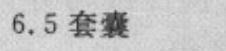
\includegraphics[max width=\textwidth]{2024_07_10_373f31b88d2bf633007bg-382}
 & 5 & 4. 5 & $26 \sim 28$ \\
\hline
$12 \sim 14$ & $6.5 ~ 7.0$ 套堆 & 5 & 4. 5 & 32 \\
\hline
$14 \sim 16$ & 7.0 套表 & 5 & 6.0 & 35 \\
\hline
$16 \sim 18$ & $7.0 ~ 8.0$ 套搉 & 9 & 7.0 & 35 \\
\hline
\end{tabular}
\end{center}

$\mathrm{ETT}$ : 气管导管, $\mathrm{ID}$ : 内径, BB: 支乞管堵塞器, F: 法式, DLT: 双垶管。表中所列规格为不同公司产品

\begin{enumerate}
  \setcounter{enumi}{1}
  \item 单肺通气的呼吸管理 基于小儿呼吸系统未发育成勲,除有些先天疾病肺已无功能者(如隔离肺)外,単肺通〔的代偿能力不如成人,年龄越小越明显。单肺通气的管理原则及方法与成人类似,术中最大限度地利用有功能的肺。㜟幼儿由于器材设备和代偿能力的限制, 不得已而采用双肺通与概率较多。管理要点: 变换体位后确认导管和阻塞器位置正确; 吸人 $100 \%$ 氧; 吸人麻醉药浓度应低于 $1 \mathrm{MAC}$, 避免抑制 $\mathrm{HPV}$; 设置 $\mathrm{V}_{\mathrm{T}} 5 \sim 10 \mathrm{ml} / \mathrm{kg}$, 气道压过高时增加呼吸次数; 开胸侧肺在肺完全茕陷前开始给 $1 \sim 2 \mathrm{cmH}_{2} \mathrm{O}$ 的 $\mathrm{CPAP}$; 通气肺应用 $5 \sim$ $10 \mathrm{cmH}_{2} \mathrm{O} \mathrm{PEEP}$;维持足够的心排血量。

  \item 纵隔肿㾇手术重点是重要器官受压和粘连。

\end{enumerate}

(1)气管受压: 表现为呼吸伴有哮鸣音和(或)自觉呼吸不畅, 提示气管有轻度受压; 必须采取半坐位或特殊体位方能维持呼吸或因呼吸困难不能人睡者,表明气管严重受压。凡此均应通过影像学检查,明确压迫部位及程度。应选清醒插管, 管前端通过受压部位, 确保呼吸通畅后再施行麻醉。术前采取被迫体位者,如半坐位或侧卧位,尽量在该体位下或患儿能耐受的体位下插管。麻醉后变换体位如引起循环、呼吸明显改变或压迫症状加重者,应立即恢复原体位,并在原体位手术。

(2)上腔静脉受压: 肿痹靠近胸廊上口,主要表现为头颈及上肢静脉充血, 颜面及颈部皮肤呈暗红.色或颈部水肿变粗(上腔静脉综合征), 诱导时须防止呛咳、激动,避免使充血、水肿加重, 甚至频内压升高。亦可在麻醉后体位变化及手术操作中发生或压迫症状加重,甚而出现颈部血管怒张、面部发纸、眼球突出等危急征象,术者应立即松解压迫或牵拉。

(3)心脏受压及纵隔移位:麻醉后及术中同样可致肿物对心脏及大血管的压迫突然加重,引起血压突然下降、心律失常等。处理同上。

(4)粘连:重者出血多,且容易损伤相邻器官及血管。

\section*{四、先天性心血管病手术的麻醉}
\section*{1. 动脉导管未闭麻醉要点}
(1)吸人或静脉诱导,避免使用 $100 \%$ 纯氧,因其会加重左向右分流。

(2)维持用吸人性麻醉药可惐少左向右的分流,也可选用静吸复合麻醉。\\
(3)动脉导管在结扎前必须将收缩压降低至 60~ $75 \mathrm{mmHg}$,对无肺高压的婴幼儿可用吸人麻醉加深或加用药降压如小量尼卡地平等,对体重较大或伴有肺高压病儿,用硝普钠静脉泵注人,从小剂量开始,逐渐加大,结扎后再维持一段时间,防止术后血压反跳。

\begin{enumerate}
  \setcounter{enumi}{1}
  \item 先天性房、室间隔缺损修补术的麻醉要点
\end{enumerate}

(1)术前充分镇静或给予基础麻醉,避免患儿焦虑激动,哭阔,以免增加氧耗和病情加重。

(2)左向右分流患儿选择吸人诱导,应用静脉麻醉诱导时间长,容易发生用药过量。为避免外周血管阻力增加,不宜应用氯胺酮。

(3)维持采用大剂量芬太尼复合吸人低浓度七氟烷或异氮烷可减轻手术引起的神经内分泌及代谢反应,注意预防心动过速、高血压及流出道痉孪造成的缺氧发作,应用适量的肌松药便于呼吸管理和预防寒战。

(4)注意呼吸力学改变,发现呼吸阻力增加、肺顺应性下降,针对原因,及时处理。肺血流增加忠儿 $\mathrm{V}_{\mathrm{T}}$ 需加大至 $10 \sim 12 \mathrm{ml} / \mathrm{kg}$, 而转流后由于体外循环再灌注损伤使肺顺应性下降,力求维持 $\mathrm{PaCO}_{2}$在正常范围, 需要时加用 PEEP, 根据血气调整 $\mathrm{PaCO}_{2}$ 分压在 $30 \sim 40 \mathrm{mmHg}$ 。

(5)低温体外循环期间,要维持 MAP 稳定在 $45 \sim 70 \mathrm{mmHg}$, 如血压过高,用加深麻醉或微泵静注硝普钠降压, 主动脉阻断后行静态膨肺, 压力维持在 $10 \sim 15 \mathrm{mmHg}$, 防止肺不张。

(6)术中严密观察尿量、失血量,HCT 应维持在 $25 \% \sim 35 \%$, 根据 MAP、CVP、左房压及尿量调节输血、补液速度,防止血容量不足或过多。

(7)麻醉后输液及心肺机预充液都应加人适当比例的胶体液,对发绀儿尤为重要,转流期间 COP 应不低于 $16 \mathrm{mmHg}$, 停转流时应达到 17 〜 $20 \mathrm{mmHg}$ 。

(8)心脏复跳后,要充分强心、利尿,防止组织及肺水㵔留,降低肺血管阻力, 小剂量多巴胺 5~ $10 \mu \mathrm{g} /(\mathrm{kg} \cdot \mathrm{h})$ 及硝普钠 $0.5 \mu \mathrm{g} /(\mathrm{kg} \cdot \mathrm{h})$ 维持血流动力学稳定, 如发生低心排,可加肾上腺素 0.1 〜 $0.5 \mu \mathrm{g} /(\mathrm{kg} \cdot \mathrm{h})$,若出现心率减慢,可用异丙肾上腺素 $0.05 \mathrm{mg}$ 静注或每分钟 $0.05 \sim 0.1 \mu \mathrm{g} / \mathrm{kg}$ 微量输液沓持续输注。

(9)若发生完全房室传导 阻滞, 应立即拆除补片的缝线,在恢复正常心律之前,采用心外膜或房室程序起搏,同时输注异丙肾上腺素以维持适宜的\\
心率。

(10)术后 PVR 高的患者需要监测肺动脉压,镇静, 持续应用肺血管扩张药, $48 \sim 72 \mathrm{~h}$ 强效利尿。

\begin{enumerate}
  \setcounter{enumi}{2}
  \item 法洛四联症麻醉要点
\end{enumerate}

(1) 病理生理: TOF 是指室间隔缺损、肺动脉狭窄、主动脉骑跨以及右心室肥厚。其中前两者是主要的,主动脉骑跨与室间隔缺损有关,右心室肥厚主要是继发于肺动脉狭窄。肺动脉狭窄主要为漏斗部狭窄,室间隔缺损一般较大。TOF 属复杂性分流, 血流阻力来自流出道梗阻部位以及肺血管, 若右心室流出道梗阻病变严重, 则 PVR 对分流量及分流方向的影响很小。TOF 患儿的动脉血氧饱和度与肺血流量有直接关系, 若右心室流出道梗阻程度较轻, 则进人肺动脉的血流很少受阻, 动脉血氧饱和度无明显下降。典型 TOF 右心室流出道重度梗阻, 右向左分流显著增加并出现发绀。 $20 \% \sim 70 \%$ 未治疗的患者有阵发性发绀和缺氧发作, 各种诱因所引起的氧需增加、 $\mathrm{pH}$ 降低和 $\mathrm{PCO}_{2}$升高起着重要作用, 低氧所致的 SVR 降低使病情加重。通常发作可自行缓解或当忠儿安静后得到缓解。静脉内应用碳酸氢钠可中止阵发性过度通气发作, 可能与纠正代谢性酸中毒、恢复并增加 SVR 有关。去氧肾上腺素亦可通过增加 SVR 中止其发作, 吗啡镇静或全身麻醉可降低过度通气的反应,可用于治疗该类事件。

(2)麻醉要点: (1) $10 \mathrm{~kg}$ 以上的病儿,麻醉前须充分镇静,避免缺氧。(2)静脉诱导, 因右向左分流,静脉至脑循环时间短, 诱导速度快, 芬太尼类必不可少。(3)维持可用芬太尼 $(10 \sim 20 \mu \mathrm{g} / \mathrm{kg})$ 并辅以吸人麻醉药, 复杂的修补术需时较长时, 应用大剂量芬太尼 (20〜 $50 \mu \mathrm{g} / \mathrm{kg}$ )复合吸人低浓度七氟烷或异氧烷,可减轻心肌抑制、反应性肺动脉高压和应激反应。(4) 在麻醉诱导期和苏醒期 2 个月到 2 岁患儿易于发生重度缺氧发作, 处理 : 包括适量输注液体避免容量不足, 增加吸人麻醉深度和给艾司洛尔减轻心肌过度收缩, 应用芬太尼减慢心率减少儿茶酚胺释放; 应用去氧肾上腺素 (苯肾上腺素) 10 ~ $20 \mu \mathrm{g} / \mathrm{kg}$ 静注或每分钟 $2 \sim 5 \mu \mathrm{g} / \mathrm{kg}$ 滴注腹部加压或屈腿以增加 SVR, 吸纯氧降低吸气峰压, 减少潮气量降低胸内压, 静脉输注碳酸氢钠纠正代谢性酸中毒以降低 PVR, 静注吗啡, 缓解肺流出道痉挛等。(5)HCT> $60 \%$ 者, 为预防血检形成或血管内凝血, 麻醉诱导后可做血液稀释, HCT 可降至 $50 \%$,小儿不耐受过度血液稀释, 体外循环期间,一般 HCT 不低于 $25 \% \sim 30 \%$ 。(6)维持合适的 SVR,尽量减少对 PVR 的影响, 任何原因导致 PVR/ SVR 比值升高均能增加右向左分流, 使肺血减少,从而加重发绀。但对右心室流出道重度梗阻的患儿, 即使改变 PVR, 分流量及分流方向仍无明显改变, 应注意保持或增高 SVR, 减少右向左分流。(7)肺血流增加, 忠儿 $\mathrm{V}_{\mathrm{T}}$ 设置 $10 \sim 12 \mathrm{ml} / \mathrm{kg}$, 肺血流减少, 患儿 $\mathrm{V}_{\mathrm{T}}$ 设置 $6 \sim 8 \mathrm{ml} / \mathrm{kg}$, 而转流后两组 $\mathrm{V}_{\mathrm{T}}$ 均需增加, 才能维持 $\mathrm{PaCO}_{2}$ 在正常范围,切忌吸气压力过高及过度通气。(8)转流前如小儿发绀加重、血压过低, 可在主动脉、右心房插管后先转流, 待氧合好转后, 再行上、下腔静脉插管。

(3)转流后处理: 停 CPB 后, 应重视维护"右心功能及降低 PVR。由于(1)右心室切口及流出道补片损害右心室部分功能; (2)CPB 期间对肥厚的右心室肌层供血相对不足; (3)右心室流出道扩大手术可能引起的肺动脉反流; (4)肺动脉远端狭窄或右心室流出道纠治不完全; (5)残留的 VSD 等均可使右心室超负荷, 心排血量减少,导致右侧心力衰竭。因此多数患儿需用正性肌力药物, 于停机前 $10 \mathrm{~min}$ 开始静脉输注。一旦出现传导阻滞, 轻者滴注异丙将上腺素和肾上腺皮质激素, 严重者应使用起搏器,并针对低心排血综合征进行治疗。

\begin{enumerate}
  \setcounter{enumi}{3}
  \item 小儿体外循环(CPB) 的特点 小儿 CPB 时有三种低温方式可供选择, 中低温 $\left(25 \sim 32^{\circ} \mathrm{C}\right)$, 超低体温 ( $18^{\circ} \mathrm{C}$ )和深低温停止心跳。中低温 $\mathrm{CPB}$ 适用于较大儿童, 也可用于繁儿比较简单的心胜手术,如 ASD 或简单的 VSD 修补术。新生儿、婴幼儿、儿童做复杂的心随手术常采用超低温 CPB, 目的是为手术提供更长的低流量和心跳停止无血视野的时间。CPB 期间患儿暴露于严重的生物学极限, 包括低温 ( $18^{\circ} \mathrm{C}$ ), 血液稀释 (循环血容量稀释 $3 \sim 5$ 倍), 低灌注压 ( $20 \sim 30 \mathrm{mmHg}$ ), 大范围变化泵流速 [从最高 $200 \mathrm{ml} /(\mathrm{kg} \cdot \mathrm{min}$ )到循环完全停止],不同的 $\mathrm{pH}$ 处理技术 $(\alpha$-稳态或 $\mathrm{pH}$ 稳态, 或两者交替), 这些变化与患儿正常生理值相差太大, 影响 $\mathrm{CPB}$ 时及 CPB 后正常器官功能和储备。此外, 还有糖的补给(防止低血糖), 导管的置人, 肺主动脉侧支循环的存在, 年龄和身材大小等在 CPB 时都会对器官灌注产生影响等。均对麻醉和 CPB 管理提出了更高的要求, 增加了麻醉难度和手术的风险。
\end{enumerate}

\section*{五、小儿普外科手术}
\section*{1. 腹嵱巨大肿物腹压增高病例}
(1)诱导期由于肿物对下腔静脉的压迫,可出现血压剧降, 甚而循环藂停, 麻醉前应适当抬高右腹部。

(2)摘出肿㿔或放腹水时,应密切注意循环变化, 速度不宣太快, 以防腹压下降, 血液再分布, 引起血压剧降。

(3)游离粘连肿物特别是肝肿痹切肝时, 容易发生大出血, 应注意观察及时给予补充。

\section*{2. 先天性巨结肠}
(1)由于术前禁食、洗肠, 常存在水电解质平衡紊乱和血容量不足, 术中应注意监测, 并给予适当补充纠正。

(2)手术须经肛门将病变肠管拖出, 选用骶管阻滞复合全麻最佳,可以保持肛门的肌松。

(3)术中取俯卧位, 气管导管应固定牢固,以防在翻身时脱出或扭曲。

(4)长段巨结肠无法将病变肠管完全经肛门拖出时需要开腹, 因骶管麻醉的平面常达不到开腹的要求,应及时调整全身麻醉深度。

\begin{enumerate}
  \setcounter{enumi}{2}
  \item 幽门肥厚 由于经常呕吐,术前常有不同程度的水电解质紊乱和血容量不足,应尽量纠正。术中注意补充和调整,可在局麻、全身麻醉或腹腔镜下完成手术。

  \item 腹腔镜手术在腹腔内或腹膜外充气后,多种腹部手术均可在腔镜下完成。腹腔内充气的生理改变取决于体位,充气压力和 $\mathrm{CO}_{2}$ 吸收,小儿正常腹内压仅 $(7 \pm 3) \mathrm{mmHg}$, 年龄越小腹压高的影响越大。头低位易影响循环,头高位影响呼吸,充气压力不宜超过 $12 \mathrm{mmHg}$ 。通常选择全身麻醉, 控制呼吸以保证通气足够和 $\mathrm{CO}_{2}$ 的排除, 充气前应充分吸净胃内容。

\end{enumerate}

\section*{六、小儿骨科手术}
\begin{enumerate}
  \item 选用全身麻醉 骨盆和下肢手术常复合骶管阻滞。全麻下手术结束时不宜过早减浅麻醉, 由于很多骨科手术后需行石亮固定, 皮瓣的敷料包扎和固定或需特殊体位均要求避免体动, 故应在这些操作基本完成之后再停止麻醉。

  \item 四肢手术常需止血带其宽度需大于相应肢体直径的一半。止血带的充气压力应根据患儿年龄及其收缩压而定一般上肢压力应高于其收缩压的 $5 \sim 10 \mathrm{mmHg}$,下肢高于收缩压 $20 \sim 30 \mathrm{mmHg}$为宜。止血带维持时间尽量缩短, 上肢不超过 $1 \mathrm{~h}$下肢不超过 $1.5 \mathrm{~h}$ 。如需重复上止血带,两次间隔时间至少 $10 \mathrm{~min}$ 。松开止血带时要尽量缓慢,避免无氧代谢产物快速人血及再灌注损伤,同时适当加快输液速度,防治血液再分布导致的血容量相对不足。

  \item 脊柱侧弯矫形手术的麻醉 是小儿骨科比较特殊手术和麻醉,需要手术治疗的患儿年龄多在 $4 \sim 14$ 岁。

\end{enumerate}

(1)术前多有心肺功能减退,重度脊柱侧弯由于胸廊严重变形常有呼吸功能受累, 限制性通气功能障碍, 肺容量和肺顺应性降低, 肺血管阻力增加,病程长者还可能有肺动脉高压,右心功能不全。术前肺活量 $>70 \%$ 预计值的患儿多能较好耐受手术,如果肺活量 $<40 \%$ 预计值或 $1 \mathrm{~s}$ 最大呼气量 $<50 \%$预计值,术后可能出现呼吸功能不全,倘若发生送 PICU 继续机械通气支持。

(2)手术创面大、出血多、时间长,为减少出血,可行控制性降压,手术一般经后路,有时需要先经胸或经腹松解,再经后路矫形,因而需大幅度变换体位,易引起血流动力改变。

(3)为便于术中唤醒,术前应对患儿进行唤醒试验训练, 嘱其在术中唤醒后, 按医生的指令活动下肢,应用七氟烷或地氟烷术中唤醒多无困难,应选用短效肌松药,计算好作用时间,唤醒试验完毕要立即静注丙泊酚或依托味酯及吸人加深麻醉。

\section*{七、手术室外麻醉}
\section*{1. 基本要求}
(1)由于小儿恐惧不能配合, 许多检查和处置须在麻醉下进行, 如 CT、MRI、羫镜、化疗等通常采用镇静麻醉,一般不插管, 有特殊需要也可插䈎。

(2)设备: 可靠和备用的氧气源,可靠的吸引源、气管插管、急救、复苏设备及药物,麻醉机和监测设备,必需及可能需要的麻醉药。

(3)有经验的麻醉医师、助手和操作医、技师间的密切协作与配合。

\section*{2. 常见处置}
(1)磁共振扫描: 不能使用带金属的监测及保障安全设备。目前已有兼容性麻醉机、监测设备和输液厡,使全身麻醉得以顺利进行,由于室内温度偏低, 婴幼儿应注意保温,一般镇静麻醉即可, 如以七廉烷诱导丙泊酚持续滴注维持, 保持自主呼吸,一般不会出现上呼吸道梗阻,倘有发生可放置通气道。

(2)计算机断层扫描 (CT): 有时需气管插管,\\
对口服造影剂小儿可以预防误吸, 还可在需要张肺时给予正压通气, 麻醉医师应穿防护衣守护在患儿身旁。

(3)放射治疗:要求患儿必须完全不动 $10 \mathrm{~min}$,所有人员都在房间外, 通常选择诱导苏醒都快的麻醉方法, 如丙泊酚和七氛烷, 麻醉医师在调整好麻醉和呼吸道后离开, 通过监测屏幕在室外观察患儿的生命指标。

(4) 内镜检查: 通常用丙泊酚麻醉, 上消化道检查主要是保护呼吸道, 下消化道通常不需插管, 但因疼痛刺激较强需辅以阿片类药。

(5) 牙科处置: 如拔牙等短时间手术, $\mathrm{N}_{2} \mathrm{O}$ 和 (或)七紩烷面罩吸人达一定深度后停止麻醉, 拔除患牙后忠儿可迅速清醒。

\section*{第十节 新生儿麻醉}
\section*{一、麻醉前评估及准备}
\begin{enumerate}
  \item 新生儿 麻醉对象通常属于急症手术, 如膈疝、食管闭锁、腹裂、肠梗阻、肛门闭锁、坏死性小肠炎等, 此中除低位肛门闭锁外, 病情均较严重。由于缺少典型的临床征象, 术前病情估计比较困难,根据笔者观察凡表现为反应低下、呼吸急促、“三凹”现象、青紫、心跳缓慢、体温低等均是与预后有关的危重征象。

  \item 电解质平街紊乱及酸中毒 尽可能纠正严重的水电解质平衡絮乱及酸中毒, 使血流动力学恢复到生理允许水平。腹璌手术下胃管。

  \item 纠正低策血症 鼻导管或面罳吸氧, 必要时气管插管辅助呼吸。

  \item 保温患儿生后及接送均在保温箱内保温。手术室室温提高到 $27^{\circ} \mathrm{C}$ 以上, 还可用辐射加热器或红外线灯直接照射等提高小环境温度, 患儿置于 $40^{\circ} \mathrm{C}$ 热水袋或电热毯上以及用棉垫包裏外露部位等。

  \item 术前药可以不用或全麻前只给阿托品 $0.1 \mathrm{mg}$ 静脉或肌内注射。

\end{enumerate}

\section*{二、麻醉选择}
局麻适用于短小手术如经会阴肛门成形等; 骶管及脊麻止痛确实, 术后无呼吸抑制, 适用于下腹及会阴部手术, 骶管留置导管还可用于术后镇痛;气管内全身麻醉适用于各部位较复杂的手术, 便于管理呼吸, 最为常用。

\section*{三、全身麻醉方法及管理}
\begin{enumerate}
  \item 倰导 吸人 $\mathrm{N}_{2} \mathrm{O}+$ 七氧烷插管, 需要时静注肌松药, 如维库滇轱或阿曲库轱 (剂量参照表 3-1117), 保证 $\mathrm{SpO}_{2}$ 在 $85 \% \sim 95 \%$ 条件下 $\mathrm{FiO}_{2}$ 尽量减小,除严重缺氧、发绀者外不需纯氧, 重症反应低下
\end{enumerate}

的新生儿可采用清醒插管。静脉滴注芬太尼 0.1 〜 $0.2 \mu \mathrm{g} / \mathrm{kg}$ 有助于减轻应激反应。

\begin{enumerate}
  \setcounter{enumi}{1}
  \item 维持 选用 T 形管法或紧闭法维持浅麻醉,各种吸人麻醉药均可应用。
\end{enumerate}

(1) T 形管法: 可不加气蘘,设备简单,但必须用听诊器连续听取呼吸音, 精心操作, 否则可致通气不足或过度, 压力过大甚而肺泡破裂。

(2)循环紧闭法: 比较理想, 应用成人小儿通用的新型麻醉机。

(3)术中管理:(1)监测心率、呼吸、血压、体温、 $\mathrm{SpO}_{2} 、 \mathrm{PetCO}_{2}$ 及 ECG; (2)用听诊器兼听呼吸音及心音, 正常心率允许波动在 $120 \sim 200 / \mathrm{min}$ 之间, 如心率减慢 $100 \sim 120 / \mathrm{min}$, 自主呼吸减慢至 $30 \sim 40 /$ $\mathrm{min}$, 常是器官功能严重抑制表现, 多与麻醉偏深,缺氧及体温低等有关;(3)血压下降常是血容量不足的敏感指标, 凡遇此等情况, 必须迅速查明原因, 采取相应处理措施纠正,时间长创伤大的手术, 灌注不足、缺氧同样可以引发周身炎症反应和多器官功能不全,且恢复更困难; (4)吸痰应选用细的吸痰管 (外径不超气管内径的 $1 / 3 \sim 1 / 2$ ), 在 $\mathrm{SpO}_{2}$ 监测下进行, 吸痰持续时间不宜太长, 避免严重低氧血症,又因气管导管内径较细, 倘分泌物橎稠附着管壁,难以吸出时, 应立即更换导管,故新生儿气管内麻醉必须准备两套导管; (5)术中输液除根据体重而制定的基础摄人量外,由于外露内脏(肠管)面积相对大, 术中输液量需求较大, 尤其是对某些特殊病例需要量更大,据报道, 一组新生儿消化道穿孔, 输液量达 $45 \mathrm{ml} / \mathrm{kg}$, 而另一组新生儿原发性腹膜炎, 术中输液量高达 $40 \sim 100 \mathrm{ml} /(\mathrm{kg} \cdot \mathrm{h})$, 基于此类忠儿液体需求量及变动范围均大,而输液安全界限又很窄, 任何判断上的误差,都可造成严重后果, 输液量不足, 休克不能纠正, 输液过量很易造成心力衰竭、肺水肿, 故术中必须全面监测, 严密观察, 精确调控; (6) 输血的指征为 $\mathrm{Hb}<100 \mathrm{~g} / \mathrm{L}$ 或 $\mathrm{HCT}<35 \%$ 。

\begin{enumerate}
  \setcounter{enumi}{2}
  \item 拔管 新生儿容易发生拔管后喉痉挛窒息,预防的关键在于拔管时机的选择, 在患儿安静, 自主呼吸平稳, 吸人空气 $\mathrm{SpO}_{2}$ 适宜状态下, 在呼气时同步将导管拔出。一旦发生严重喉疘挛窒息, 面罩加压吸氧无效时, 应立即重新插管, 根据需要静注琥珀胆碱以确保插管顺利成功。因新生儿在缺氧状态下呼吸中枢可迅速转为抑制, 造成呼吸心跳停止, 缺氧时间必须缩至最短。
\end{enumerate}

\section*{四、先天性膈疝}
\begin{enumerate}
  \item 病理生理 进人胸腔的腹腔脏器 $90 \%$ 含有小肠, $50 \%$ 同时含有肝、田和脾也可进人胸腔。膈身多在肧胎第 10 周左右发生, 影响肺发育, 使肺内动脉明显减少, 管壁肌层增厚及管径小。新生儿开始呼吸时吞咽的空气可进人胸腔内的胃肠道, 加重对肺叶的压迫, 从而使 $\mathrm{PaO}_{2}$ 降低及 $\mathrm{PaCO}_{2}$ 升高, 发生酸中毒; 肺血管阻力 (PVR)增加, 致使经动脉导管右向左分流增加。如将疝内容复位使被压缩的肺叶扩张, 病情可能好转。倘因肺发育不全, 不能满足最低限度的气体交换, 其呼吸功能不全依然存在, 严重缺氧, 高 $\mathrm{CO}_{2}$ 血症和酸中毒将使右向左分流进一步增加, 加重全身缺氧和酸中毒, 从而形成恶性循环, 最后可因缺氧致死。通常伴双肺或大范围单肺发育不全者, 腹腔内脏进人胸腔多, 纵隔移位,并有贫血、脱水、酸中毒者病情严重。
\end{enumerate}

\section*{2. 麻醉前准备}
(1)麻醉前经鼻置人周管排除周内积气,降低胸腔内压力以琙少腹腔脏器对肺的压迫。

(2)尽早清醒插管辅助呼吸, 中度肺发育不全患儿经吸人高浓度氧及辅助呼吸后, 呼吸困难、缺氧及高 $\mathrm{CO}_{2}$ 血症可得到改善, 面罩加压通气可使胃肠道充气, 加重对肺的压迫。

(3)脐动脉插管采血, 进行血气分析, 有代谢性酸中毒者可给予碱性药物纠正, 以㖪轻肺血管痉挛,惐少右向左分流量。

(4)血压低、心率减慢者除保温外可给予血管活性药, 经短时间紧急处理后, 不论病情有否改善均应紧急手术治疗。

\section*{3. 麻醉要点}
(1)患儿送人手术室后, 未插管者立即清醒或静注芬太尼 $(0.1 \sim 0.2 \mu \mathrm{g} / \mathrm{kg})$ 或吸人 $\mathrm{N}_{2} \mathrm{O} 50 \%+$七氟烷 3\%〜5\%插管, 插管后行正压通气, 以改善与体交换, 通气过程中如血气值和血流动力突然恶化, 应检查对侧是否发生了气胸, 一旦确认应立即置胸腔闭式引流。

(2)维持麻醉首选七氟烷 $2 \%$ 或其他吸人药,可辅以芬太尼或瑞芬太尼静滴。

(3)腹腔脏器还纳后可压迫下腔静脉, 故不宜用下肢输液, 颈内或锁骨下静脉较理想。

(4)腹腔内脏还纳后致腹内压明显增加, 压迫膈肌影响呼吸, 故应于患儿完全清醒及呼吸功能恢复正常后方可拔管。

(5)术后决定预后的最主要因素是肺发育不全的范围及肺受压程度, 可因低氧血症、高 $\mathrm{CO}_{2}$ 血症和酸中毒致肺血管痉挛右向左分流增加而病情恶化。其治疒措施包括充分供氧、正压通气、应用血管扩张药 (如妥拉唑啉直接肺动脉输注) 降低肺动脉压及结扎动脉导管等。若上述措施无效, 可采用体外膜肺氧合(ECMO)改善氧供。

\section*{五、先天性食管闭锁和气管食管屡}
\begin{enumerate}
  \item 病理生理一般分为六个类型, I、、II、III a、 III b、IV、V 型。主要是呼吸道与消化道之间有瘘管相通病例, 高酸度的胃分泌物反流进人气管, 产生严重的化学性肺炎。食管上端盲袋容量仅数毫升,不能容纳㜟儿下咽的所有唾液, 也反流人气管,共同引起吸人性肺炎。

  \item 麻醉前准备 查明畸形类型, 瘘管的粗细和至隆突的距离。患儿取半卧位, 每 $15 \mathrm{~min}$ 用软导管吸引食管盲袋及口咽部分泌物 1 次,以减少误吸。根据脱水情况补充液体及葡㷏糖。力求治愈肺内感染。

\end{enumerate}

\section*{3. 麻醉要点}
(1)麻醉选择:全身麻醉,总气管插管,控制呼吸, 清醒插管最为安全, 小儿反应强时可用静脉或吸人诱导, 面罩通气用低压, 以免通过瘘管使胃充气胃内压增加, 加重误吸。

(2)气管插管: 导管前端必须超过瘘管, 通常先插至支气管或隆突上方, 然后将导管缓退至双肺呼吸音均等为止, 如胃部听到通气声, 再将导管缓插送至呼吸音消失; 万一导管插人远端瘘筞 (双肺听不到呼吸音同时出现胃胀), 应将导管退出重插; 已做胃造瘘者可将胃溇连接管置于水面下, 加压通气时如有大量气泡涌出表明有大量气体通过瘘管进人胃内, 应重新调整导管位置; 还可经过胃溇或气管插人堵塞器堵塞瘘孔后插管, 至导管位置合适后妥善固定。

(3)拔管: 手术结束后,如患儿自主呼吸恢复满\\
意,清醒后可以拔管,但气管软化或瘘孔部管壁缺损者可发生气管塌陷,应留置导管至 $24 \sim 48 \mathrm{~h}$ 后试验拔管,倘堨陷仍未恢复,继续留置 $3 \sim 7 \mathrm{~d}$; 呼吸功能未恢复正常不能脱机者,应带导管送回 PICU 病房,继续机械通气及其他治疗。

\section*{六、脐膨出和腹裂}
麻醉前应注意检查有无合并其他脏器的畸形。由于腹腔脏器大量暴露, 应特别注意保温及水电解质的补充。麻醉诱导和气管插管无特殊要求。术前应经颈内或锁骨下静脉置管,监测 CVP 及作为输液通路。内脏复位时因外露内脏多, 腹腔容积小,复位当时及复位后,腹内压增高,限制膈肌运动,压迫血管血液向胸腔转移等,严重影响心肺功能和产生明显的血流动力学的改变, 甚而因腹内压持续过高 (正常 $7 \mathrm{mmHg} \pm 3 \mathrm{mmHg}$ ) 导致腹腔间隙综合征 (abdominal compartment syndrom)。故应根据呼吸功和血流动力的耐受限度决定内脏还纳与关腹。为减轻内脏还纳的不良影响, 有时采取腹壁减张措施, 增加腹腔容积或分期修补腹壁。术中水电解质需要取决于外露内脏的多少, 在内脏尚未还纳时一般需 $15 \sim 25 \mathrm{ml} /(\mathrm{kg} \cdot \mathrm{h})$ 。

\section*{七、其他消化道疾病}
如坏死性小肠炎、胃穿孔、腹膜炎, 肠梗阻等麻醉处理可参照上述原则,特别注意的是水电解质平衡紊乱和代谢酸中毒的纠正。

(陈卫民 张秉钧)

\section*{算18章}
\section*{老年患者麻醉}
\section*{第一节 老年对生理及药理的影响}
\section*{一、严重影响生理的年龄}
美国已经完成的统计资料表明老年病人围术期死亡率呈逐年下降趋势: 20 世纪 60 年代为 $20 \%, 80$ 年代已经下降到 $5 \% \sim 6 \%$; 近年统计研究进一步提示, 即使是特别高龄的患者, 围术期死亡率也不高于成人组。Warner 等 1998 年报道 31 例 100 岁以上患者围术期无一死亡, 1 个月内死亡率为 $16.1 \%, 1$ 年内死亡率为 $35.5 \%$, 患者的生存率与相同年龄段未接受手术者几乎没有区别。虽然随着年龄的增长, 机体生理会出现不同程度的变化; 而且年齗增长本身可以增加手术并发症发生的可能性, 但是并发症增加的主要原因是由于随着年龄增加而出现的一些重要脏器的器质性病变如心血管疾病等的发病率增加。因此年龄是否独立的危险因素一直存在争论, 有些学者不同意年龄作为单独的危险因子。但是多数麻醉医师并不区分年龄本身还是老年性疾病在麻醉中的作用, 往往把两者合在一起考虑。

如果综合考虑年龄对心血管、呼吸和神经等重要系统的影响, 可以建议把 70 80岁作为严重影响生理的年龄。

\section*{二、高龄对机体生理的影响}
由于机体遗传背景和环境影响因子的差异, 高龄对机体生理的影响个体差异较大, 下面简要描述高龄对不同生理系统的影响。

\begin{enumerate}
  \item 对心血管系统的影响 心脏突房结和心肌出现胶原纤维增多、脂质沉着等结构变化不同程度地影响心血管功能。高龄老年人不同程度出现突性心率下降, 传导阻滞或心律失常。心电图可以出现 P-R 间期延长、QRS 和 $T$ 波等变化。心肌胶原纤维老化, 收缩舒张功能降低; 心肌细胞动作电位时程延长, 因此高龄老年人对正性肌力药物的变力反应和 $\beta$ 受体激动药的反应也降低。由于心脏收缩舒张功能降低和高龄对心脏前后负荷、神经内分泌调节的影响, 与年轻人相比, 心排血量平均每年下降 $0.75 \% \sim 1.01 \%$, 健康老年人左心室射血分数平均只有 $60 \%, 70$ 岁以上多在 $50 \%$ 左右; 老年人心排血量对应激刺激的反应性下降非常显著, 例如老年人对运动引起的心率增加反应性较年轻人降低 $30 \%$, 射血分数增加幅度也较低。动脉因退行性变化和棌样硬化使管壁变性、钙化, 冠状动脉狭窄, 主动脉和大动脉的弹性惐弱, 心缩期血压升高, 左心室后负荷增加。

  \item 对呼吸系统的影响 随着年龄增加, 老年人呼吸系统组织结构逐渐出现退行性改变, 呼吸肌肌力减退、胸廊顺应性降低、小气道闭塞、残气量增加, 最终使老年人呼吸功能储备减少。产生这些变化的结构基础是老年人呼吸道栓膜变薄、腺体菱缩、分泌功能减退, 纤毛减少, 小气道管壁弹性惐弱; 同时由于长期尘埃吸人和沉积, 肺顺应性变差;老年性骨质疏松、助软骨钙化可使胸萨顺应性降低; 呼吸肌萎缩使吸气动力喊退。呼吸系统的这些组织结构改变是高龄老年人呼吸系统功能改变的基础: 老年人肺活量明显降低, 80 岁老年人肺活量仅占年轻人的 $40 \%$, 残气量和功能残气量增加, 最大通气量、用力肺活量、1s 量 (FEV1.0) 和 $1 \mathrm{~s}$ 率 (FEV1.0\%)明显下降。随肺组织结构老化出现气体交换面积缩小、肺泡壁毛细血管总表面积惐少、\\
功能残气量增加等使老年人肺换气和弥散效率降低。同时由于心血管系统老化导致的心排血量降低、通气/血流比例失调等使老年人动脉血氧分压逐年降低。

\end{enumerate}

由于化学感受器对刺激感知、中枢神经系统处理能力等下降老年人对低氧和高二氧化碳血症的代偿反应随年龄增加变得迟钝,70 岁以上老年人对低氧导致的通气反应较年轻人降低 $40 \%$, 对高二氧化碳血症的代偿反应降低 $50 \%$ 。

\begin{enumerate}
  \setcounter{enumi}{2}
  \item 对神经系统的影响 机体老化过程中,由于神经元减少、胶质细胞增生、有髄神经纤维减少, 70 岁以上老年人某些皮质区域神经元减少 $30 \%$ $50 \%$,小脑 Purkinje 细胞下降约 $20 \%$ 。老年人大脑形态学主要表现为重量减轻、脑沟变宽变深、脑回变窄、脑室体积增大等。老年人春䯕神经细胞、后根神经节细胞和周围自主神经节细胞减少,前角细胞和后根神经节细胞出现脂褐素堆积。脊神经根和周围神经的轴突出现变性、脱髓鞘等,老年人因此出现神经纤维的传导速度减慢、传人冲动减少,痛阈提高。同时由于老年人椎管狭窄、骨关节结构改变、椎管内脑脊液含量减少等原因使施行椎管内麻醉时对局麻药的敏感性增加, 而且一旦发生低血压及缺氧时脊髓神经细胞受损程度也高于年轻人。老年人神经元有氧代谢降低, 脑血管自动调节能力降低, 对高二氧化碳血症的反应明显减弱,脑血流量减少,如果同时合并糖尿病、高血压、动脉粥样硬化等疾病则脑血流量减少更明显。
\end{enumerate}

老年人神经递质(如某些儿茶酚胺和多巴胺)合成减少、一些神经元受体 (如胆碱能受体、GABA 受体)密度发生改变, GABA 受体密度增加可能与老年人对苯二氮草类敏感性增加有关。老年人由于丘脑-垂体-肾上腺轴功能降低使得其对应激的反应性降低,自主神经兴奋阈值提高使其对心血管系统的调节功能减弱,体温调节中枢功能减低使其对外界温度的适应能力下降。

\begin{enumerate}
  \setcounter{enumi}{3}
  \item 对消化系统的影响 老年人消化系统老化可以表现为牙齿缺如、腺上皮萎缩和分泌功能降低、胃运动功能减弱 (如排空减慢等)。老年人朋重量降低、肝血流量减少,肝合成蛋白质能力降低,主要代谢药物的脱甲基功能随年龄增加而降低。

  \item 对泌尿系统的影响 随年龄增加而出现的生理性肾小球硬化、肾血管硬化等减少了肾有效滤过面积。肾血流逐渐降低, 每 10 年最大可下降 $20 \%, 20$ 岁时约为 $600 \mathrm{ml} / \mathrm{min}$, 到 80 岁时只有 $50 \%$ 左右。肾小球滤过率进行性下降, 但约 $1 / 3$ 老年人没有明显变化。由于轹潫的溶质转运障碍和觝质血流的相对增加影响觡质高渗形成, 老年人肾浓缩功能下降; 肾小球滤过率降低是老年人肾稀释功能降低的主要原因。老年人对血钠、血钾调节能力降低, 低血钠时对钠回吸收不能有效增加, 急性钠及水负荷又不能有效地排钠排水。老年人在应激条件下对酸负荷的反应下降, 持续时间延长。

  \item 对内分泌系统的影响 虽然老年人多数内分泌器官和内分泌轴功能表现为降低, 但除性激素外,基础血清激素水平可能在正常范围。由于内分泌的变化还涉及激素的合成、分泌、代谢以及组织对激素的反应等, 因此实际上老年人在应激状态下常表现为储备功能惐退。

  \item 对血液系统的影响骨髓造血干细胞的增生能力随年龄增加而明显降低, 在应激状态下黄骨铤转变为红骨䯕恢复造血的能力也明显降低。老年人血红蛋白含量随年龄增长略有下降, 红细胞渗透脆性增加, 寿命缩短。血清铁含量下降, 骨䯝铁储备减少, 对需求增加时反应不足, 易导致贫血, 白细胞总数偏低,对应激、药物的反应低于年轻人; 对微生物的趋化性、吞噬性及杀伤作用减弱。血小板聚集、释放功能增强, 对药物、胶原等聚集诱导物非常敏感; 血浆中凝血因子 V、、II、、VIII活性和纤维蛋白原含量显著升高, 纤溶酶原激活物活性降低, AT III、TM 蛋白的扰凝活性下降。

\end{enumerate}

\section*{三、高龄对药理及其相互作用的影响}
充分了解老年人生理功能变化对药物药理作用的影响是保证老年人特别是高龄老年病人围麻醇期用药安全的基础,下面从药代动力学、药效动力学和常见药物相互作用 3 个方面做一个简略说明:

\begin{enumerate}
  \item 老年人药动学特点 药动学包括药物在体内的吸收、分布、代谢和排泄的过程以及药物浓度随时间的变化规律。老年人药动学特点主要表现为被动转运吸收的药物吸收不变、主动转运吸收的药物减少, 药物代谢能力惐弱, 排泄能力降低, 消除半衰期延长, 血药浓度增高等。
\end{enumerate}

(1)药物的吸收: 胃肠道改变是影响老年人口服药物吸收的主要因素,老年人胃酸分泌减少可以使药物在胃中吸收减少; 周肠排空速度降低延迟药物到达小肠的时间, 使药物通过小肠的吸收减慢,有效血药浓度到达峰值时间推迟; 另外胃肠道血流\\
量降低、肠腔内液减少也可能降低药物的溶解。因此, 麻醉前应该了解病人口服药的用药情况。由于老年人局部血液循环较差, 心排血量降低,所以其他给药途径如肌内注射、静脉注射、舌下给药等方式的药物吸收也与年龄有相关性。

(2)药物的分布: 药物分布与药物本身的特性、机体组织成分、血浆蛋白结合率、组织器官的血液循环、体夜 $\mathrm{pH}$ 以及组织器官的药物结合率等因素相关。老年人的细胞内液减少, 体内总水分明显下降, 因此水溶性药物的分布容积有所减少, 从而使作用部位药物浓度增加; 老年人体内脂肪量不同程度增多, 脂溶性药物的分布容积有所增大, 药物作用时间延长,容易出现蓄积。老年人血浆蛋白含量降低, 与血浆蛋白结合的药物相应减少, 游离药物浓度升高, 因此老年人使用蛋白结合率高的药物时应该适当喊少剂量; $\alpha$ 酸性糖蛋白(AGP)在老年人体内含量有所升高, AGP 可以使一些特定药物 (如利多卡因等)的游离血药浓度升高, 因此应当适当调节这些约物的剂量; 此外还应该注意老年人红细胞结合某些药物的能力降低, 如哌替啶年轻人红细胞结合率为 $50 \%$,而老年人仅为 $20 \%$ 。同时老年人由于合并多种疾病, 服用多种药物, 这些药物可以竞争性结合血浆白蛋白从而改变血中其他药物的游离浓度, 严重时可能产生毒性作用。

(3)药物的代谢: 药物主要通过肝代谢, 老年人肝对药物的代谢能力随年龄增加而降低。代谢能力降低的原因包括肝微粒体酶的活性降低、肝对外界因素诱导和抑制药物酶作用的反应性降低以及肝血流量降低减少了药物的首关效应。应该注意的是老年人一般肝功能检查正常不一定说明肝内药物代谢能力正常。

(4) 药物的排泄: 多数药物主要通过肾排泄, 老年人药物排泄能力约比年轻人下降 $40 \%$ 。由于老年人肾小球滤过率、肾小管的分泌和重吸收功能均有所减少, 影响药物的排泄, 使其半衰期延长。老年人肌酎产生减少,所以血肌酎水平不能作为衡量老年人肾功能的惟一指标, 应该选择血肌䣫清除率。对一些以药物原形排泄、治疗指数窄、可能损害肾功能的药物, 应该特别注意调整剂量。

\begin{enumerate}
  \setcounter{enumi}{1}
  \item 药效动力学 药效学的变化主要涉及靶器官对药物敏感性的改变。产生敏感性改变的原因可以由于药物感受器的数量变化, 可以是由于与细胞偶联的信号传导机制的变化。通常老年人药物药效学的改变主要表现为对于药物作用特别是作用于中枢神经系统的药物 (如苯二氮草类、吸人麻醉药等)的敏感性增加, 这种作用的增加与血药总浓度、游离药物浓度没有明确的关系。但是另一方面, 随着机体的老化, 导致 $\beta$ 受体介导的器官反应性降低。这些现象的发生可能与老年人神经系统的生理功能变化相关。

  \item 常见药物相互作用下面简要叙述常见用约对老年病人麻醉可能产生的影响。

\end{enumerate}

(1)抗生素: 围术期应用抗生素可能是手术前治疗, 也有可能用于预防感染。大部分接受外科手术的老年病人同时需要进行抗生素治疗, 抗生素对麻醉的主要影响在于其与肌松药的相互作用。有些抗生素包括氨基糖苷类、四环素类等可以增加肌松药的肌肉松驰作用,特别当老年病人合并有神经肌肉疾病者。同时一些麻醉手术可能使用的其他药物如维拉帕米、利多卡因、氟烷等可以增强这些抗生素的肌松作用。抗生素的这种作用可能导致病人呼吸抑制, 此时发生的呼吸抑制作用一般不能被新斯的明拮抗。

(2)三环类抗抑郁药: 三环类抗抑郁药的主要药理作用是抑制去甲坚上腺素和 5-羟色胺的再摄取,同时可以产生抗胆碱、抑制房室传导和降低心肌收缩力的作用。因此这类药物可以成倍增加一些药物如去甲肾上腺索、肾上腺素和去氧情上腺索的心血管作用, 严重者可能引起心律失常、高热、高血压危象甚至死亡。另外三环类抗抑郁药还可以增加奎尼丁、普鲁卡因胺的传导抑制作用和巴比妥类药物的作用。

(3) 单胺氧化酶抑制药 (MAOI): MAOI 由于其对单胺氧化酶的抑制可以显著地增加一些拟交感药物如肾上腺索的心血管作用,可能发生高血压危象、惊敀或高热昏迷。MAOI 与阿片类药物的相互作用分两种:一种为与哌替啶作用, 产生兴奋表现甚至惊厥、高热和昏迷;一种为抑制, 因为 MAOI 抑制了阿片类药物的肝代谢从而可能增加后者的呼吸抑制、镇静和降低血压的作用。如果可以停用 MAOI, 建议手术前至少停用 2 3 周。

(4) 锂剂: 锂剂可以延长一些肌松药如潘库溑铵、维库溴铵和琥珀胆碱的肌松作用; 还可以降低房室和室内传导, 因此合用 $\beta$ 受体阻滞药、钙拮抗药、吸人麻醉药、奎尼丁和普鲁卡因胺时应该特别注意可能发生的传导抑制作用。

(5)锬拮抗药: 钙拮抗药类药物种类繁多,不同的药物对心肌收缩性、传导性和外周和冠脉系统血\\
管的影响不同。如维拉帕米和 $\beta$ 受体阻滞约合用可能发生心肌收缩性和传导性的严重抑制; 吸人麻醉药、氧化亚氮和镇痛药物可以增强钙拮抗药对心肌收缩性、传导性和周围血管阻力的影响。维拉帕米可以增强去极化和非去极化肌松药的肌松作用。

(6) $\beta$ 受体阻滞药: 地高辛、维拉帕米可以增加 $\beta$ 受体阻滞药对心率和心肌传导性的抑制, 已经使用 $\beta$ 受体阻滞药的病人应该避免静脉应用维拉帕米。麻醉和手术对肝血流和肝代谢活动的作用可以影响 $\beta$ 受体阻滞药的清除。

(7)血管紧张素转化酶抑制药 (ACEI): ACEI 常用于高血压的治疗, 与利尿药合并使用时存在手术中发生严重低血压的可能; 在有肾功能损害的病人,甚至可能发生急性肾衰竭。ACEI 类药物与非甾体类镇痛药物合用时可能加重紧损害。也有报道 ACEI 类药物卡托普利可以增加地高辛血药浓度。

(8)地高辛: 由于地高辛在老年患者中广泛应用和其狭窄的治疗指数, 因此应该特别重视地高辛对麻醉的影响。地高辛本身可以导致房室传导阻滞、室性心律失常等。一些药物如非甾体类镇痛药物、奎尼丁等可以加重这种作用; 另外, 内环境紊乱如低钾、低铗或低钻和甲状腺素、儿茶酚胺等均可加重地高辛的毒性。

(9)抗心律失常药: 奎尼丁可以加重地高辛的毒性, 还可以通过抑制胆碱酯酶而延长琥珀胆碱作用时间。普鲁卡因胺可以延长琥珀胆碱的作用时间和增加奎尼丁浓度,西味替丁可以通过抑制清除而增加普鲁卡因胺的血药浓度。利多卡因可以用于治疗室性心律失常, 但是低钾时此种治疗作用消失; 同时利多卡因可以增加普㩐洛尔、钶拮抗药和吸人麻䣲药的负性肌力作用。广谱抗心律失常药物胺硔眮可以降低心内传导,非竞争性抑制 $\alpha, \beta$ 受体和抑制心肌收缩等作用, 全身麻醉时可能发生心率减慢和对升压药物反应不佳的低血压。

(10)某些术前用药可能影响老年患者手术后意识功能: 如所有的抗胆碱药物均可以增加术后认知功能障碍发生率, 因此老年患者术前不推荐使用此类药物; 某些合并器质性心脏病的老年患者术前使用阿托品可以加快心率, 增加心肌氧耗, 可能诱发心肌缺血; 阿托品也存在诱发老年患者青光眼急性发作的可能。老年患者对镇静药物敏感性增加,部分苯二氮草类药物可能引起烦躁、意识混乱从而造成患者坠床的危险, 因此不建议用于老年患者。哌替啶由于其代谢产物作用时间长且具有神经毒性, 反复使用此毒性作用可以累加, 所以应该避免使用, 改用吗啡。 $\mathrm{H}_{2}$ 受体阻滞药特别是西咪替丁可能引起术后意识功能改变。

(11)通常在手术前 1 周应该停用阿司匹林; 推荐应用肝素代替华法林, 因为肝素半衰期短于华法林,停药几小时可以保证手术安全进行。

(12) 为防止容量降低和低血钾发生, 建议术前晚上停用呋塞米。

\section*{第二节 高龄对麻醉的影响}
\section*{一、高龄对硬膜外麻醉的影响}
高龄对硬膜外麻醉的影响包括解剖学、生理学和局麻药物药理等方面。

\begin{enumerate}
  \item 解剖学方面 与年龄相关的脊柱关节的退行性改变使椎间隙变窄甚至闭锁, 注射局部麻醉药可能较年轻人扩散的平面更广; 老年人蛛网膜的线毛体积增加, 硬脊膜的通透性增加, 所以老年人硬膜外麻醉起效较快。因此, 超过 60 岁的患者应该适当减少局麻药物的用量。

  \item 生理学方面老年人硬膜外麻醉后交感神经阻滞, 易于发生血压降低; 处理低血压时应该注意老年人对肾上腺素能受体兴奋剂的敏感性降低。此外, 硬膜外麻醉后血管扩张, 老年人可能发生体温降低,有可能诱导发生危险的心血管并发症。

\end{enumerate}

\section*{3. 局部麻醉药物药理方面 正常老化过程中}
发生的生理反应以及老年人并发疾病的严重程度,均可不同程度地影响硬膜外麻醉时局麻药物药代动力学和药效动力学。局麻药物的吸收决定于注射部位的血液供应和药物在注射部位的组织溶解度、分解率、浓度及通透性。老年人的病理或生理造成的局部血液灌注的改变可以显著影响局麻药物的吸收率和清除率, 如血容量不足或其他疾病引起的组织灌注不足,可能减缓局麻药物的吸收,而伴有酸中毒的老年人可以增加局麻药吸收从而增加局麻药中毒的发生率。多数局麻药物主要通过肝微粒体酶代谢而排出体外, 一些研究结果证明由于年龄增加而引\\
起的肝微粒体酶代谢减弱可以显著减低部分局麻药物 (如利多卡因等) 的血浆清除率。同时由于老年人血熪蛋白含量降低, 与血浆蛋白结合约物的量相应减少, 游离药物浓度升高, 因此, 老年人使用蛋白结合率高的局麻药物药物时应该适当减少剂量。其他药物的相互作用也可以影响局麻药物的药代动力学, 例如 $\beta$ 受体阻滞药可以减少肝血流、抑制肝细胞对约物代谢从而降低利多卡因等的清除率。

由于老年人神经系统的生理功能变化, 老年人对局麻药物敏感性可以发生改变。产生敏感性改变的原因可以由于药物感受器的数量变化, 可以是由于与细胞偶联的信号传导机制的变化, 也可能是其他药物的相互作用。

\section*{二、高龄选择全麻还是部位麻醉安全}
麻醉的实施应该保障患者安全, 尽可能提供满意的手术条件。选择麻醉方法的依据包括: 患者的基本情况和并存疾病的状态; 拟行手术的种类; 麻醉医师个人经验和设备条件; 麻醉方法和药物的优缺点。原则上尽量选用操作简单、易于控制的麻醉方式, 确有指征时才选用复杂的麻醉方法。一般说来,青壮年患者适用的麻醉药物、技术均可以应用于生理条件允许的老年患者。但是由于机体衰老和本身并存疾病的影响, 麻醉方法和药物剂量应该根据老年患者的具体情况作适当调整。例如神经丛阻滞非常适合于四肢手术, 老年患者疝气和白内障手术可以选择局部麻醉。

\begin{enumerate}
  \item 区域麻醉一般认为与全身麻醉比较, 区域麻醉具备以下优点: 可以提供良好的术中, 术后镇痛, 恢复迅速, 患者满意度高; 可以方便预镇痛 (preemptive analgesia); 可以避免气管插管和机械通气, 呼吸系统并发症低; 可以降低应激反应和对免疫系统的抑制; 可以减少由于应用阿片类药物引起的并发症如胃肠道的副作用如恶心、呕吐, 胃肠道可以提前通气; 良好的镇痛可以降低接受门诊手术患者的再人院率, 手术后血栓栓塞和手术后认知功能障碍发生率较全身麻醉低, 减少人住 PACU 和 ICU 的时间, 费用低廉。至于区域阻滞麻醉能否降低心血管并发症的发病率和死亡率目前仍存在不同的意见。
\end{enumerate}

但是老年患者行椎管麻醉可能存在穿刺困难、阻滞不全和内脏反射存在等缺点, 同时由于老年患者交感神经调节功能受损和动脙弹性降低, 接受椎管内麻醉时更容易发生低血压。因此, 对于那些合并严重心血管疾病而需要严格控制血压水平的老年患者,全身麻醉可能更加理想。有人总结了 17 个临床观察共2 800 例股骨骨折的忠者手术麻醉后发现: 区域麻醉可以降低手术后 1 个月内的死亡率; 但是如果做更长时间 ( $>1$ 个月后) 的死亡率分析, 全身麻醉和区域麻醉没有显著性差异。随着神经剌激器和 $\mathrm{B}$ 超定位的应用, 神经丛阻滞的效果明显提高、并发症显著降低, 但是操作不熟练者可能导致麻醉效果不佳、局麻药中毒甚至神经损伤等并发症。

\begin{enumerate}
  \setcounter{enumi}{1}
  \item 全身麻醉 随着对老年人生理变化的进一步了解和新型短效麻醉药物和监测技术应用, 麻醉医师对维持老年患者全身麻醉时稳定的血流动力学越来越有信心, 老年患者接受全身麻醉更加普遍。老年患者接受全身麻醉应该选择合适麻醉诱导药物和技术提供心血管系统稳定、血液氧供和减少应激反应。同时使用短效麻醉药物如丙泊酚、瑞芬太尼、七気烷和地弫烷维持老年病人麻醉, 同时辅以 BIS 监测; 手术将近结束时缓僈降低药物浓度以避免苏醒过程的延长。加强体温管理、液体管理、必要时合理使用 $\beta$ 受体阻滞药可以增加老年人全身麻醉的安全性。
\end{enumerate}

\section*{第三节 高龄并发症及病情对麻醉及手术“危险性”的评估}
人均寿命延长, 人口老龄化的出现以及麻醉学和外科学的进步,使得每年接受麻醉和手术的老年病人迅速增加。在美国 65 岁以上者每年有 $21 \%$ 接受手术治疗。由于机体衰老引起的重要器官功能改变和老年患者本身合并的多种慢性疾病, 老年患者围术期并发症的发病率和死亡率明显高于青壮年患者。因此应该重视老年患者麻醉风险的评估,细致和认真的评估是降低围术期并发症和死亡率的基础, 可以大大提高患者接受手术治疗的安全性。年龄增长本身可以增加手术并发症发生的可能性, 但是并发症增加的主要原因是由于随着年龄增加, 一些重要脏器的器质性病变如心血管疾病等的发生率增加。虽然对年龄是否独立的危险因素一直存在争论, 但是多数麻醉医师并不区分年龄本\\
身还是老年性疾病在麻醉中的作用, 往往把两者合在一起考虑。

随着年龄的增长, 人群接受外科手术治疗的比例随之增加。美国的统计表明: $45 \sim 60$ 岁人群中只有近 $12 \%$, 而 60 岁以上的人群中 $21 \%$ 将接受手术和麻醉。由于麻醉技术的进步和高水平麻醉医师的增加, 与 20 年前相比, 老年患者接受手术和麻醉出现并发症的可能性有所降低, 但是由于老年患者急诊手术比例较高, 衰老和慢性疾病对重要器官功能的影响使老年机体对创伤、感染等应激的防御能力降低, 对麻醉药物的耐受性降低, 所以围术期并发症的发生率和死亡率仍然高于普通人群。

老年患者麻醉风险仍然适合使用美国麻醉医师协会 (ASA) 提出的病情估计分级。ASA 分级 I、 II 级的患者, 其麻醉手术耐受性一般良好。多数老年患者 ASA 分级在 II 级以上, ASA 分级 III 级的老年患者, 接受手术麻醉有一定的危险性,应该进行充分的术前准备, 积极预防和治疗围术期可能出现的并发症; ASA 分级 $\mathrm{V} 、 \mathrm{~V}$ 级的老年患者麻醉风险极大, 术前准备更加重要。ASA 分级对老年患者麻醉风险的评估有一定的应用价值, 多数老年患者麻醉风险研究中同时将生理功能状态测定和特定疾病状态作为危险因子和影响预后的因素。一般麻醉医师都认为应该将所谓老年人的功能状态作为评估麻碎风险的一个重要部分, 功能状态可以定义为维持日常生活的能力, 包括社会功能和认知功能。

以下从几个方面讲述老年病人围手术麻醉期可能出现的风险和并发症。

1.死亡 美国的统计资料表明老年患者围术期死亡率呈逐年下降趋势: 20 世纪 60 年代为 $20 \%, 80$ 年代已经下降到 $5 \% \sim 6 \%$ 。近年的统计研究提示, 即使是特别高龄的患者, 围术期死亡率也不高, Warner 等 1998 年报道 31 例 100 岁以上病人围术期无一死亡, 1 个月内死亡率为 $16.1 \%, 1$年内死亡率为 $35.5 \%$, 患者的生存率与相同年龄段未接受手术者几乎没有区别。增加老年患者围术期死亡率的危险因子包括:

(1)急诊手术:一项包括 795 例 90 岁以上患者的研究表明: 急诊手术死亡率是择期手术的 13 倍 ( $7.8 \%: 0.6 \%$ )。

(2)手术部位也是重要的影响因素:胸、腹部手术的死亡率和并发症的发生率明显高于其他类型手术。\\
(3)老年患者合并的各种疾病也是预测围术期是否死亡的重要因素, 研究资料证实合并疾病的种类比年龄高低更能预测患者的预后。

(4)评估人体营养状态的白蛋白水平,也可以作为预测老龄患者手术预后的重要指标。

\begin{enumerate}
  \setcounter{enumi}{1}
  \item 心血管并发症老年患者往往合并心血管疾病, 而且随着年龄的增加, 冠心病、高血压等疾病的发病率和严重程度明显增加, 因此引起的围术期并发症的发生率和死亡率也明显上升。Pedersen 在 1990 年报道: 与 50 岁以下忠者心血管并发症发生率 $2.6 \%$ 相比,80岁以上患者围术期心血管并发症高达 $16.7 \%$; 手术前有心血管病史特别是充血性心力衰竭、冠心病、心肌梗死者, 围术期心血管并发症高达 $40 \%$ 。近几年的一项包括 367 例 80 岁以上的患者的研究表明围术期心血管并发症发生率为 $12.5 \%$ 。老年患者接受非心胜手术的心脏风险可以采用 Goldmans 心脏危险指数来评估, 它把年龄作为一个独立的危险因子。也有人认为这一评估体系更注重冠状动脉疾病而忽略了手术的应激。多数研究者认为麻醉种类的选择并不影响心血管并发症的发生率, 而平稳控制围术期血流动力学更为重要。对于有心血管病史的老年患者, 如果没有特殊检查手段可以准确估计心脏功能, 最大限度地改善其心功能和控制症状是非常重要的。心胜核素扫描、Holter 监测和运动试验可以进一步评估心脏功能, 预测并发症发生率。在高危老年患者, 手术中推荐进行直接动脉测压, 但有创测压在惐少心血管事件的同时又带来其他风险。

  \item 肺部并发症由于衰老引起的通气储备量减少、通气和换气功能减低和清除呼吸道分泌物能力的下降导致老年患者手术后肺部并发症明显增加。同时既往有充血性心力衰竭和神经系统病史也可以增加肺部并发症的发生率, 因此手术前将老年忠者的呼吸功能调至最佳状态是非常重要的。在发达国家,大量的多中心研究表明, 80 岁以上病人围术期肺部并发症的发生率为 $10 \%$ 左右 $(7 \%$ ~ $10.2 \%$ )。吸烟、过度肥胖、低白蛋白血症、既往呼吸系统疾病史、慢性阻塞性肺病 (COPD) 和高龄均增加肺部并发㱏如肺炎、肺不张和需要机械通气的发生率。肺功能检查 $\mathrm{MBC}<50 \%, \mathrm{FEV}_{1}<2 \mathrm{~L}$ 及 $\mathrm{PaCO}_{2}>45 \mathrm{mmHg}$ 预示肺部并发症增加, 而且因此引起的病死率也增加。因此手术前可以通过病史询问、体检、胸部 X 线片、肺功能检查甚至结合血气分析结果对肺部情况作出综合判断, 对于高度危险\\
的老年择期手术忠者应该通过治疗改善肺功能,同时停止吸烟和增加运动耐量来减少肺部并发症的发生; 接受急诊手术且易于发生肺部并发症的老年忠者应该在手术后接受机械通气支持治疗。

  \item 种经系统并发症近年来,老年患者手术后认知功能障碍 (postoperative cognitive dysfunction,POCD)引起了麻醉医师和社会的普遍关注,其发生率各家报道不尽一致。一般认为老年患者中枢神经系统功能减退所以易于发生 POCD, POCD 发生的机制可能是麻醉进一步降低了老年忠者已经减少的神经递质。与 POCD 相关的麻醉因素可能为低血压、低氧血症、药物作用等。这些麻醉药物包括可以诱发唄安的麻醉药物如氯胺酮、苯二氮草类药物、丙泊酚和抗胆碱类药物。Moller 等进行的大宗老年病例研究提示 POCD 发病率手术后 1 周为 $25.8 \%$, 术后 3 个月为 $9.9 \%$; 而对照组没有接受手术的老年患者人院 1 周认知功能障碍发病率为 $3.4 \%, 3$ 个月发病率为 $2.8 \%$ 。增加手术后认知功能障碍发生率的因素包括年龄、麻醉时间、教育程度低、2 次手术、既往神经系统疾病 (如抑郁、痴呆) 、酗酒、代谢紊乱、手术后感染和呼吸道并发症。目前的研究表明麻醉种类的选择与 POCD 发生无关。而且至今没有研究提示为何同样的麻醉药物和麻醉技术在年轻和老年患者中产生不同的影响。由于目前尚未阐明 POCD 的发生机制, 因此没有有效的预防措施。可以采用的预防方法包括: 最大限度地降低所用药物的种类、避免低氧和高二氯化碳血症、完善的术后镇痛。同时统计分析表明接受门诊手术的老年患者较少发生 POCD, 可能与接受门诊手术的老年患者接受较少的麻醉药物、迅速回到正常的生活环境有关。

\end{enumerate}

总之, 虽然近年来麻醉及相关技术的进步大大降低了老年患者围术期死亡, 但是老年病人麻醉的风险仍然很大。在术前评估中, 老年患者的并存疾病比单纯年秢更为重要。同时在手术前将老年患者各个器官的功能状态调整到最佳, 尽量控制并发症, 进行充分的术前准备以避免急诊手术, 充分改善患者营养状况等都有助于改善老年患者预后。

同所有其他手术一样, 对老年患者的麻醉前评估应该在手术前完成, 评估包括病史、体检和相关检查。同时应该积极与外科医生沟通以了解手术的方式和可能发生的危险, 与患者及其家属沟通以减轻患者的顾虑和绶解紧张。应该向患者充分解释围术期可能需要的治疗处理, 例如留置导尿管、田管和中心静脉置管, 这样病人苏醒后就不会发生焦虑; 同时应该签署征求患者或者家属意见的麻醉同意书; 如果患者手术后将被安置在其他病房, 最好事先告知患者或者安排患者参观术后病房以减少患者手术后的困惑。

应该进行完整的病史询问与复习、体检, 全面地评估心胜、肺和肾等重要器官的功能和疾病情况。所有的老年患者均应行心电图和胸部 X 线检查, 同时也应该记录老年患者认知功能状态和了解其所生活的社会环境, 后者可能影响围术期的预后和手术后康复计划的制定。ASA 分级可以较好地预测患者预后, 因此术前的 ASA 分级是非常必要的。

老年麻醉前评估重点应该包括: 器官生理状态、认知功能、营养状况和功能状况。下面分别详细叙述所要评估的内容。

\begin{enumerate}
  \item 器官生理状态评估 对老年人器官生理状态评估应该包括心脏、肺、肾、血液、皮肤和软组织,同时对老年患者的器官基础功能状态应该做完善的记录, 一旦手术前评估时发现重要器官功能状态不佳, 应该考虑手术后在 ICU 进行过渡治疗和观察。
\end{enumerate}

(1) 老年患者心血管并发症较多,围术期与心血管并发症相关的病死率明显高于青壮年患者。接受非心脏手术时, Hamel 等统计发现 80 岁以上老年患者心肌梗死、肺水肿和心搏骤停的发生率分别为 $1 \% 、 1 \%$ 和 $2.1 \%$, 与上述并发症相关的死亡率明显高于年轻患者, 分别高出 $48 \% 、 29 \%$ 和 $88 \%$ 。因此所有老年忠者均应该进行细致的心血管评估, 最好根据美国心脏病协会和美国心脏学会 (ACC/AHA) 的非心脏手术的围术期心血管评估指南进行。这些评估从病史、体检开始, 应该特别注意可能增加围术期心血管并发症的主要危险因子,包括 6 个月以内的心肌梗死、严重的心绞痛、充血性心力衰竭、严重的瓣膜疾病和室性心律失常;中度危险因子包括糖尿病、轻度心绞痛、心肌梗死病史和肾功能不全; 年龄、非突性心律、生理功能降低和脑血管意外则属于轻度危险因子。评估应该围绕心血管危险因子为主进行, 但如果具有主要和中度危险因子而接受的手术具有高风险性, 则应该做进一步的检查如运动耐量试验、超声心动图或者冠状动脉造影检查, ACC/AHA 对此有非常详细的描述。完整的心血管评估应该包括运动耐量试验,运动耐量较好者手术后死亡率明显降低; 运动耐量\\
较差患者可能是因为同时并存心功能不全、贫血或者关节炎, 这些疾病最好在手术前进行控制。但如果具有中度危险因子而接受高风险性的手术也应该考虑进一步的检查以判别能否使用 $\beta$ 受体阻滞药和是否需要行冠状动脉成形。还有各种其他有关心血管危险因子的评估标准(如美国医师协会的评分) 也可以作为参考。虽然有些研究认为手术前常规进行心电图检查显示的异常结果对预测老年患者预后的意义不大,但如果心电图表现为左束支传导阻滞、ST 段压低可以提示心脏风险增加。

(2)合并缺血性心胜病的老年患者麻醉前评估:接受手术治疗的老年患者缺血性心脏病的发病率明显高于青壮年病人,而合并缺血性心脏病的病人围术期死亡率为一般患者的 $2 \sim 3$ 倍。对合并缺血性心脏病的老年患者的评估,应该结合患者的过去病史、体检结果、有关手术和药物治疗史、实验室和特殊检查结果来综合评估, 重点了解患者缺血性心脏病的类型、严重程度和心脏功能。怀疑合并缺血性心脏病的老年患者, 应该行 $24 \mathrm{~h}$ 动态心电图监测, 并根据监测结果决定是否需要进一步做冠状动脉造影检查。

老年患者手术前心脏病的治疗处理取决于患者心血管风险评估结果和所要实施手术的风险。有心绞痛病史者应该明确其类型, 根据心绞痛的类型并结合内科医师的会诊意见对患者进行积极处理, 待症状稳定后再考虑接受手术治疗, 内科治疗无效时可以考虑冠状动脉成形或冠状动脉搭桥。许多研究比较了手术前冠状动脉成形的作用, 例如 Eagle 等的一项前贍性研究提示在腹部和大血管手术前冠状动脉成形可以将心血管并发症或死亡率从 $4 \%$ 降低到 $2 \%$ 。ACC/AHC 指南推荐具有高危险的冠心病患者在高或中危手术前接受冠状动脉成形。另有资料表明有冠状动脉搭桥手术 (CABG) 指征者,行 $\mathrm{CABG}$ 手术后 $30 \mathrm{~d}$ 再接受择期手术治疗更安全。

围术期急性心肌梗死 (AMI) 是老年患者的最危险的并发症, 发生 AMI 后死亡率明显增加。合并缺血性心脏病者发生率高出非缺血性心腿病者 10 倍。围术期 AMI 与手术种类、时间和手术部位密切相关,有心肌梗死病史者围手术期再发率明显增加。大多数麻醉医师认为有心肌梗死病史的患者接受择期手术的安全间隔为 6 个月以上,需要接受急诊手术者围术期应该严密控制血流动力学的变化,同时保证冠状动脉血流,减少心肌氧耗。\\
(3)合并高血压的老年患者麻醉前评估: 高血压的发病率与年龄呈正相关。增加老年患者围术期危险性的主要原因是高血压引起的重要器官功能障碍, 如左心功能不全、将功能损害和脑血管病变等。麻醉前评估时应全面了解老年患者的高血压病史、药物治疗情况、重要器官功能状况和有无其他严重并发症 (如冠心病、糖尿病等)。为了稳定血压、避免手术中血压波动及降低围术期危险性,推荐术前的抗高血压治疗一直持续到手术当日。了解药物治疗情况, 主要是长期治疗可能发生的副作用包括水、电解质絮乱等。

(4)合并心律失常的老年患者麻醉前评估: 心律失常是老年患者的常见疾病,有统计报道 60 岁以上无心脏疾病人群中, $74 \%$ 存在房性心律失常, $64 \%$ 存在室性心律失常。对合并心律失常的老年患者进行麻醉前评估时应该首先查明病因如有无器质性心脏病、药物中毒或电解质紊乱等, 尽可能针对病因进行治疗。然后可以根据心律失常的类型选用不同类型的抗心律失常药物作对症治疗。下面详细介绍老年病人比较常见的两种心律失常的评估。

心房纤䫓在住院病人的检出率达 $15 \% \sim 30 \%$ 。房颤是心房内出现各部分肌纤维不协调、不规则的颤动, 其频率为 $350 \sim 600 / \mathrm{min}$, 此时心房失去了有效的机械收缩。老年人房颤的常见病因为风湿性心脏病、高血压性心胜病、肺心病、甲状腺功能元进、心肌病或洋地黄中毒等。临床表现为心律绝对不规则, 心室率一般 $100 \sim 160 / \mathrm{min}$, 心音强强不等。对于老年人房站首先应该针对病因治疗,消除病因后大部分房颤可以消失; 房颤伴心室率持续超过 $100 / \mathrm{min}$ 者, 应该使用药物 (如洋地黄类)将心室率控制在休息时 $60 \sim 70 / \mathrm{min}$, 轻微体力活动时 80 $90 / \mathrm{min}$ 较为合适。对于持续性房额者,一般不推荐复律。同时老年房赘患者行术前准备时推荐做心脏 B 超检查以明确有无心房内附壁血㭲形成。

心动过缓可以发生于有或无心脏病的老年患者,一般为窦性心动过缓。老年患者窦性心动过缓的原因可能是迷走神经张力过高或颈动脉窦敏感性增高所致, 也可能是器质性心脏病 (如冠心病、心肌病、窦房结病变等)或其他病因 (如药物作用、颙内压增高、梗阻性黄疸)引起。一般的窦性心动过缓, 如不影响血压且无临床症状, 术前可以不作特殊处理, 必要时可以应用阿托品、异丙肾上腺素治\\
疗。窐性心动过缓伴 II 度 2 型或 III 度房室传导阻滞、三束支阻滞、病㪡综合征和 Adams-Stockes 病史者推荐在术前安装临时或永久性人工心肚起搏器。

(5)合并心脏瓣膜病的老年患者麻醉前评估:老年患者由于机体退化、免疼力降低、营养不良和心脏储备能力降低, 如果同的合并心脏瓣膜病, 特别是由于瓣膜病引起心力衰竭、心律失常、感染和血栓形成等,麻醉的危险性明显增加。合并心脏瓣膜病者围术期推荐常规应用抗生索预防感染性心内膜炎。心功能 III、IV 级者麻醉手术风险极大, 围术期心血管并发症难免, IV 级者禁忌择期手术。二尖瓣誄窄伴肺动脉高压者易于发生急性肺水肿, 伴心房顫动者存在围术期检塞的危险。二尖瓣关闭不全者一旦出现左心功能不全则麻醉手术风险很大。主动脉瓣狭窄产重者可以影响血流动力学而出现心绞痛、充血性心力衰竭或晕嚴等症状,麻醉手术具有高度危险性。主动脉瓣重度关闭不全可以导致冠状动脉供血不良, 麻醉风险极大。因感染性心内膜炎或主动脉夹层动脉瘤引起的急性主动脉瓣膜关闭不全者,对麻醉耐受性差。

有人工瓣膜并拟接受非心脏手术的老年病人,围术期主要危险是并发感染性心内膜炎和血㭲检塞。

(6) $\beta$ 受体阻滞药: 一些随机临床试验已经证实围术期 $\beta$ 受体阻滞药应用可以降低心脏危险性, McGory 等完成的包括 632 例临床试验发现 $\beta$ 受体阻滞药应用将 6 个月的心源性死亡率从 $12 \%$ 降低到 $2 \%$, 心肌缺血发生率从 $33 \%$ 降低到 $15 \%$ 。迄今没有研究证实何时开始使用 $\beta$ 受体阻滞药最佳, 美国心脏病协会推荐应该在手术前开始使用, 目标是将心率控制在 $60 / \mathrm{min}$ 以下。

\begin{enumerate}
  \setcounter{enumi}{1}
  \item 肺功能的评估 呼吸系统并发症是老年患者非心脏手术后最常见的并发症, 肺功能的评估应该从病史和体检开始, 同时注意可能影响呼吸功能的病史如严重肺部疾病、肺切除术后、病态肥胖和严重吸烟。这些患者一般需要做进一步的肺部检查。老年患者胸部 $\mathrm{X}$ 线拍片检查应该作为常规,研究报道老年病人胸部 $X$ 线片不正常的比例为 $2.5 \% \sim 37 \%$;手术前动脉血气检查对患有严重的阻塞性肺病 (COPD) 者非常有意义,而肺功能试验可以为准备接受肺切除手术的患者提供有用的参考。影响肺功能的因素包括:
\end{enumerate}

(1)高龄:70岁时肺活量约堿少 $40 \%, 90$ 岁时减少至原来的 $30 \%$ 。一项对 80 岁老年患者的研究发现接受非心胜手术者 $5 \%$ 䍜患肺炎,其中 $30 \%$ 死于并发的肺炎; $3 \%$ 的患者需要较长时间机械通气,其中的病死率高达 $40 \%$ 。不同的研究者也发现老年患者肺部并发症可以高达 $40 \%$ 。另外研究表明 80 岁以上接受胸部手术者约有 $30 \%$ 术后需要做呼吸支持。

(2)吸烟史: 有长时间吸烟史的患者即可认为合并慢性支气管炎,手术后肺部并发症明显高于不吸烟者。所有的患者手术前均应该停止吸烟, 虽然手术前停止吸烟的时机存在争议, 有研究发现术前停止吸烟 2 个月,术后并发症减少 $1 / 4$; 如果术前戒烟 6 个月以上,其术后并发症与不吸烟者相似。目前一般推荐术前戒烟的时间最好是 8 周以上。

(3)病态肥胖:体重超过标准体重 $30 \%$ 以上者胸廊扩张受限, 呼吸功耗高于正常, 呼吸运动效率低下,手术后易于发生肺部并发症。

(4) 老年慢性支气管炎: 慢性支气管炎是由于感染或非感染因素引起的气管-支气管銌膜及其周围组织的慢性非特异性炎症, 是老年人的一个常见多发病。主要表现为慢性咳擞、咳痰或气喘等, 病变加重时可出现呼吸困难甚至呼吸衰竭。手术后易于并发肺通气不足或肺不张, 因此手术前应该行㿑培养, 抗感染治疗。

(5)慢性阻塞性肺疾病 (chronic obstructive pulmonary disease, COPD) : COPD 发病缓慢, 病程漫长,稳定期和加重期交替。患者可以表现为咳嫩、咳痰、胸闾气急、疲乏, 合并感染时常有发热; 严重者可以出现呼吸衰竭和心力衰竭的表现。临床上可以分为三型: 气肿型、支气管炎型和混合型。年龄>70 岁的患者,约 $50 \%$ 存在慢性肺部疾病, 并可伴发肺动脉高压和肺心病。美国胸科协会根据肺功能损害的程度将其分为三期。

I 期: $\mathrm{FEV}_{1.0} \geqslant$ 预期值的 $50 \%$;

II 期: $\mathrm{FEV}_{1.0}$ 为预期值的 $35 \% \sim 49 \%$;

III期: $\mathrm{FEV}_{1.0}<35 \%$ 。

COPD 是术后并发呼吸衰竭的主要原因。对于 COPD 及其并存的疾病, 手术前应该明确诊断,仔细准备, 在手术前将肺功能调至最佳状态; 有急性呼吸系统感染的患者应该推迟择期手术,并使用适当的抗生素治疗。

(6) 肝功能评估: 由于机体衰老, 肝萎缩, 肝细胞体积增大而数量减少并伴有不同程度的变性, 肝功能降低, 可能影响机体的代谢、解毒和凝血功能。\\
由于肝的储备功能, 正常的衰老虽然可以延长经肝代谢的麻醉药物作用时间, 但一般不增加麻醉危险性。既往有肝炎、营养代谢障碍病史和长期饮酒史的老年患者应该特别注意其肝功能的变化。

轻度肔功能不良对麻醉影响不大; 并发症如贫血、凝血机制障碍、肝性脑病的严重肝功能不全者应该推迟择期手术。

(7)肾功能评估: 随着年龄的增加, 将小球滤过率、肾血流和将浓缩功能均有不同程度的降低, 将功能这种与年龄相关的变化使得老年病人围术期的液体治疗变得非常重要; 如果同时合并高血压、糖尿病等可以进一步降低肾功能, 围术期的麻醉手术应激和血流动力学变化可能导致肾功能损害加重甚至急性肾衰竭。Dzankic 等的统计研究提示 70 岁以上的患者, $0.5 \% \sim 5 \%$ 血电解质有不同程度的异常, $12 \%$ 血肌酎高于 $1.5 \mathrm{mg} / \mathrm{dl}, 7 \%$ 血糖高于 $200 \mathrm{mg} / \mathrm{dl}$ 。手术前通过计算肌酐清除率来评估老年患者肾功能的改变是非常必需的, 因为肾功能变化可以影响麻醉药物剂量、手术中输血输液管理和电解质平衡维持。

可以根据老年患者的病史、体检和实验室检查结果对肾功能进行初步了解, 对高度怀疑存在肾功能损害的老年患者应该进行多项坚功能检查, 了解肾功能状态。肾衰竭者应该尽可能在手术前行透析以纠正电解质絮乱, 纠正体液失衡。急性肾炎病人一般禁忌手术麻醉, 需治疗稳定 $4 \sim 6$ 周后再考虑择期手术。

(8)血液系统功能评估: 有统计研究表明 70 岁以上的患者, $10 \%$ 的患者血红蛋白 ( $\mathrm{Hb}$ ) 低于 $10 \mathrm{~g} /$ $\mathrm{d} 1$ 。根据不同人群和不同标准, 老年人贫血发病率的报道不一,从 $3 \%$ 到 $61 \%$ 不等。贫血与老年患者痴呆密切相关。虽然没有证据表明术前贫血可能影响外科治疗的预后,但是一般认为在手术前对贫血的原因进行评估和治疗是必需的。英国标准委员会关于血液病的指南推荐 65 岁以上的老年患者,特别是同时患有心血管和呼吸疾病者,一旦手术前血红蛋白低于 $8 \mathrm{~g} / \mathrm{dl}$, 应该进行输血治疗。

老年患者特别是 75 岁以上者发生深静脉血栓的危险性大大增加, 所以应该特别关注既往有深静脉血栓、下肢痽瘼、慢性下肢水肿、急性心力衰竭、制动、高凝倾向、恶性肿㿑或糖尿病病史、骨科手术、创伤以及有血栓家族史的患者。接受大手术、骨科手术和具有上述其他危险因子者均可以归纳为深静脉血栓的高危病人。预防深静脉血栓可以采用低分子肝素治疗、弹力袜和序贯性压力装置,临床试验已经证明上述措施是安全有效的。

(9) 皮肤和软组织评估: 对皮肤和软组织的仔细评估可以预防围术期由于压迫引起的溃疡, 压迫性溃疡是花费较大但是可以预防的并发症。比较具有特异性的危险因子包括大便失禁、贫血和长期住院治疗。评估内容主要包括贫血和皮肤的营养状况。预防的关键是处理大便失禁、惐轻压力和改善营养状况。

\begin{enumerate}
  \setcounter{enumi}{2}
  \item 认知功能评估 老年患者围术期一旦发生认知功能的损害, 则易于发生术后觓安。MMSE (the folstein mini-mental state examination) 是床边定量分析认知功能损害的工具,评分少于 24 分者发生术后谵妄的危险增加。虽然手术前患者的痴呆和认知功能障碍不一定能纠正, 但是精确地评估术前认知功能基线可以了解老年患者发生认知功能障碍的危险性和用于评估术后认知功能是否恢复到术前水平。因此术前应该仔细评估老年患者精神状态, 这样有助于评估忠者术后有无认知功能障碍 (POCD) 发生。应该关注可能增加认知功能障碍的药物如抗胆碱能药物、苯二氮草类、抗抑郁药和抗帕金森病药物。也有报道其他药物如阿片类、皮质激素、非甾体类抗炎药和一些抗生素也可以增加 POCD 发生率。

  \item 营养状况评估 老年患者营养不良发生率较高, 65 岁以上营养不良者达 $10 \% \sim 15 \%$ 。营养状况可以通过不同的方法评估, 例如 BMI (body mass index) 和清蛋白测量。BMI 低于 $18.5 \mathrm{~kg} / \mathrm{m}^{2}$提示营养不良。低清蛋白提示营养不良,清蛋白低于 $21 \mathrm{~g} / \mathrm{dl}$ 者手术后并发症发生率和死亡率分别高达 $65 \%$ 和 $29 \%$ 。但是清蛋白并非测量营养状况的特异性指标, 因为一些其他疾病也可以影响清蛋白水平。1 个月体重下降 $5 \%$ 或 6 个月体重下降 $10 \%$也提示营养不良。老年虫者体重下降是预后不良的危险因子,但是由于患者一般无法量化体重变化,同时由于膳食更改,因此体重改变作为营养状态的评估不是特别可靠。对于营养状态特别差的患者,可以通过非胃肠道营养解决使老年患者的营养状况达到最好状态,并应避免长时间禁食。

  \item 功能评估 功能状态主要通过询问患者是否具有从事日常活动的能力。这些能力包括进食、沐浴、更衣和排便。

\end{enumerate}

总之,老年患者进行术前访视、麻醉评估时应该注重以下问题: 患者神经精神状况是否适合区域\\
麻醉; 有无冠心病史及其治疗经过,特别注意可能存在而没有发现的冠心病; 注意患者功能储备情况,如能否上下楼梯; 有无肺病史, 有无呼吸困难,能否平卧;有无高血压病史,记录基础血压;患者是否厌食、有无脱水和特别虚弱, 或者患者与年龄比较显得年轻;患者对自己所用药物是否了解;患者有无手术史,能否耐受麻醉,有无 POCD 病史。

\section*{第四节 术后并发症对高龄患者的威胁}
\section*{影响老年患者预后的特殊情况}
\begin{enumerate}
  \item 器官功能降低不管有无疾病影响, 随着年龄增加, 器官功能均有不同程度降低。这种功能降低的基础是基因表达和细胞信号传导系统变化,宏观上表现为所有重要器官功能降低。因此当老年患者遭受外来伤害时, 其维护体内稳态的能力就大大降低了。

  \item 生理储备降低 心、肺、肾、肝以及血管的老年性变化大大降低了生理功能储备, 使得术后老年患者可以代偿的范围较小。

  \item 慢性疾病影响增加由于环境和基因共同作用, 老年人罹患慢性疾病的比例增加, 慢性疾病对老年人患者的影响增加。所以危重和接受大手术的老年患者由于慢性疾病影响, 危险性大为增加。

\end{enumerate}

虽然根据年龄分组研究, 老年患者术后并发症包括疼痛、恶心和呕吐、中枢神经系统症状、心血管系统症状、呼吸系统症状和出血等发生率是否高于青壮年患者存在不同的研究结论和意见; 但是根据手术类型和麻醉种类分组的研究发现老年患者最常接受的骨科手术和全身麻醉术后并发症发生率高。同时由于上述老年患者的特殊病理生理状况,对老年患者应该根据其病史、年龄造成的生理功能改变和当前疾病病情来制定治疗计划。

\begin{enumerate}
  \setcounter{enumi}{3}
  \item 对老年患者术后并发症的管理
\end{enumerate}

(1)吸氧和加强生命体征监护: 通过非门诊手术麻醉事件研究发现,PACU 患者呼吸和气道事件发生率分别为 $23 \%$ 和 $21 \%$,而且 $38 \% \mathrm{PACU}$ 患者肺水肿继发于气道梗阻。呼吸和气道事件发生的原因包括:肌松作用残留、患者疲忞乏力、肺部并发症、阿片类药物过量、肥胖等。老年患者术后吞咽和咳濑反射恢复慢于青壮年患者, 因此应该注意防止误吸发生。同时随着年龄的增加术后肺部并发症如肺炎、低氧血症、通气不足、肺不张、ARDS、肺栓塞发生率和再次插管率均明显增加。研究发现合并心血管、呼吸系统疾病且接受腹部、胸部手术的老年患者,其低氧血症可以持续到手术后第 5 天。如果术中失血较多或手术后应用阿片类药物镇痛者,更易于发生低氧血症。根据上述老年患者特殊情况,建议老年患者术后常规行鼻导管或面罩吸氧,同时应该常规监测 $\mathrm{SpO}_{2}$ 直到没有低氧血症发生的趋势为止,这可以降低低氧血症的发生率。通常接受全身或椎管内麻醉的老年患者应该辅助吸氧 $48 \mathrm{~h}$ 。必要时行机械通气支持治疗。

PACU 中老年患者心血管并发症明显多于青壮年患者,接受门诊手术患者 65 岁及以上者发生率为 $1.06 \%$, 而 65 岁以下者为 $0.41 \%$;一项对住院老年患者 $(78 \pm 6$ 岁)的研究发现术后心血管并发症高达 $10.3 \%$,这些并发症包括高血压、心律失常、心肌缺血和心力衰竭等。建议对怀疑冠状动脉供血不足的患者, 持续心电图监测直到第 2 天,同时加强血压等的监护。

统计研究发现: 神经系统并发症发生率如果不区分年龄,PACU 中息者为 $0.6 \% ; 70$ 岁以上接受非心脏手术的住院患者,术后神经系统并发症发病率为 $7.7 \%$;80 岁及以上者,发生率更是高达 $15 \%$ 。这些并发症包括困倦、诌妄、激惹和脑血管意外。因此应该密切注意患者的意识状态, 随时处理患者的神经系统并发症。

(2)镇痛: 良好控制术后疼痛可以减少老年患者心血管、呼吸和胃肠道系统的并发症,完善镇痛还可以促进患者早期活动,从而早期出院。手术疼痛控制不佳可能导致老年患者恢复缓慢和 POCD 发生率增加。由于担心镇痛药物的副作用, 通常老年患者的术后疼痛没有得到完善控制,如果患者同时并发痴呆、认知功能障碍也使医务人员难于评估其疼痛程度。即使如此,对老年患者而言, 语言疼痛评估体系比其他非语言评估体系更合适; 另外多数没有认知功能障碍的老年患者可以自我评估疼痛的程度。鉴于上述特殊情况,老年患者术后镇痛药物和技术的选择应该根据病人具体情况决定。

老年患者术后使用对乙酰氨基酚等 NSAID 类药物镇痛时, 应该考虑到老年患者易于发生肾功能\\
损害、消化性溃疡等并发症。老年人对阿片类药物敏感性增加, 同时由于组织血流灌注的差异, 老年患者肌内、皮下注射阿片类药物时其吸收程度可能存在较大差异。因此, 应该根据患者疼痛具体情况来调节合适的药物剂量,在使用 PCA 时应该注意忠者是否存在认知功能障碍、意识是否清晰。采取 NSAIDs、局麻药、抗惊厥药和氯胺平预镇痛可以改善术后镇痛的效果,多种镇痛方式的合并使用如合并应用区域阻滞可以降低阿片类药物的用量从而降低其副作用。硬膜外镇痛效果优于静脉镇痛, 同时可以减少血栓检塞、心肌梗死、出血、肺炎、呼吸抑制和肾衰竭等并发症; 神经阻滞提高镇痛满意度,降低阿片类药物用量, 减少 PACU 滞留和住院时间,减少术后恶心和呕吐发生率。

因此,老年患者术后比较可取的镇痛方式应该为区域神经阻滞合并严密监测下的静脉阿片类药物应用,剂量可以从青壮年的 $25 \% \sim 50 \%$ 开始,同时监测其镇静和呼吸。并根据镇痛评估的结果调整镇痛药物的用量,这样既可提高镇痛效果又可以减少与术后镇痛相关的并发症。

(3)输液管理: 老年患者手术后易于发生液体输注不当, 因此严格管理是非常必要的, 建议详细记录出人量并能解释其变化的原因, 这样可以大大降低手术后并发症的发生率和死亡率。由于将功能的衰退, 老年患者手术通常易于发生电解质失衡, 其中低血钠和低血钾较为常见, 老年女性特别易于发生低钠血症。手术中使用成分不当的静脉液体或不适当地使用利尿药可能加重已经存在的电解质失衡。

(4)处理恶心、呕吐: 年龄增长是否增加术后恶心、呕吐发生率目前没有定论,不同的医疗单位报道不同的研究结果。早期有人认为恶心发生率与年龄没有相关性,而年龄可以增加呕吐发生率; 最近有研究发现年龄每增长 10 岁,术后恶心、呕吐发生率增加 $17 \%$ 。因此应该关注老年患者术后恶心、呕吐预防和治疗。

(5)早期活动: 早期、频繁的物理治疗和活动可以促进术后恢复和减少住院日。如果患者全身情况容许,手术后 $24 \mathrm{~h}$ 应该进行活动和多种形式的康复治疗,同时也可以容许伤腿负重 (身体重量)行走。早期活动可以预防组织受压和深静脉血栓, 早期活动并辅以适当的物理治疗可以减少肺部并发症。

(6)预防便秘: 应该积极预防便秘,特别是䆡部骨折的老年患者。手术后镇痛时阿片类药物 (即使少量)的应用、脱水、食物中纤维减少和活动减少等均为导致便秘因素。可以采取以下措施治疗便秘:轻泻药、增加液体摄人量、增加膳食中纤维和早期活动。

(7)其他应该考虑的因素: (1)把定时查看患者作为 PACU、ICU 的常规; (2) 具有发生深静脉血栓危险的老年忠者(如卧床多日的股骨颈骨折者)应该进行预防处理; (3)定期检查有无下列手术后并发症: 感染( 伤口、肺部、尿路) 、深静脉血检及肺㭲塞、败血症、水电解质失衡、缺氧、乙醇或毒品戒断、认知功能障碍或痴呆及其引起的意识混乱; (4)及早进行肠道内或肠道外营养可以促进康复; (5)推荐多科室合作使用多种手段促进恢复。

(田玉料 王学仁)

\section*{湲 18 章}
\section*{非住院手术麻醉}
\section*{一、手术种类及患者的选择}
\begin{enumerate}
  \item 非住院手术种类选择原则目前,多种手术可以在门诊或非住院手术中心进行。原则上非住院手术的病种应选择创伤小、对生理影响少、术后不会发生严重并发症的手术。因此,能在 $3 \mathrm{~h}$ 内完成, 且估计术中失血量少于 $500 \mathrm{ml}$, 无手术和麻醉后并发症的手术均可在门诊进行, 常见非住院手术种类及诊断性检查技术参见表 3-13-1。

  \item 患者的选择原则及评价一般认为, 患者病情不十分复杂,ASA 评级为 $\mathrm{I} \sim$ II 级,手术时间在 $1 \mathrm{~h}$ 以内,年龄在 6 个月 $\sim 70$ 岁最适合非住院手术。

\end{enumerate}

年龄和体重是非住院手术应考虑的限制因素。对非住院手术患者的体重限制目前尚无明确指南,一般认为 $\mathrm{BMI}>30 \mathrm{~kg} / \mathrm{m}^{2}$ 不适宜非住院手术, 年龄 $>85$ 岁是住院指征。年龄 $<46 \sim 60$ 周的小儿对缺氧、高二氧化碳血症、低血压及心动过缓敏感, 故不建议非住院手术。如必须进行手术者, 麻醉中必须精心管理和监测; 为预防术后呼吸抑制风险,一

表 3-13-1 开展非住院手术及诊断性检查技术

\begin{center}
\begin{tabular}{|c|c|}
\hline
1. 口腔科 & 拔牙,牙体修复术 \\
\hline
2. 眼科 & 内眼及外眼各种手术及检查 \\
\hline
3. 耳鼻喉科 & \begin{tabular}{l}
增殖腺切除术,上颌窐造口术,鼻突炎根治术,鼻息肉、扁桃腺摘除术,声带息肉摘除术,鼓膜切开术,气 \\
管异物取除术,显微喉镜检查术等 \\
\end{tabular} \\
\hline
4. 皮肤科 & 切除损伤皮肤及皮肤整形术等 \\
\hline
5. 妇科 & \begin{tabular}{l}
活组织检查、扩宫、刮官、人流术、外阴病变切除术、宫腔镜探查及手术、腹腔镜检查及手术、输卵管结扎 \\
术、卵巢小铔肺切除术等 \\
\end{tabular} \\
\hline
6. 普通外科 & \begin{tabular}{l}
活组织检查,各种内镜检查及小肿物或胆铔切除术;腹空镜手术,底修补术,曲张静脉剥离,痔切除术, \\
肛瘘根治术,乳腺良性肿术等 \\
\end{tabular} \\
\hline
7. 娇形科 & 手或足部手术,上肢或下肢手术,神经节切除术,腕管减正术 \\
\hline
8. 儿科 & \begin{tabular}{l}
活组织检查,包皮环切术,璀修补术,粘连松节术,内镜检查,各种心血管、脑血管及脑窒造影术,内镜检 \\
查等 \\
\end{tabular} \\
\hline
9. 泌尿科 & \begin{tabular}{c}
膀胱及尿路检查,尿道切开术,苗丸牵拉固定术,输精管结扎术,包皮环切术,系带切除术,尿道口切开 \\
术,鞘萁积液神尿路造影术,碎石术,TUR-B \\
\end{tabular} \\
\hline
10. 内科 & 内镜检查, 管支气管镜检查,食管镜乙状结肠镜检查,各种有创检查, 心导管检查等 \\
\hline
11. 疼痛科 & 神经阻滞治疗技术,硬膜外腔注射神经阻滞药,化学性交恶神经阻断术 \\
\hline
12. 整形科 & 鼻中屚成形术,唇裂整形术,般痕切除等美容术 \\
\hline
13. 影像科 & CT 扫措 MRI、ECT 等不合作者检查等 \\
\hline
14. 颁脑外科 & 脑血筞造影,脑室及气脑造影,顿脑立体定向手术等 \\
\hline
\end{tabular}
\end{center}

般术后观察 $6 \sim 8 \mathrm{~h}$, 确保无呼吸问题出现后方可出院。早产儿应为非住院手术禁忌, 因其存在潜在的呼吸中枢发育不全、体温调节障碍, 吞咽反射不健全。

以往多限制在 ASA I II 级患者方可进行非住院手术 (全身情况不稳定的 ASA III 〜 IV 级不适宜)。随着非住院手术麻醉经验的积累和设备条件的完善, 病情已稳定的 ASA 红级患者, 只要术前全身情况控制良好且得到理想治疗,也可以在非住院情况下完成。术前存在呼吸道困难而不宜气管内插管者,伴有呼吸道疾病的儿童不宜非住院手术麻醉。患有慢性阻塞性肺疾患和支气管喘息或高反应性呼吸疾病等肺部疾患患者虽然不是非住院手术禁忌, 但手术前应充分估计肺部功能状况, $\mathrm{FEV}_{1}$显著降低 $(<0.75 \mathrm{~L})$ 可增加肺部并发症、ICU 停留时间和病死率, 不适于非住院手术。

由于心血管系统疾病致患者体质虚弱,无论病情纠正与否均应视为非住院手术禁忌。不稳定型心绞痛或脑血管疾病的患者也应视为禁忌; 无症状或稳定性冠心病患者应在麻醉前充分估价并复习一周内心电图检查结果,如无新鲜心肌缺血者仍可进行非住院手术。已经冠状动脉搭桥手术并所有症状已缓解病人可按常规处理。对冠心病患者行腹腔镜手术, 全麻中应考虑气腹对血流动力学的影响、维持心肌的氧供需平衡、监测 ST 段, 避免心肌缺血发生。高血压患者如血压在 $180 / 110 \mathrm{mmHg}$以下,并经过适宜系统治疗控制在 $140 / 90 \mathrm{mmHg}$者, 仍可以在门诊进行手术, 但麻醉前应充分估计各脏器并发症及各种检查, 麻醉中应有完善的监测和处理,术后应在医院恢复室治疗 $12 \mathrm{~h}$ 方可离院。如血清钾在 $3 \mathrm{mmol} / \mathrm{L}$ 以下, 近期发作性心房纤颤,多发性室性早搏等具有发生恶性心律失常潜在因素的均为非住院手术禁忌证,但如心房纸剂病史 3 个月以上,单源性或 $10 / \mathrm{min}$ 以下多灶性的室性早搏而无症状及无症状性心脏瓣膜病变患者并非是非住院手术禁忌。

某些代谢性疾病如糖尿病是非住院手术常遇到的疾病, 特别是胰岛素依赖型糖尿病(IDDM), 麻醉前必须充分估计肾及心脏功能, 防止发生高血糖或低血糖症是关键。血糖水平应尽量控制在 6. $1 \mathrm{mmol} / \mathrm{L}$,一般应 $<10 \mathrm{mmol} / \mathrm{L}$ 。

另外, 对于有肔、肾功能疾病患者, 需了解电解质, 酸碱状态及肝功能情况, 突发性肝功能衰竭是非住院手术的绝对禁忌证。对于预计手术出血量大或术后严重疼痛, 凝血功能障碍者, 滥用违禁药物者均不宜安排非住院手术麻醉。虽然有阻塞性睡眠呼吸暂停病史或病态肥胖且不伴有全身性疾病的患者仍适合非住院手术,但对于合并心脏、肺、肝或肾疾病的病态肥胖患者以及有严重阻塞性睡眠呼吸暂停病史的患者, 需留院观察至少 $24 \mathrm{~h}$ 。

\section*{二、麻醉前准备}
\begin{enumerate}
  \item 术前访视 非住院手术患者的术前评估非常重要。术前评估的目的是确认患者目前的健康状况是否需要进一步的诊治, 需要特殊的麻醉准备 (如困难气道、恶性高热易感性)或麻醉风险大的患者都需要进行判断。术前评估的三项重要内容(病史、体检和实验室检查) 中病史最重要。对小儿常规要求实验室检查: 检测血、尿、生化常规、出凝血时间、胸部 X 线片等; 成人加做 ECG。如患者血红蛋白 $<100 \mathrm{~g} / \mathrm{L}$ 而又无法解释时需要进一步检查,因为血红蛋白水平偏低常与许多影响围术期病死率和发病率的疾病相关。

  \item 误吸、恶心及呕吐的预防术晨禁食、禁饮是防止麻醉期间误吸和术后恶心、呕吐并发症重要措施。成人术前 $8 \sim 10 \mathrm{~h}$ 禁食 (小儿 $4 \sim 6 \mathrm{~h}$ ), 术前 $2 \mathrm{~h}$ 禁清亮液体。但是,非住院手术患者与住院择期手术有所不同,因失去医务人员的监督,禁食、禁饮情况不易清楚了解, 因此麻醉前多以增加罠液 $\mathrm{pH}$ 和减少胃液分泌量为主要预防措施。一般认为胃酸酸度增加比胃液容量增多更危险。常用的抗酸药为雷尼替丁 $150 \mathrm{mg}$ 和西咪替丁 $300 \mathrm{mg}$ 两种 $\mathrm{H}_{2}$ 受体拮抗药联合口服,如静脉注射剂量分别为 $50 \mathrm{mg}$ 和 $150 \mathrm{mg}$, 注射后 $40 \sim 60 \mathrm{~min}$ 达峰值效应, 可产生最佳预防效果,注射速度要缓慢以免产生低血压。也可于术前应用 $\mathrm{H}_{3}$ 受体拮扰药法莫替丁 (famotidine)和奥美拉唑。最新的预防性联合止吐疗法为 5 -羟色胺受体拮抗药昂丹司琼 (枢复宁) $1 \mathrm{mg}$氟哌利多 $0.625 \mathrm{mg}$ 、地塞米松 $10 \mathrm{mg}$ 。尤其在腹腔镜手术中采用丙泊酚和瑞芬太尼全凭静脉麻醉对防止误吸和苏醒后恶心及呕吐更有效。

  \item 上呼吸道感染的控制如患者手术前各方面身体状况都符合要求,而在手术当日却出现了上呼吸道感染 (URI) 的症状。成人 URI 并不增加在喉痉挛和支气管痉挛方面的发生率。但是对于 1 18 岁的小儿和青少年, 4 周内或近期内 URI, 呼吸相关的不良事件明显增加。其中独立危险因素包括: 实施气管内插管(相对于使用知罩和通气面\\
罩); 早产儿; 慢性反复发作的气管炎; 长期吸烟史;手术本身涉及气管; 有大量气道分泌物及鼻腚充血等。有下列表现中的两项应延期手术: 胸痛、打喷咀、鼻炎或鼻充血、干咳、体温 $>38.3^{\circ} \mathrm{C}$ 、喉炎及全身不适。

  \item 麻醉前镇軺对门诊手术患者, 有些麻醉医师担心麻醉后苏醒延迟, 故常将麻醉前用药量减至最少甚至不用。但多数认为, 麻醉前应用哌替啶 $(1 \mathrm{mg} / \mathrm{kg}$ ) 和阿托品 $(0.01 \mathrm{mg} / \mathrm{kg}$ ) 肌内注射, 或给予地西泮均未延长麻醉恢复期。成人可于术前口服地西泮 $5 \mathrm{mg}$ 控制焦虑情绪。近来认为, 无论对成人或儿童, 㽤达唑仑作为麻醉前用药较为普遍和理想。对于儿童, 小剂量咪达唑仑 $0.25 \mathrm{mg} / \mathrm{kg}$ 口服糖浆即可有效镇静和减轻焦虑。对不合作小儿,肌内注射氯胺酮 $2 \sim 3 \mathrm{mg} / \mathrm{kg}$ 和阿托品 $0.02 \mathrm{mg} /$ $\mathrm{kg}$, 可在 $2 \sim 3 \mathrm{~min}$ 起效而不延长麻醉恢复时间。对非住院手术患者麻醉前应为患者提供舒适的辅助设备, 如手术车或手轮椅; 用药量要小, 保持患者清醒以便与麻醉医师合作; 除非小儿或精神紧张成年患者必须应用外,可免用麻醉前镇静药。

\end{enumerate}

\section*{三、围术期处理}
\begin{enumerate}
  \item 监测 安全、快捷、有效是第一原则, 故一切麻醉所需用具 (包括麻醉机和插管器珹) 必须齐备。所有监测设备, 监测项目均按择期手术标准施行, 包括脉搏血氧饱和度、心电图、血压、胸前听诊、麻醉气体监测、呼气末 $\mathrm{CO}_{2}$ 浓度、体温及肌松监测等。
\end{enumerate}

\section*{2. 麻醉选择}
(1)区域神经阻滞: 四肢部位手术和诊断性检查,尤其手、足、上肢、腋部及锁骨下、下肢等部位手术多可选择神经阻滞麻醉。其优点是可于神经鞘内留置导管,以便术后鞘内给药完成术后镇痛。

(2) 硬膜外腔阻滞: 特别适于妇科、泌尿外科等下腹部手术, 血管外科等下肢手术及膝关节腔镜等检查技术的麻醉, 但需注意的是硬膜外腔阻滞和脊椎麻醉不适合于腹腔镜。多选用中、短效局麻药,如利多卡因; 避免应用长效局麻药如布比卡因以免延长恢复期。尽管硬膜外腔阻滞技术所需时间较长, 但恢复过程较短 (表 3-13-2), 是非住院手术麻醉良好选择。但是硬膜外腔阻滞后轻、中度背部疼痛发生率较高 (表 3-13-3)。

(3)脊椎麻醉: 脊椎麻醉虽具有操作简单、阻滞效果确实特点, 但以往麻醉后头痛发生率高 (表 313-3)。是非住院手术病人及麻醉医师最关切的问题, 因头痛可持续 2 3d 或阵发性发作患者不易接受, 麻醉医师至少需常规随访 $3 \mathrm{~d}$, 给工作带来负担,故麻醉医师也较少选用。但目前已采用细腰椎穿

表 3-13-2 非住院手术全麻、硬膜外、脊椎麻醉后坆复时间比较

\begin{center}
\begin{tabular}{lccc}
\hline
\multicolumn{1}{c}{恢复过程} & 全 & 麻 & 脊椎麻醉 \\
\hline
经口摄取食物时间 $(\mathrm{min})$ & 99 & 82 & 硬膜外麻醉 \\
下地走动时间 $(\mathrm{min})$ & 134 & 136 & 69 \\
无须看护时间 $($ void $)(\mathrm{min})$ & 138 & 146 & 97 \\
离院时间 $(\mathrm{min})$ & 165 & 169 & 107 \\
\hline
\end{tabular}
\end{center}

表 3-13-3 非住院手术全麻、春椎麻醉及硬膜外麻醉后头痛及背部疼痛发生率比较(%)

\begin{center}
\begin{tabular}{rccc}
\hline
 & 全 & 麻 & 春 \\
\hline
头痳 & 硬膜外 &  &  \\
轻度 & 21.3 & 14.8 &  \\
中度 & 8.2 & 9.8 & 25.8 \\
重度 & 0 & 5.2 & 0 \\
背部疼 &  &  &  \\
轻度 & 21.3 & 37.7 & 22.4 \\
中度 & 6.6 & 19.7 & 36.2 \\
重度 & 0 & 3.3 & 6.9 \\
\hline
\end{tabular}
\end{center}

刺针, 并选择适宜病人(如男性)可明显降低脊麻后头痛并发症, 不失其在门诊手术麻醉中应用之优点。如用 27 号细针穿剌, 头痛发生率可从 $4 \%$ ~ $37 \%$ 降至 $2 \%$; 另外女性病人 ( $16 \%$ ) 发生率是男性病人 $(4 \%)$ 的 4 倍。因此, 脊椎麻醉在非住院手术应用不多, 只适用于下腹部, 下肢及会阴部的某些手术,如下腹、馨部及大腿部的脂肪去除术等。

(4)术中镇静: 在局部浸润或区域神经阻滞麻醉下施行门诊手术患者, 为消除患者的恐惧, 体位不适及取得患者的合作, 常需用一些轻型镇静药物辅助, 即监测麻醉技术 (MAC)。局麻和镇静后患\\
者的高满意度也与有效控制术后疼痛、不良反应减少有关。

(1)麻醉方法。常用药物有咪达唑仑 0.5 ~ $1.0 \mathrm{mg}$ 或 $0.01 \mathrm{mg} / \mathrm{kg}$ 静脉注射, 忠者可转为安静合作, 又可减少手术操作牵拉性恶心和呕吐反应;短效麻醉性镇痛药芬太尼 $1 \sim 2 \mu \mathrm{g} / \mathrm{kg}$ 与咪达唑仑伍用,可增强镇痛镇静效果; 阿芬太尼 $10 \sim 20 \mu \mathrm{g} /$ $\mathrm{kg}$ 具有起效快作用持续时间短的特点; 超短效的瑞芬太尼镇痛强度与芬太尼相似, 但术后恢复更为迅速, 可采用䟿控静脉注射维持镇静, 剂量为 $0.25 \sim 0.4 \mathrm{mg} /(\mathrm{kg} \cdot \mathrm{h})$, 以体征和镇静程度调节输注速度。近年来的全凭静脉麻醉 TCI 靶控技术也为术中镇静提供了更为安全有效的方式, 详见全凭静脉节。理想的清醒镇静镇痛的目标是起效迅速而平顺; 维持期有良好的镇静镇痛作用; 术后恢复快而完全, 无意识障碍; 无头痛、恶心、呕吐、尿渚留等并发症; 术后镇痛作用好, 口服镇痛药即能满足要求。

(2)常见并发症、意外及处理。值得提出的是,在辅助以上镇静及镇痛药物时必须密切观察和管理病人的呼吸。一旦出现并发症应及时有效地处理。若出现呼吸抑制, 氧饱和度的下降, 多见于注药速度过快、肥胖患者或年老体衰患者。预先给氧或操作过程中给氧能防止低氧血症的发生。如果在操作过程中出现氧饱和度下降到 $90 \%$ 时, 应嘱患者深呼吸, 同时应将氧流量维持在 $5 \mathrm{~L} / \mathrm{min}$ 。如果低氧血症持续存在、氧饱和度的下降到 $90 \%$ 以下时, 应立即行面罩手动辅助正压通气, 如在胃镜检查操作时, 应立即拔出内镜器械, 以防造成上呼吸道部分梗阻, 必要时立即行气管插管控制呼吸。注药速度过快、单一药物浓度过高或联合用药时药物的协同作用可致循环抑制。减少药物剂量的同时,必要时给予阿托品 $0.3 \mathrm{mg}$, 麻黄碱 $5 \sim 10 \mathrm{mg}$ 。需引起重视的是: 应针对不同个体的心血管情况, 寻求对每个病人最适宜的镇静镇痛 “度”, 避免过度应激或药物对心肌的直接抑制。

(5)全身麻醉: 由于全身麻醉后多伴有恶心呕吐, 术后疼痛, 需经历麻醉苏醒过程而使恢复期相对延长,可延迟出院时间,甚至因较严重并发症而不得不重新人院治疗等䌘端, 因此,非住院手术多采用局部区域阻滞麻醉辅助镇静技术完成, 较少选用全身麻醉。但是,有些相对复杂手术或病人状况不同,尤其小儿需全身麻醉才能满足手术要求和确保患者术中安全。施行全麻时, 应以选用起效迅速、作用时间短的麻醉药,缩短诱导和苏醒期为原则。

(1)麻䣲诱导: 近年来,七氟烷由于其在血中溶解度低的药理学特点而表现为效能强大, 起效迅速, 同时对血流动力学及呼吸影响小, 已使其在近几年成为备受推紫的吸人麻醉诱导药物。成人诱导时可以应用 $8 \%$ 浓度的七氛烷混合吸人 $8 \mathrm{~L} / \mathrm{min}$的氧化亚氮及氧气的新鲜气流, 称之为 “八和八技术”(eight and eight technique)。此时啒患者深吸气(以最大肺活量), 随即最大限度呼出一口气, 然后最大限度深吸一口气, 最后尽量长时间地屏住气。只要一次或两次这种呼吸后, 患者就会意识消失。这样, 可满足顺利气道操作的条件。小儿采用七氮烷吸人麻醉诱导对于配合或是不配合的小儿在非住院手术麻醉中均可以是最佳的诱导方法。因为大部分儿童和家长不接受麻醉前进行静脉穿刺。可以应用与成人相同的单次呼吸法 (single breath technique)。诱导剂量可选择氧化亚氮: 氧气为 $1: 1$, 七氟烷从 $5 \%$ 开始, 每 3 次呼吸增加 $0.5 \%$, 至 $7 \%, 0.5 \sim 1 \mathrm{~min}$ 㤩儿人睡后, 开始静脉穿刺, 适当补液, 当患儿出现呼吸幅度减弱给予适当手控辅助呼吸。

相比之下, 成人对吸人药诱导依从性差。对成人以及部分儿童而言,静脉麻醉诱导更为合适。以丙泊酚静脉麻醉诱导趋于普遍。主要表现在诱导迅速, 苏䣱快, 尤其在麻醉恢复期恶心呕吐发生率低, 恢复期无不适感, 甚至有一过性愉快的欣快感。丙泊酚诱导剂量一般为 $1 \sim 2.5 \mathrm{mg} / \mathrm{kg}$ 。但引起低血压和心动过缓及静脉剌激作用是丙泊酚两大缺点。为缓解注射痛, 可以 $10: 1$ 比例混合静注 $1 \%$ 利多卡因或单纯注人利多卡因 $1.0 \sim 1.5 \mathrm{mg} / \mathrm{kg}$ 。

婴幼儿常使建立静脉输液通路困难, 故多采用 “标准无呼吸抑制技术” (standard breath-down technique)。对于较合作小儿可用㽤达唑仑 $1 \mathrm{mg}$ / $\mathrm{kg}$ 直肠注人诱导, 此法不足之处是病儿可能有不适感及诱导期较长, 对不合作小儿可用氯胺葫 5~ $8 \mathrm{mg} / \mathrm{kg}$ 肌内注射。儿童及成年人多可耐受常规快速静脉诱导。

依托咪酯由于对心血管副作用轻微常用于非住院手术合并严重血流动力学不稳定的病人麻醉诱导, 但有注射部位疼痛, 肌肉额动及术后恶心、呕吐发生率高的不足。

(2)麻醉维持: 维持呼吸道通畅是保证手术患者安全的关键, 面罩, 气管内插管及喉罩(LMA) 均可\\
依据病人手术时间长短及患者呼吸状态进行选择,当然气管内插管仍是最普遍应用的方法。目前喉罩于手术室外的临床适应证较为广泛, 尤其适用于非住院短小手术全身麻醉的患者。其中, 脊椎不稳的患者, 眼科手术, 不需要肌松的体表及四肢全麻手术, 同时也适用于面部烧伤者。伴有心脑血管疾病患者: 对于高血压、冠心病的患者, 为避免或预防气管内插管导致的心血管反应 (血压增高和心率增快) 及顾压、眼压增高, 可采用喉罩维持呼吸道通畅, 以缓解血流动力学波动所致的负面影响。置人啹罩具有减少麻醉约用量, 降低麻醉后咽喉疼痛,不需用肌肉松驰药等优点。喉罩可以降低术中支气管痉挛发生的概率。但唉罩不能防止误吸, 尤其饱食、胃内压过高等有反流危险因素存在时应禁止应用。

非住院手术全身麻醉的选择应以苏醒快,并发症少为主要原则。多采用挥发性吸人麻醉药或气体 (氧化亚氮)麻醉药。氭烷、恩氟烷和异氧烷对麻醉恢复时间无明显差别。新型吸人麻醉药地㙌烷和七氛烷是目前最普遍应用的吸人麻醉维持用药,由于两者血/气分配系数低及溶解度低, 具有更迅速的起效和苏醒的特点, 尤其地氛烷的血/气溶解度在吸人麻醉药最低, 故恢复也最块, 但是术后恶心呕吐的发生率较高。以丙泊酚静脉注射为主的全凭静脉麻醉很少发生术后恶心呕吐, 但恢复较前两者略慢, 且费用较高。因此, 麻醉方式的选择应基于性价比、可用资源、麻醉医生所受训练和经验以及患者的特殊要求。

肌肉松驰药宜选用中、短效非去极化类药物,如维库埧㜞、阿曲库铵和顺式阿曲库铵, 主要优点在于其残余作用可用新斯的明等迅速逆转。顺式阿曲库铱是阿曲库铱 10 种同分异构体中的一种,具有与阿曲库转相似的肌松效应和代谢方式, 其效价为阿曲库轱的 $3 \sim 5$ 倍, 但不释放组胺, 心血管反应很小。虽比阿曲库较药效强, 但达到最大阻滞时间也长。近来超短效非去极化肌松药美维库铵用于临床, 无须用新斯的明逆转, 减少由于逆转药物所引起的恶心呕吐并发症。另外, 新型维库溴䯃彷生物, 罗库洦轱起效更迅速, 类似氯琥珀胆䂸的效应。连续静脉滴注氮琥珀胆碱, 在无特殊情况下,也并非禁忌, 常用小剂量非去极化肌松药预注, 可预防麻醉后肌肉疼痛。

(6)全凭静脉麻醉 (TIVA); 短效全麻药、短效镇痛药的发展, 靶控技术及专用注射泉普及, 麻醉深度监测的进步使得当今非住院手术全麻 TIVA 的应用非常普遍。目前, 短效静脉麻醉药丙泊酚和麻醉性镇痛药瑞芬太尼在非住院手术全凭静脉麻醉中较普遍应用。根据手术的复杂程度和时程可以考虑单独应用丙泊酚或复合应用镇痛药及肌松药。如需保留自主呼吸的成人短小手术, 可单独单次静脉注射丙泊酚 $2 \sim 2.5 \mathrm{mg} / \mathrm{kg}$, 或单次 $1.2 \sim$ $1.5 \mathrm{mg} / \mathrm{kg}$ 复合瑞芬太尼 $1.2 \sim 1.5 \mu \mathrm{g} / \mathrm{kg}$, 也可芬太尼 $1 \sim 2 \mu \mathrm{g} / \mathrm{kg}$ 或舒芬太尼 $0.1 \sim 0.2 \mu \mathrm{g} / \mathrm{kg}$ 。对短小手术也可恒速输注丙泊酚 $1 \sim 2 \mathrm{mg} /(\mathrm{kg} \cdot \mathrm{h})$ 。较复杂手术可采用复合阿片类麻醉镇痛药, 静脉泉恒速输注或 TCI 方式,一般丙泊酚用量 $4 \sim 12 \mathrm{mg} /$ $(\mathrm{kg} \cdot \mathrm{h})$ 。TCI 维持时视病人情况设定丙泊酚血浆靶浓度范围为 $1.0 \sim 2 \mu \mathrm{g} / \mathrm{ml}$, 若同时 $\mathrm{TCI}$ 舒芬太尼, 血浆靶浓度定为 $1 \mathrm{ng} / \mathrm{ml}$, 待效应室浓度升至 $0.3 \mathrm{ng} / \mathrm{ml}$ 时,调整血浆靶浓度至 $0.5 \mathrm{ng} / \mathrm{ml}$; 或 TCI 瑞芬太尼, 视患者情况设定瑞芬太尼血浆靶浓度范围为 $1.0 \sim 1.5 \mathrm{ng} / \mathrm{ml}$ 。请注意不同手术, 不同个体的用药方式和剂量存在差异。在我国, 氯胺酮在非住院手术尤其是小儿麻醉中应用仍较普遍, 并收到满意效果, 首次剂量为 $2 \mathrm{mg} / \mathrm{kg}$, 静脉注射, 维持 $15 \sim 20 \mathrm{~min}$, 追加剂量为首次剂量的 $1 / 3 \sim 1 / 2$ 。 羟丁酸钠 $\gamma-\mathrm{OH}$ 首次剂量一般为 $80 \sim 120 \mathrm{mg} / \mathrm{kg}$ 静脉注射, 可维持 $1 \mathrm{~h}$ 以上, 追加用量为 $1 / 3 \sim 1 / 2$ 首次剂量, 但目前应用较少。

\section*{四、麻醉后恢复期及处理}
\begin{enumerate}
  \item 麻醉后恢复室观察及处理非住院手术后患者均需在麻醉后恢复室 (PACU) 度过恢复期, 区域或局部麻醉后恢复过程一般较短。但全身麻醉或较深度镇静常需麻醉后监护, 通常要完成 3 个恢复阶段。这 3 个阶段的任务既相互独立又相互重叠: 早期恢复阶段, 也就是患者的苏醒阶段, 需要在 PACU 进行, 患者卧床, 需接受密切的监护和护理。 $\mathrm{PACU}$ 内吸氧、 $\mathrm{ECG}, \mathrm{SpO}_{2}$ 监测并详细记录, 由专职护理人员管理, 麻醉医师负责诊断及指导治疗;中期恢复阶段, 病人就可以被转人到下一级恢复室, 在这个阶段, 应鼓励患者活动行走, 使其逐步达到出院回家的标准; 经口摄取少量液体 (如果汁或汽水)或食物 (併干等)。在此两级诙复过程中, 除严密观察上述指标外, 需治疗术后疼痛和恶心呕吐反应两个主要问题。后期恢复阶段, 是指患者从麻醉和手术中完全恢复过来, 能进行日常活动。短效麻醉药、微创手术技术和新的麻醉监护设备的应用\\
可使患者缩短 (或绕过)PACU 的时间,直接进人中期恢复阶段, 这也就是所谓的快速通道。改良的 Aldrete 快通道评分系统通常在手术室内患者苏醒后 $10 \mathrm{~min}$ 进行评分, 评分项目共 7 项, 每项最高分为 2 分, 总分 $>12$ 分就可以经快速通道法直接转到中期恢复室, $\leqslant 1$ 分的忠者必须经三级监护才能离院。见表 3-13-4。
\end{enumerate}

(1)止痛: 疼痛治疗多强调在手术期即采用适宜措施, 如在手术结束前创口用局麻药浸润, 关节镜检查结束前腔内局麻药注人或关节腔内注人吗啡 (1mg), 腹腔镜常伴有肩部疼痛, 可采用膈下神经封闭等神经阻滞措施, 术后早期多无明显疼痛。但对多数患者在恢复期刀口创伤疼痛仍是主要问题。应予适宜处理,门诊手术后止痛多用口服镇痛药物治疗,如 12 岁以下小儿多用可待因 $1 \mathrm{mg} / \mathrm{kg}$或成年人 $30 \mathrm{mg}$ 在出院前口服。在恢复早期也可用超短效麻醉性镇痛药芬太尼 $1 \mu \mathrm{g} / \mathrm{kg}$ 或吗啡 $0.1 \mathrm{mg} / \mathrm{kg}$ 静脉注射,但阿片类镇痛药可引起恶心呕吐而延迟出院时间,故近来多应用非甾体抗炎镇痛药 (NSAIDs) 如布洛芬 (ibuprofen), 双氯芬酸 (diclofenac)、酮略酸 (ketorolac)及痛力克等,可以明显减少麻醉性镇痛药的用量, 恶心呕吐发生率明显减少。环氧合酶-2(COX-2) 抑制药如帕瑞考昔、塞米考昔、罗非考昔是新一代的 NSAIDs, 肠道外给药可有效抑制术后疼痛。它能选择性抑制 COX2 , 没有术后出血的风险。平衡镇痛即联合应用阿片类药物、神经阻滞和辅助性镇痛药如 NSAIDs 进行术后镇痛,镇痛效果良好,而减少阿片类药物的副作用。新方法即患者转出时应用阿片类药物皮下或电离子透人疗法,或用局麻药行外周神经阻滞为患者在家中自控镇痛,这是有效和安全的。手术后继续镇痛治疗有益于尽早离院。

(2)恶心、呕吐的处理:有 $12 \% \sim 54 \%$ 非住院手术后并发恶心呕吐反应,小儿可高达 $85 \%$,是延长麻醉恢复过程及增加医疗费用的主要原因,尤其在眼内、腹腔内、耳内手术病人及在血压较低及全麻后更易发生。全麻后 PONV 的发病率为 $20 \%$ $30 \%$, 而患者离院后发生率可达 $35 \%$ 。其处理应注重术前预防, 正如以上所述。另外,术后患者不要过早离床活动。一旦发生恶心呕吐可采用抗呕吐䪨物治疗。

\begin{enumerate}
  \setcounter{enumi}{1}
  \item 高院标准主要生命体征恢复正常, 无呼吸道及呼吸并发症,手术创口无渗出,生理功能恢复,能经口进流食或固体食物即可离院。还应考虑回家途中所用交通工具及安全措施等。如果病人仍有恶心呕吐、疼痛或心血管功能不稳定及麻醉并发症应延迟离院。甚至需人院观察治疗。

  \item 术后随访 麻醉医师在术后多通过电话询问患者术后病情变化, 最好能与患者谈话了解真实情况,必要时亲自去病人家里探视。对所发生的问题及时诊断和处理,并做详细记录。

\end{enumerate}

表 3-13-4 快通道法评分

\begin{center}
\begin{tabular}{|c|c|c|c|c|c|c|c|}
\hline
\multirow{2}{*}{每项评分} & \multicolumn{7}{|c|}{各项评分标准 (共 7 项, 每项分 3 个标准)} \\
\hline
 & 体力 & 呼吸 & 血流动力学稳定性 & 意识 & 血氧饱和度 & 术后疼痛评估 & 术后呕吐症状 \\
\hline
2 & \begin{tabular}{c}
能听指令移 \\
动肢体 \\
\end{tabular} & 能够深呼吸 & \begin{tabular}{c}
$\mathrm{BP}<15 \%$ 基 础 \\
$\mathrm{MAP}$ 值 \\
\end{tabular} & \begin{tabular}{l}
清醒并有定 \\
向力 \\
\end{tabular} & \{fba45ef01-a19e-4780-b572-e13d8bbfdaae\}\begin{tabular}{|}
吸室内 空气 \\
$\mathrm{SpO}_{2}>92 \%$ \\
\end{tabular} \textbackslash right\textbackslash rvert, & 不痛/轻度疼痛 & \begin{tabular}{l}
无或轻度恶心、 \\
呕吐 \\
\end{tabular} \\
\hline
1 & \begin{tabular}{c}
肢体移动乏 \\
力 \\
\end{tabular} & \begin{tabular}{|c|}
呼吸急促但 \\
咳㰯有力 \\
\end{tabular} & \begin{tabular}{c}
$\mathrm{BP} 15 \% \sim 30 \%$ 基 \\
础 MAP 值 \\
\end{tabular} & \begin{tabular}{c}
能被最小的 \\
剌激唤䨆 \\
\end{tabular} & \{f199c4bee-b716-43fc-ac0f-873f1b538eb1\}\begin{tabular}{|c|}
需要吸氧 (自 \\
导管) \\
\end{tabular}\textbackslash right. & 中/重度疼痛 & 短暂呕吐或干呕 \\
\hline
0 & \begin{tabular}{c}
不能自主移 \\
动四肢 \\
\end{tabular} & \begin{tabular}{|c|}
呼吸困难并 \\
咳嫩无力 \\
\end{tabular} & \begin{tabular}{c}
BP $>30 \%$ 基础 \\
MAP 值 \\
\end{tabular} & \begin{tabular}{c}
仅对触觉刺 \\
激有反应 \\
\end{tabular} & \{fc8452115-0e9f-4794-9442-adb7cbacc472\}\begin{tabular}{c}
吸氮时 $\mathrm{SpO}_{2}$ \\
$<90 \%$ \\
\end{tabular}\textbackslash right. & 持续/重度疼痛 & \begin{tabular}{c}
持续中至重度恶 \\
$心 /$ 呕吐 \\
\end{tabular} \\
\hline
\end{tabular}
\end{center}

每项最好标准为 2 分,最差标准为 0 分; 7 项总分为 14 分 $=$ 最高分; $\geqslant 12$ 分可经快速通道直接转到中期恢叒室 $(<1$ 分的患者必须经过三级后方能离院)

(王俊料 王玲玲)

\section*{第四篇 麻醉技术与监测}
\section*{依得 1 는}
\section*{麻醉前病情评估和麻醉前用药}
外科疾病本身和并存疾病所引起的病理生理改变,手术创伤引起患者的应激状态及各种麻醉方法和药物对患者生理功能的影响, 都是围术期潜在的危险因素。为保障手术患者在麻醉期间的安全,增强患者对手术和麻醉的耐受能力,减少围术期的并发症,应认真做好麻醉前的准备工作。

\section*{一、麻醉前病情评估}
麻醉前对患者的访视和评估是进行术前准备和制定适合于患者麻醉方案的基础。

(一)术前访视患者的目的

\begin{enumerate}
  \item 了解患者的外科情况和伴随的内科疾病。

  \item 建立麻醉医生和病人之间的相互信任关系,减轻患者的紧张和焦虑。

\end{enumerate}

\section*{3. 完善术前准备。}
\section*{(ニ)术前访视的内容}
\begin{enumerate}
  \item 了解病史 术前访视的基本内容见表 4-11 ,重点是了解:
\end{enumerate}

(1)外科疾病,包括症状、诊断性检查、初步诊断、治疗及治疗效果。

(2)伴随的内科疾病,尤其应该弄清楚特殊的实验室检查、药物治疗方案等, 必要时向专科医生咨询。

(3)治疗药物,尤其是抗高血压药物、抗心绞痛药物、抗心律失常药、抗惊厥药、抗凝药以及特殊的内分泌药物等。

(4)过敏和药物反应, 包括真性过敏: 由抗生素、静脉诱导药物或局麻药等药物引起的过敏反应;药物不良反应(毒副作用); 罕见的药物反应。\\
(5)麻醉史: 过去的麻醉记录,包括药物反应、气道通畅度、插管难度、血管穿剌难度及麻醉并发症等; 询问患者是否有术后呕吐等不适的表现。

(6)家族史:了解家族患病情况。

(7)系统回顾: 见表 4-1-1。

表 4-1-1 术前访訆的甚本内容

\section*{了解外科手术方式}
病员的一般情况 (运动耐受能力、体重变化、情绪状况等)

既往麻醉史

目前用药情况

过敏史

吸毒史(烟草、毒品、大麻、乙踣、镇静药等)

月经和生育史

系统回頋

循环系统(心绞痛、高血压、心脏杂音等)

呼吸系统 (咳謗、咳荻、咯血、喘鸣等)

中枢神经系统 (嵿荡等)

肝(黄瘂、肝炎、腹水等)

肾和泌尿道

胃玚道 (胃排空延迟等)

肌肉、骨咯系统 (关节炎等)

内分泌系统(糖尿病、肾上腺皮质疾病、甲状腺疾病)

血液疾病(贫血、凝血功能障碍)

口倥和牙齿 (牙齿松动、颚领关节紊乱等)\\
手术过程本身可以显著影响围术期的风险, 而急诊手术则会显著增加围术期的额外风险。由于不同的外科手术类型会对忠者产生不同的应激反应进而产生不同的影响, 美国心脏病学学会(ACC)和美国心脏协会(AHA) 根据不同类型的非心胜外科手术操作与围术期发生心胜原因并发症或死亡的机会而将其分为高、中、低危手术 (表 4-1-2)。

\section*{2. 体格检查}
(1)全身情况评估: 观察患者全身情况, 包括有无发育不全、畸形、营养不良、贫血、脱水、水肿、发绀、发热、消瘦或过度肥胖等, 常能提供重要的评估信息。

(2)生命体征: 术前应常规测定生命体征, 包括血压、脉搏、呼吸、体温和体重。对周围血管疾病患者应测定双侧上肢的血压, 如果两侧的血压不一致并超过 $20 \%$ 时,提示患者存在血管硬化。

了解近期的体重变化。成人标准体重 (kg) 可按身高减 100 粗略估计, 超过标准体重 $10 \%$ 以上者为体重过重, 低于标准体重 10\%以上者为体重过轻。对过度消瘦或极度肥胖患者要警愓术中容易发生呼吸循环的意外。小儿术前必须常规测量体重。

体温上升常提示体内存在炎症或代谢紊乱, 其麻醉用药需慎重,一般耐药差。体温低于正常者,表示代谢低下,一般情况差, 麻醉耐受性也不佳。

(3) 与麻醉相关的体格检查: 针对与麻醉实施有密切关系的器官及部位进行复查, 术前体格检查的重点见表 4-1-3。

对气道应做重点检查,包括颈椎活动度、侤领关节功能和牙齿情况。如果有张口度小于 $4 \mathrm{~cm}$ 、甲佬间距小于三指宽、腭弓高窄或颈椎活动度降低等异常情况,则可能属于困难插管病例。

检查口咽腔时, Mallampati 最早根据可见结构将口咽腔分为四级 (表 4-1-4); 口咽腔分级越高, 㘈镜下声门暴露越差。

\section*{3. 实验室检查}
(1)血红蛋白和血细胞比容: HCT 没有确定的最小值, 而取决于临床症状。ASA I 〜 II 级患者,术中失血量较少、容量补充充分、心血管系统稳定,则允许 HCT 降至 $18 \%$; 患有系统性疾病但代偿良好者 (ASA III 级), HCT 最低为 $24 \%$; 而患有冠状动脉疾病或其他心血管功能不全者, HCT 应保持 $30 \%$ 以上; 创伤及潜在多器官功能衰竭患者 HCT 应大于 $35 \%$ 。

(2)生化和疑血功能检查 : (1) 血电解质测定。(2)凝血功能检查。评价患者凝血状态时, 基本实验室检查包括: 血小板计数、凝血酶原时间 (PT)、部分凝血活酶时间 (PTT)及凝血时间 (TT)。保证外科手术顺利进行的最低血小板计数为 $50 \times 10^{9} / \mathrm{L}, \mathrm{PT}$ 和 PTT 最低活动度为 $20 \% \sim 40 \%$, 但是一旦血小板功能稍有降低, 则可导致大出血。(3)尿常规的检查。 (4)肝将功能和血糖检查: 应根据需要决定。

表 4-1-2 非心脏外科操作的心随风险分级

\begin{center}
\begin{tabular}{cl}
\hline
心脏风险. & \multicolumn{1}{c}{外科操作} \\
\hline
高危 $($ 经常 $>5 \%)$ & 急诊大手术,尤其对老年患者 \\
主动脉和其他血管大手术 &  \\
中危 (通常 $<5 \%)$ & 外血管手术 \\
 & 估计手术时间长且伴大量体液转移和(或)失血 \\
颈动脉内膜切除术 &  \\
头颈部手术 &  \\
腹腔和胸腔手术 &  \\
桥形外科手术 &  \\
前列腺手术 &  \\
内镜操作 &  \\
常 $<1 \%$ 体表手术 &  \\
白内障手术 &  \\
乳腺手术 &  \\
\hline
\end{tabular}
\end{center}

\footnotetext{\begin{itemize}
  \item 心脏风险指心源性死亡和非致命的心肌梗死总的发病率
\end{itemize}

#低风险病例通常无须术前心脏检査
}
表 4-1-3 术前体格检查的重点

\section*{循环系统}
\section*{心肺听诊}
血压(必要时应检查双上臂,平卧位和立位对比)

脉搏

静脉充盈

外周水肿

皮肤颜色

呼吸系统

肺部听诠

呼吸类型和胸廊外形

\section*{中枢神经系统}
意识

周围感觉和运动功能障碍的体征

肝功能

黄㾝

腹水

震顡

局麻时必须的骨性标志

口閏和气道

颈部活动度

张口度

颓颌关节活动度

牙齿

腭垂

表 4-1-4 Mallampati 分级

\begin{verbatim}
Class I 一软腭、咽、㜣垂、前后扁桃体隔
Class II 一软軻、咽、琞垂
Class III一软䏷、㓻垂基底部
Class IV 一仅见软凿
\end{verbatim}

(3)肺 X 线检查: 对高龄、吸烟、有心肺部疾病史或怀疑有异常的患者需行肺 X 线检查。

(4)肺功能测定(PFT): 不建议作为吸烟或肺部疾病患者的常规检查。多数情况通过病史、听诊和胸片对制定麻醉计划已足够。何种患者需肺功能测定尚无统一的标准,但主要的适合人群是那些预期有可能出现术后呼吸系统并发症的患者。美国胸内科医师协会制定了较严格的指南(表 4-15),建议遵循该指南进行试验, 减少不必要而又费钱的检查。

表 4-1-5 提示术前行肺功能分析的因素

\begin{enumerate}
  \item 肺切除

  \item 吸烟史,呼吸困难

  \item 心脏外科手术

  \item 上腹部手术

  \item 性质不明的肺部症状

\end{enumerate}

(5)心电图: 对原有心脏病、高血压或慢性呼吸系统疾病及年龄 $>40$ 岁的患者应行 ECG 检查。

(6)其他无创心脏检查:包括运动试验心电图、动态心电图、超声心动图、冠状动脉 CT 血管成像 (CTA)检查等, 这些检查并非作为术前的常规检查, 只有当这些检查结果有可能改变治疗方案, 改善患者术剪病理生理状态,降低围术期风险时才进行。

(7)冠状动脉造影:冠状动脉造影是判断冠状动脉病变的金标准,除非经皮冠状动脉成形术或冠状动脉旁路术是可行的,否则冠状动脉血管造影只会增加费用和危险而无益处。冠状血管造影只限于极高危的患者,包括那些有高度缺血风险证据或症状者,尤其是怀疑有左主支或 3 支冠状动脉病变者。

术前检查应因人而异,不加区别的笼统检查对发现潜在疾病毫无益处且增加负面效应,如增加额外花费及危险、增加内科医生的治疗风险。

\begin{enumerate}
  \setcounter{enumi}{3}
  \item ASA 病情和体格情况分级 根据访视和检查结果,对患者就麻醉及手术的耐受能力作出全面评估。一般将手术分为择期手术和急诊手术,后者无充裕的麻醉前准备时间,麻醉难度和风险增高。对患者的病情和体格情况的评估,多采用美国麻醉医师协会 (American Society of Anesthesiologist, ASA) 的标准将病情分为 5 级 (表 4-1-6)。
\end{enumerate}

一般认为, $\mathrm{I} \sim$ II 级患者对麻醉和手术的耐受性良好, 风险性较小。III 级病人的器官功能虽在代偿范围内,但对麻醉和手术的耐受能力㖪弱,风险较大, 如术前准备充分, 尚能耐受麻醉。IV 级病人因器官功能代偿不全, 麻醉和手术的风险很大, 即使术前准备充分,围术期的死亡率仍很高。V 级者为濒死患者, 麻醉和手术异常危险, 不宜行择期手术。围术期的死亡率与 ASA 分级的关系密切。\\
表 4-1-6 ASA 分级

\begin{center}
\begin{tabular}{cl}
\hline
分级 & \multicolumn{1}{c}{定 义} \\
\hline
I 级 & 健康病人 \\
II 级 辇定系统性疾病, 无功能受限 &  \\
III级 & 严重系统性疾病, 日常活动受限, 但尚未完全丧 \\
 & 失工作能力 \\
IV 级 & 严重系统性疾病, 已经丧失工作能力, 且经常面 \\
V级 & 临生命威胁 \\
\end{tabular}
\end{center}

急诊患者,应在分级前加注“急”或“E”, 表示风险较捀期手术增加

\section*{二、各系统功能评估}
\section*{(一)循环功能的评估}
在非心脏手术的患者中, 循环系统常见的异常情况有高血压、冠心病、心功能不全及心律失常等。心脏患者施行非心脏手术,麻醉和手术的并发症及死亡率可显著高于无心脏病者,其能否承受麻醉与手术,主要取决于心血管病变的严重程度和代偿功能,以及其他器官受累情况和需要手术治疗的疾病等。在麻醉实施前, 应就患者的心脏功能进行评估,降低围术期的风险。

\begin{enumerate}
  \item 心功能分级 临床上测定心功能的方法很多,但最简便易行的是根据心脏对运动量的耐受程度而进行的心功能分级,见表 4-1-7。

  \item 体能状态 患者的体能状态也是评估心功能很重要的指标, 通过对患者日常活动能力的了解,从而估计患者的最大活动能力。现用代谢当量水平 (metabolic equivalent levels, $\mathrm{MET}_{\mathrm{s}}$ ) 表示。 $1 \mathrm{MET}$ 是休息时的氧消耗,如 40 岁男性、体重 $60 \mathrm{~kg}$, 分钟氧耗约相当于 $3.5 \mathrm{ml} / \mathrm{kg}$, 依此为基础单位,对不同的体力活动就可计算出不同的 MET。良好的体能状态,体能活动一般可 $>7 \mathrm{MET}_{\mathrm{s}}$ 。中等体能状态为 $4 \sim 7 \mathrm{MET}_{\mathrm{S}}$ 。若 $\mathrm{MET}_{\mathrm{s}}<4$ 则提示患者体能状态差。由于 $\mathrm{MET}_{\mathrm{s}}$ 与病人体力活动时氧消耗密切相关,目前已有不同的活动强度测试出不同的 $\mathrm{MET}_{\mathrm{s}}$ 数值,见表 $4-1-8$ 。 $\mathrm{MET}_{\mathrm{s}}$ 与围术期预后存在一定的相关性。

\end{enumerate}

表 4-1-7 心脏功能分级及其意义

\begin{center}
\begin{tabular}{|c|c|c|c|c|}
\hline
心功能 & 屏气试验 & 临床表现 & 临床意义 & 麻醉耐受力 \\
\hline
I & $>30 \mathrm{~s}$ & 体力活动不受限制 & 心功能正常 & 耐受良好 \\
\hline
II & $21 \sim 30 \mathrm{~s}$ & \begin{tabular}{c}
体力活动轻度受限, 能胜任正常活动,但不能耐 \\
受跑步或较重的体力活动,否则心烘、气短 \\
\end{tabular} & 心功能较差 & 麻醉处理恰当,耐受仍好 \\
\hline
III & $10 \sim 20 s$ & \begin{tabular}{c}
体力活动明显受限,必须静坐或卧床休息, 较轻 \\
度活动即可引起心慌、气短 \\
\end{tabular} & 心功能不全 & 麻醉前准备充分, 避免增加心脏负担 \\
\hline
IV & $<10 \mathrm{~s}$ & \begin{tabular}{c}
不能酎受任何体力活动,不能平卧,端坐呼吸, 静 \\
息状态下即有心楉、气短等不适 \\
\end{tabular} & 心功能衰竭 & 耐受极差,一般择期手术需推迟 \\
\hline
\end{tabular}
\end{center}

表 4-1-8 不同体力活动时能皇需要( $\mathrm{MET}_{\mathrm{s}}$ )

\begin{center}
\begin{tabular}{|c|c|}
\hline
代谢当量(METs) & 活 动 \\
\hline
$1 \mathrm{METs}$ & \begin{tabular}{l}
生活能自理;能独立完成穿衣、吃饭、上测所;可在家中散步;能以正常步速 $(3.2 \sim 4.8 \mathrm{~km} / \mathrm{h})$ 步行一 \\
个或两个街区 \\
\end{tabular} \\
\hline
4METs & \begin{tabular}{c}
能登楼梯或把山;能以 $6.8 \mathrm{~km} / \mathrm{h}$ 的速度步行;能短距离的跑步;能在家中做重体力活(如擦地板或搬 \\
动较重的家具);能参与适度的休闲运动(如高尔夫、保龄球、跳舞、网球双打、投掷垒球或足球) \\
\end{tabular} \\
\hline
$10 \mathrm{MET}_{\mathrm{S}}$ & 能参与重体力运动(如游湶、网球单打、垒球、足球或滑雪) \\
\hline
\end{tabular}
\end{center}

\begin{enumerate}
  \setcounter{enumi}{2}
  \item 心脏危险指数 Goldman 等在临床实际工作中把患者术前各项相关危险因素与手术期间发生心脏并发症及结局相互联系起来, 依据各项因素对结局影响程度的大小分别用数量值表示, 从而就非心脏手术提供了术前评估较为客观并可用数量值来预测围术期患者的危险性、心脏并发症和死亡率的参考。表 4-1-9 为 Goldman 等提出的多因素心脏危险指数 (Cardiav Risk Indek,CRI) 的 9 项风险因素, 累计 53 分。其后, Zeldin 等做了前瞻性研究,证实多因素心脏危险指数的实用价值, 且阐明了心功能分级与 Goldman 计分对围术期心脏并发症与死亡之间的相关, 两者联合评估可有更大的预示价值, 见表 4-1-10。从表 4-1-10 中可看出累计分数 $>13 \sim 25$ 分, 相当于临床心功能 III 级, 术前若进行充分准备, 病情获得改善, 心胜代偿功能有所好转, 心功能改善成 II 级或早 III 级, 麻醉和手术安全性就可提高。若累计值超过 26 分, 心功能 IV 级, 麻醉和手术必然存在较大危险, 围术期死亡的患者中半数以上发生于此组。值得注意的是在总计数值 53 分中有 28 分如 $3,5,6,7$ 项(表 4-1-9)通过适当的术前准备或暂缓手术等待病情获得改善后就可减少麻醉和手术危险性。
\end{enumerate}

此外, ACC/AHA 提出了心脏病人进行非心脏手术围术期心血管评价指南, 将导致心血管危险增加的临床指标分为高危、中危、低危三级(表 4-111)。对具有高危指标的患者必须加强管理,进行无创心功能评估,如需要可行冠脉造影;具有中危指标的患者表明其患病危险增大,术前须仔细评估;低危指标是公认的心血管疾病指标, 但尚未明确证实能独立增加围术期危险。

因此,根据患者的危险因素、体能状况和外科手术的危险性 (表 4-1-2), ACC/AHA 对非心脏手术患者围术期心血管评估提出了指南,可作为判断和处理患者的流程, 见图 4-1-1。

表 4-1-9 Goldman 多因来心胜危险指数

\begin{center}
\begin{tabular}{|c|c|c|}
\hline
 &  & 计分 \\
\hline
\multirow[t]{2}{*}{病史} & 心肌梗死 $<6$ 个月 & 10 \\
\hline
 & 年龄 $>70$ 岁 & 5 \\
\hline
\multirow[t]{2}{*}{体检} & 第三心音、颈静脉怒张等心力衰竭症状 & 11 \\
\hline
 & 主动脉臀狭窄 & 3 \\
\hline
\multirow[t]{2}{*}{心电图} & 非窂性节律, 术前有房早 & 7 \\
\hline
 & 持续室性早搏 $>5 / \mathrm{min}$ & 7 \\
\hline
一般内科情况差 & \begin{tabular}{c}
$\mathrm{PaO}_{2}<8 \mathrm{kPa}, \mathrm{PaCO}_{2}>6.7 \mathrm{kPa}, \mathrm{K}^{+}<3 \mathrm{mmol} / \mathrm{L}, \mathrm{BUN}>18 \mathrm{mmol} / \mathrm{L}$, \\
$\mathrm{Cr}>260 \mathrm{mmol} / \mathrm{L}, \mathrm{SGOT}$ 升高, 慢性肝病征及非心胜原因卧床 \\
\end{tabular} & 3 \\
\hline
腹内、胸外或主动脉外科 &  & 3 \\
\hline
急诊手术 &  & 4 \\
\hline
总计 &  & 53 分 \\
\hline
\end{tabular}
\end{center}

表 4-1-10 心功能分级与 Goldman 计分对苟术期心脏并发症及心胜原因死亡的关系

\begin{center}
\begin{tabular}{cccc}
\hline
心功能分级 & 总分数 & 心因死亡 $(\%)$ & 危及生命的并发症 ${ }^{\prime}(\%)$ \\
\hline
I & $0 \sim 5$ & 0.2 & 0.7 \\
II & $6 \sim 12$ & 2.0 & 5.0 \\
III & $13 \sim 25$ & 2.0 & 11.0 \\
IV & $\geqslant 26$ & 56.0 & 22.0 \\
\hline
\end{tabular}
\end{center}

\begin{itemize}
  \item 非致命心肌梗死、充血性心衰和室速\\
表 4-1-11 围术期心血管危险`增加的指标
\end{itemize}

\begin{center}
\begin{tabular}{|c|c|}
\hline
分级 & 临床指标 \\
\hline
\multirow[t]{4}{*}{高危} & 近期心肌梗死病史 (心梗后 7~30d)伴严重或不稳定型心绞痛 \\
\hline
 & 充血性心力衰竭失代偿 \\
\hline
 & 严重心律失常 (高度房室传导阻滞、病理性有症状的心律失常、室上性心动过速心室率未得到控制) \\
\hline
 & 严重瓣䓵病变 \\
\hline
\multirow[t]{4}{*}{中危} & 心绞痛不严重 \\
\hline
 & 有心肌梗死病史 \\
\hline
 & 曾有充血性心衰史或目前存在代偿性心衰 \\
\hline
 & 糖尿病(需治疗) \\
\hline
\multirow[t]{5}{*}{低危} & 老年 \\
\hline
 & 心电图异常(左心室肥厚、束支传导阻滞、ST-T 昇常) \\
\hline
 & 非突性节律(心房纤䫓) \\
\hline
 & 有脑血管意外史 \\
\hline
 & 高血压未得到控制 \\
\hline
\end{tabular}
\end{center}

\begin{itemize}
  \item 心肌梗死、心力衰竭、死亡
\end{itemize}

\begin{center}
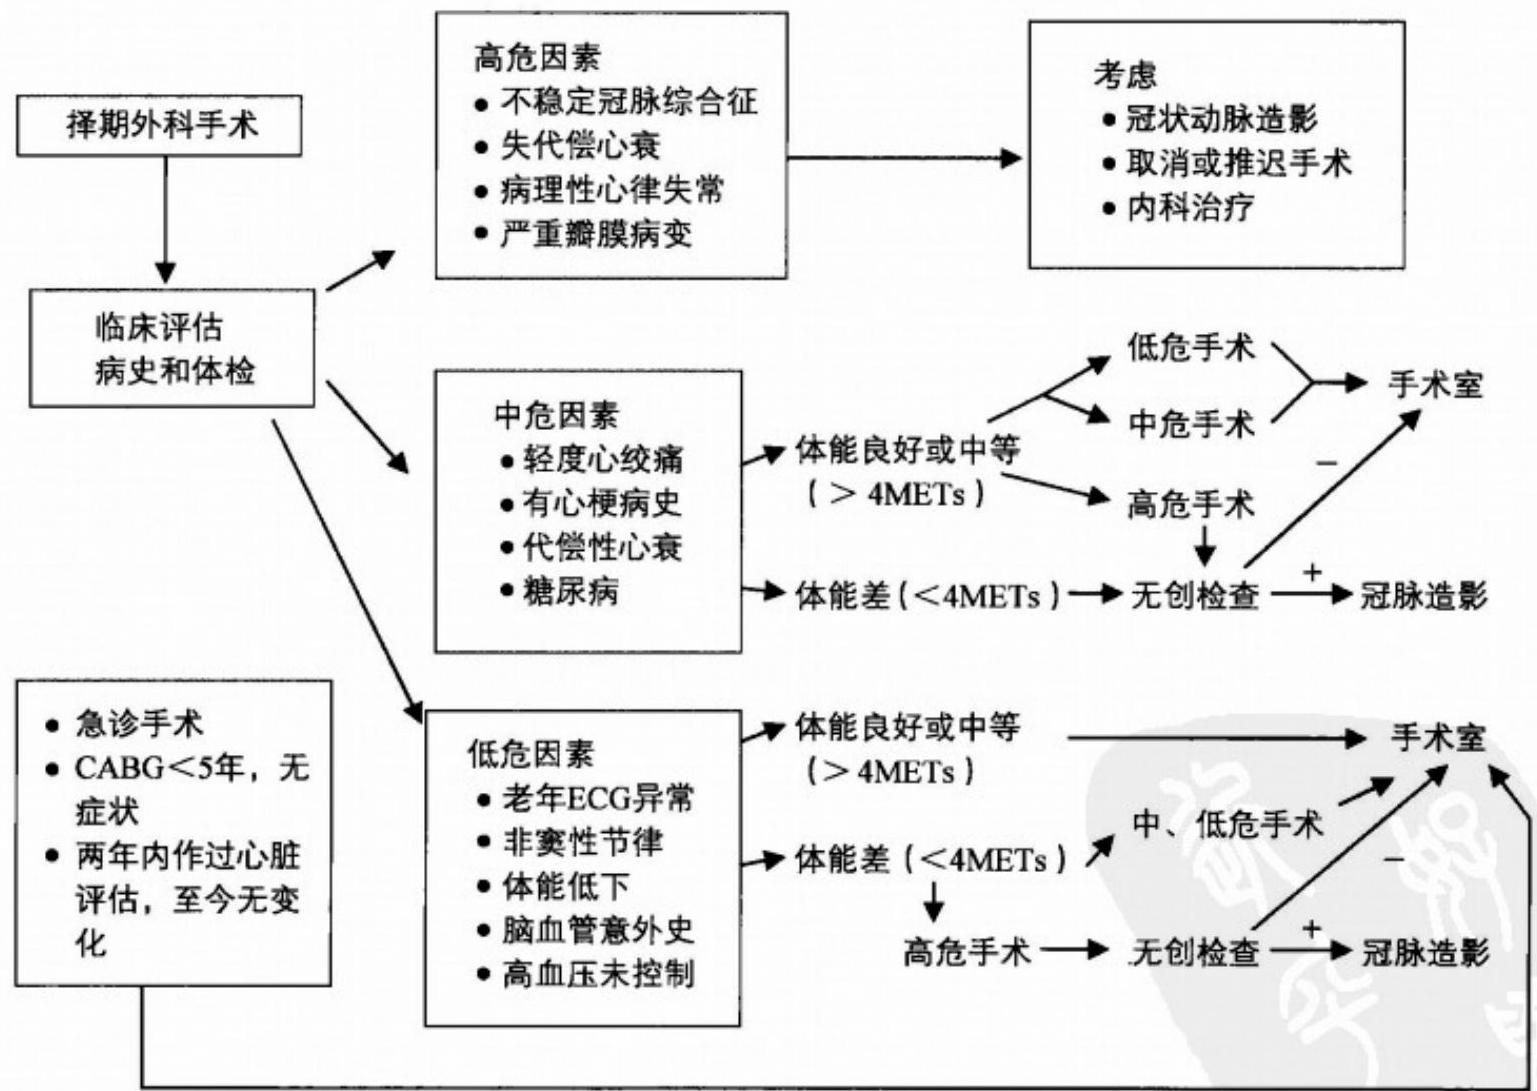
\includegraphics[max width=\textwidth]{2024_07_10_373f31b88d2bf633007bg-412}
\end{center}

图 4-1-1 非心脏手术患者围术期心血管评估指南

CABG: 冠状动脉旁路术

\section*{(二)呼吸功能评估}
肺部并发症和急性呼吸功能不全是外科患者术后的主要并发症和死亡原因之一,而原有肺部疾病的患者术后呼吸系统并发症的发病率更高。良好的术前评估和准备,能够显著降低肺部并发症的发病率和死亡率。

\begin{enumerate}
  \item 肺部并发症的危险因素
\end{enumerate}

(1)原有肺部疾病,且肺功能减退的患者。

(2) 患者年龄 $>60$ 岁。

(3)肥胖患者常伴有胸壁顺应性减退, 功能残气量下降和呼吸做功增加, 深静脉血检发生率增加; 对伴有肥胖低通气综合征 (pickwickian syndrome)的患者,其术后肺部并发症发生率更高。

(4) 吸烟使呼吸道的敏感性增加, 分泌物增多,支气管纤毛运动减弱或消失。

(5)外科手术的部位、创伤大小及手术时间均影响术后肺部并发症的发生和肺功能状况。胸部和上腹部手术可影响漏肌的功能, 并产生限制性通气功能障碍; 急诊手术, 尤其是伴有脓毒血症的急诊患者, 术后发生呼吸并发症的危险增加; 手术时间超过 $3 \mathrm{~h}$ 的也容易产生肺部并发症。

\begin{enumerate}
  \setcounter{enumi}{1}
  \item 肺功能的检查 在评估忠者的呼吸系统时, 对其肺功能的评估是一项重要的内容。目前,尚无明确规定哪些患者必须接受肺功能检查, 但对于有下列情况的患者应考虑实施: (1) 有慢性肺部疾患的忠者; (2)胸廠或背柱畸形、过度肥胖的患者; (3)有持续咳喘病史的吸烟患者; (4)需行肺叶切除或单肺通气的患者; (5)有严重神经肌肉疾病的忠者。
\end{enumerate}

一般围术期肺功能检查包括病史、体格检查、胸部 $\mathrm{X}$ 摄片、动脉血气分析和肺功能测定。对病史的详尽了解是对呼吸功能评估的第一步,一般通过病史和体检可大致判断患者的呼吸功能。绹部 $\mathrm{X}$摄片是检查肺部最常用的手段之一, 但在肺功能评估方面, 由于多数患者在胸片出现异常之前均已有明显的症状和体征 (如 COPD 及哮喘), 故胸片所提供的信息对于改变治疗方案影响并不大。有学者建议将肺部或心血管疾病患者、恶性肿㿔及有超过 20 年吸烟史的患者将术前胸片检查作为常规。动脉血气可以部分反映出静态下的肺功能, 对行开胸手术或肺叶切除术的患者可以提供较有价值的肺功能评估。

肺功能测定由多项指标构成, 它能较完整地反映呼吸系统的功能状态, 并为术后呼吸系统并发症 (postoperative pulmonary complications, PPCs) 的发生作出有效的预测。在肺功能测定中, 尚无一个具体指标可全面地预测 PPCs, 必须综合分析才有较大的临床价值。分钟最大通气量 (MVV)对于反映 PPCs 有较高价值, 它主要反映人体通气的储备功能, 是通气功能测定中很有价值的指标, 如果 MVV 小于预测值的 $50 \%$, 术后患者 PPCs 的发病率及死亡率均将大大增加。对于大多数阻塞性肺疾患患者, 第 1 秒时间肺活量 $\left(\mathrm{FEV}_{1}\right)$ /用力肺活量\\
(FVC)明显降低,在限制性肺疾患病人中则保持正常; 就开胸手术及肺叶切除手术而言, 预测术后 PPCs 的价值则以 $\mathrm{FEV}_{1}$ 和 FVC 价值最大。由于 MVV 是阻塞性通气障碍, 限制性通气障碍及肌力、营养状况等综合因素的反映, 对于部分乃至全肺切除术的患者而言, $\mathrm{MVV}$ 能较 $\mathrm{FEV}_{1}$ 及 $\mathrm{FEV}_{1} / \mathrm{FVC}$更敏感地预测患者是否能耐受手术。肺活量 (FVC) 很大程度上反映了心功能的好坏, 此外也受到各种因素的影响, 故对于术前呼吸功能的评估缺乏有效价值。弥散容积 (DLco) 反映了肺泡膜的厚度及患者是否有肺泡气体的弥散障碍, 该指标的测定利用一氧化碳与血红蛋白高度结合的特性, 在吸人一氧化碳后测定单次呼出气中的一氧化碳浓度来测定肺泡气体的弥散功能, 此指标术前对于预测肺切除术后呼吸功能不全的发病率及死亡率较为有效。对于肺叶切除术, 分侧肺功能有利于预测肺叶切除的范围。

临床上肺功能测定反映的是静态肺功能情况,其结果往往低于患者的实际能力, 故为能够更客观、准确地评估患者的心肺功能, 可进行心肺联合运动试验以评估患者的心肺储备功能。其最简单的心肺联合运动试验就是步行试验和攀楼试验, 量化指标多采用固定时间内步行距离或攀楼阶梯数;更为精确的心肺联合运动试验则是平板运动试验或登车运动试验。试验结果中大家感兴趣主要是最大氧耗量 $\left(\mathrm{VO}_{2} \max \right)$ 和无氧阈 (AT)。

$\mathrm{VO}_{2}$ max 是指患者运动-摄氧曲线进人平台期 (即氧耗量不随运动功率的增加而上升) 时的耗氧量。但真正能够测到 $\mathrm{VO}_{2}$ max 须让患者做极限量运动, 这显然对已存在心肺功能不全的患者来说是危险且难以做到的, 故临床上多采用症状限制性最大运动, 即当受试者感到极度乏力、气促、头昏、疲劳、步态不稳, 胸痛发作即停止运动, 此时测得的氧耗量称为峰值耗氧量 $\left(\mathrm{VO}_{2}\right.$ peak $)$ 。但目前 $\mathrm{VO}_{2}$ peak 预测胸科手术并发症的界值仍有争议,大家基本认同 $\mathrm{VO}_{2}$ peak $>20 \mathrm{ml} /(\mathrm{kg} \cdot \mathrm{min})$ 的患者均可耐受手术。 $\mathrm{VO}_{2}$ peak $<10 \sim 15 \mathrm{ml} /(\mathrm{kg} \cdot \mathrm{min})$ 的患者手术后的并发症发生率显著提高。

无氧阈的含义是指由无氧代谢补充有氧代谢供能时的工作水平或氧耗量, 到达这一水平后体内乳酸中毒开始发生。其临床意义主要在于对耐力运动能力及心肺功能的评价。一般认为正常人的无氧阔为最大氧耗量的 $50 \% \sim 60 \%$, 耐力训练的运动员可高达 $70 \% \sim 80 \%$ 。影响无氧阈的因素有很\\
多,如心脏疾病、周围血管疾病、肺血管疾病、贫血、肺部疾病与氧灌注问题、慢性代谢性酸中毒等均可使无氧阈降低。研究发现单纯性通气功能障碍患者的无氧咸并不下降,故临床上用无氧阈评估患者心肺功能更多的是偏向于心血管方面。无氧阈下降则代表机体代偿储备能力下降。

此外, 还有创伤性检查如肺动脉导管, 可以评估肺切除术后的心血管功能。使用肺动脉导管阻断拟行切除肺叶的肺动脉血管, 如患者能耐受由此产生的肺动脉高压及低氧血症, 则大多可胜任手术,一般认为阻断肺血管后 $\mathrm{PaO}_{2}$ 应不低于 $45 \mathrm{mmHg}$, 肺动脉压不应高于 $35 \mathrm{mmHg}$ 。此项检查可大大减少肺切除术后由于心功能失代偿或低氧引起的 PPCs。

目前, 临床上多采用 MVV 占预计值的百分比、残气量 (RV)/肺总量 (TLC)、 $\mathrm{FEV}_{1} / \mathrm{FVC}$ $\left(\mathrm{FEV}_{1} \%\right)$ 这三项指标对呼吸功能进行分级评估 (表 4-1-12)。

表 4-1-12 呼吸功能评估

\begin{center}
\begin{tabular}{cccc}
\hline
呼吸功能评估* & MVV $\%$ & $\mathrm{RV} / \mathrm{TLC} \%$ & $\mathrm{FEV}_{1} \%$ \\
\hline
正 常 & $\geqslant 75$ & $\leqslant 35$ & $\geqslant 70$ \\
轻度损害 & $60 \sim 74$ & $36 \sim 50$ & $55 \sim 69$ \\
中度损害 & $45 \sim 59$ & $51 \sim 65$ & $40 \sim 54$ \\
重度损害 & $30 \sim 44$ & $66 \sim 80$ & $25 \sim 39$ \\
极度损害 & $\leqslant 29$ & $\geqslant 81$ & $\leqslant 24$ \\
\hline
\end{tabular}
\end{center}

\begin{itemize}
  \item 综合评定 重度: 三项中至少有两项达重度损害中度:三项中至少有两项为中度损害三项中轻中重度损害各一项轻度: 不足中度损害
\end{itemize}

一般认为术后发生呼吸功能不全的高度危险指标有: 静息时出现呼吸困难; 发绀; 肺源性心脏病; 肺功能测定指标<预计值 $50 \%$; 缺氧伴二氧化碳濐留。

\section*{(三)肝功能评估}
术前肝功能评估包括询问病史、体格检查、实验室检查和术前肝疾病的治疗措施四方面。

结合临床和实验室检查结果 (Child-Puge 分级), 可初步评估肝功能的损害程度、肝功能的储备及手术的危险性, 见表 4-1-13。

$\mathrm{A}$ 级:肝功能在正常范围。对各种手术的反应良好。

$\mathrm{B}$ 级: 肝功能差。对所有手术的反应不如健康人体,如能术前充分准备,可能会增进患者对手术的耐受性。

C 级: 肝功能极差。对各种手术的反应及耐受很差, 即使术前尽力改善也收效甚微。

\section*{(四)肾功能评估}
术前应依据病史、体格检查和实验室检查综合判断悄功能, 衡量患者对麻醉和手术的耐受性。

多数情况下,与麻醉和手术相关的肾功能改变是可逆的。但术前如已存在肾功能受损或存在损害肾功能的因素如严重创伤, 则麻醉和手术可加重对肾功能的影响。围术期多种因素都可诱发急性肾衰竭(表 4-1-14)。

检测肾功能的方法很多, 内生肌酐清除率 $(\mathrm{CCr})$ 能较正确反映肾小球滤过率 (GFR), 但由于检测方法复杂, 临床使用受限。目前, 临床上主要检测血肌酎水平 ( $\mathrm{SCr}$ ) 来反映肾功能, 其值 $<$ $133 \mu \mathrm{mol} / \mathrm{L}$, 提示 GFR 正常。此外,血尿索氮也是常规检测项目, 尿浓缩和稀释试验也有助于对将功能的评估。

表 4-1-13 评估肝功能的 Child-Puge 分级及手术危险性

\begin{center}
\begin{tabular}{|c|c|c|c|}
\hline
 & $\mathrm{A}$ & $\mathrm{B}$ & C \\
\hline
血清胆红索 $(\mu \mathrm{mol} / \mathrm{L})$ & $<34.2$ & $34.2 \sim 51.3$ & $>51.3$ \\
\hline
血清白旋白 $(\mathrm{g} / \mathrm{L})$ & $>35$ & $28 \sim 35$ & $<28$ \\
\hline
凝血酶原时间延长(s) & $<4$ & $4 \sim 6$ & $>6$ \\
\hline
腹水 & 无 & 容易控制 & 难以控制 \\
\hline
肝性脑病 & 无 & 轻徜 & 严重 \\
\hline
营养 & 好 & 良好 & 噟 \\
\hline
手术危险性 & 小 & 中 & 大 \\
\hline
病死率(\%) & $<5$ & 25 & $>50$ \\
\hline
\end{tabular}
\end{center}

表 4-1-14 围术期诱发急性肾衰竭的危险因素

\begin{enumerate}
  \item 老年患者, 将功能代偿, 但 GFR 已经减退

  \item 原有慢性肾疾病

\end{enumerate}

若 $\mathrm{CCr}>50 \mathrm{ml} / \mathrm{min}$, 无特殊

若 $\mathrm{CCr}$ 为 $25 \sim 50 \mathrm{ml} / \mathrm{min}$, 早期肾功能减退, 围术期保持将血流量

若 $\mathrm{CCr}<20 \mathrm{ml} / \mathrm{min}$, 患者已经存在肾功能不全, 需要血液透析

\begin{enumerate}
  \setcounter{enumi}{2}
  \item 心功能不全或需要心脏手术

  \item 需要血管造影或进行血管手术

  \item 严重创伤和烧伤

  \item 低血容量 (休克、感染、肝硬化等)

  \item 恶性高热

\end{enumerate}

目前,在血液透析治疗的前提下,慢性肾功能不全已不再是择期手术的禁忌, 但总的来讲,其对麻醉和手术的耐受性仍差。

(五)其他

我们还应对神经系统的功能进行评估。随着年龄的增长,伴有脑血管疾病的患者进行外科手术应明确有无脑卒中的病史及神经功能缺陷的表现,对常见的神经系统疾病应了解常用的基本药物及其药理特性,对麻醉及手术可能带来的潜在影响应有所了解,必要时咨询专科医生以协助术前准备和治疗。

同样,对于一些内分泌疾病如糖尿病患者, 应了解糖尿病的类型、胰岛素的应用及血糖控制情况,必要时咨询专科医生协助处理。

\section*{三、知情同 意}
术前访视的目的不仅仅在于收集重要的临床资料,其最终目的是就麻醉方法的选择为患者提供一个合理的解释,取得患者的知情同意,而且有助于建立良好的医患关系。麻醉医生可通过以下行为消除病人恐惧,建立彼此之间的信任。

\begin{enumerate}
  \item 术前与患者轻松的会面, 以消除患者对外科手术和麻醉的恐惧,坦率地和患者谈及术后的疼痛, 告诉患者术后绶解疼痛的方法或术后准备采取的镇痛措施。

  \item 征求并尊重患者对麻醉的选择。

  \item 交代术前注意事项,如禁食时间、术前是否需要停用某种特殊的治疗药物等。

  \item 患有特殊疾病的患者,术前应指导患者进行必要的治疗或锻炼, 对于术中、术后需要患者配合的治疗措施,亦应在术前访视时交代清楚。

  \item 与患者家属详细叙述麻醉经过,对可能发生的并发症进行必要的描述, 见表 4-1-15。

\end{enumerate}

表 4-1-15 麻醉的主要并发症

\begin{enumerate}
  \item 一般并发症
\end{enumerate}

昰心、呕吐

穿剌部位浅表出血

咽喉疼痛

牙齿损伤

角膜擦伤

头痛

\begin{enumerate}
  \setcounter{enumi}{1}
  \item 严重并发症
\end{enumerate}

周围神经损伤

心律失常

心肌梗死

肺不张和肺炎

肝将功能不全

脑卒中

药物过㩯

输血反应

\begin{enumerate}
  \setcounter{enumi}{2}
  \item 死亡
\end{enumerate}

\section*{四、麻醉前准备事项}
\section*{(一)麻醉前准备的内容}
\begin{enumerate}
  \item 纠正或改善紊乱的病理生理状态手术患者常合并内科疾病,麻醉医师应充分认识其病理生理改变,对其严重程度作出正确评价, 必要时请内科专家协助诊治。
\end{enumerate}

(1)营养不良可导致血浆蛋白降低,贫血、血容量不足使患者耐受麻醉、手术创伤及失血的能力降低。术前应改善营养不良状态,纠正脱水、电解质絮乱和酸碱失衡。

(2)合并心脏病者, 应重视改善心脏功能,注意术前治疗药物的应用:

(1) $\beta$ 受体阻滞药、钙拮抗药和硝酸酯类药物应持续用药至手术日晨; 但长效 $\beta$ 受体阻滞药 (如阿替洛尔等) 可在术前 $3 \mathrm{~d}$ 改为中短效药物 (如美托洛尔、普蔡洛尔等)。

(2)洋地黄类药物应在术前 $24 \mathrm{~h}$ 停药; 如患者有心房纤颤并且心室率较快, 则洋地黄可持续给药直至术日展。

(3)抗高血压药物如钙通道阻滞药和利尿药,一般应持续给药至术日晨; 因担心术中出现低血压,有医师主张在术日展停用 ACE 抑制药。

(4)抗心律失常药物一般应持续用药至术日晨;但应注意许多抗高血压药物均可降低房室传导, 引起心动过缓和心肌抑制。

(5)抗凝药物如华法林至少应在术前 $4 \mathrm{~d}$ 停药,必要时可改为小剂量肝素静脉滴注, 直至手术日。对于抗凝治疗患者, 区域麻醉仅用于其利益/风险值远远大于其他麻醉方式时。椎管内或硬膜外麻醉前 4 6h 停用肝素, 术后 $1 \mathrm{~h}$ 再继续使用, 可防止硬膜外血肿。如果术中有出血倾向, 则应在术后 $12 \mathrm{~h}$ 复用。除非术前有明确出血或㾿斑, 服用阿司匹林或其他非甾体抗炎药的患者可应用椎管内麻醉。

(3)对并存急性呼吸道感染 (如感冒、咽炎、扁桃体炎、气管支气管炎、肺炎) 者, 术后极易发生肺不张和肺炎,除非急症,手术应暂停, 至少需推迟到治愈一周后再手术。合并慢性呼吸系统疾病者, 术前应检查肺功能、动脉血乞分析和胸部 X 线片; 停止吸烟至少两周, 并进行呼吸功能训练; 行雾化吸人和胸部物理治疗以促进排痰; 应用有效抗生素以控制肺部感染。

(4)合并糖尿病者,择期手术应控制空腹血糖不高于 $8.3 \mathrm{mmol} / \mathrm{L}$, 尿糖低于 (H), 尿酮体阴性。急诊伴酮症酸中毒者, 应静脉滴注胰岛素消除酮体,纠正酸中毒后手术; 如需立即手术者, 虽然可在手术过程中补充胰岛素、输液并纠正酸中毒,但麻醉的风险性明显增加。

\begin{enumerate}
  \setcounter{enumi}{1}
  \item 胃肠道的准备 许多患者来到手术室时有发生吸人性肺炎的危险。怀兮、肥胖、糖尿病、食管裂孔㡳或胃食管反流患者, 都可能有吸人胃内容物导致化学性肺炎。对严重创伤患者、急腹症和产妇, 虽距末餐进食已超过 $8 \mathrm{~h}$, 由于胃排空延迟, 也应视作“饱胃”(full stomach)病人对待, 这类病人即使是在部位麻醉下,也有呕吐和误吸造成呼吸道阻塞的可能。
\end{enumerate}

择期手术前应常规禁食、禁饮,以避免围术期间发生胃内容物的反流、呕吐或误吸。美国麻醉医师协会 1999 年对拟行择期手术的健康患者推荐术前禁食指南见表 4-1-16。

表 4-1-16 ASA 檚食指南

摄人物

最短禁食时间

(适用于所有年龄)

\section*{清淡的液体}
母乳

㜟幼儿配方奶

非人乳

便餐(面包片和清淡的液体)

*清淡的液体包括水、无果肉果汁、碳酸饮料、清茶和黑哳啡

\begin{enumerate}
  \setcounter{enumi}{2}
  \item 精神状态的准备 手术前患者大都对麻醉和手术感到紧张和焦虑,甚至有恐惧感,这种心理状态对生理都有不同程度的扰乱,并在整个围术期产生明显影响。因此,在访视患者时, 应以关心和鼓励的方法消除其思想顾虑和焦虑心情, 将麻醉方法、术中可能发生的不适感及应该配合的情况,向患者作恰当的解释。耐心听取和解答患者提出的问题,以取得患者的理解、信任和合作。对于过度紧张而难以自控者,应以药物配合治疗。有心理障碍者, 应请心理学专家协助诊治。

  \item 麻醉设备、用具及药品的准备 为了使麻醉和手术能安全顺利进行, 防止任何意外事件的发生, 麻醉前必须对麻醉和监测设备、麻醉用具及药品进行准备和检查。无论何种麻醉都应准备好全身麻醉用具,以备不测之需。

\end{enumerate}

全身麻醉用具的准备一般应包括: 麻醉机及气源、气管插管用具和药品及其他急救用药等。麻醉期间除必须监测病人的生命体征,如血压、呼吸、脉搏、脉搏氧饱和度 $\left(\mathrm{SpO}_{2}\right)$ 和体温外, 还应根据病情和条件,选择适当的监测项目,如 ECG、呼气末 $\mathrm{CO}_{2}$分压 $\left(\mathrm{ETCO}_{2}\right)$ 、直接动脉压、中心动脉压 (CVP) 等。在麻醉实施前对已准备好的设备、用具和药品等应再 1 次检查和核对。术中所用药品,必须经过核对后方可使用。

\section*{(二)麻醉前用药 (preoperative medication)}
\begin{enumerate}
  \item 术前用药的目的 麻醉前用药的目的是要使麻醉过程更加平稳、安全, 麻醉效果更加完善并尽可能消除或减轻麻醉手术对患者精神和躯体的伤害,具体包括的内容见表 4-1-17。某些目的, 比如缓解焦虑和产生镇静,适用于几乎每位患者,而其他目的仅仅偶尔是必须的。
\end{enumerate}

\section*{表 4-1-17 术前用药的目的}
\begin{verbatim}
1. 解除患者的紧张和焦怎
2. 缓解穿刺或其他操作时的疼痛
3. 遺忘
4. 减少口空和气道分泌物
5. 预防自主神经反射
6. 戏少胃液容量和酸度
7. 减少麻碎药的用量
8. 有利于麻醉诱导的平稳
9. 镇吐作用
10.预防或对扰过敏反应
\end{verbatim}

\begin{enumerate}
  \setcounter{enumi}{1}
  \item 药物选择 相比过去而言,术前用药的应用已减少很多, 但对于紧张焦虑的患者和具有较大的胃食管反流风险的患者仍须术前用药 (表 4-118)。一般患者麻醉前用药在人手术室后给予。
\end{enumerate}

\section*{表 4-1-18 应用术前药应注意的恵者情况}
\begin{enumerate}
  \item 身体一般情况 (ASA 分级)

  \item 年龄和体重

  \item 焦虑和痛國水平

  \item 既往用药史和药物成癔史

  \item 既往犘醉有无恶心呕吐

  \item 过敏史

  \item 住院患者/门诊患者

  \item 手术方案精神紧张者, 可于手术前晚上口服催眠药或安定镇静药,以消除患者的紧张情绪。一般状况差、年老体弱者、恶病质及甲状腺功能低下者, 对催眠镇静药及镇痛药都较敏感, 用药量应惐少; 而年轻体壮或甲状腺功能六进患者, 用药量应酌增。冠心病及高血压患者的镇静药剂量可适当增加,而心胜竬膜病、心功能差及病情严重者, 镇静及镇病药的剂量应酌减。抗胆碱药一般术前很少应用,对儿童或需清醒插管的患者予以应用可减少腺体的分泌;由于可能出现的术后澥妄,阿托品一般不主张用于老年患者,而东茛若碱则应视为禁忌。

\end{enumerate}

产妇、食管裂孔羌、肠梗阻、肥胖或中枢神经系统抑制等易发生吸人性肺炎的病人, 应用 $\mathrm{H}_{2}$ 受体阻滞药可减少胃酸的分泌,而使用抗酸药可中和胃酸以减少误吸时可能发生的肺损伤,但一般不推荐使用颗粒性抗酸药。在行高风险麻醉时, 诱导前短时间内口服枸橡酸钠溶液是首选,但会增加胃内容物。ASA 不推荐在健康、择期手术病人常规使用这些药物。

术前用药选择原则: 高龄、脑损伤或意识状态改变、心肺储备功能较差、低血容量及饱胃患者,术前应慎用抑制性药物; 毒品或巴比妥类成癛者术前用药量宜增加,以免术中出现停药症状。

\begin{enumerate}
  \setcounter{enumi}{2}
  \item 常用术前药物(表 4-1-19)
\end{enumerate}

表 4-1-19 常用术前药

\begin{center}
\begin{tabular}{|c|c|c|c|}
\hline
药物类型 & 药名 & 给药途径 & 剂量(mg) \\
\hline
\multirow[t]{4}{*}{安定镇静药} & 地西泮 & 口服 & $5 \sim 20$ \\
\hline
 & 劳拉西泮 & 口服、肌内注射 & $1 \sim 4$ \\
\hline
 & 㽤达唑仑 & 肌内注射、静脉注射 & $1 \sim 5$ \\
\hline
 & 莱巴比妥钠 & 肌内注射 & $50 \sim 100$ \\
\hline
\multirow[t]{2}{*}{镇痛药} & 吗啡 & 肌内注射 & $5 \sim 10$ \\
\hline
 & 㖘替啶 & 肌内注射 & $1 \mathrm{mg} / \mathrm{kg}$ \\
\hline
\multirow[t]{3}{*}{抗胆䂸药} & 阿托品 & 肌内注射、静脉注射 & $0.3 \sim 0.5$ \\
\hline
 & 格隆滇轱 & 肌内注射、静脉注射 & $0.1 \sim 0.3$ \\
\hline
 & 东莨营碱 & 肌内注射、静脉注射 & $0.3 \sim 0.6$ \\
\hline
\multirow[t]{3}{*}{提高胃洂 $\mathrm{pH}$ 药物} & 雷尼替丁 & 口服 & $50 \sim 200$ \\
\hline
 & 西咪替丁 & 口服、肌内注射、静脉注射 & $150 \sim 300$ \\
\hline
 & 枸橡酸钠 $(0.3 \mathrm{~mol} / \mathrm{L})$ & 口服 & $10 \sim 30 \mathrm{ml}$ \\
\hline
\end{tabular}
\end{center}

(薛张纲)

\begin{center}

\includegraphics[max width=\textwidth]{2024_07_10_373f31b88d2bf633007bg-418}
\end{center}

[1] Ronald D. Miller, MD. 謷因明,邓小明主烽. MILLER's ANESTHESIA, 6 th Edithion. 北京: 北京大学医学出版社,2006:947-1039

2]庄心良,曾因明,陈伯金,现代麻醉学. 3 版. 北京: 人民卫生出版社,\\
2003,767-838

[3] Peter F. Dunn. Clinical Anesthesia Procedures of the Massachusetts Genera Hospital. Seventh Edition. USA: Lippincott Williams \& Wilkins, a Wolters Kluwer business, 2007:3-17\\
[ 4 ] G. Edward Morgan, Jr, Maged S. Mikhail, Michael J. Murray. 岳云、吴新民,罗爱伦主泽 . 库根临床麻醉学. 北京: 人民卫生出版社, 2007: 114

\section*{篍2笔}
\section*{气道管理}
维持呼吸道通畅, 维持有效的通气和充分的氧合是麻醉医生每天必须面对的任务和挑战。如果不能保证气道通畅、不能维持有效的通气和充分的氧合, 任何麻醉都是不安全的。本章所介绍的气道管理原则, 同样适用于心肺复苏和呼吸功能不全的患者。

\section*{一、上呼吸道梗阻的处理}
上呼吸道梗阻分为完全梗阻和不完全梗阻。上呼吸道完全梗阻可以通过气流和呼吸音的缺失来判断。判断上呼吸道完全梗塞的正确方法是用手或耳朵贴近患者的嘴边不能感受到气体的流动,避免将无效呼吸时的胸廓和䐟肌运动当成呼吸的存在。上呼吸道不完全梗阻的患者表现为潮气量逐渐减少并伴有 “三凹征”, 如梗阻部位在鼻咽部,常有筧声, 如果梗阻在喉部, 常伴有吸气性喘鸣音。

上呼吸道梗阻的处理取决于梗阻原因的分析,这些原因包括: 软组织、肿痹、异物和喉痉挛。如果是异物引起的,则应清除异物; 如出现喉痉挛,可以加深麻醉或给予肌肉松驰药。患者意识消失后和麻醉后发生的上呼吸道梗阻通常是由于舌和下颌的松驰引起舌后邑,导致舌基底部和咽壁之间的空间惐少。处理方法是给予面罩吸氧,向上托起下领和伸展头部, 给予正压通气。托起下颌和伸展头部抬高了舌骨和会厌,可缓解上呼吸道梗阻。如托起下颌和伸展头部不能改善通气, 则置人口咽通气道或鼻咽通气道。臫咽通气道是经鼻和舌后部到达咽喉部, 口咽通气道是经口沿舌塞人舌后部, 两者均为舌后部的人工通气道。在日常工作中即使使用了口咽通气道, 有时仍不能使气流通畅, 此时仍需要托起下颌和伸展头部来保持气道通畅。当上述方法和人工气道的使用仍不能解决上呼吸道梗阻时, 则应考虑行气管插管。

\section*{二、快速顺序诱导}
快速顺序诱导是指给予一种强效静脉诱导药后, 立即给予速效神经肌肉阻滞药使患者在极短的时间内达到无意识和肌肉麻痹状态, 以完成气管插管的方法。快速顺序诱导是急诊气道管理的一项核心技术。快速顺序诱导主要用于在全身麻碎下行急诊手术患者, 这些患者由于术前未禁食, 诱导过程存在反流和误吸的风险。为了防止反流和误吸的发生, 在患者意识消失后, 立即向后给环状软骨加压, 直到ヶ管导管插人乞管并给导管套垭充气。快速顺序诱导没有绝对的禁忌证,最主要的原则是事先预计插管成功概率, 并制定出可能的插管失败后的应对方案; 如果插管不成功, 最重要的是维持有效的通气。快速顺序诱导目的是: 快速准确地控制气道, 改善低氧状态; 避免血流动力学剧烈波动、顾内压增高等并发症; 通过药物提供良好的插管条件和减少插管并发症。

\begin{enumerate}
  \item 预计掜管是否困难的方法
\end{enumerate}

(1)运用 LEMON 原则: L-大致看, E-评估 3-32 定律 ( 3 指开口度, 3 指颏-舌骨的距离, 2 指口底舌骨距离), M-Mallampati 评分, $\mathrm{O}$-梗阻, $\mathrm{N}$-颈部活动度。

(2)面部解剖学异常 (例如: 先天性的,外伤性的, 陈旧损伤性的)。

(3)上呼吸道解剖学异常 (例如: 肿面, 大块的㾲痕形成)。

(4)未减轻的上呼吸道梗阻。

(5) 尚未治愈的上呼吸道梗阻 (例如: 会厌炎,哮趹, 吸人性损伤)。

\section*{2. 快速顺序诱导的七个步聚}
(1)术前准备: 准备所有必须的仪器设备和药物等。

(2)预吸氧: 面罩吸氧,流量大于 $5 \mathrm{~L} / \mathrm{min}$,时间不少于 3 min。

(3)预处理: 预处理是给予药物来减轻插筞带来的不良反应: 如气管插管前 $2 \sim 3 \mathrm{~min}$ 静脉注射利多卡因 $1.5 \mathrm{mg} / \mathrm{kg}$, 可以减轻气管插管引起的支气管痉挛来防止重症哮喘发作和缓解须内压来防止高顽内压; 如气管插管前 $2 \sim 3 \mathrm{~min}$ 静脉注射阿片类药物(芬太尼 $1 \sim 2 \mu \mathrm{g} / \mathrm{kg}$ ) 可以缓解气管插管和喉镜检查伴随的交感兴奋和高顾内压。

(4)诱导麻醉: 静注静脉麻醉药如丙泊酚 $2 \mathrm{mg}$ / $\mathrm{kg}$ 或依托咪酯 $0.3 \sim 0.5 \mathrm{mg} / \mathrm{kg}$, 然后立即静注神经肌肉阻滞药如氯琥珀胆䂸 $1.5 \mathrm{mg} / \mathrm{kg}$, 对氯琥珀胆碱禁忌的患者,可用罗库溴轱 $0.6 \sim 1 \mathrm{mg} / \mathrm{kg}$ 静脉注射。

(5)保护和摆体位: 患者意识丧失后立即向后推压环状软骨 (塞立克操作法), 在患者意识丧失前推压环状软骨可能会引起不适和呕吐,在气管内插管完成和给气管导管套囊充气后停止推压环状软骨。

(6)证实插管到位: 插管后,重要的是迅速判断导管位置是否在主气管内, 主要方法包括上腹部听诊、双肺野听诊、观察呼吸时胸部的起伏、观察气管插管呼气末的 $\mathrm{CO}_{2}$ 和观察患者情况的改善 (例如 $\mathrm{SpO}_{2}$ 的上升)。

(7)插管后处理:首先固定气管内导管,连接呼吸机给予通气, 处理插管后心动过缓或过速, 处理插管后高血压或低血压,适当镇静、镇痛和给予神经肌肉阻滞药, 继续监测 $\mathrm{SpO}_{2}$ 和呼气末 $\mathrm{CO}_{2}$ 。

快速顺序诱导插管并发症的发生率为 3\%~ $5 \%$,主要是由气管插管操作本身引起的,较为严重的有插管失败、误人食管未被发现、误吸等。

\section*{三、气管内插管}
气管内插管分经口气管插管和经鼻气管插管。在喉镜引导下经口气管插管是气管插筞中最简单和最直接的方法。在喉镜的辅助下,可以直接连续地观察到声门的开放和气管导管进人气管内的全过程。在确定导管位置后, 固定好导管,并根据情况进行辅助或控制通气。

插管前除了准备气管导管和喉镜外,还应准备下列基本工具: 氧气源、呼吸踑、面罩、通气道、管芯、胶带、吸引器以及其他可能在特殊情况下运用的设备。

在病房的急救和治疗插管,操作者需要充分靠近床头,应锁定病床,移去病床的侧梁和床头板,床的高度应该与操作者的胸部平齐。一位有经验的助手应该始终站在一旁帮助传递吸痰管、通气道、导管和给药, 必要时还可以帮助操作者推压喉部。对于不能配合或躁动的病人, 需要再给予适度镇静药。

目前最常采用的气管内插管体位是用至少 $10 \mathrm{~cm}$ 厚度的枕头将头稍稍垫高, 颈部后仰, 头部前伸的“嗅物位”。

预给氧:在喉镜辅助下经口乞管内插管通常只用于麻醉状态和呼吸暂停的患者,由于该操作过程中,患者会面临缺氧的风险,因此插管会受到一定的时间限制。预给氧目的就是在放置喉镜前尽是降低缺氧风险。通常采用的预给氧方法是面罩吸氧, 流量大于 $5 \mathrm{~L} / \mathrm{min}$, 时间不少于 $3 \mathrm{~min}$, 或 $60 \mathrm{~s}$ 内做 8 次深呼吸。

直接喉镜可以充分暴露会厌以正确插人导管,最大限度减少缺氧时间,降低低氧血症的风险。目前有两种基本类型的喉镜片: 弯喉镜片(Macintosh)和尖端弯曲的直喉镜片(Miller)。它们均为右利手设计的:左手持喉镜柄, 右手放置导管。历史上,无论左手或右手(也可以双手)都可以持喉镜柄,但最后需要换至左手持镜柄,右手插管。这两种喉镜片的左侧都有一个侧翼, 可以将舌体推开,并且前端都有一个发光区(灯泡或纤维光镜的尖端)。每种喉镜片的右侧都有一个开放的槽便于喉部的显露和插管。

喉镜片应从口腔右边进人。在放置过程中应注意将下唇推开(由右手或助手辅助), 避免将下脣碾人下门齿和喉镜片之间。同时将镜片徐徐推进至舌根,其前端应朝向口腔中线方向,这样舌头便被镜片的侧翼推向左侧。当镜片到达舌根时,上提喉镜暴露会厌。该过程中手腕应保持是直的,只用肩和上臂的力量上提。如果操作者的手腕自然向桡侧倾斜,喉镜就会以上门齿或牙根为支点呈现杜杆的作用, 这样很容易损伤门齿。在喉镜片插人后,沿患者长轴上方 $45^{\circ}$ 角的直线方向对下领骨和舌体施加压力, 就可以看见会厄。会厌显露后, 如果采用弯喉镜片 (Macintosh), 尖端应该放在会厌谷(舌根部和会厌咽面之间的空间),然后将喉镜向上、向前方提起, 拉綮舌骨会厌㓞带, 使会厌抬起,逐渐显露杓状软骨和全部声门。如果采用直喉镜片(Miller),镜片顶端应恰好位于会厌喉面的下方,像使用弯喉镜片一样向前向上移动可以直接暴露\\
声门。

通过上提咽部时会厌和声门显露的程度提出了唉镜下暴露分级的简易评估方法。Cormack 和 Lehane 喉镜暴露分级: I 级, 可见全部声门; II 级,可见部分声门; 正级, 仅可见会厌; IV 级, 只能看到软腼, 看不见会厌。这种分级方法要依靠一定的操作技术,但分级程度与插管的困难程度确实有一定的相关性。

在使用喉镜时最常用见以下四个问题:

\begin{enumerate}
  \item 无论哪种类型的䂒镜, 如果进人咽部太深都可能会将整个㘈部抬起, 只能见到食管开口而看不见声门。如果弯唤镜片进人会厌谷太深, 同时镜柄向颈椎方向旋转, 则会将会厌推下, 遮住声门口,也会使㘈部显露受限。

  \item 将舌头完全推向左侧是很关键的。许多插管失败和困难插管都是由于舌头占据右侧妨碍喉镜的置人, 影响声门的暴露和插管。

  \item 将舌头推向左侧时, 镜片的尖端却在中线右侧。这个位置会影响会厌的显露, 而且会损伤脆弱的扁桃体组织,引起出血。镜片尖端必须正好位于下咽部的中线位置。

  \item 在胸部宽厚的肥胖患者或乳房较大的患者中, 可能因为胸壁的阻挡一开始不太容易将喉镜片正确地放人口中。面对这样的患者,可以使颈部再尽量后仰, 或将喉镜柄向右旋转 $45^{\circ}$ 便于镜片进人口中, 可改用短镜柄替代这种标准长度的镜柄。

\end{enumerate}

适当地推压喉部可以显著改善喉镜的视野。例如, 常规推压㜔部可以将喉镜分级Iㅣ级暴露的发生率从 $9 \%$ 降低至 $5.4 \% \sim 1.3 \%$ 。最佳推压喉部的方法是将甲状软骨向后、上、右的方向推压, 对于没有经验的人最好的方法是当头后仰、口张开的体位摆好后,操作者用右手亲自推压喉部。

气管插管: 如果声门暴露良好 (没有受到舌体的阻挡), 气管插管会很容易。但能看见声门, 却插不进导管的情况也并非少见。一般成人的气管可以通过内径 $7 \sim 9 \mathrm{~mm}$ (甚至 $10 \mathrm{~mm}$ ) 的气管导管。如果要使用纤维支气管镜检查和治疗, 就必须选择内径至少为 $8 \mathrm{~mm}$ 以上的气管导管。如果上下门齿之间的缝隙较小, 可能划破套囊, 应该将套囊远端润滑, 便于从齿弹滑过。同样, 如果是张口受限的患者,还应该将套衰内的空气尽量抽空。气管导管的前端应该从右侧嘴角进人, 沿与喉镜片纵轴相交的方向徐徐前进, 到达声门口。这种方法, 可以避免气管导管遮挡喉镜对声门的显露。气管导管尖端进人声门, 待套蛼完全通过声门后 $2 \mathrm{~cm}$, 就可以停止前进; 或当气管导管距下门齿的刻度为 22 $24 \mathrm{~cm}$ 时, 气管导管的尖端一般正好在气管中段。特别需要注意的是, 操作者必须看到套哄通过声门后, 才能将视线从喉口移开, 以避免气管导管误人食管。

管芯可以帮助调整插管的方向。因为管芯有较好的硬度和韧性, 它可以更好地控制气管导管前端的方向。但当气管导管通过牙齿后便不容易再塑型。插管过程中只能调整插管深度和旋转气管导管尖端方向, 气管导管应该尽可能靠近口腔右边, 这样可以最大限度地通过扭转气管导管近端来进行调整。管芯应该是易弯曲并且被充分润滑过的,而且其尖端不要伸出气管导管远端。当气管导管通过声门后应该立刻拨出管芯,使气管导管尖端诙复原来的曲度, 便于继续进人气管远端。

插人气管导管后,撤出倝镜并将套囊充气, 充气压力在 $22 \sim 32 \mathrm{cmH}_{2} \mathrm{O}$ 。如果没有测压工具, 感觉导管外的指示套䪄的张力适当即可。此时一只手将气管导管连接至正压通气系统, 另一只手将气管导管扶在原处, 并与脸颟相贴 (起到临时固定的作用), 直到最后将气管导管完全固定好, 以防气管导管意外脱出。

气管内插管后最重要的任务是确定气管导管在气管内而不是食管内。气管内插管的成功标志包括: 胸壁可闻及呼吸音, 腹部没有呼吸音, 未发生胃扩张, 胸砫随呼吸起伏, 呼气潮气量大,下压胸壁时可以从气管导管听到气流声, 当手动通气时圠气䪄的顺应性较好。如果 $\mathrm{SpO}_{2}$ 旺下降趋势说明插管失败, 但往往这是气管导管误人食管后出现最晚的体征。但当气管疼挛、支气管内插管、误吸、气管导管打折、机器或设备出现故障时, 也会引起 $\mathrm{SpO}_{2}$ 下降。

比较可靠的气管内插管的标志为正常呼气末 $\mathrm{CO}_{2}$ 波形的出现和橡胶气管指示球的迅速扩张。心搏橾停 (没有 $\mathrm{CO}_{2}$ 产生)、严重的气管痉挛、气管导管扭曲、堵塞也会影响呼出气体中 $\mathrm{CO}_{2}$ 的波形 (假阴性)。如果气管导管尖端䤵近声门附近, 也会产生呼气末 $\mathrm{CO}_{2}$ 波形(假阳性)。自动充气球具有很高的敏感性和特异性, 但在肥胖患者中会有明显的假阴性结果。

最可靠的气管内插管的判断方法是直视下气管导管通过声门和使用纤维支气管镜检查。当气管导管进人声门后可以将气管导管稍向后压, 使声\\
门张开得更充分, 从而更清楚地看到气管导管是否在声门口内。纤维支气管镜可以看到气管软骨环和隆突从而确定气管导管是否在气管内, 但这不作为常规的确定方法。

如果没有呼气末 $\mathrm{CO}_{2}$ 波形, 听不到呼吸音或没有看到胸廊起伏, 就应该拨出气管导管, 通过面罩和球囊使用纯氧进行正压通气, 检查原先的气管导管是否损害或被分泌物堵塞, 然后再次行插管。在面罩通气的同时应该对气管导管的形状、曲度和患者的体位进行调整, 或需要助手帮助推压喉部,或准备特殊的插管喉镜和插管工具。

接下来需要通过观察双侧胸倣起伏情况和对双侧外周肺野的听诊来确定气管导管是否在隆突上方, 避免导管进人一侧主支气管造成单肺通气。当成年女性和成年男性病人的插管深度分别为 $21 \mathrm{~cm}$ 和 $23 \mathrm{~cm}$ 时,一般不会发生主支气管内插管。纤维支气管镜是另一种比较复杂的判断方法。在手术室外的地方, 经常通过拍胸片来确定气管导管在气管内的位置。气管导管尖端理想的位置应该在锁骨水平 (气管中段)隆突上方 $2 \sim 4 \mathrm{~cm}$ 。

当气管导管插好后,固定气管导管时应记录下在门齿的气管导管刻度作为判断气管导管是否移位的参考。

气管导管的固定: 当记录下气管导管在门齿的刻度后, 应该将气管导管紧紧地固定在原地。这不仅对防止气管导管脱出很重要, 也可以避免气管导管向气管内发生任何移动。使用胶带将气管导管粘在脸颣上是最常用的固定方法。

上领处的皮肤是最常被选用的固定经口气管导管的粘贴部位, 因为该部位活动少, 不会使气管导管在气道内发生明显的移位。如果患者面部有胡须或胶带无法粘在面顽上, 可以使用带子围绕气管导管打结, 然后在颈部缠绕一圈。也可将气管导管捆绑在一颗牙齿上。

一般在喉镜引导下经鼻气管插管较经口插管难, 但经鼻气管导管要比经口气管导管的耐受性好, 因此, 经鼻气管导管可以用来进行时间略长的机械通气。目前的研究表明, 经鼻插管和鼻窐炎、肺炎之间没有关联。尽管如此, 作为长期机械通气,鼻插管并不比经口插管或气管切开更有优势。经鼻插管目前被仅限于一些口空内的手术 (如牙科手术、下领骨固定术) 和一些需要稳定气管导管位置的儿科手术。

气管导管从鼻孔进人(通常选右侧鼻孔) 经过鼻控、鼻咽进人口咽后, 可以在传统读镜的引导下进人声门, 或用插管钳 (Magill 钳) 夹住气管导管前端送人声门。有时经鼻插管会引起短暂的菌血症,因此对可疑患者应该注意预防心内膜炎的发生。

在进行鼻插管前, 应在鼻腔勫膜表面啰酒缩血管药物, 减少冝腔㭚膜损伤出血, 而且通过收缩橰膜可以扩大鼻腔孔径。插管前应将气管导管浸泡在温生理盐水中, 使导管尖端柔软, 减少插管造成的损伤和出血。插管时应选择患者认为平日最通畅的一侧鼻孔 (因为有的患者存在鼻中陣偏曲)。如果两侧賞孔的通畅程度一样, 一般常选择右侧,因为气管导管从右侧鼻孔进人有利于气管导管的斜面通过声门。气管导管必须小心地沿畕底部在下鼻甲下方插管, 避免使用暴力。可预防性使用缩血管药物、润滑导管、旋转导管、抽㾇套囊以尽可能地减少有效直径, 减少损伤。

一般成年患者的鼻孔很容易通过内径 7.0 〜 $7.5 \mathrm{~mm}$ 的气管导管。在进行经鼻直视下插管前也应该做好一些经口直视插管前的准备工作(摆放头位、备好吸引器和预给氧)。将充分润滑的气管导管向后、向尾端,沿正中方向前进,当感觉到阻力明显下降时, 说明气管导管已进人口咽 (通常深度为 15 16 cm)。阻力较大时, 勿用暴力, 而是退回气管导管、旋转、再前进。如果还是很困难就应该换另一侧鼻孔或改用小号的气管导管。

经鼻插管的过程中应尽量使鼻气管导管的曲度能够顺应生理的曲度前进。当气管导管经鼻孔进人鼻咽部时, 需向下并转向前通过咽部, 此时, 气管导管可能会顶住鼻咽部的后壁而无法用力推进。在此情况下, 应该将气管导管退出一点, 使病人头后仰再慢慢进人。如果不做调整, 且用力较大, 气管导管可能就会截破鼻咽后壁的馠膜, 进人橎膜下组织。如果进人这种假通道往往会有陷人“沼泽”的感觉而且气管导管管倥会被完全堵塞。

经鼻插管中喉镜的使用与经口插管一样。

气管导管进人口咽后, 其尖端必须与声门开口方向一致。前后调整气管导管位置, 直到能够在下咽部看到气管导管尖端, 同时旋转气管导管和调整头位也可以帮助气管导管进人声门; 如䢥困难, 右手持插管钳 (Magill 钳) 夹住气管导管尖端引导进人气管, 应避免夹住导管的套裏。在有些病人中,当气管导管进人气管时, 其尖端弯曲的部分正好顶在气管前壁, 无法前进; 此时须将头慢慢抬起 (前屈)以便于导管进人气管。经鼻气管导管的套暴应\\
该插至声门下 $2 \mathrm{~cm}$, 或气管导管距鼻孔的刻度女性为 $24 \sim 25 \mathrm{~cm}$, 男性为 $26 \sim 27 \mathrm{~cm}$ (比经口插管深 $3 \mathrm{~cm})$ 。气管导管正确位置的判断与其他类型气管插管一样(同经口插管), 但对于经鼻插管,判断气管导管位置更重要,因为气管导管外面的刻度标记与实际气管导管尖端在气管内的位置之间的关系并不如经口乞管导管的位置那样确定。如果发现有鼻出血, 可以将气管导管留在原地, 起到压迫止血的作用, 如果出血较多,可以将气管导管退出一部分, 使套詈充气, 起到更好的压迫止血的作用。

经鼻气管导管的固定与经口腔气管导管一样。除此以外还可以用琏线绳绕气管导管或穿过气管导管壁与宜中隔缝扎在一起。

\section*{四、意外困难插管的处理}
虽进行了麻醉前气道评估, 无论每个操作者熟练与否,都将会過到一些出乎意料的插管困难, 诱导时应考虑到这些问题,应有一个完整的预案。麻醉诱导后, 用喉镜暴露声门, 操作者应对喉镜暴觡的程度有清楚的认识。Cormack 和 Lehane 啶镜暴露分级: I 级, 可见全部声门; II 级, 可见部分声门; III 级, 仅可见会厌; IV 级, 只能看到软得, 看不见会厌。通常 Cormack 和 Lehane 喉镜暴露分级为 $\mathrm{I}$级和多数皿级患者可能出现插管困难或不可能插管。除了声门暴䨋困难以外,其他疾病包括会厌炎、喉和气管狭窄以及气管内肿物均可使气管导管插人困难。

当第 1 次插管失败后,在重新评估气道和做相关准备时, 只要能通过面罩维持通气,问题就不是很严重。由于每 1 次插管尝试都会增加病人喉部水肿和出血的可能性,任何一种插管方法都有可能造成喉水肿和出血, 在使用赎镜进行气管插管时更容易出现。因此应在注意减少损伤的同时迅速进行以下调整: 摆好 “嗅物位”, 喉外按压手法, 更换其他型号喉镜片, 更换其他气管插管技术, 请更多插管经验丰富的医生会诊。如果有经验的操作者反复插管不能成功, 如果仍能进行面罩通气, 应谨慎地停止气管插管操作并考虑以下措施: 唤醒患者。若使用短效药物 (如丙泊酚、吸人麻醉药和氯琥珀胆碱), 则可以等待患者清醒, 在表面麻醉下行清醒气管插管; 若使用长效药物 (如大剂量的阿片类药物和非去极化肌肉阻滞药), 则需在药物消退之前一直进行面罩通气。在面罩或喉罩通气下进行麻醉; 在尚能进行面罯通气时, 进行气管切开或环甲膜切开建立外科气道。

在插管困难, 但能通过面罩维持通气的情况下, 可以在麻醉状态下采取下列插管技术进行气管插管。

\begin{enumerate}
  \item 在普通喉镜暴露下, 如会厌和枃状软骨可见,可以用管芯或橡胶弹性探条帮助插管。

  \item 使用特殊喉镜提高喉镜的暴露分级, 比如: Glidescope 喉镜和 Truview 喉镜。

  \item 使用纤维内镜和带自封闭隔膜的纤维内镜专用面罩,可以在持续给予正压通气的同时, 行纤维内镜辅助气管插管。

  \item 使用光条插管。

  \item 使用可视光导芯插管。

  \item 使用插管喉罩进行插管。

\end{enumerate}

在当时的条件下,操作者可选择自己最熟悉的插管技术进行插管, 但无论采用何种插管方法进行插管,在每次插管尝试之间必须尽可能以面罩通气保持病人氧供。

当患者不能进行面罩通气和插管困难时,患者将会发生威胁脑和生命的紧急情况。如果使用的是短效的药物 (如氯琥珀胆碱、丙泊酚), 而患者有充足的预充氧,在采取进一步治疗以前患者应当可以恢复足够的自主呼吸。如果使用的是非去极化肌肉松驰药, 应首先置人喉罩, 维持通气。如能用喉罩维持通气, 可以考虑以下措施: 在喉罩通气下进行麻醉; 通过喉罩行气管插管; 唤醒病人; 在尚能进行面罩通气时, 进行气管切开或环甲膜切开建立外科气道。

当患者既不能通过面罩和喉罩通气,又插管困难时, 可以考虑以下措施: 可视光导芯插管; 插人食管气管联合导管; 经皮穿刺经气管喷射通气。

\section*{五、清醒插管}
清醒气管插管对麻醉医生来说既费时又费力,而且对病人来说也是一种痛苦的经历。对已知的困难气道患者选择清醒气管插管, 主要原因是: 在清醒状态下,患者会使自己的气道保持较好的自然状态; 在清醒状态下, 患者发声肌肉有足够的张力保持上呼吸道的形态,防止气道場陷, 并使上呼吸道的解剖结构易于识别, 如舌根、会厌、食管和咽后壁等。麻碎后, 发声肌肉的张力丧失, 引起上呼吸道的解剖结构堨陷, 舌根后苍; 另外,麻醉后喉位置前移使气管插管更加困难。所以,已预知的困难气管插管, 应选择清醒气管插管。

\begin{enumerate}
  \item 插管前充分的准备 是能否成功完成清醒气管插管至关重要的因素。很多清醒气管插管技术,要求在患者安静合作,在没有喉部刺激反射的情况下,才能完成气管插管。对清醒气管插管患者的插管前准备包括。
\end{enumerate}

(1)精神准备: 告知病人清酷气管插管的过程,并征得病人同意。

(2)监护:监测心电图、无创血压、脉搏血氧饱和度和呼气末二氧化碳。

(3)供氧准备: 可经鼻、鼻咽导管、纤维支气管镜的吸引通道或经气管导管给氧。

(4)如果是经鼻插管,需用缩血管药收缩鼻稆膜。

(5)给予干燥剂以堿少气道分泌物。

(6)应用表面麻醉,同时给予病人适当的镇静。可行喉部神经阻滞, 如喉返神经和喉上神经阻滞。

(7)防止误吸,准备好吸引器。

(8)准备相应的气道筞理工具。

\begin{enumerate}
  \setcounter{enumi}{1}
  \item 清醒插管技术包括
\end{enumerate}

(1)直视下经口清醒气管插管: 静脉注射干燥剂和镇静药 (如咪达唑仑)。在喉镜辅助下行舌根部和口咽部表面麻醉,在喉镜辅助下通过喉气管喷酒工具行喉和气管内的表面麻醉; 在没有喉气管喷洒工具时,可经环甲膜穿刺行纰管内表面麻醉。轻柔地放人喉镜, 暴露声门, 插人气管导管。为了提高插管成功率, 可使用特殊喉镜 (如 Glidscope 视频喉镜等)提高声门的暴露分级,同时给气管导管插人管芯, 通过调整管芯的弯度来调整气管导管前端的角度。

(2)口腔盲插: 在清醒状态下,当直接喉镜暴露喉部结构不全时, 应当尝试盲插。在适度镇静和表面麻醉后, 根据估计的方向插人带管芯的气管导管到达声门, 理想是导管会消人气管内。自主呼吸有一定的帮助, 可通过听呼吸音来引导找到声门。也可使用顶端有灯的管芯 (Trachlight 导芯), 将管芯插人气管,预先弯曲好管芯, 调暗房间的灯光, 根据估计的方向插人带光棒的气管导管, 当光棒顶端恰好位于中线声带上方时, 在颈前部能看到发红的亮点,此时把气管导管淂人气管。目插后, 建议用二氧化碳监测和纤维支镜来证实气管导管已进人气管。

(3)清醒状态下经鼻气管插管: 在手术室外的紧急情况下,当患者张口和颈部活动受限或被禁止时, 如需要经冝插管, 但诱导后经鼻插管的风险又很大, 此时需要清醒经冝插管。如前所述, 给予适度镇静药,鼻咽和口咽部表面麻醉, 经环甲膜穿刺行喉上和气管内表面麻醉,声门上区的麻醉可以通过喉上神经阻滞或通过导管喷酒局麻药来实施。将已润滑的气管导管垂直进人鼻腔,给予轻柔而持续的力量, 使气管导管前端通过鼻后孔进人口咽部, 通过呼吸音引导,在呼吸动作中随吸气, 气管导管进人声门和气管,此时会立即产生咳嫩反射。如果呼吸音消失证明气管导管进人食管和梨状窝, 这时应该后退气管导管至声门上水平。

(4)逆行气管插管: 清醒患者在适度镇静和表面麻醉下, 通过环甲膜将一根金属或塑料导丝置人气管,并通过咳嫩反射使导丝出喉腔进人口咽腔,将人口咽的导丝尖端拿出口腔。如果需要经园气管插管,可从鼻腔内再插人一根导丝,尖端与口腔内导丝连接, 帮助导丝通过宜腔。导人合适大小的 と管导管, 保持导丝一定的张力, 经过导丝将气管导管送人喉部。如果气管导管的尖端抵在前连合不能送进气管导管,可旋转气管导管。

(5)纤维支气管镜辅助气管插管: 清醒患者在适度镇静和表面麻醉下,可在纤维支气管镜辅助下经口或经鼻实施气管插管。

应根据手术要求,患者情况, 现有的气管插管工具和麻醉医生对各种清醒插管技术熟练程度进行选择。

清醒气管插管失败与缺乏患者的合作, 没有合适的气管插管工具, 以及操作者的技术水平有关。一旦由以上原因造成清醒气管插管失败,应做如下应对: 暂停手术,对患者进行进一步的会诊,判断是否存在气道水肿和气道损伤, 是否需要应用其他特殊的气管插管工具; 给予全麻诱导, 如果清醒气管插管失败的主要原因是由于患者不合作,同时患者可以进行面罩通气,可以考虑在全麻诱导后进行气筞插筞; 局麻或区域阻滞麻醉, 仔细分析患者的临床情况,权衡利㢣后,可以考虑在局麻或区域阻滞麻醉下完成手术; 外科气道, 有些手术要求必须进行气管插管,而且插管完成前不能应用全麻药, 这时就需要对患者实施气管切开等外科气道措施。对于喉部和气管损伤和破裂的患者,上呼吸道脓肿,以及上下领骨复合骨折的患者, 外科气道可能是麻醉医生的最佳选择。

\section*{六、吸入麻醉药诱导}
吸人麻醉药诱导迅速,不良反应少, 心血管稳定性好,当加用镇静药和阿片类药物能使诱导更平\\
稳, 减少血流动力学的变化。新型吸人全身麻醉药七氰醚, 由于血气分配系数低, 对呼吸道没有刺激作用,可以快速洗出,非常适用于面罩下快速诱导,并且可以更好地应用于困难插管病人的麻醉处理,和对没有建立静脉通路的病人进行麻醉, 因此七氟醚为吸人诱导在技术上和原理上开创了新的麻醉方法。

研究表明吸人诱导时加用氧化亚氮并没有显著的优点, 但加用味达唑仑 $0.1 \mathrm{mg} / \mathrm{kg}$ 能提供更稳定的血流动力学变化, 心脏自主神经功能活动和更高的病人满意度; 吸人诱导同时辅助使用阿片类药物时能使气管插管的时间更快, 血流动力学变化更稳定, 但是诱导时呼吸抑制的概率增加; $8 \%$ 的七氛醚与临床上常用的异丙酚 $(3 \mathrm{mg} / \mathrm{kg}$ ) 相比, 可以安全地用于麻醉诱导, 诱导时血流动力学稳定, 不增加不良反应, 虽然诱导的时间普遍慢于异丙酚, 但是这一差距均在 $1 \mathrm{~min}$ 左右, 在临床上并没有显著的意义; 七氛醚组诱导时的兴奋性体动、咳嚎、喉痉挛等不良反应的发病率是 $32 \%$, 硫喷妥钠组是 $36 \%$, 但这些不良反应并没有影响诱导的进行; $8 \%$的七穔醚与依托咪酯的诱导效果一样可以满意的用于心脏手术,并且由于它降低肺动脉压的作用,也建议用于冠脉疾病患者施行非心脏手术时的麻醉, 尤其是在需要保留自主呼吸时。

吸人诱导可以安全地用于成人、儿童 (尤其是不合作儿童)和老年人的麻醉诱导: $8 \%$ 的七氘醚可以为成人提供满意的喉罩置人条件; 对不能合作的儿童采用吸人诱导后再行静脉穿刺, 能减少穿刺时的体动和喉痉挛的发生,与静脉诱导相比,可以明显降低儿童的焦虑情绪, $6 \%$ 的七氟醚应用于儿童的吸人诱导过程中,体动和心律失常的发生率均低于 $5 \%$ 的氟烷; $8 \%$ 的七氟醚加 $50 \%$ 的氧化亚氮同样可以用于 60 岁以上老年人的麻醉诱导中,在提供更快更好的喉罩置人条件同时,虽血压有所下降, 但在临床安全范围内。

对于病态肥胖和困难插管的病人,吸人诱导的呼吸抑制的发生率要比静脉诱导低, 麻醉深度更加容易控制, 因此采用吸人诱导的方法, 置人喉罩控制呼吸道,术中用 $1.5 \% \sim 2 \%$ 的七氟醚维持麻醉并保留自主呼吸,被推荐应用于困难气道病人的呼吸道管理中。

\section*{七、困难插管患者的拔管}
困难气道病人拔管时要仔细进行评估和操作,麻醉医师应该制定一套策略来保证拔管时的安全,困难插管患者的拨管策略应当是插管策略在逻辑上的一种延伸。困难插管患者的策略要依手术、患者情况以及麻醉医生的技术而定。预先制定的拔管策略应该包括考虑清醒拔管与在意识恢复前拔管相比的优点;评估所有可能对患者拨管后的通气产生不利影响的临床因素 (如不正常的精神状态或气体交换、气道水肿、分泌物不能排出和肌松残余作用); 如果患者在拨管后不能维持足够的通气, 则应实施已制定的气道管理计划; 需要考虑短期使用某种装置作为迅速重新气管插管的引导, 通常在拔管前通过气管插管将此装置插人到气管内, 此装置可能是便于插管的硬质设备, 或者是辅助通气的中空管道, 或两种功能都具备。

如果一个已知的困难气道病人在拔管时发生呼吸抑制, 重新插管和通气就可能很困难或根本无法进行。因此,理想的拨䈎方法应该是在可控的,逐渐的, 一步一步且可逆的前提下拔除气管导管。通过喷射导管拔管最接近这种理想的拔管方法。

喷射导管是一种内径很小的中空的半刚性导管,在拔管前插人气管导管中。在气管导管拔除后, 这个小内径中空的导管可以作为通气的手段 (如喷射通气) 和 (或)作为重新插管的导引(如管芯)。喷射通气使麻醉医师有更多的时间来评估有没有必要进行重新插管。

实际工作中,最佳拔管方法依病人情况和操作者的熟练程度而定。在困难气道病人拔管前应该准备好一些必要的装置, 这些装置与应对困难插管时的装置相同。

\section*{八、光 导 芯}
光导芯利用颈前软组织透光原理引导气筞导管前端进人气管, 同样也利用了气管位置比食管更靠前 (表浅) 的特性, 当光导芯-气管导管前端进人声门后即可在甲状软骨下看到明亮光点。依据其可视性, 光导芯可分为两种: 一种为目探光导芯, 如 Trachlight 导芯;另一种为可视光导芯, 如 Shikani Optical Stylet 喉镜和 Bonfils 喉镜, 该装置有目镜或摄像头, 可通过目镜或显示屏直视咽喉部的结构。

(1) Trachlight 管芯: Trachlight 管芯由手柄 (handle)、光棒 (lightwand) 和导芯 (stylet 气管导管) 组成。操作者手持手柄, 将气管导管套在可以发光的光棒上, 置人患者喉部, 以光亮点作为引导,\\
调整位置, 若喉部正中环状软骨下见到清晰的明亮的光点就表明光棒进人气管, 随即可将气管导管送人气管内。如果气管导管前端进人食管, 则光点弥散, 且在环境光下不易察觉。如果气管导管前端位于会厌谷, 则光点弥散且位于甲状软骨突起的上方。Trachlight 管芯对于无法使用纤维支气管镜 (如在急救车或在急诊室里)或当支气管镜难以操作时 (如气道内血或分泌物较多或病人头不能前屈或后伸时)尤其有用, 而且操作技术简单易学, 插管装置造价低廉。

(2) Shikani Optical Stylet 喉镜 (简称 SOS 喉镜): SOS 喉镜可通过目镜看到光导芯尖端前方的视野, 具有普通纤维支镜可视的优点, SOS 唉镜的光导芯具有一定的硬度和可塑性, 操作极其简便。该装置有供成人(气管导管 ID $>5.5 \mathrm{~mm}$ )和儿童 (气管导管 ID3.0 5.0mm) 使用的各种尺寸。SOS 喉镜有固定器, 可调节气管导管位置, 内置的氧气接口可以快速充氧避免缺氧。SOS 喉镜可用于困难插管和教学。

(3) Bonfils 喉镜: Bonfils 视频喉镜采用 $5.0 \mathrm{~mm}$ 光导芯。与 $S O S$ 喉镜不同, Bonfils 喉镜的光导芯远端被塑形为 $40^{\circ}$ 的曲线, 另有一直径为 $1.2 \mathrm{~mm}$ 的通道可用; Bonfils 喉镜有一个可移动的目镜、一个用以固定气管导管和吹氧的 “滑椎”, 借此可提高插管效率。Bonfils 喉镜的插人方法有两种: 标准正中人路和经磨牙后途径。在可视下直接找到喉人口; 也可与 Trachlight 管芯一样, 从外面寻找光亮点同时结合视频找到喉人口。在使用 Bonfils 喉镜时, 只需轻微的调整会厌即可将 $6.5 \mathrm{~mm}$ 或更大气管导管直接放置.于声带前。Bonfils 喉镜是一种快速、可靠、无创的插管工具, 主要用于困难插管, 比如颈椎退行性疾病(颈䯝闭锁、颈椎病等) 和张口度小的患者; 当既不能插管又不能通气时, 可选择 Bonfils 喉镜进行插管。

无论使用 SOS 喉镜还是 Bonfils 㘈镜, 应注意润滑镜杆, 镜杆的尖端应在气管导管前端内 $0.5 \mathrm{~cm}$, 不能超过气管导管前端, 镜头要防雾, 弯曲 SOS 喉镜镜杆要轻采, 给予药物抑制腺体分泌等。

\section*{九、喉罩}
目前使用的喉罩 (LMA) 主要有下面几种类型: 普通喉罩 (cLMA)、一次性使用普通倁罩 (LMA-Unique)、可弯曲喉罩 (LMA-Flexible)、双管喉罩 (LMA-Proseal)、一次性使用双管喉罩\\
(LMA-Supreme)、插管喉罩 (LMA-Fastrach)和可视插管喉罩(LMA CTrach)。

\begin{enumerate}
  \item 喉罟在全麻手术中的应用 喉罩与气管插管相比, 有下列优点: 喉罩置人不需要使用喉镜; 喉罯不置人气管, 剌激小, 容易耐受, 对气道的损伤少; 喉罩的置人和拔除对血流动力学的影响小; 对眼内压和颙内压的影响小; 喉罩的置人所需时间短, 易于掌握。
\end{enumerate}

普通㘈罩和一次性使用普通喉罩: 主要用于四肢、体表短小手术,由于没有向食管开口的引流通道, 有胃胀气和反流误吸的风险, 在全麻术中使用,应保留自主呼吸, 避免长时间使用正压通气。普通喉罩的口咽部漏气压(Oropharyngeal Leak Pressure, OLP) 平均为 $20 \mathrm{cmH}_{2} \mathrm{O}$, 比双管喉罩低 $10 \mathrm{cmH}_{2} \mathrm{O}$, 因此普通喉罩不适合用于 COPD、限制性通气障碍和腹腔镜手术的患者。

可弯曲喉罩和一次性使用可弯曲喉罩: 与普通喉罩相比, 可弯曲喉罩的通气管可弯曲, 不易成角、不会造成通气管阻塞、不影响手术野。主要用于眼、界、头、颈和口空手术。

(1)双管喉罩: 与普通喉罩相比, 双管喉罩最主要的结构特点是通气罩的改进和引流管的增加。置人双管喉罩后, 一方面通气罩将喉部密封, 与气道相通; 另一方面通气罩罩体内的引流管顶端开口于食管上端括约肌, 因此可经其放置胃管充分引流胃内容物。由于双管喉罩通气罩背侧增加了一个充气褰、通气罩面积的增加、通气罩远端圆锥状的设计、通气罩罩体空间的加深而大大改进了㘈罩的密闭性, 使双管喉罩的 OLP 平均为 $30 \mathrm{cmH}_{2} \mathrm{O}$, 比普通喉罩高出 $10 \mathrm{cmH}_{2} \mathrm{O}$, 因此通过双管喉罩行正压通气时很少发生口咽部漏气, 可保证有效的通气量; 同时安全性明显提高, 使用过程中偶有反流, 但胃胀气和误吸的发生明显堿少。双管喉罩的使用范围明显比普通喉罩广, 除适用于四肢、体表手术外, 还适用于腹腔镜腹部手术、妇科手术、泌尿外科手术、整形手术。

一次性使用双管喉罩 (LMA-Supreme): 对双管喉罩的设计又稍做改进, 与插管喉罳相同, 置人容易。与双管喉罩的适应证相同。

(2)插管喉罩 (Fastrach): 主要用于未预料到的和已预料到的困难插管患者。插管喉罩通气管有固定的弯曲度、长度较短和管径较大, 可通过管径较大的气管导管, 目的是便于通过喉罩行气管插管。 3 号、 4 号和 5 号三种型号的插管喉罩分别可\\
通过 ID7.0mm、ID7. $5 \mathrm{~mm}$ 和 ID8.0mm 的气管导管。

插管喉罩能够引导更大号的〔管导管完成插筞,其会厌提升板较大、短、偨韧性更强, 并可以活动; 硬质手柄便于操作者单手操作, 可采用盲探或辅助 FOB引导完成气管插管。插管喉罩配有特制的气管导管和插管引导芯, 目前只有 $3 、 4 、 5$ 号三种型号可以使用,不能用于体重 $<30 \mathrm{~kg}$ 的小儿。

(3)可视插管喉罩 (C-Trach): 在插管喉罩的基础上, 辅以视频系统, 使操作者在可视的情况下完成气管插管,插管成功率高, 损伤小,便于教学。

\begin{enumerate}
  \setcounter{enumi}{1}
  \item 喉軍在困难气道中的应用近 10 年来, LMA 在处理困难气道 [通过面罩通气困难和(或)插管困难了方面的应用引起了广泛的重视。主要在下面两方面应用。
\end{enumerate}

(1)在未预料到的困难插管病人的应用: 在麻醉诱导后,发现插管困难,特别是在“既不能插管,又不能通过面罩通气”的紧急情况下, 可首选 LMA, 解决通气和氧合。LMA 成功置人后, 对于短小体表和四肢手术可直接使用 LMA 在保留自主呼吸或 IPPV下进行, 也可通过 LMA 行气管内插管,或者待患者清醒后,在清醒状态下完成气管内插管。

(2)在已预料到的困难插管患者中应用: 术前通过 Mallampati 评分、开口度、甲颏距离、颈部活动情况预知困难插筞, 或过去做过全麻, 被麻醉医生告之困难插管,首选在表面麻醉下用纤维喉镜引导行气管内插管, 在没有纤维喉镜的情况下可经鼻行盲插气管内插管,但对不合作的患者可在麻醉诱导下置人插管喉罩, 再通过插管喉罩行气管内插管。

\section*{十、食管气管联合导管}
食管气管联合导管是一个同时具备食管阻塞式通气管和传统气管导管功能的紧急插管装置。特点包括: 具有两个套囊, 一个是位于导管中部的口咽套囊, 充气后可密封口腔和鼻腔, 另一个是位于导管远端的食管气管套囊, 充气后可密封食管或气管,并且在两套羔之间设计有 8 个侧孔; 由两个独立管腔组成的联合导管一一咽导管管腔和气管食管管腔。这两个管近端均开放, 并通过接头与各自的短管连接。咽导管管腔远端呈封闭状态, 气管食管管腔远端是开放的。该设计使联合导管不论是插人气管还是食管均可进行通气, 当插人食管时可通过咽管腔的侧孔进行通气,而插人气管时可通过气管食管管腔的远端进行通气。食管气管联合导管有 $37 \mathrm{Fr}$ 和 $41 \mathrm{Fr}$ 两种规格, 对于大多数患者其首选型号应是 $37 \mathrm{Fr}$, 而 $41 \mathrm{Fr}$ 导管多用于身高超过 6 英尺的患者。

\begin{enumerate}
  \item 食管气管联合导管的使用指征
\end{enumerate}

(1)院外的急诊插管: 无论是在院内还是院外,联合导管都适用于紧急气管插管,尤其当气管内插管不能立刻进行时,如患者解剖结构困难 (例如, 颈部短粗、牙关紧闭和开口度小)、操作空间狭小、照明困难 (例如强光、大量出血或有反流可直接遮挡喉镜) 的紧急情况。

(2)择期和急诊手术中的应用: 在全麻常规手术一些并非必须使用气管内插管的情况下, 也可使用联合导管。如一些歌手和演员, 他们害怕由于气管内插管而损伤声带,或有类风湿关节炎和蓑枢椎半脱位的患者均可使用联合导管。作为一种紧急气管插管的工具, 食管气管联合导管特别适合口咽解剖条件困难的患者。

在洋期手术中,插管时必须维持一定的麻醉深度, 肌松却不是必需的。使用喉镜可避免港在的口

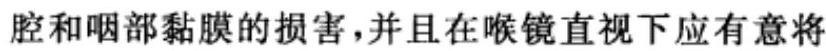
\includegraphics[max width=\textwidth, center]{2024_07_10_373f31b88d2bf633007bg-427}\\
联合导管插人食管内,因此成为被推荐的方法。目插联合导管也是经常采用的方法, 但需要姛熟的盲插技术和适度的麻醉深度。在紧急情况下,当气管内插管失败时,应将筥镜留在患者的口中,并在直视下插人联合导管。

\begin{enumerate}
  \setcounter{enumi}{1}
  \item 插管技术 无论患者相对于操作者是何种体位, 联合导管均可成功插人。患者的头部不需要像常规气管插管那样保持传统的“㖵物位”, 也可稍微垫起,插人导管直至环行标记位于牙齿之间, 将口咽套蕒充气(蓝色指示套蛽), 总量最多可至 $150 \mathrm{ml}$, 充分密封口和鼻子; 然后, 将食管气管套囊充气(白色指示套表), 可注人 $10 \mathrm{ml} \pm 1 \mathrm{ml}$ 的空气。盲插过程中,导管进人食管的概率较大。因此, 推荐经蓝色的咽导管管腔进行通气测试, 由于口、畕和食管被套䝴所封锁,空气通过侧孔进人咽部,然后通过声门进人气管。在这个位置, 还可以通过气管食管管腔积极地进行胃肠减压。如果在肺部没有听到呼吸音或没有看到呼气末 $\mathrm{CO}_{2}$ 波形,第一个最常见的原因可能是导管远端位于气管内, 直接改用经透明的气管管腔进行通气即可, 空气可直接进人气管; 第二个最常见的原因是联合导管插人过深, 此时口咽套蛼位于喉头的对侧而堵塞了气道,\\
将联合导管退出口腔 $2 \sim 3 \mathrm{~cm}$ 即可; 第三个最常见的原因是高气道压力所致 (例如, 喉部或支气管痉挛, 肺水肿), 在这种情况下, 应查明病因并加以治疗。

  \item 更换联合导管 因为长时间压迫咽黍膜可能会造成损伤, 联合导管不应作为长期通气的工具, 留管时间应在 $8 \mathrm{~h}$ 以内。换管过程中仍保留联合导管在食管内, 口咽套蛮可以完全放气或部分放气, 在喉镜或纤维镜辅助下插人气管导管, 或建立外科气道。在整个换管过程中可以尽量保持通气。此外也可用外科方法更换联合导管, 例如环甲膜切开或气管切开。

\end{enumerate}

联合导管凭其上述优势具有广泛的应用范围。由于插人联合导管可以不使用喉镜, 因此迅速建立通畅的气道不会受到环境因素和技术因素的影响。而且联合导管可以有效地防止误吸, 可以应用于存在通气压力高的患者中。联合导管使用的禁忌证包括: 存在强烈的恶心反射 (不论其意识水平)的患者; 身高 $>6$ 英尺 ( $41 \mathrm{Fr}$ 联合导管) 和 $<4$ 英尺 ( 37 $\mathrm{Fr}$ SA 联合导管) 的患者; 中心气道梗阻; 掫人有腐蚀性的物质; 已知存在食管上段病变的 (Zencker 想室) 患者。联合导管一个潜在的缺点是, 当导管在食管内时, 不能吸引气管内分泌物。

\section*{十一、纤维支气管镜辅助气管插管}
纤维支气管镜 (FOB) 可用于所有的困难插管,还可用于判断是否有气管内梗阻、气管导管的位置和双腔支气管插管的正确定位。FOB引导清醒气管插䈉的优点是能够维持自主呼吸并可使气管导管尖端准确地越过受压部位, 因此在气道出现病变或预测为困难气管插管、颈椎不稳定、过度肥胖、面罩通气困难、气管狭窄、胸骨下甲状腺或纵隔肿物引起气管受压的情况下都可以采用 FOB引导下清醒气管插管。根据人路不同又可分为 $\mathrm{FOB}$ 引导下经口或经鼻气管插管。

\begin{enumerate}
  \item FOB引导下清醒经口气管插管 清醒状态下充分的表面麻醉是十分重要的步骤: 先用 $4 \%$ 利多卡因药液或 $10 \%$ 利多卡因喷雾剂喷酒口咽表面, $4 \%$ 的利多卡因经环甲膜注射或通过 FOB 喷酒的方法对喉和气管表面, 这样可有效预防插人 FOB 时经常出现的严重呛咳和喉痉挛。插管过程中, 将患者头部置于插管所需的正中位置上, 口中放置插管型通气道, 吸引口咽部, 将 FOB 镜身和气管导管充分润滑后, 先将 FOB 经插管型通气道向口咽部前行, 暴露声门, 推至气管中段 (最好在 FOB 直视下将气管导管尖端放置在隆突上方 $3 \sim 4 \mathrm{~cm}$ 处), 保持 $\mathrm{FOB}$ 位置不动, 沿着 $\mathrm{FOB}$ 镜身推送气管导管进人到气管内。该过程需要将患者头后仰、下颌拖起、适当向前牵拉舌体, 以增加咽部空间, 便于会厌离开咽喉壁, 暴露声门。但即使 FOB 进人到气管内, 在推送气管导管的过程中, 气管导管也常会受阻于会厌或进人梨状窝而无法推送进人气管内。避免这种情况的方法是应尽可能使 FOB 的镜身外径与气管导管的内径相匹配, FOB 与气管导管之间的缝陸越大, 气管导管进人气管受阻的概率就越高; 推送过程中斜面向下使气管导管能够滑过可能受阻的右侧杓状软骨。

  \item FOB引导下清醒经算气管插管一般首选通气通畅的鼻孔,用 $2 \%$ 的利多卡因凝胶麻醉鼻糗膜, 并用浸有 $4 \% \sim 5 \%$ 可卡因或利多卡因和去氧肾上腺素的泥合液 ( $4 \%$ 利多卡因 $3 \mathrm{ml}$ 加上 $1 \%$ 去氧情上腺素) 溶液的棉签进行局部麻醉和收缩鼻䵑膜血管, 经环甲膜注射或在气管插管过程中通过 FOB 喷酒局部麻醉药来进行喉和气管的局麻, 无须对口咽部实施局部麻醉。插管前先将气管导管须用温水软化并充分润滑气管导管, 将气管导管经局部麻醉过的鼻孔轻柔地插人, 直至刚好进人咽喉部, 再经导管放置 FOB,或者事先将气管导管套在 FOB 上, 再将 FOB 穿过鼻腔。有 $80 \% \sim 85 \%$ 的患者, 在轻微调节或无须调节 FOB 前端方向的情况下就可以看到会厌和声门。在 FOB 到达气管中段后, 推送气管导管。经鼻气管插管过程中, 气管导管受阻及无法进人气管的发生率相对较低。

  \item 在全身麻醉状态下经口或綦进行 FOB引导气管插管 可以保留患者自主呼吸, 也可以给予肌松药控制通气。全麻下气管插管可以提高患者的舒适度, 其主要缺点是舌和咽部组织失去张力, 向下贴近咽腔, 阻挡喉部视野, 因此需要助手协助托起患者的下颌, 此操作是全麻下 FOB 引导气管插管的最重要步骤之一。为了惐少缺氧时间, 可以使用带有内镜孔的麻醉面罩给自主呼吸患者供氧, 或给全身麻醉和肌松驰患者正压通气, 但需要助手协助实施麻醉和维持面罩通气, 将气管导管的接头取下后套在 $\mathrm{FOB}$ 上, 经内镜面罩上的内镜孔䐬膜插人 FOB, 便于插完气管导管后内镜面罩从气管导管上取下。

\end{enumerate}

对于乞管插管困难的不合作的饱胃患者 (如醉酒者或小儿),在全麻诱导前可能无法采用可以保\\
证乞道安全的清醒插管时, 若快速诱导期间使用硬质喉镜气管插管失败, 可考虑在持续按压环状软骨的同时, 用 $\mathrm{FOB}$ 完成气管插管, 而避免因反复尝试经鼻目探气管插管或硬质喉镜经口气管插管造成的气道损伤。

\begin{enumerate}
  \setcounter{enumi}{3}
  \item 经喉萛通气道 FOB引导下气管插管借助 FOB 可以直视喉部, 来提高经 LMA 气管插管的成功率。置人 LMA 并确认其通气效果满意后, 选择适当型号的气管导管和 FOB, 充分润滑后经 LMA, FOB 暴露喉部并进人气管内, 再沿着 FOB 将气管导管推人气管, 气管导管套囊充乞。拔除 $\mathrm{FOB}$, 经气管导管通气。麻醉结束时, 先拔除气管导管, 通过 LMA 维持呼吸, 气道保护性反射恢复后拔除 LMA。使用 LMA 引导气管插管的不足之处在于对气管导管型号的限制, 并且需要气管导管具有足够的长度。因此, 可能需要特殊的气管导管如 RAE(Ring-Adair-Elwyn) 经鼻插管导管。如果需保留气管导管并拔除 LMA, 目前有多种方法可供选择: 通过 “导管连导管”的方法来增加足够的导管长度; 在 FOB引导下经 LMA 放置气管内导丝。若导丝较粗, 就足以用来引导合适型号的气管导管,保持 LMA 不动, 用导丝引导完成气管插管; 若导丝较细, 可先顺导丝放置一根导尿管, 通过 $\mathrm{CO}_{2}$ 检测证实导尿管的位置正确后,拔除 LMA,最后用导尿管引导插人合适型号的气管导管。更换导管的方法有以下几种。
\end{enumerate}

(1) 使用导管交换器或 FOB 的辅助下进行。

(2) 用 FOB 经 LMA 先将一根较小型号的气管导管放置到气管内, 作为插管导引管, 然后将内径为 $8.5 \mathrm{~mm}$ 的气管导管沿着 “导引管”推送到气管内。

(3) 经 LMA 用 FOB 放置一根交换管芯, 因交换管芯直径大、有一定硬度, 所以在用气管导管替换 LMA 前, 还可以维持气道通畅。

(4) 纵向翦开 LMA, 并用硅酊密封套囊, 用带孔的绷带缠住 LMA 通气导管, 套有气管导管的 FOB 经这种改装后的 LMA 进人气管内后, LMA 套晋放气, 去除 LMA 上的绷带, 气管导管沿着 FOB 经 LMA 进人气管内, 这种方法可以通过较大型号的与管导管。\\
5. 经联合导管 FOB 引导下气管插管采用盲探法放置联合导管, $90 \%$ 以上进人食管, 为防止可能出现的并发症, 提供更加安全的气道, 并拥有对气管内进行吸引的通路, 可以经插人的联合导管在 FOB引导下用气管导管替换联合导管。目前已有联合使用盲探放置联合导管和 FOB引导气管插管技术来处理困难气道的报道。

\begin{enumerate}
  \setcounter{enumi}{5}
  \item FOB 辅助“经算言探”气管插管 在某些气道扭曲和伴有气道病变的患者, 单独应用经鼻盲探气管插管或 FOB 暴露声门都有可能失败, 而联合应用两种技术就可以获得成功。FOB 可采用两种不同的方法辅助完成困难或失败的经鼻目探气管插管。一种情况是在因鼻道狭窄, 只能插人细的乞管导管, 而 FOB 无法插人气管导管时, 可从对侧鼻孔插人 FOB, 观看气管导管尖端的位置并辅助其进人声门。另一种方法是在直视下调节经鼻插气管导管和患者头部的位置, 使其直对喉部。

  \item FOB 辅助逆行导丝引导气管插管 在采用传统的逆行气管插管技术失败时, 可利用经环甲膜插人的导丝引导 FOB 进人声门和气管。用 $\mathrm{FOB}$完成逆行气管插管有两种不同方式, 一种是在气管导管不能沿着导丝进人气管时, 保持气管导管位置不变, 将 FOB 插人到气管导管内, FOB 沿着导丝越过气管导管末端, 并越过导丝的气管人口处, 在确保 FOB 位于气管下段时, 拔除导丝, 沿着 FOB 将气管导管推送进人气管内; 另一种是导丝以逆行的方式穿过套有气管导管的 FOB 的吸引通道, 导丝引导 FOB 进人气管, 拔除导丝, 沿着 FOB 将气管导管推送进人气管内。

  \item FOB 作为光棒使用 FOB 光线很强, 可作为光棒使用, 根据颈前光线的分布判断是否进人气管。这种方法在大量分泌物或血液阻挡 $\mathrm{FOB}$ 观察气道解剖结构视野时,可避免 FOB 引导的气管插管失败。将套有气管导管的 FOB 经插管型通气道插人到㘈部, 在托起下领的同时推送 FOB, 先保持 FOB 远端平直, 以利于其绕过会厌下缘, 然后向前弯曲 FOB 远端, 进人喉部, 可根据颈部亮点的位置采用适当的调节手法推送 FOB 进人气管。

\end{enumerate}

(左明章)

\section*{籍3責 $\square$}
\section*{吸入全身麻醉}
1846 年在美国首先公开演示的吸人全身麻醉标志着现代麻醉学的诞生。吸人全身麻醉是指挥发性麻醉药或气体麻醉药经呼吸系统吸收人血, 在脑和脊㪇中达到一定的浓度, 抑制中枢神经系统而产生全身麻醉的方法。在外科手术中,吸人麻醉可以: 提供麻醉, 施行吸人麻醉诱导和维持全麻; 消除术中记忆; 协助肌松; 控制血压; 其他如治疗支气管㽒喘和保护重要器官等。相比静脉麻醉, 吸人麻醉主要有两个优点:一是能通过呼吸有效地调节血中麻醉药浓度(或分压), 特别是能迅速将吸人麻醉药从身体“洗出”; 二是通过测定呼气末浓度可估计吸人麻醉药在其作用苟位 (中枢神经系统) 的浓度 (分压)。所以,经过 160 多年, 吸人麻醉仍然是临床上最常采用的麻醉方法。

\section*{一、吸入麻醉药}
\begin{enumerate}
  \item 理化及生物学特性 (表 4-3-1)
\end{enumerate}

表 4-3-1 临床常用吸入麻醉药的物理、化学和生物学特性

\begin{center}
\begin{tabular}{|c|c|c|c|c|c|c|}
\hline
特 性 & 地氥烷 & 七氘烷 & 异洗烷 & 安氟烷 & 氟烷 & 笑气 \\
\hline
分子量 & 168.0 & 182.0 & 184.5 & 184.5 & 197.4 & $44.0 \quad$ \\
\hline
沸点(1 个大气压) & $23.5^{\circ} \mathrm{C}$ & 58. $5^{\circ} \mathrm{C}$ & 48. $5^{\circ} \mathrm{C}$ & $56.5^{\circ} \mathrm{C}$ & $50.2^{\circ} \mathrm{C}$ & - \\
\hline
比重 $\left(25^{\circ} \mathrm{C}\right)$ & 1.45 & 1.50 & 1.50 & 1.52 & 1.86 & - \\
\hline
饱和蒸气压 $\left(20^{\circ} \mathrm{C}, \mathrm{mmHg}\right)$ & 663 & 160 & 250 & 175 & 243 & - \\
\hline
气味 & 刺激性 & 噵香味 & 刺激性 & 醚香味 & 甜味 & 甜味 \\
\hline
保存剂 & 无 & 有 & 无 & 无 & 有 & 无 \\
\hline
\multicolumn{7}{|l|}{化学反应} \\
\hline
金属 & 无 & 有 & 无 & 无 & 有 & 无 \\
\hline
碱 & 无 & 有 & 无 & 无 & 有 & 无 \\
\hline
紫外线 & 无 & 有 & 无 & 无 & 有 & 无 \\
\hline
簤炸性 & 无 & 无 & 无 & 无 & 无 & 无 \\
\hline
\multicolumn{7}{|l|}{分配系数} \\
\hline
血/气 & 0.42 & 0.68 & 1.40 & 1.90 & 2. 30 & 0.47 \\
\hline
脑/气 & 0.54 & 1.15 & 2. 09 & 2. 60 & 4.79 & 0.50 \\
\hline
脂肪 $/$ ־ & 12.00 & 34.00 & 64.20 & 105.0 & 136.0 & 1.22 \\
\hline
肝 $/$ 气 & 0.55 & 1.25 & 2.34 & 3.80 & 5.13 & 0.38 \\
\hline
肌肉 $/$ Һ & 0.94 & 2. 38 & $4.40 \quad$ & 3.00 & 9. 49 & 0.54 \\
\hline
油/气 & 18.70 & 53.40 & 97.80 & 98.5 & 224.0 & 1.40 \\
\hline
水/气 & 0.22 & 0.36 & 0.61 & 0.80 & 0.70 & 0.47 \\
\hline
橡胶/气 & - & - & 0.62 & 74.00 & 120.00 & 1. 20 \\
\hline
\multicolumn{7}{|l|}{最小肺泡气浓度(\%)} \\
\hline
氧 & 5.70 & 1.71 & 1.15 & 1.68 & 0.75 & 106 \\
\hline
$70 \% \mathrm{~N}_{2} \mathrm{O}$ & 2. 83 & 0.65 & 0.50 & 0.57 & 0.29 & - \\
\hline
肝毒性 & - & - & - & $?$ & + & - \\
\hline
将毒性 & - & $?$ & - & ? & - & - \\
\hline
体内代谢 & $0.02 \%$ & $2 \%$ & $0.2 \%$ & $2 \%$ & $20 \% \sim 30 \%$ &  \\
\hline
致酳 & - & - & - & - & - & ? \\
\hline
心律失常 & $=$ & - & - & $?$ & + & - \\
\hline
\end{tabular}
\end{center}

\begin{enumerate}
  \setcounter{enumi}{1}
  \item 最小版泡气浓度 (minimum alveolar concentration, MAC) MAC 的定义为:一个大气压下, $50 \%$ 的动物在伤害性刺激下不发生体动时肺泡气中吸人麻醉药的浓度。MAC 通常用来评定吸人麻醉药的强度。现临床上使用的吸人麻醉药的 MAC 值为: 氧化亚氮 $(105 \%)>$ 地氟烷 $(8 \%)>$ 七氟烷 $(2 \%)>$ 安氮烷 $(1.68 \%)>$ 异氟烷 $(1.15 \%)>$ 氟烷 $(0.78 \%)>$ 甲氧氟烷 $(0.16 \%)$ 。其中, 氧化亚氮的 MAC 最大, 麻醉作用最弱,效价最低。甲氧氟烷的 MAC 值最小, 麻醉作用最强, 效价最高。吸入麻醉药的 MAC 值受很多因素的影响, 体温降低、年龄增加、合用中枢神经系统抑制药等都会降低 MAC。麻醉时间、性别及单纯高血压等不影响 MAC 值
\end{enumerate}

MAC 概念的引人使得临床麻醉科医师能计算各种吸人麻醉药的即刻使用剂量和在一定时间里使用的总量,并且使这些剂量和总量可以在各种吸人麻醉药之间进行比较。

\section*{3. 吸入麻醉药浓度的调控}
(1)挥发罐输出浓度: 挥发罐出口吸人麻醉药的浓度决定于 3 个流量:(1)流经挥发室的新鲜气流量 (VL); (2)单位时间内在挥发室挥发的麻醉药气体量 (AL); (3)直接通过蒸发器的新鲜气流量 (BL)。实际上单位时间内在挥发室挥发的麻醉药と体量 (AL)决定于吸人麻醉药的饱和蒸汽压和流经挥发室的新鲜气流量(VL)。当流经挥发室的新鲜气流量一定时,单位时间挥发的麻醉药气体量主要决定于麻醉药的饱和蒸汽压。在一定的温度下吸入麻醉药的饱和蒸汽压是一个常数。可见蒸发器出口的麻醉药浓度实际上决定于流经挥发室新鲜气流量 (VL) 与直接通过蒸发器的新鲜气流量 (BL) 之比。各种麻醉药蒸发器的最高刻度约为该麻醉药 MAC 值的 4 倍。这样既能有效地加深吸人麻醉,又可最大限度地避免发生麻醉过深之意外。

(2)新鲜气体: 只有流经流量表的氧, $\mathrm{N}_{2} \mathrm{O}$ 和空气才通过蒸发器,它们可携带吸人麻醉药进人呼吸回路。现代麻醉机设计中多将蒸发器安置在呼吸环路之外。流经流量表并经蒸发器携带吸人麻醉药的新鲜气体与重吸人的病人呼出气在呼吸环路的吸气支混合而形成新一轮的吸人气体。所以,蒸发器的开启浓度并不等于环路内吸人气的麻醉药浓度。

如果我们忽略呼吸回路漏气、钠石灰对吸人麻醉药的吸人和降解, 以及呼吸无效腔等因素的影响,可通过下面的公式粗略估计吸人气中麻醉药的浓度(当新鲜气流量大于每分通气量时按每分通气量计算):

吸人气麻醉药浓度=

新鲜气流量(蒸发器开启浓度一呼气末麻醉药浓度)每分通气量

十烀气末麻醉约浓度

(3)吸人气中麻醉药浓度 (FI) 的调控: (1)加深麻醉。将吸人麻醉药蒸发器刻度开大和 (或)将新鲜气流量/每分通气量之比加大, 使其趋于或 $>1$; (2)减浅麻醉。将蒸发器关小或关闭和 (或)将新鲜气流量加大; (3)加用 $\mathrm{N}_{2} \mathrm{O}$ 或空气。流经流量表的 $\mathrm{N}_{2} \mathrm{O}$ 和空气也是通过蒸发器的吸人麻醉药的载气。调整 $\mathrm{N}_{2} \mathrm{O}$ 或空气时应考虑到对吸人气中强效麻醉药浓度的影响。

\section*{4. 肺泡气吸入麻醉药浓度(FA)}
(1)第二气体效应(the second-gas effect): 在 1 种吸人高浓度气体(如氧化亚氮)的同时吸人第 2 种气体(如氛烷、异無烷等)时, 第 2 种气体的肺泡气浓度上升速度加快, 这是因为血液从肺泡中大量吸收氧化亚氮后, 使肺泡中第 2 种气体的浓度上升。这种现象称之为第二气体效应。

(2)肺泡气吸人麻醉药浓度的决定因素:(1)吸人气麻醉药浓度。吸人气麻醉药浓度越高, 进人肺泡的吸人麻醉药越多, 肺泡与麻醉药浓度上升越快。(2)通气量: FI恒定时, 每分钟通气量越大, 单位时间内进人肺泡气吸人麻醉药越多, FA上升越快。 (3)肺泡气混合静脉血麻醉药分压差。此分压差越大, 吸人麻醉药从肺泡气向血中转运的速度越快, FA 上升越慢。混合静脉血吸人麻醉药分压决定于组织从动脉血对吸人麻醉药的摄取量, 组织/血分配系数越大, 组织血流量越大, 动脉血一组织的吸人麻醉药分压差越大, 组织从动脉血中摄取麻醉药越快。该组织的静脉血中吸人麻醉药分压越低。 (4)血/气分配系数。吸人麻醉药的血/ 个分配系数越大, 流经肺毛细血管的单位体积血流能从肺泡中摄取更多的吸人麻醉药, 肺泡气的麻醉药浓度上升越慢。(5)心排血量: 心排血量越大, 单位时间内流经肺泡的血液越多, 血液从肺泡摄取的吸人麻醉药越多,FA 上升越慢。

\section*{二、麻醉环路}
\begin{enumerate}
  \item 开放式环路 开放式环路是最初的吸人麻醉使用的环路。用金属丝网面罩覆以 4~8层纱布\\
扣住患者口鼻, 将吸人麻醉药滴在面罩上。这种方法称为点滴法, 适用于挥发性液体吸人麻醉药。其他的方法还包括冲气法和无重复吸人法。这种环路的缺点显而易见: 难于控制吸人麻醉药的浓度;无法控制呼吸; 无法处理废气; 补充吸人氧浓度有限; 有效地使用氧化亚氮比较困难。

  \item 紧闭式环路当吸人麻醉药浓度在脑达到平衡后, 需要维持麻醉药的肺泡浓度 (FA) 使其满足手术的需要。能应用最小量吸人麻醉药到达这一目的的方法就是采用紧闭式(完全重呼吸)环路。在此环路中, 吸人麻醉药的供给量与机体的掫取量相等, 并给予能补偿机体代谢消耗的氧气。不同的技术都可以用于提供紧闭回路,包括将液状吸人麻醉药直接注射至麻醉环路和使用传统的挥发罐。地氮烷高饱和蒸汽压使其不能直接注射人环路, 但是其挥发罐的输出量可以提供诱导后足量的地氟烷浓度。然而异氮烷虽可直接注射至环路内, 但其挥发罐无法提供足够的蒸汽以满足紧闭环路内的浓度达到 1MAC。当合用其他麻醉药如氧化亚氮时, 紧闭环路使用异氟烷液可提供低于 $1 \mathrm{MAC}$ 的浓度。

\end{enumerate}

尽管采用紧闭环路可提供最经济的麻醉药物输送、减少热量和水分的丢失、减少对环境的污染,但是它同样具有一些缺点。最重要的是在紧闭环路中块速改变麻醉药物浓度非常困难, 使吸人麻醉的可控性及精确性较差。

\begin{enumerate}
  \setcounter{enumi}{2}
  \item 半紧闭式环路 半紧闭式环路分无 $\mathrm{CO}_{2}$ 吸收装置和有 $\mathrm{CO}_{2}$ 吸收装置。目前临床上吸人麻醉多使用有 $\mathrm{CO}_{2}$ 吸收装置的半紧闭式环路。使用该环路易控制吸人的麻醉药浓度, 且不易产生 $\mathrm{CO}_{2}$ 蓄积。

  \item 半开放式环路 半开放式环路中, 没有 $\mathrm{CO}_{2}$吸收装置和清除回路和无重复吸人活瓣。由麻醉机输出的气体进人储气㲤与患者的部分呼出气混合后被患者吸人。使用该环路可进行控制呼吸。 1954 年, Mapleson 根据有无活瓣、储气鸾、螺纹管及新鲜气体的流人位置, 将此系统分为 $\mathrm{A} 、 \mathrm{~B} 、 \mathrm{C} 、 \mathrm{D}$ 、 $\mathrm{E}$ 五类。该系统的缺点是药物浪费、环境污染和气道干燥。

\end{enumerate}

\section*{三、低流量吸入麻醉}
1952 年, Foldes 为确定在没有氧浓度监测的情况下安全使用 $\mathrm{N}_{2} \mathrm{O}-\mathrm{O}_{2}$ 麻醉浓度时采用了 $1 \mathrm{~L} /$ $\min$ 的气体流量。随后 $1 \mathrm{~L} / \mathrm{min}$ 在临床上被定义为低流量。现在通常认为采用 $0.5 \sim 1 \mathrm{~L} / \mathrm{min}$ 的新鲜流量的吸人麻醉为低流量麻醉。而新鲜流量为 $0.25 \sim 0.5 \mathrm{~L} / \mathrm{min}$ 时为最低流量麻醉。

\section*{1. 低流量麻醉的优点}
(1) 经济: 尽管 $\mathrm{N}_{2} \mathrm{O}$ 便宜, 但是其他的吸人麻醉约价格高, 特别是七氛烷、地氟烷。有研究表明使用低流量麻醉能将吸人麻醉药的用量减少 $50 \%$ 。

(2)环境保护: 氟化麻醉药能在紫外线照射下分解释放氭原子, 从而消耗臭氧层。氛化麻醉约释放的萇原子仅为全球释放量的 $0.01 \%$ 。而七氮烷、地氟烷对臭氧层的影响更小。

(3)保存热量和湿度: 吸人干冷的乞体会损伤秥膜纤毛功能, 导致肺膨胀不全、感染和气体交换受损。呼吸道热量和温度的丢失也会引起长时间麻醉后低体温。尽管使用加湿、加温装置有所帮助, 但是选择适当的新鲜气低流量可提高吸人气的温度和湿度。

\begin{enumerate}
  \setcounter{enumi}{1}
  \item 低流量吸入麻醉的铁点
\end{enumerate}

(1) $\mathrm{CO}_{2}$ 吸收剂的用量大大增加。

(2)必须有适用的麻醉机、气体监测仪。

(3)呼吸环路内不需要气体的蓄积。不被患者吸收或是不被化学吸收的气体会逐渐蓄积。这些气体包括忠者的呼出气、医用气体污染物或是与 $\mathrm{CO}_{2}$ 吸收剂反应生成的气体。患者呼出气中可能包含酒精、甲烷、丙酮和 $\mathrm{CO}$ 。

(4) 初学者不易掌握。

\section*{四、吸入麻醉的实施}
\begin{enumerate}
  \item 诱导 吸人麻醉诱导的速度主要取决于吸人麻醉药的血/气分配系数 (血中的溶解度)。现临床上使用的吸人麻醉药的血/气分配系数由低到高依次为 $\mathrm{N}_{2} \mathrm{O}$ 、地氟烷、七氟烷、异氟烷、恩氛烷和氛烷。对于吸人麻醉药来说, 血/气分配系数越低, 肺泡内麻醉药浓度在诱导时上升越迅速。上述药物一般都是如此, 但也可有例外。如按此理论, 地套烷诱导速度应快于七氛烷, 但事实却相反。地氟烷因其气道刺激性使清醒病人屏气, 而减慢诱导的速度。因此, 吸人麻醉药的刺激性也是影响诱导速度的因素之一。研究发现, 应用超过 $6 \%$ 的地氟烷诱导时, 会导致患者出现咳濑、屏与、喉疼挛以及分泌物增加。在成人若预先给予小剂量芬太尼 $(1 \mu \mathrm{g} /$ $\mathrm{kg}$ ) 或吗啡 $(0.1 \mathrm{mg} / \mathrm{kg})$, 就能将地氟烷诱导时气道并发症的发生率从 $25 \%$ 减至 $5 \% \sim 8 \%$ 。同时, 气道对刺激物的反应随着年龄的增长而惐轻。地氧\\
烷对小儿气道的刺激较成人更强或一致, 可能导致血氧饱和度下降等严重后果。所以, 地氟焢不推荐用于小儿诱导。另外, $\mathrm{CO}_{2}$ 吸收剂也会影响诱导速度。我们日常使用的吸收剂仅吸收少量吸人麻醉药, 但是干燥的吸收剂会清除大量麻醉药, 从而延缓诱导。
\end{enumerate}

因小儿打针时难以合作, 所以对小儿常采用七氟烷或氮烷吸人诱导。由于七氟烷的血/气分配系数较氟烷低, 所以理论上其诱导速度应较氧烷快。但是研究发现氟烷诱导的速度与七矢烷相近, 其原因可能为氛烷的挥发罐可提供 5 MAC 的氮烷, 而七氟烷的挥发罐仅能提供 $3 \mathrm{MAC}$ 。虽然如此, 七氛烷仍然取代了氟烷成为小儿吸人诱导的主要药物。因为七氛烷诱导较氟烷有如下优点: 苏醒更快, 生命体征更平稳, 更少体动, 术后恶心、呕吐发生率低并且七氮烷不会导致罕见的氭烷性肝炎。

成人可以使用七㢮烷的“单次呼吸”法来进行诱导。对于惧怕打针的成人来说, 吸人诱导仍然是首选。在美国的一项研究发现, 对于没有静脉通路的患者来说, 他们宁愿选择吸人作为诱导方式。对于术前预料到的插管困难、颈椎活动受限的患者来说, 吸人诱导也是很好的选择。对于这类患者, 七氫烷最为常用, 因为其没有刺激性、溶解度低, 能够快速进行诱导并且遇到困难时患者能快速清醒。因此, 七氟烷已经用于术前存在呼吸道梗阻患者的诱导。但是, 对于有反流危险的患者, 如饱胃、食管反流、失驰缓, 裂孔疝, 胃痽, 糖尿病周围神经病变的患者, 最好采用静脉的快速顺序诱导插管。

地氟烷和七氟烷诱导会导致患者血压下降, 尤其在老年患者中发生率高。因此在对老年患者, 特别是对有循环系统疾病以及服用减少心肌储备药物的患者, 实施吸人诱导时需谨慎。七氛烷用于老年患者麻醉时不能防止刺激时的应激反应。

\begin{enumerate}
  \setcounter{enumi}{1}
  \item 维持 手术时间的长短因手术部位、手术方式等不同而改变。麻醉时间的长短在每个病人都不尽相同, 这也影响患者的苏醒时间。所以麻醉维持阶段药物的选择就显得非常重要。随着麻醉时间的延长, 肌肉、脂肪等组织所摄取储存的吸人麻醉药也就越多。麻醉苏醒期间, 这些组织中的麻醉药物会释放人血, 随着血流到达肺。如果通气没能将吸人麻醉药清除, 这些药物的再循环就会导致苏醒延迟。有研究发现地氛烷 $90 \%$ 的消除时间几乎不受吸人时间长短的影响, 但是七氛烷和异氛烷的消除时间随吸人时间的延长而大大增加。因此,增加地䑺烷的吸人时间极少影响其苏醒时间。

  \item 苏醒 快速清醒对全身麻醉患者来说非常重要。

\end{enumerate}

(1)患者反应的快速恢复可以维持有效的气道, 减少因呕吐、分泌物所引起的误吸, 维持氧合。

(2)心血管功能恢复快。

(3) 缩短离开手术室及 PACU 的时间。

(4)达到使患者安全恢复协调动作的残留麻醉药浓度的速度更快。

(5)减少可代谢的药物, 降低生物降解毒性的风险。

(6)吸人麻碎药能增强肌松药的作用。所以吸人麻醉药的快速清除可以减少这种作用, 从而降低肌松药残余作用所导致的呼吸道并发症的发生率。

(7) 接近 0.1MAC 的吸人麻醉药浓度可增强患者对疼痛的感知。因此吸人麻醉药的快速清除可较快地达到更低的浓度从而减轻患者术后即刻对疼痛的感知。有研究发现使用地氟烷麻醉后患者的视觉疼痛评分恢复至术前水平的时间较异氟烷快,同样有研究得到地氣烷麻醉较异丙酚术后疼痛更少的结果。

地氧烷在血及组织中的溶解度低于其他的强效吸人麻醉药, 然而 MAC 清醒是相同的。这就表明地氟烷麻醉后的清醒速度快于其他强效吸人麻醉药。同样的, 七氟烷麻醉后的清醒速度快于异氟烷和氟烷。

对于小儿, 七氟烷和氟烷是吸人诱导的常用药物。许多研究都发现七铗烷麻醉后小儿的苏醒更快。术前药的给予, 例如口服咪达唑仑会延长小儿清醒时间。地氮烷的低溶解度使其麻醉后的清醒时间较七氛烷和䋣烷短。但由于其气道的刺邀性,很少用于小儿麻醉的诱导, 所以使用七氛烷或氣烷诱导后以地氮烷维持, 就可以避免地氛烷诱导时呼吸道并发症的发生, 同时缩短苏醒时间。另外, 有许多研究发现小儿在七氟烷麻醉后激惹的发病率高于氟烷, 而快速清醒和疼痛都不能解释这种激惹。

对于成人, 地氟烷、七氟烷及异氟烷麻醉后的苏醒时间决定于这三种麻醉药的溶解度。大量研究发现地氘烷麻醉后患者的苏醒时间及出 PACU 的时间短于异氟烷。与异丙酚麻醉相比,在老年患者和肥胖患者中, 地氟烷麻醉后的苏醒时间明显缩短。对于七氟烷和异気烷的比较发现七氟烷麻醉后的苏醒时间短于异氛烷, 但两者出 PACU 的时\\
间没有差别。吸人七氟烷患者麻醉后意识混乱和反应迟钝的发生率较异氟烷低, 但是疼痛评分较高。这两种吸人麻醉药术后恶心、呕吐的发生率无差别。

麻醉后苏醒的质量决定于麻醉药的选择。有研究发现成人在七氟烷麻醉后兴奋的发生率较异丙酚高。对于小儿, 七氟烷麻醉后的兴奋性强于其他强效吸人麻醉药和异丙酚。在对经历过七氟烷吸人麻醉和异丙酚麻醉的忠儿的父母的调查发现,父母对异丙酚麻醉后的效果比较满意。

\section*{五、吸入麻醉对机体的影响}
\begin{enumerate}
  \item 呼吸系统 所有的强效吸人麻醉药在麻醉维持阶段均抑制通气, 增加动脉 $\mathrm{CO}_{2}$ 分压 $(\mathrm{Pa}$ $\mathrm{CO}_{2}$ ), 降低呼吸对 $\mathrm{PCO}_{2}$ 升高的反应性, 降低血氧饱和度。当合用 $\mathrm{N}_{2} \mathrm{O}$ 时, 会减少强效吸人麻醉药这种抑制作用。随着吸人麻醉药浓度的增加, 患者潮气量减少, 无效控与通气量的比值升高。尽管呼吸频率也随之增加以代偿潮气量的减少来维持分钟通气量, 但是无效腔与通气量的比值加大会使 $\mathrm{PaCO}_{2}$ 升高。
\end{enumerate}

所有的强效吸人麻醉药可减轻支气管平滑肌的收缩, 均可用于支气管收缩性疾病的患者, 特别是哮喘和 COPD 患者。在没有支气管平滑肌收缩的情况下, 吸入麻醉药几乎不影响正常患者的气道阻力。在正常忠者中, $7 \%$ 的地氟烷不舒张支气管平滑肌, 而七氟烷可明显舒张。

所有的吸人麻醉药能抑制缺氧性肺血管收缩 (HPV)。但是临床使用的吸人浓度仅轻微抑制 HPV,一般影响单肺通气时的氧合。这种抑制作用在各种吸人麻醉药之间没有显著的差别。

吸人麻醉药对呼吸道的刺激性随浓度的不同而改变。七節烷、应烷和 $\mathrm{N}_{2} \mathrm{O}$ 在临床使用的浓度范围中几乎没有刺激性。异㛿烷在麻醉浓度内就对气道有刺激作用,而地疑烷在 $1 \mathrm{MAC}(6 \%)$ 或更高浓度时具有较强的呼吸道刺激性。呼吸环路内的湿化及使用呼吸抑制药物如芬太尼能减轻吸人麻醉药对呼吸道的刺激。

\begin{enumerate}
  \setcounter{enumi}{1}
  \item 循环系统 在麻醉维持阶段, 所有的强效麻醉药对心血管系统的影响, 特别是对心率和血压的影响相似。在没有外科刺激的情况下, 临床麻醉浓度的地氮烷、七氛烷和异気烷主要通过降低外周血管张力来降低血压, 而不影响心率。深麻醉或长时间麻醉会使心率增快。若快速 $(4 \sim 6 \mathrm{~min})$ 升高地気烷的肺泡浓度至 $6 \%$,患者的心率和血压会升高。在没有注射或给予临床剂量的肾上腺素时, 地氮烷、七氟烷和异氟烷不会诱发室性期前收缩。吸人麻醉中给予控制呼吸时, 心率、心排血量降低, 动脉血压、中心静脉压、左室射血分数和外周血管张力增加。然而在自主呼吸时, 中心静脉压和周围血管阻力降低。自主呼吸时胸内压降低, $\mathrm{PaCO}_{2}$ 升高,呼吸末麻醉药浓度增加。这些可以解释控制呼吸与自主呼吸时吸人麻醉药对心血管影响的不同。
\end{enumerate}

外科刺激会使患者心率增快,血压升高。地氟烷和异氮烷的 MAC 应激 (MAC-BAR, $50 \%$ 的总者对外科切皮刺激无肾上腺能激素和心血筸反应时肺泡气吸人麻醉药的浓度) 为 $1.3 \mathrm{MAC}$, 七氫烷的 MAC-BAR 为 $2.2 \mathrm{MAC}$ 。若给予小剂量阿片类药物, MAC-BAR 会显著下降。在外科刺邀下, 吸人麻醉药减轻心血管反应并不等于使血皛儿茶酚胺浓度下降。相反, 当七氟烷或异氟烷的浓度从 $1 \mathrm{MAC}$ 升高至 $1.5 \mathrm{MAC}$ 时, 血浆儿茶酚胺的浓度升高。所以,吸人麻醉药浓度增加在抑制机体对伤害性刺激的反应(由心率、血压判断)的同时,也增高了交感张力。

吸人麻醉药会导致冠脉栍血的证据非常有限,却有许多研究发现异氧烷、七氮烷可增加冠脉血流。吸人麻醉药物心肌保护作用在许多实验中都得到了证实。吸人麻醉药抑制心肌收缩力, 降低心肌氧耗, 维持缺血期间的氧耗氧供平衡; 预处理能激活 $\mathrm{K}_{\mathrm{ATP}}$ 通道的开放, 释放活性氧箽, 提高心肌在缺血再灌注后线粒体电子传递链的功能; 具有抗炎作用。在动物实验中发现吸人麻醉药的使用可以减小冠脉阻断再灌注后心肌梗死的面积, 使顿抑心肌功能的恢复加快。在临床试验中发现, 使用吸人麻醉药进行体外循环下冠状动脉手术患者的 ICU 住院日短于静脉麻醉。但是对于冠心病患者, 麻醉药物的选择并不能改变结局,比如: 心肌梗死或死亡。

\begin{enumerate}
  \setcounter{enumi}{2}
  \item 中枢神经系统 强效吸人麻醉药呈剂量依赖地抑制脑电活动。除外氛烷, 当浓度为 $1.5 \sim$ $2 \mathrm{MAC}$ 时, 这种抑制作用导致脑电静息。脑电的变化可用于评估和监测麻醉深度。听力诱发电位和脑电双频指数 (BIS) 是对麻醉深度监测的最好方法, 但是两者在对麻醉需要的预测上作用有限。
\end{enumerate}

强效吸人麻醉药能降低脑血管张力和脑代谢率, 增加脑血流和顾内压, 特别当吸人浓度大于 $1 \mathrm{MAC}$ 或血压维持于术前水平时。与依托粬酯和\\
硫喷妥钠相比, 地氟烷可增加脑组织的氧合, 对一过性大脑中动脉阻断所致损伤有保护作用。在临床使用的吸人麻醉药浓度下,脑血管对 $\mathrm{PaCO}_{2}$ 变化的反应不会被消除。

\begin{enumerate}
  \setcounter{enumi}{3}
  \item 肝 对于患者、志愿者、动物的研究都表明,现代强效吸人麻醉药特别是地氘烷、七氟烷、异氟烷麻醉后的肝损害非常罕见。有一例个案报道描述了地氮烷麻醉后患者发生了肝损害。在该患者术后 7 周采得血清中发现了三㙌乙酰化肝微粒体蛋白的抗体。这种抗体与氟烷麻醉后黄㾝、肝炎和死亡相关。也有一些病例报道了异氟烷和七朿烷麻醉后的肝炎。但是由于麻醉过程中使用了许多其他药物, 所以可能这两种吸人麻醉药对肝胜的损害很小。现在使用的吸人麻醉药可能致肝毒性的顺序为: 氟烷 $>$ 异氟烷、七氟烷}\mathrm\{ 地朿烷。 \}

  \item 肾 对患者、志愿者、动物的肾功检测发现长时间麻醉和深麻醉不会或很少引起患者的肾功损害。这些受试者中包括了术前肾功损害、合并心脏疾病、再次手术的患者。对甲氧氧烷的研究发现, 当血浆有机氟浓度超过 $50 \sim 100 \mu \mathrm{mol} / \mathrm{L}$ 时对患者和小鼠的肾脏产生损害。在体外的研究表明氟离子损伤肾小管细胞。对七氟烷的研究发现, 尽管血浆有机氟浓度超过 $100 \mu \mathrm{mol} / \mathrm{L}$, 受试者的肾浓缩功能没有影响。复合物 $\mathrm{A}$ 为吸人麻醉药被 $\mathrm{CO}_{2}$ 吸收剂降解的产物。在动物实验中发现复合物 $\mathrm{A}$ 会导致肾皮髓质交界处坏死。在人体的试验中七臣烷对肾的毒性反应的结论都不一致。但大部分都没有发现七氛烷降解生成复合物 A 而导致的肾毒性。现在七氟烷的说明书就要求吸人七氟烷时新鲜气流量不低于 $1 \mathrm{~L} / \mathrm{min}$, 并且在此流量下不能给予 $>2 \mathrm{MAC} / \mathrm{h}$ 的七戌烷。若麻醉时间延长,新鲜气流量应 $\geqslant 2 \mathrm{~L} / \mathrm{min}$ 。

  \item 其他 现代使用的强效吸人麻醉药非常稳定, 很少或不能测量到对 DNA 的影响。尽管吸人麻醉药的布包和降解产物能改变 DNA, 但是这种能力非常微弱。吸人麻醉药能影响免疫系统, 但其途径和机制还不清楚。

\end{enumerate}

许多研究发现全麻后患者出现认知功能障碍,特别是老年患者。异氮醚增强 GABAA 受体活性,促进其激活; 抑制 NMDA 受体、神经元烟碱受体和中枢毒曹玷样乙酰胆碱受体功能, 对学习记忆和认知功能产生广泛影响。研究发现在麻醉苏醒后早期七氛醚和异氛醚都可能改变老年患者麻醉手术后认知功能, 但七氟醚的影响更弱, 更适合于老年患者的麻醉。

(吕沛林刘进)

\section*{Da}
[1] Werskkopf R B,Eger E I , II . Comparing the costs of inhaled anesthetics. Anesthesiology. 1993,79, 1413-1418

[2] Foldes F, Ceravolo A, Carpenter S. The administration of nitrous oxide-ox ygen anesthesia in closed systems. Ann Surg, 1952, 136;978-981

[3] Cotter SM, Petros AJ, Dore CJ, et al. Low-flow anaesthesia. Practice, cost implications and acceptability. Anaes thesia, 1991,46; 1009-1012

[4] Kleemann PP. Humidity of anaesthetic gases with respect to low flow anaes thesia. Anaesth Intensive Care, 1994, 22:396-408

[5] Rampil IJ, Lockhart S, Zwass M, et al. Clinical characteristics of desflurane in surgical patients: Minimum alveolar concentration. Anesthesiology, 1991, $74 ; 429-433$

[6] Kong CF, Chew STH, ip-Yam PC. In- travenous opioids reduce airway irritation during induction of anesthesia with desflurane in adults. $\mathrm{Br} \mathrm{J}$ Anaesth, $2000,85,364-367$

[7] Funk W, Gruber M, Wild K, et al. Dry soda lime markedly degrades sevoflurane during simulated inhalation induction. $\mathrm{Br} \mathrm{J}$ Anaesth, 1999, 82; 193-198

[8] Ariffin SA, Whyte JA, Malins AF, et al. Comparison of induction and recovery between sevoflurane and halothane supplementation of anesthesia in children undergoing outpatient dental extractions. $\mathrm{Br} \mathrm{J}$ Anaesth, 1997,78, 157 159

[9] Anton A. van den Berg, Dudley A. Chitty, Ramoun D. Jones, et al. Intrave nous or Inhaled Induction of Anesthesia in Adults? An Audit of Preoperative Patient Preferences. Anesth Anaig,2005, 100; 1422-1424\\
[10] Bailey JM. Context-sensitive half-times and other decrement times of inhaled anesthetics. Anesth Analg, 1997, 85: 681-686

[11] Zhang Y, Eger E I , II , Dutton RC, et al. Inhaled anesthetics have hyperalgesic effects at $0.1 \mathrm{~min}$ alveolar anesthetic concentration. Anesth Analg, 2000,$91 ; 462-466$

[12] Gnouri AF, Bodner M, White PF. Re covery profile after desflurane-nitrous oxide versus isoflurane-nitrous oxide in outpatients. Anesthesiology, 1991, $74 ; 419-427$

[13] Coloma M, Zhou T, White PF, et al. Fast-tracking after outpatient laparos copy: Reasons for failure after propo fol, sevoflurane, and desflurane anes thesia. Anesth Analg, 2001, 93; 112115

[14] Viitanen $H$, Annila $P$, Viitanen $M$, Tark

kilanP. Premedication with midazolam delays recovery after ambulatory sevoflurane anesthesia in children. Anesth Analg, 1999,89:75-79

[15] Scholz J, Bischoff P, SzafarczykW, et al. Comparison of sevoflurane and isoflurane in ambulatory surgery. Results of a multicenter study. Anaesthesist, 1996,45; S63-S70

[16] Sloan MH, Conard PF, Karsunky PK, Gross JB. Sevoflurane versus isoflurane; Induction and recovery characteristics with single-breath inhaled inductions of anesthesia. Anesth Analg, $1996,82: 528-532$

[17] Keller C, Sparr HJ, Brimacombe J. Positive pressure ventilation with the laryngeal mask airway in non-paralysed patients; Comparison of sevoflurane and propofol maintenance tech niques. $\mathrm{Br} \mathrm{J}$ Anesth, 1998,80:332-336

[18] Uezono S, Goto T, Terui K, et al. Emergence agitation after sevoflurane versus propofol in pediatric patients. Anesth Analg, 2000,91:563-566\\
[19] Goff MJ, Arain SR, Ficke DJ, et al. Absence of bronchodilation during desflurane anesthesia. Anesthesiology, $2000,93: 404-408$

[20] Segawa H, Mori K, Murakawa M, et al. Isoflurane and sevoflurane augment norepinephrine response to surgical noxious stimulation in humans. Anesthesiology, 1998,89; 1407-1413

[21] Bernard $J-M$, Wouters PF, Doursout M$F$, et al. Effects of sevoflurane and isoflurane on cardiac and coronary dynamicsin chronically instrumented dogs. Anesthesiology, 1990, 72 : 659662

[22] Kersten JR, Schmeling T, Tessmer J, et al. Sevoflurane selectively increase coronary collateral blood flow independent of KTP channels in vivo. Anesthesiology, 1999,90,246-256

[23] De Hert SG, Van der Linden PJ, Cromheecke $\mathrm{S}$, et al. Choice of the primary anesthetic regimen can influence intensive care unit length of stay after coronary surgery with cardiopulmonary bypass. Anesthesiology, 2004, 101; 920

[24] Martin JL, Plevak DJ, Flannery KD, et al. Hepatotoxicity after desflurane anesthesia. Anesthesiology, 1995, 83; 1125-1129

[25] Cittanova M-L, Lelongt B, Verpont M$\mathrm{C}$, et al. Fluoride ion toxicity in human kidney collecting duct cells. Anesthesiology, 1996, 84 : 428-435

[26] Eger E I , II , Koblin DD, Bowland T, et al. Nephrotoxicity of sevoflurane vs. desflurane anesthesia in volunteers. Anesth Analg, 1997, 84: 160168

[27] Kharasch ED, Hoffiman GM, Thorning $\mathrm{D}$, et al. Role of renal cysteine conjugate beta-lyase in the mechanism of compound $\mathrm{A}$ nephrotoxicity in rats. Anesthesiology, 1997,86: 160-171

[28]段开明,常业恬,欧阳文, 等. 昇氭烷与七員烷麻醉对老年患者术后认知功能的影响. 卖用预防医学, 2006,13 (3) $: 501-502$

\section*{籍:}
\section*{静脉全身麻醉}
静脉全身麻醉是当代麻醉学发展最为迅速的领域之一, 在药物学、方法学、监测学等方面都取得了重要的成果。静脉全身麻醉既可单独, 也可与吸人麻醉联合使用来满足手术和 (或)检查的需要, 促进了手术室外麻醉、麻醉下的监测管理 (MAC) 和门诊手术麻碎的发展,为相关学科业务的顺利开展提供了保障。静脉全身麻醉在减少药物副作用、提高临床麻醉安全性和舒适度、促进患者术后转归等方面都提供了多样的选择,成为临床麻醉的重要内容。

\begin{enumerate}
  \item 静脉全身麻醉的历史 300 多年前血液循环系统的发现和理论建立, 以及随后注射器的发明, 为静脉麻醉的出现奠定了基础。1872 年 $\mathrm{Pi}-$ erre-Cyprien Ore 第一次在人体上使用水合氯醛以期达到静脉麻醉效果, 并且认为其效果优于氯仿,但是这种观点不为当时大多数人所接受。第一次世界大战期间,静脉使用吗啡复合东莨宕碱的麻醉方式获得广泛接受, 尤其是在产科麻醉, 但是这个当时被称为 “半麻醉”的方法因为无法预料的副作用而逐渐被遗弃。随后出现通过直肠方式给药的三滇甲醇 (又称阿佛丁) 也曾被认为是一种静脉麻醉药, 但是由于其可能导致直肠溃疡、呼吸抑制和肝损伤而被禁用。
\end{enumerate}

拜耳 (Adolf von Baeyer, 1905 年诺贝尔化学奖获得者) 于 1864 年首次发现巴比妥类药一巴比妥酸,但是它没有镇静作用。Emil Fischer 于 1903 年首次合成了具有镇静作用的巴比妥类药一甲环己豨甲比妥, 但是在其后近 30 年内都未被认识,直到 1932 年 Helmut Weese 才有使用该药的数千例麻醉报道。1934 年硫喷妥钠被成功合成后, 美国梅奥医学中心的 John Lundy 首先给予报道, 并据此第一次提出了 “平衡麻醉”的概念。1941 年,在给因珍珠港遭轰炸而受伤的人员使用硫唩妥钠实施麻醉诱导时,发现其可能会抑制心血管系统而导致患者突然死亡。同期还有超短效巴比妥类药美索比妥, 被用于治疗电休克的麻醉。1973 年依托味酷进人临床, 发现其对循环系统影响较小, 适合低血容量和心血管疾病的恵者。

1933 年波兰克拉科夫大学首先研究了苯二氮草类药物, 1960 年氯氮草用于临床, 地西泮和咪达唑仑也相继在 1963 年和 1978 年进人临床麻醉。

1966 年氯胺酮用于临床。1977 年丙泊酚也开始临床使用,丙泊酚具有烷基酚结构, 在抗呕吐和抑制声门反射方面优于硫喷妥钠, 它和阿片类药的联合使用能够提供满意的全身麻醉, “全凭静脉麻醉”方案也随之产生。

静脉全身麻醉药的另一大类是麻醉性镇痛药,经典药物为吗啡, 1803 年由德国化学家 Friedrich Wilhelm Adam Sertürner 首次从阿片中分离。 1939 年哌替啶成为第一个人工合成的麻醉性镇痛药。1960 年保罗 - 杨森博士合成的芬太尼被用于临床,成为现在临床麻醉中使用最多的麻醉性镇痛药。杨森公司于 1974 年和 1976 年分别合成了其衍生物: 舒芬太尼和阿芬太尼。1996 年全新的超短效 $\mu$ 受体激动药一一瑞芬太尼用于临床。

静脉全身麻醉的方法随着药理学的发展而不断进步,最初是采用单次或多次静脉推注进行诱导和维持, 而持续静脉滴注常用于麻醉维持。随着药物代谢动力学、药效学, 以及计算机技术的进步, 实施静脉全身麻醉的方法也转向了靶控给药模式 (TCI),并且在此基础上形成了“开环系统”和“闭环系统”, 使静脉全身麻醉的实施更加精确和安全。

\begin{enumerate}
  \setcounter{enumi}{1}
  \item 静脉全身麻醉药物 与传统吸人麻醉一样,静脉全身麻醉同样要满足催眠、镇静、遗忘、肌松、镇痛、消除不良应激反应等基本要求,然而任何一种麻醉药物单独使用都无法达到上述所有要求, 因\\
此临床静脉全身麻醉都采用多种药物联合使用。 1988 年美国一项对 100000 例麻醉患者死亡率的调查发现,多种麻醉药物联合使用比单独使用一种或者是两种全麻药物更为安全, 这是由于联合使用时每一种药物剂量都相对减少所致。目前通常将静脉全麻药物分为三大类: 非阿片类静脉全麻药、阿片类静脉全麻药和肌松药。
\end{enumerate}

(1)非阿片类静脉全麻药

丙泊酚 1970 年在寻找具有催眠作用的酚衍生物替代物时发现了丙泊酚, Kay 和 Rolly 在 1977 年率先开展临床研究, 由于丙泊酚的非水溶性特性, 最初使用蓡麻油作为溶剂, 但是因为过敏反应而改为脂肪乳剂, 对其过敏者显著减少。由于其在药代和药效学上独特的优势, 目前丙泊酚已广泛用于麻醉的诱导和维持, 以及手术室外麻醉、门诊麻醉和 ICU 中。此外, 丙泊酚具有酚羟基结构, 类似维生素 E, 因此具有抗氧化特性, 这在心、脑保护和抗炎反应上也显现出一定的预防和治疗价值。丙泊酚还具有抗呕吐作用, 其扩张外周血管的作用在临床上也被用于维持循环稳定和抑制交感神经兴奋所致的过度的应激反应。

丙泊酚在临床使用上也存在某些不便之处, 其包装打开后容易污染, ICU 等长期使用可导致血中三酰甘油浓度增加, 干扰脂质代谢; 丙泊酚的注射痛也可能与其游离成分有关。此外, 丙泊酚可产生 “愉悦欣快”的感受, 容易出现药物滥用, 这在动物和人类中都已得到证实, 已有麻醉医生和其他使用该药物的专科医生中有丙泊酚成厒和滥用的报道,因此也逐渐受到医学界和社会的关注。丙泊酚输注综合征 (propofol infusion syndrome, PRIS) 是一种罕见但是致命的严重并发症, 常见于 ICU 中丙泊酚治疗剂量高于 $4 \mathrm{mg} /(\mathrm{kg} \cdot \mathrm{h})$ 超过 $48 \mathrm{~h}$ 的儿童和成年患者, 因难治性心动过缓而发生心跳停搏,临床表现包括横纹肌溶解、高脂血症、肝大、脂肪肝或急性肾衰竭等。

丙泊酚在溶剂改进方面已取得了一定的进步,通过改善其溶剂的乳化技术, 即使用中长链的三酰甘油作乳化剂, 已使注射痛明显减轻。另一方面,其水溶性的剂型 (GPI15715 或 fospropofol, Aquavan 注射液) 已经完成了 I 期临床实验。fospropofol 是丙泊酚的前体, 通过体内硎性磷酸酶代谢为磷酸、甲醛和丙泊酚, 甲醛被快速代谢为蚁酸, 后者在四氢叶酸存在条件下被代谢为 $\mathrm{CO}_{2}$ 和 $\mathrm{H}_{2} \mathrm{O}$, 因此 fospropofol 被认为对人体是非常安全的。近期的药理学研究发现 fospropofol 不仅在药效学上和丙泊酚相似, 在药代学上更加优于丙泊酚, 因此可能具有更广周的临床应用前景。

依托䀳酯 1964 年合成成功, 1972 年进人临床, 因为该药对于循环影响较弱, 适合于循环不稳定或是心脏疾病患者的手术麻醉诱导。它能够快速进人脑等血流丰富的组织而产生催眠镇静的作用。由于 20 世纪 80 年代发现依托味酯能够抑制肾上腺皮质的功能, 因而临床使用逐渐减少。该药尤其要注意不应长时间大剂量的使用。采用依托咪酯诱导的患者可能会出现阵挛、血钾升高、注射痛、静脉炎症、术后呕吐等不良反应。目前临床使用的乳化依托咪酯可能会减少术后呕吐的发生概率。

氯胺醍 氯胺酮是目前所有静脉麻醉药物中真正具有镇痛作用的药物, 大剂量注射后患者会出现类似 “疾呆”的表现。因为其在精神方面的独特的副作用, 因而成为 “俱乐部药物” (指在私人会所或酒吧中违法使用以提高兴奋性的药物) 中的一种并被非法使用。目前的研究已经证实氯胺酮对于神经系统的毒性作用, 尤其是发育期的婴幼儿, 荬胺酸能够诱发神经细胞的凋亡作用, 因此其在临床上大剂量的使用已经遭到广泛的垢弊。目前临床上多是以小剂量或极小剂量的氯胺酮且复合其他麻醉药物来使用。氯胺酮在抑制痛觉敏化的形成和发展上具有治疗价值, 因此也用于术后急性疼痛的治疗。临床使用的氯胺酮为消旋体结构, 目前已经研制出左旋体和右旋体的氯胺酮, 右旋体的镇痛作用更强。

巴比妥类麻醉药物 这是最为经典的静脉全麻药物, 其中硫喷妥钠在临床使用最多, 但是由于其药物代谢动力学上的缺陷和较多的副作用而被丙泊酚等新型全麻药取代。目前在临床麻醉中, 硫喷妥钠仅用于麻醉诱导阶段。 20 世纪 70 年代曾认为硫喷妥钠有脑保护作用, 目前认为并不明显。巴比妥类药物在癫㓊等疾病治疗方面具有一定的价值。

苯二氮革类镇静催眠药 这类药物具有强大的镇静催眠和遗忘作用。1976 年 Fryer 和 Walser 合成了㽤达唑仑(midazolam, 商品名 Versed), 是第一种水溶性苯二氮草类药物, 也是第一个用于麻醉的苯二氮草类药物。利用神经生物学技术, 目前已经在中枢寻找到了 GABAA 受体上存在的苯二氮草类药物作用靶点, 因此也为麻醉药物的研发指明\\
了方向。临床上多取咪达唑仑的镇静、遗忘效应,和其他药物联合使用以完成静脉全身麻醉。该药物使用时存在明显的个体差异,其对于老年患者呼吸系统的抑制作用应该引起临床医生的警惕。此外,动物实验发现咪达唑仑可能作用于发育期神经系统, 从而影响认知功能。

和苯二氮草类药物对应的特异性的拮抗药一氟马西尼,因为能够结合 GABAA 受体上的苯二氮草类结合位点而可对抗粬达唑仑等药物引起的过度镇静或麻醉作用。

其他非阿片类静脉全麻药物还包括吩㙾嗪类,丁酰苯类,甾体类、䍩丁酸钠等,由于新型全麻药物的出现,它们在临床麻醉中的使用已越来越少。右旋美托咪啶是一种高度选洋性的 $\alpha_{2}$ 肾上腺素能受体激动药, 1999 年被美国 FDA 批准用于临床,它具有镇静镇痛、催眠麻醉的作用, 在发挥镇痛作用的同时不影响呼吸,这一点优于阿片类药物。右旋美托味啶在临床上常被用于儿童的清醒镇静检查和手术,以及 ICU 患者, 它和其他静脉全麻药联合使用能够降低诸如丙泊酚、阿片类药等的剂量, 因此在神经外科麻醉、整形美容手术等门诊麻醉和纤维支气管镜检查等清醒镇静操作中具有独特的优势。它对交感神经系统的抑制作用也可被应用于心脏手术的麻醉管理。右旋美托咪啶产生的低血压和严重心动过缓的副作用需要引起临床的重视。

(2)阿片类静脉全麻药: 阿片类静脉全麻药物近年来取得了很多的进展, 尤其是新型超短效 $\mu$ 受体激动药一瑞芬太尼于 1996 年用于临床后, 麻醉深度的可操控性进一步增加, 静脉全身麻醉的使用范围也更加广哃。

临床静脉全身麻醉中使用最多的阿片类镇静镇痛药物是芬太尼、舒芬太尼、阿芬太尼和瑞芬太尼。阿片类静脉全麻药物临床使用最大的不良反应是对呼吸系统的抑制作用。新近的研究发现阿片类药物本身能够激活中枢神经系统的兴奋性氨基酸受体,因而存在促伤害性感受作用的可能,同时临床使用的阿片类药物都存在形成痛觉敏化的可能,这种不良反应表现为痛阈的降低, 它在以往通常和阿片类药物耐受相互混清。药物的使用途径、剂量和种类与痛觉敏化形成密切相关。

芬太尼的药代动力学符合三室模型, 反复使用容易蓄积, 这是由于其时量相关半衰期 ( $\mathrm{T}_{1 / 2} \mathrm{cs}$ ) 是几个街生药物中最高的一种, 持续输注 $8 \mathrm{~h}, \mathrm{~T}_{1 / 2} \mathrm{cs}$为 $175 \mathrm{~min}$, 因此不适合持续静脉给药。芬太尼快速静脉给药容易出现胸壁强直、肌僵的现象。

阿芬太尼的脂溶性弱于芬太尼, 在生理 $\mathrm{pH}$ 条件下主要以离子化的形式存在, 因而透过血脑屏障的比例高。其约代动力学符合二室或三室模型, 和芬太尼比较, 其作用起效时间早, 维持时间短, 在麻醉诱导时更容易产生低血压和心动过缓。

舒芬太尼的脂溶性是芬太尼的 2 倍, 作用持续时间也是芬太尼的 2 倍, 其 $\mathrm{T}_{1 / 2} \mathrm{cs}$ 较短, $240 \mathrm{~min}$ 静脉输注后 $\mathrm{T}_{1 / 2} \mathrm{cs}$ 仅是 $33.9 \mathrm{~min}$, 因此非常适合持续给药。舒芬太尼在麻醅诱导时对循环影响小, 对于心脏手术或是循环不稳定的患者具有优势。

瑞芬太尼为超短效的阿片类药物, 临床上有盐酸盐类的和以甘氨酸为赋形剂的两种剂型, 后者因为有大量甘氨酸, 不适合直接鞘内给药。瑞芬太尼半衰期短, 适合持续静脉给药, 其对交感性应激的抑制作用明显。由于瑞芬太尼作用时间短,非常适合短小手术或检查的静脉全身麻醉使用。这也促进了手术室外麻醉和门诊手术麻醉业务的快速扩展。

肌松药物虽然属于静脉全身麻醉药物的一种,但是由于其独特的作用机制, 将在其他章节中介绍。

\begin{enumerate}
  \setcounter{enumi}{2}
  \item 静脉全身麻醉药物的相互作用 临床实施静脉全身麻醉时, 多是采用催眠镇静药物与阿片类药物的联合使用来进行麻醉诱导和维持。药物的联合使用通常会出现催眠、镇静、镇痛作用的相加和(或)协同效应, 并且降低了各自剂量, 从而减少了并发症的发生。需要指出的是, 既然存在治疗作用相加或协同的效果,也就无法避免不良反应的相互累加, 因此在研究静脉麻醉药物相互作用的时候还需要特别关注药物的不良反应。
\end{enumerate}

临床对静脉全身麻醉药物相互作用的考察大多集中在静脉麻醉药物之间的作用和静脉麻醉药物与麻醉性镇痛药物之间的作用。研究方法多采用药效学观测的方法结合统计分析, 计算不同麻醉手术操作时的半数有效量。探讨对于特定人群 (老年人、儿童、心血管疾病等) 和特定操作中的药物相互作用的研究更具有临床意义。

\begin{enumerate}
  \setcounter{enumi}{3}
  \item 静脉全身麻醉的方法和设备 静脉全身麻醉方法是随着生理学、药理学和医用计算机技术的发展而不断进步的,尤其是后两者对完善可操控的静脉全身麻醉技术具有重要意义。
\end{enumerate}

首先需要了解一些与实施静脉全身麻醉相关的药理学知识, 这里主要是药物代谢动力学的概念

\section*{更新。}
药物代谢动力学从传统的房室概念转变为效应室模型, 即和药物作用效果相互对应的机体组织区域药物浓度代谢变化, 同时药代动力学与药效动力学相互结合产生的药动药效模型 (PK/PD), 结合群体约代动力学模型的建立, 临床常用的静脉全麻药物大多已建立了靶控给药模型和公式。但是在临床麻醉实践中药物作用的个体差异越来越受到重视,尤其是在强调麻醉安全性和舒适度的今天,个体化用药已经成为临床医疗中“ $3 \mathrm{P}$ ”原则的首位。因此, 当代的麻醉医生不仅要了解 PK/PD 模型, 更要学会从个体化用约的角度准确实施静脉全身麻醉。

临床上静脉麻醉药物的作用滞后于药物的血药浓度, 这就是药动药效分离 (kinetic-dynammic dislociation)的概念。随后提出了效应室的概念, $\mathrm{Ke} 0$ 是指药物离开效应室的速率常数, 其值越大,则平衡越快, 起效也越快。效应平衡半衰期 ( $\mathrm{T}_{1 / 2}$ $\mathrm{Ke} 0$ ) 是指血药浓度达到稳态时, 效应室浓度达到血药稳态浓度一半所需的时间, 为 $0.693 / \mathrm{Ke} 0$, 其值越小,则药物起效越快。上述两个指标反映了药物作用的起效和消退时间和程度。就如芬太尼和阿芬太尼而言, 两者 $\mathrm{T}_{1 / 2} \mathrm{Ke} 0$ 分别是 $4.7 \mathrm{~min}$ 和 $0.9 \mathrm{~s}$,因此在单次给药后, 当血药浓度达到峰值时, 芬太尼的起效时间明显滞后于阿芬太尼, 并且消退时间明显延长。

Ce50 和 ED50: Ce50 表示到达最大效应 $50 \%$时的血药浓度,也可以认为是抑制 $50 \%$ 的患者对刺激反应的浓度,这样在不同的刺激下就有不同的 $\mathrm{Ce} 50$ 的值。达到 Ce50 时的给药剂量即为 ED50。

时一量相关半衰期 (context-sensitive halftime, $\mathrm{T}_{1 / 2} \mathrm{cs}$ ): 指一次输注给药一段时间后中央室药物浓度下降一半所需时间, 此半衰期随给药时间延长而延长。 $\mathrm{T}_{1 / 2} \mathrm{cs}$ 的意义在于反映了持续给药后药物的动态消除特征, 对于静脉麻醉的药物选择及麻醉方案的制定具有指导作用。

静脉全身麻醉有单次给药、多次给药、持续给药,持续给药结合单次给药等方式。随着麻醉药理学和计算机技术的发展,靶控给药模式、开环控制麻醉和闭环控制麻醉等理论和实践也已用于临床,丰富了临床麻醉手段,提高了麻醉医疗质量。

单次给药模式在现今的临床实践中已较少采用, 较多的还是结合持续给药或是靶控给药模式。由于手术或者是检查操作时刺激在不断地变化, 麻醉深度也需随着相应调整, 当麻醉深度无法满足手术需要的时候, 常需单次注射进行补救。持续静脉输注也从最先的恒定速率输注发展到后来的多重速率联合单次注射的方式,这其中最为著名的就是 1981 年由 Helmut Schwilden 根据药物代谢动力学提出的 BET (bolus-elimination-transfer, BET) 方案。该方案由三个步骤构成: (1) 单次静脉注射达到药物的有效血药浓度; (2)补充药物代谢和排泄的维持量; (3)指数降低速度,以补充药物从中央室输送到周围组织的剂量。BET 方案在缺乏靶控给药设备的环境下能够很好地用于临床静脉全身麻醉中。

靶控输注给药 (target controlled infusion, $\mathrm{TCI}$ ) 是计算机辅助给药技术的一种, 它和吸人麻醉中调节吸入药物浓度达到麻醉效果的道理是一致的。 20 世纪 80 年代 BET 方案提出后, 很多学者都求助于计算机的强大功能, 并且随着群体药代动力学模型的建立, 以及短效、超短效静脉全麻药物的诞生, TCI 技术逐渐发展成熟。期间出现了许多药物的 TCI 模型, 然而第一个推向市场的 TCI 系统是 1996 年 9 月由 Kenny 等设计的 DIPREFUSOR 系统。它是将计算机及其控制软件整合在输液泉的中央处理器, 形成一体化单一丙泊酸靶控输注系统, 用于麻醉诱导和维持。TCI 的临床优势在于操作简单和麻醉控制容易。如今针对不同药物建立的 TCI 输注产品已经在临床上广泛应用。

由于 TCI 的药代模型是建立在人群上的,而在临床麻醉医生面对的是具体的患者, 因此对 TCI 评价的一个重要指标就是: 实际浓度测量值与模拟预测浓度值的差值百分率 (performance error, $\mathrm{PE}$ )。取一个患者或一个群体所有 $\mathrm{PE}$ 值的中位数即得到 MDPE(median performance error),用来表示 TCI 系统的平均误差, 取所有 $\mathrm{PE}$ 值绝对值的中位数即得到 MDAPE (median absolute performance error), 用来表示系统的精确度,其值越小, 表明精确度越高。研究表明 MDPE 在 $10 \% \sim 20 \%$ 及 MDAPE 在 $20 \% \sim 42 \%$ 的范围内临床上是可以接受的。如今临床上更加重视针对不同群体设计的 TCI.

在临床使用上仍然需要麻醉医师根据患者的反应和实际需要的麻醉深度设定相应的 TCI 系统。这种 TCI 系统均为 “开环麻醉系统” (open-loop anesthesia system)。也有些 TCI 装置在设计时连接了反馈指标, 根据临床监测的数值指标, 并且和设定的标准值相比较, 从而控制 TCI 数据和推注泵速\\
度, 以期达到和维持不同的麻醉深度, 这种系统称为 “闭环麻醉系统” (closed-loop anesthesia system), 它也是一种理想的 TCI 系统。虽然已有单位建立了这种闭环系统, 但是由于目前临床上评价麻醉深度的定量指标较少,很难找出适合做“闭环麻醉系统”的监测指标, 因此, 这方面的研究仍有待进步。

静脉全身麻醉在临床实施上同样分为麻醉诱导期,麻醉维持期和麻醉恢复期。现在的临床麻醉强调多种药物的联合使用。在诱导期患者的意识从清醒到消失, 需要以下几类静脉全身麻醉药物:苯二氮草类药物用来消除患者焦虑、紧张等不适,并且产生镇静和遗忘的效应; 丙泊酚或依托咪酯等产生催眠、无意识; 而使用麻醉性镇痛药物一方面是抑制气管插管等伤害性刺激,另一方面是减少丙泊酚等麻醉药物使用剂量, 从而减少其不良反应。对于需要气管插管的全身麻醉可以使用肌松药, 以利于操作。由于不同药物作用达到峰值的时间并不一致,因此在临床麻醉诱导期间静脉全麻药物的使用时机尤为重要,而 TCI 技术能够确保麻醉药物的作用时间。静脉全身麻醉维持一般以静脉麻醉药为主, 辅助以麻醉性镇痛药, 肌松药可以根据手术需要酌情给予。在静脉麻醉药消除患者意识的基础上, 通过芬太尼、苏芬太尼或瑞芬太尼等用于消除手术检查刺激产生的应激反应。采用 TCI 方式使麻醉深度很容易控制,从而保证达到理想麻醉状态的要求。麻醉恢复期需要确保镇痛作用足够,用瑞芬太尼维持麻醉的可以改为芬太尼或是其他中长效麻醉性镇痛药物, 尽量避免痛觉敏化的产生。对于气管插管患者在麻醉恢复期拔出气管导管前可以给予一定剂量的静脉麻醉药(如丙泊酚),以避免拔湆刺激,达到深度镇静下拔筞, 从而减轻患者苏醒期的不适。

\begin{enumerate}
  \setcounter{enumi}{4}
  \item 静脉全身麻醉的临床监测静脉麻醉间断给药的最大缺点是血药浓度上下波动, 造成麻醉忽深忽浅。借助于药代动力学模型和理论诞生的靶控输注麻醉给药系统 (target controlled infusion, $\mathrm{TCI}$, 使得静脉麻醉的控制变得简便易行。即便如此, 监测意识转换 (包括术中知晓) 和抗伤害反应仍是静脉麻醉监测面临的两大挑战。基于对肌松的监测已相对成熟, 而且在其他小节也将专门论述,本节内容将主要探讨静脉麻醉中意识和抗伤害感受监测的相关问题。
\end{enumerate}

(1)意识的监测: 1771 年出版的《不列颠百科全书》中将麻醉一词定义为“感觉剥夺”。早期的麻醉学者因为无法客观地定义麻醉状态, 只能如波特・史督华法官(Justice Potter Stewart)对“狠袋”所做出的有名定义一样宣称——“我无法定义,但一看便知” (I can't define it, but I know it when I see it)。随着医学生物科学的不断进步,人们对大脑复杂功能进行了不断地探索和揭秘。现在认为,麻醉状态的本质就是“无意识”。而今,麻醉学者不仅追求对麻醉状态的“科学”鉴别, 更是追求对麻醉深度进行监测。而对 “麻醉深度”定义的最大障碍源自人们无法对“无意识”进行直接测量,能测量的只有机体对刺激产生的反应及其强度。随着电脑科技的发展,通过对原始脑电的快速计算和加工,产生了一系列源于脑电的、用于监测意识深度的技术。

(2)脑电双频指数 (bispectrial index, BIS): BIS 是目前使用最为广泛的技术,主要反映大脑皮质的兴奋或抑制状态。因为 BIS 与多种全麻药物的血药浓度和镇静程度存在相关性, 因而可用于指导麻醉用药。BIS 所对应的 $50 \%$ 和 $95 \%$ 志愿者意识消除的数值分别是 67 和 50 ,因而 $<50$ 时即被认为意识已经消失。

BIS 与主要抑制大脑皮质的麻醉药,如硫喷妥钠、丙泊酚、依托咪酯、咪达唑仑等的镇静或麻醉深度存在非常好的相关性, 而与氯胺酮、吗啡类镇痛药无明显相关性。大量研究证实使用 BIS 监测能够有效减少术中知晓的发生。不可否认,BIS 的问世使得麻醉医师能更好地判别“麻醉不足”与“镇痛不够”。当患者 BIS 值高于 60 且伴随体动和血压、心率增加等交感兴奋反应时,提示 “麻醉深度不足”; 若患者 BIS 值在 $40 \sim 60$ 范围内伴随上述交感兴奋的症状,则更可能是“镇痛不够”。但研究也证实 BIS 值反映意识消失的特异性尚可,而灵敏度不够。此外,在丙泊酚浓度不稳定的条件下,丙泊酚血药浓度和脑电效应的关系并不确定。低浓度的阿片类镇痛药与 BIS 值的相关性不佳。同样,在复合静脉麻醉中,高剂量的阿片类药物也使得 BIS 的监测不够可靠。

BIS 对于 “意识”的监测并不像早期想像的那样完美。当发现患者的 BIS 值被严格控制在 40~ 60 范围内,而内隐记忆仍然保留时,学者无法判断这一现象究竟是由于一过性麻醉过浅造成, 还是由于记忆本身能鲳在无意识状态下巩固、加工所造成。

(3) 听觉诱发电位指数 (auditory evoked potential index, AEPI) : 听觉在麻醉状态下仍旧得以部分保留。研究证实, BIS 在 $40 \sim 60$ 时, 大脑处理听信息的过程仍可发生, 所以临床认为满意的静脉麻醉下仍可存在某些形式的记忆。有研究发现中潜伏期听觉诱发电位 (middle latency auditory evoked potentials, MLAEP) 与麻醉下内隐记忆存在关联。一项比较 BIS 和 MLAEP 用于临床麻醉监测的研究表明, BIS 与临床镇静评分有更好的关联, 而 MLAEP 则与药物血浆浓度的关联更佳, 而且合用 $100 \mathrm{ng} / \mathrm{kg}$ 的阿芬太尼也不影响 MLAEP 与意识消除的关联。MLAEP 因为使用复杂和操作不便而限制了其在临床的广泛应用。后来衍生出的使用较为方便的 AEPI 监测仪受到广大科研工作者的关注。AEPI 不仅可反映皮质兴奋或抑制状态, 用于监测麻醉的镇静成分, 而且还可反映皮质下脑电活动, 可监测手术伤害性刺激、镇痛和体动等成分。因 AEPI 仍需要一定的时间对信号进行平均加工处理, 后来又有学者在 AEPI 中用 ARX 模式提取得出听觉诱发电位指数 (A-line ARX In$\operatorname{dex}, \mathrm{AAI}$ ), 该监测指标在临床更为常用。AAI 中的 $\mathrm{N}_{2}$ 潜伏期能更好地预测镇静, 而 $\mathrm{N}_{2} \mathrm{P}_{3}$ 振幅可以有效预测记忆。在反映意识的转变方面 AAI 逊于 BIS。

(4)摘 (Entropy): 用于研究麻醉深度的嫡有 Shannon 嫡、Kolmogorov 嫡、单值分解嫡、近似摘、交叉近似摘、状态摘 (SE) 和反应摘 (RE) 等。这些嫡都是由脑电图参数转化而来, 表达的是信息的不规则性。即信号越不规则摘值就越高, 信号越规则摘值就越低, 信号完全规则时摘值为 0 。在这些指标中近年来最受关注的主要是 $\mathrm{RE}$ 和 SE。RE 测定频率 $0<\mathrm{f}<47 \mathrm{~Hz}$, 摘范围 $0 \sim 100$; SE 测定频率 $0<\mathrm{f}<32 \mathrm{~Hz}$, 摘范围 $0 \sim 91$ 。因为个体差异、药物的不同代谢以及相互作用机制, 对 RE 和 SE 的准确性都有干扰, 所以摘的临床价值仍需进一步观察。

(5) Narcotrend: Narcotrend 分级监测是由德国 Hannover 大学医学院一个研究组开发的脑电监测系统。能将麻醉下的脑电图进行自动分析并分级, 从而显示麻醉深度。研究表明原始脑电图的视觉分级和自动分级之间的相关性高达 $92 \%$ 。但同 $\mathrm{RE}$ 和 $\mathrm{SE}$ 一样, 尚未有可靠和足够的研究证实其用于临床麻醉深度监测优于 BIS, 所以也未在临床得到广泛推广。\\
(6)记忆(术中知晓)的监测: 单纯依靠静脉全麻药来达到手术要求的肌松需要很大的药量, 对呼吸循环都有严重的抑制, 还会产生药物毒性作用。而肌松药的发明和应用在解决了上述问题的同时,也带来了新的问题, 那就是麻醉医师无法通过观察患者的体动和呼吸指标(呼吸频率、潮气量)等来正确估计麻醉的深度。因而 1945 年 Lancet 杂志在报道肌松药的副作用时, 着重提到了术中知晓发生率的增加,引起了社会的关注。再者, 全麻药物无论在药动学方面还是药效学方面都存在个体差异,且静脉联合用药带来的药物之间的相互作用更使得药物作用情况复杂化,所以麻醉医师依靠经验用药也不能保证麻醉“适度”。目前一些脑电监测仪的诞生为我们带来了帮助, 但即便如此, 术中知晓的发生仍未杜绝。据报道,在美国术中知晓的发生率为 $0.2 \%$ 。目前对术中知晓的判断和考察都只是回顾性的, 而实时监测麻醉状态下记忆的加工和形成势必会成为将来研究的热点。

临床上对记忆的监测主要有两种手段,各有利弊。在电生理研究方面, 记录事件相关电位 (eventrelated potentials, ERP) 来探讨记忆过程中神经电位变化的方法已被广泛使用。虽然可以同步记录伴随记忆的脑电变化,但头皮 ERP 不能用来定位变化发生的脑区。影像学研究方面目前主要使用功能磁共振成像 (fMRI)、正电子发射体层摄影术 (PET)等。虽然影像学对在记忆过程中起作用的脑区能进行很好的定位, 但它并非直接记录记忆产生时神经电位的变化,而是通过循环发生的改变来反映功能性脑区,并且相较记忆的发生记录不是同步的, 如 fMRI 有 $4 2 \mathrm{~s}$ 的潜伏期。以上方法虽然目前还不可能作为临床常用的麻醉监测手段,但用于科学研究,探索术中知晓的发生机制和镇静催眠药物对学习记忆功能的影响还是具有很大的价值。

(7)抗伤害感受的监测: 抗伤害感受监测的研发起步较晚,也是尚不成熟的。临床上早期仅以血压和心率的高低甚或患者的体动与否来判断临床麻醉的深浅。BIS 问世后,则结合 BIS 的变化区分 “麻醉不足”和 “镇痛不能”。但这些还都不足以客观、真实地反映当伤害性剌激来临时,机体实际的 “抗伤害感受程度”。有学者提出 AEP 和麻醉摘中的反应摘均能有效监测抗伤害感受的变化, 但也有一些研究对这两个指标的监测效果提出了质疑, 所以两者的价值仍待考证。此外, 还有如下两种监测技术。

(8)心率变异性指数(HRVI): 心率变异性 (HRV)受自主神经系统控制,当交感-副交感神经的关系趋于平衡时, HRV 变小; 而当其趋于失衡时, HRV 加大。在强应激下, HRV 加大。而 HRVI 是模仿 BIS 设计的 $0 \sim 100$ 的无量纲, 通过临床观察,得到 $0 \sim 20$ 为 “镇痛”过度, $20 \sim 40$ “镇痛”适当, $40 \sim 60$ 为 “轻度镇痛不全”, $>60$ 为 “镇痛不全”的结果。但该监测技术迄今为止尚未得到认可,可能原因是其变化过于敏感而令麻醉医师不知所措。

(9)灌注指数:当伤害性刺激来临时,如果“镇痛”不够,则交感神经兴奋, 脉搏血氧饱和度的指脉波波形常伴有非常明显的变化,即波形明显变小,这表明存在一过性的血管收缩。随着剌激的结束,波形逐渐恢复。通过对脉搏血氧饱和度的指脉波波形进行量化处理,笔者提出“灌注指数”和“伤害性刺激指数”的概念, 希望能对麻醉深度监测中的抗伤害感受的监测提供帮助。从目前结果看,这些参数对提高麻醉内在质量,改善麻醉期间的组织灌注有肯定的意义。但最终能否成为麻醉深度监测中抗伤害感受监测的成熟参数,还有待进一步的研究。

总之,一个理想的监测麻醉深度的指标,应该具有与麻醉药物 (镇静和镇痛) 血药浓度变化相关,与患者意识及镇静水平变化相关,与伤害性刺激强度变化相关等特点,目前还尚无一种单一指标能达到这样的标准,或许可以将目前已有的监测指标进行加权平均,得出一个能真正反映临床麻醉深度的麻醉深度指数,从而为早日达到理想麻醉状态提供监护保障。

(于布为)

\section*{箱5筭}
\section*{肌肉松弛药的临床应用}
肌肉松驰药 (简称肌松药) 是全身麻醉四要素之一, 为全麻的重要用药, 使全麻诱导和气管插管易于取得成功, 尤其是胸、腹腔手术, 在适当深度麻醉下顺利完成操作和手术。此外, 肌松药还可用于机械通气呼吸对抗的病人和严重惊厥的治疗。肌松药是较危险的药物, 因为用药后 $1 \sim 2 \mathrm{~min}$ 内可发生呼吸抑制, 但按药代学和药效学原理合理应用,也是安全有效的药物。

\section*{一、肌松药的分类}
\section*{(一)按化学结构分}
\begin{enumerate}
  \item 苹异㖫啉类 阿曲库轱 (atracurium), 顺阿曲库铵 (cisatracurium)、米库氯铵 (mivacurium)、筒箭毒碱 ( $d$-tubocurarine, $d-T c$ ) 、二甲筒箭毒碱 (metocurine, dimethyltubocurarine)和多库氯铵 (doxacurium).

  \item 甾类 维库溴轱 (vecuronium),罗库溴铵 (rocuronium)、泮库滇轱 (pancuronium) 和哌库滇铵(pipecuronium) 等。

\end{enumerate}

\section*{(二)按作用时效分}
\begin{enumerate}
  \item 短时效 氯琥珀胆碱、米库氯铵。

  \item 中时效阿曲库铵、顺阿曲库轱、维库滇轱和罗库滇轱。

  \item 长时效 筒箭毒碱、泮库滇铵、哌库滇铵和多库氯铵。

\end{enumerate}

\section*{(三)按作用机制分}
\begin{enumerate}
  \item 非去极化肌松药 (nondepolarizing muscle relaxant) 非去极化肌松药与接头后膜 (部分也作用于接头前膜) 的乙酰胆碱受体 ( $\mathrm{N}_{2}$ 乙酰胆碱受体) 结合, 致使离子通道关闭, 接头后膜处于极化状态而不能去极化, 无终板电位的产生和激活兴奋-收缩偶联, 进而产生肌肉松驰。因非去极化肌松药和乙酰胆碱共同竞争与乙酰胆碱受体相结合, 又称竞争性肌松药。包括筒箭毒碱、二甲箭毒、戈拉碘铵 (加拉碘䯃)、阿库氯安、米库氯铵、阿曲库铵、维库滇㜞、罗库洎圱、泮库浣䯃、哌库溴䯃和多库氯铵等。非去极化神经肌肉阻滞特征为: (1)肌肉松驰前无肌震颤即肌纤维成束收缩 (fasciculation) 现象; (2)强直刺激及 “四个成串”剌激时出现衰减 (fade); (3) 强直刺激后继以单刺激, 出现强直后易化 (post-tetanic facilitation)现象; (4) 阻滞可被抗胆碱酯酶药所拮抗。

  \item 去极化规松药 (depolarizing muscle relaxant) 与乙酰胆碱受体结合后可产生乙酰胆碱和受体结合后相似的作用, 但较乙䤀胆碱作用时间持久,接头后膜处于持续去极化状态。临床上可见到不同步的肌肉收缩, 称为肌纤维成束收缩。由于接头后膜的持续去极化, 使其对以后的神经兴奋所释放的乙酰胆碱不再发生反应而形成去极化阻滞, 也称为 I 相去极化阻滞。氯琥珀胆碱 (succinylcholine)为去极化肌松药的代表药物。去极化神经肌肉阻滞特征为: (1) 肌松前出现肌纤维成束收缩; (2)强直或“四个成串”刺激无衰减现象;(3)无强直后易化现象; (4)抗胆碱酯酶药可增强阻滞程度。临床上大剂量或多次重复应用去极化肌松药后, 接头后膜神经肌肉阻滞的性质容易发生改变, 肌松时间延长,阻滞特征类似于非去极化阻滞。此时已由 $\mathrm{I}$ 相去极化阻滞演变为 II 相阻滞, 曾称为双相阻滞或脱敏感阻滞。II 相阻滞经历了从快速耐药期到非去极化阻滞期的发展过程。确切发生机制尚不清楚,临床表现为呼吸抑制延长,可有不同程度的衰惐和强直后易化现象。

\end{enumerate}

\section*{二、肌松药的药理作用特点}
\section*{(一)骨䌘肌对肌松药的敏感性}
机体不同部位的骨觡肌群对肌松药的敏感性\\
不一定相同, 从而反映为神经肌肉阻滞时程和恢复过程的差异。

\begin{enumerate}
  \item 膈肌 使用不同化学结构的非去极化肌松药及去极化肌松药时, 胹肌均存在程度不同的耐药现象 (diaphragmsparing)。维库溴铵的膈肌 $\mathrm{ED}_{90}$ 为拇内收肌的 1.53 倍, 阿曲库䢂的䐔肌 $\mathrm{ED}_{90}$为拇收肌的 1.84 倍,而泮库溴轱、罗库滇轱和氯琥珀胆碱的䐔肌 $\mathrm{ED}_{90}$ 均为拇内收肌的 2 倍或更多。肌松药在膈肌的起效过程和恢复过程一般都比拇收肌快。

  \item 喉部肌群 喉部肌群对非去极化肌松药的敏感性比拇内收肌低, 如需使喉部肌群完全阻滞,维库溴铵的用量是使拇内收肌完全阻滞剂量的 1.73 倍。在评估气管内插管条件时, 应考虑到这个差异,以获得最佳插管状态。临床上应注意:在全麻恢复期咽喉肌阻滞作用的消退较上下肢肌力恢复晚,因此, 誊咽动作恢复慢, 呕吐时易发生误吸。

  \item 眼轮匝肌拇内收肌比眼轮匝肌对非去极化肌松药更政感,临床监测拇收肌反应尚未完全恢复时, 病人即可以出现闭眼和彼眉的动作。因此,在进行眼部精细手术时,非去极化肌松药的用量要达到提内收肌的 $\mathrm{PTC}=1$, 才能防止眼球运动。

  \item 腹部肌群 腹直肌达到最大阻滞程度所需时间及恢复速度都比拇收肌早且快,䧗部手术应用非去极化肌松药后,尽管监测拇收肌反应尚未完全恢复, 但腹部肌肉的张力可能早已恢复。

\end{enumerate}

\section*{(二)心血管效应}
肌松药也可不同程度地作用在位于神经节细胞的 $\mathrm{N}_{1}$ (烟碱样) 乙酰胆碱受体和 $M$ (毒䊤碱样) 乙酰胆碱受体,通过兴奋或抑制周围自主神经系统产生心血管效应。某些肌松药还具有组胺释放作用。肌松药的不良反应可导致血流动力学改变。如非去极化肌松药中筒箭毒碱、阿曲库轱等可促使肥大细胞释放组胺, 引起血压下降, 筒箭毒䂝还兼有神经节阻滞作用。泮库㴦铵具有一定的心脏 M 乙酰胆碱受体阻滞作用,用药后可致心率增快及血压升高。氯琥珀胆碱激动所有的胆䂝能受体,可引起各种一过性心律失常, 如定性心动过缓、结性心律和室性心律失常等。非去极化肌松药维库滇轱、哌库滇䢂、罗库溴铵及多库氯铵均无心血管不良反应 (表 4-5-1)。表 4-5-1 肌松药对自主神经的作用及组胺释放

\begin{center}
\begin{tabular}{|c|c|c|c|}
\hline
药名 & \begin{tabular}{c}
自主神 \\
经节 \\
\end{tabular} & \begin{tabular}{c}
心䑀毒曹 \\
硪受体 \\
\end{tabular} & 组胺释放 \\
\hline
氯琥珀胆䂸 & + & + & + \\
\hline
简箭毒硐 & - & 0 & $H$ \\
\hline
二甲箭走 & - & 0 & $H$ \\
\hline
戈拉碃铵 & 0 & --- & 0 \\
\hline
阿库氯铵 & - & - & 0 \\
\hline
阿曲库钴 & 0 & 0 & $0,+$ \\
\hline
顺阿曲库铵 & 0 & 0 & 0 \\
\hline
米库氯铵 & 0 & 0 & $0,+$ \\
\hline
多库氯铱 & 0 & 0 & 0 \\
\hline
半库溴镂 & 0 & -- & 0 \\
\hline
维库溑铉 & 0 & 0 & 0 \\
\hline
哌库皟铵 & 0 & 0 & 0 \\
\hline
罗库滇镂 & 0 & $0,-$ & 0 \\
\hline
\end{tabular}
\end{center}

注:,+++ : 轻度, 中度兴奋;,,----- : 轻度, 中度,重度抑制; $0:$ 无影响

\section*{(三)药动学和药效学}
肌松药具有高度离子化的特点,不能穿过细胞的膜性结构, 分布容积有限, 为 $80 \sim 140 \mathrm{ml} / \mathrm{kg}$, 与血容量相差无几。血浆白蛋白降低时, 肌松药分布容积变小,作用增强。各种肌松药与白蛋白的结合率不同,结合率高者,分布容积也相应增大,神经肌肉接头的浓度降低。但已结合的药物游离后仍能与受体结合, 并使肌松药的作用时间延长。

病理生理变化可改变肌松药消除的速率和神经肌肉接头对肌松药的敏感性。肾衰竭严重影响肌松药的药动学。戈拉磺铵全部经肾排出,二甲箭毒和筒箭毒碱、泮库涋轱、哌库溴轱也多从肾中排出。肾功能障碍病人以选用维库滇铵、顺阿曲库铵、阿曲库铉为好。维库渲铵仅有 $10 \% \sim 20 \%$ 经肾排出,其余则以原型和代谢产物形式经胆汁排泄。顺阿曲库轱、阿曲库轱有两种分解途径。其一是霍夫曼 (Hofmann) 消除, 即在生理 $\mathrm{pH}$ 和常温下通过盐基催化自然分解,是单纯的化学反应。其二是经血浆中酯䤑进行酶性分解。具体见表 4-5-2。\\
表 4-5-2 肌松药的消除与排泄

\begin{center}
\begin{tabular}{|c|c|c|c|c|c|}
\hline
\multirow{2}{*}{药名} & \multirow{2}{*}{分布半衰期(min)} & \multirow{2}{*}{消除半衰期 (min)} & \multicolumn{3}{|c|}{消除与排泄} \\
\hline
 &  &  & 经肯 (\%) & 肝内代谢 (\%) & 其他 \\
\hline
氯琥珀胆䂸 &  &  & 0 &  & 血浆胆碱酯酶水解 \\
\hline
筒箭毒睵 & $12 \sim 14$ & $90 \sim 150$ & $40 \sim 60$ & $40 \%$ 经胆计 &  \\
\hline
二甲符毒 &  & 360 & $80 \sim 100$ &  &  \\
\hline
戈拉硾轱 & 5 & 180 & 100 &  &  \\
\hline
阿库泰铵 &  &  & $70 \sim 90$ &  &  \\
\hline
阿曲库铵 & 2.1 & $15 \sim 20$ & $<5$ & $<40$ & Hofmann消除及酯酶水解 \\
\hline
米库絲铵 &  & $3 \sim 5$ & $<10$ & 少量经胆计 & 血浆胆碱酯酶水解 \\
\hline
多库氯钼 &  & $90 \sim 120$ & $60 \sim 90$ & 少量经肝 &  \\
\hline
泮库溴镂 & 5 & $110 \sim 127$ & $60 \sim 80$ & $15 \% \sim 20 \%$ 经胆计及肝 &  \\
\hline
维库湟铵 & 2. 2 & $50 \sim 60$ & $10 \sim 20$ & $50 \% \sim 80 \%$ 经胆汁 &  \\
\hline
哌库涋铵 & 4. 1 & $90 \sim 120$ & $60 \sim 90$ & $5 \%$ 经胆计, $3 \%$ 经肝 &  \\
\hline
罗库涋铵 &  & 60 & $10 \sim 20$ & $50 \% \sim 60 \%$ 经胆汁 &  \\
\hline
顺阿曲库䯃 &  & $22 \sim 35$ & $10 \sim 15$ &  & Hofmann 消除 $(80 \%)$ \\
\hline
\end{tabular}
\end{center}

\section*{(四)影响肌松药效应的因素}
\begin{enumerate}
  \item 吸人麻醉药。吸人麻醉药在临床常用浓度范围内一般不会惐弱机体的肌䇓擅反应, 但能延长神经-肌肉传递的平均不应期, 降低肌肉对高频强直刺激的收缩反应, 使肌肉强直收缩的肌张力不能维持而出现衰减现象。吸人麻醉达到一定深度时可能产生不同程度的肌松作用。吸人麻醉药可增强非去极化肌肉松驰药对肌颤搐反应的抑制, 延长其作用时效,减少其用量。不同吸人麻醉药增强非去极化肌肉松弛药的作用也不尽相同, 且与用量相关。恩氟烷、氟烷、异氟烷、七氟烷和地氟烷与非去极化肌肉松驰药合用时, 非去极化肌肉松弛药的用量减少,时效延长,其间存在着量效关系。一般说来,吸人全麻药增强非去极化肌肉松驰药的顺序:最强是异気烷、恩気烷和地氟烷, 其次是氟烷, 最弱是氧化亚氮。

  \item 低温。全身低温时, 肌松药在循环和神经肌肉位点之间的移动缓慢, 起效、恢复延迟, 肌松药在肝脏、肾脏的清除排泄或自身降解受到影响, 药物的清除半衰期延长, 神经肌肉传导阻滞的时间相应延长。低温对肌松约作用的影响与低温程度有关。低温影响肌肉和肝肾等血流量; 抑制了肝脏内载体介导的转运系统, 肝脏对药物的摄取能力下降, 从而使药物的清除过程延长; 低温条件下, 肾脏血流量减少, 肾小球滤过率降低, 肾脏的总清除率下降, 肾胜对肌松药的排泄能力下降; 血液黏滞度增加, 影响肌松药代谢, 减少肌松药清除以及影响对肌松药的敏感性; 低温下乙酰胆碱的合成、释放和代谢也均受影响。

  \item 胆碱酯酶量的减少和质的异常均可影响其代谢。血浆胆碱酯酶浓度下降可不同程度地延长氯琥珀胆碱和米库氯铵的作用时间。

  \item 重症肌无力病人由于其烟碱样受体功能下调,对非去极化肌松药异常敏感,而对去极化肌松药有轻度拮抗。术前应用抗胆碱酯酶药治疗时,则更难以预料肌松药的作用。

  \item 肌肉失去神经支配后 (特别是数周至半年之内), 烟碱样受体功能上调, 肌接头外受体增多, 对氯琥珀胆碱十分敏感, 有可能引起致命性高钾血症。

  \item 不同类型的肌松药合用

\end{enumerate}

(1)先用非去极化肌松药后再用氯琥珀胆碱:为了减轻氮琥珀胆碱的不良反应如肌纤维成束收缩、术后肌痛、高钾血症及腹内压升高等,在静注氯琥珀胆碱前数分钟先静注小量的非去极化肌松药,其后静注氯琥珀胆碱的作用被减弱, 要保持预期的氯琥珀胆碱的阻滞深度,必须要增加氯琥珀胆碱用量。一般推荐预注量为 $1 / 5 \sim 1 / 3 \mathrm{ED}_{50}$, 在 $3 \sim 5 \mathrm{~min}$后给药, 而氯琥珀胆碱的剂量需增至 $1.5 \sim 2 \mathrm{mg} /$ kg。

(2)先用氯琥珀胆碱后再用非去极化肌松药:用氯琥珀胆碱作气管插管, 肌松维持用非去极化肌松药, 此时氯琥珀胆碱增强其后的非去极化肌松药的作用。

(3)非去极化肌松药后再用氯琥珀胆碱: 在接近手术结束时非去极化肌松药作用消退, 如缝合腹\\
膜时要求再加深肌松, 静注氯琥珀胆碱, 可能减弱非去极化肌松药作用, 又产生去极化阻滞, 还有可能发生氯琥珀胆碱的 II 相阻滞。因此, 总的肌松效果难以预计, 取决于非去极化肌松药的种类。这种给药方式并不可取,推荐仍继续用小剂量的同种非去极化肌松约, 性质单一, 必要时可用新斯的明拮抗。

(4)非去极化肌松药复合应用: 甾类肌松药和芐异喹啾类肌松药伍用时可能表现为协同作用。而同类肌松药伍用可能表现为相加作用, 阿曲库䯃和维库浣轱之间有协同作用, 合用时剂量应减少。一般认为, 改用肌松药后, 需待原先使用肌松药 3 5 个半衰期之后, 第二种肌松药的时效特性才得以表现出来。长时效肌松药半衰期较长 (1.5~2h),改用短时效肌松药, 约需数小时以上才显现短效作用,临床上达不到用短效肌松药的目的。

\begin{enumerate}
  \setcounter{enumi}{6}
  \item 局麻药能增强肌松药的作用。

  \item 抗生素增强肌松药的作用。氨基苷类扰生素中以新壖素和链䨝素抑制神经肌肉传递的功能最强, 庆大䨋素、卡那襒素等均可加强非去极化和去极化肌松药的作用。多黍菌素引起的神经肌肉传递阻滞作用可有接头前膜和接头后膜双重作用,不能用钙剂和新斯的明拮抗。林可霉素和克林霞素亦可增强非去极化肌松药的作用。

\end{enumerate}

\section*{三、常用肌松药}
\section*{(一)冁琥珀胆碱}
\begin{enumerate}
  \item 药理作用 氮琥珀胆碱 (司可林, suxamethonium, succinylcholine chloride, scoline) 与运动终板膜上的 $\mathrm{N}_{2}$ 胆碱受体相结合, 产生与乙酰胆碱相似但较持久的去极化作用, 使终板不能对乙酰胆碱起反应, 骨骼肌因而松驰。氯琥珀胆碱不仅对接头后膜受体还对接头前膜、接头外肌膜受体起作用,使肌纤维之间出现不协调、不同步的肌踣。肌松作用快、短、强, 对喉头和气管肌的麻瘜尤为完全。静注氯琥珀胆碱 $1 \mathrm{mg} / \mathrm{kg}, 10 \sim 20 \mathrm{~s}$ 时, 先出现全身肌肉纤维震釉, $45 \mathrm{~s} \sim 1 \mathrm{~min}$ 肌松即达高峰, 维持 $4 \sim 5 \mathrm{~min}$, 肌张力完全梑复需 $10 \sim 20 \mathrm{~min}$ 。氯琥珀胆碱能被血浆胆碱酯酶迅速水解, 其 $T_{1 / 2 \beta}$ 为 $2 \sim$ $4 \mathrm{~min}$, 故时效很短, 静脉内给药非常容易控制, 反复静注或静滴可发展为脱敏感阻滞 (II 相阻滞)。组胺释放少, 对心血管系统影响较轻。其肌松作用不能被新斯的明所指抗, 用新斯的明拮抗反可增强肌松作用。某些疾病如严重肝脏疾病、营养不良、妊㜊末期及产后期、慢性肾衰竭、甲状腺功能减退等可能存在血浆胆碱酯酶浓度或活性较低。有些药物可减弱血浆胆碱酯酶的活性, 如新斯的明、溴吡斯的明、普鲁卡因、氯胺酣、异丙嗪、氯丙嗪等药物。无论是血浆胆碱酯酶浓度降低抑或活性减弱, 均可延长或增强氮琥珀胆碱的作用。

  \item 适应证和禁忌证 由于起效快,临床上常用于气管内插管。对原有高钾血症或肾衰竭致血钾升高的病人常因血钾急剧升高导致高钾性心搏骤停, 应引起高度警愓。术前血钾已达 $5.5 \mathrm{mmol} / \mathrm{L}$时则禁用氯琥珀胆碱。眼内压、颅内压和腹内压增高病人以及上消化道出血和饱食病人慎用或禁用。严重创伤如多发性骨折、四肢躯干组织广泛挫伤、大面积烧伤、严重腹腔感染等在伤后 3〜8周内血钾升高明显, 在此期间内使用氯琥珀胆碱最为危险。上、下运动神经元损伤或病变和脊髓病变(如截㿈) 等失去神经支配的病人, 由于肌纤维失去神经支配使接头外肌膜受体大量增多并在肌膜表面异常分布, 对氯琥珀胆碱非常敏感, 去极化时细胞内钾离子大量流到细胞外, 可引起致命性高钾血症。

  \item 不良反应 (1)心血管方面可引起各种心律失常。(2)高钾血症、烧伤、软组织损伤、截㿈或原有高血钾病人使用后可诱发心搏骤停。(3)眼内压、预内压、胃内压升高。(4)恶性高热, 氯琥珀胆碱可激发其发生,出现下领不松、肌肉僵硬、高热 41 〜 $42^{\circ} \mathrm{C}$, 酸中赤, 心律失常, 肾衰而死亡。(5)术后肌痛、肌球蛋白尿等,事先静注地西泮可以消除或减少。 II 相阻滞 : 反复静注或长时间静滴以及用量过大,可发生脱敏感阻滞; 电解质紊乱、血浆假性胆碱异常、重症肌无力病人等合用时也易发生,使术后肌张力或自主呼吸恢复延迟。氯琥珀胆碱静滴 30〜 60min 药量达 $7 \sim 10 \mathrm{mg} / \mathrm{kg}$ 或总量超过 $1 \mathrm{~g}$易发生 II 相阻滞, 最可靠的处理是支持呼吸, 保证正常通气量, 直到肌松作用自行消退。此外, 可输新鲜血和冰冻干血浆, 以补充血浆胆碱酯酶。不宜盲目使用新斯的明, 仅在脱敏感阻滞时方可谨慎试用。每次静注新斯的明 $0.25 \sim 0.5 \mathrm{mg}$, 间隔 $5 \mathrm{~min}$静注 1 次。若注射 2 次仍无效,不应再用, 需继续人工呼吸, 直至自主呼吸恢复。

  \item 剂量和用法 (1)单次静注: 主要用于全麻诱导时气管插管, $1 \sim 1.5 \mathrm{mg} / \mathrm{kg}$ 静注, 儿童 $1.5 \sim$ $2 \mathrm{mg} / \mathrm{kg}$ 静注。静注 $20 \mathrm{~s}$ 内出现肌纤维成束收缩 (肌震颤), 持续 $10 \sim 20 \mathrm{~s}$ 。注药后 $50 \mathrm{~s}$ 肌肉松驰最\\
明显, $1 \mathrm{~min}$ 左右为气管内插管的最佳时机, $2 \mathrm{~min}$ 后作用开始减退, 作用持续 $8 \sim 12 \mathrm{~min}$ 。(2) 间断静注或肌注(紧急情况下还可以气管内或舌下给药)用于短小手术, 成人首次静注量 $0.8 \sim 1 \mathrm{mg} / \mathrm{kg}$, 小儿也可按 $1.5 \sim 2 \mathrm{mg} / \mathrm{kg}$ 肌注。(3) 静滴: 用于长时间手术维持肌松, 采用 $0.1 \%$ 溶液; 如与 $1 \%$ 普鲁卡因或 $0.25 \% \sim 0.5 \%$ 利多卡因复合, 采用 $0.02 \% \sim$ $0.07 \%$ 溶液。静滴速度 $50 \sim 100 \mu \mathrm{g} /(\mathrm{kg} \cdot \mathrm{min})$ 。或小剂量 ( $0.5 \sim 1 \mathrm{mg} / \mathrm{kg}$ ) 反复静注用于短时间手术麻醉的维持。

\end{enumerate}

\section*{(二)泮库滇铵}
\begin{enumerate}
  \item 药理作用 泮库溴轱 (本可松、潘㑆郎宁、潘龙、pancuronium bromide, pavulon) 是人工合成的双季铵甾类中的长时效肌松药, 作用强度约为筒箭毒碱的 5 倍。 $\mathrm{ED}_{95}$ 为 $0.07 \mathrm{mg} / \mathrm{kg}$ 。静注后 $1 \mathrm{~min}$即起效, 2〜3min 肌松达高峰, 维持 $30 \mathrm{~min}$ 。恢复指数为 $25 \mathrm{~min}, 90 \%$ 肌颤搐恢复时间为 $60 \mathrm{~min}$ 。临床肌松时间约 $120 \mathrm{~min}$ 。肌松作用可被新斯的明拮扰。临床剂量范围内无组胺释放作用, 无神经节阻滞作用, 不致引起低血压。此药有一定的解迷走神经作用, 能促进去甲肾上腺素的释放并抑制其摄取,兴奋心血管系统, 导致心率增快、血压升高和心排血量增加。剂量加大至 $2 \sim 3$ 倍 $\mathrm{ED}_{95}$ 时心血管兴奋作用更为明显。代谢产物经肾和肝脏排泄, 其 3羟基代谢产物仍有一定的肌松作用。肝肾功能不良者该药的消除时间延长。该约有很强的抑制胆碱酯酶活性作用, 故可延长普鲁卡因等酯类局麻药的作用。反复用药有蓄积性。

  \item 适应证和禁忌证麻醉中维持肌松作用。心动过速、严重高血压病人禁用, 重症肌无力、肾衰竭的病人慎用或禁用。

  \item 不良反应可引起流涎、出汗和流泪等。偶有心律失常, 反复使用有蓄积作用, 长时间手术、多次静注时应递减用量。

  \item 阱量和用法 静注 $\mathrm{ED}_{95}=0.05 \mathrm{mg} / \mathrm{kg}$, 静注 $0.12 \sim 0.2 \mathrm{mg} / \mathrm{kg}, 90 \mathrm{~s}$ 后可作气管内插管, 也可用 $0.08 \sim 0.1 \mathrm{mg} / \mathrm{kg}$ 静注, $2 \sim 3 \mathrm{~min}$ 后气管内插管,间隔 $50 \mathrm{~min}$, 可追加 $0.04 \sim 0.1 \mathrm{mg} / \mathrm{kg}$ 。静脉麻醉中, 维持量为用首次剂量的 $1 / 3 \sim 1 / 2$ 。吸人麻醉时,用量适当惐少。

\end{enumerate}

\section*{(三)维库滇轱}
\begin{enumerate}
  \item 药理作用 维库滇轱 (万可松, 去甲本可松,去甲潘㑆郎宁, vecuronium bromide, norcuron) 是单季铵类中等时效非去极化肌松药。强度为泮库滇䯃的 1.5 倍; 静注后起效快, 时效为泮库滇䯃的 $1 / 3 \sim 1 / 2$ 。无解心脏迷走神经作用, 不释放组胺,心血管功能相当稳定, 可适用于心肌缺血和心胜病人,是目前临床常用的肌松药。由于该药没有自主神经作用, 应用兴奋迷走神经药、 $\beta$ 受体阻滞药或钰通道阻滞药时, 有时可能易产生心动过缓或心跳停止。该药主要在肝脏代谢, $50 \% \sim 60 \%$ 的代谢产物经胆汁排泄。经肾脏排泄较少, 肾变时可通过肝胜消除来代偿, 故肾衰病人可以应用。重复使用蓄积作用极小,易为抗胆酳酯酶药所拮抗。静注 $\mathrm{ED}_{95}$剂量 $0.05 \mathrm{mg} / \mathrm{kg}$, 其恢复指数为 $10 \sim 15 \mathrm{~min}, 90 \%$肌颤揞恢复时间为 $30 \mathrm{~min}$ 。增加剂量可缩短起效时间, 3 倍和 5 倍 $\mathrm{ED}_{95}$ 量时, 起效时间可分别缩短至 $2.8 \mathrm{~min}$ 和 $1.1 \mathrm{~min}$ 。

  \item 适应证和禁忌证 用于麻醉中要求肌松的手术。尤其适用于心血管手术。对该药或滇离子过敏者禁用。

  \item 不良反应阻塞性黄疸及肝硬化病人,作用时程可延长,应减量使用或慎用。过量可致长时间呼吸停止。

  \item 剂量和用法 (1)气管内插管常用剂量为 $0.08 \sim 0.1 \mathrm{mg} / \mathrm{kg}$ 静注, $90 \sim 120 \mathrm{~s}$ 即可气管内插管, 维持时间 $20 \sim 30 \mathrm{~min}$ 。用至 $6 \sim 8$ 倍 $\mathrm{ED}_{95}$ 没有组胺释放, 起效加快, 但时效延长。(2)用于麻醉维持, 静脉麻醉为 $0.05 \mathrm{mg} / \mathrm{kg}$, 吸人麻醉为 $0.02 \mathrm{mg} /$ $\mathrm{kg}$, 间隔 $20 \sim 30 \mathrm{~min}$, 或 $1 \sim 2 \mu \mathrm{g} /(\mathrm{kg} \cdot \mathrm{min})$ 持续静滴。(3)重症病人机械通气, $1 \sim 2 \mathrm{mg} /$ 次静注, 间隔 20〜30min。

\end{enumerate}

\section*{(四) 阿曲库轱}
\begin{enumerate}
  \item 药理作用 阿曲库铵(卡肌宁、atracurium、 tracrium)为合成双季铵酯型的芐异唵啉类中效肌松药, 其优点: 在体内生理 $\mathrm{pH}$ 和体温下主要经霍夫曼消除自行降解, 还可通过血浆中酯酶进行酶性分解。肝肾功能不全及假性胆碱酯异常的病人亦可使用。对心血管影响小,安全范围大。临床剂量时无解迷走神经的心血管效应, 仅有轻度的相当于 $1 / 3$ 筒箭毒碱引起的组胺作用, 剂量增大至 $0.8 \mathrm{mg} / \mathrm{kg}$ 时血中组胺浓度明显升高,可出现皮肤潮红及皮疹等反应, 甚至于诱发支气管㾤挛、低血压等不良反应, 控制用量及给予 $\mathrm{H}_{1}$ 和 $\mathrm{H}_{2}$ 受体拮抗药可防治组胺释放反应。该药的 $\mathrm{ED}_{95}$ 为 $0.2 \mathrm{mg} /$ $\mathrm{kg}$, 起效时间 $4 \sim 5 \mathrm{~min}$, 维持 $15 \sim 30 \mathrm{~min}$, 恢复指数 $10 \sim 15 \mathrm{~min}, 90 \%$ 肌數搐恢复时间为 $30 \mathrm{~min}$ 。增加剂量可缩短起效时间和延长时效。反复用药或持\\
续静滴无蓄积作用。肌松作用易被抗胆碱酯酶药拮抗。该药是目前常用的肌松药。气管内插管用量为 $0.4 \sim 0.5 \mathrm{mg} / \mathrm{kg}$ 。肌松维持; 静脉麻醉为 $0.1 \mathrm{mg} / \mathrm{kg}$, 吸人麻醉为 $0.07 \mathrm{mg} / \mathrm{kg}$ 。

  \item 适应证和禁忌证 用于麻醉中要求肌松的手术。尤适用于老年和肝、肾功能不良患者, 重症肌无力病人及假性胆硚酯活性异常等病人, 也可用于嗜铬细胞瘤手术、体外循环手术及短小手术。对该药过敏者及严重支气管硣碝患者禁用。

  \item 不良反应 有轻度的组胺释放, 但仅及筒箭毒碱的 $1 / 3$ 、氯二甲箭毒的 $1 / 2$ 。不良反应可出现皮疹、潮红、少数病人出现低血压、支气管痉挛。不良反应少而轻, 可有皮肤过敏反应, 但严重过敏反应罕见。低温及酸中毒时作用增强, 宜减量。剂量过大, 可对心血管有一定影响。不宜与硫喷妥钠等碱性药物混合。过量可致长时间呼吸停止。阿曲库铵的一种降解产物 $\mathrm{N}$-甲基四氢筌粟碱可透过血脑屏障, 高浓度的 $\mathrm{N}$-甲基四氢㨬䅇碱有中枢兴奋作用, 在动物可产生抽摘。但在人类, 即使是长时间输注阿曲库铵, $\mathrm{N}$-甲基四氢罂粟碱的浓度仍远远低于可致惊厭的水平。

  \item 制量和用法 (1)气管内插管, 用量为 $0.5 \sim$ $0.6 \mathrm{mg} / \mathrm{kg}, 3.5 \sim 4 \mathrm{~min}$ 起效, 维持 $20 \sim 25 \mathrm{~min}$ 。(2)麻醉维持 $0.1 \sim 0.2 \mathrm{mg} / \mathrm{kg}$ 静注间隔 $20 \sim 30 \mathrm{~min}$ 或 $7 \sim 10 \mu \mathrm{g} /(\mathrm{kg} \cdot \mathrm{min})$ 或 $0.3 \sim 0.5 \mathrm{mg} /(\mathrm{kg} \cdot \mathrm{h})$ 静滴。(3) 用于 ICU 重症病人的机械通气, 剂量 $0.3 \sim$ $0.5 \mathrm{mg} /(\mathrm{kg} \cdot \mathrm{h})$ 持续静滴。(4) 儿童与老年人的恢复与成人一样, 不因持续用药而须减少药量或延长注药间隔时间。

\end{enumerate}

\section*{(五)顺阿曲库铵}
\begin{enumerate}
  \item 药理作用 顺阿曲库铵 (cisatracurium desylate、nimbex) 为中时效肌松药, 是阿曲库轱的同分异构体,药效是阿曲库嫁的 $2 \sim 3$ 倍, 并保留阿曲库轱的优点,在体内生理 $\mathrm{pH}$ 和体温下主要经霍夫曼消除, 还可通过血浆中酯酶进行酶性分解, 不易蓄积。肝肾功能不全及假性胆碱酯异常的病人亦可使用。用药后血浆组胺水平不随剂量升高而增加, 且该药以高达 8 倍于其 $\mathrm{ED}_{95}$ 的剂量 (即 $0.4 \mathrm{mg}$ / $\mathrm{kg}$ )快速注射后亦无血流动力学不良反应, 安全范围大。临床剂量时无解迷走神经的心血管效应。该药的 $\mathrm{ED}_{95}$ 为 $0.05 \mathrm{mg} / \mathrm{kg}$ 。反复用药或持续静滴无蓄积作用。肌松作用易被抗胆碱酯酶药怙抗。该药与阿曲库轱一样必须冷藏于 $0 \sim 4^{\circ} \mathrm{C}$ 。

  \item 适应证和禁忌证 用于麻醉中要求肌松的手术。尤适用于对其他肌松药有禁忌证者, 如肝、肾功能不良者, 重症肌无力病人及假性胆碱酯酶活性异常等病人, 垣铬细胞面手术, 体外循环手术及短小手术如关节复位。由于其不依赖肝肾功能的霍夫曼代谢特点, 临床上常用于老年患者, 并有可能取代阿曲库轱。对该药过敏者禁用。

  \item 不良反应低温及酸中毒时作用增强, 宜减量。不宜与硫咗妥钠等碱性药物混合。过量可致长时间呼吸停止。

  \item 刘量和用法 (1) 气管内插管的用量为 $0.15 \sim 0.2 \mathrm{mg} / \mathrm{kg}$ 。 $1.5 \sim 3 \mathrm{~min}$ 起效, 维持 $40 \sim$ $75 \mathrm{~min}$ 。增加剂量可缩短起效时间和延长时效。(2)麻醉维持: 静脉麻醉时为 $0.05 \mathrm{mg} / \mathrm{kg}$, 吸人麻醉时一般为 $0.03 \sim 0.04 \mathrm{mg} / \mathrm{kg}$ 静注, 间隔 $30 \sim 45 \mathrm{~min}$或 $1 \sim 2 \mu \mathrm{g} /(\mathrm{kg} \cdot \mathrm{min})$ 静滴。

\end{enumerate}

\section*{(六)罗库溪铵}
\begin{enumerate}
  \item 药理作用 罗库棌轱 (rocuronium bromide, esmeron) 是新型较理想的甾类非去极化肌松约, 是非去极化肌松药中起效最快的一种药物。作用强度仅为维库涋轱的 $1 / 7$ 、阿曲库铵的 $1 / 5$ 。对心血管影响轻微, 临床应用剂量血压和心率无变化, 也无组胺释放。消除方式主要以原型水解或代谢产物经胆汁排出, 将脏其次, 肝功能障碍时可能延长其时效, 肾功能改变不影响其作用。 $\mathrm{ED}_{95}$ 为 $0.3 \mathrm{mg} / \mathrm{kg}$, 起效时间 $3 \sim 4 \mathrm{~min}$, 维持 $10 \sim 15 \mathrm{~min}$, $90 \%$ 肌货搐恢复时间为 $30 \mathrm{~min}$ 。气管内插管剂量为 $0.6 \mathrm{mg} / \mathrm{kg}$, 注药 $90 \mathrm{~s}$ 可行气管内插管。剂量增至 $1 \mathrm{mg} / \mathrm{kg}$ 时, 注药 $60 \mathrm{~s}$ 即可行气管内插管。临床肌松维持时间约 $45 \mathrm{~min}$ 。

  \item 适应证和禁忌证麻醉中维持肌松。适用于氯琥珀胆碱禁用时作气管插管。对该药过敏者禁用。

  \item 不良反应 肝功能不全患者的时效延长, 老年人应减量,过量可致长时间呼吸停止。

  \item 剂量和用法 (1)气管插管用量: $0.6 \sim 1 \mathrm{mg}$ / $\mathrm{kg}$ 静注, 尤其适用于禁忌使用氯琥珀胆貍者, $90 \mathrm{~s}$可插管。临床肌松维持 $45 \mathrm{~min}$ 。剂量 $1.0 \mathrm{mg} / \mathrm{kg}$ 静注,60s 即可插管, 眀松维持 $75 \mathrm{~min}$ 。(2) 维持量: $0.15 \mathrm{mg} / \mathrm{kg}$ 静注, 维持 $15 \sim 20 \mathrm{~min}$, 或 $5 \sim 10 \mu \mathrm{g} /$ $(\mathrm{kg} \cdot \mathrm{min})$ 静滴。

\end{enumerate}

(七)米库䔬铵

\begin{enumerate}
  \item 药理作用 米库氯轱(美维松, mivacurium chloride, mivacurin) 是短时效非去极化肌松药, 其消除半衰期约 $2 \mathrm{~min}$, 在体内迅速被血浆胆碱酯酶\\
分解, 小量经肾和肝消除,消除半减期约 2 min。起效快, 作用时间短, 无蓄积作用, 适用于静脉滴注。该药对循环影响轻微,与阿曲库轱相似。 $\mathrm{ED}_{95}$ 药量为 $0.08 \mathrm{mg} / \mathrm{kg}, 3 \sim 6 \mathrm{~min}$ 起效,临床肌松维持 $15 \sim$ $20 \mathrm{~min}, 90 \%$ 肌颤搐恢复时间为 $25 \mathrm{~min}$,恢复指数为 $6 \sim 8 \mathrm{~min}$ 。

  \item 适应证和禁忌证用于麻醉中维持肌松。停药后需肌张力迅速炏复,而不适用于抗胆碱酯酶药拮抗的病人。肔和肾功能均不良者,可影响分解米库氯铵的血浆胆碱酯酶, 应避免使用该药。血浆胆碱酯酶活性低下者时效延长, 使用抗胆碱酯酶药的病人禁用。

  \item 不良反应不良反应与阿曲库轱相似, 2. 5 3.0 倍 $\mathrm{ED}_{95}$ 量因释放组胺可致一过性低血压及面部红斑。

\end{enumerate}

\section*{4. 剂量和用法 气管插管量为 $0.2 \mathrm{mg} / \mathrm{kg}$ 静}
注, 90s 可作气管插管, 维持 $15 \sim 20 \mathrm{~min}$ 。\section*{(八)哌库浢铵}
\begin{enumerate}
  \item 药理作用哌库滇轱 (必可松、哌可松、阿端、pipecuronium bromide、arduan) 是长时效甾类非去极化肌松药, 其强度为泮库溴轱的 1〜1.5 倍,不释放组胺, 无解迷走神经作用, 对心血管无不良反应,抗胆碱酯酶药可逆转其作用。主要经肾排出,该药 $85 \%$ 以原型经肾脏排泄, 肾衰竭明显延长其消除半衰期。少量随胆汁排出。消除半衰期为 $100 \mathrm{~min}^{2}$ 。 $\mathrm{ED}_{95}$ 为 $0.05 \sim 0.06 \mathrm{mg} / \mathrm{kg}$, 起效时间 $5 \sim$ $6 \mathrm{~min}$, 维持约 $90 \mathrm{~min}$; 恢复指数 $30 \sim 40 \mathrm{~min}, 90 \%$ 肌䇓掐恢复时间 $80 \sim 90 \mathrm{~min}$ 。

  \item 适应证和禁忌证 用于麻醉中维持肌松,尤适用于心肌缺血性疾病和长时间手术。但目前已较少使用。肾功能不良者时效明显延长, 肾衰病人禁用。

  \item 不良反应本药主要由肾排泄, 肾功能不全者作用时间延长。过量可致长时间呼吸停止。术后残余肌松作用发生率高,易引起呼吸抑制延长。

  \item 制量和用法 气管插管量 $0.05 \sim 0.1 \mathrm{mg} /$ $\mathrm{kg}$, 肌松维持静脉麻醉为 $0.06 \mathrm{mg} / \mathrm{kg}$, 吸人麻醉为 $0.04 \mathrm{mg} / \mathrm{kg}$ 。追加量勿超过首次量的 $1 / 2$ 。

\end{enumerate}

\section*{四、肌松药的临床应用}
\section*{(一)适应证}
\begin{enumerate}
  \item 气管内插管 与麻醉药物合用,进行快速诱导气管内插管。

  \item 呼吸管理和手术操作 抑制胉肌运动,术者可在胸腔或腹腔内进行精细操作。肌肉松驰扩大了术野,便于深部手术的操作。

  \item 减少全麻深度 在浅全麻下应用肌松药可获得满意的肌松,从而减少长时间深全麻对机体的不利影响,同时也琙少了麻醉药用量。

  \item 降低代谢及体温消除自主呼吸后,㖪少呼吸肌做功和耗氧量, 降低机体代谢, 有效防止低温麻醉时的寒战。

  \item 机械通气 应用肌松药减轻患者与呼吸机对抗, 有利于通气管理。用较大量的镇静药仍然难以耐受,可应用肌肉松驰药。

  \item 诊断和治疗某些痊病 肌松药可用来解除喉痉挛和顽固性肌痉挛,控制严重局麻药中毒反应的肌肉抽搐等。

\end{enumerate}

\section*{(ニ)注意事项}
\begin{enumerate}
  \item 肌松药可产生不同程度的呼吸抑制,用药后必须加强呼吸管理。只有在保证充分给氧和有效的通气量前提下 (如气管内插筸)才可使用肌松药。

  \item 应根据病情(如肝肾功能)、手术种类和时间等选用适宜的肌松药。避免用药剂量过大,反复多次给药产生蓄积现象,使病人术毕能及早恢复肌张力。肌松药个体差异较大,为合理应用肌松药, 必要时进行肌张力监测。

  \item 肌松药是全麻辅助用药, 其本身没有麻醉和镇痛作用。在维持一定全麻深度的情况下才能使用肌松药。

  \item 两类肌松药伍用时,临床上多先用短效的去极化肌松药, 后用长效非去极化肌松药维持肌肉松驰。同时混合或次序颠倒应用可造成增强及延长神经肌肉阻滞。

  \item 应用肌松药的病人,术毕必须严密观察, 待通气量、各种保护性反射、肌张力恢复正常,已经苏醒,排除残余肌松作用才能拔管回病房。

  \item 不主张拮扰 II 相阻滞。主要靠维持人工通气待其自然恢复,同时输人新鲜全血或血浆,补充血浆胆碱酯制剂, 注意纠正电解质及酸碱失

\end{enumerate}

衡。

\section*{(三)常用肌松药的药效学}
见表 4-5-3。\\
表 4-5-3 常用盰松药的药效

\begin{center}
\begin{tabular}{|c|c|c|c|c|c|}
\hline
肌松药 & $\mathrm{ED}_{95}(\mathrm{mg} / \mathrm{kg})$ & 气管插管量(mg/kg) & 起效时 (min) & $\mathrm{T}_{1} 90 \%$ 忦复时间 (min) & 恢复指数 (min) \\
\hline
氯琥珀胆碱 & 0.5 & 1.0 & 1.0 & $6 \sim 12$ &  \\
\hline
氯箭毒碱 & 0.3 & 0.6 & $4 \sim 5$ & $80 \sim 100$ & $40 \sim 60$ \\
\hline
泮库涘镂 & 0.05 & $0.07 \sim 0.1$ & 3. $5 \sim 4$ & 120 & $30 \sim 40$ \\
\hline
维库滨较 & 0.04 & $0.08 \sim 0.1$ & 3 & $50 \sim 60$ & 12 \\
\hline
阿曲库轱 & 0.23 & 0.5 & $3 \sim 4$ & $50 \sim 60$ & $11 \sim 12$ \\
\hline
顺阿曲库轱 & 0.048 & 0.15 & $4 \sim 5$ & $70 \sim 80$ & $12 \sim 15$ \\
\hline
罗库浣铵 & 0.3 & 0.6 & 1.5 & $60 \sim 70$ & 14 \\
\hline
哌库滇铰 & 0.045 & 0.08 & $3.5 \sim 4$ & 120 & $30 \sim 40$ \\
\hline
米库氯轱 & 0.08 & 0.2 & 3 & 30 & $6 \sim 7$ \\
\hline
委库承镂 & 0.03 & 0.05 & 6 & 120 & 40 \\
\hline
\end{tabular}
\end{center}

\section*{五、肌松药作用的监测}
\section*{(一)目的和适应证}
\begin{enumerate}
  \item 目的
\end{enumerate}

(1)决定气管插管和拔筞时机。

(2)维持适当肌松,满足手术要求,保证手术各阶段顺利进行。

(3)指导使用肌松药的方法和追加肌松药的时间。

(4)避免氯琥珀胆碱用量过多引起的 II 相阻滞。

(5)节约肌松药用量。

(6)决定肌松药逆转的时机及拮抗药的剂量。

(7)预防肌松药的残余作用所引起的术后呼吸功能不全。

\begin{enumerate}
  \setcounter{enumi}{1}
  \item 适应证 除了常规监测之外,下列情况应加强肌松药作用的监测。
\end{enumerate}

(1)术毕呼吸抑制延长。可区别呼吸抑制的原因,是全麻药作用或由于病变本身所致,如果是肌松药引起,则应使用拮抗药。

(2)特殊手术需要。如顾内血管手术、眼科或其他精细手术等。

(3)肝、肾功能明显掝退、严重心脏病、水与电解质絮乱(低钾、低镁和 $\mathrm{pH}$ 改变)及全身情况较差和极端肥胖病人。

(4)恢复室内患者尚未清醒。

(5)血浆胆碱酯酶异常的病人。

(6)使用肌松药而不宜用拮抗药患者。

(7)长时间手术反复应用肌松药及 ICU 危重患者。

(8)重症肌无力等神经肌肉疾病。

\section*{(二)肌松药作用的监测方法}
\begin{enumerate}
  \item 神经刺漖器 脉冲宽度 $0.2 \sim 0.3 \mathrm{~ms}$,单相正弦波,输出电压限制在 $300 \sim 400 \mathrm{~V}$, 当皮肤阻抗为 $0 \sim 2.5 \Omega$ 时, 输出电流 $25 \sim 50 \mathrm{~mA}$, 最大电流 $60 \sim 80 \mathrm{~mA}$ 。使用表面电极, 直径 $7 \sim 8 \mathrm{~mm}$, 远端电极放在距近端腕横纹 $1 \mathrm{~cm}$ 尺侧屈腕肌桡侧, 近端电极置于远端电极近侧 $2 \sim 3 \mathrm{~cm}$ 处。对腕部尺神经进行超强刺激,产生拇指内收和其余 4 指屈曲, 凭视觉或触觉估计肌松程度 (图 4-5-1)。

  \item TOF-WATCH 目前较常用的肌松监测仪器为 TOF-WATCH。基本原理根据牛顿第二定律, 即力等于质量和加速度的乘积, 公式为: $F=$ $m a$, 因质量不变, 力的变化与加速度成正比, 即加速度可以反映力的变化。测量时将加速度换能器固定在拇指平坦处,并固定其他四指和前臂,温敏电极置于大鱼际处, 监测体温不低于 $32^{\circ} \mathrm{C}$, 另有二枚刺激电极固定在尺神经侧。当尺神经受刺激后,刺激方法与神经刺激器相同,技术要求恒流 $60 \mathrm{~mA}$,阻抗 $<5 \mathrm{k} \Omega$, 脉冲时间 $4.2 \sim 4.3 \mathrm{~ms}$, 重复刺激无危险。当尺神经受刺激后,拇指移位经换能器转换为电信号, 与电脑连接, 可以显示和打印。也可作为神经刺激器使用,体积稍小,操作简便。

\end{enumerate}

\section*{(三)电刺激的类型和方式}
\begin{enumerate}
  \item 单次额摛刺激 (single twich stimulation)单次超强电刺激频率 $0.1 \sim 1.0 \mathrm{~Hz}$, 时间 $0.2 \mathrm{~ms}$,每隔 10 s 刺激 1 次,单次䇓搐刺激需要在用肌松药前
\end{enumerate}

\begin{center}
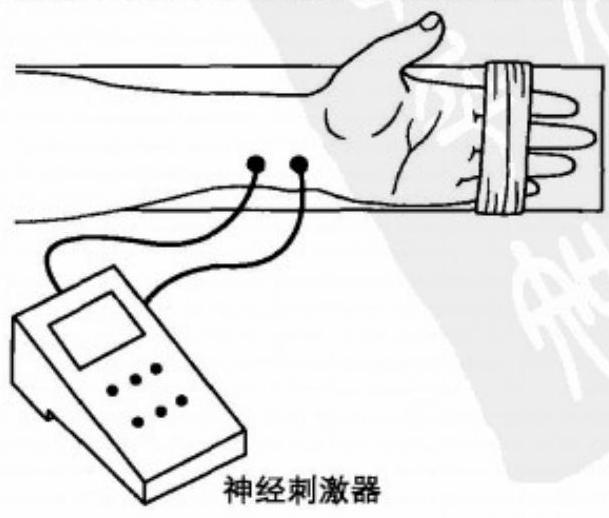
\includegraphics[max width=\textwidth]{2024_07_10_373f31b88d2bf633007bg-451}
\end{center}

图 4-5-1 尺神经刺僌时表面电极的贴放位\\
测定反应对照值, 用药后测定值以对照值的百分比来表示神经肌肉功能的阻滞程度。其优点是简单、可用于清酢病人,并作反复测试。缺点是敏感性较差,终板胆碱能受体有 $75 \% \sim 80 \%$ 被阻滞时,揎择反应才开始降低, $90 \%$ 受体被阻滞时才完全消失 (图 4-5-2)。因此, 单次额竛刺激恢复到对照值水平时, 仍有可能存在非去极化肌松药的残余作用。单次颤搐刺激可用于监测非去极化和去极化肌松药对神经肌肉功能的阻滞作用, 特别适用于强直刺激后计数。

\begin{enumerate}
  \setcounter{enumi}{1}
  \item 四个成串刺擞 (train of four stimulation, TOF) TOF 频率 $2 \mathrm{~Hz}$, 每 $0.5 \mathrm{~s}$ 一次的 4 个超强刺激,波宽 $0.2 \sim 0.3 \mathrm{~ms}$, 每组刺激是 $2 \mathrm{~s}$, 两个刺激间相隔 $12 \mathrm{~s}$,以免影响 4 次颤搐刺激的幅度,在给肌松药前先测定对照值, 4 次反应颤搐幅度相同, 即 TOF $\left(\mathrm{T}_{4} / \mathrm{T}_{1}\right)=1.0$ 。第 4 次颤摘反应 $\left(\mathrm{T}_{4}\right)$ 首先发生衰减,第 1 次颤搐反应 $\left(\mathrm{T}_{1}\right)$ 最后发生衰减, 根据 $\mathrm{TOF}$ $\left(\mathrm{T}_{4} / \mathrm{T}_{1}\right)$ 比值, 判断神经肌肉功能阻滞类型和深度。 $\mathrm{T}_{4}$ 消失表明阻滞程度达 $75 \%$,最后 $\mathrm{T}_{1}$ 消失, 表明阻滞程度达到 $100 \%$ 。如 4 次富畝反应都存在则表明阻滞程度不足 $75 \%$ 。去极化肌松药阻滞时, 使 4 次頞搐反应同时降低 (图 4-5-3), 不发生顺序衰减, $\mathrm{T}_{4} /$ $\mathrm{T}_{1}$ 比值 $<50 \%$ 并有强直后增强现象。TOF 可在清醒时取得对照值, 即使没有对照值, 也可直接读数。

  \item 强直刺激(tetanic stimulation)临床上采用 $50 \mathrm{~Hz}$ 持续 $5 \mathrm{~s}$ 的强直剌激 (图 4-5-4), $>50 \mathrm{~Hz}$ 肌肉不能迅速作出反应。非去极化阻滞及氯琥珀胆碱引起 II 相阻滞时, 强直刺激开始, 神经末梢释放大量乙酰胆碱,神经肌肉功能阻滞被部分拮抗, 肌肉收缩反应增强, 然后, 乙酰胆碱释放量下降, 肌松作用增强, 出现衰减现象(fade)。衰减程度取决于神经肌肉功能阻滞的深度、刺激频率和次数。停止强直刺激后, 乙酰胆碱的合成量增多,額搐反应增强, 称强直后增强 (post-tetanic potenitation)。但在部分非去极化阻滞时,用强直刺激后,因乙酰胆碱的合成和消除率加快,肌頞搐幅度可增强一倍以上, 即为强直后易化现象 (post-tetanic facillitation, PTF), PTF 的时间和程度取决于神经肌肉功能的阻滞深度, 强直刺激通常在 $60 \mathrm{~s}$ 内消失。因强直刺激能引起刺激部位疼痛, 清醒病人难以忍受。

  \item 强直刺激后计数 (post tetanic count stimulation,PTC) 当肌松药作用使 TOF 和单次额指刺激反应完全消失时,在此无反应期间, 先给予 $1 \mathrm{~Hz}$ 单次潩搐刺激 $1 \mathrm{~min}$, 然后用 $50 \mathrm{~Hz}$ 强直刺激 $5 \mathrm{~s}, 3 \mathrm{~s}$ 后用 $1 \mathrm{~Hz}$ 单次刺激, 共 16 次,记录强直刺激后单次额搐刺激反应的次数,称 PTC,每隔 $6 \mathrm{~min}$进行 1 次 (图 4-5-5)。PTC 与 $\mathrm{T}_{1}$ 开始出现时间之间的相关性很好, 可以预计神经肌肉收缩功能开始恢复的时间。

\end{enumerate}

\begin{center}
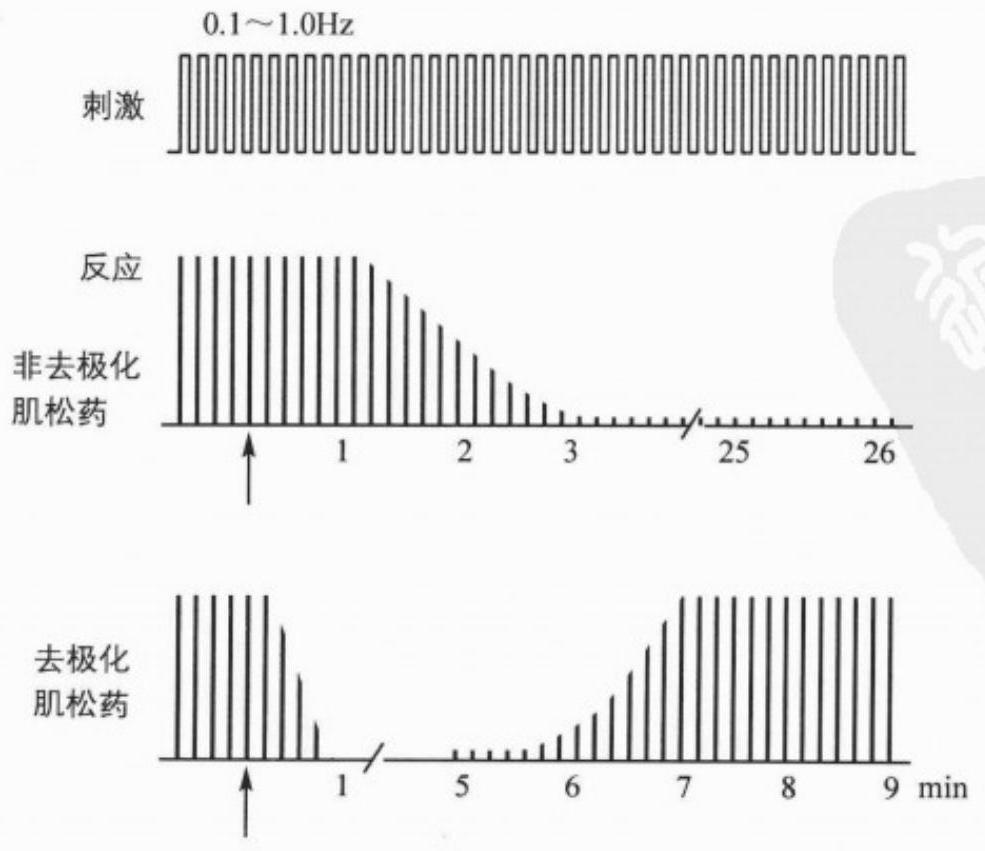
\includegraphics[max width=\textwidth]{2024_07_10_373f31b88d2bf633007bg-452}
\end{center}

图 4-5-2 单次侢搼刺激 (twich)

\begin{center}
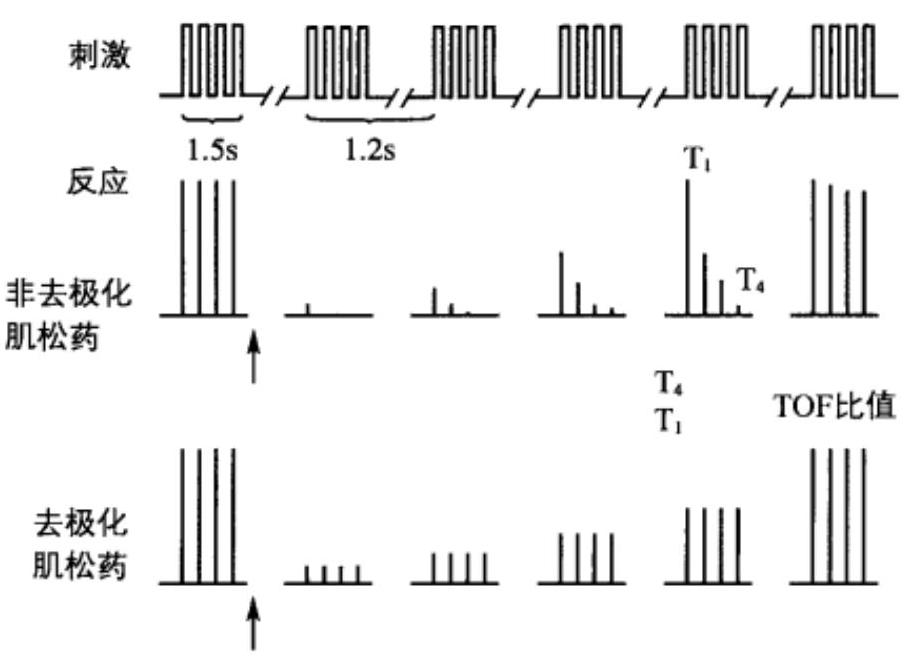
\includegraphics[max width=\textwidth]{2024_07_10_373f31b88d2bf633007bg-453}
\end{center}

图 4-5-3 四个成串刺激 (TOF)\\
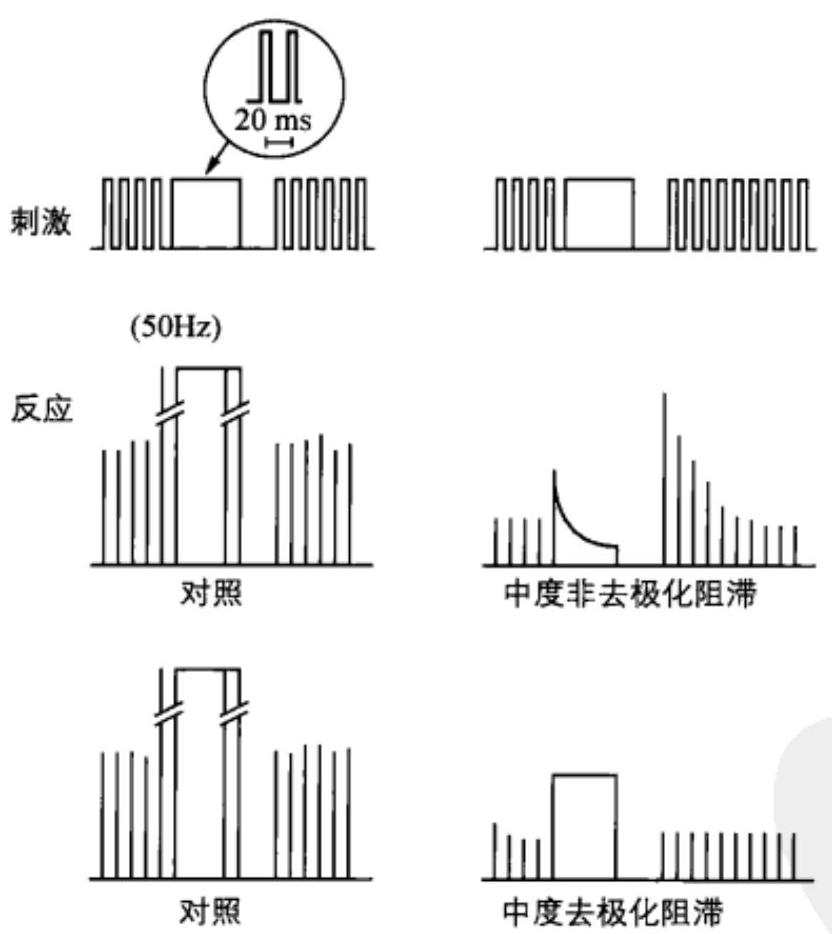
\includegraphics[max width=\textwidth, center]{2024_07_10_373f31b88d2bf633007bg-453(1)}

图 4-5-4 强直刺激 (tetanus)

\begin{enumerate}
  \setcounter{enumi}{4}
  \item 双短强直刺漖 (double burst stimulation, DBS)连续 2 组 $0.2 \mathrm{~ms}$ 和频率 $50 \mathrm{~Hz}$ 的强直刺激,每 2 次间相隔 $20 \mathrm{~ms}$,两组强直剌激间相隔 $750 \mathrm{~ms}$,如每次短阵强直刺激有 3 个脉冲, 则称为 $\mathrm{DBS}_{3,3}$ (图 4-5-6)。但也有学者研究 $\mathrm{DBS}_{3,2}$ 及 $\mathrm{DBS}_{4,3}$ 。 DBS 的衰减与 TOF 的比值密切相关, 应用 DBS 的目的是便于临床在没有记录装置时能更敏感地用拇指感觉神经肌肉功能的恢复程度。
\end{enumerate}

\section*{(四)肌松药作用监测的临床意义}
\begin{enumerate}
  \item 指示肌松程度,贾摛高度与肌松程度的关系见表 4-5-4。

  \item 判断肌松消退情况非去极化神经肌肉功

\end{enumerate}

\begin{center}
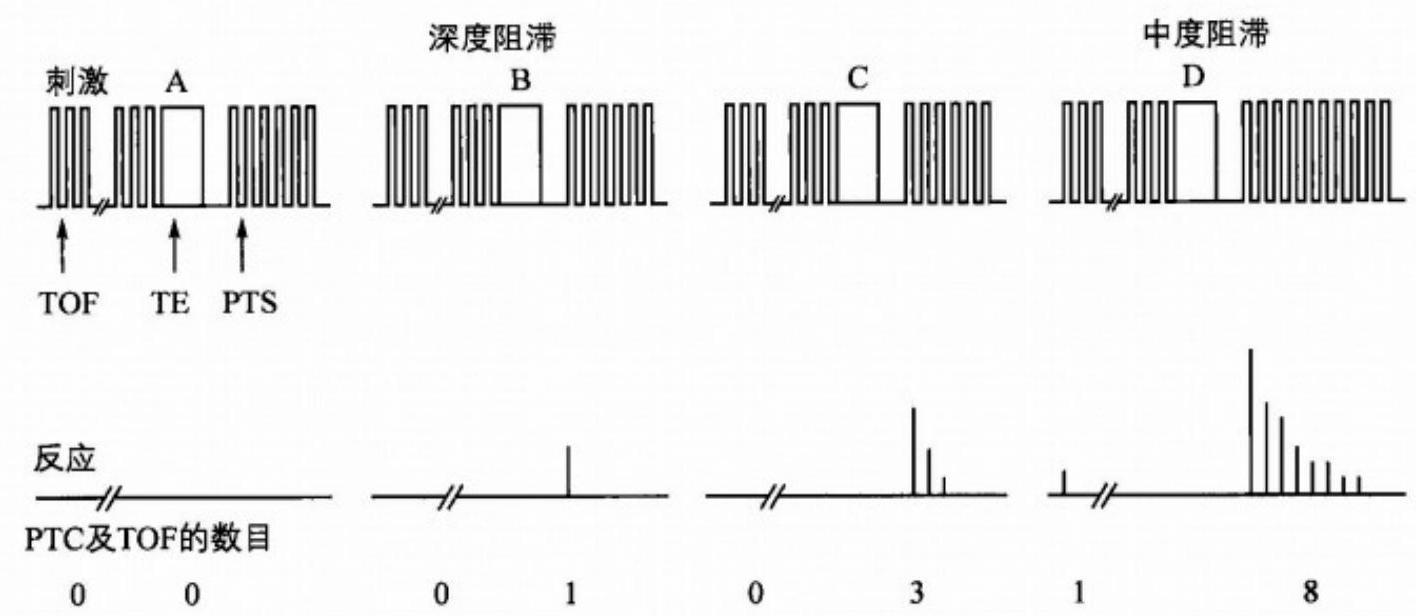
\includegraphics[max width=\textwidth]{2024_07_10_373f31b88d2bf633007bg-454(1)}
\end{center}

图 4-5-5 强直刺譤后计数(PTC)

\begin{center}
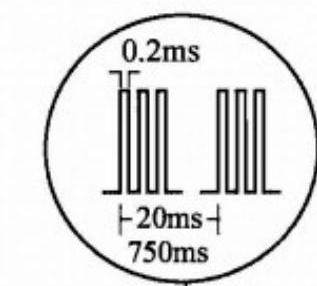
\includegraphics[max width=\textwidth]{2024_07_10_373f31b88d2bf633007bg-454}
\end{center}

刺激\\
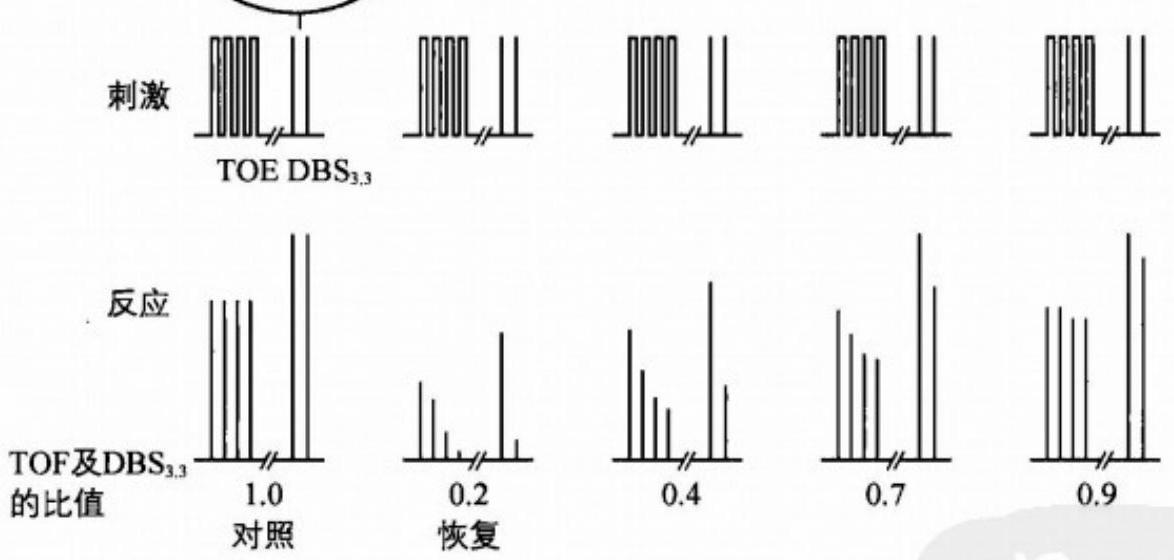
\includegraphics[max width=\textwidth, center]{2024_07_10_373f31b88d2bf633007bg-454(2)}

0.7

0.9

图 4-5-6 双短强直刺潡 (DBS)

能阻滞, 主要用 TOF 监测, 一般从注药到 TOF 完全消失为起效时间, TOF 消失期间为无反应期, $\mathrm{T}_{1}$消失为中度阻滞, 注药到 $\mathrm{T}_{4}$ 出现为 $\mathrm{T}_{1}$ 高度 $25 \%$ 恢复, $\mathrm{T}_{1}$ 高度 $25 \% \sim 75 \%$ 的时间为恢复率或称恢复指数 (RI)。TOF 仅有一次反应为 $90 \% \sim 95 \%$ 阻滞, TOF 的 4 次反应都出现, 指示神经肌肉功能 $60 \% \sim 95 \%$ 恢复(表 4-5-5)。表 4-5-4 楮撞高度与肌松程度的关系

\begin{center}
\begin{tabular}{|c|c|}
\hline
与对照值比较 & 肌松程度 \\
\hline
$100 \%$ & 无肌松现象 \\
\hline
$50 \%$ & 轻度肌松, $\mathrm{V}_{\mathrm{T}}$ 与 $\mathrm{V}_{\mathrm{C}}$ 减少 \\
\hline
$40 \%$ & 轻度肌松,可施行不需充分肌松的手术 \\
\hline
$25 \%$ & 中度肌松,䧗肌松驰,可施行腹部手术 \\
\hline
$5 \%$ & \begin{tabular}{l}
横膈无活动,下颌及咽肌松驰, 可施行气 \\
管插管 \\
\end{tabular} \\
\hline
0 & 横䐔活动完全消失, 呼吸停止 \\
\hline
\end{tabular}
\end{center}

表 4-5-5 TOF 比值情覀与缶床征象的关系

\begin{center}
\begin{tabular}{|c|c|}
\hline
TOF 比值 & 临床征象 \\
\hline
$25 \%$ & \begin{tabular}{l}
T、出现,肌松作用开始惔复,可以用拮抗 \\
药 \\
\end{tabular} \\
\hline
$40 \%$ & 不能抬头和举碚 \\
\hline
$50 \%$ & 开始睁眼、伸舌 \\
\hline
$60 \%$ & \begin{tabular}{l}
能咳毅、抬头和举臂 $3 \mathrm{~s}, \mathrm{Vc}$ 及用力吸と负 \\
压仍低于正常 \\
\end{tabular} \\
\hline
$70 \% \sim 75 \%$ & 能咳嫩、完全睠眼和伸舌、抬头、举辟 $5 \mathrm{~s}$ \\
\hline
$80 \%$ & \begin{tabular}{c}
Vc 、用力吸气负压及呼气流速基本正常, \\
神经肌肉功能基本恢复正常 \\
\end{tabular} \\
\hline
\end{tabular}
\end{center}

\section*{3. 氯琥珀胆䂸双相阻滞}
(1) I 相阻滞: 静注氯琥珀胆碱 $0.5 \sim 0.15 \mathrm{mg} /$ $\mathrm{kg}$ 后,产生典型的去极化神经肌肉功能阻滞 (图 45-7)。TOF 和强直刺激反应没有衰减, 无强直后易化现象。

(2)エ相阻滞:血浆胆碱酯酶异常,用小剂量氯琥珀胆碱及正常患者持续静滴氯琥珀胆碱过量, 可发生非去极化II相阻滞 (图 4-5-8), 又称脱敏感阻滞, TOF 及强直刺激反应发生衰减, 并出现强直后易化现象。用氯琥珀胆碱持续静滴, TOF 监测可避免用量过多, 胆碱酯酶正常的病人发生II相阻滞, 可谨慎地用新斯的明拮抗,但胆碱酯酶异常者拮抗无效。

\begin{enumerate}
  \setcounter{enumi}{3}
  \item PTC 的临床意义 PTC 的临床意义包括: (1)判断非去极化肌松药的阻滞深度:一些复杂精细的外科手术和眼科手术, 必须防止病人突然移动,应维持 $\mathrm{PTC}=0$, 保证病人没有咳嫩和呃逆, 横膈肌完全麻痹。(2)指导非去极化肌松药的连续输注: 根据 PTC 的数目调节速度。PTC 数目减少表示神经肌肉阻滞深度增加, PTC 小于 10 , TOF 消失, $\mathrm{PTC}=5 \sim 10$, 可保证适当深度的阻滞。(3)了解肌松药作用的消退时间: 通过 PTC 与第一次 TOF 反应出现时间的关系, 可以了解神经肌肉功能阻滞的恢复时间,以便追加肌松药或应用拮抗药。
\end{enumerate}

\section*{(五)肌松药作用监测的注意事项}
\begin{enumerate}
  \item 适当选用各种刺激方法。麻醉诱导和气管插管时选用单次颤搐和 TOF,手术期间中度阻滞及恢复期用 TOF 监测, 如需深度阻滞则采用 PTC,在恢复室病人应用 TOF 和 DBS。

  \item 非去极化肌松药对不同肌群的作用。由于非去极化肌松药对不同肌群的作用有所差别, 因此不能单凭临床征象来判断肌松程度。喉部肌群最大阻滞程度比拇内收肌明显低,提示喉部肌群对非去极化肌松药的敏感性比拇内收肌低。在评估气管内插筞条件时,应考虑到这个差异,以获得最佳

\end{enumerate}

\begin{center}
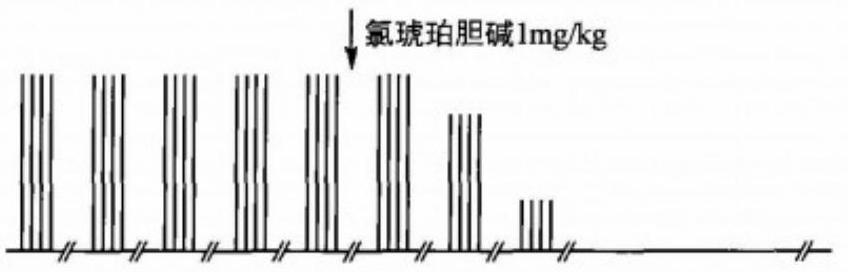
\includegraphics[max width=\textwidth]{2024_07_10_373f31b88d2bf633007bg-455}
\end{center}

图 4-5-7 去极化 I 相阻澫

\begin{center}
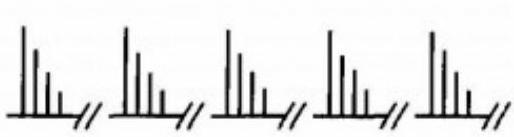
\includegraphics[max width=\textwidth]{2024_07_10_373f31b88d2bf633007bg-455(3)}
\end{center}

$50 \mathrm{~min}$

\begin{center}
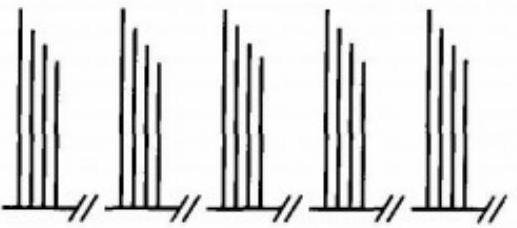
\includegraphics[max width=\textwidth]{2024_07_10_373f31b88d2bf633007bg-455(2)}
\end{center}

$120 \mathrm{~min}$

\begin{center}
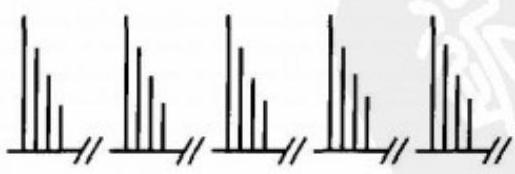
\includegraphics[max width=\textwidth]{2024_07_10_373f31b88d2bf633007bg-455(1)}
\end{center}

$60 \mathrm{~min}$

\begin{center}
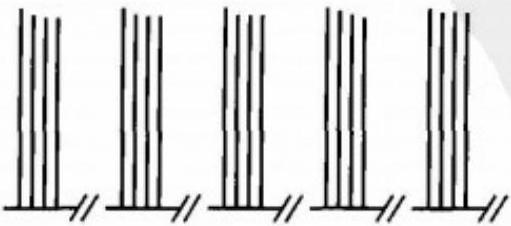
\includegraphics[max width=\textwidth]{2024_07_10_373f31b88d2bf633007bg-455(4)}
\end{center}

$160 \mathrm{~min}$

图 4-5-8 去极化 II 相阻洪\\
插管状态, 并注意咽喉肌群的肌松消退时间较拇内收肌慢, 指示适当的拔管时间, 避免残余肌松发生。

\begin{enumerate}
  \setcounter{enumi}{2}
  \item 熟悉肌松药作用监测仪性能。

  \item 电极安放部位必须正确。

  \item 先测定对照值。

  \item 注意其他药物对肌松作用的影响。

\end{enumerate}

\section*{六、残余肌松药作用和肌松药的拮抗药}
手术后单凭临床征象和试验不可能对神经肌肉功能的恢复做出正确可靠的判断。文献报道对 40 名应用泮库滇䯃患者研究表明仅凭临床征象判断, 术后肌松残余阻滞 (TOF 比值 $<0.7$ ) 发生率为 $52 \%$, 而用加速度仪进行肌力监测, 残余肌松 (TOF 比值 $<0.7$ ) 发生率仅为 $5 \%$ 。同样, 另有学者对 40 名应用罗库溪轱的患者观察表明仅凭临床征象判断, 术后残余肌松药作用 $(\mathrm{TOF}$ 比值 $<0.8$ )发生率为 $17 \%$, 而用加速度仪进行肌力监测, 残余肌松药作用 (TOF 比值 $<0.8$ ) 发生率仅为 $3 \%$ 。因此, Eriksson 等建议以 TOF 比值 $\geqslant 0.9$ 作为神经肌肉兴奋传递功能恢复的标准。术后残余肌松药作用对患者的健康和生命安全是一种严重威胁。据报道 $20 \%$ 的术后呼吸衰竭死亡患者与残余肌松药作用有关。残余肌松药作用对患者的危害有以下几方面: (1)增加低氧血症和 (或)高碳酸血症的发生率。(2)影响咽部及上端食管的功能,提高反流和误吸的发生率。(3)增加术后肺部并发症的发生率。因此, 为了病人全麻恢复期安全, 避免肌松药残余作用,应进行肌力监测和肌松药作用拮抗。

去极化肌松药至今尚无满意而有效的拮抗药。非去极化肌松约可用抗胆碱酯酶药拮抗。近年上市的新药环糊精 (sugammadex), 是新型的甾类非去极化肌松药拮抗药。它是一种经修饰的 $\gamma$-环糊精, 能与甾类肌松药,尤其是罗库浣铵,形成无活性的复合物。Sugammadex 能够迅速、完全、有效地拮抗非去极化肌松药的深度神经肌肉阻滞作用,也将可能改变临床麻醉的现状。

(一)抗胆碱酯酶药

\begin{enumerate}
  \item 药理作用 包括新斯的明、溴吡斯的明和依酚氯轱(表 4-5-6)。当用抗胆碱酯酶药后, 乙酰胆碱酯酶活性受抑制, 乙酰胆碱存在时间延长,有足够时间可反复参与肌松药竞争受体使终板电位总量增加, 超过激发肌纤维动作电位的阈值, 从而逆转非去极化肌松药的阻滞作用。但肌松药仍残留在神经肌肉接头内, 其最终消失作用有赖于肌松药进人循环而被清除。依酚氮铵借阳电荷氮原子与乙酰胆碱分子中阴电荷结合, 从而防止乙酰胆碱酯酶与乙酰胆碱作用而起到拮抗作用。起效时间依酚氯铵最快 $<5 \mathrm{~min}$, 新斯的明 $7 \sim 10 \mathrm{~min}$, 滇吡斯的明最慢 10〜15min。

  \item 适应证和禁忌证拮抗非去极化肌松药。但支气管哮喘、心脏传导阻滞、血压过低、窨性心动过缓、胃肠吻合术病人禁用。

  \item 不良反应 抗胆碱酯酶药可引起暂时性心律失常, 如心动过缓、房性或结性心律、室性早搏、房室传导阻滞等,以及瞳孔缩小、支气管收缩和分泌增多和胃肠螨动增快等,应加强监测和及时处理。

  \item 剂量和用法 心率 $<80 / \mathrm{min}$, 先用阿托品 $0.5 \sim 1.0 \mathrm{mg}$, 再用该类药物。临床上最常用的是新斯的明, 常用剂量 $0.04 \sim 0.05 \mathrm{mg} / \mathrm{kg}$ (最大剂量为 $0.07 \mathrm{mg} / \mathrm{kg}$, 总量不超过 $5.0 \mathrm{mg}$ ), 也可将用量分 2 次给, 先用半量观察 $15 \sim 20 \mathrm{~min}$, 视拮抗结果, 必要时再给予半量。老年人用量应酌减。新斯的明,起效时间 $7 \mathrm{~min}$, 从起效至峰值效应时间为 $7 \sim$ $10 \mathrm{~min}$ 。溴吡斯的明剂量 $0.15 \sim 0.25 \mathrm{mg} / \mathrm{kg}$ (最大剂量为 $0.35 \mathrm{mg} / \mathrm{kg}$, 总量不超过 $<20 \mathrm{mg} /$ 次)。起效时间 $12 \mathrm{~min}$, 高峰值效应时间 $10 \sim 15 \mathrm{~min}$ 。上述两药均需同时或先静注阿托品 $0.02 \sim 0.05 \mathrm{mg} / \mathrm{kg}$或格隆溴铵 $0.01 \mathrm{mg} / \mathrm{kg}$ 。依酚氯铵的拮抗强度仅为新斯的明的 $1 / 15$, 因此, 需较大剂量方能维持拮抗作用。该药有直接剌激终板的作用, 毒曹碱样不

\end{enumerate}

表 4-5-6 抗胆碱酯酶药的临床药理

\begin{center}
\begin{tabular}{|c|c|c|c|c|c|}
\hline
药物 & 剂量 & \begin{tabular}{c}
最强拮抗 \\
时间 (min) \\
\end{tabular} & \begin{tabular}{l}
怙抗持续 \\
时间 (min) \\
\end{tabular} & 消除方式 & \begin{tabular}{l}
阿托品剂 \\
量 $(\mu \mathrm{g} / \mathrm{kg})$ \\
\end{tabular} \\
\hline
依酽氮轱 & $0.5 \sim 1 \mathrm{mg} / \mathrm{kg}$ & 1 & $40 \sim 65$ & $70 \%$ 经肾, $30 \%$ 经肝 & $7 \sim 10$ \\
\hline
新斯的明 & $0.03 \sim 0.07 \mathrm{mg} / \mathrm{kg}$, 最大用量为 $5 \mathrm{mg}$ & 7 & $55 \sim 75$ & $50 \%$ 经肾, $50 \%$ 经肝 & $15 \sim 30$ \\
\hline
滇吡斯的明 & $0.25 \mathrm{mg} / \mathrm{kg}$ & $10 \sim 13$ & $80 \sim 130$ & $75 \%$ 经肾, $25 \%$ 经肝 & $15 \sim 20$ \\
\hline
\end{tabular}
\end{center}

良反应小,同时应用阿托品的剂量也应减少至 0.01 $0.015 \mathrm{mg} / \mathrm{kg}$ 。静注 $0.5 \sim 1.0 \mathrm{mg} / \mathrm{kg}$ 后 $2 \mathrm{~min}$ 起效,总量 $<70 \mathrm{mg}$ 。至峰值效应时间不超过 $5 \mathrm{~min}$ 。如果新斯的明、涋吡斯的明和依酚氯铵的芍量分别超过了各自的最大剂量,而拮抗效果仍不明显时,不宜再继续给予怙抗药, 应认真分析影响抗胆碱酯酶药效果的因素。

\section*{5. 注意事项}
(1)排除麻醉性镇痛药引起的中枢性呼吸抑制, 用于术毕尚有残余肌松作用的病人。术毕肌张力恢复不足, TOF 比值 $<0.7$ 等均可应用拮抗药。

(2)抗胆碱酯酶药应与抗胆碱药合用,阿托品或格隆滇铵 (glycopyrronium bramide), 可以防治抗胆碱酯酶药特别是新斯的明引起的毒草碱样 (M 乙酰胆碱受体)不良反应, 如心动过缓、瞳孔缩小、支气管收缩和分泌增多以及胃肠蝡动增加等。

(3) 用拮抗药后肌张力恢复时间与用拮抗药时的肌松程度。在非去极化阻滞消退期,一般于 TOF 出现 $\mathrm{T}_{1}$ 反应后给药, TOF 比值达到 0.7 需 $10 \sim 30 \mathrm{~min}$; 当 TOF 出现四次反应时用拮扰药, 用药后 $10 \mathrm{~min}$ 内 TOF 比值即可达到 0.7 。因此, 应掌握给予拮抗药的时机, 不能在神经肌肉阻滞作用较强时给药, 否则易导致“再箭毒化”的不良后果。

(4)呼吸性酸中毒、代谢性酸中毒、低钾血症和高美血症等酸碱和电解质失衡可影响抗胆碱酯酶药的作用。此外,低温也影响其怙抗效果。

(5)抗生素增强肌松药作用的机制较为复杂。考虑到有抗生素增强肌松作用的因素存在时,最好维持人工通气, 使其自然恢复肌张力。

\section*{(二)环糊精}
环糊精 (sugammadex)能与甾体类肌松药如罗库浣轱,形成无活性的复合物。以 $1: 1$ 形成紧密复合物阻碍甾体类肌松药神经肌接头处的功能, 影响其再分布, 加速甾体类肌松药与烟碱样乙酰胆碱受体分离, 从而拮抗神经肌肉阻滞作用。环糊精分子结构的孔径深度正适合包襄罗库溴轱的四个疏水甾体环, 再加上罗库滇轱的正四价的氮和环糊精的负价羒基形成静电反应, 复合物便稳定形成。环糊精能迅速包裹甾体类肌松药, 所以能避免发生肌松药与乙酰胆碱受体作用,故在理论上能将其血浆浓度降低至零。当肌肉松驰药从神经肌肉接头处扩散回血浆时, 神经肌肉阻滞作用能迅速减轻及消退; 理论上任何程度的阻滞都能被拮抗。虽然环糊精也可以和非甾体药物, 如阿托品和维拉帕米以及可的松和氢化可的松,形成复合物,但这些药物与环糊精的亲和力要比罗库湨䯃等类固醇肌肉松驰药小 120〜700 倍。这主要是由于环糊精的分子孔径以及其结构上与罗库滇铵的疏水甾体分子骨架的互补。且环糊精无生物活性, 离体实验中它与动物组织不起反应。最近研究显示无论在离体还是在体实验中, 环糊精都能迅速地拮抗罗库滇铵引起的神经肌肉阻滞作用。该复合物主要分布在中央室 (血浆)和细胞外液中, 并以原型在尿液中排出。当环糊精注射后, 它能立即包裹游离在血浆中的罗库滇轱分子。这可以增加游离罗库滇轱在组织区室和血浆区室间的浓度差,因此可以回收组织中的罗库溴铵,以拮抗其在神经肌肉接头处的作用。当罗库滇轱进人血浆,这些游离的分子和更多环糊精形成复合物, 所以能保持扩散梯度直到所有的罗库溴轱均在血浆中与环糊精形成复合物或者直到所有的环糊精分子均饱和为止。

动物实验及近期临床研究均未发现环糊精引起的血压、心率等心血管系统明显变化,也没有发现类似应用胆碱酯酶抑制药所引起的心血管系统、呼吸系统和消化系统的不良反应, 无再箭毒化的发生。至今已完成环糊精的临床前动物实验, I 期、 II 期和 III期临床验证, 结果显示, 无论是刚给予罗库滇轱, 还是给予大剂量、长时间罗库滇轱后,静脉注射 $4 \mathrm{mg} / \mathrm{kg}$ 环糊精后, 都能够在 $3 \mathrm{~min}$ 时完全拮抗罗库滇轱的肌松作用。

(阙大翔杭燕南)

\section*{考考文靓}
[1]聞大翔, 欧阳荣怡, 杭茝南. 肌肉松弛

药. 上海:世界图书出版公司,2007

[2]庄心良,曾因明,陈伯媱。现代麻醉

学. 3 版. 北京: 人民卫生出版社, 2006;562-763

[3] Miller R D, Philadelphia. Anesthesia. 6th edn. Churchill Livingstone, 2005: 481

[4]抗䓙南,庄心良、蒋衰. 当代麻碎学.上海: 上海科学技术出版社, 2002, 318-326

[5] Bom A, Bradley M, Cameron K, et al. A
\footnotetext{novel concept of reversing neuromus-

cular block. Chemical encapsulation of rocuronium bromide by a cyclodextrinbased synthetic host. Angew Chem INt ED Engl,2002,41,266-270

[6] de Boer H D, Van Egmond J, Van de
}

Pol F, et al. Sugammadex, a new reversal agent for neuromuscular block induced by rocuronium in the anaesthetized Rhesus monkey. $\mathrm{Br} J$ Anaesth,2006,96:473-479

[7] Groudine S B, Soto R, Lien C, et al. A randomized dose-finding Phase II study of the first selective relaxant binding agent, sugammadex, capabie of safely reversing profound rocuronium-induced neuromuscular block. Anesth Analg, 2007,104;555-562

[8] Lenz A, Hill G, White P E. Emergency use of sugammadex after failure of standard reversal drugs. Anesth Analg, 2007, 104,585-586

[9] Miller R D. Sugammadex: An Opportu- nity to Change the Practice of Anesthesiology? Anesth Analg, 2007, 104, 477-478

[10]闯大䍩,陈锡明,杭苝南,等. 国人㿟阿曲库转的剂量反应测定.中华麻醉学杂志, 1999, 19(7) ; 395-397

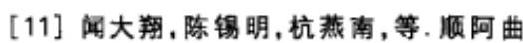
\includegraphics[max width=\textwidth, center]{2024_07_10_373f31b88d2bf633007bg-458}\\
库铵的组胺释放作用及其对血洨动力学的影响. 中华麻醉学杂志,2001, 21(2):69-72

[12] Kopman A F, Yee P S, Neuman G. Relationship of the train-of-four fade ratio to clinical signs and symptoms of residual paralysis in awake volunteers. Anesthesiology, 1997,86:765-771

[13] Glenn S. Murphy, Joseph W. Szokol,\\
Jesse H. Marymont, et al. Residual paralysis at the time of tracheal Extubation. Anesth Analg, 2005, 100: 18401845

[14] Lemmens H J, Brodsky J B. The dose of succinylcholine in morbid obesity. Anesth Analg, 2006, 102(2) :438-442

[15] Naguib M, Samarkandi A H, El-Din M $\mathrm{E}$, et al. The dose of succinylcholine required for excellent endotracheal in tubating conditions. Anesth Analg, 2006, 102(1) : 151-155

[16 ] Naguib M. Sugammadex: Another milestone in clinical neuromuscular pharmacology. Aneth Aalg, 2007, 104 (3) :575-581

\section*{籍手}
\section*{神经阻滞麻醉}
神经阻滞麻醉是将局麻药注射至神经干 (丛)旁, 暂时地阻滞神经的传导功能, 达到手术无痛或所需治疗目的的方法。神经干旁常有伴行血管, 穿刺针经过的组织附近可能有体腔及脏器, 穿刺损伤可以引起某些严重并发症, 故应熟悉每一神经干 (丛)的局部解剖特点, 尤以神经与骨骼的关系最为重要。应充分利用身体的标志 (体表、组织及骨骼的标志), 定位穿刺人路。浅层标志多通过触摸和测量, 深层标志除触摸外还须借助针感才可逐步积累经验。另外,利用一些先进的定位技术, 如神经刺激器和超声影像引导等可获得更为准确的神经定位。某些神经阻滞可有不同的人路和方法, 应采用简便、确切、安全和易于成功或操作者较为熟悉的方法。如遇穿刺点附近有感染、肿块或病人改变体位有困难等原因, 则须变换人路, 故麻醉者应勲悉多种人路方法以便酌情选择。

术前应根据病人的精神状态、手术范围和需要的时间等条件,决定是否采用神经阻滞及何种阻滞方法。还应向病人解释阻滞的操作步骤、体位及要求合作的内容,以解除病人的顾虑。

神经阻滞的药物,在安全剂量范围内可采用同一种药物或两种药物的混合液。临床上常用 $2 \%$ 普鲁卡因、 $1 \% \sim 1.5 \%$ 利多卡因、 $0.15 \% \sim 0.3 \%$ 丁卡因、 $0.25 \% \sim 0.5 \%$ 布比卡因及 $0.25 \% \sim 0.5 \%$ 罗哌卡因; 混合液有 $1 \%$ 利多卡因或 $0.5 \%$ 罗哌卡因与 $0.15 \%$ 丁卡因合液、1\%利多卡因与 $0.25 \%$ 布比卡因以及 $1 \%$ 利多卡因与 $0.25 \%$ 罗哌卡因合液等。药液内可酌情加人 1:200 000肾上腺素。

\section*{第一节 颈丛神经阻滞}
\section*{一、解 剖}
颈神经丛来源于颈 ${ }_{1 \sim 4}\left(\mathrm{C}_{1 \sim 4}\right)$ 脊神经。除第 1 颈神经主要是运动神经外, 其余 3 对颈神经均为感觉神经。后 3 对神经离开椎间孔后, 从后面横过椎动脉及椎静脉, 嵌于横突的凹面, 到达横突尖端时分为升支及降支, 这些分支与上下相邻的颈神经分支在胸锁乳突肌之后连接成一系列环状神经, 称为颈神经丛。颈神经丛又分为浅丛及深丛, 浅丛分布于颈部分别支配颈部皮肤; 深丛主要支配颈深部肌肉及部分腀肌。

颈浅神经丛位于胸锁乳突肌后缘中点, 从这点呈放射状分支向前即颈前神经、向下即锁骨下神经、向后上为耳大神经、向后则为枕小神经, 它们支配头颈以及胸肩的后部,如披肩状。如仅为这部分

膜下阻滞浅丛即可。颈深丛主要支配侧面及前面皮区手术,在胸锁乳突肌后缘,于皮下及颈阔肌竻的区域。如系深部手术,可在横突附近进行神经阻滞,颈深、浅丛均可被阻滞,从而获得更为满意的麻醉效果。

\section*{二、颈丛阻滞的实施}
乳突下 $1.5 \mathrm{~cm}$ 、胸锁乳头肌后缘处约为 $\mathrm{C}_{2}$ 椎横突所在; 胸锁乳头肌后缘中点相当于 $\mathrm{C}_{4}$ 横突尖位置; 两者之间连线的中点为 $\mathrm{C}_{3}$ 横突尖。从体表标志看, $\mathrm{C}_{4}$ 横突位于胸锁乳突肌及颈外静脉交叉点附近,用示指按压可摸到横突, 并可能出现异感。

\section*{(一)颈前阻滞法}
病人仰卧, 头偏向对侧, 在 $\mathrm{C}_{2} 、 \mathrm{C}_{3}$ 和 $\mathrm{C}_{4}$ 横突处做标记。手指可触及各横突尖,用 $22 \mathrm{G}$ 长 $4 \sim 5 \mathrm{~cm}$穿刺针, 从颈部侧面经标记点垂直稍向足倾斜刺人达 $\mathrm{C}_{2} 、 \mathrm{C}_{3}$ 和 $\mathrm{C}_{4}$ 横突面, 病人可出现异感。回抽无血\\
液或脑脊液, 即可分别注射局麻药 $3 \sim 4 \mathrm{ml}$ 。 $\mathrm{C}_{4}$ 部深丛阻滞后, 拔针至皮下和颈阔肌之间, 再注射局麻药 $10 \mathrm{ml}$ 即可阻滞颈浅丛。

一针阻滞法: 已得到较广泛应用,在 $\mathrm{C}_{3}$ 或 $\mathrm{C}_{4}$ 颈椎横突穿刺点进针,穿刺针抵达横突后, 回抽无血液或脑脊液后注人局麻药 $10 \mathrm{ml}$, 同时以手指压迫 $\mathrm{C}_{5}$ 横突处防止药液向足侧扩散。然后退针可行颈浅丛阻滞。

\section*{(二)肌间沟穿刺法}
病人侧卧位, 头偏向对侧, 先令病人抬头使胸锁乳突肌绷紧, 在甲状软骨上缘平面, 以示指和中指摸到绷紧的肌肉外缘,再令病人头放下使肌肉松他,触摸的手指向下滑至前斜角肌上缘,手指再向外侧摸及前、中斜角肌的肌间沟。穿刺针自肌间沟刺人,针刺方向与皮肤垂直略向后向下。遇异感即超过横突深度, 避免损伤椎动脉, 也应避免穿刺针误人硬膜外间隙或蛛网膜下腔。出现异感后,回抽无血无脑脊液、固定穿刺针及注射器后即注人局麻药液。局麻药可沿斜角肌间隙 (或臂丛颈从鞘)上、下行,若不需麻痹臂丛,可压迫穿刺针下方的肌间沟,大部分药液则上行而阻滞颈神经丛。

\section*{(三)单侧或双侧阻洓}
根据手术需要选择单侧或双侧阻滞, 但药物总量应在安全剂量范围内。双侧颈深丛阻滞时, 有可能阻滞双侧隔神经或喉返神经而引起呼吸困难, 故应慎用。特别是一针阻滞法易引起唉返神经麻痹,仅限于单侧阻滞。

颈丛阻滞用于颈前部和侧面的手术,包括甲状腺和颈部淋巴结手术等。停止进针, 若无异感再行探刺, 但穿刺针深度不应

\section*{三、并 发 症}
\section*{(一)药液误入硬膜外间皕和蛛网膜下腔}
可引起高位硬膜外阻滞, 而最严重的并发症是药液注人蛛网膜下腔引起全脊麻。穿刺针误人椎管的原因之一是进针过深,二是进针方向偏内向后, 尤以一针法误人蛛网膜下腔的机会最大。预防在于进针切勿过深, 注药 $2 \sim 3 \mathrm{ml}$ 后观察无呼吸困难即无脊麻反应,则再注人余药。

\section*{(二)局麻药妻性反应}
主要是穿刺针误人颈动脉或椎动脉而未及时发现,因此注药前应抽吸,证明针尖深度应在横突部位。另外,如果注药太快、压力太大,由于颈部血管丰富,药物吸收迅速, 也会导致中毒。

\section*{(三)膈神经阻滞}
膈神经主要由第 4 颈神经组成,同时接受第 3 及第 5 颈神经的小分支。颈深丛阻滞常易累及胦神经, 双侧受累时可出现呼吸困难及胸洶。此时应立即吸氧或者给予辅助呼吸治疗。

\section*{(四)喉返神经阻滞}
针刺太深、注药压力太大可使迷走神经阻滞,造成病人发音嘶哑或失音, 甚至呼吸困难, 此症状在 $0.5 \sim 1 \mathrm{~h}$ 内大多缓解。

\section*{(五)Horner 综合征}
注药后病人表现上眼睑下垂、瞳孔缩小、眼球下陊、眼结膜充血、鼻塞、面微红及不出汗, 有时上述症状部分出现,此系颈交感神经被阻滞所致,短期内可自行消失。

\section*{(六)椎动脉刺伤引起出血}
略

\section*{第二节臂丛神经阻滞}
\section*{一、解 剖}
臂神经丛主要由颈 $5 \sim 8$ ( $\left.\mathrm{C}_{5 \sim 8}\right)$ 及胸 $\left(\mathrm{T}_{1}\right)$ 脊神经的前支组成,但有少数的臂神经丛含有来自 $\mathrm{C}_{4}$ 和 $\mathrm{T}_{2}$ 脊神经前支的小分支,是支配整个手、臂运动和绝大部分手、臂感觉的混合神经。这些神经在椎间孔分出后,在前、中斜角肌之后形成上、中、下干。上干由 $\mathrm{C}_{5 \sim 6}$ 前支, 中干由 $\mathrm{C}_{7}$, 后干由 $\mathrm{C}_{8}$ 和 $\mathrm{T}_{1}$ 脊神经前支构成。三条神经干沿锁骨上动脉方向向外、下延伸。在锁骨后第 1 助骨中外缘, 每个神经干分成前后两股,通过第 1 肋和锁骨中点,再经腋窝顶部进人腋窝。在腋部各神经干的前后两股再组成束, 根据它们与腋动脉的部位关系, 三个后股在腋动脉后侧合成后束, 最后延续为桡神经; 上干和下干的前股在腋动脉外侧组成外侧束, 最后延续为正中神经; 下干的前股延伸为内侧束,最后延续为尺神经。

\section*{二、臂丛神经阻滞的实施}
\section*{(一)腑路臂丛阻滞法}
病人仰卧, 头偏向对侧, 被阻滞的上肢外展 $90^{\circ}$, 肘屈曲也呈 $90^{\circ}$, 即有如行军礼状, 以充分暴露\\
腋窝。先在腋窝触摸到动脉搏动, 再沿动脉走向,取动脉搏动最高点。左手固定于腋动脉, 取长 2 $4 \mathrm{~cm} 22 \mathrm{G}$ 或更细短斜面针, 穿刺针与动脉呈 $10^{\circ} \sim$ $20^{\circ}$ 夹角刺进皮肤,然后缓慢进针直到出现穿过筋膜的感觉(如同刺破一层纸), 之后如稍改变穿刺针方向,有时可获得前臂异感,但不必强求异感。松开持针手指, 针随动脉搏动而摆动, 即可认为针已进人腋鞘内。接注射器回抽无血后, 即可注人 $30 \sim$ $35 \mathrm{ml}$ 局麻药。注药后可见药液呈菱形扩散。阻滞产生效果时, 病人可诉上肢发麻、上肢尤其前臂不能抬起、皮肤表面血管扩张等。腋路阻滞由于上臂外展 $90^{\circ}$ 时, 腋鞘被肱骨头压迫, 局麻药不易上行扩散; 另外由于臂丛神经在鞘内的分支多并且比较分散,因而常致阻滞不到肌皮神经。补教的办法是在注药时可应用橡胶止血带扎于腋鞘的远端或用手指加以压迫; 注药完毕后立即回收上肢,使贴于躯干之旁,以利局麻药上行扩散。

腋路阻滞法上辟的阻滞效果往往较差, 因此多适用于前臂和手掌部位不需使用止血带的手术。

因腋路䇏丛神经分支均包在腋血管神经鞘内,位置表浅, 动脉搏动明显, 定位和穿刺均较容易, 故易于阻滞; 此人路无气胸、膈神经阻滞、喉返神经阻滞之忧; 也无误人硬膜外腔和蛛网膜下腔的危险。局麻药毒性反应和外周神经损伤是腋路阻滞法相对于其他人路较多出现的并发症。局麻药毒性反应多因局麻药量大或误人血管引起,故注药时应反复回吸, 确保针不在血管内; 外周神经损伤与穿刺损伤有关,特别是在反复寻找异感的情况下,更易发生。故腋路阻滞穿刺过程中,不推荐寻找异感的方法。

\section*{(ニ)锁骨下血管旁阻滞法}
病人仰卧, 头偏向对侧, 患肢贴身平放。病人抬头可显露胸锁乳突肌, 在其外侧摸出前斜角肌,该肌外侧即为前、中斜角肌肌间沟,用左手手指沿肌间沟下摸,在肌间沟最低处可摸到锁骨下动脉搏动。左手示指放在锁骨下动脉搏动处,右手持长 $3 \sim 4 \mathrm{~cm} 22 \mathrm{G}$ 的穿剌针, 自锁骨下动脉搏动点外侧 (紧靠左手示指),沿中斜角肌的内侧缘向下肢方向推进。方向不宜向内、向后偏移。此时穿刺针处于锁骨下动脉外侧 (背侧) 切面, 臂丛鞘的最深处, 注射针在此处即使有较大移动也不致脱出。缓慢进针时, 可有刺破臂丛鞘的感觉, 但不如腋鞘明显。针进人臂丛鞘后再向前进就会出现异感;若无异感可改变进针方向,使针稍偏内、偏后, 即针刺方向朝对侧足跟,常易获异感。回抽无血或脑脊液即可注人局麻药液 $20 \sim 25 \mathrm{ml}$, 药量不宜超过 $30 \mathrm{ml}$ 。局麻药注完后,病人会有“压力异感”, 为药液已充填于臂丛輎内的客观征象之一。

局麻药在鞘内可阻滞臂丛神经各干及其分支,达到完善的上肢阻滞效果, 故此人路可满足从肩部到手掌手术需要。由于可阻滞臂内侧皮神经和肋间神经,可缓解止血带所引起的疼痛,对需上止血带的手术更为有利。

此人路用较小剂量可得到较高水平的臂丛阻滞;有上肢及肩部疼痛者,穿剌中不必移动上肢; 无误人硬膜外腔或蛛网膜下腔的风险。但缺点是穿刺定位不如其他方法方便, 如应用神经刺邀器可提高成功率; 有局部血肿和局麻药误人血管引发毒性反应的可能; 气胸发生率低于锁骨上臂丛阻滞法,但仍有发生; 穿刺中若未能寻找到异感, 则失败率较高, 可达 $15 \%$ 。

\section*{(三)锁骨上臂丛阻滞法}
病人平卧, 头偏向对侧,上肢靠身放平,可在肩下垫一小枕以利定位。取锁骨中点上方 $1 \sim 2 \mathrm{~cm}$处, 作一标记, 以 $22 \mathrm{G}$ 穿刺针经标记刺人, 取向中、后及下的方向, 直到上肢感觉出现异常。如针尖触及第一肋骨尚无异感,可沿第一助骨前后移动穿刺针, 寻找上肢异感,特别是异感部位在前臂时, 阻滞效果更佳。在第一肋骨面上寻找异感较为安全确切, 针尖贴着骨面反复寻找,注意应避免反复穿剌造成胸膜损伤。如果误刺到锁骨下动脉, 只需将针拔出, 稍向外移即可获得异感。出现异感后, 立即固定穿刺针,注人局麻药 $20 \sim 30 \mathrm{ml}$, 可产生有效的阻滞。锁骨上阻滞法对整个上肢的阻滞效果比较好。由于臂丛在此处的神经干最粗大, 麻药浸润人神经干中心也较慢,使得起效稍迟; 偶在肋间神经也参与臂丛组成时,效果不佳。

对于上臂、肘部和拇指基底部手术需行臂丛神经阻滞时, 锁骨上人路是最佳选择之一。上䣝及肘部手术如尺神经移植术、时关节闭合或开放复位等需阻滞 $\mathrm{C}_{5} \sim \mathrm{C}_{8}$ 和 $\mathrm{T}_{1}$ 神经; 上臂和肘部外侧和后外侧手术需有 $\mathrm{C}_{5 \sim 8}$ 的阻滞; 手术区在肘之内侧时, 阻滞 $C_{8}$ 和 $T_{1}$ 非常重要; 若以上手术需上止血带时,尚需阻滞 $\mathrm{C}_{5 \sim 8}$ 和 $\mathrm{T}_{1}$ 柛经的浅支。锁骨上人路行臂丛阻滞可满足上述阻滞要求。拇指基底部有三支大神经支配此区域, 即由前外侧来的正中神经, 从后外侧来的桡神经和上外侧来的肌皮神经, 三支神经\\
必须完全阻断才能满足此处手术的阻滞要求, 锁骨上可列为首选。

气胸是本人路较常见的并发症, 发生率高达 $1 \%$ 。即使熟练者也可能发生此并发症。而此并发症可延迟发生, 在门诊患者, 其危险性更大。其他并发症包括局部血肿、膈神经和缇返神经阻滞等。

(四)肌间沟阻滞法

取仰卧位, 手臂平放贴体, 头稍偏向对侧, 以显领患侧颈部。肌间沟阻滞法成功与否的关键在于定位的第一步; 准确判定肌间沟的位置。先令病人抬头, 显露胸锁乳突肌锁骨头, 在锁骨头后缘可摸到一条小肌肉即为前斜角肌, 前斜角肌外侧还可摸到一条大小相同的肌肉即中斜角肌, 两肌间的凹陷即前、中斜角肌间的肌间沟。肌间沟呈上尖下宽的三角形,手指沿沟下摸,在锁骨上窝可触得锁骨下动脉搏动, 向沟内重压, 病人出现手臂麻木或异感,为准确定位的征象之一。颫肥胖或颈项短的病人,定位有困难, 易误将胸锁乳突肌与前斜角肌间祘,或中、后斜角肌间陌当作前、中斜角肌的肌间沟,导致臂丛阻滞失败。第二步确定 $\mathrm{C}_{6}$ 横突平面, 一般 $\mathrm{C}_{6}$ 横突与环状软骨处于同一水平, 故从环状软骨向后作一水平线, 与肌间沟的交点即为穿刺点。操作者位于患侧, 用局麻药在穿刺点做皮丘, 选长 $3 \sim$ $4 \mathrm{~cm}$ 的 $22 \mathrm{G}$ 穿刺针垂直刺进皮肤, 略向尾侧推进,一般会有鞘膜突破感,并出现异感。如果异感传至前臂, 说明针尖位置正确; 如果异感仅局限于肩部,则需调整针尖位置, 否则前臂的阻滞效果多不满意。穿刺中, 如果未找到异感,但有明显的破膜感,稍增加药量也会获得满意的阻滞效果。肌间沟阻滞法局麻药一般为 $20 \sim 25 \mathrm{ml}$ 。注药前应仔细回抽,无血液或脑脊液时方可注药。注药时可用手指压迫穿刺点上部肌间沟, 迫使药液向下扩散, 则尺神经阻滞可较完全。取略向脚侧的穿刺方向很重要,因针尖可被横突挡住而不致刺人过深,避免水平方向进针,因过深可损伤椎动脉或进人硬膜外间隙或蛛网膜下腔。

此人路对肩部、上臂、前臂及手桡侧阻滞效果较好, 而对尺神经阻滞效果较差, 而且起效慢。适用于肩部、上臂和前臂及手掌部位的手术。肩部手术应阻滞 $\mathrm{C}_{3} \sim \mathrm{C}_{6}$, 包括颈神经丛及臂丛神经, 故又名颈臂丛阻滞 (cevicobrachial plexus block)。肌间沟阻滞局麻药可以在 $\mathrm{C}_{6}$ 脊椎平面向上和向下扩散, 达到肩部手术所需的阻滞效果。此人路下行前臂和手掌尺侧手术时, 可加用尺神经阻滞, 以满足手术需求。

此人路易于掌握, 定位也比较容易, 对肥胖或不易合作的小儿较为适用; 小容量的局麻药可阻滞上臂及肩部; 出现并发症的机会较少; 高位阻滞几乎无气胸的风险。主要缺点为尺神经阻滞起效迟,有时需增加药液容量才被阻滞; 有误人蛛网膜下腔或硬膜外间隙引起全脊麻和高位硬膜外阻滞的危险; 由于喉返神经阻滞,30\% $20 \%$ 病例可发生发音短暂嘶唓; 对于原有慢支阻塞小气道疾病患者,当阻滞膈神经后会感到呼吸困难。

\section*{第三节 上肢周围神经阻滞}
前臂神经阻滞, 包括尺神经、正中神经和桡神经阻滞, 可在肘部进行; 若仅行手部手术, 也可在腕部进行阻滞。

\section*{一、尺神经阻滞}
\section*{(一)解剖}
尺神经纤维来自 $\mathrm{C}_{8}$ 及 $\mathrm{T}_{1}$ 脊神经前支组成的臂丛下干。自臂丛分出后, 沿三头肌内侧头前行直至肘部, 继续下行经肱骨内上鲏及尺骨磨㗪间沟(尺神经沟) 人前臂。尺神经在尺神经沟处非常表浅,在皮下即可摸到。行达腕部时位于尺侧屈腕肌及屈指深肌之间, 在掌横韧带处也很表浅, 然后在尺动脉内侧进人手掌。支配手掌和手背尺侧、小指、环指掌侧的 $1 / 2$ 以及环指和中指背侧的一部

分。

\section*{(二)肘部尺神经阻滞法}
时关节弯曲,在肱骨内上觬及尺骨鹰嘴间沟 (尺神经沟)内, 可摸到尺神经。若将病人手臂外旋, 手指按压尺神经沟处, 可有异感。穿刺时将患者前臂屈至 $90^{\circ}$, 用 $23 \mathrm{G}$ 针于尺神经沟下缘刺人皮肤, 进针方向与神经平行, 进针深达 $0.7 \sim 2.5 \mathrm{~cm}$时,可有达至小指的异感;注人局麻药 $5 \mathrm{ml}$ 左右。

\section*{(三)腕部尺神经阻滞法}
掌心向上、握拳,在尺侧茎突平面可摸到尺侧腕屈肌肌腱, 尺神经位于此肌腱桡侧。从尺骨茎突横过閭部画一直线,此线与尺侧腕屈肌肌腱桡侧缘\\
的交点即为穿刺点。用 $23 \mathrm{G}$ 针垂直刺人, 若出现异感, 注人局麻药 $5 \sim 10 \mathrm{ml}$ 。

\section*{二、正中神经阻滞}
\section*{(一)解剖}
正中神经起源于 $\mathrm{C}_{6 \sim 8}$ 及 $\mathrm{T}_{1}$ 脊神经根, 由臂丛的内侧束及外侧束组成。伴行于腋动脉和肱动脉, 在肱骨中段, 横过动脉并转至其内侧。在肘部, 位于肱二头肌纤维束之下, 肱动脉及肱二头肌肌腱内侧, 然后穿过旋前圆肌, 下行于屈指浅肌与屈指深肌之间,沿中线降至腕部。在掌横韧带处其位置最表浅, 在桡侧腕屈肌与掌长肌之间的深处, 然后穿过腕管在掌筋膜深面到达手掌。与尺神经结合支配手掌、示指、中指及环指背侧的一部分。

\section*{(二)肘部正中神经阻滞法}
手掌向上平放, 在肱骨内、外上髁之间画一一连线, 该线与肱二头肌腱内缘的交叉点即正中神经所在部位。用 $22 \mathrm{G}$ 的针垂直刺人皮下, 直到出现异感。若达骨质而未见异感, 则将针拔至皮下, 反复作扇形穿刺以寻找异感。注人局麻药 $5 \sim 10 \mathrm{ml}$ 。

\section*{(三)腕部正中神经阻滞法}
患者握拳屈腕时, 可扪出桡侧屈腕肌腱与掌长肌腱二肌健, 腕部正中神经处于两肌腱之间、前臂深筋膜之下。手掌向上平放, 由桡骨茎突平面, 横过腕关节画一横线,横线与上述二肌腱之间的交叉点即为穿刺点。用 $22 \mathrm{G}$ 针垂直刺入皮肤, 进针穿过前倩深筋膜。在两肌腱间寻找异感, 如出现放射至掌桡侧的异感, 可注人局麻药 $5 \sim 10 \mathrm{ml}$ 。

\section*{三、桡神经阻滞}
\section*{(一)解剖}
桡神经源于 $\mathrm{C}_{5 \sim 8}$ 及 $\mathrm{T}_{1}$ 脊神经。臂丛的前、中、后三干的后支形成后束, 桡神经是后束发出的一条粗大神经, 是支配上肢后肌群的运动神经, 也是上肢后面皮肤的主要感觉神经。自臂丛发出后, 经腋动脉的后方进人上臂, 并与肱深动脉一同走向外下, 在肱三头肌长头与内侧头之间, 进人由肱三头肌与肱骨桡神经沟组成的肱骨肌管。在肱骨外上棵上方 $10 \mathrm{~cm}$ 处, 穿过外侧肌间隔绕行至前方, 由外上髁前方进人肘, 并在此分为浅深两支。深支主要支配肌肉和关节; 浅支为感觉神经, 在肱桡肌下沿桡动脉外缘下降,在前臂中、下 $1 / 3$ 交界处转向背面, 支配手腕、手背及桡侧三手指。

\section*{(二)肘部桡神经阻滞法}
手臂伸直, 掌心向上, 于肱骨内、外锞连线上作一横线, 横行线上肱二头肌肌腱外缘的交叉点即为穿刺点。用 $23 \mathrm{G}$ 穿刺针垂直刺人, 针刺向肱骨, 寻找异感,必要时作扇形穿刺以寻找桡神经异感。注人局麻药 5~10ml。如异感不能获得, 可将局麻药注人肱骨外髁前方, 也能获得满意的阻滞效果。

\section*{(三)腕部桡神经阻滞法}
由于桡神经是以多支的方式穿过腕部,而且分支多而细,故在腕部作环形皮下浸润即可阻滞腕部桡神经。又由于多数桡神经纤维通过腕背桡凹(拇指外展时桡侧腕部的凹陷处), 此处应作重点阻滞。手处于中间位, 拇指外展, 在拇指背侧基底部的凹陷内注人局麻药 $5 \sim 10 \mathrm{ml}$ 。

\section*{第四节 下肢神经阻滞}
支配下肢的神经主要来自腰神经丛和大部分骶神经丛。腰丛由 $\mathrm{T}_{12}$ 部分前支、 $\mathrm{L}_{1 \sim 3}$ 前支和 $\mathrm{L}_{4}$ 部分前支组成。棛丛由腰骶干 $\left(\mathrm{L}_{4}\right.$ 的余下部分和 $\mathrm{L}_{5}$前支)及骶尾神经前支组成。其中, 负责腿部神经支配的主要有: 来自腰丛的股神经、闭孔神经、股外侧皮神经和来自骶丛的坐骨神经。这意味着要取得腿部的完全麻醉, 通常需要阻滞这些神经干。由于下肢神经多位于组织深部, 体表标志定位、寻找异感的方法的阻滞成功率低于上肢神经阻滞。近些年来, 随着神经刺激器和超声定位方法的使用,大大提高了阻滞的成功率, 减少了神经损伤。

\section*{一、腰神红丛阻滞}
\section*{(一)解剖}
腰丛的三大分支(股神经、闭孔神经和股外侧皮神经)都包裹在腰大肌后内方的筋膜间隙中, 将局麻药注人腰大肌间隙, 即可阻滞腰丛的神经。腰大肌间傹上界为第 12 肋水平, 向下沿腰骶干达骨盆的骶前间隙。间隙中除有腰丛神经外, 还有腰动脉和腰静脉。在腰大肌间隙注药所行的腰丛阻滞,称为腰大肌间隙腰丛阻滞。

\section*{(二)腰大肌间隙腰丛阻滞法}
患者俯卧或者侧卧位, 在两笿峔连线上, 距脊\\
柱中线外侧 $5 \mathrm{~cm}$ 、向尾侧延 $3 \mathrm{~cm}$ 处作标记。用 $8 \mathrm{~cm} 、 22 \mathrm{G}$ 穿刺针垂直进针, 触及 $\mathrm{L}_{4}$ 横突后, 针干稍向尾侧倾斜, 针尖滑过 $\mathrm{L}_{4}$ 横突上缘后再前进 $0.5 \mathrm{~cm}$左右,有明显落空感则表明针尖已进人腰大肌间隙, 注人局麻药 $30 \sim 40 \mathrm{ml}$ 。

腰丛阻滞适用于下肢的各种手术,与坐骨神经阻滞相结合可取得下肢的完全麻醉。也可用于下肢疼痛的鉴别诊断和治疗。

\section*{二、坐骨神经阻滞}
\section*{(一)解剖}
坐骨神经来源于触丛, 为最粗的神经, 出坐骨神经大孔, 位于筙大肌深面, 自股骨大转子与坐骨结节之间下行至大腿后面, 在腘窝分为腓总神经和胫骨神经。

\section*{(二)侧卧坐骨神经阻滞法}
病人侧卧, 阻滞侧在上, 由股骨大转子与䈷后上棘作一连线, 连线中点垂直向下 $3 \mathrm{~cm}$ 即为穿刺点。用长 $8 \sim 10 \mathrm{~cm} 、 22 \mathrm{G}$ 穿刺针, 经皮垂直进针直至出现下肢异感; 若无异感针可略偏向内侧再穿刺, 触到霉骨后壁寻找异感。出现异感后退针数毫米,注人局麻药 15 20ml。

坐骨神经阻滞适用于膝与踝关节外侧的手术,也可用于坐骨神经痛和下肢疼痛的治疗。与股神经阻滞或腰丛阻滞联合, 可用于哴部以下下肢的手术。

\section*{三、股神经阻滞}
\section*{(一)解剖}
股神经来源于 $\mathrm{L}_{2 \sim 4}$ 神经前支, 是腰丛中最大的分支, 在腰大肌及揢肌之间的沟内下行, 于骼腰肌前面和股动脉外侧, 经腹股沟韧带的下面进人大腿前面, 在股动脉的外侧经腹股沟韧带下方约 $2.5 \mathrm{~cm}$处分散为多个分支, 其肌支分布于耻骨肌、琏匠肌及股四头肌; 还有肌内侧皮神经、股中间皮神经及隐神经, 分布于下肢前内侧大部分范围内。

\section*{(二)股神经阻滞法}
在腹股沟韧带下面触及股动脉, 股动脉外侧 $1 \mathrm{~cm}$ 处, 相当于耻骨联合上缘水平即为穿刺点。患者仰卧位, 用 $5 \mathrm{~cm} 、 22 \mathrm{G}$ 穿刺针, 与皮肤垂直穿刺,在股动脉外缘缓慢进针, 可有穿过筋膜的感觉, 触及筋膜下的股神经时出现异感, 异感可以放射到大腿前面, 膝、小腿的内侧和足部。注人局麻药 5~ $10 \mathrm{ml}$ 。

单独阻滞可用于大腿前面的手术; 也可用于股骨骨折疼痛和股神经痛的治疗。与坐骨神经阻滞联合, 可用于艏部以下下肢的手术。

\section*{四、股外侧皮神经阻滞}
\section*{(一)解剖}
股外侧皮神经是腰丛的分支, 来自 $\mathrm{L}_{2}$ 及 $\mathrm{L}_{3}$ 脊神经的前支。于敝骨塍部自腰大肌侧缘穿出、横越路骨肌膜的下方, 穿过腹股沟韧带外侧端的深部而进人大腿, 也就是在坨前上棘的内侧 $1.0 \sim 1.5 \mathrm{~cm}$处穿过腹股沟韧带, 然后呈直角下降进人股部。由腹股沟韧带向下约 $9 \mathrm{~cm}$ 处发出分支, 前支分布于股至膝关节的前外侧表面, 后支分布于繁部外侧及坐骨粗隆下大腿上 $2 / 3$ 的皮肤。

\section*{(二)股外侧皮神经阻沸法}
病人仰卧, 选择笿前上䗲内侧 $1.5 \mathrm{~cm}$ 、贴近腹股沟韧带下缘处作为穿刺点。用 $5 \mathrm{~cm} 、 22 \mathrm{G}$ 穿刺针, 向内向下, 与皮肤成 $45^{\circ}$ 角, 触及阔筋膜时如有异感,可注人局麻药液 $5 \mathrm{ml}$ 。若无异感, 应把针拔至皮下, 重新穿刺, 逐渐向外向上, 寻找异感而注药。

与股神经及坐骨神经阻滞合用, 可行下肢手术。特别是应用止血带的下肢手术, 股外侧皮神经阻滞在抑制止血带压力引起胀痛方面发挥着重要作用。

\section*{第五节 躯干及交感神经阻滞}
\section*{一、助间神经阻滞}
\section*{(一)解剖}
肋间神经是 $T_{1 \sim 12}$ 脊神经的前支, 每对肋间神经从椎间孔发出后, 在肋骨下缘的肋骨沟内与肋间动脉相伴绕躯干环行, 于腋前线处分出肋间神经外侧皮支, 近胸骨处又分出前皮支。肋间神经支配着肋间肌和腹壁肌的运动, 并呈带状支配相应的皮肤。

\section*{(二)助间神经阻滞法}
因肋间神经在腋前线处分出其皮支, 故肋间神经阻滞点应在背柱旁与腋前线之间的区域进行。\\
穿剌点可选在这个区域内肋骨最易触及的部位,可在肋骨角 (背棘肌外缘)、腋后线或痛点最显著的地方; 单侧阻滞时宜取侧卧位, 阻滞侧在上; 双侧阻滞宜取俯卧位, 也可取坐位。因胸 ${ }_{1 \sim 3}$ 肋骨有部分被肩胛骨所遮盖, 如行阻滞时,应将上肢尽量外展,使肩胛骨向两侧分开,则有利于穿刺。取长 $22 \mathrm{G}$ 短斜面穿刺针,在肋骨下缘处做皮丘, 由皮丘直刺肋骨骨面,并注人 $0.5 \mathrm{ml}$ 局麻药。然后将穿剌针稍立起, 沿肋骨面向肋骨下缘移动, 针尖滑过肋骨下缘后再刺人约 $0.3 \mathrm{~cm}$ 即达肋间隙。此时有脱空感,回抽吸无血、无气后注人局麻药 $3 \sim 5 \mathrm{ml}$ 。腋前线部位为穿刺点可阻滞助间神经外侧皮支,穿刺时可取仰卧或侧卧位,其他步骤与上述方法相同。

助间神经阻滞常用于: (1)助间神经痛和带状疮疹治疗; (2)胸、腹部短小手术的麻醉,特别在老年人不适宜选择全麻和椎管内阻滞时; (3)也用于腹壁和腹腔内病变的鉴别; (4)术后镇痛。用于手术麻醉时,肋间神经阻滞的范围根据手术要求而定,一般应阻滞超出手术范围以上和以下各一肋间神经。腹腔内手术时,需再加腹腔神经丛阻滞, 上腹部应阻滞双侧胸 ${ }_{6 \sim 10}$ 肋间神经, 下腹部应阻滞双侧胸 ${ }_{8 \sim 12}$肋间神经。

肋间神经阻滞最常见的并发症为穿刺过深所致气胸; 另一并发㱏是局麻药误人血管或局麻药吸收过快引起的全身毒性反应。

\section*{二、椎旁神经阻滞}
\section*{(一)解剖}
胸或腰脊神经从椎间孔后分为前支和后支。胸部脊神经的前支组成肋间神经,后支分布于背肌和背部皮肤; 腰部脊神经的 $\mathrm{L}_{1 \sim 4}$ 前支与 $\mathrm{T}_{12}$ 组成腰丛, 后支分布于腰背肌和皮肤。在胸或腰脊神经根穿出椎间孔处进行阻滞,称为椎旁神经阻滞。

\section*{(二)胸部和腰部椎旁神经阻带法}
取俯卧或侧卧位,确定所需阻滞阶段棘突的位置。在鋉突上缘旁 $3 \mathrm{~cm}(2.5 \sim 4 \mathrm{~cm})$ 处做皮丘, 选长 $22 \mathrm{G} 、 10 \mathrm{~cm}$ 穿刺针垂直刺人,待针尖碰到横突后, 将针尖向尾侧倾斜,越过横突下缘继续推进 $1 \sim 2 \mathrm{~cm}$即抵达椎间孔附近,抽吸无血或液体后, 注人局麻药 $5 \sim 8 \mathrm{ml}$ 。

椎旁神经阻滞可用于相应支配区的短小手术、疼痛治疗、术后镇痛以及疼痛的鉴别诊断。

并发症包括局麻药误人蛛网膜下腔和硬膜外腔、局麻药毒性反应和胸部椎旁神经阻滞可能出现的气胸等。

\section*{三、星状神经节阻滞}
\section*{(一)解剖}
星状神经节是 $\mathrm{C}_{7,8}$ 和 $\mathrm{T}_{1}$ 交感神经节融合而成的, 又称颈胸交感神经节, 是支配头、颈和上肢的主要交感神经节。星状神经节呈哑铃型,位于第 7 颈椎与第 1 胸椎间的前外侧,约相当与环状软骨水平。

\section*{(二)星状神经节阻滞法}
前人路为最为常用的方法。病人平卧或正坐位, 头部向对侧侧转 $45^{\circ}$ 后仰, 在环状软骨平面, 用二手指在环状软骨外缘处下压, 将胸锁乳突肌拔至外侧。用 $22 \mathrm{G}$ 穿刺针垂直插刺人, 推进 $2.5 \sim 4 \mathrm{~cm}$直至碰到骨质, 退针 $0.5 \mathrm{~cm}$, 回抽无血后注人局麻药 $10 \sim 15 \mathrm{ml}$ 。

星状神经节阻滞适用于头面部和上肢的血管性疾病的诊断与治疗,包括脑血管痉挛、血管性头痛、雷诺现象、冻伤、动静脉血栓形成、面神经麻痹、带状疮疹、突发性耳垄、视网膜动脉栓塞症等。

并发症有: (1)药液误注人蛛网膜下腔所致全脊麻; (2)药液误注人血管引起的毒性反应; (3)脊艖损伤; (4) 气胸; (5)血管损伤致血肿形成; (6)喉返神经麻痹; (7) 膈神经麻痹。应避免同时施行两侧星状神经节阻滞。

\section*{四、腰交感神经阻滞}
\section*{(一)解剖}
腰交感神经上与胸交感神经相连,向下延至盆腔, 支配肾、肾上腺、尿管、盆腔脏器及下肢。腰交感神经节共有 4 枚,位于椎体的前外侧面、横突前 (深)部 $4 \mathrm{~cm}$ 左右位置。

\section*{(二)腰交感神经阻滞法}
病人侧卧位,在棘突上缘旁开 $4 \sim 6 \mathrm{~cm}$ 处做皮丘, 用 $22 \mathrm{G} 、 10 \mathrm{~cm}$ 穿刺针经皮丘取与皮肤成 $45^{\circ}$ 向中线刺人, 直至针尖碰到横突; 然后稍退针后再推进,将针体顺横突尖滑过,利用横突尖为支点,向前刺人即可达到椎体前外侧, 触及椎体; 稍后退 $0.2 \mathrm{~cm}$, 注人局麻药 $5 \sim 10 \mathrm{ml}$ 。

腰交感神经阻滞多用于下肢血管性疾病、雷诺现象、下肢溃疡、带状疮疹、盆空内脏痛和癌性痛的治疗与诊断等。

并发症主要有局麻药误人蛛网膜下腔和硬膜外腔以及局麻药所致全身毒性反应等。

\section*{第六节 神经刺激器和超声定位用于神经阻滞麻醉}
尽管采用体表标记定位、目探穿剌行神经阻滞的方法在临床应用已有很长的历史,但由于存在着定位不明确、效果不确切、成功率偏低以及具有一定的并发症发生率等缺点,限制了这一技术方法在临床的广泛应用。神经刺激器定位技术和超声影像定位技术的问世,使神经阻滞麻醉技术有了突破性的进展, 改变了传统异感法的盲探式操作, 可精确定位所要阻滞的神经, 提高了阻滞的成功率, 减少了并发症的发生。

\section*{一、神经刺激器定位}
神经刺激器定位是利用刺激器发出的脉冲波,经专用绝缘穿刺针刺激神经丛或神经干, 诱发该神经运动分支支配的骨骼肌纤维收缩或诱发感觉分支产生异感,以确定该神经的正确位置。定位后,经剌激针注人局麻药和 (或)置人导管, 可保证神经阻滞的有效实施。该定位方法可用于颈丛神经、臂丛神经、上肢外周(尺、桡、正中)神经、腰丛神经、股神经、坐骨神经和闭孔神经的神经丛(或干)的阻滞麻醉。

操作中, 先将刺激器正极通过一个电极片连接于穿刺区以外的皮肤, 用连接于负极的刺激器电极复合针进行穿刺, 将神经刺激器调至初始电流 $1 \mathrm{~mA}$ 、频率 $1 \sim 2 \mathrm{~Hz}$ 的刺激模式, 病人无明显不适感。当探及所欲阻滞区域的肌肉收缩时, 逐渐减少刺激电流至 $0.3 \sim 0.5 \mathrm{~mA}$ (脉宽 $0.1 \mathrm{~ms}$ ), 仍有肌肉颤搐, 则说明定位准确。注人试验剂量局麻药 1 $2 \mathrm{ml}$, 神经兴奋和肌肉收缩立即消失。观察无其他异常反应, 回抽无血, 可注完余下的局麻药或置管行连续阻滞。

由于指标客观、定位明确, 缩短了局麻药物至神经的弥散距离, 所以神经刺激器定位所行神经阻滞的起效速度较传统的阻滞法快。对于不适于硬膜外麻醉或全麻的高危患者、解剖标志不清或意识差患者、合并心肺疾病、凝血功能异常或使用抗凝药的患者及老人、小儿等, 神经刺激器定位下的神经阻滞麻醉更显示出其特殊的优势。

\section*{二、超声影像定位}
局麻药物充分、良好地分布于神经组织周围是神经阻滞麻醉成功的必备条件。利用超声影像技术,操作者能够直接观察到神经及周围组织的结构, 实施精确的定位穿刺, 并可观察到局麻药注射时扩散的过程。这一技术的问世,进一步增加了神经定位的准确性, 提高了神经阻滞的质量, 并惐少了相应的并发症。

超声影像对不同组织的识别与定位源于不同组织结构显示出的不同回声, 高回声在屏幕上显示为亮或白、低回声显示为黑或暗。回声水平的强弱取决于构成界面的各种组织间声阻扰值的大小对比, 相差越大, 回声水平越强, 否则相反。在横断面超声, 神经组织表现为多样的圆形或者椭圆形、并且被相对高回声图像包绕的低回声区域; 而在纵向图像中, 每根神经则表现为相对较高回声, 被许多不连续的低回声条纹所间隔。另外,探测中使用超声的频率影响着影像的清晰度, 频率越高, 影像越清晰, 但探测的深度也同时减少。故操作中, 应根据所需阻滞神经的深度, 选择相应频率的超声探头。

在上肢神经阻滞时, 因大多数臂神经丛的部位均较表浅, 探测中,可选择高频 $(12 \sim 15 \mathrm{MHz})$ 的线阵探头,以便提供高分辨率的图像。在肌间沟人路和锁骨上人路中,均可根据此区域内臂丛神经与血管的解剖对应关系, 先寻找颈动脉和锁骨下动脉,然后再移动探头可寻找到一个或多个低回声、甚至几乎无回声的神经根横断面影像。锁骨下人路的神经定位时, 用探头在喙突旁行矢状面扫描, 依次可见呈搏动性改变的低回声腋动脉、围绕腋动脉的三束呈高回声的神经以及无搏动但可压缩改变的腋静脉。臂丛神经在腋窝处位置表浅, 与腋动脉并行。超声下在肱二头肌内侧沟内十分容易确认圆形的搏动性腋动脉, 正中神经、尺神经、桡神经分别位于腋动脉的内上、内下及外下。当桡神经影像不清晰时, 稍倾斜探头即可予以改善。

在下肢神经丛(或干)的阻滞中, 因其部位多较深, 操作时多选择低频 $(4 \sim 7 \mathrm{MHz})$ 超声探头, 以期改善影像效果。但即使如此, 由于腰神经丛在腰肌间隙的位置深并缺少相应的解剖参照点, 而且, 此处神经丛为多根较细的脊神经并行排列组成, 显像较差, 使得超声引导下腰大肌间隙腰丛神经阻滞并未达到理想的成功率。这一技术模式还有待临床进一步摸索探讨。三合一阻滞法是一种从腰神经\\
丛的尾端、腹侧人路,一次性阻滞股神经、股外侧皮神经和闭孔神经的方法。利用盲探异感法很容易穿破动脉, 并需反复地寻找异感,阻滞失败和阻滞不全均有一定发生率。将超声探头置于腹股沟皮肤皱褶的上方进行横断面扫描,可看到由外侧到内侧排列的股神经、股动脉和股静脉,可很快确定穿刺部位, 加快阻滞速度。坐骨神经阻滞由于结构粗大、解剖变异较少,超声在檠部、臀下区及大腿前面根部等多个区域均能很好地显示坐骨神经, 使得超声引导坐骨神经阻滞成功率几乎达到 $100 \%$,大大减少了神经损伤的危险性。

如上所述, 超声影像定位技术可大大提高神经阻滞的成功率,增加各类神经阻滞术的安全性和可操作性。但作为建立在超声学原理基础上的定位技术, 超声能较为清晰地显示位置较浅的神经, 并准确指导穿刺; 而对位置较深且毗邻关系复杂的神经定位还需进一步完善。另外, 超声学是一门特殊的技术领域,超声知识的掌握和技术的熟练程度也直接关系到定位的准确性和成功率。

\section*{椎管内麻醉}
椎管内麻醉是现代麻醉的重要组成部分,也是国内目前常用的麻醉方法之一。蛛网膜下腔麻醉 (脊髓麻醉)、硬脊膜外腔麻醉和骶管麻醉统称为椎管内麻醉。椎管内麻醉既可以单独应用,也可与全身麻醉合并使用,还可用于术后镇痛和急慢性疼痛的治疗。

\section*{一、椎管内麻醉的作用机制}
椎管内麻醉的主要作用部位是脊神经根。将局部麻醉药注射到蛛网膜下腔的脑脊液或硬脊嚆外腔中, 分别作用于蛛网膜下脘或硬膜外腔的脊神经根。脊神经后根的神经传导阻断后, 可阻断躯体和内脏的感觉, 而脊神经前根阻断后, 则阻断了运动和自主神经的传出。局部麻醉约对神经纤维的作用与神经纤维的粗细、有无髓鞘、局麻药的浓度以及与神经纤维接触的时间有关。细小和无䚠䩞的纤维通常比粗大和有髓鞘的神经纤维更容易阻滞。典型的分离阻滞是交感神经阻滞平面比感觉阻滞高 2 6 个节段, 感觉阻滞平面则比运动阻滞高 2〜3 个节段。

脊神经根中自主神经的传导阻断后, 可以导致交感阻滞和某些副交感神经阻滞。交感神经从胸腰段脊选发出, 副交感神经来自顾内 (迷走神经) 和骶部。椎管内麻醉不能阻断迷走神经, 因此椎管内麻醉可导致交感神经张力减弱和 (或)副交感神经张力失拮扰。

\section*{二、生理学效应}
\section*{(一)心血管效应}
椎管内阻滞通常会导致不同程度的血压下降,并伴以心率减慢和心脏收缩功能降低, 与交感神经阻滞的范围成正比。交感神经阻滞导致静脉容量血管和动脉阻力血管舒张,血液淤积、回心血量 (前负荷) 减少及外周血管阻力降低。高位交感神经阻滞还会阻滞发自 $T_{1} \sim T_{4}$ 的心脏交感神经。

健康患者, 静脉输注 $10 \sim 20 \mathrm{ml} / \mathrm{kg}$ 的容量负荷可部分代偿静脉淤积。用阿托品治疗严重或有症状的心动过缓, 用血管收缩药 $\left(\alpha_{1}\right.$ 受体激动药, 如苯肾上腺素)纠正低血压。或者在注射人椎管内局麻药液中加人 $1: 200000$ 将上腺素或麻黄碱 $(1 \mathrm{ml}$ : $1 \mathrm{mg}$ ), 用于预防椎管内麻醉过程中出现的低血压,可能比单独通过依赖静脉输液纠正循环波动, 更能降低与椎管内麻醉相关的术后并发疾病。对于伴发高血压、脑血管疾病甚至既往有脑梗死病史的病人、既往有冠心病病史等对血压依赖的病人, 椎管内麻醉期间,维持血压稳定可能在降低椎管内并发症方面具有更重要意义。

\section*{(ニ)呼吸效应}
由于膈肌受发自 $\mathrm{C}_{3} \sim \mathrm{C}_{5}$ 的膈神经支配, 健康患者椎管内麻醉对肺功能影响很小。高位椎管内麻醉使腹肌和肋间肌松驰, 使主动呼气功能受损,导致呼吸储备容量、呼气峰流量和最大分钟通气量明显降低。所以,呼吸储备有限的患者,应慎用高平面椎管内麻醉。

胸部和上腹部手术可导致术后䐟肌功能下降和功能残气量降低,导致通气/血流比失调, 引起肺不张和缺氧。而胸部硬膜外镇痛 (局麻药) 可降低肺炎和呼吸衰竭的发生率、改善氧合、减少机械通气时间,改善肺功能。

\section*{(三)胃肠道生理}
胃肠道由 $\mathrm{T}_{5} \sim \mathrm{L}_{1}$ 水平交感神经支配。椎管内麻醉对胃肠道的影响主要是由于交感神经阻滞, 迷走神经兴奋性相对增强所致。表现为分泌物增加、括约肌松驰和固肠道收缩及肠蝡动立进,术后镇痛有利于术后肠功能的恢复。恶心、呕吐为椎管内麻醉术中常见并发症,原因尚不十分清楚,可能与麻\\
醉平面超过 $\mathrm{T}_{5}$ 、低血压、复合使用阿片类药、腹腔内操作、局麻药中加人肾上腺素和既往有眩晕病史相关。

平均动脉压下降可引起肝血流量减少, 但腹腔手术过程中的肝灌注下降主要与手术操作相关。

\section*{(四) 内分泌和代谢生理}
手术应激反应可导致循环中促肾上腺皮质激素、促甲状腺素、生长激素、儿茶酚胺和血管紧张素水平增加, 并激活肾素-血管紧张素-醛固酮系统。术野的感觉神经传人纤维对促发和维持应激反应起重要作用。由于椎管内麻醉阻滞了感觉神经传人纤维,能部分 (创伤较大手术)或全部 (四肢手术)抑制应激反应引起的内分泌和代谢反应。

\section*{三、椎管内麻醉的临床应用}
\section*{(一)适应证}
最基本的适应证是: 外科操作可以在对患者不产生有害结果的麻醉感觉平面下完成。最重要的是外科操作所需要的感觉阻滞平面。低位 $\left(\mathrm{T}_{10}\right.$ 或低于 $\mathrm{T}_{10}$ 感觉平面) 椎管内阻滞与高位 ( $\mathrm{T}_{5}$ ) 椎管内阻滞的生理影响显然不同。还要考虑到使用辅助药物对心血管和呼吸系统的影响。在颈部以下的大多数手术, 椎管内阻滞可以单独应用, 也可与全身麻醉联合应用。

最适合用于下腹部、腹股沟、泌尿生殖系统、直肠和下肢手术。

在确保无禁忌证的情况下, 取得患者的知情同意。患者必须认可椎管内麻醉为手术的合理麻醉选择, 有充分的思想准备。

如果术中可能发生大出血、手术操作可能损伤呼吸功能或手术时间过长, 则应在气管插管全身麻醉下(联合或不联合椎管内麻醉)下实施。

\section*{(ニ)禁怘证}
\begin{enumerate}
  \item 绝对禁忌证 患者拒绝、穿刺部位感染、凝血功能障碍、血容量严重不足、顾内压升高、严重瓣膜狭窄性心脏病或心室流出道梗阻。

  \item 相对禁忌证 败血症、患者不配合、既往存在神经功能障碍、脊柱畸形。

  \item 有争议的禁忌证 穿刺部位既往手术、无法与患者交流、复杂手术 (时间冗长手术、大量出血、损伤呼吸功能的手术,可与全身麻醉联合使用)。

\end{enumerate}

\section*{四、蛛网膜下腔麻醉(脊髄麻醉)}
\section*{1. 穿刺针 蛛网膜下腔麻醉穿刺针分为斜面}
穿刺针(切割型)和笔尖型穿刺针两种。笔尖型穿刺针的临床应用,极大降低了硬脊膜穿破后头痛的发生率。穿剌针的型号越小、头痛发生率越低。

\begin{enumerate}
  \setcounter{enumi}{1}
  \item 蚛网膜下腔导管 由于细导管可增加神经损伤、特别是马尾神经综合征的发病率,美国 FDA 建议在连续蛛网膜下腔麻醉时不得使用小于 24 号的导管。但较粗的穿刺针和导管可增加硬脊膜穿破后头痛的发生率。

  \item 穿刺部位 成人脊避通常终止于 $\mathrm{L}_{1}$, 小儿则终止于 $\mathrm{L}_{3}$, 并随年龄的增长逐渐上移。所以成人脊膸麻醉可选择 $\mathrm{L}_{2} \sim \mathrm{L}_{3} 、 \mathrm{~L}_{3} \sim \mathrm{L}_{4}$ 和 $\mathrm{L}_{4} \sim \mathrm{L}_{5}$ 间隙进针, 小儿选择 $\mathrm{L}_{3} \sim \mathrm{L}_{4}$ 和 $\mathrm{L}_{4} \sim \mathrm{L}_{5}$ 间隙。

  \item 阻滞平面

\end{enumerate}

(1)常见外科手术的种类及满意的阻滞平面高度: 见表 4-7-1。

(2)影响局麻药在脑脊液中扩散的因素(表 47-2): 最重要的因素为药物比重, 其次为病人体位和药物剂量。

表 4-7-1 适合蛛网膜下脰麻醉的具有代表性的手术

\begin{center}
\begin{tabular}{lc}
\hline
\multicolumn{1}{c}{手术名称} & 推存阻滞高度 \\
\hline
肛周或直肠周围手术 & $\mathrm{L}_{1} \sim \mathrm{L}_{2}$ \\
下肢、经尿道前列腺切除、阴道、子官颈手术 & $\mathrm{T}_{10}$ \\
㡳修补、骨盆手术、阑尾炎手术 & $\mathrm{T}_{6} \sim \mathrm{T}_{8}$ \\
腹部手术、剖宫产 & $\mathrm{T}_{4} \sim \mathrm{T}_{6}$ \\
\hline
\end{tabular}
\end{center}

表 4-7-2 影响蛛网膜下腔阻淐平面的因素

\begin{center}
\begin{tabular}{ll}
\hline
\multicolumn{1}{c}{主要因索} & 其他相关因素 \\
\hline
麻醉药比重 & 年龄 \\
患者体位 & 身高 \\
药物剂量 & 腹内压 \\
 & 脑脊液容积 \\
 & 脊柱的解剖结构 \\
 & 药物容积 \\
 & 穿刺针斜面方向 \\
 & 注射部位 \\
 & 注射速度 \\
\hline
 & 妊娠 \\
\hline
\end{tabular}
\end{center}

脑脊液的比重为 $1.0003 \pm 0.0003$, 高于脑脊液比重为重比重, 小于脑脊液比重为轻比重。轻比重药物通常由局麻药与蒸溜水混合而成, 重比重药物由 $5 \% \sim 10 \%$ 莆㷏糖与局麻药混合而成,等比重药\\
物则是脑脊液与局麻药混合配成的。重比重液向低处扩散、轻比重液向高处移动。比重决定药物的扩散和阻滞平面的高低。

在脊柱解剖正常情况下, 仰卧位时 $\mathrm{L}_{3}$ 最高, $\mathrm{T}_{6}$最低。以重比重溶液为例, 在 $\mathrm{L}_{3 \sim 4}$ 间隙穿刺, 平卧位后药物向两端扩散, 产生的麻醉平面一般会限制在 $\mathrm{T}_{4}$ 以下。在 $\mathrm{L}_{2 \sim 3}$ 间隙穿刺, 平卧位后药物主要向头侧扩散; 在 $\mathrm{L}_{4 \sim 5}$ 间隙穿刺, 平卧位后药物主要向尾端扩散。

麻醉医师通过选择药物的比重和病人的体位调控麻醉平面的高低。体位的影响主要在 5 $10 \mathrm{~min}$ 内起作用, 超过此时限, 药物与脊神经充分结合,体位调节的作用就会无效。

其他影响因素包括注射部位、患者身高、脊柱解剖、穿刺针注射口方向、给药速度等。脑脊液容积与麻醉平面成负相关。腹内压增高或硬膜外静脉充血、严重脊柱后突或后突侧弯以及老年人,均可使脑脊液容积减少,导致阻滞平面上升。注药速度越快、麻醉范围越广。

\begin{enumerate}
  \setcounter{enumi}{4}
  \item 药物选择 蛛网膜下腔麻醉可选择的药物有普鲁卡因、利多卡因、丁卡因、布比卡因、左旋布比卡因、罗哌卡因。作用时间取决于局麻药的脂溶性、蛋白结合力及是否添加血管收缩药。常用局麻药剂量、浓度、作用时间见表 4-7-3。

  \item 活加剂 将肾上腺素能激动药(肾上腺素、苯肾上腺素和可乐定) 和阿片类药物加人局麻药中,可增强延长蛛网膜下腔麻醉的效能和阻滞时间。肾上腺素 $(0.1 \sim 0.5 \mathrm{mg})$ 、去氧肾上腺素 $(1 \sim$ $5 \mathrm{mg}$ ) 和可乐定通过收缩血管, 减少局部血流而减少机体对 $\operatorname{CSF}$ 中局麻药的吸收和消除。延长时间的长短取决于局麻药, 这种作用在腰骶部比胸部更明显。

\end{enumerate}

肾上腺素能激动药注人蛛网膜下腔具有镇痛作用, 主要是通过刺激脊㑷背角的 $\alpha_{2}$-将上腺素能受体,抑制感觉神经传人纤维的传递。

\section*{五、硬脊膜外腔麻醉}
\begin{enumerate}
  \item 概述 硬脊膜外腔阻滞可广泛应用于手术麻醉、产科镇痛、术后疼痛和慢性疼痛治疗。既可单次使用,也可经导管间断注射或连续输注。
\end{enumerate}

运动阻滞表现为完全或不完全阻滞, 取决于药物的浓度和剂量。

硬脊膜外腔麻醉起效较慢 (10〜20min), 具有分离阻滞和节段性阻滞的特点。低浓度局麻药可阻滞交感和感觉纤维, 保留运动功能, 适用于产科麻醉和术后镇痛。

\begin{enumerate}
  \setcounter{enumi}{1}
  \item 穿刺部位 硬膜外麻醉在腰段、胸段和颈段均可实施。崏部硬膜外间陌阻滞又称能管阻滞。

  \item 试验剂量 试验剂量的目的是为了能及时发现局麻药注射到蛛网膜下腔或血管内。经典的试验剂量是 $1.5 \% \sim 2 \%$ 利多卡因 $3 \sim 5 \mathrm{ml}$ (含或不含 $1: 200000$ 肾上腺素)。此剂量既可产生轻微的血管内注射症状, 又不会导致抽摘或心血管抑制。 $15 \mu \mathrm{g}$ 将上腺素注人血管可导致心率明显增快和血压增高。

  \item 影响麻醉平面的因素

\end{enumerate}

(1)穿刺部位: 是决定阻滞平面的最主要的因素。硬膜外麻醉为节段性阻滞。阻滞平面以穿刺点为中心,向头、尾两个方向扩散。

(2)局麻药容量、剂量和浓度: 阻滞的范围取决于局麻药的容量。在成人,每节段阻滞需 $1 \sim 2 \mathrm{ml}$局麻药。而药物的浓度是决定阻滞效果的重要因素。

(3)药物注射速度: 药物注射速度越快, 阻滞范围越广。

(4)年龄: 随年龄增长, 获得相同麻醉平面所需的局麻药容量呈下降趋势。这可能与硬脊膜外腔和顺应性随年龄增长而不断下降有关。

表 4-7-3 蛛网膜下腔阻滞常用药物

\begin{center}
\begin{tabular}{ccccc}
\hline
局麻药 & 浓度 $(\%)$ & 剂量 $(\mathrm{mg})$ & \multicolumn{2}{c}{作用时间 $(\mathrm{min})$} \\
\cline { 4 - 5 }
 &  & 不加肾上腺素 & 加肾上腺素 &  \\
\hline
普鲁卡因 & $3 \sim 5$ & $50 \sim 200$ & $45 \sim 90$ & $60 \sim 120$ \\
利多卡因 & $2 \sim 3$ & $25 \sim 100$ & $60 \sim 75$ & $60 \sim 90$ \\
丁卡因 & 0.33 & $5 \sim 20$ & $90 \sim 120$ & $120 \sim 240$ \\
布比卡因 & $0.5 \sim 0.75$ & $5 \sim 20$ & $90 \sim 120$ & $100 \sim 150$ \\
罗㖘卡因 & $0.5 \sim 0.75$ & $10 \sim 15$ & $90 \sim 120$ & $90 \sim 120$ \\
\hline
\end{tabular}
\end{center}

(5)身高和体重: 除特殊身高 (特高或特矮)和病理性肥胖外,身高和体重对阻滞平面的影响很小, 没有临床意义。

(6)体位: 虽不如蛛网膜下腔麻醉那么明显,但重力对硬脊膜外腔局麻药的扩散也有部分影响。坐位或头高位可显著增加 $\mathrm{L}_{5}$ 和 $\mathrm{S}_{1}$ 神经根的阻滞。

\begin{enumerate}
  \setcounter{enumi}{4}
  \item 硬膜外麻醉药物 药物选择取决于所需的临床效果(表 4-7-4)。

  \item 给药方法 按每节段 $1 \sim 2 \mathrm{ml}$ 局麻药及需要阻滞的范围,计算硬膜外麻醉初始剂量。先给予试验剂量, $1.5 \% \sim 2 \%$ 利多卡因 $3 \sim 5 \mathrm{ml}$ (含或不含 $1: 200000$ 肾上腺素), $5 \mathrm{~min}$ 后无蛛网膜下腔阻滞和注人血管现象,再给予剩余剂量。当阻滞平面出现消退时, 追加初始剂量的 $1 / 3 \sim 1 / 2$ 。

  \item 局麻药 $\mathrm{pH}$ 的调节 局麻药溶液 $\mathrm{pH}$ 在 3. 5 4. 5 时, 才能保持化学稳定性和抑菌作用。提高溶液 $\mathrm{pH}$, 可增加起效速度和阻滞效果。可以在注射前加入碳酸氢钠 $(1 \mathrm{mEq} / 10 \mathrm{ml}$ 局麻药)。该方法适用于利多卡因、甲哌卡因和氯普鲁卡因。布比卡因制剂的 $\mathrm{pH}$ 在 6.8 以上, 不用加碳酸氢钠。

  \item 硬膜外局麻药添加剂 局麻药中添加阿片类药可增强硬膜外麻醉效果。局麻药中添加肾上腺素能药物 (肾上腺素、去氧肾上腺素、可乐定)能延长阻滞时间、政善阻滞效果。肾上腺素还能减少硬膜外血管对局麻药的吸收,降低局麻药的全身血药峰值。

\end{enumerate}

\section*{六、骶管阻滞}
\begin{enumerate}
  \item 骶管阻滞是经骶裂孔穿刺, 将局麻药注人到骶管腔内(硬膜外间隙的骶骨部分)以阻滞骶神经。胝管阻滞是小儿常用的麻醉方式,也可用于成人的肛门直肠和会阴手术。老年人胝尾韧带的钻化可使骶管阻滞难以或无法实施。

  \item 骶管有丰富的静脉丛,穿刺容易引起出血,对局麻药吸收也快, 容易引起毒性反应。

  \item 成人硬脊膜䪄延伸到第 1 骶椎,小儿延伸至第 3 能椎, 小儿更易发生意外鞘内注射。

  \item 小儿䯑管阻滞通常与全身麻醉联合使用,在全身麻醉诱导后实施, 用于术中麻醉的辅助或术后镇痛。小儿骶管手术常用于横䐟以下的手术。

  \item 小儿骶管阻滞可用 $0.125 \% \sim 0.25 \%$ 加或不加肾上腺素的布比卡因或罗哌卡因,按 $0.5 \sim 1 \mathrm{ml} / \mathrm{kg}$给药。可加人阿片类药, 如吗啡 $50 \sim 70 \mu \mathrm{g} / \mathrm{kg}$, 由于可发生延迟性呼吸抑制, 不宜用于门诊患者。

  \item 成人肚门直肠手术,在骶管内注人 $1.5 \% \sim$ $2 \%$ 利多卡因 (含或不含肾上腺素) $15 \sim 20 \mathrm{ml}$, 可获得满意的麻醉效果。

\end{enumerate}

\section*{七、蛛网膜下腔与硬脊膜外腔联合阻滞}
\begin{enumerate}
  \item 优点 (1) 起效快、效果确切; (2)麻醉时间不受限制; (3)局麻药用量小,毒性反应发生率低; (4)术后可进行硬膜外镇痛。

  \item 风险

\end{enumerate}

(1) 蛛网膜下腔与硬脊膜外腔联合阻滞 (CSEA)较一般的蛛网膜下腔阻滞或硬脊膜外腔阻滞的范围广。原因有:硬膜外局麻药经硬脊膜破损处渗人蛛网膜下腔; 硬膜外腔注人局麻药, 挤压硬脊膜, 导致蛛网膜下腔压力增加, 促使局麻药向

表 4-7-4 硬膜外麻醉常用药物

\begin{center}
\begin{tabular}{|c|c|c|c|c|c|}
\hline
药物 & 浓度 & 起效 & 作用时间 (min) & 感觉阻滞 & 运动阻滞 \\
\hline
\multirow[t]{2}{*}{門普䑴卡因} & $2 \%$ & 快 & $30 \sim 60$ & 镇痛 & 轻到重度 \\
\hline
 & $3 \%$ & 快 & $30 \sim 60$ & 好 & 重度 \\
\hline
\multirow[t]{3}{*}{利多卡因} & $\leqslant 1 \%$ & 中等 &  & 镇痛 & 几无 \\
\hline
 & $1.5 \%$ & 中等 & $90 \sim 120$ & 好 & 轻到中度 \\
\hline
 & $2 \%$ & 中等 & $90 \sim 120$ & 好 & 重度 \\
\hline
\multirow[t]{2}{*}{甲䬩卡因} & $1 \%$ & 中等 & $60 \sim 180$ & 镇痛 & 几无 \\
\hline
 & $2 \% \sim 3 \%$ & 中等 & $60 \sim 180$ & 好 & 重度 \\
\hline
\multirow[t]{3}{*}{布比卡因} & $\leqslant 0.25 \%$ & 慢 &  & 镇痛 & 几无 \\
\hline
 & $0.5 \%$ & 慢 & $180 \sim 300$ & 好 & 轻到中度 \\
\hline
 & $0.75 \%$ & 慢 & $180 \sim 300$ & 好 & 中到重度 \\
\hline
\multirow[t]{3}{*}{罗哌卡因} & $0.2 \%$ & 慢 &  & 镇差 & 几元 \\
\hline
 & $0.5 \%$ & 慢 &  & 好 & 轻到中度 \\
\hline
 & $0.75 \% \sim 1 \%$ & 慢 & $140 \sim 180$ & 好 & 中到重度 \\
\hline
\end{tabular}
\end{center}

头端扩散; 脑脊液从硬脊膜针孔漏出, 使硬脊膜外腔局麻药容量增加, 阻滞平面升高。

(2)全脊麻: 硬膜外导管经硬脊膜穿刺孔进人蛛网膜下腔是引起全脊麻的主要原因。

(3)循环呼吸抑制: 主要与阻滞平面过高有关。这种情况多发生在蛛网膜下腔给药后, 但硬膜外置管困难,忽略了对阻滞平面的调节。

\section*{八、椎管内阻滞在接受抗疑药物和抗血小板药物情况下的应用}
\begin{enumerate}
  \item 溶栓治疗患者的麻醉处理 溶㭲药物可溶解血凝块。常用溶栓药物有外源性纤溶酶原激活因子 (如链激酶、尿激酶) 和内源性纤溶酶原激活因子(基因重组产物)。
\end{enumerate}

溶㭲治疗患者有大量出血的危险。对正在接受纤溶或溶检治疗的患者, 都应避免腰麻和硬膜外麻醉。目前尚无数据明确应在停药后多长时间才能进行椎管穿刺。

对已进行了椎管阻滞的溶检治疗患者, 应按一定间隔持续进行神经学监测, 间隔不能大于 $2 \mathrm{~h}$ 。对于已置人硬膜外腔导管的患者接受纤溶或溶栓治疗的,如何拔管尚无明确的意见。纤维蛋白原水平的测定或许可以帮助决定导管的拔出或保留。

\begin{enumerate}
  \setcounter{enumi}{1}
  \item 肝素治疗惠者的麻醉处理 肝素皮下小剂量注射一般不会引起凝血指标的改变,发生椎管内血肿的危险性很小。预防性皮下小剂量肝素治疗不是椎管内麻醉的禁忌。
\end{enumerate}

椎管内麻醉在术中进行肝素化抗凝是可行的,但有以下几点需要注意:

(1)术中拟用肝素的患者,应在穿刺置管 $1 \mathrm{~h}$ 后再用肝素。

(2)拔出硬膜外腔导管应在最后一次肝素用药后 $2 \sim 4 \mathrm{~h}$ 测定患者凝血状态后进行, 拔管后 $1 \mathrm{~h}$ 才能重新朋素化。

(3)尽管穿刺过程中发生出血或穿刺困难会增加危险性, 但还没有证据支持因此需取消手术,但应就面临的风险与外科医师一起协商, 评估利䌘。

\begin{enumerate}
  \setcounter{enumi}{2}
  \item 低分子量肝来(LMWH) 治疗患者的麻醉处理 LMWH 半衰期长, 通常是朋素的 $2 \sim 3$ 倍。美国区域阻滞麻醉协会(ASRS)推荐:
\end{enumerate}

(1)在 LMWH 治疗的同时应用抗血小板药物或口服抗凝药物会增加脊䚠血肿的危险性。

(2)穿剌和置管的过程中出血不一定要推迟手术。但如需 LMWH 治疗, 应在手术 $24 \mathrm{~h}$ 后开始。\\
(3)椎管内穿刺和硬膜外腔导管的拔出应在最后一次 LMWH 给药后至少 $10 \sim 12 \mathrm{~h}$ 进行。拔管 2h 后才能给予下一次 LMWH。

\begin{enumerate}
  \setcounter{enumi}{3}
  \item 接受维生素 K 拮抗药治疗患者的麻醉处理
\end{enumerate}

(1)长期服用维生素 $\mathrm{K}$ 拮抗药如华法林的患者, 如果采用椎管内麻醉, 阻滞前必须停用华法林,在计划麻醉操作前 4〜5d 比较理想。而且凝血酶原时间 (PT) 和国际标准化比值 (INR) 应灰复正常。

(2)对于术前开始应用华法林的患者,如果首次用药已超过 $24 \mathrm{~h}$, 或已第二次服药, 椎管内麻醉前应测定 PT/INR 的值。

(3)在硬膜外止痛期间接受小剂量华法林治疗的患者,若距术前首次应用华法林超过 $36 \mathrm{~h}$, 应每天监测 PT/INR。INR 小于 1.5 才能拔出硬膜外腔导管。

\begin{enumerate}
  \setcounter{enumi}{4}
  \item 接受抗血小板治疗患者的麻醉处理 抗血小板药物主要是通过抑制血小板的黍附、激活和聚集而起作用,包括非甾体类抗炎药 (NSAIDs, 如阿司匹林)、硫酸吡啶衍生物 (噻氯匹定、氯吡格雷)和血小板糖蛋白 (GP) II b/ III a 拮抗药(阿昔单抗、依替巴肽、替罗非班)。
\end{enumerate}

(1) 单独应用 NSAIDs 不会增加椎管内麻醉和拔出硬膜外腔导管导致硬膜外腔血肿的危险性, 不必特别考虑单次给药或留置导管与 NSAIDs 用量、术后监测或导管拔出时间的相互关系。

(2)硫酸吡啶衍生物和 GP II b/II a 拮抗药则必须停用,在其作用完全消除后才能实施椎管内麻醉。停用时间分别为: 噻氯匹定 $14 \mathrm{~d}$ 、氯吡格雷 $7 \mathrm{~d}$ 、阿昔单抗 $48 \mathrm{~h}$ 、依替巴肽和替罗非班 $8 \mathrm{~h}$ 。

\section*{6. 接受数血抑制药治疗患者的麻醉处理}
凝血酶抑制药: 重组水蛭素衍生物, 包括地西卢定、重组水蛭素和比伐卢定。根据药理学数据, 应在用药 8 10h 后进行椎管穿剌或硬膜外腔置管、拔管。椎管穿刺或硬膜外腔置管、拨管后至少 $2 \sim 4 \mathrm{~h}$ 才能重新应用水蛭素。对于肾功能受损的患者, 水蛭素排泄减慢导致出血的危险性增加。\section*{九、椎管内麻醉的并发症}
\section*{(一)春髄麻醉的并发症}
\begin{enumerate}
  \item 低血压
\end{enumerate}

(1)原因: (1) 阻滞平面出现较快和过高, 病人心血管功能不足或血容量不足; (2)脊髓麻醉和硬膜外麻醉联合应用时,蛛网膜下腔给药后, 硬䒨外焢导管置人过程中忽略了对阻滞平面的调控,导致阻滞\\
平面过广; (3)产妇仰卧后, 子宫压迫下腔静脉, 严重影响回心血量。

(2)预防: (1) 麻醉前适当扩容有助于预防低血压的发生。低血容量患者必须在补足容量后再行麻醉, 如果不能达到血压和心率稳定, 不宜采用脊髓麻醉。(2)注意药物的选择和剂量的合理应用, 根据不同病情和病人的个体差异, 应用适量麻醉药。 (3)注意在硬膜外置人导管期间血流动力学的监测。

(3)处理:(1)静脉块速输液、积极使用血管升压药, 早期应用阿托品治疗心动过缓。麻黄碱或去氧肾上腺素作用不佳时, 应尽早使用肾上腺素。(2)子宫压迫下腔静脉所致低血压, 应迅速将病人置于左侧卧位, 解除子宫对下腔静脉的压迫; 根据美国产科麻醉指南, 在行脊隨麻醉以前给予 $1 \sim 2 \mathrm{~L}$ 晶体溶液, 可预防剖宫产脊髓麻醉期间出现的低血压, 同时预防胎儿剖出后出现的回心血量剧增所导致的心肺并发症。

\section*{2. 呼吸抑制}
(1)原因: (1)阻滞平面过高,导致肋间肌和 (或)膈肌麻痹; (2)严重低血压导致延䠔灌注不足而造成呼吸暂停; (3)椎管内注人阿片类药 (如吗啡), 引起延迟性呼吸抑制。

(2)处理:(1)维持呼吸道通畅、面罩供氧、辅助或控制呼吸, 严重呼吸抑制时需气管插管和机戊通气。(2)若是阿片类药物引起的呼吸抑制, 可用纳络同拮抗。

\begin{enumerate}
  \setcounter{enumi}{2}
  \item 硬能膜穿破后头痛 (PDPH) PDPH 是常见的并发症。发生时间多在术后 $1 \sim 3 \mathrm{~d}$, 在第一次抬头或离床活动时突然出现。多数病人持续 1 周后消失, 少数病人会持续 1 周以上, 个别病人可延长至 1 个月以上。典型的疼痛部位多位于双侧额部、眶后部或枕部, 并可放射至颈部。显著特征是与体位有关, 抬头或坐起时加重, 平卧时减轻或消失。有些病人会出现颈部肌肉痉挛性疼痛、眼痛、眩晕、畏光, 甚至听觉和视觉障碍。
\end{enumerate}

(1)原因: 主要原因是脑脊液经穿刺孔漏出, 脑脊液压力和顾内压降低所致。顽内压下降会使脑部支操结构受到牵拉, 尤其是硬脊膜和大脑幕。对血管牵拉的增加, 以及预内压下降导致的顾内血管扩张, 都可能与疼痛有关。头痛的发生率与穿刺针直径、类型、患者性别和年龄密切相关。直径越粗, PDPH 发生率越高。笔尖型穿刺针的 PDPH 发生率较同型号斜面型穿刺针低。女性发病率高于男性。年轻人比中老年发生率高, 在 $20 \sim 40$ 岁发生率最高, 55 岁之后明显下降。

(2)治疗: (1)卧床休息和补液。平卧或头低位,每日保证充足的补液量。(2)镇静和镇痛: 镇痛治疗可采用对乙酰璌基酚和 NSAIDs, 咖啡因可收缩脑血管。(3)硬膜外腔注人生理盐水。单次注人生理盐水不能维持较高的硬膜外压力, 需持续输注才有效 (15 $25 \mathrm{ml} / \mathrm{h}$ )。(4)硬膜外腔注人自体血。在硬脊膜穿破或低一个间隙, 注人自体血 10〜20ml, 利用血凝块阻止 CSF 进一步渗漏。约 $90 \%$ 患者单次血凝块治疗有效。首次治疗无效的患者中, 有 $90 \%$在第二次注射后疼痛消失。

\begin{enumerate}
  \setcounter{enumi}{3}
  \item 背部疼痛椎管穿刺会造成皮肤、皮下组织、肌肉和韧带不同程度的损伤。局部炎症反应和反射性肌肉痉挛可导致术后背部疼痛。通常疼痛程度较轻, 呈自限性, 但也可持续数周。
\end{enumerate}

处理方法包括局部理疗; 口服止痛药 (乙酰氨基酚和 NSAIDs); 如背痛由肌肉痉挛所致, 可在痛点行局部封闭治疗。

背痛通常为良性, 但应警惕硬膜外出血或脓肿的可能性。

\section*{5. 感染}
(1)局部感染:有皮肤、皮下组织和深部感染。

(1)原因: 皮肤消毒不严或穿刺时带人细菌至皮肤和皮下; 深部感染多因损伤椎旁组织及出血, 加上无菌技术不严格。表现为椎旁脓肿、化脓性横突炎和椎板炎、化浑性脊柱炎。

(2)处理: 选择敏感强效抗生素控制感染; 如果局部形成脓肿, 应切开脓肿并放置引流管引流。

(2)蛛网膜炎: 是椎管内麻醉的一种罕见并发症。

(1)原因:器械或注射溶液污染,以及从皮肤带人微生物,均可导致蛛网膜下间隙感染。

(2)处理: 选择敏感强效抗生素控制感染。

\begin{enumerate}
  \setcounter{enumi}{5}
  \item 神经并发症 椎管内麻醉神经损伤的常见症状是持续存在的异感和肌力减弱, 截痽和弥漫性马尾神经损伤 (马尾综合征) 极少见。神经损伤的原因包括: 穿刺针直接损伤脊䚟或神经根、脊䯕缺血、意外注射神经毒性药物或化学药品、穿刺引起的蛛网膜下腔或硬膜外间隙感染, 以及硬膜外血肿。
\end{enumerate}

(1)局麻药的神经毒性作用: 局麻药的神经毒性呈浓度依赖性, 浓度愈高, 神经损害程度愈重。与 $\mathrm{pH}$ 、渗透压和添加的䔕萄糖无关。临床应用局麻药应遵循最低有效浓度的原则。\\
目前认为局麻药的神经毒性与局麻药使神经细胞轴浆内 $\mathrm{Ca}^{2+}$ 含量增加及兴奋性氨基酸 (谷氨酸) 过多释放相关。由此引起的感觉和运动功能损害多数在数天可完全恢复,少数恢复时间更长,甚至为不可逆。

局麻药神经毒性的易损部位: 经硬膜外给药,脊神经根硬脊膜套腔处为药物易于积聚、沉淀区,即发挥神经阻滞作用的主要区域, 也是局麻药神经毒性作用的易损区。经蛛网膜下脘给药, 药物沿 OR 区 (obersteiner-redlich zone) 向脊䯕端扩散。此区为神经后根人脊䚣处, 该处神经纤维无髓鞘,是神经毒性作用的易损区, 并可沿 OR 区扩散波及至脊䚛背侧白质。脊神经前根不受局麻药神经毒性作用的影响。因此神经毒性反应多数为可逆性感觉功能损害, 但脊䯗背侧白质受损亦可影响运动功能。

局麻药中添加肾上腺素会延长神经组织暴露在局麻药中的时间, 增加局麻药的神经毒性作用。

目前多数学者认为利多卡因的神经毒性强于其他局麻药, 但多数为感觉功能损害, 且持续时间相对较短, 可逆程度大。不同局麻药鞘内重复注射引起神经毒性的组织学改变为利多卡因 $=$ 丁卡因 $>$ 布比卡因>罗哌卡因。

(2)暂时性神经病学综合征: (transient neurological symptoms,TNS): 多见于椎管内麻醉恢复后早期, 感觉异常或敏感为主要症状,多发于㿟、股、腿等处,一般为双侧 (亦可为单侧), 以烧灼样、持续固定、痉挛性、放射性疼痛为主要症状,可沿下肢放射, 轻重程度不一, 相当于 VAS 评分 $2 \sim 9.5$分, 数天内可自行恢复。TNS 代表局麻药神经毒性损害谱中最低端综合征。

局麻药神经毒性是 TNS 的主要病因。其他危险因素包括术中体位、神经受压与牵拉、肥胖以及门诊患者, 与药物比重或渗透压基本无关。TNS 在截石位手术或门诊患者 (早期活动) 的发病率较高, 可能是神经根受到牵拉增加了神经的易损性。

(3)马尾神经综合征: 是椎管内麻醉 (主要是脊䎭麻醉) 后一种罕见的神经损害并发症, 通常为 $\mathrm{L}_{2} \sim \mathrm{S}_{5}$ 的神经功能受损引起的综合征。预后差, 多造成永久性神经运动与感觉功能障碍。

(1)临床表现: 䧛胱、直肠功能障碍,下肢、会阴部感觉异常, 甚至下肢运动麻痹。病程长, 至少 5 个月至 1 年以上, 甚至为永久性。

(2)致病因素: 主要原因为局麻药的神经毒性;手术体位: 截石位可增加马尾神经张力, 使其对局麻药神经毒性易感; 药物比重、浓度、阻滞时间、蛛网膜下腔分布: 重比重、高浓度、长时间连续蛛网膜下腔阻滞都可使马尾神经综合征发生率增加。

(4)无菌性或化学性脑脊膜炎: 是一种非细菌性脑脊膜炎, 多在脊解麻醉后 $3 \sim 4 \mathrm{~d}$ 发病, 起病急。穿刺针或局麻药被清洁剂、消毒液或其他化学物质污染可导致无菌性脑脊膜炎。表现为: 头痛、颈项强直, 有的伴有复视、眩军和呕吐。可导致严重的神经功能障碍。

(5)粘连性蛛网膜炎:也是一种非细菌性脑脊膜炎, 是由不良麻醉药或脊麻过程中带人的具有刺激性的异物或化学品引起, 也可由蛛网膜下腔出血导致。

(1临床表现: 麻醉后数周或数月出现症状,其症状逐渐出现, 先有疼痛和感觉异常, 逐渐加重, 进而发展至感觉丧失。运动功能从无力开始, 最后发展至完全性驰缓性痽㾑。

(2)治疗: 对症处理, 及时应用抗生素、皮质激素、维生素 $\mathrm{B}_{1}$ 、维生素 $\mathrm{B}_{12}$ 。

(6) 操作损伤: 通常由穿刺针或硬膜外导管所致,穿刺困难时反复操作也可导致神经损伤。

(1) 神经根损伤: 穿刺针或导管刺激脊神 经根时, 患者可有触电感、疼痛或抽动。术后出现神经根痛, 一般限于 $1 \sim 2$ 根脊神经支配的皮区, 很少有运动障碍。神经根痛在术后 $3 \mathrm{~d}$ 内最剧烈, 多数病人 2 周内症状缓解或消失。遗留片状麻木区可达数月之久。若在神经内注药可引起神经炎, 导致长久异感症状。

(2)脊笼损伤 : 脊觩损伤的临床表现是病人立即出现剧烈疼痛, 可伴有一过性意识丧失。后果一般比较严重, 若治疗不得当可导致截痽。

处理: 原则是尽早处理,避免病人出现截痽。脱水治疗, 减轻神经水肿; 应用皮质醇激素; 应用大剂量维生素 $\mathrm{B}_{1}$ 、维生素 $\mathrm{B}_{12}$ 和维生素 $\mathrm{C}$, 促进神经恢复。

(7)脊觬前动脉㭲塞: 脊䚙前动脉是一根终末动脉, 易遭受缺血性损害。临床表现为以运动障碍为主的神经症状, 伴有痛觉和温度觉丧失, 可迅速引起永久性无痛性截瘫。诱发脊觞前动脉检塞的因素有: 严重低血压、钴夹主动脉、局麻药中肾上腺素浓度过高、血管持久痉挛、动脉硬化及糖尿病。

处理: 主要在于预防,一旦发生, 主要为对症治疗。

(8)脊䯕压迫: 主要原因为硬膜外血肿或硬膜外脓肿。具体见硬膜外麻醉并发症。

\section*{(二)硬膜外麻醉的并发症}
\begin{enumerate}
  \item 穿破硬膜 硬膜穿破后是重新穿刺还是改变麻醉方式, 应根据具体情况决定。胸部硬膜穿破不主张重新穿剌, 腹部或腰段硬膜穿破可重新穿刺。重新穿刺的间隙应向头侧或尾侧移动 $1 \sim 2$ 个间隍, 试验剂量一般少于 $3 \sim 5 \mathrm{ml}$, 原则是药量宜小, 给药后密切监测麻醉平面、呼吸及血流动力学变化。
\end{enumerate}

硬膜外永刺时穿破硬脊膜后头痛的发病率较脊㵦麻醉高, 主要是穿刺针较粗, 脑脊液外渗程度重。处理方法见前面所述。

\begin{enumerate}
  \setcounter{enumi}{1}
  \item 局麻药全身毒性反应 原因: 将硬膜外麻醉的局麻药意外注人血管内或用量超过最大安全剂量。
\end{enumerate}

\section*{(1) 中枢神经系统}
(1)症状: 早期表现为口周麻木、舌感觉异常、头晕、耳鸣、视物不清。一般中枢神经系统兴奋症状 (不安、激动、橧安) 先于抑制症状 (言语不清、啫睡、昏迷)出现。病人可以有肌㠃,甚至凘缩发作,导致缺氧、酸中毒,之后常出现呼吸停止。

(2)治疗:处理局麻药的全身毒性反应主要是支持治疗。停用局麻药; 地西泮 (安定)、过度通气可提高局麻药引起痰瘄发作的阈值; 由于缺氧、酸中毒会增加局麻药的全身毒性, 应维持充分的通气和氧合。必要时应使用氯琥珀酰胆碱 (1〜 $2 \mathrm{mg} / \mathrm{kg}$ )终止抽畝, 并行气管插管进行正压通气; 氯琥珀酥胆碱可终止疾疾发作的肌肉活动,但不能终止中枢神经系统的㿉痛活动。静注硫喷妥钠 (50 $100 \mathrm{mg}$ )、㽤达唑仑 (2 5mg) 或丙泊酚 ( $1 \mathrm{mg} / \mathrm{kg}$ ) 可终止澌仼发作。

(2)心血管系统: 通常引起心血管毒性的血药浓度是引起蘏㠅发作时血药浓度的 3 倍。高浓度局麻药可抑制心脏传导系统和心肌收缩力。除丁卡因外,所有局麻药均可松弛平滑肌, 导致血管扩张。表现为心动过缓、心脏传导阻滞、低血压甚至心跳骤停。全身麻醉过程中, 局麻药过量通常表现为心律失常或循环虚脱。

利多卡因仅引起轻度的心肌抑制和血管扩张。作用较强、脂溶性较高的局麻药心血管毒性大, 如布比卡因、左旋布比卡因、依替卡因、罗哌卡因, 其中布比卡因的心血管毒性最大。

布比卡因误人血管会导致严重的心脏毒性反应,包括低血压、房室传导阻滞、室性自搏心律、室速和室額。孕妇、小儿、伴有低氧血症和酸中毒的患者发生毒性反应的风险增大。布比卡因蛋白结合率高, 与蛋白结合时间长,一旦发生毒性反应,复苏时间长,且复苏困难。常需要大剂量的血管加压药物和较长时间的治疗。当治疗无效时,应静脉输注脂质或实施心肺转流。对于局麻药引起的室性心律失常,胺碘酮和溴芐轱优于利多卡因。

\begin{enumerate}
  \setcounter{enumi}{2}
  \item 阻滞平面异常广泛
\end{enumerate}

(1)原因

(1)将用于硬膜外的局麻药意外地注射到蛛网膜下腔, 导致整个脊䚙被阻滞, 有时脑干亦被阻滞。

(2)将用于硬膜外的局麻药意外地注射到硬膜下腔中。

(3)妊娠或腹内压增高的病人,腔静脉回流不畅,硬膜外间陁静脉丛怒张,致硬膜外腔有效容积减少; 老年人由于退行性变,椎间孔闭锁。

(2)全脊觛麻醉: 主要特征是注药后迅速发展的广泛感觉和运动神经阻滞。严重低血压和心动过缓是最常见的表现。有时会发生呼吸停止,原因是所有的呼吸肌全部麻濆或脑干呼吸中枢被阻滞。

处理:全脊麻的处理原则是维持病人的循环和呼吸功能。气管插管行机械通气,加速输液,使用血管加压药升高血压。只要循环和呼吸稳定, 全脊麻可完全恢复,不留后遗症。

(3)硬膜下注射:表现与高位蛛网膜下腔麻醉相似。治疗应以支持治疗为主,可能需要气管插管、机械通气和心血管支持。

\begin{enumerate}
  \setcounter{enumi}{3}
  \item 硬膜外血肿主要发生在凝血异常或有出血性疾病时,操作困难、穿剌针或导管损伤硬膜外腔静脉也有一定的相关性。
\end{enumerate}

临床表现: 背部和随部锐痛,逐渐加重到麻木、运动无力和(或)括约肌功能障碍。最后发展为完全性截瘫。怀疑血肿时, 应立即进行神经系统影像学检査(MRI、CT 或椎管造影)。预后取决于早期诊断和及时手术, 尽快手术惐压是治疗的关键, 如果在 6 8h 内实施手术减压, 多数神经功能会得到良好的恢复,手术延迟可致永久性功能障碍。

\begin{enumerate}
  \setcounter{enumi}{4}
  \item 硬膜外脓肿是极具破坏性的罕见并发症。
\end{enumerate}

(1)临床表现: 分为四期

(1)一期: 发热, 背部或椎骨疼痛, 脊柱吅诊可使疼痛加剧。

(2)二期: 逐渐加重的神经根痛。

(3)三期: 出现运动和(或)感觉障碍或括约肌功

\section*{能障碍。}
(4)四期: 截瘫或麻痹。

(2)预后: 取决于早期做出诊断,确诊时神经功能障碍程度与预后密切相关。一旦怀疑硬膜外脓肿, 应立即拔出硬膜外导管, 进行导管尖端培养。检查硬膜外䄰刺部位是否有脓液渗出, 脓液送培养, 同时进行血培养。MRI 和 CT 有助于诊断。

(3)预防 : (1)实施硬膜外麻醉时,严格执行无菌操作; (2)应用微孔 $(0.22 \mu \mathrm{m})$ 细菌过滤器; (3) 在 $96 \mathrm{~h}$内拔出硬膜外导管,或至少 $96 \mathrm{~h}$ 更换一次导管、滤器和药液。

(4) 治疗: (1) 应用敏感、强效扰生素; (2) 最重要的治疗是尽早实施椎板切除减压术,以利受压神经功能及时恢复; (3)没有神经症状时只需使用抗生素治疗。

\begin{enumerate}
  \setcounter{enumi}{5}
  \item 神经并发症见前所述。

  \item 硬膜外导管折断

\end{enumerate}

(1)原因:(1)导管经穿刺针后退,被穿刺针斜面削断, 存留在组织内; (2)导管质量差、拔除时断在组织内;(3)拔管困难时强行拔出可能拉断导管。

(2)处理:(1)目前多数学者认为,导管断在硬膜外腔或深层肌肉或韧带处,可先仔细观察而不必处理。如果没有不良反应,导管可不取出; 如出现神经症状或其他不良反应,必须将导管取出。(2)如果导管断在浅表组织内, 特别是能看见部分导管时,细菌能沿导管进人体内, 必须取出。

(王天龙 美 燕)

\section*{箨 8 章}
\section*{控制性降压}
控制性降压 (controlled hypotension)是指利用药物和(或)麻醉技术使动脉血压下降并控制在一定水平,以改善术野环境、利于手术操作、减少手术失血或改善血流动力学的方法。控制性降压的概念 1917 年由 Cushing 等首先提出, 1946 年由 Gardner 等应用到临床。1948 年 Griffiths 和 Gillies 提出“椎管内麻醉降压技术”。20 世纪 50 年代交感神经节阻滞药三甲季铵 (pentamethonium) 用于降压, 随后的降压药物包括吸人麻醉药、直接血管扩张药、肾上腺素能受体阻滞药等。近年来常联合应用降压药物与降压技术以获得满意的降压效果,例如异氮烷、血液稀释技术等联合使用。

\section*{一、控制性降压的生理基础}
\section*{(一)血管系统}
人体的血管分为动脉(阻力血管)、毛细血管和静脉(容量血管), 三者依次串联,其生理功能各不相同, 但主要功能均为血液循环的通路。

主动脉和肺动脉的主干及其发出的最大的分支构成弹性发器血管, 这些血管的管壁坚厚, 富含弹性纤维, 有明显的可扩张性和弹性, 其作用是使心腿的间断射血变成血管中连续的血流并减少动脉血压波动。

分配血管 (即中动脉) 是将心脏输出的血液输送到各个器官组织。

小动脉和微动脉的管径较细, 对血流的阻力较大,构成毛细血管前阻力血管。毛细血管前阻力血管管壁含有丰富的血管平滑肌,在平时保持一定的紧张性收缩, 对于维持一定的动脉血压起着重要的作用。毛细血管前阻力血管的舒缩活动可引起血管口径的明显变化, 从而改变对血流的阻力和所在器官、组织的血流量。

毛细血管前括约肌的舒缩活动可控制其后的毛细血管的启闭,毛细血管是血液和组织液之间进行物质交换的场所。

静脉系统在体内起血液贮存库即容量血管的作用。与同级的动脉相比较, 静脉的数量较多、口径较粗、管壁较薄、容量较大。在安静状态下, 循环血量的 $60 \% \sim 70 \%$ 容纳在静脉系统中。由于全身静脉内容纳的血量较多, 因此当静脉的口径发生较小变化时, 静脉内容纳的血量就可发生很大的变化,并使回流到心胜的血量发生明显改变。

大动脉及大静脉血管的收缩与舒张能力有限,而小动脉具有丰富的平滑肌, 受胸、腰交感神经节的节后纤维和内分泌激索、药物等影响血管舒张或收缩变化较明显,对血压的调控起重要作用。

\section*{(二)人体总血容量}
正常情况下,约 $20 \%$ 血液分布于动脉血管, $10 \%$ 分布于微循环,其余 $60 \% \sim 70 \%$ 分布于静脉血管。动脉血管称之为阻力血管系统, 静脉血管称之为容量血管系统。因此,静脉血管张力的改变对血容量影响很大。如果静脉血管扩张, 过多的血液滞留于静脉系统, 回心血量堿少, 心排血量随之降低,血压亦可下降。

\section*{(三)血压}
血管内流动的血液对单位面积血管壁的侧压力称为血压。动脉血压一般指主动脉压力。由于从主动脉至中动脉血压的降落很小, 故通常以中动脉 (如肱动脉、桡动脉或足背动脉) 代表主动脉血压。心血管系统有足够的血液充盈是形成动脉血压的前提条件, 心室收缩向主动脉内射血是形成动脉血压的必要条件, 血管的外周阻力是影响动脉血压的重要因素, 主动脉和大动脉的弹性正器作用可减少动脉血压的波动幅度。因此,动脉血压的高低受每搏输出量、心率、外周血管阻力、动脉弹性和血容量的影响。在生理情况下,动脉血压的变化是多\\
种因素相互作用的综合结果,其中最主要的因素是心排血量和外周阻力, 能使心排血量和外周阻力发生改变的因索都能影响动脉血压。另外, 循环血量的多少能影响循环系统的充盈度,故也能影响血压; 大动脉的弹性它器作用则与动脉血压的波动幅度有关。

正常人心脏的节律性搏动、心排血量、动脉血压和静脉回流量等经常保持相对稳定,且在机体内外环境发生变化时,心血管活动能相应地调整, 使心排血量和各组织器官的血流量适应当时新陈代谢和主要功能活动的需要。心血䈉活动的调节包括神经调节、体液调节和自身调节。生理情况下,神经系统对心血筸活动的调节是以反射的形式进行的。心血管活动不仅受神经的支配, 而且对血液和组织液中的理化因素非常敏感。在众多体液因素中,有些物质主要以内分泌的方式在全身起作用,另一些则通过自分泌和(或)旁分泌方式局部起作用。

心脏活动受心交感神经和心迷走神经双重支配。心交感神经兴奋使心率加快,心排血量增多。 $\beta$ 受体拮抗约普蔡洛尔或 $\beta_{1}$ 受体拮抗药阿替洛尔、艾司洛尔可阻断心交感神经对心脏的兴奋作用。心迷走神经可产生负性变时作用、负性变传导作用和负性变力作用, 结果使心率减慢, 心排血量减少。心排血量减少的主要原因是心率减慢,而非心室肌收缩力减弱, 因心迷走神经对心室肌的支配很少,心室肌收缩力减弱的效应很小。另外, 心脏还受肽能(神经肽 Y、降钙素基因相关肽、血管活性肠肽)神经元调节。

全身绝大多数血管都有平滑肌,血管平清肌受自主神经支配, 其舒缩活动均受所支配神经的调节。但毛细血管前括约肌一般没有神经分布, 其舒缩活动主要受局部代谢产物的影响。支配血管的传出神经主要有缩血管神经和舒血管神经。体内几乎所有血管都接受交感缩血管神经纤维的支配,但在不同部位的血管中,其分布密度不同, 密度最大的是皮肤血管,其次是骨骼肌血管和内脏血管,密度最小的是冠脉和脑血管; 在同一器官中, 动脉中的分布密度高于静脉, 动脉中以微动脉的分布为最密。交感缩血管神经受抑制时血管舒张,外周血管阻力下降,血压下降。外周血管同时受交感和副交感舒血管神经支配, 两者对整个循环系统的总外周阻力的影响很小。

\section*{二、控制性降压对生理功能的影响}
控制性低血压通过降低外周血管阻力, 使动脉血压下降。组织器官血流是否减少是控制性降压实施的关键, 因为稳定的心排血量对维持组织的血流灌注量十分重要。另外, 足够的心排血量可以提供充足的氧和能量物质, 同时又能将积聚的代谢废物、产物从组织带走。

降压过程中,心排血量的保持依赖于后负荷、前负荷、心肌收缩力和心率的作用之间的平衡, 其他重要因素包括病人全身情况、辅助药物、术中所用的呼吸控制模式等。必须强调足够的有效循环血容量是维持器官血流充分灌注的必要条件, 控制性降压手术过程中应定时评估血管内液体容量, 以维持器官最理想的功能状态。

\section*{$(一)$ 脑}
控制性降压过程中, 最大的顾虑是脑供血不足和脑缺氧。由于神经细胞对缺氧的耐受性很低, 一旦发生则可引起脑细胞功能的损害。因此, 维持适当的动脉血压对于脑循环尤其重要。在正常体温病人, 控制平均动脉压 (MAP) 安全低限度为 50 $55 \mathrm{mmHg}$, 此范围内脑血流量 (CBF) 的自身调节能力仍然保持。MAP下降低于此限度, CBF 将随动脉血压平行下降, 有可能产生脑缺血、影响脑功能。慢性高血压病人的脑血管自身调节曲线右移。对这些病人血压的安全低限与 $\mathrm{CBF}$ 低限比正常血压者高。应用有效地抗高血压治疗后, $\mathrm{CBF}$ 自身调节曲线可回到正常位置。因此,控制性降压对于已用药物控制的高血压患者仍是安全的。

脑血管自身调节的最重要因素是脑灌注压而不是血压。脑灌注压 (CPP) 是脑动脉压 (相当于 MAP) 与静脉压 [相当于颈内静脉压或顽内压 (ICP)]之间的差别。因此, 脑灌注压(CPP) 计算公式为:

\[
\mathrm{CPP}=\mathrm{MAP}-\mathrm{ICP}
\]

脑血流量主要取决于脑灌注压和脑血管阻力 (R):

\[
\mathrm{CBF}=(\mathrm{MAP}-\mathrm{ICP}) / \mathrm{R}
\]

如果患者有颖内压升高,除非手术之前已监测 ICP, 在切开硬脊膜之前不要进行控制性降压, 否则可引起脑灌注压和脑血流量急剧降低, 产生脑缺血。

$\mathrm{PaCO}_{2}$ 在控制性低血压期间对 $\mathrm{CBF}$ 影响明显。当 $\mathrm{PaCO}_{2}$ 升高 $1 \mathrm{mmHg}, \mathrm{CBF}$ 则增多 $2.65 \%$;\\
$\mathrm{PaCO}_{2}$ 从 $20 \mathrm{mmHg}$ 升高至 $70 \mathrm{mmHg}$ 时, $\mathrm{CBF}$ 与 $\mathrm{PaCO}_{2}$ 呈线形变化关系。当血压进一步降低,此曲线逐渐地变平。当 MAP 降至低于 $50 \mathrm{mmHg}$ 时, $\mathrm{CBF}$ 对 $\mathrm{PaCO}_{2}$ 改变无反应。

当 MAP 低于 $60 \mathrm{mmHg}$ 时,脑血管的自动调节功能可能丧失,有发生脑缺血的危险。但麻醉期间因脑代谢率降低, 吸人氧浓度相对增加, 从而增加了脑对低血压的耐受能力。

\section*{(ニ)心胜}
心肌的血液供应来自于左、右冠状动脉。在安静状态下, 人体冠状动脉血流量为 $200 \sim 250 \mathrm{ml} /$ $\min$, 占心排血量的 $4 \% \sim 5 \%$ 。当心肌活动增强时, 冠状动脉扩张, 血流量增加最多可达安静时的 5 倍。冠状动脉主要在心室舒张期供血, 收缩期内左心室的冠脉血流量只有舒张期的 $20 \% \sim 30 \%$ 。冠脉血流量受神经、体液和心肌代谢水平等因索的影响, 其中最重要的因素是心肌的代谢水平, 即心肌血流量的自身调节。

控制性降压期间,保证心肌代谢所需的氧供非常重要。挥发性麻醉药可在一定程度上干扰冠脉循环的血流-压力自身调节能力,过低的低血压可逐渐削弱冠状动脉的扩张储备能力; 当应激状态下心肌需氧骤增时, 心脽代傃能力受到限制。使用血管扩张药如硝普钠、尼卡地平进行控制性降压时可引起反射性心动过速、增加心肌代谢、缩短舒张期、减少心肌灌注。

许多药物,如选择性心脏 $\beta_{1}$ 受体拮抗药艾司洛尔可用于治疗反射性心动过速,但都有明显的心脏负性肌力作用。较小剂量的艾司洛尔与血管扩张药联合使用, 既不会产生反射性心动过速, 又可避免引起心肌抑制,可有效地抑制因硝普钠降压引致的反射性心动过速。拉贝洛尔和压宁定对心脏功能无明显影响。腺苷扩张血管的作用强, 且直接抑制突房结功能,降压时不产生心动过速。

伴冠状动脉病变的病人其血管扩张性储备能力下降, 静息时依赖于代偿机制能保持心肌有效灌注。控制性降压时,心肌灌注将明显惐少,是否会发生心肌缺血与是否联合使用改善心肌代谢的药物相关。使用减低心肌代谢需要的药物 (如吸人麻醉药和 $\beta_{1}$ 受体阻滞药) 可以避免发生心脏缺血。使用硝酸甘油能改善受损害心肌的血流灌注。硝普钠应避免使用,因为它可使缺血心肌冠状血流重分配, 造成冠脉 “盗血”。因此, 已知或怀疑有心肌缺血患者,原则上不应做控制性低血压,必须考虑其他代替控制性低血压的技术(如减少失血量等方法)。

\section*{(三)肺}
肺循环是一个低压、低阻力系统, 肺循环血容量大且容易发生变化。肺循环血流量受神经、体液和低氧等因素的影响。低氧可引起肺血管收缩反应。低氧性肺血管收缩反应使流过通气量低下(低氧分压)的肺泡的血管收缩, 血流量减少, 有利于维持适当的通气/血流比。肺动脉压降低和肺血管扩张, 引起肺内血流重新分布, 可导致通气/血流比例失调。通气/血流比例失调可引起肺内分流或无效腔通气增加。有的药物可抑制缺氧性肺血管收缩,加重通气/血流比例失调, 使分流增加。

关于控制性降压对肺功能的影响仍有不同观点。有人认为控制性降压使肺的生理无效腔量增加。也有人发现,用硝普钠控制降压,若能维持足够血容量及心排血量,应用控制性机械通气不会增加生理无效腔量。对慢性阻塞性肺病 (COPD) 必者, 原已存在的通气/血流比例失调, 控制性低血压时不会进一步改变。非 COPD 患者和 COPD 患者对硝酸甘油与硝普钠的反应相似。

\section*{(四)肝、肾、胃肠}
肝动脉血管床的压力-血流自身调节功能有限,门静脉循环本身无调节功能。控制性降压期间易发生肝脏血流灌注不足与肝细胞缺氧。当收缩压低于 $80 \mathrm{mmHg}$ 时, 肝动脉血流惐少, 有引起肝缺血、缺氧和肝细胞损害的危险。所以,低血压期间,必须尽力维护心排血量,必要时给予药物,例如小剂量多巴胺支持心血管功能。同时应注意,手术的应激或外源性血管加压药物可降低肝脏血流。

正常肾血流量相当于心排血量的 $20 \% \sim 25 \%$ 。肾循环的特征是具有良好的自身调节能力, 将小动脉的静息张力低, 使用降压药后扩张能力有限。 MAP不低于 $75 \mathrm{mmHg}$ 时, 肾小球滤过率保持不变, 肾血流灌注仍足够满足肾细胞代谢的需要, 尿量可能减少。当收缩压低于 $75 \mathrm{mmHg}$ 时, 肾小球滤过率下降, 泌尿功能暂停。大多数血容量正常者在停止降压后, 尿量迅速恢复。将功能不全在控制性降压时不常发生。短时间减少将血流量不会损害肾实质。使用血管扩张药与异氟烷联合控制性低血压比单独用深度异氟烷麻醉能更好地维护肾功能。

胃肠道是另一个内脏主要器官,其血管的自身调节能力较肾及脑更差,血液循环的调控较困难。\\
严重低血压时易产生内脏低灌流状态。手术刺激使交感神经兴奋性增加, 可引起内脏血管收缩。异潇烷较氛烷或恩氟烷 (安氟醚)能更好地维护胃肠道血流与供氧及功能的保护作用。

\section*{三、施行控制性降压的基本原则}
\section*{(一)保证组织器官的血液灌注量}
\begin{enumerate}
  \item 在生理情况下,动脉血压的变化是多种因素相互作用的综合结果。其中最主要的影响因素是心排血量和外周血管阻力, 能使心排血量和外周阻力发生改变的因素都能影响动脉血压。控制性降压时, 应主要降低外周血管阻力, 避免或减轻对心排血量的影响。

  \item 根据 Poiseuiue 公式, 组织灌注量与组织动静脉压力差和血管半径的 4 次方成正比, 与血管长度和血液的䆆滞度成反比,即:

\end{enumerate}

组织灌注量 $=\left[\pi \times\right.$ 血压 $\left.\times(\text { 血管半径 })^{4}\right] /[8 \times$血稆稠度 $\times$ 血管长度 $]$

因此,若血管半径增加 1 倍, 组织灌注量可增加 16 倍。控制性降压时, 血压适当降低, 组织灌流量可由血管扩张来代偿。

\begin{enumerate}
  \setcounter{enumi}{2}
  \item 维持正常的有效血管内容量。控制性降压过程中, 需要保证足够的有效循环血量, 以维持器官血液灌注量和器官功能的正常。术中要尽量精确估计失血量, 及时补充血容量。当出现血压急剧下降时, 应及时寻找原因, 充分考虑有效循环血量不足的可能性。处理也应采取调整降压药用量、调整体位、加快输血输液等措施, 除非必须否则不应轻易使用升压药, 以免创面大量渗血而使情况进一步恶化。
\end{enumerate}

\section*{(二)血压控制水平}
\begin{enumerate}
  \item 控制性降压的主要目的是减少失血与输血量、改善术野的环境, 但不能以此作为降压程度的标准。血压下降的数值应以维持心、脑、肾等重要脏器的充分灌注为限度, 还需根据病人的个体特点, 结合手术的具体要求, 并参考心电图、心率、动脉血氧饱和度和中心静脉压等指标以及病人对低血压的耐受情况,随时调整降压速度和程度。

  \item 正常体温病人, MAP 安全低限为 50 $55 \mathrm{mmHg}$, 在此范围脑血流 (CBF) 自身调节能力仍保持正常, 一旦 MAP 下降低于此限度, CBF 将平行地下降。在临床应用中, 短时间内降压后 MAP 保持为 $60 \sim 65 \mathrm{mmHg}$ 是安全的。

  \item 慢性高血压病人保持脑血管自身调节所需的脑灌注压水平更高。所以老年病人、高血压病人、血管硬化病人血压降低不应超过原水平的 $30 \%$ 。

  \item 在满足手术要求的前提下尽可能维持较高的血压水平。

  \item 在麻醉的状况下, 机体通常对降压药的反应比较敏感, 应注意防止降压速度过快, 以使机体有一个调节适应过程。

\end{enumerate}

\section*{(三)控制性降压的时间}
\begin{enumerate}
  \item 控制性降压应主要在手术渗血最多或手术最主要步骤时施行, 尽量缩短降压时间。

  \item 平均动脉压降至 $50 \mathrm{mmHg}$ ( $6.7 \mathrm{kPa})$ 时, 每次降压时间不宜超过 $30 \mathrm{~min}$ 。

  \item 手术时间长者, 若以降低基础收缩压的 $30 \%$ 为标准时,每次降压时间不宜超过 $1.5 \mathrm{~h}$ 。

\end{enumerate}

(四)呼吸管理

控制性降压期间, 肺内分流量和无效腔量均可能增加, 因此, 供氧必须充分, 潮气量和分钟通气量以保持正常的 $\mathrm{PaCO}_{2}$ 而定; 控制性降压时, $\mathrm{PaCO}_{2}$过高或过低均可造成大脑缺血缺氧。另外,降压后毛细血管动-静脉短路分流, 微循环内的血流量降低, 容易引起组织缺氧, 用硝普钠降压时代谢产生的氮化物还可能使组织对氧的掫取能力下降。因此, 为了保证病人的安全, 应在气管内麻醉下进行降压, 提高吸人氧浓度, 提高动脉血氧分压, 保证组织充分氧供。所以, 保持正常的通气量是非常重要的。

(五)注意体位对局部血压的影响

\begin{enumerate}
  \item 控制性降压过程中应尽量让手术野位于最高位置, 虽然全身血压降低较少,但因体位变化局部血压已有明显改变,渗血也显著减少。

  \item 充分利用下肢位置对调节血压的影响, 如下肢降低 $15^{\circ}$ 可使血压降低 $10 \sim 20 \mathrm{mmHg}(1.3 \sim$ 2. $7 \mathrm{kPa}$ ), 这样有利于血压的控制。

  \item 俯卧或侧卧位时可显著减少回心血量,使心排血量锐减, 因而是控制性降压的风险体位, 应妥善处理。

\end{enumerate}

\section*{(六)基本监测}
\begin{enumerate}
  \item 连续直接动脉血压监测。通常在桡动脉内置人导管即时、准确、连续地测定动脉压力变化。

  \item 心电图监测。可提示心肌灌注与缺血的情况, 显示过度低血压过程中是否出现异位心律和 ST 段改变等。

  \item 呼气末二氧化碳 $\left(\mathrm{ETCO}_{2}\right)$ 。低血压时 ET-\\
$\mathrm{CO}_{2}$ 和动脉二氧化碳分压之间的相关性降低。因低血压时生理性无效腔、心排血量和机体代谢的改变使 $\mathrm{ETCO}_{2}$ 监测失去了正常意义。但其图形仍可以帮助判断是否出现心排血量突然急剧下降或呼吸管道连接中断等情况 $\left(\mathrm{ETCO}_{2}\right.$ 突然下降或消失)。呼吸末二氧化碳图监测还有助于避免发生过度通气, 控制性降压期间, 低二氧化碳血症使脑血流进一步惐少,可导致脑缺血。

  \item 脉搏血氮饱和度监测 $\left(\mathrm{SpO}_{2}\right)$ 。

  \item 体温监测。因降压导致皮肤血管扩张,体热丧失更快, 必须常规监测体温。

  \item 中心静脉压监测。如预计手术出血量多、控制降压时间较长,必须放置中心静脉导管测量中心静脉压,以监测心脏前负荷血容量。

  \item 长时间手术者,应常规测定血清电解质、血气分析、血细胞比容水平。

  \item 尿量是简单而重要的监测指标,降压期间不可长时间内无尿, 至少应保持 $1 \mathrm{ml} /(\mathrm{kg} \cdot \mathrm{h})$ 。

  \item 有条件时可进行其他监测包括听觉诱发电位 (AEP)、脑电图 (EEG)、胃肠道 $\mathrm{pH}(\mathrm{pHi})$ 或二氧化碳分压 $\left(\mathrm{PCO}_{2}\right)$ 、组织 $\mathrm{pH}$ 。这些监测有助于了解低血压期间机体功能状态的变化。

\end{enumerate}

\section*{四、控制性降压的方法}
\section*{(一)生理性降压}
利用患者体位改变、机械通气的血流动力学效应等方法, 配合使用降压药物可把血压降至要求的水平。结合生理调节方法有助于减少降压药物的使用剂量,避免毒性反应和副作用发生。

\section*{(二)椎管内麻醉降压}
1948 年 Griffiths 和 Gillies 首次利用蛛网膜下腔阻滞方法降低血压。1952 年, Greene 提出全身麻醉配合高位硬膜外阻滞降低血压。椎管内麻醉产生交感神经阻滞作用, 引起支配区域动脉与静脉扩张, 静脉回心血量减少, 心脏前后负荷降低, 可引起血压下降。如果阻滞平面扩展至 $\mathrm{T}_{4}$ 以上, 心脏交感神经亦受影响, 可抑制代偿性心动过速发生。低血压期需要补充足够的血容量, 维持血流动力学的稳定。该控制性降压技术可控性较差, 最宜用于下腹部、盆臸手术中惐低失血量。

\section*{(三)药物控制性降压}
用于控制性降压的理想药物特点应是: (1)使用方便; (2) 降压效应呈剂量依赖性; (3) 可控性好, 起效及恢复迅速; (4)体内消除快, 没有毒性代谢产物; (5)对重要器官的血流影响小; (6)神经外科手术中应用不会增加脑容积、影响脑血流自身调节等。目前尚无上述理想药物存在。

目前用于控制性降压的药物包括以下几类: (1)直接血管扩张药(硝普钠、硝酸甘油、嘌呤类衍生物等); (2) 挥发性麻醉药 (氟烷、异氟烷、七氟烷、地氟烷); (3) $\alpha_{1}$ 怪上腺素能受体阻滞药(酚妥拉明、压宁定); (4) $\beta$ 肾上腺素能受体阻断药 (美托洛尔、艾司洛尔); (5) $\alpha$ 和 $\beta$ 肾上腺素能受体联合阻滞药 (拉贝洛尔); (6)钙离子通道阻断药(尼卡地平); (7) 前列腺素 $\mathrm{E}_{1}\left(\mathrm{PGE}_{1}\right)$ 。

\section*{1. 硝普钠}
(1)药理作用: (1)在血管平滑肌内代谢产生一氧化氮 (NO), NO 具有强大的舒张血管平滑肌的作用, 对小静脉、小动脉都有扩张作用, 故可降低心胜的前、后负荷。(2)对心肌无直接抑制作用, 对心排血量的影响取决于心胜前、后负荷状态。由于后负荷降低, 可降低心肌耗氧量, 改善心肌氧供-氧耗的平衡。(3)在全麻时, 硝普钠对脑血流和预内压的影响不明显。

(2)临床应用: (1) 使用剂量。硝普钠 100 〜 $200 \mu \mathrm{g} /(\mathrm{kg} \cdot \mathrm{min})$ 。(2) 起效时间为 $1 \sim 2 \mathrm{~min}, 4 \sim$ $6 \mathrm{~min}$ 可将血压降低到预定值。停药 $2 \sim 5 \mathrm{~min}$ 后血压可恢复正常值。(3)如果发生明显的心动过速, 可应用短效 $\beta_{1}$ 阻滞药, 如艾司洛尔。

(3)注意事项: (1) 硝普钠水溶液极不稳定, 应用时应避光。(2)明显肝肾功能障碍者不宜采用, 以免文化物蓄积中毒。(3)用量大于 $5.0 \mu \mathrm{g} /(\mathrm{kg} \cdot \mathrm{min})$者, 应监测动脉血气, 避免代谢性酸中毒。

\section*{2. 硝酸甘油}
(1)药理作用: (1)对所有平滑肌都有松驰作用,但以松驰血管, 尤以容量血管平滑肌的作用最强。 (2)降低血压作用主要是由于降低心脏前负荷。(3)前负荷降低使室壁张力下降, 加上其对小动脉的舒张作用, 使心肌氧耗量减少, 而心排血量无明显改变。

(2)临床应用: (1) 使用剂量。硝酸甘油 100~ $200 \mu \mathrm{g} /(\mathrm{kg} \cdot \mathrm{min}$ ), 或单次静注 $50 \sim 100 \mu \mathrm{g}$ 。(2) 起效时间为 $2 \sim 5 \mathrm{~min}$, 停药 $5 \sim 10 \mathrm{~min}$ 后血压可恢复正常。(3)可发生反射性心动过速, 给予短效 $\beta$ 阻滞药可使其改善。

(3)注意事项: (1)长时间及大剂量应用时,有发生正铁血红蛋白症的可能。(2)有扩张脑血管、增加䇉内压的作用, 对顾内压高者应慎用。(3)有升高眼\\
内压作用, 不宜用于青光眼患者。

\section*{3. 三磷腺葉}
(1)药理作用: (1)ATP 降解为腺苷和磷酸,腺苷具有扩张外周血管作用。(2)以扩张小动脉为主,心圱后负荷降低明显, 不影响前负荷及心室充盈,心排血量增加。(3)增加冠脉和脑血流量, 但对顾内压影响较轻。

(2)临床应用: (1)降压效果与剂量和注射速度有关,适用于短时间降压。(2)单次静注 $0.4 \sim 3 \mathrm{mg}$ / $\mathrm{kg}$ 可使收缩压及舒张压降低 $25 \%$ 左右。持续滴注量为 $1 \sim 1.5 \mathrm{mg} /(\mathrm{kg} \cdot \mathrm{min})$ 。(3)起效时间约 $5 \mathrm{~min}$,单次静注维持 $2 \sim 5 \mathrm{~min}$ 。持续滴注时停药后数分钟血压即可恢复正常。

(3)注意事项: (1)用量过大或注药速度过快, 可引起心动过缓, 严重者发生房室传导阻滞。因此,并存心脏传导阻滞者慎用。(2)一般不用于长时间的控制性降压。

\section*{4. 钙通道阻滞药}
(1)主要改变钜离子的跨细胞膜运动, 引起不同程度的动脉扩张, 而对静脉的影响较小。外周血管阻力降低, 冠脉扩张, 有利于心肌的氧供需平衡。

(2) 肌力和房室传导的抑制作用较强,一般不单独应用,可作为控制性降压的辅助用药。

(3)主要药物有: 维拉帕米(verapamil)、硝苯地平(nifedipine)、尼卡地平 (nicardipine)、硫氮草酮 (diltiazem)。

\section*{5. 挥发性麻醉药}
(1)挥发性麻醉药用于控制性降压的主要特点是: (1) 降压迅速; (2)应用简单方便, 尤其是短暂性降压更是首选; (3)可控性强, 血压易于恢复; (4) 很少有 “血压反跳”现象; (5)对于已有顾内疾病的病人, 不能用作单一药物, 多与其他降压药复合应用。

(2) 氮烷:(1)对心肌力有较强的抑制作用; 血管平滑肌有明显舒张作用, 使外周阻力降低; 抑制交感神经使心率减慢。(2)上述作用都与吸人浓度相关, 可通过调节吸人浓度达到控制血压的目的。(3)如吸人浓度过大,对心肌力的抑制作用越强, 心排血量降低越明显,则难以保证组织器官的灌注。(4)氛烷惐少脑血管阻力, 增加脑血流量, 高浓度下氟烷使 CBF 的自身调节功能丧失, 颊内压力升高。 (5)氟烷不宜用于控制性降压。

(3)异氮烷:(1)对血管平滑肌有明显舒张作用,可明显降低外周血管阻力而降低动脉血压。对心肌力的抑制作用较轻, 对心排血量的影响较小, 有利于保证组织灌注。(2)年老或慢性高血压者, 如有血容量不足,降低血压同时将严重降低心排血量。 (3)低浓度异氟烷 ( $\leqslant 1 \mathrm{MAC}$ ) 使 MAP 可控性下降,产生与浓度相关的脑代谢抑制, 同时保留脑血流量与代谢之间生理调节能力。(4)高浓度异氟烷直接血管扩张效应占优势, 脑血流量增加, 自身调节失代偿。(5)低浓度异氛烷仍可使斋内顺应性减低的病人歆内压 (ICP) 增加, 并发生脑水肿与继发性神经伤害。(6)适用于短时间的降压。如需长时间降压,多与其他降压药复合应用。

(4) 七夹烷和地氟烷: (1) 低血/气分配系数, 比异氮烷对血流动力学的控制更容易。(2)降压作用与异氟烷基本相似,但降压作用更快,可控性更强。

\section*{6. 压宁定}
(1)抗高血压作用有两个机制: (1) 阻滞外周 $\alpha_{1}$ 肾上腺能受体; (2) 阻滞脑内 5 -羟色胺能受体 (5HT1A)。阻滞外周 $\alpha_{1}$-肾上腺能受体, 扩张血管,产生血压下降; 但其中枢作用具有自限性降压效应,使用较大剂量亦不产生过度低血压。

(2)给予压宁定后交感神经活性不增高, 不影响顽内压和顺应性。

(3)应用于譛铬细胞癖术中控制降压比硝普钠更能控制血压水平,心率稳定,不发生反跳性高血压。

(4) 压宁定与异氭烷并用可㖪少发挥性麻醉药所需浓度。

(5)首次用药量为 $10 \sim 15 \mathrm{mg}$, 持续 $20 \sim$ $25 \mathrm{~min}$, 需要时可重复应用。

\begin{enumerate}
  \setcounter{enumi}{6}
  \item 艾司洛尔
\end{enumerate}

(1)选择性阻滞 $\beta_{1}$ 肾上腺素能受体,起效十分快速, 作用时效短暂。

(2)控制性降压期间,血清肾素活动轻微下降,增加低血压的稳定性。

(3) 与其他药物联合时有显著心肌抑制的倾向, 宜小心使用,通常只用于短暂性降压。

\begin{enumerate}
  \setcounter{enumi}{7}
  \item 拉贝洛尔
\end{enumerate}

(1)为 $\alpha_{1}$ 和 $\beta_{1}$ 受体阻滞药,降低心排血量和外周血管阻力。

(2)静注拉贝洛尔, $5 \mathrm{~min}$ 内出现血药浓度峰值, 半衰期较长, 约 $4 \mathrm{~h}$ 。

(3)降压时肺内分流较少,无心率增快。

(4) 与吸人麻醉气体 (如氛烷和异氟烷) 联合使用,产生良好的低血压协同效应。

(5)即使病人原已存在竡内顺应性降低拉贝洛\\
尔也不会升高 ICP。

(6)与单独使用异氟烷相比, 拉贝洛尔能更好维持生命器官的血流量。

(7)拉贝洛尔有相对长的半衰期,作用会持续至术后,有可能抑制急性失血后的怪上腺索能反应。

\section*{9. 美托洛尔}
(1)是选择性的 $\beta_{1}$ 受体阻滞药, 明显减慢心率,降低血压,能有效地抑制肾上腺素、异丙肾上腺素引起的升高血压、加快心率的作用,同时降低心肌耗氧量。

(2)较大剂量时有较弱的 $\beta_{2}$ 受体阻滞作用, 但收缩周围血管和支气管的作用较轻微。

(3)多与其他药物联合使用进行控制性降压。

(4)首次药量为 $2 \sim 3 \mathrm{mg}$, 起效时间为 $2 \sim$ $3 \mathrm{~min}$, 持续时间 $15 \sim 25 \mathrm{~min}$ 。需要时可重复应用,但宜减量,目前临床应用较广泛。

\section*{五、适应证、禁忌证和并发症}
\section*{(一)适应证}
\begin{enumerate}
  \item 术中可能出血量较大或止血困难的复杂手术: 控制性降压可降低血管张力, 减少失血量, 提高手术安全性。例如血管外科手术,如主动脉痛、动脉导管未闭、顺内动脉瘤、脑膜瘫及其他顾内血管痹的手术;骨科手术如全鲘关节成形术、脊柱手术以及头颈部手术等。

  \item 显微外科手术。控制性降压可惐少手术野的渗血,使术野清晰,方便手术操作。如后顾窝、垂体、内耳部位较深且精细的手术等。

  \item 大量输血有困难或有输血禁忌证的患者。

  \item 因宗教信仰而拒绝输血的患者。

  \item 麻醉期间血压、须内压和眼内压过度升高可能引致严重不良后果者: 此类患者应控制血压过度升高,防止发生心血管并发症,如心肌缺血、急性肺水肿、高血压危象、心力衰竭等。

\end{enumerate}

\section*{(ニ)禁怘证}
由于近年副作用更少、降压效果更好的药物用于临床,有更严密的监测手段和更合理的降压技术,控制性降压的禁忌证已较以前显著放宽。但如果患者存在如下合并症应避免或慎重实施控制性降压。

\begin{enumerate}
  \item 重要器官严重病变者,如心脏病、高血压、脑血管病, 肺、肝及肾功能障碍等。

  \item 部分血管病变者,如外周血管性跛行、器官灌注不良。

  \item 酸碱平衡失调,低血容量,休克以及严重贫血者。

\end{enumerate}

\section*{(三)并发症}
与控制性降压有关的并发症如下:

\begin{enumerate}
  \item 脑血栓形成与脑缺血。

  \item 冠状动脉供血不足,心肌梗死。

  \item 急性肾衰竭,表现为少尿或无尿。

  \item 血栓形成,可见于各部位血管栓塞。

  \item 循环虚脱,甚至心搏骤停。

  \item 苏醒延迟,嗜睡。

  \item 降压后反应性出血。

  \item 术后视觉模糊。

\end{enumerate}

绝大多数情况下,实施控制性降压是安全的。多数并发症的发生与患者年龄较大、术前对潜在危险因素估计不足、降压及升压过急过快、使用药物剂量过大、有效循环血容量不足等管理不当有关。健康年轻患者行控制性降压时很少有并发症发生;老年人、合并器官功能不全患者行控制性降压的危险性较大。麻醉医生在实施降压前要认真评估病人, 权衡利弊,有选择地适度控制性降压, 如此才有助于手术成功及病人转归。

总之,控制性降压可有效地减少手术失血,提供清晰的术野,许多药物和技术已经成功地应用于控制性降压。这些药物的作用机制各不相同,产生复杂多变的器官血流量改变。因此,应在术前充分评估的基础上,选择使用控制性降压。

(韩如泉)

\section*{䈍 9 笪}
\section*{麻醉并发症}
随着现代麻醉学技术的发展、监测设施的进步及人员素质的提高, 麻醉期间并发症的发生率呈下降趋势, 但由于麻醉状态下某些典型的症状和体征会被部分甚至全部掩盖, 给及时的诊断和正确的处理带来一定困难, 易造成误诊和漏诊, 故仍需高度重视。

\section*{一、低血压}
围术期低血压指病人动脉压低于正常值或下降超过基础血压的 $20 \%$ 以上。

\section*{(一)病因}
\begin{enumerate}
  \item 监测失误。

  \item 患者因素。低血容量、静脉回流障碍、胸内压力增高(如张力性气胸)、过敏、㭲塞(气栓、血检、骨水泥、脂肪、羊水)、全身严重感染、原发性泉功能衰竭等。

  \item 医源性因素。麻醉过深、椎管内麻醉平面过高或全脊麻、用药失误或过量。

\end{enumerate}

\section*{(ニ)发生机制}
与心功能、体血管阻力和静脉回流降低等有关。

\begin{enumerate}
  \item 收缩力降低
\end{enumerate}

(1)药物导致的心肌抑制: 大多数麻醉药均可导致直接的剂量依赖性心肌抑制; 心血管药如 $\beta$ 受体阻滞药、钙通道阻滞药和利多卡因均是心肌抑制药物。

(2)心功能障碍: 如心肌缺血或心肌梗死、恶性心律失常、低钙血症、严重的酸中毒或碱中毒, 低温 $\left(<32^{\circ} \mathrm{C}\right.$ )、肺心病、迷走神经反射或局麻药 (尤其是布比卡因)中毒。

\section*{2. 体血管阻力 (SVR)降低}
(1)药物引起的 SVR 降低: 多数麻醉药物、血管扩张药、 $\alpha$ 肾上腺索能阻滞药、引起组胺释放的药物等。

(2)交感神经阻滞 : 常见于椎管内麻醉中。

(3)血管活性物质的释放: 如脓毒血症、肠道操作或松开止血带后。

(4)变态反应。

\begin{enumerate}
  \setcounter{enumi}{2}
  \item 静脉回流不足
\end{enumerate}

(1)低血容量: 可由于失血、不显性蒸发、术前缺失、多尿和肾上腺功能不足等引起。

(2)腔静脉压迫: 如手术操作、妊娠子宫或腹腔巨大包块压迫等。

(3)静脉容积增加 : 药物如全麻诱导药物、引起组胺释放的药物、血管扩张药等引起的静脉容积增加; 交感神经阻滞; 腹水释放过快等。

(4)胸腔内压增高: 如大潮气量通气、呼气末正压(PEEP) 等影响静脉回流。

(5)其他: 如肺动脉高压、气胸和心包填塞造成的右心室功能障碍。

(三)治疗

应积极分析并治疗潜在的病因,对症处理,包括:

\begin{enumerate}
  \item $100 \%$ 纯氧、检查失血量和通气情况。

  \item 负荷, 加强容量管理。

  \item 心肌收缩力。使用正性肌力药物增加每搏量。

  \item 缩血管药物的应用。使血管阻力增加或降低静脉容积。

  \item 机械性因素。如气胸的胸腔引流、惐小或停止 PEEP、降低平均气道压、缓解控静脉梗阻 (如使汓妇子宫向左移位)等。

\end{enumerate}

\section*{二、高血压}
围术期高血压指病人动脉血压高于正常值或升高超过基础血压的 $20 \%$ 以上。

\section*{(一)病因}
\begin{enumerate}
  \item 儿茶酚胺过量。如麻醉深度不足 (尤其探查或麻醉苏醒期)、缺氧、高碳酸血症以及病人焦虑、疼病和长时间使用止血带。

  \item 药物作用。见于血管收缩药物的全身吸收、反跳性高血压、药物间的相互作用 (三环类抗抑郁药同麻黄碱合用可致严重的高血压反应)等。

  \item 容量过多。

  \item 基础疾病。如原发性高血压、喍铬细胞瘤、顾内压升高等。

  \item 其他。主动脉阻断、膀胱膨胀等。

\end{enumerate}

\section*{(二)治疗}
\begin{enumerate}
  \item 去除诱因。如适当镇静镇痛、排空膀胱等。

  \item 改善氧合,纠正通气异常。

  \item 增加麻醉深度, 评估容量负荷。

  \item 药物治疗

\end{enumerate}

(1) 血管扩张药。

(2) $\beta$ 肾上腺素能阻滞药: 如静注艾司洛尔 (5〜 $10 \mathrm{mg}$ ).

\section*{三、心律失常}
围术期心律失常很常见,其原因可能有交感神经兴奋、低氧血症、高碳酸血症、电解质和酸碱失衡、心肌缺血、原发性心脏疾病、损内压增高、药物中毒和恶性高热等。一般房性早搏和偶发性室性早搏常不需治疗, 当有恶性心律失常时应在积极寻找病因的同时开始治疗。

\section*{(一)案性心动过缓}
窦性心律 $<60 / \mathrm{min}$, 可能发生房性或室性异位搏动或节律。

\begin{enumerate}
  \item 病因
\end{enumerate}

(1) 缺氧。

(2)心脏本身疾病。如病态突房结综合征、急性心肌梗死(尤其是下壁心肌梗死)。

(3)药物。如乙酰胆碱、抗胆碱酯酶药、 $\beta$ 肾上腺素能阻滞药、钙通道阻滞药、地高辛、麻醉性镇痛药等。

(4)迷走神经张力增高。腹膜和精索牵拉、眼心反射、颈部或胸部手术中对迷走神经和颈动脉窦的压迫、焦虑或疼痛引起神经中枢介导的迷走神经反应以及 Valsalva 动作。

(5)颖内压增高。

\begin{enumerate}
  \setcounter{enumi}{1}
  \item 治疗
\end{enumerate}

(1)确保氧合和通气充分。\\
(2)解除诱发刺激,使用阿托品对抗。

(3)必要时使用阿托品、麻黄碱、异丙肾上腺素和心脏起搏。冠心病病人血压正常, 心率不低于 $50 / \mathrm{min}$,不必处理。

\section*{(ニ)突性心动过速}
窦性心率 $>100 / \mathrm{min}$, 心律规则, 很少超过 $160 / \mathrm{min}$ 。

\begin{enumerate}
  \item 病因包括儿茶酚胺过量、高碳酸血症、缺氧、低血压、低血容量、治疗用药 (如阿托品、麻黄碱)、发热、心肌梗死、肺梗死、恶性高热、喍铬细胞瘤、甲状腺毒症等。

  \item 治疗 应纠正港在的病因,包括:

\end{enumerate}

(1)纠正氧合和通气异常。

(2)增加麻醉深度。

(3)纠正低血容量

(4)药物治疗: 如麻醉性镇痛药、 $\beta$ 肾上腺素能阻滞药, 对冠心病高危病人应在明确病因的同时给予 $\beta$ 肾上腺素能阻滞药以控制心率。

(三)心脏阻滞

\begin{enumerate}
  \item 分类
\end{enumerate}

(1)一度房室传导阻滞: 指 P-R 间期延长 $\geqslant$ $0.2 \mathrm{~s}$, 每个心房激动均可传至心室。

(2)二度房室传导阻滞: 可分为两型,莫氏 I 型 (Wenckebach)和莫氏 II 型。

(1)莫氏 I 型: 传导障碍位于房室结, 表现为 P$R$ 间期逐渐延长, 直至出现一个未传导的 $\mathrm{P}$ 波, 通常为良性。

(2)莫氏 II 型: 指阻滞位于房室结或以远,伴 P$\mathrm{R}$ 间期恒定, 易进展成为三度房室传导阻滞。

(3)三度房室传导阻滞: 病变位于希氏束以远,表现为房室传导完全缺失, 通常心室率小于 45/ $\mathrm{min}, \mathrm{P}$ 波规律出现, 但与 QRS 综合波不相关(房室分离)。

\begin{enumerate}
  \setcounter{enumi}{1}
  \item 治疗
\end{enumerate}

(1)一度房室传导阻滞在无严重心动过缓或低血压时无须特殊处理。

(2)二度房室传导阻滞的治疗

(1)莫氏 I 型: 在心动过缓、充血性心衰或束支阻滞发生时需治疗,必须采用静脉起搏,尤其在下壁心梗的病人。

(2)莫氏 II 型: 可进展为完全心脏阻滞,故需采用起搏器治疗。

\section*{(四)室上性心动过速}
始发于希氏束或其以上部位,除非有异常传\\
导, 其 QRS 波群是窄的。

\begin{enumerate}
  \item 房性早搏 在突房结正常冲动之前心房异位起搏点发出冲动, P 波形态异常, P-R 间期也有变化,早期房性早搏可致异常的 QRS 波群,或因心室处于不应期而未传导至心室。房性早搏较常见,多为良性,一般不需治疗。

  \item 交界性或房室结性节律 表现为缺乏 P 波或 $\mathrm{P}$ 波异常而 $\mathrm{QRS}$ 波正常,尽管它可表示缺血性心脏病, 但在接受吸人麻醉药的正常人中常可见到。在心排血量主要靠心房收缩的病人,每搏量和血压可急剧下降, 应采取下列治疗:

\end{enumerate}

(1)减轻麻醉深度, 扩充血容量。

(2)静注阿托品: 可将缓慢的交界性心律转为穼性心律, 尤其源于迷走神经机制时更为有效。

(3) $\beta$ 受体阻滞药。

(4)伴有低血压时需应用血管收缩药物以提升血压。

(5)必要时可置心房起搏器以维持心房收缩。

\begin{enumerate}
  \setcounter{enumi}{2}
  \item 心房扑动 (atrial flutter) 是心房率 250~ $300 / \mathrm{min}$ 的规律节律, 心电图上有特征性的锯齿样图形, 可见于心脏疾病中, 如风湿性心脏瓣膜病和二尖瓣狭窄, 1:1或 2:1传导致心室率加快 (常为 $150 / \mathrm{min}$ ), 治疗包括 $\beta$ 受体阻滞药、维拉帕米或心律转复。

  \item 心房额动 (atrial fibrillation) 是心房率 350 600/min, 而心室率不定的不规律心律, 常见于心肌缺血、二尖瓣病变、甲元、过度交感神经兴奋、洋地黄中毒、胸腔手术后或心胜操作,治疗应结合血流动力学状态。治疗包括: (1) 心室率快, 血流动力学稳定, 可静注 $\beta$ 受体阻滞药或维拉帕米; (2)心室率快, 血流动力学不稳定, 需进行心律转复, 从 25 50J 开始。

  \item 阵发性室上性心动过速是心动过速 (心房和心室率为 $150 \sim 250 / \mathrm{min}$ ) 伴通过房室结的折返, 可能与下列疾病相关: WPW 综合征、甲状腺毒症、二尖瓣脱垂、无心脏病的病人可因应激、咖啡因、儿茶酚胺过量而发生。治疗用腺苷、按摩颈动脉突、普萗洛尔 ( $1 \sim 2 \mathrm{mg})$, 对血流动力学不稳定的病人应用心律转复。

\end{enumerate}

\section*{(五)室性心律失常}
\begin{enumerate}
  \item 室性早搏 偶尔见于正常人,有变异、增宽的 QRS 波群,当与正常心律轮流出现时可形成联律。麻醉状态下常见于: 儿茶酚胺过量、缺氧或高碳酸血症,也可表示有心肌缺血、心梗、洋地黄中毒或低钾血症。当室性早搏呈多源性、成串出现、频率增加或出现“ $\mathrm{R}$ on $\mathrm{T}$ ”现象, 可发展为室性心动过速、心室㲅动或心脏停搏,则需治疗。治疗包括: 加深麻醉, 保证氧合和通气充分, 对心肌应激性增高的冠心病病人应采用利多卡因 $1 \mathrm{mg} / \mathrm{kg}$ 静注, 继之以 $10 \sim 20 \mu \mathrm{g} /(\mathrm{kg} \cdot \mathrm{min})$ 静滴, 难治性心室异位节律需进一步治疗。

  \item 室性心动过速 (ventricular tachycardia)心室波群增宽, 心率为 $150 \sim 250 / \mathrm{min}$, 首先治疗方法为静脉使用利多卡因和心律转复。

  \item 心室额动(ventricular fibrillation) 心室活性絮乱导致心室的无效收缩, 应立即采用除颤和心肺复苏。

  \item 预激综合征 (WPW) 由于心房与心室间存在异常通路所致。最常见的机制是通过正常传导系统的前向传导和异常通路的逆向传导。特征性心电图显示短的 P-R 间期、增宽的 QRS 波群、 QRS 波起始部的 $\Delta$ 波。治疗包括: 腺苷、 $\beta$ 受体阻滞药和异常通路的射频消融等。

\end{enumerate}

\section*{四、心肌缺血和心梗}
\section*{(一)病因}
包括低氧血症、贫血、心动过速、低血压、高血压、电解质紊乱、低温、纵隔手术操作等。

\section*{(ニ)临床表现}
\begin{enumerate}
  \item 症状非全身麻醉病人可有胸闪、胸痛、左肩放射痛等典型心绞痛发作症状, 但老年病人或糖尿病病人症状可不典型。

  \item 心电图表现 (1) T 波改变包括 T 波倒置,低平; (2)ST 段抬高或压低是心肌缺血更特异的表现。

\end{enumerate}

\section*{(三)诊断及治疗}
观察临床症状及描记 12 导联心电图有助于诊断。如果病人能耐受,应静脉滴注硝酸甘油, 严重者应请心脏内科会诊并送至 ICU,特别是正在发作的心肌缺血, 需要进行有创监测和特殊治疗 (如溶㭲治疗)。另有主动脉球囊反搏、经皮血管成型或血管重建术等。

\section*{五、低氧血症}
表现为 $\mathrm{PaO}_{2}<60 \mathrm{mmHg}$, 是全身麻醉后常见的并发症,可导致严重的后果。据文献报道,术后发生 1 次或 1 次以上的低氧血症 $\left(\mathrm{SaO}_{2}<90 \%\right)$ 的病人占 $55 \%$ 。易于引起麻醉后低氧血症的原因有:\\
年龄大于 65 岁、体重超重、全身麻醉、全麻时间 $>$ $4 \mathrm{~h}$ 、胸腹部手术、麻醉药的应用及吸烟史等。监测脉搏血氧饱和度 $\left(\mathrm{SpO}_{2}\right)$ 有助于早期发现并及时处理。

\section*{(一)病因}
\begin{enumerate}
  \item 外部原因 供氧浓度低或中心氧源及输氧管道故障, 呼吸环路泄漏等。

  \item 气道梗阻误吸、舌后阶、喉痉挛、气管导管梗阻、填塞物和牵张器的压迫等。

  \item 通气不足 急性或慢性呼吸系统疾病、中枢性呼吸动力削弱、呼吸肌功能的障碍 (如疼痛、肌松药物的残留、椎管内麻醉平面过高、膈神经阻㵋等) 、支气管痉挛、肥胖病人、胃胀气、胸腹部包扎过紧等。

  \item 换气功能障碍肺不张、肺炎、肺水肿、肺栓塞等影响肺泡表面气体交换过程的病理状态及肺泡通气/灌注比例失调等。

  \item 莱输送与释放障碍 心胜右向左分流、贫血、血红蛋白撨氮能力下降、血红蛋白-氧解㷰曲线左移 (如低温、2,3-DPG 浓度降低、喊中毒和低碳酸血定时)。

  \item 金耗增加 如感染、恶性高热等高代谢状态。

\end{enumerate}

\section*{(ニ)诊断}
病人可有发绀表现,通过 $\mathrm{SpO}_{2}$ 监测、动脉血气分析来协助诊断, 重在寻找原发病因,如张力性气胸、支气管痉挛等。

\section*{(三)处理}
\begin{enumerate}
  \item 如机械通气时, 应先用纯氧手动通气以评估肺顺应性, 听诊呼吸音, 检查有无气道受压, 气管导管有无梗阻和脱出, 观察胸壁和莴肌呼吸运动是否充分。

  \item 检查呼吸环路是否漏气。

  \item 结合临床伴随症状寻找原发病因并作出相应处理。

\end{enumerate}

\section*{六、高碳酸血症}
$\mathrm{PaCO}_{2}>40 \mathrm{mmHg}$ 称为高碳酸血症 (hypercapnia)。吸人二氧化碳 $\left(\mathrm{CO}_{2}\right)$ 浓度达 $30 \%$ 或 $\mathrm{PaCO}_{2}$ 达 $90 \sim 120 \mathrm{mmHg}$ 时产生 $\mathrm{CO}_{2}$ 麻醉, 引起意识丧失。

\section*{(一)病因}
\begin{enumerate}
  \item 通气不足
\end{enumerate}

(1)呼吸中枢抑制: 源于麻醉药物或原发性中枢神经系统疾病。

(2)神经肌肉抑制:见于椎管内麻醉平面过高、膈神经麻痹和肌肉松驰药物作用残留。

(3)呼吸机设置不当致分钟通气量过低。

(4)乞道阻力增加: 可发生于支气管痉挛、上呼吸道梗阻、主支气管插管、严重的慢性阻塞性肺疾病、充血性心衰、气胸或血胸等。

(5)呼出气体重复吸人: 如 $\mathrm{CO}_{2}$ 吸收罐失效、吸气瓣或呼气瓣障碍、新鲜气体流量不足等。\\
2. $\mathrm{CO}_{2}$ 产生过多外源性 $\mathrm{CO}_{2}$ 过多 (如腔镜手术)、高代谢状态(如恶性高热)等。

\section*{(二)临床表现}
首先表现为交感兴奋,临床体征为呼吸急促、高血压、心率增快、脉压增大、皮肤红热、膈肌兴奋等, 可出现头痛、烦躁、兴奋和幻觉等症状。全麻状态下表现常不典型。

\section*{(三)处理}
\begin{enumerate}
  \item 明确病因。

  \item 机械通气者可增加分钟通气量直到查明原因。

  \item 自主呼吸者多因通气不足, 常因镇静药相对过量、中枢系统被抑制所致。治疗包括言语和身体刺激、减少麻醉药用量、药物拮抗、面罩辅助通气、气管插管和机械通气。

  \item 重复吸人可通过增加新鲜气流量、更换呼吸活瓣或 $\mathrm{CO}_{2}$ 吸收剂缓解。

  \item 治疗恶性高热、败血症等导致 $\mathrm{CO}_{2}$ 产生增加的原发病。

\end{enumerate}

\section*{七、误 吸}
麻醉后发生呕吐或反流可能致胃内容物的误吸, 从而造成急性呼吸道梗阻和其他严重并发症, 是目前全麻病人死亡的重要原因之一。资料显示, 麻醉中反流的发生率为 $4 \% \sim 26.3 \%$,其中有 $62 \% \sim$ $76 \%$ 出现误吸,误吸大量胃内容物的死亡率达 $70 \%$ 。

\section*{(一)病因}
\begin{enumerate}
  \item 危险因素。饱胃、合并反流性疾病、腹内压力高、近期创伤史、围术期使用阿片类药物、糖尿病患者、气道表面麻醉后等。

  \item 诱导时气道梗阻, 用力吸气时胸内压明显下降, 或面罩加压给氧时致胃内大量积气, 胃内压升高, 同时受头低位的重力影响。

  \item 药物作用。麻醉相关用药削弱胃肠道蛹动,使食管括约肌功能及周肠道张力下降。

  \item 病人咳濑或用力挣扎。

\end{enumerate}

\section*{(二)病理生理}
误吸的严重后果与误吸的胃内容物的理化性质 (如 $\mathrm{pH}$ 、含脂碎块及其大小) 和容量直接相关。成人发生严重误吸的临界容量相当于 $50 \mathrm{ml}$ 。

\begin{enumerate}
  \item 高酸性罢液 $(\mathrm{pH}<2.5)$ 误吸后即时 $(3 \sim$ $5 \mathrm{~min}$ )出现斑状乃至广泛肺不张, 肺泡毛细血管破裂, 肺泡壁显著充血, 间质水肿和肺泡内积水, 但肺组织结构仍较完整, 未见坏死。

  \item 低酸性罢液 $(\mathrm{pH} \geqslant 2.5)$ 肺损伤较轻, 偶见广泛斑状炎症灶,为多核白细胞和巨矬细胞浸润。迅速出现 $\mathrm{PaO}_{2}$ 的下降,除非吸人量较多,一般可在 $24 \mathrm{~h}$ 内当可恢复, 且对 $\mathrm{PaCO}_{2}$ 和 $\mathrm{pH}$ 影响较小。

  \item 非酸性食物碎块 炎症主要反映在细支气管和肺泡管周围,可呈斑状或融合成片,还可见到肺泡水肿和出血, 其炎症特点是荓物周围形成肉芽肿。表现为小气道梗阻, $\mathrm{PaCO}_{2}$ 升高和 $\mathrm{pH}$ 下降, 多存在肺动脉高压。

  \item 酸性食物碎块 肺组织损害严重,呈广泛的出血性肺水肿和肺泡隔坏死,肺组织结构被完全破坏。病人表现为严重的低氧血症、高碳酸血症和酸中毒,多伴有低血压和肺动脉高压,死亡率高且出现较早。

\end{enumerate}

总之, 误吸引起的肺生理学絮乱、病理生理学改变,早期除与反射机制有关外,细胞因子和炎症介质的释放是引起肺急性损伤的重要环节,晚期以异物反应为主, 出现肉芽肿和纤维化。

\section*{(三)临床表现}
\begin{enumerate}
  \item 急性呼吸道梗阻吸人物对喉或气管的剌激可引起气道机械性梗阻而致缺氧和高碳酸血症,也可出现反射性心搏骤停。自主呼吸者呈现吸气费力、呼气困难,随之出现窒息。血压骤升、脉速,随之出现下降。缺氧可致心肌收缩力惐弱、心室扩张,终致室颜。

  \item Mendelson 综合征 于 1946 年由 Mendelson 首次提出, 系酸性胃液引起的严重的误吸综合征,包括支气管痉挛、肺间质水肿及肺透明膜变。临床表现为误吸 $2 \sim 4 \mathrm{~h}$ 后出现哮喘样综合征, 胸部 $\mathrm{X}$ 线改变多在误吸后 $24 \mathrm{~h}$ 才出现,表现为受累肺野呈不规则、边缘模糊的斑状阴影。

  \item 吸入性肺炎、肺不张气道梗阻和肺不张导致肺内感染甚至发展为肺脓肿。

\end{enumerate}

(四)预防和处理

\begin{enumerate}
  \item 预防。减少胃内容量和提高胃液 $\mathrm{pH}$ 、降低胃内压使其低于食管下端括约肌阻力、保护气道,高危忠者避免使用全身麻醉,或全麻病人行快速顺序诱导气管插管或清醒插管。

  \item 重建通气道。

  \item 支气管冲洗。

  \item 纠正低氧血症。机械通气者使用 PEEP 通气模式。

  \item 激素。其使用存在争议,早期应用可减轻炎症反应, 改善毛细血管通透性和缓解支气管疼挛。宜早期应用并早期停药。

  \item 支持治疗。保持水电解质的平衡, 纠正酸中毒, 进行血流动力学、呼气末 $\mathrm{CO}_{2} 、 \mathrm{SpO}_{2}$ 、动脉血气分析、心电图的监测及对定处理。

  \item 气管镜检查。检查并清除支气管内残余的异物,以减少和预防肺不张。

\end{enumerate}

\section*{八、喉 痉 挛}
喉痉挛 ( laryngospasm) 是经喉上神经介导的声门肌㾤挛所致上呼吸道反射性关闭, 常见于儿童。

\section*{(一)病因}
\begin{enumerate}
  \item 气道高反应性 如上呼吸道感染。

  \item 麻醉过浅时对气道的刺做如分泌物、吸人挥发性麻醉药, 置人口咽或鼻咽导气管, 喉镜检查等。

  \item 其他 外周疼痛刺激、麻碎浅时的腹膜牵张、强大的手术剌激、肛门牵拉、宫颈扩张、切皮和脓肿引流。拔除污染气道内的气管插管、甲状腺手术、低钙血症等。

\end{enumerate}

\section*{(ニ)临床表现}
吸气声呈鸡啼样或消失, 可见三凹征及气管牵拉, 导致缺氧和高碳酸血症。重度喉痉挛时, 可致 “负压性肺水肿”, 故应积极主动地预防和终止喉痉挛。

(三)处理

\begin{enumerate}
  \item 静脉注射利多卡因、表面使用局麻药以及加深麻醉深度均可削弱刺激效应和喉上神经活性, 从而减少喉痉挛的发生。

  \item 去除诱发因素。如去除气道刺激物, 避免疼痛刺激, 加深麻醉。

  \item 吸人高浓度氧, 必要时可行面罩加压通气。

  \item 加深麻醉。推注丙泊酚 (异丙酚)或其他静脉药以终止喉痉挛, 有时需用肌松药 (如琥珀酰胆碱) 才能缓解。

\end{enumerate}

\section*{九、支气管疼挛}
急性支气管痉挛表现为支气管平滑肌痉挛性收缩, 气道变窄, 气道阻力骤然增加, 呼气性呼吸困难, 引起严重缺氧和 $\mathrm{CO}_{2}$ 蓄积。若不及时解除, 病人不能有效通气, 引起血流动力学变化甚至发生心律失常。

\section*{(一)病因}
\begin{enumerate}
  \item 气道高反应性吸烟者、有哮喘及呼吸道急性或慢性感染者。

  \item 药物类过敏反应和输血反应

  \item 与麻醉手术有关的神经反射如牵拉反射、疼痛反射,甚至咳嫩反射和肺牵张反射。

  \item 气道的局部刺激分泌物刺激、浅麻醉下气管插管、吸痰或气管插管过深等可引起反射性支气管疼挛。

  \item 其他应用兴奋迷走神经、增加气道分泌物、促使组胺释放的药物等。

\end{enumerate}

\section*{(二)临床表现}
清醒病人表现为吸气时特征性的喘鸣, 可伴有呼吸加快和呼吸困难, 以呼气困难为主。在全麻病人中表现为气道阻力增加, 胸内压明显增高, 静脉回流受阻, 心排血量减少和严重低血压。持续发展可致低氧血症和高碳酸血症。

\section*{(三)治疗}
\begin{enumerate}
  \item 明确诱因、消除刺激因素, 若与药物有关则应停用。

  \item 加深麻醉以减轻麻醉过浅导致的支气管痉挛。

  \item 吸氧, 提高吸人氧浓度, 必要时行辅助通气或控制呼吸。

  \item 药物治疗。 $\beta_{2}$ 受体激动药、皮质类固醇和氨茶碱等。

  \item 充分补液、湿化吸人气体。可避免分泌物干燥, 利于通气。

\end{enumerate}

\section*{十、急性肺水肿}
\section*{(一)病因}
静水压升高、肺血管通透性增加、血浆胶体渗透压下降、组织间液负压、淋巴回流受阻。

\section*{(二)临床表现}
心率加快、呼吸频率增加、喘鸣音、粉红色泡沫痰, 听诊双肺细捻发音, 心脏听诊可闻及舒张期奔马律, 颈静脉压增高和肝充血。

\section*{(三)诊断}
\begin{enumerate}
  \item 症状和体征。

  \item 监测指标。 $\mathrm{SaO}_{2}$ 下降, 呼吸道阻力增高, CVP 增高和 PCWP 增高 (大于 $25 \sim 30 \mathrm{mmHg}$ )。

  \item 胸片。基底段阴影, 肺上叶转向, 蝙蝠翅或鹿角样、云雾样、袖套样支气管, Kerkey B 线, 胸膜逡出, 肺叶内/叶间液体线。

  \item 心电图。右心劳损或心肌梗死表现。

\end{enumerate}

(四)处理

\begin{enumerate}
  \item 分析导致肺水肿的原因并进行相应的处理。

  \item 吸人 $100 \%$ 纯氧,头高位以㖪轻肺血管压力并提高功能残气量, 机械通气时可加用 PEEP 以改善肺功能。

  \item 药物治疗。阿片类药物和利尿药, 必要时可使用血管扩张药。

  \item 建立完善的监测以指导进一步治疗, 如 CVP 监测和 PCWP 监测。

\end{enumerate}

\section*{十一、急性肺栓塞}
急性肺栓塞 (acute pulmonary embolism) 是指外源性或内源性检子突然堵塞肺动脉或其分支引起的肺循环障碍, 受累肺组织血流中断或极度减少而引起的病理生理改变和临床综合征。

\section*{(一)病因分类}
按栓子性质可分为血栓检塞、脂肪㭲塞、气体栓塞、羊水栓塞等。

\begin{enumerate}
  \item 血栓栓塞 多源于盆腔和下肢的深静脉系统, 易感因素有高凝状态和血管壁异常, 多伴发于妊娠、创伤、肿瘤、长期卧床和血管炎。

  \item 脂肪检塞多见于骨盆或长骨创伤性骨折后, 长骨手术、人工关节置换术等。

  \item 气体栓塞 发生于空气进人静脉或静脉窦的情况, 如坐位行顾内手术时、中心静脉穿刺时、肝移植、心脏直视手术和腹腔镜手术注气时等情况。

  \item 羊水检塞 常见于急产或剖宫产手术时,原因为羊膜或线毛膜撕裂,子宫或宫颈内静脉开放,另有巨大的压力将羊水成分驱人静脉而进人循环。

\end{enumerate}

\section*{(二)病理生理}
急性肺栓塞的后果主要取决于栓子的成分、大小和㭲塞部位、范围。若主要的肺血管血流被阻断, 则迅速引起肺动脉高压、缺氧、心律失常、右侧心力衰竭和循环衰竭而致死, 也可因神经反射引起\\
呼吸和心搏骤停。

\begin{enumerate}
  \item 血检栓塞大块栓子可机械性堵塞右心室肺动脉开口处,引起急性肺动脉和右心高压,右心室迅速扩张,左心排血量散减,循环衰竭, $75 \%$ 的病人在发生栓塞后 $1 \mathrm{~h}$ 内死亡。栓塞引起反射性支气管痉挛、气道阻力增加; 栓塞部分的肺泡萎陷、肺泡通气/血流灌注比值失衡, 无效腔增加, 从而引起低氧血症。

  \item 脂肪栓塞 脂肪栓塞所致肺实质的损害是多种因素所致,除肺小血管的机械性阻塞,更重要的是血内脂滴被脂蛋白脂酶所分解,释出的脂酸引起血管内皮细胞损害、微血管通透性增加和肺间质水肿, 另外脂肪和其他组织成分可激活凝血系统、补体系统和多种细胞因子的释放,从而导致肺的损伤。

  \item 气体栓塞 气体在右心室形成气栓,阻塞肺毛细血管。少量空气进人肺动脉可出现呛咳,或一过性胸闪或呼吸急促等。若空气量 $>40 \mathrm{ml}$, 病人可致死。

  \item 羊水栓塞 同脂肪检塞类似,不单是机械性阻塞所致。除肺栓塞的表现外,可有休克、弥散性血管内凝血(DIC)。

\end{enumerate}

\section*{(三)临床表现}
\begin{enumerate}
  \item 血检检塞 多为非特异性表现,包括呼吸增快、心动过速、呼吸困难、支气管痉挛、发热等。实验室检查: 心电图显示非特异性心动过速, 严重栓塞时可有电轴右偏,右束支阻滞及前壁 $\mathrm{T}$ 波改变;胸片除发生肺梗死外无显著表现,低氧血症为典型表现; 当大面积检塞时,呼气末 $\mathrm{CO}_{2}$ 降低,自主呼吸的病人可因呼吸增快而出现低碳酸血症和呼吸性碱中毒,确诊需行肺血管造影。

  \item 脂肪检塞 最初的症状和体征与肺血㭲栓塞类似。自由脂肪酸的释放可致精神状态委靡,低氧血症加重,尿中出现脂肪滴, 皮肤出现痯斑(多见于腋窝、颈、胸前区、脐周、结膜和口咽部)。

  \item 空气栓塞 超声心动图或多普勒检查可早期发现空气 ( $0.25 \mathrm{ml})$,呼气末 $\mathrm{CO}_{2}$ 分压降低, 后期表现为中心静脉压升高、低氧血症、低血压、心室异位节律、心前区持续性“大水轮”样杂音等。

  \item 羊水检塞 典型的症状和体征包括呼吸䗙迫、休克、出血和昏迷。可表现为肺水肿、发绀、意识改变及惊厥,凝血功能障碍和肾衰、呼衰。确诊可通过肺动脉导管采取产妇血样肝素化后涂片,涂层呈淡黄褐色,其中可找到胎儿䱕状上皮细胞、胎毛、胎脂或黏蛋白。

\end{enumerate}

(四)诊断

易感病人突然出现急性呼吸困难、咳濑、胸痛、咯血,不明原因的气急、窒息感,并出现严重休克和意识障碍,或在充分供氧和通气下仍呈进展性发纸、低血压,应考虑肺栓塞的可能。心动过速为最常见或唯一体征。脂肪栓塞时躯干上部包括结合膜、口腔黏膜出现疼点。

心电图改变以心动过速和 ST 段下移最为常见,其他类型的心律失常也可发生;胸部 X 线检查无特异性价值; CT 偶可发现栓子或因梗死引起肺实质的改变; MRI 的诊断价值目前仍有待于探讨;肺动脉造影出现肺动脉内充盈缺损或分支截断现象有重要诊断意义。超声心动图显示肺动脉压升高,右室功能异常。

\section*{(五)处理}
大面积肺栓塞的治疗原则是复苏、纠正和支持呼吸与循环衰竭。方法包括吸氧、镇痛, 控制心力衰竭和心律失常,抗休克和抗凝治疗。当有严重低氧血症和低血压时,应考虑进行体外循环和肺检塞切除术。

疑有空气栓塞时,应用生理盐水灌满术野以防止空气再进人,重新摆放体位使静脉压升高,左侧卧位有助于喊少空气栓塞,可经中心静脉导管尝试抽气,是否使用呼气末正压仍有争议,因其可通过升高中心静脉压防止气体再进人,但同时影响静脉回流,降低心排血量。

羊水检塞时应立即取出胎儿,必要时行心肺复苏、气管插管、吸人高浓度氧及行呼气末正压通气、利尿、输注血液制品以纠正肺水肿和血流动力学紊乱等。

\section*{十二、恶性高热}
恶性高热 (malignant hyperthermia, $\mathrm{MH}$ ) 是一种神经肌肉疾病, 常见于麻醉中接触触发剂后,患者出现体温急剧升高(可达每 $5 \mathrm{~min}$ 升高 $1^{\circ} \mathrm{C}$ ) 和重症酸中毒的典型临床综合征。发生率在 1:12000~ 1:40000之间,最常见于儿童和青年。其原因是细胞内钽离子水平的调节失常和随之产生的严重的骨骼肌代谢妄进,进一步发展为横纹肌溶解。目前由于使用易激发恶性高热的药物减少及监测的完善,其发生率呈下降趋势。

\section*{(一)病因及诱因}
恶性高热是一种具有混合外显特性的常染色\\
体显性遗传病, 也有呈常染色体隐性遗传形式者。发病原因是肌浆网上的 Ryanodine 受体发生多位点突变, 导致病人接触触发剂后肌浆网锁离子释放和再掫取失衡, 细胞内钙离子浓度增长失控, 引起持续、强力的肌肉收缩, 肌肉有氧代谢和无氧代谢的急剧增加产生大量热能、二氧化碳和乳酸, 最终肌细胞膜的完整性丧失,细胞内成分进人循环。

恶性高热的急性发作依赖于三个变量: 遗传缺陷、抑制因子的缺乏和强效麻醉药或非麻醉药的激发。激发 $\mathrm{MH}$ 的麻醉药物包括全部强效吸人麻醉药和琥珀酰胆碱。非去极化肌松药能阻滞琥珀酰胆碱激发 $\mathrm{MH}$ 的效应,亦可减弱挥发性麻醉药的激发作用,且其神经肌肉阻滞的拮抗不会激发 MH 的发作。另外, 机体经历环境应激时, 如运动、热应激、缺氧、恐惧和兴奋时亦可能激发 MH。

\section*{(二)临床表现}
\begin{enumerate}
  \item 症状和体征
\end{enumerate}

(1)典型表现为患者接触激发剂后,骨骼肌代谢急剧增加, 随后出现骨赂肌强直, 强直先从颌面部开始, 致乞管插管困难, 继而扩展到全身骨骼肌、腹肌,晚期因肌肉强直而呈角弓反张。

(2)体温急剧升高,可达每 $5 \mathrm{~min}$ 升高 $1^{\circ} \mathrm{C}$, 晚期可能超过 $43^{\circ} \mathrm{C}$ 。

(3)呼吸深快,呼气末 $\mathrm{CO}_{2}$ 显著升高,碱石灰迅速消耗而失效, 此可能是急性发作最早的体征。

(4)皮肤呈斑状潮红并迅速转为发绀, 术野血色暗红, 呈现低氧血症表现。随着 MH 的进展, 凝血机制异常,术野呈出血、渗血倾向。

(5)交感活性增加可在早期出现,表现为心动过速、出汗和血压升高, 进展迅速, 不及时治疗可能导致心律失常或心搏㵵停; 继发代谢性和呼吸性酸中毒、心动过速、低氧血症。

(6)代谢增加终致衰竭, 细胞渗透性增加, 出现全身性水肿, 包括肌肉水肿、肺水肿、脑水肿, 随后继发 DIC, 心脏或将衰竭。

(7)急性危象后的表现: 肌肉疼痛可以持续数天至数周,并有肌肉肿胀; 中枢神经系统的损害, 可遗留有四肢麻痹、失明、耳皆等; 将功能障碍; 有些病人虽度过急性危象期, 但数小时后有可能复发而致死。

\section*{2. 实验室检查}
(1)动脉血气分析: 低氧血症、高碳酸血症, $\mathrm{PaCO}_{2}$ 可能超过 $100 \mathrm{mmHg}$, 动脉血 $\mathrm{pH}$ 可能低于\\
7.0, 并迅速转为混合型酸中毒。

(2)电解质紊乱: 早期呈高血钾、高钠、高钙、高磷血症,随后血钾、血钰降低, 血清 $\mathrm{Ca}^{2+}$ 甚至低于正常水平。

(3) 肌酸激酶(CK) 异常升高 $(>2000 \mathrm{U} / \mathrm{L})$, 在发病后 $12 \sim 24 \mathrm{~h}$ 血内达到峰值, 主要为 CK-BB 同工酶升高。

(4)血小板减少,可出现 DIC。

(5)血中肌红蛋白升高,尿液中可检出肌红蛋白。

(6) 肌肉收缩试验: 疑似病例应进行骨骼肌活检,以便进行咖啡因、氟烷、套烷琥珀胆碱的肌挛缩试验。此属有创检查, 但有诊断价值。

(7)其他检查: 目前有应用 31p 磁共振分光镜以监测肌肉代谢的异常。

\section*{(三)诊断}
爆发型 MH 可在接触触发剂后同时出现上述表现, 较易诊断。但迟发型或不典型发作者诊断困难。总之,当使用挥发性麻醉药或琥珀酰胆碱时,若出现呼气末二氧化碳增加、严重心动过速、呼吸急促、心律失常、皮肤色斑、发纣、体温上升、出汗或血压不稳, 应怀疑 MH 的发生。上述实验室检查结果可协助诊断。另外, 混合静脉血与动脉血 $\mathrm{CO}_{2}$ 张力之间的巨大差异可证实 MH 的诊断。

MH 的简便验血诊断方法还在研究之中, 骨骼肌组织活检仍然是目前诊断 MH 的金标准, 但由于全球各试验中心并未采用统一标准化的咖啡因-謙烷收缩试验, 因此可能出现假阳性结果, 假阴性结果则相对较少发生。

\section*{(四)治疗}
\section*{MH 急性期的治疗包括:}
\begin{enumerate}
  \item 停用所用的麻醉药物, $100 \%$ 纯氧过度通气,以纠正高碳酸血症和低氧血症。

  \item 重复使用丹曲林 ( $2 \mathrm{mg} / \mathrm{kg}$, 每 $5 \mathrm{~min}$ 的总量为 $10 \mathrm{mg} / \mathrm{kg}$, 必要时总量可达 $29 \mathrm{mg} / \mathrm{kg}$ )。丹曲林可通过破坏肌浆网释放钙离子或抑制兴奋收缩偶联,降低细胞内锬离子浓度而发挥作用,是唯一的治疗 MH 的特效药, 无心脏毒性, 但可改变其他神经肌肉阻滞药的用量,不良反应包括肌无力、恶心、肝毒性和静脉炎等。

  \item 给予碳酸氢钠以对抗酸中毒, 同时可碱化尿液, 预防肌红蛋白在肾小管内沉积。

  \item 物理降温, 当体温降至 $38 \sim 39^{\circ} \mathrm{C}$ 时应停止降温, 以防止意外出现体温过低。

  \item 监测尿量,维持肾血流量, 碱化尿液,使用利尿药维持尿量,并检查尿中肌红蛋白含量。

  \item 根据血气分析、电解质、凝血功能监测等实验室检查结果指导进一步治疗。应严密监测血钢水平,降低血钾水平最有效的方法是应用有效剂量的丹曲林逆转 $M H$ 。只有当出现心律失常或心功能较差时,才有使用钙剂的指征。对于持续性高钢血症, 钙剂和强心苷是抢救药。铂拮抗药与丹曲林相互作用产生高钾血症,导致 $\overline{\mathrm{MH}}$ 的再度激发或心肌抑制,故应禁止使用。

\end{enumerate}

\section*{十三、苏 醒延迟}
全身麻醉后超过预期苏醒时间仍未苏醒者,称为苏醒延迟。一般全身麻醉停用所有麻醉药物后超过 $2 \mathrm{~h}$ 病人意识不恢复即为苏醒延迟,应分析原因, 及时处理。

(一)病因

\begin{enumerate}
  \item 麻醉药或术前用药作用时间延长
\end{enumerate}

(1)镇静、催眠药或吸人麻醉药: 药量应个体化,呼出气浓度分析有助于监测吸人麻醉药的残余。

(2)阿片类镇痛药:患者出现特征性的瞳孔缩小和呼吸暂停或潮气量正常至偏大而呼吸频率减慢。

(3)神经肌肉阻滞药: 表现为浅快呼吸及鼻翼扇动,可通过肌松监测仪监测肌松恢复程度。

\begin{enumerate}
  \setcounter{enumi}{1}
  \item 麻醉前饮酒或其他药物多见于创伤患者,患者的血、尿和胃内容物检查有助于诊断。

  \item 代谢来乱如低血糖或高渗性昏迷, 甲状腺功能减退或肾上腺皮质功能不全。

  \item 低羍、高碳酸血症、低血钠或高血钠等内环境及电解质的紊乱 应检验血电解质和动脉血气,及时纠正明显的异常。

  \item 中枢神经系统损伤 如脑缺血、脑出血或脑栓塞等引起的损害。

\end{enumerate}

\section*{(二)处理原则}
\begin{enumerate}
  \item 支持疗法 保证充分通气,补充血容量的不足,维持电解质的平衡。

  \item 实检室检查 监测血电解质、血糖、酮体、动脉血乞及尿常规(尿糖、酮体), 及时纠正昇常。

  \item 若考虑为麻醉药物作用的残余, 可适时地使用拮抗药物 (1) 氟马西尼可拮抗苯二氮草类药物的效应; (2)毒扁豆碱能拮抗抗胆碱药物 (如东莨若碱)的中枢镇静作用; (3) 纳洛酮可逆转阿片类药物导致的苏醒延迟, 宣从小剂量逐渐增加至患者能被唤醒,不主张完全拮抗; (4)胆碱酯酶抑制药(如新斯的明)可拮抗非去极化肌松药的残余作用。

  \item 请相关科室会诊协助治疗

\end{enumerate}

\section*{十四、术后恶心呕吐}
术后恶心呕吐 (postoperative nausea and vomiting,PONV)是全麻后最常见的并发症,其发生率为 $20 \% \sim 30 \%$,给患者造成不适,甚至延迟出院时间。

\section*{(一)病因}
呕吐中枢位于延髓, 接受来自化学感受器催吐区和胃肠道的信号输人,可被多种刺激所刺激,包括药物、体位变动、后咽部剌激、气味及视觉等。

\begin{enumerate}
  \item 倾向性因素青年、女性、早期奼娠、月经周期(与排卵和血内黄体酮的水平有关)、肥胖、晕动病史、PONV 病史、术前焦虑或合并其他合并症等。

  \item 麻醉用药与方法 全麻较多见,除丙泊酚具有内在的止吐特性外,尚无证据显示其他的全麻药物能降低术后恶心呕吐的发生率。

  \item 手术部位与方式汼拉卵巢和宫颈扩张、腹腔镜手术、口咽、内耳以及眼睛等头颈部手术的发生率较高,手术时间的延长也会使 PONV 的风险增高。

  \item 术后的因素 如疼痛、使用阿片类药物、运动、低血压和大量饮水。胃肠减压导管刺激也常引起呕吐。

\end{enumerate}

\section*{(二)处理}
\begin{enumerate}
  \item 药物治疗
\end{enumerate}

(1)丁酰苯类: 小剂量氟哌利多可明显降低 PONV 的发生率,但氟哌利多用后可能因 Q-T 间期延长导致严重心律失常, 故需心电监测 $3 \mathrm{~h}$, 出现明显的 $\mathrm{Q}-\mathrm{T}$ 间期延长时应禁止使用。

(2) 5 -羟色胺拮抗药 : 如昂丹司琼、格雷司琼等可有效防治 PONV, 偶可出现镇静、焦虑、肌张力失常、视力紊乱和尿潴留。

(3)胃动力药: 甲氧氯普胺可增强食管括约肌和贲门括约肌的张力, 促进食管和胃的蠕动, 加速胃内容物排空而预防 PONV。

(4)抗胆碱药物: 传统的有阿托品和东茛菪㖅,但副作用较突出,如口干、隋妄、瞳孔扩大等而限制了其使用。

(5)肾上腺皮质激素: 地塞米松用于防治妇科手术 PONV 时具有和昂丹司琼类似的效果,但止\\
吐机制尚不清楚。

\begin{enumerate}
  \setcounter{enumi}{1}
  \item 非药理学治疗方法如术中辅助吸氧 $\left(\mathrm{FiO}_{2}>0.3\right)$, 充分补液, 经皮穴位电刺激, 针刺疗法等。

  \item 多模式综合治疗

\end{enumerate}

\section*{十五、术后谵妄}
术后谵妄表现为情感障碍、记忆和定向障碍、思维或语言不连贯等。发生率为 $5 \% \sim 61 \%$, 好发于儿童和老年人, 有脑疾患、精神病病史者是㐌险因素。

\section*{(一)病因}
\begin{enumerate}
  \item 疼痛刺激 术后疼痛是促进谵妾发展的重要因素。

  \item 病因 低氧血症、高碳酸血症、胃胀气以及尿潴留膀胱膨胀等。

  \item 术前用药如仅有东莨若碱、吩噻嗪或巴比妥类而未并用麻醉性镇痛药, 可增加术后躁动的发生率。

  \item 其他药物如氯胺酮、丙泊酚、依托咪酯等。在成人中使用氯胺酮后有 $10 \% \sim 30 \%$ 引起䦓梦和幻觉等精神反应, 伴有兴奋、精神混乱、欣快和恐惧感,苯二氮草类药可减轻或消除此反应。

\end{enumerate}

\section*{(ニ)临床表现}
表现为意识障碍 (包括集中、保持和转移注意力的能力受损)、认知能力改变 (包括记忆受损、定向障碍和言语错乱等) 、知觉障碍 (包括理解力障碍或出现幻觉等) 、情感障碍 (如出现较大的情感波动、不能控制的哭泣和烦躁不安等) 等, 上述症状持续一段时间或在一定时间内反复出现。

\section*{(三)诊断和鉴别诊断}
少数病例表现为典型的情绪异常、幻觉、躁动等,更多的病例主要表现为对周围环境反应能力下降, 集中和转移注意力的能力下降, 或是持续的认知能力下降, 如记忆丧失、定向障碍或言语改变。实验室或其他影像学资料证实无顽内器质性病变。

需要同其鉴别的有酒精戒断综合征、震颤性茖妄和脂肪栓塞。

\begin{enumerate}
  \item 酒精戒断综合征发生于大量饮酒的病人,表现为自主神经功能立进, 此类病人有明确的相关病史,多发生于末次饮酒后 5~10h, 高峰期为 $48 ~$ $72 \mathrm{~h}$, 可持续 5~7d 或更长时间。其症状可被术后镇痛处理部分或全部掩盖。

  \item 脂肪栓塞综合征多见于股骨颈骨折后 $24 ~$ $48 \mathrm{~h}$, 表现为胸部不适、胸痛、精神异常、皮肤㾈斑,同时有发热、心动过速、黄疸、尿改变和视网膜改变等。

\end{enumerate}

\section*{(四)预防和处理}
最大程度上维持胆碱能神经的功能, 可一定程度上预防谵妄的发生, 一旦发生则需对症支持治疗并积极寻找导致其出现的原因。

\begin{enumerate}
  \item 镇痛。术后疼痛和嗱妄的发生相关,但是阿片类药物可通过增加体内多巴胺水平、惐少乙酰胆碱水平而增加㖓妄的发生。

  \item 维持充足氧供与血流动力学稳定: 据报道术后榙妄的发生率和手术过程中是否出现低血压、脑缺氧等因素相关。

  \item 避免不良的刺激,保持外环境的安静,消除引起躁动的因素, 包括减少或及时拔除有创性各种导管和引流管刺激, 定时地变动病人体位。

  \item 防止因躁动引起的病人自身或他人的伤害,必要时适当应用镇痛药和镇静药。

\end{enumerate}

\section*{十六、麻醉后寒战}
麻醉后寒战 (post-anesthetic shivering)的发生率约为 $40 \%$,其中接受全身麻醉的病人中为 $5 \%$ $65 \%$,接受硬膜外麻醉的病人中约为 $33 \%$,其发生与术中热量丢失成正比。

\section*{(一)病因与发病机制}
多数术后颤抖只是正常性寒战。最常见的病因是术中低体温引起温度调节性寒战反应, 但麻醉后寒战样堷抖的病因仍不明。通过对 2500 例术后病人的观察发现,男性性别、术前使用抗胆碱药物 (M-胆䂝拮扰药)、呼吸支持模式和麻醉诱导用药 (如使用丙泊酚较硫喷妥钠术后寒战的发生率低)均是发生术后寒战的危险因素。一般认为麻醉后寒战与脊髓反射去抑制、疼痛、交感活性减弱、致热源释放、肾上腺抑制、呼吸性碱中毒等因素有关。

\section*{(二)临床表现}
通常表现为易被察觉的肌纤维成束震䫓或面部、下巴、头、躯干或肢体的持续超过 $15 \mathrm{~s}$ 的震缡。至少存在两种不同类型的颤抖: (1)紧张型, 表现类似于正常寒战, 呈典型的每分钟 $4 \sim 8$ 个周期性增强-减弱形式; (2)阵挛型, 为 $5 \sim 7 \mathrm{~Hz}$ 局部暴发, 类似于病理性阵挛。

\section*{(三)治疗}
\begin{enumerate}
  \item 保温、加温治疗如皮肤表面加温可通过增\\
加经皮热传人冲动使机体温度调节系统可耐受较低的中心温度, 从而治疗麻醉后寒战。

  \item 药物治疗 是主要的治疗方法,许多药物均可抑制寒战的发作,包括阿片类约物、多沙普仑、可乐定和酮色林等。

\end{enumerate}

(熊利泽 王 强)

\begin{center}
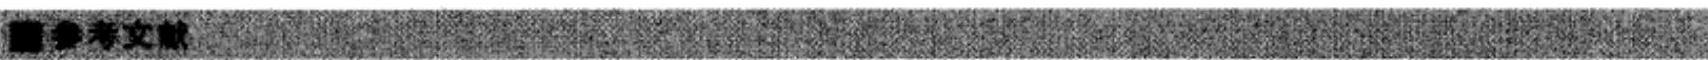
\includegraphics[max width=\textwidth]{2024_07_10_373f31b88d2bf633007bg-494}
\end{center}

[1]庄心良,曾因明,陈伯䀂. 现代麻醉学. 3 版. 北京: 人民卫生出版社、 2004;993-1041

[2] Ronald D. Miller 主编. 曾因明,邓小明主译. 米勒麻碚学. 6 版. 北京: 北京大学医学出版社, 2006: 1215-1636\\
[3] Keith G. Allman, lain H. Wilson 主的.王东信,张利萍,杨拔贤主译、牛津临床麻醉手册. 北京: 人民卫生出版社、 2006:763-808

[4] Jin F, Chung F. Minimizing perioperative adverse events in the elderly. $\mathrm{Br} \mathrm{J}$\\
Anaesth, 2001,87(4);608-624

[5] Buggy D J, Crossiey A W. Thermoreg. ulation, mild perioperative hypothermi$\mathrm{a}$ and post- anesthetic shivering. $\mathrm{Br} \mathrm{J}$ Anaesth, 2000,84(5) ;615-628

\section*{箕 10 章}
\section*{心电图监测}
\section*{第一节 心电监测的基础知识}
\section*{一、心电产生的基本原理}
\section*{1. 心肌细胞膜电位}
\begin{enumerate}
  \setcounter{enumi}{1}
  \item 双相动作电位

  \item 膜电位的离子理论膜电位主要由两种因素决定:

\end{enumerate}

(1)细胞膜内外各种离子的浓度不同。

(2)安静状态与兴奋状态时, 膜对不同离子的通透性不同。

\begin{enumerate}
  \setcounter{enumi}{3}
  \item 探查电极的位置与波形的关系

  \item 心脏传导系统组织心脏传导系统组织是由一小部分特殊的纸维组成, 起着产生冲动和传导冲动的特殊作用。开始于窐房结, 通过结间束至房室结, 到希氏束向下分左右束支, 最后分成细小的分支形成浦肯野纤维。

  \item 心电向量 心房、心室除极或复极过程中产生无数的电动力, 使一定方向、不同大小的量向机体各部传播, 称心电向量。心电图是空间心电向量环在相关平面上的投影而成。

\end{enumerate}

\section*{二、心电监测的基本方法}
\section*{(一)临床应用电极和导联}
\section*{1. 常规导联}
(1)标准肢体导联 (双极肢体导联)

(1) I 导: 左上肢 $(+)$, 右上肢 (一)。

(2) II 导 : 左下肢 $(+)$, 右上肢 $(-)$ 。

(3) III 导 : 左下肢 $(+)$, 左上肢 $(-)$ 。

II 导联是围术期最常用的监护导联, 能够较好地显示心电图形,可发现左心室下壁的心肌缺血。

(2)加压单极肢体导联: (1) aVL-左上肢; (2) $\mathrm{aVR}$ 一右上肢; (3) $\mathrm{aVF}$-左下肢。

$\mathrm{aVF}$ 最容易反映左心室下壁的心肌缺血。

(3)胸前导联

(1) $V_{1}$ : 电极置于胸骨右缘第 4 肋间。

(2) $V_{2}$ : 电极置于胸骨左缘第 4 肋间。

(3) $V_{3}$ : 电极置于 $V_{2}$ 与 $V_{4}$ 导联之间。

(4) $\mathrm{V}_{4}$ : 电极置于第 5 肋间左锁骨中线。

(5) $\mathrm{V}_{5}$ : 电极置于 $\mathrm{V}_{4}$ 导联同一水平左腋前线处。

(6) $\mathrm{V}_{6}$ : 电极置于 $\mathrm{V}_{4}$ 导联同一水平左腋中线处。

$\mathrm{V}_{4 \sim 6}$ 一监测左前降支及回旋支冠脉支配的心肌, 围术期常用 $V_{5}$ 。

\begin{enumerate}
  \setcounter{enumi}{1}
  \item 特殊导联
\end{enumerate}

(1)右胸导联。

(2)后壁导联。

(3)改良的胸部监护导联 (modified chest lead, MCL 导联): 对标准双极肢体导联有各种改良方法, 主要有 $\mathrm{MCL} 、 \mathrm{CS}_{5} 、 \mathrm{CB}_{5} 、 \mathrm{CM}_{5}$ 和 $\mathrm{CC}_{5}$ 等。目的是试图增大 P 波的高度, 利于诊断房性心律失常, 增加 ECG 监测前壁和侧壁心肌缺血的敏感性。

(4)食管导联: 利用装有单极或双极的心电图导联和食管听诊器导管, 将探测电极通过橡皮管送人食管内, 正极与左上肢导线相连, 负极与右上肢导线相连, 用 I 导联描记到食型心电图。食管心电图的优点是波形清晰, 干扰少。

(5)七管导联: 电极安置在气管导管的气囊上,气囊充气后电极可紧贴气管壁, 作用电极在左臂,使各波显示清楚、振幅大, 用于昏迷、不合作及全麻的病人, 对风心病、冠心病、电解质紊乱等病人有诊断价值。

(6)心内导联: 通过中心静脉导管至心腔, 导管\\
上有 $\mathrm{V}$ 探头, 放置到右心室。可用于诊断和治疗特殊的心律失常。

(7)头胸导联(HC 导联)。

(二)心电监测的类型

\begin{enumerate}
  \item 心电监测仪和心电监测系统

  \item 动态心电图监护 (Holter)

  \item 遥测心电图监护仪

  \item 电话传输心电监测

  \item 希氏束心电图

  \item 植入式动态心电监测仪(ICR)

  \item 麻醉监护信息网络系统

\end{enumerate}

(三)监护仪使用注意事项

\begin{enumerate}
  \item 排除千扰因素

  \item 注意事项

\end{enumerate}

(1)正确使用监测仪:电源、功能及色彩。

(2)电极与皮肤的接触要好,皮肤或电极要涂抹导电育,用砂纸或乙醇轻擦皮肤油脂。

(3)接好各种接头、导线。

(4)暂时可拔除各种设备的电源接头。

(5)接好地线。

\section*{三、心电图基本波形}
\section*{(一)正常心电图}
由于测量电极安放位置和连线方式 (导联方式)不同,所记录到的心电图在波形上有所不同,但基本上都包括一个 $\mathrm{P}$ 波,一个 $\mathrm{QRS}$ 波群和一个 $\mathrm{T}$波。有时在 T 波后, 还出现一个小的 U 波。

\section*{(ニ)小儿心电图的特点}
\begin{enumerate}
  \item 心率较快,P-R间期短, 10 岁以上可同成人。

  \item 新生儿心电图为“悬垂型”。

\end{enumerate}

3.3 个月内 $\mathrm{QRS}$ 向量向左,无 $\mathrm{Q}$ 波。

\begin{enumerate}
  \setcounter{enumi}{3}
  \item 随年龄的增长,从右心室占优势改变为左心室占优势。
  \item $\mathrm{T}$ 波变异较大, 常低平或倒置。
\end{enumerate}

\section*{(三)老年人心电图特点}
\begin{enumerate}
  \item 异常心电图较多。

  \item 心律失常多见,如早搏、房擷、東支阻滞等。

  \item 房室肥大多见,左心室肥厚高电压、右心室肥厚高电压。

  \item 多见 ST 段改变,多数有心肌缺血表现。

\end{enumerate}

\section*{四、心电轴}
\section*{(一)心电轴}
心脏激动时产生的心电向量称电轴,平均电轴向量称平均电轴, 心电轴一般指 $\mathrm{QRS}$ 平均电轴。正常心电轴为 $+30^{\circ} \sim+90^{\circ}$ 。

\section*{(二)影响电轴偏移的因素}
\begin{enumerate}
  \item 电轴左偏 轻度 $0^{\circ} \sim+30^{\circ}$; 中度 $0^{\circ} \sim$ $-30^{\circ}$; 显著左偏 $-30^{\circ} \sim-90^{\circ}$ 。常见原因:
\end{enumerate}

(1)心脏位置改变、体型矮胖、大量腹水及早期妊娠。

(2)左心室肥㫗。

(3)左束支传导阻滞。

\begin{enumerate}
  \setcounter{enumi}{1}
  \item 电轴右偏 轻中度 $+90^{\circ} \sim+120^{\circ}$; 显著右偏 $+120^{\circ} \sim+180^{\circ}$ 。常见原因:
\end{enumerate}

(1)瘦长体型、婴儿、右位心。

(2)右心室肥厚。

(3)右束支传导阻滞。

\section*{五、心电监测诊断的基本步骤}
心律 $\rightarrow \mathrm{R}-\mathrm{R}$ 是否相等 $\rightarrow$ 心率 $\rightarrow$ 心律失常 $\rightarrow \mathrm{ST}-$ $\mathrm{T}$ 改变。

(一)心率是多少? 心律是否规则?

计算心率有查表法、计算法、快速估计法。须连续测量至少 5 个 $\mathrm{R}-\mathrm{R}$ 间期, 求真均数, 即为每个心动周期所需的时间,然后用公式计算。

心率 $=60(\mathrm{~s}) /$ 平均 $\mathrm{R}-\mathrm{R}$ 时间 $(\mathrm{s}$ )

(二)有无 $\mathrm{P}$ 波,每一个 $\mathrm{P}$ 波后是否有 $\mathrm{QRS}$ 波群,判断其关系如何。

(三)P-R 间期是多少, P-R 间期计算与年龄及心率关系。

(四)Q-T 间期和 QRS 波群是否正常。

如 QRS 波群以 $\mathrm{Q}$ 波开始, 则从 $\mathrm{Q}$ 波测量到 $\mathrm{T}$波终结的时间; 如 $\mathrm{QRS}$ 波群以 $\mathrm{R}$ 波开始,则从 $\mathrm{R}$波开始。测量 $\mathrm{QRS}$ 最好选择 $\mathrm{QRS}$ 波群清楚,基线稳的导联,尤其要注意排除由于 ST 段抬高或压低造成的 $\mathrm{QRS}$ 时间测量的误差。

(五)ST 段和 $\mathrm{T}$ 波是否有改变,并注意 ST 段改变的形态。

\section*{(六)电轴是否正常}
心电轴计算有粗略估计法、查表法。

\begin{enumerate}
  \item 粗略估计法(目测法)以 I、III导联 QRS 主波方向略估。如果两个主波方向相反,表示左偏,相对表示右偏,一致不偏。

  \item 查表法 首先测得 $\mathrm{I}$ 导联和 III 导联上 $\mathrm{QRS}$波群的代数和,然后从表中查得度数, 确定偏移程度。

\end{enumerate}

\section*{第二节 围术期心肌缺血监测}
\section*{一、心肌缺血}
\section*{(一)围术期引起心肌缺血的因素}
\begin{enumerate}
  \item 原有的冠心病

  \item 围术期的因素除原有的疾病外,围术期心肌缺血的发生尚与下列因素有关:

\end{enumerate}

(1)患者本人: (1)年龄;(2)体质。

(2)手术大小、种类、手术部位及手术操作。

(3)麻醉因素:(1)药物; (2)缺氧、二氧化碳蓄积; (3)麻醉深浅度。

(4)容量不足、贫血、长时间低血压、低体温。

(ニ)心电监测方法

\begin{enumerate}
  \item 心电图监测仪器

  \item 心电导联选择 围术期因手术部位的因素, 选择导联有一定局限性。

\end{enumerate}

(1)标准肢体导联:II 导联是手术中较常用的导联, 能够较好地显示 P 波, 可发现左心室下壁的心肌缺血,但 QRS 波显示稍差。

(2)加压单极肢体导联: $\mathrm{aVF}$ 最容易反映左心室下壁的心肌缺血。

(3)胸前导联: 常用 $\mathrm{V}_{5}$ 监测左前降支及回旋支冠状动脉支配的心肌。

(4)特殊导联: 改良的胸部监测导联、食管导联和气管导联监测心肌缺血可应用, 特别是围术期全麻病人, 非常适合应用食管和气管导联, 其优点是各波显示清楚、干扰少。心内导联和希氏束心电导联适用于危重病人的手术、大手术及心胜手术。

\section*{(三)心电图特征}
\begin{enumerate}
  \item ST 段改变
\end{enumerate}

(1)ST 段形态改变: ST 段位于等电位线时间 $>0.12 \mathrm{~s}, \mathrm{ST}$ 段与 $\mathrm{T}$ 波升支交接角变锐。

(2)ST 段降低: 是心肌缺血最重要的表现。 ST 段下降 $>0.05 \mathrm{mV}$,ST 段降低改变有以下几种类型。

(1)下垂型: $\mathrm{J}$ 点明显下降, ST 段从 $\mathrm{J}$ 点开始向下呈斜坡形下移,直至与 $\mathrm{T}$ 波交接。下移的 ST 段与 $\mathrm{R}$ 波形成的夹角 $>90^{\circ}$ 。常提示合并乳头肌缺血性损害。

(2)水平型: ST 段从 $\mathrm{J}$ 点开始水平下移,直至与 $\mathrm{T}$ 波交接。下移的 ST 段与 $\mathrm{R}$ 波形成的夹角等于 $90^{\circ}$,持续时间至少 $0.08 \mathrm{~s}$ 。\\
(3)缓慢上升连接点型: $\mathrm{J}$ 点明显下移, 从 $\mathrm{J}$ 点开始 ST 段缓慢升至基线。

(4)快速上升连接点型: $\mathrm{J}$ 点明显下移, 从 $\mathrm{J}$ 点开始 ST 段快速升至基线。

(3)ST 段抬高: ST 段抬高反映心外膜下心肌缺血。与 ST 段降低常可见于同一患者的不同导联,提示有两个不同部位均发生心肌缺血。

ST 段抬高的标准为: 肢体导联两个或两个以上导联 ST 段抬高 $\geqslant 0.1 \mathrm{mV}$, 胸导联两个或两个以上导联 ST 段抬高 $\geqslant 0.2 \mathrm{mV}$ 。

\section*{2. T 波变化}
(1) T 波高䇯: 反映心内膜下心肌缺血。肢体导联 $\mathrm{T}$ 波 $>0.5 \mathrm{mV}$, 胸前导联 $\mathrm{T}$ 波 $>1.0 \mathrm{mV}$ 。但仅凭 T 波高筫不能诊断心肌缺血, 若伴有 ST 段下移, $\mathrm{U}$ 波倒置,则可诊断心肌缺血。

(2)T 波倒置、双相。

(3) $\mathrm{T}$ 波伪性改变: 急性心肌缺血发作时,原来倒置的 $\mathrm{T}$ 波转为直立。\\
3. $\mathrm{U}$ 波的改变 在 $\mathrm{R}$ 波为主波的导联,出现 U 波倒置。围术期如 U 波由直立转为倒置, 则提示有心肌缺血。

\begin{enumerate}
  \setcounter{enumi}{3}
  \item 心电图一过性变化
\end{enumerate}

(四)心电图在围术期心肌缺血诊断中的位置

围术期心肌缺血监测, 心电图是最常用和最方便的监测手段。

\section*{二、心肌梗死}
(一) 急性心肌梗死 (acute myocardial infarction, $\mathrm{AMI}$ )的分类

\begin{enumerate}
  \item 根据坏死部位 分为心内膜下心肌梗死和透壁性心肌梗死。

  \item 根据急性冠脉综合征概念 分为不稳定型心绞痛、非 ST 段抬高型心肌梗死和 ST 段抬高型心肌梗死。

  \item 根据心电图有无病理性 $\mathrm{Q}$ 波 分为 $\mathrm{Q}$ 波型心肌梗死 (QMI) 和无 $Q$ 波型心肌梗死 (NQMI)。

\end{enumerate}

\section*{(二)心肌梗死的心电图特征}
心电图的改变为坏死型、损伤型和缺血型改变三者的合并。

\begin{enumerate}
  \item 缺血性 $\mathrm{T}$ 波的改变 缺血性 $\mathrm{T}$ 波具有下列 3 个特点:(1)升支与降支对称;(2)高而尖箃;(3)由直\\
立变为倒置。

  \item 损伤性 ST 段改变 心电图改变为 ST 段抬高, 是心外膜下心肌损伤。而内膜下心肌损伤 ST 段则表现为降低。

  \item 坏死型 $\mathrm{Q}$ 波改变 心电图出现异常 $\mathrm{Q}$ 波或 $\mathrm{QS}$ 波,为不可逆的损害。 $\mathrm{Q}$ 波时间 $\geqslant 0.04 \mathrm{~s}$, 深度 $>1 / 4 \mathrm{R}$ 。

  \item AMI 心电图演变及分期

\end{enumerate}

(1)超急性期: 见于 AMI 发生后数分钟或数小时, 是围术期最常见的情况,此期无异常 $\mathrm{Q}$ 波。心电图主要表现为:(1)T 波高尖; (2)ST 段抬高,始呈上斜行,继是凹面向上型,进而弓背向上型拾高; (3)室壁激动时间 (VAT) 延长 $>0.045 \mathrm{~s}$, QRS 增宽 $>0.12 \mathrm{~s}, \mathrm{R}$波振蝠增高;(4)致命性心律失常。

(2)急性期: 见于 AMI 发生后数小时或数日,持续到数周。心电图特点为(1)坏死性 $Q$ 波: 在以 $S$波为主的导联, 如 $V_{1} 、 V_{2}$ 表现为 $Q S$ 型; 在以 $R$ 波为主波的导联, 如 $V_{5} 、 V_{6}$ 表现为 $Q R$ 型, 可伴有顿挫或切迹。(2) 波降低或消失。(3)ST 段抬高逐渐加重,出现典型的凸面向上,呈单向曲线。(4) T 波倒置。

\begin{enumerate}
  \setcounter{enumi}{4}
  \item AMI 定位诊断 见表 4-10-1。
\end{enumerate}

(三)心电图诊断急性心肌梗死的现代观点

\begin{enumerate}
  \item 提高体表心电图诊断 AMI 的可靠性

  \item 急性心肌梗死心电图分类方法的演变过程

  \item 心电图诊断 $\mathrm{AMI}$ 的新标准和等位(同)性 $\mathrm{Q}$ 波

\end{enumerate}

(1) 2000 年欧洲心脏病学会/美国心脏病学会 (ESC/ACC)公布的急性心肌梗死心电图诊断的新标准(表 4-10-2)。

表 4-10-1 心肌梗死的定位诊断

\begin{center}
\begin{tabular}{lll}
\hline
\multicolumn{1}{c}{阻塞的冠状动脉} & 梗死部位 & \multicolumn{1}{c}{导联} \\
\hline
左前降支 & 前间壁 & $\mathrm{V}_{1} \sim \mathrm{V}_{3}$ \\
左前降支 & 前壁(心尖) & $\mathrm{V}_{2} \sim \mathrm{V}_{6}$ \\
左的降支、左回旋支 & 前侧壁 & $\mathrm{V}_{4} \sim \mathrm{V}_{6}$ \\
左的降支、左回旋支 & 高侧壁 & $\mathrm{I} 、 \mathrm{aVL}$ \\
左前降支 & 广泛前壁 & $\mathrm{I} 、 \mathrm{aVL}, \mathrm{V}_{1} \sim \mathrm{V}_{6}$ \\
右冠状动脉或左回旋支 & 下壁 & II、 、II 、aVF \\
左回旋支 & 正后壁 & $\mathrm{V}_{2} \sim \mathrm{V}_{9}\left(\mathrm{~V}_{1} \sim \mathrm{V}_{3}\right)$ \\
右冠状动脉或左回旋支 & 下侧壁 & II 、III、 $\mathrm{aVF} 、 \mathrm{~V}_{4} \sim \mathrm{V}_{6}$ \\
右冠状动脉或左回旋支 & 下后壁 & II 、III、aVF、 $\mathrm{V}_{7} \sim \mathrm{V}_{9}\left(\mathrm{~V}_{1} \sim \mathrm{V}_{3}\right)$ \\
\hline
\end{tabular}
\end{center}

注:后壁心肌梗死 $\mathrm{V}_{1} 、 \mathrm{~V}_{2}$ 导联可出现高 $\mathrm{R}$ 波, $\mathrm{V}_{2} 、 \mathrm{~V}_{3}$ 导联可出现 ST 段压低

表 4-10-2 急性心眀挭死心电图诊断标准 (ESC/ACC,2000)

\begin{center}
\begin{tabular}{|c|c|c|}
\hline
\multirow{2}{*}{导联} & 进展性 AMI & 确立的 AMI \\
\hline
 & ST 段抬高 $(\mathrm{mV})$ & $\mathrm{Q}$ 波时间 (ms) \\
\hline
$\mathrm{V}_{1}, \mathrm{~V}_{2}$ & $\geqslant 0.2$ & 任何 $\mathrm{Q}$ 波 \\
\hline
其他导联(aVR 除外) & $\geqslant 0.1$ & $\geqslant 30$ \\
\hline
\end{tabular}
\end{center}

(2)等位(同)性 $Q$ 波的概念:一些 AMI 病例心电图出现不典型改变, 有人将其统称为等位性 $Q$波,因其与病理性 $\mathrm{Q}$ 波有等同的诊断价值。等位性 $\mathrm{Q}$ 波必须与临床、血清生化标志密切结合进行分析。

\section*{第三节 围术期心律失常监测}
\section*{一、律失常产生的电生理基础}
\section*{(一)心脏的生理特征}
\begin{enumerate}
  \item 自律性、自动性。

  \item 兴奋性(应激性)。

  \item 传导性。

\end{enumerate}

(ニ)神经纤维功能对心肌的调节作用

(三)围手术期引起心律失常的因素

\begin{enumerate}
  \item 术前患者的基础病情。

  \item 术中缺氧、二氧化碳蓄积。

  \item 麻醉操作和手术刺激。

  \item 低温、低血压。

  \item 术中电解质紊乱, 低钾。

  \item 麻醉药物

\end{enumerate}

(1)全麻药与心肌应激性。

(2)局麻药的心脏毒性。

(3)肌松药。

(4)其他药物的应用。

\section*{二、心律失常常用术语}
$\mathrm{f}$ 波、F 波、心动过缓、心动过速、心律不齐、异位搏动、传导阻滞、文氏现象、逸搏和逸搏心律、干扰、脱节、夺获、融合波、差异传导及并行心律。

\section*{三、围术期常见的心律失常}
\section*{(一)窦性心律失常}
\begin{enumerate}
  \item 突性心动过速
\end{enumerate}

(1)心电图特征:符合窦性心律特点, 频率 $>$ $100 / \mathrm{min}$ 。

(2)临床意义: 围术期心动过速多见于精神紧张、麻醉过浅、二氧化碳蓄积, 病理状态多见于甲立、哢铬细胞㿇、血容量不足、贫血及心功能不全。

\begin{enumerate}
  \setcounter{enumi}{1}
  \item 实性心动过缓
\end{enumerate}

(1)心电图特征: 符合突性心律特点, 频率 $<$ $60 / \mathrm{min}$ 。

(2)临床意义: 围术期心动过缓多见于原来心率本身慢, 如运动员、健康人或麻醉过深和术中牵拉、应用减慢心率的药物; 病理性如一些疾病: 阻塞性黄疸、须内压增高、尿毒症、青光眼或病窦综合征。

\section*{3. 宾性心律不齐}
(1)心电图特征: P 波具有窦性心律的特征, P$R$ 间期正常并且恒定 $(0.12 \sim 0.20 \mathrm{~s})$, P-P 间期不规整,间期变化 $>0.16 \mathrm{~s}$ 。

(2)临床意义: 与呼吸有关的心律不齐,多见于健康儿童和青年人; 与呼吸无关的多见于老年人,或可能有器质性心脏病。

\section*{4. 实房结内游走性心律}
(1)心电图特征: 窦性 $\mathrm{P}$ 波,同一导联内 $\mathrm{P}$ 波形态稍有变异,P-R 间期可有差异,P-P 间期规整或轻度变异。

(2)临床意义:多见于正常人,但要与房性和交界性心律鉴别。

\section*{5. 突性停搏}
(1)心电图特征: 符合窦性心律特点, 较长时间内无窦性搏动,如室性静止持续时间太长时,可出现交界区或室性逸搏心律。

(2)临床意义:围术期多见于麻醉过深或一些药物使突房结产生抑制,或急性器质性心脏病、心肌梗死、心肌桊及病窐综合征等。

\section*{(二)房性心律失常}
\begin{enumerate}
  \item 房性早搏
\end{enumerate}

(1)心电图特征

①)提前出现的 $\mathrm{P}^{\prime}$ 波,其形态与室性 $\mathrm{P}$ 波不同,如 $\mathrm{P}^{\prime}$ 波形态不一,则为多源房性早搏。有时 $\mathrm{P}^{\prime}$ 波隐藏于 $\mathrm{T}$ 波之内, 使 $\mathrm{T}$ 波变形,出现切迹, 应注意辩认。

(2) $\mathrm{P}^{\prime}-\mathrm{R}$ 间期 $>0.12 \mathrm{~s}$ 。

(3) $\mathrm{P}^{\prime}$ 之后可是一个正常的或变异的 QRS 波群,也可无 QRS 波群,称房性早搏未下传。

(4)代偿间期多不完全。

$\mathrm{P}^{\prime}$ 波可连发,则可出现二联律、三联律等。

(2)临床意义: 正常人可出现房性早搏,如呈频发性,成对出现或多形性,多为房性心动过速、心房颤动的先兆。

\begin{enumerate}
  \setcounter{enumi}{1}
  \item 阵发性房性心动过速
\end{enumerate}

(1) 心电图特征

(1) 3 个或 3 个以上异位 $\mathrm{P}^{\prime}$ 波连续出现,心率一般在 $180 \sim 240 / \mathrm{min}$, 心房律绝对匀齐。

(2) $\mathrm{P}^{\prime}$ 波与其后的 $\mathrm{QRS}$ 波群有固定关系, $\mathrm{P}^{\prime}-\mathrm{R}$间期大于 $0.12 \mathrm{~s}, \mathrm{P}^{\prime}$ 波可以下传引起正常形态或宽大畸形的 QRS 波,或未下传。

(3)如伴有室内差异传导,则 QRS 波群时间 $>$ $0.12 \mathrm{~s}$, 此时需与室性心动过速相鉴别。

(2)临床意义: 阵发性房速可见于健康人,但更多见于病理状态, 如围术期病人的低钾血症、缺氧和感染等。

\begin{enumerate}
  \setcounter{enumi}{2}
  \item 非阵发性房性心动过速
\end{enumerate}

(1)心电图特征

(1)异位 $\mathrm{P}^{\prime}$ 波连续 3 次以上出现,可有窦性 $\mathrm{P}$波,异位 $\mathrm{P}^{\prime}$ 波也可与窦性 $\mathrm{P}$ 波形成房性融合波。

(2)频率为 $70 \sim 140 / \mathrm{min}$, 常与窦性节律交替出现。

(3) $\mathrm{P}^{\prime}-\mathrm{R}$ 间期 $>0.12 \mathrm{~s}$ 。

(2)临床意义:非阵发性房性心动过速可见于正常人, 也可见于病理状态,如心脏病人、低钾血症、洋地黄中毒等。

\begin{enumerate}
  \setcounter{enumi}{3}
  \item 心房扑动
\end{enumerate}

(1)心电图特征

(1)P 波消失,代以频率为 $250 \sim 350 / \mathrm{min}$ 的形态相同、振幅相等、间隔匀齐的锯齿样大 $\mathrm{F}$ 波。

(2)房性传导比值固定,则心室律匀齐; 若不固定,则心室律可不匀齐。

(3)QRS 波群的形态、时间多属正常,有时因室内差异传导而呈宽大畸形。

(2)临床意义:心房扑动均见于病理情况,多见于各种器质性心脏病、围术期急性心梗、心肌缺血、肺检塞及低氧血症等。

\begin{enumerate}
  \setcounter{enumi}{4}
  \item 心房额动
\end{enumerate}

(1)心电图特征

(1)P 波消失,代以频率为 $350 \sim 600 / \mathrm{min}$ 的波幅、形态、间距各不相等的小 $\mathrm{f}$ 波。

(2)QRS 波群为室上性,节律绝对不齐。

(3)常伴有干扰性房性传导障碍和室内差异传导。

(2)临床意义: 房䫟多见于风心病、心肌病、高血压及甲元病人。围术期也有无病因或其他因素引起一过性的特发性房颤,称阵发性心房颤动。

\begin{enumerate}
  \setcounter{enumi}{5}
  \item 素乱性房性心律失常 (多源性房性心动过速)
\end{enumerate}

(1)心电图特征

(1)心房率 $>100 / \mathrm{min}$ 。

(2)至少有 3 种以上的不同形态的 $\mathrm{P}^{\prime}$ 波。

(3) $\mathrm{P}^{\prime}-\mathrm{R} 、 \mathrm{P}^{\prime}-\mathrm{P}^{\prime}$ 及 $\mathrm{R}-\mathrm{R}$ 间期都不等。

(4) $\mathrm{P}^{\prime}-\mathrm{P}^{\prime}$ 之间有等电位线。

(2)临床意义

(1)紊乱性房性心律失常易误诊为心房缡动,仔细鉴别可见到每个 QRS 波群之前都有一个相关的 $\mathrm{P}^{\prime}$ 波。

(2)多见于器质性病变,如肺心病及心脏病, 围术期麻醉和手术过程也可出现, 应加以重视。

\section*{7. 房性逸搏和房性逸搏心律}
(1)心电图特征

(1)在一个较正常突性 P-P 为长的间歇之后出现一个房性 $\mathrm{P}^{\prime}$ 波。

(2)多个 $\mathrm{P}^{\prime}$ 之后可跟以室上性 $\mathrm{QRS}$ 波群, $\mathrm{P}^{\prime}-\mathrm{R}$间期 $>0.12 \mathrm{~s}$ 。

(3)房性逸搏如与䆳性冲动相用共同激动心房时,可形成房性融合波。

(4)连续出现 3 次或 3 次以上的房性逸搏,形成房性逸搏心律,频率 $50 \sim 60 / \mathrm{min}$ 。

(2)临床意义: 见于窒性心率慢时或长间隙后,视基础病因而定。

\section*{(三)房室交界性心律失常}
\begin{enumerate}
  \item 交界区早搏
\end{enumerate}

(1)心电图特征

(1)提前出现的 QRS-T 波群,时间、形态正常,有室内差异传导也可呈宽大畸形。

(2)逆行 $\mathrm{P}^{\prime}$ 波,可出现在 $\mathrm{QRS}$ 波群之前, $\mathrm{P}^{\prime}-\mathrm{R}$间期 $<0.12 \mathrm{~s}$, 也可出现在 $\mathrm{QRS}$ 波群之后, $\mathrm{R}-\mathrm{P}^{\prime}$ 间期 $<0.20 \mathrm{~s}$, 也可无 $\mathrm{P}^{\prime}$ 波,埋没于 $\mathrm{QRS}$ 波群之中。

(3)多为完全代偿期。

(2)临床意义:交界区早搏比较少见,可见于正常人,也可见于器质性心脏病。

\begin{enumerate}
  \setcounter{enumi}{1}
  \item 阵发性交界区心动过速
\end{enumerate}

(1)心电图特征

(1)交界区早搏连续 3 个以上。

(2)心室频率多在 150~200/min,节律规整。

(3) $\mathrm{P}^{\prime}$ 波在 $\mathrm{QRS}$ 波群之后, $\mathrm{P}^{\prime}-\mathrm{R}$ 时间 $<0.12 \mathrm{~s}$, $\mathrm{P}^{\prime}$ 波在 $\mathrm{QRS}$ 波群之后, $\mathrm{R}-\mathrm{P}^{\prime}$ 时间 $<0.20 \mathrm{~s}$, 有时可以无 $\mathrm{P}^{\prime}$ 波。

(4)QRS 波群为室上性,如有差异传导,也可宽大畸形。

(5)心动过速骤发㵵停。

(6)一般心房与心室均由交界区冲动所控制,若由窐房结控制心房,交界区控制心室,那么 P 波与 QRS 波群互不相关。

(2)临床意义: 阵发性交界区心动过速多见于正常人,也可见于病理状态,如急性心肌梗死、心肌炎和洋地黄中毒等

\begin{enumerate}
  \setcounter{enumi}{2}
  \item 非阵发性交界区心动过速
\end{enumerate}

(1)心电图特征

(1)QRS 波群为室上性, 逆传型 $\mathrm{P}^{\prime}$ 可出现于 $\mathrm{QRS}$ 波群之前、之后或埋没于其中。

(2)心室率 70〜130/min。

(3)由于交界区起搏点的频率与䆦性心律相近,故恭性激动常可下传心室,产生心室夺获。

(4)若交界区起搏点只控制心室,窦性激动控制心房,形成房室分离, $\mathrm{P}$ 波与 QRS 波群毫无关系。

(5)可与心房纤硔并存。

(6)刺激迷走神经可终止发作。

(2)临床意义: 非阵发性交界区心动过速多见于病理状态,如急性心肌梗死、心肌炎和洋地黄中毒。

\section*{4. 交界区内游走心律}
(1)心电图特征

(1) $\mathrm{P}^{\prime}$ 波为逆行性,可出现在 QRS 波群的前、后或埋在其中。

(2) $\mathrm{P}^{\prime}-\mathrm{R}$ 间期 $<0.12 \mathrm{~s}$, 并逐渐缩短, 最后出现 $\mathrm{R}$ - $\mathrm{P}^{\prime}$ 间期。

(3)QRS 波群正常,有差异传导可呈宽大畸形,节律可规整,也可不规则。

(2)临床意义:在交界性逸搏心律的条件下进行诊断。

\section*{5. 交界区逸搏}
(1)心电图特征

(1)在一个较长的间歇后延迟出现的 QRS 波群,其形态正常。

(2) $\mathrm{QRS}$ 波群前后可见逆行 $\mathrm{P}^{\prime}$ 波, $\mathrm{P}^{\prime}-\mathrm{R}$ 间期 $<$ $0.12 \mathrm{~s}, \mathrm{R}-\mathrm{P}^{\prime}$ 间期 $<0.20 \mathrm{~s}$, 也可无逆行 $\mathrm{P}^{\prime}$ 波。

(3)交界区逸搏前偶尔可出现窦性 P 波,但 P-R $<0.10 \mathrm{~s}$, 因激动心室冲动来自交界区, 窐性激动发生房室干扰而未下传所致。

(2)临床意义: 交界性逸搏心律是一种被动性异位心律,主要根据基础病因而定。

\begin{enumerate}
  \setcounter{enumi}{5}
  \item 交界区逸搏心律
\end{enumerate}

(1)心电图特征

(1)交界性逸搏连续出现 3 次或 3 次以上。

(2)心率缓慢、匀齐,频率在 40〜50 次之间。

(2)临床意义:交界性逸搏心律是一种被动性异位心律,主要根据基础病因而定,如病窦综合征等。

\section*{(四)室性心律失常}
\section*{1. 室性早搏}
(1)心电图特征

(1)提前出现的宽大、畸形的 $\mathrm{QRS}$ 波群, 时间 $>$ $0.12 \mathrm{~s}$, 其前无 $\mathrm{P}$ 波。

(2)有继发性 ST、T 波改变。

(3)有完全代偿期。

(4)如室性早搏发自不同的异位起搏点,即多源室早,QRS 波群形态及偶联期不同。

(5)室性早搏落于前一个心搏的 $\mathrm{T}$ 波顶部或降支上称为 $\mathrm{R}$ on $\mathrm{T}$ 型室性早搏。过去认为此种早搏易诱发心室喑动,近年来已否定此种看法。

(6)如每个正常 P-QRS-T 之后均有一提早出现的异常 QRS 波形, 则为二联律, 2 个正常后一个异常则为三联律。依次为四、五联律等。

(7) 异常 QRS 波群正好处于两个正常 QRS 波群中间, 其前无 $\mathrm{P}$ 波, 时间 $>0.12 \mathrm{~s}$, 此种早搏称插人性室性早搏。

(2)临床意义: 室性早搏可见于正常人,但更多见于病理状态。正常人因饮酒、过度劳累或紧张可产生早搏。器质性心梗、心肌缺血、风心病、围术期麻醉手术、缺氧等因素都可引起室性早搏, 但根据室性早搏本身特点来判断其严重性。有著名的 Lown 分级法。

\begin{enumerate}
  \setcounter{enumi}{1}
  \item 阵发性室性心动过速
\end{enumerate}

(1)心电图特征

(1)连续出现 3 个或 3 个以上宽大畸形的 QRS 波群, 时间 $>0.12 \mathrm{~s}$, 频率 $>160 / \mathrm{min}$, 有 $\mathrm{ST} 、 \mathrm{~T}$ 继发改变。

(2)无 P 波, 如有 $\mathrm{P}$ 波,与 $\mathrm{QRS}$ 波群无关。

(3)发作中可出现心室夺获或室性融合波。

(4) 室律多不规则。

(5)具有突发突停的特点。

(2)临床意义: 阵发性室性心动过速是较严重的一种心律失常, $90 \%$ 是病理性, 除各种器质性病变外,围术期麻醉、手术过程及各种意外事故均易引起,应及早诊断找出基础病因, 及时处理。

\begin{enumerate}
  \setcounter{enumi}{2}
  \item 非阵发性室性心动过速
\end{enumerate}

(1)心电图特征

(1)连续出现 3 个或 3 个以上的宽大畸形的 $\mathrm{QRS}$ 波群,时间 $>0.12 \mathrm{~s}$ 。

(2)心室率 60~100/min, 室律轻度不齐。

(3)因其频率与窦率相近, 可出现不完全性房室脱节、心室夺获和室性融合波。

(2)临床意义:非阵发性室性心动过速多见于病理状态, 如急性心肌梗死、洋地黄中毒和急性心肌炎等。

\begin{enumerate}
  \setcounter{enumi}{3}
  \item 心室扑动
\end{enumerate}

(1)心电图特征

(1)出现不规则的、连续的大幅度正弦曲线样搏动波,无法区分 P 波 QRS、ST 和 T 波,频率为 150~ 250/min。

(2)基线消失,QRS-T 互相融合不能区分。

(2)临床意义: 室扑常常是室䫟的先兆,是仅次于室颙的最严重的心律失常。室扑时心肌基本丧失收缩力, 因此机体的血流基本处于停顿的状态,其临床意义接近于室颤。

\begin{enumerate}
  \setcounter{enumi}{4}
  \item 心室额动
\end{enumerate}

(1)心电图特征

(1)正常的 P-QRS-T 波消失。

(2)出现一系列形态各异、大小不等的不规则波群,频率为 $250 \sim 500 / \mathrm{min}$ 。

(2)临床意义: (1)冠心病广泛心肌梗死形成后,\\
是诱发室崓最常见的原因。或在心绞痛产重发作时, 室壁㿔等。②药物诱发室踾。其中最常见的是严重的洋地黄中毒, 还有奎尼丁、普鲁卡因胺中毒等。(3)心脏手术、心脏外伤或做心导管检查时。(4)低温麻醉到一定温度时, 也可发生室湏。(5)此外,心室顫动可由触电、溺水、空息、高钾血症、低钾血症引起。

\section*{6. 室性逸搏和室性逸搏心律}
(1) 心电图特征

(1)在一个较长的间歇之后,出现一个宽大畸形的 QRS 波群,时间 $>0.12 \mathrm{~s}$ 。

(2) QRS 波群前无相关的 P 波。

(3)室性逸搏可与窦性或交界区冲动形成融合波。

(4)室性逸搏连续 3 次或 3 次以上,心室率缓慢, $30 \sim 40 / \mathrm{min}$, 形成室性逸搏心律。

(2)临床意义: 室性逸搏心律是一种严重的心律失常, 多见于心动过缓、窦性停搏、房室传导阻滞或临终前心律。

\section*{(五)心脏传导阻沸}
心脏传导阻滞是激动不能下传,包括窦房阻滞、房内阻滞、房室传导阻滞和室内传导阻滞。

\begin{enumerate}
  \item 实房阻滞 分为二度 I 型 (文氏型)和二度 II 型。
\end{enumerate}

(1)二度 I 型心电图特征

(1) P-P 间期进行性缩短, 直到出现较长的 P-P 间期。

(2)长 P-P 间期短于 2 个最短的 P-P 间期之和。

(3)间歌后的 P-P 间期大于间歌前的间期。

(4)上述变化呈周期性改变。

(2) 二度 II 型心电图特征

(1)规则的 P-P 间期中,突然出现 P-QRS-T 波的消失,长 P-P 间期是短间期的整倍数。

(2)窐房传导比例可为 $2: 1,3: 2 、 4: 3$ 不等。

(3)临床意义: 可见于健康年轻人,迷走神经张力增高。多见于病理状态下,如低血钾、心肌梗死或服用洋地黄者。

\section*{2. 房内阻滞 (心房分高)}
(1)完全性房内阻滞:可分为单侧缓慢的异位心房节律型、单侧心房颤动型、单侧心房搏动型和单纯房性心动过速型。

心电图特征:

(1)同时出现两种不同形态的 $\mathrm{P}^{\prime}$ 波,也可有窦性 $\mathrm{P}$ 和异位 $\mathrm{P}^{\prime}$\\
(2)两种 $\mathrm{P}^{\prime}$ 的频率常不相同。

(3)其中一个 $\mathrm{P}$ 波(或 $\mathrm{P}^{\prime}$ 波)激动右心房,可以下传,另一 $\mathrm{P}^{\prime}$ 波激动左心房不下传。

(2)不完全性房内阻滞。

心电图特征:

(1)P 波增宽, 可以呈双峰,出现切迹、错折、双向等。

(2) $\mathrm{P}$ 波时间 $>0.11 \mathrm{~s}$ 。

(3) 如为双峰 $\mathrm{P}$, 双峰距离 $>0.04 \mathrm{~s}$ 。

\begin{enumerate}
  \setcounter{enumi}{2}
  \item 房室传导阻滞房室传导阻滞是指心房激动通过房室结和希-浦系统时发生传导延迟和阻滞, 可分为一度、二度和三度房室传导阻滞。
\end{enumerate}

(1)一度房室传导阻滞

(1)心电图特征

a. P-R 间期延长,一般正常人 $>0.20 \mathrm{~s}$ 。

b. 延长的 P-R 间期可以固定不变, 也可有变化,长短不一,但 P 波后都有相关出现的 QRS 波群。

(2)临床意义:一过性 P-R 间期延长,可见于正常人迷走神经兴奋;持续性 P-R 间期延长多为病理状态,如心肌炎、心肌梗死或应用 $\beta$ 受体阻滞药。

(2)二度 I 型 (文氏型)房室传导阻滞

(1)心电图特征

a. 穹性 P 波, P-R 时间逐渐延长,直至 P 波后 $\mathrm{QRS}$ 缺失,周而复始。

b. R-R 间期进行性缩短。

c. P-P 间期可规则或因有窦律不齐而变化。

d. QRS 波形态、时间多是正常,如有室内差异传导或束支阻滞时, QRS 波群可有畸变。

(2临床意义:二度 I 型房室传导阻滞可能为生理性, 如见于运动员, 但多为病理性, 如心肌炎、下壁心肌梗死、洋地黄过量。

(3)二度莫氏 II 型房室传导阻滞

(1)心电图特征

a. 在隔一次或数次 P 波之后, 出现一定比例的心室脱落,无 QRS 波群,可形成 $3: 1 、 2: 1 、 3: 2$ 等不同比例的传导阻滞。

b. 下传冲动的 P-R 间期可以正常或延长,P-R 间期是固定的。

(2)临床意义:二度 II 型房室传导阻滞多为病理性, 如前壁心肌梗死、心肌病和传导系统退行性变等。围术期心脏手术病人多见。

(4) 高度房室传导阻泪

(1)心电图特征: 凡两次 $\mathrm{P}$ 波或两次 $\mathrm{P}$ 波以上后无 QRS 波群, 不能下传心室, 比例形成 $3: 1,4: 1$ 。

(2)临床意义: 高度传导阻滞反映传导系统有严重病变, 很容易发展为完全性房室传导阻滞。

(5)三度 (完全性)房室传导阻滞

(1)心电图特征

a. 所有心房激动均不能下传至心室,心房与心室由不同起搏点控制, $\mathrm{P}$ 波与 $\mathrm{QRS}$ 波群无固定关系,呈完全性房室分离。

b. P-P间期与 R-R 间期匀齐,心房率>心室率。

c. QRS 形态可以正常, 也可以宽大畸形。

(2)临床意义:完全性房室传导阻滞反映传导系统严重病变,围术期心脏外科手术多见。

\begin{enumerate}
  \setcounter{enumi}{3}
  \item 室内传导阻滞室内传导阻滞是指激动在心室内通过希-浦系统时发生传导延迟和阻滞, 可分为束支和分支传导阻滞。
\end{enumerate}

(1)右束支传导阻滞 (RBBB)

(1)心电图特征\\
a. $\mathrm{V}_{1} 、 \mathrm{~V}_{2} 、 \mathrm{~V}_{3}$ 导联 $\mathrm{QRS}$ 波群呈“ $\mathrm{M}$ ”形的 $\mathrm{rSR}$ '型, $\mathrm{V}_{5}$ 中 QRS 有宽钝的 $\mathrm{S}$ 波, $\mathrm{aVR}$ 导联出现䆓大 $\mathrm{R}$ 波。

b. 以 $\mathrm{R}$ 波为主的导联, ST 段压低, $\mathrm{T}$ 波倒置。

c. QSR 时间 $<0.11 \mathrm{~s}$, 为不完全性右束支传导阻滞; QSR 时间 $\geqslant 0.12 \mathrm{~s}$, 为完全性右束支传导阻滞。

(2)临床意义: 正常人可出现右束支传导阻滞。病理状态下见于有心胜疾患的,围术期见于心肌缺血、心肌梗死、肺㭲塞及心脏手术的房间隔缺损、肺动脉高压、狭窄。

(2)左束支传导阻滞 (LBBB)

(1)心电图特征\\
a. $\mathrm{V}_{1} 、 \mathrm{~V}_{2}$ 导联 $\mathrm{QRS}$ 波群呈 $\mathrm{Qs}$ 或 $\mathrm{rs}$ 型, $\mathrm{V}_{5} 、 \mathrm{~V}_{6}$导联 QRS 波群呈宽钝的 $\mathrm{R}$ 波。

b. 出现继发性 ST-T 波改变, $\mathrm{V}_{5} 、 \mathrm{~V}_{6}$ 导联 ST 段压低, $\mathrm{T}$ 波倒置, $\mathrm{V}_{1} 、 \mathrm{~V}_{2}$ 的 ST 段可上移, $\mathrm{T}$ 波直立。

c. 若 $\mathrm{QRS}$ 时间 $<0.12 \mathrm{~s}$, 为不完全性 $\mathrm{LBBB}$;若 $Q R S$ 时间 $\geqslant 0.12 \mathrm{~s}$, 为完全性 LBBB。

(2)临床意义: 左束支阻滞少见于正常人,通常反映器质性心脏病引起的传导系统退行性变, 围术期若发生 LBBB, 要考虑原心脏病的加重。

(3)左前分支阻滞 (LAFB)

(1)心电图特征

a. 心电轴显著左偏 $\left(-45^{\circ}\right.$ 至 $90^{\circ}$ )。

b. 导联 I 有 $\mathrm{q}$ 波,导联两有 S 波。

c. QRS 波群时间轻度延长或正常。

(2)临床意义: 左前分支阻滞少见于正常人,多见于病理状态,如心肌炎、冠心病及各种器质性心脏病。

(4)左后分支阻滞(LPFB)

(1)心电图特征

a. QRS 电轴右偏 $>+120^{\circ}$ 。

b. 导联 I 、aVL 呈 $\mathrm{rS}$ 波,导联 II 、III、aVF 呈 $\mathrm{qR}$ 波, $\mathrm{q}<0.02 \mathrm{~s}$ 。

c. QRS 时间正常,无 ST、T 改变。

d. 左后分支阻滞无特定心电图改变,在确定诊断时, 必须除外引起电轴右偏的其他疾病, 如右位心、右心室肥大及侧壁心肌梗死等。

(2)临床意义: 左后分支阻滞少见于正常人,多见于器质性心脏病, 如冠心病、心肌病和高血压等。

(5)左中隔支阻滞 (LSFB)

(1)心电图特征\\
a. $V_{5} 、 V_{6}$ 导联无起始的 $\mathrm{Q}$ 波, $\mathrm{QRS}$ 时间 $\leqslant 110 \mathrm{~ms}$ 。\\
b. $\mathrm{V}_{1} 、 \mathrm{~V}_{2}$ 导联的 $\mathrm{r}$ 波消失, 还可出现 $\mathrm{Q}$ 波。

(2)临床意义: 左中隔支阻滞若呈持续性,多见于病理状态, 但由于其心电图改变十分细致, 必须细心观察,另因左中隔支阻滞心电图改变与一些疾病颇相类似,如左心室肥大等,应加以鉴别。

(6)右束支传导阻滞合并左前分支阻滞

(1)心电图特征

a. 心前导联 $\mathrm{V}_{1}$ 呈典型的右束支传导阻滞图形,即 $\mathrm{rsR}$ '型。

b. QRS 电轴明显左偏, $>-30^{\circ}$ 。

c. I、aVL 导联呈 $\mathrm{qR}$ 型, II、 III、aVF 导联呈 $\mathrm{rS}$ 型。

d. QRS 时间 $\geqslant 0.12 \mathrm{~s}$ 。

(2)临床意义: 右束支传导阻滞合并左前分支阻滞少见于正常人, 均为病理性,如冠心病、心肌病、传导系统退行性变等。该类型阻滞很可能发展为完全性房室传导阻滞。围术期出现应特别重视。

(7)右束支传导阻滞合并左后分支阻滞

(1)心电图特征

a. 心前导联 $\mathrm{V}_{1}$ 的 $\mathrm{QRS}$ 波群呈典型右束支传导阻滞图形, 即 $\mathrm{rsR}^{\prime}$ 型。

b. QRS 电轴右偏 $>+100^{\circ}$, 但除外右心室肥厚、垂位心及肺气肿等疾患引起的改变。

c. I 、aVL 导联的 $\mathrm{QRS}$ 波群呈 $\mathrm{rS}$ 型, II 、III、 $\mathrm{aVF}$ 导联呈 $\mathrm{qR}$ 型或 $\mathrm{qRr}$ '型。

d. QRS 时间 $\geqslant 0.12 \mathrm{~s}$ 。

(2)临床意义: 同 RBBB 合并 LAFB。

(8) 双侧束支传导阻滞 (BBBB), 即左右束支均\\
发生阻滞, 可分为一度、二度、三度传导阻滞。

(1)一度传导阻滞:程度相同,心电图仅表现为 P$\mathrm{R}$ 间期延长,如阻滞程度不同,传导时间差异 $0.04 \sim$ $0.06 \mathrm{~s}$ 时,可表现为某一侧束支传导阻滞图形。

(2)二度传导阻滞 : 由于双侧束支阻滞程度不同,也就是传导的比例相同或不相同,同步或不同步,而产生的心电图改变,十分复杂,难以判断分析。

(3)三度传导阻滞: 间歇性出现右束支传导阻滞, 最后引起完全性房室传导阻滞, 其严重程度和临床意义同完全性房室传导阻滞。

\begin{enumerate}
  \setcounter{enumi}{4}
  \item 预激综合征 预激综合征是指在房室结、希-浦系统下传激动未达心室时, 就由心房或心室存在的异常的传导途径(旁路)下传,使心室提早除极,而产生特征性的心电图表现,预激常发生快速性心律失常。
\end{enumerate}

(1)典型的预激综 合征 (Wolf-ParkinsonWhite、W-P-W 综合征)

(1)心电图特征

a. P-R 间期缩短,$<0.12 \mathrm{~s}$ 。

b. QRS 波群起始部有预激波 ( $\Delta$ 波),QRS 波时间延长 $>0.11 \mathrm{~s}$ 。

c. 常有继发的 ST、T 波改变, T 波与预激波方向相反。

(2)临床意义: 预激综合征可见于正常人、先天性,也可见于病理性,如心梗后等传导通路异常。围术期心脏本身手术可引起传导异常, 常可伴发快速的心律失常。

(2) 短 P-R 综合征 (Lown-Ganong-Levine、L-\\
G-L 综合征)

(1)心电图特征

a. P-R 间期缩短, $<0.12 \mathrm{~s}$ 。

b. QRS 时间正常。

c. QRS 波群无预激波。

d. 常可无 ST、T 改变。

(2)临床意义:同典型的预激综合征。

(3) Mahaim 型预激综合征

(1)心电图特征

a. P-R间期正常。\\
b. $\mathrm{QRS}$ 时间延长, $>0.11 \mathrm{~s}$ 。

c. QRS 波群有预激波 ( $\Delta$ 波)。

d. 继发 ST、T 改变。

(2)临床意义: 预激综合征应与其他心脏疾患的心电图鉴别诊断, 因心电图改变酷似心室肥大、束支传导阻滞、心肌缺血和心肌梗死等。

\section*{四、心律失常的心电图诊断步骤}
测量 P-P 间期,确定心房搏动率 $\rightarrow \mathrm{P}$ 波形态是否正常, 每个导联中各个 $\mathrm{P}$ 波形态是否相同 $\rightarrow$ 确定心室的搏动率 $\rightarrow$ 测量 QRS 时间, 检查每个导联中 $\mathrm{QRS}$ 波群是否相同 $\rightarrow \mathrm{P}$ 波与 $\mathrm{QRS}$ 之间的时间关系 $\rightarrow$ 每个 $\mathrm{P}$ 波与 $\mathrm{P}$ 波之间的距离 $\rightarrow$ 每个 $\mathrm{R}$ 波与 $\mathrm{R}$波之间的距离 $\rightarrow$ 选择一个 P-QRS-T 波群比较清楚的导联,较长地记录一段心电图,综合分析, 仔细研究一切额外的搏动,据其形状及发生时间判断出心律失常的类型。在观察心电图的同时,注意心电图基线是否稳定,以免将伪差误认为心律失常。

\section*{第四节 具有预测严重猝死的几种心电图改变}
\section*{一、Brugada 综合征}
本综合征由 Brugada 兄弟于 1992 年首次报道。

(一)心电图特征

\begin{enumerate}
  \item $\mathrm{V}_{1} \sim \mathrm{V}_{3}$ 导联 $\mathrm{ST}$ 段抬高, $\mathrm{T}$ 波倒置,其他导联 ST 段改变不明显。
  \item $\mathrm{V}_{1} \sim \mathrm{V}_{3}$ 可出现右束支阻滞图形 $\mathrm{rSR}^{\prime}$ 型, 而 $\mathrm{V}_{5} / \mathrm{V}_{6}$ 导联无宽 $\mathrm{S}$ 波。
\end{enumerate}

\section*{(二)临床意义}
\begin{enumerate}
  \item 许多疾患如急性心包炎、右心室心肌梗死、肺栓塞等均有类似心电图改变, 应加以鉴别, 这些疾患应有明显的临床症状。

  \item 若出现此种心电图改变, 应特别重视, 进一步做详细的检查。有报道奎尼丁、西洛他唑对 Brugada 综合征可能有效。

\end{enumerate}

\section*{二、特发性长 Q-T 综合征}
特发性长 Q-T 综合征(LQTS)多因先天性、遗传性发病。

\section*{(一)心电图特征}
\begin{enumerate}
  \item Q-T 间期延长, $\mathrm{Q}-\mathrm{Tc} \geqslant 0.48 \mathrm{~s}$, 伴有晕厥发作可确诊。

  \item $\mathrm{T}$ 波形态改变为双向、双峰、切迹 $\mathrm{T}$ 波,在胸导联明显。有时 T 波交替性变化。

  \item 心率明显慢,有窦性停搏,出现长间歇。

\end{enumerate}

\section*{(二)临床意义}
\begin{enumerate}
  \item 特发性长 $\mathrm{Q}-\mathrm{T}$ 综合征应与获得性长 $\mathrm{Q}-\mathrm{T}$综合征相鉴别。后者多有明确的病因, 如服用某些药物、电解质紊乱等。

  \item 本综合征一旦确诊, 应立即进行治疗, 多数患者对 $\beta$ 受体阻滞药有效, 无效可行左侧交感神经切除(LSCD)或安放人工心脏起搏器 (PM)。

\end{enumerate}

\section*{三、特发性 U波(早期复极综合征)}
1994 年 Bjerregard 等报道特发性室噀患者的心电图出现明显的 J 波, 后来有人发现 $\mathrm{J}$ 波与临床出现的室性心动过速、心室踾动等有关。

\section*{(一)心电图特征}
\begin{enumerate}
  \item QRS 波群未出现明显的 J 波, 多见于胸导联,在长间歇、室性心动过速前后特别明显。

  \item 可出现右束支阻滞心电图形。

  \item 心内电生理检查, H-V 间期延长。

\end{enumerate}

\section*{(二)缶床意义}
\begin{enumerate}
  \item 特发性 J 波要与心电图 J 电相鉴别。因 J 点振幅低, 持续时间短; 而 $\mathrm{J}$ 波振幅较高, 持续一定的时限。

  \item J 波可见于低温、高血销等, 应加以鉴别。

  \item 对疑为特发性 J 波和家族性早期复极综合征的患者可用䥻离子阻滞药治疗。

\end{enumerate}

\section*{四、T波电交替}
\section*{(一)心电图特征}
\begin{enumerate}
  \item 仅 $\mathrm{T}$ 波的方向和(或)形态发生交替改变,形成 2:1电交替。

  \item 其他波形无相应的变化。

\end{enumerate}

\section*{(二)临床意义}
\begin{enumerate}
  \item T 波电交替与恶性室性心律失常有密切联系。在心绞痛、心肌梗死、严重心肌缺血、多种电解质索乱也可出现 $\mathrm{T}$ 波电交替。

  \item 应用计算机技术发展而成的频谱-时间标测技术可明显提高 T 波电交替的检出率。

  \item 出现 $\mathrm{T}$ 波电交替, 应进一步进行电生理检查, 同时积极治疗原发病, 也可适当服用抗心律失常药物及 $\beta$ 受体阻滞药, 必要时置人植人型体内自动除䫓器 (ICD)。

\end{enumerate}

\section*{五、Epsilon 波}
Epsilon 波简称 “ $\mathrm{E}$ ” 波, 见于右心室心肌病 (ARVC)患者。因右心室延迟除极产生, 也称后激电位或右心室晚电位。

\section*{(一)心电图特征}
\begin{enumerate}
  \item 在 $\mathrm{V}_{1} 、 \mathrm{~V}_{2}$ 导联 $\mathrm{QRS}$ 终末出现向上的小棘波,称 $\mathrm{E}$ 波,可持续数十毫秒。

  \item Fontaine 设计了双极胸导联, 可提高 $\mathrm{E}$ 波的检出率。

\end{enumerate}

\section*{(二)临床意义}
\begin{enumerate}
  \item 心电图有 $\mathrm{E}$ 波出现, 高度提示 ARVC 的可能及经常发作室性心动过速等, 所以 $\mathrm{E}$ 波检出对预防室性心动过速等有很大价值。

  \item E 波还可能见于后壁心肌梗死、右心室心肌梗死等,应追问病史,加以鉴别。

\end{enumerate}

\section*{六、短 Q-T 综合征}
属于遗传性离子通道缺陷疾患。由于心室复极期钠离子和铔离子内流减少和 (或)钾离子外流增加导致复极期加速, 使 Q-T 间期缩短, 心肌的有效不应期缩短, 就易发生快速性心律失常。

\section*{(一)心电图特征}
\begin{enumerate}
  \item Q-T 间期明显缩短, $\leqslant 300 \mathrm{~ms}$ 。

  \item Gussak 提出实测 $\mathrm{Q}-\mathrm{T}$ 间期与预期的 $\mathrm{Q}-\mathrm{T}$间期 ( $Q-T p)$ 的比例, 计算 $Q-T$ 间期的变化。

\end{enumerate}

\begin{center}
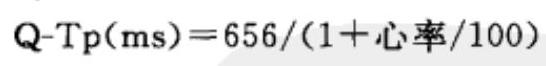
\includegraphics[max width=\textwidth]{2024_07_10_373f31b88d2bf633007bg-505}
\end{center}

当 $\mathrm{Q}-\mathrm{T}$ 间期小于 $\mathrm{Q}-\mathrm{Tp}$ 的 $88 \%$ 时为 $\mathrm{Q}-\mathrm{T}$ 间期缩短,小于 $\mathrm{Q}-\mathrm{Tp}$ 的 $80 \%$ 时为明显缩短。

\section*{(二)临床意义}
明确 $Q-T$ 间期缩短, 伴有不明原因晕厥发作、发作特发性心房颤动、室性心动过速、心室踾动者,可应用奎尼丁、维拉帕米及钾通道阻滞药, 安置 ICD 是首选治疗措施。

\section*{第五节 有关心电监测其他技术的评价}
\section*{一、心率变异的分析}
心率变异性 (heart rate variability,HRV) 是指逐次心跳间期的微小变异, 它反映自主神经的张力和均衡性。目前作为评估麻醉深度变化和反映病人疼痛状况的指标。在临床上公认作为心电监测\\
的一个指标, 对 AMI 后患者心源性猝死的预测, 判断恶性心律失常的发生均有临床价值。HRV 的下降还是多种非心律失常性心胜病事件预后不良的标志。

近年临床研究认为, HRV 对心律失常事件预测的特异性与敏感性均不高,阳性率不超过 $30 \%$ 。目前研究运用非线性的混沌分析方法, 可获取更多的有关自主神经调节及体液因素等复杂信息,以提高 HRV 的诊断价值。

\section*{二心率震荡}
心率震荡 (heart rate turbulence, HRT) 是帘房结对室性期前收缩的一种双向生理反应, 表现为一次短暂的初期心率加速和随后的心率减慢。通过两个参数,震荡初始发作 (turbulence onset, To)和震荡倾斜率(turbulence slop, Ts) 进行定量表达,得出计算 To 和 Ts 的公式及中性值。HRT 正常存在时, 人体自主神经功能完好; 当人体自主神经功能受损时,HRT 变化会减弱或消失。在临床应用上, 已肯定 HRT 作为心梗后死亡率的预测指标。至于在其他心血管疾病及非心血管疾病中的应用尚在探索阶段。

\section*{三、心磁图}
心磁图 (magneto cardio gram,MCG) 检查是对心脏磁场信号变化的记录与分析的一种无创性心电监测技术。它不需要电极与受检查者接触,所以不受电极的影响, 方法简单, 并且省时。在临床上适用于心律失常方面的诊断, 对异位兴奋电、旁路的定位, 束支阻滞的发现及药物诊断治疗的监测有重要意义, 对心肌缺血、心肌梗死的检测及疗效的评价, 对心脏负荷过重及猝死危险性评估有诊断价值。

\section*{四、高频心电图}
高频心电图 (high frequency electrocardiography, HFECG) 是利用频响范围在 $0.05 \sim 1000$ $\mathrm{Hz}$, 扫描速度在 $250 \sim 700 \mathrm{~mm} / \mathrm{s}$, 整机灵敏度为 $30 \sim 100 \mathrm{~mm} / \mathrm{mV}$ 的检测技术, 检测心脏的电活动信号描记出来的心电图, 是分析心电高频信息的一项专门技术。临床不仅可以用于冠心病诊断, 也可用于心肌炎、心肌病、心脏移植术后排异反应的监测及 PTCA、冠状动脉搭桥术后监测、心律失常的诊断等。

\section*{五、信号平均心电图与心室晩电位}
心室晚电位 (ventricular lare potential, VLP)是出现在 QRS 波群终末部、ST 段内的一种高频、低振幅的电活动, 是在心室某部小块心肌内延迟发生除极而产生的电活动。通过信号平均心电图可以体表检测, 根据图的时域和频域进行分析, 得出检测结果。临床上应用于: 诊断快速室性心律失常、不明原因的军厥、心肌缺血和心肌再灌注损伤、判断外科治疗室速的效果及评估急性心梗病人的预后。

\section*{六、心外膜电位的动态标测}
心外膜标测术利用由多个电极组成的电极片在开胸状况下, 对心胜电兴奋进行直接标测, 并以图形方式表达的方法。通过等电位图和等时图表达,该心外膜标测系统能较好地反映局部心肌的真实的电活动情况, 为心律失常的研究、诊断及定位提供依据, 特别适用于心胜直视手术的监测及心律失常外科治疗的定位和疗效的判断等。

\section*{七、心电峰值标测图}
心电峰值标测图 (electrocandiographic peak map, EPM) 是以心电图为基础, 选择了心电图中最具特征意义的各波峰值的电位和重要的时程点, 设计了体表心电峰值标测图,通过等电位图和等时图相结合,提出一系列全新的定量、定位、定时程的四维指标。临床实践证明,它在诊断心梗、确定梗死面积和梗死周围阻滞、心肌病的鉴别诊断、复极异常、传导障碍的诊断和进行追踪观察、判断预后等方面, 显示了超越 ECG 的优越性, 对诊断心律失常有很大应用价值。

\section*{(刘保江聂丽霞)}
\section*{\%11:}
\section*{血流动力学监测}
血流动力学监测 (hemodynamic monitoring)是临床麻醉和重症监护室 (ICU) 的重要内容之一,是大手术和抢救危重病员不可缺少的手段,可分为无创伤性和创伤性两大类。无创伤性血流动力学监测 (noninvasive hemodynamic monitoring) 是应用对机体组织没有机械损伤的方法,经皮肤或黏膜等途径间接取得有关心血管功能的各项参数,其特点是安全、无或很少发生并发症。创伤性血流动力学监测 (invasive hemodynamic monitoring) 通常是指经体表插人各种导管或监测探头到心腔或血管艁内,利用各种监测仪或监测装置直接测定各项生理学参数,其特点是有时可产生严重并发症,故选用时应充分衡量其利䌘,并预防和减少并发症。及时准确地监测血流动力学,有助于估计病情, 明确诊断,指导治疗,制定治疗方案和监测治疗的效果。

\section*{第一节 动脉压监测}
动脉压 (arterial blood pressure, BP) 即血压,是临床麻醉、重症监测的基本指标之一, 是反映后负荷、心肌氧耗与做功以及周围循环的指标之一。血压的监测方法可分为两类:无创性测量法和有创性测量法。

\section*{一、无创性测量法}
无创血压监测是麻醉手术围术期的常规监测项目。根据袖套充气方式的不同,分为人工袖套测压法(手动测压法) 和电子自动测压法两大类。

\begin{enumerate}
  \item 手动测压法 手动测压法为经典的血压测量方法,即袖套测压法。该法所用的设备简单,费用低,便于携带,适用于一般手术病人的监测。但用手法控制袖套充气,费时费力,不能连续监测, 不能及时反映病人血压的变化。
\end{enumerate}

手动测压法导致误差的因素有:(1)袖套使用不当是导致手动测压出现误差的最常见原因。太窄或包衰太松, 压力读数偏高, 袖套太宽, 读数相对较低,一般袖套宽度应比上臂周径大 $20 \%$ 。(2)肥胖病人或婴儿测压时应注意其准确性。肥胖者手髫较一般人粗而不结实,即使应用标准宽度袖套,充气后部分压力仍作用于脂肪组织, 故读数就不够准确。小儿袖套宽度应覆盖上臂长度 $2 / 3$, 婴儿只宜使用 $2.5 \mathrm{~cm}$ 的袖套。(3)放气速度:放气过快测量值偏低,尤其在心率偏慢时。以 $3 \mathrm{mmHg} / \mathrm{s}$ 或每次心跳放气 $2 \mathrm{mmHg}$ 放气速度可提高测压的准确性。

\begin{enumerate}
  \setcounter{enumi}{1}
  \item 自动测压法 自动测压法又称自动化无创测压法 (automated noninvassive blood pressure, NIBP), 是当今临床麻醉和 ICU 中使用最广的血压监测方法之一,主要采用振荡技术(oscillometry)。
\end{enumerate}

NIBP 的优点: 无创伤性,重复性好; 操作简单,易于掌握; 适用范围广泛,包括各年龄的病人和拟行各种大小手术的患者; 自动化的血压监测,能够按需要定时测压, 省时省力; 能够自动检出袖套的大小, 确定充气量; 血压超出设定的上下限时能自动报警。

虽然自动测压法系无创伤性和相对安全,但在临床中如不注意合理正确使用,频繁测压、测压时间过长或测压间隔太短,有发生疼痛、上鹪瘀点和路斑、上肢水肿、静脉淤血、血栓性静脉炎、外周神经病变等并发症的报道,因此,对意识抑制、有外周神经病变、动静脉功能不全及心律不齐者使用时应加小心。

\section*{二、有创性测量法}
有创性测量法即直接动脉内测量血压。通常通过外周动脉置人导管测量, 特殊需要时放人心室\\
内或大血管内测压。早期用弹䌙血压计测压, 只能提供平均动脉压。现在多用压力换能器监测, 比间接测量血压可以得到更准确和更详细的血压数值,并可得到直观的血压波形。直接动脉测压可以即时、准确和直观地反映血压变化。

\begin{enumerate}
  \item 测压途径
\end{enumerate}

(1)桡动脉:穿刺和管理方便, 为首选途径。

(2)股动脉: 桡动脉穿刺困难时可选用, 因穿刺部位接近会阴和肚门, 应注意预防污染。

(3) 足背动脉: 是下肢胫前动脉的延伸,并发症较少, 但该动脉较细, 有时不能触及, 给穿刺带来困难。身体其他部位的动脉, 如肱动脉、厒动脉很少选用。

\begin{enumerate}
  \setcounter{enumi}{1}
  \item 器材和仪器 选择动脉测压的专用优质套管针,其规格可按成人、小儿以及穿刺部位不同而选用。测压仪器主要包括测压装置 (包括配套的测压管道系统、肝素稀释液防凝血冲洗装置) 和压力监测仪。

  \item 动脉穿刺拍管术 应熟悉动脉穿刺部位的解剖。以腕部桡动脉为例, 该动脉位于桡骨下端和桡侧屈腕肌腱之间的纵沟内。桡动脉形成掌深弓,并与尺动脉汇成掌浅弓, 掌浅弓血流 $88 \%$ 来自尺动脉, 故做桡动脉穿刺插管前, 用 Allen 试验估计来自尺动脉的掌浅弓血流。将穿刺侧前臂抬高, 术者双手拇指分别摸到桡、尺动脉搏动后, 让病人做 3 次握拳和放松动作, 接着压迫阻断桡、尺动脉的血流, 手部变白, 然后前集放平, 解除对尺动脉的压迫, 观察手部转红时间, 正常 $<5 \sim 7 \mathrm{~s}$ (平均 $3 \mathrm{~s}$ )。 $8 \sim 15 \mathrm{~s}$ 属可疑, $>15 \mathrm{~s}$ 系血供不足, 但 $>7 \mathrm{~s}$ 为 Allen 试验阳性, 不宜选用桡动脉作穿刺插管。

\end{enumerate}

动脉穿刺前宜固定肢体, 摸清动脉搏动, 于局麻下进行穿刺。套管针与皮肤成 $30^{\circ}$ 角对准手指摸到的动脉刺人, 拨出针芯。若套管已进人动脉, 则有血向外喷出, 将套管向前推进。血流通畅后可接上测压导管系统, 用肝素稀释液冲洗动脉套管以防止凝血, 并将测压导管系统与压力换能器连接, 即可显示动脉压波形和各项数值。

\begin{enumerate}
  \setcounter{enumi}{3}
  \item 适应证
\end{enumerate}

(1)心血管外科: 通常需要通过外周动脉置人导管测压, 有时需要放人心室内或大血管内测压。体外循环由于无波动性灌注更需要直接测压。

(2)胸腹部大手术和器官移植: 有可能引起围术期血流动力学剧烈变化, 如嗜铬细胞面切除术。

(3)各种危重病人、严重创伤、严重低血压、休克和控制性降压等。此类病人往往需要反复测量血压, 用间接测压比较困难, 需要持续监测动脉压。

(4) 需反复动脉采样者: 如长时间机械通气、酸碱或水电解质失衡、呼吸系统疾病、需要大量血管活性药物、持续血药浓度监测等。动脉穿刺置管,既减少动脉采样困难, 又能进行血压监测。

(5) 用间接法测压有困难或脉压狭窄难以测出时, 采用直接动脉内测压, 即使压力低至 $30 \sim$ $40 \mathrm{mmHg}$, 亦可准确地测量。

\begin{enumerate}
  \setcounter{enumi}{4}
  \item 禁忌证
\end{enumerate}

(1) Allen 试验阳性者禁行同侧桡动脉穿刺。

(2)穿刺局部或其附近存在感染。

(3)凝血障碍病人易致血肿, 若血肿部位深或邻近重要腿器、神经组织, 则危害其大。此外, 对已应用或将应用抗凝剂的病人, 最好选用浅表且处于肢体远端的动脉为宜。

(4)患有血管疾患的病人, 如血检闭塞性脉管炎、Bavnaud病等。

(5)手术操作所涉及的部位。

\begin{enumerate}
  \setcounter{enumi}{5}
  \item 临床意义
\end{enumerate}

(1)提供正确、可靠和连续的动脉血压波形和数据, 用于指导危重病人和重大手术患者的诊断和治疗。

(2)通过动脉压波形测量和计算, 左、右心室及主动脉压力上升最大速率 $\left(\mathrm{dp} / \mathrm{dt}_{\max }\right)$, 是一个心肌收缩性的粗略指标, 简便易行可连续测算。心功能正常者 $\mathrm{dp} / \mathrm{dt}$ 约为 $1200 \mathrm{mmHg} / \mathrm{s}$, 心脏病及心功能较差者 $\mathrm{dp} / \mathrm{dt}$ 减低为 $500 \sim 800 \mathrm{mmHg} / \mathrm{s}$ 。

\begin{enumerate}
  \setcounter{enumi}{6}
  \item 动脉压波形及分析
\end{enumerate}

(1)正常动脉压波形: 正常动脉压波形包括收缩相和舒张相。主动脉瓣开放和左心室快速射血人主动脉时为收缩相, 动脉压波急骤上升至顶峰,即收缩压。血流经主动脉到周围动脉, 压力波下降, 主动脉瓣关闭, 直至下一次收缩开始, 波形下降至基线为舒张相, 最低点即舒张压。动脉压波下降支出现的切迹称重搏切迹 (dicroticnotch)。见图 411-1。

身体各个部位的动脉压波形有所不同, 脉冲传向外周时发生明显变化, 越是远端的动脉, 压力脉冲到达越迟, 上升支越陡, 收缩压越高, 舒张压越低, 但搏切迹不明显。这是动脉压力波形的一个最重要特征, 即远端脉搏的放大现象。见图 4-11-2。

(2) 异常动脉压波形

(1)圆钝波: 波幅中等度降低, 上升和下降支绶

\begin{center}
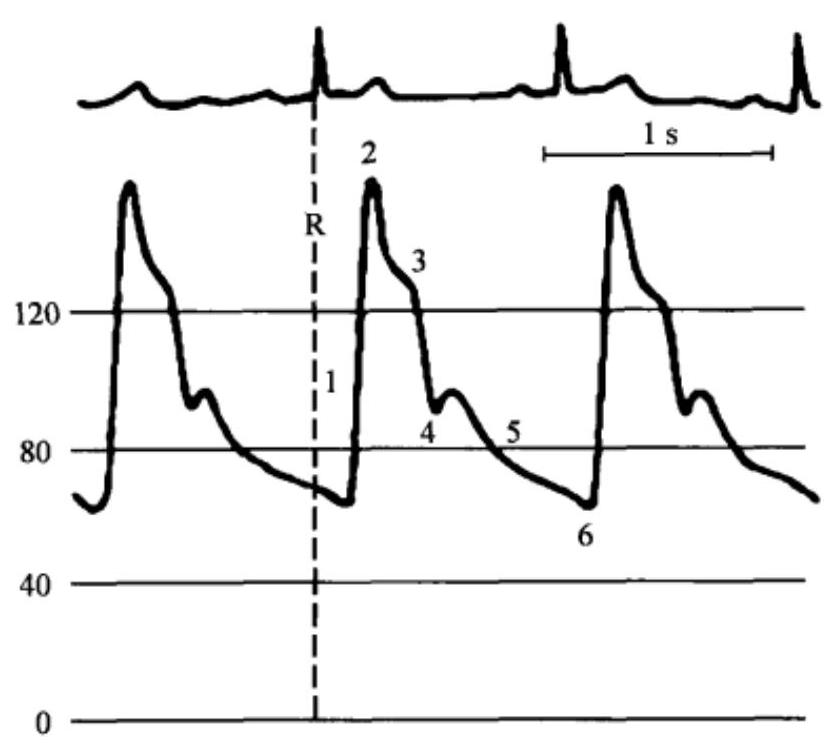
\includegraphics[max width=\textwidth]{2024_07_10_373f31b88d2bf633007bg-509}
\end{center}

图 4-11-1 正常动脉压力波形与 ECG 的 $R$ 波的关系

注:1. 收缩期上升支;2.收缩期峰压;3. 收缩期下降支;4. 降中峡;5. 舒张期血液流向外周;6. 舒张末压\\
\includegraphics[max width=\textwidth, center]{2024_07_10_373f31b88d2bf633007bg-509(1)}

外周

图 4-11-2 不同部位动脉压力波形变化

慢, 顶峰圆钝, 重搏切迹不明显, 见于心肌收缩功能低落或血容量不足。

(2)不规则波: 波幅大小不等,早搏波的压力低平,见于心律失常。

(3)高尖波: 波幅高管,上升支陡,重搏切迹不明显, 舒张压低, 脉压宽, 见于高血压及主动脉瓣关闭不全。主动脉瓣狭窄者, 下降支缓慢及坡度较大,舒张压偏高。

(4)低平波: 上升和下降支缓慢, 波幅低平, 见于低血压休克和低心排综合征。见图 4-11-3。主动脉反流的动脉压波形显示为上升支陡直、脉压宽和舒张压低,是舒张期血流进人左心室和外周血管的结果。在这种情况下左心室的射血量大,动脉压波形可能有两个收缩期峰值( 二重脉, bisferiens pulse)。这两个峰值代表了不同的意义,前者是左心室射血, 后者是外周血管的折返。这种情况也见于主动脉反流合并狭窄的病人和肥厚型心肌病的病人,尽管后者的生理基础不同于前者。在这种肥厚型心肌病, 动脉压力波形表现为特殊的分裂波形,称为针顶型 (spike-and-dome)结构, 收缩早期快速的左心室射血引起最初的压力陡直上升支,左心室收缩中期动态的流出受阻引起动脉压快速下降,然后是晚期的收缩反射波形成双峰的特征性波形。见图 4-11-4。

交替脉 (pulsus alternans)的特征是强弱交替出现的脉搏 (图 4-11-5)。总的来说是左心室严重收缩不良的信号, 通常在升主动脉狭窄的病人明显。偶见于全麻病人, 可能是在潜在左心室收缩功能受损的病人, 麻醉引起交感神经系统活动减少的结果。交替脉应该与二联脉区别, 后者来自二联律, 通常是心室的二联律。这两种情况均可引起动脉血压的改变,而交替脉的心律是正常的。

奇脉 (pulsus paradoxus) 是在收缩期动脉压安静呼吸的吸气相明显下降,超过 $10 \sim 12 \mathrm{mmHg}$ (图 4-11-5)。这种说法可能比较混乱, 因为血压在吸气时轻度下降是正常现象,奇脉并非真正奇怪,而是血压在吸气时正常下降。心脏填塞时奇脉是特征性表现,而且几乎是普遍表现,常发生于许多心包压缩的病人,也可发生于气道阻塞、支气管痉挛、呼吸困难或任何胸内压有较大变化的病人。但在心脏填塞, 吸气时脉压减小和左心室搏出量减少, 用力呼吸和胸内压变化较大的病人观察到的血压改变是脉压相对不变。

(3)机械通气时的动脉压波形变化:在机械呼吸周期中 $(\mathrm{VT}=6 \mathrm{ml} / \mathrm{kg})$, 最高和最低收缩压差 $(S P V)=8 \sim 10 \mathrm{mmHg}(1.06 \sim 1.33 \mathrm{kPa}) 。 \mathrm{SPV}$ 可以分两段, $\Delta u p$ 段是收缩压最大值与呼气末血压之差; $\Delta$ down 段是呼气末血压与收缩压最小值之差, $\Delta u p$ 可测定呼气时左心室排血量, 而 $\Delta$ down 测定由于机械通气引起的静脉回流减少(图 4-11-6)。麻醉病人 $\Delta \mathrm{up}$ 和 $\Delta$ down 的正常值为 $4 \sim 5 \mathrm{mmHg}$ ( $0.53 \sim 0.67 \mathrm{kPa}$ )。正常情况下在呼吸周期中收缩压升降相等。 $\Delta u p$ 和 $\Delta$ down 的相对值对诊断不同临床状态具有重要意义。反映心脏前负荷: 低血

\begin{center}
\includegraphics[max width=\textwidth]{2024_07_10_373f31b88d2bf633007bg-510(2)}
\end{center}

圆钝波

\includegraphics{smile-lyf7wuizmutalbpz8lr.png}


不规则波(心房颤动)\\
\includegraphics[max width=\textwidth, center]{2024_07_10_373f31b88d2bf633007bg-510}

低平波(低排综合征)

\begin{center}
\includegraphics[max width=\textwidth]{2024_07_10_373f31b88d2bf633007bg-510(1)}
\end{center}

高尖波(主动脉关闭不全)

不规则波(早搏二联律)

图 4-11-3 异常动脉压波形\\
\includegraphics[max width=\textwidth, center]{2024_07_10_373f31b88d2bf633007bg-510(4)}

C\\
\includegraphics[max width=\textwidth, center]{2024_07_10_373f31b88d2bf633007bg-510(3)}

图 4-11-4 病理情况对动脉压波形的影响

A. 正常动脉压 (ART) 和肺动脉压力 (PAP) 波形, 显示与 ECG 的 R 波有相似的时间性;B. 在主动脉㹫窄, ART 波形被扭曲, 上升支不明显, 收缩期蜂值出现延迟; C. 主动脉折返产生二重脉和脉压增窝; D. 动脉压波形,有肥厚型心肌病的病人呈特昇的针顶型。外科娇正后压力波形旺现较正常的形态

容量情况下,机械通气使前负荷降低,出现较大 $\mathrm{SPV}$ 和 $\Delta$ down, 这与潮气量增多及吸气期胸内压升高有关, 特别在气道阻塞、高 PEEP、肺顺应性降低、肺内压升高、血容量和心排血量减少时为显著。 SPV 主要由 $\Delta$ down 组成, 是低血容量的主要征象。\\
(2)充血性心力衰竭时, $\Delta$ down 段完全消失, $\Delta \mathrm{up}$ 相对明显,SPV 减小; 机械通气使静脉回流减少,前负荷下降对左侧心力衰竭病人有利,左心室排血量不降低,借此可与低容量较大 $\Delta$ down 做鉴别。

\begin{center}
\includegraphics[max width=\textwidth]{2024_07_10_373f31b88d2bf633007bg-511}
\end{center}

A $\qquad$

\begin{center}
\includegraphics[max width=\textwidth]{2024_07_10_373f31b88d2bf633007bg-511(1)}
\end{center}

B $\qquad$\\
图 4-11-5 动脉压波形形态在每次搏动的变化

A. 交替脉; B. 奇脉. 其特征是自主吸气时 (箭头所示)收缩压明显下降和脉压减小

A\\
\includegraphics[max width=\textwidth, center]{2024_07_10_373f31b88d2bf633007bg-511(2)}

图 4-11-6 机㖑通气时动脉压波形的变化

\section*{第二节 中心静脉压监测}
中心静脉压 (central venous pressure, CVP)是测量右心房或靠近右心房的上、下腚静脉的压力。主要受循环血容量、静脉张力和右心室功能的影响。中心静脉置管主要是经颈内静脉和锁骨下静脉,将导管置人到上腔静脉,也可经股静脉或肘静脉,用较长的导管置人到上腔或下腔静脉。目前在心血管外科、普外科、神经外科等大手术以及危重患者中应用较多,一般较为安全, 但如果操作者技术不熟练,也可能发生气胸和出血等并发症。

\section*{一、适 应 证}
中心静脉穿刺置管的主要用遂,包括(1)监测中心静脉压, 用于判断循环容量和心功能; (2)静脉输液、给药, 进行循环支持; (3)静脉高营养疗法; (4) 经静脉抽血、抽空气、放血或急沴血液透析; (5)插人肺动脉导管及经静脉放置起搏导管等。

中心静脉穿刺置管的适应证,包括严重多发创伤、严重烧伤、重大手术及术后监测; 并发心、肾、败血症、大出血等严重并发症的病人; 低血压、休克;需快速、大量输液或输血, 或需经常抽取中心静脉血液作血气等监测; 长时间输液; 须作右心或肺动脉监测。

\section*{二、禁 忌 证}
下述情况, 应用需慎重: 收缩期血压 $>$ $200 \mathrm{mmHg}(26.7 \mathrm{kPa})(1 \mathrm{kPa}=7.5 \mathrm{mmHg})$; 凝血障碍; 上腔静脉梗阻或创伤; 严重呼吸困难; 有气胸、血胸或颈部已有血肿; 颈部手术; 穿刺点附近有感染;病人躁动、极度紧张或不合作; 仰卧时,静脉压低于大气压; 初生婴儿; 肺气肿; 双侧肺尖部肺大疮; 病人应用持续正压呼吸; 极度消瘦。

\section*{三、静脉穿刺插管术}
应熟悉静脉穿刺部位的解剖。以常用的右颈内静脉途径为例, 颈内静脉从敄底颈静脉孔内穿出, 颈内静脉、颈动脉与迷走神经包裹在颈动脉鞘内, 静脉先位于颈内动脉后侧, 然后在颈内与颈总动脉的后外侧下行。当进人颈动脉三角时, 颈内静脉位于颈总动脉的外侧稍偏前方, 胸锁乳头肌锁骨头下方稍内侧。右颈内静脉穿刺径路分前侧、中间和后侧,而以中间径路为首选。即在颈动脉三角顶点穿刺进针, 必要时让病人拾头, 使三角显露清楚,于胸锁乳突肌锁骨头内侧缘, 对向同侧乳头方向穿刺。通常先用不锈钢细针试探颈内静脉, 待定位无误, 可改用 $14 \sim 18 \mathrm{G}$ 针, 当回抽血确诊后, 置人导引钢丝, 再将专用静脉导管沿钢丝插人颈内静脉, 并将静脉内导管与测压装置连接进行 CVP 测压。

\section*{四、临床意义}
\begin{enumerate}
  \item CVP 反映血容量和右心室功能 CVP反映右心室功能和回心血量之间的平衡, 是对右心室充盈压的直接测量。当血容量增加时, 静脉回流增加, CVP 升高。用 CVP 估计血容量要强调连续观察。一般当静脉压不高或偏低时,可以给予一定的液体负荷。当右心功能不全时, CVP 增高, 表明右心排血功能下降。临床情况往往很复杂, 需要根据病人具体情况,结合动脉压、左心功能等综合判断。

  \item CVP 反映左心室充盈压无肺动脉高压或二尖瓣病变,而左心室功能良好, CVP 可以间接反映左心室充盈情况。研究表明左心功能良好(射血分数 $>40 \%$, 无室壁运动异常) 的冠心病病人, CVP 与 PCWP 相关良好。

  \item CVP 监测在体外循环中的作用除估计右心功能和血容量外, 体外循环时监测 CVP 对外科操作还有较大的指导作用。由于体外循环时重力对上腔静脉血的引流作用, CVP 可以为零或负值。当阻断上腔静脉时, 出现持续性 CVP 升高, 提示静脉回流受阻。病人颜面部会变暗红, 静脉血管充盈,同时灌注医师会发现回流血液减少。遇此情况应及时处理,防止脑水肿等发生。

  \item CVP 的正常值和变化的意义 见表 4-11-1。

\end{enumerate}

CVP 的正常值为 $0.5 \sim 1.2 \mathrm{kPa}\left(5 \sim 12 \mathrm{cmH}_{2} \mathrm{O}\right)$, $<0.25 \mathrm{kPa}\left(2.5 \mathrm{cmH}_{2} \mathrm{O}\right)$ 表示心腔充盈欠佳或血容量不足, $>1.5 \sim 2 \mathrm{kPa}\left(15 \sim 20 \mathrm{cmH}_{2} \mathrm{O}\right)$ 提示右心功能不全。

表 4-11-1 CVP 值的临床意义

\begin{center}
\begin{tabular}{|c|c|c|}
\hline
 & $\operatorname{CVP}$ 值 $\left(\mathrm{cmH}_{2} \mathrm{O}\right)$ & 临 床 意义 \\
\hline
正常值 & $4 \sim 10$ &  \\
\hline
低傎 & $0 \sim 4$ & \begin{tabular}{l}
(1) 低血容量; (2)血容量不低而有血管显著扩张;(3)甲状腺功能立进、高热等;(4)血管扩张 \\
(如中毒性休克、 $\mathrm{CO}_{2}$ 蓄积等) \\
\end{tabular} \\
\hline
偏高 & $10 \sim 15$ & 须防进一步增高, 应立即处理 \\
\hline
高傎 & $>15$ & \begin{tabular}{l}
(1)血容量正常时,多为心脏失代供; (2) 血容量不足,CVP 反有增高,说明心功能严重受 \\
损;(3)血容量增大,输人过量,或流出道受阻;(4)间歌正压呼吸 \\
\end{tabular} \\
\hline
\end{tabular}
\end{center}

\section*{5. 影响 CVP 的因素}
(1)病理因素: CVP 升高见于右心及左、右心室心力衰竭、房额、肺梗死、支乞管痉挛、输血补液过量、纵隔压迫、张力性气胸及血胸、慢性肺部疾患、心包填塞、缩窄性心包炎、腹内压增高的各种疾病及先天性和后天性心脏病等。CVP 降低的原因有失血和脱水引起的低血容量以及周围血管扩张,如神经性和过敏性休克等。

(2)神经体液因素: 交感神经兴奋、儿茶酚胺、抗利尿激素、肾素和醛固酮等分泌增加, 血管张力增加, 使 CVP 升高。相反, 某些扩血管活性物质,使血管张力惐小,血容量相对不足,CVP 降低。

(3)药物因素: 快速输液、应用去甲肾上腺素等血管收缩药, CVP 明显升高; 用扩血管药或心功能不全病人用洋地黄等强心药后, CVP 下降。

(4)其他因素: 有缺氧和肺血管收缩、气管插管和气管切开、病人挣扎和躁动, 控制呼吸时胸内压增加、腹腔手术和压迫等均使 CVP 升高, 麻醉过深或椎管内麻醉时血管扩张, CVP 降低。

\begin{enumerate}
  \setcounter{enumi}{5}
  \item 临床判断 临床上常依据中心静脉压的变化来估计病人的血流动力学状况。中心静脉压的高低取决于心功能、血容量、静脉血管张力、胸内压、静脉血回流量和肺循环阻力等因素, 其中尤以静脉回流与右心室排血量之间的平衡关系最为重要。在容量治疗过程中, 中心静脉压不高, 表明右心室能排出回心脏的血量, 可作为判断心胜对液体负荷的安全指标。连续测定观察中心静脉压的变化, 比单次的绝对值更有指导意义。一般中心静脉压不高或偏低, 输血、补液是安全的。临床工作中常依据动脉压的高低、脉压大小、尿量及临床症状、体征结合中心静脉压变化对病情作出判断, 指导治疗 (表 4-11-2)。
\end{enumerate}

\section*{五、波形分析}
\begin{enumerate}
  \item 正常 CVP 波形\\
(1) CVP 波形与 ECG 和心动周期的关系: $\mathrm{ECG}$ 的 $\mathrm{P}$ 波之后为舒张末期, $\mathrm{R}$ 波是舒张期结束和收缩期开始。CVP 波形有三个收缩成分 (a、c、v)和两个舒张成分 ( $\mathrm{x}, \mathrm{y}$ ) (图 4-11-7)。a 波由心房收缩产生, $\mathrm{c}$ 波在 ECG 的 QRS 波之后, 是三尖瓣关闭所产生的轻度压力升高, 即右心室等容收缩期。收缩射血的心室牵拉心房, 导致心房腔增大, 心房内的压力持续下降。这就产生了 $\mathrm{x}$ 波谷, 此时心房压力最低。相应于 $\mathrm{c}$ 波的前后两部分 $\mathrm{x}$ 波谷可以也分为 $\mathrm{x}$ 和 $\mathrm{x}^{\prime}$ 波。随后是 $\mathrm{v}$ 波, 它表示心房压力到达高峰, 这是由于充满静脉血的心房收缩而三尖瓣仍然关闭所造成的。 $v$ 波往往紧随出现在心电图的 T 波之后。随后,当三尖瓣打开,血液从心房流向心室,心房压开始下降。y 波即表示三尖瓣开放,右心房排空。
\end{enumerate}

(2) CVP 波形与压力、流量和容量的关系: CVP 波形反映右心房压力周期性变化, 有三个正向波 $\mathrm{a}, \mathrm{c}, \mathrm{v}$ 和两个负向波 $\mathrm{x}, \mathrm{y}$ 。 $\mathrm{a}$ 波表示右心房收缩压, $\mathrm{v}$ 波表示右心房舒张压,两者波幅和压力几乎相同, 正常在 $3 \sim 4 \mathrm{mmHg}(0.40 \sim 0.53 \mathrm{kPa})$ 以内,正常右心房平均压为 $2 \sim 6 \mathrm{mmHg}(0.27 \sim$ $0.80 \mathrm{kPa}$ )。静脉血回流到心脏, 取决于周围静脉和右心房压力阶差, 当右心房压力波处于波谷时 ( $\mathrm{x}$和 $\mathrm{y}$ 波), 血液从腔静脉回流到右心房; 相反,右心房压力波处于波峰时 ( $\mathrm{a}, \mathrm{c}$ 和 $\mathrm{v}$ 波), 血液回流最少。

(3)CVP 波形与左心房压和肺小动脉橪压的关系: 正常情况下平均左心房压超过平均右心房压 (图 4-11-8), 但也可有暂时性相反变化。由于菱房结位于上腔静脉和右心房之间, 左心房压的 $\mathrm{a}$ 波在右心房压 a 波之后 $20 \mathrm{~ms}$, 在左心室等容收缩期开始和二尖瓣关闭产生 $\mathrm{c}$ 波,左心房压和右心房压波形基本一致, 右心房压 $\mathrm{a}$ 波和 $\mathrm{v}$ 波较左心房压明显, 说明右心房膨胀较左心房大。正常肺小动脉梸压波形与左心房压和 CVP 基本相同, 而肺小动脉橪压是反映出现较晚及已有衰减的左心房压,其波

表 4-11-2 引起中心静脉压变化的原因及处理

\begin{center}
\begin{tabular}{|c|c|c|c|}
\hline
中心静脉压 & 动脉压 & 原因 & 处理 \\
\hline
低 & 低 & 血容量不足 & 补充血容量 \\
\hline
低 & 正常 & 心功能良好, 血容量轻度不足 & 适当补充血容量 \\
\hline
高 & 低 & 心功能差,心排血量淢少 & \begin{tabular}{l}
强心、供莓、利尿、纠正酸中毒,适当控制补液或㗆 \\
慎选用血管扩张约 \\
\end{tabular} \\
\hline
高 & 正常 & 容量血管过度收缩,肺楿环阻力增高 & 控制补液,用血管扩张药扩张容量血管及肺血管 \\
\hline
正常 & 低 & \begin{tabular}{l}
心脏排血功能减低,容量血管过度收 \\
缩,血容量不足或巳足 \\
\end{tabular} & 强心、补液试验、血容量不足时适当补液 \\
\hline
\end{tabular}
\end{center}

形在左心房压后 $150 \sim 200 \mathrm{~ms}$,如果 $\mathrm{a}$ 波和 $\mathrm{v}$ 波较明显,在没有嵌人时, $\mathrm{a}$ 波离开收缩相上升支, $\mathrm{v}$ 波切迹不明显 (图 4-11-9、、图 4-11-10)。\\
2. 异常 CVP 波形 有时通过 CVP 波形可以判断患者的病理生理改变(表 4-11-3)。最常见的是快速判断心律失常。

\begin{center}
\includegraphics[max width=\textwidth]{2024_07_10_373f31b88d2bf633007bg-514(1)}
\end{center}

图 4-11-7 CVP 正常波形

\begin{center}
\includegraphics[max width=\textwidth]{2024_07_10_373f31b88d2bf633007bg-514}
\end{center}

固 4-11-8 左心房压与中心静䐂压

表 4-11-3 异常 CVP 波形

\begin{center}
\begin{tabular}{|c|c|}
\hline
病理生理改变 & CVP 波形特点 \\
\hline
房䫓 & $\mathrm{a}$ 波消失, $\mathrm{c}$ 波明显 \\
\hline
房室分离 & 大炮 a 波 \\
\hline
三尖屖反流 & 收缩期 c-v 波增高, x 波谷消失 \\
\hline
三尖瓣狭窄 & a 波增高,y 波谷减弱 \\
\hline
右心室缺血 & $\mathrm{A}, \mathrm{v}$ 波增高, $\mathrm{x}, \mathrm{y}$ 波谷变深, $\mathrm{M}$ 或 $\mathrm{W}$ 波形 \\
\hline
心包缩窄 & $\mathrm{A}, \mathrm{v}$ 波增高, $\mathrm{x}, \mathrm{y}$ 波谷变罙, $\mathrm{M}$ 或 W 波形 \\
\hline
急性心包填塞 & $\mathrm{x}$ 波明显, $\mathrm{y}$ 波谷减弱 \\
\hline
自主通气和正压通气时的呼吸变化 & 在呼气末测量压力 \\
\hline
\end{tabular}
\end{center}

\begin{center}
\includegraphics[max width=\textwidth]{2024_07_10_373f31b88d2bf633007bg-515(3)}
\end{center}

图 4-11-9 左心房压与肺小动脉摸压\\
\includegraphics[max width=\textwidth, center]{2024_07_10_373f31b88d2bf633007bg-515}\\
\includegraphics[max width=\textwidth, center]{2024_07_10_373f31b88d2bf633007bg-515(1)}

\begin{center}
\includegraphics[max width=\textwidth]{2024_07_10_373f31b88d2bf633007bg-515(2)}
\end{center}

PAP

图 4-11-10 肺动脉压、肺小动脉模压和中心静脉压

\section*{(1)心律失常}
(1)心动过速时: P-R 间期和 y 波降支缩短, 使 $\mathrm{a}, \mathrm{c}$ 波融合。

(2)心动过缓时: CVP 波形较明显, 可见 $\mathrm{y}$ 波和 $\mathrm{x}$ 波,还有另外的舒张中期-后期的平台波(h 波),在 $\mathrm{y}$ 波降支之后和 a 波之前。

(3)房䫓: 由于缺乏有效的心房收缩, 舒张末期和收缩早期心房容量增大, $\mathrm{a}$ 波消失, $\mathrm{c}$ 波明显。偶尔,当心室率㖪慢时在 CVP 波形中还可看到房颤或房扑波(图 4-11-11)。

(4)等律性房室分离或结性节律: 当三尖瓣关闭时, 心室收缩期开始而心房也同时在收缩从而产生了高炮型 a 波(图 4-11-12)。心室起搏时正常的房室节律消失,也可以在 CVP 波形中发现有大炮波出现(图 4-11-13)。CVP 还可帮助诊断动脉压过低的原因,心电图不能检测舒张末期心房收缩情况,但是可以通过 CVP 波形诊断。

(2)三尖瓣病变

(1)三尖瓣关闭不全: 通过三尖瓣反流使右心房产生收缩期充盈异常, 可见到宽而高的收缩期 c-v 波,此波从收缩早期开始,使 CVP 波形心室化,与右心室压波形相似。值得注意的是, 反流波形的开始,持续和强度均不同于正常 CVP 的 $\mathrm{v}$ 波,正常 $\mathrm{v}$波是收缩末期腔静脉血流充盈心室所产生。有三尖辩反流者, 监护仪仅显示单一的 CVP 均值, 而实际上右心室舒张末压力比这个值要低。因此,对于

\begin{center}
\includegraphics[max width=\textwidth]{2024_07_10_373f31b88d2bf633007bg-516}
\end{center}

图 4-11-11 房颡时的 CVP 波形

$\mathrm{a}$ 波缺失, $\mathrm{c}$ 波明显, $\mathrm{v}$ 波不变, $\mathrm{y}$ 波低平\\
\includegraphics[max width=\textwidth, center]{2024_07_10_373f31b88d2bf633007bg-516(1)}

图 4-11-12 等律性房室分高

与正常的舒张末期 a 波相反(左小图),表现为收缩期大炮波(右图,*号)。这类心律失常伴随着心室充盈下降, 导致动脉压下降

三尖瓣反流的患者,右心室舒张末压力应该以 ECG 上 $\mathrm{R}$ 波出现时所对应的 CVP 值来衡量才较为准确 (图 4-11-14)。

(2)三尖瓣狭窄 : 舒张期右心房不能完全排空,右心房和心室在舒张期自始至终存在压力梯度,右心室也不能完全充盈。由于舒张期右心房血液流出受阻, a 波异常明显而 $\mathrm{y}$ 波低平(图 4-11-15)。

(3)右心室缺血和梗死:CVP 的 a 波较低钝,心排血量减少,右心房永功能丧失,梗死的右心室对前负荷有依赖性。此外, $\mathrm{v}$ 波明显, CVP 常较 PAWP 高,两者变化不相适应(图 4-11-16)。

另一些情况下, 右心室顺应性受损, 如右心室\\
\includegraphics[max width=\textwidth, center]{2024_07_10_373f31b88d2bf633007bg-517}

图 4-11-13 心室起㩲

CVP 的收缩期大炮波是明显特征(左图)。房室顺序起搏, CVP 波形趋于正常,动脉血压增加(右图)\\
\includegraphics[max width=\textwidth, center]{2024_07_10_373f31b88d2bf633007bg-517(1)}

图 4-11-14 三尖雗关闭不全

平均 CVP 增高,波形显示收缩期高 c-v 波,而 x 波谷消失。估计舒张末期压力最好是在 ECG 出现 $\mathrm{R}$ 波时(箭头处), 其低于平均 CVP

缺血、肺动脉高压、肺动脉瓣狭窄等, 都可能导致舒张末期 a 波异常明显,舒张早期 y 波低平。心包疾病和右心室梗死时,CVP 波形也会发生改变。

(4)心包狭窄和压塞: 心包狭窄时回心血量减少,心排血量降低,CVP 升高,舒张末期 4 个心腔压力都相同,舒张压升高, $\mathrm{v}$ 波较明显, $\mathrm{x}$ 波和 $\mathrm{y}$ 波降支很深,产生 $\mathrm{M}$ 或 $\mathrm{W}$ 形状,舒张早期 $\mathrm{y}$ 波降支时间较短。在舒张中期升高,直至舒张末期形成平台类

\begin{center}
\includegraphics[max width=\textwidth]{2024_07_10_373f31b88d2bf633007bg-518(1)}
\end{center}

图 4-11-15 三尖辧狭察

平均 CVP 明显增高, 舒张期 $\mathrm{y}$ 波㖪弱, 舒张末期 a 波明显\\
\includegraphics[max width=\textwidth, center]{2024_07_10_373f31b88d2bf633007bg-518}

图 4-11-16 右心莖梗死

似 CVP 的 $\mathrm{h}$ 波,或称平方根波(图 4-11-17)。

心包压塞时舒张期充盈压升高, $\mathrm{a}$ 波与 $\mathrm{v}$ 波均抬高, 右心房压力波形明显, $\mathrm{x}$ 波突出, 而 $\mathrm{y}$ 波缩短或消失(图 4-11-18)。缩窄性心包炎的 $\mathrm{x}$ 波和 $\mathrm{y}$ 波均明显。

(5)呼吸影响: 自主呼吸吸气时压力波幅降低,呼气时压力波福增高(图 4-11-19)。机械通气时随呼吸变化更显著(图 4-11-20)。因此,不管是自主呼吸或正压通气,应在呼气末记录 CVP。

事实上,应该了解所有患者呼吸末的心脏充盈压。无论患者是自主呼吸还是正压机械通乞, 在呼气末, 胸腔压力和近心处的压力均接近大气压, 此时记录 CVP 值更准确。在大部分情况下, 跨壁 CVP 和呼气末的 CVP十分接近。CVP 波形不仅

\begin{center}
\includegraphics[max width=\textwidth]{2024_07_10_373f31b88d2bf633007bg-519(1)}
\end{center}

图 4-11-17 心包㹧壂

造成 PAP、PAWP 和 CVP 舒张期充盈压升高, 并达到平衡。CVP 波形呈高 a 波、v 波和陡峭 $\mathrm{x}$ 波和 $\mathrm{y}$ 波谷,以及舒张中期平台波(*)或 $\mathrm{h}$ 波\\
\includegraphics[max width=\textwidth, center]{2024_07_10_373f31b88d2bf633007bg-519}

0 $\qquad$\\
图 4-11-18 心包压塞

CVP 波形示平均压升高, $\mathrm{y}$ 波消失

可以指导循环的监测,而且在麻醉和外科手术中,通过 CVP 变化趋势也可了解液体或血液的丢失情况, 指导补液。正常 CVP 值的范围很大, CVP 很小的变化就可以反映血容量和右心前负荷的明显改变。将 CVP 和其他的一些临床监测指标结合,如血压、尿量等,可以更好地指导临床。

\begin{center}
\includegraphics[max width=\textwidth]{2024_07_10_373f31b88d2bf633007bg-520}
\end{center}

图 4-11-19 自主呼吸对 CVP 的影响

吸气开始(箭头处)淘内匤降低并传导至 CVP 和 PAP, 引起波形改变。因此, CVP 应该在呼气末测量(平均 CVP, $14 \mathrm{mmHg}$ )

\begin{center}
\includegraphics[max width=\textwidth]{2024_07_10_373f31b88d2bf633007bg-520(1)}
\end{center}

图 4-11-20 机臹通气对 CVP 的影响

吸气开始(箭头处)导致胸内压增加, 引起波形改变。CVP仍旧应该在呼气末测定 (平鸤 CVP, $8 \mathrm{mmHg}$ )

\section*{第三节肺动脉压监测}
近几十年来心血管功能监测的重要进展之一是肺动脉导管(PAC) 在临床上的广泛应用。自从 1970 年 Swan 和 Ganz 发明通过血流引导的漂浮导管后, 对心脏功能的监测有了飞速发展。随着导管生产技术和电子计算机技术的不断发展,肺动脉导管技术成为迅速、方便地进行血流动力学监测的重要手段。肺动脉导管不但能够监测传统的参数如中心静脉压或右心房压、肺动脉压、肺小动脉楔压 (PAWP)、连续心排血量 (CCO) 和混合静脉血氧饱和度 ( $\left.\mathrm{S}_{\nabla} \mathrm{O}_{2}\right)$, 通过改良的 Swan-Ganz 导管, 还可直接连续测量每搏量 (SV)、右心室舒张末容积 (RVEDV)和右心室收缩末容积(RVESV), 因此可以同时进行压力监测和容量监测。

\section*{一、适 应 证}
\begin{enumerate}
  \item 重危病人 成人呼吸宥迫综合征 (ARDS)时发生左心衰竭,最佳的诊断方法是测肺动脉㚙压 (PAWP)。低血容量休克应用扩容治疗时测定 PAWP 估计前负荷, 可及时补充血容量, 并预防输液过量。施行各类大手术和高危病人,可预防和减\\
少循环衰竭的发病率和死亡率。

  \item 对循环不稳定病人 应用正性增强心肌收缩性药物和扩血管药等, 通过 PAC 监测可指导治疗, 并观察治疗效果。

  \item 急性心肌梗死 PAWP 与左侧心力衰竭的 $\mathrm{X}$ 线变化有良好的相关性, 根据 CI、PAWP, 可对急性心肌梗死病人进行分级, 可估价近期和远期预后。

  \item 区别心源性和非心源性肺水肿 PAWP 和肺毛细血管静水压基本一致, 其升高的常见原因为左侧心力衰竭或输液过量, 正常时血螀胶体渗透压 (COP) 与 PAWP 之差为 $10 \sim 18 \mathrm{mmHg}$ (1.33〜 $2.4 \mathrm{kPa})$ 。当相差琙至 $4 \sim 8 \mathrm{mmHg}(0.53 \sim$ $1.06 \mathrm{kPa}$ ) 时则发生心源性水肿的可能性明显增加,小于 $8 \mathrm{mmHg}(0.53 \mathrm{kPa})$ 时不可避免发生心源性肺水肿, 左侧心力衰竭的 COP 与 PAWP 的阶差可呈负值。

\end{enumerate}

\section*{二、禁 忌 证}
\section*{1. 绝对禁忌证}
(1)三尖瓣或肺动脉㦚狭窄。PAC 不易通过狭窄的瓣膜, 即使偶尔通过狭窄部位, 也可加重阻碍血流通过。

(2)右心房或右心室内肿块 (肿㿔或血检形成)。插管时不慎, 可致肿块脱落而引起肺栓塞或阵发性栓塞。

(3)法洛四联症。右心室流出道十分敏感, PAC 通过肺动脉时, 常可诱发右心室漏斗部痉挛而使发绀加重。

\section*{2. 相对禁忌证}
(1) 严重心律失常。正常情况下, PAC 置管时, 常可诱发一过性房性或室性心律失常, 因此, 手术病人伴有心律失常时, 插管过程中可引起严重心律失常。此类病人是否选用 PAC, 须权衡利䌘。

(2)凝血障碍。经大静脉穿刺插管时, 可能会发生出血、血肿。因此,伴凝血异常者,应慎用。

(3) 近期置起搏导管者。施行 PAC 插管或拨管时不慎,可将起搏导线脱落。

\section*{三、肺动脉导管置入方法}
通常选择右颈内静脉,其从皮肤至右心房的距离最短, 导管可直达右心房, 操作与颈内静脉做 CVP 相似,易于掌握, 并发症少。当颈内静脉穿刺成功后, 将特制的导引钢丝插人, 沿钢丝将导管鞘和静脉扩张器插人静脉, 然后拔出钢丝和静脉扩张器, 经导管鞘将 PAC 插人 RA, 按波形特征和压力大小, 经 RV、PA 进人肺小动脉, 相当于左心房水平,PAC 即停留于肺小动脉内, 可测得 PAWP、 $\mathrm{S}_{\mathrm{v}} \mathrm{O}_{2}$ 和心排血量。

注意事项:(1)PAC 顶端应位于左心房同一水平,PAWP 才能准确反映 LAP。(2)PAC 最佳嵌人部位应在肺动脉较大分支,当气蛮充气后生理盐水监测仪上即显示 PAWP 的波形和压力值, 而放气后屏幕上又显示 PA 波形和 PASP、PADP、PAP 值。(3)呼吸对 PAWP 有影响, 用机械通气或自发呼吸时, 均应在呼气终末测 PAWP。(4)温度稀释法测心排血量时,注射夜(又名指示剂)的温度与受试者体温的差别应 $>10^{\circ} \mathrm{C}$ 。通常采用 $0 \sim 4^{\circ} \mathrm{C}$ 生理盐水,注射速度不可太慢,一般每秒 $2 \mathrm{ml}$, 连续测 3 次, 取平均值。所选 PAC 规格应与注射容量相匹配。(5)进行 $\mathrm{S}_{\overline{2}} \mathrm{O}_{2}$ 监测时, 应先抽取肺动脉血做血气, 按血气 $\mathrm{SvO}_{2}$ 为标准, 对 $\mathrm{SvO}_{2}$ 监测进行校正。

\section*{四、临床意义}
漂浮导管对 PCWP 及心排血量的测定,为临床估计心脏功能状态及指导临床治疗提供客观的依据。

\begin{enumerate}
  \item 估计左心功能 心室舒张时,肺微血管和肺静脉床、左心房及左心室成一共同腚室,PCWP 亦可代表左心室舒张末压(LVEDP),因此可反映左心室前负荷。如果排除其他原因,如缺血、二尖㼌病变等, 肺动脉压和 PCWP 可以估计左心功能。在无肺血管病变时,肺动脉舒张压、左心房压和 LVEDP 相关良好, 用肺动脉舒张压可以表示上述压力。当左心功能不全时,心室顺应性降低, LVEDP 显著升高。当出现体循环低血压、心排血量惐少,同时肺动脉压和 PCWP 升高, 是左心功能不全的标志。此时用肺动脉舒张压和 PCWP 表示 LVEDP 就未必恰当,LVEDP 常超过肺动脉压和 PCWP。
\end{enumerate}

平均 PCWP 一般确能反映左心功能。在心排血量正常时, 若 PCWP 在 $8 \sim 12 \mathrm{mmHg}(1.1 \sim$ $1.6 \mathrm{kPa}$ ), 提示心室功能良好;在有低心排血量或循环障碍征象时, 若 PCWP 小于 $8 \mathrm{mmHg}(1.1 \mathrm{kPa})$,则提示血容量相对不足, 需增加左心室的充盈量。当 PCWP 超过 $20 \mathrm{mmHg}$ ( $2.7 \mathrm{kPa}$ ) 时, 表明左心室功能欠佳。当其增高达 $20 \mathrm{mmHg}$ (2.7kPa) 以上时, 已有左心功能异常; 若高达 $30 \mathrm{mmHg}$ (4.0kPa)或以上时, 则出现肺水肿。

\begin{enumerate}
  \setcounter{enumi}{1}
  \item 估计右心功能 中心静脉压 (CVP)可以判断右心的容量是否超负荷或不足。右心室壁薄, 当由于肺血管病变、心脏原发性疾病、心肌保护不良、外科手术等原因, 导致右侧心力衰竭时, 表现为 CVP 增高,心排血量减少,平均肺动脉压与 CVP 差距下降。

  \item 诊断肺动脉高压和肺动脉栓塞 正常肺血管阻力状态, 肺动脉舒张压和 PCWP 非常接近。肺动脉舒张压增高, 提示肺动脉高压。正常时肺动脉舒张末压仅较 PCWP 略高, 但若相差达 $6 \mathrm{mmHg}$ ( $0.8 \mathrm{kPa})$ 以上时,则表示肺小动脉与肺微血管间存在着明显的阻力。此时如能排除由慢性肺心病、肺纤维化或其他原因引起者,则应可考虑肺动脉栓塞。

  \item 估计心包病变 由于舒张期心脏的充盈受阻,使右心室舒张末压、右心房压力增高,甚至可增高至与肺动脉压相近,其 PCWP 与右心房压可无明显差别,心排血量明显下降。这种情况可见于缩窄性心包炎和限制性心肌病。

  \item 估计㲔膜病变依靠肺动脉导管,通过测量跨瓣膜压差,可以诊断三尖瓣和肺动脉瓣狭窄。三尖瓣跨瓣压差为 CVP 与右心室舒张末期压力\\
(RVEDP)之差,肺动脉瓣跨瓣压差为右心室收缩压和肺动脉收缩压之差。二尖瓣病变可以通过 PCWP 波形的变化反映出来。

  \item 早期诊断心肌缺血当心肌缺血时,导致心肌顺应性下降,左心室舒张末压(LVEDP) 明显增高。心肌缺血与 LVEDP 或 PCWP 升高有明显相关性, 基础研究提示 PCWP 较 LVEDP 可能更敏感。通过观察 PCWP 波形和压力变化,可以早期诊断心肌缺血。

\end{enumerate}

\section*{五、肺动脉导管压力波形分析}
\begin{enumerate}
  \item 正常右心房、右心室、肺动脉和肺动脉棳压波形 肺动脉导管放置过程中压力波形变化见图 4-11-21, 当 PAC 进人肺小动脉而气垔未充气时,是代表肺动脉压力 (PAP) 和波形。气㐮充气时则为肺小动脉樱压(PAWP)。
\end{enumerate}

PAWP 的正常波形和 CVP 波相似,可分 $a 、 c$和 $\mathrm{v}$ 波,与心动周期的时相一致。左心房收缩产生 $\mathrm{a}$ 波,二尖瓣关闭产生 $\mathrm{c}$ 波,左心房充盈和左心室收缩使二尖瓣向心房膨出时产生 $\mathrm{v}$ 波。心电图 $\mathrm{P}$ 波后为 a 波, $\mathrm{T}$ 波后为 $\mathrm{v}$ 波 (图 4-11-22)。\\
\includegraphics[max width=\textwidth, center]{2024_07_10_373f31b88d2bf633007bg-522}

图 4-11-21 漂浮导管放置过程中压力波形变化\\
\includegraphics[max width=\textwidth, center]{2024_07_10_373f31b88d2bf633007bg-523}

图 4-11-22 正常体循环动脉压(ART)、肺动脉压(PAP)、中心静㥆压(CVP) 和肺动脉梸压(PAWP)的关系 PAWP 的 $\mathrm{a}-\mathrm{c}$ 波和 $\mathrm{v}$ 波在心动周期中出现较 CVP 波形晚

正常情况下, 由于左心室的等容收缩期较长, PAP 的上升支比桡动脉压力轻度提前,提前的时间和主动脉压向下游桡动脉传递的时间一致。虽然 PAP 的上升支比桡动脉压力提前 $50 \mathrm{~ms}$, 但是其峰值比桡动脉仅仅提前 $10 \mathrm{~ms}$ 。实际上,可以发现肺动脉压和体循环压力的波形在监护仪上重叠,在相同的时间上升、达峰和下降。理解这点对于解释异常肺动脉和楔压波形非常重要,尤其是当这些波形中有高大的 $\mathrm{v}$ 波出现时。

有充气套輩的 PAC 导管最终到达楏位。如前所述,梸压是间接测量肺静脉压力和左心房压的参数,波形和它们也相似。因此,PAWP 波形可以认为是个静脉压波形,同样有 $\mathrm{a}, \mathrm{v}$ 波峰和 $\mathrm{x}, \mathrm{y}$ 波谷。但是,PAC 末端和左心房之间是肺毛细血管床,栶压的波形较左心房压延迟。左心房压通过肺静脉、毛细血管、小动脉和动脉传递到 PAC 末端, 平均需时 $160 \mathrm{~ms}$ 。由于这种延迟效应,栶压的 a 波和心电图中心室收缩早期的 R 波相对应。但是, a 波是由左心房收缩的舒张末期压力产生。只有认识到栶压的内在延迟性,才能更好地解释波形意义。

\begin{enumerate}
  \setcounter{enumi}{1}
  \item 异常波形 PAWP 的异常波形可见于心律失常、心衰、心肌缺血、二尖瓣狭窄和关闭不全以及心包填塞等。因此,通过波形分析,也可反映疾病病理变化和心功能等。
\end{enumerate}

(1)二尖瓣病变时的压力波形: 急性二尖瓣关闭不全时,心脏收缩时血流反流,PAWP 曲线 $\mathrm{v}$ 波明显增大,酷似肺动脉波形。有可能将导筸继续插人以致损伤肺小动脉,或肺动脉导管位于肺小动脉而气囊遗忘放气, 有可能导致肺动脉梗死, 因此应仔细观察压力波形以及与 ECG 的关系。肺动脉收缩波在 ECG 的 QRS 和 $\mathrm{T}$ 波之间,二尖瓣关闭不全病人, 测 PAWP 时, 大的 $\mathrm{v}$ 波位置出现在 QRS 综合波之后 (图 4-11-23)。除二尖瓣关闭不全病人,二尖辫阻塞、充血性心衰、室间隔缺损病人, 即使没有明显二尖瓣反流 PAWP 波形仍可出现大 $\mathrm{v}$ 波。右心房和肺动脉血氧饱和度差超过 $10 \%$ 以上, 有助于鉴别急性室间隔缺损和急性二尖瓣关闭不全。

(2)右侧心力衰竭时的压力波形: 右侧心力衰竭时,右心室舒张末压增高,在放置肺动脉导管时,右心室波形易于混淆为肺动脉波形, 导管的置人深度及波形上有无切迹有助于鉴别导管是否进人肺动脉压 (图 4-11-24)。

(3)休克时的压力波形: 低容量休克时,右心室舒张末压和肺动脉压明显降低, 很难确定导管插人位置, 在右心室舒张末压和肺动脉压差非常小的情况下,快速输注液体, 补充机体失液量, 同时有利于鉴别导管的位置 (图 4-11-25), 此外监测导管中存在气泡也可引起类似情况。因此, 插䍶前需仔细检查,避免人为因素引起误差。

(4)慢性肺部疾病的压力波形: 在慢性阻塞性肺部疾病(如支气管痉挛、㫴喘持续状态), 呼气相胸内压明显增加, 压力传送到导管, 导致肺动脉波形难以解释 (图 4-11-26), 仔细观察治疗前后的动脉波形变化,有助于分析肺动脉波形(图 4-11-27)。

(5)心律失常时的压力波形: 严重心律失常病人,肺动脉压波形不规则, 很难确实测定肺动脉导

\begin{center}
\includegraphics[max width=\textwidth]{2024_07_10_373f31b88d2bf633007bg-524(1)}
\end{center}

图 4-11-23 二尖槩关闭不全的 PAWP 波形气哄充气后为肺动脉燃压波形。v v 波远离 QRS 综合波

\begin{center}
\includegraphics[max width=\textwidth]{2024_07_10_373f31b88d2bf633007bg-524}
\end{center}

图 4-11-24 右心室衰竭病人的压力波形

右心室舒张末压超过 $20 \mathrm{mmHg}$ (2.7kPa)。在此情况下,右心室压力波可能被误认为肺动脉波形。导管的插人深度及波形中切迹的存在与否可篮别。 PAEDP:肺动脉舒张末压;RVEDP; 右心室舒张末压

管的准确位置, $a 、 v$ 波, $x 、 y$ 波波幅小,且难以分别 (图 4-11-28)。

(6)导管移动: PAC 监测不仅有和其他有创监测一样的固有技术误差, 还有一些其他的问题。由于 PAC 要比其他动脉内导管长, 如果导管内有血块或是气泡将影响压力波形。此外, 心脏活动导致导管移动也会产生假相波形。区分这种假相波形的方法是从生理学上掌挃 PAC 波形的特点,包括其独特的形态和周期。

在 PAC 中最显著、最常见的假相波形是由心脏收缩开始产生的尖峰波,它对应出现在 EKG 的 $\mathrm{R}$ 波后面(图 4-11-29)。此时三尖辫关闭,右心室

\begin{center}
\includegraphics[max width=\textwidth]{2024_07_10_373f31b88d2bf633007bg-525(1)}
\end{center}

图 4-11-25 低客量休克病人的压力波形

右心房压、右心室压、肺动永压均低于正常, 使波形更易混淆。PAO:肺动脉阻塞

\begin{center}
\includegraphics[max width=\textwidth]{2024_07_10_373f31b88d2bf633007bg-525}
\end{center}

图 4-11-26 严重气管痉挛

呼气时胸内压显著增高病人之肺动脉攃压波形。正压通气使波形颇难识别

收缩,PAC 导管受到冲击, 波形上产生一个运动伪差。值得注意的是这个假相压和 CVP 上的 $\mathrm{c}$ 波同时出现, 并且可能产生一个假低压或压力峰。如果监护仪检测到这个假相波的最低值, 它就可能错误地认为这个值是肺动脉收缩庒。重新定位 PAC 导管,如推进或退出几厘米,就可以解决这个问题。

(7)过棳压: 另外一个常见的假相波发生在充盈气蔶时, 此时导管头端被阻塞不能测量血管内压力。这种现象被称为“过楔压”, 常常是由于导管远端移行和套鞛偏心充盈导致头端倚靠在肺动脉壁上造成的。

肺动脉导管的最佳嵌人部位应在肺动脉较大分支,充气时进人到岸人部位, 放气后又退回原处。若位于较小的动脉内, 特别是血管分叉处, 气囊可发生偏心充气, 或部分充气后导管前端提前固定。当导管前端碰到肺动脉壁时,PAP 波形呈平线,或呈逐渐上升的压力波形, 为假楔压 (图 4-11-30)。加压和偏心充气易造成处于收缩状态的肺血管破

\begin{center}
\includegraphics[max width=\textwidth]{2024_07_10_373f31b88d2bf633007bg-526(1)}
\end{center}

图 4-11-27 经气筞解痉治疗后的肺动脉笑压波形呼气末正压通气使肺小动永㗛压波形明显改善

\begin{center}
\includegraphics[max width=\textwidth]{2024_07_10_373f31b88d2bf633007bg-526}
\end{center}

图 4-11-28 不规则肺动脉压力波形

大量的波形使肺动脉压力波难以识别。 $\mathrm{Pa}$ 为肺动脉压, $\mathrm{PaO}$ 为肺动脉阻塞

裂,因此此时应将气囊放气后退出 $1 \sim 2 \mathrm{~cm}$ 。

前面两个箭头所指波形在充盈 PAC 导管的套蘘时产生的一个非搏动性的波形,由于其阻塞了导管的头端导致压力逐渐升高。导管适度后撤后, 套萁充气产生正常的楔压(第三个箭头)。

当持续的冲洗系统产生压力对抗了阻塞的远端开口,此时导管记录的是逐渐上升的压力而不是血管内压。要注意的是,过楔压力是没有搏动波形的, 其值远高于肺收缩压, 并会持续上升直到和冲洗压力的水平相同。发生以上这些现象都会导致不能正确估计测量的 PAWP 值。

像早先所强调的那样,每次套囊充盈的时候,导管头端都向远端移行几厘米达到楔压的位置。这个漂浮的过程一般要经历几个心动周期。当部分套㐮充盈时,楔压波形就出现,说明 PAC 导管位于较小的肺动脉远支,位置不佳。此时应该将导管后撤以防止“过楔”导致血管损伤或肺梗死。PAC 导管远端在套襄没有充盈时也可能产生“过椥”。这个问题可以通过观察波形而立刻察觉,将 PAC 导管后撒,直到正常的 PAP 波形出现。

\begin{center}
\includegraphics[max width=\textwidth]{2024_07_10_373f31b88d2bf633007bg-527}
\end{center}

团 4-11-29 由于导管移动而产生的 PAP 的假相波峰和波谷

肺动脉㖣张末期压力正确的值为 $8 \mathrm{mmHg}(\mathrm{A})$, 但监护仪上错误的显示 PAP 为 $28 / 0 \mathrm{mmHg}(\mathrm{B})$

\begin{center}
\includegraphics[max width=\textwidth]{2024_07_10_373f31b88d2bf633007bg-527(1)}
\end{center}

图 4-11-30 肺动脉导管过楔产生假相波形

\section*{第四节 心排血量监测}
心排血量 (CO)是临床上了解循环功能最重要的基本指标之一, $\mathrm{CO}$ 指心脏每分钟将血液䠌至周围循环的血量,可反映整个循环系统的功能状况,包括心脏机械做功和血流动力学,了解前、后负荷、心率及心肌收缩力。在麻醉和 ICU 中, CO 常用于危重病人和血流动力学不稳定者的监测以指导病人的治疗和观察病情进展。

目前心排血量的监测方法分为两大部分,即无创性和有创性心排血量监测。

\section*{一、无创性心排血量监测}
\begin{enumerate}
  \item 胸部生物阻抗法 (thoracic electrical bioimpedance, TEB)
\end{enumerate}

(1)原理及方法: TEB 是利用心动周期中胸部电阻抗的变化来测定左心室收缩时间和计算心搏量的。其基本原理是欧姆定律(电阻=电压/ 电流)。早在 1907 年 Gramer 发现心动周期中有电阻抗的变化,1940 年 Nyboer 首先采用四电阻法在人体胸部通过高频电流,记录到与心动周期一致的阻抗变化,同时计算出 CO。1966 年 Kubicek 采用直接式阻抗仪测定心阻抗变化,推导出著名的 Kubicek 公式:

\[
\mathrm{V}=\rho\left(\frac{L}{Z_{0}}\right) 2 \times \mathrm{dz} / \mathrm{dt}_{\max } \times \mathrm{LVET}
\]

其中 $\rho=$ 电阻率 $135 \sim 150 \Omega \cdot \mathrm{cm}, L=$ 电极 $\mathrm{E} 2 \sim \mathrm{E} 3$ 之间的垂直距离, $Z_{0}$ 基础阻抗, $\mathrm{dz} / \mathrm{dt}_{\max }=$左心室峰值射血速率,LVET=左心室射血时间。

1981 年 Sramek 观察到肺水肿病人的基础阻抗下降, 但应用 Kubicek 公式测搏出量 (SV) 却明显升高, 这显然与临床表现不符, 故 1981 年 Sramek 提出对 Kubicek 公式加以修正。修正后的公式为:

\[
S V=\frac{V \text { ept. } T . \Delta Z / \mathrm{sec}}{Z_{0}}
\]

式中 Vept 是高频低安培通过胸部组织的容\\
积, $T$ 为心室射血时间。Sramek 将该数学模式储存于计算机内, 研制成 NCCOM1 3 型 (BOMed)。 $\mathrm{NCCOM}$ 操作简单: 8 枚电极分别置于颈部和胸部两侧, 即可同步连续显示 $\mathrm{HR}, \mathrm{CO}$ 等参数的变化。它不仅能反映每次心跳时上述各参数的变化, 也能计算 $4 \mathrm{~s}, 10 \mathrm{~s}$ 的均值。但易受病人呼吸、手术操作及心律失常等的干扰。

近几年诞生了更先进的阻抗监测仪,利用修正的 Kubicek 公式及微机联机的 Rheo 心排血量监测仪,其主要改进之处在于通过对生理阻抗和心电信号的同时分析使左心室有效射血时间 (LVET) 测定的准确性提高。其体型更轻盈,使用更方便。它共有 6 个电极, 两个电极粘于颈部两侧,两个电极粘于剑突水平两侧腋中线, 另两个电极分别粘于前额和左下肢膝下。测量周期为 $10 \mathrm{~s}$, 测量准确性和重复性都较佳。上海第二医科大学附属仁济医院麻醉科对 16 名冠脉搭桥病人进行 CO 监测, 并与有创 $\mathrm{CO}$ 、部分重吸气体中 $\mathrm{CO}_{2}$ 测量 $\mathrm{CO}(\mathrm{RBCO}$ )进行比较, 相关系数分别为 $0.85(\mathrm{n}=180)$ 和 0.87 $(\mathrm{n}=118$ )。

新近在增加呼吸过滤器、程序数字化及加快测量速度的基础上又诞生了一种新型的阻抗监测仪 (BioZ System, version 1.3, Cardiodynamics International Corporation, San Diego, CA)。操作方法为两对双向电极分别黏附于颈根部, 另两对分别黏附在剑突下两侧。测量周期为 $15 \mathrm{~s}$ 。 75 例健康受试者的测量结果表明: 其精确性及重复性均较好,但所测的 $\mathrm{CI}$ (每平方米 $2.0 \sim 7.2 \mathrm{~L} / \mathrm{min}$ ) 略大于温度稀释法测定值, 提示计算公式有待改进。

另一个由 Renaissance Technologies(Newton, $\mathrm{PA})$ 设计完成的 TEB 测定仪,采用 11 个电极, 其中两个置人性电极放在颈根部两侧, 另两个置人性电极放在下胸部两侧, 4 个电极黏附在置人性电极 $5 \mathrm{~cm}$ 以内处, 3 个心电图电极分别放在心脏周围及左肩。对 209 例危重病人进行 CO 测定,结果与温度稀释法相比: $\mathrm{r}^{2}=0.74$; 精确性及偏差分别为 $0.75 \mathrm{~L} /\left(\mathrm{min} \cdot \mathrm{m}^{2}\right),-0.124 \mathrm{~L} /\left(\mathrm{min} \cdot \mathrm{m}^{2}\right) 。$

(2)临床应用及评价: TEB 操作简单、费用低并能动态观察 $\mathrm{CO}$ 的变化趋势。但由于其抗干扰能力差,尤其是不能鉴别异常结果是由于病人的病情变化引起,还是由于机器本身的因素所致,故在一定程度上限制了其在临床上的广泛使用。

\begin{enumerate}
  \setcounter{enumi}{1}
  \item 超声多普勒法 近年来随着临床超声技术的应用,为无创性血流动力学监测开辟了新的途径。目前超声多普勒测定 CO 主要有两种方式,即经食管超声多普勒(TED) 和经气管超声多普勒(TTD)。
\end{enumerate}

(1)经食管超声多普勒: 由 Arrow 公司生产的 HemoSonicTM100 EDM 监测仪已在国外得到广泛的应用,研究结果表明其操作简单、准确性高。

(1)测量原理和测量方法: HemoSonicTM100 的超声多普勒探头通过测定红细胞移动的速度来推算降主动脉的血流, 其配有的 $\mathrm{M}$ 型超声探头, 还可直接测量降主动脉直径的大小, 而不需要根据年龄、身高等参数来间接推算主动脉直径, 这样就提高了测量结果的准确性。由于降主动脉的血流量是 $\mathrm{CO}$ 的 $70 \%$ (降主动脉血流与 $\mathrm{CO}$ 的相关系数是 0.92 ), 故其计算公式为: $\mathrm{CO}=$ 降主动脉血流 $\times$ 降主动脉的横截面积 $\div 70 \%$ 。

具体操作方法为将一带有多普勒探头及 $\mathrm{M}$ 型超声探头的经食管导管经口插人食管 (相当于第 3 助间水平, 此点的食管与降主动脉相平行), 根据显示屏上的主动脉壁,超声信号和血流波形及多普勒声音上下旋转调整探头位置直至获得满意的信号质量, 然后使监测仪进人测定状态后即能显示降主动脉血流、主动脉直径、CO、左心室收缩性、MAP、外周血管阻力等血流动力学参数。

(2临床应用及评价 : 主要用于心脏病患者行非心脏手术的围术期监测。在行腹腔镜手术时,由于气腹可压迫腹腔内血管, 使血管阻力增加, 此时行 HemoSonicTM100 监测可确定血管阻力及组织灌流状态。另外, 还可用于大血管手术、尿道前列腺切除等易致血流动力学紊乱的手术和 ICU 中的监测,以指导临床治疗。除了测定 CO 外,血流波形还能提供心肌收缩、前负荷、后负荷等反映左心功能的信息。

HemoSonicTM100 能清楚地观察到每次心搏时的降主动脉血流情况及主动脉的直径而不是测定一定时期的平均值,故结果准确、可靠 (与温度稀释法比, 两者的相关系数是 $0.74 \sim 0.98$ ), 能及时反映 CO 的迅速变化。由于其配有大、中、小三种规格的经食管导管,故适应于婴儿、儿童及成年人使用。

经食管导管较难定位,易受操作因素及术中电刀干扰。该法不适合用于食管疾病、主动脉球囊反搏(降主动脉血流改变)及主动焃严重缩窄病人。

(2)经气管超声多普勒

(1)TTD 测量原理及方法: TTD 应用多普勒效应原理进行主动脉横截面积 (A) 和平均血流速度 $(\bar{V})$ 的测定,从而计算出 $\mathrm{CO}$ 。计算公式如下:

\[
\mathrm{CO}=\bar{V} \times A
\]

TTD 探头有左、右两块换能器, 左侧用于发射超声波,右侧则用来接收回波。接收到的频率与发射时的频率不同,频率的差值称为频移 $(\Delta f)$,可用以计算 $\bar{V}$ 。

\[
\bar{V}=C \Delta f / 2 f o \cos \theta
\]

式中 $C$ 为音速, $f o$ 为发射超声的频率, $\theta$ 为超声束与血流方向成角。

主动脉横截面积可通过 TTD 探头发射 $5 \mathrm{MHz}$的波宽为 $1 \mathrm{~mm}$ 的脉冲多普勒信号来测定。信号发射方向与换能器垂直, 发射范围为 $60 \mathrm{~mm}$ 。由于主动脉壁的运动可产生一特殊的声音, 所以它的位置可以通过多普勒频移来辩别, 这样便确定了超声射程 $(r)$ 。主动脉直径 $(d)$ 和面积 $(A)$ 可测出。计算公式如下:

\[
\begin{gathered}
d=r \sin \theta \\
A=\pi(d / 2)^{2}
\end{gathered}
\]

病人全麻诱导后, 将 TTD 导管插人气管内, 调整导管位置并固定。然后 ABCOMI 计算机与多普勒显示屏相连接, 接通电源可进行 $\mathrm{CO}$ 测定。在 $\mathrm{CO}$ 测定过程中为了犾得和保持最佳的多普勒信号, 要经常调整 TTD 的位置。TTD 导管必须放置到靠近主动脉弓下、气管隆突上的位置, 这样才可获最佳的多普勒信号。TTD 导管的位置可以通过听特有的多普勒声音和观察多普勒显示屏上的信号来确定。显示屏上的红色信号代表反向流动信号,绿色信号为前向流动信号。将病人的头稍偏向左侧, 同时将导管向前送, 直到声音和显示器信号消失, 记录这个深度; 然后将导管往外退, 直到声音和显示器信号出现而后又消失, 记录这个深度。这两点的中心位置即认为是 TTD 得到最佳信号的深度, 将导管固定。

在信号方面出现下列情况时,认为导管位置不佳,应重新置管。声音信号中低频撞击代替高频哨声占优势时,因为撞击声的产生意味着主动脉壁的运动, 此时所测速度不是主动脉腔中心的流速。多普勒显示屏上绿色信号的振幅小于 4 倍红色信号振幅时,机械通气可干扰多普勒探头和气管壁的接触,在一个呼吸周期中,如果多普勒信号振幅降低不小于 $50 \%$ 时,认为导管位置不佳。无论是主动脉血流速度的测定, 还是主动脉直径的测定都涉及角度 $\theta$, 它是影响 TTD 测定的重要因素, Abrams 等首次报道 TTD 用于人时的平均 $\theta=52.4^{\circ} \pm 38^{\circ}$ 。

(2)临床应用及评价: TTD 可用于麻醉及术中连续测定 $\mathrm{CO}, \mathrm{ICU}$ 中进行病情分析和指导治疗, 及早发现可能出现的意外事件。其优点有: 测定点靠近主动脉弓起始部的升主动脉,升主动脉与气管的关系远比降主动脉与食管的关系固定。它不仅可以连续监测 CO, 还可以计算 SVR 或 SVRI, 使某些病人免除肺动脉导管的检查。探头不在手术野,也不受通气方式的影响。

其缺点是病人必须进行气管插管,不适应于需进行较长时间测定的病人, TTD 导管的任何变动都会使测定的结果发生误差,烦躁病人和清醒儿童导管位置难以固定。超声束与主动脉之间的夹角 $\theta$对测定影响极大,不反映血流动力学全貌, 获得或保持最佳信号需时较久。

\begin{enumerate}
  \setcounter{enumi}{2}
  \item 二氧化碳无创性 $\mathrm{CO}$ 测定 利用二氧化碳 $\left(\mathrm{CO}_{2}\right)$ 弥散能力强的特点, 将直接 Fick 原理转化为以 $\mathrm{CO}_{2}$ 来测定 $\mathrm{CO}$ 。其基本公式为:
\end{enumerate}

\[
\mathrm{CO}=\frac{\dot{V} \mathrm{CO}_{2}}{\mathrm{CvCO}_{2}-\mathrm{CaCO}_{2}}
\]

其中 $\dot{V} \mathrm{CO}_{2}$ 为 $\mathrm{CO}_{2}$ 清除率, $\mathrm{C}_{\bar{v}} \mathrm{CO}_{2} 、 \mathrm{CaCO}_{2}$ 分别为混合静脉、动脉血 $\mathrm{CO}_{2}$ 含量。

(1)平衡法: 将装有 $8 \% \sim 10 \% \mathrm{CO}_{2}$ 用氧作平衡的气袋, 容量为潮气量的 $1.5 \sim 2$ 倍, 令受检者在呼气末开始呼吸袋中气体, 同时以 $\mathrm{CO}_{2}$ 测定仪连续采样, 至 $\mathrm{CO}_{2}$ 波形有满意的平台时, 则气袋、肺泡气即达到平衡, 平台处的 $\mathrm{CO}_{2}$ 分压即为 $\mathrm{Pv}_{\overline{2}} \mathrm{CO}_{2}$, 然后进行计算。

(2)指数法: 气袋中装有 $2 \% \sim 3 \%$ 的 $\mathrm{CO}_{2}$, 再呼吸时气道内 $\mathrm{CO}_{2}$ 浓度呈指数升高, 然后用公式计算出 $\mathrm{CO}$ 。

(3)单次或多次法: 受试者作一长时程的呼气,其速率为 $8 \sim 12 \mathrm{~L} / \mathrm{min}$, 连续测定呼出气中 $\mathrm{CO}_{2}$ 分压力,绘制 $\mathrm{O}_{2}-\mathrm{CO}_{2}$ 图形,从连接各点曲线的斜率来算出相应瞬间呼吸更换率,以交换率为 0.32 时,对应的 $\mathrm{PCO}_{2}$ 是真正的 $\mathrm{P}_{\overline{2}} \mathrm{CO}_{2}$, 交换率为零时, 对应的 $\mathrm{PCO}_{2}$ 是氧合的 $\mathrm{P} \overline{\mathrm{v}} \mathrm{CO}_{2}$ 。其计算公式:

\[
\mathrm{CO}=\frac{\dot{V} \mathrm{O}_{2}(R-0.32)}{S\left(\mathrm{PvCO}_{2}-\mathrm{PaCO}_{2}\right)}
\]

其中 $\dot{V} \mathrm{O}_{2}$ 是每分钟氧耗量 $(\mathrm{ml} / \mathrm{min}), R$ 为呼吸商, $\mathrm{PvCO} 2$ 为真正的 $\mathrm{PvCO}_{2}, \mathrm{PaCO}_{2}$ 是由僢间呼吸交换率 $\mathrm{PCO}_{2}$ 图外推至僢间交换率等于原 $\mathrm{R}$ 值时的 $\mathrm{PCO}_{2}, \mathrm{~S}$ 为 $\mathrm{CO}_{2}$ 的解离曲线斜率 $\left[4.7 \mathrm{ml} \mathrm{CO}_{2} /\right.$ ( $\mathrm{L} \cdot \mathrm{mmHg}$ )]。

(4)三次呼吸法: 气袋中装有 $6 \% \sim 9 \% \mathrm{CO}_{2}$, 用\\
氧作平衡, 再呼吸至少 4 次,记录第 $2 、 3 、 4$ 次吸气初和呼气末 $\mathrm{CO}_{2}$ 分压, 通过作图和回归直线得出氧和 $\mathrm{PvCO}_{2}$, 取其平均值。再按单次法公式计算。

(5)监测呼出、部分重吸人气体中 $\mathrm{CO}_{2}$ 测量 $\mathrm{CO}$ (RBCO): 1985 年 Gedeon 和 Roy 研制出对呼出、部分重吸人气体中 $\mathrm{CO}_{2}$ 的监测来间接推算 $\mathrm{CO}$ 的方法。这种测是方法已被 Novametix 公司采纳,并已制成整机供应市场,有望成为开创无创测量 $\mathrm{CO}$的新时代。

(1)原理及方法: 这种方法的基本过程为受检者重吸人其上次呼出的部分气体(成人: 150 ~ $200 \mathrm{ml}$ )。考滤到吸人的 $\mathrm{CO}_{2}$ 量较少, 重吸人时间短暂, 而 $\mathrm{CO}_{2}$ 在体内储存体积较大, 故假设混合静脉血 $\mathrm{CO}_{2}$ 浓度保持不变。由于测量 $\mathrm{CaCO}_{2}$ 须有创抽取动脉血, 故可通过呼气末 $\mathrm{CO}_{2}$ 分压 $\left(\mathrm{ETCO}_{2}\right)$ 与 $\mathrm{CO}_{2}$ 解离曲线来间接推算 $\mathrm{CaCO}_{2}$ 。于是上述 Fick 原理 $\mathrm{CO}_{2}$ 测定推算 $\mathrm{CO}$ 可改为,

\[
\mathrm{CO}=\frac{\Delta \dot{\mathrm{E}} \mathrm{CO}_{2}}{\mathrm{~S}_{\Delta \mathrm{ETCO}_{2}}}
\]

其中 $\Delta \dot{V} \mathrm{CO}_{2}$ 代表基础和重吸人时 $\mathrm{CO}_{2}$ 的消耗值之差, $S$ 为 $\mathrm{CO}_{2}$ 解离曲线的斜率, $\Delta \mathrm{ETCO}_{2}$ 为基础状态下 $\mathrm{ETCO}_{2}$ 与重吸人期 $\mathrm{ETCO}_{2}$ 之差。由于这个公式计算出的是参与气体交换的那部分心排血量,而没有把肺内分流量计算进去。肺内分流量通过血氧饱和度 $\left(\mathrm{SpO}_{2}\right)$ 、吸人氧浓度 $\left(\mathrm{FiO}_{2}\right)$ 进行计算。其操作过程为: 在气管导管及呼吸机 $\mathrm{Y}$ 型环路之间加上一个 $\mathrm{CO}_{2}$ 分析仪、三向活瓣及死腔环路。一个测量周期为 $3 \mathrm{~min}$, 其中 $60 \mathrm{~s}$ 分析基础值, 然后三向活瓣开放,死控环路内流人上次呼出的部分气体 (150 $200 \mathrm{ml}$ ) 再重新吸人, 持续时间为 $50 \mathrm{~s}$, 所测的数值为重吸人期的数值, 接着三向活瓣关闭, 经过 70s 恢复到基础状态。基础值与重吸人值的差用于计算 $\mathrm{CO}$ (图 4-11-31)。

(2)优点及局限性: RBCO 是在 Fick 原理基础上设计完成的, 故具有科学性。通过大量的临床及动物实验, 其结果可靠 (与温度稀释法比: 相关系数为 $0.7 \sim 0.94$ )。并可在患者保留自主呼吸的情况下对 CO 进行连续的测定。操作简单, 仅需将其接在气管导管开口与 $\mathrm{Y}$ 型呼吸环路之间, 并且按动开关即自动监测。监测指标较多,包括 $\mathrm{CO}$ 、心指数 $(\mathrm{CI}) 、 \mathrm{SV}$ 、肺毛细血管血流量 $(\mathrm{PCBF}) 、 \mathrm{ETCO}_{2}$ 、吸人 $\mathrm{CO}_{2}$ 浓度、呼吸频率 (RR)、SpO $\left(\mathrm{VCO}_{2}\right) 、 \mathrm{PEEP} 、 \mathrm{MAP} 、$ 吸气峰压 (PIP)、分针通气量 (MV)、分钟肺泡容量 (MValv)、吸气末期容量 ( VTi)、呼气末期容量 ( VTe) 、顺应性变化 (Cdyn)、气道阻力(Raw)。但由于 RBCO 是建立在假设混合静脉血 $\mathrm{CO}_{2}$ 浓度不变的基础上, 肺动脉分流是通过 $\mathrm{SpO}_{2}$ 及 $\mathrm{FiO}_{2}$ 间接算出,故凡影响混合静脉血 $\mathrm{CO}_{2}$ 、解剖死腔/潮气量 (VD/VT) 及肺内分流的情况均有可能影响 $\mathrm{RBCO}$ 结果的准确性。

\begin{center}
\includegraphics[max width=\textwidth]{2024_07_10_373f31b88d2bf633007bg-530}
\end{center}

图 4-11-31 RBCO 的㲽定方法\\
$\mathrm{NaHCO}_{3}$ 可影响 $\mathrm{ETCO}_{2}$, 故特别指出给完 $\mathrm{NaHCO}_{3}$立即测量 $\mathrm{RBCO}$, 其结果不可靠。临床上, 如怀疑 $\mathrm{ETCO}_{2}$ 的准确性, 建议立即寻找原因并慎重分析此时的 $\mathrm{RBCO}$ 值。

另外,作为一种新型的监护仪, 欲取得广泛的临床认可, 还需进行大量的针对不同年龄及不同病种(尤其是肺部疾病)的临床测量试验。

\section*{二、有创性心排血量监测}
\section*{1. Fick 法}
(1)原理及测量方法: Fick 于 1870 年首先提出由于肺循环与体循环的血流量相等, 故测定单位时间内流经肺循环的血量可确定心排血量。当某种物质注人流动液体后的分布等于流速乘以物质近端与远端的浓度差。直接 Fick 法是用氧耗量和动、静脉氧含量差来计算 $\mathrm{CO}$ 的,具体公式为:

\[
\mathrm{CO}=\frac{\dot{\mathrm{V}} \mathrm{O}_{2}}{\mathrm{CaO}_{2}-\mathrm{CvO}_{2}}
\]

其中 $\dot{V} \mathrm{O}_{2}$ 为氧耗量, $\mathrm{CvO}_{2}$ 为混合静脉血氧含量, $\mathrm{CaO}_{2}$ 为动脉血氧含量。监测氧耗量需要一个特殊的设备进行计算, $\mathrm{CvO}_{2}$ 需要插人肺动脉插管采集血样进行测定, $\mathrm{CaO}_{2}$ 需抽取动脉血进行血气分析。

(2)临床应用及评价: 直接 Fick 原理被认为是测量 $\mathrm{CO}$ 的金标准。只要样本收集分析正确, 病人状态稳定, 无明显动、静脉分流, 很少出错。但由于测氧耗需收集一定时间呼出的气体于气嘦中,而从麻醉环路中收集呼出气体困难, 加之要求病人情况稳定,故不适宜麻醉手术患者使用。

在实际应用中,直接 Fick 法也有一定的误差。如导管尖端的位置不当,或者是存在左向右分流时肺动脉采血的氧含量不能完全代替实际的混合静脉血氧含量。况且机体正常情况下就有一部分静脉血流绕过肺泡经支气管静脉和心内最小静脉直接流人左心室与体循环 (即右向左分流)。这部分血流占 CO 的 $20 \%$ 。故肺循环血量不能完全代替体循环血量。研究表明采用这种方法测出的 CO,平均误差范围为 $2.6 \% \sim 8.5 \%$ 。

\section*{2. 指示剉稀释法}
(1)概述: 传统的以吲哚氧蓝绿作为指示剂测量 $\mathrm{CO}$ 的方法,现已少用。目前有人研究采用可代谢的氨溶液作为指示剂来测量 $\mathrm{CO}$ 。其具体做法为: 给狗插人肺动脉导管 (导管尖端的纤维光学探头置上对氨敏感的带有 bromocreosol green dye 的\\
Teflon 膜) 到右心室, 通过肺动脉导管滴人四氯化铵 $\left(\mathrm{NH}_{4} \mathrm{Cl}\right)$, 滴速为 $0.1 \mathrm{ml} / \mathrm{s}$, 滴注时间为 $25 \mathrm{~s}$ 。每 $4 \mathrm{~min}$ 滴注一个氨循环。通过肺动脉尖端探头持续感知血氨的浓度变化,结合滴注的氨浓度计算 $\mathrm{CO}$ 。研究表明这种方法测出的 CO 与 TDCO 比:偏移系数和精确度分别为 $+0.10 \mathrm{~L} / \mathrm{min}$ 和 $1.58 \mathrm{~L} / \mathrm{min}$ 。另外, 有报道给狗滴注 $16 \%$ 乙醇 (滴速为 $0.1 \mathrm{ml} / \mathrm{s}$,持续时间为 $12 \mathrm{~s}$ ), 然后采血样测血中乙醇浓度, 结合注人的乙酎浓度计算 CO。这些方法均有待进一步研究。

(2)锂稀释法 (LiDCO): 比较成熟的指示剂稀释法为锂稀释法。这种测定法的大致过程为: 从中心静脉注人氯化锂 ( $\mathrm{LiCl})$, 然后在外周动脉处通过理敏感探头 (LiDCO, Ltd., London, UK) 测锂离子引起的电压变化, 通过公式计算 $\mathrm{CO}$ 值。从目前的研究结果来看, 这种方法简单、易行、准确性高, 有望在临床推广使用。

(1)测定原理及方法: 由于正常人体内无锂离子分布, 锂瘁子具有不与肺组织、血浆蛋白吸附及迅速从将脏以原型排泄的优点,故有人选择 $\mathrm{LiCl}$ 作为指示剂进行 CO 监测。其具体做法为: 经颈内静脉将导管置人右心房, 从桡动脉处插人动脉导管接三通, 从三通接口处接一个微输液泵及锂敏感电极 (电极表面涂一层由聚氯乙烯组成的半透膜, 这层膜只允许锂离子通过)。使用之前先对探头进行校正:将探头置人盐水中, 然后再置人含 $1 \mathrm{mmol} / \mathrm{L} \mathrm{LiCl}$ 的盐水中, 观察电压变化。再从深静脉导管注人 0.15 $0.3 \mathrm{mmol}$ 的 $\mathrm{LiCl}$, 微蝉动踏以 $4 \mathrm{ml} / \mathrm{min}$ 的速度向探头内输注血液, 血中的锂离子通过探头膜表面时引起微弱的电压变化,这种电压变化通过计算机被放大后绘制时间-浓度曲线,计算曲线下面积。用 Nernst 公式 $\mathrm{CO}=\mathrm{LiCl} \times 60$ /面积 $\times(1-\mathrm{PCV})$ 计算 $\mathrm{CO}$ 。式中 $\mathrm{LiCl}$ 为注人的锂剂量; 60 是将 $\mathrm{L} / \mathrm{s}$ 秒换算成 $\mathrm{L} / \mathrm{min}$; 面积为浓度-时间曲线下面积; PCV 为填充于测量小室内的容积,其数值可通过血红蛋白浓度 $(\mathrm{g} / \mathrm{dl})$ 除 33 得到,式中 “ $\times(1-\mathrm{PCV})$ ”是因为锂分布于血浆中,故要换算成全血的浓度。

(2)优点及局限性:采用指示剂稀释原理测 $\mathrm{CO}$,结果准确可靠。锂具有不稻附于导管, 通过肺组织不吸收, 不与血浆及组织蛋白结合的优点, 故是目前为止丢失最少的指示剂。理在体内不代谢, 几乎全部以原型从尿中排出。LiDCO 仅需中心静脉插管及动脉插管, 故操作简单, 耗时短, 费用低, 避免了肺动脉插管所带来的危害。目前的研究结果表\\
明其准确性较高。但由于锂探头中的膜对钠、锂的选择性较低, 故在使用之前要在钠溶液中进行校正, 测量过程中也易受钠离子的干扰。锂从室温迅速转移到血中, 可引起电压不稳, 故要等电压平稳后测量,结果方可靠。非肝素血可加快探头损坏,提示探头的工艺有待改进。碳酸氢钠、维库滇铵和泮库泊轱能引起短暂的电压上升, 故建议在给完这些药后不要立刻测 $\mathrm{CO}$ 。临床上碳酸锂常用来治疗感染性疾病, 常用剂量为 $600 \sim 1200 \mathrm{mg}$ (33.2~ $66.4 \mathrm{mmol}$ ), 分次口服。其血浆浓度可达 $0.5 \sim$ $0.8 \mathrm{mmol} / \mathrm{L}$ 。给 $0.6 \mathrm{mmol} \mathrm{LiCl}$ 静脉注射后, 血浆浓度最高可达 $1.3 \mathrm{mmol} / \mathrm{L}$ 。研究发现累计静脉给药达 $1 \mathrm{mmol}$ 时, 患者并无不适主诉。但尽管如此,埋静脉注射的药代学及短时多次给药的急性副作用仍需研究, 以便确定安全给药的极限。另外, 由于每测一次 $\mathrm{CO}$ 损失 $2.6 \mathrm{ml}$ 的血液, 故希望能制造出小的探头或血标本能够回收。

(3) 温度稀释法(TDCO)

(1)原理及方法: 经肺动脉导管 (PAC) 采用温度稀释技术可测定 CO。通过 PAC 末端的热敏电阻单臂电桥阻抗可探测肺动脉血流温度的变化, 通过计算机算出温度稀释曲线下面积, 结合注人液体的容积可推算出 $\mathrm{CO}$ 。温度稀释法再循环量很小 (约为曲线峰值的 $4 \%)$, 故可基本排除再循环所产生的影响。其计算公式为:

\[
\mathrm{CO}=V_{1}(\mathrm{~TB}-\mathrm{Ti}) k_{1} k_{2} / \Delta \mathrm{TB}(\mathrm{t}) \mathrm{dt}
\]

其中 $V_{1}$ 为注人溶液的容积, $\mathrm{TB}$ 为血液温度, $\mathrm{Ti}$ 为注人液体的温度, $k_{1}$ 为密度因子 (即比热乘以注人液体的比重除以血液比重和比热的积), $k_{2}$ 为计算常数。公式的特点为血液温度变化与时间呈函数关系,并与温度稀释曲线下面积相当。

临床常用 $0 \sim 3^{\circ} \mathrm{C}$ 或 $25^{\circ} \mathrm{C}$ (室温) 的 $5 \%$ 蒲蕯糖或生理盐水作为指示剂。成人一般每次注人 $10 \mathrm{ml}$ 。小儿用 $1 \sim 5 \mathrm{ml}$ 。按体重计算, 指示剂剂量 $(\mathrm{ml})=10 / 70 \times$ 体重 $(\mathrm{kg})$ 。将溶液从肺动脉漂浮导管头端 $30 \mathrm{~cm}$ 开口于右心房的管腔内快速注人, 溶液随之被血液稀释, 同时温度随之由低而升高, 经在离管端 $4 \mathrm{~cm}$ 处的热敏电阻连续测定, 记录温度时间曲线, 同时在仪器中输人常数, 以及中心静脉压、肺动脉压、平均动脉压、体表面积, 仪器可很快报出 $\mathrm{CO}$ 及其他血流动力学指标, 一般要连续做 3 次, 取其平均值。

(2)临床应用及评价:TDCO 监测可广泛应用于重症心脏病患者术后、内科的严重心肌缺血、严重外伤以及心搏骤停等的心功能监护。方法简单可反复多次测定。对受试者无特殊严格的要求, 导管插人后, 可根据压力图形及心腔内心电图而正确定位, 不需要 X 线透射定位。导管尖端热敏电阻在肺动脉主干或分支, 并不影响测定结果的准确性, 并且结果准确可靠。用本法无须动脉插管及抽血测定血氧含量。对危重病人,尤其是婴幼儿术后的监护,更为方便有利。但 TDCO 监测也存在一定的误差。首先是技术误差。TDCO 的误差有可能由于公式中任何一项变数的不够准确所致。a. 注人溶液温度。冰溶液对干扰比值可提供信号, 但是部分冷温经导管壁丢失; 注射前在摆弄注射器时温度稍升高。以手握住 $10 \mathrm{ml}$ 注射器, 则每 $13 \mathrm{~s}$ 能增加 $1^{\circ} \mathrm{C}$ 。而每升高 $1^{\circ} \mathrm{C}$, 估算 $\mathrm{CO}$ 将增大 $2.9 \%$ 。使用室温的注射溶液就不必在注用前冷却注射器。摆弄注射器以及导管壁对改变温度的影响也较小。但需注人较大容积才能感应热敏器。这对须严格限制输液总量同时又要连续测定 $\mathrm{CO}$ 的患者非常不利。b. 注人液的容积。所用容积越大, 信号干扰的比值越佳, 尤其是用室温注人液更好。通常每次用 $10 \mathrm{ml}$, 如果少于原定量, 则测得 $\mathrm{CO}$ 将出现假象升高(曲线下面积减小)。c. 注人时间。肺动脉温度的基线水平随呼吸而变化。这是由于在呼吸不同时期从上腔静脉和下腔静脉返回心脏血量的比例不同所致。随呼吸而变化的肺动脉温度有赖于吸人气体的温度、湿度及流速。若注射与通气周期中某一点同步,则 $\mathrm{CO}$ 值变化范围在 $6.7 \%$ 以内。如果注射时间与呼吸不同步, 如超过周期一半时, CO 值变化可高达 $14 \%$ 。故有人建议将注射时间固定在呼吸周期中的某一点。另外,补液速度过快, 致肺动脉温度过低, 曲线下面积增加, 估计出的 $\mathrm{CO}$ 值比实际值低, 故要保持等同的注射速度或停注 30s, 再测 CO 值。电灼器产生的干扰也是影响肺动脉温度的一个因素。再次是病理状态。如患者存在左向右分流, 所测的 $\mathrm{CO}$ 包括肺血流量加分流血量。而在右向左分流时, 某些注人液不通过热敏器直接进人主动脉, 算出的 $\mathrm{CO}$ 值可能出现假性升高。在低排状态下, 由于注人液丧失明显等原因而出现误差。但肺动脉瓣关闭不全时, 所测的 $\mathrm{CO}$较准确。

\section*{(4)连续心排血量 (CCO)}
(1)原理及方法: 将传统的肺动脉导管进行改进, 在相当于右心室部位装人一热释放器, 热释放器在安全范围内连续地、按非随机双序将热能释放\\
人血,经右心室血稀释后,随右心室收缩,血液流到导管顶端, 由于该处被稀释后血温下降而使传感器产生一系列电位变化, 形成与冷盐水相似的温度稀释曲线, 从而计算出肺动脉血流速度和心排血量。

装人肺动脉导管的温度释放器有 “开”和 “关”两种状态, 在 “关”的状态没有热能释放人血, 而在 “开”的状态, 温度释放器以 $7.5 \mathrm{~W}$ 的能量释放热量。“开”和“关”状态轮流交换, 仪器内有自动监控释放温度装置并自动进行调节。因此监测心排血量不需人工校正。

(2)临床应用及评价: 由于 $\mathrm{CO}$ 的变化往往发生在平均动脉压 (MAP) 等的变化之前, 故对危重病人来说, 连续动态观察 $\mathrm{CO}$ 能及早发现病情变化,采取措施, 阻止其进一步发展。CCO 监测适应范围包括心包填塞、冠心病合并心肌梗死、心力衰晹和低心排综合征、危重病人行大手术、肺检塞、 ARDS、严重创伤和脓毒性休克、心脏手术及指导心血管用药、选择药物和调节剂量等。

$\mathrm{CCO}$ 不仅可动态显示 $\mathrm{CO}$, 而且同时输人 MAP、CVP、肺小动脉樱压 (PAWP) 等时可进行计算, 从而获得全套血流动力学指标。由于 $\mathrm{CCO}$ 还可连续显示混合静脉血氧饱和度 $\left(\mathrm{S} \overline{\mathrm{v}} \mathrm{O}_{2}\right)$, 因此可判断呼吸功能。用于麻碎期间呼吸管理, 调节最佳 PEEP 等。同时输人 $\mathrm{PaO}_{2}$, 则可计算氧输送 $\left(\mathrm{DO}_{2}\right)$ 、氧消耗 $\left(\mathrm{VO}_{2}\right)$ 、氧摄取率 $\left(\mathrm{O}_{2} \mathrm{ER}\right)$ 等氧供需平衡指标。上海第二医科大学附属仁济医院对 20 例重症心脏手术病人的研究表明 CCO 与 TDCO 比较: 相关系数为 0.932 ; 机器所测的 $\mathrm{S}_{\bar{v}} \mathrm{O}_{2}$ 与血气的 $\mathrm{S} \bar{\nu} \mathrm{O}_{2}$ 比较: 相关系数为 0.954 。

CCO 测定心排血量准确可靠 (与 TDCO 比较:相关系数在 $0.85 \sim 0.98$ 之间), 惐少了仪器定标和注射盐水带来的许多影响,同时由于它应用随机或扩展光谱信号技术, 有效地减轻噪声、温度基线漂移和呼吸、心动周期不规则对测定 $\mathrm{CO}$ 的影响, 在临床上有较大的实用价值, 被认为是血流动力学监测的里程碑。但由于 $\mathrm{CCO}$ 系统操作比较复杂, 仪器和导管价格昂贵, 在一定程度上限制了其在临床上的广泛使用。

(3)注意事项: 开机前先预热 $20 \sim 30 \mathrm{~min}$, 肺动脉导管必须正确地位于肺动脉内, 特别是肺动脉压力增高的病人, 术中要不断观察肺动脉压力波形,如有疑问应调整导管位置, 同时病人置头高位。开机后 $3 \sim 5 \mathrm{~min}$ 即可显示 $\mathrm{CCO}$, 每 $30 \mathrm{~s}$ 显示 $3 \sim 6 \mathrm{~min}$的平均值, 若导管紧贴肺动脉管壁、肺动脉分叉或瓣膜均会出现较高或较低的值。特别遇到 CO 报告低于 $1 \mathrm{~L} / \mathrm{min}$ 时, 即应考虑到这些问题, 及时予以纠正。监测过程中应经常用肝素稀释液冲洗, 保持管道通玚。当 $\mathrm{CPB}$ 开始降温, 体温低于 $31^{\circ} \mathrm{C}$ 或各种原因导致血温高于 $41^{\circ} \mathrm{C}$ 时, $\mathrm{CCO}$ 无法测定。

\section*{三、心排血量监测的临床意义}
\begin{enumerate}
  \item 监测心事功能 心排血量由前负荷、后负荷、心肌收缩性、每搏量和心率决定, 如前负荷降低、后负荷增加、心肌收缩力减弱, 则每搏量减少,心动过速或过缓以及心律失常均可引起心排血量减少。

  \item 计算血流动力学参数

\end{enumerate}

(1)血流动力学指标正常值: 见表 4-11-4。

(2) 氧供需平衡指标

(1) 氧供 $\left(\mathrm{DO}_{2}\right): \mathrm{DO}_{2}=\mathrm{CO} \times \mathrm{CaO}_{2} \times 10=\mathrm{CO} \times$

$\mathrm{Hb} \times 1.38 \times \mathrm{SaO}_{2}$, 正常值: $1000 \mathrm{ml} / \mathrm{min}(700 \sim$ $1400 \mathrm{ml} / \mathrm{min})$ 或 $600 \mathrm{ml} /\left(\mathrm{min} \cdot \mathrm{m}^{2}\right)$ 。

(2)氧耗 $\left(\mathrm{VO}_{2}\right): \mathrm{VO}_{2}=\left(\mathrm{CO} \times \mathrm{CaO}_{2} \times 10\right)-$ $\left(\mathrm{CO} \times \mathrm{CvO}_{2} \times 10\right)=\mathrm{CO} \times\left(\mathrm{CaO}_{2}-\mathrm{CvO}_{2}\right) \times 10=$ $\mathrm{CO} \times \mathrm{Hb} \times 1.38 \times\left(\mathrm{SaO}_{2}-\mathrm{S} \overline{\mathrm{v}} \mathrm{O}_{2}\right)$, 正常值: $250 \mathrm{ml} /$ $\min (180 \sim 280 \mathrm{ml} / \mathrm{min})$ 或 $110 \sim 130 \mathrm{ml} /\left(\mathrm{min} \cdot \mathrm{m}^{2}\right)$.

表 4-11-4 血流动力学指标正常值

\begin{center}
\begin{tabular}{lll}
\hline
\multicolumn{1}{c}{血流动力学指标} & \multicolumn{1}{c}{计算公式} &  \\
\hline
心排血量 $(\mathrm{CO})$ & $\mathrm{CO}=\mathrm{SV} \times \mathrm{HR}$ & $4 \sim 8 \mathrm{~L} / \mathrm{min}$ \\
心指数(CI) & $\mathrm{CI}=\mathrm{CO} / \mathrm{BSA}$ & $2.5 \sim 4 \mathrm{~L} /\left(\mathrm{min} \cdot \mathrm{m}^{2}\right)$ \\
每搏量(SV) & $\mathrm{SV}=\mathrm{CO} / \mathrm{HR} \times 1000$ & $60 \sim 90 \mathrm{ml}$ \\
每搏指数(SVI) & $\mathrm{SVI}=\mathrm{SV} / \mathrm{BSA}$ & $40 \sim 60 \mathrm{ml} / \mathrm{m}^{2}$ \\
每搏功(SW) & $\mathrm{SW}=(\mathrm{MAP}-\mathrm{PAWP}) \times \mathrm{SV} \times 0.136$ & $85 \sim 119 \mathrm{~g}$ \\
左心室每搏功指数(LVSWI) & LVSWI=(1.36MAP-PAWP) $/ 100 \times \mathrm{SVI}$ & $45 \sim 60 \mathrm{~g} / \mathrm{m}^{2}$ \\
右心室每搏功指数(RVSWI) & RVSWI=(1.36PAP-CVP) $/ 100 \times \mathrm{SVI}$ & $5 \sim 10 \mathrm{~g} / \mathrm{m}^{2}$ \\
体循环血管阻力 (SVR) & SVR=(MAP-CVP) $/ \mathrm{CO}$ & $900 \sim 1500(\mathrm{dyn} \cdot \mathrm{s}) / \mathrm{cm}^{5}$ \\
肺循环血管阻力(PVR) & PVR=(PAP-PAWP) $/ \mathrm{CO}$ & $150 \sim 250(\mathrm{dyn} \cdot \mathrm{s}) / \mathrm{cm}^{5}$ \\
\hline
\end{tabular}
\end{center}

\section*{四、心排血量监测的新进展}
2005 年, 爱德华生命科学 (Edwards Lifescieces) 公司推出一种新的微创血流动力学监测系统,包括 FloTrac 传感器和 Vigileo 监护仪。该装置与外周动脉导管相连, 对动脉波形进行分析, 结合患者的个人资料来计算心排血量。也可监测血氧饱和度、血压和血容量。测定心排血量无须温度稀释或染料稀释,而且可以连续监测。

FloTrac/Vigileo 监测系统监测心排血量, 不需要用其他方法进行定标。研究显示该监测系统在心排血量变化范围内和各种临床情况下可以准确反映心排血量, 用于监测危重病、心血管功能障碍、创伤或大手术的患者。与肺动脉导管相比, 该监测系统的创伤小,只需外周动脉置管。

\section*{1. 原理}
(1)心排血量的生理学原理: 动脉压与每搏输出量 (SV)成正比, 与主动脉顺应性成反比。SV的增加导致动脉压升高, 反之亦然。血管张力是每搏量与动脉压之间关系的主要决定因素, 动脉压力波形的形态特征与每搏量的变化相关。因此可以通过分析动脉压力波形来计算每搏量。

FloTrac/Vigileo 系统根据这一原理, 利用血流动力学模型和动脉压波形分析技术, 分析动脉压和血流量的关系, 计算每搏量(SV)。根据公式 $\mathrm{CO}=$ $\mathrm{HR} \times \mathrm{SV}$, 从而测定 $\mathrm{CO}$ 。

(2) FloTrac/Vigileo 系统的逻辑算法: SV 的计算可以分为两个部分: (1) $\sigma \mathrm{AP}$ 为一定时间内动脉压的标准差, SV 与 $\sigma \mathrm{AP}$ 具有相关性; (2)血管阻力和顺应性对 SV 的影响, 以单一变量 $\chi$ 表示。

因此: $\mathrm{CO}=\mathrm{HR} \times{ }_{\sigma} \mathrm{AP} \times \chi$

利用动脉压的特征可以推导出 $\chi$, 用多元回归方程 (M) 表示。

$\chi=\mathrm{M}\left[\mathrm{HR}, \mathrm{C}(\mathrm{p}), \mathrm{MAP}, \sigma \mathrm{AP}, \mathrm{BSA}, \mu_{3} \mathrm{AP}, \mu_{4} \mathrm{AP}\right]$

$\chi=$ (波形形态分析函数)血管张力检测

$\mathrm{HR}=$ 心率

$\mathrm{C}(\mathrm{p})=$ Langewouter's 主动脉顺应性, 与患者的性别、年龄、身高、体重和体表面积有关。

$\mathrm{MAP}=$ 平均动脉压

$\sigma \mathrm{AP}=$ 动脉压标准差

$\mathrm{BSA}=$ 体表面积

$\mu_{3} \mathrm{AP}=$ 动脉压波形的偏斜度

$\mu_{4} \mathrm{AP}=$ 动脉压波形的峭度

对波形形态的详细分析, 可以连续反映血管张力对流量的特定效应。该逻辑算法考虑了动脉压力的平均值、动脉压标准差 ( $\sigma \mathrm{AP}$ ) 、偏斜度 (skewness) 以及峭度 (kurtosis, 即波峰和波谷的特征)。这些参数与血管张力对流量的效应有关, 并反映在波形形态上。

根据采样数据计算动脉压标准差 $(\sigma \mathrm{AP})$, 随着 $\mathrm{SV}$ 的增加, $\sigma \mathrm{AP}$ 成比例增大, 反之亦然。

\begin{enumerate}
  \setcounter{enumi}{1}
  \item 方法 基于动脉压力的心排血量 (APCO)是一种从桡动脉或股动脉导管获得动脉波形并连续分析的心排量监测方法。与经肺动脉导管 (PAC) 的热稀释心排量监测法(TDCO) 和持续心排量监测法 (CCO) 相比较,该技术损伤更小,并且不需要手工校准。
\end{enumerate}

FloTrac/Vigileo 系统对动脉波形进行分析,包括波形的上升支和下降支等 8 个不同的特征。对每个波形分别分析,然后与前后的波形进行比较。一般需要 $20 \mathrm{~s}$ 时间, 以标准差的形式给出平均的波形。通过计算 $\mathrm{SV} \times \mathrm{HR}$, 可以确定 $\mathrm{CO}$ 。其数值每 20s 更新一次。该系统具有滤波器, 可以消除过高的收缩压和房䪭的影响。因此,该方法用实时的动脉波形分析测定 $\mathrm{CO}$,而其他测定 $\mathrm{CO}$ 的技术则根据曲线下面积或 Stewart-Hamilton 公式。

FloTrac/Vigileo 系统包括传感器 (FloTrac, Edwards LLC) 和监护仪 (Vigileo, Edwards LLC)。

FloTrac 传感器连接动脉监测导管, 它的独特设计可以为 Vigileo 监护仪提供计算每搏排血量所需的高度真实的动脉压力信号。FloTrac 传感器对信号预处理后传输到心血管功能监护器和 Vigileo 监护仪。

Vigileo 显示器的体积小, 只有 $2.1 \mathrm{~kg}$, 可以放在支架上。可显示心排血量 (CO)、心指数 (CI)、每搏量 (SV)、每搏量指数(SVI)、每搏量变异(SVV)。如果有颈内静脉导管,数据也可显示到 Vigileo 监护仪,用于计算 SVR、SVRI。若中心静脉导管能测定混合静脉血氧饱和度 $\left(\mathrm{ScvO}_{2}\right)$, 还可提供连续的 $\mathrm{ScvO}_{2}$ 数值。

FloTrac/Vigileo 系统的使用方法: 将 FloTrac 传感器与动脉测压导管连接, 并连接到 Vigileo 监护仪。输人患者的个人资料,包括性别、年龄、身高和体重。检查动脉波形的准确度,校准零点后开始测定 CO。系统每 20 s 计算并更新血流动力学的数值。

\begin{enumerate}
  \setcounter{enumi}{2}
  \item 临床应用评价 FloTrac/Vigileo 系统是一\\
项用于测定心排血量的新技术。一些初步的研究认为该方法简便, 与以往测定心排血量的方法相比具有相关性。
\end{enumerate}

在一项对心胸手术后患者进行的初步研究中,用该系统测定心排血量。发现心排血量为 2.77 $9.60 \mathrm{~L} / \mathrm{min}$ 时所测结果与肺动脉导管温度稀释法 (TDW) 的结果密切相关, 偏倚度为 $0.55 \mathrm{~L} / \mathrm{min}$, 精确度为 $0.98 \mathrm{~L} / \mathrm{min}$ 。同样与连续温度稀释法 $(\mathrm{CCO})$ 的测定结果也密切相关, 偏何度为 $0.06 \mathrm{~L} /$ $\mathrm{min}$, 精确度为 $1.06 \mathrm{~L} / \mathrm{min}$ 。由股动脉和桡动脉获得的 $\mathrm{CO}$ 有很好的一致性, 偏倚度为 $0.15 \mathrm{~L} / \mathrm{min}$,精确度为 $0.56 \mathrm{~L} / \mathrm{min}$ 。也有研究对 FloTrac/Vigileo 系统和 PiCCO 进行比较, 发现两者具有相关性。

Cannesson $\mathrm{M}$ 等对 11 名 CABG 手术术后的病人进行扩容治疗, 分别用肺动脉导管温度稀释法测定 CO 和 FloTrac/Vigileo 系统测定 CO。两者的测定结果具有显著相关性 $(\mathrm{r}=0.662, P<0.001)$,一致性为 $-0.26+/-0.87 \mathrm{~L} / \mathrm{min}$ 。扩容治疗后 $\mathrm{CO}$ 显著增加, 变化的幅度也具有显著相关性 $(\mathrm{r}=$ $0.722, P=0.01$ )。

但是 FloTrac/Vigileo 系统的准确性和临床应用的价值还没有完全肯定, 有待于进一步的验证。

\begin{enumerate}
  \setcounter{enumi}{3}
  \item 优蚗点 FloTrac/Vigileo 系统是一项高度创新的技术, 对血流动力学监测方面的进步具有重要意义。该系统用于测定心排血量, 无须定标。而且对机体的创伤性小, 只需放置短的桡动脉导管,而 PiCCO 则需要靠近中心位置 (如股动脉、腋动脉放置导管, 或者在桡动脉放置较长的导管)。该系统由于具有简单块速的特点, 适用于急诊室、重症监护室、手术室、创伤中心、内科/外科监护室等。\\
(1)FloTrac/Vigileo 系统的优点
\end{enumerate}

(1) Vigileo 监护仪能持续监测必要的血流动力学指标, 具有微创快速的优点。与 FloTrac 传感器相连, 可以测定并显示血流的参数。如果使用适合的 Edwards 氧监测导管, 也可显示混合静脉血氧饱和度 $\left(\mathrm{SV}_{\mathrm{v}}^{\mathrm{O}} \mathrm{O}_{2}\right)$ 。

(2)可以提供即时的血流动力学信息, 这些信息单用常规的生命体征监测常被忽略掉。FloTrac 传感器可方便快速地与已有的动脉导管连接。

(3) 只需输人病人的年龄、性别、身高和体重, 即可开始连续心排血量的测定, 不需另外的导管或化学指示剂。

(4)波形分析具有补偿功能, 可以消除不同患者之间血管差异、血管张力实时变化以及动脉导管位置不同对结果的影响。

(2)FloTrac/Vigileo 系统的缺点: 与其他方法利用动脉波形分析测定心排血量的方法 (如 PiC$\mathrm{CO})$ 相比, 不能揟供心脏射血功能其他的信息, 如收缩期和舒张期容积、射血分数 (EF)。

(3) FloTrac/Vigileo 系统的其他问题: 主动脉反流、外周血管剧烈收缩、心律失常等情况下动脉波形有干扰, 不能准确反映心排血量。这些问题同样也影响其他利用动脉波形分析测定心排血量的方法, 如 PiCCO。而在 FloTrac/Vigileo 系统中由于计算的是 $20 \mathrm{~s}$ 的动脉波形, 应该可以部分抵消干扰的影响, 但是有待证实。

FloTrac/Vigileo 系统的费用与肺动脉导管大致相等。利用该系统能否在没有 PAC、CVP 监测的情况下, 早期发现并指导临床血流动力学异常的处理, 并且降低发病率和病死率, 有待进行研究。

(赵延华 王祥瑞)

\begin{center}
\includegraphics[max width=\textwidth]{2024_07_10_373f31b88d2bf633007bg-535}
\end{center}

[1] Mark J B, Skaughter T F, Reves J G. Cardiovascular monitoring. In: Miller RD. Anesthesia. 4th ed. Philadelphia; Churchill Livingstone, 1999: 1117 1135

2]孙大金,徐守春,感章人,等,心血管麻醉和术后处理. 上海: 上海科学技术文献出版社, 1999:332-339

[3]王样瑞综述,孙大金审校, 连梾温度稀释法心排血量的洞定. 国外医学麻

醉与复苏分册,1995,16; 169-171

[4] Sageman W S. Reliability and preci- sion of a new thoracic electrical bioimpedance monitor in a lower body negative pressure model. Crit Care Med, 1999, 27 (9) : 1986-1990

[5] Johnson K B. Influence of pulmonary edema on noninvasive measurements of cardiac output using partial $\mathrm{CO}_{2}$ rebreathing in a canine model. Anesthesiology, 1998, 89(3a) : a535

[6]王圭荣综述,陈庆㥬审校. 经食筫超声多普勒心排血湘定的原理和应用. 国外医学麻醉学与复苏分册, $1998,19(6): 329-332$

[7] Breukers R M, Sepehrkhouy $S$, Spiegelenberg SR, et al. Cardiac output measured by a new arterial pressure waveform analysis method without calibration compared with thermodilution after cardiac surgery. $J$ Cardiothorac Vasc Anesth, 2007, 21 (5) :632-635

[8] Cannesson M, Attof $Y$, Rosamel P, et al. Comparison of FloTrac cardiac output monitoring system in patients un-\\
dergoing coronary artery bypass grafting with pulmonary artery cardiac output measurements. Eur $\mathrm{J}$ Anaesthesiol, 2007,24 (10) :832-839

[9] Button D, Weibel L, Reuthebuch O, et al. Clinical evaluation of the FloT. rac Nigileo system and two established continuous cardiac output monitoring devices in patients undergoing cardiac surgery. $\mathrm{Br} \mathrm{J}$ Anaesth, 2007, $99(3): 329-336$

[10] Sakka S G, Kozieras J, Thuemer O, et al. Measurement of cardiac output: a comparison between transpulmonary thermodilution and uncalibrated pulse contour analysis. $\mathrm{Br} \mathrm{J}$ Anaesth, 2007, 99(3) : 337-342

[11] Opdam H I, Wan L, Bellomo R. Inten- sive Care Med. A pilot assessment of the FloTrac cardiac output monitoring system, 2007,33(2) :344-349

[12] Manecke G R. Edwards FloTrac sensor and Vigileo monitor, easy, accurate, reliable cardiac output assessment using the arterial pulse wave. Expert Rev Med Devices, 2005, 2 (5); 523527

\section*{籍18章}
\section*{呼吸功能监测}
呼吸过程就是给全身组织输送氧气, 排出二氧化碳的过程。呼吸过程至少可分为两大部分, 首先是气体的输送和弥散, 包括经肺、胸腔的运动将氧气直接输人血液及二氧化碳经血液弥散排出的过程一一称为外呼吸, 其次是组织内部利用氧和排出二氧化碳的细胞内交换过程一一称为内呼吸。呼吸功能监测的目的就是评价肺部氧气和二氧化碳的交换功能及观察呼吸机制与通气储备是否充分、有效。呼吸监测除一般的观察评定之外,主要是动态监测病人的肺容量、通气功能、换气功能和呼吸动力学。

\section*{第一节 呼吸功能的简单评定}
\section*{一、呼吸功能的物理检查}
主要包括各种物理检查方法, 通过望诊、触诊、吒诊、听诊等观察呼吸功能的变化。

\begin{enumerate}
  \item 呼吸运动的观察 麻醉前检查病人胸廊的形态,观察胸廊与上腹部的活动情况, 同时还应观察呼吸的频率和节律,呼吸周期中呼气相与吸气相的比率。麻醉下则应观察麻醉机呼吸堽的活动频率、幅度及节律来判断呼吸运动的变化。开胸手术时可直接观察肺膨胀及胹肌活动。

  \item 呼吸音的监测采用听诊器或食管听诊器, 监听呼吸音的强度、音调、时相、性质的改变, 可鉴别正常与病理呼吸音及其部位, 如呼吸音的消失、减弱、增强; 呼气延长、断续呼吸音、既音、哮鸣音、水泡音、捻发音、胸膜摩擦音等。如病人与麻醉机接通时, 可经过气管内导管、回路中的螺纹管、呼吸寋等进行监听。

\end{enumerate}

\section*{3. 呼吸状态的观察}
(1)呼吸困难:病人主观感觉为空气不足,表现为呼吸费力, 严重时鼻翼扇动, 张口呼吸, 甚至辅助呼吸肌亦参与呼吸运动。如上呼吸道部分梗阻时,吸气相出现胸骨上窝、锁骨上窝、肋间隙向内凹陷的三凹征, 吸气时间延长, 为吸气性呼吸困难。下呼吸道梗阻时, 呼出气流不畅, 呼气用力, 呼气时间延长, 出现呼气性呼吸困难。不论何种呼吸困难均可引起呼吸频率、深度、节律的异常。心源性呼吸困难出现端坐呼吸并有呼吸音的变化。

(2)发绀: 是指血液中还原血红蛋白增多,使皮肤与稆膜等部位呈紫蓝色的体征,少数异常血红蛋白衍生物,如高铁血红蛋白或硫化血红蛋白也可引起皮肤䵑膜发绀现象。在皮肤菲薄、色素较少和毛细血管丰富的部位,如口唇、鼻尖、额部、耳郭、甲床等处较易观察。手术麻醉时可观察手术区血液的颜色变化,但应注意由于出血过多、严重贫血 ( $\mathrm{Hb}$ $<50 \mathrm{~g} / \mathrm{L})$ 时可不表现发绀。

(3)咳濑、咳扊: 手术麻醉中由于呼吸道原有病变或其他因素对呼吸道的刺激,使分泌物增多,引起咳噋和咳痰。麻醉前应了解病人呼吸道状况, 如改仰卧位为侧卧位或坐位时,可诱发咳咺并有痰咳出, 说明气管内有分泌物或有支气管炎存在; 如做深呼吸或吸人冷空气时有刺激性咳濑发生, 说明气道的反应性增强,这些病人围术期呼吸的并发症增多。麻醉过程如发生咳嫩、咳痰除与病人本身呼吸系统病变有关外,还与麻醉过浅、吸人药物刺激、误吸、呼吸道出血、脱落的痹块等异物刺邀有关。

\section*{二、其他临床检查}
\begin{enumerate}
  \item 疾液检查 包括每日的咳痰量、颜色、性状,\\
以及必要的显微镜检查和细菌培养,可作为诊断某些疾病的依据, 以便在手术前采取相应的治疗措施,改善呼吸功能。对有大量咳痰、咳血的病人,手术又不能延迟, 则应采取安全措施, 如选用双腔气管导管等。

  \item 呼吸系统的 X 线检查 可以了解胸内病变部位、性质及严重程度, 以及对肺、纵隔、气管的情况了解, 如有无占位病变、是否压迫了重要器官、气道有否梗阻移位等。

\end{enumerate}

\section*{三、呼吸功能的简易测定}
\begin{enumerate}
  \item 屏气试验 即俗称的“憋气”, 先令病人深呼吸数次后, 深吸一口气屏住呼吸,正常人可持续 $30 \mathrm{~s}$ 以上, 呼吸循环功能代偿差者, 屏气时间少于 $30 \mathrm{~s}$ 。

  \item 吹气试验 病人深吸气后, 将手掌心对准病人的口, 让病人尽快将气呼出, 如感觉吹出气体有力、流速快, 且能在大约 $3 \mathrm{~s}$ 内呼尽则肺功能正常。常用以下方法:\\
(1)火柴试验: 将点燃的火柴置于病人口前一定距离,让病人用力将火柴吹灭。如不能在 $15 \mathrm{~cm}$距离将火吹灭,则可估计时间肺活量 $1 \mathrm{~s}$ 率 $<60 \%$, $1 \mathrm{~s}$ 量 $<1.6 \mathrm{~L}$, 最大通气量 $<50 \mathrm{~L} / \mathrm{min}$ 。如距离为 $7.5 \mathrm{~cm}$ 时仍不能吹灭, 估计最大通气量小于 $40 \mathrm{~L} /$ min。

\end{enumerate}

(2)蜡烛试验: 与火柴试验相似,病人如能将 $90 \mathrm{~cm}$ 以外点燃的蜡烛吹灭,估计呼吸功能基本正常, 反之,则可能不正常。

(3)呼吸时间测定:置听诊器于病人的胸骨上窝, 令病人尽力呼气,然后测定呼气时间,如果超过 $7 \mathrm{~s}$, 估计最大通气量小于 $50 \mathrm{~L} / \mathrm{min}$, 时间肺活量 $1 \mathrm{~s}$率低于 $60 \%$ 。

上述呼吸功能的简单监测方法不需要特殊的仪器设备, 是呼吸系统功能检查常用的基本方法,虽然对病人的肺功能仅是粗略了解,但方法简单、易行、直观,在临床上, 尤其是对于术前患者呼吸功能的判断仍有重要参考价值。

\section*{第二节 通气功能监测}
\section*{一、眠 容 量}
在呼吸运动中, 由于呼吸肌运动, 引起肺内容纳气量的变化。在静息状态下,一般吸人或呼出的容量变化,不受时间限制(图 4-12-1)。

\begin{enumerate}
  \item 潮气量 $\left(\mathrm{V}_{\mathrm{T}}\right)$ 在平静呼吸时,每次吸人或呼出的气量,成人约 $500 \mathrm{ml}$ 。潮气量与呼吸频率决定每分通气量, 潮气量小则要求较高的呼吸频率才能保证足够的通气量。

  \item 补吸气量(IRV) 在平静吸气后,用力吸气所能吸人的最大气量。反映肺胸的弹性和吸气肌的力量。男 $2100 \mathrm{ml}$,女 $1500 \mathrm{ml}$ 。

  \item 补呼气量(ERV) 在平静呼气后,用力呼出的最大气量。反映肺胸的弹性和胸腹肌的力量。立位>卧位,男 $900 \mathrm{ml}$,女 $600 \mathrm{ml}$ 。

  \item 残气量(RV) 补呼气后肺内不能呼出的残留气量。

  \item 深吸气量(IC) 平静呼气后能吸人的最大气量, 由 VT + IRV 组成。IC 与吸气肌的力量大小、肺弹性和气道通畅情况都有关系。它是最大通气量的主要来源。男 $2600 \mathrm{ml}$,女 $2000 \mathrm{ml}$ 。

  \item 功能残气量(FRC) 平静呼气后肺内存留的气量。由 ERV $+\mathrm{RV}$ 组成。男 $2300 \mathrm{ml}$, 女 $1600 \mathrm{ml}$ 。

  \item 肺活量 (VC) 最大吸气后能呼出的最大气量。由 IC+ERV 组成。分吸气肺活量、呼气肺活量和分期肺活量,正常人此三者均相等。阻塞性疾病吸气肺活量大于呼气肺活量, 分期肺活量大于一次肺活量。VC 因年龄、性别、身高而异,可有 $20 \%$的波动。

  \item 肺总量(TLC) 深吸气后肺内所含有的总气量,由 $\mathrm{VC}+\mathrm{RV}$ 组成。

\end{enumerate}

\section*{二、动态肺容量}
\begin{enumerate}
  \item 每分钟通气量(MV 或 VE) 是潮气量与呼吸频率的乘积。正常值 $6 \sim 8 \mathrm{~L} / \mathrm{min}, \mathrm{MV}>10 \sim$ $12 \mathrm{~L} / \mathrm{min}$ 为通气过度, $\mathrm{PaCO}_{2} \downarrow ; \mathrm{MV}<4 \sim 3 \mathrm{~L} /$ $\min$ 为通气不足, $\mathrm{PaCO}_{2} \uparrow$ 。

  \item 肺泡通气量(VA) 指在吸气时进人肺泡的有效通气量。 $\mathrm{VA}=(\mathrm{VT}-$ 生理死腔 $) \times$ 呼吸频率。从 VA 的角度考虑,深而慢的呼吸较浅而快的呼吸为好。

  \item 用力肺活量(FVC) 指以最快的速度所做的呼气肺活量。正常人 $\mathrm{FVC} \approx \mathrm{VC}$, 男 $3900 \mathrm{ml}$, 女

\end{enumerate}

\begin{center}
\includegraphics[max width=\textwidth]{2024_07_10_373f31b88d2bf633007bg-539}
\end{center}

图 4-12-1 肺容量及其组成

$2700 \mathrm{ml}$ 。气道阻塞时, FVC $<\mathrm{VC}$ 。

\begin{enumerate}
  \setcounter{enumi}{3}
  \item 用力肺活量占预计值百分比 FVC $\%>$ $80 \%$ 为正常,同一人前后误差 $< \pm 5 \%$ 。正常 FVC 在 $3 \mathrm{~s}$ 内㭔出 $98 \%$ 以上,阻塞性障碍呼出时间延长,限制性障碍呼出时间缩短。

  \item 第一秒最大呼出量 $\left(\mathrm{FEV}_{1}\right) \quad \mathrm{FVC}$ 测定中第一秒内用力呼出的气量。男 $3200 \mathrm{ml}$, 女 $2300 \mathrm{ml}$, $\mathrm{FEV}_{1}$ 至少要大于 $1200 \mathrm{ml}$, 否则说明有阻塞性障碍。

  \item 第一秒最大呼出事 $\left(\mathrm{FEV}_{1} \%\right)$ 在用力肺活量曲线上可计算出 $1,2,3 \mathrm{~s}$ 时所呼出的气量及其占 FVC 的百分比,正常值分别为 $83 \% 、 96 \% 、 99 \%,<$ $80 \% \sim 60 \%$ 反映大气道阻塞和阻塞性障碍, $\mathrm{FEV}_{1} \%>80 \%$ 为限制性障碍。

  \item 最大呼气中期流速(MMF) 将用力呼气曲线 FVC 的总量均分为 4 等份, 取中间部分 (FEV $25 \% \sim 75 \%)$ 的呼气量 $(\Delta \mathrm{V})$ 和这部分呼气量所需要的时间 $(\Delta T), M M F=\Delta V / \Delta T(L / S)$ (图 4-122)。男 $3.37 \mathrm{~L} / \mathrm{s}$ 、女 $2.89 \mathrm{~L} / \mathrm{s}$ 。 MMF 值降低反映中等度气道阻塞, 较用力肺活量更为敏感, 在 FEV1.0 尚正常时 MMF 即可降低,MMF 尚能反映小气道通气情况,为测定气道阻塞的敏感指标。

  \item 最大通气量 (MVV) 在限定时间内 (12s)做最快最大的呼吸,计算 $1 \mathrm{~min}$ 内的呼吸气量, 与 $\mathrm{FEV}_{1}$ 成正相关。 MVV 决定于胸廓、气道、肺顺应性、呼吸肌力等综合因素。男: $(104 \pm 2.7) \mathrm{L} / \mathrm{min}$,女: (82.5士2.2) L/min。MVV 实测值占预计值的 $80 \%$ 以上为正常。阻塞性障碍 MVV 明显降低,限制性障碍 MVV 可正常或稍降低。

\end{enumerate}

\[
\text { 9. 通气储量 } \%=\frac{\text { 最大通气量一静吸通气量 }}{\text { 最大通气量 }} \times 100
\]

正常值 $\geqslant 93 \%$,低于 $86 \%$ 提示通气储备不佳,胸部手术须慎重考虑,在 $70 \%$ 或以下时应列为手术禁忌。

\[
\text { 10. 气速指数 }=\frac{\text { 最大通气量实测占预计值 } \%}{\text { 肺活量实测占预计值 } \%}
\]

气速指数 $<1.0$ 为阻塞性通气功能损客, $>1.0$为限制性通气功能损害。

\section*{三、弥 散功 能}
肺泡内气体与肺泡壁毛细血管内血液的氧与二氧化碳进行交换。按照弥散原则, 气体分子由高分压通过肺泡壁毛细血筞弥散至低分压,一直达到气体压力平衡为止。

肺内气体弥散过程,可分为以下 3 个部分: (1)肺泡内气体弥散; (2)气体通过肺泡壁毛细血管膜的弥散;(3)气体与毛细血管内红细胞血红蛋白的结合。

肺弥散总阻力可以用下列公式表示:

\[
\frac{1}{D_{\mathrm{L}}}=\frac{1}{D_{\mathrm{M}}}+\frac{1}{\theta V_{\mathrm{C}}}
\]

\begin{center}
\includegraphics[max width=\textwidth]{2024_07_10_373f31b88d2bf633007bg-540}
\end{center}

图 4-12-2 用力呼气曲线

式中: $D_{\mathrm{L}}=$ 肺弥散量; $D_{\mathrm{M}}=$ 肺泡毛细血管膜弥散量; $\theta=$ 一氧化碳(或氧)与血红蛋白反应速率; $V_{\mathrm{C}}=$ 肺毛细血管血容积。

肺弥散量测定原理,可用以下 Fick 定律表示:

\[
\dot{V}=K\left(\frac{A}{L}\right) \times\left(P_{1}-P_{2}\right)
\]

式中: $\dot{V}=$ 气体弥散量; $K=$ 弥散系数; $A=$ 弥散面积; $L=$ 膜厚度; $P_{1}-P_{2}=$ 膜两侧的气体分压差。

由于肺弥散的特殊性, 气体除了通过肺泡毛细血管膜以外,一些气体还与红细胞内血红蛋白结合, 故笼统以肺弥散能力 $\left(D_{\mathrm{L}}\right)$ 代表以上 3 个参数。以上公式可改写为:

\[
\dot{V}=D_{\mathrm{L}}\left(P_{1}-P_{2}\right)
\]

目前临床上多应用 $\mathrm{CO}$ 进行 $D_{\mathrm{L}}$ 测定。肺 $\mathrm{CO}$弥散能力 $\left(D_{\mathrm{LCO}}\right)$ 系指气体在单位时间与单位压力差条件下的 $\mathrm{CO}$ 转移量, 可用下式表示:

\[
D_{\mathrm{LCO}}=\frac{\dot{V}_{\mathrm{CO}}}{\mathrm{P}_{\mathrm{A}} \mathrm{CO}-\mathrm{P}_{\mathrm{C}} \mathrm{CO}}
\]

式中: $\dot{V}_{\mathrm{CO}}=$ 肺 $\mathrm{CO}$ 摄取量; $\mathrm{P}_{\mathrm{A}} \mathrm{CO}=$ 肺泡 $\mathrm{CO}$分压; $\mathrm{P}_{\mathrm{C}} \mathrm{CO}=$ 肺泡毛细血管血 $\mathrm{CO}$ 分压。

由于 $P_{c} C O$ 值很小, 可忽略不计, 上式可简化为: $D_{\mathrm{LCO}}=\frac{\dot{V}_{\mathrm{CO}}}{\mathrm{P}_{\mathrm{A}} \mathrm{CO}}$

临床上, 由于二氧化碳弥散量为氧的 20 倍, 故一般不存在二氧化碳弥散障碍的问题。凡能影响肺毛细血管内膜面积、弥散能力与肺泡血管床容积者, 均能影响 $\mathrm{D}_{\mathrm{LCO}}$, 使之减低或增高。 $\mathrm{D}_{\mathrm{LCO}}$ 通常平均值为 $205.95 \mathrm{ml} /(\mathrm{kPa} \cdot \mathrm{min})[27.46 \mathrm{ml} /(\mathrm{mmHg}$ - min)]。弥散量的判断以正常预计值的公式计算, 如实测值小于预计值的 $80 \%$ 时视为异常。弥散量减少可见于下列情况:(1)弥散面积减少,见于肺气肿、肺结核和肺切除等; (2)肺泡膜、毛细血管壁增厚、肺间质纤维化、铍中毒等。

\section*{四、气道反应性}
气道反应性 (airway responsiveness) 是指气道, 尤其是气管、支气管对各种刺激(物理、化学及生物等因素)所发生的收缩反应。在机体功能正常的情况下,气道的此种反应表现较轻微或无反应出现,当气道处于一种异常敏感的状态时,上述刺激因素的存在将导致气道产生一种过强和(或)过早的反应,此种情形称为气道高反应性。

由于气道阻力同气道半径关系密切, 同时, 又与气体流速成反比, 因此, 可以采用测定气道阻力大小或气体流速的方法来反映气道管径的大小变化。其测定结果常用剂量-反应曲线来表示 (图 412-3), 通过曲线形态的变化来判断受试者气道反应性的高低。

图 4-12-3 显示不同情况下的剂量-反应曲线。当刺激剂量增大至一定量时, 气道阻力相应增大,曲线上升,呈 S 形改变,随着剂量逐浙增加, 曲线最终达到高峰, 即反应达到最大值。剂量-反应曲线可反应下述特征: 曲线位置代表气道敏感性 (sensitivity),曲线坡度表示气(道反应性(reactivity), 曲线平台峰值代表气道的最大反应。图中曲线 $\mathrm{A}$ 为正

\begin{center}
\includegraphics[max width=\textwidth]{2024_07_10_373f31b88d2bf633007bg-541}
\end{center}

图 4-12-3 乵量-反应曲线

常曲线,曲线 B左移,表示气道敏感性增加; 曲线 C 幅度增大,提示其刺激琙值虽与曲线 $\mathrm{A}$ 相同, 但增加刺激时其气道反应性增大; 曲线 D 则表示气道敏感性和反应性均增高。气道反应性的测定有利于确定气道高反应性的病人,主要用于(1)协助侾喘的诊断并评估哮喘产重程度及预后; (2)评判药物治疗降低支气管高反应性的效果。

\section*{第三节 通气效应监测}
换气功能的状况由通气效应来反映, 而通气效应又与多种因素有关, 如吸人氧浓度、肺泡氧分压、肺泡动静脉氧分压差、二氧化碳分压等。

\section*{一、氧气测定}
\section*{(一)吸入气氧分压}
吸人气氧分压 $\left(\mathrm{PiO}_{2}\right)$ 可根据气道压 $(\mathrm{PB})$ 及 $\mathrm{FiO}_{2}$ 计算:

\[
\mathrm{PiO}_{2}=\mathrm{FiO}_{2}(\mathrm{~PB}-47)
\]

式中: 47 指 $37^{\circ} \mathrm{C}$ 时的蒸汽压。机械通气的病人, $\mathrm{FiO}_{2}$ 由呼吸机设置而恒定。所有气筞插管的病人均须持续测定氧浓度。

\section*{(ニ)肺泡氧分压}
肺泡氧分压 $\left(\mathrm{PAO}_{2}\right)$ 是肺泡通气量、 $\mathrm{PiO}_{2}$ 和肺泡毛细血管氧摄取的综合结果, 可通过下式计算:

\[
\mathrm{PAO}_{2}=\mathrm{PiO}_{2}-\mathrm{PaCO}_{2}\left(\frac{\mathrm{PiO}_{2}-\mathrm{PEO}_{2}}{\mathrm{PEO}_{2}}\right)
\]

式中: $\mathrm{PaCO}_{2}$ 为动脉血二氧化碳分压; $\mathrm{PEO}_{2}$ 为混合呼出气氧分压。

临床上为避免收集混合呼出气测量 $\mathrm{PEO}_{2}$ 而对该公式进行了简化。简化后计算公式仍较准确:

\[
\mathrm{PAO}_{2}=\mathrm{PiO}_{2}-\mathrm{PACO}_{2}\left(\mathrm{FiO}_{2}+\frac{1-\mathrm{FiO}_{2}}{\mathrm{R}}\right)
\]

式中: $\mathrm{PiO}_{2}=$ 吸人气氧分压; $\mathrm{PACO}_{2}=$ 肺泡气二氧化碳分压, 等于 $\mathrm{PaCO}_{2} ; \mathrm{FiO}_{2}=$ 吸人气氧浓度; $\mathrm{R}=$ 呼吸商,约为 0.8 。

\section*{(三)通气与血流灌注比值}
肺有效的气体交换不仅要求有足够的通气量与血流量, 而且要求通气与血流在数量上比例适当。在静息状态下,健康成人每分钟肺泡通气量约为 $4 \mathrm{~L}$, 血流量为 $5 \mathrm{~L}$, 因此全肺平均通气与血流灌注比值 $(V / Q)$ 约等于 0.8 。在病理情况下, 可出现 $\mathrm{V} / \mathrm{Q}$ 增大和惐小两种情况。

\begin{enumerate}
  \item 影响 $\mathrm{V} / \mathrm{Q}$ 的因素
\end{enumerate}

(1)重力: 正常人胸腔内压力从肺上部至下部递增, 这是由于肺重力关系所致。由于胸腔内负压与肺容积改变的关系呈 “S”形,亦即肺容积的改变在胸腔负压小时较负压大时明显,肺下区胸腔负压较肺上区小,因而在潮气量呼吸时肺下区通气量较上区为大。肺上下区通气量分别为 $0.24 \mathrm{~L} / \mathrm{min}$ 、 $0.82 \mathrm{~L} / \mathrm{min}$ 。

(2)肺血流: 立位时肺血流量由上部至下部递增, 分别为 $0.07 \mathrm{~L} / \mathrm{min} 、 1.29 \mathrm{~L} / \mathrm{min}$, 较上述肺上下部通气量改变的差别更为明显, 因此 V/Q 由肺上部至下部递减, 分别为 $3.3 、 0.63$ 。

(3)吸人氧浓度: 吸人氧浓度增高时,分流样效应随之变小; 反之, 吸人氧浓度降低时, 分流样效应就越趋明显。

(4)病理因素: 气道阻力与血管阻力的病理因\\
素, 如慢性支气管炎、肺气肿、肺水肿与肺间质纤维化等, 均可影响 $\mathrm{V} / \mathrm{Q}$ 的比值。\\
2. $V / Q$ 对换气功能的影响 $V / Q$ 与肺泡单位氧分压 $\left(\mathrm{PO}_{2}\right)$ 和二氧化碳分压 $\left(\mathrm{PCO}_{2}\right)$ 关系密切,因而影响换气功能, 当 $\mathrm{V} / \mathrm{Q}$ 增大致使肺泡无效腔增大时, 肺泡气 $\mathrm{PO}_{2}$ 增高而 $\mathrm{PCO}_{2}$ 下降; 反之, 当 $\mathrm{V} / \mathrm{Q}$ 减小形成分流样效应时, 肺泡气 $\mathrm{PO}_{2}$ 下降而 $\mathrm{PCO}_{2}$ 增高。由于肺不同部位 $\mathrm{V} / \mathrm{Q}$ 不相同, 故 $\mathrm{PO}_{2}$与 $\mathrm{PCO}_{2}$ 亦存在差异, 肺上部 V/Q 最高, 故 $\mathrm{PO}_{2}$ 最高而 $\mathrm{PCO}_{2}$ 最低,肺下部则与之相反。

在病理情况下, 缺氧和二氧化碳㵔留都能引起通气和肺血流量的增加。 $\mathrm{V} / \mathrm{Q}$ 不均主要引起 $\mathrm{PaO}_{2}$下降而对 $\mathrm{PaCO}_{2}$ 影响可以不大。

\section*{3. V/Q 不均测定法}
(1)生理死腔 $\left(\mathrm{V}_{\mathrm{D}}\right)$ 测定: 进人肺泡的气体, 如由于某些肺泡无血流灌注或灌注不足而不能进行正常的气体交换, 称为肺泡死腔。所谓生理死腔即解剖死腔加肺泡死腔。

生理死腔代表无效的通气, 假若每分钟通气量不变, 生理死腔越大则肺泡通气量越小, 肺泡通气量减小造成的后果为肺泡 $\mathrm{PO}_{2}$ 减低与 $\mathrm{PCO}_{2}$ 增高。

生理死腔可用以下 Bohr 公式计算出:

\[
\frac{\mathrm{V}_{\mathrm{D}}}{\mathrm{V}_{\mathrm{T}}}=\frac{\mathrm{PaCO}_{2}-\mathrm{P}_{\mathrm{ET}} \mathrm{CO}_{2}}{\mathrm{PaCO}_{2}}
\]

式中: $\mathrm{V}_{\mathrm{D}}=$ 生理死控量; $\mathrm{V}_{\mathrm{T}}=$ 潮气量; $\mathrm{PaCO}_{2}=$动脉血二氧化碳分压; $\mathrm{P}_{\mathrm{ET}} \mathrm{CO}_{2}=$ 呼出气二氧化碳分压。

正常值和临床意义: $\mathrm{V}_{\mathrm{D}}$ 是反映肺内通气与血流灌注比例是否正常的一项指标, 有助于对一些肺部疾病严重程度的判断。正常 $\mathrm{V}_{\mathrm{D}} / \mathrm{V}_{\mathrm{T}}$ 为 $0.25 \sim$ 0.3 。 $V_{D}$ 增大见于各种原因引起的肺血管床减少、肺血流量减少或肺血管㭲塞。肺容量和 $\mathrm{V} / \mathrm{Q}$ 比值改变的直接后果是使 $\mathrm{P}(\mathrm{A}-\mathrm{a}) \mathrm{O}_{2}$ 和 $\mathrm{V}_{\mathrm{D}} / \mathrm{V}_{\mathrm{T}}$ 增大。

(2)分流测定: 分流系指心排血量中不经过肺毛细血管而直接进人体循环中的血流。正常人体存在解剖分流, 系左心一些小静脉引流至左心血液, 以及支气管静脉直接引流至肺静脉的血液。此外,来自低 V/Q 区的血液 (又称生理分流) 亦是形成分流的一部分。

分流可以用以下公式计算出:

\[
\frac{\mathrm{Q}_{\mathrm{s}}}{\mathrm{Qt}}=\frac{\mathrm{Cc}^{\prime} \mathrm{O}_{2}-\mathrm{CaO}_{2}}{\mathrm{Cc}^{\prime} \mathrm{O}_{2}-\mathrm{C}_{\mathrm{V}} \mathrm{O}_{2}}
\]

式中: $\mathrm{Q}_{\mathrm{s}}=$ 分流量 $; \mathrm{Qt}=$ 心排量 $; \mathrm{Cc}^{\prime} \mathrm{O}_{2}=$ 肺毛细血管末端血氧含量; $\mathrm{CaO}_{2}=$ 动脉血氧含量; $\mathrm{C}_{\mathrm{v}} \mathrm{O}_{2}$ $=$ 混合静脉血含量

\[
\mathrm{Cc}^{\prime} \mathrm{O}_{2}(\mathrm{mg} / \mathrm{dl})=\mathrm{PAO}_{2}(0.003)+1.34 \times \mathrm{SO}_{2}
\]

(血红蛋白氧饱和度) $\times \mathrm{Hb}(\mathrm{g} / \mathrm{dl})$

血红蛋白与氧结合的最大量约为 $1.34 \mathrm{ml} / \mathrm{g}$,血液中氧的物理溶解度为 $0.003 \mathrm{ml} /(\mathrm{dl} \cdot \mathrm{mmHg})$, $\mathrm{P}_{\mathrm{A}} \mathrm{O}_{2}$ 计算公式同前。

$\mathrm{CaO}_{2}$ 和 $\mathrm{C}_{\mathrm{v}} \mathrm{O}_{2}$ 可如 $\mathrm{Cc}^{\prime} \mathrm{O}_{2}$ 一样可通过血红蛋白氧结合力和血液氧溶解度计算出来。但精确值需要通过肺动脉导管取混合静脉血来测定,亦可经光导混合静脉血氧饱和度仪动态观察。

$\mathrm{Qs} / Q t$ 正常平均为 $3.65 \% \pm 1.69 \%$, 是反映肺内通气与血流灌注比例是否正常的一项指标, 如在成人呼吸若迫综合征(ARDS)时肺分流量可明显增高。

(3)肺泡气动脉血氧分压差 $\left[\mathrm{P}(\mathrm{A}-\mathrm{a}) \mathrm{O}_{2}\right]$ : 是指肺泡气氧分压 $\left(\mathrm{PAO}_{2}\right)$ 与动脉血氧分压 $\left(\mathrm{PaO}_{2}\right)$ 之差值。采动脉血测出动脉血氧分压 $\left(\mathrm{PaO}_{2}\right)$ 及二氧化碳分压 $\left(\mathrm{PaCO}_{2}\right)$, 用下列公式进行计算:

$\mathrm{P}(\mathrm{A}-\mathrm{a}) \mathrm{O}_{2}=\left[\mathrm{PiO}_{2}-\mathrm{PaCO}_{2} \times 1 / \mathrm{R}\right]-\mathrm{PaO}_{2}$

式中: $\mathrm{PiO}_{2}=$ 吸人气氧分压 $\left(\mathrm{PiO}_{2}\right.$ 吸人氧浓度乘以大气压惐去 47$) ; \mathrm{R}=$ 呼吸商, 等于 0.8 。

正常值和临床意义: 正常值吸空气时平均为 1. $3 \sim 2.0 \mathrm{kPa}(10 \sim 15 \mathrm{mmHg})$, 吸纯氧时为 $3.3 \sim$ $10.0 \mathrm{kPa}(25 \sim 75 \mathrm{mmHg})$, 但可受年龄因素的影响。 $\mathrm{P}(\mathrm{A}-\mathrm{a}) \mathrm{O}_{2}$ 是判断摄氧的标志, 有助于了解低氧血症的病理生理改变, 如有弥散障碍、通气与血流灌注比例失调时, 除 $\mathrm{PaO}_{2}$ 下降外, $\mathrm{P}(\mathrm{A}-\mathrm{a}) \mathrm{O}_{2}$ 可增高, 而通气不足的病人虽 $\mathrm{PaO}_{2}$ 下降, 但 $\mathrm{P}(\mathrm{A}-\mathrm{a}) \mathrm{O}_{2}$ 正常。

(四) 氧的运输

\begin{enumerate}
  \item 氧的运输 氧 $\left(\mathrm{O}_{2}\right)$ 主要以与血红蛋白结合的形式存在于红细胞中,物理溶解量极微, 可忽略不计。
\end{enumerate}

(1)血红蛋白与 $\mathrm{O}_{2}$ 的结合: 血红蛋白的氧主要以氧合血红蛋白 $\left(\mathrm{HbO}_{2}\right)$ 的形式存在,其结合呈可逆反应,可用下式表示:

\[
\mathrm{Hb}+\mathrm{O}_{2} \xlongequal[\mathrm{PO}_{2} \text { 䧏低 }]{\stackrel{\mathrm{PO}_{2} \text { 尚 }}{ }} \mathrm{HbO}_{2}
\]

在肺内 $\mathrm{PO}_{2}$ 高, 血红蛋白不需任何促酶的促进, 迅速与氧结合,形成氧合血红蛋白; 在组织中由于 $\mathrm{PO}_{2}$ 较低, 氧合血红蛋白又迅速解离释放出氧以供组织需要。

(2) 氧离曲线:血红蛋白和氧的结合量主要决定于 $\mathrm{PO}_{2}$, 二者并非直线关系, 而是成 “ $\mathrm{S}$ ”形 (图 4-124)。其曲线的上段相当于 $\mathrm{PaO}_{2} 8 \sim 13.3 \mathrm{kPa}(60 \sim$ $100 \mathrm{mmHg}$ ) 之间, $\mathrm{PaO}_{2}$ 变化较大, 但饱和度的变异

\begin{center}
\includegraphics[max width=\textwidth]{2024_07_10_373f31b88d2bf633007bg-543}
\end{center}

图 4-12-4 葷合血红蛋白的解离曲线

却较少; 曲线下段坡度陡直, 意味着 $\mathrm{PO}_{2}$ 略有降低即可促使较多的氧离解出来,故血氧饱和度下降迅速, 当 $\mathrm{PaO}_{2}$ 在 $1.33 \sim 5.33 \mathrm{kPa}$ 时, 相当于正常人组织部位 $\mathrm{PaO}_{2}$ 波动范围, 此时 $\mathrm{PaO}_{2}$ 只要稍有降低即可使血红蛋白释放出较多的氧, 对组织活动所需氧的供应十分有利。同样在 $\mathrm{PaO}_{2}$ 较低水平, 只要吸人少量氧,便可明显提高血氧饱和度和血氧含量。

(3)影响氧离曲线的因素:影响氧离曲线的因素包括 $\mathrm{pH} 、 \mathrm{PaCO}_{2}$ 、温度、红细胞内 2,3 -二磷酸甘油酸(2,3-DPG) 含量等。

\begin{enumerate}
  \setcounter{enumi}{1}
  \item 氧供 $\left(\mathrm{DO}_{2}\right)$ 是单位时间内运送到组织的氧量, 可定义为心排血量与动脉血氧含量的乘积。
\end{enumerate}

\[
\mathrm{DO}_{2}=\mathrm{Qt} \cdot \mathrm{CaO}_{2}
\]

正常静息情况下, 大约每分钟有 $1000 \mathrm{ml}$ 的氧运送到组织中 ( $\mathrm{Qt}$ 为 $5 \mathrm{~L} / \mathrm{min}, \mathrm{CaO}_{2}$ 为 $20 \mathrm{ml} / \mathrm{dl}$ ), 其中约 $250 \mathrm{ml}$ 为机体所消耗,剩余的 $75 \%$ 可见于混合静脉血。

$\mathrm{DO}_{2}$ 随氧气交换率而变, 可在一个很大的范围内波动, 而氧耗 $\left(\mathrm{VO}_{2}\right)$ 是维持稳定的。但在 $\mathrm{DO}_{2}$ 严重降低时, $\mathrm{VO}_{2}$ 呈现与 $\mathrm{DO}_{2}$ 线性相关性降低, 这时就会发生低氧血症和无氧代谢 (如乳酸中毒)。动态监测 $\mathrm{DO}_{2}$ 与 $\mathrm{VO}_{2}$, 对指导重危病人的抢救和治疗确有重要价值。

(五)动脉血釒分压测定

通过动脉采血测定, 用以评价肺泡的通气功能。动脉血氧分压 $\left(\mathrm{PaO}_{2}\right)$ 是指在血液中呈物理状态下溶解的氧分子所产生的压力; 正常氧分压 $\left(\mathrm{FiO}_{2}=0.21\right)$ 为: $80 \sim 110 \mathrm{mmHg}$ 。

\section*{(六)动-静脉韁差}
动-静脉血氧含量差值 $\left(\mathrm{Ca}-\mathrm{vO}_{2}\right)$ 由组织摄取的氧和血流量来决定。 $\mathrm{Ca}-\mathrm{vO}_{2}$ 的增加可使混合静脉血氧饱和度 $\left(\mathrm{SvO}_{2}\right)$ 下降。 $\mathrm{SvO}_{2}$ 的影响因素有: $\mathrm{Qt}$ 、 $\mathrm{VO}_{2} 、 \mathrm{Hb}$ 和 $\mathrm{SaO}_{2}$, 见以下改良 Fick 公式:

\[
\mathrm{SvO}_{2}=\mathrm{SaO}_{2} \frac{\mathrm{VO}_{2}}{(\mathrm{Qt} \times \mathrm{Hb} \times 1.34)}
\]

混合静脉血可通过肺动脉导管取得而测得其 $\mathrm{PvO}_{2}$ 或 $\mathrm{SvO}_{2}$ 。 $\mathrm{SvO}_{2}$ 也可通过敏感的氧饱和度仪持续测得。 $\mathrm{SvO}_{2}$ 在下列情况可异常增高: 药物 (扩血管药)、脓毒血症或硬化性疾病等可损伤周围的自身调节功能,而使 $\mathrm{SvO}_{2}$ 不能准确反映组织氧供的情况。

\section*{二、二氧化碳测定}
成人机体二氧化碳储量约为 $100 \mathrm{~L}$ 或者更多,血液中只占 $2 \% \sim 3 \%$,一个正常体温静息状态下成人平均代谢生成 $\mathrm{CO}_{2}\left(\mathrm{VCO}_{2}\right)$ 的速率为 $200 \mathrm{ml} /$ min.

\section*{(一)动脉血二革化碳分压}
$\mathrm{PaCO}_{2}$ 是分钟通气量 ( $\mathrm{VE}$ ) 是否有效的尺度,正常的 VE 为 $8 \sim 10 \mathrm{~L} / \mathrm{min}$ 。进人气道的气体分成两个部分: 能通过肺泡毛细血管膜的气体即肺泡通气(VA)和不能为肺所交换的死腔通气(VD)。\\
在不吸人 $\mathrm{CO}_{2}$ 时有下列关系:

\[
\mathrm{PaCO}_{2}=\frac{\mathrm{VCO}_{2}(\mathrm{~K})}{\mathrm{VA}}
\]

其中 $\mathrm{VCO}_{2}$ 为 $\mathrm{CO}_{2}$ 生成量 $(\mathrm{ml} / \mathrm{min}) ; \mathrm{K}=$ $0.863 ; \mathrm{VA}$ 为肺泡通气量 ( $\mathrm{L} / \mathrm{min})$ 。

在一个稳定的状态下, 由于它们的相关性, $\mathrm{PaCO}_{2}$ 的变化可先于机体储量的变化 (当 $\mathrm{VA}$ 改变时)或随之而变化(当代谢改变时)。机体内碳酸氢根的分布改变和因此而引起的 $\mathrm{pH}$ 的改变均慢一步。动脉血气分析可反映机体 $\mathrm{CO}_{2}$ 产生一排出平衡及酸碱平衡的其他一些方面, 应当在分钟通气量改变至少 $20 \mathrm{~min}$ 后(或更长的一段时间)抽血。

若只直接测 $\mathrm{PaCO}_{2}$, 取中心静脉血或外周静脉血同样有效。动脉血和混合静脉血 $\mathrm{PaCO}_{2}$ 差值正常约为 $6 \mathrm{mmHg}$; 如果是在一条没有压脉带的肢体上, 这个差值可能降低, 尤其是在使血液“动脉化”的麻醉状态下。

\section*{(ニ)呼气末二氧化碳}
通过 $\mathrm{CO}_{2}$ 波形分析呼气末 $\mathrm{CO}_{2}$ 浓度 $\left(\mathrm{C}_{\mathrm{ET}} \mathrm{CO}_{2}\right)$和分压 $\left(\mathrm{P}_{\mathrm{ET}} \mathrm{CO}_{2}\right)$ 及其临床意义将在本节后面叙述。

\section*{三、脉搏血氧饱和度监测}
\section*{(一)定义及临床意义}
通过动脉脉搏搏动的分析, 测定血液在一定氧分压下, 氧合血红蛋白 $\left(\mathrm{HbO}_{2}\right)$ 占全部血红蛋白 $\mathrm{(Hb})$ 的百分比值。由于氧离曲线的特点, 血红蛋白氧饱和度与氧分压成相关,故测定脉搏血红蛋白氧饱和度 $\left(\mathrm{SpO}_{2}\right)$ 可以代表相应的 $\mathrm{PaO}_{2}$ 。在 $\mathrm{PaO}_{2}$在 $99 \mathrm{mmHg}$ 以下时, $\mathrm{SaO}_{2}$ 可灵敏地反映 $\mathrm{PaO}_{2}$ 的变化, 特别当缺氧时, $\mathrm{PaO}_{2}$ 在 $60 \mathrm{mmHg}$ 以下, 此时氧离曲线在陡直部, $\mathrm{SaO}_{2}$ 急剧下降, 比 $\mathrm{PaO}_{2}$ 下降更为灵敏。 $\mathrm{PaO}_{2}<60 \mathrm{mmHg}$, 由于氧离曲线处于平坦部分, $\mathrm{SaO}_{2}$ 并不随 $\mathrm{PaO}_{2}$ 的升高而上升。

\section*{(二)正常值}
根据正常人及病人测定, 成人脉搏血氧饱和度 $\left(\mathrm{SpO}_{2}\right)$ 与 $\mathrm{SaO}_{2}$ 呈显著相关, 相关系数为 $0.90 \sim$ 0.98 。 $\mathrm{SpO}_{2}$ 正常值为 $\geqslant 95 \%$, 成人 $\mathrm{SpO}_{2} 90 \% \sim$ $94 \%$ 为氧失饱和状态 : $<90 \%$ 为低氧血症 $\left(\mathrm{FiO}_{2}=\right.$ 0.21 )。

\section*{(三)临床应用}
\section*{1. 麻醉和手术中的应用}
(1)全麻病人麻醉期间通气情况: 当气管导管不慎滑出、呼吸梗阻、呼吸管理不当造成通气不足或吸人 $\mathrm{N}_{2} \mathrm{O}$ 浓度过高, 致使 $\mathrm{SpO}_{2}$ 降至低于预定标准下限, 仪器即发出报警。

(2)椎管内麻醉期间通气情况: $\mathrm{SpO}_{2}$ 监测有利于了解硬膜外麻醉对病人通气氧合的影响。

(3)单肺通气和气管手术: 单肺通气时可以发生肺泡通气和灌流失调, 气管手术时则可发生供氧和通气受到限制, 因此易发生低氧血症。单肺通气 $\mathrm{SpO}_{2}<90 \%$ 时动脉血气对照 $\mathrm{SpO}_{2}$ 与 $\mathrm{SaO}_{2}$ 的相关性为 0.93 。

(4)特殊体位: 体位可影响呼吸和循环功能, 坐位手术时连续监测 $\mathrm{SpO}_{2}$ 可及时预报气栓发生的可能性。

(5)诊断性操作麻醉时的呼吸监测: 如支气管镜检查、取异物、支气管碘油造影可发生不同程度的缺氧, $\mathrm{SpO}_{2}$ 监测可显著提高麻醉和检查的安全性。

(6)拨管期的监测: 术毕以 $\mathrm{SpO}_{2}$ 作为气管拔管的指征之一, 临床符合拔管条件的病人, 在自主呼吸空气的条件下, $\mathrm{SpO}_{2}$ 在正常范围, 可以拨除气管导管。

(7)围产医学的应用: 初生儿处于相对低氧状态, 血氧分压在氧离曲线的陡坡段, 故 $\mathrm{SpO}_{2}$ 可作为初生儿氧合的有用指标, 可正确评价初生儿气道处理及呼吸复苏效果。新生儿呼吸困难综合征氧治疗时, 为避免高氧血症产生晶体后纤维增生症, 用 $\mathrm{SpO}_{2}$ 高限报警可合理调整 $\mathrm{FiO}_{2}$ 。

\section*{2. 手术后及 PACU 应用}
(1)运送病人期间: 自手术室转送至术后炏复室应用 $\mathrm{SpO}_{2}$ 监测可增加病人安全性。

(2) $\mathrm{PACU}$ 的应用: 连续 $\mathrm{SpO}_{2}$ 监测, 有利于观察麻醉清醒过程中各种不同原因的低氧血症。

(3)机械通气的调节: 随时可调节 $\mathrm{FiO}_{2}$ 、呼吸频率、潮气量以及 PEEP、IMV 等通气方式而取得适当氧合, 测量 $\mathrm{SpO}_{2}$ 后与血气对照, 以后可减少血乞分析次数。

(4)其他方面: 用其估计桡动脉和尺动脉或足背动脉与颈后动脉的侧支循环血流, 以减少手或足血循环障碍的并发症或评价断肢再植的效果。

\section*{(四) 传统 $\mathrm{SpO}_{2}$ 精确度和生理学局限性}
多种因素可以影响传统脉搏血氧饱和度仪读数的可靠性, 传统 $\mathrm{SpO}_{2}$ 常见误差的原因有:

(1)血红蛋白异常: $\mathrm{SpO}_{2}$ 仪有 $660 \mathrm{~nm}$ 和 $940 \mathrm{~nm}$两个波长, 所以仅能识别两种 $\mathrm{Hb}$, 通常是 $\mathrm{O}_{2} \mathrm{Hb}$ 和 $\mathrm{Hb}$ 。如果出现 $\mathrm{COHb}$ 和 $\mathrm{MetHb}$ 时, $\mathrm{SpO}_{2}$ 便会出现误差。

(2)静脉内染料: 存在于搏动性血液中的可吸收 $660 \mathrm{~nm}$ 和 $940 \mathrm{~nm}$ 光的任何物质, 都会影响 $\mathrm{SpO}_{2}$的正确性。

(3)外周脉搏减弱: 低灌注和末梢外周血管阻力会使 $\mathrm{SpO}_{2}$ 信号消失或精确度降低。由于脉搏幅度减小, $\mathrm{SpO}_{2}$ 因对外部光源如室内荧光灯敏感增加而受影响。

(4)运动伪差: 病人活动对吸收信号会产生很大波动,而且是最难以消除的伪差, 尤其在恢复室或 ICU, 它可使 $\mathrm{SpO}_{2}$ 失去作用, 但增加信号的平均时间可解决这个问题。

(5)静脉搏动: $\mathrm{SpO}_{2}$ 仪是以动脉血流搏动的光吸收率为依据, 但静脉血的吸收光也有搏动成分,它可能影响 $\mathrm{SpO}_{2}$ 值,故静脉充血时读数偏低。

(6)半影效应: 如果传感器位置没有恰当的放在手指或耳垂上, 传感器的光束通过组织擦边而过,产生“半影效应”, 就会减少信号-噪声比例, 使 $\mathrm{SpO}_{2}$ 值低于正常。因此, 当 $\mathrm{SpO}_{2}$ 传感器光源位置偏离时,对低氧血症病人的实际 $\mathrm{SaO}_{2}$ 可能高估或低估,甚至产生误导。

\section*{第四节 呼气末二氧化碳监测}
\section*{(一)定义及临床意义}
\begin{enumerate}
  \item 定义 指呼气终末期呼出的混合肺泡气含有的二氧化碳分压 $\left(\mathrm{P}_{\mathrm{ET}} \mathrm{CO}_{2}\right)$ 或二氧化碳浓度 $\left(\mathrm{C}_{\mathrm{ET}} \mathrm{CO}_{2}\right)$值。

  \item 正常值 $\mathrm{P}_{\mathrm{ET}} \mathrm{CO}_{2}$ 为 $35 \sim 45 \mathrm{mmHg}$ (4.67〜 $6.0 \mathrm{kPa}, \mathrm{C}_{\mathrm{ET}} \mathrm{CO}_{2}$ 为 $5 \%(4.6 \% \sim 6.0 \%)$ 。

  \item 临床意义 $\mathrm{P}_{\mathrm{ET}} \mathrm{CO}_{2}$ 监测可用来评价肺泡通气、整个气道及呼吸回路的通畅情况, 通气功能、循环功能、肺血流及细微的重复吸人情况。

\end{enumerate}

(1)监测通气功能:无明显心肺疾病的患者 $\mathrm{V} / \mathrm{Q}$比值正常,一定程度上 $\mathrm{P}_{\mathrm{ET}} \mathrm{CO}_{2}$ 可以反映 $\mathrm{PaCO}_{2}$, 若通气功能有改变时, $\mathrm{P}_{\mathrm{a} E T} \mathrm{CO}_{2}$ 即可发生变化。

(2)维持正常通气: 全麻期间或呼吸功能不全使用呼吸机时, 可根据 $\mathrm{P}_{\mathrm{ET}} \mathrm{CO}_{2}$ 来调节通气量, 避免发生通气不足或过度,造成高或低碳酸血症。

(3)确定气管的位置: 目前公认要证明气管导管在气管内的正确的方法有: (1)肯定看到导管在声门内; (2)看到 $\mathrm{P}_{\mathrm{ET}} \mathrm{CO}_{2}$ 的图形; (3)看到正常的顺应性环(PV 环)。单靠听呼吸音、手控呼吸时呼吸业胀缩以及胸㾨的活动来证明气管导管在气管内往往不太完全可靠。

(4)及时发现呼吸机的机械故障: 如接头脱落、回路漏气、导管执曲、气道阻塞、活㦚失灵以及其他机械故障等。 $\mathrm{P}_{\mathrm{ET}} \mathrm{CO}_{2}$ 图形在临床上可以发生变化,须综合分析。

(5)调节呼吸机参数和指导呼吸机的撤除: 如 (1)调节通气量; (2)选择最佳 PEEP 值, 一般来说最小 $\mathrm{P}_{\mathrm{n}-\mathrm{ET}} \mathrm{CO}_{2}$ 值时的 PEEP 为最佳; (3)连续无创监测 $\mathrm{P}_{\mathrm{ET}} \mathrm{CO}_{2}$, 可用以指导呼吸机的停用, 当自主呼吸时 $\mathrm{P}_{\mathrm{ET}} \mathrm{CO}_{2}$ 保持正常, 可以撤除呼吸机, 但应注意昇常 $\mathrm{P}_{\mathrm{ET}} \mathrm{CO}_{2}$ 的存在,必要时应做血气对照。\\
(6)监测体内 $\mathrm{CO}_{2}$ 产量的变化: 体温升高,静脉注人大量 $\mathrm{NaHCO}_{3}$, 突然放松止血带以及恶性高热, $\mathrm{CO}_{2}$ 产量增多, $\mathrm{P}_{\mathrm{ET}} \mathrm{CO}_{2}$ 增加。

(7)了解肺泡无效腔量及肺血流量的变化: $\mathrm{PaCO}_{2}$ 为有血液灌注的肺泡 $\mathrm{P}_{\mathrm{A}} \mathrm{CO}_{2}, \mathrm{P}_{\mathrm{ET}} \mathrm{CO}_{2}$ 为有通气的 $\mathrm{P}_{\mathrm{A}} \mathrm{CO}_{2}$, 若 $\mathrm{P}_{\mathrm{ET}} \mathrm{CO}_{2}$ 低于 $\mathrm{PaCO}_{2}, \mathrm{P}_{\mathrm{a} E \mathrm{ET}} \mathrm{CO}_{2}$ 增加,或 $\mathrm{CO}_{2}$ 波形上升呈斜行,说明肺泡无效腔量增加及肺血流量减少。

(8)监测循环功能: 休克、心搏骤停及肺梗死,血流减少或停止时, $\mathrm{CO}_{2}$ 浓度迅速降至零, $\mathrm{CO}_{2}$ 波形则消失。 $\mathrm{P}_{E T} \mathrm{CO}_{2}$ 还有助于判断胸外心脏按压复苏是否成功有效,复苏成功。

\section*{(二) $\mathrm{CO}_{2}$ 波形}
\begin{enumerate}
  \item 正常的 $\mathrm{CO}_{2}$ 波形一般分四段。
\end{enumerate}

(1) I 相: 吸气基线, 应处于零位, 是呼气的开始部分, 即 $\mathrm{AB}$ 段。

(2) II 相: 呼气上升支, 较陡直, 为肺泡和无效腔的混合气,相当于 B-C 段。

(3) III相: 呼气平台,呈水平形,是混合肺泡气,为 C-D 段。

(4)IV 相: 呼气下降支, 迅速而陡直下降至基线,新鲜气体进人气道, 相当 D-E 段。

\begin{enumerate}
  \setcounter{enumi}{1}
  \item 呼气末 $\mathrm{CO}_{2}$ 的波形 (图 4-12-5) 观察 应注意以下五个方面:
\end{enumerate}

(1)基线: 代表 $\mathrm{CO}_{2}$ 浓度,一般应等于零。

(2)高度:代表 $\mathrm{C}_{\mathrm{ET}} \mathrm{O}_{2}$ 浓度。

(3)形态: 正常 $\mathrm{CO}_{2}$ 波形与不正常波形。

(4)频率: 反映呼吸频率。

(5)节律: 反映呼吸中枢或呼吸机的功能。\\
3. $\mathrm{CO}_{2}$ 波形图监测的临床意义 评价肺泡通气、整个气道与呼吸回路的情况, 通气功能、心肺功\\
\includegraphics[max width=\textwidth, center]{2024_07_10_373f31b88d2bf633007bg-546}

图 4-12-5 正常的 $\mathrm{CO}_{2}$ 波形

上方框显示的是正常的二氧化碳波形,呼气开始于 $\mathrm{A}$ 点, A-B 段代表导管死屄,B-C 段是肺泡气开始向气道运行而引起的早期 $\mathrm{CO}_{2}$ 浓度升高, $\mathrm{C}-\mathrm{D}$ 段代表肺泡气平台, $\mathrm{D}$ 点是 $\mathrm{CO}_{2}$ 波形的最高值代表呼乞末 $\mathrm{CO}_{2}$ 值, $\mathrm{D}$ 点之后即为 $\mathrm{CO}_{2}$ 波形吸人段,并持续至 $\mathrm{E}$ 点, 下方框显示 $\mathrm{C}_{\mathrm{ET}} \mathrm{CO}_{2}$值趋势图

能及细微的重复吸人。若正常波形的四个部分出现改变, 则意味着病人心肺系统、通气系统或供气系统有问题。

\begin{enumerate}
  \setcounter{enumi}{3}
  \item 异常的呼气末 $\mathrm{CO}_{2}$ 波形
\end{enumerate}

(1) $\mathrm{P}_{\mathrm{ET}} \mathrm{CO}_{2}$ 降低

(1) 突然降到零附近 (图 4-12-6): $\mathrm{P}_{\mathrm{ET}} \mathrm{CO}_{2}$ 降为零或近似零常常预示情况危急, 如气管导管误人食管 、导管连接脱落, 完全的通气故障或导管阻塞。

(2)突然降低至非零浓度 (图 4-12-7): $\mathrm{P}_{\mathrm{ET}} \mathrm{CO}_{2}$ 下降未到零, 说明气道内呼出气不完整, 可能从面罩下漏出; 如果是气管插管在适当的位置; 应考虑气襄注气是否足够; 主流式监测仪传感器位置不当时可产生类似图形。气道压的测定有助于确诊。

(3)指数降低 (图 4-12-8): $\mathrm{P}_{\mathrm{ET}} \mathrm{CO}_{2}$ 指数降低在短时间内发生, 预示心搏骤停, 其原因可能是生理性死腔通气增加或从组织中扩散到肺内的 $\mathrm{CO}_{2}$ 减少,其致病因索包括失血、静脉場陷性低血压、循环、肺检塞 (血检、气检)。

(4)持续低浓度 (图 4-12-9): 没有正常的平台,平台的缺失说明吸气前肺换气不彻底或呼出气被新鲜气流所稀释。一些特别的呼吸音 (如喘鸣音、啰音)可说明肺排气不彻底, 支气管痉挛或分泌物增多造成小气管阻塞; 气道吸引纠正部分阻塞, 有利于恢复完全的通气及正常的 $\mathrm{CO}_{2}$ 波形。

(2)平台正常

(1)平台偏低 (图 4-12-10): 在某些通气正常的情况下,波形可显示一个低 $\mathrm{P}_{\mathrm{ET}} \mathrm{CO}_{2}$ 平台, $\mathrm{P}_{\mathrm{ET}} \mathrm{CO}_{2}$ 与 $\mathrm{PaCO}_{2}$ 之间存在较大差异,说明波形不正常或机器自检失灵,但最有可能的原因是与生理死整增大有关。

(2)平台逐渐降低(图 4-12-11) : 当波形获得正常, 但 $\mathrm{P}_{\mathrm{ET}} \mathrm{CO}_{2}$ 在几分钟或几小时内缓慢降低, 其原因可能与低体温、过度通气、全麻和 (或)肺血容量不足、肺灌注降低有关。

体温下降时代谢和 $\mathrm{CO}_{2}$ 产生减少, 如通气没有变化, 肺泡气 $\mathrm{CO}_{2}$ 和动脉血 $\mathrm{CO}_{2}$ 将降低, $\mathrm{P}_{\mathrm{ET}} \mathrm{CO}_{2}$ 逐渐下降。因低心排血量造成组织内返回的 $\mathrm{CO}_{2}$ 减少, 生理死腔量增加, 其次是心脏衰竭或低血容量。

如果通气是由于呼吸机或新鲜气流的调整而增加, $\mathrm{P}_{\mathrm{ET}} \mathrm{CO}_{2}$ 将逐渐达到一个新的平衡值; 当 $\mathrm{V}_{\mathrm{E}}$ 变

\begin{center}
\includegraphics[max width=\textwidth]{2024_07_10_373f31b88d2bf633007bg-547(1)}
\end{center}

图 4-12-6 $\mathrm{P}_{\mathrm{ET}} \mathrm{CO}_{2}$ 突然降为雾

趋势图说明突然降低的 $\mathrm{P}_{\mathrm{ET}} \mathrm{CO}_{2}$ 是在正常的 $\mathrm{P}_{\mathrm{ET}} \mathrm{CO}_{2}$ 之后发生, $\mathrm{CO}_{2}$ 的波形图紊乱显示气道内无合适的 $\mathrm{CO}_{2}$ 浓度, 这时可能发生一些危急情况, 如气管导管插人食樟、气道完全脱离呼吸机或气道完全梗阻\\
\includegraphics[max width=\textwidth, center]{2024_07_10_373f31b88d2bf633007bg-547}

图 4-12-7 $\mathrm{P}_{\mathrm{ET}} \mathrm{CO}_{2}$ 实降,但高于雾

这种波形图代表不能充分地呼气,可能原因有呼吸系统漏气或麻醉面罩连接不好;本图波形中肺泡气平台消失和 $\mathrm{P}_{\mathrm{ET}} \mathrm{CO}_{2}$ 的不规则非零数值

\begin{center}
\includegraphics[max width=\textwidth]{2024_07_10_373f31b88d2bf633007bg-548}
\end{center}

图 4-12-8 $\quad \mathrm{P}_{\mathrm{ET}} \mathrm{CO}_{2}$ 量指数性降低

$\mathrm{CO}_{2}$ 波形图由正常而逐浙降低显示着清在的突发性肺湮注不足危险,如心搏骤停或严重肺低䔳注或肺栓塞等\\
\includegraphics[max width=\textwidth, center]{2024_07_10_373f31b88d2bf633007bg-548(1)}

固 4-12-9 $\quad \mathrm{P}_{\mathrm{ET}} \mathrm{CO}_{2}$ 持颙低值且无平台

这种 $\mathrm{CO}_{2}$ 波形图中 $\mathrm{P}_{\mathrm{ET}} \mathrm{CO}_{2}$ 不能很好地反映肺泡 $\mathrm{CO}_{2}$ 浓度,常可通过轻禿地澵压病人的胸部而引起完全的呼气得到“挤压性 $\mathrm{P}_{\mathrm{ET}} \mathrm{CO}_{2}$ ”可作为肺泡 $\mathrm{CO}_{2}$ 值\\
\includegraphics[max width=\textwidth, center]{2024_07_10_373f31b88d2bf633007bg-549}

图 4-12-10 $\mathrm{P}_{\mathrm{ET}} \mathrm{CO}_{2}$ 持续降低但肺泡气平台良好

这种图形提示过度通ヶ, 也有其他原因,如过大的生理性死空引起的 $\mathrm{P}_{* \mathrm{~A}} \mathrm{CO}_{2}$ 增加, 这种可能性的唯一区分方法就是进行动脉血气分析

\begin{center}
\includegraphics[max width=\textwidth]{2024_07_10_373f31b88d2bf633007bg-549(1)}
\end{center}

图 4-12-11 $\mathrm{P}_{\mathrm{ET}} \mathrm{CO}_{2}$ 甤渐降低

共原因可能与体温降低、体循环/肺循环逐渐惐少或过度通气有关

化趋势与 $\mathrm{P}_{\mathrm{ET}} \mathrm{CO}_{2}$ 变化趋势相关时, 这种现象就很明显。

(3) $\mathrm{P}_{\mathrm{ET}} \mathrm{CO}_{2}$ 升高

$(1) \mathrm{P}_{\mathrm{ET}} \mathrm{CO}_{2}$ 逐渐增加 (图 4-12-12): 在波形未变时, $\mathrm{P}_{\mathrm{ET}} \mathrm{CO}_{2}$ 升高可能是与 $\mathrm{V}_{\mathrm{E}}$ 降低, $\mathrm{VCO}_{2}$ 增加或腹腔镜检查行 $\mathrm{CO}_{2}$ 气腹时 $\mathrm{CO}_{2}$ 吸收有关。

$\mathrm{V}_{\mathrm{E}}$ 降低可能的原因有: 气道阻塞、通气机小量漏气、通气或新鲜气流设置改变。 $\mathrm{VCO}_{2}$ 可随任何\\
\includegraphics[max width=\textwidth, center]{2024_07_10_373f31b88d2bf633007bg-550}

图 4-12-12 $\mathrm{P}_{\mathrm{ET}} \mathrm{CO}_{2}$ 䦽渐升高

其原因可能是气道部分梗阻,体温上升或因回路部分潄气引起的通气不足; 如果上升很快,应考滤恶性高热的可能

导致体温升高的原因而增加,包括过度加温、脓毒血症、恶性高热。 $\mathrm{CO}_{2}$ 因外源性吸收增多(胸腔或腹腔镜检时 $\mathrm{CO}_{2}$ 气胸或气腹) 与类似的 $\mathrm{VCO}_{2}$ 增加一样可造成 $\mathrm{CO}_{2}$ 波形缓慢升高。

(2) $\mathrm{P}_{\mathrm{ET}} \mathrm{CO}_{2}$ 突然升高 (图 4-12-13): 任何能使肺循环的 $\mathrm{CO}_{2}$ 总量急剧升高的原因均可使 $\mathrm{P}_{\mathrm{ET}} \mathrm{CO}_{2}$ 突然短暂上升,其原因包括静注碳酸氢矩、松解外科止血带、主动脉钳夹后的释放。 $\mathrm{CO}_{2}$ 波形基线随 $\mathrm{P}_{\mathrm{ET}} \mathrm{CO}_{2}$ 升高而突然升高, 则说明在抽样瓶内有杂物 (如水、糗液、污物), 清洁抽样瓶常可恢复正常。若 $\mathrm{CO}_{2}$ 波形和值逐渐升高, 则说明开始呼出的 $\mathrm{CO}_{2}$在环路中被重新吸人。

\section*{(三)影响因素}
\begin{enumerate}
  \item 影响 $\mathrm{P}_{\mathrm{ET}} \mathrm{CO}_{2}$ 的因素 涉及 $\mathrm{CO}_{2}$ 产量、肺换气量、肺血流灌注及机械故障 4 个方面。

  \item 影响 $\mathrm{P}_{t-E T} \mathrm{CO}_{2}$ 的因来 肺通气灌流比例 $(V / Q)$ 匹配良好时, $\mathrm{P}_{\mathrm{ET}} \mathrm{CO}_{2}$ 可等于 $\mathrm{PaCO}_{2}$, 通气模型中 $\mathrm{P}_{\mathrm{E} E \mathrm{ET}} \mathrm{CO}_{2}$ 等于零; 一侧肺血管检塞后, 死脘通气时对 $\mathrm{P}_{\mathrm{sETT}} \mathrm{CO}_{2}$ 的影响增大; 一侧通气受阻后,分流对 $\mathrm{P}_{* E \mathrm{ET}} \mathrm{CO}_{2}$ 的影响即刻产生,如阻塞性肺疾病。

\end{enumerate}

心肺功能正常的病人 $\mathrm{P}_{\approx \in \mathrm{ET}} \mathrm{CO}_{2}$ 为 $0.1 \mathrm{kPa}, \mathrm{V}_{\mathrm{D}} /$ $V_{T}$ 改变、 $V / Q$ 比例失调和 $Q_{S} / Q_{t}$ 增大均可影响 $\mathrm{P}_{x \in T} \mathrm{CO}_{2}$, 因此 $\mathrm{V}_{\mathrm{T}}$ 越大,则 $\mathrm{P}_{x \in \mathrm{ET}} \mathrm{CO}_{2}$ 越小,但右向左分流的心脏病人 $\mathrm{P}_{\mathrm{vET}} \mathrm{CO}_{2}$ 不受 $\mathrm{V}_{\mathrm{T}}$ 影响。 $\mathrm{P}_{\mathrm{vET}} \mathrm{CO}_{2}$增加的常见原因如下。

(1) 呼吸因素: $\mathrm{P}_{\mathrm{EET}} \mathrm{CO}_{2}$ 大小主要由死空量 $\left(\mathrm{V}_{\mathrm{D}} / \mathrm{V}_{\mathrm{T}}\right)$ 和肺内分流 $(\mathrm{Qs} / \mathrm{Qt})$ 来决定, 其中 $\mathrm{V}_{\mathrm{D}} / \mathrm{V}_{\mathrm{T}}$增加时对 $\mathrm{P}_{* E E T} \mathrm{CO}_{2}$ 的影响也增大。具体包括(1)肺部疾病: 肺不张、肺实变、ARDS、肺水肿和气胸等。 (2)病人体位影响呼吸: 如侧卧位胸腔手术及俯卧位等。(3)呼吸频率: 如小儿呼吸频率太快, 呼出气体不能在呼气期完全排出,同时 $\mathrm{CO}_{2}$ 监测仪来不及反应,均可产生误差。机械通气时气道压升高, 通气频率过快或高频通气(>60bpm),PEEP 或吸气气流过高, $\mathrm{V}_{\mathrm{T}}$ 太小, $\mathrm{I} / \mathrm{E}<1: 3.5$, 使 $\mathrm{P}_{\mathrm{sET}} \mathrm{CO}_{2}$ 增大。(4)呼吸机机械故障或回路新鲜气流不足造成 $\mathrm{CO}_{2}$ 重复吸人, $\mathrm{CO}_{2}$ 图形的基线抬高。

(2)循环因素: 肺血流的变化必然影响 $\mathrm{P}_{\mathrm{ET}} \mathrm{CO}_{2}$,肺血流减少、肺血流分布不均匀或肺血管阻塞时,会有 $\mathrm{V} / \mathrm{Q}$ 比例失调, $\mathrm{P}_{\mathrm{ET}} \mathrm{CO}_{2}$ 降低, $\mathrm{P}_{\mathrm{sET}} \mathrm{CO}_{2}$ 增大。

(3)年龄因素: 随着年龄增大, 肺泡死腔量增多, $\mathrm{P}_{\mathrm{ET}} \mathrm{CO}_{2}$ 降低, $\mathrm{P}_{\mathrm{EET}} \mathrm{CO}_{2}$ 增加; 马妇在妊㜊后期,肺血流相对增加, 肺泡死腔量减少, $\mathrm{P}_{\mathrm{ET}} \mathrm{CO}_{2}$ 增高, $\mathrm{P}_{\mathrm{e} E \mathrm{ET}} \mathrm{CO}_{2}$ 减少。

\begin{center}
\includegraphics[max width=\textwidth]{2024_07_10_373f31b88d2bf633007bg-551}
\end{center}

固 4-12-13 朞线和呼气末 $\mathrm{CO}_{2}$ 同时逐渐上升

说明回路中有明显呼出气 $\mathrm{CO}_{2}$ 的重吸人现象,故吸气也不能回到基线零点且 $\mathrm{P}_{\mathrm{ET}} \mathrm{CO}_{2}$ 稳步上升

(4)药物因素:碳酸酎酶抑制药如乙酰唑胺等抑制碳酸酎酶,肺泡上皮细胞和血液中的 $\mathrm{HCO}_{3}^{-}$转变成 $\mathrm{CO}_{2}$ 延迟,导致 $\mathrm{P}_{\mathrm{ET}} \mathrm{CO}_{2}$ 降低, $\mathrm{PaCO}_{2}$ 升高, $\mathrm{P}_{\mathrm{z} E \mathrm{ET}} \mathrm{CO}_{2}$增大。

\section*{(四)临床应用}
呼气末二氧化碳监测属于无创性质, 能长时间连续应用, 对判断病情的发展有现实意义。临床应用如下: 11)各种原因引起的呼吸功能不全; (2) ICU 施行机械通气的病人; (3) 严重休克、心力衰竭和肺梗死病人; (4) 心肺复苏期间; (5)证明气管导管的位置正确与否;⑥指导麻醉机与呼吸通气量的调节。

\section*{第五节呼吸力学监测}
呼吸肌是呼吸运动的主要动力, 呼吸动力的作用在于克服以下三方面的力: (1)肺与胸廊的弹性回缩力; (2)肺与胸廊运动产生的非弹性阻力, 即肺与胸廊变形造成的摩擦力; (3)通气过程中, 气体在气道内流动的阻力。以上诸阻力越大, 则呼吸越费力, 因而产生气急和呼吸困难的症状。如需进一步了解呼吸动力功能, 可测定下列项目。

\section*{一、呼吸压力(PD)}
由于呼吸肌收缩和松驰使胸腔容量发生改变,引起一系列压力变化, 产生了呼吸运动的动力。

\begin{enumerate}
  \item 胸膜腽内压由于肺组织弹力与胸廊弹力, 两个相反方向力的作用结果, 产生胸膜控负压。在静息呼吸周期中, 胸膜腚内压始终低于大气压,因而促使周围静脉血回流至心脏,胸膜腔内压力正常呼气时为 $-3 \sim-5 \mathrm{mmHg}$, 吸气时为 $-5 \sim$ $-10 \mathrm{mmHg}$ 。

  \item 肺泡压 是胸膜腔内压与肺组织弹力作用的结果。吸气时, 胸内负压增加, 超过肺组织弹力,则肺泡压成为负压,空气被吸人肺泡; 呼气时, 胸腔负压逐渐减少, 当低于组织弹力时, 肺泡压转为正压, 大于大气压, 肺内气体排出体外, 故在呼吸周期中, 肺泡压在大气压上下呈正负波动,吸气为负,呼 と为正。

  \item 气道内压大气压与肺泡内压间出现压力差时即产生气道压力的变化。吸气时, 肺泡压为负\\
压, 气道内压自呼吸道开口向肺泡递惐; 在呼气时则相反。平静呼气终末时, 气道内压与大气压相等。

  \item 气道压 是扩张或压缩呼吸道的压力, 由气道内压与胸膜控内压差决定, 呼气时胸膜腔内负压减少, 气道内外压差也随之减少, 管口径缩小。临床上应用机械通气治疗可以增加呼吸压力, 提高气道内压力, 防止气道陷闭, 保持呼吸道通畅。

  \item 胸肺压 为扩张和压缩胸壁与肺的总压力, 相当于肺泡与胸靳外大气压的差数。自主呼吸时, 胸肺压缩, 肺泡压高于大气压, 反之低于大气压。当自主呼吸消失,使用机械正压通气, 吸气末的气道压力即为跨胸肺压。跨胸肺压增加, 提示胸壁或肺组织弹性惐损。

  \item 跨肺压肺泡压与胸膜腔内压差, 也就是使肺扩张和收缩的力量。在呼吸周期中,由于跨肺压存在区域性差异, 肺各部分容积变化不一, 使吸人气体分布不均。

\end{enumerate}

\section*{7. 跨属壁压 跨胸壁压是扩张或压缩胸壁的}
压力, 胸膜腔内压与胸外大气压的差数。\begin{enumerate}
  \setcounter{enumi}{7}
  \item 跨膈压 (Pdi) 跨䐔压 (Pdi) 是指腹内压与胸内压之差值,由于胃内压 $(\mathrm{Pg})$ 基本等于腹内压,食管内压 (Pes) 基本等于胸内压, 故常以两者差值表示, 即 $\mathrm{Pdi}=\mathrm{Pg}-\mathrm{Pes}$ 。当受试者在平静呼吸时所测得的胃-食管压力差即为 Pdi。当受试者呼气至 FRC 位时, 闭合上气道 (可紧闭声门或用阻断扫) 做最大吸气, 最好同时做最大限度的鼓腹运动, 此时所记录的 $\mathrm{Pdi}$ 称为最大跨腀压 $\left(\mathrm{Pdi}_{\max }\right)$ 。临床上常以 $\mathrm{Pdi}_{\max }$ 作为代表膈肌收缩力的重要指标, 其正常值为 $90 \sim 215 \mathrm{cmH}_{2} \mathrm{O}$ 。Pdi 及 $\mathrm{Pdi}_{\max }$ 明显下降时提示膈肌疲劳, 见于重度 COPD 及神经肌肉疾病的病人。
\end{enumerate}

\section*{二、顺 应 性}
反应肺与胸靳弹性特征, 其定义为 “单位压力改变时的容积改变”, 所用单位是 $\mathrm{L} / \mathrm{cmH}_{2} \mathrm{O}$ 。根据所测的部位及方法不同又作如下分类。

\begin{enumerate}
  \item 胸廊顺应性 $(\mathrm{Cc})$ 胸㦄是一个弹性密闭腔, 由于呼吸肌的收缩和松驰, 使䐢廊扩张和收缩。在一般呼吸幅度范围内, 呼吸肌作用的力 (经克服胸廊、肺的弹性回缩力后, 以跨胸壁压力表示)与胸廊容积的变化成正比, 二者的比值即为胸廓顺应性,如在潮气量范围内测定, 正常值是 $0.2 \mathrm{~L} / \mathrm{cmH}_{2} \mathrm{O}$ 。自主呼吸时胸廓一侧为大气压, 另一侧为胸膜涳内压力 $(\mathrm{Ppl})$ 的变化。在自主呼吸时跨胸壁压力即胸膜腔内压力。计算公式如下:
\end{enumerate}

\[
\mathrm{Cc}=\frac{\Delta \mathrm{V}}{\Delta \mathrm{Ppl}}
\]

因食管内压力 (Pes) 可反映胸膜腔内压力的变化。故可用 $\Delta \mathrm{Pes}$ 代替 $\Delta \mathrm{Ppl}$ 。

\begin{enumerate}
  \setcounter{enumi}{1}
  \item 肺顺应性 $\left(\mathrm{C}_{\mathrm{L}}\right)$ 如上所述, 经测定胸膜腔内压力与气道出口(如口腔内)之间压力差, 再与潮气量比较, 即可得到肺的顺应性, 正常值为 $0.2 \mathrm{~L} /$ $\mathrm{cmH}_{2} \mathrm{O}$ 。

  \item 总顺应性 $\left(\mathrm{C}_{\mathrm{T}}\right)$ 是指肺与胸廦整体的顺应性, 它的倒数是胸倣顺应性及肺顺应性倒数之和。正常值为 $0.1 \mathrm{~L} / \mathrm{cmH}_{2} \mathrm{O}$ 。

  \item 静态顺应性 (Cst) 是指在压力与容量改变静止的䀧间所测得的两者之间的关系,其完全反映了肺与胸廓的弹性回缩特征。如分别以压力与容量变化一一对应在 $\mathrm{X} 、 \mathrm{Y}$ 轴上画图, 可得一直线, 其斜率即为顺应性值。在不同的肺容量水平测定时,其值不同。

  \item 动态顺应性 (Cdyn) 在呼吸周期中连续动态的测量压力和容量之间所得的结果称为动态顺应性, 可以连续、动态地反映呼吸周期中气道压力和肺容量变化之间的关系。正常肺的静态顺应性和动态顺应性几乎相同, 但有肺疾患者, 气道阻力增加或肺顺应性下降时, 其动态顺应性较静态顺应性为低。

\end{enumerate}

\section*{三、气道阻カ}
气流在气道内流动时所郎到的阻力即为气道阻力(AR), 其变化规律近似电学中的欧姆 ( $\Omega$ ) 定律。气道阻力的大小与气流速度、气道的管径、形态、气体的特性 (如密度、䱶滞度等) 有关。如气道管径大、管壁光滑、流速缓慢、气流为层流时, 则阻力较小。相反, 若气道管径狭窄、曲折、流速快, 尤其呈湍流时阻力增加。气道阻力是指单位时间内推动一定容积气体的压力差, 以每秒推动 $1 \mathrm{~L}$ 的通气量时所需要的压力 $\left(\mathrm{cmH}_{2} \mathrm{O}\right)$ 表示, 正常值为 $2 \sim$ $5 \mathrm{cmH}_{2} \mathrm{O} /(\mathrm{L} \cdot \mathrm{s}$ )。

我们知道气流通过一段管道时, 所需要的趋动力(或称为压力差 $\Delta P$ ) 和一些因素有关, 用公式表示如下:

\[
\Delta P=V \times \frac{8 \eta L}{\pi r^{4}}
\]

其中 $\eta$ 为气体的䆆滞度; $L$ 为气道的长度; $\pi$ 为\\
圆周率; $r$ 为气道的半径。如果从以上公式推导, 则得出如下公式:

\[
A R=\frac{\Delta P}{V}=\frac{8 \eta L}{\pi r^{4}}
\]

由此可知气道阻力和气体的䵑滞度与气道长度成正比, 和气道半径的四次方成反比。因此, 肺气肿、支气管哮喘或痉挛时, 气道阻力明显增加。

\section*{四、呼吸功}
为呼吸时所做的机械功。根据物理定律 (功 $=$力 $\times$ 距离), 呼吸功 $=$ 压力 $\times$ 容积, 测定出胸腔内压力差和肺容量的乘积, 即等于呼吸功(WOBp)。任何使肺弹性或通气阻力增加者, 均可导致呼吸功增加。

临床上对呼吸动力功能的测定, 有助于进一步了解不同病理变化引起的呼吸功能障碍, 在一定条件下结合对肺顺应性、气道阻力的测定,尤其是在 ICU 或呼吸治疗科内的连续测定有助于指导某些呼吸功能障碍的治疗和其转归的预测。

\section*{五、呼吸力学连续气道监测}
呼吸力学监测是临床呼吸道管理与呼吸功能监测的重要措施之一, 连续气道监测 (CAM) 是呼吸力学监测的重要组成部分。采用旁气流 (side stream spirmeter, SSS)技术, 对患者通气压力、容量、流率、阻力和胸肺顺应性等指标进行动态观察,以顺应性环 (pressure-volume, PV 环)和 (或) 阻力环(flow-volume,FV 环)变化为主综合分析, 对了解肺和气道力学的状态、通气失常的诊治、反映困难插管及心肺复苏的动态效果、麻醉意外的预测与防止有着重要的临床价值。

顺应性环 (压力-容积环,PV环): 以容量为纵轴, 压力为横轴的环形图显示,每次呼吸更新一次 (图 4-12-14A); 阻力环(流量-容积环,FV 环): 以流率为纵轴,容量为横轴的环形图显示,每次呼吸更新一次(图 4-12-14B)。PV 环斜率向右下倾斜,说明肺顺应性下降, 气道阻力增加; 同一呼吸中的 FV 环缩小, 提示通气量减少,此时必须清理气道,纠正错误,针对性药物治疗等。

因此,PV 环和 FV 环的动态显示可以提供机械通气期间的各种异常情况的信息。如气管插管机械通气期间, 通气失常时导管突然扭曲 (图 4-1215), 导管阻塞或气管口径缩小 (图 4-12-16), 导管误人食管(图 4-12-17), 导管插人一侧支气管,单肺通气(图 4-12-18), 双腔支气管导管反向 (图 4-1219),腹部牵拉过甚引起一侧肺压缩( 图 4-12-20),腹腔镜下胆囊切除二氧化碳气腹期 PV 环功能性改变等;而对临床少见的意外情况也可提供呼吸系统力学变化有价值的诊断信息。

B

\begin{center}
\includegraphics[max width=\textwidth]{2024_07_10_373f31b88d2bf633007bg-553}
\end{center}

图 4-12-14 旁气流法术中压力-容积环(PV 环)流冝-容积环(FV 环)测定

两图为同一呼吸的环形图。图中显示吸气峥压 (Ppk)和平台压 (Pplat),实斜线和虚斜线分别代表动态顺应性 (Cdyn)和静态顺应性 (Cstat)

\begin{center}
\includegraphics[max width=\textwidth]{2024_07_10_373f31b88d2bf633007bg-554(2)}
\end{center}

图 4-12-15 导管扭曲的 PV、FV 环变化

\begin{enumerate}
  \item 麻碎诱导后正常时的 PV、FV 环;2. 气管导管突然扭曲时 PV 环酠形增大, FV 环缩小
\end{enumerate}

\begin{center}
\includegraphics[max width=\textwidth]{2024_07_10_373f31b88d2bf633007bg-554(1)}
\end{center}

图 4-12-16 正常的 PV 环、FV 环及喉軍漏气情况

\begin{enumerate}
  \item 气管插管期间正常时的 PV、FV 环; 2. 气管口径缩小引起气道压增加(PV 环增宽)、通气量减少(FV 环缩小)
\end{enumerate}

\begin{center}
\includegraphics[max width=\textwidth]{2024_07_10_373f31b88d2bf633007bg-554}
\end{center}

图 4-12-17 气管导管误入食管

$\mathrm{PV}$ 环宽大畸形 (左图), FV 环不规则的吸人、呼出部分 (右图)

\begin{center}
\includegraphics[max width=\textwidth]{2024_07_10_373f31b88d2bf633007bg-555(1)}
\end{center}

图 4-12-18 气管导筞进入支气管

\begin{enumerate}
  \item 误插人右支气管时 $\mathrm{PV}$ 向右倾斜 (左图); 2 . 当退出 $3 \mathrm{~cm}$ 到乞管内 $\mathrm{FV}, \mathrm{FV}$ 环诙复正常 (右图)
\end{enumerate}

\begin{center}
\includegraphics[max width=\textwidth]{2024_07_10_373f31b88d2bf633007bg-555(2)}
\end{center}

图 4-12-19 双腟支气管导管反向

当双般管从左主支气管反向扭曲到另一边, $\mathrm{PV}$ 环扩大向右向下移动, $\mathrm{FV}$ 环呼出受阻, 吸气不规则

\begin{center}
\includegraphics[max width=\textwidth]{2024_07_10_373f31b88d2bf633007bg-555}
\end{center}

图 4-12-20 由䧗部挛拉过甚引起一侽肺压缩

宽大畸形 PV 环 (左图), 吸气受阻呼气延长的 FV 环(右图)\\
呼吸力学的监测常用于: (1)一般性手术的呼吸监测; (2) 开胸手术及胸肺疾病患者非开胸手术的呼吸监测; (3)腹控或胸腔镜手术的呼吸监测能可靠地诊断术中气胸; (4) 小儿呼吸监测; (5)复苏与重症监护的呼吸监测, 可通过连续观察 PV 环、FV 环和 $\mathrm{CO}_{2}$ 波形的改变, 诊断术中气胸、心搏骤停和评价心肺复苏效果,同时可指导休克治疗;(6)手术中静脉气检的监测, 出现静脉气栓时即有呼气末氧浓度显著上升和呼吸顺应性显著下降。

(许学兵 余守章)

\section*{箱18趄}
\section*{脑功能监测}
目前临床上能够直接监测脑功能状态变化的仍是神经电生理监测, 包括自发脑电(脑电图、 EEG) 和诱发脑电 (诱发电位、EP)。其他与脑功能生理变化密切相关的脑监测方法有近红外光谱 (NIRS) 、脑氧饱和度 $\left(\mathrm{rScO}_{2}\right)$ 、经顾多普勒 (TCD)、顾内压监测 (ICP) 等。更先进和强有力的脑功能研究工具一一正电子发射断层扫描 (PET) 和功能型核磁共振成像 (MRI) 目前尚不适用于围术期的脑功能监测。

\section*{一、脑电监测}
脑电图(EEG)作为大脑代谢状态的反映, 可以监测麻醉和(或)镇静深度; 监测术中, 特别是麻醉下无意识的病人全脑或局部脑缺血、缺氧的发生。但是常规 EEG 分析费时, 限制了它在术中监测的应用。现代医学和科学技术的发展, 将计算机技术、信号处理技术与传统的常规 EEG 检测技术相结合, 产生了数量化脑电图 (quantitative electroencephalogram, qEEG)。qEEG 包括频域分析、时域分析、双谱分析(BIS)、非线性分析,以及诱发电位 (EP)等。最大限度地保留原始脑电活动的信息,使脑电活动量化或指数化。显示方式变得简明、直观,大大改善了脑电信号的信息检测分析能力。

\begin{enumerate}
  \item 脑电功率谱分析把自发脑电的时域信号转化成频域信息, 也就是把波幅随时间变化的脑电波变换成为脑电功率随频率变化的谱图。在功率谱图上,EEG 信号的频率分布以及每一频率成分的脑电功率分布一目了然。在此基础上发展了功率谱阵和脑电地形图。
\end{enumerate}

EEG 按其频率范围可划分为 $\delta, \theta 、 \alpha, \beta$ 等波段,用目测来计算这些频率成分的出现率很不精确。脑电功率谱的关键在于把时域信号转化成频域信息, 就其物理定义而言, 功率谱乃是 EEG 每一频率成分的功率分布的反映, 可以直观地观察到脑电节律 $\delta, \theta 、 \alpha, \beta$ 的分布与变化情况。

谱边界频率 (spectral edge frequency, SEF) 是研究 EEG 功率在频谱的高边界变化的简便单一的指标。 $95 \%$ 的 SEF 表示包含了 $95 \%$ 能量的 EEG 功率谱的边界频率。从本质上说, SEF 是将 EEG 功率谱简化成一个单一参数。当清醒或从麻醉中苏醒等大脑皮质功能活跃时, 快波成分较多, 快波所占的功率值较高, SEF 值较大。相反, 深度麻醉或脑缺血时, 较高频率处的功率减弱或消失, SEF 向左移动(较低频率处)。

\begin{enumerate}
  \setcounter{enumi}{1}
  \item 脑电地形图分析 脑电地形图 (brain electrical activity mapping, BEAM) 又称脑电分布图 (EEG topography), 属脑电功率谱分析范畴, 是在功率谱基础上发展起来的。脑电地形图显示的是脑电各频带的功率沿头皮表面的空间分布,并将脑电信号转换成一种能够定量和定位的脑波图像。脑波的定量可以用数字或颜色来显示, 其图像类似二维平面的 CT, 它使大脑的功能变化与形态定位结合起来, 直观醒目, 定位准确, 能客观地评价大脑功能。当今,国际上已在二维基础上,发展出以三维立体形式显示脑电信息及其活动轨迹的新技术。
\end{enumerate}

脑电信号经计算机处理的方法与功率谱分析相同, 在此基础上通过插值计算的方法, 推算出二维平面图。具体方法,按照 $\mathrm{EEG}$ 国际标准的 10/20 法放置的 19 个头皮电极收集的脑电信号, 输人计算机进行模/数转换, 通常可采集每一导联中的 512 或 1024 个点。通过快速傅立叶变换转化处理成不同频率的功率谱。然后应用二维插值运算方法推算出大脑未安放电极部位的功率值。例如可从一个 $5 \times 5$ 数值矩阵中推算出具有 $64 \times 64$ 个点的形似于 CT 图形的二维平面图形,这样就构成了功率频谱地形图。并用色彩或灰度差表达其强弱,成为\\
能定量反映大脑功能变化的分布图像,把复杂多变的脑功能变化,变成通俗易悝的图形。

\begin{enumerate}
  \setcounter{enumi}{2}
  \item 脑电双频谱分析双频谱分析是在功率谱分析基础上加上脑电相干函数谱 (位相和谐波)分析, 真正包含了 EEG 信号的全部信息。因为脑电功率谱分析仅包括了频率和功率(振幅), 几乎未包含节律、同步、波形和谐波的有关信息。已证实在清醒和麻醉下, 皮层下与皮层结构的电活动之间存在相干性。因此, 双谱分析既测定 EEG 的线性成分(频率和功率), 又分析 EEG 成分波之间的非线性关系(位相和谐波)。通过分析各频率中高阶谐波的相互关系,进行 EEG 信号频率间位相耦合的定量测定。
\end{enumerate}

清醒人在 EEG 频率带上有显著的位相耦合 (或位相锁定)。位相堣合是通过任何两段频率与第三段频率(谐波)之间的相加或相惐来进行定量的。两段频率之间耦合的程度 (bicoherence)可以为 $0 \sim 100 \%, 0$ 说明没有产生谐波; $100 \%$ 则表示此期间存在位相耦合的谐波频率成分,这种谐波的存在表明 EEG 的同步化增加。因此双谱分析对来自傅立叶分析的信息进行了更清楚的表达。双谱的综合特性(频率、功率、位相)指标可以捕捉通常无法获得的脑电细微变化, 寻获这些变化的起因。

双谱的变量是通过多变量数学回归方程计算产生的双频谱指数 (bispectral index, BIS)个单一变量的概率函数。BIS 运算法则是严格保密的。根据 Aspect 公司资深专家 Ashraf Dahaba 介绍, BIS 是一个统计数值, 它来源于对大样本的接受不同麻醉药物 (包括吸人、静脉麻醉药和阿片类药) 输注的受试者的双额脑电图的记录, 所有被记录的脑电图及其相联系的意识状态和镇静水平 (临床麻醉目标点) 组成数据库。计算数据库中脑电图的双谱和能量谱参数(傅立叶转换), 并与相关的临床资料(临床麻醉目标点)进行相关分析。将 3 个 BIS 子参数一一暴发抑制比例 (时域特性)、 $\beta$ 比例(频域特性)和同步快慢波比例组合起来,并使用多因素回归模型将每个特性参数在达到临床麻醉目标点中的相对作用转换为线性数字化指数即为 BIS。比如,完全清醒状态下, $\beta$ 率占 $50 \%$ 、同步快慢波占 $30 \%$ 、暴发性抑制占 $10 \%(50: 30: 10)$ ,这时 BIS 值转换成 100 。同样最深度的丙泊酚麻醉状态下,可能为 $17: 12: 3$, 那么 BIS 值转换成 0 。因此 BIS 指数可以导出一个循序渐进的表格从 0 到 100。BIS 的算法是随原始脑电图的样本量的增加不断更新的,软件版本升级也较快。BIS 也是第一个通过美国 FDA 认证的麻醉药物对大脑效应的测量手段。

\begin{enumerate}
  \setcounter{enumi}{3}
  \item 脑电非线性动力学分析一一婻非线性科学已成功运用到生命医学的许多学科当中,成为当今活跃的学科之一。利用非线性动力学研究和分析 EEG 是近年的新进展。现有的脑电产生机制的研究表明, EEG 信号起源于一个高度的非线性系统。不仅在中枢神经系统每个分层层次已经发现许多的反馈环路, 而且单个神经元自身也表现出高度的非线性因素。EEG 中包含了大量非线性单元 (结构) 活动的信息, 由大量神经元及其突触形成的神经网络完全有可能使脑电信号表现出混沌特性。混沌是一种始终限于有限区域、轨道永不重复、形态复杂的运动。系统论和非线性动力学理论认为脑电信号是大量神经细胞的非线性耦合, 是一个高度非线性的多单元连接的复合体; 脑电活动具有确定性混沌的特性; 人类大脑是一个复杂的、自组织的非线性动力学系统。传统的傅立叶变换计算方法要求 EEG 信号是确定的并且平稳的, 而 EEG 信号中存在着许多突发的、瞬态的信号 (如棘波等),因此运用混沌等非线性动力学原理和方法来研究和分析 EEG, 为数量化脑电图研究提供了线性分析不能获得的有关神经网络功能的信息。使用非线性动力学可获得有关神经网络功能及提供大脑功能活动变化情况,是分析认知思维和意识状态的有效方法。
\end{enumerate}

对不确定性问题所包含的不确定程度用数学方法来进行定量地描述就产生了嫡 (entropy)。20 世纪 40 年代末, 由于信息理论的需要而首次出现的 Shannon 嫡, 50 年代末崤䓪头角的 Kolmogorov 摘, 都是关于不确定性的数学度量。

摘的概念是描述系统的随机性和可预测性。摘越大常常表示系统有较大的随机性和较小的规律性。嫡有各种计算方法。近年出现的近似嫡 (Approximate entropy) 是基于 Kolmogorov-Sinai 原理对脑电图规律的数据的量化。并假设麻醉下病人比清醒病人的脑电活动有更多的规律。嫡能够量化由以前的脑电图的波幅推测随后的波幅的能力(通过对脑电时域和频域的分析)。例如一个非常规律的序列数据: $0,0,1,0,0,1 \cdots \cdots$ 只要知道前两个数据是 0 和 0 , 就可以预测下一个数据将是 1 。

临床目前使用的 M-Entropy 模块提供两个摘\\
的值: 状态嫡 (SE) 和反应媥 (RE), 它们从特定的频率范围计算而来, 值变化范围为 $0 \sim 100$ 。状态摘从 $0.8 \sim 32 \mathrm{~Hz}$ 频率谱计算而来 (主要是脑电部分), 主要反应皮层的功能。反应嫡从 $0.8 \sim 47 \mathrm{~Hz}$ 的频率谱计算而来(包括脑电和面部肌电部分), 当肌电图 (EMG) 等于 0 时, 反应摘等于状态摘, 反之总是高于状态摘。在一个未麻痹的镇痛不足的病人, 面部 EMG 活动总是在脑电活动变化之前增加, 从而导致反应嫡在状态嫡变化之前增加。已经证明嫡至少可以和 BIS一样有效地预测麻醉的意识成分的变化。能否有效地用于指导麻醉给药以及评价麻醉深度的信息和成分还需要进一步的研究。

\begin{enumerate}
  \setcounter{enumi}{4}
  \item 诱发电位 外界发生的事件以不同形式刺激人的感官并发生神经冲动, 该冲动经特殊的感觉通路传人大脑皮质进行整合加工、并做出适当的反映。在神经冲动传导的不同节段上,有关的神经元结构都会产生自身的电位活动, 如果在头皮或身体特定的部位安放检测电极, 这些电位活动可以被记录下来,记录下的电活动就是诱发电位 (evoked potential,EP)。所以诱发电位就是中枢神经系统在感受外在或内在剌激过程中产生的生物电活动。诱发电位是与自发脑电活动相比较而言, 可能由传人神经的动作电位和突触后电位组成, 其基本特征是与刺激存在明显的锁时关系, 重复刺激时波形及幅度基本相同, 而自发脑电却无极性亦不规律, 呈现杂乱的电位变化。
\end{enumerate}

诱发电位波幅很小,为 $0.1 \sim 20 \mu \mathrm{V}$, 与自发脑电、各种伪迹和干扰波难以分辨。为把诱发电位信号从噪声中分离出来, 现今最为广泛应用的方法是叠加技术和平均技术。由于诱发电位的波形及振幅较为固定, 而背景电活动无极性亦不规律, 随着叠加次数的增加, 诱发电位波形愈加明显, 而噪声正负极性互相抵消, 然后再用平均技术使诱发电位波形恢复原貌。

围术期监测主要应用感觉 EP。按感觉剌激的模式分类有:

(1)躯体感觉诱发电位 (SEP) : 以微弱电流刺激被试者肢体或指(趾)端所引起的 EP。

(2) 听觉诱发电位 (AEP) : 以各种音响刺激、多为短声刺激所引起的 EP。

(3)视觉诱发电位 (VEP): 以肉光、各种图像和文字等视觉刺激所引起的 EP。

按潜伏期分类可分为:

(1)短潜伏期 EP: 神经发生源与刺激点近, 麻醉药对其影响小,潜伏期和波的形状比中、长潜伏期稳定, 目前临床监测中常用。

(2)中潜伏期 EP: 发生于脑皮质特异的感觉区, 当相关的脑皮质区域有损伤危险时有很大监测意义; 可被麻醉药或过度通气等生理因素改变, 在麻醉深度研究方面应引起重视。

(3)长潜伏期 EP: 与注意力、期望、失落等情绪状态以及疼痛密切相关,可被全麻药明显削弱,主要用于临床研究。

例如,听觉诱发电位就是反映从耳蜗到听皮层电活动的传导途径, 根据潜伏期的长短分为脑干听觉诱发电位 (BAEP)、中潜伏期听觉诱发电位 (MLAEP)、晚潜伏期听觉诱发电位 (LLAEP)。不同阶段听觉诱发电位起源于不同的中枢神经系统解剖结构。脑干听觉诱发电位来源于脑干, 以罗马数字 $\mathrm{I} \sim \mathrm{V}$ 表示其 5 个主要的波。中潜伏期听觉诱发电位起源于原始听皮层和膝状体,包括 No、 $\mathrm{Po} 、 \mathrm{Na} 、 \mathrm{~Pa} 、 \mathrm{Nb}$ 波。晚潜伏期听觉诱发电位起源于大脑额叶及相关区域,包括 P1、N1、P2、N2、P3 波。

多数 EP 的神经发生源已相对明确, 可根据临床需要进行目的监测和定位分析神经系统传导通路上不同层次的变化。如皮层 EP、皮层下 EP、脑干 EP、脊髓 $\mathrm{EP}$ 以及外周(顾)神经 $\mathrm{EP}$ 。

(1)脊髓监测: 常用于矫形外科和神经外科手术对脊髓传导通路的监测和大血管外科对脊髄缺血的监测。动物研究表明脊㨜至少 $3 / 4$ 受损害, SEP 皮层电位才持续消失。脊䉿受压时, 脊髓 EP 比脑皮质 EP 更早出现改变, 如波幅下降 $50 \%$ 或其中一个负波完全消失, 则术后有神经系统损伤。主动脉阻断后, 如 SEP 消失 $15 \sim 45 \mathrm{~min}$, 脊髓发生永久性损害。SEP 无变化时仍有可能出现运动功能受损, 因为 SEP 仅观察脊䯘上行纤维的情况, 不反映运动束的变化,因此运动诱发电位(MEP)有时比 SEP 更敏感。

(2) 脑干监测: 脑干听觉诱发电位 (BAEP) 是 $\mathrm{AEP}$ 中比较稳定的部分, 不易受药物的影响, 是监测脑干功能的可靠指标。其 $\mathrm{I} 、 \mathrm{II} 、 \mathrm{~V}$ 波分别来自听神经、脑桥上橄榄核和中脑下丘。如 $\mathrm{I} \sim \mathrm{V}$ 波峰间期延长或 V 波波幅降低( $50 \%$ ), 表明脑干功能异常。判断昏迷病人的预后和判断脑死亡方面都有一定价值。

(3)皮层监测: 躯体感觉诱发电位 (SEP) 的早期成分比较固定,起源于脑干内侧丘系或楏束核特异性丘脑-皮质投射系统和大脑皮质躯体感觉区,\\
$\mathrm{SEP}$ 的 $\mathrm{N}_{20} 、 \mathrm{P}_{40}$ 可基本反映皮层功能状态。皮层下结构损害的特征是中枢传导时 (CCT) 延长伴 $\mathrm{N}_{20}$ $\mathrm{P}_{25}$ 波幅降低。而皮层损害仅引起 $\mathrm{N}_{20}-\mathrm{P}_{25}$ 的变化, $\mathrm{CCT}$ 正常。SEP 对脑缺血也相当敏感,大脑半球灰质 rCBF 的降低与同侧 SEP 的波幅降低相对应,潜伏期随 rCBF 降低逐渐延长, 波幅比潜伏期变化更明显。一般以 $\mathrm{N}_{20}-\mathrm{P}_{25}$ 波幅降低大于 $50 \%$ 为有诊断意义。视觉诱发电位 (VEP) 对脑功能早期损害的反应比 EEG 敏感, 其 $\mathrm{N}_{2}$ 波的潜伏期与顾内压的变化呈线性相关,为无创伤监测顾内压提供了重要手段。

(4) 神经心理活动分析: 事件相关电位 (eventrelated potential, ERP) 属于长潜伏期听觉诱发电位, 成为揭示神经心理活动一种公认的重要指标和新的手段。ERP 是受试者对刺激信息进行认知加工时从头预表面特定部位记录到的脑诱发电位。经典的 ERP 成分包括 P1、N1、P2、N2、P3(P300),其中 $\mathrm{P} 1 、 \mathrm{~N} 1 、 \mathrm{P} 2$ 为 ERP 的外源性 (生理性) 成分,受刺激物理特性影响, N1、P2 代表受试者的注意力及合作程度; N2、P3 为 ERP 的内源性 (心理性) 成分, 不受刺激物理特性的影响, 依赖于靶刺激的信息内容, 与被试者的精神状态和注意力有关。 $\mathrm{N} 2$为刺激以后 $200 \mathrm{~ms}$ 左右出现的负向波, 反映大脑对刺激识别加工的准备期, 来源于侤上回外侧区。P3 为 ERP 波群的主要成分, 成年人一般在 $300 \sim$ $350 \mathrm{~ms}$ 处引出, 代表感知信息加工的后续阶段, 其潜伏期代表大脑对刺激事件进行识别、分类、编码的速度, 客观反映大脑认知和感知功能等高级、复杂、多层次思维活动。P3 波幅大小反映注意信息数量的多少。

引出 ERP 的刺激是按研究目的不同编制而成的不同刺激序列, 包括两种及两种以上的刺激, 其中一个刺激(靶刺激) 与标准刺激产生偏离, 以启动被试的认知活动过程。如果由阳性的物理刺激启动, 除了由认知活动产生的内源性成分, 尚包括外源性刺激相关电位; 如由阴性刺激来启动心理活动过程, 则引出由认知加工而产生的内源性成分。

麻醉状态下 $\mathrm{N} 1$ 波幅降低, 反应时间延长, 随着麻醉深度加深降低更加明显。由于 $\mathrm{N} 1$ 反映早期分辨加工过程, 起非特异性激活作用, 使大脑对刺激信息有早期注意, 有人认为 $\mathrm{N} 1$ 存在是术中知晓发生的必要条件。P2 的起源及功能尚不十分明了。 $\mathrm{N} 1$ 存在说明麻醉状态下仍存在信息的早期读取,听信息到达大脑皮质;对不同刺激反应不同说明大脑辩别刺激变化的能力尚存在。

\section*{6. 脑电监测指标的临床评价}
(1) $q E E G$ 使复杂的脑电信息变得简明直观:原始 EEG 大量的资料和分析上的复杂性使非脑电专业人员不敢去解释它。 $\mathrm{qEEG}$ 技术将原始 EEG 经计算机处理, 保留了原始 EEG 的全部信息, 显示方式简明、直观、连续、实时。例如 CSA、 DSA、 SEF、BIS 等几乎就像心电图和脉搏氧饱和度那样简便,为非脑电专业人员打开了方便之门。同时作为监测技术和资料贮存,计算机能高速采集和处理大量数据, 将脑电检测与分析推上高科技阶段。

(2) qEEG 监测脑功能的神经生物学基础决定了它的敏感性: EEG 与脑代谢紧密相连, 而脑代谢又受众多因素的影响, 这些成分中任何一个或多个障碍都会导致 EEG 异常。这种多层次系统使 EEG 具有很高的敏感性。如脑缺氧时早期最容易查觉的组织变化是糖数解速度加快, $\mathrm{qEEG}$ 开始出现异常与组织乳酸含量升高相关, 而此时 ATP 含量尚保持正常。EEG 的弱点是, 如不结合临床, 其将成为一个特异性不强的脑功能障碍的指标。例如, 麻醉、低温与低氧和脑缺血的 EEG 改变相类似, 难以区别。但是监测往往是目的明确和有针对性的, 而且是个体自身动态的前后对照。结合临床不难识别麻醉或低温下的急性脑缺氧改变。

(3) EP 在监测中枢神经系统结构和功能的完整性方面具有很大优势: EP 可根据临床需要定位分析神经系统传导通路上不同层次的变化。特别是事件相关电位 (ERP) 可以反映和分析大脑的认知功能活动。例如, P3 波的产生与醒觉状态及被试者主动参与或被动接受的注意状态有关, 波幅与潜伏期呈负相关, 潜伏期长短取决于刺激辩认速度和决定过程, 波幅高低取决于接收信息的量和注意程度的变化。P3 存在说明刺激通过感觉传导通路传递至皮层并被有意识地识别加工, 在麻醉状态下反应时间延长表明其信息加工过程减慢, 波幅降低表示警觉程度降低, 对刺激反映准确率下降, 提示 P3 波形变化反映大脑皮质功能抑制水平。

(4)监测脑缺血: EEG 主要由脑皮质雉体细胞产生, 锥体细胞对缺血选择性的相对易损性, 是 EEG 对脑缺血特别敏感的基础。脑可以耐受一定程度 (大约 $50 \%$ ) 的脑血流量 ( $\mathrm{CBF}$ ) 减少。 $\mathrm{CBF}<$ 20 $25 \mathrm{ml} /(100 \mathrm{~g} \cdot \mathrm{min})$ 时, EEG 活动开始变慢; $16 \sim 17 \mathrm{ml} /(100 \mathrm{~g} \cdot \mathrm{min})$ 时, 自发脑电活动衰竭,诱发脑电(EP)波幅进行性降低; $<12 \sim 15 \mathrm{ml} /$\\
(100g - min)时,诱发脑电消失; 能量衰竭则在 CBF $<10 \mathrm{ml} /(100 \mathrm{~g} \cdot \mathrm{min})$ 时才发生; 而在脑皮质发生不可逆损害之前, EEG 已变成等电位。近年也证实了 $\mathrm{rCBF}$ 与 $\mathrm{qEEG}$ 变化之间的这一关系。在监测局灶性脑缺血、早期脑缺血和轻型脑缺血上 $\mathrm{qEEG}$比常规 EEG 有更高的敏感性。

脑电双频谱指数 (BIS) 对脑缺血的敏感程度已得到认可。BIS 可以发现体外循环中低氧所致的脑功能抑制。体外循环下体温每下降 $1^{\circ} \mathrm{C}$, BIS 减少 $1.12 \mathrm{U}$ 。在深低温停循环前,可以通过 BIS 监护仪计算的暴发抑制率和对脑皮质静止状态的判断来提示脑保护的满意程度。BIS 在颈内动脉内膜剥脱术中监测脑缺血的价值尚有争议。可能与脑内侧支循环状况不同有关。

(5)监测麻醉深度: 由于不同麻醉药可以产生不同的 $\mathrm{EEG}$ 改变以及个体差异较大的原因,EEG 能否满意监测麻醉深度尚有争议。一个理想的监测麻醉深度的指标, 应该是和麻醉药物(镇静和镇痛)的血药浓度变化相关; 和意识及镇静水平变化相关; 与伤害性刺激强度变化相关。此外, 如果一项监测能有效和精确地用于指导临床麻醉, 必须符合两个条件:第一,在一个麻醉目标点的两侧 (如有意识与无意识),该指标的平均值有统计学差异,而且这两个平均值之间应该没有交叉。第二,麻醉药物和生理状态的不同不影响该指标对麻醉目标点的区分。因此,目前任何一个单一监测指标都不可能达到监测麻醉深度的理想标准。出路要采用多方面有特异性或有针对性的指标进行综合分析处理。

从 2001 年起,超过 250 万麻醉病例使用了 BIS 监测,并被超过 500 份文献所描述。BIS 主要反映的是意识成分,而伤害性刺激的体动反应主要来源于脊䯕的反射。因此 BIS 与自主反应相关性差,对预测伤害性刺激的体动反应效能也很弱。BIS 在丙泊配麻醉下能较好地预测麻醉目标点(对指令的反应), 有较高的灵敏度和特异度。不足的是 BIS 预测麻醉目标点 (对指令的反应) 的界值随所用的麻醉药而变化,即同一BIS 值在不同药物麻醉下代表不同的麻醉深度。例如,使用芬太尼和丙泊酚麻醉的病人在指令反应和䀽毛反射消失时 BIS 值比只使用丙泊酚麻醉的病人要高。此外,不同人种之间 BIS 也有差别。丙泊酚 TCI 麻醉下意识消失时的血浆药物浓度 ( $\mathrm{EC}_{50}$ ) 在白种人为 $5.2 \mu \mathrm{g} / \mathrm{ml}$ (3.1 $7.3 \mu \mathrm{g} / \mathrm{ml})$, 此时 BIS 为 $70.9(88.8 \sim 52.9)$; 而中国人达到意识消失时不仅血浆药物浓度 $\left(\mathrm{EC}_{50}\right)$ 比白种人明显要低, 为 $3.83 \mu \mathrm{g} / \mathrm{ml}(2.86 \sim 4.80 \mu \mathrm{g} / \mathrm{ml})$, 而且 BIS 值也比白种人要低得多, 仅为 58.4(77.2~ 39. 6)。

BIS 监测在小儿麻醉中应用的研究。BIS 的运算法则是建立在对成人在不同麻醉药物浓度下不同临床目标点的原始脑电图的综合分析基础之上的。由于小儿脑的发育成熟及突触形成要持续到 5 岁,新生儿的脑电图与成人不同,成人的 BIS 运算法则是否适合小儿, 还不清楚。近年来,这方面的研究成为 BIS 研究的热点之一。

BIS 临床使用的优点包括减少全麻药的使用量、减少全麻药使用剂量的错误频率、更好地维持血流动力学、提高病人的满意度、加快术毕麻醉的苏醒和㺂少术后恢复室停留时间及出院时间等。 BIS 可以为麻醉医师进行个体化的管理提供指导,尤其在使用靶浓度控制输注(TCI)技术或吸人麻醉药呼气末浓度监测时就更为有效。

意识包括清醒程度和认知功能,我们监测麻醉下意识是否消失不能仅仅以指令反应(呼之睁眼)消失为标准,而应该包含麻醉中无记忆发生,确保无知晓。从这一临床目标出发来评价目前临床应用的众多神经电生理指标, 迄今只有 BIS 通过大样本、多中心的临床验证。用 BIS 监测与不用 BIS 监测可以将麻醉中知晓的发生率降低 $80 \%$ 以上,尽管不能 $100 \%$ 确保无知晓,但毕竟向前迈出了一大步。目前认为 BIS 低于 70 就很少有外显记忆; 麻醉中将 BIS 控制于 60 以下,术中知晓发生 (外显记忆)的可能性很小。

\section*{二、脑血流监测一一经顾多普勒超声}
临床上监测脑血流 (CBF) 的重要性已不言而喻。就其目的大致可分为两类:一类是预防脑缺血 (氧)的发生,这类监测并不能定量地测定 $\mathrm{CBF}$, 但由于脑缺血是閾值性的,一旦 CBF 域少引起脑氧合、氧代谢、脑功能发生改变,就可以通过一些间接的非定量的 CBF 监测手段反映出来,如 $\mathrm{EEG}$ 、局部脑氧饱和度 $\left(\mathrm{rScO}_{2}\right)$ 、颈静脉球血氧饱和度 $\left(\mathrm{SjO}_{2}\right)$等。另一类是直接测量 $\mathrm{CBF}$ 和局部脑血流量 $\mathrm{rCBF}$ 的技术。 $\mathrm{rCBF}$ 定量监测为研究 CBF 的调节、脑功能和脑代谢的关系提供了重要手段,但许多方法,例如核素标记微球法, 只能用于动物实验,并不能用于临床。尽管临床 CBF 的测定技术和方法已有了很大发展, 但是迄今为止, $\mathrm{CBF}$ 的监测问\\
题仍未完全解决。直接定量的监测 CBF 和 rCBF 的方法已被近年采用无损伤性及短半衰期同位素技术所解决, 用 ${ }^{133} \mathrm{Xe}$ 吸人或静脉注射可以在手术中直接定量地测量 $\mathrm{rCBF}$ 。虽然这种测定在术中可以重复数次,但仍不能做到连续监测。间接的非定量地监测 CBF 或脑缺血, 包括已公认的 EEG 对 $\mathrm{CBF}$ 的监测和近年发展起来的新技术,如近红外光光谱技术和经顾多普勒 (TCD)。EEG 目前仍是术中监测脑缺血 (氧)的“金标准”, 尽管脑电活动与脑血流和脑代谢之间密切相关, 但 EEG 对脑缺血的监测是一种阈值性的,而并非定量性的。近红外光光谱技术通过红外光示踪剂可测定脑循环功能, 通过测定局部脑皮质氧饱和度可监测脑缺氧(血)。同样它们仍不是定量的 CBF 指标。经浈多普勒 (TCD) 用于手术室内监测 $\mathrm{CBF}$ 是近年的成果。虽然 TCD 监测的仍不是脑血流量, 而是脑动脉的血流速度, 但是 $\mathrm{TCD}$ 检测的脑血流速能够反映 $\mathrm{CBF}$变化的许多生理特性。最突出的特点是, TCD 是目前唯一无创伤、连续性的适用于围术期临床 CBF 监测的简便技术, 为手术室内监测 $\mathrm{CBF}$ 提供了方便。因此本节将重点介绍有希望成为手术室内 CBF 监测的简便技术一一 经颅多普勒超声 (TCD)。

常规的多普勒超声不能对须内血管进行血流动力学的检测。经顽多普勒超声 (noninvasive transcranial Doppler ultrasound, TCD) 是将脉冲多普勒技术与低发射频率相结合, 从而使超声波能够穿透预骨较薄的部位进人颅内, 直接获得脑底血管多普勒信号, 进行脑底动脉血流速度的测定。 $\mathrm{TCD}$ 这一新技术的特点是可以无创伤、连续、动态地监测脑血流动力学, 为临床监测脑血流 (速) 提供了简便易行的技术方法。

\begin{enumerate}
  \item TCD 监洌方法 为了监测预内动脉的血流速度, 超声束必须通过头顺的三层结构。造成超声波衰减和散射的主要结构在中层(板障), 因此主要取决于顾骨的厚度, 特别是当硕骨的厚度直径与所用的波长相同时。选择顽骨骨质较薄的部位, 透射的超声波可无严重衰减, 这些部位称为 TCD 窗口,如颖骨窗口、眼眶窗口和枕骨大孔窗口。
\end{enumerate}

贾窗位于権弓上方, 从眼眶外侧至耳之间的区域内, 可以观察大脑前动脉、前交通动脉、大脑中动脉、颈内动脉终束段、后交通动脉、大脑后动脉和基底动脉分叉处, 是最常用的监测窗口, 几乎可以观察到每条顾内动脉。

眼窗, 探头经眼眶途径, 可以观察颈内动脉虹吸段和眼动脉。

经枕窗检测时, 头应尽量前倾, 加大头顾与蓑椎之间的空隙。探头放在枕骨粗隆下 $1 \sim 1.5 \mathrm{~cm}$处,超声束指向眉弓。可以观察椎动脉顾内段,小脑下后动脉和基底动脉。

TCD 脑血流动力学参数:

(1)颅内动脉的血流速度: TCD 的收缩峰血流速度(Vsys)、舒张末期血流速度(Vdia)和平均血流速度 (Vmean)可以间接反映动脉系统的压力、流量。Vmean 是最常用的参数, 因其较少依赖于心率、每搏量和动脉顺应性。Vmean 与脑葆注的相关性强于 Vsys。

脑动脉血流速度的正常值有相当大的变异, 主要是脑动脉的直径不同和年龄的差异。大脑中动脉 Vmean 在 6 10 岁的儿童最高 $(97 \mathrm{~cm} / \mathrm{s}), 70$ 岁以上的老人最低 $(47 \mathrm{~cm} / \mathrm{s})$ 。老年人脑血流明显减少。正常女性比男性有稍高的脑血流, 表现在大脑中动脉的 Vmean 上也高出约 $4 \%$ 。说明大脑中动脉的 Vmean 与脑血流之间的相关性。血流速度以大脑中动脉最高, 依次是大脑前动脉、基底动脉、大脑后动脉和椎动脉。左右两侧相应动脉的 Vmean 没有明显差别。

(2)脑血管阻力指数: 通过脑动脉血流速度可以计算出两个反映脑外周血管阻力的指数: 搏动指数 (pulsatility index, PI) 和阻力指数 (resistanec index, RI)。

$\mathrm{PI}=\left(V\right.$ sys-Vdia) $/ V_{\text {mean }}$ (正常范围 $0.65 \sim 1.10$ )

$\mathrm{RI}=(\mathrm{Vsys}-\mathrm{Vdia}) / \mathrm{Vsys}$ (正常范围 $0.54 \pm 0.06$ )

\begin{enumerate}
  \setcounter{enumi}{1}
  \item TCD 脑血流监测在围术期的应用 如同任何监测技术一样, TCD 技术有优势也有自身的局限性。TCD 脑血流速与 $\mathrm{CBF}$ 之间的关系, 应将脑血流速的变化作为一个相对指数而不是绝对值来观察 $\mathrm{CBF}$ 的变化。
\end{enumerate}

(1) 颈动脉内膜切除术: TCD 监测除术前有助于病变的定位诊断, 确定狭窄的程度、范围和侧支循环状况外, 主要监测术中暂时阻断颈动脉时脑缺血的危险。TCD 对 CBF 已受限的病人能准确监测脑灌注状态, 这类病人 MAC 脑血流速与 CBF 之间有很好的相关性。

颈动脉阻断时, 大脑中动脉的 Vmean 与 EEG 变化、颈内动脉 (阻断后) 远端血压 (stump pressure) 和 CBF 之间存在相关性。EEG 活动维持正常, CBF 不会低于 $20 \mathrm{ml} /(100 \mathrm{~g} \cdot \mathrm{min})$ 。颈动脉阻断后, 出现 $\mathrm{EEG}$ 改变时, 平均 $\mathrm{CBF}$ 为 $16 \mathrm{ml} /(100 \mathrm{~g}$ ・\\
$\mathrm{min}$ ), Vmean 为 $21 \mathrm{~cm} / \mathrm{s}$ 。一般情况下, 大脑中动脉 Vmean 低于 $30 \mathrm{~cm} / \mathrm{s}$ 意味着 $\mathrm{CBF}<20 \mathrm{ml} /(100 \mathrm{~g}$ ・ $\mathrm{min})$, 预示病人将发生脑缺血改变。

为了排除个体间差异, 可用阻断后 Vmean (Vmean clamp) 与阻断前 Vmean (Vmean preclamp) 的比值来观察。当 Vmean clame/Vmean pre-clamp 为 0.6 时, $89 \%$ 的病人 CBF 在 $20 \mathrm{ml} /$ $(100 \mathrm{~g} \cdot \mathrm{min})$ 左右; 当比值为 0.4 时, $97 \%$ 的病人发生病理性 EEG 改变。因此阻断颈动脉后, TCD 可迅速检测出脑低灌注的改变。

颈动脉内膜切除术后, 病人出现手术侧的头痛, 同侧大脑中动脉的 Vmean 与 MAP 呈平行变化 (压力依赖型)。这是由于长期脑低灌注的突然解除, 脑自动调节丧失所致。TCD 监测证实脑过度灌注。大多数病例此状况要持续 2 周。

(2)体外循环: 心脏手术围术期发生明确的局奻神经功能损害 (中风) 的病人占 $2 \% \sim 6 \%$ 。术后第一周有细微神经功能异常或神经心理损害的病人高达 $30 \% \sim 60 \%$ 。体外循环期间 TCD 连续监测大脑中动脉的价值在于: (1) 及时发现由于流量、灌注压力、温度等因素改变所致的 CBF 和脑灌注的改变, 采取措施防止术中脑低灌注的情况发生, 避免脑缺血损害。(2)TCD 可十分敏感地检测出通过血筸的微气栓或栓子, 并可计算出检子的数量。提醒人们重视体外循环期间的微栓的问题, 并为研究微栓的防范措施提供了有力的工具。(3)监测主动脉内球哄反搏时病人的脑动脉血流, 判断反搏增加脑血流的效果。

(3) 脑血管病外科: TCD 为无创伤性诊断和研究脑血管病开辟了新领域。如诊断脑血管狭窄和闭塞、脑血管畸形、大的动脉瘤、脑血管痉挛等。术前判断病人 Willis 环侧支循环情况、脑血管舒缩反应迤备能力, 提供影像学检查所不能得到的脑血流动力学资料。

用于手术中控制性降压时的 $\mathrm{CBF}$ 监测和 $\mathrm{CBF}$自动调节功能的监测。

TCD 监测用于介人检塞治疗脑动静脉畸形和动脉瘤已有报道, 有利于引导导管的进人途径, 提供检塞后动脉供血和侧支循环情况, 连续监测有无脑血管痉挛发生。

\section*{三、脑氧饱和度监测}
近红外光谱仪 (NIRS) 监测脑氧供是一种极有前途的技术, 最早用于新生儿脑重症监测, 目前技术已日傣完善, 可连续、无创监测局部脑组织的氧饱和度 $\left(\mathrm{rScO}_{2}\right)$ 和脑血流动力学变化, 具有便携、实时、操作简单、相对廉价等特点, 为重症监护、麻醉和神经科学研究提供了又一有力手段。

\begin{enumerate}
  \item 脑缺氧 (血) 监测 脑血氧饱和度仪 $\left(\mathrm{rScO}_{2}\right)$ 在检测病人脑氧输送减少上与 $\mathrm{EEG}$ 一样可靠, 并具有更灵敏的反应性。因为 $\mathrm{rScO}_{2}$ 是脑组织氧含量的直接测量值, 而 $\mathrm{EEG}$ 异常是脑氧含量降低的继发表现。低氧后 $\mathrm{rScO}_{2}$ 出现显著性下降要比 EEG 变化早 $(113 \pm 59) \mathrm{s}$ 。

  \item 领动脉内膜切除术中监测术中或在建立旁路循环时要阻断病变血管, 侧支血流充足与否需要持续监测。EEG 可受吸人麻醉药和巴比妥类药的影响, 后者可致 $\mathrm{EEG}$ 信号为等电位。 $\mathrm{rScO}_{2}$ 不受任何药物的影响, 在颈动脉阻断和建立侧支循环期间可见明显的去饱和期, 随着侧支循环的建立, $\mathrm{rScO}_{2}$ 惔复原水平。Letter 和 Kuroda 等用 NIRS 连续监测时发现, 当夹闭颈内动脉时, 血流速度下降, 产生快速的氧合血红蛋白下降, 总血红蛋白上升, 但若随即恢复至夹闭前基础水平, 提示侧支循环功能良好。在开放或颈内动脉插管分流后, 出现快速的氧合血红蛋白增加, 但夹闭颈外动脉时没有出现有意义的氧合血红蛋白变化。Duncan 观察了 22 例颈动脉内膜切除术中脑氧代谢情况, 发现颈动脉夹闭后血液反流与血氧饱和度存在着明显的线性相关。而在颈动脉夹闭过程中如脑氧饱和度下降超过 $5 \%$, 则预示侧支循环差, 不能满足大脑新陈代谢的需要。Williams 认为术侧脑血氧监测可帮助医生决定是否需要术中颈内动脉插管分流, 但即使对侧也患有颈动脉狭窄也不必进行监测。Hirofumi 观察 20 例行颈动脉内膜剥脱术的病人, 颈动脉阻断后同例脑氧饱和度从 $61.2 \%$ 降低至 $49.5 \%$, 比阻断前降低 $19.1 \%$, 开放后回升到 $65.6 \%$ 。一般认为,脑氧饱和度低于 $54 \% \sim 56.1 \%$ 或者降低超过 $15.6 \% \sim 18.2 \%$ 是神经损伤的一个标志, 作者认为两侧脑氧饱和度的差异达到 $25 \%$, 同样是危险因素,需考虑使用动脉分流。

  \item 心脽手术监测心脏外科手术中一个首要问题就是脑保护, 择期心脏手术病人用脑血氧饱和度仪监测, 证实常规监测参数不能反臾 $\mathrm{rScO}_{2}$ 变化。在生理范围内, $\mathrm{rScO}_{2}$ 与 $\mathrm{MAP} 、 \mathrm{SvO}_{2} 、 \mathrm{SpO}_{2}$ 均相关不良。而 $\mathrm{rScO}_{2}$ 可敏感地测定脑氧输送和(或) 消耗上的改变, 甚至当其他参数都在正常范围时, 即可检测出突发的脑缺血。\\
关于脑近红外光谱仪用于成人心脏手术的结果显示 NIRS 在心脏手术中的应用有效性较为复杂。一方面, 当 $\mathrm{rScO}_{2}$ 比基础值降低 $20 \%$ 或小于 $50 \%$ 时进行干预显示出良好的效果,降低神经并发症、肾衰发生率、其他重要器官并发症、缩短 ICU 时间、总住院天数和手术费用。另一方面, NIRS 与 $\mathrm{Sjv}_{\mathrm{v}} \mathrm{O}_{2}$ 的比较结果却不一致。Kadoi 发现 NIRS 在常温和低温下比 $\mathrm{Sj}_{\mathrm{v}} \mathrm{O}_{2}$ 更能有效地发现氧脱饱和,建议 CPB 期间不应仅依靠 $\mathrm{Sj}_{v} \mathrm{O}_{2}$, 然而其他人认为 NIRS 的敏感性不如 $\mathrm{Sj}_{\mathrm{v}} \mathrm{O}_{2}$ 。一项随机对照试验也未发现用与不用 NIRS 在神经系统并发症方面有明显不同。

  \item 深低温停循环手术监测 $\mathrm{rScO}_{2}$ 由于 $80 \%$信号来自静脉血, 故不受低温引起的动脉血管收缩的影响, 也不受无搏动血流、低血压甚至循环停止的影响, 为深低温停循环手术期间提供脑氧代谢和氧耗的连续监测提供了方法。深低温停循环期间 $\mathrm{rScO}_{2}<38 \%$ 意味着脑氧合不足,可对缺氧提供预警。

\end{enumerate}

有报道婴幼儿在心血管术后发育延缓,深低温 CPB 期间脑灌注和氧合不足可能是两个主要因素。

\begin{enumerate}
  \setcounter{enumi}{4}
  \item 新生儿围生期的应用 应用近红外光谱仪对新生儿脑组织氧合进行监测, 证实其监测脑缺氧有效。近红外光谱仪还可监测通气方式对脑血流动力学的影响, 监测各种药物对㜟幼儿脑循环的影响。围生期窒息是新生儿缺氧性脑损害的主要原因,早期㐱断和治疗对预后非常重要。
\end{enumerate}

目前应用脑血氧仪的不足有: (1)脑血氧仪的传感器只能安放在没有头发的部位。一般使用时都将传感器贴于前额, 检测的是大脑前叶的血氧饱和度。当大脑另一边发生灶性缺血时, 放置在前额的传感器不能显示脑血氧的变化。(2)目前,近红外光光谱仪尚不能显示氧代谢的绝对值 (如氧饱和度),只能测定从检查开始后氧代谢情况是否发生变化或增加某种负荷后氧代谢的相对变化。(3)有的近红外光光谱仪每次测定前或每次更换探头后都需进行定标, 有时因为影响手术范围或影响伤口包扎而无法测定。(4)近红外光光谱仪不像 CT 那样, 可明确定位成像。多方位的脑代谢变化显示装置 (二维图像) 目前正在研究开发。尽管脑近红外光谱仪还有诸多的方面需要不断完善,但临床日益增加的对脑氧代谢监测的需求会促进其不断发展,最终成为临床的常规监测方法之一。

(岳 云)

\section*{■参考文都}
[1]岳云. 脑功能监测.见余守童,岳云主

炛. 临床监测学. 北京: 人民卫生出版社, $2005 ; 212$

[2] Antognini J F, Carstens E, Raines D E. Neural mechanisms of anesthesia. New Jersey; Humana Press Inc,2003

[3] Myles P S, Leslie K, Mcneil J, et al. Bispectral index monitoring to prevent awareness during anesthesia; the B-Aware randomized controlled trial. The lancet, 2004,363:1757

[4] Bruhn J, Bouillon T W, Radulescu L, et al. Correlation of Approximate Entropy, Bispectral Index, and Spectral Edge Frequency 95 ( SEF95) with clinical signs of anesthetic depth during coadministration of propofol and remifentanil. Anesthesiology, 2003, $98 ; 261$

[5] London M J. Cerebral function monitor during pediatric cardiac surgery; Can they make a difference? J Cardiothorac Vasc Anesth,2004, 18;645

[6] Bonhomme V, Desiron Q, Lemineur $T$, et al. Bispectral index profile during carotid cross clamping. J Neurosurgical Anesthesiol, 2007, 19:49

[7] Bruhn J, Myles P S, Sneyd R, et al. Depth of anaesthesia monitoring: What's available, what's validated and what' s next? $\mathrm{Br} \mathrm{J}$ Anaesth, 2006,$97 ; 85$

[8] Bowed D W, Houlden D A, Burkholder $L M$, et al. Comparison of monitoring techniques for intraoperative cerebral ischemia. Can J Neuro Sci, 2004, 31;\\
347

[9] Murkin J M, Adams S J, Novick R J. Monitoring brain oxygen saturation during coronary bypass surgery: A randomized prospective study. Anesth Analg, 2007, 104:51

[10] Taillefer M C, Denault A Y. Cerebral near-infrared spectroscopy in adult heart surgery; systematic review of its clinical efficacy. Can J Anesth, 2005, 52.79

[11] Steiner1 L A, Andrews PJD. Monitoring the injured brain; ICP and CBF Br J Anaesth, 2006,$97 ; 26$

[12] March K. Intracranial Pressure Monitoring, Why Monitor? AACN Clinical Issues, $2005,16: 456$

\section*{筋14害}
\section*{神经肌肉传递功能的监测}
\section*{一、神经肌肉传递功能监测与基本原理}
\section*{(一)神经肌肉传递功能监测的概念}
在现代气管内吸人或静脉全麻中, 几乎均需应用肌松药。除此以外,临床麻醉中所应用的诸多静脉与吸人全麻药, 局麻药及其他学科治疗用药, 如抗生素、抗䫏病药、安定镇静药、钙通道阻滞药等,对神经肌肉传递功能 (neuromuscular transmission,NMT)产生多部位、多环节的影响。采取各种手段对此影响的性质与程度进行评估, 系为 NMT 监测 (monitoring of neuromuscular transmission)。若将监测方法仅限于评价肌松药的神经肌肉阻滞性质与效能,则称之为肌松效应监测。

\section*{(二)神经肌肉传递功能监测的基本原理}
神经肌肉兴奋传递自运动神经产生冲动开始,经递质释放,形成终板电位与去极化, 电-䥻塊联及钙-收缩耦联, 最终激发肌肉收缩。根据此过程, NMT 监测人为的以神经刺邀器刺激运动神经, 使其产生冲动,检测效应部位肌纤维反应。肌纤维的反应主要分为两类,其一系肌肉机械收缩力反应,其二为肌肉的反应性复合动作电位。检测肌肉机械收缩力反应, 通过换能器, 将收缩力转变为电信号经微电脑放大, 数字化处理后显示在屏幕上或打印记录, 若检测肌肉反应复合动作电位, 则直接经前置放大器将信号放大, 其他步骤与检测肌肉收缩力相同。现今已成熟应用于临床的 NMT 监测仪无论如何更新改型, 均为直接或间接检测上述两种反应类型。

\section*{二、肌松监测仪}
采用电刺激运动神经, 致使其所支配部位的肌肉产生收缩与肌电反应, 检测此反应, 通过换能器或前置放大器, 再经微电脑放大, 数字化处理, 并显示在屏幕上或打印记录,由此设置系统所组成的监测仪,且专一实施肌松药阻滞效应监测, 称为肌松自动监测仪。直接或间接检测肌肉收缩力者谓之肌肉机械收缩力型 (MMG) 肌松监测仪; 检测诱发的肌肉复合动作电位 (EMG) 者系 EMG 型肌松监测仪。临床为使肌松药阻滞效应的监测更简单方便, 设计一装置刺激运动神经, 人为观测其支配部位的肌肉收缩反应, 则称为神经刺激器。

\section*{(一)肌松监测仪的基本结构与分类}
无论简单型或高度智能化肌松自动监测仪,其基本结构与分类大致相同。

\begin{enumerate}
  \item 基本结构肌松监测仪主要由神经刺激器、刺激电流输出与信号测拾回路及信号转换器 (换能器)或前置放大器、微电脑(CPU)、显示器、打印机、面板控制键等组成。神经刺激器按需设置各种刺激方式,并输出刺激电流。刺激电流的大小与方式由 CPU 自动控制或手动选择,一般均在 $0 \sim 70 \mathrm{~mA}$之间。所输出的刺邀电流经输出线路、电极与人体相连。测拾电极与回路拾取肌电或肌肉收缩力反应信号, 经前置放大器、力换能器、加速度换能器、压电换能器等信号转换器, 将肌电反应信号初级放大或将肌肉收缩力反应转换为电信号,通过滤波积分器送往 CPU。此外, 为按需调控肌松程度, 肌松自动监测仪上可配备微型注射奀, 并设置一闭环自动反馈控制给药系统, 目前应用不广,但有发展前遂。

  \item 分类与优缺点 EMG 型肌松监测仪: 此型肌松监测仪系检测肌肉的复合动作电位, 不受肌纤维收缩特性的影响, 虽不能直接反映肌肉的收缩力, 但检测到的电信号与 NMT 密切相关, 监测的结果与检测肌肉收缩力反应法相比虽有一定的差距, 但两者的相关性良好, 且能较准确反映肌松的程度与性质。EMG 型肌松自动监测仪的主要优点\\
为: (1)受检测部位或肢端不需特殊固定、制动, 基本不受位移影响; (2) 人-机连接简单; (3)检测结果稳定精确, 受干扰因素少。主要缺点表现在不能直接反映肌肉收缩力, 易受高频电器的干扰。

  \item MMG 型肌松监测仪此型肌松监测仪系直接检测肌肉收缩力, 可确切了解肌松程度。但由于换能器对所测力的方向颇为敏感, 手臂或其他受检部位的任何移位与运动均可使受力角度改变, 常明显干扰检测结果。为提高检测的精确度常需加用方位传感器, 并在受检肢端加上一定的前负荷,使人-机连接更复杂。为克服直接检测肌肉收缩力的缺点, 将力-传感器改为加速度传感器、压电传感器等, 以减少受检部位运动、位移的影响, 使人-机连接更简单。实质上为 $\mathrm{MMG}$ 法的改良型, 检测结果仍间接反映肌肉的收缩力。与 EMG 型肌松监测仪相比较, 其优点为: (1) 可直接或间接反映肌肉的收缩力与肌松程度; (2)不易受高频电器的干扰。但受检部位需良好的固定制动, 且检测结果波动范围较大,不够稳定。

\end{enumerate}

\section*{(二)神经刺激器与电刺激参数}
\begin{enumerate}
  \item 刺激电流、电压强度神经刺激器输出的电压限制在 $300 \sim 400 \mathrm{mV}$ 内, 常用 $100 \sim 150 \mathrm{mV}$,当皮肤阻抗为 $0 \sim 25 \mathrm{k} \Omega$ 时, 输出的最大刺激电流 $60 \sim 80 \mathrm{~mA}$,一般常用 $20 \sim 50 \mathrm{~mA}$ 。受检部位温度低, 或油脂类物质多, 皮肤阻抗增大, 当 $>2.5 ~$ $5.0 \mathrm{k} \Omega$ 时, 所刺激电流增加, 经皮肤传递至神经的电流减少。超强刺激电流的确定一般从 $2 \sim 10 \mathrm{~mA}$开始, 其后按 $2 \sim 5 \mathrm{~mA}$ 递增, 直到诱发的肌肉收缩或肌电反应连续 3 次接近于前一次刺激的反应值, 3 次差值均在 $10 \%$ 以内。此时所需输出的刺激电流值即为超强刺激。意味着凡能去极化的神经肌肉单元均已被激活, 其反应已达最大的饱和状态,如继续增大刺激电流, 诱发反应亦不会再增加。临床检测中为减少误差一般在自动校准所需刺激电流基础上再增加 $10 \% \sim 20 \%$, 肌松监测中常用的超强刺激电流为 $40 \sim 60 \mathrm{~mA}$ 。

  \item 刺做电流输出方式 功能齐全的肌松监测仪除能进行参照值自动校准外, 尚设有手控输出刺激电流、增益、刺激脉冲持续时间(脉宽)。因此, 刺激电流输出方式分为两种: 即经自动与人为手控校准输出。经自动校准输出的刺激电流一般为超强刺激。由于 MMG 型肌松自动监测仪的稳定性不如 EMG 型, 超强刺激开始后的 8〜12min 内, 肌肉的收缩力对超强刺激的反应增强, $100 \%$ 的参照值波动范围很大, 因此, 在临床监测中为获得稳定可靠的数据, 应以超强刺激开始后至少 $8 \sim 12 \mathrm{~min}$ 所测得的神经肌肉反应值作为参照值。人为手控输出刺激电流时, 为尽量减轻 ICU 内、麻醉前或苏醒后清醒病人的恐惧、不适感, 可加大增益、增加刺激脉冲时间, 减少刺激电流, 以求获得 $100 \%$ 参照值。

  \item 刺激频率 根据不同的刺激频率及刺激脉冲数量与间隔时间可组成各种不同的 NMT 监测方法。当刺激电流确定后, 在 $0.1 \sim 50 \mathrm{~Hz}$ 的频率范围内, 刺激频率愈快, 接头前膜释放 $\mathrm{ACh}$ 愈多, 肌肉收缩程度愈大, 但所致的肌肉疼痛愈重。

  \item 刺擞脉冲波形与宽度神经刺激器发出的刺激脉冲波形应是单相矩形波 (即方波)。刺激脉冲波形宽度,即刺激脉冲持续时间,常用 $0.2 \sim$ $0.3 \mathrm{~ms}$, 刺激脉冲持续时间与神经肌肉的反应强度成正比, 即持续时间越长, 刺激神经肌肉的反应越强, 但不能超过 $0.5 \mathrm{~ms}$ 。在进行参照值校准时, 如得不到 $100 \%$ 参照值,可将刺激持续时间由 $0.2 \mathrm{~ms}$延长至 $0.3 \mathrm{~ms}$ 。

  \item 刺擞脉冲间的间隔时间 每次或几次刺激脉冲间应间隔一定的时间, 以便使神经肌肉接头的功能恢复至正常稳定状态。剌激电流确定后, 间隔时间的长短视刺激频率的快慢而定, 刺激频率越慢, 间隔时间相应缩短, 反之, 则相应延长。每次或几次刺激脉冲间不间隔一定时间, 刺激时神经肌肉接头前膜所消耗的 $\mathrm{ACh}$ 尚未补充至正常, 人为造成肌肉收缩衰减, 导致对肌松程度或性质的误判。

  \item 增益的确定 即可控放大倍数。应用肌松药前行 $100 \%$ 参照值自动校准时, 增益亦随之确定;如行手控校准, 可适当减少刺激电流, 加大增益,以减轻患者的不适感。

\end{enumerate}

\section*{(三)传感器与前置放大器}
根据其组成与工作原理将肌松监测仪分成不同类型。

\begin{enumerate}
  \item 力-传感器与方位传感器 配置力-传感器与位移传感器者, 属精典 MMG 型肌松监测仪。
\end{enumerate}

力-传感器固定在被测肢端 (如前臂), 使大拇指运动所产生的力量始终较精确地对着力-传感器的长轴, 收缩力作用于力-传感器内的应变元件, 其电阻值随力的大小发生相应的改变。利用收缩力引起应变元件电阻值的变化, 从而得到与收缩力变化相应的信号。此型肌松监测仪不能受肢体移位与自主运动的干扰, 一旦改变受检肢端与力-传感器的长轴关系, 使力-传感器受力方向发生成角改\\
变, 则可严重影响监测结果的真实性。为提高力一传感器型肌松监测仪的精确度, 减少受检肢端移位对检测结果的影响, 常加用方位传感器。此种传感器为一种变感抗型或变容抗型换能器, 以力-传感器的长轴为基点, 将受检肢端的偏移多少转变为电信号的大小, 与力-传感器的信号一起传给 CPU 综合、滤过、处理。为再进一步提高检测真实肌肉收缩力的准确性, 肌肉收缩必须等长, 因而需给被测肢端加上一定的前负荷, 如暒指一般加 200〜300g,作为其静息张力, 使肌肉在收缩前处于等长状态。前负荷较低或无前负荷, 均可使肌肉产生的收缩力减弱,降低检测的准确性。由于此类 MMG 型肌松自动监测仪设备复杂, 人-机连接烦琐, 受影响因素多, 虽能直接反映受检部位肌肉的真实收缩力, 但应用范围受限, 不如间接反映受检部位肌肉收缩力型肌松监测仪应用广泛。

\begin{enumerate}
  \setcounter{enumi}{1}
  \item 加速度传感器 鉴于力-传感器等直接检测肌肉收缩力的监测方法所固有的缺欠, 现在开始应用一类新型 NMT 监测仪一一加速度肌松自动监测仪。其主要改变系加速度传感器, 实质上是力一传感器的改良, 间接反映肌肉的收缩力, 牛顿的第二定律为其主要设计原理。将其应用在肌松监测中, 即为电刺激运动神经, 受检部位肌肉不仅产生收缩力, 且产生加速度, 肌肉收缩力与加速度成正比。加速度传感器内有一压电缸㼙晶片, 晶片的两侧为电极, 如固定在大拇指指端腹测, 大拇指的运动移位产生加速度, 作用于压电陶瓷晶片, 传感器产生电压变化。大拇指的加速度与传感器的电压变化成比例, 由此将加速度转变为电压性电信号。加速度仪监测 NMT 的精确度与 MMG 型肌监测仪相似, 且不需预置前负荷, 受检肢体虽仍需固定,但要求不如力-传感器严格, 人机连接相对简单。但临床应用表明, 所检测数据的稳定性仍不如 EMG 型肌松监测仪, 在相同真实肌松程度上数据波动范围较大。

  \item 压电传感器 为近年发展起来的一类新型传感器, 主要结构系一冢化聚合体胶片, 其长度仅为成人大拇指的 $2 / 3$, 韧性大, 可弯曲, 贴缚于受检肢端( 如大拇指) 。当神经刺激器刺邀运动神经, 肌肉收缩, 大拇指屈曲, 压电传感器内氣化聚合物胶片受力随之弯曲, 其弯曲程度与肌肉收缩、拇指屈曲的力量成正比, 并产生电荷, 其大小又与氮化聚合物胶片弯曲程度一致, 传感器将电荷转换为电压, 由微处理器与显示器直接显示电压或转换为数字显示打印。因此, 由此种传感器组成的肌松监测仪乃为直接监测 MMG 型, 系力一传感器的改进。将监测结果与力-传感器组成的肌松自动监测仪进行比较, 数据一致的范围较大, 差别较小。尤其在应用非去极化肌松药后恢复期, 两种传感器之间所检测的数据差别更小。作为一类新型直接监测肌肉收缩力的新方法, 其精确性虽稍差于精典的力传感器 MMG 法, 但与其比较优点在于: (1) 传感器结构简单, 造价低; (2) 几乎不受受检部位移动的影响, 故受检肢体不需固定; (3)人-机连接简单。

  \item 前置放大器 由于 EMG 型肌松监测仪系检测肌肉的复合动作电位, 故测拾回路所测得的信号无需传感器进行转换而直接进行初级放大, 前置放大器即起此作用。配备前置放大器的 EMG 型肌松自动监测仪所检测的数据稳定, 波动范围小,受干扰因素小。

\end{enumerate}

(四)人-机连接

理论上位于体表的运动神经均可作为剌激部位, 但在临床麻醉中, 腕部、肘部尺神经最为常用,其次为腕部正中神经、胫后神经、腓神经、面部运动神经。测拾电极或加速度、压电传感器放在上述运动神经所支配的肢端或肌肉上。电极与传感器置放位置十分重要, 是能否顺利进行监测的首要条件。刺激电极放置在运动神经于走向的皮肤上, 电极间最适合的距离应为 $2 \mathrm{~cm}$, 䂏于此距离电极间易互相干扰。若超过 $3 \mathrm{~cm}$, 不易获得超强刺激电流或 $100 \%$ 参照值, 加速度传感器贴缚于手指上时, 贴缚的位置与神经肌肉受刺激后手指收缩反应的活动方向一致。如拇内收肌收缩, 大拇指指向尺侧运动, 加速度传感器应贴缚于大拇指末端偏尺侧; 压电传感器应放置在拇指指间关节的横纹上。应用 MMG 型肌松监测仪时, 受检肢端应充分制动固定, 加速度型肌松监测仪除受检肢体固定外, 粘贴加速度传感器的指 (趾) 与其余四指 (趾) 适度分隔开,以免内收活动受阻。应用 EMG 型肌松自动监测仪应远离高频电器, 并避免在同一肢体上连接其他监测仪,以减少干扰因素。此外, 全身及受检肢体应根据室内温度进行保㖟与降温, 因过高或过低均影响检测结果。

\section*{三、NMT 监测方法}
目前临床所应用的肌松监测方法为单次与强直刺激、四次成串刺激 TOF、强直后计数 (PTC)、双重爆发刺邀(DBS)、强直后单爆发刺激等。可根\\
据神经肌肉阻滞性质与深度, 阻滞后的恢复过程选用不同的 NMT 监测方法。

\section*{(一)单刺激与强直刺激}
\begin{enumerate}
  \item 单次新揞刺激 (single-twitch stimulation)
\end{enumerate}

(1)基本方法: 单次刺激频率多选用 $0.1 \sim$ 1. $0 \mathrm{~Hz}$, 超强刺激电流为 $40 \sim 65 \mathrm{~mA}$, 刺邀脉冲持续时间 $0.2 \mathrm{~ms}$,一般间隔 $10 \sim 20 \mathrm{~s}$ 剌激一次。剌激频率愈快, 神经肌肉接头 (NMJ) 前膜处乙酰胆碱 $(\mathrm{ACh})$ 消耗随之增多。刺激频率超过一定范围, 肌肉收缩幅度则降低愈明显。因此, 刺激频率超过 $0.15 \mathrm{~Hz}$, 所诱发的神经肌肉反应能力逐渐降低, 并停留在一较低的水平,故临床常用的单次刺激频率为 $0.1 \mathrm{~Hz}$ 。但在应用肌松药前行参照值校准时, $1 \mathrm{~Hz}$ 的刺激频率可缩短获取超强刺激电流与参照值的时间,全麻诱导前后亦常采用。

(2)临床意义: 单次刺激用于粗略的判断程度较深的神经肌肉阻滞, 包括去极化与非去极化阻滞程度, 帮助确定第一次给药后的效果是否满意, 应否再追加药物及给药时机 (图 4-14-1)。亦用于判断鉴别呼吸抑制引起的原因是中枢性还是外周性。

(3)优缺点: 此法的主要优点是简单、不适感轻或无不适感, 可无顾虑地用于清醒或麻醉后苏醒病人, 且可做反复测试。其缺点为: (1) 敏感性差, 接头后膜 $\mathrm{ACh}$ 受体被药物占据 $75 \%$ 以上方出现刺激反应减弱,尤其用于监测肌松药残余作用更明显 (表

\begin{center}
\includegraphics[max width=\textwidth]{2024_07_10_373f31b88d2bf633007bg-568}
\end{center}

图 4-14-1 单次楮㽬刺㴛\\
4-14-1) ; (2)单次刺激只能监测神经肌肉阻滞程度,而不能辩别阻滞性质, 即属去极化或非去极化阻滞。

\begin{enumerate}
  \setcounter{enumi}{1}
  \item 强直刺擞 (tetanic stimulation)
\end{enumerate}

(1)基本方法与临床意义: 强直刺邀频率一般为 $30 \mathrm{~Hz}, 50 \mathrm{~Hz}, 100 \mathrm{~Hz}$ 或 $200 \mathrm{~Hz}$ 。 $50 \mathrm{~Hz}$ 所产生的收缩力相当于自主收缩时的最大限度, 因此超越此频率的刺激则属非生理性, 故临床不常用。强直刺激时的超强刺激电流为 $50 \sim 60 \mathrm{~mA}$, 刺激持续时间为 $5 \mathrm{~s}$ (图 4-14-2)。在 NMT 正常情况下进行强直刺激时, 开始因运动神经末梢释放大量 $\mathrm{ACh}$, 故强直剌激反应能力较强直前增强。其后由于可动员的 $\mathrm{ACh}$ 补充速度慢于可立即释放的 $\mathrm{ACh}$, 其释放量开始减少, 所以强直刺激反应程度较开始时略低。但仍能很好维持在较高水平或高于剌激前, 不发生衰减。当神经肌肉处于非去极化阻滞或氯琥珀胆碱的 II 相阻滞时行强直刺激, 开始 ACh 释放量增加, 药物的神经肌肉阻滞作用被部分拮抗, 出现一过性反应增强。但其后可释放的 ACh 迅速㖪少, 甚至耗竭, 此时接头前膜 ACh 受体的正反馈效应已被药物阻断, 接头后膜上的 $\mathrm{ACh}$ 受体亦被药物不同程度地占领,致使释放量已大为减少的 $\mathrm{ACh}$与接头后膜受体结合的机会更少。因此, 神经肌肉对强直刺激反应不能保持而发生衰减。衰减的程度取决于神经肌肉阻滞深度、刺激频率。停止强直刺激后 $\mathrm{ACh}$ 的合成增多, 寡搐反应增强称为强直后增强 (post-tetanic potentiation)。即使不使用肌松药, 强直后增强在 MMG 型肌松监测仪上亦可表现出来,EMG 型则不明显。在部分非去极化阻滞时应用强直刺激后, $\mathrm{ACh}$ 的合成、动员及消除显著加快, 肌肉颤畝反应幅度增高超过强直前一倍, 谓之强直后易化现象 (post-tetanic facillitation, PTF),PTF 的持续时间取决于神经肌肉阻滞深度,一般 $60 \mathrm{~s}$ 消失。当存在某种程度的去极化阻滞进行强直刺激时, 尽管 ACh 因大量释放而减少, 但接头前膜 $\mathrm{ACh}$ 释放的正反馈效应不被常用量的去极化肌松药阻断或影响很小。因此 ACh 的动员、补充速度能显著增快,致使可立即释放的 $\mathrm{ACh}$ 量可得到及时补充, 故强直刺激反应可维持而不出现衰减。临床上即根据神经肌肉对强直刺激反应有无衰减及强直后易化现象, 监测神经肌肉阻滞性质,判断其属于去极化阻滞或非去极化阻滞。

(2) 优缺点: 强直刺激除可区别两类不同性质\\
表 4-14-1 各种刺潡反应与受体被药物占领的关系

\begin{center}
\begin{tabular}{|c|c|c|c|c|c|c|}
\hline
\multirow{2}{*}{}\begin{tabular}{c}
被占领受体 \\
$(\%)$ \\
\end{tabular} & \multirow{2}{*}{}\begin{tabular}{c}
单次刺激反应 \\
$(\%$, 与参脱值比较 $)$ \\
\end{tabular} & \multicolumn{3}{|c|}{强直收缩保持情况} & \multirow{2}{*}{TOF 刺激反应(\%)} & \multirow{2}{*}{临床表现} \\
\hline
 &  & $30 \mathrm{~Hz}$ & $100 \mathrm{~Hz}$ & $200 \mathrm{~Hz}$ &  &  \\
\hline
100 & 0 & 衰堿 & 衰琙 & 衰减 & 全部消失 &  \\
\hline
90 & 0 & 衰减 & 衰渽 & 衰减 & T4 肯定消失 & 潮乞量正常 \\
\hline
80 & 低于 90 & 衰惐 & 衰减 & 衰减 & $\mathrm{T} 4$ 可能消失 & 肺活量惐少 \\
\hline
75 & 90 & 衰惐 & 衰械 & 衰减 & $\mathrm{TR}<70$ & 肺活量正常,肌力琙退 \\
\hline
70 & 100 & 衰减 & 襃淢 & 衰减 & $\mathrm{TR} \geqslant 70$ & 肌力基本正常 \\
\hline
60 & 100 & 保持 & 衰减 & 衰減 & $\mathrm{TR}>70$ & 肌力基本正常 \\
\hline
40 & 100 & 保持 & 保持 & 衰减 & $\mathrm{TR}>70$ & 肌力基本正常 \\
\hline
30 & 100 & 保持 & 保持 & 保持 & $\mathrm{TR}>70$ & 肌力正常 \\
\hline
\end{tabular}
\end{center}

$\mathrm{T} 4$ : TOF 中第四次㪗畝反应高度; TR:TOF 中第四次額摘反应高度与第一次 (T1)之比

的神经肌肉阻滞外,监测的敏感性高。当处于非去极化阻滞状态下, 如 $60 \%$ 以上的受体被占领, 强直刺激收缩反应将出现衰减。其主要缺点为:(1)强直刺激可致较难忍受的疼痛, 清醒或麻醉后苏醒的病人不愿接受; (2)在神经肌肉阻滞后恢复的中晚期,强直刺激可拮抗药物所致的神经肌肉阻滞, 混涓掩盖恢复速度; (3)强直刺激后 NMT 需一段时间才恢复正常。因此,每次强直刺激间至少间隔 6~ $10 \mathrm{~min}$, 故此法不宜做连续动态监测。

(二)四次成串刺激 ( train-of-four stimulation, TOF)

由 Ali 等于 20 世纪 70 年代初首先提出, 是目前临床广为应用的 NMT 监测方法。

\begin{enumerate}
  \item 基本方法 此种方法以频率 $2 \mathrm{~Hz}$ (每 $0.5 \mathrm{~s}$一次)的连续四次超强刺邀组合成一组, 每个刺激脉冲宽度 $0.2 \sim 0.3 \mathrm{~ms}$, 每组刺激时间为 $2 \mathrm{~s}$, 两组刺激间最佳间隔时间不短于 $12 \mathrm{~s}$, 以免影响四次颜摛刺激反应高度。TOF 超强刺激电流一般为 $40 ~$ $60 \mathrm{~mA}$,每 10〜30s 重复一次。每组四次刺激的肌肉收缩反应不出现衰减, 即 TR(TOF 中第四次颤搐反应高度与第一次之比) $=100 \%$ (图 4-14-3)。

  \item 临床意义当非去极化阻滞与氯琥珀胆䃱引起的 II 相阻滞时 T4 首先发生衰减, 根据 TR 值判断神经肌肉阻滞性质与深度。非去极化阻滞与II 相阻滞程度进一步加深, 四次刺激反应可按 $4 、 3 、 2 、 1$的顺序消失, 与阻滞程度的关系约等于表 4-14-2 所示。如 T4(第四次颤搐反应高度) 消失, TR 值则无法计算,即等于零。较此更深的非去极化阻滞, TOF 法不能用数字来表示确切的阻滞程度。在多数肌松监测仪上, 当 $\mathrm{T} 1$ (第一次颤搐反应高度) 低于参照值

\end{enumerate}

\begin{center}
\includegraphics[max width=\textwidth]{2024_07_10_373f31b88d2bf633007bg-569}
\end{center}

图 4-14-2 强直刺做

的 $10 \% \sim 20 \%$,无论 T4 是否消失(实际上多数 T4 已消失),TR 值均计算为零。因此, 用该方法 (表 414-2)进行非去极化阻滞的定量监测时,无须与术前的参照值对比,深度阻滞时尚可免去计算的麻烦。

当应用去极化神经肌肉阻滞药物后,四次刺激反应高度同等降低,不出现衰减现象。故此法可用于鉴别两类不同性质的神经肌肉阻滞,亦能观测到\\
刺激\\
\includegraphics[max width=\textwidth, center]{2024_07_10_373f31b88d2bf633007bg-570}

图 4-14-3 TOF 刺激与反应

氯琥珀胆䂸从 I相阻滞演变为II相阻滞的转相过

程。

深度非去极化阻滞后的恢复,四次刺激反应则按 $1 、 2 、 3 、 4$ 的顺序出现。TR 值㤃复至小于 0.6 , 有明显的肌肉收缩无力, 由此所致的通气指标、气道保护功能不能满足机体的基本需要。TR值恢复至 0.7 时, 潮气量、肺活量、最大通气容量、最大吸气负压可接近或达到正常值,能满足机体的基本需要。但咳唃、吞咽等气道保护功能仍有不同程度的减弱, 尤其是老年、儿童及体质衰弱者。当 TR 值达到 0.9 时,部分病人仍主诉眼睑下垂、视物模糊、吞咽困难。而临床以 TR 值 0.7 作为 NMT 饮复的指标或全麻后拨除气管导管的指征,主要是指此时通气功能可维持机体在静息条件下的生理需要,而并非 NMT 的完全恢复。现多主张 TR 值达到 0.9 以上方拨除气管导管, 其理由为肌张力恢复不但满足机体通气功能的基本需要, 且应确保气道保护功能的充分恢复,以策安全。

一般认为, NMJ 只需 $25 \% \sim 30 \%$ 的 ACh 受体即可维持正常的传递功能, 而 NMT 阻滞药物只有占据 $70 \%$ 以上的受体方表现出肌肉松驰作用。因此,即使 TR 恢复至 1.0 , 仍存在药物的残余作用。表 4-14-2 TOF 反应消失与阻滞滦度的关系

\begin{center}
\begin{tabular}{|c|c|c|}
\hline
消失顺序 & 阻管程度(\%) & 波形 \\
\hline
T4 消失 & $75 \sim 80$ & 11 \\
\hline
T3 消失 & $80 \sim 90$ & 1 \\
\hline
T2 消失 & 90 以上 &  \\
\hline
$\mathrm{T1}$ 消失 & 100 &  \\
\hline
\end{tabular}
\end{center}

\begin{enumerate}
  \setcounter{enumi}{2}
  \item 优缺点 TOF 法可对神经肌肉阻滞进行准确、动态性的定性定量监测, 且能持续反复进行。其缺点为: (1)不能监测深度神经肌肉阻滞, 当 T4 消失或 T1 低于参照值的 $10 \% \sim 20 \%$ 时,TR 值计算为零,较此水平更深的非去极化阻滞或氯琥珀胆碱引起的II相阻滞, 则不能进一步用数字表示; 同样, 去极化阻滞的程度深于 $\mathrm{T} 1$ 为零的水平,亦不能定量表示。(2)监测神经肌肉阻滞后的恢复过程的钽感性仍嫌不够,当 NMJ 处的 ACh 受体被药物占据 $70 \%$,TR 值即可达 $\geqslant 0.70$, 其敏感程度明显不如强直刺激。 (3) TOF 超强刺激可引起部分清醒病人不适与恐惧感。
\end{enumerate}

(三)强直刺激后计数( post tetanic count stimulatim, PTC)、强直后单爆发刺激(post tetanic burst, PTB)

膈肌对肌松药的敏感性较外周肌肉为低, 当处\\
于深度的非去极化阻滞时, 尽管外周肌肉对单一额搐或 TOF 刺激的反应已完全消失, 但手术中出现强烈刺激时膈肌仍有活动, 以致触发呕逆、呛咳等冲动, 甚至自主呼吸。因而单次䞏搐刺激或 TOF 对零以下更深的神经肌肉阻滞程度无法进行评估。故 Viby-Mogensen 在强直后易化现象的基础上设计了 PTC 法, 即给予非去极化肌松药后, 当单次额搐刺激或 TOF 监测为零时,强直刺激后的单次颤搐刺激反应一定比强直刺激前的单次颤搐反应或 TOF 反应出现早。

\begin{enumerate}
  \item PTC 基本方法 在神经肌肉深度非去极化阻滞时, 经 TOF 与单次额搐刺激监测为零,在此无反应期, 先给予频率 $1 \mathrm{~Hz}$ 的单次顔搐刺激 $60 \mathrm{~s}$, 继之用 $50 \mathrm{~Hz}$ 强直刺激 $5 \mathrm{~s}$, 停顿 $3 \mathrm{~s}$, 再改用频率 $1 \mathrm{~Hz}$ 的单次㙵損刺激 16 次,记录强直刺激后单一皟搐反应次数。PTC 数目越小, 表示阻滞程度越深,一般 PTC 少于 10 次时 TOF 消失 (图 4-14-4), PTC 需每隔 $6 \mathrm{~min}$ 检测一次,以利于神经肌肉接头功能充分恢复及避免两次 PTC 间相互影响。

  \item 临床意义 主要应用于深度非去极化阻滞下对单次豐搐与 TOF 刺激无反应时监测阻滞深度。由于强直刺激可影响去极化神经肌肉阻滞的恢复过程,故应用去极化肌松药致深度神经肌肉阻滞不能行 PTC 监测。当进行神经外科、显微外科、眼科等精细手术时,为消除强烈刺激时的膈肌活动,防止病人突然出现随意运动, 阻滞深度需达 $\mathrm{PTC}=0$ 。 PTC $=$ $5 \sim 10$, 可视为深度神经肌肉阻滞。此外, 通过观测\\
PTC 与强直后䫓搐高度及 TOF 出现时间之间的关系,可判断神经肌肉阻滞后开始恢复的时间。静注泮库湟䢂 $0.1 \mathrm{mg} / \mathrm{kg}$ 后行气管内插管, PTC 刺激有反应至 TOF 中 $\mathrm{T} 1$ 出现约需 $37 \mathrm{~min}$, 静注阿曲库轱 $0.5 \mathrm{mg} / \mathrm{kg}$ 与维库滇铵 $0.1 \mathrm{mg} / \mathrm{kg}$ 后, 此时间为 $7 \sim$ $8 \mathrm{~min}$.

  \item 优缺点 其主要优点是可定量监测 TOF、单次顇搐刺激不能检测的深度神经肌肉阻滞。但由于每次 PTC 间至少需间隔 $6 \mathrm{~min}$, 不能连续观测深度神经肌肉阻滞的动态过程, 尤其是单次静注中短效非去极化肌松药应用 PTC 监测的时间较短, 往往仅一次。

  \item PTB 全麻诱导时为便于气管插管, 常需一次静注大剂量中短效非去极化肌松药, 达很深的阻滞程度, 即使 PTC 检测等于零, 仍有部分病人声门开放不完全。部分病人虽对强直后顽搐刺激 (post tetanic twitch,PTT) 的反应为零, 但对深部手术剌激仍出现体动反应。为此, Saitoh 等于 1995 年设计了 PTB。

\end{enumerate}

PTB 方法为 $50 \mathrm{~Hz}$ 持续 $5 \mathrm{~s}$ 的强直刺激,超强刺激电流为 $50 \mathrm{~mA}$, 间隔 $3 \mathrm{~s}$, 给予单短爆发刺激, 单短爆发刺激频率为 $50 \mathrm{~Hz}$, 超强刺激电流为 $50 \mathrm{~mA}$, 由三个刺激脉冲组成,每个刺激脉冲宽度 $0.2 \mathrm{~ms}$, 脉冲间隔 20ms(图 4-14-5)。在深度非去极化阻滞期, 经 PTT 或 PTC 检测无反应, 即可行 PTB 监测。因此, 此法的主要目的是监测 PTC 或 PTT 测不出的深度非去极化阻滞。

\section*{刺激}
\includegraphics[max width=\textwidth, center]{2024_07_10_373f31b88d2bf633007bg-571(4)}\\
反应

\begin{center}
\includegraphics[max width=\textwidth]{2024_07_10_373f31b88d2bf633007bg-571(2)}
\end{center}

0

0\\
\includegraphics[max width=\textwidth, center]{2024_07_10_373f31b88d2bf633007bg-571(3)}

C

\begin{center}
\includegraphics[max width=\textwidth]{2024_07_10_373f31b88d2bf633007bg-571(1)}
\end{center}

0

\begin{center}
\includegraphics[max width=\textwidth]{2024_07_10_373f31b88d2bf633007bg-571}
\end{center}

图 4-14-4 强直后计数

PTB

\begin{center}
\includegraphics[max width=\textwidth]{2024_07_10_373f31b88d2bf633007bg-572}
\end{center}

PTT

\begin{center}
\includegraphics[max width=\textwidth]{2024_07_10_373f31b88d2bf633007bg-572(1)}
\end{center}

图 4-14-5 强直后单㨬发刺激

(四)双短强直刺激 (double burst stimulation, DBS)

以一结构简单的 TOF 神经刺激器刺激周围神经,目测或触感所支配肌肉的收缩强度与衰减程度,指导肌松药的用药剂量,虽简便实用,但在神经肌肉阻滞恢复期,由于 TOF 中第一个与第四个颤㹡刺邀间的两个(第二与第三) 中间刺激干扰了目测触感法判断衰减程度,使其不能准确有效地检测残余神经肌肉阻滞。而强直刺激目测触感法引起的疼痛徒增病人痛苦,清醒者不愿接受。Engbaek 等于 1989 年首先介绍了 DBS 目测触感法,其设计思路为 $50 \mathrm{~Hz}$强直刺激能使肌肉对刺激发生融合反应,每组 2〜4 个脉冲能使肌肉收缩反应像一个短暂单一的持续收缩,两组短暂的强直刺激间的间隔时间比 TOF 的脉冲所间隔的 $500 \mathrm{~ms}$ 更长,能将两组肌肉反应清晰分开,便于主观感觉辨别。

\begin{enumerate}
  \item 基本方法 DBS 由两组短暂的强直刺激组成,两组间的间隔时间为 $750 \mathrm{~ms}$, 各组中脉冲间隔时间为 $20 \mathrm{~ms}$, 刺激脉冲宽度 $0.2 \mathrm{~ms}$, 超强刺激电流 $50 \mathrm{~mA}$, 亚强刺激电流 $20 \sim 30 \mathrm{~mA}$ 。正常情况下, 肌肉对 DBS 中两组短强直刺激反应强度相等,神经肌肉存在非去极化阻滞时,第二组短强直刺激反应出现衰减, 依据衰减程度判断残余阻滞(图 4-14-6)。根据两组短暂强直刺激所含剌激脉冲数不同,分为不同的 DBS。如两组各含四个刺激脉冲称为 $\mathrm{DBS}_{4,4}$; 各含三个刺激脉冲称为 $\mathrm{DBS}_{3,3}$; 第一组含三个刺激脉冲, 第二组含两个者为 $\mathrm{DBS}_{3.2}$, 相应的脉冲数为四个与三个, 则谓之 $\mathrm{DBS}_{4,3}$ 。经临床证明, $\mathrm{DBS}_{3,3}$ 与 TR 的相关性最好, $\mathrm{DBS}_{3,2}$ 检测残余神经肌肉阻滞的能力最强,临床多用前者,其次为后者。

  \item 临床意义 DBS 主要用于神经肌肉非去极化阻滞后, 经 TOF 已不能检测出衰减的恢复期, 监测残余非去极化阻滞。当 TR 恢复至 $0.4 \sim 0.7$ 时, TOF 目测触感法已大部分判断不出衰减,若此时采用 DBS 目测触感法,则有 $72 \% \sim 83 \%$ 的比例能判断出存在衰减; TR 恢复至 0.95 以上, DBS 自动检测法仍有约 $95 \%$ 能检测出衰减。DBS 显著提高了残余神经肌肉阻滞的检出率, 经 $\mathrm{DBS}_{3,3} 、 \mathrm{DBS}_{3,2}$ 检测无衰减,余下的残余阻滞无临床意义。

  \item 优缺点 DBS 数倍缩短了强直刺激时间,肌肉疼痛较强直刺邀大为减轻, 清醒病人虽仍有不适感,且重于 TOF,但仍可耐受;同时,DBS 后 NMT 恢复正常时间亦较强直刺激大为缩短,两次 DBS 之间只需间隔 $15 \sim 20$ s 即可。因而, 与 TOF 一样能进行连续动态观测非去极化阻滞恢复过程。其缺点主要为对清醒病人所致的不适感重于 TOF。

  \item DBS 目测触感法与自动监测法 由于 DBS 中两组短强直刺邀所致的肌肉收缩反应能清晰分开,能用目测与触感的方法予以辨别第二次收缩反应是否存在衰减。其残余神经肌肉阻滞检出率较 TOF 目测触感法显著提高,但与 TOF 自动监测法相比,检出率仍不满意。自动监测法是在肌松监测仪上增设 DBS 剌激方式与测拾处理程序。计算 DBS 中第二组短强直刺激反应高度(D2)与第一组 (D1)的比值 (D2/D1),如小于 1 , 则说明存在衰减。该法主要用于 TR 恢复至 1.0 后继续监测神经肌肉阻滞药物的残余作用。\\
\includegraphics[max width=\textwidth, center]{2024_07_10_373f31b88d2bf633007bg-573(5)}

\end{enumerate}

TOF and $\mathrm{DBS}_{3,3}$ ratios

\begin{center}
\includegraphics[max width=\textwidth]{2024_07_10_373f31b88d2bf633007bg-573(3)}
\end{center}

1.0

\begin{center}
\includegraphics[max width=\textwidth]{2024_07_10_373f31b88d2bf633007bg-573(1)}
\end{center}

0.2

Control

Recovery

\begin{center}
\includegraphics[max width=\textwidth]{2024_07_10_373f31b88d2bf633007bg-573(4)}
\end{center}

0.4

\begin{center}
\includegraphics[max width=\textwidth]{2024_07_10_373f31b88d2bf633007bg-573}
\end{center}

0.7

\begin{center}
\includegraphics[max width=\textwidth]{2024_07_10_373f31b88d2bf633007bg-573(2)}
\end{center}

0.9

图 4-14-6 双短强直刺敳

\section*{四、影响 NMT 监测的因素}
影响 NMT 监测的因素很多, 若不正确识别排除干扰,则使检测数据失真甚至失去临床意义。

\section*{(一)人-机连接界面与参照值校准时机的影响}
肌松监测仪所输出的剌激电流及机体反应信号测试环路与被检者通过电极相连, 电极与皮肤接触面涂抹导电肙, 以增强导电性能减少阻抗, 此连接过程失误, 即可使监测无法进行。参照值校准时机不同,亦可对监测数据造成不同的影响。

\begin{enumerate}
  \item 电极连接时常见的影响因素
\end{enumerate}

(1)粘貼电极处的皮肤未处理干净, 阻抗增加,参照值自动校准时需很大增益与超强刺激电流, 甚至校准困难,得不到参照值。

(2)刺激电极未放置在神经干走向的皮肤上,或两个刺激电极间的距离超过 $2 \mathrm{~cm}$, 超强刺激电流超过 $70 \mathrm{~mA}$ 亦未获得参照值,使校准失败。

(3)应用 EMG 型肌松自动监测仪时,参考电极与测拾电极间的距离 $<2 \mathrm{~cm}$, 所检测的数据易出现伪差, 因此而失真。

\begin{enumerate}
  \setcounter{enumi}{1}
  \item 导电䯧应用不当的影响
\end{enumerate}

(1)电极表面导电高涂抹过多,电极间易形成短路,参照值校准失真或无法校准。

(2)长时间连续监测, 导电育导电性能下降, 刺激电流与肌电信号或收缩力褰煘增加,检測结果失真及术毕不能恢复至参照值。

\begin{enumerate}
  \setcounter{enumi}{2}
  \item 受检部位固定不当的影响 应用 MMG 型与加速度型肌松监测仪,受检部位均需良好的固定,既不易移位,且应松紧合适,尤其是前者,若固定不当,所检测的数据波动过大,使检测者难以置信。例如,加速度传感器或力传感器所需的指环连接在大拇指上,其余四指应固定并与大拇指分开一定距离,以免影响大拇指的运动速度或收缩力,但其余四指又不能拉扯过紧,过紧亦影响拇指运动。

  \item 参照值校准时机的影响 静脉、吸人全麻药可影响 NMT。全麻诱导时不用肌松药,诱导后 TOF 中 $\mathrm{T} 1$ 可下降至 $80 \%$,甚至 $60 \%$ 。若将参照值校准时机选在全麻诱导前,病人处于清醒状态下,所需刺激电流、增益小,术中维持既定肌松程度所需肌松药因此而减少,术毕并无肌松药的残余作用,但因全麻药或意识状态的影响, 常使颤搐反应高度不能恢复至麻醉前参照值。如在全麻诱导及意识消失后,静注肌松药前校准参照值,要将已下降的贑搐高度提高至 $100 \%$,所需刺激电流与增益较诱导前、清醒状态下大,术中维持既定肌松程度所需肌松药增多,术毕颤搐反应不能恢复至麻醉前参照值的发生率下降。因此,参照值校准时机宜选在全麻诱导后、静注肌松药前。

\end{enumerate}

\section*{(二)中心体温与受检部位温度的影响}
在行 NMT 监测过程中, 中心体温下降或局部低温均能显著影响检测结果。两者下降均可引起 T1 高度降低, 且降低幅度与其下降程度呈线性相关。中心体温引起 T1 下降的温度琙值为 $36^{\circ} \mathrm{C}$, 拇内收肌为 $35.2^{\circ} \mathrm{C}$, 受检部位皮肤的温度亦应维持在 $32^{\circ} \mathrm{C}$ 以上, 方能完全排除低温对 $\mathrm{T} 1$ 高度的影响。若中心体温低于其温度閏值 $1^{\circ} \mathrm{C}, \mathrm{T} 1$ 高度降低 $14 \%$; 拇内收肌温度低于其阈值 $1^{\circ} \mathrm{C}, \mathrm{T} 1$ 高度下降 $18 \%$ 。室温条件下, 全麻时中心体温常自主下降, 局部温度亦随之降低, 不同程度地影响 NMT, 致使神经肌肉阻滞程度与真实药效不符, 阻滞后恢复水平不能达麻醉前参考值而误认为是肌松药的残余作用或全麻药的影响, 尤其是由此所得的监测数据的可靠性下降。

全麻中使用肌松监测仪, 中心温度与被检测部位温度调控在温度荗值以上的波动范围不宜过大,最佳范围不超过 $1^{\circ} \mathrm{C}$, 若波动范围过大, 所检测数据的可靠性亦随之下降。中心温度、被检测部位温度对 $\mathrm{T} 1$ 的影响,以肌肉最大,皮肤最小,中心体温居中。肌肉皮肤温度维持正常有赖于中心体温, 但只维持中心体温正常,被检测部位长时间暴露在室温下, 肌肉、皮肤温度亦下降而影响 NMT。因此为避免低温影响 NMT 监测的精确性与可靠性,不但需要维持中心体温于阈值以上,且应注意受检部位保温。

(三)神经肌肉阻滞后恢复过程中 T1、TR 值过高或不能恢复至参照值的常见因素

应用肌松药后的恢复晚期,常遇 T1、TR 值超过参照值,尤以加速度肌松自动监测仪多见;或不能恢复到参照值, 常见于 EMG 型肌松监测仪。其原因为:(1)未把握好参照值校准时机; (2)随意改变参照值自动校准时所设的刺激参数; (3)病人在麻醉消醒过程中不予配合所致的干扰;(4)受检肢体固定不合适或病人清醒过程中挣脱固定未发现; (5)监测时间过长, 导电变导电性能下降; (6)中心体温与受检部位温度下降;(7)全麻药及其他药物对 NMT 的影响未完全消除;(8)抗胆碱酯酶药用量不合适。(徐世元)

\section*{参考文献}
[1]徐世元, 欧阳保怡. 钾离子通道分类标准化的建议及在科研与临床中的意义. 国外医学 ・麻醉学与复苏分册, 2003,24:322-325

[2]吴新民.肌肉松驰药的生物相结合. 国外医学・麻碎学与要苏分册, 1995, $16: 71-73$

[3] Miller R D, Anesthesia. 6th ed. New York:\\
Churchill Livingstone Inc,2004:731-1361

[4] Vermeyen K M, Hoffmann V L, Saldien V. Target controlled infusion of rocuronium, analysis of effect data to select a pharmacokinetic model. Br J Anaesth, 2003, $90: 183-187$

[5]徐世元,肖广均, 双重曙发刺潵的应用及评价. 国外医学・麻醉学与复茄分册, 1995, 16:301-303

[6]徐世元,光广均.影响肌松监测的席见因素分析. 国外医学 $\cdot$ 麻醉学与复苏分册, 1995,16: 12-14

7]会守章,岳云. 临床监测学, 北京:人民卫生出版社, 2005

[8]闍伟蜂,徐世元.麻醉相关并发症处理学.北京: 中国医药科技出版社,2005

\section*{䈣 15 卑}
\section*{酸碱平衡和血气监测}
\section*{第一节 酸碱平衡}
酸碱平衡是体液内稳态的重要组成部分, 是维持机体正常生理功能的必要条件, 与麻醉和复苏的关系非常密切。机体一旦出现酸㖅平衡絮乱, 可严重影响机体代谢和生理功能,甚至威胁生命。掌握酸碱失衡的监测方法对早期发现酸碱失衡和进行适当治疗、监测病情变化和降低病死率极为重要。

\section*{一、基本 概 念}
正常人血液的酸碱度即 $\mathrm{pH}$ 始终保持在一定的水平, 其变动范围很小。血液酸碱度的相对恒定是机体进行正常生理活动的基本条件之一。血液酸碱度恒定在 $\mathrm{pH} 7.35 \sim 7.45$ 。机体调节酸碱物质含量及其比例, 维持血液 $\mathrm{pH}$ 在正常范围内的过程, 称为酸碱平衡。人体调节酸碱平衡的机制, 依赖于血液内的缓冲体系以及肺和将等脏器的调节作用。

\section*{(一)酸碱质子理论}
最初 Van Slyke 提出的酸碱电离理论认为: 在电离时所产生的阳离子全部是 $\mathrm{H}^{+}$的化合物称酸; 电离时所产生的阴离子全部是 $\mathrm{OH}^{-}$的化合物称碱。酸碱电离理论从物质的化学组成上揭示了酸碱的本质。但是, 它把酸輯反应只限于在水溶液中进行, 因此有很大的局限性。

Bronsted 和 Lowry 所提出的酸与碱正确的定义是: 酸是能释放出质子 $\left(\mathrm{H}^{+}\right)$的任何含氢的分子或离子的物质 $\left(\mathrm{H}^{+}\right.$的供者 $)$; 碱是能与质子 $\left(\mathrm{H}^{+}\right)$结合的任何分子或离子形式的物质 $\left(\mathrm{H}^{+}\right.$的受者 $)$。

\section*{(二)体液酸碱物质的来源}
体液中的酸性或碱性物质主要是细胞在物质代谢的过程中产生的, 少量来自食物。在普通譜食条件下, 正常人体内酸性物质的生成量远远超过碱性物质的生成量。

\begin{enumerate}
  \item 酸性物质的来源
\end{enumerate}

(1) 挥发酸 (volatile acid): 指碳酸 $\left(\mathrm{H}_{2} \mathrm{CO}_{3}\right)$ 。 $\mathrm{H}_{2} \mathrm{CO}_{3}$ 可转变成 $\mathrm{CO}_{2}$ 气体经肺排出体外, 称之为挥发酸。

(2)固定酸(fixed acid): 指不能变成气体由肺呼出, 只能经悄随尿排出的酸性物质, 又称非挥发酸 (unvolatile acid)。固定酸主要包括磷酸、硫酸、尿酸和有机酸。

机体有时还会摄人一些酸性食物, 包括服用酸性药物, 如氯化轱、水杨酸等, 成为体内酸性物质的另一来源。

\begin{enumerate}
  \setcounter{enumi}{1}
  \item 䂸性物质的来源 体液中碱性物质的主要来源是体内生成的和食物中含的有机酸盐, 例如柠檬酸钠、苹果酸钠等, 可在代谢过程中生成碳酸氢钠。
\end{enumerate}

\section*{(三)酸碱平衡的调节}
\begin{enumerate}
  \item 化学缓冲物质的作用 (化学反应可以间完成)血液缓冲系统: 由弱酸或弱碱与它的盐构成了缓冲液, 可防止强酸或强碱进人人体内后出现 $\left[\mathrm{H}^{+}\right]$浓度大的波动。
\end{enumerate}

血液中缓冲体系含量约占体内缓冲体系的 $1 / 4$,包括:

(1) 血浆缓冲系统: $\frac{\mathrm{NaHCO}_{3}}{\mathrm{H}_{2} \mathrm{CO}_{3}}$ 、 $\frac{\mathrm{Na} \text {-蛋白质质 }}{\mathrm{H}}$. $\frac{\mathrm{Na}_{2} \mathrm{HPO}_{4}}{\mathrm{NaH}_{2} \mathrm{PO}_{4}}$, 其中以 $\frac{\mathrm{NaHCO}_{3}}{\mathrm{H}_{2} \mathrm{CO}_{3}}$ 缓冲体系为主, 因为其含量最多,在酸碱平衡调节中也最为重要。

强酸经碳酸氢盐缓冲后生成 $\mathrm{H}_{2} \mathrm{CO}_{3}$, 再分解为 $\mathrm{CO}_{2}$ 由肺呼出。强碱经碳酸中和后产生的碳酸氢盐由肾排出。故 $\mathrm{pH}$ 仍可维持于正常范围\\
内。

(2)红细胞缓冲系统: $\frac{\mathrm{KHCO}_{3}}{\mathrm{H}_{2} \mathrm{CO}_{3}} 、 \frac{\mathrm{KHbO}_{2}}{\mathrm{HHbO}_{2}} 、 \frac{\mathrm{KHb}}{\mathrm{HHb}}$ 、 $\frac{\mathrm{K}_{2} \mathrm{HPO}_{4}}{\mathrm{KH}_{2} \mathrm{PO}_{4}}$ 。

红细胞内是以血红蛋白缓冲系统体系为主 $\left[\frac{\mathrm{HHb}}{\mathrm{BHb}} 、 \frac{\mathrm{HHbO}_{2}}{\mathrm{BHbO}_{2}}\right]$, 氧合血红蛋白具弱酸性, 还原血红蛋白 $(\mathrm{HHb})$ 具有弱碱性。当循环血液通过组织时,氧合血红蛋白分解供给组织氧,同时也把缓冲 $\mathrm{H}_{2} \mathrm{CO}_{3}$ 能力较弱的氧合血红蛋白缓冲系统 $\left[\frac{\mathrm{HHbO}_{2}}{\mathrm{BHbO}_{2}}\right]$转化为缓冲 $\mathrm{H}_{2} \mathrm{CO}_{3}$ 能力较强的血红蛋白缓冲系统 $\left[\frac{\mathrm{HHb}}{\mathrm{BHb}}\right]$ 。当有强酸进人人体后, 首先缓冲的是血浆中的碳酸盐体系,其次才是血红蛋白缓冲反应。

\begin{enumerate}
  \setcounter{enumi}{1}
  \item 离子转移 (一般在 $2 \sim 4 \mathrm{~h}$ 完成) 这也是缓冲方式之一。当能改变酸碱平衡的离子如 $\mathrm{H}^{+}$、 $\mathrm{HCO}_{3}^{-}$等在细胞外液中升高时,它们能进人细胞内 (或进人骨内)换出与其符号相同的离子,以保持细胞外液的 $\mathrm{pH}$ 。

  \item 呼吸调节 $\left[\mathrm{H}^{+}\right]$增高和 $\left[\mathrm{CO}_{2}\right]$ 增高, 均能刺激呼吸中枢; $\mathrm{H}^{+}$还对项动脉体和主动脉体的化学感受器起刺激作用, 这都可引起呼吸加深加快,使 $\mathrm{CO}_{2}$ 排出增加。

  \item 肾调节肾是酸碱平衡调节的最终保证。因为乳酸、丙酮酸、草酸等均为非挥发酸,最终均需通过肾把前面三项调节所造成的变动调整过来。把过多的排出, 把不足的保留下来。因此肾调节机体酸碱平衡的功能正常与否, 关系重大。肾排酸有三种形式:(1)自由 $\mathrm{H}^{+}$;(2) $\mathrm{NH}_{4}^{+}$; (3)可滴定酸。

\end{enumerate}

\section*{(四)酸碱平衡的量化标准}
\begin{enumerate}
  \item 酸的标度 $\mathrm{pH}$ 在酸碱平衡的量化分析中, $\left[\mathrm{H}^{+}\right]$或 $\left[\mathrm{OH}^{-}\right]$都可用来表示溶液的酸性、碱性或中性, 但实际应用中多采用 $\left[\mathrm{H}^{+}\right]$来表示。溶液的 $\mathrm{pH}$ 是氢离子浓度的负对数值。
\end{enumerate}

它的数学表示式为: $\mathrm{pH}=-\lg \left[\mathrm{H}^{+}\right]$

\begin{enumerate}
  \setcounter{enumi}{1}
  \item Henderson-Hasselbalch 方程式碳酸 $\left(\mathrm{H}_{2} \mathrm{CO}_{3}\right)$ 和碳酸氢盐 $\left(\mathrm{BHCO}_{3}\right)$ 是体液中最重要的一个缓冲对 (buffer pair), 血浆 $\mathrm{pH}$ 主要取决于血浆 $\left[\mathrm{HCO}_{3}^{-}\right] /\left[\mathrm{H}_{2} \mathrm{CO}_{3}\right]$ 。
\end{enumerate}

\[
\mathrm{pH}=\mathrm{pK}+\log \frac{\left[\mathrm{HCO}_{3}^{-}\right]}{\left[\mathrm{H}_{2} \mathrm{CO}_{3}\right]}
\]

此公式就是 Henderson-Hasselbalch 方程式 (以下称 $\mathrm{H}-\mathrm{H}$ 公式)。式中 $\mathrm{pK}$ 是 $\mathrm{H}_{2} \mathrm{CO}_{3}$ 解离常数的负对数值,在 $37^{\circ} \mathrm{C}$ 环境中为 6.1 , 此数值被视为一个比较恒定的数字。

$\mathrm{H}-\mathrm{H}$ 公式显示了血液的 $\mathrm{pH}$ 取决于血液中 $\left[\mathrm{HCO}_{3}^{-}\right]$与 $\mathrm{PCO}_{2}$ 的比值。不论 $\left[\mathrm{HCO}_{3}^{-}\right]$或 $\mathrm{PCO}_{2}$发生什么变化, 只要其比值保持 $20 / 1$ 不变, $\mathrm{pH}$ 亦将保持 7.40 不变。

\begin{enumerate}
  \setcounter{enumi}{2}
  \item Stewart 理论 Stewart 认为, $\mathrm{H}^{+}$浓度是由三个独立的变量决定的, 这三个变量分别是 $\mathrm{PCO}_{2}$ 、 SID 和弱酸浓度的总和 (Atot)。
\end{enumerate}

Stewart 理论的精㱸在于揭示了决定 $\mathrm{H}^{+}$浓度的三个独立的变量, 也是仅有的三个: $\mathrm{PCO}_{2}$ 、SID 和 Atot。除非这三个变量中的一个或更多个发生了变化, 否则不管 $\mathrm{H}^{+}$还是 $\mathrm{HCO}_{3}^{-}$都不会改变。 Stewart 以外的研究酸碱平衡的方法都忽视了独立变量和非独立变量之间的显著差异。

\section*{二、酸碱平衡监测}
\section*{(一)单纯性酸碱失衡的特点}
单纯性酸碱失衡 (simple acid - base disorder, SABD) 指仅有一种原发性的酸䂸变化和它的继发性代偿反应而引起的 $\mathrm{pH}$ 的改变。其中原发变化由动脉血中的二氧化碳分压 $\left(\mathrm{PaCO}_{2}\right)$ 超过正常值范围而导致 $\mathrm{pH}$ 的改变称为呼吸性酸碱失衡 (呼吸性酸中毒或呼吸性碱中毒)。原发变化由血浆中的碳酸氢盐 $\left(\mathrm{HCO}_{3}^{-}\right)$浓度超过正常值范围而导致 $\mathrm{pH}$的改变称为代谢性酸碱失衡 (代谢性酸中毒或代谢性碱中毒)。

\begin{enumerate}
  \item 代谢性酸中毒 代谢性酸中毒 (代酸)最为常见,由体内 $\left[\mathrm{HCO}_{3}^{-}\right]$减少所引起。根据阴离子间隙(AG)有否增大, 可将造成 $\left[\mathrm{HCO}_{3}^{-}\right]$琙少的原因分为两类。阴离子间隙又称未定阴离子浓度, 粗略估算, 正常值为 $10 \sim 14 \mathrm{mmol} / \mathrm{L}$, 由 $\left[\mathrm{Na}^{+}\right]$浓度减去 $\left[\mathrm{Cl}^{-}\right]$浓度和 $\left[\mathrm{HCO}_{3}^{-}\right]$浓度得来。
\end{enumerate}

(1)正常 AG 代谢性酸中毒

(1)丧失 $\left[\mathrm{HCO}_{3}^{-}\right]$, 见于腹泻、肠瘘、胆瘘和胰瘘等, 也见于输尿管乙状结肠吻合术后, 偶见于回肠代膀胱术后。应用碳酸酩酶抑制药 (如乙酰唑胺),也可引起 $\left[\mathrm{HCO}_{3}^{-}\right]$的丧失。

(2)将小管泌 $\mathrm{H}^{+}$功能失常, 但肾小球滤过功能正常, 造成 $\left[\mathrm{HCO}_{3}^{-}\right]$再吸收和 (或) 尿液酸化的障碍。应用氯化轱、盐酸精氮酸或盐酸过多, 以致血 $\mathrm{Cl}^{-}$增多, $\mathrm{HCO}_{3}^{-}$减少,引起酸中毒。

(2)高 AG 代谢性酸中毒

(1)体内有机酸形成过多, 发生乳酸性酸中毒。\\
在糖尿病或长期不能进食时,体内脂肪分解过多,可形成大量酮体积聚, 引起酮体酸中毒。休克、抽搐、心搏骤停等同样引起体内有机酸的过多形成。

(2)将功能不全。肾小管功能不全, 不能将内生性 $\mathrm{H}^{+}$排出而积聚在体内。

(3)机体的代偿调节 (Compensatory mechanisms of metabolic acidosis) : 见图 4-15-1。

(4)临床表现:轻症常被原发病的症状所掩盖,重症病人有疲乏、眩晕、嗜睡,可有感觉迟钝或烦躁。最突出的表现是呼吸深而快, 呼吸辅助肌有力地收缩, 呼吸频率有时可达每分钟 50 次。病人面部潮红, 心率加快, 血压常偏低。可出现神志不清或昏迷。代谢性酸中毒可降低心肌收缩力和周围血管对儿茶酚胺的敏感性, 病人容易发生心律不齐、急性肾功能不全和休克。

(5)诊断: 根据病人有严重腹泻、肠瘘或输尿管乙状结肠吻合术等的病史, 又有深而快的呼吸, 即应怀疑有代谢性酸中毒。做血气分析可以明确诊断, 并可了解代偿情况和酸中毒的严重程度,失代偿时, 血液 $\mathrm{pH}$ 值和 $\left[\mathrm{HCO}_{3}^{-}\right]$明显下降, $\mathrm{PCO}_{2}$ 正常; 部分代偿时, 血液 $\mathrm{pH} 、\left[\mathrm{HCO}_{3}^{-}\right]$和 $\mathrm{PCO}_{2}$ 均有一定程度的降低。

(6)治疗: 在发生代谢性酸中毒的早期,机体可通过增加肺通气量来代偿之, 但此种代偿极其有限。当严重代谢性酸中毒时, 处理方式包括: (1) 去除病因, 如治疗糖尿病、纠正失血性休克等; (2) 支持疗法, 氧疗、心血管活性约物纠正低血压等; (3)应用碱性药物治疗, 临床碱性药物种类很多, 如碳酸氢钠、乳酸钠等。

\begin{enumerate}
  \setcounter{enumi}{1}
  \item 代谢性碱中毒\\
(1)代谢性碱中毒由体内 $\left[\mathrm{HCO}_{3}^{-}\right]$增多所引起。原因有:
\end{enumerate}

(1)酸性胃液丧失过多。

(2)琙性物质摄人过多,几乎都是长期服用碱性药物所引起。

(3) 缺钾。

(4) 某些利尿药的作用。

(2)机体代偿: 呼吸代偿反应是呼吸变浅变慢, $\mathrm{CO}_{2}$ 排出减少,使 $\mathrm{PCO}_{2}$ 升高, $\left[\mathrm{HCO}_{3}^{-}\right] /\left[\mathrm{H}_{2} \mathrm{CO}_{3}\right]$的比值接近于 $20 / 1$ 而保持 $\mathrm{pH}$ 在正常范围。将代偿反应是肾小管上皮细胞中的碳酸酎酶和谷氨酰酶活性降低, $\mathrm{H}^{+}$和 $\mathrm{NH}_{3}$ 的生成减少, $\mathrm{NaHCO}_{3}$ 的再吸收减少, $\mathrm{HCO}_{3}^{-}$从尿排出增多。

(3)临床表现和诊断:一般无明显症状,有时可有呼吸变浅变慢,或神经精神方面的异常, 如腃妄、精神错乱或嗜睡等。严重时,可因脑和其他器官的代谢障碍而发生昏迷。根据病史和症状可以初步作出诊断。血气分析可明确诊断及其严重程度。失代偿时, 血液 $\mathrm{pH}$ 和 $\left[\mathrm{HCO}_{3}^{-}\right]$明显增高, $\mathrm{PCO}_{2}$ 正常; 部分代偿时, 血液 $\mathrm{pH} 、\left[\mathrm{HCO}_{3}^{-}\right]$和 $\mathrm{PCO}_{2}$ 均有一定程度的增高。

(4)治疗: 着重于原发疾病的积极治疗。对丧失胃液所致的代谢性碱中毒,可输注等渗盐水或㚜蒛糖盐水,恢复细胞外液量和补充 $\mathrm{Cl}^{-}$, 纠正低氯性碱中毒, 使 $\mathrm{pH}$ 恢复正常。碱中毒时几乎都伴发低钾血症,故须考虑同时补给 $\mathrm{KCl}$, 才能加速碱中毒的纠正, 但补给钟盐应在病人尿量超过 $40 \mathrm{ml} / \mathrm{h}$后。对缺钾性碱中毒, 补充钾才能纠正细胞内外离子的异常交换和终止从尿中继续排酸。

\begin{enumerate}
  \setcounter{enumi}{2}
  \item 呼吸性酸中毒
\end{enumerate}

\begin{center}
\includegraphics[max width=\textwidth]{2024_07_10_373f31b88d2bf633007bg-577}
\end{center}

图 4-15-1 机体对代谢性酸中受的代偿反应

(1)呼吸性酸中毒系指肺泡通气功能减弱, 不能充分排出体内生成的 $\mathrm{CO}_{2}$, 以致血液的 $\mathrm{PCO}_{2}$ 增高,引起高碳酸血症。常见原因有: 全身麻醉过深、镇静药过量、心搏骤停、气胸、急性肺水肿、支气管痉挛、喉痉挛和呼吸机使用不当等,显著地影响呼吸,使通气不足,引起急性、暂时性的高碳酸血症。一些能引起 $\mathrm{PCO}_{2}$ 持久性增高的疾病, 如肺组织广泛纤维化、重度肺气肿等慢性阻塞性肺部疾患。这些疾病有换气功能障碍或肺泡通气-血流匹配失调, 故能引起 $\mathrm{CO}_{2}$ 在体内潴留, 导致高碳酸血症。

(2)机体的代偿调节: 见图 4-15-2。

(3)临床表现和诊断: 病人可有呼吸困难,换气不足和全身乏力; 有时有气促、发绀、头痛、胸问。随着酸中毒的加重,病人可有血压下降、谵妄、昏迷等。病人有呼吸功能受影响的病史, 又出现一些呼吸性酸中毒的症状,即应怀疑有呼吸性酸中毒。急性呼吸性酸中毒,血气分析显示血液 $\mathrm{pH}$ 明显下降, $\mathrm{PCO}_{2}$ 增高,血浆 $\left[\mathrm{HCO}_{3}^{-}\right]$正常。慢性呼吸性酸中毒时, 血液 $\mathrm{pH}$ 下降不明显, $\mathrm{PCO}_{2}$ 增高, 血浆 $\left[\mathrm{HCO}_{3}^{-}\right]$有增加。

(4)治疗: 尽快治疗原发病和改善病人的通气功能。必要时, 做气管插管或气管切开术, 使用呼吸机,以改善换气。

\section*{4. 呼吸性碱中毒}
(1)呼吸性碱中毒系指肺泡通气过度,体内生成的 $\mathrm{CO}_{2}$ 排出过多,以致血的 $\mathrm{PCO}_{2}$ 降低,引起低碳酸血症。引起通气过度的原因较多,有癔症、精神过度紧张、发热、创伤、感染、中枢神经系统疾病、轻度肺水肿、肺栓子、低氧血症、肝功能衰竭和使用呼吸机不当等。

\begin{center}
\includegraphics[max width=\textwidth]{2024_07_10_373f31b88d2bf633007bg-578}
\end{center}

图 4-15-2 机体对呼吸性酸中㛃的代俀反应\\
(2)机体代偿: $\mathrm{PCO}_{2}$ 的降低,起初虽可抑制呼吸中枢,使呼吸减慢变浅, $\mathrm{CO}_{2}$ 排出减少,血液中 $\left[\mathrm{H}_{2} \mathrm{CO}_{3}\right]$ 代偿性增高,但这种代偿很难持续下去。肾逐渐发挥代偿作用,肾小管上皮细胞生成 $\mathrm{H}^{+}$和 $\mathrm{NH}_{3}$ 减少。故 $\mathrm{H}^{+}$与 $\mathrm{Na}^{+}$的交换, $\mathrm{H}^{+}$与 $\mathrm{NH}_{3}$ 形成 $\mathrm{NH}_{4}^{+}$,以及 $\mathrm{NaHCO}_{3}$ 的再吸收都有减少,使血液中 $\left[\mathrm{HCO}_{3}^{-}\right]$降低, $\left[\mathrm{HCO}_{3}^{-}\right] /\left[\mathrm{H}_{2} \mathrm{CO}_{3}\right]$ 比值接近于正常,维持 $\mathrm{pH}$ 在正常范围。

(3)临床表现和诊断: 病人一般无症状,有时可有眩军,手、足和口周麻木和针刺感,肌震䯪,手足抽搐,以及 Trousseau 征阳性。病人常有心跳加速。结合病史和临床表现,可作出诊断。

(4)治疗: 应积极处理原发疾病。用纸袋罩住口鼻,增加呼吸道死腔,减少 $\mathrm{CO}_{2}$ 的呼出和丧失,以提高血液 $\mathrm{PCO}_{2}$ 。也可给病人吸人含 $5 \% \mathrm{CO}_{2}$ 的氧气。如系呼吸机使用不当所造成的通气过度,应调整呼吸机。静脉注射蒲蒣糖酸钙可消除手足抽搐。

\section*{(二)混合型酸碱失衡的特点}
混合型酸碱失衡 (mixed acid-base disturbances)是指两种或两种以上的原发性酸碱失衡同时并存。混合型酸碱失衡常见的有下列五种。

\begin{enumerate}
  \item 呼吸性酸中毒合并代谢性酸中毒见表 4$15-1$ 。

  \item 呼吸性酸中毒合并代谢性碱中毒见表 415-2。

  \item 呼吸性碱中毒合并代谢性酸中毒见表 4$15-3$ 。

  \item 呼吸性碱中毒合并代谢性硐中毒见表 4$15-4$ 。

  \item 代谢性酸中毒合并代谢性碱中毒见表 4$15-5$ 。

\end{enumerate}

\section*{(三)酸碱平衡失调的检测指标}
\begin{enumerate}
  \item $\mathrm{pH}$
\end{enumerate}

(1) 概念: $\mathrm{pH}$ 为 $\mathrm{H}^{+}$浓度的负对数。正常人动脉血 $\mathrm{pH} 7.35 \sim 7.45$, 平均为 7.4 。

(2)意义:血浆的 $\mathrm{pH}$ 主要取决于血浆中 $\left[\mathrm{HCO}_{3}^{-}\right]$与 $\left[\mathrm{H}_{2} \mathrm{CO}_{3}\right]$ 的比值。

正常的血浆 $\mathrm{pH}=6.1+\log (24 / 1.2)=6.1+$ $\log 20=6.1+1.3=7.4$ 。

血浆 $\mathrm{pH}$ 低于正常表明有酸血症,高于正常表明有碱血症。

\begin{enumerate}
  \setcounter{enumi}{1}
  \item 二氧化碳分压\\
表 4-15-1 呼吸性酸中毒合并代谢性酸中妻的原因和特点
\end{enumerate}

\begin{center}
\begin{tabular}{ll}
\hline
\multicolumn{1}{c}{原因} & \multicolumn{1}{c}{表现} \\
\hline
呼吸心搏佂停 & $\mathrm{pH}$ 下降显著 \\
慢性阻塞性肺疾患并发心力衰竭或休克 & $\mathrm{PaCO}_{2}$ 向高 \\
糖尿病酮症酸中毒合并肺部感杂引起呼吸衰晹 & 血浆 $\mathrm{HCO}_{\mathrm{3}}^{-}$降低 \\
\hline
\end{tabular}
\end{center}

表 4-15-2 呼吸性酸中毒合并代谢性碱中事的原因和特点

\begin{center}
\begin{tabular}{ll}
\hline
\multicolumn{1}{c}{原因} & \multicolumn{1}{c}{表现} \\
\hline
绶性阻赛性肺疾患应用利尿药 & $\mathrm{pH}$ 不变,或略升高、降低 \\
㥅性阻塞性肺疾患合并呕吐 & $\mathrm{PaCO}_{2}$ 升高 \\
 &  \\
\hline
\end{tabular}
\end{center}

表 4-15-3 呼吸性䂸中敏合并代谢性酸中毒的原因和特点

\begin{center}
\begin{tabular}{ll}
\hline
\multicolumn{1}{c}{原因} & \multicolumn{1}{c}{表现} \\
\hline
将衰竭合并感染 & $\mathrm{pH}$ 不变,或略升高、降低 \\
肝功能衰竭合并感染 & $\mathrm{PaCO}_{2}$ 明显降低 \\
水杨酸中毒 & 血浆 $\mathrm{HCO}_{3}^{-}$明显降低 \\
\hline
\end{tabular}
\end{center}

表 4-15-4 呼吸性碱中毒合并代谢性碱中䓯的原因和特点

\begin{center}
\begin{tabular}{ll}
\hline
\multicolumn{1}{c}{原因} & \multicolumn{1}{c}{表现} \\
\hline
高热合并呕吐 & $\mathrm{pH}$ 明显升高 \\
肝硬化应用利尿药治疗 & $\mathrm{PaCO}_{2}$ 降低 \\
 &  \\
\hline
\end{tabular}
\end{center}

表 4-15-5 代谢性酸中毒合并代谢性碱中妻的原因和特点

\begin{center}
\begin{tabular}{ll}
\hline
\multicolumn{1}{c}{原因} & \multicolumn{1}{c}{表现} \\
\hline
肾衰竭出现频繁呕吐 & $\mathrm{pH}$ 变化不定 \\
剧烈呕吐伴有严重腹淂 & $\mathrm{PaCO}_{2}$ 变化不定 \\
 & 血腺 $\mathrm{HCO}_{3}^{-}$变化不定 \\
\hline
\end{tabular}
\end{center}

(1) 概念: 动脉血二氧化碳分压 (partial pressure of carbon dioxide in arterial blood, $\mathrm{PaCO}_{2}$ ) 是指物理溶解于动脉血浆中的 $\mathrm{CO}_{2}$ 分子所产生的张力。正常范围 $4.4 \sim 6.25 \mathrm{kPa}(33 \sim 47 \mathrm{mmHg})$, 平均为 $5.32 \mathrm{kPa}(40 \mathrm{mmHg}) 。 \mathrm{PaCO}_{2}$ 乘以 $\mathrm{CO}_{2}$ 的溶解系数 $(40 \times 0.03=1.2 \mathrm{mmol} / \mathrm{L})$ 等于血浆 $\mathrm{H}_{2} \mathrm{CO}_{3}$浓度。

(2)意义: 原发性 $\mathrm{PaCO}_{2}$ 增多表示有 $\mathrm{CO}_{2}$ 濐留,见于呼吸性酸中毒; 原发性 $\mathrm{PaCO}_{2}$ 降低表示肺通气过度, 见于呼吸性碱中毒。在代谢性酸碱中毒时,由于机体的代偿调节, $\mathrm{PaCO}_{2}$ 可发生继发性降低或升高。

\[
\text { 3. 二篻化碳结合力 }
\]

(1) 概念: 二氧化碳 结合力 $\left(\mathrm{CO}_{2}\right.$ combining power, $\mathrm{CO}_{2}-\mathrm{CP}$ ) 是指静脉血浆 $\mathrm{HCO}_{3}^{-}$中的 $\mathrm{CO}_{2}$ 含量,亦即呈化学结合状态的 $\mathrm{CO}_{2}$ 量。正常值平均为 $27 \mathrm{mmol} / \mathrm{L}$ 。也常用容积 $\%$ 来表示这个指标的值, 正常平均为 60 容积 $\%$,范围为 $50 \sim 70$ 容积 $\%$ 。

(2)意义: 血浆二氧化碳结合力可反应血浆中 $\mathrm{NaHCO}_{3}$ 的含量。

\section*{4. 标准碎酸㲵盐和实际碳酸㲵盐}
(1) 概念: 标准碳酸氢盐 (standard bicarbonate, SB) 是指血液在 $38^{\circ} \mathrm{C}$, 血红蛋白完全氧合的条件下, $\mathrm{PCO}_{2}$ 为 $5.32 \mathrm{kPa}$ 的气体平衡后测得的血浆 $\mathrm{HCO}_{3}^{-}$含量。因为这种方法已排除呼吸因素的影响, 故为判断代谢性酸碱中毒的指标。正常平均值为 $24 \mathrm{mmol} / \mathrm{L}$, 范围为 $22 \sim 27 \mathrm{mmol} / \mathrm{L}$ 。

实际碳酸氢盐(actual bicarbonate, AB) 是指隔绝空气的血液标本, 在实际血氧饱和度和 $\mathrm{PCO}_{2}$ 条件下测得的血浆 $\mathrm{HCO}_{3}^{-}$浓度, 因此 $\mathrm{AB}$ 受代谢和呼吸两方面因素的影响。它和二氧化碳结合力的差别主要是 $\mathrm{AB}$ 反映动脉血浆的值, 二氧化碳结合力是用静脉血浆测定的。正常人 $\mathrm{SB}$ 与 $\mathrm{AB}$ 相等, 为 $22 \sim 27 \mathrm{mmol} / \mathrm{L}$, 平均为 $24 \mathrm{mmol} / \mathrm{L}$ 。

(2)意义:代谢性酸中毒时,两者都降低;代谢性碱中毒时, 两者都升高。在呼吸性酸碱平衡紊乱时, 两者可不相等。 $\mathrm{AB}>\mathrm{SB}$ 提示有 $\mathrm{CO}_{2}$ 㶆留, 为呼吸性酸中毒; $\mathrm{AB}<\mathrm{SB}$ 提示有 $\mathrm{CO}_{2}$ 排出过多, 为呼吸性碱中毒。

\section*{5. 缓冲㖅}
(1)概念: 缓冲淢 (buffer base, BB) 是指血液中一切具有缓冲作用的阴离子的总量。全血缓冲䂝包括 $\mathrm{HCO}_{3}^{-} 、 \mathrm{Hb}^{-} 、 \mathrm{Pr}^{-} 、 \mathrm{HPO}_{4}^{2-}$ 等, 正常范围为 $45 \sim 55 \mathrm{mmol} / \mathrm{L}$, 平均为 $50 \mathrm{mmol} / \mathrm{L}$ 。

(2)意义:代谢性酸中毒时, BB 减少;代谢性䂝中毒时, $\mathrm{BB}$ 增加。当慢性呼吸性酸碱平衡紊乱时,由于肾的代偿调节, BB 可出现继发性升高或降低。

\begin{enumerate}
  \setcounter{enumi}{5}
  \item 破剩余
\end{enumerate}

(1)概念: 碱剩余 (base excess, BE) 是指在 $38^{\circ} \mathrm{C}$,血红蛋白完全氧合, $\mathrm{PCO}_{2}$ 为 $5.32 \mathrm{kPa}$ 的条件下,将 1 升全血或血浆滴定到 $\mathrm{pH} 7.4$ 所需要的酸或碱的毫克分子量,正常值为 $0 \pm 3 \mathrm{mmol} / \mathrm{L}$ 。

(2)意义: 代谢性酸中毒时,缓冲碱减少,需用碱将血液滴定到 $\mathrm{pH} 7.4, \mathrm{BE}$ 用负值表示。碱过剩也分全血与血浆(代表细胞外液)两种测法。细胞外液碱过剩 (BEecf) 是反映代谢性因素的较好指标; 因为测定时血浆或其他细胞外液需经 $\mathrm{PCO}_{2}$ 为 5. $33 \mathrm{kPa}$ 的气体平衡,可以排除血液中 $\mathrm{PCO}_{2}$ 升降的影响。全血缓冲碱(BEb) 由于包括 $\mathrm{Hb}$ 在内,故受病人 $\mathrm{Hb}$ 的量的影响, $\mathrm{Hb}$ 是全血缓冲碱的重要成分, 所以测定后要视病人 $\mathrm{Hb}$ 浓度按照方便的公式予以校正。

\section*{7. 阴离子间隙}
(1)概念: 阴离子间隙 (anion gap, AG) 是指血浆中未测定阴离子量与未测定阳离子量的差值。血浆未测定阳离子(undetermined cation,UC)包括 $\mathrm{K}^{+} 、 \mathrm{Ca}^{2+}$ 和 $\mathrm{Mg}^{2+}$ 。血浆未测定阴离子 (undetermined anion, UA) 包括 $\mathrm{Pr}^{-} 、 \mathrm{HPO}_{4}^{2-} 、 \mathrm{SO}_{4}^{2-}$ 和有机酸阴离子。

血浆阴阳离子平衡可表示为: $\mathrm{AG}=\mathrm{Na}^{+}-$ $\mathrm{HCO}_{3}^{-}-\mathrm{Cl}$

正常范围为 $10 \sim 14 \mathrm{mmol} / \mathrm{L}$ 。

(2)意义: $A G$ 实质上是反映血浆中固定酸含量的指标,当 $\mathrm{HPO}_{4}^{2-} 、 \mathrm{SO}_{4}^{2-}$ 和有机酸阴离子增加时, $\mathrm{AG}$ 增大。因而 $\mathrm{AG}$ 可帮助区分代谢性酸中毒的类型和诊断混合型酸䂸平衡絮乱。见表 4-15-6。

(四)酸碱失衡诊断和分析方法

\begin{enumerate}
  \item 常用判断方法 对酸碱失衡的诊断应了解病史、病程(时间及治疗情况),并对实验室指标(包括电解质等)进行综合分析。一个正确而全面的诊断是这三者的综合分析的结果。

  \item 判斯酸碱失衡的分析方法

\end{enumerate}

(1)判定酸䂸失衡的准备工作

(1)将忠者的病程 、电解质和血气检测值填人酸碱平衡索乱诊断计算单中。

(2)将电解质和血气指标进行四舍五人取整数和指定的小数位数。

(3)判断各项指标是否在正常范围内。

(2)注意 $\mathrm{HCO}_{3}^{-}$与 $\mathrm{PaCO}_{2}$ 的变量关系

当 $\mathrm{HCO}_{3}^{-}$与 $\mathrm{PaCO}_{2}$ 呈反向变化时,应诊断为复合型酸碱失衡(相加性二重复合型)。

当 $\mathrm{HCO}_{3}^{-}$与 $\mathrm{PaCO}_{2}$ 呈同向变化时,则可能是 (1)单纯型酸碱失衡,二者的关系属原发改变和继发性代偿改变的关系。(2)二重复合型酸碱失衡(对消性二重复合型), 鉴别的要点是 $\mathrm{pH}$ 的倾向性、代偿的速率和代偿的幅度。凡超越代偿速率和幅度者均为复合型酸碱失衡。(3)三重复合型酸碱失衡。

(3)存在高 AG 代酸时酸碱失衡类型的诊断方法:上述分析所得出的各种酸碱失衡类型都可能存在 $\mathrm{AG}$ 升高。当 $\mathrm{PaCO}_{2} 、 \mathrm{HCO}_{3}^{-}$和 $\mathrm{pH}$ 都在正常值范围内因而诊断“正常”时也可能存在 $\mathrm{AG}$ 升高。 $\mathrm{AG}$ 的参考值为 $(12 \pm 4) \mathrm{mmol} / \mathrm{L}$, 大于 $16 \mathrm{mmol} / \mathrm{L}$为增高。

(4)将临床表现和实验室检查结果与酸碱失衡结合起来分析。

表 4-15-6 阴离子间䙡变化在诊断代谢性酸中事中的意义

\begin{center}
\begin{tabular}{|c|c|c|}
\hline
AG 减少 $(<10 \mathrm{mmol} / \mathrm{L})$ & $\mathrm{AG}$ 增加 $(>12 \mathrm{mmol} / \mathrm{L})$ & $A G$ 正常 $(10 \sim 14 \mathrm{mmol} / \mathrm{L})$ \\
\hline
\begin{tabular}{l}
低白蛋白血症(未测定阴离子减 \\
少) \\
\end{tabular} & \begin{tabular}{c}
存在未测定代谢性阴离子(糖尿病酮症酸中毒、酒精 \\
唒症酸中毒、乳酸酸中毒、饥饿、肯衰竭) \\
\end{tabular} & \begin{tabular}{l}
碳酸烃盐丢失(腹泻、肤液丢失、 \\
回肠造口木) \\
\end{tabular} \\
\hline
\includegraphics[max width=\textwidth]{2024_07_10_373f31b88d2bf633007bg-580}
 & \begin{tabular}{l}
存在化学性或药物性阴离子(水杨酸盐中毒、甲醇中 \\
毒、乙稀乙二醇中毒) \\
\end{tabular} & \begin{tabular}{c}
氯离子渚留(此小管性酸中毒、 \\
服用精安酸与赖氨酸药物) \\
\end{tabular} \\
\hline
\end{tabular}
\end{center}

\section*{第二节 血 气分 析}
血气分析是通过对人体血液及呼出气的酸碱度 $(\mathrm{pH})$ 、二氧化碳分压、氧分压进行定量测定来分析和评价人体血液酸碱平衡状态和输氧情况的一项临床各科常用的检查方法, 不仅是反映肺换气功能的重要指标, 而且能较准确地反映酸碱絮乱的情况。在临床上主要用于昏迷休克、严重外伤等危重病人的抢救和外科手术及麻醉的治疗效果的观察和研究工作。

\section*{一、基本原理}
\section*{(一)监测原理}
微量动脉血或混合静脉血注人血气分析仪,被测血液在管路系统的抽吸下, 被抽进样品室内的测量毛细管中测量。毛细管管壁上开有 4 个孔, $\mathrm{pH}$ 、 $\mathrm{pH}$ 参比、 $\mathrm{PO}_{2}$ 和 $\mathrm{PCO}_{2}$ 。 4 支电极感测头紧紧将这 4 个孔堵严, 其中, $\mathrm{pH}$ 和 $\mathrm{pH}$ 参比电极共同组成对 $\mathrm{pH}$ 值的测量系统, 被测量的血液吸人测量毛细管后, 管路系统停止抽吸; 这样, 血液中 $\mathrm{pH} 、 \mathrm{PCO}_{2}$ 和 $\mathrm{PO}_{2}$ 同时被 4 支电极所感测, 电极将它们转换成各自的电信号, 这些电信号经过放大模数转换后被送至计算机统计, 计算机处理后将测量值和计算值显示出来并打印出测量结果。

\section*{(ニ)常见的自动血气分析仪}
一部血气分析仪包括四个主要部分: (1)气体混合器, 能够产生特定分压的 $\mathrm{O}_{2} 、 \mathrm{CO}_{2}$ 的标准气体; (2)测量设备, 包括阇、管、栗及加热装置, 以保证在控制条件下传递样本; (3) 冲洗设备, 包括传输管与维护液,以使每次测量后设备能冲洗干净; (4) 电极与监测的其他部分, 如进行校准、诊断试验、打印结果等。

现代的血气分析仪在预设置程序下可自动进行校正,再将标准校正液与被测标本液比较并作出完善的诊断检查和校正。持续使用中,应十分注意电极系统的功能,其功能正常与否,可通过校正值与计算值间的差异来判断。

目前常用的自动血气分析仪有: 瑞士 AVL 公司生产的 AVL 系列血气分析仪、美国生产的 NOVA系列血气分析仪、丹麦雷度公司制造的 ABL 系列血气分析仪、美国 IL 公司生产的 GEM Premier 3000 血气分析仪和便携式的血气分析仪,如美国 i-STAT 血气分析仪等。

\section*{(三)血样采集}
血样为动脉或混合静脉血, 采集时大多选择体表较易打及或较暴露部位动脉进行穿刺, 或从动脉留置套管采动脉血或经肺动脉导管采取混合静脉血。采血所用的注射器必须用肔素液进行抗凝处理,其目的是: (1) 防止在分析和传递过程中的血液凝结。(2)在注射管壁形成液体腹,以防止大气和血样的气体交换。(3)填充死腔, 通常 $0.05 \sim 0.1 \mathrm{mg} /$ $\mathrm{ml}$ 是必需的,多余的肝索应排出, 否则会影响 $\mathrm{PCO}_{2}$ 甚至影响 $\mathrm{PO}_{2}$ 的测量。因气泡会导致 $\mathrm{PO}_{2}$ 的升高和 $\mathrm{PCO}_{2}$ 的下降, 所以采得血样后应及时排出其中可能存在的气泡, 并加塞封闭, 以避免空气进人而影响测定的结果。使用塑料注射器采集的血样应立即进行监测分析, 如暂不送检, 应换用玻璃注射器, 并置于 $0 \sim 4^{\circ} \mathrm{C}$ 冰箱保存, 以减少因血细胞代谢而造成的影响。

\section*{二、血气分析的常用参数正常值及意义}
由血气分析仪直接测定的参数有 $\mathrm{PCO}_{2} 、 \mathrm{PO}_{2}$ 及 $\mathrm{pH}$, 其他参数则是分析计算产生, 要正确地判别一份血气报告, 就必须熟记各参数的符号、单位及正常值。

\section*{(一) $\mathrm{PO}_{2}$ (氧分压)}
$\mathrm{PO}_{2}$ 是指血液中物理溶解氧的张力。在一个大气压下, 正常体内物理溶解的氧 $100 \mathrm{ml}$, 血液中仅占 $0.3 \mathrm{ml}$, 因而体内氧的需要主要来自于 $\mathrm{Hb}$ 化学结合的氧一 $\mathrm{HbO}_{2}$ 。氧气从肺泡进人血液后, 绝大部分以 $\mathrm{HbO}_{2}$ 结合形式存在, 这是一种可逆结合。即

\begin{enumerate}
  \item $\mathrm{PaO}_{2}$ (动脉血䇲分压) 在海平面呼吸空气 ( $21 \%$ 的氧) 时 $\mathrm{PaO}_{2}$ 正常值为 $10.67 \sim 11.6 \mathrm{kPa}$ $(80 \sim 97 \mathrm{mmHg}), \mathrm{PaO}_{2}$ 低于 $10.67 \mathrm{kPa}(80 \mathrm{mmHg}$ )为缺氧。随着年龄的增长, $\mathrm{PaO}_{2}$ 有进行性下降趋势, 不同年龄的人对最低 $\mathrm{PaO}_{2}$ 的耐受程度也不一样。
  \item $\mathrm{PvO}_{2}$ (混合静脉血氧分压) $\mathrm{PvO}_{2}$ 的正常值范围是 $5.33 \sim 8.0 \mathrm{kPa}(40 \sim 60 \mathrm{mmHg}$ ), 由于正常人都存在着解剖分流, 患者还可能同时有功能性分流存在, 因此 $\mathrm{PvO}_{2}$ 的降低会使 $\mathrm{PaO}_{2}$ 降低, 它反映组织细胞的呼吸功能, 当 $\mathrm{PvO}_{2}<5.33 \mathrm{kPa}$ $(40 \mathrm{mmHg})$ 时提示组织摄氧增加, 低于 $4.0 \mathrm{kPa}$\\
$(30 \mathrm{mmHg})$ 时提示细胞缺氧。
  \item $\mathrm{Pa} \overline{\mathrm{v}} \mathrm{O}_{2}$ (动静脉羍分压差) 正常人在吸人空气时是 $2.67 \sim 8.0 \mathrm{kPa}(20 \sim 60 \mathrm{mmHg})$, 反映组织对氧的利用能力, 差值大说明组织摄氧能力增加, 差值小则为组织摄氧能力受到损害。
\end{enumerate}

\section*{(二) $\mathrm{PCO}_{2}$ (二氧化碳分压)}
$\mathrm{PCO}_{2}$ 是指物理溶解在血浆中的二氧化碳张力, 将 $\mathrm{PCO}_{2} \times \alpha$ (为二氧化碳在 $37^{\circ} \mathrm{C}$ 时的溶解系数, 0.03 ) 即为 $\mathrm{H}_{2} \mathrm{CO}_{3}$ 含量。

动脉血 $\mathrm{PCO}_{2}\left(\mathrm{PaCO}_{2}\right)$ 基本上反映了肺泡的 $\mathrm{PCO}_{2}\left(\mathrm{PACO}_{2}\right)$ 正常值为 $5.33 \mathrm{kPa}(40 \mathrm{mmHg})$, 极限范围是 $1.33 \sim 17.33 \mathrm{kPa}(10 \sim 130 \mathrm{mmHg}),<$ $4.67 \mathrm{kPa}(35 \mathrm{mmHg})$ 为低碳酸血症, 反映通气过度, $>6.0 \mathrm{kPa}(45 \mathrm{mmHg})$ 属高碳酸血症, 反映肺泡通气不足。

\section*{(三) $\mathrm{SO}_{2}$ (氧饱和度)}
$\mathrm{SO}_{2}$ 是指血液在一定的 $\mathrm{PO}_{2}$ 下, $\mathrm{HbO}_{2}$ 占全部 $\mathrm{Hb}$ 的百分比值, 每克 $\mathrm{Hb}$ 的氧达到饱和时可结合氧 $1.39 \mathrm{ml}$ 。当 $\mathrm{PO}_{2}$ 降低时, $\mathrm{SO}_{2}$ 也随之降低; $\mathrm{PO}_{2}$ 增加时, $\mathrm{SO}_{2}$ 也相应增加。 $\mathrm{SaO}_{2}$ (动脉血氧饱和度)与 $\mathrm{PO}_{2}$ 之间呈一“S”形的氧离解曲线关系。" $\mathrm{S}$ "形曲线可受多种因素影响而发生左移或右移的改变,观察曲线的左、右移的指标是 $P_{50}$ 。 $P_{50}$ 是指血红蛋白 $50 \%$ 被氧饱合时的氧分压, 代表了 $\mathrm{Hb}$ 与氧亲和力的状况。在正常情况下,当体温 $37^{\circ} \mathrm{C}, \mathrm{pH} 7.40$, $\mathrm{PCO}_{2} 5.33 \mathrm{kPa}(40 \mathrm{mmHg})$ 时, $\mathrm{P}_{50}$ 为 $3.5 \mathrm{kPa}$ (26. $3 \mathrm{mmHg}$ )。 $\mathrm{P}_{50}$ 升高, 氧离曲线右移, 氧与 $\mathrm{Hb}$亲和力降低, $\mathrm{Hb}$ 易释放氧; $\mathrm{P}_{50}$ 降低, 氧离曲线左移, 氧与 $\mathrm{Hb}$ 亲和力增加, $\mathrm{Hb}$ 易结合氧, 但不易释放氧。

$\mathrm{SO}_{2}$ 正常值为 $92 \% \sim 99 \%$,可通过脉氧仪等仪器直接测出, 也可从 “S”形曲线图得到或计算出。

(四)肺泡-动脉氧分压差( $\mathrm{A}-\mathrm{aDO}_{2}$ )

$\mathrm{A}-\mathrm{aDO}_{2}$ 是判断肺换气功能正常与否的一个依据。在心、肺复苏中, $\mathrm{A}-\mathrm{aDO}_{2}$ 是反映预后的一项重要指标。正常人吸人空气时,也存在一定量的 A$\mathrm{aDO}_{2}$, 约为 $2.67 \mathrm{kPa}(20 \mathrm{mmHg})$ 以下,随着年龄的增加而增大, $60 \sim 80$ 岁时可达 $3.2 \mathrm{kPa}(24 \mathrm{mmHg}$ ),但一般不会超过 $4.0 \mathrm{kPa}(30 \mathrm{mmHg})$ 。

影响 $\mathrm{A}-\mathrm{aDO} \mathrm{O}_{2}$ 的因素有: $\mathrm{FiO}_{2} 、 \mathrm{~V} / \mathrm{Q}$ (通气血流比例)、Qs/Qt(解剖分流)、弥散功能、氧离曲线部位, 氧耗量和 $\mathrm{CO}$ (心排血量)。 $\mathrm{A}-\mathrm{aDO}_{2}$ 病理性增大,主要有 3 个因素: (1) V/Q 失调; (2) $\mathrm{ss} / \mathrm{Qt}$ 增加; (3)肺泡-毛细血管屏障的弥散障碍。

\section*{三、血气分析进展}
\section*{(一)血气分析仪器的发展现状}
目前的血气分析仪发展趋势主要表现出以下特点:

(1) 即时检验。

(2)测量精度提高。

(3) 多参数设计。

(4)模块式设计。

(5) 设计机器人性化。

(6)更注重环保。

(7)样品量减少。

\section*{(二)血气分析与监测新技术}
随着计算机技术的发展,电学、生物化学以及纤维光学的广泛应用,从离开实验室到手术台与病床边进行, 不用离体血, 直接对病人进行持续的血气分析技术已从动物实验阶段进人临床应用。

\begin{enumerate}
  \item 持续动脉内血气监测 (continuous intraarterial blood gas monitoring, CIABG)

  \item 体外-血管内(In-Line)血气监测。

  \item 即时 (床边) 监测系统 (point-of-care testing, POCT)。

\end{enumerate}

\section*{算16章}
\section*{体温 监 测}
疏忽性术中低体温 (核心体温低于 $36^{\circ} \mathrm{C}$ ) 是现在麻醉过程中最常见的合并症之一。临床上 $50 \% \sim 70 \%$ 的患者会发生核心温度为 $34 \sim 36^{\circ} \mathrm{C}$ 的轻度低温。麻醉导致的体温调节功能受损是围手术期体温失衡的主要原因,因此,对全身麻醉时间超过 $30 \mathrm{~min}$ 或手术时间超过 $1 \mathrm{~h}$ 均应作核心体温监测。

低体温在某些时候对机体可能是有益的(低灌注时的器官保护), 但多数情况下, 将产生不良影响, 如寒战、许多药物的作用时限延长、苏醒延迟、心肌缺血等。因此,除非低温特别必要,术中核心体温应维持在 $36^{\circ} \mathrm{C}$ 以上。

多数情况下, 需要进行一些主动加温措施来预防术中患者体温降低, 包括充气保温疗法、液体加热等。

\section*{一、体温的生理调节}
身体的温度是由温度调节系统来调节的, 它协调热和冷的防御反应, 这些有效的反应通常维持机体核心体温围绕正常值 $\left(37^{\circ} \mathrm{C}\right)$ 在 $0.2^{\circ} \mathrm{C}$ 范围内上下波动。

\section*{(一)表层温度和体核温度}
人体的外周组织包括皮肤、皮下组织和肌肉等的温度称为表层温度。表层温度不稳定,形成从里至外的温度下降, 并由于机体几何形状不规则而形成不同部位之间复杂的温度差。表层温度也易受环境温度等因素的影响而变动,特别是皮肤与四肢末端的温度波动更大。

机体深部(心、肺、脑和腹腔内脏等处) 的温度称为体核温度。体核温度比表层温度高, 且比较稳定,各部位之间的差异也较小。在不同环境中,体核温度和表层温度的分布会发生相对改变。体核温度决定了约 $80 \%$ 的对温度变化的自主神经反应。

\section*{(二)体温调节}
在外界环境温度改变时, 通过调节产热过程和散热过程, 维持体温相对稳定。调节过程涉及传人信号、体温调节中枢和传出反应。

\begin{enumerate}
  \item 传入信号 传人信号来自温度感受器, 分为外周温度感受器和中枢温度感受器。外周温度感受器在人体皮肤、旙膜和内脏中, 分为冷感受器和温觉感受器, 它们都游离于神经末梢; 中枢温度感受器在脊䯣、延髓、脑干网状结构及下丘脑中。其中皮肤表面、深腹部和胸腔组织、脊閮、下丘脑、除下丘脑以外的其他大脑部分, 各大约提供 $20 \%$ 的传人信号。

  \item 体温调节中枢体温调节涉及多方输人温度信息和多系统的传出反应, 因此是一种高级的中枢整合作用。体温调节的基本部位位于下丘脑。自主神经系统的控制 $80 \%$ 由来自中枢的温度传人决定, 相反, 控制行为反应的大多数温度传人来自皮肤表面。下丘脑通过内部温度 “琙值”范围来调节机体核心温度,当体温高于热反应國值或低于冷反应阈值时将触发温度调节反应。

\end{enumerate}

温度调节反应有如下特征: 反应阈值、增益和最大反应强度。(1)反应阀值就是在特定平均皮肤温度下触发特定温度调节防御的核心体温。不同反应(血管收缩、寒战、出汗等)的阈值不同。热反应阈值 (出汗和血管舒张) 是 $37^{\circ} \mathrm{C}$, 冷反应阈值 (血管收缩) 是 $36.7^{\circ} \mathrm{C}$ 。非寒战产热阈值是 $36^{\circ} \mathrm{C}$, 寒战反应阈值是 $35.5^{\circ} \mathrm{C}$ 。(2)反应增益决定了随着核心体温进一步偏移触发阈值, 反应强度逐浙增加的程度。(3)最大反应强度是机体能达到的最高热量输出。

\begin{enumerate}
  \setcounter{enumi}{2}
  \item 传出反应
\end{enumerate}

(1)行为是最有效的热调节反应, 正是行为的\\
调节才使人能够在极端的环境下生活和工作。温度不适立即引起行为的变化, 如调整衣着、运动量或调节环境温度等。行为对热的调节反应主要由皮肤温度决定。

(2)对温㖟的自主反应主要包括血管舒张反应、出汗和降低代谢率。人体的主要散热部位是皮肤,大部分的体热 (约 $85 \%$ ) 通过皮肤以辐射、传导、对流、蒸发四种方式散发, 且受机体体温调节机制的调控, 故皮肤散热在维持体温的稳定中起重要作用。机体深部的热量主要通过到达皮肤的血液循环带到皮肤, 皮肤温度主要为皮肤血流量所控制。

(3)对寒冷的自主反应包括温度调节性血管收缩、寒战和非寒战产热、增加代谢率。温度调节性血管收缩主要发生在手指和脚趾的动静脉分流处。如果血管收缩不能维持核心温度, 则发生寒战反应以增加热量产生。寒战是骨骼肌发生不随意的节律性收缩的表现,代谢率可增加 4〜5 倍。非寒战产热(NST) 又称代谢产热, 是小儿或新生儿在寒冷环境中最重要的体温调节反应, 小于 3 个月的婴儿不会发生寒战反应,而是依靠非寒战产热机制积累热量。但这种方式对成人几乎不起作用。

内分泌湤素也可影响产热, 肾上腺素和去甲肾上腺素可使产热量迅速增加, 但维持时间短; 甲状腺激素则使产热缓慢增加, 但维持时间长。

\section*{二、围术期体温下降的原因}
麻醉期间非故意性体温降低是围手术期最常见的体温失衡现象, 它主要是在麻醉导致的体温调节功能受损的基础上,再加上手术室低温环境等因索共同作用的结果。

\section*{(一)麻醉及麻醉用药对体温调节的影响}
麻醉通过降低新陈代谢率、抑制血管收缩、消除寒战及抑制低温时的调节性机制影响正常的体温调节。因此,在寒冷的手术间环境中,纯热量丢失及中心体温降低几乎难以避免。

\section*{1. 全身麻醉}
(1)温度调节: 全身麻醉药呈剂量依赖性抑制体温调节反应。对血管收缩和寒战反应的影响大约是影响出汗反应的 3 倍。所有全身麻醉药均成线性轻微增加温反应阈, 因此, 全身麻醉过程中, 热防御反应得以很好保存。但对冷反应而言,阿片类和丙泊酚成线性显著降低血管收缩和寒战的阈值,相反,异筑烷和地氟烷非线性抑制血管收缩和寒战的阀值, 结果, 在低浓度时, 挥发性麻醉药抑制血管收缩和寒战反应程度弱于丙泊酚, 而常规浓度时强于丙泊酚。氧化亚氮降低血管收缩和寒战國值程度低于相同强度浓度下的吸人麻醉药。氟烷或恩氟烷联合应用氧化亚氮和芬太尼时可降低血管收缩阈值, 对出汗无明显影响, 但可能明显影响寒战。可乐定能同步降低冷反应阈值而轻微增加出汗阀值。试验证明临床剂量时咪达唑仑对体温调节的影响最轻。上述药物的共同作用,最终使阈值间范围即对热反应和寒冷反应阀值之间的中心温度增大, 从正常的 $0.2^{\circ} \mathrm{C}$ 到 $2 \sim 4^{\circ} \mathrm{C}$, 除非体温超出内部阈值区间, 否则自主温度调节不被激活, 这样外科手术患者的体温将在 $3 \sim 5^{\circ} \mathrm{C}$ 的范围内随环境温度变化而变化。

即使给予患者镇静药或全麻的时候, 血管收缩和寒战阈值差异维持在大约正常 $1^{\circ} \mathrm{C}$ 范围。在众多情况下, 两个阈值的差异能如此精确地被维持, 说明两种自主冷反应调节可能来自相同的中枢控制。但唯一例外的是哌替啶 (杜冷丁), 它减少寒战阈值的强度是减少血管收缩阈值的 2 倍,这也是它有效抗寒战作用的原因。

异氟烷和恩氟烷对出汗的增益和最大强度无影响, 但地夹烷麻醉下, 动静脉分流的血管收缩的增益下降 3 倍, 而最大血管收缩强度保持不变。哌替啶和阿芬太尼对寒战的增益无影响, 氧化亚氮对增益虽无影响但对最大强度有惐弱作用。异氟烷能在一定程度上改变寒战的目测形式,以致不再可能容易地决定增益, 然而, 它确实能惐少最大寒战阈值。

全麻药对体温调节的影响主要在中枢部位, 因不同类型麻醉药导致的温度抑制作用相似。但也存在周围抑制作用,许多麻醉药可通过促进外周血管舒张,增加经辐射、传导及蒸发散热。通过引起肌肉松驰, 恩冢烷和异氟烷可阻碍产热。肌肉松驰药降低肌张力并消除了寒战生热。全麻药也抑制非寒战生热。

全麻药对婴儿和儿童温度调节影响的程度和成人差不多。例如, 异氮烷和氛烷麻醉下温度调节血管收缩反应在婴儿、儿童和成人相应受抑制。但血管收缩阈值在 $60 \sim 80$ 岁和 30〜50 岁二组相比要降低 $1^{\circ} \mathrm{C}$ 。婴儿处于特别低温的危险, 原因为体表面积与体重之比大,提高了热量散失和产生之间的差异。有报道婴幼儿在丙泊酚麻醉下不能增加代谢率。

(2)全麻对患者热平衡的影响: 全身麻醉时首\\
次体温下降发生在全麻诱导后第 1 个小时, 核心体温下降 $1 \sim 1.5^{\circ} \mathrm{C}$ ( $\mathrm{I}$ 相), 在第 1 个小时后, 中心体温被动地随环境温度以每小时 $0.5^{\circ} \mathrm{C}$ 的速度下降,持续 $3 \sim 4 \mathrm{~h}$ ( II 相), 至中心体温达 $34.5^{\circ} \mathrm{C}$ 平衡点 (III相),以后中心体温下降减慢、停止甚至回升。

正常情况下, 机体核心和外周的温度梯度在 $2 \sim 4^{\circ} \mathrm{C}$ 之间, 由体温的再分布来实现。麻醉药除直接扩张外周血管外, 同时抑制中心温控的血管收缩反应,动静脉短路开放, $\mathrm{I}$ 相时核心体温降低 $80 \%$是由于热量从温暖的中心捖室 (腹腔、胸腔) 向温度低的外周组织(上、下肢) 再分布。热量从机体散失到环境中去对这种最初的体温下降并无太大关系。因此, 麻醉诱导后复温患者不能防止这种最初的温度下降。

II 相时中心体温降低的原因是因为热量的散失超过了代谢产热。大约 $90 \%$ 的热量是从皮肤散失的, 在这种热量散失中, 辐射和对流的作用通常比蒸发和传导的作用大得多。这个阶段, 不存在寒冷调节反应, 加温能有效减低热量丢失, 防止温度下降。

III相的发生是当患者核心体温降至约 $34.5^{\circ} \mathrm{C}$时, 温度调节性血管收缩被激活 (主要是在手和脚的部位), 从而抑制代谢所产热量从核心向外周发散并减少皮肤散热 (约 $25 \%$ ), 产热和散热处于平衡状态, 重新建立正常的核心至外周温度梯度。如果没有大量输血输液或刻意低体温存在, 核心体温通常会停止降低, 患者开始与环境达到热平衡, 形成温度平台, 在进行有效加温的患者中, 这种体温稳定状态尤其可能出现。但如果患者没有进行有效加温, 热量可能继续丢失。

\begin{enumerate}
  \setcounter{enumi}{1}
  \item 区域阻滞麻醉对患者体温的影响区域阻滞麻醉同时损害外周和中枢温度调节, 结果, 在腰麻或硬膜外麻醉中, 患者经常出现体温降低。当体温低至一定程度时, 患者就发生寒战。
\end{enumerate}

(1)温度调节: 区域阻滞麻醉抑制了正常的局部温度调节反应如出汗、血管收缩、寒战。腰麻和硬膜外麻碎阻断了身体一半以上的神经传导, 其交感阻滞作用抑制了外周血管收缩反应, 肌松作用也减少了肌肉的热量产生。这种温度调节反应的末梢抑制是区域阻滞麻醉时体温降低的主要原因。

区域阻滞麻醉也损害中枢性温度调节, 这并不是由于局麻药经循环人脑所致, 似乎是由于区域麻醉阻滞外周温度受体及其神经传导, 导致温度调节系统错误地判断了被阻滞区的皮肤温度, 即它所判断的皮肤温度高于实际皮肤温度, 从而使其耐受比正常情况低的核心体温而不触发反应。典型情况下, 血管收缩和寒战阈值大约降低 $0.5^{\circ} \mathrm{C}$, 出汗阈值大约升高 $0.3^{\circ} \mathrm{C}$ 。这种变化导致阈值区间增大到正常值的 3 $\sim 4$ 倍。一旦触发, 寒战的增益和最大反应强度降低到正常的一半。在临床实践中, 由区域阻滞麻醉所导致的温度调节抑制常因伴随镇静药的使用而复杂化。

由于腰麻和硬膜外麻醉时医务人员很少监测核心体温, 以及患者通常不感觉发冷 (但感觉不舒服), 因而, 区域阻滞时体温降低不被觉察到是很常见的。

区域阻滞麻醉过程中, 体温的下降和麻醉平面及患者年龄成负相关。老年患者因寒战的温度阈值降低, 术中更容易发生低体温。

(2)热平衡 : 像全麻一样, 区域阻滞麻醉时起初的体温降低也是由于体内热量由核心向外周的重新分布造成的。

随后的体温降低是由于机体散热多于产热, 但因为末梢血管收缩机制受到损害, 区域阻滞麻醉患者不能重新建立核心体温平衡, 结果, 在整个手术过程中, 核心体温呈持续下降趋势。全麻和硬膜外联合麻醉时, 也不能重新建立核心体温平衡, 核心体温较单独全麻时更低。

行脊僦或硬膜外麻醉的患者, 出现严重体温下降时, 将发生寒战。但这种寒战产热很少, 因为它只限于阻滞部位以上头端小的肌肉群。

\section*{(二)室温的影响}
如果手术间温度在 $18 \sim 21^{\circ} \mathrm{C}$ 之间, $2 \mathrm{~h}$ 后所有患者的中心温度降至 $36^{\circ} \mathrm{C}$ 以下, 小儿更为明显。当手术间温度在 $21 \sim 24^{\circ} \mathrm{C}$ 之间, 多数健康受试者中心温度保持稳定于 $36^{\circ} \mathrm{C}$ 。

\section*{(三)各种操作过程的影响}
\begin{enumerate}
  \item 患者裸露皮肤面积大以及用冰凉的碘酒、乙醇等消毒液擦拭患者皮肤均导致大量的蒸发性散热。此外, 任何可导致暴露胸膜、心包膜及腹膜浆膜层的外科操作也导致大量蒸发性散热。

  \item 成人静脉输人每升常温 $\left(16 \sim 20^{\circ} \mathrm{C}\right)$ 下的胶体或晶体液或约每输人 1 个单位 $4 \sim 8^{\circ} \mathrm{C}$ 的血液, 可降低体温约 $0.25^{\circ} \mathrm{C}$ 。

\end{enumerate}

\section*{(四) 年龄和疾病的影响}
老年患者、内分泌异常如甲状腺功能降低的患者、久病体弱或皮下脂肪很少的患者、早产儿及低出生体重的新生儿、烧伤的患者、下丘脑损害的患\\
者、脊膸损伤包括自主神经功能紊乱的患者都易发生低体温。

\section*{三、围术期轻度低体温对机体的影响}
轻度体温降低 $\left(1 \sim 3^{\circ} \mathrm{C}\right)$, 可能对一些患者有保护作用, 如颈动脉内膜切除术和神经外科手术, 也可改善心肺复苏后神经并发症。但无疑对另外一些患者却有损害作用。

\section*{(一)心脏并发症}
心肌梗死是围术期致死的首要原因之一。研究发现核心体温降低 $1.4^{\circ} \mathrm{C}$ 时, 患者心脏不良事件的发生率会升高 3 倍。

轻度低温导致心脏事件的机制未明,长期以来认为,心肺疾患的患者不能耐受术后寒战引起的增加的代谢需要, 可能导致不良事件。然而, 术后氧耗 (如代谢率) 除非极端环境, 很少明显提高。因为高龄和阿片类药的应用使术后寒战减少,因寒战导致代谢增加也相对较小。不能明确肯定寒战是导致心脏事件的主要原因。

清醒健康的志愿者, 在暴露寒冷环境下, 温度每下降大约 $1^{\circ} \mathrm{C}$, 激活交感神经和肾上腺教质反应。导致心率加快, 心收缩力增强, 心排血量增加, 外周和冠脉血管收缩, 血压上升等。研究也证明低温导致血压升高的老年人其血浆去甲肾上腺素浓度上升 $1 / 3$, 这会增加心胜应激性, 诱发室性心律失常的发生。此外, 即使没有冠脉收缩, 但对已存在冠脉狭窄、血流受限的患者,提高心肌代谢需要可能导致心肌缺血。

已证明, 苝格的温度控制能降低肌钙蛋白浓度,减轻冠脉搭桥手术患者心肌损伤。

\section*{(二)凝血障碍}
低温主要是通过对血小板和凝血因子酶活性的影响引起凝血功能障碍。

轻度低体温时血小板数量仍可保持正常, 但导致血小板活化, 形态改变。目前认为, 轻度低体温导致凝血功能障碍是减少了可利用的血小板激活物, 包括凝血酶和释放肝素样作用的循环抗凝物质。

低体温时标准凝血试验保持正常, 因为这些试验通常在 $37^{\circ} \mathrm{C}$ 下进行, 不受患者体温影响。如果在患者实际体温下进行, 那么凝血试验结果就会因为低体温而延长。

纤维蛋白溶解活性在轻度低温度下没有明显变化。

\section*{(三)药效和药代改变}
和器官功能及药物代谢有关的酶对温度十分敏感,低温直接抑制肝酶活性, 使药物代谢惐慢, 因而任何依靠这些器官清除的药物可能会蓄积。但轻度低温对肝血流影响轻微。肌松药如箭毒及泮库滇铵 (潘龙)作用时间延长可能是由于肝脏清除作用受损。维库浣轮 (万可松) 在 $34^{\circ} \mathrm{C}$ 时的作用时间是 $37^{\circ} \mathrm{C}$ 时的 2 倍,超过泮库溴安在常温患者的作用时间。但浅低温不影响新斯的明对万可松的拮抗作用。阿曲库铵对中心温度的依赖较少, 中心温度下降 $3^{\circ} \mathrm{C}$,作用时效仅增加 $60 \%$, 虽然, 在无肌松药情况下, 低温本身可降低四个成串刺激中的抽㧫高度 $10 \% \sim 15 \%$, 但上述药物的恢复指数即抽搐高度 $25 \% \sim 75 \%$ 的恢复不变。

低体温还降低静脉麻醉药的清除率, 如低温能增加丙泊酚的血浆浓度, 持续踏注丙泊酚期间, 体温降低 $3^{\circ} \mathrm{C}$ 的患者血浆浓度比正常体温患者高约 $30 \%$,苏醒明显延迟。温度每下降 $1^{\circ} \mathrm{C}$ 使芥太尼稳态血浆浓度提高 $5 \%$ 。

低体温会增加挥发性麻醉药的组织溶解度。在血浆分压一定时,低于正常的体温会增加体内的麻醉药含量, 使恢复延迟。

\section*{(四)麻醉恢复期延长}
患者清醒过程中随着麻醉药的消除其温度调节机制将逐渐回到正常,然而,由于术中明显热负平衡的积累及残余的麻醉作用, 轻度低温的患者需要几个小时才能温度正常化, 并且因为术中和术后阿片类药的应用能进一步延迟温度正常化。年龄越大温度更低, 持续时间更长。全麻和区域麻醉轻度低温发生情况相似, 但区域麻醉由于延长的交感输出阻滞, 温度正常化时间明显延长。因此, 麻醉恢复过程中, 轻度低温是一个常见的现象, 恢复室的患者大约 $60 \%$ 存在轻度低温。

由于药物代谢变慢,苏醒延迟,故患者在麻醉恢复室的停留时间延长; 前瞻性双盲试验表明, 轻度低温明显延长成人转出恢复室的时间。但对婴儿和小儿的恢复时间没有影响。

(五)术后寒战

近年由于术中保温措施和阿片类药物的应用增加使寒战发生率有所降低。许多术后寒战是温度调节反应, 如先前存在核心温度下降和动静脉短路收缩。然而, 临床上还可见到非温度调节的寒战样颤抖,可发生于术后温度正常的患者和妇女分娩时, 妊㜊妇女硬膜外注人加温的局麻药能发生寒战\\
样颤抖, 而非奼㜊妇女即使注人冷盐水也较少发生。具体机制未明, 但初步的数据表明疼痛是其原因。

术后寒战可增加氧的消耗大约 $100 \%$, 并使二氧化碳的产生明显增加, 升高眼内压和顾内压, 由于牵拉切口, 加剧疼痛, 可能导致伤口裂开、出血等。

\section*{(六)伤口感染}
伤口感染是手术后最常见的并发症, 低体温通过两种方式促使伤口感染。首先, 低体温引发体温调节性血管收缩, 显著降低皮下氧张力, 组织缺氧间接抑制中性粒细胞功能, 从而增加切口感染概率; 而切口感染概率和皮下氧张力有关; 其次, 低体温直接抑制免疼功能, 包括 $\mathrm{T}$-细胞介导的抗体产生以及中性粒细胞的非特异性氧化杀伤细菌的能力。虽然低温和血管收缩仅持续到术后的 2〜3h,但这段时期是细菌感染最重要的阶段, 这时给予抗生索并维持组织灌注均有助于限制感染。同时低温引起蛋白质消耗和骨胶质合成减少, 从而降低手术切口愈合能力。

\section*{四、围术期体温监测}
最理想的测量体温的方法是连续、准确、最小侵人、易于使用、便宜。目前还没有检测系统可以满足以上每个标准。

央定温度监测仪准确性最重要的因素是温度测定部位。麻醉中温度测定部位可因手术部位、麻醉方式和测定原因而不同。温度监测没有绝对禁忌证, 虽然特定部位有时对某些特定患者或特殊病例并不合适。由于体内各部的温度并不一致, 所以不同部位的监测有不同的生理意义。

\section*{(一)术中常用的体温监测仪}
\begin{enumerate}
  \item 电子体温计术中最常用的体温测量是电子温度计如热敏电阻或热电偶。热敏电阻头是小球形半导体, 电阻能随温度呈线性改变, 传感器输出电压转变成温度值, 且不需校准。大多数数字温度计的基本组成电路是热敏电阻电路。热电偶是由一对不同金属连接而成的电路, 在测温部位, 温度变化使不同金属连接点出现电流差异或测出产生的电压。热电偶温度探头在已知温度处保持一个连结, 温度探头顶端放置第二个连结点。

  \item 红外线体温计主要用于鼓膜温度的测定,由于其反应速度快、与中心温度有较好的相关性,目前在临床上引起重视,过去十年来应用逐步广泛。不足的是探头为一次性使用, 位置安放不当将影响测定结果, 并且只能间断测定不能连续观察。

  \item 液晶温度计 合适的液体化合物被切成一薄塑料片,随温度变化液体结构和颜色发生改变。通过不同化学混合物的几何排列, 用重叠数字化显示温度变化趋势的信息, 这项技术可以用于前额和四肢温度监测。由于测定的是皮肤温度,与核心温度相关性差。

\end{enumerate}

\section*{(ニ)监测部位}
因为核心温度决定温度调节反应,并且和低温有关, 麻醉状态下的患者, 通常试图测得其核心体温。核心温度可通过鼻咽部、肺动脉导管、食管远端、鼓膜获得。此外,许多接近核心温度的部位在临床上也被应用,包括口腔、腋部、直肠、膀胱和皮肤温度, 尽管这些监测有明显的局限, 但可用于适当的条件下。

\begin{enumerate}
  \item 隶咽温度 将温度探头放在软腭后侧的鼻咽部,放人一侧鼻孔内长度为同侧鼻翼至耳垂的距离, 至少通过鼻孔几厘米。对于清醒不用鼻腔呼吸的患者结果比较准确。鼻咽部因与颈内动脉靠近,此处温度可反映大脑温度。并发症有鼻出血, 特别是汓妇和凝血障碍的息者。顾脑损伤并有脑脊液鼻漏的患者应禁止作鼻咽部温度监测。温度变化反应迅速,体外循环时灌注流量的调整一般以鼻咽温度为依据。

  \item 肺动脉血液温度循环血液是体内传递热量的重要途径。由于血液不断循环, 深部各个器官的温度会经常趋于一致。因此,机体深部的血液温度特别是右心血液的温度可以代表机体深部的平均温度。通过肺动脉导管监测的肺动脉血温是监测核心温度的金标准, 通常用作所有其他监测部位的参考点。但它的缺点是侵人性大, 价格昂贵, 局限于那些需要肺动脉导管监测血流动力学的患者。读数会因应用冷心脏停搏液而降低, 也受到吸人气体温度的影响。体外循环机带有测温装置, 可通过静脉引流管测量血温。

  \item 食管温度 常用的设备是将体温探头和食管听诊器结合。如果测量正确, 在几乎所有情况下, 能准确反映核心温度, 通过记录回心血液的平均温度可发现核心温度的早期变化。缺点是如果受到开胸、吸人气体温度、快速滴人寒冷的液体、局部心脏降温的影响, 结果可能不可靠。理想的位置是位于食管下端, 在成人放置在距鼻大约 $45 \mathrm{~cm}$ 处,\\
距心脏和呼吸音听诊最强处 $12 \sim 16 \mathrm{~cm}$ 。如靠近食管近端, 能错误地导致温度值降低, 因为气管近端含有冷的吸人气体。基于这个原因, 通常将体温探头位于食管听诊器的顶端, 球形食管听诊器位于食管更近端。今天,由于简单和几乎相对没有风险,食管温度监测已被普遍应用。然而, 食管温度监测也存在食管穿孔和烧伤的可能。因此, 食管温度监测相对禁用于那些有明显食筸病变的患者。清醒患者很难耐受这种监测技术, 几乎全部用于全麻患者。

  \item 鼓膜温度因与颈内动脉、脑、下丘脑邻近, 鼓膜温度与核心温度相关性较好。鼓膜温度也常被认为是反映核心温度的金标准并可作为其他监测部位的参考。探头放置在接近鼓膜部位, 需要耳镜明视下清除耳耵和正确置人, 因为外耳道有几个厘米长且不直, 耳耵阻塞可使监测的准确性降低。现在应用的探头柔软, 几乎不发生鼓膜穿孔和出血并发症。因受周围温度影响, 测量时用棉花堵塞外耳道可防止气流干扰探头。目前, 鼓膜温度测量主要用于研究目的及尤其需要监测脑部温度如低温体外循环的条件下。

\end{enumerate}

作为一种替代方法, 可以用红外线体温计测量耳温代替鼓膜温度测量。目前应用的仪器用于检测耳管和鼓膜的红外辐射。虽然测量的温度并不是实际的鼓膜温度, 但可以通过娇正因子校正使其接近核心温度。读数受耳耵和探头位置的影响: 此外, 在围术期, 不是所有的红外线体温计都能做到精确和准确测量。尽管有这些局限, 耳温可以用来估测核心温度,能被清醒患者耐受,可用于那些食管温度监测困难如区域麻醉的患者。耳温监测目前常用于麻醉恢复室和 ICU 病房, 在术中应用还相对较少。

红外线棅动脉温度测量仪是最近推出的一种非侵人性核心温度测量技术, 但实验表明它敏感度不够高, 不能准确监测低温和发热。

\begin{enumerate}
  \setcounter{enumi}{4}
  \item 直謜温度直肠温度主要反映腹腔内胜及下半身温度, 略高于核心温度。一般迟于中心温度的变化, 不能快速反映中心器官等处的核心体温,如在体外循环手术时。在区域麻醉时是可信赖的监测温度手段。直肠温度的测量常受到直肠穹隆内气体、粪便和细菌的干扰, 测量前应清洁肠道, 温度探头放在距肚门 $5 \mathrm{~cm}$ 以上, 引起直肠穿孔发生率极低。

  \item 膀胱温度非常接近核心温度。在尿量减少及腹部手术时准确性降低。不能快速反映中心器官等处的核心体温。可用于区域麻醉时的温度监测。

  \item 周围皮肤温度 皮肤温度也常被测量,可以通过内置在粘糊电片的电热偶和液晶获得。

\end{enumerate}

因皮肤温度比核心温度低 $3 \sim 4^{\circ} \mathrm{C}$, 术中受麻醉时间、加温仪应用、周围环境温度、血管张力等因素影响, 这种温度差异在麻醉过程中持续变化, 因此,皮肤温度不能准确反映平均核心温度。此外,身体表面不同部位的温度变化较大。至少需要四个不同的监测部位用于估测平均皮肤温度。

但有意思的是,前额皮肤温度比核心温度低 $2^{\circ} \mathrm{C}$, 明显的血管舒张和收缩仅轻微改变这个差值,并且手术过程中 $1 \sim 2^{\circ} \mathrm{C}$ 室温变化对这个差异几乎没有影响。因此, 前额皮肤温度加 $2^{\circ} \mathrm{C}$ 能准确反映核心温度。

腋下温度接近核心温度,当其他核心温度监测技术不能应用时,可考虑这种技术。必须仔细放置探头位置在腋动脉上, 胳膊放置在患者的体侧。即便如此, 测量的值可能明显不准确。

目前, 皮肤温度探头常用于那些区域麻醉及应用喉罩进行全麻的患者。但区域麻醉时对于那些容易出现轻度核心低体温的患者, 最好选择耳、膀胱或直肠温度监测。

\begin{enumerate}
  \setcounter{enumi}{7}
  \item 口空温度接近核心温度,可用于某些患者如麻碎恢复室的患者。但用嘴呼吸的患者不准确。
\end{enumerate}

\section*{(三)体外循环时温度监测}
低温体外循环时温度监测是一项具有挑战性的工作, 因在患者降温和复温过程中, 大量热量通过体外循环进行交换。因为冷或温的血液被直接灌注到纵隔, 导致核心温度最大和最迅速改变。相对核心温度的变化, 周围室温变化有一定延迟, 因为热量在身体内部交换比通过体外循环机进行交互要慢得多。即便核心部位, 某些区域如直肠和膀胱的温度变化相对纵隔或脑温度变化有一定延迟,反映低灌注。在降温和复温结束时, 中央室和周围室之间的温度平衡可能没有达到。尤其可能的是,体外循环结束后, 热量还可能从更温暖的中央室向周围室转移,导致核心温度降低。

因为低温体外循环的目的之一是防止脑缺血损伤, 所以准确了解脑部的温度非常重要。但目前临床应用的温度监测仪还不能做到完全准确和精确监测脑温。根据解剖部位, 鼓膜温度最接近颅脑温度。其他核心温度监测部位如鼻咽、肺动脉、食\\
管温度也能用于体外循环时温度监测, 能迅速反映降温和复温时的温度变化。虽然在体外循环时通常也监测直肠和膀胱温度, 但不能快速反映核心温度。然而, 直肠和膀胱温度可以用来分析复温和内脏灌注是否充分。皮肤温度也可以用来分析循环结束时热量在中央室和外周室之间的分布情况。

(四)临床应用

全麻手术超过 $30 \mathrm{~min}$ 及所有手术时间超过 $1 \mathrm{~h}$的总者均应作体温监测。但目前在区域麻醉的患者进行体温监测的较少。

全麻时最准确的监测部位是: 肺动脉、食管、鼓膜、直肠和膀胱。区域麻醉时最准确的监测部位是: (1)颢动脉、鼓膜、直肠和膀胱; (2)液晶温度计监测前额和颈部皮肤温度, 应用偏移校正; (3) 口腔、腋下温度; 但一般不推荐下列监测部位: 红外鼓膜、颖动脉、周围皮肤。

\section*{五、术中低体温的预防和处理}
围术期低体温会明显增加并发症, 有必要在治疗性低体温以外, 维持手术患者的核心体温高于 $36^{\circ} \mathrm{C}$ 。

低温的治疗分为被动升温和主动升温两种。被动升温是提供温㖟的环境, 用被单等覆盖暴露部位, 使辐射和对流散热降到最低, 防止热量继续丢失, 利用自身的温度调节系统来提高体温。需完整的下丘脑和寒战产热机制, 以及足够糖原储备以供机体产生足够的热量。方法包括: 被覆、控制环境温度、输注氨基酸三种手段;主动升温是利用手术间的一些设施提供热量对流 (主要是加热表面空 ()。包括: 压缩空气风毯、循环水加热垫和电加热热、预先加温、加温液体、辐射加热等。

再分布性低体温是椎管内麻醉和全麻后第 1 个小时内低体温的主要原因。可以通过在麻醉前进行主动外周加温和口服扩血管药来控制。在第 1 个小时后, 通过皮肤辐射和对流散热起主要作用,这时被动隔热的能力有限, 多数患者需要主动加温来维持体温正常。压缩空气交换毯似乎是最有效而最常用的主动加温方法, 即使在大手术也常能维持正常体温。但有些年老和体弱患者进行某些特殊手术如肔移植、冠脉搭桥手术、多发创伤、大的腹部手术, 单纯压缩空气加温也许难以维持患者体温正常, 往往需要联合应用其他保温措施。其中常用的是循环水加热垫和电加热垫。当需要输人大量液体时, 应该输人加温的液体。

婴儿因体表面积与体重之比大,易发生低体温, 应避免出现低体温, 否则后果较严重。繁儿越小室温应越偏高。婴儿应放置于红外加热器下手术, 头部用温帽保护。尽量覆盖手术以外的部位。双下肢应用被单包裏, 病儿身体下应有加热毯,并设定在 $36 \sim 37^{\circ} \mathrm{C}$, 以减少麻醉中对流热的情失。液体应加热到体温水平, 吸人气也应加热和加湿到 $32 \sim 37^{\circ} \mathrm{C}$, 以减少热丧失, 防止气管黏膜损害。

(吴安石)

\section*{参考文瞔}
[1] Daniel I. Sessler. Temperature Monitoring and Perioperative Thermoregulation. Anesthesiology, 2008, 109, 318 338

[2] Andrea Kurz. Thermal care in the perioperative period. Best Practice \& Re- search Clinical Anaesthesiology, Vol. 2008, 22 (1) :39-62

[3] Steven R. Insler, Daniel I. Sessler, Perioperative Thermoregulation and Temperature Monitoring. Anesthesiology Clin, 2006, 24:823-837\\
[4] Putzu M, Casatit A, BertiM, Pagliarini G, Fanelli G. Clinical complications, monitoring and management of perioperative mild hypothermia; anesthesiological features. ACTA BIOMED, 2007,$78 ; 163-169$

\section*{㔍 $\mathrm{Z}$ 章}
\section*{凝血功能监测}
\section*{一、凝血机制}
\section*{(一)凝血过程}
凝血过程需要多种生物成分参与并相互作用,包括血管完整性、内皮细胞功能、血小板功能、凝血因子等均参与完成凝血块及其后纤维蛋白的溶解。因此,正常凝血过程可分为两个方面: (1)数血; (2)纸维溶解。此两个方面的平衡是维持循环中血液流通的重要因素,但在出血情况下,在损伤的血管破裂处, 凝血的形成是主要的,不存在纤维溶解。若凝血块发生溶解,将意味着重新出血、血液比凝固的危险状态。正常止血通路由外源性通路和内源性通路组成,两通路均能激活 X 因子,形成凝血瀑布反应过程。

\section*{(二)凝血过程的相关因素及各种凝血物质}
\begin{enumerate}
  \item 血管完整性与内皮细胞功能正常凝血的首要因素是血管完整性的损害。人体血管内表面由单层内皮细胞组成,内皮细胞具有凝血、抗凝血、血管收缩和舒张功能,调节多种蛋白质合成,降解调节及血管屏障作用。

  \item 血小板及其功能血液循环中未活化的血小板直径为 $2 \sim 3 \mu \mathrm{m}$, 是血液中最小细胞, 无 DNA,故其不能合成新蛋白,由骨䯝产生,半衰期 $9 \sim 10 \mathrm{~d}$;血小板含有特征性物质: 微导管、 $\alpha$ 颗粒和稠密颗粒等。颗粒含有许多凝血因子: 凝血因子 I、血管性假血友病因子、血小板第 IV 因子、血小板衍生生长因子和血小板球蛋白等; 稠密颗粒内含有铻离子及 IV 因子、ADP、ATP 和 5-羟色胺等活性物质。当血小板活化时,这些颗粒释放到细胞外参与止血,增强凝血功能,并参与炎症及组织修复过程。

  \item 凝血因子正常情况下凝血因子与血小板呈分离状态。组织损伤时外源性通路(组织因子释放)和内源性通路 (血液)凝血系统激活, 凝血因子与血小板表面相互作用发生凝血。组织因子(组织损害)介人, 因子 XII 激活,此后相继激活因子 XI、 IX、 VII, 在 PF3(血小板第III 因子), 需要维生素 K(Vit $\mathrm{K})$ 和 $\mathrm{Ca}^{2+}$ 的参与, 最终因子 $\mathrm{Xa}$ 与因子 $\mathrm{V} 、 \mathrm{PF} 3$ 和 $\mathrm{Ca}^{2+}$ 结合,最终形成血浆凝血活酶,形成凝血酶; 它除可使凝血因子 I 变为纤维蛋白之外,还可加速凝血过程; 且能与血小板直接结合,使其释放出几种血小板因子。凝血酶使凝血因子 $\mathrm{I}$-血小板变为纤维血小板单体,后者相互聚合形成不稳定型血小板-纤维蛋白多聚体,最后形成稳定的血块,它标志着凝血过程的完成。参与凝血的各种成分见表 4$17-1$ 。

\end{enumerate}

\section*{4. 抗凝与纤溶系统}
(1)丝氨酸蛋白酶抑制物:包括抗凝血酶 III 、 $\alpha_{1}$抗胰蛋白酶、 $\alpha_{2}$ 抗纤溶酶、 $\alpha_{2}$ 巨球蛋白、肝素辅助因子II。其中最重要的是肝细胞和血管内皮细胞分泌的抗凝血酶 III,它可灭活 IX $a 、 X a 、 X I a 、 X I I$ 及 凝血酶。正常情况下,其直接抗凝作用非常慢而弱,不能有效地抑制凝血,但它与肝素结合后,其抗凝作用可增加 2000 倍。

(2)蛋白质 C 系统: 主要包括蛋白质 C(protein C,PC)、血栓调理素(thrombomodulin,TM)、蛋白质 $\mathrm{S}$ 和蛋白质 $\mathrm{C}$ 的抑制物。蛋白质 $\mathrm{C}$ 作用包括: (1)灭活 $\mathrm{Va} 、 \mathrm{VII} \mathrm{a}$ 因子; (2) 阻碍 $\mathrm{X} a$ 因子与血小板上的磷脂膜结合,从而削弱 $\mathrm{X} \mathrm{a}$ 因子对凝血酶原的激活作用; (3) 刺激纤溶酶原激活物的释放,增强纤溶酶活性。血浆中蛋白质 $\mathrm{S}$ 在维生素 $\mathrm{K}$ 协助下,使激活的蛋白质 C 的作用大大增强。

(3)组织因子释放抑制物 (TFRI) : 是一种相对稳定的糖蛋白,其分子中含有三个串联的 $\mathrm{K}$ 型抑制功能域 $\left(\mathrm{K}_{1} 、 \mathrm{~K}_{2} 、 \mathrm{~K}_{3}\right)$ 。其抗凝作用分两步进行 : 第一步是 $\mathrm{K}_{2}$ 与 $\mathrm{X} a$ 因子结合,直接抑制 $\mathrm{X} a$ 因子的催化活性,并使 TFRI 变构 : 第二步是在 $\mathrm{Ca}^{2+}$ 存在的\\
表 4-17-1 煤血成分物质

\begin{center}
\begin{tabular}{|c|c|c|c|c|}
\hline
凝血因子 & 缩写 & 分子量 $(u) *$ & 结构 & 作用 \\
\hline
组织因子 & $\mathrm{TF}$ & 53000 & 脂蛋白 & III因子的细胞表面受体 \\
\hline
凝血醹原 & F II & 72000 & 单链㵋蛋白 & \begin{tabular}{l}
激活后成为凝血酶, 使凝血因子 I 变成纤维蛋 \\
白, 中和肝素 \\
\end{tabular} \\
\hline
因子V & FV & 333000 & 单链榶蛋白 & $\mathrm{FX} \mathrm{a}$ 的辅助因子, 参与凝血酶原的激活 \\
\hline
因子 $\mathbb{I}$ & F UII & 48000 & 单链樜蛋白 & 外源性凝血启动因子,具有水解酶活性 \\
\hline
因子识 & F VIII & 200000 & 多肽链精蚛白 & 参与 FX漖活 \\
\hline
因子IX & FIX & 57000 & 单链糖蛋白 & 参与 FX 激活 \\
\hline
因子X & $\mathrm{FX}$ & 55000 & 双链糖蛋白 & 凝血酶复合物的重要成分 \\
\hline
因子XI & FXI & 160000 & 多肬链糖蛋白 & 表面结合作用 \\
\hline
因子 XII & F XII & 8000 & 单链糖蛋白 & 内源性凝血启动䜷 \\
\hline
前激肽释放酶 & PK & 88000 & 单链糖蛋白 &  \\
\hline
高分子激肽释放墕原 & HMWK & 110000 & 糖蛋白 & 接触反应中的辅因子 \\
\hline
\end{tabular}
\end{center}

(摘自:孙大金,等.心血管麻醉与术后外处理. 1999,567)因子 I (FI); 促凝血活酶(F而); 钽离子(FV)等在凝血过程中起重要作用

条件下,变构的 TFRI 再与因子 VII a-TF 结合, 形成 $\mathrm{X} a-T F R I-T F$ 四合体, 从而灭活 VIa-TF 复合物, 发挥负反馈性抑制外源性凝血途径的作用。

(4)纤溶系统: 由肝脏细胞合成 $\beta$ 球蛋白、优球蛋白,称为纤溶酶原, 被激活后变为纤溶酶, 存在于组织中, 如子宫、胎盘、肺、前列腺、卵巢、甲状腺等,激活物质可激活纤溶酶 (纤维蛋白溶解酶), 使纤维蛋白降解成为碎片、D-二聚体, 血块溶解, 纤溶系统激活可有原发性与继发性。

\section*{二、围术期凝血功能异常的常见原因}
\section*{(一)血小板减少或功能不全}
临床上血小板 $($ PLT $) \leqslant 50 \times 10^{9} / \mathrm{L}$, 术中将不同程度地出现创面渗血增加, 而 PLT $<20 \times 10^{9} / \mathrm{L}$以下时可致自发性出血。

血小板减少症主要见于骨䯕生成减少、组织损伤或被激活消耗过多、血液稀释、免疼破坏等; 病人长期服用双嘧达莫、阿司匹林、苯海拉明等可抑制血小板环氧化酶, 从而抑制血栓素 $\mathrm{A}_{2}\left(\mathrm{TXA}_{2}\right)$ 生成, 导致血小板功能昇常; 药物对骨髓功能抑制、脾功能元进及药物过敏等因素均可使血小板生成喊少或破坏增加; 先天性血小板功能缺陷疾病, 包括血小板无力症、血小板第证因子缺乏症等。

\section*{(二)肝功能不全}
肝脏是合成几乎(除U因子网状内皮细胞生成外)所有凝血物质的场所, 同时也合成抗凝物质、抗凝血酶III、蛋白 C、蛋白 S 及纤溶酶原。另外肝脏也负贪清除激活的凝血因子、纤楁酶原激活物 $(\mathrm{t}-$\\
PA)及纤维蛋白降解产物(FDPs)。因此,严重肝病也可以出现以下的凝血紊乱: (1) 维生素 K(Vit K)吸收减少,则维生素 K 依赖性因子 II 、VII、IX、X 缺乏; (2)凝血因子 $\mathrm{I}$ 和 $\mathrm{V}$ 因子缺乏; (3)异常凝血因子 I 血症; (4) DIC; (5)纤溶立进; (6)循环中出现抗凝物质;(7)门脉高压和脾功能立进致血小板减少和异常。

\section*{(三)麻醉对血细胞凝集的影响}
麻醉对血细胞凝集功能的影响与麻醉方法及麻醉中应激反应有关。Hirakata $\mathrm{H}$ 等发现吸人全麻对血小板凝集及血小板、血检素 $\mathrm{A}_{2}$ 受体配体亲和力有影响, 插管期应邀反应引起儿茶酚胺增高,因而增加血小板的凝集,促进血液凝固,对有高凝状态的病人是不利的。

\section*{(四)血液稀释与大量输血对凝血功能的影响}
血液稀释是指短时间内输注大剂量液体 (包括晶体液与胶体液),超过总血容量 $50 \%$ 以上,甚至 1 倍,或使 $\mathrm{Hb}<50 \mathrm{~g} / \mathrm{L}, \mathrm{HCT}<0.25$ 可致临床上所谓的稀释性凝血病。资料表明输人大量胶体液可能影响凝血功能。首先是激活凝血系统, 促进凝血而持续高凝状态易导致小血管内血栓检塞,引起内源性弥散性微血管㭲塞,激活纤溶系统引起纤溶元进,其后因凝血因子大量消耗,纤溶系统激活而出现低凝,即弥散性血管内凝血(DIC)。

大量输血是指在短时间内 $(<12 \mathrm{~h})$ 快速输人相当于受血者血容量甚至更多的血液。大量输血引起的凝血功能障碍,表现为创面渗血不止或手术后继发性出血等。\\
其可能机制包括:(1)凝血因子(主要是 V、、证因子)和血小板抑制因子的丢失和稀释; (2) 休克对朋脏和骨随的影响, 凝血因子合成减少, 释放的血小板缺乏凝血功能; (3)库存血凝血因子和血小板少; (4) 发生 DIC 和纤溶元进; (5)抗凝血酶 III、纤溶酶和蛋白 C 抑制物等调节物质不足; (6)枸栙酸中毒; (7)库血中 2,3 -DPG 减少、高钾、低钙、 $\mathrm{pH}$ 下降等; (8)低温。因此, 大量输人库血时应考虑补充凝血因子,如给予合理的成分输血, 用新鲜血液 (储存时间不超过 $24 \mathrm{~h}$ )或新鲜冰冻血浆,补充钙剂等。

\section*{(五)术中用药对凝血功能的影响}
\begin{enumerate}
  \item 人工胶体液对数血功能的影响 右旋糖酎对凝血功能的影响与其分子量有关, 还与其用量有关,大量应用后, 右旋糖䣫还可引起血小板聚集性明显减弱。这是由于右旋糖酣人血后被覆于血小板和血管内皮壁上,加速了纤维蛋白溶解作用, 并与体内肝素产生协同作用的结果。
\end{enumerate}

根据当前研究, 输注羟乙基淀粉可影响血小板功能,其可能机制为: (1)羟乙基淀粉可减少血小板表面激动药诱导的 GP II b/ III $a$ 的表达和活化, 从而削弱血小板的糗附功能和聚集功能。(2)羟乙基淀粉分子秥着在血小板表面, 可能阻断配体与血小板膜受体的结合, 抑制血小板的反应性,或引起细胞质膜的非特异性改变继而抑制 GP II b/III a 的构象改变。(3)羟乙基淀粉可影响 VII/von Willebrand 因子 (VII/vWF) 复合物的功能, 而人为造成获得性 von Willebrand 综合征,减弱血小板对于已损害的内皮细胞的吸附作用。(4)引起纤维蛋白原团块形状的改变, 增高团块体积和长度的比值, 降低纤维蛋白和血小板结合所形成凝块的弹性系数。

明胶制品分子量相对较小, 血管内存留时间较短,易于被肾脏代谢,即使在血液稀释 $33 \%$ 的情况下, 明胶制剂对在 APTT、PT、纤维蛋白原, sonoclot 的 ACT、CR 等指标上也无显著性改变。只有在血液稀释 $>50 \%$ 时, TEG 的血凝块形成时间 $(\mathrm{K})$ 、血凝块形成率 ( $\alpha$ )、最大波幅 (MA) 才引起显著性改变。

\begin{enumerate}
  \setcounter{enumi}{1}
  \item 丙泊酚对颣血功能的影响大量的实验研究证实了丙泊酚在体内、体外均可抑制血小板聚集, 且与脂肪乳无关。体外研究结果表明, 血浆丙泊酚浓度达 $20 \mu \mathrm{g} / \mathrm{ml}$ 时抑制血小板聚集。体内研究也发现丙泊酚可明显抑制术中和术后血小板聚集,麻醉后 $1 \mathrm{~h}$ 抑制作用仍有残余, $2 \mathrm{~h}$ 后基本饭复。一些作者发现丙泊酚浓度在 $1 \times 10^{-6} \sim 1.2 \times 10^{-3}$ $\mathrm{M}$ 范围内时,抑制全血的血小板聚集,而且丙泊酚对 ADP、胶原诱导的血小板聚集的抑制作用在全血中明显强于富血小板血浆中, 且红细胞和白细胞均增强丙泊酚的抗血小板聚集作用。Mendez 证实了丙泊酚拋血小板聚集主要是抑制了 $\mathrm{TXB}_{2}$ 的合成和增加了 NO 的生成。虽然丙泊酚可抑制血小板聚集,但临床研究显示,临床麻醉使用的剂量不会增加出血的危险。
\end{enumerate}

\section*{(六)特殊手术因素的凝血障碍}
\begin{enumerate}
  \item 体外循环 体外循环 (CPB)期间低温、肝素化、人为地暂时使病人凝血功能障碍 ( $\mathrm{ACT}$ 延长至 400~600s); 正常情况下,CPB 结束后,予以鱼精蛋白中和肔素, 凝血功能可迅速恢复正常。但因患者对肝素敏感性存在个体差异, 肝素用量差别较大,若鱼精蛋白中和不全或用量过大以及肝素反跳则可发生凝血障碍。
\end{enumerate}

此外, CPB 本身血液稀释、血液与体外循环管道( 氧合器、滤过器等) 壁接触、吸引器的使用都有可能致凝血因子及血小板减少、凝血因子 I 破坏与功能失常或纤溶系统活化。

\begin{enumerate}
  \setcounter{enumi}{1}
  \item 肝移植术 接受肝移植术的患者均为终末期肝病病人,术前凝血障碍是其突出特征之一, 常表现为血小板减少或功能障碍, 凝血因子合成减少,肝脏生成抑制药,如抗凝血酶 III、 $\alpha_{1}$ 抗胓蛋白酶增加, 凝血和纤溶系统平衡失调; 因其手术过程复杂, 不可避免地大量出血而大量补液输血, 故新肝期常因血液稀释至稀释性凝血功能障碍; 无朋期因凝血因子不能合成致严重不足,更加重稀释性凝血障碍, 且组织纤维溶解酶原激活物 ( $t-P A$ ) 的清除率下降致纤溶元进; 新肝期大约 $1 / 3$ 患者释放内源性所素样物质, $40 \%$ 病人出现严重的纤溶现象更使凝血不良状况无法控制。纤溶发生主要与肝移植释放 T-PA, 因子 I、V、XII缺乏, 低温 $\left(<32^{\circ} \mathrm{C}\right)$, 低钙等有关。随着新肝功能渐渐恢复, 凝血状况也逐渐好转, 纤溶与月素化效应逐渐消失, 凝血因子与血小板计数诙复到基础值。某些病人可因纤溶或移植朋功能不全,出血持续存在。

  \item 弥散性血管内凝血 (DIC) 危重的外科手术、妊㜊高血压综合征、感染休克是诱发 DIC 的重要原因之一, 其发病机制可能为 : (1)微循环障碍, 见于各种休克、脱水病人; (2)组织破坏、烧伤、挤压伤可使大量组织凝血活酶进人血液循环,引起高凝; (3)产科意外(羊水检塞)、妊㜊高血压综合征; (4)免疻反应 (多见于器官移植术); 如手术过程中发现异\\
常出血, 血小板明显减少, 同时存在严重的休克, 应考虑有 DIC 的可能。

\end{enumerate}

原发性纤维蛋白溶解可见于严重创伤和外科手术时, 尤其多见于胸控、肤腺、子宫和前列腺手术等,亦可见于肝硬化、门脉高压与病理产科(羊水栓塞、胎盘早剥、流产)。因大量组织因子进人血循环,使纤维蛋白楁酶原转变为纤维蛋白溶酶而发生纤溶。与 DIC 的区别是该类病人的血小板计数正常。

\section*{三、传统的实验室检查项目}
\section*{(一)出血时间}
反映血小板与血管内皮之间形成血块的相互作用,出血时间异常通常反映血管壁的严重缺陷 (遺传性毛细血管扩张症)和(或)血小板功能异常或数量 (血小板减少性紫疫、尿毒症)减少等。

\section*{(ニ)血小板计数}
血小板计数 (platelet count) 仅反映血小板数量, 而不能反映其功能。正常范围为 $(100 \sim 300) \times$ $10^{9} / \mathrm{L}$ 。尤其是大出血时, 从骨䯘释放大量血小板,但其功能不全, 凝血效果差, 难于评价其作用效果。

\section*{(三)凝血酶原时间}
向血样中加人过量的组织疑血活酶和适量的钙, 观察血浆凝固时间为凝血酶原时间 (prothrombintime, PT)。主要反映外源性凝血系统的功能。正常值 12〜14s。APTT 和 PT 都受 $V$ 、 $X$ 因子, 凝血酶原和凝血因子 I 的影响, 但缺乏VVI、IX、XI、XII 因子, 血管舒缓素原和高分子量激肽原时, PT 仍可正常。严重肝病、DIC、维生素 $\mathrm{K}$ 缺乏或口服扰凝药可使 PT 延长。

\section*{(四)凝血酶时间}
测定凝血因子 I 转化成纤维蛋白的速率。正常值 12〜20s。凝血因子 I 水平低或异常的病人,可能只有 PT 或 PTT 轻微延长, 但其凝血酶时间 (thrombin cloting time, TCT) 是延长的; 肔素治疗病人凝血酶时间也延长。

(五)部分凝血活酸时间 (active patial thromboplastin time, APTT)

血样中加人特殊物质 (如白陶土)以激活内源性凝血系统, 并测定血液㠜固的时间。APTT 正常值为 $25 \sim 37 \mathrm{~s}$, 若延长, 提示内源性凝血系统中凝血因子的活性均低于正常水平的 $25 \%$ 。此检验对凝血因子减少敏感, 在接受肝素治疗的病人中 APTT 延长。如果循环中存在抗凝物质( 如红斑狼疮抗凝物质、脢因子抗体),APTT 也异常。APTT 异常与临床出血并无必然联系, 除非病人有活动性出血,否则不必积极纠正手术病人的 APTT 异常。

(六)D-二聚物/纤维蛋白裂解产物 (3P 试验, protamine protein product test)

当发生纤溶时, 纤溶酶可降解纤维蛋白和凝血因子 I。纤维蛋白裂解产物反映凝血因子 I 和纤维蛋白的降解情况。D-二聚物监测反映交联纤维蛋白的降解, 对于继发性纤溶和 DIC 较有特异性诊断价值。但有假阳性, 且检测时间长。

\section*{四、床边凝血功能监测}
\section*{(一)擞活凝血时间}
激活凝血时间 (active coagulation time, ACT)正常值为 $90 \sim 130$ s。主要用于检测体外循环术中及肝素化治疗者, 间接反映残留肝素的存在。

$\mathrm{ACT}$ 的局限性: ACT 只能检测残余肝素, 尚非绝对可靠敏感。正常人体凝血因子在血检形成上仅起 $20 \% \sim 50 \%$ 的作用, ACT 延长不能提示是否有凝血因子的缺乏或相对缺乏情况。凝血因子 III 缺乏时, ACT 仍可正常, 因为硅藻土只能激活内源性凝血途径; ACT 也不能反映血小板功能, 仅能检测纤维素形成前的凝血过程, 对其后过程如血栓回缩、溶解, $\mathrm{ACT}$ 无意义。

\section*{(二)凝血弹性图仪检测}
\begin{enumerate}
  \item 凝血弹性图仪(TEG)原理 TEG 检测凝血的物理特性基于以下原理: 一只特制静止盛有血液 $\left(0.36 \mathrm{ml}\right.$ ) 的圆柱形杯, 以 $4^{\circ} 45^{\prime}$ 的角度旋转 (TEG 的设计原理见图 4-17-1), 每一次转动周期持续 10s。通过一根由螺旋丝悬挂的针, 针浸泡于杯内的血液中, 以检测血液的凝固状态。杯旋转时, 如杯内血液未凝固, 血液为液状, 针与血液无任何旋转切应力产生, 一旦纤维蛋白与血小板复合物产生并与针粘合在一起 (血液开始出现凝固时)及旋转切应力产生并增加时, 纤维蛋白-血小板复合物的强度能影响针运动的幅度,针与血液之间形成切应力随着血细胞凝集块形成的速率, 凝块强度而增大, 这种针与杯旋转产生力的变化通过传感器放大描成图形 TEG。当血细胞凝集块回缩或溶解时,针与血细胞凝集块的切应力又减小, 图形亦出现相应改变。

  \item TEG 图形及其相应参数 TEG 参数包括:

\end{enumerate}

(1) R(R-time) 凝血反应时间 (从血样开始检测至描记图幅度达 $2 \mathrm{~mm}$ 所需的时间): $\mathrm{R}$ 时间是血样放在 TEG 分析仪内到第一块纤维蛋白凝块形成之

\begin{center}
\includegraphics[max width=\textwidth]{2024_07_10_373f31b88d2bf633007bg-594(1)}
\end{center}

图 4-17-1 㐨血弹性图

间的一段潜伏期。 $\mathrm{R}$ 时间因使用抗凝剂或凝血因子缺乏而延长, 因血液呈高凝状态而缩短。 $\mathrm{R}$ 延长能通过注射新鲜的冰冻血浆 (FFP) 而纠正 (FFP 含有丰富的凝血蛋白)。

(2) K(K-time) (从 R 时间终点至描记图幅度达 $20 \mathrm{~mm}$ 所需的时间) : 评估血凝块强度达到某一水平的速率 ( $20 \mathrm{~mm}$ 幅度); 通过高纤维蛋白原水平和较小程度地通过血小板功能来缩短 $\mathrm{K}$, 而影响血小板功能及纤维蛋白原的抗凝剂能延长 $\mathrm{K}$; $\mathrm{K}$ 时间延长通过注射 cryo(冷沉淀) 与 FFP 来纠正。

(3) Alpha 角度 (从血凝块形成点至描记图最大曲线弧度作切线与水平线的夹角) : 血细胞凝集块形成速率, 正常值应为 $50^{\circ} \sim 60^{\circ}$, 代表血细胞凝集块渐形成的动力学特性。影响 Alpha 角度的因素与 $\mathrm{K}$ 时间相同 (见上); 参数 Alpha 角度与 $\mathrm{K}$ 时间密切相关, 两者都是反映血凝块聚合的速率。但两者之间又存在区别, 在凝血处于极其低凝状态时, 血凝块强度的最终强度是幅度达不到 $20 \mathrm{~mm}$,此时 $\mathrm{K}$ 不能被定义。因此, Alpha 角度比 $\mathrm{K}$ 时间更全面、更易理解。

(4) 最大振幅 MA(描记图上的最大幅度, 即最大切应力系数): 正常值为 $50 \sim 60 \mathrm{~mm}$; MA 反映了正在形成的血凝块的最大强度或硬度及血凝块形成的稳定性;MA 主要受纤维蛋白原及血小板两个因素的影响, 其中血小板的作用要比纤维蛋白原大, 血小板质量或数量的异常都会影响到 MA 值。

(5)LY30: 指 MA 达到后 $30 \mathrm{~min}$ 的 TEG 振幅减小百分数, 用来评估血细胞凝集块的溶解程度。用 A60 除以 100 之积, 即为血检溶解指数。正常血检溶解指数为大于 $85 \%$, 纤溶元进时血栓溶解指数减小,若病者应用凝血药或抗凝药上述各参数均可改变。

(6) CI: 凝血指数 (CI) 用来描述病人的总体凝血情况。凝血指数来自未经处理的全血或用激活剂激活的全血之扫描图形中的 $\mathrm{R} 、 \mathrm{~K} 、 \mathrm{MA}$ 和 $\alpha$ 角度。 $\mathrm{CI}$ 的正常值在 -3.0 与 +3.0 之间。 $\mathrm{CI}>+$ 3.0 时, 暗示血样处于高凝状态, 而当 $\mathrm{CI}<-3.0$时, 暗示血样处于低凝状态。

\begin{enumerate}
  \setcounter{enumi}{2}
  \item TEG 临床检测图形表现见图 4-17-2。

  \item 凝血弹性图与传统的实验室检查的主要区别

\end{enumerate}

\begin{center}
\includegraphics[max width=\textwidth]{2024_07_10_373f31b88d2bf633007bg-594}
\end{center}

图 4-17-2 TEG标准诊断图

$\mathrm{A}$ : 正常凝血图; B: 血小板功能不良: $\mathrm{C}$ : 使用抗凝药或血浆不足; D: 高凝状态; E: 纸泬立进状态; F; DIC 早期及晩期血凝状态

(1)TEG: 全面动态观察凝血及纤溶全过程, 能快速完整地监测从凝血开始至血凝块形成及稳固的全过程, 并提供有关凝血及纤溶的性质和动态方面的资料。常规实验室凝血功能检查只是检查离体血浆和凝血连锁反应中的一部分, 而不能反映临床凝血全过程。

(2)现在的凝血试验以一旦纤维素形成为结局。而 TEG 试验以凝血开始, 凝血形成及凝血溶解或血块回缩为结局。

(3) TEG 与传统凝血试验有很强相关性, 重要的区别是 TEG 在测定凝血级联反应与血小板相互.作用上具有独特性。

(4) 常规凝血功能检查: PT、CT、ACT 等;非动态性, 只测定一个点, 不能直接反映凝血障碍的原因, 亦达不到监测凝血的目的, 所以不能准确确定凝血与出血原因。

(5) TEG 与激活凝血时间 (ACT) 的差别在于 $\mathrm{ACT}$ 只反映高浓度肝素存在的特异性, 不能全面评估凝血功能状态; 而 TEG 测定肝素残留比 ACT 更精确, 更敏感。

\section*{5. TEG 检测的临床应用}
(1)原位肝移植术 TEG 监测: 在肔移植术中,几乎总会使用血小板、新鲜冰冻血浆、冷沉淀或者全血, 而根据常规凝血检测如血小板计数、PT 和 APTT 来判断是否应该输人这些物质花费时间太长而不能有效地满足肝移植手术的要求; 在 1985 年,Kang 及其同事首创了用 TEG 进行 OLT 术中监测并指导治疗, 认为效果满意。他们采用的指导原则是: (1) R 时间超过 $15 \mathrm{~min}$, 给予 FFP 2 $\sim 4 \mathrm{U}$; (2) MA 小于 $40 \mathrm{~min}$, 以 $1 \mathrm{U} / 10 \mathrm{~kg}$ 的速率补充血小板,使血小板计数正常; (3) 血块生成差 ( $\alpha$ 角小于 $40^{\circ}$ ), 而 MA 正常时, 补充 $6 \sim 12 \mathrm{U}$ 冷沉淀物。

肝移植术中减少出血的药物治疗包括降低纤溶、中和肝素或使用促凝血因子。然而, 这些药物具有潜在的危害, 因为不正确地使用能够引起血检或 DIC。这时使用 TEG 特别有价值, 因为它能快速判断药物干预的效果, 同时它也能在药物注人前在体外评价药物。TEG 已经监测氨甲环酸、6-氨基己酸、抑肽酶和去氨基精加压素在肔移植术中的使用。

(2)其他临床方面 TEG 监测: TEG 也能够用于体外循环手术、重症监护室、神经内科、产科创伤和急症医学方面。

\section*{(三)Sonoclot 凝血功能监测}
\begin{enumerate}
  \item 概述 Sonoclot 凝血和血小板功能分析仪 (Sonoclot ${ }^{\circ}$ Coagulation \& Platelet function Analyzer, SCA)能监测凝血变化的全过程。SCA 是一种功能性凝血分析仪, 它能提供关于凝血因子性能、纤维蛋白形成、血块收缩(能有效地反映血小板功能)和纤溶元进的信息。SCA 使用一根浸在血样标本中振荡着的探针监测凝血过程中出现的脈弹性的阻力变化。SCA 的结果使用标准化单位: 凝结信号 (clot signal)报告出来。凝结信号是一种测定液体标本的擬度单位或者是一种测定凝胶或凝块䆆性成分的单位。SCA 能够监测到 $0 \sim 200$ 厘泊 (centipoise)单位的䅨度变化。
\end{enumerate}

在 SCA 检验中, 凝血信号结果与时间关系的曲线图被称作 Sonoclot 标记曲线图 (图 4-17-3)。曲线中血样黍弹性的变化反映出凝血过程中特定成分功能的信息。

\section*{2. 临床应用}
(1)凝血障碍的类型分析: SCA 能够测定出因凝血因子、纤维蛋白原和血小板的功能改变所导致的凝血功能异常。Sonoclot 曲线图能监测凝血过程的各个阶段,图上不同阶段出现的异常曲线能够反映出可能类型的凝血障碍。

Sonoclot 曲线的第一阶段: 此时间段能够检测出凝血因子的缺乏。在没有肝素化的血样,一个长的 ACT 常表明某一种凝血因子缺乏。通过给予新鲜冰冻血浆 (FFP) 能缩短 $\mathrm{ACT}$ 和改善凝血。在术后的 Sonoclot 曲线图上, 一个长的 ACT 表明凝血因子水平低,残余肝素或者鱼精蛋白过量。当残余肝素或鱼精蛋白过量时, 推荐使用鉴别试剂杯: 即含有肔素酶的 gbACT 试剂杯 (H-gbACT + ) 对照检测, 来确定是否需要追加鱼精蛋白。不论肝素或鱼精蛋白的原因,随着时间的推移两者都可以被代谢, $\mathrm{ACT}$ 时间随之缩短, 病人的凝血功能也能恢复正常。

Sonoclot 曲线的第二阶段: 在这个时间段中,一个慢的凝血速率(Clot Rate) 表明病人血液中可利用的纤维蛋白原存在问题。假如低凝血速率同时伴有 ACT 延长, 那可能的原因是肝素残余。假如 ACT 正常而凝血速率低, 那可能的原因是纤维蛋白原水平低。通过给予冷沉淀或纤维蛋白原制剂, 纤维蛋白原水平和凝血速率能上升到正常水平。

Sonoclot 曲线的第三阶段: 此时间段能够检测

\begin{center}
\includegraphics[max width=\textwidth]{2024_07_10_373f31b88d2bf633007bg-596}
\end{center}

图 4-17-3 Sonoclot 标记曲线图

与血小板相关的凝血障碍。通过达峰时间 (Timeto-Peak) 和观察纤维蛋白形成后曲线的动态变化, Sonoclot曲线图可定性地测定血小板的功能。通过数据收集软件也可定量地测定血小板的功能 (PlateletFunction-PF 值)。血小板功能数值高, 表明血小板功能良好。血小板功能数值低表明血小板功能差。测定血小板功能最好的试剂杯是 $\mathrm{gbACT}+$,因为此试剂杯提供一个轻微缓慢的接触激活,这对血样中的血小板影响轻微。假如 Sonoclot 曲线显示血小板功能很差, 那就有必要给病人输注血小板。

(2)指导抗凝治疗: Sonoclot 分析仪能检测下列药物的抗凝效果,如低分子肝素、香豆素、水蛭素、牛和猪的肝素等。其结果可在床边数分钟内得到。

心血管手术中的抗凝管理通常包括一个基础血样分析,查看可能的凝血障碍,此检验最好使用 $\mathrm{gbACT}+$ 试剂杯; 术中给予肝素后需再做一次 $\mathrm{ACT}$ 检验以确定抗凝效果是否充分使病人处于肝素化水平,通常使用硅㩰土激活剂 (SonACT) 的试剂杯或高岭土激活剂 (kACT) 试剂杯。另外,在给予鱼精蛋白后需重复一次 ACT, 以鉴别是否发生了凝血缺陷。

(3)指导成分输血和药物疗法: Sonoclot 分析仪有助于确定病人是机械性出血还是凝血系统的问题,在应用血液制品或决定再把病人送回手术室之前确定这个问题有着重要的临床意义,不但能节约时间、金钱和血液制品,而且还能降低病人二次手术或输人不必要的血液制品的风险。假如病人是由于术后凝血功能失调出血, Sonoclot 标记图上将出现异常曲线,因而可采取相应的保守措施去治疗。假如病人正在出血,而 Sonoclot 曲线没有任何异常,那该病人很可能是机械性出血,必须返回到手术室治疗。

(4)肝功能失调和肝移植手术: 在肝移植手术中,凝血系统会出现各种各样的凝血障碍, 这会导致术中和术后过量出血。这些凝血障碍与凝血系统中各种不同的凝、止血成分缺陷有关,这些成分缺陷包括凝血因子缺乏、血浆纤维蛋白原水平低、再灌注后肝素进人血液循环、血小板减少症、血小板功能失调和纤溶元进等。处理术中出血需要快速而准确的鉴别任何潜在的凝血障碍。实验室的常规凝血检查通常不能很好地满足临床对出血鉴别诊断的要求,因为它不能快速而全方位地提供凝血信息。凝血酶原时间 (PT) 和部分凝血活酶时间 (aPTT)均在凝血酶形成后结束, ACT 也在纤维蛋白原形成时停止。而 Sonoclot 曲线还包括了纤维蛋白的形成过程、血块回缩(血小板功能)以及纤维\\
蛋白溶解的全过程。Sonoclot 凝血功能分析仪和血栓弹力图仪这两种仪器都能够有效地指导肝移植手术中的凝血管理, 而且 SCA 与 TEG 的指标: ACT 和 $R 、 C R$ 和 $K 、 C R$ 和 Alpha、PF 和 MA 之间皆具有良好的相关性, 快提、明了和经济是 Sonoclot 的优点。\\
(5)其他的临床应用: Sonoclot 凝血和血小板功能分析仪除了上述临床应用外, 也适用于监测其他临床上的出凝血障碍性疾病, 如血栓栓塞性疾病、DIC、脓血症、外伤、产科等疾病所致的凝血障碍。

(李修良 田 鸣)

\section*{考文献}
[1] Chandler W L. The thromboelastograph and the thronboelastography technique. Seminars in thrombosis and hemostats, 1995, 21(S) : 1-6

[2] Kang Y, Martin D J, Marquez J, et al Intraoperative changes in blood coagulation and thromboelastograph monitoring in liver transplantation. Allesth Analg, 1985,64:69-75

[3]刘克玄,黄文起,陈来学、等. 肝事酶修正的凝血弹性图在所移植术中的应用价值. 临床麻醉学杂志, 2001, $17: 8-12$

[4] Spiess B D. Thromboelastography and cardiopulmonary bypass. Seminars in thrombosis and hemostasis, 1995, 21(S) : 21-33

[5] Dreyfuss J H. Thromboelastograph reduces transfusion during, after bypass. Anesthesiology News, 1998

[6)孙大金,徐守春,盛龺人、心血䈉麻醉与术后处理. 上海 $:$ 科学技术文献出版社, 1999,567-568

[7] Hirakata H, Ijshikuli F, Narumiya S, et al. The effects of inhalated anes- thetics on the palatelet aggregation and th ligant-finding affinity of platelet thembexane $A_{2}$ receptor. Anerth Analg, 1995,81;114-118

[8] Sharma S K, Philip J. The effect of anesthetic techniques on blood coaguladility in parturients asmeasured by thromboelastograph. Anesth Analy, $1997,85: 82-86$

[9] Petroianu G A, Liu J, Maleck WH, et al. The effect of in vitro Hemodllution with gelatin, Dextran, Hydroyethyl starch, or Ringer's solution on thrombelastograph-Anesth Analg, 2000, $90: 795800$

[10] Dalmau A, sabate A, Acosta F, et al. Tranexamie acid reduces Red transfusion better than E-amincaproic acid or placeto in liver transplatnationAllesth Analg, 2000,95;2934

[11] Chavez J J, Foley D E, Snider C C, et al. A novel thrombelastograph tissue factor/kaolin assay of activated clotting times for monitoring heparine anticoagulation during cardiopulmo- nary bybass-Anesth Analg, 2004,99: 1290-1294

[12] Saricaoglu F, Akinci S B, Celiker V, Aypar $U$. The effect of acute normovolemic hemodilution and acute hypervolemic hemodilution on coagulation and allogeneic transfusion. Saudi Med J,2005 May, 26(5) ;792

[13] Niemi T T, Kuitunen A H. Artificial colloids impair haemostasis. An in vitro study using thromboelastometry coagulation analysis. Acta Anaesthesiol Scand. 2005,49:373-378

[14] Treib J, Haass A, Pindur G, et al. Highly substituted hydroxyethyl starch(HES200 /0.62) leads to TypeI von Willebrand syndrome after repeated administration. Haemostasis, 1996,$26 ; 210-213$

[15] Kuitunen A H, Hynynen M J, Vahtera E, Salmenpera MT, Hydroxyethyl starch as a priming solution for cardiopulmonary bypass impairs hemostasis after cardiac surgery. Anesth Analg,2004,98,291

\section*{籍18}
\section*{内分泌功能监测}
内分泌系统是人体内重要的调节系统,在神经支配和物质代谢反馈调节基础上,分泌特殊生理作用的激素, 对一定器官或组织发挥相应的生理效应。

\section*{一、激素及其代谢产物的测定}
激素是指由垂体、甲状腺、甲状旁腺、肾上腺、性腺和胰岛等内分泌腺或其他激素分泌细胞分泌的生物活性物质,对机体的生理活动起着极其重要的代谢调节作用。

体液中绝大多数的激素含量很低,很难用一般的化学方法检测到,常用的检测方法是标记免病分析。该方法的基本原理是将多种示踪物的标记技术与免疫学技术接合,用以定量或示踪极微量的生物活性物质。按照示踪标记物及标记技术可分为:放射性核素标记(RIA)、酶标记免疫分析、荧光标记免疫分析、化学发光免疫分析。

\section*{二、胰岛 B 细胞功能检查与血糖监测}
\section*{(一)尿糖测定}
尿糖阳性是诊断糖尿病的重要线索,但不能作为诊断依据, 尿糖阴性也不能排除糖尿病的可能。

\section*{(二)尿酮体测定}
尿酮体阳性,对新发病者提示 1 型糖尿病,对 2 型糖尿病或正在治疗中的患者,提示疗效不满意或出现重要的合并症。当酸中毒明显时,酮体组成以 $\beta$-差丁酸为主,故尿酮体阴性不能排除酮症。

\section*{(三)血糖测定}
\begin{enumerate}
  \item 原理 血糖升高是诊断糖尿病的主要依据, 也是评价疗效的主要指标, 目前多用葡萄糖氧化酶法测定。

  \item 方法

\end{enumerate}

(1)静氷全血、血浆和血清蒲苟糖测定在医院进行,毛细血管全血蒲萄糖测定可用小型血糖仪由患者自行测定。

(2)一次血糖测定(空腹血糖、餐后 $2 \mathrm{~h}$ 血糖或随机血糖等)仅代表瞬间血糖水平,称点值血糖。

(3)一天内多次测定(三餐前、后及睡前, 疑有夜间低血糖,加测 $3 \mathrm{Am}$ 血糖)可更准确反映血糖控制情况。

(4)静脉血浆或血清血糖比静脉全血糖约高 1. $1 \mathrm{mmol} / \mathrm{L}$,毛细血管全血血糖在空腹时与静脉全血血糖相同,餐后与静脉血浆或血清血糖相同。

\begin{enumerate}
  \setcounter{enumi}{2}
  \item 临床意义 WHO(1999 年)诊断糖尿病标准: 空腹血糖 $\geqslant 7.0 \mathrm{mmol} / \mathrm{L}$ 或随机血糖 $\geqslant$ 11. $1 \mathrm{mmol} / \mathrm{L}$ 可诊断为糖尿病, 空腹血糖 $<$ 6. $1 \mathrm{mmol} / \mathrm{L}$ 为正常; 空腹血糖 $\geqslant 6.1 \mathrm{mmol} / \mathrm{L}$ 但 $<$ 7. $0 \mathrm{mmol} / \mathrm{L}$,可诊断为空腹血糖受损,需进行 $\mathrm{OG}-$ TT;OGTT $2 \mathrm{~h}$ 血糖 $\geqslant 11.1 \mathrm{mmol} / \mathrm{L}$, 可诊断为糖尿病, $\geqslant 7.8 \mathrm{mmol} / \mathrm{L}$ 但 $<11.1 \mathrm{mmol} / \mathrm{L}$ 为糖耐量减退 (糖耐量异常), $<7.8 \mathrm{mmol} / \mathrm{L}$ 为正常。
\end{enumerate}

(四)糖化血红蛋自 Alc(HbAlc)测定和糖化血浆蛋白测定

\begin{enumerate}
  \item 榶化血红蛋白 Alc(HbAlc) 测定 $\mathrm{HbAl}$ 为血红蛋白两条 $\beta$ 链 $\mathrm{N}$ 端的濒氨酸与蒲萄糖化合而成, 为不可逆反应, 其量与血糖浓度成正相关, 其中以 $\mathrm{HbAlc}$ 为主。红细胞在血循环中的平均寿命为 $120 \mathrm{~d}, \mathrm{HbAlc}$ 在总血红蛋白中所占的比例能反映取血前 8〜12 周的平均血糖水平, 与点血糖相互补充,作为糖尿病血糖控制的监测指标。HbAlc 测定常采用亲和色谱或高效液相色谱法, 正常值为 $4 \% \sim 6 \%$ 。

  \item 糖化血浆蛋白测定 人血浆蛋白(主要是白蛋白)与葡萄糖化合产生果糖胺(FA)。血清白蛋白在血中浓度相对稳定,半衰期为 $19 \mathrm{~d}, \mathrm{FA}$ 测定可反映近 2 3 周的平均血糖水平。当血清白蛋白为\\
$50 \mathrm{~g} / \mathrm{L}$ 时, FA 正常为 $1.5 \sim 2.4 \mathrm{mmol} / \mathrm{L}$ 。

\end{enumerate}

$\mathrm{HbAlc}$ 和 $\mathrm{FA}$ 测定不作为糖尿病的诊断依据。

\section*{(五)葡萄糖耐量试验}
\begin{enumerate}
  \item 原理 正常人在胰岛功能良好的情况下,摄人莆萄糖后血糖会升高,刺激胰岛细胞分泌胰岛素使血糖下降,所以给予机体一定量蒲蒛糖后,间隔一定时间测定血糖, 观察给糖前后变化及尿糖含量, 可了解胰岛功能状态。

  \item 方法

\end{enumerate}

(1)试验前 $3 \mathrm{~d}$ 患者每日饮食含糖类 $300 \mathrm{~g}$, 以维持机体所需热量。

(2)试验前 $1 \mathrm{~d}$ 晚餐后禁食至试验完为止,一般在试验开始前最少已空腹 10h。

(3)试验日晨取空腹静脉血查血糖,并排空膀胱留尿查尿糖。

(4)口服葡芴糖耐量试验 (oral glucose tolerance test, OGTT) 最常用, 以往成人采用一次 $100 \mathrm{~g}$ 葡萄糖粉,近年 WHO 建议用 $75 \mathrm{~g}$ (或不论成人或儿童每千克标准体重 $1.75 \mathrm{~g}$, 总量不超过 $75 \mathrm{~g}$ )口服法。于口服糖前及后 $1 / 2 、 1,2 、 3$ 小时抽取静脉血测糖,同时搜集尿标本查尿糖。

(5)静脉注射葡萄糖耐量试验: 只适用于胃切除术后,胃空肠吻合术后及吸收不良综合征者。静脉注射 $50 \%$ 的莆蚫糖,剂量按每千克体重 $0.5 \mathrm{~g}$ 计算,2〜3min 注完。以开始注射至注射完毕之间的任何时间为零点,以后每 5 (或 10 ) min 取静脉血测血糖一次,共 $60 \mathrm{~min}$ 。将每点血糖绘制在半对数纸上,横坐标为时间,找出从某一个血糖数值下降到其半数的时间以 $\mathrm{T}_{1 / 2}$ 表示, 按公式计算出 $\mathrm{K}$ 值: $\mathrm{K}$ $=\left(0.693 / \mathrm{T}_{1 / 2}\right) * 100, \mathrm{~K}$ 代表每分钟血糖下降的百分数,如 $\mathrm{K}$ 值为 1 ,表示每分钟血糖浓度下降 $1 \%$ 。正常人 $\mathrm{K}=1.2$, 糖尿病病人 $\mathrm{K}<0.9$ 。

\begin{enumerate}
  \setcounter{enumi}{2}
  \item 临床意义
\end{enumerate}

(1)正常参考值: 空腹:3.9〜6.1mmol/L(70〜 $110 \mathrm{mg} / \mathrm{dl})$;

静脉注射后 30〜60min 达高峰;

$60 \mathrm{~min}: 6.7 \sim 9.5 \mathrm{mmol} / \mathrm{L}(120 \sim 170 \mathrm{mg} / \mathrm{dl})$; $120 \mathrm{~min}: \leqslant 7.8 \mathrm{mmol} / \mathrm{L}(\leqslant 140 \mathrm{mg} / \mathrm{dl})$; 180min:3. 9〜6. $1 \mathrm{mmol} / \mathrm{L}(70 \sim 110 \mathrm{mg} / \mathrm{dl}) 。$ (2)糖耐量减低:OGTT $2 \mathrm{~h}$ 血糖 $\geqslant 11.1 \mathrm{mmol} / \mathrm{L}$,可诊断为糖尿病, $\geqslant 7.8 \mathrm{mmol} / \mathrm{L}$ 但 $<11.1 \mathrm{mmol} / \mathrm{L}$ 为糖耐量减退 (糖耐量异常),$<7.8 \mathrm{mmol} / \mathrm{L}$ 为正常。糖耐量减退也可见于肢端肥大症、皮质醇增多症、喈铬细胞瘤、甲状腺功能元进等。\\
(3)糖耐量增高: 多见于甲状腺功能惐退症、脥腺性腹泻、脑炎、胰岛功能元进、将上腺皮质功能减退、腺垂体功能减退症。

\section*{(六)OGTT-胰岛素(C 肽)释放试验}
\begin{enumerate}
  \item 原理 䧅岛素分泌形式有两种, 在无外来因素影响下空腹状态时的分泌称基础分泌,在各种刺激下引起的分泌反应称刺激后分泌, 莆萄糖是最强的胰岛素分泌刺激物。在 OGTT 同时测定血浆胰岛索及 $\mathrm{C}$ 肽水平以了解胰岛 $\mathrm{B}$ 细胞的功能, 帮助糖尿病分型、判断病情严重程度及指导治疗, 也用于研究。C 肽和胰岛素以等分子量由胰岛 B 细胞生成及释放,胰岛素经门静脉进人肝脏,其中 $40 \% \sim 50 \%$在肝内被分解, 其余进人体循环,半衰期为 5 6min。 C 肽被肝脏摄取很少 $(<10 \%)$, 半衰期 ( 10 〜 13. $5 \mathrm{~min}$ ), 外周血中 $\mathrm{C}$ 肽克分子浓度为胰岛素的 5~10 倍。正常人基础血浆 C 肽水平约为 $500 \mathrm{pmol} / \mathrm{L}$, 不受外源性胰岛素的影响, 能较准确地反映 B 细胞功能。OGTT-C 肽释放曲线下的面积可以代表 B 细胞分泌胰岛素的量, 而胰岛素释放曲线下面积只代表经肝后进人体循环的胰岛素量,两者间差别为肝脏摄取胰岛素的量。
\end{enumerate}

\section*{2. 临床意义}
(1)正常人基础血浆胰岛素浓度为 $5 \sim 20 \mathrm{mU} /$ $\mathrm{L}$,口服莆萄糖后 $30 \sim 60 \mathrm{~min}$ 上升至高峰, 可为基础值的 5〜10 倍, 多数为 $50 \sim 100 \mathrm{mU} / \mathrm{L}, 3 \mathrm{~h}$ 后降至基础水平。

(2)1 型糖尿病: 基础值为 $0 \sim 5 \mathrm{mU} / \mathrm{L}$, 蒲萄糖刺激后无明显增加,呈低平曲线。

(3)2 型糖尿病: 所有空腹血糖升高者多有胰岛素早相分泌的降低。当空腹血糖 $<7.8 \mathrm{mmol} / \mathrm{L}$时, 其晚相分泌 (2h、3h)绝对值升高(就相应的高血糖而言仍是不足); $>7.8 \mathrm{mmol} / \mathrm{L}$ 时, 随空腹血糖的升高胰岛素晚相分泌逐渐下降; 当空腹血糖达 10 $11 \mathrm{mmol} / \mathrm{L}$ 时,胰岛素分泌绝对缺乏。

\section*{三、下丘脑-垂体-甲状腺轴功能监测}
\section*{(一)甲状腺摄 ${ }^{131} \mathrm{I}$ 功能试验}
\begin{enumerate}
  \item 原理 甲状腺能选择性摄取并浓聚血液中的无机盐, 甲状腺摄取磺的多少,往往与甲状腺合成和释放甲状腺激素的功能相平行。放射性 ${ }^{131} \mathrm{I}$ 衰变时放出 $\beta$ 射线和 $\gamma$ 射线,给予 ${ }^{131} \mathrm{I}$ 口服或静脉给药后, ${ }^{131} \mathrm{I}$ 进人甲状腺。利用 $\gamma$ 射线穿透性强, 在体外用特定的 $\gamma$ 射线探测仪即可测得甲状腺对 ${ }^{131} \mathrm{I}$ 的吸收情况,以了解甲状腺摄取无机碘的数量和速\\
度,从而判断甲状腺功能状态。

  \item 正常参考值 甲状腺摄 ${ }^{131} \mathrm{I}$ 率正常值因地域不同而不同,但其共同的规律是随着时间的推移而增加, $2 \sim 3 \mathrm{~h}$ 为 $15 \% \sim 25 \%, 4 \sim 6 \mathrm{~h}$ 为 $20 \% \sim$ $30 \%$ 。摄 ${ }^{131} \mathrm{I}$ 高峰在 $24 \mathrm{~h}$, 为 $30 \% \sim 60 \%$ 。 $2 \sim 6 \mathrm{~h}$摄 ${ }^{131} \mathrm{I}$ 率为 $24 \mathrm{~h}$ 的 $50 \%$ 左右, 两者比值在 $0.37 \sim$ 0.6 之间。

  \item 临床意义 甲状腺摄 ${ }^{131} \mathrm{I}$ 的测定主要用于准备用 ${ }^{131} \mathrm{I}$ 治疗的甲元患者计算服 ${ }^{131} \mathrm{I}$ 的量,以及亚急性甲状腺炎患者的㐱断,而不作为甲立和甲减的首选诊断。

\end{enumerate}

(1)甲状腺功能元进: 大部分甲立患者的甲状腺掫 ${ }^{131} \mathrm{I}$ 率增高, 且摄 ${ }^{131} \mathrm{I}$ 高峰提前出现,但甲状腺摄 ${ }^{131} \mathrm{I}$ 的高低与甲立病情严重程度不成正比关系。

(2)亚急性甲状腺炎:由于炎症造成甲状腺组织损伤,故急性期内甲状腺摄 ${ }^{131} \mathrm{I}$ 率可明显降低,但因甲状腺细胞破坏,储存于甲状腺滤泡中的甲状腺激素释放人血,所以,血清中甲状腺激素水平增高,出现摄 ${ }^{131} \mathrm{I}$ 率与 $\mathrm{T}_{3} 、 \mathrm{~T}_{4}$ 分离的现象。

(3) 甲状腺功能减低: 甲状腺摄 ${ }^{131} \mathrm{I}$ 率减低。但因受影响因素较多,应慎用于分析。

(4)地方性甲状腺肿:甲状腺摄 ${ }^{131} I$ 率增高,但与甲妄不同的是摄 ${ }^{131} \mathrm{I}$ 高峰不提前。单纯性甲状腺肿摄 ${ }^{131} \mathrm{I}$ 率多正常。

\section*{(二)血清总 $T_{4}$ 测定}
\begin{enumerate}
  \item 原理 四碘甲状腺原氮酸 $\left(T_{4}\right)$ 是甲状腺分泌最多的一种激素, 它的生物活性低于 $\mathrm{T}_{3}$, 但在血中浓度比 $\mathrm{T}_{3}$ 大 $60 \sim 80$ 倍,约 $80 \%$ 的 $\mathrm{T}_{4}$ 在周围组织中经依赖 NADP 脱碘酶的作用, 脱去一个碘原子,转变成 $\mathrm{T}_{3}$ 和 $\mathrm{r} \mathrm{T}_{3}$ 。因此, $\mathrm{T}_{4}$ 在循环血甲状腺激素库中占绝大部分,亦是 $\mathrm{T}_{3}$ 的主要来源。

  \item 正常参考值 $65 \sim 155 \mathrm{nmol} / \mathrm{L}$ (RIA 法, $5 \sim$ $12 \mu \mathrm{g} / \mathrm{dl})$ 。

  \item 临床意义

\end{enumerate}

(1)甲状腺功能六进: $\mathrm{TT}_{4}$ 明显升高, 可达正常的 $2 \sim 3$ 倍。

(2) $\mathrm{T}_{4}$ 型甲妄: 有甲妄症状及体征,血中 $\mathrm{TT}_{4}$ 浓度升高, $\mathrm{TT}_{3}$ 浓度正常。

(3)亚急性甲状腺炎: $\mathrm{TT}_{4}$ 升高,因甲状腺滤泡上皮细胞受破坏,摄碘力降低,故甲状腺摄 ${ }^{131} \mathrm{I}$ 率下降,导致甲状腺素与㧐 ${ }^{131} \mathrm{I}$ 率分离的现象。

(4)甲状腺功能减退症:甲状腺分泌甲状腺激素减少,血中 $\mathrm{TT}_{4}$ 降低,符合率可达 $95 \%$ 以上。诊断甲状腺功能惐退症 $\mathrm{TT}_{4}$ 比 $\mathrm{TT}_{3}$ 更敏感可靠。\\
(5)缺硔性甲状腺肿(地方性甲状腺肿): 因环境中缺碘使甲状腺合成甲状腺激素不足, $\mathrm{TT}_{4}$ 降低, $\mathrm{TT}_{3}$ 正常, $\mathrm{TSH}$ 升高, 临床上无甲状腺功能㖪退症的症状。

(6)低 TBG 血症:任何原因引起 TBG 降低或与 $\mathrm{T}_{4}$ 竞争 $\mathrm{TBG}$ 结合均可使 $\mathrm{TT}_{4}$ 降低。

\section*{(三)血清总 $\mathrm{T}_{3}$ 测定}
血清 $\mathrm{T}_{3}$ 浓度较 $\mathrm{T}_{4}$ 少得多, 测定方法与 $\mathrm{T}_{4}$ 相似但难度较大。正常人 $\mathrm{TT}_{3}$ 为 $1.2 \sim 2.8 \mathrm{mmol} / \mathrm{L}$, 大部分与血浆中甲状腺激素结合前白蛋白 (TBPA)、白蛋白 (ALB) 结合,游离 $\mathrm{T}_{3}$ 约占 $\mathrm{TT}_{3}$ 的 $0.3 \%$ 。血中 TBG 变化可影响 $\mathrm{TT}_{3}$ 测定结果。 $\mathrm{TT}_{3}$ 增高见于甲妄, $T_{3}$ 甲妄病人 $T_{4}$ 可正常,仅有 $T_{3}$ 升高, 有些甲妄患者血中 $T_{4}$ 升高前先有 $T_{3}$ 升高,被称作为甲立复发的先兆, $\mathrm{T}_{3}$ 降低可见于甲状腺功能低下者,但对诊断甲㖑价值不大。

\section*{(四)基础代谢率测定}
\begin{enumerate}
  \item 正常参考值 基础代谢率的正常值为 $-10 \% \sim+10 \%$ 。

  \item 升高见于甲妄、发热、贫血、心力衰竭、恶性肿痹、喷铬细胞瘤、肾上腺皮质功能元进、垂体肿面、尿崩症、肢端肥大症、高血压、心脏病、肺结核、白血病、红细胞增多症和精神紧张,过度劳累等亦可轻度升高。

  \item 降低见于甲状腺功能减退、营养不良、严重水肿、慢性肾上腺皮质功能减退、肥胖症、肾病、休克、垂体功能减退、溃疡病等。

\end{enumerate}

\section*{四、下丘脑-垂体-肾上腺皮质轴的功能检查}
\section*{(一)ACTH 兴奋试验}
\begin{enumerate}
  \item 原理 垂体功能正常者早晨 8~10 时血浆内 $\mathrm{ACTH}$ 为 $12 \sim 16 \mathrm{ng} / \mathrm{ml}$, 以维持肾上腺皮质功能, 利用外源性 ACTH 兴奋肾上腺皮质, 通过测定血和尿中肾上腺皮质激素及其代谢产物含量的改变和血中嗜酸性细胞计数的程度,以了解肾上腺皮质储备功能。

  \item 方法

\end{enumerate}

(1)试验前 $1 \sim 2 \mathrm{~d}$ 搜集 $24 \mathrm{~h}$ 沓,测 17-胡类固醇和 17-羟类固醇以作对照。

(2)试验日早晨 8 时, ACTH 25U 稀释于 $500 \mathrm{ml} 5 \%$ 莆蒛糖液中,持续静脉滴注,于 $8 \mathrm{~h}$ 内滴完。在滴注前及滴注完毕后,采血作嗜酸性粒细胞计数,并收集晨 8 时至次日展 8 时的 $24 \mathrm{~h}$ 尿测定 17-羟皮质类固醇 (17-OHCS) 及 17-酮皮质类固醉

(17-KS)或游离皮质醇。

\begin{enumerate}
  \setcounter{enumi}{2}
  \item 结果肾上腺皮质功能正常者在滴注 $\mathrm{ACTH}$ 后, 每日尿中 17-OHCS 应较对照增加 8〜 $16 \mathrm{mg}$ (增加 1〜2 倍), 尿 17-KS 增加 $4 \sim 8 \mathrm{mg}$, 血.皮质醇呈进行性增高, 尿游离皮质醇增加 2~5 倍, 而嗜酸性粒细胞减少 $80 \%$ ~90\%。

  \item 临床意义

\end{enumerate}

(1)情上腺皮质功能减退: 尿 $17-\mathrm{OHCS}$ 基础值正常或稍偏低, 滴注 $\mathrm{ACTH}$ 后, 17-OHCS 不增多,嗜酸性粒细胞无明显下降, 说明其怪上腺皮质分泌功能已达极限。

(2)怪上腺皮质增生: 往往呈过度反应, 尿 17$\mathrm{OHCS} 、 17-\mathrm{KS}$ 均增加 2 倍以上。

(3)可协助鉴别皮质醇增多症的病理性质,肿痹则无反应。

\section*{(ニ)地塞米松抑制试验}
\begin{enumerate}
  \item 原理糖皮质激素可抑制垂体释放 $\mathrm{ACTH}$, 使将上腺皮质激素的分泌减少, 血、尿中皮质醇降低, 尿 $17-\mathrm{OHCS}$ 和 17-KS 减少。故本试验是判断患者将上腺皮质功能是否受垂体 $\mathrm{ACTH}$ 控制的可靠方法, 从而可用于将上腺功能妄进的诊断和鉴别诊断。
\end{enumerate}

\section*{2. 方法及结果分析}
(1)小剂量地塞米松抑制试验: 试验前 $5 \mathrm{~d}$ 停用一切肾上腺皮质激素及 ACTH 和口服避孕药等。先测量 $24 \mathrm{~h}$ 尿 17-OHCS, 连续 2 天做对照。口服地塞米松 $2 \mathrm{mg} / \mathrm{d}$ (每 $6 \mathrm{~h} 0.5 \mathrm{mg}$ 或每 $8 \mathrm{~h} 0.75 \mathrm{mg}$ ),连服 2 日,服药第 2 日复测尿 17-OHCS。正常人或单纯性肥胖者在服地塞米松后尿 17-OHCS 明显降低, 较对照值降低一半以上(可小于 $4 \mathrm{mg} / 24 \mathrm{~h}$ )。 Cushing 综合征患者(增生或腺瘤)的尿 17-OHCS 不被抑制,仍高于对照值 $50 \%$ 以上 ( $>4 \mathrm{mg} / 24 \mathrm{~h}$ )。

(2)大剂量地塞米松抑制试验: 小剂量法结果阴性(17-OHCS 无明显下降),提示有肾上腺皮质功能元进,应进一步鉴别其病因为增生或肿痛时可进行本实验。试验方法同小剂量法,但将每日地塞米松剂量增加至 $8 \mathrm{mg}$ (每 $6 \mathrm{~h}$ 口服 $2 \mathrm{mg}$ )。肾上腺皮质增生者服药后第 2 天尿 $17-\mathrm{OHCS}$ 应下降到对照值的 $50 \%$ 以下。肾上腺皮质肿瘤者则因其自主性分泌皮质醇,不受 $\mathrm{ACTH}$ 的控制,皮质醇分泌不受抑制,故服药后仍无明显改变。异位 $\mathrm{ACTH}$ 分泌综合征所致肾上腺皮质功能元进者亦不受抑制。

\section*{(三)皮质素水试验}
\begin{enumerate}
  \item 原理 正常人于短时间内大量饮水后,血液稀释,下丘脑-垂体即停止分泌血管升压素,使尿量大增, 但此过程必须有糖皮质激素的参与。肾上腺皮质功能减退者,水利尿作用消失,但经服用皮质素后部分或完全恢复水利尿作用,故作为间接监测肾上腺皮质功能的方法,用于肾上腺皮质功能不全的诊断。

  \item 方法

\end{enumerate}

(1)第一次试验: 试验前一天晚饭后禁饮水,试验日清晨起禁食, $7 \mathrm{~h}$ 排尽尿弃去,在 $20 \mathrm{~min}$ 内饮水 $1000 \mathrm{ml}$,饮水后每 $20 \mathrm{~min}$ 留尿 1 次,共 8 次。

(2)测定每次尿量: 根据最多的一次尿量计算每分钟最大排尿量。

(3)若第一次试验不及格 (每分钟最大尿量小于 8 10ml), 则于第二天重复试验, 但在饮水前 $4 \mathrm{~h}$服用可的松(皮质醇) $50 ~ 75 \mathrm{mg}$,其他步骤同上。

\begin{enumerate}
  \setcounter{enumi}{2}
  \item 临床意义
\end{enumerate}

(1)正常人每分钟最高排尿量超过 $10 \mathrm{ml}, 2 \mathrm{~h}$ 总尿量应在 $700 \mathrm{ml}$ 以上,若不到 $10 \mathrm{ml}$ 为不及格。

(2)怪上腺皮质功能减退及腺垂体功能减退者,每分钟最高排尿量甚少,一般每分钟尿量为 $3 \mathrm{ml}$ 左右。但在服皮质激素后,尿量明显增加,每分钟排尿量接近或超过 $10 \mathrm{ml}$ 。

\section*{(四)甲吡用抑制试验}
\begin{enumerate}
  \item 原理 甲吡酮抑制 11- $\beta$ 羟化作用,从而抑制皮质醇、皮质酮等生物合成,形成多量 11-脱氧皮质醇等中间代谢产物,使尿中 17-羟皮质类固醇排量显著增加, 而血中皮质激素减少, 通过反馈机制使垂体 ACTH 分泌增加。本实验可反映垂体分泌 $\mathrm{ACTH}$ 的储备功能, 用于估计下丘脑-垂体-肯上腺系统功能的完整性。对肾上腺皮质功能正常者, 亦有助于判定垂体的储备功能, 尤其适用于大剂量皮质醇治疗后。
\end{enumerate}

\section*{2. 方法}
(1)试验前停用苯罗英、口服避孕药和肾上腺皮质激素类药物等。

(2)口服法: 试验前 $2 \mathrm{~d}$ 连续留尿,测定 $24 \mathrm{~h}$ 尿 17-酮皮质类固醇或 17-羟皮质类固酎。试验日晨 8 时抽血测定皮质醇及 11-去氧皮质醇以作对照。试验日口服甲吡酮 $0.75 \mathrm{~g}$,每 $4 \mathrm{~h} 1$ 次,连服 6 次,同时连续 $2 \mathrm{~d}$ 留 $24 \mathrm{~h}$ 尿,测 17-酮皮质类固醇或 17-羟皮质类固醇。服药后 1 日晨 8 时采血查皮质醇及 11去氧皮质醇。

(3)静脉法: 试验方法同口服法。但甲吡酮改为 $30 \mathrm{mg} / \mathrm{kg}$, 加人 $300 \mathrm{ml}$ 生理盐水中,在避光条件\\
下于 $4 \mathrm{~h}$ 内静脉滴注完。

\begin{enumerate}
  \setcounter{enumi}{2}
  \item 临床意义
\end{enumerate}

(1)正常人用药后尿 17-胉皮质类固醇及 17-羟皮质类固醇排出量比试验前增加 2 倍以上,血内 11-去氧皮质醇增加 6 倍以上,血皮质醇降至 $1 / 3$以下。

(2)肾上腺皮质增生者尿 17-酮皮质类固醇或 17-羟皮质类固醇排出量也增加 2 倍。

(3)肾上腺腺㿑因不受垂体分泌的 ACTH 调节,故尿 17-酮皮质类固醇或 17-垟皮质类固醇并不增高

(4)下丘脑分泌 ACTH 释放因子功能障碍, 分泌 $\mathrm{ACTH}$ 肿痹及垂体分泌 ACTH 功能减退的患者,尿 17-酮皮质类固醇或 17-羟皮质类固醇不增高或增高不明显。

\section*{(五)尿 17-酮类固醇测定}
\begin{enumerate}
  \item 原理 17-踾皮质类固醇 (17-KS) 是指在 17 位碳原子上有一个酮基的类固醇,在尿内主要为雄酮、异雄酮、脱氧异雄酮, 是部分肾上腺皮质激素的代谢产物。测定此种激素可作为肾上腺皮质及増丸功能的指标。尿中 $17-\mathrm{KS}$ 多数呈结合的水溶性的莆萄糖酸酯和硫酸酯, 提取时必须先在酸或酶水解后用有机溶剂提取,再除去某些色素类固醇(雌性激素), 提纯后的 17-KS 在碱性溶液中与间位-二硝基苯呈红色的 Zimmermann 反应。

  \item 临床意义

\end{enumerate}

(1)正常参考值: 成人男性 $8 \sim 22 \mathrm{mg} / 24 \mathrm{~h}$, 女性为 $6 \sim 15 \mathrm{mg} / 24 \mathrm{~h}$ 。

(2)排泄量增高: 增高明显常见于皮质醅增多症、肾上腺皮质增生、肾上腺腺痛; 肢端肥大症仅轻度增高; 萃丸间质细胞瘤, 临床使用 ACTH、雄性激素及肾上腺皮质激素等药物后也可增高; 奼㜊时亦有轻度增高。

(3)排泄量减少: 神经垂体功能减退症如西蒙病、席汉综合征、垂体侏儒症; 慢性肾上腺皮质功能减退症、性腺功能减退; 黏液性水肿或其他慢性疾病等。

\section*{(六)17-羟类固醇测定}
\begin{enumerate}
  \item 原理 $24 \mathrm{~h}$ 尿中 17 -羟类固醇测定采用 ortersilber生色团鉴定、用非离子交换联聚苯乙烯中性树酯吸附并浓缩尿中 17 -羟类固醇。测定 $24 \mathrm{~h}$ 尿内 17-羟类固醇 (17-OHCS) 排泄量可作为判断肾上腺皮质功能的可靠依据。

  \item 临床意义\\
(1)正常参考值: $0 \sim 1$ 岁 $0.5 \sim 1.0 \mathrm{mg} / 24 \mathrm{~h}$; 儿童 $1.0 \sim 5.6 \mathrm{mg} / 24 \mathrm{~h}$; 成人: 男性 $3 \sim 10 \mathrm{mg} / 24 \mathrm{~h}$, 女性 2〜8mg/24h。

\end{enumerate}

(2)增高: 肾上腺皮质功能元进,如肾上腺皮质增生或肿癇。肾上腺癌增高最显著, 肥胖症、甲立患者往往也偏高。

(3)降低:慢性肾上腺皮质功能不全。

(七)血皮质醇测定

\begin{enumerate}
  \item 原理 皮质醇是肾上腺皮质分泌的激素, 分泌人血后,立即与血浆中皮质醇结合球蛋白 (CBG)结合,只有少量 (约 $1 \%$ )呈游离状态,这些游离状态的皮质醇可通过肾小球从尿中排出,所以,直接测定血浆中总皮质醇浓度及尿中游离皮质醇浓度, 可作为情上腺皮质功能的重要指标。

  \item 临床意义 正常人血浆总皮质醇有显著的昼夜变化, 血皮质醇高峰出现在早上到中午这段时间, 从傍晚下降至午夜最低。正常人高峰值 552~ $828 \mathrm{nmol} / \mathrm{L}(20 \sim 30 \mu \mathrm{g} / \mathrm{dl})$, 最低值 $27.6 \sim$ 110. $4 \mathrm{nmol} / \mathrm{L}(1 \sim 4 \mu \mathrm{g} / \mathrm{dl})$, 皮质醇增多症病人不仅水平升高可超过 $552 \sim 828 \mathrm{nmol} / \mathrm{L}(20 \sim 30 \mu \mathrm{g} / \mathrm{dl})$,且失去昼夜波动。肾上腺皮质功能减退症或腺垂体功能减退的患者, 血皮质醇水平降低并失去昼夜波动。

\end{enumerate}

\section*{五、肾上腺素䀯质功能试验}
\section*{(一)高血䌅素而发试验}
\begin{enumerate}
  \item 原理 高血糖素可兴奋将上腺膖质释放儿茶酝胺,引起血压升高。

  \item 方法 注射高血糖素 $0.5 \mathrm{mg}$ 或 $1 \mathrm{mg}$, 注射后每分钟测血压 1 次,连续 $10 \mathrm{~min}$ 。

  \item 临床意义 阳性结果者在静脉注射高血糖素后 $15 \mathrm{~s}$ 左右血压骤升,收缩压可升高达 240 ~ $280 \mathrm{mmHg}$ 。本实验一般无假阳性, 比较安全。

\end{enumerate}

\section*{(ニ)苄胺唑啉试验}
\begin{enumerate}
  \item 原理 芐胺唑啉 (通用名: 酚罗拉明) 是一种 $\alpha$ 肾上腺素能受体阻滞药。由于肾上腺素或去甲紧上腺素分泌过多导致的血压过高 (如嗜铬细胞痽),在注射酚妥拉明后,血压下降。本实验用于啫铬细胞面病人时可依据血压下降情况与其他原因所致的高血压进行鉴别。
\end{enumerate}

\section*{2. 方法}
(1)试验前患者静卧于安静而舒适的环境中 1h 左右。

(2)静脉输液 $5 \% \sim 10 \%$ 的葡萄糖维持静脉通\\
路,每分钟测血压 1 次,直至血压平稳, 血压维持在 $170 / 110 \mathrm{mmHg}$ 以上方可进行本实验。

(3)从输液管路中静脉注射酚妥拉明 $5 \mathrm{mg}$ 。

(4)注射后每 $30 \mathrm{~s}$ 测血压 1 次,共 $3 \mathrm{~min}$, 以后每分钟测 1 次血压,连续 10 次或恢复原来水平,记录血压及脉搏。

\section*{3. 临床意义}
(1)正常反应: 正常人及高血压患者舒张压下降在 $25 \mathrm{mmHg}$ 以内,收缩压较基础值下降 $35 \mathrm{mmHg}$ 以内。

(2)阳性反应: 注射后 $2 \mathrm{~min}$ 血压迅速下降, 舒张压下降超过 $25 \mathrm{mmHg}$, 收缩压下降超过 $35 \mathrm{mmHg}$, 且持续 $3 \sim 5 \mathrm{~min}$, 垣铬细胞瘤患者血压显著下降, 较基础值降低 $25 \sim 35 \mathrm{mmHg}$ 以上,持续数分钟。

(3)血压一度下降后迅速上升为假阳性,血压仅稍有下降或略有升高者为阴性。

(4)假阳性:镇静药及交感神经抑制药会加强酚妥拉明作用,导致假阳性反应, 故试验前应停用巴比妥等镇静药、麻醉药、降压药 (尤其是利血平) 8〜10d(或 2〜4 周)。

(5)假阴性: 可见于嗜铬细胞瘤引起的血压持续升高, 继发性动脉硬化的患者。“实验中嗜铬细胞癗释放出大量加压物质,注射酚妥拉明 $5 \mathrm{mg}$ 只能阻止部分加压胺的作用。

\section*{(三)儿茶酚胺的测定}
\begin{enumerate}
  \item 原理 测定去甲肾上腺素和肾上腺素的含量, 对判断交感神经功能状态的特征有重要意义。尿中儿茶酚胺含量变化可反映肾上腺䚙质分泌功能。

  \item 方法 血中儿茶酚胺测定用血浆乙烯二胺荧光测定法。故试验前不宜服用含有荧光反应的物质包括香蕉、香草类食物、四环素、氯丙噄、水杨酸及维生素 $\mathrm{B}_{2}$ 等,避免过度刺激及精神紧张, 1 周内停用利血平等降压药。

  \item 临床意义

\end{enumerate}

(1)血中儿茶酝胺正常参考值: 肾上腺素 $0.5 \mu \mathrm{g} / \mathrm{L}$, 去甲肾上腺素为 $2 \sim 5 \mu \mathrm{g} / \mathrm{L}$ 。

(2) $24 \mathrm{~h}$ 尿中儿茶酚胺的正常参考值: 肾上腺素 $0 \sim 20 \mu \mathrm{g}$, 去甲肾上腺素 $10 \sim 70 \mu \mathrm{g}$ 。

(3)通常认为尿中去甲肾上腺素是反映交感神经功能状态的指标之一; 而肾上腺素则反映肾上腺素馘质功能状态; 去甲肾上腺素/肾上腺素比值, 反映中枢调节功能状态的特征, 其比值增大, 表明中枢调节和周围交感神经活动增强。

(4) 血及尿中儿茶酚胺增高可见于甲立、高血压及嗜铬细胞丵,尤其后者增高更为显著。

\section*{(四)尿 3-甲䛨基-4-羟基苦杏仁酸测定}
\begin{enumerate}
  \item 原理 尿 3-甲氧基-4-羟基苦杏仁酸 (VMA)是去甲肾上腺素及肾上腺素的代谢产物,尿中 VMA 改变可推测血中去甲肾上腺素及肾上腺素的变化,协助判断交感神经功能状态的特征。

  \item 临床意义 正常参考值: (8.47土3.62)mg/ $24 \mathrm{~h}$ 尿。啫铬细胞瘤患者显著超过此值, 常在 10〜 $250 \mathrm{mg} / 24 \mathrm{~h}$ 尿。原发性高血压患者含量与正常人相似,在应激情况下可以增高。

\end{enumerate}

\section*{(五) ${ }^{131}$ I-间嘈苄胺 (MIBG) 闪胨扫描}
MIBG 结构与去甲肾上腺素相似, 是一种肾上腺素能神经阻滞药,故放射性核素标记的 MIBG 可被肾上腺素㙋泡所吸收,浓集, 在其肉烁扫描时, 既可显示分泌儿茶酚胺的肿面和转移病灶, 也可显示其他的神经内分泌瘤。这是目前用于常用技术尚不能发现的嗜铬细胞面, 但对低功能的肿痛显像较弱,可出现假阴性。诊断的灵敏度为 $78 \% \sim 83 \%$,特异性为 $100 \%$, 因此既有定位诊断价值又有定性诊断价值。但是有些药物如利血平、可卡因、三环类抗抑郁药、含苯丙醇胺的交感胺类及钙通道阻滞聍可阻断或减少肿瘤组织对 MIBG 的摄取,故可导致假阴性, 故应在检查前 1 周停用, 并在检查前服用 Lugot 硔液,防止甲状腺对 ${ }^{131}$ I 摄取而导致甲减。

\section*{(六)肾上腺静脉插管采血测血浆儿茶酚胺(CA)}
当临床表现和生化检查均支持嗜铬细胞面而无创显像技术又未能定位肿痹, 才可采用本法。如果在一侧静脉血浆内 $\mathrm{CA}$ 水平明显高于其他部位时, 提示肿痹所在。应注意, 在操作时, 有可能诱发高血压危象。

\section*{六、下丘脑-垂体功能监测}
\section*{(一)促甲状腺素释放潡㡓兴奋试验}
\begin{enumerate}
  \item 原理 促甲状腺素释放激素 (TRH) 可促进腺垂体的促甲状腺细胞合成和释放促甲状腺激素 (TSH), 后者进一步促进甲状腺分泌甲状腺索, 后者对前者存在负反馈抑制。当给予标准剂量 TRH 后, 观察 TSH 对 TRH 的反应, 可估计垂体的 TSH 储备功能, 区别甲状腺功能减退是由于下丘脑分泌 TRH 不足, 还是由于垂体分泌 TSH 不足所致。

  \item 方法 患者不需要作特殊准备, 受试者静脉注射 TRH $3 \sim 4 \mu \mathrm{g} / \mathrm{kg}$, 分别在注射前及注射后 15 、\\
$30 、 60 、 120 \mathrm{~min}$ 采集静脉血各 $2 \mathrm{ml}$, 测定注射 TRH 前、后不同时间的血清 TSH 浓度。

\end{enumerate}

\section*{3. 临床意义}
(1) 正常反应: 血清 TSH 峰值在注射 TRH 后 30 min 出现, 可达 $5 \sim 25 \mathrm{mU} / \mathrm{L}$ 。

(2) 甲状腺功能元进 : 注射 TRH 后血清 TSH 浓度无升高反应, 因甲元患者血中甲状腺激素增高,抑制了垂体对 TRH 的反应, 当受试者对 TRH 呈强反应时,则可排除甲元。

(3)原发性甲状腺功能减退: 血清甲状腺激素水平低, TSH 基值升高, 腺垂体对 TRH 的刺激反应增强, 注射 TRH 后 TSH 进一步升高有助于诊断原发性甲状腺功能减退。

(4)垂体性甲状腺功能减退: TSH 基础值很低, 注射 TRH 后, TSH 不升高。

(5)下丘脑性甲状腺功能减退: 注射 TRH 后, TSH 升高, 但高峰延迟, 多在 $60 \sim 90 \mathrm{~min}$ 出现。

\section*{(二)黄体生成激素释放激素兴奋试验}
\begin{enumerate}
  \item 原理 人工合成的黄体生成激索释放激素 (LRH) 能刺激腺垂体促性腺激索细胞分泌和释放促性腺激素, 腺垂体功能正常时, 对 LRH 刺激有良好反应, 使黄体生成素 (LH) 和促卵泡素 (FSH) 水平升高, 当腺垂体功能不良时, 则反应差。

  \item 方法 静脉注射 LRH $100 \mu \mathrm{g}$, 于注射前和注射后 $15 、 30 、 45 、 60 、 120 \mathrm{~min}$ 分别抽血测定 FSH 和 $\mathrm{LH}$ 。

\end{enumerate}

\section*{3. 临床意义}
(1) 正常反应: 正常人 $\mathrm{LH}$ 和 FSH 高峰值在注射后 15 30min 可增加至基础值的 3 倍以上, 绝对值增加 $7.5 \mathrm{mg} / \mathrm{ml}$, 男性反应差, 可增加 2 倍以上。

(2) 活柾反应: 峰值超过基础值的 $4 \sim 5$ 倍, 提示病变在卵巢而不在垂体。

(3) 延迟反应: FSH 和 LH 升高, 而峰值延迟到注射后 $60 \sim 90 \mathrm{~min}$, 提示垂体储备功能良好, 病变在下丘脑。

(4)低弱反应:峰值增高未到 2 倍,提示垂体储备功能低下, 病变在垂体。

\section*{(三)血浆促肾上腺皮质激素浓度的测定}
\begin{enumerate}
  \item 原理 垂体分泌的 ACTH 呈昼夜节律性变化,一般以清晨 $6 \sim 8$ 时最高, 以后逐渐降低, 午夜最低。ACTH 除了受下丘脑分泌的促肾上腺皮质激素释放激素(CRF) 影响以外, 低血糖、儿茶酚胺、血管紧张素 II 等也可刺激 $\mathrm{ACTH}$ 的分泌。

  \item 方法 8AM:2.3~17.9pmol/L(10.45~

  \item $36 \mathrm{pg} / \mathrm{ml}$ )(RIA 法);4PM:1.66〜16.6 pmol/L (7. $54 \sim 75.45 \mathrm{pg} / \mathrm{ml}$ )。

  \item 临床意义

\end{enumerate}

(1) 血浆 ACTH 浓度减低: 常见于肾上腺皮质肿瘤、垂体瘤或輨旁肿㿔; 继发性肾上腺皮质功能减退。

(2)血浆 ACTH 浓度增高: 常见于原发性情上腺皮质功能减退症, 由于双侧将上腺皮质萎缩、结核、肿痛或手术切除等导致肾上腺皮质分泌皮质激素不足,对下丘脑的反馈抑制作用减弱,使得垂体 $\mathrm{ACTH}$ 分泌增加; 严重刺激造成应激后反应性 $\mathrm{ACTH}$ 增高, 同时肾上腺糖皮质激素分泌也增多;先天性肾上腺皮质增生症; 异位 ACTH 分泌综合征。

\section*{(四)血清促甲状腺激素浓度的测定}
\begin{enumerate}
  \item 原理 血清促甲状腺激素 (TSH) 每日分泌约 $165 \mathrm{mU}$,占垂体激素总量的 $10 \% \sim 30 \%$ 。TSH 分泌除受下丘脑 TRH 调节外, 甲状腺激素的浓度也直接影响 TSH 的分泌量, 呈负反馈抑制。目前血清 TSH 水平的测定是诊断甲状腺疾病, 特别是甲妄和亚临床甲元的最灵敏的标志物。

  \item 方法 正常参考值: $1 \sim 10 \mathrm{mU} / \mathrm{L}$ (RIA 法)。 3. 临床意义

\end{enumerate}

(1)血清 TSH 升高: 原发性甲状腺功能㖪退症 (含亚临床性); 慢性淋巴细胞性甲状腺炎; 地方性甲状腺肿; 垂体自主性分泌 TSH。

(2)血清 TSH 减少: 甲元。

(五)血浆生长激素浓度的测定

\begin{enumerate}
  \item 原理 生长激素 (GH) 是腺垂体中含量最多、分泌量最大的一种激素。其分泌不仅受下丘脑分泌的生长激素释放激素和生长激素揤制激素的调节, 还受血糖、氮基酸、应激、睡眠、神经、代谢等多种因素的影响。GH 促进 DNA 和 RNA 的合成,促进蛋白质的合成,抑制脂肪生成、促进脂肪分解。降低周围组织对蒲萄糖的利用和摄取,降低葡騂糖耐量, 具有扰胰岛素作用; 同时可减少媵岛素受体的数目, 使胰岛素与组织受体的结合减少, 长期过度的生长激素浓度增高所致的高血糖刺激胰岛 B 细胞, 可使脥岛 $\mathrm{B}$ 细胞功能趋于衰竭, 产生糖尿病。

  \item 方法 血浆 $\mathrm{GH}:<3 \mathrm{ng} / \mathrm{ml}$ (RIA 法); $\mathrm{GH}$在血浆内的半衰期只有 $28 \mathrm{~min}$ 左右, 其分泌呈脉冲式,波动浓度甚大,可在数分钟内上升 50 倍, 然后又骤然降低, 表现出一些分泌峰。

  \item 临床意义

\end{enumerate}

(1)低血糖、饥饿、运动及外科手术等应激性剌激均可引起 $\mathrm{GH}$ 的峰型分泌,血糖下降是引起 $\mathrm{GH}$分泌的最有效的刺激。

(2)血浆氨基酸水平升高可刺激 $\mathrm{GH}$ 的分泌。

(3)熟睡 $1 \mathrm{~h}$ 后可出现一个大的分泌峰, 随后还可见到若干个小峰。

(4) $\mathrm{GH}$ 分泌过多可引起巨人症或肢端肥大症。

(六)血浆泌乳素浓度的测定

\begin{enumerate}
  \item 原理 泌乳素(PRL)的分泌受下丘脑泌乳素释放抑制激素的调节,这种调节主要是起抑制作用。PRL 的半衰期为 $15 \sim 30 \mathrm{~min}$, 平时血浆内 PRL 浓度很低, 无性别差异, 怀孕期间和哺乳期明显升高。

  \item 临床意义

\end{enumerate}

(1)下丘脑功能障碍, 如异位松果体瘤、转移性肿痹等,解除下丘脑的泌乳素释放抑制因子的抑制或泌乳素释放因子受刺激时可引起泌乳素的分泌。

(2)垂体泌乳素㿔,由于泌乳素细胞自主性分泌 PRL,促使血中的 PRL 明显升高。

(3)刺激乳房或手术、创伤等均可引起 PRL 升高。

(4)药物影响: 口服避孕药、雌激素可刺激 PRL 细胞增生肥厚和 PRL 分泌增加; 抗癫瘟药、抗忧郁药、抗高血压如利血平、吗啡等药物抑制下丘脑多巴胺分泌或影响其效应导致垂体 PRL 分泌过多,血 PRL 升高。

\section*{(七)禁水升压素试验}
\begin{enumerate}
  \item 原理 血管升压素(ADH)主要由下丘脑室上核神经元和室旁核神经元合成分泌, 然后沿下行纤维束通路至神经垂体储存,待需要时释放人血。 $\mathrm{ADH}$ 有抗利尿和升高血压作用。它的分泌受到人体血浆渗透压、血容量、体循环动脉压变化的影响。创伤、严重疼痛等精神刺激, 某些激素如甲状腺激素、肾上腺皮质激素及胰岛素缺乏时肾素-血管紧张素系统也引起 ADH 的释放。

  \item 方法

\end{enumerate}

(1)实验前 $6 \mathrm{~h}$ 开始禁水,严重多尿者可于试验日晨起禁食。

(2)试验于清晨开始,每 2h 测 1 次尿量及渗透压。

(3)当尿渗透压升高达顶峰而不再上升时,即连续两次尿渗透压差小于 $30 \mathrm{mmol} / \mathrm{kg} \mathrm{H} \mathrm{H}_{2} \mathrm{O}$ 时,提示内源性 $\mathrm{ADH}$ 分涊达最大值, 此时应查血浆渗透压,并皮下注射水剂升压素 $5 \mathrm{U}$ 。

(4) $1 \mathrm{~h}$ 后测尿渗透压。

(5)用放射免疫法测定正常人 ADH 浓度大多为 $5 \mathrm{ng} / \mathrm{ml}$, 禁水 1 夜后可使 $\mathrm{ADH}$ 升高达 $11 \mathrm{ng} / \mathrm{ml}$左右,垂体性尿崩症或垂体功能抑制者血浆 ADH 升高不明显。

\begin{enumerate}
  \setcounter{enumi}{2}
  \item 临床意义
\end{enumerate}

(1)正常人与神经性多饮者禁水后尿量减少,尿渗透压升高,血浆渗透压变化不大,尿渗透压达高峰,注射 $5 \mathrm{U}$ 升压素后尿渗透压增加少于 $5 \%$ 。

(2)尿崩症与肾性多尿患者,尿渗透压不升高,可低于血浆渗透压,但经用加压素后完全性尿崩症患者尿渗透压增加 $50 \%$ 以上,部分性尿崩症患者渗透压增加 $9 \% \sim 67 \%$; 肾性尿崩症则无反应。

\section*{(八)高渗盐水试验}
正常人静脉注射高渗盐水后,因血浆渗透压增高,刺激下丘脑-垂体分泌足量的血管升压素,使尿量迅速减少,若血管升压素分泌功能障碍,如尿崩症患者,由于缺乏血管升压素,使尿量无减少。

(裴丽坚 黄宇光)

\section*{第五篇 危重病医学}
\section*{笫 1 章}
\section*{绪 论}
危重病医学 (critical care medicine, CCM)是一新兴学科,它是集中各种先进监测和治疗设备, 对危重症患者的各重要器官功能进行全面、实时地监测,及时发现各重要脏器功能出现的改变,积极地给予针对性干预, 避免发生多器官功能衰竭, 始终努力维持各器官功能正常, 内环境稳定,等待原发疾病得到有效控制,机体完成自我修复,重症患者最终得以康复。外科加强医疗病房 (surgical intensive care unite, SICU)收治具有某器官功能受损的手术患者、大手术的老年患者和长时间复杂手术患者等,尽管这些重症手术患者的原发疾病、伴随疾病以及手术创伤并不完全相同,但由于手术创伤应邀所引起的术中和术后病理生理改变过程以及临床表现特点有相似之处,如全身炎性反应综合征 (SIRS)、急性呼吸䆜迫综合征(ARDS)、低心排综合征、急性肾脏功能不全、急性肾上腺皮质功能不全、脓毒症和术后嗒妄等。危重病患者在外科加强医疗病房能够得到普通病房所不可能获得的对各重要脏器功能全面和及时地监测,遵循对已经深人揭示出重症患者病情变化规律而制定的临床治疗方案, 采取各种有效治疗措施, 逆转病情恶化, 尽力维护各重要器官的功能, 从而避免出现多器官功能衰竭,降低并发症发生率,显著提高危重病患者治愈率。

外科加强医疗病房的建立和其治疗水平是一个医院发展水平的重要体现。麻醉科医师的主要工作内容是在保证解除手术患者围术期痛苦的同时,认真监测、积极维护并调控基本生命功能。麻醉科医师对呼吸道管理(气管内插管、人工呼吸、机械通气)、血流动力学的监管、血管活性药物的应用、输血输液和心肺脑复苏的知识和技能最为熟悉,因此,麻醉科医师对危重病医学的建立和发展起到了并将继续起着重要的作用。

(吴新民)

\section*{籍2章}
\section*{围手术期酸碱平衡失调}
合适的酸碱内环境是维持体内正常生理功能的前提。围手术期由于麻醉或手术的原因,可能引起酸碱平衡失调, 进而影响病人的生理功能。因此, 围手术期严密监测并及时纠正酸碱平衡失调至关重要。

\section*{一、机体的酸碱平衡}
\section*{(一)酸的来源和 $\mathrm{pH}$}
人体产生的酸包括呼吸性酸和代谢性酸。其中,呼吸性酸又称挥发性酸,是指机体新陈代谢每天生成 $13000 \sim 20000 \mathrm{mEq}$ 的 $\mathrm{CO}_{2}$, 主要通过呼吸从肺排泄, $\mathrm{CO}_{2}$ 水解后产生 $\mathrm{H}^{+}$和 $\mathrm{HCO}_{3}^{-}$。代谢性酸主要来自于脂肪、蛋白质等代谢的中间产物, 如乳酸、磷酸等,属非挥发性酸,主要从肾脏排泄。

血浆 $\mathrm{pH}$ 是衡量体内酸碱度的重要指标,为血亖中 $\mathrm{H}^{+}$浓度的负对数值。根据 Henderson-Hasselbalch 公式:

\[
\mathrm{pH}=\mathrm{pKa}+\log \left[\mathrm{HCO}_{3}^{-}\right] /\left[\mathrm{H}_{2} \mathrm{CO}_{3}\right]
\]

$\mathrm{pH}$ 主要取决于血浆 $\left[\mathrm{HCO}_{3}^{-}\right]$与 $\left[\mathrm{H}_{2} \mathrm{CO}_{3}\right]$ 的比值 ( $\mathrm{pKa}$ 是一个常数,为溶液中的物质 $50 \%$ 离解时的 $\mathrm{pH}) 。 \mathrm{pH}$ 正常值为 $7.35 \sim 7.45 。\left[\mathrm{HCO}_{3}^{-}\right]$反映的是酸碱平衡中代谢方面的情况, 又称代谢分量, 由肾脏调节; 而 $\left[\mathrm{H}_{2} \mathrm{CO}_{3}\right]$ 取决于 $\mathrm{PCO}_{2}$, 反映酸䂸平衡中呼吸方面的状况,由肺调节, 又称呼吸分量。在正常血浆中, $\left[\mathrm{HCO}_{3}^{-}\right]$与 $\left[\mathrm{H}_{2} \mathrm{CO}_{3}\right]$ 的比值为 $20: 1$, 通过计算, $\mathrm{pH}$ 为 7.40。

另外, $\left[\mathrm{H}^{+}\right] 、\left[\mathrm{HCO}_{3}^{-}\right]$与 $\mathrm{PaCO}_{2}$ 之间的关系也可以用 Henderson 公式表示:

$\left[\mathrm{H}^{+}\right] \mathrm{mEq} / \mathrm{L}=24 \times \mathrm{PaCO}_{2} /\left[\mathrm{HCO}_{3}^{-}\right] \mathrm{mEq} / \mathrm{L}$ $\mathrm{pH}$ 为 7.40 时, $\left[\mathrm{H}^{+}\right]$为 $40 \mathrm{mEq} / \mathrm{L}$ 。当 $\mathrm{pH}$ 在 7.1〜7.5 之间变化时, $\mathrm{pH}$ 每改变 $0.01,\left[\mathrm{H}^{+}\right]$就升高或降低 $1 \mathrm{mEq} / \mathrm{L}$ 。因此, 通常可以通过公式中已知的两个变量来计算出第三个变量。

\section*{(二)酸碱平衡的调节}
所谓机体对酸碱平衡的调节, 其根本在于机体通过多种机制来保持血浆 $\left[\mathrm{HCO}_{3}^{-}\right]$与 $\left[\mathrm{H}_{2} \mathrm{CO}_{3}\right]$ 的比值尽可能趋向 $20: 1$, 据此减小 $\mathrm{pH}$ 的变化,维持机体正常的生理功能。其调节机制如下:

\begin{enumerate}
  \item 缓冲是作用最快的调节酸碱平衡的机制,但其作用有限。体内的缓冲系统由碳酸-碳酸氢钠、磷酸二氢钠-磷酸氢二钠、血浆蛋白酸-血浆蛋白根、还原血红蛋白酸-还原血红蛋白根、氧合血红蛋白酸-会合血红蛋白根等五对缓冲对组成。其中,碳酸-碳酸氢钠缓冲对最为重要。
\end{enumerate}

\[
\mathrm{CO}_{2}+\mathrm{H}_{2} \mathrm{O} \longleftrightarrow \mathrm{H}_{2} \mathrm{CO}_{3} \longleftrightarrow \mathrm{H}^{+}+\mathrm{HCO}_{3}^{-}
\]

当 $\mathrm{HCO}_{3}^{-}$增加时,方程式向左侧进行,产生更多的 $\mathrm{CO}_{2}$, 通过肺排出体外。因此, 这对缓冲对又称开放性缓冲对。

\begin{enumerate}
  \setcounter{enumi}{1}
  \item 反馈 当人体内的 $\mathrm{PaCO}_{2}$ 或 $\mathrm{HCO}_{3}^{-}$发生变化时, 机体可以通过神经体液反馈, 增加或减少肺或肾脏的排泄,维持细胞外液中 $\left[\mathrm{HCO}_{3}^{-}\right]$与 $\left[\mathrm{H}_{2} \mathrm{CO}_{3}\right]$ 的比值的稳定, 保持正常的 $\mathrm{pH}_{\text {。 }}$ 。如剧烈运动时, 机体产生的 $\mathrm{CO}_{2}$ 可以增加数倍, 通过延髓的呼吸中枢和化学感受器可以增加呼吸频率和潮气量, 以排出更多的 $\mathrm{CO}_{2}$, 从而使 $\mathrm{pH}$ 无明显的变化。

  \item 代偿 当机体通过神经体液反馈,仍无法维持正常的 $\mathrm{pH}$ 时, 机体还可以通过调节未发生变化的另一个分量来尽量保持 $\left[\mathrm{HCO}_{3}^{-}\right]$与 $\left[\mathrm{H}_{2} \mathrm{CO}_{3}\right]$ 的比值恒定,这就是代偿。如使用呼吸分量来代偿代谢分量(肺代供), 或使用代谢分量来代偿呼吸分量 (肾代偿)。代偿是机体调节酸碱平衡的重要手段,具有一定的规律。

\end{enumerate}

(1)肺快肾慢:在两种代偿作用中,肺的代偿出现和消退的速度都要明显地快于肾脏。一般而言,代谢分量出现改变 $60 \mathrm{~min}$ 之内, 肺代偿就开始发挥效应; 而当呼吸分量发生变化后, 肾脏需 8 24h 才\\
可产生代偿, 5〜7d 后才能达到最大代偿程度。因此, 代谢性酸碱平衡絮乱的病人, 呼吸代偿会迅速产生, 并达到最大值。而对于呼吸性酸碱平衡失常的病人,其代偿效果依病程而定: 急性呼吸性酸碱平衡失常, 将代偿往往难以完全发挥作用, $\mathrm{pH}$ 会出现快速的变化; 而慢性呼吸性酸碱平衡失常的病人,由于肾代偿已发挥充分, $\mathrm{pH}$ 经常变化不明显。同时, 需要注意的是, 治疗慢性呼吸性碱中毒时, 如果过块纠正通气问题, 由于肾代偿仍在进行, 有可能代偿过度而导致高碱血症。

(2)代偿的有限性: 代偿具有一定的限度, 主要包括两个方面。第一, 代偿是一种继发性改变, 因此代偿分量的变化幅度不会超过原发分量。尽管代偿可以使 $\mathrm{pH}$ 的变化幅度减小, 但是 $\mathrm{pH}$ 的变化方向仍会与原发病相一致。也就是说生理性的代偿是不会过度的, 代偿过度往往都是出现在治疗过程中。第二, 代偿过程中, 呼吸分量, 即 $\mathrm{PaCO}_{2}$ 不会低于 $10 \mathrm{mmHg}$, 也不会高于 $55 \mathrm{mmHg}$; 代谢分量, 即 $\mathrm{HCO}_{3}^{-}$在急性酸碱平衡失常时的代偿幅度为 $18 \sim 30$ $\mathrm{mEq} / \mathrm{L}$; 在慢性的酸碱平衡失常中, 代偿范围是 $12 \sim$ $45 \mathrm{mEq} / \mathrm{L}$ 。因此,如果 $\left[\mathrm{HCO}_{3}^{-}\right]$与 $\left[\mathrm{H}_{2} \mathrm{CO}_{3}\right]$ 的变化超过原发变量或所需代侄量超过代侄极限, 那么就是复合型酸碱平衡失调, 而不是代偿所引起的改变。

\section*{(三)酸碱平衡的监测指标}
在临床上, 通常采用测定动脉血气的方法来评估酸碱平衡的状态。主要的指标有:

\begin{enumerate}
  \item $\mathrm{pH}$ 主要指细胞外液的 $\mathrm{pH}$, 是反映体液 $\mathrm{H}^{+}$活性的指标。正常值为 $7.35 \sim 7.45$ 。需要注意的是, $\mathrm{pH}$ 只是显示血液偏酸或是偏碱。当 $\mathrm{pH}$ $<7.35$ 时, 表示酸血症, $\mathrm{pH}>7.45$, 表示碱血症。 $\mathrm{pH}$ 低于 7.35 或高于 7.45 时, 不能简单地认为是酸中毒或碱中毒, $\mathrm{pH}$ 正常时, 也不能排除酸碱平衡失常的存在。
\end{enumerate}

另外, 还有两种状态下的 $\mathrm{pH}$ 有特定的意义。 $\mathrm{pH}_{\mathrm{NR}}$ 反映排除呼吸影响的 $\mathrm{pH}$, 也就是假定 $\mathrm{PaCO}_{2}$等于 $40 \mathrm{mmHg}$ 时的 $\mathrm{pH}$, 可以反映代谢分量的状况。因此, 将 $\mathrm{pH} \mathrm{H}_{\mathrm{NR}}$ 与 $\mathrm{pH}$ 比较, 可以除外代谢分量的影响而直接看到呼吸分量的变化。如 $\mathrm{pH}_{\mathrm{NR}}>$ $\mathrm{pH}$, 机体存在呼吸性酸中毒; $\mathrm{pH}_{\mathrm{NR}}<\mathrm{pH}$, 表明呼吸性碱中毒。 $\mathrm{pH}_{\mathrm{NM}}$ 则是反映排除代谢影响的 $\mathrm{pH}$, 也就是 $\mathrm{BE}$ 等于 0 时的 $\mathrm{pH}$, 可以反映呼吸分量的状况。它的使用与 $\mathrm{pH} \mathrm{N}_{\mathrm{NR}}$ 相似。 $\mathrm{pH}_{\mathrm{NM}}>\mathrm{pH}$, 为代谢性酸中毒; $\mathrm{pH}_{\mathrm{NM}}<\mathrm{pH}$, 表明代谢性碱中毒。\\
2. $\left[\mathrm{HCO}_{3}^{-}\right]$包括 $\mathrm{AB}$ 和 $\mathrm{SB}$ 。其中, $\mathrm{SB}$ 是标准碳酸氢盐, 指 $37^{\circ} \mathrm{C}$ 时, 血红蛋白充分氧合的情况下, 经过 $\mathrm{PaCO}_{2}$ 为 $40 \mathrm{mmHg}$ 的气体平衡后测得的 $\left[\mathrm{HCO}_{3}^{-}\right]$。也就是排除了呼吸因素的 $\left[\mathrm{HCO}_{3}^{-}\right]$, 此值可反映体内代谢状况。 $\mathrm{AB}$ 是实际测得的碳酸氢盐浓度, 既包含了代谢性因素, 也包含了呼吸性因素。正常机体内, $\mathrm{AB}$ 和 $\mathrm{SB}$ 的数值相近, 当 $\mathrm{AB}<$ SB 时, 说明呼吸性碱中毒存在, 反之表示呼吸性酸中毒的存在。\\
3. $\mathrm{PaCO}_{2}$ 指溶解在血浆中二氧化碳产生的压力, 是反映机体呼吸性酸䂝平衡的重要指标, 正常值为 $(40 \pm 5) \mathrm{mmHg}$ 。由于人体的温度相对恒定, 二氧化碳的溶解系数变化不大, 因此, $\mathrm{PaCO}_{2}$ 与二氧化碳在血浆中的溶解的量成正比。而且二氧化碳的弥散能力很强, 所以, $\mathrm{PaCO}_{2}$ 与肺泡内 $\mathrm{CO}_{2}$分压基本一致。\\
4. $\mathrm{BE}$ 碱剩余,指血温在 $37^{\circ} \mathrm{C}$ 时, $\mathrm{PaCO}_{2}$ 为 $40 \mathrm{mmHg}$ 以及血红蛋白充分饱和的条件下, 将全血或血浆的 $\mathrm{pH}$ 滴定至 7.40 所需要的酸或碱量。当 $\mathrm{pH}$ 高于 7.40 时, 需要使用酸进行滴定, 表示体内碱量较多, 用正数表示, 反之使用负数。由于 $\mathrm{BE}$ 排除了呼吸性因素, 反映的是机体的代谢性状况。正常值为 $\pm 3 \mathrm{mmol} / \mathrm{L}$ 。

\begin{enumerate}
  \setcounter{enumi}{4}
  \item AG 阴离子间隙, 指血浆中可测定的阳离子 $\left(\mathrm{Na}^{+}\right.$和 $\left.\mathrm{K}^{+}\right)$与可测定的阴离子 $\left(\mathrm{Cl}^{-}\right.$和 $\left.\mathrm{HCO}_{3}^{-}\right)$的相差数, 即 $\mathrm{AG}=\left[\mathrm{Na}^{+}\right]+\left[\mathrm{K}^{+}\right]-\left[\mathrm{Cl}^{-}\right]-\left[\mathrm{HCO}_{3}^{-}\right]$。由于钾离子浓度比较低, 因此, 在临床上, 经常忽略钾离子, 公式可简化为:
\end{enumerate}

\[
\mathrm{AG}=\left[\mathrm{Na}^{+}\right]-\left[\mathrm{Cl}^{-}\right]-\left[\mathrm{HCO}_{3}^{-}\right]
\]

正常人的 $\left[\mathrm{Na}^{+}\right]$为 $142 \mathrm{mmol} / \mathrm{L},\left[\mathrm{Cl}^{-}\right]$为 $103 \mathrm{mmol} / \mathrm{L},\left[\mathrm{HCO}_{3}^{-}\right]$为 $27 \mathrm{mmol} / \mathrm{L}$, 所以, $\mathrm{AG}$ 的正常值为 $(12 \pm 4) \mathrm{mmol} / \mathrm{L}$ 。当机体有机酸增加时,会消耗掉较多的 $\mathrm{HCO}_{3}^{-}$, 引起 $\mathrm{AG}$ 增宽。反之, 低蛋白血症时,阴离子间隙变窄。

\section*{二、酸碱平衡失常}
\section*{(一)酸碱平衡失常的诊断原则}
\begin{enumerate}
  \item 诊断标准
\end{enumerate}

(1)酸血症: $\mathrm{pH}<7.35$; 碱血症: $\mathrm{pH}>7.45$ 。

(2)呼吸性酸中毒: $\mathrm{PaCO}_{2}>45 \mathrm{mmHg}$ 。

(3) 呼吸性碱中毒: $\mathrm{PaCO}_{2}<35 \mathrm{mmHg}$ 。

(4)代谢性酸中毒: $\mathrm{BE}<-3 \mathrm{mmol} / \mathrm{L}$ 。

(5) 代谢性碱中毒: $\mathrm{BE}>3 \mathrm{mmol} / \mathrm{L}$ 。

\begin{enumerate}
  \setcounter{enumi}{1}
  \item 根据 $\mathrm{pH}$ 判断酸血症或碱血症。 $\mathrm{pH}$ 的变化方向通常和原发分量 (引起酸碱平衡失常的分量)\\
相一致。

  \item 根据原发病或引起酸碱平衡失调的原发因素确定原发分量。如呼吸衰竭的病人, 呼吸分量往往是原发分量,而同时出现的代谢性指标的变化可以是肾脏的代偿, 也可以是合并其他的酸碱平衡紊乱。

  \item 判断是单纯性酸碱平衡失常还是复合型酸碱平衡紊乱。这个过程可以分为两种情况。

\end{enumerate}

(1) $\mathrm{PaCO}_{2}$ 与 $\mathrm{BE}$ 呈反向变量时,应该诊断为复合型酸碱平衡失常。如 $\mathrm{PaCO}_{2}$ 升高, 同时 $\mathrm{BE}<-$ $3 \mathrm{mmol} / \mathrm{L}$,诊断是呼吸性碱中毒合并代谢性酸中毒。

(2) $\mathrm{PaCO}_{2}$ 与 $\mathrm{BE}$ 呈同向变量时,根据代偿的速度和幅度判断是单纯性酸䂸平衡失常伴代偿还是复合型酸碱平衡絮乱。

由于肺快肾慢的缘故,代谢性酸碱平衡紊乱可以很快地被呼吸分量所代偿, 而呼吸性的酸碱平衡改变, 则往往在短时间内无法出现代偿。因此, 在急性呼吸性酸碱平衡失常的早期, 如果出现 $\mathrm{PaCO}_{2}$与 BE 同时改变,应该考虑复合性酸碱平衡紊乱。

所有的酸碱平衡紊乱的代偿都有一定的限度,超过了代偿的限度就应该诊断为复合型酸碱平衡失常, 而不是机体的代偿作用。各种酸碱平衡失常的极限不完全一致,主要包括以下几种情况。

(1)代谢性酸中毒: 原发变化为 $\left[\mathrm{HCO}_{3}^{-}\right]$下降, $\mathrm{BE}$ 下降。代偿反应中, $\left[\mathrm{HCO}_{3}^{-}\right]$每下降 $1 \mathrm{mEq}$ 最多可以使 $\mathrm{PaCO}_{2}$ 下降 $1.0 \sim 1.3 \mathrm{mmHg}$, 但 $\mathrm{PaCO}_{2}$不会降至 $10 \mathrm{mmHg}$ 以下。

(2)代谢性碱中毒: 原发变化为 $\left[\mathrm{HCO}_{3}^{-}\right]$上升, $\mathrm{BE}$ 上升。代偿反应中, $\left[\mathrm{HCO}_{3}^{-}\right]$每上升 $10 \mathrm{mEq}$ 最多可以使 $\mathrm{PaCO}_{2}$ 上升 $5 \sim 7 \mathrm{mmHg}$, 但 $\mathrm{PaCO}_{2}$ 不会增高到 $55 \mathrm{mmHg}$ 以上。

(3) 呼吸性酸中毒: 原发变化为 $\mathrm{PaCO}_{2}$ 上升。在代偿反应中, 应该区分急性或慢性酸碱平衡紊乱。对于急性呼吸性酸中毒, $\mathrm{PaCO}_{2}$ 每升高 $10 \mathrm{mmHg}$, 最多可以使 $\left[\mathrm{HCO}_{3}^{-}\right]$上升 $1 \mathrm{mEq}$, 但不会增高到 $30 \mathrm{mEq}$ 以上。如果是慢性呼吸性酸中毒, $\mathrm{PaCO}_{2}$ 每升高 $10 \mathrm{mmHg},\left[\mathrm{HCO}_{3}^{-}\right]$能够代偿性增高 3 $\sim 4 \mathrm{mEq}$, 但也不会超过 $45 \mathrm{mEq}$ 。

(4)呼吸性碱中毒: 原发变化为 $\mathrm{PaCO}_{2}$ 下降。在代偿反应中,也应该根据急性或慢性酸碱平衡系乱来判断。对于急性呼吸性碱中毒, $\mathrm{PaCO}_{2}$ 每降低 $10 \mathrm{mmHg}$, 最多可以使 $\left[\mathrm{HCO}_{3}^{-}\right]$下降 $2 \mathrm{mEq}$, $\left[\mathrm{HCO}_{3}^{-}\right]$低于 $18 \mathrm{mEq}$ 的情况少见。如果是慢性呼吸性碱中毒, $\mathrm{PaCO}_{2}$ 每降低 $10 \mathrm{mmHg},\left[\mathrm{HCO}_{3}^{-}\right]$能够代侊性降低 $5 \mathrm{mEq}$,但也不会低于 $12 \mathrm{mEq}$ 。

\section*{(二)几种酸碱平衡失常的病因及治疗}
\begin{enumerate}
  \item 代谢性酸中毒 指 $\mathrm{pH}<7.35,\left[\mathrm{HCO}_{3}^{-}\right]$低于 $22 \mathrm{mEq} / \mathrm{L}, \mathrm{BE}<-3 \mathrm{mmol} / \mathrm{L}$ 。
\end{enumerate}

(1)病因

(1)酸产生过多: 在代谢性酸中毒中, 乳酸生成增加而氧化减少是最常见的原因。机体每天产生乳酸 $15 \sim 20 \mathrm{mmol} / \mathrm{kg}$, 通过肝脏转化为二氧化碳和水。体内乳酸正常水平为 $0.5 \sim 1.5 \mathrm{mEq} / \mathrm{L}$ 。当出现休克、心功能不全、低氧血症等供血供氧不足以及肝功能不全、乳酸酶缺乏等情况时,会引起乳酸水平上升而导致代谢性酸中毒。这种酸中毒会使 $\mathrm{HCO}_{3}^{-}$消耗增加,阴离子间隙增宽,为 $\mathrm{AG}$ 增宽型代谢性酸中毒。如果乳酸水平达到 $4 \mathrm{mEq} / \mathrm{L}$ 以上,病人的病死率达到 $60 \% \sim 80 \%$,超过 $15 \mathrm{mEq} / \mathrm{L}$,复苏将极其困难。其他如糖尿病、饥俄等引起的哃症和高热、严重感染等因分解代谢立进而产生过多的酸性物质也可以造成代谢性酸中毒。

(2)肾功能不全: 是慢性代谢性酸中毒的最常见的病因。主要是由于肾功能不全时, 肾排酸能力下降, $\left[\mathrm{HCO}_{3}^{-}\right]$重吸收减少,使得大量酸性物质在体内潴留,引起代谢性酸中毒。将小管功能的亲乱可以导致 $\mathrm{Cl}^{-}$和 $\mathrm{HCO}_{3}^{-}$的交换出现陪碍而引起酸中毒,此时, $\left[\mathrm{Cl}^{-}\right]$和 $\left[\mathrm{HCO}_{3}^{-}\right]$的总和没有变化,为无 $\mathrm{AG}$ 增宽型代谢性酸中毒。

(3) $\left[\mathrm{HCO}_{3}^{-}\right]$丢失过多: 由于人体肠液是含有 $\left[\mathrm{HCO}_{3}^{-}\right]$的碱性液体 $(40 \sim 60 \mathrm{mmol} / \mathrm{L})$, 故如出现胃肠减压、肠瘘、重度腹汲等肠液大量丢失的疾病,都可能引起代谢性酸中毒。

(4)低蛋白血症 : 也是引起代谢性酸中毒的一个常见原因。血浆白蛋白每下降 $10 \mathrm{~g} / \mathrm{L}(1 \mathrm{~g} / \mathrm{d} 1)$,可以使 $\mathrm{BE}$ 变化 $3.7 \mathrm{mEq} / \mathrm{L}$, 同时降低阴离子间隙宽度 2. $4 \sim 3 \mathrm{mEq} / \mathrm{L}$, 造成 $\mathrm{AG}$ 宽度缩窄型代谢性酸中毒。

(2)临床症状:代谢性酸中毒早期仅有疲乏、头晕等症状,可见呼吸加深加快。进一步发展,则可出现唱睡、神志错乱。当 $\mathrm{pH}$ 降到 7.20 以下,可以影响到循环系统。 $\left[\mathrm{H}^{+}\right]$会损伤心肌收缩力、扩张容量血管和阻力血管, 明显降低血压,也会影响心脏的传导系统, 出现心律失常。血浆 $\left[\mathrm{H}^{+}\right]$的升高,会引起 $\left[\mathrm{H}^{+}\right]$向细胞内转移, 从而影响了钾离子的正常转移, 造成高钾血症。另外, 代谢性酸中毒也可以导致氧离曲线右移等症状和体征。

(3)治疗:代谢性酸中毒的治疗主要包括:

(1)病因治疗:由于围术期代谢性酸中毒往往是由于低血容量、心功能不全、缺氧等原因引起。因此, 有效地改善心肺功能、补充血容量、增加组织灌注是最重要的治疗手段。对于由肾功能不全引起的慢性酸中毒, 可以采用口服碳酸氢钠等方法来增加 $\left[\mathrm{HCO}_{3}^{-}\right]$, 但要避免 $\left[\mathrm{HCO}_{3}^{-}\right]$增加过快, 使得游离 $\mathrm{Ca}^{2+}$ 浓度下降而出现抽擅。

(2)碱性药物的使用: 最常用的是碳酸氢钠。但需要注意, 碳酸氢钠可能会导致机体渗透压增高,增加低钾血症、高钠血症等并发症。同时, 使用碳酸氢钠会导致机体二氧化碳产生增多, 如果无法保证足够的通气量, 可以引起高碳酸血症, 进而影响心脏和大脑的功能。另外, 在代谢性酸中毒时, 氧离曲线右移, 有利于氧分子从血液进人组织。使用碳酸氢钠后, 氧分子与血红蛋白结合更加紧密, 如果组织血供没有改善, 可能加重组织缺氧。所以,当 $\mathrm{pH}$ 高于 7.20 时, 代谢性酸中毒的治疗应该以病因治疗为主, 尽量避免使用碱性药物。当 $\mathrm{pH}$ 低于 7.20 时, 应该根据下面的公式进行计算, 适量地输注碳酸氢钠。在开始时, 给予计算量的 $1 / 3 \sim$ $1 / 2$, 同时监测血气和离子, 避免碳酸氢钠使用过量和低钾血症的发生。

$\left[\mathrm{HCO}_{3}^{-}\right]$需要量 $(\mathrm{mEq} / \mathrm{L})=$ 体重 $(\mathrm{kg}) \times$ $0.4 \times\left(\left[\mathrm{HCO}_{3}^{-}\right]_{\text {destred }}-\left[\mathrm{HCO}_{3}^{-}\right]_{\text {actual }}\right)$

\begin{enumerate}
  \setcounter{enumi}{1}
  \item 代谢性碱中毒 指 $\mathrm{pH}>7.45,\left[\mathrm{HCO}_{3}^{-}\right]$高于 $27 \mathrm{mEq} / \mathrm{L}, \mathrm{BE}>3 \mathrm{mmol} / \mathrm{L}$ 。
\end{enumerate}

(1) 病因

(1)酸和氯离子的丢失: 胃酸中含有高浓度的氢离子和氯离子, 因此胃肠减压、幽门梗阻、严重呕吐等情况下, 可以造成 $\mathrm{H}^{+}$和 $\mathrm{Cl}^{-}$大量丢失, 使得肠道内的 $\left[\mathrm{HCO}_{3}^{-}\right]$增高, 增加吸收人血量。由于正常机体增高的 $\left[\mathrm{HCO}_{3}^{-}\right]$会通过肾脏迅速排出体外, 因此, 只有当合并有 $\left[\mathrm{HCO}_{3}^{-}\right]$排出减少或重吸收增加的疾病, 如低血容量、低氯血症、低钾血症时, 才会出现代谢性碱中毒。另外, 过多摄人乳酸盐、枸橡酸、乙酸盐等, 会在代谢过程中消耗大量的氢离子而引起代谢性碱中毒。

(2)低钟血症: 由于血浆钾离子浓度下降, 使 $\mathrm{Na}^{+}$和 $\mathrm{H}^{+}$转移至细胞内, 导致肾小管细胞排出 $\mathrm{H}^{+}$增加, 同时增加重吸收 $\mathrm{NaHCO}_{3}$, 引起缺钾性代谢性碱中毒。也有研究表明, 缺钾性碱中毒与体内氯离子浓度偏低有密切的关系。如果补充氯离子,只要钾离子浓度不低于 $2 \mathrm{mmol} / \mathrm{L}$, 代谢性碱中毒可以被纠正。

(3)伴有容量增加的代谢性碱中毒 : 主要包括原发性醛固雨增多症、库欣综合征、Bartter 综合征、肾素疾等。这类疾病病因为 $\left[\mathrm{HCO}_{3}^{-}\right]$排出减少或重吸收增加造成的代谢性碱中毒, 可以伴有尿中氯离子浓度增加 (大于 $20 \mathrm{mmol} / \mathrm{L}$ )。

在代谢性碱中毒中, 由于酸和氯离子丢失或低钾血症所引起的酸碱平衡失常, 可以通过输注 $\mathrm{NaCl}$ 溶液予以纠正, 因此, 被称为 “对氯有反应的代谢性碱中毒”, 而伴有容量增多的代谢性碱中毒则被称为 “对氯无反应的代谢性碱中毒”。这两类碱中毒主要通过尿中氯离子的浓度予以区分, 对氯有反应的代谢性碱中毒中, 尿氯浓度小于 $10 \mathrm{mEq} /$ $\mathrm{L}$; 对氯无反应的代谢性碱中毒, 尿氯浓度大于 $10 \mathrm{mEq} / \mathrm{L}$ 。

(2)临床症状:代谢性碱中毒可以导致乙酰胆碱释放增加, 出现面部或四肢肌肉抽动, 手足麻木; 同时䂸中毒可以使氧离曲线左移, 血红蛋白与氧分子结合更加紧密, 导致组织缺氧, 出现头军、诺安、躁动等症状。代谢性碱中毒往往伴有离子的改变, 如低铎、低锬等, 也会表现出电解质失衡的临床症状。

(3)治疗: 代谢性䂝中毒的治疗主要包括几种情况:

(1)对氯有反应的碱中毒:使用 $0.9 \% \mathrm{NaCl}$ 溶液补充体液的缺失量, 并将钾离子浓度维持在 $4.5 \sim 5.5 \mathrm{mEq} / \mathrm{L}$ 这一范围内。可以适当地运用 $\mathrm{H}_{2}$ 受体拮抗药, 如雷尼替丁、西梀替丁等。

(2)对氯无反应的硪中毒: 主要针对原发病进行治疗, 纠正电解质絮乱, 消除盐皮质激素的来源。如果效果不理想, 可以使用螺内酯和阿米洛利拮抗盐皮质激素的作用。

(3) 严重的代谢性碱中毒: 除了上述治疗外,可以给予乙酰夾胺 $250 \sim 500 \mathrm{mg}$ 静脉注射, 使肾脏快速排泄 $\mathrm{HCO}_{3}^{-}$。

\begin{enumerate}
  \setcounter{enumi}{2}
  \item 呼吸性酸中毒 指 $\mathrm{pH}<7.35, \mathrm{PaCO}_{2}>$ $45 \mathrm{mmHg}$ 。
\end{enumerate}

(1) 病因

(1)呼吸中枢抑制: 由于阿片类药物、镇静药、麻醉药的作用或中枢性睡眠呼吸暂停综合征、心搏摖停等原因可以导致急性呼吸性酸中毒。极度的肥胖及中枢性损伤会引起慢性呼吸性酸中毒。

(2)上呼吸道梗阻: 由于气管异物、呕吐物等引起的呼吸道堵塞, 梗阻性睡眠呼吸暂停综合征、喉痉挛可以导致急性呼吸性酸中毒。

(3)肺有效气体交换减少: 肺有效容量的下降会使 $\mathrm{CO}_{2}$ 排出受阻, $\mathrm{PaCO}_{2}$ 上升。导致急性呼吸性酸中毒的情况包括: ARDS、急性心源性肺水肿、严重的哮喘、肺炎、血气胸等。其中, 肺水肿的病人虽然分钟通气量没有减少, 但由于水肿的存在, 肺内有效气体交换的面积却大幅减少, 造成有效肺泡通气量减少, 二氧化碳蓄积, 引起呼吸性酸中毒。COPD 的病人则会出现槾性呼吸性酸中毒。

(4)呼吸肌功能异常: 重症肌无力、周期性麻睤、严重的低钾血症等原因可以引起呼吸肌力量下降而发生急性的呼吸性酸中毒。而脊㵦灰质炎、多发性硬化、肌萎缩等则可能导致慢性呼吸性酸中毒。

(2)临床症状: 急性呼吸性酸中毒主要表现为神经功能方面的异常和心血管系统的症状。神经功能的改变包括焦虑、定向力障碍、不协调、躁动、神志错乱等。二氧化碳蓄积造成脑血管扩张可以引起脑水肿, 出现头痛、意识消失。当 $\mathrm{PaCO}_{2}$ 大于 $70 \mathrm{mmHg}$ 时, 会出现二氧化碳麻醉, 病人表现为嗜睡、昏迷、抽搞等。在心血管方面, 尽管二氧化碳分压的升高本身会产生负性肌力作用, 但高碳酸血症引起的交感神经兴奋还是会导致循环系统高动力学改变, 如心动过速、血压上升等。但如存在缺氧、心脏疾病, 那么酸中毒有可能产生明显的负性肌力作用。此外, 在围术期还应注意呼吸性酸中毒增加非去极化肌松药的作用。

慢性呼吸性酸中毒病人由于代偿功能充分发挥, 病人经常耐受良好、 $\mathrm{pH}$ 变化不大, 仅表现为怠倦。当病情加重时, 可以逐渐出现头痛、兴奋、失眠等。

(3)治疗: 呼吸性酸中毒的治疗与病因有密切关系。因此治疗的第一步应该针对引起酸中毒的原发因素,然后再根据不同情况进行下一步的处理。主要的处理包括:

(1)对于上呼吸道梗阻的病人应尽快解除梗阻,保持呼吸道通畅。可以采用托下颌面罩加压给氧、气管插管、呼吸机控制呼吸等方法保证病人氧供和排出二氧化碳。

(2)对于中枢性抑制的病人,除了可以行气管插管控制通气外, 还可以使用呼吸兴奋药。呼吸兴奋药可以刺激呼吸中枢和周围化学感受器, 通过增加呼吸频率和潮气量来排出更多的二氧化碳, 但呼吸兴奋药同时也增加病人的脑耗氧量和二氧化碳产生量。\\
(3)对于肺有效气体交换减少和呼吸肌功能异常的病人,应该针对病因,给予吸氧、利尿、抗感染等相应的治疗, 必要时采用机械通气。这两类病人不适宜使用呼吸兴奋药。需要注意的是, COPD 的病人使用氧疗时, 需采用低浓度持续吸氧。避免使用高浓度氧, 以防止过快纠正病人缺氧后, 颈动脉突和主动脉体的化学感受器的兴奋性降低, 使病人的呼吸减慢变浅, 加重二氧化碳的蓄积和呼吸性酸中毒。

\begin{enumerate}
  \setcounter{enumi}{3}
  \item 呼吸性䂸中毒 指 $\mathrm{pH}>7.45, \mathrm{PaCO}_{2}<$ $35 \mathrm{mmHg}$ 。
\end{enumerate}

(1) 病因

(1)中枢神经系统疾病, 如脑肿痹、脑膜炎、脑炎、脑外伤, 以及水杨酸盐等药物可以直接刺激呼吸中枢, 引起呼吸性碱中毒。

(2) 脑脊液的 $\mathrm{pH}$ 降低影响了延㵦的化学感受器, 如慢性肝炎引起的代谢性脑病等。

(3)各种原因产生的低氧血症会刺激颈动脉体的化学感受器, 反射性地增加呼吸频率和潮气量, 导致呼吸性碱中毒。如高空缺氧、肺检塞、肺水肿等。

(4)焦虑、紧张、疼痛等因素可以增加呼吸频率和潮气量, 导致呼吸性碱中毒; 或者由于麻醉的原因, 使得机体的代谢率降低(体温每降低 $1^{\circ} \mathrm{C}$, 代谢率会降低 $9 \%$ ), 二氧化碳的产生量下降。

(5) 医源性的因素。主要是不合适的呼吸机参数设定,造成病人的通气过度而使二氧化碳分压下降。

(2)临床症状: 呼吸性䂝中毒可以导致脑血管痉挛, 降低大脑血供, 病人出现意识不清、晕厥等症状。同时, 碱中毒可以使神经肌肉兴奋性增高而出现四肢、口角的针刺感、麻木, 头部轻浮感, 严重者引起抽搐。另外, 䂸中毒可以促进血清游离钙离子与白蛋白结合, 使得血清钙离子浓度下降, 而影响神经肌肉接头的功能, 碱中毒也可以使肝肚和骨骼肌摄取更多的钾离子而导致低钾血症, 二者均使肌力下降。严重的碱中毒还会影响心血管系统, 导致室性心律失常, 但少见于自主呼吸的病人。需要注意的是, 呼吸性碱中毒往往伴有组织缺氧, 增加乳酸的生成, 容易并发代谢性酸中毒, 增加病情的复杂程度。

(3)治疗: 呼吸性碱中毒的治疗主要针对病因,纠正导致呼吸性酸碱平衡失调的条件。如有必要,可以使用含 $5 \%$ 二氧化碳的氧气, 来纠正呼吸性碱中毒。对于危重病人可以使用呼吸机进行控制通气。

(朱 谦 李成辉)

\section*{箱3䙳}
\section*{氧}
\section*{疗}
氧疗是治疗低氧血症的有效方法, 提高吸人氧浓度可以增加血氧分压, 从而纠正或缓解缺氧状态, 防止重要器官的缺氧性损伤及代谢障碍。但氧疗只是防止组织缺氧的一种暂时性措施, 绝不能替代对根本病因的特殊治疗。

氧疗可大部分改善或纠正因吸人低浓度氧和肺呼吸功能障碍所致的低氧血症, 而尚难改善因肺水肿、肺实变和肺不张所致的肺内静脉血的较大的分流所引起的低氧血症。一般氧疗亦难以纠正因细胞型的组织缺氧。此外, 可因氧疗应用不当, 如持续高浓度氧疗会引起氧中毒 (oxygen toxicity),缺氧将进一步加重, 使病情恶化, 所以必须开展合理氧疗和预防氧中毒的发生。氧疗如同用药一样,应有其适应证、具体方法、剂量、疗程、监测其疗效及防治不良反应。

\section*{一、低氧血症的原因和对机体的影响}
低氧血症与多种原因有关, 临床上往往不是单一的因素 (通气不足、通气与血流比例失调、右至左的分流或弥散障碍), 可有几种因素障碍同时存在。在氧疗前应密切结合患者病情和实验室资料进行分析, 为合理氧疗提供客观依据。

\section*{(一)低氧的原因}
\begin{enumerate}
  \item 首先应了解患者呼吸衰竭 (简称呼衰) 属急性还是慢性缺氧, 因前者不像后者的呼吸功能损害逐渐加重, 低氧血症可增加红细胞生成素, 刺激骨䚟引起继发性细胞增多, 增加血液携氧量, 以及机体重要脏器有一定代偿耐受能力。如急性呼衰不及时纠正严重缺氧, 会危及重要脏器损害, 乃至患者生命。

  \item 其次要知道患者属何种性质的缺氧, 是非阻塞性肺病 (肺炎所致的实变、肺水肿、肺不张、弥漫性肺间质纤维化、肺血管性疾病等), 还是阻塞性肺病(慢性支气管炎肺气肿、肺心病、支气管哮喘等), 或神经肌肉、胸廊、呼吸肌等病变影响呼吸泵功能。前者为肺换气功能障碍导致缺氧, 刺激化学感受器使通气过度, 发生低二氧化碳所致的低碳酸血症, 称 I 型呼衰; 后者若为单纯肺泡通气不足, 发生缺氧和 $\mathrm{CO}_{2}$ 㵔留的 II 型呼衰, 另外可因气道阻塞不畅, 引起吸人气体分布不匀, 造成通气与血流比率失调, 以及弥散障碍, 使缺氧更为严重。

  \item 还需要了解患者缺氧程度, 何时需氧疗, 即氧疗指征。随着缺氧程度的不同, 可出现不同的临床表现,如唇指甲发绀、气急、智力和神志的改变,以及各脏器功能受到影响等, 但症状、体征还受到 $\mathrm{CO}_{2}$ 渚留、酸碱平衡失调和电解质紊乱的影响。做动脉血气分析, 它不但能明确患者属何种类型的呼衰, 还可知道缺氧的严重程度和有无酸碱平衡失调, 为合理氧疗提供客观依据。根据血红蛋白氧离解曲线特性, 当 $\mathrm{PaO}_{2}<60 \mathrm{mmHg}$ 时, $\mathrm{SaO}_{2}$ 开始随血氧分压陡直下降, 急性患者应氧疗。加上患者夜间睡眠时, $\mathrm{PaO}_{2}$ 由于呼吸浅慢、肺泡的陷闭可下降 $5 \mathrm{mmHg}$ 或更多,组织会发生缺氧和心肌损害。从理论上讲,组织缺氧才是考核缺氧的可靠指标,最好结合混合静脉血氧分压 $\left(\mathrm{P}_{\mathrm{v}} \mathrm{O}_{2}\right)$ 的变化, 若低于 $35 \sim 40 \mathrm{mmHg}$, 说明组织缺氧。对休克、严重心肺疾病和体外循环患者, 测量 $\mathrm{PvO}_{2}$ 和乳酸水平与病人生存率的相关性优于心排血量参数。 $\mathrm{PvO}_{2}$ $28 \mathrm{mmHg}$ 为低氧阈值。 $\mathrm{PvO}_{2}<20 \mathrm{mmHg}$ 出现细胞功能进行性障碍, $\mathrm{PvO}_{2}$ 低于 $12 \mathrm{mmHg}$ 病人数分钟即会死亡。

\end{enumerate}

\section*{(ニ)缺氧对机体的影响}
\begin{enumerate}
  \item 中枢神经系统 中枢神经系统对低氧非常敏感, 尤其是大脑皮质。低氧时大脑皮质首先受损, 其次影响皮层下及脑干生命中枢。所以低氧时最早出现神经精神症状。轻度低氧可有注意力不\\
集中、智力减退、定向力障碍; 低氧加重时出现烦躁不安, 神志恍淴, 甚至昏迷。突然中断脑的氧供, 15 20s 后出现全身抽搐。测定脑静脉 (或颈内静脉血) 氧分压, 有助于判断中枢神经系统功能障碍程度。正常人脑静脉血氧分压为 $34 \mathrm{mmHg}$, 当降至 $28 \sim 25 \mathrm{mmHg}$ 时, 出现精神错乱等反应; 降至 $20 \sim$ $18 \mathrm{mmHg}$ 时意识丧失; 降至 $12 \mathrm{mmHg}$ 将危及生命。脑对低氧的适应机制是脑血管扩张, 血管阻力降低及血流量增加。 $\mathrm{PaO}_{2}<50 \mathrm{mmHg}$ 时, 脑血管扩张、血流量增加; $\mathrm{PaO}_{2}$ 为 $35 \mathrm{mmHg}$ 时, 脑血流增加 $70 \% ; \mathrm{PaO}_{2}$ 为 $24 \mathrm{mmHg}$ 时, 脑血流为正常的 $4 \sim 5$倍, 达最大补偿限度。脑组织低氧损害的主要改变是脑水肿。若突然中断氧供,可因钠乭运转功能障碍发生细胞中毒性脑水肿, 并在停止供氧后 $3 \mathrm{~min}$时脑水肿达高峰, 组织含水量可增加 $2.5 \%$ 。严重水肿可使颅内压升高, 项内压升高又可使脑血流量不足, 加重低氧, 形成恶性循环。 $\mathrm{PaO}_{2}$ 下降 $20 \mathrm{mmHg}$, 脑细胞不能摄氧, 发生不可逆性脑损害。

  \item 呼吸系统 急性低氧时, $\mathrm{PaO}_{2}<60 \mathrm{mmHg}$可刺激主动脉、颈动脉体化学感受器, 反射性兴奋呼吸中枢, 呼吸加深加快。 $\mathrm{SaO}_{2}$ 每下降 $1 \%$,每分通气量增加 $0.16 \sim 0.35 \mathrm{~L}$ 。极严重低氧又可抑制呼吸, $\mathrm{PaO}_{2}<24 \sim 30 \mathrm{mmHg}$ 时出现呼吸慢而不规则, 甚至呼吸停止。低氧血症可损害肺泡上皮和血管内皮细胞, 使肺毛细血管通透性增加, 导致肺水肿。低氧掝少肺泡 II 型细胞分泌表面活性物质, 使肺泡表面张力增加引起肺不张, 增大肺内分流量,进一步加重低氧。低氧还可使支气管黏膜上肥大细胞增多,介质(组胺、5-羟色胺等)分泌增多,引起支气管痉挛。低氧时肺总量及残气量均增加, 肺活量增加甚少。肺血管充血, 肺泡壁氧弥散增快, A$\mathrm{aDO}_{2}$ 几乎为零, 呼出气中氧浓度降低, 表明红细胞从肺泡中摄取更多的氧。慢性缺氧可产生肺动脉高压。

  \item 心血管系统 低氧的代偿反应是心率加速, 心搏及心排血量增多, 血压升高, 循环系统以高动力状态代偿氧含量的不足。同时产生血流再分配, 脑及冠脉血管选择性扩张以保证足够氧供。极严重低氧时由于心内膜下乳酸堆积, 高能磷酸键合成降低, 产生心肌抑制, 使心率减慢、血压下降与心排血量降低, 出现心律失常乃至心跳停止。急性和慢性低氧, $\mathrm{PaO}_{2}$ 分别在 $30 \sim 60 \mathrm{mmHg}$ 和 $20 \sim$ $40 \mathrm{mmHg}$ 时, 可使心肌应激性增高, 出现心律失常。 $\mathrm{PaO}_{2}<20 \mathrm{mmHg}$, 可引起心跳停止。低氧引起肺血管收缩,部分有病变的肺区出现血流受阻,而健康肺区血流增多,有助于惐少肺内分流。

  \item 血液低氮引起循环内红细胞数量增加, 这是一种代偿适应机制,可增加血液中的撨氧容量。急性缺氧时,不成熟红细胞 (网织红细胞) 被释放人血。慢性缺氧可刺激肾小球旁细胞产生促红细胞生成因子,刺激骨髓加速红细胞的生成, 血中成熟红细胞增多。严重红细胞增多症,可使血液䵒稠度增加,使心脏超负荷并加重肺动脉高压。

  \item 红细胞代谢及电解质的影响 低氧主要损害红细胞的线粒体功能, ATP 产生不足, 使细胞所有需能过程受损。正常时线粒体氧分压 8 $38 \mathrm{mmHg}$, 当线粒体氧分压降至临界水平 $1 \mathrm{mmHg}$时, 氧化磷酸化停止。由于 ADP 蓄积, 蒲萄糖酵解加速, 无氧代谢要达到与有氧代谢产生相同的能量, 葡萄糖消耗要增大 19 倍。而组织细胞菊证糖发备有限, 缺氧后可迅速造成能源耗竭和酸性代谢产物聚积,导致细胞损害。严重低氧时可发生三羖酸循环和氧化磷酸化抑制, 造成大量乳酸、酮体和无机磷积蓄, 引起代谢性酸中毒。无氧代谢的情况下,由于 ATP 生成减少, 能量不足,使细胞离子交换功能障碍, $\mathrm{Na}^{+}$及 $\mathrm{H}^{+}$移人细胞内, $\mathrm{K}^{+}$从细胞内释放, 导致细胞内水肿及酸中毒而细胞外血钾升高。

  \item 其他 低氧可损害肝功能使转氨酶升高; 低氧可减少将血流,降低肾小球滤过率,使尿量减少,引起氮质血症。长时间低氧可致急性肾功能不全。手术后患者恢复延迟, 伤口愈合欠佳。

\end{enumerate}

\section*{二、适 应 证}
氧疗的适应范围很广, 常可辐射到重症监护室、急诊室、普通病房、门诊、辅助科室 (如气管镜室、肺功能检查室、睡眠室等) 、康复医疗中心、社区医疗、家庭治疗、护理院等,治疗对象为具有心肺功能不全或异常患者、慢性呼吸衰竭 (如慢性阻塞性肺疾病、哮喘等)、急性呼吸衰竭 (如 ARDS、心搏骤停、休克等)、慢性心功能不全、老年患者、心肺系统发育尚未成熟的新生儿患者等。理论上说,凡存在低氧血症, 即为氧疗指征。

\begin{enumerate}
  \item 急慢性呼吸疾病, 如肺炎、肺不张、COPD、肺气肿、哮喘、肺梗死、急慢性呼吸衰竭等。

  \item 对心肌梗死、循环衰竭、心搏骤停、低血压、 $\mathrm{CO}$ 及其他药物中毒、高热的病人治疗时, 应辅助给予氧疗。

  \item 全麻、大手术以后、严重贫血、脑血管缺血也应适当吸氧。

\end{enumerate}

\section*{三、低氧诊断}
\begin{enumerate}
  \item 临床症状烦躁、呼吸加深加快、心率增快、血压增高、发绀。

  \item 动脉血气分析 (1) 轻度低氧血症, $\mathrm{PaO}_{2}$ $50 \sim 60 \mathrm{mmHg}\left(\mathrm{SpO}_{2} 80 \% \sim 90 \%\right)$; (2) 中度低氧血症, $\mathrm{PaO}_{2} 30 \sim 49 \mathrm{mmHg}\left(\mathrm{SpO}_{2} 60 \% \sim 80 \%\right)$; (3)重度低氧血症, $\mathrm{PaO}_{2}<30 \mathrm{mmHg}\left(\mathrm{SpO}_{2} 60 \%\right)$ 。

  \item 血乳酸测定和阴离子间丞血乳酸增高可能有无氧代谢存在; 阴离子间隙正常值为 $12 \sim$ $14 \mathrm{mmol} / \mathrm{L}$, 若超过 $25 \mathrm{mmol} / \mathrm{L}$, 提示乳酸中毒。

\end{enumerate}

\section*{四、氧疗方法}
\section*{(一)分类}
\begin{enumerate}
  \item 控制性氧疗 吸人氧浓度小于 $35 \%$, 适用于 COPD 病人。

  \item 中等浓度氧疗吸人氧浓度为 $35 \%$ ~ $50 \%$, 适用于急性肺水肿、心肌梗死、休克、严重务血等病人。

  \item 高浓度羍疗 吸人氧浓度大于 $50 \%$, 适用于 ARDS、CO 中毒、心肺复苏等病人。

\end{enumerate}

\section*{(二)给氧装置和方法}
\begin{enumerate}
  \item 非控制性氧疗 是临床上常用的吸氧方法。吸人氧浓度无须严格控制, 可根据需要调节氧流量。
\end{enumerate}

\section*{(1)鼻导管法}
(1) 鼻咽导管法: 导管用水溶性胶冻润滑后, 插人鼻孔, 直至顶端可在软腭下看见, 在上唇或鼻部固定, 常用流量为每分钟 $2 \sim 3 \mathrm{~L}$, 吸人氧浓度在 $30 \%$ 以下。

(2)鼻前庭导管法: 导管置于鼻孔内 $1 \mathrm{~cm}$, 并由头部弹性胶布固定, 氧流量可达每分钟 $6 \sim 8 \mathrm{~L}$, 吸人氧浓度可达 $35 \% \sim 50 \%$, 又能发挥鼻腔的湿化作用。还有一种采用长度约 $1 \mathrm{~cm}$ 的导管塞于单侧或双侧鼻孔, 此法较安全舒适, 又很少为分泌物堵塞。经鼻给氧法方便安全, 但氧浓度不稳定, 故适用于轻症及呼吸衰竭恢复期的病人。鼻导管至少每天换 1 次, 如有结疾, 更需勤换。

(2) 面罩法

(1)简单面罩: 无阔门; 当氧流量为每分钟 6〜 $10 \mathrm{~L}$, 可使 $\mathrm{FiO}_{2}$ 达 0.35 0.5; 氧流量必须超过病人每分钟通气量, 以减少呼出气的再吸人。\\
(2)部分重呼吸面罩: 无诫门和储器。与一氧气皮䗑连接, 病人呼吸皮哄内的气体。优点在于需尽可能节约氧供时, 可提高 $\mathrm{FiO}_{2}$ 。通过合理使用该装置可达到平均 $\mathrm{FiO}_{2}$ 为 $0.7 \sim 0.85$ 。

(3)非重复呼吸面罩: 在面罩两边有单向划门,使呼出气逸出, 且避免吸入室内空气; 另一种单向阔门使储气袋与面罩分离, 以防止呼出气反流。氧流量需适量, 以维持储气袋容量。正常使用该系统可使平均 $\mathrm{FiO}_{2}$ 达到 0.8 0.95。

(4)空气进人面罩 (即 Venturi 面罩): 面罩内充人高流量的气体。当高速气流从喷口射人时, 周围空气进人稀释纯氧。高流量混合气体进人面罩超过病人的每分钟通气量。这样无间门、储器也可防止再吸人。高流量还提高并恒定 $\mathrm{FiO}_{2}$, 不受病人通气波动的影响。吸人氧浓度可调; 空气面罩供氧使 $\mathrm{FiO}_{2}$ 维持在 $0.24 \sim 0.50$ 。

(5)特殊面罩: 可用于面部烧伤和气管切开病人。

(3) 氧气帐法: 在密闭高流量 $(20 \mathrm{~L} / \mathrm{min})$ 时, 能达到 $60 \%$ 的氧浓度, 此法不方便, 易漏气, 目前很少使用, 仅用于婴幼儿。

(4) 气管内给氧法

(1)气管插管: 适用于病情较重, 神志不清, 必要时需作人工呼吸的病人。经口插管不超过 $3 \mathrm{~d}$, 经鼻插管不超过 1 2 周。

(2)气管切开: 估计病情非短期 (3〜5d) 可以好转者应及早考虍气管切开, 但一般不宜作急诊手术, 必要时先气管插管后再行气管切开以防心搏骤停。此法易于护理, 但要注意继发肺部感染。

气管内供氧可采用 $\mathrm{T}$ 管,颈罩, 气管内小导管。简易呼吸褰或人工呼吸器可作辅助呼吸或控制呼吸。

\begin{enumerate}
  \setcounter{enumi}{1}
  \item 控制性莗疗 适用于严重通气功能不全, 既存在严重缺氧又有 $\mathrm{CO}_{2}$ 潴留的病人。治疗的目标是使 $\mathrm{PaO}_{2}$ 维持在 $55 \sim 60 \mathrm{mmHg}, \mathrm{SaO}_{2}$ 为 $90 \%$ 以上。
\end{enumerate}

(1) Venturi 面罩法: 吸人氧浓度可按需调节并保持稳定, 适用于严重的呼吸衰竭病人。

(2)鼻导管控制性氧疗法: 其氧浓度可按下列公式计算: 鼻导管吸氧的氧浓度 $(\%)=21+4 \times$ 氧流量 $(\mathrm{L} / \mathrm{min})$, 但实际上吸人的氧浓度不稳定, 主要与患者的通气量和吸人时间占呼吸周期的比值有关。

如健康成人每分钟通气量 (MV)为 $6 \mathrm{~L} / \mathrm{min}$, 吸\\
气与呼气时间比 ( $1: E)$ 为 $1: 2$, 则 $T i / T t o t=1: 3$, 吸氧流量 $\left(\mathrm{VIO}_{2}\right)$ 为 $1 \mathrm{~L} / \mathrm{min}$ 时的实际吸人氧量为 $333 \mathrm{ml} / \mathrm{min}(1 \mathrm{~L} / \mathrm{min} \times 1 / 3)$ 。吸氧时相应要惐少吸人 $333 \mathrm{ml} / \mathrm{min}$ 空气, 而 $333 \mathrm{ml}$ 空气的氧量应为 $70 \mathrm{ml}(333 \mathrm{ml} / \mathrm{min} \times 21 \%)$ 。所以实际提高氧浓度应为 $\Delta \mathrm{FiO}_{2}=(333-70) / 6000 \times 100 \%=4.38 \%$ 。推算的 $1 \mathrm{~L}$ 氧流量与经验公式增加 $4 \%$ 吸人氧浓度相接近。所以, 吸人氧后所增加的氧浓度 $\left(\mathrm{FiO}_{2}\right)$ 的公式如下: $\mathrm{FiO}_{2}=\left(\mathrm{VIO}_{2} \times \mathrm{Ti} / \mathrm{T}\right.$ tot $\left.\times 79 \%\right) / \mathrm{MV}$,吸人氧浓度为 $\mathrm{FiO}_{2}=21 \%+\left(\mathrm{VIO}_{2} \times \mathrm{Ti} / \mathrm{T}\right.$ tot $\times$ $79 \%$ )/ MV。

从上可知, 经验公式未考虑通气量和吸与呼的时间之比的变量因素。所以当患者低通气量或吸与呼气之比长时, 则实际吸人氧浓度要比经验公式计算的值要高, 而在高通气量, 吸气与呼气之时间比短时, 则实际 $\mathrm{FiO}_{2}<$ 计算 $\mathrm{FiO}_{2}$ 。

\begin{enumerate}
  \setcounter{enumi}{2}
  \item 侵性呼衰缓解期的长期氧疗 近 20 多年来, 国内外对慢性呼衰缺氧患者开展长期氧疗, 并取得较好柠效。如英国医学研究中心 (MRC) 对慢性阻塞性肺病 (COPD) 低氧血症患者每日持续吸氧 15h(包括睡眠), 随访 5 年的结果, 表明其生存率比非氧疗组高, 分别为 $55 \%$ 和 $33 \%$ 。在美国氧疗夜间试验 (NOTT) 组, 对 COPD 低氧血症患者随机分每日夜间氧疗 $(12 h)$ 和持续氧疗 $(19 \sim 24 h)$ 两组, 26 个月氧疗结果示持续氧疗组的存活率为夜间氧疗组的 1.94 倍。云南省人民医院长期家庭氮疗, 每日吸氧 $15 \sim 24 \mathrm{~h}, 3$ 年后, 氧疗组的病死率为 $20 \%$,而对照组病死率为 $60 \%$ 。以上说明吸氧者优于不吸氧者, 吸氧时间长者, 其疗效更佳。由于长期氧疗提高慢性呼衰患者的动脉血氧分压和氧合血红蛋白浓度, 增加组织供氧, 改善心脑肺肾功能, 降低肺动脉压、红细胞和血稆度, 减轻水钠渚留,防止肺心病恶化, 改善呼吸困难和睡眠, 增强活动能力和耐力, 从而减少失代偿性急性呼衰的发生率, 减少住院次数、时间和医疗费用, 使患者的寿命延长和提高了生活质量。慢性呼衰患者的 $\mathrm{PaO}_{2}<$ $55 \mathrm{mmHg}$ 或 $\mathrm{PaO}_{2} 55 \sim 60 \mathrm{mmHg}$, 伴右心功能不全, 红细胞增多, 血细胞比容 $>55 \%$; 以及 $\mathrm{PaO}_{2}>$ $60 \mathrm{mmHg}$, 夜间睡眠时, $\mathrm{SaO}_{2}<88 \%$, 均可给以长期氧疗。通常以鼻导管或鼻塞吸人低浓度氧 $(<$ $30 \%)$, 每日吸氧不少于 $12 \mathrm{~h}$, 但要注意随访动脉血气分析, 有无 $\mathrm{PaCO}_{2}$ 升高。活动或呼吸锻炼时可适当增加吸人氧浓度, 有条件者可开展家庭氧疗,氧源一般采用高压缩氧气筒, 利用分子篮将空气中氮滤过的氧浓缩制氧器, 还有液态氧罐等装置。医务人员通过定期家访, 了解病情, 调节氧流量, 指导患者康复呼吸锻炼等。若伴有 $\mathrm{CO}_{2}$ 㵔留的缺氧㤟者, 晚间可作口鼻面罩机械通气氧疗。
\end{enumerate}

\section*{五、停止氧疗的指征}
原发病好转, 全身情况良好, 并达到以下指征可停止氧疗。

\begin{enumerate}
  \item 发绀消失, $\mathrm{SpO}_{2}$ 大于 $90 \%$ 。

  \item 神志清醒, 精神状态好。

  \item 血气分析满意, $\mathrm{PaO}_{2}$ 上升到 $60 \sim 70 \mathrm{mmHg}$,并保持稳定。

  \item 无呼吸困难症状。

  \item 循环稳定。

\end{enumerate}

在停止氧疗前, 应该间断吸氧数日, 使用呼吸机者应有脱机训练过程,方可完全停止氧疗。

\section*{六、注意事项}
\begin{enumerate}
  \item 密切注意观察氧疗效果, 氧疗后病人的神志、面色、咳做和排痰能力、发绀程度、呼吸幅度和节律。如呼吸困难等症状减轻或绶解, 则提示氧疗有效。

  \item 经常检查瞳孔、呼吸音、心音、心律、血压、血气和电解质。氧疗后 $\mathrm{PaCO}_{2}$ 增高大于 $10 \mathrm{mmHg}$, 应降低氧流量以改善通气; 若氧疗后 $\mathrm{PaCO}_{2}$ 升高小于 $5 \mathrm{mmHg}$, 应加大流量。

  \item 监测吸人氧浓度。高浓度供氧不宜时间过长, 一般认为吸氧浓度 $>60 \%$, 持续 $24 \mathrm{~h}$ 以上, 则可能发生氧中毒。

  \item 对慢性阻塞性肺病急性加重患者给予高浓度吸氧可能导致呼吸抑制使病情恶化,一般应给予控制性( 即低浓度持续) 吸氧为妥。

\end{enumerate}

胃管、吸氧管要作好标记, 以防误将氧气接人胃管内而造成急性胃扩张。

\begin{enumerate}
  \setcounter{enumi}{4}
  \item 注意加温和湿化, 呼吸道内保持 $37^{\circ} \mathrm{C}$ 温度和 $95 \% \sim 100 \%$ 相对湿度是稆液纤毛系统正常清除功能的必要条件, 故吸人氧气应通过湿化瓶和必要的加温装置, 以防止吸人干冷的氧气刺激损伤气道黏膜, 致痰干结和影响纤毛的“清道夫”功能。加温湿化时温度应控制在 $40^{\circ} \mathrm{C}$ 以下, 以防呼吸道灼伤。

  \item 防止污染和导管堵塞, 对鼻塞、输氧导管、湿化加温装置, 呼吸机管道系统等应经常定时更换和清洗消毒, 以防止交叉感染。吸氧导管、算塞应随\\
时注意检査有无分泌物堵寒,并及时更换。以保证有效和安全的氧疗。

  \item 严格遵守操作规程, 注意用氧安全, 切实做好“四防”, 即防震、防火、防热、防油。氧气筒内的氧气是以 $15.15 \mathrm{MPa}$ 灌人的, 筒内压力很高。因此, 在投运时避免倾倒撞击, 防止爆炸。涌气助燃,氧气筒应放置阴凉处,在筒的周围严禁烟火和易燃品, 至少距明火 $5 \mathrm{~m}$, 㖟气 $1 \mathrm{~m}$ 。氧气表及螺旋口上勿涂油, 也不可用带油的手拧螺旋, 避免引起燃烧。

  \item 供氧应先调节流量,而后连接鼻导管; 停氧时, 应先分离鼻导管接头, 再关流量表小开关, 以免一旦关开倒置, 大量气体冲人呼吸道会损伤肺组织。

  \item 氧气筒内氧气不可用尽, 压力降至 $498 \mathrm{kPa}$时, 即不可再用, 以防灰尘进入筒内, 造成再次充气时发生爆炸的危险。对未用和已用完的氧气筒应分别注明“空”或“满”的字样,便于及时储备,以应急需。

\end{enumerate}

\section*{七、防治氧疗的并发症}
\section*{(一) $\mathrm{CO}_{2}$ 麻痹}
依靠低氧刺激的通气障碍病人(特别多见于老年性慢性支气管炎病人), 若给予非控制性高浓度吸氧时, 可发生严重呼吸衰竭, 失去意识, 甚至死亡。如发生此事件, 氧气不应立即中断, 以防 $\mathrm{PaO}_{2}$急剧下降: 对这些病人应鼓励呼吸, 如意识丧失, 应立即加强通气, 必要时行控制呼吸。

\section*{(二)氧中毒}
健康人在常压下, 一般长期耐受吸 $<35 \%$ 的氧, 或短期吸 $40 \%$ 以下氧, 可无明显氧中毒症状, 吸 $50 \%$ 氧 $44 \mathrm{~h}$ 后, 作支气管肺泡灌洗 (BAL), 发现支气管灌洗液(BALF) 中的脂质过氧化物比吸 $21 \%$氧的基础值增加 10 倍以上, 弹性蛋白酶抑制活性较基础值明显增加, 肺巨噬细胞 (AM) 合成及释放白细胞三烯 B4(LTB4) 明显增高, 细胞总数、AM、嗜酸细胞、淋巴细胞均明显增高, 虽于 2 周后可恢复正常, 但 $\mathrm{FiO}_{2} 50 \%$ 仍不应作为长期氧疗的吸氧浓度。 $\mathrm{FiO}_{2} 60 \%$ 以上时, $1 \sim 2 \mathrm{~d}$ 可致肺损伤。吸纯氧 $12 \sim 24 \mathrm{~h}$ 时, 有胸骨后不适、鼻塞、咽喉痛, 肺活量惐少, 少数患者 $10 \sim 100 \mathrm{~h}$ 后, 有严重顽固性咳嫩、胸痛、呼吸謇迫、感觉异常、头痛、恶心呕吐和食欲不振, 重者肺部 $\mathrm{X}$ 线胸片可见浸润阴影,可伴有胸腚积液等表现。氧中毒还存在个体差异,一些感受性增强因素, 如甲状腺、㥒上腺皮质激素、交感神经刺激等; 营养不良致组织抗氧化系统生成不足;维生素 E 缺乏等;均可增强对高氧的敏感性。相反, 逐步提高吸氧浓度或间断吸氧,由于机体适应性,可减轻氧对机体的副作用,这可能与机体有足够时间产生抗氧化酶类有关。所以氧中毒与多种因素有关, 尚难明确氧中毒的吸氧浓度。从上可知, $\mathrm{FiO}_{2} 50 \%$ 可引起肺部细胞学及炎性介质的变化; 另根据吸氧浓度 (横坐标) 与右至左的肺内分流量(纵坐标)的关系呈曲线形改变,从 $\mathrm{FiO}_{2} 21 \%$ 增至 $50 \%$,分流量逐渐减少,当 $\mathrm{FiO}_{2}>50 \%$ 以后,则分流量不断上升,所以现在一般认为 $\mathrm{FiO}_{2}>50 \%$ 为高浓度氧疗。最理想的氧疗应对患者组织细胞具最佳生物效应和右至左的分流量亦有所惐少的氧浓度。

长期吸人高浓度氧还可造成神经系统损害、小儿气管肺发育异常、晶体后的纤维化。为防氧中毒, 应注意: (1)低浓度吸氧(小于 $28 \%$ ) 无氧中毒的危险。鼻伺氧浓度在 $30 \% \sim 40 \%$ 也无严重后果。吸人氧浓度为 $50 \%$ 不得超过 1 周, $60 \%$ 不宜超过 $1 \mathrm{~d}$, 纯氧不得超过 $4 \sim 6 \mathrm{~h}$ 。(2)长时间氧疗的吸人氧浓度不可超过 $45 \%$, 必要时可采用 PEEP 或 CPAP, 这样比提高 $\mathrm{FiO}_{2}$ 为好。

\section*{(三)吸收性肺不张}
呼吸空气时, 肺内含有大量不被血液吸收的氮气, 构成肺内气体的主要成分, 当高浓度氧疗时, 肺泡气中氮逐渐为氧所取代, $\mathrm{PaO}_{2}$ 升高, $\mathrm{PO}_{2}$ 增加,肺泡内的气体易被血液吸收而发生肺泡萎缩。这种现象, 在通气少、血流多的肺局部表现得更为明显。故高浓度氧疗时可产生吸收性肺不张。

\section*{八、高压氧疗}
在气体压力超过 1 个大气压的条件下给氧为高压氧, 应用高压氧治疗多种疾病的方法称高压氧疗法。常用压力为 $2.0 \sim 3.0$ 个标准大气压。

\section*{(一)提高血氧分压,增加血氧含盲}
常压空气下 (1 个大气压) 健康人呼吸的空气中氧分压为 $159.2 \mathrm{mmHg}, \mathrm{PaO}_{2}$ 为 $90 \sim 100 \mathrm{mmHg}$, 血红蛋白与氧结合的氧约为 $19.7 \mathrm{ml} \%$ 。血液物理 “溶解氧”约为 $0.3 \mathrm{ml} \%$ 。故动脉血氧含量为化学结合和物理溶解之氧的和, 为 $20 \mathrm{ml} \%$ 。吸人高压氧时, $\mathrm{PaO}_{2}$ 成比例增加, 当 $\mathrm{PaO}_{2}$ 达 $200 \mathrm{mmHg}$ 时,血红蛋白完全饱和, 结合氧不再增加, 而 “溶解氧”随 $\mathrm{PaO}_{2}$ 的提高成比例地增加 (Henry 定律)。在 2.5〜3.0 大气压下吸纯氧, $\mathrm{PaO}_{2}$ 可达 1770 $2140 \mathrm{mmHg}$, 血溶 “溶解氧”增至 $4 \sim 5.36 \mathrm{ml} \%$, 比\\
常压下吸空气提高 $17 \sim 20$ 倍, 相当于常压静态下动、静脉氧含量之差 $5.6 \mathrm{ml} \%$ 。说明若无血红蛋白携氧,靠血浆溶解氧就可满足机体所需氧供。

\section*{(二)增加组织氧含量和氧储量}
高压氧下由于血氧含量增加, 氧从毛细血管向组织弥散量也增加, 组织氧含量和氧储量也随之增加。在 3 个大气压下, 每千克组织氧储量从 $13 \mathrm{ml}$增至 $53 \mathrm{ml}$, 对纠正缺氧和提高对缺氧耐受性均有重要意义。

(三)提高血氧弥散率和增加氧的有效弥散距离

气体总是从高分压向低分压方向弥散, 压差梯度息大, 单位时间气体弥散量鳃多, 弥散的距离也相应延伸。如给予 3 个大气压的氧气, 增至氧分压增加 10 倍, 含氧量增加 $4 \mathrm{ml} / \mathrm{kg}$, 氧从毛细血管向组织弥散的有效距离从 $30 \mu \mathrm{m}$ 延至 $100 \mu \mathrm{m}$, 这对治疗微循环障碍性疾病甚为有益。

高压氧作为一种特殊的氧疗,主要用于非低氧血症性缺氧的治疗, 如一氧化碳中毒、㲵化物中毒以及锑剂、安眠药、奎宁等药物中毒; 心肺脑复苏后,意外事故(电击、脑外伤)、各种原因所致脑缺氧与脑水肿、心肌梗死、缺血性脑病、眼底病及突发性耳浝等。

高压氧治疗如应用不当可引起氧中毒,降低化学感受器对呼吸的促进作用, 减少通气量和 $\mathrm{PaO}_{2}$升高,另因氧合血红蛋白已达饱和,不利于组织代谢产生的 $\mathrm{CO}_{2}$ 排出。

\section*{(穔 源 杭燕南)}
\section*{参考文瑱}
[1] Grabovac M T, Kim K, Quinn T, et al. Respiratory Care. In: Miller RD. Anesthesia. 6 th ed. Philadelphia; Churchiu Livington, 2005; 2811-2830

[2] Marino P L. ICU Book. 2 nd ed. Philadelphia: Lippincott Williams \& Wilkins, $1997: 421-484$

[3] Robert M. Textbook of critical care. 3rd ed. Philadelphian; W. B. Saunders company, 1995;784-789\\
[4] Lewis D, Barnes T, Beattie K, et al Oxygen therapy in the acute care hospital. Respir Care, 1991, 36: 1410 1414

[5]座心良,陈伯銮,曾因明.现代麻醉学. 3 版, 北京, 人民卫生出版社。 2002

[6] Eaton T, Garrett J E, Young P, et al. Ambulatory oxygen improves quality of life of COPD patients: a randomised controlled study. Eur Respir J, 2002 Aug, 20(2):306-312

[7] Mort T C. Preoxygenation in critically ill patients requiring emergency tracheal intubation. Crit Care Med, 2005 Nov,33(11) : 2672-2675

[8]杭苝南,张马忠,徐萍,等. 老年人围手术期低㨞血症防治的研究,中华麻碎学杂志, 1999, 19(7):403-405

\section*{籍福}
\section*{机 械 通 气}
机械通气可以改善患者的氧合和通气, 减少呼吸功, 支持呼吸和循环功能, 进行呼吸衰竭的治疗。麻醉医师不仅需要了解呼吸机的结构与功能、各种通气模式的原理和适用范围, 而且更应熟悉呼吸机的操作技术,尤其是呼吸模式的选择及呼吸参数的调节,以便取得机械通气治疗的良好效果。同时还应注意防治机械通气引起的并发症。

\section*{一、机械通气的生理影响}
\section*{(一)对呼吸生理的影响}
\begin{enumerate}
  \item 对呼吸动力的影响 自主呼吸吸气时, 胸腔内呈负压,使上呼吸道和肺泡间产生压差,而正压通气吸气时, 压差增加, 跨肺压升高,以克服气道阻力、胸廊及肺的弹性。
\end{enumerate}

(1)降低气道阻力: 呼吸道阻力反映气流通过气管到肺泡的摩擦力,正常时 $90 \%$ 为气道阻力, $10 \%$ 为组织阻力。阻力与气流的形式有关, 层流时阻力与气道半径 4 次方成反比, 而湍流时则与气道半径 5 次方成反比, 所以气道口径是决定阻力的重要因素。机械通气使支气管和肺泡扩张, 气道阻力降低,并易保持呼吸道通畅。

(2)提高肺顺应性: 肺泡弹性回缩依靠表面张力和组织弹性。在肺容量最大时, 表面张力也最大,随着肺泡缩小, 表面张力也逐渐减小, 在 $50 \%$ 肺总量时为相对低值。同时,肺泡表面活性物质缺少, 可使肺顺应性降低。机械通气使肺泡膨胀, 通气增加。呼气末正压(PEEP) 时,功能残气量增多,肺充血和水肿减退, 肺弹性改善, 顺应性提高。

(3)惐少呼吸做功: 呼吸功能不全时,患者呼吸困难, 辅助呼吸肌参与工作, 吸气和呼气都要用力,因而呼吸做功增加。使用机械通气后, 尤其是呼吸同步合拍者,在阻力降低和顺应性改善的同时,能量消耗和呼吸做功明显琙少。\\
2. 对气体分布的影响 正常自主呼吸时, 吸气流速较慢, 肺内气体分布由胸内压的垂直阶差和静止肺弹性决定。由于重力、膈肌和肋间肌对肺泼胀的影响, 肺下垂区及边缘肺组织的容量 $=$ 压力曲线位于中段较陡部分, 胸内压阶差较大, 气体容量改变较多,其他无关区及支气管周围的肺组织较平坦, 气体容量改变较少。胸躬形状、呼吸肌活动及局部胸内压垂直阶差, 肺部病变和体位等均可影响气体分布。肺顺应性 $\times$ 气道阻力 $=$ 时间常数,时间常数较短则气体分布较好。但机械通气时的气体分布与自主呼吸有所不同,仰卧位间歌正压通气吸气时横膈向下移动, 但由于腹内容物的重力关系,可产生静水压阶差, 对抗其运动, 因此无关区的横膈移动较下垂区大; 气体分布在下垂区及边缘肺组织气体分布减少,而无关区则较多。总之, 气道阻力小, 顺应性好, 时间常数短和气流速度逐渐增加和徐降及有吸气平台的正弦呼吸波,气体分布较均匀。吸气时间长、吸气流速快和潮气量大时, 虽能加速气体分布, 但气流通过小气道或有炎症肿胀及分泌的病变区则阻力增加, 并产生湍流, 使乞体分布不均匀。

\begin{enumerate}
  \setcounter{enumi}{2}
  \item 对通气/血流比率的影响机械通气时, 如各项呼吸参数调节适当, 通气量增加, 无效腔量减少,尤其是用 PEEP 者,功能余气量增多,则可改善通气/血流比率, 肺内分流堿少, 氧分压升高。但如潮气量太大或跨肺压太高, 则肺泡扩张, 通气过度,反可压迫肺毛细血管, 使血流减少, 通气/血流比率失调,肺内分流反可增高。

  \item 对气体交换的影响 通气/血流比率失调导致气体交换异常。正压通气可影响肺内气体分布和血流灌注, 因而有效的气体交换惐少。肺血流灌注由肺动脉压和肺泡压决定, 肺动脉压降低和肺泡压升高使肺血流减少,使用正压通气,尤其是

\end{enumerate}

PEEP,可致肺泡压升高,肺泡无效腔量增多和肺血流灌注减少,由于无重力影响的肺组织的肺动脉压最低, 影响较大,气体交换也减少。但是机械通气和 PEEP 的许多有益作用, 远远超过其不利影响。

\begin{enumerate}
  \setcounter{enumi}{4}
  \item 对酸㖅平衡的影响 机械通气时, 如通气不足, $\mathrm{PaCO}_{2}$ 升高, 发生呼吸性酸中毒; 如通气过度, 则 $\mathrm{PaCO}_{2}$ 降低, 可引起呼吸性碱中毒。
\end{enumerate}

\section*{(ニ)对心血管功能的影响}
自主呼吸时,随着呼吸周期中吸气相和呼气相的转换,右心房压(RAP)、右心室压(RVP) 和血压也可出现周期性的波动, 这与吸气时胸内负压增加, 肺血管扩张, 较多血储存在肺内有关。若同步测量肺动脉和主动脉的血流量, 可发现左右心室每搏量 (SV)变化不同, 吸气时右心室 SV 增加, 呼气时减少; 而左心室的 SV 成相反变化, 这说明吸气期右心室的后负荷降低。

机械通气时, 由于肺内压和胸内压的升高, 产生跨肺压,传递至肺血管和心腔, 可引起复杂而与自主呼吸完全不同的心血管功能变化。当肺部有病变(肺水肿、肺炎等) 时, 肺顺应性降低, 肺不易扩张, 而肺泡压升高压力不能传递到肺毛细血管, 跨肺压也升高, 因此, 正压通气对心血管功能的影响决定于气道压高低。

\section*{1. 心功能的变化}
(1)右心室前负荷:CMV 和 PEEP 使气道内压升高, 胸内压也随之升高, 外周血管回流至右心房的血流受阻。平均胸内压增加, 引起回心血量减少。气道内压升高, 虽然能使心室内压升高, 但事实上右心室容量没有增多,计算心室跨壁压则能说明问题, 右心室跨壁压 $=$ 右心室内压一胸内压, 在持续气道正压通气 (CPPV) 为 $12 \mathrm{cmH}_{2} \mathrm{O}$ 时, 跨壁右心室舒张末压实际下降, 所以右心室舒张末容量也减少。这提示胸内压升高, 可直接压迫心脏, 心室顺应性和舒张末容量减少, 心排血量 (CO)降低。

(2)右心室后负荷:CPPV 使肺容量增加, 肺动脉、静脉的主要分支扩张, 血流阻力下降, 但因肺泡内毛细血管拉长变窄, 肺血管阻力(PVR) 升高。如 ARDS 患者,发生缺氧性肺血管收缩, 渗透性增加,肺顺应性降低, 右心室后负荷升高更多。

(3)右心室收缩性: 多数接受 CMV 和 PEEP 的患者, 右心室的收缩力不受影响, 但缺血性心脏病患者, 可能影响右心室功能。

(4)左心室前负荷:CMV 和 PEEP 可使左心室前负荷降低, 其发生机制可能为: (1) 右心室前负荷降低, 引起左心室前负荷也降低; (2)肺血管阻力升高, 右心室后负荷增加; (3)右心室后负荷增加, 改变了心室舒张期顺应性, 左右心室舒张末跨壁压均降低, 但左心室充盈压比右心室降低较多, 室间隔左移, 因而左心室顺应性降低。

(5)左心室后负荷: 胸内压升高, 大血管外压力也升高, 所以, 左心室壁张力减少, 左心室后负荷降低。

(6)左心室收缩性: 动物实验和临床均证实, CMV 和 PEEP 对左心室收缩性无影响。

\begin{enumerate}
  \setcounter{enumi}{1}
  \item 心率实验和临床资料证明 CMV 和 PEEP 时心率无明显影响。

  \item 对肺水肿的影响 CMV 和 PEEP 可增加肺泡和间质的压力, 减小静水压阶差, 使萎陷肺泡再扩张, 但其机制不是减少肺水, 主要是增加通气,改善气体交换。此外, 在考虑机械通气对心血管功能影响同时, 也要注意全身氧输送 $\left(\mathrm{DO}_{2}\right)$ 的变化,按公式 $\mathrm{DO}_{2}=\mathrm{CaO}_{2} \times \mathrm{Cl} \times 10$, 氧输送受 $\mathrm{CO}$ 和 $\mathrm{CaO}_{2}$ 的影响, 机械通气后虽有 $\mathrm{CaO}_{2}$ 增加, 如 $\mathrm{CO}$ 降低, 氧输送仍不增加, 甚至可减少。所以最佳 PEEP 水平, 应达到最大的氧输送, 既能改善氧合,又要避免心血管功能明显抑制, 才能达到预期的治疗目的。

\end{enumerate}

\section*{(三)对中枢神经系统的影响}
正压通气后肺泡扩张, 刺邀了肺的牵张感受器, 通过传人神经, 抑制吸气。尤其是潮气量较大时,可致自主呼吸停止。同时,脑血流 (CBF) 和颅内压(ICP) 也能发生变化。脑血管对 $\mathrm{PaCO}_{2}$ 变化十分敏感, 通气不足时 $\mathrm{CO}_{2}$ 潴留, 脑血管扩张, $\mathrm{CBF}$ 增多; 过度通气时 $\mathrm{CO}_{2}$ 排出增加, $\mathrm{PaCO}_{2}$ 降低, 脑小动脉收缩, CBF 减少, 甚至可出现眩晕和昏厥等缺血性改变。用 PEEP 时, 特别是高水平 PEEP (大于 $20 \mathrm{cmH}_{2} \mathrm{O}$ ), 头部静脉受阻, 静脉压上升, 血液淤积在头部, 脑容量增多, ICP 升高。

\section*{二、呼吸机的结构和原理}
呼吸机的结构基本相似,包括: (1)气源; (2)供气和驱动装置; (3)空氧混合器; (4)控制部分; (5)呼气部分; (6)监测报警系统; (1) 呼吸回路; (8)湿化和雾化装置。

\section*{(一)气源}
绝大多数呼吸机需高压氧和高压空气。氧气源可来自中心供氧系统, 也可用氧气钢筒。高压空气可来自中心供气系统, 或使用医用空气压缩机。\\
氧气和压缩空气的输出压力不应大于 $5 \mathrm{~kg} / \mathrm{cm}^{2}$, 因此, 使用中心供氧、中心供气, 或高压氧气钢筒, 均应装配减压和调压装置。

医用空气压缩机可提供干燥和清洁的冷空气,供气量为 $55 \sim 64 \mathrm{~L} / \mathrm{min}$ 的连续气流, 最大输出连续气流 $120 \mathrm{~L} / 1.5 \mathrm{~s}$, 工作压力 $50 \mathrm{psi}\left(3.4 \mathrm{~kg} / \mathrm{cm}^{2}\right)$, 露点下降 $5 \sim 10^{\circ} \mathrm{F}\left(-2.8 \sim-5.6^{\circ} \mathrm{C}\right)$, 噪声小于 $60 \mathrm{~dB}$ ( $1 \mathrm{~m}$ 之内), 并有低压报警 ( $30 \mathrm{psi}$ 或 $2.04 \mathrm{~kg} / \mathrm{cm}^{2}$ )、高温报警 $\left(150^{\circ} \mathrm{F}\right.$ 或 $\left.70^{\circ} \mathrm{C}\right)$ 及断电报警。滤过器可消除 $90 \%$ 以上的污染。使用时应注意每天清洗进气口的海绵及贮水器的积水。并观察计时器工作, 一般满 $2000 \sim 3000 \mathrm{~h}$ 应检修一次。电动型呼吸机不需高压空气, 其中部分需高压氧, 部分不需高压氧,经氧流量计供氧。

\section*{(二)供气和驱动装置}
呼吸机供气部分的主要作用是提供吸气压力,让患者吸人一定量的吸气潮气量, 并提供不同吸人氧浓度的新鲜气体。

\begin{enumerate}
  \item 供气装置 多数呼吸机供气装置采用橡胶折叠气蕒或气䍇, 在其外部有驱动装置。当采用橡胶折叠气苌时, 呼吸机的自身顺应性较大, 除本身的弹性原因外,还不能完全使折叠顕中的气体压出。但折叠囊更换容易, 作为麻醉呼吸机时有独特的优越性。采用气缸作为供气装置时, 呼吸机自身顺应性小, 可使气缸内的气体绝大部分被压出, 但密封环处可能有少量泄漏。近来有采用滚膜式气卸作为供气装置, 兼有上述二种优点, 且无泄漏, 顺应性小。

  \item 驱动装置 驱动装置提供通气驱动力, 使呼吸机产生吸气压力。可调式减压阀为目前应用较多的一种驱动方式。它是指通过减压通气姙装置将来源于贮气钢筒、中心气站或压缩泉中的高压气体转化成供呼吸机通气用的压力较低的驱动气。使用该驱动装置的呼吸机常称为气动呼吸机。吹风机、线性驱动装置、非线性驱动活塞均需使用电动机作为动力。如吹风机是通过电动马达快速恒定旋转, 带动横杆向前运动, 推动活塞控中的气体排出, 产生一个恒定恒速驱动气流; 非线性驱动活塞是电动马达使轮盘旋转, 带动连杆运动而推动活塞。采用这些驱动装置的呼吸机常称为电动呼吸机, 不需要压缩气源作为动力。

  \item 直接驱动和间接驱动 根据驱动气流进人患者肺内的方式不同, 驱动装置可分为间接驱动和直接驱动两种。从驱动装置产生的驱动气流不直接进人患者肺内, 而是作用于另一个风箱、皮哄或气缸, 使风箱、皮襄或气缸中的气体进人患者肺内,称为间接驱动。间接驱动类呼吸机称为双回路呼吸机。间接驱动型耗气大,一般耗气量大于分钟通气量, 最大可达 2 倍的分钟通气量。如果从驱动装置产生的驱动气流直接进人患者肺内, 称为直接驱动。直接驱动类呼吸机称为单回路呼吸机。直接驱动主要适用于可调式减压阈和喷射器这两种驱动装置。就喷射器而言, 其采用 Venturi 原理, 高压氧气通过一个细的喷射头射出,有一部分空气被吸人。 $\mathrm{FiO}_{2}$ 随吸气压力、氧气压力的变化而变化,且变化幅度较大。 $\mathrm{FiO}_{2}$ 不小于 $37 \%$ 常为急救型呼吸机采用。可调式减压阀驱动装置直接驱动时, 常有性能良好的空氧混合器、伺服性能良好的吸气何服阈,甚至可直接用两个吸气伺服阀,一个何服压缩空气,另一个伺服氧气, 这种类型的装置可以使患者得到各种不同的吸人氧浓度。伺服沎既可伺服流量,也可伺服压力,阀门小, 反应时间快。

\end{enumerate}

\section*{(三)空氧混合器}
空氧混合器是呼吸机的一个重要部件, 其输出气体的氧浓度可调范围应在 $21 \% \sim 100 \%$ 。空氧混合器分简单和复杂两种。

\begin{enumerate}
  \item 空氧混合装置 以迤气寋作供气装置的呼吸机, 常配置空氧混合装置, 其结构比较简单, 混合度不可能很精确, 氧浓度是可调的,由单向蔳和贮气䪄组成。工作原理是:一定流量的氧气经人口先进贮气襄内, 当贮气襄被定向抽气时, 空气也从人口经管道抽人贮气震内, 从而实现空氧的混合。要达到预定的氧浓度, 则通过调节氧输人量来取得。气流量 $=$ 每分钟通气量 $\times$ (混合气氧浓度 $-20 \%)$ / $80 \%$ 。例如要求混合气氧浓度达到 $40 \%$, 当分针通气量为 $10 \mathrm{~L}$ 时, 其输人氧浓度的计算方式, 即为: 氧流量 $=10 \times(40 \%-20 \%) / 80 \%=2.5 \mathrm{~L} / \mathrm{min}$ 。上述计算表明, 当分钟通气量为 $10 \mathrm{~L}$ 时以 $2.5 \mathrm{~L} / \mathrm{min}$ 的纯氧流量, 即可获得含 $40 \%$ 氧混合气 $\left(\mathrm{FiO}_{2}=0.4\right)$ 。

  \item 空篻混合器 结构精密、复杂,必须耐受输人压力的波动和输出气流量的大范围变化, 以保证原定氧浓度不变。通常由一级或二级压力平衡间、配比间及完全装置组成。当压缩空气和氧气输人第一级平衡阔时, 输人气体的压力不可能相等, 所以同轴䧕荵将向压力低的一方偏移, 造成压力低的一端气阻小, 降压也小。而压力高的一端气阻大,降压也大。因而在第一级平衡阈的两端划, 作进一步压力平衡, 使输出压力均等。配比間实际上是同\\
一轴上的两只可变气阻, 当一只气阻减小时, 另一只气阻增大。来自前级的等压力进人配比蔺后由于受到的气阻不同, 所以流人贮气罐的流量也不同 (流量 $=$ 压力 $/$ 气阻)。如果流人贮气䍄的空气流量为 $7.5 \mathrm{~L} / \mathrm{min}$, 流人的氧流量是 $2.5 \mathrm{~L} / \mathrm{min}$, 则混合后的氧浓度 $=(2.5+7.5 \times 20 \%) /(7.5+2.5)=$ $40 \%$ 。如果调节配比阀在中间位置, 则配比阀两边气阻相同, 流人贮气䪄的两股气流量也相同。若氧和空气的流人量都是 $5 \mathrm{~L} / \mathrm{min}$, 则混合后得到氧浓度 $=(5+5 \times 20 \%) /(5+5)=60 \%$ 。

\end{enumerate}

\section*{(四)控制部分}
\section*{1. 控制原理}
(1)气控: 无须电源, 在某种特定的环境中, 如急救呼吸机在担架上、矿井内、转运过程使用。但精度不够高, 一般可作一些简单控制。随着器件的低功耗化, 以及高性能萻电池的出现, 气控方式有被逐渐淘汰的可能。

(2)电控: 是用模拟电路和逻辑电路构成的控制电路来驱动和控制电动机、电磁蔺等电子装置的呼吸机, 称为电控型呼吸机。电控型呼吸机控制的参数精度高, 可实现各种通气方式。电控型呼吸频率误差一般为 $5 \% \sim 10 \%$, 气控型为 $15 \% \sim 20 \%$,吸呼比由气控呼吸机较难实现, 而电控型十分容易, 还有同步、压力报警功能等均如此, 故电控型呼吸机有很多优点。

(3)微处理机控制: 仍属电控型, 也日趋成熟。呼吸机控制精度高、功能多, 目前, 呼吸机已可以不改变硬件和呼吸机的结构件, 而只需改变控制系统的软件部分, 即可改变呼吸机的性能、发展呼吸机的功能。

\section*{2. 控制方式}
(1) 起动 (initiating): 是指使呼吸机开始送气的驱动方式。起动有 3 种方式: 时间起动、压力起动和流量起动。(1) 时间起动: 用于控制通气, 是指呼吸机按固定频率进行通气。当呼气期达到预定的时间后, 呼吸机开始送气, 即进人吸气期, 不受患者吸气的影响。(2)压力起动: 用于辅助呼吸, 是指当患者存在微弱的自主呼吸时, 吸气时气道内压降低为负压, 触发 (trigger)呼吸机送气, 而完成同步吸气。呼吸机的负压触发范围 (灵敏度, sensitivity) 为 $-1 \sim$ $-5 \mathrm{cmH}_{2} \mathrm{O}$,一般成人设置在 $-1 \mathrm{cmH}_{2} \mathrm{O}$ 以上,小儿在 $-0.5 \mathrm{cmH}_{2} \mathrm{O}$ 以上。辅助呼吸使用压力触发时,能保持呼吸机工作与患者吸气同步,以利撤离呼吸机,但当患者吸气用力强弱不等时,传感器装置的灵敏度调节困难, 易发生过度通气或通气不足。此外, 由于同步装置的限制, 患者开始吸气时, 呼吸机要迟 $20 \mathrm{~ms}$ 左右才能同步,这称为呼吸滞后 (lag time)。患者呼吸频率越快, 呼吸机滞后时间越长,患者呼吸做功越多。(3)流量起动: 用于辅助呼吸,是指在患者吸气开始前, 呼吸机输送慢而恒定的持续气流,并在呼吸回路人口和出口装有流速传感器, 由微机测量两端的流速差值。若差值达到预定水平, 即触发呼吸机送气。持续气流流速一般设定为 $10 \mathrm{~L} / \mathrm{min}$, 预定触发流速为 $3 \mathrm{~L} / \mathrm{min}$ 。流量触发较压力触发灵敏度高, 患者呼吸做功较小。

理想的呼吸机触发机制应十分灵敏,可通过两个参数来评价, 即灵敏度和反应时间 (response time)。灵敏度反映了患者自主吸气触发呼吸机的做功大小。衡量灵敏度的一个指标为敏感百分比,敏感百分比 $=$ 触发吸气量/自主潮气量 $\times 100 \%$ 。理想的敏感百分比应小于 $1 \%$,一般成人呼吸机的触发吸气量为 $0.5 \mathrm{ml}$ 。小儿呼吸机则更低。

(2) 限定 (limited): 正压通气时, 为避免对患者和机器回路产生损害作用, 应限定呼吸机输送气体的量, 有 3 种方式。(1) 容量限定: 预设潮气量, 通过改变流量、压力和时间三个变量来输送潮气量; (2)压力限定 : 预设气道压力, 通过改变流量、容量和时间三个变量来维持回路内压力; (3)流速限定: 预设流速。通过改变压力、容量和时间三个变量来达到预设的流速。

(3)切换 (cycling): 指呼吸机由吸气期转换成呼气期的方式,有 4 种切换方式。(1)时间切换: 达到预设的吸气时间, 即停止送气, 转回呼气; (2) 容量切换: 当预设的潮气量送人肺后, 即转向呼气; (3)流速切换: 当吸气流速降低到一定程度后, 即转向呼气;(4)压力切换: 当吸气压力达到预定值后, 即转向呼气。

\begin{enumerate}
  \setcounter{enumi}{2}
  \item 流速形态 有方波、递减波、递增波、正弦波等(图 5-4-1), 常用的为前两者。吸气时方波维持恒定高流量, 故吸气时间短, 峰压高, 平均气道压低, 更适合用于循环功能障碍或低血压的患者。递减波时, 吸气时间延长, 平均气道压增高, 吸气峰压降低, 更适合于有气压伤的患者。在呼吸较强、初始吸气流速较大的患者, 与方波相比, 递减波不仅容易满足患者吸气初期的高流量需求, 也适合患者呼气的转换,配合呼吸形式的变化,故应用增多。
\end{enumerate}

\section*{(五)呼气部分}
呼气部分的主要作用是配合呼吸机做呼吸动

\begin{center}
\includegraphics[max width=\textwidth]{2024_07_10_373f31b88d2bf633007bg-622}
\end{center}

图 5-4-1 各种流速波形

作。它在吸气时关闭, 使呼吸机提供的气体能全部供给患者; 在吸气末, 呼气阈仍可以继续关闭, 使之屏气; 它只在呼气时才打开,使之呼气。当气道压力低于 PEEP 时, 呼气部分必须关闭, 维持 PEEP。呼气只能经此呼出, 而不能经此吸人。呼气部分主要由三种功能的阀组成, 如呼气阀、PEEP 阀、呼气单向姙, 也可由一个或两个阀完成上述三种功能。

\begin{enumerate}
  \item 呼气间常见呼气阔有电磁蔺、气鼓阔、鱼嘴活瓣(兼有吸气单向姙功能)、电磁比例阀、剪刀间。电磁蔺有两种型式, 常见的是动铁型电磁前期, 通径一般小于 $8 \mathrm{~mm}$, 通常指的电磁妣就是动铁型阀; 另一种是动圈型电磁阀, 常称电磁比例间, 电磁部分输出的力与电流有关, 与输出部分的位移无关; 由于电磁比例蔺动作部分重量比较轻, 反应速度比较快, 通径可设计得比较大。电磁蔺多用于婴儿呼吸机中, 因为电磁蔺结构小、通径小、气阻较大, 通过流量不可能很大。气鼓蔳的形式很多, 它可以由电磁阀控制, 将电磁阈作为先导蔺, 此时控制气鼓阔的流量可很小; 也可兼有 PEEP 蔺功能。如呼气时使气鼓内压力不是“ 0 ”, 可使气道内维持 PEEP。更为方便的是可将吸乞压力作为控制气鼓阀的气源, 结构变得非常简单, 但此时不能兼有 PEEP 阈功能。
\end{enumerate}

鱼嘴活瓣常在简单型呼吸机中采用, 因为它兼有吸气单向姙的功能。电磁比例戍是通过控制线圈中的电流来控制呼气蔺的开与关, 可作为压力限制蔺和 PEEP 蔺,其反应时间快, 性能良好, 可开环控制, 故十分方便。剪刀姙的结构如剪刀, 除了作开启或关闭的呼气扫以外,亦可控制其呼出流量,且比其他蔺方便。\\
2. PEEP 阘 PEEP 阈除了上述可由呼气阀兼有外, 还有几种姙可以实施 PEEP 功能。如水封 PEEP 阀, 把插人水中的深度作为 PEEP 值, 早期的呼吸机是采用此法实施 PEEP 功能的。较多见的利用弹簧 PEEP 阀,作为单独的 PEEP 划。磁钢式 PEEP 是用磁钢吸引力代替弹簧,重锤 PEEP 蔺是利用重锤来限制呼出气的, 但改变数值时较麻烦, 需要垂直于地面。

\begin{enumerate}
  \setcounter{enumi}{2}
  \item 呼气单向闺 为了防止重复吸人呼出气或自主吸气时产生同步压力触发, 呼吸机都需要呼气单向阀, 呼气单向䚽大多数由 PEEP 琒和呼气蔺兼任, 但有时还必须要装一单向蔺, 以确保实现上述功能。
\end{enumerate}

\section*{(六)监测报警系统}
呼吸机监测系统的作用有两个方面, 一是监测患者的呼吸状况,二是监测呼吸机的功能状况,两者对增加呼吸机应用的安全性, 均具有相当重要的作用。呼吸机的监测系统包括: 压力、流量、吸人氧浓度、呼出气 $\mathrm{CO}_{2}$ 浓度、 $\mathrm{CO}_{2}$ 分压、血氧饱和度等。大部分呼吸机不直接带有呼气 $\mathrm{CO}_{2}$ 、血氧饱和度监测装置, 而只作为配件装置附带。呼吸机常配的监测装置有如下三个方面。

\begin{enumerate}
  \item 压力监测主要有平均气道压 ( $\left.\mathrm{Paw}_{\mathrm{aw}}\right)$ 、吸气峰压 $\left(\mathrm{P}_{\text {max }}\right)$ 、吸气平台压 $\left(\mathrm{P}_{\text {plateau }}\right)$ 和 PEEP 上下限压力报警等, 还有低压报警。压力监测的方式是通过压力传感器实施的, 传感器一般连接在患者 $\mathrm{Y}$ 型接口处, 称为近端压力监测, 也有的接在呼吸机的吸气端或呼气端。
\end{enumerate}

(1)低压报警: 主要作为通气量不足、管道脱落时压力下降时的报警, 有些呼吸机设有低分钟通气量报警, 呼吸机一般均设置这两种功能。

(2)高压报警: 是防止气道压力过高引起呼吸道和肺的气压伤。高压报警有超过压力后报警, 兼切换吸气至呼气功能, 也有只报警而不切换呼、吸气状态的,使用时应注意。

(3)监测 PEEP: 是将呼气末的压力显示出来,以监测呼吸机的性能。监测 $P_{\max }$ 是显示吸气的最高压力, 监测 $\mathrm{P}_{\text {platcau }}$ 是显示屏气压力。上述三个压力数据与流量数据结合, 可得到吸气阻力、呼气阻力及患者的肺、胸的顺应性数据。

\begin{enumerate}
  \setcounter{enumi}{1}
  \item 流量监测 多功能呼吸机一般在呼气端装有流量传感器, 以监测呼出气的潮气量, 并比较吸人气的潮气量, 以判断机器的使用状态、机械的连接情况和患者的情况。也有的呼吸机应用呼气流\\
量的监测数据来反馈控制呼吸机。
\end{enumerate}

(1) 呼出气潮气量: 可监测患者实际得到的潮乞量。在环路泄滆的定容量通气, 特别是定压通气中, 有一定的价值。有的呼吸机甚至用此数据馈控吸气压力, 还可提供给微电脑计算其顺应性。

(2)呼出气分钟通气量: 可通过流量的滤波 (即把呼气流量平均, 可得到呼出气的分钟通气量) 或由潮气量、呼吸时间来计算。前者反应慢, 后者反应快; 前者可有分立元件实现, 后者必须采用微电脑计算。由于每次呼出气的潮气量与呼吸时间均可能有变化, 每次计算出的数据变化较大,一般是将 3 6 次呼吸平均后作为呼出气的分钟通气量。该数据可作为控制分钟的指令通气的关键数据, 也可作过度通气与通气不足报警, 还可报警监测管道导管接头脱落或窒息等。流量传感器可以安装在患者的 Y 型接管处, 缺点是增加了一定量的无效腔量, 优点是可用一个传感器同时监测吸人与呼出气的流量。\\
3. $\mathrm{FiO}_{2}$ 监测一般安装在供气部分, 监测呼吸机输出的氧浓度, 以保证吸人所需浓度的新鲜空氧混合气体。监测氧浓度的传感器有两种, 一是氧电极, 二为氧电池。氧电极需要一年一次的更换或加液, 氧电池为随弃型。它们的共同缺点是, 都只能用 1 年左右, 一旦呼吸机的氧电池失效, 呼吸机将总是报警,以致呼吸机不能正常使用。

\section*{(七)呼吸回路}
多数呼吸机应用管道呼吸回路, 吸气管一端接呼吸机气体输出管, 另一端与湿化器相连, 有时可接雾化器和温度探头。呼气管一端有气动呼气活瓣, 中段有贮水器。呼气管与吸气管由 Y 型管连接, 只有 $\mathrm{Y}$ 型管与患者气管导管或气管切开导管相连处是机械无效腔。

\section*{(八)湿化器与雾化器}
\begin{enumerate}
  \item 湿化器 湿化器是对吸人气体的加温和湿化, 使气道内不易产生痰检和痰疙, 并可降低分泌物的揫稠度, 促进排㾳。较长时间使用呼吸机时,良好的湿化可预防和堿少呼吸道的继发感染, 同时还能减少热量和呼吸道水分的消耗。湿化器大多数是通过湿化罐中的水, 使其加温后蒸发, 并进人吸人气中,最终达到使吸人气加温和湿化的作用。为达到较好的加温和湿化的效果, 一般使吸人气体通过加温罐中的水面; 或增加其湿化面积 (如用吸水纸); 有些湿化器为减少气体输送过程中的温度损失和减少积水, 在吸人气的管道口中还安装了加热线。

  \item 要化器 雾化器是利用压缩气源作动力进行喷雾,雾化的生理盐水可增加湿化的效果, 也可用作某些药物的雾化吸人。雾化器产生的雾滴一般小于 $5 \mu \mathrm{m}$, 水分子以分子团结构运动, 容易沉淀到呼吸道壁, 不易进人下肺单位; 而湿化器产生的水蒸气以分子结构存在于气体中, 不易携带药物。雾化器容易让患者吸入过量的水分, 湿化器不会让患者吸人过量水分, 通常还需在呼吸道内滴人适宜的生理盐水以补充其不足。

\end{enumerate}

在使用过程中, 特别要注意雾化是否增加潮气量。有些呼吸机的䇨化器能使潮气量增加, 还要注意有些呼吸机的雾化器是连续喷雾, 有些是随患者的吸气而喷雾, 使用时宜采用降低通气频率、放慢呼吸节奏的方法, 使䨜化效果更加完善。

\section*{三、各类通气模式}
根据其开始吸气的机制来分类,基本通气模式有两种: 控制通气和辅助通气。控制通气时, 呼吸机触发呼吸并且承担全部的呼吸功; 辅助通气时,患者触发和完成全部或部分呼吸周期, 而呼吸机只是给予一定的呼吸支持。任何通气模式都有其优缺点, 临床医师需熟悉其原理, 并积累一定的经验和技术,成功应用某种通气模式, 才能达到呼吸治疗的目的。

(一)机械控制通气(controlled mechanical ventilation, CMV)

\begin{enumerate}
  \item 定义 在吸气时由呼吸机产生正压, 将气流送人肺内, 呼吸道内压力升高, 呼气时肺内气体靠胸、肺弹性回缩, 排出气体, 气道内压力降至零 (ZEEP) (图 5-4-2)。患者接受预先已设定的潮气量 (VT) 及呼吸频率, 呼吸机提供全部的呼吸功。由于无同步功能,患者不能触发呼吸机。但在许多呼吸机上, CMV 模式等同于辅助/控制模式 (assist/control, A/C)。

  \item CMV 的应用指征

\end{enumerate}

(1)患者呼吸微弱或没有能力进行自主呼吸,如高位脊筩损害、药物过量、吉兰一巴雷综合征等。

(2)全身麻醉时为患者提供一种安全的通气方式。

\begin{enumerate}
  \setcounter{enumi}{2}
  \item CMV 的优缺点 在 CMV 时, 由于无同步功能,患者不能触发呼吸机。患者的呼吸用力被有\\
\includegraphics[max width=\textwidth, center]{2024_07_10_373f31b88d2bf633007bg-624}
\end{enumerate}

图 5-4-2 自主呼吸、CMV 和 $\mathrm{A} / \mathrm{C}$

效抑制, 往往会显著地增加呼吸功,并常导致人机对抗。同时肺泡通气和呼吸对酸-碱平衡的调节作用完全由临床医师所控制, 故需监测酸碱平衡, 呼吸机的设置也应按照生理状况的改变 (如发热、营养摄取等) 来调节。如果临床上长期 CMV, 患者的呼吸肌可衰弱和萎缩, 将造成呼吸机撤离困难。

\begin{enumerate}
  \setcounter{enumi}{3}
  \item 应用 CMV 时的监护
\end{enumerate}

(1) 吸气峰压 (peak inspiration pressure, PIP)。在容量控制型的通气方式中, PIP 将随着肺顺应性和气道阻力的变化而变化。

(2)需仔细监测酸碱平衡。

(3)患者-呼吸机不同步及吸气流速率或呼吸频率的设置不恰当, 不能满足患者的需要。

(二)辅助/控制模式(assist/control mode, A/C)

\begin{enumerate}
  \item 定义 $\mathrm{A} / \mathrm{C}$ 模式时, 只要患者自主吸气能为呼吸机的触发装置感知, 即可带动呼吸机释放出一次预先设定的潮气量, 从而完成同步吸气(图 54-2)。患者不能自己改变预先设定的潮气量。患者所做的呼吸功仅仅是触发呼吸机, 而呼吸机则完成其余的呼吸功。当患者不能触发呼吸机时, $\mathrm{A} / \mathrm{C}$等同于 CMV。
\end{enumerate}

\section*{2. A/C 的应用指征}
(1)重度呼吸衰竭, 如急性呼吸䞿迫综合征 (ARDS), 胸部外伤, 急、慢性呼吸隻竭所致的亚重呼吸肌疲劳时, 为最大限度降低呼吸功, 减少呼吸肌的氧耗量, 以恢复呼吸肌的疲劳。

(2)心肺功能储备耗竭, 如心肺复苏、休克、急性肺水肿等。\\
(3)需对患者的呼吸力学如呼吸阻力、顺应性、内源性 PEEP(PEEPi)、呼吸功等进行准确测定时。

\begin{enumerate}
  \setcounter{enumi}{2}
  \item A/C 模式的优缺点 A/C 模式的机械通气允许患者控制呼吸频率, 并且能保证释放出预先设定的潮气量, 维持最低的每分通气量。 $\mathrm{A} / \mathrm{C}$ 模式如适当设置流速率和灵敏度, 患者所做的呼吸功可较少。对于临床需要呼吸机完成大部分呼吸功的机械通气患者而言,则 $\mathrm{A} / \mathrm{C}$ 为理想的通气模式。正常情况下, $\mathrm{A} / \mathrm{C}$ 模式与 SMV 相比, 患者所做的呼吸功较少。
\end{enumerate}

$\mathrm{A} / \mathrm{C}$ 模式的缺点为: 患者在接受机械通气时常有焦虑、疼痛或神经精神因素, 它可导致呼吸性碱中毒。严重的碱中毒可抑制呼吸驱动力,并损害多种代谢功能。过度通气也可能导致内源性 PEEP 的形成, 这与呼气时间减少有关。由于每次呼吸都是在正压通气下产生, $\mathrm{A} / \mathrm{C}$ 模式可多方面影响患者的血流动力学状态。

\begin{enumerate}
  \setcounter{enumi}{3}
  \item 应用 $\mathrm{A} / \mathrm{C}$ 模式时的监护
\end{enumerate}

(1)吸气峰压(PIP)。使用容量控制型呼吸机时, 变化较大, PIP 的增加与肺部顺应性的改变和气道阻力的增加有关。

(2) 呼出气潮气量 (EVT)。

(3)机械通气时患者的舒适程度。患者在发生自主呼吸努力时, 监测气道压力并调节灵敏度, 允许患者使用较小的触发呼吸努力,调节流速以满足患者的吸气需要。使用 $\mathrm{A} / \mathrm{C}$ 模式时, 触发灵敏度和流速为影响患者呼吸功的主要因素。

(4)监测酸-碱平衡状态。如果患者过度通气,\\
可考虑应用镇静药或改变通气模式[如试用 IMV, SMV 或压力支持通气(PSV)等]。

(三) 同步间歇指令通气( synchronized intermittent mandatory ventilation, SIMV)

\begin{enumerate}
  \item 定义 同步间歌指令通气(SIMV)预先设定潮气量与呼吸频率,在一定的时间内给予患者以强制通气,从间歌指令通气(intermittent mandatory ventilation, IMV) 发展而来, 基本原理是相似的, 区别在于 SIMV 具有同步功能。患者能获得预先设定的潮气量和接受设置的呼吸频率,在这些呼吸机设定的强制通气期间, 患者能自主呼吸,自主呼吸潮气量的大小与患者产生的呼吸力量有关。 SIMV 模式通气时呼吸机释放的强制通气与患者的吸气负压相同步。如果患者不能产生吸气负压,则呼吸机能在预定的时间内给予强制通气(图 5-4-
\end{enumerate}

3)。

\section*{2. SIMV 的应用指征}
(1)呼吸中枢正常,但是患者的呼吸肌不能胜任全部的呼吸功。

(2)患者的临床情况已能允许设定自己的呼吸频率,以维持正常的 $\mathrm{PaCO}_{2}$ 。

(3)撤离呼吸机。

\begin{enumerate}
  \setcounter{enumi}{2}
  \item SIMV 的优缺点 SIMV 能与患者的自主呼吸相配合,可减少患者与呼吸机相对抗的可能,防止呼吸“重叠”。患者在机械通气时自觉舒服, 并能防止潜在的并发症, 如气压伤等。与 $\mathrm{A} / \mathrm{C}$ 模式相比较, SIMV 产生过度通气的可能性较小。由于患者能应用自己的呼吸肌, 故呼吸肌萎缩的可能性较小。SIMV 通气的血流动力学效应较少, 这与平均气道压力较低有关。SIMV 时, 如患者病情恶化,
\end{enumerate}

\begin{center}
\includegraphics[max width=\textwidth]{2024_07_10_373f31b88d2bf633007bg-625}
\end{center}

图 5-4-3 同步间歇指令通气(SIMV)患者的自主呼吸突然停止,则可发生通气不足; 由于自主呼吸一定程度上可增加呼吸功,如使用不当将导致呼吸肌的疲劳。

\section*{4. 应用 SIMV 的监护}
(1)呼吸频率: 如果呼吸频率增加,应重新测定自主呼吸的潮气量,一般来说,自主呼吸的潮气量应为 $5 \sim 8 \mathrm{ml} / \mathrm{kg}$ 。如果患者出现呼吸肌的疲劳, 会发生浅速的通气,这可造成肺不张、肺顺应性下降并增加呼吸功, 此时需加强呼吸支持。

(2)吸气峰压(PIP):PIP 在容量控制型的呼吸机中变化较大,可随肺顺应性和气道阻力而改变。

(3)强制通气的潮气量和自主呼吸的潮气量。

(4)患者的舒适程度: 如果患者自觉不能从呼吸机获得足够的气体, 应仔细检查灵敏度和流速率是否适当。如在擏机时患者有焦虑或不安,可适当给予镇静药,但注意不要抑制呼吸中枢。如果撤机时使用 SIMV 失败, 可改用 T-管法和 PSV。

(四)呼气末正压 (positive end-expiratory pressure, PEEP)

\begin{enumerate}
  \item 定义 PEEP 指在控制呼吸呼气末, 气道压力不降低到零,而仍保持一定的正压水平。其产生原理是借助 PEEP 阀, 在呼气相使气道仍保持一定的正压(图 5-4-4)。
\end{enumerate}

\section*{2. PEEP 的应用指征}
(1)急性呼吸䆜迫综合征 (ARDS): ARDS 的特征为肺渗出增加, 发生非心源性水肿, 引起严重的低氧血症和顺应性降低, PEEP 治疗虽可能增加 $\mathrm{FRC}$ 和改善氧合,但不能减少肺毛细血管渗出和血管外肺水。

(2)术后呼吸支持: 麻醉和大手术后, FRC 减\\
\includegraphics[max width=\textwidth, center]{2024_07_10_373f31b88d2bf633007bg-625(1)}

图 5-4-4 CPAP 和 PEEP\\
少, $Q_{\mathrm{s}} / \mathrm{Q}_{\mathrm{t}}$ 增加, 可导致低氧血症, 用 PEEP 有一定的治疗作用。

(3)预防性应用: 使用 PEEP 可降低长时间大潮气量机械通气所致的肺损伤程度。

\begin{enumerate}
  \setcounter{enumi}{2}
  \item PEEP 的优缺点 PEEP 可增加 FRC,使原来菱陷的肺再膨胀, 同时肺顺应性也增加, 因此, 政善通气和氧合, 减少 $\mathrm{Q}_{\mathrm{s}} / \mathrm{Q}_{\mathrm{t}}$, 提高 $\mathrm{PaO}_{2}$ 。目前已成为治疗低氧血症,尤其是 ARDS 的主要手段之一。但 PEEP 增加了气道内压力, 可影响心血管功能,临床应用时需选择最佳 PEEP, 以减轻对循环功能的抑制。
\end{enumerate}

(五)持续气道正压 (continuous positive airway pressure, CPAP)

\begin{enumerate}
  \item 定义 持续气道正压 (CPAP) 应用于有自主呼吸的患者,在呼吸周期的全过程中向气道内输送一个恒定的新鲜正压气流, 正压气流大于吸气气流, 气道内压都是正压(图 5-4-4)。患者应有稳定的呼吸驱动力和适当潮气量, 在通气时呼吸机不给予强制通气或其他通气支持,因而患者需完成全部的呼吸功。CPAP 在呼气末给患者予正压支持, 所以可防止肺泡塌陷, 改善功能残气量 (FRC) 并提高氧合作用。就这些来说, CPAP 的生理作用等于 PEEP。CPAP 与 PEEP 的区别在于, CPAP 是患者自主呼吸的情况下,基础气道压力升高的一种通气模式,与是否应用呼吸机无关; 而 PEEP 也是基础气道压力升高的一种通气, 但是患者须使用呼吸机,同时有其他方式的呼吸支持 (如 A/C、SIMV、 PSV 等)。

  \item CPAP 的应用指征

\end{enumerate}

(1)功能残气量的下降、肺不张等而使氧合作用下降。

(2) 气道水肿或阻塞 (如阻塞性睡眠呼吸暂停综合征、OSAS), 需要维持人工气道。

(3) 准备撤离呼吸机,在撤机的过程中应用 CPAP 改善肺泡稳定性和改善功能残气量。

\begin{enumerate}
  \setcounter{enumi}{2}
  \item CPAP 的优缺点
\end{enumerate}

(1)优点: (1)减轻肺不张, 维持和增加呼吸肌的强度。因为 CPAP 时无其他辅助支持,患者要承担全部呼吸功。(2) CPAP 常用于撤机的过程中,与 SIMV 交换使用,随着患者呼吸肌功能的改善, CPAP 的时间可适当延长。(3)应用 CPAP 撤机时,由于患者仍与呼吸机相连接, 如呼出气潮气量小于预定的报警值或出现呼吸暂停, 呼吸机将会报警,此时可改变通气模式。\\
(2)缺点: 应用 CPAP 时可引起心输出量的下降, 增加胸腔内压力和导致肺部气压伤。

\section*{4. CPAP 时的监护}
(1) 呼吸频率 (RR): RR 应少于 $25 / \mathrm{min}$ 。如 $\mathrm{RR}$ 增加, 呼出气潮气量应重新测定。如患者出现疲劳, 会产生浅速的呼吸。

(2) 呼出气潮气量 (EVT): EVT 应为 $5 \sim 8 \mathrm{ml} /$ $\mathrm{kg}$, 如小于 $5 \mathrm{ml} / \mathrm{kg}$, 说明患者的呼吸肌没有足够的力量来产生适当的潮气量。这时应改用其他通气模式,如 PSV、SIMV 或 A/C。

(3)患者的舒适程度: 如患者主诉不能得到足够的气量, 应适当调整流速率。

(六)压カ支持 (pressure support ventilation, PSV)

\begin{enumerate}
  \item 定义 PSV 是指当患者的自主吸气触发呼吸机, 呼吸机以预先设定的压力释放气流, 并在整个吸气过程中保持该压力。应用 PSV 时, VT 是变化的, VT 是由患者的吸气力量和所使用的压力支持水平, 以及患者和呼吸机整个系统的顺应性和阻力等多种因素所决定的。患者自行调节吸气时间、呼吸频率。患者有可靠的呼吸驱动时,方能使用 PSV, 因为通气时必须由忠者触发全部的呼吸。 PSV 为一种流量切换的通气模式, 气流以掝速波的形式所释出,当患者吸气流速降低到峰值的 $25 \%$时, 吸气相切换成呼气相, 呼吸机停止送气(图 5-45)。PSV 模式可单独应用,当忠者有稳定的呼吸驱动力时, 调整 PSV 压力支持水平直到患者得到正常的 VT, 当潮气量达到 $10 \sim 15 \mathrm{ml} / \mathrm{kg}$ 时的 PSV 水平可消除呼吸做功, 称为 $\mathrm{PSV}_{\max }$ 。如 PSV 在此种压力水平下使用, 不需要其他容量控制型的呼吸支持。PSV 模式也可与 SIMV 联合应用。SIMV 和 PSV 联合应用时, 只有指令通气之外的自主呼吸得到 PSV 压力支持, 故万一发生呼吸暂停, 患者会得到预定的强制通乌支持。此时, PSV 压力支持水平较低, 压力支持水平需仔细调整, 直到患者 VT 与自主呼吸相似, $5 \sim 8 \mathrm{ml} / \mathrm{kg}$,以保证患者能得到最小的肺泡通气量及克服与人工气道和呼吸机管道相关的附加呼吸做功。
\end{enumerate}

随着患者呼吸肌力量的增加和呼吸系统功能的改善,压力支持的水平应逐步降低。PSV 与 PEEP 同时应用过程中, 吸气峰压 (PIP) 等于 PSV 水平加上 PEEP 的水平。

\section*{2. PSV 的应用指征}
(1)撤离呼吸机: 患者呼吸做功可完全由 PSV\\
\includegraphics[max width=\textwidth, center]{2024_07_10_373f31b88d2bf633007bg-627}

图 5-4-5 压力支持通气(PSV)

水平的改变来控制。PSV 是撤机的重要模式。

(2)长时期的机械通气: 通过增加吸气气流, PSV 可克服与人工气道和呼吸机管道相关的附加呼吸功。由于患者在吸气的全过程需应用呼吸肌,故能减弱呼吸肌的失用性萎缩。

\section*{3. PSV 的优缺点}
(1) 优点: (1)PSV 可用于克服机械通气有关的阻力, 与通气有关的氧耗量也能下降。呼吸功的下降, 㤩者也能更好地耐受呼吸机的撤离。②PSV 使患者的自主呼吸与呼吸机相配合, 同步性能较好,通气过程感觉舒适, 能控制呼吸的全过程, 也就是患者能决定何时触发一次呼吸、吸气和呼气的时间以及通气的方式。(3)恵者对 $\mathrm{PaCO}_{2}$ 和酸碱平衡的控制较好。(4)临床医师能应用 PSV, 对患者较弱的自主呼吸及潮气量进行适当“放大”, 达到任何理想的水平并设定 PIP。PSV 模式通气时, 平均气道压力较低。

(2)缺点:(1)PSV 时,VT 为多变的, 因而不能确保适当的肺泡通气。如肺顺应性降低或气道阻力增加, VT 则下降。所以, 对呼吸系统功能不全或有支气管痉挛或分泌物丰富的患者, 使用 PSV 模式, 应格外小心。②如有大量气体泄漏, 呼吸机就有可能不能切换到呼气相, 这与 PSV 模式时支持吸气压力的流速率不能达到切换水平有关。这可导致在整个呼吸周期中应用正压通气, 很像 CPAP。

\begin{enumerate}
  \setcounter{enumi}{3}
  \item PSV 时的监护
\end{enumerate}

(1) 呼出气潮气量 (EVT) : 当 PSV 用来作完全通气支持时, VT 应为 $10 \sim 15 \mathrm{ml} / \mathrm{kg}$ 。部分通气支持时应为 $5 \sim 8 \mathrm{ml} / \mathrm{kg}$ 。 EVT 降低时应仔细检查原因,否则可能发生肺不张。压力通气模式时呼出气潮气量下降的原因如下。患者方面有(1)肺顺应性的下降: 如胸膜腔疾患、肺内浸润性病变; (2)气道阻力的增加: 气道狭窄, 如支气管疼挛, 导致内分泌物增多; (3) 呼吸肌肌力不足以维持通气需要; (4)通过支气管胸膜瘘丢失一部分潮气量。呼吸机管路方面有(1)气流阻力的增加:气管插管或气管切开管的扭曲, 呼吸机管道受压或积水等; (2)呼吸机管道接口松动造成漏气; (3)潮气量从气管插管或气管切开管的套囊旁漏出。

(2) 患者的呼吸频率 (RR): RR 应小于 25/ $\mathrm{min}$ 。如 RR 增加, 需重新测定 VT。

(3) 当应用 $\mathrm{PSV}_{\max }$ 通气时, 应估计正压通气时的血流动力学效应。

(七)压力控制通气(pressure controlled ventilation, PCV)

\begin{enumerate}
  \item 定义 PCV 为一种预先设定呼吸频率和吸\\
气时间, 每次呼吸都得到预设的吸气压力的支持。在单一的 PCV 中,每次呼吸均为时间触发,患者自身不能触发呼吸, 也不能使呼吸频率高于预先设定的频率,因而实际上每次呼吸都由呼吸机给予强制通气。但是 PCV 也能使用设定的灵敏度而由患者来触发通气, 这些自身触发的呼吸, 也可得到预先设定的压力支持, 这也称为压力辅助/控制通气模式。PCV 无须设定 VT, 每次接受的 VT 是不断变化的, 取决于所设定的吸气压力、吸气时间、肺部顺应性以及气道和管道的阻力。气体流量则以惐速波的形式释出,随着肺内气体的充盈, 流速率自然衰减。

  \item PCV 的应用指征 PCV 可提供完全通气支持, 尤其适用于肺顺应性较差和气道压力较高, 并且如使用容量控制型通气, 氧合不理想的患者。与容量控制型的通气方式相比, PCV 模式 PIP 较低,因而减少了肺部气压伤的危险性。

  \item PCV 的优缺点 在急性呼吸謇迫综合征 (ARDS) 的治疗中,PCV 相当有用。因有广泛的毛细血管漏出、生理无效腔增加、血管有广泛的凝血、肺顺应性的降低、肺内分流的增加, 虽然增加 $\mathrm{FiO}_{2}$, 但患者仍有严重的低氧血症, 终末期 $\mathrm{PaCO}_{2}$可升高。由于这些病理改变, 如使用容量控制型通气以及方波送气,PIP 较高, 肺内气体分布不均, 可造成肺部气压伤, 尤其当 PIP 增加, 肺泡内压力梯度不均时。

\end{enumerate}

$\mathrm{PCV}$ 通气模式使用减速波可使肺内气体分布

较为均匀, 同时也使气道阻力明显下降、肺部顺应性改善、无效腔通气减少以及增加氧合。PCV 时 PIP 往往低于容量控制型通气和方波送气型机械通气时的 PIP, 从而减少肺气压伤发生的可能性。

$\mathrm{PCV}$ 在维持气道开放和改善气体分布方面较其他通气模式更为有效。在吸气早期就可释放出较高的平均气流、压力和容量。吸气初迅速增加的压力有助于扩张場陷的肺泡, 而且在整个吸气相内能维持一定的压力, 因而能保持气道开放和改善气体分布(图 5-4-6)。

应用 PCV 时平均气道压力与肺容量和氧合密切相关,为治疗 ARDS 的关键。适当增加平均气道压力, 可以复原塌陷的肺泡, 使肺内气体重新分布,进而增加肺容量和提高氧合作用。但是平均气道压的增加, 不适合某些心功能较差的患者。

\begin{enumerate}
  \setcounter{enumi}{3}
  \item PCV 时的监护
\end{enumerate}

(1)观察 EVT 和每分钟通气量:任何影响肺顺应性和气道阻力的因素都会导致 EVT 的变化。 $\mathrm{PCV}$ 的水平随肺部病变的改善而降低,否则 VT 的增加会使肺部过度扩张及通气过度。

(2)监测 PIP: PIP 应等于所用的 PC 水平加 PEEP。

(3)监测血流动力学变化: 注意平均气道压力的变化而造成的血流动力学改变。

(4)监测气管切开管或插管套襄有无漏气: 如漏气呼吸机就达不到预先设定的 PC 水平,可能造成吸气相的持续。

\begin{center}
\includegraphics[max width=\textwidth]{2024_07_10_373f31b88d2bf633007bg-628}
\end{center}

图 5-4-6压力控制通气(PCV)\\
(八)压力控制合并反比通气(pressure control with inverse inspiratory-to-expiratory ratio ventilation, PC-IRV)

\begin{enumerate}
  \item 定义 PC-IRV 为压力控制通气的同时应用反比通气, 即预先设定呼吸频率和吸气压力水平, 并使用吸呼相反比例, 如 $1: 1,2: 1,3: 1,4: 1$ 等。

  \item PC-IRV 的应用指征 PC-IRV 可对肺顺应性较差的患者提供完全通气支持。患者有较高的气道压力,在使用容量控制型呼吸机时氧合较差。 $\mathrm{PCV}$ 通气能通过控制吸气压力来获得理想的潮气量, 使 PIP 降低,减少肺气压伤的可能性。PC-IRV 的应用可使平均气道压力增加,因而使肺内气体分布良好, 氧合改善。

  \item PC-IRV 的优缺点 ARDS 时肺表面活性物质减少,肺部弥漫性的病变呈分布不均改变。病变严重的肺泡充盈时间需要较长, 常规比例的通气肺泡不能适当地充盈, 仍处于塌陷的状态, 导致肺内分流的持续存在以及严重的低氧血症。反比通气增加了吸气时间, 使肺泡得到适当的充盈, 故能改善肺内气体分布。同时在呼气相,肺泡没有时间排空到静止容量, 气体在肺部陷闭, 陷闭的气体在肺内产生了一种压力, 这就是内源性 PEEP。

\end{enumerate}

PC-IRV 的应用可使功能残气量增加、肺内分流降低和无效腔通气减少, 因而改善氧合。但由于平均气道压力和总的 PEEP 的增加, 这一模式的通气影响血流动力学较多。

\begin{enumerate}
  \setcounter{enumi}{3}
  \item PC-IRV 的具体实施 严重的呼吸衰竭患者, 表现为双肺弥漫性浸润阴影伴进行性加重, PIP 增加, 虽然已使用了较高的 $\mathrm{FiO}_{2}$ 和高水平的 PEEP, 但症状继续恶化, 此时可考虑应用 PC-IRV。呼吸机设置如下: (1) $\mathrm{FiO}_{2}$ 为 1.0 。(2) $\mathrm{I}: \mathrm{E}$ 比例为 $1: 1$ 。(3)调节吸气压力 (压力控制水平), 使潮气量达 $6 \sim 8 \mathrm{ml} / \mathrm{kg}$, 通常 PC 为 $1 / 3 \sim 1 / 2$ 的 PIP, 应用较低的压力试图获得较大的 VT、每分钟通气量和合宜的 $\mathrm{PaCO}_{2}$; 肺顺应性较差, 可试用较小的 $\mathrm{VT}$ 。(4)呼吸频率 (RR): $20 \sim 25 / \mathrm{min}$, 使 $R R$ 增快, 在呼气完成前,下一次呼吸已经开始。(5) PEEP 的设置:一般为 $5 \mathrm{cmH}_{2} \mathrm{O}$, 由于应用 I: $\mathrm{E}$ 相反比例, 可能有内源性 PEEP。PC-IRV 应用时的注意事项: (1) 患者需要适当的监护, 包括心排血量以及血流动力学监测等。(2)适当地镇静和应用肌松药, 保证患者舒适, 防止患者的自主呼吸干扰通气模式。患者自身的I:E 比例可使 PEEP 丢失, 因而使 FRC 减少和造成低氧血症。(3)清理患者气道内的分泌物, 在清理和负压吸引分泌物时, 应提供高浓度的氧吸人。

  \item 呼吸机的调节 可根据氧饱和度和呼气末 $\mathrm{CO}_{2}$ 分压的连续监测, 以及血气分析的结果来适当调节呼吸机的各项指标。

\end{enumerate}

(1)增加氧合作用: (1) 增加 $\mathrm{FiO}_{2}$, 但需保持在不引起氧中毒的吸氧水平 $\left(\mathrm{FiO}_{2}<0.6\right)$; (2) 调节呼吸机的呼吸频率或 I: E 比例, 使内源性 PEEP 增加。呼吸频率的增加, 呼吸时间则缩短, 使气体在肺泡内陷闭并形成内源性 PEEP。逐渐改变 I: E 比例,

\includegraphics[max width=\textwidth, center]{2024_07_10_373f31b88d2bf633007bg-629}\\
PEEP 增加, 但需注意血流动力学的改变。

(2)增加通气 $\left(\mathrm{PaCO}_{2}\right)$ : (1)如果有呼吸性酸中毒, 则需增加通气量, 可适当升高吸气压力或增加呼吸频率。吸气压力增加为 $3 \sim 5 \mathrm{cmH}_{2} \mathrm{O}$, 需根据 $\mathrm{EVT}$ 的结果来调节。如果 EVT 增加, $\mathrm{PaCO}_{2}$ 反而上升,则压力已超过了肺组织的扩张程度。此时应恢复原有的压力水平,按可允许性高碳酸血症来处理。②如果有呼吸性碱中毒, 应降低每分钟通气量, 可适当降低吸乞压力或呼吸频率。但是呼吸频率的降低可使内源性 PEEP 减少, 导致氧合作用的降低。

\begin{enumerate}
  \setcounter{enumi}{5}
  \item PC-IRV 模式应用时的监护
\end{enumerate}

(1)监测呼出气的潮气量 (EVT)。任何降低肺顺应性或增加气道阻力的因素均可降低 EVT。

(2)监测内源性 PEEP 的水平。

(3) 监测 PIP。PIP = 吸气压力十设定的 PEEP。

(4)监测血流动力学变化,保证组织有适当的氧供。

(5)适当对患者应用镇静药的或肌松药,以抑制患者的呼吸驱动力。

(九)气道压力释放通气(airway pressure release ventilation, APRV)

\begin{enumerate}
  \item 定义 APRV 期间, 患者在自主呼吸的基础上接受 CPAP, 呼气时阀门间断打开, 释放出一定的压力低于预先设置的压力或低于周围的压力,同时应用了两种水平的压力: CPAP 水平、气道压力释放水平。气道压力释放后, 仍保留 CPAP 水平 (图 5-4-7)。呼吸机需设置: CPAP 水平、气道压力释放频率、气道压力释放的压力水平和气道压力释放的时期。
\end{enumerate}

应用 APRV 模式,在 CPAP 水平期间, FRC 保留在一定水平上。压力释放期间,在气体被动释放出后, FRC 降至一个新水平。在气道压力释放时肺

\begin{center}
\includegraphics[max width=\textwidth]{2024_07_10_373f31b88d2bf633007bg-630}
\end{center}

图 5-4-7 气道压力释放通气(APRV)

部被动排空, 使肺泡通气增加并促进 $\mathrm{CO}_{2}$ 呼出。压力释放与呼气末暂停相似, 应考虑到最佳释放时间, 压力释放的时间通常为 $1.5 \mathrm{~s}$ 。严重的限制性肺部疾病患者, 这一时间对于完全呼出气体是不恰当的, 因而这类患者 APRV 为相对禁忌证。

\begin{enumerate}
  \setcounter{enumi}{1}
  \item APRV 的应用指征
\end{enumerate}

(1)急性肺损伤引起 FRC 降低, 以及肺顺应性减少, 但是呼吸肌的强度或呼吸驱动力尚正常。

(2)手术后轻度的呼吸功能不全。

\begin{enumerate}
  \setcounter{enumi}{2}
  \item APRV 的优缺点 APRV 模式可增加肺容量和肺顺应性, 防止呼吸肌的萎缩, 通过降低肺容量 (而不是增加肺容量) 来促进 $\mathrm{CO}_{2}$ 排出。平均气道压力不超过 CPAP 水平, PIP 也较低, 因而降低了肺部气压伤的可能性, 对循环系统的影响较少。 APRV 和 PCV 均能在肺顺应性差的患者中降低 PIP, 减少肺部气压伤和稳定塌陷的肺泡。这两种模式在设定吸气压力和呼气压力水平方面来说较为相似, 区别在于 APRV 为自主呼吸模式, 而 PCV 则不然。APRV 不需对患者使用镇静药及肌松药。另外, APRV 的通气辅助与自主呼吸频率相关, 呼吸频率增块, 压力释放通气的频率也相应增加, 通气辅助增大。APRV 模式的优点还在于: 用气道压力的周期性降低来增加肺泡通气, 可使部分呼吸衰竭患者避免气管插管。
\end{enumerate}

APRV 的缺点: 对气道阻力较高的 COPD 患者, 因可产生内源性 PEEP, 导致肺部过度扩张。

$(+)$ 双相气道正压通气(biphasic positive airway pressure, BiPAP)

机械通气时最好能保留自主呼吸, 使自主呼吸的潮气量能成为总的通气量的一部分, 因而减少对机械通气的依赖程度。常规通气模式提供患者自主呼吸的能力有限。同时常需应用镇静药和肌松药以抑制患者的呼吸驱动力, 使呼吸机与患者的自主呼吸相配合。为适应当前通气策略进展的需要,新一一代的呼吸机推出了 BiPAP 新模式。

\begin{enumerate}
  \item 定义 BiPAP 是正压通气的一种增强模式, 允许患者在通气周期的任何时刻都能进行不受限制的自主呼气, 因而英者与呼吸机之间得到较为满意的同步化。这一通气模式使患者有可能在两个不同水平的 PEEP 上进行自主呼吸(图 5-4-8)。其压力波形如同压力控制通气模式(PCV), 但差别在于在高水平压力和低水平压力上都能做自主呼吸。在两个 PEEP 水平之间转换的通气支持所产生的潮气量,以及患者的自主呼吸共同组成了每分钟通气量。容量监护仪能显示患者在两个 PEEP 水平上的自主呼吸量以及在 PEEPH (高压力水平上的 PEEP) 到 PEEPL (低压力水平上的 PEEP) 的呼出气容量。

  \item BiPAP的两种通气策略 BiPAP 模式中有两种不同通气策略, 其差别在于低水平 PEEP (PEEPL) 时所需时间不同。

\end{enumerate}

(1)常规 I:E 比例: BiPAP 不受特殊的 TH: TL (高水平 PEEP 时间到低水平 PEEP 时间) 比例的限制。如果高水平和较低水平 PEEP 上所消耗的时间都足够长, 且允许在这两个水平上都能进行自主呼吸, 则常常称之为 Biphasic 或 BiPAP。如设置完好, 则患者的自主呼吸能在两个 PEEP 水平上都能得到压力支持。

(2)气道压力释放通气(APRV): 气道压力释放通气是另一种通气策略。APRV 时, 因为所有的自主呼吸均发生在高水平 PEEP 上,故 APRV 表示一种 TL 时间方式 (低水平 PEEP 时间)。在较低的 PEEP 水平所 “释放”的压力, 其时间只允许肺容量能减少, 随后立即回到高水平的 PEEP。肺容量的减少而不是肺容量的增加, 这一原则可将 APRV 与其他类型的压力支持模式区别开来。

\begin{center}
\includegraphics[max width=\textwidth]{2024_07_10_373f31b88d2bf633007bg-631}
\end{center}

图 5-4-8 双相气道正压通气(BiPAP)

APRV 应用于肺部顺应性降低的患者,有其明显的优点。APRV 除有 CPAP 所具备的能改善肺部力学和氧合作用之外, 还能增加患者的肺泡通气。

\begin{enumerate}
  \setcounter{enumi}{2}
  \item BiPAP 的优点 BiPAP 使患者能在各个设置压力水平上所设定的吸气时期内进行不受限制的自主呼吸。故 BiPAP 明显地优于压力支持和压力控制模式,尤其对有自主呼吸的患者更具有明显优越性。
\end{enumerate}

(1)在 PEEP 不同水平与患者自主呼吸之间同步转换。增加患者舒适程度,进一步减少呼吸功。

(2)只要有 $1.5 \mathrm{cmH}_{2} \mathrm{O}$ 的压力支持,则可在两个 PEEP 水平上增强所有的自主呼吸。

(3)在两个 PEEP 水平上,监护所有的自主呼吸。

(4) BiPAP 能扩大压力支持通气的能力。在较低的 PEEP 水平上, 如时间设置足够长则也能允许进行自主呼吸, 进行压力支持 (PS)。在较高的 PEEP 水平上, 如果 PS 水平设置足够高, 也能实现压力支持通气。

(5)降低机械通气时的镇静水平, 在通气治疗时间所有时相内, 患者都能进行自主呼吸,在各个压力水平间进行同步转换, 患者的镇静水平可得到降低。因而可以减少镇静药对其他胜器的影响, 加强患者自身对并发症的识别能力, 或者能自主活动、保留咳整反射和有利于分泌物排出。\\
(6) BiPAP 将 BiPAP 和 PSV 的概念结合在一起, 可通过面罩进行无创伤通气。BiPAP 将两种通气模式结为一种模式,通过将 APRV 的应用原理转换其他控制通气模式,以增加各个水平上的通气, BiPAP 适用于患者的整个通气治壮的过程。

\begin{enumerate}
  \setcounter{enumi}{3}
  \item BiPAP 通气在常规 $\mathrm{TH}: \mathrm{TL}$ 比例时的应用 BiPAP 通气时, 最初设置高和低的 PEEP 压力水平,可以根据在容量通气时所设置的 PEEP 和平台压力来调节。设置高和低的 PEEP 所需时间, 可将 $\mathrm{TH}$ : TL 比例调节为 $1: 1$, 与容量通气相类似。较低的 PEEP 水平可调节至能获得适当的氧合作用,而较高的 PEEP 水平通常调至 $12 \sim 16 \mathrm{cmH}_{2} \mathrm{O}$, 高于较低 PEEP 水平, 这取决于患者肺部的顺应性, 目的是达到适当的潮气量。PS 水平的设置为辅助患者在高和低 PEEP 时的自主呼吸。

  \item BiPAP 通气在 APRV 时的应用 最初设置的频率(释放)与在常规机械通气时所设定的频率相似(能达到理想的肺泡通气的频率)。高 PEEP 水平 (通常为 $10 \sim 30 \mathrm{cmH}_{2} \mathrm{O}$ ) 由肺部顺应性来决定,调节到理想的平均呼吸道压力(MPAP)和每分钟通气量, 在此水平的 PEEP, 能增强自主呼吸。较低水平的 PEEP 最初设置在 $3 \mathrm{cmH}_{2} \mathrm{O}$, 调节至能释放出适当的容量。“释放”时间较短,为 $1 \sim 1.5 \mathrm{~s}$ 。如 “释放”时间超过 $2 \mathrm{~s}$, 气体交换可能恶化。呼气时间的设定原则为,使内源性 PEEP (PEEPi) 保留在低水平,但能防止低顺应性肺单元的肺泡場陷。随\\
后再调节呼吸频率和高压水平, 以维持理想的 $\mathrm{PaCO}_{2}$ 和 $\mathrm{pH}$ 。各种可使 MPAP 增加的通气治疗设置调节措施,都能增加氧合作用, 例如, 增加较高或较低的压力水平, 延长 $\mathrm{TH}$, 或增加 $\mathrm{FiO}_{2}$ 。如应用 APRV 脱机, 与 SIMV 相似, 随着自主呼吸增强, 逐渐降低 PEEPH 和频率, 直到通气单用 CPAP 维持。

\end{enumerate}

临床应用 APRV 时应注意其相对禁忌证, 凡是气道阻力增加的患者 (COPD 和哮喘等), 临床上如听诊发现患者有呼气相的喘鸣音或呼气时间延长, 由于不能在 $2 \mathrm{~s}$ 内将肺泡排空, 故不适合应用 ARPV。ARPV 能应用于 ARDS 患者, 并以最佳状态与自主呼吸同步。BiPAP 在常规 TH: TL 比例通气时, 能从控制通气模式简单地转换到自主呼吸,而不需改变通气模式。

\section*{$(+一)$ 压力调节容控制型通气(pressureregulated volume control, PRVC)}
\begin{enumerate}
  \item 定义 PRVC 时, 总者接受预定的呼吸频率和潮气量, 并且在一定压力下完成。呼吸机的设置包括呼吸频率、吸气时间以及预计的潮气量/每分钟呼出气量 (VT/VE)。而呼吸机则力图达到预计的 VT 并应用最低的压力, 获得理想的潮气量。因而如果所测得的 VT 较大, 那么压力会下降, 直到所设定的和测得的 VT 相等为止。PRVC 为一种 VT 保证型控制通气, 这种通气由压力控制水平的调节来完成。最大的压力控制水平允许低于设定压力上限的 $5 \mathrm{cmH}_{2} \mathrm{O}$ 。为安全起见, 上限压力应尽量设置在低水平。目前只有 servo300 呼吸机有 PRVC 模式, 由微处理机连续测定肺胸顺应性并自动计算下一次通气要达到预定潮气量所需的吸气压力, 通过连续测算和调整, 使实际潮气量与预设潮气量相符。

  \item PRVC 的应用指征 适用于患者由基础疾病或呼吸驱动受镇静药和 (或)麻醉药的作用而发生呼吸衰竭, 缺乏稳定和可靠的呼吸驱动。PRVC 对肺脏由于疾病造成了肺泡充盈时间的差异和肺顺应性较差的患者是一种有用的通气模式。

  \item PRVC 的优蝧点 PRVC 结合了压力控制和容量控制型通气的优点, 接受通气治疗时所需压力较低, 而且 VT 得到保证。以惐速波的形式释放通气量, 能促进气体在病变不均匀的肺部得到均匀分布。呼吸机能随着顺应性和阻力等因素的改变、通气/压力关系的变化而自动调整吸气压力。在肺顺应性迅速和突然改变的病理情况下, 例如张力性气胸, 呼吸机也能立即作出反应和企图维持稳定的肺泡通气, 直到临床医师采取有效的治疗措施。故 PRVC 能为各种急性呼吸衰竭提供有效通气支持,其优点是: (1) 自主呼吸与机械通气的协调性能好,可避免应用镇静药或肌肉松驰药; (2)潮气量稳定,可保证呼吸驱动力不稳定的患者安全通气, 避免 $\mathrm{PCV}$ 时频繁调整吸气压力来狄得理想的潮气量; (3)降低 PIP, 减轻肺气压伤的可能。PRVC 的缺点: 呼吸机系统中万一发生大量的气体泄漏, 则呼吸机可不断增加压力控制的水平, 以 “弥补”所丢失的通气量, 很可能加剧通气量的泄漏。

\end{enumerate}

\section*{4. PRVC 模式时的监护}
(1)监测患者呼出气的 VT 和每分钟呼出气量, 保证达到预先设置的参数。

(2)监测吸气压力, 确定压力水平已达到理想的 VT。压力上限设定在平均所需压力的 $10 ~$ $15 \mathrm{cmH}_{2} \mathrm{O}$ 。当 PIP 达到压力上限下的 $5 \mathrm{cmH}_{2} \mathrm{O}$ 水平, 而吸气继续进行, 如连续发生 3 次这种呼吸, 压力上限会发出报警信号, 表现为“压力受限” (limited pressure)。如果达到实际压力上限, 吸气将中止。

(十ニ)容量支持通气(volume support ventilation,VSV)

\begin{enumerate}
  \item 定义 VSV 时, 患者每次呼吸得到压力支持, 而且每一预置的潮气量都得到保证, 是一种容量为目标的通气, 等于 PRVC, 但又是一种自主通气模式, 患者触发每一次呼吸。故 VSV 实际上为 PRVC 与 PSV 的联合应用。其基本通气模式为 PSV, 为保证 PSV 时的潮气量稳定, 呼吸机根据每次呼吸所测定的顺应性和压力-容量关系, 自动调节 PS 水平。VSV 如 PSV 那样, 恵者触发每次通气, 触发后的吸气量、呼吸比例由患者控制。又如 PRVC 模式, 不断调节 PS 水平, 以保证潮气量达到预置的 VT。随着患者呼吸能力的增加, 可自动降低 PS 水平, 直到自动转换为自主呼吸。如呼吸暂停超过 $20 \mathrm{~s}$, 呼吸机自动从 VSV 转换为 PRVC。

  \item VSV 的应用指征 VSV 适用于呼吸肌力量不足于产生恒定潮气量的患者, 而患者又准备撤离呼吸机。

  \item VSV 的优暒点 VSV 可看作为 PSV 的 “精确”类型, 故具备 PSV 的全部优点。PSV 时, 可确保最大吸气峰压, 而 VT 则随着每次呼吸而有所改变。而 VSV,VT 是保证的, 而压力则随着肺顺应性和气道阻力的改变而不断变化。但与分钟指令\\
通气(MMV)模式不同, 患者不能通过浅而速的呼吸来达到预先设定的每分钟呼出气量。由于患者能控制呼吸频率和吸气时间, 自觉更为舒适。

\end{enumerate}

\section*{4. VSV 时的监护}
(1)呼出气潮气量: 保证患者获得预定的最小 $\mathrm{VT} /$ 每分钟呼出气量。如果呼吸频率降低, 则可获得潮气量将比预定 VT 大 $150 \%$ 。

(2)PIP: 同 PRVC。

(3)在 PRVC 模式上所有参数都确保已设定:为万一发生呼吸暂停时的通气, 准备好各种参数。

(4)患者的呼吸参数: 如果呼吸频率增至 25/ $\mathrm{min}$, 每分钟呼出气量增加, 应估计患者继续进行自主呼吸所需呼吸功的能力。由于所设定的每分钟呼出气量为最低的可接受水平,患者的每分钟呼出气量可能超过这一预定数值。故需设定每分钟呼出气量的报警上、下限。

(十三)成比例通气(proportional assist ventilation, PAV)

\begin{enumerate}
  \item 定义 吸气时给患者提供与吸气气道压成比例的辅助压力,而不控制呼吸方式。PAV 可改善呼吸力学和自主呼吸的能力的储备。患者通过增加自主呼吸用力, 可成比例地增加呼吸机的通气辅助功, 使呼吸机成为自主呼吸的扩展。需要机械通气治疗的呼吸衰竭患者, 其自主呼吸的比例大多降低, 即呼吸用力大小与吸人气量 (或吸气产生的流速)的关系不正常。为维护适当的通气和氧合、达到一定的吸气量和吸气流速, 患者必须增加吸气用力, 从而增加呼吸负荷, 增大呼吸功, 导致呼吸诺迫和呼吸肌疲劳。
\end{enumerate}

如今常用的正压通气(容量、压力或时间切换)方法, 因为提供的吸气压或吸气流速是预设的、非生理性的呼吸方式 (如潮气量、呼/吸时比及流速方式)。例如, PAV 为 $1: 1$, 就是说吸气气道压的产生有一半是由于呼吸肌的收缩, 另一半为呼吸机施加的压力, 即无论什么时候和什么通气水平,自主呼吸肌和呼吸机各分担一半呼吸功。又如 PAV 为 $3: 1$, 即呼吸机做 $3 / 4$ 功, 自主呼吸肌做 $1 / 4$ 功。患者通过改变自己的呼吸用力, 也可相应改变呼吸机提高呼吸的大小,而呼吸功比率维持不变。PAV 的实施, 关键是如何感知自主呼吸肌的即时用力,然后呼吸机才能按比率给予 PAV。

\begin{enumerate}
  \setcounter{enumi}{1}
  \item 适应证 PAV 适用于呼吸中枢驱动正常或偏高的患者。PAV 和 PSV 均为可调性部分通气支持, 可根据需要以提供吸气正压的方式来提供不同水平的通气辅助功。它们也都没有控制患者的自主呼吸方式。两者不同之处是:PSV 提供的吸气正压是恒定的, 在吸气触发后气道压力迅速增加达峰值并维持一定时间,PSV 的水平是预设的, 与自主呼吸用力无关; 而 PAV 时提供的气道压是变化的,取决于自主呼吸用力的大小。

  \item 优缺点

\end{enumerate}

(1)PAV 的优点是: (1) 应用 PAV 后, 患者感觉舒适; (2)降低维持通气所需要的气道峰压; (3)减少过度通气的可能性; (4)改善呼吸力学和自主呼吸能力的储备, 使呼吸机提供的辅助功成为自主呼吸肌力的扩展, 因而可能避免气管插管, 可能应用无创伤性通气的方式即能改善通气; (5)增加负压通气的有效性, 减少麻醉药和镇静药的使用; (6)呼吸机调节方便。

(2)潜在的缺点: (1)需要有自主呼吸驱动,PAV 压力的产生和大小由自主呼吸控制, 如果自主呼吸驱动停止, 则压力传送会停止。因此, PAV 模式应用于危重患者或呼吸驱动障碍的患者需设置背景通气。(2)压力脱逸现象。(3)PAV 只能在患者现有的呼吸形式控制下辅助呼吸, 不能使呼吸正常化。 (4)增加通气潜在的不稳定性, PAV 能增加通气对化学剌激的反应,增加通气和呼吸周期的不稳定性。PAV 为新式通气模式, 应用病例尚不多,有待进一步评价。

\section*{(十四)自动转换模式(automode)}
\begin{enumerate}
  \item 定义 SV300A 是西门子呼吸机中新设置的通气模式。其特点是, 当患者的吸气用力可触发呼吸机时, 呼吸机即从控制通气模式自动转换为支持通气模式,只要患者能保持触发能力,呼吸机就维持以支持模式来通乞。但如果患者停止呼吸, 或无力触发呼吸机, 呼吸机立即转换回控制转换模式。
\end{enumerate}

设计自动转换模式的目的是为了让呼吸机去适应患者的自主呼吸, 只要患者有中枢呼吸驱动和婏发呼吸机的能力, 呼吸机就自动提供 (容积或压力)支持通气, 患者开始第一次自主呼吸, 就开始应用部分通气支持的模式, 也就开始了撤离机械通气的过程。在通气过程中,自主呼吸和机械通气能很好地协调,减少两者的对扰而使患者感觉舒适。可惐少或避免应用镇静药的需要, 也可缩短患者应用机械通气的时间。此外,在应用支持通气模式的全过程, 有控制模式作为后盾, 从而可有效地保证愚者的通气安全。因为呼吸机是根据患者的病理生\\
理状况自动提供通气支持的, 这种高度智能化的现代通气模式可大大减少临床医师在床旁对患者的监控时间和避免频繁的呼吸机参数调整或重新设置。

\begin{enumerate}
  \setcounter{enumi}{1}
  \item 实施步㵵和方法 在 SV300A 呼吸机中, “自动转换模式”可以用“容积控制/支持”通气模式,此时的支持模式是“容积支持”; 也可以用“压力控制/支持”模式,此时的支持模式是“压力支持”;或用“压力调节容积控制/支持”模式, 此时的支持模式是“容积支持”。如果在控制模式时患者能触发呼吸机和维持自主呼吸, 呼吸机就自动从控制模式转换为支持模式,同时 “支持”钮旁的黄灯闪亮。如果患者不能维持自主呼吸, 则在患者停止呼吸 $12 \mathrm{~s}$ 后,呼吸机即自动从支持模式转换回控制模式。与 PRVC 和 VS 一样, 应用自动转换模式时的吸气压力水平在 PEEP 水平与气道压力上限以下 $5 \mathrm{cmH}_{2} \mathrm{O}$ 水平范围内自动调节, 如果气道压力上限设置过低, 则可能导致实际潮气量小于预设潮气量而发生通气不足。“自动转换模式”是机械通气模式自动化、智能化的新尝试, 理论上确有许多优点,但应用于临床的时间尚短, 真正的临床应用价值尚待今后更多的实践才能确切评价。
\end{enumerate}

\section*{(十五)适应性支持通气(adaptive support ventilation, ASV)}
\begin{enumerate}
  \item 定义 ASV 是瑞士 Galileo“伽利略”最新一代呼吸机所特有的机械通气模式。ASV 为一种正压通气模式, 是一种目标选择性通气。如果患者有吸气触发, 则呼吸机可与患者的每一次呼吸相同步。临床上应用 ASV 模式时需设置: (1) 体重 (body $\mathrm{Wt}$ ): 用于在 ASV 模式时计算每分钟通气量和潮气量的限值。(2)每分钟通气量 (\%Minvol): 用于调节呼吸机释出的每分钟通气量。成人总的目标每分钟通气量, 可按每千克体重 $100 \mathrm{ml}$ 计算。(3)流量触发/ 压力触发 (flow trigger/pressure trigger)。(4)压力斜坡 (pramp): 在压力控制或支持通气中可决定所释出压力的上升时间。(5)呼气触发灵敏度(ETS): 在压力支持的自主呼吸中决定呼出气的标准。在 ASV 模式通气时, 呼吸频率和潮气量是由理想体重以及达到预置目标通气所测得患者的肺部功能来决定的。目标通气是通过患者的理想体重和所设置的每分钟通气量百分比计算而得。患者如无自主呼吸, 此时 ASV 实际上等于控制通气, 吸气压力 (pcontrol) 由释放出的潮气量和最佳呼吸频率所调节。通常释出的最大吸气压力\\
(Pmax), 低于实际设置的高压警报限制数值 $10 \mathrm{cmH}_{2} \mathrm{O}$ 。如果患者能部分触发呼吸, 其自主呼吸将得到最小压力 ( $\left.\mathrm{Pmin}=\mathrm{PEEP}+5 \mathrm{cmH}_{2} \mathrm{O}\right)$ 所支持。压力支持 (Psupport) 根据生理潮气量来调节。实际自主呼吸频率和计算所得的呼吸频率之间的差值由呼吸机的强制通气进行补偿。完全自主呼吸的患者, 其压力支持水平由呼吸机自动调节, 使患者保证获得最佳的呼吸频率和潮气量。临床上应用 ASV 模式时, 可以通过增加或降低每分钟通气量 ( $\%$ minvol)来增加或堿少呼吸频率和潮气量。

  \item 适应证 ASV 可应用于机械通气的各个阶段,以辅助患者的通气治疗。ASV 能自动适应患者的通气需要, 从完全支持通气(控制通气)到 CPAP。ASV 模式通气时, 呼吸机以下述 4 个步㵵进行工作: (1)首先评价患者的肺部功能, ASV 通过连续 5 次试验性通气来测定患者的肺部动态顺应性、呼出气时间常数。(2)计算最佳通气方式, 潮气量和呼吸频率是根据最低做功的原则计算, 如测得呼吸频率高于目标频率, 则强制性通气的频率降低, 反之亦然; 如测得的潮气量大于目标潮气量, 则降低气道压, 反之亦然。(3)实现最佳通气方式。(4)维持最佳通气方式。

\end{enumerate}

\section*{3. ASV 的优点}
(1) ASV 可自动调节适应患者的通气需要。

(2)避免发生压力伤、容量伤, 防止窒息和呼吸频速, 预防内源性 PEEP(PEEPi)发生。

(3)可提供安全的最低每分钟通气量。

(4) ASV 可用作自动撤机支持系统。

总之, ASV 是第一个真正适应患者呼吸状态及能力的通气模式, ASV 从开始工作的瞬间状态就自动地引导患者走向脱机,该模式可用于自主呼吸到强制通气, 如果患者发生呼吸停止, ASV 可自动进人强制通气。忠者的自主呼吸恢复后, ASV 自动进人支持通气阶段。临床应用证明, ASV 可以最低的气道压力、最佳的呼吸频率, 来满足患者的通气需要, 从而避免气道压力伤、容量伤、呼吸频速及 PEEPi。

(十六)允许性高碳酸血症 (permissive hypercapnia, $\mathrm{PHC}$ )

$\mathrm{PHC}$ 实际上为一种通气策略, 而不是通气模式,其目的是为了降低由高吸气压力所致的气压伤发生率。通过应用较小的潮气量, 通常小于 10〜 $15 \mathrm{ml} / \mathrm{kg}$ 的传统机械通气支持所应用的 VT, 而使气道压力降低, 从而也避免了肺泡的过度膨胀, 由\\
于允许 $\mathrm{PaCO}_{2}$ 逐渐由 $50 \mathrm{mmHg}$ 上升到 $80 \sim$ $100 \mathrm{mmHg}$, 故可以应用较小的通气量进行机械通气治疗 $\mathrm{PaCO}_{2}$ 的升高。

\begin{enumerate}
  \item $\mathrm{PHC}$ 的基本应用 $\mathrm{PHC}$ 时,一般采用 4 〜 $7 \mathrm{ml} / \mathrm{kg}$ 的潮气量进行通气治疗, 允许存在一定程度的高碳酸血症, $\mathrm{PaCO}_{2} 80 \sim 100 \mathrm{mmHg}$; 采用较小的 VT 可防止肺泡过度扩张和跨壁压过高,防止与呼吸机有关的肺损伤发生。应用 PHC 时, 气道压力降低, 可导致氧合作用的下降, 患者有不同程度的低氧。防治措施: (1) 适当增加 PEEP; (2) 延长吸气时间, 必要时采用反比通气; (3)增加 $\mathrm{FiO}_{2}$; (4) 适度增加 VT。另外高碳酸血症比较产严重时可应用: (1)给予镇静药、肌松药, 降温; (2) 限制萷蒛糖摄人,减少 $\mathrm{CO}_{2}$ 的生成; (3)使用碳酸氢钠纠正细胞外液过低的 $\mathrm{pH}$, 政善呼吸爰迫; (4) 通过导管向气管内吹气冲洗解剖死空中的 $\mathrm{CO}_{2}$ 。

  \item PHC 的缺点 (1)高碳酸血症可引起呼吸性酸中毒,引起脑血管扩张和脑水肿及䇉内压升高; (2)引起外周血管扩张、心肌收缩力降低、心排血量减少和血压下降; (3) 清醒患者难以耐受 PCH。

\end{enumerate}

\section*{(十七)完全通气支持与部分通气支持}
\begin{enumerate}
  \item 完全通气支持 (full ventilation support, FVS) FVS 是指 CMV、A/C 和 PCV 时, 呼吸机提供维持有效肺泡通气所需的全部工作量, 即不需要患者进行自主呼吸以吸人气体及排出 $\mathrm{CO}_{2}$ 。
\end{enumerate}

FVS 适用于下列情况: (1) 呼吸停止; (2)急性呼吸衮竭; (3)因呼吸功增加或呼吸謇迫而使心血管系统不能维持有效的循环; (4) 自主呼吸驱动力低下,不能产生有效的呼吸功; (5)机械通气治疗开始后 $12 \mathrm{~h}$ 内,为稳定临床情况及放置必要的治疗和监测导管时也需要 FVS; (6)中枢神经系统疾病或功能衰竭所致的呼吸衰竭; (7) 呼吸肌麻痹。

FVS 治疗时, 呼吸机的频率在 $8 / \mathrm{min}$ 以上,潮气量为 $12 \sim 15 \mathrm{ml} / \mathrm{kg}$, 能使 $\mathrm{PaCO}_{2}$ 维持在 $45 \mathrm{mmHg}$ 以下。所以 $\mathrm{CMV} 、 \mathrm{~A} / \mathrm{C}$ 和 PCV 均能提供 FVS。当 IMV(SIMV) 频率较高 ( $>8 / \mathrm{min}$ ) 时,足以维持有效的肺泡通气, 也能提供 FVS。由于 CMV 常需要镇静药或麻醉药以避免患者与呼吸机发生拮抗, 所以目前 CMV 应用较少, 而常用 IMV (SIMV)、PCV、A/C 来提供 FSV。

\begin{enumerate}
  \setcounter{enumi}{1}
  \item 部分通气支持 (partial ventilation support, PVS)PVS 是指患者和呼吸机共同维持有效的肺泡通气,换言之,PVS 要求患者有自主呼吸, 因呼吸机只掘供所需要通气量的一部分。\\
PVS 的适应证为: (1) 患者有能力进行自主呼吸, 并能维持一定通气量; (2)自主呼吸与 PEEP 相结合时, 可避免胸内压过度升高; (3)惐少正压通气对循环系统的副作用;(4)进行呼吸肌群的锻炼。目前 $80 \%$ 以上的通气治疗都应用 PVS。但是,临床上部分患者不能射受 PVS, 原因有: (1) 患者的临床情况不能适应呼吸功的增加; (2)技术因素: 如传感器不够灵敏等。临床上除 CMV、A/C 和单一的 $\mathrm{PCV}$ 以外, 其余所有下述通气模式均能提供 PVS。
\end{enumerate}

\section*{(十八)通气模式的合理选用}
虽然通气模式多种多样,但基本上分为两大基本类型: 容积预置通气(velume preset ventilation, $\mathrm{VPV}$ ) 和压力预置通气 (presssure preset ventilation,PPV)。(1)VPV:代表模式为 IMV 和 SIMV,通气时预先设定通气量, 而气道压和肺泡内压是变化的,故应监测并设定报警限; (2)PPV: 代表模式为 PSV、PSV+SIMV、PCV、APRV、PRVC 等。如果将 VPV 和 PPV 这两大类通气, 分别就通气/灌注比值、患者和呼吸机的协调性、气压伤的危险性和通气保障四个方面进行比较, PPV 在前三个方面占明显优势, 而 VPV 仅在通气保障方面处于有利地位。故现在通气治疗的临床应用趋势为 PPV 类通气(如 PSV)。当前更为理想的通气方式是将两者结合起来, 如 VSV 等。总之, 随着电脑在现代呼吸机的应用,已经能让呼吸机更好地配合患者,而不是像以往那样让患者去配合呼吸机。临床上可根据患者的病情和治疗目的而选用各种通气模式, 透彻地了解每一模式的作用机制和优缺点有助于作正确的判断, 但有一点必须遵循, 即维持适当的氧合和肺泡通气, 而对心肺功能和体循环的灌注无明显影响, 以及防治通气治疗的并发症。虽然目前机械通气治疗中可应用的模式繁多,但实际上临床上最普遍应用的模式为 SIMV 和 PSV。

\section*{四、机械通气的临床使用}
\section*{(一)机械通气的目的}
\begin{enumerate}
  \item 纠正低苹血症 通过改善肺泡通气量、增加功能残气量、降低氧耗,可纠正低氧血症和组织缺氧。

  \item 纠正急性呼吸性酸中毒 纠正严重的呼吸性酸中毒, 但动脉二氧化碳分压并非一定要降至正常水平。

  \item 缓解呼吸害迫 缓解缺氧和二氧化碳濐留引起的呼吸䞿迫。

  \item 防止或改善肺不张

  \item 防止或改善呼吸肌疲劳

  \item 保证镇静和肌松药使用的安全性

  \item 减少全身和心肌氧耗

  \item 降低顾内压通过控制性的过度通气,降低颅内压。

  \item 促进胸壁的稳定 在胸壁完整性受损的情况下, 机械通气可促进胸壁稳定,维持通乞和肺的膨胀。

\end{enumerate}

\section*{(二)适应证}
凡是通气不足和 (或)氧合欠佳,面罩吸氧后 $\mathrm{PaCO}_{2}>60 \mathrm{mmHg} 、 \mathrm{PaO}_{2}<60 \mathrm{mmHg}$ 及 $\mathrm{PaO}_{2} / \mathrm{FiO}_{2}$ $<300 \mathrm{mmHg}$, 呼吸急促 (呼吸频率 $>35 / \mathrm{min}$ ), 肺活量 $<10 \sim 15 \mathrm{ml} / \mathrm{kg}$, 潮气量 $<$ 正常的 $1 / 3, \mathrm{~V}_{\mathrm{D}} / \mathrm{V}_{\mathrm{T}}>$ 0.6 及最大吸气负压 $<-25 \mathrm{cmH}_{2} \mathrm{O}$, 均需要应用机㭜通气。

\section*{1. 外科疾病及手术后呼吸支持}
(1)严重肺部外伤、多发性助骨骨折和连枷胸、顾脑、腹部及四肢多发性创伤引起的呼吸功能不全。

(2)术后呼吸功能支持及呼吸衰竭的治疗:(1)体外循环心内直视手术后,包括短期呼吸支持,一般术后 $6 \sim 48 \mathrm{~h}$, 以及长期机械通气, 数天或更长,以改善氧合,堿少呼吸做功,降低肺血管阻力,以利心功能恢复; (2)全肺切除等胸腔手术及上腹部手术后呼吸功能不全; (3)休克、急性胰腺炎,大量输血及手术创伤引起的 ARDS; (4)重症肌无力施行绹腺手术后发生呼吸困难和缺氧等危象。

\section*{2. 气体交换障碍 (1)ARDS; (2)新生儿肺透明}
膜病(IHMD); (3)心力衰竭、肺水肿、肺高压及右向左分流; (4)慢性肺部疾病, 如哮喘和肺气肿等。\begin{enumerate}
  \setcounter{enumi}{2}
  \item 呼吸机械活动障碍 (1) 神经肌肉疾病; (2)中枢神经功能障碍; (3) 胸廓疾病: 如脊柱和胸部畸形等。

  \item 麻醉和术中应用机械通气不仅代替人工手法呼吸, 同时可维持恒定的 $\mathrm{PaO}_{2}$, 保证氧合, 并有治疗作用, 如颅脑手术可使用过度通气,减低颅内压; 而用于心脏手术等既支持呼吸又改善循环功能。

\end{enumerate}

\section*{(三)禁惢证和相对禁忌证}
\begin{enumerate}
  \item 气胸及纵隔气肿未行引流者。

  \item 肺大疮。

  \item 低血容量性休克未补充血容量者。

\end{enumerate}

\section*{(四)实施方法}
\begin{enumerate}
  \item 建立通畅呼吸道
\end{enumerate}

(1)气管插管:短期使用机械通气,可选用气管插管,需要长期治疗者可选用气管切开。气管插筞方法简便、迅速,解剖死腔量减少 $50 \%$ 。可避免气管切开的并发症,但影响进食、患者极不舒服,需用较多镇静药,长期插管可损伤咽喉部,使气管黎膜糜烂、感染坏死。经鼻插管有利于导管固定和口腔卫生, 但也有引起鼻出血和副鼻突炎的顾虑。气管插管能保持多久, 取决于导管质量和护理工作。目前高容量及低压套蕹的塑料气管导管可保留鼻插管 2 周 1 个月,但阻塞率高,一般根据具体情况可按需做气管切开。气管插管后应常规摄胸片,以证实气管导管位置。

(2)气管切开: 气管切开的优点在于分泌物容易清除, 呼吸道阻力及死空明显减少, 可以进食, 不必多用镇静药, 适于长时间机械通气, 其缺点是丧失了呼吸道的保温、保湿功能, 增加呼吸道感染机会, 时间久易致气管出血、溃疡和狭窄。为严重缺氧和二氧化碳潴留患者做气管切开, 有心搏䝒停的可能, 可先用面罩加压供氧, 然后在喉上神经及舌咽神经阻滞下施行气管插管, 吸净分泌物, 充分供氧, 待病情稳定后再按指征做气管切开。

为避免气道漏气, 应用带套囊的导管, 套囊的充气量以刚能阻止䨰气为度, 每 $4 \mathrm{~h}$ 开放套䓰 $5 \mathrm{~min}$, 以免气管壁长时间受压导致坏死, 使用前应充分试漏, 插人时避免櫂破, 万一破损, 应及时更换, 否则不能维持有效通气。

\section*{2. 呼吸参数调节}
(1)通气量: 正确估计和调节通气量是保证有效机械通气的根本条件, 每分钟通气量 $\left(\mathrm{V}_{\mathrm{E}}\right)=$ 潮气量 $\left(V_{T}\right) \times$ 呼吸频率 $(R R), V_{E}$ 按每千克体重计算较为方便实用,一般成人为 $100 \sim 120 \mathrm{ml} / \mathrm{kg}$, 儿童为 $120 \sim 130 \mathrm{ml} / \mathrm{kg}$, 婴儿为 $130 \sim 150 \mathrm{ml} / \mathrm{kg}$ 。小儿个体差异较大, 潮气量微小变化可引起通气效果明显改变, $\mathrm{V}_{\mathrm{E}}=\mathrm{V}_{\mathrm{T}}(5 \sim 7 \mathrm{ml} / \mathrm{kg}) \times \mathrm{RR}(30 \sim 40 / \mathrm{min})$,可预定 $V_{T}$ 和 $R R$, 不管成人和小儿, $V_{T}$ 和 $R R$ 应按具体需要组合。成人用较大潮气量和较慢频率有一定优点: (1)较大湖气量使患者对呼吸困难的敏感性降低, 微弱的自主呼吸容易消失, 患者感觉舒适; (2)潮气量较大, 呼吸频率变慢, 吸/呼比率的呼气时间延长有利于 $\mathrm{CO}_{2}$ 排出和静脉回流; (3)使吸气流速减慢, 慢气流产生层流, 气体分布均匀, 肺泡容易扩张, 气道阻力低, 并减少肺气压伤和肺不张的发生\\
率。但近来也有不同看法,长期机械通气、肺气肿和顺应性差的患者及 ARDS 气道压较高者, 潮气量不宜过大。预计值的通气效果如何, 应观察临床症状, $\mathrm{PaCO}_{2}$ 维持在 $35 \sim 45 \mathrm{mmHg}$, 如通气效果良好,患者安静,自主呼吸抑制或与呼吸机同步,两肺呼吸音清晰、对称及血压和心率稳定。反之, 通气不足则表现为烦躁不安, 青紫和出汗, 气急和呼吸机也不合拍, 呼吸音轻或不对称及血压上升和心率增快, 严重者甚至发生心律失常。

(2)吸/呼比率:一般可调的 I/E 比率为 1:1〜1: 4 , 也有 $I / E$ 固定于 $1: 2$, 正常吸气时间为 $1 \sim 1.5 \mathrm{~s}$ 。如 $\mathrm{I} / \mathrm{E}$ 大于 1 则使吸气气流加速,静脉回流减少。慢性阻塞性肺部疾病及高碳酸血症患者呼气时间宜长, 用 $1: 2.5 \sim 1: 4$, 以利 $\mathrm{CO}_{2}$ 排出; 限制性呼吸功能障碍及呼吸性碱中毒患者用 $1: 1$, 使吸气时间适当延长。

(3)通气压力:决定通气压力的高低包括胸肺顺应性、气道通畅程度及潮气量 3 个因素, 力求以最低通气压力获得适当潮气量, 同时不影响循环功能。气道压力 (Paw) 一般维持在成人 $15 \sim 20 \mathrm{c}$ $\mathrm{mH}_{2} \mathrm{O}$ 和小儿 $12 \sim 15 \mathrm{cmH}_{2} \mathrm{O}$, 下列情况下通气压力升高:(1)胸肺顺应性降低,如慢性阻塞性肺部疾病、体位改变及肺受压(机械性或血气胸) 等; (2)呼吸道不通物, 包括导管扭曲或过深、分泌物过多等; (3)麻醉浅、咳唃和呼吸不合拍。发现上述 Paw 升高应迅速处理和调节。

(4) 吸人氧浓度 $\left(\mathrm{FiO}_{2}\right)$ : 具有空氧混合装置的呼吸机, $\mathrm{FiO}_{2}$ 可随意调节。麻醉手术过程中可调节 $\mathrm{FiO}_{2}=0.8 \sim 1.0$, 长期机械通气的患者 $\mathrm{FiO}_{2}$ 小于 0.6 , 用 $\mathrm{FiO}_{2}$ 大于 0.7 并超过 $24 \mathrm{~h}$ 易致氧中毒。如 $\mathrm{FiO}_{2}=0.6$ 低氧血症仍不改善, 不要盲目提高吸人氧浓度, 可试用: (1)PEEP 或 CPAP; (2)加用 EIP; (3)延长吸气时间。

(5)根据血气分析结果调节各项呼吸参数。

(五)肺保护性通气策略

适当地应用呼吸支持和机械通气治疗,可挽救许多危重患者的生命。但由于机械通气本身是非生理性的, 常规应用可能引起患者肺损伤或使原有的肺损伤加重,导致所谓的 “呼吸机所致肺损伤” (ventilator induced lung injury, VILI), 并已为大量的动物实验和临床研究所证实。为此,近年来提出了“肺保护性通气策略”的概念, 其内容包括:(1)限制潮气量和气道压, 即用小潮气量进行机械通气; (2)在吸气时加用足够的压力使萎陷的肺泡复张,呼气时用适当的 PEEP 保持肺泡开放, 即“肺开放”策略。

\begin{enumerate}
  \item 小潮气量通气应用小潮气量同时限制吸气压进行机械通气的目的是为了避免大潮气量或高气道压通气引起肺泡过度扩张, 从而导致 VILI。对于用小潮气量通气时潮气量的选择, 以及在减少患者 ICU 停留时间、改善患者预后等方面与常规机械通气相比有无差别等关键问题, 文献报道中各作者的结论不一, 争议颇大。在 1999 年的全美胸科年会上,美国心肺血液研究所公布了关于小潮气量通气的多中心、前瞻性、随机、对照研究结果。 841 例 ARDS 患者随机分为 2 组, (1) 小潮气量组 $\mathrm{V}_{\mathrm{T}}$ 为 $6.2 \mathrm{ml} / \mathrm{kg}$, 限制平台压小于 $30 \mathrm{cmH}_{2} \mathrm{O}$; (2) 常规通气组 $\mathrm{V}_{\mathrm{T}}$ 为 $11.8 \mathrm{ml} / \mathrm{kg}$, 限制平台压小于 $50 \mathrm{cmH}_{2} \mathrm{O}$ 。发现小潮气量组的病死率为 $31 \%$, 显著低于常规通气组的 $39.8 \%$, 而且小潮气量组的住院时间也较常规通气组明显缩短。该研究为小潮气量通气在临床危重患者中的推广应用提供了强有力的科学依据。
\end{enumerate}

但是小潮气量通气将引起 $\mathrm{PaCO}_{2}$ 的增高, 造成高碳酸血症。高碳酸血症可引起肺动脉压升高, 影响心肌收缩性, 发生心律失常及顾内压升高等诸多不良影响, 如果 $\mathrm{PaCO}_{2}$ 的上升速度较缓慢,许多患者可以耐受 $100 \mathrm{mmHg}$ 以内的 $\mathrm{PaCO}_{2}$ 。必须注意避免引起 $\mathrm{PaCO}_{2}$ 的突然升高或降低, 这对患者都是极为有害的。

小潮气量通气的方法源自于 “允许性高碳酸血症" (permissive hypercapnia, PHC)。PHC 于 1990 年首次作为一种机械通气策略被介绍应用于临床 ARDS 患者, 目的也是希望通过限制潮气量和气道压以避免造成肺损伤。近年来研究发现,高碳酸性酸中毒可对缺血再灌注损伤起到保护作用, 而呼吸性碱中毒则可加重损伤。Laffey 等学者提出了“治疗性高碳酸血症” 的观点, 将麻醉的鼠分为对照组和处理组, 在处理组中吸人 $\mathrm{CO}_{2}$ 以维持 $\mathrm{PaCO}_{2}$ 约 $105 \mathrm{mmHg}, \mathrm{pH} 7.05$, 其余处理两组相同, 而后通过轮流钳闭左右肺门 $75 \mathrm{~min}$ 再开放的方法诱导产生缺血再灌注损伤, 经过 $90 \mathrm{~min}$ 后进行评估, 发现处理组的肺水肿程度较轻、顺应性较好, 肿面坏死因子 $(\mathrm{TNF}-\alpha, \gamma)$ 等浓度也低。因此, 他们认为在肺保护性通气策略中高碳酸性酸中毒起了相当重要的作用。由于急性高碳酸血症可引起很复杂的生理学改变,可能影响到全身几乎所有的细胞和器官系统的功能,且在“治疗性高碳酸血症”的研究中,仍\\
有许多重要的关键问题有待解决, “治疗性高碳酸血症”目前只能停留在动物实验阶段。

\begin{enumerate}
  \setcounter{enumi}{1}
  \item “肺开放”策略 “肺开放”策略指在吸气时用吸气压(PIP) 使萎陷的肺泡复张, 呼气时加以一定水平的 PEEP 维持肺泡开放。它充分利用了健康肺的特性, 通过在整个人工通气过程中打开肺泡并使之保持开放, 从而保留了肺的表面活性物质,使肺保持干燥、避免感染,同时也避免了萎陷肺的反复开放和闭合所致的肺泡壁反复牵拉及顺应性不同的组织接合处局部形成的高剪切力, 改善了肺的顺应性和气体交换, 减少了肺水肿和感染的发生, 最终使多器官功能障碍综合征的危险性降低。
\end{enumerate}

物理学上的 Laplace 定律表明了压力 $(\mathrm{P})$ 和表面张力 $(T)$ 与半径 $(R)$ 比值的关系: $P=2 T / R$ 。在肺泡较大张开时, 即 $\mathrm{R}$ 较大时, $\mathrm{P}$ 较小, 维持肺泡开放所需的压力也较小; 一旦肺泡萎陷, 即 $\mathrm{R}$ 变小时, $\mathrm{P}$ 变大,要使肺泡复张的压力也较大。另外, 菱陷肺泡的表面张力 $\mathrm{T}$ 增大更加明显, 也使得复张萎陷肺泡所需的压力更高。因此, 打开一个萎陷的肺泡与维持已复张肺泡保持开放所需的压力是不同的,可根据压力 $(\mathrm{P})$-容量 ( $\mathrm{V}$ )曲线来作为选择合适的 PIP 和 PEEP 的根据。

$\mathrm{P}-\mathrm{V}$ 曲线又称顺应性曲线, 在曲线的初始端和末端分别有一个拐点, 称为下拐点和上拐点 (或称低拐点和高拐点), 上拐点处所对应的压力使整个肺完全开放,当 PIP 高于此值时,可导致肺泡的过度膨胀; 下拐点处所对应的压力是使肺泡保持开放的临界压力值, 如果 PEEP 低于此值, 一部分肺泡将再次堨陷。确保 PEEP 被设置在恰好高于此压力值, 调节呼吸机可以获得: (1)尽可能低的气道压力, 既避免对血流动力学的影响, 又保证较高的 $\mathrm{PaO}_{2}$ 。(2)尽可能低的压力变化和合适的吸/呼比及呼吸频率, 避免肺泡可能产生的翦切力和确保 $\mathrm{CO}_{2}$从肺中有效排出。

“肺开放”策略在实际应用中可分为三步:(1)寻找使患者肺胀胀和塌陷时的压力; (2)张开肺; (3)保持肺开放。目前, “肺开放”策略已被认为是一种符合生理的过程, 在世界各地逐渐被接受。每个患者的肺需要不同的膨胀压力和保持肺开放的压力, 两者都随着疾病的不同阶段在不断地发生改变。如能应用更先进的呼吸机支持呼吸, 肺开放策略的临床应用将会更加普遍。

\section*{(六)监测和注意事项}
在整个机械通气过程中,均需严密监测患者的生理功能,包括生命体征和各主要脏器的功能, 尤其是呼吸功能的监测。一般而言, $\mathrm{SpO}_{2}>95 \%$ 和 $\mathrm{P}_{\mathrm{ET}} \mathrm{CO}_{2}$ 在 $35 \sim 45 \mathrm{mmHg}$ 之间, 表明通气和氧合效果良好,在开始用呼吸机通气或改变呼吸参数设置后 $30 \mathrm{~min}$ 左右都应抽取动脉血做血气分析, 以后视病情变化按需进行。比较重要的呼吸力学方面的监测指标有 (1) 潮气量 $\left(\mathrm{V}_{\mathrm{T}}\right)$ 和分钟通气量 $\left(\mathrm{V}_{\mathrm{E}}\right)$ : 自主呼吸时 $\mathrm{V}_{\mathrm{T}}$ 约为 $8 \mathrm{ml} / \mathrm{kg}, \mathrm{V}_{\mathrm{E}}$ 为 $5 \sim 7 \mathrm{~L} / \mathrm{min}$ 。机械通气时成人 $\mathrm{V}_{\mathrm{T}}$ 需 $8 \sim 10 \mathrm{ml} / \mathrm{kg}$, 小儿为 $10 \sim 12 \mathrm{ml} /$ $\mathrm{kg}$, 可根据 $\mathrm{P}_{\mathrm{ET}} \mathrm{CO}_{2}$ 进行调节。(2)胸肺顺应性: 是表示胸廊和扩张程度的一个指标。正常值为 $100 \mathrm{ml} /$ $\mathrm{cmH}_{2} \mathrm{O}$, 顺应性随肺组织损害加重而逐渐下降, 可以反映病变的严重程度, 当烦应性增加时, 说明治疗效果显著。另外, 它还可用于判断脱机, 顺应性 $<25 \mathrm{ml} / \mathrm{cmH}_{2} \mathrm{O}$, 不能脱机。(3)压力-容量环和流量-容量环形态: 有助于全面了解患者呼吸力学。 (4)呼吸道阻力: 正常值为 $1 \sim 3 \mathrm{cmH}_{2} \mathrm{O} /(\mathrm{L} \cdot \mathrm{s})$ 。呼吸道阻力增高的最常见原因有呼吸道馛膜水肿、分泌物过多、支气管㾤挛、气管导管内径太小等。监测呼吸道阻力可用以了解患者气道功能的变化, 观察支气管扩张药的疗效及帮助选择机械通气方式和判断脱机。(5)呼吸中枢驱动力 $\left(\mathrm{P}_{0.1}\right): \mathrm{P}_{0.1}$ 是测定膈肌发生收缩时所需要的神经兴奋强度。 $\mathrm{P}_{0.1}$ 的测定不受气道阻力等机械因素的干扰, 反映呼吸中枢兴奋性和呼吸道驱动力。 $\mathrm{P}_{0.1}$ 已成为评估中枢功能的常用方法, 也是帮助判断脱机的一个重要参考指标, 正常值为 $2 \sim 4 \mathrm{cmH}_{2} \mathrm{O}, \mathrm{P}_{0.1}$ 大于 $6 \mathrm{cmH}_{2} \mathrm{O}$ 时不能脱机, $\mathrm{P}_{0.1}$ 过低提示呼吸驱动减退。(6)呼吸功 (work of breathing, WOB): 包括生理功和附加功。生理功为患者自主呼吸时, 为克服弹性阻力和气流阻力所做的弹性功和阻力功之和, 正常为 $0.3 \sim$ $0.6 \mathrm{~J} / \mathrm{L}$ 。附加功是患者为克服呼吸设备的气流阻力负荷所做的阻力功, 附加功可以大于生理功。呼吸功的监测可以帮助选择最佳通气方式和呼吸参数,以及指导呼吸机的撤离。

在呼吸管理中应注意: (1) 保持呼吸道通畅, 其中最重要的措施是吸除分泌物。(2)防治感染, 所有器械工具均需灭菌, 吸痰管应每次更换, 气管内套管、呼吸机接头管道和湿化器每天消毒 1 次, 可用 1:1000新洁尔灭浸泡后, 蒸偪水冲净, 要注意口腔卫生, 放气囊前应吸除口腔内分泌物, 以免误吸; 此外还可用抗生素防治。(3)加强湿化与㩐化治疗, 必要时行气道冲洗,一般用生理盐水 $5 \sim 10 \mathrm{ml}$, 冲洗后 $2 \sim 3 \min$, 再用吸引器吸除, 一天可反复数次, 清\\
除痰液。(4)注意监测指标变化及处理报警信号, 如气道低压报警时, 检查有否接头脱落及涌气, 按血气分析结果调整各项呼吸参数。(5)注意患者营养,增强体质, 每天用氨基酸 $1.75 \sim 2.0 \mathrm{~g} / \mathrm{kg}$, 有利于呼吸恢复, 但能量供应不要过多, 不然使 $\mathrm{CO}_{2}$ 产量增加。(6)功能差的患者停用呼吸机有困难时, 应先用强心及利尿药改善循环功能。(7)在呼吸机旁应备有简易呼吸蟑, 以便在呼吸机发生故障或停电、断氧时急用。

\section*{(七) 脱机和拔管}
呼吸和(或)循环功能不全应用呼吸机支持呼吸的患者, 其脱机往往需要一个过程,一般来说患者原发疾病和全身情况好转, 就应考虑逐渐停用机械通气。

\begin{enumerate}
  \item 帨机指征 患者安静、无出汗、末梢红洞、循环功能稳定, $\mathrm{FiO}_{2}=0.6, \mathrm{CPAP}<5 \mathrm{cmH}_{2} \mathrm{O}, \mathrm{PaO}_{2}$ $>70 \sim 90 \mathrm{mmHg}$, 吸空气或 $40 \%$ 氧气时 $\mathrm{PaCO}_{2}<$ $45 \mathrm{mmHg}$ 和 $\mathrm{pH}>7.35$ 时, 其他呼吸功能参数达到以下要求 (表 5-4-1), 即可考虑逐渐停机。
\end{enumerate}

其中用力吸气负压十分重要, 据报道 $\mathrm{P}_{\operatorname{lmax}}>$ $25 \mathrm{cmH}_{2} \mathrm{O}$, 有 $60 \%$ 患者脱机可以成功,而 $<$ $20 \mathrm{cmH}_{2} \mathrm{O}$, 则几乎 $100 \%$ 脱机失败。此外, $\mathrm{V}_{\mathrm{E}}<$ $10 \mathrm{~L} / \mathrm{min}$, 脱机成功率为 $50 \%, \mathrm{RR} / \mathrm{V}_{\mathrm{T}}<105 /(\mathrm{min}$ - L), 脱机成功率可达 $78 \%$ 。

\section*{2. 脱机方法}
(1) T 形管脱机法: 用 T 形管呼吸囊作辅助呼吸, 氧气气流相对较高, 防止空气吸人或重复呼吸,可保持较高吸气氧浓度, 一般用于短期机械通气患者而较快速脱机, 也可以间断使用, 如用 $\mathrm{T}$ 形管呼吸蛮 $4 \mathrm{~h}$ 和机械通气 $4 \mathrm{~h}$, 以后逐渐减少呼吸机支持时间, 逐渐脱机。

(2) SIMV 脱机: 设定 SIMV 从 $12 / \mathrm{min}$ 开始,逐渐惐少至 $2 \sim 4 / \mathrm{min}$, 如符合上述脱机指标, 则可停用机械通气。在应用 SIMV 时, 可与 PSV 合用,如 $\mathrm{V}_{\mathrm{T}}$ 逐渐增大, 呼吸频率减慢, 则更易脱机。同时存在低氧血症患者, 最后可单纯用 CPAP 维持一段时间, 待 $\mathrm{PaO}_{2}$ 上升后, 再脱机,脱机后继续吸氧。

(3) BiPAP 脱机: BiPAP 的脱机程序为(1)减少 $\mathrm{FiO}_{2}$ 小于 0.5 。(2)减少 Thigh 至 $\mathrm{I}: \mathrm{E}$ 小于 $1: 1$ 。(3)逐步调整 Plow 和 Phigh, 使平均气道压力降低。 (4) 调整 Phigh 和 Plow, 使 $\Delta \mathrm{P}$ 降至 $8 \sim 12 \mathrm{cmH}_{2} \mathrm{O}$ 。 (5)减少 F 至 $8 \sim 9 / \mathrm{min}$, 进一步降低 Phigh 和 Plow 至平均气道压, 即 CPAP 模式, 再降低 CPAP 至理想水平。

\begin{enumerate}
  \setcounter{enumi}{2}
  \item 脱机困难的原因和注意事项脱机困难的原因包括: (1)恵者因素。严重肺部疾病, 呼吸肌疲劳及胸壁功能絮乱, 循环功能不全, 营养不良及全身情况衰弱等。②呼吸机调节不当。通气不足和缺氧, 呼吸做功增加。(3)乞道因素。乞管导管口径较细, 分泌物阻塞和导管过深等。
\end{enumerate}

一般而言患者长期应用呼吸机或营养不良, 以及脱机方法不当都不是脱机困难的主要原因, 最重要的是原发疾病, 尤其是肺功能的饭复, 其他因素如休克、低心排血量和低磷、低镁和低钟血症也应引起重视。应根据临床体征及呼吸参数正确评价,确定脱机时机, 才能取得成功。

脱机时应注意: (1) 应在上午人手较多时进行; (2)镇静镇痛和肌松药的作用已消失; (3)呼吸和循环功能指标符合脱机要求; (4)在严密观察和监测下脱机; (5)脱离呼吸机时继续吸氧。

\begin{enumerate}
  \setcounter{enumi}{3}
  \item 拨管 患者脱机成功以后, 尚未完全清醒或分泌物较多而排出困难, 则可暂时留管, 待好转后再拔管。如果对患者呼吸功能估计不足, 拨除气管导管后, 有可能再插管。因拨管后不会减少呼吸做功, 同时拨管后 $90 \%$ 以上患者存在喉水肿,但上呼吸道阻塞发生率不到 $2 \%$ 。如有严重的上呼吸道阻塞征象, 则应立即再插管。
\end{enumerate}

表 5-4-1 脱机的呼吸参数

\begin{center}
\begin{tabular}{lll}
\hline
\multicolumn{1}{c}{呼吸参数} & \multicolumn{1}{c}{脱机标准} & \multicolumn{1}{c}{正常值} \\
\hline
氧合指数 $\left(\mathrm{PaO}_{2} / \mathrm{FiO}_{2}\right)$ & $>200 \mathrm{mmHg}$ & $>400$ \\
潮气量 $\left(\mathrm{V}_{\mathrm{T}}\right)$ & $5 \sim 6 \mathrm{ml} / \mathrm{kg}$ & $5 \sim 8 \mathrm{ml} / \mathrm{kg}$ \\
呼吸频率 $(\mathrm{RR})$ & $14 \sim 18 / \mathrm{min}$ &  \\
呼吸频率/潮气量 $\left(\mathrm{RR} / \mathrm{V}_{\mathrm{T}}\right)$ & $<25 / \mathrm{min}$ & $<50 /(\mathrm{min} \cdot \mathrm{L})$ \\
肺活量 $\left(\mathrm{V}_{\mathrm{e}}\right)$ & $<100 /(\mathrm{min} \cdot \mathrm{L})$ & $65 \sim 75 \mathrm{ml} / \mathrm{kg}$ \\
最大吸气负压 $\left(\mathrm{P}_{\mathrm{lmax}}\right)$ & $>15 \mathrm{ml} / \mathrm{kg}$ & $>-90 \mathrm{cmH}_{2} \mathrm{O}$ (女) \\
 & $>-25 \mathrm{cmH}_{2} \mathrm{O}$ & $>-120 \mathrm{cmH}_{2} \mathrm{O}$ (男) \\
\hline
\end{tabular}
\end{center}

\section*{五、机戌通气井发症的防治}
由于行机械通气的患者难主诉病情变化, 有些患者处于重危状态, 若受到并发症的威胁, 则有造成死亡的危险。应及早发现并加以防治, 并发症可按原因分为三类。

\section*{$(一)$ 气管插管和气管切开套管的并发症}
气管切开的并发症约为 $5 \%$, 死亡率可高达 $2 \%$, 而气管插管的死亡率仅为 $1: 5000$ 。

\begin{enumerate}
  \item 导管进入支气管 导管插入过深或外固定不确实而位置发生变动,可进人支气管, 因右侧支气管与总支气管所成角度较小, 导管易进人右侧支气管, 使对侧肺不张而导致缺氧。临床特征为左侧呼吸音减低, 而在不完全阻塞或导管尖端在隆突处或隆突下, 呼吸音可能正常, 但不能从左侧吸出分泌物。预防方法为每次插管后注意两侧呼吸音, 常规摄胸片, 确定导管位置, 用胶布沿门齿、口塞和面浈部牢固固定, 以免移动。

  \item 导管或套管阻寒 分泌物多而稠厚易引起导管或套管阻塞,分泌物常积聚和黍附在导管的尖端, 发生阻塞而引起窒息, 出现呼吸困难和产生青紫。为此,在机械通气期间应定期和及时吸引清除分泌物, 如不能彻底清除, 气管内套管可清洗, 气管导管在必要时重新更换。此外,还应注意雾化器湿化气体的效果,同时适当补液,防止分泌物浓缩稆稠。

\end{enumerate}

套襄过度充盈而疝出至导管末端是堵塞呼吸道的另一原因, 诊断依据为用定容型呼吸机时呼吸道压力峰值骤增, 呼吸道阻力增加, 吸引管不能通过气管导管, 吸气时有异常的管性呼吸音。因此,当患者发生呼吸道阻塞时应立即将套蛮放气, 或㖪少套顡充气, 如还不能改善, 必须紧急调换气管导管。

\begin{enumerate}
  \setcounter{enumi}{2}
  \item 气管秥膜坏死、出血套囊长期过度充盈,压力太大, 压迫气管壁, 气管馛膜缺血坏死, 糜烂而形成溃疡, 也可损伤血管而出血, 甚至有发生气管 、食管㾁和无名动脉破裂而造成死亡的报道。故遇有导管明显搏动, 提示导管尖端或套䪄位于动脉附近, 应引起注意。长期施行机械通气时, 尽量采用低压高容套囊, 避免充气过多, 用带有双套寋的导管, 每小时交替使用。

  \item 导管航出或自动拔管 可造成急性呼吸衰竭, 患者不宜多用镇静药, 若劝告或其他使患者安静的措施无效, 则为防止躁动和昏迷患者的自动拔管, 应给予镇静和催眠药物。

  \item 气管狭窄 狭窄常发生在气管切开部位而不是气囊充气部位, 常发生在气管切开套管拔除后数天或数周以后。

\end{enumerate}

\section*{(二)呼吸机故障引起的并发症}
常见的呼吸机故障包括漏气、接头脱开、管道接错、气源或电源中断及警报系统失灵等, 虽然各型呼吸机的结构不同, 但通气功能的原理相似, 发生问题时应依次检查下述原因。

\begin{enumerate}
  \item 漏气潮气量不足, 胸部活动幅度减少, 呼吸道峰值降低, 低压、容量报警。发现漏气时, 应先排除套輁充气不足或破裂, 接着寻找常见的呼吸机漏气的原因, 如雾化器贮水瓶是否旋紧, 吸气等管道系统的接头是否松脱等。若一时仍找不出原因,则应用手控呼吸或更换呼吸机, 然后进行彻底检查。呼气潮气量测定是一重要指标, 一方面提示有否漏气, 另一方面如潮气量低而未发现漏气, 则可能是产生潮气量的机械装置失效。

  \item 误吸 即使气烡充气良好, 但不能完全防止误吸, 唾液分泌每天可达 $1000 \mathrm{ml}$, 如不常规吸引,部分可能误吸至呼吸道,进食进水时也可发生。

  \item 接管肮落 呼吸机与气管导管的接头及本身的管道完全脱开或扭曲, 可使机械通气完全停止或呼吸道阻塞, 气源或电源中断也会有致命危险。

  \item 管道接错 如把吸气端和呼气端管道倒接,就没有气体输出, 患者可能发生呼吸困难或窒息。应暂停使用呼吸机, 用简易呼吸襄应急, 同时按说明书图纸详细检查重装。

  \item 报警装置失灵 患者通气良好时, 报警器可发出声音, 这是假报警, 而有时患者通气不足而报警器又不响, 所以使用呼吸机时也不能完全依赖报警装置。

\end{enumerate}

\section*{(三)长期机械通气的并发症}
\section*{1. 通气不足}
(1)机械性问题包括漏气和阻塞。限压呼吸机轻度漏气时, 仍能释放相同数量的气体, 但严重漏气使限压型呼吸机停止工作, 而在阻塞时产生通气不足。定容型呼吸机漏气时将减少通气量。

(2)慢性肺部疾患, 肺功能障碍, 肺弹性和总顺应性降低及呼吸道分泌物增多, 需要较大潮气量,才能避免通气不足。

(3)呼吸机参数调节不当, 如供氧充分则低氧血症不明显, 但 $\mathrm{PaCO}_{2}$ 升高。所以应经常测定呼气潮气量和进行血气分析, 观察患者临床症状, 及时\\
发现和排除机械故障, 调整潮气量, 保证有效通气。

\begin{enumerate}
  \setcounter{enumi}{1}
  \item 通气过度呼吸频率过快或潮气量太大,可引起过度通气, 使 $\mathrm{PaCO}_{2}$ 下降, 发生呼吸性碱中毒。低碳酸血症常伴有心排血量和心肌供血惐少,脑血流降低和脑缺氧, 马妇子宫血管收缩, 胎盘血供减少而致胎儿缺氧,肺顺应性和功能残气量减少, 通气/血流比率不当, 右向左分流增加, 氧消耗及氧与血红蛋白的亲和力也增强, 氧离曲线左移。此外,还有细胞外液中钾降低。严重酸中毒,可出现兴奋、嘺安、抽搐和肌痉挛, 甚至低血压、昏迷。文献报道急性呼吸衰竭使用间歌正压通气, 有因严重碱中毒 ( $\mathrm{pH} 7.54)$ 而引起死亡的病例。预防方法为: (1) 适当调节通气频率和潮气量; (2) 应用适量镇静药, 提高呼吸停止的 $\mathrm{PaCO}_{2}$ 阀值; (3) 应用 $\mathrm{IMV}$ 。

  \item 低血压 机械通气需要用正压, PEEP 和 CPAP 也加人正压, 跨肺压和胸内压升高, 阻碍静脉回流,继发心排血量降低,因而发生低血压。低血压的程度与正压高低和持续时间长短成正比。为防止低血压, 可采取以下具体措施。(1) 选用最佳 PEEP: 其指标为全身氧输送和肺静态顺应性最大,肺泡无效腔量和肺内分流最低,同时无明显心血管抑制。一般限制 PEEP 在 $5 \sim 10 \mathrm{cmH}_{2} \mathrm{O}$ 以内, 对循环扰乱较少, 如 $>10 \mathrm{cmH}_{2} \mathrm{O}$, 则发生低血压的可能较大。(2)补充血容量:机械呼吸时, 胸内压升高, 静脉回流减少是影响血流动力学变化的主要原因。因此,适当补充血容量,使静脉回流增加, $\mathrm{CO}$ 可恢复正常, 至于在治疗 ARDS 时, 输注何种液体以提高前负荷尚有争议。理论上,胶体溶液可增加血管内渗透压, 从而使水分均㵔留在血管内。然而 ARDS 患者的肺毛细血管通透性增加,蛋白质和水分均可能透过血管壁,白蛋白积聚在肺间质内,并吸收水分。因此, 毛细血管通透性增加而血红蛋白正常的患者,以选用晶体优于胶体液。贫血患者应输注红细胞, 血红蛋白能改善氧合, 又能留在血管内。(3)应用增强心肌收缩药 : 多巴胺使轻度低血容量患者的 SVR 上升。多巴酚丁胺增强心肌收缩,心排血量增多,用于改善心功能。

  \item 肺气压伤 呼吸机相关的肺损伤 (ventilator associated lung injury, VALI) 是因素,包括 (1)容量伤 (volutrauma) : 由于肺过度膨胀直接引起肺泡损伤; (2)气压伤 (barotraumas) : 因较高跨肺压而损伤; (3)生物伤 (biotrauma) : 炎性介质释放进人呼吸道及全身循环而致肺及其他器官损伤; (4)不张性伤 (atelectrauma): 不张肺泡周期性张开和萎陷导致肺泡损伤。

\end{enumerate}

机械通气时,由于气道内压过高或潮气量太大,或患者肺顺应性差,或原有肺气肿、肺大疮、哮喘和肺浑病等慢性肺部病变,易致肺泡破裂,空气进人肺间质中,并沿血管周围鞘膜达到纵隔, 或在纵隔破裂后气体通过大血管胸膜反折处, 接近心包腔,进一步沿筋膜间隙扩散进人颈部皮下组织, 甚至扩散到头、胸、腹及躯干其他部位,如空气进人破裂血管可引起气栓。所以肺气压伤的程度轻重不等, 其中以张力性气胸、心包腔气肿和动静脉空气检塞最危险, 后者可立即引起死亡。张力性气胸发生后,静脉回流明显减少,血压下降,心排血量降低。临床上早期症状有烦躁不安、青紫、心动过速等, $\mathrm{X}$ 线摄片可确诊。

机械通气时气胸的发生率为 $10 \% \sim 20 \%$, 婴儿可高达 $3 \%$,用 PEEP 时容易发生胸内压升高,而 IMV 和 HFPPV 等气道内峰压较低, 气胸发生率也减少。防治方法包括: (1) 正确调节呼吸机各项参数, 避免气道内压过高, 尤其是有慢性肺部病变者; (2)加强生命体征监测, 经常听诊呼吸音; (3)病情危急时可先用粗针插人锁骨中线第 2 肋间外侧紧急放气, 然后放置胸腔导管接水封引流, 可继续进行机械通气。

\begin{enumerate}
  \setcounter{enumi}{4}
  \item 呼吸机相关肺炎 (ventilation associated pneumonia, VAP) VAP 发生率为 $9 \% \sim 68 \%$, 相关死亡率高达 $50 \% \sim 70 \%$, 是影响机械通气患者预后的主要因素。人工气道是发生 VAP 的最根本因素, 口咽部细菌定植与吸人是 VAP 的主要发病机制。由于气管插管和气管切开,使上呼吸道滤过失去作用, 气管和支气管的纤毛活动减退或消失, 破坏了肺免受感染的保护机制, 再加上分泌物排出困难、患者原有某些疾病、抵扰力减弱,故易发生呼吸道感染。
\end{enumerate}

吸人带菌气溶胶是 VAP 的另一发病机制。污染来源包括氧气、室内空气、湿化器加水、呼吸机连接管道的冷凝水反流至湿化器、储水罐的水分未及时倒掉而反流至呼吸机管道、雾化器或呼吸管道消毒不当、不注意无菌操作等。

$\mathrm{VAP}$ 与呼吸机治疗时间有关,患者发生 VAP 的危险性每日约增加 $1 \%$ 。所以应缩短呼吸机使用时间。

\begin{enumerate}
  \setcounter{enumi}{5}
  \item 缺菳与氧中毒 机械性意外、分泌物潴留及气管内吸引时间过长等可引起急性严重缺氧, 增加吸人氧浓度、用 PEEP 可得到改善。相反在长期机\\
械通气中, 吸人氧浓度过高是极其有害的, 大量氧气从肺泡中排出, 易发生肺不张。动物实验证明吸人 $70 \%$ 氧后,肺毛细血管充血, 并发展至肺水肿, $3 \sim 7 \mathrm{~d}$ 后死亡。长期机栰通气的患者, 吸人氧浓度过高, 可发生氧中毒, 主要病变为肺损害, 有白细胞增多,多核白细胞释放有毒的氧自由基可引起 II 型肺泡细胞增生、变形, 线粒体氧化酶活动减退, 肺泡表面物质减少,肺间质水肿。这些病理变化导致严重肺功能损害。据文献报道, 长期机械通气吸氧治疗后 70 例死亡病例中, 发现应用呼吸机时间超过 $10 \mathrm{~d}$, 氧浓度在 $90 \% \sim 100 \%$ 者, 上述肺严重病变出现的概率较高。因此, 吸人氧浓度应维持在 $60 \%$ 左右,除非患者有严重贫血和心力衰竭, $\mathrm{PaO}_{2}$ 可维持 $80 \sim 90 \mathrm{mmHg}$ 。如必须用 $100 \%$ 的氧, 不可超过 $24 \mathrm{~h}$, 若氧浓度必须高于 $60 \%$, 应采取措施, 加用 PEEP 在短期内吸人尽可能低的氧浓度。
\end{enumerate}

\section*{7. 胃肠道并发症}
(1)胃肠道充气膨胀: 胃扩张较多发生于经鼻插管者, 偶尔见于气管切开,但较少发生在经口插管者。其发生原因为套䓦充气不足, 空气漏出至口咽部, 尤其在鼻插管者,一侧鼻腔置导管, 对侧鼻控受压迫, 若口腔关闭, 气体压力会克服贲门括约肌的阻力而进人罠内, 严重时可造成胃破裂。而口腔插管用牙垫使口张开, 虽然患者难于吞咽, 但气体可从口腔排出。

(2)周肠道出血: 常见原因是应激性溃疡, 有时可大量出血而不易发现, 应提高警惕。

(3)胃十二指肠溃疡穿孔: 易发生在长期应用激素的患者, 腹痛和体征很少, 必须仔细鉴别。

机械通气时发生的并发症, 大多表现为呼吸困难及其引起的烦躁不安、青紫和意识障碍等。在出现上述症状时, 如不能立即解决, 应暂停用呼吸机,改用高浓度氧气手控呼吸, 再分析原因, 根据忠者体检发现, 结合动脉血气分析和血流动力学变化,做出综合判断, 争取早期诊断和及时处理, 避免发生危险。

(車 源 杭黄南)

\section*{参考文献}
[1] Shapiro B A, Peruzzi W. Respiratory Care. In, Miller RD. Anesthesia. 5 th ed. Philadelphia: Churchiu Livington, $2000: 2403-2442$

[2] Marino P L. ICU Book. 2 nd ed. Philadelphia; Lippincott Williams \& Wilkins, 1997:421-484

[3] Oeckier R A, Hubmayr R D. Ventilatorassociated lung injury: a search for better therapeutic targets. Eur Respir $\mathrm{J}, \mathbf{2 0 0 7 , 3 0 ( 6 ) : 1 2 1 6 - 1 2 2 6}$

[4] Bekos V, Marini $\mathrm{J} \mathrm{J}$. Monitoring the mechanically ventilated patient. Crit Care Clin, 2007, 23(3) : 575-611

[5] Guttmann J, Bernhard H, Mols G, et al. Respiratory comfort of automatic tube compensation and inspiratory pressure support in conscious humans. Intensive Care Med, 1997,23; 1119

[6] Mols G, Rohr E, Benzing A, et al. Breathing pattern associated with respiratory comfort during automatic tube compensation and pressure support ventilation in normal subjects. Acta Anaesthesiol Scand, 2000, 44: 223-230

[7] Wrigge H, Golisch W, Zinserling J, et al. Proportional assist versus pressure support ventilation: effects on breathing pattern and respiratory work of patients with chronic obstructive pulmonary disease. Intensive Care Med, 1999,25,790-798

[8] Appendini L, Purro A, Gudjonsdottir $M$, et al. Physiologic response of ventilator-dependent patients with chronic obstructive pulmonary disease to proportional assist ventilation and continuous positive airway pressure. Am J Respir Crit Care Med, 1999, 159(5 pt 1) : 1510-1517

[9] Grasso S, Puntillo F, Mascia L, et al. Compensation for increase in respiratory workload during mechanical ventilation: pressure-support versus proportional-assist ventilation. Am $\mathrm{J} R$ spir Crit Care Med, 2000, 161 (3 pt 1) $: 819-826$

[10] Shapiro B A, Lichtanthal P R. Postoperative Respiratory Management. In: Kaplan JA. Cardiac Anesthesia. 4th ed. Philadelphia; W. B. Saunders Company, 1999: 1215

[11] Oczenski W, Werba A, Andel H.\\
Breathing and Mechanical Support. Berlin: Blackweu Science, 1997

[12] Hardy A K. A review of airway clearance: New techniques, indicatians, and recommendations. Respire Care, $1994,39: 440$

[13] Mehta S, Hill N S. Noninvasive ventilation. Am J Respire Crit Care Med, $2001,163,540$

[14] American Thoracic Society. International consensus conferences in intensive care medicine; noninvasive positive pressure ventilation in acute respiratory failure. Am J Respire Crit Care Med, 2001, 163:283

[15] Mcintyre Jr Rc, Pulido E J, Bensard D $\mathrm{D}$, et al. Thirty years of clinical trials in acute respiratory distress syndrane. Crit Care med, 2000,$28 ; 3314$

[16] Lewandowski K. Small tidal volumes large benefit? Intensive Care Med, $1999,25,771$

[17] The Acute Respiratory Distress Syndrome Network. Ventilation with lower tidal volumes as compared with traditional tidal volumes for acute lung injury and the acute respiratory distress\\
syndrome. N Engl J Med, 2000, 342; 1301

[18] Bregen F, Ciais V, Carret V, et al. Is ventilator. assoaiated pneumonia an independent risk factor for death? Anesthesiology, 2001,$94 ; 554$

[19] Lachmann B. The concept of open lung mangemnet. Inter. J. Of Intensive Care,2000,7;215

[20] Gropper M A Mechanical Ventilatory Support; What Every Anesthesiologist Should Know. ASA Refrasher Cours Lectures,2007\\
[21] Choi J, Tasota F J, Hoffman L. A. Mobility interventions to improve outcomes in patients undergoing prolonged mechanical ventilation: a review of the literature. Biol Res Nurs, 2008 Jul, 10(1):21-33

\section*{穊 草}
\section*{心脏除颤/复律和起搏}
临床上对心律失常的治疗可分为两类,一为药物治疗, 二为非药物治疗。本章介绍非药物治疗,即除顫/复律和起搏。

使用除㖣/复律设备,瞬间发放一定强度的电流通过心脏,达到消除快速异位心律失常, 使之恢复突性心律的方法, 称为心脏电复律 (cardioversion), 而除额是指通过外部电流瞬间使心脏全部除极, 造成心脏停搏而使窦房结重新成为心胜起搏点, 恢复正常心律。因主要消除心室或心房纤颤,故称为除䫓(defibrillation)。

\section*{一、除贾/复律}
快速性心律失常的发病机制主要是折返激动、异位起搏点自律性增高和触发活动, 其中折返机制占绝大多数。而电复律/除颤设备通过对心脏瞬间释放的高压电流, 使整个心肌包括自律细胞同时除极, 从而消除折返激动而终止异位心律, 使之恢复窦性心律。因此, 任何类型的快速性心律失常导致血流动力学障碍且药物疗效不佳时, 均应考虑电除顫/复律。

\section*{1. 分类}
(1)按照电流不同可分为: (1)交流电除富, 放电时间长, 电流量大, 易引起心肌损伤和严重的心律失常; (2)直流电除競, 放电时间短, 电流量小, 可反复使用。可引起副交感神经兴奋,故可能出现除颤/复律后的心动过缓和房室传导阻滞。

(2)按除缡/复律部位可分为: (1)体外除缡。电极安放位置有三组, 即尖前位: 一电极板位于心尖部, 另一电极板位于胸骨右缘第 $2 、 3$ 肋间; 前后位:一电极板位于胸骨左缘第 1,2 助间, 另一电极板位于左肩胛角下; 尖后位: 一电极板位于心尖部, 另一电极板位于右肩胛角下。以尖前位最为常用。(2)体内除颤。主要用于开胸手术中, 一电极板置于心尖部, 另一电极板置于右心房或右心室表面, 电极板与心脏表面要紧密接触, 可于心脏表面酒生理盐水以增加电流传导。(3)食管调搏: 经食管内低能电复律,用于终止室上性心动过速、房扑和房颤。同步电复律需要安置 ECG 导联, 且选择 $\mathrm{R}$ 或 $\mathrm{S}$ 波明显、 $\mathrm{T}$ 波小的导联。不同的心律失常需要的电功率不同, 电复律/除顅途径不同电功率也不同,同时还要考虑病种、病人心肌的条件 (缺氧、酸中毒、体温过低、电解质失衡等)、心脏大小(心脏越大,能量需要越大)、心功能以及重复电击等因素。释放的能量是能够终止心律失常的最低能量, 过低不能起效,过高导致心肌损害。总之, 原则上应以最小有效的能量进行除宜/复律, 低能量无效时, 可逐渐增大, 能量越大, 对心肌的损伤也越大。每次电击后须观察 $2 \sim 5 \mathrm{~min}$, 必要时再进行下一次电击。能量选择详见表 5-5-1。

\begin{enumerate}
  \setcounter{enumi}{1}
  \item 适应证
\end{enumerate}

(1)心室纤顗及扑动

表 5-5-1 体外、体内除䶘/复律的能䈕选择( J,Ws)

\begin{center}
\begin{tabular}{|c|c|c|c|c|c|c|}
\hline
 &  & 体 &  &  & 体 &  \\
\hline
心律失常类型 & 咸人 & 儿童 & 败儿 & 成人 & 儿童 & 婴儿 \\
\hline
心室䫔动 & $300 \sim 400$ & 200 & 50 & $20 \sim 40$ & $5 \sim 10$ & 5 \\
\hline
室性心动过速 & $50 \sim 100$ & $20 \sim 40$ & 5 & $10 \sim 20$ & $5 \sim 10$ & 5 \\
\hline
室上性心动过速 & $50 \sim 100$ & $25 \sim 50$ & 5 & $20 \sim 40$ & $10 \sim 20$ & 5 \\
\hline
心房扑动 & 50 & 20 & 5 & 5 &  &  \\
\hline
心房䫓动 & 100 & 25 & 10 & 5 &  &  \\
\hline
\end{tabular}
\end{center}

(1)体外: 功率使用 300 $400 \mathrm{~J}$, 从室顁发生至第 1 次电击时间直接影响除颤成功率及存活率。早期 ( $1 \mathrm{~min}$ 内) 通常为粗颤, 除颤成功率高, 几乎可达到 $100 \%$; 若超过 $2 \mathrm{~min}$, 心肌因缺氧和酸中毒可由粗颤转为细䀠, 成功率降低至 $30 \%$, 此时应注射肾上腺素 $0.5 \sim 1 \mathrm{mg}$ 后重复电击除颤; 一旦循环停止超过 $4 \mathrm{~min}$, 电除额的成功率很低。

(2)体内: 低功率开始 (5~10J), 但不宜超过 $50 \mathrm{~J}$, 小儿 $5 \sim 10 \mathrm{~J}(<1 \mathrm{~J} / \mathrm{kg}$ )。心脏手术体外循环中, 若除顫超过 3 次, 可根据心脏大小、顫动情况、心肌的应激状态等, 对因治疗, 选择用药后再除颤。心肌兴奋性不足, 使用肾上腺索 $50 \sim 300 \mu \mathrm{g}$, 待细颤转为粗颔后再电击; 心肌兴奋性增高的难复性室颤, 可选用利多卡因 $100 \mathrm{mg}$ 、维拉帕米 $2 \sim 5 \mathrm{mg}$ 、胺碘萌 $75 \mathrm{mg}$ 或慢心律 $100 \sim 250 \mathrm{mg}$, 降低心肌应激性后再电击; 如系电解质异常尤其是高或低血钾和酸中毒, 应首先予以纠正后再除䫓。如仍然除㖣复跳困难, 可再次阻断升主动脉后, 用温停跳液灌注,数分钟后开放,再次除㲅。

(2)阵发性室性心动过速: 单形性室性心动过速首次可用 $100 \mathrm{~J}$ 单相波转复, 多形性室速类似室颤, 首次选择 $200 \mathrm{~J}$ 单相波转复, 不成功再增加功率。一般成功率达 $98 \%$ ~100\%。

(1)不伴有血流动力学障碍时首选药物治疗, 经治疗无效或血流动力学明显改变,立即同步电复律。

(2)室速发生时病情危急, 伴意识障碍、严重低血压、急性肺水肿等, 立即首选电复律。

(3)室速频率很快, QRS 波宽大畸形, 甚至 $\mathrm{T}$ 波与 QRS 波难以区分, 放电难以同步, 使用低功率 (100J)非同步电复律。

(3)心房扑动: 药物较难控制的心房扑动,用同步电复律的成功率在 $90 \%$ 以上。常用电击功率 $50 \sim 100 \mathrm{~J}$ 。

(1)持续性房扑药物治疗效果不佳者。

(2)房扑以 1:1比例下传, 心室率加快, 导致血流动力学迅速恶化者。

(4) 心房纤颔: 选用同步直流电复律 (体外循环时可以用非同步), 成功率为 $65 \% \sim 80 \%$,体外同步电复律用 $75 \sim 100 \mathrm{~J}$, 不成功可增加至 $150 \sim 200 \mathrm{~J}$ 。遵循两个原则, 有血流动力学障碍或症状严重但药物治疗不能奏效时需尽快复律; 虽无明显血流动力学障碍, 但复律后可望维持突性心律, 改善心功能和缓解症状。

(1)房顫时心室率快 (超过 $120 / \mathrm{min}$ ) 用洋地黄难以控制;或房颤反复诱发心力衰竭或心绞痛药物治疗无效, 转复窐律后预期症状可得以改善者。由于房额存在使心衰、心纹痛难以以药物控制或由于心室率快而感到明显心㬻、焦虑者。

(2)预激综合征并发房额者,可以使心室率接近或等于心室顗动频率, 导致血流动力学覀化,而禁忌使用洋地黄,因此应做电复律。

(3)慢性房颤但病程在 1 年以内, 心功能 I 〜 II 级(NYHA), 心/胸比例小于 $55 \%$, 左心房内径小于 $45 \mathrm{~mm}$ 者。

(4)去除基本病因 (甲状腺功能元进、心肌梗死、肺栓塞等)后房额仍持续者。

(5) 风湿性二尖辩病变伴房䫁时间在 1 年以内、二尖瓣分离术或人工瓣膜置换术 4~6 周后仍有房畝者, 或延迟到术后 3 个月进行。

(5)阵发性室上性心动过速: 首选兴奋迷走神经、药物和电生理等治疗。处理无效, 发作持续时间长, 血流动力学受到影响时, 选用电复律, 其成功率约 $90 \%$, 所需能量较小 $(25 \sim 30 \mathrm{~J})$ 。由预激综合征伴发的室上速在药物治疗无效时, 亦可电复律。

(6)带有置人性心脏起搏器者: 电极板距离心脏起搏器太近, 可能导致起搏器功能障碍。因此, 使用最低有效电功率, 电极板放置位置距离起搏器应在 $10 \mathrm{~cm}$ 以上, 电击后立即检查和重新调控起搏器。

\begin{enumerate}
  \setcounter{enumi}{2}
  \item 禁忌证
\end{enumerate}

(1)洋地黄中毒所致的室速或室上速。

(2)电解质紊乱尤其是严重低血钾。

(3)严重缺氧及酸中毒。

(4) 房顇电复律有可能引发不良后果,或复律后难以维持窦性心律者。

(5)洋地黄中毒所致房颤或房顫伴低钾血症时, 心肌应激性高, 电复律易致室䀠页。

(6)伴有病态窦房结综合征或高度房室传导阻滞者。

(7)有动脉检塞史或怀疑心房内有血检者, 是同步电复律的相对禁忌证,应抗凝治疗至少 3 周确认无血㭲后再行电复律。

(8)慢性房顫病程超过 5 年, 心室率不需药物控制亦缓慢者; 或心胸比例大于 $55 \%$,左心房内径大于 $50 \mathrm{~mm}$ 者。

(9)㧓立性房䪭: 指发生于较为年轻(小于 60 岁)且未发现明确心肺疾患的患者, 复律后即使使用抗心律失常药物, 也难以维持窦性心律。

(10)估计电复律后依靠药物难以维持窦律, 或\\
不能耐受胺碘酮等抗心律失常药物者。

(11)风湿性心肚瓣膜病伴风湿活动或亚急性细菌性心内膜炎者; 中毒性心肌炎急性期伴房䁒者。

(12) 甲芒引起的心律失常,原发病尚未控制或伴有急性感染、风湿活动、明显心衰者。

(13)房扑时心室率自然绶慢或伴高度、三度房室阻滞以及病态窦房结综合征者。

(14)室速或室上速发作频繁,药物治疗效果不佳, 不宜反复电复律, 宜导管射频消融术根治。

\section*{4. 并发症及处理}
(1) 心律失常: 是最常见的并发症, 常为一过性, 严重时可致命。

(1) 期前收缩 : 发生率最高, 房性、房室交界性和室性均可见到。多数在短时间内自行消失, 不需要特殊处理。若出现多发、多源性室性期前收缩, 尤其是存在 “ $R$ on $T$ ”现象时, 则需用利多卡因等予以控制, 必要时使用其他抗心律失常药物 (如胺碘酮等) 维持。

(2) 严重室性心律失常: 往往与药物毒性 (洋地黄、奎尼丁)、低钾、酸中苺、心肌缺血、心肌本身病变等因素有关。电击后发生的室速或室崓, 宜立即再行电复律/除颤, 并积极使用利多卡因或心律平、㴦芐轱等药物进行复苏。

(3)缓慢型心律失常: 以窦性心动过缓、窦性停搏和房室传导阻滞常见, 与直流电刺邀迷走神经、复律前应用抗心律失常药物、本身潜在的突房结功能不良和传导阻滞等有关。多在短时间内消失, 持续时间长或症状严重者可静脉注射阿托品或异丙肾上腺素,必要时行临时心脏起搏。

(2)急性肺水肿: 偶见于使用 $300 \sim 400 \mathrm{~J}$ 高能量转复者, 在窦性心律恢复后数小时内发生, 可能与心肌损害或电复律后左右心功能不协调有关,以左心房及左心室功能不良解释较为合理。患者电转复为䆧律后, 右心房的收缩比左心房有力 (左心房长期明显扩大后恢复较慢), 以致右心室到肺循环的血流超过左心室搏出量而发生肺水肿。亦有解释为恢复窦律后, 左心房血更多地进人左心室,而左心室则因长期扩大而无力收缩, 因而产生急性左侧心力衰晹。个别患者则可能与肺检塞有关。立即按心衰子以处理。

(3)呼吸抑制: 使用呠达唑仑、丙泊酚麻醉的患者, 面罩吸氧和人工辅助呼吸。

(4) 低血压: 可持续数小时,多于使用高能量转复时出现。严密观察, 常可自行恢复。如果血压持续降低, 严重影响重要脏器血流灌注时, 可静脉滴注升压药物如多巴胺。

(5)心肌损伤: 因使用过大电击能量或反复多次电击所致,发生率约 $3 \%$, 出现心电图异常改变,肌钙蛋白及血清酶(CK-MB、LDH 等)轻度升高, 可历时数小时或数天。

(6)其他: 栓塞、皮肤灼伤、血清酶升高等。

\begin{enumerate}
  \setcounter{enumi}{4}
  \item 电复律/除额设备 由主机(交流/直流转换器、电容器及充电和放电开关) 、显示屏幕、除颤电极 (体内和体外) 和心电导联组成, 其中电极板有大电极 (成人) 和小电极 (婴幼儿) 之分。传统除顫器输出电流波形为单相脉冲, 新式除颤器是低能量双相脉冲, 具有低能量、高转复率的优点。设备必须完整, 功能良好, 相关人员操作熟练 (经过操作培训), 每日检查,随时处于备用状态。
\end{enumerate}

\section*{6. 同步与非同步电复律}
(1)同步:使瞬间电流与 QRS 波群相同步, 即用患者自身的心电信号 ( $\mathrm{R}$ 波) 触发电脉冲发放, 使其落在 R 波的下降支而非心肌易损期, 以避免引发室颤。用于转复血流动力学状态稳定心律失常, 如室上性心动过速、心房纤頍(房缡)和心房扑动(房扑)。

(2)非同步:室颤或心室扑动 (室扑)时, 整个心肌已无时相上的实质性区别, 并且此时已无明确的 $\mathrm{R}$ 波可被利用来触发放电, 故可以在任何时相通以高能电脉冲电击。

\section*{7. 电复律的具体实施}
(1)择期复律: 用于房顫等电复律, 病人复律前应予以充分准备。

(1)病人知情: 向患者及其家属解释利䌘及可能出现的并发症, 签订知情同意书。

(2) 心脏超声: 用以发现心腔内有无血检或超声自回声现象, 尤以食管超声在左心房血栓的诊断上最为灵敏有效。

(3)使用抗凝药物: 房顫转复为窧性心律引发的栓塞率为 $1 \% \sim 5 \%$, 检塞常发生于复律后的头 $10 \mathrm{~d}$内。房䫓病程不清楚或超过 $48 \mathrm{~h}$ 者, 转复前口服华法林 3 周, 复律后继续 4 周。病程短于 $48 \mathrm{~h}$, 超声检查无血检迹象者可以直接复律, 复律前静脉用肝素。血流动力学不稳定需要立即复律, 之前需给予肝素一次, 转复后需继续抗凝 4 周。

(4)使用抗心律失常药物: 提高复律成功率, 减少所需电能,防止早期复发。用于持续性房䏁电复律前的药物有胺硔酮、普罗帕酮、奎尼丁等。

(5)纠正电解质及酸碱失衡: 酸碱失衡、电解质\\
案乱影响电复律效果, 甚至引起更严重的心律失常。低钾时心肌兴奋性增高, QT 间期延长, 电击后易发生异位心律。维持患者血清镫、镁、钙在正常较高水平, 同时保持正常的酸碱平衡, 是电复律成功的重要前提条件。

(6)麻醉: 使患者适当镇静即可, 减少电复律带来的不适感。术前禁食 $6 \sim 8 \mathrm{~h}$,缓慢静脉注射地西泮、丙泊酚或呠达唑仑, 使患者进人睡眠状态, 䀽毛反射消失, 即可电击。麻醉时常规吸纯氧以增加电复律的安全性。

(7)其他: 电复律时应备有复苏设备如气管插管、麻碎机、吸引器等急救物品。注意医护人员的保护,防止受到意外电击。

(2)急诊复律: 室上速伴心绞痛或血流动力学异常、药物治疗不佳的室速不伴有明显血流动力学障碍、心脏手术体外循环期间室硕或室速等。应尽快进行电复律以恢复正常心律。

(3)即刻复律:任何引起意识丧失或重度低血压的心律失常, 必须立即实施电复律/除㕢。

\section*{8. 自动除额及其他}
(1) 自动体外除颤器 (AED)

(1)工作原理: 具有自动识别、鉴别和分析心电节律, 自动充电、放电和自检功能。使用一次性除颤电极垫, 连接 4 个监护电极, 同时显示 3 个监护导联的心电图。可以连续发放 8 次电击, 每次放电能量与延迟时间均可程序设定,除颚电流强度在 5〜360J, 电击间隔时间可控制在 $10 \sim 600 \mathrm{~s}$ 。提供连续监测, 快速识别和迅速反应功能。使用低损伤和高转复律的双相波电流 (120~200J), 远低于单相波的 200 360J 能量, 除颤效率和存活率均显著高于后者。无论是专业或非专业人员,均能有效地使用 AED 设备对心搏骤停者进行复律。用于心肚手术后高危病人的体外除積有明显优势。

(2)操作: 操作简单方便,使用时取下并打开 $\mathrm{AED}$ 装置, 将所附 2 个黍性电极板按图分别贴于患者右锁骨下及心尖处,打开开关后按声音和屏幕文字提示完成简易操作, 根据自动心电分析系统提示, 确认为恶性室性心律失常后, 即可按下电击 (shock) 键。此后系统立即进人节律再分析阶段,以决定是否再次除顫。常规采用双相波能量, 以 $150 \mathrm{~J}$ 为常用,小儿可选用 $50 \sim 100 \mathrm{~J}$, 即按 $2 \mathrm{~J} / \mathrm{kg}$ 计算。

(2)经静脉心内电复律/除颤

(1) 经静脉插人导管电极至心内, 由直流电复律/除顗器释放电脉冲, 对快速心律失常进行低能量电复律/除䀠。电极的放置可在颈内、锁骨下及股静脉进行,有右心房-左肺动脉或右心房-冠状窐两种形式,其中双螺旋电极除頕效果显著高于单螺旋电极。

(2)优点:需能量极低,同步电复律和非同步电除颤的有效能量分别降至 $0.025 \sim 2 \mathrm{~J}$ 和 $15 \mathrm{~J}$, 最大不超过 $40 \mathrm{~J}$; 心肌损伤轻微或无损伤; 可反复多次应用;导管电极尚能用于心内电生理研究和急诊临时起搏。因此, 特别适用于反复发作性、致死性或伴有病态窐房结综合征和房室传导阻滞的快速性心律失常患者围术期使用。

(3)经食管起搏或电复律/除额

(1)使用经食管电极导管不仅用于进行心脏电生理检查,而且可用于终止室上性心动过速和心房扑动等,简便易行。特制的食管电极导管置于食管内, 另一电极置于心前区, 同步电复律所需电能为 20 60J。经改进, 将两个电极均置于贴近左心房的食管内, 分别以远程和近端电极作为阴极和阳极, 电击能量得以大幅度下降, 特别适合围术期临时使用。

(2)特点: 电击所需能量低; 电击成功率高, 对房扑、室上速、室速的转复成功率可达 $100 \%$; 对经胸高能电除颤失败的顾固性室颤有效; 可以导致房室传导阻滞和非持续性室速。该技术尚待改进,使食管电极导管构型和安置更合理, 以降低心律失常并发症。

(4)置人式自动电复律/除顠(AICD)

(1)工作原理: 通过对心电活动进行识别触发除頞器。当室頞或室速时, 系统自动感知、识别并自动放电,终止室速或室颤/室扑,而转复心律。该装置有接受两个钳制电极的电容, 且每一极均为双极经静脉或心外膜起搏电极。可以感知室性电活动并在感知室性节律失常后 $35 \mathrm{~s}$ 内发放电脉冲。标准装置发放 $25 \mathrm{~J}$ 的电脉冲, 如果没有终止室颤, 将再次发放 $30 \mathrm{~J}$ 的电脉冲, 可连续放电 4〜5 次。再次放电之前将感知突性节律, 通常需要 5~10s 来感知室性心动过速或室颤, 然后 $5 \sim 15 \mathrm{~s}$ 充电和放电。主要用于反复发作、经药物治疗无效的致命性心律失常 (室速或室顫), 以提高生存率。

②操作: 通常使用非开胸技术,经静脉置人一个或多个心内膜电极, 同时置人皮下电极,经皮下穿行在锁骨下区域到达脉冲发生器。部分病人需要胸廊切开术 (正中胸骨切开或左侧开胸)放置心\\
外膜电极, 正中胸骨切开术有较好的视野, 可在同时行心㖢外科手术时进行。

(3)测试: 检测感知功能和除颤功能。双极感知电极和除额电极非滤过性信号中的 QRS 波群波幅应是 $5 \mathrm{mV}$, 持续时间短于 $120 \mathrm{~ms}$, AICD 有大约 $150 \mathrm{~ms}$ 的短暂不应期。用体外除部器发放 $1 \sim 40 \mathrm{~J}$的测试电流, 用标准临时电极引发室速和室颤。理想状态下的除䆬阈应在 $20 \mathrm{~J}$ 或以下。如果除竝阈在 $25 \mathrm{~J}$ 以上, 移动电极, 改变极性以降低阈值。体外电震测试完成以后, AICD 发生器接到四个电极上,再次诱发室颤以检验系统功能的完整性。

(4)心律失常的检测和处理: 除顫后最大的问题是窦房结功能的恢复。在 AICD 电转复律后 (或是阈值测试期间) 偶尔需要临时起搏, 因此必须有临时起搏准备。当新置人的 AICD 处于失活状态时,会发生室性心动过速或室顡。因而必须备有体外除畝器, 同时在 AICD 激活之前应保持监护。

\section*{二、心脏起搏}
\begin{enumerate}
  \item 起搏器的基本结构人工心脏起搏已有 50 来年的历史, 从最初的固定频率起搏到按需起搏,从单腔起搏到双腔起搏, 从非生理性起搏到生理性起搏,一直发展到近年来的频率应答式起搏。主要是以下四项技术的进步使起搏器日益增多, 即经静脉置人导线、抗心动过速起搏能力、微型化可胸部置人盒式装置及双腔心率反应抗心动过缓。
\end{enumerate}

(1)起搏器的组成: 起搏器由电源 (电池)、集成电路 (脉冲发生器)、导联线和电极组成。

(1)电源 (电池): 最初是用锌-录电池, 寿命较短, 仅 24 个月左右。现多采用锂电池, 寿命可达 10 年以上。

(2)集成电路:即脉冲发生器。引用电子学的新技术、微处理机技术、程序控制技术、遥测及精密传感技术合成。

(3)导联线: 采用可弯曲且不易折断的新材料如外包 Teflon 的不锈钢丝。

(4)电极: 分导线电极和导管电极,心外科术中多用导线电极, 有盘状和针形两种。侵人性 (直接)起搏电极, 在永久起搏器为经静脉置人心内膜下,而大多数临时起搏器则为术中置于心外膜下; 非侵人性(间接)起搏电极则置于皮肤和食管。

(2)起搏器的类型: 有临时起搏器和永久性起搏器。起搏器可分为单空起搏和双腔起搏两大类。单空起搏只有一根电极导管, 置人心房(心房起搏)或心室(心室起搏)。双浣起搏是心房和心室内各有一根电极导管, 使心房和心室按顺序起搏, 以获得更好的血流动力学效果。自 20 世纪 80 年代以后, 双腔起搏以及频率适应性起搏器逐渐普及, 通过程控可以调节刺激的种类、时程和感知功能, 新型的起搏器还具有抗快速型心律失常的功能。

\begin{enumerate}
  \setcounter{enumi}{1}
  \item 起搏器的识别代码及起搏方式
\end{enumerate}

(1)起搏器的识别代码

(1) ICHD (inter-society commission for heart disease resources,ICHD)代码:1974 年美国的三位心脏起搏专家 Parsonnet、Furman 和 Smyth 提出以三个英文字母为标志的三位起搏器代码, 以后由于程控起搏器及抗心动过速起搏器的出现, 为适应需要而在 1979 年增加为五位, 即 ICHD 代码。这种代码简单、易记, 能代表起搏器的基本功能, 得到国际上的公认和广泛使用。

A. 第一位: 代表起搏的心腔, 即触发电极的位置。 $\mathrm{A}=心$ 房(atrium)、 $\mathrm{V}=$ 心室(ventricle) $\mathrm{D}=$ 双腔(dual)。

B. 第二位: 代表感知的心腔, 即感知电极的位置。 $A 、 V 、 D 、 O=$ 无(none)。

C. 第三位: 代表感知后反应的方式, 即反应模式。 $\mathrm{I}=$ 抑制 (inhibited)、 $\mathrm{T}=$ 触发(triggered)、 $\mathrm{D}=$双式 ( $\mathrm{T}+\mathrm{I}$ )、 $\mathrm{O}=$ 无 (none), $\mathrm{R}=$ 逆转功能 (reverse).

D. 第四位: 代表起搏器的程控功能, 即程控性和频率调节功能。 $\mathrm{P}=$ 简单程控, 只有频率或输出可调 (programmable)、 $\mathrm{M}=$ 多功能程控 (multiprogrammable) $、 \mathrm{C}=$ 联络 (遥测) 功能 (conmmunication) $\mathrm{O}=$ 无程控 (none)。

E. 第五位: 代表抗快速型心律失常功能。 $\mathrm{B}=$连发脉冲刺激 (bursts) $\mathrm{N}=$ 正常频率竞争 (normal rate competition) 、 $\mathrm{S}=$ 扫描刺激 (scanning) $\mathrm{E}=$ 体外控制 (external)。

(2)通常很少用到第三和第四位编码, 但我们可以经常见到 VVI-R 或 DDD-R,R 是指频率适应机制。频率适应机制是指窐房结功能失调或房室传导阻滞的患者, 起搏器可根据代谢程度的不同自动调节起搏频率以适合生理需要,可通过心房跟踪起搏即利用患者自身心房率来决定适当的心室起搏频率或利用人工传感器来实现。

(3)人工传感器可分为四类: 直接代谢指标物传感器, 如传感 $\mathrm{PH} 、 \mathrm{SvO}_{2}$ 变化; 间接代谢传感器, 如传感呼吸频率和通气量变化、混合静脉血温度; 非\\
代谢性生理参数传感器, 如刺激信号 T 波间期 (Q$\mathrm{T}$ 间期) 起搏的心室电位、收缩期参数、压力传感器; 直接体动检测传感器。

(2) 常用的起搏类型

(1)非同步: 指起搏器不管心脏本身的心搏频率, 只按照自身所设定的频率发放起搏冲动, 易与自身的心跳发生冲突而诱发室额。

VOO: 按固定频率心室起搏, 在心脏手术复跳后最为常用, 不感知 $R$ 波。

$\mathrm{AOO}$ : 按固定频率心房起搏, 用于心脏手术复跳后, 不感知 $P$ 波。

DOO: 按固定频率房室起搏, 既不感知 P 波,也不感知 $R$ 波。

(2)同步: 指起搏器能感知心胜的去极化, 按需发出冲动, 与心脏自身的频率协调。

AAI 和 AAI-R: $P$ 波抑制型按需起搏, 加 $R$ 指可根据心率自动调节。

VVI 和 VVI-R: R 波抑制型按需起搏, 加 $R$ 指可根据心率自动调节。

VAT: 心房同步(P 波同步)心室起搏。

VDD:心房同步心室抑制型起搏。

EDVI: 房室顺序型起搏。

DDD-R:房室万能型起搏。

(3)用代码表示的用于心动过缓的起搏类型及名称见表 5-5-2。

表 5-5-2 常用治疗心动过缓的起搏方式

\begin{center}
\begin{tabular}{|c|c|}
\hline
ICHD 代码 & 起搏方式 \\
\hline
单空起搏: &  \\
\hline
$\mathrm{AOO}$ & 非同步性心房起搏(固定频率) \\
\hline
VOO & 非同步性心室起搏(固定频率) \\
\hline
AAI-R & 同步频率适应性心房起搏 \\
\hline
VVI-R & 同步频率适应性心室起搏 \\
\hline
\multicolumn{2}{|l|}{双腔起搏:} \\
\hline
VAT & 房室同步型心房螌发心室起搏 \\
\hline
VDD & 心房同步心室抑制型起搏 \\
\hline
EDVI & 房室顺序型起搏 \\
\hline
DDD-R & \begin{tabular}{l}
房室全自动型起搏 (双传感器频率适应 \\
双腔起搏器) \\
\end{tabular} \\
\hline
DDI & 心房和心室抑制型房室顺序起搏 \\
\hline
$\mathrm{DOO}$ & 非同步性房室起搏 \\
\hline
\end{tabular}
\end{center}

(3)起搏方式

(1)单密起搏: 仅有一根电极导管置于心房或心室起搏。按照一定的固定频率发放冲动, 不考虑心脏的固有频率,也称非同步起搏,非同步单腔起搏方式 (AOO、VOO) 通常用于心动过缓的临时起搏治疗。起搏器通过感知心房或心室本身的动作电位变化并做出反应,这种起搏方式叫同步(按需)起搏, 可以是心房按需起搏或心室按需起搏, 当感知心房或心室本身的动作电位变化后, 起搏器的输出被抑制。抑制性起搏可用以形成频率适应性起搏 (AAI-R、VVI-R)。

(2)双腔起搏方式: 双腔起搏器可以保持更为生理化的房室传导关系, 有下列三种常见的双腔起搏方式。

心房同步起搏: 感知心房动作电位, 在设定的房室间期后触发心室起搏,适用于房室阻滞但无潜在的窦房结功能不全者。

房室顺序起搏 : 用于窦房结功能不全的房室阻滞患者。房室顺序起搏可分为同步和非同步两种。同步型, 不论在预定的房室间期内有无 QRS 波形,起搏器均先刺激心房, 然后在一定的房室间期后刺激心室;非同步型起搏器在刺激心房后等待一段预先设定的时间, 若在此时间内心房跳动自发地引起心室的动作电位, 则起搏器的心室刺激就会被抑制, 不出现心室刺激。

房室全自动型起搏:房室全自动型起搏(DDD)兼有心房非竞争性、同步起搏、房室顺序起搏方式。无论有无突性心动过缓、房性心动过速、房室传导阻滞, 房室全自动起搏可加人生理感受器而具有频率适应性。

(3)程控功能选择: 所有现代的起搏器的程控功能中均带有不应期和空白期。

起搏器的不应期包括起搏不应期和感知不应期。所谓不应期是指在一次起搏心跳后, 不接受任何输人信号的间期。不应期程控可用于纠正 T 波造成的过感知和期前收缩引起的感知低下。在前一种情况中, 如将不应期设在 $\mathrm{T}$ 波之间, 可不适合地抑制起搏器的输出。在后一种情况中 (期前收缩引起的感知低下) 设定较短的不应期可保证期前收缩落在感知不应期之外。因此, 期前收缩可被感知, 即可掝少起搏进人期前收缩易损期的危险。

双腔起搏器要求设定心房和心室的感知不应期。感知逆转 P 波可启动房室间循环往返性心动过速。通过设定一个心房感知不应期可阻止这种心动过速的发生。

空白期: 是一个超短心室感知不应期。开始于心房起搏刺激的同时, 它可阻止心室感知心房起搏\\
伪像, 即交叉感知现象。设定空白期是防止交叉感知的常用办法。

\begin{enumerate}
  \setcounter{enumi}{2}
  \item 心脏起搏的适应证
\end{enumerate}

(1)永久性起搏器

(1)具有临床症状(包括心动过缓、充血性心力衰竭、长间歇超过 $3 \mathrm{~s}$ 等) 的完全性传导阻滞是安置永久性起搏器的绝对指征。常见于冠心病、瓣膜病和特发性传导系统钙化, 少见于先心病。

(2)房室传导阻滞: 房室传导阻滞症状的轻重是决定安置永久起搏器的重要因素。有下列三种情况: 其一, 完全性或二度 II 型房室传导阻滞; 其二,二度 II 型或 I 型房室传导阻滞; 其三, 急性心肌梗死合并房室传导阻滞,心肌梗死合并房空传导阻滞者是否安装起搏器主要考虑心室内传导的特点, 而不必考虑有无症状表现。因此, II 型或严重二度房室传导阻滞即使无症状也应视为绝对适应证。

(3)慢性双束支或三束支室内传导阻滞 : 双束支传导阻滞时 ECG 表现出室内传导系统三条束支中有两条损伤的证据(左前或右后束支阻滞加右束支传导阻滞,或完全性左束支阻滞)。三束支或完全性房室传导阻滞可发生晕厥而造成猝死, 因此应视为安装起搏器的一级指征。双束支传导阻滞伴有窂嚴。对仅有双束支阻滞的患者,除非有监测证据证明有房室传导阻滞存在, 否则不建议安装永久起搏器。

(4)窐房结功能障碍 : 病态窦房结综合征;快-慢综合征; 经药物治疗无效或需要长期药物治疗且症状明显者。

(5)颈动脉害过度敏感综合征: 颈动脉窨受剌激后发生极度反射反应而造成晕厥。极度反射反应造成心脏抑制和血压下降。颈动脉窦过度敏感是指心胜停搏超过 $3 \mathrm{~s}$ 或更长时间,血压下降严重影响重要脏器的灌注。反复发生的晕厥并伴有明确的、反射的、自发的心恠事件, 应放置永久起搏器。

(2) 临时起搏器

(1)保护性起搏: 术前患者有严重的心动过缓、心律失常和 (或) 心衰等, 预先安置起搏器, 以防止心搏骤停。术前应用经食管起搏管理有害的窦性心动过缓,增快心率以改善血流动力学。

(2)在心脏手术中发生的心律失常,如任何原因引起的心动过缓、三度房室传导阻滞、影响循环功能的频发室性心律失常, 常需要安置临时起搏器。即使暂时无心律失常发生, 但存在发生恶性心律失常的高危因素, 如病情较重和心室功能较差, 同样需要预防性安置临时起搏器。

(3)麻醉手术过程中严重的心动过缓进行性地影响血流动力学, 应考虑放置临时起搏器, 而不应该长时间地依靠变时性药物。

(4)超速起搏治疗: 用于控制严重的快速型心律失常。

(5)其他: 洋地黄中毒及严重电解质紊乱(高钾血症等)引起的暂时性三度房室传导阻滞等, 作为药物治疗的并行措施。

(张 竧 李立环)

\section*{第6 章}
\section*{脓 毒 症}
在 ICU, $30 \% \sim 50 \%$ 的患者并发脓毒症(sepsis), 普通病房发生脓毒症的比例也在逐年上升。脓毒症作为机体应对感染引起的炎症反应,是危重病最常颷见的疾病之一, 发病率与病死率都相当高。由于对脓毒症的认识不同,以及人群分布存在差异,因而很难精确统计脓毒症的发病率。据统计多次出现脓毒症患者的死亡率超过 $50 \%$,远高于非脓毒症的病死率。经过近些年来广大医务人员的努力, 尽管每一例发生死亡的危险有所下降, 但随着脓毒症发生病例的增多,总体病死率随之增加。我们将从脓毒症的诊断、病理生理和治疗方面人手简要介绍脓毒症的一些基础知识和最新进展。

\section*{一、相关定义}
多年来,脓毒症的定义一直沿用 1992 年美国胸科医师学会与危重病学会联席会议所制定的定义。脓毒症被定义为感染合并全身炎症反应综合征(SIRS), 重度脓毒症为脓毒症合并器官功能障碍; 脓毒症休克定义为伴有低血压的重度脓毒症,不管是否有适当的液体复苏和明显的灌注不良。然而, SIRS 的标准过于敏感,大多数 ICU 患者以及许多普通病房的患者都符合 SIRS 的诊断标准,使得判断 SIRS 的可操作性不强。但是,没有一项单独的指标对于脓毒症具有特异性,临床主要依靠数个症状和体征结合在一起来确定脓毒症的诊断。脓毒症也是烧伤、创伤、休克、感染等临床危重患者的严重并发症之一, 是诱发脓毒症休克、多脏器功能障碍综合征(MODS) 的重要原因,是 ICU 主要的死亡原因之一。脓毒症的定义是指感染所引起的 SIRS。

\section*{相关概念}
(1)全身炎症反应综合征(SIRS):指机体对不同原因的严重损伤所产生的系统性炎症反应,并至少具有以下临床表现中的 2 项。

(1)体温 $>38^{\circ} \mathrm{C}$ 或 $<36^{\circ} \mathrm{C}$ 。

(2) 心率 $>90 / \mathrm{min}$ 。

(3) 呼吸急促, 频率 $>20 / \mathrm{min}$ 或过度通气、 $\mathrm{PaCO}_{2}<32 \mathrm{mmHg}$ 。

(4)血白细胞计数 $>12000 / \mathrm{mm}^{3}$ 或 $<4000 /$ $\mathrm{mm}^{3}$, 或未成熟 (杆状核) 中性粒细胞比例 $>10 \%$ 。

(2)脓毒症(sepsis): 指全身性炎症反应是由感染引起。其诊断条件与诊断 SIRS 相同。即感染引起的 SIRS 与脓毒症同义。

(3)严重脓苺症 (severe sepsis): 指全身感染伴有器官功能不全, 低灌注或低血压, 低灌注或灌注异常可伴有乳酸中毒,少尿或急性意识障碍。

(4)脓毒症休克(septic shock): 全身感染伴低血压,补充血容量后低血压依然存在,伴有灌注异常, 应用正性肌力药物和 (或)升压药后可无低血压。

(5)多器官功能障碍综合征(MODS): 指严重创伤、休克和感染等过程中,短时间内同时或相继出现了两个或两个以上的系统、器官功能损害和障碍。全身性炎症反应综合征机体组织及细胞可释放大量炎性介质及细胞因子, 这是构成多器官功能损害及衰晹的基本因素。

\section*{二、脓费症的诊断标准}
脓毒症最初被定义为宿主对感染的全身反应,强调其与菌血症的存在相关。然而,近 $50 \%$ 的脓毒症病例并没有检测到菌血症,且急性胰腺炎、创伤等非原发感染性疾病也可引起脓毒症。1992 年,在美国危重病医学学会和美国胸科医师学会主办的国际共识会议上,学者们首次确定了 SIRS 的概念,并提出脓毒症不必同时存在菌血症。最近,来自欧洲和北美 29 名内科医师在华盛顿召开了脓毒症定\\
义大会, 共同改进并确立了脓毒症的标准定义, 拓宽了临床症状和实验室检查所见。同时,也认可 1992 年制定的有关脓毒症的各项诊断标准。

\begin{enumerate}
  \item 脓毒症新诊断标准
\end{enumerate}

(1)一般表现: 发热或低体温 (体温 $>38.3^{\circ} \mathrm{C}$ 或 $\left.<36^{\circ} \mathrm{C}\right)$; 心率 $>90 / \mathrm{min}$ 或 $>$ 同年龄正常值 $+2 \delta \mathrm{D}$;呼吸加快; 意识状态改变; 明显水肿或液体正平衡 $>20 \mathrm{ml} / \mathrm{kg}$, 超过 $24 \mathrm{~h}$; 无糖尿病情况下高血糖 (血糖水平 $>7.7 \mathrm{mmol} / \mathrm{L}$ )。

(2)炎症指标: 白细胞增高 ( $>12000 / \mathrm{mm}^{3}$ ),白细胞降低 $\left(<4000 / \mathrm{mm}^{3}\right)$; 白细胞正常, 但不成熟, 杆状核 $>10 \%$; 血浆 C-反应蛋白水平 $>$ 正常值 $+2 S D$; 血浆前降钙素水平>正常值 $+2 S D$ 。

(3)血流动力学指标: 动脉低血压(收缩压 $<$ $90 \mathrm{mmHg}$, 平均动脉压 $<70 \mathrm{mmHg}$, 或收缩压下降 $>40 \mathrm{mmHg}$ 或<同龄正常值 $-2 \mathrm{SD}$ ); 混合静脉血氧饱和度 $\left(\mathrm{SvO}_{2}\right)>70 \%$; 心脏指数 $>3.5 \mathrm{~L} /(\mathrm{min}$ $\mathrm{m}^{2}$ )。

(4)器官功能障碍: 动脉血低氧血症, $\mathrm{PaO}_{2} / \mathrm{FiO}_{2}$ $<300$; 急性少尿, 尿量 $<0.5 \mathrm{ml} /(\mathrm{kg} \cdot \mathrm{h})$; 肌䣷升高 $>$ $177 \mu \mathrm{mol} / \mathrm{L}$; 凝血异常,INR $>1.5$ 或 APTT $>60 \mathrm{~s}$; 肠梗阻(肠鸣音消失); 血小板减少, 血小板 $<10000 / \mu$; 血胆红素升高(血浆总胆红素 $>34 \mathrm{mmol} / \mathrm{L}$ )。

(5)组织灌注: 高乳酸血症, $>4 \mathrm{mmol} / \mathrm{L}$; 毛细血管再充盈降低。

为了对脓毒症作更准确的分级,有关专家提出了新的分级依据。这套评价系统被广泛应用于其他医疗领域,该系统的原型是 20 世纪 40 年代皮埃尔戴诺克斯 (Pierre Denoix)用来评估恶性肿瘤分期的 TNM 分期法(原发肿瘤/淋巴结/远处转移)。这个划分患者分类的系统称为 PIRO 系统 (表 5-61), 它是根据患者所具有的易感因素、所患疾病的种类和程度、机体反应的种类和程度以及伴随器官功能障碍的程度来分类的。它不仅包括较多的临床表现,也增加了一些生化指标, 更具有客观性。随着人们对脓毒症研究的进展, 今后实验室指标可能更多。

易感因素(predisposing conditions): 与任何一种疾病的进展方式相同, 某些港在的条件能促使患者发展成为脓毒症。包括个体的差异, 例如年龄、慢性疾病的进展 (如癌症)、长期接受药物治疗 (如免疫抑制药)、酗酒史等, 这些可能会影响患者对感染的反应并且能够提示对这些患者采取哪种治疗措施最适宜。最近的研究更加关注基因的多态性,后者会影响患者对胘毒症的易感性及预后, 许多这样的遗传因素已经被腩明。如肿瘤坏死因子 $-\alpha$ (TNF- $\alpha$ )作为 TNF-2 的等位基因, 它的基因多态性, 与血浆 TNF 的浓度升高有关, 使得脓毒症休克患者的病死危险性大大增加了。白细胞介素-1 受体拮抗药 (IL-1ra)基因的内含子(IL-1RN2)的多样态性与 IL-1ra 减少有关, 并能增加病死率。同样, Toll 样受体 4(TLR4) 和葡聚糖结合血凝素 (MBL)基因多样性也已被证明可增加对脓毒症的易感性。性别也可以影响对脓毒症的易感性以及预后。显然, 这是一个正在兴起的研究领域, 这些易感因素之间复杂的交互关系需要更多的研究来证实哪种的权重最大,以及如何使对危险因素的了解转化为临床治疗效果的提高。

感染状况 (insult): 脓毒症的损害是感染。感染的特性可以影响机体对感染的免痃反应和预后。对治疗的反应差别的原因包括感染的部位 (例如泌尿道、呼吸系统、腹腔), 微生物的种类(例如革兰阴性细菌、革兰阳性细菌), 感染部位的大小, 机体对抗生素的敏感性以及感染的严重程度。

机体反应(response): 宿主对脓毒症的反应可以通过各种症状和体征的改变及其程度来评价, 如白细胞计数、C-反应蛋白和前降钰素等。原先建议脓毒症可以用阻断或清除部分炎性细胞因子(细胞活素)来治疗, 但现在认识到机体对感染的炎症反

表 5-6-1 PIRO 评价系统

\begin{center}
\begin{tabular}{|c|c|c|}
\hline
P:易隠因素 & \begin{tabular}{l}
年龄、酗酒者、慢性疾病激索或免疫抑制治 \\
序、性别等 \\
\end{tabular} & 逼传因素 \\
\hline
I: 感染状况 & 感染部位(沦尿道、肺、腹部等) & 细菌学检查、细菌产物(脂多糖、苚聚㮫、细菌 DNA) \\
\hline
R: 机体反应 & 体温、心率、呼吸频率动脉血压等 & 白细胞计数、血乳酸、C-反应蛋白、前降钴素 \\
\hline
$\mathrm{O}_{2}$ 器官功能障碍 & 动脉血压、尿量、Glasgow 绲迷评分 & 氧合指数、肌酐、䏣红素、血小板计数等 \\
\hline
\end{tabular}
\end{center}

应是正常和必需的, 打乱这种正常反应弊大于利。事实上,脓毒症早期的高炎症反应阶段很快就被低炎症反应阶段所替代。每一个体由于有不同的状况,包括前述的身体状况和损害情况,会对炎症产生不同的反应。那些死于脓毒症的患者常常都有一个超长的低免痃阶段。这种不同在治疗中非常重要, 比如, 如果给予一个处于低炎症反应阶段的忠者抗炎治疗可能有害, 而给予促炎治疗能激活免疫系统可能更有益。

器官功能障碍 (organ dysfunction) : 器官功能障碍可以用评分法进行评估, 例如用序贯器官衰竭评估法 (the sequential organ failure assessment, SOFA)(表 5-6-2)。这个评估系统所用的指标都是各个 ICU 对 6 个器官和系统进行功能评估的常用指标,包括呼吸、心血管、肾、凝血、神经和肝, 每一器官从 0 分 (无功能障碍) 到 4 分。可以单独对每一器官进行功能障碍评分也可以将各器官功能评分累计。这样,重复评估计分可以对单一器官功能障碍或整体情况绘出动态图。对于 ICU 的患者最初几天连续用 SOFA 进行评估,可以作为对预后进行判断的一个很好指标, 如果人住 ICU 第一个 $48 \mathrm{~h}$ SOFA 评分持续升高,提示病死率至少为 $50 \%$ 。

PIRO 系统是新近确立的, 其中每一条都需要与患者症状作对照并得到确认。然而, 我们仍期待 PIRO 系统可以帮助我们估计预后并指导治疗。作为这一领域的重大进步,PIRO 系统除了可以将病人分类,还便于对病人总体情况进行比较从而进行临床研究。随着基因图谱的不断完善或疾病新的标志物的出现和严重程度的划分, PIRO 系统的组成内容也应相应做出修改。

\begin{enumerate}
  \setcounter{enumi}{1}
  \item 服毒症的病原学诊断 根据病史、发热、畏寒和低血压等临床表现,加上血培养阳性即可作出脓毒症的诊断。在得到培养结果之后再使用抗生素,可能会贻误治疗时机,给患者带来严重的损害,增加病死率。推荐在开始抗生素治疗之前先获取适宜的培养标本, 包括尿液、脑脊液、伤口、呼吸道分泌物或可能为感染源的其他体液。为更有效地培养得到病原微生物,推荐对患者至少采集两处血液标本, 即经皮穿刺及经留置超过 $48 \mathrm{~h}$ 的血管内置管处的血液标本。推荐为患者进行快速及时的影
\end{enumerate}

表 5-6-2 序贯性器官功能衰竭评分 (SOFA)

\begin{center}
\begin{tabular}{|c|c|c|c|c|c|}
\hline
SOFA 得分 & 0 & 1 & 2 & 3 & 4 \\
\hline
\multicolumn{6}{|l|}{呼吸系统} \\
\hline
$\mathrm{PaO}_{2} / \mathrm{FiO}_{2}$ & $>400$ & $\leqslant 400$ & $\leqslant 300$ & \begin{tabular}{l}
$\leqslant 200$ (有呼吸支 \\
持) \\
\end{tabular} & $\leqslant 100$ (有呼吸支持) \\
\hline
\multicolumn{6}{|l|}{凝血系统} \\
\hline
血小板 $\times 10^{3} / \mathrm{mm}^{3}$ & $>150$ & $\leqslant 150$ & $\leqslant 100$ & $\leqslant 50$ & $\leqslant 20$ \\
\hline
\multicolumn{6}{|l|}{肝脏} \\
\hline
\begin{tabular}{l}
胆 红 素, mg/dl \\
$(\mu \mathrm{mol} / \mathrm{L})$ \\
\end{tabular} & $<1.2(<20)$ & 1. $2 \sim 1.9(20 \sim 30)$ & \begin{tabular}{l}
$2.0 \sim 5.9(33 \sim$ \\
$101)$ \\
\end{tabular} & \begin{tabular}{l}
$6.0 \sim 11.9(102 \sim$ \\
$204)$ \\
\end{tabular} & $>12.0(204)$ \\
\hline
\multicolumn{6}{|l|}{心血管系统} \\
\hline
低血压 & 无 & $\mathrm{MAP}<70 \mathrm{mmHg}$ & \begin{tabular}{l}
多巴胺 $\leqslant 5$ 或多巴 \\
酚丁胺 (任何剂 \\
量). \\
\end{tabular} & \begin{tabular}{l}
多巴胺 $>5$ 或肾上 \\
腺素 $\leqslant 0.1$ 或去甲 \\
肾上腺素 $\leqslant 0.1^{\circ}$ \\
\end{tabular} & \begin{tabular}{l}
多巴胺 $>15$ 或肾上 \\
腺絭 $>0.1$ 或去甲肾 \\
上腺素 $>0.1$ \\
\end{tabular} \\
\hline
\begin{tabular}{l}
中枢 神 经 系 统 \\
Glasgow 评分 \\
\end{tabular} & 15 & $13 \sim 14$ & $10 \sim 12$ & $6 \sim 9$ & $<6$ \\
\hline
\multicolumn{6}{|l|}{肾} \\
\hline
\begin{tabular}{l}
肌酣 $\mathrm{mg} / \mathrm{dl}(\mu \mathrm{mol} /$ \\
L)或尿量 \\
\end{tabular} & $<1.2(<110)$ & \begin{tabular}{l}
$1.2 \sim 1.9(110 \sim$ \\
$170)$ \\
\end{tabular} & \includegraphics[max width=\textwidth]{2024_07_10_373f31b88d2bf633007bg-653}
 & \begin{tabular}{l}
$3.5 \sim 4.9(300 \sim$ \\
$440)$ 或 $<500 \mathrm{ml} / \mathrm{d}$ \\
\end{tabular} & \begin{tabular}{l}
$>5.0(>440)$ 或 $<$ \\
$200 \mathrm{ml} / \mathrm{d}$ \\
\end{tabular} \\
\hline
\end{tabular}
\end{center}

\begin{itemize}
  \item 肾上腺素能药物给药时间至少 $1 \mathrm{~h}$,剂量以 $\mu \mathrm{g} /(\mathrm{kg} \cdot \mathrm{min})$ 计\\
像学检查以早期确定潜在的感染病灶。一旦明确了感染病灶的存在, 就应立即取得其标本。
\end{itemize}

\section*{三、脓毒症的发病机制及病理生理改变}
脓毒症的病理生理十分复杂, 虽然已经取得了很大的进展, 但在许多方面仍不清楚。事实上, 每当有新的发现时就会又提出新的问题, 并且需要进一步阐明。脓毒症的机体反应直接由侵人的微生物或微生物的特殊产物启动, 例如内毒素 (革兰阴性菌)、肽聚糖和磷脂酸 (革兰阳性菌) 等。这些微生物的产物引起内皮细胞损伤, 释放细胞因子、生成补体、激活凝血系统和其他一系列反应, 都是通过直接的和所谓的介质介导脓毒症。尽管对许多引发脓毒症的炎性介质做了许多研究, 但许多炎症反应的细节仍不清楚。炎症反应的起始是由微生物成分被可溶的或细胞上的识别分子或受体识别开始, 如 CD14 和 TLRs。对于革兰阴性细菌, 内毒素(脂多糖 LPS) 在血浆中和一种特殊的脂多糖结合蛋白 (LPB) 结合, 后者将 LPS 运送至巨䇹细胞膜, LPS 遂与膜表面受体结合形成 LPS/CD14 复合体, 接着作用于膜上信号转导受体-TLR4 和 MD-2, 激活的 TLR4 通过核因子- ${ }_{\kappa} \mathrm{B}(\mathrm{NF}-\kappa \mathrm{B})$调节机制, 诱导炎症和免疫反应的基因表达,从而导致细胞因子的释放。促炎细胞因子又引起更多的巨喛细胞和单核细胞产生更多的细胞因子。 LPS/LPB 复合体还可以与血清中可溶的 CD14 受体结合, 促进 LPS 和内皮细胞结合, 这一过程同样是通过 TLRs 介导下游效应来实现。对于革兰阳性细菌和真菌来说有着相似的过程。细胞壁的组成部分如磷脂酸或肽聚糖和 CD14 结合,然后和 TLRs 结合刺激细胞因子的释放。细菌的组成成分也可直接激活凝血系统和补体系统。这样在多因素的作用下产生了全身宿主反应。

脓毒症是感染加上全身炎症反应综合征 (SIRS),SIRS 病理生理过程可分 3 个阶段。最初阶段: 机体对创伤或感染的反应是局部炎性介质及细胞因子的释放,这有助于创伤修复及增加对抗病原体的细胞,然而细胞因子在微环境中的作用尚缺乏深人认识。第二阶段: 此时仅有少量炎性介质及细胞因子释放到血循环中去。局部细胞因子释放是机体防卫功能的体现,表现在巨笁细胞及血小板数量增多,生长因子也受到刺激, 这些都是急性反应期机体防卫功能的体现,不应视为异常。机体通过炎性介质的下调以及细胞因子的拮抗等复杂的网络调节机制达到对最初炎症反应的监控, 实现伤口愈合, 感染清除, 内稳态恢复。如果机体不能恢复内稳态, 则将进人第三阶段; 第三阶段: 严重全身反应开始, 此时炎性介质及细胞因子的有害作用超过保护作用, 当循环中充满炎性介质及细胞因子时, 微血管壁完整性遭破坏, 从而进人终末器官造成新的损伤, 如果这些炎症不能被逆转, 终将导致 MODS 甚至死亡。

很多学者提出中性粒细胞及毛细血管内皮细胞在炎症反应中起着重要作用。因此, 对多种炎性介质、细胞因子、白细胞及内皮细胞剓附分子的深人研究具有重要意义。SIRS 或全身性感染 (sepsis)患者的血循环中可发现许多细胞因子及炎性介质存在。最早发现的内源性介质是 TNF 及 IL-1,以后陆续发现了许多细胞因子,中性白细胞脱颗粒产物、血小板及其表面形成的凝血因子、补体片段、血小板激活因子及花生四烯酸衍生物, 还有许多新的趋化因子 (chemokines) 及细胞因子正在被发现或等待发现。

细胞因子是一组具有激素样功能的低分子量的肽类或䊁蛋白,能传递免痃信息,激活、调节细胞的生长、分化和增殖, 参与免疫应答和炎症反应, 由多种免疼细胞和非免疫细胞产生, 单核吞整细胞产生的细胞因子称为单核因子, 如 IL-1 (白细胞介索1 )、TNF- $\alpha$ (肿瘤坏死因子 $-\alpha$ ) 等。另外有刺激未成熟血细胞使之分化增殖的称集落刺激因子 (colonystimulating factor, CSF), 如巨噬细胞- CSF、粒细胞-巨整细胞-CSF 等。

细胞因子的作用特点是高效性; 多效性, 即一种因子可有多种效能; 网络性, 即一种免痃细胞能受多种因子调节,不同因子间具有协同或制约作用, 构成复杂的因子免疫调节网络;一过性, 即产生短暂, 具有自分泌和旁分泌特性; 上调作用, 即细胞因子多数表现上调作用,可促进细胞生长和活性增强,结果导致加强免疫功能和炎症反应。

细胞因子可以分为促炎细胞因子和抗炎细胞因子。主要的促炎细胞因子有 TNF 和 IL-1、IL-6、 IL-8。而主要的抗炎细胞因子有 IL-4、IL-10、IL 11 、IL-13、转化生长因子 $\beta$ 、克隆刺激因子、TNF 可溶性受体及 IL-1 受体拮抗药等。TNF 家族的基本功能是调节细胞的增殖和凋亡, 但 TNF- $\alpha$ 也动员和激活白细胞、巨呰细胞和淋巴细胞, 刺激其他促炎细胞因子和急性期蛋白的释放。TNF- $\alpha$ 是通过和两种不同的 TNF 受体(TNFR1、TNFR2)结合来\\
发挥作用: TNFR1 途径介导经典的 TNF 效应表达,而和 TNFR2 结合能够促进 TNF- $\alpha$ 和 TNFR1 受体的结合。 IL-1 包括两种相关蛋白 IL-1 $\alpha$ 和 IL$1 \beta$,这两种蛋白激活相同的受体从而产生相似的生物学作用。IL-1 的活性和 TNF- $\alpha$ 相似,且较后者严重不良反应少。这两种细胞因子协同产生的作用要远大于各自分别产生的作用。IL-6 的释放在很大程度上受 TNF- $\alpha$ 和 IL-1 的影响。IL-6 参与激活急性期蛋白的释放,例如激活肝内合成 C-反应蛋白(CRP)。IL-6 还诱导 B-淋巴细胞的生长和 T淋巴细胞的分化, 还与脓毒症休克时心肌抑制有关。与脓毒症休克的严重程度和预后较其他细胞因子有更大相关性。IL-8 的释放主要与 TNF- $\alpha$ 和 IL-1 的刺激有关。它主要是作为趋化因子发挥作用,如使炎症细胞聚集到损伤部位。IL-8 能够促进白细胞的生成和激活,上调稒附分子的表达,增强粒细胞脱粒。抗炎细胞因子的释放和促炎细胞因子的释放相伴发生, 从而调节炎症反应。IL-10 由单核细胞、巨噬细胞、T-淋巴细胞和 B-淋巴细胞合成。IL-10 抑制 TNF、IL-1 和 IL-6 的释放,抑制单核细胞促凝血活性。脓毒症患者体内的可溶性 TNF 受体可以和 TNF 结合限制 TNF 的活性。 IL-1 受体拮抗药 (IL-1ra) 是 IL-1 受体的一种竞争性抑制药,这种拮抗药由脓毒症激活的单核细胞和多形核白细胞产生。

另外, 还有一些其他的介质参与了脓毒症的发生,这些脓毒症介质包括影响脓毒症反应播散和控制的因子。一些关键的因子包括血小板活化因子 (PAF)、干扰素 $-\gamma($ INF- $\gamma)$ 、巨筑细胞抑制因子、高迁移组 (HMG)蛋白、转化生长因子- $\beta$ (TGF- $\beta$ )、精氨酸、氧自由基、NO和细胞黏附分子。

尽管对细胞因子及炎性介质在 SIRS 中的作用机制还不十分清楚,但有一点是明确的,即持续性高浓度的细胞因子或其他炎性介质在循环中出现将是一个不良的预兆, 意味着过度的炎症反应将给机体组织器官造成严重损客, 有可能导致 MODS 甚至死亡。为此人们进行了大量基础实验和临床研究,企图寻找各种炎性介质拮抗药,抗内毒素抗体、抗 TNF 抗体、IL-1 受体拮抗药, 希望通过使炎性介质下调,控制炎症反应。但结果不令人满意,原因是多方面的,可能由于动物实验模型与临床情况存在诸多差异所致。随着机体炎症反应的存在,同时也芓育着代偿性抗炎症反应机制。针对抗炎症反应,Bone 提出了与 SIRS 相对应的代偿性抗炎症反应综 合征 (compensatory anti-inflammatory response syndrome,CARS), 他的论点不仅符合逻辑推理,而且实际上目前已发现许多参与扰炎反应的细胞因子,对这些细胞因子的作用目前还知之甚少。已知它们对 T 及 B 淋巴细胞活性, 包括对抗原特异性 $\mathrm{T}$ 淋巴细胞的增生均有抑制作用,过度的抗炎症反应,将导致患者的无反应性以及对感染的易感性,而且持续性抗炎性介质血浓度升高与促炎性介质浓度升高一样有害,预示着 MODS 及死亡的危险。虽然不是所有 SIRS 都引起 MODS, 但 SIRS 的确是 MODS 的危险因素,其中一部分 SIRS 可能会发展为 MODS, 这取决于多方面因素,如原发性损伤的性质、强度、机体状态,SIRS 与 CARS 之间的相互作用与平衡,以及治疗的干预等。机体对刺激与损伤所做出的免疫应答反应(SIRS)不外乎三种类型,其一是均衡反应,虽然 SIRS 与 CARS 反应两者相互作用是均衡的,能保持机体的内稳态,不至于酿成严重后果;其二是过度反应,表现为严重的 SIRS, 循环血流中出现大量促炎性介质并持续保持高浓度状态, 可以认为这是引起 MODS 的信号; 其三是反应低下或无反应性,循环血流中出现大量抗炎性介质提示存在过度的 CARS,同样会造成组织与器官的损害。

一些学者认为循环障碍休克, 单个器官或多器官功能不全,或细胞凋亡都是由于过度 SIRS 所致;而免疫系统功能的抑制,如无反应性及对感染的易感性则是由于过度的 CARS 所致;少数患者可具有双重表现,既有 SIRS 表现,也有 CARS 特点,则称之为混合性拮抗反应综合征 (mixed antagonistic response syndrome, MARS)。

MODS 可分为原发及继发两类,原发性 MODS 是各种损伤直接作用的结果, 器官功能不全出现较早。临床较常见如创伤性肺挫伤、横纹肌溶解引起急性悄衰竭,多次输血引起凝血功能障碍等。继发性 MODS 多由于机体对各种损伤刺激出现异常而失控的全身性炎症反应或抗炎症反应所致。

我们对 SIRS、CARS、MARS 等的发病机制以及它们与 MODS 的内在联系迄今了解甚少, 对各种细胞因子及炎性介质相互作用的复杂网络机制了解更少,为今后的研究方向。依据现有的临床及实验研究资料还不足以提出针对如此复杂病理现象的全面治疗策略。因此,治疗重点是原发病, 降低第一次打击,在此基础上惐轻 SIRS, 平衡炎症反\\
应与抗炎反应, 达到保护组织器官功能, 降低 MODS 的发生。

\section*{四、脓毒症的治疗}
脓毒症治疗的基本原则包括恰当的和迅速的抗生素治疗、外科去除感染灶和按照 VIP (ventilate, infuse, pump, 通气、灌注、票) 的原则稳定血流动力学。需要注意机体的整体联系。最重要就是原发感染灶的处理, 积极寻找感染源, 及早处理原发感染病灶及迁徙病灶, 如脓肿或局部感染灶的及时引流, 感染坏死组织的及时清创, 感染的血管内导管、细菌定植的气管内导管的去除等。

推荐治疗指南: 严重脓毒症和脓毒症休克(严重脓毒症伴经液体复苏仍难以逆转的低血压)每年影响成千上万患者,超过 $1 / 4$ 的患者死亡, 并且病死率不断升高。严重脓毒症发病后第一时间的治疗、及时的液体复苏对患者的预后具有十分重要的意义。

脓毒症休克患者复苏可选择晶体液或胶体液。两种液体的灌注压相同时,可使组织灌注恢复到同一水平, 但由于渗漏到血管外的特性不同, 要达到相同的效果,晶体液的需要量是胶体液的 3 倍左右, 而且达到相对稳态需要更长的时间。随着血管内容量的增加, 心排血量和全身组织供氧逐渐上升, 这时给予足够的液体量要比选择何种液体更重要。在限定的时间内给予预先设定的液体量和选择临床治疗目标和血压监测, 重复液体评估, 可以评估液体复苏是否充足。通常认为晶体液是血流动力学稳定患者的首选液体, 而胶体液仅作为晶体液的替代用品。然而,许多临床医生在患者血流动力学不稳时仍愿用胶体。最近几项研究显示新一代羟乙基淀粉可以减轻炎症反应直接提高组织氧供。正确选择液体可能变得更重要, 但需要进一步的研究来确定。血管活性药物的选择也存在争论,一些研究热衷于寻找那些血管活性药物对微循环直接有益的作用。但仍没有证据显示哪一种药物可以替代多巴胺和去甲肾上腺素作为一线药物。

脓毒症患者应当尽早给予稳定血流动力学治疗。对于严重脓毒症和脓毒症休克患者早期目标治疗要比标准治疗降低病死率。

\section*{1. 早期复苏}
(1)脓毒症所致休克的定义为组织低灌注, 表现为经过最初的液体复苏后持续低血压或血乳酸浓度 $\geqslant 4 \mathrm{mmol} / \mathrm{L}$ 。此时应进行早期复苏, 并应在第一时间、而不是延迟到患者人住 ICU 后实施。

在早期复苏最初 $6 \mathrm{~h}$ 内的复苏目标包括: 中心静脉压 (CVP) $8 \sim 12 \mathrm{mmHg}$; 平均动脉压 (MAP) $\geqslant$ $65 \mathrm{mmHg}$; 尿量 $\geqslant 0.5 \mathrm{ml} /(\mathrm{kg} \cdot \mathrm{h}$ ); 中心静脉 (上腔静脉) 氧饱和度 $\left(\mathrm{S} \mathrm{cvO}_{2}\right) \geqslant 70 \%$, 混合静脉氧饱和度 $\left(\mathrm{S} \mathrm{vO}_{2}\right) \geqslant 65 \%(1 \mathrm{C})$ 。

(2)严重脓毒症或脓毒症休克在最初 $6 \mathrm{~h}$ 复苏过程中, 尽管 CVP 已达到目标, 但对应的 $\mathrm{S} \mathrm{cvO}_{2}$ 与 $\mathrm{S} \mathrm{vO}_{2}$ 未达到 $70 \%$ 或 $65 \%$ 时, 可输人浓缩红细胞达到血细胞比容 $\geqslant 30 \%$, 同时 (或)输人多巴酚丁胺 [最大剂量为 $20 \mu \mathrm{g} /(\mathrm{kg} \cdot \mathrm{min})]$ 来达到目标 (2C)。

\begin{enumerate}
  \setcounter{enumi}{1}
  \item 诊断 如果在得到培养结果之后再使用抗生素可能会延误最佳治疗时机, 造成病死率增加,推荐在开始使用抗生素治疗之前先获取适宜的培养标本, 然后尽快开始初始经验性扰生素治疗。为更有效地培养得到病原微生物, 推荐对患者至少采集两处血液标本, 即经皮穿刺及经留置超过 $48 \mathrm{~h}$ 的血管内置管处的血液标本。
\end{enumerate}

推荐为患者进行快速及时的影像学检查以早期确定潜在的感染病灶。一旦明确了感染病灶的存在, 就应立即取得其标本。但有些患者由于病情不稳定而不能接受有创操作或无法被转运至 ICU,此时床旁超声是最有效的方法 (1C)。

\section*{3. 抗生素治疗}
(1) 推荐在确认脓毒症休克 (1B)或严重脓毒症尚未出现脓毒症休克 (1D) 时, 在 $1 \mathrm{~h}$ 内尽早静脉使用抗生素治疗。在应用抗生素之前留取适合的标本, 但不能为留取标本而延误抗生素的使用(1D)。

(2) 推荐最初的经验性治疗包括对抗所有可疑病原微生物 [细菌和(或)真菌]的一种或多种药物,并且渗透到导致脓毒症的感染病灶中的药物浓度足够高 (1B); 推荐每天评价抗生素治疗方案, 以达到理想的临床治疗效果, 防止细菌耐药产生, 减少毒性及降低费用; 对已知或怀疑为假单胞菌属感杂引起的严重脓毒症患者, 建议采取联合治疗; 建议对中性粒细胞减少症患者进行经验性的联合治疗 (2D); 对于严重脓毒症患者在应用经验性治疗时,建议联合治疗不超过 3 5d。一旦找到病原, 应选择最恰当的单一治疗 (2D)。

(3) 推荐疗程一般为 $7 \sim 10 \mathrm{~d}$, 但对于临床治疗反应慢、感染病灶没有完全清除或免痃缺陷 (包括中性粒细胞减少症) 患者, 应适当延长疗程 (1D)。如果患者现有的临床症状被确定由非感染因素引起,推荐迅速停止抗生素治疗, 以降低耐药细菌引\\
起感染和药物相关副作用的风险 (1D)。

\begin{enumerate}
  \setcounter{enumi}{3}
  \item 感染源控制
\end{enumerate}

(1)对一些需紧急处理的特定感染如坏死性筋膜类、弥漫性腹膜炎、胆管炎、肠梗死等要尽快寻找病因并确定或排除诊断(1C),在症状出现 $6 \mathrm{~h}$ 以内完成(1D); 应对所有严重脓毒症患者进行评估, 确定是否有可控制的感染源存在。控制手段包括引流脓肿或局部感染灶、感染后坏死组织清创、摘除可引起感染的医疗器具, 或对仍存在微生物感染的源头控制 (1C)。

(2)建议对确定为胰腺周围坏死并可能成为潜在感染灶者,最好待明确划分有活力组织和坏死组织之后,再进行干预 (2B)。

(3)在需要进行病原学治疗时,推荐采用对生理损伤最小的有效干预措施, 例如对脓肿进行经皮引流而不是外科引流(1D)。

(4)在建立其他血管通路后, 应立即去除那些可能成为严重脓毒症或脓毒症休克感染灶的血管内器具(1C)。

\begin{enumerate}
  \setcounter{enumi}{4}
  \item 液体疗法
\end{enumerate}

(1)推荐用天然或人工胶体或晶体液进行液体复苏。目前没有证据支持某种液体优于其他液体 (1B)。

实验表明使用白蛋白是安全的, 并与晶体液等效。使用胶体液可明显降低病死率。既往一些关于 ICU 患者的小规模研究的分析表明, 晶体和胶体复苏效果没有差异。要达到同样的治疗目标,晶体液量明显多于胶体液量。晶体更便宜。

(2)推荐液体复苏的初始治疗目标是 CVP 至少达到 $8 \mathrm{mmHg}$ (机械通气患者需达到 $12 \mathrm{mmHg}$ ),之后通常还需要进一步的液体治疗。

(3)推荐采用液体冲击疗法, 持续补液直到血流动力学 (例如动脉压、心率、尿量)得到改善 (1D);对疑有血容量不足的患者进行液体冲击时, 在开始 $30 \mathrm{~min}$ 内至少要用 $1000 \mathrm{ml}$ 晶体液或 $300 \sim 500 \mathrm{ml}$胶体液。对脓毒症导致器官灌注不足的患者, 须给予更快速度更大剂量的液体治疗 (1D)。

\section*{6. 血管加压类药物}
(1)推荐将 MAP 保持在 $\geqslant 65 \mathrm{mmHg}(1 \mathrm{C})$ 。在低血容量没有得到纠正时, 就应使用血管加压类药物以保证低血压时的血流灌注。另外, 在制定 MAP 治疗目标时应考虑到患者以前存在的并发症。

(2)推荐将去甲肾上腺素或多巴胺作为纠正脓毒症休克低血压时首选的血管加压药物(在建立中心静脉通路后应尽快给药)(1C)。

(3)不建议将肾上腺素、去氧肾上腺素或抗利尿激素作为脓毒症休克的首选血管加压药物 (2C)。 $0.03 \mathrm{U} / \mathrm{min}$ 的抗利尿激素联合去甲肾上腺素与单独使用去甲肾上腺素等同; 如果去甲肾上腺素或多巴胺效果不明显, 建议将肾上腺素作为首选药物 (2B)。

(4)不推荐使用低剂量多巴胺作为肾脏保护药物 (1A)。一项大的随机临床试验和分析表明,在比较低剂量多巴胺和安慰药的作用时未发现明显差异。因此,目前尚无证据支持低剂量多巴胺可保护肾功能。

(5)推荐在条件允许情况下,尽快为需要使用血管升压药物的患者建立动脉通路(1D)。在休克时,动脉导管测血压更准确, 数据可重复分析, 连续的监測数据有助于根据血压情况制定下一步治疗方案。

\begin{enumerate}
  \setcounter{enumi}{6}
  \item 正性肌力药物
\end{enumerate}

(1)在出现心脏充盈压升高、心排血量降低提示心肌功能障碍时, 应静脉滴注多巴酚丁胺(1C)。

(2)反对使用增加心指数达超常水平的疗法。当患者左心室充盈压及 MAP 足够高(或临床评估液体复苏疗法已充分),而同时测量到或怀疑低心排血量时,多巴酚丁胺是首选的心肌收缩药物。如果没有监测心排血量,推荐联合使用一种心肌收缩药物和血管加压药如去甲肾上腺素或多巴胺。

在能够监测心排血量及血压时,可单独使用一种血管加压药如去甲肾上腺素, 以达到目标 MAP 和心排血量。

两项有关脓毒症的 ICU 重症患者的大型前瞻性临床研究未显示使用多巴酚丁胺会将患者氧输送提高到超常水平。

\section*{8. 糖皮质漖素}
(1)对于成人脓毒症休克患者, 建议静脉使用氢化可的松仅用于血压对液体复苏和血管加压药治疗不敏感的患者 (2C)。

法国一项关于对血管加压药无反应的脓毒症休克的多中心、随机对照研究显示, 肾上腺功能相对不全患者的休克逆转率显著升高, 病死率显著降低。而一项欧洲多中心试验 (CORTICUS) 则未显示激素治疗可降低脓毒症休克患者的病死率。这可能由于法国试验纳人的仅为对加压药治疗无反应的患者,而 CORTICUS 试验未考虑这一因素。\\
由于缺乏明确证据表明激素降低患者病死率,且具有显而易见的副作用,因此专家同意降低其推荐级别。在对液体复苏和血管加压药治疗不敏感的脓毒症中是否应用激素,专家们存在较大争议,而对液体复苏和血管加压药治疗敏感的患者则倾向不用。

(2)对于须接受桮皮质激素的成人脓毒症患者亚群的鉴别,不建议行 ACTH 兴奋试验 (2B)。

虽然有一项试验显示对 $\mathrm{ACTH}$ 无反应的患者比有反应者从激素治疗中获益的可能性更多,但不管 ACTH 结果如何, 所有试验患者都有获益,并且对激素应用和 ACTH 试验间潜在相互作用的观察未显示统计学差异。最近一项多中心研究未发现有反应者和无反应者之间的差异。目前糖皮质激素免疼测量结果可能过高或过低地估测了皮质醇的实际水平,从而影响了对患者“有反应”或“无反应”的判断。

(3)如果可获得氢化可的松, 就不建议选用地塞米松(2B)。尽管我们既往建议在进行 ATCH 兴奋试验前使用地塞米松,但不再建议在这种情况下进行 ATCH 试验。并且,地塞米松能导致即刻和延长 HPA 轴抑制。

(4)如果不能获得氢化可的松,且替代的激素药物无显著的盐皮质激素活性,建议每日增加口服氮氢可的松 $(50 \mu \mathrm{g})$ 。如果使用了氢化可的松, 则氟氢可的松可任意选择(2C)。

由于氢化可的松有内在盐皮质激素活性, 因此对于是否加用氟氢可的松还有争议。

(5)当患者不再需要血管升压药时, 建议停用糖皮质激素治疗 (2D)。一项试验显示皮质激素突然停用会出现血流动力学和免痩学反弹, 而逐渐减量的效果仍不明确。

(6)针对治疗脓毒症的目的, 推荐严重脓毒症或脓毒症休克患者每日糖皮质激素量不大于氢化可的松 $300 \mathrm{mg}(1 \mathrm{~A})$ 。

随机、前瞻临床试验和芸萃分析得出结论, 对于严重脓毒症患者或脓毒症休克, 大剂量皮质醇疗法是无效或有害的。

(7)对于无休克的脓毒症患者,不推荐应用激素。但在患者内分泌或糖皮质激素治疗需要的情况下, 激素维持治疗或使用应激剂量激素没有禁忌证(1D)。

尚无研究支持对无休克脓毒症患者使用应激剂量激素。近来一项关于在社区获得性肺炎时应用应激剂量激素的初步研究令人鼓舞, 但需进一步证实。

\begin{enumerate}
  \setcounter{enumi}{8}
  \item 重组人类活化蛋白 C(rhAPC)
\end{enumerate}

(1)对脓毒症导致器官功能不全、经临床评估为高死亡危险 (大多数 APACHE II $\geqslant 20$ 或有多器官功能衰竭)的成年患者, 如果没有禁忌证, 建议接受 rhAPC 治疗 (2B,30d 内手术患者为 $2 \mathrm{C}$ )。

(2)对严重脓毒症、低死亡危险(大多数 APACHE II $<20$ 或单个器官衰竭) 的成年患者, 不推荐接受 rhAPC 治疗 (1A)。

\section*{10. 血液制品使用}
(1)一旦成人组织低灌注缓解, 且不存在心肌缺血、严重低氧血症、急性出血、发绀型心脏病或乳酸酸中毒等情况,推荐血红蛋白低于 $7.0 \mathrm{~g} / \mathrm{dl}(70 \mathrm{~g} /$ $\mathrm{L})$ 时输注红细胞,使血红蛋白维持在 $7.0 \sim 9.0 \mathrm{~g} / \mathrm{dl}$ $(70 \sim 90 \mathrm{~g} / \mathrm{L})(1 \mathrm{~B})$ 。

严重脓毒症患者最佳血红蛋白水平无特殊研究,但有研究显示,与血红蛋白水平 $10 \sim 12 \mathrm{~g} / \mathrm{dl}$ $(100 \sim 120 \mathrm{~g} / \mathrm{L})$ 相比, $7 \sim 9 \mathrm{~g} / \mathrm{dl}(70 \sim 90 \mathrm{~g} / \mathrm{L})$ 不伴病死率升高。脓毒症患者红细胞输注可增加氧输送,但通常不增加氧耗。

(2)不推荐促红细胞生成素作为严重脓毒症贫血的特定治疗, 但有其他可接受的原因如肾衰竭诱导的红细胞生成障碍时可用。

(3)在临床无出血, 也不计划进行有创性操作时,不建议用新鲜冰冻血浆纠正实验室凝血异常 (2D) 。

专业组织推荐,当证实有凝血因子缺乏(凝血酶原时间或部分凝血活酶延长、国际标准化比率升高)、活动性出血或在进行外科手术或有创性操作前输注新鲜冰冻血浆。

(4)在治疗严重脓毒症和脓毒症休克时,不推荐抗凝血酶 (1B)。III期临床试验表明,大剂量抗凝血酶在降低严重脓毒症和脓毒症休克患者病死率方面没有益处。当与肝素联合应用时,大剂量抗凝血酶与出血危险增加有关。虽然严重脓毒昰和高死亡危险患者亚组分析显示接受抗凝血酶者生存率较高, 但需进一步验证。

(5)严重脓毒症患者,当血小板计数 $<5000$ / $\mathrm{mm}^{3}\left(5 \times 10^{9} / \mathrm{L}\right)$ 时。无论是否有出血, 都建议输注血小板。当血小板计数 $5000 \sim 30000 / \mathrm{mm}^{3}(5 \times$ $10^{9} \sim 30 \times 10^{9} / \mathrm{L}$ )且有明显出血危险时,可考虑输注血小板。需进行外科手术或有创性操作时,血小板计数应 $\geqslant 50000 / \mathrm{mm}^{3}\left(50 \times 10^{9} / \mathrm{L}\right)(2 \mathrm{D}) 。$

\section*{11. 机械通气}
(1)对脓毒症所致急性肺损伤 (ALI)/急性呼吸㥶迫综合征(ARDS) 患者,推荐将机械通气潮气量设定为按预测体重 $6 \mathrm{ml} / \mathrm{kg}(1 \mathrm{~B})$ 。

(2)推荐监测 ALI/ARDS 患者的吸气末平台压, 并将最初平台压高限设置为 $\leqslant 30 \mathrm{cmH}_{2} \mathrm{O}$ 。在评估平台压时应考虑患者的胸廊顺应性 (1C)。

关于限制潮气量来降低吸气压的效果评价, 过去 10 年有几项多中心随机试帏, 结论不尽相同。其中规模最大的试验证明, 与潮气量 $12 \mathrm{ml} / \mathrm{kg}$ 相比, 应用低潮与量 $(6 \mathrm{ml} / \mathrm{kg})$ 将平台压限制在 $30 \mathrm{cmH}_{2} \mathrm{O}$ 以下, 可使 ALI/ARDS 患者病死率下降 $9 \%$ 。

针对 ALI 患者的肺保护策略已获试验支持并得到广泛认可, 但初始潮气量的准确选择需考虑平台压、呼气末正压(PEEP)值、胸腹腔顺应性等因索。

最终建议为: ALI/ARDS 患者应避免高平台压、高潮气量通气。最初 $1 \sim 2 \mathrm{~h}$ 潮气量应设置为 $6 \mathrm{ml} / \mathrm{kg}$, 使吸气末平台压控制在 $30 \mathrm{cmH}_{2} \mathrm{O}$ 以下。若潮气量 $6 \mathrm{ml} / \mathrm{kg}$ 时平台压仍高于 $30 \mathrm{cmH}_{2} \mathrm{O}$, 就将潮气量降至 $4 \mathrm{ml} / \mathrm{kg}$ 。

在遵循同样的肺保护原则下, 尚未证实某种通气方法(压力控制、容量控制、压力释放通气、高频通气)绝对优于另一种。

(3)为尽可能降低平台压和潮气量,允许 ALI/ ARDS 患者存在高碳酸血症 $\left(\mathrm{PaCO}_{2}\right.$ 高于正常, 称 “允许性高碳酸血症”)(1C)。一些小的非随机试验证明, 与降低潮气量和平台压相应, 允许适度高碳酸血症是安全的。大型试验也证明,限制潮气量和气道压可改善患者转归,但这些试验为把“允许性高碳酸血症”作为主要治疗目标。对已存在代谢性酸中毒者应限制这种高碳酸血症, 而对高顾内压患者应禁止使用。

(4)推荐设定 PEEP 以防止呼气末肺泡萎陷 (1C)。升高 PEEP 可防止 ALI/ARDS 患者呼气末肺泡萎陷,有利于血气交换。无论气管插管还是无创通气(NIV),PEEP 都有利于增加氧分压。PEEP 的设定取决于两个因素: 胸廍和肺的顺应性, 及缺氧程度和维持充分氧供时的吸氧浓度。PEEP $>$ $5 \mathrm{cmH}_{2} \mathrm{O}$ 是防止肺泡萎陷的下限。

(5)在有经验的单位, 对需使用可能引起肺损伤的高吸人气氧含量 $\left(\mathrm{FiO}_{2}\right)$ 和平台压的 ARDS 患者,如果改变体位无过高风险,应考虑使其采取俯卧位(2C)。有些试验证明俯卧位可改善患者的血氧交换, 但一项大型多中心研究并未显示每天维持俯卧位约 $7 \mathrm{~h}$ 可降低 ALI/ARDS 患者病死率。俯卧位通气可能造成一些致死性并发症如气管插管或中心静脉脱出, 但采取适当措施可预防。

(6)如无禁忌证,推荐机械通气患者保持半卧位, 以防止误吸和发生呼吸机相关肺炎(VAP) (1B); 建议床头抬高 $30^{\circ} \sim 45^{\circ}$ (2C), 取半卧位可减少VAP 发生。研究表明肠内营养增加 VAP 的发生。但最近一项研究发现取仰卧与半卧位患者 VAP 发病率有差别。在接受某些治疗或血流动力学检测及存在低血压时,患者可平卧,肠内喂饲时不能把床头降为 $0^{\circ}$ 。

(7)仅对符合下述条件的少数 ALI/ARDS 患者建议使用 NIV: 轻度呼吸衰竭 (相对较低的压力支持和 PEEP 有效)、血流动力学稳定、较舒适且易唤醒、能自主咳痰和保护气道、主观期望早日康复。建议维持气管插管琙值 (2B)。避免气管插管有很多好处, 如利于交流、掝少感染机会和麻醉用药等。两项随机对照临床试验证明, 成功施行的 NIV 可改善患者预后。但遗㙳的是,在威胁生命的低氧血症患者中,只有小部分适合该方法。

(8)推荐制定一套适当的脱机计划,为机械通气患者施行自主呼吸试验以评估脱离机械通气的能力, 患者还须满足以下条件: (1)可唤醒; (2) 血流动力学稳定 (不用升压药);(3)没有新的潜在严重疾患;(4)只需低通气量和低 PEEP; (5)面罩或鼻导管给氧可满足吸氧浓度要求。应选择低水平压力支持、持续气道正压(CPAP) 或 $\mathrm{T}$ 管进行自主呼吸试验 (1A)。

最近研究表明,针对可能脱机的息者,每日自主呼吸试验可堿少机械通气时间。成功的自主呼吸试验可提高脱机成功率。

(9)推荐对 $\mathrm{ALI} / \mathrm{ARDS}$ 患者, 不把肺动脉导管应用作为常规 (1A)。

肺动脉置管可能提供有用信息如患者的循环容量及心功能,但这些信息的益处被下述因素削弱: 结果判读的差异、肺动脉闭塞压与临床反应之间缺乏联系、尚无被证实能用导型结果改善患者预后的策略。但对需肺动脉置管监测数据来指导治疗的患者,可选择使用。

(10) 对已有 ALI 且无组织低灌注证据的患者,推荐保守补液策略,以琙少机械通气和住 ICU 天数(1C)。通过保守补液策略减少补液量和增重,可\\
减少 ALI 患者机械通气时间和住 ICU 天数, 但不能明显降低病死率和肾衰发生率。需注意的是, 这些研究是针对有明确 ALI 的忠者, 其中有些伴休克,而保守性补液策略只用于非休克期。

\section*{12. 镇静、麻醉、神经肌肉阻断}
(1)机械通气的危重患者需镇静时, 应进行麻醉记录并制定麻醉目标 (1B)。越来越多证据表明这可减少机械通气时间和住 ICU 天数。

(2)如果机械通气患者需麻醉镇静, 推荐间歇注射或连续静脉输注达到预定镇静终点, 且每天中断或惐少镇静药, 使患者清醒或再静脉输注药物 (1B)。虽无专门针对脓毒症患者的试验, 但以某个预定麻醉终点为目标, 实施间断麻醉、每日中断再静脉输注的策略, 可降低患者机械通气时间。研究表明连续性静脉输注镇静增加患者机械通气和住 ICU 的时间。

(3)鉴于停药后神经肌肉阻断持续时间较长,不推荐对脓毒症患者应用神经肌肉阻滞药 (NMBA)。如果必须应用, 应间断推注, 或在持续静脉输注过程中使用肌松监护仪监测阻滞深度 (1B)。ICU 中使用 NMBA 的主要指征是辅助机械通气, 恰当应用可改善胸廊顺应性, 减小呼吸对抗及气道峰压。肌肉麻面也可减少呼吸功和呼吸肌血流量,从而降低氧耗。但一项随机对照试验表明, 应用 NMBA 并未改善严重脓毒症患者的氧输送和氧耗。

一些研究表明使用 NMBA 与肌病及神经病变相关,联合激素时更易导致,机制不明。因此,在无明显指征如恰当镇静和镇痛后仍不能安全插管或通气时,不建议应用 NMBA。

\section*{13. 血庵控制}
(1)对进人 ICU 后已初步稳定的重症脓毒症合并高血糖患者,推荐使用静脉胓岛素治疗控制血糖(1B)。

(2)建议使用有效方案调整䐗岛素剂量, 使血糖控制在 $150 \mathrm{mg} / \mathrm{dl}$ 以下 ( $2 \mathrm{C}$ )。

(3)推荐所有接受静脉胰岛素治疗的患者用莆萄糖作为热量来源, 每 $1 \sim 2 \mathrm{~h}$ 监测 1 次血糖, 血糖和胰岛素用量稳定后, 可 $4 \mathrm{~h}$ 监测 1 次 (1C)。

(4)用床旁快速检测法监测末梢血糖水平时,如果血糖值较低, 应谨慎处理, 因为动脉血或血浆莆萄糖水平可能比检测值更低。

一项在心脏外科 ICU 进行的大型随机单中心研究显示, 采用强化静脉胰岛素治疗 (Leuven 方案), 将血糖控制在 $80 \sim 110 \mathrm{mg} / \mathrm{dl}$, 可降低 ICU 病死率(对所有患者相对和绝对病死率下降 $43 \%$ 和 $3.4 \%$, 对住 ICU 超过 $5 \mathrm{~d}$ 的患者相对和绝对病死率降低 $48 \%$ 和 $9.6 \%$ )。对住 ICU 超过 5 d 的患者还减少了器官功能障碍, 缩短了住 ICU 时间 (中位数, 15 : 12)。

一项针对 3 个内科 ICU 中预期住院 $>3 d$ 患者的随机研究显示, 强化胰岛素治疗未降低患者总死亡率,但有利于缩短患者住 ICU 及住院时间、提前撤机和减少急性肾损害。

一项大型前后对比观察性研究显示, 患者相对和绝对病死率分别下降 $29 \%$ 和 $6.1 \%$,住 ICU 天数减少 $10.8 \%$ 。其中 53 例脓毒症休克患者的相对和绝对病死率分别下降 $45 \%$ 和 $27 \%(P=0.02)$ 。

与传统治疗相比,在内科 ICU 中使用 Leuven 方案强化胰岛素治疗, 忠者发生低血糖的风险增加约 3 倍 ( $18 \%$ 对 $6.2 \%)$ 。

两项研究观察了患者平均血糖水平与病死率、多发性神经病变、急性情衰竭、院内获得性菌血症及输液量的关系,提出降低患者病死率的血糖阈值介于 145 $180 \mathrm{mg} / \mathrm{dl}$ 之间。

一项大样本观察性研究 (7 049 例) 发现,降低平均血糖水平与减少血糖波动同样重要。

关于胰岛素在脓毒症中的保护机制尚未谕明。伴有高血糖症的脓毒症患者中性粒细胞的吞㗪功能受损,而纠正高血糖症则可改善粒细胞对细菌的吞噬作用。此外胰岛素的抗调亡作用可能是另一个潜在的机制, 它通过激活磷脂酰肌醇 3-激毒 (PI3K)-Akt 通路从而阻止了许多刺激诱导的细胞淍亡。在尽力维持血糖水平 $3.9 \sim 6.1 \mathrm{mmol} / \mathrm{L}$ 的同时必须注意避免血糖过低对脑的损害, 因此持续监控血糖水平是必要的。

\begin{enumerate}
  \setcounter{enumi}{13}
  \item 肾替代治疗
\end{enumerate}

(1)对重症脓毒症合并急性悁衰竭患者, 持续肾脏替代治疗与间断血液透析等效 (2B)。

(2)对血流动力学不稳定者, 建议给予持续肾脏替代治疗辅助维持液体平衡 (2D)。

两项荟萃分析表明,持续和间断肾替代疗法对降低患者院内死亡率无显著性差异。目前没有证据支持持续肾替代治疗有更好的血流动力学耐受性。两项前睌性研究表明持续治疗血流动力学耐受性更好, 但未提高局部灌注和患者生存率。另 4 项前瞻性研究未发现使用两种方法的患者动脉压均值或收缩压下降值有明显差异。两项研究显示\\
持续疗法更有利于实现维持液体平衡的目标。

总之, 目前证据不足以得出脓毒症患者并发急性肾衰竭时选择何种替代治疗模式的结论。

(3) 4 项随机对照试验 (均非专门针对脓毒症)探讨了持续将替代的剂量是否影响忠者预后, 其中 3 项提示较高剂量可降低患者病死率, 但尚不能轻易推广此结论。

\begin{enumerate}
  \setcounter{enumi}{14}
  \item 碳酸氮盐治疗 对于低漼注致高乳酸血症、 $\mathrm{pH} \geqslant 7.15$ 的患者, 不宜使用碳酸氢钠改善血流动力学或减少升压药使用(1B)。没有证据支持使用碳酸氢钠治疗脓毒症低灌注导致的高乳酸血症。两项随机双盲交叉研究显示, 等摩尔生理盐水和碳酸氢盐对改善高乳酸血症患者血流动力学指标, 或减少升压药需求无明显差异, 但研究未纳人 $\mathrm{pH}<$ 7. 15 的患者。碳酸氢盐可能加重水钠负荷、增加血乳酸和 $\mathrm{PCO}_{2}$ 、减少血清离子铃, 但这些参数与患者预后的关系不确定。碳酸氢盐对低 $\mathrm{pH}$ 值或任何 $\mathrm{pH}$ 值患者血流动力学参数或升压药需求的影响尚不清楚。
\end{enumerate}

\section*{16. 预防深静脉血栓形成}
(1)对严重脓毒症患者,推荐用小剂量普通肝素(UFH)每日 2 3 次或每日低分子量肔素(LM$\mathrm{WH}$ ) 预防深静脉血检 (DVT),除非有禁忌证如血小板减少、严重凝血功能障碍、活动性出血、近期脑出血等(1A)。

(2)对有肝素禁忌证者,推荐使用器械预防措施如加压弹力林 (GCS)或间歌充气加压器 (ICD),除非有禁忌证 (1A)。

(3)对非常高危的患者如严重脓毒症合并 DVT 史、创伤或整形外科手术者, 建议联合药物和机械预防,除非有禁忌证或无法实施 (2C)。

(4) 鉴于已在其他高危患者中证明 LMWH 的优势, 因此对非常高危的患者, 建议使用 LMWH 而非 UFH(2C)。

9 项随机安則药对照试验表明, 急症患者接受预防措施可显著降低下肢 DVT 或肺检塞的发生。 DVT 预防的益处也获芸萃分析支持, 因此证据级别较高。该措施成本低、风险相对较小, 而不施行可能导致严重后果,因此推荐级别较高。

证据表明在一般患者中使用 LMWH 与 UFH 等效。最近一项芸萃分析显示 UFH $3 / \mathrm{d}$ 疗效更好, $2 / \mathrm{d}$ 出血较少。实践中要综合权衡选择。对中重度肾功能不全患者建议使用 UFH 而非 LM-\\
WH。器械预防措施 (ICD 和 GCS) 可用于有抗凝禁忌证的患者, 或作为高危患者抗凝治疗的辅助。对高危患者更推荐使用 LMWH。应对接受朋素治奖的患者进行监测, 以便及时发现肝素诱发的血小板减少(HIT)。

\begin{enumerate}
  \setcounter{enumi}{16}
  \item 预防应擞性潢疡 推荐对重症脓毒症患者用 $\mathrm{H}_{2}$ 受体阻滞药 (1A) 或质子票抑制药 (PPI) (1B)预防应激性溃疡导致的上消化道出血, 但也要考虑胃内 $\mathrm{pH}$ 值升高可能增加 VAP 风险。针对一般 ICU 患者的研究证实了预防应激性溃病的益处, 而其中 $20 \% \sim 25 \%$ 的患者合并脓毒症。另外,在应激性溃病预防中获益的几类患者 (凝血功能障碍、机械通气、低血压)常合并严重脓毒症和脓毒症休克。
\end{enumerate}

Cook 等一项纳人 1200 例患者的试验和一项芸萃分析表明, $\mathrm{H}_{2}$ 受体阻滞药的抑酸效果优于硫糖铝。两项研究支持 $\mathrm{H}_{2}$ 受体阻滞药与 PPI 等效。

\begin{enumerate}
  \setcounter{enumi}{17}
  \item 选择性肠道净化 专家对选择性肠道净化 (SDD) 问题分歧较大, 敪成和反对使用者人数几乎相同。因此目前不提出对重症脓毒症患者使用 $\mathrm{SDD}$ 的建议。经验显示, 预防性使用 SDD(肠内非吸收性抗生素和短疗程静脉抗生素) 可减少感染 (主要是肺炎), 降低重症及创伤患者的总病死率,而不增加革兰阴性菌耐药风险。对两项前瞊性双盲研究分析显示,SDD 可降低因原发感染收人 ICU 的患者的院内 (二级)感染, 并可降低其病死率。对重症脓毒症或脓毒症休克患者使用 SDD 的主要目的可能为预防继发性感染。SDD 主要作用为预防 VAP, 因此有必要对 SDD 与非抗菌 VAP 干预手段如呼吸机干预体系进行比较。尽管包括肠内万古露素的研究表明了其安全性,但仍有出现耐药革兰阳性菌感染的可能。

  \item 支持限度的考虑推荐与患者及家属讨论进一步诊疗计划, 包括可能的转归与现实的治疗目标(1D)。

\end{enumerate}

以上治疗指南所依据的新 GRADE 分级系统将推荐等级分为 1 (强力推荐: 做或不做)、 2 (弱度推荐: 可能做或可能不做)两级, 将证据分为 $\mathrm{A}$ [高质量随机对照研究 (RCT) 或芸萃分析研究]、B(中等质量 RCT 或高质量观察性及队列研究)、C(完成良好、设对照的观察性及队列研究)和 D(病例总结或专家意见, 低质量研究)。

(能利泽)

[1] Alberti C, Brun-Buisson C, Burchardi $H$, et al. Epidemiology of sepsis and infection in ICU patients from an international multicentre cohort study. Intensive Care Med, 2002, 28; 108-121

[2] Angus DC, Linde-Zwirble WT, Clermont $\mathrm{G}$, et al. Cost-effectiveness of drotrecogin alfa ( activated) in the treatment of severe sepsis. Crit Care Med, 2003, 31,1-11

[3] Annae D, Sebille V, Charpentier C, et al. Effect of treatment with low doses of hydrocortisone and fludrocortisone on morality in patients with sepsis shock. JAMA, 2002,288;862-871

[4] Appoloni O, Dupont E, Andrien M, et al. Association of TNF2, a TNF promotor polymorphism, with plasma TNF alevels and mortality in sepsis shock. Am J Med, 2001, 110;486-488

[5] Bernard GR, Vincent JL, Laterre PF, et al. Recombinant human protein $\mathrm{C}$ Worldwide Evaluation in Severe Sepsis(PROWESS) study group. Efficacy and safety of recombinant human activated protein $\mathrm{C}$ for severe sepsis. $\mathrm{N}$ Eng| J Med,2001,344,699-709\\
[6] Ferreira FL, Bota DP, Bross A, Melot $C$, Vincent JL. Serial evaluation of the SOFA score to predict outcome in critically ill patients. JAMA, 2001, 286; 1754-1758

[7] Hotchkiss RS, Karl IE. Pathophysiology and treatment of sepsis. $\mathrm{N}$ Engl J Med, 2003,348, 138-150

[8] Joyce DE, Grinnell BW. Recombinant human activated protein $\mathrm{C}$ attenuates the inflammatory response in endothelium and monocytes by modulating nuclear factor- B. Crit Care Med, 2002, 30: S288-S293

[9] Levy MM, Fink MP, Marshall JC, et al. 2001 SCCM/ESICM/ACCP /ATS/ SIS International Sepsis Definitions conference. Crit Care Med, 2003,31; 1250-1256

[10] Marin GS, Mannino DM, Eaton S, et al. The epidemiology of sepsis in the United Stats from 1979 through 2000. N Engl J Med, 2003,348; 1546-1554

[11] Rivers E, Nguyen B, Havestad S, et al. Early Goal-Directed Therapy Collaborative Group. Early goal-directed therapy in the treatment of severe sepsis and septic shock. N Engl J Med, 2001,345, 1368-1377

[12] Wichmann MW, Inthorn D. Andress $H N$, et al. Incidence and mortality of severe sepsis in surgical intensive care patient; the influence of patient gender on disease process and outcome. Intensive Care Med, 2000, 26: $167-172$

[13] Peter J. Papadakos, James E. Szalados. Critical care; the requisites in anesthesiology. Philadelphia, PA. Mosby, Inc, 2005;3-10

[14] Dellinger RP, Levy MM, Carlet JM, et al. Surviving Sepsis Campaign: international guidelines for management of severe sepsis and septic shock: 2008. Crit Care Med, 2008, 36 ; 296327

[15]崔书张主编. 实用危重病医学.天津:天津科技出版社, 2001

[16]吴伟廉主浣.高级病理生理学.北京:科学出版社, 2000

[17]万献尧、马晓春. 实用危重症医学. 北京: 人民军医出版社、2008

\section*{籍7语}
\section*{重症病人的特殊管理}
\section*{第一节 ICU 危重患者的抗感染}
\section*{一、ICU危重患者易发感染的因素}
ICU 医院感染的发生率为 $20 \% \sim 30 \%$ 。监护室患者一旦发生医院感染, 往往病原菌耐药情况严重、治疗困难,是导致医疗费用增加和虫者死亡的重要原因。ICU 危重患者易发感染的因素有:

\section*{(一)患者因素}
ICU 患者的原发病和并发症如恶性肿瘤、感染、休克、创伤、糖尿病、营养不良等降低了机体免痃力。在休克患者中, 器官的缺血缺氧可导致肠馧膜屏障损伤, 发生肠源性感染; 创伤的患者, 伤口的直接感染是引起感染的重要因素; 昏迷的患者易发生误吸性肺炎等。ICU 高龄患者较多, 尤其是年龄 $>70$ 岁者, 机体免痩能力降低、并发症多、器官代偿能力差, 易发生感染。另外, ICU 患者是来自医院各不同科室的危重患者, 集中在 ICU 诊治, 患者之间容易引起交叉感染。

\section*{(ニ)医源性因素}
ICU 较频繁的医源性有创操作破坏了患者原有的完整的防御屏障,为病原微生物的侵人创造了条件。如人工呼吸道的建立、机械通气、各种有创监测、手术及术后各种引流管的放置、导尿管的使用等。某些治疗药物如激素、抗酸药物、化疗药物、既往抗生素治疒和 ICU 广谱抗生素的使用等, 也会增加患者感染的发生率。

\section*{(三)环境因素}
ICU 停留时间 $>3 \mathrm{~d}$ 是 ICU 患者医院内感染的危险因素之一。ICU 停留时间越长, 医院内感染发生的概率就越高。此外 ICU 布局不当, 隔离消毒设施和制度不全, 仪器设备密集等因素也容易引起交叉感染。

\section*{二、ICU 常见的感染及诊断}
ICU 危重患者的感染常是多个部位、多种致病微生物的混合感染。ICU 患者最常见的感染依次为血液感染、下呼吸道感染、尿路感染和手术部位的感染。细菌是主要的病原微生物, 真菌有逐年增加的趋势, 病原微生物呈高度耐药性、致病能力强。 ICU 感染的诊断较困难, 因为许多非感染原因常表现出感染的临床表现 (如发热、白细胞升高、血流动力学不稳定等)。可从患者病史、感染的全身和局部表现以及结合微生物培养结果等来获得诊断。

\section*{(一)脓毒血症}
脓毒血症感染的途径有局部感染后人血、肠源性感染、二重感染等。引起血液感染主要的微生物依次为: 革兰阴性杆菌、阳性球菌、真菌等。脓毒血症临床表现多样, 轻重程度不一, 可有寒战高热、白细胞升高伴核左移、心动过速、血压升高、呼吸急促等高代谢表现, 以及休克、多器官功能障碍等组织灌注不足的表现。老年及衰弱患者可表现为神志淡漠、体温不升及白细胞掝少, 而其他临床表现并不显著。此外血小板计数的迅速下降也常是脓毒血症的伴随症状。脓毒血症根据患者病史、临床表现结合血培养结果可确定。但要注意只有 $30 \%$ 的患者血培养可为阳性。病原学诊断依赖于及早期、正确的留取血培养标本。

\section*{(ニ)ICU 获得性肺炎}
指任何发生在人 ICU48h 后的肺炎,除外刚人 ICU 时获得的感染。ICU 危重患者的肺部感染主要与机械通气有关。呼吸机相关肺炎专指呼吸衰\\
竭患者使用呼吸机 $48 \mathrm{~h}$ 后发生的肺实质感染。 ICU 获得性肺炎致病微生物的比例为需氧革兰阴性杆菌占 $70 \% \sim 75 \%$,金黄色莆萄球菌占 $15 \% \sim$ $20 \%$, 真菌占 $5 \% \sim 15 \%$ 。感染途径主要有误吸、经呼吸道吸人、血行感染 3 种途径。

临床表现有发热寒战、呼吸急促、脓性气管分泌物、心动过速及精神状态的改变等。听诊肺部可有明显的干、湿啰音。胸部 $\mathrm{X}$ 线片有新发或持续进展的浸润表现。实验室检查可有白细胞增多和核左移。病原学诊断可行痰培养及染色、经支气管镜保护刷取下呼吸道标本、支气管肺沒冲洗液培养等。但要注意不插管的患者, 㾔培养结果易受上呼吸道和口腔细菌污染 (占 $25 \% \sim 50 \%$ )。可同时行标本染色, 若每低倍镜视野下白细胞 $>25$ 个, 鳞状上皮细胞 $<10$ 个, 则提示为满意的标本。经支气管镜保护刷取下呼吸道标本、支气管肺泡冲洗液培养的结果较可靠, 优点是在阴性结果下可停用或减少抗生素治疗。但两者为有创的方法, 支气管肺泡冲洗的主要并发症是低氧血症, 而经支气管镜保护刷取标本的方法要求操作人员有经验并且费用昂贵。

\section*{(三)尿路感染}
指微生物存在于泌尿系统中, 包括将、输尿管、膀胱和前列腺等。而菌尿指尿里有细菌, 通常是感染或污染的结果。ICU 危重患者中 $80 \%$ 的尿路感染与留置导尿管有关。导尿管留置超过 $5 \mathrm{~d}$, 尿培养细菌阳性率明显增加。常见致病微生物为需氧革兰阴性菌和假丝酵母菌属, 最常见者为白色念珠菌。

临床表现可有发热寒战、尿急、尿频、腰痛、下腹部触痛等, 也可无临床症状。严重感染者可能出现白细胞增多。尿液直接镜检有脓尿及白细胞管型提示尿路感染, 白细胞管型提示上尿路感染。结合尿培养阳性 (病原菌数量 $>10000$ 个 $/ \mathrm{ml}$ ) 可明确诊断。

\section*{(四)导管相关感染}
主要介绍短期留置导管引起的感杂, 分为出口部位局部感染和导管相关性血行感染两类。后者可并发亚急性细菌性心内膜炎、化脓性血检性静脉炎等,危及患者生命。感染主要来源于皮肤定植细菌的迁移、远处感染的播散、输液连接部位的污染、留置和护理导管时的污染等。导管相关感染的常见细菌为莆萄球菌 (金黄色葡萄球菌和表皮葡萄球菌)、白色念珠菌、革兰阴性杆菌等。若患者有临床症状,留置导管的尖端培养与周围血培养分离到同一种微生物, 且导管尖端培养菌落形成单位 (cfu) $>15$ 时可确诊。

导管放置时问超过 3d 者发生率增高, 高危患者可放置抗菌导管。放置部位的导管相关感染率依次为: 股静脉最高, 颈内静脉次之, 锁骨下静脉最少。多空导管略高于单腔导管的发生率。如患者无脓毒症症状, 穿刺点清洁, 根据需要可继续留置导管。若无脓毒症症状, 但穿刺点红肿、有脓, 应去除导管。若患者有脓毒症症状(发热、白细胞增多等), 但无其他感染灶, 应去除导管; 若同时有其他感染灶, 可用导丝更换导管, 并作导管尖端培养, 根据培养结果决定是否去除导管。

\section*{(五)伤口感染}
术后伤口感染通常发生于术后 $4 \sim 8 \mathrm{~d}$ 。术前住院时间过长、手术时间延长、术后引流及其他部位活动性感染可增加术后伤口感染的发生率。预防性抗生素的给药时间应在切皮前 $30 \mathrm{~min}$ 内静脉给予首剂。预防性抗生素的使用应少于 $24 \mathrm{~h}$,时间过长增加药物毒性和二重感染的发生。

外科伤口种类

(1) 清洁伤口: 手术未进人消化道、泌尿生殖道和呼吸道, 致病菌为外源性需氧菌如金黄色葡萄球菌, 感染发生率为 $2 \% \sim 3 \%$ 。

(2)清洁污染伤口: 择期手术进人消化道、泌尿生殖道和呼吸道, 致病菌主要为这些器官的内源性微生物, 感染发生率为 $5 \% \sim 10 \%$ 。

(3)污染伤口: 手术区域组织有急性炎症(无脓液形成, , 或消化道内容大量溢出。致病菌主要为内源性细菌, 可能由多种需氧-厌氧菌引起, 感染发生率为 $20 \%$ 。

(4) 脏伤口: 手术区域有大量脓液, 主要致病菌为器官内源性微生物, 感染发生率为 $40 \%$ 。

\section*{(六)腹膜炎和腹腔脓肿}
在急性腹膜炎患者中,需氧菌是造成高病死率的原因, 而厌氧菌是造成存活者腹腟脓肿形成的原因。临床表现有腹痛、压痛、肌紧张; 麻痹性肠梗阻所致的肠鸣音消失、腹胀; 低血容量的症状、体征,血容量足够时表现高血流动力状态; 发热、白细胞增多。超声、CT 检查可发现肠穿孔、梗阻、占位、腹水等。有腹水的患者应行腹腔穿刺, 腹水或腹腔冲洗液行需氧和厌氧培养。致病菌主要为革兰阴性杆菌和厌氧菌。抗生素治疗如 4 5d 无明显好转,要考虑是否感染源未控制; 仍有未引流脓液; 腹腔\\
外感染未控制。

\section*{(七)艰难梭状芽胞杆菌相关腹江}
与患者之前或目前扰生素应用有关, 多累及乙状结肠和直肠。症状多样, 从轻度腹泻、低热到坏死性小肠结肠炎伴肠穿孔。粪便标本查到艰难梭状芽胞杆菌毒素, 乙状结肠镜发现伪膜性结肠炎的白色或黄色斑块可明确诊断。可用口服或静脉甲硝唑、万古霸索治疗。

\section*{三、ICU 危重患者的抗感染治疗}
\section*{(一)对基本病因进行快速诊断和治疗}
如有脓腔应尽快切开引流或手术处理局限性感染的治疗如切除坏㾴性阑尾炎、胆囊炎、肠坏死等。对于严重弥漫性腹腔感染, 可行术后连续腹腔冲洗或腹腔开放。

\section*{(二)支持疗法}
给予患者充足的营养并严格控制血糖、液体复苏及对各器官的支持治疗等。

\section*{(三)控制体温并避免可预防的并发症}
如长期低血压、深静脉血栓形成等, 鼓励患者早期下地活动。

\section*{(四)特异性治疗}
如活化蛋白 C、激素的使用等。

\section*{(五)抗生素治疗}
合理应用抗生素, 正确了解各类抗生素的特点对提高重症监护室的抗感染治疗水平非常重要。选择抗生素时要同时考虑患者因素和药物因素两个方面。重症患者抗生素选择的基本原则如下:

\begin{enumerate}
  \item 首先考虑患者有无使用抗生素的指征 根据患者的症状、体征及实验室检查结果, 初步诊断为细菌、真菌、分枝杆菌、支原体、衣原体等病原微生物所致的感染时, 才有指征应用抗生素。如果明确临床表现是由于非感染因素所致, 不应使用抗生素治疗。

  \item 抗生素治疗方案应综合患者病情、病原茵种类及抗生来药物作用特点来制定 重症患者在未获知病原菌及药敏结果前, 可根据患者的病史、发病场所、原发病灶、基础疾病等推断最可能的病原菌, 并结合患者抗生索使用史、所在社区和医疗机构微生物的药敏情况先给予抗菌药物经验治疗。初始经验性抗感染治疗应包括一种或多种药物, 其抗菌谱要覆盖可能的病原体, 并能穿透可疑感染部位, 待获知病原菌培养和药敏结果后再调整给药方案。给药时要考虑抗生素是杀菌药还是抑菌药, 宿主免疼功能受损时需用杀菌药, 如脑膜炎、感染性心内膜炎、中性粒细胞减少患者的感染。抑菌药则依赖于宿主的抵抗力。选择抗生素时还要考虑药物的不良反应及患者对药物的耐受性。

\end{enumerate}

治疗重症感染和抗生素不易到达的部位的感染时, 药物剂量宜较大 (治疗剂量范围的高限), 而且要根据患者年龄、肝肾功能等来调整药物剂量。对于重症脓毒症, 每种抗生素都应给予负荷剂量的全量。必要时监测药物血药浓度, 要保证所获得的血药浓度能产生最大效益而使毒性降至最低。

在治疗过程中不宜随意更换抗生素, 更换药物应建立在完整可靠的临床资料基础上,包括可靠的实验室标准化药物敏感试验以及本监护室的细菌流行病学特点等。

微生物的药敏结果是指导治疗的重要依据, 因此使用抗生素前应采集适当的标本如呼吸道分泌物、尿或体液( 血液、脑脊液、腹膜液、滑膜液、胸挖积液或心包液), 并同时进行涂片和培养。

\begin{enumerate}
  \setcounter{enumi}{2}
  \item 抗感染治疗应采用降阶梯疗法大量证据表明, 未能及时开始适当治疗 (即对致病病原体有效的治疗), 对患者预后有不利的影响。虽然限制抗生素(特别是广谱抗生素) 的应用对于减少二重感染和耐药微生物的产生非常重要, 但对于重症脓毒症或脓毒性休克患者, 给予足够疗程的强效抗微生物治疗比减少二重感染和其他并发症更重要。治疗 $48 \sim 72 \mathrm{~h}$ 后根据微生物学检查和临床资料, 对抗微生物治疗进行再次评价, 若此时病原学检测及药敏实验结果已经明确, 再换用有针对性的窄谱抗生素,可减少恶者发生二重感染或产生耐药微生物 (如念珠菌属、艰难梭状芽胞杆菌或耐万古䨠素粦肠球菌)的可能性。降阶梯治疗的时间一般持续 7 10d, 主要根据患者的临床反应来决定。
\end{enumerate}

\section*{四、临床常用抗生素简介}
抗生素有多种分类方式。根据药物的药效学特征, 抗生素可分为浓度依赖性和时间依赖性抗生素两类。浓度依赖性抗生素的抗菌效果主要与血液和组织中的药物浓度相关, 药物的峰浓度越高,杀菌速度越快。该类抗生素包括喯诺酮类和氨基糖苷类药物。时间依赖性抗生素的抗菌效果主要与血药浓度超过最小抑菌浓度 (MIC) 的时间有关,而与峰浓度关系不大。一旦血药浓度超过 MIC90,杀菌速度几乎是恒定的。该类抗生素包括 $\beta$-内酰\\
胺类、大环内酯类、甲氧芐啶或磺胺甲噯唑等, 以 $\beta$ 内酰胺类为代表。

根据药物的作用特点, 抗生素可分为杀菌性抗生素和抑菌性抗生素。杀菌性抗生素可杀死细菌,该类药物包括青需素类、头孢菌素类、喹诺酮类、万古霉素、单酰胺菌素、复方磺胺甲覀唑、甲硝唑等。抑菌性抗生素可抑制细菌的生长、繁殖, 但并不杀死细菌。该类药物包括四环素类、大观霸素、甲氧芐啶、氯䨠素、大环内酯类及林可酰胺类抗生素。但这种分类并不是绝对的, 如大多数抑菌药在高浓度下具有杀菌作用, 而低浓度的杀菌药则只有抑菌作用。

目前最常用的分类方式是根据化学结构分类,如抗细菌的抗生素可分为分为 $\beta$-内酰胺类、氨基糖苷类、大环内酯类、哇诺眮类、磺胺类、多肽类、咪唑类、林可䨰素类等。

\section*{$(-) \beta$-内酰胺类抗生囊}
包括青露素类、头孢菌素类、单环 $\beta$-内酰胺类和碳青䨠烯类。其作用机制是通过与细胞壁青露素结合蛋白共价, 不可逆地结合而干扰细菌细胞壁的合成,诱发细胞壁溶解。

\begin{enumerate}
  \item 青䨣素类 青䨠素类抗生素是临床抗感染的一类重要药物, 分为天然青露素、半合成青雪素、广谱青霉素、与 $\beta$-内酰胺酶抑制药的合剂等。现 ICU 危重患者多用 $\beta$-内酰胺酶抑制药的合剂, 其抗菌谱广, 不易发生二重细菌感染。 $\beta$-内酰胺酶抑制药主要作用于细菌产生的可以使 $\beta$-内酰胺类抗生素失活的 $\beta$-内酰胺酶。
\end{enumerate}

常用的哌拉西林-他唑巴坦通过他唑巴坦的作用, 避免哌拉西林被酶水解破坏, 从而发挥哌拉西林对耐药菌的杀灭作用, 扩大了哌拉西林原有的抗菌谱,包括金黄色葡蒛球菌属(MRSA 除外)、大肠埃希菌、克雷伯肺炎杆菌、铜绿假单胞菌等。

\begin{enumerate}
  \setcounter{enumi}{1}
  \item 头胞菌来类 头孢菌素是目前临床应用相当广泛、疗效高、安全性好的一大类广谱抗生素, 是重症细菌性感染最常用的治疗药物之一。根据药物抗菌活性、对耐药菌产生的 $\beta$-内酰胺酶的稳定性及药代动力学特点可分为四代。
\end{enumerate}

一代头孢菌素具有广谱抗菌活性, 但对革兰阳性菌的抗菌活性远远高于革兰阴性菌。抗革兰阴性菌的作用在四代头孢中最弱, 对铜绿假单胞菌无效, 对 $\beta$-内酰胺不稳定, 易被水解失去抗菌活性。故不适合用于 ICU 危重患者的抗感染治疗。

二代头狍菌素具有广谱抗菌活性, 特点是对革兰阴性杆菌、厌氧菌的抗菌活性较第一代强, 但对铜绿假单胞菌无效, 对革兰阳性球菌的抗菌活性较第一代弱。对 $\beta$-内酰胺酶比第一代头胞菌素稳定。有头孢呋辛、头孢替安和头胞替坦等。

三代头孢菌素较一、二代头孢菌素在抗菌谱和药物动力学方面均有明显改进, 表现为: 对 $\beta$-内酰胺酶的稳定性大大增强, 因此, 对耐药阴性杆菌有极强的抗菌活性; 对革兰阴性杆菌的青雷素结合蛋白的亲和性增加, 对革兰阴性杆菌的作用强度是一、二代头孢菌素的数十倍或百余倍; 抗革兰阳性菌的作用也很强, 但不如第一代; 对厌诨菌无效。血浆清除半衰期更长, 并可以渗透到脑脊液中并出现有效的抗菌浓度。但与其他头孢菌素一样, 对肠球菌种、MRSA 和 MRSE 无作用, 对铜绿假单胞菌的作用不稳定。三代头胞菌素可引起低凝血酶原血症和出血, 但该作用可以被维生素 $\mathrm{K}$ 所逆转。临床常用的三代头孢菌索包括头孢醷肪、头胞唑肜、头孢他啶、头胞曲松、头孢米诺和头胞哌酮、三代头孢与酶抑制药 (头孢哌酮十舒巴坦) 等。

四代头孢与三代头孢相比, 对革兰阳性和阴性需氧菌的抗菌谱更广, 特别是对革兰阳性需氧菌活性更强, 包括对产青䨠素酶的葡萄球菌; 对金黄色莆萄球菌有一定活性, 但对 MRSA 和 MRSE 无明显作用。对肠球菌种无作用。对厌氧菌活性有限。头孢吡肜是目前临床使用的四代头孢菌索。

\begin{enumerate}
  \setcounter{enumi}{2}
  \item 碳青霉烯类碳青露豨环增加了此类药物的抗菌活性和抗菌谱, 酰基替代了 $\beta$-内酰胺环, 增加了抗铜绿假单胞菌和其他革兰阴性菌的活性。
\end{enumerate}

亚胺培南-西司他丁对革兰阳性和革兰阴性菌所产生的 $\beta$-内酰胺酶高度稳定, 但也会导致病原菌对其他 $\beta$-内酰胺类扰生素耐药。该药强效、广谱,对革兰阳性菌和革兰阴性杆菌、戻氧菌 (除外艰难梭状芽胞杆菌)均有效, 但对 MRSA、MRSE 无效,嘋麦芽窄食单胞菌天然耐药。对肠球菌属、肺炎支原体、衣原体属作用不稳定。由于亚胺堷南可被将内存在的脱氢肽酶- I 破坏, 因此加人了特异性酶抑制药西司他丁钠, 阻断亚胺培南在肾内的代谢,保证药物的有效性。

美洛培南在结构上的改变,使其可以耐肾脱氢肽酶- I 分解, 同时抗需氧革兰阴性杆菌活性略增强, 抗革兰阳性球菌活性略下降, 并且降低了药物引起患者癪痵的可能。革兰阳性菌、革兰阴性菌及厌氧菌(除外艰难梭状芽胞杆菌) 对美洛培南高度敏感,部分 MRSA 对本品敏感, 尤其对革兰阴性菌\\
有很强的抗菌作用, 对铜绿假单胞菌作用比亚胺培南-西司他丁强。

\begin{enumerate}
  \setcounter{enumi}{3}
  \item 单环类 $\beta$-内酰胺类 氨曲南, 其抗菌谱与氨基糖苷类抗生素相近, 但无肾毒性。对革兰阴性杆菌包括铜绿假单胞菌呈现强大的扰菌作用, 对革兰阴性杆菌产生的 $\beta$-内酰胺酥稳定。对革兰阳性球菌及厌氧菌无效。与青霍素和头孢菌素无交叉敏感性。氨曲南抗菌谱窄, 临床应用可以维持宿主防御性微生物群, 减少耐药菌株的出现。
\end{enumerate}

\section*{(ニ)虫基糖苷类抗生素}
作用机制为抑制 $30 S$ 亚基, 影响细菌蛋白质的合成, 阻断细菌的繁殖, 起到杀菌作用。对革兰阳性菌和革兰阴性菌均有很强的抗菌活性, 特别对革兰阴性杆菌有强大的杀菌作用。由于该类药物抗菌谱广、作用强、价格低、无须皮肤过敏试验等特点,在过去相当长的时间内应用不合理, 国内耐药菌比例明显高于国外。对难以控制的严重感染可在联合用药中选择应用此类药物, 但不应列为首选。其与 $\beta$-内酰胺类抗生素合用对革兰阴性菌有良好的协同作用,与万古露素合用对肠球菌有良好的协同作用。常见的副作用有将毒性、听觉和前庭毒性、神经肌肉阻滞等。常用的有庆大霝素、妥布需素、阿米卡星、奈替米星、依替米星。奈替米星和依替米星抗菌谱与庆大露素相似, 但对部分耐庆大露素的耐药菌有效, 而不良反应如肾毒性和耳毒性较庆大雷素轻。

\section*{(三)噍诺酮类抗生素}
作用机制为抑制细菌 DNA 蝶旋酶,抑制 DNA 的复制而发挥作用。其独特的抗菌作用机制决定了与其他抗菌药很少有交叉耐药问题。该类药物为高效、广谱、长效的杀菌药, 药物不良反应轻微,发生率低, 组织渗透性良好。第一代喯诺酷类抗生素包括蔡啶酸、恶唵酸、新恶酸; 第二代包括环丙沙星、氧冢沙星; 第三代包括左旋氧氟沙星、加替沙星; 第四代为莫西沙星。第一代咕诺酮的耐药性发展迅速, 现在基本不用。第二代抗革兰阳性球菌和厌氧菌的活性较弱, 主要对阴性菌有效。第三代、第四代加强了抗革兰阳性球菌和厌氧菌的活性, 对革兰阴性菌有很好的覆盖, 包括铜绿假单胞菌。对于支原体、衣原体肺炎和沙眼衣原体有效。但需注意所有的哇诺酮类药物对多数耐药菌缺乏显著的抗菌活性。此类药物泌尿系浓度高, 主要经肾排出。

\section*{(四)多肽类抗生素}
万古露素, 窄谱杀菌药, 与敏感革兰阳性菌细胞壁结合、抑制细胞壁合成。万古露素与青露素各自的结合位点之间无竞争作用,所以两种药物不会发生交叉耐药。对 MRSA、MRSE、革兰阳性杆菌、链球菌、肠球菌敏感。近年来耐万古雮素的肠球菌有增加趋势, 可能与该药的过度应用有关, 因此应掌握好用药指征。肠球菌为非杀菌药, 需杀菌作用时(肠球菌性心内膜炎) 应合并使用璌基糖苷类药 (如庆大雮素)。对革兰阴性需氧菌无活性; 对厌氧菌可覆盖梭状芽胞杆菌, 但不覆盖拟杆菌属。

替考拉宁,抑制细胞壁合成的途径为干扰肽聚糖中新的部分的合成过程。替考拉宁对犬氧及需氧的革兰阳性菌均有抗菌活性, 抗菌谱同万古露素相似。替考拉宁具有独特的作用机制, 因此很少出现耐替考拉宁的菌株, 对青䨰索类及头狍菌素类,大环内酯类、四环素和氯露素, 氨基糖苷类和利福平耐药的革兰阳性菌, 仍对替考拉宁敏感。此类药物完全由肾排出,不能被透出, 将功能不全者注意用量。

其他种类的抗阳性球菌抗生素有奎奴普丁/达福普丁 (商品名 Synercid), 属链阳霉素类抗生素,是奎奴普丁和达福普丁按照 $30: 70$ 比例制成的混合制剂, 是第一个可以静脉注射的链阳霸素, 是两种抑菌药合成的杀菌药。作用机制为奎奴普丁和达福普丁与细菌核糖体 50 S 亚基结合, 抑制细菌的蛋白质合成,但是二者结合的部位不同,达福普丁抑制蛋白质合成的早期阶段,奎奴普丁抑制晚期阶段。达福普丁还能引起核䊀体构型改变, 增加奎奴普丁与核糖体的亲和力,二者具有协同作用。这两个药物代谢产物均具有抗菌活性。奎奴普丁和达楅普丁对革兰阳性菌具有强大的杀菌作用, 对 MSSA、MRSA、MRSCoN、耐青露索肺炎链球菌 ( penicillin-resistant streptococcus pneumoniae, PRSP)以及化脓链球菌、耐万古露素的粪链球菌等具有杀菌作用, 杀菌作用优于万古每素, 但是对肠埃希菌科细菌和铜绿假单胞菌无效。该药与其他药物无交叉耐药性。适用于治疗耐万古靺素的屎肠球菌或可疑糖肽类耐药的金蒲菌引起的感染。

利奈唑胺 (linezolid),第一个进人临床的覀唑烷酮类抗生素, 通过抑制细菌的蛋白质合成达到抗菌作用, 对革兰阳性球菌以及天氧菌有抑菌作用。利奈唑胺与细菌核糖体的 $50 \mathrm{~S}$ 亚基结合,抑制细菌的蛋白质合成。利奈莝胺对肠球菌和蔽萄球菌呈\\
现抑菌作用,对链球菌呈现杀菌作用。该药对葡萄球菌属、链球菌以及肠球菌具有抗菌活性, 特别是 MRSA、MRSCoN、糖肽类中度敏感金莆菌 (glycopeptide intermediate stahylococcus aureus, GI$S A) 、 V R E 、 P R S P$ 等多重耐药菌株。该药对于厌氧菌也具有抗菌活性, 对肠埃希菌科和铜绿假单胞菌无效。主要适应证为适用于治疗耐万古霍素的屎肠球菌或糖肰类耐药的金莆菌引起的感染。

(五)大环内酯类抗生素

细菌蛋白质合成的抑制药,抑制 50 S 亚基。窄谱抗生素, 主要用于治疗由革兰阳性菌引起的感染。由于临床应用时间长,耐药菌的发展比较严重。目前除对某些敏感菌起治疗作用外,对衣原体、支原体及军团菌等仍高度敏感。重症患者使用的主要指征为非典型性肺炎。

阿奇霉素口服吸收的生物利用度达 $37 \%$,远远高于其他大环内酯类药物。该药组织浓度高, 是血清药物浓度的 10〜100 倍; 持续时间长, 半衰期为 $50 \sim 60 \mathrm{~h}$, 而且药物大量集中在巨噬细胞中, 在感染组织绶解释放, 对感染组织的治疗十分有利。

\section*{(六)磺胺类抗菌药}
甲氧芐啶与磺胺甲覀㟇 $1: 5$ 合剂, 通过拮抗叶酸合成而对敏感菌发挥抑菌或杀菌 (水路感染)作用。广谱抗菌药, 需氧链球菌、蒲萄球菌敏感, 需氧肠道革兰阴性杆菌敏感。肠球菌、厌氧革兰阴性杆菌(如脆弱拟杆菌)耐药。多数铜绿假单胞菌耐药,但喷麦芽窄食单胞菌属常敏感。卡氏肺襄虫、放线菌敏感。

\section*{(七)抗厌氧微生物制垶}
克林露素, 林可雷素类抑菌药, 通过抑制 $50 \mathrm{~S}$亚基而抑制细菌蛋白质的合成。需氧革兰阳性菌 (除肠球菌外) 敏感, 对多数厌氧菌有效, 对艰难梭状芽胞杆菌无效。需氧革兰阴性杆菌无效。

甲硝唑, 作用机制为还原厌氧菌细胞内分子末端的一个硝基, 产生自由基, 损害细菌的 DNA。对甲硝唑耐药的厌氧菌很罕见, 但其对兼性厌氧和需氧微生物无效。也用于治疗毛滴虫病、阿米巴病和贾第鞭毛虫病。敏感菌包括革兰阴性厌氧杆菌 (如拟杆菌包括脆弱拟杆菌) 、革兰阳性厌氧杆菌 (如梭状芽胞杆菌)。但革兰阳性厌氧球菌 (如消化球菌、消化链球菌)不敏感,其他厌氧链球菌抗药。

奥硝唑, 硝基咪唑类衍生物,其发挥抗微生物作用的机制可能是通过其分子中的硝基, 在无氧环境中还原成氨基或通过自由基的形成, 与细胞成分互相作用,从而导致微生物死亡。对消化球菌和消化链球菌、幽门螺杆菌敏感。

\section*{(八)抗真菌药物}
\begin{enumerate}
  \item 多烯类 通过与敏感真菌细胞膜上的固醇相结合, 损伤细胞膜的通透性, 破坏细胞的正常代谢从而抑制其生长。
\end{enumerate}

两性霉素 B, 对本品敏感的真菌有新型隐球菌、皮炎芽生菌、组织胞质菌、球孢子菌属、孢子丝菌属、念珠菌属等, 土曲霙菌及放线菌属对本品耐药; 皮肤和毛发瘻菌则大多耐药。用于曲露菌、念珠菌、隐球菌、组织胞质菌等引起的确诊及临床诊断的侵袭性真菌感染的治疗以及经验治疗。

两性霋素 B 脂质体, 抗真菌谱同上, 采用脂质体技术制备。适用于: 侵袭性真菌感染的确诊及经验治疗; 无法耐受普通两性霍素 B 制剂的患者; 将功能严重损害而不能使用普通两性霉索 B 制剂的患者。

\begin{enumerate}
  \setcounter{enumi}{1}
  \item 三唑类 通过阻断真菌细胞色素 $\mathrm{P}_{450}$ 来阻止羊毛固醇转变为麦角固醇, 后者是构成真菌细胞壁主要的固醇, 从而引起细胞壁完整性受损。
\end{enumerate}

(1)伊曲康唑: 抗真菌谱包括曲露菌属、念珠菌属、隐球菌属和组织胞浆菌等主要致病真菌, 对镰刀霉活性较低, 对毛露菌感染无效。临床用于曲雮菌属、念珠菌属、隐球菌属和组织胞质菌等引起的确诊及临床诊断的侵袭性真菌感染的治疗以及经验治疗, 也用于曲霉菌和念珠菌感染的预防治疗。

(2)蚭康唑: 抗真菌谱包括念珠菌属 (对光滑念珠菌为剂量依赖敏感、对克柔念珠菌无活性) 和新生隐球菌, 对曲露菌感染无效。临床用于非粒细胞喊少患者的深部念珠菌病, 以及艾滋病患者的急性隐球菌性脑膜炎的治疗; 也用于侵袭性念珠菌病的预防。

(3)伏立康唑: 抗真菌谱包括念珠菌属、新生隐球菌、曲䨣菌属、镰刀嚅属和莱膜组织胞质菌等致病真菌, 对接合菌无活性。临床用于免痖抑制患者的严重真菌感染、急性侵袭性曲露菌病、由氛康唑耐药的念珠菌引起的侵袭性感染等。

\begin{enumerate}
  \setcounter{enumi}{2}
  \item 梀白茵来类 卡泊芬净, 抗真菌谱包括念珠菌属和曲霍菌属, 对新生隐球菌和镰刀電属、毛需菌等无活性。临床用于侵袭性念珠菌病、念珠菌血症及侵袭性曲露菌病治疗。

  \item 抗代谢类 抑制真菌蛋白质和 DNA 的合成。

\end{enumerate}

5-氛胞嚓啶, 抗菌谱包括念珠菌属、新生隐球\\
菌和部分暗色真菌。临床用于念珠菌属、新生隐球菌和其他敏感菌所致的侵袭性真菌感染患者。临床较少单独应用,常与两性露素 B 联合应用,两者有协同作用。

\section*{第二节 ICU 危重患者的营养代谢支持}
\section*{一、目的和原则}
ICU 危重患者中普遍存在着营养不良的现象,而营养不良是影响患者预后的独立因素之一。适当的营养代谢支持是危重症患者综合治疗的重要组成部分, 应得到足够的重视。

作为全身炎症反应综合征(SIRS)的一部分, 处于严重应激状态下的 ICU 危重患者, 机体代谢率明显升高并出现一系列代谢絮乱:伴胰岛素抵抗的高糖血症、脂肪分解加速、蛋白质持续分解、水钠㵔留等。具体机制如下:

\begin{enumerate}
  \item 体内促分解代谢激素如儿茶酚胺、糖皮质激素和胓高血糖素等增加, 而胰岛素分泌减少及发生胰岛素拮抗,导致糖原分解和糖异生增加, 莆萄糖利用障碍, 因此产生高血糖症。

  \item 促脂肪分解的激素增加, 而抑制脂肪分解的抙岛素减少。脂肪储备动员, 分解加快, 体内低密度脂蛋白、三酰甘油、游离脂肪酸的含量迅速升高, 氧化速度增加 2 倍, 成为体内能量的主要来源。

  \item 体内分解激素的增加致蛋白分解代谢加剧。骨咯肌等组织的蛋白分解为氨基酸, 而肔利用氨基酸的能力下降。因此, 尿中尿素氮的排出量明显增加, 出现负氮平衡。血浆白蛋白水平由于肝内合成减少、分解代谢增加, 血管内外的重分布也迅速下降。

  \item 体内抗利尿激素分泌增加, 同时血管通透性增加以及低蛋白血症使液体重新分布, 引起水钠濐留。

  \item 外源性胰岛素的补充、原发疾病的额外丢失造成了低钾、低钮、低磷血症等。

\end{enumerate}

在危重患者中还可出现肠秝膜屏障的损伤。肠桖膜具有的高代谢和线毛微血管的特性, 促使其对血流灌注不足特别敏感。当胃肠道缺乏营养物质的刺激, 或肠秥膜供血供氧不足时, 均可导致肠棹膜萎缩, 通透性增加, 肠道淋巴组织丧失和免疫防御功能减弱, 从而引起细菌移位 (bacterial translocation), 增加了肠源性感染和脓毒血症的发生率。

危重患者严重应激状态下, 机体过度的炎症反应与抗炎症反应同时存在。免疫功能改变表现为以过度炎症反应开始, 随后出现免疫衰竭。

以上介绍的严重应激时发生的高代谢紊乱、肠橰膜屏障的损伤和免疼功能的改变, 使得危重患者的营养状况迅速下降及出现营养不良, 增加了获得性感染的发生率, 影响着疾病的治疗效果和转归。合理的营养代㴬支持并不能完全逆转和阻止严重应激状态下的分解代谢和人体组成改变,但可以调整危重患者的代谢状况, 促进蛋白质合成, 改善肠稒膜屏障的损伤和机体免疼功能,降低获得性感染的发生率, 缩短患者 ICU 停留时间。

\section*{$(一)$ 危重患者营养代谢支持的目的}
\begin{enumerate}
  \item 通过适当的营养支持供给细胞代谢所需的能量与营养底物, 维持组织器官的结构与功能。

  \item 通过特殊营养素的药理作用, 调理代谢紊乱,调节免痩功能而改善患者预后。

\end{enumerate}

\section*{(二)危重患者营养支持的原则}
\begin{enumerate}
  \item 营养评估 所有危重患者都应结合病史、体格检查和生化指标等进行营养状态的评估, 并充分考虑受损器官的耐受能力, 以便对营养支持方案的实施提供参考和监测。

  \item 选择营养支持的时机 延迟的营养支持将导致危重症患者迅速出现营养不良, 并难以为后期的营养治疗所纠正, 因此对存在营养不良和营养不良风险的患者应尽早开始营养支持。但在患者伴有大出血、休克、严重的水和电解质及酸碱平衡紊乱和高血糖、急性肝肾衰竭时, 经过有效处理后方可进行营养支持。此外还需考虑不同原发疾病、不同阶段的代谢改变与器官功能的特点。

  \item 营养支持途径的选择 如果胃肠道解剖与功能允许,并能安全有效应用, 肠内营养是首选的营养支持途径。任何原因导致胃肠道不能应用或应用不足,应考虑肠外营养或联合应用肠外营养。少量肠内营养的应用更重要是在于其药理作用而非热量支持。

  \item 危重患者的热量补充 营养支持时应考虑到危重患者的器官功能、代谢状态及对补充的营养底物的利用能力。可用间接能量仪个体化地测定热量需要量。也可根据患者的营养状态和估算值\\
来初步确定, 然后根据监测结果加以调整。急性应激期可予热量 $20 \sim 25 \mathrm{kcal} /(\mathrm{kg} \cdot \mathrm{d})$, 以提供营养底物而不增加器官负担。在应激和代谢状态稳定后,热量供给可适当增加至目标量 $30 \sim 35 \mathrm{kcal} /(\mathrm{kg}$ ・ d).

  \item 代谢支持 对严重应激状态初期的危重忠者供给过多热量, 特别是使用大量高渗莆芴糖作为能源, 会产生有害的结果, 可引起高渗、高血糖、高碳酸血症、呼吸加快和脱机困难等。因此, 营养供给中应增加氮量, 减少热量, 降低热氮比为 $100 \mathrm{kcal}: 1 \mathrm{~g}$, 重视给予患者代谢支持。具体指营养支持的底物由糖类、脂肪和氨基酸混合组成,其中 $40 \% \sim 50 \%$ 的非蛋白热量可由脂肪供给, 以减少葡萄糖的负荷,每日蛋白质供给增加至 $2 \mathrm{~g} / \mathrm{kg}$ 。在此基础上,应用相关的宐物调节机体的代谢过程, 降低分解代谢,促进合成代谢, 即为代谢调理。

  \item 应做性高血裾的控制任何形式的营养支持都应予胰岛素控制血糖, 严格控制血糖水平在 6. 1 8. $3 \mathrm{mmol} / \mathrm{L}$, 并避免低血糖的发生。循证医学证明强化肤岛素治疗可明显改善危重症患者的预后, 使机械通气时间、ICU 停留时间、多器官功能障碍综合征的发生率及病死率明显下降。

\end{enumerate}

\section*{二、营着状态评价和监测}
营养摄人不足和蛋白质负平衡与发生营养不良和获得性感森相关, 并直接影响危重症患者的预后。而过度营养也将给患者带来损害: 可引起输注性高脂血症, 造成肝内脂肪沉积和肝功能异常, 过量脂肪可在肺内沉积并影响气体弥散; 可引起二氧化碳生成过多而加重呼吸负担; 可引起血糖升高,抑制免疫功能, 利于体内细菌生长等。因此, 需对危重症患者定期进行营养状态评估和监测, 以判断是否需要营养支持以及监测其效果。

\section*{(一)营养状态评估指标}
\begin{enumerate}
  \item 评估根据患者的病史、主观症状、体重和譜食的变化来初步评估患者的营养状况。

  \item 人体测量 可测量患者的肌力和握力、肱三头肌皮裀厚度、上䐴中点肌肉周径等指标。但需注意 ICU 患者常伴有组织水肿, 会影响测量结果。

  \item 实验室检查 可查尿 3-甲基组氨酸、血消蛋白、白蛋白 (半衰期 18~20d)、前白蛋白(半衰期 $2 \sim 3 \mathrm{~d}$ )、胆碱醌酶和转铁蛋白 (半衰期皆为 $10 \mathrm{~d}$ )等。

  \item 免疲功能测定 测定免疫功能可以反映患者的营养状况,常用的指标包括淋巴细胞计数、血清补体水平等。

  \item 氮平街 可根据氮平衡来评估患者的营养代谢状态。每日氮平衡 $=$ 氮摄人量 $-($ 尿素氮 + $4), 4 \mathrm{~g}$ 为经其他途径每日排出的氮量。目标氮平衡为正平衡 $2 \sim 4 \mathrm{~g} / \mathrm{d}$ 。

\end{enumerate}

\section*{(二)营养不良的分类}
营养不良可以分为以下三种类型。

\begin{enumerate}
  \item 蛋白质营养不良 表现为低蛋白血症,患者的细胞免痃功能也降低。

  \item 能量营养不良 表现为白蛋白基本正常,但能量缺乏, 患者消痗, 人体测量指标下降。

  \item 混合型营养不良 表现为蛋白质、能量皆缺 そ。

\end{enumerate}

常用的复合营养评定工具有主观全面评定 (SGA), 微型营养评估 (MNA) 等。营养不良风险篮查是近年较常用的营养不良筂选的方法, 总分> 3 分的患者需进行营养支持(表 5-7-1)。

表 5-7-1 营养不良风险節查

\begin{center}
\includegraphics[max width=\textwidth]{2024_07_10_373f31b88d2bf633007bg-670}
\end{center}

\section*{(三)营养支持的观察和监测}
实施营养支持时需注意临床管道的检查和护理、输液速度的调整。应定期监测患者的体重、上臂中点的周径等。对肠内营养支持的患者应密切监测腹部情况。营养支持的初期需每日查血常规、血气分析、血清电解质和总结液体平衡。对糖尿病和发生高血糖症的患者, 应严密监测血糖水平。高脂血症或输注脂肪乳剂的患者, 应监测血清三酰甘油水平, 根据血脂廊清能力进行剂量调整。应定期监测肝肾功能, 长期营养支持的患者应监测骨密度。

\section*{三、完全肠外营养支持}
\section*{(一)完全肠外营养支持的适应证和禁惢证}
完全肠外营养支持 (total parenteral nutrition, TPN) 是指营养底物只经过胃肠道以外途径即静脉途径补充的营养支持方式。部分肠外营养支持 (partial parenteral nutrition, PPN) 是指肠外与肠内营养相结合的一种形式, 其目的为部分支持肠道功能, 又保证营养的摄人量, 是危重患者营养支持中序贯治疗的一部分。

\begin{enumerate}
  \item TPN 适应证
\end{enumerate}

(1)由于手术或解剖问题禁止经胃肠道给予任何营养物质。

(2)胃肠道功能障碍 : 肠道或腹腔感染性疾病、消化道出血、肠梗阻、重症胰腺炎初期、肠瘘、各种原因引起的严重腹泻和呕吐等。

\begin{enumerate}
  \setcounter{enumi}{1}
  \item TPN 禁忌证
\end{enumerate}

(1) 营养良好的轻度应激和创伤患者。

(2)胃肠功能正常或在 $5 \mathrm{~d}$ 内可恢复。

(3)不可治愈的疾病状态。

\section*{(二)TPN 的临床实施}
\begin{enumerate}
  \item TPN 营养液的配制包括糖类、脂肪乳剂、氨基酸、电解质、维生素、微量元素和水等。应将全营养混合液按照一定的顺序在无菌操作下置于 $3 \mathrm{~L}$袋中持续匀速静脉输注,不提倡多瓶串输或分开输注的方法。现有商品化的营养液隔膜袋如两腔袋、三空袋, 方便了临床使用, 但应熟知其中的成分, 根据患者的需要做适当调整。
\end{enumerate}

(1)首先根据患者的营养状况、疾病的不同阶段和器官功能等来确定非蛋白质热量,一般为 20 〜 $35 \mathrm{kcal} /(\mathrm{kg} \cdot \mathrm{d})$ 。

(2) 确定氮量: 氨基酸是提供机体最直接最有效的氮源 ( $6.25 \mathrm{~g}$ 蛋白质 $=1 \mathrm{~g}$ 氮)。危重患者所需氮量为 $0.2 \sim 0.25 \mathrm{~g} /(\mathrm{kg} \cdot \mathrm{d})$,蛋白质需求为 $1.2 \sim$ $1.5 \mathrm{~g} /(\mathrm{kg} \cdot \mathrm{d})$, 严重应激初期可提高蛋白质供给量达 $1.5 \sim 3 \mathrm{~g} /(\mathrm{kg} \cdot \mathrm{d})$ 。非蛋白质热量与氮量比应在 $100 \sim 150 \mathrm{kcal}: 1 \mathrm{~g}$ 范围内。

(3)非蛋白质热量的分配: 糖类与脂肪提供热量的比率为 $70: 30 \sim 50: 50$ 。为达到每日热量需求而不增加不良代谢的结果, 糖类和脂肪都不应超过最大剂量, 糖类过多引起的危害如前所述, 脂肪供给过多可引起高脂血症、低氧血症和免㾘抑制等。

糖类提供的热量占总热量的 $35 \% \sim 70 \%$,供给量为 $2 \sim 4 \mathrm{~g} /(\mathrm{kg} \cdot \mathrm{d})$, 最大量 $<7 \mathrm{~g} /(\mathrm{kg} \cdot \mathrm{d})$, 输注速度不应 $>4.8 \mathrm{mg} /(\mathrm{kg} \cdot \mathrm{min}) 。$

脂肪提供的热量占总热量的 $20 \% \sim 30 \%$, 严重应激初期可达 $40 \% \sim 50 \%$ 。脂肪的供给量为 1 ~ $1.5 \mathrm{~g} /(\mathrm{kg} \cdot \mathrm{d})$, 最大量 $<2 \mathrm{~g} /(\mathrm{kg} \cdot \mathrm{d})$ 。单瓶脂肪乳静脉注射时,静脉注射时间应 $>12 h$ 。长链脂肪酸 (14~24C) 可提供必需脂肪酸, 但在应激状态下氧化供能受限。而中链脂肪酸 $(6 \sim 12 \mathrm{C})$ 可不依赖肉毒碱转运进人线粒体, 氧化供能迅速, 再脂化少而对肝功能影响较小, 但其不含必需脂肪酸。因此,两者混合的脂肪乳剂最适合危重患者。

(4)胰岛素: 可按比例加人混合液中或单独使用输液泵静脉输注。危重患者应激初期皮下注射胰岛素效果不确定, 且作用时间不宜掌握。因此,不推荐皮下注射。

(5) 电解质: 根据正常成人每日电解质需要量并结合监测结果, 个体化的补充钠、钾、钙、磷、镁等。

(6)维生素: 水溶性和脂溶性维生素均需外源性供给。现有的商品化制剂可满足患者每日所需,可适当增加抗氧化维生素 C 的含量。

(7)微量元素: 现有的商品化制剂可满足患者的每日需要。

(8)营养液的容量: 应根据患者病情和器官功能,并结合每日液体平衡和溶质负荷来确定。一般水需求量为 $1 \sim 1.5 \mathrm{ml} / \mathrm{kcal}$ 或 $30 \sim 40 \mathrm{ml} /(\mathrm{kg} \cdot \mathrm{d})$, $>65$ 岁的患者液体总量需减至 $25 \mathrm{ml} /(\mathrm{kg} \cdot \mathrm{d})$ 。

\section*{2. TPN 营养支持的途径}
(1)中心静脉营养支持: 营养支持时间长于 2 周者可选用。经中心静脉途径可输人糖浓度为 $25 \% \sim 45 \%$, 渗透浓度可达 $1200 \mathrm{mOsm} / \mathrm{L}$ 。

(2)周围静脉营养支持: 适于短期 TPN、营养液容量和浓度不高以及接受 PPN 的患者。周围静脉输注允许的糖浓度为 $5 \% \sim 15 \%$,渗透浓度为

600 900mOsm $/ \mathrm{L}, \mathrm{pH}$ 不应低于 4.5 或高于 9.0 ,否则容易引起静脉炎。

\section*{(三)TPN 的并发症}
\begin{enumerate}
  \item 代谢性并发症
\end{enumerate}

(1)高糖血症: 营养液输注过快或浓度过高可引起高糖血症。应避免发生高渗性非酮症性昏迷。可通过降低糖含量、持续匀速输注、逐步增加输液速度和补充外源性胰岛素的方法来控制血糖。

(2)高三酰甘油血症: 使用中或长链脂肪乳制剂、降低用量、减缓输注速度及使用减轻分解代谢的特殊营养素等可降低血中三酰甘油的含量。

\begin{enumerate}
  \setcounter{enumi}{1}
  \item 感染性并发症 脓毒血症的发生率为 $2 \% \sim$ $33 \%$, 常与导管和营养液的配制有关。经外周静脉置人中心静脉导管 (PICC) 并不能惐少感染发生率。对于高危患者, 可放置抗菌导管。

  \item 中心静脉插管的并发症 总发生率为 $2.4 \% \sim 3.7 \%$, 如气胸、血胸、空气检塞、严重心律失常等。

  \item 肝胆功能异常 TPN3 4 周后可出现肝酶和胆红素的升高, 停止 TPN 后可逆转。

  \item 肠道屏障受损应尽早启用胃肠道, 补充谷氨酰胺和积极控制感染。

\end{enumerate}

\section*{四、肠 内 营养}
\section*{(一)肠内营养的适应证和禁惢证}
肠内营养 (enteral nutrition, EN) 是通过口服或管伺经胃肠道补充营养物质的方法, 是最符合生理的营养支持方式。在条件允许情况下, 应尽早使用 $\mathrm{EN}$, 其优点是符合生理, 营养物质经肝门静脉系统吸收人肝, 有利于合成内脏蛋白与代谢调节, 体重增加和维持体重均优于 TPN; 直接营养肠棹膜,维持屏障功能, 防止细菌移位; 促进肠蝡动, 增加肠血流, 保证营养吸收和利用; 安全性高, 技术要求低, 使用方便,费用低。

\begin{enumerate}
  \item $\mathrm{EN}$ 适应证
\end{enumerate}

(1)具备功能性消化道。

(2)不能经口摄食或摄食不足 $>5 \mathrm{~d}$ 。

(3)短肠综合征、炎性肠道疾病缓解期、胦腺疾病绶解期等。

\section*{2. $\mathrm{EN}$ 禁忌证}
(1)胃肠道功能不良: 腹部手术后初期、肠梗阻、弥漫性腹膜炎、高流量的肠瘘、消化道出血、腹挖间隔综合征、各种原因引起的严重腹汲和呕吐等。

(2)疾病终末期。

\section*{(二)EN 的临床实施}
\begin{enumerate}
  \item 肠内营养制剂的种类 肠内营养制剂的选择应考虑患者的营养状况、消化吸收能力、喂养途径、患者对营养的耐受性、不同营养制剂的特点等。
\end{enumerate}

(1) 要素饮食: 能量密度为 $1 \sim 2 \mathrm{kcal} / \mathrm{ml}$ 。糖类为主要的热量来源, 占 $40 \% \sim 90 \%$ 。脂肪包括中长链脂肪酸。蛋白质包括单体配方即结晶氮基酸配方、预消化的短肽配方、整蛋白配方, 分别适用于有消化功能障碍、胃肠道有部分消化功能和消化功能正常的患者。电解质、微量元索及维生素按照每日需要量添加。 $\mathrm{pH}$ 控制在 $4.0 \sim 7.0$ 范围内。

(2)特殊治疗制剂: 包括膳食纤维配方,适合腹泻或便秘的患者; 高能配方, 适合限制液体摄人的患者; 高脂低糖配方, 适合糖尿病和通气功能受限者; 免疫营养配方, 适合创伤和大手术后的患者等。

(3)匀䅛饮食: 营养成分全面, 接近正常饮食,但要求患者的周肠道消化吸收功能接近正常。

\section*{2. $\mathrm{EN}$ 的支持途径}
(1) 经鼻胃管: 用于短于 4 周的胃肠功能正常的非昏迷患者, 简单易行但反流误吸的发生率较高。

(2)经鼻空肠置管: 对于不能耐受经胃营养或有反流和误吸高风险的重症患者选择空肠营养。患者对 $\mathrm{EN}$ 的耐受性增加, 但在喂养初期, 营养液的渗透压不宜过高。

(3) 经皮内镜辅助下的胃、空肠造口: 减少了鼻咽与上呼吸道的感染, 可长期留置, 并可行胃十二指肠减压。

(4)术中经胃、空肠造瘘: 适于长期 EN 超过 $30 \mathrm{~d}$ 的患者。

\section*{(三)EN 的优化管理措施}
\begin{enumerate}
  \item 选择经空肠营养。若患者不能经口、经胃喂养或存在反流误吸危险时, 应选择经空肠管伺。置管后应行放射性成像检查以确定营养管的位置。

  \item 选择适当种类的营养液, 浓度可从低到高开始。

  \item 连续匀速输注营养液, 可从 $20 \sim 30 \mathrm{ml} / \mathrm{h}$ 始,并定期监测胃内残留量。通常需每 $6 \mathrm{~h}$ 抽吸 1 次胃内残留量, 如果少于 $200 \mathrm{ml}$, 可维持原速度; 若 $>$ $200 \mathrm{ml}$, 应暂时停止输注或降低速度; 若 $<100 \mathrm{ml}$, 可增加输注速度 $20 \mathrm{ml} / \mathrm{h}$ 。

  \item 适当加温营养液。

  \item 使用调节胃肠动力的药物, 适当补充肠道益生菌。

  \item 患者采取半卧位,可以减少反流误吸的发\\
生。

\end{enumerate}

\section*{(四)EN 的并发症}
\begin{enumerate}
  \item 胃肠道并发症 可引起反流或误吸, 尤其在高龄、胃排空延迟、肠道麻痹、昏迷、吞咽困难的患者中更易发生。输人过快、过凉、高渗的营养液可导致恶心、呕吐、胃潴留、腹痛、腹胀、腹泻等。在部分患者可引起便秘。

  \item 代谢并发症 高糖血症、脱水和电解质素乱等。

  \item 机械性并发症 留置导管期间可导致鼻咽喉部、胃肠黏膜损伤。

\end{enumerate}

\section*{五、危重患者的代谢调理和免疫营养}
\section*{(一)代谢调理}
指应用特定的药物或生物制剂来调节严重应激时产生的代谢与营养改变, 抑制机体分解激素的作用,降低分解代谢, 促进合成代谢,而达到惐少机体蛋白质分解, 维护器官结构和功能的方法。许多药物还在实验阶段,并未用于临床。

\begin{enumerate}
  \item 拮抗分解代谢的潡素生长抑素、酚妥拉明、纳洛酮、肾上腺素能受体阻滞药。

  \item 有合成作用的擞素胰岛素、生长激素、胰岛素样生长因子、类固醇。

  \item 拮抗细胞内机制与脂质介质释放非甾体类抗炎药、前列腺素拮抗药、组织蛋白酶的抑制药亮肽素、环氧化酶抑制药吲噪美辛等。

  \item 生长激素属于合成代谢激素, 主要靶器官为肝, 可促进蛋白质合成代谢, 增加氮正平衡, 对胃肠道黏膜有明显的促进生长与分化作用, 并能促进伤口与创面愈合。但创伤和脓毒症患者早期存在严重应邀时, 不推荐使用生长激素, 因为循证医学证明其可增加患者病死率。度过严重应激期的重症患者,在提供充足营养物质的前提下,可应用生长激素。

  \item 脻岛素样生长因子在肝、胃肠中合成,可促进蛋白质合成和荡萄糖氧化, 刺激肠道黏膜生长,增强免疼功能。

\end{enumerate}

\section*{(二)免疫营养}
指在营养底物中添加能调节机体免痩力的特殊营养物质,以达到调控细胞因子的产生和释放,减轻过度炎症反应, 调整机体免痩力的目的。目前固定配方的免痩营养制剂多为肠内营养制剂,静脉输注的仍限于单个营养素的添加。

\section*{1. 谷氮酰胺人体内含量最多的游离氨基}
酸, 是胃肠道上皮细胞、淋巴细胞和巨噬细胞等快速生长细胞的重要代谢底物。在严重应激患者中谷氨酰胺的浓度明显下降。补充谷氨酰胺可显著降低肠黏膜的通透性,维护肠稛膜结构与功能,增强肠道免疫功能,减少细菌易位。同时还具有重要的免疼调节功能。接受肠外营养的重症患者应早期补充谷氮酰胺。

\begin{enumerate}
  \setcounter{enumi}{1}
  \item 精氮酸 可改善 $\mathrm{T}$ 细胞功能,增强细胞免疼功能。还可刺激机体分泌激素, 促进蛋白质合成,促进胶原合成和伤口愈合。添加精氨酸的肠内营养对创伤和手术后患者有益。但精氨酸为 NO 合成的底物,在上调机体免痑功能与炎症反应上具有“双刀剑”的作用,因此,严重感染的患者不宜补充精氨酸。器官移植患者也应避免使用。
  \item $\omega^{-3}$ 脂肪酸 $\omega^{-3}$ 脂肪酸为亚麻酸(鱼油)。药理剂量的鱼油可与花生四烯酸竞争, 堿少炎症介质和细胞因子释放,下调过度的炎性反应, 从而降低患者的代谢率, 减少蛋白质的消耗, 改善机体的免疫功能。
\end{enumerate}

\section*{六、特殊患者的营养代谢支持}
\section*{(一)心功能不全患者}
应兼顾心脏负荷能力和营养状态两者间的平衡, 使用高能量密度的营养液以控制液体输人量。高莆萄糖和胰岛素摄人可增加心脏能量供应; 中长链脂肪乳、充足的维生素和微量元素更有益于心功能不全的患者。心功能不全患者易致肝功能损害,因此, 应密切监测肝功能。

\section*{(二)呼吸衰竭患者}
合理安排糖与脂肪的比例, 以减少二氧化碳的产生, 减轻呼吸负荷。对 ARDS 早期的患者使用富含鱼油的肠内营养是有益的。注意磷、镁、钙、钾的补充, 尤其是膈肌的收缩须依赖足够的磷的供给。避免营养支持时液体输人过多。

\section*{(三)肝功能障碍患者}
应使用中或长链混合的脂肪乳剂, 适当补充白蛋白,限制钠盐的摄人, 补充脂溶性维生素。肝性脑病的患者应限制蛋白质摄人量, 适当补充支链氨基酸, 以调整支链氨基酸和芳香族氨基酸的比例,减少肝负担及肝性脑病的发生。

\section*{(四)急性肾衰竭患者}
未行肾替代治疗的患者应补充肾衰氨基酸 (特殊配方的商品化制剂) 、限制蛋白质人量、控制液体总量; 积极纠正电解质紊乱。将替代治疗后应注意\\
补充丢失的氨基酸、维生素、微量元素以及控制额外的糖负荷, 注意电解质的再调整。

(五)老年患者

应给予低糖低脂低热卡的营养, 总热量可减少 $20 \%$ 。随年龄增加蛋白质的需要量减少,可予 1 $1.5 \mathrm{~g} / \mathrm{kg}$ 。胃肠营养时应严密观察有无反流、误吸。密切监测高脂血症的发生。

\section*{第三节 ICU 危重患者的镇痛镇静}
\section*{一、目的和原则}
危重患者的镇痛、镇静治疗是 ICU 常规治疗的重要组成部分, 指应用药物以消除患者疼痛, 堿轻焦虑、躁动和谇妄,催眠并诱导顺行性遗忘的治疗。

ICU 的危重患者处于极度的应激环境中, 疼痛是其经常面临的问题,包括显性疼痛: 手术、外伤、气管切开等医源性操作; 隐苋性疼痛: 日常护理如吸痰、换药、更换体位, 各种导管、引流管、气管内插管的刺激等;需在监护室治疗的膈症晚期患者的癌痛。

\section*{(一)ICU 患者存在的精神问题}
\begin{enumerate}
  \item 焦虑 强烈的忧虑、不确定或恐惧等不愉快的情绪及情感, 但患者不伴有认知功能障碍, 仍能正常思考和理解。

  \item 躁动 由各种类型不适引起的伴有过分动作的易激惹状态。

  \item 㣀妾 多种原因引起的一过性意识混乱状态, 临床表现为急性精神错乱状态和认知功能障碍, 分为情绪低沉型和活跃型两类。

  \item 睡眠障碍 包括失眠、过度睡眠和睡眠一觉醒节律障碍。

\end{enumerate}

\section*{(二)引起以上精神问题的原因}
\begin{enumerate}
  \item 自身严重疾病的影响 手术、原发疾病、外伤、䁃毒症等引起的病理生理改变。

  \item 环境因素 长期制动、强迫变换体位、睡眠剥夺、各种噪声、与亲人朋友分离等。

  \item 疼痛及其他各种监测治疗设备引起的不适

  \item 交流障碍 对治疗措施不能了解, 担心疾病预后, 恐惧死亡等。

\end{enumerate}

据统计,约 $70 \%$ 的患者在 ICU 存在焦虑与躁动, 约 $50 \%$ 的患者在转出 ICU 后, 仍对在 ICU 的经历留有痛苦的回忆。因此对 ICU 危重患者实施镇痛镇静治疗非常必要, 其主要目的为:

\begin{enumerate}
  \item 缓解患者疼痛和不适感, 特别是提高机械通气患者的舒适度和同步性,减少各种不良刺激引起的交感神经过度兴奋。

  \item 减轻患者焦虑、躁动、貉安等心理应激反应,防止患者无意识行为干扰治疗,增加治疗的安全性和依从性。

  \item 改善患者睡眠,诱导顺行性遗忘, 减轻其在 ICU 治疗期间的痛苦回忆, 提高出 ICU 后的生活质量。

  \item 降低机体器官代谢负担, 减少氧需氧耗, 对于 ICU 危重患者, 尤其伴有多器官功能障碍的忠者有积极的意义。

\end{enumerate}

\section*{(三)ICU 危重患者镇痛镇静治疗的原则}
\begin{enumerate}
  \item 对于合并疼痛的患者, 先镇痛后镇静, 镇痛是基础, 实施镇静之前应首先给予充分的镇痛治疗。

  \item 在实施镇痛镇静治疗前, 应尽可能去除或减轻导致疼痛和精神症状的可逆诱因, 以采用非药物手段来减轻可能的影响因素。

  \item 及时正确评估是实施镇痛镇静治疗的基础,也是合理、恰当镇痛镇静治疗的关键。镇痛镇静过度和不足都可能给患者带来损害。

  \item 选择镇痛镇静药物时应考虑药物的药动学、药效学、有无活性代谢产物、不良反应和价格等因素。剂量的选择应根据患者的疼痛程度、所需镇静深度,镇痛镇静的持续时间、患者年龄及病理生理情况、是否有药物耐受性等来决定。应遵循尽可能使用能维持患者满意镇痛镇静水平的最小剂量的原则。

  \item ICU 危重患者应尽量避免长期使用肌松药物。只有在充分镇痛镇静治疗的基础上, 患者确有指征时,方可考虑使用。

  \item ICU 危重患者有时需要麻醉, 使患者迅速意识消失、减轻疼痛, 提供肌松, 减轻心动过速和高血压等不良神经反射等,以使治疗能顺利进行而过渡到常规镇痛镇静治疗阶段。

\end{enumerate}

\section*{二、镇痛镇静疗效的评估与重要器官功能监测}
ICU 危重患者病情复杂, 需要镇痛镇静治疗的时间可能较长, 因此需要定期观察和评估, 以随时\\
调整药物种类和剂量, 既保证镇痛镇静的效果, 又将其不良反应降至最低。ICU 的危重患者常合并多器官功能障碍, 且同时使用多种治疗手段和药物, 必须考虑镇痛镇静治疗对各重要器官功能的影响。

\section*{(一)镇痛评估}
患者的自诉是评价镇痛效果最可靠的标准。临床常用的疼痛评分方法有: 语言评分法、视觉模拟法、数字评分法、面部表情评分法和术后疼痛评分法,推荐使用数字评分法 (numeric rating scale, $\mathrm{NRS}$ )来评估疼痛程度。NRS 是标有 $0 \sim 10$ 的点状标尺, 0 代表不痛, 10 代表疼痛难忍, 由患者从上面选一个数字描述疼痛程度。对于不能交流和使用评分法的患者,观察与疼痛相关的肢体运动、面部表情和姿势以及生理指标 (心率、血压和呼吸频率等), 并监测镇痛治疗后这些参数的变化也是评估疼痛的重要方法。疼痛评估应定期进行, 并完整记录。

\section*{(ニ)镇静评估}
对不同患者提供镇静的目的是不同的, 因此应个体化制定 ICU 患者的镇静治疗方案,在治疗开始前就明确所需的镇静水平, 定时评估以达到预期目标。轻度镇静指忠者可对语言和指令作出适当反应; 深度镇静指对语言无反应, 但对触摸、疼痛等其他伤害性刺激有反应。主观评估是镇静评估的重要组成部分, Ramsay 评分是临床应用最广泛的镇静评分系统 (表 5-7-2), 将镇静程度分为 6 级, 其中 $2 \sim 5$ 级为较满意的镇静状态, 1 级镇静过浅, 6 级镇静过深。目前临床可用的客观评估镇静程度的方法有脑电双频指数,心率变异指数及食管下段收缩性等,在危重患者的使用方面还有待进一步研究。

表 5-7-2 Ramsay 评分

\begin{center}
\begin{tabular}{ll}
\hline
分数 & \multicolumn{1}{c}{描 述} \\
\hline
1 分 & 患者焦虑、躁动、不安,具备其中一种以上 \\
2 分 & 患者配合、有定向力、安静 \\
3 分 & 患者仅对指令有反应 \\
4 分 & 人睡,对强的听觉刺激或压眶反应明显 \\
5 分 & 人睡,对强的听觉刺激或压眶反应迟钝 \\
6 分 & 不能唤整,对上述刺激无反应 \\
\hline
\end{tabular}
\end{center}

\section*{(三)靚安评估}
应该常规评估 ICU 患者是否存在嘺安, ICU䥯安诊断的意识状态评估法 (confusion assessment method for the diagnosis of delirium in the ICU, CAM-ICU) 是评估诏安的可靠方法,主要包括: 患者突然出现的意识状态改变或波动;注意力不集中; 思维紊乱和意识清晰度下降。谵安的病程具有波动性,伴有神志清醒的间歌期。

\section*{(四)睡眠评估}
患者的主诉是最重要的评价指标,应主动询问与观察患者的睡眠状态。对于不能主诉的患者,可系统观察其睡眠时间或用图片示意等方式来评估睡眠质量。

(五)镇痛镇静治疗中重要器官功能的监测

\begin{enumerate}
  \item 呼吸功能 镇痛镇静治疗不足时, 患者可能出现呼吸浅促、不能耐受吸疹和人工气道的建立、呼吸机对抗等问题; 镇痛镇静过深时,可表现为呼吸频率减慢、潮气量减少、缺氧、二氧化碳蓄积等,还可导致患者咳嫩和排痰能力减弱,影响气道分泌物的清除,增加肺部感染的机会。应结合镇痛镇静状态评估, 及时调整治疗方案。镇痛、镇静治疗中应密切观察患者的呼吸频率、幅度、节律、呼吸周期比、常规监测脉搏血氧饱和度, 酌情监测呼气末二氧化碳, 定时监测血气分析。第 0.1 秒口腔闭合压 (P0.1)反映患者呼吸中枢的兴奋性, 必要时进行监测。

  \item 循环功能 镇痛镇静不足时,患者可表现为血压高、心率快等交感神经兴奋的症状,此时不应盲目给予药物降低血压或减慢心率,应结合临床综合评估。镇痛镇静治疗中的低血压是常见的不良反应, 主要与镇痛镇静过度,组胺释放、血容量不足等有关。镇痛、镇静治疗中应密切观察患者血压、中心静脉压、心率和心电图,尤其给予负荷剂量时,力求缓慢给药并维持血流动力学平稳, 必要时给予液体和血筞活性药物。

  \item 肝肾功能 肝肾功能损害的患者应及时调整药物剂量, 避免使用具有肝肾损害的药物如非甾体类抗炎镇痛药等,并定期监测肝肾功能的变化。

\end{enumerate}

\section*{三、镇痛镇静治疗的方法和药物选择}
ICU 危重患者镇痛镇静治疗时, 持续时间长,药物累积剂量大, 药动学和药效学不稳定, 需要随时调整药物种类和剂量。

\section*{(一) 镇痛治疗}
包括药物镇痛治疗和非药物镇痛治疗。

\begin{enumerate}
  \item 阿片类镇病药 ICU 危重患者全身镇痛时\\
使用的主要药物。作用于丘脑边缘系统和脊髓的 $\mu$-受体起镇痛作用, 有剂量相关的镇静作用, 但不能产生确切的遗忘作用。阿片类镇痛药一般经肝内代谢, 肾排出。其主要的不良反应为呼吸抑制 (通常表现为呼吸频率减慢, 潮气量不变)、血压下降、恶心、呕吐、皮肤症痒、瞳孔缩小、尿渚留和胃肠鹬动减弱等。阿片类镇痛药的组胺释放作用可使敏感患者发生支气管痉挛。长时间使用阿片类镇痛药极少成癔, 但会引起戒断症状。如果一种药物镇痛效果不好时, 可以更换另外一种, 因为阿片类镇痛药之间存在不完全的交叉耐受性。
\end{enumerate}

持续静脉输注是 ICU 患者常用给予阿片类药物的给药方式, 但需根据镇痛效果的评估不断调整用药剂量, 以达到满意的镇痛效果。手术后的患者常用静脉患者自控镇痛 (PCA),PCA 是指允许患者需要时在持续输注的基础上自行给予预定剂量的阿片类药物的方法。与传统的单次间断用药相比, PCA 可保持血药浓度稳定, 满足个体化需求,产生良好的镇痛效果, 尤其适合于 ICU 手术后急性疼痛的患者, 但使用之前应和患者进行交流, 并确定患者有能力来使用 PCA。阿片类镇痛药除静脉应用外, 也可肌内注射、口服和经皮给药。肌内注射用药的起效时间、镇痛效果、作用时间均不稳定,不推荐在 ICU 常规应用。如果患者能口服, 肠道吸收功能好, 可采用规律口服给药以治疗慢性疼痛。经皮给药起效慢, 吸收的精确速度难以预料,不适用于伴有急性疼痛的危重患者。常用阿片类镇痛药物的剂量见表 5-7-3。

(1) 吗啡:为最古老、使用最广泛的阿片类镇痛药, 主要是因为其价廉、镇痛作用强、能引起欣快感。对血流动力学稳定的 ICU 危重患者, 镇痛应首先考虑吗啡。吗啡静脉给药后 $1 \sim 2 \mathrm{~min}$ 起效, $20 \sim 30 \mathrm{~min}$达到最大效应, 作用持续 $2 \sim 3 \mathrm{~h}$ 。治疗剂量的吗啡对血容量正常患者的心血管系统无明显影响。吗啡的扩血管作用可以引起低血压, 也可以喊少右心回流量,降低心脏充盈压, 缓解心源性肺水肿。吗啡较常见的心血管不良反应与组胺释放有关, 特别是快速给药时容易发生,合并低血容量患者则容易出现低血压。在肝悄功能不全的患者, 其活性代谢产物吗啡-6-葡蒛糖可产生蓄积, 造成延时镇静及不良反应加重。

(2)芬太尼: 是合成的阿片类药物, 镇痛效价是吗啡的 100 倍, 芬太尼不引起组胺释放, 与吗啡比较少引起血压下降, 镇静和欣快感也较弱。芬太尼为高度脂溶性药物, 易通过血脑屏障, 起效快, 静胇注射 $30 \mathrm{~s}$ 起效, $5 \mathrm{~min}$ 内达到 $90 \%$ 的峰效应, 作用时间 $0.5 \sim 1 \mathrm{~h}$ 。芬太尼在体内快速再分布, 其分布半衰期为 $30 \sim 60 \mathrm{~min}$, 但因为外周组织已达到饱和,清除半衰期为 $9 \sim 16 \mathrm{~h}$, 较呜啡显著延长, 重复用药后可导致明显的蓄积。因此可用来短期镇痛, 不宜用来维持镇痛。肝将疾病忠者应减少剂量, 延长给药间隔。快速静脉注射芬太尼可引起胸壁和腹壁肌肉僵硬而影响通气, 其呼吸抑制和镇静作用可长于镇痛作用。当用于硬膜外镇痛时,芬太尼的副作用比吗啡减少。

(3)瑞芬太尼: 是新型短效镇痛药, 可被组织和血浆的非特异性酯酶迅速水解, 代谢产物经肾排出。在 ICU 可持续输注用于维持镇痛, 肝肾功能不全的患者无蓄积作用。临床上当以 $12 \mu \mathrm{g} /(\mathrm{kg} \cdot$ h) 输注镇竫效果仍不满意时, 则应与丙泊酚或咪达唑仑合用,停药时应逐渐减量至 $6 \mu \mathrm{g} /(\mathrm{kg} \cdot \mathrm{h})$ 。瑞芬太尼可以降低患者痛阈,停药前应予其他替代性镇痛药。

(4) 舒芬太尼: 镇痛作用是芬太尼的 5〜10 倍,作用持续时间是芬太尼的 2 倍。该药为脂溶性, 可快速通过血脑屏障和快速起效。舒芬太尼在长时间持续静脉输注后, 与芬太尼相比持续输注半衰期短。随时间延长,舒芬太尼应减少剂量。采用靶控方法静脉输注时,目标血浆浓度为 $0.2 \sim 0.6 \mathrm{ng} /$ $\mathrm{ml}$ 。舒芬太尼可导致心动过缓、心排血量降低和延迟性呼吸抑制, 但呼吸抑制发生率低。

(5) 哌替啶: 镇㾍效价为吗啡的 $1 / 10$,起效较快, 作用时间 $2 \sim 4 \mathrm{~h}$ 。可直接抑制心肌和引起组胺释放, 通过解迷走神经作用增加心率, 过量可抑制呼吸, 大剂量使用会引起中枢神经兴奋症状(如欣快感、诶妄、抽搐、震富), 肾功能障碍者发生率高,可能与其活性代谢产物去甲哌替啶大量蓄积有关。与单胺氧化砤抑制药同时使用可产生高热、抽搐、精神错乱、呼吸抑制。哌替啶可以短时间用于对吗啡有特殊反应或过敏反应的患者, 因为这两种药物之间无交叉过敏反应。对 ICU 危重患者不推荐常规使用, 尤其是重复使用此药。

(6) 曲马朵: 具有较弱的 $\mu$-受体激动作用, 还可以抑制 5 -羟色胺和去甲肾上腺素的再摄取,主要通过中枢机制发挥作用。镇痛强度为吗啡的 $1 / 10$,治疗剂量无呼吸抑制作用, 血流动力学稳定, 主要用于术后轻、中度急性疼痛的治疗。主要不良反应为恶心呕吐、眩䒜、嗜睡、多汗、口干、头痛。治疗剂\\
量:曲马朵 $50 \mathrm{mg}$ 每 6~8h 静脉注射,曲马朵缓释片 $100 \mathrm{mg}$ 每 $12 \mathrm{~h}$ 口服一片。

(7)阿片类激动-拮抗药: 如纳布啡、丁丙诺啡作用于 $\kappa$-受体起镇痛作用, 作用于 $\mu$-受体起拮抗作用, 可使之后给予的阿片受体激动剂失效, 但呼吸抑制或成康性副作用较少。对长期应用阿片类镇痛药的患者, 使用此类药物可引起戒断症状, 应该避免使用。

(8)纳洛酮: 不推荐应用纳洛酮怙抗镇痛药的延长作用,因为其能引起恶心和心律失常。偶尔用于拮抗阿片类镇痛药引起的呼吸抑制, 但可引起疼痛, 恶心、呕吐, 大剂量时可导致交感神经张力升高, 表现为心动过速、高血压、肺水肿和心律失常。治疗剂量: $0.4 \sim 2 \mathrm{mg}$ 肌内或静脉注射, $2 \mathrm{~min}$ 起效,作用持续 $30 \sim 45 \mathrm{~min}$, 以 $5 \mu \mathrm{g} /(\mathrm{kg} \cdot \mathrm{h})$ 速度持续静脉输注可逆转呼吸抑制而不影响镇痛效果。

\begin{enumerate}
  \setcounter{enumi}{1}
  \item 非甾体抗炎镇病药(NSAIDs)通过非选择性、竞争性抑制前列腺素合成过程中的环氧化酶 (cyclo-oxygenase, COX) 而达到镇痛效果。与阿片类药物相比, 其镇痛作用弱, 但不引起意识改变和通气抑制, 也无药物依赖的问题。临床常作为阿片类药物的辅助用药, 两者联合使用时有协同作用,可优化镇痛效果,并减轻阿片类药物的不良反应。 NSAIDs 的主要不良反应为胃肠道出血、血小板抑制和肾功能损害等,对有高危因素的患者应慎用。新型的 COX-2 抑制药, 属于选择性 NSAIDs, 胃肠道副作用少。术前或术后给予可明显减少围术期阿片类药物的用量,但其作用有明显的封顶作用。
\end{enumerate}

(1)对乙酰氨基酚: 镇痛作用弱, 可单独用于治疗轻度疼痛和不适, 不适用于 ICU 患者重度疼痛的治疗。每日最大用量为 $65 \mathrm{mg} / \mathrm{kg}$ 。

(2)氯诺昔康:可经胃䀛外给药,治疗剂量为 $8 \mathrm{mg} /(6 \sim 8) \mathrm{h}$ 。

\begin{enumerate}
  \setcounter{enumi}{2}
  \item 局麻药物 通过直接作用于钠通道的特异受体,阻滞神经轴突动作电位的传导, 起到神经阻滞的作用。在 ICU 主要联合阿片类药物经硬膜外腔镇痛, 治疗外科手术后的急性局部疼痛。局麻药物与阿片类药物合用有协同作用,优于任何一种药物单用,可以增强镇痛效果,降低各自的用药量而减轻副作用。与全身使用阿片类药物镇痛相比,围术期硬膜外镇痛的优点包括: 促进固肠功能恢复,降低肺部并发症、血检和心血管并发症的发生率等。使用方法可持续输注,但临床最常用的为患者自控硬膜外镇痛 (PCEA), 即在连续硬膜外输注的基础上,患者在疼痛加重时可自控单次追加预定剂量的药物。与静脉 PCA 相比, PCEA 用药量更少,患者满意程度更高,镇痛效果更好。因为其可同时阻断感受伤害性刺激反射弧的传人和传出神经,减少有害刺激引起的神经内分泌和代谢反应。脂溶性药物如芬太尼和舒芬太尼在连续硬膜外输注时可被硬膜外血管迅速吸收,血药浓度较高,应监测患者的精神状态和呼吸频率。硬膜外镇痛中的呼吸抑制通常与阿片类药物有关,此外常见的不良反应有恶心、呕吐、皮肤痖痒、血压下降和心动过缓 (与交感神经阻滞有关)、呼吸抑制、下肢麻木、尿潴留及可能发生的神经并发症。局麻药意外注人硬膜外隙血管时,可产生心律失常、抽搐和心血管衰竭等局部麻醉药中毒症状。ICU 危重患者使用 PCEA 时, 需要严密的监测和护理。目前常用的药物有酰胺类的布比卡因和罗哌卡因。
\end{enumerate}

(1)布比卡因: 镇痛时间是利多卡因的 2〜3 倍, 浓度过高会引起肌无力, 常和阿片类药物联合应用。硬膜外镇痛时浓度为 $0.05 \% \sim 0.125 \%$ 加舒芬太尼 $0.5 \mu \mathrm{g} / \mathrm{ml}$ 或芬太尼 $2 \sim 5 \mu \mathrm{g} / \mathrm{ml}$ 。其严重的心肌抑制毒性反应可以致命。

(2)罗哌卡因: 对心脏和神经系统的安全性高于布比卡因, 低浓度时对痛觉纤维的阻断优于运动神经纤维。因此, 越来越广泛地与阿片类药物联合用于 PCEA。常用浓度为 $0.1 \% \sim 0.2 \%$ 加舒芬太尼 $0.5 \mu \mathrm{g} / \mathrm{ml}$ 或芬太尼 $2 \sim 5 \mu \mathrm{g} / \mathrm{ml}$ 。

表 5-7-3 常用阿片类镇痛药物的剂窴

\begin{center}
\begin{tabular}{lllll}
\hline
药物 & 等效剂量 & 半变期 & \multicolumn{1}{c}{间断用药(iv)} &  \\
\hline
哌替啶 & $75 \sim 100 \mathrm{mg}$ & $3 \sim 4 \mathrm{~h}$ & $0.5 \sim 1.0 \mathrm{mg} / \mathrm{kg}$ & 连续用药 \\
吗啡 & $10 \mathrm{mg}$ & $3 \sim 7 \mathrm{~h}$ & $0.01 \sim 0.05 \mathrm{mg} / \mathrm{kg}, 1 / 1 \sim 2 \mathrm{~h}$ & $0.07 \sim 0.5 \mathrm{mg} /(\mathrm{kg} \cdot \mathrm{h})$ \\
芬太尼 & $200 \mu \mathrm{g}$ & $1.5 \sim 6 \mathrm{~h}$ & $0.35 \sim 1.5 \mu \mathrm{g} / \mathrm{kg}, 1 / 0.5 \sim 1 \mathrm{~h}$ & $0.7 \sim 10 \mu \mathrm{g} /(\mathrm{kg} \cdot \mathrm{h})$ \\
瑞芬太尼 & $200 \mu \mathrm{g}$ & $3 \sim 10 \mathrm{~min}$ & 不推存 & $6 \sim 15 \mu \mathrm{g} /(\mathrm{kg} \cdot \mathrm{h})$ \\
舒芬太尼 & $20 \mu \mathrm{g}$ & $2.2 \sim 4.6 \mathrm{~h}$ & $0.1 \sim 0.6 \mu \mathrm{g} / \mathrm{kg}, 1 / 1 \sim 2 \mathrm{~h}$ & $0.12 \sim 4.2 \mu \mathrm{g} /(\mathrm{kg} \cdot \mathrm{h})$ \\
\hline
\end{tabular}
\end{center}

\begin{enumerate}
  \setcounter{enumi}{3}
  \item 非药物镇痛治疗包括心理治疗和物理治疗等手段。
\end{enumerate}

\section*{(二)镇静治疗}
镇静是在镇痛基础上帮助患者克服焦虑,增加睡眠和遗忘,保持放松和平静状态的治疗。对焦虑患者应在去除各种诱因基础上给予镇静治疗。镇静药物无镇痛作用, 同时合并疼痛的患者需加用镇痛药物。

镇静药的给药方式以持续静脉输注为主, 但应首先给予负荷剂量以尽快达到镇静目标。间断静脉注射一般用于负荷剂量的给予以及短时间镇静且无需频繁用药的患者。经肠道、肌内注射多用于辅助改善睡眠。为了避免药物蓄积和药效延长, 可在镇静过程中实施每日唤醒计划, 即每日定时中断镇静药物静脉输注, 以评估患者的精神状态。该计划可减少镇静药量, 减少机械通气时间和 ICU 停留时间。每日唤醒计划宜在白天进行, 须严密监测和护理。如果出现镇静过深 (Ramsay 评分 6 级),应立即停止使用镇静药物, 使镇静深度减至 Ramsay 评分 4 级, 然后将药物减量 $50 \%$ 继续使用。临床最常用的镇静药物为苯二氮草类药物和丙泊酚。常用镇静药物的负荷剂量与维持剂量见表 5-7-4。

\begin{enumerate}
  \item 苯二氮革类药物 通过与中枢神经系统的 $\gamma$-氨基丁酸受体的相互作用,产生剂量相关的镇静、催眠、抗焦虑和顺行性遗忘作用, 其本身无镇痛作用,但与阿片类镇痛药合用有协同作用。苯二氮草类药物药效的消失, 主要通过血浆到组织的再分布。反复应用时, 则主要依靠器官的消除。苯二氮草类药物在肝内与葡萄糖醛酸化合物结合, 然后由怪排出。此类药物存在较大的个体差异。老年患者、肝肾功能受损患者药物清除慢, 肝酶抑制药也影响药物的代谢。苯二氮草类药物可产生剂量依赖性呼吸抑制, 通常表现为潮气量降低, 呼吸频率增加, 在低氧血症未得到纠正、高龄、衰弱, 特别是未建立人工气道的患者慎用。苯二氮草类药物的负荷剂量可引起血压下降, 尤其是低血容量、血流动力学不稳定的患者,因此给药速度不宜过快。反复或长时间使用可致药物蓄积或诱导耐药产生。大剂量使用时间超过一周,可产生药物依赖性和戒断症状, 因此停药不应快速中断, 而是有计划地逐渐减量。常用的药物有咪达唑仑、劳拉西泮、地西泮。
\end{enumerate}

(1)地西泮 : 具有剂量依赖性的抗焦虑和抗惊厥作用。静脉给药后 $1 \sim 2 \min$ 起效, $2 \sim 5 \min$ 达到最大效应, 作用持续 $4 \sim 6 \mathrm{~h}$ 。大剂量可引起一定的呼吸抑制和血压下降。其溶剂为丙二醇, 静脉注射可引起明显的注射部位疼痛及血检性静脉炎。单次给药可用于急性躁动患者的治疗, 但其代谢产物去甲安定和去甲羟安定有类似地西泮的药理活性,且半衰期长, 因此, 反复用药可致蓄积, 镇静过深。因其作用时间长、副作用多,在 ICU 的使用已经较前大大减少。

(2)㽤达夾仑: 是短效的水溶性药物,作用强度为地西泮的 $2 \sim 3$ 倍, 周围静脉给药时不会引起疼痛。静脉给药后, 其结构变化为脂溶性化合物, 迅速穿透中枢神经系统, 起效比地西泮快, 适用于治疗急性躁动患者。但因为迅速再分布的特点, 药物作用维持时间短, 常需持续静脉输注以达到稳定的作用。静脉给药后 $1 \sim 5 \mathrm{~min}$ 起效, $3 \sim 5 \mathrm{~min}$ 达到最大效应, 作用持续 $0.5 \sim 2 \mathrm{~h}$ 。咪达唑仑长时间用药后会有蓄积和镇静效果的延长, 在肝将衰竭患者尤为明显。

(3)劳拉西泮: 是中效的苯二氮草类药物, ICU 患者长期镇静治疗的首选药物。由于其起效慢, 半衰期长, 故不适于治疗急性躁动。劳拉西泮的优点是对循环呼吸无明显影响, 缺点为易于在体内蓄积,停药后苏醒慢。在肝肾功能不全的成年人,药物的清除无改变。静脉给药后 $1 \sim 5 \mathrm{~min}$ 起效, 约 $30 \mathrm{~min}$ 达到峰效应, 作用持续 6〜10h, 间断给药时推荐的起始剂量为每间隔 $2 \sim 4 \mathrm{~h}$ 给予 $0.05 \mathrm{mg} / \mathrm{kg}$ 。其溶剂丙二醇长时间输注可能导致可逆性急性肾小管坏死、代谢性酸中毒及高渗透压状态。

(4) 氟马泽尼: 当长时间使用苯二氮草类药物时, 停药后不推荐常规使用特异性拮抗药氮马泽尼, 以免引起撤药症状而增加心肌耗氧的危险, 快速静脉输注氟马泽尼可引起抽搐和肺水肿。氟马泽尼的半衰期为 $1 \mathrm{~h}$, 为获取持续效果应重复给药, $1 \mathrm{mg}$ 静脉瑷慢注射至总量 $3 \mathrm{mg}$ 或连续输注 $0.1 \mathrm{mg} / \mathrm{min}$ 至总量 $3 \mathrm{mg}$, 以免患者在其作用消退后再次进人镇静状态。用于逆转苯二氮草类药物引起的昏迷时, 给予 $5 \mathrm{mg}$ 静脉缓慢注射。

\begin{enumerate}
  \setcounter{enumi}{1}
  \item 丙泊作用主要机制为增强抑制性 $\gamma$-氨基丁酸突触的活性。丙泊酚的主要优点是起效快、作用时间短, 撒药后迅速彻底清醒, 很少有宿醉现象。丙泊酚的镇静深度呈剂量依赖性, 有遗忘和抗惊厥作用。丙泊酚单次注射时可出现短暂的呼吸抑制 (通常表现为潮气量降低, 呼吸频率增加) 、血压下降和心动过缓, 与用药剂量、输注速度、血容\\
量、患者心脏功能储备有关, 而且周围静脉注射时会引起疼痛, 因此 ICU 患者一般采用持续缓慢静脉输注的方式。丙泊酚从血浆快速清除主要由于其再分布和代谢作用所致。肝肾功能不全对丙泊酚的药动学参数影响不明显, 老年人用量应减少。长期使用后有耐药现象。丙泊酚溶剂为乳化脂肪,可导致高三酰甘油血症, $2 \%$ 的丙泊酸更适宜于 ICU 患者长期大量应用。因乳化脂肪易被细菌污染, 故配制和输注时应注意无菌操作, 药物输注时间超过 $12 \mathrm{~h}$ 应更换所使用的注射器和管路。丙泊酚静脉输注综合征发生在长时间大剂量应用此药 $[>5 \mathrm{mg} /(\mathrm{kg} \cdot \mathrm{h})]$ 的患者, 是由于线粒体呼吸链功能衰竭而导致的脂肪酸氧化障碍, 表现为进展性心力衰竭、心动过速、横纹肌溶解、代谢性酸中毒、高钾血症。治疗措施为立即停药并进行血液净化治疗, 同时对症支持。丙泊酚靼控静脉输注时, 血浆或效应室浓度维持 $0.5 \sim 2.0 \mu \mathrm{g} / \mathrm{ml}$ 。患者自控镇静 (PCS) 时, 单次注射剂量为 $0.7 \mathrm{mg} / \mathrm{kg}$, 锁定时间为 $3 \mathrm{~min}$ 。
\end{enumerate}

短期镇静 $(<3 \mathrm{~d})$, 丙泊酚与咪达唑仑的镇静效果相似, 而丙泊酚停药后患者清醒快, 拔管时间短于呠达唑仑, 但未能缩短患者在 ICU 的停留时间。长期镇静 (>3d) 丙泊酚苏醒更快、拔管更早, 咪达唑仑会难以预料清醒时间和拔管时间, 但咪达唑仑可产生更多的顺行性遗忘作用。劳拉西泮长期应用时苏醒时间更有预测性, 且镇静满意率高, 因此更适合在长期镇静时使用。\\
3. $\alpha_{2}$-受体做动药 有很强的镇静、抗焦虑作用, 产生自然睡眠状态, 同时有镇痛作用, 可减少阿片类药物的用量,延长局部麻醉药的作用时间。无明显呼吸抑制作用, 具有抗交感神经作用, 可导致心动过缓、低血压, 故不适用于血流动力学不稳定的患者。

右美托咪定有 $\alpha_{2}$-受体的高选择性, 是目前唯一兼具良好镇静与镇痛的作用, 无明显的心血管抑制和停药后反跳, 无呼吸抑制。其半衰期短, 可单独应用, 也可与阿片类和苯二氮草类药物合用, 但价格昂贵限制了其使用。ICU 镇静时负荷剂量为 $1 \mu \mathrm{g} / \mathrm{kg}$, 于 $10 \mathrm{~min}$ 内缓慢给药, 继以 $0.2 \sim 0.7 \mu \mathrm{g} /$ $(\mathrm{kg} \cdot \mathrm{h})$ 的速度输注, 通常可维持充分的镇静, 能否用于长时间镇静还需进一步研究。常用镇静药物的负荷剂量与维持剂量见表 5-7-4。

\section*{(三)椫安治疗}
对蜗动型䬪安状态必须及时、正确治疗, 以防止发生意外。侪安治疗中如果使用了苯二氮草类和阿片类药物, 会使大脑皮质的抑制功能减退, 反而加重患者的意识障碍。

丁配苯类是通过拮抗中枢神经系统的 $\mathrm{D}_{2}$-多巴胺受体起作用的。氭哌啶醇为强效神经安定药物,是治厎榙妄的首选药物。尽管氟哌啶醇的镇静作用并不显著, 但可以减少其他镇静药的使用。静脉给药后 $5 \sim 20 \mathrm{~min}$ 起效, 15 $\sim 45 \mathrm{~min}$ 达到最大效应,作用持续 $4 \sim 12 \mathrm{~h}$ 。对急性发作者需给予负荷剂量, 继以间断静脉注射或持续输注来维持治疗。氭㖘啶醇很少引起低血压和呼吸抑制, 其主要不良反应为雉体外系症状, 多见于儿童, 帕金森病患者禁用,一旦发生, 可使用苯二氮草类药物治疗。氟哌啶醇可引起剂量相关的 QT 间期延长, 严重的室性心律失常, 尤其是尖端扭转型室性心动过速, 既往有心脏病史、低镁血症, 同时合并使用延长 QT 间期的药物更易出现此类不良反应。应用过程中须严密监测心电图, 定期复查标准导联心电图。氟哌啶醇还可以诱发恶性综合征, 降低抽挌发生的阈值, 对于伴有震顁的话妄患者慎用。

成人使用氟哌啶醇的起始剂量为 $0.5 \sim 20 \mathrm{mg}$,剂量主要取决于榙妄的程度。追加剂量应间隔 $30 \mathrm{~min}$, 直到症状绶解, 有时总剂量可达 $50 \sim 60 \mathrm{mg}$,老年人应减量。维持用量为 $1 \sim 5 \mathrm{mg} / 8 \mathrm{~h}$ 静脉注射或持续输注 $3 \mathrm{mg} / \mathrm{h}$ 。

表 5-7-4 常用镇婙药物的负荷剂量与雉持剖盍

\begin{center}
\begin{tabular}{lcccc}
\hline
药物 & 负荷剂量 $[\mathrm{mg} /(\mathrm{kg} \cdot \mathrm{h})]$ & 维持剂量 $[\mathrm{mg} /(\mathrm{kg} \cdot \mathrm{h})]$ & 半衰期 $(\mathrm{h})$ & 活性代谢产物 \\
\hline
眯达唑仑 & $0.01 \sim 0.05$ & $0.02 \sim 0.20$ & $1 \sim 4$ & $\alpha$-羟基咪达唑仑 \\
黄拉西泮 & $0.02 \sim 0.06$ & $0.01 \sim 0.10$ & $10 \sim 20$ & 无 \\
地西泮 & $0.02 \sim 0.10$ & $0.02 \sim 0.08$ & $20 \sim 50$ & $\mathrm{~N}$-去甲安定 \\
丙泊酚 & $1.00 \sim 3.00$ & $0.50 \sim 3.00$ & 2.4 & 无 \\
\hline
\end{tabular}
\end{center}

\section*{䈈璋 $\square$}
\section*{急性呼吸衰竭}
呼吸衰竭 (respiratory failure) 是由于各种原因引起的肺通气和(或)换气功能严重障碍, 不能进行有效的气体交换, 导致缺氧或伴二氧化碳潴留, 从而引起一系列生理功能和代谢絮乱的临床综合征。重症患者如不及时有效处理, 可发展为多胜器功能衰竭,甚至危及生命。

\section*{一、分 类}
\section*{(一)按病理生理分类}
\begin{enumerate}
  \item I型呼吸衰嵒指通气与血流灌注比率失调、弥散功能障碍、肺内右向左分流增加所致。表现为仅有低氧血症, 二氧化碳正常或降低。呼吸室内空气, $\mathrm{PaO}_{2}<60 \mathrm{mmHg}, \mathrm{PaCO}_{2}<35 \mathrm{mmHg}$ 。

  \item II 型呼吸衰渴指肺泡通气不足所致, 表现为二氧化碳濐留, 伴或不伴低氧血症。单纯通气不足, 缺氧和二氧化碳潴留的程度是平行的; 若伴换气功能损害, 则缺氧更为严重, $\mathrm{PaO}_{2}<60 \mathrm{mmHg}$ 、 $\mathrm{PaCO}_{2}>50 \mathrm{mmHg}$ 。

\end{enumerate}

\section*{(ニ)按病程分类}
\begin{enumerate}
  \item 急性呼吸衰竭病人既往无呼吸系统疾病, 或有呼吸系统疾病, 但本次发病与基础疾病无关。由于突发因素导致呼吸动力不足、阻力增加或换气功能损害, 机体难以代偿, 病理生理改变较严重, 如不及时治疗, 会危及生命。

  \item 慢性呼吸衰渴急性发作 慢性呼吸衰竭患者一旦并发呼吸道感染, 或其他原因增加呼吸负荷, 如发生失代偿, 则出现严重缺氧、二氧化碳濐留和酸中毒的临床表现。

\end{enumerate}

\section*{(三)按病变部位分类}
\begin{enumerate}
  \item 中枢性呼吸衰指指脑部炎症、创伤和药物直接或间接抑制呼吸中枢。

  \item 周围性呼吸㐮祸 神经-肌肉疾病, 使呼吸运动无效。

\end{enumerate}

\section*{二、病因和病理生理}
\begin{enumerate}
  \item 呼吸道病变 舌根后坠、咽后壁软组织堨陷、喉水肿、支气管痉挛、呼吸道分泌物或异物阻塞,引起通气不足, 常伴有气体分布不均。

  \item 肺组织病变肺炎、重度肺结核、肺气肿、弥漫性肺纤维化、尘肺、肺水肿、肺损伤、肺不张等,引起肺容量、有效弥散面积减少, 通气血流灌注比例失调、肺内右向左分流增加, 可发生缺氧, 严重者可合并高碳酸血症。

  \item 肺血管病变 肺血管检寒、肺血管炎、多发性微血栓形成, 使肺换气功能损害, 以低氧血症为主。

  \item 胸瘪病变 胸廓外伤、畸形、手术创伤,大量气胸或胸腔积液等, 影响胸廊活动和肺扩张, 导致通气減少、吸人气体分布不均以及通气血流灌注比例失调。

  \item 神经-㲹肉痊病脑血管病变、脑炎、脑外伤、电击、药物中毒等直接或间接抑制呼吸中枢; 脊觩灰质炎以及多发性神经炎所致的神经损害,影响神经传导功能; 重症肌无力、肌萎缩可导致呼吸肌收缩无力等,引起通气不足。

\end{enumerate}

呼吸衰竭[导致低氧血症和(或)高碳酸血症]可由气道阻塞、肺实质病变和功能障碍及通气泉衰竭引发。有效通气中, 呼吸肌协调作用于完整的胸廓而产生胸内负压。通气泉衰竭可因原发性呼吸中枢病变, 通气相关的神经肌肉功能障碮, 䐢壁结构异常妨碍呼吸肌力有效传递所致。气道和肺实质在解剖上可正常。例如,一些改变胸喭结构的疾病(如连桞胸、脊柱后侧弯) 可引起肌肉收缩与胸膜腔压力协同作用下降。在横膈吸气肌群与胸廊不同步收缩 (如膈肌麻序、四肢痽㾑或急性脑卒中)时, 也可发生通气不足。在许多情况下, 原功能障\\
碍主要原因是肌力下降。肌纤维的耐力由营养供给和需求间的平衡所决定,因而, 在低血压或低氧血症时, 呼吸肌营养不足,产生疲劳, 则呼吸功能无效。

此外,即使在单个肌纤维强度仍保持正常的情况下, 急性过度充气可显著降低通气泉的有效性,这不仅因为吸气肌已处于缩短状态, 能产生的力减少, 还因在肺容量较大时呼气末肺泡残存的弹性张力和肺结缔组织顺应性降低, 使肌肉需做的功增加。同时,几何形状的改变(如横㑂变平、胸廓增大)使在用力收缩时产生的胸膜㴱压力改变受限。在正压通气时, 急性肺过度充气与肺泡和中央气道的呼气末正压差 (内源性 PEEP) 有关。

文献报道围术期呼吸系统并发症的发生率为 $20 \% \sim 25 \%$,死亡率 $3 \% \sim 5 \%$,包括肺不张、肺炎、支气管炎、支气管痉挛、低氧血症及呼吸衰竭等。因此,探讨如何改善围术期呼吸功能具有重要的临床意义。

\section*{三、临床表现}
\begin{enumerate}
  \item 呼吸困难 通气疲劳的主要症状为强力动用辅助呼吸肌, 呼吸急促, 心动过速, 潮气量下降,不规则或喘息样呼吸以及矛盾腹式呼吸运动。表现为频率、节律和幅度的改变。如中枢性呼吸衰竭呈潮式、间歌或抽泣样呼吸。

  \item 发绀 是缺氧的典型症状。当动脉血氧饱和度低于 $85 \%$ 时, 可在血流量较大的口展、指甲处出现发绀。但贫血患者发绀表现不明显。

  \item 精神神经症状 急性呼吸衰竭的精神症状较慢性明显, 急性缺氧可出现精神错乱、狂躁、昏迷、抽搐等症状。急性二氧化碳濐留, 高碳酸血症, $\mathrm{pH}<7.3$ 时, 会出现精神症状。严重二氧化碳潴留可出现徤反射减弱或消失, 锥体束征阳性等。轻者为轻微的人格改变和头痛, 重者可发生明显的精神错乱、意识模糊和二氧化碳麻醉, 甚至发生昏迷。高碳酸血症可使脑血管扩张并使脑脊液压力上升。

  \item 循环系统症状肺泡低氧 $\left(\mathrm{PaO}_{2}<\right.$ $60 \mathrm{mmHg})$ 可引起肺小动脉血管收缩及肺血管阻力升高, 还可引起肺小动脉血管收缩。体循环血管扩张, 心肌收缩力下降, 高钾血症, 低血压以及心脏应激性增加, 还可发生危及生命的心律失常。严重缺氧和二氧化碳潴留引起肺动脉高压, 伴有体循环淤血体征, 右心室肥大 (肺心病), 最终发生右心室衰竭。

  \item 消化和泌尿系统症状 严重呼吸衰竭对肔、肾功能都有影响, 如蛋白尿、尿中出现红细胞和管型。常因岌肠道稆膜充血水肿、糜烂渗血或应激性溃疡引起上消化道出血。

\end{enumerate}

\section*{四、诊断}
根据患者急、慢性呼吸衰竭基础病的病史, 加上缺氧或伴有二氧化碳潴留的临床表现, 结合有关体征,诊断并不困难。血气分析 $\left(\mathrm{PaO}_{2} 、 \mathrm{PaCO}_{2}\right.$ 和 $\mathrm{pH})$ 是诊断和判断呼吸衰竭严重程度的主要手段。在许多情况下, 必须经常重复测定以判断其恶化或改善情况。

可通过观察通气类型和测定肺活量、潮气量、呼吸频率和最大吸气压来评估神经肌肉功能。呼吸频率与潮气量的比值有助于判断, 实际应用最多的评定通气驱动力强度的方法为观察患者呼吸謇迫体征 (呼吸频率 $>30 / \mathrm{min}$, 辅助呼吸肌强力使用,矛盾的腹式运动) 以及 $\mathrm{PaCO}_{2}$ 升高和呼出气分钟通气量减少。

\section*{五、治 疗}
呼吸衰竭处理的原则是在保持呼吸道通畅条件下, 改善或纠正缺氧、二氧化碳搘留、酸碱失衡所致的代谢功能紊乱, 从而为基础疾病和诱发因素的治疗争取时间和创造条件, 但具体措施应结合患者的实际情况而定。

\section*{(一)一般治疗原则}
\begin{enumerate}
  \item 保持气道通畅采取各种措施使气道保持通畅。吸出口腔、咽喉部分泌物或周内反流物。如果患者自身咳濑努力无效, 胸部物理治疗技术 (体位, 胸部吒击) 可能有用。经这些措施后, 可吸引或排出滞留的分泌物。下呼吸道产生的分泌物可通过鼻导管经声带吸引。必要时纤维支气管镜吸出分泌物。如果分泌物太多, 就需要建立人工气道。短期可使用经嶨或经口气管插管; 如需长期吸引,必要时施行气管切开。

  \item 扩张支气管 如果支气管痉挛和水肿是致病因素, 则可用支气管扩张药, 雾化给予 $\beta$-肾上腺索能或抗胆碱药物, 静脉注射或口服茶碱类制剂或皮质激素, 可降低气道阻力和改善气体交换。雾化器可通过连接在呼吸机上或通过压力气源驱动进行雾化吸人。不管有无呼吸机皆可使用定量吸人器。

  \item 篻疗 通过吸人氧浓度, 提高 $\mathrm{PaO}_{2}$ 、增加氧\\
弥散能力, 提高 $\mathrm{PaO}_{2}$ 和 $\mathrm{SaO}_{2}$, 增加组织供氧。急性呼吸衰竭的氧疗, 以 $\mathrm{SaO}_{2}>90 \%$ 的吸人氧浓度为准, 尽可能改善组织缺氧和减少氧中毒的发生 (详见第五篇第 3 章氧疗)。

  \item 呼吸兴奋药的合理使用 呼吸兴奋药剌激呼吸中枢或周围化学感受器, 通过增强呼吸中枢驱动, 增加呼吸频率和潮气量, 改善通气。但与此同时, 氧耗量和 $\mathrm{CO}_{2}$ 产生量也相应增加, 并与通气量呈正相关。故临床使用呼吸兴奋药应掌握其适应证。如服用安眠药等呼吸抑制药过量、睡眠呼吸暂停综合征、特发性肺泡低通气综合征等, 为中枢呼吸抑制为主, 呼吸兴奋药的疗效较好。但 COPD引发呼吸衰竭时,因支气管和肺病变、中枢反应性低下, 或呼吸肌疲劳产生低通气量, 其呼吸兴奋药的利弊与上述三者的病理生理有关。另外应重视减轻胸、肺和气道的机械负荷, 如分泌物的引流、支气管解痉药的应用、消除肺间质水肿等, 还需增加吸人氧浓度。治疗期间需观察使用呼吸兴奋药的临床变化,随访动脉血气,以评价其疗效。

  \item 减少组织需篻量 减少组织需氧量与增加氧输送同样重要。发热、激动、饮食过量、剧烈呼吸运动、䫫抖、败血症、烧伤、组织损伤、抽毫和其他临床常见情况均可增加氧耗量, 必须采取强有力的措施去除这些因素。对持续躁动或与呼吸机抵抗的患者, 应给予镇静药或肌松药以降低氧耗量。然而必须避免长期用肌松药, 因为可抑制咳嫩机制, 使分泌物濐留在低垂部位, 并可加重肌肉衰弱和萎缩。

  \item 补充液体 因为在许多肺部疾忠, 血管外液体易于积聚, 因此应谨慎补充液体量, 但需维持液体平衡。严格限制补液量, 虽然可减少肺水, 并改善氧交换能力, 但也可琙少胃、肾和其他重要器官的灌流量。

  \item 类固醇做来 不应常规使用皮质类固耏激素治疗弥漫性肺实质疾病, 如肺水肿或 ARDS。在呼吸衰竭早期,激素的分解代谢和蛋白质消耗的增加以及感染机会的增多远远大于其治疗的潜在益处。不过, 某些特定患者(如已证实的血管炎, 脂肪栓塞, 急性嗜酸细胞性肺炎或过敏反应导致低氧血症患者)可能从中受益。在 ARDS 的后期纤维增生阶段,使用激素较有帮助。激素也对急性侾喘或 COPD 急性加重期患者有效。

  \item 体位改变 仰卧位到直立位的变化胸腔顺应性不同, 增加的肺容量相当于 $5 \sim 12 \mathrm{cmH}_{2} \mathrm{O}$\\
PEEP。只要环境允许,卧床患者应经常翻身 (特别在昏迷或痽满病人)。交替侧卧位可使肺的各个区域得到最大舒展, 并促进分泌物引流。当一侧肺病变时, 将正常肺处于低垂部位时将明显改善氧合。然而, 必须注意保证病变肺脏的分泌物不会被吸人另一侧的气道中。此外,一些 ARDS 患者在改变体位时, 可产生明显的氧饱和度下降 (原因无法解释)。俯卧位通常是 ARDS 早期的有效体位。虽然仍不能完全解释这种现象,背侧肺泡区域的扩展导致静息肺容量的重新分布可能是主要原因。

  \item 感染治疗 应根据㾔细菌培养和药敏试验结果,选择有效的抗生素。

  \item 营养支持 呼吸衰竭患者因摄人热量不足、呼吸功增加、发热等因素, 机体处于负代谢, 导致营养不良, 降低机体免疫功能, 感染不易控制, 呼吸肌易疲劳, 以致抢救失败或病程延长。因此, 抢救呼吸衰竭患者时, 应积极进行营养支持。

  \item 其他 在呼吸衰竭的治疗过程中, 首先应防止或治疗基础病及诱发因素,始终要注意纠正酸碱平衡失调和电解质絮乱, 防治并发症和多肚器功能不全的发生,才能提高呼吸衰竭抢救的成功率。

\end{enumerate}

\section*{(ニ)机械通气支持}
机械通气的疗效已肯定, 正压通气(PPV) 是呼吸衰竭呼吸支持的惟一形式。近年来, 无创通气 (noninvasive ventilation, NIV)已用于早期治疗急性呼吸衰竭, 特别是伴有 COPD 的患者。NIV 是一种可以避免气管内插管同时给予正压通气支持的有效方法。经面罩或鼻罩无创通气,NIV 可降低因气管内插管导致的患者不适, 减少并发症和损伤。同时,NIV 可用于症状加重时的早期治疗, 患者可讲话、保留吞咽反射, 占有心理上的优势, 并保护了气道的防御机制。对病情严重, 肺功能极差,有明显精神症状, 呼吸道有大量分泌物无法配合的危重感染性哮喘、感染性 ARDS 患者, 应进行有创机械通气(详见第五篇第 4 章机械通气)。

\begin{enumerate}
  \item 急性低草血症呼吸衰㷎此类患者呼吸道分泌物不多, 又处于清醒状态, 及早给予鼻或口鼻面罩机械通气, 通过 PSV $\left(10 \sim 25 \mathrm{cmH}_{2} \mathrm{O}\right)$ 加 PEEP (5 $\left.10 \mathrm{cmH}_{2} \mathrm{O}\right)$, 既可减少呼吸功和肺水肿, 又能改善通气与血流和减少肺内分流, 提高 $\mathrm{PaO}_{2}$ 和 $\mathrm{SaO}_{2}$, 大部分患者能取得好的疗效。尤在左侧心力衰渴肺水肿患者( 急性心肌梗死、心胜瓣膜病变、肺栓塞、补液过量或过快等),在强心、利尿、扩血管等治疗效果不明显时。由于气道内和胸内压增加, 使\\
左心室后负荷降低,平均主动脉压增高,改善冠状动脉灌注,以利抢救患者生命。
\end{enumerate}

在一些非严重感染的急性肺损伤 (ALI) 或 ARDS 患者应用高浓度氧 ( $>50 \%$ ) 面罩机械通气 (PSV $+\mathrm{PEEP}$ 为 $5 \sim 10 \mathrm{cmH}_{2} \mathrm{O}$ 或 BiPAP 低压 $5 \sim$ $10 \mathrm{cmH}_{2} \mathrm{O}$ 、高压 $20 \sim 30 \mathrm{cmH}_{2} \mathrm{O}$ )。如对刺激性气体或脂肪检塞综合征患者,再加上糖皮质激索、利尿药等应用,会取得满意疗效。而在严重感染的 ARDS 经口鼻面罩机械通气无改善,应及时做气管插管或气管切开机械通气治疗。

\begin{enumerate}
  \setcounter{enumi}{1}
  \item 危重哮喘呼吸衰竭机械通气突发性哮喘致严重支气管痉挛, 气道阻力㵵增, 呼气性呼吸困难, 严重肺充气过度至接近肺总量, 呼吸微弱, 严重通气不足和通气血流比率失调, 发生急性 $\mathrm{CO}_{2}$ 濐留、严重呼吸性酸中毒和低氧血症, 重者导致心搏骤停。应及时进行机械通气治疗。危重㗼喘肺过度充气, 其 P-V 处于高位平坦段,为避免血压下降、并发纵隔气肿和气胸发生, 开始应随患者呼吸频率作小 V T通气, 与此同时,雾化吸人 $\beta_{2}$ 激动药和胆碱能阻滞药以扩张支气管,一般数小时后缺氧、 $\mathrm{CO}_{2}$潴留和酸中毒改善,气道压力下降,胸廊活动幅度增大, 呼吸变慢而深,一般采用 PSV 加 $3 \sim 5 \mathrm{cmH}_{2} \mathrm{O}$ PEEP.
\end{enumerate}

危重哮喘为感染所致的顽固性支气管痉挛, 气道阻力高, 危及生命时, 手控呼吸囊面罩高浓度氧通气为气管插管机械通气提供安全性。必要时可用镇静药和肌松药后机械通气,或采用 BiPAP(5~ $10 \mathrm{cmH}_{2} \mathrm{O}, 25 \sim 30 \mathrm{cmH}_{2} \mathrm{O}$ ), 以免气压容积伤发生。

\begin{enumerate}
  \setcounter{enumi}{2}
  \item 慢性呼吸衰就急性发作由于慢阻肺 (COPD)和哮喘患者的呼气不完全,功能残气量增加,肺泡弹性回缩力使肺泡压力上升,其呼气末气道压力大于大气压,产生内源性呼气末正压(PEEP )。患者吸气或机械通气时, 首先要克服 $\mathrm{PEEP}_{\mathrm{i}}$ 做功, 影响与呼吸机同步。由于功能残气增大和 $\mathrm{PEEP}_{\mathrm{i}}$ 的存在,COPD 的 P-V 曲线的陡直段缩短, 但由于其顺应性增加, 可允许较大的 V T。采用 PSV 压力从 $10 \mathrm{cmH}_{2} \mathrm{O}$ 开始, 逐渐增加压力至出现胸廊明显活动,大部分压力调节至 $20 \sim 30 \mathrm{cmH}_{2} \mathrm{O}$ 范围。若有明显辅助呼吸肌活动, 说明支持压力偏低。在伴睡眠呼吸暂停综合征的患者,因 PSV 后, 呼吸中枢刺激因素减弱, 自主呼吸不能触发呼吸机送气, 应选用 SIMV 加 PSV。

  \item 老年患者术后呼吸支持 心脏、胸腚、颅脑及腹部大手术后,由于麻醉和手术创伤对呼吸功能的影响,常易发生低氧血症和(或)高碳酸血症,尤其是老年患者的呼吸储备功能不足, 如有心肺疾虫, 可发展为急性呼吸衰竭, 需要机械通气支持呼吸,以利改善和恢复心肺功能。

\end{enumerate}

\section*{六、急性呼吸窘迫综合征}
急性呼吸謇迫综合征 (acute respiratory distress syndrome, ARDS) 为多种病因引起的、以非心源性肺水肿、严重低氧血症和弥漫性肺间质实变为主要特征的一类综合征, 是急性呼吸衰竭的一种严重特殊类型。年患病率为 $3 \sim 5 / 100000$, 病死率可高达 $50 \%$ 以上。近些年来,尽管在理解其病理生理学方面取得了巨大的进展,但治疗上仍以支持性治疗为主。由于重症监测治疗学的进步和一些新方法的应用,ARDS 的病死率已有下降的趋势。

\section*{(一)病因}
感染性肺炎、误吸性肺炎和肺挫伤是肺部常见的原因。腹部脓毒症、急性胰腺炎和创伤是常见的肺外原因。表 5-8-1 列出了 ARDS 常见的原因。由于上述原因的临床表现变化无常,患 ARDS 的患者可有较大的差别。

表 5-8-1 急性呼吸波迫综合征 (ARDS) 的常见原因

\begin{verbatim}
休克
严重感染
\end{verbatim}

多发性创伤、烧伤

急性媵腺炎

误吸或其他化学性肺炎

感染性肺炎

肺挫伤,胸部穿透伤

近乎淹㴖

脂肪检寒

DIC

大量输血输液

其他

\section*{(ニ)发病机制}
ARDS 的原因可激发全身炎性反应从而可引起肺和其他肚器损伤。激活的白细胞释放介质, 进一步扩大局部和全身的炎症反应; ARDS 患者体内许多基本的内稳态系统被激活或被抑制, 这些包括补体系统、凝血反应、环加氧酶和白三烯途径、细胞因子和化学介质, 以及一氧化氮(NO)、环鸟苷-环磷酸鸟苷 (cGMP) 途径。肺泡损伤来源于氧自由基毒性、蛋白水解酶、凝血酶和枨附分子。高容量和\\
高压机械通气可通过直接的机械损伤以及激发炎性介质释放而加重肺泡损伤。

\section*{(三)病理改变特点}
ARDS 的肺部病理改变是有特异性的。

\begin{enumerate}
  \item 急性肺泡损伤 最初的损伤累及肺泡毛细血管膜的内皮和上皮。

  \item 渗出期 主要异常表现是间质及肺泡的水肿。间质和肺泡水肿来自于内皮损伤而不是静水压。渗出液含血熪蛋白、白细胞、红细胞、血小板和凝血因子,最后在肺泡壁形成透明膜。此时可出现原有的表面活性物质失活或产生异常的表面活性物质。肺泡实变和萎陷导致低氧血症和顺应性下降, 这是 ARDS 的早期生理特征。

  \item 肺血管损伤 组织损伤和凝血反应被激活可导致肺泡出血和小动脉血检形成,这种改变可使部分肺血管阻塞。血管切面消失, 缩血管介质和低氯性肺血等收缩 (HPV) 可引起肺动脉高压, 从而促进肺水肿发生, 并导致右心室超负荷。

  \item 增殖期 $7 \sim 10 \mathrm{~d}$ 炎性渗出液变为慢性特征,表现为巨整细胞、单核细胞、最后是成纤维细胞占优势。最初的损害由于胶原沉积而愈合, 导致气体间隙消失, 间质纤维化。有时纤维增生现象特别严重 (蜂巢肺), 可限制呼吸功能的恢复。

\end{enumerate}

\section*{(四)病理生理改变特点}
肺顺应性降低和低氧血症是 ARDS 的主要特征。

\section*{1. 肺顺应性降低}
(1)肺顺应性降低的原因多为弥漫性肺泡水肿、实变和萎陷。在 $\mathrm{ARDS}$ 早期, 这种损伤是不均匀的,随后由于胶原蛋白沉积和纤维化会导致广泛性肺顺应性下降。

(2)绹壁顺应性降低偶见于腹部臌胀、大面积躯干部水肿、环绕性烧伤或胸带过紧, 在这些情况下,胸内压可通过食管球䪄来粗略估计,可分开评估肺和胸壁的机械力学。

\begin{enumerate}
  \setcounter{enumi}{1}
  \item 低氧血症
\end{enumerate}

(1)ARDS 时低氧血症是由肺实变和肺萎陷所引起的。

(2)当不同区域肺组织通气降低或完全停止时,部分或完全不氧合的血液与氧合的血液相漉。

(3)在 ARDS 中,动脉血氧分压 $\left(\mathrm{PaO}_{2}\right)$ 只有通过非通气肺泡恢复才能得到提高。

(4)ARDS 时低氧血症可部分地通过 HPV 生理性反应缓解, HPV 将低通气肺泡内的血液转移,\\
HPV 可被炎症时局部产生的扩血管物质(如前列腺素和 NO) 所抑制, 也可被血管扩张药 (如硝酸甘油或硝普钠) 所减弱。因此, 在 ARDS 时应慎用此类药物, 因为它们可以加重低氧血症。

(5)血管阻塞, 气道过度扩张、低氧血症、低血容量和应用支气管扩张药可产生 V/Q 比值高的区域和真正的无效浣。若无效腔与潮气量比值(VD/ $\mathrm{VT}$ ) 增加, 可阻碍二氧化碳排出, 增加通气需求, 并且增加因机械通气造成肺泡损伤的可能性。

\section*{(五)临床表现}
\begin{enumerate}
  \item 呼吸困难是 ARDS 的主要临床表现之一。其特点是起病急、呼吸急促 ( $>30 / \mathrm{min})$ 、呼吸困难呈进行性加重、低氧。以一般方法给氧无法缓解,可以不伴咳韩和咳痰; 体检肺部可无特殊发现。

  \item 随着病情发展,两肺可闻及干湿椤音、哮鸣音, 后期可出现肺实变体征, 如呼吸音降低或水泡音。

  \item 胸部 X 线片早期可无异常或是轻度间质性改变, 表现为边缘模糊、肺纹理增多, $24 \sim 48 \mathrm{~h}$ 后可出现斑片状以至融合大片阴影, 其中可见支气管相。随着病情发展和加重, 双侧肺部可出现弥漫性浸润阴影。

\end{enumerate}

\section*{(六)临床分期}
\begin{enumerate}
  \item I 期 (急性创伤期) 受伤后数小时, 过度通气和呼吸性碱中毒, 胸部 X 线检查及体检正常。

  \item II 期(港伏期)创伤后 $6 \sim 48 \mathrm{~h}$, 临床表现稳定, 通气过度和持续性低碳酸血症, 静脉血掺杂逐渐增加。

  \item III 期 (急性呼吸衰竭) 明显心动过速与呼吸困难, 机械通气和吸氧浓度 $>50 \%$, 肺顺应性下降, 双肺弥漫性肺间质浸润, 体检异常。

  \item IV 期 (严重生理学异常) 肺内分流 $>30 \%$,严重低氧血症, 治疗无效; 代谢性、呼吸性酸中毒;心动过缓、心律失常, 最终心搏停止。

\end{enumerate}

\section*{(七)诊断标准}
目前 ARDS 的诊断标准多采用 1994 年欧美 ARDS 联席会议推荐的标准。

\begin{enumerate}
  \item 呼吸謇迫急性发作。

  \item 低氧血症 ALI: $\mathrm{PaO}_{2} / \mathrm{FiO}_{2} \leqslant 300 \mathrm{mmHg}$; ARDS: $\mathrm{PaO}_{2} / \mathrm{FiO}_{2} \leqslant 200 \mathrm{mmHg}$ 。

  \item $\mathrm{X}$ 线胸片上有双侧肺实变。

  \item 无心源性肺水肿 (肺动脉桢压 $\leqslant 18 \mathrm{mmHg}$或无左心房高压)的临床表现。

\end{enumerate}

急性肺损伤 (acute lung injury), 定义为早期肺\\
泡损伤, 这种损伤可能随后发展成或不会发展成 ARDS.

\section*{(八)ARDS 的治疗}
\section*{1. 一般措施}
(1) ARDS 应该被看作是全身炎性反应综合征的一部分, 常伴有其他重要器官的衰竭。

(2)即使在临床上主要表现为呼吸衰竭综合征,也必须寻求诊断和治疗其原有疾病。

(3)在适当的容量复苏后限制液体量以控制肺水肿。

(4) 应根据患者的生理和临床医师的经验对患者进行血流动力学监测。对于严重的急性呼吸衰竭患者应常规进行动脉插管测量血压并监测动脉血气。肺动脉插管对维持血流动力学稳定可能有用。经胸或经食管超声心动图可作为肺动脉插管和估算肺外分流的补充指标。

(5)早期治疗炎症和脓毒症的病灶可惐少后期的感染并加速恢复。早期治疗包括脓肿引流, 坏死组织的清创、骨折固定和烧伤组织的植皮。

(6)最初应针对可疑致病菌选择适当的抗生素, 在细菌培养和抗生素敏感试验结果出来后尽早更换合适的抗生素。应用广谱抗生素必须权衡可能产生耐药性菌群的问题。

(7)急性呼吸衰竭的患者常发生医院内肺炎。良好的气道管理和减少误吸危险的措施 (如头高位、良好的口腔卫生) 可降低医院内肺炎的发生。

(8)血管内留置导管的正确处理: 包括严格的无菌技术及疑有血源性感染时应撤换导管。然而不提倡常规更换导管。

(9)因为患者需要长期在 ICU 治疗, 所以应早期就开始进行营养支持, 而且最好采用肠道内营养。

(10)避免医源性并发症: 所有的诊断和治疗计划必须权衡利獘, 急性呼吸衰竭期间的医源性并发症包括氧中毒, 呼吸机引起的肺损伤、液体过量以及不加选择的应用抗微生物药物易诱发细菌耐药性和真菌感染。

\section*{2. 支持重要器官功能的治疗}
(1)由于原有心脏疾病或感染和脓毒症引起了心胜急性功能障碍, 需要血流动力学支持。由于心肌抑制或急性肺动脉高压, 可能导致右心室功能衰竭。

(2)即使没有发生明显的肾衰竭也可进行连续的静脉-静脉血液透析以支持肾功能。血液透析在维持血流动力学稳定的同时还可减少体内液体总量和肺水肿的发生。

(3)长期的危重疾病和应用机械通气可引起骨骼肌功能失调, 且可因神经肌肉阻滞和应用皮质类固醇激素而加重。充足的营养、物理学治疗和正确应用神经肌内阻滞药可避免长期肌无力。

(4)胃肠道是细菌的杽生场所, 在重危患者发生 MODS 中可能起到一定作用。充足的内脏血液灌注和肠道进食能保护胃䆆膜并减少肠道微生物的有毒产物进人血液。

\begin{enumerate}
  \setcounter{enumi}{2}
  \item 特珠治疗
\end{enumerate}

(1)对各种原因的 ARDS 的几项临床试验证明, 早期、大量、短疗程的应用皮质类固醇激素治疗没有好处。

(2)近来的临床研究提示,长期应用皮质类固醇激素可减缓 ARDS 后期纤维增生期的进程。

(3)在应用皮质类固醇激素前或应用期间必须完全排除感染。

(4)有研究表明几种用来阻止炎症的药物对危重患者的效果不佳, 这些药物包括抗内毒素和抗细胞活素抗体、细胞活素受体拮抗药和环加氧酶抑制药。大多数的实验包括急性呼吸衰竭的发生和临床进程的亚组分析, 都未能证明对 ARDS 有效。

\begin{enumerate}
  \setcounter{enumi}{3}
  \item 机械通气机械通气治疗 ARDS 目前主张用肺保护和肺开放的策略, 常用通气模式为 BiPAP、PEEP、PSV、SIMV、SIGH。预防肺损伤, 保持肺开放, 改善通气, 提高氧合。
\end{enumerate}

(1)早期 ARDS 表现为弥漫性但非均质性的肺损伤, 正常肺泡与萎陷或实变的肺泡同时存在。施加正压和改变体位 (正压重新分布)可有利于萎陷的肺泡进行气体交换, 但同时也会使正常肺泡过度泼胀而致损伤。

(2)用高容量和高气道压可严重损伤肺 (气压伤), 尤其有肺泡损伤时更是如此。当呼气末通气压力过低而造成肺泡周期性的萎陷和再开放时, 也可发生肺损伤。

(3)采用限压性控制辅助模式, 设定压力控制 $<20 \sim 25 \mathrm{cmH}_{2} \mathrm{O}, \mathrm{V} \mathrm{T}=500 \sim 600 \mathrm{ml}$ (小潮气量 6〜 $8 \mathrm{ml} / \mathrm{kg}$ ) 和适当的呼吸频率 (18 $22 / \mathrm{min}$ ), 以维持 $\mathrm{PaCO}_{2}$ 和 $\mathrm{pH}$ 接近正常或轻度呼吸性酸血症 (可允许高碳酸血症)。使用 $5 \sim 10 \mathrm{cmH}_{2} \mathrm{O}$ PEEP 进行正压通气, 逐步增加 PEEP, 每 $20 ~ 30 \mathrm{~min}$ 增加 2. $5 \mathrm{cmH}_{2} \mathrm{O}$, 只要 $\mathrm{SpO}_{2}$ 和 VT 增加或保持不变。如果 PEEP 总值和压力控制设定 $>30 \sim 35 \mathrm{cmH}_{2} \mathrm{O}$,\\
可考虑降低压力控制,增加频率。

(4)限制气道压,并不一定改善 ARDS 的进程。低通气可导致肺泡不能充分膨胀, 所以此措施应与充分膨胀肺联合应用。呼气末和吸气末气道压的理想数值可根据呼吸系统静态 $P-V$ 曲线来确定。 $S$形 $P-V$ 曲线的两个 “拐点”可犇助选择所需的 PEEP 值 (较低的“拐点”之上)和吸气末压的安全值(较高的“拐点”之下)。

(5)在 ARDS 和重症低氧血症患者短时间应用持续正压通气 CPAP $40 \mathrm{cmH}_{2} \mathrm{O} 30 \mathrm{~s}$ 可使萎陷肺部分的肺泡扩张,改善氧合。但肺泡压力过高可导致血流动力学不稳定和肺损伤, 因此这种操作不应用于顺应性正常或因肺大疱、漏气或肺实质内有纤细的缝合线而使气压伤危险性增加的患者。应在观察患者的血流动力学效应的情况下逐步增加

(6)如果增加的 PEEP 在限压通气期间增加 VT, 那么潮气量通气发生在顺应性曲线较陡峭和更有效的部分。当进一步增加的 PEEP 使VT降低,那么通气将发生在顺应性曲线更浅的上部, 此时可能发生过度膨胀。应力求所有患者的通气发生在顺应性曲线陡峭和最有效的部分(图 5-8-1)。 (7)如果持续需求高通气如 $\mathrm{FiO}_{2}>0.6, \mathrm{PEEP}$ $>10 \mathrm{cmH}_{2} \mathrm{O}$ 。可考虑: (1) 增加镇静药,应用肌松药; (2)使肺泡复张的操作; (3) 允许性的高碳酸血症; (4)增加吸气时间;(5) 俯卧位通气;(6) 吸人 NO;(7) ARDS 超过 $7 \mathrm{~d}$,而且没有感染的迹象,考虑应用皮\\
质类固醇激素。

(8)如果通气需求减少,而且患者逐渐稳定,可考志在保持 $\mathrm{SpO}_{2}>90 \%$ 的条件下,每 $2 \sim 4 \mathrm{~h}$ 降低

\begin{center}
\includegraphics[max width=\textwidth]{2024_07_10_373f31b88d2bf633007bg-686}
\end{center}

图 5-8-1 压力-空冝(P-V)曲线

图 5-8-1 压力-爱畺 $(P-V)$ 曲蜮 $\mathrm{FiO}_{2} 0.05 \sim 0.1$; 停用肌松药, 堿少镇静药; 降低 I: $E$ 接近 1:3(吸气时间 $1.0 \sim 1.5 \mathrm{~s}$ );惐少通气频率使自主呼吸恢复; 设定呼吸机为压力支持通气(PSV)形式。

\section*{5. 特殊通气模式}
(1)体外膜肺氧合 (ECMO) 在严重损伤的肺需要休息和恢复的时候可为经肺呼吸提供暂时的替代品。成为人体外气体交换技术,目前仍只限于少数高度专业化中心, 且有严格的适应证, 费用十分

(2)外源性表面活性物质,在误吸性肺炎和 ARDS 的动物实验模型中发现肺表面活性物质常常失活。尽管在患有呼吸筹迫的新生动物有成功应用外源性表面活性物质的报道,但目前尚无临床报道支持 ARDS 患者可应用表面活性物质替代物。

(3)高频通气(HFV) 在高频率(60~120) $\mathrm{min}$ )、高平均气道压的情况下产生较小的 VT(2~ $3 \mathrm{ml} / \mathrm{kg}$ ), 支持者宣称 HFV 确实可以防止气压伤,但尚无对照研究证明这一假设。

(4) 吸人 NO 对大多数 ARDS 患者可减轻肺高压,增加 $\mathrm{PaO}_{2}$ 。 NO 有许多作用,包括调节血管张力和神经传导以及免痃调控作用。吸人小剂曷 NO 可以产生选择性局部血管扩张,降低肺动脉高压,改善 $V / Q$ 匹配,而毒性很小。急性呼吸衰竭的婴儿吸人 NO 可减少对 ECMO 的需要,然而成人临床对照试验尚未证明其有益的结果。

(5)实施俯卧位通气可使大多数 ARDS 患者 $\mathrm{PaO}_{2}$ 匹配。通常在俯卧位通气期间 $\mathrm{PaO}_{2}$ 改善,而在恢复仰卧位通气时 $\mathrm{PaO}_{2}$ 以不同速度下降。俯卧位改善 ARDS 慧者气体交换的原因可能为:一\\
是重力因素对原来背部萎陷肺区域的气体再分布起到一定作用; 二是俯卧位时, 胸壁顺应性发生变化,因而限制腹侧肺过度膨胀,使背部萎陷肺的通气增加。氟化碳溶液进行通气,这种液体是高密度和低表面张力, 促进低垂部的肺复张, 改善肺顺应性, 有利于与道分泌物排出。

\section*{(卑 源 杭燕南)}
(6)部分液体通气,这种通气支持形式是以四

\section*{-}
1]钮善福. 弾吸衰竭 // 陈渎珠主编. 实用内科学, 12 版. 北京: 人民卫生出版社, 2006: 1789-1800

[2] Gibson GJ, Geddes DM, Costabel U, et al. Respiratory Medicine. 3th ed. Saunders,2003:502-538

[3] Bigatello LM. Critical Care Handbook of the Massachusetts General Hospital. 3th ed. Philadelphia; Lippincott Williams \& Wilkins, 2000:314-326

[4] Bach PB, Brown C, Gelfand SE, McCrory DC. Management of acute exacerbations of chronic obstructive pulmonary disease; a summary and appraisal of published evidence. Ann Intern Med,2001, 134;600-620

[5] Kregenow DA, Rubenfeld GA, Hudson LD, Swenson ER. Hypercapnic acidosis and mortality in acute lung injury Crit Care Med, $2006,34,1-7$

[6] Balter MS, La Forge J, Low DE, Mandell L, Grossman RF. Canadian guidelines for the management of acute exacerbations of chronic bronchitis; executive summary. Can Respir J,2003, $10 ; 248-258$\\
[7] Artigas A, Bernard G, Claret J, et al. The American-European consensus conference on ARDS, part 2. Am J Respir Crit Care Med, 1998, 157, 1332 1347

[8] NIH ARDS Network. Ventilation with lower tidal volumes as compared with traditional tidal volumes for acute lung injury and the acute respiratory distress syndrome. N Eng| J Med, 2000, $342: 1301-1308$

[9] Macintyre NR. The "best" tidal volume for managing ALI/ARDS. Respir Care Clin N Am, 2004, 10;309-315

[10] Gajic O, Frutos-Vivar F, Esteban A, et al. Ventilator settings as a risk factor for acute respiratory distress syndrome in mechanically ventilated patients. Intensive Care Med, 2005, 31; 922-926

[11] Hess DR. Conference summary; airway clearance techniques. Respir Care, 2007,52: 1392-1396

[12] Mure M, Martling C-R, Lindahl SGE Dramatic effect on oxygenation in patients with severe acute lung insuffi- ciency treated in the prone position. Crit Care Med, 1997,25, 1539-1544

[13] Bach PB, Brown C, Gelfand SE, et al. Management of acute exacerbations of chronic obstructive pulmonary disease; a summary and appraisal of published evidence. Ann Intern Med, 2001,$134 ; 600-620$

[14] Elchacker PQ, Gerstenberger EP, Banks SM, et al. Meta-analysis of acute lung injury and acute respiratory distress syndrome trials testing low tidal volumes. Am J Respir Crit Care Med,2002, 166, 1510-1514

[15] Grasso S, Mascia L, Del Turco M, et al. Effects of recruiting maneuvers in patients with acute respiratory distress syndrome ventilated with protective ventilatory strategy. Anesthesiology,2002,96,795-802

[16] Gattinoni, L, Cairoini P, Cressoni M, et al. Lung Recruitment in Patients with the Acute Respiratory Distress Syndrome. NEJM, 2006, 354, 17751786

\section*{籍可}
\section*{围术期急性心肌缺血与心肌梗死}
在围术期中,由于患者的情绪高度紧张和环境的剧烈变化、血流动力学的波动、患者的高龄化以及手术难度的大幅度提高, 使围术期发生急性心肌缺血与心肌梗死的情况并不少见。文献报道围术期心肌内缺血的发生率高达 8\%〜 37\%,而尤以术中多见,在已有冠心病的基础上,最高可达 $78 \%$ 。围术期急性心肌缺血早期多呈局限性而无明显临床症状和血流动力学改变,故其诊断主要靠各种临床监测。由于围术期发生肌缺血和心肌梗死,导致严重的心律失常和心力衰竭, 从而严重影响到患者的预后。我们需要在围术期密切注意心肌保护,防止心肌缺血和心肌梗死的发生。

\section*{一、引起心肌缺血的原因}
心肌的氧供和氧耗维持在动态平衡中, 一旦这种供需平衡被打破, 即氧耗大于氧供,就会发生心肌缺血,重者造成心肌梗死。围术期常见的原因有:

\section*{(一)麻醉的应激反应}
由于麻醉深度不够,再加上各种刺激, 极易引起身体的应激反应,使体内儿茶酚胺分泌增多。通常发生在麻醉过浅、镇痛不全、紧张恐惧、气管插管反应以及缺氧、二氧化碳蓄积等情况下。体内儿茶酚胺增高,使患者血压升高、心率增快,一般情况下,大多数患者能够耐受,但如果患者患有冠心病,极易造成心肌氧供氧耗失衡,而发生心肌缺血,成为围术期心肌梗死的高危因素。

\section*{(二)心律失常}
在通气障碍、手术剌激、酸碱失衡、电解质索乱等情况下,如果发生严重心律失常, 造成血流动力学不稳定,如心动过速、心房颤动、频发室性早搏或室性心动过速, 极易引起心肌缺血的发生。

\section*{(三)血压剧烈变化}
当血压降低,低于基础值的 $30 \%$ 并持续 $10 \mathrm{~min}$以上时,将会引起冠状动脉血流的显著减少。血压增高使心脏做功增加, 氧耗量明显增加。

\section*{(四)通气障碍}
无论是缺氧或供氧不足,均可使心肌氧供减少,二氧化碳蓄积,使心肌的兴奋性增加,心肌氧耗增加。围术期间,尤其是术中呼吸管理不当,造成过度通气和二氧化碳分压过低,可使冠状动脉痉挛和冠脉血流减少。同时,低碳酸血症可使氧离解曲线左移,使氧更不易释放,从而减少了心肌的氧供。

\section*{二、心肌缺血和心肌梗死的监测}
\section*{(一)心电图(ECG)无创监测}
心电图是围术期最为基础的监测,最初的目的只是为监测心律失常。由于 II 导联电轴与心脏本身的电轴平行, $\mathrm{P}$ 波最为清晰, 所以术中一般多监测 II 导联。除监测心律失常外,心电图也是诊断心肌缺血、心肌梗死的最常用的方法,具有方便、直接、简单、容易掌握和价格便宜等优点。围术期常用的标准导联见表 5-9-1。

\begin{enumerate}
  \item 导联 将两个电极置于体表的不同部位,并与心电图机相连构成一闭合回路, 即可描记心电图。因电极位置的不同而组成不同的导联。
\end{enumerate}

(1)标准导联: 也称双极肢体导联,反映两个肢体间的电位差。(1) I 导联。阳极在左上肢,阴极在右上肢。(2) II 导联。阳极在左下肢,阴极在右上肢。(3) 프导联。阳极在左下肢,阴极在左上肢。由于手术区域和操作的限制,标准的 12 导联无法在术中使用,而使用改良双极肢体导联以适应手术和监测的要求。\\
表 5-9-1 围术期常用的标准导联

\begin{center}
\begin{tabular}{clcccc}
\hline
导联系统 & \multicolumn{1}{c}{右上肢电极} & 左上肢电极 & 左下肢电极 & 导联选择 & 优点 \\
\hline
$\mathrm{MCL}_{2}$ & 接地 & 左锁骨下 $(-)$ & $\mathrm{V}_{1}(+)$ & III & $\mathrm{P}$ 和 $\mathrm{QRSS}$ 波清楚 \\
$\mathrm{CS}_{5}$ & 右销骨下 $(-)$ & $\mathrm{V} 5(+)$ & 接地 & $\mathrm{I}$ 或 II & 监测心前区缺血 \\
$\mathrm{CM}_{5}$ & 右胸骨柄 $(-)$ & $\mathrm{V} 5(+)$ & 接地 & $\mathrm{I}$ & 监测心前区缺血 \\
$\mathrm{CB}_{5}$ & 右屃胛 $(-)$ & $\mathrm{V} 5(+)$ & 接地 & $\mathrm{I}$ & 监测心前区缺血 \\
$\mathrm{CC}_{5}$ & 有䏢前线 $\mathrm{V} 5 \mathrm{R}(-)$ & $\mathrm{V} 5(+)$ & 接地 & $\mathrm{I}$ & 监测心前区缺血 \\
\hline
\end{tabular}
\end{center}

(2)加压单极导联: 反映电极部位的电位变化,有以下三种。(1)加压右上肢单极导联(aVR): 阳极在右上;)加压左上肢单极导联 (aVL): 阳极在左上; (3)加压左下肢单极导联 $(\mathrm{aVF})$ : 阳极在左下。

(3)单极胸导联: 将电极置于心脏附近, 能更清晰地获得更多的心脏电活动信息。可有从 V1 到 $\mathrm{V} 9, \mathrm{~V} 3 \mathrm{R}$ 到 V6R 共 16 个导联,具体位置见表 5-92。常规用 V1、V3 和 V5 三个导联。在心脏位置无变异时, V1 反映右心室; V3 反映室间隔; V5 反映左心室的电位。单极导联电极位置见表 5-9-2。

表 5-9-2 单极导联电极位置

\begin{center}
\begin{tabular}{|c|c|}
\hline
导联名称 & 电极位置 \\
\hline
V1 & 胸骨右缘第 4 肋间 \\
\hline
V2 & 胸骨左缘第 4 肋间 \\
\hline
V3 & V2 到 V4 之间的中点 \\
\hline
V4 & 左锁骨中线与第 5 肋间交点 \\
\hline
V5 & 左腋前线与第 5 肋间交点 \\
\hline
V6 & 左腹中线与 $\mathrm{V} 4$ 水平线交又点 \\
\hline
V7 & 左腋后线与 $\mathrm{V} 4$ 水平线交又点 \\
\hline
V8 & 左肩胛线与 V4 水平线交叉点 \\
\hline
V9 & 后正中线与 $\mathrm{V} 4$ 水平线交叉点 \\
\hline
$\mathrm{V} 3 \mathrm{R} \sim \mathrm{V} 6 \mathrm{R}$ & 右侧胸前从 V3 到 V6 导联相对应的位置 \\
\hline
\end{tabular}
\end{center}

\begin{enumerate}
  \setcounter{enumi}{1}
  \item 心肌缺血时心电图的改变心肌缺血时伴有心肌电活动的改变,这是我们应用心电图能监测心肌缺血的基础。QRS 波代表心脏除极过程,而 ST 段和 $\mathrm{T}$ 波代表心脏复极过程的电位变化。由于心肌缺血能惐慢心肌的复极化时相,所以心肌缺血时心电图的改变主要表现在 ST-T 段上。排除干扰因素后, ST 段升高或降低 $\geqslant 0.1 \mathrm{~mm} 、 \mathrm{~T}$ 波低平或倒置均可诊断为心肌缺血。
\end{enumerate}

现在临床围术期尤其是术中,监测心肌缺血主要是 ST 段自动监测分析。不同的监护仪使用不同的分析软件, 主要有 Marquette Electronics、 Hewlett Packard 和 Spacelabs 系统。

\section*{(二)经食道超声心动图(TEE)}
介于有创和无创之间, 为微创监测。近年来,由于计算机科学的飞速发展,超声心动图在临床上的应用也越来越多,其功能也日趋完善,已从诊断工具演变成一种重要的监测手段。尤其是经食道超声心动图,不仅可以检查心脏结构, 心脏活动情况,还可测定心脏心排血量,还可监测心脏前后负荷以及射血分数等指标。特别适用于术中监测。经食道超声心动图始于 20 世纪 80 年代早期, 至中期 TEE 探头得到明显改进。超声心动图主要是通过动态观察心室充盈方式和室壁运动情况等来诊断心肌缺血。

\begin{enumerate}
  \item 心室充盈方式的改变 心肌缺血早期可表现为心室舒张功能障碍。

  \item 室壁运动异常 心肌缺血时,另一较早出现的现象是心肌收缩力的改变。尤其是节段性室壁运动异常, 是心肌缺血和心肌梗死的特异性指标。主要有定性、半定量和定量分析法。为监测围术期心肌缺血和心肌梗死,术中应用 TEE一般选用经胃-左心室短轴乳头肌切面, 能观察二尖瓣的形态和功能, 测量瓣口面积, 了解乳头肌功能,全面评价左心室壁各节段的厚度和运动情况,并可测定心功能的各项指标。有研究发现,冠状动脉血流下降 $50 \%$, 超声心动图即可检出室壁活动异常。缺血心肌的范围达到左心室的 $6 \%$ 以上,缺血心肌的厚度增加到左心室壁的 $20 \%$ 以上,超声心动图即可发现室壁运动异常。

  \item TEE 和 ECG 的比较 详见表 5-9-3。

\end{enumerate}

\section*{(三)肺动脉导管(PAC)监测}
肺动脉导管(PAC)是有创监测。1970 年 Swan 和 Ganz 等首次将肺动脉导管应用于临床。目前的肺动脉导管已有了大幅度的技术进步,除了能得到常规的血流动力学指标外,还可持续监测心排血量和混合静脉血氧饱和度。特殊设计的肺动脉导管还可分别得到左右心室的射血分数和舒张\\
表 5-9-3 TEE 和 ECG 诊断心肌缺血的比较

\begin{center}
\begin{tabular}{ll}
\hline
\multicolumn{1}{c}{TEE} & \multicolumn{1}{c}{ECG} \\
\hline
勧感 & 敏感,但对心内膜下心肌蝧血不霉 \\
 & 感 \\
较早发现 & 较晚发现 \\
可定量诊断 & 定性诊断 \\
微创监测 & 无创检测 \\
麻醉诱导时不能用 & 可用于整个围术期 \\
\hline
\end{tabular}
\end{center}

末容积和压力。研究表明, 肺毛细血管楏压(PCWP)检测心肌缺血的敏感性较 ECG 还高。同时,左室舒张末压(LVEDP)在心肌缺血时的升高变化甚至早于心电图 ST 段的变化。在压力曲线上主要表现在出现异常大的“A”波。

\section*{(四)其他监测}
对心肌缺血和心肌梗死, 还有许多其他方法,动态心电图 (DCG, 叫 Holter)、心动记波图 (CKG)、同位素扫描、心肌断层显像、心血管造影以及心肌乳酸代谢及酶学检查等, 虽然十分有效, 但在围术期中, 由于时限等关系, 并没有太多应用的指征和优点。

\section*{三、心肌缺血的预防和处理}
心肌缺血的预防和处理的原则就是增加氧供,减少氧耗。

\section*{(一)增加氧供}
包括吸人纯氧等以提高血氧含量, 但更为重要的是要防止心肌氧供的减少,主要措施包括:

\begin{enumerate}
  \item 保持稳定的血流动力学, 纠正低血压。

  \item 保持正常的内环境,防止酸醎中毒和电解质絮乱。

  \item 维持接近正常的前后负荷。

  \item 保证适度通气。

  \item 合理用药,防止麻醉药对循环的抑制。

\end{enumerate}

\section*{(ニ)减少心肌氧耗}
为了保证正常的血液循环, 心脏需要不停地做功。虽然在麻醉下,由于全身代谢状态的下降, 使身体的氧耗有所降低, 从而使心肌的氧耗下降, 但此作用毕竟有限。我们应该更注重于避免心肌氧耗的增加, 而打破心肌的氧供需平衡, 从而出现心肌缺血和心肌梗死。决定心肌氧耗量的因素主要有心率、心室容积、血压和心肌收缩力, 尤以前两个因素最为重要。临床上简单评价心肌氧供需平衡的方法有:

\begin{enumerate}
  \item 心率过快 过快的心率, 不仅直接使心肌氧耗增加, 同时使心脏舒张期缩短并减少冠状动脉的血流量。

  \item 心率收缩压乘积 (RPP) 即简单的用心率乘以收缩压, 可间接反映心肌氧耗量。正常时, $\operatorname{RPP}<12000$, 但 $R P P$ 和心肌氧耗量并不完全一致。

  \item 肺毛细血管槡压 (PCWP) PCWP 升高也可能是心肌缺血的表现。

  \item 心率收缩压和肺毛细血管㮢压的乘积也称三联指数 (TI), 即 RPP 再乘以 PCWP, 正常 $<15000$ 。

\end{enumerate}

\section*{(三)减轻围术期的应激反应}
在围术期间, 患者的焦虑情绪, 手术时和术后的疼痛剌激以及全身的病理生理改变,均可使全身处于一个较长时间的应激状态。而应激反应是围术期打破心肌氧供需平衡的主要原因之一。主要原则有:

\begin{enumerate}
  \item 术前给予患者充分的解释工作以解除患者顾虑,并配合使用适当的术前用药。

  \item 术中应选用合适的麻醉方式, 控制适当的麻醉深度。

  \item 术后充分地镇静和镇痛。

\end{enumerate}

\section*{(四)积极处理术中、术后的低氧血症}
术中注意控制适当的机械通气, 尤其要避免低氧和二氧化碳的蓄积。术后持续监测血氧饱和度,并给予适当的呼吸支持和充分吸氧, 以减少和避免低氧血症的发生。

\section*{四、围术期急性心肌梗死的防治}
急性心肌梗死是由于某一支冠状动脉的血流由于各种原因被突然阻断, 或由于心肌的氧耗量突然增加而相应的冠状动脉不能提供起所需要的血流, 导致缺血部分心肌组织发生不同程度的缺血性坏死。围术期心肌缺血的时间过长即可引起急性心肌梗死,在麻醉和手术中的发生率为 $0.9 \%$ $4.4 \%$ 。而术后心肌梗死约占围术期心肌梗死的 $80 \%$,这和患者术后生理状态的改变有关。如高分解代谢、血液高凝、手术失血造成的贫血、对疼痛和不适的应激反应、花生四烯酸产生过多的缩血管物质以及促血小板稙附的血栓素, 加上外科手术对组织的损伤和挤压可能导致的检塞等均可促使急性心肌梗死的发生。

\section*{(一)高危因素}
下列原因均是围术期急性心肌梗死的危险因\\
素。

\begin{enumerate}
  \item 高龄。

  \item 合并有糖尿病高血压、动脉粥样硬化,尤其是冠心病和过去有心肌梗死史的忠者,其发生率明显增高。

  \item 麻醉和手术时间延长。

  \item 血流动力学严重不稳定, 尤其是高血压(收缩压 $>160 \mathrm{mmHg}$, 舒张压 $>95 \mathrm{mmHg}$ ) 和较长时间的低血压。

  \item 手术的大小。

  \item 术后贫血。

\end{enumerate}

\section*{(ニ)常见诱发因素}
任何足以打破心肌氧供需平衡的原因,均为诱发围术期急性心肌梗死的诱因。常见原因有:

\begin{enumerate}
  \item 患者术前高度焦虑、情绪紧张, 剧烈疼痛均可引起严重的应激反应,引起体内儿茶酚胺分泌增多,血浆中浓度增高, 使周围血管收缩,阻力增高而使心脏后负荷明显增加, 同时使心率增快, 心肌的氧耗量急剧增加。

  \item 术中血压的过低过高,均可影响到心肌的氧供和氧耗。

  \item 麻醉药物对心肌收缩力和心血管代偿机制的抑制。

  \item 麻醉期间通气不足, 造成缺氧和二氧化碳的蓄积。

  \item 各种原因引起的心动过速和心律失常。

\end{enumerate}

\section*{(三)临床表现}
典型的急性心肌梗死症状包括梗死前驱症状 (梗死前几天或几周出现胸闪胸痛、疲乏、呼吸困难、头昏等) 和持续的心前区疼痛,且应用硝酸甘油及休息后不缓解。但由于围术期的特性,尤其是在麻醉状态下,急性心肌梗死的临床表现常常并不典型, 主要依据监测心电图所得到的提示和血流动力学监测来作出诊断。术中甚至术后发生的急性心肌梗死,忠者多无胸痛, 而主要表现为不明原因的低血压,低血压程度和急性心肌梗死的部位和面积密切相关,同时多伴有心律失常(以心动过速、室性早搏或室性心动过速较为常见)。为及时准确地诊断急性心肌梗死,对有上述高危因素的患者,术后应持续心电监护和血流动力学监测, 注意有无心肌缺血和心肌梗死的表现,如果有突然出现的不明原因的持续低血压、呼吸困难、发绀、心动过速、心律失常和(或)心力衰竭等征象, 应立即结合心电图和心肌酶学检查, 及时作出诊断并立即给予正确有效的处理。

(四)血流动力学监测在围术期急性心肌梗死中的应用

围术期发生急性心肌梗死时,除了常规的动静脉压力变化外,血流动力学主要是肺毛细血管梸压 (PCWP) 和每搏量 (SV) 的变化。当有左心功能不全时,肺毛细血管楔压升高、每搏量下降。临床表现为肺淤血和组织器官的低灌注现象。当梗死发生在右心室时,则可引起右心室和右心房的压力明显增高,而肺毛细血管樱压正常或略高,同时,心排血量 (CO) 和动脉压力可显著降低。若合并有室间隔穿孔、乳头肌腱索断裂而引起二尖瓣关闭不全、心脏穿孔引起心包压塞等, 血流动力学也有相应的变化。因此,血流动力学监测对围术期急性心肌梗死及其并发症的诊断和治疗有非常重要的意义。

\section*{(五)急性心肌梗死的预防}
围术期急性心肌梗死尤其应该注重预防,既要防止心肌供氧不足,更要防止心肌氧耗增加, 力求在围术期间保持心肌的氧供需平衡。尤其要注意以下原则:

\begin{enumerate}
  \item 合理通气,保证氧的供应,防止低氧血症的发生。

  \item 维持血流动力学稳定,避免血压的剧烈波动; 维持合适的心率,既要避免心动过速, 又要保持适当的舒张间期。

  \item 充分完善的镇静镇痛,降低应激反应的发生。

  \item 及时纠正贫血, 以保证血液足够的携氧能力。

\end{enumerate}

\section*{(六)急性心肌梗死处理原则}
围术期发生急性心肌梗死后的处理原则包括:

\begin{enumerate}
  \item 增加血流动力学监测力度,除了常规的动静脉压力外,还需注意体温和尿量的监测。

  \item 如有条件,应及时置人肺动脉导管,以便实时了解肺动脉压力 (PAP), 肺毛细血管褟压 (PC$\mathrm{WP})$ 即左心房压力 (LAP) 和左心室舒张末压力 (LVEDP)。

  \item 保证充分的氮供,必要时可行机械通气。

  \item 充分镇静,降低应激反应的强度。

  \item 维持正常的冠脉濩注,可选用多巴胺、多巴酚丁胺、肾上腺素和去甲肾上腺素或苯肾上腺素等药物增强心肌收缩力,提高血压, 从而提高冠状动脉灌注压。

  \item 同时使用硝酸甘油、硝普钠、钙离子拮抗药\\
和 $\beta$ 阻滞药, 通过扩张冠脉和周围血管,减低心脏前后负荷, 减少心脏做功, 以达到降低心肌氧耗的目的。

  \item 利用机械辅助装置, 如主动脉内球囊反搏 (IABP)、左心或心脏辅助装置( LVAD 或 BIVAD)、起搏器置人或体外膜肺支持 (ECMO) 等机械辅助装置来维持循环, 以贏得时间来做进一步治疗。

  \item 如条件许可,可考虑行紧急溶栓治疗,或急诊冠状动脉支架置人, 必要时可行急症冠状动脉搭桥手术 (CABG)。

\end{enumerate}

\section*{(七)急性心肌梗死的并发症}
急性心肌梗死的并发症的表现主要取决于心肌梗死的程度、部位和范围。非透壁性梗死患者可能只有轻度心律失常, 而严重大面积透壁性梗死患者可出现心脏破裂。

\begin{enumerate}
  \item 心律失常 按心室率可分为以下 2 种。
\end{enumerate}

(1)缓慢性心律失常:包括突性心动过缓和一、二、三度房室传导阻滞, 室内传导阻滞等。多发生在下壁心肌梗死, 这是由于右冠状动脉阻塞, 导致窦房结或房室结动脉供血不足,影响窦房结或房室结或房室束近段的功能所致。

(2)快速性心律失常:包括室性早搏、室性心动过速、心室缡动、阵发性室上性心动过速和心房缡动等。其中以室性早搏最为常见,在心肌梗死早期,几乎 $90 \%$ 的患者可见到。要高度注意频发、多源和过早发生落在 T 波之上的 (R on T) 室性早搏,极易诱发更为严重的室性心动过速和心室颤动。室性心动过速、阵发性室上性心动过速和快速心房顫动均有较快的心室率, 既使心肌氧耗增加, 又减少了心肌灌注。而心室颤动是最为严重的心律失常, 是围术期心肌梗死患者死亡的最常见原因。

\begin{enumerate}
  \setcounter{enumi}{1}
  \item 心力衰䏽及心源性休克 多数围术期心肌梗死患者影响到左心室泉功能而表现为急性左侧心力衰竭。而下壁心梗的患者可因右心室梗死出现体循环淤血而同时肺循环血流不足。

  \item 动脉检寒附壁血㭲脱落,导致脑检塞或冠状动脉、内脏 (如肾动脉和肢体动脉) 㭲塞, 为远期并发症,在围术期极罕见。

  \item 室间隔穿孔及乳头肌功能障碍或腱索断裂

\end{enumerate}

均为极严重的并发症, 极易引起急性心力衰竭,病死率较高。有条件者,可积极考虑手术治疗。

\begin{enumerate}
  \setcounter{enumi}{4}
  \item 心脏破裂和心包压塞 死亡率极高, 情况紧急, 应立即急症手术治疗。
\end{enumerate}

(张 毅 李立环)

\section*{第 10 䍶}
\section*{急性心力衰竭}
心力衰竭可分为左心、右心和全心衰竭, 是指由于心肌收缩力下降, 使心排血量下降而不能满足全身代谢需要的一种病理生理状态。

\section*{一、病 因}
心排血量主要由心率、心律、前后负荷和心肌收缩力四大因素所决定。此四种因素相辅相成, 相互制约。其中任何一个因素发生改变时, 其他因素都可能通过自身代偿来予以弥补。在小儿, 心率是代偿的主要机制, 而对前后负荷的耐受力较为有限。而成人的主要代侄机制则是心肌收缩力。当心肌收缩力明显下降时, 心脏代偿能力急剧下降,出现明显的急性心力衰竭的表现。

心力衰竭的原因可简单分为心源性和非心源性两类。

\begin{enumerate}
  \item 心源性 即导致心力衰竭的原因来自心脏本身。
\end{enumerate}

(1)心率和 (或)心律失常: 心率是小儿心功能代偿的主要机制, 当心率过缓或过快时, 可引发心力衰竭。但在成人,心率本身对心脏功能的影响较小, 但当合并有其他心脏问题时, 如严重的瓣膜疾病或缺血性心脏病, 则可导致急性心力衰竭的发生。一般单纯的早搏对心功能本身的影响有限, 而严重心律失常如室性心动过速、严重突性心动过缓和房室传导阻滞本身就可导致心力衰竭。围术期引起心率和 (或)心律失常的常见原因见表 5-10-1。

(2)心脏结构改变: 常见的有瓣膜疾病, 包括狭窄和关闭不全; 左右心室流出道的肥厚或梗阻, 先心病畸形矫正不满意, 急性心肌缺血梗死所导致的乳头肌功能失调或腱索断裂, 瓣膜撕裂或穿孔, 心室间隔穿孔, 人工瓣膜损坏等。

(3) 心肌收缩力下降: 如前所述, 心肌收缩力是成人心功能的主要代偿机制, 当心肌缺血梗死时,对心肌尤其是左心室的收缩力影响最大(详见上一章围术期急性心肌缺血与心肌梗死)。而药物的抑制作用, 如各种麻醉药对心功能的抑制, $\beta$ 受体阻滞药、锁通道抑制药, 尤其是联合用药时负性肌力作用的叠加, 在原有心脏疾病的基础上, 可使心肌收缩力急剧下降而出现急性心力産竭。而导致肺动脉压力骤升的原因, 如鱼精蛋白反应, 可诱发急性右侧心力衰晹。围术期引起心肌收缩力下降原因见表 5-10-2。

(4)心室顺应性下降: 围术期的心肌损害, 如心肌冬眠、顿抑和梗死等均可引起心室顺应性下降,导致心室容量减少,而使心排血量下降。

表 5-10-1 围术期心率、心律失常的常见原因

\begin{center}
\begin{tabular}{|c|c|}
\hline
常见心率、心律失常 & 常见原因 \\
\hline
突性心动过绶 & 大剂量芬太尼、 $\beta$ 受体阻滞药过量、缺氧晚期、突房结动脉梗阻 \\
\hline
房室传导阻泟 & 心肌缺血或梗死、手术创伤、电解质索乱 \\
\hline
荬性心动过速 & 昸痛紧张等应激反应、低血容量、血管活性药物、电解质素乱 \\
\hline
房性心动过速 & 儿茶酶胺类药物、电解质亲乱(低铎) \\
\hline
室性心动过速 & 心肌缺血、电解质紊乱 \\
\hline
心室㯰动 & 任何引起心搏棸停的原因 \\
\hline
\end{tabular}
\end{center}

\section*{表 5-10-2 围术期引起心肌收缩力下隆的原因}
\section*{缺氧和低氧血症}
心肌保护不良: 冬眠、顿抑和梗死

酸中毒、电解质索乱

心脏停跴洂的残留作用

$\beta$ 受体下调

术前 $\beta$ 受体阻滞药过量

各种原因造成的心动过速

\begin{enumerate}
  \setcounter{enumi}{1}
  \item 非心源性 即导致心力衰竭的原因不是来自心脏本身,而是心脏以外的因素。
\end{enumerate}

(1)前负荷增加: 小儿和老年患者, 对容量负荷的耐受较为有限, 尤其是在慢性心功能不全的基础上, 当短时间内输人大量液体, 尤其是高渗液体, 甚至体位的变化, 使回心血量增加, 当血管内容量骤然增加超过代偿能力时, 即可出现急性左侧心力衰竭。

(2)后负荷增加: 围术期的应激反应, 常可使周围血管剧烈收缩; 高血压危象的发生时; 缩血管药物使用不当等,均可使周围阻力骤然上升而导致急性左侧心力衰竭。急性肺动脉㭲塞、哮喘急性发作、呼吸衰竭、急性缺氧、急性左侧心力衰竭后所引起的左心房压急剧上升等,均可使肺血管阻力骤然上升而导致急性右侧心力衰竭。具体原因见表 5$10-3$ 。

(3)心室舒张受限:以急性心包压塞最为常见。

(4)周围循环阻力 (SVR)下降: 周围循环阻力下降, 可使血流分布异常, 而导致重要脏器如心、脑、肾的血液灌流减少。由于血压是由心排血量和周围阻力所决定 (血压 $=心$ 排血量 $\times$ SVR), 虽然心排血量维持不变, 但由于 SVR 的下降, 也可使血压难以维持在正常水平。同时, 造成血流的分布异常, 而导致重要器官的灌注压下降和血流减少。维持正常的冠状动脉灌注压力尤为重要, 否则可直接损害心肌收缩功能,使心排血量下降而形成恶性循环。围术期周围阻力下降的原因详见表 5-10-4。

表 5-10-3 引起围术期后负荷升高的原因

\begin{center}
\begin{tabular}{ll}
\hline
\multicolumn{1}{c}{左心室} & \multicolumn{1}{c}{右心室} \\
\hline
麻醉或镇痛不全 & 肺高压 \\
手术应激反应 & 肺梗死 \\
缺氧和低氧血症 & 机栈通气不当 \\
酸中毒 & 左心室功能惐退 \\
寒战 & 急性呼吸厝迫综合征 \\
缩血管药物 & 缩血管药物 \\
\hline
\end{tabular}
\end{center}

表 5-10-4 围术期周围阻力下隆的常见原因

麻醉用药

椎管内麻醉

过敏反应

严重感染性休克

神经性血管扩张

严重内分泌失调

体外循环复温

鱼精蛋白反应

\section*{二、临床表现}
不同的心室功能障碍,如左、右或全心衰竭,在临床上的表现有所不同。

\section*{(一)左侧心力衰竭}
\begin{enumerate}
  \item 体循环 早期表现为周围阻力增高,心排血量下降,但仍能满足重要器官的组织灌注,血压尚可维持正常; 随着左心功能不全的加重,心排血量持续下降,全身组织灌流减少,出现心源性休克的表现。表现为血压下降 (当收缩压 $<70 \mathrm{mmHg}$, 平均压 $<50 \mathrm{mmHg}$ 时为严重低血压)、心率增快、呼吸急促、少尿甚至无尿、皮肤苍白、湿冷甚至发绀、组织进行性酸中毒, 严重者意识模糊甚至昏迷。

  \item 肺循环 肺循环淤血, 急性肺水肿是急性左侧心力衰竭的最为重要的临床特征, 即标志性的粉红色泡沫㾳。

  \item 心脏本身 表现为心排血量下降,左心室舒张末容积和压力增高, 室间陯向右心室移位, 左心室心肌收缩和(或)舒张减弱。

\end{enumerate}

\section*{(二)右侧心力衰竭}
\begin{enumerate}
  \item 体循环 右侧心力衰竭的主要表现为体循环淤血,静脉压升高,颈静脉怒张,下肢水肿,肝脾大,并可伴有腹水和胸腔积液。

  \item 肺循环 依据右心衰竭的原因,如是由右肺部原因引起的,则有相应的肺部疾患表现, 如肺动脉高压等。如是由右心自身的原因引起的,如右心室流出道梗阻, 右室心肌梗死,则可出现肺血减少的征象。

  \item 心脏本身 表现为心排血量下降,右室舒张末容积和压力增高,右心室心肌收缩和(或)舒张减弱。

\end{enumerate}

\section*{(三)全心功能衰竭}
全心功能衰竭即同时具有双侧心室衰竭的特点。在临床上全心功能衰竭往往是由一侧心室功\\
能衰竭发展而来, 尤其以左侧心力衰竭引起全心衰竭较为多见。急性左侧心力衰竭时, 左房压力骤升, 使肺毛压升高而出现肺动脉高压, 从而引发右侧心功能衰竭。

\section*{三、监测和实验室检查}
对急性心力衰竭的监测和实验室检查十分重要。对病情的判断, 指导治疗和预后有十分重要的作用。

\section*{(一)监测}
\begin{enumerate}
  \item 心电图 (EEG) 可适时了解心率和心律以及 ST 段的改变。

  \item 中心静脉压(CVP) 通过颈内静脉或锁骨下静脉插管, 监测中心静脉压, 以了解心脏前负荷的情况和右心功能。

  \item 脉搏血氧饱和度 $\left(\mathrm{SpO}_{2}\right)$ 反映氧合和末梢组织灌注的情况, $<90 \%$ 为低氧状态。

  \item 皮肤温度尤其是末梢皮肤温度, 肢端逐渐变暖是心力衰竭治疗后好转的重要征象。

  \item 肺动脉导管(PAC)也称漂浮导管,1970 年由 Swan 和 Ganz 发明。目前仍然是监测心脏功能和血流动力学的 “金标准”。可直接测定心排血量 (CO) 、右房压 (RAP)、肺动脉压 (PAP) 和肺毛压 (PCWP), 并可同时计算出心排血指数 (CI)、每搏量 (SV)、左心室每搏功指数(LVSWI)、肺循环阻力 (PVR)及体循环阻力 (SVR) 等指标, 详见表 5-105。较新的仪器和导管还可监测连续心排血量 $(\mathrm{CCO})$ 和混合静脉血氧饱和度 $\left(\mathrm{SvO}_{2}\right), \mathrm{EF}$ 导管可测定心室舒张末压力和容积。肺动脉导管监测可以区别左心室和右心室功能, 通过测量心腔内压力、心排血量、混合静脉血氧饱和度和肺水含量, 监测血流动力学变化。通过心内压力的测量可间接估计左室前负荷, 诊断肺动脉高压, 区别心源性和非心源性肺水肿。肺动脉导管可迅速测量 $\mathrm{CO}$, 计算氧供, 评估心脏做功。对明确诊断和指导治疗有十分重要的意义。肺动脉导管监测指标及正常值见表 5-10-5。

  \item 经食管超声心动图(TEE)近年来,随着计算机科学和技术的发展,TEE 得到飞速发展,从双平面探头发展到多平面相控阵和全景探头,到出现超声三维重建和小儿专用探头。换能器的图像扫描速度、旋转角度和功能更好。因此,放置一个食管探头,可以解决几乎全部问题。TEE 有许多优点。

\end{enumerate}

(1)探头紧靠左房后壁,直接通过食筸和心包探测心脏。

(2)同手术野分开,可以用于围麻醉手术期持续监测。

(3)可以监测心脏功能、心肌缺血和心肌梗死,并即时对手术进行指导和评价。

$\mathrm{TEE}$ 的适应证有心脏外科围术期监测心室功能、心肌缺血和心肌梗死,指导麻醉处理和治疗; 手术室内术前即刻诊断,补充提供实时心脏结构和血流信息; 手术中监测指导瓣膜修补、替换和成形,监测指导缺损修补、畸形矫治, 即刻评价手术效果; 指导心内排气;术后 ICU 监护, 及时发现和处理心肌缺血、左侧心力衰竭、低血容量及心包压塞等并发症; 监测血流动力学的变化。TEE 属微创性监测,相对禁忌证有不合作者; 活动性上消化道出血、近期胃食管外科、吞咽困难、纵陯放疗病史; 食管炎、食管狭窄、食管肿瘤、食管想室、食管静脉曲张、食管瘘和食管硬皮病等食管疾病及出血性疾病等。而并发症则有咽喉部或食管出血、腮腺肿胀、暂时性喉返神经麻痹、食管穿孔、严重心律失常、误吸、支气管痉挛、高血压或心力衰竭、气道梗阻、大血管受压等。

\begin{enumerate}
  \setcounter{enumi}{6}
  \item 心肌氧耗 通过简单的临床指标可简单进行评估。
\end{enumerate}

(1)心率收缩压乘积(RPP $=\mathrm{HR} \times \mathrm{SBP}$ : $<12000$ )。

表 5-10-5 肺动脉导管监測指标及正常值

\begin{center}
\begin{tabular}{ll||ll}
\hline
指标 & \multicolumn{1}{c||}{正常值} & \multicolumn{1}{c}{指标} &  \\
\hline
CO & $4 \sim 8 \mathrm{~L} / \mathrm{min}$ & MPAP & 正常值 \\
CI & $2.5 \sim 4.0 \mathrm{~L} /\left(\mathrm{min} \cdot \mathrm{m}^{2}\right)$ & PVR & $-10 \sim 20 \mathrm{mmHg}$ \\
SV & $60 \sim 90 \mathrm{ml} /$ 次 & PCWP & $50 \sim 150(\mathrm{dyn} \cdot \mathrm{s}) / \mathrm{cm}^{5}$ \\
SVI & $40 \sim 60 \mathrm{ml} / \mathrm{m}^{2}$ & RAP(CVP) & $5 \sim 15 \mathrm{mmHg}$ \\
LVSWI & $5 \sim 10(\mathrm{~g} \cdot \mathrm{m}) / \mathrm{m}^{2}$ & LAP & $5 \sim 12 \mathrm{mmHg}$ \\
SVR & $700 \sim 1600(\mathrm{dyn} \cdot \mathrm{s}) / \mathrm{cm}^{5}$ &  & $4 \sim 12 \mathrm{mmHg}$ \\
\hline
\end{tabular}
\end{center}

(2) 三联指标 $(\mathrm{TI}=\mathrm{HR} \times \mathrm{SBP} \times \mathrm{PCWP}:<$ 150000 )。

\section*{(二)实验室检查}
\begin{enumerate}
  \item 血和尿检查 血红蛋白含量和血细胞比容可以初步评估失血量和体液丢失量,电解质测定可提示血浆钾 (正常值: $3.5 ~ 5.5 \mathrm{mmol} / \mathrm{L}$ )、钠 (136~ $146 \mathrm{mmol} / \mathrm{L})$ 、钙 (2.1〜2.55mmol/L)、铗 ( $0.8 \sim$ $1.2 \mathrm{mmol} / \mathrm{L})$ 和氯 ( $100 \sim 106 \mathrm{mmol} / \mathrm{L})$ 等重要离子的浓度。而尿量、肌酐、尿素氮的测定可了解肾功能。

  \item 血气分析及酸碱测定 可了解组织灌注和体内代谢情况。有以下指标: 酸碱度 $(\mathrm{pH}: 7.35 ~$ 7. 45$)$ 、氧饱和度 $\left(\mathrm{SaO}_{2}: 90 \% \sim 100 \%\right)$ 、氧含量 $\left(\mathrm{CaO}_{2}: 150 \sim 220 \mathrm{ml} / \mathrm{L}\right)$ 、氧分压 $\left(\mathrm{PaO}_{2}: 80 \sim\right.$ $100 \mathrm{mmHg})$ 、二氧化碳分压 $\left(\mathrm{PCO}_{2}: 35 \sim\right.$ $45 \mathrm{mmHg}$ )、二氧化碳总量 ( $\mathrm{TCO}_{2}: 23 \sim 31 \mathrm{mmol} /$ $\mathrm{L}$ )、剩余碱 ( $\mathrm{BE}:-3 \sim+3 \mathrm{mmol} / \mathrm{L}$ )、缓冲碱 (BE: $-45 \sim 55 \mathrm{mmol} / \mathrm{L}$ )、标准碳酸氢盐 (SB: $22 \sim$ $25 \mathrm{mmol} / \mathrm{L}$ )、实际碳酸氢盐(BE: $22 \sim 28 \mathrm{mmol} / \mathrm{L}$ )。

\end{enumerate}

\section*{四、心力衰竭的预防和治疗}
引起急性心力衰竭的原因有很多种,其病理生理改变也各不相同,因而在预防和治疗上也千差万别。预防和治疗总的原则是: 在维持重要生命体征稳定的基础上,快速诊断出引起心力衰竭的诱因和病因,衳除诱因,对因治疗,对症处理。

\section*{(一)一般性预防和治疗方法}
\begin{enumerate}
  \item 体位可采用头高、半坐或坐位, 以堿少静脉回流及肺淤血和增加肺活量。患者由于紧张、恐惧的心理反应,可引起心率不必要的显著增快,甚至出现心律失常, 使心肌的氧耗增加。应给予充分镇静,一般可用吗啡 $5 \sim 10 \mathrm{mg}$ 静脉或肌内注射,必要时可给予地西泮 $10 \mathrm{mg}$ 肌内注射。

  \item 迅速纠正低氧和 (或)高二氧化碳血症 急性左侧心力衰竭, 尤其是有肺水肿的患者, 应快速纠正低氧血症。首先是高浓度、大流量 $(>5 \mathrm{~L} /$ $\mathrm{min}$ )吸氧, 必要时应立即插管, 根据具体情况, 采用不同的呼吸方式[如间歇性正压同气(IPPV)或呼气末正压通气(PEEP)]给予机械通气支持。

  \item 纠正电解质和酸碱平衡: 特别是低钾血症和酸中毒。

  \item 防治心律失常: 在积极祛除心律失常的基础上,给予相应的抗心律失常药物。

  \item 积极对因治疗: 如积极改善心肌内供血等。

\end{enumerate}

\section*{(二)调整心脏前负荷}
当前负荷不足时,心脏不能有效地发挥代偿机制, 当前负荷过大时, 又容易增加心肌氧耗, 损害心肌收缩力。一般前负荷过低时比较容易处理, 可通过调整体位, 增加输液即可纠正, 必要时可使用去甲肾上腺素、去氧肾上腺索等缩血管药物。而前负荷过大时,可遵循下列具体方法:

\begin{enumerate}
  \item 体位 可采用头高、半坐或坐位垂腿, 以减少静脉回流,降低心脏前负荷。

  \item 利尿药的使用通过抑制水、钠的重吸收,增加尿量而达到降低前负荷的目的。可使已升高的肺毛压下降。其机制如下:

\end{enumerate}

(1)肾外作用,使静脉容量血管扩张。

(2)使血管内容量降低,左心室容量和压力也降低,减轻肺充血。

(3)堿少水钠潴留。需注意,对仅有外周低灌流而无肺充血的心力衰竭, 利尿药的治疗作用并不理想。常用利尿药详见表 5-10-6。

\begin{enumerate}
  \setcounter{enumi}{2}
  \item 血管扩张药的使用 通过扩张血管容量,可减轻心脏前负荷, 减少心肌氧耗, 改善心功能。同时,可使周围血管阻力降低,而使心排血量增加。现将临床常用的血管扩张药列于表 5-10-7。
\end{enumerate}

表 5-10-6 㗬用利尿药简介

\begin{center}
\begin{tabular}{|c|c|c|c|}
\hline
药物 & 机制 & 特点 & 剂量 \\
\hline
呋寒米(速尿) & 抑制领禕升支粗段 & 速效、强效、短效 & $5 \sim 200 \mathrm{mg}$ \\
\hline
布美他尼(丁尿胺) & 与呋塞米相同 & 比呋塞米更为强效 & $0.5 \sim 1 \mathrm{mg}$ \\
\hline
利尿酸钠 & 与呋寒米相同 & 强效 & $25 \sim 50 \mathrm{mg}$ \\
\hline
氢氮㕻嗉(双氢克尿塞) & \includegraphics[max width=\textwidth]{2024_07_10_373f31b88d2bf633007bg-696}
 & 不产生耐药性 & $25 \sim 200 \mathrm{mg} / \mathrm{d}$ tid \\
\hline
螺内酯(安体舒通) & 阻断怪小管对钠重吸收 & 排钠、保钾 & $80 \sim 100 \mathrm{mg}$ tid \\
\hline
氨苯蝶啶 & 直接作用于皮质集合管 & 排钠、保锤 & $50 \sim 100 \mathrm{mg}$ tid \\
\hline
\end{tabular}
\end{center}

表 5-10-7 常用血管扩张药简介

\begin{center}
\begin{tabular}{llll}
\hline
\multicolumn{1}{c}{药物} & \multicolumn{1}{c}{机制} & 特点 &  \\
\hline
硝㮍钠 & 动、静脉平滑肌舒张 & 速效、强效、短效 & $0.1 \sim 7.0 \mu \mathrm{g} /(\mathrm{kg} \cdot \mathrm{min})$ \\
硝酸甘油 & 静、动脉平滑肌舒张 & 作用时间较长,对冠脉有效 & $0.5 \sim 10 \mu \mathrm{g} /(\mathrm{kg} \cdot \mathrm{min})$ \\
酚妥拉明 & 主要使动脉平滑肌舒张 & 速效、强效,可产生耐药性 & $0.25 \sim 1.0(\mathrm{mg} \cdot \mathrm{min})$ \\
前列䐆素 $\mathrm{E}_{1}$ & 动、静脉平滑肌舒张 & 短效,对肺动脉有效 & $0.05 \sim 0.5 \mu \mathrm{g} /(\mathrm{kg} \cdot \mathrm{min})$ \\
一氧化氮 & 肺小动脉舒张 & 短效,选择性作用于肺血管 & $0.05 \sim 80 \mathrm{ppm}$ 吸人 \\
\hline
\end{tabular}
\end{center}

\section*{(三)调整心脏后负荷}
过高的后负荷, 增加了心脏射血阻力, 使心肌做功和氧耗增高。降低心脏后负荷的药物, 主要是使用血管扩张药。一般首选硝普钠, 因为硝普钠扩张阻力血管即小动脉的作用比扩张容量血管即小静脉的作用强, 因此降低后负荷的作用更为明显。钙通道抑制药如硝苯地平和尼卡地平等, 也可有效地扩张小动脉平滑肌, 从而有效降低心脏后负荷。硝苯地平静脉一次给药量为 $10 \sim 20 \mu \mathrm{g} / \mathrm{kg}$, 维持 $1 \sim 10 \mu \mathrm{g} /(\mathrm{kg} \cdot \mathrm{min})$; 尼卡地平为 $1 \sim 2 \mu \mathrm{g} /(\mathrm{kg} \cdot$ $\mathrm{min}$ )。腺苷及三磷腺苷扩张阻力血管的作用也非常明显, 而对静脉血管床几乎没有作用。血管紧张素 I 转换酶抑制药如卡托普利 (又名开搏通)。通过竞争性抑制血管紧张素转换酶, 阻滞血管紧张素 I 转变为血管紧张素 II, 降低血浆血管紧张素 II 水平, 从而扩张外周血管。静脉给药用量 $25 \mathrm{mg}$ 稀释后缓慢注射。

\section*{(四)调整心肌收缩力}
心肌收缩力下降是导致心力衰竭的根本原因,但某些疾病(如冠心病、肥厚梗阻性心肌病等), 也会因心肌收缩过强而出现心肌缺血, 或心排血量严重受阻而导致心力衰竭。调整心肌收缩力的药物有:

\begin{enumerate}
  \item 正性肌力药物 其概念正在不断变化, 该类药物往往与血管加压药的药理作用很难分开。正性肌力扩血管药物的发展, 又极大地丰富了其内涵。正性肌力、血管加压和血管扩张作用常常相互重叠, 甚至依其剂量的不同而相互转变。根据正性肌力药不同的作用机制和效应, 并结合临床, 可简单地分为两类。肾上腺素类: 通过作用于不同的肾上腺素能受体而发挥正性肌力作用。主要有儿茶酸胺类(肾上腺素、多巴胺等)和非儿茶酚胺类(麻黄碱、去氧肾上腺素等)。非肾上腺素类: 不作用于细胞膜表面受体, 而是通过不同的途径, 促使心肌细胞钙的释放和内流, 从而产生正性肌力作用。主要有洋地黄糖苷类和非糖苷类强心药 (磷酸二酯酶抑制药、铪盐、胰高血糖素等)。下面简单介绍临床常用的正性肌力药。
\end{enumerate}

(1)肾上腺素类

(1) 多巴胺。直接兴奋 $\alpha_{1} 、 \beta_{1} 、 \alpha_{2}$ 和 $\mathrm{DA}_{1}$ 受体,间接引起神经元储存的去甲肾上腺索的释放。对受体的兴奋作用呈剂量依赖性。当剂量在 $1 \sim 3 \mu \mathrm{g} /$ ( $\mathrm{kg} \cdot \mathrm{min}$ ) 时, 主要兴奋 $\mathrm{DA}_{1}$ 受体,扩张肾和胃肠道血管,增加肾血流; 当剂量达到 $5 \sim 8 \mu \mathrm{g} /(\mathrm{kg} \cdot \mathrm{min})$时, 则以 $\beta_{1}+\beta_{2}\left(+\mathrm{DA}_{1}\right)$ 受体兴奋作用为主, 表现为心率增快, 心肌收缩力加强, CO 增加, SVR 降低,PVR 升高, 并开始出现 $\alpha$ 缩血管作用。由于其正性肌力和收缩血管的联合作用, 常用其维持血压; 当剂量超过 $10 \mu \mathrm{g} /(\mathrm{kg} \cdot \mathrm{min})$ 时, 则出现 $\alpha+$ $\left(\beta_{1}+\beta_{2}+\mathrm{DA}_{1}\right)$ 受体效应, 引起 SVR 和 PVR 均升高, 肾血流减少, CO下降, 心率增快,容易引起心律失常。

(2)多巴酚丁胺。主要兴奋 $\beta_{1}$ 受体,其次是 $\beta_{2}$ 受体。对 $\beta_{1}$ 的兴奋作用具有选择性和剂量依赖性, 对 $\beta_{2}$ 的作用明显弱于异丙肾上腺素。有轻微的 $\alpha_{1}$ 效应,无 $\alpha_{2}$ 和 DA 受体活性。与多巴胺不同,不间接通过内源性去甲肾上腺索的释放, 而是直接作用于心脏。 $1 \sim 20 \mu \mathrm{g} /(\mathrm{kg} \cdot \mathrm{min})$ ,心率无明显增快。常用微量泵输注, 作用快、效果显著、可控性强。多巴酚丁胺在增加 $\mathrm{CO}$ 的同时, 冠状动脉血流量高于多巴胺, 由于改善心脏的收缩和舒张功能, 有利于心肌的氧供和氧需平衡, 对缺血性心脏病引起的急、慢性充血性心衰最有价值。同多巴胺相比, 仅有直接作用。在 $\mathrm{CO}$ 增加的同时, 降低周围阻力和 PVR, 而对心率和血压的影响较小。其作用类似于正性肌力药加血管扩张药。多巴酚丁胺与多巴胺合用,可用于体外循环心脏手术后低心排血量的治疗,尤其是在单用一种药物的剂量超过 $10 \mu \mathrm{g} /(\mathrm{kg}$ $\mathrm{min}$ )时。多巴酚丁胺的主要优点是正性肌力作用强于正性频率作用, 因此明显优于异丙肾上腺素。小剂量时心动过速较异丙将上腺素和多巴胺少见。多巴酚丁胺降低后负荷 (SVR 和 PVR) 的作用, 有\\
益于右侧心力衰竭的治疗。

(3)肾上腺素。是肾上腺隨质产生的儿茶酚胺,临床上使用的为人工合成药物, 直接兴奋 $\alpha_{1} 、 \alpha_{2} 、$ $\beta_{1}$ 和. $\beta_{2}$ 受体。当剂量 $1 \sim 2 \mu \mathrm{g} / \mathrm{min}$ 时, 主要兴奋 $\beta$受体,SVR 可能下降。剂量 $2 \sim 10 \mu \mathrm{g} / \mathrm{min}$ 时, $\beta$ 和 $\alpha$ 受体兴奋,SVR 可下降或升高; 剂量 $>10 \mu \mathrm{g} / \mathrm{min}$时, $\alpha$ 和 $\beta$ 受体兴奋, SVR 升高。在心腿, 主要兴奋 $\beta_{1}$ 受体, 心肌收缩力增加、心率增快。依剂量大小, SVR 可下降、不变或升高, CO 增加。低血压时 2~ $10 \mu \mathrm{g}$ 单次静注。治疗低心排血量时 $0.05 \sim 0.5 \mu \mathrm{g} /$ $(\mathrm{kg} \cdot \mathrm{min})$ 静脉输注。

④异丙肾上腺素。人工合成的儿茶酚胺类药。直接兴奋 $\beta_{1}$ 和 $\beta_{2}$ 受体, 无 $\alpha$ 效应。增加心肌收缩力, 加快传导, 心率明显增快。通过 $\beta_{2}$ 扩血管作用反射性地增加心肌收缩力和心率, 连同直接 $\beta_{1}$ 效应, 使 $\mathrm{CO}$ 增加。冠状动脉扩张, 体、肺循环血管床扩张, SVR 及 PVR降低, 每搏量增加。由于 $\mathrm{CO}$ 增加, 收缩压可升高; 但由于周围血管扩张, 舒张压常下降。可以 $2 \sim 5 \mu \mathrm{g}$ 静脉注射, $0.02 \sim 0.5 \mu \mathrm{g} / \mathrm{kg}$ $\mathrm{min}$ )静脉泉人。可与肾上腺素合用, 以减少其 $\alpha$ 受体作用。由于其降低肺动脉压的作用, 可用于肺动脉高压之体外循环后低心排血量。

(5)去甲北上腺素。直接兴奋 $\alpha_{1} 、 \alpha_{2}$ 和 $\beta_{1}$ 受体,无 $\beta_{2}$ 效应。其 $\beta_{1}$ 受体效应弱于 $\alpha_{1}$ 受体效应, 轻微增加心肌收缩力。由于 SVR 升高可抵消心肌收缩力增加对心排血量的效应, $\mathrm{CO}$ 可无明显变化。周围血管收缩, SVR 明显升高。该药缩血管效应较肾上腺素强 $50 \%$, 收缩压、舒张压和平均动脉压均升高。开始 $1 \sim 2 \mu \mathrm{g} / \mathrm{min}$ 静脉输注, 常用剂量 $0.05 \sim$ $0.3 \mu \mathrm{g} /(\mathrm{kg} \cdot \mathrm{min})$ 。根据血压、周围阻力和心率调节用量。

(6)去羡肾上腺素。直接兴奋 $\alpha_{1}$ 受体, 临床剂量无 $\beta$ 效应。临床剂量收缩动脉和静脉血管, 因血压升高反射性使心率减慢。因静脉血管收缩, 回心血量增加, 虽 SVR 升高, 后负荷增加, 但 CO 变化不大。因升高 SVR, 血压明显升高, 轻度升高(静脉血管收缩, 回心血量增加) 前负荷, 则 $\mathrm{CO}$ 不变或下降。升高血压可以 $50 \sim 100 \mu \mathrm{g}(1 \sim 2 \mu \mathrm{g} / \mathrm{kg})$ 静注,根据血压和心率的反应可重复注射。为维持血压,可以 $0.5 \sim 5 \mu \mathrm{g} /(\mathrm{kg} \cdot \mathrm{min})$ 静脉输注。

(7)麻黄碱。是人工合成的非儿茶酚胺类药。直接的 $\beta_{1} 、 \alpha$ 和 $\beta_{2}$ 兴奋作用, 用于治疗 SVR 下降或低心排血量引起的低血压, 尤其心率较慢者。1~ $5 \mathrm{mg}$ 单次静脉注射, $25 \sim 50 \mathrm{mg}$ 肌内注射, 可重复使用。一般不引起心动过速, 作用温和。

(8)间羟胺。屆人工合成的非儿茶酚胺类药。直接 $\alpha_{1} 、 \alpha_{2}$ 兴奋作用, 较弱的 $\beta_{1}$ 活性。该药增强心肌收缩力, 有较强的缩血管作用, 心率影响不明显。给药后血压明显升高, $\mathrm{CO}$ 变化不大。单次静注 $0.5 \sim 1 \mathrm{mg}$, 肌内注射 $5 \sim 10 \mathrm{mg}$ 。可用于去氧垱上腺素治疗无效者。

(2)非肾上腺素类药

(1)地高辛。抑制细胞膜的 $\mathrm{Na}^{+} / \mathrm{K}^{+}-\mathrm{ATP}$ 酶, $\mathrm{Na}^{+}$在细胞内积蓄, 导致细胞内 $\mathrm{Ca}^{2+}$ 升高, $\mathrm{Ca}^{2+}$ 从肌浆网向胞质的释放也增加, 心肌收缩力增加, 房室传导和心率减慢。非心力衰竭患者心肌氧耗和 SVR 增加; 而心力衰竭患者由于心率减慢, 每搏量增加, SVR 降低, 心肚缩小, 因而心脏氧耗减少。地高辛对心脏病患者也有较强的利尿作用。术前主要经口服给药。单次静注 $0.125 \sim 0.25 \mathrm{mg}$, 总量可达 $1 \mathrm{mg}$ 。小儿用量 $15 \sim 30 \mu \mathrm{g} / \mathrm{kg}, 10$ 岁以上 $8 \sim$ $12 \mu \mathrm{g} / \mathrm{kg}$ 。

(2)去乙酰毛花苷, 又名毛花苷 C。作用机制和药理作用类似地高辛, 由于起效快, 蓄积少, 安全范围大, 是术中预防和治疗快速型心房颤动和室上性阵发性心动过速的常用药物。未接受强心苷治疗者, 首次可静注 $0.4 \sim 0.8 \mathrm{mg}$, 每 $2 \sim 4 \mathrm{~h}$ 追加 $0.2 \sim$ $0.4 \mathrm{mg}$, 总量可达 $1 \sim 1.2 \mathrm{mg}$ (洋地黄化量)。已接受强心苷治疗者, 应减少剂量, 单次静脉注射 $0.2 \sim$ $0.4 \mathrm{mg}$ 。如洋地黄化后仍难以控制心室率, 则应加用 $\beta$ 受体阻滞药。

(3)毒毛花苷 $\mathrm{K}$ :作用机制和药理作用类似地高辛。属速效强心苷,亦是术中预防和治疗快速型心房缡动和室上性阵发性心动过速的常用药物。首次可静注 $0.125 \sim 0.25 \mathrm{mg}$, 总量每日可达 $0.25 \sim$ $0.5 \mathrm{mg}$ 。儿童可以按 $0.007 \sim 0.01 \mathrm{mg} / \mathrm{kg}$ 计算, 首次给 $50 \%$, 其余间隔 $0.5 \sim 2 \mathrm{~h}$ 均分给予。

(4)钲。钙盐在体内是以 $\mathrm{Ca}^{2+}$ 的形式发挥其生理活性。 $\mathrm{Ca}^{2+}$ 参与调节 cAMP, 为某些递质的第二信使。增加心肌张力和收缩力, 增加 CO, 升高 SVR 和血压, 对前负荷影响较小, 尤其在小儿和老年患者作用明显。铃盐的临床制剂有 $10 \%$ 氯化䥻和莆萄糖酸钙。葡萄糖酸钽比氯化钙安全, 对酸碱平衡的影响小, 心律失常较少见。氯化钙 10~ $20 \mathrm{mg} / \mathrm{kg}$ 或蒲萄糖酸钎 $30 \sim 60 \mathrm{mg} / \mathrm{kg}$ 静脉注射,正性肌力作用可持续 $10 \mathrm{~min}$ 以上。对严重低镉血症, 或低心排血量与低钙血症有关, 可给较大量的氯化钻治疗, 最大量可用到 $1.5 \mathrm{mg} /(\mathrm{kg} \cdot \mathrm{min})$ 。

(5)氨力农。双吡啶类磷酸二酯酶 III 抑制药。通过抑制磷酸二酯酶, 使心脏和血管平滑肌细胞内 cAMP水平升高, 进而使细胞内锬含量增加, 心肌收缩力增强。氨力农降低 LVEDP 和心室壁张力,也改善心脏的舒张功能,耗氧量由于室壁张力的下降可能减少。正性肌力作用不依赖于 $\beta$ 受体兴奋,不受 $\beta$ 受体数量变化及 $\beta$ 受体阻滞药的影响。氨力农扩张冠状动脉,降低周围血管平滑肌张力,降低后负荷。一般剂量下, 心率增加不明显, 大剂量时心率增快。临床表现为 CO 增加, SVR、LAP、肺动脉笑压和 PVR 下降,一般不发生心动过速和心律失常。此外,还具有抗血检形成、改善周围循环和改善肺顺应性等作用。负荷剂量 $0.75 \mathrm{mg} / \mathrm{kg}$, 体外循环中由于血液稀释可给 $1.0 \sim 1.5 \mathrm{mg} / \mathrm{kg}$ 。维持剂量 $2 \sim 20 \mu \mathrm{g} /(\mathrm{kg} \cdot \mathrm{min})$, 但最大剂量每日不宜超过 $10 \mathrm{mg} / \mathrm{kg}$, 疗程不超过 2 周。由于系非将上腺索能类药, 如与肾上腺素类药合用, 对改善心功能有相加作用。

(6)米力农。属双吡啶类的第二代药, 同氨力农一样, 通过抑制磷酸二酯酶 III 活性, 减少 cAMP 降解, 发挥正性肌力和血管扩张作用。正性肌力作用为氨力农的 10〜30 倍。由于增加心脏指数的作用优于氨力农,对动脉压和心率的影响亦小,忠者耐受性较好, 逐渐取代氨力农。负荷量 $40 \sim 50 \mu \mathrm{g} /$ $\mathrm{kg}$, 给药时间不宜短于 $10 \mathrm{~min}$ 。由于负荷剂量可发生低血压,最好在停机前给药。维持剂量 0.375 $0.75 \mu \mathrm{g} /(\mathrm{kg} \cdot \mathrm{min})$ 。日最大剂量不超过 $1.13 \mathrm{mg} /$ $\mathrm{kg}$ 。

(7)胰高血糖素。胰高血糖素是由 B 胰腺细胞产生的多肽激素。通过激活胰高糖素受体,活化腺苷酸环化酶, 增加细胞内 cAMP, 使 $\mathrm{Ca}^{2+}$ 升高, 从而增加心肌收缩力。CO 增加, 血压升高。静脉注射 $1 \sim 5 \mathrm{mg}$ 或持续静脉输注 $25 \sim 75 \mu \mathrm{g} / \mathrm{min}$ 。由于较强的胃肠道反应和心动过速,一般仅用于 $\beta$ 受体兴奋药治疗无效或拮抗 $\beta$ 受体阻滞药。

(8) 甲状腺素。甲状腺素 $\left(\mathrm{T}_{3}\right)$ 对心血管系统有明显影响。 $\mathrm{T}_{3}$ 加快线粒体、胞质膜和心肌收缩蛋白的复制, 使心脏中快速收缩 $\alpha$ 肌球蛋白的产生多于慢速收缩 $\beta$ 肌球蛋白。正性肌力作用与胞质中 $\mathrm{Na}^{+} / \mathrm{K}^{+}-\mathrm{ATP}$ 酶活性、胞质膜及肌浆网中 $\mathrm{Ca}^{2+}-$ ATP 酶活性、 $\beta$ 受体对儿茶酚胺的敏感性增强有关。负荷量 $0.4 \mu \mathrm{g} / \mathrm{kg}$ 静脉注射后、输注 $2 \sim 5 \mu \mathrm{g} /$ $h$, 持续 $6 h$ 。目前 $T_{3}$ 在心胜手术的应用尚处于临床研究阶段,不建议常规使用。

\begin{enumerate}
  \setcounter{enumi}{1}
  \item 负性肌力药物 主要有 $\beta$ 受体阻滞药和钙通道抑制药两类药物。
\end{enumerate}

(1) $\beta$ 受体阻滞药。通过阻断心脏 $\beta$ 受体,降低心肌收缩力和心率, 减少心肌耗氧量。在充血性心力衰竭, 交感神经的兴奋虽然在心力衰竭的初期有助于循环的维持, 但长期过度兴奋可使心肌 $\beta$ 受体脱敏感 (反应能力下降) 和下调 (受体数目减少)。自 1975 年首次用 $\beta$ 受体阻滞药成功地治疗扩张性心肌病后,许多临床研究进一步证实 $\beta$ 阻滞药可治疗各种类型的充血性心力衰竭。机制为抑制心力衰竭患者 $\beta$ 受体脱敏感,降低儿茶酚胺对心肌的毒性作用,减少心肌细胞能量消耗。但目前仍处于试用阶段,而且开始用药及增量必须格外慎重。目前临床常用的静脉制剂有中效的美托洛尔(每次 1~ $2 \mathrm{mg}$, 必要时每 $10 \mathrm{~min}$ 可追加一次) 和短效的艾司洛尔 (每次 10~20mg, 必要时每 $5 \mathrm{~min}$ 可追加一次)。

(2)锬通道抑制药。维拉帕米在钙通道抑制药中的心肌抑制作用最强,一般用来抗心律失常。静脉注射剂量为 $0.075 \sim 0.15 \mathrm{mg} / \mathrm{kg}$, 维持剂量为 $3 \sim$ $55 \mu \mathrm{g} /(\mathrm{kg} \cdot \mathrm{min})$ 。

\section*{(五)药物的联合应用}
正性肌力药物增加心肌收缩力, 使 SV 增加;扩血管药物降低后负荷, 也能使 SV 增加, 二者都能降低心室的充盈压。二者联合应用,可充分发挥各自的最大优势而同时又能减轻副作用。轻度心力衰竭时,一般仅需多巴胺和多巴酚丁胺,重者需用肾上腺素。如当伴有 PAP 和 PCWP 升高时, 可合用硝酸甘油, 而 SVR 增高, CO 下降时, 则合用硝普钠效果更佳。在重度肺高压的患者,还可以采用不同的给药途径组合, 如静脉给予前列腺素 $\mathrm{E}_{1}$, 同时给予正性肌力药物。总之,血管活性药物的联合应用方案较多, 应根据患者具体情况, 选用合理的联合用药方式。若以上各种治疗措施仍不能控制心力亜竭时, 应积极使用机械辅助装置 [如 IABP、 ECMO 和 LVAD 和 (或) BIVAD]。

(张 毅 李立环)

\section*{䇤 11 管}
\section*{休}
\section*{克}
休克是很多病理过程造成心血管衰竭和死亡的最终途径,也是重症治疗医师最常遇到的严重问题,大多数急诊人 ICU 的患者都有不同程度、不同类型的休克。休克是最常见的死亡原因之一,而且不仅死亡的绝对数高, 各种类型休克的病死率也很高。

休克的定义随着对其了解的不断加深而发展,从最初的重大创伤后的即刻反应,到目前的 “组织有效灌注严重而广泛的降低, 导致细胞损伤”。休克引起的细胞损伤最初是可逆的,如果时间延长则进展成不可逆性过程。

\section*{一、休克的分类}
根据休克的心血管特点, 可以分成 4 种主要类型: 低血容量性 (hypovolemic)、心源性 (cardiogenic)、心外梗阻性 (extracardiac obstructive) 和分布性(distributive)。临床上也可见不同类型的休克同时存在或有重叠。

\section*{(一)低血容矗性休克}
循环容量缺失,导致静脉回流减少、心腔充盈减少、心排血量降低, 全身血管阻力增高。血流动力学监测可见 CVP 低、PCWP 低、CO 和 CI 低, SVR高;动脉血压可正常或降低。常见原因有 3 种。

\begin{enumerate}
  \item 出血 包括创伤、手术、胃肠道出血、腹膜后出血等。

  \item 液体丢失(非出血性)包括脱水、呕吐、腹泻、多尿引起的液体外部丢失和热损伤、创伤、过敏反应引起的组织间祘液体再分布。

  \item 血管容量增加(静脉扩张)包括脓毒症、过敏反应、毒素或药物作用等。
\footnotetext{(二)心源性休克

主要是由心脏泵衰竭引起的。急性左室泵功
}

\end{enumerate}

能严重衰竭引起的心源性休克特点是 PCWP 高、 CO 和 CI 低、SVR一般升高。常见原因有 3 种。

\begin{enumerate}
  \item 心肌病变包括心肌梗死、心肌挫伤(创伤)、心肌炎、缺血后心肌顿抑、脓毒性心肌抑制、药物性(㴓环类扰生素心脏毒性、钴通道阻滞药等)。

  \item 机械性包括瓣膜病变 (反流、梗阻) 、肥厚型心肌病、室间隔缺损。

  \item 心律失常 包括缓慢心律失常 (窦性、房室阻滞)和快速心律失常(室上性和室性)。

\end{enumerate}

(三)心外梗阻性休克

前向循环血流的物理性损害,根据病因不同而有不同的血流动力学表现,大静脉的纵隔压迫时可有充盈压明显降低,肺㭲塞时可有右室充盈压显著升高而 PCWP 降低; CO 通常降低,SVR 升高。常见原因有 2 种。

\begin{enumerate}
  \item 舒张充盈受损(心室前负荷减少)包括直接的腔静脉梗阻(胸内肿痛)、胸内压升高(张力性气胸、机械通气) 、心脏顺应性下降(缩窄性心包炎、心包压塞,急性心包压塞可由心肌梗死后游离壁破裂、创伤、出血引起,慢性心包压塞可由恶性肿㿔和尿毒症引起)。

  \item 收缩受损(心室后负荷增加)包括大面积肺检塞和急性肺动脉高压引起的右室受损、马鞍栓塞和主动脉夹层引起的左心室受损。

\end{enumerate}

(四)分布性休克或血管源性(vasogenic)休克

这种休克不仅有周围血管张力下降,而且机体内各器官的血流分布也不均匀; $\mathrm{CO}$ 可有各种变化,但通常是升高的。常见的血流动力学特点是 PCWP降低或正常、CO 升高、动脉血压降低、SVR 降低。常见原因有脓毒症 (细菌、真菌、病毒、立克次体)、中毒性休克综合征、过敏反应和类过敏反应、神经源性、内分泌性(肾上腺危象)、药物中毒性 (硝普钠、溴苄铵)。

\section*{二、休克的发病机制}
所有类型的休克都累及细胞代谢过程, 最终导致细胞损伤、器官衰竭和死亡。休克的发病机制涉及多种相互关联的因素。

\begin{enumerate}
  \item 低灌注导致细胞缺血、ATP 产生琙少, 影响依赖 ATP 的细胞内代谢过程 (例如, 维持跨膜电位、线粒体功能和一些酶反应等)。肝和肾对细胞内 ATP 水平下降特别敏感。后期的溶酶体破裂造成不可修复的细胞损害, 导致休克加重、器官衰竭和死亡。

  \item 循环或局部炎性介质可影响细胞代谢, 在脓毒性休克和广泛创伤引起的失血性休克所造成的器官功能障碍中起重要作用。触发炎性级联反应的一般是革兰阴性细菌内毒素, 但是细菌抗原和细胞损伤本身也能启动级联反应。主要介质是巨噬细胞产生的细胞活素 (例如, 肿瘤坏死因子-a 和白介素-1b)。其他物质包括白介索-2、白介素-6、干扰素- $\mathrm{a}$ 、内皮素-1、白细胞三烯、血检素、前列腺素、补体片段 $\mathrm{C} 3 \alpha$ 和 $\mathrm{C} 5 \alpha$ 。循环中的心肌抑制因子也在脓毒性休克中起作用。

  \item 再灌注或中性粒细胞激活诱导的自由基损伤是细胞和器官损害的另一机制。组织缺血导致腺苷、肌苷、次黄嘌呤堆积; 缺血区域在复苏后发生再灌注, 在黄嘌呤氧化酶的作用下产生超氧化物,进一步产生高度活性的羟基, 造成细胞溶解和组织损伤。氧化剂直接和通过内皮损害间接吸引和激活中性粒细胞, 引起超氧化物生成增加、中性粒细胞的蛋白酶释放, 造成进一步的组织损害。

\end{enumerate}

\section*{三、失血性休克}
大量失血引起的休克称为失血性休克。常见原因是创伤、手术操作、消化性溃疡、食管曲张静脉破裂、主动脉瘤、妇产科疾病等。失血可明确易见 (如呕血、黑粪), 也可隐匿不显(如异味妊娠破裂)。失血量及失血速度决定了是否发生休克, 一般在快速、大量 (超过血容量的 $30 \% \sim 35 \%$ )失血而又不能及时补充的情况下发生休克。随着早期识别和干预以及医疗条件的改善, 失血性休克的病死率和并发症及发病率已逐渐降低。

\section*{(一)病理生理}
失血性休克时, 血容量的急性减少导致交感性代偿: 周围血管收缩、心动过速、心肌收缩性增加,进而增加心肌的氧需。同时, 前毛细血管收缩引起的组织低灌注造成无氧代谢和酸中毒。组织缺氧、酸中毒和各种介质的释放导致全身炎症反应。

整个机体的灌注恢复后, 急性期释放的氧自由基分布至全身,引起再灌注损伤。体液性和细胞性炎症系统也被激活,参与血管和细胞损伤。微生物和内毒素穿过防御减弱的黍膜屏障, 导致全身性炎症反应综合征 (systemic inflammatory response syndrome, SIRS)和多器官衰竭。

\section*{(二)临床表现和并发症}
当重要器官出现低灌注时即发生休克, 所有的器官系统最终都受累。失血性休克的症状和体征因失血量及速度的差异而不同。因为心排血量再分布至最重要的器官(心库、脑、肾), 所以呼吸系统、肔和胃肠道可早期受累。

\begin{enumerate}
  \item 肺部损伤的表现包括呼吸困难、呼吸急促、肺部浸润, 肺水肿导致组织顺应性下降和缺氧。 ARDS 的症状包括肺内分流、肺顺应性下降、动脉氧分压低, 常需辅助机械通气。

  \item 胆红素和碱性磷酸酶中度升高可见于缺血性肝损伤。

  \item 胃肠道缺血表现为呕血或便血, 或咖啡样呕吐物或排出物; 后期因肠缺血可有腹痛。肠黏膜侵蚀可引起菌血症和继发脓毒症。

  \item 虽然发生低灌注, CNS 在 MAP 降至 60~ $70 \mathrm{mmHg}$ 之前仍能正常工作。随着低血容量的加重, 患者可出现轻度躁动和意识错乱, 逐渐发展成喍睡和意识不消。

  \item 在休克早期, 心脏对于失血起着重要的代偿作用。早期低血容量可伴有反射性心动过速、每搏量增加和体位性低血压。随着失血量继续增加, 冠状动脉和心肌低䍜注导致心脏功能不全、缺血、心力衰竭和心律失常。症状有胸痛和呼吸困难, 体征有肺部啰音、呼吸急促、心脏杂音或心律失常。

  \item 肾通过激活的肾素-血管紧张素-醛固酮系统而起代偿作用。早期的可逆性肾损害可表现为尿钠浓度降低和尿渗透性升高(>500mOsm)。当这些代偿机制逐渐失去作用时可出现少尿,晚期则可发生无尿。

  \item 多器官损伤可导致凝血病和代谢紊乱, 例如酸中毒、低钙血症、低镁血症。

\end{enumerate}

\section*{(三)分级}
根据失血量、心率、血压、毛细血管再充盈、呼吸、尿量和精神状态, 可将失血性休克分为代偿性、轻度、中度和重度四级, 有助于决定初期复苏的液\\
体需要量和判断隐性失血的严重程度。

\begin{enumerate}
  \item 失血量 $\leqslant$ 血容量的 $15 \%$ 时为代偿性休克,此时血压、脉搏或毛细血管再充盈可没有任何变化。

  \item 进一步失血占血容量的 $15 \% \sim 30 \%$ 时可导致心动过速, 这是交感张力增加引起的儿茶酚胺反应。轻度休克通常容易代偿, 尤其在年轻、既往健康的患者。静息血压通常正常,但是血压和脉搏可有明显的体位性改变。

  \item 进行性失血达血容量的 $30 \% \sim 45 \%$ 时可超出心脏的代偿能力, 显著心动过速的同时伴有血压下降, 为中度休克。

  \item 持续出血超过血容量的 $45 \%$ 时可发生组织低灌注, 导致无氧代谢和酸中毒, 为重度休克。患者表现为显著心动过速和呼吸急促、呼吸衰竭、少尿进而无尿,可发生意识错乱甚至意识丧失。细胞功能障碍可导致细胞凋亡, 最终多器官衰竭, 成为不可逆性休克。这一期的病死率超过 30\%。

\end{enumerate}

\section*{(四)治疗}
临床医师应对每个患者发生失血性休克的风险进行评估, 并做好相应准备。患者的评估应包括完整的病史,凝血病家族史、应用抗凝药者应有记录。完整的体格检查可发现广泛的擦伤或㾥点, 这些情况下应进行凝血状态的检查, 并考虑其他科室会诊。

早期复苏包括控制出血和恢复循环血容量以保证组织氧合。应积极寻求其他人员的帮助,包括麻醉科医师、外科医师、血管外科医师、重症治疗医师、血液内科医师、有经验的护士等; 并通知实验室和血库做好准备。因为缺氧损伤引起的细胞调亡是休克的最终共同通路,所有的努力都应集中在尽快恢复组织氧合上。为了达到这一目标, 应采取 ORDER 这五项措施: 氧合 (oxygenate)、恢复循环容量 (restore circulating volume)、药物治疗 (drug therapy)、评估对治疗的反应 (evaluate response to therapy)、病因治疗 (remedy underlying cause)。结局取决于早期识别和及时积极的治疗, 后者的两项基本原则是代替丢失和停止出血, 某些情况下可考虑自体输血或血液稀释技术。

\begin{enumerate}
  \item 失血性休克的复苏应包括充足的氧合 所有患者的复苏第一步都是确保气道通畅和提供充足的氧。在大多数外科情况下, 气道已在麻醉科医师的控制中; 如果应用的是区域麻醉, 应给患者补充供氧; 如果患者出现定向障碍或烦躁不安, 应考虑进行气管内插管, 意识错乱的患者则应立即进
\end{enumerate}

行。在充足的液体复苏后, 气管水肿可造成插管困难。肺顺应性降低的病人可能需要正压通气。

低体温可增加 DIC 和其他并发症的危险, 复苏早期就应通过预热复苏液体、患者升温设备 (例如温毯)和血液加温器来防止低温。

\begin{enumerate}
  \setcounter{enumi}{1}
  \item 恢复循环容量 大多数情况下的确切失血量难以估计, 仅凭视觉常会低估失血量;血红蛋白浓度和红细胞比容在急性出血后的几小时也并不下降。血容量丢失的血管内替代可应用晶体液、胶体液或血液制品。开始时应快速静脉输注 1 2L 晶体液。静脉通路应采用 $14 \sim 16 \mathrm{G}$ 的粗大套管针,并开放多处静脉,以便快速输液。中心静脉也可考虑,但在快速输液方面并不优于外周静脉,而且还要考虑建立中心静脉所需的时间和技术以及并发症(如气胸等)的危险。如果患者的心血管系统有损伤,或者肺内有血管损伤,液体替代过多会有发生肺水肿和肺损伤的危险, 测量中心静脉压有助于安全复苏。监测多器官衰竭的患者时, 测量中心静脉压也有助于复苏和监测。正常的中心静脉压是 $5 \mathrm{mmHg}(0 \sim 8 \mathrm{mmHg})$, 压力升高可见于液体过负荷、右心室衰竭、肺栓塞、心包压塞和严重的三尖瓣反流; 压力降低可见于低血容量性休克、脓毒症和过敏反应。
\end{enumerate}

晶体液是静脉内应用的电解质溶液, 纠正低血容量的效果最好。晶体液的优点包括有效、安全和费用低; 主要缺点是其从血管内快速转移到血管外间隙, 使需要量增加至 3 倍或更多, 造成组织水肿。乳酸林格液优于生理盐水,可避免长期应用钠溶液引起的高氯性酸中毒。高张盐溶液一般不推荐应用,因为有电解质絮乱的危险。治疗低血容量性休克时不能应用低张性葡蒛糖溶液。

胶体液中含有的分子可停留在血管内,包括白蛋白、羟乙基淀粉、右旋糖酩和明胶,比晶体液费用高而实用性低。这种膨胀性替代液有发生过敏或类过敏反应的危险, 有些还能结合钽离子, 或影响循环中的免疫球蛋白。在失血性休克的容量替代中,使用胶体液还是晶体液仍是争论的焦点,两项芸萃分析的结果相反。还没有确切的证据表明胶体液在某方面优于晶体液; 有些指南不推荐应用胶体液。近期的一项应用白蛋白治疗低血容量的回顾分析提示,白蛋白可增加死亡的危险。晶体液和胶体液可联合应用。

成分输血可根据特定需要而补充特定成分, 指\\
征是临床评估或血液学检查发现成分缺乏。在失血性休克时, 浓缩红细胞最常用于恢复血管内容量和血液携氧能力。应根据患者氧合不足的并发症危险因素 (如失血速度、心肺储备、氧耗、动脉絭样硬化疾病等) 来决定是否需要间断输注红细胞; 测定心血管参数 (如 HR、ABP、PCWP 和 CO) 可辅助决策过程, 但是生命体征稳定时缺血可不明显。根据现有证据, 急性贫血的患者血红蛋白浓度> $100 \mathrm{~g} / \mathrm{L}$ 时很少需要输血; 在降至 $60 \sim 70 \mathrm{~g} / \mathrm{L}$ 之前,大多数健康人群的携氧能力不会受损; 但是当 $<$ $60 \mathrm{~g} / \mathrm{L}$ 时几乎都需要输血。

如果不知道血型, 在极端情况下可能需要应用未交叉配血的 $\mathrm{O}$ 型红细胞, 但不要超过 2 单位。在紧急情况下, 不知道血型的绝经前妇女应输注 ORh (D)阴性红细胞, 以避免以后妊娠时发生新生儿溶血性疾病; 不知道血型的男性和绝经后妇女可输注 ORh(D) 阳性红细胞。红细胞中去除白细胞可减少非溶血性发热反应、减少传播白细胞相关性病毒 (如巨细胞病毒)、减少输血的免疫抑制作用。输人 1 倍血容量 (8 10 单位) 后, 不需要进一步交叉配血。输人 5~10 单位浓缩红细胞后, 推荐进行凝血检查。大多数输血相关的并发症是因为输人了错误血液,所以应用血液和血液制品应有记录。

急性出血的患者血小板不应低于 $50 \times 10^{9} / \mathrm{L}$的临界水平。对于多发高能创伤或 CNS 损伤的忠者,推荐血小板应达到 $100 \times 10^{9} / \mathrm{L}$ 的更高水平。当输血量达血容量的 2 倍左右时, 血小板计数会降至 $50 \times 10^{\circ} / \mathrm{L}$, 但是有明显的个体差异。血小板输注的适应证是严重血小板减少 [血小板计数 $<$ (20 50$\left.) \times 10^{9} / \mathrm{L}\right]$ 和持续出血。当血小板功能异常时 (如心肺转流术后所见), 可能需要经验性血小板输注。在评价是否需输注血小板时, 需经常测定血小板计数; 血小板水平在目标水平以上时可能就要领用血小板, 以保证需要时能马上应用。领用时还要考虑从血液中心的递送时间。

目前应用的红细胞中基本不含血浆, 凝血因子活性可忽略不计, 大量失血和输血导致凝血因子缺乏。激活的部分凝血活酶时间 (APTT) 和凝血酶原时间 (PT) 延长至正常平均值的 1.5 倍时, 临床凝血病和外科出血的危险增加, 需应用新鲜冰冻血浆(FFP) 纠正。FFP 的剂量应充足以维持凝血因子在临界水平以上, 凝血因子的快速消耗可削弱治疗效果。成人用量为 $12 \sim 15 \mathrm{ml} / \mathrm{kg}$, 相当于 $1 \mathrm{~L}$ 或 4 单位。使用时有 $30 \mathrm{~min}$ 溶解时间。当大量出血合并抗凝剂过量时,可用凝血酶原复合物浓缩剂代替 FFP; 但是这些制剂有可能形成血检。

如果用量充足, 单独应用 FFP 可纠正纤维蛋白原和大多数凝血因子缺乏。如果纤维蛋白原仍低于临界水平 $(<1 \mathrm{~g} / \mathrm{L})$, 应考虑冷沉淀物治疗, 可补充纤维蛋白原和 III因子。

在失血性休克的复苏中,没有预防性应用血小板、血浆或特定成分的指征。应经常监测凝血的实验室检查, 可能在结果出来之前即需要取血, 取决于出血的速度和实验室检查的来回时间。当输注大量血液制品时, 输血的即刻并发症增多。所有的血液制品都应交叉配血,并通过生理盐水冲洗后的滤过通路输注, 不添加其他物质和药物。大量输血时,酸碱和电解质失衡很明显。术中血液回收对于减少外源性血液的需要量有重要价值, 但伤口细菌污染是相对禁忌证。

\begin{enumerate}
  \setcounter{enumi}{2}
  \item 药物治疗
\end{enumerate}

(1)血管活性药: 治疗失血性休克时很少需要用到血管活性药,仅在完成容量补充、出血已停止而低血压仍持续时才考虑应用,包括正性肌力药和血管升压药。如果需要应用, 首先使用正性肌力药, 效果不佳者再使用血管升压药。这些药物有引起远端器官的灌注和氧合进一步降低的危险, 最好能在重症治疗环境中应用,并有多学科小组的辅助。

多巴胺能刺激 $\alpha$ 和 $\beta_{1}$ 偝上腺素能受体以及多巴胺受体。小剂量 $[1 \sim 3 \mu \mathrm{g} /(\mathrm{kg} \cdot \mathrm{min})]$ 多巴胺刺激脑、肾、肠系膜循环中的多巴胺受体, 造成血管扩张和尿量增加。中等剂量 $[2 \sim 10 \mu \mathrm{g} /(\mathrm{kg} \cdot \mathrm{min})]$ 多巴胺刺邀 $\alpha$ 和 $\beta_{1}$ 肾上腺素能受体,增加心肌收缩力和心排血量, 使心肌氧耗增加。大剂量 $[>10 \mu \mathrm{g} /$ $(\mathrm{kg} \cdot \mathrm{min})]$ 多巴胺刺激 $\alpha$ 悄上腺素能受体, 使血管收缩和血压升高。

多巴酚丁胺是一种 $\beta_{1}$ 和 $\beta_{2}$ 肾上腺素能激动药。 $\beta_{2}$ 刺激导致全身血管扩张和后负荷降低。多巴酚丁胺引起的肺充血和心动过速少于多巴胺。

去氧肾上腺素、去甲肾上腺素和肾上腺素用于顽固性休克。主要作用是通过增加全身血管阻力而升高血压。也产生一定程度的冠状动脉血管收缩,可加重心肌缺血。

(2)其他药物: 失血性休克时发生脓毒症的危险很高, 肠道的缺血性损伤使之容易发生蝺膜侵蚀而导致菌血症, 应尽早开始广谱抗生素治疗。周槅膜容易发生应激性溃疡, 可通过应用抗酸药和 $\mathrm{H}_{2}$\\
阻滞药减少发生率。

无基质血红蛋白 (琥珀酰水杨酸交联血红蛋白)是一种目前正在评估中的新产品, 能替代浓缩红细胞的撨氧能力, 与一氧化氮的亲和力可使周围血管收缩。优点包括储存期更长和普遍相容性; 但相比浓缩红细胞没有明确的临床优点。危险包括外渗、可能引起凝血病, 与人类血液成分有关的危险以及毒性。

\begin{enumerate}
  \setcounter{enumi}{3}
  \item 对治疗反应的评价 适当的复苏需要持续评价对治疗的反应, 包括临床评价和血液学、生化、代谢评估。整个复苏期间应定时评价生命体征、精神状态、尿量和毛细血管再充盈。一旦氧合和循环容量已经恢复, 就要对临床情况进行再次评估。如果初始复苏未达到预计效果 (维持正常的血压和 $30 \mathrm{ml} / \mathrm{h}$ 以上的尿量), 或者出血仍持续, 应开始进行中心监测。
\end{enumerate}

实验室检查应包括全血细胞计数、PT、APTT、纤维蛋白原、血库血样、生化、动脉血气。每 $4 \mathrm{~h}$ 或 $1 / 3$ 血容量替代后复查全血细胞计数、PT、APTT、纤维蛋白原;成分输血后也要复查。血样应尽早抽取,因为胶体液输注可影响检查结果。根据实验室的检测结果进行氧合、通气、 $\mathrm{pH}$ 、液体、电解质、代谢以及凝血的处理。

\begin{enumerate}
  \setcounter{enumi}{4}
  \item 基础病因治疗大多数对治疗无反应的病例是因为持续丢失血容量。在达到初始稳定后, 应立即终止出血。没有终止出血之前, 积极恢复正常的血压会通过增加血流和妨碍损伤部位的凝血而进一步增加血容量丢失。轻度至中度低血压则可促使血凝块形成,减慢受损血管的出血。应尽快找到出血源并止血。

  \item 防治弥散性血管内数血 (disseminated intravascular coagulation, DIC) DIC 是失血性休克的严重并发症, 一旦发生则很难逆转, 病死率相当高。危险因素包括: 长时间缺氧或低血容量的患者、脑或广泛肌肉损害的患者、输注冷复苏液体后低体温的患者。在明显微血管出血之前应寻找 DIC 的实验室证据, 这样才能采取适当的积极措施防止 DIC 进展。强烈推荐多次测定血小板计数、纤维蛋白原、PT、APTT, 测定纤维蛋白原降解产物或 D-二聚体也有帮助。PT 和 APTT 延长超过血液稀释所引起的程度, 加上显著的血小板减少和纤维蛋白原 $<1 \mathrm{~g} / \mathrm{L}$, 高度提示 DIC。治疗包括尽早输注血小板、FFP 和冷沉淀物, 剂量充足但要避免循环过负荷。

\end{enumerate}

\section*{四、脓毒性休克}
\section*{(一)定义}
1992 年, 全身性炎症反应综合征 (systemic inflammatory response syndrome,SIRS) 的概念第一次被提出, 概括了先天免疫反应的全身性激活所引起的复杂情况, 而不论病因如何。SIRS 可由局部或全身感染、创伤、热损伤或无菌炎性过程 (急性胰腺炎) 触发。Bone 等人将脓毒症 (sepsis) 定义为 SIRS 合并感染, 严重脓毒症定义为伴有器官功能障碍、低灌注或低血压的脓毒症, 脓毒性休克 (septic shock) 定义为脓毒症虽经“充分的”液体复苏但仍有动脉低血压的状态。

成人的脓毒性休克是指以其他原因无法解释的持续性低血压为特点的急性循环衰竭状态。低血压的定义为收缩压低于 $90 \mathrm{mmHg}$ (儿童则为低于年龄正常值以下 2 倍 SD)、平均动脉压低于 $60 \mathrm{mmHg}$ 或收缩压降低幅度超过 $40 \mathrm{mmHg}$ 。小儿的脓毒性休克定义为心动过速 (低温时可不发生)伴灌注降低的表现,包括周围血管搏动比中心弱、警觉状态改变、毛细血管再充盈时间长于 $2 \mathrm{~s}$, 皮肤花斑或四肢发凉、尿量减少。儿童和新生儿的血管张力高于成人,因此休克可在出现低血压之前很早即发生; 低血压是小儿休克晚期和失代傃的表现。

\section*{(ニ)脓毒症的诊断标准}
\begin{enumerate}
  \item 已确定或怀疑有感染( 感染是指微生物引起的病理过程), 同时具备下列某些情况则诊断为脓毒症。
\end{enumerate}

(1)一般情况: 发热 (核心体温 $>38.3^{\circ} \mathrm{C}$ ), 低体温 (核心体温 $<36^{\circ} \mathrm{C}$ ), 心率 $>90 \mathrm{bpm}$ 或 $>$ 年龄正常值以上 2 倍 SD, 呼吸急促, 精神状态改变,显著水肿或液体正平衡 ( $24 \mathrm{~h}>20 \mathrm{ml} / \mathrm{kg}$ ), 高血糖 (无糖尿病时血糖 $>7.7 \mathrm{mmol} / \mathrm{L}$ )。

(2)炎症参数:白细胞增多(白细胞计数 $>12 \times$ $10^{9} / \mathrm{L}$ ), 白细胞减少 (白细胞计数 $<4 \times 10^{9} / \mathrm{L}$ ), 白细胞计数正常但未成熟细胞超过 $10 \%$, 血浆 C 反应蛋白 $>$ 正常值以上 2 倍 SD, 血皛原降钙素 $>$ 正常值以上 2 倍 SD。

(3)血流动力学参数: 动脉低血压(收缩压 $<$ $90 \mathrm{mmHg}$, 平均动脉压 $<60 \mathrm{mmHg}$, 或者成人收缩压降低幅度 $>40 \mathrm{mmHg}$ 或 $<$ 年龄正常值 2 倍 SD 以下), 混合静脉血氧饱和度 $>70 \%$ (儿童正常值为 $75 \% \sim 80 \%$,所以不能作为新生儿或儿童的脓毒症指标), 心指数 $>3.5 \mathrm{~L} /\left(\mathrm{min} \cdot \mathrm{m}^{2}\right)(3.5 \sim 5.5$ 在儿\\
童是正常的,所以不能作为新生儿或儿童的脓毒症指标)。

(4)器官功能障碍参数: 动脉低氧血症 $\left(\mathrm{PaO}_{2} /\right.$ $\left.\mathrm{FiO}_{2}<300\right)$, 急性少尿 $[$ 尿量 $<0.5 \mathrm{ml} /(\mathrm{kg} \cdot \mathrm{h})$, 持续至少 $2 \mathrm{~h}$ ], 肌䣷升高 $\geqslant 0.5 \mathrm{mg} / \mathrm{dl}$ (或 $45 \mu \mathrm{mol} / \mathrm{L}$ ),凝血异常 (INR>1.5 或 APTT $>60 \mathrm{~s}$ ), 肠梗阻 (肠鸣音消失), 血小板减少 (血小板计数 $<100 \times 10^{9} /$ $\mathrm{L}$ ), 高胆红素血症 (血浆总胆红素 $>4 \mathrm{mg} / \mathrm{dl}$ 或 $70 \mathrm{mmol} / \mathrm{L}$ )。

(5)组织灌注参数: 高乳酸血症 $(>3 \mathrm{mmol} / \mathrm{L})$,毛细血管再充盈减慢或皮肤出现花斑。

\begin{enumerate}
  \setcounter{enumi}{1}
  \item 小儿脓毒症的诊断标准。炎症的症状和体征, 加上感染伴发热或低温 (直肠温度 $>38.5^{\circ} \mathrm{C}$ 或 $<35^{\circ} \mathrm{C}$ )、心动过速 (低温的患者可不表现), 同时至少有下列器官功能改变的表现之一: 精神状态改变、低氧血症、血清乳酸水平升高、洪脉。
\end{enumerate}

\section*{(三)治疗}
2008 年,多名国际专家对 2004 年的第一版严重脓毒症与脓毒性休克治疗国际指南进行了修订,应用新的循证医学系统方法对证据质量和推荐等级进行了再次评价。应用 GRADE 标准评价推荐的力度和证据的质量, 在每项指南之后用括号标注。指南中的大部分建议适用于 ICU 及非 ICU 中的严重脓毒症患者。

\section*{1. 早期复苏和感染问题}
(1)早期复苏(前 $6 \mathrm{~h}$ ): 有低血压或血清乳酸升高至 $\geqslant 4 \mathrm{mmol} / \mathrm{L}$ 的患者应立即开始复苏, 不要拖延到患者人 ICU 后才开始( $1 \mathrm{C}$ )。

复苏的目标 (1C)包括: (1) CVP $8 \sim 12 \mathrm{mmHg}$ (有机械通气或既往心室顺应性下降时, 推荐 12~ $15 \mathrm{mmHg}$ ); (2) MAP $\geqslant 65 \mathrm{mmHg}$; (3) 尿量 $\geqslant 0.5 \mathrm{ml} /$ $(\mathrm{kg} \cdot \mathrm{h})$; (4) 中心静脉 (上腔静脉) 血氧饱和度 $\geqslant$ $70 \%$,或混合静脉血氧饱和度 $\geqslant 65 \%$ 。

如果静脉氧饱和度的目标未达到 (2C),考虑进一步液体复苏; 如果需要血细胞比容 $\geqslant 30 \%$, 则输注浓缩红细胞; 多巴酚丁胺输注, 最大量 $20 \mu \mathrm{g} /(\mathrm{kg}$ ・ $\min$ )

(2)诊断:在开始抗生素治疗之前,只要不会明显延误治疗,即应取得适当的培养 (1C) : (1) 进行 2 次或更多次血培养; (2)一次或多次血培养应经皮取得; (3)一次血培养从留㯰时间超过 $48 \mathrm{~h}$ 的每个血管通路中取得; (4)根据临床需要培养其他部位。迅速进行影像学检查以确诊并从感染源抽取样品; 如果安全即做(1C)。\\
(3)抗生素治疗: 在诊断严重脓毒症 (1D) 和脓毒症休克(1B)1h 内尽早开始静脉抗生素治疗。

(1)一种或多种广谱抗生素可有效对抗可能的细菌或真菌, 并能良好地穿透可能的感染源 (1B); (2)每日再次评价抗生素治疗方案以获得最大疗效、防止耐药、避免毒性和减少费用 (1C); (3)假单胞菌感染时考虑联合用药 (2D); (4)中性白细胞减少的患者考虑联合经验疗法 (2D); (5)联合用药不超过 3〜 $5 \mathrm{~d}$,找到病原后应选择最适当的单一治疗 (2D); (6)治疗时间一般限于 $7 \sim 10 \mathrm{~d}$; 如果反应慢、感染灶无法引流或免痑缺陷, 可延长时间 (1D); (7)如果发现病因为非感染性的, 停止抗生素治疗 (1D)。

(4) 鉴别和控制感染源。

(1)在就诊后 $6 \mathrm{~h}$ 内 (1D), 应尽快确定感染的明确解剖部位 (1C)。(2)控制感染源的措施 (如脓肿引流、组织清创) 需要正式评估患者的感染灶 (1C)。 (3)早期复苏成功后, 尽早采取控制感染灶的措施 (1C); 感染的胰腺坏死者例外, 此时最好推迟外科手术(2B)。(4)控制感染灶的措施应选择效果最佳而对生理干扰最小者 (1D)。(5) 如果血管内通路有可能被感染则应去除 (1C)。

\section*{2. 血流动力学支持及辅助治疗}
(1)液体治疗:(1应用晶体液或胶体液进行液体复苏 (1B)。(2)目标 CVP $\geqslant 8 \mathrm{mmHg}$ (机械通气者 $\geqslant 12 \mathrm{mmHg}$ )(1C)。(3) 血流动力学有改善时应用液体冲击方法 (1D)。(4)在 $30 \mathrm{~min}$ 以上的时间内给予 $1000 \mathrm{ml}$ 晶体液或 $300 \sim 500 \mathrm{ml}$ 胶体液进行液体冲击。脓毒症引起组织低灌注时可能需要更快、更大量的液体冲击(1D)。(5)如果心脏充盈压升高而同时没有血流动力学改善,则输液速度应惐慢 (1D)。

(2)血管升压药: (1) 维持 MAP $\geqslant 65 \mathrm{mmHg}$ (1C)。(2)中心静脉应用去甲肾上腺素或多巴胺是首选的血管升压药 (1C)。(3肾上腺素、去氧肾上腺素或血管加压素不应作为脓毒性休克的首选血管升压药 (2C)。去甲肾上腺素后可加用血管加压素 $0.03 \mathrm{U} / \mathrm{min}$, 预计疗效与单独应用去甲肾上腺素相同。(4) 血压对去甲肾上腺素或多巴胺反应很差时,肾上腺素作为首选替代用药 (2B)。(5)不要应用小剂量多巴胺进行情保护 (1A)。(6)需要血管升压药的患者, 尽快置人动脉导管 (1D)。

(3)正性肌力药 : (1) 肌功能障碍 (表现为心胜充盈压高、 $\mathrm{CO}$ 低)的患者应用多巴酚丁胺 (1C); (2)不要升高 CI 至超过正常的水平 (1B)。

(4)类固醇:(1)脓毒性休克的成人,如果对充足\\
的液体复苏和血管升压药反应差、仍有低血压,则考虑静脉内应用氢化可的松 (2C); (2)应用氢化可的松的朖毒性休克成人,不推荐用 ACTH 兴奋试验来鉴别亚型 (2B); (3) 氢化可的松优于地塞米松 (2B); (4) 氟氢可的松 ( $50 \mu \mathrm{g}$ 口服, $1 / \mathrm{d})$ 缺少显著的盐皮质激素活性, 应用氢化可的松时也可应用骕氢可的松 (2C); (5)当不再需要血管升压药时,可停用类固耑治疗 (2D); (6)氢化可的松的剂量应不超过每日 $300 \mathrm{mg}(1 \mathrm{~A})$; (7) 没有休克时不要应用皮质类固醇治疗脓毒症,除非根据患者的内分泌情况或皮质类固醇用药史需要应用 (1D)。

(5)重组人活性蛋白 C (recombinant human activated protein C,rhAPC) : (1) 有胘毒症引起的器官功能障碍、临床评估病死危险高 (APACHE 评分 $\geqslant 25$ 或多器官衰竭) 的成年患者, 如果没有禁忌证则考虑应用 rhAPC ( $2 \mathrm{~B}$, 术后者 $2 \mathrm{C})$; (2) 有严重脓毒症、死亡危险低 (如 APACHE 评分 $<20$ 或一个器官衰竭)的成年患者不应使用 rhAPC(1A)。

\section*{3. 严重脄毒症的其他支持疗法}
(1)血液制品的应用: (1)成人血红蛋白降至 $70 \mathrm{~g} / \mathrm{L}$ 以下时给予红细胞, 使血红蛋白升至 70~ $90 \mathrm{~g} / \mathrm{L}(1 \mathrm{~B})$; 特殊情况下可能需要更高的血红蛋白水平 (例如, 心肌缺血、严重低氧血症、急性出血、发绀型心脏病或乳酸酸中毒)。(2)不要应用促红细胞生成素来治疗脓毒症相关性贫血; 促红细胞生成素可用于其他病因 (1B)。(3)不要应用 $\mathrm{FFP}$ 来纠正实验室凝血异常指标, 除非有出血或准备进行有创操作 (2D)。(4)不要应用抗凝血酶治疗 (1B)。(5)在下列情况下应用血小板 (2D): 血小板计数 $<5 \times 10^{\circ} / \mathrm{L}$; 无论有无出血, 血小板计数减少为 $(5 \sim 30) \times 10^{9} / \mathrm{L}$; 有显著出血危险时, 手术或有创操作需要更高的血小板计数 $\left(\geqslant 50 \times 10^{9} / \mathrm{L}\right)$ 。

(2)脓毒症引起急性肺损伤 (ALI)/ARDS 时的机械通气:

(1) ALI/ARDS 的病人目标潮气量为 $6 \mathrm{ml} / \mathrm{kg}$ (1B)。

(2) 初始的平台压上限为 $<30 \mathrm{cmH}_{2} \mathrm{O}$, 在评价平台压时考虑胸壁顺应性 (1C)。

(3)如果需要降低平台压和潮气量, 允许 $\mathrm{PaCO}_{2}$高于正常 ( $1 \mathrm{C}$ )。

(4)应设定 PEEP 以避免呼气末的广泛肺塌陷 (1C).

(5)需要的 $\mathrm{FiO}_{2}$ 或平台压水平可能造成损害时, 如果体位变化不会有危险, 则 ARDS 患者考虑采用俯卧位(2C)。

⑥机械通气的患者维持在半卧位 (床头抬高 $45^{\circ}$ ), 有禁忌证 (1B) 时维持在 $30^{\circ} \sim 45^{\circ}(2 \mathrm{C})$ 。

(7)少数轻-中度低氧血症性呼吸衰晹的 ALI/ ARDS 必者可考虑无创通气; 病人需要血流动力学稳定、舒适、易唤酕、能保护或清理其气道、预计很快恢复 (2B)。

(8)定期应用停机方案和进行自主呼吸试验以评估脱机的可能性 (1A); 自主呼吸试验包括低水平的压力支持 $5 \mathrm{cmH}_{2} \mathrm{O}$ 持续气道正压或 $\mathrm{T}$ 形管;自主呼吸试验之前, 患者应可唤䣱、血流动力学稳定、未应用血管升压药、没有新发生的严重情况、只需低通气量和低 PEEP、所需 $\mathrm{FiO}_{2}$ 水平能安全地通过面罩或鼻导管给予。

(9) ALI/ARDS 患者不常规进行肺动脉导管监测 (1A)。

①发生 ALI 而没有组织低灌注证据的患者采用非手术的液体治疗策略 (1C)。

(3)脓毒症时的镇静、镇痛、神经肌肉阻滞:(1)机械通气的重症病人应用镇静治疗达到镇静目的 (1B); (2) 间断注射镇静药或持续输注镇静药达到预定终点(镇静评分), 每天中断给药以使病人苏䣱;必要时重新逐步增加剂量 (1B); (3)尽可能避免应用神经肌肉阻滞药; 持续输注时通过四连串剌激监测阻滞深度 (1B)。

(4) 血糖控制: (1) 严重脓毒症的病人在 ICU 稳定后, 通过静注胰岛素来控制高血糖 (1B); (2)目标是通过调节胰岛素剂量保持血糖在 $150 \mathrm{mg} / \mathrm{dl}$ (8. $3 \mathrm{mmol} / \mathrm{L}$ )以下 (2C); (3)对接受静脉媵岛素治疗的病人提供葡萄粕热量, 每 $1 \sim 2 \mathrm{~h}$ (稳定后每 $4 \mathrm{~h}$ ) 监测血糖值 (1C); (4)对通过重点护理即时检验 (point of care testing)所获得的低血糖结果要谨慎解释,因为这些技术可高估动脉血或血浆葡蔼糖值(1B)。

(5)肾替代: (1) 间断血夜透析和持续静脉-静脉血液滤过的作用相同 (2B); (2)在血流动力学不稳定的病人,持续静脉-静脉血液滤过更容易管理 (2D)。

(6)碳酸氢钠治疗: 在治疗低灌注引起的乳酸酸中毒而 $\mathrm{pH} \geqslant 7.15$ 时, 不要为了改善血流动力学或减少血管升压药用量而应用碳酸氢钠治疗 (1B)。

(7)预防深静脉血检形成 (DVT):(1)没有禁忌证时, 应用小剂量普通肔素或低分子量肝素 (1A); (2)当禁用肝素时, 应用机械性预防设施, 例如弹力林或间断加压装置 (1A); (3)深静脉血栓形成的极高危病人联合应用药物和机械性治疗 (2C); (4)极高\\
危病人应使用低分子量肝素而不使用普通肝素 (2C)。

(8)预防应激性溃疡: 应用 $\mathrm{H}_{2}$ 指抗药 (1A) 或质子栗抑制药 (1B) 预防应激性溃疡。必须权衡预防上胃肠道出血与可能发生呼吸机相关性肺炎之间的利䌘。

(9)支持限度的考虑: 与患者及其家属讨论治疗计划。说明可能的结局, 设定现实的期望(1D)。

\begin{enumerate}
  \setcounter{enumi}{3}
  \item 小儿严重脓毒症的治疗建议
\end{enumerate}

(1)抗生素:在已取得适当的培养后,推荐在确定严重脓毒症后 $1 \mathrm{~h}$ 内应用抗生素(1D)。

(2)机械通气: 没有定级的推荐。成人肺保护策略的原则也用于儿童。

(3)液体复苏: 建议早期复苏开始时,5〜10min 输注 $20 \mathrm{ml} / \mathrm{kg}$ 晶体液, 根据心排血量的监测调整剂量,包括心率、尿量、毛细血管再充盈和意识水平 (2C)。

(4)血管升压药和正性肌力药: 应在液体复苏无效的休克中使用。(1)建议多巴胺作为液体复苏无效的低血压小儿的首选支持药物 (2C); (2)建议心排血量低和全身血管阻力高(液体复苏后,四肢冷、毛细血管再充盈延迟、尿量减少但血压正常)的患者应用多巴酚丁胺 (2C)。

(5)治疗终点: 建议脓毒性休克复苏的治疗终点应为心律正常、毛细血管再充盈 $<2 s$ 、脉搏正常且外周和中心搏动没有差异、四肢温暖、尿量 $>$ $1 \mathrm{ml} /(\mathrm{kg} \cdot \mathrm{h}$ )、精神状态正常 (2C)。

毛细血管再充盈在寒冷环境中的可靠性降低。广泛用于成人,理论上也可用于儿童的其他终点包括乳酸降低和碱缺失改善、 $\mathrm{ScvO}_{2} \geqslant 70 \%$ 或 $\mathrm{SvO}_{2} \geqslant$ $65 \%$ 、CVP $8 \sim 12 \mathrm{mmHg}$ 或分析心脏充盈的其他方法。

(6)类固醇:建议氢化可的松治疗仅用于有儿茶酚胺耐药和怀疑或证实有肾上腺功能不全的儿童 (2C); 有肾上腺功能不全的明确危险因素的儿童应使用应激剂量的类固醇治疗。

(7)蛋白 C 和活化蛋白 C: 不推荐儿童应用 rhAPC(1B)。

(8)预防 DVT:青春期后的严重脓毒症儿童建议应用预防 DVT 的措施 (2C)。

(9)预防应激性溃疡: 没有定级的推荐。应激性溃疡的预防策略常用于机械通气的儿童, 通常应用 $\mathrm{H}_{2}$ 阻滞药, 但效果未知。

(10)肾替代治疗:没有定级的推荐。\\
(11) 血糖控制 : 没有定级的推荐。对于儿童来说,应用肤岛素治疗以避免长期高血榶似乎也合理,但是理想的血糖目标未知。

(12)镇静或镇痛: 机械通气的重症脓毒症患者需要镇静时, 推荐应用镇静治疗达到镇静目的 (1D)。

(13)血液制品: 没有定级的推荐。

(14)静脉应用免疫球蛋白:严重脓毒症的儿童建议可考虑应用免疫球蛋白 (2C)。

(15)体外膜肺氧合 (extracorporeal membrane oxygenation, ECMO): 建议 ECMO 仅限于顽固性脓毒性休克和(或)无法用常规疗法支持的呼吸衰竭小儿应用 $(2 C) 。$

\section*{五、心源性休克}
\section*{(一)概述}
心源性休克是心脏因某种原因受损后,功能障碍引起的组织灌注不足的状态。可由心脏的肌肉、瓣膜或传导系统障碍引起, 最常见病因是广泛的急性心肌梗死。最容易发生心源性休克的是前壁心肌梗死; 较小面积的心肌梗死在过去有左心室功能受损的患者也可促发心源性休克; 梗死范围增大、过去开放的梗死区动脉再阻塞、代谢异常导致的非梗死区心肌功能失代偿可造成延迟发病的休克; 大面积的存活但无功能的心肌也能引起或促成心肌梗死后患者发生心源性休克。心源性休克也可由心肌梗死的机械性并发症 (如乳头肌或腱索断裂引起的急性二尖瓣反流、室间隔破裂、游离壁破裂、心包压塞)或大面积右心室梗死引起。

心肌梗死患者的心源性休克发生率为 $5 \%$ ~ $10 \%$ 。确切的发生率难以测定,因为在人院前病死的患者无法诊断;而早期和积极监测可发现更多的心源性休克。患者在心肌梗死就诊时即可发生心源性休克,但更多的是在几小时后进展成休克。在一项研究中, $75 \%$ 患者在就诊后的 $24 \mathrm{~h}$ 内发生心源性休克, 从心肌梗死发生到心源性休克发生的中位间隔时间是 $7 \mathrm{~h}$ 。

在心肌梗死的患者中,老年和糖尿病者发生休克的可能性更高。发生心源性休克的患者有心肌梗死、周围血管疾病和脑血管疾病过去史的可能性更高。射血分数降低和较大面积心肌梗死 (表现为心肌酶的水平更高) 也是发生心源性休克的预测因素。急性心肌梗死时的代偿性功能六进一般是由未受累部分的心肌完成的,有助于维持心排血量\\
因过去心肌梗死或重度冠状动脉狭窄而不能形成这种代偿反应是心源性休克和病死的重要危险因素。

心源性休克的其他原因包括心肌炎、末期心肌病、心肌挫伤、脓毒性休克伴严重心肌抑制、长时间心肺转流术后的心肌功能障碍、左室流出道梗阻 (主动脉瓣狭窄、肥厚性梗阻性心肌病)、左心室充

\includegraphics[max width=\textwidth, center]{2024_07_10_373f31b88d2bf633007bg-708}\\
瓣关闭不全。

\section*{(ニ)病理生理}
\begin{enumerate}
  \item 全身效应 心源性休克时的心脏功能障碍通常是由心肌梗死或缺血引起的, 缺血造成的心肌功能障碍反过来又加重了缺血。左心室关键部位因心肌缺血或坏死而不能泵血时, 每搏量和心排血量下降。心肌的灌注依赖于冠状动脉系统与左心室之间的压差以及心舒期持续时间, 低血压和心动过速可使之受损, 进而加重缺血。䠈衰晹引起的心室舒张压升高进一步降低冠状动脉灌注压; 室壁张力升高可增加心肌需氧量, 进一步加重缺血。心排血量下降也使全身灌注受损, 导致乳酸酸中毒和心脏收缩功能进一步受损。
\end{enumerate}

心肌功能降低时,几种代偿机制被激活,包括交感兴奋使心率和心肌收缩性增加, 肾潴留液体使前负荷增加。当发生心源性休克时, 这些代偿机制可反应不良, 事实上还会加重病情。心率和心肌收缩性增加使心肌需氧量增加、缺血加重。液体㵔留和心动过速引起的心舒期充盈受损以及缺血可导致肺淤血和缺氧。维持血压的血管收缩使心肌后负荷增加, 进一步损害心脏功能、增加心肌需氧量。灌注不足时的需氧量增加可加重缺血, 引发恶性循环, 如果不打断这种恶性循环, 患者将最终死亡。

绶解缺血的早期干预可打断这种恶性循环,降低心源性休克的发生率。大多数心源性休克发生于患者人院后。因此, 在患者就诊后尽快开始心肌梗死的初期治疗非常重要,包括阿司匹林、硝酸酯、 $\beta$ 阻滞药。一旦发生心源性休克, 立即开始再灌注治疗(直接血管成形术或溶检治疗)是抢救成功的关键。

\begin{enumerate}
  \setcounter{enumi}{1}
  \item 心肌病理学 心源性休克的特点是心缩期和心舒期都有心肌功能障碍。临床和病理检查可见心肌的渐进性坏死。因为暂时开放的梗死动脉再梗阻、冠状动脉内血检延伸、冠状动脉灌注压下降而心肌需氧量增加, 人院后发生休克的患者常有梗死扩展。梗死边缘区域的肌细胞对再次发生的缺血性事件更敏感, 因此这些邻近部分特别危险。梗死区的机械性伸展在广泛前壁心肌梗死后更明显,也促成后期发生的心源性休克。
\end{enumerate}

远离梗死区的缺血对于心源性休克患者收缩功能障碍的产生特别重要。心源性休克的患者通常有多支冠状动脉病变, 血管舒张储备有限, 自动调节功能受损,一些灌注区域的冠状动脉血流取决于灌注压力。因此, 低血压和代谢紊乱可㖪弱休克患者非梗死区心肌的收缩性, 从而限制未受累区域的功能元进, 后者是常见于心肌梗死后早期的代偿机制。

心源性休克患者的心肌舒张功能也会受损。心肌缺血引起顺应性下降, 一定左心室舒张末容积下的充盈压升高。为了维持每搏量, 左心室容量代偿性增加, 进一步升高了充盈压。左心室压升高可导致肺水肿和低氧血症。

除了心肌功能异常外, 瓣膜异常也能促成肺充血增加。缺血引起的乳头肌功能障碍常见, 能引起左心房压显著增加; 降低后负荷可减少二尖瓣反流的程度。乳头肌完全断裂可有明显表现, 伴肺水肿和心源性休克。

\section*{(三)临床表现}
休克患者的血压降低 (收缩压 $<90 \mathrm{mmHg}$ ) 或有直立性低血压 (血压变化 $>10 \mathrm{mmHg}$ )。通常表现为面色苍白或发绀、呼吸快速、皮肤湿冷、四肢花斑。大脑低灌注可导致神志模糊、嗜睡、精神状态下降 (麦失警觉性、丧失注意力集中) 、不安、躁动、精神错乱、昏迷。脉搏快速、微弱或摸不到, 如果有心律失常时可节律不整。通常有颈静脉扩张和肺部啰音, 但没有也不能排除诊断。因左心室反常运动, 可触及心前区抬举。心音遥远, 通常有第三和 (或)第四心音。二尖瓣反流或室间隔缺损时可闻及心缩期杂音, 但有些患者也可没有杂音。大量出汗、尿量减少或无尿。

\section*{(四)诊断}
根据有限的病史、体格检查和特殊的诊断程序进行快速评估。立即检查心电图; 其他早期诊断性检查包括 X 线胸片、动脉血气分析、电解质、全血细胞计数、心肌酶。检查血型和交叉配血以备输血。

心源性休克的临床定义是: 在血管内容量充足的情况下, 心排血量降低、组织缺氧。血流动力学标准为持续性低血压 (收缩压 $<90 \mathrm{mmHg}$ 持续至少 $30 \mathrm{~min}) 、 C I$ 惐少 $\left[<2.2 \mathrm{~L} /\left(\mathrm{min} \cdot \mathrm{m}^{2}\right)\right]$, 而 PCWP 升高 ( $>15 \mathrm{mmHg}$ )。发现患者有低血压和组织灌\\
注差的临床征象(少尿、神志不清、四肢发冷、皮肤花斑)即可在床旁做出循环休克的诊断。确定有心肌功能障碍并排除或纠正低血压的其他可能原因 (如低血容量、失血、缺氧、酸中毒、脓毒症、肺栓塞、心包压塞、主动脉夹层、瓣膜病等)后可诊断为心源性休克。

超声心动图可确诊心源性休克和排除休克的其他原因,因此应常规进行早期检查。超声心动图可显示整体和局部的收缩功能, 快速诊断休克的机械性原因, 例如乳头肌断裂和急性二尖瓣反流、急性室间隔缺损、游离壁破裂、心㐶压塞。未疑及的二尖瓣反流并不少见。有时候, 超声心动图可发现右心室梗死的表现。

有创血流动力学监测有助于排除容量不足、右心室梗死和机械性并发症。左心室舒张功能障碍时的最佳充盈压可超过 $15 \mathrm{mmHg}$ 。右心导管检查可显示氧饱和度增加, 对室间隔缺损有诊断意义;或者有提示严重二尖瓣反流的大“V”波。右心室梗死的血流动力学表现包括右侧充盈压升高而 PCWP 正常或降低。

(五)治疗

心源性休克是一种紧急情况,病死率为 $50 \%$ ~ $80 \%$, 是急性心肌梗死住院患者的最常见死亡原因。必须对患者进行临床评估以了解休克的病因,在休克对重要器官造成不可逆损害之前即开始治疗。快速评估和立即开始支持措施和决定性治疗可改善心源性休克患者的早期和长期预后。治疗目标是挽救患者生命和治疗基础病因。

\begin{enumerate}
  \item 初期治疗 心源性休克患者的初期治疗措施如下。
\end{enumerate}

(1)液体复苏,有肺水肿者例外。常规置人中心静脉和动脉导管、尿管, 脉搏氧饱和度监测。

(2) 氧合及气道保护很重要, 吸氧通过惐少组织对血流量的需求而降低心脏的工作负荷; 为了减少呼吸做功和在心导管检査前便于镇静和稳定患者,常需要气管插管和机械通气。

(3)电解质异常应予纠正。低钾血症和低镁血症是室性心律失常的诱发因素, 酸中毒能降低收缩功能。

(4)应用硫酸吗啡(如果收缩压降低则应用芬太尼)缓解疼痛和焦虑能减少过度的交感活性和降低需氧量、前负荷、后负荷。

(5)心内科会诊可改善心肌梗死患者的预后,心源性休克时应积极联系。心律失常和心脏传导阻滞可显著影响心排血量, 应立即用抗心律失常药、电转复或起搏纠正。

(6)某些药物(如硝酸酯、 $\beta$ 阻滞药、ACEI) 已证实可改善心肌梗死的预后,但可加重心源性休克患者的低血压。因此, 应停用这些药物直至患者稳定后。

对于组织灌注不足而血管内容量充足的病人,应开始正性肌力药的心血管支持。多巴酚丁胺是一种选择性的 $\beta_{1}$ 肾上腺素能受体激动药, 能改善心肌收缩性、增加心排血量,而心率和全身血管阻力没有显著变化,是收缩压 $>80 \mathrm{mmHg}$ 的患者首选初期治疗药物。应用时要注意,多巴酚丁胺可加重某些患者的低血压和促发快速心律失常。多巴胺直接作用于心肌的 $\beta_{1}$ 肾上腺素能受体, 并通过释放去甲肾上腺素而起间接作用,同时具有正性肌力药和血管升压药的作用, 适于收缩压 $\angle 80 \mathrm{mmHg}$ 的患者。多巴胺引起的心动过速和外周血管阻力增加可加重心肌缺血。某些情况下,联合应用多巴胺和多巴酚丁胺要比单独应用其中任何一种药物更有效。当低血压对治疗无反应时,可能需要应用去甲肾上腺素来维持器官灌注压, 这是一种天然儿茶酚胺,具有强效 $\alpha$ 和 $\beta_{1}$ 怪上腺索能效应。磷酸二酯酶抑制药氨力农和米力农具有正性肌力和血管扩张作用。药物的半衰期长,而且可引起低血压和血小板减少, 因此只有在其他药物已证实无效时才应用。因为这类药物不直接刺激肾上腺素能受体,所以在与儿茶酚胺类药物合用或已有 $\beta$ 肾上腺素能受体下调时有效。与儿茶酚胺类药物相比, 磷酸二酯酶抑制药的变时性和致心律失常作用最小。

心源性休克患者输注儿茶酚胺时必须仔细调节剂量,使冠状动脉灌注压最大而心肌的需氧量增加最小。因为通过临床征象来估计充盈压不可靠,而且心肌功能和顺应性以及治疗措施的变化能急剧改变心排血量和充盛压,所以有创性血流动力学监测对于这些不稳定的患者非常有益, 可使治疗达到最佳效果。充盈压的优化和心排血量(以及其他监测, 如混合静脉氧饱和度)的连续测定可帮助调节正性肌力药和血管升压药的剂量,以最小的剂量达到预定的治疗目标, 使心肌需氧量的增加和发生心律失常的可能性降至最低。

急症情况下应用血管扩张药应非常谨慎,因为有促发更严重的低血压和减少冠状动脉血流量的危险; 但是,血管扩张药在血压稳定后能降低前负荷和后负荷。硝普钠是一种可作用于动脉和静脉\\
的血管扩张药, 能降低充盈压, 并通过减少后负荷而增加心力衰竭患者的每搏量。硝酸甘油是一种有效的静脉扩张药, 可降低 PCWP, 通过降低左室充盈压和使冠状动脉血流再分布至缺血区域而减少心肌缺血。这两种药物都可引起急性、快速的血压降低, 必须仔细调节剂量; 当应用这些药物时, 有创血流动力学监测可有助于使充盈压达到最佳。

肺充血应使用利尿药治疗, 可提高氧合率。

\begin{enumerate}
  \setcounter{enumi}{1}
  \item 楁检疗法 虽然已经证实溶栓疗法可减少急性心肌梗死患者的病死率, 这种疗法对心源性休克患者的益处还不确定。但是, 溶栓疗法能降低心肌梗死患者初次就诊后发生休克的可能性。这一点很重要, 因为大多数患者发生心源性休克的时间是在人院后 $6 \mathrm{~h}$ 以上。
\end{enumerate}

目前还没有试验能证实溶栓疗法可降低已发生心源性休克者的病死率。因为大多数溶检试验已将就诊时发生心源性休克的患者排除, 所以患者的数目很少。有研究发现, 心源性休克患者应用链激酶治疗的病死率与安慰药组没有差异。全球应用链激酶和组织型纤溶酶原激活药治疗闭塞冠状动脉 (global utilization of streptokinase and tissue plasminogen activator for occluded coronary arteries, GUSTO) 临床试验中, 链激酶和重组组织型纤溶酶原激活药治疗的休克患者病死率也没有差异 ( $56 \%$ vs. $59 \%$ )。

溶栓疗法不能改善心源性休克患者的存活率,但就诊时处于极度高危状态的患者应用溶栓药可降低病死率, 两者似乎矛盾。一项芸萃分析证实,溶栓疗法用于最初收缩压 $<100 \mathrm{mmHg}$ 的患者可使病死率从 $36.1 \%$ 降至 $29.7 \%$; 最初心率超过 $100 \mathrm{bpm}$ 的患者病死率从 $23.8 \%$ 降至 $18.9 \%$ 。但是, 这些分组中的大多数忠者并未符合心源性休克的标准。

溶检药的疗效在心源性休克患者降低的原因还未完全清楚,可能包括血流动力学、机械性和代谢因素。溶检疗法的效应有助于理解其在心源性休克患者中的作用。再灌注的程度与预后相关, 当再灌注成功时, 病死率明显降低。而心源性休克患者的再灌注可能性较小, 可以部分解释溶检疗法不能令人满意的结果。动脉压降低限制了溶栓药穿透人血检, 低血压时梗死动脉的被动萎陷也能使溶检药的疗效降低; 酸中毒可抑制纤溶酶原转化成纤溶酶, 也有同样作用。两项小样本研究发现, 利用血管加压药升高主动脉压可改善溶㭲药的疗效。\\
3. 主动脉内球反搏主动脉内球囊反搏 (intra-aortic balloon pumping, IABP) 可降低收缩期后负荷、提高心舒期灌注压、增加心排血量、改善冠状动脉血流。与正性肌力药或血管升压药的疗效相比, 这些作用不伴有需氧量增加。IABP 有利于心源性休克惠者的早期稳定。但是, 单独应用 IABP 不会显著改善冠状动脙狭窄远端的血流, 也没有证据表明单独应用 IABP 可增加存活率。

最好不要把 IABP 作为治疗心源性休克的单独方法。IABP 是一种必要的支持手段, 使关键的治疗措施能得以实施。GUSTO 试验中, 就诊时已发生休克的患者早期进行 IABP 可使病死率有下降趋势。一些研究提示 IABP 能改善休克患者的预后, 虽然其中可能也有再血管化的作用。IABP 也可减少急性心肌梗死患者急诊血管成形术后的再梗死和心脏事件。

如果医院没有能力直接进行血管成形术, 最好的处理方法是应用 IABP 和溶栓疗法使患者稳定,然后转运至其他医院。在这种情况下, IABP 是溶检的有效辅助措施, 可增加药物在血检中的分布、改善其他区域的冠状动脉血流、防止低血压事件、在顿抑心肌恢复之前支持心室功能。两项回顾性研究显示, 在社区医院应用 IABP 然后溶检治疗的心源性休克患者院内存活率有改善, 后期转院行再血管化治疗后的结果也改善,但是选择偏差是一项明显的混淆因素。

\begin{enumerate}
  \setcounter{enumi}{3}
  \item 再血管化 心肌梗死引起的心源性休克患者应积极进行再血管化治疗, 病理生理学特点和大量回顾性研究都支持这点。
\end{enumerate}

(1)直接冠状动脉血管成形术: 重建梗死相关动脉的血流是心肌梗死后左心室功能㤃复和存活的重要决定因素。直接经皮冠状动脉腔内成形术 (PTCA) 能使 $80 \% \sim 90 \%$ 心梗忠者恢复 TIMI (thrombolysis in myocardial infarction) 3 级的血流,而溶栓治疗后 $90 \mathrm{~min}$ 的恢复比率为 $50 \%$ 〜 $60 \%$ 。PAMI 试验 (primary angioplasty in myocardial infarction) 显示,PTCA 与溶检治疗相比能降低高危病人(年龄 $>70$ 岁, 大面积前壁心肌梗死,心率 $>100 \mathrm{hpm}$ ) 的院内病死率 ( $2 \%$ vs. $10.4 \%$ )。因此,心源性休克患者适宜直接血管成形术。除了改善梗死区的室壁运动外, 梗死区的灌注增加也与远处心肌收缩增强相关, 可能是因为侧支血流恢复。

成功地恢复再灌注的心源性休克患者的结局\\
要比未恢复者好得多。GUSTO 试验显示, 心源性休克患者行血管成形术后的 $30 \mathrm{~d}$ 病死率显著下降,无论是就诊时已发生休克还是后来发展成休克者。

近期研究提示, 无论是在 PTCA 失败或效果不佳后, 还是作为首选治疗, 冠状动脉支架置人都可改善预后。研究显示,首先置人支架在急性心肌梗死的患者是可行的, $90 \%$ 以上的患者可恢复 TIMI 3 级血流, 短期预后良好。但是心源性休克患者的资料很少。一项近期研究报道, $47 \%$ 的休克患者置人支架, 成功率为 $94 \%$,院内病死率为 $26 \%$ 。另一项研究报道了心源性休克患者在血管成形术失败后置人支架, 病死率为 $27 \%$ 。

抗血小板辅助治疗的作用也在不断发展中。血小板糖蛋白 II b/ III a 拮抗药可改善血管成形术后短期临床预后,尤其是并发症危险性高的患者。 II b/ III a 受体抑制用于心源性休克仅限于病例报道, 但是从其他情况的推论提示, 这种疗法在接受血管成形术的休克患者中起重要的辅助作用。

(2) 冠状动脉旁路手术: 许多试验都报道搭桥手术对心源性休克患者的结局有益。心源性休克患者常见左主干和三支冠状动脉病变, 非梗死区缺血可能会促成休克患者心肌功能障碍, 这些都支持完全再血管化。但是, 手术牵涉的人员较多, 准备时间会较长, 而且手术的并发症发生率和死亡率都较高, 加之经皮介人治疗的效果通常令人满意, 这些因素都不利于心源性休克患者进行常规搭桥手术。IABP 支持可成功用于搭桥手术之前的过渡;其他支持措施 (如紧急心肺转流术) 的作用还有待确定。

有关心源性休克患者再血管化的这些研究都是回顾性和非对照的。而且存在明显的选择偏差,因为选择进行再血管化的患者一般都比较年轻、病情不很重、接受 IABP 支持的可能性更大、合并症也倾向于更少。而且, 病情在进行再血管化之前恶化的恵者都分配至非再血管化组。

多中心 SHOCK 试验 (Should we emergently revascularize occluded coronaries for cardiogenic shock 2) 是惟一随机、对照研究心源性休克患者再血管化的试验。SHOCK 试验比较了内科治疗 (包括 IABP 和溶栓治疗) 与心导管和再血管化 (PTCA 或 CABG)。早期介人治疗的患者 $30 \mathrm{~d}$ 病死率为 $46.7 \%$, 而初期应用内科治疗稳定病情的患者 $30 \mathrm{~d}$病死率为 $56 \%$,但是此差异无统计学意义。 6 个月的绝对危险降低 $12 \%$ (54\% vs. $66 \%$ ), 差异有统计学意义。试验结果强烈支持早期再血管化在大多数心源性休克患者的优越性。

该试验中的对照组 (内科治疗的患者)死亡率低于以往的研究, 这可能反映了溶检治疗和 IABP 的积极应用。这些数据间接说明,当无法立即行心导管术时, 溶栓加上 IABP 可产生最佳结果。

\begin{enumerate}
  \setcounter{enumi}{4}
  \item 特殊情况
\end{enumerate}

(1)右心室梗死: $30 \%$ 下壁梗死的患者可发生右心室梗死,有临床表现的占 $10 \%$ 。患者表现为低血压、颈静脉怒张、肺部听诊无杂音和罗音。诊断依据是右侧心前导联 ST 段抬高或右心导管检查发现特征性的血流动力学表现 (右心房压和右心室舒张末压升高、PCWP 正常或降低、CO 降低)。右室梗死引起的心源性休克要比左侧泉衰竭者预后好,部分原因是右心室的功能随着支持治疗而恢复正常, 虽然这种治疗可能需要较长时间。

右心室梗死的支持治疗首先是应用液体来维持右室前负荷。但是, 有时候液体复苏可增加 PCWP 但不增加 CO, 而右心室过度扩张则能影响左心室充盈和 $\mathrm{CO}$ 。在某些患者, 正性肌力药多巴酚丁胺在增加 $\mathrm{CO}$ 方面更有效, 连续超声心动图监测也可有助于发现右心室过度扩张。维持房室节律同步也很重要, 可使右心室充盈最佳。IABP 可有助于血流动力学持续不稳定的患者, 因为升高的右心室压力和容量增加了室壁应力和氧耗、降低了右冠状动脉灌注压、加重了右心室缺血。

闭塞的冠状动脉再灌注也很重要。有研究表明,恢复正常血流可使右心室功能显著复原, 病死率仅为 $2 \%$,而再灌注不成功可造成持续性血流动力学危害, 病死率为 $58 \%$ 。

(2)急性二尖瓣反流: 缺血性二尖瓣反流通常与下壁心肌梗死和后乳头肌缺血或梗死相关; 后乳头肌仅有单一血供 (通常来自优势右冠状动脉的后降支)。乳头肌断裂通常发生于急性心肌梗死后 2 7d, 表现为肺水肿、低血压、心源性休克。当发生乳头肌断裂时, 急性二尖瓣反流的杂音可限于收缩早期, 因为左心房和左心室的压力很快达到平衡。更重要的是,杂音可轻柔或听不到, 尤其是在心排血量低时。

鉴别诊断包括游离壁破裂、室间隔破裂、梗塞扩展性永衰竭。超声心动图在鉴别诊断时非常有用, 通过肺动脉导管进行血流动力学监测也有助于诊断。治疗包括应用硝普钠降低后负荷, IABP 可作为姑息性措施。也可能需要正性肌力药和血管\\
升压药治疗以维持心排血量和血压。最终治疗是通过手术进行瓣膜修补或置换, 应尽快进行, 因为临床病情恶化会突然发生。

(3)室间隔破裂: 室间隔破裂的患者有严重的心力衰竭或心源性休克, 伴全心缩期杂音和胸骨旁震咩。典型表现是左向右心内分流 (氧饱和度从右心房至右心室逐渐升高)。在肺动脉导管监测的波形上, 室间隔破裂难以与二尖瓣反流区分, 因为两者都能形成显著的“ $\mathrm{V}$ ”波。通过超声心动图最容易作出诊断。

长期存活的惟一选择是快速稳定病情 (应用 IABP 和药物支持) 后进行手术修补。关于手术时机还有争论, 但是大多数专家现在建议应在破裂的 $48 \mathrm{~h}$ 内早期进行手术修补。

(4)游离壁破裂: 心室游离壁破裂通常发生于心肌梗死后的第 1 周内,典型的患者是老年、女性、高血压患者。早期应用溶栓治疗可减少心脽破裂的发生率, 但是晚期应用则可增加危险。游离壁破裂是一种灾难性事件, 伴有无脉心律。迅速识别、心包穿刺以缓解急性心包压塞和开胸修补可能挽救患者。

(5) 可逆性心肌功能障碍: 除了心肌顿抑外, 心肌功能障碍的可能性原因还包括脓毒症相关性心肌抑制、心肺转流术后心肌功能障碍、心肌炎。脓毒症和心肌炎时, 心肌功能障碍可能是由炎性细胞因子引起的, 例如肿㿑坏死因子和白介素 -1 。心肌功能障碍可表现为自限性或暴发性, 伴有严重充血性心力衰竭和心源性休克。心源性休克时, 可能需要联合应用正性肌力药(如多巴胺、多巴酚丁胺、米力农) 和 IABP 几小时或几天, 使心脏有充分的时间恢复。如果这些措施无效, 可考虑利用左心辅助设施进行机械性循环支持。这些设施可用作适宜患者进行心脏移植的过渡或心肌恢复的过渡, 可产生明显的功能改善。

\section*{六、过敏性休克}
\section*{(一)概述}
过敏反应是一种发生于致敏个体的全身性 I 型超敏反应, 造成噃膜皮肤、心血管和呼吸系统的表现; 严重者常可危及生命, 称为过敏性休克。对于过敏反应的描述最早见于 1902 年, 而有记载的过敏反应更可追溯到公元前 2641 年。

过敏反应的发生率和患病率还不清楚。因为过敏反应不是一种值得报道的事件, 而且缺乏标准的定义,存在一定的误诊率, 很多发生轻度过敏反应的患者也从来不求医。过敏反应的发生率有逐渐增加的趋势,可能是因为饮食和环境的变化造成的。

过敏反应可发生于各年龄段, 原因也可有很多种, 其中最常见的是:

\begin{enumerate}
  \item 药物 包括肌松药、NSAIDs、阿司匹林、抗生素、阿片类镇痛药、胰岛素、鱼精蛋白、全麻药、链激酶、血液制品、黄体雨、造影剂、生物制剂、免疫治疗等。

  \item 食物包括花生、榛子、杏仁、核桃、鱼、贝类、牛奶、鸡蛋、重亚硫酸盐等。

  \item 昆虫毒液 包括黄蜂、大胡蜂、胡蜂、累蜂、火蚁等。

  \item 其他包括橡胶、运动、明胶、月经、精液、透析膜等。值得注意的是,多达 $1 / 3$ 病例无法确定原因。

\end{enumerate}

类过敏反应 (anaphylactoid reaction)在第一次接触病原后即可发生,除了不是由免疼球蛋白 E (IgE)介导以外,几乎在其他各个方面都与过敏反应相同。类过敏反应的常见原因包括造影剂、血浆蛋白、人工胶体液、静脉麻醉药、麻醉性镇痛药、 NSAIDs、多稆菌素、鱼精蛋白等。

\section*{(ニ)病理生理}
过敏反应和类过敏反应都是由肥大细胞和嗜碱粒细胞向全身释放的介质引起的。类过敏反应除了不是由 $\mathrm{IgE}$ 介导以外, 无论是在实验室检查还是在临床表现方面, 都无法与过敏反应区别。这些介质包括储存在肥大细胞和嗜碱粒细胞的颗粒中的现成物质(如组胺、类胰蛋白酶、肝磷脂、糜蛋白酶、细胞因子)以及新合成的分子,后者主要是花生四烯酸的代谢产物 (如前列腺素和白细胞三豨)。

个体在第 1 次接触抗原后即产生 1 种特异性 $\mathrm{IgE}$ 抗体, 当与该抗原再次接触后可发生过敏反应。这种能使机体产生 $\mathrm{IgE}$ 抗体而导致过敏反应的抗原称为变应原。所产生的 $\mathrm{IgE}$ 抗体与肥大细胞和嗜碱粒细胞表面的高亲和力 $\mathrm{IgE}$ 受体结合。当再次接触致敏变应原时,因为这些变应原特异性 $\mathrm{IgE}$ 抗体可识别变应原的不同抗原决定簇,所以变应原可与细胞表面的 $\mathrm{IgE}$ 交联,从而导致细胞脱颗粒和新合成介质。

组胺是过敏性休克的主要介质, 过敏反应的许多症状和体征都是由组胺与其受体结合引起的。组胺可引起血管扩张和液体从血管渗㴜至组织内。\\
与 $\mathrm{H}_{1}$ 受体结合可引起㾂痒、鼻液溢、心动过速和支气管痉挛; 而 $\mathrm{H}_{1}$ 和 $\mathrm{H}_{2}$ 受体都参与头痛、面红和低血压。

除了组胺释放外,其他重要介质和途径在过敏反应的病理生理中也起作用。在过敏反应中, 花生四烯酸的代谢产物由肥大细胞产生( 小部分由喏碱粒细胞产生), 主要是前列腺素 $\mathrm{D}_{2}\left(\mathrm{PGD}_{2}\right)$ 、白细胞三烯 (主要是 $\mathrm{LTC}_{4}$ )。这些物质与组胺一起参与病理生理变化。 $\mathrm{PGD}_{2}$ 介导支气管痉挛、血管扩张, 是过敏反应的主要表现。 $\mathrm{LTC}_{4}$ 被转化成 $\mathrm{LTD}_{4}$ 和 $\mathrm{LTE}_{4}$, 除了作为嗜酸粒细胞和中性粒细胞的趋化性信号外,还介导低血压、支气管痉弯、䅤液分泌。过敏反应期间的其他活化途径还包括补体系统、激肽释放酶-激肽系统、凝血级联反应、纤溶系统。

特异性淋巴细胞 ( $\mathrm{CD}_{4}^{+} \mathrm{T}$ 细胞 $)$ 的亚型在诱导 $\mathrm{IgE}$ 反应中起重要作用。根据所分泌的细胞活素 (细胞因子) 的不同, $\mathrm{CD}_{4}^{+} \mathrm{T}$ 细胞可分为 $\mathrm{T}$ 辅助细胞 ( $\mathrm{Th}) \mathrm{Th}_{1}$ 和 $\mathrm{TH}_{2}$ 。 $\mathrm{Th}_{1}$ 细胞产生 $\gamma$-千扰素, 在细胞免疫中很重要。 $\mathrm{Th}_{2}$ 细胞在体液免痃中很重要,是过敏反应的关键。 $\mathrm{Th}_{2}$ 细胞产生的细胞因子包括白介素(IL) 4、5、9、13。 IL-4 是使 $\beta$ 细胞开始产生 $\mathrm{IgE}$ 的关键因素, 是发生 $\mathrm{Th}_{2}$ 反应还是发生 $\mathrm{Th}_{1}$ 反应的影响因素包括遗传、环境、触发物。

类过敏反应的发病机制有:

\begin{enumerate}
  \item 药物直接作用于肥大细胞和嗜碱粒细胞而释放组胺, 组胺释放量与药物剂量和注射速度有关,小剂量或缓慢给药可减少组胺释放。

  \item 药物通过直接激活补体 $\mathrm{C}_{3}$ 而从旁路途径激活补体系统, 产生过敏毒素。

\end{enumerate}

\section*{(三)临床表现}
大多数过敏反应在接触过敏原后 $1 \mathrm{~h}$ 内发生。症状和体征出现很快,常在几秒钟或几分钟内发生; 可累及秥膜皮肤、呼吸、心血管、胃肠道和神经系统。严重过敏反应的症状和体征超出了䵒膜皮肤范围, 但是黍膜皮肤的表现并不总是发生于严重表现之前。

\begin{enumerate}
  \item 椥膜皮肤的症状通常包括萐麻疹、血管性水肿、㾇群、皮肤发红、口展和甲床发绀, 严重的㮩膜血管性水肿可阻塞气道。

  \item 常见的呼吸系统表现包括呼吸困难、咽喉发紧、喘鸣、哮鸣、鼻液溢、声嘶、咳嫩、呼吸音异常 (高调)、肺水肿。如发生咽喉、鼻腔、口腔桖膜肿胀, 可导致呼吸道梗阻, 首先出现的通常是声嘶或咽喉肿块, 肿胀严重者可发生严重的呼吸蹇迫。气道收缩使患者有胸部紧迫感。

  \item 心血管表现包括低血压、脉搏细速、心悸、心动过速、晕厥。

  \item 胃肠道表现包括恶心、呕吐、腹部痛性痉孪 (女性可发生盆腔绞痛)、腹泻。

  \item 神经系统表现包括意识错乱、言语不清; 因为血管渗漏, 患者可感觉头晕目眩或昏倒, 有些患者因血压快速下降而丧失意识。

\end{enumerate}

高达 $20 \%$ 病例曾发生过双相或迟发反应,即过敏反应的症状和体征在过敏事件发生后几小时复发。因此应观察患者至少 $4 \mathrm{~h}$, 因为 $90 \%$ 的双相反应发生于此期间内。也有作者推荐观察 $24 \mathrm{~h}$,或危及生命的严重过敏反应后只观察 10h。双相反应的机制还不清楚。一些资料提示, 双相反应在初始表现较严重的病例以及肾上腺素治疗延迟时易于发生。但是也有资料提示, 根据初始表现不可能预测双相反应的发生。双相反应很危险, 因为常发生于过敏反应的症状已完全缓解后。而且,双相反应要比初始事件更难以治疗, 常需要气管插管。文献中也有报道持续一段较长时间的过敏反应, 有些作者观察到持续性过敏反应的发生率高达 $28 \%$, 而其他作者的资料显示持续性过敏反应较罕见。持续性过敏反应与双相过敏反应相似,也不可能根据初始表现来预测。

\section*{(四)诊断和鉴别诊断}
在紧急情况下,过敏反应的诊断是一种临床诊断。首先应询问病史,但应简要而有针对性,因为必须马上开始治疗。病史应包括过敏的过去史,是否接触过新的食物或药物, 是否有昆虫叮咬或轺伤。评估的重点应集中于有可能致命的表现上,包括评估呼吸和心血管系统, 特别注意气道受损和即将发生循环虚脱的症状和体征。放射性过敏原吸收试验(radioallergo-sorbent test) 可测定患者血液中的 $\mathrm{IgE}$ 抗体。不推荐通过皮肤单刺试验 (skin prick testing) 检测即时性过敏原来诊断过敏反应,因为有触发变应性反应的危险。

当患者的情况稳定后, 应尽可能获得完整的病史。发生反应之前的接触史最重要,包括食物、药物、掹伤或其他物质。事件的时间过程也很重要,因为过敏反应通常发生于与触发物接触后不久, 但是临床表现可延迟几分钟至几小时。一般来说,临床表现出现得越快, 反应越严重。虽然病史很重要, 但过敏反应也可能是首诊表现,缺乏变态反应的过去史并不能除外过敏反应。哮喘虽然是较严\\
重反应的预测因素,但并不是一个诱发因素。

血清类胰蛋白酶和尿 $\mathrm{N}$-甲基组胺检查有助于确诊过敏反应。肥大细胞被激活时可释放类胰蛋白酶, 血清类脏蛋白酶水平显著升高可以作为肥大细胞被广泛激活的显著标志。这些检查必须在反应发生后很快获得才有效。例如, 类媵蛋白酶水平在蜂轺伤引起过敏反应后 $1 \mathrm{~h}$ 达到峰值, 血清半衰期为 $2 \mathrm{~h}$; 静脉注射组胺后 $1 \mathrm{~h}$, 尿 N-甲基组胺达到峰值, $2 \mathrm{~h}$ 后恢复至基础水平。类胰蛋白酶水平与过敏反应的严重程度似乎有关。而且在怀疑有致命性过敏反应时, 尸检血清类胰蛋白酶显著升高 ( $>50 \mathrm{U} / \mathrm{L}$ ) 是过敏反应的特异性标识。

因为过敏反应的表现多种多样, 常被误诊。过敏性休克需与下列情况鉴别。

\begin{enumerate}
  \item 全身性肥大细胞增多症 (systemic mastocytosis)是 1 种罕见疾病, 忠者皮肤和内脏器官内的肥大细胞过多,可在微小刺激后突然释放大量的组胺和类胰蛋白酶, 造成与过敏反应相似的反应。血清类胰蛋白酶水平在发作间期仍显著升高。患者的皮肤可密布斑点(色素性䓵麻疹), 伴有皮肤发红、头痛、争麻疹、哮喘、腹泻、骨痛 (骨活检可用于诊断)。

  \item 遗传性血管水肿 (hereditary angioedema)

\end{enumerate}

是 1 种家族性疾病, 发生率为 $1 / 80$ 000。典型的症状起始于青春期 (常为女性)。血管性水肿持续 $2 \sim 3 \mathrm{~d}$, 累及面部、颈部和四肢, 伴有非㾂痒性肿胀和呼吸困难。血液检查可发现 $\mathrm{C}_{1}$ 酯酶抑制因子缺乏或活性不足、血清补体 $\mathrm{C}_{4}$ 水平非常低。达那夾治疗有效, 常规的抗组胺药无效。

\begin{enumerate}
  \setcounter{enumi}{2}
  \item 类癌综合征 (carcinoid syndrome) 与过敏反应相似,但通常有显著的皮肤发红、腹汲、喘鸣、右心杂音, 尿中含有高水平的羟基吼哚乙酸。

  \item 其他 有时候恐慌发作、癔症、异物误吸、撕疾发作、金枪鱼中毒、肺检塞、嗜铬细胞㿔、低血糖、短时间意识丧失、血管迷走性事件、心脏病发作等也与过敏反应很相似。

\end{enumerate}

\section*{(五)治疗}
\begin{enumerate}
  \item 一般处理 过敏反应是 1 种紧急情况, 需立即处理, 因为呼吸道梗阻和休克会很快发生, 患者可在极短的时间内从相对稳定发展到极端状态。所有怀疑发生过敏反应的患者都应进行气道、呼吸、循环方面的评估 (即基础生命支持中的 $\mathrm{ABC}$ ),必要时应开始 CPR。如果患者意识清醒并有呼吸困难, 可帮助其采用坐位; 如果患者已发生休克, 最好是平躺并抬高下肢; 如果患者意识丧失, 应检查其气道和呼吸情况, 并将其置于复苏体位。

  \item 药物治疗一旦认为可能发生过敏反应, 应立即首选应用肾上腺素, 通过收缩血管的作用使气道开放、液体外渗减少、血压升高, 缓解支气管痉挛、喉头水肿、低血压、㩐麻疹、血管性水肿。如果已知患者容易发生过敏反应, 应检查其是否擭带预装的肾上腺素自动注射器 (Epipen); 必要时帮助患者在大腿肌内注射药物, 可隔着衣服用药。在过敏性休克时, 应用肾上腺素没有绝对禁忌证, 不能立即用药可造成严重后果。但是, 也有报道部分患者尽管应用肾上腺素治疗但仍旧死亡。适当的剂量和用药途径也很重要, 因为过量或剂量不足都可能致命。很多医务人员并未认识到肾上腺素用于治疗过敏反应和用于复苏在剂量、用药途径以及注人速度方面的不同。成人的适宜剂量为肌内注射 $1 \%$溶液 $0.3 \sim 0.5 \mathrm{ml}$, 需要时每 $10 \mathrm{~min}$ 可重复。某些作者提倡静注 $1 \%$ 溶液 $0.1 \mathrm{ml}$ 以治疗低血压或肌内注射剂量无效者; 或是开始时静脉输注 $1 \mu \mathrm{g} /$ $\mathrm{min}$, 然后 $2 \sim 10 \mu \mathrm{g} / \mathrm{min}$ 。但是静脉用药可带来更多副作用。关于肾上腺素的首选用药方法有一些近期研究资料。Simons 等在儿童中进行的研究显示, 肌注肾上腺素优于皮下注射, 因为皮下注射肾上腺索的吸收要比肌内注射延迟; 两者的差别可能是因为怪上腺素具有收缩皮肤血管的特性。研究者将其发现扩展至成人, 进一步确定大腿 (股外侧肌) 肌内注射优于三角肌肌内注射, 检测到的血清肾上腺素水平更高; 可能是因为股外侧肌的血流量更高。

\end{enumerate}

抗组胺药 (如苯海拉明)和皮质激素 (如氢化可的松或泼尼松) 以及 $\mathrm{H}_{2}$ 阻滞药也可作为过敏反应的辅助治疗以进一步缓解症状, 但不能替代立即应用肾上腺素。苯海拉明 $1 \sim 2 \mathrm{mg} / \mathrm{kg}$ (或 $25 \sim 50 \mathrm{mg}$ )肌内注射, 可减少瘙痒和拮抗组胺的作用。沙丁胺醇能选择性激动支气管平滑肌上的 $\beta_{2}$ 受体, 使支气管平㳙肌松驰, 从而解除支气管痉挛, 而对心脏的 $\beta_{1}$ 受体作用较弱。 $0.5 \%$ 溶液 $0.5 \mathrm{ml}$ 用 $0.9 \%$ 盐水 $2.5 \mathrm{ml}$ 稀释后雾化, 或每 $15 \mathrm{~min}$ 喷两下定量吸人器, 直至 3 次。甲泼尼松龙静注 $125 \mathrm{mg}$, 每 $6 \mathrm{~h} 1$ 次,可减少后期反应。雷尼替丁 $50 \mathrm{mg}$ 溶于 $5 \%$ 莆萄糖溶液 $20 \mathrm{ml}$, 在 $10 \sim 15 \mathrm{~min}$ 静脉输人, 可用于辅助肾上腺素和静脉输液来维持收缩压。

\begin{enumerate}
  \setcounter{enumi}{2}
  \item 特殊情况 正在服用 $\beta$ 阻滞药的患者在过敏反应期间发生严重反应的危险性增高。口服甚\\
至局部应用 $\beta$ 阻滞药可通过拮抗肾上腺素在 $\beta$ 肾上腺素能受体的作用而干扰其治疗。正在服用 $\beta$阻滞药的患者发生过敏反应时, 如果对其他治疗没有反应,一些病例报道建议胰高血糖素可能有效; $1 \mathrm{mg}$ 溶于 $5 \%$ 葡萄糖溶液 $1 \mathrm{~L}$, 以 $5 \sim 15 \mu \mathrm{g} / \mathrm{min}$ 的速度输人。
\end{enumerate}

ACEI 在过敏反应期间也有与 $\beta$ 阻滞药相似的问题。过敏反应期间可发生液体移动,高达 $50 \%$ 血浆容量可在短短 $10 \mathrm{~min}$ 内从循环中丢失。机体通过肾素-血管紧张素-醛固酮系统代偿性释放血管紧张素(强效血管收缩药)来对扰上述反应,而 ACEI 可阻止这种代偿反应发生。

\begin{enumerate}
  \setcounter{enumi}{3}
  \item 预防 治疗的一个重要方面是防止发生更多事件,包括避免接触变应原以及在这方面对患者的教育。患者也应认识到变应原之间可能存在交叉反应,特别是药物和坚果。曾发生过敏反应的患者必须到医院进行全面检查以鉴定病因。为了防止以后发生严重的过敏反应,必须准备至少 2 支预装的怪上腺素自动注射器, 1 支随身携带, 另 1 支放在工作单位或家里。易发生过敏反应的患者也应佩戴标识腕带。
\end{enumerate}

\section*{七、神经源性休克}
\section*{(一)概述}
神经源性休克 (Neurogenic shock) 是分布性休克的一种, 由自主神经系统至血管壁平滑肌的信号突然丧失所引起。病因可为中枢神经系统 (脑和高位胸段脊貲、颈段脊髓)的严重损害, 通常限于胸。脊椎段水平以上的脊髓损伤 ( spinal cord injury, SCI)。

发病机理是因为胸 ${ }_{1}$ 至腰 $2_{2}$ 的交感神经冲动传出中断和迷走神经张力失去对抗, 基础的交感神经刺激突然丧失使血管扩张,导致周围血管阻力突然下降、血压降低。

\section*{(二)临床表现}
神经源性休克表现为特征性的低血压、心动过缓和低体温三联征。四肢温㖟干燥、周围血管扩张、静脉血淤滞、心排血量下降(颈段和高位胸段 SCI)、变温血症 (poikilothermia, 即体温受环境温度的影响而变化) 、周围神经系统刺激引起的阴茎异常勃起。

SCI 的心血管症状有一定的时段性。开始几分钟 (2 $2 \mathrm{~min}$ ) 即刻发生短暂而严重的高血压 (甚至达到收缩压 $300 \mathrm{mmHg}$ ) 和心律失常, 原因是暴发性交感神经放电。在几天至几周(长达 6~8 周)期间出现低血压、心律失常、低体温(但是皮肤触诊是温暖的); 病情严重性取决于 SCI 的部位和程度; 刺激(气管插管、吸痰、体位变动)引起的严重副交感神经反应甚至能导致心胜停搏, 2 周后这种反应才显著减弱;低血压在第 1 周内会有一定程度改善,心动过缓在 $3 \sim 5$ 周后改善。病程 $3 \sim 6$ 周期间, 脊髓反射的逐渐恢复导致自主神经反射立进。

\section*{(三)鉴别诊断}
神经源性休克应与颈段和胸段脊髓损伤时的低血容量性休克相鉴别, 前者常见心动过缓和低血压, 患者的脉率缓慢且振幅良好, 皮肤通常温暖而干燥(除非患者暴露在寒冷环境中); 而低血容量性休克可见心动过速和皮肤湿冷。低血容量性休克与神经源性休克也可并存, 此时神经源性休克通过抑制血管收缩反射(该反射通常可维持重要器官的血流)而加重低血容量性休克。

神经源性休克也需要同脊髓休克相鉴别。很多文章混淆了神经源性休克与脊髓休克,有时也把两者连在一起 (如脊觛神经源性休克), 事实上两者是有区别的。脊䯕休克是一种损伤水平以下的脊逑功能暂时的生理性(而非解剖性) 反射抑制状态。急性 SCI 后,损伤水平以下立即发生肌肉松驰、痽㾑、所有感觉和反射活动丧失。初期因为儿茶酚胺释放而有血压升高, 后期则发生低血压。可见驰缓性麻痹(包括肠和颜胱), 有时发生持续性阴茎异常勃起。这些症状一般持续几小时到几天,直至损伤水平以下的反射弧(如球海绵体反射、肌牵张反射)重新开始起作用。

(四) 治疗

\begin{enumerate}
  \item 首先需诊断和治疗失血性休克 失血性休克和神经源性休克可同时存在,而且前者常被后者的血管扩张和心动过缓所掩盖。脊柱骨折但不伴神经学缺陷的低血压可能是出血造成的; 神经源性休克则仅发生于胸 $6^{6}$ 脊䲊水平以上的 SCI。

  \item 积极的液体复苏 需大量液体以恢复正常血流动力学和维持灌注,防止进一步的脊髓损伤。

  \item 可以应用血管升压药 但不能替代液体复苏, 可应用具有 $\beta$ 受体激动药作用的药物 (如多巴胺和多巴酚丁胺)。去氧肾上腺素和去甲肾上腺素需谨慎应用, 因为用药后增加的后负荷能导致左室衰竭。

  \item 治疗房性和室性心律失常 阿托品对于大多数患者非常有效; 窦性心动过速可应用 $\beta$ 阻滞\\
药。

  \item 起搏装置的应用 停止刺激或应用阿托品仍不能缓解的显著缓慢心律失常或心脏停搏需要起搏器;可用异丙肾上腺素药物起搏。

  \item 限制刺激反应给予适当镇静,缩短吸痰时间等。

\end{enumerate}

\section*{八、注 意事项}
急性 SCI 伴神经源性休克的患者可能需要接受手术,麻醉时应注意以下儿点:

\begin{enumerate}
  \item 继续密切控制血压和监测心率,可进行直接动脉测压。

  \item 避免使用镇静药和麻醉性镇痛药作为术前用药,因为可降低潮气量、功能残气量和其他肺参数而导致缺氧,引起心动过缓、加重损伤。

  \item 患者的肺功能降低、保护气道困难、咳嫩反射减弱或消失,宜行快速序贯诱导。

  \item 损伤后 $24 \mathrm{~h}$ 不能应用埰琥珀胆碱,损伤后的第 1 年内也要避免应用。

  \item 避免颈部和脊柱的操作, 保持躯体的稳定,可应用光导纤维支气管镜进行气管插管。

  \item 避免刺激引起反应加重, 保证足够的麻醉深度, 插管前预防性应用阿托品 $(0.4 \sim 0.6 \mathrm{mg}$ 静脉注射),在充分麻醉下吸痰。

  \item 患者对麻醉的耐受性下降, 可考虑应用氯胺酮。

  \item 避免固术期低体温。交感神经去除引起的全身血筞扩张可持续几周。

  \item 如果已开始应用甲泼尼松龙, 应持续输注,损伤后 $8 \mathrm{~h}$ 内静脉注射 $30 \mathrm{mg} / \mathrm{kg}$, 然后持续输注 $23 \mathrm{~h} 5.4 \mathrm{mg} /(\mathrm{kg} \cdot \mathrm{h})$ 。

  \item SCI 几周后, 注意自主神经反射元进的表现。

\end{enumerate}

(张熙哲)

\section*{算䁖羍}
\section*{急性肾衰竭}
\section*{一、急性肾衰竭}
急性肾衰竭 (acute renal failure, ARF) 是由于围术期各种因素(失血、感染、休克、溶血、中毒、损伤或者全身性疾病)引起怪实质损害的一种综合征。

\begin{enumerate}
  \item 高危因素 导致急性肾衰竭的高危因素包括: 已有慢性肾衰竭或过去有急性肾衰竭病史; 糖尿病; 慢性充血性心力衰竭; 慢性肝衰竭; 尿路感染; 高龄 ( $>75$ 岁); 大手术; 血容量不足; 长时间低血压;长时间使用血管收缩药等。
\end{enumerate}

\section*{2. 分类}
(1)根据病因分类:(1)肾前性急性肾衰䇎 (功能性急性肾衰竭、将前性氮质血症); (2)情性急性肾衰竭 (器质性急性肾衰竭); (3) 肾后性急性肾衰竭 (阻塞性急性肾衰竭、肾后性氮质血症)。

(2)根据尿量分类: (1)少尿型急性肾衰竭; (2)非少尿型急性肾衰竭 (尿量 $>500 \mathrm{ml} / \mathrm{d}$ 的急性肾衰竭)。

\section*{3. 常见急性肾衰就}
(1)肾前性氮质血症: 术后常见的紧前性急性肾衰竭即肾前性氮质血症, 以悄血流灌注不足和肾小球滤过率下降为特征。任何引起肾血流量急剧减少的因素均可为其病因, 常见的有 (1)低血容量; (2)有效血容量降低; (3)心输出量减少; (4)肾血管堵塞;(5)将血管动力学的自身调节紊乱。

(2)急性肾小管坏死: 手术后各种导致肾前性肾衰竭的因素若持续存在和发展, 肾将长时间缺血、缺氧,均可引起急性肾小管坏死。

\begin{enumerate}
  \setcounter{enumi}{3}
  \item 发病机制 肾血流动力学的改变和急性肾小管损害为导致急性肾衰竭的主要机制。各种原因所产生的低血压, 会兴奋交感神经系统、激活肾素-血管紧张素系统, 血管加压素分泌增多并且肾分泌的前列腺素 $\mathrm{A}_{2}$ 和 $\mathrm{E}_{2}$ 减少,可使肾血流重新分布,肾皮质血流量减少,导致肾小管对钠、水、尿素和肌酎的再吸收增加, 尿量和尿钠排出减少, 尿渗透压增加, 血清尿素氮和肌䣲增高, 形成肾前性氮质血症。随着肾血流量的继续减少, GFR 进一步降低,便会发生 ARF。
\end{enumerate}

\section*{5. 临床表现}
(1)尿量 : 少尿型患者尿量 $<400 \mathrm{ml} / \mathrm{d}$, 尿比重低; 非少尿型患者尿量无明显减少,尿比重低。

(2)尿比重:稳定在 1.010 左右。

(3)尿常规:可见到红细胞、白细胞和颗粒管型, 尿钠浓度升高, 尿肌酎下降。

(4)电解质紊乱: 高血钾、高血钠、高磷、高镁、低钙、低氯。

(5)水平衡失调:水潴留。

(6)酸碱平衡失调: 代谢性酸中毒。

(7)氮质血症: 体内负氮平衡, 蛋白质分解引起血清尿素氮增加。

(8)高血压。

(9)贫血与出血倾向。

(10)消化系统功能絮乱。

\section*{6. 并发症}
(1)少尿期:(1)酸碱平衡紊乱;(2)水中毒和钠潴留;(3)高钾血症;(4)高磷血症和低漹血症;(5)高镁血症; (6)尿毒症表现: 胃肠道症状、心血管症状、神经精神症状、血液系统改变、感染。

(2)多尿期: 在尿量达到高峰时,可出现水、钠和钾的丢失,会出现脱水症状和低血压。若脱水严重,可导致高钠血症以及中枢神经系统症状。

(3)恢复期: 肾功能已明显改善,尿量恢复正常。但仍会出现因少尿期和多尿期治疗时所导致的营养不良及多种感染等。

\section*{7. 诊断与鉴别珍断}
(1)病史和临床表现:有发病因素和少尿表现,如 $24 \mathrm{~h}$ 尿量 $<400 \mathrm{ml}$, 或 $1 \mathrm{~h}$ 尿量 $<0.5 \sim 1 \mathrm{ml} / \mathrm{kg}$ 。

(2)实验室检查:(1)尿液检查。尿沉洫检查可见大量透明管型和细颗粒管型, 或有大量的小管上皮细胞及棕色细胞管型; 尿生化检查尿比重> 1.020 , 尿渗透压 $>400 \mathrm{mOsm} / \mathrm{L}$, 尿钠 $<20 \mathrm{mmol} /$ L。(2)血液生化检查。尿素氮和肌酐均升高; 尿索氮和肌酎比值 $\mathrm{BUN} / \mathrm{Cr}>20$ 。

\begin{enumerate}
  \setcounter{enumi}{7}
  \item 治疗
\end{enumerate}

(1)原发病的治疗 : 积极治疗原发疾病。

(2)早期的治疗:(1)积极治疗原发疾病; (2)甘露醉; (3)利尿药; (4) 血管扩张药; (5)钙通道阻滞药; (6)其他治疗。

(3)少尿期的治疗:①严格控制水和钠的摄人; (2)正确的饮食和营养; (3) 纠正代谢性酸中毒; (4) 纠正高钾血症; (5)透析疗法。

(4)多尿期的治疗:(1)如有代谢产物的蓄积, 仍以排泄为主; (2)维持水、电解质的平衡; (3)注意循环、呼吸和消化系统并发症; (4)控制感染。

(5)恢复期的治疗: 原则是补充营养, 促进机体早日恢复。

\begin{enumerate}
  \setcounter{enumi}{8}
  \item 预后 病死率较高, 与将衰竭的原发病、并发症、治疗情况和肾病变的严重程度有关。
\end{enumerate}

\section*{二、肾移植术后的常见问题及治疗原则}
\begin{enumerate}
  \item 一般处理
\end{enumerate}

(1)特级护理。

(2)肛门排气后才能进流食。

(3) $1 \mathrm{~h}$ 测量 1 次血压、脉搏。

(4)留置导尿管并连接尿袋。\\
(5)记录 $1 \mathrm{~h}$ 的尿量、尿比重。

(6)记录 $24 \mathrm{~h}$ 出人量,每日测量体重。

(7)记录伤口引流量。

(8)每日检查 1 次肾功能、电解质, 恢复正常后每周检查 2 次。

(9)每周检查 2 次血常规、沓常规。

(10)每周检查 1 次肝功能。

(11)每周进行 2 次痰和尿的细菌及真菌培养。

(12)加强口腔护理。

(13)肺部物理治疗。

(14)移植肾同侧下肢避免过度屈曲并且禁止输液。

(15)加强对早期排异迹象的观察。

(16)应用抗生素积极预防感染。

(17)适时拔除伤口引流管。

(18)如有输尿管内支架, 应在 $2 \sim 3$ 周内拔除。

(19)注意维持水、电解质平衡。

(20)常规应用免疗抑制药。

\section*{2. 常见并发症及处理}
(1)尿量减少应考虑针对以下原因进行相应的处理:(1)急性肾小管坏死; (2)低血容量。

(2)外科并发症: (1)出血。(2)伤口感染。(3) 淋巴瘘及淋巴囊肿。(4)尿路并发症。尿瘘; 输尿管膀胱吻合处狭窄或梗阻; 移植肾动脉狭窄或㭲塞; 移植肾静脉㭲塞。

(3)内科并发症:(1) 感染。肺部感染; 尿路感染; 病毒感染。(2)骨隨抑制。(3)肝并发症。(4)消化道并发症。(5)继发性红细胞增多症。(6)肿瘤并发症。(7)心血管并发症。(8)糖尿病并发症。

(王 庚)

\section*{筟 8 萍}
\section*{多器官功能障碍综合征}
多器官功能障碍综合征 (multiple organ dysfunction syndrom, MODS)及多器官功能衰竭 (multiple organ failure, MOF) 是指机体遭受到产重创伤、休克、感染、中毒、大面积烧伤、急诊大手术等损害 $24 \mathrm{~h}$ 之后, 以连锁或累加的形式出现的, 2 个或 2 个以上器官发生序贯性、可逆性功能障碍及衰竭,但也可在严重情况下同时发生。早期称为多系统器官功能衰竭或多脏器功能衰竭,20世纪 70 年代后期始用于临床。此病症既不是独立疾病, 也不是单一脏器的功能障碍, 而是涉及多器官的病理生理变化,是一个复杂的综合征。MODS 能较准确地反映此病的动态演变全过程, 而不过分强调器官衰竭的标准,有利于早期预防和治疗, 因此在 1995 年全国危重病急救医学会上,中国中西医结合学会急救医学专业委员会、中华医学会急诊医学会决定将该综合征命名为 MODS。它是现代医学领域中的一个新的综合征。其病因复杂、防治困难、病死率极高, 资料统计显示, 2 个器官衰竭院内病死率为 $20 \% \sim 30 \%$,3 个器官衰竭者为 $70 \%, 4$ 个以上者几乎达 $90 \% \sim 100 \%$ 。在外科 ICU 住院患者死亡原因调查显示, 急性或者慢性的 MOF 的发病率远比单器官衰竭如心脏停搏引起的病死率高。

\section*{一、概 念}
多器官功能障碍综合征 (MODS) 主要是指机体在遭受严重创伤、感染、中毒、大面积烧伤、急诊大手术等损害 $24 \mathrm{~h}$ 后, 同时或序贯出现的 2 个或 2 个以上脏器功能失常以至衰竭的临床综合征。此综合征在概念上强调: 原发致病因素是急性的; 表现为多发的、进行的、动态的器官功能不全; 器官功能障碍是可逆的, 可在其发展的任何阶段进行干预治疗, 功能可望恢复; 一些病因学上互不关联的疾病, 同时发生脏器功能衰竭, 虽也涉及多个脏器, 但不属于 MODS 的范畴。

\section*{二、病因和发病机制}
\section*{(一)常见病因}
引起多器官功能障碍的病因很多, 往往是综合性的,多因素的。一般可归纳为以下几类:

\begin{enumerate}
  \item 严重创伤、烧伤和大手术后 MODS 最早发现于大手术后, 严重创伤、烧伤及大手术后患者,在有无感染的情况下均可发生 MODS,常引起肺、心、肾、肝、消化道和造血系统等脏器功能的衰竭。

  \item 脓毒症及严重感染 脓毒症是 MODS 的主要原因之一,据报道 $60 \% \sim 75 \%$ 的 MODS 与感染有关,而其中革兰阴性杆菌占大多数。脓毒症时菌群紊乱、细菌移位及局部感染病灶是产生 MODS 的主要原因之一。临床上以腹腔脓肿、急性坏死性胰腺炎、化脓性胆管炎、绞窄性肠梗阻等更易导致肺、肝、肾及胃肠道等脏器功能的衰竭。

  \item 休克 各脏器常因血流不足而呈低灌流状态,组织缺血、缺氧,导致损害各器官的功能,尤其是创伤大出血和严重感染引起的休克更易发生 MODS。目前创伤或休克后器官缺血和再灌注损伤在 MODS 发病中的作用是研究的热点之一。

  \item 诊疗失误 如大量输液、输血及药物使用不当大量输液,容易引起急性左侧心力衰竭、肺间质水肿; 大量输血后微小凝集块可导致肺功能障碍,凝血因子的缺乏能造成出血倾向; 去甲怪上腺素等血管收缩药物的大剂量使用,加重了微循环障碍;长期大量使用抗生素也能引起肝、肾功能损害, 菌群紊乱; 大剂量激素的应用易造成免痩抑制、应激性溃疡出血、继发感染等副作用。另外对病情判断错误, 特别是一些器械损伤, 如内镜检查导致穿孔并发症; 高浓度吸氧致使肺泡表面活性物质破坏、肺血管内皮细胞损害; 在呼吸机使用时 PEEP 等使\\
用不当造成心肺功能障碍; 血液透析和床旁超滤吸附中可造成不均衡综合征,引起血小板减少和出血。

  \item 毒物和中毒 急性化学性中毒通常通过呼吸道侵人人体内, 急性期时可出现 SIRS 和 ARDS,主要表现在肺庡竭, 最终出现其他器官的损伤而导致 MODS。

\end{enumerate}

\section*{(二)发病机制}
MODS 的发病机制非常复杂,目前仍未完全阐明。主要涉及神经、体液、内分泌和免疫等诸多方面,以前曾有“内毒素学说”、“代谢学说”、“自由基学说”等。目前我们尚不知 MODS 的确切发病机制, 但现在主流的看法是失控的全身炎症反应综合征 (SIRS) 很可能在 MODS 发生中起主要作用。

\begin{enumerate}
  \item 致病微生物及炎性因子 致病微生物及其毒素除直接损伤细胞外, 还可以通过内源性介质的释放引起全身性炎症反应。部分患者虽无感染证据但也出现全身性炎症反应,其表现与脓毒症相同, 现把这些通称为 SIRS。
\end{enumerate}

机体在感染因素直接或间接作用下, 体内的炎性细胞可产生大量的炎性介质:

(1) 细胞因子。

(2)凝血和纤溶物质。

(3)花生四豨酸产物。

(4) 血管活性肽。

(5)致炎因子。

(6)心肌抑制物及抑制因子等,炎性介质与血管内皮细胞膜上的整合素受体导致(1)白细胞的贴壁、血小板活化、微血检形成、微循环障碍; (2) 细胞严重缺血、缺氧, 组织及免疼活性细胞发生凋亡到坏死, 器官功能受损;(3)免疫系统功能受损,增加机体的感染易感性,终致新的 SIRS 出现, 形成恶性循环, 机体自稳态失衡而发展成 MODS 乃至 MOF。

\begin{enumerate}
  \setcounter{enumi}{1}
  \item 缺血和再灌注损伤 组织缺血是发生 MODS 的高危因素。组织缺血和再灌注损伤诱发 MODS 的可能机制是:
\end{enumerate}

(1)持续低灌注能导致微循环障碍和内皮细胞损伤, 从而导致器官缺氧和代谢障碍。

(2)缺血再灌注后所形成的大量氧自由基给器官造成了缺血再灌注损伤。各种损伤导致缺血再灌注后引起的生命器官微循环缺血和再灌注过程,是 MODS 发生的基本环节。其理论基础有 (1)组织缺氧代谢障碍, 包括血流分布异常, 及动静脉短路的开放; (2)肠源性损伤假说; (3)全身炎症反应失控及免疼反应失控假说; (4)基因诱导假说; (5)两次打击学说; (6) 氧自由基损伤, 活性氧产生过多。 MODS 时中性粒细胞桖附聚集于微血管内皮上, 从而导致线粒体内呼吸链氧自由基泄漏、ATP 分解、成尿酸、缺血再灌注时产生氧大量自由基。氧自由基清除减少: 严重缺血、感染等使机体清除氧自由基的物质生成不足 [如 SOD、谷胱甘肽过氧化酶 (GSH-PX)]。该类物质可使细胞膜通透性增加及破裂、微粒体肿胀和崩解、线粒体凝聚、溶酶体破裂及水解酶类释出、核膜破裂、染色质和 RNA 释出、 DNA 交链及断裂,使细胞溶解坏死,而导致器官功能受损甚至衰竭。

(3)休克和再灌注损伤削弱了局部屏障和全身功能防御功能, 诱发感染, 进而发生脓毒症和 MODS.

(4)休克和再灌注损伤造成应激反应和炎症介质释放。

(5)增强了组织和细胞对细菌或毒素再次打击的敏感性。

\begin{enumerate}
  \setcounter{enumi}{2}
  \item 肠源性损伤假说 危重疾病合并感染常起源于肠道, 肠道对于低灌注尤为敏感。肠道低灌注可以增加肠壁的通透性, 由此造成的肠道功能紊乱、菌群紊乱及细菌移位在 MODS 和 MOF 发病中起了重要的作用。肠道细菌的过度生长为细菌移位提供了物质基础,而肠道屏障破坏 (秥膜氧合障碍和缺血损伤) 则为肠腔内的细菌及内毒素移位提供了可能。加上随之发生的细胞因子以及由肝 Kupffer 细胞释放的炎性介质以及循环系统中的单核细胞的增加,可以激发一系列的免疼变态反应,加重败血症, 增加 MODS 和 MOF 的发生率。

  \item 炎症失控假说 炎症是机体的重要防御反应, MODS 是由于机体受到创伤和感染刺激而发生的炎症反应过于强烈导致促炎抗炎失衡, 从而损伤自身细胞的结果。其参与 MODS 的炎症失控反应过程的基本因素分为刺激物、炎症细胞、介质、靶细胞和效应几部分。

  \item 应漖基因假说 应激基因反应是指一类由基因程序控制,能对环境应激作出反应的过程。应激基因通常根据它们的应激刺激物来命名,如热休克反应、急性期反应、氧化应激反应、紫外线反应等。应激基因反应是细胞基本机制的一部分,能促进创伤、休克、感染、炎症等应激打击后细胞代谢所需的蛋白合成。应激基因这种机制有助于解释两\\
次打击导致 MODS 的现象, 这种细胞反应的类型也表现在内皮细胞中, 当血管内皮细胞受内毒素攻击后能导致细胞程序化死亡或凋亡。引起细胞功能改变的最终后果, 导致机体不能对最初或以后的打击做出反应,而发生 MODS。

\end{enumerate}

\section*{三、诊断}
\section*{$(一$ )临床表现}
由于 MODS 的发病机制十分复杂, 因而临床表现多样。MODS 常在外伤和手术后 $3 \sim 5$ 天发病, 平均病程在 $30 \mathrm{~d}$ 左右。MODS 常常有基础因素存在。临床症状根据累及脏器不同而产生相应的症状。根据发病情况不同, 可分为继发型: 各受损器官多发于同一病理过程, 从一个器官开始, 随病程进展, 其他器官相继出现衰竭。进行型: $4 \mathrm{~d}$ 内发生 MODS 称为速发型, 特点为剧烈突发的病理侵袭, 预后差。超过 $4 \mathrm{~d}$ 的为迟发型, 预后比速发型好。目前根据临床表现, 将 MODS 分为四期。

\begin{enumerate}
  \item 一期 本期脏器功能损伤临床表现隐匿,一般体格检查时可能没有器官损害的证据, 或者轻度的心脏、呼吸、肾功能异常的实验室检查证据。通常表现为血液需求量增加, 轻度呼吸性碱中毒, $\mathrm{PaCO}_{2}$ 下降。本期临床表现一般出现在休克创伤后, 心肺复苏术后, 呼吸频率在 $25 \sim 30 / \mathrm{min}$, 出现氧缺乏。

  \item 二期 患者经过早期复苏后, 循环稳定, 肾功能正常, 术后 $12 \mathrm{~h}$ 或者更长一些时间, 患者进人第二期。主要表现为轻度病容或基础病加重, 血流动力学可为高排低阻, 缺氧明显, 有呼吸性碱中毒的氮质血症, 可出现黄疸和血小板计数下降。出现呼吸謇迫, 频率加快, $\mathrm{PO}_{2}$ 明显降低, 肺底部出现湿啰音, X 线片示肺纹理加重。及时提高吸人氧浓度。此时虽提高氧的吸人, $\mathrm{PaO}_{2}$ 仍不能达到正常水平。

  \item 三期 每个器官或系统都有明显的临床异常表现,有明显的 MOF 表现, 病情危重、休克、心排血量减少、水肿明显, 严重缺氧和氮质血症。凝血功能异常, 呼吸困难进行性加重, 出现青紫, 肺组织㯖硬, 两肺啰音增多, 绹 X 线片出现两肺弥散性团块阴影到肺内实变。

  \item 四期 患者已经处于漧死状态, 心脏负荷加重, 呼吸不规则甚至暂停, 少尿, 重度酸中毒, 氧耗增加, 可出现肝性脑病和昏迷。呼吸衰竭加重,加重缺氧, 高碳酸血症, 动脉血气 $\mathrm{pH} 7.1$, 代谢性酸中毒。多伴有多器官衰竭, 循环系统衰竭, 心律失常, 最终因重要器官功能的衰竭而死亡。

\end{enumerate}

\section*{(二)诊断标准}
目前 MODS 的诊断标准仍不统一, 任何一个 MODS 的诊断标准均难以反映器官功能絮乱的全部内容, 文献报道也不完全相同。MODS 诊断要点: 原发性致伤因素必须是急性的, 常见的严重创伤、休克、感染、大面积烧伤、急诊大手术, 而继发性损伤大都发生于远隔部位的组织器官。其发病过程迅速, 病死率高; 致病与发生 MODS 前必须有一定的时间间隔 ( $>24 \mathrm{~h}$ ); 先前大多数器官功能良好;器官功能的损伤是可逆性的, 一旦病理生理机制被阻断, 器官功能渴望恢复; MODS 需要与一般的慢性疾病的终末期相鉴别, 如肝肾综合征、肺性脑病、心力衰竭合并肝肾衰竭, 癌症晚期合并脏器功能衰竭等; 若在发病 $24 \mathrm{~h}$ 之内死亡, 心肺复苏失败的并不能诊断为 MODS。

\begin{enumerate}
  \item 1995 年全国危重病急救医学学术会议标准主要内容有。
\end{enumerate}

(1) 呼衰: $\mathrm{R}>28 / \mathrm{min} ; \mathrm{PaO}_{2}<6.7 \mathrm{kPa} ; \mathrm{PCO}_{2}>$ $5.89 \mathrm{kPa} ; \mathrm{PaO}_{2} / \mathrm{FiO}_{2} \leqslant 26.7$ ( $\left.200 \mathrm{mmHg}\right) ; \mathrm{P}_{(\mathrm{A}-\mathrm{a})}$ $\mathrm{DO}_{2}\left(\mathrm{FiO}_{2} 1.0\right)>26.7 \mathrm{kPa}(200 \mathrm{mmHg})$; $\mathrm{X}$ 线胸片显示肺泡实变 $\geqslant 1 / 2$ 肺野 (具备其中 3 项或 3 项以上)。

(2)肾衰竭: 除外肾前因素后, 出现少尿或无尿, 血清肌酐、尿素氮水平增高, 超出正常值 1 倍以上。

(3)心力衰竭: 收缩压 $<80 \mathrm{mmHg}(10.7 \mathrm{kPa})$,持续 $1 \mathrm{~h}$ 以上; $\mathrm{CI}<2.6 \mathrm{~L} /\left(\mathrm{min} \cdot \mathrm{m}^{2}\right)$; 室性心动过速; 心室颤动; 房室传导阻滞; 心搏䎿停复苏后 (具备其中 3 项或 3 项以上)。

(4) 肝衰竭: 总胆红素 $>34 \mu \mathrm{mol} / \mathrm{L}$; 肝酶较正常升高 2 倍以上; 凝血酶原时间 $>20 \mathrm{~s}$; 有或无肝性脑病。

(5)DIC: 血小板 $100 \times 10^{9} / \mathrm{L}$; 凝血酶原时间和部分凝血酶原时间延长 1.5 倍, 且纤维蛋白降解产物增加; 全身出血表现。

(6)脑衰竭: Glasgow 评分低于 8 分为昏迷, 低于 3 分为脑死亡。\\
2. 1997 年修正的 Fry-MODS 诊断标准见表 513-1。

\begin{enumerate}
  \setcounter{enumi}{2}
  \item Knaus 提出的 APACHE II 修正的多器官功能衰竭诊断标准见表 5-13-2。
\end{enumerate}

\section*{表 5-13-1 多器官功能障碍综合征诊断标准}
\begin{center}
\begin{tabular}{|c|c|}
\hline
系统或器官 & 诊断标准 \\
\hline
循环系统 & 收缩压 $<90 \mathrm{mmHg}$, 并持续 $1 \mathrm{~h}$ 以上, 或需要药物支持才能使循环稳定 \\
\hline
呼吸系统 & 急性起病, $\mathrm{PaO}_{2} / \mathrm{FiO}_{2} \leqslant 26.7 \mathrm{kPa}(200 \mathrm{mmHg}$ )(无论有否应用 $\mathrm{PEEP}$ ), X 线胸片示双侧肺浸润, $\mathrm{PCWP}<$ \\
\hline
 & $18 \mathrm{mmHg}$ 或无左心房压力升高的证据 \\
\hline
肾 & $\mathrm{Cr}>2 \mathrm{mg} / 100 \mathrm{ml}$,伴少尿或无尿,或需要血液净化治疗 \\
\hline
肝 & 血胆红素 $>2 \mathrm{mg} / 100 \mathrm{ml}$,并伴 GPT、GOT 升高, 大于正常值 2 倍以上,或已出现肝昏迷 \\
\hline
胃肠 & 上消化道出血, $24 \mathrm{~h}$ 出血量超过 $400 \mathrm{ml}$, 或胃肠禹动消失不能耐受食物, 或出现消化道坏死或穿孔 \\
\hline
血液 & 血小板 $<50 \times 10^{\circ} / \mathrm{L}$ 或降低 $25 \%$,或出现 DIC \\
\hline
代谢 & 不能为机体提供所需能量,糖耐量降低,需要用媵岛素;或出现骨嘋肌䒪缩、无力等现象 \\
\hline
中枢神经 & $G C S<7$ 分 \\
\hline
\end{tabular}
\end{center}

表 5-13-2 APACHE II修正的多器官功能䘚竭诊断标准(Knaus)

\begin{center}
\begin{tabular}{|c|c|}
\hline
系统或器官 & 诊断标准 \\
\hline
循环系统 & \begin{tabular}{l}
$\mathrm{P} \leqslant 54 / \mathrm{min}$; 平均动脉压 $\leqslant 40 \mathrm{mmHg}$; 室性心动过速或室顁; 动脉血气; $\mathrm{pH} \leqslant 7.24$, 伴 $\mathrm{PaCO}_{2} \leqslant 5.3 \mathrm{kPa}$ \\
$(40 \mathrm{mmHg})$ \\
\end{tabular} \\
\hline
呼吸系统 & \includegraphics[max width=\textwidth]{2024_07_10_373f31b88d2bf633007bg-722}
 \\
\hline
肾 & $\mathrm{WBC} \leqslant 1 \times 10^{\circ} / \mathrm{L} ; \mathrm{PLT} \leqslant 20 \times 10^{9} / \mathrm{L} ; \mathrm{Hct} \leqslant 20 \% \mathrm{GCS} \leqslant 6$ 分 \\
\hline
\begin{tabular}{l}
血液 \\
中枢神经系统 \\
肝 \\
\end{tabular} & 血胆红素 $>6 \mathrm{mg} / 100 \mathrm{ml}$; PT 延长 $4 \mathrm{~s}$ \\
\hline
\end{tabular}
\end{center}

注:符合一项以上, 即可诊断

\section*{四、临床监测}
MODS 忠者病情可以在瞬间有显著的变化, 因此对 MODS 病人的监测是十分重要的。

\section*{(一)呼吸监测}
\begin{enumerate}
  \item 基本监测包括临床症状的观察、体位、呼吸肌的协调运动、呼吸频率、胸廓运动幅度、发绀和出汗等。

  \item 呼吸功能的监测包括潮气量、分钟通气量、最大呼吸压力、肺顺应性等。

  \item 床旁 $\mathrm{X}$ 线胸片检查,可每 $24 \sim 48 \mathrm{~h}$ 复查 1 次; X 线胸片提示两侧肺野弥漫性浸润的阴影,或发展为片状融合的常常提示急性肺损伤改变。

  \item 动脉血气监测, 可依据病情的进展情况, 每日可定时或者多次复查。

  \item 其他监测, 如计算 $(\mathrm{A}-\mathrm{a}) \mathrm{DO}_{2}$, 有助于判断肺泡弥散功能。必要时可进一步计算肺内的分流率 $\left(\mathrm{Q}_{\mathrm{S}} / \mathrm{Q}_{\mathrm{T}}\right.$ ); 㷋液检查:包括每日的痰量、颜色、性状,以及必要的显微镜检查和细菌培养, 可以为 MODS 的早期诊断及治疗提供可以参考的证据。对有大量咳㾔、咯血的患者, 应采取安全措施, 如气管插管及必要时气管切开准备。

\end{enumerate}

\section*{(ニ)血流动力学监测}
\begin{enumerate}
  \item 动脉压监测 动脉压监测包括无创监测和有创血流动力学监测。自动测压法是当今临床麻醉和 ICU 最常见的血压监测方法之一; 但对于各类危重患者,尤其是循环功能不全的患者,创伤性动脉压监测可以提供连续监测动脉压监测结果。

  \item 中心静脉压 中心静脉压 (CVP) 是测定位于胸腔内的上下腔静脉或右心房内的压力,是衡量右心对排血回心量能力的指标, 对于严重创伤、休克以及急性循环衰竭等危重患者, 当需要接受大量、快速、输血、补液的病人, 中心静脉压的测定可随时调节输人量和速度。插管途径包括颈内静脉锁骨下静脉及颈外静脉等。插管时主要并发症包括心包压塞、气胸、血胸、空气栓塞感染等。

  \item 肺动脉压监测 该监测可以了解左心室功能,估计病程的变化,以及诊断和治疗心律失常, 鉴别各种原因的休克。

  \item 其他 必要时可置漂浮导管, 以了解右心房压、肺动脉压和肺毛细血管楏压等。同时测定心排血量和混合静脉血的氧饱和度 ( $\mathrm{S} \mathrm{vO}$ ), 以了解\\
$\mathrm{DO}_{2}$ 与 $\mathrm{VO}_{2}$ 的失衡趋势。

\end{enumerate}

\section*{(三)ECG 监测}
缺氧、低血压或电解质紊乱情况下, 很容易发生心律失常, 故连续监测 ECG 是很必要的。

\section*{(四)超声检查}
主要是心脏功能和腹腔的检查, 包括内脏外形和大小, 是否有腔内积液等。就 MODS 而言, 更重要的是发现腹腔、盆腔内隐蔽的感染灶, 可以多次复查。

\section*{(五)肾功能检查}
\begin{enumerate}
  \item 尿量不仅反映肾功能情况, 且能为调节水、电解质平衡提供参考。可分为每 $8 \mathrm{~h}$ 和 $24 \mathrm{~h}$ 的尿量和比重。

  \item 血钾和血尿肌酎和尿素氮的测定。

\end{enumerate}

(1) 血电解质监测: 特别是血清钾的监测, 尿比重: 单位容积尿中溶质的质量 $1.015 \sim 1.030$, 如每次固定在 1.010 左右, 提示肾小管浓缩功能很差。

(2)尿渗透压: 反映尿内溶质分子和离子的颗粒总数, 过低反映远端肾小管浓缩功能降低。

(3) 血肌䣫: 测定肾功能常用有效指标, $133 \mu \mathrm{mol} / \mathrm{L}$, 肾小球滤过率降低。

(4)血尿素氮: 是人体蛋白代谢的终末产物, 当肾小球滤过功能下降到正常的 $1 / 2$ 以上时, 血 BUN 才会升高, 因此 BUN 测定并非敏感的反映肾小球滤过功能的指标。

\section*{(六)肝功能检查}
除了了解胆红素外, 还有转氨酶 (如 SGOT、 LDH、SGPT 等), 以反映肝实质受损伤的程度。肝是合成、储存、转运和分解脂质的枢纽, 脂肪的消化吸收有赖于肝分泌胆汁的作用。

\begin{enumerate}
  \item 血清总胆固醇 (TC) 急性肔损害时由于肝合成胆固醇的功能降低, TC 降低。

  \item 肝实质损害标准试验

\end{enumerate}

(1)丙氨酸转氨酶 (ALT): 肝损害时活性增高。

(2)门冬酸转氨酶 (AST): 特异性不如 ALT。

(3)乳酸脱氢酶(LDH): 病变定位。

\begin{enumerate}
  \setcounter{enumi}{2}
  \item 胆红素代谢词验
\end{enumerate}

(1)血清总胆红素: 用于了解临床有无黄疸、程度及演变过程。反映肝细胞损害和判断预后。判断疗效指导治疗。

(2)血清直接胆红素: 主要用于诊断非结合胆红素升高血症。

\section*{(七)隸血功能检查}
感染的患者血小板计数降低, 甚至 $<100 \times$ $10^{9} / \mathrm{L}$, 故临床上应予注意。凝血因子测定和相关凝血试验: 参与血液凝固和纤溶过程的多数因子均由肝产生。

\begin{enumerate}
  \item 纤维蛋白原 (FIB) 是判断 DIC 的重要指标。

  \item 凝血试验

\end{enumerate}

(1)凝血酶原时间 (PT) : 是外源性凝血过程的篮选试验。

(2)部分凝血酶原试验 (PTT): 为内源性凝血系统过笁试验。

(3)凝血酶时间 (TT)。

(八)胃秥膜 $\mathrm{pH}(\mathrm{pHi})$ 监测

在强烈的应激刺激下,胃肠是血流灌注最早受到影响也是最后恢复的器官。创伤后低 $\mathrm{pHi}$ 是预测发生器官功能障碍的最好指标。隐性代偿性休克的有效预防, 对于维护胃肠道屏障功能具有特别重要的作用。目前指导隐性代常性休克复苏的惟一监测方法就是使用稆膜张力计 (tonometer), 间接测量稆膜内的 $\mathrm{PCO}_{2}$, 并计算 $\mathrm{pH}$, 复苏结果应使 $\mathrm{pH}>7.32$ 。

\section*{五、MODS 患者的治疗}
\section*{(一)防治原则}
\begin{enumerate}
  \item 祛除病因 控制原发病去除病因是治疗的关键, 凡原发病未能去除或有效控制者, 预后均极差,尤以严重感染及大块组织坏死者更为明显。

  \item 胜器功能支持以呼吸和循环为重点的重要脏器功能支持也是预防 MODS 的重要手段。应用呼吸机辅助通气, 纠正缺氧, 维持正常心排血量与动脉灌注压, 保证心、脑、肾等重要胜器血流。

  \item 营养支持 必须给予 MODS 患者营养支持,保证能量供应, 改善免痑功能。

\end{enumerate}

\section*{(二)主要器官功能障碍及哀竭的治疗}
\begin{enumerate}
  \item 肺功能障碍及衰竭的治疗原则维持呼吸道通畅, 去除分泌物, 必要时行气管插管或切开。严重感染、晚期腹膜炎、重症胰腺炎患者应用气管插管持续辅助呼吸。严重创伤大手术患者应进行呼吸支持治疗 $2 \sim 3 d$, 直到无急性肺功能衰竭的危险时为止。减少氧消耗, 进行连续血气监测, 使 $\mathrm{PaO}_{2}$ 保持正常水平。及时纠正低氧血症, 当 $\mathrm{FiO}_{2}$在 $40 \% \sim 50 \%, \mathrm{PaO}_{2}$ 不能维持在 $8.0 \mathrm{kPa}$ $(60 \mathrm{mmHg})$ 时,是呼吸机使用指征,在间歇正压呼吸的情况下, 如吸人氧浓度超过 $50 \%$, 而 $\mathrm{PaO}_{2}$ 不能维持在 $8.0 \mathrm{kPa}(60 \mathrm{mmHg})$ 时, 则改用呼吸末正压机械通气治疗 (PEEP)。使用 PEEP 时, 氧浓度应\\
保持在 $60 \%$ 以下,以防止高浓度对肺泡的损害, 形成肺不张。长期使用呼吸机时, 应定期进行胸部 X 片检查防治肺部感染的发生。防治输液过量。在积极纠正休克的情况下, 估计血容量已经补足时,应停止继续补液, 最好在中心静脉压监测的条件下指导补液。应用白蛋白, 可以㖪轻或者消除肺间质水肿, 补液后如 $\mathrm{PaO}_{2}$ 下降, 应考虑是否存在肺间质水肿, 并及时应用白蛋白及利尿药物。早期应用肾上腺皮质激素, 一般可用地塞米松 $40 \sim 60 \mathrm{mg}$, 一次静脉滴人, 或泼尼松龙 $80 \sim 120 \mathrm{mg}$, 每 $6 \sim 8 \mathrm{~h} 1$ 次,最长不超过 $3 \sim 5 \mathrm{~d}$ 。大量输血时需用微孔过滤器,以防止肺微血㭲形成。防治过量的输人钠及碳酸氢钠, 以防止呼吸性酸中毒及 $\mathrm{pH}$ 值降低。合理应用激素、利尿药、支气管解痉药物及血管扩张药物,慎用呼吸兴奋药。

  \item 心功能障碍及衰渴的治疗 循环衰竭时出现的代谢性酸中毒, 则心肌收缩力及血管对儿茶酚胺的血管反应性降低。另外当低血压使冠状动脉血流减少时, 心肌收缩力惐弱, 心排血量降低。所以维持有效的血容量极为重要, 应监测肺动脉压、肺楔压、心排血量、中心静脉压、心率、周围动脉压等, 而器官血流减少, 器官间血流分布异常, 静脉压升高为多脏器功能衰竭的共有基础。因此, 治疗心力衰竭的前提是有良好的血流动力学监测数据。

\end{enumerate}

迅速补足血容量。如果中心静脉压偏低, 证明有低血容量存在, 需要迅速以胶体和晶体液补充,若红细胞比容低于 $30 \%$,还需要补充全血。

早期使用正性肌力药物, 如多巴胺、异丙肾上腺素、肾上腺素、多巴酚丁胺等。当血容量补足, 静脉压升高后仍然不能产生正常的循环时, 提示需要应用正性肌力药物, 改善心肌收缩力, 增加心排血量, 而不是依靠血管收缩药维持血压。惟有在容量补充完成后出现血管阻力降低, 如脊髆麻醉后休克、心搏㙍停等, 方可使用血管收缩药物。非糖尿病患者的代谢性酸中毒 $\mathrm{pH}$ 降低时, 除给予缓冲剂外还应补充容量和给予正性收缩药物, 此时的酸中毒与循环不足有关。某些患者需用硝普钠以减低后负荷, 增加心排血量。

适当应用利尿药, 防止液体过多, 老年患者宜应用扩张冠状动脉药物、白蛋白、新鲜血浆的应用,不仅补充了血容量, 还有利于增加心搏血量, 而且对维持血浆胶体渗透压,防止肺水肿有好处。

必要时应用主动脉内气蛮反搏泵以增加心舒期心脏的血液供应。适当应用皮质激素,尤其是在脓毒症休克时,注意急性将上腺皮质功能不全的可能。

正确使用洋地黄和中药人参、黄菻具有补气功效。

\begin{enumerate}
  \setcounter{enumi}{2}
  \item 肾功能障碍及衰竭的治疗
\end{enumerate}

(1)维持血容量、心排血量、肾血流量及尿量稳定。血容量补足后, 应用利尿药对防治将衰竭有较大帮助。目前多主张应用作用于怪小管的利尿药,如呋塞米。当血容量补足后, 尿素氮肌䣲仍在升高, 即需要静脉注射呋塞米 $40 \mathrm{mg}$, 每䦽 $30 \mathrm{~min} 1$次, 剂量可根据情况加倍, 最高可增加至 $500 \mathrm{mg}$, 直到获得满意的尿量 ( $>25 \sim 50 \mathrm{ml} / \mathrm{h}$ )。

(2)对脓毒血症㤩者应及时控制感染, 感染是急性情衰竭的主要死亡原因。若尿量正常,而尿钠含量降低, 则说明肾功能正在发生变化, 肾正在通过保钠来维持血容量稳定, 因此即便尿量正常, 也应该增加血管容量。在积极纠正休克、控制感染的基础上,要适量补充钠盐, 以改善和维护肾小管功能及肾小球滤过功能。

(3)有少尿或者无尿性肾衰竭患者应及早使用透析疗法。临床上常见 MODS 患者发生少尿的同时, 又输人了大量的溶液, 势必造成机体氧合功能障碍。此时即使没有氮质血症,也应尽早应用体外方法来处理体液平衡, 为其他器官功能恢复提供有利的条件。

目前主张无尿或少尿超过 $24 \sim 48 \mathrm{~h}$, 不管有无明显尿毒症症状, 只要具备下列条件之一者, 即可进行透析治疗。(1) 血尿素氮 $>28.56 \mathrm{mmol} / \mathrm{L}$ 或每天上升 $9 \mathrm{mmol} / \mathrm{L}$; (2) $\mathrm{Cr}>530.4 \mu \mathrm{mol} / \mathrm{L}$; (3) 血清钾 $>6 \mathrm{mmol} / \mathrm{L}$ 或心电图有高钾血症表现; (4) 代谢性酸中毒 $\left(\mathrm{HCO}_{3}^{-} \leqslant 10 \mathrm{mmol} / \mathrm{L}\right)$; (5) 尿毒症症状, 如恶心、呕吐、精神不振或轻度烦躁; (6)有液体渚留或早期有充血性心力衰竭表现。有下列情况者应进行紧急透析, 血清钾 $\geqslant 7 \mathrm{mmol} / \mathrm{L} ; \mathrm{CO}_{2}$ 结合力 $\leqslant$ $15 \mathrm{mmol} / \mathrm{L} ; \mathrm{pH} \leqslant 7.25 ; \mathrm{BUN} \geqslant 54 \mathrm{mmol} / \mathrm{L}$; 血肌䣶 $>884 \mu \mathrm{mol} / \mathrm{L}$; 急性肺水肿。

对急性肾衰竭的治疗主要有: 间断性血液透析 (intermittent hemodialysis, IHD) 、腹膜透析 (peritoneal dialysis, PD) 及连续性肾替代治疗 (continuous renal replacement therapy,CRRT)及血浆置换清除内毒素等。采用何种方法取决于原发病因、有无并发病和治疗的需要, 以及技术和设备条件。腹膜透析的优点在于对血流动力学影响小, 不需应用抗凝药, 对循环动力学不稳定、有活动性出血、非高\\
代谢、老年人及儿童病人较适用。以防止发生尿毒症而导致其他器官衰竭。

(4) 注意扩容、血压维持, 应尽量减少用血管收缩药物, 保证和改善肾血流灌注, 多巴胺和酚妥拉明等扩张将血管药物, 具有保护肾的作用, 应交替使用。

(5)合理应用抗生素,可以保护将小管功能。可根据肾功能的损伤程度采用减量给药或延长给药期间的方法。

\begin{enumerate}
  \setcounter{enumi}{3}
  \item 肝功能障碍及防治 肝衰竭的治疗极为困难, 病死率甚高, 预后较差, 但如果极力抢救, 只要度过急性的障碍及衰竭期, 就会为肝细胞的再生与修复提供时机。在肝损伤后的第 1 天即应该积极开始治疗, 要及时地补充糖及维生素, 特别是维生素 $\mathrm{C}$ 和维生素 $\mathrm{E}$ 具有一定的保护肝的功能。加强网状内皮系统的功能, 补充新鲜冰冻血浆, 应用纤维联结蛋白。在必要时可应用人工肝或血浆置换。维持充分的血循环、供氧及控制感染、保肝药物, 都将有助于保护肝功能和防治肝功能损害。在抗休克的基础上,有效防治肺、心、将衰竭, 同时也是预防肝功能障碍的措施。促进氨的代谢可用精氨酸 $10 \sim 20 \mathrm{mg} / \mathrm{d}$; 或者谷氨酸 $15 \sim 20 \mathrm{~g} / \mathrm{d}$, 配合 $5 \%$ 的莆萄糖溶液缓慢静脉输人。支链璌基酸对肝性昏迷有明显的疗效, $250 \sim 500 \mathrm{ml} / \mathrm{d}$ 。

  \item 胃舻膜功能乾碍及衰㷎的防治 治疗原发病, 包括严重创伤、烧伤、休克及全身感染等, 控制原发病的发生发展,是防治胃䅼膜功能障碍及衰竭的关键。降低胃酸的浓度减少应激性溃疡的发生率。

\end{enumerate}

(1) 抗酸药物: 氢氧化铝凝胶 $(10 \sim 15) \mathrm{ml} \times$ (3〜4)/d。

(2)抗组胺药:雷尼替丁 $150 \mathrm{mg}, 2 / \mathrm{d}$;西咪替丁 $200 \mathrm{mg}, 3 / \mathrm{d}$; 法莫替丁 $20 \mathrm{mg}, 2 / \mathrm{d}$ 。

(3) 抑制 $\mathrm{H}^{+} / \mathrm{K}^{+}$踏药物: 奥美拉唑 $40 \mathrm{mg}, 4 \sim$ $6 / \mathrm{d}$ 。

(4)对于大出血患者, 应尽快建立静脉通路, 及时输血及应用止血药物, 包括云南白药 $4 \mathrm{~g}, 3 / \mathrm{d}$; 氨甲苯酸 $0.2 \sim 0.4 \mathrm{~g}, 2 / \mathrm{d}$; 酚磺乙胺 $0.5 \sim 1.0 \mathrm{~g}, 2 \sim$ $4 / \mathrm{d}$; 垂体后叶素 $20 \mathrm{U}$ 加人 $5 \%$ 莆蒛糖 $200 \mathrm{ml}$, $30 \mathrm{~min}$ 内滴完, 必要时 $4 \mathrm{~h}$ 后可重复使用, 巴曲酶 $1 \mathrm{kU}, 4 / \mathrm{d}$ 。

\begin{enumerate}
  \setcounter{enumi}{5}
  \item 凝血功能障碍的防治 凝血功能障碍治疔的原则是:生命支持措施 (维持体夜、血量、呼吸、血压等生命基本参数正常); 处理原发病(尽量消除引起凝血功能障碍及衰竭的原因); 抗凝 (防治微血检形成); 替代治疗 (补充冷沉淀物等)。对于脓毒症、内毒素及大肠埃希菌感染所造成的凝血功能障碍要及时地应用抗生素及早引流。应用抗血小板稆附和凝聚药物: 双哑达莫 (潘生丁) $400 \sim 600 \mathrm{mg} / \mathrm{d}$;静脉滴注低分子右旋糖酰 $500 \sim 1000 \mathrm{ml} / \mathrm{d}$ 。肝素和低分子肝素的合理应用, 低分子肝素因其生物利用度大, 半衰期长,出血倾向较标准朋素为低, 所以目前临床应用已经超越肝素。新型抗凝血药物 TIII浓缩药; 合成凝血酶药; 抗纤溶药物等。积极防治休克,纠正酸中毒,改善缺氧状态。补充凝血因子, 补充维生素 $\mathrm{K}$ 。中医中药采用活血化㿂之法,药物有丹参、三七、红花、早莲草等。

  \item 营养代㴬功能障碍及衰渴的防治 多脏器功能衰竭均出现 2 个以上的器官功能障碍, 在制定营养支持方案时,必须因人而异。总的原则是抓住主要矛盾, 兼顾其他。如果肠道尚有部分功能, 就应充分利用作为胃肠内营养的补充。根据不同的需要应该应用不同用途的完全代谢营养支持治疗方案。应该对患者进行临床和实验室的监测, 有条件的需要进行 ICU 监测, 要根据不同器官的功能衰竭来调整营养素的成分。

  \item 中枢神经系统功能障碍及衰㷎的治疗中枢神经系统的功能障碍及衰竭多继发于呼吸循环衰竭, 常表现为大脑缺氧或脑水肿症状, 使中枢神经系统呈现严重的抑制状态。所以首先应给予吸氧,提供最大的氧合。

\end{enumerate}

降低顾内压, 减轻脑水肿, 可用渗透性利尿药 (甘露醇) 及肾上腺皮质激素(如地塞米松等), 但必须同时注意防止电解质紊乱。头部物理降温, 以降低氧耗量及基础代谢率。应用脑神经元恢复的药物, 如三磷腺苷、辅酶 A、细胞色素 C、谷氨酸等。苏醒药的应用: 针对脑衰竭的患者的意识障碍, 可选用以下苏醒药,以促进意识恢复。钠洛酮对于各类休克所致的昏迷均有一定疗效; 中药制剂如苏合香丸、安宫牛黄丸或至宝丹等, 以促进昏迷患者的苏醒。高压氧治疗, 临床已经证明,以 $2.5 \sim 3$ 个大乞压作高压氧吸人,在一定程度上可以控制高颁压和脑水肿, 对缺氧引起的脑衰竭尤为适用。

\begin{enumerate}
  \setcounter{enumi}{8}
  \item 免疫系统障碍的救治 免疼系统衰晹表现为患者抵抗力低下甚至缺陷,包括特异性免疼和非特异性免疫的异常。进行免疼调节治疗可以减少严重脓毒症患者的病死率。

  \item 非缺血预处理预防器官缺血再灌注损伤的\\
研究进展 缺血-再灌注(IR)损伤是伴随休克复苏过程中的不可避免的现象,也是导致后续病程中发生脓毒症和 MODS 的重要诱因之一。非缺血预处理是目前正在研究的减轻 IR 的重要措施之一。

\end{enumerate}

预处理现象的发现为寻找能减少组织细胞发生不可逆损害的措施提供了新的突破点。预处理效应的临床意义之一在于它可能被应用于择期手术的器官保护中, 如经皮冠状动脉成形术 (PT$\mathrm{CA})$ 、动脉㾗切除术等需要暂时阻闭血流或有潜在缺血性损害危险的手术。但应注意较长时间或持续超耐受阈值的缺血却能加重缺血性损伤。因此,近年来,人们一直在寻找非缺血预处理方法,包括化学和物理方法等, 希望最终将其应用于临床。

(1) 高压氧 (HBO) 预处理方案: HBO 预处理方案中氧自由基起了重要作用。HBO 通过提高脊能超氧化物歧化酶 (superoxide dismutase, SOD) 和过氧化氢酶 (catalase, CAT) 活性,增强机体清除氧自由基的能力而减轻脊鿷缺血和再灌注损伤。 HBO 预处理是否诱导脑保护作用, 取决于脑缺血和再灌注损伤的程度。

(2) 纯氧预处理: 我们的研究证实, 吸人纯氧也有可能诱导缺血耐受。研究结果显示吸纯氧 $24 \mathrm{~h}$可减轻随后 MCAO 对大鼠神经系统的损害, 预处理组大鼠的神经功能障碍评分和脑梗死容积均显著降低。其机制与吸氧产生的氧自由基有关,并通过激活脑内的一些核团如原癌基因 c-fos 和大脑皮质星形胶质细胞而参与吸氧预处理的信号转导过程。

(3) 电针预处理方案: 电针技术将电子科技与传统手工针灸结合起来, 使针灸更加易于实施。电针疗法在脑和脊髓缺血性疾病的治疗中已经显示出了良好的效果, 可以有效改善患者的预后, 促进患者的康复。电针预处理能诱导脑和脊髓的缺血耐受, 我们的研究证实在缺血发生前给予电针剌激可以产生预处理效应,模拟缺血预处理诱导缺血耐受。激动内源性阿片类受体是电针诱导产生脑缺血耐受的重要环节。

(4)吸人麻醉药预处理方案: 离体心脏灌流时给予 $2 \mathrm{MAC}$ 的氘烷、恩氟烷或异氟烷 $5 \mathrm{~min}$ 可以域小大约 $75 \%$ 的梗死容积, 即便在缺血前 $10 \mathrm{~min}$ 将麻醉药清除, 该保护效应依然存在。因此称其为吸人性麻醉药介导的预处理效应。同样的预处理效应也在兔和犬的载体实验模型上得到了证实。我们的研究首次发现异氟烷预处理对 MCAO 所致的大鼠急性局灶性脑缺血有保护作用, 并对其剂量效应关系进行了研究。结果显示重复吸人异氟烷所产生的保护效应在 $0.5 \sim 1.5 \mathrm{MAC}$ 剂量范围内呈现剂量依赖性增强。大鼠 MCAO 前 $30 \mathrm{~min} 、 12 \mathrm{~h}$ 和 $24 \mathrm{~h}$ 单次吸人异涨烷也可明显降低大鼠的脑梗死容积。

国内外很多研究已经证实,预处理方案在预防缺血和再灌注损伤方面有着重要的作用,但该方案是否对 MODS 有预防作用仍需进一步研究。

\section*{六、MODS 患者的预后}
长期以来, MODS 的预后一直不容乐观。其主要影响因素有: 功能障碍的脏器数目越多, 预后越差; 脑、凝血及情功能灰复性较小, 尤其以脑功能为甚, 可逆性最差; 原发病或原发病因素祛除或控制得越早, 胜器功能恢复的可能性越大。

据国内外文献报道, MODS 的病死率为 $62.5 \% \sim 85 \%$, 远远高于单个脏器功能障碍之病死率。脏器衰竭数与病死率的统计各地区有较大的差异,一般认为是由于诊断标准的不统一所致。据 Fry, Eiseman 和国内有关报道: 2 个脏器功能障碍的平均病死率为 $59 \% ; 3$ 个脏器功能障碍的平均病死率为 $75 \% ; 4$ 个或 4 个以上脏器功能障碍的平均病死率为 $100 \%$ 。

从 MODS 中各脏器障碍发生的频度来看, 发生率最高的是肺功能障碍, 其次是胃肠及肾功能障碍。其中, 以肾功能障碍的病死率最高, 平均达 $79 \%$; 其次为肺功能障碍 $68 \%$; 胃肠功能障碍 $59 \%$; 肝功能障碍 $55 \%$; 凝血功能障碍 $44 \%$ 。若伴有严重感染, 则病死率明显增加。此外, 还有一些所谓“致死性组合”: 肺衰竭与代谢衰竭; 肾衰竭与肺衰竭; 心力衰竭与肺衰竭。这些脏器衰竭组合,会大大增加病死率。

(张西京 能利泽)

\begin{center}
\includegraphics[max width=\textwidth]{2024_07_10_373f31b88d2bf633007bg-726}
\end{center}

[1] Shoemaker WC, Aryes SM, Grevik A, et al. Textbook of Critical Care. 4th Edition, 2000, 1603-1635

[2] Viktoria D Mayr, Martin W Dünser, Veronika Greil, et al. Causes of death and determinants of outcome in criti-

cally ill patients. Critical Care, 2006, 10:R154

[3] D Shane O'Mahony, W Conrad Liles,\\
\}

William A Altemeierl, et al. Mechanical ventilation interacts with endotoxemia to induce extrapulmonary organ dysfunction. Gritical Care,2006, 10;R136

[4] David Zygun, Luc Berthiaume, Kevin Laupl, et al. SOFA is superior to MOD score for the determination of nonneurologic organ dysfunction in patients with severe traumatic brain injury, a cohort study. Critical Care, 2006, $10:$ R115

[5] Toninelli A, Agapiti $C$, Terenghi $P$, et al. Gastric intramucosal $\mathrm{pH}$ in trauma patients; an index for organ failure risk Z Minerva Anestesiol, 1995,61;9-14

[6] Chih-Yuan Fu, Chun-Nan Yeh, Jun-Te $\mathrm{Hsu}$, et al. Timing of mortality in severe acute pancreatitis: Experiencefrom 643 patients. World $J$ Gastroenterol , 2007, 13(13) : 1966-1969\\
[7] Liu Hui, Zhang Tiantuo and Ye Jin. Analysis of risk factors for hospital mortality in patients with chronic obstructive pulmonary diseases requiring invasive mechanical ventilation. Chinese Medical Journal, 2007, 120 (4) : 287 293

[8] Hailong Dong, Lize Xiong, Zhenghua Zhu. Preconditioning with Hyperbaric Oxygen and Hyperoxia Induces Tolerance against Spinal Cord Ischemia in Rabbits. Anesthesiology, 2002, 96; 907-912

[9] Xijing Zhang, Lize Xiong, Wenneng $\mathrm{Hu}$, et al. Preconditioning with prolonged oxygen exposure induces ischemic tolerance in the brain via oxygen free radical formation. Can J Anesth, 2004,51(3) ;252- 258

[10] Hanfei Sang, Lin Cao, Pengxin Qiu, et al. Isoflurane Produces Delayed Preconditioning against Spinal Cord Ischemic Injury via Release of Free Radicals in Rabbits. Anesthesiology, 2006, 105:953-960

[11] Qiang Wang, Lize Xiong, Shaoyang Chen. Rapid tolerance to focal cerebral ischemia in rats is induced by preconditioning with electroacupuncture; window of protection and the role of adenosine. Neuroscience Letters, 2005,381: 158-162

[12]杜㷇,陈德昌,刘大为,等感染相关的器官衰竭评分对多器官功能衰竭综合征预后判断的意义 [J]. 中华医学杂志,2001, 81(2):78-81

[13] 杀志芳. 实用危俩综合救治学. 北京:科学技术文堝出版社, 2007, 172-179

\section*{第 14 章}
\section*{心肺脑复苏}
\section*{第一节 CPCR 概述}
20 世纪 60 年代, 人们把心肺复苏 (cardiopulmonary resuscitation, CPR) 扩展为心肺脑复苏 (cardiopulmonary-cerebral resuscitation, CPCR)。

$\mathrm{CPCR}$ 是一系列的评估和干预。CPCR 分为三个层次: 基本生命支持 (basic life support,BLS), 即徒手或应用随手可得的设备, 用简单易行的措施建立人工呼吸和循环支持; 高级生命支持 (advanced life support, ALS), 即在更有效的呼吸和循环支持的基础上, 采取药物、心电图和除顫三步骤, 首先争取心脏复跳, 使自主呼吸随之恢复, 稳定循环和呼吸功能, 为脑复苏提供良好的前提和基础; 后续生命支持 (prolonged life support, PLS), 即在 CPR 成功的基础上, 以脑复苏为中心, 采取针对脑和其他脏器缺血缺氧损害的防治措施, 争取并取得心肺脑等脏器的完全复苏。

\section*{传统 CPCR 步娂与最新 CPCR 复苏指南比较}
\begin{enumerate}
  \item 传统 CPCR 步㒭 如表 5-14-1。
\end{enumerate}

表 5-14-1 传统 CPCR的阶段、步貱和措施

\begin{center}
\begin{tabular}{|c|c|c|c|}
\hline
\multirow{2}{*}{阶段} & \multirow{2}{*}{步螈} & \multicolumn{2}{|r|}{措施} \\
\hline
 &  & 无设备时 & 有设备时 \\
\hline
\begin{tabular}{c}
BLS 紧急建立人 \\
工循环和呼吸 \\
\end{tabular} & \begin{tabular}{l}
气道摈制 \\
呼吸支持 \\
循环支持 \\
\end{tabular} & \begin{tabular}{l}
将头后仰(张口+托下领) \\
试行吹张肺 \\
手法清除口、咽部异物 \\
如有昇物,腹部冲击法 \\
口对口(鼻)人工呼吸 \\
 \\
控制外出血 \\
触摸动脉搏动 \\
手法胸外心脏按压 \\
\end{tabular} & \includegraphics[max width=\textwidth]{2024_07_10_373f31b88d2bf633007bg-728}
 \\
\hline
\begin{tabular}{l}
ALS饭复自主循 \\
环稳定血压, 争 \\
取恢复呼吸 \\
\end{tabular} & \begin{tabular}{l}
用药或输液 \\
心电图(ECG) \\
处理心室纤㽬 \\
\end{tabular} &  & \begin{tabular}{l}
建立静脉通路,选用肾上腺素、 $\mathrm{NaHCO}_{3}$ 、血浆代用品等 \\
ECG 监测, 处理心律失常 \\
胸外电除顠,心肺转流、辅助循环, 查明和治疗原发病因 \\
\end{tabular} \\
\hline
\begin{tabular}{r}
PLS 脑复苏及心 \\
肺复苏后加强 \\
治疗 \\
\end{tabular} & \begin{tabular}{l}
判断 \\
争取恢复神志 \\
加强医疗 \\
\end{tabular} &  & \begin{tabular}{l}
判断完全苏醒的可能性 \\
脑复苏 \\
多脏器支持 \\
\end{tabular} \\
\hline
\end{tabular}
\end{center}

为了强调早期复苏的重要性, AHA 提出了“生存链”的概念, 具体如下: 早期识别和启动急救医疗系统(EMS); 早期开始基本生命支持,包括开放气道、人工通气和心脏按压; 早期进行电除㬵; 早期由医务工作者进行复苏后的高级生命支持。

\section*{2. 2005 年 AHA 心肺复苏指南的重要变动}
 2005 年 AHA 心肺复苏与心血管急救指南中最重要的变化在于简化了心肺复苏程序, 并且在心肺复苏期间增加了每分钟胸外按压的次数,并域少了胸外按压的间歇。下面是该指南一些最重要的新建议。(1)删除了非专业急救者开始胸外按压之前的生命体征评估。对非专业急救者的培训改为遇到呼吸停止的无意识患者时, 先进行 2 次人工呼吸后立即开始胸外按压。

(2)简化了人工呼吸的程序。所有人工呼吸 (无论是口对口, 口对面罩, 球箸一面罩, 或球囊对高级气道)均应持续吹气 $1 \mathrm{~s}$ 以上, 保证有足够量的气体进人并使胸廊有明显抬高。

(3)删除了对非专业急救者在无胸外按压时的人工呼吸训练。

(4)建议对所有年龄 (新生儿除外)的患者实施单人急救时,按压与通气比例为 $30: 2$ 。

(5)在专业急救人员应用的儿科基本生命支持指南中, 将“儿科患者”定义修改为青春期前患者,但是由非专业急救人员应用的儿童心肺复苏指南\\
(1~8 岁)没有变化。

(6)强调胸外按压的重要性。急数者应被授以 “有效、迅速” $(100 / \mathrm{min})$, 保证胸廓充分回弹和胸外按压间歇最短。

(7)建议紧急医疗服务(EMS) 人员对无目击者的心脏停搏患者除颤前, 可考虍先行约 5 组心肺复苏 (一组 CPR 循环包括 30 次胸部按压和 2 次人工呼吸), 特别是由呼叫到 EMS 抵达反应时间超过 $4 \sim 5 \mathrm{~min}$ 时。

(8)无脉性心脏停搏患者治疗期间,推荐 2 次心搏检查之间给予约 5 组(或者约 $2 \mathrm{~min}$ ) 心肺复苏。急救者不应在电击后立即检查心搏或脉搏,而是应该重新进行心肺复苏,先行胸外按压,而心搏检查应在 5 组心肺复苏后进行。

(9)所有的急救措施,包括高级气道开放(例如气管内导管,食管一气管导管,或喉罩)、给药和对患者重新评估时,均应保证胸外按压间隔最短化。推荐无脉性心搏骤停治疗期间应限制对脉搏的检查。

(10)心室顔动或无脉性室性心动过速治疗时,推荐电击 1 次后而非电击 3 次后立即进行心肺复苏: 这是因为新式除颤器首次电击具有很高的成功率,并且已知道如果首次的电击失败,给予胸外按压可以改善氧供和养分运送到心肌,使得随后进行的电击更可能除㬝成功。

(11)强调新生儿复苏时通气的重要性,不再强调应用高浓度氧气的重要性。

\section*{第二节 CPCR 的步骤和处理}
\section*{一、基本生合支持}
基础生命支持 (basic life support)包括气道控制、呼吸支持和循环支持。成人 BLS 救助法则见图 5-14-1。

\begin{enumerate}
  \item 控制气道 在进行 CPR 之前,首先将受害者呈水平仰卧位放到硬质平面上,然后开放气道,确认无颈部外伤者可以采用张口和仰头抬放手法开放气道。如果怀疑颈椎损伤,开放气道时使用的托下领手法,应避免头后仰动作。但是如果托下领手法无法开放气道, 则应采用仰头抬颏手法, 因为在 CPR 中维持有效的气道通畅、保证通气至关重要。对于气道异物梗阻的清除,推荐采用简易腹部冲击法行快速气道异物清除。如果腹部冲击法无效,教助者可以考虑胸部冲击法。应当注意,不推荐将腹部冲击法用于 1 岁以下的婴幼儿,因为可能导致损伤。可通过观察、听和感觉等方式维持气道开放,如果不能在 $10 \mathrm{~s}$ 内确认呼吸是否正常,那么先进行 2 次人工呼吸。

  \item 呼吸支持 人工呼吸的要点包括:(1)每次人工呼吸时间超过 $1 \mathrm{~s}$; (2)每次人工呼吸潮气量足够 (口对口呼吸或球賷-面罩人工呼吸, 有或没有氧气), 可观察到胸廓起伏; 避免迅速而强力的人工呼吸; 如果已经建立人工气道(如气管插管、食管气管联合式导气管或喉罩), 并且为双人 CPR, 则给予通气 8 10/min, 呼吸无须与胸外按压同步。在人工呼吸时, 胸外按压不应停止;BLS 中,尚未确定最理想的吸人氧浓度。

\end{enumerate}

(1) 辅助气道控制与通气

\begin{center}
\includegraphics[max width=\textwidth]{2024_07_10_373f31b88d2bf633007bg-730}
\end{center}

图 5-14-1 成人 BLS 㖪助法则

注: 成人 BLS 数助法则中边缘为虚线的框中的内容或步聚仅由医务人员完成,初级救助者不需完成(《2005 年 AHA 心肺复苏指南》)

(1)球囊面罩通气。球壊面罩对复苏最初数分钟不能及时应用高级气道装置或应用失败的患者很有帮助。当应用球鉷面罩装置时, 复苏者应该通过球䪄提供足够的潮气量使胸廊扩张超过 $1 \mathrm{~s}(6$ $7 \mathrm{ml} / \mathrm{kg}$ 或者 $500 \sim 600 \mathrm{ml}$ );该通气量可使胃膨胀的风险最小化。复苏者通过上提下领方式,可使气道充分开放,提高下㬵顶住面罩并使面罩与脸紧密接触保持不漏气。在心肺复苏过程中,在每 30 次胸外按压之后利用短暂间歌 $(3 \sim 4 s)$ 进行人工呼吸。当高级乞道(气管内插管、食管气管插管或者喉罩\\
气道) 建立后, 复苏者应在心肺复苏过程中每分钟给予 8〜10 次通气,每次通气维持 $1 \mathrm{~s}$, 同时给予 $100 / \mathrm{min}$ 的胸外按压, 胸外按压无须与通气同步。

对于那些肺灌注已建立的患者, 可给予通气 $10 \sim 12 / \min$ (每 6 7s 给予 1 次通气), 每次通气维持 $1 \mathrm{~s}$ 。

对于存在严重阻塞性肺部疾病以及呼气阻力增加的患者, 救治者应尝试避免气体滞留所造成的内源性呼气末正压。对于血容量不足的患者, 内源性正压会使心输出量显著降低, 并导致血压下降。为了避免这种情况发生,可使用低呼吸频率 (如6 $8 / \mathrm{min}$ ), 使其有充分的呼气时间。

(2)气道辅助装置包括口咽通气道和畠咽通气道。高级通气装置包括气管内导管、食管气管联合导管和㘈罩。复苏者在心肺复苏过程中, 置人高级气道后要注意以下三个问题: 确定高级通气装置的位置正确; 2 个复苏者无须轮流实施 CPR (如实施通气时中断胸外按压), 实施胸外按压的复苏者仅需以 $100 / \mathrm{min}$ 的频率进行持续胸外按压,而无须因通气而停顿, 实施通气的复苏者给予通气 $8 \sim 10 /$ $\min$ 。 2 个复苏者需要每 $2 \mathrm{~min}$ 交换通气和按压的角色,以避免按压者疲劳以及因此而造成的按压质量和频率的下降;复苏者应该避免通气过度,因为心肺复苏时,通气过度可能会影响静脉回流并使心排血量降低。

心肺复苏过程中,复苏者应将胸外按压中断的时间和次数降低至最小限度, 除非必须中断, 比如需置人高级通气道时。尽可能缩短因插管所必需的中断, 最好将 CPR 的中断时间限制在 10s 以内。

(2)环状软骨压迫法: 压迫患者的环状软骨可防止胃䑀胀,降低反流和误吸的危险。环状软骨压迫法通常需要第三名救助者, 他不负责胸外按压和人工呼吸。如果患者已经丧失意识(如没有呛咳或吞咽反射), 即应使用环状软骨压迫法。

\begin{enumerate}
  \setcounter{enumi}{2}
  \item 循环支持 突发心搏骤停 (sudden cardiac arrest, SCA) 是指在未预见情况下突然发生的心搏停止。SCA 可表现为三种形式: 心搏停止 (asystole, AS)或称心室停顿 (ventricular standstill): 心胜大多数处于舒张状态, 心肌张力低, 无任何收缩, ECG 呈一直线; 心室纤顽 (ventricular fibrillation, $\mathrm{VF}$ ): 心室呈不规则蠕动。心电机械分离 (electromecbanical dissociation, EMD): 心电图仍有低幅的心室复合波,而心脏并无有效射血功能。
\end{enumerate}

(1)检查脉搏: 检查脉搏不应超过 10s。如果在 $10 \mathrm{~s}$ 内未及颈动脉搏动, 应立即开始胸外按压。

(2) 胸外按压 (external chest compression, $\mathrm{ECC}$ ): 胸外按压是指在胸骨下 $1 / 2$ 处实施连续规则的按压。按压可以使胸内压力升高和直接按压心脏而引起血液流动。尽管胸外按压所产生的血流很少, 但对于大脑和心肌, 所提供的有限氧气和营养却至关重要。在心搏骤停的心室纤颤忠者, 胸外按压可以像电击 (如除额) 一样有效。如果发生意外后没有进行电击除颤,胸外按压则尤为重要。

(1)按压技术。合适的体位: 患者应该以仰卧位躺在硬质平面上,去枕, 抬高下肢, 而救助者踠在其胸旁。

正确的按压部位: 救助者按压时应在胸部正中, 胸骨的下半部, 双侧乳头之间。

合适的按压力度和频率: 把一手掌根放在胸部正中双侧乳头之间的胸骨上, 另一只手平行重叠压在其手背上, 手指伸直并相互交叉。上身前倾, 使两臂与前胸壁旺 $90^{\circ}$ 角, 利用上身的重量, 通过两臂垂直有节奏地下压, 按压的胸骨幅度为 $4 \sim 5 \mathrm{~cm}$, 然后立即放松, 使胸廊自行回弹 (双手勿离开按压部位), 按压、放松的时间比为 $1: 1$, 按压频率在成人为 $100 / \mathrm{min}$ 。

在人工呼吸配合下, 胸外按压时, 能触摸到大动脉 (颈动脉和股动脉) 搏动、肤色由苍白转为红润,或瞳孔由散大趋向缩小认为有效,否则宜采取改良措施(见后)或开胸心脏按压。

应在 AED 到达、受害者开始自主活动或 EMS 人员接手之前持续进行 CPR。在胸外按压中应尽量减少中断; CPR 过程中, 应尽快实施气管插管, 并尽量不超过 10s。一旦建立气管插管,人工通气可不与胸外按压同步。

如果有 2 名或更多的救助者,可每 $2 \mathrm{~min}$ 更换按压者 (或在 5 个比例为 $30: 2$ 的按压与人工呼吸周期后), 每次更换尽量控制在 $5 \mathrm{~s}$ 之内。

(2)按压-通气比值。 2005 年指南推荐单人按压-通气比值为 $30: 2$ 。在儿童和 2 名救助者所使用的比值为 $15: 2$ 。

(3)开胸心脏按压术 (open chest cardiac compression, OCC): 开胸 CPR 可考虑应用于心胸外科手术后早期或胸腹已被打开时发生的心搏骤停。

(1)指征。凡心搏摖停的时间较长或 ECC 效果不佳 (表现为摸不到大动脉搏动持续 $10 \mathrm{~min}$ 以上);估计存在胸内情况, 如胸内出血、胸部穿透伤、胸部挤压伤、连枷胸、张力性气胸 、心包压塞和心脏外伤\\
等; 胸廓或脊柱畸形伴心脏移位者; 多次胸外除畹无效的顽固性 VF 或 VT, 需针对原因进行处理者;在手术中发生的心搏停止,尤其是已经开胸者。若存在二尖瓣狭窄或梗阻 (如㯒液瘤脱落), 只有在去除狭窄或梗阻后心脏才有复苏的可能。

(2)操作要点。在 $\mathrm{ECC}$ 支持下,尽快行皮肤消毒; 切开左胸第 4〜5 肋间隙, 前起胸骨左缘旁开两指, 后止于腋中线; 以右手伸进胸愘, 拇指及大鱼际在前, 余四指在后,在心包外按压心脏左、右心室,也可伸人两手,一手在前, 一手在后按压; 在膈神经前纵行切开心包后做心胜按压, 便于直接观察心胜色泽,感觉心肌张力和选取左心尖无血管区穿刺至心控内注药; 按压频率为 $60 \sim 80 / \mathrm{min}$ 。

(4)改良传统胸外按压

(1)高频率胸外心脏按压。保持传统 ECC 力度, 将按压频率增加至 $120 / \mathrm{min}$ 。有临床数据显示高频胸外心胜按压比标准 CPR 更能改善患者的血流动力学。可考虑由训练有素的专业人员开展高频胸外心脏按压。但是没有足够的证据来评价该类技术。

(2)插人性腹部按压。在胸外心脏按压放松阶段, 另一个志愿者在腹部提供人工按压 (按压位置位于剑突下至脐中部), 目的在于在 CPR 期间增加静脉回流。在院内复苏条件并且有足够多的经过训练的人员参与情况下, 插人性腹部按压可以考虑使用。还没有足够的证据来评价或反对插入性腹部按压 CPR 在院外条件下的实行。

(3)“咳嗉” CPR。“咳濑” CPR 对于无意识的患者没有意义。咳喤导致胸内压的升高推动人脑的血流, 从而有助于意识的维持。仅对于有意识、仰卧、并正被心电监护的患者发生心室纤㲅和无脉搏室速有效并且安全。

\section*{二、进一步生命支持}
进一步生命支持 (advanced life support, ALS)包括电除䫓、给予药物与心电图监测。

\begin{enumerate}
  \item 除频(defibrillation) 心室纤颤是非创伤心搏骤停患者中最常见的心律。如果这些患者在 3〜 $5 \mathrm{~min}$ 内得到 CPR 和除颤, 其生存率最高。对被目击的短暂心室顇患者, 立即除颤为最佳措施。除颤之前 CPR 的作用是延长心搏骤停时间。
\end{enumerate}

在基本生命支持阶段,施救者通常使用 AEDs 为患者进行抢救, 而人工除颤、心脏复律和起搏治疗则在心肺复苏第二阶段使用。\\
(1)除颤十心肺复苏术 (关键性联合): 早期除颜对于救活心搏摖停 (SCA) 患者至关重要, 其原因是 SCA 最常见和最初发生的心律失常为 VF; 电除颤是终止 VF 最有效的方法; 随着时间推移,除顁的成功率迅速下降; 短时间 VF 可迅速恶化并导致心脏停搏。

在没有同时实施心肺复苏的情况下, 从电除额开始到生命终止, 每分钟 VF 可致 SCA 患者的生存率下降 $7 \% \sim 10 \%$ 。而如果同时实施心肺复苏,则患者生存率比前者高(平均下降 $3 \% \sim 4 \%$ )。

当任何施救者在院外目睹心搏驿停并且现场有 AED 可用,应该尽可能早地使用 AED。对于在院内进行抢救的医务人员来讲, 则应该立即进行 CPR 和使用 AEDs 及其他设备,一旦 AED 或除颤仪准备就绪, 则立即使用。

当 EMS 工作人员没有目击院外心搏骤停, 则在检查心电图并试图除樌前应该先进行约 5 个循环的 CPR(一个 CPR 循环包括 30 次胸部按压和 2 次人工呼吸)。

(2) AED 的使用

(1)1 次电击方案与连续 3 次电击方案。当出现 $\mathrm{VF}$ 或无脉室速 ( $\mathrm{VT})$ 时, 急救者应该首先进行胸部按压, 然后予以 1 次电击并立即恢复 CPR。急救者不应将时间耗费在核查心律和脉搏上,而延迟胸部再按压的时间。 5 个循环的 CPR 后, 应利用 AED 分析心律, 必要时进行另一次电击。胸部按压后,如果未能恢复心律, AED 则会提示急救者立即恢复 CPR。

单向电击的首次电击效率低于双向电击的首次电击效率。使用单向电流除頳仪除顮时,推荐一开始即用高能量除颤 ( $360 \mathrm{~J}$ ); 如果第 1 次电击后 $\mathrm{VF}$ 仍持续存在, 则第 2 次及以后的电击均应予 $360 \mathrm{~J}$ 。

目前仍未确定获得最高 VF 终止率的双向波形除䅡仪的首次电击最佳能量。几项随机研究结果显示,采用相对低能量 $(<200 \mathrm{~J})$ 的双向波形除顫安全,并且其终止 VF 的效率相当或高于更高能量的单向波形。

使用双向方形去极波形时, 应选择 150〜200J,但首次电击时使用直线双向波形除频则应选择 $120 \mathrm{~J}$,而第 2 次及以后的双向电击应选择相同或更高的能量。

(2)除顫电极的放置。AED 除颤电极: 右侧除颤电极放在患者右锁骨下方, 左除巅电极放在与左\\
乳头齐平的左胸下外侧部。其他可以放置除硕电极的位置还有左右外侧旁线处的下胸壁,或者左除颤电极放在标准位置, 其他电极放在左右背部上方。

当胸部有置人装置时,除䫓电极应放在距该装置 $2.5 \mathrm{~cm}$ 的地方。如果患者带有自动除颤的 ICD,则在使用 AED 前可有 $30 \sim 60$ s 的时间让 ICD 进行自动处理。ICDs 的分析和除颤周期偶尔会和 AEDs 发生冲突。切忌将 AED 除颢电极直接放在经皮植人的治疗性补片上方,因为补片会阻止除颚电极将能量传至心脏,并可能造成局部皮肤灼伤。

(3)胸外除颂

(1)电击能量。采用双向方形波首次电击时可选择 $150 \sim 200 \mathrm{~J}$,或者采用直线双向波第 1 次除颜时选择 $120 \mathrm{~J}$,第 2 次和后续除㖣则应选择相同或更高的能量。如果使用单向波除颤仪,则所有电击均应选择 $360 \mathrm{~J}$ 。如果 1 次电击就终止 VF 但后来又出现心挝停搏,那么以后的电击应该选择先前成功除䇓的能量值。胸内除䫓电击能量建议为 $0.5 \mathrm{~J} /$ $\mathrm{kg}$ 。

(2)电极位置。使用粘合性电极片时,其放置位置可以参照前面 AED 的相关内容。当为戴有永久起搏器和 ICDs 的患者进行心脏复律和除睻时, 不要将电极置于这些装置的上方或靠它们太近, 这样可能会造成起搏器失灵。起搏器和 ICD 也会在除頞时阻止电流传向心脏, 从而使传到心脏的能量较低。患者接受电击后, 应对永久起搏器和 ICDs 重新调制。

(3)电极大小。胸外除顫成人电极板的直径为 $10 \mathrm{~cm}$ 。胸内除颤成人为 $6 \mathrm{~cm}$ 。

(4)同步电复律: 同步电复律即在 QRS 波群出现的时间点(同步)实施电击, 可避免在心脏相对不应期进行电击。应用同步电复律意味着要处理含有完整 QRS 波群和可灌注节律(有脉节律)的不稳定性快速型心律失常。不稳定患者常有心脏灌注不良的表现,包括精神状态改变、持续胸痛、高血压或其他休克表现(如肺水肿)。

处理兴奋折返、心房纤颤和心房扑动引起的室上性心动过速时,使用同步心脏复律。这些兴奋折返和传导异常导致的心律失常可导致除极波呈环形传导。同步电击通过阻断折返通路而终止心律失常。同样在处理单形性 VT 时也推荐使用心胜同步复律。

心胜同步复律不能用于处理 VF、无脉 VT 或不稳定多形性 VT。终止这些心律失常只能采用高能量非同步心脏电复律。

折返性室上性心动过速: 房额时初始单向能量值为 100 200J。而对于心房扑动和其他室上性心动过速, 常采用较低能量的心脏电复律,一般 50〜 $100 \mathrm{~J}$ 的 MDS 波形即满足要求; 如果 $50 \mathrm{~J}$ 的首次电击失败, 急救者应逐步增加电击能量。室性心动过速 (VT): 有脉 VT 的电击能量和时间点取决于患者的病情和 VT 形态特征; 无脉 VT 的处理与 VF 一样;不稳定有脉单形 VT 用同步电复律进行处理;不稳定有脉或无脉多形 VT 与 VF 一样用非同步高能量电除颤。

有脉单形性 VT 对 100J 的首次单向波同步电击反应良好。如果初次电击无反应, 应逐步增加电击能量 (即 $100 \mathrm{~J} 、 200 \mathrm{~J} 、 300 \mathrm{~J} 、 360 \mathrm{~J}$ )。

多形性 VT 由于 QRS 形态和频率的不规则,而难以或不可能对 QRS 波群实施同步化。此外,持续多形性 VT 的患者不可能维持很长时间的有脉节律或有效灌注节律, 因此试图区分有脉或无脉多形性 VT 毫无意义。如果对不稳定忠者出现单形性还是多形性 VT 存在疑问时,不要因分析患者的心律而联误电击,而应立即运用高能量非同步电复律。

提高除嵦成功率的建议包括: 重新放置除颤电极, 因为心室纤赔可表现为心搏停止; 除颤电极与胸壁间保持紧密接触; 遵从推荐的除㲅能量; 监测血气和 $\mathrm{pH}$ 值。

(4)胸内除䇉: 在开胸手术或 OCC 患者中可做胸内直流电除颜。步骤如下: (1)切开心包, 直接显露心脏; (2)做心肚按压和人工呼吸至少 $2 \mathrm{~min}$; (3)需要时可先心内注射肾上腺素 $0.5 \sim 1.0 \mathrm{mg}$ (或加大剂量), 使心肌转红润、张力增强, 细纤额转为粗纤颤; (4) 除缡器的准备和操作同胸内除颤; (5)将电极板分别放置在心脏的前后,并夹紧。电极应用以生理盐水湿棉巾包裹以降低电阻抗, 以免灼伤心肌; (6)尽可能使用低能量除颤。成人可自 $2.5 ~ 3.5 \mathrm{~J}$开始,一般不超过 $10 \mathrm{~J}$; (7) 若除篔 1 次无效,不宜无限制增加能量, 可如前述胸外除颤处理和用药, 并进一步纠正不利于除䞏的因素 (如心肌缺血、血钾过低、温度低于 $30^{\circ} \mathrm{C}$ 、严重酸血症、存在顽固的昇位兴奋灶和手术造成的血流动力学障碍等) 后, 再行电除樒。

(5)起搏治疗: 对心搏暂停患者不推荐使用起搏治疗, 而对有症状心动过缓患者则考虑起搏治\\
疗。对阿托品无反应的患者, 医务人员应该准备开始起搏治疗。如果患者出现严重症状, 尤其是当阻滞发生在希氏束以下时, 则应立即施行起搏治疗。如果患者对经皮起搏没有反应, 则需要进行经静脉起搏治疗。

\begin{enumerate}
  \setcounter{enumi}{1}
  \item CPR 期间的用药途径及药物 用药应合理有序。心搏骤停时, 基础 CPR 和早期除䞏极为重要, 用药其次。有足够循证医学证据支持对心搏骤停有效的药物只有很少几种。开始 CPR 并除顫后, 才建立静脉通道, 考虑药物治疗, 实施气管插管。
\end{enumerate}

(1)中心静脉与外周静脉给药: 大多数患者复苏时, 不必行中心静脉注射, 如果静脉通道尚未建立, 施数者应插人大的外周静脉导管。尽管成人周围给药比中心静脉给药的药物峰浓度低、循环时间长, 但周围静脉通道建立时无须中断 CPR。周围静脉给药到达大循环比中心静脉给约慢 $1 \sim 2 \min$ 。

如果从周围静脉人壸复苏药物, 则应在人策药物后静脉推注 $20 \mathrm{ml}$ 液体, 给药后抬高肢体 10〜20s 有助于药物更快到达中心循环。

如果除䪭、周围静脉给药均不能恢复自主循环, 抢数者应考虑中心静脉穿刺注射 (如果无禁忌证)。如果静脉穿刺无法完成, 某些复苏药物可经气管给予。利多卡因、肾上腺素、阿托品、纳洛酮和血管加压素经气管给药后可被吸收。但同样剂量下, 气管给药比静脉给药血药浓度低。大多数药物的气管内给药理想剂量不明, 但一般气管内给药量为静脉给药量的 $2 \sim 2.5$ 倍。气管内给药应用注射用水或生理盐水稀释至 $5 \sim 10 \mathrm{ml}$ 后直接注射。

(2) 给药顺序

(1)VF/无脉性 VT。CPR 期间, 药物应尽可能在检查心律后给药。可在除颤前或后给药。按照 “CPR-查心律-CPR(如果药物准备好, 除颤器已充电)一除颤”这样的顺序进行 (必要时可重复)。在心搏骤停过程中, 拟给的药物应在检查心律前准备好, 以便如果检查心律后需用药时可马上给予,最少的按压中断比给药更重要。5 个周期 (约 $2 \mathrm{~min}$ ) 的 CPR 之后, 再分析心律, 并准备好必要时立即再除颤。

如果 1 2 次除頷加 CPR 后仍然为 VF/VT,给予血管加压药 (心搏䠈停期间, 肾上腺素每 3~ $5 \mathrm{~min} 1$ 次,在第 1 次或第 2 次肾上腺素时代之以血管加压素), 但给药时不要停止 CPR。

假如给予 2 3 次除颤加 CPR 及血管加压素之后仍然为 VF 或无脉 VT, 考虑给予抗心律失常药 (如胺碘眮)。如果没有胺碘酮, 可考虑给予利多卡因。如果为长 QT 间期的尖端扭转性室速 (TDP) 则考虑用硫酸镁。在 CPR 期间, 检查心律后应该用药。如果没有可除额的心律而且心律规则 (QRS 看起来规则或是窄的), 则应触诊脉搏。

心律检查必须很快完成, 而脉搏检查通常只在有规律性心律出现后才进行。如果没有确切的脉搏, 则应继续 CPR。如果患者有自主循环, 开始复苏后处理。

在 VF 或无脉 VT 抢救过程中,施救者应灵活使用 $\mathrm{CPR}$ 和除顫。当 $\mathrm{VF}$ 持续几分钟后, 心肌氧气已耗尽, 并有代谢物积蓄。短暂的胸外按压能够提供心脏一定的氧气和能量, 增加除颤恢复的可能性。从停止按压至除顫的时间越短, 除颤成功的可能性越大。

(2)心脏停搏与无脉电活动(PEA)。如果患者出现心脏停搏或 PEA, 则电除㮫无益。复苏的焦点在于进行高质量的 CPR、最少的按压中断, 以及及时发现可复搏的病因。

如果检查确认为心胜停搏或 PEA, 立即进行 CPR。这时应使用血管加压药(肾上腺素或血管加压素)。心搏捸停时, 肾上腺素可每 $3 \sim 5 \mathrm{~min}$ 使用 1 次,在第 1 次或第 2 次该用肾上腺素时改用血管加压素。对于心脏停搏或慢性 PEA 患者, 考虑用阿托品, 给予任何药物时均不要中断 CPR。每次给药尽可能在检查脉搏后进行。

用药并行 5 个周期 (约 $2 \mathrm{~min}$ ) 的 CPR 后检查脉搏 1 次。如果有可除颢心律, 应行除顇。如果有规律的心律, 尽快触诊脉搏, 如果没有脉搏(或者不能肯定有脉搏), 应继续 CPR。如果有脉搏, 施救者应识别是何种心律并作相应处理。如果患者有规则的心律、脉搏, 开始复苏后处理。

(3) 药物

(1)血管加压药。到目前为止, 没有安昖药-对照试验表明, 在无脉 VT、VF、PEA 或心脏停搏者复苏的任何时间使用任何一种血管加压药, 可增加无神经功能障碍存活出院率。但有证据表明, 使用血管加压药有助于自主循环的恢复 (return of spontaneous circulation, ROSC)。

肾上腺素: 盐酸肾上腺素在抢救心搏㵵停患者时能产生有益的作用, 主要原因是其 $\alpha$ 肾上腺素能受体激动 (即缩血管) 的特性。肾上腺素的 $\alpha$ 肾上腺素能效应能在 $\mathrm{CPR}$ 时增加冠脉和脑的灌注压,\\
但其 $\beta$ 怪上腺素能效应尚存争议, 因为它可能增加心肌做功和减少心内膜灌注。在心搏㵵停患者复苏中, 每 $3 \sim 5 \mathrm{~min}$ 给予肾上腺素 $1 \mathrm{mg}$ 静脉给药适当。高剂量可用于特殊情况, 如 $\beta$ 受体阻滞药或钙离子拮抗药过量时。如果静脉通道延误或无法建立, 可经气管内给予肾上腺素 $2 \sim 2.5 \mathrm{mg}$ 。

血管加压素: 血管加压素是非肾上腺索能血管收缩药, 也能引起冠状动脉和肾血管收缩。心搏䯅停患者在 CPR 过程中循环内血管加压素水平显著升高, 且复苏成功的患者循环内血管加压素水平也显著高于复苏未成功者。因为血管加压素与肾上腺素在 ROSC、24h 存活率、存活出院率方面效应没有差异, 血管加压素 $40 \mathrm{U}$ 静脉给药可在第 1 次或第 2 次给药时替代肾上腺素治疗无脉心跳骓停。

阿托品:硫酸阿托品能逆转胆碱能介导的心率下降、全身血管收缩和血压下降。阿托品可降低迷走功能立进作用。阿托品价廉、方便、副作用少,因此可考虑用于心脏停搏或 PEA。心搏骤停时阿托品的静脉注射用量为 $1.0 \mathrm{mg}$, 如果心脏一直停搏,可每 $3 \sim 5 \mathrm{~min}$ 重复使用 1 次 (最大总量为 3 次或 3. $0 \mathrm{mg}$ )。

(2)抗心律失常药。没有证据证明心搏骤亭常规使用抗心律失常药能增加出院存活率。但是, 胺碘酮与安慰药或利多卡因相比, 能增加短期存活出院率。

胺碘酮: 胺硾酮影响钠、钾、䥻通道,并有阻断 $\alpha$和 $\beta$ 肾上腺素能特性。胺硔酮可用于对 CPR、除颤和血管加压素无反应的 VF 或无脉 VT。起始剂量 $300 \mathrm{mg}$ 静脉给药, 可继续使用 $150 \mathrm{mg}$ 。

利多卡因: 利多卡因是长期使用的抗心律失常药, 但有研究表明: 与胺䃆酮相比,利多卡因对患者的出院存活率改善较少,且利多卡因更易引起除颤后心脏停搏。2005 年指南把利多卡因与胺碘酮作为二者选一的药物。利多卡因的起始剂量为 1 〜 $1.5 \mathrm{mg} / \mathrm{kg}$, 静脉给药, 如果 $\mathrm{VF} /$ 无脉 VT 持续, $5 \sim$ $10 \mathrm{~min}$ 后可再用 $0.5 \sim 0.75 \mathrm{mg} / \mathrm{kg}$, 最大剂量为 3. $0 \mathrm{mg} / \mathrm{kg}$ 。

镁剂: 当心搏骤停与 TDP (QT 延长间期相关性的不规则 (多形 VT) 相关时, 抢救者可以使用 $10 \mathrm{ml}$ 稀释的 $1 \sim 2 \mathrm{~g}$ 硫酸镁, 静脉推注 $5 \sim 20 \mathrm{~min}$ 。如果 TDP 无脉, 同样 $1 \sim 2.0 \mathrm{~g}$ 硫酸镁加人 $50 \sim$ $100 \mathrm{ml}$ 静脉滴注, 可以加用负荷剂量, 这种情况静脉给药应更慢 (5 60 min)。

(3)缓冲碱。碳酸氢钠: 在心搏骤停和心肺复苏中, 由于无血流或血流较少, 可产生代谢性酸中毒和酸血症。但较少证据支持 CPR 时用缓冲喊可增加除颜概率和存活率, 并且可能有很多不良反应:降低冠脉灌注压; 细胞内酸中毒, 氧解离曲线右移,氧释放减少; 高钠血症和高渗血症; 产生大量的 $\mathrm{CO}_{2}$, 弥散到心肌细胞和脑细胞内, 引起反常性酸中毒; 加重中枢神经系统酸中毒; 使儿茶酚胺失活。因此,CPR 中, 碳酸氢钠并非一线药物。但在已经存在代谢性酸中毒、三环类抗抑郁药物过量时, 碳酸氢盐有益。应用时首次剂量为 $1.0 \mathrm{mEq} / \mathrm{kg}$, 不必完全纠正,同时必须严密监测 $\mathrm{pH}$ 值和碱剩余, 防止产生碱血症。其他非产二氧化碳碱可减少碳酸氢钠的副作用,但是临床和试验均缺乏依据。

有潜在益处的纤维蛋白溶解 : 没有充分证据证明对心搏骤停患者应当用或不用纤维蛋白溶解治疗。只有在怀疑为肺检塞的患者考虑使用。继续 CPR 不是纤溶的禁忌。

已不支持的措施包括: 心搏骤停后起搏、普鲁卡因胺治疗 $\mathrm{VF}$ 和无脉 VT、去甲肾上腺素和 VF 或无脉 VT 胸前吒击。

(4)补液: 没有充分的证据要求心搏橪停时常规补液治疗, 但容量不足时应补足。

\begin{enumerate}
  \setcounter{enumi}{2}
  \item 监测与评估 目前还没有可靠的临床准则用于评价 CPR 的有效性。目前可用评估指标包括:
\end{enumerate}

(1) 冠状动脉灌注压 (CPP): 与心肌血流量和自主循环恢复 (ROSC) 相关。超过 $15 \mathrm{mmHg}$ 是 ROSC 的前奏。复苏中如果有动脉血压监测, 则应最大限度提高动脉舒张压以提高 $\mathrm{CPP}$ 。右房舒张压达到 $10 \mathrm{mmHg}$ 意味着大动脉压力至少为 $30 \mathrm{mmHg}$, 此时 CPP 可维持在 $20 \mathrm{mmHg}$ 以上。但是在 ICU 之外这样的监测几乎无法获得。

(2) 脉搏: 颈动脉搏动不能正确评价 CPR 中冠状动脉、脑血流的恢复情况。

(3)动脉血气分析。

(4) 氧饱和度:在心搏骤停中,周围血管床无充分搏动血流, 此时氧饱和度无效。但在非心搏骤停患者中,由于它可简单持续地提供血氧结合状态,而广泛应用于急诊科和重症监护室。

(5) 呼气末二氧化碳监测: 是一种安全有效的无创监测技术,它既可能是心排血量的指标,也可能是 ROSC 的早期指征。

\section*{三、后续生命支持}
后续生命支持 (prolonged life support, PLS),对血流动力学不稳定和多器官功能衰竭早期病死率的改善, 以及脑损伤引起的病死率改善, 有重要的潜在意义。

PLS 的目标为: 使心肺功能和全身灌注, 特别是脑灌注最优化; 将心搏聚停的院外患者转运到医院的急诊部, 并继续在装备良好的 ICU 给予充分治疗; 努力寻找引起心搏㵵停的原因; 进行预防心跳骤停再发的治疗; 开始有关提高长期生存和神经功能恢复的治疗。

临床医生回顾一些 “ $\mathrm{H}$ ”和 “ $\mathrm{T}$ ”, 对寻找可能导致心搏骤停的原因很有帮助: 低血容量 (hypovolemia)、低氧血症 (hypoxia)、酸中毒 (hydrogen ion [acidosis])、高或低钾血症 (hyper-/hypokalemia)、低血糖 (hypoglycemia)、低体温 (hypothermia)、中毒(toxins)、心包压塞 (tamponade[cardiac])、张力性气胸 (tension pneumothorax)、冠状动脉或肺血管血栓 (thrombosis of the coronary or pulmonary vasculature)和创伤(trauma)。

初始评估后, 一旦患者的气道、通气及循环状况稳定, 即将患者转送至特殊病房, 以便观察、持续监护和进一步治疗。经过正规培训的人员和复苏装置应随患者一起, 转送到特别监护病房。

\begin{enumerate}
  \item 器官特异性评估和支持 ROSC 后, 患者昏迷的维持时间可能不等或对外界的反应性降低。如果没有自主呼吸或自主呼吸很差, 需要通过气管插管或其他高级气道实施机械通气。如果心率不稳定、心律异常、血压异常以及器官灌注异常时, 需要进行循环支持。
\end{enumerate}

临床医师应该预防、监测并处理低氧血症和低血压, 因为这些情况可能引起脑功能恶化。临床医师应该确定复苏后器官功能的基本状况, 必要时应给予器官功能支持。

\begin{enumerate}
  \setcounter{enumi}{1}
  \item 呼吸系统 ROSC 后, 患者可能出现呼吸功能障碍。部分患者可能需要呼吸机维持通气, 并需要较高的吸人氧浓度。医师应该做全身检查, 确认气管插管深度, 并对复苏时的心肺并发症作出判断。还应根据患者的血气分析、呼吸频率、呼吸能力等状况调整呼吸机的通气参数。过度通气会使神经系统的预后恶化、气道压力增加、内源性呼气末正压升高, 由此导致脑静脉压增加而产生顶内高压。因此, 常规过度通气对机体有害。

  \item 心血管系统 复苏后,临床医生应对患者的心电图、X 线胸片、实验室检查结果-血电解质和心肌标志物进行评估。心搏骤停后最初 $24 \mathrm{~h}$ 应进行心肚超声评估, 用于指导正在进行的治疗。

\end{enumerate}

血流动力学不稳定的患者应进行液体治疗, 并使用血管活性药物。准确的血压监测十分必要, 对于确定最佳用药组合十分有益, 并使全身血流分布最优化。为保证必要的血压、心脏指数和全身灌注, 应给予输液、血管活性药 (如肾上腺素)、正性肌力药 (多巴酚丁胺) 和强心药物 (米力农) 等。高存活率相关的理想靶血压或血流动力学参数尚不明确。

心搏骤停和感染性脓毒血症, 目前认为与多器官缺血性损伤和微循环障碍相关。以维持血氧含量和氧运输为目标的导向治疗, 对提高感染性脓毒血症的存活率有效。

可持续使用某些与 ROSC 相关的抗心律失常药物。同样,对于曾使用过 $\beta$ 受体拮抗药的缺血性心脏患者, 复苏后如无禁忌证, 可谨慎给予 $\beta$ 受体拮抗药。

\begin{enumerate}
  \setcounter{enumi}{3}
  \item 中枢神经系统 心肺脑复苏的主要目标是,使患者的大脑功能完全恢复。ROSC 后, 由于心肌功能障碍, 在短暂脑充血之后会出现脑血流惐少 (无复流现象, no-reflow phenomenon), 即使在脑血流淮注正常时, 这种减少也会发生。
\end{enumerate}

对无反应患者的神经功能支持, 应包括: 维持适当的脑灌注压,即通过维持患者的平均动脉压正常或略高水平, 如果存在顾内高压应给予降顾压治疗; 高热和抽㹡会使患者的脑氮耗增加, 因此应积极治疗高热, 并考虑给予治疗性低体温。若出现明显抽揞, 应即刻加以控制, 随后给予抗惊嚴药物维持治疗; 尼莫地平的临床疗效并不确切。

\begin{enumerate}
  \setcounter{enumi}{4}
  \item 预后因素 最近一项大规模芸萃分析提出预示死亡或神经功能预后很差的 5 个临床征象 (复苏后 $24 \mathrm{~h}$ 内具备其中 4 项者预后差): $24 \mathrm{~h}$ 没有角膜反射; $24 \mathrm{~h}$ 没有瞳孔对光反射; $24 \mathrm{~h}$ 对疼痛刺激没有躲避反应; $24 \mathrm{~h}$ 没有运动迹象; $72 \mathrm{~h}$ 没有运动迹象。
\end{enumerate}

复苏 $24 \sim 48 \mathrm{~h}$ 后进行脑电图检查, 对预测预后也很有帮助。

\section*{6. 可能有益的措施}
(1)诱导性低体温: 轻度低体温 (体温 32~ $34^{\circ} \mathrm{C}$ )的作用: 保存三磷腺苷; 改善代谢终点, 堿少\\
乳酸性酸中毒; 减少游离脂肪酸的产生; 改善糖的摄取, 减少离子昇常迁移; 降低氧耗和兴奋性神经递质毒性以及氧自由基的生成减少; 保护细胞膜,并对神经系统功能的恢复有益。

对心源性心搏骤停的 SCA、复苏后依然昏迷且血流动力学稳定的患者, 主动诱导低体温有益。因此, 对起始心律为 VF 的院外心搏骤停成年人, ROSC 恢复后无意识者, 应将体温降低至 32~ $34^{\circ} \mathrm{C}$, 持续 $12 \sim 24 \mathrm{~h}$ 。

(2)控制血糖: 还需要进一步研究证实血糖控制的精确浓度、目标血糖浓度范围以及严格控制心跳骤停患者血糖水平对预后的影响。

\section*{四、终止复苏和停止生合支持}
做出终止复苏决定时, 医师应认真考虑诸多因素,包括 CPR 的开始时间、开始除㹍时间、合并症、心搏骤停前状态、骤停前心律等。这些因素中没有单独的一项或几项组合可以准确预测预后。

在反复发作性、难治性心室纤颤或室性心动过速的新生儿和儿童、药物中毒者、低体温者均应延长复苏时间。

在缺乏好转迹象时, 延长复苏时间不大可能成功。无论多长时间, 如果自主循环恢复, 延长复苏时间应为正当。其他情况, 如药物过量和严重低体温,应考虑延长复苏时间。

停止生命支持: 如果医师和患者监护人共同认定治疗无法达到目标, 或如果继续治疗的负担超过其利益时, 确定终止生命是可以接受的。有些患者在心搏骤停和自主循环恢复后意识不再恢复。大多数成年患者, 在心搏骤停后持续昏迷 (格拉斯哥积分 $\mathrm{GCS}<5$ 分)超过 $2 \sim 3 \mathrm{~d}$, 其预后较差。

\section*{第三节 儿童心肺复苏}
\section*{一、儿童基本生命支持}
婴儿和儿童的主要死因是呼吸衰竭、婴儿突然死亡综合征、脓毒血症、神经系统疾病和外伤。儿童基本生命支持 ( pediatric basic life support)适用人群为 28 天〜 8 岁者, 不包括新生儿。8岁以上儿童采用与成人相同的心肺复苏法。

\section*{(一)开放气道}
确保复苏者和患儿的复苏地点安全。观察患儿是否有反应, 如果没有反应并且不动, 应呼救并启动心肺复苏。呼叫医疗急救系统并获取自动体外除缡器。将患儿平躺在硬质平坦表面上。如必须挋动患儿, 尽量减少头颈的翻动和扭转。然后采用张口十仰头举颏法开放气道并检查呼吸。在保持气道开放的同时, $10 \mathrm{~s}$ 内检查患儿是否有正常呼吸, 如果儿童有呼吸且没有外伤的证据, 将儿童翻转至侧卧位。这有助于保持气道开放和减少误吸的危险。

\section*{(二)清除呼吸道异物}
呼吸道异物的症状包括突发呼吸困难, 并伴有咳濑、气喘、喘鸣和喘息。

儿童患者, 应行膈下腹部按压 (Heimlich 操作法), 直到异物排出或患儿无反应为止; 婴幼儿应反复拍背 5 次, 随后行 5 次心脏按压, 直到异物排出或患儿无反应为止; 婴幼儿肝相对较大且缺乏保护, 通常不推荐按压腹部。

如患儿无反应, 应首先检查患儿口腔, 清除口腔内异物, 再进行人工呼吸,不要盲目将手指伸人口腔清除异物, 以免将异物推进咽部, 损伤口咽, 只有在明确见到咽部异物时才能进行清除, 然后进行人工呼吸及心脏按压。

\section*{(三)呼吸支持}
\begin{enumerate}
  \item 人工呼吸 保持气道开放并给两次呼吸, 并确保呼吸有效(如胸部抬高)。

  \item 呼吸蛼一面军通气呼吸囊-面罩通气是与气管内插管同样有效的短期通气。应选择正确的面罩尺寸,开放气道,紧密封住面罩与面部的间隙,给予有效通气并判断通气效果。呼吸襄要用容积至少 $450 \sim 500 \mathrm{ml}$ 的自动充气袋; 避免过度通气, 通气幅度仅使胸廊抬起即可, 每次通气时间要超过 $1 \mathrm{~s}$ 。

\end{enumerate}

对于心搏骤停患儿, 在缺乏高级气道支持时,可采用口对口或呼吸业-面罩技术,按压 30 次(一个复苏者)或 15 次(两个复苏者)后给予 2 次呼吸。

有高级气道支持装置(如气管内插管、食道一气管插管、喉罩)时,复苏者无须因口对口呼吸而中断心脏按压。负责心脏按压者按压胸部 $100 / \mathrm{min}$,同时负责人工通气者应给予 $8 \sim 10 / \mathrm{min}$ 呼吸。 2 个以上复苏者应该每两分钟更换角色。

如果患者有心搏节律但无呼吸, 给予 12〜20/\\
$\min$ 呼吸 (每 3 $3 \sim 51$ 次呼吸), 直至自主呼吸恢复。每次呼吸时间应超过 $1 \mathrm{~s}$ 。每次呼吸以胸部抬起为有效。给予呼吸复苏时, 每 $2 \mathrm{~min}$ 复查 1 次脉搏,但检查时间不应超过 10s。

\begin{enumerate}
  \setcounter{enumi}{2}
  \item 高级通气设备 气管插管、喉罩等。
\end{enumerate}

气管内导管型号, 儿童气管内导管的适宜直径与儿童小手指的粗细大致相等, 但这种估计相当困难而且不可靠。 $1 \sim 10$ 岁儿童气管内导管的适宜型号可根据以下几个公式估计(建立在儿童年龄基础上)。

(1) 无套襄导管大小 $(\mathrm{mm}$ 直径 $)=$ 年龄 $/ 4+4$

准备气管插管导管时通常使用该公式, 操作者应估计导管的大小, 与无套襄气管内导管一样, 同时也要在床旁准备比所估计型号大 $0.5 \mathrm{~mm}$ 和小 $0.5 \mathrm{~mm}$ 尺寸的导管。

(2) 带套蕒导管大小 $(\mathrm{mm}$ 直径 $)=$ 年龄 $/ 4+3$插管后应确认气管导管的位置。

\begin{enumerate}
  \setcounter{enumi}{3}
  \item 吸入氧浓度除新生儿期以外, 目前没有复苏时使用不同氧浓度的比较研究。复苏时可给予 $100 \%$ 的氧气, 一旦病情稳定, 就倣除供氧, 但要确保足够的氧供。
\end{enumerate}

\section*{(四)循环支持}
\begin{enumerate}
  \item 检查脉搏 如 $10 \mathrm{~s}$ 内无确切脉搏, 则应进行胸部按压。在供氮和人工通气的同时, 如果患者的脉搏小于 $60 / \mathrm{min}$ 并有循环灌注不足的征象(苍白、发绀), 也应开始行胸部按压。重度心动过缓伴有循环灌注不足为胸部按压的指征。如果脉搏超过 $60 / \mathrm{min}$, 但㜟儿或儿童没有呼吸, 应行人工呼吸, 无须胸部按压。

  \item 洶外按压 胸外按压部位在蚏骨的下半部分,但不能按压在剑突上。每次按压后要让胸部完全弹回,因为充分的胸控扩张可使回心血量增加。以下为有效按压的特征。

\end{enumerate}

(1)有效: 胸部按压幅度接近胸部前后径的 $1 / 3 \sim$ $1 / 2$ 。

(2)快速: $100 / \mathrm{min}$ 。

(3) 完全放松让胸部充分复原。

(4)胸部按压过程中减少中断: 儿童可用单手按压, 婴儿因心脏位置较高, 胸靳小, 可以双手抱胸,以两拇指尖按压胸骨中部。按压幅度儿童为 2.5 $4.0 \mathrm{~cm}$, 婴儿为 $1.0 \sim 2.0 \mathrm{~cm}$, 推荐频率为 $100 \sim 120$ / $\mathrm{min}$ 。并协调胸痋按压与人工呼吸。

(五)体外自动除踣(AED)

AED 适用于 1 岁以上的所有患者。婴儿和儿童的最低有效除㱨能量仍不清楚, 安全除颤的上限也不清楚, 但以 $>4 \mathrm{~J} / \mathrm{kg}$ (如 $9 \mathrm{~J} / \mathrm{kg}$ ) 的能量对儿童进行除䇉有效,并未发现明显的副作用。双向电击效果至少和单向电击的效果相似且副作用更少。因此推荐第 1 次电击能量为 $2 \mathrm{~J} / \mathrm{kg}$, 后续电击能量为 $4 \mathrm{~J} / \mathrm{kg}$ 。

1~8岁儿童可考偲使用儿童衰减器系统。目前仍没有足够的数据赞成或反对 $<1$ 岁的幼儿使用 AEDs.

\section*{二、儿童高级生命支持}
儿童高级生命支持 (pediatric advanced life support) 与成人相比, 儿童突发心搏骤停并不常见,而且由原发心脏疾病所致的心搏骤停也不多见。常见的心搏骓停多为进行性呼吸衰竭或休克的最终事件。

\section*{(一)除楮}
$5 \% \sim 15 \%$ 的心室纤额见于院外发生的心跳骤停患儿, 并且住院儿童需复苏的心室纤颤发生率也超过 $20 \%$ 。随着年龄的增长,发生率也会有所增加。应用除䇉器进行心室纤额治疗具有明确的指征。

\section*{1. 除竝器}
(1)除颤板的型号: $>10 \mathrm{~kg}$ 的儿童使用成人除㽞板 (8 $10 \mathrm{~cm}$ )。体重 $<10 \mathrm{~kg}$ 的婴儿可使用婴儿除颤板 $(4.5 \mathrm{~cm})$ 。胸内除颤板儿童为 $4.0 \mathrm{~cm}$, 婴儿为 $2.0 \mathrm{~cm}$ 。

(2)除䪭板的位置: 应放置在上胸壁的右侧和心脏顶端(左侧乳头,左侧肋骨弓下)。胸骨左缘也可作为替代的除颤板放置部位, 而对应的另一个除颤板可放置肩胛骨以下的上背部。

(3) 能量选择: 人工除䆬器 (单相或双相),第 1 次除颤使用的能量为 $2 \mathrm{~J} / \mathrm{kg}$, 除频顺序如下:

(1)立即尝试除膻。除䇉进行的越早, 成功的可能性越大。

(2)当除颉器未准备就绪时,可实施 CPR, 并在除颢后立即恢复 CPR。尽量缩短胸部按压的中断时间。有效胸部按压一段时间后,进行除颢通常更易成功。

(3)胸部按压开始时, 迅速除䫓 1 次 $(2 \mathrm{~J} / \mathrm{kg})$,并且立即恢复 CPR, 检查节律, 持续进行五个周期的 $\mathrm{CPR}$ (约 2min)。

(4)检查心律, 如果导致休克的室顫心律持续出现, 可再电击 1 次 $(4 \mathrm{~J} / \mathrm{kg})$, 随后立即恢复胸部按\\
压。静脉给予肾上腺索 $0.01 \mathrm{mg} / \mathrm{kg}$ 。应在检查心律后立即给予药物治疗。

(5)如果床旁具备高级气道设备, 2 个救护人员则无须更换角色进行 CPR。胸部按压人员应以 $100 / \mathrm{min}$ 的速率持续进行心脏按压, 而无须由人工通气而终止。给予通气的救护人员给予 8〜10/ $\min$ 的通气。

(6)如果除顁成功后, 心室颤动又复发, 继续行 CPR, 给予胺硔酮并继续上 1 次成功电击能量。

(7) 寻找频繁心室顫动的原因, 并且进行针对性治疗。

\begin{enumerate}
  \setcounter{enumi}{1}
  \item 用药途径与药物
\end{enumerate}

(1) 用药途径

(1) 血管通路。紧急情况下, 婴儿和儿童的静脉通路建立难度较大, 而㵦内血管通路的建立则相对容易。如果不能立即建立可靠的输液通道, 即可开放䚠内血管通路。

(2)随内静脉通路 (IO)。实施药物和液体治疗, IO 通路最为迅速、安全和有效, 可以安全使用肾上腺素、腺苷、液体、血制品和儿朩酚胺类药物。药效以及药物达到的浓度均与静脉通路相当。

(3)气管内给药。经气管内给予复苏药物所获得的血药浓度,比同等剂量的血管内用药低。经气管内给予某些复苏药物可行, 但更倾向于经静脉或解内血管通路给药。

(2) 紧急输夜: 估计体重, 并给予等张晶体溶液, 治疗初期给予胶体溶液 (如清蛋白) 毫无益处。可输注 $20 \mathrm{ml} / \mathrm{kg}$ 的等张晶体溶液进行扩容 (如生理盐水或林格液)。如果全身灌注仍然不足, 则继续扩容 $(20 \mathrm{ml} / \mathrm{kg})$ 。如果静脉输注 $40 \sim 60 \mathrm{ml} / \mathrm{kg}$ 的等张晶体液后, 休克体征仍然存在, 则给予输血 (10~ $15 \mathrm{ml} / \mathrm{kg}$ )。

(3) 药物治疗

(1)肾上腺素。肾上腺素调节血管收缩。肾上腺素可提高大动脉的舒张压, 由此增加冠状动脉的灌注压, 这是复苏成功的重要决定性因素。推荐的起始剂量静脉给予 $0.01 \mathrm{mg} / \mathrm{kg}$, 常规使用大剂量肾上腺素 $100 \mu \mathrm{g} / \mathrm{kg}$ 没有益处。可经中心静脉通路给予所有儿茶酚胺类药物, 但禁忌在儿茶酚胺类药物中加入碳酸氢钠, 因为碱性溶液会使其失活。

(2)血管加压素。没有足够的证据支持在心搏骤停患儿常规使用血管加压素。

(3)碳酸氢钠。常规使用碳酸氢钠并不能改善复苏的转归。在气道得到控制、有效通气、有效胸外按压和肾上腺素使用后 CPR 仍未成功时, 可考虑给予碳酸氢钠, 初始剂量静脉给予 $1 \mathrm{mEq} / \mathrm{kg}$ 。

(4)莆萄糖。婴儿具有较高的英萄糖需要量, 并且容易出现低血糖。在出现休克后, 可根据血糖浓度检查结果予以纠正。

(5)阿托品。阿托品为副交感神经阻滞药, 可加速突房结激动、房起搏节律以及房室传导。小剂量阿托品 $(<0.1 \mathrm{mg})$ 可产生心动过缓。在特殊情况下(如有机磷中毒或暴露于神经毒性气体), 可能需要给予比推荐剂量更大的剂量。

(6)钙。常规给予钙剂并不能改善心搏骤停的结局。患严重疾病的患儿, 氯化钙比蒲芴糖酸铪生物学效应更好。经中心静脉导管是给予氯化钙的最佳途径。

(7)利多卡因。由顽固性心室纤䫅导致的休克,给予利多卡因可降低心脏的自律性, 并且抑制室性心律失常, 但对于提高中期疗效 (如自主循环恢复或人院患者的生存率)方面不如胺碘酮及肾上腺素有效。研究结果提示利多卡因和胺碘酮均不能提高室㲅诱发心䏢停搏住院患者的生存率。静脉给予的初始剂量为 $1 \mathrm{mg} / \mathrm{kg}$, 如果需要可在 $10 \sim$ $15 \mathrm{~min}$ 后重复; 持续输注剂量为 $20 \sim 50 \mu \mathrm{g} /(\mathrm{kg}$ ・ $\mathrm{min}$ )。

(8)腺苷。是目前儿童室上性心动过速的治疗药物, 其半衰期为 $9 \mathrm{~s}$, 可用于快速单次给药, 初始剂量为 $100 \mu \mathrm{g} / \mathrm{kg}$, 最大剂量为 $350 \mu \mathrm{g} / \mathrm{kg}$ 。周围用药剂量比深静脉用药剂量大。

(9)镁剂。没有足够的证据支持或反对心脏停搏时, 常规给予铼剂。铗剂可用于治疗低镁血症或尖端扭转 (长 QT 间期相关) 型多形性室愐的治疗。如果输注速度过块, 则会导致血管扩张以及低血压发生。

\section*{三、复苏后治疗}
复苏后治疗的目标包括维持脑功能, 避免继发性器官损伤, 对病因进行诊断和治疗, 确保理想的生理状况。由于心脏呼吸功能可能恶化, 要定期对患儿情况进行再次评估。

\section*{(一)呼吸系统}
持续供氧, 直到确认患儿具有足够的血氧含量和氧供。应持续监测血氧饱和度。如果存在明显危及呼吸的问题 (呼吸急促、反应性减低的呼吸寒迫、气体交换差、苍白症以及低氧血症), 则应插管并给予机械通气。如果患者已经插管, 应检查插管\\
的位置、功能和安全性。住院患者在调整通气参数设定后 10〜15 min 应行血气测定, 监测呼气末二氧化碳分压, 放置胃管减压, 有助于防止胃胀。

\section*{(ニ)心血管系统}
\begin{enumerate}
  \item 持续监测心事、血压和氧佗和度至少每 $5 \mathrm{~min}$ 进行 1 次临床评估, 直至㤩者稳定。使用留置导尿管记录尿量。当已具备可用静脉通路后(最好是 2 个), 应拔除骨解静脉通路。至少应行以下实验室检查: 中心静脉血或动脉血气分析、血清电解质、血糖及血铊水平测定。胸部 X 线片有助于估计气管内插管导管的位置、心脏大小和肺部情况。

  \item 维持心排血量的药物选择和应用心脏停搏后, 心功能异常常见。除某些脓毒症性休克以外,其他休克患者的全身血管阻力和肺部血管阻力均增加。应用血管活性药物可以改善血流动力学,但应针对具体患儿选择不同的药物和剂量。

\end{enumerate}

(1)肾上腺素: 低剂量肾上腺素 $[<0.3 \mu \mathrm{g} /(\mathrm{kg}$ ・ $\mathrm{min}$ ) ]通常会产生 $\beta$ 肾上腺素能效应 (变力和降低全身血管阻力), 大剂量给予 $[>0.3 \mu \mathrm{g} /(\mathrm{kg}$ $\mathrm{min})$ ]会产生 $\alpha$ 肾上腺素能缩血管效应。根据忠儿情况, 逐渐增加药物剂量直至产生所期望的效应。对于严重循环不稳定以及失代傃性休克的患儿(尤其是婴儿), 肾上腺素比多巴胺更适合, 输注剂量范围为 $0.05 \sim 1.0 \mu \mathrm{g} /(\mathrm{kg} \cdot \mathrm{min})$, 常用剂量 $0.2 \sim$ $0.3 \mu \mathrm{g} /(\mathrm{kg} \cdot \mathrm{min})$ 。

(2) 多巴酚丁胺: 多巴酚丁胺对 $\beta_{1}$ 和 $\beta_{2}$ 将上腺素能受体具有选择性作用,增加心肌收缩力并降低周围血管阻力。逐渐增加剂量以提高心排血量和血压, 对于心功能低下者更是如此, 常用剂量为 5 $20 \mu \mathrm{g} /(\mathrm{kg} \cdot \mathrm{min})$ 。

(3)多巴胺: 多巴胺可用于治疗对输液无反应和全身血管阻力很低的休克。通常给予 $5 \sim 20 \mu \mathrm{g} /$ ( kg $\cdot \mathrm{min})$ 。尽管认为低剂量多巴胺可维持悄血流量或改善肾功能, 但近期的大量研究数据并不支持这种作用。大剂量应用时 $[>5 \mu \mathrm{g} /(\mathrm{kg} \cdot \mathrm{min})]$, 多巴胺可刺激心脏的 $\beta$ 肾上腺素能受体, 但对于婴儿和慢性充血性心力衰竭患者,该效果较差。输注速率超过 $20 \mu \mathrm{g} /(\mathrm{kg} \cdot \mathrm{min})$ 时, 可导致极度血等收缩。

(4)正性肌力药及血管扩张药: 氨力农和米力农可提高心排血量, 且对心脏氧耗几乎没有影响。适用于全身血管或肺血管阻力增加的心功能低下患者。其半衰期较长, 改变输注速度后, 需要较长时间 (璌力农为 $18 \mathrm{~h}$; 米力农为 $4.5 \mathrm{~h}$ ) 才能达到稳定的血流动力学状态。给药过量后, 即使停止输注,副作用还会持续几个小时。

\section*{(三)中枢神经系统}
再复苏的目标是维持脑功能。以下几个方面需要注意预防继发性神经损伤。

\begin{enumerate}
  \item 避免常规使用过度通气过度通气不但无益, 反而会损害神经系统的最后转归,最可能的原因是影响心排血量和脑灌注。仅当出现脑疝体征时,过度通气准则可暂时用于急救治疗。

  \item 适度降温 如复苏后患儿仍然持续昏睡,考虑将温度降低到 $32 \sim 34^{\circ} \mathrm{C}$, 持续 $12 \sim 24 \mathrm{~h}$, 因为低温有助于脑复苏。可通过镇静预防寒战,如果需要可给予肌松药。应密切观察感染体征及其他低温相关并发症。

  \item 体温监测和发热治疗因为发热会对缺血性脑损伤的复苏产生不利影响。

  \item 治疗脑缺血后惊厥寻找代谢失常原因,如低血糖和电解质紊乱。

\end{enumerate}

(四)肾系统

尿量减少 (㜟儿和儿童小于 $1 \mathrm{ml} / \mathrm{h}$, 成人小于 $30 \mathrm{ml} / \mathrm{h}$ )的原因可能由肾前性因素 (如脱水,全身灌注不足)、肾缺血性损伤或多因素联合所致。避免使用悄毒性药物, 调整经肾排泄药物的剂量, 直至肾功能恢复。

\section*{四、新生儿复苏}
新生儿复苏 (neonatal resuscitation)适用于围产过渡期新生儿和出生后几天至 1 个月的新生儿。

\section*{(一)胎儿及新生儿窒息}
当胎盘(胎儿)或肺 (新生儿)气体交换不足时发生胎儿或新生儿窒息,窒息时血氧分压下降、二氧化碳分压升高以及 $\mathrm{pH}$ 下降, 并产生大量代谢性酸性产物。

新生儿窒息原因如下。

(1)母体因素

(1)合并疾病。心肺疾病、高血压、低血压、缺氧、子宫动脉收缩、贫血、心肌或瓣膜疾病、感染、肾衰竭、糖尿病、肥胖、甲状腺功能六进或减退。

(2)妊娠或分娩异常。奼娠毒血症、过期产或产程延长、胎位异常 (楠位、面先露等)、头盆不称、子宫收缩无力、产钳分娩、宫内操作、剖宫产、前置胎盘、胎盘早剥、脐带脱垂。

(3)分娩期间用药。麻醉性镇痛药物、巴比妥类药物、安定药物、镇静药物、吸人全麻药、局部麻醉药。

(2)胎儿因素: 早产、先天性畸形、脐带压迫或脱垂、宫内感染、胎粪吸人、多胎。

(3)新生儿因素: 分娩时窒息、低体重、新生儿休克、新生儿低体温和皮肤、指甲、脐带胎粪污染及心肺謇迫症状。

\section*{(二)窒息时病理生理变化}
胎儿窒息时 $\mathrm{PaO}_{2}$ 在 $2 \mathrm{~min}$ 内自正常值 $25 \sim$ $40 \mathrm{mmHg}$ 下降至 $5 \mathrm{mmHg}$, 因胎儿氧储备极少, 即刻会发生无氧代谢及代谢性酸中毒, 同时 $\mathrm{PaCO}_{2}$ 也快速升高。

窒息早期心排血量尚能维持,但血流分布发生改变, 肝、肾、肠、皮肤肌肉血流减少, 而心、脑、肾上腺及䏩盘血流则维持正常或有所增加。血流的再分布有助于低氧血症时维持生命器官的氧合和营养。此外,组织对氧的摄取显著增加。缺氧时心脏部分依赖心肌糖原及乳酸代谢维持其功能, 当这些能量来源耗竭时, 心胜功能减退,血压及心排血量即下降。当 $\mathrm{pH}$ 值降至 7.0 以下时, 心功能即减退。窒息时如心率降至 $100 / \mathrm{min}$ 以下,心排血量显著下降。窒息时全身容量血管收缩, 中心血容量增加, 而此时心肌不能排出过多的血容量, 因此中心静脉压升高。胎儿及新生儿血内有大量内源性阿片样物质, 缺氧时这些物质增加, 可降低氧耗量, 故在严重缺氧时可存活。此外, 儿茶酚胺的正常反应也是窒息时存活的重要因素。对窒息的正常反应包括血浆 ACTH、糖皮质激素、儿茶酚胺、心钠素、将素、抗利尿激素增加以及胰岛素浓度下降。抗利尿激素引起血压升高、心动过缓及全身血流再分布,糖原分解维持血糖浓度。

\section*{(三)新生儿临床评估}
Apgar 新生儿评分法见表 5-14-2。

\begin{enumerate}
  \item 心率正常新生儿心率为 $120 \sim 160 / \mathrm{min}$,新生儿对心率增快耐受性好, 心率即使达 200~ $220 / \mathrm{min}$,大部分新生儿仍无不良反应。但心率 $<$ $100 / \mathrm{min}$,可导致心排血量严重下降。

  \item 呼吸 正常新生儿出生数分钟后呼吸频率为 $30 \sim 60 / \mathrm{min}$, 吸气与呼气间无间歇,有利于增加和维持正常的功能性残气量。呼吸急促 (>60) $\mathrm{min}$ )则发生于低氧血症、低血容量、酸中毒及中枢神经系统出血

  \item 肌张力 多数新生儿包括早产儿,出生时有活动, 对刺激有反应表现为四肢有活动, 但缺氧、产妇用药、中枢神经系统损伤、重症肌无力、先天性肌驰缓症时肌张力减低。肌肉呈屈曲性挛缩且缺乏关节皱褶是宫内中枢神经损害的征象。

  \item 神经反射(对刺擞的反应) 以宜管刺激新生儿时,有皱眉及啼哭, 弹打四肢有回撤反应。如无这些反应,提示有缺氧、酸中毒、产妇用药、中枢神经系统损伤或先天性肌病。

  \item 皮肤色泽 新生儿出生时皮肤有发绀,60s 后大部分转红润, 但手足仍有发绀。如 $90 \mathrm{~s}$ 仍有躯干发绀,应考虑新生儿窒息、心排血量降低、高铁血红蛋白血症、先天性心脏病、红细胞增多症或肺部疾病(呼吸道阻塞、肺发育不全、膈疝等)。当给氧及人工呼吸后仍有发绀时,更应考虑上述疾病。

\end{enumerate}

新生儿出生后皮肤苍白,常因窒息、低血容量、酸中毒、贫血或先天性心脏病所致。皮肤粉红色提示可能有乙醇中毒、镁中毒或碱中毒 $(\mathrm{pH}>7.50)$ 。皮肤红色者常提示红细胞增多症。

Apgar 评分应在出生后 $1 \mathrm{~min}$ 及 $5 \mathrm{~min}$ 各进行 1 次评估。出生后 $1 \mathrm{~min}$ 评分与酸中毒及存活率有关, $5 \mathrm{~min}$ 评分与神经系统的预后有关。评分 8〜10 分,提示新生儿情况良好, 5〜7 分为轻度抑制,对强烈刺激及向鼻部吹氧有反应, $3 \sim 5 \mathrm{~min}$ 后常有好转。3〜4 分为中度抑制, 常有发绀和呼吸困难,如用面罩吹氧或加压通气仍不好转,则应立即气管插管。0~2 分为严重抑制,需立即气管插管复苏。

Apgar 评分也有不足之处,出生时严重窒息应立即进行复苏,而不应等待 $1 \mathrm{~min}$ 评分的结果。此外,心率、呼吸和肌肉张力的评分意义超过 Apgar 总评分,因这三项评分是决定是否需要复苏的重要指标。

(四)新生儿复苏基本步輁

最初复苏步骤包括(保持体温、摆正体位、清理呼吸道、擦干全身、刺激、重新摆正体位);工通气;胸外按压;使用肾上腺素和(或)扩容药。

是否需要进行下一步行动要根据下面 3 个生命体征的同步评估而作出:呼吸、心率、肤色。有约 $30 \mathrm{~s}$ 时间用来完成每一步行动、新生儿窒息复苏流程见图 5-14-2。

\begin{enumerate}
  \item 最初的复苏步䕁 复苏的最初步骤是将新生儿放在保暧台上保暖,将头后仰,开放气道,用吸引球或吸引导管清洁气道,擦干全身,刺激呼吸。
\end{enumerate}

(1)温度控制:对极低出生体重早产儿 $(<$ $1500 \mathrm{~g}$ ), 推荐使用附加的保温技术,如用塑料包装薄膜(食品级,耐热塑料)覆盖在婴儿身上,然后放置在辐射保暖台上。必须严密监测温度,防止出现温度过高。\\
表 5-14-2 Apgar 新生儿评分法

\begin{center}
\begin{tabular}{|c|c|c|c|}
\hline
\multirow[t]{2}{*}{项目} & \multicolumn{3}{|c|}{Apgar 评分} \\
\hline
 & 0 & 1 & 2 \\
\hline
心率(/min) & 无 & $<100$ & $>100$ \\
\hline
呼吸 & 无 & 浅僈,不规则 & 哭声响亮 \\
\hline
皮肤色泽 & 发绀或苍白 & 躯干红, 四肢发绀 & 全身红洞 \\
\hline
刺激反射(对鼻管置人的反应) & 无 & 皱眉 & 哭, 打喷咟 \\
\hline
肌张力 & 松弛 & 四肢屈曲 & 四肢自主活动 \\
\hline
\end{tabular}
\end{center}

(2)清理呼吸道: 在分娩前、生产时或复苏时吸人胎粦可导致严重的吸人性肺炎。产时吸灰术(在胎头娩出、胎肩尚未娩出时吸引婴儿气道的胎粪)可减少误吸。一些研究表明产时吸痰术可有效降低误吸综合征的风险。对生后无活力的婴儿应立即行气管内吸引术。

(3) $30 s$ 间隔的周期评估 : 在生后即刻评估和采取最初步骤后, 通过同时评估呼吸、心率和肤色可以指导是否需要更多的复苏措施。在最初的刺激后,刚出生的败儿应能建立规律呼吸,使肤色政善并保持心率 $>100 / \mathrm{min}$ 。喘息和呼吸暂停说明需要辅助通气。心率的增减也能反映情况的好转或恶化。

中央性发绀可通过检查脸以及躯干的皮肤黍膜判断。周围性发绀(只有四肢发绀)可以认为是出生时的正常表现, 不能作为缺氧的可靠指征, 但也可能提示存在其他情况, 如冷应激。苍白或色斑可能是心排血量减少、严重贫血、血容量不足、低体温或酸中毒的表现。

(4)供氧: 当复苏需要正压通气时, 推荐给予补氧, 自流氧应给予那些有自主呼吸但有中央性发绀的新生儿。复苏的标准方法是采用 $100 \%$ 纯氧。一些临床医师开始用低于 $100 \%$ 浓度的羍复苏,一些开始采用空气复苏。在新生儿复苏时不管应用哪种方法均合理。如果医师开始用空气复苏,生后 $90 \mathrm{~s}$ 内情况没有明显改善, 则推荐使用补氧复苏, 在外加氧源不易获得时, 可使用空气进行正压通气。通过脉搏血氧监测指导给予不同氧浓度, 可以更快地达到正常血氧含量。考虑到潜在的氧化损伤, 应该警示医师避免给氧过度,尤其是早产儿。

(5)正压通气: 如果繁儿出现持续呼吸暂停或喘息, 给予最初复苏步骤后心率持续 $<100 / \mathrm{min}$ 持续 $30 \mathrm{~s}$, 或婴儿经给予补氧后仍有持续性中央性发绀, 则开始正压通气。

(1)初始呼吸和辅助通气。在足月儿, 初次肺充气形成功能残气量。平均初次充气峰压 30 〜 $40 \mathrm{cmH}_{2} \mathrm{O}$,一般可使无反应的足月儿成功通气。判断初始通气是否适当的主要方法是, 心率有无快速改善。如果心率无改善, 应检查胸壁活动度。初始充气峰压应个体化,并以心率增快和(或)呼吸时胸壁活动为目标。如果能监测充气压, $20 \mathrm{cmH}_{2} \mathrm{O}$ 的充气压应该有效; 但一些无自主呼吸的足月儿可能需要超过 $30 \sim 40 \mathrm{cmH}_{2} \mathrm{O}$ 的压力。如无法监测压力,应该使用能使心率增快的最小压力。尚无足够证据推荐最适的充气时间。总之, 辅助通气应该采用 $30 \sim 60 / \mathrm{min}$ 的频率, 以快速获得或维持心率超过 $100 / \mathrm{min}$ 。

(2)设备。使用气流充气式气䗙、自动充气式气詈、T 形片或喉罩可获得有效通气。

(3)早产儿辅助通气。早产儿肺,生后易遭受直接的大容量通气损伤。对于大部分呼吸暂停的早产儿, 初始应用 $20 \sim 25 \mathrm{cmH}_{2} \mathrm{O}$ 的充气压力有效, 如果心率或胸壁运动没有快速改善, 则可能需要更高的压力。当给早产儿通气时,应该避免过度胸壁活动(提示大容量肺通气)。压力监测对提供适当的通气和避免不必要的过高压力有帮助。如果必须维持正压人工通气,则应用 PEEP 可能更有益。对复苏后有自主呼吸的早产儿应用持续气道正压也有益。

(4)气管导管插管指征: 需要气管内吸引胎粪;复苏鞺面罩通气无效或需长时间复苏; 需要胸外按压; 需要气管内给药; 复苏时特殊情况, 如先天性膈疝或极低出生体重儿 $(<1000 \mathrm{~g})$ 。

气管插管后即给予间歇正压通气, 心率的快速改善是导管在气管内并提供有效通气的最好指征。探测呼气末二氧化碳能有效确定婴儿, 包括低出生体重儿气管内导管的位置。

(6)胸外按压: 胸外按压的指征是适当辅助氧气通气 $30 \mathrm{~s}$ 后, 心率仍 $<60 / \mathrm{min}$ 。因为通气是新生儿复苏最有效的措施,而胸外按压有可能与通气对

\begin{center}
\includegraphics[max width=\textwidth]{2024_07_10_373f31b88d2bf633007bg-743}
\end{center}

图 5-14-2 新生儿窒蒠复苏流程图

抗,复苏者应该在开始胸外按压前确认给予了最佳辅助通气。胸外按压部位位于胸骨下 $1 / 3$ 处,按压深度为胸靳前后径的 $1 / 3$ 。按压有两种方法: 双手拇指按压, 其余手指环绕胸廓并支搼背部 (双拇指一环抱术),或以一手的两指按压,另一手支擈背部。因为双拇指一环抱术比双指法可产生更高的收缩期峰值和冠状动脉灌注压, 所以建议对新生儿实行胸外按压时采用前者。

胸外按压时,下压时间稍短于放松时间,这样的按压比率在理论上可以提供更多的血流,同样,胸外按压与通气应该协调一致,避免同时做功。在放松时,胸壁应完全复原,但复苏者的拇指不应离开胸壁。推荐的按压频率为 $100 \sim 120 / \mathrm{min}$ 。胸外按压与通气应达到 $3: 1$ 比率。\\
应每隔 30s 再次评估呼吸、心率、肤色, 协调的胸外按压与通气应持续到自主心率超过 $60 / \mathrm{min}$ 。

(7)药物治疗: 新生儿复苏很少需要使用药物,新生儿心动过缓通常原因为肺通气不当或重度低氧血症, 适当人工通气为最佳治疗措施。但如果用 $100 \%$ 氧气人工通气, 并且胸外按压后心率仍持续 $<60 / \mathrm{min}$, 则可能需要使用肾上腺素和 (或)扩容药。有时,复苏后可能要使用缓冲液、麻醉拮抗药或升压药物。复苏过程中可能使用的药物见表 514-3。

绝大多数药物在 $\mathrm{pH}>7.15$ 时有效。

(1)肾上腺素及给药途径和剂量。一旦静脉通路建立, 应该经静脉途径给药。经静脉推注的推荐剂量为 $0.01 \sim 0.03 \mathrm{mg} /(\mathrm{kg} \cdot$ 次), 不推荐大剂量静脉推注, 因为静脉给予 $0.1 \mathrm{mg} / \mathrm{kg}$ 的肾上腺素可导致高血压、心肌功能下降和神经功能受损。如果已行气管插管, 可经气管导管给予更高剂量 (> $0.1 \mathrm{mg} / \mathrm{kg}$ ), 但其安全性和有效性无法评估。两种遂径使用的肾上腺素浓度为 $1: 10000(0.1 \mathrm{mg} /$ $\mathrm{ml}$ )。

(2)扩容。当怀疑败儿有失血或出现休克症状 (皮肤苍白、低灌注、脉搏微弱,并对复苏措施无明显反应时, 应考虑使用扩容药。在产房使用扩容药, 与白蛋白相比,等张晶体液为最佳选择, 推荐剂量为 $10 \mathrm{ml} / \mathrm{kg}$, 必要时可重复给予。当实施早产儿复苏时, 应避免扩容药输注太快, 因为快速输注大量溶液可导致脑室内出血。

(3)纳洛酮。在产房新生儿呼吸抑制的初始复苏过程中, 不推荐使用纳洛酮。如果需要使用纳洛酮, 心率和肤色必须首先在通气支持下得到纠正。首选途径为静脉或肌内注射, 推荐剂量为 $0.1 \mathrm{mg} /$ $\mathrm{kg}$ 。应避免在长期服用阿片类药物的母亲,其新生儿使用纳洛酮。纳洛酮较母源性阿片类物质的半衰期更短, 因此应严密监测新生儿, 如反复呼吸暂停或通气不足, 应给予后续剂量的纳洛秱。

(4)碳酸氢钠。呼吸性酸中毒可通过辅助通气纠正。代谢性酸中毒可通过补充容量不足和输注碳酸氢钠改善。但碳酸氢钠也存在一些问题: 碳酸氢钠为高张溶液, 可增加脑出血的风险; 碳酸氢钠与氢离子中和可产生大量二氧化碳, 在通气不当的情况下, 可能导致高二氧化碳血症甚至死亡; 碳酸氢钠输注可导致低血压; 碳酸氢钠不能改善细胞内酸中毒。

如果通气和循环适当, $2 \mathrm{~min}$ 内 Apgar 评分 $\leqslant$ $2,5 \mathrm{~min}$ 内 Apgar 评分 $\leqslant 5$, 应检测血气, 并给予 $1 \sim$ $2 \mathrm{mEq} / \mathrm{kg}$ 的碳酸氢钟, 给药过程中检测血气和 $\mathrm{pH}$值。如果 $\mathrm{pH}<7.1$, 且二氧化碳分压低于 $45 \mathrm{mmHg}$, 可继续给予碳酸氢钠纠正 $1 / 4$ 的碱缺失; 如 $\mathrm{pH}>7.1$, 维持通气, $5 \mathrm{~min}$ 后再次检测血气,如 $\mathrm{pH}$ 值没有升高可再给予碳酸氢钠纠正 $1 / 4$ 的碱缺失。

(8)复苏后管理: 需要复苏的新生儿, 即使生命体征烣复正常, 仍有恶化的风险。一旦通气适当以及循环建立, 即应持续支持, 或将婴儿转人可严密监护并能提供治疗的场所。

(1)莆萄糖。围产期窒息后低血糖与神经系统损伤有关。目前尚不能确定窒息复苏后引起脑损伤的血糖浓度范围。那些重度窒息复苏后的婴儿,应监测血糖,并维持血糖在正常范围。可使用 $5 \mathrm{ml} / \mathrm{kg}$ 的 $10 \%$ 葡萄糖将血糖提高至 $45 \sim 90 \mathrm{mg} / \mathrm{dl}$ 。

表 5-14-3 复苏过程中可能使用的药物

\begin{center}
\begin{tabular}{|c|c|c|c|c|c|}
\hline
药物 & 适应证 & 剂量 & 途径 & 反应 & 并发症 \\
\hline
阿托品 & 心动过缓 & $0.03 \mathrm{mg} / \mathrm{kg}$ & 静脉 & 增加心率 & \begin{tabular}{l}
显著心动过速,降低心排 \\
血量 \\
\end{tabular} \\
\hline
\includegraphics[max width=\textwidth]{2024_07_10_373f31b88d2bf633007bg-744}
 & 心排血量低 & \begin{tabular}{l}
$5 \sim 10 \mathrm{~min}$ 输注 $100 \mathrm{mg} / \mathrm{kg}$ (监㵋 \\
心电图) \\
\end{tabular} & 静脉 & 增加心排血量 & 心动过缓、心律失常 \\
\hline
肾上腺素 & 心搏䍒停 & $1: 10000$ 浓度 $0.1 \mathrm{ml} / \mathrm{kg}$ & 静脉 & \begin{tabular}{l}
心电图“直线”转 \\
变为某些节律 \\
\end{tabular} & 高血压、室皟 \\
\hline
\begin{tabular}{l}
异丙将上腺 \\
素 \\
\end{tabular} & \begin{tabular}{l}
心动过缓、低血 \\
压、低心排血 \\
量 \\
\end{tabular} & \begin{tabular}{l}
$4 \mathrm{mg} / 250 \mathrm{ml} 5 \%$ 葡萄精, 起始剂 \\
量为 $0.5 \mathrm{mg} /(\mathrm{kg} \cdot \mathrm{min})$ 逥浙增 \\
加至心率增加 \\
\end{tabular} & 静脉 & \begin{tabular}{l}
增加心率,改善 \\
心排血量 \\
\end{tabular} & \begin{tabular}{r}
心律失常,如果心率>180 \\
200/min 导致低心排血量 \\
\end{tabular} \\
\hline
\end{tabular}
\end{center}

(2) 人工低体温。轻度低体温 $\left(34.0 \sim 34.5^{\circ} \mathrm{C}\right)$可引起心动过缓和血压升高, 但无须治疗, 体温的快速升高可导致低血压。如果中心体温低于 $33^{\circ} \mathrm{C}$,可导致心律失常、出血、血检形成和败血症发生。

目前尚无足够的证据推荐,对可疑空息的婴儿复苏后, 常规应用全身适度或选择性脑部低温。对曾有过缺氧缺血损伤的繁儿,避免体温过高尤为重要。

\begin{enumerate}
  \setcounter{enumi}{1}
  \item 不进行复苏和复苏的中止
\end{enumerate}

(1)不进行复苏: 对那些病死率高和转归差的情况,不实施复苏的做法认为合理并可接受,特别是在取得父母同意后。目标是由产科、新生儿科医师和父母对是否实施复苏作出共同一致的意见。当功能性存活几乎不可能时,临床医师应果断停止生命支持。当胎龄、出生体重或先天异常导致不可避免的早期死亡和在少数幸存者中出现难以接受的高发病率时, 不建议进行复苏。例如很不成熟儿 (䏩龄 $<23$ 周或出生体重 $<400 \mathrm{~g}$ )、无脑畸形、致命的染色体异常如 13-三体。

(2)复苏的中止:复苏 $10 \mathrm{~min}$ 后没有生命体征 (无心搏和呼吸运动)的新生儿, 病死率高或存在严重神经发育缺陷。进行持续、适宜的复苏措施 $10 \mathrm{~min}$ 后,如果仍无生命体征,应中止复苏。

(王天龙肖玮)

\section*{参考文疅}
[1] Guidelines 2005 for Cardiopulmonary Resuscitation and Emergency Cardiovascular Care, From the 2005 International Consensus Conference on Cardiopulmonary Resuscitation and Emergency Cardiovascular Care Science With Treatment Recommendations, hosted by the American Heart Association in Dallas, Texas, January 2330, 2005

[2] William C. Shoemaker, Stephen M. Ay res, Ake Grenvik, Peter R. Holbrook. Chapter Cardiopulmonary-Cerebral Resuscitation, Chapter Pediatric Re- suscitation, Chapter Resuscitation of the Newborn. Textbook of Critical Care, Fourth Edition. Page 9-36

[3]庄心良,曾因明,等//心肺脑复苏//新生儿复苏/现代麻醉学. 3 版。 2306-2360

\section*{第六篇 疼痛医学}
\section*{此得 1 는}
\section*{疼痛医学概况}
疼痛是自人类出现以来即伴有的疾病症状,但现代疼痛医学的研究和治疗的飞跃进步始自 20 世纪 50 年代。美国麻醉医师 Bonica 首先开展了专科疼痛门沴工作并发起成立了非政府性的国际性跨学科专业组织国际疼痛研究会(IASP)。1975 年 IASP 召开了首次三年一度的世界性大会。1979 年世界卫生组织将疼痛定义为 “疼痛是组织损伤或潜在组织损伤所引起的不偷快感觉和情感体验”。 1995 年世界疼痛学会提出将疼痛列为第五大生命体征。2004 年世界卫生组织 (WHO) 在日内瓦发起全球镇痛日 (Global Day Against Pain)的号召,并将口号定为“疼痛治疗是人权”。会议决定每年 10 月都举行世界疼痛日的活动, 并以一种特殊的疼痛类型作为重点, 如 2005-2006 年为儿童疼痛, 2006-2007 年为老年疼痛, 2007-2008 年为妇女疼痛, 2008-2009 年为癌痛, 目的在于提高公众、媒体、政府和专业界对专科疼痛的认识。

对患者而言,疼痛是机体面临损伤和疾病的信号, 是影响生理功能和生活质量的重要因素, 提醒患者应加以重视, 及早就医,积极治疗,以防机体遭受更大和更长久的损害。对医生而言, 疼痛既是疾病的症状, 又是导致一系列病理生理反应需及早治疗。

疼痛可分为急性疼痛和慢性疼痛, 急性疼痛通常指疼痛时间短于 3 个月,而与疼痛强度无关。急性疼痛可能复发, 例如偏头痛, 但每次复发可认为是急性疼痛的 1 次发作。慢性疼痛被定义为超过 3 个月或 6 个月的持续疼痛, 慢性疼痛可在无任何明确原因或组织损伤的情况下存在, 慢性疼痛患者常伴有焦虑、抑郁等精神心理改变, 患者的正常生理功能和生活质量严重受损。急性疼痛控制不佳, 可能发展为慢性疼痛, 这可能是由于外周伤害感受器发生敏化,局部神经递质上调以及脊䯘神经元可塑性改变和中枢致䑤所致。突发性疼痛或爆发性疼痛是由于疼痛的突然增强导致原有效的镇痛暂时失效, 或者定义为接受慢性疼痛药物治疗的患者,在镇痛水平基线上的短暂性疼痛, 与活动相关或不相关, 此种疼痛也是急性疼痛的一种类型。

慢性非癌性疼痛与慢性癌痛有一定区别。㾑痛患者疼痛的解除有赖于肿痹细胞的杀灭和疼痛传导路径的阻断, 由于患者预期生存时间有限, 对阿片药物长期使用发生依赖性的顾虑较少。而对于慢性非癌痛患者, 这些患者通常有与常人一样的预期生命, 减轻疼痛、恢复工作能力和提高生活质量同样重要。因此,使用强阿片药物或导致组织功能障碍的侵人性方法仅用于其他方法难以缓解的重度疼痛。

依照疼痛的性质,疼痛可以分为伤害性疼痛和神经病理性疼痛。伤害性疼痛是有害刺激作用在伤害感觉器所导致的疼痛, 它与组织损伤或潜在损伤通过疼痛传感、疼痛经一级传人神经轴突延脊觛传导通路向皮质和边缘系统传递以及大脑皮质对痛觉进行感觉和分辨, 脑和脊䚙通过下行性抑制和神经介质对痛觉调控所形成的结果相关。理论上阻断上述 4 个环节中的任何一个环节都可使疼痛缓解。神经病理性疼痛是指中枢或周围神经长期受到损害后, 原先只负责传递信息的神经纤维或脊鿷及疼痛中枢发生了 “敏化”, 甚至正常情况下不参\\
与神经传导的胶质细胞也大量表达, 分泌炎性因子, 加重疼痛。神经病理性疼痛通常定位较差, 疼痛性质为刺痛、倠痛、撕裂痛、麻木痛。自发性疼痛, 痛觉过敏, 感觉异常 (allodynia, 抚摸和温水的温柔刺激也导致疼痛) 是这类疼痛的特异性表现。阿片类药物对伤害性疼痛有良好的止痛作用, 对神经病理性疼痛止痛作用较弱, 而某些抗惊厥药和抗抑郁药有一定效果。疼痛还可以分为混合性疼痛,即兼备上述两种疼痛机制。

伤害性疼痛根据疼痛部位还可分为躯体痛 (皮下浅表痛、骨关节疼痛和深部肌肉软组织痛) 和内脏痛。

疼痛还可分为反射性疼痛、心源性疼痛和原因不明的特发性疼痛等。

疼痛影响器官功能。严重疼痛导致血压升高,心率加快并可能加重心肌缺血。疼痛导致肺活量和最大通气量减低,患者不能有效咳濑易导致肺不张和肺炎。疼痛减低胃肠道蠕动,增加恶心、呕吐、麻痹性肠梗阻的发生机会。疼痛和过度应激也是导致上消化道应激性溃疡的主要原因。疼痛可能导致静脉淤滞,如有脱水、血液黍度增高、活动惐少将增加下肢深静脉㭲塞甚至肺动脉栓塞机会。

急性疼痛的内分泌反应包括促肾上腺皮质激素, 肾上腺皮质激素,抗利尿激素, 儿茶酚胺,血管紧张素 II, 酫固酮, 胰高糖素等分解激素和肿㾪坏死因子,白介素 $\mathrm{I}$, 白介素 VI 等炎性细胞活素分泌增多, 而脥岛素和畕酮等合成激素分泌减少,出现高血糖, 糖耐量下降和胰岛素阻抗。严重疼痛使肌肉蛋白分解,而急性相蛋白合成增加,脂肪分解, 脂肪氧化作用增加。内分泌改变也可导致水钠潴留,液体向细胞内转移, 功能性细胞外也琙低。疼痛还导致免疫抑制、精神和心理改变。

(徐建国)

\section*{籍章}
\section*{疼痛的评估和诊断}
\section*{一、疼痛评估}
疼痛的评估包括患者病因的评估, 疼痛类型的评估, 发病部位的评估, 重要脏器功能的评估, 发病的时间、诱因、疼痛缓解因素的评估,静息和运动时疼痛强度的评估, 治疗效果和副作用评估以及治疗费用和病人满意度的评估。除详细询问病史, 进行标准和全面的体格检查外还应注意进行实验室检查和影像学检查。肌电图检查和红外热像检查对某些疾病也有一定的意义。

目前测定疼痛强度的方法主要有四种, 都需由患者主观评估。疼痛强度评估不但应在安静时评估, 还应在患者运动时评估, 因为运动时不痛, 才能达到躯体锻炼, 及早恢复功能的目的。

\section*{(一)视觉模拟评分法(VAS)}
使用一条游动标尺, 正面是无刻度 $10 \mathrm{~cm}$ 长的滑道,“ 0 ”端和“ 10 ”端之间一个可以滑动的标定物, “ 0 ”分表示无痛, “ 10 ”分代表难以忍受的最剧烈的疼痛, 背面有 “ $0 \sim 10$ ”的刻度。使用时, 将有刻度的一面背向患者, 患者根据疼痛强度在无刻度一面标定相应的位置, 再根据背面的具体刻度定出疼痛评分。

VAS 简单有效、客观准确, 但因为文化背景和患者理解的原因, 有时使用不易, 需向患者进行多角度的解释和说明。

\section*{(ニ)疼痛强度简易描述荁表(VRS)}
是将疼痛测量尺与口述评分法相结合而成。分为五级: 无痛、轻度痛、中度痛、重度痛、剧痛。轻度痛指患者疼痛完全不影响睡眠, 中度痛指疼痛影响睡眠, 但仍可自然人睡, 重度痛指疼痛导致不能睡眠或睡眠中痛醒, 需用药物或其他手段辅助睡眠, 剧痛指痛不欲生、生不如死的感觉。

\section*{(三)数字疼痛强度量表(NRS)}
是 VAS 的数字直观表达法, 患者被要求用 “ $0 \sim 10$ ”的数字表达疼痛的强度, 优点是更为直观,患者易于理解和表达, 已成为应用最广和简单有效的疼痛评价方法。此法不足之处是患者易受到数字的干扰,降低了准确性。

(四) Wong-Baker 面部表情量表 (Wong-Baker faces pain rating scale)

表 6-2-1 由六张从微笑或幸福直至流泪的不同表情的面部象形图组成,适用于交流困难,如儿童 $(3 \sim 5$岁)、老年人、意识不清或不能用言语表达的患者。

\section*{(五)神经病理性疼痛的治疗评估}
由于神经病理性疼痛患者治疗效果与疼痛强度或某些药物相关性不佳, 故常使用治疗所需例数 (number needed to treat, NNT) 评分来评价治疗药物的镇痛效能。在临床中, 阐述药物有效性的一种方法是计算使一位患者达到一确定程度 (通常为 $50 \%$ ) 的疼痛缓解所需治疗的患者数 (NNT) 加

表 6-2-1 Wong-Baker面部表情筫表

\includegraphics[max width=\textwidth, center]{2024_07_10_373f31b88d2bf633007bg-748}\\
上 $95 \%$ 的可信区间。这种方法可用作不同药物或疾病的临床相关比较。

在确定药物效能时, 与 NNT 同等重要的方面是评价药物相关的有害作用,即计算使一位患者产生显著的或无法耐受的副作用的治疗患者数 (number needed to harm, NNH)。

对许多效能不明确的药物, 采用 NNT/NNH 的比值是更合适的方法, 低 NNT/NNH 比率的药物比高 NNT/NNH 比率的药物更有优越性。对同一类药物治疗不同的疼痛性状或不同的药物治疗同一种疼痛性状的, 药物效能的 NNT 测量不能揭示大的或一致性的差异, 建立 NNT/NNH 比率对每个药物和各种疼痛状态均具有临床指导价值。

\section*{二、疼痛诊断}
对任何疾病, 诊断是治疗的前提和基础。疼痛是主观感觉, 没有任何仪器可以评估疼痛的强度和性质, 主要靠患者的描述。诊断疼痛性疾病时, 其程序和内容应包括采集病史、临床检查、化验和影像学检查, 最后作出诊断和鉴别诊断。

\section*{(一)病史采集}
\begin{enumerate}
  \item 明确疼痛的原因 根据可靠的病史和体检, 加上日益完善的化验后影像学检查,一般可明确疼痛的具体原因, 但要注意阳性的化验后影像学检查可能与实际疼痛并无关联。例如, 以老年患者的磁共振检查发现有多间隙的腰椎间盘退变, 但它并没有神经受压的表现, 如目目为患者行手术或微创治疗可能达不到治疗效果。

  \item 要明确发病的缓急 病程的长短, 同一部位的损伤急慢性长短不同, 治疗方法和结果也不一样, 如急性腰扭伤和慢性腰背痛的治疗方法完全不同。

  \item 要明确疼痛的部位 局部痛和牵涉痛的意义不一样。牵涉痛可作为内胜伤害性感受器受剌激的表现。也要注意神经损伤引起的放射痛应与其相应的皮肤、肌肉、骨骼神经分布节断相一致。也因明确实际病变的组织层次只有对病变作准备的立体定位, 才能使治疗真正在病变组织发挥作用而不损伤健康组织。

  \item 要明确引起疼痛的组织和器官改变的性质如椎间盘突出, 膨出, 脱出还是纤维环断裂。疼痛的治疗方法或药物对合并重要脏器功能损害患者可能有一定影响, 必须明确患者重要脏器功能再决定用药的方法、剂量或决定治疗方法。

  \item 要了解疼痛的缓解和加重因素 不但有利于治疗疼痛也有助于正确诊断。晨僵持续时间有助于判断炎症的活动性和对治疗的反应。

  \item 要了解既往的诊治经过及对治疗的反应包括是否有因精神疾病及其接受治疗的原因和结果。药物史也是重要的项目, 患者对医啒的依从性及有否违禁药物服用史。

\end{enumerate}

\section*{(二)体格检查}
包括望、触、吒、听诊, 在肌注四肢还包括动态测量诊断。疼痛患者的神经学检查与一般体检类似, 要注意进行自主神经检查。根据损伤部位, 分别对头面部、颈部、肩部、上肢(肘部、焥部、手部)、胸背部、腹部、腰砥鯑繁部、下肢(㮏部、踝部、足部)作为检查对象。

\section*{(三)影像学检查}
影像学检查是明确病因性质和程度的重要手段,应结合临床作出分析。

\begin{enumerate}
  \item X 线平片检查 是疼痛科检查骨关节最常用和经济的影像学方法, 但对各部位的软组结构,椎管内结构显像常不清晰, 必须采用其他方法检查。

  \item 电子计算机断层摄影 (CT) 是用 $\mathrm{X}$ 线对检查部位进行扫描, 通过测量透过人体的 $\mathrm{X}$ 线强度, 经信号转换和计算机处理构建出检查部位的横断面图像。CT 对人体组织有很高的分辨率, 可以很好地观察骨和其他组织的结构, 如显示椎间盘突出的间腺、厚度、宽度和长度, 也可用于指导治疗和判断治疗效果,方法简单无痛苦。

  \item 磁共振成像 (MRI) 其成像参数和脉冲系列多, 使各种组织形成对比, 尤其是对软组织的空间分辨率高, 且无骨质对图像所造成的伪影, 对骨与软组织疾病的诊断是更准备和可靠的方法。在脊椎、脊觛、关节及周围病变、顾脑病变的诊断价值高, 可显示椎间盘突出压迫硬膜哄的水平和程度,但不能用于装有起搏器、心脑血管支架, 有金属假体或使用银夹的患者。

  \item 发射型计算机断层扫描 (ECT) 发射型计算机断层又分为单分子发射型计算机断层和正电子发射型计算机断层两类。它利用示踪剂在人体不同部位的浓度分布来成像, 不仅可获得结构形态图像, 而且可以获得生理功能变化的信息图像, 在心和脑检查上以及全身骨显像上有突出地位。

\end{enumerate}

\section*{(四)肌电图(EMG)}
是通过描记神经肌肉单位活动的生物电流来判断神经肌肉功能状态。在上肢通常研究正中神经、尺神经、桡神经, 下肢通常研究胫神经和腓总神经。神经传异常分为两类, 轴突损伤和脱䚣鞘病变。运动或感觉反应幅度减低提示轴突受损,而时间和传导速度惐慢提示脱膸鞘病变。

\section*{(五)红外线热像图}
红外线热像图是利用红外辐射成像原理观察人体表面温度变化,可以显示病变的部位,或提示某些疾病的性质,也可以判断神经阻滞的效果。但热图必须结合病史、症状、体征和其他辅助检查才能作出客观判断。

(徐建国)

\section*{籍3羍}
\section*{疼痛的药物治疗}
疼痛的治疗药物主要包括:对乙酰氨基酚和非甾体消炎药; 阿片类;曲马朵和其他中枢性镇痛药;肾上腺素能 $\alpha_{2}$ 受体激动药; 兴奋性氨基酸受体拮抗药;局部麻醉药;肾上腺皮质激素。疼痛治疗的辅助药物还包括抗抑郁药和抗惊厥药等。

\section*{一、给药途径和给药方法}
给药途径可分为全身给药和局部给药法,患者自控止痛给药技术是允许患者按需自控给药的止痛方法,常采用程序控制䟿进行, 根据给药途径不同,又分为患者静脉自控止痛(PCIA),患者硬膜外自控止痛(PCEA),患者皮下自控止痛(PCCA)等。

\begin{enumerate}
  \item 全身给药方法 包括口服给药、静脉给药、肌内和皮下注射给药、经皮给药和经黏膜给药,经兽黏膜、口腔黏膜、舌下、肺、直肠或阴道给药。详见手术后止痛节。

  \item 局部给药方法包括神经丛给约、硬膜外和蛛网膜下腔给药、关节腔给药、局部麻醉药的伤口浸润或局部应用。详见手术后镇痛节。

\end{enumerate}

\section*{二、阿片类药物}
阿片类药物属麻醉性镇痛药,规范化用于临床时导致成痱极为少见,但使用不当或滥用时可导致成癔。阿片类药物的镇痛机制是多重的: 与周围阿片受体结合, 与脊髓背角胶状质(第二层)感觉神经元上阿片受体结合,作用在脑干的疼痛中枢发挥下行性疼痛抑制作用。与疼痛相关的阿片受体可分为 $\mu 、 \kappa 、 \delta$ 受体, $\mu$ 受体拮抗后产生镇痛、呼吸抑制、欣快、成瘾等副作用。 $\kappa$ 受体拮抗后产生有天花板效应的止痛呼吸抑制作用,也会发生神经内分泌和免痩效应。

阿片类药可分为激动药(吗啡、芬太尼、哌替啶等), 激动拮抗药(纳布啡、布托洛啡)部分激动药\\
(丁丙诺啡)和拮抗药(纳洛酮、纳曲酮等)。

阿片类药物是目前用于临床镇痛作用最强的药物, 镇痛作用随剂量增加而增强。因此,不存在所谓的标准和最佳剂量。对具体患者而言,最佳剂量取决于镇痛作用和可耐受的不良反应之间的平衡。如果单纯使用阿片类药物效果不好,应考虑是否合并神经病理性疼痛。

\begin{enumerate}
  \item 理化性质 脂溶性,离子化程度,蛋白结合率等在决定起效时间、峰作用时间和持续作用时间起主要作用。脂溶性高, 分子量小的药物有较高的生物膜通透性。非离子化的药物脂溶性比离子化药物大 $1000 \sim 10000$ 倍,故非离子化药物的比率越高, 可被弥散人中枢神经系统的药物愈多, 起效愈快。蛋白结合率愈高, 可向组织弥散的药物愈少。阿片类药物的作用时间还与药物的分布和代谢性能相关。分布容积大,半衰期长, 清除率增加,则排出半衰期短。除雷米芬太尼外所有阿片类药物主要在肝脏代谢, 取决于肝血流和肝功能。

  \item 临床应用主要用于各种原因导致的急慢性和癌性疼痛, 对神经病理性疼痛阿片药物治疗效果较差,应考虑使用抗惊厥药或抗抑郁药,也可联合用药。由于阿片类药物可导致胆道平滑肌痉挛,故不主张作为胆绞痛的单一治疗药物, 需加用平滑肌解痉药如东茛宕碱、戊已奎醚等。静脉制剂用于术后痛、创伤痛等短期中重度疼痛的治疗, 也可用于中重度慢性疼痛和癌痛的短期药物滴定或爆发病的治疗。口服或透皮贴剂的控缓释剂型,适用于中重度慢性痛和癌痒的长期治疗。

\end{enumerate}

阿片类药物主要是吗啡还可用于心源性哮喘的辅助治疗, 吗啡治疗心源性哮喘的机制包括: 减慢心率、增强心肌收缩力、改善心肌氮供需平衡; 扩张血管、减轻心脏前后负荷; 镇静、消除焦虑恐惧情\\
绪; 抑制呼吸、使呼吸由浅快变为深慢。镇咳常使用成療性低的弱阿片类药物, 如可卡因或右丙氧芬。止泻常用阿片䣱或阿片碱。

\begin{enumerate}
  \setcounter{enumi}{2}
  \item 副作用 实际上是阿片受体激动效应的表现, 与药物的受体强度相关 (剂量依赖)。但使用途径不同或制剂类型不同副作用的发生率和作用强度可表现不一。
\end{enumerate}

副作用可分为短时间耐受、中时间耐受和长时间耐受三大类。镇静、恶心、呕吐、㽾痒、尿潴留、呼吸抑制等都是短期药反应, 持续用药数天或 $1 \sim 2$周后这些症状都消失。瞳孔缩小需 1 年左右方可耐受。最顽固和终身不耐受的副作用是便秘。耐受性和躯体依赖性也是长期用药的副作用。

(1)恶心呕吐:是阿片类药物刺激中枢化学感应带, 前庭核以及胃肠道受体所致。恶心呕吐的防治包括注意纠正促发恶心呕吐的因素, 如顾内压增高、高䥻血症、洋地黄中毒等。药物包括 $5 \mathrm{HT}_{3}$ 受体拮抗药(如恩丹西周、格拉斯琼等), 地塞米松和丁酰苯类药物蕆哌利多, 酚轵嗪类药物氯丙嗪以及多巴胺受体拮抗药甲氧氯普胺等。不主张使用大剂量单一药物,主张不同类型小剂量药物联合应用, 如氛哌利多 $1 \sim 1.25 \mathrm{mg}$, 地塞米松 $5 \sim 10 \mathrm{mg}$等 $.5 \mathrm{HT}$ 受体拮扰药可能加重便秘。

(2)呼吸抑制: 是阿片类药物最危险的副作用,常见于阿片药物过量或合并使用其他镇静药物,或有中枢神经系统疾病或慢性阻塞性肺疾病的患者,在急性疼痛治疗的患者由于使用速释静脉制剂发生率也远较以控释药物治疗的慢性疼痛和癌痛患者发生率高。阿片药物的抑制表现为呼吸变深变慢,故呼吸率大于每分钟 8 次的患者, 常无气体交换异常,无须治疗。疼痛是呼吸抑制的最大拮抗因素,强刺激患者是阿片中毒呼吸抑制的徒手抢救的最便捷方法, 吸氧可延缓致死时间, 建立人工气道和机械通气是治疗呼吸抑制的有效方法。静脉注射纳洛酮可完全纠正阿片类的呼吸抑制作用,但患者可能立即重现疼痛, 甚至出现疼痛高敏, 高血压和肺水肿。故应将纳洛酮 $0.4 \mathrm{mg}$ 溶于 $10 \mathrm{ml}$ 生理盐水内, 每 $1 \sim 2 \mathrm{~min}$ 静注 $0.1 \mathrm{mg}$ 。纳洛酮作用时间不超过 4 6h, 而导致呼吸抑制的阿片药物作用常持续更长时间, 故需时应重复注射纳洛酮。

(3)便秘:是长时间使用阿片药物的最突出并发症。原因包括阿片药物减低胃排空, 增加肠道的张力, 惐低向前性蠕动, 导致括约肌痉挛, 减少消化道分泌。防治的方法主要是给予促进肠蝚动的药物, 如番泻叶、硫酸镁、多库酯、山梨醇、乳果糖等,必要时盐水灌肠或开塞露塞肚。调整饮食结构, 增加含纤维饮食和增加液体食人量可能有辅助作用。

(4)痹痒和尿潴留: 尤其常见于椎管使用阿片类药物的情况下。赛庚啶和羟嗪的镇静作用较轻,是首选的抗组胺药。布托啡诺或小剂量纳洛酮也常用于治疗瘙㾕和尿渚留。对严重尿潴留患者应予导尿。

(5)镇静和认知功能障碍: 镇静最常发生在阿片治疗的开始几天或剂量骤然增加时, 镇静常伴有暂时性困倦和认知功能减退。偶尔阿片类药物也可导致肌僵直、肌阵挛和惊嚴。

(6)耐受性: 躯体依赖和精神依赖耐受是机体对长期用药产生适应反应, 导致约理作用减低, 但增加剂量仍能发挥效应。躯体依赖是机体对药物的一种适应状态, 表现为停药后或迅速减低剂量后发生焦虑、易激蕌、震顮、全身关节痛、出汗、卡他症状、恶心呕吐、腹痛腹泻等。逐步减低药物剂量可避免躯体依赖的发生。

精神依赖是社会心理问题, 表现为患者把兔药行动作为生命第一需要, 并有强制性寻求药物的行为。

\begin{enumerate}
  \setcounter{enumi}{3}
  \item 吗啡 有口服速释和缓释制剂, 有静脉制剂。口服制剂生物利用度为 $30 \%$, 静脉注射和皮下注射吗啡无首过效应,生物利用度 $100 \%$,吗啡的 $\mathrm{pKa}$ 为 7.9 , 血浆蛋白结合率为 $30 \%$, 吗啡的辛醇水分配系数在 $\mathrm{pH} 7.4$ 时为 1.42 , 呈低脂溶性, 故起效较慢。吗啡主要在肝代谢, $5 \%$ 左右去甲基化生成去甲吗啡, $60 \% \sim 80 \%$ 薄证糖酫酸化, 生成吗啡-3-葡萄糖酫酸和吗啡-6-莆萄糖醛酸, 前者无药理活性, 后者约占代谢产物的 $10 \%$, 有镇痛和呼吸抑制效应, 也可能与肌阵挛等副作用相关。硬膜外注射吗啡后迅速经硬膜外血管吸收, 5〜10min 达血药峰浓度,约 $10 \%$ 的吗啡缓慢透过硬脊膜到达脑脊液, 有效作用时间长达 $12 \sim 20 \mathrm{~h}$, 故可出现延迟性呼吸抑制作用。由于剂量调整困难, 硬膜吗啡止痛已很少应用。

  \item 哌替啶 止痛强度为吗啡的 $1 / 10$, 治疗剂量的哌替啶与吗啡一样,可产生镇静、镇痛、恶心呕吐、困倦、缩瞳和呼吸抑制等效应。但是因为具有弱胆碱能作用, 导致心率轻度增快, 同时由于具有局麻药性质 (可用于腰麻和硬膜外麻醉, 产生感觉运动和交感阻滞), 也可使心肌抑制, 心排血量下\\
降, 故不用于心肌缺血和心肌梗死的患者。哌替啶可制止寒战,静脉滴注 $0.5 \sim 1.0 \mathrm{mg} / \mathrm{kg}$ 哌替啶可制止各种原因引起的寒战,包括全麻、硬膜外麻醉、寒冷、输血反应等引起的寒战, 而吗啡和哌替啶无此作用。哌替啶代谢产物为去甲哌替啶和哌替啶酸均需肾排泄。去甲哌替啶有药理活性, 可致中枢兴奋、不安、震额和肌痉挛, 甚至惊㵣, 去甲哌替啶的半衰期为 $12 \sim 21 \mathrm{~h}$, 长于哌替啶, 故不主张长时间给药,尤其是在肾功能不良的患者。

  \item 芬太尼和崕芬太尼 芬太尼及其衍生物舒芬太尼、阿芬太尼是临床麻醉中使用最广泛的阿片药, 它们均是 $\mu$ 受体激动药, 由于脂溶性高, 分子量小, 起效快。不伴有组胺释放, 用药后循环系统稳定。舒芬太尼的镇痛作用比芬太尼强 $7 \sim 10$ 倍, 制止气管插管和术后应激反应的效果比芬太尼更强。此两种药物, 尤其是大剂量舒芬太尼静脉注射或与其他镇静药使用时, 可能引起低血压或心动过缓,甚至心搏停止。

\end{enumerate}

利用芬太尼的高脂溶性, 小分子量, 强效和皮肤吸收好的特点,被制作为透皮给药系统应用于慢性疼痛和癌性疼痛, 其起效慢, 需 $12 \sim 14 \mathrm{~h}$, 但维持作用时间长达 $48 \sim 72 \mathrm{~h}$, 胃肠道副作用尤其是便秘的副作用发生率低, 使用方便, 滥用的可能性低, 得到了广泛的使用。

\begin{enumerate}
  \setcounter{enumi}{6}
  \item 羟考酮 作为吗啡的替代物用于中到重度慢性疼痛和癌痛的治疗。羟考酮是 $\mu$ 和 $\kappa$ 受体激动药, 等效止痛强度为吗啡的 $1.5 \sim 2$ 倍, 由于对 $\kappa$受体的作用,对内脏痛和神经病理性疼痛有一定治疗效果。
\end{enumerate}

口服生物利用度达 $60 \% \sim 87 \%$,羟考酮的控释剂型是 $38 \%$ 的羟考酮快速释放, $62 \%$ 羟考眮持续缓慢释放,故而起效快 (1h 之内), 持续作用 $12 \mathrm{~h}$ 。

\section*{三、非甾体类消炎药}
在所有药物中抗炎作用最强的是甾体激素类,即肾上腺皮质激素, 凡是结构上不是甾体的抗炎药统称为非甾体抗炎药(NSAID)。

NSAID 是一类具有解热镇痛、抗炎、抗风湿的药物。中度的镇痛作用对内脏平滑肌痉挛痛和严重疼痛, 神经病理性疼痛效果较差, 而对轻中度的创伤性和炎性疼痛、肌肉关节痛、癌痛尤其是骨转移性癌痛以及牙痛、月经痛等有良好的效果。止痛作用的机制主要是抑制炎性组织前列腺的合成,降低疼痛感受器的敏感性。其解热作用主要是增强机体的散热而不抑制产热, 在治疗剂量下只能使升高的体温降低,对正常体温不发挥效应。抗炎作用的机制包括抑制缓激肽的生成,抑制前列腺素的生物合成,稳定溶酶体。作用在血管内皮细胞和血小板上的环氧化酶, 能诱发血小板释放反应, 加速血小板凝集,而环氧化酶 1 抑制药可抑制血小板膜上的环氧化酶, 从而抑制血小板凝集。

\begin{enumerate}
  \item 分类 根据结构不同可以分为水杨酸类、甲酸类、乙酸类、丙酸类、昔康类、吡唑酮类、昔布类、烷酮类 (非酸类)。根据作用时间和强度可分为短效和长效、弱效和强效。根据性能可分为酸类和非酸类。根据作用的受体不同可分为非选择性环氧化酶抑制药和选择性环氧化酶 $2\left(\mathrm{COX}_{2}\right)$ 抑制药。
\end{enumerate}

非选择性 NSAID 是结构性环氧化酶, 存在于身体大部分组织中, 有维护正常胃肠秥膜功能, 维护肾功能和血小板功能的作用,故使用非选择性 NSAID 可能导致上消化道出血, 肾功能损害和血小板功能不良。环氧化酶 2 是诱导性环氧化酶, 结构性表达仅在脑、脊髓和肾, 主要在炎症和肿瘤的情况下由细胞因子诱导其表达,但实验和临床研究表明长期使用环氧化酶 2 抑制药使有扩张冠状动脉作用的前列环素减少,可能导致心肌缺血。环氧化酶 2 抑药也可导致发生率与非选择性 NSAID 相近的肾损害, 在较小程度上导致上消化道损伤,而非选择性 NSAID 也可能导致心脏损害。近年来,此类药物的肝损害和妨碍肠愈合也引起关注。环氧化酶 2 抑制药对血小板没有作用。

临床所用大部分环氧化酶抑制药为酸性, 具有酸性、有封顶效应、高血浆蛋白结合率有共同特点。因而不能同时使用两种非甾体类消炎药 (药物与血浆蛋白结合发生竞争, 导致游离药物增加, 治疗作用封顶而副作用成倍增加), 不能够超过规定剂量使用药物。非酸性环氧化酶药对乙酰氨基酚血浆蛋白结合率仅 $20 \% \sim 40 \%$,临床不表现为酸性环氧化酶抑制药的上消化道、肾、心脏和血小板,主要副作用表现在肝,但如剂量不超过 $4 \mathrm{~g} / \mathrm{d}$,或与其他非甾体类消炎药合用时剂量不超过 $2 \mathrm{~g} / \mathrm{d}$, 在无肝病患者一般不至于引起肝损害。对乙酰氨基酚与其他止痛药合用通常发挥镇痛的相加或协同作用,而副作用常不相加,故是联合止痛或多模式止痛的常用药物。

\begin{enumerate}
  \setcounter{enumi}{1}
  \item 常用非甾体类消苂药 原则上非甾体类消炎药都可使用于术后镇痛, 但平衡治疗效应和副作\\
用,临床上使用的仅有口服药: 布诺芬、双氯芬酸、氯诺昔康、美洛昔康、塞来昔布、依托考昔; 静脉注射药: 同洛酸、氯诺昔康、氮比洛芬酯和帕瑞昔布。
\end{enumerate}

使用非甾类消炎药发生副作用的危险因素包括: 65 岁以上, 原有上消化道溃疡或出血, 原有高血压、糖尿病、缺血性心脏病、肾病、血小板功能障碍或吸烟者, 同时使用悄上腺皮质激素, 长期大量使用非甾类消炎药, 有血容量不足或低血容量休克的患者。

布洛芬的常用剂量是 $200 \sim 400 \mathrm{mg}, 3 / \mathrm{d}$, 如使用缓释剂型 (芬必得), $2 / \mathrm{d}$, 最大量不超过 2400 $3200 \mathrm{mg} / \mathrm{d}$ 。双氯芬酸的常用量是 $25 \mathrm{mg}, 3 / \mathrm{d}$, 如使用控缓释剂型, $75 \mathrm{mg}, 1 / \mathrm{d}$ 。美洛昔康 15 ~ $22.5 \mathrm{mg} / \mathrm{d}$ 。塞来昔布 $200 \sim 400 \mathrm{mg} / \mathrm{d}$ 。依托考昔 $60 \sim 120 \mathrm{mg} / \mathrm{d}$ 。静脉注射剂量氯诺昔康 16 $24 \mathrm{mg} / \mathrm{d}$ 。氟比洛芬酯 $100 \sim 200 \mathrm{mg} / \mathrm{d}$, 帕瑞昔布 $40 \sim 80 \mathrm{mg} / \mathrm{d}$ 。

\section*{四、曲 马 朵}
曲马朵是一种中枢镇痛药,通过不同机制发挥镇痛作用: (+)-曲马朵及其代谢产物 (+)-O-去甲基曲马朵 $\left(\mathrm{M}_{1}\right)$ 是 $\mu$ 阿片受体的激动药, (+)-曲马朵和 (一)-曲马朵分别抑制 5-羟色胺和去甲肾上腺素的再摄取, 提高了对脊觰疼痛传导的抑制作用。两种异构体的协同作用增强了镇痛作用并提高了耐受性。曲马朵主要应用于创伤后和术后镇痛, 也用于产科痛和肾、胆绞痛等。

曲马朵有片剂、胶重和缓释剂等口服剂型、肛用栓剂和供肌内、静脉或皮下注射用剂型。用于术后镇痛, 等剂量曲马朵和哌替啶作用相当, 与对乙酰氨基酚、环氧化酶抑制药合用效应相加或协同。在手术后疼痛, 曲马朵的推荐剂量是手术结束前 $30 \mathrm{~min}$ 静脉注射 $2 \sim 3 \mathrm{mg} / \mathrm{kg}$, 术后患者自控止痛每 $24 \mathrm{~h}$ 剂量 $300 \sim 400 \mathrm{mg}$, 冲击剂量不低于 $20 \sim$ $30 \mathrm{mg}$, 锁定时间 5〜6min。副作用为恶心、呕吐、眩晕、喍睡、出汗和口干, 但便秘和躯体依赖的发生率远低于阿片类药物, 其处理参见阿片镇痛药。

\section*{五、辅助镇痛药}
\begin{enumerate}
  \item NMDA ( $\mathrm{N}$-methyl-D-aspartate, $\mathrm{N}$-甲 基- $\mathrm{D}$ 门冬氪酸) 受体拮抗药 具有惐轻痛觉高敏和异常疼痛的作用。氯按酮是临床上常用的药物, 作为一种处理术后疼痛时的阿片药物的辅助药, 静脉注射或硬膜外给予能起到降低阿片药物用量的作用, 应用于超前镇痛、 $\mathrm{NP}$ 治疗及阿片耐受的患者。剂量为切皮前静脉给予 $0.5 \mathrm{mg} / \mathrm{kg}$; 术后 $0.12 \mathrm{mg} /(\mathrm{kg} \cdot \mathrm{h})$,常需与阿片药物联合使用。

  \item 加巴喷丁 (gabapentin)和普瑞巴林 (pregabalin)作用于电压依赖性钽通道的 $\alpha_{2} \delta$ 亚基, 减少谷氨酸、去甲肾上腺素和 $\mathrm{P}$ 物质的释放。加巴喷丁具有口服吸收快、无药物相互作用、完全经肾排泄等特点。术前口服 $900 \sim 1200 \mathrm{mg}$ 用于防治术后痛敏, 具有一定的节吗啡作用, 副作用为镇静、头晕、共济失调、震额。普瑞巴林与加巴嗜丁类似但起效更快, 副作用更少, 剂量 $75 \sim 300 \mathrm{mg}, 2 / \mathrm{d}$ 。

  \item 三环类抗抑郎药 (tricyclic antidepressants, TCAs)和选择性 5-烃色胺和去甲肾上腺素再授取抑制药 (selective serotonin and norepinephrine reuptake inhibitors, SSNRs) TCAs 为非选择性 5垟色胺和去甲肾上腺素再摄取抑制, 增加突触的 5羟色胺和去甲肾上腺素浓度, 可用于几乎所有类型 $\mathrm{NP}$ 的治疗, 副作用有头晕、镇静、抗胆碱能作用。阿米替林的常用剂量为 $10 \sim 25 \mathrm{mg}, 1 \sim 2 / \mathrm{d}$ 。SSNRs 包括文拉法辛 (venlafaxine), 度洛西汀 (duloxetine) 等, 选择性作用于 $5-\mathrm{HT}$ 和 NA 转运体, 副作用有镇静、共济失调、血压升高、恶心。由于起效慢, 不用于术后疼痛治疗。

  \item $\alpha_{2}$ 肾上腺素能受体激动药 可乐定 (clonidine) 和右旋美托楛啶是临床上使用最多的 $\alpha_{2}$ 肾上腺素能受体激动药, 与阿片类药物有镇痛协同作用, 尤其是后者, 很少引起体位性低血压, 是术后镇痛镇静的重要辅助药物。可乐定常用剂量为 $150 \mathrm{mg}$ (硬膜外) 与局麻药或阿片药同时给予; 右旋美托味啶的剂量单次静注为 $0.25 \sim 0.1 \mu \mathrm{g} / \mathrm{kg}$, 维持剂量 $0.3 \sim 0.7 \mu \mathrm{g} /(\mathrm{kg} \cdot \mathrm{h})$, 可节省阿片 $50 \%$ 左右。

\end{enumerate}

\section*{六、局部麻醉药}
局部麻醉药可单独用于术中、术后止痛, 但在术后止痛常与阿片类药物合用, 可起到镇痛协同作用, 并降低这两类药物的剂量(或浓度)。常用局麻药的浓度、剂量与用法见表 6-3-1。\\
表 6-3-1 常用局麻药的浓度、剖 든法

\begin{center}
\begin{tabular}{|c|c|c|c|c|c|}
\hline
同麻药 & 用法 & 浓度(%) & 一次最大剂量(mg) & 起效时间(min) & 作用时效 (min) \\
\hline
\multirow{5}{*}{丁卡因} & 眼表面麻醉 & $0.5 \sim 1.0$ &  & $1 \sim 3$ & 60 \\
\hline
 & 宜、咽、与管表面麻醉 & $1.0 \sim 2.0$ & $40 \sim 60$ & $1 \sim 3$ & 60 \\
\hline
 & 神经阻滞 & $0.2 \sim 0.3$ & $50 \sim 75$ & 15 & $120 \sim 180$ \\
\hline
 & 蛛网膜下腔阻滞 & 0.33 & $7 \sim 10$ & $5 \sim 15$ & $90 \sim 120$ \\
\hline
 & 硬膜外腔阻滞 & $0.2 \sim 0.3$ & $75 \sim 100$ & $15 \sim 20$ & $90 \sim 180$ \\
\hline
\multirow{5}{*}{利多卡因} & 局部浸润 & $0.25 \sim 0.5$ & $300 \sim 500$ & 1.0 & $60 \sim 120$ \\
\hline
 & 表面麻醉 & $2.0 \sim 4.0$ & 200 & $2 \sim 5$ & 60 \\
\hline
 & 神经阻滞 & $1.0 \sim 1.5$ & 400 & $10 \sim 20$ & $120 \sim 240$ \\
\hline
 & 蛛网膜下腔阻滞 & $2.0 \sim 4.0$ & $40 \sim 100$ & $2 \sim 5$ & 90 \\
\hline
 & 硬膜外腔阻滞 & $1.5 \sim 2.0$ & $150 \sim 400$ & $8 \sim 12$ & $60 \sim 120$ \\
\hline
\multirow{4}{*}{布比卡因} & 局部浸㳥 & $0.125 \sim 0.5$ & 150 & $1 \sim 2$ & $120 \sim 240$ \\
\hline
 & 神经阻滞 & $0.25 \sim 0.5$ & 200 & $15 \sim 30$ & $360 \sim 720$ \\
\hline
 & 蛛网膜下腔阻滞 & 0.5 & $15 \sim 20$ & $2 \sim 5$ & $75 \sim 200$ \\
\hline
 & 硬䐣外腔阻滞 & $0.25 \sim 0.75$ & 37. $5 \sim 225$ & $10 \sim 20$ & $180 \sim 300$ \\
\hline
\multirow{3}{*}{罗哌卡因} & 神经阻沸 & $0.5 \sim 1.0$ & 200 & $2 \sim 4$ & $240 \sim 400$ \\
\hline
 & 蜊网䐝下腔阻滞 & $0.75 \sim 1.0$ & $10 \sim 15$ & 2 & $180 \sim 210$ \\
\hline
 & 硬膜外腔阻滞 & $0.5 \sim 1.0$ & $100 \sim 150$ & $5 \sim 15$ & $120 \sim 180$ \\
\hline
\multirow{2}{*}{氯普隹卡因} & 局部浸润 & 1 & 700 & $2 \sim 10$ & $30 \sim 60$ \\
\hline
 & 硬膜外腔阻滞 & $1.5 \sim 3$ & 1000 & $5 \sim 15$ & $30 \sim 60$ \\
\hline
\end{tabular}
\end{center}

(徐建国)

\section*{疼痛的神经阻滞治疗}
\section*{一、神经阻滞的定义、目的和作用机制}
神经阻滞即通过注射的方法将局部麻醉药或神经破坏性药物注人神经 (脑神经、脊神经、脊神经节、交感神经节等) 或接近神经达到阻断神经传导功能。神经破坏又称为神经松解术。

广义的神经阻滞可分为化学性阻滞和物理性阻滞两大类, 化学性阻滞的常用药物为局部麻醉药, 常合并使用肾上腺皮质激素。神经松解术常使用的化学物质为乙酻、石炭酸、甘油、亚甲蓝、胺化合物和氨基苷类低渗性或高渗性溶液。物理性神经阻滞常用方法为冷冻疗法 (冷却到 $-80^{\circ} \mathrm{C}$ ) 或加热到 $80^{\circ} \mathrm{C}$ (射频或激光)进行神经阻滞, 偶尔也可用机械损伤的方法进行神经阻滞。

根据神经阻滞的目的又可分为诊断性神经阻滞和治疗性神经阻滞。诊断性神经阻滞是为诊断和鉴别诊断的目的而进行的神经阻滞。周围或中枢神经阻滞有助于定位疼痛的起源。当疼痛覆盖多个神经支配皮区时, 选择性周围神经阻滞有助于诊断哪支神经是疼痛的原发区。在实行永久性神经松解术前, 也必须先做暂时性神经阻滞以判断疗效。在某些疾病情况下, 不明确疼痛是产生于周围神经抑或中枢神经, 此时周围神经阻滞若能导致疼痛完全缓解, 显示疼痛源于周围神经。为手术、检查达到无痛目的或者为治疗疼痛进行的神经阻滞称为治疗性神经阻滞或神经阻滞麻醉, 如臂丛神经阻潢、硬膜外神经阻滞等。为长时间或永久性阻断疼痛刺激向中枢传导采用神经破坏性阻滞, 称为神经松解术。

根据解剖部位神经阻滞又可分为脑神经阻滞 (半月神经节阻滞、面神经阻滞等), 脊神经阻滞 (肋间神经阻滞、臂丛阻滞、脊椎旁神经阻滞等), 交感神经阻滞 (星状神经阻滞、腰交感神经阻滞等)。神经阻滞治疗疼痛的作用机制包括: 阻断疼痛传导通道; 阻断疼痛形成的恶性循环, 尤其是防治疼痛剌激经感觉神经传人脊䯕后导致脊遫和脑的敏化; 神经阻滞所用的肾上腺皮质激素有显著的抗炎、消肿、解热和镇痛作用; 改善局部血液循环, 对局部血流障碍者采用相应的交感神经阻滞, 可改善局部血流减轻疼痛。

\section*{二、神经阻滞方法}
神经阻滞通常依解剖定位穿刺, 寻得异感或根据局部解剖特性, 如硬膜外阻滞时的负压和落空感, 判断针尖部位, 注人药物。因而熟悉解剖位置是神经阻滞成功的基本基础要求。然而神经解剖可能发生变异, 解剖标记可能不明确或不易辨认,异感和麻醉效果并非一致, 有时有异感麻醉效果并不完善, 也可能无法引出异感, 找到异感还可能损伤神经, 故而近年来大量采用神经刺激器定位或超声放射性定位。

超声成像主要与以下因素有关: 组织器官的解剖形态与内部结构; 组织器官的回声特性; 周围脏器的比邻关系。神经超声成像使用高频率超声 (大于 $10 \mathrm{MHz}$ ), 因为高频线阵探头可清晰地显示神经的分布、走行及粗细。分辨率提高时, 穿透性降低,故解剖位置表浅的神经显像好。频率为超声最常用的参数, 频率与波长成反比, 声阻抗决定了回声的强弱。不同组织超声成像特点不同, 动脉有波动无回声, 静脉可压缩无回声, 肌肉低回声, 筋膜高回声, 肌腱呈现管状高回声, 神经横向为高回声晕包绕的多个圆或椭圆低回声区, 纵向为管状非连续低回声线条, 被高回声线条分隔, 骨獘为明亮的高回声, 骨膜后方有黑色阴影。超声引导的神经阻滞已成功运用于臂丛阻滞、腰丛阻滞、星状神经节阻滞、骨神经阻滞、坐骨神经阻滞、三合一神经阻滞 (股神\\
经、闭孔神经、股外侧皮神经), 以及舌咽神经, 肋间神经, 腹腔神经丛阻滞, 也用于小关节阻滞等。

神经刺激器定位神经阻滞是外周神经阻滞精确定位的另外一种方法, 尤其适用于肥胖、解剖标志不清或不配合穿刺及无法准确说出异感的患者,目前使用第二代神经刺激器, 不仅能刺激运动神经纤维, 使之产生运动, 也能刺激感觉神经纤维, 使相应神经的分部区域产生异感。神经刺激器使用于臂丛、腰丛和坐骨神经阻滞, 明显提高了阻滞成功率,减少麻醉药的用量。

经皮电极引导神经定位是采用皮肤肌电描记法确定较表浅的运动神经或混合神经的位置, 在此基础上引人神经刺激器, 刺激支配神经的肌肉收缩, 肌电描记仪可记录到肌肉收缩信号。信号最强时神经刺激仪探头触及的皮肤位置, 即为该神经走行处。用同样的方法在该处与记录电极之间每隔 $2 \sim 3 \mathrm{~cm}$ 定位一次该神经的走行, 最后连接各标记点即为神经走行图的体表标记, 可轻易进行准确的神经阻滞。

\section*{三、神经阻滞疗法的注意事项}
\begin{enumerate}
  \item 神经阻滞常用的药物 神经阻滞的基本用药是局部麻醉药以及肾上腺皮质激素。常用的局麻药为酰胺类局麻药利多卡因、布比卡因、左旋布比卡因和罗哌卡因。酯类局麻药氯普鲁卡因和丁卡因主要用于外周神经阻滞和硬膜外神经阻滞。
\end{enumerate}

局麻药的毒性剂量上限为氯普鲁卡因 $11 \mathrm{mg}$ / $\mathrm{kg}$, 利多卡因 $6 \mathrm{mg} / \mathrm{kg}$ (加人肾上腺素为 $8 \mathrm{mg} / \mathrm{kg}$ ),丁卡因 $1.5 \mathrm{mg} / \mathrm{kg}$, 布比卡因 $1.5 \mathrm{mg} / \mathrm{kg}$, 罗哌卡因 $3 \mathrm{mg} / \mathrm{kg}$ 。超过剂量可能引起中枢神经系统症状,如头晕、口展麻木、耳鸣、金属性味觉和惊嚴。也常伴随心血管症状如低血压、心动过缓、室颇、甚至心搏停止。

硬膜外腔注射皮质激素有消炎和消肿的理论价值, 对放射性神经痛急性加重可能有效, 但对椎管狭窄, 机械性下背部疼痛和慢性长时间的下背痛作用尚有极大争论。有证据表明半年内超过 3 次注射不能带来更大疗效, 却会增加副作用, 常用药物为每周注射 $40 \mathrm{mg}$ 甲泼尼龙或每 3 周注射 1 次倍他米松。1次硬膜外注药后会导致 $4 \sim 5$ 周肾上腺抑制和皮质醇水平下降,多次注射可导致韧带松驰。使用肾.上腺皮质激素禁忌的患者, 同样不能进行肾上腺皮质激素的神经阻滞治疗。

\begin{enumerate}
  \setcounter{enumi}{1}
  \item 认识各种神经阻滞可能产生的副作用和并发症 良好的解剖定位,精确的操作是防止神经阻滞可能产生副作用和并发症的关键。各种神经阻滞由于解剖部位不同可引起不同的并发症。
\end{enumerate}

枕神经阻滞适用于诊断和治疗枕神经性头痛,并发症包括疏忽性蛛网膜下腔阻滞, 药物误注血管内及局部血肿。半月神经节包括三叉神经感觉神经元胞体,通过化学 (酚甘油、甘油) 或射频的神经破坏可获得长期镇痛, 严重的并发症包括药物注人脑脊液导致昏迷和㿈㾑、出血、感染、面部感觉迟钝和麻木性疼痛。臂丛神经阻滞对于卒中后肩手综合征, 复杂性的区域疼痛综合征 (CRPS), 颈 ${ }_{5} \sim$ 胸 1 皮区的急性痛, 上肢雷诺现象和幻肢痛等有一定效果。主要并发症是血管内注射, 局部血肿, 神经痛,也可因㘈返神经阻滞导致声嘶、䐔神经麻廙及气胸、Horner 综合征。

神经破坏方法主要用于顽固性癌痛治疗, 偶用于顽固性带状疮疹后神经痛和慢性胰腺炎等重度慢性痛。应先行神经阻滞达到疼痛缓解后再进行神经松解术, 注射部位不准确, 导致非靶神经损伤,会导致非预期的感觉和运动的损害。常用的乙酰和石炭酸可引起蛋白质疑固和轴突坏死, 而无许旺氏细胞管的破坏。轴索可再生,石炭酸破坏后的恢复较乙醇快, 常用的神经破坏方案适用于腹腔神经丛、腰交感神经、三叉神经、下腹神经丛。也可实行鞘内神经松解, 石炭酸是比重大的, 而乙醇是比重小的, 鞘内注药时应先摆好体位, 小量分次 $(0.1 \sim$ $0.2 \mathrm{ml} /$ 次)注人药物, 直到疼痛缓解。

交感神经阻滞的目的是选择性地阻断交感神经节而保留运动功能, 主要用于交感神经源性疼痛, 如慢性复杂区域疼痛综合征 $\left(\mathrm{CRPS}_{1}\right)$, 动脉缺血性疼痛, 某些疼痛传人纤维与交感神经并行的疼痛如传导肤腺疼痛的纤维与腹腔神经丛靠近, 腹腔神经丛阻滞时治疗胰腺痛的有效途径。阻滞交感神经的方法分为 3 种, 第 1 种是般体神经和交感神经相分离, 可分别阻滞。第 2 种是躯体神经纤维与交感神经纤维混合, 但用低浓度局麻药可使无资鞘和直径细小的交感神经节后纤维麻痹, 而对有䯚鞘和较粗大的躯体纤维不产生阻滞。第 3 种方法是用特定的交感神经阻滞药局部静脉注射, 并配合止血带获得局部静脉区域阻滞, 但通常选择性较强。最常使用的交感神经阻滞是星状神经节阻滞、腰交感神经阻滞、腹腔神经丛阻滞、低位肠道神经丛阻滞、肢体交感神经丛阻滞。

星状神经阻滞的并发症包括阻滞了喉返神经\\
产生声嘶、颈触痛、局部血肿, 在严重病例血肿可能压迫气道。也可能发生意外的臂丛神经阻滞, 椎动脉刺破或药物注人脑脊液, 也可能发生气胸。向椎动脉注人少量局部麻醉药都可能导致短时间的惊㷇, 向脑脊液注人少量局麻药可引起高位或完全性蛛网膜下腔阻滞。

腰交感神经阻滞的并发症主要包括局部血肿,持续麻痹,以及注射区域靠近硬膜外腔、蛛网膜下腔、主动脉或㡀部血管。腹腔神经丛阻滞的并发症与腰丛相似, 主动脉与腹腚神经丛离得较近, 虽然主动脉穿刺不都是灾难性的, 但不应将治疗药物注人主动脉。

(徐建国)

\section*{管萆}
\section*{椎管内阿片类药物镇痛治疗}
硬膜外或蛛网膜下艁(鞘内)应用局部麻蟀药或局部麻醉药加阿片药物治疗手术后疼痛、外伤和手术疼瘅、分娩痛发挥了重要作用。近年来,单纯使用阿片类药物鞘内注射因其高度选择性, 不影响感觉运动和交感功能, 使用方便而得到迅速推广,尤其是应用于晚期癌痛患者。

\section*{一、椎管内阿片类药物镇痛的作用机制}
椎管内阿片类药物止痛是将较小的药量作用于脊髓的相关部位,达到较大止痛效果。由于脊䯝阿片受体获得较高药物浓度, 相对于传统用药途径,鞘内用药血浓度减低, 随之药物不良反应显著减低。就中枢作用而言,阿片药物的副作用可能与药物结合于大脑腹侧阿片受体 (边缘系统、导水管周围灰质、丘脑、脑干)相关,相应的不良反应包括昰心、呕吐、镇静、呼吸抑制,而椎管内给药也可减轻这些不良反应。椎管内给药,在脊䯝灰质胶状质中阿片受体浓度最高, 这些受体位于一级传人神经元的突触前和二级神经元的突触后部位。

椎管内阿片类药物治疗是可逆的,而且对多发性疼痛和非单侧性疼痛有效, 方法比较简单, 在放置长期置人系统前可通过暂时性的经皮导筞给药来预测给药效果。

\section*{二、椎管内镇痛的药物选择}
椎筞内镇痛药物需不含保存剂或药品说明书上证实可用于蛛网膜下腔注射的药物。

\begin{enumerate}
  \item 高水溶性药物 吗啡为阿片类药物中最常用的高水溶性或亲水性药物,蛛网膜下腔注射吗啡后 30〜60min 达镇痛作用高峰,一次给药持续作用 $6 \sim 24 \mathrm{~h}$ 。对未使用过阿片类药物的患者, 硬膜外镇痛初次给药的剂量为 $1 \sim 4 \mathrm{mg}$, 蛛网膜下腔给药的剂量为 $0.1 \sim 0.4 \mathrm{mg}$, 需注意的是国人对阿片类药物可能较西方人更为敏感。已使用过阿片类药物的患者给药剂量常需逐步增加。在一部分患者中可能发生耐药现象, 如果给药剂量增加到非常大时, 椎管内给药的优点不复存在, 应考虑换用其他镇痛方法。

  \item 高脂溶性药物 舒芬太尼和芬太尼是高脂溶性阿片类药, 椎管内用药后主要在局部起效。因此,必须将导管插人疼痛部位相应的脊神经节段。舒芬太尼的用量为 $40 \sim 50 \mu \mathrm{g}$ 溶于 $10 \mathrm{ml}$ 生理盐水, $5 \mathrm{~min}$ 内起效, $10 \mathrm{~min}$ 达峰, 持续 2~5h。芬太尼剂量为 $40 \sim 100 \mu \mathrm{g}$ 溶于生理盐水中, $5 \mathrm{~min}$ 起效, 10〜 $20 \mathrm{~min}$ 达峰, 持续 $2 \sim 3 \mathrm{~h}$ 。目前几乎没有鞘内长期注射芬太尼和舒芬太尼的报道。

  \item 中度亲脂性阿片类药物主要指美沙酮、氢吗啡酮、海洛因等, 美沙融静脉注射 $4 \mathrm{mg}$ 能快速产生有效的镇痛作用, 而且很少表现呼吸系统和尿路并发症,但长期应用易产生药物蓄积。有报道认为硬膜外使用美沙酮镇痛效果好, 不良反应少, 不易耐药, 但有待进一步证实。氢吗啡酮 $1.5 \mathrm{mg}$ 静脉注射,起效快,止痛作用确实, 持续时间 6〜19h,但长时间应用报道不多。

  \item 阿片类部分激动药或激动一拮抗药丁丙诺啡是阿片类部分激动药, 硬膜外剂是为 0.15 $0.3 \mathrm{mg}, 5 \sim 10 \mathrm{~min}$ 起效, 30〜60min 达峰, 持续 4〜 $6 \mathrm{~h}$, 不良反应发生率低于吗啡。由于吸收较快, 应注意早发性呼吸抑制可能发生, 但罕见迟发生呼吸抑制。布托啡诺、纳布啡、喷他佐辛等激动一指抗药, 也用在急性疼痛或爆发痛的控制中, 但在慢性疼痛中应用较少, 特别是喷他佐辛会引起精神症状,因而避免使用。

\end{enumerate}

\section*{三、药物输注系统的选择}
选择应考虑价格,是否长期使用以及麻醉科医\\
师对系统的熟悉程度。通常所用的经皮硬膜外导管主要用于麻醉和手术后短期止痛,在㾇痛患者该导管用于试验性诊断和控制急性疼痛以及临终前不能接受置人手术的忠者,最大的问题是易发生导管移位和中枢神经系统感染, 通常放置 $7 \mathrm{~d}$ 以内。皮下隧道导管不易移位, 中枢感染发生率低, 操作相对简单,缺点是导管长度受限,易发生导管堵塞。完全置人票适用于生存时间长于 3 个月的患者,该系统包括 1 个皮下隧道性导管和 1 个可反复无创刺人给药 (给药 1000 次以上没有渗漏)的含硅结构的容器, 该系统完全置人体内, 泉埋藏于腹壁皮下,以体外遥控可调制方式缓慢注人药物。

\section*{四、存在问题}
椎管内给药用药量小, 镇痛作用强, 周围副作用(如便秘) 小, 但也有不足之处, 主要包括镇痛无效 (应检查置人系统功能或是否是发生药物耐受),阿片类药物的耐受( 硬膜外或鞘内给可乐定或氟哌利多或生长抑素可能减少或延迟耐药的发生),戒断综合征(需逐步减少阿片类剂量)以及阿片类药物的不良反应如呼吸抑制、恶心呕吐、排尿功能障碍、痖接、便秘等。

\section*{籍的}
\section*{分 娩 镇痛}
\section*{一、概 述}
分娩引起的疼痛早已被人们所重视, 在远古时代, 乞求念咒挂符减轻疼痛。1660 年 Wecker 首次用乙醇减痛, 1853 年英国 Snow 用氯仿做分娩镇痛,1857 年 38 岁英国女王 Victoria 接受氯仿分娩,生下王子 Beatrice, 2 年后再次在氯仿麻醉下分娩, 1880 年 Klikovicz 将氧化亚氮用于分娩, 1901 年腰麻被用于分娩,1906 年 Austria 吗啡用于分娩, 1909 年骶麻, 1920 年低位硬膜外用于分娩。1933 年英国妇产科医师 Dick-Read 提倡 “自然分娩” 反对使用药物, 强调教育、运动和放松, 1939 年德国使用哌替啶镇痛, 1979 年欧洲 Revil 提出硬膜外麻醉是分娩镇痛的最有效的方法, 此后该种无痛分娩技术迅速推广, 1988 年首次将硬膜外患者自控镇痛技术用于分娩镇痛。

由于惧怕疼痒, 剖宫产率居高不下, 临床研究表明分娩镇痛不但不增加剖宫产率, 反而使剖宫产率明显下降。近年来统计表明, 美国 $90 \%$ 孕妇采用分娩镇痛, 剖宫产率仅为 $10 \% \sim 20 \%$, 英国 $98 \%$ 甹妇采用分娩镇痛, 剖宫产率为 $18.5 \%$ 。

\section*{二、分娩疼痛的原因及对母婴的影响}
\section*{(一)分㛪疼痛的原因}
统计表明初产妇和经产妇所体验的分娩疼痛的强度略有所不同 (表 6-6-1),且个体间有相当差异。

表 6-6-1 分晩庶痛发生率

\begin{center}
\begin{tabular}{ccccc}
\hline
 & 轻痛 & 中痛 & 重痛 & 剧痛 \\
\hline
初产妇 & $10 \%$ & $30 \%$ & $38 \%$ & $22 \%$ \\
经产妇 & $24 \%$ & $30 \%$ & $35 \%$ & $11 \%$ \\
\hline
\end{tabular}
\end{center}

第一产程和第二产程所导致的疼痛原因亦不相同。第一产程分娩痛主要为宫缩时对子官下段和宫颈的扩张、牵拉, 和子宫肌缺血的结果, 也涉及相应脊神经皮区 ( $\left.\mathrm{T}_{11 \sim 12}\right)$ 。产程进展到活跃期, 宫缩增强, $\mathrm{T}_{11 \sim 12}$ 皮区疼痛加重, 且扩散到 $\mathrm{T}_{10} \sim \mathrm{L}_{1}$ 皮区, 疼痛主要在下腹部、腰背部和胝部。第二产程分娩痛发生在宫口开全后,除宫体收缩和子宫下段扩张引起相应皮区疼痛外,先露部分对盆腔的压迫及对骨盆出口和会阴的扩张成为疼痛的主要原因。疼痛主要局限在阴部支配区,也可出现骨部和腿部的疼痛、烧灼感和痉挛。分娩疼痛产生机制见表 6-6-2。

表 6-6-2 分晩疼痛产生机制

\begin{center}
\begin{tabular}{|c|c|c|c|}
\hline
产程 & 产生部位和机制 & 牵涉部位 & 神经传导和定位 \\
\hline
\multirow{4}{*}{第一产程} & 子官内胜痛 & 下腹部 & 早期 $\mathrm{T}_{11-12}$ \\
\hline
 & 子宫平滑肌等长收缩 & 背 & 后期 $\mathrm{T}_{10-11}$ \\
\hline
 & 宫到扩张和下段的收缩 & 肠 & 宫颈/子宫的伤害性传人 \\
\hline
 & 产道的伸展和扩张 & 直肠、下解部肛门甚至大拨部 & 类似第二产程 \\
\hline
第二产程 & 阴道和会阴痛、内脏㓓和躯体痛 & 会阴包括阴道、直肠和軧部阴神经 & $\mathrm{S}_{2 \sim 4}$ \\
\hline
\end{tabular}
\end{center}

\section*{(二)分娩疼痛对母筊的影响}
疼痛使产妇基础代谢率增加, 氧需增加, 易致胎儿氧供减少。产妇过度通气, 呼吸性碱中毒, 使氧离曲线左移, 加重胎儿氧合不良。产妇心动过速、血压升高, 可导致心血管失代偿, 也使胎盘血流喊少, 胎儿酸中毒, 如有高糖血症更易加重胎儿酸中毒。产妇如有血儿茶酚胺增高, 奼娠高血压, 代谢性酸中毒, 使胎盘血流减少,导致胎儿酸中毒。

\section*{三、分娩镇痛的常用方法}
包括产前教育和心理抚惖, 如 Doula 陪伴分娩; 呼吸镇痛; 经皮电刺激; 吸人麻醉镇痛; 局部阻滞麻醉镇痛; 椎管内麻醉及硬膜外腔镇痛; 静脉麻醉镇痛; 针众; 肌内注射镇痛药等。

分娩镇痛的基本要求是: 对母繁无不良影响;方法简单, 作用可靠, 可满足整个产程镇痛要求; 避免运动神经阻滞不影响宫缩和产程; 产妇保持清醒, 主动参与分娩; 必要时可满足手术的需要 (如硬膜外置管行硬膜外麻醉)。

硬膜外阻滞镇痛和腰硬联合阻滞镇痛是现今所用的主要镇痛方法, 疼痛缓解有效率和芓妇满意率可达 $90 \%$ 以上。硬膜外镇痛均采用低浓度局麻药和小剂量脂溶性阿片类药物联合使用方法, 优点是镇痛平面易调节, 可达到运动和阻滞分离, 不影响子宫收缩和产程, 局麻药的全身浓度低, 又降低了低血压的发生率, 减少了阿片类药物对母婴的影响。局部麻醉药常选择对运动神经作用较小的布比卡因和罗哌卡因, 浓度为 $0.0625 \% \sim 0.125 \%$,偶尔使用利多卡因或氯普鲁卡因, 但感觉运动分离作用不佳。阿片类药物选择作用时间较短的芬太尼 $(1 \sim 5 \mu \mathrm{g} / \mathrm{ml})$ 或舒芬太尼 $(0.2 \sim 0.6 \mu \mathrm{g} / \mathrm{ml})$ 。

使用的局部麻醉药浓度越高, 阿片类药物则相对较低, 反之亦然。 $0.0625 \% \sim 0.125 \%$ 罗哌卡因 (布比卡因) $+0.3 \sim 0.6 \mu \mathrm{g} / \mathrm{ml}$ 舒芬太尼, 最易达到良好的止痛和感觉运动分离。而使用等效剂量的芬太尼 $(2 \sim 4 \mu \mathrm{g} / \mathrm{ml})$ 可能有少数患者感觉阻滞不全 (如采用 $0.0625 \% \sim 0.125 \%$ 较低浓度的罗哌卡因) 或发生运动阻滞 (如采用 $0.15 \%$ 或更高浓度的罗哌卡因)。使用患者自控的硬膜外镇痛 (PCEA),患者参与镇痛过程, 常可提高患者的信心和满意度。PCEA 的模式包括负荷剂量, 持续给药剂量,冲击剂量和锁定时间。此法的优点是易于调整用药量, 便于患者自行给药, 减少医务人员工作量, 避免了个体差异, 患者满意度高。缺点是需用止痛泉, 患者需了解止痛泉的使用方法, 由于从第一产程宫口开至 $2 \sim 3 \mathrm{~cm}$ 时开始分娩镇痛, 第二产程少数患者可能出现会阴疼痛。参考配方如 $0.1 \%$ 布比卡因(罗哌卡因) 十芬太尼 $2 \mu \mathrm{g} / \mathrm{ml}$ (舒芬太尼 $0.2 \sim$ $0.6 \mu \mathrm{g} / \mathrm{ml}$ ) 首剂 $7 \sim 10 \mathrm{ml}$, 持续给药每小时 $5 \sim$ $6 \mathrm{ml}$, 如止痛不理想或出现爆发痛, 冲击剂量 1 次 $6 \sim 8 \mathrm{ml}$, 锁定时间 $20 \sim 30 \mathrm{~min}$ 。优点为起效快, 药物用量少, 运动阻滞轻, 头痛发生率不高。腰硬联合镇痛 (CSE) 为在产程早期蛛网膜下腔注射脂溶性阿片类药物, 如芬太尼 $10 \sim 25 \mu \mathrm{g}$ 或舒芬太尼 $5 \mu \mathrm{g}$, 可提供不影响运动的第一产程镇痛, 也可加人少量局麻药。在第二产程宫缩强烈时, 往往需要联合低浓度局麻药和镇痛药, 实行连续硬膜外镇痛,不致产生运动阻滞。可行走的硬膜外镇痛 (walking epidural analgesia) 是指痛觉消失 ( $\left.\mathrm{T}_{10}-\mathrm{S}_{5}\right)$ 而保留产妇的感觉和下肢运动, 优点是产妇下肢能活动, 可减轻紧张和恐惧心理, 减少下肢血栓发生率,减少产钳助产率, 有助于自行大小便, 但产妇下地易发生低血压、眩晕、本体感觉丧失导致倳跤等, 故可行走的硬膜外镇痛目的是不影响产程和肌肉张力, 方便产妇活动。

禁忌证与硬膜外麻醉相同, 如局部感染、凝血功能障碍、精神异常、产妇不接受及产科特殊情况 (如产道异常, 宫缩异常等)。

\section*{四、椎管内镇痛的不良反应}
头痛已很少发生, 阿片类药物常见的并发症如痖痒、覀心呕吐发生率低且轻微, 低血压及对胎盘血供的影响是主要的关注点。

低血压是脊髓麻醉的主要并发症, 也是影响胎盘血流的主要因素。血压下降主要由于容量血筞和阻力血管的扩张, 原有血容量不足, 麻醉平面过高或局部药用量过大也是重要诱因。低血压时使用麻黄碱有助于提高后负荷, 增高血压。但麻黄破可直接通过胎盘进人胎儿体内, 导致胎儿心率增快, 甚至加重胎儿缺氧, 使用低剂量去氧紧上腺素不引起心率加快。扩容有助于防治低血压, 胶体的扩容效果优于晶体, 麻醉起效同时扩容的效果优于前扩容和后扩容。扩容增加前负荷, 只在一定程度内 $(20 \% \sim 30 \%)$ 代偿后负荷的减低 (Starling 定律)。

若局麻药浓度过高, 可发生运动阻滞使产程延长, 助产率增加。硬膜外的感染和血肿, 可导致截痽。剖宫产后外周神经损伤, 特别是股神经和坐骨\\
神经损伤可能与季妇的腹内压和硬膜外腔压力增高, 加之椎管内麻醉后药物和导管的压迫有关。导管移位、打折、拔出困难也是硬膜外镇痛的并发症。

阿片相关的并发症也可能发生,如恶心呕吐、排尿障碍、皮肤㾔痒、便秘、呼吸抑制等,但危及生命的呼吸抑制极少发生。采用微导管将芬太尼 (舒芬太尼)和布比卡因 (罗哌卡因)注人蛛网膜下脘,可获得比单纯注射布比卡因更满意和维持时间更长的镇痛效果, 低血压和运动阻滞的发生率低, 症墇一般不需处理。但是, 管理复杂并可能发生脊神经损伤,此法运用不多。

鞍区阻滞范围限于会阴部, 仅适用于第二产程痛, 也很少应用。低位蛛网膜下㴏阻滞: 妈妇取坐位行腰穿, 阻滞平面在 $\mathrm{T}_{10}$ 以下。适用于宫口开大 $4 \sim 5 \mathrm{~cm}$ 时, 常用药物为丁卡因 $8 \mathrm{mg}$, 布比卡因 6〜 $10 \mathrm{mg}$ 等。鞍区阻滞和低位腰麻对宫缩影响小,但在汓妇血压下降时短时间宫缩减弱。腰麻均需使用 25 号细针,以防头痛发生。

骶管和连续骶管阻滞, 阻滞范围一般在骶部,适用于第二产程, 宫口开至 $4 \sim 5 \mathrm{~cm}$ (初产妇 $5 \sim$ $6 \mathrm{~cm}$ ) 时进行。

子宫颈旁或阴部神经阻滞由术者实施, 术者以示指或中指并拢伸人阴道触及宫颈, 在子宫俞隆 4 点和 8 点位置穿刺注药。阴部神经阻滞应摸到坐骨棘,在坐骨棘尖端内侧刺人, 但阴部神经阻滞范围小,常需辅助局麻。吸人镇痛曾是主要的分娩镇痛方法,现今采用已较少。吸人常用 $50 \%$ 氧化亚氮和 $50 \%$ 氧的混合气体,由产妇自己持面罩吸人, 氧化亚氮 $\left(\mathrm{N}_{2} \mathrm{O}\right)$ 对呼吸道无刺激, 吸人后 $30 \sim 50 \mathrm{~s}$ 产生镇痛作用, 停止吸人后数分钟作用消失, 患者意识膯胧, 但清醒可主动配合,一旦出现过度镇静, 可自动松开面罩,防止持续吸人。约 $75 \%$ 产妇镇痛有效, 吸人气中含 $50 \%$ 氧气可提高产妇和胎儿的血氧浓度。缺点是镇痛效果因人而异,且有 $30 \sim 50 \mathrm{~s}$ 潜伏期,少数人有恶心、烦躁和不合作。

甲氧㪉烷和七戍烷吸人镇痛, 呼吸道无剌激,患者舒适, 吸人面罩由产妇掌握, 但前者诱导期长达数分钟到 $10 \mathrm{~min}$, 吸人浓度过高可能影响子宫收缩。

静脉镇痛适用于不愿接受和不适于硬膜外镇痛者。常用药物为吗啡、哌替啶。哌替啶用量 $25 \sim$ $50 \mathrm{mg}$, 静脉注射后作用持续不超过 $2 \sim 4 \mathrm{~h}$, 由于可透过胎盘,不主张多次用药,或最后 1 次用药应在分娩前 $4 \mathrm{~h}$ 给予,以免发生新生儿呼吸抑制。吗啡静脉滴注 $5 \sim 10 \mathrm{mg}$, 应在 $30 \mathrm{~s}$ 注完。

经皮神经电刺激偶有使用,第 1 对电极置于 $\mathrm{T}_{10} \sim \mathrm{L}_{1}$ 脊神经支配区域的皮肤,通常在脊柱中线旁,第 2 对电极置于骶 2〜4 脊神经支配区域的两侧皮肤,刺激强度以产妇能耐受的较大强度为宜,此法似可降低 VAS 评分, 但确切效果仍待证实。

(徐建国)

\section*{箔 7 童}
\section*{疼痛的微创治疗}
\section*{一、概 述}
临床研究表明, 对急性痛和癌痛, 药物是主要的治疗的手段,而且可采用无创方法(口服、经皮给药、经黍膜给药、经直肠给药等) 达到治疗目的。但在慢性疼痛和某些顽固性急性疼痛仍需采取微创方法直接破坏痛觉神经或消除疼痛的原因, 据统计在慢性疼痛治疗中有 $30 \% \sim 50 \%$ 的患者需采用微创治疗方法消除疼痛。

\section*{二、微创治疗的方法}
微创治疗是一种治疗手段, 既可配合药物, 又可使用物理或化学的方法,采用胶原酶或木瓜酶的觝核溶解术是微创治疗的常用方法,但药物方法不在本章叙述。

\section*{(一)激光治疗}
利用激光高能量的局部效应, 即燃烧、气化、变性和凝固的作用将椎间盘教核消除, 从而达到减低椎间盘内压力, 解除其对脊䯚和神经根的压迫, 消除疼痛、麻木及感觉和运动障碍。由于激光作用强大更适合于腰椎间盘的减压。

\section*{(ニ)射频治疗}
射频热凝产生高温使神经纤维变性, 射频过程产生的电场导致神经细胞变性, 在背根神经节、脊觛水平调节疼痛。已知温度低于 $60^{\circ} \mathrm{C}$ 不易使神经纤维蛋白变性, 而温度超过 $85 \sim 90^{\circ} \mathrm{C}$ 易损伤神经周围组织产生并发症。在操作时常先加热至 $60^{\circ} \mathrm{C}$ $1 \mathrm{~min}$, 然后再逐步加热至 $70^{\circ} \mathrm{C}, 80^{\circ} \mathrm{C}$ 和 $85^{\circ} \mathrm{C}$, 但不得超过 $90^{\circ} \mathrm{C}$, 每次加温不超过 $30 \mathrm{~s} \sim 1 \mathrm{~min}$, 同时应不间断地用针刺法或冷棉球法测试相应神经分布区域的痛觉和触觉至痛觉消失而保留触觉。脉冲射频的镇痛机制仍然不够明确, 有认为是与针尖周围形成较高电磁场, 出现生物学效应有关, 脉冲射频对神经元的破坏较轻, 且受损组织有可逆性。射频治疗主要用于颈椎间盘解压和外周神经疾病导致疼痛的治疗。

\section*{(三)臭氧}
是强氧化剂, 通过破坏䯝核基质中的蛋白多糖导致娟核失水、菱缩,消除䯑核对神经根的压迫。臭氧还可破坏髓核细胞,使㰐核内蛋白多糖的产生和分泌减少。臭氧是活跃化学物质,无长期残留损害。

\section*{(四)奏髓电刺激(SCS)}
是通过放置在硬膜外腔电极, 提供电刺激作用于脊髓后根, 称为 $\mathrm{SCS}$ 。主要用于疼痛分布于脊㵦刺激能够达到的感觉纤维或疼痛控制区域。

\section*{三、微创治疗的适应证}
由于微创治疗主要用于神经毁损, 而且可能带来相邻组织的坏死、炎症、出血、感染等并发症, 故使用时要谨慎。

目前所使用的微创治疗各类繁多, 表明没有一种治疗是万能或最好的, 都有一定的适应证和缺陷。常用的方法包括: 椎间盘造影术, 椎间盘主要是颈椎间盘的射频治疗, 椎间盘电热治疗 (IDET, intradiscal electrothermal therapy)、椎间盘热凝纤维环成形术 (PFA, intradiscal electrothermal annuloplasty)、双极水冷纤维环成形术 (TD)、椎间盘内减压术、䯚核化学溶解术、经皮椎间盘切吸术、经皮椎间盘镜下䯈核摘除术、激光髄核气化椎间盘减压术、臭氧气化减压术、经皮椎间盘减压术、等离子低温髓核射频消融、经皮觝核旋切椎间盘琙压术、经皮椎体成形术。

射频的周围神经痛治疗可用于根性神痛, 如脉冲射频用于背根神经和背根神经节、背根神经节后支、背根神经节关节支。也可用于三叉神经痛、舌\\
咽神经痛、蝶䑅神经痛等。

硬膜外腔镜不仅可用于硬膜外腔粘连松解, 也有助于诊断。

脊䯕电剌激不易控制脊髓的感觉纤维, 故对背部中轴痛通常无效,而且脊髓损伤时控制疼痛区域的感觉纤维可能断裂, 故不用于脊髓损伤后的疼痛。脊髓电刺激主要用于脊柱手术失败后的根性痛、蛛网膜炎, 也用于周围血管疾病引起的局部缺血性疼痛、周围神经损伤引起的疼痛、幻肢痛和残肢痛、复杂性区域疼痛综合征( I 型、II 型)。正式安装脊髓电刺激器前, 应先行治疗调试, 只有试验有效的患者才能用于治疗。

(徐建国)

\section*{籍璋}
\section*{手术后镇痛}
\section*{一、手术后疼痛的生理或病理生理影响}
\begin{enumerate}
  \item 生理影响 作为对持续组织损伤的警示作用, 有积极的意义; 诱发制动作用, 有利于合适的愈合。
\end{enumerate}

\section*{2. 病理生理影响}
(1)短期不利影响。几乎涉及全身各个系统: (1) 增加氧耗量 (交感神经系统的兴奋增加全身氧耗, 对缺血脏器有不良影响)。(2)对心血管功能的影响包括心率增快、血管收缩、心脏负荷增加、心肌耗氧量增加; 交感神经系统的兴奋还可通过冠状动脉的收缩降低心肌氧供, 增加心肌缺血及心肌梗死的危险性。(3)对呼吸功能的影响表现在: 手术损伤后伤害性感受器的激活能触发多条有害脊髓反射弧, 使膈神经兴奋的脊髓反射性抑制是术后肺功能降低的重要原因, 特别是上腹部和胸部手术后; 疼痛导致呼吸浅快、呼吸辅助肌偠硬致通气量减少、无法有力的咳嫩, 无法清除呼吸道泌物, 是术后肺部并发症重要原因。(4)对胃肠运动功能的影响如导致田肠蠕动的减少和胃肠功能恢复的延迟。(5)对泌尿系统功能的影响使尿道及膀胱肌运动力惐弱, 导致尿液潴留。(6)对骨骼肌肉系统的影响表现为: 肌肉张力增加, 肌肉痉挛, 导致运动延迟和促进血㭲形成。(7)对神经内分泌系统的影响, 体现为下丘脑-垂体-肾上腺皮质系统和交感肾上腺髓质系统的交互作用。神经内分泌应激反应能强化机体其他部位的有害的生理效应: 首先引发术后高凝状态,其次导致术后免痩抑制; 交感神经兴奋导致儿茶酚胺和分解代谢性激素的分泌增加, 合成代谢性激素分泌降低。(8)对心理情绪方面的影响可能导致焦虑、害怕、无助、忧郁、生气、过度敏感、挫折、沮丧; 也可造成家属恐惧、手足无措的感觉、引发家庭危机。(9)睡眠障碍会产生心情和行为上的不利影响。

(2)长期不利影响:(1) 严重的急性痛是发展为慢性痛的风险因素; (2)术后长期疼痛 (持续 1 年以上)是儿童行为改变的风险因素。

\section*{二、全身镇痛药物(见前)}
\section*{三、给药途径和给药方法}
\section*{1. 全身给药}
(1)口服给药: 适用于神志清醒的、非胃肠手术或术后胃肠功能良好患者的术后轻、中度疼痛的控制; 也可在术后疼痛减轻后, 以口服镇痛作为延续;用作其他给药途径的补充(如预先镇痛)或多模式镇痛的组分。

口服给药有无创、使用方便、患者可自行服用的优点,但因肝-肠“首过效应”以及有些药物可与胃肠道受体结合, 生物利用度不一。药物起效较慢,调整剂量时既应考虑药物的血液达峰时间, 又要参照血浆蛋白结合率和组织分布容积。禁用于吞咽功能障碍 (如颈部手术后) 和肠梗阻患者。术后重度恶心、呕吐和便秘者慎用。

常用口服药物包括对乙酰氨基酚、非选择性非甾体抗炎药、选择性环氧化酶-2 抑制药、可待因、曲马朵、羟可酮、氢吗啡酮、丁丙诺非,以及对乙酰氮基酚与曲马朵或羟可酮的复合制剂, 或上述药物的控、缓释制剂。

(2)肌内注射给药: 适用于门诊手术和短小手术术后单次给药,长效制剂 (作用时间 $>12 \mathrm{~h}$ )可重复给药, 连续使用不超过 $3 \sim 5 \mathrm{~d}$ 。

常用药物有 NSAIDs(酮咯酸、美洛昔康、帕瑞昔布)、曲马朵、哌替啶、吗啡的注射剂。

肌内注射给药起效快于口服给药。但注射痛、单次注射用药量大、副作用明显、重复给药易出现\\
镇痛盲区是其不足。

(3)静脉注射给药

(1)单次或间断静脉注射给药。术后单次给药适用于门诊手术和短小手术, 但药物血浆浓度峰谷比大, 反复静脉给药, 易出现镇痛盲区。静脉炎、皮下渗漏为常见并发症。常用药物有 NSAIDs (酮咯酸、美洛昔康、氟比洛芬酯、哌瑞昔布) 、曲马朵、阿片类(哌替啶、吗啡、芬太尼、舒芬太尼)的注射剂。

(2)持续静脉注射给药。一般先给负荷量, 迅速达到止痛效应后, 以维持量维持止痛作用。但由于术后疼痛阈值变化, 安静或运动时 VAS 评分不一,药物恒量输注的半衰期不等,更主张使用患者自控方法,达到持续止痛和迅速制止爆发痛。

\section*{2. 局部给药}
(1)局部浸润:局部浸润简单易行,适用于浅表或小切口手术如阑尾切除、疝修补术、膝关节镜检术等。

(2) 周围神经阻滞 : 适用于相应神经丛、神经干支配区域的术后镇痛。例如肋间神经阻滞、上肢神经阻滞 (臂丛)、椎旁神经阻滞、下肢神经阻滞 (腰丛、腘窝) 等,由于患者可保持清醒, 对呼吸、循环功能影响小, 特别适于老年和心血管功能代偿不良者。使用导管留置持续给药,可以获得长时间的镇痛效果; 神经电刺激器和超声引导下的神经阻滞术可提高导管留置的精确性。

(3) 硬脊膜外腔给药: 适用于胸、腹部及下肢手术后疼痛的控制。其优点是: 不影响神智和病情观察,止痛完善,也可做到不影响运动和其他感觉功能。 $\mathrm{T}_{3 \sim 5}$ 硬膜外手术后镇痛, 可改善冠状动脉血流量, 堿慢心率, 有利于纠正心肌缺血。腹部手术后硬膜外镇痛虽然可能导致胸部和下肢血管代偿性收缩, 但可改善肠道血流, 有利于肠功能恢复。下肢术后硬膜外镇痛, 深静脉血栓的发生率较低。在下腹部和下肢手术,几乎可以完全制止过高的应激反应。

可能的并发症包括: 硬膜外穿刺和硬膜外导管留置损伤相关并发症,少见但后果严重的硬膜外血肿或脓肿、马尾综合征,椎管内麻醉后周围神经损伤,药物过敏和药物毒性反应、运动障碍 (肌肉进行性乏力)和感觉障碍 (躯干或四肢麻木)等。使用抗凝药和凝血功能障碍者禁用。肝素化的息者, 置人硬膜外导管应至少 $1 \mathrm{~h}$ 之前进行。

硬膜外术后止痛过去多采用单一局麻药 $0.2 \%$罗哌卡因或布比卡因, $0.5 \% \sim 1.0 \%$ 利多卡因也用于短时间手术后镇痛,但运动麻痹为其缺陷。单纯使用 $2 \sim 3 \mathrm{mg}$ 吗啡硬膜外镇痛起效慢, 可能带来延迟性呼吸抑制, 加之作用时间长 (12 h 以上), 调整剂量不易,已不采用。

局部麻醉药中加人阿片类药物不仅可达到镇痛的协同作用,还可降低这 2 类药物的副作用,是目前最常用的配伍,多以患者自控方式给药。较少用的药还包括可乐定、丁丙诺啡、氧哌利多、新斯的明。

\begin{enumerate}
  \setcounter{enumi}{2}
  \item 患者自控镇痛 (patient controlled analgesia,PCA) PCA 起效较快、无镇痛盲区,血药浓度相对稳定, 可及时控制爆发痛; 用药个体化, 忠者满意度高, 疗效与副作用比值大, 是目前术后镇痛的最常用和恰当的方法, 适用于手术后中到重度疼痛。
\end{enumerate}

PCA 需设置负荷剂量 (loading dose): 术后立刻给予, 药物需起效快, 剂量应能制止术后痛,避免术后出现镇痛空白期; 持续剂量 (continous dose):保证术后达到稳定的、可持续镇痛的血药浓度, 在静脉 PCA 时, 对芬太尼等脂溶性高、蓄积作用强的药物应不用使用恒定的背景剂量或仅用低剂量; 冲击剂量 (bolus dose): 使用速效药物, 迅速制止爆发痛,一般冲击剂量相当于日剂量的 $1 / 10 \sim 1 / 12$; 锁定时间 (loading dose),保证第 1 次冲击剂量药物达到最大作用后, 才能给予第 2 次剂量, 避免药物中毒。

根据不同给药途径分为: 静脉 PCA(PCIA)、硬膜外 PCA(PCEA), 皮下 PCA(PCSA) 和周围神经阻滞 PCA(PCNA)。

(1)PCIA: 采用的主要镇痛药有阿片类药 (吗啡、芬太尼、舒芬太尼、阿芬太尼) 和曲马朵。强阿片类药物的相对效价比: 哌替啶 $100 \mathrm{mg} \approx$ 曲马朵 $100 \mathrm{mg} \approx$ 吗啡 $10 \mathrm{mg} \approx$ 阿芬太尼 $1 \mathrm{mg} \approx$ 芬太尼 $0.1 \mathrm{mg} \approx$ 舒芬太尼 $0.01 \mathrm{mg}$ 。

常用 PCIA 药物的推荐方案见表 6-8-1。

为防止阿片类药物的恶心、呕吐等不良反应,常可在止痛合剂中加人抗呕吐药。

(2)PCSA 适用于静脉穿刺困难的患者。药物在皮下可能有存留,生物利用度约为静脉给药的 $80 \%$ 。起效慢于静脉给药, 镇痛效果与 PCIA 相似,如采用留置管应注意可能发生导管堵塞或感染。常用药物为吗啡、氯胺酮和丁丙诺啡。哌替啶具有组织刺激性不宜用于 PCSA。

(3)PCEA: 适用于手术后区域性中、重度疼痛。\\
常采用低浓度罗哌卡因、布比卡因或利多卡因等局麻药复合芬太尼、舒芬太尼、吗啡等药物 (见表 6-82)。

舒芬太尼 $0.3 \sim 0.6 \mu \mathrm{g} / \mathrm{ml}$ 与 $0.0625 \% \sim$ $0.125 \%$ 罗哌卡因或 $0.05 \% \sim 0.1 \%$ 布比卡因合剂能达到良好的止痛而不影响运动功能, 增高舒芬太尼浓度, 将导致剂量依赖的序痒; 更高浓度的布比卡因或罗哌卡因可能导致运动麻痹。硬膜外等效剂量的芬太尼 $(2 \sim 5 \mu \mathrm{g} / \mathrm{ml})$ 与上述浓度的罗哌卡因 (或等效布比卡因) 合剂也是术后硬膜外镇痛的常用配方, 但镇痛作用不足发生率稍高, 需增加罗哌卡因浓度至 $0.15 \%$,可改善疼痛,但部分患者可能导致运动麻痹。

(4) PCNA: 神经丛或神经干留置导管采用 PCA 持续给药。常用低浓度局麻药如 $0.125 \%$ 罗哌卡因或布比卡因,也可采用 $0.5 \%$ 利多卡因。加人小剂量阿片类药 (如吗啡 $2 \sim 3 \mathrm{mg}$ ) 可增效局部麻醉药的作用。

\section*{4. 多模式镇痛、超前镇痛和轮向镇痛}
(1)多模式镇痛 (multimodal analgesia): 联合使用作用机制不同的止痛药物或镇痛方法,但不同时使用作用于同一受体的两种药物。由于每种药物的剂量减小,副作用相应降低, 镇痛作用相加或协同, 从而达到最大的效应/副作用比。临床应用中常将不同类药物进行组合: 对乙酰氨基酚、 NSAIDs、曲马朵、阿片类。

(2) 超前镇痛 (pre-emptive analgesia): 在手术切皮前通过药物和镇痛技术达到充分、有效的镇痛, 并持续应用直至伤口愈合, 有效预防手术创伤和组织损害所导致的外周和中枢敏化,防止手术后持续性疼痛和慢性疼痛的发生。虽然有动物实验表明,局部麻醉药、阿片类药、氯胺雨等都可用于超前镇痛, 但在人体仍缺乏循证医学证据。近年来研究表明, 疼痛的中枢敏化与兴奋性氨基酸受体 (NMDA) 以及 $\mathrm{COX}_{2}$ (部分与 $\mathrm{COX}_{1}$ ) 相关, 单中心的临床研究显示, 在脑脊液中浓度较高的 $\mathrm{COX}_{2}$ 抑制剂(如塞来昔布) 可能有制止中枢敏化和超前镇痛作用。

(3)靱向镇痛 COX 抑制药在前列腺素高表达的部位浓集, 尤其是在炎症和水肿部位高浓度可持续较长时间, 可能超过了根据血浆有效药物浓度推算的镇痛时间。微脂球剂型夹比诺芬在试验中表现出更易聚集在炎性组织中, 具有一定的靶向作用。

表 6-8-1 PCIA 的推荐方案

\begin{center}
\begin{tabular}{lllll}
\hline
\multicolumn{1}{c}{药物 (秧度)} & 负荷剂量 & Bolus 剂量 & 锁定时间 & 持续输注 \\
\hline
吗啡 $(1 \mathrm{mg} / \mathrm{ml})$ & $2 \sim 4 \mathrm{mg}$ & $2 \sim 3 \mathrm{mg}$ & $15 \sim 20 \mathrm{~min}$ & $1 \sim 2 \mathrm{mg} / \mathrm{h}$ \\
芬太尼 $(10 \mu \mathrm{g} / \mathrm{ml})$ & $10 \sim 30 \mu \mathrm{g}$ & $20 \sim 40 \mu \mathrm{g}$ & $5 \sim 6 \mathrm{~min}$ & $0 \sim 20 \mu \mathrm{g} / \mathrm{h}$ \\
舒芬太尼 $(2 \mu \mathrm{g} / \mathrm{ml})$ & $1 \sim 3 \mu \mathrm{g}$ & $2 \sim 4 \mu \mathrm{g}$ & $5 \sim 6 \mathrm{~min}$ & $1 \sim 4 \mu \mathrm{g} / \mathrm{h}$ \\
曲马朵 & $50 \sim 100 \mathrm{mg}$ & $10 \sim 20 \mathrm{mg}$ & $6 \sim 10 \mathrm{~min}$ & $1 \sim 20 \mathrm{mg} / \mathrm{h}$ \\
\hline
\end{tabular}
\end{center}

表 6-8-2 硬膜外术后镇㾍的局麻药和阿片药物配方

\begin{center}
\begin{tabular}{ll}
\hline
局麻药十阿片药 & 罗㥳卡因 $0.0625 \% \sim 0.125 \%$ (或布比卡因 $0.05 \% \sim 0.1 \%$, 或左旋布比卡因 $0.125 \% \sim 0.2 \%$ ) \\
PCEA 方案 & 领落太尼 $0.3 \sim 0.6 \mu \mathrm{g} / \mathrm{ml}$ (或芬太尼 $2 \sim 4 \mu \mathrm{g} / \mathrm{ml}$ ) \\
首次剂量 $6 \sim 10 \mathrm{ml}$ &  \\
维持测量 $4 \sim 6 \mathrm{ml} / \mathrm{h}$ &  \\
冲击剂量 $6 \mathrm{ml}$ &  \\
锁定时间 $20 \sim 30 \mathrm{~min}$ &  \\
最大剂量 $12 \mathrm{ml} / \mathrm{h}$ &  \\
\hline
\end{tabular}
\end{center}

(徐建国)

\section*{篤9笪}
\section*{癌 痛治疗}
疼痛是肿瘤最常见的相关症状之一,约 $1 / 4$ 新诊断的肿痹患者, $1 / 3$ 正在接受的患者以及约 $3 / 4$晚期肿痹患者合并疼㾫。疼痛也是肿㿑患者最恐惧的症状, 如果疼痛未能缓解, 不仅患者感到恐惧,不适, 影响他们的生活态度, 甚至影响他们的家人。

\section*{一、癌痛的原因和评估}
导致癌痛的原因可以分为 3 类, 有些患者可能同时具备 1 种以上原因。

与肿痹相关的疼痛包括:

\begin{enumerate}
  \item 肿痹侵袭或压迫神经所导致的疼痛, 伤害感受器分布于皮肤、结缔组织、肌肉和内脏, 故又可分为躯体痛和内脏痛。

  \item 骨折或承重骨骨折导致的疼痛。

  \item 胸腹内脏受到挤压, 牵拉, 侵䘡所致。

  \item 软脑膜或硬脊膜肿痹转移。

  \item 脑转移。

\end{enumerate}

与肿㿔治疗相关的疼痛包括 : 放疗引起的疼痛, 如放射性脊髓炎; 化疗引起的疼痛, 尤其是某些具有神经毒性的化疗药物如长春碱类药物。

与肿㿑或肿痹治疗不直接相关的疼痛, 如带状疮疹后遗痛。

评估癌痛时应注意癌痛的部位, 牵涉痛的位置, 以及有无放射痛。要分别评估休息和活动时的疼痛强度, 注意活动对疼痛强度的影响。区分疼痛发作时是持续性还是间断性, 发作时间和持续时间, 加重和缓解因素, 伴随的症状。

评估疼痛的性质。皮肤和软组织的躯体疼痛常表现为酸痛、刺痛, 波动性疼痛并常有压痛。内脏性疼痛常表现为绞痛、痉挛痛、钝痛、刀割痛并常有牵引痛。神经病理性疼痛常表现为刀割痛、电击样痛、麻刺痛、痛觉过敏和感觉异常。

也应注意与癌痛相关的特殊问题, 如疼痛对患者及家属的影响, 患者及对家属对疼痛治疗的目标和期望, 患者有否抑郁或其他精神心理问题, 患者用药史包括药物滥用史。

常规评估包括病史、体格检查、相关的实验室和影像学检查、目前和期望疼痛及肿痹治疗的疗效, 依从性及副作用。

\section*{二、癌痛的治疗}
药物治疗是癌痛治疗的主要手段。世界卫生组织 (WHO)确定的癌痛指南为癌症患者使用阿片类药物治疗开辟了正大光明的道路。其建议以对乙酰氨基酚或非甾体抗炎药 (NSAID)作为轻度痛的起始治疗, 如果这些药物止痛不足应升级为可待因等弱阿片药物, 对重度痛可用强阿片类药物。在每一阶梯使用止痛药时还可添加辅助用药, 以减少药物的副作用。WHO 还确定了阶梯给药、口服给药、定时给药和个体化给药的原则。该规范是优秀的教育工具, 但癌症的处理远比该建议复杂, 医学的发展也为之增添了新的内容。

\begin{enumerate}
  \item 对乙酰氨基酚或 NSAID 适用于耐受良好的轻到中重疼痛 在骨转移性疼痛即使疼痛为重度也是用药指征, 具有风险因素(见本篇第三章) 的患者用药应慎重, 尤其要避免长期或大量使用该类药物。毒性反应的监测包括血压、尿素氮、肌酎、血色素和大便潜血试验, 如果患者出现胃部不适, 应考虑停用非选择 NSAID 药物或加用抗酸药, 抑酸药 (如 $\mathrm{H}_{2}$ 受体拮抗药、质子泵抑制药), 或换用选择性 $\mathrm{COX}_{2}$ 抑制药。

  \item 弱阿片类药物增加此类药剂量止痛作用增加有限, 不可能成为 “强”阿片药物; 可待因的约 $15 \%$ 需在体内经细胞色素 $\mathrm{P}_{450} 2 \mathrm{D}_{6}$ 代谢形成吗啡发挥止痛作用, 而 $1 \%$ 的亚裔、 $5 \% \sim 6 \%$ 的美国人和近 $30 \%$ 的高加索人、埃塞俄比亚人缺乏此䤑, 导致\\
止痛作用不足; 此外由于弱阿片药物无控缓释剂型, 强阿片类药物价格优势加之可以滴定剂量或采取措施预防其不良反应, 达到最大的止痛, 最小的副作用, 最好的生理和心理功能和最高病人满意度,故“第二阶梯药物”使用日浙减少。

  \item 强阿片类药物包括羟考酮、氢吗啡酮、吗啡、芬太尼、美沙酮在内的阿片药物和曲马朵在膈痛治疗中使用日益增多。原则上用控缓释剂型作为基础或长期治疗, 以速释药物用作滴定药物剂量和治疗爆发痛。

\end{enumerate}

滴定阿片类药物剂量应先确定疼痛强度和性质,若未使用阿片类药物,先口服 $5 \sim 15 \mathrm{mg}$ 即释吗啡或等效阿片药,若使用过阿片药物,先计算前 $24 \mathrm{~h}$ 所需口服阿片药物的总量,并以总量的 $10 \%$ ~ $20 \%$ 作为负荷量。给药 $60 \mathrm{~min}$ 后再评估疗效和副作用,如疼痛评分降至 $0 \sim 3$ 分,可暂时不给止痛药,2〜3h 后再评估疼痛的强度,如有疼痛按需 给同样的剂量; 如疼痛降至 $4 \sim 6$ 分, 重复相同剂量;如疼痛评分未变,剂量增加 $50 \%$; 如疼痛评分增加,剂量增加 $100 \%$ 。给药后 $1 \mathrm{~h}$ 再次评估,并按上述原则循环重复,如果 3 个剂量周期以后疗效不佳,应考虑疼痛性质是否为神经病理性疼痛或考虑用静脉滴注。

静脉滴注系由医务人员缓慢静注速释阿片类药物。起始剂量在未用过阿片药物治疗为 $2 \sim 4 \mathrm{mg}$吗啡,在已用过阿片类药物者为前 $24 \mathrm{~h}$ 总量的 $10 \% \sim 20 \%, 15 \min$ (吗啡达峰作用)后再评估疗效和副作用,并根据口服滴定的原则,继续观察 2~ $3 \mathrm{~h}$ 后再评估 (VAS $0 \sim 3$ 分),或重复相同剂量 (VAS 4~6 分)或剂量增加 $50 \% ~ 100 \%$ (VAS 7~ 10 分)。经过滴定患者疼痛如能控制,应将速释阿片药物换算成等效控缓释药物,不同阿片类药物口服的等效剂量为:吗啡 $30 \mathrm{mg} \approx$ 羟考酮 $10 \sim 15 \mathrm{mg} \approx$羟吗啡酮 $10 \mathrm{mg}$ 。美沙酮 $3 \sim 20 \mathrm{mg} \approx$ 氢吗啡酮 7. $5 \mathrm{mg} \approx$ 曲马朵 $50 \sim 100 \mathrm{mg}$ 。吗啡 $50 \mathrm{mg} \approx 2.5 \mu \mathrm{g} / \mathrm{h}$释放量的芬太尼透皮贴剂。

如果疼痛得到控制, VAS 评分 $<4$ 分,但阿片类药物的副作用难以控制, 可考虑止痛药减量 $25 \%$, 然后再评估止痛效果。但止痛控制比较稳定, 但出现爆发痛或急性加重的疼痛, 与活动和体位相关的疼痛应给予解救剂量的短效阿片类药物,解救量一般为 $24 \mathrm{~h}$ 口服总量的 $10 \% \sim 20 \%$ 。对某种阿片类药物特别不耐受的患者, 可考虑阿片轮换,转换为另一种阿片类药后应达到止痛作用增加,副作用减低的效果。

\begin{enumerate}
  \setcounter{enumi}{3}
  \item 协同止痛药 主要用于神经病理性疼痛。
\end{enumerate}

(1)抗抑郁药: 止痛效果与抗抑郁作用无关,镇痛剂量常低于治疗抑郁所需的剂量, 镇痛作用常出现更早,多与阿片类药物联合治疗神经病理性疼痛。三环类抗抑郁药如阿米替林、去甲替林,从小剂量开始 (10〜25mg),每 3〜5d 增加 1 次剂量,注意观察抗胆碱能副作用,如口干、镇静、尿潴留。该类药还包括度洛西汀 $60 \mathrm{mg} / \mathrm{d}$, 文拉法辛 75 ~ $225 \mathrm{mg} / \mathrm{d}$, 米氮平 $15 \sim 30 \mathrm{mg} / \mathrm{d}$ 。

(2)抗惊厥药: 主要用加巴喷丁,初始剂是每晚 200~300mg, 可逐步增加到 900~3 600mg,每日分 3 次口服,老年人和肾功能不全者应减量。普瑞巴林初始剂量 $50 \mathrm{mg}, 3 / \mathrm{d}$,可增加到 $100 \mathrm{mg}$ ,每日 3 次,普瑞巴林比加巴喷丁吸收更好,调整剂量更快。

(3)皮质类激素: 主要用于神经或骨受侵犯时急性疼痛的处理,长期用药易导致副作用。

\begin{enumerate}
  \setcounter{enumi}{4}
  \item 阿片类药物副作用的处理见本篇第 3 章。 (徐建国)
\end{enumerate}

\section*{箱 10 羓}
\section*{神经病理性疼痛}
\section*{一、定义和诊断}
国际疼痛研究会为神经病理性疼痛所下的定义是 : 疼痛开始或来源于神经系统的损伤或暂时性功能索乱,由于没有可靠的标志物或客观手段确定诊断, 目前仍以病史、对疼痛的描述、体检或辅助治疗作出推断性诊断。

神经病理性疼痛的病因包括周围性和中枢性损坏或病变,大多数患者存在神经损伤时,并无病理性疼痛或者在周围或中枢神经损伤后表现为重度疼痛。此外,神经病理性疼痛也可发生在无明显神经损伤的区域,例如反射性交感神经营养不良,可以继发于小面积的软组织损伤。疼痛常被描述为“烧灼样”“电击样”或“麻木样”痛, 疼痛可能是自发性的,并无外周伤害感受器受激惹的表现。体检可显示痛觉惐退, 疼痛高敏和感觉异常 (allodynia)。可能有些局部性的神经功能障碍如肌肉无力,肿胀,血管舒缩功能不良的局部营养性改变(表 6$10-1$ )。

\section*{二、神经病理性疼痛机制}
中枢或外周神经的伤害性刺激,可在从外周到中枢传导的多级水平被扰乱,其机制复杂,主要表现在以下儿方面。

\begin{enumerate}
  \item 周围敏化 周围神经损伤部位或車膸背根神经节会出现自发异常放电, 有研究表明, 截断损伤神经同一节段甚至相邻节段的神经根神经病理性疼痛的行为学表现就会消除,说明损伤部位或邻近部位的自发放电对异常疼痛的发生是必要的。也已证明传人放电的增强与热、酸、触觉敏感度相关。
\end{enumerate}

组织受损后, 细胞内的质子、钾离子、腺苷、 ATP、AMP、ADP 等物质直接刺激裸露在胞膜上的 $\mathrm{C}$ 纤维和 $\mathrm{A} \delta$ 纤维; 神经修复过程中局部神经生长因子, $\mathrm{P}$ 物质、降镩素基因相关肽等表达增加; 为创伤愈合单核细胞、巨噬细胞、中性粒细胞在局部浓集并释放炎性细胞活素, 这些改变如长期存在也是促进周围敏化形成的机制。

\begin{enumerate}
  \setcounter{enumi}{1}
  \item 中枢敏化 神经损伤和传人放电的重要结果是脊髓敏化,兴奋性氨基酸增加, $\mathrm{NO}$ 合酶和 $\mathrm{NO}$产生增高在脊髓敏化中起重要作用。也已证明脊堿强啡肽的上调在神经病理性疼痛的维持而非发生中起重要作用。神经细胞的凋亡,胶质细胞尤其是小胶质细胞在脊髓后角表达增高, 使 TNF- $\alpha$ 、IL6 等的产生增多也是神经病理性疼痛发生发展的重要原因。
\end{enumerate}

表 6-10-1 神经病理性坒痛病因

\begin{center}
\begin{tabular}{|c|c|}
\hline
病因 & 相应神经病理性疼痛 \\
\hline
外伤性机械损伤 & 受压型或缺血型神经病变,神经损伤包括脊骷损伤,术后痛,幻肢痛,残肢痛, 教痕痛 \\
\hline
代谢或营养性 & \includegraphics[max width=\textwidth]{2024_07_10_373f31b88d2bf633007bg-771}
 \\
\hline
病毒 & 带状疮疹后神经痛, 艾滋病疼痛 \\
\hline
神经毒性 & 长春新碱、顺铂等化疗后, 铊、䂳中毒;放疗 \\
\hline
非病毒性疾病 & 䊕尿病, 恶性肿㿇, 多发性硬化, 三叉神经病, 脉管炎, 淀粉样变,先天性疾病 \\
\hline
缺血 & 丘脑综合征,卒中后疼痛 \\
\hline
神经递质功能障碍 & 复合性区域疼痛综合征 \\
\hline
\end{tabular}
\end{center}

\begin{enumerate}
  \setcounter{enumi}{2}
  \item 下行性易化系统的激活 延髓头端腹内侧区(RVM) 神经元在神经损伤时可能发生结构改变,激活 RVM 的下行易化系统, 产生疼痛症状。阻断下行易化体系可以消除神经病理性疼痛的行为学症状。

  \item 控制中枢神经传导的下行性抑制系统作用减低此抑制系统包括内源性阿片物质、GABA、血清素和 $\alpha_{2}$ 肾上腺素能激动药, 相关药物也用于神经病理性疼痛治疗。

\end{enumerate}

\section*{三、神经病理性疼痛的治疗}
\begin{enumerate}
  \item 局部治疗 对有局部损害者局部使用辣椒素或局部麻醉药(利多卡因、丙胺卡因、丁卡因), 贴㪘时间应足够长。为促进吸收可采用超声、皮肤加温、射频或激光等加快局麻药起效时间。也可以用细针头行利多卡因皮下注射。

  \item 抗惊厥药 加巴喷丁 (100〜1200mg,3/ d), 普瑞巴林 $(75 \sim 200 \mathrm{mg}, 2 / \mathrm{d}$ 或 $3 / \mathrm{d})$ 从小剂量开始, 逐步增加到治疗剂量, 如耐受良好或达到治疗效果,至少服药 $14 \mathrm{~d}$ 。

  \item 抗抑郁药 主要使用阿米替林或去甲替林 (12. $5 \sim 125 \mathrm{mg} / \mathrm{d})$, 文法拉辛 $(37.5 \sim 225 \mathrm{mg} / \mathrm{d}$, 分 2〜3 次给), 度洛西丁 ( $60 \mathrm{mg} / \mathrm{d}$ )。

  \item 阿片类药物和曲马朵从理论上,作用在 $\kappa$阿片受体的药物比作用在 $\mu$ 阿片受体的药物更有利于神经病理性疼痛的治疗。对下行性抑制疼痛传导机制有激动作用的曲马朵似乎也有比阿片效果更好的治疗神经病理性疼痛作用。但是作用在 $\kappa$阿片受体的药物有天花板效应,限制了药物的作用,曲马朵的剂量超过 $400 \sim 600 \mathrm{mg}$ 可能导致发生率高的副作用,故而临床上需根据疼痛强度或对药物的反应个体化选择药物。

  \item 神经病理性疼痛的微创治疗包括选择性神经根阻滞、射频、热凝治疗三叉神经痛、周围神经痛、根性神经痛和颈椎间血的热凝毁损。脊䯕电刺激主要适用于背部手术失败综合征、四肢缺血性疼痛、复杂性区域疼痛综合征、幻肢痛、残肢痛等。

\end{enumerate}

(徐建国)

\section*{附录 $\mathrm{A}$ 高级卫生专业技术资格考试大纲 (麻醉学专业一一副高级)}
\section*{一、专业知识}
\section*{(一)本专业知识}
\begin{enumerate}
  \item 麻醉学专业的基础知识和理论包括:
\end{enumerate}

(1) 掌握麻醉相关解剖学。

(2)掌握麻醉生理学。

(3)掌握麻醉药理学。

(4) 掌握麻醉相关病理生理学。

(5)掌握心肺脑复苏。

(6)熟悉重症监护治疗。

(7)掌握急性疼痛治疗方法, 熟悉常见慢性疼痛的治疗原则。

\begin{enumerate}
  \setcounter{enumi}{1}
  \item 掌握疾病、手术和麻醉对生理功能的影响和处理原则。
\end{enumerate}

\section*{(二)相关专业知识}
\begin{enumerate}
  \item 掌握手术患者常见并存疾病 (包括心脑血管、呼吸、内分泌、水电解质酸碱平衡紊乱及血液系统疾病等)的病理生理改变及基本治疗方法,在围术期能正确评价其严重程度和手术麻醉的风险性。

  \item 掌握常用试验检查及与麻醉相关的特殊检查(如肺功能检查、心功能检查、肝肾功能检查、血气分析等)的基础知识及临床意义。

  \item 麻醉生理监测相关知识及应用原则,包括:

\end{enumerate}

(1)掌握全麻深度的临床判断及监测技术。

(2)掌握肌松监测方法及其临床意义。

(3)掌握血流动力学监测方法及其临床意义。

(4)掌握心电图监测方法及临床应用。

(5)掌握呼吸功能及麻醉气体的监测方法。

(6)掌握体温监测方法。

(7)了解经食管超声心动图的临床应用。

\begin{enumerate}
  \setcounter{enumi}{3}
  \item 了解重症监测治疗的基础理论知识。
\end{enumerate}

\section*{二、学科新进展}
\begin{enumerate}
  \item 熟悉本专业国内外新进展,包括新理论、新技术、新药物等。

  \item 了解相关学科在治疗学方面的新进展, 如不停跳冠脉搭桥术、微创外科手术、心血管病的治疗、经食管超声心动图的应用等。

\end{enumerate}

\section*{三、专业实践能力}
\begin{enumerate}
  \item 掌握术前病情评估、麻醉前准备、各种麻醉方法的技术规范与管理,麻醉并发症的防治等。熟练掌握呼吸、循环功能的监测方法、操作技能及其临床应用。

  \item 掌握 ASA III 级以上患者 (如各种休克、心脏疾病、肺功能障碍、肝肾功能不全等)的麻醉处理。

  \item 掌握心、肺、脑复苏及休克的监测、治疗和各种支持治疗方法。

  \item 掌握困难气道处理技术和辅助人工气道的应用(例如纤维支气管镜技术和喉罩的应用), 麻醉期间各种紧急情况的处理。

  \item 掌握急性疼痛治疗的相关知识和方法, 如术后镇痛、分娩镇痛, 熟悉常见的慢性疼痛和㾑性疼痛的治疗原则。

  \item 熟悉危重患者(如急性呼吸謇迫综合征、心力衰竭、多脏器衰竭等) 的监测、治疗和各种支持治疗方法。

  \item 熟悉本专业的各种临床治疗指南。

\end{enumerate}

附:

\section*{(一)专科麻醉及特殊病症的麻醉}
\begin{enumerate}
  \item 常见
\end{enumerate}

(1)眼耳鼻喉口腔领面及整形外科手术麻醉。

(2)普通外科手术麻醉。

(3)妇科和产科麻醉。

(4)泌尿外科手术麻醉。

(5)创伤患者麻醉。

(6)内镜手术麻醉。

(7)小儿麻醉。

(8)老年人麻醉。

(9)高血压患者麻醉。

(10)心脏惠者非心脏手术麻醉。

(11)呼吸系统疾病患者麻醉。

(12)休克患者麻醉。

(13)肝肾功能不全患者麻醉。

(14)脊柱和四肢手术麻醉。

(15)非住院患者手术麻醉。

(16)手术室外患者的麻醉。

\begin{enumerate}
  \setcounter{enumi}{1}
  \item 少见
\end{enumerate}

(1)神经外科手术麻醉。

(2)心血管手术麻醉。

(3)胸科手术麻醉。

(4)内分泌疾病患者麻醉。

(5)血液病患者的麻醉。

(6)过度肥胖患者麻醉。

\begin{enumerate}
  \setcounter{enumi}{2}
  \item 重症
\end{enumerate}

(1)器官移植手术麻醉。

(2)神经肌肉疾病患者麻醉。\\
(ニ)麻醉方法及技术

\begin{enumerate}
  \item 全身麻醉。

  \item 椎管内麻醉。

  \item 神经阻滞。

  \item 局部麻醉。

  \item 监护性麻醉 (MAC)。

  \item 控制性降压。

  \item 低温。

  \item 血液保护技术。

\end{enumerate}

\section*{附录 B 高级卫生专业技术资格考试大纲 (麻醉学专业一一正高级)}
\section*{一、专业知识}
\section*{(一)本专业知识}
\begin{enumerate}
  \item 麻醉学专业的基础知识和理论包括:
\end{enumerate}

(1)熟练掌握麻醉相关解剖学。

(2)熟练掌握麻醉生理学。

(3)熟练掌握麻醉药理学。

(4)熟练掌握麻醉相关病理生理学。

(5)熟练掌握心肺脑复苏。

(6)熟悉重症监护治疗。

(7)熟练掌握急性疼痛治疗方法, 熟悉常见慢性疼痛治疗原则。

\begin{enumerate}
  \setcounter{enumi}{1}
  \item 熟练掌握疾病、手术和麻醉对生理功能的影响和处理原则。
\end{enumerate}

\section*{(二)相关专业知识}
\begin{enumerate}
  \item 熟练掌握手术患者常见并存疾病(包括心脑血管、呼吸、内分泌、水电解质酸碱平衡紊乱及血液系统疾病等)的病生理改变及基本治疗方法,在围术期能正确评价其严重程度和手术麻醉的风险性。

  \item 掌握常用试验检查及麻醉相关特殊检查 (如肺功能检查、心功能检查、肝肾功能检查、血气分析等)的基础知识及临床意义。

  \item 麻醉生理监测相关知识及应用原则包括:

\end{enumerate}

(1)熟练掌握全麻深度临床判断及监测技术。

(2)熟练掌握肌松监测方法及其临床意义。

(3)熟练掌握血流动力学监测方法及其临床意义。

(4)熟练掌握心电图监测方法及临床应用。

(5)熟练掌握呼吸及麻醉气体的监测方法。

(6)熟练掌握体温监测。

(7)了解经食管超声心动图的临床应用。

\begin{enumerate}
  \setcounter{enumi}{3}
  \item 了解重症监护治疗的基础知识和理论。
\end{enumerate}

\section*{二、学科新进展}
\begin{enumerate}
  \item 基本掌握本专业国内外新进展,包括新理论、新技术、新药物等。

  \item 熟悉相关学科在治疗学方面的新进展, 如不停跳冠脉搭桥术、微创外科手术、心血管病的治疗、经食管超声心动图的应用等。

\end{enumerate}

\section*{三、专业实践能力}
\begin{enumerate}
  \item 熟练掌握术前病情评估、麻醉前准备、各种麻醉方法的技术规范与管理、麻醉并发症的防治等。熟练掌握呼吸、循环功能的监测方法、操作技能及其临床应用。

  \item 熟练掌握 ASA III 级以上患者 (如各种休克、心脏疾病、肺功能障碍、肝肾功能不全等)的麻醉处理。

  \item 熟练掌握心肺脑复苏及休克的监测、治疗和各种支持疗法。

  \item 熟练掌握困难气道处理技术和辅助人工气道的应用(如纤维支气管镜技术和喉罩的应用)、麻醉中各种紧急情况的处理。

  \item 熟练掌握急性疼痛治疗的相关知识和方法,如术后镇痛、分娩镇痛,熟悉常见的慢性疼痛和癌性疼痛的治疗原则。

  \item 熟悉危重患者(如急性呼吸䇹迫综合征、心力衰竭、多脏器衰竭等)的监测和治疗及各种支持疗法。

  \item 掌挃本专业的各种临床治疗指南。

\end{enumerate}

附:

(一)专科麻醉及特殊病症的麻醉

\begin{enumerate}
  \item 常见
\end{enumerate}

(1)眼耳鼻喉口腔领面及整形外科手术麻醉。

(2)普通外科手术麻醉。

(3)妇科和产科麻醉。

(4)泌尿外科手术麻醉。

(5)创伤患者麻醉。

(6)内镜手术麻醉。

(7)小儿麻醉。

(8)老年人麻醉。

(9)高血压患者麻醉。

(10)心胜患者非心脏手术麻醉。

(11)呼吸系统疾病患者麻醉。

(12)休克患者麻醉。

(13)肝肾功能不全患者麻醉。

(14)击柱和四肢手术麻醉。

(15)非住院患者手术麻醉。

(16)手术室外患者的麻醉。

\begin{enumerate}
  \setcounter{enumi}{1}
  \item 少见
\end{enumerate}

(1)神经外科手术麻醉。

(2)心血管手术麻醉。

(3)胸科手术麻醉。

(4)内分泌疾病患者麻醉。

(5)血液病患者的麻醉。

(6)过度肥胖患者麻醉。

\begin{enumerate}
  \setcounter{enumi}{2}
  \item 重症
\end{enumerate}

(1)器官移植手术麻醉。\\
(2)神经肌肉疾病患者麻醉。

(ニ)麻醉方法及技术

\begin{enumerate}
  \item 全身麻醉。

  \item 椎筞内麻醉。

  \item 神经阻滞。

  \item 局部麻醉。

  \item 监护性麻醉 (MAC)。

  \item 控制性降压。

  \item 低温。

  \item 血液保护技术。

\end{enumerate}

\begin{itemize}
  \item 
\end{itemize}


\end{document}